\documentclass[french]{article}

\usepackage{pgfplots}
\usepackage{tikz}
\usepackage{MyPack2}
\geometry{top=2cm, bottom=2cm, left=2cm, right=2cm}
\title{\bsc{SIG} 1}
\author{Binôme A11 \\ \bsc{Simon} Léo, \bsc{Levy--Falk} Hugo}
\date{\today}

\begin{document}
\maketitle
\tableofcontents
\clearpage
\listoffigures
\newpage

\initPage{TL - SIG1}{\today}{\bsc{Simon}, \bsc{Levy--Falk}}

\part{Opérations de base sur les signaux}

\section{Signal numérique de synthèse}

Notre objectif  est de définir quelques fonctions de calcul de base sur les signaux afin de découvrir les outils de Matlab.

\subsection{Génération du signal}

Tout d'abord, nous avons cherché à générer un signal sinusoïdal et à l'échantillonner avant de tracer son graphe. Après avoir effectué quelques tracés, nous avons également pu mettre en évidence le théorème de Niquist-Shannon. La figure \ref{signalSin} montre le résultat obtenu pour une fréquence d'échantillonage de 50 Hz, une fréquence de 4 Hz et N=25.

\begin{figure}[h!]
\centering
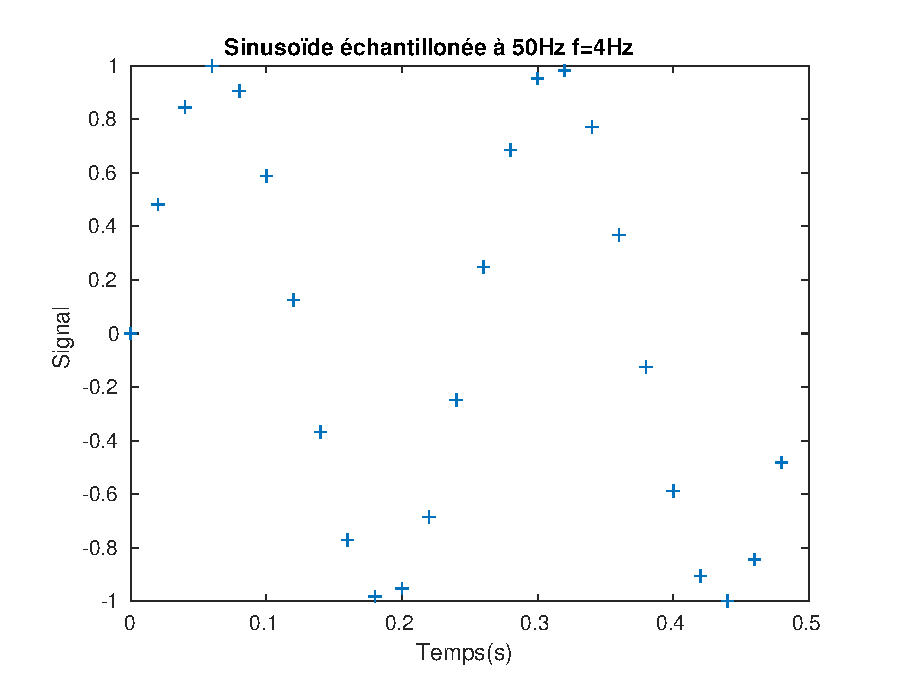
\includegraphics{images/signalSinus.eps}
\caption{Signal sinusoïdal généré.}
\label{signalSin}
\end{figure}

\subsection{ Énergie et puissance}

Dans le but de calculer l'énergie d'un signal sans utiliser \verb`for`, nous avons effectué un produit terme à terme et utilisé l'outil \verb`sum`. Une manière encore plus efficace de procéder aurait été de réaliser le produit entre le vecteur donné en entrée et sa transposée. Nous avons ensuite calculé la puissance moyenne de manière théorique, en utilisant l'identité :

\begin{equation}
\sin^2(x)=\frac {1-\cos(2x)} {2}
\end{equation}

on obtient
\begin{equation}
\frac{1} {2 \pi} \int_{0}^{2 \pi} \sin^2(x) \mathrm{d}x = \frac{1}{2}
\end{equation}

Par ailleurs, nous avons estimé la puissance de notre signal en utilisant la fonction puissance qui effectue la somme du produit terme à terme du signal et divise par la longueur de ce signal.

\lstset{language=matlab}
\begin{lstlisting}
>> s = sig1_sinus(4, 50, 2*50/4);
>> puissance(s)

ans =

    0.5000
\end{lstlisting}

On obtient un résultat conforme au calcul réalisé.

\subsection{ Quantification}

Pour quantifier un signal sur N bits, on commence par le centrer en 0 et le borner entre -0.5 et 0.5 à l'aide d'une première homothétie. Soit $s_1$ le signal ainsi obtenu. On réalise ensuite la quantification. Si $N > 0$ est le nombre de bit de quantification, on pose $q=\frac{1}{2^N}$. Dans un premier temps, on pose $s_2$ tel que :
\begin{equation}
  s_2[k] = (\lfloor \frac{s_1[k]}{q} \rfloor + \frac{1}{2}) \times q
\end{equation}

Cependant cette formule est problématique pour la valeur maximale atteinte par la fonction. En effet, on a alors :
\begin{eqnarray}
s_2[k] &=& \left( \lfloor \frac{1}{2q} \rfloor + \frac{1}{2}\right) \times q \\
&=& \left(2^{N-1} + \frac{1}{2}\right) \times \frac{1}{2^N} \\
&>& \frac{1}{2}
\end{eqnarray}

Ce qui est incohérent avec le signal original. Une solution est de poser :
\begin{equation}
  s_2[k] = \min\left(\left[\lfloor \frac{s_1[k]}{q} \rfloor + \frac{1}{2}\right] \times q, \frac{1}{2} - \frac{q}{2}\right)
\end{equation}

Il ne reste plus qu'à remettre la fonction à l'échelle. On obtient le code suivant :

\lstset{language=matlab}
\begin{lstlisting}
function sig_quant = quantifie(X, n_bit)
    m = min(X);
    M = max(X);
    c = (m+M)/2;
    d = M-m;
    q = 1 / (2 ^ n_bit);
    s1 = (X - c)/d;
    sig_quant = min((floor(s1/q) + 1/2) * q, 1/2-q/2)*d + c;
end
\end{lstlisting}
En appliquant la fonction \verb`quantifie` pour $N=3$ et $N=8$ à un signal généré grâce à la fonction écrite dans la partie 1, on obtient la figure \ref{signalBruit}. On peut noter qu'il est difficile de différencier le signal d'entrée du signal quantifié sur 8 bits. La figure \ref{signalBruit2} montre offre un zoom qui permet de différencier le signal de la quantification.

\begin{figure}[h!]
\centering
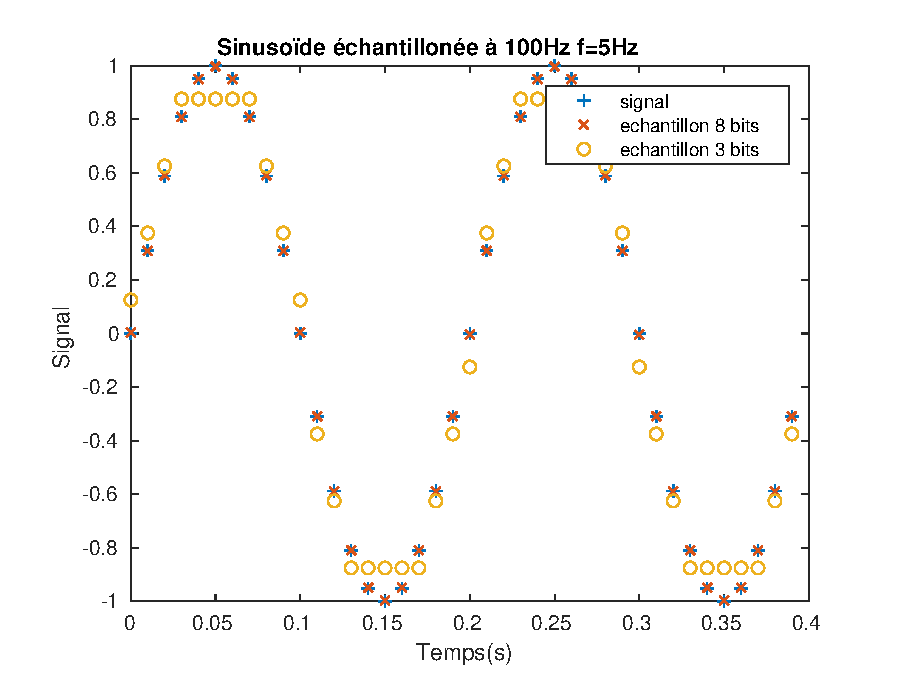
\includegraphics{images/signalBruit.eps}
\caption{Quantification du signal sinusoïdal généré.}
\label{signalBruit}
\end{figure}
\begin{figure}[h!]
	\centering
	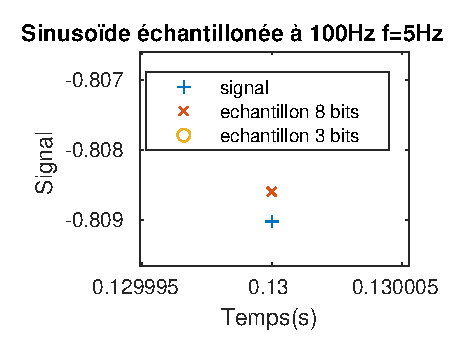
\includegraphics{images/signalBruit1.eps}
	\caption{Quantification du signal sinusoïdal généré - zoom.}
	\label{signalBruit2}
\end{figure}

%\FloatBarrier

Pour déterminer le bruit de quantification, on calcule la différence entre le signal d'origine et le signal quantifié, et on en détermine l'énergie. On calcule également la valeur théorique du bruit de quantification. On obtient

\begin{itemize}
	\item pour 8 bits, $4.6464 \times 10^{-6}$, pour une valeur théorique de $1.272 \times 10^{-6}$;
	\item pour 3 bits, $0.0063$, pour une valeur théorique de $0.0013$.
\end{itemize}
% TODO: SIGNAL SUR BRUIT
On remarque que l'échantillonnage à 8 bits est bien plus efficace, bien que la valeur théorique soit plus faible que celle calculée.

\section{ Signal audio}

\subsection{ Restitution}

En écoutant le signal enregistré à différentes fréquences de restitutions, on remarque que augmenter cette fréquence diminue la durée de la restitution et décale les fréquences de l'enregistrement vers des fréquences plus hautes. Inversement, diminuer la fréquence de restitution augmente la durée de l'enregistrement tout en déplaçant les fréquences des sons de l'enregistrement vers les graves.

\subsection{ Quantification}

A l'aide de la fonction \verb`quantifie` réalisée dans la partie précédente, on réalise la quantification du signal enregistré. On observe que plus le nombre de bits de quantification est faible, plus le bruit (à l'écoute) est important.

Les figures \ref{sonQuantifie1} et \ref{sonQuantifie2} donnent une représentation graphiques de différentes quantification du signal vocal.

\begin{figure}[!h]
\centering
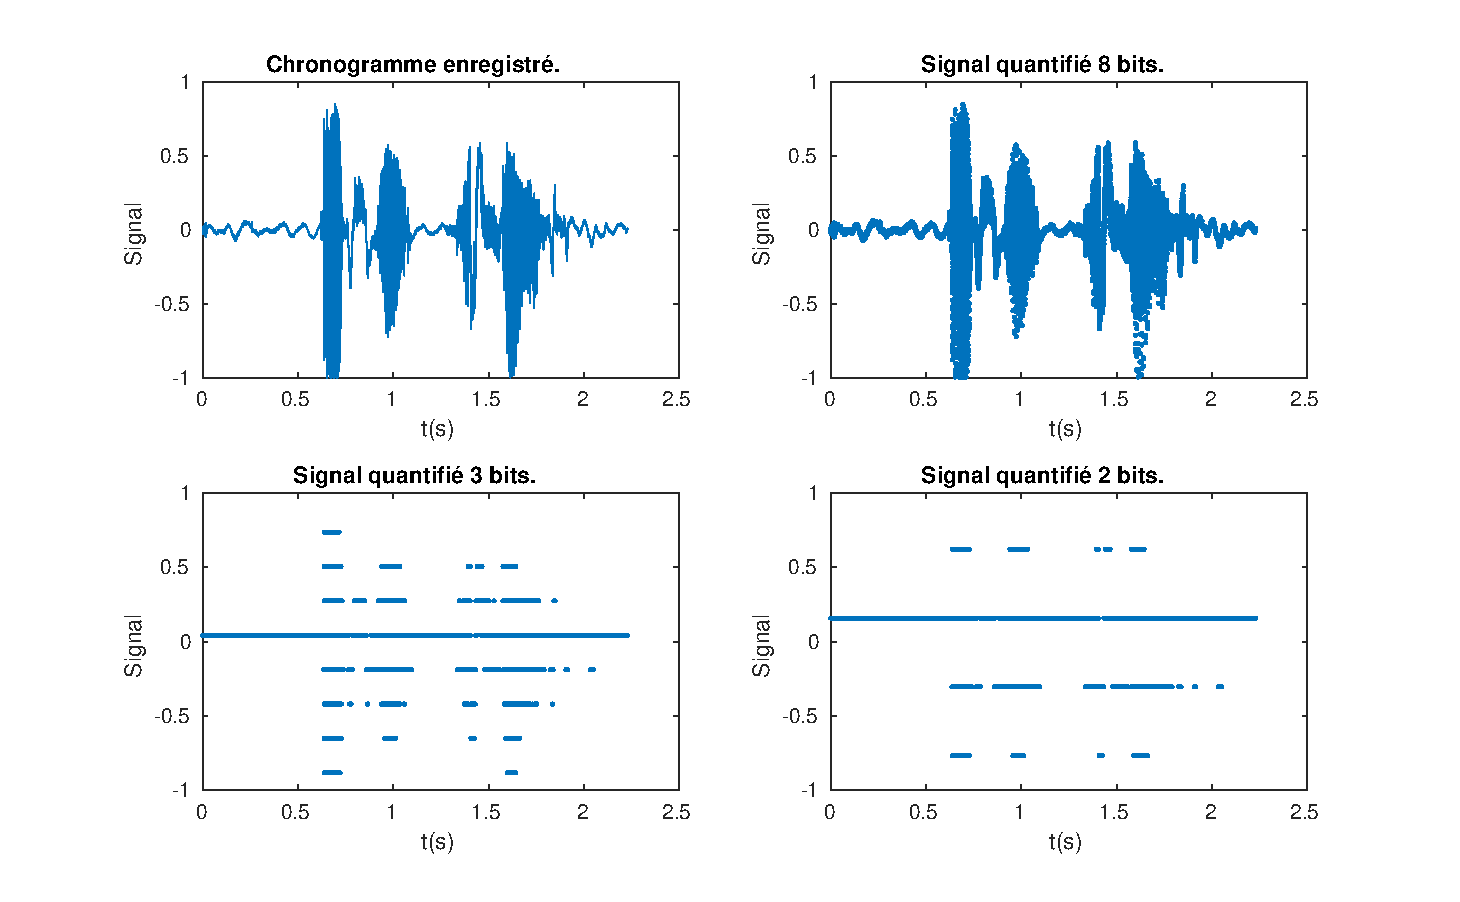
\includegraphics[height=0.45\textheight]{images/sonQuantifie2.eps}
\caption{Quantification du signal vocal enregistré.}
\label{sonQuantifie1}
\end{figure}

\begin{figure}[!h]
\centering
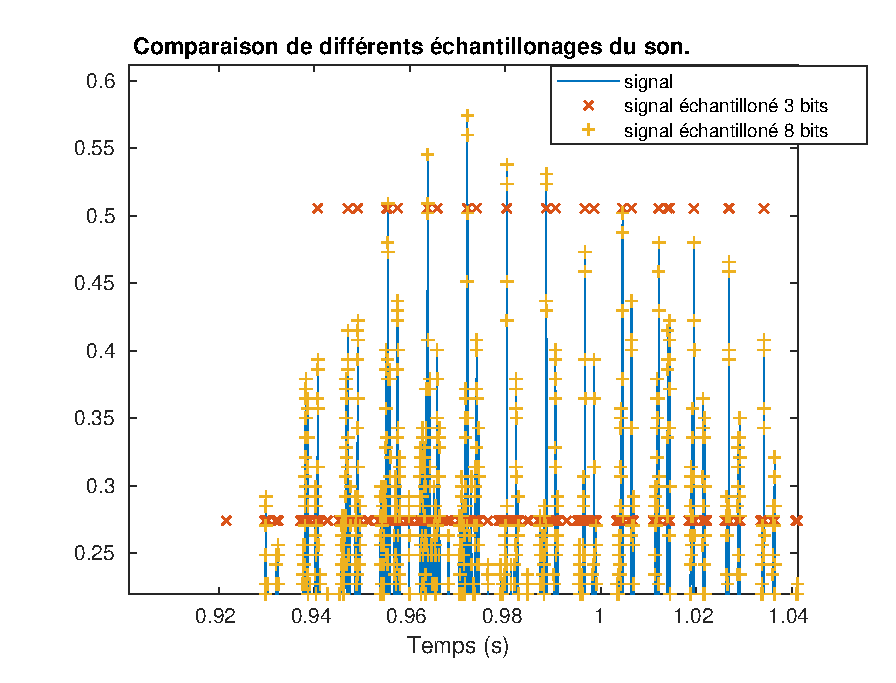
\includegraphics[height=0.45\textheight]{images/sonQuantifie.eps}
\caption{Quantification du signal vocal enregistré - comparaison en zoom.}
\label{sonQuantifie2}
\end{figure}

\FloatBarrier
\newpage
\part{ Classification des signaux}

Le but de cette partie est de classifier les signaux, notamment en utilisant l'autocorrélation.

\section{ Exemple de calcul théorique}

Pour le signal $y(t) = A \sin(2 \pi f t)$, calculons l'autocorrélation :

\begin{eqnarray}
\gamma_y(\tau) &=& \int_0^{\frac{1}{f}} A^2 \sin(2\pi f t) \sin(2 \pi f (t+\tau)) dt \\
&=& \frac{A^2}{2} \cos 2\pi f \tau - \frac{A^2}{2}\underbrace{\int_0^{\frac{1}{f}} \cos (2 \pi f (2t + \tau)) dt}_{=0}
\end{eqnarray}

On obtient la fonction d'autocorrélation suivante :
\begin{equation}
\gamma_y (t) = \frac{A^2} {2} cos(2 \pi f t)
\end{equation}

\section{ Programmation}

On implémente l'autocorrélation avec la formule suivante :

\begin{equation}
\gamma_x [n] = \sum_{k = 0} ^{\mathtt{length} (x)} x[k]x[k+n]
\end{equation}

\begin{figure}[h!]
	\centering
	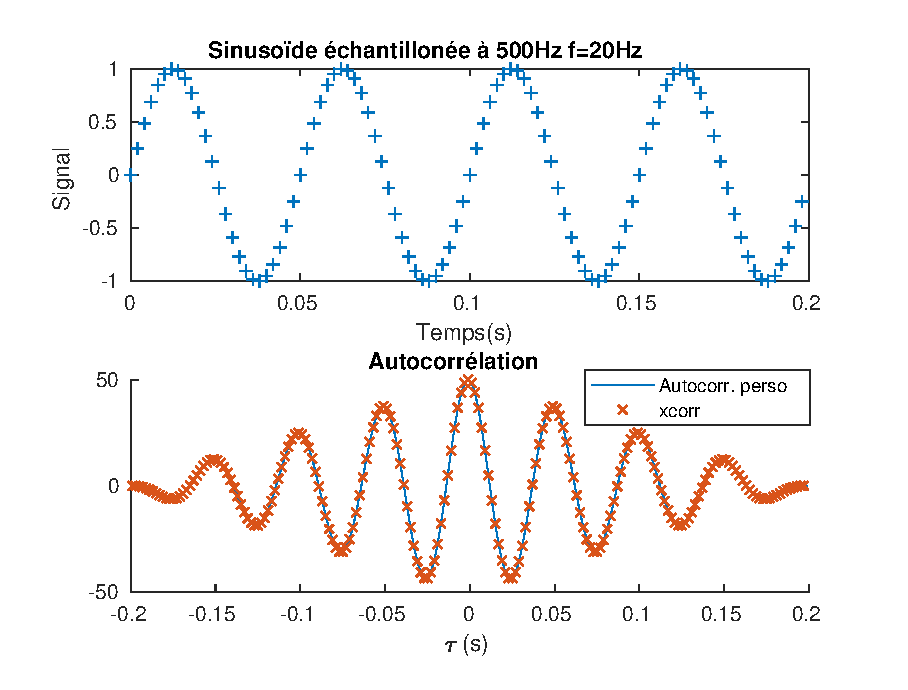
\includegraphics{images/autocorr.eps}
	\caption{Comparatif de de la fonction xcorr et de notre implémentation de l'autocorrélation.}
	\label{autocorr}
\end{figure}

La figure \ref{autocorr} montre que le résultat de \verb`xcorr` et de notre implémentation de l'autocorrélation sont identiques.

\paragraph{Remarque}
Nous n'avions d'abord tracé que la partie positive, avant de nous rendre compte de la nécessité de tracer également la partie négative.
On obtient un résultat différent du résultat théorique car le support de notre signal est fini, ce qui donne un cosinus amorti de manière symétrique et non un simple cosinus.

\section{ Application à la classification de quelques signaux simples}

Lorsque le signal se "répète" au cours du temps son autocorrélation est semblable sur de courtes périodes (reproduction du même motif au cours des périodes), on dit alors que le signal est stationnaire. Par contre si son autocorrélation est presque nulle, cela veut dire qu'il n'y a pas reproduction des motifs au cour des périodes et donc que le signal est non stationnaire.

\begin{figure}[h!]
	\centering
	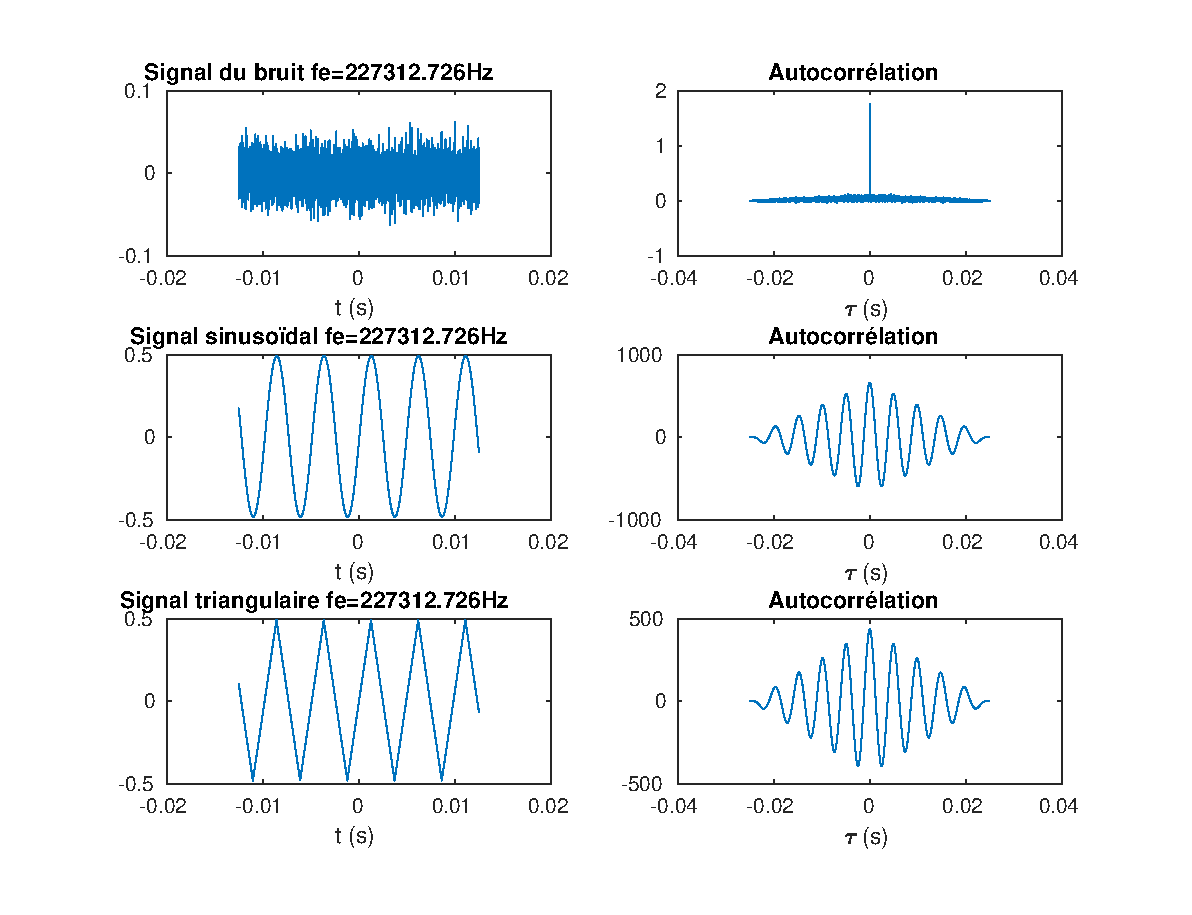
\includegraphics[width=1\textwidth]{images/classificationSig.eps}
	\caption{Autocorrélation de plusieurs signaux.}
	\label{classifSig}
\end{figure}

La figure \ref{classifSig} montre que les signaux sinusoïdaux et triangulaires sont stationnaires, contrairement au signal du bruit.

\begin{figure}[h!]
\centering
%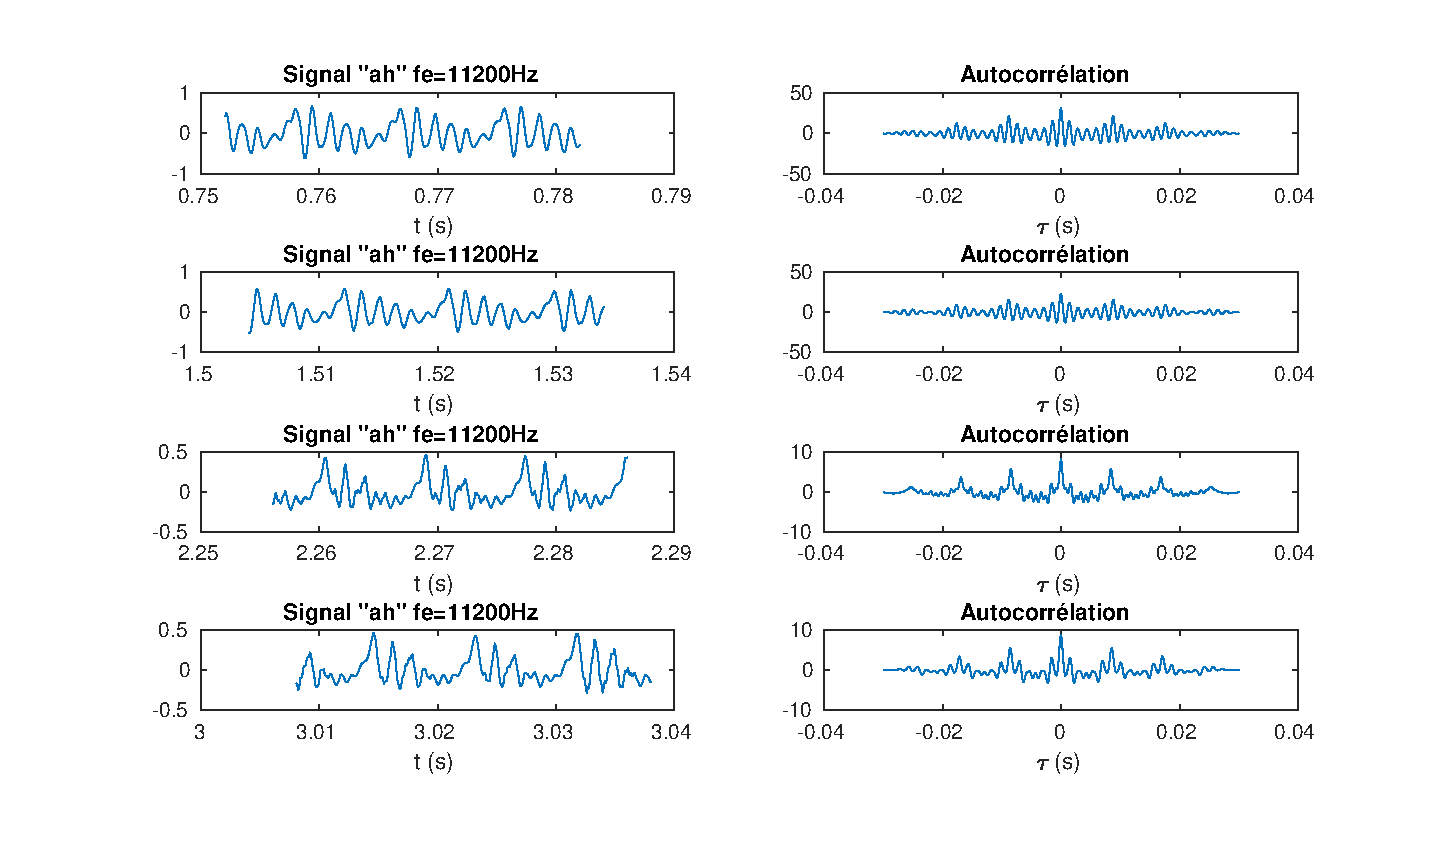
\includegraphics[width=\textwidth]{images/classificationAh.eps}
% Title: glps_renderer figure
% Creator: GL2PS 1.3.8, (C) 1999-2012 C. Geuzaine
% For: Octave
% CreationDate: Wed Nov  8 11:14:12 2017
\begin{pgfpicture}
\pgfsetlinewidth{0.01pt}
\color[rgb]{1.000000,1.000000,1.000000}
\pgfpathmoveto{\pgfpoint{335.117401pt}{386.837402pt}}
\pgflineto{\pgfpoint{521.279968pt}{340.136108pt}}
\pgflineto{\pgfpoint{335.117401pt}{340.136108pt}}
\pgfpathclose
\pgfusepath{fill,stroke}
\pgfpathmoveto{\pgfpoint{335.117401pt}{386.837402pt}}
\pgflineto{\pgfpoint{521.279968pt}{386.837402pt}}
\pgflineto{\pgfpoint{521.279968pt}{340.136108pt}}
\pgfpathclose
\pgfusepath{fill,stroke}
\pgfpathmoveto{\pgfpoint{74.879791pt}{386.837402pt}}
\pgflineto{\pgfpoint{261.042572pt}{340.136108pt}}
\pgflineto{\pgfpoint{74.879791pt}{340.136108pt}}
\pgfpathclose
\pgfusepath{fill,stroke}
\pgfpathmoveto{\pgfpoint{74.879791pt}{386.837402pt}}
\pgflineto{\pgfpoint{261.042572pt}{386.837402pt}}
\pgflineto{\pgfpoint{261.042572pt}{340.136108pt}}
\pgfpathclose
\pgfusepath{fill,stroke}
\pgfpathmoveto{\pgfpoint{335.117401pt}{289.298706pt}}
\pgflineto{\pgfpoint{521.279968pt}{242.597412pt}}
\pgflineto{\pgfpoint{335.117401pt}{242.597412pt}}
\pgfpathclose
\pgfusepath{fill,stroke}
\pgfpathmoveto{\pgfpoint{335.117401pt}{289.298706pt}}
\pgflineto{\pgfpoint{521.279968pt}{289.298706pt}}
\pgflineto{\pgfpoint{521.279968pt}{242.597412pt}}
\pgfpathclose
\pgfusepath{fill,stroke}
\pgfpathmoveto{\pgfpoint{74.879517pt}{289.298706pt}}
\pgflineto{\pgfpoint{261.042297pt}{242.597412pt}}
\pgflineto{\pgfpoint{74.879517pt}{242.597412pt}}
\pgfpathclose
\pgfusepath{fill,stroke}
\pgfpathmoveto{\pgfpoint{74.879517pt}{289.298706pt}}
\pgflineto{\pgfpoint{261.042297pt}{289.298706pt}}
\pgflineto{\pgfpoint{261.042297pt}{242.597412pt}}
\pgfpathclose
\pgfusepath{fill,stroke}
\pgfpathmoveto{\pgfpoint{335.117401pt}{191.760010pt}}
\pgflineto{\pgfpoint{521.279968pt}{145.058716pt}}
\pgflineto{\pgfpoint{335.117401pt}{145.058716pt}}
\pgfpathclose
\pgfusepath{fill,stroke}
\pgfpathmoveto{\pgfpoint{335.117401pt}{191.760010pt}}
\pgflineto{\pgfpoint{521.279968pt}{191.760010pt}}
\pgflineto{\pgfpoint{521.279968pt}{145.058716pt}}
\pgfpathclose
\pgfusepath{fill,stroke}
\pgfpathmoveto{\pgfpoint{74.879517pt}{191.760010pt}}
\pgflineto{\pgfpoint{261.041748pt}{145.058716pt}}
\pgflineto{\pgfpoint{74.879517pt}{145.058716pt}}
\pgfpathclose
\pgfusepath{fill,stroke}
\pgfpathmoveto{\pgfpoint{74.879517pt}{191.760010pt}}
\pgflineto{\pgfpoint{261.041748pt}{191.760010pt}}
\pgflineto{\pgfpoint{261.041748pt}{145.058716pt}}
\pgfpathclose
\pgfusepath{fill,stroke}
\pgfpathmoveto{\pgfpoint{335.117401pt}{94.221275pt}}
\pgflineto{\pgfpoint{521.279968pt}{47.519974pt}}
\pgflineto{\pgfpoint{335.117401pt}{47.519974pt}}
\pgfpathclose
\pgfusepath{fill,stroke}
\pgfpathmoveto{\pgfpoint{335.117401pt}{94.221275pt}}
\pgflineto{\pgfpoint{521.279968pt}{94.221275pt}}
\pgflineto{\pgfpoint{521.279968pt}{47.519974pt}}
\pgfpathclose
\pgfusepath{fill,stroke}
\pgfpathmoveto{\pgfpoint{74.881714pt}{94.221268pt}}
\pgflineto{\pgfpoint{261.043945pt}{47.519974pt}}
\pgflineto{\pgfpoint{74.881714pt}{47.519974pt}}
\pgfpathclose
\pgfusepath{fill,stroke}
\pgfpathmoveto{\pgfpoint{74.881714pt}{94.221268pt}}
\pgflineto{\pgfpoint{261.043945pt}{94.221268pt}}
\pgflineto{\pgfpoint{261.043945pt}{47.519974pt}}
\pgfpathclose
\pgfusepath{fill,stroke}
\color[rgb]{0.000000,0.000000,0.000000}
\pgfsetlinewidth{0.500000pt}
\pgfsetdash{{16pt}{0pt}}{0pt}
\pgfpathmoveto{\pgfpoint{521.279968pt}{340.136108pt}}
\pgflineto{\pgfpoint{335.117401pt}{340.136108pt}}
\pgfusepath{stroke}
\pgfpathmoveto{\pgfpoint{521.279968pt}{386.837402pt}}
\pgflineto{\pgfpoint{335.117401pt}{386.837402pt}}
\pgfusepath{stroke}
\pgfpathmoveto{\pgfpoint{335.117401pt}{386.837402pt}}
\pgflineto{\pgfpoint{335.117401pt}{340.136108pt}}
\pgfusepath{stroke}
\pgfpathmoveto{\pgfpoint{521.279968pt}{386.837402pt}}
\pgflineto{\pgfpoint{521.279968pt}{340.136108pt}}
\pgfusepath{stroke}
\pgfpathmoveto{\pgfpoint{335.117401pt}{341.985931pt}}
\pgflineto{\pgfpoint{335.117401pt}{340.136108pt}}
\pgfusepath{stroke}
\pgfpathmoveto{\pgfpoint{335.117401pt}{384.987610pt}}
\pgflineto{\pgfpoint{335.117401pt}{386.837402pt}}
\pgfusepath{stroke}
\pgfpathmoveto{\pgfpoint{381.658051pt}{341.985931pt}}
\pgflineto{\pgfpoint{381.658051pt}{340.136108pt}}
\pgfusepath{stroke}
\pgfpathmoveto{\pgfpoint{381.658051pt}{384.987610pt}}
\pgflineto{\pgfpoint{381.658051pt}{386.837402pt}}
\pgfusepath{stroke}
\pgfpathmoveto{\pgfpoint{428.198700pt}{341.985931pt}}
\pgflineto{\pgfpoint{428.198700pt}{340.136108pt}}
\pgfusepath{stroke}
\pgfpathmoveto{\pgfpoint{428.198700pt}{384.987610pt}}
\pgflineto{\pgfpoint{428.198700pt}{386.837402pt}}
\pgfusepath{stroke}
\pgfpathmoveto{\pgfpoint{474.739319pt}{341.985931pt}}
\pgflineto{\pgfpoint{474.739319pt}{340.136108pt}}
\pgfusepath{stroke}
\pgfpathmoveto{\pgfpoint{474.739319pt}{384.987610pt}}
\pgflineto{\pgfpoint{474.739319pt}{386.837402pt}}
\pgfusepath{stroke}
\pgfpathmoveto{\pgfpoint{521.279968pt}{341.985931pt}}
\pgflineto{\pgfpoint{521.279968pt}{340.136108pt}}
\pgfusepath{stroke}
\pgfpathmoveto{\pgfpoint{521.279968pt}{384.987610pt}}
\pgflineto{\pgfpoint{521.279968pt}{386.837402pt}}
\pgfusepath{stroke}
{
\pgftransformshift{\pgfpoint{335.117401pt}{335.167908pt}}
\pgfnode{rectangle}{north}{\fontsize{10}{0}\selectfont\textcolor[rgb]{0,0,0}{{-0.04}}}{}{\pgfusepath{discard}}}
{
\pgftransformshift{\pgfpoint{381.658051pt}{335.167908pt}}
\pgfnode{rectangle}{north}{\fontsize{10}{0}\selectfont\textcolor[rgb]{0,0,0}{{-0.02}}}{}{\pgfusepath{discard}}}
{
\pgftransformshift{\pgfpoint{428.198700pt}{335.167908pt}}
\pgfnode{rectangle}{north}{\fontsize{10}{0}\selectfont\textcolor[rgb]{0,0,0}{{0}}}{}{\pgfusepath{discard}}}
{
\pgftransformshift{\pgfpoint{474.739319pt}{335.167908pt}}
\pgfnode{rectangle}{north}{\fontsize{10}{0}\selectfont\textcolor[rgb]{0,0,0}{{0.02}}}{}{\pgfusepath{discard}}}
{
\pgftransformshift{\pgfpoint{521.279968pt}{335.167908pt}}
\pgfnode{rectangle}{north}{\fontsize{10}{0}\selectfont\textcolor[rgb]{0,0,0}{{0.04}}}{}{\pgfusepath{discard}}}
\pgfpathmoveto{\pgfpoint{336.980652pt}{340.136108pt}}
\pgflineto{\pgfpoint{335.117401pt}{340.136108pt}}
\pgfusepath{stroke}
\pgfpathmoveto{\pgfpoint{519.416748pt}{340.136108pt}}
\pgflineto{\pgfpoint{521.279968pt}{340.136108pt}}
\pgfusepath{stroke}
\pgfpathmoveto{\pgfpoint{336.980652pt}{347.919678pt}}
\pgflineto{\pgfpoint{335.117401pt}{347.919678pt}}
\pgfusepath{stroke}
\pgfpathmoveto{\pgfpoint{519.416748pt}{347.919678pt}}
\pgflineto{\pgfpoint{521.279968pt}{347.919678pt}}
\pgfusepath{stroke}
\pgfpathmoveto{\pgfpoint{336.980652pt}{355.703217pt}}
\pgflineto{\pgfpoint{335.117401pt}{355.703217pt}}
\pgfusepath{stroke}
\pgfpathmoveto{\pgfpoint{519.416748pt}{355.703217pt}}
\pgflineto{\pgfpoint{521.279968pt}{355.703217pt}}
\pgfusepath{stroke}
\pgfpathmoveto{\pgfpoint{336.980652pt}{363.486755pt}}
\pgflineto{\pgfpoint{335.117401pt}{363.486755pt}}
\pgfusepath{stroke}
\pgfpathmoveto{\pgfpoint{519.416748pt}{363.486755pt}}
\pgflineto{\pgfpoint{521.279968pt}{363.486755pt}}
\pgfusepath{stroke}
\pgfpathmoveto{\pgfpoint{336.980652pt}{371.270325pt}}
\pgflineto{\pgfpoint{335.117401pt}{371.270325pt}}
\pgfusepath{stroke}
\pgfpathmoveto{\pgfpoint{519.416748pt}{371.270325pt}}
\pgflineto{\pgfpoint{521.279968pt}{371.270325pt}}
\pgfusepath{stroke}
\pgfpathmoveto{\pgfpoint{336.980652pt}{379.053864pt}}
\pgflineto{\pgfpoint{335.117401pt}{379.053864pt}}
\pgfusepath{stroke}
\pgfpathmoveto{\pgfpoint{519.416748pt}{379.053864pt}}
\pgflineto{\pgfpoint{521.279968pt}{379.053864pt}}
\pgfusepath{stroke}
\pgfpathmoveto{\pgfpoint{336.980652pt}{386.837402pt}}
\pgflineto{\pgfpoint{335.117401pt}{386.837402pt}}
\pgfusepath{stroke}
\pgfpathmoveto{\pgfpoint{519.416748pt}{386.837402pt}}
\pgflineto{\pgfpoint{521.279968pt}{386.837402pt}}
\pgfusepath{stroke}
{
\pgftransformshift{\pgfpoint{330.113037pt}{340.136108pt}}
\pgfnode{rectangle}{east}{\fontsize{10}{0}\selectfont\textcolor[rgb]{0,0,0}{{-20}}}{}{\pgfusepath{discard}}}
{
\pgftransformshift{\pgfpoint{330.113037pt}{347.919678pt}}
\pgfnode{rectangle}{east}{\fontsize{10}{0}\selectfont\textcolor[rgb]{0,0,0}{{-10}}}{}{\pgfusepath{discard}}}
{
\pgftransformshift{\pgfpoint{330.113037pt}{355.703217pt}}
\pgfnode{rectangle}{east}{\fontsize{10}{0}\selectfont\textcolor[rgb]{0,0,0}{{0}}}{}{\pgfusepath{discard}}}
{
\pgftransformshift{\pgfpoint{330.113037pt}{363.486755pt}}
\pgfnode{rectangle}{east}{\fontsize{10}{0}\selectfont\textcolor[rgb]{0,0,0}{{10}}}{}{\pgfusepath{discard}}}
{
\pgftransformshift{\pgfpoint{330.113037pt}{371.270325pt}}
\pgfnode{rectangle}{east}{\fontsize{10}{0}\selectfont\textcolor[rgb]{0,0,0}{{20}}}{}{\pgfusepath{discard}}}
{
\pgftransformshift{\pgfpoint{330.113037pt}{379.053864pt}}
\pgfnode{rectangle}{east}{\fontsize{10}{0}\selectfont\textcolor[rgb]{0,0,0}{{30}}}{}{\pgfusepath{discard}}}
{
\pgftransformshift{\pgfpoint{330.113037pt}{386.837402pt}}
\pgfnode{rectangle}{east}{\fontsize{10}{0}\selectfont\textcolor[rgb]{0,0,0}{{40}}}{}{\pgfusepath{discard}}}
{
\pgftransformshift{\pgfpoint{428.198700pt}{324.167908pt}}
\pgfnode{rectangle}{north}{\fontsize{10}{0}\selectfont\textcolor[rgb]{0,0,0}{{$\tau$ (s)}}}{}{\pgfusepath{discard}}}
\color[rgb]{0.000000,0.000000,1.000000}
\pgfsetdash{}{0pt}
\pgfpathmoveto{\pgfpoint{358.491608pt}{355.494690pt}}
\pgflineto{\pgfpoint{358.283844pt}{355.614929pt}}
\pgfusepath{stroke}
\pgfpathmoveto{\pgfpoint{358.699371pt}{355.378540pt}}
\pgflineto{\pgfpoint{358.491608pt}{355.494690pt}}
\pgfusepath{stroke}
\pgfpathmoveto{\pgfpoint{358.907166pt}{355.295349pt}}
\pgflineto{\pgfpoint{358.699371pt}{355.378540pt}}
\pgfusepath{stroke}
\pgfpathmoveto{\pgfpoint{359.114929pt}{355.269836pt}}
\pgflineto{\pgfpoint{358.907166pt}{355.295349pt}}
\pgfusepath{stroke}
\pgfpathmoveto{\pgfpoint{359.322693pt}{355.333252pt}}
\pgflineto{\pgfpoint{359.114929pt}{355.269836pt}}
\pgfusepath{stroke}
\pgfpathmoveto{\pgfpoint{359.530457pt}{355.485718pt}}
\pgflineto{\pgfpoint{359.322693pt}{355.333252pt}}
\pgfusepath{stroke}
\pgfpathmoveto{\pgfpoint{359.738220pt}{355.704468pt}}
\pgflineto{\pgfpoint{359.530457pt}{355.485718pt}}
\pgfusepath{stroke}
\pgfpathmoveto{\pgfpoint{359.946014pt}{355.953278pt}}
\pgflineto{\pgfpoint{359.738220pt}{355.704468pt}}
\pgfusepath{stroke}
\pgfpathmoveto{\pgfpoint{360.153778pt}{356.169586pt}}
\pgflineto{\pgfpoint{359.946014pt}{355.953278pt}}
\pgfusepath{stroke}
\pgfpathmoveto{\pgfpoint{360.361572pt}{356.290039pt}}
\pgflineto{\pgfpoint{360.153778pt}{356.169586pt}}
\pgfusepath{stroke}
\pgfpathmoveto{\pgfpoint{360.569305pt}{356.275330pt}}
\pgflineto{\pgfpoint{360.361572pt}{356.290039pt}}
\pgfusepath{stroke}
\pgfpathmoveto{\pgfpoint{360.777100pt}{356.106781pt}}
\pgflineto{\pgfpoint{360.569305pt}{356.275330pt}}
\pgfusepath{stroke}
\pgfpathmoveto{\pgfpoint{360.984863pt}{355.811493pt}}
\pgflineto{\pgfpoint{360.777100pt}{356.106781pt}}
\pgfusepath{stroke}
\pgfpathmoveto{\pgfpoint{361.192627pt}{355.451172pt}}
\pgflineto{\pgfpoint{360.984863pt}{355.811493pt}}
\pgfusepath{stroke}
\pgfpathmoveto{\pgfpoint{361.400391pt}{355.110657pt}}
\pgflineto{\pgfpoint{361.192627pt}{355.451172pt}}
\pgfusepath{stroke}
\pgfpathmoveto{\pgfpoint{361.608185pt}{354.868469pt}}
\pgflineto{\pgfpoint{361.400391pt}{355.110657pt}}
\pgfusepath{stroke}
\pgfpathmoveto{\pgfpoint{361.815948pt}{354.777588pt}}
\pgflineto{\pgfpoint{361.608185pt}{354.868469pt}}
\pgfusepath{stroke}
\pgfpathmoveto{\pgfpoint{362.023712pt}{354.867615pt}}
\pgflineto{\pgfpoint{361.815948pt}{354.777588pt}}
\pgfusepath{stroke}
\pgfpathmoveto{\pgfpoint{362.231476pt}{355.127411pt}}
\pgflineto{\pgfpoint{362.023712pt}{354.867615pt}}
\pgfusepath{stroke}
\pgfpathmoveto{\pgfpoint{362.439270pt}{355.516052pt}}
\pgflineto{\pgfpoint{362.231476pt}{355.127411pt}}
\pgfusepath{stroke}
\pgfpathmoveto{\pgfpoint{362.647034pt}{355.963440pt}}
\pgflineto{\pgfpoint{362.439270pt}{355.516052pt}}
\pgfusepath{stroke}
\pgfpathmoveto{\pgfpoint{362.854797pt}{356.386475pt}}
\pgflineto{\pgfpoint{362.647034pt}{355.963440pt}}
\pgfusepath{stroke}
\pgfpathmoveto{\pgfpoint{363.062561pt}{356.720459pt}}
\pgflineto{\pgfpoint{362.854797pt}{356.386475pt}}
\pgfusepath{stroke}
\pgfpathmoveto{\pgfpoint{363.270325pt}{356.923401pt}}
\pgflineto{\pgfpoint{363.062561pt}{356.720459pt}}
\pgfusepath{stroke}
\pgfpathmoveto{\pgfpoint{363.478119pt}{356.974182pt}}
\pgflineto{\pgfpoint{363.270325pt}{356.923401pt}}
\pgfusepath{stroke}
\pgfpathmoveto{\pgfpoint{363.685883pt}{356.863190pt}}
\pgflineto{\pgfpoint{363.478119pt}{356.974182pt}}
\pgfusepath{stroke}
\pgfpathmoveto{\pgfpoint{363.893677pt}{356.597534pt}}
\pgflineto{\pgfpoint{363.685883pt}{356.863190pt}}
\pgfusepath{stroke}
\pgfpathmoveto{\pgfpoint{364.101410pt}{356.200928pt}}
\pgflineto{\pgfpoint{363.893677pt}{356.597534pt}}
\pgfusepath{stroke}
\pgfpathmoveto{\pgfpoint{364.309204pt}{355.719452pt}}
\pgflineto{\pgfpoint{364.101410pt}{356.200928pt}}
\pgfusepath{stroke}
\pgfpathmoveto{\pgfpoint{364.516968pt}{355.221466pt}}
\pgflineto{\pgfpoint{364.309204pt}{355.719452pt}}
\pgfusepath{stroke}
\pgfpathmoveto{\pgfpoint{364.724731pt}{354.788239pt}}
\pgflineto{\pgfpoint{364.516968pt}{355.221466pt}}
\pgfusepath{stroke}
\pgfpathmoveto{\pgfpoint{364.932495pt}{354.517334pt}}
\pgflineto{\pgfpoint{364.724731pt}{354.788239pt}}
\pgfusepath{stroke}
\pgfpathmoveto{\pgfpoint{365.140289pt}{354.496033pt}}
\pgflineto{\pgfpoint{364.932495pt}{354.517334pt}}
\pgfusepath{stroke}
\pgfpathmoveto{\pgfpoint{365.348022pt}{354.762512pt}}
\pgflineto{\pgfpoint{365.140289pt}{354.496033pt}}
\pgfusepath{stroke}
\pgfpathmoveto{\pgfpoint{365.555817pt}{355.303162pt}}
\pgflineto{\pgfpoint{365.348022pt}{354.762512pt}}
\pgfusepath{stroke}
\pgfpathmoveto{\pgfpoint{365.763580pt}{356.044678pt}}
\pgflineto{\pgfpoint{365.555817pt}{355.303162pt}}
\pgfusepath{stroke}
\pgfpathmoveto{\pgfpoint{365.971375pt}{356.851562pt}}
\pgflineto{\pgfpoint{365.763580pt}{356.044678pt}}
\pgfusepath{stroke}
\pgfpathmoveto{\pgfpoint{366.179138pt}{357.570953pt}}
\pgflineto{\pgfpoint{365.971375pt}{356.851562pt}}
\pgfusepath{stroke}
\pgfpathmoveto{\pgfpoint{366.386902pt}{358.049988pt}}
\pgflineto{\pgfpoint{366.179138pt}{357.570953pt}}
\pgfusepath{stroke}
\pgfpathmoveto{\pgfpoint{366.594666pt}{358.167664pt}}
\pgflineto{\pgfpoint{366.386902pt}{358.049988pt}}
\pgfusepath{stroke}
\pgfpathmoveto{\pgfpoint{366.802429pt}{357.898102pt}}
\pgflineto{\pgfpoint{366.594666pt}{358.167664pt}}
\pgfusepath{stroke}
\pgfpathmoveto{\pgfpoint{367.010223pt}{357.309021pt}}
\pgflineto{\pgfpoint{366.802429pt}{357.898102pt}}
\pgfusepath{stroke}
\pgfpathmoveto{\pgfpoint{367.217987pt}{356.515137pt}}
\pgflineto{\pgfpoint{367.010223pt}{357.309021pt}}
\pgfusepath{stroke}
\pgfpathmoveto{\pgfpoint{367.425751pt}{355.672485pt}}
\pgflineto{\pgfpoint{367.217987pt}{356.515137pt}}
\pgfusepath{stroke}
\pgfpathmoveto{\pgfpoint{367.633514pt}{354.936707pt}}
\pgflineto{\pgfpoint{367.425751pt}{355.672485pt}}
\pgfusepath{stroke}
\pgfpathmoveto{\pgfpoint{367.841309pt}{354.417664pt}}
\pgflineto{\pgfpoint{367.633514pt}{354.936707pt}}
\pgfusepath{stroke}
\pgfpathmoveto{\pgfpoint{368.049072pt}{354.190033pt}}
\pgflineto{\pgfpoint{367.841309pt}{354.417664pt}}
\pgfusepath{stroke}
\pgfpathmoveto{\pgfpoint{368.256836pt}{354.269653pt}}
\pgflineto{\pgfpoint{368.049072pt}{354.190033pt}}
\pgfusepath{stroke}
\pgfpathmoveto{\pgfpoint{368.464600pt}{354.608154pt}}
\pgflineto{\pgfpoint{368.256836pt}{354.269653pt}}
\pgfusepath{stroke}
\pgfpathmoveto{\pgfpoint{368.672363pt}{355.136078pt}}
\pgflineto{\pgfpoint{368.464600pt}{354.608154pt}}
\pgfusepath{stroke}
\pgfpathmoveto{\pgfpoint{368.880127pt}{355.794647pt}}
\pgflineto{\pgfpoint{368.672363pt}{355.136078pt}}
\pgfusepath{stroke}
\pgfpathmoveto{\pgfpoint{369.087921pt}{356.510071pt}}
\pgflineto{\pgfpoint{368.880127pt}{355.794647pt}}
\pgfusepath{stroke}
\pgfpathmoveto{\pgfpoint{369.295685pt}{357.198730pt}}
\pgflineto{\pgfpoint{369.087921pt}{356.510071pt}}
\pgfusepath{stroke}
\pgfpathmoveto{\pgfpoint{369.503479pt}{357.778992pt}}
\pgflineto{\pgfpoint{369.295685pt}{357.198730pt}}
\pgfusepath{stroke}
\pgfpathmoveto{\pgfpoint{369.711243pt}{358.151947pt}}
\pgflineto{\pgfpoint{369.503479pt}{357.778992pt}}
\pgfusepath{stroke}
\pgfpathmoveto{\pgfpoint{369.919006pt}{358.217407pt}}
\pgflineto{\pgfpoint{369.711243pt}{358.151947pt}}
\pgfusepath{stroke}
\pgfpathmoveto{\pgfpoint{370.126770pt}{357.923828pt}}
\pgflineto{\pgfpoint{369.919006pt}{358.217407pt}}
\pgfusepath{stroke}
\pgfpathmoveto{\pgfpoint{370.334534pt}{357.249939pt}}
\pgflineto{\pgfpoint{370.126770pt}{357.923828pt}}
\pgfusepath{stroke}
\pgfpathmoveto{\pgfpoint{370.542297pt}{356.256042pt}}
\pgflineto{\pgfpoint{370.334534pt}{357.249939pt}}
\pgfusepath{stroke}
\pgfpathmoveto{\pgfpoint{370.750092pt}{355.107513pt}}
\pgflineto{\pgfpoint{370.542297pt}{356.256042pt}}
\pgfusepath{stroke}
\pgfpathmoveto{\pgfpoint{370.957855pt}{354.006927pt}}
\pgflineto{\pgfpoint{370.750092pt}{355.107513pt}}
\pgfusepath{stroke}
\pgfpathmoveto{\pgfpoint{371.165619pt}{353.154602pt}}
\pgflineto{\pgfpoint{370.957855pt}{354.006927pt}}
\pgfusepath{stroke}
\pgfpathmoveto{\pgfpoint{371.373413pt}{352.710358pt}}
\pgflineto{\pgfpoint{371.165619pt}{353.154602pt}}
\pgfusepath{stroke}
\pgfpathmoveto{\pgfpoint{371.581177pt}{352.751709pt}}
\pgflineto{\pgfpoint{371.373413pt}{352.710358pt}}
\pgfusepath{stroke}
\pgfpathmoveto{\pgfpoint{371.788940pt}{353.257690pt}}
\pgflineto{\pgfpoint{371.581177pt}{352.751709pt}}
\pgfusepath{stroke}
\pgfpathmoveto{\pgfpoint{371.996704pt}{354.125793pt}}
\pgflineto{\pgfpoint{371.788940pt}{353.257690pt}}
\pgfusepath{stroke}
\pgfpathmoveto{\pgfpoint{372.204498pt}{355.174042pt}}
\pgflineto{\pgfpoint{371.996704pt}{354.125793pt}}
\pgfusepath{stroke}
\pgfpathmoveto{\pgfpoint{372.412231pt}{356.179321pt}}
\pgflineto{\pgfpoint{372.204498pt}{355.174042pt}}
\pgfusepath{stroke}
\pgfpathmoveto{\pgfpoint{372.620026pt}{356.966766pt}}
\pgflineto{\pgfpoint{372.412231pt}{356.179321pt}}
\pgfusepath{stroke}
\pgfpathmoveto{\pgfpoint{372.827789pt}{357.444916pt}}
\pgflineto{\pgfpoint{372.620026pt}{356.966766pt}}
\pgfusepath{stroke}
\pgfpathmoveto{\pgfpoint{373.035553pt}{357.590820pt}}
\pgflineto{\pgfpoint{372.827789pt}{357.444916pt}}
\pgfusepath{stroke}
\pgfpathmoveto{\pgfpoint{373.243347pt}{357.437836pt}}
\pgflineto{\pgfpoint{373.035553pt}{357.590820pt}}
\pgfusepath{stroke}
\pgfpathmoveto{\pgfpoint{373.451111pt}{357.053741pt}}
\pgflineto{\pgfpoint{373.243347pt}{357.437836pt}}
\pgfusepath{stroke}
\pgfpathmoveto{\pgfpoint{373.658875pt}{356.500122pt}}
\pgflineto{\pgfpoint{373.451111pt}{357.053741pt}}
\pgfusepath{stroke}
\pgfpathmoveto{\pgfpoint{373.866638pt}{355.836914pt}}
\pgflineto{\pgfpoint{373.658875pt}{356.500122pt}}
\pgfusepath{stroke}
\pgfpathmoveto{\pgfpoint{374.074402pt}{355.150696pt}}
\pgflineto{\pgfpoint{373.866638pt}{355.836914pt}}
\pgfusepath{stroke}
\pgfpathmoveto{\pgfpoint{374.282196pt}{354.512207pt}}
\pgflineto{\pgfpoint{374.074402pt}{355.150696pt}}
\pgfusepath{stroke}
\pgfpathmoveto{\pgfpoint{374.489960pt}{353.978882pt}}
\pgflineto{\pgfpoint{374.282196pt}{354.512207pt}}
\pgfusepath{stroke}
\pgfpathmoveto{\pgfpoint{374.697723pt}{353.615417pt}}
\pgflineto{\pgfpoint{374.489960pt}{353.978882pt}}
\pgfusepath{stroke}
\pgfpathmoveto{\pgfpoint{374.905487pt}{353.453857pt}}
\pgflineto{\pgfpoint{374.697723pt}{353.615417pt}}
\pgfusepath{stroke}
\pgfpathmoveto{\pgfpoint{375.113281pt}{353.510315pt}}
\pgflineto{\pgfpoint{374.905487pt}{353.453857pt}}
\pgfusepath{stroke}
\pgfpathmoveto{\pgfpoint{375.321045pt}{353.791107pt}}
\pgflineto{\pgfpoint{375.113281pt}{353.510315pt}}
\pgfusepath{stroke}
\pgfpathmoveto{\pgfpoint{375.528809pt}{354.268921pt}}
\pgflineto{\pgfpoint{375.321045pt}{353.791107pt}}
\pgfusepath{stroke}
\pgfpathmoveto{\pgfpoint{375.736572pt}{354.874573pt}}
\pgflineto{\pgfpoint{375.528809pt}{354.268921pt}}
\pgfusepath{stroke}
\pgfpathmoveto{\pgfpoint{375.944336pt}{355.535675pt}}
\pgflineto{\pgfpoint{375.736572pt}{354.874573pt}}
\pgfusepath{stroke}
\pgfpathmoveto{\pgfpoint{376.152130pt}{356.169067pt}}
\pgflineto{\pgfpoint{375.944336pt}{355.535675pt}}
\pgfusepath{stroke}
\pgfpathmoveto{\pgfpoint{376.359894pt}{356.685974pt}}
\pgflineto{\pgfpoint{376.152130pt}{356.169067pt}}
\pgfusepath{stroke}
\pgfpathmoveto{\pgfpoint{376.567688pt}{357.030731pt}}
\pgflineto{\pgfpoint{376.359894pt}{356.685974pt}}
\pgfusepath{stroke}
\pgfpathmoveto{\pgfpoint{376.775452pt}{357.163025pt}}
\pgflineto{\pgfpoint{376.567688pt}{357.030731pt}}
\pgfusepath{stroke}
\pgfpathmoveto{\pgfpoint{376.983215pt}{357.062927pt}}
\pgflineto{\pgfpoint{376.775452pt}{357.163025pt}}
\pgfusepath{stroke}
\pgfpathmoveto{\pgfpoint{377.190979pt}{356.747742pt}}
\pgflineto{\pgfpoint{376.983215pt}{357.062927pt}}
\pgfusepath{stroke}
\pgfpathmoveto{\pgfpoint{377.398743pt}{356.258057pt}}
\pgflineto{\pgfpoint{377.190979pt}{356.747742pt}}
\pgfusepath{stroke}
\pgfpathmoveto{\pgfpoint{377.606506pt}{355.639221pt}}
\pgflineto{\pgfpoint{377.398743pt}{356.258057pt}}
\pgfusepath{stroke}
\pgfpathmoveto{\pgfpoint{377.814301pt}{354.968811pt}}
\pgflineto{\pgfpoint{377.606506pt}{355.639221pt}}
\pgfusepath{stroke}
\pgfpathmoveto{\pgfpoint{378.022064pt}{354.331970pt}}
\pgflineto{\pgfpoint{377.814301pt}{354.968811pt}}
\pgfusepath{stroke}
\pgfpathmoveto{\pgfpoint{378.229828pt}{353.803589pt}}
\pgflineto{\pgfpoint{378.022064pt}{354.331970pt}}
\pgfusepath{stroke}
\pgfpathmoveto{\pgfpoint{378.437592pt}{353.445618pt}}
\pgflineto{\pgfpoint{378.229828pt}{353.803589pt}}
\pgfusepath{stroke}
\pgfpathmoveto{\pgfpoint{378.645386pt}{353.299622pt}}
\pgflineto{\pgfpoint{378.437592pt}{353.445618pt}}
\pgfusepath{stroke}
\pgfpathmoveto{\pgfpoint{378.853149pt}{353.373047pt}}
\pgflineto{\pgfpoint{378.645386pt}{353.299622pt}}
\pgfusepath{stroke}
\pgfpathmoveto{\pgfpoint{379.060913pt}{353.659485pt}}
\pgflineto{\pgfpoint{378.853149pt}{353.373047pt}}
\pgfusepath{stroke}
\pgfpathmoveto{\pgfpoint{379.268677pt}{354.142273pt}}
\pgflineto{\pgfpoint{379.060913pt}{353.659485pt}}
\pgfusepath{stroke}
\pgfpathmoveto{\pgfpoint{379.476440pt}{354.774109pt}}
\pgflineto{\pgfpoint{379.268677pt}{354.142273pt}}
\pgfusepath{stroke}
\pgfpathmoveto{\pgfpoint{379.684204pt}{355.493408pt}}
\pgflineto{\pgfpoint{379.476440pt}{354.774109pt}}
\pgfusepath{stroke}
\pgfpathmoveto{\pgfpoint{379.891998pt}{356.235382pt}}
\pgflineto{\pgfpoint{379.684204pt}{355.493408pt}}
\pgfusepath{stroke}
\pgfpathmoveto{\pgfpoint{380.099762pt}{356.907379pt}}
\pgflineto{\pgfpoint{379.891998pt}{356.235382pt}}
\pgfusepath{stroke}
\pgfpathmoveto{\pgfpoint{380.307556pt}{357.408447pt}}
\pgflineto{\pgfpoint{380.099762pt}{356.907379pt}}
\pgfusepath{stroke}
\pgfpathmoveto{\pgfpoint{380.515320pt}{357.638885pt}}
\pgflineto{\pgfpoint{380.307556pt}{357.408447pt}}
\pgfusepath{stroke}
\pgfpathmoveto{\pgfpoint{380.723083pt}{357.505432pt}}
\pgflineto{\pgfpoint{380.515320pt}{357.638885pt}}
\pgfusepath{stroke}
\pgfpathmoveto{\pgfpoint{380.930847pt}{356.962280pt}}
\pgflineto{\pgfpoint{380.723083pt}{357.505432pt}}
\pgfusepath{stroke}
\pgfpathmoveto{\pgfpoint{381.138611pt}{356.036591pt}}
\pgflineto{\pgfpoint{380.930847pt}{356.962280pt}}
\pgfusepath{stroke}
\pgfpathmoveto{\pgfpoint{381.346375pt}{354.828308pt}}
\pgflineto{\pgfpoint{381.138611pt}{356.036591pt}}
\pgfusepath{stroke}
\pgfpathmoveto{\pgfpoint{381.554169pt}{353.530762pt}}
\pgflineto{\pgfpoint{381.346375pt}{354.828308pt}}
\pgfusepath{stroke}
\pgfpathmoveto{\pgfpoint{381.761932pt}{352.386810pt}}
\pgflineto{\pgfpoint{381.554169pt}{353.530762pt}}
\pgfusepath{stroke}
\pgfpathmoveto{\pgfpoint{381.969696pt}{351.631592pt}}
\pgflineto{\pgfpoint{381.761932pt}{352.386810pt}}
\pgfusepath{stroke}
\pgfpathmoveto{\pgfpoint{382.177490pt}{351.445526pt}}
\pgflineto{\pgfpoint{381.969696pt}{351.631592pt}}
\pgfusepath{stroke}
\pgfpathmoveto{\pgfpoint{382.385254pt}{351.905884pt}}
\pgflineto{\pgfpoint{382.177490pt}{351.445526pt}}
\pgfusepath{stroke}
\pgfpathmoveto{\pgfpoint{382.593018pt}{352.974182pt}}
\pgflineto{\pgfpoint{382.385254pt}{351.905884pt}}
\pgfusepath{stroke}
\pgfpathmoveto{\pgfpoint{382.800781pt}{354.504761pt}}
\pgflineto{\pgfpoint{382.593018pt}{352.974182pt}}
\pgfusepath{stroke}
\pgfpathmoveto{\pgfpoint{383.008545pt}{356.264587pt}}
\pgflineto{\pgfpoint{382.800781pt}{354.504761pt}}
\pgfusepath{stroke}
\pgfpathmoveto{\pgfpoint{383.216339pt}{357.971558pt}}
\pgflineto{\pgfpoint{383.008545pt}{356.264587pt}}
\pgfusepath{stroke}
\pgfpathmoveto{\pgfpoint{383.424103pt}{359.359955pt}}
\pgflineto{\pgfpoint{383.216339pt}{357.971558pt}}
\pgfusepath{stroke}
\pgfpathmoveto{\pgfpoint{383.631866pt}{360.231262pt}}
\pgflineto{\pgfpoint{383.424103pt}{359.359955pt}}
\pgfusepath{stroke}
\pgfpathmoveto{\pgfpoint{383.839661pt}{360.471619pt}}
\pgflineto{\pgfpoint{383.631866pt}{360.231262pt}}
\pgfusepath{stroke}
\pgfpathmoveto{\pgfpoint{384.047424pt}{360.048401pt}}
\pgflineto{\pgfpoint{383.839661pt}{360.471619pt}}
\pgfusepath{stroke}
\pgfpathmoveto{\pgfpoint{384.255188pt}{359.012024pt}}
\pgflineto{\pgfpoint{384.047424pt}{360.048401pt}}
\pgfusepath{stroke}
\pgfpathmoveto{\pgfpoint{384.462952pt}{357.485229pt}}
\pgflineto{\pgfpoint{384.255188pt}{359.012024pt}}
\pgfusepath{stroke}
\pgfpathmoveto{\pgfpoint{384.670715pt}{355.653076pt}}
\pgflineto{\pgfpoint{384.462952pt}{357.485229pt}}
\pgfusepath{stroke}
\pgfpathmoveto{\pgfpoint{384.878479pt}{353.772064pt}}
\pgflineto{\pgfpoint{384.670715pt}{355.653076pt}}
\pgfusepath{stroke}
\pgfpathmoveto{\pgfpoint{385.086273pt}{352.136078pt}}
\pgflineto{\pgfpoint{384.878479pt}{353.772064pt}}
\pgfusepath{stroke}
\pgfpathmoveto{\pgfpoint{385.294037pt}{351.051941pt}}
\pgflineto{\pgfpoint{385.086273pt}{352.136078pt}}
\pgfusepath{stroke}
\pgfpathmoveto{\pgfpoint{385.501801pt}{350.806274pt}}
\pgflineto{\pgfpoint{385.294037pt}{351.051941pt}}
\pgfusepath{stroke}
\pgfpathmoveto{\pgfpoint{385.709595pt}{351.570923pt}}
\pgflineto{\pgfpoint{385.501801pt}{350.806274pt}}
\pgfusepath{stroke}
\pgfpathmoveto{\pgfpoint{385.917358pt}{353.332642pt}}
\pgflineto{\pgfpoint{385.709595pt}{351.570923pt}}
\pgfusepath{stroke}
\pgfpathmoveto{\pgfpoint{386.125122pt}{355.896851pt}}
\pgflineto{\pgfpoint{385.917358pt}{353.332642pt}}
\pgfusepath{stroke}
\pgfpathmoveto{\pgfpoint{386.332886pt}{358.888977pt}}
\pgflineto{\pgfpoint{386.125122pt}{355.896851pt}}
\pgfusepath{stroke}
\pgfpathmoveto{\pgfpoint{386.540649pt}{361.792603pt}}
\pgflineto{\pgfpoint{386.332886pt}{358.888977pt}}
\pgfusepath{stroke}
\pgfpathmoveto{\pgfpoint{386.748413pt}{364.073059pt}}
\pgflineto{\pgfpoint{386.540649pt}{361.792603pt}}
\pgfusepath{stroke}
\pgfpathmoveto{\pgfpoint{386.956207pt}{365.272369pt}}
\pgflineto{\pgfpoint{386.748413pt}{364.073059pt}}
\pgfusepath{stroke}
\pgfpathmoveto{\pgfpoint{387.163971pt}{365.125275pt}}
\pgflineto{\pgfpoint{386.956207pt}{365.272369pt}}
\pgfusepath{stroke}
\pgfpathmoveto{\pgfpoint{387.371765pt}{363.677979pt}}
\pgflineto{\pgfpoint{387.163971pt}{365.125275pt}}
\pgfusepath{stroke}
\pgfpathmoveto{\pgfpoint{387.579529pt}{361.240845pt}}
\pgflineto{\pgfpoint{387.371765pt}{363.677979pt}}
\pgfusepath{stroke}
\pgfpathmoveto{\pgfpoint{387.787292pt}{358.273499pt}}
\pgflineto{\pgfpoint{387.579529pt}{361.240845pt}}
\pgfusepath{stroke}
\pgfpathmoveto{\pgfpoint{387.995056pt}{355.307373pt}}
\pgflineto{\pgfpoint{387.787292pt}{358.273499pt}}
\pgfusepath{stroke}
\pgfpathmoveto{\pgfpoint{388.202820pt}{352.826355pt}}
\pgflineto{\pgfpoint{387.995056pt}{355.307373pt}}
\pgfusepath{stroke}
\pgfpathmoveto{\pgfpoint{388.410583pt}{351.168793pt}}
\pgflineto{\pgfpoint{388.202820pt}{352.826355pt}}
\pgfusepath{stroke}
\pgfpathmoveto{\pgfpoint{388.618378pt}{350.517029pt}}
\pgflineto{\pgfpoint{388.410583pt}{351.168793pt}}
\pgfusepath{stroke}
\pgfpathmoveto{\pgfpoint{388.826141pt}{350.867188pt}}
\pgflineto{\pgfpoint{388.618378pt}{350.517029pt}}
\pgfusepath{stroke}
\pgfpathmoveto{\pgfpoint{389.033905pt}{352.044861pt}}
\pgflineto{\pgfpoint{388.826141pt}{350.867188pt}}
\pgfusepath{stroke}
\pgfpathmoveto{\pgfpoint{389.241699pt}{353.806915pt}}
\pgflineto{\pgfpoint{389.033905pt}{352.044861pt}}
\pgfusepath{stroke}
\pgfpathmoveto{\pgfpoint{389.449463pt}{355.890930pt}}
\pgflineto{\pgfpoint{389.241699pt}{353.806915pt}}
\pgfusepath{stroke}
\pgfpathmoveto{\pgfpoint{389.657227pt}{358.000916pt}}
\pgflineto{\pgfpoint{389.449463pt}{355.890930pt}}
\pgfusepath{stroke}
\pgfpathmoveto{\pgfpoint{389.864990pt}{359.856537pt}}
\pgflineto{\pgfpoint{389.657227pt}{358.000916pt}}
\pgfusepath{stroke}
\pgfpathmoveto{\pgfpoint{390.072754pt}{361.207214pt}}
\pgflineto{\pgfpoint{389.864990pt}{359.856537pt}}
\pgfusepath{stroke}
\pgfpathmoveto{\pgfpoint{390.280518pt}{361.832611pt}}
\pgflineto{\pgfpoint{390.072754pt}{361.207214pt}}
\pgfusepath{stroke}
\pgfpathmoveto{\pgfpoint{390.488312pt}{361.589081pt}}
\pgflineto{\pgfpoint{390.280518pt}{361.832611pt}}
\pgfusepath{stroke}
\pgfpathmoveto{\pgfpoint{390.696075pt}{360.458618pt}}
\pgflineto{\pgfpoint{390.488312pt}{361.589081pt}}
\pgfusepath{stroke}
\pgfpathmoveto{\pgfpoint{390.903870pt}{358.544434pt}}
\pgflineto{\pgfpoint{390.696075pt}{360.458618pt}}
\pgfusepath{stroke}
\pgfpathmoveto{\pgfpoint{391.111633pt}{356.114136pt}}
\pgflineto{\pgfpoint{390.903870pt}{358.544434pt}}
\pgfusepath{stroke}
\pgfpathmoveto{\pgfpoint{391.319397pt}{353.582336pt}}
\pgflineto{\pgfpoint{391.111633pt}{356.114136pt}}
\pgfusepath{stroke}
\pgfpathmoveto{\pgfpoint{391.527161pt}{351.372803pt}}
\pgflineto{\pgfpoint{391.319397pt}{353.582336pt}}
\pgfusepath{stroke}
\pgfpathmoveto{\pgfpoint{391.734924pt}{349.851013pt}}
\pgflineto{\pgfpoint{391.527161pt}{351.372803pt}}
\pgfusepath{stroke}
\pgfpathmoveto{\pgfpoint{391.942688pt}{349.258301pt}}
\pgflineto{\pgfpoint{391.734924pt}{349.851013pt}}
\pgfusepath{stroke}
\pgfpathmoveto{\pgfpoint{392.150482pt}{349.659454pt}}
\pgflineto{\pgfpoint{391.942688pt}{349.258301pt}}
\pgfusepath{stroke}
\pgfpathmoveto{\pgfpoint{392.358246pt}{350.918701pt}}
\pgflineto{\pgfpoint{392.150482pt}{349.659454pt}}
\pgfusepath{stroke}
\pgfpathmoveto{\pgfpoint{392.566010pt}{352.760254pt}}
\pgflineto{\pgfpoint{392.358246pt}{350.918701pt}}
\pgfusepath{stroke}
\pgfpathmoveto{\pgfpoint{392.773804pt}{354.804260pt}}
\pgflineto{\pgfpoint{392.566010pt}{352.760254pt}}
\pgfusepath{stroke}
\pgfpathmoveto{\pgfpoint{392.981567pt}{356.667175pt}}
\pgflineto{\pgfpoint{392.773804pt}{354.804260pt}}
\pgfusepath{stroke}
\pgfpathmoveto{\pgfpoint{393.189331pt}{358.087280pt}}
\pgflineto{\pgfpoint{392.981567pt}{356.667175pt}}
\pgfusepath{stroke}
\pgfpathmoveto{\pgfpoint{393.397095pt}{358.923279pt}}
\pgflineto{\pgfpoint{393.189331pt}{358.087280pt}}
\pgfusepath{stroke}
\pgfpathmoveto{\pgfpoint{393.604858pt}{359.124359pt}}
\pgflineto{\pgfpoint{393.397095pt}{358.923279pt}}
\pgfusepath{stroke}
\pgfpathmoveto{\pgfpoint{393.812622pt}{358.748718pt}}
\pgflineto{\pgfpoint{393.604858pt}{359.124359pt}}
\pgfusepath{stroke}
\pgfpathmoveto{\pgfpoint{394.020416pt}{357.914001pt}}
\pgflineto{\pgfpoint{393.812622pt}{358.748718pt}}
\pgfusepath{stroke}
\pgfpathmoveto{\pgfpoint{394.228180pt}{356.751495pt}}
\pgflineto{\pgfpoint{394.020416pt}{357.914001pt}}
\pgfusepath{stroke}
\pgfpathmoveto{\pgfpoint{394.435944pt}{355.417297pt}}
\pgflineto{\pgfpoint{394.228180pt}{356.751495pt}}
\pgfusepath{stroke}
\pgfpathmoveto{\pgfpoint{394.643738pt}{354.072632pt}}
\pgflineto{\pgfpoint{394.435944pt}{355.417297pt}}
\pgfusepath{stroke}
\pgfpathmoveto{\pgfpoint{394.851501pt}{352.870789pt}}
\pgflineto{\pgfpoint{394.643738pt}{354.072632pt}}
\pgfusepath{stroke}
\pgfpathmoveto{\pgfpoint{395.059265pt}{351.944458pt}}
\pgflineto{\pgfpoint{394.851501pt}{352.870789pt}}
\pgfusepath{stroke}
\pgfpathmoveto{\pgfpoint{395.267029pt}{351.416046pt}}
\pgflineto{\pgfpoint{395.059265pt}{351.944458pt}}
\pgfusepath{stroke}
\pgfpathmoveto{\pgfpoint{395.474792pt}{351.337036pt}}
\pgflineto{\pgfpoint{395.267029pt}{351.416046pt}}
\pgfusepath{stroke}
\pgfpathmoveto{\pgfpoint{395.682556pt}{351.703461pt}}
\pgflineto{\pgfpoint{395.474792pt}{351.337036pt}}
\pgfusepath{stroke}
\pgfpathmoveto{\pgfpoint{395.890350pt}{352.469055pt}}
\pgflineto{\pgfpoint{395.682556pt}{351.703461pt}}
\pgfusepath{stroke}
\pgfpathmoveto{\pgfpoint{396.098114pt}{353.525055pt}}
\pgflineto{\pgfpoint{395.890350pt}{352.469055pt}}
\pgfusepath{stroke}
\pgfpathmoveto{\pgfpoint{396.305878pt}{354.720520pt}}
\pgflineto{\pgfpoint{396.098114pt}{353.525055pt}}
\pgfusepath{stroke}
\pgfpathmoveto{\pgfpoint{396.513672pt}{355.903687pt}}
\pgflineto{\pgfpoint{396.305878pt}{354.720520pt}}
\pgfusepath{stroke}
\pgfpathmoveto{\pgfpoint{396.721436pt}{356.936462pt}}
\pgflineto{\pgfpoint{396.513672pt}{355.903687pt}}
\pgfusepath{stroke}
\pgfpathmoveto{\pgfpoint{396.929199pt}{357.702942pt}}
\pgflineto{\pgfpoint{396.721436pt}{356.936462pt}}
\pgfusepath{stroke}
\pgfpathmoveto{\pgfpoint{397.136963pt}{358.146301pt}}
\pgflineto{\pgfpoint{396.929199pt}{357.702942pt}}
\pgfusepath{stroke}
\pgfpathmoveto{\pgfpoint{397.344727pt}{358.230377pt}}
\pgflineto{\pgfpoint{397.136963pt}{358.146301pt}}
\pgfusepath{stroke}
\pgfpathmoveto{\pgfpoint{397.552521pt}{357.944916pt}}
\pgflineto{\pgfpoint{397.344727pt}{358.230377pt}}
\pgfusepath{stroke}
\pgfpathmoveto{\pgfpoint{397.760284pt}{357.320740pt}}
\pgflineto{\pgfpoint{397.552521pt}{357.944916pt}}
\pgfusepath{stroke}
\pgfpathmoveto{\pgfpoint{397.968048pt}{356.411682pt}}
\pgflineto{\pgfpoint{397.760284pt}{357.320740pt}}
\pgfusepath{stroke}
\pgfpathmoveto{\pgfpoint{398.175842pt}{355.298828pt}}
\pgflineto{\pgfpoint{397.968048pt}{356.411682pt}}
\pgfusepath{stroke}
\pgfpathmoveto{\pgfpoint{398.383606pt}{354.104675pt}}
\pgflineto{\pgfpoint{398.175842pt}{355.298828pt}}
\pgfusepath{stroke}
\pgfpathmoveto{\pgfpoint{398.591370pt}{352.974182pt}}
\pgflineto{\pgfpoint{398.383606pt}{354.104675pt}}
\pgfusepath{stroke}
\pgfpathmoveto{\pgfpoint{398.799133pt}{352.054565pt}}
\pgflineto{\pgfpoint{398.591370pt}{352.974182pt}}
\pgfusepath{stroke}
\pgfpathmoveto{\pgfpoint{399.006897pt}{351.471466pt}}
\pgflineto{\pgfpoint{398.799133pt}{352.054565pt}}
\pgfusepath{stroke}
\pgfpathmoveto{\pgfpoint{399.214661pt}{351.305603pt}}
\pgflineto{\pgfpoint{399.006897pt}{351.471466pt}}
\pgfusepath{stroke}
\pgfpathmoveto{\pgfpoint{399.422455pt}{351.574554pt}}
\pgflineto{\pgfpoint{399.214661pt}{351.305603pt}}
\pgfusepath{stroke}
\pgfpathmoveto{\pgfpoint{399.630219pt}{352.246216pt}}
\pgflineto{\pgfpoint{399.422455pt}{351.574554pt}}
\pgfusepath{stroke}
\pgfpathmoveto{\pgfpoint{399.837982pt}{353.247284pt}}
\pgflineto{\pgfpoint{399.630219pt}{352.246216pt}}
\pgfusepath{stroke}
\pgfpathmoveto{\pgfpoint{400.045776pt}{354.460236pt}}
\pgflineto{\pgfpoint{399.837982pt}{353.247284pt}}
\pgfusepath{stroke}
\pgfpathmoveto{\pgfpoint{400.253540pt}{355.754791pt}}
\pgflineto{\pgfpoint{400.045776pt}{354.460236pt}}
\pgfusepath{stroke}
\pgfpathmoveto{\pgfpoint{400.461304pt}{356.992065pt}}
\pgflineto{\pgfpoint{400.253540pt}{355.754791pt}}
\pgfusepath{stroke}
\pgfpathmoveto{\pgfpoint{400.669067pt}{358.018555pt}}
\pgflineto{\pgfpoint{400.461304pt}{356.992065pt}}
\pgfusepath{stroke}
\pgfpathmoveto{\pgfpoint{400.876831pt}{358.688110pt}}
\pgflineto{\pgfpoint{400.669067pt}{358.018555pt}}
\pgfusepath{stroke}
\pgfpathmoveto{\pgfpoint{401.084595pt}{358.860321pt}}
\pgflineto{\pgfpoint{400.876831pt}{358.688110pt}}
\pgfusepath{stroke}
\pgfpathmoveto{\pgfpoint{401.292389pt}{358.418762pt}}
\pgflineto{\pgfpoint{401.084595pt}{358.860321pt}}
\pgfusepath{stroke}
\pgfpathmoveto{\pgfpoint{401.500153pt}{357.324677pt}}
\pgflineto{\pgfpoint{401.292389pt}{358.418762pt}}
\pgfusepath{stroke}
\pgfpathmoveto{\pgfpoint{401.707947pt}{355.640747pt}}
\pgflineto{\pgfpoint{401.500153pt}{357.324677pt}}
\pgfusepath{stroke}
\pgfpathmoveto{\pgfpoint{401.915710pt}{353.556580pt}}
\pgflineto{\pgfpoint{401.707947pt}{355.640747pt}}
\pgfusepath{stroke}
\pgfpathmoveto{\pgfpoint{402.123474pt}{351.402832pt}}
\pgflineto{\pgfpoint{401.915710pt}{353.556580pt}}
\pgfusepath{stroke}
\pgfpathmoveto{\pgfpoint{402.331238pt}{349.578247pt}}
\pgflineto{\pgfpoint{402.123474pt}{351.402832pt}}
\pgfusepath{stroke}
\pgfpathmoveto{\pgfpoint{402.539001pt}{348.467529pt}}
\pgflineto{\pgfpoint{402.331238pt}{349.578247pt}}
\pgfusepath{stroke}
\pgfpathmoveto{\pgfpoint{402.746765pt}{348.354340pt}}
\pgflineto{\pgfpoint{402.539001pt}{348.467529pt}}
\pgfusepath{stroke}
\pgfpathmoveto{\pgfpoint{402.954559pt}{349.352478pt}}
\pgflineto{\pgfpoint{402.746765pt}{348.354340pt}}
\pgfusepath{stroke}
\pgfpathmoveto{\pgfpoint{403.162323pt}{351.374084pt}}
\pgflineto{\pgfpoint{402.954559pt}{349.352478pt}}
\pgfusepath{stroke}
\pgfpathmoveto{\pgfpoint{403.370087pt}{354.138977pt}}
\pgflineto{\pgfpoint{403.162323pt}{351.374084pt}}
\pgfusepath{stroke}
\pgfpathmoveto{\pgfpoint{403.577881pt}{357.221008pt}}
\pgflineto{\pgfpoint{403.370087pt}{354.138977pt}}
\pgfusepath{stroke}
\pgfpathmoveto{\pgfpoint{403.785645pt}{360.115967pt}}
\pgflineto{\pgfpoint{403.577881pt}{357.221008pt}}
\pgfusepath{stroke}
\pgfpathmoveto{\pgfpoint{403.993408pt}{362.364685pt}}
\pgflineto{\pgfpoint{403.785645pt}{360.115967pt}}
\pgfusepath{stroke}
\pgfpathmoveto{\pgfpoint{404.201172pt}{363.647766pt}}
\pgflineto{\pgfpoint{403.993408pt}{362.364685pt}}
\pgfusepath{stroke}
\pgfpathmoveto{\pgfpoint{404.408936pt}{363.788879pt}}
\pgflineto{\pgfpoint{404.201172pt}{363.647766pt}}
\pgfusepath{stroke}
\pgfpathmoveto{\pgfpoint{404.616699pt}{362.768982pt}}
\pgflineto{\pgfpoint{404.408936pt}{363.788879pt}}
\pgfusepath{stroke}
\pgfpathmoveto{\pgfpoint{404.824493pt}{360.731384pt}}
\pgflineto{\pgfpoint{404.616699pt}{362.768982pt}}
\pgfusepath{stroke}
\pgfpathmoveto{\pgfpoint{405.032257pt}{357.929871pt}}
\pgflineto{\pgfpoint{404.824493pt}{360.731384pt}}
\pgfusepath{stroke}
\pgfpathmoveto{\pgfpoint{405.240021pt}{354.728973pt}}
\pgflineto{\pgfpoint{405.032257pt}{357.929871pt}}
\pgfusepath{stroke}
\pgfpathmoveto{\pgfpoint{405.447815pt}{351.598328pt}}
\pgflineto{\pgfpoint{405.240021pt}{354.728973pt}}
\pgfusepath{stroke}
\pgfpathmoveto{\pgfpoint{405.655579pt}{349.031738pt}}
\pgflineto{\pgfpoint{405.447815pt}{351.598328pt}}
\pgfusepath{stroke}
\pgfpathmoveto{\pgfpoint{405.863342pt}{347.525085pt}}
\pgflineto{\pgfpoint{405.655579pt}{349.031738pt}}
\pgfusepath{stroke}
\pgfpathmoveto{\pgfpoint{406.071106pt}{347.514984pt}}
\pgflineto{\pgfpoint{405.863342pt}{347.525085pt}}
\pgfusepath{stroke}
\pgfpathmoveto{\pgfpoint{406.278870pt}{349.216400pt}}
\pgflineto{\pgfpoint{406.071106pt}{347.514984pt}}
\pgfusepath{stroke}
\pgfpathmoveto{\pgfpoint{406.486664pt}{352.539490pt}}
\pgflineto{\pgfpoint{406.278870pt}{349.216400pt}}
\pgfusepath{stroke}
\pgfpathmoveto{\pgfpoint{406.694427pt}{357.103058pt}}
\pgflineto{\pgfpoint{406.486664pt}{352.539490pt}}
\pgfusepath{stroke}
\pgfpathmoveto{\pgfpoint{406.902191pt}{362.224579pt}}
\pgflineto{\pgfpoint{406.694427pt}{357.103058pt}}
\pgfusepath{stroke}
\pgfpathmoveto{\pgfpoint{407.109985pt}{367.023804pt}}
\pgflineto{\pgfpoint{406.902191pt}{362.224579pt}}
\pgfusepath{stroke}
\pgfpathmoveto{\pgfpoint{407.317749pt}{370.627747pt}}
\pgflineto{\pgfpoint{407.109985pt}{367.023804pt}}
\pgfusepath{stroke}
\pgfpathmoveto{\pgfpoint{407.525513pt}{372.309814pt}}
\pgflineto{\pgfpoint{407.317749pt}{370.627747pt}}
\pgfusepath{stroke}
\pgfpathmoveto{\pgfpoint{407.733276pt}{371.690765pt}}
\pgflineto{\pgfpoint{407.525513pt}{372.309814pt}}
\pgfusepath{stroke}
\pgfpathmoveto{\pgfpoint{407.941040pt}{368.921906pt}}
\pgflineto{\pgfpoint{407.733276pt}{371.690765pt}}
\pgfusepath{stroke}
\pgfpathmoveto{\pgfpoint{408.148804pt}{364.570557pt}}
\pgflineto{\pgfpoint{407.941040pt}{368.921906pt}}
\pgfusepath{stroke}
\pgfpathmoveto{\pgfpoint{408.356598pt}{359.442993pt}}
\pgflineto{\pgfpoint{408.148804pt}{364.570557pt}}
\pgfusepath{stroke}
\pgfpathmoveto{\pgfpoint{408.564362pt}{354.451111pt}}
\pgflineto{\pgfpoint{408.356598pt}{359.442993pt}}
\pgfusepath{stroke}
\pgfpathmoveto{\pgfpoint{408.772125pt}{350.391632pt}}
\pgflineto{\pgfpoint{408.564362pt}{354.451111pt}}
\pgfusepath{stroke}
\pgfpathmoveto{\pgfpoint{408.979919pt}{347.799133pt}}
\pgflineto{\pgfpoint{408.772125pt}{350.391632pt}}
\pgfusepath{stroke}
\pgfpathmoveto{\pgfpoint{409.187683pt}{346.944153pt}}
\pgflineto{\pgfpoint{408.979919pt}{347.799133pt}}
\pgfusepath{stroke}
\pgfpathmoveto{\pgfpoint{409.395447pt}{347.766296pt}}
\pgflineto{\pgfpoint{409.187683pt}{346.944153pt}}
\pgfusepath{stroke}
\pgfpathmoveto{\pgfpoint{409.603210pt}{349.924194pt}}
\pgflineto{\pgfpoint{409.395447pt}{347.766296pt}}
\pgfusepath{stroke}
\pgfpathmoveto{\pgfpoint{409.810974pt}{352.967743pt}}
\pgflineto{\pgfpoint{409.603210pt}{349.924194pt}}
\pgfusepath{stroke}
\pgfpathmoveto{\pgfpoint{410.018768pt}{356.416046pt}}
\pgflineto{\pgfpoint{409.810974pt}{352.967743pt}}
\pgfusepath{stroke}
\pgfpathmoveto{\pgfpoint{410.226532pt}{359.764648pt}}
\pgflineto{\pgfpoint{410.018768pt}{356.416046pt}}
\pgfusepath{stroke}
\pgfpathmoveto{\pgfpoint{410.434296pt}{362.568817pt}}
\pgflineto{\pgfpoint{410.226532pt}{359.764648pt}}
\pgfusepath{stroke}
\pgfpathmoveto{\pgfpoint{410.642090pt}{364.465454pt}}
\pgflineto{\pgfpoint{410.434296pt}{362.568817pt}}
\pgfusepath{stroke}
\pgfpathmoveto{\pgfpoint{410.849854pt}{365.157959pt}}
\pgflineto{\pgfpoint{410.642090pt}{364.465454pt}}
\pgfusepath{stroke}
\pgfpathmoveto{\pgfpoint{411.057617pt}{364.503387pt}}
\pgflineto{\pgfpoint{410.849854pt}{365.157959pt}}
\pgfusepath{stroke}
\pgfpathmoveto{\pgfpoint{411.265381pt}{362.547516pt}}
\pgflineto{\pgfpoint{411.057617pt}{364.503387pt}}
\pgfusepath{stroke}
\pgfpathmoveto{\pgfpoint{411.473145pt}{359.503571pt}}
\pgflineto{\pgfpoint{411.265381pt}{362.547516pt}}
\pgfusepath{stroke}
\pgfpathmoveto{\pgfpoint{411.680908pt}{355.802521pt}}
\pgflineto{\pgfpoint{411.473145pt}{359.503571pt}}
\pgfusepath{stroke}
\pgfpathmoveto{\pgfpoint{411.888702pt}{352.058533pt}}
\pgflineto{\pgfpoint{411.680908pt}{355.802521pt}}
\pgfusepath{stroke}
\pgfpathmoveto{\pgfpoint{412.096466pt}{348.873840pt}}
\pgflineto{\pgfpoint{411.888702pt}{352.058533pt}}
\pgfusepath{stroke}
\pgfpathmoveto{\pgfpoint{412.304230pt}{346.749237pt}}
\pgflineto{\pgfpoint{412.096466pt}{348.873840pt}}
\pgfusepath{stroke}
\pgfpathmoveto{\pgfpoint{412.512024pt}{346.005066pt}}
\pgflineto{\pgfpoint{412.304230pt}{346.749237pt}}
\pgfusepath{stroke}
\pgfpathmoveto{\pgfpoint{412.719788pt}{346.680389pt}}
\pgflineto{\pgfpoint{412.512024pt}{346.005066pt}}
\pgfusepath{stroke}
\pgfpathmoveto{\pgfpoint{412.927551pt}{348.569458pt}}
\pgflineto{\pgfpoint{412.719788pt}{346.680389pt}}
\pgfusepath{stroke}
\pgfpathmoveto{\pgfpoint{413.135315pt}{351.274506pt}}
\pgflineto{\pgfpoint{412.927551pt}{348.569458pt}}
\pgfusepath{stroke}
\pgfpathmoveto{\pgfpoint{413.343079pt}{354.259766pt}}
\pgflineto{\pgfpoint{413.135315pt}{351.274506pt}}
\pgfusepath{stroke}
\pgfpathmoveto{\pgfpoint{413.550842pt}{356.989044pt}}
\pgflineto{\pgfpoint{413.343079pt}{354.259766pt}}
\pgfusepath{stroke}
\pgfpathmoveto{\pgfpoint{413.758636pt}{359.073425pt}}
\pgflineto{\pgfpoint{413.550842pt}{356.989044pt}}
\pgfusepath{stroke}
\pgfpathmoveto{\pgfpoint{413.966400pt}{360.298828pt}}
\pgflineto{\pgfpoint{413.758636pt}{359.073425pt}}
\pgfusepath{stroke}
\pgfpathmoveto{\pgfpoint{414.174164pt}{360.604004pt}}
\pgflineto{\pgfpoint{413.966400pt}{360.298828pt}}
\pgfusepath{stroke}
\pgfpathmoveto{\pgfpoint{414.381958pt}{360.073914pt}}
\pgflineto{\pgfpoint{414.174164pt}{360.604004pt}}
\pgfusepath{stroke}
\pgfpathmoveto{\pgfpoint{414.589722pt}{358.865051pt}}
\pgflineto{\pgfpoint{414.381958pt}{360.073914pt}}
\pgfusepath{stroke}
\pgfpathmoveto{\pgfpoint{414.797485pt}{357.157562pt}}
\pgflineto{\pgfpoint{414.589722pt}{358.865051pt}}
\pgfusepath{stroke}
\pgfpathmoveto{\pgfpoint{415.005249pt}{355.177765pt}}
\pgflineto{\pgfpoint{414.797485pt}{357.157562pt}}
\pgfusepath{stroke}
\pgfpathmoveto{\pgfpoint{415.213013pt}{353.174255pt}}
\pgflineto{\pgfpoint{415.005249pt}{355.177765pt}}
\pgfusepath{stroke}
\pgfpathmoveto{\pgfpoint{415.420807pt}{351.380188pt}}
\pgflineto{\pgfpoint{415.213013pt}{353.174255pt}}
\pgfusepath{stroke}
\pgfpathmoveto{\pgfpoint{415.628571pt}{350.003601pt}}
\pgflineto{\pgfpoint{415.420807pt}{351.380188pt}}
\pgfusepath{stroke}
\pgfpathmoveto{\pgfpoint{415.836334pt}{349.217834pt}}
\pgflineto{\pgfpoint{415.628571pt}{350.003601pt}}
\pgfusepath{stroke}
\pgfpathmoveto{\pgfpoint{416.044128pt}{349.104919pt}}
\pgflineto{\pgfpoint{415.836334pt}{349.217834pt}}
\pgfusepath{stroke}
\pgfpathmoveto{\pgfpoint{416.251892pt}{349.669342pt}}
\pgflineto{\pgfpoint{416.044128pt}{349.104919pt}}
\pgfusepath{stroke}
\pgfpathmoveto{\pgfpoint{416.459656pt}{350.848724pt}}
\pgflineto{\pgfpoint{416.251892pt}{349.669342pt}}
\pgfusepath{stroke}
\pgfpathmoveto{\pgfpoint{416.667419pt}{352.474854pt}}
\pgflineto{\pgfpoint{416.459656pt}{350.848724pt}}
\pgfusepath{stroke}
\pgfpathmoveto{\pgfpoint{416.875183pt}{354.331909pt}}
\pgflineto{\pgfpoint{416.667419pt}{352.474854pt}}
\pgfusepath{stroke}
\pgfpathmoveto{\pgfpoint{417.082947pt}{356.188416pt}}
\pgflineto{\pgfpoint{416.875183pt}{354.331909pt}}
\pgfusepath{stroke}
\pgfpathmoveto{\pgfpoint{417.290710pt}{357.815918pt}}
\pgflineto{\pgfpoint{417.082947pt}{356.188416pt}}
\pgfusepath{stroke}
\pgfpathmoveto{\pgfpoint{417.498505pt}{359.030396pt}}
\pgflineto{\pgfpoint{417.290710pt}{357.815918pt}}
\pgfusepath{stroke}
\pgfpathmoveto{\pgfpoint{417.706268pt}{359.714661pt}}
\pgflineto{\pgfpoint{417.498505pt}{359.030396pt}}
\pgfusepath{stroke}
\pgfpathmoveto{\pgfpoint{417.914062pt}{359.792511pt}}
\pgflineto{\pgfpoint{417.706268pt}{359.714661pt}}
\pgfusepath{stroke}
\pgfpathmoveto{\pgfpoint{418.121826pt}{359.253113pt}}
\pgflineto{\pgfpoint{417.914062pt}{359.792511pt}}
\pgfusepath{stroke}
\pgfpathmoveto{\pgfpoint{418.329590pt}{358.150330pt}}
\pgflineto{\pgfpoint{418.121826pt}{359.253113pt}}
\pgfusepath{stroke}
\pgfpathmoveto{\pgfpoint{418.537354pt}{356.587158pt}}
\pgflineto{\pgfpoint{418.329590pt}{358.150330pt}}
\pgfusepath{stroke}
\pgfpathmoveto{\pgfpoint{418.745117pt}{354.730103pt}}
\pgflineto{\pgfpoint{418.537354pt}{356.587158pt}}
\pgfusepath{stroke}
\pgfpathmoveto{\pgfpoint{418.952881pt}{352.811401pt}}
\pgflineto{\pgfpoint{418.745117pt}{354.730103pt}}
\pgfusepath{stroke}
\pgfpathmoveto{\pgfpoint{419.160675pt}{351.077148pt}}
\pgflineto{\pgfpoint{418.952881pt}{352.811401pt}}
\pgfusepath{stroke}
\pgfpathmoveto{\pgfpoint{419.368439pt}{349.759705pt}}
\pgflineto{\pgfpoint{419.160675pt}{351.077148pt}}
\pgfusepath{stroke}
\pgfpathmoveto{\pgfpoint{419.576233pt}{349.039398pt}}
\pgflineto{\pgfpoint{419.368439pt}{349.759705pt}}
\pgfusepath{stroke}
\pgfpathmoveto{\pgfpoint{419.783997pt}{349.001190pt}}
\pgflineto{\pgfpoint{419.576233pt}{349.039398pt}}
\pgfusepath{stroke}
\pgfpathmoveto{\pgfpoint{419.991760pt}{349.640320pt}}
\pgflineto{\pgfpoint{419.783997pt}{349.001190pt}}
\pgfusepath{stroke}
\pgfpathmoveto{\pgfpoint{420.199524pt}{350.877625pt}}
\pgflineto{\pgfpoint{419.991760pt}{349.640320pt}}
\pgfusepath{stroke}
\pgfpathmoveto{\pgfpoint{420.407288pt}{352.559570pt}}
\pgflineto{\pgfpoint{420.199524pt}{350.877625pt}}
\pgfusepath{stroke}
\pgfpathmoveto{\pgfpoint{420.615051pt}{354.486115pt}}
\pgflineto{\pgfpoint{420.407288pt}{352.559570pt}}
\pgfusepath{stroke}
\pgfpathmoveto{\pgfpoint{420.822815pt}{356.454803pt}}
\pgflineto{\pgfpoint{420.615051pt}{354.486115pt}}
\pgfusepath{stroke}
\pgfpathmoveto{\pgfpoint{421.030609pt}{358.241791pt}}
\pgflineto{\pgfpoint{420.822815pt}{356.454803pt}}
\pgfusepath{stroke}
\pgfpathmoveto{\pgfpoint{421.238373pt}{359.619080pt}}
\pgflineto{\pgfpoint{421.030609pt}{358.241791pt}}
\pgfusepath{stroke}
\pgfpathmoveto{\pgfpoint{421.446167pt}{360.382385pt}}
\pgflineto{\pgfpoint{421.238373pt}{359.619080pt}}
\pgfusepath{stroke}
\pgfpathmoveto{\pgfpoint{421.653931pt}{360.338501pt}}
\pgflineto{\pgfpoint{421.446167pt}{360.382385pt}}
\pgfusepath{stroke}
\pgfpathmoveto{\pgfpoint{421.861694pt}{359.356873pt}}
\pgflineto{\pgfpoint{421.653931pt}{360.338501pt}}
\pgfusepath{stroke}
\pgfpathmoveto{\pgfpoint{422.069458pt}{357.437012pt}}
\pgflineto{\pgfpoint{421.861694pt}{359.356873pt}}
\pgfusepath{stroke}
\pgfpathmoveto{\pgfpoint{422.277222pt}{354.724701pt}}
\pgflineto{\pgfpoint{422.069458pt}{357.437012pt}}
\pgfusepath{stroke}
\pgfpathmoveto{\pgfpoint{422.484985pt}{351.559998pt}}
\pgflineto{\pgfpoint{422.277222pt}{354.724701pt}}
\pgfusepath{stroke}
\pgfpathmoveto{\pgfpoint{422.692749pt}{348.471436pt}}
\pgflineto{\pgfpoint{422.484985pt}{351.559998pt}}
\pgfusepath{stroke}
\pgfpathmoveto{\pgfpoint{422.900543pt}{346.049194pt}}
\pgflineto{\pgfpoint{422.692749pt}{348.471436pt}}
\pgfusepath{stroke}
\pgfpathmoveto{\pgfpoint{423.108307pt}{344.814636pt}}
\pgflineto{\pgfpoint{422.900543pt}{346.049194pt}}
\pgfusepath{stroke}
\pgfpathmoveto{\pgfpoint{423.316101pt}{345.117188pt}}
\pgflineto{\pgfpoint{423.108307pt}{344.814636pt}}
\pgfusepath{stroke}
\pgfpathmoveto{\pgfpoint{423.523865pt}{347.039429pt}}
\pgflineto{\pgfpoint{423.316101pt}{345.117188pt}}
\pgfusepath{stroke}
\pgfpathmoveto{\pgfpoint{423.731628pt}{350.352905pt}}
\pgflineto{\pgfpoint{423.523865pt}{347.039429pt}}
\pgfusepath{stroke}
\pgfpathmoveto{\pgfpoint{423.939392pt}{354.582550pt}}
\pgflineto{\pgfpoint{423.731628pt}{350.352905pt}}
\pgfusepath{stroke}
\pgfpathmoveto{\pgfpoint{424.147156pt}{359.062866pt}}
\pgflineto{\pgfpoint{423.939392pt}{354.582550pt}}
\pgfusepath{stroke}
\pgfpathmoveto{\pgfpoint{424.354919pt}{363.053406pt}}
\pgflineto{\pgfpoint{424.147156pt}{359.062866pt}}
\pgfusepath{stroke}
\pgfpathmoveto{\pgfpoint{424.562714pt}{365.949890pt}}
\pgflineto{\pgfpoint{424.354919pt}{363.053406pt}}
\pgfusepath{stroke}
\pgfpathmoveto{\pgfpoint{424.770477pt}{367.354126pt}}
\pgflineto{\pgfpoint{424.562714pt}{365.949890pt}}
\pgfusepath{stroke}
\pgfpathmoveto{\pgfpoint{424.978271pt}{367.074646pt}}
\pgflineto{\pgfpoint{424.770477pt}{367.354126pt}}
\pgfusepath{stroke}
\pgfpathmoveto{\pgfpoint{425.186035pt}{365.166351pt}}
\pgflineto{\pgfpoint{424.978271pt}{367.074646pt}}
\pgfusepath{stroke}
\pgfpathmoveto{\pgfpoint{425.393799pt}{361.895325pt}}
\pgflineto{\pgfpoint{425.186035pt}{365.166351pt}}
\pgfusepath{stroke}
\pgfpathmoveto{\pgfpoint{425.601562pt}{357.667389pt}}
\pgflineto{\pgfpoint{425.393799pt}{361.895325pt}}
\pgfusepath{stroke}
\pgfpathmoveto{\pgfpoint{425.809326pt}{353.041748pt}}
\pgflineto{\pgfpoint{425.601562pt}{357.667389pt}}
\pgfusepath{stroke}
\pgfpathmoveto{\pgfpoint{426.017090pt}{348.699280pt}}
\pgflineto{\pgfpoint{425.809326pt}{353.041748pt}}
\pgfusepath{stroke}
\pgfpathmoveto{\pgfpoint{426.224854pt}{345.333862pt}}
\pgflineto{\pgfpoint{426.017090pt}{348.699280pt}}
\pgfusepath{stroke}
\pgfpathmoveto{\pgfpoint{426.432648pt}{343.640472pt}}
\pgflineto{\pgfpoint{426.224854pt}{345.333862pt}}
\pgfusepath{stroke}
\pgfpathmoveto{\pgfpoint{426.640411pt}{344.195709pt}}
\pgflineto{\pgfpoint{426.432648pt}{343.640472pt}}
\pgfusepath{stroke}
\pgfpathmoveto{\pgfpoint{426.848206pt}{347.207703pt}}
\pgflineto{\pgfpoint{426.640411pt}{344.195709pt}}
\pgfusepath{stroke}
\pgfpathmoveto{\pgfpoint{427.055969pt}{352.449158pt}}
\pgflineto{\pgfpoint{426.848206pt}{347.207703pt}}
\pgfusepath{stroke}
\pgfpathmoveto{\pgfpoint{427.263733pt}{359.285858pt}}
\pgflineto{\pgfpoint{427.055969pt}{352.449158pt}}
\pgfusepath{stroke}
\pgfpathmoveto{\pgfpoint{427.471497pt}{366.664551pt}}
\pgflineto{\pgfpoint{427.263733pt}{359.285858pt}}
\pgfusepath{stroke}
\pgfpathmoveto{\pgfpoint{427.679260pt}{373.300476pt}}
\pgflineto{\pgfpoint{427.471497pt}{366.664551pt}}
\pgfusepath{stroke}
\pgfpathmoveto{\pgfpoint{427.887024pt}{377.971375pt}}
\pgflineto{\pgfpoint{427.679260pt}{373.300476pt}}
\pgfusepath{stroke}
\pgfpathmoveto{\pgfpoint{428.094788pt}{379.708374pt}}
\pgflineto{\pgfpoint{427.887024pt}{377.971375pt}}
\pgfusepath{stroke}
\pgfpathmoveto{\pgfpoint{428.302582pt}{377.971375pt}}
\pgflineto{\pgfpoint{428.094788pt}{379.708374pt}}
\pgfusepath{stroke}
\pgfpathmoveto{\pgfpoint{428.510376pt}{373.300476pt}}
\pgflineto{\pgfpoint{428.302582pt}{377.971375pt}}
\pgfusepath{stroke}
\pgfpathmoveto{\pgfpoint{428.718140pt}{366.664551pt}}
\pgflineto{\pgfpoint{428.510376pt}{373.300476pt}}
\pgfusepath{stroke}
\pgfpathmoveto{\pgfpoint{428.925903pt}{359.285858pt}}
\pgflineto{\pgfpoint{428.718140pt}{366.664551pt}}
\pgfusepath{stroke}
\pgfpathmoveto{\pgfpoint{429.133667pt}{352.449158pt}}
\pgflineto{\pgfpoint{428.925903pt}{359.285858pt}}
\pgfusepath{stroke}
\pgfpathmoveto{\pgfpoint{429.341431pt}{347.207703pt}}
\pgflineto{\pgfpoint{429.133667pt}{352.449158pt}}
\pgfusepath{stroke}
\pgfpathmoveto{\pgfpoint{429.549194pt}{344.195709pt}}
\pgflineto{\pgfpoint{429.341431pt}{347.207703pt}}
\pgfusepath{stroke}
\pgfpathmoveto{\pgfpoint{429.756958pt}{343.640472pt}}
\pgflineto{\pgfpoint{429.549194pt}{344.195709pt}}
\pgfusepath{stroke}
\pgfpathmoveto{\pgfpoint{429.964752pt}{345.333862pt}}
\pgflineto{\pgfpoint{429.756958pt}{343.640472pt}}
\pgfusepath{stroke}
\pgfpathmoveto{\pgfpoint{430.172516pt}{348.699280pt}}
\pgflineto{\pgfpoint{429.964752pt}{345.333862pt}}
\pgfusepath{stroke}
\pgfpathmoveto{\pgfpoint{430.380310pt}{353.041748pt}}
\pgflineto{\pgfpoint{430.172516pt}{348.699280pt}}
\pgfusepath{stroke}
\pgfpathmoveto{\pgfpoint{430.588074pt}{357.667389pt}}
\pgflineto{\pgfpoint{430.380310pt}{353.041748pt}}
\pgfusepath{stroke}
\pgfpathmoveto{\pgfpoint{430.795837pt}{361.895325pt}}
\pgflineto{\pgfpoint{430.588074pt}{357.667389pt}}
\pgfusepath{stroke}
\pgfpathmoveto{\pgfpoint{431.003601pt}{365.166351pt}}
\pgflineto{\pgfpoint{430.795837pt}{361.895325pt}}
\pgfusepath{stroke}
\pgfpathmoveto{\pgfpoint{431.211365pt}{367.074646pt}}
\pgflineto{\pgfpoint{431.003601pt}{365.166351pt}}
\pgfusepath{stroke}
\pgfpathmoveto{\pgfpoint{431.419128pt}{367.354126pt}}
\pgflineto{\pgfpoint{431.211365pt}{367.074646pt}}
\pgfusepath{stroke}
\pgfpathmoveto{\pgfpoint{431.626892pt}{365.949890pt}}
\pgflineto{\pgfpoint{431.419128pt}{367.354126pt}}
\pgfusepath{stroke}
\pgfpathmoveto{\pgfpoint{431.834686pt}{363.053406pt}}
\pgflineto{\pgfpoint{431.626892pt}{365.949890pt}}
\pgfusepath{stroke}
\pgfpathmoveto{\pgfpoint{432.042450pt}{359.062866pt}}
\pgflineto{\pgfpoint{431.834686pt}{363.053406pt}}
\pgfusepath{stroke}
\pgfpathmoveto{\pgfpoint{432.250244pt}{354.582550pt}}
\pgflineto{\pgfpoint{432.042450pt}{359.062866pt}}
\pgfusepath{stroke}
\pgfpathmoveto{\pgfpoint{432.458008pt}{350.352905pt}}
\pgflineto{\pgfpoint{432.250244pt}{354.582550pt}}
\pgfusepath{stroke}
\pgfpathmoveto{\pgfpoint{432.665771pt}{347.039429pt}}
\pgflineto{\pgfpoint{432.458008pt}{350.352905pt}}
\pgfusepath{stroke}
\pgfpathmoveto{\pgfpoint{432.873535pt}{345.117188pt}}
\pgflineto{\pgfpoint{432.665771pt}{347.039429pt}}
\pgfusepath{stroke}
\pgfpathmoveto{\pgfpoint{433.081299pt}{344.814636pt}}
\pgflineto{\pgfpoint{432.873535pt}{345.117188pt}}
\pgfusepath{stroke}
\pgfpathmoveto{\pgfpoint{433.289062pt}{346.049194pt}}
\pgflineto{\pgfpoint{433.081299pt}{344.814636pt}}
\pgfusepath{stroke}
\pgfpathmoveto{\pgfpoint{433.496857pt}{348.471436pt}}
\pgflineto{\pgfpoint{433.289062pt}{346.049194pt}}
\pgfusepath{stroke}
\pgfpathmoveto{\pgfpoint{433.704620pt}{351.559998pt}}
\pgflineto{\pgfpoint{433.496857pt}{348.471436pt}}
\pgfusepath{stroke}
\pgfpathmoveto{\pgfpoint{433.912415pt}{354.724701pt}}
\pgflineto{\pgfpoint{433.704620pt}{351.559998pt}}
\pgfusepath{stroke}
\pgfpathmoveto{\pgfpoint{434.120148pt}{357.437012pt}}
\pgflineto{\pgfpoint{433.912415pt}{354.724701pt}}
\pgfusepath{stroke}
\pgfpathmoveto{\pgfpoint{434.327942pt}{359.356873pt}}
\pgflineto{\pgfpoint{434.120148pt}{357.437012pt}}
\pgfusepath{stroke}
\pgfpathmoveto{\pgfpoint{434.535706pt}{360.338501pt}}
\pgflineto{\pgfpoint{434.327942pt}{359.356873pt}}
\pgfusepath{stroke}
\pgfpathmoveto{\pgfpoint{434.743469pt}{360.382385pt}}
\pgflineto{\pgfpoint{434.535706pt}{360.338501pt}}
\pgfusepath{stroke}
\pgfpathmoveto{\pgfpoint{434.951233pt}{359.619080pt}}
\pgflineto{\pgfpoint{434.743469pt}{360.382385pt}}
\pgfusepath{stroke}
\pgfpathmoveto{\pgfpoint{435.158997pt}{358.241791pt}}
\pgflineto{\pgfpoint{434.951233pt}{359.619080pt}}
\pgfusepath{stroke}
\pgfpathmoveto{\pgfpoint{435.366791pt}{356.454803pt}}
\pgflineto{\pgfpoint{435.158997pt}{358.241791pt}}
\pgfusepath{stroke}
\pgfpathmoveto{\pgfpoint{435.574554pt}{354.486115pt}}
\pgflineto{\pgfpoint{435.366791pt}{356.454803pt}}
\pgfusepath{stroke}
\pgfpathmoveto{\pgfpoint{435.782349pt}{352.559570pt}}
\pgflineto{\pgfpoint{435.574554pt}{354.486115pt}}
\pgfusepath{stroke}
\pgfpathmoveto{\pgfpoint{435.990112pt}{350.877625pt}}
\pgflineto{\pgfpoint{435.782349pt}{352.559570pt}}
\pgfusepath{stroke}
\pgfpathmoveto{\pgfpoint{436.197876pt}{349.640320pt}}
\pgflineto{\pgfpoint{435.990112pt}{350.877625pt}}
\pgfusepath{stroke}
\pgfpathmoveto{\pgfpoint{436.405640pt}{349.001190pt}}
\pgflineto{\pgfpoint{436.197876pt}{349.640320pt}}
\pgfusepath{stroke}
\pgfpathmoveto{\pgfpoint{436.613403pt}{349.039398pt}}
\pgflineto{\pgfpoint{436.405640pt}{349.001190pt}}
\pgfusepath{stroke}
\pgfpathmoveto{\pgfpoint{436.821167pt}{349.759705pt}}
\pgflineto{\pgfpoint{436.613403pt}{349.039398pt}}
\pgfusepath{stroke}
\pgfpathmoveto{\pgfpoint{437.028961pt}{351.077148pt}}
\pgflineto{\pgfpoint{436.821167pt}{349.759705pt}}
\pgfusepath{stroke}
\pgfpathmoveto{\pgfpoint{437.236725pt}{352.811401pt}}
\pgflineto{\pgfpoint{437.028961pt}{351.077148pt}}
\pgfusepath{stroke}
\pgfpathmoveto{\pgfpoint{437.444519pt}{354.730103pt}}
\pgflineto{\pgfpoint{437.236725pt}{352.811401pt}}
\pgfusepath{stroke}
\pgfpathmoveto{\pgfpoint{437.652252pt}{356.587158pt}}
\pgflineto{\pgfpoint{437.444519pt}{354.730103pt}}
\pgfusepath{stroke}
\pgfpathmoveto{\pgfpoint{437.860046pt}{358.150330pt}}
\pgflineto{\pgfpoint{437.652252pt}{356.587158pt}}
\pgfusepath{stroke}
\pgfpathmoveto{\pgfpoint{438.067810pt}{359.253113pt}}
\pgflineto{\pgfpoint{437.860046pt}{358.150330pt}}
\pgfusepath{stroke}
\pgfpathmoveto{\pgfpoint{438.275574pt}{359.792511pt}}
\pgflineto{\pgfpoint{438.067810pt}{359.253113pt}}
\pgfusepath{stroke}
\pgfpathmoveto{\pgfpoint{438.483337pt}{359.714661pt}}
\pgflineto{\pgfpoint{438.275574pt}{359.792511pt}}
\pgfusepath{stroke}
\pgfpathmoveto{\pgfpoint{438.691101pt}{359.030396pt}}
\pgflineto{\pgfpoint{438.483337pt}{359.714661pt}}
\pgfusepath{stroke}
\pgfpathmoveto{\pgfpoint{438.898865pt}{357.815918pt}}
\pgflineto{\pgfpoint{438.691101pt}{359.030396pt}}
\pgfusepath{stroke}
\pgfpathmoveto{\pgfpoint{439.106659pt}{356.188416pt}}
\pgflineto{\pgfpoint{438.898865pt}{357.815918pt}}
\pgfusepath{stroke}
\pgfpathmoveto{\pgfpoint{439.314423pt}{354.331909pt}}
\pgflineto{\pgfpoint{439.106659pt}{356.188416pt}}
\pgfusepath{stroke}
\pgfpathmoveto{\pgfpoint{439.522217pt}{352.474854pt}}
\pgflineto{\pgfpoint{439.314423pt}{354.331909pt}}
\pgfusepath{stroke}
\pgfpathmoveto{\pgfpoint{439.729980pt}{350.848724pt}}
\pgflineto{\pgfpoint{439.522217pt}{352.474854pt}}
\pgfusepath{stroke}
\pgfpathmoveto{\pgfpoint{439.937744pt}{349.669342pt}}
\pgflineto{\pgfpoint{439.729980pt}{350.848724pt}}
\pgfusepath{stroke}
\pgfpathmoveto{\pgfpoint{440.145508pt}{349.104919pt}}
\pgflineto{\pgfpoint{439.937744pt}{349.669342pt}}
\pgfusepath{stroke}
\pgfpathmoveto{\pgfpoint{440.353271pt}{349.217834pt}}
\pgflineto{\pgfpoint{440.145508pt}{349.104919pt}}
\pgfusepath{stroke}
\pgfpathmoveto{\pgfpoint{440.561066pt}{350.003601pt}}
\pgflineto{\pgfpoint{440.353271pt}{349.217834pt}}
\pgfusepath{stroke}
\pgfpathmoveto{\pgfpoint{440.768829pt}{351.380188pt}}
\pgflineto{\pgfpoint{440.561066pt}{350.003601pt}}
\pgfusepath{stroke}
\pgfpathmoveto{\pgfpoint{440.976624pt}{353.174255pt}}
\pgflineto{\pgfpoint{440.768829pt}{351.380188pt}}
\pgfusepath{stroke}
\pgfpathmoveto{\pgfpoint{441.184357pt}{355.177765pt}}
\pgflineto{\pgfpoint{440.976624pt}{353.174255pt}}
\pgfusepath{stroke}
\pgfpathmoveto{\pgfpoint{441.392151pt}{357.157562pt}}
\pgflineto{\pgfpoint{441.184357pt}{355.177765pt}}
\pgfusepath{stroke}
\pgfpathmoveto{\pgfpoint{441.599915pt}{358.865051pt}}
\pgflineto{\pgfpoint{441.392151pt}{357.157562pt}}
\pgfusepath{stroke}
\pgfpathmoveto{\pgfpoint{441.807678pt}{360.073914pt}}
\pgflineto{\pgfpoint{441.599915pt}{358.865051pt}}
\pgfusepath{stroke}
\pgfpathmoveto{\pgfpoint{442.015442pt}{360.604004pt}}
\pgflineto{\pgfpoint{441.807678pt}{360.073914pt}}
\pgfusepath{stroke}
\pgfpathmoveto{\pgfpoint{442.223206pt}{360.298828pt}}
\pgflineto{\pgfpoint{442.015442pt}{360.604004pt}}
\pgfusepath{stroke}
\pgfpathmoveto{\pgfpoint{442.430969pt}{359.073425pt}}
\pgflineto{\pgfpoint{442.223206pt}{360.298828pt}}
\pgfusepath{stroke}
\pgfpathmoveto{\pgfpoint{442.638763pt}{356.989044pt}}
\pgflineto{\pgfpoint{442.430969pt}{359.073425pt}}
\pgfusepath{stroke}
\pgfpathmoveto{\pgfpoint{442.846527pt}{354.259766pt}}
\pgflineto{\pgfpoint{442.638763pt}{356.989044pt}}
\pgfusepath{stroke}
\pgfpathmoveto{\pgfpoint{443.054321pt}{351.274506pt}}
\pgflineto{\pgfpoint{442.846527pt}{354.259766pt}}
\pgfusepath{stroke}
\pgfpathmoveto{\pgfpoint{443.262085pt}{348.569458pt}}
\pgflineto{\pgfpoint{443.054321pt}{351.274506pt}}
\pgfusepath{stroke}
\pgfpathmoveto{\pgfpoint{443.469849pt}{346.680389pt}}
\pgflineto{\pgfpoint{443.262085pt}{348.569458pt}}
\pgfusepath{stroke}
\pgfpathmoveto{\pgfpoint{443.677612pt}{346.005066pt}}
\pgflineto{\pgfpoint{443.469849pt}{346.680389pt}}
\pgfusepath{stroke}
\pgfpathmoveto{\pgfpoint{443.885376pt}{346.749237pt}}
\pgflineto{\pgfpoint{443.677612pt}{346.005066pt}}
\pgfusepath{stroke}
\pgfpathmoveto{\pgfpoint{444.093170pt}{348.873840pt}}
\pgflineto{\pgfpoint{443.885376pt}{346.749237pt}}
\pgfusepath{stroke}
\pgfpathmoveto{\pgfpoint{444.300934pt}{352.058533pt}}
\pgflineto{\pgfpoint{444.093170pt}{348.873840pt}}
\pgfusepath{stroke}
\pgfpathmoveto{\pgfpoint{444.508698pt}{355.802521pt}}
\pgflineto{\pgfpoint{444.300934pt}{352.058533pt}}
\pgfusepath{stroke}
\pgfpathmoveto{\pgfpoint{444.716461pt}{359.503571pt}}
\pgflineto{\pgfpoint{444.508698pt}{355.802521pt}}
\pgfusepath{stroke}
\pgfpathmoveto{\pgfpoint{444.924255pt}{362.547516pt}}
\pgflineto{\pgfpoint{444.716461pt}{359.503571pt}}
\pgfusepath{stroke}
\pgfpathmoveto{\pgfpoint{445.132019pt}{364.503387pt}}
\pgflineto{\pgfpoint{444.924255pt}{362.547516pt}}
\pgfusepath{stroke}
\pgfpathmoveto{\pgfpoint{445.339783pt}{365.157959pt}}
\pgflineto{\pgfpoint{445.132019pt}{364.503387pt}}
\pgfusepath{stroke}
\pgfpathmoveto{\pgfpoint{445.547546pt}{364.465454pt}}
\pgflineto{\pgfpoint{445.339783pt}{365.157959pt}}
\pgfusepath{stroke}
\pgfpathmoveto{\pgfpoint{445.755310pt}{362.568817pt}}
\pgflineto{\pgfpoint{445.547546pt}{364.465454pt}}
\pgfusepath{stroke}
\pgfpathmoveto{\pgfpoint{445.963074pt}{359.764648pt}}
\pgflineto{\pgfpoint{445.755310pt}{362.568817pt}}
\pgfusepath{stroke}
\pgfpathmoveto{\pgfpoint{446.170868pt}{356.416046pt}}
\pgflineto{\pgfpoint{445.963074pt}{359.764648pt}}
\pgfusepath{stroke}
\pgfpathmoveto{\pgfpoint{446.378632pt}{352.967743pt}}
\pgflineto{\pgfpoint{446.170868pt}{356.416046pt}}
\pgfusepath{stroke}
\pgfpathmoveto{\pgfpoint{446.586426pt}{349.924194pt}}
\pgflineto{\pgfpoint{446.378632pt}{352.967743pt}}
\pgfusepath{stroke}
\pgfpathmoveto{\pgfpoint{446.794189pt}{347.766296pt}}
\pgflineto{\pgfpoint{446.586426pt}{349.924194pt}}
\pgfusepath{stroke}
\pgfpathmoveto{\pgfpoint{447.001953pt}{346.944153pt}}
\pgflineto{\pgfpoint{446.794189pt}{347.766296pt}}
\pgfusepath{stroke}
\pgfpathmoveto{\pgfpoint{447.209717pt}{347.799133pt}}
\pgflineto{\pgfpoint{447.001953pt}{346.944153pt}}
\pgfusepath{stroke}
\pgfpathmoveto{\pgfpoint{447.417480pt}{350.391632pt}}
\pgflineto{\pgfpoint{447.209717pt}{347.799133pt}}
\pgfusepath{stroke}
\pgfpathmoveto{\pgfpoint{447.625244pt}{354.451111pt}}
\pgflineto{\pgfpoint{447.417480pt}{350.391632pt}}
\pgfusepath{stroke}
\pgfpathmoveto{\pgfpoint{447.833038pt}{359.442993pt}}
\pgflineto{\pgfpoint{447.625244pt}{354.451111pt}}
\pgfusepath{stroke}
\pgfpathmoveto{\pgfpoint{448.040802pt}{364.570557pt}}
\pgflineto{\pgfpoint{447.833038pt}{359.442993pt}}
\pgfusepath{stroke}
\pgfpathmoveto{\pgfpoint{448.248566pt}{368.921906pt}}
\pgflineto{\pgfpoint{448.040802pt}{364.570557pt}}
\pgfusepath{stroke}
\pgfpathmoveto{\pgfpoint{448.456360pt}{371.690765pt}}
\pgflineto{\pgfpoint{448.248566pt}{368.921906pt}}
\pgfusepath{stroke}
\pgfpathmoveto{\pgfpoint{448.664124pt}{372.309814pt}}
\pgflineto{\pgfpoint{448.456360pt}{371.690765pt}}
\pgfusepath{stroke}
\pgfpathmoveto{\pgfpoint{448.871887pt}{370.627747pt}}
\pgflineto{\pgfpoint{448.664124pt}{372.309814pt}}
\pgfusepath{stroke}
\pgfpathmoveto{\pgfpoint{449.079651pt}{367.023804pt}}
\pgflineto{\pgfpoint{448.871887pt}{370.627747pt}}
\pgfusepath{stroke}
\pgfpathmoveto{\pgfpoint{449.287415pt}{362.224579pt}}
\pgflineto{\pgfpoint{449.079651pt}{367.023804pt}}
\pgfusepath{stroke}
\pgfpathmoveto{\pgfpoint{449.495178pt}{357.103058pt}}
\pgflineto{\pgfpoint{449.287415pt}{362.224579pt}}
\pgfusepath{stroke}
\pgfpathmoveto{\pgfpoint{449.702972pt}{352.539490pt}}
\pgflineto{\pgfpoint{449.495178pt}{357.103058pt}}
\pgfusepath{stroke}
\pgfpathmoveto{\pgfpoint{449.910736pt}{349.216400pt}}
\pgflineto{\pgfpoint{449.702972pt}{352.539490pt}}
\pgfusepath{stroke}
\pgfpathmoveto{\pgfpoint{450.118530pt}{347.514984pt}}
\pgflineto{\pgfpoint{449.910736pt}{349.216400pt}}
\pgfusepath{stroke}
\pgfpathmoveto{\pgfpoint{450.326294pt}{347.525085pt}}
\pgflineto{\pgfpoint{450.118530pt}{347.514984pt}}
\pgfusepath{stroke}
\pgfpathmoveto{\pgfpoint{450.534058pt}{349.031738pt}}
\pgflineto{\pgfpoint{450.326294pt}{347.525085pt}}
\pgfusepath{stroke}
\pgfpathmoveto{\pgfpoint{450.741821pt}{351.598328pt}}
\pgflineto{\pgfpoint{450.534058pt}{349.031738pt}}
\pgfusepath{stroke}
\pgfpathmoveto{\pgfpoint{450.949585pt}{354.728973pt}}
\pgflineto{\pgfpoint{450.741821pt}{351.598328pt}}
\pgfusepath{stroke}
\pgfpathmoveto{\pgfpoint{451.157349pt}{357.929871pt}}
\pgflineto{\pgfpoint{450.949585pt}{354.728973pt}}
\pgfusepath{stroke}
\pgfpathmoveto{\pgfpoint{451.365143pt}{360.731384pt}}
\pgflineto{\pgfpoint{451.157349pt}{357.929871pt}}
\pgfusepath{stroke}
\pgfpathmoveto{\pgfpoint{451.572906pt}{362.768982pt}}
\pgflineto{\pgfpoint{451.365143pt}{360.731384pt}}
\pgfusepath{stroke}
\pgfpathmoveto{\pgfpoint{451.780670pt}{363.788879pt}}
\pgflineto{\pgfpoint{451.572906pt}{362.768982pt}}
\pgfusepath{stroke}
\pgfpathmoveto{\pgfpoint{451.988434pt}{363.647766pt}}
\pgflineto{\pgfpoint{451.780670pt}{363.788879pt}}
\pgfusepath{stroke}
\pgfpathmoveto{\pgfpoint{452.196228pt}{362.364685pt}}
\pgflineto{\pgfpoint{451.988434pt}{363.647766pt}}
\pgfusepath{stroke}
\pgfpathmoveto{\pgfpoint{452.403992pt}{360.115967pt}}
\pgflineto{\pgfpoint{452.196228pt}{362.364685pt}}
\pgfusepath{stroke}
\pgfpathmoveto{\pgfpoint{452.611755pt}{357.221008pt}}
\pgflineto{\pgfpoint{452.403992pt}{360.115967pt}}
\pgfusepath{stroke}
\pgfpathmoveto{\pgfpoint{452.819519pt}{354.138977pt}}
\pgflineto{\pgfpoint{452.611755pt}{357.221008pt}}
\pgfusepath{stroke}
\pgfpathmoveto{\pgfpoint{453.027283pt}{351.374084pt}}
\pgflineto{\pgfpoint{452.819519pt}{354.138977pt}}
\pgfusepath{stroke}
\pgfpathmoveto{\pgfpoint{453.235046pt}{349.352478pt}}
\pgflineto{\pgfpoint{453.027283pt}{351.374084pt}}
\pgfusepath{stroke}
\pgfpathmoveto{\pgfpoint{453.442841pt}{348.354340pt}}
\pgflineto{\pgfpoint{453.235046pt}{349.352478pt}}
\pgfusepath{stroke}
\pgfpathmoveto{\pgfpoint{453.650635pt}{348.467529pt}}
\pgflineto{\pgfpoint{453.442841pt}{348.354340pt}}
\pgfusepath{stroke}
\pgfpathmoveto{\pgfpoint{453.858398pt}{349.578247pt}}
\pgflineto{\pgfpoint{453.650635pt}{348.467529pt}}
\pgfusepath{stroke}
\pgfpathmoveto{\pgfpoint{454.066162pt}{351.402832pt}}
\pgflineto{\pgfpoint{453.858398pt}{349.578247pt}}
\pgfusepath{stroke}
\pgfpathmoveto{\pgfpoint{454.273926pt}{353.556580pt}}
\pgflineto{\pgfpoint{454.066162pt}{351.402832pt}}
\pgfusepath{stroke}
\pgfpathmoveto{\pgfpoint{454.481689pt}{355.640747pt}}
\pgflineto{\pgfpoint{454.273926pt}{353.556580pt}}
\pgfusepath{stroke}
\pgfpathmoveto{\pgfpoint{454.689453pt}{357.324677pt}}
\pgflineto{\pgfpoint{454.481689pt}{355.640747pt}}
\pgfusepath{stroke}
\pgfpathmoveto{\pgfpoint{454.897247pt}{358.418762pt}}
\pgflineto{\pgfpoint{454.689453pt}{357.324677pt}}
\pgfusepath{stroke}
\pgfpathmoveto{\pgfpoint{455.105011pt}{358.860321pt}}
\pgflineto{\pgfpoint{454.897247pt}{358.418762pt}}
\pgfusepath{stroke}
\pgfpathmoveto{\pgfpoint{455.312775pt}{358.688110pt}}
\pgflineto{\pgfpoint{455.105011pt}{358.860321pt}}
\pgfusepath{stroke}
\pgfpathmoveto{\pgfpoint{455.520538pt}{358.018555pt}}
\pgflineto{\pgfpoint{455.312775pt}{358.688110pt}}
\pgfusepath{stroke}
\pgfpathmoveto{\pgfpoint{455.728333pt}{356.992065pt}}
\pgflineto{\pgfpoint{455.520538pt}{358.018555pt}}
\pgfusepath{stroke}
\pgfpathmoveto{\pgfpoint{455.936096pt}{355.754791pt}}
\pgflineto{\pgfpoint{455.728333pt}{356.992065pt}}
\pgfusepath{stroke}
\pgfpathmoveto{\pgfpoint{456.143860pt}{354.460236pt}}
\pgflineto{\pgfpoint{455.936096pt}{355.754791pt}}
\pgfusepath{stroke}
\pgfpathmoveto{\pgfpoint{456.351624pt}{353.247284pt}}
\pgflineto{\pgfpoint{456.143860pt}{354.460236pt}}
\pgfusepath{stroke}
\pgfpathmoveto{\pgfpoint{456.559387pt}{352.246216pt}}
\pgflineto{\pgfpoint{456.351624pt}{353.247284pt}}
\pgfusepath{stroke}
\pgfpathmoveto{\pgfpoint{456.767151pt}{351.574554pt}}
\pgflineto{\pgfpoint{456.559387pt}{352.246216pt}}
\pgfusepath{stroke}
\pgfpathmoveto{\pgfpoint{456.974945pt}{351.305603pt}}
\pgflineto{\pgfpoint{456.767151pt}{351.574554pt}}
\pgfusepath{stroke}
\pgfpathmoveto{\pgfpoint{457.182739pt}{351.471466pt}}
\pgflineto{\pgfpoint{456.974945pt}{351.305603pt}}
\pgfusepath{stroke}
\pgfpathmoveto{\pgfpoint{457.390503pt}{352.054565pt}}
\pgflineto{\pgfpoint{457.182739pt}{351.471466pt}}
\pgfusepath{stroke}
\pgfpathmoveto{\pgfpoint{457.598267pt}{352.974182pt}}
\pgflineto{\pgfpoint{457.390503pt}{352.054565pt}}
\pgfusepath{stroke}
\pgfpathmoveto{\pgfpoint{457.806030pt}{354.104675pt}}
\pgflineto{\pgfpoint{457.598267pt}{352.974182pt}}
\pgfusepath{stroke}
\pgfpathmoveto{\pgfpoint{458.013794pt}{355.298828pt}}
\pgflineto{\pgfpoint{457.806030pt}{354.104675pt}}
\pgfusepath{stroke}
\pgfpathmoveto{\pgfpoint{458.221558pt}{356.411682pt}}
\pgflineto{\pgfpoint{458.013794pt}{355.298828pt}}
\pgfusepath{stroke}
\pgfpathmoveto{\pgfpoint{458.429352pt}{357.320740pt}}
\pgflineto{\pgfpoint{458.221558pt}{356.411682pt}}
\pgfusepath{stroke}
\pgfpathmoveto{\pgfpoint{458.637115pt}{357.944916pt}}
\pgflineto{\pgfpoint{458.429352pt}{357.320740pt}}
\pgfusepath{stroke}
\pgfpathmoveto{\pgfpoint{458.844879pt}{358.230377pt}}
\pgflineto{\pgfpoint{458.637115pt}{357.944916pt}}
\pgfusepath{stroke}
\pgfpathmoveto{\pgfpoint{459.052643pt}{358.146301pt}}
\pgflineto{\pgfpoint{458.844879pt}{358.230377pt}}
\pgfusepath{stroke}
\pgfpathmoveto{\pgfpoint{459.260437pt}{357.702942pt}}
\pgflineto{\pgfpoint{459.052643pt}{358.146301pt}}
\pgfusepath{stroke}
\pgfpathmoveto{\pgfpoint{459.468201pt}{356.936462pt}}
\pgflineto{\pgfpoint{459.260437pt}{357.702942pt}}
\pgfusepath{stroke}
\pgfpathmoveto{\pgfpoint{459.675964pt}{355.903687pt}}
\pgflineto{\pgfpoint{459.468201pt}{356.936462pt}}
\pgfusepath{stroke}
\pgfpathmoveto{\pgfpoint{459.883728pt}{354.720520pt}}
\pgflineto{\pgfpoint{459.675964pt}{355.903687pt}}
\pgfusepath{stroke}
\pgfpathmoveto{\pgfpoint{460.091492pt}{353.525055pt}}
\pgflineto{\pgfpoint{459.883728pt}{354.720520pt}}
\pgfusepath{stroke}
\pgfpathmoveto{\pgfpoint{460.299255pt}{352.469055pt}}
\pgflineto{\pgfpoint{460.091492pt}{353.525055pt}}
\pgfusepath{stroke}
\pgfpathmoveto{\pgfpoint{460.507050pt}{351.703461pt}}
\pgflineto{\pgfpoint{460.299255pt}{352.469055pt}}
\pgfusepath{stroke}
\pgfpathmoveto{\pgfpoint{460.714813pt}{351.337036pt}}
\pgflineto{\pgfpoint{460.507050pt}{351.703461pt}}
\pgfusepath{stroke}
\pgfpathmoveto{\pgfpoint{460.922607pt}{351.416046pt}}
\pgflineto{\pgfpoint{460.714813pt}{351.337036pt}}
\pgfusepath{stroke}
\pgfpathmoveto{\pgfpoint{461.130371pt}{351.944458pt}}
\pgflineto{\pgfpoint{460.922607pt}{351.416046pt}}
\pgfusepath{stroke}
\pgfpathmoveto{\pgfpoint{461.338135pt}{352.870789pt}}
\pgflineto{\pgfpoint{461.130371pt}{351.944458pt}}
\pgfusepath{stroke}
\pgfpathmoveto{\pgfpoint{461.545898pt}{354.072632pt}}
\pgflineto{\pgfpoint{461.338135pt}{352.870789pt}}
\pgfusepath{stroke}
\pgfpathmoveto{\pgfpoint{461.753662pt}{355.417297pt}}
\pgflineto{\pgfpoint{461.545898pt}{354.072632pt}}
\pgfusepath{stroke}
\pgfpathmoveto{\pgfpoint{461.961426pt}{356.751495pt}}
\pgflineto{\pgfpoint{461.753662pt}{355.417297pt}}
\pgfusepath{stroke}
\pgfpathmoveto{\pgfpoint{462.169220pt}{357.914001pt}}
\pgflineto{\pgfpoint{461.961426pt}{356.751495pt}}
\pgfusepath{stroke}
\pgfpathmoveto{\pgfpoint{462.376984pt}{358.748718pt}}
\pgflineto{\pgfpoint{462.169220pt}{357.914001pt}}
\pgfusepath{stroke}
\pgfpathmoveto{\pgfpoint{462.584747pt}{359.124359pt}}
\pgflineto{\pgfpoint{462.376984pt}{358.748718pt}}
\pgfusepath{stroke}
\pgfpathmoveto{\pgfpoint{462.792542pt}{358.923279pt}}
\pgflineto{\pgfpoint{462.584747pt}{359.124359pt}}
\pgfusepath{stroke}
\pgfpathmoveto{\pgfpoint{463.000305pt}{358.087280pt}}
\pgflineto{\pgfpoint{462.792542pt}{358.923279pt}}
\pgfusepath{stroke}
\pgfpathmoveto{\pgfpoint{463.208069pt}{356.667175pt}}
\pgflineto{\pgfpoint{463.000305pt}{358.087280pt}}
\pgfusepath{stroke}
\pgfpathmoveto{\pgfpoint{463.415833pt}{354.804260pt}}
\pgflineto{\pgfpoint{463.208069pt}{356.667175pt}}
\pgfusepath{stroke}
\pgfpathmoveto{\pgfpoint{463.623596pt}{352.760254pt}}
\pgflineto{\pgfpoint{463.415833pt}{354.804260pt}}
\pgfusepath{stroke}
\pgfpathmoveto{\pgfpoint{463.831360pt}{350.918701pt}}
\pgflineto{\pgfpoint{463.623596pt}{352.760254pt}}
\pgfusepath{stroke}
\pgfpathmoveto{\pgfpoint{464.039154pt}{349.659454pt}}
\pgflineto{\pgfpoint{463.831360pt}{350.918701pt}}
\pgfusepath{stroke}
\pgfpathmoveto{\pgfpoint{464.246918pt}{349.258301pt}}
\pgflineto{\pgfpoint{464.039154pt}{349.659454pt}}
\pgfusepath{stroke}
\pgfpathmoveto{\pgfpoint{464.454712pt}{349.851013pt}}
\pgflineto{\pgfpoint{464.246918pt}{349.258301pt}}
\pgfusepath{stroke}
\pgfpathmoveto{\pgfpoint{464.662476pt}{351.372803pt}}
\pgflineto{\pgfpoint{464.454712pt}{349.851013pt}}
\pgfusepath{stroke}
\pgfpathmoveto{\pgfpoint{464.870239pt}{353.582336pt}}
\pgflineto{\pgfpoint{464.662476pt}{351.372803pt}}
\pgfusepath{stroke}
\pgfpathmoveto{\pgfpoint{465.078003pt}{356.114136pt}}
\pgflineto{\pgfpoint{464.870239pt}{353.582336pt}}
\pgfusepath{stroke}
\pgfpathmoveto{\pgfpoint{465.285767pt}{358.544434pt}}
\pgflineto{\pgfpoint{465.078003pt}{356.114136pt}}
\pgfusepath{stroke}
\pgfpathmoveto{\pgfpoint{465.493530pt}{360.458618pt}}
\pgflineto{\pgfpoint{465.285767pt}{358.544434pt}}
\pgfusepath{stroke}
\pgfpathmoveto{\pgfpoint{465.701324pt}{361.589081pt}}
\pgflineto{\pgfpoint{465.493530pt}{360.458618pt}}
\pgfusepath{stroke}
\pgfpathmoveto{\pgfpoint{465.909088pt}{361.832611pt}}
\pgflineto{\pgfpoint{465.701324pt}{361.589081pt}}
\pgfusepath{stroke}
\pgfpathmoveto{\pgfpoint{466.116852pt}{361.207214pt}}
\pgflineto{\pgfpoint{465.909088pt}{361.832611pt}}
\pgfusepath{stroke}
\pgfpathmoveto{\pgfpoint{466.324615pt}{359.856537pt}}
\pgflineto{\pgfpoint{466.116852pt}{361.207214pt}}
\pgfusepath{stroke}
\pgfpathmoveto{\pgfpoint{466.532410pt}{358.000916pt}}
\pgflineto{\pgfpoint{466.324615pt}{359.856537pt}}
\pgfusepath{stroke}
\pgfpathmoveto{\pgfpoint{466.740173pt}{355.890930pt}}
\pgflineto{\pgfpoint{466.532410pt}{358.000916pt}}
\pgfusepath{stroke}
\pgfpathmoveto{\pgfpoint{466.947937pt}{353.806915pt}}
\pgflineto{\pgfpoint{466.740173pt}{355.890930pt}}
\pgfusepath{stroke}
\pgfpathmoveto{\pgfpoint{467.155701pt}{352.044861pt}}
\pgflineto{\pgfpoint{466.947937pt}{353.806915pt}}
\pgfusepath{stroke}
\pgfpathmoveto{\pgfpoint{467.363464pt}{350.867188pt}}
\pgflineto{\pgfpoint{467.155701pt}{352.044861pt}}
\pgfusepath{stroke}
\pgfpathmoveto{\pgfpoint{467.571259pt}{350.517029pt}}
\pgflineto{\pgfpoint{467.363464pt}{350.867188pt}}
\pgfusepath{stroke}
\pgfpathmoveto{\pgfpoint{467.779022pt}{351.168793pt}}
\pgflineto{\pgfpoint{467.571259pt}{350.517029pt}}
\pgfusepath{stroke}
\pgfpathmoveto{\pgfpoint{467.986816pt}{352.826355pt}}
\pgflineto{\pgfpoint{467.779022pt}{351.168793pt}}
\pgfusepath{stroke}
\pgfpathmoveto{\pgfpoint{468.194580pt}{355.307373pt}}
\pgflineto{\pgfpoint{467.986816pt}{352.826355pt}}
\pgfusepath{stroke}
\pgfpathmoveto{\pgfpoint{468.402344pt}{358.273499pt}}
\pgflineto{\pgfpoint{468.194580pt}{355.307373pt}}
\pgfusepath{stroke}
\pgfpathmoveto{\pgfpoint{468.610107pt}{361.240845pt}}
\pgflineto{\pgfpoint{468.402344pt}{358.273499pt}}
\pgfusepath{stroke}
\pgfpathmoveto{\pgfpoint{468.817871pt}{363.677979pt}}
\pgflineto{\pgfpoint{468.610107pt}{361.240845pt}}
\pgfusepath{stroke}
\pgfpathmoveto{\pgfpoint{469.025635pt}{365.125275pt}}
\pgflineto{\pgfpoint{468.817871pt}{363.677979pt}}
\pgfusepath{stroke}
\pgfpathmoveto{\pgfpoint{469.233429pt}{365.272369pt}}
\pgflineto{\pgfpoint{469.025635pt}{365.125275pt}}
\pgfusepath{stroke}
\pgfpathmoveto{\pgfpoint{469.441162pt}{364.073059pt}}
\pgflineto{\pgfpoint{469.233429pt}{365.272369pt}}
\pgfusepath{stroke}
\pgfpathmoveto{\pgfpoint{469.648956pt}{361.792603pt}}
\pgflineto{\pgfpoint{469.441162pt}{364.073059pt}}
\pgfusepath{stroke}
\pgfpathmoveto{\pgfpoint{469.856720pt}{358.888977pt}}
\pgflineto{\pgfpoint{469.648956pt}{361.792603pt}}
\pgfusepath{stroke}
\pgfpathmoveto{\pgfpoint{470.064514pt}{355.896851pt}}
\pgflineto{\pgfpoint{469.856720pt}{358.888977pt}}
\pgfusepath{stroke}
\pgfpathmoveto{\pgfpoint{470.272278pt}{353.332642pt}}
\pgflineto{\pgfpoint{470.064514pt}{355.896851pt}}
\pgfusepath{stroke}
\pgfpathmoveto{\pgfpoint{470.480042pt}{351.570923pt}}
\pgflineto{\pgfpoint{470.272278pt}{353.332642pt}}
\pgfusepath{stroke}
\pgfpathmoveto{\pgfpoint{470.687805pt}{350.806274pt}}
\pgflineto{\pgfpoint{470.480042pt}{351.570923pt}}
\pgfusepath{stroke}
\pgfpathmoveto{\pgfpoint{470.895569pt}{351.051941pt}}
\pgflineto{\pgfpoint{470.687805pt}{350.806274pt}}
\pgfusepath{stroke}
\pgfpathmoveto{\pgfpoint{471.103333pt}{352.136078pt}}
\pgflineto{\pgfpoint{470.895569pt}{351.051941pt}}
\pgfusepath{stroke}
\pgfpathmoveto{\pgfpoint{471.311127pt}{353.772064pt}}
\pgflineto{\pgfpoint{471.103333pt}{352.136078pt}}
\pgfusepath{stroke}
\pgfpathmoveto{\pgfpoint{471.518890pt}{355.653076pt}}
\pgflineto{\pgfpoint{471.311127pt}{353.772064pt}}
\pgfusepath{stroke}
\pgfpathmoveto{\pgfpoint{471.726685pt}{357.485229pt}}
\pgflineto{\pgfpoint{471.518890pt}{355.653076pt}}
\pgfusepath{stroke}
\pgfpathmoveto{\pgfpoint{471.934448pt}{359.012024pt}}
\pgflineto{\pgfpoint{471.726685pt}{357.485229pt}}
\pgfusepath{stroke}
\pgfpathmoveto{\pgfpoint{472.142212pt}{360.048401pt}}
\pgflineto{\pgfpoint{471.934448pt}{359.012024pt}}
\pgfusepath{stroke}
\pgfpathmoveto{\pgfpoint{472.349976pt}{360.471619pt}}
\pgflineto{\pgfpoint{472.142212pt}{360.048401pt}}
\pgfusepath{stroke}
\pgfpathmoveto{\pgfpoint{472.557739pt}{360.231262pt}}
\pgflineto{\pgfpoint{472.349976pt}{360.471619pt}}
\pgfusepath{stroke}
\pgfpathmoveto{\pgfpoint{472.765533pt}{359.359955pt}}
\pgflineto{\pgfpoint{472.557739pt}{360.231262pt}}
\pgfusepath{stroke}
\pgfpathmoveto{\pgfpoint{472.973267pt}{357.971558pt}}
\pgflineto{\pgfpoint{472.765533pt}{359.359955pt}}
\pgfusepath{stroke}
\pgfpathmoveto{\pgfpoint{473.181030pt}{356.264587pt}}
\pgflineto{\pgfpoint{472.973267pt}{357.971558pt}}
\pgfusepath{stroke}
\pgfpathmoveto{\pgfpoint{473.388824pt}{354.504761pt}}
\pgflineto{\pgfpoint{473.181030pt}{356.264587pt}}
\pgfusepath{stroke}
\pgfpathmoveto{\pgfpoint{473.596619pt}{352.974182pt}}
\pgflineto{\pgfpoint{473.388824pt}{354.504761pt}}
\pgfusepath{stroke}
\pgfpathmoveto{\pgfpoint{473.804382pt}{351.905884pt}}
\pgflineto{\pgfpoint{473.596619pt}{352.974182pt}}
\pgfusepath{stroke}
\pgfpathmoveto{\pgfpoint{474.012146pt}{351.445526pt}}
\pgflineto{\pgfpoint{473.804382pt}{351.905884pt}}
\pgfusepath{stroke}
\pgfpathmoveto{\pgfpoint{474.219910pt}{351.631592pt}}
\pgflineto{\pgfpoint{474.012146pt}{351.445526pt}}
\pgfusepath{stroke}
\pgfpathmoveto{\pgfpoint{474.427673pt}{352.386810pt}}
\pgflineto{\pgfpoint{474.219910pt}{351.631592pt}}
\pgfusepath{stroke}
\pgfpathmoveto{\pgfpoint{474.635468pt}{353.530762pt}}
\pgflineto{\pgfpoint{474.427673pt}{352.386810pt}}
\pgfusepath{stroke}
\pgfpathmoveto{\pgfpoint{474.843231pt}{354.828308pt}}
\pgflineto{\pgfpoint{474.635468pt}{353.530762pt}}
\pgfusepath{stroke}
\pgfpathmoveto{\pgfpoint{475.050995pt}{356.036591pt}}
\pgflineto{\pgfpoint{474.843231pt}{354.828308pt}}
\pgfusepath{stroke}
\pgfpathmoveto{\pgfpoint{475.258789pt}{356.962280pt}}
\pgflineto{\pgfpoint{475.050995pt}{356.036591pt}}
\pgfusepath{stroke}
\pgfpathmoveto{\pgfpoint{475.466553pt}{357.505432pt}}
\pgflineto{\pgfpoint{475.258789pt}{356.962280pt}}
\pgfusepath{stroke}
\pgfpathmoveto{\pgfpoint{475.674316pt}{357.638885pt}}
\pgflineto{\pgfpoint{475.466553pt}{357.505432pt}}
\pgfusepath{stroke}
\pgfpathmoveto{\pgfpoint{475.882080pt}{357.408447pt}}
\pgflineto{\pgfpoint{475.674316pt}{357.638885pt}}
\pgfusepath{stroke}
\pgfpathmoveto{\pgfpoint{476.089844pt}{356.907379pt}}
\pgflineto{\pgfpoint{475.882080pt}{357.408447pt}}
\pgfusepath{stroke}
\pgfpathmoveto{\pgfpoint{476.297638pt}{356.235382pt}}
\pgflineto{\pgfpoint{476.089844pt}{356.907379pt}}
\pgfusepath{stroke}
\pgfpathmoveto{\pgfpoint{476.505371pt}{355.493408pt}}
\pgflineto{\pgfpoint{476.297638pt}{356.235382pt}}
\pgfusepath{stroke}
\pgfpathmoveto{\pgfpoint{476.713165pt}{354.774109pt}}
\pgflineto{\pgfpoint{476.505371pt}{355.493408pt}}
\pgfusepath{stroke}
\pgfpathmoveto{\pgfpoint{476.920929pt}{354.142273pt}}
\pgflineto{\pgfpoint{476.713165pt}{354.774109pt}}
\pgfusepath{stroke}
\pgfpathmoveto{\pgfpoint{477.128723pt}{353.659485pt}}
\pgflineto{\pgfpoint{476.920929pt}{354.142273pt}}
\pgfusepath{stroke}
\pgfpathmoveto{\pgfpoint{477.336487pt}{353.373047pt}}
\pgflineto{\pgfpoint{477.128723pt}{353.659485pt}}
\pgfusepath{stroke}
\pgfpathmoveto{\pgfpoint{477.544250pt}{353.299622pt}}
\pgflineto{\pgfpoint{477.336487pt}{353.373047pt}}
\pgfusepath{stroke}
\pgfpathmoveto{\pgfpoint{477.752014pt}{353.445618pt}}
\pgflineto{\pgfpoint{477.544250pt}{353.299622pt}}
\pgfusepath{stroke}
\pgfpathmoveto{\pgfpoint{477.959778pt}{353.803589pt}}
\pgflineto{\pgfpoint{477.752014pt}{353.445618pt}}
\pgfusepath{stroke}
\pgfpathmoveto{\pgfpoint{478.167542pt}{354.331970pt}}
\pgflineto{\pgfpoint{477.959778pt}{353.803589pt}}
\pgfusepath{stroke}
\pgfpathmoveto{\pgfpoint{478.375336pt}{354.968811pt}}
\pgflineto{\pgfpoint{478.167542pt}{354.331970pt}}
\pgfusepath{stroke}
\pgfpathmoveto{\pgfpoint{478.583099pt}{355.639221pt}}
\pgflineto{\pgfpoint{478.375336pt}{354.968811pt}}
\pgfusepath{stroke}
\pgfpathmoveto{\pgfpoint{478.790894pt}{356.258057pt}}
\pgflineto{\pgfpoint{478.583099pt}{355.639221pt}}
\pgfusepath{stroke}
\pgfpathmoveto{\pgfpoint{478.998657pt}{356.747742pt}}
\pgflineto{\pgfpoint{478.790894pt}{356.258057pt}}
\pgfusepath{stroke}
\pgfpathmoveto{\pgfpoint{479.206421pt}{357.062927pt}}
\pgflineto{\pgfpoint{478.998657pt}{356.747742pt}}
\pgfusepath{stroke}
\pgfpathmoveto{\pgfpoint{479.414185pt}{357.163025pt}}
\pgflineto{\pgfpoint{479.206421pt}{357.062927pt}}
\pgfusepath{stroke}
\pgfpathmoveto{\pgfpoint{479.621948pt}{357.030731pt}}
\pgflineto{\pgfpoint{479.414185pt}{357.163025pt}}
\pgfusepath{stroke}
\pgfpathmoveto{\pgfpoint{479.829712pt}{356.685974pt}}
\pgflineto{\pgfpoint{479.621948pt}{357.030731pt}}
\pgfusepath{stroke}
\pgfpathmoveto{\pgfpoint{480.037476pt}{356.169067pt}}
\pgflineto{\pgfpoint{479.829712pt}{356.685974pt}}
\pgfusepath{stroke}
\pgfpathmoveto{\pgfpoint{480.245239pt}{355.535675pt}}
\pgflineto{\pgfpoint{480.037476pt}{356.169067pt}}
\pgfusepath{stroke}
\pgfpathmoveto{\pgfpoint{480.453033pt}{354.874573pt}}
\pgflineto{\pgfpoint{480.245239pt}{355.535675pt}}
\pgfusepath{stroke}
\pgfpathmoveto{\pgfpoint{480.660828pt}{354.268921pt}}
\pgflineto{\pgfpoint{480.453033pt}{354.874573pt}}
\pgfusepath{stroke}
\pgfpathmoveto{\pgfpoint{480.868591pt}{353.791107pt}}
\pgflineto{\pgfpoint{480.660828pt}{354.268921pt}}
\pgfusepath{stroke}
\pgfpathmoveto{\pgfpoint{481.076355pt}{353.510315pt}}
\pgflineto{\pgfpoint{480.868591pt}{353.791107pt}}
\pgfusepath{stroke}
\pgfpathmoveto{\pgfpoint{481.284119pt}{353.453857pt}}
\pgflineto{\pgfpoint{481.076355pt}{353.510315pt}}
\pgfusepath{stroke}
\pgfpathmoveto{\pgfpoint{481.491882pt}{353.615417pt}}
\pgflineto{\pgfpoint{481.284119pt}{353.453857pt}}
\pgfusepath{stroke}
\pgfpathmoveto{\pgfpoint{481.699646pt}{353.978882pt}}
\pgflineto{\pgfpoint{481.491882pt}{353.615417pt}}
\pgfusepath{stroke}
\pgfpathmoveto{\pgfpoint{481.907410pt}{354.512207pt}}
\pgflineto{\pgfpoint{481.699646pt}{353.978882pt}}
\pgfusepath{stroke}
\pgfpathmoveto{\pgfpoint{482.115204pt}{355.150696pt}}
\pgflineto{\pgfpoint{481.907410pt}{354.512207pt}}
\pgfusepath{stroke}
\pgfpathmoveto{\pgfpoint{482.322998pt}{355.836914pt}}
\pgflineto{\pgfpoint{482.115204pt}{355.150696pt}}
\pgfusepath{stroke}
\pgfpathmoveto{\pgfpoint{482.530762pt}{356.500122pt}}
\pgflineto{\pgfpoint{482.322998pt}{355.836914pt}}
\pgfusepath{stroke}
\pgfpathmoveto{\pgfpoint{482.738525pt}{357.053741pt}}
\pgflineto{\pgfpoint{482.530762pt}{356.500122pt}}
\pgfusepath{stroke}
\pgfpathmoveto{\pgfpoint{482.946289pt}{357.437836pt}}
\pgflineto{\pgfpoint{482.738525pt}{357.053741pt}}
\pgfusepath{stroke}
\pgfpathmoveto{\pgfpoint{483.154053pt}{357.590820pt}}
\pgflineto{\pgfpoint{482.946289pt}{357.437836pt}}
\pgfusepath{stroke}
\pgfpathmoveto{\pgfpoint{483.361847pt}{357.444916pt}}
\pgflineto{\pgfpoint{483.154053pt}{357.590820pt}}
\pgfusepath{stroke}
\pgfpathmoveto{\pgfpoint{483.569580pt}{356.966766pt}}
\pgflineto{\pgfpoint{483.361847pt}{357.444916pt}}
\pgfusepath{stroke}
\pgfpathmoveto{\pgfpoint{483.777344pt}{356.179321pt}}
\pgflineto{\pgfpoint{483.569580pt}{356.966766pt}}
\pgfusepath{stroke}
\pgfpathmoveto{\pgfpoint{483.985138pt}{355.174042pt}}
\pgflineto{\pgfpoint{483.777344pt}{356.179321pt}}
\pgfusepath{stroke}
\pgfpathmoveto{\pgfpoint{484.192902pt}{354.125793pt}}
\pgflineto{\pgfpoint{483.985138pt}{355.174042pt}}
\pgfusepath{stroke}
\pgfpathmoveto{\pgfpoint{484.400696pt}{353.257690pt}}
\pgflineto{\pgfpoint{484.192902pt}{354.125793pt}}
\pgfusepath{stroke}
\pgfpathmoveto{\pgfpoint{484.608459pt}{352.751709pt}}
\pgflineto{\pgfpoint{484.400696pt}{353.257690pt}}
\pgfusepath{stroke}
\pgfpathmoveto{\pgfpoint{484.816223pt}{352.710358pt}}
\pgflineto{\pgfpoint{484.608459pt}{352.751709pt}}
\pgfusepath{stroke}
\pgfpathmoveto{\pgfpoint{485.023987pt}{353.154602pt}}
\pgflineto{\pgfpoint{484.816223pt}{352.710358pt}}
\pgfusepath{stroke}
\pgfpathmoveto{\pgfpoint{485.231750pt}{354.006927pt}}
\pgflineto{\pgfpoint{485.023987pt}{353.154602pt}}
\pgfusepath{stroke}
\pgfpathmoveto{\pgfpoint{485.439514pt}{355.107513pt}}
\pgflineto{\pgfpoint{485.231750pt}{354.006927pt}}
\pgfusepath{stroke}
\pgfpathmoveto{\pgfpoint{485.647308pt}{356.256042pt}}
\pgflineto{\pgfpoint{485.439514pt}{355.107513pt}}
\pgfusepath{stroke}
\pgfpathmoveto{\pgfpoint{485.855103pt}{357.249939pt}}
\pgflineto{\pgfpoint{485.647308pt}{356.256042pt}}
\pgfusepath{stroke}
\pgfpathmoveto{\pgfpoint{486.062866pt}{357.923828pt}}
\pgflineto{\pgfpoint{485.855103pt}{357.249939pt}}
\pgfusepath{stroke}
\pgfpathmoveto{\pgfpoint{486.270599pt}{358.217407pt}}
\pgflineto{\pgfpoint{486.062866pt}{357.923828pt}}
\pgfusepath{stroke}
\pgfpathmoveto{\pgfpoint{486.478394pt}{358.151947pt}}
\pgflineto{\pgfpoint{486.270599pt}{358.217407pt}}
\pgfusepath{stroke}
\pgfpathmoveto{\pgfpoint{486.686157pt}{357.778992pt}}
\pgflineto{\pgfpoint{486.478394pt}{358.151947pt}}
\pgfusepath{stroke}
\pgfpathmoveto{\pgfpoint{486.893921pt}{357.198730pt}}
\pgflineto{\pgfpoint{486.686157pt}{357.778992pt}}
\pgfusepath{stroke}
\pgfpathmoveto{\pgfpoint{487.101685pt}{356.510071pt}}
\pgflineto{\pgfpoint{486.893921pt}{357.198730pt}}
\pgfusepath{stroke}
\pgfpathmoveto{\pgfpoint{487.309448pt}{355.794647pt}}
\pgflineto{\pgfpoint{487.101685pt}{356.510071pt}}
\pgfusepath{stroke}
\pgfpathmoveto{\pgfpoint{487.517242pt}{355.136078pt}}
\pgflineto{\pgfpoint{487.309448pt}{355.794647pt}}
\pgfusepath{stroke}
\pgfpathmoveto{\pgfpoint{487.725037pt}{354.608154pt}}
\pgflineto{\pgfpoint{487.517242pt}{355.136078pt}}
\pgfusepath{stroke}
\pgfpathmoveto{\pgfpoint{487.932800pt}{354.269653pt}}
\pgflineto{\pgfpoint{487.725037pt}{354.608154pt}}
\pgfusepath{stroke}
\pgfpathmoveto{\pgfpoint{488.140564pt}{354.190033pt}}
\pgflineto{\pgfpoint{487.932800pt}{354.269653pt}}
\pgfusepath{stroke}
\pgfpathmoveto{\pgfpoint{488.348328pt}{354.417664pt}}
\pgflineto{\pgfpoint{488.140564pt}{354.190033pt}}
\pgfusepath{stroke}
\pgfpathmoveto{\pgfpoint{488.556091pt}{354.936707pt}}
\pgflineto{\pgfpoint{488.348328pt}{354.417664pt}}
\pgfusepath{stroke}
\pgfpathmoveto{\pgfpoint{488.763855pt}{355.672485pt}}
\pgflineto{\pgfpoint{488.556091pt}{354.936707pt}}
\pgfusepath{stroke}
\pgfpathmoveto{\pgfpoint{488.971619pt}{356.515137pt}}
\pgflineto{\pgfpoint{488.763855pt}{355.672485pt}}
\pgfusepath{stroke}
\pgfpathmoveto{\pgfpoint{489.179413pt}{357.309021pt}}
\pgflineto{\pgfpoint{488.971619pt}{356.515137pt}}
\pgfusepath{stroke}
\pgfpathmoveto{\pgfpoint{489.387207pt}{357.898102pt}}
\pgflineto{\pgfpoint{489.179413pt}{357.309021pt}}
\pgfusepath{stroke}
\pgfpathmoveto{\pgfpoint{489.594971pt}{358.167664pt}}
\pgflineto{\pgfpoint{489.387207pt}{357.898102pt}}
\pgfusepath{stroke}
\pgfpathmoveto{\pgfpoint{489.802704pt}{358.049988pt}}
\pgflineto{\pgfpoint{489.594971pt}{358.167664pt}}
\pgfusepath{stroke}
\pgfpathmoveto{\pgfpoint{490.010498pt}{357.570953pt}}
\pgflineto{\pgfpoint{489.802704pt}{358.049988pt}}
\pgfusepath{stroke}
\pgfpathmoveto{\pgfpoint{490.218262pt}{356.851562pt}}
\pgflineto{\pgfpoint{490.010498pt}{357.570953pt}}
\pgfusepath{stroke}
\pgfpathmoveto{\pgfpoint{490.426025pt}{356.044678pt}}
\pgflineto{\pgfpoint{490.218262pt}{356.851562pt}}
\pgfusepath{stroke}
\pgfpathmoveto{\pgfpoint{490.633789pt}{355.303162pt}}
\pgflineto{\pgfpoint{490.426025pt}{356.044678pt}}
\pgfusepath{stroke}
\pgfpathmoveto{\pgfpoint{490.841553pt}{354.762512pt}}
\pgflineto{\pgfpoint{490.633789pt}{355.303162pt}}
\pgfusepath{stroke}
\pgfpathmoveto{\pgfpoint{491.049347pt}{354.496033pt}}
\pgflineto{\pgfpoint{490.841553pt}{354.762512pt}}
\pgfusepath{stroke}
\pgfpathmoveto{\pgfpoint{491.257111pt}{354.517334pt}}
\pgflineto{\pgfpoint{491.049347pt}{354.496033pt}}
\pgfusepath{stroke}
\pgfpathmoveto{\pgfpoint{491.464905pt}{354.788239pt}}
\pgflineto{\pgfpoint{491.257111pt}{354.517334pt}}
\pgfusepath{stroke}
\pgfpathmoveto{\pgfpoint{491.672668pt}{355.221466pt}}
\pgflineto{\pgfpoint{491.464905pt}{354.788239pt}}
\pgfusepath{stroke}
\pgfpathmoveto{\pgfpoint{491.880432pt}{355.719452pt}}
\pgflineto{\pgfpoint{491.672668pt}{355.221466pt}}
\pgfusepath{stroke}
\pgfpathmoveto{\pgfpoint{492.088196pt}{356.200928pt}}
\pgflineto{\pgfpoint{491.880432pt}{355.719452pt}}
\pgfusepath{stroke}
\pgfpathmoveto{\pgfpoint{492.295959pt}{356.597534pt}}
\pgflineto{\pgfpoint{492.088196pt}{356.200928pt}}
\pgfusepath{stroke}
\pgfpathmoveto{\pgfpoint{492.503723pt}{356.863190pt}}
\pgflineto{\pgfpoint{492.295959pt}{356.597534pt}}
\pgfusepath{stroke}
\pgfpathmoveto{\pgfpoint{492.711517pt}{356.974182pt}}
\pgflineto{\pgfpoint{492.503723pt}{356.863190pt}}
\pgfusepath{stroke}
\pgfpathmoveto{\pgfpoint{492.919281pt}{356.923401pt}}
\pgflineto{\pgfpoint{492.711517pt}{356.974182pt}}
\pgfusepath{stroke}
\pgfpathmoveto{\pgfpoint{493.127075pt}{356.720459pt}}
\pgflineto{\pgfpoint{492.919281pt}{356.923401pt}}
\pgfusepath{stroke}
\pgfpathmoveto{\pgfpoint{493.334808pt}{356.386475pt}}
\pgflineto{\pgfpoint{493.127075pt}{356.720459pt}}
\pgfusepath{stroke}
\pgfpathmoveto{\pgfpoint{493.542603pt}{355.963440pt}}
\pgflineto{\pgfpoint{493.334808pt}{356.386475pt}}
\pgfusepath{stroke}
\pgfpathmoveto{\pgfpoint{493.750366pt}{355.516052pt}}
\pgflineto{\pgfpoint{493.542603pt}{355.963440pt}}
\pgfusepath{stroke}
\pgfpathmoveto{\pgfpoint{493.958130pt}{355.127411pt}}
\pgflineto{\pgfpoint{493.750366pt}{355.516052pt}}
\pgfusepath{stroke}
\pgfpathmoveto{\pgfpoint{494.165894pt}{354.867615pt}}
\pgflineto{\pgfpoint{493.958130pt}{355.127411pt}}
\pgfusepath{stroke}
\pgfpathmoveto{\pgfpoint{494.373657pt}{354.777588pt}}
\pgflineto{\pgfpoint{494.165894pt}{354.867615pt}}
\pgfusepath{stroke}
\pgfpathmoveto{\pgfpoint{494.581451pt}{354.868469pt}}
\pgflineto{\pgfpoint{494.373657pt}{354.777588pt}}
\pgfusepath{stroke}
\pgfpathmoveto{\pgfpoint{494.789215pt}{355.110657pt}}
\pgflineto{\pgfpoint{494.581451pt}{354.868469pt}}
\pgfusepath{stroke}
\pgfpathmoveto{\pgfpoint{494.996979pt}{355.451172pt}}
\pgflineto{\pgfpoint{494.789215pt}{355.110657pt}}
\pgfusepath{stroke}
\pgfpathmoveto{\pgfpoint{495.204773pt}{355.811493pt}}
\pgflineto{\pgfpoint{494.996979pt}{355.451172pt}}
\pgfusepath{stroke}
\pgfpathmoveto{\pgfpoint{495.412537pt}{356.106781pt}}
\pgflineto{\pgfpoint{495.204773pt}{355.811493pt}}
\pgfusepath{stroke}
\pgfpathmoveto{\pgfpoint{495.620300pt}{356.275330pt}}
\pgflineto{\pgfpoint{495.412537pt}{356.106781pt}}
\pgfusepath{stroke}
\pgfpathmoveto{\pgfpoint{495.828064pt}{356.290039pt}}
\pgflineto{\pgfpoint{495.620300pt}{356.275330pt}}
\pgfusepath{stroke}
\pgfpathmoveto{\pgfpoint{496.035828pt}{356.169586pt}}
\pgflineto{\pgfpoint{495.828064pt}{356.290039pt}}
\pgfusepath{stroke}
\pgfpathmoveto{\pgfpoint{496.243622pt}{355.953278pt}}
\pgflineto{\pgfpoint{496.035828pt}{356.169586pt}}
\pgfusepath{stroke}
\pgfpathmoveto{\pgfpoint{496.451385pt}{355.704468pt}}
\pgflineto{\pgfpoint{496.243622pt}{355.953278pt}}
\pgfusepath{stroke}
\pgfpathmoveto{\pgfpoint{496.659180pt}{355.485718pt}}
\pgflineto{\pgfpoint{496.451385pt}{355.704468pt}}
\pgfusepath{stroke}
\pgfpathmoveto{\pgfpoint{496.866913pt}{355.333252pt}}
\pgflineto{\pgfpoint{496.659180pt}{355.485718pt}}
\pgfusepath{stroke}
\pgfpathmoveto{\pgfpoint{497.074707pt}{355.269836pt}}
\pgflineto{\pgfpoint{496.866913pt}{355.333252pt}}
\pgfusepath{stroke}
\pgfpathmoveto{\pgfpoint{497.282471pt}{355.295349pt}}
\pgflineto{\pgfpoint{497.074707pt}{355.269836pt}}
\pgfusepath{stroke}
\pgfpathmoveto{\pgfpoint{497.490234pt}{355.378540pt}}
\pgflineto{\pgfpoint{497.282471pt}{355.295349pt}}
\pgfusepath{stroke}
\pgfpathmoveto{\pgfpoint{497.697998pt}{355.494690pt}}
\pgflineto{\pgfpoint{497.490234pt}{355.378540pt}}
\pgfusepath{stroke}
\pgfpathmoveto{\pgfpoint{497.905762pt}{355.614929pt}}
\pgflineto{\pgfpoint{497.697998pt}{355.494690pt}}
\pgfusepath{stroke}
\pgfpathmoveto{\pgfpoint{498.113556pt}{355.703217pt}}
\pgflineto{\pgfpoint{497.905762pt}{355.614929pt}}
\pgfusepath{stroke}
\color[rgb]{0.000000,0.000000,0.000000}
\pgfsetdash{{16pt}{0pt}}{0pt}
\pgfpathmoveto{\pgfpoint{261.042572pt}{340.136108pt}}
\pgflineto{\pgfpoint{74.879791pt}{340.136108pt}}
\pgfusepath{stroke}
\pgfpathmoveto{\pgfpoint{261.042572pt}{386.837402pt}}
\pgflineto{\pgfpoint{74.879791pt}{386.837402pt}}
\pgfusepath{stroke}
\pgfpathmoveto{\pgfpoint{74.879791pt}{386.837402pt}}
\pgflineto{\pgfpoint{74.879791pt}{340.136108pt}}
\pgfusepath{stroke}
\pgfpathmoveto{\pgfpoint{261.042572pt}{386.837402pt}}
\pgflineto{\pgfpoint{261.042572pt}{340.136108pt}}
\pgfusepath{stroke}
\pgfpathmoveto{\pgfpoint{74.879791pt}{341.985931pt}}
\pgflineto{\pgfpoint{74.879791pt}{340.136108pt}}
\pgfusepath{stroke}
\pgfpathmoveto{\pgfpoint{74.879791pt}{384.987610pt}}
\pgflineto{\pgfpoint{74.879791pt}{386.837402pt}}
\pgfusepath{stroke}
\pgfpathmoveto{\pgfpoint{101.474670pt}{341.985931pt}}
\pgflineto{\pgfpoint{101.474670pt}{340.136108pt}}
\pgfusepath{stroke}
\pgfpathmoveto{\pgfpoint{101.474670pt}{384.987610pt}}
\pgflineto{\pgfpoint{101.474670pt}{386.837402pt}}
\pgfusepath{stroke}
\pgfpathmoveto{\pgfpoint{128.069275pt}{341.985931pt}}
\pgflineto{\pgfpoint{128.069275pt}{340.136108pt}}
\pgfusepath{stroke}
\pgfpathmoveto{\pgfpoint{128.069275pt}{384.987610pt}}
\pgflineto{\pgfpoint{128.069275pt}{386.837402pt}}
\pgfusepath{stroke}
\pgfpathmoveto{\pgfpoint{154.663879pt}{341.985931pt}}
\pgflineto{\pgfpoint{154.663879pt}{340.136108pt}}
\pgfusepath{stroke}
\pgfpathmoveto{\pgfpoint{154.663879pt}{384.987610pt}}
\pgflineto{\pgfpoint{154.663879pt}{386.837402pt}}
\pgfusepath{stroke}
\pgfpathmoveto{\pgfpoint{181.258484pt}{341.985931pt}}
\pgflineto{\pgfpoint{181.258484pt}{340.136108pt}}
\pgfusepath{stroke}
\pgfpathmoveto{\pgfpoint{181.258484pt}{384.987610pt}}
\pgflineto{\pgfpoint{181.258484pt}{386.837402pt}}
\pgfusepath{stroke}
\pgfpathmoveto{\pgfpoint{207.853088pt}{341.985931pt}}
\pgflineto{\pgfpoint{207.853088pt}{340.136108pt}}
\pgfusepath{stroke}
\pgfpathmoveto{\pgfpoint{207.853088pt}{384.987610pt}}
\pgflineto{\pgfpoint{207.853088pt}{386.837402pt}}
\pgfusepath{stroke}
\pgfpathmoveto{\pgfpoint{234.447693pt}{341.985931pt}}
\pgflineto{\pgfpoint{234.447693pt}{340.136108pt}}
\pgfusepath{stroke}
\pgfpathmoveto{\pgfpoint{234.447693pt}{384.987610pt}}
\pgflineto{\pgfpoint{234.447693pt}{386.837402pt}}
\pgfusepath{stroke}
\pgfpathmoveto{\pgfpoint{261.042572pt}{341.985931pt}}
\pgflineto{\pgfpoint{261.042572pt}{340.136108pt}}
\pgfusepath{stroke}
\pgfpathmoveto{\pgfpoint{261.042572pt}{384.987610pt}}
\pgflineto{\pgfpoint{261.042572pt}{386.837402pt}}
\pgfusepath{stroke}
{
\pgftransformshift{\pgfpoint{74.880005pt}{335.167908pt}}
\pgfnode{rectangle}{north}{\fontsize{10}{0}\selectfont\textcolor[rgb]{0,0,0}{{0.75}}}{}{\pgfusepath{discard}}}
{
\pgftransformshift{\pgfpoint{101.474533pt}{335.167908pt}}
\pgfnode{rectangle}{north}{\fontsize{10}{0}\selectfont\textcolor[rgb]{0,0,0}{{0.755}}}{}{\pgfusepath{discard}}}
{
\pgftransformshift{\pgfpoint{128.069107pt}{335.167908pt}}
\pgfnode{rectangle}{north}{\fontsize{10}{0}\selectfont\textcolor[rgb]{0,0,0}{{0.76}}}{}{\pgfusepath{discard}}}
{
\pgftransformshift{\pgfpoint{154.663651pt}{335.167908pt}}
\pgfnode{rectangle}{north}{\fontsize{10}{0}\selectfont\textcolor[rgb]{0,0,0}{{0.765}}}{}{\pgfusepath{discard}}}
{
\pgftransformshift{\pgfpoint{181.258560pt}{335.167908pt}}
\pgfnode{rectangle}{north}{\fontsize{10}{0}\selectfont\textcolor[rgb]{0,0,0}{{0.77}}}{}{\pgfusepath{discard}}}
{
\pgftransformshift{\pgfpoint{207.853119pt}{335.167908pt}}
\pgfnode{rectangle}{north}{\fontsize{10}{0}\selectfont\textcolor[rgb]{0,0,0}{{0.775}}}{}{\pgfusepath{discard}}}
{
\pgftransformshift{\pgfpoint{234.447662pt}{335.167908pt}}
\pgfnode{rectangle}{north}{\fontsize{10}{0}\selectfont\textcolor[rgb]{0,0,0}{{0.78}}}{}{\pgfusepath{discard}}}
{
\pgftransformshift{\pgfpoint{261.042572pt}{335.167908pt}}
\pgfnode{rectangle}{north}{\fontsize{10}{0}\selectfont\textcolor[rgb]{0,0,0}{{0.785}}}{}{\pgfusepath{discard}}}
\pgfpathmoveto{\pgfpoint{76.743073pt}{340.136108pt}}
\pgflineto{\pgfpoint{74.879791pt}{340.136108pt}}
\pgfusepath{stroke}
\pgfpathmoveto{\pgfpoint{259.179016pt}{340.136108pt}}
\pgflineto{\pgfpoint{261.042572pt}{340.136108pt}}
\pgfusepath{stroke}
\pgfpathmoveto{\pgfpoint{76.743073pt}{351.811462pt}}
\pgflineto{\pgfpoint{74.879791pt}{351.811462pt}}
\pgfusepath{stroke}
\pgfpathmoveto{\pgfpoint{259.179016pt}{351.811462pt}}
\pgflineto{\pgfpoint{261.042572pt}{351.811462pt}}
\pgfusepath{stroke}
\pgfpathmoveto{\pgfpoint{76.743073pt}{363.486755pt}}
\pgflineto{\pgfpoint{74.879791pt}{363.486755pt}}
\pgfusepath{stroke}
\pgfpathmoveto{\pgfpoint{259.179016pt}{363.486755pt}}
\pgflineto{\pgfpoint{261.042572pt}{363.486755pt}}
\pgfusepath{stroke}
\pgfpathmoveto{\pgfpoint{76.743073pt}{375.162109pt}}
\pgflineto{\pgfpoint{74.879791pt}{375.162109pt}}
\pgfusepath{stroke}
\pgfpathmoveto{\pgfpoint{259.179016pt}{375.162109pt}}
\pgflineto{\pgfpoint{261.042572pt}{375.162109pt}}
\pgfusepath{stroke}
\pgfpathmoveto{\pgfpoint{76.743073pt}{386.837402pt}}
\pgflineto{\pgfpoint{74.879791pt}{386.837402pt}}
\pgfusepath{stroke}
\pgfpathmoveto{\pgfpoint{259.179016pt}{386.837402pt}}
\pgflineto{\pgfpoint{261.042572pt}{386.837402pt}}
\pgfusepath{stroke}
{
\pgftransformshift{\pgfpoint{69.875534pt}{340.136108pt}}
\pgfnode{rectangle}{east}{\fontsize{10}{0}\selectfont\textcolor[rgb]{0,0,0}{{-1}}}{}{\pgfusepath{discard}}}
{
\pgftransformshift{\pgfpoint{69.875534pt}{351.811462pt}}
\pgfnode{rectangle}{east}{\fontsize{10}{0}\selectfont\textcolor[rgb]{0,0,0}{{-0.5}}}{}{\pgfusepath{discard}}}
{
\pgftransformshift{\pgfpoint{69.875534pt}{363.486755pt}}
\pgfnode{rectangle}{east}{\fontsize{10}{0}\selectfont\textcolor[rgb]{0,0,0}{{0}}}{}{\pgfusepath{discard}}}
{
\pgftransformshift{\pgfpoint{69.875534pt}{375.162109pt}}
\pgfnode{rectangle}{east}{\fontsize{10}{0}\selectfont\textcolor[rgb]{0,0,0}{{0.5}}}{}{\pgfusepath{discard}}}
{
\pgftransformshift{\pgfpoint{69.875534pt}{386.837402pt}}
\pgfnode{rectangle}{east}{\fontsize{10}{0}\selectfont\textcolor[rgb]{0,0,0}{{1}}}{}{\pgfusepath{discard}}}
{
\pgftransformshift{\pgfpoint{167.960938pt}{324.167908pt}}
\pgfnode{rectangle}{north}{\fontsize{10}{0}\selectfont\textcolor[rgb]{0,0,0}{{t (s)}}}{}{\pgfusepath{discard}}}
\color[rgb]{0.000000,0.000000,1.000000}
\pgfsetdash{}{0pt}
\pgfpathmoveto{\pgfpoint{86.230042pt}{375.232635pt}}
\pgflineto{\pgfpoint{85.755157pt}{373.016418pt}}
\pgfusepath{stroke}
\pgfpathmoveto{\pgfpoint{86.704926pt}{373.730469pt}}
\pgflineto{\pgfpoint{86.230042pt}{375.232635pt}}
\pgfusepath{stroke}
\pgfpathmoveto{\pgfpoint{87.179810pt}{370.122559pt}}
\pgflineto{\pgfpoint{86.704926pt}{373.730469pt}}
\pgfusepath{stroke}
\pgfpathmoveto{\pgfpoint{87.654694pt}{365.663757pt}}
\pgflineto{\pgfpoint{87.179810pt}{370.122559pt}}
\pgfusepath{stroke}
\pgfpathmoveto{\pgfpoint{88.129578pt}{360.354858pt}}
\pgflineto{\pgfpoint{87.654694pt}{365.663757pt}}
\pgfusepath{stroke}
\pgfpathmoveto{\pgfpoint{88.604736pt}{356.244568pt}}
\pgflineto{\pgfpoint{88.129578pt}{360.354858pt}}
\pgfusepath{stroke}
\pgfpathmoveto{\pgfpoint{89.079620pt}{354.134521pt}}
\pgflineto{\pgfpoint{88.604736pt}{356.244568pt}}
\pgfusepath{stroke}
\pgfpathmoveto{\pgfpoint{89.554504pt}{353.168243pt}}
\pgflineto{\pgfpoint{89.079620pt}{354.134521pt}}
\pgfusepath{stroke}
\pgfpathmoveto{\pgfpoint{90.029388pt}{354.593445pt}}
\pgflineto{\pgfpoint{89.554504pt}{353.168243pt}}
\pgfusepath{stroke}
\pgfpathmoveto{\pgfpoint{90.504272pt}{358.235596pt}}
\pgflineto{\pgfpoint{90.029388pt}{354.593445pt}}
\pgfusepath{stroke}
\pgfpathmoveto{\pgfpoint{90.979156pt}{361.602631pt}}
\pgflineto{\pgfpoint{90.504272pt}{358.235596pt}}
\pgfusepath{stroke}
\pgfpathmoveto{\pgfpoint{91.454041pt}{364.486572pt}}
\pgflineto{\pgfpoint{90.979156pt}{361.602631pt}}
\pgfusepath{stroke}
\pgfpathmoveto{\pgfpoint{91.928925pt}{366.977112pt}}
\pgflineto{\pgfpoint{91.454041pt}{364.486572pt}}
\pgfusepath{stroke}
\pgfpathmoveto{\pgfpoint{92.403809pt}{368.073120pt}}
\pgflineto{\pgfpoint{91.928925pt}{366.977112pt}}
\pgfusepath{stroke}
\pgfpathmoveto{\pgfpoint{92.878967pt}{368.442932pt}}
\pgflineto{\pgfpoint{92.403809pt}{368.073120pt}}
\pgfusepath{stroke}
\pgfpathmoveto{\pgfpoint{93.353851pt}{368.613953pt}}
\pgflineto{\pgfpoint{92.878967pt}{368.442932pt}}
\pgfusepath{stroke}
\pgfpathmoveto{\pgfpoint{93.828735pt}{367.946228pt}}
\pgflineto{\pgfpoint{93.353851pt}{368.613953pt}}
\pgfusepath{stroke}
\pgfpathmoveto{\pgfpoint{94.303619pt}{367.055481pt}}
\pgflineto{\pgfpoint{93.828735pt}{367.946228pt}}
\pgfusepath{stroke}
\pgfpathmoveto{\pgfpoint{94.778503pt}{365.556152pt}}
\pgflineto{\pgfpoint{94.303619pt}{367.055481pt}}
\pgfusepath{stroke}
\pgfpathmoveto{\pgfpoint{95.253387pt}{362.772736pt}}
\pgflineto{\pgfpoint{94.778503pt}{365.556152pt}}
\pgfusepath{stroke}
\pgfpathmoveto{\pgfpoint{95.728271pt}{359.437744pt}}
\pgflineto{\pgfpoint{95.253387pt}{362.772736pt}}
\pgfusepath{stroke}
\pgfpathmoveto{\pgfpoint{96.203156pt}{355.898956pt}}
\pgflineto{\pgfpoint{95.728271pt}{359.437744pt}}
\pgfusepath{stroke}
\pgfpathmoveto{\pgfpoint{96.678040pt}{353.425476pt}}
\pgflineto{\pgfpoint{96.203156pt}{355.898956pt}}
\pgfusepath{stroke}
\pgfpathmoveto{\pgfpoint{97.153198pt}{352.225464pt}}
\pgflineto{\pgfpoint{96.678040pt}{353.425476pt}}
\pgfusepath{stroke}
\pgfpathmoveto{\pgfpoint{97.628082pt}{352.117859pt}}
\pgflineto{\pgfpoint{97.153198pt}{352.225464pt}}
\pgfusepath{stroke}
\pgfpathmoveto{\pgfpoint{98.102966pt}{354.263519pt}}
\pgflineto{\pgfpoint{97.628082pt}{352.117859pt}}
\pgfusepath{stroke}
\pgfpathmoveto{\pgfpoint{98.577576pt}{357.503021pt}}
\pgflineto{\pgfpoint{98.102966pt}{354.263519pt}}
\pgfusepath{stroke}
\pgfpathmoveto{\pgfpoint{99.052460pt}{361.294800pt}}
\pgflineto{\pgfpoint{98.577576pt}{357.503021pt}}
\pgfusepath{stroke}
\pgfpathmoveto{\pgfpoint{99.527344pt}{364.908417pt}}
\pgflineto{\pgfpoint{99.052460pt}{361.294800pt}}
\pgfusepath{stroke}
\pgfpathmoveto{\pgfpoint{100.002228pt}{366.565247pt}}
\pgflineto{\pgfpoint{99.527344pt}{364.908417pt}}
\pgfusepath{stroke}
\pgfpathmoveto{\pgfpoint{100.477112pt}{366.511780pt}}
\pgflineto{\pgfpoint{100.002228pt}{366.565247pt}}
\pgfusepath{stroke}
\pgfpathmoveto{\pgfpoint{100.951996pt}{365.140747pt}}
\pgflineto{\pgfpoint{100.477112pt}{366.511780pt}}
\pgfusepath{stroke}
\pgfpathmoveto{\pgfpoint{101.426880pt}{362.447784pt}}
\pgflineto{\pgfpoint{100.951996pt}{365.140747pt}}
\pgfusepath{stroke}
\pgfpathmoveto{\pgfpoint{101.902039pt}{359.533234pt}}
\pgflineto{\pgfpoint{101.426880pt}{362.447784pt}}
\pgfusepath{stroke}
\pgfpathmoveto{\pgfpoint{102.376923pt}{357.062622pt}}
\pgflineto{\pgfpoint{101.902039pt}{359.533234pt}}
\pgfusepath{stroke}
\pgfpathmoveto{\pgfpoint{102.851807pt}{355.371643pt}}
\pgflineto{\pgfpoint{102.376923pt}{357.062622pt}}
\pgfusepath{stroke}
\pgfpathmoveto{\pgfpoint{103.326691pt}{354.953308pt}}
\pgflineto{\pgfpoint{102.851807pt}{355.371643pt}}
\pgfusepath{stroke}
\pgfpathmoveto{\pgfpoint{103.801575pt}{355.208435pt}}
\pgflineto{\pgfpoint{103.326691pt}{354.953308pt}}
\pgfusepath{stroke}
\pgfpathmoveto{\pgfpoint{104.276459pt}{356.012268pt}}
\pgflineto{\pgfpoint{103.801575pt}{355.208435pt}}
\pgfusepath{stroke}
\pgfpathmoveto{\pgfpoint{104.751343pt}{357.014893pt}}
\pgflineto{\pgfpoint{104.276459pt}{356.012268pt}}
\pgfusepath{stroke}
\pgfpathmoveto{\pgfpoint{105.226227pt}{358.211365pt}}
\pgflineto{\pgfpoint{104.751343pt}{357.014893pt}}
\pgfusepath{stroke}
\pgfpathmoveto{\pgfpoint{105.701111pt}{359.420654pt}}
\pgflineto{\pgfpoint{105.226227pt}{358.211365pt}}
\pgfusepath{stroke}
\pgfpathmoveto{\pgfpoint{106.176270pt}{360.441101pt}}
\pgflineto{\pgfpoint{105.701111pt}{359.420654pt}}
\pgfusepath{stroke}
\pgfpathmoveto{\pgfpoint{106.651154pt}{361.346802pt}}
\pgflineto{\pgfpoint{106.176270pt}{360.441101pt}}
\pgfusepath{stroke}
\pgfpathmoveto{\pgfpoint{107.126038pt}{362.171295pt}}
\pgflineto{\pgfpoint{106.651154pt}{361.346802pt}}
\pgfusepath{stroke}
\pgfpathmoveto{\pgfpoint{107.600922pt}{362.834717pt}}
\pgflineto{\pgfpoint{107.126038pt}{362.171295pt}}
\pgfusepath{stroke}
\pgfpathmoveto{\pgfpoint{108.075806pt}{362.971558pt}}
\pgflineto{\pgfpoint{107.600922pt}{362.834717pt}}
\pgfusepath{stroke}
\pgfpathmoveto{\pgfpoint{108.550690pt}{362.701477pt}}
\pgflineto{\pgfpoint{108.075806pt}{362.971558pt}}
\pgfusepath{stroke}
\pgfpathmoveto{\pgfpoint{109.025574pt}{361.758698pt}}
\pgflineto{\pgfpoint{108.550690pt}{362.701477pt}}
\pgfusepath{stroke}
\pgfpathmoveto{\pgfpoint{109.500458pt}{360.825195pt}}
\pgflineto{\pgfpoint{109.025574pt}{361.758698pt}}
\pgfusepath{stroke}
\pgfpathmoveto{\pgfpoint{109.975616pt}{360.030640pt}}
\pgflineto{\pgfpoint{109.500458pt}{360.825195pt}}
\pgfusepath{stroke}
\pgfpathmoveto{\pgfpoint{110.450500pt}{359.682861pt}}
\pgflineto{\pgfpoint{109.975616pt}{360.030640pt}}
\pgfusepath{stroke}
\pgfpathmoveto{\pgfpoint{110.925385pt}{360.101196pt}}
\pgflineto{\pgfpoint{110.450500pt}{359.682861pt}}
\pgfusepath{stroke}
\pgfpathmoveto{\pgfpoint{111.400269pt}{361.471527pt}}
\pgflineto{\pgfpoint{110.925385pt}{360.101196pt}}
\pgfusepath{stroke}
\pgfpathmoveto{\pgfpoint{111.875153pt}{363.345673pt}}
\pgflineto{\pgfpoint{111.400269pt}{361.471527pt}}
\pgfusepath{stroke}
\pgfpathmoveto{\pgfpoint{112.349762pt}{366.088501pt}}
\pgflineto{\pgfpoint{111.875153pt}{363.345673pt}}
\pgfusepath{stroke}
\pgfpathmoveto{\pgfpoint{112.824646pt}{368.068817pt}}
\pgflineto{\pgfpoint{112.349762pt}{366.088501pt}}
\pgfusepath{stroke}
\pgfpathmoveto{\pgfpoint{113.299530pt}{369.966492pt}}
\pgflineto{\pgfpoint{112.824646pt}{368.068817pt}}
\pgfusepath{stroke}
\pgfpathmoveto{\pgfpoint{113.774414pt}{370.684814pt}}
\pgflineto{\pgfpoint{113.299530pt}{369.966492pt}}
\pgfusepath{stroke}
\pgfpathmoveto{\pgfpoint{114.249298pt}{370.602142pt}}
\pgflineto{\pgfpoint{113.774414pt}{370.684814pt}}
\pgfusepath{stroke}
\pgfpathmoveto{\pgfpoint{114.724457pt}{370.438232pt}}
\pgflineto{\pgfpoint{114.249298pt}{370.602142pt}}
\pgfusepath{stroke}
\pgfpathmoveto{\pgfpoint{115.199341pt}{370.150330pt}}
\pgflineto{\pgfpoint{114.724457pt}{370.438232pt}}
\pgfusepath{stroke}
\pgfpathmoveto{\pgfpoint{115.674225pt}{370.999756pt}}
\pgflineto{\pgfpoint{115.199341pt}{370.150330pt}}
\pgfusepath{stroke}
\pgfpathmoveto{\pgfpoint{116.149109pt}{372.933777pt}}
\pgflineto{\pgfpoint{115.674225pt}{370.999756pt}}
\pgfusepath{stroke}
\pgfpathmoveto{\pgfpoint{116.623993pt}{375.669464pt}}
\pgflineto{\pgfpoint{116.149109pt}{372.933777pt}}
\pgfusepath{stroke}
\pgfpathmoveto{\pgfpoint{117.098877pt}{377.192291pt}}
\pgflineto{\pgfpoint{116.623993pt}{375.669464pt}}
\pgfusepath{stroke}
\pgfpathmoveto{\pgfpoint{117.573761pt}{377.267822pt}}
\pgflineto{\pgfpoint{117.098877pt}{377.192291pt}}
\pgfusepath{stroke}
\pgfpathmoveto{\pgfpoint{118.048645pt}{376.111267pt}}
\pgflineto{\pgfpoint{117.573761pt}{377.267822pt}}
\pgfusepath{stroke}
\pgfpathmoveto{\pgfpoint{118.523529pt}{373.937134pt}}
\pgflineto{\pgfpoint{118.048645pt}{376.111267pt}}
\pgfusepath{stroke}
\pgfpathmoveto{\pgfpoint{118.998688pt}{371.685303pt}}
\pgflineto{\pgfpoint{118.523529pt}{373.937134pt}}
\pgfusepath{stroke}
\pgfpathmoveto{\pgfpoint{119.473572pt}{368.476440pt}}
\pgflineto{\pgfpoint{118.998688pt}{371.685303pt}}
\pgfusepath{stroke}
\pgfpathmoveto{\pgfpoint{119.948456pt}{363.838074pt}}
\pgflineto{\pgfpoint{119.473572pt}{368.476440pt}}
\pgfusepath{stroke}
\pgfpathmoveto{\pgfpoint{120.423340pt}{357.573547pt}}
\pgflineto{\pgfpoint{119.948456pt}{363.838074pt}}
\pgfusepath{stroke}
\pgfpathmoveto{\pgfpoint{120.898224pt}{351.837097pt}}
\pgflineto{\pgfpoint{120.423340pt}{357.573547pt}}
\pgfusepath{stroke}
\pgfpathmoveto{\pgfpoint{121.373108pt}{349.320892pt}}
\pgflineto{\pgfpoint{120.898224pt}{351.837097pt}}
\pgfusepath{stroke}
\pgfpathmoveto{\pgfpoint{121.847992pt}{349.169830pt}}
\pgflineto{\pgfpoint{121.373108pt}{349.320892pt}}
\pgfusepath{stroke}
\pgfpathmoveto{\pgfpoint{122.322876pt}{352.092926pt}}
\pgflineto{\pgfpoint{121.847992pt}{349.169830pt}}
\pgfusepath{stroke}
\pgfpathmoveto{\pgfpoint{122.797760pt}{357.561462pt}}
\pgflineto{\pgfpoint{122.322876pt}{352.092926pt}}
\pgfusepath{stroke}
\pgfpathmoveto{\pgfpoint{123.272919pt}{363.597229pt}}
\pgflineto{\pgfpoint{122.797760pt}{357.561462pt}}
\pgfusepath{stroke}
\pgfpathmoveto{\pgfpoint{123.747803pt}{370.517334pt}}
\pgflineto{\pgfpoint{123.272919pt}{363.597229pt}}
\pgfusepath{stroke}
\pgfpathmoveto{\pgfpoint{124.222687pt}{376.915833pt}}
\pgflineto{\pgfpoint{123.747803pt}{370.517334pt}}
\pgfusepath{stroke}
\pgfpathmoveto{\pgfpoint{124.697571pt}{379.187622pt}}
\pgflineto{\pgfpoint{124.222687pt}{376.915833pt}}
\pgfusepath{stroke}
\pgfpathmoveto{\pgfpoint{125.172455pt}{378.011780pt}}
\pgflineto{\pgfpoint{124.697571pt}{379.187622pt}}
\pgfusepath{stroke}
\pgfpathmoveto{\pgfpoint{125.647339pt}{374.998199pt}}
\pgflineto{\pgfpoint{125.172455pt}{378.011780pt}}
\pgfusepath{stroke}
\pgfpathmoveto{\pgfpoint{126.122223pt}{369.803314pt}}
\pgflineto{\pgfpoint{125.647339pt}{374.998199pt}}
\pgfusepath{stroke}
\pgfpathmoveto{\pgfpoint{126.596832pt}{364.393188pt}}
\pgflineto{\pgfpoint{126.122223pt}{369.803314pt}}
\pgfusepath{stroke}
\pgfpathmoveto{\pgfpoint{127.071716pt}{360.443237pt}}
\pgflineto{\pgfpoint{126.596832pt}{364.393188pt}}
\pgfusepath{stroke}
\pgfpathmoveto{\pgfpoint{127.546600pt}{357.301361pt}}
\pgflineto{\pgfpoint{127.071716pt}{360.443237pt}}
\pgfusepath{stroke}
\pgfpathmoveto{\pgfpoint{128.021759pt}{355.646667pt}}
\pgflineto{\pgfpoint{127.546600pt}{357.301361pt}}
\pgfusepath{stroke}
\pgfpathmoveto{\pgfpoint{128.496643pt}{356.025085pt}}
\pgflineto{\pgfpoint{128.021759pt}{355.646667pt}}
\pgfusepath{stroke}
\pgfpathmoveto{\pgfpoint{128.971527pt}{356.145508pt}}
\pgflineto{\pgfpoint{128.496643pt}{356.025085pt}}
\pgfusepath{stroke}
\pgfpathmoveto{\pgfpoint{129.446411pt}{355.800598pt}}
\pgflineto{\pgfpoint{128.971527pt}{356.145508pt}}
\pgfusepath{stroke}
\pgfpathmoveto{\pgfpoint{129.921295pt}{357.055511pt}}
\pgflineto{\pgfpoint{129.446411pt}{355.800598pt}}
\pgfusepath{stroke}
\pgfpathmoveto{\pgfpoint{130.396179pt}{358.904724pt}}
\pgflineto{\pgfpoint{129.921295pt}{357.055511pt}}
\pgfusepath{stroke}
\pgfpathmoveto{\pgfpoint{130.871063pt}{361.066040pt}}
\pgflineto{\pgfpoint{130.396179pt}{358.904724pt}}
\pgfusepath{stroke}
\pgfpathmoveto{\pgfpoint{131.345947pt}{364.730255pt}}
\pgflineto{\pgfpoint{130.871063pt}{361.066040pt}}
\pgfusepath{stroke}
\pgfpathmoveto{\pgfpoint{131.820831pt}{368.335327pt}}
\pgflineto{\pgfpoint{131.345947pt}{364.730255pt}}
\pgfusepath{stroke}
\pgfpathmoveto{\pgfpoint{132.295990pt}{371.271271pt}}
\pgflineto{\pgfpoint{131.820831pt}{368.335327pt}}
\pgfusepath{stroke}
\pgfpathmoveto{\pgfpoint{132.770874pt}{374.408875pt}}
\pgflineto{\pgfpoint{132.295990pt}{371.271271pt}}
\pgfusepath{stroke}
\pgfpathmoveto{\pgfpoint{133.245758pt}{375.324585pt}}
\pgflineto{\pgfpoint{132.770874pt}{374.408875pt}}
\pgfusepath{stroke}
\pgfpathmoveto{\pgfpoint{133.720642pt}{372.733521pt}}
\pgflineto{\pgfpoint{133.245758pt}{375.324585pt}}
\pgfusepath{stroke}
\pgfpathmoveto{\pgfpoint{134.195526pt}{368.754333pt}}
\pgflineto{\pgfpoint{133.720642pt}{372.733521pt}}
\pgfusepath{stroke}
\pgfpathmoveto{\pgfpoint{134.670410pt}{364.022644pt}}
\pgflineto{\pgfpoint{134.195526pt}{368.754333pt}}
\pgfusepath{stroke}
\pgfpathmoveto{\pgfpoint{135.145294pt}{358.973816pt}}
\pgflineto{\pgfpoint{134.670410pt}{364.022644pt}}
\pgfusepath{stroke}
\pgfpathmoveto{\pgfpoint{135.620178pt}{355.512024pt}}
\pgflineto{\pgfpoint{135.145294pt}{358.973816pt}}
\pgfusepath{stroke}
\pgfpathmoveto{\pgfpoint{136.095062pt}{353.801758pt}}
\pgflineto{\pgfpoint{135.620178pt}{355.512024pt}}
\pgfusepath{stroke}
\pgfpathmoveto{\pgfpoint{136.570221pt}{353.548065pt}}
\pgflineto{\pgfpoint{136.095062pt}{353.801758pt}}
\pgfusepath{stroke}
\pgfpathmoveto{\pgfpoint{137.045105pt}{355.707275pt}}
\pgflineto{\pgfpoint{136.570221pt}{353.548065pt}}
\pgfusepath{stroke}
\pgfpathmoveto{\pgfpoint{137.519989pt}{359.260315pt}}
\pgflineto{\pgfpoint{137.045105pt}{355.707275pt}}
\pgfusepath{stroke}
\pgfpathmoveto{\pgfpoint{137.994873pt}{362.240417pt}}
\pgflineto{\pgfpoint{137.519989pt}{359.260315pt}}
\pgfusepath{stroke}
\pgfpathmoveto{\pgfpoint{138.469757pt}{364.924805pt}}
\pgflineto{\pgfpoint{137.994873pt}{362.240417pt}}
\pgfusepath{stroke}
\pgfpathmoveto{\pgfpoint{138.944641pt}{367.118896pt}}
\pgflineto{\pgfpoint{138.469757pt}{364.924805pt}}
\pgfusepath{stroke}
\pgfpathmoveto{\pgfpoint{139.419525pt}{368.098022pt}}
\pgflineto{\pgfpoint{138.944641pt}{367.118896pt}}
\pgfusepath{stroke}
\pgfpathmoveto{\pgfpoint{139.894409pt}{368.631775pt}}
\pgflineto{\pgfpoint{139.419525pt}{368.098022pt}}
\pgfusepath{stroke}
\pgfpathmoveto{\pgfpoint{140.369019pt}{368.722992pt}}
\pgflineto{\pgfpoint{139.894409pt}{368.631775pt}}
\pgfusepath{stroke}
\pgfpathmoveto{\pgfpoint{140.843903pt}{368.078796pt}}
\pgflineto{\pgfpoint{140.369019pt}{368.722992pt}}
\pgfusepath{stroke}
\pgfpathmoveto{\pgfpoint{141.319061pt}{367.299194pt}}
\pgflineto{\pgfpoint{140.843903pt}{368.078796pt}}
\pgfusepath{stroke}
\pgfpathmoveto{\pgfpoint{141.793945pt}{365.346680pt}}
\pgflineto{\pgfpoint{141.319061pt}{367.299194pt}}
\pgfusepath{stroke}
\pgfpathmoveto{\pgfpoint{142.268829pt}{362.105042pt}}
\pgflineto{\pgfpoint{141.793945pt}{365.346680pt}}
\pgfusepath{stroke}
\pgfpathmoveto{\pgfpoint{142.743713pt}{358.473572pt}}
\pgflineto{\pgfpoint{142.268829pt}{362.105042pt}}
\pgfusepath{stroke}
\pgfpathmoveto{\pgfpoint{143.218597pt}{354.844299pt}}
\pgflineto{\pgfpoint{142.743713pt}{358.473572pt}}
\pgfusepath{stroke}
\pgfpathmoveto{\pgfpoint{143.693481pt}{352.801270pt}}
\pgflineto{\pgfpoint{143.218597pt}{354.844299pt}}
\pgfusepath{stroke}
\pgfpathmoveto{\pgfpoint{144.168365pt}{351.863464pt}}
\pgflineto{\pgfpoint{143.693481pt}{352.801270pt}}
\pgfusepath{stroke}
\pgfpathmoveto{\pgfpoint{144.643250pt}{352.359436pt}}
\pgflineto{\pgfpoint{144.168365pt}{351.863464pt}}
\pgfusepath{stroke}
\pgfpathmoveto{\pgfpoint{145.118408pt}{355.132904pt}}
\pgflineto{\pgfpoint{144.643250pt}{352.359436pt}}
\pgfusepath{stroke}
\pgfpathmoveto{\pgfpoint{145.593292pt}{358.621826pt}}
\pgflineto{\pgfpoint{145.118408pt}{355.132904pt}}
\pgfusepath{stroke}
\pgfpathmoveto{\pgfpoint{146.068176pt}{362.617371pt}}
\pgflineto{\pgfpoint{145.593292pt}{358.621826pt}}
\pgfusepath{stroke}
\pgfpathmoveto{\pgfpoint{146.543060pt}{365.784912pt}}
\pgflineto{\pgfpoint{146.068176pt}{362.617371pt}}
\pgfusepath{stroke}
\pgfpathmoveto{\pgfpoint{147.017944pt}{366.843842pt}}
\pgflineto{\pgfpoint{146.543060pt}{365.784912pt}}
\pgfusepath{stroke}
\pgfpathmoveto{\pgfpoint{147.492828pt}{366.349304pt}}
\pgflineto{\pgfpoint{147.017944pt}{366.843842pt}}
\pgfusepath{stroke}
\pgfpathmoveto{\pgfpoint{147.967712pt}{364.601990pt}}
\pgflineto{\pgfpoint{147.492828pt}{366.349304pt}}
\pgfusepath{stroke}
\pgfpathmoveto{\pgfpoint{148.442596pt}{361.719513pt}}
\pgflineto{\pgfpoint{147.967712pt}{364.601990pt}}
\pgfusepath{stroke}
\pgfpathmoveto{\pgfpoint{148.917480pt}{358.880493pt}}
\pgflineto{\pgfpoint{148.442596pt}{361.719513pt}}
\pgfusepath{stroke}
\pgfpathmoveto{\pgfpoint{149.392639pt}{356.589478pt}}
\pgflineto{\pgfpoint{148.917480pt}{358.880493pt}}
\pgfusepath{stroke}
\pgfpathmoveto{\pgfpoint{149.867523pt}{355.359497pt}}
\pgflineto{\pgfpoint{149.392639pt}{356.589478pt}}
\pgfusepath{stroke}
\pgfpathmoveto{\pgfpoint{150.342407pt}{355.254761pt}}
\pgflineto{\pgfpoint{149.867523pt}{355.359497pt}}
\pgfusepath{stroke}
\pgfpathmoveto{\pgfpoint{150.817291pt}{355.635284pt}}
\pgflineto{\pgfpoint{150.342407pt}{355.254761pt}}
\pgfusepath{stroke}
\pgfpathmoveto{\pgfpoint{151.292175pt}{356.417023pt}}
\pgflineto{\pgfpoint{150.817291pt}{355.635284pt}}
\pgfusepath{stroke}
\pgfpathmoveto{\pgfpoint{151.767059pt}{357.337708pt}}
\pgflineto{\pgfpoint{151.292175pt}{356.417023pt}}
\pgfusepath{stroke}
\pgfpathmoveto{\pgfpoint{152.241943pt}{358.485718pt}}
\pgflineto{\pgfpoint{151.767059pt}{357.337708pt}}
\pgfusepath{stroke}
\pgfpathmoveto{\pgfpoint{152.716827pt}{359.760559pt}}
\pgflineto{\pgfpoint{152.241943pt}{358.485718pt}}
\pgfusepath{stroke}
\pgfpathmoveto{\pgfpoint{153.191711pt}{360.721130pt}}
\pgflineto{\pgfpoint{152.716827pt}{359.760559pt}}
\pgfusepath{stroke}
\pgfpathmoveto{\pgfpoint{153.666870pt}{361.808594pt}}
\pgflineto{\pgfpoint{153.191711pt}{360.721130pt}}
\pgfusepath{stroke}
\pgfpathmoveto{\pgfpoint{154.141479pt}{362.702881pt}}
\pgflineto{\pgfpoint{153.666870pt}{361.808594pt}}
\pgfusepath{stroke}
\pgfpathmoveto{\pgfpoint{154.616364pt}{363.276550pt}}
\pgflineto{\pgfpoint{154.141479pt}{362.702881pt}}
\pgfusepath{stroke}
\pgfpathmoveto{\pgfpoint{155.091248pt}{363.293640pt}}
\pgflineto{\pgfpoint{154.616364pt}{363.276550pt}}
\pgfusepath{stroke}
\pgfpathmoveto{\pgfpoint{155.566132pt}{362.523315pt}}
\pgflineto{\pgfpoint{155.091248pt}{363.293640pt}}
\pgfusepath{stroke}
\pgfpathmoveto{\pgfpoint{156.041016pt}{361.217102pt}}
\pgflineto{\pgfpoint{155.566132pt}{362.523315pt}}
\pgfusepath{stroke}
\pgfpathmoveto{\pgfpoint{156.515900pt}{360.071960pt}}
\pgflineto{\pgfpoint{156.041016pt}{361.217102pt}}
\pgfusepath{stroke}
\pgfpathmoveto{\pgfpoint{156.990784pt}{359.085693pt}}
\pgflineto{\pgfpoint{156.515900pt}{360.071960pt}}
\pgfusepath{stroke}
\pgfpathmoveto{\pgfpoint{157.465668pt}{358.999512pt}}
\pgflineto{\pgfpoint{156.990784pt}{359.085693pt}}
\pgfusepath{stroke}
\pgfpathmoveto{\pgfpoint{157.940552pt}{359.772644pt}}
\pgflineto{\pgfpoint{157.465668pt}{358.999512pt}}
\pgfusepath{stroke}
\pgfpathmoveto{\pgfpoint{158.415710pt}{361.736603pt}}
\pgflineto{\pgfpoint{157.940552pt}{359.772644pt}}
\pgfusepath{stroke}
\pgfpathmoveto{\pgfpoint{158.890594pt}{364.307678pt}}
\pgflineto{\pgfpoint{158.415710pt}{361.736603pt}}
\pgfusepath{stroke}
\pgfpathmoveto{\pgfpoint{159.365479pt}{367.088257pt}}
\pgflineto{\pgfpoint{158.890594pt}{364.307678pt}}
\pgfusepath{stroke}
\pgfpathmoveto{\pgfpoint{159.840363pt}{369.146271pt}}
\pgflineto{\pgfpoint{159.365479pt}{367.088257pt}}
\pgfusepath{stroke}
\pgfpathmoveto{\pgfpoint{160.315247pt}{370.247986pt}}
\pgflineto{\pgfpoint{159.840363pt}{369.146271pt}}
\pgfusepath{stroke}
\pgfpathmoveto{\pgfpoint{160.790131pt}{370.748932pt}}
\pgflineto{\pgfpoint{160.315247pt}{370.247986pt}}
\pgfusepath{stroke}
\pgfpathmoveto{\pgfpoint{161.265015pt}{370.328491pt}}
\pgflineto{\pgfpoint{160.790131pt}{370.748932pt}}
\pgfusepath{stroke}
\pgfpathmoveto{\pgfpoint{161.739899pt}{369.969330pt}}
\pgflineto{\pgfpoint{161.265015pt}{370.328491pt}}
\pgfusepath{stroke}
\pgfpathmoveto{\pgfpoint{162.214783pt}{369.787628pt}}
\pgflineto{\pgfpoint{161.739899pt}{369.969330pt}}
\pgfusepath{stroke}
\pgfpathmoveto{\pgfpoint{162.689941pt}{370.693359pt}}
\pgflineto{\pgfpoint{162.214783pt}{369.787628pt}}
\pgfusepath{stroke}
\pgfpathmoveto{\pgfpoint{163.164825pt}{372.670105pt}}
\pgflineto{\pgfpoint{162.689941pt}{370.693359pt}}
\pgfusepath{stroke}
\pgfpathmoveto{\pgfpoint{163.639709pt}{375.358765pt}}
\pgflineto{\pgfpoint{163.164825pt}{372.670105pt}}
\pgfusepath{stroke}
\pgfpathmoveto{\pgfpoint{164.114594pt}{377.269989pt}}
\pgflineto{\pgfpoint{163.639709pt}{375.358765pt}}
\pgfusepath{stroke}
\pgfpathmoveto{\pgfpoint{164.589478pt}{377.331268pt}}
\pgflineto{\pgfpoint{164.114594pt}{377.269989pt}}
\pgfusepath{stroke}
\pgfpathmoveto{\pgfpoint{165.064362pt}{376.238129pt}}
\pgflineto{\pgfpoint{164.589478pt}{377.331268pt}}
\pgfusepath{stroke}
\pgfpathmoveto{\pgfpoint{165.539246pt}{373.723328pt}}
\pgflineto{\pgfpoint{165.064362pt}{376.238129pt}}
\pgfusepath{stroke}
\pgfpathmoveto{\pgfpoint{166.014130pt}{370.770996pt}}
\pgflineto{\pgfpoint{165.539246pt}{373.723328pt}}
\pgfusepath{stroke}
\pgfpathmoveto{\pgfpoint{166.489288pt}{367.981171pt}}
\pgflineto{\pgfpoint{166.014130pt}{370.770996pt}}
\pgfusepath{stroke}
\pgfpathmoveto{\pgfpoint{166.964172pt}{363.990570pt}}
\pgflineto{\pgfpoint{166.489288pt}{367.981171pt}}
\pgfusepath{stroke}
\pgfpathmoveto{\pgfpoint{167.439056pt}{358.189270pt}}
\pgflineto{\pgfpoint{166.964172pt}{363.990570pt}}
\pgfusepath{stroke}
\pgfpathmoveto{\pgfpoint{167.913666pt}{353.139740pt}}
\pgflineto{\pgfpoint{167.439056pt}{358.189270pt}}
\pgfusepath{stroke}
\pgfpathmoveto{\pgfpoint{168.388550pt}{350.086945pt}}
\pgflineto{\pgfpoint{167.913666pt}{353.139740pt}}
\pgfusepath{stroke}
\pgfpathmoveto{\pgfpoint{168.863434pt}{350.060577pt}}
\pgflineto{\pgfpoint{168.388550pt}{350.086945pt}}
\pgfusepath{stroke}
\pgfpathmoveto{\pgfpoint{169.338318pt}{352.687256pt}}
\pgflineto{\pgfpoint{168.863434pt}{350.060577pt}}
\pgfusepath{stroke}
\pgfpathmoveto{\pgfpoint{169.813202pt}{357.521545pt}}
\pgflineto{\pgfpoint{169.338318pt}{352.687256pt}}
\pgfusepath{stroke}
\pgfpathmoveto{\pgfpoint{170.288086pt}{362.918823pt}}
\pgflineto{\pgfpoint{169.813202pt}{357.521545pt}}
\pgfusepath{stroke}
\pgfpathmoveto{\pgfpoint{170.762970pt}{369.352234pt}}
\pgflineto{\pgfpoint{170.288086pt}{362.918823pt}}
\pgfusepath{stroke}
\pgfpathmoveto{\pgfpoint{171.238129pt}{375.544769pt}}
\pgflineto{\pgfpoint{170.762970pt}{369.352234pt}}
\pgfusepath{stroke}
\pgfpathmoveto{\pgfpoint{171.713013pt}{378.251953pt}}
\pgflineto{\pgfpoint{171.238129pt}{375.544769pt}}
\pgfusepath{stroke}
\pgfpathmoveto{\pgfpoint{172.187897pt}{377.676880pt}}
\pgflineto{\pgfpoint{171.713013pt}{378.251953pt}}
\pgfusepath{stroke}
\pgfpathmoveto{\pgfpoint{172.662781pt}{374.944031pt}}
\pgflineto{\pgfpoint{172.187897pt}{377.676880pt}}
\pgfusepath{stroke}
\pgfpathmoveto{\pgfpoint{173.137665pt}{370.250793pt}}
\pgflineto{\pgfpoint{172.662781pt}{374.944031pt}}
\pgfusepath{stroke}
\pgfpathmoveto{\pgfpoint{173.612549pt}{365.157837pt}}
\pgflineto{\pgfpoint{173.137665pt}{370.250793pt}}
\pgfusepath{stroke}
\pgfpathmoveto{\pgfpoint{174.087433pt}{361.116638pt}}
\pgflineto{\pgfpoint{173.612549pt}{365.157837pt}}
\pgfusepath{stroke}
\pgfpathmoveto{\pgfpoint{174.562317pt}{357.602783pt}}
\pgflineto{\pgfpoint{174.087433pt}{361.116638pt}}
\pgfusepath{stroke}
\pgfpathmoveto{\pgfpoint{175.037201pt}{355.730774pt}}
\pgflineto{\pgfpoint{174.562317pt}{357.602783pt}}
\pgfusepath{stroke}
\pgfpathmoveto{\pgfpoint{175.512360pt}{355.921021pt}}
\pgflineto{\pgfpoint{175.037201pt}{355.730774pt}}
\pgfusepath{stroke}
\pgfpathmoveto{\pgfpoint{175.987244pt}{356.114868pt}}
\pgflineto{\pgfpoint{175.512360pt}{355.921021pt}}
\pgfusepath{stroke}
\pgfpathmoveto{\pgfpoint{176.462128pt}{356.117737pt}}
\pgflineto{\pgfpoint{175.987244pt}{356.114868pt}}
\pgfusepath{stroke}
\pgfpathmoveto{\pgfpoint{176.937012pt}{357.221558pt}}
\pgflineto{\pgfpoint{176.462128pt}{356.117737pt}}
\pgfusepath{stroke}
\pgfpathmoveto{\pgfpoint{177.411896pt}{359.097107pt}}
\pgflineto{\pgfpoint{176.937012pt}{357.221558pt}}
\pgfusepath{stroke}
\pgfpathmoveto{\pgfpoint{177.886780pt}{361.422363pt}}
\pgflineto{\pgfpoint{177.411896pt}{359.097107pt}}
\pgfusepath{stroke}
\pgfpathmoveto{\pgfpoint{178.361664pt}{364.827179pt}}
\pgflineto{\pgfpoint{177.886780pt}{361.422363pt}}
\pgfusepath{stroke}
\pgfpathmoveto{\pgfpoint{178.836548pt}{368.036743pt}}
\pgflineto{\pgfpoint{178.361664pt}{364.827179pt}}
\pgfusepath{stroke}
\pgfpathmoveto{\pgfpoint{179.311432pt}{370.712585pt}}
\pgflineto{\pgfpoint{178.836548pt}{368.036743pt}}
\pgfusepath{stroke}
\pgfpathmoveto{\pgfpoint{179.786591pt}{373.499573pt}}
\pgflineto{\pgfpoint{179.311432pt}{370.712585pt}}
\pgfusepath{stroke}
\pgfpathmoveto{\pgfpoint{180.261475pt}{374.550659pt}}
\pgflineto{\pgfpoint{179.786591pt}{373.499573pt}}
\pgfusepath{stroke}
\pgfpathmoveto{\pgfpoint{180.736359pt}{372.531158pt}}
\pgflineto{\pgfpoint{180.261475pt}{374.550659pt}}
\pgfusepath{stroke}
\pgfpathmoveto{\pgfpoint{181.211243pt}{368.870483pt}}
\pgflineto{\pgfpoint{180.736359pt}{372.531158pt}}
\pgfusepath{stroke}
\pgfpathmoveto{\pgfpoint{181.685852pt}{364.383240pt}}
\pgflineto{\pgfpoint{181.211243pt}{368.870483pt}}
\pgfusepath{stroke}
\pgfpathmoveto{\pgfpoint{182.160736pt}{359.759827pt}}
\pgflineto{\pgfpoint{181.685852pt}{364.383240pt}}
\pgfusepath{stroke}
\pgfpathmoveto{\pgfpoint{182.635620pt}{356.427002pt}}
\pgflineto{\pgfpoint{182.160736pt}{359.759827pt}}
\pgfusepath{stroke}
\pgfpathmoveto{\pgfpoint{183.110504pt}{354.518616pt}}
\pgflineto{\pgfpoint{182.635620pt}{356.427002pt}}
\pgfusepath{stroke}
\pgfpathmoveto{\pgfpoint{183.585388pt}{353.945007pt}}
\pgflineto{\pgfpoint{183.110504pt}{354.518616pt}}
\pgfusepath{stroke}
\pgfpathmoveto{\pgfpoint{184.060272pt}{355.687317pt}}
\pgflineto{\pgfpoint{183.585388pt}{353.945007pt}}
\pgfusepath{stroke}
\pgfpathmoveto{\pgfpoint{184.535431pt}{358.935364pt}}
\pgflineto{\pgfpoint{184.060272pt}{355.687317pt}}
\pgfusepath{stroke}
\pgfpathmoveto{\pgfpoint{185.010315pt}{361.956116pt}}
\pgflineto{\pgfpoint{184.535431pt}{358.935364pt}}
\pgfusepath{stroke}
\pgfpathmoveto{\pgfpoint{185.485199pt}{364.658295pt}}
\pgflineto{\pgfpoint{185.010315pt}{361.956116pt}}
\pgfusepath{stroke}
\pgfpathmoveto{\pgfpoint{185.960083pt}{366.835999pt}}
\pgflineto{\pgfpoint{185.485199pt}{364.658295pt}}
\pgfusepath{stroke}
\pgfpathmoveto{\pgfpoint{186.434967pt}{368.036041pt}}
\pgflineto{\pgfpoint{185.960083pt}{366.835999pt}}
\pgfusepath{stroke}
\pgfpathmoveto{\pgfpoint{186.909851pt}{368.745056pt}}
\pgflineto{\pgfpoint{186.434967pt}{368.036041pt}}
\pgfusepath{stroke}
\pgfpathmoveto{\pgfpoint{187.384735pt}{368.809937pt}}
\pgflineto{\pgfpoint{186.909851pt}{368.745056pt}}
\pgfusepath{stroke}
\pgfpathmoveto{\pgfpoint{187.859619pt}{368.162903pt}}
\pgflineto{\pgfpoint{187.384735pt}{368.809937pt}}
\pgfusepath{stroke}
\pgfpathmoveto{\pgfpoint{188.334503pt}{366.863098pt}}
\pgflineto{\pgfpoint{187.859619pt}{368.162903pt}}
\pgfusepath{stroke}
\pgfpathmoveto{\pgfpoint{188.809662pt}{364.542145pt}}
\pgflineto{\pgfpoint{188.334503pt}{366.863098pt}}
\pgfusepath{stroke}
\pgfpathmoveto{\pgfpoint{189.284546pt}{361.623291pt}}
\pgflineto{\pgfpoint{188.809662pt}{364.542145pt}}
\pgfusepath{stroke}
\pgfpathmoveto{\pgfpoint{189.759430pt}{358.113708pt}}
\pgflineto{\pgfpoint{189.284546pt}{361.623291pt}}
\pgfusepath{stroke}
\pgfpathmoveto{\pgfpoint{190.234314pt}{355.043823pt}}
\pgflineto{\pgfpoint{189.759430pt}{358.113708pt}}
\pgfusepath{stroke}
\pgfpathmoveto{\pgfpoint{190.709198pt}{353.414795pt}}
\pgflineto{\pgfpoint{190.234314pt}{355.043823pt}}
\pgfusepath{stroke}
\pgfpathmoveto{\pgfpoint{191.184082pt}{352.463501pt}}
\pgflineto{\pgfpoint{190.709198pt}{353.414795pt}}
\pgfusepath{stroke}
\pgfpathmoveto{\pgfpoint{191.658966pt}{353.377045pt}}
\pgflineto{\pgfpoint{191.184082pt}{352.463501pt}}
\pgfusepath{stroke}
\pgfpathmoveto{\pgfpoint{192.133850pt}{355.912476pt}}
\pgflineto{\pgfpoint{191.658966pt}{353.377045pt}}
\pgfusepath{stroke}
\pgfpathmoveto{\pgfpoint{192.608734pt}{358.944641pt}}
\pgflineto{\pgfpoint{192.133850pt}{355.912476pt}}
\pgfusepath{stroke}
\pgfpathmoveto{\pgfpoint{193.083893pt}{362.583191pt}}
\pgflineto{\pgfpoint{192.608734pt}{358.944641pt}}
\pgfusepath{stroke}
\pgfpathmoveto{\pgfpoint{193.558777pt}{365.181335pt}}
\pgflineto{\pgfpoint{193.083893pt}{362.583191pt}}
\pgfusepath{stroke}
\pgfpathmoveto{\pgfpoint{194.033661pt}{366.160461pt}}
\pgflineto{\pgfpoint{193.558777pt}{365.181335pt}}
\pgfusepath{stroke}
\pgfpathmoveto{\pgfpoint{194.508545pt}{365.777100pt}}
\pgflineto{\pgfpoint{194.033661pt}{366.160461pt}}
\pgfusepath{stroke}
\pgfpathmoveto{\pgfpoint{194.983429pt}{364.138092pt}}
\pgflineto{\pgfpoint{194.508545pt}{365.777100pt}}
\pgfusepath{stroke}
\pgfpathmoveto{\pgfpoint{195.458038pt}{361.624725pt}}
\pgflineto{\pgfpoint{194.983429pt}{364.138092pt}}
\pgfusepath{stroke}
\pgfpathmoveto{\pgfpoint{195.932922pt}{359.085693pt}}
\pgflineto{\pgfpoint{195.458038pt}{361.624725pt}}
\pgfusepath{stroke}
\pgfpathmoveto{\pgfpoint{196.407806pt}{356.925110pt}}
\pgflineto{\pgfpoint{195.932922pt}{359.085693pt}}
\pgfusepath{stroke}
\pgfpathmoveto{\pgfpoint{196.882690pt}{355.789917pt}}
\pgflineto{\pgfpoint{196.407806pt}{356.925110pt}}
\pgfusepath{stroke}
\pgfpathmoveto{\pgfpoint{197.357574pt}{355.379456pt}}
\pgflineto{\pgfpoint{196.882690pt}{355.789917pt}}
\pgfusepath{stroke}
\pgfpathmoveto{\pgfpoint{197.832733pt}{355.658813pt}}
\pgflineto{\pgfpoint{197.357574pt}{355.379456pt}}
\pgfusepath{stroke}
\pgfpathmoveto{\pgfpoint{198.307617pt}{356.521759pt}}
\pgflineto{\pgfpoint{197.832733pt}{355.658813pt}}
\pgfusepath{stroke}
\pgfpathmoveto{\pgfpoint{198.782501pt}{357.515869pt}}
\pgflineto{\pgfpoint{198.307617pt}{356.521759pt}}
\pgfusepath{stroke}
\pgfpathmoveto{\pgfpoint{199.257385pt}{358.743652pt}}
\pgflineto{\pgfpoint{198.782501pt}{357.515869pt}}
\pgfusepath{stroke}
\pgfpathmoveto{\pgfpoint{199.732269pt}{359.994995pt}}
\pgflineto{\pgfpoint{199.257385pt}{358.743652pt}}
\pgfusepath{stroke}
\pgfpathmoveto{\pgfpoint{200.207153pt}{360.909271pt}}
\pgflineto{\pgfpoint{199.732269pt}{359.994995pt}}
\pgfusepath{stroke}
\pgfpathmoveto{\pgfpoint{200.682037pt}{361.953979pt}}
\pgflineto{\pgfpoint{200.207153pt}{360.909271pt}}
\pgfusepath{stroke}
\pgfpathmoveto{\pgfpoint{201.156921pt}{362.661560pt}}
\pgflineto{\pgfpoint{200.682037pt}{361.953979pt}}
\pgfusepath{stroke}
\pgfpathmoveto{\pgfpoint{201.632080pt}{363.058502pt}}
\pgflineto{\pgfpoint{201.156921pt}{362.661560pt}}
\pgfusepath{stroke}
\pgfpathmoveto{\pgfpoint{202.106964pt}{362.819763pt}}
\pgflineto{\pgfpoint{201.632080pt}{363.058502pt}}
\pgfusepath{stroke}
\pgfpathmoveto{\pgfpoint{202.581848pt}{362.247559pt}}
\pgflineto{\pgfpoint{202.106964pt}{362.819763pt}}
\pgfusepath{stroke}
\pgfpathmoveto{\pgfpoint{203.056732pt}{361.222107pt}}
\pgflineto{\pgfpoint{202.581848pt}{362.247559pt}}
\pgfusepath{stroke}
\pgfpathmoveto{\pgfpoint{203.531616pt}{360.499512pt}}
\pgflineto{\pgfpoint{203.056732pt}{361.222107pt}}
\pgfusepath{stroke}
\pgfpathmoveto{\pgfpoint{204.006500pt}{359.899536pt}}
\pgflineto{\pgfpoint{203.531616pt}{360.499512pt}}
\pgfusepath{stroke}
\pgfpathmoveto{\pgfpoint{204.481384pt}{359.940125pt}}
\pgflineto{\pgfpoint{204.006500pt}{359.899536pt}}
\pgfusepath{stroke}
\pgfpathmoveto{\pgfpoint{204.956268pt}{360.799530pt}}
\pgflineto{\pgfpoint{204.481384pt}{359.940125pt}}
\pgfusepath{stroke}
\pgfpathmoveto{\pgfpoint{205.431152pt}{362.558228pt}}
\pgflineto{\pgfpoint{204.956268pt}{360.799530pt}}
\pgfusepath{stroke}
\pgfpathmoveto{\pgfpoint{205.906311pt}{364.787292pt}}
\pgflineto{\pgfpoint{205.431152pt}{362.558228pt}}
\pgfusepath{stroke}
\pgfpathmoveto{\pgfpoint{206.381195pt}{366.974243pt}}
\pgflineto{\pgfpoint{205.906311pt}{364.787292pt}}
\pgfusepath{stroke}
\pgfpathmoveto{\pgfpoint{206.856079pt}{368.754333pt}}
\pgflineto{\pgfpoint{206.381195pt}{366.974243pt}}
\pgfusepath{stroke}
\pgfpathmoveto{\pgfpoint{207.330963pt}{369.613037pt}}
\pgflineto{\pgfpoint{206.856079pt}{368.754333pt}}
\pgfusepath{stroke}
\pgfpathmoveto{\pgfpoint{207.805847pt}{370.328491pt}}
\pgflineto{\pgfpoint{207.330963pt}{369.613037pt}}
\pgfusepath{stroke}
\pgfpathmoveto{\pgfpoint{208.280731pt}{370.324219pt}}
\pgflineto{\pgfpoint{207.805847pt}{370.328491pt}}
\pgfusepath{stroke}
\pgfpathmoveto{\pgfpoint{208.755615pt}{370.428955pt}}
\pgflineto{\pgfpoint{208.280731pt}{370.324219pt}}
\pgfusepath{stroke}
\pgfpathmoveto{\pgfpoint{209.230499pt}{370.917114pt}}
\pgflineto{\pgfpoint{208.755615pt}{370.428955pt}}
\pgfusepath{stroke}
\pgfpathmoveto{\pgfpoint{209.705109pt}{372.225464pt}}
\pgflineto{\pgfpoint{209.230499pt}{370.917114pt}}
\pgfusepath{stroke}
\pgfpathmoveto{\pgfpoint{210.179993pt}{374.684631pt}}
\pgflineto{\pgfpoint{209.705109pt}{372.225464pt}}
\pgfusepath{stroke}
\pgfpathmoveto{\pgfpoint{210.655151pt}{377.144562pt}}
\pgflineto{\pgfpoint{210.179993pt}{374.684631pt}}
\pgfusepath{stroke}
\pgfpathmoveto{\pgfpoint{211.130035pt}{377.775208pt}}
\pgflineto{\pgfpoint{210.655151pt}{377.144562pt}}
\pgfusepath{stroke}
\pgfpathmoveto{\pgfpoint{211.604919pt}{376.708435pt}}
\pgflineto{\pgfpoint{211.130035pt}{377.775208pt}}
\pgfusepath{stroke}
\pgfpathmoveto{\pgfpoint{212.079803pt}{374.609802pt}}
\pgflineto{\pgfpoint{211.604919pt}{376.708435pt}}
\pgfusepath{stroke}
\pgfpathmoveto{\pgfpoint{212.554688pt}{371.837769pt}}
\pgflineto{\pgfpoint{212.079803pt}{374.609802pt}}
\pgfusepath{stroke}
\pgfpathmoveto{\pgfpoint{213.029572pt}{369.529663pt}}
\pgflineto{\pgfpoint{212.554688pt}{371.837769pt}}
\pgfusepath{stroke}
\pgfpathmoveto{\pgfpoint{213.504456pt}{366.470459pt}}
\pgflineto{\pgfpoint{213.029572pt}{369.529663pt}}
\pgfusepath{stroke}
\pgfpathmoveto{\pgfpoint{213.979340pt}{361.507141pt}}
\pgflineto{\pgfpoint{213.504456pt}{366.470459pt}}
\pgfusepath{stroke}
\pgfpathmoveto{\pgfpoint{214.454224pt}{355.968079pt}}
\pgflineto{\pgfpoint{213.979340pt}{361.507141pt}}
\pgfusepath{stroke}
\pgfpathmoveto{\pgfpoint{214.929382pt}{351.771545pt}}
\pgflineto{\pgfpoint{214.454224pt}{355.968079pt}}
\pgfusepath{stroke}
\pgfpathmoveto{\pgfpoint{215.404266pt}{350.138245pt}}
\pgflineto{\pgfpoint{214.929382pt}{351.771545pt}}
\pgfusepath{stroke}
\pgfpathmoveto{\pgfpoint{215.879150pt}{350.912842pt}}
\pgflineto{\pgfpoint{215.404266pt}{350.138245pt}}
\pgfusepath{stroke}
\pgfpathmoveto{\pgfpoint{216.354034pt}{354.505096pt}}
\pgflineto{\pgfpoint{215.879150pt}{350.912842pt}}
\pgfusepath{stroke}
\pgfpathmoveto{\pgfpoint{216.828918pt}{359.747742pt}}
\pgflineto{\pgfpoint{216.354034pt}{354.505096pt}}
\pgfusepath{stroke}
\pgfpathmoveto{\pgfpoint{217.303802pt}{365.783508pt}}
\pgflineto{\pgfpoint{216.828918pt}{359.747742pt}}
\pgfusepath{stroke}
\pgfpathmoveto{\pgfpoint{217.778687pt}{372.776306pt}}
\pgflineto{\pgfpoint{217.303802pt}{365.783508pt}}
\pgfusepath{stroke}
\pgfpathmoveto{\pgfpoint{218.253571pt}{377.604187pt}}
\pgflineto{\pgfpoint{217.778687pt}{372.776306pt}}
\pgfusepath{stroke}
\pgfpathmoveto{\pgfpoint{218.728455pt}{378.752899pt}}
\pgflineto{\pgfpoint{218.253571pt}{377.604187pt}}
\pgfusepath{stroke}
\pgfpathmoveto{\pgfpoint{219.203613pt}{377.304199pt}}
\pgflineto{\pgfpoint{218.728455pt}{378.752899pt}}
\pgfusepath{stroke}
\pgfpathmoveto{\pgfpoint{219.678497pt}{373.535919pt}}
\pgflineto{\pgfpoint{219.203613pt}{377.304199pt}}
\pgfusepath{stroke}
\pgfpathmoveto{\pgfpoint{220.153381pt}{367.995422pt}}
\pgflineto{\pgfpoint{219.678497pt}{373.535919pt}}
\pgfusepath{stroke}
\pgfpathmoveto{\pgfpoint{220.628265pt}{363.046387pt}}
\pgflineto{\pgfpoint{220.153381pt}{367.995422pt}}
\pgfusepath{stroke}
\pgfpathmoveto{\pgfpoint{221.103149pt}{359.014465pt}}
\pgflineto{\pgfpoint{220.628265pt}{363.046387pt}}
\pgfusepath{stroke}
\pgfpathmoveto{\pgfpoint{221.578033pt}{356.163330pt}}
\pgflineto{\pgfpoint{221.103149pt}{359.014465pt}}
\pgfusepath{stroke}
\pgfpathmoveto{\pgfpoint{222.052917pt}{355.613892pt}}
\pgflineto{\pgfpoint{221.578033pt}{356.163330pt}}
\pgfusepath{stroke}
\pgfpathmoveto{\pgfpoint{222.527802pt}{356.131256pt}}
\pgflineto{\pgfpoint{222.052917pt}{355.613892pt}}
\pgfusepath{stroke}
\pgfpathmoveto{\pgfpoint{223.002960pt}{356.203247pt}}
\pgflineto{\pgfpoint{222.527802pt}{356.131256pt}}
\pgfusepath{stroke}
\pgfpathmoveto{\pgfpoint{223.477295pt}{356.833862pt}}
\pgflineto{\pgfpoint{223.002960pt}{356.203247pt}}
\pgfusepath{stroke}
\pgfpathmoveto{\pgfpoint{223.952454pt}{358.602570pt}}
\pgflineto{\pgfpoint{223.477295pt}{356.833862pt}}
\pgfusepath{stroke}
\pgfpathmoveto{\pgfpoint{224.427338pt}{360.462463pt}}
\pgflineto{\pgfpoint{223.952454pt}{358.602570pt}}
\pgfusepath{stroke}
\pgfpathmoveto{\pgfpoint{224.902222pt}{363.029297pt}}
\pgflineto{\pgfpoint{224.427338pt}{360.462463pt}}
\pgfusepath{stroke}
\pgfpathmoveto{\pgfpoint{225.377106pt}{366.322205pt}}
\pgflineto{\pgfpoint{224.902222pt}{363.029297pt}}
\pgfusepath{stroke}
\pgfpathmoveto{\pgfpoint{225.851990pt}{369.125610pt}}
\pgflineto{\pgfpoint{225.377106pt}{366.322205pt}}
\pgfusepath{stroke}
\pgfpathmoveto{\pgfpoint{226.326874pt}{372.040894pt}}
\pgflineto{\pgfpoint{225.851990pt}{369.125610pt}}
\pgfusepath{stroke}
\pgfpathmoveto{\pgfpoint{226.801758pt}{374.464447pt}}
\pgflineto{\pgfpoint{226.326874pt}{372.040894pt}}
\pgfusepath{stroke}
\pgfpathmoveto{\pgfpoint{227.276642pt}{374.078918pt}}
\pgflineto{\pgfpoint{226.801758pt}{374.464447pt}}
\pgfusepath{stroke}
\pgfpathmoveto{\pgfpoint{227.751526pt}{371.242065pt}}
\pgflineto{\pgfpoint{227.276642pt}{374.078918pt}}
\pgfusepath{stroke}
\pgfpathmoveto{\pgfpoint{228.226685pt}{367.358337pt}}
\pgflineto{\pgfpoint{227.751526pt}{371.242065pt}}
\pgfusepath{stroke}
\pgfpathmoveto{\pgfpoint{228.701569pt}{362.601013pt}}
\pgflineto{\pgfpoint{228.226685pt}{367.358337pt}}
\pgfusepath{stroke}
\pgfpathmoveto{\pgfpoint{229.176453pt}{358.214203pt}}
\pgflineto{\pgfpoint{228.701569pt}{362.601013pt}}
\pgfusepath{stroke}
\pgfpathmoveto{\pgfpoint{229.651337pt}{355.338837pt}}
\pgflineto{\pgfpoint{229.176453pt}{358.214203pt}}
\pgfusepath{stroke}
\pgfpathmoveto{\pgfpoint{230.126221pt}{353.823120pt}}
\pgflineto{\pgfpoint{229.651337pt}{355.338837pt}}
\pgfusepath{stroke}
\pgfpathmoveto{\pgfpoint{230.601105pt}{354.332642pt}}
\pgflineto{\pgfpoint{230.126221pt}{353.823120pt}}
\pgfusepath{stroke}
\pgfpathmoveto{\pgfpoint{231.075989pt}{357.082581pt}}
\pgflineto{\pgfpoint{230.601105pt}{354.332642pt}}
\pgfusepath{stroke}
\pgfpathmoveto{\pgfpoint{231.550873pt}{360.380524pt}}
\pgflineto{\pgfpoint{231.075989pt}{357.082581pt}}
\pgfusepath{stroke}
\pgfpathmoveto{\pgfpoint{232.026031pt}{363.356384pt}}
\pgflineto{\pgfpoint{231.550873pt}{360.380524pt}}
\pgfusepath{stroke}
\pgfpathmoveto{\pgfpoint{232.500916pt}{366.114136pt}}
\pgflineto{\pgfpoint{232.026031pt}{363.356384pt}}
\pgfusepath{stroke}
\pgfpathmoveto{\pgfpoint{232.975800pt}{367.959778pt}}
\pgflineto{\pgfpoint{232.500916pt}{366.114136pt}}
\pgfusepath{stroke}
\pgfpathmoveto{\pgfpoint{233.450684pt}{368.750793pt}}
\pgflineto{\pgfpoint{232.975800pt}{367.959778pt}}
\pgfusepath{stroke}
\pgfpathmoveto{\pgfpoint{233.925568pt}{369.072876pt}}
\pgflineto{\pgfpoint{233.450684pt}{368.750793pt}}
\pgfusepath{stroke}
\pgfpathmoveto{\pgfpoint{234.400452pt}{368.556244pt}}
\pgflineto{\pgfpoint{233.925568pt}{369.072876pt}}
\pgfusepath{stroke}
\pgfpathmoveto{\pgfpoint{234.875336pt}{367.724640pt}}
\pgflineto{\pgfpoint{234.400452pt}{368.556244pt}}
\pgfusepath{stroke}
\pgfpathmoveto{\pgfpoint{235.350220pt}{366.697052pt}}
\pgflineto{\pgfpoint{234.875336pt}{367.724640pt}}
\pgfusepath{stroke}
\pgfpathmoveto{\pgfpoint{235.825104pt}{364.139526pt}}
\pgflineto{\pgfpoint{235.350220pt}{366.697052pt}}
\pgfusepath{stroke}
\pgfpathmoveto{\pgfpoint{236.300262pt}{360.902161pt}}
\pgflineto{\pgfpoint{235.825104pt}{364.139526pt}}
\pgfusepath{stroke}
\pgfpathmoveto{\pgfpoint{236.775146pt}{357.410400pt}}
\pgflineto{\pgfpoint{236.300262pt}{360.902161pt}}
\pgfusepath{stroke}
\pgfpathmoveto{\pgfpoint{237.249756pt}{354.320526pt}}
\pgflineto{\pgfpoint{236.775146pt}{357.410400pt}}
\pgfusepath{stroke}
\pgfpathmoveto{\pgfpoint{237.724640pt}{353.039246pt}}
\pgflineto{\pgfpoint{237.249756pt}{354.320526pt}}
\pgfusepath{stroke}
\pgfpathmoveto{\pgfpoint{238.199524pt}{352.479156pt}}
\pgflineto{\pgfpoint{237.724640pt}{353.039246pt}}
\pgfusepath{stroke}
\pgfpathmoveto{\pgfpoint{238.674408pt}{353.641418pt}}
\pgflineto{\pgfpoint{238.199524pt}{352.479156pt}}
\pgfusepath{stroke}
\pgfpathmoveto{\pgfpoint{239.149292pt}{356.644348pt}}
\pgflineto{\pgfpoint{238.674408pt}{353.641418pt}}
\pgfusepath{stroke}
\pgfpathmoveto{\pgfpoint{239.624176pt}{360.079102pt}}
\pgflineto{\pgfpoint{239.149292pt}{356.644348pt}}
\pgfusepath{stroke}
\pgfpathmoveto{\pgfpoint{240.099060pt}{363.943542pt}}
\pgflineto{\pgfpoint{239.624176pt}{360.079102pt}}
\pgfusepath{stroke}
\pgfpathmoveto{\pgfpoint{240.573944pt}{366.286591pt}}
\pgflineto{\pgfpoint{240.099060pt}{363.943542pt}}
\pgfusepath{stroke}
\pgfpathmoveto{\pgfpoint{241.049103pt}{366.810364pt}}
\pgflineto{\pgfpoint{240.573944pt}{366.286591pt}}
\pgfusepath{stroke}
\pgfpathmoveto{\pgfpoint{241.523987pt}{366.037903pt}}
\pgflineto{\pgfpoint{241.049103pt}{366.810364pt}}
\pgfusepath{stroke}
\pgfpathmoveto{\pgfpoint{241.998871pt}{363.965637pt}}
\pgflineto{\pgfpoint{241.523987pt}{366.037903pt}}
\pgfusepath{stroke}
\pgfpathmoveto{\pgfpoint{242.473755pt}{361.181488pt}}
\pgflineto{\pgfpoint{241.998871pt}{363.965637pt}}
\pgfusepath{stroke}
\pgfpathmoveto{\pgfpoint{242.948639pt}{358.529907pt}}
\pgflineto{\pgfpoint{242.473755pt}{361.181488pt}}
\pgfusepath{stroke}
\pgfpathmoveto{\pgfpoint{243.423523pt}{356.399200pt}}
\pgflineto{\pgfpoint{242.948639pt}{358.529907pt}}
\pgfusepath{stroke}
\pgfpathmoveto{\pgfpoint{243.898407pt}{355.587524pt}}
\pgflineto{\pgfpoint{243.423523pt}{356.399200pt}}
\pgfusepath{stroke}
\pgfpathmoveto{\pgfpoint{244.373291pt}{355.629578pt}}
\pgflineto{\pgfpoint{243.898407pt}{355.587524pt}}
\pgfusepath{stroke}
\pgfpathmoveto{\pgfpoint{244.848175pt}{356.156921pt}}
\pgflineto{\pgfpoint{244.373291pt}{355.629578pt}}
\pgfusepath{stroke}
\pgfpathmoveto{\pgfpoint{245.323334pt}{356.996338pt}}
\pgflineto{\pgfpoint{244.848175pt}{356.156921pt}}
\pgfusepath{stroke}
\color[rgb]{0.000000,0.000000,0.000000}
\pgfsetdash{{16pt}{0pt}}{0pt}
\pgfpathmoveto{\pgfpoint{521.279968pt}{242.597412pt}}
\pgflineto{\pgfpoint{335.117401pt}{242.597412pt}}
\pgfusepath{stroke}
\pgfpathmoveto{\pgfpoint{521.279968pt}{289.298706pt}}
\pgflineto{\pgfpoint{335.117401pt}{289.298706pt}}
\pgfusepath{stroke}
\pgfpathmoveto{\pgfpoint{335.117401pt}{289.298706pt}}
\pgflineto{\pgfpoint{335.117401pt}{242.597412pt}}
\pgfusepath{stroke}
\pgfpathmoveto{\pgfpoint{521.279968pt}{289.298706pt}}
\pgflineto{\pgfpoint{521.279968pt}{242.597412pt}}
\pgfusepath{stroke}
\pgfpathmoveto{\pgfpoint{335.117401pt}{244.447205pt}}
\pgflineto{\pgfpoint{335.117401pt}{242.597412pt}}
\pgfusepath{stroke}
\pgfpathmoveto{\pgfpoint{335.117401pt}{287.448914pt}}
\pgflineto{\pgfpoint{335.117401pt}{289.298706pt}}
\pgfusepath{stroke}
\pgfpathmoveto{\pgfpoint{381.658051pt}{244.447205pt}}
\pgflineto{\pgfpoint{381.658051pt}{242.597412pt}}
\pgfusepath{stroke}
\pgfpathmoveto{\pgfpoint{381.658051pt}{287.448914pt}}
\pgflineto{\pgfpoint{381.658051pt}{289.298706pt}}
\pgfusepath{stroke}
\pgfpathmoveto{\pgfpoint{428.198700pt}{244.447205pt}}
\pgflineto{\pgfpoint{428.198700pt}{242.597412pt}}
\pgfusepath{stroke}
\pgfpathmoveto{\pgfpoint{428.198700pt}{287.448914pt}}
\pgflineto{\pgfpoint{428.198700pt}{289.298706pt}}
\pgfusepath{stroke}
\pgfpathmoveto{\pgfpoint{474.739319pt}{244.447205pt}}
\pgflineto{\pgfpoint{474.739319pt}{242.597412pt}}
\pgfusepath{stroke}
\pgfpathmoveto{\pgfpoint{474.739319pt}{287.448914pt}}
\pgflineto{\pgfpoint{474.739319pt}{289.298706pt}}
\pgfusepath{stroke}
\pgfpathmoveto{\pgfpoint{521.279968pt}{244.447205pt}}
\pgflineto{\pgfpoint{521.279968pt}{242.597412pt}}
\pgfusepath{stroke}
\pgfpathmoveto{\pgfpoint{521.279968pt}{287.448914pt}}
\pgflineto{\pgfpoint{521.279968pt}{289.298706pt}}
\pgfusepath{stroke}
{
\pgftransformshift{\pgfpoint{335.117401pt}{237.629181pt}}
\pgfnode{rectangle}{north}{\fontsize{10}{0}\selectfont\textcolor[rgb]{0,0,0}{{-0.04}}}{}{\pgfusepath{discard}}}
{
\pgftransformshift{\pgfpoint{381.658051pt}{237.629181pt}}
\pgfnode{rectangle}{north}{\fontsize{10}{0}\selectfont\textcolor[rgb]{0,0,0}{{-0.02}}}{}{\pgfusepath{discard}}}
{
\pgftransformshift{\pgfpoint{428.198700pt}{237.629181pt}}
\pgfnode{rectangle}{north}{\fontsize{10}{0}\selectfont\textcolor[rgb]{0,0,0}{{0}}}{}{\pgfusepath{discard}}}
{
\pgftransformshift{\pgfpoint{474.739319pt}{237.629181pt}}
\pgfnode{rectangle}{north}{\fontsize{10}{0}\selectfont\textcolor[rgb]{0,0,0}{{0.02}}}{}{\pgfusepath{discard}}}
{
\pgftransformshift{\pgfpoint{521.279968pt}{237.629181pt}}
\pgfnode{rectangle}{north}{\fontsize{10}{0}\selectfont\textcolor[rgb]{0,0,0}{{0.04}}}{}{\pgfusepath{discard}}}
\pgfpathmoveto{\pgfpoint{336.980652pt}{242.597412pt}}
\pgflineto{\pgfpoint{335.117401pt}{242.597412pt}}
\pgfusepath{stroke}
\pgfpathmoveto{\pgfpoint{519.416748pt}{242.597412pt}}
\pgflineto{\pgfpoint{521.279968pt}{242.597412pt}}
\pgfusepath{stroke}
\pgfpathmoveto{\pgfpoint{336.980652pt}{251.937668pt}}
\pgflineto{\pgfpoint{335.117401pt}{251.937668pt}}
\pgfusepath{stroke}
\pgfpathmoveto{\pgfpoint{519.416748pt}{251.937668pt}}
\pgflineto{\pgfpoint{521.279968pt}{251.937668pt}}
\pgfusepath{stroke}
\pgfpathmoveto{\pgfpoint{336.980652pt}{261.277924pt}}
\pgflineto{\pgfpoint{335.117401pt}{261.277924pt}}
\pgfusepath{stroke}
\pgfpathmoveto{\pgfpoint{519.416748pt}{261.277924pt}}
\pgflineto{\pgfpoint{521.279968pt}{261.277924pt}}
\pgfusepath{stroke}
\pgfpathmoveto{\pgfpoint{336.980652pt}{270.618164pt}}
\pgflineto{\pgfpoint{335.117401pt}{270.618164pt}}
\pgfusepath{stroke}
\pgfpathmoveto{\pgfpoint{519.416748pt}{270.618164pt}}
\pgflineto{\pgfpoint{521.279968pt}{270.618164pt}}
\pgfusepath{stroke}
\pgfpathmoveto{\pgfpoint{336.980652pt}{279.958435pt}}
\pgflineto{\pgfpoint{335.117401pt}{279.958435pt}}
\pgfusepath{stroke}
\pgfpathmoveto{\pgfpoint{519.416748pt}{279.958435pt}}
\pgflineto{\pgfpoint{521.279968pt}{279.958435pt}}
\pgfusepath{stroke}
\pgfpathmoveto{\pgfpoint{336.980652pt}{289.298706pt}}
\pgflineto{\pgfpoint{335.117401pt}{289.298706pt}}
\pgfusepath{stroke}
\pgfpathmoveto{\pgfpoint{519.416748pt}{289.298706pt}}
\pgflineto{\pgfpoint{521.279968pt}{289.298706pt}}
\pgfusepath{stroke}
{
\pgftransformshift{\pgfpoint{330.113037pt}{242.597412pt}}
\pgfnode{rectangle}{east}{\fontsize{10}{0}\selectfont\textcolor[rgb]{0,0,0}{{-20}}}{}{\pgfusepath{discard}}}
{
\pgftransformshift{\pgfpoint{330.113037pt}{251.937668pt}}
\pgfnode{rectangle}{east}{\fontsize{10}{0}\selectfont\textcolor[rgb]{0,0,0}{{-10}}}{}{\pgfusepath{discard}}}
{
\pgftransformshift{\pgfpoint{330.113037pt}{261.277924pt}}
\pgfnode{rectangle}{east}{\fontsize{10}{0}\selectfont\textcolor[rgb]{0,0,0}{{0}}}{}{\pgfusepath{discard}}}
{
\pgftransformshift{\pgfpoint{330.113037pt}{270.618164pt}}
\pgfnode{rectangle}{east}{\fontsize{10}{0}\selectfont\textcolor[rgb]{0,0,0}{{10}}}{}{\pgfusepath{discard}}}
{
\pgftransformshift{\pgfpoint{330.113037pt}{279.958435pt}}
\pgfnode{rectangle}{east}{\fontsize{10}{0}\selectfont\textcolor[rgb]{0,0,0}{{20}}}{}{\pgfusepath{discard}}}
{
\pgftransformshift{\pgfpoint{330.113037pt}{289.298706pt}}
\pgfnode{rectangle}{east}{\fontsize{10}{0}\selectfont\textcolor[rgb]{0,0,0}{{30}}}{}{\pgfusepath{discard}}}
{
\pgftransformshift{\pgfpoint{428.198700pt}{226.629181pt}}
\pgfnode{rectangle}{north}{\fontsize{10}{0}\selectfont\textcolor[rgb]{0,0,0}{{$\tau$ (s)}}}{}{\pgfusepath{discard}}}
\color[rgb]{0.000000,0.000000,1.000000}
\pgfsetdash{}{0pt}
\pgfpathmoveto{\pgfpoint{358.491608pt}{261.156555pt}}
\pgflineto{\pgfpoint{358.283844pt}{261.208252pt}}
\pgfusepath{stroke}
\pgfpathmoveto{\pgfpoint{358.699371pt}{261.151978pt}}
\pgflineto{\pgfpoint{358.491608pt}{261.156555pt}}
\pgfusepath{stroke}
\pgfpathmoveto{\pgfpoint{358.907166pt}{261.196381pt}}
\pgflineto{\pgfpoint{358.699371pt}{261.151978pt}}
\pgfusepath{stroke}
\pgfpathmoveto{\pgfpoint{359.114929pt}{261.305939pt}}
\pgflineto{\pgfpoint{358.907166pt}{261.196381pt}}
\pgfusepath{stroke}
\pgfpathmoveto{\pgfpoint{359.322693pt}{261.482849pt}}
\pgflineto{\pgfpoint{359.114929pt}{261.305939pt}}
\pgfusepath{stroke}
\pgfpathmoveto{\pgfpoint{359.530457pt}{261.679810pt}}
\pgflineto{\pgfpoint{359.322693pt}{261.482849pt}}
\pgfusepath{stroke}
\pgfpathmoveto{\pgfpoint{359.738220pt}{261.840881pt}}
\pgflineto{\pgfpoint{359.530457pt}{261.679810pt}}
\pgfusepath{stroke}
\pgfpathmoveto{\pgfpoint{359.946014pt}{261.913208pt}}
\pgflineto{\pgfpoint{359.738220pt}{261.840881pt}}
\pgfusepath{stroke}
\pgfpathmoveto{\pgfpoint{360.153778pt}{261.838470pt}}
\pgflineto{\pgfpoint{359.946014pt}{261.913208pt}}
\pgfusepath{stroke}
\pgfpathmoveto{\pgfpoint{360.361572pt}{261.602722pt}}
\pgflineto{\pgfpoint{360.153778pt}{261.838470pt}}
\pgfusepath{stroke}
\pgfpathmoveto{\pgfpoint{360.569305pt}{261.239258pt}}
\pgflineto{\pgfpoint{360.361572pt}{261.602722pt}}
\pgfusepath{stroke}
\pgfpathmoveto{\pgfpoint{360.777100pt}{260.792328pt}}
\pgflineto{\pgfpoint{360.569305pt}{261.239258pt}}
\pgfusepath{stroke}
\pgfpathmoveto{\pgfpoint{360.984863pt}{260.356232pt}}
\pgflineto{\pgfpoint{360.777100pt}{260.792328pt}}
\pgfusepath{stroke}
\pgfpathmoveto{\pgfpoint{361.192627pt}{260.064972pt}}
\pgflineto{\pgfpoint{360.984863pt}{260.356232pt}}
\pgfusepath{stroke}
\pgfpathmoveto{\pgfpoint{361.400391pt}{259.987549pt}}
\pgflineto{\pgfpoint{361.192627pt}{260.064972pt}}
\pgfusepath{stroke}
\pgfpathmoveto{\pgfpoint{361.608185pt}{260.141510pt}}
\pgflineto{\pgfpoint{361.400391pt}{259.987549pt}}
\pgfusepath{stroke}
\pgfpathmoveto{\pgfpoint{361.815948pt}{260.524323pt}}
\pgflineto{\pgfpoint{361.608185pt}{260.141510pt}}
\pgfusepath{stroke}
\pgfpathmoveto{\pgfpoint{362.023712pt}{261.058350pt}}
\pgflineto{\pgfpoint{361.815948pt}{260.524323pt}}
\pgfusepath{stroke}
\pgfpathmoveto{\pgfpoint{362.231476pt}{261.637787pt}}
\pgflineto{\pgfpoint{362.023712pt}{261.058350pt}}
\pgfusepath{stroke}
\pgfpathmoveto{\pgfpoint{362.439270pt}{262.188904pt}}
\pgflineto{\pgfpoint{362.231476pt}{261.637787pt}}
\pgfusepath{stroke}
\pgfpathmoveto{\pgfpoint{362.647034pt}{262.606964pt}}
\pgflineto{\pgfpoint{362.439270pt}{262.188904pt}}
\pgfusepath{stroke}
\pgfpathmoveto{\pgfpoint{362.854797pt}{262.814117pt}}
\pgflineto{\pgfpoint{362.647034pt}{262.606964pt}}
\pgfusepath{stroke}
\pgfpathmoveto{\pgfpoint{363.062561pt}{262.826080pt}}
\pgflineto{\pgfpoint{362.854797pt}{262.814117pt}}
\pgfusepath{stroke}
\pgfpathmoveto{\pgfpoint{363.270325pt}{262.649475pt}}
\pgflineto{\pgfpoint{363.062561pt}{262.826080pt}}
\pgfusepath{stroke}
\pgfpathmoveto{\pgfpoint{363.478119pt}{262.287598pt}}
\pgflineto{\pgfpoint{363.270325pt}{262.649475pt}}
\pgfusepath{stroke}
\pgfpathmoveto{\pgfpoint{363.685883pt}{261.785309pt}}
\pgflineto{\pgfpoint{363.478119pt}{262.287598pt}}
\pgfusepath{stroke}
\pgfpathmoveto{\pgfpoint{363.893677pt}{261.176788pt}}
\pgflineto{\pgfpoint{363.685883pt}{261.785309pt}}
\pgfusepath{stroke}
\pgfpathmoveto{\pgfpoint{364.101410pt}{260.494568pt}}
\pgflineto{\pgfpoint{363.893677pt}{261.176788pt}}
\pgfusepath{stroke}
\pgfpathmoveto{\pgfpoint{364.309204pt}{259.832764pt}}
\pgflineto{\pgfpoint{364.101410pt}{260.494568pt}}
\pgfusepath{stroke}
\pgfpathmoveto{\pgfpoint{364.516968pt}{259.289093pt}}
\pgflineto{\pgfpoint{364.309204pt}{259.832764pt}}
\pgfusepath{stroke}
\pgfpathmoveto{\pgfpoint{364.724731pt}{258.948364pt}}
\pgflineto{\pgfpoint{364.516968pt}{259.289093pt}}
\pgfusepath{stroke}
\pgfpathmoveto{\pgfpoint{364.932495pt}{258.943451pt}}
\pgflineto{\pgfpoint{364.724731pt}{258.948364pt}}
\pgfusepath{stroke}
\pgfpathmoveto{\pgfpoint{365.140289pt}{259.356445pt}}
\pgflineto{\pgfpoint{364.932495pt}{258.943451pt}}
\pgfusepath{stroke}
\pgfpathmoveto{\pgfpoint{365.348022pt}{260.145203pt}}
\pgflineto{\pgfpoint{365.140289pt}{259.356445pt}}
\pgfusepath{stroke}
\pgfpathmoveto{\pgfpoint{365.555817pt}{261.206360pt}}
\pgflineto{\pgfpoint{365.348022pt}{260.145203pt}}
\pgfusepath{stroke}
\pgfpathmoveto{\pgfpoint{365.763580pt}{262.391724pt}}
\pgflineto{\pgfpoint{365.555817pt}{261.206360pt}}
\pgfusepath{stroke}
\pgfpathmoveto{\pgfpoint{365.971375pt}{263.455750pt}}
\pgflineto{\pgfpoint{365.763580pt}{262.391724pt}}
\pgfusepath{stroke}
\pgfpathmoveto{\pgfpoint{366.179138pt}{264.208374pt}}
\pgflineto{\pgfpoint{365.971375pt}{263.455750pt}}
\pgfusepath{stroke}
\pgfpathmoveto{\pgfpoint{366.386902pt}{264.496094pt}}
\pgflineto{\pgfpoint{366.179138pt}{264.208374pt}}
\pgfusepath{stroke}
\pgfpathmoveto{\pgfpoint{366.594666pt}{264.198242pt}}
\pgflineto{\pgfpoint{366.386902pt}{264.496094pt}}
\pgfusepath{stroke}
\pgfpathmoveto{\pgfpoint{366.802429pt}{263.389526pt}}
\pgflineto{\pgfpoint{366.594666pt}{264.198242pt}}
\pgfusepath{stroke}
\pgfpathmoveto{\pgfpoint{367.010223pt}{262.232788pt}}
\pgflineto{\pgfpoint{366.802429pt}{263.389526pt}}
\pgfusepath{stroke}
\pgfpathmoveto{\pgfpoint{367.217987pt}{260.915314pt}}
\pgflineto{\pgfpoint{367.010223pt}{262.232788pt}}
\pgfusepath{stroke}
\pgfpathmoveto{\pgfpoint{367.425751pt}{259.663361pt}}
\pgflineto{\pgfpoint{367.217987pt}{260.915314pt}}
\pgfusepath{stroke}
\pgfpathmoveto{\pgfpoint{367.633514pt}{258.656525pt}}
\pgflineto{\pgfpoint{367.425751pt}{259.663361pt}}
\pgfusepath{stroke}
\pgfpathmoveto{\pgfpoint{367.841309pt}{258.003479pt}}
\pgflineto{\pgfpoint{367.633514pt}{258.656525pt}}
\pgfusepath{stroke}
\pgfpathmoveto{\pgfpoint{368.049072pt}{257.814941pt}}
\pgflineto{\pgfpoint{367.841309pt}{258.003479pt}}
\pgfusepath{stroke}
\pgfpathmoveto{\pgfpoint{368.256836pt}{258.104462pt}}
\pgflineto{\pgfpoint{368.049072pt}{257.814941pt}}
\pgfusepath{stroke}
\pgfpathmoveto{\pgfpoint{368.464600pt}{258.815277pt}}
\pgflineto{\pgfpoint{368.256836pt}{258.104462pt}}
\pgfusepath{stroke}
\pgfpathmoveto{\pgfpoint{368.672363pt}{259.870972pt}}
\pgflineto{\pgfpoint{368.464600pt}{258.815277pt}}
\pgfusepath{stroke}
\pgfpathmoveto{\pgfpoint{368.880127pt}{261.110992pt}}
\pgflineto{\pgfpoint{368.672363pt}{259.870972pt}}
\pgfusepath{stroke}
\pgfpathmoveto{\pgfpoint{369.087921pt}{262.362854pt}}
\pgflineto{\pgfpoint{368.880127pt}{261.110992pt}}
\pgfusepath{stroke}
\pgfpathmoveto{\pgfpoint{369.295685pt}{263.451233pt}}
\pgflineto{\pgfpoint{369.087921pt}{262.362854pt}}
\pgfusepath{stroke}
\pgfpathmoveto{\pgfpoint{369.503479pt}{264.215057pt}}
\pgflineto{\pgfpoint{369.295685pt}{263.451233pt}}
\pgfusepath{stroke}
\pgfpathmoveto{\pgfpoint{369.711243pt}{264.542389pt}}
\pgflineto{\pgfpoint{369.503479pt}{264.215057pt}}
\pgfusepath{stroke}
\pgfpathmoveto{\pgfpoint{369.919006pt}{264.389740pt}}
\pgflineto{\pgfpoint{369.711243pt}{264.542389pt}}
\pgfusepath{stroke}
\pgfpathmoveto{\pgfpoint{370.126770pt}{263.795319pt}}
\pgflineto{\pgfpoint{369.919006pt}{264.389740pt}}
\pgfusepath{stroke}
\pgfpathmoveto{\pgfpoint{370.334534pt}{262.855316pt}}
\pgflineto{\pgfpoint{370.126770pt}{263.795319pt}}
\pgfusepath{stroke}
\pgfpathmoveto{\pgfpoint{370.542297pt}{261.736877pt}}
\pgflineto{\pgfpoint{370.334534pt}{262.855316pt}}
\pgfusepath{stroke}
\pgfpathmoveto{\pgfpoint{370.750092pt}{260.644470pt}}
\pgflineto{\pgfpoint{370.542297pt}{261.736877pt}}
\pgfusepath{stroke}
\pgfpathmoveto{\pgfpoint{370.957855pt}{259.745941pt}}
\pgflineto{\pgfpoint{370.750092pt}{260.644470pt}}
\pgfusepath{stroke}
\pgfpathmoveto{\pgfpoint{371.165619pt}{259.172211pt}}
\pgflineto{\pgfpoint{370.957855pt}{259.745941pt}}
\pgfusepath{stroke}
\pgfpathmoveto{\pgfpoint{371.373413pt}{258.990906pt}}
\pgflineto{\pgfpoint{371.165619pt}{259.172211pt}}
\pgfusepath{stroke}
\pgfpathmoveto{\pgfpoint{371.581177pt}{259.187469pt}}
\pgflineto{\pgfpoint{371.373413pt}{258.990906pt}}
\pgfusepath{stroke}
\pgfpathmoveto{\pgfpoint{371.788940pt}{259.693573pt}}
\pgflineto{\pgfpoint{371.581177pt}{259.187469pt}}
\pgfusepath{stroke}
\pgfpathmoveto{\pgfpoint{371.996704pt}{260.414307pt}}
\pgflineto{\pgfpoint{371.788940pt}{259.693573pt}}
\pgfusepath{stroke}
\pgfpathmoveto{\pgfpoint{372.204498pt}{261.211395pt}}
\pgflineto{\pgfpoint{371.996704pt}{260.414307pt}}
\pgfusepath{stroke}
\pgfpathmoveto{\pgfpoint{372.412231pt}{261.966888pt}}
\pgflineto{\pgfpoint{372.204498pt}{261.211395pt}}
\pgfusepath{stroke}
\pgfpathmoveto{\pgfpoint{372.620026pt}{262.596741pt}}
\pgflineto{\pgfpoint{372.412231pt}{261.966888pt}}
\pgfusepath{stroke}
\pgfpathmoveto{\pgfpoint{372.827789pt}{263.031677pt}}
\pgflineto{\pgfpoint{372.620026pt}{262.596741pt}}
\pgfusepath{stroke}
\pgfpathmoveto{\pgfpoint{373.035553pt}{263.232300pt}}
\pgflineto{\pgfpoint{372.827789pt}{263.031677pt}}
\pgfusepath{stroke}
\pgfpathmoveto{\pgfpoint{373.243347pt}{263.180786pt}}
\pgflineto{\pgfpoint{373.035553pt}{263.232300pt}}
\pgfusepath{stroke}
\pgfpathmoveto{\pgfpoint{373.451111pt}{262.887939pt}}
\pgflineto{\pgfpoint{373.243347pt}{263.180786pt}}
\pgfusepath{stroke}
\pgfpathmoveto{\pgfpoint{373.658875pt}{262.390747pt}}
\pgflineto{\pgfpoint{373.451111pt}{262.887939pt}}
\pgfusepath{stroke}
\pgfpathmoveto{\pgfpoint{373.866638pt}{261.764008pt}}
\pgflineto{\pgfpoint{373.658875pt}{262.390747pt}}
\pgfusepath{stroke}
\pgfpathmoveto{\pgfpoint{374.074402pt}{261.108002pt}}
\pgflineto{\pgfpoint{373.866638pt}{261.764008pt}}
\pgfusepath{stroke}
\pgfpathmoveto{\pgfpoint{374.282196pt}{260.518921pt}}
\pgflineto{\pgfpoint{374.074402pt}{261.108002pt}}
\pgfusepath{stroke}
\pgfpathmoveto{\pgfpoint{374.489960pt}{260.091461pt}}
\pgflineto{\pgfpoint{374.282196pt}{260.518921pt}}
\pgfusepath{stroke}
\pgfpathmoveto{\pgfpoint{374.697723pt}{259.897308pt}}
\pgflineto{\pgfpoint{374.489960pt}{260.091461pt}}
\pgfusepath{stroke}
\pgfpathmoveto{\pgfpoint{374.905487pt}{259.945984pt}}
\pgflineto{\pgfpoint{374.697723pt}{259.897308pt}}
\pgfusepath{stroke}
\pgfpathmoveto{\pgfpoint{375.113281pt}{260.205261pt}}
\pgflineto{\pgfpoint{374.905487pt}{259.945984pt}}
\pgfusepath{stroke}
\pgfpathmoveto{\pgfpoint{375.321045pt}{260.602478pt}}
\pgflineto{\pgfpoint{375.113281pt}{260.205261pt}}
\pgfusepath{stroke}
\pgfpathmoveto{\pgfpoint{375.528809pt}{261.029266pt}}
\pgflineto{\pgfpoint{375.321045pt}{260.602478pt}}
\pgfusepath{stroke}
\pgfpathmoveto{\pgfpoint{375.736572pt}{261.407776pt}}
\pgflineto{\pgfpoint{375.528809pt}{261.029266pt}}
\pgfusepath{stroke}
\pgfpathmoveto{\pgfpoint{375.944336pt}{261.682922pt}}
\pgflineto{\pgfpoint{375.736572pt}{261.407776pt}}
\pgfusepath{stroke}
\pgfpathmoveto{\pgfpoint{376.152130pt}{261.832153pt}}
\pgflineto{\pgfpoint{375.944336pt}{261.682922pt}}
\pgfusepath{stroke}
\pgfpathmoveto{\pgfpoint{376.359894pt}{261.886261pt}}
\pgflineto{\pgfpoint{376.152130pt}{261.832153pt}}
\pgfusepath{stroke}
\pgfpathmoveto{\pgfpoint{376.567688pt}{261.874359pt}}
\pgflineto{\pgfpoint{376.359894pt}{261.886261pt}}
\pgfusepath{stroke}
\pgfpathmoveto{\pgfpoint{376.775452pt}{261.824249pt}}
\pgflineto{\pgfpoint{376.567688pt}{261.874359pt}}
\pgfusepath{stroke}
\pgfpathmoveto{\pgfpoint{376.983215pt}{261.749329pt}}
\pgflineto{\pgfpoint{376.775452pt}{261.824249pt}}
\pgfusepath{stroke}
\pgfpathmoveto{\pgfpoint{377.190979pt}{261.607361pt}}
\pgflineto{\pgfpoint{376.983215pt}{261.749329pt}}
\pgfusepath{stroke}
\pgfpathmoveto{\pgfpoint{377.398743pt}{261.377808pt}}
\pgflineto{\pgfpoint{377.190979pt}{261.607361pt}}
\pgfusepath{stroke}
\pgfpathmoveto{\pgfpoint{377.606506pt}{261.050079pt}}
\pgflineto{\pgfpoint{377.398743pt}{261.377808pt}}
\pgfusepath{stroke}
\pgfpathmoveto{\pgfpoint{377.814301pt}{260.612671pt}}
\pgflineto{\pgfpoint{377.606506pt}{261.050079pt}}
\pgfusepath{stroke}
\pgfpathmoveto{\pgfpoint{378.022064pt}{260.140045pt}}
\pgflineto{\pgfpoint{377.814301pt}{260.612671pt}}
\pgfusepath{stroke}
\pgfpathmoveto{\pgfpoint{378.229828pt}{259.695770pt}}
\pgflineto{\pgfpoint{378.022064pt}{260.140045pt}}
\pgfusepath{stroke}
\pgfpathmoveto{\pgfpoint{378.437592pt}{259.360779pt}}
\pgflineto{\pgfpoint{378.229828pt}{259.695770pt}}
\pgfusepath{stroke}
\pgfpathmoveto{\pgfpoint{378.645386pt}{259.234680pt}}
\pgflineto{\pgfpoint{378.437592pt}{259.360779pt}}
\pgfusepath{stroke}
\pgfpathmoveto{\pgfpoint{378.853149pt}{259.361511pt}}
\pgflineto{\pgfpoint{378.645386pt}{259.234680pt}}
\pgfusepath{stroke}
\pgfpathmoveto{\pgfpoint{379.060913pt}{259.745148pt}}
\pgflineto{\pgfpoint{378.853149pt}{259.361511pt}}
\pgfusepath{stroke}
\pgfpathmoveto{\pgfpoint{379.268677pt}{260.335419pt}}
\pgflineto{\pgfpoint{379.060913pt}{259.745148pt}}
\pgfusepath{stroke}
\pgfpathmoveto{\pgfpoint{379.476440pt}{261.045685pt}}
\pgflineto{\pgfpoint{379.268677pt}{260.335419pt}}
\pgfusepath{stroke}
\pgfpathmoveto{\pgfpoint{379.684204pt}{261.763885pt}}
\pgflineto{\pgfpoint{379.476440pt}{261.045685pt}}
\pgfusepath{stroke}
\pgfpathmoveto{\pgfpoint{379.891998pt}{262.386841pt}}
\pgflineto{\pgfpoint{379.684204pt}{261.763885pt}}
\pgfusepath{stroke}
\pgfpathmoveto{\pgfpoint{380.099762pt}{262.833649pt}}
\pgflineto{\pgfpoint{379.891998pt}{262.386841pt}}
\pgfusepath{stroke}
\pgfpathmoveto{\pgfpoint{380.307556pt}{263.024323pt}}
\pgflineto{\pgfpoint{380.099762pt}{262.833649pt}}
\pgfusepath{stroke}
\pgfpathmoveto{\pgfpoint{380.515320pt}{262.899384pt}}
\pgflineto{\pgfpoint{380.307556pt}{263.024323pt}}
\pgfusepath{stroke}
\pgfpathmoveto{\pgfpoint{380.723083pt}{262.451385pt}}
\pgflineto{\pgfpoint{380.515320pt}{262.899384pt}}
\pgfusepath{stroke}
\pgfpathmoveto{\pgfpoint{380.930847pt}{261.705688pt}}
\pgflineto{\pgfpoint{380.723083pt}{262.451385pt}}
\pgfusepath{stroke}
\pgfpathmoveto{\pgfpoint{381.138611pt}{260.726898pt}}
\pgflineto{\pgfpoint{380.930847pt}{261.705688pt}}
\pgfusepath{stroke}
\pgfpathmoveto{\pgfpoint{381.346375pt}{259.645111pt}}
\pgflineto{\pgfpoint{381.138611pt}{260.726898pt}}
\pgfusepath{stroke}
\pgfpathmoveto{\pgfpoint{381.554169pt}{258.617126pt}}
\pgflineto{\pgfpoint{381.346375pt}{259.645111pt}}
\pgfusepath{stroke}
\pgfpathmoveto{\pgfpoint{381.761932pt}{257.825409pt}}
\pgflineto{\pgfpoint{381.554169pt}{258.617126pt}}
\pgfusepath{stroke}
\pgfpathmoveto{\pgfpoint{381.969696pt}{257.464722pt}}
\pgflineto{\pgfpoint{381.761932pt}{257.825409pt}}
\pgfusepath{stroke}
\pgfpathmoveto{\pgfpoint{382.177490pt}{257.653442pt}}
\pgflineto{\pgfpoint{381.969696pt}{257.464722pt}}
\pgfusepath{stroke}
\pgfpathmoveto{\pgfpoint{382.385254pt}{258.405670pt}}
\pgflineto{\pgfpoint{382.177490pt}{257.653442pt}}
\pgfusepath{stroke}
\pgfpathmoveto{\pgfpoint{382.593018pt}{259.654419pt}}
\pgflineto{\pgfpoint{382.385254pt}{258.405670pt}}
\pgfusepath{stroke}
\pgfpathmoveto{\pgfpoint{382.800781pt}{261.232452pt}}
\pgflineto{\pgfpoint{382.593018pt}{259.654419pt}}
\pgfusepath{stroke}
\pgfpathmoveto{\pgfpoint{383.008545pt}{262.884460pt}}
\pgflineto{\pgfpoint{382.800781pt}{261.232452pt}}
\pgfusepath{stroke}
\pgfpathmoveto{\pgfpoint{383.216339pt}{264.345276pt}}
\pgflineto{\pgfpoint{383.008545pt}{262.884460pt}}
\pgfusepath{stroke}
\pgfpathmoveto{\pgfpoint{383.424103pt}{265.370758pt}}
\pgflineto{\pgfpoint{383.216339pt}{264.345276pt}}
\pgfusepath{stroke}
\pgfpathmoveto{\pgfpoint{383.631866pt}{265.779449pt}}
\pgflineto{\pgfpoint{383.424103pt}{265.370758pt}}
\pgfusepath{stroke}
\pgfpathmoveto{\pgfpoint{383.839661pt}{265.513794pt}}
\pgflineto{\pgfpoint{383.631866pt}{265.779449pt}}
\pgfusepath{stroke}
\pgfpathmoveto{\pgfpoint{384.047424pt}{264.627625pt}}
\pgflineto{\pgfpoint{383.839661pt}{265.513794pt}}
\pgfusepath{stroke}
\pgfpathmoveto{\pgfpoint{384.255188pt}{263.233398pt}}
\pgflineto{\pgfpoint{384.047424pt}{264.627625pt}}
\pgfusepath{stroke}
\pgfpathmoveto{\pgfpoint{384.462952pt}{261.510376pt}}
\pgflineto{\pgfpoint{384.255188pt}{263.233398pt}}
\pgfusepath{stroke}
\pgfpathmoveto{\pgfpoint{384.670715pt}{259.706451pt}}
\pgflineto{\pgfpoint{384.462952pt}{261.510376pt}}
\pgfusepath{stroke}
\pgfpathmoveto{\pgfpoint{384.878479pt}{258.072754pt}}
\pgflineto{\pgfpoint{384.670715pt}{259.706451pt}}
\pgfusepath{stroke}
\pgfpathmoveto{\pgfpoint{385.086273pt}{256.853180pt}}
\pgflineto{\pgfpoint{384.878479pt}{258.072754pt}}
\pgfusepath{stroke}
\pgfpathmoveto{\pgfpoint{385.294037pt}{256.282928pt}}
\pgflineto{\pgfpoint{385.086273pt}{256.853180pt}}
\pgfusepath{stroke}
\pgfpathmoveto{\pgfpoint{385.501801pt}{256.516357pt}}
\pgflineto{\pgfpoint{385.294037pt}{256.282928pt}}
\pgfusepath{stroke}
\pgfpathmoveto{\pgfpoint{385.709595pt}{257.609009pt}}
\pgflineto{\pgfpoint{385.501801pt}{256.516357pt}}
\pgfusepath{stroke}
\pgfpathmoveto{\pgfpoint{385.917358pt}{259.512268pt}}
\pgflineto{\pgfpoint{385.709595pt}{257.609009pt}}
\pgfusepath{stroke}
\pgfpathmoveto{\pgfpoint{386.125122pt}{262.001801pt}}
\pgflineto{\pgfpoint{385.917358pt}{259.512268pt}}
\pgfusepath{stroke}
\pgfpathmoveto{\pgfpoint{386.332886pt}{264.710724pt}}
\pgflineto{\pgfpoint{386.125122pt}{262.001801pt}}
\pgfusepath{stroke}
\pgfpathmoveto{\pgfpoint{386.540649pt}{267.229248pt}}
\pgflineto{\pgfpoint{386.332886pt}{264.710724pt}}
\pgfusepath{stroke}
\pgfpathmoveto{\pgfpoint{386.748413pt}{269.119476pt}}
\pgflineto{\pgfpoint{386.540649pt}{267.229248pt}}
\pgfusepath{stroke}
\pgfpathmoveto{\pgfpoint{386.956207pt}{270.022614pt}}
\pgflineto{\pgfpoint{386.748413pt}{269.119476pt}}
\pgfusepath{stroke}
\pgfpathmoveto{\pgfpoint{387.163971pt}{269.734100pt}}
\pgflineto{\pgfpoint{386.956207pt}{270.022614pt}}
\pgfusepath{stroke}
\pgfpathmoveto{\pgfpoint{387.371765pt}{268.278931pt}}
\pgflineto{\pgfpoint{387.163971pt}{269.734100pt}}
\pgfusepath{stroke}
\pgfpathmoveto{\pgfpoint{387.579529pt}{265.892334pt}}
\pgflineto{\pgfpoint{387.371765pt}{268.278931pt}}
\pgfusepath{stroke}
\pgfpathmoveto{\pgfpoint{387.787292pt}{262.976166pt}}
\pgflineto{\pgfpoint{387.579529pt}{265.892334pt}}
\pgfusepath{stroke}
\pgfpathmoveto{\pgfpoint{387.995056pt}{260.023804pt}}
\pgflineto{\pgfpoint{387.787292pt}{262.976166pt}}
\pgfusepath{stroke}
\pgfpathmoveto{\pgfpoint{388.202820pt}{257.462646pt}}
\pgflineto{\pgfpoint{387.995056pt}{260.023804pt}}
\pgfusepath{stroke}
\pgfpathmoveto{\pgfpoint{388.410583pt}{255.624878pt}}
\pgflineto{\pgfpoint{388.202820pt}{257.462646pt}}
\pgfusepath{stroke}
\pgfpathmoveto{\pgfpoint{388.618378pt}{254.760498pt}}
\pgflineto{\pgfpoint{388.410583pt}{255.624878pt}}
\pgfusepath{stroke}
\pgfpathmoveto{\pgfpoint{388.826141pt}{254.939011pt}}
\pgflineto{\pgfpoint{388.618378pt}{254.760498pt}}
\pgfusepath{stroke}
\pgfpathmoveto{\pgfpoint{389.033905pt}{256.078552pt}}
\pgflineto{\pgfpoint{388.826141pt}{254.939011pt}}
\pgfusepath{stroke}
\pgfpathmoveto{\pgfpoint{389.241699pt}{257.994110pt}}
\pgflineto{\pgfpoint{389.033905pt}{256.078552pt}}
\pgfusepath{stroke}
\pgfpathmoveto{\pgfpoint{389.449463pt}{260.368042pt}}
\pgflineto{\pgfpoint{389.241699pt}{257.994110pt}}
\pgfusepath{stroke}
\pgfpathmoveto{\pgfpoint{389.657227pt}{262.825684pt}}
\pgflineto{\pgfpoint{389.449463pt}{260.368042pt}}
\pgfusepath{stroke}
\pgfpathmoveto{\pgfpoint{389.864990pt}{265.019318pt}}
\pgflineto{\pgfpoint{389.657227pt}{262.825684pt}}
\pgfusepath{stroke}
\pgfpathmoveto{\pgfpoint{390.072754pt}{266.626526pt}}
\pgflineto{\pgfpoint{389.864990pt}{265.019318pt}}
\pgfusepath{stroke}
\pgfpathmoveto{\pgfpoint{390.280518pt}{267.425171pt}}
\pgflineto{\pgfpoint{390.072754pt}{266.626526pt}}
\pgfusepath{stroke}
\pgfpathmoveto{\pgfpoint{390.488312pt}{267.313019pt}}
\pgflineto{\pgfpoint{390.280518pt}{267.425171pt}}
\pgfusepath{stroke}
\pgfpathmoveto{\pgfpoint{390.696075pt}{266.341858pt}}
\pgflineto{\pgfpoint{390.488312pt}{267.313019pt}}
\pgfusepath{stroke}
\pgfpathmoveto{\pgfpoint{390.903870pt}{264.664612pt}}
\pgflineto{\pgfpoint{390.696075pt}{266.341858pt}}
\pgfusepath{stroke}
\pgfpathmoveto{\pgfpoint{391.111633pt}{262.557434pt}}
\pgflineto{\pgfpoint{390.903870pt}{264.664612pt}}
\pgfusepath{stroke}
\pgfpathmoveto{\pgfpoint{391.319397pt}{260.373962pt}}
\pgflineto{\pgfpoint{391.111633pt}{262.557434pt}}
\pgfusepath{stroke}
\pgfpathmoveto{\pgfpoint{391.527161pt}{258.436737pt}}
\pgflineto{\pgfpoint{391.319397pt}{260.373962pt}}
\pgfusepath{stroke}
\pgfpathmoveto{\pgfpoint{391.734924pt}{257.019440pt}}
\pgflineto{\pgfpoint{391.527161pt}{258.436737pt}}
\pgfusepath{stroke}
\pgfpathmoveto{\pgfpoint{391.942688pt}{256.307709pt}}
\pgflineto{\pgfpoint{391.734924pt}{257.019440pt}}
\pgfusepath{stroke}
\pgfpathmoveto{\pgfpoint{392.150482pt}{256.334137pt}}
\pgflineto{\pgfpoint{391.942688pt}{256.307709pt}}
\pgfusepath{stroke}
\pgfpathmoveto{\pgfpoint{392.358246pt}{257.042572pt}}
\pgflineto{\pgfpoint{392.150482pt}{256.334137pt}}
\pgfusepath{stroke}
\pgfpathmoveto{\pgfpoint{392.566010pt}{258.288239pt}}
\pgflineto{\pgfpoint{392.358246pt}{257.042572pt}}
\pgfusepath{stroke}
\pgfpathmoveto{\pgfpoint{392.773804pt}{259.834656pt}}
\pgflineto{\pgfpoint{392.566010pt}{258.288239pt}}
\pgfusepath{stroke}
\pgfpathmoveto{\pgfpoint{392.981567pt}{261.440521pt}}
\pgflineto{\pgfpoint{392.773804pt}{259.834656pt}}
\pgfusepath{stroke}
\pgfpathmoveto{\pgfpoint{393.189331pt}{262.885681pt}}
\pgflineto{\pgfpoint{392.981567pt}{261.440521pt}}
\pgfusepath{stroke}
\pgfpathmoveto{\pgfpoint{393.397095pt}{263.986969pt}}
\pgflineto{\pgfpoint{393.189331pt}{262.885681pt}}
\pgfusepath{stroke}
\pgfpathmoveto{\pgfpoint{393.604858pt}{264.617279pt}}
\pgflineto{\pgfpoint{393.397095pt}{263.986969pt}}
\pgfusepath{stroke}
\pgfpathmoveto{\pgfpoint{393.812622pt}{264.717163pt}}
\pgflineto{\pgfpoint{393.604858pt}{264.617279pt}}
\pgfusepath{stroke}
\pgfpathmoveto{\pgfpoint{394.020416pt}{264.290497pt}}
\pgflineto{\pgfpoint{393.812622pt}{264.717163pt}}
\pgfusepath{stroke}
\pgfpathmoveto{\pgfpoint{394.228180pt}{263.405762pt}}
\pgflineto{\pgfpoint{394.020416pt}{264.290497pt}}
\pgfusepath{stroke}
\pgfpathmoveto{\pgfpoint{394.435944pt}{262.204773pt}}
\pgflineto{\pgfpoint{394.228180pt}{263.405762pt}}
\pgfusepath{stroke}
\pgfpathmoveto{\pgfpoint{394.643738pt}{260.873901pt}}
\pgflineto{\pgfpoint{394.435944pt}{262.204773pt}}
\pgfusepath{stroke}
\pgfpathmoveto{\pgfpoint{394.851501pt}{259.598785pt}}
\pgflineto{\pgfpoint{394.643738pt}{260.873901pt}}
\pgfusepath{stroke}
\pgfpathmoveto{\pgfpoint{395.059265pt}{258.567566pt}}
\pgflineto{\pgfpoint{394.851501pt}{259.598785pt}}
\pgfusepath{stroke}
\pgfpathmoveto{\pgfpoint{395.267029pt}{257.926239pt}}
\pgflineto{\pgfpoint{395.059265pt}{258.567566pt}}
\pgfusepath{stroke}
\pgfpathmoveto{\pgfpoint{395.474792pt}{257.741516pt}}
\pgflineto{\pgfpoint{395.267029pt}{257.926239pt}}
\pgfusepath{stroke}
\pgfpathmoveto{\pgfpoint{395.682556pt}{258.013977pt}}
\pgflineto{\pgfpoint{395.474792pt}{257.741516pt}}
\pgfusepath{stroke}
\pgfpathmoveto{\pgfpoint{395.890350pt}{258.666656pt}}
\pgflineto{\pgfpoint{395.682556pt}{258.013977pt}}
\pgfusepath{stroke}
\pgfpathmoveto{\pgfpoint{396.098114pt}{259.557190pt}}
\pgflineto{\pgfpoint{395.890350pt}{258.666656pt}}
\pgfusepath{stroke}
\pgfpathmoveto{\pgfpoint{396.305878pt}{260.549805pt}}
\pgflineto{\pgfpoint{396.098114pt}{259.557190pt}}
\pgfusepath{stroke}
\pgfpathmoveto{\pgfpoint{396.513672pt}{261.507416pt}}
\pgflineto{\pgfpoint{396.305878pt}{260.549805pt}}
\pgfusepath{stroke}
\pgfpathmoveto{\pgfpoint{396.721436pt}{262.321899pt}}
\pgflineto{\pgfpoint{396.513672pt}{261.507416pt}}
\pgfusepath{stroke}
\pgfpathmoveto{\pgfpoint{396.929199pt}{262.931152pt}}
\pgflineto{\pgfpoint{396.721436pt}{262.321899pt}}
\pgfusepath{stroke}
\pgfpathmoveto{\pgfpoint{397.136963pt}{263.288239pt}}
\pgflineto{\pgfpoint{396.929199pt}{262.931152pt}}
\pgfusepath{stroke}
\pgfpathmoveto{\pgfpoint{397.344727pt}{263.365784pt}}
\pgflineto{\pgfpoint{397.136963pt}{263.288239pt}}
\pgfusepath{stroke}
\pgfpathmoveto{\pgfpoint{397.552521pt}{263.149872pt}}
\pgflineto{\pgfpoint{397.344727pt}{263.365784pt}}
\pgfusepath{stroke}
\pgfpathmoveto{\pgfpoint{397.760284pt}{262.617737pt}}
\pgflineto{\pgfpoint{397.552521pt}{263.149872pt}}
\pgfusepath{stroke}
\pgfpathmoveto{\pgfpoint{397.968048pt}{261.807220pt}}
\pgflineto{\pgfpoint{397.760284pt}{262.617737pt}}
\pgfusepath{stroke}
\pgfpathmoveto{\pgfpoint{398.175842pt}{260.778625pt}}
\pgflineto{\pgfpoint{397.968048pt}{261.807220pt}}
\pgfusepath{stroke}
\pgfpathmoveto{\pgfpoint{398.383606pt}{259.625183pt}}
\pgflineto{\pgfpoint{398.175842pt}{260.778625pt}}
\pgfusepath{stroke}
\pgfpathmoveto{\pgfpoint{398.591370pt}{258.513580pt}}
\pgflineto{\pgfpoint{398.383606pt}{259.625183pt}}
\pgfusepath{stroke}
\pgfpathmoveto{\pgfpoint{398.799133pt}{257.587616pt}}
\pgflineto{\pgfpoint{398.591370pt}{258.513580pt}}
\pgfusepath{stroke}
\pgfpathmoveto{\pgfpoint{399.006897pt}{257.006805pt}}
\pgflineto{\pgfpoint{398.799133pt}{257.587616pt}}
\pgfusepath{stroke}
\pgfpathmoveto{\pgfpoint{399.214661pt}{256.919495pt}}
\pgflineto{\pgfpoint{399.006897pt}{257.006805pt}}
\pgfusepath{stroke}
\pgfpathmoveto{\pgfpoint{399.422455pt}{257.365845pt}}
\pgflineto{\pgfpoint{399.214661pt}{256.919495pt}}
\pgfusepath{stroke}
\pgfpathmoveto{\pgfpoint{399.630219pt}{258.308807pt}}
\pgflineto{\pgfpoint{399.422455pt}{257.365845pt}}
\pgfusepath{stroke}
\pgfpathmoveto{\pgfpoint{399.837982pt}{259.625824pt}}
\pgflineto{\pgfpoint{399.630219pt}{258.308807pt}}
\pgfusepath{stroke}
\pgfpathmoveto{\pgfpoint{400.045776pt}{261.120087pt}}
\pgflineto{\pgfpoint{399.837982pt}{259.625824pt}}
\pgfusepath{stroke}
\pgfpathmoveto{\pgfpoint{400.253540pt}{262.571686pt}}
\pgflineto{\pgfpoint{400.045776pt}{261.120087pt}}
\pgfusepath{stroke}
\pgfpathmoveto{\pgfpoint{400.461304pt}{263.775574pt}}
\pgflineto{\pgfpoint{400.253540pt}{262.571686pt}}
\pgfusepath{stroke}
\pgfpathmoveto{\pgfpoint{400.669067pt}{264.540833pt}}
\pgflineto{\pgfpoint{400.461304pt}{263.775574pt}}
\pgfusepath{stroke}
\pgfpathmoveto{\pgfpoint{400.876831pt}{264.720917pt}}
\pgflineto{\pgfpoint{400.669067pt}{264.540833pt}}
\pgfusepath{stroke}
\pgfpathmoveto{\pgfpoint{401.084595pt}{264.256012pt}}
\pgflineto{\pgfpoint{400.876831pt}{264.720917pt}}
\pgfusepath{stroke}
\pgfpathmoveto{\pgfpoint{401.292389pt}{263.172974pt}}
\pgflineto{\pgfpoint{401.084595pt}{264.256012pt}}
\pgfusepath{stroke}
\pgfpathmoveto{\pgfpoint{401.500153pt}{261.574921pt}}
\pgflineto{\pgfpoint{401.292389pt}{263.172974pt}}
\pgfusepath{stroke}
\pgfpathmoveto{\pgfpoint{401.707947pt}{259.659332pt}}
\pgflineto{\pgfpoint{401.500153pt}{261.574921pt}}
\pgfusepath{stroke}
\pgfpathmoveto{\pgfpoint{401.915710pt}{257.691742pt}}
\pgflineto{\pgfpoint{401.707947pt}{259.659332pt}}
\pgfusepath{stroke}
\pgfpathmoveto{\pgfpoint{402.123474pt}{255.968185pt}}
\pgflineto{\pgfpoint{401.915710pt}{257.691742pt}}
\pgfusepath{stroke}
\pgfpathmoveto{\pgfpoint{402.331238pt}{254.815170pt}}
\pgflineto{\pgfpoint{402.123474pt}{255.968185pt}}
\pgfusepath{stroke}
\pgfpathmoveto{\pgfpoint{402.539001pt}{254.492065pt}}
\pgflineto{\pgfpoint{402.331238pt}{254.815170pt}}
\pgfusepath{stroke}
\pgfpathmoveto{\pgfpoint{402.746765pt}{255.106400pt}}
\pgflineto{\pgfpoint{402.539001pt}{254.492065pt}}
\pgfusepath{stroke}
\pgfpathmoveto{\pgfpoint{402.954559pt}{256.641907pt}}
\pgflineto{\pgfpoint{402.746765pt}{255.106400pt}}
\pgfusepath{stroke}
\pgfpathmoveto{\pgfpoint{403.162323pt}{258.931702pt}}
\pgflineto{\pgfpoint{402.954559pt}{256.641907pt}}
\pgfusepath{stroke}
\pgfpathmoveto{\pgfpoint{403.370087pt}{261.653107pt}}
\pgflineto{\pgfpoint{403.162323pt}{258.931702pt}}
\pgfusepath{stroke}
\pgfpathmoveto{\pgfpoint{403.577881pt}{264.406586pt}}
\pgflineto{\pgfpoint{403.370087pt}{261.653107pt}}
\pgfusepath{stroke}
\pgfpathmoveto{\pgfpoint{403.785645pt}{266.765717pt}}
\pgflineto{\pgfpoint{403.577881pt}{264.406586pt}}
\pgfusepath{stroke}
\pgfpathmoveto{\pgfpoint{403.993408pt}{268.340240pt}}
\pgflineto{\pgfpoint{403.785645pt}{266.765717pt}}
\pgfusepath{stroke}
\pgfpathmoveto{\pgfpoint{404.201172pt}{268.883667pt}}
\pgflineto{\pgfpoint{403.993408pt}{268.340240pt}}
\pgfusepath{stroke}
\pgfpathmoveto{\pgfpoint{404.408936pt}{268.314941pt}}
\pgflineto{\pgfpoint{404.201172pt}{268.883667pt}}
\pgfusepath{stroke}
\pgfpathmoveto{\pgfpoint{404.616699pt}{266.693542pt}}
\pgflineto{\pgfpoint{404.408936pt}{268.314941pt}}
\pgfusepath{stroke}
\pgfpathmoveto{\pgfpoint{404.824493pt}{264.224640pt}}
\pgflineto{\pgfpoint{404.616699pt}{266.693542pt}}
\pgfusepath{stroke}
\pgfpathmoveto{\pgfpoint{405.032257pt}{261.250061pt}}
\pgflineto{\pgfpoint{404.824493pt}{264.224640pt}}
\pgfusepath{stroke}
\pgfpathmoveto{\pgfpoint{405.240021pt}{258.191223pt}}
\pgflineto{\pgfpoint{405.032257pt}{261.250061pt}}
\pgfusepath{stroke}
\pgfpathmoveto{\pgfpoint{405.447815pt}{255.503052pt}}
\pgflineto{\pgfpoint{405.240021pt}{258.191223pt}}
\pgfusepath{stroke}
\pgfpathmoveto{\pgfpoint{405.655579pt}{253.644547pt}}
\pgflineto{\pgfpoint{405.447815pt}{255.503052pt}}
\pgfusepath{stroke}
\pgfpathmoveto{\pgfpoint{405.863342pt}{252.986450pt}}
\pgflineto{\pgfpoint{405.655579pt}{253.644547pt}}
\pgfusepath{stroke}
\pgfpathmoveto{\pgfpoint{406.071106pt}{253.757706pt}}
\pgflineto{\pgfpoint{405.863342pt}{252.986450pt}}
\pgfusepath{stroke}
\pgfpathmoveto{\pgfpoint{406.278870pt}{256.008636pt}}
\pgflineto{\pgfpoint{406.071106pt}{253.757706pt}}
\pgfusepath{stroke}
\pgfpathmoveto{\pgfpoint{406.486664pt}{259.517548pt}}
\pgflineto{\pgfpoint{406.278870pt}{256.008636pt}}
\pgfusepath{stroke}
\pgfpathmoveto{\pgfpoint{406.694427pt}{263.808594pt}}
\pgflineto{\pgfpoint{406.486664pt}{259.517548pt}}
\pgfusepath{stroke}
\pgfpathmoveto{\pgfpoint{406.902191pt}{268.272858pt}}
\pgflineto{\pgfpoint{406.694427pt}{263.808594pt}}
\pgfusepath{stroke}
\pgfpathmoveto{\pgfpoint{407.109985pt}{272.205536pt}}
\pgflineto{\pgfpoint{406.902191pt}{268.272858pt}}
\pgfusepath{stroke}
\pgfpathmoveto{\pgfpoint{407.317749pt}{274.933838pt}}
\pgflineto{\pgfpoint{407.109985pt}{272.205536pt}}
\pgfusepath{stroke}
\pgfpathmoveto{\pgfpoint{407.525513pt}{275.974792pt}}
\pgflineto{\pgfpoint{407.317749pt}{274.933838pt}}
\pgfusepath{stroke}
\pgfpathmoveto{\pgfpoint{407.733276pt}{275.079376pt}}
\pgflineto{\pgfpoint{407.525513pt}{275.974792pt}}
\pgfusepath{stroke}
\pgfpathmoveto{\pgfpoint{407.941040pt}{272.399048pt}}
\pgflineto{\pgfpoint{407.733276pt}{275.079376pt}}
\pgfusepath{stroke}
\pgfpathmoveto{\pgfpoint{408.148804pt}{268.413086pt}}
\pgflineto{\pgfpoint{407.941040pt}{272.399048pt}}
\pgfusepath{stroke}
\pgfpathmoveto{\pgfpoint{408.356598pt}{263.776642pt}}
\pgflineto{\pgfpoint{408.148804pt}{268.413086pt}}
\pgfusepath{stroke}
\pgfpathmoveto{\pgfpoint{408.564362pt}{259.225983pt}}
\pgflineto{\pgfpoint{408.356598pt}{263.776642pt}}
\pgfusepath{stroke}
\pgfpathmoveto{\pgfpoint{408.772125pt}{255.385971pt}}
\pgflineto{\pgfpoint{408.564362pt}{259.225983pt}}
\pgfusepath{stroke}
\pgfpathmoveto{\pgfpoint{408.979919pt}{252.747711pt}}
\pgflineto{\pgfpoint{408.772125pt}{255.385971pt}}
\pgfusepath{stroke}
\pgfpathmoveto{\pgfpoint{409.187683pt}{251.638702pt}}
\pgflineto{\pgfpoint{408.979919pt}{252.747711pt}}
\pgfusepath{stroke}
\pgfpathmoveto{\pgfpoint{409.395447pt}{252.135269pt}}
\pgflineto{\pgfpoint{409.187683pt}{251.638702pt}}
\pgfusepath{stroke}
\pgfpathmoveto{\pgfpoint{409.603210pt}{254.078400pt}}
\pgflineto{\pgfpoint{409.395447pt}{252.135269pt}}
\pgfusepath{stroke}
\pgfpathmoveto{\pgfpoint{409.810974pt}{257.120392pt}}
\pgflineto{\pgfpoint{409.603210pt}{254.078400pt}}
\pgfusepath{stroke}
\pgfpathmoveto{\pgfpoint{410.018768pt}{260.758972pt}}
\pgflineto{\pgfpoint{409.810974pt}{257.120392pt}}
\pgfusepath{stroke}
\pgfpathmoveto{\pgfpoint{410.226532pt}{264.425232pt}}
\pgflineto{\pgfpoint{410.018768pt}{260.758972pt}}
\pgfusepath{stroke}
\pgfpathmoveto{\pgfpoint{410.434296pt}{267.577332pt}}
\pgflineto{\pgfpoint{410.226532pt}{264.425232pt}}
\pgfusepath{stroke}
\pgfpathmoveto{\pgfpoint{410.642090pt}{269.755768pt}}
\pgflineto{\pgfpoint{410.434296pt}{267.577332pt}}
\pgfusepath{stroke}
\pgfpathmoveto{\pgfpoint{410.849854pt}{270.645599pt}}
\pgflineto{\pgfpoint{410.642090pt}{269.755768pt}}
\pgfusepath{stroke}
\pgfpathmoveto{\pgfpoint{411.057617pt}{270.145081pt}}
\pgflineto{\pgfpoint{410.849854pt}{270.645599pt}}
\pgfusepath{stroke}
\pgfpathmoveto{\pgfpoint{411.265381pt}{268.374146pt}}
\pgflineto{\pgfpoint{411.057617pt}{270.145081pt}}
\pgfusepath{stroke}
\pgfpathmoveto{\pgfpoint{411.473145pt}{265.620178pt}}
\pgflineto{\pgfpoint{411.265381pt}{268.374146pt}}
\pgfusepath{stroke}
\pgfpathmoveto{\pgfpoint{411.680908pt}{262.336670pt}}
\pgflineto{\pgfpoint{411.473145pt}{265.620178pt}}
\pgfusepath{stroke}
\pgfpathmoveto{\pgfpoint{411.888702pt}{259.051086pt}}
\pgflineto{\pgfpoint{411.680908pt}{262.336670pt}}
\pgfusepath{stroke}
\pgfpathmoveto{\pgfpoint{412.096466pt}{256.239990pt}}
\pgflineto{\pgfpoint{411.888702pt}{259.051086pt}}
\pgfusepath{stroke}
\pgfpathmoveto{\pgfpoint{412.304230pt}{254.280548pt}}
\pgflineto{\pgfpoint{412.096466pt}{256.239990pt}}
\pgfusepath{stroke}
\pgfpathmoveto{\pgfpoint{412.512024pt}{253.395508pt}}
\pgflineto{\pgfpoint{412.304230pt}{254.280548pt}}
\pgfusepath{stroke}
\pgfpathmoveto{\pgfpoint{412.719788pt}{253.603683pt}}
\pgflineto{\pgfpoint{412.512024pt}{253.395508pt}}
\pgfusepath{stroke}
\pgfpathmoveto{\pgfpoint{412.927551pt}{254.797333pt}}
\pgflineto{\pgfpoint{412.719788pt}{253.603683pt}}
\pgfusepath{stroke}
\pgfpathmoveto{\pgfpoint{413.135315pt}{256.742371pt}}
\pgflineto{\pgfpoint{412.927551pt}{254.797333pt}}
\pgfusepath{stroke}
\pgfpathmoveto{\pgfpoint{413.343079pt}{259.101562pt}}
\pgflineto{\pgfpoint{413.135315pt}{256.742371pt}}
\pgfusepath{stroke}
\pgfpathmoveto{\pgfpoint{413.550842pt}{261.527527pt}}
\pgflineto{\pgfpoint{413.343079pt}{259.101562pt}}
\pgfusepath{stroke}
\pgfpathmoveto{\pgfpoint{413.758636pt}{263.695709pt}}
\pgflineto{\pgfpoint{413.550842pt}{261.527527pt}}
\pgfusepath{stroke}
\pgfpathmoveto{\pgfpoint{413.966400pt}{265.337860pt}}
\pgflineto{\pgfpoint{413.758636pt}{263.695709pt}}
\pgfusepath{stroke}
\pgfpathmoveto{\pgfpoint{414.174164pt}{266.255066pt}}
\pgflineto{\pgfpoint{413.966400pt}{265.337860pt}}
\pgfusepath{stroke}
\pgfpathmoveto{\pgfpoint{414.381958pt}{266.349152pt}}
\pgflineto{\pgfpoint{414.174164pt}{266.255066pt}}
\pgfusepath{stroke}
\pgfpathmoveto{\pgfpoint{414.589722pt}{265.616791pt}}
\pgflineto{\pgfpoint{414.381958pt}{266.349152pt}}
\pgfusepath{stroke}
\pgfpathmoveto{\pgfpoint{414.797485pt}{264.163208pt}}
\pgflineto{\pgfpoint{414.589722pt}{265.616791pt}}
\pgfusepath{stroke}
\pgfpathmoveto{\pgfpoint{415.005249pt}{262.221039pt}}
\pgflineto{\pgfpoint{414.797485pt}{264.163208pt}}
\pgfusepath{stroke}
\pgfpathmoveto{\pgfpoint{415.213013pt}{260.087067pt}}
\pgflineto{\pgfpoint{415.005249pt}{262.221039pt}}
\pgfusepath{stroke}
\pgfpathmoveto{\pgfpoint{415.420807pt}{258.069733pt}}
\pgflineto{\pgfpoint{415.213013pt}{260.087067pt}}
\pgfusepath{stroke}
\pgfpathmoveto{\pgfpoint{415.628571pt}{256.473389pt}}
\pgflineto{\pgfpoint{415.420807pt}{258.069733pt}}
\pgfusepath{stroke}
\pgfpathmoveto{\pgfpoint{415.836334pt}{255.522049pt}}
\pgflineto{\pgfpoint{415.628571pt}{256.473389pt}}
\pgfusepath{stroke}
\pgfpathmoveto{\pgfpoint{416.044128pt}{255.313416pt}}
\pgflineto{\pgfpoint{415.836334pt}{255.522049pt}}
\pgfusepath{stroke}
\pgfpathmoveto{\pgfpoint{416.251892pt}{255.851746pt}}
\pgflineto{\pgfpoint{416.044128pt}{255.313416pt}}
\pgfusepath{stroke}
\pgfpathmoveto{\pgfpoint{416.459656pt}{257.002014pt}}
\pgflineto{\pgfpoint{416.251892pt}{255.851746pt}}
\pgfusepath{stroke}
\pgfpathmoveto{\pgfpoint{416.667419pt}{258.539886pt}}
\pgflineto{\pgfpoint{416.459656pt}{257.002014pt}}
\pgfusepath{stroke}
\pgfpathmoveto{\pgfpoint{416.875183pt}{260.249390pt}}
\pgflineto{\pgfpoint{416.667419pt}{258.539886pt}}
\pgfusepath{stroke}
\pgfpathmoveto{\pgfpoint{417.082947pt}{261.902222pt}}
\pgflineto{\pgfpoint{416.875183pt}{260.249390pt}}
\pgfusepath{stroke}
\pgfpathmoveto{\pgfpoint{417.290710pt}{263.320374pt}}
\pgflineto{\pgfpoint{417.082947pt}{261.902222pt}}
\pgfusepath{stroke}
\pgfpathmoveto{\pgfpoint{417.498505pt}{264.384277pt}}
\pgflineto{\pgfpoint{417.290710pt}{263.320374pt}}
\pgfusepath{stroke}
\pgfpathmoveto{\pgfpoint{417.706268pt}{264.972473pt}}
\pgflineto{\pgfpoint{417.498505pt}{264.384277pt}}
\pgfusepath{stroke}
\pgfpathmoveto{\pgfpoint{417.914062pt}{265.026428pt}}
\pgflineto{\pgfpoint{417.706268pt}{264.972473pt}}
\pgfusepath{stroke}
\pgfpathmoveto{\pgfpoint{418.121826pt}{264.511597pt}}
\pgflineto{\pgfpoint{417.914062pt}{265.026428pt}}
\pgfusepath{stroke}
\pgfpathmoveto{\pgfpoint{418.329590pt}{263.440155pt}}
\pgflineto{\pgfpoint{418.121826pt}{264.511597pt}}
\pgfusepath{stroke}
\pgfpathmoveto{\pgfpoint{418.537354pt}{261.918335pt}}
\pgflineto{\pgfpoint{418.329590pt}{263.440155pt}}
\pgfusepath{stroke}
\pgfpathmoveto{\pgfpoint{418.745117pt}{260.069611pt}}
\pgflineto{\pgfpoint{418.537354pt}{261.918335pt}}
\pgfusepath{stroke}
\pgfpathmoveto{\pgfpoint{418.952881pt}{258.123901pt}}
\pgflineto{\pgfpoint{418.745117pt}{260.069611pt}}
\pgfusepath{stroke}
\pgfpathmoveto{\pgfpoint{419.160675pt}{256.357544pt}}
\pgflineto{\pgfpoint{418.952881pt}{258.123901pt}}
\pgfusepath{stroke}
\pgfpathmoveto{\pgfpoint{419.368439pt}{255.015747pt}}
\pgflineto{\pgfpoint{419.160675pt}{256.357544pt}}
\pgfusepath{stroke}
\pgfpathmoveto{\pgfpoint{419.576233pt}{254.361420pt}}
\pgflineto{\pgfpoint{419.368439pt}{255.015747pt}}
\pgfusepath{stroke}
\pgfpathmoveto{\pgfpoint{419.783997pt}{254.518814pt}}
\pgflineto{\pgfpoint{419.576233pt}{254.361420pt}}
\pgfusepath{stroke}
\pgfpathmoveto{\pgfpoint{419.991760pt}{255.465881pt}}
\pgflineto{\pgfpoint{419.783997pt}{254.518814pt}}
\pgfusepath{stroke}
\pgfpathmoveto{\pgfpoint{420.199524pt}{257.113586pt}}
\pgflineto{\pgfpoint{419.991760pt}{255.465881pt}}
\pgfusepath{stroke}
\pgfpathmoveto{\pgfpoint{420.407288pt}{259.221710pt}}
\pgflineto{\pgfpoint{420.199524pt}{257.113586pt}}
\pgfusepath{stroke}
\pgfpathmoveto{\pgfpoint{420.615051pt}{261.485046pt}}
\pgflineto{\pgfpoint{420.407288pt}{259.221710pt}}
\pgfusepath{stroke}
\pgfpathmoveto{\pgfpoint{420.822815pt}{263.631378pt}}
\pgflineto{\pgfpoint{420.615051pt}{261.485046pt}}
\pgfusepath{stroke}
\pgfpathmoveto{\pgfpoint{421.030609pt}{265.353577pt}}
\pgflineto{\pgfpoint{420.822815pt}{263.631378pt}}
\pgfusepath{stroke}
\pgfpathmoveto{\pgfpoint{421.238373pt}{266.382935pt}}
\pgflineto{\pgfpoint{421.030609pt}{265.353577pt}}
\pgfusepath{stroke}
\pgfpathmoveto{\pgfpoint{421.446167pt}{266.563995pt}}
\pgflineto{\pgfpoint{421.238373pt}{266.382935pt}}
\pgfusepath{stroke}
\pgfpathmoveto{\pgfpoint{421.653931pt}{265.805969pt}}
\pgflineto{\pgfpoint{421.446167pt}{266.563995pt}}
\pgfusepath{stroke}
\pgfpathmoveto{\pgfpoint{421.861694pt}{264.113159pt}}
\pgflineto{\pgfpoint{421.653931pt}{265.805969pt}}
\pgfusepath{stroke}
\pgfpathmoveto{\pgfpoint{422.069458pt}{261.662537pt}}
\pgflineto{\pgfpoint{421.861694pt}{264.113159pt}}
\pgfusepath{stroke}
\pgfpathmoveto{\pgfpoint{422.277222pt}{258.736389pt}}
\pgflineto{\pgfpoint{422.069458pt}{261.662537pt}}
\pgfusepath{stroke}
\pgfpathmoveto{\pgfpoint{422.484985pt}{255.700424pt}}
\pgflineto{\pgfpoint{422.277222pt}{258.736389pt}}
\pgfusepath{stroke}
\pgfpathmoveto{\pgfpoint{422.692749pt}{253.068115pt}}
\pgflineto{\pgfpoint{422.484985pt}{255.700424pt}}
\pgfusepath{stroke}
\pgfpathmoveto{\pgfpoint{422.900543pt}{251.359955pt}}
\pgflineto{\pgfpoint{422.692749pt}{253.068115pt}}
\pgfusepath{stroke}
\pgfpathmoveto{\pgfpoint{423.108307pt}{250.918457pt}}
\pgflineto{\pgfpoint{422.900543pt}{251.359955pt}}
\pgfusepath{stroke}
\pgfpathmoveto{\pgfpoint{423.316101pt}{251.941116pt}}
\pgflineto{\pgfpoint{423.108307pt}{250.918457pt}}
\pgfusepath{stroke}
\pgfpathmoveto{\pgfpoint{423.523865pt}{254.400116pt}}
\pgflineto{\pgfpoint{423.316101pt}{251.941116pt}}
\pgfusepath{stroke}
\pgfpathmoveto{\pgfpoint{423.731628pt}{257.944824pt}}
\pgflineto{\pgfpoint{423.523865pt}{254.400116pt}}
\pgfusepath{stroke}
\pgfpathmoveto{\pgfpoint{423.939392pt}{262.087219pt}}
\pgflineto{\pgfpoint{423.731628pt}{257.944824pt}}
\pgfusepath{stroke}
\pgfpathmoveto{\pgfpoint{424.147156pt}{266.234070pt}}
\pgflineto{\pgfpoint{423.939392pt}{262.087219pt}}
\pgfusepath{stroke}
\pgfpathmoveto{\pgfpoint{424.354919pt}{269.669800pt}}
\pgflineto{\pgfpoint{424.147156pt}{266.234070pt}}
\pgfusepath{stroke}
\pgfpathmoveto{\pgfpoint{424.562714pt}{271.864990pt}}
\pgflineto{\pgfpoint{424.354919pt}{269.669800pt}}
\pgfusepath{stroke}
\pgfpathmoveto{\pgfpoint{424.770477pt}{272.552887pt}}
\pgflineto{\pgfpoint{424.562714pt}{271.864990pt}}
\pgfusepath{stroke}
\pgfpathmoveto{\pgfpoint{424.978271pt}{271.589630pt}}
\pgflineto{\pgfpoint{424.770477pt}{272.552887pt}}
\pgfusepath{stroke}
\pgfpathmoveto{\pgfpoint{425.186035pt}{269.107849pt}}
\pgflineto{\pgfpoint{424.978271pt}{271.589630pt}}
\pgfusepath{stroke}
\pgfpathmoveto{\pgfpoint{425.393799pt}{265.491608pt}}
\pgflineto{\pgfpoint{425.186035pt}{269.107849pt}}
\pgfusepath{stroke}
\pgfpathmoveto{\pgfpoint{425.601562pt}{261.176941pt}}
\pgflineto{\pgfpoint{425.393799pt}{265.491608pt}}
\pgfusepath{stroke}
\pgfpathmoveto{\pgfpoint{425.809326pt}{256.743408pt}}
\pgflineto{\pgfpoint{425.601562pt}{261.176941pt}}
\pgfusepath{stroke}
\pgfpathmoveto{\pgfpoint{426.017090pt}{252.891541pt}}
\pgflineto{\pgfpoint{425.809326pt}{256.743408pt}}
\pgfusepath{stroke}
\pgfpathmoveto{\pgfpoint{426.224854pt}{250.207458pt}}
\pgflineto{\pgfpoint{426.017090pt}{252.891541pt}}
\pgfusepath{stroke}
\pgfpathmoveto{\pgfpoint{426.432648pt}{249.193604pt}}
\pgflineto{\pgfpoint{426.224854pt}{250.207458pt}}
\pgfusepath{stroke}
\pgfpathmoveto{\pgfpoint{426.640411pt}{250.287064pt}}
\pgflineto{\pgfpoint{426.432648pt}{249.193604pt}}
\pgfusepath{stroke}
\pgfpathmoveto{\pgfpoint{426.848206pt}{253.543671pt}}
\pgflineto{\pgfpoint{426.640411pt}{250.287064pt}}
\pgfusepath{stroke}
\pgfpathmoveto{\pgfpoint{427.055969pt}{258.599182pt}}
\pgflineto{\pgfpoint{426.848206pt}{253.543671pt}}
\pgfusepath{stroke}
\pgfpathmoveto{\pgfpoint{427.263733pt}{264.869080pt}}
\pgflineto{\pgfpoint{427.055969pt}{258.599182pt}}
\pgfusepath{stroke}
\pgfpathmoveto{\pgfpoint{427.471497pt}{271.452148pt}}
\pgflineto{\pgfpoint{427.263733pt}{264.869080pt}}
\pgfusepath{stroke}
\pgfpathmoveto{\pgfpoint{427.679260pt}{277.232849pt}}
\pgflineto{\pgfpoint{427.471497pt}{271.452148pt}}
\pgfusepath{stroke}
\pgfpathmoveto{\pgfpoint{427.887024pt}{281.296021pt}}
\pgflineto{\pgfpoint{427.679260pt}{277.232849pt}}
\pgfusepath{stroke}
\pgfpathmoveto{\pgfpoint{428.094788pt}{282.864288pt}}
\pgflineto{\pgfpoint{427.887024pt}{281.296021pt}}
\pgfusepath{stroke}
\pgfpathmoveto{\pgfpoint{428.302582pt}{281.296021pt}}
\pgflineto{\pgfpoint{428.094788pt}{282.864288pt}}
\pgfusepath{stroke}
\pgfpathmoveto{\pgfpoint{428.510376pt}{277.232849pt}}
\pgflineto{\pgfpoint{428.302582pt}{281.296021pt}}
\pgfusepath{stroke}
\pgfpathmoveto{\pgfpoint{428.718140pt}{271.452148pt}}
\pgflineto{\pgfpoint{428.510376pt}{277.232849pt}}
\pgfusepath{stroke}
\pgfpathmoveto{\pgfpoint{428.925903pt}{264.869080pt}}
\pgflineto{\pgfpoint{428.718140pt}{271.452148pt}}
\pgfusepath{stroke}
\pgfpathmoveto{\pgfpoint{429.133667pt}{258.599182pt}}
\pgflineto{\pgfpoint{428.925903pt}{264.869080pt}}
\pgfusepath{stroke}
\pgfpathmoveto{\pgfpoint{429.341431pt}{253.543671pt}}
\pgflineto{\pgfpoint{429.133667pt}{258.599182pt}}
\pgfusepath{stroke}
\pgfpathmoveto{\pgfpoint{429.549194pt}{250.287064pt}}
\pgflineto{\pgfpoint{429.341431pt}{253.543671pt}}
\pgfusepath{stroke}
\pgfpathmoveto{\pgfpoint{429.756958pt}{249.193604pt}}
\pgflineto{\pgfpoint{429.549194pt}{250.287064pt}}
\pgfusepath{stroke}
\pgfpathmoveto{\pgfpoint{429.964752pt}{250.207458pt}}
\pgflineto{\pgfpoint{429.756958pt}{249.193604pt}}
\pgfusepath{stroke}
\pgfpathmoveto{\pgfpoint{430.172516pt}{252.891541pt}}
\pgflineto{\pgfpoint{429.964752pt}{250.207458pt}}
\pgfusepath{stroke}
\pgfpathmoveto{\pgfpoint{430.380310pt}{256.743408pt}}
\pgflineto{\pgfpoint{430.172516pt}{252.891541pt}}
\pgfusepath{stroke}
\pgfpathmoveto{\pgfpoint{430.588074pt}{261.176941pt}}
\pgflineto{\pgfpoint{430.380310pt}{256.743408pt}}
\pgfusepath{stroke}
\pgfpathmoveto{\pgfpoint{430.795837pt}{265.491608pt}}
\pgflineto{\pgfpoint{430.588074pt}{261.176941pt}}
\pgfusepath{stroke}
\pgfpathmoveto{\pgfpoint{431.003601pt}{269.107849pt}}
\pgflineto{\pgfpoint{430.795837pt}{265.491608pt}}
\pgfusepath{stroke}
\pgfpathmoveto{\pgfpoint{431.211365pt}{271.589630pt}}
\pgflineto{\pgfpoint{431.003601pt}{269.107849pt}}
\pgfusepath{stroke}
\pgfpathmoveto{\pgfpoint{431.419128pt}{272.552887pt}}
\pgflineto{\pgfpoint{431.211365pt}{271.589630pt}}
\pgfusepath{stroke}
\pgfpathmoveto{\pgfpoint{431.626892pt}{271.864990pt}}
\pgflineto{\pgfpoint{431.419128pt}{272.552887pt}}
\pgfusepath{stroke}
\pgfpathmoveto{\pgfpoint{431.834686pt}{269.669800pt}}
\pgflineto{\pgfpoint{431.626892pt}{271.864990pt}}
\pgfusepath{stroke}
\pgfpathmoveto{\pgfpoint{432.042450pt}{266.234070pt}}
\pgflineto{\pgfpoint{431.834686pt}{269.669800pt}}
\pgfusepath{stroke}
\pgfpathmoveto{\pgfpoint{432.250244pt}{262.087219pt}}
\pgflineto{\pgfpoint{432.042450pt}{266.234070pt}}
\pgfusepath{stroke}
\pgfpathmoveto{\pgfpoint{432.458008pt}{257.944824pt}}
\pgflineto{\pgfpoint{432.250244pt}{262.087219pt}}
\pgfusepath{stroke}
\pgfpathmoveto{\pgfpoint{432.665771pt}{254.400116pt}}
\pgflineto{\pgfpoint{432.458008pt}{257.944824pt}}
\pgfusepath{stroke}
\pgfpathmoveto{\pgfpoint{432.873535pt}{251.941116pt}}
\pgflineto{\pgfpoint{432.665771pt}{254.400116pt}}
\pgfusepath{stroke}
\pgfpathmoveto{\pgfpoint{433.081299pt}{250.918457pt}}
\pgflineto{\pgfpoint{432.873535pt}{251.941116pt}}
\pgfusepath{stroke}
\pgfpathmoveto{\pgfpoint{433.289062pt}{251.359955pt}}
\pgflineto{\pgfpoint{433.081299pt}{250.918457pt}}
\pgfusepath{stroke}
\pgfpathmoveto{\pgfpoint{433.496857pt}{253.068115pt}}
\pgflineto{\pgfpoint{433.289062pt}{251.359955pt}}
\pgfusepath{stroke}
\pgfpathmoveto{\pgfpoint{433.704620pt}{255.700424pt}}
\pgflineto{\pgfpoint{433.496857pt}{253.068115pt}}
\pgfusepath{stroke}
\pgfpathmoveto{\pgfpoint{433.912415pt}{258.736389pt}}
\pgflineto{\pgfpoint{433.704620pt}{255.700424pt}}
\pgfusepath{stroke}
\pgfpathmoveto{\pgfpoint{434.120148pt}{261.662537pt}}
\pgflineto{\pgfpoint{433.912415pt}{258.736389pt}}
\pgfusepath{stroke}
\pgfpathmoveto{\pgfpoint{434.327942pt}{264.113159pt}}
\pgflineto{\pgfpoint{434.120148pt}{261.662537pt}}
\pgfusepath{stroke}
\pgfpathmoveto{\pgfpoint{434.535706pt}{265.805969pt}}
\pgflineto{\pgfpoint{434.327942pt}{264.113159pt}}
\pgfusepath{stroke}
\pgfpathmoveto{\pgfpoint{434.743469pt}{266.563995pt}}
\pgflineto{\pgfpoint{434.535706pt}{265.805969pt}}
\pgfusepath{stroke}
\pgfpathmoveto{\pgfpoint{434.951233pt}{266.382935pt}}
\pgflineto{\pgfpoint{434.743469pt}{266.563995pt}}
\pgfusepath{stroke}
\pgfpathmoveto{\pgfpoint{435.158997pt}{265.353577pt}}
\pgflineto{\pgfpoint{434.951233pt}{266.382935pt}}
\pgfusepath{stroke}
\pgfpathmoveto{\pgfpoint{435.366791pt}{263.631378pt}}
\pgflineto{\pgfpoint{435.158997pt}{265.353577pt}}
\pgfusepath{stroke}
\pgfpathmoveto{\pgfpoint{435.574554pt}{261.485046pt}}
\pgflineto{\pgfpoint{435.366791pt}{263.631378pt}}
\pgfusepath{stroke}
\pgfpathmoveto{\pgfpoint{435.782349pt}{259.221710pt}}
\pgflineto{\pgfpoint{435.574554pt}{261.485046pt}}
\pgfusepath{stroke}
\pgfpathmoveto{\pgfpoint{435.990112pt}{257.113586pt}}
\pgflineto{\pgfpoint{435.782349pt}{259.221710pt}}
\pgfusepath{stroke}
\pgfpathmoveto{\pgfpoint{436.197876pt}{255.465881pt}}
\pgflineto{\pgfpoint{435.990112pt}{257.113586pt}}
\pgfusepath{stroke}
\pgfpathmoveto{\pgfpoint{436.405640pt}{254.518814pt}}
\pgflineto{\pgfpoint{436.197876pt}{255.465881pt}}
\pgfusepath{stroke}
\pgfpathmoveto{\pgfpoint{436.613403pt}{254.361420pt}}
\pgflineto{\pgfpoint{436.405640pt}{254.518814pt}}
\pgfusepath{stroke}
\pgfpathmoveto{\pgfpoint{436.821167pt}{255.015747pt}}
\pgflineto{\pgfpoint{436.613403pt}{254.361420pt}}
\pgfusepath{stroke}
\pgfpathmoveto{\pgfpoint{437.028961pt}{256.357544pt}}
\pgflineto{\pgfpoint{436.821167pt}{255.015747pt}}
\pgfusepath{stroke}
\pgfpathmoveto{\pgfpoint{437.236725pt}{258.123901pt}}
\pgflineto{\pgfpoint{437.028961pt}{256.357544pt}}
\pgfusepath{stroke}
\pgfpathmoveto{\pgfpoint{437.444519pt}{260.069611pt}}
\pgflineto{\pgfpoint{437.236725pt}{258.123901pt}}
\pgfusepath{stroke}
\pgfpathmoveto{\pgfpoint{437.652252pt}{261.918335pt}}
\pgflineto{\pgfpoint{437.444519pt}{260.069611pt}}
\pgfusepath{stroke}
\pgfpathmoveto{\pgfpoint{437.860046pt}{263.440155pt}}
\pgflineto{\pgfpoint{437.652252pt}{261.918335pt}}
\pgfusepath{stroke}
\pgfpathmoveto{\pgfpoint{438.067810pt}{264.511597pt}}
\pgflineto{\pgfpoint{437.860046pt}{263.440155pt}}
\pgfusepath{stroke}
\pgfpathmoveto{\pgfpoint{438.275574pt}{265.026428pt}}
\pgflineto{\pgfpoint{438.067810pt}{264.511597pt}}
\pgfusepath{stroke}
\pgfpathmoveto{\pgfpoint{438.483337pt}{264.972473pt}}
\pgflineto{\pgfpoint{438.275574pt}{265.026428pt}}
\pgfusepath{stroke}
\pgfpathmoveto{\pgfpoint{438.691101pt}{264.384277pt}}
\pgflineto{\pgfpoint{438.483337pt}{264.972473pt}}
\pgfusepath{stroke}
\pgfpathmoveto{\pgfpoint{438.898865pt}{263.320374pt}}
\pgflineto{\pgfpoint{438.691101pt}{264.384277pt}}
\pgfusepath{stroke}
\pgfpathmoveto{\pgfpoint{439.106659pt}{261.902222pt}}
\pgflineto{\pgfpoint{438.898865pt}{263.320374pt}}
\pgfusepath{stroke}
\pgfpathmoveto{\pgfpoint{439.314423pt}{260.249390pt}}
\pgflineto{\pgfpoint{439.106659pt}{261.902222pt}}
\pgfusepath{stroke}
\pgfpathmoveto{\pgfpoint{439.522217pt}{258.539886pt}}
\pgflineto{\pgfpoint{439.314423pt}{260.249390pt}}
\pgfusepath{stroke}
\pgfpathmoveto{\pgfpoint{439.729980pt}{257.002014pt}}
\pgflineto{\pgfpoint{439.522217pt}{258.539886pt}}
\pgfusepath{stroke}
\pgfpathmoveto{\pgfpoint{439.937744pt}{255.851746pt}}
\pgflineto{\pgfpoint{439.729980pt}{257.002014pt}}
\pgfusepath{stroke}
\pgfpathmoveto{\pgfpoint{440.145508pt}{255.313416pt}}
\pgflineto{\pgfpoint{439.937744pt}{255.851746pt}}
\pgfusepath{stroke}
\pgfpathmoveto{\pgfpoint{440.353271pt}{255.522049pt}}
\pgflineto{\pgfpoint{440.145508pt}{255.313416pt}}
\pgfusepath{stroke}
\pgfpathmoveto{\pgfpoint{440.561066pt}{256.473389pt}}
\pgflineto{\pgfpoint{440.353271pt}{255.522049pt}}
\pgfusepath{stroke}
\pgfpathmoveto{\pgfpoint{440.768829pt}{258.069733pt}}
\pgflineto{\pgfpoint{440.561066pt}{256.473389pt}}
\pgfusepath{stroke}
\pgfpathmoveto{\pgfpoint{440.976624pt}{260.087067pt}}
\pgflineto{\pgfpoint{440.768829pt}{258.069733pt}}
\pgfusepath{stroke}
\pgfpathmoveto{\pgfpoint{441.184357pt}{262.221039pt}}
\pgflineto{\pgfpoint{440.976624pt}{260.087067pt}}
\pgfusepath{stroke}
\pgfpathmoveto{\pgfpoint{441.392151pt}{264.163208pt}}
\pgflineto{\pgfpoint{441.184357pt}{262.221039pt}}
\pgfusepath{stroke}
\pgfpathmoveto{\pgfpoint{441.599915pt}{265.616791pt}}
\pgflineto{\pgfpoint{441.392151pt}{264.163208pt}}
\pgfusepath{stroke}
\pgfpathmoveto{\pgfpoint{441.807678pt}{266.349152pt}}
\pgflineto{\pgfpoint{441.599915pt}{265.616791pt}}
\pgfusepath{stroke}
\pgfpathmoveto{\pgfpoint{442.015442pt}{266.255066pt}}
\pgflineto{\pgfpoint{441.807678pt}{266.349152pt}}
\pgfusepath{stroke}
\pgfpathmoveto{\pgfpoint{442.223206pt}{265.337860pt}}
\pgflineto{\pgfpoint{442.015442pt}{266.255066pt}}
\pgfusepath{stroke}
\pgfpathmoveto{\pgfpoint{442.430969pt}{263.695709pt}}
\pgflineto{\pgfpoint{442.223206pt}{265.337860pt}}
\pgfusepath{stroke}
\pgfpathmoveto{\pgfpoint{442.638763pt}{261.527527pt}}
\pgflineto{\pgfpoint{442.430969pt}{263.695709pt}}
\pgfusepath{stroke}
\pgfpathmoveto{\pgfpoint{442.846527pt}{259.101562pt}}
\pgflineto{\pgfpoint{442.638763pt}{261.527527pt}}
\pgfusepath{stroke}
\pgfpathmoveto{\pgfpoint{443.054321pt}{256.742371pt}}
\pgflineto{\pgfpoint{442.846527pt}{259.101562pt}}
\pgfusepath{stroke}
\pgfpathmoveto{\pgfpoint{443.262085pt}{254.797333pt}}
\pgflineto{\pgfpoint{443.054321pt}{256.742371pt}}
\pgfusepath{stroke}
\pgfpathmoveto{\pgfpoint{443.469849pt}{253.603683pt}}
\pgflineto{\pgfpoint{443.262085pt}{254.797333pt}}
\pgfusepath{stroke}
\pgfpathmoveto{\pgfpoint{443.677612pt}{253.395508pt}}
\pgflineto{\pgfpoint{443.469849pt}{253.603683pt}}
\pgfusepath{stroke}
\pgfpathmoveto{\pgfpoint{443.885376pt}{254.280548pt}}
\pgflineto{\pgfpoint{443.677612pt}{253.395508pt}}
\pgfusepath{stroke}
\pgfpathmoveto{\pgfpoint{444.093170pt}{256.239990pt}}
\pgflineto{\pgfpoint{443.885376pt}{254.280548pt}}
\pgfusepath{stroke}
\pgfpathmoveto{\pgfpoint{444.300934pt}{259.051086pt}}
\pgflineto{\pgfpoint{444.093170pt}{256.239990pt}}
\pgfusepath{stroke}
\pgfpathmoveto{\pgfpoint{444.508698pt}{262.336670pt}}
\pgflineto{\pgfpoint{444.300934pt}{259.051086pt}}
\pgfusepath{stroke}
\pgfpathmoveto{\pgfpoint{444.716461pt}{265.620178pt}}
\pgflineto{\pgfpoint{444.508698pt}{262.336670pt}}
\pgfusepath{stroke}
\pgfpathmoveto{\pgfpoint{444.924255pt}{268.374146pt}}
\pgflineto{\pgfpoint{444.716461pt}{265.620178pt}}
\pgfusepath{stroke}
\pgfpathmoveto{\pgfpoint{445.132019pt}{270.145081pt}}
\pgflineto{\pgfpoint{444.924255pt}{268.374146pt}}
\pgfusepath{stroke}
\pgfpathmoveto{\pgfpoint{445.339783pt}{270.645599pt}}
\pgflineto{\pgfpoint{445.132019pt}{270.145081pt}}
\pgfusepath{stroke}
\pgfpathmoveto{\pgfpoint{445.547546pt}{269.755768pt}}
\pgflineto{\pgfpoint{445.339783pt}{270.645599pt}}
\pgfusepath{stroke}
\pgfpathmoveto{\pgfpoint{445.755310pt}{267.577332pt}}
\pgflineto{\pgfpoint{445.547546pt}{269.755768pt}}
\pgfusepath{stroke}
\pgfpathmoveto{\pgfpoint{445.963074pt}{264.425232pt}}
\pgflineto{\pgfpoint{445.755310pt}{267.577332pt}}
\pgfusepath{stroke}
\pgfpathmoveto{\pgfpoint{446.170868pt}{260.758972pt}}
\pgflineto{\pgfpoint{445.963074pt}{264.425232pt}}
\pgfusepath{stroke}
\pgfpathmoveto{\pgfpoint{446.378632pt}{257.120392pt}}
\pgflineto{\pgfpoint{446.170868pt}{260.758972pt}}
\pgfusepath{stroke}
\pgfpathmoveto{\pgfpoint{446.586426pt}{254.078400pt}}
\pgflineto{\pgfpoint{446.378632pt}{257.120392pt}}
\pgfusepath{stroke}
\pgfpathmoveto{\pgfpoint{446.794189pt}{252.135269pt}}
\pgflineto{\pgfpoint{446.586426pt}{254.078400pt}}
\pgfusepath{stroke}
\pgfpathmoveto{\pgfpoint{447.001953pt}{251.638702pt}}
\pgflineto{\pgfpoint{446.794189pt}{252.135269pt}}
\pgfusepath{stroke}
\pgfpathmoveto{\pgfpoint{447.209717pt}{252.747711pt}}
\pgflineto{\pgfpoint{447.001953pt}{251.638702pt}}
\pgfusepath{stroke}
\pgfpathmoveto{\pgfpoint{447.417480pt}{255.385971pt}}
\pgflineto{\pgfpoint{447.209717pt}{252.747711pt}}
\pgfusepath{stroke}
\pgfpathmoveto{\pgfpoint{447.625244pt}{259.225983pt}}
\pgflineto{\pgfpoint{447.417480pt}{255.385971pt}}
\pgfusepath{stroke}
\pgfpathmoveto{\pgfpoint{447.833038pt}{263.776642pt}}
\pgflineto{\pgfpoint{447.625244pt}{259.225983pt}}
\pgfusepath{stroke}
\pgfpathmoveto{\pgfpoint{448.040802pt}{268.413086pt}}
\pgflineto{\pgfpoint{447.833038pt}{263.776642pt}}
\pgfusepath{stroke}
\pgfpathmoveto{\pgfpoint{448.248566pt}{272.399048pt}}
\pgflineto{\pgfpoint{448.040802pt}{268.413086pt}}
\pgfusepath{stroke}
\pgfpathmoveto{\pgfpoint{448.456360pt}{275.079376pt}}
\pgflineto{\pgfpoint{448.248566pt}{272.399048pt}}
\pgfusepath{stroke}
\pgfpathmoveto{\pgfpoint{448.664124pt}{275.974792pt}}
\pgflineto{\pgfpoint{448.456360pt}{275.079376pt}}
\pgfusepath{stroke}
\pgfpathmoveto{\pgfpoint{448.871887pt}{274.933838pt}}
\pgflineto{\pgfpoint{448.664124pt}{275.974792pt}}
\pgfusepath{stroke}
\pgfpathmoveto{\pgfpoint{449.079651pt}{272.205536pt}}
\pgflineto{\pgfpoint{448.871887pt}{274.933838pt}}
\pgfusepath{stroke}
\pgfpathmoveto{\pgfpoint{449.287415pt}{268.272858pt}}
\pgflineto{\pgfpoint{449.079651pt}{272.205536pt}}
\pgfusepath{stroke}
\pgfpathmoveto{\pgfpoint{449.495178pt}{263.808594pt}}
\pgflineto{\pgfpoint{449.287415pt}{268.272858pt}}
\pgfusepath{stroke}
\pgfpathmoveto{\pgfpoint{449.702972pt}{259.517548pt}}
\pgflineto{\pgfpoint{449.495178pt}{263.808594pt}}
\pgfusepath{stroke}
\pgfpathmoveto{\pgfpoint{449.910736pt}{256.008636pt}}
\pgflineto{\pgfpoint{449.702972pt}{259.517548pt}}
\pgfusepath{stroke}
\pgfpathmoveto{\pgfpoint{450.118530pt}{253.757706pt}}
\pgflineto{\pgfpoint{449.910736pt}{256.008636pt}}
\pgfusepath{stroke}
\pgfpathmoveto{\pgfpoint{450.326294pt}{252.986450pt}}
\pgflineto{\pgfpoint{450.118530pt}{253.757706pt}}
\pgfusepath{stroke}
\pgfpathmoveto{\pgfpoint{450.534058pt}{253.644547pt}}
\pgflineto{\pgfpoint{450.326294pt}{252.986450pt}}
\pgfusepath{stroke}
\pgfpathmoveto{\pgfpoint{450.741821pt}{255.503052pt}}
\pgflineto{\pgfpoint{450.534058pt}{253.644547pt}}
\pgfusepath{stroke}
\pgfpathmoveto{\pgfpoint{450.949585pt}{258.191223pt}}
\pgflineto{\pgfpoint{450.741821pt}{255.503052pt}}
\pgfusepath{stroke}
\pgfpathmoveto{\pgfpoint{451.157349pt}{261.250061pt}}
\pgflineto{\pgfpoint{450.949585pt}{258.191223pt}}
\pgfusepath{stroke}
\pgfpathmoveto{\pgfpoint{451.365143pt}{264.224640pt}}
\pgflineto{\pgfpoint{451.157349pt}{261.250061pt}}
\pgfusepath{stroke}
\pgfpathmoveto{\pgfpoint{451.572906pt}{266.693542pt}}
\pgflineto{\pgfpoint{451.365143pt}{264.224640pt}}
\pgfusepath{stroke}
\pgfpathmoveto{\pgfpoint{451.780670pt}{268.314941pt}}
\pgflineto{\pgfpoint{451.572906pt}{266.693542pt}}
\pgfusepath{stroke}
\pgfpathmoveto{\pgfpoint{451.988434pt}{268.883667pt}}
\pgflineto{\pgfpoint{451.780670pt}{268.314941pt}}
\pgfusepath{stroke}
\pgfpathmoveto{\pgfpoint{452.196228pt}{268.340240pt}}
\pgflineto{\pgfpoint{451.988434pt}{268.883667pt}}
\pgfusepath{stroke}
\pgfpathmoveto{\pgfpoint{452.403992pt}{266.765717pt}}
\pgflineto{\pgfpoint{452.196228pt}{268.340240pt}}
\pgfusepath{stroke}
\pgfpathmoveto{\pgfpoint{452.611755pt}{264.406586pt}}
\pgflineto{\pgfpoint{452.403992pt}{266.765717pt}}
\pgfusepath{stroke}
\pgfpathmoveto{\pgfpoint{452.819519pt}{261.653107pt}}
\pgflineto{\pgfpoint{452.611755pt}{264.406586pt}}
\pgfusepath{stroke}
\pgfpathmoveto{\pgfpoint{453.027283pt}{258.931702pt}}
\pgflineto{\pgfpoint{452.819519pt}{261.653107pt}}
\pgfusepath{stroke}
\pgfpathmoveto{\pgfpoint{453.235046pt}{256.641907pt}}
\pgflineto{\pgfpoint{453.027283pt}{258.931702pt}}
\pgfusepath{stroke}
\pgfpathmoveto{\pgfpoint{453.442841pt}{255.106400pt}}
\pgflineto{\pgfpoint{453.235046pt}{256.641907pt}}
\pgfusepath{stroke}
\pgfpathmoveto{\pgfpoint{453.650635pt}{254.492065pt}}
\pgflineto{\pgfpoint{453.442841pt}{255.106400pt}}
\pgfusepath{stroke}
\pgfpathmoveto{\pgfpoint{453.858398pt}{254.815170pt}}
\pgflineto{\pgfpoint{453.650635pt}{254.492065pt}}
\pgfusepath{stroke}
\pgfpathmoveto{\pgfpoint{454.066162pt}{255.968185pt}}
\pgflineto{\pgfpoint{453.858398pt}{254.815170pt}}
\pgfusepath{stroke}
\pgfpathmoveto{\pgfpoint{454.273926pt}{257.691742pt}}
\pgflineto{\pgfpoint{454.066162pt}{255.968185pt}}
\pgfusepath{stroke}
\pgfpathmoveto{\pgfpoint{454.481689pt}{259.659332pt}}
\pgflineto{\pgfpoint{454.273926pt}{257.691742pt}}
\pgfusepath{stroke}
\pgfpathmoveto{\pgfpoint{454.689453pt}{261.574921pt}}
\pgflineto{\pgfpoint{454.481689pt}{259.659332pt}}
\pgfusepath{stroke}
\pgfpathmoveto{\pgfpoint{454.897247pt}{263.172974pt}}
\pgflineto{\pgfpoint{454.689453pt}{261.574921pt}}
\pgfusepath{stroke}
\pgfpathmoveto{\pgfpoint{455.105011pt}{264.256012pt}}
\pgflineto{\pgfpoint{454.897247pt}{263.172974pt}}
\pgfusepath{stroke}
\pgfpathmoveto{\pgfpoint{455.312775pt}{264.720917pt}}
\pgflineto{\pgfpoint{455.105011pt}{264.256012pt}}
\pgfusepath{stroke}
\pgfpathmoveto{\pgfpoint{455.520538pt}{264.540833pt}}
\pgflineto{\pgfpoint{455.312775pt}{264.720917pt}}
\pgfusepath{stroke}
\pgfpathmoveto{\pgfpoint{455.728333pt}{263.775574pt}}
\pgflineto{\pgfpoint{455.520538pt}{264.540833pt}}
\pgfusepath{stroke}
\pgfpathmoveto{\pgfpoint{455.936096pt}{262.571686pt}}
\pgflineto{\pgfpoint{455.728333pt}{263.775574pt}}
\pgfusepath{stroke}
\pgfpathmoveto{\pgfpoint{456.143860pt}{261.120087pt}}
\pgflineto{\pgfpoint{455.936096pt}{262.571686pt}}
\pgfusepath{stroke}
\pgfpathmoveto{\pgfpoint{456.351624pt}{259.625824pt}}
\pgflineto{\pgfpoint{456.143860pt}{261.120087pt}}
\pgfusepath{stroke}
\pgfpathmoveto{\pgfpoint{456.559387pt}{258.308807pt}}
\pgflineto{\pgfpoint{456.351624pt}{259.625824pt}}
\pgfusepath{stroke}
\pgfpathmoveto{\pgfpoint{456.767151pt}{257.365845pt}}
\pgflineto{\pgfpoint{456.559387pt}{258.308807pt}}
\pgfusepath{stroke}
\pgfpathmoveto{\pgfpoint{456.974945pt}{256.919495pt}}
\pgflineto{\pgfpoint{456.767151pt}{257.365845pt}}
\pgfusepath{stroke}
\pgfpathmoveto{\pgfpoint{457.182739pt}{257.006805pt}}
\pgflineto{\pgfpoint{456.974945pt}{256.919495pt}}
\pgfusepath{stroke}
\pgfpathmoveto{\pgfpoint{457.390503pt}{257.587616pt}}
\pgflineto{\pgfpoint{457.182739pt}{257.006805pt}}
\pgfusepath{stroke}
\pgfpathmoveto{\pgfpoint{457.598267pt}{258.513580pt}}
\pgflineto{\pgfpoint{457.390503pt}{257.587616pt}}
\pgfusepath{stroke}
\pgfpathmoveto{\pgfpoint{457.806030pt}{259.625183pt}}
\pgflineto{\pgfpoint{457.598267pt}{258.513580pt}}
\pgfusepath{stroke}
\pgfpathmoveto{\pgfpoint{458.013794pt}{260.778625pt}}
\pgflineto{\pgfpoint{457.806030pt}{259.625183pt}}
\pgfusepath{stroke}
\pgfpathmoveto{\pgfpoint{458.221558pt}{261.807220pt}}
\pgflineto{\pgfpoint{458.013794pt}{260.778625pt}}
\pgfusepath{stroke}
\pgfpathmoveto{\pgfpoint{458.429352pt}{262.617737pt}}
\pgflineto{\pgfpoint{458.221558pt}{261.807220pt}}
\pgfusepath{stroke}
\pgfpathmoveto{\pgfpoint{458.637115pt}{263.149872pt}}
\pgflineto{\pgfpoint{458.429352pt}{262.617737pt}}
\pgfusepath{stroke}
\pgfpathmoveto{\pgfpoint{458.844879pt}{263.365784pt}}
\pgflineto{\pgfpoint{458.637115pt}{263.149872pt}}
\pgfusepath{stroke}
\pgfpathmoveto{\pgfpoint{459.052643pt}{263.288239pt}}
\pgflineto{\pgfpoint{458.844879pt}{263.365784pt}}
\pgfusepath{stroke}
\pgfpathmoveto{\pgfpoint{459.260437pt}{262.931152pt}}
\pgflineto{\pgfpoint{459.052643pt}{263.288239pt}}
\pgfusepath{stroke}
\pgfpathmoveto{\pgfpoint{459.468201pt}{262.321899pt}}
\pgflineto{\pgfpoint{459.260437pt}{262.931152pt}}
\pgfusepath{stroke}
\pgfpathmoveto{\pgfpoint{459.675964pt}{261.507416pt}}
\pgflineto{\pgfpoint{459.468201pt}{262.321899pt}}
\pgfusepath{stroke}
\pgfpathmoveto{\pgfpoint{459.883728pt}{260.549805pt}}
\pgflineto{\pgfpoint{459.675964pt}{261.507416pt}}
\pgfusepath{stroke}
\pgfpathmoveto{\pgfpoint{460.091492pt}{259.557190pt}}
\pgflineto{\pgfpoint{459.883728pt}{260.549805pt}}
\pgfusepath{stroke}
\pgfpathmoveto{\pgfpoint{460.299255pt}{258.666656pt}}
\pgflineto{\pgfpoint{460.091492pt}{259.557190pt}}
\pgfusepath{stroke}
\pgfpathmoveto{\pgfpoint{460.507050pt}{258.013977pt}}
\pgflineto{\pgfpoint{460.299255pt}{258.666656pt}}
\pgfusepath{stroke}
\pgfpathmoveto{\pgfpoint{460.714813pt}{257.741516pt}}
\pgflineto{\pgfpoint{460.507050pt}{258.013977pt}}
\pgfusepath{stroke}
\pgfpathmoveto{\pgfpoint{460.922607pt}{257.926239pt}}
\pgflineto{\pgfpoint{460.714813pt}{257.741516pt}}
\pgfusepath{stroke}
\pgfpathmoveto{\pgfpoint{461.130371pt}{258.567566pt}}
\pgflineto{\pgfpoint{460.922607pt}{257.926239pt}}
\pgfusepath{stroke}
\pgfpathmoveto{\pgfpoint{461.338135pt}{259.598785pt}}
\pgflineto{\pgfpoint{461.130371pt}{258.567566pt}}
\pgfusepath{stroke}
\pgfpathmoveto{\pgfpoint{461.545898pt}{260.873901pt}}
\pgflineto{\pgfpoint{461.338135pt}{259.598785pt}}
\pgfusepath{stroke}
\pgfpathmoveto{\pgfpoint{461.753662pt}{262.204773pt}}
\pgflineto{\pgfpoint{461.545898pt}{260.873901pt}}
\pgfusepath{stroke}
\pgfpathmoveto{\pgfpoint{461.961426pt}{263.405762pt}}
\pgflineto{\pgfpoint{461.753662pt}{262.204773pt}}
\pgfusepath{stroke}
\pgfpathmoveto{\pgfpoint{462.169220pt}{264.290497pt}}
\pgflineto{\pgfpoint{461.961426pt}{263.405762pt}}
\pgfusepath{stroke}
\pgfpathmoveto{\pgfpoint{462.376984pt}{264.717163pt}}
\pgflineto{\pgfpoint{462.169220pt}{264.290497pt}}
\pgfusepath{stroke}
\pgfpathmoveto{\pgfpoint{462.584747pt}{264.617279pt}}
\pgflineto{\pgfpoint{462.376984pt}{264.717163pt}}
\pgfusepath{stroke}
\pgfpathmoveto{\pgfpoint{462.792542pt}{263.986969pt}}
\pgflineto{\pgfpoint{462.584747pt}{264.617279pt}}
\pgfusepath{stroke}
\pgfpathmoveto{\pgfpoint{463.000305pt}{262.885681pt}}
\pgflineto{\pgfpoint{462.792542pt}{263.986969pt}}
\pgfusepath{stroke}
\pgfpathmoveto{\pgfpoint{463.208069pt}{261.440521pt}}
\pgflineto{\pgfpoint{463.000305pt}{262.885681pt}}
\pgfusepath{stroke}
\pgfpathmoveto{\pgfpoint{463.415833pt}{259.834656pt}}
\pgflineto{\pgfpoint{463.208069pt}{261.440521pt}}
\pgfusepath{stroke}
\pgfpathmoveto{\pgfpoint{463.623596pt}{258.288239pt}}
\pgflineto{\pgfpoint{463.415833pt}{259.834656pt}}
\pgfusepath{stroke}
\pgfpathmoveto{\pgfpoint{463.831360pt}{257.042572pt}}
\pgflineto{\pgfpoint{463.623596pt}{258.288239pt}}
\pgfusepath{stroke}
\pgfpathmoveto{\pgfpoint{464.039154pt}{256.334137pt}}
\pgflineto{\pgfpoint{463.831360pt}{257.042572pt}}
\pgfusepath{stroke}
\pgfpathmoveto{\pgfpoint{464.246918pt}{256.307709pt}}
\pgflineto{\pgfpoint{464.039154pt}{256.334137pt}}
\pgfusepath{stroke}
\pgfpathmoveto{\pgfpoint{464.454712pt}{257.019440pt}}
\pgflineto{\pgfpoint{464.246918pt}{256.307709pt}}
\pgfusepath{stroke}
\pgfpathmoveto{\pgfpoint{464.662476pt}{258.436737pt}}
\pgflineto{\pgfpoint{464.454712pt}{257.019440pt}}
\pgfusepath{stroke}
\pgfpathmoveto{\pgfpoint{464.870239pt}{260.373962pt}}
\pgflineto{\pgfpoint{464.662476pt}{258.436737pt}}
\pgfusepath{stroke}
\pgfpathmoveto{\pgfpoint{465.078003pt}{262.557434pt}}
\pgflineto{\pgfpoint{464.870239pt}{260.373962pt}}
\pgfusepath{stroke}
\pgfpathmoveto{\pgfpoint{465.285767pt}{264.664612pt}}
\pgflineto{\pgfpoint{465.078003pt}{262.557434pt}}
\pgfusepath{stroke}
\pgfpathmoveto{\pgfpoint{465.493530pt}{266.341858pt}}
\pgflineto{\pgfpoint{465.285767pt}{264.664612pt}}
\pgfusepath{stroke}
\pgfpathmoveto{\pgfpoint{465.701324pt}{267.313019pt}}
\pgflineto{\pgfpoint{465.493530pt}{266.341858pt}}
\pgfusepath{stroke}
\pgfpathmoveto{\pgfpoint{465.909088pt}{267.425171pt}}
\pgflineto{\pgfpoint{465.701324pt}{267.313019pt}}
\pgfusepath{stroke}
\pgfpathmoveto{\pgfpoint{466.116852pt}{266.626526pt}}
\pgflineto{\pgfpoint{465.909088pt}{267.425171pt}}
\pgfusepath{stroke}
\pgfpathmoveto{\pgfpoint{466.324615pt}{265.019318pt}}
\pgflineto{\pgfpoint{466.116852pt}{266.626526pt}}
\pgfusepath{stroke}
\pgfpathmoveto{\pgfpoint{466.532410pt}{262.825684pt}}
\pgflineto{\pgfpoint{466.324615pt}{265.019318pt}}
\pgfusepath{stroke}
\pgfpathmoveto{\pgfpoint{466.740173pt}{260.368042pt}}
\pgflineto{\pgfpoint{466.532410pt}{262.825684pt}}
\pgfusepath{stroke}
\pgfpathmoveto{\pgfpoint{466.947937pt}{257.994110pt}}
\pgflineto{\pgfpoint{466.740173pt}{260.368042pt}}
\pgfusepath{stroke}
\pgfpathmoveto{\pgfpoint{467.155701pt}{256.078552pt}}
\pgflineto{\pgfpoint{466.947937pt}{257.994110pt}}
\pgfusepath{stroke}
\pgfpathmoveto{\pgfpoint{467.363464pt}{254.939011pt}}
\pgflineto{\pgfpoint{467.155701pt}{256.078552pt}}
\pgfusepath{stroke}
\pgfpathmoveto{\pgfpoint{467.571259pt}{254.760498pt}}
\pgflineto{\pgfpoint{467.363464pt}{254.939011pt}}
\pgfusepath{stroke}
\pgfpathmoveto{\pgfpoint{467.779022pt}{255.624878pt}}
\pgflineto{\pgfpoint{467.571259pt}{254.760498pt}}
\pgfusepath{stroke}
\pgfpathmoveto{\pgfpoint{467.986816pt}{257.462646pt}}
\pgflineto{\pgfpoint{467.779022pt}{255.624878pt}}
\pgfusepath{stroke}
\pgfpathmoveto{\pgfpoint{468.194580pt}{260.023804pt}}
\pgflineto{\pgfpoint{467.986816pt}{257.462646pt}}
\pgfusepath{stroke}
\pgfpathmoveto{\pgfpoint{468.402344pt}{262.976166pt}}
\pgflineto{\pgfpoint{468.194580pt}{260.023804pt}}
\pgfusepath{stroke}
\pgfpathmoveto{\pgfpoint{468.610107pt}{265.892334pt}}
\pgflineto{\pgfpoint{468.402344pt}{262.976166pt}}
\pgfusepath{stroke}
\pgfpathmoveto{\pgfpoint{468.817871pt}{268.278931pt}}
\pgflineto{\pgfpoint{468.610107pt}{265.892334pt}}
\pgfusepath{stroke}
\pgfpathmoveto{\pgfpoint{469.025635pt}{269.734100pt}}
\pgflineto{\pgfpoint{468.817871pt}{268.278931pt}}
\pgfusepath{stroke}
\pgfpathmoveto{\pgfpoint{469.233429pt}{270.022614pt}}
\pgflineto{\pgfpoint{469.025635pt}{269.734100pt}}
\pgfusepath{stroke}
\pgfpathmoveto{\pgfpoint{469.441162pt}{269.119476pt}}
\pgflineto{\pgfpoint{469.233429pt}{270.022614pt}}
\pgfusepath{stroke}
\pgfpathmoveto{\pgfpoint{469.648956pt}{267.229248pt}}
\pgflineto{\pgfpoint{469.441162pt}{269.119476pt}}
\pgfusepath{stroke}
\pgfpathmoveto{\pgfpoint{469.856720pt}{264.710724pt}}
\pgflineto{\pgfpoint{469.648956pt}{267.229248pt}}
\pgfusepath{stroke}
\pgfpathmoveto{\pgfpoint{470.064514pt}{262.001801pt}}
\pgflineto{\pgfpoint{469.856720pt}{264.710724pt}}
\pgfusepath{stroke}
\pgfpathmoveto{\pgfpoint{470.272278pt}{259.512268pt}}
\pgflineto{\pgfpoint{470.064514pt}{262.001801pt}}
\pgfusepath{stroke}
\pgfpathmoveto{\pgfpoint{470.480042pt}{257.609009pt}}
\pgflineto{\pgfpoint{470.272278pt}{259.512268pt}}
\pgfusepath{stroke}
\pgfpathmoveto{\pgfpoint{470.687805pt}{256.516357pt}}
\pgflineto{\pgfpoint{470.480042pt}{257.609009pt}}
\pgfusepath{stroke}
\pgfpathmoveto{\pgfpoint{470.895569pt}{256.282928pt}}
\pgflineto{\pgfpoint{470.687805pt}{256.516357pt}}
\pgfusepath{stroke}
\pgfpathmoveto{\pgfpoint{471.103333pt}{256.853180pt}}
\pgflineto{\pgfpoint{470.895569pt}{256.282928pt}}
\pgfusepath{stroke}
\pgfpathmoveto{\pgfpoint{471.311127pt}{258.072754pt}}
\pgflineto{\pgfpoint{471.103333pt}{256.853180pt}}
\pgfusepath{stroke}
\pgfpathmoveto{\pgfpoint{471.518890pt}{259.706451pt}}
\pgflineto{\pgfpoint{471.311127pt}{258.072754pt}}
\pgfusepath{stroke}
\pgfpathmoveto{\pgfpoint{471.726685pt}{261.510376pt}}
\pgflineto{\pgfpoint{471.518890pt}{259.706451pt}}
\pgfusepath{stroke}
\pgfpathmoveto{\pgfpoint{471.934448pt}{263.233398pt}}
\pgflineto{\pgfpoint{471.726685pt}{261.510376pt}}
\pgfusepath{stroke}
\pgfpathmoveto{\pgfpoint{472.142212pt}{264.627625pt}}
\pgflineto{\pgfpoint{471.934448pt}{263.233398pt}}
\pgfusepath{stroke}
\pgfpathmoveto{\pgfpoint{472.349976pt}{265.513794pt}}
\pgflineto{\pgfpoint{472.142212pt}{264.627625pt}}
\pgfusepath{stroke}
\pgfpathmoveto{\pgfpoint{472.557739pt}{265.779449pt}}
\pgflineto{\pgfpoint{472.349976pt}{265.513794pt}}
\pgfusepath{stroke}
\pgfpathmoveto{\pgfpoint{472.765533pt}{265.370758pt}}
\pgflineto{\pgfpoint{472.557739pt}{265.779449pt}}
\pgfusepath{stroke}
\pgfpathmoveto{\pgfpoint{472.973267pt}{264.345276pt}}
\pgflineto{\pgfpoint{472.765533pt}{265.370758pt}}
\pgfusepath{stroke}
\pgfpathmoveto{\pgfpoint{473.181030pt}{262.884460pt}}
\pgflineto{\pgfpoint{472.973267pt}{264.345276pt}}
\pgfusepath{stroke}
\pgfpathmoveto{\pgfpoint{473.388824pt}{261.232452pt}}
\pgflineto{\pgfpoint{473.181030pt}{262.884460pt}}
\pgfusepath{stroke}
\pgfpathmoveto{\pgfpoint{473.596619pt}{259.654419pt}}
\pgflineto{\pgfpoint{473.388824pt}{261.232452pt}}
\pgfusepath{stroke}
\pgfpathmoveto{\pgfpoint{473.804382pt}{258.405670pt}}
\pgflineto{\pgfpoint{473.596619pt}{259.654419pt}}
\pgfusepath{stroke}
\pgfpathmoveto{\pgfpoint{474.012146pt}{257.653442pt}}
\pgflineto{\pgfpoint{473.804382pt}{258.405670pt}}
\pgfusepath{stroke}
\pgfpathmoveto{\pgfpoint{474.219910pt}{257.464722pt}}
\pgflineto{\pgfpoint{474.012146pt}{257.653442pt}}
\pgfusepath{stroke}
\pgfpathmoveto{\pgfpoint{474.427673pt}{257.825409pt}}
\pgflineto{\pgfpoint{474.219910pt}{257.464722pt}}
\pgfusepath{stroke}
\pgfpathmoveto{\pgfpoint{474.635468pt}{258.617126pt}}
\pgflineto{\pgfpoint{474.427673pt}{257.825409pt}}
\pgfusepath{stroke}
\pgfpathmoveto{\pgfpoint{474.843231pt}{259.645111pt}}
\pgflineto{\pgfpoint{474.635468pt}{258.617126pt}}
\pgfusepath{stroke}
\pgfpathmoveto{\pgfpoint{475.050995pt}{260.726898pt}}
\pgflineto{\pgfpoint{474.843231pt}{259.645111pt}}
\pgfusepath{stroke}
\pgfpathmoveto{\pgfpoint{475.258789pt}{261.705688pt}}
\pgflineto{\pgfpoint{475.050995pt}{260.726898pt}}
\pgfusepath{stroke}
\pgfpathmoveto{\pgfpoint{475.466553pt}{262.451385pt}}
\pgflineto{\pgfpoint{475.258789pt}{261.705688pt}}
\pgfusepath{stroke}
\pgfpathmoveto{\pgfpoint{475.674316pt}{262.899384pt}}
\pgflineto{\pgfpoint{475.466553pt}{262.451385pt}}
\pgfusepath{stroke}
\pgfpathmoveto{\pgfpoint{475.882080pt}{263.024323pt}}
\pgflineto{\pgfpoint{475.674316pt}{262.899384pt}}
\pgfusepath{stroke}
\pgfpathmoveto{\pgfpoint{476.089844pt}{262.833649pt}}
\pgflineto{\pgfpoint{475.882080pt}{263.024323pt}}
\pgfusepath{stroke}
\pgfpathmoveto{\pgfpoint{476.297638pt}{262.386841pt}}
\pgflineto{\pgfpoint{476.089844pt}{262.833649pt}}
\pgfusepath{stroke}
\pgfpathmoveto{\pgfpoint{476.505371pt}{261.763885pt}}
\pgflineto{\pgfpoint{476.297638pt}{262.386841pt}}
\pgfusepath{stroke}
\pgfpathmoveto{\pgfpoint{476.713165pt}{261.045685pt}}
\pgflineto{\pgfpoint{476.505371pt}{261.763885pt}}
\pgfusepath{stroke}
\pgfpathmoveto{\pgfpoint{476.920929pt}{260.335419pt}}
\pgflineto{\pgfpoint{476.713165pt}{261.045685pt}}
\pgfusepath{stroke}
\pgfpathmoveto{\pgfpoint{477.128723pt}{259.745148pt}}
\pgflineto{\pgfpoint{476.920929pt}{260.335419pt}}
\pgfusepath{stroke}
\pgfpathmoveto{\pgfpoint{477.336487pt}{259.361511pt}}
\pgflineto{\pgfpoint{477.128723pt}{259.745148pt}}
\pgfusepath{stroke}
\pgfpathmoveto{\pgfpoint{477.544250pt}{259.234680pt}}
\pgflineto{\pgfpoint{477.336487pt}{259.361511pt}}
\pgfusepath{stroke}
\pgfpathmoveto{\pgfpoint{477.752014pt}{259.360779pt}}
\pgflineto{\pgfpoint{477.544250pt}{259.234680pt}}
\pgfusepath{stroke}
\pgfpathmoveto{\pgfpoint{477.959778pt}{259.695770pt}}
\pgflineto{\pgfpoint{477.752014pt}{259.360779pt}}
\pgfusepath{stroke}
\pgfpathmoveto{\pgfpoint{478.167542pt}{260.140045pt}}
\pgflineto{\pgfpoint{477.959778pt}{259.695770pt}}
\pgfusepath{stroke}
\pgfpathmoveto{\pgfpoint{478.375336pt}{260.612671pt}}
\pgflineto{\pgfpoint{478.167542pt}{260.140045pt}}
\pgfusepath{stroke}
\pgfpathmoveto{\pgfpoint{478.583099pt}{261.050079pt}}
\pgflineto{\pgfpoint{478.375336pt}{260.612671pt}}
\pgfusepath{stroke}
\pgfpathmoveto{\pgfpoint{478.790894pt}{261.377808pt}}
\pgflineto{\pgfpoint{478.583099pt}{261.050079pt}}
\pgfusepath{stroke}
\pgfpathmoveto{\pgfpoint{478.998657pt}{261.607361pt}}
\pgflineto{\pgfpoint{478.790894pt}{261.377808pt}}
\pgfusepath{stroke}
\pgfpathmoveto{\pgfpoint{479.206421pt}{261.749329pt}}
\pgflineto{\pgfpoint{478.998657pt}{261.607361pt}}
\pgfusepath{stroke}
\pgfpathmoveto{\pgfpoint{479.414185pt}{261.824249pt}}
\pgflineto{\pgfpoint{479.206421pt}{261.749329pt}}
\pgfusepath{stroke}
\pgfpathmoveto{\pgfpoint{479.621948pt}{261.874359pt}}
\pgflineto{\pgfpoint{479.414185pt}{261.824249pt}}
\pgfusepath{stroke}
\pgfpathmoveto{\pgfpoint{479.829712pt}{261.886261pt}}
\pgflineto{\pgfpoint{479.621948pt}{261.874359pt}}
\pgfusepath{stroke}
\pgfpathmoveto{\pgfpoint{480.037476pt}{261.832153pt}}
\pgflineto{\pgfpoint{479.829712pt}{261.886261pt}}
\pgfusepath{stroke}
\pgfpathmoveto{\pgfpoint{480.245239pt}{261.682922pt}}
\pgflineto{\pgfpoint{480.037476pt}{261.832153pt}}
\pgfusepath{stroke}
\pgfpathmoveto{\pgfpoint{480.453033pt}{261.407776pt}}
\pgflineto{\pgfpoint{480.245239pt}{261.682922pt}}
\pgfusepath{stroke}
\pgfpathmoveto{\pgfpoint{480.660828pt}{261.029266pt}}
\pgflineto{\pgfpoint{480.453033pt}{261.407776pt}}
\pgfusepath{stroke}
\pgfpathmoveto{\pgfpoint{480.868591pt}{260.602478pt}}
\pgflineto{\pgfpoint{480.660828pt}{261.029266pt}}
\pgfusepath{stroke}
\pgfpathmoveto{\pgfpoint{481.076355pt}{260.205261pt}}
\pgflineto{\pgfpoint{480.868591pt}{260.602478pt}}
\pgfusepath{stroke}
\pgfpathmoveto{\pgfpoint{481.284119pt}{259.945984pt}}
\pgflineto{\pgfpoint{481.076355pt}{260.205261pt}}
\pgfusepath{stroke}
\pgfpathmoveto{\pgfpoint{481.491882pt}{259.897308pt}}
\pgflineto{\pgfpoint{481.284119pt}{259.945984pt}}
\pgfusepath{stroke}
\pgfpathmoveto{\pgfpoint{481.699646pt}{260.091461pt}}
\pgflineto{\pgfpoint{481.491882pt}{259.897308pt}}
\pgfusepath{stroke}
\pgfpathmoveto{\pgfpoint{481.907410pt}{260.518921pt}}
\pgflineto{\pgfpoint{481.699646pt}{260.091461pt}}
\pgfusepath{stroke}
\pgfpathmoveto{\pgfpoint{482.115204pt}{261.108002pt}}
\pgflineto{\pgfpoint{481.907410pt}{260.518921pt}}
\pgfusepath{stroke}
\pgfpathmoveto{\pgfpoint{482.322998pt}{261.764008pt}}
\pgflineto{\pgfpoint{482.115204pt}{261.108002pt}}
\pgfusepath{stroke}
\pgfpathmoveto{\pgfpoint{482.530762pt}{262.390747pt}}
\pgflineto{\pgfpoint{482.322998pt}{261.764008pt}}
\pgfusepath{stroke}
\pgfpathmoveto{\pgfpoint{482.738525pt}{262.887939pt}}
\pgflineto{\pgfpoint{482.530762pt}{262.390747pt}}
\pgfusepath{stroke}
\pgfpathmoveto{\pgfpoint{482.946289pt}{263.180786pt}}
\pgflineto{\pgfpoint{482.738525pt}{262.887939pt}}
\pgfusepath{stroke}
\pgfpathmoveto{\pgfpoint{483.154053pt}{263.232300pt}}
\pgflineto{\pgfpoint{482.946289pt}{263.180786pt}}
\pgfusepath{stroke}
\pgfpathmoveto{\pgfpoint{483.361847pt}{263.031677pt}}
\pgflineto{\pgfpoint{483.154053pt}{263.232300pt}}
\pgfusepath{stroke}
\pgfpathmoveto{\pgfpoint{483.569580pt}{262.596741pt}}
\pgflineto{\pgfpoint{483.361847pt}{263.031677pt}}
\pgfusepath{stroke}
\pgfpathmoveto{\pgfpoint{483.777344pt}{261.966888pt}}
\pgflineto{\pgfpoint{483.569580pt}{262.596741pt}}
\pgfusepath{stroke}
\pgfpathmoveto{\pgfpoint{483.985138pt}{261.211395pt}}
\pgflineto{\pgfpoint{483.777344pt}{261.966888pt}}
\pgfusepath{stroke}
\pgfpathmoveto{\pgfpoint{484.192902pt}{260.414307pt}}
\pgflineto{\pgfpoint{483.985138pt}{261.211395pt}}
\pgfusepath{stroke}
\pgfpathmoveto{\pgfpoint{484.400696pt}{259.693573pt}}
\pgflineto{\pgfpoint{484.192902pt}{260.414307pt}}
\pgfusepath{stroke}
\pgfpathmoveto{\pgfpoint{484.608459pt}{259.187469pt}}
\pgflineto{\pgfpoint{484.400696pt}{259.693573pt}}
\pgfusepath{stroke}
\pgfpathmoveto{\pgfpoint{484.816223pt}{258.990906pt}}
\pgflineto{\pgfpoint{484.608459pt}{259.187469pt}}
\pgfusepath{stroke}
\pgfpathmoveto{\pgfpoint{485.023987pt}{259.172211pt}}
\pgflineto{\pgfpoint{484.816223pt}{258.990906pt}}
\pgfusepath{stroke}
\pgfpathmoveto{\pgfpoint{485.231750pt}{259.745941pt}}
\pgflineto{\pgfpoint{485.023987pt}{259.172211pt}}
\pgfusepath{stroke}
\pgfpathmoveto{\pgfpoint{485.439514pt}{260.644470pt}}
\pgflineto{\pgfpoint{485.231750pt}{259.745941pt}}
\pgfusepath{stroke}
\pgfpathmoveto{\pgfpoint{485.647308pt}{261.736877pt}}
\pgflineto{\pgfpoint{485.439514pt}{260.644470pt}}
\pgfusepath{stroke}
\pgfpathmoveto{\pgfpoint{485.855103pt}{262.855316pt}}
\pgflineto{\pgfpoint{485.647308pt}{261.736877pt}}
\pgfusepath{stroke}
\pgfpathmoveto{\pgfpoint{486.062866pt}{263.795319pt}}
\pgflineto{\pgfpoint{485.855103pt}{262.855316pt}}
\pgfusepath{stroke}
\pgfpathmoveto{\pgfpoint{486.270599pt}{264.389740pt}}
\pgflineto{\pgfpoint{486.062866pt}{263.795319pt}}
\pgfusepath{stroke}
\pgfpathmoveto{\pgfpoint{486.478394pt}{264.542389pt}}
\pgflineto{\pgfpoint{486.270599pt}{264.389740pt}}
\pgfusepath{stroke}
\pgfpathmoveto{\pgfpoint{486.686157pt}{264.215057pt}}
\pgflineto{\pgfpoint{486.478394pt}{264.542389pt}}
\pgfusepath{stroke}
\pgfpathmoveto{\pgfpoint{486.893921pt}{263.451233pt}}
\pgflineto{\pgfpoint{486.686157pt}{264.215057pt}}
\pgfusepath{stroke}
\pgfpathmoveto{\pgfpoint{487.101685pt}{262.362854pt}}
\pgflineto{\pgfpoint{486.893921pt}{263.451233pt}}
\pgfusepath{stroke}
\pgfpathmoveto{\pgfpoint{487.309448pt}{261.110992pt}}
\pgflineto{\pgfpoint{487.101685pt}{262.362854pt}}
\pgfusepath{stroke}
\pgfpathmoveto{\pgfpoint{487.517242pt}{259.870972pt}}
\pgflineto{\pgfpoint{487.309448pt}{261.110992pt}}
\pgfusepath{stroke}
\pgfpathmoveto{\pgfpoint{487.725037pt}{258.815277pt}}
\pgflineto{\pgfpoint{487.517242pt}{259.870972pt}}
\pgfusepath{stroke}
\pgfpathmoveto{\pgfpoint{487.932800pt}{258.104462pt}}
\pgflineto{\pgfpoint{487.725037pt}{258.815277pt}}
\pgfusepath{stroke}
\pgfpathmoveto{\pgfpoint{488.140564pt}{257.814941pt}}
\pgflineto{\pgfpoint{487.932800pt}{258.104462pt}}
\pgfusepath{stroke}
\pgfpathmoveto{\pgfpoint{488.348328pt}{258.003479pt}}
\pgflineto{\pgfpoint{488.140564pt}{257.814941pt}}
\pgfusepath{stroke}
\pgfpathmoveto{\pgfpoint{488.556091pt}{258.656525pt}}
\pgflineto{\pgfpoint{488.348328pt}{258.003479pt}}
\pgfusepath{stroke}
\pgfpathmoveto{\pgfpoint{488.763855pt}{259.663361pt}}
\pgflineto{\pgfpoint{488.556091pt}{258.656525pt}}
\pgfusepath{stroke}
\pgfpathmoveto{\pgfpoint{488.971619pt}{260.915314pt}}
\pgflineto{\pgfpoint{488.763855pt}{259.663361pt}}
\pgfusepath{stroke}
\pgfpathmoveto{\pgfpoint{489.179413pt}{262.232788pt}}
\pgflineto{\pgfpoint{488.971619pt}{260.915314pt}}
\pgfusepath{stroke}
\pgfpathmoveto{\pgfpoint{489.387207pt}{263.389526pt}}
\pgflineto{\pgfpoint{489.179413pt}{262.232788pt}}
\pgfusepath{stroke}
\pgfpathmoveto{\pgfpoint{489.594971pt}{264.198242pt}}
\pgflineto{\pgfpoint{489.387207pt}{263.389526pt}}
\pgfusepath{stroke}
\pgfpathmoveto{\pgfpoint{489.802704pt}{264.496094pt}}
\pgflineto{\pgfpoint{489.594971pt}{264.198242pt}}
\pgfusepath{stroke}
\pgfpathmoveto{\pgfpoint{490.010498pt}{264.208374pt}}
\pgflineto{\pgfpoint{489.802704pt}{264.496094pt}}
\pgfusepath{stroke}
\pgfpathmoveto{\pgfpoint{490.218262pt}{263.455750pt}}
\pgflineto{\pgfpoint{490.010498pt}{264.208374pt}}
\pgfusepath{stroke}
\pgfpathmoveto{\pgfpoint{490.426025pt}{262.391724pt}}
\pgflineto{\pgfpoint{490.218262pt}{263.455750pt}}
\pgfusepath{stroke}
\pgfpathmoveto{\pgfpoint{490.633789pt}{261.206360pt}}
\pgflineto{\pgfpoint{490.426025pt}{262.391724pt}}
\pgfusepath{stroke}
\pgfpathmoveto{\pgfpoint{490.841553pt}{260.145203pt}}
\pgflineto{\pgfpoint{490.633789pt}{261.206360pt}}
\pgfusepath{stroke}
\pgfpathmoveto{\pgfpoint{491.049347pt}{259.356445pt}}
\pgflineto{\pgfpoint{490.841553pt}{260.145203pt}}
\pgfusepath{stroke}
\pgfpathmoveto{\pgfpoint{491.257111pt}{258.943451pt}}
\pgflineto{\pgfpoint{491.049347pt}{259.356445pt}}
\pgfusepath{stroke}
\pgfpathmoveto{\pgfpoint{491.464905pt}{258.948364pt}}
\pgflineto{\pgfpoint{491.257111pt}{258.943451pt}}
\pgfusepath{stroke}
\pgfpathmoveto{\pgfpoint{491.672668pt}{259.289093pt}}
\pgflineto{\pgfpoint{491.464905pt}{258.948364pt}}
\pgfusepath{stroke}
\pgfpathmoveto{\pgfpoint{491.880432pt}{259.832764pt}}
\pgflineto{\pgfpoint{491.672668pt}{259.289093pt}}
\pgfusepath{stroke}
\pgfpathmoveto{\pgfpoint{492.088196pt}{260.494568pt}}
\pgflineto{\pgfpoint{491.880432pt}{259.832764pt}}
\pgfusepath{stroke}
\pgfpathmoveto{\pgfpoint{492.295959pt}{261.176788pt}}
\pgflineto{\pgfpoint{492.088196pt}{260.494568pt}}
\pgfusepath{stroke}
\pgfpathmoveto{\pgfpoint{492.503723pt}{261.785309pt}}
\pgflineto{\pgfpoint{492.295959pt}{261.176788pt}}
\pgfusepath{stroke}
\pgfpathmoveto{\pgfpoint{492.711517pt}{262.287598pt}}
\pgflineto{\pgfpoint{492.503723pt}{261.785309pt}}
\pgfusepath{stroke}
\pgfpathmoveto{\pgfpoint{492.919281pt}{262.649475pt}}
\pgflineto{\pgfpoint{492.711517pt}{262.287598pt}}
\pgfusepath{stroke}
\pgfpathmoveto{\pgfpoint{493.127075pt}{262.826080pt}}
\pgflineto{\pgfpoint{492.919281pt}{262.649475pt}}
\pgfusepath{stroke}
\pgfpathmoveto{\pgfpoint{493.334808pt}{262.814117pt}}
\pgflineto{\pgfpoint{493.127075pt}{262.826080pt}}
\pgfusepath{stroke}
\pgfpathmoveto{\pgfpoint{493.542603pt}{262.606964pt}}
\pgflineto{\pgfpoint{493.334808pt}{262.814117pt}}
\pgfusepath{stroke}
\pgfpathmoveto{\pgfpoint{493.750366pt}{262.188904pt}}
\pgflineto{\pgfpoint{493.542603pt}{262.606964pt}}
\pgfusepath{stroke}
\pgfpathmoveto{\pgfpoint{493.958130pt}{261.637787pt}}
\pgflineto{\pgfpoint{493.750366pt}{262.188904pt}}
\pgfusepath{stroke}
\pgfpathmoveto{\pgfpoint{494.165894pt}{261.058350pt}}
\pgflineto{\pgfpoint{493.958130pt}{261.637787pt}}
\pgfusepath{stroke}
\pgfpathmoveto{\pgfpoint{494.373657pt}{260.524323pt}}
\pgflineto{\pgfpoint{494.165894pt}{261.058350pt}}
\pgfusepath{stroke}
\pgfpathmoveto{\pgfpoint{494.581451pt}{260.141510pt}}
\pgflineto{\pgfpoint{494.373657pt}{260.524323pt}}
\pgfusepath{stroke}
\pgfpathmoveto{\pgfpoint{494.789215pt}{259.987549pt}}
\pgflineto{\pgfpoint{494.581451pt}{260.141510pt}}
\pgfusepath{stroke}
\pgfpathmoveto{\pgfpoint{494.996979pt}{260.064972pt}}
\pgflineto{\pgfpoint{494.789215pt}{259.987549pt}}
\pgfusepath{stroke}
\pgfpathmoveto{\pgfpoint{495.204773pt}{260.356232pt}}
\pgflineto{\pgfpoint{494.996979pt}{260.064972pt}}
\pgfusepath{stroke}
\pgfpathmoveto{\pgfpoint{495.412537pt}{260.792328pt}}
\pgflineto{\pgfpoint{495.204773pt}{260.356232pt}}
\pgfusepath{stroke}
\pgfpathmoveto{\pgfpoint{495.620300pt}{261.239258pt}}
\pgflineto{\pgfpoint{495.412537pt}{260.792328pt}}
\pgfusepath{stroke}
\pgfpathmoveto{\pgfpoint{495.828064pt}{261.602722pt}}
\pgflineto{\pgfpoint{495.620300pt}{261.239258pt}}
\pgfusepath{stroke}
\pgfpathmoveto{\pgfpoint{496.035828pt}{261.838470pt}}
\pgflineto{\pgfpoint{495.828064pt}{261.602722pt}}
\pgfusepath{stroke}
\pgfpathmoveto{\pgfpoint{496.243622pt}{261.913208pt}}
\pgflineto{\pgfpoint{496.035828pt}{261.838470pt}}
\pgfusepath{stroke}
\pgfpathmoveto{\pgfpoint{496.451385pt}{261.840881pt}}
\pgflineto{\pgfpoint{496.243622pt}{261.913208pt}}
\pgfusepath{stroke}
\pgfpathmoveto{\pgfpoint{496.659180pt}{261.679810pt}}
\pgflineto{\pgfpoint{496.451385pt}{261.840881pt}}
\pgfusepath{stroke}
\pgfpathmoveto{\pgfpoint{496.866913pt}{261.482849pt}}
\pgflineto{\pgfpoint{496.659180pt}{261.679810pt}}
\pgfusepath{stroke}
\pgfpathmoveto{\pgfpoint{497.074707pt}{261.305939pt}}
\pgflineto{\pgfpoint{496.866913pt}{261.482849pt}}
\pgfusepath{stroke}
\pgfpathmoveto{\pgfpoint{497.282471pt}{261.196381pt}}
\pgflineto{\pgfpoint{497.074707pt}{261.305939pt}}
\pgfusepath{stroke}
\pgfpathmoveto{\pgfpoint{497.490234pt}{261.151978pt}}
\pgflineto{\pgfpoint{497.282471pt}{261.196381pt}}
\pgfusepath{stroke}
\pgfpathmoveto{\pgfpoint{497.697998pt}{261.156555pt}}
\pgflineto{\pgfpoint{497.490234pt}{261.151978pt}}
\pgfusepath{stroke}
\pgfpathmoveto{\pgfpoint{497.905762pt}{261.208252pt}}
\pgflineto{\pgfpoint{497.697998pt}{261.156555pt}}
\pgfusepath{stroke}
\pgfpathmoveto{\pgfpoint{498.113556pt}{261.277924pt}}
\pgflineto{\pgfpoint{497.905762pt}{261.208252pt}}
\pgfusepath{stroke}
\color[rgb]{0.000000,0.000000,0.000000}
\pgfsetdash{{16pt}{0pt}}{0pt}
\pgfpathmoveto{\pgfpoint{261.042297pt}{242.597412pt}}
\pgflineto{\pgfpoint{74.879517pt}{242.597412pt}}
\pgfusepath{stroke}
\pgfpathmoveto{\pgfpoint{261.042297pt}{289.298706pt}}
\pgflineto{\pgfpoint{74.879517pt}{289.298706pt}}
\pgfusepath{stroke}
\pgfpathmoveto{\pgfpoint{74.879517pt}{289.298706pt}}
\pgflineto{\pgfpoint{74.879517pt}{242.597412pt}}
\pgfusepath{stroke}
\pgfpathmoveto{\pgfpoint{261.042297pt}{289.298706pt}}
\pgflineto{\pgfpoint{261.042297pt}{242.597412pt}}
\pgfusepath{stroke}
\pgfpathmoveto{\pgfpoint{74.879517pt}{244.447205pt}}
\pgflineto{\pgfpoint{74.879517pt}{242.597412pt}}
\pgfusepath{stroke}
\pgfpathmoveto{\pgfpoint{74.879517pt}{287.448914pt}}
\pgflineto{\pgfpoint{74.879517pt}{289.298706pt}}
\pgfusepath{stroke}
\pgfpathmoveto{\pgfpoint{101.474670pt}{244.447205pt}}
\pgflineto{\pgfpoint{101.474670pt}{242.597412pt}}
\pgfusepath{stroke}
\pgfpathmoveto{\pgfpoint{101.474670pt}{287.448914pt}}
\pgflineto{\pgfpoint{101.474670pt}{289.298706pt}}
\pgfusepath{stroke}
\pgfpathmoveto{\pgfpoint{128.069275pt}{244.447205pt}}
\pgflineto{\pgfpoint{128.069275pt}{242.597412pt}}
\pgfusepath{stroke}
\pgfpathmoveto{\pgfpoint{128.069275pt}{287.448914pt}}
\pgflineto{\pgfpoint{128.069275pt}{289.298706pt}}
\pgfusepath{stroke}
\pgfpathmoveto{\pgfpoint{154.663879pt}{244.447205pt}}
\pgflineto{\pgfpoint{154.663879pt}{242.597412pt}}
\pgfusepath{stroke}
\pgfpathmoveto{\pgfpoint{154.663879pt}{287.448914pt}}
\pgflineto{\pgfpoint{154.663879pt}{289.298706pt}}
\pgfusepath{stroke}
\pgfpathmoveto{\pgfpoint{181.258484pt}{244.447205pt}}
\pgflineto{\pgfpoint{181.258484pt}{242.597412pt}}
\pgfusepath{stroke}
\pgfpathmoveto{\pgfpoint{181.258484pt}{287.448914pt}}
\pgflineto{\pgfpoint{181.258484pt}{289.298706pt}}
\pgfusepath{stroke}
\pgfpathmoveto{\pgfpoint{207.853088pt}{244.447205pt}}
\pgflineto{\pgfpoint{207.853088pt}{242.597412pt}}
\pgfusepath{stroke}
\pgfpathmoveto{\pgfpoint{207.853088pt}{287.448914pt}}
\pgflineto{\pgfpoint{207.853088pt}{289.298706pt}}
\pgfusepath{stroke}
\pgfpathmoveto{\pgfpoint{234.447693pt}{244.447205pt}}
\pgflineto{\pgfpoint{234.447693pt}{242.597412pt}}
\pgfusepath{stroke}
\pgfpathmoveto{\pgfpoint{234.447693pt}{287.448914pt}}
\pgflineto{\pgfpoint{234.447693pt}{289.298706pt}}
\pgfusepath{stroke}
\pgfpathmoveto{\pgfpoint{261.042297pt}{244.447205pt}}
\pgflineto{\pgfpoint{261.042297pt}{242.597412pt}}
\pgfusepath{stroke}
\pgfpathmoveto{\pgfpoint{261.042297pt}{287.448914pt}}
\pgflineto{\pgfpoint{261.042297pt}{289.298706pt}}
\pgfusepath{stroke}
{
\pgftransformshift{\pgfpoint{74.880005pt}{237.629181pt}}
\pgfnode{rectangle}{north}{\fontsize{10}{0}\selectfont\textcolor[rgb]{0,0,0}{{1.5}}}{}{\pgfusepath{discard}}}
{
\pgftransformshift{\pgfpoint{101.474533pt}{237.629181pt}}
\pgfnode{rectangle}{north}{\fontsize{10}{0}\selectfont\textcolor[rgb]{0,0,0}{{1.505}}}{}{\pgfusepath{discard}}}
{
\pgftransformshift{\pgfpoint{128.069107pt}{237.629181pt}}
\pgfnode{rectangle}{north}{\fontsize{10}{0}\selectfont\textcolor[rgb]{0,0,0}{{1.51}}}{}{\pgfusepath{discard}}}
{
\pgftransformshift{\pgfpoint{154.663651pt}{237.629181pt}}
\pgfnode{rectangle}{north}{\fontsize{10}{0}\selectfont\textcolor[rgb]{0,0,0}{{1.515}}}{}{\pgfusepath{discard}}}
{
\pgftransformshift{\pgfpoint{181.258209pt}{237.629181pt}}
\pgfnode{rectangle}{north}{\fontsize{10}{0}\selectfont\textcolor[rgb]{0,0,0}{{1.52}}}{}{\pgfusepath{discard}}}
{
\pgftransformshift{\pgfpoint{207.852753pt}{237.629181pt}}
\pgfnode{rectangle}{north}{\fontsize{10}{0}\selectfont\textcolor[rgb]{0,0,0}{{1.525}}}{}{\pgfusepath{discard}}}
{
\pgftransformshift{\pgfpoint{234.447311pt}{237.629181pt}}
\pgfnode{rectangle}{north}{\fontsize{10}{0}\selectfont\textcolor[rgb]{0,0,0}{{1.53}}}{}{\pgfusepath{discard}}}
{
\pgftransformshift{\pgfpoint{261.041870pt}{237.629181pt}}
\pgfnode{rectangle}{north}{\fontsize{10}{0}\selectfont\textcolor[rgb]{0,0,0}{{1.535}}}{}{\pgfusepath{discard}}}
\pgfpathmoveto{\pgfpoint{76.743347pt}{242.597412pt}}
\pgflineto{\pgfpoint{74.879517pt}{242.597412pt}}
\pgfusepath{stroke}
\pgfpathmoveto{\pgfpoint{259.179565pt}{242.597412pt}}
\pgflineto{\pgfpoint{261.042297pt}{242.597412pt}}
\pgfusepath{stroke}
\pgfpathmoveto{\pgfpoint{76.743347pt}{248.435074pt}}
\pgflineto{\pgfpoint{74.879517pt}{248.435074pt}}
\pgfusepath{stroke}
\pgfpathmoveto{\pgfpoint{259.179565pt}{248.435074pt}}
\pgflineto{\pgfpoint{261.042297pt}{248.435074pt}}
\pgfusepath{stroke}
\pgfpathmoveto{\pgfpoint{76.743347pt}{254.272736pt}}
\pgflineto{\pgfpoint{74.879517pt}{254.272736pt}}
\pgfusepath{stroke}
\pgfpathmoveto{\pgfpoint{259.179565pt}{254.272736pt}}
\pgflineto{\pgfpoint{261.042297pt}{254.272736pt}}
\pgfusepath{stroke}
\pgfpathmoveto{\pgfpoint{76.743347pt}{260.110382pt}}
\pgflineto{\pgfpoint{74.879517pt}{260.110382pt}}
\pgfusepath{stroke}
\pgfpathmoveto{\pgfpoint{259.179565pt}{260.110382pt}}
\pgflineto{\pgfpoint{261.042297pt}{260.110382pt}}
\pgfusepath{stroke}
\pgfpathmoveto{\pgfpoint{76.743347pt}{265.948059pt}}
\pgflineto{\pgfpoint{74.879517pt}{265.948059pt}}
\pgfusepath{stroke}
\pgfpathmoveto{\pgfpoint{259.179565pt}{265.948059pt}}
\pgflineto{\pgfpoint{261.042297pt}{265.948059pt}}
\pgfusepath{stroke}
\pgfpathmoveto{\pgfpoint{76.743347pt}{271.785706pt}}
\pgflineto{\pgfpoint{74.879517pt}{271.785706pt}}
\pgfusepath{stroke}
\pgfpathmoveto{\pgfpoint{259.179565pt}{271.785706pt}}
\pgflineto{\pgfpoint{261.042297pt}{271.785706pt}}
\pgfusepath{stroke}
\pgfpathmoveto{\pgfpoint{76.743347pt}{277.623383pt}}
\pgflineto{\pgfpoint{74.879517pt}{277.623383pt}}
\pgfusepath{stroke}
\pgfpathmoveto{\pgfpoint{259.179565pt}{277.623383pt}}
\pgflineto{\pgfpoint{261.042297pt}{277.623383pt}}
\pgfusepath{stroke}
\pgfpathmoveto{\pgfpoint{76.743347pt}{283.461060pt}}
\pgflineto{\pgfpoint{74.879517pt}{283.461060pt}}
\pgfusepath{stroke}
\pgfpathmoveto{\pgfpoint{259.179565pt}{283.461060pt}}
\pgflineto{\pgfpoint{261.042297pt}{283.461060pt}}
\pgfusepath{stroke}
\pgfpathmoveto{\pgfpoint{76.743347pt}{289.298706pt}}
\pgflineto{\pgfpoint{74.879517pt}{289.298706pt}}
\pgfusepath{stroke}
\pgfpathmoveto{\pgfpoint{259.179565pt}{289.298706pt}}
\pgflineto{\pgfpoint{261.042297pt}{289.298706pt}}
\pgfusepath{stroke}
{
\pgftransformshift{\pgfpoint{69.874832pt}{242.597412pt}}
\pgfnode{rectangle}{east}{\fontsize{10}{0}\selectfont\textcolor[rgb]{0,0,0}{{-0.8}}}{}{\pgfusepath{discard}}}
{
\pgftransformshift{\pgfpoint{69.874832pt}{248.435074pt}}
\pgfnode{rectangle}{east}{\fontsize{10}{0}\selectfont\textcolor[rgb]{0,0,0}{{-0.6}}}{}{\pgfusepath{discard}}}
{
\pgftransformshift{\pgfpoint{69.874832pt}{254.272736pt}}
\pgfnode{rectangle}{east}{\fontsize{10}{0}\selectfont\textcolor[rgb]{0,0,0}{{-0.4}}}{}{\pgfusepath{discard}}}
{
\pgftransformshift{\pgfpoint{69.874832pt}{260.110382pt}}
\pgfnode{rectangle}{east}{\fontsize{10}{0}\selectfont\textcolor[rgb]{0,0,0}{{-0.2}}}{}{\pgfusepath{discard}}}
{
\pgftransformshift{\pgfpoint{69.874832pt}{265.948059pt}}
\pgfnode{rectangle}{east}{\fontsize{10}{0}\selectfont\textcolor[rgb]{0,0,0}{{0}}}{}{\pgfusepath{discard}}}
{
\pgftransformshift{\pgfpoint{69.874832pt}{271.785706pt}}
\pgfnode{rectangle}{east}{\fontsize{10}{0}\selectfont\textcolor[rgb]{0,0,0}{{0.2}}}{}{\pgfusepath{discard}}}
{
\pgftransformshift{\pgfpoint{69.874832pt}{277.623383pt}}
\pgfnode{rectangle}{east}{\fontsize{10}{0}\selectfont\textcolor[rgb]{0,0,0}{{0.4}}}{}{\pgfusepath{discard}}}
{
\pgftransformshift{\pgfpoint{69.874832pt}{283.461060pt}}
\pgfnode{rectangle}{east}{\fontsize{10}{0}\selectfont\textcolor[rgb]{0,0,0}{{0.6}}}{}{\pgfusepath{discard}}}
{
\pgftransformshift{\pgfpoint{69.874832pt}{289.298706pt}}
\pgfnode{rectangle}{east}{\fontsize{10}{0}\selectfont\textcolor[rgb]{0,0,0}{{0.8}}}{}{\pgfusepath{discard}}}
{
\pgftransformshift{\pgfpoint{167.961288pt}{226.629181pt}}
\pgfnode{rectangle}{north}{\fontsize{10}{0}\selectfont\textcolor[rgb]{0,0,0}{{t (s)}}}{}{\pgfusepath{discard}}}
\color[rgb]{0.000000,0.000000,1.000000}
\pgfsetdash{}{0pt}
\pgfpathmoveto{\pgfpoint{96.868103pt}{250.425735pt}}
\pgflineto{\pgfpoint{96.392944pt}{250.773132pt}}
\pgfusepath{stroke}
\pgfpathmoveto{\pgfpoint{97.342712pt}{253.015167pt}}
\pgflineto{\pgfpoint{96.868103pt}{250.425735pt}}
\pgfusepath{stroke}
\pgfpathmoveto{\pgfpoint{97.817871pt}{257.671143pt}}
\pgflineto{\pgfpoint{97.342712pt}{253.015167pt}}
\pgfusepath{stroke}
\pgfpathmoveto{\pgfpoint{98.292480pt}{264.110413pt}}
\pgflineto{\pgfpoint{97.817871pt}{257.671143pt}}
\pgfusepath{stroke}
\pgfpathmoveto{\pgfpoint{98.767639pt}{270.548828pt}}
\pgflineto{\pgfpoint{98.292480pt}{264.110413pt}}
\pgfusepath{stroke}
\pgfpathmoveto{\pgfpoint{99.242249pt}{277.363983pt}}
\pgflineto{\pgfpoint{98.767639pt}{270.548828pt}}
\pgfusepath{stroke}
\pgfpathmoveto{\pgfpoint{99.717407pt}{282.439514pt}}
\pgflineto{\pgfpoint{99.242249pt}{277.363983pt}}
\pgfusepath{stroke}
\pgfpathmoveto{\pgfpoint{100.192566pt}{283.131622pt}}
\pgflineto{\pgfpoint{99.717407pt}{282.439514pt}}
\pgfusepath{stroke}
\pgfpathmoveto{\pgfpoint{100.667175pt}{280.593872pt}}
\pgflineto{\pgfpoint{100.192566pt}{283.131622pt}}
\pgfusepath{stroke}
\pgfpathmoveto{\pgfpoint{101.142334pt}{276.585480pt}}
\pgflineto{\pgfpoint{100.667175pt}{280.593872pt}}
\pgfusepath{stroke}
\pgfpathmoveto{\pgfpoint{101.616943pt}{271.382568pt}}
\pgflineto{\pgfpoint{101.142334pt}{276.585480pt}}
\pgfusepath{stroke}
\pgfpathmoveto{\pgfpoint{102.092102pt}{266.150269pt}}
\pgflineto{\pgfpoint{101.616943pt}{271.382568pt}}
\pgfusepath{stroke}
\pgfpathmoveto{\pgfpoint{102.566711pt}{261.874634pt}}
\pgflineto{\pgfpoint{102.092102pt}{266.150269pt}}
\pgfusepath{stroke}
\pgfpathmoveto{\pgfpoint{103.041870pt}{258.773010pt}}
\pgflineto{\pgfpoint{102.566711pt}{261.874634pt}}
\pgfusepath{stroke}
\pgfpathmoveto{\pgfpoint{103.516479pt}{257.321960pt}}
\pgflineto{\pgfpoint{103.041870pt}{258.773010pt}}
\pgfusepath{stroke}
\pgfpathmoveto{\pgfpoint{103.991638pt}{257.297028pt}}
\pgflineto{\pgfpoint{103.516479pt}{257.321960pt}}
\pgfusepath{stroke}
\pgfpathmoveto{\pgfpoint{104.466797pt}{257.177673pt}}
\pgflineto{\pgfpoint{103.991638pt}{257.297028pt}}
\pgfusepath{stroke}
\pgfpathmoveto{\pgfpoint{104.941406pt}{257.044952pt}}
\pgflineto{\pgfpoint{104.466797pt}{257.177673pt}}
\pgfusepath{stroke}
\pgfpathmoveto{\pgfpoint{105.416565pt}{258.787262pt}}
\pgflineto{\pgfpoint{104.941406pt}{257.044952pt}}
\pgfusepath{stroke}
\pgfpathmoveto{\pgfpoint{105.891174pt}{261.994873pt}}
\pgflineto{\pgfpoint{105.416565pt}{258.787262pt}}
\pgfusepath{stroke}
\pgfpathmoveto{\pgfpoint{106.366333pt}{265.663910pt}}
\pgflineto{\pgfpoint{105.891174pt}{261.994873pt}}
\pgfusepath{stroke}
\pgfpathmoveto{\pgfpoint{106.840942pt}{269.919037pt}}
\pgflineto{\pgfpoint{106.366333pt}{265.663910pt}}
\pgfusepath{stroke}
\pgfpathmoveto{\pgfpoint{107.316101pt}{273.832153pt}}
\pgflineto{\pgfpoint{106.840942pt}{269.919037pt}}
\pgfusepath{stroke}
\pgfpathmoveto{\pgfpoint{107.791260pt}{276.910583pt}}
\pgflineto{\pgfpoint{107.316101pt}{273.832153pt}}
\pgfusepath{stroke}
\pgfpathmoveto{\pgfpoint{108.265320pt}{279.213196pt}}
\pgflineto{\pgfpoint{107.791260pt}{276.910583pt}}
\pgfusepath{stroke}
\pgfpathmoveto{\pgfpoint{108.739929pt}{278.859558pt}}
\pgflineto{\pgfpoint{108.265320pt}{279.213196pt}}
\pgfusepath{stroke}
\pgfpathmoveto{\pgfpoint{109.215088pt}{275.001709pt}}
\pgflineto{\pgfpoint{108.739929pt}{278.859558pt}}
\pgfusepath{stroke}
\pgfpathmoveto{\pgfpoint{109.690247pt}{269.817505pt}}
\pgflineto{\pgfpoint{109.215088pt}{275.001709pt}}
\pgfusepath{stroke}
\pgfpathmoveto{\pgfpoint{110.164856pt}{264.787415pt}}
\pgflineto{\pgfpoint{109.690247pt}{269.817505pt}}
\pgfusepath{stroke}
\pgfpathmoveto{\pgfpoint{110.640015pt}{260.323822pt}}
\pgflineto{\pgfpoint{110.164856pt}{264.787415pt}}
\pgfusepath{stroke}
\pgfpathmoveto{\pgfpoint{111.114624pt}{257.309509pt}}
\pgflineto{\pgfpoint{110.640015pt}{260.323822pt}}
\pgfusepath{stroke}
\pgfpathmoveto{\pgfpoint{111.589783pt}{255.944855pt}}
\pgflineto{\pgfpoint{111.114624pt}{257.309509pt}}
\pgfusepath{stroke}
\pgfpathmoveto{\pgfpoint{112.064392pt}{256.189819pt}}
\pgflineto{\pgfpoint{111.589783pt}{255.944855pt}}
\pgfusepath{stroke}
\pgfpathmoveto{\pgfpoint{112.539551pt}{258.496887pt}}
\pgflineto{\pgfpoint{112.064392pt}{256.189819pt}}
\pgfusepath{stroke}
\pgfpathmoveto{\pgfpoint{113.014160pt}{261.922729pt}}
\pgflineto{\pgfpoint{112.539551pt}{258.496887pt}}
\pgfusepath{stroke}
\pgfpathmoveto{\pgfpoint{113.489319pt}{264.798981pt}}
\pgflineto{\pgfpoint{113.014160pt}{261.922729pt}}
\pgfusepath{stroke}
\pgfpathmoveto{\pgfpoint{113.964478pt}{267.056152pt}}
\pgflineto{\pgfpoint{113.489319pt}{264.798981pt}}
\pgfusepath{stroke}
\pgfpathmoveto{\pgfpoint{114.439087pt}{269.148529pt}}
\pgflineto{\pgfpoint{113.964478pt}{267.056152pt}}
\pgfusepath{stroke}
\pgfpathmoveto{\pgfpoint{114.914246pt}{270.925598pt}}
\pgflineto{\pgfpoint{114.439087pt}{269.148529pt}}
\pgfusepath{stroke}
\pgfpathmoveto{\pgfpoint{115.388855pt}{272.125458pt}}
\pgflineto{\pgfpoint{114.914246pt}{270.925598pt}}
\pgfusepath{stroke}
\pgfpathmoveto{\pgfpoint{115.864014pt}{272.895966pt}}
\pgflineto{\pgfpoint{115.388855pt}{272.125458pt}}
\pgfusepath{stroke}
\pgfpathmoveto{\pgfpoint{116.338623pt}{272.222534pt}}
\pgflineto{\pgfpoint{115.864014pt}{272.895966pt}}
\pgfusepath{stroke}
\pgfpathmoveto{\pgfpoint{116.813782pt}{269.331146pt}}
\pgflineto{\pgfpoint{116.338623pt}{272.222534pt}}
\pgfusepath{stroke}
\pgfpathmoveto{\pgfpoint{117.288391pt}{266.692719pt}}
\pgflineto{\pgfpoint{116.813782pt}{269.331146pt}}
\pgfusepath{stroke}
\pgfpathmoveto{\pgfpoint{117.763550pt}{262.740448pt}}
\pgflineto{\pgfpoint{117.288391pt}{266.692719pt}}
\pgfusepath{stroke}
\pgfpathmoveto{\pgfpoint{118.238708pt}{258.427399pt}}
\pgflineto{\pgfpoint{117.763550pt}{262.740448pt}}
\pgfusepath{stroke}
\pgfpathmoveto{\pgfpoint{118.713318pt}{256.075806pt}}
\pgflineto{\pgfpoint{118.238708pt}{258.427399pt}}
\pgfusepath{stroke}
\pgfpathmoveto{\pgfpoint{119.188477pt}{253.888107pt}}
\pgflineto{\pgfpoint{118.713318pt}{256.075806pt}}
\pgfusepath{stroke}
\pgfpathmoveto{\pgfpoint{119.663086pt}{254.033295pt}}
\pgflineto{\pgfpoint{119.188477pt}{253.888107pt}}
\pgfusepath{stroke}
\pgfpathmoveto{\pgfpoint{120.138245pt}{256.415192pt}}
\pgflineto{\pgfpoint{119.663086pt}{254.033295pt}}
\pgfusepath{stroke}
\pgfpathmoveto{\pgfpoint{120.612854pt}{259.270935pt}}
\pgflineto{\pgfpoint{120.138245pt}{256.415192pt}}
\pgfusepath{stroke}
\pgfpathmoveto{\pgfpoint{121.088013pt}{262.970245pt}}
\pgflineto{\pgfpoint{120.612854pt}{259.270935pt}}
\pgfusepath{stroke}
\pgfpathmoveto{\pgfpoint{121.563171pt}{265.988129pt}}
\pgflineto{\pgfpoint{121.088013pt}{262.970245pt}}
\pgfusepath{stroke}
\pgfpathmoveto{\pgfpoint{122.037781pt}{267.799927pt}}
\pgflineto{\pgfpoint{121.563171pt}{265.988129pt}}
\pgfusepath{stroke}
\pgfpathmoveto{\pgfpoint{122.512939pt}{268.422577pt}}
\pgflineto{\pgfpoint{122.037781pt}{267.799927pt}}
\pgfusepath{stroke}
\pgfpathmoveto{\pgfpoint{122.987549pt}{267.373260pt}}
\pgflineto{\pgfpoint{122.512939pt}{268.422577pt}}
\pgfusepath{stroke}
\pgfpathmoveto{\pgfpoint{123.462708pt}{265.567688pt}}
\pgflineto{\pgfpoint{122.987549pt}{267.373260pt}}
\pgfusepath{stroke}
\pgfpathmoveto{\pgfpoint{123.937317pt}{263.504700pt}}
\pgflineto{\pgfpoint{123.462708pt}{265.567688pt}}
\pgfusepath{stroke}
\pgfpathmoveto{\pgfpoint{124.412476pt}{261.537018pt}}
\pgflineto{\pgfpoint{123.937317pt}{263.504700pt}}
\pgfusepath{stroke}
\pgfpathmoveto{\pgfpoint{124.887085pt}{260.192871pt}}
\pgflineto{\pgfpoint{124.412476pt}{261.537018pt}}
\pgfusepath{stroke}
\pgfpathmoveto{\pgfpoint{125.362244pt}{259.127533pt}}
\pgflineto{\pgfpoint{124.887085pt}{260.192871pt}}
\pgfusepath{stroke}
\pgfpathmoveto{\pgfpoint{125.837402pt}{258.464813pt}}
\pgflineto{\pgfpoint{125.362244pt}{259.127533pt}}
\pgfusepath{stroke}
\pgfpathmoveto{\pgfpoint{126.312012pt}{258.545868pt}}
\pgflineto{\pgfpoint{125.837402pt}{258.464813pt}}
\pgfusepath{stroke}
\pgfpathmoveto{\pgfpoint{126.787170pt}{258.901276pt}}
\pgflineto{\pgfpoint{126.312012pt}{258.545868pt}}
\pgfusepath{stroke}
\pgfpathmoveto{\pgfpoint{127.261780pt}{259.474030pt}}
\pgflineto{\pgfpoint{126.787170pt}{258.901276pt}}
\pgfusepath{stroke}
\pgfpathmoveto{\pgfpoint{127.736938pt}{260.462769pt}}
\pgflineto{\pgfpoint{127.261780pt}{259.474030pt}}
\pgfusepath{stroke}
\pgfpathmoveto{\pgfpoint{128.211548pt}{261.660828pt}}
\pgflineto{\pgfpoint{127.736938pt}{260.462769pt}}
\pgfusepath{stroke}
\pgfpathmoveto{\pgfpoint{128.686707pt}{263.029938pt}}
\pgflineto{\pgfpoint{128.211548pt}{261.660828pt}}
\pgfusepath{stroke}
\pgfpathmoveto{\pgfpoint{129.161316pt}{264.787415pt}}
\pgflineto{\pgfpoint{128.686707pt}{263.029938pt}}
\pgfusepath{stroke}
\pgfpathmoveto{\pgfpoint{129.636475pt}{265.690613pt}}
\pgflineto{\pgfpoint{129.161316pt}{264.787415pt}}
\pgfusepath{stroke}
\pgfpathmoveto{\pgfpoint{130.111633pt}{266.273193pt}}
\pgflineto{\pgfpoint{129.636475pt}{265.690613pt}}
\pgfusepath{stroke}
\pgfpathmoveto{\pgfpoint{130.586243pt}{266.056732pt}}
\pgflineto{\pgfpoint{130.111633pt}{266.273193pt}}
\pgfusepath{stroke}
\pgfpathmoveto{\pgfpoint{131.061401pt}{265.214081pt}}
\pgflineto{\pgfpoint{130.586243pt}{266.056732pt}}
\pgfusepath{stroke}
\pgfpathmoveto{\pgfpoint{131.536011pt}{264.237793pt}}
\pgflineto{\pgfpoint{131.061401pt}{265.214081pt}}
\pgfusepath{stroke}
\pgfpathmoveto{\pgfpoint{132.011169pt}{262.722626pt}}
\pgflineto{\pgfpoint{131.536011pt}{264.237793pt}}
\pgfusepath{stroke}
\pgfpathmoveto{\pgfpoint{132.485779pt}{262.013580pt}}
\pgflineto{\pgfpoint{132.011169pt}{262.722626pt}}
\pgfusepath{stroke}
\pgfpathmoveto{\pgfpoint{132.960938pt}{262.122253pt}}
\pgflineto{\pgfpoint{132.485779pt}{262.013580pt}}
\pgfusepath{stroke}
\pgfpathmoveto{\pgfpoint{133.435547pt}{263.274902pt}}
\pgflineto{\pgfpoint{132.960938pt}{262.122253pt}}
\pgfusepath{stroke}
\pgfpathmoveto{\pgfpoint{133.910706pt}{265.190918pt}}
\pgflineto{\pgfpoint{133.435547pt}{263.274902pt}}
\pgfusepath{stroke}
\pgfpathmoveto{\pgfpoint{134.385864pt}{267.492615pt}}
\pgflineto{\pgfpoint{133.910706pt}{265.190918pt}}
\pgfusepath{stroke}
\pgfpathmoveto{\pgfpoint{134.860474pt}{269.678528pt}}
\pgflineto{\pgfpoint{134.385864pt}{267.492615pt}}
\pgfusepath{stroke}
\pgfpathmoveto{\pgfpoint{135.335632pt}{271.747772pt}}
\pgflineto{\pgfpoint{134.860474pt}{269.678528pt}}
\pgfusepath{stroke}
\pgfpathmoveto{\pgfpoint{135.810242pt}{273.099945pt}}
\pgflineto{\pgfpoint{135.335632pt}{271.747772pt}}
\pgfusepath{stroke}
\pgfpathmoveto{\pgfpoint{136.284851pt}{273.830353pt}}
\pgflineto{\pgfpoint{135.810242pt}{273.099945pt}}
\pgfusepath{stroke}
\pgfpathmoveto{\pgfpoint{136.759460pt}{274.088684pt}}
\pgflineto{\pgfpoint{136.284851pt}{273.830353pt}}
\pgfusepath{stroke}
\pgfpathmoveto{\pgfpoint{137.234619pt}{274.543854pt}}
\pgflineto{\pgfpoint{136.759460pt}{274.088684pt}}
\pgfusepath{stroke}
\pgfpathmoveto{\pgfpoint{137.709229pt}{275.539703pt}}
\pgflineto{\pgfpoint{137.234619pt}{274.543854pt}}
\pgfusepath{stroke}
\pgfpathmoveto{\pgfpoint{138.184387pt}{277.911804pt}}
\pgflineto{\pgfpoint{137.709229pt}{275.539703pt}}
\pgfusepath{stroke}
\pgfpathmoveto{\pgfpoint{138.658997pt}{281.008057pt}}
\pgflineto{\pgfpoint{138.184387pt}{277.911804pt}}
\pgfusepath{stroke}
\pgfpathmoveto{\pgfpoint{139.134155pt}{283.136963pt}}
\pgflineto{\pgfpoint{138.658997pt}{281.008057pt}}
\pgfusepath{stroke}
\pgfpathmoveto{\pgfpoint{139.609314pt}{283.046112pt}}
\pgflineto{\pgfpoint{139.134155pt}{283.136963pt}}
\pgfusepath{stroke}
\pgfpathmoveto{\pgfpoint{140.083923pt}{280.158295pt}}
\pgflineto{\pgfpoint{139.609314pt}{283.046112pt}}
\pgfusepath{stroke}
\pgfpathmoveto{\pgfpoint{140.559082pt}{275.749939pt}}
\pgflineto{\pgfpoint{140.083923pt}{280.158295pt}}
\pgfusepath{stroke}
\pgfpathmoveto{\pgfpoint{141.033691pt}{271.682739pt}}
\pgflineto{\pgfpoint{140.559082pt}{275.749939pt}}
\pgfusepath{stroke}
\pgfpathmoveto{\pgfpoint{141.508850pt}{268.079651pt}}
\pgflineto{\pgfpoint{141.033691pt}{271.682739pt}}
\pgfusepath{stroke}
\pgfpathmoveto{\pgfpoint{141.983459pt}{264.113983pt}}
\pgflineto{\pgfpoint{141.508850pt}{268.079651pt}}
\pgfusepath{stroke}
\pgfpathmoveto{\pgfpoint{142.458618pt}{259.849060pt}}
\pgflineto{\pgfpoint{141.983459pt}{264.113983pt}}
\pgfusepath{stroke}
\pgfpathmoveto{\pgfpoint{142.933228pt}{254.785980pt}}
\pgflineto{\pgfpoint{142.458618pt}{259.849060pt}}
\pgfusepath{stroke}
\pgfpathmoveto{\pgfpoint{143.408386pt}{252.329285pt}}
\pgflineto{\pgfpoint{142.933228pt}{254.785980pt}}
\pgfusepath{stroke}
\pgfpathmoveto{\pgfpoint{143.883545pt}{254.031509pt}}
\pgflineto{\pgfpoint{143.408386pt}{252.329285pt}}
\pgfusepath{stroke}
\pgfpathmoveto{\pgfpoint{144.358154pt}{256.400024pt}}
\pgflineto{\pgfpoint{143.883545pt}{254.031509pt}}
\pgfusepath{stroke}
\pgfpathmoveto{\pgfpoint{144.833313pt}{261.276031pt}}
\pgflineto{\pgfpoint{144.358154pt}{256.400024pt}}
\pgfusepath{stroke}
\pgfpathmoveto{\pgfpoint{145.307922pt}{267.155029pt}}
\pgflineto{\pgfpoint{144.833313pt}{261.276031pt}}
\pgfusepath{stroke}
\pgfpathmoveto{\pgfpoint{145.783081pt}{272.061310pt}}
\pgflineto{\pgfpoint{145.307922pt}{267.155029pt}}
\pgfusepath{stroke}
\pgfpathmoveto{\pgfpoint{146.257690pt}{277.635681pt}}
\pgflineto{\pgfpoint{145.783081pt}{272.061310pt}}
\pgfusepath{stroke}
\pgfpathmoveto{\pgfpoint{146.732849pt}{281.488190pt}}
\pgflineto{\pgfpoint{146.257690pt}{277.635681pt}}
\pgfusepath{stroke}
\pgfpathmoveto{\pgfpoint{147.207458pt}{280.778259pt}}
\pgflineto{\pgfpoint{146.732849pt}{281.488190pt}}
\pgfusepath{stroke}
\pgfpathmoveto{\pgfpoint{147.682617pt}{277.978607pt}}
\pgflineto{\pgfpoint{147.207458pt}{280.778259pt}}
\pgfusepath{stroke}
\pgfpathmoveto{\pgfpoint{148.157776pt}{274.382629pt}}
\pgflineto{\pgfpoint{147.682617pt}{277.978607pt}}
\pgfusepath{stroke}
\pgfpathmoveto{\pgfpoint{148.632385pt}{268.809174pt}}
\pgflineto{\pgfpoint{148.157776pt}{274.382629pt}}
\pgfusepath{stroke}
\pgfpathmoveto{\pgfpoint{149.107544pt}{263.789764pt}}
\pgflineto{\pgfpoint{148.632385pt}{268.809174pt}}
\pgfusepath{stroke}
\pgfpathmoveto{\pgfpoint{149.582153pt}{260.512665pt}}
\pgflineto{\pgfpoint{149.107544pt}{263.789764pt}}
\pgfusepath{stroke}
\pgfpathmoveto{\pgfpoint{150.057312pt}{257.812775pt}}
\pgflineto{\pgfpoint{149.582153pt}{260.512665pt}}
\pgfusepath{stroke}
\pgfpathmoveto{\pgfpoint{150.531921pt}{256.672607pt}}
\pgflineto{\pgfpoint{150.057312pt}{257.812775pt}}
\pgfusepath{stroke}
\pgfpathmoveto{\pgfpoint{151.007080pt}{257.591858pt}}
\pgflineto{\pgfpoint{150.531921pt}{256.672607pt}}
\pgfusepath{stroke}
\pgfpathmoveto{\pgfpoint{151.481689pt}{257.963318pt}}
\pgflineto{\pgfpoint{151.007080pt}{257.591858pt}}
\pgfusepath{stroke}
\pgfpathmoveto{\pgfpoint{151.956848pt}{258.592194pt}}
\pgflineto{\pgfpoint{151.481689pt}{257.963318pt}}
\pgfusepath{stroke}
\pgfpathmoveto{\pgfpoint{152.432007pt}{261.706268pt}}
\pgflineto{\pgfpoint{151.956848pt}{258.592194pt}}
\pgfusepath{stroke}
\pgfpathmoveto{\pgfpoint{152.906616pt}{264.869354pt}}
\pgflineto{\pgfpoint{152.432007pt}{261.706268pt}}
\pgfusepath{stroke}
\pgfpathmoveto{\pgfpoint{153.381775pt}{267.652954pt}}
\pgflineto{\pgfpoint{152.906616pt}{264.869354pt}}
\pgfusepath{stroke}
\pgfpathmoveto{\pgfpoint{153.856384pt}{271.507263pt}}
\pgflineto{\pgfpoint{153.381775pt}{267.652954pt}}
\pgfusepath{stroke}
\pgfpathmoveto{\pgfpoint{154.331543pt}{274.409363pt}}
\pgflineto{\pgfpoint{153.856384pt}{271.507263pt}}
\pgfusepath{stroke}
\pgfpathmoveto{\pgfpoint{154.806152pt}{275.927185pt}}
\pgflineto{\pgfpoint{154.331543pt}{274.409363pt}}
\pgfusepath{stroke}
\pgfpathmoveto{\pgfpoint{155.281311pt}{277.311432pt}}
\pgflineto{\pgfpoint{154.806152pt}{275.927185pt}}
\pgfusepath{stroke}
\pgfpathmoveto{\pgfpoint{155.755920pt}{275.980652pt}}
\pgflineto{\pgfpoint{155.281311pt}{277.311432pt}}
\pgfusepath{stroke}
\pgfpathmoveto{\pgfpoint{156.231079pt}{271.669373pt}}
\pgflineto{\pgfpoint{155.755920pt}{275.980652pt}}
\pgfusepath{stroke}
\pgfpathmoveto{\pgfpoint{156.706238pt}{267.376831pt}}
\pgflineto{\pgfpoint{156.231079pt}{271.669373pt}}
\pgfusepath{stroke}
\pgfpathmoveto{\pgfpoint{157.180847pt}{263.352386pt}}
\pgflineto{\pgfpoint{156.706238pt}{267.376831pt}}
\pgfusepath{stroke}
\pgfpathmoveto{\pgfpoint{157.656006pt}{259.427704pt}}
\pgflineto{\pgfpoint{157.180847pt}{263.352386pt}}
\pgfusepath{stroke}
\pgfpathmoveto{\pgfpoint{158.130615pt}{257.255157pt}}
\pgflineto{\pgfpoint{157.656006pt}{259.427704pt}}
\pgfusepath{stroke}
\pgfpathmoveto{\pgfpoint{158.605774pt}{256.744751pt}}
\pgflineto{\pgfpoint{158.130615pt}{257.255157pt}}
\pgfusepath{stroke}
\pgfpathmoveto{\pgfpoint{159.080383pt}{257.327301pt}}
\pgflineto{\pgfpoint{158.605774pt}{256.744751pt}}
\pgfusepath{stroke}
\pgfpathmoveto{\pgfpoint{159.555542pt}{259.949707pt}}
\pgflineto{\pgfpoint{159.080383pt}{257.327301pt}}
\pgfusepath{stroke}
\pgfpathmoveto{\pgfpoint{160.030151pt}{263.471741pt}}
\pgflineto{\pgfpoint{159.555542pt}{259.949707pt}}
\pgfusepath{stroke}
\pgfpathmoveto{\pgfpoint{160.505310pt}{265.910645pt}}
\pgflineto{\pgfpoint{160.030151pt}{263.471741pt}}
\pgfusepath{stroke}
\pgfpathmoveto{\pgfpoint{160.980469pt}{268.139313pt}}
\pgflineto{\pgfpoint{160.505310pt}{265.910645pt}}
\pgfusepath{stroke}
\pgfpathmoveto{\pgfpoint{161.455078pt}{270.391144pt}}
\pgflineto{\pgfpoint{160.980469pt}{268.139313pt}}
\pgfusepath{stroke}
\pgfpathmoveto{\pgfpoint{161.930237pt}{271.502808pt}}
\pgflineto{\pgfpoint{161.455078pt}{270.391144pt}}
\pgfusepath{stroke}
\pgfpathmoveto{\pgfpoint{162.404846pt}{272.114746pt}}
\pgflineto{\pgfpoint{161.930237pt}{271.502808pt}}
\pgfusepath{stroke}
\pgfpathmoveto{\pgfpoint{162.880005pt}{272.240356pt}}
\pgflineto{\pgfpoint{162.404846pt}{272.114746pt}}
\pgfusepath{stroke}
\pgfpathmoveto{\pgfpoint{163.354614pt}{269.732880pt}}
\pgflineto{\pgfpoint{162.880005pt}{272.240356pt}}
\pgfusepath{stroke}
\pgfpathmoveto{\pgfpoint{163.829224pt}{266.474487pt}}
\pgflineto{\pgfpoint{163.354614pt}{269.732880pt}}
\pgfusepath{stroke}
\pgfpathmoveto{\pgfpoint{164.303833pt}{263.663269pt}}
\pgflineto{\pgfpoint{163.829224pt}{266.474487pt}}
\pgfusepath{stroke}
\pgfpathmoveto{\pgfpoint{164.778992pt}{259.626343pt}}
\pgflineto{\pgfpoint{164.303833pt}{263.663269pt}}
\pgfusepath{stroke}
\pgfpathmoveto{\pgfpoint{165.253601pt}{257.068115pt}}
\pgflineto{\pgfpoint{164.778992pt}{259.626343pt}}
\pgfusepath{stroke}
\pgfpathmoveto{\pgfpoint{165.728760pt}{255.479889pt}}
\pgflineto{\pgfpoint{165.253601pt}{257.068115pt}}
\pgfusepath{stroke}
\pgfpathmoveto{\pgfpoint{166.203918pt}{254.511627pt}}
\pgflineto{\pgfpoint{165.728760pt}{255.479889pt}}
\pgfusepath{stroke}
\pgfpathmoveto{\pgfpoint{166.678528pt}{256.145264pt}}
\pgflineto{\pgfpoint{166.203918pt}{254.511627pt}}
\pgfusepath{stroke}
\pgfpathmoveto{\pgfpoint{167.153687pt}{258.569916pt}}
\pgflineto{\pgfpoint{166.678528pt}{256.145264pt}}
\pgfusepath{stroke}
\pgfpathmoveto{\pgfpoint{167.628296pt}{261.537018pt}}
\pgflineto{\pgfpoint{167.153687pt}{258.569916pt}}
\pgfusepath{stroke}
\pgfpathmoveto{\pgfpoint{168.103455pt}{264.524628pt}}
\pgflineto{\pgfpoint{167.628296pt}{261.537018pt}}
\pgfusepath{stroke}
\pgfpathmoveto{\pgfpoint{168.578064pt}{266.380951pt}}
\pgflineto{\pgfpoint{168.103455pt}{264.524628pt}}
\pgfusepath{stroke}
\pgfpathmoveto{\pgfpoint{169.053223pt}{267.537170pt}}
\pgflineto{\pgfpoint{168.578064pt}{266.380951pt}}
\pgfusepath{stroke}
\pgfpathmoveto{\pgfpoint{169.527832pt}{267.395538pt}}
\pgflineto{\pgfpoint{169.053223pt}{267.537170pt}}
\pgfusepath{stroke}
\pgfpathmoveto{\pgfpoint{170.002991pt}{265.961426pt}}
\pgflineto{\pgfpoint{169.527832pt}{267.395538pt}}
\pgfusepath{stroke}
\pgfpathmoveto{\pgfpoint{170.478149pt}{264.259186pt}}
\pgflineto{\pgfpoint{170.002991pt}{265.961426pt}}
\pgfusepath{stroke}
\pgfpathmoveto{\pgfpoint{170.952759pt}{262.284363pt}}
\pgflineto{\pgfpoint{170.478149pt}{264.259186pt}}
\pgfusepath{stroke}
\pgfpathmoveto{\pgfpoint{171.427917pt}{260.697937pt}}
\pgflineto{\pgfpoint{170.952759pt}{262.284363pt}}
\pgfusepath{stroke}
\pgfpathmoveto{\pgfpoint{171.902527pt}{259.612091pt}}
\pgflineto{\pgfpoint{171.427917pt}{260.697937pt}}
\pgfusepath{stroke}
\pgfpathmoveto{\pgfpoint{172.377686pt}{258.635834pt}}
\pgflineto{\pgfpoint{171.902527pt}{259.612091pt}}
\pgfusepath{stroke}
\pgfpathmoveto{\pgfpoint{172.852295pt}{258.183319pt}}
\pgflineto{\pgfpoint{172.377686pt}{258.635834pt}}
\pgfusepath{stroke}
\pgfpathmoveto{\pgfpoint{173.327454pt}{258.549438pt}}
\pgflineto{\pgfpoint{172.852295pt}{258.183319pt}}
\pgfusepath{stroke}
\pgfpathmoveto{\pgfpoint{173.802063pt}{259.109711pt}}
\pgflineto{\pgfpoint{173.327454pt}{258.549438pt}}
\pgfusepath{stroke}
\pgfpathmoveto{\pgfpoint{174.277222pt}{260.080627pt}}
\pgflineto{\pgfpoint{173.802063pt}{259.109711pt}}
\pgfusepath{stroke}
\pgfpathmoveto{\pgfpoint{174.752380pt}{261.344635pt}}
\pgflineto{\pgfpoint{174.277222pt}{260.080627pt}}
\pgfusepath{stroke}
\pgfpathmoveto{\pgfpoint{175.226990pt}{262.641571pt}}
\pgflineto{\pgfpoint{174.752380pt}{261.344635pt}}
\pgfusepath{stroke}
\pgfpathmoveto{\pgfpoint{175.702148pt}{264.054321pt}}
\pgflineto{\pgfpoint{175.226990pt}{262.641571pt}}
\pgfusepath{stroke}
\pgfpathmoveto{\pgfpoint{176.176758pt}{265.337891pt}}
\pgflineto{\pgfpoint{175.702148pt}{264.054321pt}}
\pgfusepath{stroke}
\pgfpathmoveto{\pgfpoint{176.651917pt}{265.766327pt}}
\pgflineto{\pgfpoint{176.176758pt}{265.337891pt}}
\pgfusepath{stroke}
\pgfpathmoveto{\pgfpoint{177.126526pt}{265.731598pt}}
\pgflineto{\pgfpoint{176.651917pt}{265.766327pt}}
\pgfusepath{stroke}
\pgfpathmoveto{\pgfpoint{177.601685pt}{264.904968pt}}
\pgflineto{\pgfpoint{177.126526pt}{265.731598pt}}
\pgfusepath{stroke}
\pgfpathmoveto{\pgfpoint{178.076843pt}{264.069458pt}}
\pgflineto{\pgfpoint{177.601685pt}{264.904968pt}}
\pgfusepath{stroke}
\pgfpathmoveto{\pgfpoint{178.551453pt}{263.181366pt}}
\pgflineto{\pgfpoint{178.076843pt}{264.069458pt}}
\pgfusepath{stroke}
\pgfpathmoveto{\pgfpoint{179.026611pt}{262.222015pt}}
\pgflineto{\pgfpoint{178.551453pt}{263.181366pt}}
\pgfusepath{stroke}
\pgfpathmoveto{\pgfpoint{179.501221pt}{262.247864pt}}
\pgflineto{\pgfpoint{179.026611pt}{262.222015pt}}
\pgfusepath{stroke}
\pgfpathmoveto{\pgfpoint{179.976379pt}{262.889191pt}}
\pgflineto{\pgfpoint{179.501221pt}{262.247864pt}}
\pgfusepath{stroke}
\pgfpathmoveto{\pgfpoint{180.450989pt}{264.525513pt}}
\pgflineto{\pgfpoint{179.976379pt}{262.889191pt}}
\pgfusepath{stroke}
\pgfpathmoveto{\pgfpoint{180.926147pt}{266.690063pt}}
\pgflineto{\pgfpoint{180.450989pt}{264.525513pt}}
\pgfusepath{stroke}
\pgfpathmoveto{\pgfpoint{181.400757pt}{268.515198pt}}
\pgflineto{\pgfpoint{180.926147pt}{266.690063pt}}
\pgfusepath{stroke}
\pgfpathmoveto{\pgfpoint{181.875916pt}{270.354614pt}}
\pgflineto{\pgfpoint{181.400757pt}{268.515198pt}}
\pgfusepath{stroke}
\pgfpathmoveto{\pgfpoint{182.351074pt}{271.836853pt}}
\pgflineto{\pgfpoint{181.875916pt}{270.354614pt}}
\pgfusepath{stroke}
\pgfpathmoveto{\pgfpoint{182.825684pt}{272.475525pt}}
\pgflineto{\pgfpoint{182.351074pt}{271.836853pt}}
\pgfusepath{stroke}
\pgfpathmoveto{\pgfpoint{183.300842pt}{273.503448pt}}
\pgflineto{\pgfpoint{182.825684pt}{272.475525pt}}
\pgfusepath{stroke}
\pgfpathmoveto{\pgfpoint{183.775452pt}{273.396545pt}}
\pgflineto{\pgfpoint{183.300842pt}{273.503448pt}}
\pgfusepath{stroke}
\pgfpathmoveto{\pgfpoint{184.250610pt}{274.363922pt}}
\pgflineto{\pgfpoint{183.775452pt}{273.396545pt}}
\pgfusepath{stroke}
\pgfpathmoveto{\pgfpoint{184.725220pt}{275.981537pt}}
\pgflineto{\pgfpoint{184.250610pt}{274.363922pt}}
\pgfusepath{stroke}
\pgfpathmoveto{\pgfpoint{185.200378pt}{278.562927pt}}
\pgflineto{\pgfpoint{184.725220pt}{275.981537pt}}
\pgfusepath{stroke}
\pgfpathmoveto{\pgfpoint{185.674988pt}{281.697510pt}}
\pgflineto{\pgfpoint{185.200378pt}{278.562927pt}}
\pgfusepath{stroke}
\pgfpathmoveto{\pgfpoint{186.150146pt}{283.148560pt}}
\pgflineto{\pgfpoint{185.674988pt}{281.697510pt}}
\pgfusepath{stroke}
\pgfpathmoveto{\pgfpoint{186.625305pt}{282.123291pt}}
\pgflineto{\pgfpoint{186.150146pt}{283.148560pt}}
\pgfusepath{stroke}
\pgfpathmoveto{\pgfpoint{187.099915pt}{278.916565pt}}
\pgflineto{\pgfpoint{186.625305pt}{282.123291pt}}
\pgfusepath{stroke}
\pgfpathmoveto{\pgfpoint{187.575073pt}{274.787933pt}}
\pgflineto{\pgfpoint{187.099915pt}{278.916565pt}}
\pgfusepath{stroke}
\pgfpathmoveto{\pgfpoint{188.049683pt}{270.954102pt}}
\pgflineto{\pgfpoint{187.575073pt}{274.787933pt}}
\pgfusepath{stroke}
\pgfpathmoveto{\pgfpoint{188.524841pt}{266.796051pt}}
\pgflineto{\pgfpoint{188.049683pt}{270.954102pt}}
\pgfusepath{stroke}
\pgfpathmoveto{\pgfpoint{188.999451pt}{262.361877pt}}
\pgflineto{\pgfpoint{188.524841pt}{266.796051pt}}
\pgfusepath{stroke}
\pgfpathmoveto{\pgfpoint{189.474609pt}{256.958527pt}}
\pgflineto{\pgfpoint{188.999451pt}{262.361877pt}}
\pgfusepath{stroke}
\pgfpathmoveto{\pgfpoint{189.949219pt}{252.233963pt}}
\pgflineto{\pgfpoint{189.474609pt}{256.958527pt}}
\pgfusepath{stroke}
\pgfpathmoveto{\pgfpoint{190.424377pt}{251.707535pt}}
\pgflineto{\pgfpoint{189.949219pt}{252.233963pt}}
\pgfusepath{stroke}
\pgfpathmoveto{\pgfpoint{190.899536pt}{253.950455pt}}
\pgflineto{\pgfpoint{190.424377pt}{251.707535pt}}
\pgfusepath{stroke}
\pgfpathmoveto{\pgfpoint{191.373596pt}{257.335327pt}}
\pgflineto{\pgfpoint{190.899536pt}{253.950455pt}}
\pgfusepath{stroke}
\pgfpathmoveto{\pgfpoint{191.848755pt}{263.764801pt}}
\pgflineto{\pgfpoint{191.373596pt}{257.335327pt}}
\pgfusepath{stroke}
\pgfpathmoveto{\pgfpoint{192.323364pt}{269.403290pt}}
\pgflineto{\pgfpoint{191.848755pt}{263.764801pt}}
\pgfusepath{stroke}
\pgfpathmoveto{\pgfpoint{192.798523pt}{274.708649pt}}
\pgflineto{\pgfpoint{192.323364pt}{269.403290pt}}
\pgfusepath{stroke}
\pgfpathmoveto{\pgfpoint{193.273132pt}{280.141357pt}}
\pgflineto{\pgfpoint{192.798523pt}{274.708649pt}}
\pgfusepath{stroke}
\pgfpathmoveto{\pgfpoint{193.748291pt}{281.749176pt}}
\pgflineto{\pgfpoint{193.273132pt}{280.141357pt}}
\pgfusepath{stroke}
\pgfpathmoveto{\pgfpoint{194.222900pt}{279.539215pt}}
\pgflineto{\pgfpoint{193.748291pt}{281.749176pt}}
\pgfusepath{stroke}
\pgfpathmoveto{\pgfpoint{194.698059pt}{276.491058pt}}
\pgflineto{\pgfpoint{194.222900pt}{279.539215pt}}
\pgfusepath{stroke}
\pgfpathmoveto{\pgfpoint{195.172668pt}{271.938385pt}}
\pgflineto{\pgfpoint{194.698059pt}{276.491058pt}}
\pgfusepath{stroke}
\pgfpathmoveto{\pgfpoint{195.647827pt}{266.310608pt}}
\pgflineto{\pgfpoint{195.172668pt}{271.938385pt}}
\pgfusepath{stroke}
\pgfpathmoveto{\pgfpoint{196.122986pt}{262.401947pt}}
\pgflineto{\pgfpoint{195.647827pt}{266.310608pt}}
\pgfusepath{stroke}
\pgfpathmoveto{\pgfpoint{196.597595pt}{259.519470pt}}
\pgflineto{\pgfpoint{196.122986pt}{262.401947pt}}
\pgfusepath{stroke}
\pgfpathmoveto{\pgfpoint{197.072754pt}{257.142914pt}}
\pgflineto{\pgfpoint{196.597595pt}{259.519470pt}}
\pgfusepath{stroke}
\pgfpathmoveto{\pgfpoint{197.547363pt}{257.017334pt}}
\pgflineto{\pgfpoint{197.072754pt}{257.142914pt}}
\pgfusepath{stroke}
\pgfpathmoveto{\pgfpoint{198.022522pt}{257.639954pt}}
\pgflineto{\pgfpoint{197.547363pt}{257.017334pt}}
\pgfusepath{stroke}
\pgfpathmoveto{\pgfpoint{198.497131pt}{257.333557pt}}
\pgflineto{\pgfpoint{198.022522pt}{257.639954pt}}
\pgfusepath{stroke}
\pgfpathmoveto{\pgfpoint{198.972290pt}{259.014404pt}}
\pgflineto{\pgfpoint{198.497131pt}{257.333557pt}}
\pgfusepath{stroke}
\pgfpathmoveto{\pgfpoint{199.446899pt}{262.553375pt}}
\pgflineto{\pgfpoint{198.972290pt}{259.014404pt}}
\pgfusepath{stroke}
\pgfpathmoveto{\pgfpoint{199.922058pt}{265.378845pt}}
\pgflineto{\pgfpoint{199.446899pt}{262.553375pt}}
\pgfusepath{stroke}
\pgfpathmoveto{\pgfpoint{200.397217pt}{269.103119pt}}
\pgflineto{\pgfpoint{199.922058pt}{265.378845pt}}
\pgfusepath{stroke}
\pgfpathmoveto{\pgfpoint{200.871826pt}{273.251373pt}}
\pgflineto{\pgfpoint{200.397217pt}{269.103119pt}}
\pgfusepath{stroke}
\pgfpathmoveto{\pgfpoint{201.346985pt}{275.550415pt}}
\pgflineto{\pgfpoint{200.871826pt}{273.251373pt}}
\pgfusepath{stroke}
\pgfpathmoveto{\pgfpoint{201.821594pt}{277.182281pt}}
\pgflineto{\pgfpoint{201.346985pt}{275.550415pt}}
\pgfusepath{stroke}
\pgfpathmoveto{\pgfpoint{202.296753pt}{277.616974pt}}
\pgflineto{\pgfpoint{201.821594pt}{277.182281pt}}
\pgfusepath{stroke}
\pgfpathmoveto{\pgfpoint{202.771362pt}{274.383514pt}}
\pgflineto{\pgfpoint{202.296753pt}{277.616974pt}}
\pgfusepath{stroke}
\pgfpathmoveto{\pgfpoint{203.246521pt}{269.628662pt}}
\pgflineto{\pgfpoint{202.771362pt}{274.383514pt}}
\pgfusepath{stroke}
\pgfpathmoveto{\pgfpoint{203.721130pt}{265.476837pt}}
\pgflineto{\pgfpoint{203.246521pt}{269.628662pt}}
\pgfusepath{stroke}
\pgfpathmoveto{\pgfpoint{204.196289pt}{261.210114pt}}
\pgflineto{\pgfpoint{203.721130pt}{265.476837pt}}
\pgfusepath{stroke}
\pgfpathmoveto{\pgfpoint{204.671448pt}{257.949951pt}}
\pgflineto{\pgfpoint{204.196289pt}{261.210114pt}}
\pgfusepath{stroke}
\pgfpathmoveto{\pgfpoint{205.146057pt}{256.821350pt}}
\pgflineto{\pgfpoint{204.671448pt}{257.949951pt}}
\pgfusepath{stroke}
\pgfpathmoveto{\pgfpoint{205.621216pt}{256.797302pt}}
\pgflineto{\pgfpoint{205.146057pt}{256.821350pt}}
\pgfusepath{stroke}
\pgfpathmoveto{\pgfpoint{206.095825pt}{258.223419pt}}
\pgflineto{\pgfpoint{205.621216pt}{256.797302pt}}
\pgfusepath{stroke}
\pgfpathmoveto{\pgfpoint{206.570984pt}{261.477356pt}}
\pgflineto{\pgfpoint{206.095825pt}{258.223419pt}}
\pgfusepath{stroke}
\pgfpathmoveto{\pgfpoint{207.045593pt}{264.411499pt}}
\pgflineto{\pgfpoint{206.570984pt}{261.477356pt}}
\pgfusepath{stroke}
\pgfpathmoveto{\pgfpoint{207.520752pt}{266.470032pt}}
\pgflineto{\pgfpoint{207.045593pt}{264.411499pt}}
\pgfusepath{stroke}
\pgfpathmoveto{\pgfpoint{207.995361pt}{268.831421pt}}
\pgflineto{\pgfpoint{207.520752pt}{266.470032pt}}
\pgfusepath{stroke}
\pgfpathmoveto{\pgfpoint{208.470520pt}{270.626312pt}}
\pgflineto{\pgfpoint{207.995361pt}{268.831421pt}}
\pgfusepath{stroke}
\pgfpathmoveto{\pgfpoint{208.945679pt}{271.543793pt}}
\pgflineto{\pgfpoint{208.470520pt}{270.626312pt}}
\pgfusepath{stroke}
\pgfpathmoveto{\pgfpoint{209.420288pt}{272.276001pt}}
\pgflineto{\pgfpoint{208.945679pt}{271.543793pt}}
\pgfusepath{stroke}
\pgfpathmoveto{\pgfpoint{209.895447pt}{272.276886pt}}
\pgflineto{\pgfpoint{209.420288pt}{272.276001pt}}
\pgfusepath{stroke}
\pgfpathmoveto{\pgfpoint{210.370056pt}{269.764954pt}}
\pgflineto{\pgfpoint{209.895447pt}{272.276886pt}}
\pgfusepath{stroke}
\pgfpathmoveto{\pgfpoint{210.845215pt}{266.556427pt}}
\pgflineto{\pgfpoint{210.370056pt}{269.764954pt}}
\pgfusepath{stroke}
\pgfpathmoveto{\pgfpoint{211.319824pt}{263.284698pt}}
\pgflineto{\pgfpoint{210.845215pt}{266.556427pt}}
\pgfusepath{stroke}
\pgfpathmoveto{\pgfpoint{211.794983pt}{258.519135pt}}
\pgflineto{\pgfpoint{211.319824pt}{263.284698pt}}
\pgfusepath{stroke}
\pgfpathmoveto{\pgfpoint{212.269592pt}{255.979599pt}}
\pgflineto{\pgfpoint{211.794983pt}{258.519135pt}}
\pgfusepath{stroke}
\pgfpathmoveto{\pgfpoint{212.744751pt}{254.462646pt}}
\pgflineto{\pgfpoint{212.269592pt}{255.979599pt}}
\pgfusepath{stroke}
\pgfpathmoveto{\pgfpoint{213.219910pt}{253.840897pt}}
\pgflineto{\pgfpoint{212.744751pt}{254.462646pt}}
\pgfusepath{stroke}
\pgfpathmoveto{\pgfpoint{213.694519pt}{256.072235pt}}
\pgflineto{\pgfpoint{213.219910pt}{253.840897pt}}
\pgfusepath{stroke}
\pgfpathmoveto{\pgfpoint{214.169678pt}{259.138214pt}}
\pgflineto{\pgfpoint{213.694519pt}{256.072235pt}}
\pgfusepath{stroke}
\pgfpathmoveto{\pgfpoint{214.644287pt}{262.513306pt}}
\pgflineto{\pgfpoint{214.169678pt}{259.138214pt}}
\pgfusepath{stroke}
\pgfpathmoveto{\pgfpoint{215.119446pt}{265.817993pt}}
\pgflineto{\pgfpoint{214.644287pt}{262.513306pt}}
\pgfusepath{stroke}
\pgfpathmoveto{\pgfpoint{215.594055pt}{267.588837pt}}
\pgflineto{\pgfpoint{215.119446pt}{265.817993pt}}
\pgfusepath{stroke}
\pgfpathmoveto{\pgfpoint{216.069214pt}{268.156250pt}}
\pgflineto{\pgfpoint{215.594055pt}{267.588837pt}}
\pgfusepath{stroke}
\pgfpathmoveto{\pgfpoint{216.543823pt}{267.396423pt}}
\pgflineto{\pgfpoint{216.069214pt}{268.156250pt}}
\pgfusepath{stroke}
\pgfpathmoveto{\pgfpoint{217.018982pt}{265.646973pt}}
\pgflineto{\pgfpoint{216.543823pt}{267.396423pt}}
\pgfusepath{stroke}
\pgfpathmoveto{\pgfpoint{217.494141pt}{263.722961pt}}
\pgflineto{\pgfpoint{217.018982pt}{265.646973pt}}
\pgfusepath{stroke}
\pgfpathmoveto{\pgfpoint{217.968750pt}{261.696472pt}}
\pgflineto{\pgfpoint{217.494141pt}{263.722961pt}}
\pgfusepath{stroke}
\pgfpathmoveto{\pgfpoint{218.443909pt}{260.296204pt}}
\pgflineto{\pgfpoint{217.968750pt}{261.696472pt}}
\pgfusepath{stroke}
\pgfpathmoveto{\pgfpoint{218.918518pt}{259.536377pt}}
\pgflineto{\pgfpoint{218.443909pt}{260.296204pt}}
\pgfusepath{stroke}
\pgfpathmoveto{\pgfpoint{219.393127pt}{258.743622pt}}
\pgflineto{\pgfpoint{218.918518pt}{259.536377pt}}
\pgfusepath{stroke}
\pgfpathmoveto{\pgfpoint{219.867737pt}{258.569916pt}}
\pgflineto{\pgfpoint{219.393127pt}{258.743622pt}}
\pgfusepath{stroke}
\pgfpathmoveto{\pgfpoint{220.342896pt}{258.847839pt}}
\pgflineto{\pgfpoint{219.867737pt}{258.569916pt}}
\pgfusepath{stroke}
\pgfpathmoveto{\pgfpoint{220.817505pt}{259.205017pt}}
\pgflineto{\pgfpoint{220.342896pt}{258.847839pt}}
\pgfusepath{stroke}
\pgfpathmoveto{\pgfpoint{221.292664pt}{260.103790pt}}
\pgflineto{\pgfpoint{220.817505pt}{259.205017pt}}
\pgfusepath{stroke}
\pgfpathmoveto{\pgfpoint{221.767273pt}{261.521881pt}}
\pgflineto{\pgfpoint{221.292664pt}{260.103790pt}}
\pgfusepath{stroke}
\pgfpathmoveto{\pgfpoint{222.242432pt}{262.768066pt}}
\pgflineto{\pgfpoint{221.767273pt}{261.521881pt}}
\pgfusepath{stroke}
\pgfpathmoveto{\pgfpoint{222.717590pt}{264.389221pt}}
\pgflineto{\pgfpoint{222.242432pt}{262.768066pt}}
\pgfusepath{stroke}
\pgfpathmoveto{\pgfpoint{223.192200pt}{265.650543pt}}
\pgflineto{\pgfpoint{222.717590pt}{264.389221pt}}
\pgfusepath{stroke}
\pgfpathmoveto{\pgfpoint{223.667358pt}{266.066528pt}}
\pgflineto{\pgfpoint{223.192200pt}{265.650543pt}}
\pgfusepath{stroke}
\pgfpathmoveto{\pgfpoint{224.141968pt}{265.813538pt}}
\pgflineto{\pgfpoint{223.667358pt}{266.066528pt}}
\pgfusepath{stroke}
\pgfpathmoveto{\pgfpoint{224.617126pt}{264.839966pt}}
\pgflineto{\pgfpoint{224.141968pt}{265.813538pt}}
\pgfusepath{stroke}
\pgfpathmoveto{\pgfpoint{225.091736pt}{263.757690pt}}
\pgflineto{\pgfpoint{224.617126pt}{264.839966pt}}
\pgfusepath{stroke}
\pgfpathmoveto{\pgfpoint{225.566895pt}{262.538239pt}}
\pgflineto{\pgfpoint{225.091736pt}{263.757690pt}}
\pgfusepath{stroke}
\pgfpathmoveto{\pgfpoint{226.041504pt}{261.931641pt}}
\pgflineto{\pgfpoint{225.566895pt}{262.538239pt}}
\pgfusepath{stroke}
\pgfpathmoveto{\pgfpoint{226.516663pt}{261.756165pt}}
\pgflineto{\pgfpoint{226.041504pt}{261.931641pt}}
\pgfusepath{stroke}
\pgfpathmoveto{\pgfpoint{226.991821pt}{262.501709pt}}
\pgflineto{\pgfpoint{226.516663pt}{261.756165pt}}
\pgfusepath{stroke}
\pgfpathmoveto{\pgfpoint{227.466431pt}{263.924255pt}}
\pgflineto{\pgfpoint{226.991821pt}{262.501709pt}}
\pgfusepath{stroke}
\pgfpathmoveto{\pgfpoint{227.941589pt}{265.822449pt}}
\pgflineto{\pgfpoint{227.466431pt}{263.924255pt}}
\pgfusepath{stroke}
\pgfpathmoveto{\pgfpoint{228.416199pt}{267.700165pt}}
\pgflineto{\pgfpoint{227.941589pt}{265.822449pt}}
\pgfusepath{stroke}
\pgfpathmoveto{\pgfpoint{228.891357pt}{269.534241pt}}
\pgflineto{\pgfpoint{228.416199pt}{267.700165pt}}
\pgfusepath{stroke}
\pgfpathmoveto{\pgfpoint{229.365967pt}{270.899780pt}}
\pgflineto{\pgfpoint{228.891357pt}{269.534241pt}}
\pgfusepath{stroke}
\pgfpathmoveto{\pgfpoint{229.841125pt}{271.696991pt}}
\pgflineto{\pgfpoint{229.365967pt}{270.899780pt}}
\pgfusepath{stroke}
\pgfpathmoveto{\pgfpoint{230.315735pt}{272.443451pt}}
\pgflineto{\pgfpoint{229.841125pt}{271.696991pt}}
\pgfusepath{stroke}
\pgfpathmoveto{\pgfpoint{230.790894pt}{272.554779pt}}
\pgflineto{\pgfpoint{230.315735pt}{272.443451pt}}
\pgfusepath{stroke}
\pgfpathmoveto{\pgfpoint{231.266052pt}{273.050049pt}}
\pgflineto{\pgfpoint{230.790894pt}{272.554779pt}}
\pgfusepath{stroke}
\pgfpathmoveto{\pgfpoint{231.740662pt}{274.326508pt}}
\pgflineto{\pgfpoint{231.266052pt}{273.050049pt}}
\pgfusepath{stroke}
\pgfpathmoveto{\pgfpoint{232.215820pt}{275.756165pt}}
\pgflineto{\pgfpoint{231.740662pt}{274.326508pt}}
\pgfusepath{stroke}
\pgfpathmoveto{\pgfpoint{232.690430pt}{278.521973pt}}
\pgflineto{\pgfpoint{232.215820pt}{275.756165pt}}
\pgfusepath{stroke}
\pgfpathmoveto{\pgfpoint{233.165588pt}{280.408600pt}}
\pgflineto{\pgfpoint{232.690430pt}{278.521973pt}}
\pgfusepath{stroke}
\pgfpathmoveto{\pgfpoint{233.640198pt}{281.349243pt}}
\pgflineto{\pgfpoint{233.165588pt}{280.408600pt}}
\pgfusepath{stroke}
\pgfpathmoveto{\pgfpoint{234.115356pt}{280.423737pt}}
\pgflineto{\pgfpoint{233.640198pt}{281.349243pt}}
\pgfusepath{stroke}
\pgfpathmoveto{\pgfpoint{234.590515pt}{277.327454pt}}
\pgflineto{\pgfpoint{234.115356pt}{280.423737pt}}
\pgfusepath{stroke}
\pgfpathmoveto{\pgfpoint{235.065125pt}{274.726471pt}}
\pgflineto{\pgfpoint{234.590515pt}{277.327454pt}}
\pgfusepath{stroke}
\pgfpathmoveto{\pgfpoint{235.540283pt}{271.475189pt}}
\pgflineto{\pgfpoint{235.065125pt}{274.726471pt}}
\pgfusepath{stroke}
\pgfpathmoveto{\pgfpoint{236.014893pt}{267.767883pt}}
\pgflineto{\pgfpoint{235.540283pt}{271.475189pt}}
\pgfusepath{stroke}
\pgfpathmoveto{\pgfpoint{236.490051pt}{263.801331pt}}
\pgflineto{\pgfpoint{236.014893pt}{267.767883pt}}
\pgfusepath{stroke}
\pgfpathmoveto{\pgfpoint{236.964661pt}{258.374847pt}}
\pgflineto{\pgfpoint{236.490051pt}{263.801331pt}}
\pgfusepath{stroke}
\pgfpathmoveto{\pgfpoint{237.439819pt}{252.814743pt}}
\pgflineto{\pgfpoint{236.964661pt}{258.374847pt}}
\pgfusepath{stroke}
\pgfpathmoveto{\pgfpoint{237.914429pt}{252.259796pt}}
\pgflineto{\pgfpoint{237.439819pt}{252.814743pt}}
\pgfusepath{stroke}
\pgfpathmoveto{\pgfpoint{238.389587pt}{253.445404pt}}
\pgflineto{\pgfpoint{237.914429pt}{252.259796pt}}
\pgfusepath{stroke}
\pgfpathmoveto{\pgfpoint{238.864746pt}{256.320770pt}}
\pgflineto{\pgfpoint{238.389587pt}{253.445404pt}}
\pgfusepath{stroke}
\pgfpathmoveto{\pgfpoint{239.339355pt}{263.121674pt}}
\pgflineto{\pgfpoint{238.864746pt}{256.320770pt}}
\pgfusepath{stroke}
\pgfpathmoveto{\pgfpoint{239.814514pt}{268.691589pt}}
\pgflineto{\pgfpoint{239.339355pt}{263.121674pt}}
\pgfusepath{stroke}
\pgfpathmoveto{\pgfpoint{240.289124pt}{274.380829pt}}
\pgflineto{\pgfpoint{239.814514pt}{268.691589pt}}
\pgfusepath{stroke}
\pgfpathmoveto{\pgfpoint{240.764282pt}{280.338226pt}}
\pgflineto{\pgfpoint{240.289124pt}{274.380829pt}}
\pgfusepath{stroke}
\pgfpathmoveto{\pgfpoint{241.238892pt}{281.974548pt}}
\pgflineto{\pgfpoint{240.764282pt}{280.338226pt}}
\pgfusepath{stroke}
\pgfpathmoveto{\pgfpoint{241.714050pt}{279.239014pt}}
\pgflineto{\pgfpoint{241.238892pt}{281.974548pt}}
\pgfusepath{stroke}
\pgfpathmoveto{\pgfpoint{242.188660pt}{276.114258pt}}
\pgflineto{\pgfpoint{241.714050pt}{279.239014pt}}
\pgfusepath{stroke}
\pgfpathmoveto{\pgfpoint{242.663818pt}{271.325562pt}}
\pgflineto{\pgfpoint{242.188660pt}{276.114258pt}}
\pgfusepath{stroke}
\pgfpathmoveto{\pgfpoint{243.138977pt}{265.511597pt}}
\pgflineto{\pgfpoint{242.663818pt}{271.325562pt}}
\pgfusepath{stroke}
\pgfpathmoveto{\pgfpoint{243.613586pt}{262.158783pt}}
\pgflineto{\pgfpoint{243.138977pt}{265.511597pt}}
\pgfusepath{stroke}
\pgfpathmoveto{\pgfpoint{244.088745pt}{259.735016pt}}
\pgflineto{\pgfpoint{243.613586pt}{262.158783pt}}
\pgfusepath{stroke}
\pgfpathmoveto{\pgfpoint{244.563354pt}{257.528625pt}}
\pgflineto{\pgfpoint{244.088745pt}{259.735016pt}}
\pgfusepath{stroke}
\pgfpathmoveto{\pgfpoint{245.038513pt}{257.885803pt}}
\pgflineto{\pgfpoint{244.563354pt}{257.528625pt}}
\pgfusepath{stroke}
\pgfpathmoveto{\pgfpoint{245.513123pt}{258.805084pt}}
\pgflineto{\pgfpoint{245.038513pt}{257.885803pt}}
\pgfusepath{stroke}
\pgfpathmoveto{\pgfpoint{245.988281pt}{258.009644pt}}
\pgflineto{\pgfpoint{245.513123pt}{258.805084pt}}
\pgfusepath{stroke}
\pgfpathmoveto{\pgfpoint{246.462891pt}{259.420593pt}}
\pgflineto{\pgfpoint{245.988281pt}{258.009644pt}}
\pgfusepath{stroke}
\pgfpathmoveto{\pgfpoint{246.937500pt}{262.417969pt}}
\pgflineto{\pgfpoint{246.462891pt}{259.420593pt}}
\pgfusepath{stroke}
\pgfpathmoveto{\pgfpoint{247.412109pt}{264.433777pt}}
\pgflineto{\pgfpoint{246.937500pt}{262.417969pt}}
\pgfusepath{stroke}
\pgfpathmoveto{\pgfpoint{247.887268pt}{268.125061pt}}
\pgflineto{\pgfpoint{247.412109pt}{264.433777pt}}
\pgfusepath{stroke}
\pgfpathmoveto{\pgfpoint{248.362427pt}{272.452362pt}}
\pgflineto{\pgfpoint{247.887268pt}{268.125061pt}}
\pgfusepath{stroke}
\pgfpathmoveto{\pgfpoint{248.837036pt}{274.755859pt}}
\pgflineto{\pgfpoint{248.362427pt}{272.452362pt}}
\pgfusepath{stroke}
\pgfpathmoveto{\pgfpoint{249.312195pt}{276.837555pt}}
\pgflineto{\pgfpoint{248.837036pt}{274.755859pt}}
\pgfusepath{stroke}
\pgfpathmoveto{\pgfpoint{249.786804pt}{277.735443pt}}
\pgflineto{\pgfpoint{249.312195pt}{276.837555pt}}
\pgfusepath{stroke}
\pgfpathmoveto{\pgfpoint{250.261963pt}{274.490417pt}}
\pgflineto{\pgfpoint{249.786804pt}{277.735443pt}}
\pgfusepath{stroke}
\pgfpathmoveto{\pgfpoint{250.736572pt}{269.748016pt}}
\pgflineto{\pgfpoint{250.261963pt}{274.490417pt}}
\pgfusepath{stroke}
\pgfpathmoveto{\pgfpoint{251.211731pt}{265.540985pt}}
\pgflineto{\pgfpoint{250.736572pt}{269.748016pt}}
\pgfusepath{stroke}
\pgfpathmoveto{\pgfpoint{251.686340pt}{260.955353pt}}
\pgflineto{\pgfpoint{251.211731pt}{265.540985pt}}
\pgfusepath{stroke}
\pgfpathmoveto{\pgfpoint{252.161499pt}{257.670258pt}}
\pgflineto{\pgfpoint{251.686340pt}{260.955353pt}}
\pgfusepath{stroke}
\pgfpathmoveto{\pgfpoint{252.636658pt}{256.843628pt}}
\pgflineto{\pgfpoint{252.161499pt}{257.670258pt}}
\pgfusepath{stroke}
\pgfpathmoveto{\pgfpoint{253.111267pt}{256.921143pt}}
\pgflineto{\pgfpoint{252.636658pt}{256.843628pt}}
\pgfusepath{stroke}
\pgfpathmoveto{\pgfpoint{253.586426pt}{258.585052pt}}
\pgflineto{\pgfpoint{253.111267pt}{256.921143pt}}
\pgfusepath{stroke}
\pgfpathmoveto{\pgfpoint{254.061035pt}{262.240723pt}}
\pgflineto{\pgfpoint{253.586426pt}{258.585052pt}}
\pgfusepath{stroke}
\pgfpathmoveto{\pgfpoint{254.536194pt}{265.058197pt}}
\pgflineto{\pgfpoint{254.061035pt}{262.240723pt}}
\pgfusepath{stroke}
\pgfpathmoveto{\pgfpoint{255.010803pt}{266.867310pt}}
\pgflineto{\pgfpoint{254.536194pt}{265.058197pt}}
\pgfusepath{stroke}
\pgfpathmoveto{\pgfpoint{255.485962pt}{268.960602pt}}
\pgflineto{\pgfpoint{255.010803pt}{266.867310pt}}
\pgfusepath{stroke}
\pgfpathmoveto{\pgfpoint{255.960571pt}{270.135498pt}}
\pgflineto{\pgfpoint{255.485962pt}{268.960602pt}}
\pgfusepath{stroke}
\color[rgb]{0.000000,0.000000,0.000000}
\pgfsetdash{{16pt}{0pt}}{0pt}
\pgfpathmoveto{\pgfpoint{521.279968pt}{145.058716pt}}
\pgflineto{\pgfpoint{335.117401pt}{145.058716pt}}
\pgfusepath{stroke}
\pgfpathmoveto{\pgfpoint{521.279968pt}{191.760010pt}}
\pgflineto{\pgfpoint{335.117401pt}{191.760010pt}}
\pgfusepath{stroke}
\pgfpathmoveto{\pgfpoint{335.117401pt}{191.760010pt}}
\pgflineto{\pgfpoint{335.117401pt}{145.058716pt}}
\pgfusepath{stroke}
\pgfpathmoveto{\pgfpoint{521.279968pt}{191.760010pt}}
\pgflineto{\pgfpoint{521.279968pt}{145.058716pt}}
\pgfusepath{stroke}
\pgfpathmoveto{\pgfpoint{335.117401pt}{146.908508pt}}
\pgflineto{\pgfpoint{335.117401pt}{145.058716pt}}
\pgfusepath{stroke}
\pgfpathmoveto{\pgfpoint{335.117401pt}{189.910217pt}}
\pgflineto{\pgfpoint{335.117401pt}{191.760010pt}}
\pgfusepath{stroke}
\pgfpathmoveto{\pgfpoint{381.658051pt}{146.908508pt}}
\pgflineto{\pgfpoint{381.658051pt}{145.058716pt}}
\pgfusepath{stroke}
\pgfpathmoveto{\pgfpoint{381.658051pt}{189.910217pt}}
\pgflineto{\pgfpoint{381.658051pt}{191.760010pt}}
\pgfusepath{stroke}
\pgfpathmoveto{\pgfpoint{428.198700pt}{146.908508pt}}
\pgflineto{\pgfpoint{428.198700pt}{145.058716pt}}
\pgfusepath{stroke}
\pgfpathmoveto{\pgfpoint{428.198700pt}{189.910217pt}}
\pgflineto{\pgfpoint{428.198700pt}{191.760010pt}}
\pgfusepath{stroke}
\pgfpathmoveto{\pgfpoint{474.739319pt}{146.908508pt}}
\pgflineto{\pgfpoint{474.739319pt}{145.058716pt}}
\pgfusepath{stroke}
\pgfpathmoveto{\pgfpoint{474.739319pt}{189.910217pt}}
\pgflineto{\pgfpoint{474.739319pt}{191.760010pt}}
\pgfusepath{stroke}
\pgfpathmoveto{\pgfpoint{521.279968pt}{146.908508pt}}
\pgflineto{\pgfpoint{521.279968pt}{145.058716pt}}
\pgfusepath{stroke}
\pgfpathmoveto{\pgfpoint{521.279968pt}{189.910217pt}}
\pgflineto{\pgfpoint{521.279968pt}{191.760010pt}}
\pgfusepath{stroke}
{
\pgftransformshift{\pgfpoint{335.117401pt}{140.090485pt}}
\pgfnode{rectangle}{north}{\fontsize{10}{0}\selectfont\textcolor[rgb]{0,0,0}{{-0.04}}}{}{\pgfusepath{discard}}}
{
\pgftransformshift{\pgfpoint{381.658051pt}{140.090485pt}}
\pgfnode{rectangle}{north}{\fontsize{10}{0}\selectfont\textcolor[rgb]{0,0,0}{{-0.02}}}{}{\pgfusepath{discard}}}
{
\pgftransformshift{\pgfpoint{428.198700pt}{140.090485pt}}
\pgfnode{rectangle}{north}{\fontsize{10}{0}\selectfont\textcolor[rgb]{0,0,0}{{0}}}{}{\pgfusepath{discard}}}
{
\pgftransformshift{\pgfpoint{474.739319pt}{140.090485pt}}
\pgfnode{rectangle}{north}{\fontsize{10}{0}\selectfont\textcolor[rgb]{0,0,0}{{0.02}}}{}{\pgfusepath{discard}}}
{
\pgftransformshift{\pgfpoint{521.279968pt}{140.090485pt}}
\pgfnode{rectangle}{north}{\fontsize{10}{0}\selectfont\textcolor[rgb]{0,0,0}{{0.04}}}{}{\pgfusepath{discard}}}
\pgfpathmoveto{\pgfpoint{336.980652pt}{145.058716pt}}
\pgflineto{\pgfpoint{335.117401pt}{145.058716pt}}
\pgfusepath{stroke}
\pgfpathmoveto{\pgfpoint{519.416748pt}{145.058716pt}}
\pgflineto{\pgfpoint{521.279968pt}{145.058716pt}}
\pgfusepath{stroke}
\pgfpathmoveto{\pgfpoint{336.980652pt}{151.730331pt}}
\pgflineto{\pgfpoint{335.117401pt}{151.730331pt}}
\pgfusepath{stroke}
\pgfpathmoveto{\pgfpoint{519.416748pt}{151.730331pt}}
\pgflineto{\pgfpoint{521.279968pt}{151.730331pt}}
\pgfusepath{stroke}
\pgfpathmoveto{\pgfpoint{336.980652pt}{158.401947pt}}
\pgflineto{\pgfpoint{335.117401pt}{158.401947pt}}
\pgfusepath{stroke}
\pgfpathmoveto{\pgfpoint{519.416748pt}{158.401947pt}}
\pgflineto{\pgfpoint{521.279968pt}{158.401947pt}}
\pgfusepath{stroke}
\pgfpathmoveto{\pgfpoint{336.980652pt}{165.073563pt}}
\pgflineto{\pgfpoint{335.117401pt}{165.073563pt}}
\pgfusepath{stroke}
\pgfpathmoveto{\pgfpoint{519.416748pt}{165.073563pt}}
\pgflineto{\pgfpoint{521.279968pt}{165.073563pt}}
\pgfusepath{stroke}
\pgfpathmoveto{\pgfpoint{336.980652pt}{171.745178pt}}
\pgflineto{\pgfpoint{335.117401pt}{171.745178pt}}
\pgfusepath{stroke}
\pgfpathmoveto{\pgfpoint{519.416748pt}{171.745178pt}}
\pgflineto{\pgfpoint{521.279968pt}{171.745178pt}}
\pgfusepath{stroke}
\pgfpathmoveto{\pgfpoint{336.980652pt}{178.416779pt}}
\pgflineto{\pgfpoint{335.117401pt}{178.416779pt}}
\pgfusepath{stroke}
\pgfpathmoveto{\pgfpoint{519.416748pt}{178.416779pt}}
\pgflineto{\pgfpoint{521.279968pt}{178.416779pt}}
\pgfusepath{stroke}
\pgfpathmoveto{\pgfpoint{336.980652pt}{185.088394pt}}
\pgflineto{\pgfpoint{335.117401pt}{185.088394pt}}
\pgfusepath{stroke}
\pgfpathmoveto{\pgfpoint{519.416748pt}{185.088394pt}}
\pgflineto{\pgfpoint{521.279968pt}{185.088394pt}}
\pgfusepath{stroke}
\pgfpathmoveto{\pgfpoint{336.980652pt}{191.760010pt}}
\pgflineto{\pgfpoint{335.117401pt}{191.760010pt}}
\pgfusepath{stroke}
\pgfpathmoveto{\pgfpoint{519.416748pt}{191.760010pt}}
\pgflineto{\pgfpoint{521.279968pt}{191.760010pt}}
\pgfusepath{stroke}
{
\pgftransformshift{\pgfpoint{330.113037pt}{145.058716pt}}
\pgfnode{rectangle}{east}{\fontsize{10}{0}\selectfont\textcolor[rgb]{0,0,0}{{-4}}}{}{\pgfusepath{discard}}}
{
\pgftransformshift{\pgfpoint{330.113037pt}{151.730331pt}}
\pgfnode{rectangle}{east}{\fontsize{10}{0}\selectfont\textcolor[rgb]{0,0,0}{{-2}}}{}{\pgfusepath{discard}}}
{
\pgftransformshift{\pgfpoint{330.113037pt}{158.401947pt}}
\pgfnode{rectangle}{east}{\fontsize{10}{0}\selectfont\textcolor[rgb]{0,0,0}{{0}}}{}{\pgfusepath{discard}}}
{
\pgftransformshift{\pgfpoint{330.113037pt}{165.073563pt}}
\pgfnode{rectangle}{east}{\fontsize{10}{0}\selectfont\textcolor[rgb]{0,0,0}{{2}}}{}{\pgfusepath{discard}}}
{
\pgftransformshift{\pgfpoint{330.113037pt}{171.745178pt}}
\pgfnode{rectangle}{east}{\fontsize{10}{0}\selectfont\textcolor[rgb]{0,0,0}{{4}}}{}{\pgfusepath{discard}}}
{
\pgftransformshift{\pgfpoint{330.113037pt}{178.416779pt}}
\pgfnode{rectangle}{east}{\fontsize{10}{0}\selectfont\textcolor[rgb]{0,0,0}{{6}}}{}{\pgfusepath{discard}}}
{
\pgftransformshift{\pgfpoint{330.113037pt}{185.088394pt}}
\pgfnode{rectangle}{east}{\fontsize{10}{0}\selectfont\textcolor[rgb]{0,0,0}{{8}}}{}{\pgfusepath{discard}}}
{
\pgftransformshift{\pgfpoint{330.113037pt}{191.760010pt}}
\pgfnode{rectangle}{east}{\fontsize{10}{0}\selectfont\textcolor[rgb]{0,0,0}{{10}}}{}{\pgfusepath{discard}}}
{
\pgftransformshift{\pgfpoint{428.198700pt}{129.090485pt}}
\pgfnode{rectangle}{north}{\fontsize{10}{0}\selectfont\textcolor[rgb]{0,0,0}{{$\tau$ (s)}}}{}{\pgfusepath{discard}}}
\color[rgb]{0.000000,0.000000,1.000000}
\pgfsetdash{}{0pt}
\pgfpathmoveto{\pgfpoint{358.491608pt}{157.985275pt}}
\pgflineto{\pgfpoint{358.283844pt}{158.177704pt}}
\pgfusepath{stroke}
\pgfpathmoveto{\pgfpoint{358.699371pt}{157.887817pt}}
\pgflineto{\pgfpoint{358.491608pt}{157.985275pt}}
\pgfusepath{stroke}
\pgfpathmoveto{\pgfpoint{358.907166pt}{157.897079pt}}
\pgflineto{\pgfpoint{358.699371pt}{157.887817pt}}
\pgfusepath{stroke}
\pgfpathmoveto{\pgfpoint{359.114929pt}{157.880234pt}}
\pgflineto{\pgfpoint{358.907166pt}{157.897079pt}}
\pgfusepath{stroke}
\pgfpathmoveto{\pgfpoint{359.322693pt}{157.816833pt}}
\pgflineto{\pgfpoint{359.114929pt}{157.880234pt}}
\pgfusepath{stroke}
\pgfpathmoveto{\pgfpoint{359.530457pt}{157.760666pt}}
\pgflineto{\pgfpoint{359.322693pt}{157.816833pt}}
\pgfusepath{stroke}
\pgfpathmoveto{\pgfpoint{359.738220pt}{157.630417pt}}
\pgflineto{\pgfpoint{359.530457pt}{157.760666pt}}
\pgfusepath{stroke}
\pgfpathmoveto{\pgfpoint{359.946014pt}{157.495041pt}}
\pgflineto{\pgfpoint{359.738220pt}{157.630417pt}}
\pgfusepath{stroke}
\pgfpathmoveto{\pgfpoint{360.153778pt}{157.468781pt}}
\pgflineto{\pgfpoint{359.946014pt}{157.495041pt}}
\pgfusepath{stroke}
\pgfpathmoveto{\pgfpoint{360.361572pt}{157.497955pt}}
\pgflineto{\pgfpoint{360.153778pt}{157.468781pt}}
\pgfusepath{stroke}
\pgfpathmoveto{\pgfpoint{360.569305pt}{157.588043pt}}
\pgflineto{\pgfpoint{360.361572pt}{157.497955pt}}
\pgfusepath{stroke}
\pgfpathmoveto{\pgfpoint{360.777100pt}{157.737900pt}}
\pgflineto{\pgfpoint{360.569305pt}{157.588043pt}}
\pgfusepath{stroke}
\pgfpathmoveto{\pgfpoint{360.984863pt}{157.834427pt}}
\pgflineto{\pgfpoint{360.777100pt}{157.737900pt}}
\pgfusepath{stroke}
\pgfpathmoveto{\pgfpoint{361.192627pt}{157.812302pt}}
\pgflineto{\pgfpoint{360.984863pt}{157.834427pt}}
\pgfusepath{stroke}
\pgfpathmoveto{\pgfpoint{361.400391pt}{157.702148pt}}
\pgflineto{\pgfpoint{361.192627pt}{157.812302pt}}
\pgfusepath{stroke}
\pgfpathmoveto{\pgfpoint{361.608185pt}{157.517838pt}}
\pgflineto{\pgfpoint{361.400391pt}{157.702148pt}}
\pgfusepath{stroke}
\pgfpathmoveto{\pgfpoint{361.815948pt}{157.292511pt}}
\pgflineto{\pgfpoint{361.608185pt}{157.517838pt}}
\pgfusepath{stroke}
\pgfpathmoveto{\pgfpoint{362.023712pt}{157.115677pt}}
\pgflineto{\pgfpoint{361.815948pt}{157.292511pt}}
\pgfusepath{stroke}
\pgfpathmoveto{\pgfpoint{362.231476pt}{157.046982pt}}
\pgflineto{\pgfpoint{362.023712pt}{157.115677pt}}
\pgfusepath{stroke}
\pgfpathmoveto{\pgfpoint{362.439270pt}{157.083618pt}}
\pgflineto{\pgfpoint{362.231476pt}{157.046982pt}}
\pgfusepath{stroke}
\pgfpathmoveto{\pgfpoint{362.647034pt}{157.213654pt}}
\pgflineto{\pgfpoint{362.439270pt}{157.083618pt}}
\pgfusepath{stroke}
\pgfpathmoveto{\pgfpoint{362.854797pt}{157.402405pt}}
\pgflineto{\pgfpoint{362.647034pt}{157.213654pt}}
\pgfusepath{stroke}
\pgfpathmoveto{\pgfpoint{363.062561pt}{157.569061pt}}
\pgflineto{\pgfpoint{362.854797pt}{157.402405pt}}
\pgfusepath{stroke}
\pgfpathmoveto{\pgfpoint{363.270325pt}{157.657288pt}}
\pgflineto{\pgfpoint{363.062561pt}{157.569061pt}}
\pgfusepath{stroke}
\pgfpathmoveto{\pgfpoint{363.478119pt}{157.673798pt}}
\pgflineto{\pgfpoint{363.270325pt}{157.657288pt}}
\pgfusepath{stroke}
\pgfpathmoveto{\pgfpoint{363.685883pt}{157.625885pt}}
\pgflineto{\pgfpoint{363.478119pt}{157.673798pt}}
\pgfusepath{stroke}
\pgfpathmoveto{\pgfpoint{363.893677pt}{157.538483pt}}
\pgflineto{\pgfpoint{363.685883pt}{157.625885pt}}
\pgfusepath{stroke}
\pgfpathmoveto{\pgfpoint{364.101410pt}{157.502319pt}}
\pgflineto{\pgfpoint{363.893677pt}{157.538483pt}}
\pgfusepath{stroke}
\pgfpathmoveto{\pgfpoint{364.309204pt}{157.548340pt}}
\pgflineto{\pgfpoint{364.101410pt}{157.502319pt}}
\pgfusepath{stroke}
\pgfpathmoveto{\pgfpoint{364.516968pt}{157.659790pt}}
\pgflineto{\pgfpoint{364.309204pt}{157.548340pt}}
\pgfusepath{stroke}
\pgfpathmoveto{\pgfpoint{364.724731pt}{157.838242pt}}
\pgflineto{\pgfpoint{364.516968pt}{157.659790pt}}
\pgfusepath{stroke}
\pgfpathmoveto{\pgfpoint{364.932495pt}{158.027542pt}}
\pgflineto{\pgfpoint{364.724731pt}{157.838242pt}}
\pgfusepath{stroke}
\pgfpathmoveto{\pgfpoint{365.140289pt}{158.166870pt}}
\pgflineto{\pgfpoint{364.932495pt}{158.027542pt}}
\pgfusepath{stroke}
\pgfpathmoveto{\pgfpoint{365.348022pt}{158.242432pt}}
\pgflineto{\pgfpoint{365.140289pt}{158.166870pt}}
\pgfusepath{stroke}
\pgfpathmoveto{\pgfpoint{365.555817pt}{158.265320pt}}
\pgflineto{\pgfpoint{365.348022pt}{158.242432pt}}
\pgfusepath{stroke}
\pgfpathmoveto{\pgfpoint{365.763580pt}{158.284195pt}}
\pgflineto{\pgfpoint{365.555817pt}{158.265320pt}}
\pgfusepath{stroke}
\pgfpathmoveto{\pgfpoint{365.971375pt}{158.341919pt}}
\pgflineto{\pgfpoint{365.763580pt}{158.284195pt}}
\pgfusepath{stroke}
\pgfpathmoveto{\pgfpoint{366.179138pt}{158.508621pt}}
\pgflineto{\pgfpoint{365.971375pt}{158.341919pt}}
\pgfusepath{stroke}
\pgfpathmoveto{\pgfpoint{366.386902pt}{158.777878pt}}
\pgflineto{\pgfpoint{366.179138pt}{158.508621pt}}
\pgfusepath{stroke}
\pgfpathmoveto{\pgfpoint{366.594666pt}{159.113800pt}}
\pgflineto{\pgfpoint{366.386902pt}{158.777878pt}}
\pgfusepath{stroke}
\pgfpathmoveto{\pgfpoint{366.802429pt}{159.481689pt}}
\pgflineto{\pgfpoint{366.594666pt}{159.113800pt}}
\pgfusepath{stroke}
\pgfpathmoveto{\pgfpoint{367.010223pt}{159.828262pt}}
\pgflineto{\pgfpoint{366.802429pt}{159.481689pt}}
\pgfusepath{stroke}
\pgfpathmoveto{\pgfpoint{367.217987pt}{160.070343pt}}
\pgflineto{\pgfpoint{367.010223pt}{159.828262pt}}
\pgfusepath{stroke}
\pgfpathmoveto{\pgfpoint{367.425751pt}{160.207870pt}}
\pgflineto{\pgfpoint{367.217987pt}{160.070343pt}}
\pgfusepath{stroke}
\pgfpathmoveto{\pgfpoint{367.633514pt}{160.290955pt}}
\pgflineto{\pgfpoint{367.425751pt}{160.207870pt}}
\pgfusepath{stroke}
\pgfpathmoveto{\pgfpoint{367.841309pt}{160.401093pt}}
\pgflineto{\pgfpoint{367.633514pt}{160.290955pt}}
\pgfusepath{stroke}
\pgfpathmoveto{\pgfpoint{368.049072pt}{160.608383pt}}
\pgflineto{\pgfpoint{367.841309pt}{160.401093pt}}
\pgfusepath{stroke}
\pgfpathmoveto{\pgfpoint{368.256836pt}{161.005249pt}}
\pgflineto{\pgfpoint{368.049072pt}{160.608383pt}}
\pgfusepath{stroke}
\pgfpathmoveto{\pgfpoint{368.464600pt}{161.550995pt}}
\pgflineto{\pgfpoint{368.256836pt}{161.005249pt}}
\pgfusepath{stroke}
\pgfpathmoveto{\pgfpoint{368.672363pt}{162.116852pt}}
\pgflineto{\pgfpoint{368.464600pt}{161.550995pt}}
\pgfusepath{stroke}
\pgfpathmoveto{\pgfpoint{368.880127pt}{162.599182pt}}
\pgflineto{\pgfpoint{368.672363pt}{162.116852pt}}
\pgfusepath{stroke}
\pgfpathmoveto{\pgfpoint{369.087921pt}{162.827087pt}}
\pgflineto{\pgfpoint{368.880127pt}{162.599182pt}}
\pgfusepath{stroke}
\pgfpathmoveto{\pgfpoint{369.295685pt}{162.720917pt}}
\pgflineto{\pgfpoint{369.087921pt}{162.827087pt}}
\pgfusepath{stroke}
\pgfpathmoveto{\pgfpoint{369.503479pt}{162.319916pt}}
\pgflineto{\pgfpoint{369.295685pt}{162.720917pt}}
\pgfusepath{stroke}
\pgfpathmoveto{\pgfpoint{369.711243pt}{161.778473pt}}
\pgflineto{\pgfpoint{369.503479pt}{162.319916pt}}
\pgfusepath{stroke}
\pgfpathmoveto{\pgfpoint{369.919006pt}{161.211685pt}}
\pgflineto{\pgfpoint{369.711243pt}{161.778473pt}}
\pgfusepath{stroke}
\pgfpathmoveto{\pgfpoint{370.126770pt}{160.707550pt}}
\pgflineto{\pgfpoint{369.919006pt}{161.211685pt}}
\pgfusepath{stroke}
\pgfpathmoveto{\pgfpoint{370.334534pt}{160.409409pt}}
\pgflineto{\pgfpoint{370.126770pt}{160.707550pt}}
\pgfusepath{stroke}
\pgfpathmoveto{\pgfpoint{370.542297pt}{160.276230pt}}
\pgflineto{\pgfpoint{370.334534pt}{160.409409pt}}
\pgfusepath{stroke}
\pgfpathmoveto{\pgfpoint{370.750092pt}{160.105148pt}}
\pgflineto{\pgfpoint{370.542297pt}{160.276230pt}}
\pgfusepath{stroke}
\pgfpathmoveto{\pgfpoint{370.957855pt}{159.815796pt}}
\pgflineto{\pgfpoint{370.750092pt}{160.105148pt}}
\pgfusepath{stroke}
\pgfpathmoveto{\pgfpoint{371.165619pt}{159.375229pt}}
\pgflineto{\pgfpoint{370.957855pt}{159.815796pt}}
\pgfusepath{stroke}
\pgfpathmoveto{\pgfpoint{371.373413pt}{158.687134pt}}
\pgflineto{\pgfpoint{371.165619pt}{159.375229pt}}
\pgfusepath{stroke}
\pgfpathmoveto{\pgfpoint{371.581177pt}{158.018372pt}}
\pgflineto{\pgfpoint{371.373413pt}{158.687134pt}}
\pgfusepath{stroke}
\pgfpathmoveto{\pgfpoint{371.788940pt}{157.638962pt}}
\pgflineto{\pgfpoint{371.581177pt}{158.018372pt}}
\pgfusepath{stroke}
\pgfpathmoveto{\pgfpoint{371.996704pt}{157.522034pt}}
\pgflineto{\pgfpoint{371.788940pt}{157.638962pt}}
\pgfusepath{stroke}
\pgfpathmoveto{\pgfpoint{372.204498pt}{157.771057pt}}
\pgflineto{\pgfpoint{371.996704pt}{157.522034pt}}
\pgfusepath{stroke}
\pgfpathmoveto{\pgfpoint{372.412231pt}{158.439392pt}}
\pgflineto{\pgfpoint{372.204498pt}{157.771057pt}}
\pgfusepath{stroke}
\pgfpathmoveto{\pgfpoint{372.620026pt}{159.181213pt}}
\pgflineto{\pgfpoint{372.412231pt}{158.439392pt}}
\pgfusepath{stroke}
\pgfpathmoveto{\pgfpoint{372.827789pt}{159.714874pt}}
\pgflineto{\pgfpoint{372.620026pt}{159.181213pt}}
\pgfusepath{stroke}
\pgfpathmoveto{\pgfpoint{373.035553pt}{159.954620pt}}
\pgflineto{\pgfpoint{372.827789pt}{159.714874pt}}
\pgfusepath{stroke}
\pgfpathmoveto{\pgfpoint{373.243347pt}{159.694595pt}}
\pgflineto{\pgfpoint{373.035553pt}{159.954620pt}}
\pgfusepath{stroke}
\pgfpathmoveto{\pgfpoint{373.451111pt}{158.929382pt}}
\pgflineto{\pgfpoint{373.243347pt}{159.694595pt}}
\pgfusepath{stroke}
\pgfpathmoveto{\pgfpoint{373.658875pt}{158.053284pt}}
\pgflineto{\pgfpoint{373.451111pt}{158.929382pt}}
\pgfusepath{stroke}
\pgfpathmoveto{\pgfpoint{373.866638pt}{157.280960pt}}
\pgflineto{\pgfpoint{373.658875pt}{158.053284pt}}
\pgfusepath{stroke}
\pgfpathmoveto{\pgfpoint{374.074402pt}{156.668427pt}}
\pgflineto{\pgfpoint{373.866638pt}{157.280960pt}}
\pgfusepath{stroke}
\pgfpathmoveto{\pgfpoint{374.282196pt}{156.480377pt}}
\pgflineto{\pgfpoint{374.074402pt}{156.668427pt}}
\pgfusepath{stroke}
\pgfpathmoveto{\pgfpoint{374.489960pt}{156.706314pt}}
\pgflineto{\pgfpoint{374.282196pt}{156.480377pt}}
\pgfusepath{stroke}
\pgfpathmoveto{\pgfpoint{374.697723pt}{156.987152pt}}
\pgflineto{\pgfpoint{374.489960pt}{156.706314pt}}
\pgfusepath{stroke}
\pgfpathmoveto{\pgfpoint{374.905487pt}{157.210739pt}}
\pgflineto{\pgfpoint{374.697723pt}{156.987152pt}}
\pgfusepath{stroke}
\pgfpathmoveto{\pgfpoint{375.113281pt}{157.308792pt}}
\pgflineto{\pgfpoint{374.905487pt}{157.210739pt}}
\pgfusepath{stroke}
\pgfpathmoveto{\pgfpoint{375.321045pt}{157.081024pt}}
\pgflineto{\pgfpoint{375.113281pt}{157.308792pt}}
\pgfusepath{stroke}
\pgfpathmoveto{\pgfpoint{375.528809pt}{156.705429pt}}
\pgflineto{\pgfpoint{375.321045pt}{157.081024pt}}
\pgfusepath{stroke}
\pgfpathmoveto{\pgfpoint{375.736572pt}{156.532455pt}}
\pgflineto{\pgfpoint{375.528809pt}{156.705429pt}}
\pgfusepath{stroke}
\pgfpathmoveto{\pgfpoint{375.944336pt}{156.593094pt}}
\pgflineto{\pgfpoint{375.736572pt}{156.532455pt}}
\pgfusepath{stroke}
\pgfpathmoveto{\pgfpoint{376.152130pt}{156.925964pt}}
\pgflineto{\pgfpoint{375.944336pt}{156.593094pt}}
\pgfusepath{stroke}
\pgfpathmoveto{\pgfpoint{376.359894pt}{157.614563pt}}
\pgflineto{\pgfpoint{376.152130pt}{156.925964pt}}
\pgfusepath{stroke}
\pgfpathmoveto{\pgfpoint{376.567688pt}{158.394196pt}}
\pgflineto{\pgfpoint{376.359894pt}{157.614563pt}}
\pgfusepath{stroke}
\pgfpathmoveto{\pgfpoint{376.775452pt}{158.869904pt}}
\pgflineto{\pgfpoint{376.567688pt}{158.394196pt}}
\pgfusepath{stroke}
\pgfpathmoveto{\pgfpoint{376.983215pt}{158.931396pt}}
\pgflineto{\pgfpoint{376.775452pt}{158.869904pt}}
\pgfusepath{stroke}
\pgfpathmoveto{\pgfpoint{377.190979pt}{158.485779pt}}
\pgflineto{\pgfpoint{376.983215pt}{158.931396pt}}
\pgfusepath{stroke}
\pgfpathmoveto{\pgfpoint{377.398743pt}{157.522125pt}}
\pgflineto{\pgfpoint{377.190979pt}{158.485779pt}}
\pgfusepath{stroke}
\pgfpathmoveto{\pgfpoint{377.606506pt}{156.460159pt}}
\pgflineto{\pgfpoint{377.398743pt}{157.522125pt}}
\pgfusepath{stroke}
\pgfpathmoveto{\pgfpoint{377.814301pt}{155.698105pt}}
\pgflineto{\pgfpoint{377.606506pt}{156.460159pt}}
\pgfusepath{stroke}
\pgfpathmoveto{\pgfpoint{378.022064pt}{155.344254pt}}
\pgflineto{\pgfpoint{377.814301pt}{155.698105pt}}
\pgfusepath{stroke}
\pgfpathmoveto{\pgfpoint{378.229828pt}{155.498123pt}}
\pgflineto{\pgfpoint{378.022064pt}{155.344254pt}}
\pgfusepath{stroke}
\pgfpathmoveto{\pgfpoint{378.437592pt}{156.093994pt}}
\pgflineto{\pgfpoint{378.229828pt}{155.498123pt}}
\pgfusepath{stroke}
\pgfpathmoveto{\pgfpoint{378.645386pt}{156.756805pt}}
\pgflineto{\pgfpoint{378.437592pt}{156.093994pt}}
\pgfusepath{stroke}
\pgfpathmoveto{\pgfpoint{378.853149pt}{157.126862pt}}
\pgflineto{\pgfpoint{378.645386pt}{156.756805pt}}
\pgfusepath{stroke}
\pgfpathmoveto{\pgfpoint{379.060913pt}{157.087341pt}}
\pgflineto{\pgfpoint{378.853149pt}{157.126862pt}}
\pgfusepath{stroke}
\pgfpathmoveto{\pgfpoint{379.268677pt}{156.595169pt}}
\pgflineto{\pgfpoint{379.060913pt}{157.087341pt}}
\pgfusepath{stroke}
\pgfpathmoveto{\pgfpoint{379.476440pt}{155.811874pt}}
\pgflineto{\pgfpoint{379.268677pt}{156.595169pt}}
\pgfusepath{stroke}
\pgfpathmoveto{\pgfpoint{379.684204pt}{155.167252pt}}
\pgflineto{\pgfpoint{379.476440pt}{155.811874pt}}
\pgfusepath{stroke}
\pgfpathmoveto{\pgfpoint{379.891998pt}{154.952774pt}}
\pgflineto{\pgfpoint{379.684204pt}{155.167252pt}}
\pgfusepath{stroke}
\pgfpathmoveto{\pgfpoint{380.099762pt}{155.247650pt}}
\pgflineto{\pgfpoint{379.891998pt}{154.952774pt}}
\pgfusepath{stroke}
\pgfpathmoveto{\pgfpoint{380.307556pt}{156.009796pt}}
\pgflineto{\pgfpoint{380.099762pt}{155.247650pt}}
\pgfusepath{stroke}
\pgfpathmoveto{\pgfpoint{380.515320pt}{156.961121pt}}
\pgflineto{\pgfpoint{380.307556pt}{156.009796pt}}
\pgfusepath{stroke}
\pgfpathmoveto{\pgfpoint{380.723083pt}{157.722549pt}}
\pgflineto{\pgfpoint{380.515320pt}{156.961121pt}}
\pgfusepath{stroke}
\pgfpathmoveto{\pgfpoint{380.930847pt}{158.000565pt}}
\pgflineto{\pgfpoint{380.723083pt}{157.722549pt}}
\pgfusepath{stroke}
\pgfpathmoveto{\pgfpoint{381.138611pt}{157.695190pt}}
\pgflineto{\pgfpoint{380.930847pt}{158.000565pt}}
\pgfusepath{stroke}
\pgfpathmoveto{\pgfpoint{381.346375pt}{156.977051pt}}
\pgflineto{\pgfpoint{381.138611pt}{157.695190pt}}
\pgfusepath{stroke}
\pgfpathmoveto{\pgfpoint{381.554169pt}{156.140778pt}}
\pgflineto{\pgfpoint{381.346375pt}{156.977051pt}}
\pgfusepath{stroke}
\pgfpathmoveto{\pgfpoint{381.761932pt}{155.507217pt}}
\pgflineto{\pgfpoint{381.554169pt}{156.140778pt}}
\pgfusepath{stroke}
\pgfpathmoveto{\pgfpoint{381.969696pt}{155.354843pt}}
\pgflineto{\pgfpoint{381.761932pt}{155.507217pt}}
\pgfusepath{stroke}
\pgfpathmoveto{\pgfpoint{382.177490pt}{155.671326pt}}
\pgflineto{\pgfpoint{381.969696pt}{155.354843pt}}
\pgfusepath{stroke}
\pgfpathmoveto{\pgfpoint{382.385254pt}{156.223846pt}}
\pgflineto{\pgfpoint{382.177490pt}{155.671326pt}}
\pgfusepath{stroke}
\pgfpathmoveto{\pgfpoint{382.593018pt}{156.769608pt}}
\pgflineto{\pgfpoint{382.385254pt}{156.223846pt}}
\pgfusepath{stroke}
\pgfpathmoveto{\pgfpoint{382.800781pt}{157.012970pt}}
\pgflineto{\pgfpoint{382.593018pt}{156.769608pt}}
\pgfusepath{stroke}
\pgfpathmoveto{\pgfpoint{383.008545pt}{156.713181pt}}
\pgflineto{\pgfpoint{382.800781pt}{157.012970pt}}
\pgfusepath{stroke}
\pgfpathmoveto{\pgfpoint{383.216339pt}{156.005127pt}}
\pgflineto{\pgfpoint{383.008545pt}{156.713181pt}}
\pgfusepath{stroke}
\pgfpathmoveto{\pgfpoint{383.424103pt}{155.254303pt}}
\pgflineto{\pgfpoint{383.216339pt}{156.005127pt}}
\pgfusepath{stroke}
\pgfpathmoveto{\pgfpoint{383.631866pt}{154.735352pt}}
\pgflineto{\pgfpoint{383.424103pt}{155.254303pt}}
\pgfusepath{stroke}
\pgfpathmoveto{\pgfpoint{383.839661pt}{154.789017pt}}
\pgflineto{\pgfpoint{383.631866pt}{154.735352pt}}
\pgfusepath{stroke}
\pgfpathmoveto{\pgfpoint{384.047424pt}{155.633942pt}}
\pgflineto{\pgfpoint{383.839661pt}{154.789017pt}}
\pgfusepath{stroke}
\pgfpathmoveto{\pgfpoint{384.255188pt}{156.993973pt}}
\pgflineto{\pgfpoint{384.047424pt}{155.633942pt}}
\pgfusepath{stroke}
\pgfpathmoveto{\pgfpoint{384.462952pt}{158.483185pt}}
\pgflineto{\pgfpoint{384.255188pt}{156.993973pt}}
\pgfusepath{stroke}
\pgfpathmoveto{\pgfpoint{384.670715pt}{159.821777pt}}
\pgflineto{\pgfpoint{384.462952pt}{158.483185pt}}
\pgfusepath{stroke}
\pgfpathmoveto{\pgfpoint{384.878479pt}{160.564316pt}}
\pgflineto{\pgfpoint{384.670715pt}{159.821777pt}}
\pgfusepath{stroke}
\pgfpathmoveto{\pgfpoint{385.086273pt}{160.483307pt}}
\pgflineto{\pgfpoint{384.878479pt}{160.564316pt}}
\pgfusepath{stroke}
\pgfpathmoveto{\pgfpoint{385.294037pt}{159.914642pt}}
\pgflineto{\pgfpoint{385.086273pt}{160.483307pt}}
\pgfusepath{stroke}
\pgfpathmoveto{\pgfpoint{385.501801pt}{159.164001pt}}
\pgflineto{\pgfpoint{385.294037pt}{159.914642pt}}
\pgfusepath{stroke}
\pgfpathmoveto{\pgfpoint{385.709595pt}{158.474060pt}}
\pgflineto{\pgfpoint{385.501801pt}{159.164001pt}}
\pgfusepath{stroke}
\pgfpathmoveto{\pgfpoint{385.917358pt}{158.259949pt}}
\pgflineto{\pgfpoint{385.709595pt}{158.474060pt}}
\pgfusepath{stroke}
\pgfpathmoveto{\pgfpoint{386.125122pt}{158.650085pt}}
\pgflineto{\pgfpoint{385.917358pt}{158.259949pt}}
\pgfusepath{stroke}
\pgfpathmoveto{\pgfpoint{386.332886pt}{159.280853pt}}
\pgflineto{\pgfpoint{386.125122pt}{158.650085pt}}
\pgfusepath{stroke}
\pgfpathmoveto{\pgfpoint{386.540649pt}{159.976913pt}}
\pgflineto{\pgfpoint{386.332886pt}{159.280853pt}}
\pgfusepath{stroke}
\pgfpathmoveto{\pgfpoint{386.748413pt}{160.602966pt}}
\pgflineto{\pgfpoint{386.540649pt}{159.976913pt}}
\pgfusepath{stroke}
\pgfpathmoveto{\pgfpoint{386.956207pt}{160.763428pt}}
\pgflineto{\pgfpoint{386.748413pt}{160.602966pt}}
\pgfusepath{stroke}
\pgfpathmoveto{\pgfpoint{387.163971pt}{160.565826pt}}
\pgflineto{\pgfpoint{386.956207pt}{160.763428pt}}
\pgfusepath{stroke}
\pgfpathmoveto{\pgfpoint{387.371765pt}{160.561172pt}}
\pgflineto{\pgfpoint{387.163971pt}{160.565826pt}}
\pgfusepath{stroke}
\pgfpathmoveto{\pgfpoint{387.579529pt}{160.948761pt}}
\pgflineto{\pgfpoint{387.371765pt}{160.561172pt}}
\pgfusepath{stroke}
\pgfpathmoveto{\pgfpoint{387.787292pt}{161.909332pt}}
\pgflineto{\pgfpoint{387.579529pt}{160.948761pt}}
\pgfusepath{stroke}
\pgfpathmoveto{\pgfpoint{387.995056pt}{163.803116pt}}
\pgflineto{\pgfpoint{387.787292pt}{161.909332pt}}
\pgfusepath{stroke}
\pgfpathmoveto{\pgfpoint{388.202820pt}{166.168472pt}}
\pgflineto{\pgfpoint{387.995056pt}{163.803116pt}}
\pgfusepath{stroke}
\pgfpathmoveto{\pgfpoint{388.410583pt}{168.328857pt}}
\pgflineto{\pgfpoint{388.202820pt}{166.168472pt}}
\pgfusepath{stroke}
\pgfpathmoveto{\pgfpoint{388.618378pt}{170.000107pt}}
\pgflineto{\pgfpoint{388.410583pt}{168.328857pt}}
\pgfusepath{stroke}
\pgfpathmoveto{\pgfpoint{388.826141pt}{170.578369pt}}
\pgflineto{\pgfpoint{388.618378pt}{170.000107pt}}
\pgfusepath{stroke}
\pgfpathmoveto{\pgfpoint{389.033905pt}{169.697937pt}}
\pgflineto{\pgfpoint{388.826141pt}{170.578369pt}}
\pgfusepath{stroke}
\pgfpathmoveto{\pgfpoint{389.241699pt}{167.819351pt}}
\pgflineto{\pgfpoint{389.033905pt}{169.697937pt}}
\pgfusepath{stroke}
\pgfpathmoveto{\pgfpoint{389.449463pt}{165.583313pt}}
\pgflineto{\pgfpoint{389.241699pt}{167.819351pt}}
\pgfusepath{stroke}
\pgfpathmoveto{\pgfpoint{389.657227pt}{163.277771pt}}
\pgflineto{\pgfpoint{389.449463pt}{165.583313pt}}
\pgfusepath{stroke}
\pgfpathmoveto{\pgfpoint{389.864990pt}{161.521667pt}}
\pgflineto{\pgfpoint{389.657227pt}{163.277771pt}}
\pgfusepath{stroke}
\pgfpathmoveto{\pgfpoint{390.072754pt}{160.695175pt}}
\pgflineto{\pgfpoint{389.864990pt}{161.521667pt}}
\pgfusepath{stroke}
\pgfpathmoveto{\pgfpoint{390.280518pt}{160.380295pt}}
\pgflineto{\pgfpoint{390.072754pt}{160.695175pt}}
\pgfusepath{stroke}
\pgfpathmoveto{\pgfpoint{390.488312pt}{160.218140pt}}
\pgflineto{\pgfpoint{390.280518pt}{160.380295pt}}
\pgfusepath{stroke}
\pgfpathmoveto{\pgfpoint{390.696075pt}{160.071167pt}}
\pgflineto{\pgfpoint{390.488312pt}{160.218140pt}}
\pgfusepath{stroke}
\pgfpathmoveto{\pgfpoint{390.903870pt}{159.490692pt}}
\pgflineto{\pgfpoint{390.696075pt}{160.071167pt}}
\pgfusepath{stroke}
\pgfpathmoveto{\pgfpoint{391.111633pt}{158.429718pt}}
\pgflineto{\pgfpoint{390.903870pt}{159.490692pt}}
\pgfusepath{stroke}
\pgfpathmoveto{\pgfpoint{391.319397pt}{157.565353pt}}
\pgflineto{\pgfpoint{391.111633pt}{158.429718pt}}
\pgfusepath{stroke}
\pgfpathmoveto{\pgfpoint{391.527161pt}{157.186005pt}}
\pgflineto{\pgfpoint{391.319397pt}{157.565353pt}}
\pgfusepath{stroke}
\pgfpathmoveto{\pgfpoint{391.734924pt}{157.345673pt}}
\pgflineto{\pgfpoint{391.527161pt}{157.186005pt}}
\pgfusepath{stroke}
\pgfpathmoveto{\pgfpoint{391.942688pt}{158.368744pt}}
\pgflineto{\pgfpoint{391.734924pt}{157.345673pt}}
\pgfusepath{stroke}
\pgfpathmoveto{\pgfpoint{392.150482pt}{159.979965pt}}
\pgflineto{\pgfpoint{391.942688pt}{158.368744pt}}
\pgfusepath{stroke}
\pgfpathmoveto{\pgfpoint{392.358246pt}{161.388428pt}}
\pgflineto{\pgfpoint{392.150482pt}{159.979965pt}}
\pgfusepath{stroke}
\pgfpathmoveto{\pgfpoint{392.566010pt}{162.213867pt}}
\pgflineto{\pgfpoint{392.358246pt}{161.388428pt}}
\pgfusepath{stroke}
\pgfpathmoveto{\pgfpoint{392.773804pt}{162.142181pt}}
\pgflineto{\pgfpoint{392.566010pt}{162.213867pt}}
\pgfusepath{stroke}
\pgfpathmoveto{\pgfpoint{392.981567pt}{160.833740pt}}
\pgflineto{\pgfpoint{392.773804pt}{162.142181pt}}
\pgfusepath{stroke}
\pgfpathmoveto{\pgfpoint{393.189331pt}{158.722153pt}}
\pgflineto{\pgfpoint{392.981567pt}{160.833740pt}}
\pgfusepath{stroke}
\pgfpathmoveto{\pgfpoint{393.397095pt}{156.604431pt}}
\pgflineto{\pgfpoint{393.189331pt}{158.722153pt}}
\pgfusepath{stroke}
\pgfpathmoveto{\pgfpoint{393.604858pt}{154.831146pt}}
\pgflineto{\pgfpoint{393.397095pt}{156.604431pt}}
\pgfusepath{stroke}
\pgfpathmoveto{\pgfpoint{393.812622pt}{153.791565pt}}
\pgflineto{\pgfpoint{393.604858pt}{154.831146pt}}
\pgfusepath{stroke}
\pgfpathmoveto{\pgfpoint{394.020416pt}{153.845551pt}}
\pgflineto{\pgfpoint{393.812622pt}{153.791565pt}}
\pgfusepath{stroke}
\pgfpathmoveto{\pgfpoint{394.228180pt}{154.586273pt}}
\pgflineto{\pgfpoint{394.020416pt}{153.845551pt}}
\pgfusepath{stroke}
\pgfpathmoveto{\pgfpoint{394.435944pt}{155.433350pt}}
\pgflineto{\pgfpoint{394.228180pt}{154.586273pt}}
\pgfusepath{stroke}
\pgfpathmoveto{\pgfpoint{394.643738pt}{156.133438pt}}
\pgflineto{\pgfpoint{394.435944pt}{155.433350pt}}
\pgfusepath{stroke}
\pgfpathmoveto{\pgfpoint{394.851501pt}{156.321686pt}}
\pgflineto{\pgfpoint{394.643738pt}{156.133438pt}}
\pgfusepath{stroke}
\pgfpathmoveto{\pgfpoint{395.059265pt}{155.875641pt}}
\pgflineto{\pgfpoint{394.851501pt}{156.321686pt}}
\pgfusepath{stroke}
\pgfpathmoveto{\pgfpoint{395.267029pt}{155.304474pt}}
\pgflineto{\pgfpoint{395.059265pt}{155.875641pt}}
\pgfusepath{stroke}
\pgfpathmoveto{\pgfpoint{395.474792pt}{155.040039pt}}
\pgflineto{\pgfpoint{395.267029pt}{155.304474pt}}
\pgfusepath{stroke}
\pgfpathmoveto{\pgfpoint{395.682556pt}{155.214752pt}}
\pgflineto{\pgfpoint{395.474792pt}{155.040039pt}}
\pgfusepath{stroke}
\pgfpathmoveto{\pgfpoint{395.890350pt}{156.010101pt}}
\pgflineto{\pgfpoint{395.682556pt}{155.214752pt}}
\pgfusepath{stroke}
\pgfpathmoveto{\pgfpoint{396.098114pt}{157.311874pt}}
\pgflineto{\pgfpoint{395.890350pt}{156.010101pt}}
\pgfusepath{stroke}
\pgfpathmoveto{\pgfpoint{396.305878pt}{158.500031pt}}
\pgflineto{\pgfpoint{396.098114pt}{157.311874pt}}
\pgfusepath{stroke}
\pgfpathmoveto{\pgfpoint{396.513672pt}{159.077393pt}}
\pgflineto{\pgfpoint{396.305878pt}{158.500031pt}}
\pgfusepath{stroke}
\pgfpathmoveto{\pgfpoint{396.721436pt}{158.833435pt}}
\pgflineto{\pgfpoint{396.513672pt}{159.077393pt}}
\pgfusepath{stroke}
\pgfpathmoveto{\pgfpoint{396.929199pt}{157.644485pt}}
\pgflineto{\pgfpoint{396.721436pt}{158.833435pt}}
\pgfusepath{stroke}
\pgfpathmoveto{\pgfpoint{397.136963pt}{155.857330pt}}
\pgflineto{\pgfpoint{396.929199pt}{157.644485pt}}
\pgfusepath{stroke}
\pgfpathmoveto{\pgfpoint{397.344727pt}{154.186798pt}}
\pgflineto{\pgfpoint{397.136963pt}{155.857330pt}}
\pgfusepath{stroke}
\pgfpathmoveto{\pgfpoint{397.552521pt}{153.128418pt}}
\pgflineto{\pgfpoint{397.344727pt}{154.186798pt}}
\pgfusepath{stroke}
\pgfpathmoveto{\pgfpoint{397.760284pt}{152.901642pt}}
\pgflineto{\pgfpoint{397.552521pt}{153.128418pt}}
\pgfusepath{stroke}
\pgfpathmoveto{\pgfpoint{397.968048pt}{153.575958pt}}
\pgflineto{\pgfpoint{397.760284pt}{152.901642pt}}
\pgfusepath{stroke}
\pgfpathmoveto{\pgfpoint{398.175842pt}{154.751114pt}}
\pgflineto{\pgfpoint{397.968048pt}{153.575958pt}}
\pgfusepath{stroke}
\pgfpathmoveto{\pgfpoint{398.383606pt}{155.768250pt}}
\pgflineto{\pgfpoint{398.175842pt}{154.751114pt}}
\pgfusepath{stroke}
\pgfpathmoveto{\pgfpoint{398.591370pt}{156.172043pt}}
\pgflineto{\pgfpoint{398.383606pt}{155.768250pt}}
\pgfusepath{stroke}
\pgfpathmoveto{\pgfpoint{398.799133pt}{155.781555pt}}
\pgflineto{\pgfpoint{398.591370pt}{156.172043pt}}
\pgfusepath{stroke}
\pgfpathmoveto{\pgfpoint{399.006897pt}{154.708664pt}}
\pgflineto{\pgfpoint{398.799133pt}{155.781555pt}}
\pgfusepath{stroke}
\pgfpathmoveto{\pgfpoint{399.214661pt}{153.425720pt}}
\pgflineto{\pgfpoint{399.006897pt}{154.708664pt}}
\pgfusepath{stroke}
\pgfpathmoveto{\pgfpoint{399.422455pt}{152.570374pt}}
\pgflineto{\pgfpoint{399.214661pt}{153.425720pt}}
\pgfusepath{stroke}
\pgfpathmoveto{\pgfpoint{399.630219pt}{152.553635pt}}
\pgflineto{\pgfpoint{399.422455pt}{152.570374pt}}
\pgfusepath{stroke}
\pgfpathmoveto{\pgfpoint{399.837982pt}{153.433746pt}}
\pgflineto{\pgfpoint{399.630219pt}{152.553635pt}}
\pgfusepath{stroke}
\pgfpathmoveto{\pgfpoint{400.045776pt}{154.949448pt}}
\pgflineto{\pgfpoint{399.837982pt}{153.433746pt}}
\pgfusepath{stroke}
\pgfpathmoveto{\pgfpoint{400.253540pt}{156.589081pt}}
\pgflineto{\pgfpoint{400.045776pt}{154.949448pt}}
\pgfusepath{stroke}
\pgfpathmoveto{\pgfpoint{400.461304pt}{157.737152pt}}
\pgflineto{\pgfpoint{400.253540pt}{156.589081pt}}
\pgfusepath{stroke}
\pgfpathmoveto{\pgfpoint{400.669067pt}{157.980774pt}}
\pgflineto{\pgfpoint{400.461304pt}{157.737152pt}}
\pgfusepath{stroke}
\pgfpathmoveto{\pgfpoint{400.876831pt}{157.356995pt}}
\pgflineto{\pgfpoint{400.669067pt}{157.980774pt}}
\pgfusepath{stroke}
\pgfpathmoveto{\pgfpoint{401.084595pt}{156.185425pt}}
\pgflineto{\pgfpoint{400.876831pt}{157.356995pt}}
\pgfusepath{stroke}
\pgfpathmoveto{\pgfpoint{401.292389pt}{154.929840pt}}
\pgflineto{\pgfpoint{401.084595pt}{156.185425pt}}
\pgfusepath{stroke}
\pgfpathmoveto{\pgfpoint{401.500153pt}{154.142685pt}}
\pgflineto{\pgfpoint{401.292389pt}{154.929840pt}}
\pgfusepath{stroke}
\pgfpathmoveto{\pgfpoint{401.707947pt}{154.120926pt}}
\pgflineto{\pgfpoint{401.500153pt}{154.142685pt}}
\pgfusepath{stroke}
\pgfpathmoveto{\pgfpoint{401.915710pt}{154.653244pt}}
\pgflineto{\pgfpoint{401.707947pt}{154.120926pt}}
\pgfusepath{stroke}
\pgfpathmoveto{\pgfpoint{402.123474pt}{155.389877pt}}
\pgflineto{\pgfpoint{401.915710pt}{154.653244pt}}
\pgfusepath{stroke}
\pgfpathmoveto{\pgfpoint{402.331238pt}{155.949768pt}}
\pgflineto{\pgfpoint{402.123474pt}{155.389877pt}}
\pgfusepath{stroke}
\pgfpathmoveto{\pgfpoint{402.539001pt}{155.812408pt}}
\pgflineto{\pgfpoint{402.331238pt}{155.949768pt}}
\pgfusepath{stroke}
\pgfpathmoveto{\pgfpoint{402.746765pt}{154.855057pt}}
\pgflineto{\pgfpoint{402.539001pt}{155.812408pt}}
\pgfusepath{stroke}
\pgfpathmoveto{\pgfpoint{402.954559pt}{153.556778pt}}
\pgflineto{\pgfpoint{402.746765pt}{154.855057pt}}
\pgfusepath{stroke}
\pgfpathmoveto{\pgfpoint{403.162323pt}{152.405243pt}}
\pgflineto{\pgfpoint{402.954559pt}{153.556778pt}}
\pgfusepath{stroke}
\pgfpathmoveto{\pgfpoint{403.370087pt}{151.899948pt}}
\pgflineto{\pgfpoint{403.162323pt}{152.405243pt}}
\pgfusepath{stroke}
\pgfpathmoveto{\pgfpoint{403.577881pt}{152.659485pt}}
\pgflineto{\pgfpoint{403.370087pt}{151.899948pt}}
\pgfusepath{stroke}
\pgfpathmoveto{\pgfpoint{403.785645pt}{154.645889pt}}
\pgflineto{\pgfpoint{403.577881pt}{152.659485pt}}
\pgfusepath{stroke}
\pgfpathmoveto{\pgfpoint{403.993408pt}{157.251663pt}}
\pgflineto{\pgfpoint{403.785645pt}{154.645889pt}}
\pgfusepath{stroke}
\pgfpathmoveto{\pgfpoint{404.201172pt}{159.979767pt}}
\pgflineto{\pgfpoint{403.993408pt}{157.251663pt}}
\pgfusepath{stroke}
\pgfpathmoveto{\pgfpoint{404.408936pt}{162.148529pt}}
\pgflineto{\pgfpoint{404.201172pt}{159.979767pt}}
\pgfusepath{stroke}
\pgfpathmoveto{\pgfpoint{404.616699pt}{163.002884pt}}
\pgflineto{\pgfpoint{404.408936pt}{162.148529pt}}
\pgfusepath{stroke}
\pgfpathmoveto{\pgfpoint{404.824493pt}{162.564941pt}}
\pgflineto{\pgfpoint{404.616699pt}{163.002884pt}}
\pgfusepath{stroke}
\pgfpathmoveto{\pgfpoint{405.032257pt}{161.393219pt}}
\pgflineto{\pgfpoint{404.824493pt}{162.564941pt}}
\pgfusepath{stroke}
\pgfpathmoveto{\pgfpoint{405.240021pt}{159.823090pt}}
\pgflineto{\pgfpoint{405.032257pt}{161.393219pt}}
\pgfusepath{stroke}
\pgfpathmoveto{\pgfpoint{405.447815pt}{158.494812pt}}
\pgflineto{\pgfpoint{405.240021pt}{159.823090pt}}
\pgfusepath{stroke}
\pgfpathmoveto{\pgfpoint{405.655579pt}{158.121277pt}}
\pgflineto{\pgfpoint{405.447815pt}{158.494812pt}}
\pgfusepath{stroke}
\pgfpathmoveto{\pgfpoint{405.863342pt}{158.478806pt}}
\pgflineto{\pgfpoint{405.655579pt}{158.121277pt}}
\pgfusepath{stroke}
\pgfpathmoveto{\pgfpoint{406.071106pt}{159.190445pt}}
\pgflineto{\pgfpoint{405.863342pt}{158.478806pt}}
\pgfusepath{stroke}
\pgfpathmoveto{\pgfpoint{406.278870pt}{160.154846pt}}
\pgflineto{\pgfpoint{406.071106pt}{159.190445pt}}
\pgfusepath{stroke}
\pgfpathmoveto{\pgfpoint{406.486664pt}{160.798157pt}}
\pgflineto{\pgfpoint{406.278870pt}{160.154846pt}}
\pgfusepath{stroke}
\pgfpathmoveto{\pgfpoint{406.694427pt}{160.795578pt}}
\pgflineto{\pgfpoint{406.486664pt}{160.798157pt}}
\pgfusepath{stroke}
\pgfpathmoveto{\pgfpoint{406.902191pt}{160.763077pt}}
\pgflineto{\pgfpoint{406.694427pt}{160.795578pt}}
\pgfusepath{stroke}
\pgfpathmoveto{\pgfpoint{407.109985pt}{161.231506pt}}
\pgflineto{\pgfpoint{406.902191pt}{160.763077pt}}
\pgfusepath{stroke}
\pgfpathmoveto{\pgfpoint{407.317749pt}{162.410736pt}}
\pgflineto{\pgfpoint{407.109985pt}{161.231506pt}}
\pgfusepath{stroke}
\pgfpathmoveto{\pgfpoint{407.525513pt}{164.853027pt}}
\pgflineto{\pgfpoint{407.317749pt}{162.410736pt}}
\pgfusepath{stroke}
\pgfpathmoveto{\pgfpoint{407.733276pt}{168.532547pt}}
\pgflineto{\pgfpoint{407.525513pt}{164.853027pt}}
\pgfusepath{stroke}
\pgfpathmoveto{\pgfpoint{407.941040pt}{172.394791pt}}
\pgflineto{\pgfpoint{407.733276pt}{168.532547pt}}
\pgfusepath{stroke}
\pgfpathmoveto{\pgfpoint{408.148804pt}{175.636856pt}}
\pgflineto{\pgfpoint{407.941040pt}{172.394791pt}}
\pgfusepath{stroke}
\pgfpathmoveto{\pgfpoint{408.356598pt}{177.661316pt}}
\pgflineto{\pgfpoint{408.148804pt}{175.636856pt}}
\pgfusepath{stroke}
\pgfpathmoveto{\pgfpoint{408.564362pt}{177.504669pt}}
\pgflineto{\pgfpoint{408.356598pt}{177.661316pt}}
\pgfusepath{stroke}
\pgfpathmoveto{\pgfpoint{408.772125pt}{175.208603pt}}
\pgflineto{\pgfpoint{408.564362pt}{177.504669pt}}
\pgfusepath{stroke}
\pgfpathmoveto{\pgfpoint{408.979919pt}{171.823700pt}}
\pgflineto{\pgfpoint{408.772125pt}{175.208603pt}}
\pgfusepath{stroke}
\pgfpathmoveto{\pgfpoint{409.187683pt}{167.965820pt}}
\pgflineto{\pgfpoint{408.979919pt}{171.823700pt}}
\pgfusepath{stroke}
\pgfpathmoveto{\pgfpoint{409.395447pt}{164.366547pt}}
\pgflineto{\pgfpoint{409.187683pt}{167.965820pt}}
\pgfusepath{stroke}
\pgfpathmoveto{\pgfpoint{409.603210pt}{162.075500pt}}
\pgflineto{\pgfpoint{409.395447pt}{164.366547pt}}
\pgfusepath{stroke}
\pgfpathmoveto{\pgfpoint{409.810974pt}{161.060608pt}}
\pgflineto{\pgfpoint{409.603210pt}{162.075500pt}}
\pgfusepath{stroke}
\pgfpathmoveto{\pgfpoint{410.018768pt}{160.568451pt}}
\pgflineto{\pgfpoint{409.810974pt}{161.060608pt}}
\pgfusepath{stroke}
\pgfpathmoveto{\pgfpoint{410.226532pt}{160.375870pt}}
\pgflineto{\pgfpoint{410.018768pt}{160.568451pt}}
\pgfusepath{stroke}
\pgfpathmoveto{\pgfpoint{410.434296pt}{160.058121pt}}
\pgflineto{\pgfpoint{410.226532pt}{160.375870pt}}
\pgfusepath{stroke}
\pgfpathmoveto{\pgfpoint{410.642090pt}{158.950241pt}}
\pgflineto{\pgfpoint{410.434296pt}{160.058121pt}}
\pgfusepath{stroke}
\pgfpathmoveto{\pgfpoint{410.849854pt}{157.650864pt}}
\pgflineto{\pgfpoint{410.642090pt}{158.950241pt}}
\pgfusepath{stroke}
\pgfpathmoveto{\pgfpoint{411.057617pt}{156.973251pt}}
\pgflineto{\pgfpoint{410.849854pt}{157.650864pt}}
\pgfusepath{stroke}
\pgfpathmoveto{\pgfpoint{411.265381pt}{156.928818pt}}
\pgflineto{\pgfpoint{411.057617pt}{156.973251pt}}
\pgfusepath{stroke}
\pgfpathmoveto{\pgfpoint{411.473145pt}{157.913757pt}}
\pgflineto{\pgfpoint{411.265381pt}{156.928818pt}}
\pgfusepath{stroke}
\pgfpathmoveto{\pgfpoint{411.680908pt}{160.140686pt}}
\pgflineto{\pgfpoint{411.473145pt}{157.913757pt}}
\pgfusepath{stroke}
\pgfpathmoveto{\pgfpoint{411.888702pt}{162.556213pt}}
\pgflineto{\pgfpoint{411.680908pt}{160.140686pt}}
\pgfusepath{stroke}
\pgfpathmoveto{\pgfpoint{412.096466pt}{164.224533pt}}
\pgflineto{\pgfpoint{411.888702pt}{162.556213pt}}
\pgfusepath{stroke}
\pgfpathmoveto{\pgfpoint{412.304230pt}{164.807327pt}}
\pgflineto{\pgfpoint{412.096466pt}{164.224533pt}}
\pgfusepath{stroke}
\pgfpathmoveto{\pgfpoint{412.512024pt}{163.656158pt}}
\pgflineto{\pgfpoint{412.304230pt}{164.807327pt}}
\pgfusepath{stroke}
\pgfpathmoveto{\pgfpoint{412.719788pt}{160.751663pt}}
\pgflineto{\pgfpoint{412.512024pt}{163.656158pt}}
\pgfusepath{stroke}
\pgfpathmoveto{\pgfpoint{412.927551pt}{157.282394pt}}
\pgflineto{\pgfpoint{412.719788pt}{160.751663pt}}
\pgfusepath{stroke}
\pgfpathmoveto{\pgfpoint{413.135315pt}{154.107986pt}}
\pgflineto{\pgfpoint{412.927551pt}{157.282394pt}}
\pgfusepath{stroke}
\pgfpathmoveto{\pgfpoint{413.343079pt}{151.703491pt}}
\pgflineto{\pgfpoint{413.135315pt}{154.107986pt}}
\pgfusepath{stroke}
\pgfpathmoveto{\pgfpoint{413.550842pt}{150.875534pt}}
\pgflineto{\pgfpoint{413.343079pt}{151.703491pt}}
\pgfusepath{stroke}
\pgfpathmoveto{\pgfpoint{413.758636pt}{151.614624pt}}
\pgflineto{\pgfpoint{413.550842pt}{150.875534pt}}
\pgfusepath{stroke}
\pgfpathmoveto{\pgfpoint{413.966400pt}{152.953033pt}}
\pgflineto{\pgfpoint{413.758636pt}{151.614624pt}}
\pgfusepath{stroke}
\pgfpathmoveto{\pgfpoint{414.174164pt}{154.332397pt}}
\pgflineto{\pgfpoint{413.966400pt}{152.953033pt}}
\pgfusepath{stroke}
\pgfpathmoveto{\pgfpoint{414.381958pt}{155.299957pt}}
\pgflineto{\pgfpoint{414.174164pt}{154.332397pt}}
\pgfusepath{stroke}
\pgfpathmoveto{\pgfpoint{414.589722pt}{155.240265pt}}
\pgflineto{\pgfpoint{414.381958pt}{155.299957pt}}
\pgfusepath{stroke}
\pgfpathmoveto{\pgfpoint{414.797485pt}{154.472153pt}}
\pgflineto{\pgfpoint{414.589722pt}{155.240265pt}}
\pgfusepath{stroke}
\pgfpathmoveto{\pgfpoint{415.005249pt}{153.836884pt}}
\pgflineto{\pgfpoint{414.797485pt}{154.472153pt}}
\pgfusepath{stroke}
\pgfpathmoveto{\pgfpoint{415.213013pt}{153.655396pt}}
\pgflineto{\pgfpoint{415.005249pt}{153.836884pt}}
\pgfusepath{stroke}
\pgfpathmoveto{\pgfpoint{415.420807pt}{154.219009pt}}
\pgflineto{\pgfpoint{415.213013pt}{153.655396pt}}
\pgfusepath{stroke}
\pgfpathmoveto{\pgfpoint{415.628571pt}{155.753906pt}}
\pgflineto{\pgfpoint{415.420807pt}{154.219009pt}}
\pgfusepath{stroke}
\pgfpathmoveto{\pgfpoint{415.836334pt}{157.646820pt}}
\pgflineto{\pgfpoint{415.628571pt}{155.753906pt}}
\pgfusepath{stroke}
\pgfpathmoveto{\pgfpoint{416.044128pt}{158.978729pt}}
\pgflineto{\pgfpoint{415.836334pt}{157.646820pt}}
\pgfusepath{stroke}
\pgfpathmoveto{\pgfpoint{416.251892pt}{159.305389pt}}
\pgflineto{\pgfpoint{416.044128pt}{158.978729pt}}
\pgfusepath{stroke}
\pgfpathmoveto{\pgfpoint{416.459656pt}{158.311508pt}}
\pgflineto{\pgfpoint{416.251892pt}{159.305389pt}}
\pgfusepath{stroke}
\pgfpathmoveto{\pgfpoint{416.667419pt}{156.042664pt}}
\pgflineto{\pgfpoint{416.459656pt}{158.311508pt}}
\pgfusepath{stroke}
\pgfpathmoveto{\pgfpoint{416.875183pt}{153.383194pt}}
\pgflineto{\pgfpoint{416.667419pt}{156.042664pt}}
\pgfusepath{stroke}
\pgfpathmoveto{\pgfpoint{417.082947pt}{151.280502pt}}
\pgflineto{\pgfpoint{416.875183pt}{153.383194pt}}
\pgfusepath{stroke}
\pgfpathmoveto{\pgfpoint{417.290710pt}{150.238724pt}}
\pgflineto{\pgfpoint{417.082947pt}{151.280502pt}}
\pgfusepath{stroke}
\pgfpathmoveto{\pgfpoint{417.498505pt}{150.580124pt}}
\pgflineto{\pgfpoint{417.290710pt}{150.238724pt}}
\pgfusepath{stroke}
\pgfpathmoveto{\pgfpoint{417.706268pt}{152.113098pt}}
\pgflineto{\pgfpoint{417.498505pt}{150.580124pt}}
\pgfusepath{stroke}
\pgfpathmoveto{\pgfpoint{417.914062pt}{153.960953pt}}
\pgflineto{\pgfpoint{417.706268pt}{152.113098pt}}
\pgfusepath{stroke}
\pgfpathmoveto{\pgfpoint{418.121826pt}{155.260040pt}}
\pgflineto{\pgfpoint{417.914062pt}{153.960953pt}}
\pgfusepath{stroke}
\pgfpathmoveto{\pgfpoint{418.329590pt}{155.459213pt}}
\pgflineto{\pgfpoint{418.121826pt}{155.260040pt}}
\pgfusepath{stroke}
\pgfpathmoveto{\pgfpoint{418.537354pt}{154.409515pt}}
\pgflineto{\pgfpoint{418.329590pt}{155.459213pt}}
\pgfusepath{stroke}
\pgfpathmoveto{\pgfpoint{418.745117pt}{152.554749pt}}
\pgflineto{\pgfpoint{418.537354pt}{154.409515pt}}
\pgfusepath{stroke}
\pgfpathmoveto{\pgfpoint{418.952881pt}{150.746078pt}}
\pgflineto{\pgfpoint{418.745117pt}{152.554749pt}}
\pgfusepath{stroke}
\pgfpathmoveto{\pgfpoint{419.160675pt}{149.836777pt}}
\pgflineto{\pgfpoint{418.952881pt}{150.746078pt}}
\pgfusepath{stroke}
\pgfpathmoveto{\pgfpoint{419.368439pt}{150.304749pt}}
\pgflineto{\pgfpoint{419.160675pt}{149.836777pt}}
\pgfusepath{stroke}
\pgfpathmoveto{\pgfpoint{419.576233pt}{152.060532pt}}
\pgflineto{\pgfpoint{419.368439pt}{150.304749pt}}
\pgfusepath{stroke}
\pgfpathmoveto{\pgfpoint{419.783997pt}{154.552536pt}}
\pgflineto{\pgfpoint{419.576233pt}{152.060532pt}}
\pgfusepath{stroke}
\pgfpathmoveto{\pgfpoint{419.991760pt}{156.930267pt}}
\pgflineto{\pgfpoint{419.783997pt}{154.552536pt}}
\pgfusepath{stroke}
\pgfpathmoveto{\pgfpoint{420.199524pt}{158.256683pt}}
\pgflineto{\pgfpoint{419.991760pt}{156.930267pt}}
\pgfusepath{stroke}
\pgfpathmoveto{\pgfpoint{420.407288pt}{158.137146pt}}
\pgflineto{\pgfpoint{420.199524pt}{158.256683pt}}
\pgfusepath{stroke}
\pgfpathmoveto{\pgfpoint{420.615051pt}{156.855148pt}}
\pgflineto{\pgfpoint{420.407288pt}{158.137146pt}}
\pgfusepath{stroke}
\pgfpathmoveto{\pgfpoint{420.822815pt}{154.945740pt}}
\pgflineto{\pgfpoint{420.615051pt}{156.855148pt}}
\pgfusepath{stroke}
\pgfpathmoveto{\pgfpoint{421.030609pt}{153.186722pt}}
\pgflineto{\pgfpoint{420.822815pt}{154.945740pt}}
\pgfusepath{stroke}
\pgfpathmoveto{\pgfpoint{421.238373pt}{152.412613pt}}
\pgflineto{\pgfpoint{421.030609pt}{153.186722pt}}
\pgfusepath{stroke}
\pgfpathmoveto{\pgfpoint{421.446167pt}{152.741638pt}}
\pgflineto{\pgfpoint{421.238373pt}{152.412613pt}}
\pgfusepath{stroke}
\pgfpathmoveto{\pgfpoint{421.653931pt}{153.700638pt}}
\pgflineto{\pgfpoint{421.446167pt}{152.741638pt}}
\pgfusepath{stroke}
\pgfpathmoveto{\pgfpoint{421.861694pt}{154.820023pt}}
\pgflineto{\pgfpoint{421.653931pt}{153.700638pt}}
\pgfusepath{stroke}
\pgfpathmoveto{\pgfpoint{422.069458pt}{155.341080pt}}
\pgflineto{\pgfpoint{421.861694pt}{154.820023pt}}
\pgfusepath{stroke}
\pgfpathmoveto{\pgfpoint{422.277222pt}{154.538681pt}}
\pgflineto{\pgfpoint{422.069458pt}{155.341080pt}}
\pgfusepath{stroke}
\pgfpathmoveto{\pgfpoint{422.484985pt}{152.729248pt}}
\pgflineto{\pgfpoint{422.277222pt}{154.538681pt}}
\pgfusepath{stroke}
\pgfpathmoveto{\pgfpoint{422.692749pt}{150.740204pt}}
\pgflineto{\pgfpoint{422.484985pt}{152.729248pt}}
\pgfusepath{stroke}
\pgfpathmoveto{\pgfpoint{422.900543pt}{149.205383pt}}
\pgflineto{\pgfpoint{422.692749pt}{150.740204pt}}
\pgfusepath{stroke}
\pgfpathmoveto{\pgfpoint{423.108307pt}{149.107880pt}}
\pgflineto{\pgfpoint{422.900543pt}{149.205383pt}}
\pgfusepath{stroke}
\pgfpathmoveto{\pgfpoint{423.316101pt}{151.140549pt}}
\pgflineto{\pgfpoint{423.108307pt}{149.107880pt}}
\pgfusepath{stroke}
\pgfpathmoveto{\pgfpoint{423.523865pt}{154.661682pt}}
\pgflineto{\pgfpoint{423.316101pt}{151.140549pt}}
\pgfusepath{stroke}
\pgfpathmoveto{\pgfpoint{423.731628pt}{158.783340pt}}
\pgflineto{\pgfpoint{423.523865pt}{154.661682pt}}
\pgfusepath{stroke}
\pgfpathmoveto{\pgfpoint{423.939392pt}{162.772308pt}}
\pgflineto{\pgfpoint{423.731628pt}{158.783340pt}}
\pgfusepath{stroke}
\pgfpathmoveto{\pgfpoint{424.147156pt}{165.246796pt}}
\pgflineto{\pgfpoint{423.939392pt}{162.772308pt}}
\pgfusepath{stroke}
\pgfpathmoveto{\pgfpoint{424.354919pt}{165.433685pt}}
\pgflineto{\pgfpoint{424.147156pt}{165.246796pt}}
\pgfusepath{stroke}
\pgfpathmoveto{\pgfpoint{424.562714pt}{164.046173pt}}
\pgflineto{\pgfpoint{424.354919pt}{165.433685pt}}
\pgfusepath{stroke}
\pgfpathmoveto{\pgfpoint{424.770477pt}{161.738281pt}}
\pgflineto{\pgfpoint{424.562714pt}{164.046173pt}}
\pgfusepath{stroke}
\pgfpathmoveto{\pgfpoint{424.978271pt}{159.126419pt}}
\pgflineto{\pgfpoint{424.770477pt}{161.738281pt}}
\pgfusepath{stroke}
\pgfpathmoveto{\pgfpoint{425.186035pt}{157.595154pt}}
\pgflineto{\pgfpoint{424.978271pt}{159.126419pt}}
\pgfusepath{stroke}
\pgfpathmoveto{\pgfpoint{425.393799pt}{157.596054pt}}
\pgflineto{\pgfpoint{425.186035pt}{157.595154pt}}
\pgfusepath{stroke}
\pgfpathmoveto{\pgfpoint{425.601562pt}{158.373886pt}}
\pgflineto{\pgfpoint{425.393799pt}{157.596054pt}}
\pgfusepath{stroke}
\pgfpathmoveto{\pgfpoint{425.809326pt}{159.685974pt}}
\pgflineto{\pgfpoint{425.601562pt}{158.373886pt}}
\pgfusepath{stroke}
\pgfpathmoveto{\pgfpoint{426.017090pt}{161.099136pt}}
\pgflineto{\pgfpoint{425.809326pt}{159.685974pt}}
\pgfusepath{stroke}
\pgfpathmoveto{\pgfpoint{426.224854pt}{161.444321pt}}
\pgflineto{\pgfpoint{426.017090pt}{161.099136pt}}
\pgfusepath{stroke}
\pgfpathmoveto{\pgfpoint{426.432648pt}{160.985168pt}}
\pgflineto{\pgfpoint{426.224854pt}{161.444321pt}}
\pgfusepath{stroke}
\pgfpathmoveto{\pgfpoint{426.640411pt}{160.947876pt}}
\pgflineto{\pgfpoint{426.432648pt}{160.985168pt}}
\pgfusepath{stroke}
\pgfpathmoveto{\pgfpoint{426.848206pt}{161.649567pt}}
\pgflineto{\pgfpoint{426.640411pt}{160.947876pt}}
\pgfusepath{stroke}
\pgfpathmoveto{\pgfpoint{427.055969pt}{163.730286pt}}
\pgflineto{\pgfpoint{426.848206pt}{161.649567pt}}
\pgfusepath{stroke}
\pgfpathmoveto{\pgfpoint{427.263733pt}{168.078033pt}}
\pgflineto{\pgfpoint{427.055969pt}{163.730286pt}}
\pgfusepath{stroke}
\pgfpathmoveto{\pgfpoint{427.471497pt}{173.783279pt}}
\pgflineto{\pgfpoint{427.263733pt}{168.078033pt}}
\pgfusepath{stroke}
\pgfpathmoveto{\pgfpoint{427.679260pt}{179.228226pt}}
\pgflineto{\pgfpoint{427.471497pt}{173.783279pt}}
\pgfusepath{stroke}
\pgfpathmoveto{\pgfpoint{427.887024pt}{183.702377pt}}
\pgflineto{\pgfpoint{427.679260pt}{179.228226pt}}
\pgfusepath{stroke}
\pgfpathmoveto{\pgfpoint{428.094788pt}{185.841415pt}}
\pgflineto{\pgfpoint{427.887024pt}{183.702377pt}}
\pgfusepath{stroke}
\pgfpathmoveto{\pgfpoint{428.302582pt}{183.702377pt}}
\pgflineto{\pgfpoint{428.094788pt}{185.841415pt}}
\pgfusepath{stroke}
\pgfpathmoveto{\pgfpoint{428.510376pt}{179.228226pt}}
\pgflineto{\pgfpoint{428.302582pt}{183.702377pt}}
\pgfusepath{stroke}
\pgfpathmoveto{\pgfpoint{428.718140pt}{173.783279pt}}
\pgflineto{\pgfpoint{428.510376pt}{179.228226pt}}
\pgfusepath{stroke}
\pgfpathmoveto{\pgfpoint{428.925903pt}{168.078033pt}}
\pgflineto{\pgfpoint{428.718140pt}{173.783279pt}}
\pgfusepath{stroke}
\pgfpathmoveto{\pgfpoint{429.133667pt}{163.730286pt}}
\pgflineto{\pgfpoint{428.925903pt}{168.078033pt}}
\pgfusepath{stroke}
\pgfpathmoveto{\pgfpoint{429.341431pt}{161.649567pt}}
\pgflineto{\pgfpoint{429.133667pt}{163.730286pt}}
\pgfusepath{stroke}
\pgfpathmoveto{\pgfpoint{429.549194pt}{160.947876pt}}
\pgflineto{\pgfpoint{429.341431pt}{161.649567pt}}
\pgfusepath{stroke}
\pgfpathmoveto{\pgfpoint{429.756958pt}{160.985168pt}}
\pgflineto{\pgfpoint{429.549194pt}{160.947876pt}}
\pgfusepath{stroke}
\pgfpathmoveto{\pgfpoint{429.964752pt}{161.444321pt}}
\pgflineto{\pgfpoint{429.756958pt}{160.985168pt}}
\pgfusepath{stroke}
\pgfpathmoveto{\pgfpoint{430.172516pt}{161.099136pt}}
\pgflineto{\pgfpoint{429.964752pt}{161.444321pt}}
\pgfusepath{stroke}
\pgfpathmoveto{\pgfpoint{430.380310pt}{159.685974pt}}
\pgflineto{\pgfpoint{430.172516pt}{161.099136pt}}
\pgfusepath{stroke}
\pgfpathmoveto{\pgfpoint{430.588074pt}{158.373886pt}}
\pgflineto{\pgfpoint{430.380310pt}{159.685974pt}}
\pgfusepath{stroke}
\pgfpathmoveto{\pgfpoint{430.795837pt}{157.596054pt}}
\pgflineto{\pgfpoint{430.588074pt}{158.373886pt}}
\pgfusepath{stroke}
\pgfpathmoveto{\pgfpoint{431.003601pt}{157.595154pt}}
\pgflineto{\pgfpoint{430.795837pt}{157.596054pt}}
\pgfusepath{stroke}
\pgfpathmoveto{\pgfpoint{431.211365pt}{159.126419pt}}
\pgflineto{\pgfpoint{431.003601pt}{157.595154pt}}
\pgfusepath{stroke}
\pgfpathmoveto{\pgfpoint{431.419128pt}{161.738281pt}}
\pgflineto{\pgfpoint{431.211365pt}{159.126419pt}}
\pgfusepath{stroke}
\pgfpathmoveto{\pgfpoint{431.626892pt}{164.046173pt}}
\pgflineto{\pgfpoint{431.419128pt}{161.738281pt}}
\pgfusepath{stroke}
\pgfpathmoveto{\pgfpoint{431.834686pt}{165.433685pt}}
\pgflineto{\pgfpoint{431.626892pt}{164.046173pt}}
\pgfusepath{stroke}
\pgfpathmoveto{\pgfpoint{432.042450pt}{165.246796pt}}
\pgflineto{\pgfpoint{431.834686pt}{165.433685pt}}
\pgfusepath{stroke}
\pgfpathmoveto{\pgfpoint{432.250244pt}{162.772308pt}}
\pgflineto{\pgfpoint{432.042450pt}{165.246796pt}}
\pgfusepath{stroke}
\pgfpathmoveto{\pgfpoint{432.458008pt}{158.783340pt}}
\pgflineto{\pgfpoint{432.250244pt}{162.772308pt}}
\pgfusepath{stroke}
\pgfpathmoveto{\pgfpoint{432.665771pt}{154.661682pt}}
\pgflineto{\pgfpoint{432.458008pt}{158.783340pt}}
\pgfusepath{stroke}
\pgfpathmoveto{\pgfpoint{432.873535pt}{151.140549pt}}
\pgflineto{\pgfpoint{432.665771pt}{154.661682pt}}
\pgfusepath{stroke}
\pgfpathmoveto{\pgfpoint{433.081299pt}{149.107880pt}}
\pgflineto{\pgfpoint{432.873535pt}{151.140549pt}}
\pgfusepath{stroke}
\pgfpathmoveto{\pgfpoint{433.289062pt}{149.205383pt}}
\pgflineto{\pgfpoint{433.081299pt}{149.107880pt}}
\pgfusepath{stroke}
\pgfpathmoveto{\pgfpoint{433.496857pt}{150.740204pt}}
\pgflineto{\pgfpoint{433.289062pt}{149.205383pt}}
\pgfusepath{stroke}
\pgfpathmoveto{\pgfpoint{433.704620pt}{152.729248pt}}
\pgflineto{\pgfpoint{433.496857pt}{150.740204pt}}
\pgfusepath{stroke}
\pgfpathmoveto{\pgfpoint{433.912415pt}{154.538681pt}}
\pgflineto{\pgfpoint{433.704620pt}{152.729248pt}}
\pgfusepath{stroke}
\pgfpathmoveto{\pgfpoint{434.120148pt}{155.341080pt}}
\pgflineto{\pgfpoint{433.912415pt}{154.538681pt}}
\pgfusepath{stroke}
\pgfpathmoveto{\pgfpoint{434.327942pt}{154.820023pt}}
\pgflineto{\pgfpoint{434.120148pt}{155.341080pt}}
\pgfusepath{stroke}
\pgfpathmoveto{\pgfpoint{434.535706pt}{153.700638pt}}
\pgflineto{\pgfpoint{434.327942pt}{154.820023pt}}
\pgfusepath{stroke}
\pgfpathmoveto{\pgfpoint{434.743469pt}{152.741638pt}}
\pgflineto{\pgfpoint{434.535706pt}{153.700638pt}}
\pgfusepath{stroke}
\pgfpathmoveto{\pgfpoint{434.951233pt}{152.412613pt}}
\pgflineto{\pgfpoint{434.743469pt}{152.741638pt}}
\pgfusepath{stroke}
\pgfpathmoveto{\pgfpoint{435.158997pt}{153.186722pt}}
\pgflineto{\pgfpoint{434.951233pt}{152.412613pt}}
\pgfusepath{stroke}
\pgfpathmoveto{\pgfpoint{435.366791pt}{154.945740pt}}
\pgflineto{\pgfpoint{435.158997pt}{153.186722pt}}
\pgfusepath{stroke}
\pgfpathmoveto{\pgfpoint{435.574554pt}{156.855148pt}}
\pgflineto{\pgfpoint{435.366791pt}{154.945740pt}}
\pgfusepath{stroke}
\pgfpathmoveto{\pgfpoint{435.782349pt}{158.137146pt}}
\pgflineto{\pgfpoint{435.574554pt}{156.855148pt}}
\pgfusepath{stroke}
\pgfpathmoveto{\pgfpoint{435.990112pt}{158.256683pt}}
\pgflineto{\pgfpoint{435.782349pt}{158.137146pt}}
\pgfusepath{stroke}
\pgfpathmoveto{\pgfpoint{436.197876pt}{156.930267pt}}
\pgflineto{\pgfpoint{435.990112pt}{158.256683pt}}
\pgfusepath{stroke}
\pgfpathmoveto{\pgfpoint{436.405640pt}{154.552536pt}}
\pgflineto{\pgfpoint{436.197876pt}{156.930267pt}}
\pgfusepath{stroke}
\pgfpathmoveto{\pgfpoint{436.613403pt}{152.060532pt}}
\pgflineto{\pgfpoint{436.405640pt}{154.552536pt}}
\pgfusepath{stroke}
\pgfpathmoveto{\pgfpoint{436.821167pt}{150.304749pt}}
\pgflineto{\pgfpoint{436.613403pt}{152.060532pt}}
\pgfusepath{stroke}
\pgfpathmoveto{\pgfpoint{437.028961pt}{149.836777pt}}
\pgflineto{\pgfpoint{436.821167pt}{150.304749pt}}
\pgfusepath{stroke}
\pgfpathmoveto{\pgfpoint{437.236725pt}{150.746078pt}}
\pgflineto{\pgfpoint{437.028961pt}{149.836777pt}}
\pgfusepath{stroke}
\pgfpathmoveto{\pgfpoint{437.444519pt}{152.554749pt}}
\pgflineto{\pgfpoint{437.236725pt}{150.746078pt}}
\pgfusepath{stroke}
\pgfpathmoveto{\pgfpoint{437.652252pt}{154.409515pt}}
\pgflineto{\pgfpoint{437.444519pt}{152.554749pt}}
\pgfusepath{stroke}
\pgfpathmoveto{\pgfpoint{437.860046pt}{155.459213pt}}
\pgflineto{\pgfpoint{437.652252pt}{154.409515pt}}
\pgfusepath{stroke}
\pgfpathmoveto{\pgfpoint{438.067810pt}{155.260040pt}}
\pgflineto{\pgfpoint{437.860046pt}{155.459213pt}}
\pgfusepath{stroke}
\pgfpathmoveto{\pgfpoint{438.275574pt}{153.960953pt}}
\pgflineto{\pgfpoint{438.067810pt}{155.260040pt}}
\pgfusepath{stroke}
\pgfpathmoveto{\pgfpoint{438.483337pt}{152.113098pt}}
\pgflineto{\pgfpoint{438.275574pt}{153.960953pt}}
\pgfusepath{stroke}
\pgfpathmoveto{\pgfpoint{438.691101pt}{150.580124pt}}
\pgflineto{\pgfpoint{438.483337pt}{152.113098pt}}
\pgfusepath{stroke}
\pgfpathmoveto{\pgfpoint{438.898865pt}{150.238724pt}}
\pgflineto{\pgfpoint{438.691101pt}{150.580124pt}}
\pgfusepath{stroke}
\pgfpathmoveto{\pgfpoint{439.106659pt}{151.280502pt}}
\pgflineto{\pgfpoint{438.898865pt}{150.238724pt}}
\pgfusepath{stroke}
\pgfpathmoveto{\pgfpoint{439.314423pt}{153.383194pt}}
\pgflineto{\pgfpoint{439.106659pt}{151.280502pt}}
\pgfusepath{stroke}
\pgfpathmoveto{\pgfpoint{439.522217pt}{156.042664pt}}
\pgflineto{\pgfpoint{439.314423pt}{153.383194pt}}
\pgfusepath{stroke}
\pgfpathmoveto{\pgfpoint{439.729980pt}{158.311508pt}}
\pgflineto{\pgfpoint{439.522217pt}{156.042664pt}}
\pgfusepath{stroke}
\pgfpathmoveto{\pgfpoint{439.937744pt}{159.305389pt}}
\pgflineto{\pgfpoint{439.729980pt}{158.311508pt}}
\pgfusepath{stroke}
\pgfpathmoveto{\pgfpoint{440.145508pt}{158.978729pt}}
\pgflineto{\pgfpoint{439.937744pt}{159.305389pt}}
\pgfusepath{stroke}
\pgfpathmoveto{\pgfpoint{440.353271pt}{157.646820pt}}
\pgflineto{\pgfpoint{440.145508pt}{158.978729pt}}
\pgfusepath{stroke}
\pgfpathmoveto{\pgfpoint{440.561066pt}{155.753906pt}}
\pgflineto{\pgfpoint{440.353271pt}{157.646820pt}}
\pgfusepath{stroke}
\pgfpathmoveto{\pgfpoint{440.768829pt}{154.219009pt}}
\pgflineto{\pgfpoint{440.561066pt}{155.753906pt}}
\pgfusepath{stroke}
\pgfpathmoveto{\pgfpoint{440.976624pt}{153.655396pt}}
\pgflineto{\pgfpoint{440.768829pt}{154.219009pt}}
\pgfusepath{stroke}
\pgfpathmoveto{\pgfpoint{441.184357pt}{153.836884pt}}
\pgflineto{\pgfpoint{440.976624pt}{153.655396pt}}
\pgfusepath{stroke}
\pgfpathmoveto{\pgfpoint{441.392151pt}{154.472153pt}}
\pgflineto{\pgfpoint{441.184357pt}{153.836884pt}}
\pgfusepath{stroke}
\pgfpathmoveto{\pgfpoint{441.599915pt}{155.240265pt}}
\pgflineto{\pgfpoint{441.392151pt}{154.472153pt}}
\pgfusepath{stroke}
\pgfpathmoveto{\pgfpoint{441.807678pt}{155.299957pt}}
\pgflineto{\pgfpoint{441.599915pt}{155.240265pt}}
\pgfusepath{stroke}
\pgfpathmoveto{\pgfpoint{442.015442pt}{154.332397pt}}
\pgflineto{\pgfpoint{441.807678pt}{155.299957pt}}
\pgfusepath{stroke}
\pgfpathmoveto{\pgfpoint{442.223206pt}{152.953033pt}}
\pgflineto{\pgfpoint{442.015442pt}{154.332397pt}}
\pgfusepath{stroke}
\pgfpathmoveto{\pgfpoint{442.430969pt}{151.614624pt}}
\pgflineto{\pgfpoint{442.223206pt}{152.953033pt}}
\pgfusepath{stroke}
\pgfpathmoveto{\pgfpoint{442.638763pt}{150.875534pt}}
\pgflineto{\pgfpoint{442.430969pt}{151.614624pt}}
\pgfusepath{stroke}
\pgfpathmoveto{\pgfpoint{442.846527pt}{151.703491pt}}
\pgflineto{\pgfpoint{442.638763pt}{150.875534pt}}
\pgfusepath{stroke}
\pgfpathmoveto{\pgfpoint{443.054321pt}{154.107986pt}}
\pgflineto{\pgfpoint{442.846527pt}{151.703491pt}}
\pgfusepath{stroke}
\pgfpathmoveto{\pgfpoint{443.262085pt}{157.282394pt}}
\pgflineto{\pgfpoint{443.054321pt}{154.107986pt}}
\pgfusepath{stroke}
\pgfpathmoveto{\pgfpoint{443.469849pt}{160.751663pt}}
\pgflineto{\pgfpoint{443.262085pt}{157.282394pt}}
\pgfusepath{stroke}
\pgfpathmoveto{\pgfpoint{443.677612pt}{163.656158pt}}
\pgflineto{\pgfpoint{443.469849pt}{160.751663pt}}
\pgfusepath{stroke}
\pgfpathmoveto{\pgfpoint{443.885376pt}{164.807327pt}}
\pgflineto{\pgfpoint{443.677612pt}{163.656158pt}}
\pgfusepath{stroke}
\pgfpathmoveto{\pgfpoint{444.093170pt}{164.224533pt}}
\pgflineto{\pgfpoint{443.885376pt}{164.807327pt}}
\pgfusepath{stroke}
\pgfpathmoveto{\pgfpoint{444.300934pt}{162.556213pt}}
\pgflineto{\pgfpoint{444.093170pt}{164.224533pt}}
\pgfusepath{stroke}
\pgfpathmoveto{\pgfpoint{444.508698pt}{160.140686pt}}
\pgflineto{\pgfpoint{444.300934pt}{162.556213pt}}
\pgfusepath{stroke}
\pgfpathmoveto{\pgfpoint{444.716461pt}{157.913757pt}}
\pgflineto{\pgfpoint{444.508698pt}{160.140686pt}}
\pgfusepath{stroke}
\pgfpathmoveto{\pgfpoint{444.924255pt}{156.928818pt}}
\pgflineto{\pgfpoint{444.716461pt}{157.913757pt}}
\pgfusepath{stroke}
\pgfpathmoveto{\pgfpoint{445.132019pt}{156.973251pt}}
\pgflineto{\pgfpoint{444.924255pt}{156.928818pt}}
\pgfusepath{stroke}
\pgfpathmoveto{\pgfpoint{445.339783pt}{157.650864pt}}
\pgflineto{\pgfpoint{445.132019pt}{156.973251pt}}
\pgfusepath{stroke}
\pgfpathmoveto{\pgfpoint{445.547546pt}{158.950241pt}}
\pgflineto{\pgfpoint{445.339783pt}{157.650864pt}}
\pgfusepath{stroke}
\pgfpathmoveto{\pgfpoint{445.755310pt}{160.058121pt}}
\pgflineto{\pgfpoint{445.547546pt}{158.950241pt}}
\pgfusepath{stroke}
\pgfpathmoveto{\pgfpoint{445.963074pt}{160.375870pt}}
\pgflineto{\pgfpoint{445.755310pt}{160.058121pt}}
\pgfusepath{stroke}
\pgfpathmoveto{\pgfpoint{446.170868pt}{160.568451pt}}
\pgflineto{\pgfpoint{445.963074pt}{160.375870pt}}
\pgfusepath{stroke}
\pgfpathmoveto{\pgfpoint{446.378632pt}{161.060608pt}}
\pgflineto{\pgfpoint{446.170868pt}{160.568451pt}}
\pgfusepath{stroke}
\pgfpathmoveto{\pgfpoint{446.586426pt}{162.075500pt}}
\pgflineto{\pgfpoint{446.378632pt}{161.060608pt}}
\pgfusepath{stroke}
\pgfpathmoveto{\pgfpoint{446.794189pt}{164.366547pt}}
\pgflineto{\pgfpoint{446.586426pt}{162.075500pt}}
\pgfusepath{stroke}
\pgfpathmoveto{\pgfpoint{447.001953pt}{167.965820pt}}
\pgflineto{\pgfpoint{446.794189pt}{164.366547pt}}
\pgfusepath{stroke}
\pgfpathmoveto{\pgfpoint{447.209717pt}{171.823700pt}}
\pgflineto{\pgfpoint{447.001953pt}{167.965820pt}}
\pgfusepath{stroke}
\pgfpathmoveto{\pgfpoint{447.417480pt}{175.208603pt}}
\pgflineto{\pgfpoint{447.209717pt}{171.823700pt}}
\pgfusepath{stroke}
\pgfpathmoveto{\pgfpoint{447.625244pt}{177.504669pt}}
\pgflineto{\pgfpoint{447.417480pt}{175.208603pt}}
\pgfusepath{stroke}
\pgfpathmoveto{\pgfpoint{447.833038pt}{177.661316pt}}
\pgflineto{\pgfpoint{447.625244pt}{177.504669pt}}
\pgfusepath{stroke}
\pgfpathmoveto{\pgfpoint{448.040802pt}{175.636856pt}}
\pgflineto{\pgfpoint{447.833038pt}{177.661316pt}}
\pgfusepath{stroke}
\pgfpathmoveto{\pgfpoint{448.248566pt}{172.394791pt}}
\pgflineto{\pgfpoint{448.040802pt}{175.636856pt}}
\pgfusepath{stroke}
\pgfpathmoveto{\pgfpoint{448.456360pt}{168.532547pt}}
\pgflineto{\pgfpoint{448.248566pt}{172.394791pt}}
\pgfusepath{stroke}
\pgfpathmoveto{\pgfpoint{448.664124pt}{164.853027pt}}
\pgflineto{\pgfpoint{448.456360pt}{168.532547pt}}
\pgfusepath{stroke}
\pgfpathmoveto{\pgfpoint{448.871887pt}{162.410736pt}}
\pgflineto{\pgfpoint{448.664124pt}{164.853027pt}}
\pgfusepath{stroke}
\pgfpathmoveto{\pgfpoint{449.079651pt}{161.231506pt}}
\pgflineto{\pgfpoint{448.871887pt}{162.410736pt}}
\pgfusepath{stroke}
\pgfpathmoveto{\pgfpoint{449.287415pt}{160.763077pt}}
\pgflineto{\pgfpoint{449.079651pt}{161.231506pt}}
\pgfusepath{stroke}
\pgfpathmoveto{\pgfpoint{449.495178pt}{160.795578pt}}
\pgflineto{\pgfpoint{449.287415pt}{160.763077pt}}
\pgfusepath{stroke}
\pgfpathmoveto{\pgfpoint{449.702972pt}{160.798157pt}}
\pgflineto{\pgfpoint{449.495178pt}{160.795578pt}}
\pgfusepath{stroke}
\pgfpathmoveto{\pgfpoint{449.910736pt}{160.154846pt}}
\pgflineto{\pgfpoint{449.702972pt}{160.798157pt}}
\pgfusepath{stroke}
\pgfpathmoveto{\pgfpoint{450.118530pt}{159.190445pt}}
\pgflineto{\pgfpoint{449.910736pt}{160.154846pt}}
\pgfusepath{stroke}
\pgfpathmoveto{\pgfpoint{450.326294pt}{158.478806pt}}
\pgflineto{\pgfpoint{450.118530pt}{159.190445pt}}
\pgfusepath{stroke}
\pgfpathmoveto{\pgfpoint{450.534058pt}{158.121277pt}}
\pgflineto{\pgfpoint{450.326294pt}{158.478806pt}}
\pgfusepath{stroke}
\pgfpathmoveto{\pgfpoint{450.741821pt}{158.494812pt}}
\pgflineto{\pgfpoint{450.534058pt}{158.121277pt}}
\pgfusepath{stroke}
\pgfpathmoveto{\pgfpoint{450.949585pt}{159.823090pt}}
\pgflineto{\pgfpoint{450.741821pt}{158.494812pt}}
\pgfusepath{stroke}
\pgfpathmoveto{\pgfpoint{451.157349pt}{161.393219pt}}
\pgflineto{\pgfpoint{450.949585pt}{159.823090pt}}
\pgfusepath{stroke}
\pgfpathmoveto{\pgfpoint{451.365143pt}{162.564941pt}}
\pgflineto{\pgfpoint{451.157349pt}{161.393219pt}}
\pgfusepath{stroke}
\pgfpathmoveto{\pgfpoint{451.572906pt}{163.002884pt}}
\pgflineto{\pgfpoint{451.365143pt}{162.564941pt}}
\pgfusepath{stroke}
\pgfpathmoveto{\pgfpoint{451.780670pt}{162.148529pt}}
\pgflineto{\pgfpoint{451.572906pt}{163.002884pt}}
\pgfusepath{stroke}
\pgfpathmoveto{\pgfpoint{451.988434pt}{159.979767pt}}
\pgflineto{\pgfpoint{451.780670pt}{162.148529pt}}
\pgfusepath{stroke}
\pgfpathmoveto{\pgfpoint{452.196228pt}{157.251663pt}}
\pgflineto{\pgfpoint{451.988434pt}{159.979767pt}}
\pgfusepath{stroke}
\pgfpathmoveto{\pgfpoint{452.403992pt}{154.645889pt}}
\pgflineto{\pgfpoint{452.196228pt}{157.251663pt}}
\pgfusepath{stroke}
\pgfpathmoveto{\pgfpoint{452.611755pt}{152.659485pt}}
\pgflineto{\pgfpoint{452.403992pt}{154.645889pt}}
\pgfusepath{stroke}
\pgfpathmoveto{\pgfpoint{452.819519pt}{151.899948pt}}
\pgflineto{\pgfpoint{452.611755pt}{152.659485pt}}
\pgfusepath{stroke}
\pgfpathmoveto{\pgfpoint{453.027283pt}{152.405243pt}}
\pgflineto{\pgfpoint{452.819519pt}{151.899948pt}}
\pgfusepath{stroke}
\pgfpathmoveto{\pgfpoint{453.235046pt}{153.556778pt}}
\pgflineto{\pgfpoint{453.027283pt}{152.405243pt}}
\pgfusepath{stroke}
\pgfpathmoveto{\pgfpoint{453.442841pt}{154.855057pt}}
\pgflineto{\pgfpoint{453.235046pt}{153.556778pt}}
\pgfusepath{stroke}
\pgfpathmoveto{\pgfpoint{453.650635pt}{155.812408pt}}
\pgflineto{\pgfpoint{453.442841pt}{154.855057pt}}
\pgfusepath{stroke}
\pgfpathmoveto{\pgfpoint{453.858398pt}{155.949768pt}}
\pgflineto{\pgfpoint{453.650635pt}{155.812408pt}}
\pgfusepath{stroke}
\pgfpathmoveto{\pgfpoint{454.066162pt}{155.389877pt}}
\pgflineto{\pgfpoint{453.858398pt}{155.949768pt}}
\pgfusepath{stroke}
\pgfpathmoveto{\pgfpoint{454.273926pt}{154.653244pt}}
\pgflineto{\pgfpoint{454.066162pt}{155.389877pt}}
\pgfusepath{stroke}
\pgfpathmoveto{\pgfpoint{454.481689pt}{154.120926pt}}
\pgflineto{\pgfpoint{454.273926pt}{154.653244pt}}
\pgfusepath{stroke}
\pgfpathmoveto{\pgfpoint{454.689453pt}{154.142685pt}}
\pgflineto{\pgfpoint{454.481689pt}{154.120926pt}}
\pgfusepath{stroke}
\pgfpathmoveto{\pgfpoint{454.897247pt}{154.929840pt}}
\pgflineto{\pgfpoint{454.689453pt}{154.142685pt}}
\pgfusepath{stroke}
\pgfpathmoveto{\pgfpoint{455.105011pt}{156.185425pt}}
\pgflineto{\pgfpoint{454.897247pt}{154.929840pt}}
\pgfusepath{stroke}
\pgfpathmoveto{\pgfpoint{455.312775pt}{157.356995pt}}
\pgflineto{\pgfpoint{455.105011pt}{156.185425pt}}
\pgfusepath{stroke}
\pgfpathmoveto{\pgfpoint{455.520538pt}{157.980774pt}}
\pgflineto{\pgfpoint{455.312775pt}{157.356995pt}}
\pgfusepath{stroke}
\pgfpathmoveto{\pgfpoint{455.728333pt}{157.737152pt}}
\pgflineto{\pgfpoint{455.520538pt}{157.980774pt}}
\pgfusepath{stroke}
\pgfpathmoveto{\pgfpoint{455.936096pt}{156.589081pt}}
\pgflineto{\pgfpoint{455.728333pt}{157.737152pt}}
\pgfusepath{stroke}
\pgfpathmoveto{\pgfpoint{456.143860pt}{154.949448pt}}
\pgflineto{\pgfpoint{455.936096pt}{156.589081pt}}
\pgfusepath{stroke}
\pgfpathmoveto{\pgfpoint{456.351624pt}{153.433746pt}}
\pgflineto{\pgfpoint{456.143860pt}{154.949448pt}}
\pgfusepath{stroke}
\pgfpathmoveto{\pgfpoint{456.559387pt}{152.553635pt}}
\pgflineto{\pgfpoint{456.351624pt}{153.433746pt}}
\pgfusepath{stroke}
\pgfpathmoveto{\pgfpoint{456.767151pt}{152.570374pt}}
\pgflineto{\pgfpoint{456.559387pt}{152.553635pt}}
\pgfusepath{stroke}
\pgfpathmoveto{\pgfpoint{456.974945pt}{153.425720pt}}
\pgflineto{\pgfpoint{456.767151pt}{152.570374pt}}
\pgfusepath{stroke}
\pgfpathmoveto{\pgfpoint{457.182739pt}{154.708664pt}}
\pgflineto{\pgfpoint{456.974945pt}{153.425720pt}}
\pgfusepath{stroke}
\pgfpathmoveto{\pgfpoint{457.390503pt}{155.781555pt}}
\pgflineto{\pgfpoint{457.182739pt}{154.708664pt}}
\pgfusepath{stroke}
\pgfpathmoveto{\pgfpoint{457.598267pt}{156.172043pt}}
\pgflineto{\pgfpoint{457.390503pt}{155.781555pt}}
\pgfusepath{stroke}
\pgfpathmoveto{\pgfpoint{457.806030pt}{155.768250pt}}
\pgflineto{\pgfpoint{457.598267pt}{156.172043pt}}
\pgfusepath{stroke}
\pgfpathmoveto{\pgfpoint{458.013794pt}{154.751114pt}}
\pgflineto{\pgfpoint{457.806030pt}{155.768250pt}}
\pgfusepath{stroke}
\pgfpathmoveto{\pgfpoint{458.221558pt}{153.575958pt}}
\pgflineto{\pgfpoint{458.013794pt}{154.751114pt}}
\pgfusepath{stroke}
\pgfpathmoveto{\pgfpoint{458.429352pt}{152.901642pt}}
\pgflineto{\pgfpoint{458.221558pt}{153.575958pt}}
\pgfusepath{stroke}
\pgfpathmoveto{\pgfpoint{458.637115pt}{153.128418pt}}
\pgflineto{\pgfpoint{458.429352pt}{152.901642pt}}
\pgfusepath{stroke}
\pgfpathmoveto{\pgfpoint{458.844879pt}{154.186798pt}}
\pgflineto{\pgfpoint{458.637115pt}{153.128418pt}}
\pgfusepath{stroke}
\pgfpathmoveto{\pgfpoint{459.052643pt}{155.857330pt}}
\pgflineto{\pgfpoint{458.844879pt}{154.186798pt}}
\pgfusepath{stroke}
\pgfpathmoveto{\pgfpoint{459.260437pt}{157.644485pt}}
\pgflineto{\pgfpoint{459.052643pt}{155.857330pt}}
\pgfusepath{stroke}
\pgfpathmoveto{\pgfpoint{459.468201pt}{158.833435pt}}
\pgflineto{\pgfpoint{459.260437pt}{157.644485pt}}
\pgfusepath{stroke}
\pgfpathmoveto{\pgfpoint{459.675964pt}{159.077393pt}}
\pgflineto{\pgfpoint{459.468201pt}{158.833435pt}}
\pgfusepath{stroke}
\pgfpathmoveto{\pgfpoint{459.883728pt}{158.500031pt}}
\pgflineto{\pgfpoint{459.675964pt}{159.077393pt}}
\pgfusepath{stroke}
\pgfpathmoveto{\pgfpoint{460.091492pt}{157.311874pt}}
\pgflineto{\pgfpoint{459.883728pt}{158.500031pt}}
\pgfusepath{stroke}
\pgfpathmoveto{\pgfpoint{460.299255pt}{156.010101pt}}
\pgflineto{\pgfpoint{460.091492pt}{157.311874pt}}
\pgfusepath{stroke}
\pgfpathmoveto{\pgfpoint{460.507050pt}{155.214752pt}}
\pgflineto{\pgfpoint{460.299255pt}{156.010101pt}}
\pgfusepath{stroke}
\pgfpathmoveto{\pgfpoint{460.714813pt}{155.040039pt}}
\pgflineto{\pgfpoint{460.507050pt}{155.214752pt}}
\pgfusepath{stroke}
\pgfpathmoveto{\pgfpoint{460.922607pt}{155.304474pt}}
\pgflineto{\pgfpoint{460.714813pt}{155.040039pt}}
\pgfusepath{stroke}
\pgfpathmoveto{\pgfpoint{461.130371pt}{155.875641pt}}
\pgflineto{\pgfpoint{460.922607pt}{155.304474pt}}
\pgfusepath{stroke}
\pgfpathmoveto{\pgfpoint{461.338135pt}{156.321686pt}}
\pgflineto{\pgfpoint{461.130371pt}{155.875641pt}}
\pgfusepath{stroke}
\pgfpathmoveto{\pgfpoint{461.545898pt}{156.133438pt}}
\pgflineto{\pgfpoint{461.338135pt}{156.321686pt}}
\pgfusepath{stroke}
\pgfpathmoveto{\pgfpoint{461.753662pt}{155.433350pt}}
\pgflineto{\pgfpoint{461.545898pt}{156.133438pt}}
\pgfusepath{stroke}
\pgfpathmoveto{\pgfpoint{461.961426pt}{154.586273pt}}
\pgflineto{\pgfpoint{461.753662pt}{155.433350pt}}
\pgfusepath{stroke}
\pgfpathmoveto{\pgfpoint{462.169220pt}{153.845551pt}}
\pgflineto{\pgfpoint{461.961426pt}{154.586273pt}}
\pgfusepath{stroke}
\pgfpathmoveto{\pgfpoint{462.376984pt}{153.791565pt}}
\pgflineto{\pgfpoint{462.169220pt}{153.845551pt}}
\pgfusepath{stroke}
\pgfpathmoveto{\pgfpoint{462.584747pt}{154.831146pt}}
\pgflineto{\pgfpoint{462.376984pt}{153.791565pt}}
\pgfusepath{stroke}
\pgfpathmoveto{\pgfpoint{462.792542pt}{156.604431pt}}
\pgflineto{\pgfpoint{462.584747pt}{154.831146pt}}
\pgfusepath{stroke}
\pgfpathmoveto{\pgfpoint{463.000305pt}{158.722153pt}}
\pgflineto{\pgfpoint{462.792542pt}{156.604431pt}}
\pgfusepath{stroke}
\pgfpathmoveto{\pgfpoint{463.208069pt}{160.833740pt}}
\pgflineto{\pgfpoint{463.000305pt}{158.722153pt}}
\pgfusepath{stroke}
\pgfpathmoveto{\pgfpoint{463.415833pt}{162.142181pt}}
\pgflineto{\pgfpoint{463.208069pt}{160.833740pt}}
\pgfusepath{stroke}
\pgfpathmoveto{\pgfpoint{463.623596pt}{162.213867pt}}
\pgflineto{\pgfpoint{463.415833pt}{162.142181pt}}
\pgfusepath{stroke}
\pgfpathmoveto{\pgfpoint{463.831360pt}{161.388428pt}}
\pgflineto{\pgfpoint{463.623596pt}{162.213867pt}}
\pgfusepath{stroke}
\pgfpathmoveto{\pgfpoint{464.039154pt}{159.979965pt}}
\pgflineto{\pgfpoint{463.831360pt}{161.388428pt}}
\pgfusepath{stroke}
\pgfpathmoveto{\pgfpoint{464.246918pt}{158.368744pt}}
\pgflineto{\pgfpoint{464.039154pt}{159.979965pt}}
\pgfusepath{stroke}
\pgfpathmoveto{\pgfpoint{464.454712pt}{157.345673pt}}
\pgflineto{\pgfpoint{464.246918pt}{158.368744pt}}
\pgfusepath{stroke}
\pgfpathmoveto{\pgfpoint{464.662476pt}{157.186005pt}}
\pgflineto{\pgfpoint{464.454712pt}{157.345673pt}}
\pgfusepath{stroke}
\pgfpathmoveto{\pgfpoint{464.870239pt}{157.565353pt}}
\pgflineto{\pgfpoint{464.662476pt}{157.186005pt}}
\pgfusepath{stroke}
\pgfpathmoveto{\pgfpoint{465.078003pt}{158.429718pt}}
\pgflineto{\pgfpoint{464.870239pt}{157.565353pt}}
\pgfusepath{stroke}
\pgfpathmoveto{\pgfpoint{465.285767pt}{159.490692pt}}
\pgflineto{\pgfpoint{465.078003pt}{158.429718pt}}
\pgfusepath{stroke}
\pgfpathmoveto{\pgfpoint{465.493530pt}{160.071167pt}}
\pgflineto{\pgfpoint{465.285767pt}{159.490692pt}}
\pgfusepath{stroke}
\pgfpathmoveto{\pgfpoint{465.701324pt}{160.218140pt}}
\pgflineto{\pgfpoint{465.493530pt}{160.071167pt}}
\pgfusepath{stroke}
\pgfpathmoveto{\pgfpoint{465.909088pt}{160.380295pt}}
\pgflineto{\pgfpoint{465.701324pt}{160.218140pt}}
\pgfusepath{stroke}
\pgfpathmoveto{\pgfpoint{466.116852pt}{160.695175pt}}
\pgflineto{\pgfpoint{465.909088pt}{160.380295pt}}
\pgfusepath{stroke}
\pgfpathmoveto{\pgfpoint{466.324615pt}{161.521667pt}}
\pgflineto{\pgfpoint{466.116852pt}{160.695175pt}}
\pgfusepath{stroke}
\pgfpathmoveto{\pgfpoint{466.532410pt}{163.277771pt}}
\pgflineto{\pgfpoint{466.324615pt}{161.521667pt}}
\pgfusepath{stroke}
\pgfpathmoveto{\pgfpoint{466.740173pt}{165.583313pt}}
\pgflineto{\pgfpoint{466.532410pt}{163.277771pt}}
\pgfusepath{stroke}
\pgfpathmoveto{\pgfpoint{466.947937pt}{167.819351pt}}
\pgflineto{\pgfpoint{466.740173pt}{165.583313pt}}
\pgfusepath{stroke}
\pgfpathmoveto{\pgfpoint{467.155701pt}{169.697937pt}}
\pgflineto{\pgfpoint{466.947937pt}{167.819351pt}}
\pgfusepath{stroke}
\pgfpathmoveto{\pgfpoint{467.363464pt}{170.578369pt}}
\pgflineto{\pgfpoint{467.155701pt}{169.697937pt}}
\pgfusepath{stroke}
\pgfpathmoveto{\pgfpoint{467.571259pt}{170.000107pt}}
\pgflineto{\pgfpoint{467.363464pt}{170.578369pt}}
\pgfusepath{stroke}
\pgfpathmoveto{\pgfpoint{467.779022pt}{168.328857pt}}
\pgflineto{\pgfpoint{467.571259pt}{170.000107pt}}
\pgfusepath{stroke}
\pgfpathmoveto{\pgfpoint{467.986816pt}{166.168472pt}}
\pgflineto{\pgfpoint{467.779022pt}{168.328857pt}}
\pgfusepath{stroke}
\pgfpathmoveto{\pgfpoint{468.194580pt}{163.803116pt}}
\pgflineto{\pgfpoint{467.986816pt}{166.168472pt}}
\pgfusepath{stroke}
\pgfpathmoveto{\pgfpoint{468.402344pt}{161.909332pt}}
\pgflineto{\pgfpoint{468.194580pt}{163.803116pt}}
\pgfusepath{stroke}
\pgfpathmoveto{\pgfpoint{468.610107pt}{160.948761pt}}
\pgflineto{\pgfpoint{468.402344pt}{161.909332pt}}
\pgfusepath{stroke}
\pgfpathmoveto{\pgfpoint{468.817871pt}{160.561172pt}}
\pgflineto{\pgfpoint{468.610107pt}{160.948761pt}}
\pgfusepath{stroke}
\pgfpathmoveto{\pgfpoint{469.025635pt}{160.565826pt}}
\pgflineto{\pgfpoint{468.817871pt}{160.561172pt}}
\pgfusepath{stroke}
\pgfpathmoveto{\pgfpoint{469.233429pt}{160.763428pt}}
\pgflineto{\pgfpoint{469.025635pt}{160.565826pt}}
\pgfusepath{stroke}
\pgfpathmoveto{\pgfpoint{469.441162pt}{160.602966pt}}
\pgflineto{\pgfpoint{469.233429pt}{160.763428pt}}
\pgfusepath{stroke}
\pgfpathmoveto{\pgfpoint{469.648956pt}{159.976913pt}}
\pgflineto{\pgfpoint{469.441162pt}{160.602966pt}}
\pgfusepath{stroke}
\pgfpathmoveto{\pgfpoint{469.856720pt}{159.280853pt}}
\pgflineto{\pgfpoint{469.648956pt}{159.976913pt}}
\pgfusepath{stroke}
\pgfpathmoveto{\pgfpoint{470.064514pt}{158.650085pt}}
\pgflineto{\pgfpoint{469.856720pt}{159.280853pt}}
\pgfusepath{stroke}
\pgfpathmoveto{\pgfpoint{470.272278pt}{158.259949pt}}
\pgflineto{\pgfpoint{470.064514pt}{158.650085pt}}
\pgfusepath{stroke}
\pgfpathmoveto{\pgfpoint{470.480042pt}{158.474060pt}}
\pgflineto{\pgfpoint{470.272278pt}{158.259949pt}}
\pgfusepath{stroke}
\pgfpathmoveto{\pgfpoint{470.687805pt}{159.164001pt}}
\pgflineto{\pgfpoint{470.480042pt}{158.474060pt}}
\pgfusepath{stroke}
\pgfpathmoveto{\pgfpoint{470.895569pt}{159.914642pt}}
\pgflineto{\pgfpoint{470.687805pt}{159.164001pt}}
\pgfusepath{stroke}
\pgfpathmoveto{\pgfpoint{471.103333pt}{160.483307pt}}
\pgflineto{\pgfpoint{470.895569pt}{159.914642pt}}
\pgfusepath{stroke}
\pgfpathmoveto{\pgfpoint{471.311127pt}{160.564316pt}}
\pgflineto{\pgfpoint{471.103333pt}{160.483307pt}}
\pgfusepath{stroke}
\pgfpathmoveto{\pgfpoint{471.518890pt}{159.821777pt}}
\pgflineto{\pgfpoint{471.311127pt}{160.564316pt}}
\pgfusepath{stroke}
\pgfpathmoveto{\pgfpoint{471.726685pt}{158.483185pt}}
\pgflineto{\pgfpoint{471.518890pt}{159.821777pt}}
\pgfusepath{stroke}
\pgfpathmoveto{\pgfpoint{471.934448pt}{156.993973pt}}
\pgflineto{\pgfpoint{471.726685pt}{158.483185pt}}
\pgfusepath{stroke}
\pgfpathmoveto{\pgfpoint{472.142212pt}{155.633942pt}}
\pgflineto{\pgfpoint{471.934448pt}{156.993973pt}}
\pgfusepath{stroke}
\pgfpathmoveto{\pgfpoint{472.349976pt}{154.789017pt}}
\pgflineto{\pgfpoint{472.142212pt}{155.633942pt}}
\pgfusepath{stroke}
\pgfpathmoveto{\pgfpoint{472.557739pt}{154.735352pt}}
\pgflineto{\pgfpoint{472.349976pt}{154.789017pt}}
\pgfusepath{stroke}
\pgfpathmoveto{\pgfpoint{472.765533pt}{155.254303pt}}
\pgflineto{\pgfpoint{472.557739pt}{154.735352pt}}
\pgfusepath{stroke}
\pgfpathmoveto{\pgfpoint{472.973267pt}{156.005127pt}}
\pgflineto{\pgfpoint{472.765533pt}{155.254303pt}}
\pgfusepath{stroke}
\pgfpathmoveto{\pgfpoint{473.181030pt}{156.713181pt}}
\pgflineto{\pgfpoint{472.973267pt}{156.005127pt}}
\pgfusepath{stroke}
\pgfpathmoveto{\pgfpoint{473.388824pt}{157.012970pt}}
\pgflineto{\pgfpoint{473.181030pt}{156.713181pt}}
\pgfusepath{stroke}
\pgfpathmoveto{\pgfpoint{473.596619pt}{156.769608pt}}
\pgflineto{\pgfpoint{473.388824pt}{157.012970pt}}
\pgfusepath{stroke}
\pgfpathmoveto{\pgfpoint{473.804382pt}{156.223846pt}}
\pgflineto{\pgfpoint{473.596619pt}{156.769608pt}}
\pgfusepath{stroke}
\pgfpathmoveto{\pgfpoint{474.012146pt}{155.671326pt}}
\pgflineto{\pgfpoint{473.804382pt}{156.223846pt}}
\pgfusepath{stroke}
\pgfpathmoveto{\pgfpoint{474.219910pt}{155.354843pt}}
\pgflineto{\pgfpoint{474.012146pt}{155.671326pt}}
\pgfusepath{stroke}
\pgfpathmoveto{\pgfpoint{474.427673pt}{155.507217pt}}
\pgflineto{\pgfpoint{474.219910pt}{155.354843pt}}
\pgfusepath{stroke}
\pgfpathmoveto{\pgfpoint{474.635468pt}{156.140778pt}}
\pgflineto{\pgfpoint{474.427673pt}{155.507217pt}}
\pgfusepath{stroke}
\pgfpathmoveto{\pgfpoint{474.843231pt}{156.977051pt}}
\pgflineto{\pgfpoint{474.635468pt}{156.140778pt}}
\pgfusepath{stroke}
\pgfpathmoveto{\pgfpoint{475.050995pt}{157.695190pt}}
\pgflineto{\pgfpoint{474.843231pt}{156.977051pt}}
\pgfusepath{stroke}
\pgfpathmoveto{\pgfpoint{475.258789pt}{158.000565pt}}
\pgflineto{\pgfpoint{475.050995pt}{157.695190pt}}
\pgfusepath{stroke}
\pgfpathmoveto{\pgfpoint{475.466553pt}{157.722549pt}}
\pgflineto{\pgfpoint{475.258789pt}{158.000565pt}}
\pgfusepath{stroke}
\pgfpathmoveto{\pgfpoint{475.674316pt}{156.961121pt}}
\pgflineto{\pgfpoint{475.466553pt}{157.722549pt}}
\pgfusepath{stroke}
\pgfpathmoveto{\pgfpoint{475.882080pt}{156.009796pt}}
\pgflineto{\pgfpoint{475.674316pt}{156.961121pt}}
\pgfusepath{stroke}
\pgfpathmoveto{\pgfpoint{476.089844pt}{155.247650pt}}
\pgflineto{\pgfpoint{475.882080pt}{156.009796pt}}
\pgfusepath{stroke}
\pgfpathmoveto{\pgfpoint{476.297638pt}{154.952774pt}}
\pgflineto{\pgfpoint{476.089844pt}{155.247650pt}}
\pgfusepath{stroke}
\pgfpathmoveto{\pgfpoint{476.505371pt}{155.167252pt}}
\pgflineto{\pgfpoint{476.297638pt}{154.952774pt}}
\pgfusepath{stroke}
\pgfpathmoveto{\pgfpoint{476.713165pt}{155.811874pt}}
\pgflineto{\pgfpoint{476.505371pt}{155.167252pt}}
\pgfusepath{stroke}
\pgfpathmoveto{\pgfpoint{476.920929pt}{156.595169pt}}
\pgflineto{\pgfpoint{476.713165pt}{155.811874pt}}
\pgfusepath{stroke}
\pgfpathmoveto{\pgfpoint{477.128723pt}{157.087341pt}}
\pgflineto{\pgfpoint{476.920929pt}{156.595169pt}}
\pgfusepath{stroke}
\pgfpathmoveto{\pgfpoint{477.336487pt}{157.126862pt}}
\pgflineto{\pgfpoint{477.128723pt}{157.087341pt}}
\pgfusepath{stroke}
\pgfpathmoveto{\pgfpoint{477.544250pt}{156.756805pt}}
\pgflineto{\pgfpoint{477.336487pt}{157.126862pt}}
\pgfusepath{stroke}
\pgfpathmoveto{\pgfpoint{477.752014pt}{156.093994pt}}
\pgflineto{\pgfpoint{477.544250pt}{156.756805pt}}
\pgfusepath{stroke}
\pgfpathmoveto{\pgfpoint{477.959778pt}{155.498123pt}}
\pgflineto{\pgfpoint{477.752014pt}{156.093994pt}}
\pgfusepath{stroke}
\pgfpathmoveto{\pgfpoint{478.167542pt}{155.344254pt}}
\pgflineto{\pgfpoint{477.959778pt}{155.498123pt}}
\pgfusepath{stroke}
\pgfpathmoveto{\pgfpoint{478.375336pt}{155.698105pt}}
\pgflineto{\pgfpoint{478.167542pt}{155.344254pt}}
\pgfusepath{stroke}
\pgfpathmoveto{\pgfpoint{478.583099pt}{156.460159pt}}
\pgflineto{\pgfpoint{478.375336pt}{155.698105pt}}
\pgfusepath{stroke}
\pgfpathmoveto{\pgfpoint{478.790894pt}{157.522125pt}}
\pgflineto{\pgfpoint{478.583099pt}{156.460159pt}}
\pgfusepath{stroke}
\pgfpathmoveto{\pgfpoint{478.998657pt}{158.485779pt}}
\pgflineto{\pgfpoint{478.790894pt}{157.522125pt}}
\pgfusepath{stroke}
\pgfpathmoveto{\pgfpoint{479.206421pt}{158.931396pt}}
\pgflineto{\pgfpoint{478.998657pt}{158.485779pt}}
\pgfusepath{stroke}
\pgfpathmoveto{\pgfpoint{479.414185pt}{158.869904pt}}
\pgflineto{\pgfpoint{479.206421pt}{158.931396pt}}
\pgfusepath{stroke}
\pgfpathmoveto{\pgfpoint{479.621948pt}{158.394196pt}}
\pgflineto{\pgfpoint{479.414185pt}{158.869904pt}}
\pgfusepath{stroke}
\pgfpathmoveto{\pgfpoint{479.829712pt}{157.614563pt}}
\pgflineto{\pgfpoint{479.621948pt}{158.394196pt}}
\pgfusepath{stroke}
\pgfpathmoveto{\pgfpoint{480.037476pt}{156.925964pt}}
\pgflineto{\pgfpoint{479.829712pt}{157.614563pt}}
\pgfusepath{stroke}
\pgfpathmoveto{\pgfpoint{480.245239pt}{156.593094pt}}
\pgflineto{\pgfpoint{480.037476pt}{156.925964pt}}
\pgfusepath{stroke}
\pgfpathmoveto{\pgfpoint{480.453033pt}{156.532455pt}}
\pgflineto{\pgfpoint{480.245239pt}{156.593094pt}}
\pgfusepath{stroke}
\pgfpathmoveto{\pgfpoint{480.660828pt}{156.705429pt}}
\pgflineto{\pgfpoint{480.453033pt}{156.532455pt}}
\pgfusepath{stroke}
\pgfpathmoveto{\pgfpoint{480.868591pt}{157.081024pt}}
\pgflineto{\pgfpoint{480.660828pt}{156.705429pt}}
\pgfusepath{stroke}
\pgfpathmoveto{\pgfpoint{481.076355pt}{157.308792pt}}
\pgflineto{\pgfpoint{480.868591pt}{157.081024pt}}
\pgfusepath{stroke}
\pgfpathmoveto{\pgfpoint{481.284119pt}{157.210739pt}}
\pgflineto{\pgfpoint{481.076355pt}{157.308792pt}}
\pgfusepath{stroke}
\pgfpathmoveto{\pgfpoint{481.491882pt}{156.987152pt}}
\pgflineto{\pgfpoint{481.284119pt}{157.210739pt}}
\pgfusepath{stroke}
\pgfpathmoveto{\pgfpoint{481.699646pt}{156.706314pt}}
\pgflineto{\pgfpoint{481.491882pt}{156.987152pt}}
\pgfusepath{stroke}
\pgfpathmoveto{\pgfpoint{481.907410pt}{156.480377pt}}
\pgflineto{\pgfpoint{481.699646pt}{156.706314pt}}
\pgfusepath{stroke}
\pgfpathmoveto{\pgfpoint{482.115204pt}{156.668427pt}}
\pgflineto{\pgfpoint{481.907410pt}{156.480377pt}}
\pgfusepath{stroke}
\pgfpathmoveto{\pgfpoint{482.322998pt}{157.280960pt}}
\pgflineto{\pgfpoint{482.115204pt}{156.668427pt}}
\pgfusepath{stroke}
\pgfpathmoveto{\pgfpoint{482.530762pt}{158.053284pt}}
\pgflineto{\pgfpoint{482.322998pt}{157.280960pt}}
\pgfusepath{stroke}
\pgfpathmoveto{\pgfpoint{482.738525pt}{158.929382pt}}
\pgflineto{\pgfpoint{482.530762pt}{158.053284pt}}
\pgfusepath{stroke}
\pgfpathmoveto{\pgfpoint{482.946289pt}{159.694595pt}}
\pgflineto{\pgfpoint{482.738525pt}{158.929382pt}}
\pgfusepath{stroke}
\pgfpathmoveto{\pgfpoint{483.154053pt}{159.954620pt}}
\pgflineto{\pgfpoint{482.946289pt}{159.694595pt}}
\pgfusepath{stroke}
\pgfpathmoveto{\pgfpoint{483.361847pt}{159.714874pt}}
\pgflineto{\pgfpoint{483.154053pt}{159.954620pt}}
\pgfusepath{stroke}
\pgfpathmoveto{\pgfpoint{483.569580pt}{159.181213pt}}
\pgflineto{\pgfpoint{483.361847pt}{159.714874pt}}
\pgfusepath{stroke}
\pgfpathmoveto{\pgfpoint{483.777344pt}{158.439392pt}}
\pgflineto{\pgfpoint{483.569580pt}{159.181213pt}}
\pgfusepath{stroke}
\pgfpathmoveto{\pgfpoint{483.985138pt}{157.771057pt}}
\pgflineto{\pgfpoint{483.777344pt}{158.439392pt}}
\pgfusepath{stroke}
\pgfpathmoveto{\pgfpoint{484.192902pt}{157.522034pt}}
\pgflineto{\pgfpoint{483.985138pt}{157.771057pt}}
\pgfusepath{stroke}
\pgfpathmoveto{\pgfpoint{484.400696pt}{157.638962pt}}
\pgflineto{\pgfpoint{484.192902pt}{157.522034pt}}
\pgfusepath{stroke}
\pgfpathmoveto{\pgfpoint{484.608459pt}{158.018372pt}}
\pgflineto{\pgfpoint{484.400696pt}{157.638962pt}}
\pgfusepath{stroke}
\pgfpathmoveto{\pgfpoint{484.816223pt}{158.687134pt}}
\pgflineto{\pgfpoint{484.608459pt}{158.018372pt}}
\pgfusepath{stroke}
\pgfpathmoveto{\pgfpoint{485.023987pt}{159.375229pt}}
\pgflineto{\pgfpoint{484.816223pt}{158.687134pt}}
\pgfusepath{stroke}
\pgfpathmoveto{\pgfpoint{485.231750pt}{159.815796pt}}
\pgflineto{\pgfpoint{485.023987pt}{159.375229pt}}
\pgfusepath{stroke}
\pgfpathmoveto{\pgfpoint{485.439514pt}{160.105148pt}}
\pgflineto{\pgfpoint{485.231750pt}{159.815796pt}}
\pgfusepath{stroke}
\pgfpathmoveto{\pgfpoint{485.647308pt}{160.276230pt}}
\pgflineto{\pgfpoint{485.439514pt}{160.105148pt}}
\pgfusepath{stroke}
\pgfpathmoveto{\pgfpoint{485.855103pt}{160.409409pt}}
\pgflineto{\pgfpoint{485.647308pt}{160.276230pt}}
\pgfusepath{stroke}
\pgfpathmoveto{\pgfpoint{486.062866pt}{160.707550pt}}
\pgflineto{\pgfpoint{485.855103pt}{160.409409pt}}
\pgfusepath{stroke}
\pgfpathmoveto{\pgfpoint{486.270599pt}{161.211685pt}}
\pgflineto{\pgfpoint{486.062866pt}{160.707550pt}}
\pgfusepath{stroke}
\pgfpathmoveto{\pgfpoint{486.478394pt}{161.778473pt}}
\pgflineto{\pgfpoint{486.270599pt}{161.211685pt}}
\pgfusepath{stroke}
\pgfpathmoveto{\pgfpoint{486.686157pt}{162.319916pt}}
\pgflineto{\pgfpoint{486.478394pt}{161.778473pt}}
\pgfusepath{stroke}
\pgfpathmoveto{\pgfpoint{486.893921pt}{162.720917pt}}
\pgflineto{\pgfpoint{486.686157pt}{162.319916pt}}
\pgfusepath{stroke}
\pgfpathmoveto{\pgfpoint{487.101685pt}{162.827087pt}}
\pgflineto{\pgfpoint{486.893921pt}{162.720917pt}}
\pgfusepath{stroke}
\pgfpathmoveto{\pgfpoint{487.309448pt}{162.599182pt}}
\pgflineto{\pgfpoint{487.101685pt}{162.827087pt}}
\pgfusepath{stroke}
\pgfpathmoveto{\pgfpoint{487.517242pt}{162.116852pt}}
\pgflineto{\pgfpoint{487.309448pt}{162.599182pt}}
\pgfusepath{stroke}
\pgfpathmoveto{\pgfpoint{487.725037pt}{161.550995pt}}
\pgflineto{\pgfpoint{487.517242pt}{162.116852pt}}
\pgfusepath{stroke}
\pgfpathmoveto{\pgfpoint{487.932800pt}{161.005249pt}}
\pgflineto{\pgfpoint{487.725037pt}{161.550995pt}}
\pgfusepath{stroke}
\pgfpathmoveto{\pgfpoint{488.140564pt}{160.608383pt}}
\pgflineto{\pgfpoint{487.932800pt}{161.005249pt}}
\pgfusepath{stroke}
\pgfpathmoveto{\pgfpoint{488.348328pt}{160.401093pt}}
\pgflineto{\pgfpoint{488.140564pt}{160.608383pt}}
\pgfusepath{stroke}
\pgfpathmoveto{\pgfpoint{488.556091pt}{160.290955pt}}
\pgflineto{\pgfpoint{488.348328pt}{160.401093pt}}
\pgfusepath{stroke}
\pgfpathmoveto{\pgfpoint{488.763855pt}{160.207870pt}}
\pgflineto{\pgfpoint{488.556091pt}{160.290955pt}}
\pgfusepath{stroke}
\pgfpathmoveto{\pgfpoint{488.971619pt}{160.070343pt}}
\pgflineto{\pgfpoint{488.763855pt}{160.207870pt}}
\pgfusepath{stroke}
\pgfpathmoveto{\pgfpoint{489.179413pt}{159.828262pt}}
\pgflineto{\pgfpoint{488.971619pt}{160.070343pt}}
\pgfusepath{stroke}
\pgfpathmoveto{\pgfpoint{489.387207pt}{159.481689pt}}
\pgflineto{\pgfpoint{489.179413pt}{159.828262pt}}
\pgfusepath{stroke}
\pgfpathmoveto{\pgfpoint{489.594971pt}{159.113800pt}}
\pgflineto{\pgfpoint{489.387207pt}{159.481689pt}}
\pgfusepath{stroke}
\pgfpathmoveto{\pgfpoint{489.802704pt}{158.777878pt}}
\pgflineto{\pgfpoint{489.594971pt}{159.113800pt}}
\pgfusepath{stroke}
\pgfpathmoveto{\pgfpoint{490.010498pt}{158.508621pt}}
\pgflineto{\pgfpoint{489.802704pt}{158.777878pt}}
\pgfusepath{stroke}
\pgfpathmoveto{\pgfpoint{490.218262pt}{158.341919pt}}
\pgflineto{\pgfpoint{490.010498pt}{158.508621pt}}
\pgfusepath{stroke}
\pgfpathmoveto{\pgfpoint{490.426025pt}{158.284195pt}}
\pgflineto{\pgfpoint{490.218262pt}{158.341919pt}}
\pgfusepath{stroke}
\pgfpathmoveto{\pgfpoint{490.633789pt}{158.265320pt}}
\pgflineto{\pgfpoint{490.426025pt}{158.284195pt}}
\pgfusepath{stroke}
\pgfpathmoveto{\pgfpoint{490.841553pt}{158.242432pt}}
\pgflineto{\pgfpoint{490.633789pt}{158.265320pt}}
\pgfusepath{stroke}
\pgfpathmoveto{\pgfpoint{491.049347pt}{158.166870pt}}
\pgflineto{\pgfpoint{490.841553pt}{158.242432pt}}
\pgfusepath{stroke}
\pgfpathmoveto{\pgfpoint{491.257111pt}{158.027542pt}}
\pgflineto{\pgfpoint{491.049347pt}{158.166870pt}}
\pgfusepath{stroke}
\pgfpathmoveto{\pgfpoint{491.464905pt}{157.838242pt}}
\pgflineto{\pgfpoint{491.257111pt}{158.027542pt}}
\pgfusepath{stroke}
\pgfpathmoveto{\pgfpoint{491.672668pt}{157.659790pt}}
\pgflineto{\pgfpoint{491.464905pt}{157.838242pt}}
\pgfusepath{stroke}
\pgfpathmoveto{\pgfpoint{491.880432pt}{157.548340pt}}
\pgflineto{\pgfpoint{491.672668pt}{157.659790pt}}
\pgfusepath{stroke}
\pgfpathmoveto{\pgfpoint{492.088196pt}{157.502319pt}}
\pgflineto{\pgfpoint{491.880432pt}{157.548340pt}}
\pgfusepath{stroke}
\pgfpathmoveto{\pgfpoint{492.295959pt}{157.538483pt}}
\pgflineto{\pgfpoint{492.088196pt}{157.502319pt}}
\pgfusepath{stroke}
\pgfpathmoveto{\pgfpoint{492.503723pt}{157.625885pt}}
\pgflineto{\pgfpoint{492.295959pt}{157.538483pt}}
\pgfusepath{stroke}
\pgfpathmoveto{\pgfpoint{492.711517pt}{157.673798pt}}
\pgflineto{\pgfpoint{492.503723pt}{157.625885pt}}
\pgfusepath{stroke}
\pgfpathmoveto{\pgfpoint{492.919281pt}{157.657288pt}}
\pgflineto{\pgfpoint{492.711517pt}{157.673798pt}}
\pgfusepath{stroke}
\pgfpathmoveto{\pgfpoint{493.127075pt}{157.569061pt}}
\pgflineto{\pgfpoint{492.919281pt}{157.657288pt}}
\pgfusepath{stroke}
\pgfpathmoveto{\pgfpoint{493.334808pt}{157.402405pt}}
\pgflineto{\pgfpoint{493.127075pt}{157.569061pt}}
\pgfusepath{stroke}
\pgfpathmoveto{\pgfpoint{493.542603pt}{157.213654pt}}
\pgflineto{\pgfpoint{493.334808pt}{157.402405pt}}
\pgfusepath{stroke}
\pgfpathmoveto{\pgfpoint{493.750366pt}{157.083618pt}}
\pgflineto{\pgfpoint{493.542603pt}{157.213654pt}}
\pgfusepath{stroke}
\pgfpathmoveto{\pgfpoint{493.958130pt}{157.046982pt}}
\pgflineto{\pgfpoint{493.750366pt}{157.083618pt}}
\pgfusepath{stroke}
\pgfpathmoveto{\pgfpoint{494.165894pt}{157.115677pt}}
\pgflineto{\pgfpoint{493.958130pt}{157.046982pt}}
\pgfusepath{stroke}
\pgfpathmoveto{\pgfpoint{494.373657pt}{157.292511pt}}
\pgflineto{\pgfpoint{494.165894pt}{157.115677pt}}
\pgfusepath{stroke}
\pgfpathmoveto{\pgfpoint{494.581451pt}{157.517838pt}}
\pgflineto{\pgfpoint{494.373657pt}{157.292511pt}}
\pgfusepath{stroke}
\pgfpathmoveto{\pgfpoint{494.789215pt}{157.702148pt}}
\pgflineto{\pgfpoint{494.581451pt}{157.517838pt}}
\pgfusepath{stroke}
\pgfpathmoveto{\pgfpoint{494.996979pt}{157.812302pt}}
\pgflineto{\pgfpoint{494.789215pt}{157.702148pt}}
\pgfusepath{stroke}
\pgfpathmoveto{\pgfpoint{495.204773pt}{157.834427pt}}
\pgflineto{\pgfpoint{494.996979pt}{157.812302pt}}
\pgfusepath{stroke}
\pgfpathmoveto{\pgfpoint{495.412537pt}{157.737900pt}}
\pgflineto{\pgfpoint{495.204773pt}{157.834427pt}}
\pgfusepath{stroke}
\pgfpathmoveto{\pgfpoint{495.620300pt}{157.588043pt}}
\pgflineto{\pgfpoint{495.412537pt}{157.737900pt}}
\pgfusepath{stroke}
\pgfpathmoveto{\pgfpoint{495.828064pt}{157.497955pt}}
\pgflineto{\pgfpoint{495.620300pt}{157.588043pt}}
\pgfusepath{stroke}
\pgfpathmoveto{\pgfpoint{496.035828pt}{157.468781pt}}
\pgflineto{\pgfpoint{495.828064pt}{157.497955pt}}
\pgfusepath{stroke}
\pgfpathmoveto{\pgfpoint{496.243622pt}{157.495041pt}}
\pgflineto{\pgfpoint{496.035828pt}{157.468781pt}}
\pgfusepath{stroke}
\pgfpathmoveto{\pgfpoint{496.451385pt}{157.630417pt}}
\pgflineto{\pgfpoint{496.243622pt}{157.495041pt}}
\pgfusepath{stroke}
\pgfpathmoveto{\pgfpoint{496.659180pt}{157.760666pt}}
\pgflineto{\pgfpoint{496.451385pt}{157.630417pt}}
\pgfusepath{stroke}
\pgfpathmoveto{\pgfpoint{496.866913pt}{157.816833pt}}
\pgflineto{\pgfpoint{496.659180pt}{157.760666pt}}
\pgfusepath{stroke}
\pgfpathmoveto{\pgfpoint{497.074707pt}{157.880234pt}}
\pgflineto{\pgfpoint{496.866913pt}{157.816833pt}}
\pgfusepath{stroke}
\pgfpathmoveto{\pgfpoint{497.282471pt}{157.897079pt}}
\pgflineto{\pgfpoint{497.074707pt}{157.880234pt}}
\pgfusepath{stroke}
\pgfpathmoveto{\pgfpoint{497.490234pt}{157.887817pt}}
\pgflineto{\pgfpoint{497.282471pt}{157.897079pt}}
\pgfusepath{stroke}
\pgfpathmoveto{\pgfpoint{497.697998pt}{157.985275pt}}
\pgflineto{\pgfpoint{497.490234pt}{157.887817pt}}
\pgfusepath{stroke}
\pgfpathmoveto{\pgfpoint{497.905762pt}{158.177704pt}}
\pgflineto{\pgfpoint{497.697998pt}{157.985275pt}}
\pgfusepath{stroke}
\pgfpathmoveto{\pgfpoint{498.113556pt}{158.401947pt}}
\pgflineto{\pgfpoint{497.905762pt}{158.177704pt}}
\pgfusepath{stroke}
\color[rgb]{0.000000,0.000000,0.000000}
\pgfsetdash{{16pt}{0pt}}{0pt}
\pgfpathmoveto{\pgfpoint{261.041748pt}{145.058716pt}}
\pgflineto{\pgfpoint{74.879517pt}{145.058716pt}}
\pgfusepath{stroke}
\pgfpathmoveto{\pgfpoint{261.041748pt}{191.760010pt}}
\pgflineto{\pgfpoint{74.879517pt}{191.760010pt}}
\pgfusepath{stroke}
\pgfpathmoveto{\pgfpoint{74.879517pt}{191.760010pt}}
\pgflineto{\pgfpoint{74.879517pt}{145.058716pt}}
\pgfusepath{stroke}
\pgfpathmoveto{\pgfpoint{261.041748pt}{191.760010pt}}
\pgflineto{\pgfpoint{261.041748pt}{145.058716pt}}
\pgfusepath{stroke}
\pgfpathmoveto{\pgfpoint{74.879517pt}{146.908508pt}}
\pgflineto{\pgfpoint{74.879517pt}{145.058716pt}}
\pgfusepath{stroke}
\pgfpathmoveto{\pgfpoint{74.879517pt}{189.910217pt}}
\pgflineto{\pgfpoint{74.879517pt}{191.760010pt}}
\pgfusepath{stroke}
\pgfpathmoveto{\pgfpoint{98.150757pt}{146.908508pt}}
\pgflineto{\pgfpoint{98.150757pt}{145.058716pt}}
\pgfusepath{stroke}
\pgfpathmoveto{\pgfpoint{98.150757pt}{189.910217pt}}
\pgflineto{\pgfpoint{98.150757pt}{191.760010pt}}
\pgfusepath{stroke}
\pgfpathmoveto{\pgfpoint{121.420898pt}{146.908508pt}}
\pgflineto{\pgfpoint{121.420898pt}{145.058716pt}}
\pgfusepath{stroke}
\pgfpathmoveto{\pgfpoint{121.420898pt}{189.910217pt}}
\pgflineto{\pgfpoint{121.420898pt}{191.760010pt}}
\pgfusepath{stroke}
\pgfpathmoveto{\pgfpoint{144.691040pt}{146.908508pt}}
\pgflineto{\pgfpoint{144.691040pt}{145.058716pt}}
\pgfusepath{stroke}
\pgfpathmoveto{\pgfpoint{144.691040pt}{189.910217pt}}
\pgflineto{\pgfpoint{144.691040pt}{191.760010pt}}
\pgfusepath{stroke}
\pgfpathmoveto{\pgfpoint{167.961182pt}{146.908508pt}}
\pgflineto{\pgfpoint{167.961182pt}{145.058716pt}}
\pgfusepath{stroke}
\pgfpathmoveto{\pgfpoint{167.961182pt}{189.910217pt}}
\pgflineto{\pgfpoint{167.961182pt}{191.760010pt}}
\pgfusepath{stroke}
\pgfpathmoveto{\pgfpoint{191.231323pt}{146.908508pt}}
\pgflineto{\pgfpoint{191.231323pt}{145.058716pt}}
\pgfusepath{stroke}
\pgfpathmoveto{\pgfpoint{191.231323pt}{189.910217pt}}
\pgflineto{\pgfpoint{191.231323pt}{191.760010pt}}
\pgfusepath{stroke}
\pgfpathmoveto{\pgfpoint{214.501465pt}{146.908508pt}}
\pgflineto{\pgfpoint{214.501465pt}{145.058716pt}}
\pgfusepath{stroke}
\pgfpathmoveto{\pgfpoint{214.501465pt}{189.910217pt}}
\pgflineto{\pgfpoint{214.501465pt}{191.760010pt}}
\pgfusepath{stroke}
\pgfpathmoveto{\pgfpoint{237.772705pt}{146.908508pt}}
\pgflineto{\pgfpoint{237.772705pt}{145.058716pt}}
\pgfusepath{stroke}
\pgfpathmoveto{\pgfpoint{237.772705pt}{189.910217pt}}
\pgflineto{\pgfpoint{237.772705pt}{191.760010pt}}
\pgfusepath{stroke}
\pgfpathmoveto{\pgfpoint{261.041748pt}{146.908508pt}}
\pgflineto{\pgfpoint{261.041748pt}{145.058716pt}}
\pgfusepath{stroke}
\pgfpathmoveto{\pgfpoint{261.041748pt}{189.910217pt}}
\pgflineto{\pgfpoint{261.041748pt}{191.760010pt}}
\pgfusepath{stroke}
{
\pgftransformshift{\pgfpoint{74.880005pt}{140.090485pt}}
\pgfnode{rectangle}{north}{\fontsize{10}{0}\selectfont\textcolor[rgb]{0,0,0}{{2.25}}}{}{\pgfusepath{discard}}}
{
\pgftransformshift{\pgfpoint{98.151031pt}{140.090485pt}}
\pgfnode{rectangle}{north}{\fontsize{10}{0}\selectfont\textcolor[rgb]{0,0,0}{{2.255}}}{}{\pgfusepath{discard}}}
{
\pgftransformshift{\pgfpoint{121.420639pt}{140.090485pt}}
\pgfnode{rectangle}{north}{\fontsize{10}{0}\selectfont\textcolor[rgb]{0,0,0}{{2.26}}}{}{\pgfusepath{discard}}}
{
\pgftransformshift{\pgfpoint{144.691681pt}{140.090485pt}}
\pgfnode{rectangle}{north}{\fontsize{10}{0}\selectfont\textcolor[rgb]{0,0,0}{{2.265}}}{}{\pgfusepath{discard}}}
{
\pgftransformshift{\pgfpoint{167.961288pt}{140.090485pt}}
\pgfnode{rectangle}{north}{\fontsize{10}{0}\selectfont\textcolor[rgb]{0,0,0}{{2.27}}}{}{\pgfusepath{discard}}}
{
\pgftransformshift{\pgfpoint{191.232315pt}{140.090485pt}}
\pgfnode{rectangle}{north}{\fontsize{10}{0}\selectfont\textcolor[rgb]{0,0,0}{{2.275}}}{}{\pgfusepath{discard}}}
{
\pgftransformshift{\pgfpoint{214.501923pt}{140.090485pt}}
\pgfnode{rectangle}{north}{\fontsize{10}{0}\selectfont\textcolor[rgb]{0,0,0}{{2.28}}}{}{\pgfusepath{discard}}}
{
\pgftransformshift{\pgfpoint{237.772964pt}{140.090485pt}}
\pgfnode{rectangle}{north}{\fontsize{10}{0}\selectfont\textcolor[rgb]{0,0,0}{{2.285}}}{}{\pgfusepath{discard}}}
{
\pgftransformshift{\pgfpoint{261.042572pt}{140.090485pt}}
\pgfnode{rectangle}{north}{\fontsize{10}{0}\selectfont\textcolor[rgb]{0,0,0}{{2.29}}}{}{\pgfusepath{discard}}}
\pgfpathmoveto{\pgfpoint{76.742798pt}{145.058716pt}}
\pgflineto{\pgfpoint{74.879517pt}{145.058716pt}}
\pgfusepath{stroke}
\pgfpathmoveto{\pgfpoint{259.179565pt}{145.058716pt}}
\pgflineto{\pgfpoint{261.041748pt}{145.058716pt}}
\pgfusepath{stroke}
\pgfpathmoveto{\pgfpoint{76.742798pt}{154.398972pt}}
\pgflineto{\pgfpoint{74.879517pt}{154.398972pt}}
\pgfusepath{stroke}
\pgfpathmoveto{\pgfpoint{259.179565pt}{154.398972pt}}
\pgflineto{\pgfpoint{261.041748pt}{154.398972pt}}
\pgfusepath{stroke}
\pgfpathmoveto{\pgfpoint{76.742798pt}{163.739227pt}}
\pgflineto{\pgfpoint{74.879517pt}{163.739227pt}}
\pgfusepath{stroke}
\pgfpathmoveto{\pgfpoint{259.179565pt}{163.739227pt}}
\pgflineto{\pgfpoint{261.041748pt}{163.739227pt}}
\pgfusepath{stroke}
\pgfpathmoveto{\pgfpoint{76.742798pt}{173.079498pt}}
\pgflineto{\pgfpoint{74.879517pt}{173.079498pt}}
\pgfusepath{stroke}
\pgfpathmoveto{\pgfpoint{259.179565pt}{173.079498pt}}
\pgflineto{\pgfpoint{261.041748pt}{173.079498pt}}
\pgfusepath{stroke}
\pgfpathmoveto{\pgfpoint{76.742798pt}{182.419754pt}}
\pgflineto{\pgfpoint{74.879517pt}{182.419754pt}}
\pgfusepath{stroke}
\pgfpathmoveto{\pgfpoint{259.179565pt}{182.419754pt}}
\pgflineto{\pgfpoint{261.041748pt}{182.419754pt}}
\pgfusepath{stroke}
\pgfpathmoveto{\pgfpoint{76.742798pt}{191.760010pt}}
\pgflineto{\pgfpoint{74.879517pt}{191.760010pt}}
\pgfusepath{stroke}
\pgfpathmoveto{\pgfpoint{259.179565pt}{191.760010pt}}
\pgflineto{\pgfpoint{261.041748pt}{191.760010pt}}
\pgfusepath{stroke}
{
\pgftransformshift{\pgfpoint{69.875534pt}{145.058716pt}}
\pgfnode{rectangle}{east}{\fontsize{10}{0}\selectfont\textcolor[rgb]{0,0,0}{{-0.4}}}{}{\pgfusepath{discard}}}
{
\pgftransformshift{\pgfpoint{69.875534pt}{154.398972pt}}
\pgfnode{rectangle}{east}{\fontsize{10}{0}\selectfont\textcolor[rgb]{0,0,0}{{-0.2}}}{}{\pgfusepath{discard}}}
{
\pgftransformshift{\pgfpoint{69.875534pt}{163.739227pt}}
\pgfnode{rectangle}{east}{\fontsize{10}{0}\selectfont\textcolor[rgb]{0,0,0}{{0}}}{}{\pgfusepath{discard}}}
{
\pgftransformshift{\pgfpoint{69.875534pt}{173.079498pt}}
\pgfnode{rectangle}{east}{\fontsize{10}{0}\selectfont\textcolor[rgb]{0,0,0}{{0.2}}}{}{\pgfusepath{discard}}}
{
\pgftransformshift{\pgfpoint{69.875534pt}{182.419754pt}}
\pgfnode{rectangle}{east}{\fontsize{10}{0}\selectfont\textcolor[rgb]{0,0,0}{{0.4}}}{}{\pgfusepath{discard}}}
{
\pgftransformshift{\pgfpoint{69.875534pt}{191.760010pt}}
\pgfnode{rectangle}{east}{\fontsize{10}{0}\selectfont\textcolor[rgb]{0,0,0}{{0.6}}}{}{\pgfusepath{discard}}}
{
\pgftransformshift{\pgfpoint{167.961288pt}{129.090485pt}}
\pgfnode{rectangle}{north}{\fontsize{10}{0}\selectfont\textcolor[rgb]{0,0,0}{{t (s)}}}{}{\pgfusepath{discard}}}
\color[rgb]{0.000000,0.000000,1.000000}
\pgfsetdash{}{0pt}
\pgfpathmoveto{\pgfpoint{103.427490pt}{157.408447pt}}
\pgflineto{\pgfpoint{103.012207pt}{156.499161pt}}
\pgfusepath{stroke}
\pgfpathmoveto{\pgfpoint{103.842773pt}{160.555313pt}}
\pgflineto{\pgfpoint{103.427490pt}{157.408447pt}}
\pgfusepath{stroke}
\pgfpathmoveto{\pgfpoint{104.259155pt}{163.112137pt}}
\pgflineto{\pgfpoint{103.842773pt}{160.555313pt}}
\pgfusepath{stroke}
\pgfpathmoveto{\pgfpoint{104.674438pt}{160.790482pt}}
\pgflineto{\pgfpoint{104.259155pt}{163.112137pt}}
\pgfusepath{stroke}
\pgfpathmoveto{\pgfpoint{105.089722pt}{158.675461pt}}
\pgflineto{\pgfpoint{104.674438pt}{160.790482pt}}
\pgfusepath{stroke}
\pgfpathmoveto{\pgfpoint{105.505005pt}{159.064545pt}}
\pgflineto{\pgfpoint{105.089722pt}{158.675461pt}}
\pgfusepath{stroke}
\pgfpathmoveto{\pgfpoint{105.921387pt}{157.245972pt}}
\pgflineto{\pgfpoint{105.505005pt}{159.064545pt}}
\pgfusepath{stroke}
\pgfpathmoveto{\pgfpoint{106.336670pt}{156.938126pt}}
\pgflineto{\pgfpoint{105.921387pt}{157.245972pt}}
\pgfusepath{stroke}
\pgfpathmoveto{\pgfpoint{106.750854pt}{159.960999pt}}
\pgflineto{\pgfpoint{106.336670pt}{156.938126pt}}
\pgfusepath{stroke}
\pgfpathmoveto{\pgfpoint{107.167236pt}{161.163879pt}}
\pgflineto{\pgfpoint{106.750854pt}{159.960999pt}}
\pgfusepath{stroke}
\pgfpathmoveto{\pgfpoint{107.582520pt}{162.328278pt}}
\pgflineto{\pgfpoint{107.167236pt}{161.163879pt}}
\pgfusepath{stroke}
\pgfpathmoveto{\pgfpoint{107.998901pt}{164.153961pt}}
\pgflineto{\pgfpoint{107.582520pt}{162.328278pt}}
\pgfusepath{stroke}
\pgfpathmoveto{\pgfpoint{108.413086pt}{162.416641pt}}
\pgflineto{\pgfpoint{107.998901pt}{164.153961pt}}
\pgfusepath{stroke}
\pgfpathmoveto{\pgfpoint{108.829468pt}{158.886398pt}}
\pgflineto{\pgfpoint{108.413086pt}{162.416641pt}}
\pgfusepath{stroke}
\pgfpathmoveto{\pgfpoint{109.244751pt}{156.680176pt}}
\pgflineto{\pgfpoint{108.829468pt}{158.886398pt}}
\pgfusepath{stroke}
\pgfpathmoveto{\pgfpoint{109.661133pt}{154.743317pt}}
\pgflineto{\pgfpoint{109.244751pt}{156.680176pt}}
\pgfusepath{stroke}
\pgfpathmoveto{\pgfpoint{110.075317pt}{153.266785pt}}
\pgflineto{\pgfpoint{109.661133pt}{154.743317pt}}
\pgfusepath{stroke}
\pgfpathmoveto{\pgfpoint{110.491699pt}{154.042114pt}}
\pgflineto{\pgfpoint{110.075317pt}{153.266785pt}}
\pgfusepath{stroke}
\pgfpathmoveto{\pgfpoint{110.906982pt}{156.159973pt}}
\pgflineto{\pgfpoint{110.491699pt}{154.042114pt}}
\pgfusepath{stroke}
\pgfpathmoveto{\pgfpoint{111.323364pt}{158.085419pt}}
\pgflineto{\pgfpoint{110.906982pt}{156.159973pt}}
\pgfusepath{stroke}
\pgfpathmoveto{\pgfpoint{111.737549pt}{159.973831pt}}
\pgflineto{\pgfpoint{111.323364pt}{158.085419pt}}
\pgfusepath{stroke}
\pgfpathmoveto{\pgfpoint{112.153931pt}{161.161026pt}}
\pgflineto{\pgfpoint{111.737549pt}{159.973831pt}}
\pgfusepath{stroke}
\pgfpathmoveto{\pgfpoint{112.569214pt}{160.425613pt}}
\pgflineto{\pgfpoint{112.153931pt}{161.161026pt}}
\pgfusepath{stroke}
\pgfpathmoveto{\pgfpoint{112.985596pt}{158.863586pt}}
\pgflineto{\pgfpoint{112.569214pt}{160.425613pt}}
\pgfusepath{stroke}
\pgfpathmoveto{\pgfpoint{113.399780pt}{158.148132pt}}
\pgflineto{\pgfpoint{112.985596pt}{158.863586pt}}
\pgfusepath{stroke}
\pgfpathmoveto{\pgfpoint{113.816162pt}{157.359985pt}}
\pgflineto{\pgfpoint{113.399780pt}{158.148132pt}}
\pgfusepath{stroke}
\pgfpathmoveto{\pgfpoint{114.231445pt}{156.762833pt}}
\pgflineto{\pgfpoint{113.816162pt}{157.359985pt}}
\pgfusepath{stroke}
\pgfpathmoveto{\pgfpoint{114.647827pt}{158.019867pt}}
\pgflineto{\pgfpoint{114.231445pt}{156.762833pt}}
\pgfusepath{stroke}
\pgfpathmoveto{\pgfpoint{115.062012pt}{159.346741pt}}
\pgflineto{\pgfpoint{114.647827pt}{158.019867pt}}
\pgfusepath{stroke}
\pgfpathmoveto{\pgfpoint{115.478394pt}{159.993774pt}}
\pgflineto{\pgfpoint{115.062012pt}{159.346741pt}}
\pgfusepath{stroke}
\pgfpathmoveto{\pgfpoint{115.893677pt}{161.035614pt}}
\pgflineto{\pgfpoint{115.478394pt}{159.993774pt}}
\pgfusepath{stroke}
\pgfpathmoveto{\pgfpoint{116.308960pt}{160.753418pt}}
\pgflineto{\pgfpoint{115.893677pt}{161.035614pt}}
\pgfusepath{stroke}
\pgfpathmoveto{\pgfpoint{116.724243pt}{159.651733pt}}
\pgflineto{\pgfpoint{116.308960pt}{160.753418pt}}
\pgfusepath{stroke}
\pgfpathmoveto{\pgfpoint{117.140625pt}{159.476425pt}}
\pgflineto{\pgfpoint{116.724243pt}{159.651733pt}}
\pgfusepath{stroke}
\pgfpathmoveto{\pgfpoint{117.555908pt}{159.570496pt}}
\pgflineto{\pgfpoint{117.140625pt}{159.476425pt}}
\pgfusepath{stroke}
\pgfpathmoveto{\pgfpoint{117.971191pt}{160.501160pt}}
\pgflineto{\pgfpoint{117.555908pt}{159.570496pt}}
\pgfusepath{stroke}
\pgfpathmoveto{\pgfpoint{118.386475pt}{162.066040pt}}
\pgflineto{\pgfpoint{117.971191pt}{160.501160pt}}
\pgfusepath{stroke}
\pgfpathmoveto{\pgfpoint{118.802856pt}{164.582962pt}}
\pgflineto{\pgfpoint{118.386475pt}{162.066040pt}}
\pgfusepath{stroke}
\pgfpathmoveto{\pgfpoint{119.218140pt}{166.398682pt}}
\pgflineto{\pgfpoint{118.802856pt}{164.582962pt}}
\pgfusepath{stroke}
\pgfpathmoveto{\pgfpoint{119.633423pt}{167.945038pt}}
\pgflineto{\pgfpoint{119.218140pt}{166.398682pt}}
\pgfusepath{stroke}
\pgfpathmoveto{\pgfpoint{120.048706pt}{169.075226pt}}
\pgflineto{\pgfpoint{119.633423pt}{167.945038pt}}
\pgfusepath{stroke}
\pgfpathmoveto{\pgfpoint{120.465088pt}{169.447205pt}}
\pgflineto{\pgfpoint{120.048706pt}{169.075226pt}}
\pgfusepath{stroke}
\pgfpathmoveto{\pgfpoint{120.880371pt}{169.294708pt}}
\pgflineto{\pgfpoint{120.465088pt}{169.447205pt}}
\pgfusepath{stroke}
\pgfpathmoveto{\pgfpoint{121.295654pt}{169.836273pt}}
\pgflineto{\pgfpoint{120.880371pt}{169.294708pt}}
\pgfusepath{stroke}
\pgfpathmoveto{\pgfpoint{121.710938pt}{170.615875pt}}
\pgflineto{\pgfpoint{121.295654pt}{169.836273pt}}
\pgfusepath{stroke}
\pgfpathmoveto{\pgfpoint{122.127319pt}{172.934692pt}}
\pgflineto{\pgfpoint{121.710938pt}{170.615875pt}}
\pgfusepath{stroke}
\pgfpathmoveto{\pgfpoint{122.542603pt}{175.903412pt}}
\pgflineto{\pgfpoint{122.127319pt}{172.934692pt}}
\pgfusepath{stroke}
\pgfpathmoveto{\pgfpoint{122.957886pt}{179.893997pt}}
\pgflineto{\pgfpoint{122.542603pt}{175.903412pt}}
\pgfusepath{stroke}
\pgfpathmoveto{\pgfpoint{123.373169pt}{183.019470pt}}
\pgflineto{\pgfpoint{122.957886pt}{179.893997pt}}
\pgfusepath{stroke}
\pgfpathmoveto{\pgfpoint{123.789551pt}{183.863205pt}}
\pgflineto{\pgfpoint{123.373169pt}{183.019470pt}}
\pgfusepath{stroke}
\pgfpathmoveto{\pgfpoint{124.204834pt}{182.144394pt}}
\pgflineto{\pgfpoint{123.789551pt}{183.863205pt}}
\pgfusepath{stroke}
\pgfpathmoveto{\pgfpoint{124.620117pt}{177.194641pt}}
\pgflineto{\pgfpoint{124.204834pt}{182.144394pt}}
\pgfusepath{stroke}
\pgfpathmoveto{\pgfpoint{125.035400pt}{172.586945pt}}
\pgflineto{\pgfpoint{124.620117pt}{177.194641pt}}
\pgfusepath{stroke}
\pgfpathmoveto{\pgfpoint{125.451782pt}{167.906555pt}}
\pgflineto{\pgfpoint{125.035400pt}{172.586945pt}}
\pgfusepath{stroke}
\pgfpathmoveto{\pgfpoint{125.867065pt}{164.990570pt}}
\pgflineto{\pgfpoint{125.451782pt}{167.906555pt}}
\pgfusepath{stroke}
\pgfpathmoveto{\pgfpoint{126.282349pt}{163.856094pt}}
\pgflineto{\pgfpoint{125.867065pt}{164.990570pt}}
\pgfusepath{stroke}
\pgfpathmoveto{\pgfpoint{126.697632pt}{162.429474pt}}
\pgflineto{\pgfpoint{126.282349pt}{163.856094pt}}
\pgfusepath{stroke}
\pgfpathmoveto{\pgfpoint{127.114014pt}{163.431396pt}}
\pgflineto{\pgfpoint{126.697632pt}{162.429474pt}}
\pgfusepath{stroke}
\pgfpathmoveto{\pgfpoint{127.529297pt}{165.566345pt}}
\pgflineto{\pgfpoint{127.114014pt}{163.431396pt}}
\pgfusepath{stroke}
\pgfpathmoveto{\pgfpoint{127.944580pt}{163.059418pt}}
\pgflineto{\pgfpoint{127.529297pt}{165.566345pt}}
\pgfusepath{stroke}
\pgfpathmoveto{\pgfpoint{128.359863pt}{158.758118pt}}
\pgflineto{\pgfpoint{127.944580pt}{163.059418pt}}
\pgfusepath{stroke}
\pgfpathmoveto{\pgfpoint{128.776245pt}{157.636475pt}}
\pgflineto{\pgfpoint{128.359863pt}{158.758118pt}}
\pgfusepath{stroke}
\pgfpathmoveto{\pgfpoint{129.191528pt}{155.075378pt}}
\pgflineto{\pgfpoint{128.776245pt}{157.636475pt}}
\pgfusepath{stroke}
\pgfpathmoveto{\pgfpoint{129.606812pt}{156.195587pt}}
\pgflineto{\pgfpoint{129.191528pt}{155.075378pt}}
\pgfusepath{stroke}
\pgfpathmoveto{\pgfpoint{130.022095pt}{162.751556pt}}
\pgflineto{\pgfpoint{129.606812pt}{156.195587pt}}
\pgfusepath{stroke}
\pgfpathmoveto{\pgfpoint{130.438477pt}{167.045715pt}}
\pgflineto{\pgfpoint{130.022095pt}{162.751556pt}}
\pgfusepath{stroke}
\pgfpathmoveto{\pgfpoint{130.853760pt}{171.007812pt}}
\pgflineto{\pgfpoint{130.438477pt}{167.045715pt}}
\pgfusepath{stroke}
\pgfpathmoveto{\pgfpoint{131.267944pt}{178.005585pt}}
\pgflineto{\pgfpoint{130.853760pt}{171.007812pt}}
\pgfusepath{stroke}
\pgfpathmoveto{\pgfpoint{131.684326pt}{179.903961pt}}
\pgflineto{\pgfpoint{131.267944pt}{178.005585pt}}
\pgfusepath{stroke}
\pgfpathmoveto{\pgfpoint{132.099609pt}{175.172272pt}}
\pgflineto{\pgfpoint{131.684326pt}{179.903961pt}}
\pgfusepath{stroke}
\pgfpathmoveto{\pgfpoint{132.514893pt}{170.642944pt}}
\pgflineto{\pgfpoint{132.099609pt}{175.172272pt}}
\pgfusepath{stroke}
\pgfpathmoveto{\pgfpoint{132.930176pt}{165.051849pt}}
\pgflineto{\pgfpoint{132.514893pt}{170.642944pt}}
\pgfusepath{stroke}
\pgfpathmoveto{\pgfpoint{133.346558pt}{157.364258pt}}
\pgflineto{\pgfpoint{132.930176pt}{165.051849pt}}
\pgfusepath{stroke}
\pgfpathmoveto{\pgfpoint{133.761841pt}{154.788910pt}}
\pgflineto{\pgfpoint{133.346558pt}{157.364258pt}}
\pgfusepath{stroke}
\pgfpathmoveto{\pgfpoint{134.177124pt}{155.736679pt}}
\pgflineto{\pgfpoint{133.761841pt}{154.788910pt}}
\pgfusepath{stroke}
\pgfpathmoveto{\pgfpoint{134.592407pt}{154.945679pt}}
\pgflineto{\pgfpoint{134.177124pt}{155.736679pt}}
\pgfusepath{stroke}
\pgfpathmoveto{\pgfpoint{135.008789pt}{157.984222pt}}
\pgflineto{\pgfpoint{134.592407pt}{154.945679pt}}
\pgfusepath{stroke}
\pgfpathmoveto{\pgfpoint{135.424072pt}{163.744934pt}}
\pgflineto{\pgfpoint{135.008789pt}{157.984222pt}}
\pgfusepath{stroke}
\pgfpathmoveto{\pgfpoint{135.839355pt}{164.049927pt}}
\pgflineto{\pgfpoint{135.424072pt}{163.744934pt}}
\pgfusepath{stroke}
\pgfpathmoveto{\pgfpoint{136.254639pt}{162.911194pt}}
\pgflineto{\pgfpoint{135.839355pt}{164.049927pt}}
\pgfusepath{stroke}
\pgfpathmoveto{\pgfpoint{136.671021pt}{164.701248pt}}
\pgflineto{\pgfpoint{136.254639pt}{162.911194pt}}
\pgfusepath{stroke}
\pgfpathmoveto{\pgfpoint{137.086304pt}{164.156830pt}}
\pgflineto{\pgfpoint{136.671021pt}{164.701248pt}}
\pgfusepath{stroke}
\pgfpathmoveto{\pgfpoint{137.501587pt}{163.143494pt}}
\pgflineto{\pgfpoint{137.086304pt}{164.156830pt}}
\pgfusepath{stroke}
\pgfpathmoveto{\pgfpoint{137.916870pt}{166.467087pt}}
\pgflineto{\pgfpoint{137.501587pt}{163.143494pt}}
\pgfusepath{stroke}
\pgfpathmoveto{\pgfpoint{138.333252pt}{168.875687pt}}
\pgflineto{\pgfpoint{137.916870pt}{166.467087pt}}
\pgfusepath{stroke}
\pgfpathmoveto{\pgfpoint{138.748535pt}{169.202057pt}}
\pgflineto{\pgfpoint{138.333252pt}{168.875687pt}}
\pgfusepath{stroke}
\pgfpathmoveto{\pgfpoint{139.163818pt}{172.038239pt}}
\pgflineto{\pgfpoint{138.748535pt}{169.202057pt}}
\pgfusepath{stroke}
\pgfpathmoveto{\pgfpoint{139.579102pt}{172.894791pt}}
\pgflineto{\pgfpoint{139.163818pt}{172.038239pt}}
\pgfusepath{stroke}
\pgfpathmoveto{\pgfpoint{139.995483pt}{167.823883pt}}
\pgflineto{\pgfpoint{139.579102pt}{172.894791pt}}
\pgfusepath{stroke}
\pgfpathmoveto{\pgfpoint{140.410767pt}{163.144928pt}}
\pgflineto{\pgfpoint{139.995483pt}{167.823883pt}}
\pgfusepath{stroke}
\pgfpathmoveto{\pgfpoint{140.826050pt}{159.972412pt}}
\pgflineto{\pgfpoint{140.410767pt}{163.144928pt}}
\pgfusepath{stroke}
\pgfpathmoveto{\pgfpoint{141.241333pt}{155.290588pt}}
\pgflineto{\pgfpoint{140.826050pt}{159.972412pt}}
\pgfusepath{stroke}
\pgfpathmoveto{\pgfpoint{141.657715pt}{153.661575pt}}
\pgflineto{\pgfpoint{141.241333pt}{155.290588pt}}
\pgfusepath{stroke}
\pgfpathmoveto{\pgfpoint{142.072998pt}{156.034546pt}}
\pgflineto{\pgfpoint{141.657715pt}{153.661575pt}}
\pgfusepath{stroke}
\pgfpathmoveto{\pgfpoint{142.488281pt}{157.645035pt}}
\pgflineto{\pgfpoint{142.072998pt}{156.034546pt}}
\pgfusepath{stroke}
\pgfpathmoveto{\pgfpoint{142.903564pt}{159.703033pt}}
\pgflineto{\pgfpoint{142.488281pt}{157.645035pt}}
\pgfusepath{stroke}
\pgfpathmoveto{\pgfpoint{143.319946pt}{163.174850pt}}
\pgflineto{\pgfpoint{142.903564pt}{159.703033pt}}
\pgfusepath{stroke}
\pgfpathmoveto{\pgfpoint{143.735229pt}{163.702179pt}}
\pgflineto{\pgfpoint{143.319946pt}{163.174850pt}}
\pgfusepath{stroke}
\pgfpathmoveto{\pgfpoint{144.150513pt}{160.856033pt}}
\pgflineto{\pgfpoint{143.735229pt}{163.702179pt}}
\pgfusepath{stroke}
\pgfpathmoveto{\pgfpoint{144.565796pt}{159.945328pt}}
\pgflineto{\pgfpoint{144.150513pt}{160.856033pt}}
\pgfusepath{stroke}
\pgfpathmoveto{\pgfpoint{144.982178pt}{158.816559pt}}
\pgflineto{\pgfpoint{144.565796pt}{159.945328pt}}
\pgfusepath{stroke}
\pgfpathmoveto{\pgfpoint{145.397461pt}{156.517700pt}}
\pgflineto{\pgfpoint{144.982178pt}{158.816559pt}}
\pgfusepath{stroke}
\pgfpathmoveto{\pgfpoint{145.812744pt}{157.873062pt}}
\pgflineto{\pgfpoint{145.397461pt}{156.517700pt}}
\pgfusepath{stroke}
\pgfpathmoveto{\pgfpoint{146.228027pt}{160.036545pt}}
\pgflineto{\pgfpoint{145.812744pt}{157.873062pt}}
\pgfusepath{stroke}
\pgfpathmoveto{\pgfpoint{146.644409pt}{160.618011pt}}
\pgflineto{\pgfpoint{146.228027pt}{160.036545pt}}
\pgfusepath{stroke}
\pgfpathmoveto{\pgfpoint{147.059692pt}{162.443726pt}}
\pgflineto{\pgfpoint{146.644409pt}{160.618011pt}}
\pgfusepath{stroke}
\pgfpathmoveto{\pgfpoint{147.474976pt}{163.110718pt}}
\pgflineto{\pgfpoint{147.059692pt}{162.443726pt}}
\pgfusepath{stroke}
\pgfpathmoveto{\pgfpoint{147.890259pt}{160.622299pt}}
\pgflineto{\pgfpoint{147.474976pt}{163.110718pt}}
\pgfusepath{stroke}
\pgfpathmoveto{\pgfpoint{148.306641pt}{158.112503pt}}
\pgflineto{\pgfpoint{147.890259pt}{160.622299pt}}
\pgfusepath{stroke}
\pgfpathmoveto{\pgfpoint{148.720825pt}{156.316742pt}}
\pgflineto{\pgfpoint{148.306641pt}{158.112503pt}}
\pgfusepath{stroke}
\pgfpathmoveto{\pgfpoint{149.137207pt}{154.555176pt}}
\pgflineto{\pgfpoint{148.720825pt}{156.316742pt}}
\pgfusepath{stroke}
\pgfpathmoveto{\pgfpoint{149.552490pt}{154.251602pt}}
\pgflineto{\pgfpoint{149.137207pt}{154.555176pt}}
\pgfusepath{stroke}
\pgfpathmoveto{\pgfpoint{149.968872pt}{155.698196pt}}
\pgflineto{\pgfpoint{149.552490pt}{154.251602pt}}
\pgfusepath{stroke}
\pgfpathmoveto{\pgfpoint{150.383057pt}{157.485413pt}}
\pgflineto{\pgfpoint{149.968872pt}{155.698196pt}}
\pgfusepath{stroke}
\pgfpathmoveto{\pgfpoint{150.799438pt}{159.127258pt}}
\pgflineto{\pgfpoint{150.383057pt}{157.485413pt}}
\pgfusepath{stroke}
\pgfpathmoveto{\pgfpoint{151.214722pt}{160.706390pt}}
\pgflineto{\pgfpoint{150.799438pt}{159.127258pt}}
\pgfusepath{stroke}
\pgfpathmoveto{\pgfpoint{151.631104pt}{161.091187pt}}
\pgflineto{\pgfpoint{151.214722pt}{160.706390pt}}
\pgfusepath{stroke}
\pgfpathmoveto{\pgfpoint{152.045288pt}{159.695908pt}}
\pgflineto{\pgfpoint{151.631104pt}{161.091187pt}}
\pgfusepath{stroke}
\pgfpathmoveto{\pgfpoint{152.461670pt}{158.408936pt}}
\pgflineto{\pgfpoint{152.045288pt}{159.695908pt}}
\pgfusepath{stroke}
\pgfpathmoveto{\pgfpoint{152.876953pt}{157.509644pt}}
\pgflineto{\pgfpoint{152.461670pt}{158.408936pt}}
\pgfusepath{stroke}
\pgfpathmoveto{\pgfpoint{153.293335pt}{156.627441pt}}
\pgflineto{\pgfpoint{152.876953pt}{157.509644pt}}
\pgfusepath{stroke}
\pgfpathmoveto{\pgfpoint{153.707520pt}{156.952393pt}}
\pgflineto{\pgfpoint{153.293335pt}{156.627441pt}}
\pgfusepath{stroke}
\pgfpathmoveto{\pgfpoint{154.123901pt}{158.430328pt}}
\pgflineto{\pgfpoint{153.707520pt}{156.952393pt}}
\pgfusepath{stroke}
\pgfpathmoveto{\pgfpoint{154.539185pt}{159.737244pt}}
\pgflineto{\pgfpoint{154.123901pt}{158.430328pt}}
\pgfusepath{stroke}
\pgfpathmoveto{\pgfpoint{154.954468pt}{160.763397pt}}
\pgflineto{\pgfpoint{154.539185pt}{159.737244pt}}
\pgfusepath{stroke}
\pgfpathmoveto{\pgfpoint{155.369751pt}{161.622803pt}}
\pgflineto{\pgfpoint{154.954468pt}{160.763397pt}}
\pgfusepath{stroke}
\pgfpathmoveto{\pgfpoint{155.785034pt}{161.049866pt}}
\pgflineto{\pgfpoint{155.369751pt}{161.622803pt}}
\pgfusepath{stroke}
\pgfpathmoveto{\pgfpoint{156.201416pt}{160.056488pt}}
\pgflineto{\pgfpoint{155.785034pt}{161.049866pt}}
\pgfusepath{stroke}
\pgfpathmoveto{\pgfpoint{156.616699pt}{160.093552pt}}
\pgflineto{\pgfpoint{156.201416pt}{160.056488pt}}
\pgfusepath{stroke}
\pgfpathmoveto{\pgfpoint{157.031982pt}{160.558167pt}}
\pgflineto{\pgfpoint{156.616699pt}{160.093552pt}}
\pgfusepath{stroke}
\pgfpathmoveto{\pgfpoint{157.447266pt}{161.042740pt}}
\pgflineto{\pgfpoint{157.031982pt}{160.558167pt}}
\pgfusepath{stroke}
\pgfpathmoveto{\pgfpoint{157.863647pt}{163.328766pt}}
\pgflineto{\pgfpoint{157.447266pt}{161.042740pt}}
\pgfusepath{stroke}
\pgfpathmoveto{\pgfpoint{158.278931pt}{164.755402pt}}
\pgflineto{\pgfpoint{157.863647pt}{163.328766pt}}
\pgfusepath{stroke}
\pgfpathmoveto{\pgfpoint{158.694214pt}{166.300339pt}}
\pgflineto{\pgfpoint{158.278931pt}{164.755402pt}}
\pgfusepath{stroke}
\pgfpathmoveto{\pgfpoint{159.109497pt}{167.959290pt}}
\pgflineto{\pgfpoint{158.694214pt}{166.300339pt}}
\pgfusepath{stroke}
\pgfpathmoveto{\pgfpoint{159.525879pt}{168.560730pt}}
\pgflineto{\pgfpoint{159.109497pt}{167.959290pt}}
\pgfusepath{stroke}
\pgfpathmoveto{\pgfpoint{159.941162pt}{168.854309pt}}
\pgflineto{\pgfpoint{159.525879pt}{168.560730pt}}
\pgfusepath{stroke}
\pgfpathmoveto{\pgfpoint{160.356445pt}{169.098022pt}}
\pgflineto{\pgfpoint{159.941162pt}{168.854309pt}}
\pgfusepath{stroke}
\pgfpathmoveto{\pgfpoint{160.771729pt}{169.243393pt}}
\pgflineto{\pgfpoint{160.356445pt}{169.098022pt}}
\pgfusepath{stroke}
\pgfpathmoveto{\pgfpoint{161.188110pt}{170.262421pt}}
\pgflineto{\pgfpoint{160.771729pt}{169.243393pt}}
\pgfusepath{stroke}
\pgfpathmoveto{\pgfpoint{161.603394pt}{172.893356pt}}
\pgflineto{\pgfpoint{161.188110pt}{170.262421pt}}
\pgfusepath{stroke}
\pgfpathmoveto{\pgfpoint{162.018677pt}{175.770859pt}}
\pgflineto{\pgfpoint{161.603394pt}{172.893356pt}}
\pgfusepath{stroke}
\pgfpathmoveto{\pgfpoint{162.433960pt}{180.971451pt}}
\pgflineto{\pgfpoint{162.018677pt}{175.770859pt}}
\pgfusepath{stroke}
\pgfpathmoveto{\pgfpoint{162.850342pt}{183.928772pt}}
\pgflineto{\pgfpoint{162.433960pt}{180.971451pt}}
\pgfusepath{stroke}
\pgfpathmoveto{\pgfpoint{163.265625pt}{185.391022pt}}
\pgflineto{\pgfpoint{162.850342pt}{183.928772pt}}
\pgfusepath{stroke}
\pgfpathmoveto{\pgfpoint{163.680908pt}{184.856567pt}}
\pgflineto{\pgfpoint{163.265625pt}{185.391022pt}}
\pgfusepath{stroke}
\pgfpathmoveto{\pgfpoint{164.096191pt}{179.181381pt}}
\pgflineto{\pgfpoint{163.680908pt}{184.856567pt}}
\pgfusepath{stroke}
\pgfpathmoveto{\pgfpoint{164.512573pt}{173.772705pt}}
\pgflineto{\pgfpoint{164.096191pt}{179.181381pt}}
\pgfusepath{stroke}
\pgfpathmoveto{\pgfpoint{164.926758pt}{167.289429pt}}
\pgflineto{\pgfpoint{164.512573pt}{173.772705pt}}
\pgfusepath{stroke}
\pgfpathmoveto{\pgfpoint{165.343140pt}{163.166290pt}}
\pgflineto{\pgfpoint{164.926758pt}{167.289429pt}}
\pgfusepath{stroke}
\pgfpathmoveto{\pgfpoint{165.758423pt}{160.287384pt}}
\pgflineto{\pgfpoint{165.343140pt}{163.166290pt}}
\pgfusepath{stroke}
\pgfpathmoveto{\pgfpoint{166.174805pt}{159.396622pt}}
\pgflineto{\pgfpoint{165.758423pt}{160.287384pt}}
\pgfusepath{stroke}
\pgfpathmoveto{\pgfpoint{166.588989pt}{161.162460pt}}
\pgflineto{\pgfpoint{166.174805pt}{159.396622pt}}
\pgfusepath{stroke}
\pgfpathmoveto{\pgfpoint{167.005371pt}{163.102173pt}}
\pgflineto{\pgfpoint{166.588989pt}{161.162460pt}}
\pgfusepath{stroke}
\pgfpathmoveto{\pgfpoint{167.420654pt}{161.601410pt}}
\pgflineto{\pgfpoint{167.005371pt}{163.102173pt}}
\pgfusepath{stroke}
\pgfpathmoveto{\pgfpoint{167.837036pt}{159.970978pt}}
\pgflineto{\pgfpoint{167.420654pt}{161.601410pt}}
\pgfusepath{stroke}
\pgfpathmoveto{\pgfpoint{168.251221pt}{159.108734pt}}
\pgflineto{\pgfpoint{167.837036pt}{159.970978pt}}
\pgfusepath{stroke}
\pgfpathmoveto{\pgfpoint{168.667603pt}{156.959503pt}}
\pgflineto{\pgfpoint{168.251221pt}{159.108734pt}}
\pgfusepath{stroke}
\pgfpathmoveto{\pgfpoint{169.082886pt}{159.127258pt}}
\pgflineto{\pgfpoint{168.667603pt}{156.959503pt}}
\pgfusepath{stroke}
\pgfpathmoveto{\pgfpoint{169.499268pt}{164.181046pt}}
\pgflineto{\pgfpoint{169.082886pt}{159.127258pt}}
\pgfusepath{stroke}
\pgfpathmoveto{\pgfpoint{169.913452pt}{167.253799pt}}
\pgflineto{\pgfpoint{169.499268pt}{164.181046pt}}
\pgfusepath{stroke}
\pgfpathmoveto{\pgfpoint{170.329834pt}{172.326126pt}}
\pgflineto{\pgfpoint{169.913452pt}{167.253799pt}}
\pgfusepath{stroke}
\pgfpathmoveto{\pgfpoint{170.745117pt}{178.522934pt}}
\pgflineto{\pgfpoint{170.329834pt}{172.326126pt}}
\pgfusepath{stroke}
\pgfpathmoveto{\pgfpoint{171.161499pt}{178.904892pt}}
\pgflineto{\pgfpoint{170.745117pt}{178.522934pt}}
\pgfusepath{stroke}
\pgfpathmoveto{\pgfpoint{171.575684pt}{175.156586pt}}
\pgflineto{\pgfpoint{171.161499pt}{178.904892pt}}
\pgfusepath{stroke}
\pgfpathmoveto{\pgfpoint{171.992065pt}{170.812546pt}}
\pgflineto{\pgfpoint{171.575684pt}{175.156586pt}}
\pgfusepath{stroke}
\pgfpathmoveto{\pgfpoint{172.407349pt}{163.648026pt}}
\pgflineto{\pgfpoint{171.992065pt}{170.812546pt}}
\pgfusepath{stroke}
\pgfpathmoveto{\pgfpoint{172.823730pt}{155.981812pt}}
\pgflineto{\pgfpoint{172.407349pt}{163.648026pt}}
\pgfusepath{stroke}
\pgfpathmoveto{\pgfpoint{173.237915pt}{153.801239pt}}
\pgflineto{\pgfpoint{172.823730pt}{155.981812pt}}
\pgfusepath{stroke}
\pgfpathmoveto{\pgfpoint{173.654297pt}{153.320953pt}}
\pgflineto{\pgfpoint{173.237915pt}{153.801239pt}}
\pgfusepath{stroke}
\pgfpathmoveto{\pgfpoint{174.069580pt}{153.030212pt}}
\pgflineto{\pgfpoint{173.654297pt}{153.320953pt}}
\pgfusepath{stroke}
\pgfpathmoveto{\pgfpoint{174.485962pt}{157.885895pt}}
\pgflineto{\pgfpoint{174.069580pt}{153.030212pt}}
\pgfusepath{stroke}
\pgfpathmoveto{\pgfpoint{174.900146pt}{163.315948pt}}
\pgflineto{\pgfpoint{174.485962pt}{157.885895pt}}
\pgfusepath{stroke}
\pgfpathmoveto{\pgfpoint{175.316528pt}{164.262283pt}}
\pgflineto{\pgfpoint{174.900146pt}{163.315948pt}}
\pgfusepath{stroke}
\pgfpathmoveto{\pgfpoint{175.731812pt}{165.526443pt}}
\pgflineto{\pgfpoint{175.316528pt}{164.262283pt}}
\pgfusepath{stroke}
\pgfpathmoveto{\pgfpoint{176.148193pt}{167.380646pt}}
\pgflineto{\pgfpoint{175.731812pt}{165.526443pt}}
\pgfusepath{stroke}
\pgfpathmoveto{\pgfpoint{176.562378pt}{165.693192pt}}
\pgflineto{\pgfpoint{176.148193pt}{167.380646pt}}
\pgfusepath{stroke}
\pgfpathmoveto{\pgfpoint{176.978760pt}{165.103165pt}}
\pgflineto{\pgfpoint{176.562378pt}{165.693192pt}}
\pgfusepath{stroke}
\pgfpathmoveto{\pgfpoint{177.394043pt}{167.473282pt}}
\pgflineto{\pgfpoint{176.978760pt}{165.103165pt}}
\pgfusepath{stroke}
\pgfpathmoveto{\pgfpoint{177.810425pt}{167.987793pt}}
\pgflineto{\pgfpoint{177.394043pt}{167.473282pt}}
\pgfusepath{stroke}
\pgfpathmoveto{\pgfpoint{178.224609pt}{168.468079pt}}
\pgflineto{\pgfpoint{177.810425pt}{167.987793pt}}
\pgfusepath{stroke}
\pgfpathmoveto{\pgfpoint{178.640991pt}{171.201630pt}}
\pgflineto{\pgfpoint{178.224609pt}{168.468079pt}}
\pgfusepath{stroke}
\pgfpathmoveto{\pgfpoint{179.056274pt}{170.728470pt}}
\pgflineto{\pgfpoint{178.640991pt}{171.201630pt}}
\pgfusepath{stroke}
\pgfpathmoveto{\pgfpoint{179.471558pt}{166.308884pt}}
\pgflineto{\pgfpoint{179.056274pt}{170.728470pt}}
\pgfusepath{stroke}
\pgfpathmoveto{\pgfpoint{179.886841pt}{162.941116pt}}
\pgflineto{\pgfpoint{179.471558pt}{166.308884pt}}
\pgfusepath{stroke}
\pgfpathmoveto{\pgfpoint{180.302124pt}{159.255524pt}}
\pgflineto{\pgfpoint{179.886841pt}{162.941116pt}}
\pgfusepath{stroke}
\pgfpathmoveto{\pgfpoint{180.718506pt}{154.582260pt}}
\pgflineto{\pgfpoint{180.302124pt}{159.255524pt}}
\pgfusepath{stroke}
\pgfpathmoveto{\pgfpoint{181.132690pt}{153.722855pt}}
\pgflineto{\pgfpoint{180.718506pt}{154.582260pt}}
\pgfusepath{stroke}
\pgfpathmoveto{\pgfpoint{181.549072pt}{155.512924pt}}
\pgflineto{\pgfpoint{181.132690pt}{153.722855pt}}
\pgfusepath{stroke}
\pgfpathmoveto{\pgfpoint{181.964355pt}{156.826965pt}}
\pgflineto{\pgfpoint{181.549072pt}{155.512924pt}}
\pgfusepath{stroke}
\pgfpathmoveto{\pgfpoint{182.380737pt}{159.564789pt}}
\pgflineto{\pgfpoint{181.964355pt}{156.826965pt}}
\pgfusepath{stroke}
\pgfpathmoveto{\pgfpoint{182.794922pt}{163.317368pt}}
\pgflineto{\pgfpoint{182.380737pt}{159.564789pt}}
\pgfusepath{stroke}
\pgfpathmoveto{\pgfpoint{183.211304pt}{163.330200pt}}
\pgflineto{\pgfpoint{182.794922pt}{163.317368pt}}
\pgfusepath{stroke}
\pgfpathmoveto{\pgfpoint{183.626587pt}{161.709732pt}}
\pgflineto{\pgfpoint{183.211304pt}{163.330200pt}}
\pgfusepath{stroke}
\pgfpathmoveto{\pgfpoint{184.042969pt}{161.752487pt}}
\pgflineto{\pgfpoint{183.626587pt}{161.709732pt}}
\pgfusepath{stroke}
\pgfpathmoveto{\pgfpoint{184.457153pt}{159.400894pt}}
\pgflineto{\pgfpoint{184.042969pt}{161.752487pt}}
\pgfusepath{stroke}
\pgfpathmoveto{\pgfpoint{184.873535pt}{157.330063pt}}
\pgflineto{\pgfpoint{184.457153pt}{159.400894pt}}
\pgfusepath{stroke}
\pgfpathmoveto{\pgfpoint{185.288818pt}{158.494461pt}}
\pgflineto{\pgfpoint{184.873535pt}{157.330063pt}}
\pgfusepath{stroke}
\pgfpathmoveto{\pgfpoint{185.705200pt}{159.217041pt}}
\pgflineto{\pgfpoint{185.288818pt}{158.494461pt}}
\pgfusepath{stroke}
\pgfpathmoveto{\pgfpoint{186.119385pt}{159.788544pt}}
\pgflineto{\pgfpoint{185.705200pt}{159.217041pt}}
\pgfusepath{stroke}
\pgfpathmoveto{\pgfpoint{186.535767pt}{161.540131pt}}
\pgflineto{\pgfpoint{186.119385pt}{159.788544pt}}
\pgfusepath{stroke}
\pgfpathmoveto{\pgfpoint{186.951050pt}{161.463165pt}}
\pgflineto{\pgfpoint{186.535767pt}{161.540131pt}}
\pgfusepath{stroke}
\pgfpathmoveto{\pgfpoint{187.367432pt}{159.492096pt}}
\pgflineto{\pgfpoint{186.951050pt}{161.463165pt}}
\pgfusepath{stroke}
\pgfpathmoveto{\pgfpoint{187.781616pt}{157.920105pt}}
\pgflineto{\pgfpoint{187.367432pt}{159.492096pt}}
\pgfusepath{stroke}
\pgfpathmoveto{\pgfpoint{188.197998pt}{156.252594pt}}
\pgflineto{\pgfpoint{187.781616pt}{157.920105pt}}
\pgfusepath{stroke}
\pgfpathmoveto{\pgfpoint{188.613281pt}{154.560883pt}}
\pgflineto{\pgfpoint{188.197998pt}{156.252594pt}}
\pgfusepath{stroke}
\pgfpathmoveto{\pgfpoint{189.029663pt}{154.573700pt}}
\pgflineto{\pgfpoint{188.613281pt}{154.560883pt}}
\pgfusepath{stroke}
\pgfpathmoveto{\pgfpoint{189.443848pt}{156.035965pt}}
\pgflineto{\pgfpoint{189.029663pt}{154.573700pt}}
\pgfusepath{stroke}
\pgfpathmoveto{\pgfpoint{189.860229pt}{157.664978pt}}
\pgflineto{\pgfpoint{189.443848pt}{156.035965pt}}
\pgfusepath{stroke}
\pgfpathmoveto{\pgfpoint{190.275513pt}{159.358139pt}}
\pgflineto{\pgfpoint{189.860229pt}{157.664978pt}}
\pgfusepath{stroke}
\pgfpathmoveto{\pgfpoint{190.691895pt}{160.923019pt}}
\pgflineto{\pgfpoint{190.275513pt}{159.358139pt}}
\pgfusepath{stroke}
\pgfpathmoveto{\pgfpoint{191.106079pt}{161.096893pt}}
\pgflineto{\pgfpoint{190.691895pt}{160.923019pt}}
\pgfusepath{stroke}
\pgfpathmoveto{\pgfpoint{191.522461pt}{159.968140pt}}
\pgflineto{\pgfpoint{191.106079pt}{161.096893pt}}
\pgfusepath{stroke}
\pgfpathmoveto{\pgfpoint{191.937744pt}{158.840790pt}}
\pgflineto{\pgfpoint{191.522461pt}{159.968140pt}}
\pgfusepath{stroke}
\pgfpathmoveto{\pgfpoint{192.354126pt}{157.592300pt}}
\pgflineto{\pgfpoint{191.937744pt}{158.840790pt}}
\pgfusepath{stroke}
\pgfpathmoveto{\pgfpoint{192.768311pt}{156.559021pt}}
\pgflineto{\pgfpoint{192.354126pt}{157.592300pt}}
\pgfusepath{stroke}
\pgfpathmoveto{\pgfpoint{193.184692pt}{156.674469pt}}
\pgflineto{\pgfpoint{192.768311pt}{156.559021pt}}
\pgfusepath{stroke}
\pgfpathmoveto{\pgfpoint{193.599976pt}{157.978531pt}}
\pgflineto{\pgfpoint{193.184692pt}{156.674469pt}}
\pgfusepath{stroke}
\pgfpathmoveto{\pgfpoint{194.016357pt}{158.768097pt}}
\pgflineto{\pgfpoint{193.599976pt}{157.978531pt}}
\pgfusepath{stroke}
\pgfpathmoveto{\pgfpoint{194.430542pt}{160.149124pt}}
\pgflineto{\pgfpoint{194.016357pt}{158.768097pt}}
\pgfusepath{stroke}
\pgfpathmoveto{\pgfpoint{194.846924pt}{161.326355pt}}
\pgflineto{\pgfpoint{194.430542pt}{160.149124pt}}
\pgfusepath{stroke}
\pgfpathmoveto{\pgfpoint{195.262207pt}{160.823257pt}}
\pgflineto{\pgfpoint{194.846924pt}{161.326355pt}}
\pgfusepath{stroke}
\pgfpathmoveto{\pgfpoint{195.678589pt}{161.162460pt}}
\pgflineto{\pgfpoint{195.262207pt}{160.823257pt}}
\pgfusepath{stroke}
\pgfpathmoveto{\pgfpoint{196.092773pt}{161.009949pt}}
\pgflineto{\pgfpoint{195.678589pt}{161.162460pt}}
\pgfusepath{stroke}
\pgfpathmoveto{\pgfpoint{196.509155pt}{161.052704pt}}
\pgflineto{\pgfpoint{196.092773pt}{161.009949pt}}
\pgfusepath{stroke}
\pgfpathmoveto{\pgfpoint{196.924438pt}{161.682648pt}}
\pgflineto{\pgfpoint{196.509155pt}{161.052704pt}}
\pgfusepath{stroke}
\pgfpathmoveto{\pgfpoint{197.340820pt}{162.740158pt}}
\pgflineto{\pgfpoint{196.924438pt}{161.682648pt}}
\pgfusepath{stroke}
\pgfpathmoveto{\pgfpoint{197.755005pt}{164.560150pt}}
\pgflineto{\pgfpoint{197.340820pt}{162.740158pt}}
\pgfusepath{stroke}
\pgfpathmoveto{\pgfpoint{198.171387pt}{165.951157pt}}
\pgflineto{\pgfpoint{197.755005pt}{164.560150pt}}
\pgfusepath{stroke}
\pgfpathmoveto{\pgfpoint{198.586670pt}{167.524597pt}}
\pgflineto{\pgfpoint{198.171387pt}{165.951157pt}}
\pgfusepath{stroke}
\pgfpathmoveto{\pgfpoint{199.001953pt}{168.804428pt}}
\pgflineto{\pgfpoint{198.586670pt}{167.524597pt}}
\pgfusepath{stroke}
\pgfpathmoveto{\pgfpoint{199.417236pt}{168.803009pt}}
\pgflineto{\pgfpoint{199.001953pt}{168.804428pt}}
\pgfusepath{stroke}
\pgfpathmoveto{\pgfpoint{199.833618pt}{169.760742pt}}
\pgflineto{\pgfpoint{199.417236pt}{168.803009pt}}
\pgfusepath{stroke}
\pgfpathmoveto{\pgfpoint{200.248901pt}{170.909470pt}}
\pgflineto{\pgfpoint{199.833618pt}{169.760742pt}}
\pgfusepath{stroke}
\pgfpathmoveto{\pgfpoint{200.664185pt}{172.090973pt}}
\pgflineto{\pgfpoint{200.248901pt}{170.909470pt}}
\pgfusepath{stroke}
\pgfpathmoveto{\pgfpoint{201.079468pt}{175.150894pt}}
\pgflineto{\pgfpoint{200.664185pt}{172.090973pt}}
\pgfusepath{stroke}
\pgfpathmoveto{\pgfpoint{201.495850pt}{179.326752pt}}
\pgflineto{\pgfpoint{201.079468pt}{175.150894pt}}
\pgfusepath{stroke}
\pgfpathmoveto{\pgfpoint{201.911133pt}{182.735870pt}}
\pgflineto{\pgfpoint{201.495850pt}{179.326752pt}}
\pgfusepath{stroke}
\pgfpathmoveto{\pgfpoint{202.326416pt}{184.610016pt}}
\pgflineto{\pgfpoint{201.911133pt}{182.735870pt}}
\pgfusepath{stroke}
\pgfpathmoveto{\pgfpoint{202.741699pt}{183.609512pt}}
\pgflineto{\pgfpoint{202.326416pt}{184.610016pt}}
\pgfusepath{stroke}
\pgfpathmoveto{\pgfpoint{203.158081pt}{180.069290pt}}
\pgflineto{\pgfpoint{202.741699pt}{183.609512pt}}
\pgfusepath{stroke}
\pgfpathmoveto{\pgfpoint{203.573364pt}{175.212173pt}}
\pgflineto{\pgfpoint{203.158081pt}{180.069290pt}}
\pgfusepath{stroke}
\pgfpathmoveto{\pgfpoint{203.987549pt}{170.279526pt}}
\pgflineto{\pgfpoint{203.573364pt}{175.212173pt}}
\pgfusepath{stroke}
\pgfpathmoveto{\pgfpoint{204.403931pt}{166.468506pt}}
\pgflineto{\pgfpoint{203.987549pt}{170.279526pt}}
\pgfusepath{stroke}
\pgfpathmoveto{\pgfpoint{204.819214pt}{163.531158pt}}
\pgflineto{\pgfpoint{204.403931pt}{166.468506pt}}
\pgfusepath{stroke}
\pgfpathmoveto{\pgfpoint{205.235596pt}{161.819473pt}}
\pgflineto{\pgfpoint{204.819214pt}{163.531158pt}}
\pgfusepath{stroke}
\pgfpathmoveto{\pgfpoint{205.649780pt}{162.691711pt}}
\pgflineto{\pgfpoint{205.235596pt}{161.819473pt}}
\pgfusepath{stroke}
\pgfpathmoveto{\pgfpoint{206.066162pt}{164.463242pt}}
\pgflineto{\pgfpoint{205.649780pt}{162.691711pt}}
\pgfusepath{stroke}
\pgfpathmoveto{\pgfpoint{206.481445pt}{161.714005pt}}
\pgflineto{\pgfpoint{206.066162pt}{164.463242pt}}
\pgfusepath{stroke}
\pgfpathmoveto{\pgfpoint{206.897827pt}{157.498245pt}}
\pgflineto{\pgfpoint{206.481445pt}{161.714005pt}}
\pgfusepath{stroke}
\pgfpathmoveto{\pgfpoint{207.312012pt}{156.919601pt}}
\pgflineto{\pgfpoint{206.897827pt}{157.498245pt}}
\pgfusepath{stroke}
\pgfpathmoveto{\pgfpoint{207.728394pt}{154.337128pt}}
\pgflineto{\pgfpoint{207.312012pt}{156.919601pt}}
\pgfusepath{stroke}
\pgfpathmoveto{\pgfpoint{208.143677pt}{155.582764pt}}
\pgflineto{\pgfpoint{207.728394pt}{154.337128pt}}
\pgfusepath{stroke}
\pgfpathmoveto{\pgfpoint{208.560059pt}{162.446564pt}}
\pgflineto{\pgfpoint{208.143677pt}{155.582764pt}}
\pgfusepath{stroke}
\pgfpathmoveto{\pgfpoint{208.974243pt}{166.424332pt}}
\pgflineto{\pgfpoint{208.560059pt}{162.446564pt}}
\pgfusepath{stroke}
\pgfpathmoveto{\pgfpoint{209.390625pt}{171.195938pt}}
\pgflineto{\pgfpoint{208.974243pt}{166.424332pt}}
\pgfusepath{stroke}
\pgfpathmoveto{\pgfpoint{209.805908pt}{179.385193pt}}
\pgflineto{\pgfpoint{209.390625pt}{171.195938pt}}
\pgfusepath{stroke}
\pgfpathmoveto{\pgfpoint{210.222290pt}{181.237961pt}}
\pgflineto{\pgfpoint{209.805908pt}{179.385193pt}}
\pgfusepath{stroke}
\pgfpathmoveto{\pgfpoint{210.636475pt}{176.625977pt}}
\pgflineto{\pgfpoint{210.222290pt}{181.237961pt}}
\pgfusepath{stroke}
\pgfpathmoveto{\pgfpoint{211.052856pt}{172.619720pt}}
\pgflineto{\pgfpoint{210.636475pt}{176.625977pt}}
\pgfusepath{stroke}
\pgfpathmoveto{\pgfpoint{211.468140pt}{166.412933pt}}
\pgflineto{\pgfpoint{211.052856pt}{172.619720pt}}
\pgfusepath{stroke}
\pgfpathmoveto{\pgfpoint{211.884521pt}{157.664978pt}}
\pgflineto{\pgfpoint{211.468140pt}{166.412933pt}}
\pgfusepath{stroke}
\pgfpathmoveto{\pgfpoint{212.298706pt}{154.570862pt}}
\pgflineto{\pgfpoint{211.884521pt}{157.664978pt}}
\pgfusepath{stroke}
\pgfpathmoveto{\pgfpoint{212.715088pt}{154.709106pt}}
\pgflineto{\pgfpoint{212.298706pt}{154.570862pt}}
\pgfusepath{stroke}
\pgfpathmoveto{\pgfpoint{213.130371pt}{153.129974pt}}
\pgflineto{\pgfpoint{212.715088pt}{154.709106pt}}
\pgfusepath{stroke}
\pgfpathmoveto{\pgfpoint{213.546753pt}{156.490616pt}}
\pgflineto{\pgfpoint{213.130371pt}{153.129974pt}}
\pgfusepath{stroke}
\pgfpathmoveto{\pgfpoint{213.960938pt}{162.767242pt}}
\pgflineto{\pgfpoint{213.546753pt}{156.490616pt}}
\pgfusepath{stroke}
\pgfpathmoveto{\pgfpoint{214.377319pt}{162.884109pt}}
\pgflineto{\pgfpoint{213.960938pt}{162.767242pt}}
\pgfusepath{stroke}
\pgfpathmoveto{\pgfpoint{214.792603pt}{162.416641pt}}
\pgflineto{\pgfpoint{214.377319pt}{162.884109pt}}
\pgfusepath{stroke}
\pgfpathmoveto{\pgfpoint{215.207886pt}{165.230011pt}}
\pgflineto{\pgfpoint{214.792603pt}{162.416641pt}}
\pgfusepath{stroke}
\pgfpathmoveto{\pgfpoint{215.623169pt}{164.610031pt}}
\pgflineto{\pgfpoint{215.207886pt}{165.230011pt}}
\pgfusepath{stroke}
\pgfpathmoveto{\pgfpoint{216.039551pt}{163.676529pt}}
\pgflineto{\pgfpoint{215.623169pt}{164.610031pt}}
\pgfusepath{stroke}
\pgfpathmoveto{\pgfpoint{216.454834pt}{167.421982pt}}
\pgflineto{\pgfpoint{216.039551pt}{163.676529pt}}
\pgfusepath{stroke}
\pgfpathmoveto{\pgfpoint{216.870117pt}{169.464294pt}}
\pgflineto{\pgfpoint{216.454834pt}{167.421982pt}}
\pgfusepath{stroke}
\pgfpathmoveto{\pgfpoint{217.285400pt}{169.639603pt}}
\pgflineto{\pgfpoint{216.870117pt}{169.464294pt}}
\pgfusepath{stroke}
\pgfpathmoveto{\pgfpoint{217.701782pt}{172.921860pt}}
\pgflineto{\pgfpoint{217.285400pt}{169.639603pt}}
\pgfusepath{stroke}
\pgfpathmoveto{\pgfpoint{218.117065pt}{173.419266pt}}
\pgflineto{\pgfpoint{217.701782pt}{172.921860pt}}
\pgfusepath{stroke}
\pgfpathmoveto{\pgfpoint{218.532349pt}{167.809631pt}}
\pgflineto{\pgfpoint{218.117065pt}{173.419266pt}}
\pgfusepath{stroke}
\pgfpathmoveto{\pgfpoint{218.947632pt}{163.382935pt}}
\pgflineto{\pgfpoint{218.532349pt}{167.809631pt}}
\pgfusepath{stroke}
\pgfpathmoveto{\pgfpoint{219.364014pt}{160.146271pt}}
\pgflineto{\pgfpoint{218.947632pt}{163.382935pt}}
\pgfusepath{stroke}
\pgfpathmoveto{\pgfpoint{219.779297pt}{154.731903pt}}
\pgflineto{\pgfpoint{219.364014pt}{160.146271pt}}
\pgfusepath{stroke}
\pgfpathmoveto{\pgfpoint{220.194580pt}{152.718079pt}}
\pgflineto{\pgfpoint{219.779297pt}{154.731903pt}}
\pgfusepath{stroke}
\pgfpathmoveto{\pgfpoint{220.609863pt}{154.806015pt}}
\pgflineto{\pgfpoint{220.194580pt}{152.718079pt}}
\pgfusepath{stroke}
\pgfpathmoveto{\pgfpoint{221.026245pt}{156.214127pt}}
\pgflineto{\pgfpoint{220.609863pt}{154.806015pt}}
\pgfusepath{stroke}
\pgfpathmoveto{\pgfpoint{221.441528pt}{159.507782pt}}
\pgflineto{\pgfpoint{221.026245pt}{156.214127pt}}
\pgfusepath{stroke}
\pgfpathmoveto{\pgfpoint{221.856812pt}{164.132599pt}}
\pgflineto{\pgfpoint{221.441528pt}{159.507782pt}}
\pgfusepath{stroke}
\pgfpathmoveto{\pgfpoint{222.272095pt}{164.585815pt}}
\pgflineto{\pgfpoint{221.856812pt}{164.132599pt}}
\pgfusepath{stroke}
\pgfpathmoveto{\pgfpoint{222.688477pt}{162.546326pt}}
\pgflineto{\pgfpoint{222.272095pt}{164.585815pt}}
\pgfusepath{stroke}
\pgfpathmoveto{\pgfpoint{223.103760pt}{161.656998pt}}
\pgflineto{\pgfpoint{222.688477pt}{162.546326pt}}
\pgfusepath{stroke}
\pgfpathmoveto{\pgfpoint{223.519043pt}{160.013733pt}}
\pgflineto{\pgfpoint{223.103760pt}{161.656998pt}}
\pgfusepath{stroke}
\pgfpathmoveto{\pgfpoint{223.934326pt}{157.435532pt}}
\pgflineto{\pgfpoint{223.519043pt}{160.013733pt}}
\pgfusepath{stroke}
\pgfpathmoveto{\pgfpoint{224.350708pt}{157.796112pt}}
\pgflineto{\pgfpoint{223.934326pt}{157.435532pt}}
\pgfusepath{stroke}
\pgfpathmoveto{\pgfpoint{224.765991pt}{159.026062pt}}
\pgflineto{\pgfpoint{224.350708pt}{157.796112pt}}
\pgfusepath{stroke}
\pgfpathmoveto{\pgfpoint{225.181274pt}{159.760040pt}}
\pgflineto{\pgfpoint{224.765991pt}{159.026062pt}}
\pgfusepath{stroke}
\pgfpathmoveto{\pgfpoint{225.596558pt}{161.782410pt}}
\pgflineto{\pgfpoint{225.181274pt}{159.760040pt}}
\pgfusepath{stroke}
\pgfpathmoveto{\pgfpoint{226.012939pt}{162.650375pt}}
\pgflineto{\pgfpoint{225.596558pt}{161.782410pt}}
\pgfusepath{stroke}
\pgfpathmoveto{\pgfpoint{226.428223pt}{160.663635pt}}
\pgflineto{\pgfpoint{226.012939pt}{162.650375pt}}
\pgfusepath{stroke}
\pgfpathmoveto{\pgfpoint{226.843506pt}{158.290649pt}}
\pgflineto{\pgfpoint{226.428223pt}{160.663635pt}}
\pgfusepath{stroke}
\pgfpathmoveto{\pgfpoint{227.258789pt}{156.663055pt}}
\pgflineto{\pgfpoint{226.843506pt}{158.290649pt}}
\pgfusepath{stroke}
\pgfpathmoveto{\pgfpoint{227.674072pt}{154.861603pt}}
\pgflineto{\pgfpoint{227.258789pt}{156.663055pt}}
\pgfusepath{stroke}
\pgfpathmoveto{\pgfpoint{228.090454pt}{154.200302pt}}
\pgflineto{\pgfpoint{227.674072pt}{154.861603pt}}
\pgfusepath{stroke}
\pgfpathmoveto{\pgfpoint{228.504639pt}{155.654022pt}}
\pgflineto{\pgfpoint{228.090454pt}{154.200302pt}}
\pgfusepath{stroke}
\pgfpathmoveto{\pgfpoint{228.921021pt}{157.495392pt}}
\pgflineto{\pgfpoint{228.504639pt}{155.654022pt}}
\pgfusepath{stroke}
\pgfpathmoveto{\pgfpoint{229.336304pt}{159.564789pt}}
\pgflineto{\pgfpoint{228.921021pt}{157.495392pt}}
\pgfusepath{stroke}
\pgfpathmoveto{\pgfpoint{229.752686pt}{161.545837pt}}
\pgflineto{\pgfpoint{229.336304pt}{159.564789pt}}
\pgfusepath{stroke}
\pgfpathmoveto{\pgfpoint{230.166870pt}{161.840851pt}}
\pgflineto{\pgfpoint{229.752686pt}{161.545837pt}}
\pgfusepath{stroke}
\pgfpathmoveto{\pgfpoint{230.583252pt}{160.360062pt}}
\pgflineto{\pgfpoint{230.166870pt}{161.840851pt}}
\pgfusepath{stroke}
\pgfpathmoveto{\pgfpoint{230.998535pt}{158.926300pt}}
\pgflineto{\pgfpoint{230.583252pt}{160.360062pt}}
\pgfusepath{stroke}
\pgfpathmoveto{\pgfpoint{231.413818pt}{157.674957pt}}
\pgflineto{\pgfpoint{230.998535pt}{158.926300pt}}
\pgfusepath{stroke}
\pgfpathmoveto{\pgfpoint{231.829102pt}{156.345245pt}}
\pgflineto{\pgfpoint{231.413818pt}{157.674957pt}}
\pgfusepath{stroke}
\pgfpathmoveto{\pgfpoint{232.245483pt}{156.450714pt}}
\pgflineto{\pgfpoint{231.829102pt}{156.345245pt}}
\pgfusepath{stroke}
\pgfpathmoveto{\pgfpoint{232.660767pt}{157.612244pt}}
\pgflineto{\pgfpoint{232.245483pt}{156.450714pt}}
\pgfusepath{stroke}
\pgfpathmoveto{\pgfpoint{233.076050pt}{159.064545pt}}
\pgflineto{\pgfpoint{232.660767pt}{157.612244pt}}
\pgfusepath{stroke}
\pgfpathmoveto{\pgfpoint{233.491333pt}{160.452698pt}}
\pgflineto{\pgfpoint{233.076050pt}{159.064545pt}}
\pgfusepath{stroke}
\pgfpathmoveto{\pgfpoint{233.907715pt}{161.361984pt}}
\pgflineto{\pgfpoint{233.491333pt}{160.452698pt}}
\pgfusepath{stroke}
\pgfpathmoveto{\pgfpoint{234.322998pt}{160.911621pt}}
\pgflineto{\pgfpoint{233.907715pt}{161.361984pt}}
\pgfusepath{stroke}
\pgfpathmoveto{\pgfpoint{234.738281pt}{160.117767pt}}
\pgflineto{\pgfpoint{234.322998pt}{160.911621pt}}
\pgfusepath{stroke}
\pgfpathmoveto{\pgfpoint{235.153564pt}{159.955292pt}}
\pgflineto{\pgfpoint{234.738281pt}{160.117767pt}}
\pgfusepath{stroke}
\pgfpathmoveto{\pgfpoint{235.569946pt}{159.968140pt}}
\pgflineto{\pgfpoint{235.153564pt}{159.955292pt}}
\pgfusepath{stroke}
\pgfpathmoveto{\pgfpoint{235.985229pt}{160.535355pt}}
\pgflineto{\pgfpoint{235.569946pt}{159.968140pt}}
\pgfusepath{stroke}
\pgfpathmoveto{\pgfpoint{236.400513pt}{162.113068pt}}
\pgflineto{\pgfpoint{235.985229pt}{160.535355pt}}
\pgfusepath{stroke}
\pgfpathmoveto{\pgfpoint{236.815796pt}{163.977234pt}}
\pgflineto{\pgfpoint{236.400513pt}{162.113068pt}}
\pgfusepath{stroke}
\pgfpathmoveto{\pgfpoint{237.232178pt}{165.532150pt}}
\pgflineto{\pgfpoint{236.815796pt}{163.977234pt}}
\pgfusepath{stroke}
\pgfpathmoveto{\pgfpoint{237.647461pt}{167.132660pt}}
\pgflineto{\pgfpoint{237.232178pt}{165.532150pt}}
\pgfusepath{stroke}
\pgfpathmoveto{\pgfpoint{238.062744pt}{167.622925pt}}
\pgflineto{\pgfpoint{237.647461pt}{167.132660pt}}
\pgfusepath{stroke}
\pgfpathmoveto{\pgfpoint{238.478027pt}{168.185883pt}}
\pgflineto{\pgfpoint{238.062744pt}{167.622925pt}}
\pgfusepath{stroke}
\pgfpathmoveto{\pgfpoint{238.894409pt}{168.405365pt}}
\pgflineto{\pgfpoint{238.478027pt}{168.185883pt}}
\pgfusepath{stroke}
\pgfpathmoveto{\pgfpoint{239.309692pt}{169.116547pt}}
\pgflineto{\pgfpoint{238.894409pt}{168.405365pt}}
\pgfusepath{stroke}
\pgfpathmoveto{\pgfpoint{239.724976pt}{169.706589pt}}
\pgflineto{\pgfpoint{239.309692pt}{169.116547pt}}
\pgfusepath{stroke}
\pgfpathmoveto{\pgfpoint{240.140259pt}{170.688553pt}}
\pgflineto{\pgfpoint{239.724976pt}{169.706589pt}}
\pgfusepath{stroke}
\pgfpathmoveto{\pgfpoint{240.556641pt}{173.497650pt}}
\pgflineto{\pgfpoint{240.140259pt}{170.688553pt}}
\pgfusepath{stroke}
\pgfpathmoveto{\pgfpoint{240.971924pt}{176.738571pt}}
\pgflineto{\pgfpoint{240.556641pt}{173.497650pt}}
\pgfusepath{stroke}
\pgfpathmoveto{\pgfpoint{241.387207pt}{181.236542pt}}
\pgflineto{\pgfpoint{240.971924pt}{176.738571pt}}
\pgfusepath{stroke}
\pgfpathmoveto{\pgfpoint{241.802490pt}{183.844666pt}}
\pgflineto{\pgfpoint{241.387207pt}{181.236542pt}}
\pgfusepath{stroke}
\pgfpathmoveto{\pgfpoint{242.218872pt}{183.659393pt}}
\pgflineto{\pgfpoint{241.802490pt}{183.844666pt}}
\pgfusepath{stroke}
\pgfpathmoveto{\pgfpoint{242.634155pt}{183.990051pt}}
\pgflineto{\pgfpoint{242.218872pt}{183.659393pt}}
\pgfusepath{stroke}
\color[rgb]{0.000000,0.000000,0.000000}
\pgfsetdash{{16pt}{0pt}}{0pt}
\pgfpathmoveto{\pgfpoint{521.279968pt}{47.519974pt}}
\pgflineto{\pgfpoint{335.117401pt}{47.519974pt}}
\pgfusepath{stroke}
\pgfpathmoveto{\pgfpoint{521.279968pt}{94.221275pt}}
\pgflineto{\pgfpoint{335.117401pt}{94.221275pt}}
\pgfusepath{stroke}
\pgfpathmoveto{\pgfpoint{335.117401pt}{94.221275pt}}
\pgflineto{\pgfpoint{335.117401pt}{47.519974pt}}
\pgfusepath{stroke}
\pgfpathmoveto{\pgfpoint{521.279968pt}{94.221275pt}}
\pgflineto{\pgfpoint{521.279968pt}{47.519974pt}}
\pgfusepath{stroke}
\pgfpathmoveto{\pgfpoint{335.117401pt}{49.369781pt}}
\pgflineto{\pgfpoint{335.117401pt}{47.519974pt}}
\pgfusepath{stroke}
\pgfpathmoveto{\pgfpoint{335.117401pt}{92.371483pt}}
\pgflineto{\pgfpoint{335.117401pt}{94.221275pt}}
\pgfusepath{stroke}
\pgfpathmoveto{\pgfpoint{381.658051pt}{49.369781pt}}
\pgflineto{\pgfpoint{381.658051pt}{47.519974pt}}
\pgfusepath{stroke}
\pgfpathmoveto{\pgfpoint{381.658051pt}{92.371483pt}}
\pgflineto{\pgfpoint{381.658051pt}{94.221275pt}}
\pgfusepath{stroke}
\pgfpathmoveto{\pgfpoint{428.198700pt}{49.369781pt}}
\pgflineto{\pgfpoint{428.198700pt}{47.519974pt}}
\pgfusepath{stroke}
\pgfpathmoveto{\pgfpoint{428.198700pt}{92.371483pt}}
\pgflineto{\pgfpoint{428.198700pt}{94.221275pt}}
\pgfusepath{stroke}
\pgfpathmoveto{\pgfpoint{474.739319pt}{49.369781pt}}
\pgflineto{\pgfpoint{474.739319pt}{47.519974pt}}
\pgfusepath{stroke}
\pgfpathmoveto{\pgfpoint{474.739319pt}{92.371483pt}}
\pgflineto{\pgfpoint{474.739319pt}{94.221275pt}}
\pgfusepath{stroke}
\pgfpathmoveto{\pgfpoint{521.279968pt}{49.369781pt}}
\pgflineto{\pgfpoint{521.279968pt}{47.519974pt}}
\pgfusepath{stroke}
\pgfpathmoveto{\pgfpoint{521.279968pt}{92.371483pt}}
\pgflineto{\pgfpoint{521.279968pt}{94.221275pt}}
\pgfusepath{stroke}
{
\pgftransformshift{\pgfpoint{335.117401pt}{42.551743pt}}
\pgfnode{rectangle}{north}{\fontsize{10}{0}\selectfont\textcolor[rgb]{0,0,0}{{-0.04}}}{}{\pgfusepath{discard}}}
{
\pgftransformshift{\pgfpoint{381.658051pt}{42.551743pt}}
\pgfnode{rectangle}{north}{\fontsize{10}{0}\selectfont\textcolor[rgb]{0,0,0}{{-0.02}}}{}{\pgfusepath{discard}}}
{
\pgftransformshift{\pgfpoint{428.198700pt}{42.551743pt}}
\pgfnode{rectangle}{north}{\fontsize{10}{0}\selectfont\textcolor[rgb]{0,0,0}{{0}}}{}{\pgfusepath{discard}}}
{
\pgftransformshift{\pgfpoint{474.739319pt}{42.551743pt}}
\pgfnode{rectangle}{north}{\fontsize{10}{0}\selectfont\textcolor[rgb]{0,0,0}{{0.02}}}{}{\pgfusepath{discard}}}
{
\pgftransformshift{\pgfpoint{521.279968pt}{42.551743pt}}
\pgfnode{rectangle}{north}{\fontsize{10}{0}\selectfont\textcolor[rgb]{0,0,0}{{0.04}}}{}{\pgfusepath{discard}}}
\pgfpathmoveto{\pgfpoint{336.980652pt}{47.519974pt}}
\pgflineto{\pgfpoint{335.117401pt}{47.519974pt}}
\pgfusepath{stroke}
\pgfpathmoveto{\pgfpoint{519.416748pt}{47.519974pt}}
\pgflineto{\pgfpoint{521.279968pt}{47.519974pt}}
\pgfusepath{stroke}
\pgfpathmoveto{\pgfpoint{336.980652pt}{54.191589pt}}
\pgflineto{\pgfpoint{335.117401pt}{54.191589pt}}
\pgfusepath{stroke}
\pgfpathmoveto{\pgfpoint{519.416748pt}{54.191589pt}}
\pgflineto{\pgfpoint{521.279968pt}{54.191589pt}}
\pgfusepath{stroke}
\pgfpathmoveto{\pgfpoint{336.980652pt}{60.863205pt}}
\pgflineto{\pgfpoint{335.117401pt}{60.863205pt}}
\pgfusepath{stroke}
\pgfpathmoveto{\pgfpoint{519.416748pt}{60.863205pt}}
\pgflineto{\pgfpoint{521.279968pt}{60.863205pt}}
\pgfusepath{stroke}
\pgfpathmoveto{\pgfpoint{336.980652pt}{67.534821pt}}
\pgflineto{\pgfpoint{335.117401pt}{67.534821pt}}
\pgfusepath{stroke}
\pgfpathmoveto{\pgfpoint{519.416748pt}{67.534821pt}}
\pgflineto{\pgfpoint{521.279968pt}{67.534821pt}}
\pgfusepath{stroke}
\pgfpathmoveto{\pgfpoint{336.980652pt}{74.206436pt}}
\pgflineto{\pgfpoint{335.117401pt}{74.206436pt}}
\pgfusepath{stroke}
\pgfpathmoveto{\pgfpoint{519.416748pt}{74.206436pt}}
\pgflineto{\pgfpoint{521.279968pt}{74.206436pt}}
\pgfusepath{stroke}
\pgfpathmoveto{\pgfpoint{336.980652pt}{80.878052pt}}
\pgflineto{\pgfpoint{335.117401pt}{80.878052pt}}
\pgfusepath{stroke}
\pgfpathmoveto{\pgfpoint{519.416748pt}{80.878052pt}}
\pgflineto{\pgfpoint{521.279968pt}{80.878052pt}}
\pgfusepath{stroke}
\pgfpathmoveto{\pgfpoint{336.980652pt}{87.549652pt}}
\pgflineto{\pgfpoint{335.117401pt}{87.549652pt}}
\pgfusepath{stroke}
\pgfpathmoveto{\pgfpoint{519.416748pt}{87.549652pt}}
\pgflineto{\pgfpoint{521.279968pt}{87.549652pt}}
\pgfusepath{stroke}
\pgfpathmoveto{\pgfpoint{336.980652pt}{94.221275pt}}
\pgflineto{\pgfpoint{335.117401pt}{94.221275pt}}
\pgfusepath{stroke}
\pgfpathmoveto{\pgfpoint{519.416748pt}{94.221275pt}}
\pgflineto{\pgfpoint{521.279968pt}{94.221275pt}}
\pgfusepath{stroke}
{
\pgftransformshift{\pgfpoint{330.113037pt}{47.519974pt}}
\pgfnode{rectangle}{east}{\fontsize{10}{0}\selectfont\textcolor[rgb]{0,0,0}{{-4}}}{}{\pgfusepath{discard}}}
{
\pgftransformshift{\pgfpoint{330.113037pt}{54.191589pt}}
\pgfnode{rectangle}{east}{\fontsize{10}{0}\selectfont\textcolor[rgb]{0,0,0}{{-2}}}{}{\pgfusepath{discard}}}
{
\pgftransformshift{\pgfpoint{330.113037pt}{60.863205pt}}
\pgfnode{rectangle}{east}{\fontsize{10}{0}\selectfont\textcolor[rgb]{0,0,0}{{0}}}{}{\pgfusepath{discard}}}
{
\pgftransformshift{\pgfpoint{330.113037pt}{67.534821pt}}
\pgfnode{rectangle}{east}{\fontsize{10}{0}\selectfont\textcolor[rgb]{0,0,0}{{2}}}{}{\pgfusepath{discard}}}
{
\pgftransformshift{\pgfpoint{330.113037pt}{74.206436pt}}
\pgfnode{rectangle}{east}{\fontsize{10}{0}\selectfont\textcolor[rgb]{0,0,0}{{4}}}{}{\pgfusepath{discard}}}
{
\pgftransformshift{\pgfpoint{330.113037pt}{80.878036pt}}
\pgfnode{rectangle}{east}{\fontsize{10}{0}\selectfont\textcolor[rgb]{0,0,0}{{6}}}{}{\pgfusepath{discard}}}
{
\pgftransformshift{\pgfpoint{330.113037pt}{87.549652pt}}
\pgfnode{rectangle}{east}{\fontsize{10}{0}\selectfont\textcolor[rgb]{0,0,0}{{8}}}{}{\pgfusepath{discard}}}
{
\pgftransformshift{\pgfpoint{330.113037pt}{94.221268pt}}
\pgfnode{rectangle}{east}{\fontsize{10}{0}\selectfont\textcolor[rgb]{0,0,0}{{10}}}{}{\pgfusepath{discard}}}
{
\pgftransformshift{\pgfpoint{428.198700pt}{31.551758pt}}
\pgfnode{rectangle}{north}{\fontsize{10}{0}\selectfont\textcolor[rgb]{0,0,0}{{$\tau$ (s)}}}{}{\pgfusepath{discard}}}
\color[rgb]{0.000000,0.000000,1.000000}
\pgfsetdash{}{0pt}
\pgfpathmoveto{\pgfpoint{358.491608pt}{61.042282pt}}
\pgflineto{\pgfpoint{358.283844pt}{60.943634pt}}
\pgfusepath{stroke}
\pgfpathmoveto{\pgfpoint{358.699371pt}{61.150681pt}}
\pgflineto{\pgfpoint{358.491608pt}{61.042282pt}}
\pgfusepath{stroke}
\pgfpathmoveto{\pgfpoint{358.907166pt}{61.209351pt}}
\pgflineto{\pgfpoint{358.699371pt}{61.150681pt}}
\pgfusepath{stroke}
\pgfpathmoveto{\pgfpoint{359.114929pt}{61.205902pt}}
\pgflineto{\pgfpoint{358.907166pt}{61.209351pt}}
\pgfusepath{stroke}
\pgfpathmoveto{\pgfpoint{359.322693pt}{61.192184pt}}
\pgflineto{\pgfpoint{359.114929pt}{61.205902pt}}
\pgfusepath{stroke}
\pgfpathmoveto{\pgfpoint{359.530457pt}{61.165482pt}}
\pgflineto{\pgfpoint{359.322693pt}{61.192184pt}}
\pgfusepath{stroke}
\pgfpathmoveto{\pgfpoint{359.738220pt}{61.123322pt}}
\pgflineto{\pgfpoint{359.530457pt}{61.165482pt}}
\pgfusepath{stroke}
\pgfpathmoveto{\pgfpoint{359.946014pt}{61.122482pt}}
\pgflineto{\pgfpoint{359.738220pt}{61.123322pt}}
\pgfusepath{stroke}
\pgfpathmoveto{\pgfpoint{360.153778pt}{61.165131pt}}
\pgflineto{\pgfpoint{359.946014pt}{61.122482pt}}
\pgfusepath{stroke}
\pgfpathmoveto{\pgfpoint{360.361572pt}{61.195206pt}}
\pgflineto{\pgfpoint{360.153778pt}{61.165131pt}}
\pgfusepath{stroke}
\pgfpathmoveto{\pgfpoint{360.569305pt}{61.207748pt}}
\pgflineto{\pgfpoint{360.361572pt}{61.195206pt}}
\pgfusepath{stroke}
\pgfpathmoveto{\pgfpoint{360.777100pt}{61.198593pt}}
\pgflineto{\pgfpoint{360.569305pt}{61.207748pt}}
\pgfusepath{stroke}
\pgfpathmoveto{\pgfpoint{360.984863pt}{61.129395pt}}
\pgflineto{\pgfpoint{360.777100pt}{61.198593pt}}
\pgfusepath{stroke}
\pgfpathmoveto{\pgfpoint{361.192627pt}{61.030930pt}}
\pgflineto{\pgfpoint{360.984863pt}{61.129395pt}}
\pgfusepath{stroke}
\pgfpathmoveto{\pgfpoint{361.400391pt}{60.956375pt}}
\pgflineto{\pgfpoint{361.192627pt}{61.030930pt}}
\pgfusepath{stroke}
\pgfpathmoveto{\pgfpoint{361.608185pt}{60.894211pt}}
\pgflineto{\pgfpoint{361.400391pt}{60.956375pt}}
\pgfusepath{stroke}
\pgfpathmoveto{\pgfpoint{361.815948pt}{60.863251pt}}
\pgflineto{\pgfpoint{361.608185pt}{60.894211pt}}
\pgfusepath{stroke}
\pgfpathmoveto{\pgfpoint{362.023712pt}{60.882370pt}}
\pgflineto{\pgfpoint{361.815948pt}{60.863251pt}}
\pgfusepath{stroke}
\pgfpathmoveto{\pgfpoint{362.231476pt}{60.905426pt}}
\pgflineto{\pgfpoint{362.023712pt}{60.882370pt}}
\pgfusepath{stroke}
\pgfpathmoveto{\pgfpoint{362.439270pt}{60.899414pt}}
\pgflineto{\pgfpoint{362.231476pt}{60.905426pt}}
\pgfusepath{stroke}
\pgfpathmoveto{\pgfpoint{362.647034pt}{60.850479pt}}
\pgflineto{\pgfpoint{362.439270pt}{60.899414pt}}
\pgfusepath{stroke}
\pgfpathmoveto{\pgfpoint{362.854797pt}{60.764053pt}}
\pgflineto{\pgfpoint{362.647034pt}{60.850479pt}}
\pgfusepath{stroke}
\pgfpathmoveto{\pgfpoint{363.062561pt}{60.680908pt}}
\pgflineto{\pgfpoint{362.854797pt}{60.764053pt}}
\pgfusepath{stroke}
\pgfpathmoveto{\pgfpoint{363.270325pt}{60.637421pt}}
\pgflineto{\pgfpoint{363.062561pt}{60.680908pt}}
\pgfusepath{stroke}
\pgfpathmoveto{\pgfpoint{363.478119pt}{60.698318pt}}
\pgflineto{\pgfpoint{363.270325pt}{60.637421pt}}
\pgfusepath{stroke}
\pgfpathmoveto{\pgfpoint{363.685883pt}{60.891098pt}}
\pgflineto{\pgfpoint{363.478119pt}{60.698318pt}}
\pgfusepath{stroke}
\pgfpathmoveto{\pgfpoint{363.893677pt}{61.166977pt}}
\pgflineto{\pgfpoint{363.685883pt}{60.891098pt}}
\pgfusepath{stroke}
\pgfpathmoveto{\pgfpoint{364.101410pt}{61.494858pt}}
\pgflineto{\pgfpoint{363.893677pt}{61.166977pt}}
\pgfusepath{stroke}
\pgfpathmoveto{\pgfpoint{364.309204pt}{61.810089pt}}
\pgflineto{\pgfpoint{364.101410pt}{61.494858pt}}
\pgfusepath{stroke}
\pgfpathmoveto{\pgfpoint{364.516968pt}{61.970215pt}}
\pgflineto{\pgfpoint{364.309204pt}{61.810089pt}}
\pgfusepath{stroke}
\pgfpathmoveto{\pgfpoint{364.724731pt}{61.962433pt}}
\pgflineto{\pgfpoint{364.516968pt}{61.970215pt}}
\pgfusepath{stroke}
\pgfpathmoveto{\pgfpoint{364.932495pt}{61.849777pt}}
\pgflineto{\pgfpoint{364.724731pt}{61.962433pt}}
\pgfusepath{stroke}
\pgfpathmoveto{\pgfpoint{365.140289pt}{61.592590pt}}
\pgflineto{\pgfpoint{364.932495pt}{61.849777pt}}
\pgfusepath{stroke}
\pgfpathmoveto{\pgfpoint{365.348022pt}{61.257996pt}}
\pgflineto{\pgfpoint{365.140289pt}{61.592590pt}}
\pgfusepath{stroke}
\pgfpathmoveto{\pgfpoint{365.555817pt}{60.992416pt}}
\pgflineto{\pgfpoint{365.348022pt}{61.257996pt}}
\pgfusepath{stroke}
\pgfpathmoveto{\pgfpoint{365.763580pt}{60.758179pt}}
\pgflineto{\pgfpoint{365.555817pt}{60.992416pt}}
\pgfusepath{stroke}
\pgfpathmoveto{\pgfpoint{365.971375pt}{60.563522pt}}
\pgflineto{\pgfpoint{365.763580pt}{60.758179pt}}
\pgfusepath{stroke}
\pgfpathmoveto{\pgfpoint{366.179138pt}{60.512634pt}}
\pgflineto{\pgfpoint{365.971375pt}{60.563522pt}}
\pgfusepath{stroke}
\pgfpathmoveto{\pgfpoint{366.386902pt}{60.503876pt}}
\pgflineto{\pgfpoint{366.179138pt}{60.512634pt}}
\pgfusepath{stroke}
\pgfpathmoveto{\pgfpoint{366.594666pt}{60.484772pt}}
\pgflineto{\pgfpoint{366.386902pt}{60.503876pt}}
\pgfusepath{stroke}
\pgfpathmoveto{\pgfpoint{366.802429pt}{60.629135pt}}
\pgflineto{\pgfpoint{366.594666pt}{60.484772pt}}
\pgfusepath{stroke}
\pgfpathmoveto{\pgfpoint{367.010223pt}{60.923981pt}}
\pgflineto{\pgfpoint{366.802429pt}{60.629135pt}}
\pgfusepath{stroke}
\pgfpathmoveto{\pgfpoint{367.217987pt}{61.281860pt}}
\pgflineto{\pgfpoint{367.010223pt}{60.923981pt}}
\pgfusepath{stroke}
\pgfpathmoveto{\pgfpoint{367.425751pt}{61.834824pt}}
\pgflineto{\pgfpoint{367.217987pt}{61.281860pt}}
\pgfusepath{stroke}
\pgfpathmoveto{\pgfpoint{367.633514pt}{62.511414pt}}
\pgflineto{\pgfpoint{367.425751pt}{61.834824pt}}
\pgfusepath{stroke}
\pgfpathmoveto{\pgfpoint{367.841309pt}{63.069733pt}}
\pgflineto{\pgfpoint{367.633514pt}{62.511414pt}}
\pgfusepath{stroke}
\pgfpathmoveto{\pgfpoint{368.049072pt}{63.534256pt}}
\pgflineto{\pgfpoint{367.841309pt}{63.069733pt}}
\pgfusepath{stroke}
\pgfpathmoveto{\pgfpoint{368.256836pt}{63.804398pt}}
\pgflineto{\pgfpoint{368.049072pt}{63.534256pt}}
\pgfusepath{stroke}
\pgfpathmoveto{\pgfpoint{368.464600pt}{63.605881pt}}
\pgflineto{\pgfpoint{368.256836pt}{63.804398pt}}
\pgfusepath{stroke}
\pgfpathmoveto{\pgfpoint{368.672363pt}{63.075134pt}}
\pgflineto{\pgfpoint{368.464600pt}{63.605881pt}}
\pgfusepath{stroke}
\pgfpathmoveto{\pgfpoint{368.880127pt}{62.392593pt}}
\pgflineto{\pgfpoint{368.672363pt}{63.075134pt}}
\pgfusepath{stroke}
\pgfpathmoveto{\pgfpoint{369.087921pt}{61.499496pt}}
\pgflineto{\pgfpoint{368.880127pt}{62.392593pt}}
\pgfusepath{stroke}
\pgfpathmoveto{\pgfpoint{369.295685pt}{60.626785pt}}
\pgflineto{\pgfpoint{369.087921pt}{61.499496pt}}
\pgfusepath{stroke}
\pgfpathmoveto{\pgfpoint{369.503479pt}{60.066971pt}}
\pgflineto{\pgfpoint{369.295685pt}{60.626785pt}}
\pgfusepath{stroke}
\pgfpathmoveto{\pgfpoint{369.711243pt}{59.740524pt}}
\pgflineto{\pgfpoint{369.503479pt}{60.066971pt}}
\pgfusepath{stroke}
\pgfpathmoveto{\pgfpoint{369.919006pt}{59.664978pt}}
\pgflineto{\pgfpoint{369.711243pt}{59.740524pt}}
\pgfusepath{stroke}
\pgfpathmoveto{\pgfpoint{370.126770pt}{59.981384pt}}
\pgflineto{\pgfpoint{369.919006pt}{59.664978pt}}
\pgfusepath{stroke}
\pgfpathmoveto{\pgfpoint{370.334534pt}{60.460205pt}}
\pgflineto{\pgfpoint{370.126770pt}{59.981384pt}}
\pgfusepath{stroke}
\pgfpathmoveto{\pgfpoint{370.542297pt}{60.948837pt}}
\pgflineto{\pgfpoint{370.334534pt}{60.460205pt}}
\pgfusepath{stroke}
\pgfpathmoveto{\pgfpoint{370.750092pt}{61.602814pt}}
\pgflineto{\pgfpoint{370.542297pt}{60.948837pt}}
\pgfusepath{stroke}
\pgfpathmoveto{\pgfpoint{370.957855pt}{62.294189pt}}
\pgflineto{\pgfpoint{370.750092pt}{61.602814pt}}
\pgfusepath{stroke}
\pgfpathmoveto{\pgfpoint{371.165619pt}{62.765671pt}}
\pgflineto{\pgfpoint{370.957855pt}{62.294189pt}}
\pgfusepath{stroke}
\pgfpathmoveto{\pgfpoint{371.373413pt}{63.209366pt}}
\pgflineto{\pgfpoint{371.165619pt}{62.765671pt}}
\pgfusepath{stroke}
\pgfpathmoveto{\pgfpoint{371.581177pt}{63.543579pt}}
\pgflineto{\pgfpoint{371.373413pt}{63.209366pt}}
\pgfusepath{stroke}
\pgfpathmoveto{\pgfpoint{371.788940pt}{63.464600pt}}
\pgflineto{\pgfpoint{371.581177pt}{63.543579pt}}
\pgfusepath{stroke}
\pgfpathmoveto{\pgfpoint{371.996704pt}{63.138321pt}}
\pgflineto{\pgfpoint{371.788940pt}{63.464600pt}}
\pgfusepath{stroke}
\pgfpathmoveto{\pgfpoint{372.204498pt}{62.527466pt}}
\pgflineto{\pgfpoint{371.996704pt}{63.138321pt}}
\pgfusepath{stroke}
\pgfpathmoveto{\pgfpoint{372.412231pt}{61.409546pt}}
\pgflineto{\pgfpoint{372.204498pt}{62.527466pt}}
\pgfusepath{stroke}
\pgfpathmoveto{\pgfpoint{372.620026pt}{60.104340pt}}
\pgflineto{\pgfpoint{372.412231pt}{61.409546pt}}
\pgfusepath{stroke}
\pgfpathmoveto{\pgfpoint{372.827789pt}{58.895065pt}}
\pgflineto{\pgfpoint{372.620026pt}{60.104340pt}}
\pgfusepath{stroke}
\pgfpathmoveto{\pgfpoint{373.035553pt}{57.754639pt}}
\pgflineto{\pgfpoint{372.827789pt}{58.895065pt}}
\pgfusepath{stroke}
\pgfpathmoveto{\pgfpoint{373.243347pt}{56.961670pt}}
\pgflineto{\pgfpoint{373.035553pt}{57.754639pt}}
\pgfusepath{stroke}
\pgfpathmoveto{\pgfpoint{373.451111pt}{56.750992pt}}
\pgflineto{\pgfpoint{373.243347pt}{56.961670pt}}
\pgfusepath{stroke}
\pgfpathmoveto{\pgfpoint{373.658875pt}{56.941620pt}}
\pgflineto{\pgfpoint{373.451111pt}{56.750992pt}}
\pgfusepath{stroke}
\pgfpathmoveto{\pgfpoint{373.866638pt}{57.470291pt}}
\pgflineto{\pgfpoint{373.658875pt}{56.941620pt}}
\pgfusepath{stroke}
\pgfpathmoveto{\pgfpoint{374.074402pt}{58.340393pt}}
\pgflineto{\pgfpoint{373.866638pt}{57.470291pt}}
\pgfusepath{stroke}
\pgfpathmoveto{\pgfpoint{374.282196pt}{59.220840pt}}
\pgflineto{\pgfpoint{374.074402pt}{58.340393pt}}
\pgfusepath{stroke}
\pgfpathmoveto{\pgfpoint{374.489960pt}{59.911392pt}}
\pgflineto{\pgfpoint{374.282196pt}{59.220840pt}}
\pgfusepath{stroke}
\pgfpathmoveto{\pgfpoint{374.697723pt}{60.504135pt}}
\pgflineto{\pgfpoint{374.489960pt}{59.911392pt}}
\pgfusepath{stroke}
\pgfpathmoveto{\pgfpoint{374.905487pt}{60.866470pt}}
\pgflineto{\pgfpoint{374.697723pt}{60.504135pt}}
\pgfusepath{stroke}
\pgfpathmoveto{\pgfpoint{375.113281pt}{60.920425pt}}
\pgflineto{\pgfpoint{374.905487pt}{60.866470pt}}
\pgfusepath{stroke}
\pgfpathmoveto{\pgfpoint{375.321045pt}{60.879044pt}}
\pgflineto{\pgfpoint{375.113281pt}{60.920425pt}}
\pgfusepath{stroke}
\pgfpathmoveto{\pgfpoint{375.528809pt}{60.790451pt}}
\pgflineto{\pgfpoint{375.321045pt}{60.879044pt}}
\pgfusepath{stroke}
\pgfpathmoveto{\pgfpoint{375.736572pt}{60.562637pt}}
\pgflineto{\pgfpoint{375.528809pt}{60.790451pt}}
\pgfusepath{stroke}
\pgfpathmoveto{\pgfpoint{375.944336pt}{60.333359pt}}
\pgflineto{\pgfpoint{375.736572pt}{60.562637pt}}
\pgfusepath{stroke}
\pgfpathmoveto{\pgfpoint{376.152130pt}{60.099243pt}}
\pgflineto{\pgfpoint{375.944336pt}{60.333359pt}}
\pgfusepath{stroke}
\pgfpathmoveto{\pgfpoint{376.359894pt}{59.739105pt}}
\pgflineto{\pgfpoint{376.152130pt}{60.099243pt}}
\pgfusepath{stroke}
\pgfpathmoveto{\pgfpoint{376.567688pt}{59.378174pt}}
\pgflineto{\pgfpoint{376.359894pt}{59.739105pt}}
\pgfusepath{stroke}
\pgfpathmoveto{\pgfpoint{376.775452pt}{59.129089pt}}
\pgflineto{\pgfpoint{376.567688pt}{59.378174pt}}
\pgfusepath{stroke}
\pgfpathmoveto{\pgfpoint{376.983215pt}{58.946075pt}}
\pgflineto{\pgfpoint{376.775452pt}{59.129089pt}}
\pgfusepath{stroke}
\pgfpathmoveto{\pgfpoint{377.190979pt}{58.915756pt}}
\pgflineto{\pgfpoint{376.983215pt}{58.946075pt}}
\pgfusepath{stroke}
\pgfpathmoveto{\pgfpoint{377.398743pt}{59.123886pt}}
\pgflineto{\pgfpoint{377.190979pt}{58.915756pt}}
\pgfusepath{stroke}
\pgfpathmoveto{\pgfpoint{377.606506pt}{59.471725pt}}
\pgflineto{\pgfpoint{377.398743pt}{59.123886pt}}
\pgfusepath{stroke}
\pgfpathmoveto{\pgfpoint{377.814301pt}{59.868729pt}}
\pgflineto{\pgfpoint{377.606506pt}{59.471725pt}}
\pgfusepath{stroke}
\pgfpathmoveto{\pgfpoint{378.022064pt}{60.230789pt}}
\pgflineto{\pgfpoint{377.814301pt}{59.868729pt}}
\pgfusepath{stroke}
\pgfpathmoveto{\pgfpoint{378.229828pt}{60.405685pt}}
\pgflineto{\pgfpoint{378.022064pt}{60.230789pt}}
\pgfusepath{stroke}
\pgfpathmoveto{\pgfpoint{378.437592pt}{60.301361pt}}
\pgflineto{\pgfpoint{378.229828pt}{60.405685pt}}
\pgfusepath{stroke}
\pgfpathmoveto{\pgfpoint{378.645386pt}{59.967102pt}}
\pgflineto{\pgfpoint{378.437592pt}{60.301361pt}}
\pgfusepath{stroke}
\pgfpathmoveto{\pgfpoint{378.853149pt}{59.495743pt}}
\pgflineto{\pgfpoint{378.645386pt}{59.967102pt}}
\pgfusepath{stroke}
\pgfpathmoveto{\pgfpoint{379.060913pt}{58.998230pt}}
\pgflineto{\pgfpoint{378.853149pt}{59.495743pt}}
\pgfusepath{stroke}
\pgfpathmoveto{\pgfpoint{379.268677pt}{58.641754pt}}
\pgflineto{\pgfpoint{379.060913pt}{58.998230pt}}
\pgfusepath{stroke}
\pgfpathmoveto{\pgfpoint{379.476440pt}{58.572449pt}}
\pgflineto{\pgfpoint{379.268677pt}{58.641754pt}}
\pgfusepath{stroke}
\pgfpathmoveto{\pgfpoint{379.684204pt}{58.804199pt}}
\pgflineto{\pgfpoint{379.476440pt}{58.572449pt}}
\pgfusepath{stroke}
\pgfpathmoveto{\pgfpoint{379.891998pt}{59.258087pt}}
\pgflineto{\pgfpoint{379.684204pt}{58.804199pt}}
\pgfusepath{stroke}
\pgfpathmoveto{\pgfpoint{380.099762pt}{59.853516pt}}
\pgflineto{\pgfpoint{379.891998pt}{59.258087pt}}
\pgfusepath{stroke}
\pgfpathmoveto{\pgfpoint{380.307556pt}{60.459183pt}}
\pgflineto{\pgfpoint{380.099762pt}{59.853516pt}}
\pgfusepath{stroke}
\pgfpathmoveto{\pgfpoint{380.515320pt}{60.907288pt}}
\pgflineto{\pgfpoint{380.307556pt}{60.459183pt}}
\pgfusepath{stroke}
\pgfpathmoveto{\pgfpoint{380.723083pt}{61.161179pt}}
\pgflineto{\pgfpoint{380.515320pt}{60.907288pt}}
\pgfusepath{stroke}
\pgfpathmoveto{\pgfpoint{380.930847pt}{61.257446pt}}
\pgflineto{\pgfpoint{380.723083pt}{61.161179pt}}
\pgfusepath{stroke}
\pgfpathmoveto{\pgfpoint{381.138611pt}{61.170593pt}}
\pgflineto{\pgfpoint{380.930847pt}{61.257446pt}}
\pgfusepath{stroke}
\pgfpathmoveto{\pgfpoint{381.346375pt}{60.957855pt}}
\pgflineto{\pgfpoint{381.138611pt}{61.170593pt}}
\pgfusepath{stroke}
\pgfpathmoveto{\pgfpoint{381.554169pt}{60.726196pt}}
\pgflineto{\pgfpoint{381.346375pt}{60.957855pt}}
\pgfusepath{stroke}
\pgfpathmoveto{\pgfpoint{381.761932pt}{60.401505pt}}
\pgflineto{\pgfpoint{381.554169pt}{60.726196pt}}
\pgfusepath{stroke}
\pgfpathmoveto{\pgfpoint{381.969696pt}{59.895340pt}}
\pgflineto{\pgfpoint{381.761932pt}{60.401505pt}}
\pgfusepath{stroke}
\pgfpathmoveto{\pgfpoint{382.177490pt}{59.294327pt}}
\pgflineto{\pgfpoint{381.969696pt}{59.895340pt}}
\pgfusepath{stroke}
\pgfpathmoveto{\pgfpoint{382.385254pt}{58.605743pt}}
\pgflineto{\pgfpoint{382.177490pt}{59.294327pt}}
\pgfusepath{stroke}
\pgfpathmoveto{\pgfpoint{382.593018pt}{57.827499pt}}
\pgflineto{\pgfpoint{382.385254pt}{58.605743pt}}
\pgfusepath{stroke}
\pgfpathmoveto{\pgfpoint{382.800781pt}{57.246002pt}}
\pgflineto{\pgfpoint{382.593018pt}{57.827499pt}}
\pgfusepath{stroke}
\pgfpathmoveto{\pgfpoint{383.008545pt}{57.078857pt}}
\pgflineto{\pgfpoint{382.800781pt}{57.246002pt}}
\pgfusepath{stroke}
\pgfpathmoveto{\pgfpoint{383.216339pt}{57.348175pt}}
\pgflineto{\pgfpoint{383.008545pt}{57.078857pt}}
\pgfusepath{stroke}
\pgfpathmoveto{\pgfpoint{383.424103pt}{58.231720pt}}
\pgflineto{\pgfpoint{383.216339pt}{57.348175pt}}
\pgfusepath{stroke}
\pgfpathmoveto{\pgfpoint{383.631866pt}{59.714203pt}}
\pgflineto{\pgfpoint{383.424103pt}{58.231720pt}}
\pgfusepath{stroke}
\pgfpathmoveto{\pgfpoint{383.839661pt}{61.403473pt}}
\pgflineto{\pgfpoint{383.631866pt}{59.714203pt}}
\pgfusepath{stroke}
\pgfpathmoveto{\pgfpoint{384.047424pt}{63.047028pt}}
\pgflineto{\pgfpoint{383.839661pt}{61.403473pt}}
\pgfusepath{stroke}
\pgfpathmoveto{\pgfpoint{384.255188pt}{64.443497pt}}
\pgflineto{\pgfpoint{384.047424pt}{63.047028pt}}
\pgfusepath{stroke}
\pgfpathmoveto{\pgfpoint{384.462952pt}{65.185501pt}}
\pgflineto{\pgfpoint{384.255188pt}{64.443497pt}}
\pgfusepath{stroke}
\pgfpathmoveto{\pgfpoint{384.670715pt}{65.168686pt}}
\pgflineto{\pgfpoint{384.462952pt}{65.185501pt}}
\pgfusepath{stroke}
\pgfpathmoveto{\pgfpoint{384.878479pt}{64.618896pt}}
\pgflineto{\pgfpoint{384.670715pt}{65.168686pt}}
\pgfusepath{stroke}
\pgfpathmoveto{\pgfpoint{385.086273pt}{63.589371pt}}
\pgflineto{\pgfpoint{384.878479pt}{64.618896pt}}
\pgfusepath{stroke}
\pgfpathmoveto{\pgfpoint{385.294037pt}{62.249008pt}}
\pgflineto{\pgfpoint{385.086273pt}{63.589371pt}}
\pgfusepath{stroke}
\pgfpathmoveto{\pgfpoint{385.501801pt}{61.033691pt}}
\pgflineto{\pgfpoint{385.294037pt}{62.249008pt}}
\pgfusepath{stroke}
\pgfpathmoveto{\pgfpoint{385.709595pt}{60.031952pt}}
\pgflineto{\pgfpoint{385.501801pt}{61.033691pt}}
\pgfusepath{stroke}
\pgfpathmoveto{\pgfpoint{385.917358pt}{59.179886pt}}
\pgflineto{\pgfpoint{385.709595pt}{60.031952pt}}
\pgfusepath{stroke}
\pgfpathmoveto{\pgfpoint{386.125122pt}{58.741348pt}}
\pgflineto{\pgfpoint{385.917358pt}{59.179886pt}}
\pgfusepath{stroke}
\pgfpathmoveto{\pgfpoint{386.332886pt}{58.764008pt}}
\pgflineto{\pgfpoint{386.125122pt}{58.741348pt}}
\pgfusepath{stroke}
\pgfpathmoveto{\pgfpoint{386.540649pt}{59.079102pt}}
\pgflineto{\pgfpoint{386.332886pt}{58.764008pt}}
\pgfusepath{stroke}
\pgfpathmoveto{\pgfpoint{386.748413pt}{59.951035pt}}
\pgflineto{\pgfpoint{386.540649pt}{59.079102pt}}
\pgfusepath{stroke}
\pgfpathmoveto{\pgfpoint{386.956207pt}{61.525894pt}}
\pgflineto{\pgfpoint{386.748413pt}{59.951035pt}}
\pgfusepath{stroke}
\pgfpathmoveto{\pgfpoint{387.163971pt}{63.499573pt}}
\pgflineto{\pgfpoint{386.956207pt}{61.525894pt}}
\pgfusepath{stroke}
\pgfpathmoveto{\pgfpoint{387.371765pt}{65.848953pt}}
\pgflineto{\pgfpoint{387.163971pt}{63.499573pt}}
\pgfusepath{stroke}
\pgfpathmoveto{\pgfpoint{387.579529pt}{68.429489pt}}
\pgflineto{\pgfpoint{387.371765pt}{65.848953pt}}
\pgfusepath{stroke}
\pgfpathmoveto{\pgfpoint{387.787292pt}{70.561020pt}}
\pgflineto{\pgfpoint{387.579529pt}{68.429489pt}}
\pgfusepath{stroke}
\pgfpathmoveto{\pgfpoint{387.995056pt}{71.898682pt}}
\pgflineto{\pgfpoint{387.787292pt}{70.561020pt}}
\pgfusepath{stroke}
\pgfpathmoveto{\pgfpoint{388.202820pt}{72.338150pt}}
\pgflineto{\pgfpoint{387.995056pt}{71.898682pt}}
\pgfusepath{stroke}
\pgfpathmoveto{\pgfpoint{388.410583pt}{71.511566pt}}
\pgflineto{\pgfpoint{388.202820pt}{72.338150pt}}
\pgfusepath{stroke}
\pgfpathmoveto{\pgfpoint{388.618378pt}{69.562103pt}}
\pgflineto{\pgfpoint{388.410583pt}{71.511566pt}}
\pgfusepath{stroke}
\pgfpathmoveto{\pgfpoint{388.826141pt}{67.085175pt}}
\pgflineto{\pgfpoint{388.618378pt}{69.562103pt}}
\pgfusepath{stroke}
\pgfpathmoveto{\pgfpoint{389.033905pt}{64.378342pt}}
\pgflineto{\pgfpoint{388.826141pt}{67.085175pt}}
\pgfusepath{stroke}
\pgfpathmoveto{\pgfpoint{389.241699pt}{61.837860pt}}
\pgflineto{\pgfpoint{389.033905pt}{64.378342pt}}
\pgfusepath{stroke}
\pgfpathmoveto{\pgfpoint{389.449463pt}{60.022720pt}}
\pgflineto{\pgfpoint{389.241699pt}{61.837860pt}}
\pgfusepath{stroke}
\pgfpathmoveto{\pgfpoint{389.657227pt}{58.980560pt}}
\pgflineto{\pgfpoint{389.449463pt}{60.022720pt}}
\pgfusepath{stroke}
\pgfpathmoveto{\pgfpoint{389.864990pt}{58.581818pt}}
\pgflineto{\pgfpoint{389.657227pt}{58.980560pt}}
\pgfusepath{stroke}
\pgfpathmoveto{\pgfpoint{390.072754pt}{58.889725pt}}
\pgflineto{\pgfpoint{389.864990pt}{58.581818pt}}
\pgfusepath{stroke}
\pgfpathmoveto{\pgfpoint{390.280518pt}{59.688126pt}}
\pgflineto{\pgfpoint{390.072754pt}{58.889725pt}}
\pgfusepath{stroke}
\pgfpathmoveto{\pgfpoint{390.488312pt}{60.659195pt}}
\pgflineto{\pgfpoint{390.280518pt}{59.688126pt}}
\pgfusepath{stroke}
\pgfpathmoveto{\pgfpoint{390.696075pt}{61.820908pt}}
\pgflineto{\pgfpoint{390.488312pt}{60.659195pt}}
\pgfusepath{stroke}
\pgfpathmoveto{\pgfpoint{390.903870pt}{63.116272pt}}
\pgflineto{\pgfpoint{390.696075pt}{61.820908pt}}
\pgfusepath{stroke}
\pgfpathmoveto{\pgfpoint{391.111633pt}{64.310364pt}}
\pgflineto{\pgfpoint{390.903870pt}{63.116272pt}}
\pgfusepath{stroke}
\pgfpathmoveto{\pgfpoint{391.319397pt}{65.326797pt}}
\pgflineto{\pgfpoint{391.111633pt}{64.310364pt}}
\pgfusepath{stroke}
\pgfpathmoveto{\pgfpoint{391.527161pt}{66.055206pt}}
\pgflineto{\pgfpoint{391.319397pt}{65.326797pt}}
\pgfusepath{stroke}
\pgfpathmoveto{\pgfpoint{391.734924pt}{66.148575pt}}
\pgflineto{\pgfpoint{391.527161pt}{66.055206pt}}
\pgfusepath{stroke}
\pgfpathmoveto{\pgfpoint{391.942688pt}{65.423386pt}}
\pgflineto{\pgfpoint{391.734924pt}{66.148575pt}}
\pgfusepath{stroke}
\pgfpathmoveto{\pgfpoint{392.150482pt}{63.974091pt}}
\pgflineto{\pgfpoint{391.942688pt}{65.423386pt}}
\pgfusepath{stroke}
\pgfpathmoveto{\pgfpoint{392.358246pt}{61.854385pt}}
\pgflineto{\pgfpoint{392.150482pt}{63.974091pt}}
\pgfusepath{stroke}
\pgfpathmoveto{\pgfpoint{392.566010pt}{59.361740pt}}
\pgflineto{\pgfpoint{392.358246pt}{61.854385pt}}
\pgfusepath{stroke}
\pgfpathmoveto{\pgfpoint{392.773804pt}{57.055298pt}}
\pgflineto{\pgfpoint{392.566010pt}{59.361740pt}}
\pgfusepath{stroke}
\pgfpathmoveto{\pgfpoint{392.981567pt}{55.285858pt}}
\pgflineto{\pgfpoint{392.773804pt}{57.055298pt}}
\pgfusepath{stroke}
\pgfpathmoveto{\pgfpoint{393.189331pt}{54.256989pt}}
\pgflineto{\pgfpoint{392.981567pt}{55.285858pt}}
\pgfusepath{stroke}
\pgfpathmoveto{\pgfpoint{393.397095pt}{54.167282pt}}
\pgflineto{\pgfpoint{393.189331pt}{54.256989pt}}
\pgfusepath{stroke}
\pgfpathmoveto{\pgfpoint{393.604858pt}{54.857285pt}}
\pgflineto{\pgfpoint{393.397095pt}{54.167282pt}}
\pgfusepath{stroke}
\pgfpathmoveto{\pgfpoint{393.812622pt}{55.979233pt}}
\pgflineto{\pgfpoint{393.604858pt}{54.857285pt}}
\pgfusepath{stroke}
\pgfpathmoveto{\pgfpoint{394.020416pt}{57.288147pt}}
\pgflineto{\pgfpoint{393.812622pt}{55.979233pt}}
\pgfusepath{stroke}
\pgfpathmoveto{\pgfpoint{394.228180pt}{58.497070pt}}
\pgflineto{\pgfpoint{394.020416pt}{57.288147pt}}
\pgfusepath{stroke}
\pgfpathmoveto{\pgfpoint{394.435944pt}{59.344467pt}}
\pgflineto{\pgfpoint{394.228180pt}{58.497070pt}}
\pgfusepath{stroke}
\pgfpathmoveto{\pgfpoint{394.643738pt}{59.872604pt}}
\pgflineto{\pgfpoint{394.435944pt}{59.344467pt}}
\pgfusepath{stroke}
\pgfpathmoveto{\pgfpoint{394.851501pt}{60.160675pt}}
\pgflineto{\pgfpoint{394.643738pt}{59.872604pt}}
\pgfusepath{stroke}
\pgfpathmoveto{\pgfpoint{395.059265pt}{60.223938pt}}
\pgflineto{\pgfpoint{394.851501pt}{60.160675pt}}
\pgfusepath{stroke}
\pgfpathmoveto{\pgfpoint{395.267029pt}{60.166962pt}}
\pgflineto{\pgfpoint{395.059265pt}{60.223938pt}}
\pgfusepath{stroke}
\pgfpathmoveto{\pgfpoint{395.474792pt}{60.088913pt}}
\pgflineto{\pgfpoint{395.267029pt}{60.166962pt}}
\pgfusepath{stroke}
\pgfpathmoveto{\pgfpoint{395.682556pt}{59.916016pt}}
\pgflineto{\pgfpoint{395.474792pt}{60.088913pt}}
\pgfusepath{stroke}
\pgfpathmoveto{\pgfpoint{395.890350pt}{59.579102pt}}
\pgflineto{\pgfpoint{395.682556pt}{59.916016pt}}
\pgfusepath{stroke}
\pgfpathmoveto{\pgfpoint{396.098114pt}{59.098373pt}}
\pgflineto{\pgfpoint{395.890350pt}{59.579102pt}}
\pgfusepath{stroke}
\pgfpathmoveto{\pgfpoint{396.305878pt}{58.436813pt}}
\pgflineto{\pgfpoint{396.098114pt}{59.098373pt}}
\pgfusepath{stroke}
\pgfpathmoveto{\pgfpoint{396.513672pt}{57.695175pt}}
\pgflineto{\pgfpoint{396.305878pt}{58.436813pt}}
\pgfusepath{stroke}
\pgfpathmoveto{\pgfpoint{396.721436pt}{57.105911pt}}
\pgflineto{\pgfpoint{396.513672pt}{57.695175pt}}
\pgfusepath{stroke}
\pgfpathmoveto{\pgfpoint{396.929199pt}{56.796722pt}}
\pgflineto{\pgfpoint{396.721436pt}{57.105911pt}}
\pgfusepath{stroke}
\pgfpathmoveto{\pgfpoint{397.136963pt}{56.851166pt}}
\pgflineto{\pgfpoint{396.929199pt}{56.796722pt}}
\pgfusepath{stroke}
\pgfpathmoveto{\pgfpoint{397.344727pt}{57.293594pt}}
\pgflineto{\pgfpoint{397.136963pt}{56.851166pt}}
\pgfusepath{stroke}
\pgfpathmoveto{\pgfpoint{397.552521pt}{57.988327pt}}
\pgflineto{\pgfpoint{397.344727pt}{57.293594pt}}
\pgfusepath{stroke}
\pgfpathmoveto{\pgfpoint{397.760284pt}{58.717392pt}}
\pgflineto{\pgfpoint{397.552521pt}{57.988327pt}}
\pgfusepath{stroke}
\pgfpathmoveto{\pgfpoint{397.968048pt}{59.237595pt}}
\pgflineto{\pgfpoint{397.760284pt}{58.717392pt}}
\pgfusepath{stroke}
\pgfpathmoveto{\pgfpoint{398.175842pt}{59.361206pt}}
\pgflineto{\pgfpoint{397.968048pt}{59.237595pt}}
\pgfusepath{stroke}
\pgfpathmoveto{\pgfpoint{398.383606pt}{59.019043pt}}
\pgflineto{\pgfpoint{398.175842pt}{59.361206pt}}
\pgfusepath{stroke}
\pgfpathmoveto{\pgfpoint{398.591370pt}{58.305573pt}}
\pgflineto{\pgfpoint{398.383606pt}{59.019043pt}}
\pgfusepath{stroke}
\pgfpathmoveto{\pgfpoint{398.799133pt}{57.453964pt}}
\pgflineto{\pgfpoint{398.591370pt}{58.305573pt}}
\pgfusepath{stroke}
\pgfpathmoveto{\pgfpoint{399.006897pt}{56.723694pt}}
\pgflineto{\pgfpoint{398.799133pt}{57.453964pt}}
\pgfusepath{stroke}
\pgfpathmoveto{\pgfpoint{399.214661pt}{56.350021pt}}
\pgflineto{\pgfpoint{399.006897pt}{56.723694pt}}
\pgfusepath{stroke}
\pgfpathmoveto{\pgfpoint{399.422455pt}{56.488449pt}}
\pgflineto{\pgfpoint{399.214661pt}{56.350021pt}}
\pgfusepath{stroke}
\pgfpathmoveto{\pgfpoint{399.630219pt}{57.102951pt}}
\pgflineto{\pgfpoint{399.422455pt}{56.488449pt}}
\pgfusepath{stroke}
\pgfpathmoveto{\pgfpoint{399.837982pt}{58.032852pt}}
\pgflineto{\pgfpoint{399.630219pt}{57.102951pt}}
\pgfusepath{stroke}
\pgfpathmoveto{\pgfpoint{400.045776pt}{59.045563pt}}
\pgflineto{\pgfpoint{399.837982pt}{58.032852pt}}
\pgfusepath{stroke}
\pgfpathmoveto{\pgfpoint{400.253540pt}{59.885864pt}}
\pgflineto{\pgfpoint{400.045776pt}{59.045563pt}}
\pgfusepath{stroke}
\pgfpathmoveto{\pgfpoint{400.461304pt}{60.429398pt}}
\pgflineto{\pgfpoint{400.253540pt}{59.885864pt}}
\pgfusepath{stroke}
\pgfpathmoveto{\pgfpoint{400.669067pt}{60.648697pt}}
\pgflineto{\pgfpoint{400.461304pt}{60.429398pt}}
\pgfusepath{stroke}
\pgfpathmoveto{\pgfpoint{400.876831pt}{60.580048pt}}
\pgflineto{\pgfpoint{400.669067pt}{60.648697pt}}
\pgfusepath{stroke}
\pgfpathmoveto{\pgfpoint{401.084595pt}{60.386200pt}}
\pgflineto{\pgfpoint{400.876831pt}{60.580048pt}}
\pgfusepath{stroke}
\pgfpathmoveto{\pgfpoint{401.292389pt}{60.158447pt}}
\pgflineto{\pgfpoint{401.084595pt}{60.386200pt}}
\pgfusepath{stroke}
\pgfpathmoveto{\pgfpoint{401.500153pt}{59.864441pt}}
\pgflineto{\pgfpoint{401.292389pt}{60.158447pt}}
\pgfusepath{stroke}
\pgfpathmoveto{\pgfpoint{401.707947pt}{59.502884pt}}
\pgflineto{\pgfpoint{401.500153pt}{59.864441pt}}
\pgfusepath{stroke}
\pgfpathmoveto{\pgfpoint{401.915710pt}{58.954025pt}}
\pgflineto{\pgfpoint{401.707947pt}{59.502884pt}}
\pgfusepath{stroke}
\pgfpathmoveto{\pgfpoint{402.123474pt}{58.060287pt}}
\pgflineto{\pgfpoint{401.915710pt}{58.954025pt}}
\pgfusepath{stroke}
\pgfpathmoveto{\pgfpoint{402.331238pt}{56.931274pt}}
\pgflineto{\pgfpoint{402.123474pt}{58.060287pt}}
\pgfusepath{stroke}
\pgfpathmoveto{\pgfpoint{402.539001pt}{55.765045pt}}
\pgflineto{\pgfpoint{402.331238pt}{56.931274pt}}
\pgfusepath{stroke}
\pgfpathmoveto{\pgfpoint{402.746765pt}{54.775375pt}}
\pgflineto{\pgfpoint{402.539001pt}{55.765045pt}}
\pgfusepath{stroke}
\pgfpathmoveto{\pgfpoint{402.954559pt}{54.371414pt}}
\pgflineto{\pgfpoint{402.746765pt}{54.775375pt}}
\pgfusepath{stroke}
\pgfpathmoveto{\pgfpoint{403.162323pt}{54.888306pt}}
\pgflineto{\pgfpoint{402.954559pt}{54.371414pt}}
\pgfusepath{stroke}
\pgfpathmoveto{\pgfpoint{403.370087pt}{56.339478pt}}
\pgflineto{\pgfpoint{403.162323pt}{54.888306pt}}
\pgfusepath{stroke}
\pgfpathmoveto{\pgfpoint{403.577881pt}{58.581665pt}}
\pgflineto{\pgfpoint{403.370087pt}{56.339478pt}}
\pgfusepath{stroke}
\pgfpathmoveto{\pgfpoint{403.785645pt}{61.331375pt}}
\pgflineto{\pgfpoint{403.577881pt}{58.581665pt}}
\pgfusepath{stroke}
\pgfpathmoveto{\pgfpoint{403.993408pt}{63.978561pt}}
\pgflineto{\pgfpoint{403.785645pt}{61.331375pt}}
\pgfusepath{stroke}
\pgfpathmoveto{\pgfpoint{404.201172pt}{65.974701pt}}
\pgflineto{\pgfpoint{403.993408pt}{63.978561pt}}
\pgfusepath{stroke}
\pgfpathmoveto{\pgfpoint{404.408936pt}{67.106094pt}}
\pgflineto{\pgfpoint{404.201172pt}{65.974701pt}}
\pgfusepath{stroke}
\pgfpathmoveto{\pgfpoint{404.616699pt}{67.198425pt}}
\pgflineto{\pgfpoint{404.408936pt}{67.106094pt}}
\pgfusepath{stroke}
\pgfpathmoveto{\pgfpoint{404.824493pt}{66.308441pt}}
\pgflineto{\pgfpoint{404.616699pt}{67.198425pt}}
\pgfusepath{stroke}
\pgfpathmoveto{\pgfpoint{405.032257pt}{64.890686pt}}
\pgflineto{\pgfpoint{404.824493pt}{66.308441pt}}
\pgfusepath{stroke}
\pgfpathmoveto{\pgfpoint{405.240021pt}{63.289383pt}}
\pgflineto{\pgfpoint{405.032257pt}{64.890686pt}}
\pgfusepath{stroke}
\pgfpathmoveto{\pgfpoint{405.447815pt}{61.684830pt}}
\pgflineto{\pgfpoint{405.240021pt}{63.289383pt}}
\pgfusepath{stroke}
\pgfpathmoveto{\pgfpoint{405.655579pt}{60.395798pt}}
\pgflineto{\pgfpoint{405.447815pt}{61.684830pt}}
\pgfusepath{stroke}
\pgfpathmoveto{\pgfpoint{405.863342pt}{59.533279pt}}
\pgflineto{\pgfpoint{405.655579pt}{60.395798pt}}
\pgfusepath{stroke}
\pgfpathmoveto{\pgfpoint{406.071106pt}{58.932434pt}}
\pgflineto{\pgfpoint{405.863342pt}{59.533279pt}}
\pgfusepath{stroke}
\pgfpathmoveto{\pgfpoint{406.278870pt}{58.717575pt}}
\pgflineto{\pgfpoint{406.071106pt}{58.932434pt}}
\pgfusepath{stroke}
\pgfpathmoveto{\pgfpoint{406.486664pt}{59.126678pt}}
\pgflineto{\pgfpoint{406.278870pt}{58.717575pt}}
\pgfusepath{stroke}
\pgfpathmoveto{\pgfpoint{406.694427pt}{60.153809pt}}
\pgflineto{\pgfpoint{406.486664pt}{59.126678pt}}
\pgfusepath{stroke}
\pgfpathmoveto{\pgfpoint{406.902191pt}{62.007950pt}}
\pgflineto{\pgfpoint{406.694427pt}{60.153809pt}}
\pgfusepath{stroke}
\pgfpathmoveto{\pgfpoint{407.109985pt}{64.922394pt}}
\pgflineto{\pgfpoint{406.902191pt}{62.007950pt}}
\pgfusepath{stroke}
\pgfpathmoveto{\pgfpoint{407.317749pt}{68.516495pt}}
\pgflineto{\pgfpoint{407.109985pt}{64.922394pt}}
\pgfusepath{stroke}
\pgfpathmoveto{\pgfpoint{407.525513pt}{72.301132pt}}
\pgflineto{\pgfpoint{407.317749pt}{68.516495pt}}
\pgfusepath{stroke}
\pgfpathmoveto{\pgfpoint{407.733276pt}{75.885269pt}}
\pgflineto{\pgfpoint{407.525513pt}{72.301132pt}}
\pgfusepath{stroke}
\pgfpathmoveto{\pgfpoint{407.941040pt}{78.436768pt}}
\pgflineto{\pgfpoint{407.733276pt}{75.885269pt}}
\pgfusepath{stroke}
\pgfpathmoveto{\pgfpoint{408.148804pt}{79.291458pt}}
\pgflineto{\pgfpoint{407.941040pt}{78.436768pt}}
\pgfusepath{stroke}
\pgfpathmoveto{\pgfpoint{408.356598pt}{78.474274pt}}
\pgflineto{\pgfpoint{408.148804pt}{79.291458pt}}
\pgfusepath{stroke}
\pgfpathmoveto{\pgfpoint{408.564362pt}{76.058258pt}}
\pgflineto{\pgfpoint{408.356598pt}{78.474274pt}}
\pgfusepath{stroke}
\pgfpathmoveto{\pgfpoint{408.772125pt}{72.366516pt}}
\pgflineto{\pgfpoint{408.564362pt}{76.058258pt}}
\pgfusepath{stroke}
\pgfpathmoveto{\pgfpoint{408.979919pt}{68.329529pt}}
\pgflineto{\pgfpoint{408.772125pt}{72.366516pt}}
\pgfusepath{stroke}
\pgfpathmoveto{\pgfpoint{409.187683pt}{64.623672pt}}
\pgflineto{\pgfpoint{408.979919pt}{68.329529pt}}
\pgfusepath{stroke}
\pgfpathmoveto{\pgfpoint{409.395447pt}{61.555847pt}}
\pgflineto{\pgfpoint{409.187683pt}{64.623672pt}}
\pgfusepath{stroke}
\pgfpathmoveto{\pgfpoint{409.603210pt}{59.545609pt}}
\pgflineto{\pgfpoint{409.395447pt}{61.555847pt}}
\pgfusepath{stroke}
\pgfpathmoveto{\pgfpoint{409.810974pt}{58.643631pt}}
\pgflineto{\pgfpoint{409.603210pt}{59.545609pt}}
\pgfusepath{stroke}
\pgfpathmoveto{\pgfpoint{410.018768pt}{58.451965pt}}
\pgflineto{\pgfpoint{409.810974pt}{58.643631pt}}
\pgfusepath{stroke}
\pgfpathmoveto{\pgfpoint{410.226532pt}{58.843246pt}}
\pgflineto{\pgfpoint{410.018768pt}{58.451965pt}}
\pgfusepath{stroke}
\pgfpathmoveto{\pgfpoint{410.434296pt}{59.778183pt}}
\pgflineto{\pgfpoint{410.226532pt}{58.843246pt}}
\pgfusepath{stroke}
\pgfpathmoveto{\pgfpoint{410.642090pt}{60.991806pt}}
\pgflineto{\pgfpoint{410.434296pt}{59.778183pt}}
\pgfusepath{stroke}
\pgfpathmoveto{\pgfpoint{410.849854pt}{62.466721pt}}
\pgflineto{\pgfpoint{410.642090pt}{60.991806pt}}
\pgfusepath{stroke}
\pgfpathmoveto{\pgfpoint{411.057617pt}{64.273422pt}}
\pgflineto{\pgfpoint{410.849854pt}{62.466721pt}}
\pgfusepath{stroke}
\pgfpathmoveto{\pgfpoint{411.265381pt}{66.105103pt}}
\pgflineto{\pgfpoint{411.057617pt}{64.273422pt}}
\pgfusepath{stroke}
\pgfpathmoveto{\pgfpoint{411.473145pt}{67.571579pt}}
\pgflineto{\pgfpoint{411.265381pt}{66.105103pt}}
\pgfusepath{stroke}
\pgfpathmoveto{\pgfpoint{411.680908pt}{68.438232pt}}
\pgflineto{\pgfpoint{411.473145pt}{67.571579pt}}
\pgfusepath{stroke}
\pgfpathmoveto{\pgfpoint{411.888702pt}{68.262817pt}}
\pgflineto{\pgfpoint{411.680908pt}{68.438232pt}}
\pgfusepath{stroke}
\pgfpathmoveto{\pgfpoint{412.096466pt}{66.706360pt}}
\pgflineto{\pgfpoint{411.888702pt}{68.262817pt}}
\pgfusepath{stroke}
\pgfpathmoveto{\pgfpoint{412.304230pt}{63.990799pt}}
\pgflineto{\pgfpoint{412.096466pt}{66.706360pt}}
\pgfusepath{stroke}
\pgfpathmoveto{\pgfpoint{412.512024pt}{60.558258pt}}
\pgflineto{\pgfpoint{412.304230pt}{63.990799pt}}
\pgfusepath{stroke}
\pgfpathmoveto{\pgfpoint{412.719788pt}{56.871017pt}}
\pgflineto{\pgfpoint{412.512024pt}{60.558258pt}}
\pgfusepath{stroke}
\pgfpathmoveto{\pgfpoint{412.927551pt}{53.707169pt}}
\pgflineto{\pgfpoint{412.719788pt}{56.871017pt}}
\pgfusepath{stroke}
\pgfpathmoveto{\pgfpoint{413.135315pt}{51.703552pt}}
\pgflineto{\pgfpoint{412.927551pt}{53.707169pt}}
\pgfusepath{stroke}
\pgfpathmoveto{\pgfpoint{413.343079pt}{50.938889pt}}
\pgflineto{\pgfpoint{413.135315pt}{51.703552pt}}
\pgfusepath{stroke}
\pgfpathmoveto{\pgfpoint{413.550842pt}{51.388290pt}}
\pgflineto{\pgfpoint{413.343079pt}{50.938889pt}}
\pgfusepath{stroke}
\pgfpathmoveto{\pgfpoint{413.758636pt}{52.814789pt}}
\pgflineto{\pgfpoint{413.550842pt}{51.388290pt}}
\pgfusepath{stroke}
\pgfpathmoveto{\pgfpoint{413.966400pt}{54.572586pt}}
\pgflineto{\pgfpoint{413.758636pt}{52.814789pt}}
\pgfusepath{stroke}
\pgfpathmoveto{\pgfpoint{414.174164pt}{56.215454pt}}
\pgflineto{\pgfpoint{413.966400pt}{54.572586pt}}
\pgfusepath{stroke}
\pgfpathmoveto{\pgfpoint{414.381958pt}{57.573883pt}}
\pgflineto{\pgfpoint{414.174164pt}{56.215454pt}}
\pgfusepath{stroke}
\pgfpathmoveto{\pgfpoint{414.589722pt}{58.467941pt}}
\pgflineto{\pgfpoint{414.381958pt}{57.573883pt}}
\pgfusepath{stroke}
\pgfpathmoveto{\pgfpoint{414.797485pt}{58.959793pt}}
\pgflineto{\pgfpoint{414.589722pt}{58.467941pt}}
\pgfusepath{stroke}
\pgfpathmoveto{\pgfpoint{415.005249pt}{59.303726pt}}
\pgflineto{\pgfpoint{414.797485pt}{58.959793pt}}
\pgfusepath{stroke}
\pgfpathmoveto{\pgfpoint{415.213013pt}{59.626511pt}}
\pgflineto{\pgfpoint{415.005249pt}{59.303726pt}}
\pgfusepath{stroke}
\pgfpathmoveto{\pgfpoint{415.420807pt}{59.904373pt}}
\pgflineto{\pgfpoint{415.213013pt}{59.626511pt}}
\pgfusepath{stroke}
\pgfpathmoveto{\pgfpoint{415.628571pt}{60.048782pt}}
\pgflineto{\pgfpoint{415.420807pt}{59.904373pt}}
\pgfusepath{stroke}
\pgfpathmoveto{\pgfpoint{415.836334pt}{59.907196pt}}
\pgflineto{\pgfpoint{415.628571pt}{60.048782pt}}
\pgfusepath{stroke}
\pgfpathmoveto{\pgfpoint{416.044128pt}{59.255157pt}}
\pgflineto{\pgfpoint{415.836334pt}{59.907196pt}}
\pgfusepath{stroke}
\pgfpathmoveto{\pgfpoint{416.251892pt}{58.120850pt}}
\pgflineto{\pgfpoint{416.044128pt}{59.255157pt}}
\pgfusepath{stroke}
\pgfpathmoveto{\pgfpoint{416.459656pt}{56.745361pt}}
\pgflineto{\pgfpoint{416.251892pt}{58.120850pt}}
\pgfusepath{stroke}
\pgfpathmoveto{\pgfpoint{416.667419pt}{55.409485pt}}
\pgflineto{\pgfpoint{416.459656pt}{56.745361pt}}
\pgfusepath{stroke}
\pgfpathmoveto{\pgfpoint{416.875183pt}{54.451294pt}}
\pgflineto{\pgfpoint{416.667419pt}{55.409485pt}}
\pgfusepath{stroke}
\pgfpathmoveto{\pgfpoint{417.082947pt}{54.201675pt}}
\pgflineto{\pgfpoint{416.875183pt}{54.451294pt}}
\pgfusepath{stroke}
\pgfpathmoveto{\pgfpoint{417.290710pt}{54.722122pt}}
\pgflineto{\pgfpoint{417.082947pt}{54.201675pt}}
\pgfusepath{stroke}
\pgfpathmoveto{\pgfpoint{417.498505pt}{55.794678pt}}
\pgflineto{\pgfpoint{417.290710pt}{54.722122pt}}
\pgfusepath{stroke}
\pgfpathmoveto{\pgfpoint{417.706268pt}{57.071594pt}}
\pgflineto{\pgfpoint{417.498505pt}{55.794678pt}}
\pgfusepath{stroke}
\pgfpathmoveto{\pgfpoint{417.914062pt}{58.115005pt}}
\pgflineto{\pgfpoint{417.706268pt}{57.071594pt}}
\pgfusepath{stroke}
\pgfpathmoveto{\pgfpoint{418.121826pt}{58.542358pt}}
\pgflineto{\pgfpoint{417.914062pt}{58.115005pt}}
\pgfusepath{stroke}
\pgfpathmoveto{\pgfpoint{418.329590pt}{58.192642pt}}
\pgflineto{\pgfpoint{418.121826pt}{58.542358pt}}
\pgfusepath{stroke}
\pgfpathmoveto{\pgfpoint{418.537354pt}{57.182587pt}}
\pgflineto{\pgfpoint{418.329590pt}{58.192642pt}}
\pgfusepath{stroke}
\pgfpathmoveto{\pgfpoint{418.745117pt}{55.869812pt}}
\pgflineto{\pgfpoint{418.537354pt}{57.182587pt}}
\pgfusepath{stroke}
\pgfpathmoveto{\pgfpoint{418.952881pt}{54.688416pt}}
\pgflineto{\pgfpoint{418.745117pt}{55.869812pt}}
\pgfusepath{stroke}
\pgfpathmoveto{\pgfpoint{419.160675pt}{54.040237pt}}
\pgflineto{\pgfpoint{418.952881pt}{54.688416pt}}
\pgfusepath{stroke}
\pgfpathmoveto{\pgfpoint{419.368439pt}{54.208542pt}}
\pgflineto{\pgfpoint{419.160675pt}{54.040237pt}}
\pgfusepath{stroke}
\pgfpathmoveto{\pgfpoint{419.576233pt}{55.093140pt}}
\pgflineto{\pgfpoint{419.368439pt}{54.208542pt}}
\pgfusepath{stroke}
\pgfpathmoveto{\pgfpoint{419.783997pt}{56.380585pt}}
\pgflineto{\pgfpoint{419.576233pt}{55.093140pt}}
\pgfusepath{stroke}
\pgfpathmoveto{\pgfpoint{419.991760pt}{57.858444pt}}
\pgflineto{\pgfpoint{419.783997pt}{56.380585pt}}
\pgfusepath{stroke}
\pgfpathmoveto{\pgfpoint{420.199524pt}{59.141113pt}}
\pgflineto{\pgfpoint{419.991760pt}{57.858444pt}}
\pgfusepath{stroke}
\pgfpathmoveto{\pgfpoint{420.407288pt}{59.866364pt}}
\pgflineto{\pgfpoint{420.199524pt}{59.141113pt}}
\pgfusepath{stroke}
\pgfpathmoveto{\pgfpoint{420.615051pt}{60.198212pt}}
\pgflineto{\pgfpoint{420.407288pt}{59.866364pt}}
\pgfusepath{stroke}
\pgfpathmoveto{\pgfpoint{420.822815pt}{60.294418pt}}
\pgflineto{\pgfpoint{420.615051pt}{60.198212pt}}
\pgfusepath{stroke}
\pgfpathmoveto{\pgfpoint{421.030609pt}{60.128281pt}}
\pgflineto{\pgfpoint{420.822815pt}{60.294418pt}}
\pgfusepath{stroke}
\pgfpathmoveto{\pgfpoint{421.238373pt}{59.986603pt}}
\pgflineto{\pgfpoint{421.030609pt}{60.128281pt}}
\pgfusepath{stroke}
\pgfpathmoveto{\pgfpoint{421.446167pt}{59.904282pt}}
\pgflineto{\pgfpoint{421.238373pt}{59.986603pt}}
\pgfusepath{stroke}
\pgfpathmoveto{\pgfpoint{421.653931pt}{59.411987pt}}
\pgflineto{\pgfpoint{421.446167pt}{59.904282pt}}
\pgfusepath{stroke}
\pgfpathmoveto{\pgfpoint{421.861694pt}{58.437195pt}}
\pgflineto{\pgfpoint{421.653931pt}{59.411987pt}}
\pgfusepath{stroke}
\pgfpathmoveto{\pgfpoint{422.069458pt}{57.068710pt}}
\pgflineto{\pgfpoint{421.861694pt}{58.437195pt}}
\pgfusepath{stroke}
\pgfpathmoveto{\pgfpoint{422.277222pt}{55.033936pt}}
\pgflineto{\pgfpoint{422.069458pt}{57.068710pt}}
\pgfusepath{stroke}
\pgfpathmoveto{\pgfpoint{422.484985pt}{52.681412pt}}
\pgflineto{\pgfpoint{422.277222pt}{55.033936pt}}
\pgfusepath{stroke}
\pgfpathmoveto{\pgfpoint{422.692749pt}{50.943283pt}}
\pgflineto{\pgfpoint{422.484985pt}{52.681412pt}}
\pgfusepath{stroke}
\pgfpathmoveto{\pgfpoint{422.900543pt}{50.153809pt}}
\pgflineto{\pgfpoint{422.692749pt}{50.943283pt}}
\pgfusepath{stroke}
\pgfpathmoveto{\pgfpoint{423.108307pt}{50.653793pt}}
\pgflineto{\pgfpoint{422.900543pt}{50.153809pt}}
\pgfusepath{stroke}
\pgfpathmoveto{\pgfpoint{423.316101pt}{53.054779pt}}
\pgflineto{\pgfpoint{423.108307pt}{50.653793pt}}
\pgfusepath{stroke}
\pgfpathmoveto{\pgfpoint{423.523865pt}{56.847672pt}}
\pgflineto{\pgfpoint{423.316101pt}{53.054779pt}}
\pgfusepath{stroke}
\pgfpathmoveto{\pgfpoint{423.731628pt}{61.087540pt}}
\pgflineto{\pgfpoint{423.523865pt}{56.847672pt}}
\pgfusepath{stroke}
\pgfpathmoveto{\pgfpoint{423.939392pt}{65.490753pt}}
\pgflineto{\pgfpoint{423.731628pt}{61.087540pt}}
\pgfusepath{stroke}
\pgfpathmoveto{\pgfpoint{424.147156pt}{69.126007pt}}
\pgflineto{\pgfpoint{423.939392pt}{65.490753pt}}
\pgfusepath{stroke}
\pgfpathmoveto{\pgfpoint{424.354919pt}{70.863159pt}}
\pgflineto{\pgfpoint{424.147156pt}{69.126007pt}}
\pgfusepath{stroke}
\pgfpathmoveto{\pgfpoint{424.562714pt}{71.042053pt}}
\pgflineto{\pgfpoint{424.354919pt}{70.863159pt}}
\pgfusepath{stroke}
\pgfpathmoveto{\pgfpoint{424.770477pt}{70.026596pt}}
\pgflineto{\pgfpoint{424.562714pt}{71.042053pt}}
\pgfusepath{stroke}
\pgfpathmoveto{\pgfpoint{424.978271pt}{67.630325pt}}
\pgflineto{\pgfpoint{424.770477pt}{70.026596pt}}
\pgfusepath{stroke}
\pgfpathmoveto{\pgfpoint{425.186035pt}{64.805038pt}}
\pgflineto{\pgfpoint{424.978271pt}{67.630325pt}}
\pgfusepath{stroke}
\pgfpathmoveto{\pgfpoint{425.393799pt}{62.391769pt}}
\pgflineto{\pgfpoint{425.186035pt}{64.805038pt}}
\pgfusepath{stroke}
\pgfpathmoveto{\pgfpoint{425.601562pt}{59.962296pt}}
\pgflineto{\pgfpoint{425.393799pt}{62.391769pt}}
\pgfusepath{stroke}
\pgfpathmoveto{\pgfpoint{425.809326pt}{57.897781pt}}
\pgflineto{\pgfpoint{425.601562pt}{59.962296pt}}
\pgfusepath{stroke}
\pgfpathmoveto{\pgfpoint{426.017090pt}{56.886490pt}}
\pgflineto{\pgfpoint{425.809326pt}{57.897781pt}}
\pgfusepath{stroke}
\pgfpathmoveto{\pgfpoint{426.224854pt}{56.293991pt}}
\pgflineto{\pgfpoint{426.017090pt}{56.886490pt}}
\pgfusepath{stroke}
\pgfpathmoveto{\pgfpoint{426.432648pt}{56.284348pt}}
\pgflineto{\pgfpoint{426.224854pt}{56.293991pt}}
\pgfusepath{stroke}
\pgfpathmoveto{\pgfpoint{426.640411pt}{58.060165pt}}
\pgflineto{\pgfpoint{426.432648pt}{56.284348pt}}
\pgfusepath{stroke}
\pgfpathmoveto{\pgfpoint{426.848206pt}{61.327164pt}}
\pgflineto{\pgfpoint{426.640411pt}{58.060165pt}}
\pgfusepath{stroke}
\pgfpathmoveto{\pgfpoint{427.055969pt}{65.703796pt}}
\pgflineto{\pgfpoint{426.848206pt}{61.327164pt}}
\pgfusepath{stroke}
\pgfpathmoveto{\pgfpoint{427.263733pt}{71.794510pt}}
\pgflineto{\pgfpoint{427.055969pt}{65.703796pt}}
\pgfusepath{stroke}
\pgfpathmoveto{\pgfpoint{427.471497pt}{78.460297pt}}
\pgflineto{\pgfpoint{427.263733pt}{71.794510pt}}
\pgfusepath{stroke}
\pgfpathmoveto{\pgfpoint{427.679260pt}{83.955917pt}}
\pgflineto{\pgfpoint{427.471497pt}{78.460297pt}}
\pgfusepath{stroke}
\pgfpathmoveto{\pgfpoint{427.887024pt}{88.180008pt}}
\pgflineto{\pgfpoint{427.679260pt}{83.955917pt}}
\pgfusepath{stroke}
\pgfpathmoveto{\pgfpoint{428.094788pt}{90.080406pt}}
\pgflineto{\pgfpoint{427.887024pt}{88.180008pt}}
\pgfusepath{stroke}
\pgfpathmoveto{\pgfpoint{428.302582pt}{88.180008pt}}
\pgflineto{\pgfpoint{428.094788pt}{90.080406pt}}
\pgfusepath{stroke}
\pgfpathmoveto{\pgfpoint{428.510376pt}{83.955917pt}}
\pgflineto{\pgfpoint{428.302582pt}{88.180008pt}}
\pgfusepath{stroke}
\pgfpathmoveto{\pgfpoint{428.718140pt}{78.460297pt}}
\pgflineto{\pgfpoint{428.510376pt}{83.955917pt}}
\pgfusepath{stroke}
\pgfpathmoveto{\pgfpoint{428.925903pt}{71.794510pt}}
\pgflineto{\pgfpoint{428.718140pt}{78.460297pt}}
\pgfusepath{stroke}
\pgfpathmoveto{\pgfpoint{429.133667pt}{65.703796pt}}
\pgflineto{\pgfpoint{428.925903pt}{71.794510pt}}
\pgfusepath{stroke}
\pgfpathmoveto{\pgfpoint{429.341431pt}{61.327164pt}}
\pgflineto{\pgfpoint{429.133667pt}{65.703796pt}}
\pgfusepath{stroke}
\pgfpathmoveto{\pgfpoint{429.549194pt}{58.060165pt}}
\pgflineto{\pgfpoint{429.341431pt}{61.327164pt}}
\pgfusepath{stroke}
\pgfpathmoveto{\pgfpoint{429.756958pt}{56.284348pt}}
\pgflineto{\pgfpoint{429.549194pt}{58.060165pt}}
\pgfusepath{stroke}
\pgfpathmoveto{\pgfpoint{429.964752pt}{56.293991pt}}
\pgflineto{\pgfpoint{429.756958pt}{56.284348pt}}
\pgfusepath{stroke}
\pgfpathmoveto{\pgfpoint{430.172516pt}{56.886490pt}}
\pgflineto{\pgfpoint{429.964752pt}{56.293991pt}}
\pgfusepath{stroke}
\pgfpathmoveto{\pgfpoint{430.380310pt}{57.897781pt}}
\pgflineto{\pgfpoint{430.172516pt}{56.886490pt}}
\pgfusepath{stroke}
\pgfpathmoveto{\pgfpoint{430.588074pt}{59.962296pt}}
\pgflineto{\pgfpoint{430.380310pt}{57.897781pt}}
\pgfusepath{stroke}
\pgfpathmoveto{\pgfpoint{430.795837pt}{62.391769pt}}
\pgflineto{\pgfpoint{430.588074pt}{59.962296pt}}
\pgfusepath{stroke}
\pgfpathmoveto{\pgfpoint{431.003601pt}{64.805038pt}}
\pgflineto{\pgfpoint{430.795837pt}{62.391769pt}}
\pgfusepath{stroke}
\pgfpathmoveto{\pgfpoint{431.211365pt}{67.630325pt}}
\pgflineto{\pgfpoint{431.003601pt}{64.805038pt}}
\pgfusepath{stroke}
\pgfpathmoveto{\pgfpoint{431.419128pt}{70.026596pt}}
\pgflineto{\pgfpoint{431.211365pt}{67.630325pt}}
\pgfusepath{stroke}
\pgfpathmoveto{\pgfpoint{431.626892pt}{71.042053pt}}
\pgflineto{\pgfpoint{431.419128pt}{70.026596pt}}
\pgfusepath{stroke}
\pgfpathmoveto{\pgfpoint{431.834686pt}{70.863159pt}}
\pgflineto{\pgfpoint{431.626892pt}{71.042053pt}}
\pgfusepath{stroke}
\pgfpathmoveto{\pgfpoint{432.042450pt}{69.126007pt}}
\pgflineto{\pgfpoint{431.834686pt}{70.863159pt}}
\pgfusepath{stroke}
\pgfpathmoveto{\pgfpoint{432.250244pt}{65.490753pt}}
\pgflineto{\pgfpoint{432.042450pt}{69.126007pt}}
\pgfusepath{stroke}
\pgfpathmoveto{\pgfpoint{432.458008pt}{61.087540pt}}
\pgflineto{\pgfpoint{432.250244pt}{65.490753pt}}
\pgfusepath{stroke}
\pgfpathmoveto{\pgfpoint{432.665771pt}{56.847672pt}}
\pgflineto{\pgfpoint{432.458008pt}{61.087540pt}}
\pgfusepath{stroke}
\pgfpathmoveto{\pgfpoint{432.873535pt}{53.054779pt}}
\pgflineto{\pgfpoint{432.665771pt}{56.847672pt}}
\pgfusepath{stroke}
\pgfpathmoveto{\pgfpoint{433.081299pt}{50.653793pt}}
\pgflineto{\pgfpoint{432.873535pt}{53.054779pt}}
\pgfusepath{stroke}
\pgfpathmoveto{\pgfpoint{433.289062pt}{50.153809pt}}
\pgflineto{\pgfpoint{433.081299pt}{50.653793pt}}
\pgfusepath{stroke}
\pgfpathmoveto{\pgfpoint{433.496857pt}{50.943283pt}}
\pgflineto{\pgfpoint{433.289062pt}{50.153809pt}}
\pgfusepath{stroke}
\pgfpathmoveto{\pgfpoint{433.704620pt}{52.681412pt}}
\pgflineto{\pgfpoint{433.496857pt}{50.943283pt}}
\pgfusepath{stroke}
\pgfpathmoveto{\pgfpoint{433.912415pt}{55.033936pt}}
\pgflineto{\pgfpoint{433.704620pt}{52.681412pt}}
\pgfusepath{stroke}
\pgfpathmoveto{\pgfpoint{434.120148pt}{57.068710pt}}
\pgflineto{\pgfpoint{433.912415pt}{55.033936pt}}
\pgfusepath{stroke}
\pgfpathmoveto{\pgfpoint{434.327942pt}{58.437195pt}}
\pgflineto{\pgfpoint{434.120148pt}{57.068710pt}}
\pgfusepath{stroke}
\pgfpathmoveto{\pgfpoint{434.535706pt}{59.411987pt}}
\pgflineto{\pgfpoint{434.327942pt}{58.437195pt}}
\pgfusepath{stroke}
\pgfpathmoveto{\pgfpoint{434.743469pt}{59.904282pt}}
\pgflineto{\pgfpoint{434.535706pt}{59.411987pt}}
\pgfusepath{stroke}
\pgfpathmoveto{\pgfpoint{434.951233pt}{59.986603pt}}
\pgflineto{\pgfpoint{434.743469pt}{59.904282pt}}
\pgfusepath{stroke}
\pgfpathmoveto{\pgfpoint{435.158997pt}{60.128281pt}}
\pgflineto{\pgfpoint{434.951233pt}{59.986603pt}}
\pgfusepath{stroke}
\pgfpathmoveto{\pgfpoint{435.366791pt}{60.294418pt}}
\pgflineto{\pgfpoint{435.158997pt}{60.128281pt}}
\pgfusepath{stroke}
\pgfpathmoveto{\pgfpoint{435.574554pt}{60.198212pt}}
\pgflineto{\pgfpoint{435.366791pt}{60.294418pt}}
\pgfusepath{stroke}
\pgfpathmoveto{\pgfpoint{435.782349pt}{59.866364pt}}
\pgflineto{\pgfpoint{435.574554pt}{60.198212pt}}
\pgfusepath{stroke}
\pgfpathmoveto{\pgfpoint{435.990112pt}{59.141113pt}}
\pgflineto{\pgfpoint{435.782349pt}{59.866364pt}}
\pgfusepath{stroke}
\pgfpathmoveto{\pgfpoint{436.197876pt}{57.858444pt}}
\pgflineto{\pgfpoint{435.990112pt}{59.141113pt}}
\pgfusepath{stroke}
\pgfpathmoveto{\pgfpoint{436.405640pt}{56.380585pt}}
\pgflineto{\pgfpoint{436.197876pt}{57.858444pt}}
\pgfusepath{stroke}
\pgfpathmoveto{\pgfpoint{436.613403pt}{55.093140pt}}
\pgflineto{\pgfpoint{436.405640pt}{56.380585pt}}
\pgfusepath{stroke}
\pgfpathmoveto{\pgfpoint{436.821167pt}{54.208542pt}}
\pgflineto{\pgfpoint{436.613403pt}{55.093140pt}}
\pgfusepath{stroke}
\pgfpathmoveto{\pgfpoint{437.028961pt}{54.040237pt}}
\pgflineto{\pgfpoint{436.821167pt}{54.208542pt}}
\pgfusepath{stroke}
\pgfpathmoveto{\pgfpoint{437.236725pt}{54.688416pt}}
\pgflineto{\pgfpoint{437.028961pt}{54.040237pt}}
\pgfusepath{stroke}
\pgfpathmoveto{\pgfpoint{437.444519pt}{55.869812pt}}
\pgflineto{\pgfpoint{437.236725pt}{54.688416pt}}
\pgfusepath{stroke}
\pgfpathmoveto{\pgfpoint{437.652252pt}{57.182587pt}}
\pgflineto{\pgfpoint{437.444519pt}{55.869812pt}}
\pgfusepath{stroke}
\pgfpathmoveto{\pgfpoint{437.860046pt}{58.192642pt}}
\pgflineto{\pgfpoint{437.652252pt}{57.182587pt}}
\pgfusepath{stroke}
\pgfpathmoveto{\pgfpoint{438.067810pt}{58.542358pt}}
\pgflineto{\pgfpoint{437.860046pt}{58.192642pt}}
\pgfusepath{stroke}
\pgfpathmoveto{\pgfpoint{438.275574pt}{58.115005pt}}
\pgflineto{\pgfpoint{438.067810pt}{58.542358pt}}
\pgfusepath{stroke}
\pgfpathmoveto{\pgfpoint{438.483337pt}{57.071594pt}}
\pgflineto{\pgfpoint{438.275574pt}{58.115005pt}}
\pgfusepath{stroke}
\pgfpathmoveto{\pgfpoint{438.691101pt}{55.794678pt}}
\pgflineto{\pgfpoint{438.483337pt}{57.071594pt}}
\pgfusepath{stroke}
\pgfpathmoveto{\pgfpoint{438.898865pt}{54.722122pt}}
\pgflineto{\pgfpoint{438.691101pt}{55.794678pt}}
\pgfusepath{stroke}
\pgfpathmoveto{\pgfpoint{439.106659pt}{54.201675pt}}
\pgflineto{\pgfpoint{438.898865pt}{54.722122pt}}
\pgfusepath{stroke}
\pgfpathmoveto{\pgfpoint{439.314423pt}{54.451294pt}}
\pgflineto{\pgfpoint{439.106659pt}{54.201675pt}}
\pgfusepath{stroke}
\pgfpathmoveto{\pgfpoint{439.522217pt}{55.409485pt}}
\pgflineto{\pgfpoint{439.314423pt}{54.451294pt}}
\pgfusepath{stroke}
\pgfpathmoveto{\pgfpoint{439.729980pt}{56.745361pt}}
\pgflineto{\pgfpoint{439.522217pt}{55.409485pt}}
\pgfusepath{stroke}
\pgfpathmoveto{\pgfpoint{439.937744pt}{58.120850pt}}
\pgflineto{\pgfpoint{439.729980pt}{56.745361pt}}
\pgfusepath{stroke}
\pgfpathmoveto{\pgfpoint{440.145508pt}{59.255157pt}}
\pgflineto{\pgfpoint{439.937744pt}{58.120850pt}}
\pgfusepath{stroke}
\pgfpathmoveto{\pgfpoint{440.353271pt}{59.907196pt}}
\pgflineto{\pgfpoint{440.145508pt}{59.255157pt}}
\pgfusepath{stroke}
\pgfpathmoveto{\pgfpoint{440.561066pt}{60.048782pt}}
\pgflineto{\pgfpoint{440.353271pt}{59.907196pt}}
\pgfusepath{stroke}
\pgfpathmoveto{\pgfpoint{440.768829pt}{59.904373pt}}
\pgflineto{\pgfpoint{440.561066pt}{60.048782pt}}
\pgfusepath{stroke}
\pgfpathmoveto{\pgfpoint{440.976624pt}{59.626511pt}}
\pgflineto{\pgfpoint{440.768829pt}{59.904373pt}}
\pgfusepath{stroke}
\pgfpathmoveto{\pgfpoint{441.184357pt}{59.303726pt}}
\pgflineto{\pgfpoint{440.976624pt}{59.626511pt}}
\pgfusepath{stroke}
\pgfpathmoveto{\pgfpoint{441.392151pt}{58.959793pt}}
\pgflineto{\pgfpoint{441.184357pt}{59.303726pt}}
\pgfusepath{stroke}
\pgfpathmoveto{\pgfpoint{441.599915pt}{58.467941pt}}
\pgflineto{\pgfpoint{441.392151pt}{58.959793pt}}
\pgfusepath{stroke}
\pgfpathmoveto{\pgfpoint{441.807678pt}{57.573883pt}}
\pgflineto{\pgfpoint{441.599915pt}{58.467941pt}}
\pgfusepath{stroke}
\pgfpathmoveto{\pgfpoint{442.015442pt}{56.215454pt}}
\pgflineto{\pgfpoint{441.807678pt}{57.573883pt}}
\pgfusepath{stroke}
\pgfpathmoveto{\pgfpoint{442.223206pt}{54.572586pt}}
\pgflineto{\pgfpoint{442.015442pt}{56.215454pt}}
\pgfusepath{stroke}
\pgfpathmoveto{\pgfpoint{442.430969pt}{52.814789pt}}
\pgflineto{\pgfpoint{442.223206pt}{54.572586pt}}
\pgfusepath{stroke}
\pgfpathmoveto{\pgfpoint{442.638763pt}{51.388290pt}}
\pgflineto{\pgfpoint{442.430969pt}{52.814789pt}}
\pgfusepath{stroke}
\pgfpathmoveto{\pgfpoint{442.846527pt}{50.938889pt}}
\pgflineto{\pgfpoint{442.638763pt}{51.388290pt}}
\pgfusepath{stroke}
\pgfpathmoveto{\pgfpoint{443.054321pt}{51.703552pt}}
\pgflineto{\pgfpoint{442.846527pt}{50.938889pt}}
\pgfusepath{stroke}
\pgfpathmoveto{\pgfpoint{443.262085pt}{53.707169pt}}
\pgflineto{\pgfpoint{443.054321pt}{51.703552pt}}
\pgfusepath{stroke}
\pgfpathmoveto{\pgfpoint{443.469849pt}{56.871017pt}}
\pgflineto{\pgfpoint{443.262085pt}{53.707169pt}}
\pgfusepath{stroke}
\pgfpathmoveto{\pgfpoint{443.677612pt}{60.558258pt}}
\pgflineto{\pgfpoint{443.469849pt}{56.871017pt}}
\pgfusepath{stroke}
\pgfpathmoveto{\pgfpoint{443.885376pt}{63.990799pt}}
\pgflineto{\pgfpoint{443.677612pt}{60.558258pt}}
\pgfusepath{stroke}
\pgfpathmoveto{\pgfpoint{444.093170pt}{66.706360pt}}
\pgflineto{\pgfpoint{443.885376pt}{63.990799pt}}
\pgfusepath{stroke}
\pgfpathmoveto{\pgfpoint{444.300934pt}{68.262817pt}}
\pgflineto{\pgfpoint{444.093170pt}{66.706360pt}}
\pgfusepath{stroke}
\pgfpathmoveto{\pgfpoint{444.508698pt}{68.438232pt}}
\pgflineto{\pgfpoint{444.300934pt}{68.262817pt}}
\pgfusepath{stroke}
\pgfpathmoveto{\pgfpoint{444.716461pt}{67.571579pt}}
\pgflineto{\pgfpoint{444.508698pt}{68.438232pt}}
\pgfusepath{stroke}
\pgfpathmoveto{\pgfpoint{444.924255pt}{66.105103pt}}
\pgflineto{\pgfpoint{444.716461pt}{67.571579pt}}
\pgfusepath{stroke}
\pgfpathmoveto{\pgfpoint{445.132019pt}{64.273422pt}}
\pgflineto{\pgfpoint{444.924255pt}{66.105103pt}}
\pgfusepath{stroke}
\pgfpathmoveto{\pgfpoint{445.339783pt}{62.466721pt}}
\pgflineto{\pgfpoint{445.132019pt}{64.273422pt}}
\pgfusepath{stroke}
\pgfpathmoveto{\pgfpoint{445.547546pt}{60.991806pt}}
\pgflineto{\pgfpoint{445.339783pt}{62.466721pt}}
\pgfusepath{stroke}
\pgfpathmoveto{\pgfpoint{445.755310pt}{59.778183pt}}
\pgflineto{\pgfpoint{445.547546pt}{60.991806pt}}
\pgfusepath{stroke}
\pgfpathmoveto{\pgfpoint{445.963074pt}{58.843246pt}}
\pgflineto{\pgfpoint{445.755310pt}{59.778183pt}}
\pgfusepath{stroke}
\pgfpathmoveto{\pgfpoint{446.170868pt}{58.451965pt}}
\pgflineto{\pgfpoint{445.963074pt}{58.843246pt}}
\pgfusepath{stroke}
\pgfpathmoveto{\pgfpoint{446.378632pt}{58.643631pt}}
\pgflineto{\pgfpoint{446.170868pt}{58.451965pt}}
\pgfusepath{stroke}
\pgfpathmoveto{\pgfpoint{446.586426pt}{59.545609pt}}
\pgflineto{\pgfpoint{446.378632pt}{58.643631pt}}
\pgfusepath{stroke}
\pgfpathmoveto{\pgfpoint{446.794189pt}{61.555847pt}}
\pgflineto{\pgfpoint{446.586426pt}{59.545609pt}}
\pgfusepath{stroke}
\pgfpathmoveto{\pgfpoint{447.001953pt}{64.623672pt}}
\pgflineto{\pgfpoint{446.794189pt}{61.555847pt}}
\pgfusepath{stroke}
\pgfpathmoveto{\pgfpoint{447.209717pt}{68.329529pt}}
\pgflineto{\pgfpoint{447.001953pt}{64.623672pt}}
\pgfusepath{stroke}
\pgfpathmoveto{\pgfpoint{447.417480pt}{72.366516pt}}
\pgflineto{\pgfpoint{447.209717pt}{68.329529pt}}
\pgfusepath{stroke}
\pgfpathmoveto{\pgfpoint{447.625244pt}{76.058258pt}}
\pgflineto{\pgfpoint{447.417480pt}{72.366516pt}}
\pgfusepath{stroke}
\pgfpathmoveto{\pgfpoint{447.833038pt}{78.474274pt}}
\pgflineto{\pgfpoint{447.625244pt}{76.058258pt}}
\pgfusepath{stroke}
\pgfpathmoveto{\pgfpoint{448.040802pt}{79.291458pt}}
\pgflineto{\pgfpoint{447.833038pt}{78.474274pt}}
\pgfusepath{stroke}
\pgfpathmoveto{\pgfpoint{448.248566pt}{78.436768pt}}
\pgflineto{\pgfpoint{448.040802pt}{79.291458pt}}
\pgfusepath{stroke}
\pgfpathmoveto{\pgfpoint{448.456360pt}{75.885269pt}}
\pgflineto{\pgfpoint{448.248566pt}{78.436768pt}}
\pgfusepath{stroke}
\pgfpathmoveto{\pgfpoint{448.664124pt}{72.301132pt}}
\pgflineto{\pgfpoint{448.456360pt}{75.885269pt}}
\pgfusepath{stroke}
\pgfpathmoveto{\pgfpoint{448.871887pt}{68.516495pt}}
\pgflineto{\pgfpoint{448.664124pt}{72.301132pt}}
\pgfusepath{stroke}
\pgfpathmoveto{\pgfpoint{449.079651pt}{64.922394pt}}
\pgflineto{\pgfpoint{448.871887pt}{68.516495pt}}
\pgfusepath{stroke}
\pgfpathmoveto{\pgfpoint{449.287415pt}{62.007950pt}}
\pgflineto{\pgfpoint{449.079651pt}{64.922394pt}}
\pgfusepath{stroke}
\pgfpathmoveto{\pgfpoint{449.495178pt}{60.153809pt}}
\pgflineto{\pgfpoint{449.287415pt}{62.007950pt}}
\pgfusepath{stroke}
\pgfpathmoveto{\pgfpoint{449.702972pt}{59.126678pt}}
\pgflineto{\pgfpoint{449.495178pt}{60.153809pt}}
\pgfusepath{stroke}
\pgfpathmoveto{\pgfpoint{449.910736pt}{58.717575pt}}
\pgflineto{\pgfpoint{449.702972pt}{59.126678pt}}
\pgfusepath{stroke}
\pgfpathmoveto{\pgfpoint{450.118530pt}{58.932434pt}}
\pgflineto{\pgfpoint{449.910736pt}{58.717575pt}}
\pgfusepath{stroke}
\pgfpathmoveto{\pgfpoint{450.326294pt}{59.533279pt}}
\pgflineto{\pgfpoint{450.118530pt}{58.932434pt}}
\pgfusepath{stroke}
\pgfpathmoveto{\pgfpoint{450.534058pt}{60.395798pt}}
\pgflineto{\pgfpoint{450.326294pt}{59.533279pt}}
\pgfusepath{stroke}
\pgfpathmoveto{\pgfpoint{450.741821pt}{61.684830pt}}
\pgflineto{\pgfpoint{450.534058pt}{60.395798pt}}
\pgfusepath{stroke}
\pgfpathmoveto{\pgfpoint{450.949585pt}{63.289383pt}}
\pgflineto{\pgfpoint{450.741821pt}{61.684830pt}}
\pgfusepath{stroke}
\pgfpathmoveto{\pgfpoint{451.157349pt}{64.890686pt}}
\pgflineto{\pgfpoint{450.949585pt}{63.289383pt}}
\pgfusepath{stroke}
\pgfpathmoveto{\pgfpoint{451.365143pt}{66.308441pt}}
\pgflineto{\pgfpoint{451.157349pt}{64.890686pt}}
\pgfusepath{stroke}
\pgfpathmoveto{\pgfpoint{451.572906pt}{67.198425pt}}
\pgflineto{\pgfpoint{451.365143pt}{66.308441pt}}
\pgfusepath{stroke}
\pgfpathmoveto{\pgfpoint{451.780670pt}{67.106094pt}}
\pgflineto{\pgfpoint{451.572906pt}{67.198425pt}}
\pgfusepath{stroke}
\pgfpathmoveto{\pgfpoint{451.988434pt}{65.974701pt}}
\pgflineto{\pgfpoint{451.780670pt}{67.106094pt}}
\pgfusepath{stroke}
\pgfpathmoveto{\pgfpoint{452.196228pt}{63.978561pt}}
\pgflineto{\pgfpoint{451.988434pt}{65.974701pt}}
\pgfusepath{stroke}
\pgfpathmoveto{\pgfpoint{452.403992pt}{61.331375pt}}
\pgflineto{\pgfpoint{452.196228pt}{63.978561pt}}
\pgfusepath{stroke}
\pgfpathmoveto{\pgfpoint{452.611755pt}{58.581665pt}}
\pgflineto{\pgfpoint{452.403992pt}{61.331375pt}}
\pgfusepath{stroke}
\pgfpathmoveto{\pgfpoint{452.819519pt}{56.339478pt}}
\pgflineto{\pgfpoint{452.611755pt}{58.581665pt}}
\pgfusepath{stroke}
\pgfpathmoveto{\pgfpoint{453.027283pt}{54.888306pt}}
\pgflineto{\pgfpoint{452.819519pt}{56.339478pt}}
\pgfusepath{stroke}
\pgfpathmoveto{\pgfpoint{453.235046pt}{54.371414pt}}
\pgflineto{\pgfpoint{453.027283pt}{54.888306pt}}
\pgfusepath{stroke}
\pgfpathmoveto{\pgfpoint{453.442841pt}{54.775375pt}}
\pgflineto{\pgfpoint{453.235046pt}{54.371414pt}}
\pgfusepath{stroke}
\pgfpathmoveto{\pgfpoint{453.650635pt}{55.765045pt}}
\pgflineto{\pgfpoint{453.442841pt}{54.775375pt}}
\pgfusepath{stroke}
\pgfpathmoveto{\pgfpoint{453.858398pt}{56.931274pt}}
\pgflineto{\pgfpoint{453.650635pt}{55.765045pt}}
\pgfusepath{stroke}
\pgfpathmoveto{\pgfpoint{454.066162pt}{58.060287pt}}
\pgflineto{\pgfpoint{453.858398pt}{56.931274pt}}
\pgfusepath{stroke}
\pgfpathmoveto{\pgfpoint{454.273926pt}{58.954025pt}}
\pgflineto{\pgfpoint{454.066162pt}{58.060287pt}}
\pgfusepath{stroke}
\pgfpathmoveto{\pgfpoint{454.481689pt}{59.502884pt}}
\pgflineto{\pgfpoint{454.273926pt}{58.954025pt}}
\pgfusepath{stroke}
\pgfpathmoveto{\pgfpoint{454.689453pt}{59.864441pt}}
\pgflineto{\pgfpoint{454.481689pt}{59.502884pt}}
\pgfusepath{stroke}
\pgfpathmoveto{\pgfpoint{454.897247pt}{60.158447pt}}
\pgflineto{\pgfpoint{454.689453pt}{59.864441pt}}
\pgfusepath{stroke}
\pgfpathmoveto{\pgfpoint{455.105011pt}{60.386200pt}}
\pgflineto{\pgfpoint{454.897247pt}{60.158447pt}}
\pgfusepath{stroke}
\pgfpathmoveto{\pgfpoint{455.312775pt}{60.580048pt}}
\pgflineto{\pgfpoint{455.105011pt}{60.386200pt}}
\pgfusepath{stroke}
\pgfpathmoveto{\pgfpoint{455.520538pt}{60.648697pt}}
\pgflineto{\pgfpoint{455.312775pt}{60.580048pt}}
\pgfusepath{stroke}
\pgfpathmoveto{\pgfpoint{455.728333pt}{60.429398pt}}
\pgflineto{\pgfpoint{455.520538pt}{60.648697pt}}
\pgfusepath{stroke}
\pgfpathmoveto{\pgfpoint{455.936096pt}{59.885864pt}}
\pgflineto{\pgfpoint{455.728333pt}{60.429398pt}}
\pgfusepath{stroke}
\pgfpathmoveto{\pgfpoint{456.143860pt}{59.045563pt}}
\pgflineto{\pgfpoint{455.936096pt}{59.885864pt}}
\pgfusepath{stroke}
\pgfpathmoveto{\pgfpoint{456.351624pt}{58.032852pt}}
\pgflineto{\pgfpoint{456.143860pt}{59.045563pt}}
\pgfusepath{stroke}
\pgfpathmoveto{\pgfpoint{456.559387pt}{57.102951pt}}
\pgflineto{\pgfpoint{456.351624pt}{58.032852pt}}
\pgfusepath{stroke}
\pgfpathmoveto{\pgfpoint{456.767151pt}{56.488449pt}}
\pgflineto{\pgfpoint{456.559387pt}{57.102951pt}}
\pgfusepath{stroke}
\pgfpathmoveto{\pgfpoint{456.974945pt}{56.350021pt}}
\pgflineto{\pgfpoint{456.767151pt}{56.488449pt}}
\pgfusepath{stroke}
\pgfpathmoveto{\pgfpoint{457.182739pt}{56.723694pt}}
\pgflineto{\pgfpoint{456.974945pt}{56.350021pt}}
\pgfusepath{stroke}
\pgfpathmoveto{\pgfpoint{457.390503pt}{57.453964pt}}
\pgflineto{\pgfpoint{457.182739pt}{56.723694pt}}
\pgfusepath{stroke}
\pgfpathmoveto{\pgfpoint{457.598267pt}{58.305573pt}}
\pgflineto{\pgfpoint{457.390503pt}{57.453964pt}}
\pgfusepath{stroke}
\pgfpathmoveto{\pgfpoint{457.806030pt}{59.019043pt}}
\pgflineto{\pgfpoint{457.598267pt}{58.305573pt}}
\pgfusepath{stroke}
\pgfpathmoveto{\pgfpoint{458.013794pt}{59.361206pt}}
\pgflineto{\pgfpoint{457.806030pt}{59.019043pt}}
\pgfusepath{stroke}
\pgfpathmoveto{\pgfpoint{458.221558pt}{59.237595pt}}
\pgflineto{\pgfpoint{458.013794pt}{59.361206pt}}
\pgfusepath{stroke}
\pgfpathmoveto{\pgfpoint{458.429352pt}{58.717392pt}}
\pgflineto{\pgfpoint{458.221558pt}{59.237595pt}}
\pgfusepath{stroke}
\pgfpathmoveto{\pgfpoint{458.637115pt}{57.988327pt}}
\pgflineto{\pgfpoint{458.429352pt}{58.717392pt}}
\pgfusepath{stroke}
\pgfpathmoveto{\pgfpoint{458.844879pt}{57.293594pt}}
\pgflineto{\pgfpoint{458.637115pt}{57.988327pt}}
\pgfusepath{stroke}
\pgfpathmoveto{\pgfpoint{459.052643pt}{56.851166pt}}
\pgflineto{\pgfpoint{458.844879pt}{57.293594pt}}
\pgfusepath{stroke}
\pgfpathmoveto{\pgfpoint{459.260437pt}{56.796722pt}}
\pgflineto{\pgfpoint{459.052643pt}{56.851166pt}}
\pgfusepath{stroke}
\pgfpathmoveto{\pgfpoint{459.468201pt}{57.105911pt}}
\pgflineto{\pgfpoint{459.260437pt}{56.796722pt}}
\pgfusepath{stroke}
\pgfpathmoveto{\pgfpoint{459.675964pt}{57.695175pt}}
\pgflineto{\pgfpoint{459.468201pt}{57.105911pt}}
\pgfusepath{stroke}
\pgfpathmoveto{\pgfpoint{459.883728pt}{58.436813pt}}
\pgflineto{\pgfpoint{459.675964pt}{57.695175pt}}
\pgfusepath{stroke}
\pgfpathmoveto{\pgfpoint{460.091492pt}{59.098373pt}}
\pgflineto{\pgfpoint{459.883728pt}{58.436813pt}}
\pgfusepath{stroke}
\pgfpathmoveto{\pgfpoint{460.299255pt}{59.579102pt}}
\pgflineto{\pgfpoint{460.091492pt}{59.098373pt}}
\pgfusepath{stroke}
\pgfpathmoveto{\pgfpoint{460.507050pt}{59.916016pt}}
\pgflineto{\pgfpoint{460.299255pt}{59.579102pt}}
\pgfusepath{stroke}
\pgfpathmoveto{\pgfpoint{460.714813pt}{60.088913pt}}
\pgflineto{\pgfpoint{460.507050pt}{59.916016pt}}
\pgfusepath{stroke}
\pgfpathmoveto{\pgfpoint{460.922607pt}{60.166962pt}}
\pgflineto{\pgfpoint{460.714813pt}{60.088913pt}}
\pgfusepath{stroke}
\pgfpathmoveto{\pgfpoint{461.130371pt}{60.223938pt}}
\pgflineto{\pgfpoint{460.922607pt}{60.166962pt}}
\pgfusepath{stroke}
\pgfpathmoveto{\pgfpoint{461.338135pt}{60.160675pt}}
\pgflineto{\pgfpoint{461.130371pt}{60.223938pt}}
\pgfusepath{stroke}
\pgfpathmoveto{\pgfpoint{461.545898pt}{59.872604pt}}
\pgflineto{\pgfpoint{461.338135pt}{60.160675pt}}
\pgfusepath{stroke}
\pgfpathmoveto{\pgfpoint{461.753662pt}{59.344467pt}}
\pgflineto{\pgfpoint{461.545898pt}{59.872604pt}}
\pgfusepath{stroke}
\pgfpathmoveto{\pgfpoint{461.961426pt}{58.497070pt}}
\pgflineto{\pgfpoint{461.753662pt}{59.344467pt}}
\pgfusepath{stroke}
\pgfpathmoveto{\pgfpoint{462.169220pt}{57.288147pt}}
\pgflineto{\pgfpoint{461.961426pt}{58.497070pt}}
\pgfusepath{stroke}
\pgfpathmoveto{\pgfpoint{462.376984pt}{55.979233pt}}
\pgflineto{\pgfpoint{462.169220pt}{57.288147pt}}
\pgfusepath{stroke}
\pgfpathmoveto{\pgfpoint{462.584747pt}{54.857285pt}}
\pgflineto{\pgfpoint{462.376984pt}{55.979233pt}}
\pgfusepath{stroke}
\pgfpathmoveto{\pgfpoint{462.792542pt}{54.167282pt}}
\pgflineto{\pgfpoint{462.584747pt}{54.857285pt}}
\pgfusepath{stroke}
\pgfpathmoveto{\pgfpoint{463.000305pt}{54.256989pt}}
\pgflineto{\pgfpoint{462.792542pt}{54.167282pt}}
\pgfusepath{stroke}
\pgfpathmoveto{\pgfpoint{463.208069pt}{55.285858pt}}
\pgflineto{\pgfpoint{463.000305pt}{54.256989pt}}
\pgfusepath{stroke}
\pgfpathmoveto{\pgfpoint{463.415833pt}{57.055298pt}}
\pgflineto{\pgfpoint{463.208069pt}{55.285858pt}}
\pgfusepath{stroke}
\pgfpathmoveto{\pgfpoint{463.623596pt}{59.361740pt}}
\pgflineto{\pgfpoint{463.415833pt}{57.055298pt}}
\pgfusepath{stroke}
\pgfpathmoveto{\pgfpoint{463.831360pt}{61.854385pt}}
\pgflineto{\pgfpoint{463.623596pt}{59.361740pt}}
\pgfusepath{stroke}
\pgfpathmoveto{\pgfpoint{464.039154pt}{63.974091pt}}
\pgflineto{\pgfpoint{463.831360pt}{61.854385pt}}
\pgfusepath{stroke}
\pgfpathmoveto{\pgfpoint{464.246918pt}{65.423386pt}}
\pgflineto{\pgfpoint{464.039154pt}{63.974091pt}}
\pgfusepath{stroke}
\pgfpathmoveto{\pgfpoint{464.454712pt}{66.148575pt}}
\pgflineto{\pgfpoint{464.246918pt}{65.423386pt}}
\pgfusepath{stroke}
\pgfpathmoveto{\pgfpoint{464.662476pt}{66.055206pt}}
\pgflineto{\pgfpoint{464.454712pt}{66.148575pt}}
\pgfusepath{stroke}
\pgfpathmoveto{\pgfpoint{464.870239pt}{65.326797pt}}
\pgflineto{\pgfpoint{464.662476pt}{66.055206pt}}
\pgfusepath{stroke}
\pgfpathmoveto{\pgfpoint{465.078003pt}{64.310364pt}}
\pgflineto{\pgfpoint{464.870239pt}{65.326797pt}}
\pgfusepath{stroke}
\pgfpathmoveto{\pgfpoint{465.285767pt}{63.116272pt}}
\pgflineto{\pgfpoint{465.078003pt}{64.310364pt}}
\pgfusepath{stroke}
\pgfpathmoveto{\pgfpoint{465.493530pt}{61.820908pt}}
\pgflineto{\pgfpoint{465.285767pt}{63.116272pt}}
\pgfusepath{stroke}
\pgfpathmoveto{\pgfpoint{465.701324pt}{60.659195pt}}
\pgflineto{\pgfpoint{465.493530pt}{61.820908pt}}
\pgfusepath{stroke}
\pgfpathmoveto{\pgfpoint{465.909088pt}{59.688126pt}}
\pgflineto{\pgfpoint{465.701324pt}{60.659195pt}}
\pgfusepath{stroke}
\pgfpathmoveto{\pgfpoint{466.116852pt}{58.889725pt}}
\pgflineto{\pgfpoint{465.909088pt}{59.688126pt}}
\pgfusepath{stroke}
\pgfpathmoveto{\pgfpoint{466.324615pt}{58.581818pt}}
\pgflineto{\pgfpoint{466.116852pt}{58.889725pt}}
\pgfusepath{stroke}
\pgfpathmoveto{\pgfpoint{466.532410pt}{58.980560pt}}
\pgflineto{\pgfpoint{466.324615pt}{58.581818pt}}
\pgfusepath{stroke}
\pgfpathmoveto{\pgfpoint{466.740173pt}{60.022720pt}}
\pgflineto{\pgfpoint{466.532410pt}{58.980560pt}}
\pgfusepath{stroke}
\pgfpathmoveto{\pgfpoint{466.947937pt}{61.837860pt}}
\pgflineto{\pgfpoint{466.740173pt}{60.022720pt}}
\pgfusepath{stroke}
\pgfpathmoveto{\pgfpoint{467.155701pt}{64.378342pt}}
\pgflineto{\pgfpoint{466.947937pt}{61.837860pt}}
\pgfusepath{stroke}
\pgfpathmoveto{\pgfpoint{467.363464pt}{67.085175pt}}
\pgflineto{\pgfpoint{467.155701pt}{64.378342pt}}
\pgfusepath{stroke}
\pgfpathmoveto{\pgfpoint{467.571259pt}{69.562103pt}}
\pgflineto{\pgfpoint{467.363464pt}{67.085175pt}}
\pgfusepath{stroke}
\pgfpathmoveto{\pgfpoint{467.779022pt}{71.511566pt}}
\pgflineto{\pgfpoint{467.571259pt}{69.562103pt}}
\pgfusepath{stroke}
\pgfpathmoveto{\pgfpoint{467.986816pt}{72.338150pt}}
\pgflineto{\pgfpoint{467.779022pt}{71.511566pt}}
\pgfusepath{stroke}
\pgfpathmoveto{\pgfpoint{468.194580pt}{71.898682pt}}
\pgflineto{\pgfpoint{467.986816pt}{72.338150pt}}
\pgfusepath{stroke}
\pgfpathmoveto{\pgfpoint{468.402344pt}{70.561020pt}}
\pgflineto{\pgfpoint{468.194580pt}{71.898682pt}}
\pgfusepath{stroke}
\pgfpathmoveto{\pgfpoint{468.610107pt}{68.429489pt}}
\pgflineto{\pgfpoint{468.402344pt}{70.561020pt}}
\pgfusepath{stroke}
\pgfpathmoveto{\pgfpoint{468.817871pt}{65.848953pt}}
\pgflineto{\pgfpoint{468.610107pt}{68.429489pt}}
\pgfusepath{stroke}
\pgfpathmoveto{\pgfpoint{469.025635pt}{63.499573pt}}
\pgflineto{\pgfpoint{468.817871pt}{65.848953pt}}
\pgfusepath{stroke}
\pgfpathmoveto{\pgfpoint{469.233429pt}{61.525894pt}}
\pgflineto{\pgfpoint{469.025635pt}{63.499573pt}}
\pgfusepath{stroke}
\pgfpathmoveto{\pgfpoint{469.441162pt}{59.951035pt}}
\pgflineto{\pgfpoint{469.233429pt}{61.525894pt}}
\pgfusepath{stroke}
\pgfpathmoveto{\pgfpoint{469.648956pt}{59.079102pt}}
\pgflineto{\pgfpoint{469.441162pt}{59.951035pt}}
\pgfusepath{stroke}
\pgfpathmoveto{\pgfpoint{469.856720pt}{58.764008pt}}
\pgflineto{\pgfpoint{469.648956pt}{59.079102pt}}
\pgfusepath{stroke}
\pgfpathmoveto{\pgfpoint{470.064514pt}{58.741348pt}}
\pgflineto{\pgfpoint{469.856720pt}{58.764008pt}}
\pgfusepath{stroke}
\pgfpathmoveto{\pgfpoint{470.272278pt}{59.179886pt}}
\pgflineto{\pgfpoint{470.064514pt}{58.741348pt}}
\pgfusepath{stroke}
\pgfpathmoveto{\pgfpoint{470.480042pt}{60.031952pt}}
\pgflineto{\pgfpoint{470.272278pt}{59.179886pt}}
\pgfusepath{stroke}
\pgfpathmoveto{\pgfpoint{470.687805pt}{61.033691pt}}
\pgflineto{\pgfpoint{470.480042pt}{60.031952pt}}
\pgfusepath{stroke}
\pgfpathmoveto{\pgfpoint{470.895569pt}{62.249008pt}}
\pgflineto{\pgfpoint{470.687805pt}{61.033691pt}}
\pgfusepath{stroke}
\pgfpathmoveto{\pgfpoint{471.103333pt}{63.589371pt}}
\pgflineto{\pgfpoint{470.895569pt}{62.249008pt}}
\pgfusepath{stroke}
\pgfpathmoveto{\pgfpoint{471.311127pt}{64.618896pt}}
\pgflineto{\pgfpoint{471.103333pt}{63.589371pt}}
\pgfusepath{stroke}
\pgfpathmoveto{\pgfpoint{471.518890pt}{65.168686pt}}
\pgflineto{\pgfpoint{471.311127pt}{64.618896pt}}
\pgfusepath{stroke}
\pgfpathmoveto{\pgfpoint{471.726685pt}{65.185501pt}}
\pgflineto{\pgfpoint{471.518890pt}{65.168686pt}}
\pgfusepath{stroke}
\pgfpathmoveto{\pgfpoint{471.934448pt}{64.443497pt}}
\pgflineto{\pgfpoint{471.726685pt}{65.185501pt}}
\pgfusepath{stroke}
\pgfpathmoveto{\pgfpoint{472.142212pt}{63.047028pt}}
\pgflineto{\pgfpoint{471.934448pt}{64.443497pt}}
\pgfusepath{stroke}
\pgfpathmoveto{\pgfpoint{472.349976pt}{61.403473pt}}
\pgflineto{\pgfpoint{472.142212pt}{63.047028pt}}
\pgfusepath{stroke}
\pgfpathmoveto{\pgfpoint{472.557739pt}{59.714203pt}}
\pgflineto{\pgfpoint{472.349976pt}{61.403473pt}}
\pgfusepath{stroke}
\pgfpathmoveto{\pgfpoint{472.765533pt}{58.231720pt}}
\pgflineto{\pgfpoint{472.557739pt}{59.714203pt}}
\pgfusepath{stroke}
\pgfpathmoveto{\pgfpoint{472.973267pt}{57.348175pt}}
\pgflineto{\pgfpoint{472.765533pt}{58.231720pt}}
\pgfusepath{stroke}
\pgfpathmoveto{\pgfpoint{473.181030pt}{57.078857pt}}
\pgflineto{\pgfpoint{472.973267pt}{57.348175pt}}
\pgfusepath{stroke}
\pgfpathmoveto{\pgfpoint{473.388824pt}{57.246002pt}}
\pgflineto{\pgfpoint{473.181030pt}{57.078857pt}}
\pgfusepath{stroke}
\pgfpathmoveto{\pgfpoint{473.596619pt}{57.827499pt}}
\pgflineto{\pgfpoint{473.388824pt}{57.246002pt}}
\pgfusepath{stroke}
\pgfpathmoveto{\pgfpoint{473.804382pt}{58.605743pt}}
\pgflineto{\pgfpoint{473.596619pt}{57.827499pt}}
\pgfusepath{stroke}
\pgfpathmoveto{\pgfpoint{474.012146pt}{59.294327pt}}
\pgflineto{\pgfpoint{473.804382pt}{58.605743pt}}
\pgfusepath{stroke}
\pgfpathmoveto{\pgfpoint{474.219910pt}{59.895340pt}}
\pgflineto{\pgfpoint{474.012146pt}{59.294327pt}}
\pgfusepath{stroke}
\pgfpathmoveto{\pgfpoint{474.427673pt}{60.401505pt}}
\pgflineto{\pgfpoint{474.219910pt}{59.895340pt}}
\pgfusepath{stroke}
\pgfpathmoveto{\pgfpoint{474.635468pt}{60.726196pt}}
\pgflineto{\pgfpoint{474.427673pt}{60.401505pt}}
\pgfusepath{stroke}
\pgfpathmoveto{\pgfpoint{474.843231pt}{60.957855pt}}
\pgflineto{\pgfpoint{474.635468pt}{60.726196pt}}
\pgfusepath{stroke}
\pgfpathmoveto{\pgfpoint{475.050995pt}{61.170593pt}}
\pgflineto{\pgfpoint{474.843231pt}{60.957855pt}}
\pgfusepath{stroke}
\pgfpathmoveto{\pgfpoint{475.258789pt}{61.257446pt}}
\pgflineto{\pgfpoint{475.050995pt}{61.170593pt}}
\pgfusepath{stroke}
\pgfpathmoveto{\pgfpoint{475.466553pt}{61.161179pt}}
\pgflineto{\pgfpoint{475.258789pt}{61.257446pt}}
\pgfusepath{stroke}
\pgfpathmoveto{\pgfpoint{475.674316pt}{60.907288pt}}
\pgflineto{\pgfpoint{475.466553pt}{61.161179pt}}
\pgfusepath{stroke}
\pgfpathmoveto{\pgfpoint{475.882080pt}{60.459183pt}}
\pgflineto{\pgfpoint{475.674316pt}{60.907288pt}}
\pgfusepath{stroke}
\pgfpathmoveto{\pgfpoint{476.089844pt}{59.853516pt}}
\pgflineto{\pgfpoint{475.882080pt}{60.459183pt}}
\pgfusepath{stroke}
\pgfpathmoveto{\pgfpoint{476.297638pt}{59.258087pt}}
\pgflineto{\pgfpoint{476.089844pt}{59.853516pt}}
\pgfusepath{stroke}
\pgfpathmoveto{\pgfpoint{476.505371pt}{58.804199pt}}
\pgflineto{\pgfpoint{476.297638pt}{59.258087pt}}
\pgfusepath{stroke}
\pgfpathmoveto{\pgfpoint{476.713165pt}{58.572449pt}}
\pgflineto{\pgfpoint{476.505371pt}{58.804199pt}}
\pgfusepath{stroke}
\pgfpathmoveto{\pgfpoint{476.920929pt}{58.641754pt}}
\pgflineto{\pgfpoint{476.713165pt}{58.572449pt}}
\pgfusepath{stroke}
\pgfpathmoveto{\pgfpoint{477.128723pt}{58.998230pt}}
\pgflineto{\pgfpoint{476.920929pt}{58.641754pt}}
\pgfusepath{stroke}
\pgfpathmoveto{\pgfpoint{477.336487pt}{59.495743pt}}
\pgflineto{\pgfpoint{477.128723pt}{58.998230pt}}
\pgfusepath{stroke}
\pgfpathmoveto{\pgfpoint{477.544250pt}{59.967102pt}}
\pgflineto{\pgfpoint{477.336487pt}{59.495743pt}}
\pgfusepath{stroke}
\pgfpathmoveto{\pgfpoint{477.752014pt}{60.301361pt}}
\pgflineto{\pgfpoint{477.544250pt}{59.967102pt}}
\pgfusepath{stroke}
\pgfpathmoveto{\pgfpoint{477.959778pt}{60.405685pt}}
\pgflineto{\pgfpoint{477.752014pt}{60.301361pt}}
\pgfusepath{stroke}
\pgfpathmoveto{\pgfpoint{478.167542pt}{60.230789pt}}
\pgflineto{\pgfpoint{477.959778pt}{60.405685pt}}
\pgfusepath{stroke}
\pgfpathmoveto{\pgfpoint{478.375336pt}{59.868729pt}}
\pgflineto{\pgfpoint{478.167542pt}{60.230789pt}}
\pgfusepath{stroke}
\pgfpathmoveto{\pgfpoint{478.583099pt}{59.471725pt}}
\pgflineto{\pgfpoint{478.375336pt}{59.868729pt}}
\pgfusepath{stroke}
\pgfpathmoveto{\pgfpoint{478.790894pt}{59.123886pt}}
\pgflineto{\pgfpoint{478.583099pt}{59.471725pt}}
\pgfusepath{stroke}
\pgfpathmoveto{\pgfpoint{478.998657pt}{58.915756pt}}
\pgflineto{\pgfpoint{478.790894pt}{59.123886pt}}
\pgfusepath{stroke}
\pgfpathmoveto{\pgfpoint{479.206421pt}{58.946075pt}}
\pgflineto{\pgfpoint{478.998657pt}{58.915756pt}}
\pgfusepath{stroke}
\pgfpathmoveto{\pgfpoint{479.414185pt}{59.129089pt}}
\pgflineto{\pgfpoint{479.206421pt}{58.946075pt}}
\pgfusepath{stroke}
\pgfpathmoveto{\pgfpoint{479.621948pt}{59.378174pt}}
\pgflineto{\pgfpoint{479.414185pt}{59.129089pt}}
\pgfusepath{stroke}
\pgfpathmoveto{\pgfpoint{479.829712pt}{59.739105pt}}
\pgflineto{\pgfpoint{479.621948pt}{59.378174pt}}
\pgfusepath{stroke}
\pgfpathmoveto{\pgfpoint{480.037476pt}{60.099243pt}}
\pgflineto{\pgfpoint{479.829712pt}{59.739105pt}}
\pgfusepath{stroke}
\pgfpathmoveto{\pgfpoint{480.245239pt}{60.333359pt}}
\pgflineto{\pgfpoint{480.037476pt}{60.099243pt}}
\pgfusepath{stroke}
\pgfpathmoveto{\pgfpoint{480.453033pt}{60.562637pt}}
\pgflineto{\pgfpoint{480.245239pt}{60.333359pt}}
\pgfusepath{stroke}
\pgfpathmoveto{\pgfpoint{480.660828pt}{60.790451pt}}
\pgflineto{\pgfpoint{480.453033pt}{60.562637pt}}
\pgfusepath{stroke}
\pgfpathmoveto{\pgfpoint{480.868591pt}{60.879044pt}}
\pgflineto{\pgfpoint{480.660828pt}{60.790451pt}}
\pgfusepath{stroke}
\pgfpathmoveto{\pgfpoint{481.076355pt}{60.920425pt}}
\pgflineto{\pgfpoint{480.868591pt}{60.879044pt}}
\pgfusepath{stroke}
\pgfpathmoveto{\pgfpoint{481.284119pt}{60.866470pt}}
\pgflineto{\pgfpoint{481.076355pt}{60.920425pt}}
\pgfusepath{stroke}
\pgfpathmoveto{\pgfpoint{481.491882pt}{60.504135pt}}
\pgflineto{\pgfpoint{481.284119pt}{60.866470pt}}
\pgfusepath{stroke}
\pgfpathmoveto{\pgfpoint{481.699646pt}{59.911392pt}}
\pgflineto{\pgfpoint{481.491882pt}{60.504135pt}}
\pgfusepath{stroke}
\pgfpathmoveto{\pgfpoint{481.907410pt}{59.220840pt}}
\pgflineto{\pgfpoint{481.699646pt}{59.911392pt}}
\pgfusepath{stroke}
\pgfpathmoveto{\pgfpoint{482.115204pt}{58.340393pt}}
\pgflineto{\pgfpoint{481.907410pt}{59.220840pt}}
\pgfusepath{stroke}
\pgfpathmoveto{\pgfpoint{482.322998pt}{57.470291pt}}
\pgflineto{\pgfpoint{482.115204pt}{58.340393pt}}
\pgfusepath{stroke}
\pgfpathmoveto{\pgfpoint{482.530762pt}{56.941620pt}}
\pgflineto{\pgfpoint{482.322998pt}{57.470291pt}}
\pgfusepath{stroke}
\pgfpathmoveto{\pgfpoint{482.738525pt}{56.750992pt}}
\pgflineto{\pgfpoint{482.530762pt}{56.941620pt}}
\pgfusepath{stroke}
\pgfpathmoveto{\pgfpoint{482.946289pt}{56.961670pt}}
\pgflineto{\pgfpoint{482.738525pt}{56.750992pt}}
\pgfusepath{stroke}
\pgfpathmoveto{\pgfpoint{483.154053pt}{57.754639pt}}
\pgflineto{\pgfpoint{482.946289pt}{56.961670pt}}
\pgfusepath{stroke}
\pgfpathmoveto{\pgfpoint{483.361847pt}{58.895065pt}}
\pgflineto{\pgfpoint{483.154053pt}{57.754639pt}}
\pgfusepath{stroke}
\pgfpathmoveto{\pgfpoint{483.569580pt}{60.104340pt}}
\pgflineto{\pgfpoint{483.361847pt}{58.895065pt}}
\pgfusepath{stroke}
\pgfpathmoveto{\pgfpoint{483.777344pt}{61.409546pt}}
\pgflineto{\pgfpoint{483.569580pt}{60.104340pt}}
\pgfusepath{stroke}
\pgfpathmoveto{\pgfpoint{483.985138pt}{62.527466pt}}
\pgflineto{\pgfpoint{483.777344pt}{61.409546pt}}
\pgfusepath{stroke}
\pgfpathmoveto{\pgfpoint{484.192902pt}{63.138321pt}}
\pgflineto{\pgfpoint{483.985138pt}{62.527466pt}}
\pgfusepath{stroke}
\pgfpathmoveto{\pgfpoint{484.400696pt}{63.464600pt}}
\pgflineto{\pgfpoint{484.192902pt}{63.138321pt}}
\pgfusepath{stroke}
\pgfpathmoveto{\pgfpoint{484.608459pt}{63.543579pt}}
\pgflineto{\pgfpoint{484.400696pt}{63.464600pt}}
\pgfusepath{stroke}
\pgfpathmoveto{\pgfpoint{484.816223pt}{63.209366pt}}
\pgflineto{\pgfpoint{484.608459pt}{63.543579pt}}
\pgfusepath{stroke}
\pgfpathmoveto{\pgfpoint{485.023987pt}{62.765671pt}}
\pgflineto{\pgfpoint{484.816223pt}{63.209366pt}}
\pgfusepath{stroke}
\pgfpathmoveto{\pgfpoint{485.231750pt}{62.294189pt}}
\pgflineto{\pgfpoint{485.023987pt}{62.765671pt}}
\pgfusepath{stroke}
\pgfpathmoveto{\pgfpoint{485.439514pt}{61.602814pt}}
\pgflineto{\pgfpoint{485.231750pt}{62.294189pt}}
\pgfusepath{stroke}
\pgfpathmoveto{\pgfpoint{485.647308pt}{60.948837pt}}
\pgflineto{\pgfpoint{485.439514pt}{61.602814pt}}
\pgfusepath{stroke}
\pgfpathmoveto{\pgfpoint{485.855103pt}{60.460205pt}}
\pgflineto{\pgfpoint{485.647308pt}{60.948837pt}}
\pgfusepath{stroke}
\pgfpathmoveto{\pgfpoint{486.062866pt}{59.981384pt}}
\pgflineto{\pgfpoint{485.855103pt}{60.460205pt}}
\pgfusepath{stroke}
\pgfpathmoveto{\pgfpoint{486.270599pt}{59.664978pt}}
\pgflineto{\pgfpoint{486.062866pt}{59.981384pt}}
\pgfusepath{stroke}
\pgfpathmoveto{\pgfpoint{486.478394pt}{59.740524pt}}
\pgflineto{\pgfpoint{486.270599pt}{59.664978pt}}
\pgfusepath{stroke}
\pgfpathmoveto{\pgfpoint{486.686157pt}{60.066971pt}}
\pgflineto{\pgfpoint{486.478394pt}{59.740524pt}}
\pgfusepath{stroke}
\pgfpathmoveto{\pgfpoint{486.893921pt}{60.626785pt}}
\pgflineto{\pgfpoint{486.686157pt}{60.066971pt}}
\pgfusepath{stroke}
\pgfpathmoveto{\pgfpoint{487.101685pt}{61.499496pt}}
\pgflineto{\pgfpoint{486.893921pt}{60.626785pt}}
\pgfusepath{stroke}
\pgfpathmoveto{\pgfpoint{487.309448pt}{62.392593pt}}
\pgflineto{\pgfpoint{487.101685pt}{61.499496pt}}
\pgfusepath{stroke}
\pgfpathmoveto{\pgfpoint{487.517242pt}{63.075134pt}}
\pgflineto{\pgfpoint{487.309448pt}{62.392593pt}}
\pgfusepath{stroke}
\pgfpathmoveto{\pgfpoint{487.725037pt}{63.605881pt}}
\pgflineto{\pgfpoint{487.517242pt}{63.075134pt}}
\pgfusepath{stroke}
\pgfpathmoveto{\pgfpoint{487.932800pt}{63.804398pt}}
\pgflineto{\pgfpoint{487.725037pt}{63.605881pt}}
\pgfusepath{stroke}
\pgfpathmoveto{\pgfpoint{488.140564pt}{63.534256pt}}
\pgflineto{\pgfpoint{487.932800pt}{63.804398pt}}
\pgfusepath{stroke}
\pgfpathmoveto{\pgfpoint{488.348328pt}{63.069733pt}}
\pgflineto{\pgfpoint{488.140564pt}{63.534256pt}}
\pgfusepath{stroke}
\pgfpathmoveto{\pgfpoint{488.556091pt}{62.511414pt}}
\pgflineto{\pgfpoint{488.348328pt}{63.069733pt}}
\pgfusepath{stroke}
\pgfpathmoveto{\pgfpoint{488.763855pt}{61.834824pt}}
\pgflineto{\pgfpoint{488.556091pt}{62.511414pt}}
\pgfusepath{stroke}
\pgfpathmoveto{\pgfpoint{488.971619pt}{61.281860pt}}
\pgflineto{\pgfpoint{488.763855pt}{61.834824pt}}
\pgfusepath{stroke}
\pgfpathmoveto{\pgfpoint{489.179413pt}{60.923981pt}}
\pgflineto{\pgfpoint{488.971619pt}{61.281860pt}}
\pgfusepath{stroke}
\pgfpathmoveto{\pgfpoint{489.387207pt}{60.629135pt}}
\pgflineto{\pgfpoint{489.179413pt}{60.923981pt}}
\pgfusepath{stroke}
\pgfpathmoveto{\pgfpoint{489.594971pt}{60.484772pt}}
\pgflineto{\pgfpoint{489.387207pt}{60.629135pt}}
\pgfusepath{stroke}
\pgfpathmoveto{\pgfpoint{489.802704pt}{60.503876pt}}
\pgflineto{\pgfpoint{489.594971pt}{60.484772pt}}
\pgfusepath{stroke}
\pgfpathmoveto{\pgfpoint{490.010498pt}{60.512634pt}}
\pgflineto{\pgfpoint{489.802704pt}{60.503876pt}}
\pgfusepath{stroke}
\pgfpathmoveto{\pgfpoint{490.218262pt}{60.563522pt}}
\pgflineto{\pgfpoint{490.010498pt}{60.512634pt}}
\pgfusepath{stroke}
\pgfpathmoveto{\pgfpoint{490.426025pt}{60.758179pt}}
\pgflineto{\pgfpoint{490.218262pt}{60.563522pt}}
\pgfusepath{stroke}
\pgfpathmoveto{\pgfpoint{490.633789pt}{60.992416pt}}
\pgflineto{\pgfpoint{490.426025pt}{60.758179pt}}
\pgfusepath{stroke}
\pgfpathmoveto{\pgfpoint{490.841553pt}{61.257996pt}}
\pgflineto{\pgfpoint{490.633789pt}{60.992416pt}}
\pgfusepath{stroke}
\pgfpathmoveto{\pgfpoint{491.049347pt}{61.592590pt}}
\pgflineto{\pgfpoint{490.841553pt}{61.257996pt}}
\pgfusepath{stroke}
\pgfpathmoveto{\pgfpoint{491.257111pt}{61.849777pt}}
\pgflineto{\pgfpoint{491.049347pt}{61.592590pt}}
\pgfusepath{stroke}
\pgfpathmoveto{\pgfpoint{491.464905pt}{61.962433pt}}
\pgflineto{\pgfpoint{491.257111pt}{61.849777pt}}
\pgfusepath{stroke}
\pgfpathmoveto{\pgfpoint{491.672668pt}{61.970215pt}}
\pgflineto{\pgfpoint{491.464905pt}{61.962433pt}}
\pgfusepath{stroke}
\pgfpathmoveto{\pgfpoint{491.880432pt}{61.810089pt}}
\pgflineto{\pgfpoint{491.672668pt}{61.970215pt}}
\pgfusepath{stroke}
\pgfpathmoveto{\pgfpoint{492.088196pt}{61.494858pt}}
\pgflineto{\pgfpoint{491.880432pt}{61.810089pt}}
\pgfusepath{stroke}
\pgfpathmoveto{\pgfpoint{492.295959pt}{61.166977pt}}
\pgflineto{\pgfpoint{492.088196pt}{61.494858pt}}
\pgfusepath{stroke}
\pgfpathmoveto{\pgfpoint{492.503723pt}{60.891098pt}}
\pgflineto{\pgfpoint{492.295959pt}{61.166977pt}}
\pgfusepath{stroke}
\pgfpathmoveto{\pgfpoint{492.711517pt}{60.698318pt}}
\pgflineto{\pgfpoint{492.503723pt}{60.891098pt}}
\pgfusepath{stroke}
\pgfpathmoveto{\pgfpoint{492.919281pt}{60.637421pt}}
\pgflineto{\pgfpoint{492.711517pt}{60.698318pt}}
\pgfusepath{stroke}
\pgfpathmoveto{\pgfpoint{493.127075pt}{60.680908pt}}
\pgflineto{\pgfpoint{492.919281pt}{60.637421pt}}
\pgfusepath{stroke}
\pgfpathmoveto{\pgfpoint{493.334808pt}{60.764053pt}}
\pgflineto{\pgfpoint{493.127075pt}{60.680908pt}}
\pgfusepath{stroke}
\pgfpathmoveto{\pgfpoint{493.542603pt}{60.850479pt}}
\pgflineto{\pgfpoint{493.334808pt}{60.764053pt}}
\pgfusepath{stroke}
\pgfpathmoveto{\pgfpoint{493.750366pt}{60.899414pt}}
\pgflineto{\pgfpoint{493.542603pt}{60.850479pt}}
\pgfusepath{stroke}
\pgfpathmoveto{\pgfpoint{493.958130pt}{60.905426pt}}
\pgflineto{\pgfpoint{493.750366pt}{60.899414pt}}
\pgfusepath{stroke}
\pgfpathmoveto{\pgfpoint{494.165894pt}{60.882370pt}}
\pgflineto{\pgfpoint{493.958130pt}{60.905426pt}}
\pgfusepath{stroke}
\pgfpathmoveto{\pgfpoint{494.373657pt}{60.863251pt}}
\pgflineto{\pgfpoint{494.165894pt}{60.882370pt}}
\pgfusepath{stroke}
\pgfpathmoveto{\pgfpoint{494.581451pt}{60.894211pt}}
\pgflineto{\pgfpoint{494.373657pt}{60.863251pt}}
\pgfusepath{stroke}
\pgfpathmoveto{\pgfpoint{494.789215pt}{60.956375pt}}
\pgflineto{\pgfpoint{494.581451pt}{60.894211pt}}
\pgfusepath{stroke}
\pgfpathmoveto{\pgfpoint{494.996979pt}{61.030930pt}}
\pgflineto{\pgfpoint{494.789215pt}{60.956375pt}}
\pgfusepath{stroke}
\pgfpathmoveto{\pgfpoint{495.204773pt}{61.129395pt}}
\pgflineto{\pgfpoint{494.996979pt}{61.030930pt}}
\pgfusepath{stroke}
\pgfpathmoveto{\pgfpoint{495.412537pt}{61.198593pt}}
\pgflineto{\pgfpoint{495.204773pt}{61.129395pt}}
\pgfusepath{stroke}
\pgfpathmoveto{\pgfpoint{495.620300pt}{61.207748pt}}
\pgflineto{\pgfpoint{495.412537pt}{61.198593pt}}
\pgfusepath{stroke}
\pgfpathmoveto{\pgfpoint{495.828064pt}{61.195206pt}}
\pgflineto{\pgfpoint{495.620300pt}{61.207748pt}}
\pgfusepath{stroke}
\pgfpathmoveto{\pgfpoint{496.035828pt}{61.165131pt}}
\pgflineto{\pgfpoint{495.828064pt}{61.195206pt}}
\pgfusepath{stroke}
\pgfpathmoveto{\pgfpoint{496.243622pt}{61.122482pt}}
\pgflineto{\pgfpoint{496.035828pt}{61.165131pt}}
\pgfusepath{stroke}
\pgfpathmoveto{\pgfpoint{496.451385pt}{61.123322pt}}
\pgflineto{\pgfpoint{496.243622pt}{61.122482pt}}
\pgfusepath{stroke}
\pgfpathmoveto{\pgfpoint{496.659180pt}{61.165482pt}}
\pgflineto{\pgfpoint{496.451385pt}{61.123322pt}}
\pgfusepath{stroke}
\pgfpathmoveto{\pgfpoint{496.866913pt}{61.192184pt}}
\pgflineto{\pgfpoint{496.659180pt}{61.165482pt}}
\pgfusepath{stroke}
\pgfpathmoveto{\pgfpoint{497.074707pt}{61.205902pt}}
\pgflineto{\pgfpoint{496.866913pt}{61.192184pt}}
\pgfusepath{stroke}
\pgfpathmoveto{\pgfpoint{497.282471pt}{61.209351pt}}
\pgflineto{\pgfpoint{497.074707pt}{61.205902pt}}
\pgfusepath{stroke}
\pgfpathmoveto{\pgfpoint{497.490234pt}{61.150681pt}}
\pgflineto{\pgfpoint{497.282471pt}{61.209351pt}}
\pgfusepath{stroke}
\pgfpathmoveto{\pgfpoint{497.697998pt}{61.042282pt}}
\pgflineto{\pgfpoint{497.490234pt}{61.150681pt}}
\pgfusepath{stroke}
\pgfpathmoveto{\pgfpoint{497.905762pt}{60.943634pt}}
\pgflineto{\pgfpoint{497.697998pt}{61.042282pt}}
\pgfusepath{stroke}
\pgfpathmoveto{\pgfpoint{498.113556pt}{60.863205pt}}
\pgflineto{\pgfpoint{497.905762pt}{60.943634pt}}
\pgfusepath{stroke}
\color[rgb]{0.000000,0.000000,0.000000}
\pgfsetdash{{16pt}{0pt}}{0pt}
\pgfpathmoveto{\pgfpoint{261.043945pt}{47.519974pt}}
\pgflineto{\pgfpoint{74.881714pt}{47.519974pt}}
\pgfusepath{stroke}
\pgfpathmoveto{\pgfpoint{261.043945pt}{94.221268pt}}
\pgflineto{\pgfpoint{74.881714pt}{94.221268pt}}
\pgfusepath{stroke}
\pgfpathmoveto{\pgfpoint{74.881714pt}{94.221268pt}}
\pgflineto{\pgfpoint{74.881714pt}{47.519974pt}}
\pgfusepath{stroke}
\pgfpathmoveto{\pgfpoint{261.043945pt}{94.221268pt}}
\pgflineto{\pgfpoint{261.043945pt}{47.519974pt}}
\pgfusepath{stroke}
\pgfpathmoveto{\pgfpoint{74.881714pt}{49.369781pt}}
\pgflineto{\pgfpoint{74.881714pt}{47.519974pt}}
\pgfusepath{stroke}
\pgfpathmoveto{\pgfpoint{74.881714pt}{92.371468pt}}
\pgflineto{\pgfpoint{74.881714pt}{94.221268pt}}
\pgfusepath{stroke}
\pgfpathmoveto{\pgfpoint{101.476318pt}{49.369781pt}}
\pgflineto{\pgfpoint{101.476318pt}{47.519974pt}}
\pgfusepath{stroke}
\pgfpathmoveto{\pgfpoint{101.476318pt}{92.371468pt}}
\pgflineto{\pgfpoint{101.476318pt}{94.221268pt}}
\pgfusepath{stroke}
\pgfpathmoveto{\pgfpoint{128.070923pt}{49.369781pt}}
\pgflineto{\pgfpoint{128.070923pt}{47.519974pt}}
\pgfusepath{stroke}
\pgfpathmoveto{\pgfpoint{128.070923pt}{92.371468pt}}
\pgflineto{\pgfpoint{128.070923pt}{94.221268pt}}
\pgfusepath{stroke}
\pgfpathmoveto{\pgfpoint{154.665527pt}{49.369781pt}}
\pgflineto{\pgfpoint{154.665527pt}{47.519974pt}}
\pgfusepath{stroke}
\pgfpathmoveto{\pgfpoint{154.665527pt}{92.371468pt}}
\pgflineto{\pgfpoint{154.665527pt}{94.221268pt}}
\pgfusepath{stroke}
\pgfpathmoveto{\pgfpoint{181.260132pt}{49.369781pt}}
\pgflineto{\pgfpoint{181.260132pt}{47.519974pt}}
\pgfusepath{stroke}
\pgfpathmoveto{\pgfpoint{181.260132pt}{92.371468pt}}
\pgflineto{\pgfpoint{181.260132pt}{94.221268pt}}
\pgfusepath{stroke}
\pgfpathmoveto{\pgfpoint{207.854736pt}{49.369781pt}}
\pgflineto{\pgfpoint{207.854736pt}{47.519974pt}}
\pgfusepath{stroke}
\pgfpathmoveto{\pgfpoint{207.854736pt}{92.371468pt}}
\pgflineto{\pgfpoint{207.854736pt}{94.221268pt}}
\pgfusepath{stroke}
\pgfpathmoveto{\pgfpoint{234.449341pt}{49.369781pt}}
\pgflineto{\pgfpoint{234.449341pt}{47.519974pt}}
\pgfusepath{stroke}
\pgfpathmoveto{\pgfpoint{234.449341pt}{92.371468pt}}
\pgflineto{\pgfpoint{234.449341pt}{94.221268pt}}
\pgfusepath{stroke}
\pgfpathmoveto{\pgfpoint{261.043945pt}{49.369781pt}}
\pgflineto{\pgfpoint{261.043945pt}{47.519974pt}}
\pgfusepath{stroke}
\pgfpathmoveto{\pgfpoint{261.043945pt}{92.371468pt}}
\pgflineto{\pgfpoint{261.043945pt}{94.221268pt}}
\pgfusepath{stroke}
{
\pgftransformshift{\pgfpoint{74.881409pt}{42.551743pt}}
\pgfnode{rectangle}{north}{\fontsize{10}{0}\selectfont\textcolor[rgb]{0,0,0}{{3.005}}}{}{\pgfusepath{discard}}}
{
\pgftransformshift{\pgfpoint{101.475250pt}{42.551743pt}}
\pgfnode{rectangle}{north}{\fontsize{10}{0}\selectfont\textcolor[rgb]{0,0,0}{{3.01}}}{}{\pgfusepath{discard}}}
{
\pgftransformshift{\pgfpoint{128.070511pt}{42.551743pt}}
\pgfnode{rectangle}{north}{\fontsize{10}{0}\selectfont\textcolor[rgb]{0,0,0}{{3.015}}}{}{\pgfusepath{discard}}}
{
\pgftransformshift{\pgfpoint{154.664368pt}{42.551743pt}}
\pgfnode{rectangle}{north}{\fontsize{10}{0}\selectfont\textcolor[rgb]{0,0,0}{{3.02}}}{}{\pgfusepath{discard}}}
{
\pgftransformshift{\pgfpoint{181.259628pt}{42.551743pt}}
\pgfnode{rectangle}{north}{\fontsize{10}{0}\selectfont\textcolor[rgb]{0,0,0}{{3.025}}}{}{\pgfusepath{discard}}}
{
\pgftransformshift{\pgfpoint{207.853470pt}{42.551743pt}}
\pgfnode{rectangle}{north}{\fontsize{10}{0}\selectfont\textcolor[rgb]{0,0,0}{{3.03}}}{}{\pgfusepath{discard}}}
{
\pgftransformshift{\pgfpoint{234.448730pt}{42.551743pt}}
\pgfnode{rectangle}{north}{\fontsize{10}{0}\selectfont\textcolor[rgb]{0,0,0}{{3.035}}}{}{\pgfusepath{discard}}}
{
\pgftransformshift{\pgfpoint{261.042572pt}{42.551743pt}}
\pgfnode{rectangle}{north}{\fontsize{10}{0}\selectfont\textcolor[rgb]{0,0,0}{{3.04}}}{}{\pgfusepath{discard}}}
\pgfpathmoveto{\pgfpoint{76.744995pt}{47.519974pt}}
\pgflineto{\pgfpoint{74.881714pt}{47.519974pt}}
\pgfusepath{stroke}
\pgfpathmoveto{\pgfpoint{259.180664pt}{47.519974pt}}
\pgflineto{\pgfpoint{261.043945pt}{47.519974pt}}
\pgfusepath{stroke}
\pgfpathmoveto{\pgfpoint{76.744995pt}{55.303528pt}}
\pgflineto{\pgfpoint{74.881714pt}{55.303528pt}}
\pgfusepath{stroke}
\pgfpathmoveto{\pgfpoint{259.180664pt}{55.303528pt}}
\pgflineto{\pgfpoint{261.043945pt}{55.303528pt}}
\pgfusepath{stroke}
\pgfpathmoveto{\pgfpoint{76.744995pt}{63.087082pt}}
\pgflineto{\pgfpoint{74.881714pt}{63.087082pt}}
\pgfusepath{stroke}
\pgfpathmoveto{\pgfpoint{259.180664pt}{63.087082pt}}
\pgflineto{\pgfpoint{261.043945pt}{63.087082pt}}
\pgfusepath{stroke}
\pgfpathmoveto{\pgfpoint{76.744995pt}{70.870621pt}}
\pgflineto{\pgfpoint{74.881714pt}{70.870621pt}}
\pgfusepath{stroke}
\pgfpathmoveto{\pgfpoint{259.180664pt}{70.870621pt}}
\pgflineto{\pgfpoint{261.043945pt}{70.870621pt}}
\pgfusepath{stroke}
\pgfpathmoveto{\pgfpoint{76.744995pt}{78.654175pt}}
\pgflineto{\pgfpoint{74.881714pt}{78.654175pt}}
\pgfusepath{stroke}
\pgfpathmoveto{\pgfpoint{259.180664pt}{78.654175pt}}
\pgflineto{\pgfpoint{261.043945pt}{78.654175pt}}
\pgfusepath{stroke}
\pgfpathmoveto{\pgfpoint{76.744995pt}{86.437714pt}}
\pgflineto{\pgfpoint{74.881714pt}{86.437714pt}}
\pgfusepath{stroke}
\pgfpathmoveto{\pgfpoint{259.180664pt}{86.437714pt}}
\pgflineto{\pgfpoint{261.043945pt}{86.437714pt}}
\pgfusepath{stroke}
\pgfpathmoveto{\pgfpoint{76.744995pt}{94.221268pt}}
\pgflineto{\pgfpoint{74.881714pt}{94.221268pt}}
\pgfusepath{stroke}
\pgfpathmoveto{\pgfpoint{259.180664pt}{94.221268pt}}
\pgflineto{\pgfpoint{261.043945pt}{94.221268pt}}
\pgfusepath{stroke}
{
\pgftransformshift{\pgfpoint{69.876236pt}{47.519974pt}}
\pgfnode{rectangle}{east}{\fontsize{10}{0}\selectfont\textcolor[rgb]{0,0,0}{{-0.4}}}{}{\pgfusepath{discard}}}
{
\pgftransformshift{\pgfpoint{69.876236pt}{55.303528pt}}
\pgfnode{rectangle}{east}{\fontsize{10}{0}\selectfont\textcolor[rgb]{0,0,0}{{-0.2}}}{}{\pgfusepath{discard}}}
{
\pgftransformshift{\pgfpoint{69.876236pt}{63.087082pt}}
\pgfnode{rectangle}{east}{\fontsize{10}{0}\selectfont\textcolor[rgb]{0,0,0}{{0}}}{}{\pgfusepath{discard}}}
{
\pgftransformshift{\pgfpoint{69.876236pt}{70.870621pt}}
\pgfnode{rectangle}{east}{\fontsize{10}{0}\selectfont\textcolor[rgb]{0,0,0}{{0.2}}}{}{\pgfusepath{discard}}}
{
\pgftransformshift{\pgfpoint{69.876236pt}{78.654175pt}}
\pgfnode{rectangle}{east}{\fontsize{10}{0}\selectfont\textcolor[rgb]{0,0,0}{{0.4}}}{}{\pgfusepath{discard}}}
{
\pgftransformshift{\pgfpoint{69.876236pt}{86.437714pt}}
\pgfnode{rectangle}{east}{\fontsize{10}{0}\selectfont\textcolor[rgb]{0,0,0}{{0.6}}}{}{\pgfusepath{discard}}}
{
\pgftransformshift{\pgfpoint{69.876236pt}{94.221268pt}}
\pgfnode{rectangle}{east}{\fontsize{10}{0}\selectfont\textcolor[rgb]{0,0,0}{{0.8}}}{}{\pgfusepath{discard}}}
{
\pgftransformshift{\pgfpoint{167.961288pt}{31.551758pt}}
\pgfnode{rectangle}{north}{\fontsize{10}{0}\selectfont\textcolor[rgb]{0,0,0}{{t (s)}}}{}{\pgfusepath{discard}}}
\color[rgb]{0.000000,0.000000,1.000000}
\pgfsetdash{}{0pt}
\pgfpathmoveto{\pgfpoint{91.550171pt}{55.276932pt}}
\pgflineto{\pgfpoint{91.075562pt}{56.697388pt}}
\pgfusepath{stroke}
\pgfpathmoveto{\pgfpoint{92.025879pt}{53.137909pt}}
\pgflineto{\pgfpoint{91.550171pt}{55.276932pt}}
\pgfusepath{stroke}
\pgfpathmoveto{\pgfpoint{92.500488pt}{55.484756pt}}
\pgflineto{\pgfpoint{92.025879pt}{53.137909pt}}
\pgfusepath{stroke}
\pgfpathmoveto{\pgfpoint{92.975098pt}{59.256836pt}}
\pgflineto{\pgfpoint{92.500488pt}{55.484756pt}}
\pgfusepath{stroke}
\pgfpathmoveto{\pgfpoint{93.449707pt}{59.418335pt}}
\pgflineto{\pgfpoint{92.975098pt}{59.256836pt}}
\pgfusepath{stroke}
\pgfpathmoveto{\pgfpoint{93.925415pt}{61.269928pt}}
\pgflineto{\pgfpoint{93.449707pt}{59.418335pt}}
\pgfusepath{stroke}
\pgfpathmoveto{\pgfpoint{94.400024pt}{64.973099pt}}
\pgflineto{\pgfpoint{93.925415pt}{61.269928pt}}
\pgfusepath{stroke}
\pgfpathmoveto{\pgfpoint{94.875732pt}{64.945786pt}}
\pgflineto{\pgfpoint{94.400024pt}{64.973099pt}}
\pgfusepath{stroke}
\pgfpathmoveto{\pgfpoint{95.349243pt}{65.457672pt}}
\pgflineto{\pgfpoint{94.875732pt}{64.945786pt}}
\pgfusepath{stroke}
\pgfpathmoveto{\pgfpoint{95.824951pt}{68.776047pt}}
\pgflineto{\pgfpoint{95.349243pt}{65.457672pt}}
\pgfusepath{stroke}
\pgfpathmoveto{\pgfpoint{96.299561pt}{69.328308pt}}
\pgflineto{\pgfpoint{95.824951pt}{68.776047pt}}
\pgfusepath{stroke}
\pgfpathmoveto{\pgfpoint{96.775269pt}{69.423325pt}}
\pgflineto{\pgfpoint{96.299561pt}{69.328308pt}}
\pgfusepath{stroke}
\pgfpathmoveto{\pgfpoint{97.248779pt}{71.670410pt}}
\pgflineto{\pgfpoint{96.775269pt}{69.423325pt}}
\pgfusepath{stroke}
\pgfpathmoveto{\pgfpoint{97.724487pt}{70.381775pt}}
\pgflineto{\pgfpoint{97.248779pt}{71.670410pt}}
\pgfusepath{stroke}
\pgfpathmoveto{\pgfpoint{98.199097pt}{65.992126pt}}
\pgflineto{\pgfpoint{97.724487pt}{70.381775pt}}
\pgfusepath{stroke}
\pgfpathmoveto{\pgfpoint{98.674805pt}{63.508713pt}}
\pgflineto{\pgfpoint{98.199097pt}{65.992126pt}}
\pgfusepath{stroke}
\pgfpathmoveto{\pgfpoint{99.148315pt}{60.297226pt}}
\pgflineto{\pgfpoint{98.674805pt}{63.508713pt}}
\pgfusepath{stroke}
\pgfpathmoveto{\pgfpoint{99.624023pt}{55.789993pt}}
\pgflineto{\pgfpoint{99.148315pt}{60.297226pt}}
\pgfusepath{stroke}
\pgfpathmoveto{\pgfpoint{100.098633pt}{54.654587pt}}
\pgflineto{\pgfpoint{99.624023pt}{55.789993pt}}
\pgfusepath{stroke}
\pgfpathmoveto{\pgfpoint{100.574341pt}{55.369568pt}}
\pgflineto{\pgfpoint{100.098633pt}{54.654587pt}}
\pgfusepath{stroke}
\pgfpathmoveto{\pgfpoint{101.048950pt}{55.757935pt}}
\pgflineto{\pgfpoint{100.574341pt}{55.369568pt}}
\pgfusepath{stroke}
\pgfpathmoveto{\pgfpoint{101.522461pt}{59.119064pt}}
\pgflineto{\pgfpoint{101.048950pt}{55.757935pt}}
\pgfusepath{stroke}
\pgfpathmoveto{\pgfpoint{101.998169pt}{63.139328pt}}
\pgflineto{\pgfpoint{101.522461pt}{59.119064pt}}
\pgfusepath{stroke}
\pgfpathmoveto{\pgfpoint{102.472778pt}{63.027695pt}}
\pgflineto{\pgfpoint{101.998169pt}{63.139328pt}}
\pgfusepath{stroke}
\pgfpathmoveto{\pgfpoint{102.948486pt}{63.058563pt}}
\pgflineto{\pgfpoint{102.472778pt}{63.027695pt}}
\pgfusepath{stroke}
\pgfpathmoveto{\pgfpoint{103.421997pt}{63.501572pt}}
\pgflineto{\pgfpoint{102.948486pt}{63.058563pt}}
\pgfusepath{stroke}
\pgfpathmoveto{\pgfpoint{103.897705pt}{60.992020pt}}
\pgflineto{\pgfpoint{103.421997pt}{63.501572pt}}
\pgfusepath{stroke}
\pgfpathmoveto{\pgfpoint{104.372314pt}{59.972992pt}}
\pgflineto{\pgfpoint{103.897705pt}{60.992020pt}}
\pgfusepath{stroke}
\pgfpathmoveto{\pgfpoint{104.848022pt}{60.119080pt}}
\pgflineto{\pgfpoint{104.372314pt}{59.972992pt}}
\pgfusepath{stroke}
\pgfpathmoveto{\pgfpoint{105.321533pt}{59.177246pt}}
\pgflineto{\pgfpoint{104.848022pt}{60.119080pt}}
\pgfusepath{stroke}
\pgfpathmoveto{\pgfpoint{105.797241pt}{59.867294pt}}
\pgflineto{\pgfpoint{105.321533pt}{59.177246pt}}
\pgfusepath{stroke}
\pgfpathmoveto{\pgfpoint{106.271851pt}{61.253311pt}}
\pgflineto{\pgfpoint{105.797241pt}{59.867294pt}}
\pgfusepath{stroke}
\pgfpathmoveto{\pgfpoint{106.747559pt}{60.996765pt}}
\pgflineto{\pgfpoint{106.271851pt}{61.253311pt}}
\pgfusepath{stroke}
\pgfpathmoveto{\pgfpoint{107.222168pt}{59.944489pt}}
\pgflineto{\pgfpoint{106.747559pt}{60.996765pt}}
\pgfusepath{stroke}
\pgfpathmoveto{\pgfpoint{107.696777pt}{58.636856pt}}
\pgflineto{\pgfpoint{107.222168pt}{59.944489pt}}
\pgfusepath{stroke}
\pgfpathmoveto{\pgfpoint{108.171387pt}{57.303101pt}}
\pgflineto{\pgfpoint{107.696777pt}{58.636856pt}}
\pgfusepath{stroke}
\pgfpathmoveto{\pgfpoint{108.647095pt}{56.032288pt}}
\pgflineto{\pgfpoint{108.171387pt}{57.303101pt}}
\pgfusepath{stroke}
\pgfpathmoveto{\pgfpoint{109.121704pt}{55.553650pt}}
\pgflineto{\pgfpoint{108.647095pt}{56.032288pt}}
\pgfusepath{stroke}
\pgfpathmoveto{\pgfpoint{109.597412pt}{56.335144pt}}
\pgflineto{\pgfpoint{109.121704pt}{55.553650pt}}
\pgfusepath{stroke}
\pgfpathmoveto{\pgfpoint{110.070923pt}{57.558456pt}}
\pgflineto{\pgfpoint{109.597412pt}{56.335144pt}}
\pgfusepath{stroke}
\pgfpathmoveto{\pgfpoint{110.546631pt}{59.268707pt}}
\pgflineto{\pgfpoint{110.070923pt}{57.558456pt}}
\pgfusepath{stroke}
\pgfpathmoveto{\pgfpoint{111.021240pt}{60.860184pt}}
\pgflineto{\pgfpoint{110.546631pt}{59.268707pt}}
\pgfusepath{stroke}
\pgfpathmoveto{\pgfpoint{111.496948pt}{60.913620pt}}
\pgflineto{\pgfpoint{111.021240pt}{60.860184pt}}
\pgfusepath{stroke}
\pgfpathmoveto{\pgfpoint{111.970459pt}{60.326920pt}}
\pgflineto{\pgfpoint{111.496948pt}{60.913620pt}}
\pgfusepath{stroke}
\pgfpathmoveto{\pgfpoint{112.446167pt}{59.674881pt}}
\pgflineto{\pgfpoint{111.970459pt}{60.326920pt}}
\pgfusepath{stroke}
\pgfpathmoveto{\pgfpoint{112.920776pt}{58.299545pt}}
\pgflineto{\pgfpoint{112.446167pt}{59.674881pt}}
\pgfusepath{stroke}
\pgfpathmoveto{\pgfpoint{113.396484pt}{57.138000pt}}
\pgflineto{\pgfpoint{112.920776pt}{58.299545pt}}
\pgfusepath{stroke}
\pgfpathmoveto{\pgfpoint{113.871094pt}{57.069122pt}}
\pgflineto{\pgfpoint{113.396484pt}{57.138000pt}}
\pgfusepath{stroke}
\pgfpathmoveto{\pgfpoint{114.345703pt}{57.481247pt}}
\pgflineto{\pgfpoint{113.871094pt}{57.069122pt}}
\pgfusepath{stroke}
\pgfpathmoveto{\pgfpoint{114.820312pt}{58.363693pt}}
\pgflineto{\pgfpoint{114.345703pt}{57.481247pt}}
\pgfusepath{stroke}
\pgfpathmoveto{\pgfpoint{115.296021pt}{59.811462pt}}
\pgflineto{\pgfpoint{114.820312pt}{58.363693pt}}
\pgfusepath{stroke}
\pgfpathmoveto{\pgfpoint{115.770630pt}{60.516937pt}}
\pgflineto{\pgfpoint{115.296021pt}{59.811462pt}}
\pgfusepath{stroke}
\pgfpathmoveto{\pgfpoint{116.245239pt}{60.503876pt}}
\pgflineto{\pgfpoint{115.770630pt}{60.516937pt}}
\pgfusepath{stroke}
\pgfpathmoveto{\pgfpoint{116.719849pt}{60.381561pt}}
\pgflineto{\pgfpoint{116.245239pt}{60.503876pt}}
\pgfusepath{stroke}
\pgfpathmoveto{\pgfpoint{117.195557pt}{60.317413pt}}
\pgflineto{\pgfpoint{116.719849pt}{60.381561pt}}
\pgfusepath{stroke}
\pgfpathmoveto{\pgfpoint{117.670166pt}{60.215286pt}}
\pgflineto{\pgfpoint{117.195557pt}{60.317413pt}}
\pgfusepath{stroke}
\pgfpathmoveto{\pgfpoint{118.145874pt}{60.381561pt}}
\pgflineto{\pgfpoint{117.670166pt}{60.215286pt}}
\pgfusepath{stroke}
\pgfpathmoveto{\pgfpoint{118.619385pt}{61.375641pt}}
\pgflineto{\pgfpoint{118.145874pt}{60.381561pt}}
\pgfusepath{stroke}
\pgfpathmoveto{\pgfpoint{119.095093pt}{62.513428pt}}
\pgflineto{\pgfpoint{118.619385pt}{61.375641pt}}
\pgfusepath{stroke}
\pgfpathmoveto{\pgfpoint{119.569702pt}{64.210617pt}}
\pgflineto{\pgfpoint{119.095093pt}{62.513428pt}}
\pgfusepath{stroke}
\pgfpathmoveto{\pgfpoint{120.045410pt}{65.229645pt}}
\pgflineto{\pgfpoint{119.569702pt}{64.210617pt}}
\pgfusepath{stroke}
\pgfpathmoveto{\pgfpoint{120.518921pt}{66.337738pt}}
\pgflineto{\pgfpoint{120.045410pt}{65.229645pt}}
\pgfusepath{stroke}
\pgfpathmoveto{\pgfpoint{120.994629pt}{66.489761pt}}
\pgflineto{\pgfpoint{120.518921pt}{66.337738pt}}
\pgfusepath{stroke}
\pgfpathmoveto{\pgfpoint{121.469238pt}{67.009964pt}}
\pgflineto{\pgfpoint{120.994629pt}{66.489761pt}}
\pgfusepath{stroke}
\pgfpathmoveto{\pgfpoint{121.944946pt}{67.469589pt}}
\pgflineto{\pgfpoint{121.469238pt}{67.009964pt}}
\pgfusepath{stroke}
\pgfpathmoveto{\pgfpoint{122.419556pt}{67.483856pt}}
\pgflineto{\pgfpoint{121.944946pt}{67.469589pt}}
\pgfusepath{stroke}
\pgfpathmoveto{\pgfpoint{122.894165pt}{68.411423pt}}
\pgflineto{\pgfpoint{122.419556pt}{67.483856pt}}
\pgfusepath{stroke}
\pgfpathmoveto{\pgfpoint{123.368774pt}{69.787933pt}}
\pgflineto{\pgfpoint{122.894165pt}{68.411423pt}}
\pgfusepath{stroke}
\pgfpathmoveto{\pgfpoint{123.844482pt}{71.665649pt}}
\pgflineto{\pgfpoint{123.368774pt}{69.787933pt}}
\pgfusepath{stroke}
\pgfpathmoveto{\pgfpoint{124.319092pt}{74.584961pt}}
\pgflineto{\pgfpoint{123.844482pt}{71.665649pt}}
\pgfusepath{stroke}
\pgfpathmoveto{\pgfpoint{124.793701pt}{76.938919pt}}
\pgflineto{\pgfpoint{124.319092pt}{74.584961pt}}
\pgfusepath{stroke}
\pgfpathmoveto{\pgfpoint{125.268311pt}{79.277466pt}}
\pgflineto{\pgfpoint{124.793701pt}{76.938919pt}}
\pgfusepath{stroke}
\pgfpathmoveto{\pgfpoint{125.744019pt}{81.243073pt}}
\pgflineto{\pgfpoint{125.268311pt}{79.277466pt}}
\pgfusepath{stroke}
\pgfpathmoveto{\pgfpoint{126.218628pt}{79.996017pt}}
\pgflineto{\pgfpoint{125.744019pt}{81.243073pt}}
\pgfusepath{stroke}
\pgfpathmoveto{\pgfpoint{126.694336pt}{77.840378pt}}
\pgflineto{\pgfpoint{126.218628pt}{79.996017pt}}
\pgfusepath{stroke}
\pgfpathmoveto{\pgfpoint{127.167847pt}{73.818909pt}}
\pgflineto{\pgfpoint{126.694336pt}{77.840378pt}}
\pgfusepath{stroke}
\pgfpathmoveto{\pgfpoint{127.643555pt}{68.213089pt}}
\pgflineto{\pgfpoint{127.167847pt}{73.818909pt}}
\pgfusepath{stroke}
\pgfpathmoveto{\pgfpoint{128.118164pt}{65.227264pt}}
\pgflineto{\pgfpoint{127.643555pt}{68.213089pt}}
\pgfusepath{stroke}
\pgfpathmoveto{\pgfpoint{128.593872pt}{61.437408pt}}
\pgflineto{\pgfpoint{128.118164pt}{65.227264pt}}
\pgfusepath{stroke}
\pgfpathmoveto{\pgfpoint{129.067383pt}{59.021667pt}}
\pgflineto{\pgfpoint{128.593872pt}{61.437408pt}}
\pgfusepath{stroke}
\pgfpathmoveto{\pgfpoint{129.541992pt}{59.867294pt}}
\pgflineto{\pgfpoint{129.067383pt}{59.021667pt}}
\pgfusepath{stroke}
\pgfpathmoveto{\pgfpoint{130.017700pt}{58.880325pt}}
\pgflineto{\pgfpoint{129.541992pt}{59.867294pt}}
\pgfusepath{stroke}
\pgfpathmoveto{\pgfpoint{130.492310pt}{56.322083pt}}
\pgflineto{\pgfpoint{130.017700pt}{58.880325pt}}
\pgfusepath{stroke}
\pgfpathmoveto{\pgfpoint{130.968018pt}{57.415924pt}}
\pgflineto{\pgfpoint{130.492310pt}{56.322083pt}}
\pgfusepath{stroke}
\pgfpathmoveto{\pgfpoint{131.441528pt}{57.583389pt}}
\pgflineto{\pgfpoint{130.968018pt}{57.415924pt}}
\pgfusepath{stroke}
\pgfpathmoveto{\pgfpoint{131.917236pt}{58.219986pt}}
\pgflineto{\pgfpoint{131.441528pt}{57.583389pt}}
\pgfusepath{stroke}
\pgfpathmoveto{\pgfpoint{132.391846pt}{62.784210pt}}
\pgflineto{\pgfpoint{131.917236pt}{58.219986pt}}
\pgfusepath{stroke}
\pgfpathmoveto{\pgfpoint{132.867554pt}{66.640594pt}}
\pgflineto{\pgfpoint{132.391846pt}{62.784210pt}}
\pgfusepath{stroke}
\pgfpathmoveto{\pgfpoint{133.341064pt}{68.923309pt}}
\pgflineto{\pgfpoint{132.867554pt}{66.640594pt}}
\pgfusepath{stroke}
\pgfpathmoveto{\pgfpoint{133.816772pt}{73.746460pt}}
\pgflineto{\pgfpoint{133.341064pt}{68.923309pt}}
\pgfusepath{stroke}
\pgfpathmoveto{\pgfpoint{134.291382pt}{76.902115pt}}
\pgflineto{\pgfpoint{133.816772pt}{73.746460pt}}
\pgfusepath{stroke}
\pgfpathmoveto{\pgfpoint{134.767090pt}{74.712036pt}}
\pgflineto{\pgfpoint{134.291382pt}{76.902115pt}}
\pgfusepath{stroke}
\pgfpathmoveto{\pgfpoint{135.240601pt}{71.836685pt}}
\pgflineto{\pgfpoint{134.767090pt}{74.712036pt}}
\pgfusepath{stroke}
\pgfpathmoveto{\pgfpoint{135.716309pt}{68.152512pt}}
\pgflineto{\pgfpoint{135.240601pt}{71.836685pt}}
\pgfusepath{stroke}
\pgfpathmoveto{\pgfpoint{136.190918pt}{61.487274pt}}
\pgflineto{\pgfpoint{135.716309pt}{68.152512pt}}
\pgfusepath{stroke}
\pgfpathmoveto{\pgfpoint{136.666626pt}{56.947983pt}}
\pgflineto{\pgfpoint{136.190918pt}{61.487274pt}}
\pgfusepath{stroke}
\pgfpathmoveto{\pgfpoint{137.141235pt}{55.699738pt}}
\pgflineto{\pgfpoint{136.666626pt}{56.947983pt}}
\pgfusepath{stroke}
\pgfpathmoveto{\pgfpoint{137.615845pt}{53.623672pt}}
\pgflineto{\pgfpoint{137.141235pt}{55.699738pt}}
\pgfusepath{stroke}
\pgfpathmoveto{\pgfpoint{138.090454pt}{54.184265pt}}
\pgflineto{\pgfpoint{137.615845pt}{53.623672pt}}
\pgfusepath{stroke}
\pgfpathmoveto{\pgfpoint{138.566162pt}{58.389816pt}}
\pgflineto{\pgfpoint{138.090454pt}{54.184265pt}}
\pgfusepath{stroke}
\pgfpathmoveto{\pgfpoint{139.040771pt}{60.046616pt}}
\pgflineto{\pgfpoint{138.566162pt}{58.389816pt}}
\pgfusepath{stroke}
\pgfpathmoveto{\pgfpoint{139.516479pt}{60.996765pt}}
\pgflineto{\pgfpoint{139.040771pt}{60.046616pt}}
\pgfusepath{stroke}
\pgfpathmoveto{\pgfpoint{139.989990pt}{64.517029pt}}
\pgflineto{\pgfpoint{139.516479pt}{60.996765pt}}
\pgfusepath{stroke}
\pgfpathmoveto{\pgfpoint{140.465698pt}{65.950562pt}}
\pgflineto{\pgfpoint{139.989990pt}{64.517029pt}}
\pgfusepath{stroke}
\pgfpathmoveto{\pgfpoint{140.940308pt}{65.587128pt}}
\pgflineto{\pgfpoint{140.465698pt}{65.950562pt}}
\pgfusepath{stroke}
\pgfpathmoveto{\pgfpoint{141.416016pt}{67.759384pt}}
\pgflineto{\pgfpoint{140.940308pt}{65.587128pt}}
\pgfusepath{stroke}
\pgfpathmoveto{\pgfpoint{141.889526pt}{69.195282pt}}
\pgflineto{\pgfpoint{141.416016pt}{67.759384pt}}
\pgfusepath{stroke}
\pgfpathmoveto{\pgfpoint{142.365234pt}{68.634705pt}}
\pgflineto{\pgfpoint{141.889526pt}{69.195282pt}}
\pgfusepath{stroke}
\pgfpathmoveto{\pgfpoint{142.839844pt}{70.101486pt}}
\pgflineto{\pgfpoint{142.365234pt}{68.634705pt}}
\pgfusepath{stroke}
\pgfpathmoveto{\pgfpoint{143.315552pt}{70.688202pt}}
\pgflineto{\pgfpoint{142.839844pt}{70.101486pt}}
\pgfusepath{stroke}
\pgfpathmoveto{\pgfpoint{143.789062pt}{67.027786pt}}
\pgflineto{\pgfpoint{143.315552pt}{70.688202pt}}
\pgfusepath{stroke}
\pgfpathmoveto{\pgfpoint{144.264771pt}{63.806808pt}}
\pgflineto{\pgfpoint{143.789062pt}{67.027786pt}}
\pgfusepath{stroke}
\pgfpathmoveto{\pgfpoint{144.739380pt}{61.594162pt}}
\pgflineto{\pgfpoint{144.264771pt}{63.806808pt}}
\pgfusepath{stroke}
\pgfpathmoveto{\pgfpoint{145.215088pt}{57.466995pt}}
\pgflineto{\pgfpoint{144.739380pt}{61.594162pt}}
\pgfusepath{stroke}
\pgfpathmoveto{\pgfpoint{145.689697pt}{54.963379pt}}
\pgflineto{\pgfpoint{145.215088pt}{57.466995pt}}
\pgfusepath{stroke}
\pgfpathmoveto{\pgfpoint{146.164307pt}{55.420639pt}}
\pgflineto{\pgfpoint{145.689697pt}{54.963379pt}}
\pgfusepath{stroke}
\pgfpathmoveto{\pgfpoint{146.638916pt}{55.719925pt}}
\pgflineto{\pgfpoint{146.164307pt}{55.420639pt}}
\pgfusepath{stroke}
\pgfpathmoveto{\pgfpoint{147.114624pt}{57.708099pt}}
\pgflineto{\pgfpoint{146.638916pt}{55.719925pt}}
\pgfusepath{stroke}
\pgfpathmoveto{\pgfpoint{147.589233pt}{62.135742pt}}
\pgflineto{\pgfpoint{147.114624pt}{57.708099pt}}
\pgfusepath{stroke}
\pgfpathmoveto{\pgfpoint{148.064941pt}{63.552643pt}}
\pgflineto{\pgfpoint{147.589233pt}{62.135742pt}}
\pgfusepath{stroke}
\pgfpathmoveto{\pgfpoint{148.538452pt}{62.921982pt}}
\pgflineto{\pgfpoint{148.064941pt}{63.552643pt}}
\pgfusepath{stroke}
\pgfpathmoveto{\pgfpoint{149.014160pt}{63.798492pt}}
\pgflineto{\pgfpoint{148.538452pt}{62.921982pt}}
\pgfusepath{stroke}
\pgfpathmoveto{\pgfpoint{149.488770pt}{62.003906pt}}
\pgflineto{\pgfpoint{149.014160pt}{63.798492pt}}
\pgfusepath{stroke}
\pgfpathmoveto{\pgfpoint{149.964478pt}{59.855408pt}}
\pgflineto{\pgfpoint{149.488770pt}{62.003906pt}}
\pgfusepath{stroke}
\pgfpathmoveto{\pgfpoint{150.437988pt}{59.912415pt}}
\pgflineto{\pgfpoint{149.964478pt}{59.855408pt}}
\pgfusepath{stroke}
\pgfpathmoveto{\pgfpoint{150.913696pt}{58.997910pt}}
\pgflineto{\pgfpoint{150.437988pt}{59.912415pt}}
\pgfusepath{stroke}
\pgfpathmoveto{\pgfpoint{151.388306pt}{58.921890pt}}
\pgflineto{\pgfpoint{150.913696pt}{58.997910pt}}
\pgfusepath{stroke}
\pgfpathmoveto{\pgfpoint{151.864014pt}{60.503876pt}}
\pgflineto{\pgfpoint{151.388306pt}{58.921890pt}}
\pgfusepath{stroke}
\pgfpathmoveto{\pgfpoint{152.337524pt}{60.929077pt}}
\pgflineto{\pgfpoint{151.864014pt}{60.503876pt}}
\pgfusepath{stroke}
\pgfpathmoveto{\pgfpoint{152.813232pt}{60.355423pt}}
\pgflineto{\pgfpoint{152.337524pt}{60.929077pt}}
\pgfusepath{stroke}
\pgfpathmoveto{\pgfpoint{153.287842pt}{59.339966pt}}
\pgflineto{\pgfpoint{152.813232pt}{60.355423pt}}
\pgfusepath{stroke}
\pgfpathmoveto{\pgfpoint{153.763550pt}{58.111908pt}}
\pgflineto{\pgfpoint{153.287842pt}{59.339966pt}}
\pgfusepath{stroke}
\pgfpathmoveto{\pgfpoint{154.238159pt}{56.943237pt}}
\pgflineto{\pgfpoint{153.763550pt}{58.111908pt}}
\pgfusepath{stroke}
\pgfpathmoveto{\pgfpoint{154.712769pt}{55.988342pt}}
\pgflineto{\pgfpoint{154.238159pt}{56.943237pt}}
\pgfusepath{stroke}
\pgfpathmoveto{\pgfpoint{155.187378pt}{56.161743pt}}
\pgflineto{\pgfpoint{154.712769pt}{55.988342pt}}
\pgfusepath{stroke}
\pgfpathmoveto{\pgfpoint{155.663086pt}{57.154633pt}}
\pgflineto{\pgfpoint{155.187378pt}{56.161743pt}}
\pgfusepath{stroke}
\pgfpathmoveto{\pgfpoint{156.137695pt}{58.519287pt}}
\pgflineto{\pgfpoint{155.663086pt}{57.154633pt}}
\pgfusepath{stroke}
\pgfpathmoveto{\pgfpoint{156.611206pt}{60.210526pt}}
\pgflineto{\pgfpoint{156.137695pt}{58.519287pt}}
\pgfusepath{stroke}
\pgfpathmoveto{\pgfpoint{157.086914pt}{60.861374pt}}
\pgflineto{\pgfpoint{156.611206pt}{60.210526pt}}
\pgfusepath{stroke}
\pgfpathmoveto{\pgfpoint{157.561523pt}{60.294861pt}}
\pgflineto{\pgfpoint{157.086914pt}{60.861374pt}}
\pgfusepath{stroke}
\pgfpathmoveto{\pgfpoint{158.037231pt}{59.743774pt}}
\pgflineto{\pgfpoint{157.561523pt}{60.294861pt}}
\pgfusepath{stroke}
\pgfpathmoveto{\pgfpoint{158.511841pt}{58.705750pt}}
\pgflineto{\pgfpoint{158.037231pt}{59.743774pt}}
\pgfusepath{stroke}
\pgfpathmoveto{\pgfpoint{158.986450pt}{57.420685pt}}
\pgflineto{\pgfpoint{158.511841pt}{58.705750pt}}
\pgfusepath{stroke}
\pgfpathmoveto{\pgfpoint{159.461060pt}{56.831589pt}}
\pgflineto{\pgfpoint{158.986450pt}{57.420685pt}}
\pgfusepath{stroke}
\pgfpathmoveto{\pgfpoint{159.936768pt}{57.167709pt}}
\pgflineto{\pgfpoint{159.461060pt}{56.831589pt}}
\pgfusepath{stroke}
\pgfpathmoveto{\pgfpoint{160.411377pt}{57.804291pt}}
\pgflineto{\pgfpoint{159.936768pt}{57.167709pt}}
\pgfusepath{stroke}
\pgfpathmoveto{\pgfpoint{160.887085pt}{59.294815pt}}
\pgflineto{\pgfpoint{160.411377pt}{57.804291pt}}
\pgfusepath{stroke}
\pgfpathmoveto{\pgfpoint{161.360596pt}{60.478943pt}}
\pgflineto{\pgfpoint{160.887085pt}{59.294815pt}}
\pgfusepath{stroke}
\pgfpathmoveto{\pgfpoint{161.836304pt}{60.759232pt}}
\pgflineto{\pgfpoint{161.360596pt}{60.478943pt}}
\pgfusepath{stroke}
\pgfpathmoveto{\pgfpoint{162.310913pt}{60.864929pt}}
\pgflineto{\pgfpoint{161.836304pt}{60.759232pt}}
\pgfusepath{stroke}
\pgfpathmoveto{\pgfpoint{162.786621pt}{60.674896pt}}
\pgflineto{\pgfpoint{162.310913pt}{60.864929pt}}
\pgfusepath{stroke}
\pgfpathmoveto{\pgfpoint{163.260132pt}{60.392242pt}}
\pgflineto{\pgfpoint{162.786621pt}{60.674896pt}}
\pgfusepath{stroke}
\pgfpathmoveto{\pgfpoint{163.735840pt}{60.259216pt}}
\pgflineto{\pgfpoint{163.260132pt}{60.392242pt}}
\pgfusepath{stroke}
\pgfpathmoveto{\pgfpoint{164.210449pt}{60.674896pt}}
\pgflineto{\pgfpoint{163.735840pt}{60.259216pt}}
\pgfusepath{stroke}
\pgfpathmoveto{\pgfpoint{164.686157pt}{61.861404pt}}
\pgflineto{\pgfpoint{164.210449pt}{60.674896pt}}
\pgfusepath{stroke}
\pgfpathmoveto{\pgfpoint{165.159668pt}{63.266418pt}}
\pgflineto{\pgfpoint{164.686157pt}{61.861404pt}}
\pgfusepath{stroke}
\pgfpathmoveto{\pgfpoint{165.635376pt}{64.705872pt}}
\pgflineto{\pgfpoint{165.159668pt}{63.266418pt}}
\pgfusepath{stroke}
\pgfpathmoveto{\pgfpoint{166.109985pt}{65.799728pt}}
\pgflineto{\pgfpoint{165.635376pt}{64.705872pt}}
\pgfusepath{stroke}
\pgfpathmoveto{\pgfpoint{166.585693pt}{66.230850pt}}
\pgflineto{\pgfpoint{166.109985pt}{65.799728pt}}
\pgfusepath{stroke}
\pgfpathmoveto{\pgfpoint{167.060303pt}{66.483826pt}}
\pgflineto{\pgfpoint{166.585693pt}{66.230850pt}}
\pgfusepath{stroke}
\pgfpathmoveto{\pgfpoint{167.534912pt}{66.501633pt}}
\pgflineto{\pgfpoint{167.060303pt}{66.483826pt}}
\pgfusepath{stroke}
\pgfpathmoveto{\pgfpoint{168.009521pt}{66.685730pt}}
\pgflineto{\pgfpoint{167.534912pt}{66.501633pt}}
\pgfusepath{stroke}
\pgfpathmoveto{\pgfpoint{168.485229pt}{67.059845pt}}
\pgflineto{\pgfpoint{168.009521pt}{66.685730pt}}
\pgfusepath{stroke}
\pgfpathmoveto{\pgfpoint{168.959839pt}{68.625198pt}}
\pgflineto{\pgfpoint{168.485229pt}{67.059845pt}}
\pgfusepath{stroke}
\pgfpathmoveto{\pgfpoint{169.435547pt}{70.336655pt}}
\pgflineto{\pgfpoint{168.959839pt}{68.625198pt}}
\pgfusepath{stroke}
\pgfpathmoveto{\pgfpoint{169.909058pt}{73.080170pt}}
\pgflineto{\pgfpoint{169.435547pt}{70.336655pt}}
\pgfusepath{stroke}
\pgfpathmoveto{\pgfpoint{170.384766pt}{75.752441pt}}
\pgflineto{\pgfpoint{169.909058pt}{73.080170pt}}
\pgfusepath{stroke}
\pgfpathmoveto{\pgfpoint{170.859375pt}{78.258438pt}}
\pgflineto{\pgfpoint{170.384766pt}{75.752441pt}}
\pgfusepath{stroke}
\pgfpathmoveto{\pgfpoint{171.335083pt}{79.514984pt}}
\pgflineto{\pgfpoint{170.859375pt}{78.258438pt}}
\pgfusepath{stroke}
\pgfpathmoveto{\pgfpoint{171.808594pt}{79.802414pt}}
\pgflineto{\pgfpoint{171.335083pt}{79.514984pt}}
\pgfusepath{stroke}
\pgfpathmoveto{\pgfpoint{172.284302pt}{78.260818pt}}
\pgflineto{\pgfpoint{171.808594pt}{79.802414pt}}
\pgfusepath{stroke}
\pgfpathmoveto{\pgfpoint{172.758911pt}{74.746490pt}}
\pgflineto{\pgfpoint{172.284302pt}{78.260818pt}}
\pgfusepath{stroke}
\pgfpathmoveto{\pgfpoint{173.234619pt}{70.850906pt}}
\pgflineto{\pgfpoint{172.758911pt}{74.746490pt}}
\pgfusepath{stroke}
\pgfpathmoveto{\pgfpoint{173.708130pt}{66.996902pt}}
\pgflineto{\pgfpoint{173.234619pt}{70.850906pt}}
\pgfusepath{stroke}
\pgfpathmoveto{\pgfpoint{174.183838pt}{63.486130pt}}
\pgflineto{\pgfpoint{173.708130pt}{66.996902pt}}
\pgfusepath{stroke}
\pgfpathmoveto{\pgfpoint{174.658447pt}{61.678497pt}}
\pgflineto{\pgfpoint{174.183838pt}{63.486130pt}}
\pgfusepath{stroke}
\pgfpathmoveto{\pgfpoint{175.134155pt}{60.759232pt}}
\pgflineto{\pgfpoint{174.658447pt}{61.678497pt}}
\pgfusepath{stroke}
\pgfpathmoveto{\pgfpoint{175.608765pt}{61.693924pt}}
\pgflineto{\pgfpoint{175.134155pt}{60.759232pt}}
\pgfusepath{stroke}
\pgfpathmoveto{\pgfpoint{176.083374pt}{61.006271pt}}
\pgflineto{\pgfpoint{175.608765pt}{61.693924pt}}
\pgfusepath{stroke}
\pgfpathmoveto{\pgfpoint{176.557983pt}{58.067963pt}}
\pgflineto{\pgfpoint{176.083374pt}{61.006271pt}}
\pgfusepath{stroke}
\pgfpathmoveto{\pgfpoint{177.033691pt}{57.944443pt}}
\pgflineto{\pgfpoint{176.557983pt}{58.067963pt}}
\pgfusepath{stroke}
\pgfpathmoveto{\pgfpoint{177.508301pt}{57.527557pt}}
\pgflineto{\pgfpoint{177.033691pt}{57.944443pt}}
\pgfusepath{stroke}
\pgfpathmoveto{\pgfpoint{177.984009pt}{57.844681pt}}
\pgflineto{\pgfpoint{177.508301pt}{57.527557pt}}
\pgfusepath{stroke}
\pgfpathmoveto{\pgfpoint{178.457520pt}{62.057358pt}}
\pgflineto{\pgfpoint{177.984009pt}{57.844681pt}}
\pgfusepath{stroke}
\pgfpathmoveto{\pgfpoint{178.933228pt}{65.753403pt}}
\pgflineto{\pgfpoint{178.457520pt}{62.057358pt}}
\pgfusepath{stroke}
\pgfpathmoveto{\pgfpoint{179.407837pt}{68.537323pt}}
\pgflineto{\pgfpoint{178.933228pt}{65.753403pt}}
\pgfusepath{stroke}
\pgfpathmoveto{\pgfpoint{179.883545pt}{73.600372pt}}
\pgflineto{\pgfpoint{179.407837pt}{68.537323pt}}
\pgfusepath{stroke}
\pgfpathmoveto{\pgfpoint{180.357056pt}{76.069550pt}}
\pgflineto{\pgfpoint{179.883545pt}{73.600372pt}}
\pgfusepath{stroke}
\pgfpathmoveto{\pgfpoint{180.832764pt}{73.913925pt}}
\pgflineto{\pgfpoint{180.357056pt}{76.069550pt}}
\pgfusepath{stroke}
\pgfpathmoveto{\pgfpoint{181.307373pt}{70.930481pt}}
\pgflineto{\pgfpoint{180.832764pt}{73.913925pt}}
\pgfusepath{stroke}
\pgfpathmoveto{\pgfpoint{181.783081pt}{66.675049pt}}
\pgflineto{\pgfpoint{181.307373pt}{70.930481pt}}
\pgfusepath{stroke}
\pgfpathmoveto{\pgfpoint{182.256592pt}{60.511002pt}}
\pgflineto{\pgfpoint{181.783081pt}{66.675049pt}}
\pgfusepath{stroke}
\pgfpathmoveto{\pgfpoint{182.732300pt}{56.822083pt}}
\pgflineto{\pgfpoint{182.256592pt}{60.511002pt}}
\pgfusepath{stroke}
\pgfpathmoveto{\pgfpoint{183.206909pt}{55.750809pt}}
\pgflineto{\pgfpoint{182.732300pt}{56.822083pt}}
\pgfusepath{stroke}
\pgfpathmoveto{\pgfpoint{183.682617pt}{54.611832pt}}
\pgflineto{\pgfpoint{183.206909pt}{55.750809pt}}
\pgfusepath{stroke}
\pgfpathmoveto{\pgfpoint{184.157227pt}{56.269821pt}}
\pgflineto{\pgfpoint{183.682617pt}{54.611832pt}}
\pgfusepath{stroke}
\pgfpathmoveto{\pgfpoint{184.630737pt}{60.344727pt}}
\pgflineto{\pgfpoint{184.157227pt}{56.269821pt}}
\pgfusepath{stroke}
\pgfpathmoveto{\pgfpoint{185.106445pt}{61.556152pt}}
\pgflineto{\pgfpoint{184.630737pt}{60.344727pt}}
\pgfusepath{stroke}
\pgfpathmoveto{\pgfpoint{185.581055pt}{61.967102pt}}
\pgflineto{\pgfpoint{185.106445pt}{61.556152pt}}
\pgfusepath{stroke}
\pgfpathmoveto{\pgfpoint{186.056763pt}{64.470718pt}}
\pgflineto{\pgfpoint{185.581055pt}{61.967102pt}}
\pgfusepath{stroke}
\pgfpathmoveto{\pgfpoint{186.530273pt}{64.942230pt}}
\pgflineto{\pgfpoint{186.056763pt}{64.470718pt}}
\pgfusepath{stroke}
\pgfpathmoveto{\pgfpoint{187.005981pt}{64.378082pt}}
\pgflineto{\pgfpoint{186.530273pt}{64.942230pt}}
\pgfusepath{stroke}
\pgfpathmoveto{\pgfpoint{187.480591pt}{66.458878pt}}
\pgflineto{\pgfpoint{187.005981pt}{64.378082pt}}
\pgfusepath{stroke}
\pgfpathmoveto{\pgfpoint{187.956299pt}{67.828278pt}}
\pgflineto{\pgfpoint{187.480591pt}{66.458878pt}}
\pgfusepath{stroke}
\pgfpathmoveto{\pgfpoint{188.430908pt}{67.973175pt}}
\pgflineto{\pgfpoint{187.956299pt}{67.828278pt}}
\pgfusepath{stroke}
\pgfpathmoveto{\pgfpoint{188.905518pt}{69.988663pt}}
\pgflineto{\pgfpoint{188.430908pt}{67.973175pt}}
\pgfusepath{stroke}
\pgfpathmoveto{\pgfpoint{189.380127pt}{70.418594pt}}
\pgflineto{\pgfpoint{188.905518pt}{69.988663pt}}
\pgfusepath{stroke}
\pgfpathmoveto{\pgfpoint{189.855835pt}{66.992142pt}}
\pgflineto{\pgfpoint{189.380127pt}{70.418594pt}}
\pgfusepath{stroke}
\pgfpathmoveto{\pgfpoint{190.330444pt}{63.946960pt}}
\pgflineto{\pgfpoint{189.855835pt}{66.992142pt}}
\pgfusepath{stroke}
\pgfpathmoveto{\pgfpoint{190.805054pt}{61.369690pt}}
\pgflineto{\pgfpoint{190.330444pt}{63.946960pt}}
\pgfusepath{stroke}
\pgfpathmoveto{\pgfpoint{191.279663pt}{57.303101pt}}
\pgflineto{\pgfpoint{190.805054pt}{61.369690pt}}
\pgfusepath{stroke}
\pgfpathmoveto{\pgfpoint{191.755371pt}{55.162918pt}}
\pgflineto{\pgfpoint{191.279663pt}{57.303101pt}}
\pgfusepath{stroke}
\pgfpathmoveto{\pgfpoint{192.229980pt}{55.691422pt}}
\pgflineto{\pgfpoint{191.755371pt}{55.162918pt}}
\pgfusepath{stroke}
\pgfpathmoveto{\pgfpoint{192.705688pt}{56.301895pt}}
\pgflineto{\pgfpoint{192.229980pt}{55.691422pt}}
\pgfusepath{stroke}
\pgfpathmoveto{\pgfpoint{193.179199pt}{58.582230pt}}
\pgflineto{\pgfpoint{192.705688pt}{56.301895pt}}
\pgfusepath{stroke}
\pgfpathmoveto{\pgfpoint{193.654907pt}{61.530029pt}}
\pgflineto{\pgfpoint{193.179199pt}{58.582230pt}}
\pgfusepath{stroke}
\pgfpathmoveto{\pgfpoint{194.129517pt}{61.771133pt}}
\pgflineto{\pgfpoint{193.654907pt}{61.530029pt}}
\pgfusepath{stroke}
\pgfpathmoveto{\pgfpoint{194.605225pt}{61.360199pt}}
\pgflineto{\pgfpoint{194.129517pt}{61.771133pt}}
\pgfusepath{stroke}
\pgfpathmoveto{\pgfpoint{195.078735pt}{61.252121pt}}
\pgflineto{\pgfpoint{194.605225pt}{61.360199pt}}
\pgfusepath{stroke}
\pgfpathmoveto{\pgfpoint{195.554443pt}{60.319794pt}}
\pgflineto{\pgfpoint{195.078735pt}{61.252121pt}}
\pgfusepath{stroke}
\pgfpathmoveto{\pgfpoint{196.029053pt}{59.142807pt}}
\pgflineto{\pgfpoint{195.554443pt}{60.319794pt}}
\pgfusepath{stroke}
\pgfpathmoveto{\pgfpoint{196.504761pt}{59.199814pt}}
\pgflineto{\pgfpoint{196.029053pt}{59.142807pt}}
\pgfusepath{stroke}
\pgfpathmoveto{\pgfpoint{196.979370pt}{59.904099pt}}
\pgflineto{\pgfpoint{196.504761pt}{59.199814pt}}
\pgfusepath{stroke}
\pgfpathmoveto{\pgfpoint{197.453979pt}{60.604843pt}}
\pgflineto{\pgfpoint{196.979370pt}{59.904099pt}}
\pgfusepath{stroke}
\pgfpathmoveto{\pgfpoint{197.928589pt}{61.679672pt}}
\pgflineto{\pgfpoint{197.453979pt}{60.604843pt}}
\pgfusepath{stroke}
\pgfpathmoveto{\pgfpoint{198.404297pt}{62.038361pt}}
\pgflineto{\pgfpoint{197.928589pt}{61.679672pt}}
\pgfusepath{stroke}
\pgfpathmoveto{\pgfpoint{198.878906pt}{60.482498pt}}
\pgflineto{\pgfpoint{198.404297pt}{62.038361pt}}
\pgfusepath{stroke}
\pgfpathmoveto{\pgfpoint{199.353516pt}{58.711685pt}}
\pgflineto{\pgfpoint{198.878906pt}{60.482498pt}}
\pgfusepath{stroke}
\pgfpathmoveto{\pgfpoint{199.828125pt}{57.335159pt}}
\pgflineto{\pgfpoint{199.353516pt}{58.711685pt}}
\pgfusepath{stroke}
\pgfpathmoveto{\pgfpoint{200.303833pt}{55.766235pt}}
\pgflineto{\pgfpoint{199.828125pt}{57.335159pt}}
\pgfusepath{stroke}
\pgfpathmoveto{\pgfpoint{200.778442pt}{54.949127pt}}
\pgflineto{\pgfpoint{200.303833pt}{55.766235pt}}
\pgfusepath{stroke}
\pgfpathmoveto{\pgfpoint{201.254150pt}{55.679550pt}}
\pgflineto{\pgfpoint{200.778442pt}{54.949127pt}}
\pgfusepath{stroke}
\pgfpathmoveto{\pgfpoint{201.727661pt}{57.109497pt}}
\pgflineto{\pgfpoint{201.254150pt}{55.679550pt}}
\pgfusepath{stroke}
\pgfpathmoveto{\pgfpoint{202.203369pt}{58.615479pt}}
\pgflineto{\pgfpoint{201.727661pt}{57.109497pt}}
\pgfusepath{stroke}
\pgfpathmoveto{\pgfpoint{202.677979pt}{60.098877pt}}
\pgflineto{\pgfpoint{202.203369pt}{58.615479pt}}
\pgfusepath{stroke}
\pgfpathmoveto{\pgfpoint{203.153687pt}{60.544266pt}}
\pgflineto{\pgfpoint{202.677979pt}{60.098877pt}}
\pgfusepath{stroke}
\pgfpathmoveto{\pgfpoint{203.627197pt}{60.024063pt}}
\pgflineto{\pgfpoint{203.153687pt}{60.544266pt}}
\pgfusepath{stroke}
\pgfpathmoveto{\pgfpoint{204.102905pt}{59.497925pt}}
\pgflineto{\pgfpoint{203.627197pt}{60.024063pt}}
\pgfusepath{stroke}
\pgfpathmoveto{\pgfpoint{204.577515pt}{58.577469pt}}
\pgflineto{\pgfpoint{204.102905pt}{59.497925pt}}
\pgfusepath{stroke}
\pgfpathmoveto{\pgfpoint{205.053223pt}{57.617828pt}}
\pgflineto{\pgfpoint{204.577515pt}{58.577469pt}}
\pgfusepath{stroke}
\pgfpathmoveto{\pgfpoint{205.527832pt}{57.589325pt}}
\pgflineto{\pgfpoint{205.053223pt}{57.617828pt}}
\pgfusepath{stroke}
\pgfpathmoveto{\pgfpoint{206.002441pt}{58.132095pt}}
\pgflineto{\pgfpoint{205.527832pt}{57.589325pt}}
\pgfusepath{stroke}
\pgfpathmoveto{\pgfpoint{206.477051pt}{59.113113pt}}
\pgflineto{\pgfpoint{206.002441pt}{58.132095pt}}
\pgfusepath{stroke}
\pgfpathmoveto{\pgfpoint{206.952759pt}{60.002686pt}}
\pgflineto{\pgfpoint{206.477051pt}{59.113113pt}}
\pgfusepath{stroke}
\pgfpathmoveto{\pgfpoint{207.427368pt}{60.684402pt}}
\pgflineto{\pgfpoint{206.952759pt}{60.002686pt}}
\pgfusepath{stroke}
\pgfpathmoveto{\pgfpoint{207.903076pt}{60.634521pt}}
\pgflineto{\pgfpoint{207.427368pt}{60.684402pt}}
\pgfusepath{stroke}
\pgfpathmoveto{\pgfpoint{208.376587pt}{60.392242pt}}
\pgflineto{\pgfpoint{207.903076pt}{60.634521pt}}
\pgfusepath{stroke}
\pgfpathmoveto{\pgfpoint{208.852295pt}{60.267532pt}}
\pgflineto{\pgfpoint{208.376587pt}{60.392242pt}}
\pgfusepath{stroke}
\pgfpathmoveto{\pgfpoint{209.326904pt}{59.989609pt}}
\pgflineto{\pgfpoint{208.852295pt}{60.267532pt}}
\pgfusepath{stroke}
\pgfpathmoveto{\pgfpoint{209.802612pt}{60.350662pt}}
\pgflineto{\pgfpoint{209.326904pt}{59.989609pt}}
\pgfusepath{stroke}
\pgfpathmoveto{\pgfpoint{210.276123pt}{61.458771pt}}
\pgflineto{\pgfpoint{209.802612pt}{60.350662pt}}
\pgfusepath{stroke}
\pgfpathmoveto{\pgfpoint{210.751831pt}{63.192780pt}}
\pgflineto{\pgfpoint{210.276123pt}{61.458771pt}}
\pgfusepath{stroke}
\pgfpathmoveto{\pgfpoint{211.226440pt}{64.671432pt}}
\pgflineto{\pgfpoint{210.751831pt}{63.192780pt}}
\pgfusepath{stroke}
\pgfpathmoveto{\pgfpoint{211.702148pt}{66.233231pt}}
\pgflineto{\pgfpoint{211.226440pt}{64.671432pt}}
\pgfusepath{stroke}
\pgfpathmoveto{\pgfpoint{212.175659pt}{67.218994pt}}
\pgflineto{\pgfpoint{211.702148pt}{66.233231pt}}
\pgfusepath{stroke}
\pgfpathmoveto{\pgfpoint{212.650269pt}{68.017120pt}}
\pgflineto{\pgfpoint{212.175659pt}{67.218994pt}}
\pgfusepath{stroke}
\pgfpathmoveto{\pgfpoint{213.125977pt}{67.942291pt}}
\pgflineto{\pgfpoint{212.650269pt}{68.017120pt}}
\pgfusepath{stroke}
\pgfpathmoveto{\pgfpoint{213.600586pt}{68.088364pt}}
\pgflineto{\pgfpoint{213.125977pt}{67.942291pt}}
\pgfusepath{stroke}
\pgfpathmoveto{\pgfpoint{214.076294pt}{68.590759pt}}
\pgflineto{\pgfpoint{213.600586pt}{68.088364pt}}
\pgfusepath{stroke}
\pgfpathmoveto{\pgfpoint{214.549805pt}{69.372253pt}}
\pgflineto{\pgfpoint{214.076294pt}{68.590759pt}}
\pgfusepath{stroke}
\pgfpathmoveto{\pgfpoint{215.025513pt}{71.087250pt}}
\pgflineto{\pgfpoint{214.549805pt}{69.372253pt}}
\pgfusepath{stroke}
\pgfpathmoveto{\pgfpoint{215.500122pt}{73.378281pt}}
\pgflineto{\pgfpoint{215.025513pt}{71.087250pt}}
\pgfusepath{stroke}
\pgfpathmoveto{\pgfpoint{215.975830pt}{76.071930pt}}
\pgflineto{\pgfpoint{215.500122pt}{73.378281pt}}
\pgfusepath{stroke}
\pgfpathmoveto{\pgfpoint{216.449341pt}{78.816650pt}}
\pgflineto{\pgfpoint{215.975830pt}{76.071930pt}}
\pgfusepath{stroke}
\pgfpathmoveto{\pgfpoint{216.925049pt}{80.544708pt}}
\pgflineto{\pgfpoint{216.449341pt}{78.816650pt}}
\pgfusepath{stroke}
\pgfpathmoveto{\pgfpoint{217.399658pt}{80.906952pt}}
\pgflineto{\pgfpoint{216.925049pt}{80.544708pt}}
\pgfusepath{stroke}
\pgfpathmoveto{\pgfpoint{217.875366pt}{79.574387pt}}
\pgflineto{\pgfpoint{217.399658pt}{80.906952pt}}
\pgfusepath{stroke}
\pgfpathmoveto{\pgfpoint{218.348877pt}{76.112305pt}}
\pgflineto{\pgfpoint{217.875366pt}{79.574387pt}}
\pgfusepath{stroke}
\pgfpathmoveto{\pgfpoint{218.824585pt}{71.535004pt}}
\pgflineto{\pgfpoint{218.348877pt}{76.112305pt}}
\pgfusepath{stroke}
\pgfpathmoveto{\pgfpoint{219.299194pt}{66.843689pt}}
\pgflineto{\pgfpoint{218.824585pt}{71.535004pt}}
\pgfusepath{stroke}
\pgfpathmoveto{\pgfpoint{219.774902pt}{61.748566pt}}
\pgflineto{\pgfpoint{219.299194pt}{66.843689pt}}
\pgfusepath{stroke}
\pgfpathmoveto{\pgfpoint{220.249512pt}{58.901703pt}}
\pgflineto{\pgfpoint{219.774902pt}{61.748566pt}}
\pgfusepath{stroke}
\pgfpathmoveto{\pgfpoint{220.724121pt}{58.761551pt}}
\pgflineto{\pgfpoint{220.249512pt}{58.901703pt}}
\pgfusepath{stroke}
\pgfpathmoveto{\pgfpoint{221.198730pt}{54.241272pt}}
\pgflineto{\pgfpoint{220.724121pt}{58.761551pt}}
\pgfusepath{stroke}
\pgfpathmoveto{\pgfpoint{221.674438pt}{51.906311pt}}
\pgflineto{\pgfpoint{221.198730pt}{54.241272pt}}
\pgfusepath{stroke}
\pgfpathmoveto{\pgfpoint{222.149048pt}{54.689026pt}}
\pgflineto{\pgfpoint{221.674438pt}{51.906311pt}}
\pgfusepath{stroke}
\pgfpathmoveto{\pgfpoint{222.624756pt}{54.249588pt}}
\pgflineto{\pgfpoint{222.149048pt}{54.689026pt}}
\pgfusepath{stroke}
\pgfpathmoveto{\pgfpoint{223.098267pt}{58.411194pt}}
\pgflineto{\pgfpoint{222.624756pt}{54.249588pt}}
\pgfusepath{stroke}
\pgfpathmoveto{\pgfpoint{223.573975pt}{65.561005pt}}
\pgflineto{\pgfpoint{223.098267pt}{58.411194pt}}
\pgfusepath{stroke}
\pgfpathmoveto{\pgfpoint{224.048584pt}{67.752258pt}}
\pgflineto{\pgfpoint{223.573975pt}{65.561005pt}}
\pgfusepath{stroke}
\pgfpathmoveto{\pgfpoint{224.524292pt}{71.432877pt}}
\pgflineto{\pgfpoint{224.048584pt}{67.752258pt}}
\pgfusepath{stroke}
\pgfpathmoveto{\pgfpoint{224.997803pt}{77.982895pt}}
\pgflineto{\pgfpoint{224.524292pt}{71.432877pt}}
\pgfusepath{stroke}
\pgfpathmoveto{\pgfpoint{225.473511pt}{77.614716pt}}
\pgflineto{\pgfpoint{224.997803pt}{77.982895pt}}
\pgfusepath{stroke}
\pgfpathmoveto{\pgfpoint{225.948120pt}{74.124146pt}}
\pgflineto{\pgfpoint{225.473511pt}{77.614716pt}}
\pgfusepath{stroke}
\pgfpathmoveto{\pgfpoint{226.423828pt}{72.479218pt}}
\pgflineto{\pgfpoint{225.948120pt}{74.124146pt}}
\pgfusepath{stroke}
\pgfpathmoveto{\pgfpoint{226.897339pt}{67.246323pt}}
\pgflineto{\pgfpoint{226.423828pt}{72.479218pt}}
\pgfusepath{stroke}
\pgfpathmoveto{\pgfpoint{227.373047pt}{60.252106pt}}
\pgflineto{\pgfpoint{226.897339pt}{67.246323pt}}
\pgfusepath{stroke}
\pgfpathmoveto{\pgfpoint{227.847656pt}{57.886246pt}}
\pgflineto{\pgfpoint{227.373047pt}{60.252106pt}}
\pgfusepath{stroke}
\pgfpathmoveto{\pgfpoint{228.323364pt}{55.557205pt}}
\pgflineto{\pgfpoint{227.847656pt}{57.886246pt}}
\pgfusepath{stroke}
\pgfpathmoveto{\pgfpoint{228.797974pt}{52.103455pt}}
\pgflineto{\pgfpoint{228.323364pt}{55.557205pt}}
\pgfusepath{stroke}
\pgfpathmoveto{\pgfpoint{229.272583pt}{54.660522pt}}
\pgflineto{\pgfpoint{228.797974pt}{52.103455pt}}
\pgfusepath{stroke}
\pgfpathmoveto{\pgfpoint{229.747192pt}{57.834000pt}}
\pgflineto{\pgfpoint{229.272583pt}{54.660522pt}}
\pgfusepath{stroke}
\pgfpathmoveto{\pgfpoint{230.222900pt}{56.666504pt}}
\pgflineto{\pgfpoint{229.747192pt}{57.834000pt}}
\pgfusepath{stroke}
\pgfpathmoveto{\pgfpoint{230.697510pt}{59.256836pt}}
\pgflineto{\pgfpoint{230.222900pt}{56.666504pt}}
\pgfusepath{stroke}
\pgfpathmoveto{\pgfpoint{231.173218pt}{64.174973pt}}
\pgflineto{\pgfpoint{230.697510pt}{59.256836pt}}
\pgfusepath{stroke}
\pgfpathmoveto{\pgfpoint{231.646729pt}{64.575241pt}}
\pgflineto{\pgfpoint{231.173218pt}{64.174973pt}}
\pgfusepath{stroke}
\pgfpathmoveto{\pgfpoint{232.122437pt}{66.572906pt}}
\pgflineto{\pgfpoint{231.646729pt}{64.575241pt}}
\pgfusepath{stroke}
\pgfpathmoveto{\pgfpoint{232.597046pt}{70.910294pt}}
\pgflineto{\pgfpoint{232.122437pt}{66.572906pt}}
\pgfusepath{stroke}
\pgfpathmoveto{\pgfpoint{233.072754pt}{70.742828pt}}
\pgflineto{\pgfpoint{232.597046pt}{70.910294pt}}
\pgfusepath{stroke}
\pgfpathmoveto{\pgfpoint{233.546265pt}{70.765396pt}}
\pgflineto{\pgfpoint{233.072754pt}{70.742828pt}}
\pgfusepath{stroke}
\pgfpathmoveto{\pgfpoint{234.021973pt}{73.369965pt}}
\pgflineto{\pgfpoint{233.546265pt}{70.765396pt}}
\pgfusepath{stroke}
\pgfpathmoveto{\pgfpoint{234.496582pt}{70.700073pt}}
\pgflineto{\pgfpoint{234.021973pt}{73.369965pt}}
\pgfusepath{stroke}
\pgfpathmoveto{\pgfpoint{234.972290pt}{65.224884pt}}
\pgflineto{\pgfpoint{234.496582pt}{70.700073pt}}
\pgfusepath{stroke}
\pgfpathmoveto{\pgfpoint{235.446899pt}{63.261673pt}}
\pgflineto{\pgfpoint{234.972290pt}{65.224884pt}}
\pgfusepath{stroke}
\pgfpathmoveto{\pgfpoint{235.921509pt}{59.997925pt}}
\pgflineto{\pgfpoint{235.446899pt}{63.261673pt}}
\pgfusepath{stroke}
\pgfpathmoveto{\pgfpoint{236.396118pt}{55.257919pt}}
\pgflineto{\pgfpoint{235.921509pt}{59.997925pt}}
\pgfusepath{stroke}
\pgfpathmoveto{\pgfpoint{236.871826pt}{54.710403pt}}
\pgflineto{\pgfpoint{236.396118pt}{55.257919pt}}
\pgfusepath{stroke}
\pgfpathmoveto{\pgfpoint{237.346436pt}{55.174774pt}}
\pgflineto{\pgfpoint{236.871826pt}{54.710403pt}}
\pgfusepath{stroke}
\pgfpathmoveto{\pgfpoint{237.821045pt}{54.921814pt}}
\pgflineto{\pgfpoint{237.346436pt}{55.174774pt}}
\pgfusepath{stroke}
\pgfpathmoveto{\pgfpoint{238.295654pt}{58.643982pt}}
\pgflineto{\pgfpoint{237.821045pt}{54.921814pt}}
\pgfusepath{stroke}
\pgfpathmoveto{\pgfpoint{238.771362pt}{62.632187pt}}
\pgflineto{\pgfpoint{238.295654pt}{58.643982pt}}
\pgfusepath{stroke}
\pgfpathmoveto{\pgfpoint{239.245972pt}{62.006287pt}}
\pgflineto{\pgfpoint{238.771362pt}{62.632187pt}}
\pgfusepath{stroke}
\pgfpathmoveto{\pgfpoint{239.719482pt}{62.461182pt}}
\pgflineto{\pgfpoint{239.245972pt}{62.006287pt}}
\pgfusepath{stroke}
\pgfpathmoveto{\pgfpoint{240.195190pt}{63.899445pt}}
\pgflineto{\pgfpoint{239.719482pt}{62.461182pt}}
\pgfusepath{stroke}
\pgfpathmoveto{\pgfpoint{240.669800pt}{61.438583pt}}
\pgflineto{\pgfpoint{240.195190pt}{63.899445pt}}
\pgfusepath{stroke}
\pgfpathmoveto{\pgfpoint{241.145508pt}{60.772293pt}}
\pgflineto{\pgfpoint{240.669800pt}{61.438583pt}}
\pgfusepath{stroke}
\pgfpathmoveto{\pgfpoint{241.620117pt}{61.508652pt}}
\pgflineto{\pgfpoint{241.145508pt}{60.772293pt}}
\pgfusepath{stroke}
\pgfpathmoveto{\pgfpoint{242.094727pt}{59.997925pt}}
\pgflineto{\pgfpoint{241.620117pt}{61.508652pt}}
\pgfusepath{stroke}
\pgfpathmoveto{\pgfpoint{242.569336pt}{60.312668pt}}
\pgflineto{\pgfpoint{242.094727pt}{59.997925pt}}
\pgfusepath{stroke}
\pgfpathmoveto{\pgfpoint{243.045044pt}{61.679672pt}}
\pgflineto{\pgfpoint{242.569336pt}{60.312668pt}}
\pgfusepath{stroke}
\pgfpathmoveto{\pgfpoint{243.519653pt}{60.515762pt}}
\pgflineto{\pgfpoint{243.045044pt}{61.679672pt}}
\pgfusepath{stroke}
\pgfpathmoveto{\pgfpoint{243.995361pt}{58.970581pt}}
\pgflineto{\pgfpoint{243.519653pt}{60.515762pt}}
\pgfusepath{stroke}
\pgfpathmoveto{\pgfpoint{244.468872pt}{58.034714pt}}
\pgflineto{\pgfpoint{243.995361pt}{58.970581pt}}
\pgfusepath{stroke}
\pgfpathmoveto{\pgfpoint{244.944580pt}{56.799515pt}}
\pgflineto{\pgfpoint{244.468872pt}{58.034714pt}}
\pgfusepath{stroke}
\pgfpathmoveto{\pgfpoint{245.419189pt}{55.535843pt}}
\pgflineto{\pgfpoint{244.944580pt}{56.799515pt}}
\pgfusepath{stroke}
\pgfpathmoveto{\pgfpoint{245.894897pt}{55.354126pt}}
\pgflineto{\pgfpoint{245.419189pt}{55.535843pt}}
\pgfusepath{stroke}
\pgfpathmoveto{\pgfpoint{246.368408pt}{56.248444pt}}
\pgflineto{\pgfpoint{245.894897pt}{55.354126pt}}
\pgfusepath{stroke}
\pgfpathmoveto{\pgfpoint{246.844116pt}{57.408798pt}}
\pgflineto{\pgfpoint{246.368408pt}{56.248444pt}}
\pgfusepath{stroke}
\pgfpathmoveto{\pgfpoint{247.318726pt}{59.240189pt}}
\pgflineto{\pgfpoint{246.844116pt}{57.408798pt}}
\pgfusepath{stroke}
\pgfpathmoveto{\pgfpoint{247.794434pt}{60.829315pt}}
\pgflineto{\pgfpoint{247.318726pt}{59.240189pt}}
\pgfusepath{stroke}
\pgfpathmoveto{\pgfpoint{248.267944pt}{60.654709pt}}
\pgflineto{\pgfpoint{247.794434pt}{60.829315pt}}
\pgfusepath{stroke}
\pgfpathmoveto{\pgfpoint{248.743652pt}{60.104828pt}}
\pgflineto{\pgfpoint{248.267944pt}{60.654709pt}}
\pgfusepath{stroke}
\pgfpathmoveto{\pgfpoint{249.218262pt}{59.743774pt}}
\pgflineto{\pgfpoint{248.743652pt}{60.104828pt}}
\pgfusepath{stroke}
\pgfpathmoveto{\pgfpoint{249.693970pt}{58.572723pt}}
\pgflineto{\pgfpoint{249.218262pt}{59.743774pt}}
\pgfusepath{stroke}
\pgfpathmoveto{\pgfpoint{250.168579pt}{57.348236pt}}
\pgflineto{\pgfpoint{249.693970pt}{58.572723pt}}
\pgfusepath{stroke}
\pgfpathmoveto{\pgfpoint{250.643188pt}{57.371994pt}}
\pgflineto{\pgfpoint{250.168579pt}{57.348236pt}}
\pgfusepath{stroke}
{
\pgftransformshift{\pgfpoint{428.198700pt}{396.837402pt}}
\pgfnode{rectangle}{south}{\fontsize{10}{0}\selectfont\textcolor[rgb]{0,0,0}{{Autocorrélation}}}{}{\pgfusepath{discard}}}
{
\pgftransformshift{\pgfpoint{167.960938pt}{396.837402pt}}
\pgfnode{rectangle}{south}{\fontsize{10}{0}\selectfont\textcolor[rgb]{0,0,0}{{Signal "ah" fe=11200Hz}}}{}{\pgfusepath{discard}}}
{
\pgftransformshift{\pgfpoint{428.198700pt}{299.298706pt}}
\pgfnode{rectangle}{south}{\fontsize{10}{0}\selectfont\textcolor[rgb]{0,0,0}{{Autocorrélation}}}{}{\pgfusepath{discard}}}
{
\pgftransformshift{\pgfpoint{167.961288pt}{299.298706pt}}
\pgfnode{rectangle}{south}{\fontsize{10}{0}\selectfont\textcolor[rgb]{0,0,0}{{Signal "ah" fe=11200Hz}}}{}{\pgfusepath{discard}}}
{
\pgftransformshift{\pgfpoint{428.198700pt}{201.760010pt}}
\pgfnode{rectangle}{south}{\fontsize{10}{0}\selectfont\textcolor[rgb]{0,0,0}{{Autocorrélation}}}{}{\pgfusepath{discard}}}
{
\pgftransformshift{\pgfpoint{167.961288pt}{201.760010pt}}
\pgfnode{rectangle}{south}{\fontsize{10}{0}\selectfont\textcolor[rgb]{0,0,0}{{Signal "ah" fe=11200Hz}}}{}{\pgfusepath{discard}}}
{
\pgftransformshift{\pgfpoint{428.198700pt}{104.221268pt}}
\pgfnode{rectangle}{south}{\fontsize{10}{0}\selectfont\textcolor[rgb]{0,0,0}{{Autocorrélation}}}{}{\pgfusepath{discard}}}
{
\pgftransformshift{\pgfpoint{167.961288pt}{104.221268pt}}
\pgfnode{rectangle}{south}{\fontsize{10}{0}\selectfont\textcolor[rgb]{0,0,0}{{Signal "ah" fe=11200Hz}}}{}{\pgfusepath{discard}}}
\end{pgfpicture}

\caption{Autocorrélation de divers échantillons du signal vocal.}
\label{classifAh}
\end{figure}

La figure \ref{classifAh} montre que le signal vocal est quasi-stationnaire. En effet, sur de courtes périodes, son autocoorélation varie peu. ces résultats vont nous permettre dans la section suivante de séparer les différentes composantes d'un signal vocal. En effet, celles constituées essentiellement de bruit présenterons une autocorrélation très faible devant celles des parties voisées.

\FloatBarrier

\section{ Classification de signaux de parole voisés ou non voisés}

\label{sect:autocorr_voise}

D'après les résultats de la section précédente, on peut différencier un signal de parole voisé d'un non voisé en visualisant l'autocorrélation. En effet un signal non voisé est constitué de bruit et devrait présenter une autocorrélation faible, et non périodique. Se pose alors la question de la longueur des échantillons sur lesquels on calcule l'autocorrélation. Nous avons essayé les durées 0.01, 0.06, 0.16 et 0.64 secondes.

\begin{figure}[h!]
\centering
%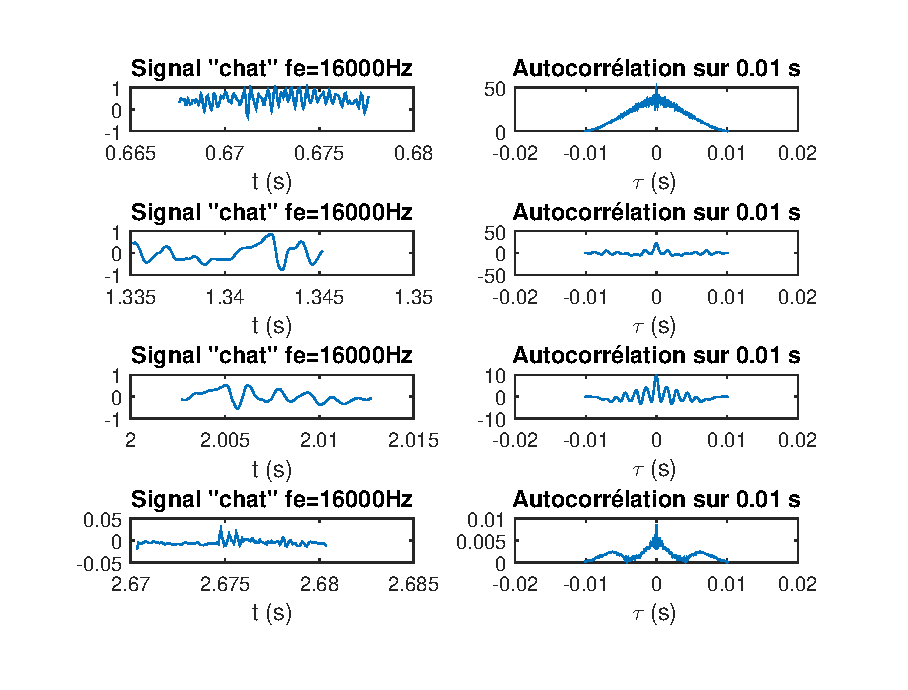
\includegraphics[height=0.45\textheight]{images/classificationVoix1.eps}
% Title: glps_renderer figure
% Creator: GL2PS 1.3.8, (C) 1999-2012 C. Geuzaine
% For: Octave
% CreationDate: Thu Nov  9 22:44:55 2017
\begin{pgfpicture}
\pgfsetlinewidth{0.01pt}
\color[rgb]{1.000000,1.000000,1.000000}
\pgfpathmoveto{\pgfpoint{335.117401pt}{386.837402pt}}
\pgflineto{\pgfpoint{521.279968pt}{340.136108pt}}
\pgflineto{\pgfpoint{335.117401pt}{340.136108pt}}
\pgfpathclose
\pgfusepath{fill,stroke}
\pgfpathmoveto{\pgfpoint{335.117401pt}{386.837402pt}}
\pgflineto{\pgfpoint{521.279968pt}{386.837402pt}}
\pgflineto{\pgfpoint{521.279968pt}{340.136108pt}}
\pgfpathclose
\pgfusepath{fill,stroke}
\pgfpathmoveto{\pgfpoint{74.880615pt}{386.837402pt}}
\pgflineto{\pgfpoint{261.042847pt}{340.136108pt}}
\pgflineto{\pgfpoint{74.880615pt}{340.136108pt}}
\pgfpathclose
\pgfusepath{fill,stroke}
\pgfpathmoveto{\pgfpoint{74.880615pt}{386.837402pt}}
\pgflineto{\pgfpoint{261.042847pt}{386.837402pt}}
\pgflineto{\pgfpoint{261.042847pt}{340.136108pt}}
\pgfpathclose
\pgfusepath{fill,stroke}
\pgfpathmoveto{\pgfpoint{335.117401pt}{289.298706pt}}
\pgflineto{\pgfpoint{521.279968pt}{242.597412pt}}
\pgflineto{\pgfpoint{335.117401pt}{242.597412pt}}
\pgfpathclose
\pgfusepath{fill,stroke}
\pgfpathmoveto{\pgfpoint{335.117401pt}{289.298706pt}}
\pgflineto{\pgfpoint{521.279968pt}{289.298706pt}}
\pgflineto{\pgfpoint{521.279968pt}{242.597412pt}}
\pgfpathclose
\pgfusepath{fill,stroke}
\pgfpathmoveto{\pgfpoint{74.880615pt}{289.298706pt}}
\pgflineto{\pgfpoint{261.041748pt}{242.597412pt}}
\pgflineto{\pgfpoint{74.880615pt}{242.597412pt}}
\pgfpathclose
\pgfusepath{fill,stroke}
\pgfpathmoveto{\pgfpoint{74.880615pt}{289.298706pt}}
\pgflineto{\pgfpoint{261.041748pt}{289.298706pt}}
\pgflineto{\pgfpoint{261.041748pt}{242.597412pt}}
\pgfpathclose
\pgfusepath{fill,stroke}
\pgfpathmoveto{\pgfpoint{335.117401pt}{191.760010pt}}
\pgflineto{\pgfpoint{521.279968pt}{145.058716pt}}
\pgflineto{\pgfpoint{335.117401pt}{145.058716pt}}
\pgfpathclose
\pgfusepath{fill,stroke}
\pgfpathmoveto{\pgfpoint{335.117401pt}{191.760010pt}}
\pgflineto{\pgfpoint{521.279968pt}{191.760010pt}}
\pgflineto{\pgfpoint{521.279968pt}{145.058716pt}}
\pgfpathclose
\pgfusepath{fill,stroke}
\pgfpathmoveto{\pgfpoint{74.882812pt}{191.760010pt}}
\pgflineto{\pgfpoint{261.043945pt}{145.058716pt}}
\pgflineto{\pgfpoint{74.882812pt}{145.058716pt}}
\pgfpathclose
\pgfusepath{fill,stroke}
\pgfpathmoveto{\pgfpoint{74.882812pt}{191.760010pt}}
\pgflineto{\pgfpoint{261.043945pt}{191.760010pt}}
\pgflineto{\pgfpoint{261.043945pt}{145.058716pt}}
\pgfpathclose
\pgfusepath{fill,stroke}
\pgfpathmoveto{\pgfpoint{335.117401pt}{94.221268pt}}
\pgflineto{\pgfpoint{521.279968pt}{47.519974pt}}
\pgflineto{\pgfpoint{335.117401pt}{47.519974pt}}
\pgfpathclose
\pgfusepath{fill,stroke}
\pgfpathmoveto{\pgfpoint{335.117401pt}{94.221268pt}}
\pgflineto{\pgfpoint{521.279968pt}{94.221268pt}}
\pgflineto{\pgfpoint{521.279968pt}{47.519974pt}}
\pgfpathclose
\pgfusepath{fill,stroke}
\pgfpathmoveto{\pgfpoint{74.887207pt}{94.221268pt}}
\pgflineto{\pgfpoint{261.043945pt}{47.519974pt}}
\pgflineto{\pgfpoint{74.887207pt}{47.519974pt}}
\pgfpathclose
\pgfusepath{fill,stroke}
\pgfpathmoveto{\pgfpoint{74.887207pt}{94.221268pt}}
\pgflineto{\pgfpoint{261.043945pt}{94.221268pt}}
\pgflineto{\pgfpoint{261.043945pt}{47.519974pt}}
\pgfpathclose
\pgfusepath{fill,stroke}
\color[rgb]{0.000000,0.000000,0.000000}
\pgfsetlinewidth{0.500000pt}
\pgfsetdash{{16pt}{0pt}}{0pt}
\pgfpathmoveto{\pgfpoint{521.279968pt}{340.136108pt}}
\pgflineto{\pgfpoint{335.117401pt}{340.136108pt}}
\pgfusepath{stroke}
\pgfpathmoveto{\pgfpoint{521.279968pt}{386.837402pt}}
\pgflineto{\pgfpoint{335.117401pt}{386.837402pt}}
\pgfusepath{stroke}
\pgfpathmoveto{\pgfpoint{335.117401pt}{386.837402pt}}
\pgflineto{\pgfpoint{335.117401pt}{340.136108pt}}
\pgfusepath{stroke}
\pgfpathmoveto{\pgfpoint{521.279968pt}{386.837402pt}}
\pgflineto{\pgfpoint{521.279968pt}{340.136108pt}}
\pgfusepath{stroke}
\pgfpathmoveto{\pgfpoint{335.117401pt}{341.985931pt}}
\pgflineto{\pgfpoint{335.117401pt}{340.136108pt}}
\pgfusepath{stroke}
\pgfpathmoveto{\pgfpoint{335.117401pt}{384.987610pt}}
\pgflineto{\pgfpoint{335.117401pt}{386.837402pt}}
\pgfusepath{stroke}
\pgfpathmoveto{\pgfpoint{366.144501pt}{341.985931pt}}
\pgflineto{\pgfpoint{366.144501pt}{340.136108pt}}
\pgfusepath{stroke}
\pgfpathmoveto{\pgfpoint{366.144501pt}{384.987610pt}}
\pgflineto{\pgfpoint{366.144501pt}{386.837402pt}}
\pgfusepath{stroke}
\pgfpathmoveto{\pgfpoint{397.171600pt}{341.985931pt}}
\pgflineto{\pgfpoint{397.171600pt}{340.136108pt}}
\pgfusepath{stroke}
\pgfpathmoveto{\pgfpoint{397.171600pt}{384.987610pt}}
\pgflineto{\pgfpoint{397.171600pt}{386.837402pt}}
\pgfusepath{stroke}
\pgfpathmoveto{\pgfpoint{428.198700pt}{341.985931pt}}
\pgflineto{\pgfpoint{428.198700pt}{340.136108pt}}
\pgfusepath{stroke}
\pgfpathmoveto{\pgfpoint{428.198700pt}{384.987610pt}}
\pgflineto{\pgfpoint{428.198700pt}{386.837402pt}}
\pgfusepath{stroke}
\pgfpathmoveto{\pgfpoint{459.225769pt}{341.985931pt}}
\pgflineto{\pgfpoint{459.225769pt}{340.136108pt}}
\pgfusepath{stroke}
\pgfpathmoveto{\pgfpoint{459.225769pt}{384.987610pt}}
\pgflineto{\pgfpoint{459.225769pt}{386.837402pt}}
\pgfusepath{stroke}
\pgfpathmoveto{\pgfpoint{490.252899pt}{341.985931pt}}
\pgflineto{\pgfpoint{490.252899pt}{340.136108pt}}
\pgfusepath{stroke}
\pgfpathmoveto{\pgfpoint{490.252899pt}{384.987610pt}}
\pgflineto{\pgfpoint{490.252899pt}{386.837402pt}}
\pgfusepath{stroke}
\pgfpathmoveto{\pgfpoint{521.279968pt}{341.985931pt}}
\pgflineto{\pgfpoint{521.279968pt}{340.136108pt}}
\pgfusepath{stroke}
\pgfpathmoveto{\pgfpoint{521.279968pt}{384.987610pt}}
\pgflineto{\pgfpoint{521.279968pt}{386.837402pt}}
\pgfusepath{stroke}
{
\pgftransformshift{\pgfpoint{335.117401pt}{335.167908pt}}
\pgfnode{rectangle}{north}{\fontsize{10}{0}\selectfont\textcolor[rgb]{0,0,0}{{-0.015}}}{}{\pgfusepath{discard}}}
{
\pgftransformshift{\pgfpoint{366.144501pt}{335.167908pt}}
\pgfnode{rectangle}{north}{\fontsize{10}{0}\selectfont\textcolor[rgb]{0,0,0}{{-0.01}}}{}{\pgfusepath{discard}}}
{
\pgftransformshift{\pgfpoint{397.171600pt}{335.167908pt}}
\pgfnode{rectangle}{north}{\fontsize{10}{0}\selectfont\textcolor[rgb]{0,0,0}{{-0.005}}}{}{\pgfusepath{discard}}}
{
\pgftransformshift{\pgfpoint{428.198700pt}{335.167908pt}}
\pgfnode{rectangle}{north}{\fontsize{10}{0}\selectfont\textcolor[rgb]{0,0,0}{{0}}}{}{\pgfusepath{discard}}}
{
\pgftransformshift{\pgfpoint{459.225769pt}{335.167908pt}}
\pgfnode{rectangle}{north}{\fontsize{10}{0}\selectfont\textcolor[rgb]{0,0,0}{{0.005}}}{}{\pgfusepath{discard}}}
{
\pgftransformshift{\pgfpoint{490.252899pt}{335.167908pt}}
\pgfnode{rectangle}{north}{\fontsize{10}{0}\selectfont\textcolor[rgb]{0,0,0}{{0.01}}}{}{\pgfusepath{discard}}}
{
\pgftransformshift{\pgfpoint{521.279968pt}{335.167908pt}}
\pgfnode{rectangle}{north}{\fontsize{10}{0}\selectfont\textcolor[rgb]{0,0,0}{{0.015}}}{}{\pgfusepath{discard}}}
\pgfpathmoveto{\pgfpoint{336.980652pt}{340.136108pt}}
\pgflineto{\pgfpoint{335.117401pt}{340.136108pt}}
\pgfusepath{stroke}
\pgfpathmoveto{\pgfpoint{519.416748pt}{340.136108pt}}
\pgflineto{\pgfpoint{521.279968pt}{340.136108pt}}
\pgfusepath{stroke}
\pgfpathmoveto{\pgfpoint{336.980652pt}{349.476379pt}}
\pgflineto{\pgfpoint{335.117401pt}{349.476379pt}}
\pgfusepath{stroke}
\pgfpathmoveto{\pgfpoint{519.416748pt}{349.476379pt}}
\pgflineto{\pgfpoint{521.279968pt}{349.476379pt}}
\pgfusepath{stroke}
\pgfpathmoveto{\pgfpoint{336.980652pt}{358.816650pt}}
\pgflineto{\pgfpoint{335.117401pt}{358.816650pt}}
\pgfusepath{stroke}
\pgfpathmoveto{\pgfpoint{519.416748pt}{358.816650pt}}
\pgflineto{\pgfpoint{521.279968pt}{358.816650pt}}
\pgfusepath{stroke}
\pgfpathmoveto{\pgfpoint{336.980652pt}{368.156921pt}}
\pgflineto{\pgfpoint{335.117401pt}{368.156921pt}}
\pgfusepath{stroke}
\pgfpathmoveto{\pgfpoint{519.416748pt}{368.156921pt}}
\pgflineto{\pgfpoint{521.279968pt}{368.156921pt}}
\pgfusepath{stroke}
\pgfpathmoveto{\pgfpoint{336.980652pt}{377.497162pt}}
\pgflineto{\pgfpoint{335.117401pt}{377.497162pt}}
\pgfusepath{stroke}
\pgfpathmoveto{\pgfpoint{519.416748pt}{377.497162pt}}
\pgflineto{\pgfpoint{521.279968pt}{377.497162pt}}
\pgfusepath{stroke}
\pgfpathmoveto{\pgfpoint{336.980652pt}{386.837402pt}}
\pgflineto{\pgfpoint{335.117401pt}{386.837402pt}}
\pgfusepath{stroke}
\pgfpathmoveto{\pgfpoint{519.416748pt}{386.837402pt}}
\pgflineto{\pgfpoint{521.279968pt}{386.837402pt}}
\pgfusepath{stroke}
{
\pgftransformshift{\pgfpoint{330.113037pt}{340.136108pt}}
\pgfnode{rectangle}{east}{\fontsize{10}{0}\selectfont\textcolor[rgb]{0,0,0}{{0}}}{}{\pgfusepath{discard}}}
{
\pgftransformshift{\pgfpoint{330.113037pt}{349.476379pt}}
\pgfnode{rectangle}{east}{\fontsize{10}{0}\selectfont\textcolor[rgb]{0,0,0}{{10}}}{}{\pgfusepath{discard}}}
{
\pgftransformshift{\pgfpoint{330.113037pt}{358.816650pt}}
\pgfnode{rectangle}{east}{\fontsize{10}{0}\selectfont\textcolor[rgb]{0,0,0}{{20}}}{}{\pgfusepath{discard}}}
{
\pgftransformshift{\pgfpoint{330.113037pt}{368.156921pt}}
\pgfnode{rectangle}{east}{\fontsize{10}{0}\selectfont\textcolor[rgb]{0,0,0}{{30}}}{}{\pgfusepath{discard}}}
{
\pgftransformshift{\pgfpoint{330.113037pt}{377.497162pt}}
\pgfnode{rectangle}{east}{\fontsize{10}{0}\selectfont\textcolor[rgb]{0,0,0}{{40}}}{}{\pgfusepath{discard}}}
{
\pgftransformshift{\pgfpoint{330.113037pt}{386.837402pt}}
\pgfnode{rectangle}{east}{\fontsize{10}{0}\selectfont\textcolor[rgb]{0,0,0}{{50}}}{}{\pgfusepath{discard}}}
{
\pgftransformshift{\pgfpoint{428.198700pt}{324.167908pt}}
\pgfnode{rectangle}{north}{\fontsize{10}{0}\selectfont\textcolor[rgb]{0,0,0}{{$\tau$ (s)}}}{}{\pgfusepath{discard}}}
\color[rgb]{0.000000,0.000000,1.000000}
\pgfsetdash{}{0pt}
\pgfpathmoveto{\pgfpoint{366.338440pt}{340.449341pt}}
\pgflineto{\pgfpoint{365.950592pt}{340.311401pt}}
\pgfusepath{stroke}
\pgfpathmoveto{\pgfpoint{366.726257pt}{340.450928pt}}
\pgflineto{\pgfpoint{366.338440pt}{340.449341pt}}
\pgfusepath{stroke}
\pgfpathmoveto{\pgfpoint{367.114105pt}{340.393707pt}}
\pgflineto{\pgfpoint{366.726257pt}{340.450928pt}}
\pgfusepath{stroke}
\pgfpathmoveto{\pgfpoint{367.501953pt}{340.427734pt}}
\pgflineto{\pgfpoint{367.114105pt}{340.393707pt}}
\pgfusepath{stroke}
\pgfpathmoveto{\pgfpoint{367.889771pt}{340.527344pt}}
\pgflineto{\pgfpoint{367.501953pt}{340.427734pt}}
\pgfusepath{stroke}
\pgfpathmoveto{\pgfpoint{368.277618pt}{340.775024pt}}
\pgflineto{\pgfpoint{367.889771pt}{340.527344pt}}
\pgfusepath{stroke}
\pgfpathmoveto{\pgfpoint{368.665466pt}{341.073792pt}}
\pgflineto{\pgfpoint{368.277618pt}{340.775024pt}}
\pgfusepath{stroke}
\pgfpathmoveto{\pgfpoint{369.053284pt}{341.140869pt}}
\pgflineto{\pgfpoint{368.665466pt}{341.073792pt}}
\pgfusepath{stroke}
\pgfpathmoveto{\pgfpoint{369.441132pt}{341.112579pt}}
\pgflineto{\pgfpoint{369.053284pt}{341.140869pt}}
\pgfusepath{stroke}
\pgfpathmoveto{\pgfpoint{369.828979pt}{341.114777pt}}
\pgflineto{\pgfpoint{369.441132pt}{341.112579pt}}
\pgfusepath{stroke}
\pgfpathmoveto{\pgfpoint{370.216797pt}{341.270935pt}}
\pgflineto{\pgfpoint{369.828979pt}{341.114777pt}}
\pgfusepath{stroke}
\pgfpathmoveto{\pgfpoint{370.604675pt}{341.502106pt}}
\pgflineto{\pgfpoint{370.216797pt}{341.270935pt}}
\pgfusepath{stroke}
\pgfpathmoveto{\pgfpoint{370.992493pt}{341.616425pt}}
\pgflineto{\pgfpoint{370.604675pt}{341.502106pt}}
\pgfusepath{stroke}
\pgfpathmoveto{\pgfpoint{371.380310pt}{341.630188pt}}
\pgflineto{\pgfpoint{370.992493pt}{341.616425pt}}
\pgfusepath{stroke}
\pgfpathmoveto{\pgfpoint{371.768158pt}{341.581116pt}}
\pgflineto{\pgfpoint{371.380310pt}{341.630188pt}}
\pgfusepath{stroke}
\pgfpathmoveto{\pgfpoint{372.156006pt}{341.658966pt}}
\pgflineto{\pgfpoint{371.768158pt}{341.581116pt}}
\pgfusepath{stroke}
\pgfpathmoveto{\pgfpoint{372.543854pt}{341.906708pt}}
\pgflineto{\pgfpoint{372.156006pt}{341.658966pt}}
\pgfusepath{stroke}
\pgfpathmoveto{\pgfpoint{372.931671pt}{342.262451pt}}
\pgflineto{\pgfpoint{372.543854pt}{341.906708pt}}
\pgfusepath{stroke}
\pgfpathmoveto{\pgfpoint{373.319519pt}{342.527496pt}}
\pgflineto{\pgfpoint{372.931671pt}{342.262451pt}}
\pgfusepath{stroke}
\pgfpathmoveto{\pgfpoint{373.707367pt}{342.512268pt}}
\pgflineto{\pgfpoint{373.319519pt}{342.527496pt}}
\pgfusepath{stroke}
\pgfpathmoveto{\pgfpoint{374.095184pt}{342.361816pt}}
\pgflineto{\pgfpoint{373.707367pt}{342.512268pt}}
\pgfusepath{stroke}
\pgfpathmoveto{\pgfpoint{374.483032pt}{342.541412pt}}
\pgflineto{\pgfpoint{374.095184pt}{342.361816pt}}
\pgfusepath{stroke}
\pgfpathmoveto{\pgfpoint{374.870880pt}{343.112427pt}}
\pgflineto{\pgfpoint{374.483032pt}{342.541412pt}}
\pgfusepath{stroke}
\pgfpathmoveto{\pgfpoint{375.258728pt}{343.437744pt}}
\pgflineto{\pgfpoint{374.870880pt}{343.112427pt}}
\pgfusepath{stroke}
\pgfpathmoveto{\pgfpoint{375.646545pt}{343.190796pt}}
\pgflineto{\pgfpoint{375.258728pt}{343.437744pt}}
\pgfusepath{stroke}
\pgfpathmoveto{\pgfpoint{376.034393pt}{342.859833pt}}
\pgflineto{\pgfpoint{375.646545pt}{343.190796pt}}
\pgfusepath{stroke}
\pgfpathmoveto{\pgfpoint{376.422241pt}{343.008789pt}}
\pgflineto{\pgfpoint{376.034393pt}{342.859833pt}}
\pgfusepath{stroke}
\pgfpathmoveto{\pgfpoint{376.810059pt}{343.713196pt}}
\pgflineto{\pgfpoint{376.422241pt}{343.008789pt}}
\pgfusepath{stroke}
\pgfpathmoveto{\pgfpoint{377.197906pt}{344.423584pt}}
\pgflineto{\pgfpoint{376.810059pt}{343.713196pt}}
\pgfusepath{stroke}
\pgfpathmoveto{\pgfpoint{377.585754pt}{344.495148pt}}
\pgflineto{\pgfpoint{377.197906pt}{344.423584pt}}
\pgfusepath{stroke}
\pgfpathmoveto{\pgfpoint{377.973572pt}{344.000916pt}}
\pgflineto{\pgfpoint{377.585754pt}{344.495148pt}}
\pgfusepath{stroke}
\pgfpathmoveto{\pgfpoint{378.361420pt}{343.678925pt}}
\pgflineto{\pgfpoint{377.973572pt}{344.000916pt}}
\pgfusepath{stroke}
\pgfpathmoveto{\pgfpoint{378.749268pt}{344.064728pt}}
\pgflineto{\pgfpoint{378.361420pt}{343.678925pt}}
\pgfusepath{stroke}
\pgfpathmoveto{\pgfpoint{379.137085pt}{344.954468pt}}
\pgflineto{\pgfpoint{378.749268pt}{344.064728pt}}
\pgfusepath{stroke}
\pgfpathmoveto{\pgfpoint{379.524933pt}{345.542542pt}}
\pgflineto{\pgfpoint{379.137085pt}{344.954468pt}}
\pgfusepath{stroke}
\pgfpathmoveto{\pgfpoint{379.912781pt}{345.388977pt}}
\pgflineto{\pgfpoint{379.524933pt}{345.542542pt}}
\pgfusepath{stroke}
\pgfpathmoveto{\pgfpoint{380.300629pt}{345.157227pt}}
\pgflineto{\pgfpoint{379.912781pt}{345.388977pt}}
\pgfusepath{stroke}
\pgfpathmoveto{\pgfpoint{380.688477pt}{345.371460pt}}
\pgflineto{\pgfpoint{380.300629pt}{345.157227pt}}
\pgfusepath{stroke}
\pgfpathmoveto{\pgfpoint{381.076294pt}{345.841064pt}}
\pgflineto{\pgfpoint{380.688477pt}{345.371460pt}}
\pgfusepath{stroke}
\pgfpathmoveto{\pgfpoint{381.464142pt}{346.197021pt}}
\pgflineto{\pgfpoint{381.076294pt}{345.841064pt}}
\pgfusepath{stroke}
\pgfpathmoveto{\pgfpoint{381.851990pt}{346.273315pt}}
\pgflineto{\pgfpoint{381.464142pt}{346.197021pt}}
\pgfusepath{stroke}
\pgfpathmoveto{\pgfpoint{382.239807pt}{346.455627pt}}
\pgflineto{\pgfpoint{381.851990pt}{346.273315pt}}
\pgfusepath{stroke}
\pgfpathmoveto{\pgfpoint{382.627655pt}{346.784271pt}}
\pgflineto{\pgfpoint{382.239807pt}{346.455627pt}}
\pgfusepath{stroke}
\pgfpathmoveto{\pgfpoint{383.015472pt}{347.180450pt}}
\pgflineto{\pgfpoint{382.627655pt}{346.784271pt}}
\pgfusepath{stroke}
\pgfpathmoveto{\pgfpoint{383.403320pt}{347.616760pt}}
\pgflineto{\pgfpoint{383.015472pt}{347.180450pt}}
\pgfusepath{stroke}
\pgfpathmoveto{\pgfpoint{383.791168pt}{347.721680pt}}
\pgflineto{\pgfpoint{383.403320pt}{347.616760pt}}
\pgfusepath{stroke}
\pgfpathmoveto{\pgfpoint{384.179016pt}{347.708252pt}}
\pgflineto{\pgfpoint{383.791168pt}{347.721680pt}}
\pgfusepath{stroke}
\pgfpathmoveto{\pgfpoint{384.566833pt}{347.936707pt}}
\pgflineto{\pgfpoint{384.179016pt}{347.708252pt}}
\pgfusepath{stroke}
\pgfpathmoveto{\pgfpoint{384.954681pt}{348.291138pt}}
\pgflineto{\pgfpoint{384.566833pt}{347.936707pt}}
\pgfusepath{stroke}
\pgfpathmoveto{\pgfpoint{385.342529pt}{348.556885pt}}
\pgflineto{\pgfpoint{384.954681pt}{348.291138pt}}
\pgfusepath{stroke}
\pgfpathmoveto{\pgfpoint{385.730347pt}{348.711548pt}}
\pgflineto{\pgfpoint{385.342529pt}{348.556885pt}}
\pgfusepath{stroke}
\pgfpathmoveto{\pgfpoint{386.118195pt}{348.877655pt}}
\pgflineto{\pgfpoint{385.730347pt}{348.711548pt}}
\pgfusepath{stroke}
\pgfpathmoveto{\pgfpoint{386.506042pt}{349.004883pt}}
\pgflineto{\pgfpoint{386.118195pt}{348.877655pt}}
\pgfusepath{stroke}
\pgfpathmoveto{\pgfpoint{386.893860pt}{349.233063pt}}
\pgflineto{\pgfpoint{386.506042pt}{349.004883pt}}
\pgfusepath{stroke}
\pgfpathmoveto{\pgfpoint{387.281708pt}{349.766785pt}}
\pgflineto{\pgfpoint{386.893860pt}{349.233063pt}}
\pgfusepath{stroke}
\pgfpathmoveto{\pgfpoint{387.669556pt}{350.065002pt}}
\pgflineto{\pgfpoint{387.281708pt}{349.766785pt}}
\pgfusepath{stroke}
\pgfpathmoveto{\pgfpoint{388.057373pt}{349.765381pt}}
\pgflineto{\pgfpoint{387.669556pt}{350.065002pt}}
\pgfusepath{stroke}
\pgfpathmoveto{\pgfpoint{388.445251pt}{349.650330pt}}
\pgflineto{\pgfpoint{388.057373pt}{349.765381pt}}
\pgfusepath{stroke}
\pgfpathmoveto{\pgfpoint{388.833069pt}{350.325867pt}}
\pgflineto{\pgfpoint{388.445251pt}{349.650330pt}}
\pgfusepath{stroke}
\pgfpathmoveto{\pgfpoint{389.220886pt}{351.219025pt}}
\pgflineto{\pgfpoint{388.833069pt}{350.325867pt}}
\pgfusepath{stroke}
\pgfpathmoveto{\pgfpoint{389.608765pt}{351.533203pt}}
\pgflineto{\pgfpoint{389.220886pt}{351.219025pt}}
\pgfusepath{stroke}
\pgfpathmoveto{\pgfpoint{389.996582pt}{351.217896pt}}
\pgflineto{\pgfpoint{389.608765pt}{351.533203pt}}
\pgfusepath{stroke}
\pgfpathmoveto{\pgfpoint{390.384430pt}{350.967224pt}}
\pgflineto{\pgfpoint{389.996582pt}{351.217896pt}}
\pgfusepath{stroke}
\pgfpathmoveto{\pgfpoint{390.772278pt}{351.266052pt}}
\pgflineto{\pgfpoint{390.384430pt}{350.967224pt}}
\pgfusepath{stroke}
\pgfpathmoveto{\pgfpoint{391.160095pt}{351.918701pt}}
\pgflineto{\pgfpoint{390.772278pt}{351.266052pt}}
\pgfusepath{stroke}
\pgfpathmoveto{\pgfpoint{391.547943pt}{352.584991pt}}
\pgflineto{\pgfpoint{391.160095pt}{351.918701pt}}
\pgfusepath{stroke}
\pgfpathmoveto{\pgfpoint{391.935791pt}{352.811493pt}}
\pgflineto{\pgfpoint{391.547943pt}{352.584991pt}}
\pgfusepath{stroke}
\pgfpathmoveto{\pgfpoint{392.323608pt}{352.721069pt}}
\pgflineto{\pgfpoint{391.935791pt}{352.811493pt}}
\pgfusepath{stroke}
\pgfpathmoveto{\pgfpoint{392.711456pt}{352.860046pt}}
\pgflineto{\pgfpoint{392.323608pt}{352.721069pt}}
\pgfusepath{stroke}
\pgfpathmoveto{\pgfpoint{393.099304pt}{353.234802pt}}
\pgflineto{\pgfpoint{392.711456pt}{352.860046pt}}
\pgfusepath{stroke}
\pgfpathmoveto{\pgfpoint{393.487122pt}{353.418152pt}}
\pgflineto{\pgfpoint{393.099304pt}{353.234802pt}}
\pgfusepath{stroke}
\pgfpathmoveto{\pgfpoint{393.874969pt}{353.548584pt}}
\pgflineto{\pgfpoint{393.487122pt}{353.418152pt}}
\pgfusepath{stroke}
\pgfpathmoveto{\pgfpoint{394.262817pt}{354.062134pt}}
\pgflineto{\pgfpoint{393.874969pt}{353.548584pt}}
\pgfusepath{stroke}
\pgfpathmoveto{\pgfpoint{394.650635pt}{354.897522pt}}
\pgflineto{\pgfpoint{394.262817pt}{354.062134pt}}
\pgfusepath{stroke}
\pgfpathmoveto{\pgfpoint{395.038483pt}{355.530945pt}}
\pgflineto{\pgfpoint{394.650635pt}{354.897522pt}}
\pgfusepath{stroke}
\pgfpathmoveto{\pgfpoint{395.426331pt}{355.174316pt}}
\pgflineto{\pgfpoint{395.038483pt}{355.530945pt}}
\pgfusepath{stroke}
\pgfpathmoveto{\pgfpoint{395.814178pt}{354.318512pt}}
\pgflineto{\pgfpoint{395.426331pt}{355.174316pt}}
\pgfusepath{stroke}
\pgfpathmoveto{\pgfpoint{396.201996pt}{354.108521pt}}
\pgflineto{\pgfpoint{395.814178pt}{354.318512pt}}
\pgfusepath{stroke}
\pgfpathmoveto{\pgfpoint{396.589844pt}{355.154907pt}}
\pgflineto{\pgfpoint{396.201996pt}{354.108521pt}}
\pgfusepath{stroke}
\pgfpathmoveto{\pgfpoint{396.977661pt}{356.980682pt}}
\pgflineto{\pgfpoint{396.589844pt}{355.154907pt}}
\pgfusepath{stroke}
\pgfpathmoveto{\pgfpoint{397.365540pt}{357.963898pt}}
\pgflineto{\pgfpoint{396.977661pt}{356.980682pt}}
\pgfusepath{stroke}
\pgfpathmoveto{\pgfpoint{397.753357pt}{357.432922pt}}
\pgflineto{\pgfpoint{397.365540pt}{357.963898pt}}
\pgfusepath{stroke}
\pgfpathmoveto{\pgfpoint{398.141205pt}{356.055206pt}}
\pgflineto{\pgfpoint{397.753357pt}{357.432922pt}}
\pgfusepath{stroke}
\pgfpathmoveto{\pgfpoint{398.529053pt}{355.258209pt}}
\pgflineto{\pgfpoint{398.141205pt}{356.055206pt}}
\pgfusepath{stroke}
\pgfpathmoveto{\pgfpoint{398.916870pt}{355.940125pt}}
\pgflineto{\pgfpoint{398.529053pt}{355.258209pt}}
\pgfusepath{stroke}
\pgfpathmoveto{\pgfpoint{399.304718pt}{357.754089pt}}
\pgflineto{\pgfpoint{398.916870pt}{355.940125pt}}
\pgfusepath{stroke}
\pgfpathmoveto{\pgfpoint{399.692566pt}{359.438904pt}}
\pgflineto{\pgfpoint{399.304718pt}{357.754089pt}}
\pgfusepath{stroke}
\pgfpathmoveto{\pgfpoint{400.080383pt}{359.598389pt}}
\pgflineto{\pgfpoint{399.692566pt}{359.438904pt}}
\pgfusepath{stroke}
\pgfpathmoveto{\pgfpoint{400.468231pt}{358.443787pt}}
\pgflineto{\pgfpoint{400.080383pt}{359.598389pt}}
\pgfusepath{stroke}
\pgfpathmoveto{\pgfpoint{400.856079pt}{357.309845pt}}
\pgflineto{\pgfpoint{400.468231pt}{358.443787pt}}
\pgfusepath{stroke}
\pgfpathmoveto{\pgfpoint{401.243896pt}{357.360291pt}}
\pgflineto{\pgfpoint{400.856079pt}{357.309845pt}}
\pgfusepath{stroke}
\pgfpathmoveto{\pgfpoint{401.631744pt}{358.552582pt}}
\pgflineto{\pgfpoint{401.243896pt}{357.360291pt}}
\pgfusepath{stroke}
\pgfpathmoveto{\pgfpoint{402.019592pt}{359.939026pt}}
\pgflineto{\pgfpoint{401.631744pt}{358.552582pt}}
\pgfusepath{stroke}
\pgfpathmoveto{\pgfpoint{402.407410pt}{360.794556pt}}
\pgflineto{\pgfpoint{402.019592pt}{359.939026pt}}
\pgfusepath{stroke}
\pgfpathmoveto{\pgfpoint{402.795258pt}{360.547974pt}}
\pgflineto{\pgfpoint{402.407410pt}{360.794556pt}}
\pgfusepath{stroke}
\pgfpathmoveto{\pgfpoint{403.183105pt}{359.665039pt}}
\pgflineto{\pgfpoint{402.795258pt}{360.547974pt}}
\pgfusepath{stroke}
\pgfpathmoveto{\pgfpoint{403.570923pt}{359.083496pt}}
\pgflineto{\pgfpoint{403.183105pt}{359.665039pt}}
\pgfusepath{stroke}
\pgfpathmoveto{\pgfpoint{403.958771pt}{359.435547pt}}
\pgflineto{\pgfpoint{403.570923pt}{359.083496pt}}
\pgfusepath{stroke}
\pgfpathmoveto{\pgfpoint{404.346619pt}{360.953796pt}}
\pgflineto{\pgfpoint{403.958771pt}{359.435547pt}}
\pgfusepath{stroke}
\pgfpathmoveto{\pgfpoint{404.734467pt}{362.672546pt}}
\pgflineto{\pgfpoint{404.346619pt}{360.953796pt}}
\pgfusepath{stroke}
\pgfpathmoveto{\pgfpoint{405.122284pt}{363.015320pt}}
\pgflineto{\pgfpoint{404.734467pt}{362.672546pt}}
\pgfusepath{stroke}
\pgfpathmoveto{\pgfpoint{405.510132pt}{361.819244pt}}
\pgflineto{\pgfpoint{405.122284pt}{363.015320pt}}
\pgfusepath{stroke}
\pgfpathmoveto{\pgfpoint{405.897980pt}{360.553741pt}}
\pgflineto{\pgfpoint{405.510132pt}{361.819244pt}}
\pgfusepath{stroke}
\pgfpathmoveto{\pgfpoint{406.285828pt}{360.461365pt}}
\pgflineto{\pgfpoint{405.897980pt}{360.553741pt}}
\pgfusepath{stroke}
\pgfpathmoveto{\pgfpoint{406.673645pt}{361.594299pt}}
\pgflineto{\pgfpoint{406.285828pt}{360.461365pt}}
\pgfusepath{stroke}
\pgfpathmoveto{\pgfpoint{407.061493pt}{363.300842pt}}
\pgflineto{\pgfpoint{406.673645pt}{361.594299pt}}
\pgfusepath{stroke}
\pgfpathmoveto{\pgfpoint{407.449341pt}{364.912048pt}}
\pgflineto{\pgfpoint{407.061493pt}{363.300842pt}}
\pgfusepath{stroke}
\pgfpathmoveto{\pgfpoint{407.837158pt}{365.201111pt}}
\pgflineto{\pgfpoint{407.449341pt}{364.912048pt}}
\pgfusepath{stroke}
\pgfpathmoveto{\pgfpoint{408.225006pt}{363.505585pt}}
\pgflineto{\pgfpoint{407.837158pt}{365.201111pt}}
\pgfusepath{stroke}
\pgfpathmoveto{\pgfpoint{408.612854pt}{361.684265pt}}
\pgflineto{\pgfpoint{408.225006pt}{363.505585pt}}
\pgfusepath{stroke}
\pgfpathmoveto{\pgfpoint{409.000671pt}{361.830811pt}}
\pgflineto{\pgfpoint{408.612854pt}{361.684265pt}}
\pgfusepath{stroke}
\pgfpathmoveto{\pgfpoint{409.388519pt}{364.050659pt}}
\pgflineto{\pgfpoint{409.000671pt}{361.830811pt}}
\pgfusepath{stroke}
\pgfpathmoveto{\pgfpoint{409.776367pt}{366.658203pt}}
\pgflineto{\pgfpoint{409.388519pt}{364.050659pt}}
\pgfusepath{stroke}
\pgfpathmoveto{\pgfpoint{410.164185pt}{367.441284pt}}
\pgflineto{\pgfpoint{409.776367pt}{366.658203pt}}
\pgfusepath{stroke}
\pgfpathmoveto{\pgfpoint{410.552032pt}{365.887451pt}}
\pgflineto{\pgfpoint{410.164185pt}{367.441284pt}}
\pgfusepath{stroke}
\pgfpathmoveto{\pgfpoint{410.939880pt}{363.609406pt}}
\pgflineto{\pgfpoint{410.552032pt}{365.887451pt}}
\pgfusepath{stroke}
\pgfpathmoveto{\pgfpoint{411.327698pt}{363.153137pt}}
\pgflineto{\pgfpoint{410.939880pt}{363.609406pt}}
\pgfusepath{stroke}
\pgfpathmoveto{\pgfpoint{411.715546pt}{365.286041pt}}
\pgflineto{\pgfpoint{411.327698pt}{363.153137pt}}
\pgfusepath{stroke}
\pgfpathmoveto{\pgfpoint{412.103394pt}{367.934082pt}}
\pgflineto{\pgfpoint{411.715546pt}{365.286041pt}}
\pgfusepath{stroke}
\pgfpathmoveto{\pgfpoint{412.491211pt}{368.861633pt}}
\pgflineto{\pgfpoint{412.103394pt}{367.934082pt}}
\pgfusepath{stroke}
\pgfpathmoveto{\pgfpoint{412.879059pt}{367.961304pt}}
\pgflineto{\pgfpoint{412.491211pt}{368.861633pt}}
\pgfusepath{stroke}
\pgfpathmoveto{\pgfpoint{413.266907pt}{366.707275pt}}
\pgflineto{\pgfpoint{412.879059pt}{367.961304pt}}
\pgfusepath{stroke}
\pgfpathmoveto{\pgfpoint{413.654755pt}{365.995880pt}}
\pgflineto{\pgfpoint{413.266907pt}{366.707275pt}}
\pgfusepath{stroke}
\pgfpathmoveto{\pgfpoint{414.042572pt}{366.269226pt}}
\pgflineto{\pgfpoint{413.654755pt}{365.995880pt}}
\pgfusepath{stroke}
\pgfpathmoveto{\pgfpoint{414.430420pt}{367.564972pt}}
\pgflineto{\pgfpoint{414.042572pt}{366.269226pt}}
\pgfusepath{stroke}
\pgfpathmoveto{\pgfpoint{414.818268pt}{369.274353pt}}
\pgflineto{\pgfpoint{414.430420pt}{367.564972pt}}
\pgfusepath{stroke}
\pgfpathmoveto{\pgfpoint{415.206116pt}{370.454224pt}}
\pgflineto{\pgfpoint{414.818268pt}{369.274353pt}}
\pgfusepath{stroke}
\pgfpathmoveto{\pgfpoint{415.593933pt}{370.019531pt}}
\pgflineto{\pgfpoint{415.206116pt}{370.454224pt}}
\pgfusepath{stroke}
\pgfpathmoveto{\pgfpoint{415.981781pt}{368.246765pt}}
\pgflineto{\pgfpoint{415.593933pt}{370.019531pt}}
\pgfusepath{stroke}
\pgfpathmoveto{\pgfpoint{416.369629pt}{366.634918pt}}
\pgflineto{\pgfpoint{415.981781pt}{368.246765pt}}
\pgfusepath{stroke}
\pgfpathmoveto{\pgfpoint{416.757446pt}{366.917480pt}}
\pgflineto{\pgfpoint{416.369629pt}{366.634918pt}}
\pgfusepath{stroke}
\pgfpathmoveto{\pgfpoint{417.145294pt}{369.561157pt}}
\pgflineto{\pgfpoint{416.757446pt}{366.917480pt}}
\pgfusepath{stroke}
\pgfpathmoveto{\pgfpoint{417.533142pt}{372.340851pt}}
\pgflineto{\pgfpoint{417.145294pt}{369.561157pt}}
\pgfusepath{stroke}
\pgfpathmoveto{\pgfpoint{417.920959pt}{372.671570pt}}
\pgflineto{\pgfpoint{417.533142pt}{372.340851pt}}
\pgfusepath{stroke}
\pgfpathmoveto{\pgfpoint{418.308807pt}{370.270935pt}}
\pgflineto{\pgfpoint{417.920959pt}{372.671570pt}}
\pgfusepath{stroke}
\pgfpathmoveto{\pgfpoint{418.696655pt}{367.550720pt}}
\pgflineto{\pgfpoint{418.308807pt}{370.270935pt}}
\pgfusepath{stroke}
\pgfpathmoveto{\pgfpoint{419.084473pt}{367.141235pt}}
\pgflineto{\pgfpoint{418.696655pt}{367.550720pt}}
\pgfusepath{stroke}
\pgfpathmoveto{\pgfpoint{419.472321pt}{369.625366pt}}
\pgflineto{\pgfpoint{419.084473pt}{367.141235pt}}
\pgfusepath{stroke}
\pgfpathmoveto{\pgfpoint{419.860168pt}{373.033630pt}}
\pgflineto{\pgfpoint{419.472321pt}{369.625366pt}}
\pgfusepath{stroke}
\pgfpathmoveto{\pgfpoint{420.247986pt}{374.386475pt}}
\pgflineto{\pgfpoint{419.860168pt}{373.033630pt}}
\pgfusepath{stroke}
\pgfpathmoveto{\pgfpoint{420.635864pt}{372.651672pt}}
\pgflineto{\pgfpoint{420.247986pt}{374.386475pt}}
\pgfusepath{stroke}
\pgfpathmoveto{\pgfpoint{421.023682pt}{369.587158pt}}
\pgflineto{\pgfpoint{420.635864pt}{372.651672pt}}
\pgfusepath{stroke}
\pgfpathmoveto{\pgfpoint{421.411499pt}{367.986816pt}}
\pgflineto{\pgfpoint{421.023682pt}{369.587158pt}}
\pgfusepath{stroke}
\pgfpathmoveto{\pgfpoint{421.799377pt}{369.124023pt}}
\pgflineto{\pgfpoint{421.411499pt}{367.986816pt}}
\pgfusepath{stroke}
\pgfpathmoveto{\pgfpoint{422.187195pt}{372.242310pt}}
\pgflineto{\pgfpoint{421.799377pt}{369.124023pt}}
\pgfusepath{stroke}
\pgfpathmoveto{\pgfpoint{422.575043pt}{374.990143pt}}
\pgflineto{\pgfpoint{422.187195pt}{372.242310pt}}
\pgfusepath{stroke}
\pgfpathmoveto{\pgfpoint{422.962891pt}{375.014771pt}}
\pgflineto{\pgfpoint{422.575043pt}{374.990143pt}}
\pgfusepath{stroke}
\pgfpathmoveto{\pgfpoint{423.350708pt}{372.814301pt}}
\pgflineto{\pgfpoint{422.962891pt}{375.014771pt}}
\pgfusepath{stroke}
\pgfpathmoveto{\pgfpoint{423.738525pt}{370.548523pt}}
\pgflineto{\pgfpoint{423.350708pt}{372.814301pt}}
\pgfusepath{stroke}
\pgfpathmoveto{\pgfpoint{424.126404pt}{369.567139pt}}
\pgflineto{\pgfpoint{423.738525pt}{370.548523pt}}
\pgfusepath{stroke}
\pgfpathmoveto{\pgfpoint{424.514221pt}{370.482361pt}}
\pgflineto{\pgfpoint{424.126404pt}{369.567139pt}}
\pgfusepath{stroke}
\pgfpathmoveto{\pgfpoint{424.902069pt}{373.494568pt}}
\pgflineto{\pgfpoint{424.514221pt}{370.482361pt}}
\pgfusepath{stroke}
\pgfpathmoveto{\pgfpoint{425.289917pt}{376.802673pt}}
\pgflineto{\pgfpoint{424.902069pt}{373.494568pt}}
\pgfusepath{stroke}
\pgfpathmoveto{\pgfpoint{425.677734pt}{377.430023pt}}
\pgflineto{\pgfpoint{425.289917pt}{376.802673pt}}
\pgfusepath{stroke}
\pgfpathmoveto{\pgfpoint{426.065582pt}{374.449127pt}}
\pgflineto{\pgfpoint{425.677734pt}{377.430023pt}}
\pgfusepath{stroke}
\pgfpathmoveto{\pgfpoint{426.453430pt}{369.669586pt}}
\pgflineto{\pgfpoint{426.065582pt}{374.449127pt}}
\pgfusepath{stroke}
\pgfpathmoveto{\pgfpoint{426.841248pt}{367.200378pt}}
\pgflineto{\pgfpoint{426.453430pt}{369.669586pt}}
\pgfusepath{stroke}
\pgfpathmoveto{\pgfpoint{427.229095pt}{370.446106pt}}
\pgflineto{\pgfpoint{426.841248pt}{367.200378pt}}
\pgfusepath{stroke}
\pgfpathmoveto{\pgfpoint{427.616943pt}{378.113281pt}}
\pgflineto{\pgfpoint{427.229095pt}{370.446106pt}}
\pgfusepath{stroke}
\pgfpathmoveto{\pgfpoint{428.004761pt}{382.655334pt}}
\pgflineto{\pgfpoint{427.616943pt}{378.113281pt}}
\pgfusepath{stroke}
\pgfpathmoveto{\pgfpoint{428.392609pt}{378.113281pt}}
\pgflineto{\pgfpoint{428.004761pt}{382.655334pt}}
\pgfusepath{stroke}
\pgfpathmoveto{\pgfpoint{428.780457pt}{370.446106pt}}
\pgflineto{\pgfpoint{428.392609pt}{378.113281pt}}
\pgfusepath{stroke}
\pgfpathmoveto{\pgfpoint{429.168274pt}{367.200378pt}}
\pgflineto{\pgfpoint{428.780457pt}{370.446106pt}}
\pgfusepath{stroke}
\pgfpathmoveto{\pgfpoint{429.556152pt}{369.669586pt}}
\pgflineto{\pgfpoint{429.168274pt}{367.200378pt}}
\pgfusepath{stroke}
\pgfpathmoveto{\pgfpoint{429.943970pt}{374.449127pt}}
\pgflineto{\pgfpoint{429.556152pt}{369.669586pt}}
\pgfusepath{stroke}
\pgfpathmoveto{\pgfpoint{430.331818pt}{377.430023pt}}
\pgflineto{\pgfpoint{429.943970pt}{374.449127pt}}
\pgfusepath{stroke}
\pgfpathmoveto{\pgfpoint{430.719666pt}{376.802673pt}}
\pgflineto{\pgfpoint{430.331818pt}{377.430023pt}}
\pgfusepath{stroke}
\pgfpathmoveto{\pgfpoint{431.107483pt}{373.494568pt}}
\pgflineto{\pgfpoint{430.719666pt}{376.802673pt}}
\pgfusepath{stroke}
\pgfpathmoveto{\pgfpoint{431.495331pt}{370.482361pt}}
\pgflineto{\pgfpoint{431.107483pt}{373.494568pt}}
\pgfusepath{stroke}
\pgfpathmoveto{\pgfpoint{431.883179pt}{369.567139pt}}
\pgflineto{\pgfpoint{431.495331pt}{370.482361pt}}
\pgfusepath{stroke}
\pgfpathmoveto{\pgfpoint{432.270996pt}{370.548523pt}}
\pgflineto{\pgfpoint{431.883179pt}{369.567139pt}}
\pgfusepath{stroke}
\pgfpathmoveto{\pgfpoint{432.658844pt}{372.814301pt}}
\pgflineto{\pgfpoint{432.270996pt}{370.548523pt}}
\pgfusepath{stroke}
\pgfpathmoveto{\pgfpoint{433.046692pt}{375.014771pt}}
\pgflineto{\pgfpoint{432.658844pt}{372.814301pt}}
\pgfusepath{stroke}
\pgfpathmoveto{\pgfpoint{433.434509pt}{374.990143pt}}
\pgflineto{\pgfpoint{433.046692pt}{375.014771pt}}
\pgfusepath{stroke}
\pgfpathmoveto{\pgfpoint{433.822357pt}{372.242310pt}}
\pgflineto{\pgfpoint{433.434509pt}{374.990143pt}}
\pgfusepath{stroke}
\pgfpathmoveto{\pgfpoint{434.210205pt}{369.124023pt}}
\pgflineto{\pgfpoint{433.822357pt}{372.242310pt}}
\pgfusepath{stroke}
\pgfpathmoveto{\pgfpoint{434.598022pt}{367.986816pt}}
\pgflineto{\pgfpoint{434.210205pt}{369.124023pt}}
\pgfusepath{stroke}
\pgfpathmoveto{\pgfpoint{434.985870pt}{369.587158pt}}
\pgflineto{\pgfpoint{434.598022pt}{367.986816pt}}
\pgfusepath{stroke}
\pgfpathmoveto{\pgfpoint{435.373718pt}{372.651672pt}}
\pgflineto{\pgfpoint{434.985870pt}{369.587158pt}}
\pgfusepath{stroke}
\pgfpathmoveto{\pgfpoint{435.761536pt}{374.386475pt}}
\pgflineto{\pgfpoint{435.373718pt}{372.651672pt}}
\pgfusepath{stroke}
\pgfpathmoveto{\pgfpoint{436.149384pt}{373.033630pt}}
\pgflineto{\pgfpoint{435.761536pt}{374.386475pt}}
\pgfusepath{stroke}
\pgfpathmoveto{\pgfpoint{436.537231pt}{369.625366pt}}
\pgflineto{\pgfpoint{436.149384pt}{373.033630pt}}
\pgfusepath{stroke}
\pgfpathmoveto{\pgfpoint{436.925049pt}{367.141235pt}}
\pgflineto{\pgfpoint{436.537231pt}{369.625366pt}}
\pgfusepath{stroke}
\pgfpathmoveto{\pgfpoint{437.312897pt}{367.550720pt}}
\pgflineto{\pgfpoint{436.925049pt}{367.141235pt}}
\pgfusepath{stroke}
\pgfpathmoveto{\pgfpoint{437.700745pt}{370.270935pt}}
\pgflineto{\pgfpoint{437.312897pt}{367.550720pt}}
\pgfusepath{stroke}
\pgfpathmoveto{\pgfpoint{438.088593pt}{372.671570pt}}
\pgflineto{\pgfpoint{437.700745pt}{370.270935pt}}
\pgfusepath{stroke}
\pgfpathmoveto{\pgfpoint{438.476440pt}{372.340851pt}}
\pgflineto{\pgfpoint{438.088593pt}{372.671570pt}}
\pgfusepath{stroke}
\pgfpathmoveto{\pgfpoint{438.864258pt}{369.561157pt}}
\pgflineto{\pgfpoint{438.476440pt}{372.340851pt}}
\pgfusepath{stroke}
\pgfpathmoveto{\pgfpoint{439.252075pt}{366.917480pt}}
\pgflineto{\pgfpoint{438.864258pt}{369.561157pt}}
\pgfusepath{stroke}
\pgfpathmoveto{\pgfpoint{439.639954pt}{366.634918pt}}
\pgflineto{\pgfpoint{439.252075pt}{366.917480pt}}
\pgfusepath{stroke}
\pgfpathmoveto{\pgfpoint{440.027771pt}{368.246765pt}}
\pgflineto{\pgfpoint{439.639954pt}{366.634918pt}}
\pgfusepath{stroke}
\pgfpathmoveto{\pgfpoint{440.415619pt}{370.019531pt}}
\pgflineto{\pgfpoint{440.027771pt}{368.246765pt}}
\pgfusepath{stroke}
\pgfpathmoveto{\pgfpoint{440.803467pt}{370.454224pt}}
\pgflineto{\pgfpoint{440.415619pt}{370.019531pt}}
\pgfusepath{stroke}
\pgfpathmoveto{\pgfpoint{441.191284pt}{369.274353pt}}
\pgflineto{\pgfpoint{440.803467pt}{370.454224pt}}
\pgfusepath{stroke}
\pgfpathmoveto{\pgfpoint{441.579132pt}{367.564972pt}}
\pgflineto{\pgfpoint{441.191284pt}{369.274353pt}}
\pgfusepath{stroke}
\pgfpathmoveto{\pgfpoint{441.966980pt}{366.269226pt}}
\pgflineto{\pgfpoint{441.579132pt}{367.564972pt}}
\pgfusepath{stroke}
\pgfpathmoveto{\pgfpoint{442.354797pt}{365.995880pt}}
\pgflineto{\pgfpoint{441.966980pt}{366.269226pt}}
\pgfusepath{stroke}
\pgfpathmoveto{\pgfpoint{442.742676pt}{366.707275pt}}
\pgflineto{\pgfpoint{442.354797pt}{365.995880pt}}
\pgfusepath{stroke}
\pgfpathmoveto{\pgfpoint{443.130493pt}{367.961304pt}}
\pgflineto{\pgfpoint{442.742676pt}{366.707275pt}}
\pgfusepath{stroke}
\pgfpathmoveto{\pgfpoint{443.518311pt}{368.861633pt}}
\pgflineto{\pgfpoint{443.130493pt}{367.961304pt}}
\pgfusepath{stroke}
\pgfpathmoveto{\pgfpoint{443.906158pt}{367.934082pt}}
\pgflineto{\pgfpoint{443.518311pt}{368.861633pt}}
\pgfusepath{stroke}
\pgfpathmoveto{\pgfpoint{444.294006pt}{365.286041pt}}
\pgflineto{\pgfpoint{443.906158pt}{367.934082pt}}
\pgfusepath{stroke}
\pgfpathmoveto{\pgfpoint{444.681824pt}{363.153137pt}}
\pgflineto{\pgfpoint{444.294006pt}{365.286041pt}}
\pgfusepath{stroke}
\pgfpathmoveto{\pgfpoint{445.069672pt}{363.609406pt}}
\pgflineto{\pgfpoint{444.681824pt}{363.153137pt}}
\pgfusepath{stroke}
\pgfpathmoveto{\pgfpoint{445.457520pt}{365.887451pt}}
\pgflineto{\pgfpoint{445.069672pt}{363.609406pt}}
\pgfusepath{stroke}
\pgfpathmoveto{\pgfpoint{445.845337pt}{367.441284pt}}
\pgflineto{\pgfpoint{445.457520pt}{365.887451pt}}
\pgfusepath{stroke}
\pgfpathmoveto{\pgfpoint{446.233215pt}{366.658203pt}}
\pgflineto{\pgfpoint{445.845337pt}{367.441284pt}}
\pgfusepath{stroke}
\pgfpathmoveto{\pgfpoint{446.621033pt}{364.050659pt}}
\pgflineto{\pgfpoint{446.233215pt}{366.658203pt}}
\pgfusepath{stroke}
\pgfpathmoveto{\pgfpoint{447.008850pt}{361.830811pt}}
\pgflineto{\pgfpoint{446.621033pt}{364.050659pt}}
\pgfusepath{stroke}
\pgfpathmoveto{\pgfpoint{447.396729pt}{361.684265pt}}
\pgflineto{\pgfpoint{447.008850pt}{361.830811pt}}
\pgfusepath{stroke}
\pgfpathmoveto{\pgfpoint{447.784546pt}{363.505585pt}}
\pgflineto{\pgfpoint{447.396729pt}{361.684265pt}}
\pgfusepath{stroke}
\pgfpathmoveto{\pgfpoint{448.172394pt}{365.201111pt}}
\pgflineto{\pgfpoint{447.784546pt}{363.505585pt}}
\pgfusepath{stroke}
\pgfpathmoveto{\pgfpoint{448.560242pt}{364.912048pt}}
\pgflineto{\pgfpoint{448.172394pt}{365.201111pt}}
\pgfusepath{stroke}
\pgfpathmoveto{\pgfpoint{448.948059pt}{363.300842pt}}
\pgflineto{\pgfpoint{448.560242pt}{364.912048pt}}
\pgfusepath{stroke}
\pgfpathmoveto{\pgfpoint{449.335907pt}{361.594299pt}}
\pgflineto{\pgfpoint{448.948059pt}{363.300842pt}}
\pgfusepath{stroke}
\pgfpathmoveto{\pgfpoint{449.723755pt}{360.461365pt}}
\pgflineto{\pgfpoint{449.335907pt}{361.594299pt}}
\pgfusepath{stroke}
\pgfpathmoveto{\pgfpoint{450.111572pt}{360.553741pt}}
\pgflineto{\pgfpoint{449.723755pt}{360.461365pt}}
\pgfusepath{stroke}
\pgfpathmoveto{\pgfpoint{450.499451pt}{361.819244pt}}
\pgflineto{\pgfpoint{450.111572pt}{360.553741pt}}
\pgfusepath{stroke}
\pgfpathmoveto{\pgfpoint{450.887268pt}{363.015320pt}}
\pgflineto{\pgfpoint{450.499451pt}{361.819244pt}}
\pgfusepath{stroke}
\pgfpathmoveto{\pgfpoint{451.275085pt}{362.672546pt}}
\pgflineto{\pgfpoint{450.887268pt}{363.015320pt}}
\pgfusepath{stroke}
\pgfpathmoveto{\pgfpoint{451.662933pt}{360.953796pt}}
\pgflineto{\pgfpoint{451.275085pt}{362.672546pt}}
\pgfusepath{stroke}
\pgfpathmoveto{\pgfpoint{452.050781pt}{359.435547pt}}
\pgflineto{\pgfpoint{451.662933pt}{360.953796pt}}
\pgfusepath{stroke}
\pgfpathmoveto{\pgfpoint{452.438629pt}{359.083496pt}}
\pgflineto{\pgfpoint{452.050781pt}{359.435547pt}}
\pgfusepath{stroke}
\pgfpathmoveto{\pgfpoint{452.826477pt}{359.665039pt}}
\pgflineto{\pgfpoint{452.438629pt}{359.083496pt}}
\pgfusepath{stroke}
\pgfpathmoveto{\pgfpoint{453.214294pt}{360.547974pt}}
\pgflineto{\pgfpoint{452.826477pt}{359.665039pt}}
\pgfusepath{stroke}
\pgfpathmoveto{\pgfpoint{453.602112pt}{360.794556pt}}
\pgflineto{\pgfpoint{453.214294pt}{360.547974pt}}
\pgfusepath{stroke}
\pgfpathmoveto{\pgfpoint{453.989990pt}{359.939026pt}}
\pgflineto{\pgfpoint{453.602112pt}{360.794556pt}}
\pgfusepath{stroke}
\pgfpathmoveto{\pgfpoint{454.377808pt}{358.552582pt}}
\pgflineto{\pgfpoint{453.989990pt}{359.939026pt}}
\pgfusepath{stroke}
\pgfpathmoveto{\pgfpoint{454.765625pt}{357.360291pt}}
\pgflineto{\pgfpoint{454.377808pt}{358.552582pt}}
\pgfusepath{stroke}
\pgfpathmoveto{\pgfpoint{455.153473pt}{357.309845pt}}
\pgflineto{\pgfpoint{454.765625pt}{357.360291pt}}
\pgfusepath{stroke}
\pgfpathmoveto{\pgfpoint{455.541321pt}{358.443787pt}}
\pgflineto{\pgfpoint{455.153473pt}{357.309845pt}}
\pgfusepath{stroke}
\pgfpathmoveto{\pgfpoint{455.929169pt}{359.598389pt}}
\pgflineto{\pgfpoint{455.541321pt}{358.443787pt}}
\pgfusepath{stroke}
\pgfpathmoveto{\pgfpoint{456.317017pt}{359.438904pt}}
\pgflineto{\pgfpoint{455.929169pt}{359.598389pt}}
\pgfusepath{stroke}
\pgfpathmoveto{\pgfpoint{456.704834pt}{357.754089pt}}
\pgflineto{\pgfpoint{456.317017pt}{359.438904pt}}
\pgfusepath{stroke}
\pgfpathmoveto{\pgfpoint{457.092682pt}{355.940125pt}}
\pgflineto{\pgfpoint{456.704834pt}{357.754089pt}}
\pgfusepath{stroke}
\pgfpathmoveto{\pgfpoint{457.480530pt}{355.258209pt}}
\pgflineto{\pgfpoint{457.092682pt}{355.940125pt}}
\pgfusepath{stroke}
\pgfpathmoveto{\pgfpoint{457.868347pt}{356.055206pt}}
\pgflineto{\pgfpoint{457.480530pt}{355.258209pt}}
\pgfusepath{stroke}
\pgfpathmoveto{\pgfpoint{458.256195pt}{357.432922pt}}
\pgflineto{\pgfpoint{457.868347pt}{356.055206pt}}
\pgfusepath{stroke}
\pgfpathmoveto{\pgfpoint{458.644043pt}{357.963898pt}}
\pgflineto{\pgfpoint{458.256195pt}{357.432922pt}}
\pgfusepath{stroke}
\pgfpathmoveto{\pgfpoint{459.031860pt}{356.980682pt}}
\pgflineto{\pgfpoint{458.644043pt}{357.963898pt}}
\pgfusepath{stroke}
\pgfpathmoveto{\pgfpoint{459.419708pt}{355.154907pt}}
\pgflineto{\pgfpoint{459.031860pt}{356.980682pt}}
\pgfusepath{stroke}
\pgfpathmoveto{\pgfpoint{459.807556pt}{354.108521pt}}
\pgflineto{\pgfpoint{459.419708pt}{355.154907pt}}
\pgfusepath{stroke}
\pgfpathmoveto{\pgfpoint{460.195374pt}{354.318512pt}}
\pgflineto{\pgfpoint{459.807556pt}{354.108521pt}}
\pgfusepath{stroke}
\pgfpathmoveto{\pgfpoint{460.583252pt}{355.174316pt}}
\pgflineto{\pgfpoint{460.195374pt}{354.318512pt}}
\pgfusepath{stroke}
\pgfpathmoveto{\pgfpoint{460.971069pt}{355.530945pt}}
\pgflineto{\pgfpoint{460.583252pt}{355.174316pt}}
\pgfusepath{stroke}
\pgfpathmoveto{\pgfpoint{461.358887pt}{354.897522pt}}
\pgflineto{\pgfpoint{460.971069pt}{355.530945pt}}
\pgfusepath{stroke}
\pgfpathmoveto{\pgfpoint{461.746735pt}{354.062134pt}}
\pgflineto{\pgfpoint{461.358887pt}{354.897522pt}}
\pgfusepath{stroke}
\pgfpathmoveto{\pgfpoint{462.134583pt}{353.548584pt}}
\pgflineto{\pgfpoint{461.746735pt}{354.062134pt}}
\pgfusepath{stroke}
\pgfpathmoveto{\pgfpoint{462.522430pt}{353.418152pt}}
\pgflineto{\pgfpoint{462.134583pt}{353.548584pt}}
\pgfusepath{stroke}
\pgfpathmoveto{\pgfpoint{462.910278pt}{353.234802pt}}
\pgflineto{\pgfpoint{462.522430pt}{353.418152pt}}
\pgfusepath{stroke}
\pgfpathmoveto{\pgfpoint{463.298096pt}{352.860046pt}}
\pgflineto{\pgfpoint{462.910278pt}{353.234802pt}}
\pgfusepath{stroke}
\pgfpathmoveto{\pgfpoint{463.685944pt}{352.721069pt}}
\pgflineto{\pgfpoint{463.298096pt}{352.860046pt}}
\pgfusepath{stroke}
\pgfpathmoveto{\pgfpoint{464.073792pt}{352.811493pt}}
\pgflineto{\pgfpoint{463.685944pt}{352.721069pt}}
\pgfusepath{stroke}
\pgfpathmoveto{\pgfpoint{464.461609pt}{352.584991pt}}
\pgflineto{\pgfpoint{464.073792pt}{352.811493pt}}
\pgfusepath{stroke}
\pgfpathmoveto{\pgfpoint{464.849426pt}{351.918701pt}}
\pgflineto{\pgfpoint{464.461609pt}{352.584991pt}}
\pgfusepath{stroke}
\pgfpathmoveto{\pgfpoint{465.237274pt}{351.266052pt}}
\pgflineto{\pgfpoint{464.849426pt}{351.918701pt}}
\pgfusepath{stroke}
\pgfpathmoveto{\pgfpoint{465.625122pt}{350.967224pt}}
\pgflineto{\pgfpoint{465.237274pt}{351.266052pt}}
\pgfusepath{stroke}
\pgfpathmoveto{\pgfpoint{466.012970pt}{351.217896pt}}
\pgflineto{\pgfpoint{465.625122pt}{350.967224pt}}
\pgfusepath{stroke}
\pgfpathmoveto{\pgfpoint{466.400818pt}{351.533203pt}}
\pgflineto{\pgfpoint{466.012970pt}{351.217896pt}}
\pgfusepath{stroke}
\pgfpathmoveto{\pgfpoint{466.788635pt}{351.219025pt}}
\pgflineto{\pgfpoint{466.400818pt}{351.533203pt}}
\pgfusepath{stroke}
\pgfpathmoveto{\pgfpoint{467.176483pt}{350.325867pt}}
\pgflineto{\pgfpoint{466.788635pt}{351.219025pt}}
\pgfusepath{stroke}
\pgfpathmoveto{\pgfpoint{467.564331pt}{349.650330pt}}
\pgflineto{\pgfpoint{467.176483pt}{350.325867pt}}
\pgfusepath{stroke}
\pgfpathmoveto{\pgfpoint{467.952148pt}{349.765381pt}}
\pgflineto{\pgfpoint{467.564331pt}{349.650330pt}}
\pgfusepath{stroke}
\pgfpathmoveto{\pgfpoint{468.339996pt}{350.065002pt}}
\pgflineto{\pgfpoint{467.952148pt}{349.765381pt}}
\pgfusepath{stroke}
\pgfpathmoveto{\pgfpoint{468.727844pt}{349.766785pt}}
\pgflineto{\pgfpoint{468.339996pt}{350.065002pt}}
\pgfusepath{stroke}
\pgfpathmoveto{\pgfpoint{469.115662pt}{349.233063pt}}
\pgflineto{\pgfpoint{468.727844pt}{349.766785pt}}
\pgfusepath{stroke}
\pgfpathmoveto{\pgfpoint{469.503510pt}{349.004883pt}}
\pgflineto{\pgfpoint{469.115662pt}{349.233063pt}}
\pgfusepath{stroke}
\pgfpathmoveto{\pgfpoint{469.891357pt}{348.877655pt}}
\pgflineto{\pgfpoint{469.503510pt}{349.004883pt}}
\pgfusepath{stroke}
\pgfpathmoveto{\pgfpoint{470.279205pt}{348.711548pt}}
\pgflineto{\pgfpoint{469.891357pt}{348.877655pt}}
\pgfusepath{stroke}
\pgfpathmoveto{\pgfpoint{470.667053pt}{348.556885pt}}
\pgflineto{\pgfpoint{470.279205pt}{348.711548pt}}
\pgfusepath{stroke}
\pgfpathmoveto{\pgfpoint{471.054871pt}{348.291138pt}}
\pgflineto{\pgfpoint{470.667053pt}{348.556885pt}}
\pgfusepath{stroke}
\pgfpathmoveto{\pgfpoint{471.442688pt}{347.936707pt}}
\pgflineto{\pgfpoint{471.054871pt}{348.291138pt}}
\pgfusepath{stroke}
\pgfpathmoveto{\pgfpoint{471.830566pt}{347.708252pt}}
\pgflineto{\pgfpoint{471.442688pt}{347.936707pt}}
\pgfusepath{stroke}
\pgfpathmoveto{\pgfpoint{472.218384pt}{347.721680pt}}
\pgflineto{\pgfpoint{471.830566pt}{347.708252pt}}
\pgfusepath{stroke}
\pgfpathmoveto{\pgfpoint{472.606232pt}{347.616760pt}}
\pgflineto{\pgfpoint{472.218384pt}{347.721680pt}}
\pgfusepath{stroke}
\pgfpathmoveto{\pgfpoint{472.994080pt}{347.180450pt}}
\pgflineto{\pgfpoint{472.606232pt}{347.616760pt}}
\pgfusepath{stroke}
\pgfpathmoveto{\pgfpoint{473.381897pt}{346.784271pt}}
\pgflineto{\pgfpoint{472.994080pt}{347.180450pt}}
\pgfusepath{stroke}
\pgfpathmoveto{\pgfpoint{473.769745pt}{346.455627pt}}
\pgflineto{\pgfpoint{473.381897pt}{346.784271pt}}
\pgfusepath{stroke}
\pgfpathmoveto{\pgfpoint{474.157593pt}{346.273315pt}}
\pgflineto{\pgfpoint{473.769745pt}{346.455627pt}}
\pgfusepath{stroke}
\pgfpathmoveto{\pgfpoint{474.545410pt}{346.197021pt}}
\pgflineto{\pgfpoint{474.157593pt}{346.273315pt}}
\pgfusepath{stroke}
\pgfpathmoveto{\pgfpoint{474.933258pt}{345.841064pt}}
\pgflineto{\pgfpoint{474.545410pt}{346.197021pt}}
\pgfusepath{stroke}
\pgfpathmoveto{\pgfpoint{475.321106pt}{345.371460pt}}
\pgflineto{\pgfpoint{474.933258pt}{345.841064pt}}
\pgfusepath{stroke}
\pgfpathmoveto{\pgfpoint{475.708923pt}{345.157227pt}}
\pgflineto{\pgfpoint{475.321106pt}{345.371460pt}}
\pgfusepath{stroke}
\pgfpathmoveto{\pgfpoint{476.096771pt}{345.388977pt}}
\pgflineto{\pgfpoint{475.708923pt}{345.157227pt}}
\pgfusepath{stroke}
\pgfpathmoveto{\pgfpoint{476.484619pt}{345.542542pt}}
\pgflineto{\pgfpoint{476.096771pt}{345.388977pt}}
\pgfusepath{stroke}
\pgfpathmoveto{\pgfpoint{476.872437pt}{344.954468pt}}
\pgflineto{\pgfpoint{476.484619pt}{345.542542pt}}
\pgfusepath{stroke}
\pgfpathmoveto{\pgfpoint{477.260284pt}{344.064728pt}}
\pgflineto{\pgfpoint{476.872437pt}{344.954468pt}}
\pgfusepath{stroke}
\pgfpathmoveto{\pgfpoint{477.648132pt}{343.678925pt}}
\pgflineto{\pgfpoint{477.260284pt}{344.064728pt}}
\pgfusepath{stroke}
\pgfpathmoveto{\pgfpoint{478.035980pt}{344.000916pt}}
\pgflineto{\pgfpoint{477.648132pt}{343.678925pt}}
\pgfusepath{stroke}
\pgfpathmoveto{\pgfpoint{478.423828pt}{344.495148pt}}
\pgflineto{\pgfpoint{478.035980pt}{344.000916pt}}
\pgfusepath{stroke}
\pgfpathmoveto{\pgfpoint{478.811646pt}{344.423584pt}}
\pgflineto{\pgfpoint{478.423828pt}{344.495148pt}}
\pgfusepath{stroke}
\pgfpathmoveto{\pgfpoint{479.199493pt}{343.713196pt}}
\pgflineto{\pgfpoint{478.811646pt}{344.423584pt}}
\pgfusepath{stroke}
\pgfpathmoveto{\pgfpoint{479.587311pt}{343.008789pt}}
\pgflineto{\pgfpoint{479.199493pt}{343.713196pt}}
\pgfusepath{stroke}
\pgfpathmoveto{\pgfpoint{479.975159pt}{342.859833pt}}
\pgflineto{\pgfpoint{479.587311pt}{343.008789pt}}
\pgfusepath{stroke}
\pgfpathmoveto{\pgfpoint{480.363007pt}{343.190796pt}}
\pgflineto{\pgfpoint{479.975159pt}{342.859833pt}}
\pgfusepath{stroke}
\pgfpathmoveto{\pgfpoint{480.750854pt}{343.437744pt}}
\pgflineto{\pgfpoint{480.363007pt}{343.190796pt}}
\pgfusepath{stroke}
\pgfpathmoveto{\pgfpoint{481.138672pt}{343.112427pt}}
\pgflineto{\pgfpoint{480.750854pt}{343.437744pt}}
\pgfusepath{stroke}
\pgfpathmoveto{\pgfpoint{481.526520pt}{342.541412pt}}
\pgflineto{\pgfpoint{481.138672pt}{343.112427pt}}
\pgfusepath{stroke}
\pgfpathmoveto{\pgfpoint{481.914368pt}{342.361816pt}}
\pgflineto{\pgfpoint{481.526520pt}{342.541412pt}}
\pgfusepath{stroke}
\pgfpathmoveto{\pgfpoint{482.302216pt}{342.512268pt}}
\pgflineto{\pgfpoint{481.914368pt}{342.361816pt}}
\pgfusepath{stroke}
\pgfpathmoveto{\pgfpoint{482.690033pt}{342.527496pt}}
\pgflineto{\pgfpoint{482.302216pt}{342.512268pt}}
\pgfusepath{stroke}
\pgfpathmoveto{\pgfpoint{483.077881pt}{342.262451pt}}
\pgflineto{\pgfpoint{482.690033pt}{342.527496pt}}
\pgfusepath{stroke}
\pgfpathmoveto{\pgfpoint{483.465698pt}{341.906708pt}}
\pgflineto{\pgfpoint{483.077881pt}{342.262451pt}}
\pgfusepath{stroke}
\pgfpathmoveto{\pgfpoint{483.853546pt}{341.658966pt}}
\pgflineto{\pgfpoint{483.465698pt}{341.906708pt}}
\pgfusepath{stroke}
\pgfpathmoveto{\pgfpoint{484.241394pt}{341.581116pt}}
\pgflineto{\pgfpoint{483.853546pt}{341.658966pt}}
\pgfusepath{stroke}
\pgfpathmoveto{\pgfpoint{484.629211pt}{341.630188pt}}
\pgflineto{\pgfpoint{484.241394pt}{341.581116pt}}
\pgfusepath{stroke}
\pgfpathmoveto{\pgfpoint{485.017059pt}{341.616425pt}}
\pgflineto{\pgfpoint{484.629211pt}{341.630188pt}}
\pgfusepath{stroke}
\pgfpathmoveto{\pgfpoint{485.404907pt}{341.502106pt}}
\pgflineto{\pgfpoint{485.017059pt}{341.616425pt}}
\pgfusepath{stroke}
\pgfpathmoveto{\pgfpoint{485.792725pt}{341.270935pt}}
\pgflineto{\pgfpoint{485.404907pt}{341.502106pt}}
\pgfusepath{stroke}
\pgfpathmoveto{\pgfpoint{486.180603pt}{341.114777pt}}
\pgflineto{\pgfpoint{485.792725pt}{341.270935pt}}
\pgfusepath{stroke}
\pgfpathmoveto{\pgfpoint{486.568420pt}{341.112579pt}}
\pgflineto{\pgfpoint{486.180603pt}{341.114777pt}}
\pgfusepath{stroke}
\pgfpathmoveto{\pgfpoint{486.956238pt}{341.140869pt}}
\pgflineto{\pgfpoint{486.568420pt}{341.112579pt}}
\pgfusepath{stroke}
\pgfpathmoveto{\pgfpoint{487.344116pt}{341.073792pt}}
\pgflineto{\pgfpoint{486.956238pt}{341.140869pt}}
\pgfusepath{stroke}
\pgfpathmoveto{\pgfpoint{487.731934pt}{340.775024pt}}
\pgflineto{\pgfpoint{487.344116pt}{341.073792pt}}
\pgfusepath{stroke}
\pgfpathmoveto{\pgfpoint{488.119781pt}{340.527344pt}}
\pgflineto{\pgfpoint{487.731934pt}{340.775024pt}}
\pgfusepath{stroke}
\pgfpathmoveto{\pgfpoint{488.507629pt}{340.427734pt}}
\pgflineto{\pgfpoint{488.119781pt}{340.527344pt}}
\pgfusepath{stroke}
\pgfpathmoveto{\pgfpoint{488.895447pt}{340.393707pt}}
\pgflineto{\pgfpoint{488.507629pt}{340.427734pt}}
\pgfusepath{stroke}
\pgfpathmoveto{\pgfpoint{489.283295pt}{340.450928pt}}
\pgflineto{\pgfpoint{488.895447pt}{340.393707pt}}
\pgfusepath{stroke}
\pgfpathmoveto{\pgfpoint{489.671143pt}{340.449341pt}}
\pgflineto{\pgfpoint{489.283295pt}{340.450928pt}}
\pgfusepath{stroke}
\pgfpathmoveto{\pgfpoint{490.058960pt}{340.311401pt}}
\pgflineto{\pgfpoint{489.671143pt}{340.449341pt}}
\pgfusepath{stroke}
\pgfpathmoveto{\pgfpoint{490.446838pt}{340.136108pt}}
\pgflineto{\pgfpoint{490.058960pt}{340.311401pt}}
\pgfusepath{stroke}
\color[rgb]{0.000000,0.000000,0.000000}
\pgfsetdash{{16pt}{0pt}}{0pt}
\pgfpathmoveto{\pgfpoint{261.042847pt}{340.136108pt}}
\pgflineto{\pgfpoint{74.880615pt}{340.136108pt}}
\pgfusepath{stroke}
\pgfpathmoveto{\pgfpoint{261.042847pt}{386.837402pt}}
\pgflineto{\pgfpoint{74.880615pt}{386.837402pt}}
\pgfusepath{stroke}
\pgfpathmoveto{\pgfpoint{74.880615pt}{386.837402pt}}
\pgflineto{\pgfpoint{74.880615pt}{340.136108pt}}
\pgfusepath{stroke}
\pgfpathmoveto{\pgfpoint{261.042847pt}{386.837402pt}}
\pgflineto{\pgfpoint{261.042847pt}{340.136108pt}}
\pgfusepath{stroke}
\pgfpathmoveto{\pgfpoint{74.880615pt}{341.985931pt}}
\pgflineto{\pgfpoint{74.880615pt}{340.136108pt}}
\pgfusepath{stroke}
\pgfpathmoveto{\pgfpoint{74.880615pt}{384.987610pt}}
\pgflineto{\pgfpoint{74.880615pt}{386.837402pt}}
\pgfusepath{stroke}
\pgfpathmoveto{\pgfpoint{105.907104pt}{341.985931pt}}
\pgflineto{\pgfpoint{105.907104pt}{340.136108pt}}
\pgfusepath{stroke}
\pgfpathmoveto{\pgfpoint{105.907104pt}{384.987610pt}}
\pgflineto{\pgfpoint{105.907104pt}{386.837402pt}}
\pgfusepath{stroke}
\pgfpathmoveto{\pgfpoint{136.934692pt}{341.985931pt}}
\pgflineto{\pgfpoint{136.934692pt}{340.136108pt}}
\pgfusepath{stroke}
\pgfpathmoveto{\pgfpoint{136.934692pt}{384.987610pt}}
\pgflineto{\pgfpoint{136.934692pt}{386.837402pt}}
\pgfusepath{stroke}
\pgfpathmoveto{\pgfpoint{167.962280pt}{341.985931pt}}
\pgflineto{\pgfpoint{167.962280pt}{340.136108pt}}
\pgfusepath{stroke}
\pgfpathmoveto{\pgfpoint{167.962280pt}{384.987610pt}}
\pgflineto{\pgfpoint{167.962280pt}{386.837402pt}}
\pgfusepath{stroke}
\pgfpathmoveto{\pgfpoint{198.989868pt}{341.985931pt}}
\pgflineto{\pgfpoint{198.989868pt}{340.136108pt}}
\pgfusepath{stroke}
\pgfpathmoveto{\pgfpoint{198.989868pt}{384.987610pt}}
\pgflineto{\pgfpoint{198.989868pt}{386.837402pt}}
\pgfusepath{stroke}
\pgfpathmoveto{\pgfpoint{230.016357pt}{341.985931pt}}
\pgflineto{\pgfpoint{230.016357pt}{340.136108pt}}
\pgfusepath{stroke}
\pgfpathmoveto{\pgfpoint{230.016357pt}{384.987610pt}}
\pgflineto{\pgfpoint{230.016357pt}{386.837402pt}}
\pgfusepath{stroke}
\pgfpathmoveto{\pgfpoint{261.042847pt}{341.985931pt}}
\pgflineto{\pgfpoint{261.042847pt}{340.136108pt}}
\pgfusepath{stroke}
\pgfpathmoveto{\pgfpoint{261.042847pt}{384.987610pt}}
\pgflineto{\pgfpoint{261.042847pt}{386.837402pt}}
\pgfusepath{stroke}
{
\pgftransformshift{\pgfpoint{74.880707pt}{335.167908pt}}
\pgfnode{rectangle}{north}{\fontsize{10}{0}\selectfont\textcolor[rgb]{0,0,0}{{0.666}}}{}{\pgfusepath{discard}}}
{
\pgftransformshift{\pgfpoint{105.907333pt}{335.167908pt}}
\pgfnode{rectangle}{north}{\fontsize{10}{0}\selectfont\textcolor[rgb]{0,0,0}{{0.668}}}{}{\pgfusepath{discard}}}
{
\pgftransformshift{\pgfpoint{136.934662pt}{335.167908pt}}
\pgfnode{rectangle}{north}{\fontsize{10}{0}\selectfont\textcolor[rgb]{0,0,0}{{0.67}}}{}{\pgfusepath{discard}}}
{
\pgftransformshift{\pgfpoint{167.961288pt}{335.167908pt}}
\pgfnode{rectangle}{north}{\fontsize{10}{0}\selectfont\textcolor[rgb]{0,0,0}{{0.672}}}{}{\pgfusepath{discard}}}
{
\pgftransformshift{\pgfpoint{198.989319pt}{335.167908pt}}
\pgfnode{rectangle}{north}{\fontsize{10}{0}\selectfont\textcolor[rgb]{0,0,0}{{0.674}}}{}{\pgfusepath{discard}}}
{
\pgftransformshift{\pgfpoint{230.015961pt}{335.167908pt}}
\pgfnode{rectangle}{north}{\fontsize{10}{0}\selectfont\textcolor[rgb]{0,0,0}{{0.676}}}{}{\pgfusepath{discard}}}
{
\pgftransformshift{\pgfpoint{261.042572pt}{335.167908pt}}
\pgfnode{rectangle}{north}{\fontsize{10}{0}\selectfont\textcolor[rgb]{0,0,0}{{0.678}}}{}{\pgfusepath{discard}}}
\pgfpathmoveto{\pgfpoint{76.743896pt}{340.136108pt}}
\pgflineto{\pgfpoint{74.880615pt}{340.136108pt}}
\pgfusepath{stroke}
\pgfpathmoveto{\pgfpoint{259.179565pt}{340.136108pt}}
\pgflineto{\pgfpoint{261.042847pt}{340.136108pt}}
\pgfusepath{stroke}
\pgfpathmoveto{\pgfpoint{76.743896pt}{346.807739pt}}
\pgflineto{\pgfpoint{74.880615pt}{346.807739pt}}
\pgfusepath{stroke}
\pgfpathmoveto{\pgfpoint{259.179565pt}{346.807739pt}}
\pgflineto{\pgfpoint{261.042847pt}{346.807739pt}}
\pgfusepath{stroke}
\pgfpathmoveto{\pgfpoint{76.743896pt}{353.479370pt}}
\pgflineto{\pgfpoint{74.880615pt}{353.479370pt}}
\pgfusepath{stroke}
\pgfpathmoveto{\pgfpoint{259.179565pt}{353.479370pt}}
\pgflineto{\pgfpoint{261.042847pt}{353.479370pt}}
\pgfusepath{stroke}
\pgfpathmoveto{\pgfpoint{76.743896pt}{360.150940pt}}
\pgflineto{\pgfpoint{74.880615pt}{360.150940pt}}
\pgfusepath{stroke}
\pgfpathmoveto{\pgfpoint{259.179565pt}{360.150940pt}}
\pgflineto{\pgfpoint{261.042847pt}{360.150940pt}}
\pgfusepath{stroke}
\pgfpathmoveto{\pgfpoint{76.743896pt}{366.822571pt}}
\pgflineto{\pgfpoint{74.880615pt}{366.822571pt}}
\pgfusepath{stroke}
\pgfpathmoveto{\pgfpoint{259.179565pt}{366.822571pt}}
\pgflineto{\pgfpoint{261.042847pt}{366.822571pt}}
\pgfusepath{stroke}
\pgfpathmoveto{\pgfpoint{76.743896pt}{373.494202pt}}
\pgflineto{\pgfpoint{74.880615pt}{373.494202pt}}
\pgfusepath{stroke}
\pgfpathmoveto{\pgfpoint{259.179565pt}{373.494202pt}}
\pgflineto{\pgfpoint{261.042847pt}{373.494202pt}}
\pgfusepath{stroke}
\pgfpathmoveto{\pgfpoint{76.743896pt}{380.165802pt}}
\pgflineto{\pgfpoint{74.880615pt}{380.165802pt}}
\pgfusepath{stroke}
\pgfpathmoveto{\pgfpoint{259.179565pt}{380.165802pt}}
\pgflineto{\pgfpoint{261.042847pt}{380.165802pt}}
\pgfusepath{stroke}
\pgfpathmoveto{\pgfpoint{76.743896pt}{386.837402pt}}
\pgflineto{\pgfpoint{74.880615pt}{386.837402pt}}
\pgfusepath{stroke}
\pgfpathmoveto{\pgfpoint{259.179565pt}{386.837402pt}}
\pgflineto{\pgfpoint{261.042847pt}{386.837402pt}}
\pgfusepath{stroke}
{
\pgftransformshift{\pgfpoint{69.876236pt}{340.136108pt}}
\pgfnode{rectangle}{east}{\fontsize{10}{0}\selectfont\textcolor[rgb]{0,0,0}{{-0.4}}}{}{\pgfusepath{discard}}}
{
\pgftransformshift{\pgfpoint{69.876236pt}{346.807739pt}}
\pgfnode{rectangle}{east}{\fontsize{10}{0}\selectfont\textcolor[rgb]{0,0,0}{{-0.2}}}{}{\pgfusepath{discard}}}
{
\pgftransformshift{\pgfpoint{69.876236pt}{353.479370pt}}
\pgfnode{rectangle}{east}{\fontsize{10}{0}\selectfont\textcolor[rgb]{0,0,0}{{0}}}{}{\pgfusepath{discard}}}
{
\pgftransformshift{\pgfpoint{69.876236pt}{360.150940pt}}
\pgfnode{rectangle}{east}{\fontsize{10}{0}\selectfont\textcolor[rgb]{0,0,0}{{0.2}}}{}{\pgfusepath{discard}}}
{
\pgftransformshift{\pgfpoint{69.876236pt}{366.822571pt}}
\pgfnode{rectangle}{east}{\fontsize{10}{0}\selectfont\textcolor[rgb]{0,0,0}{{0.4}}}{}{\pgfusepath{discard}}}
{
\pgftransformshift{\pgfpoint{69.876236pt}{373.494202pt}}
\pgfnode{rectangle}{east}{\fontsize{10}{0}\selectfont\textcolor[rgb]{0,0,0}{{0.6}}}{}{\pgfusepath{discard}}}
{
\pgftransformshift{\pgfpoint{69.876236pt}{380.165802pt}}
\pgfnode{rectangle}{east}{\fontsize{10}{0}\selectfont\textcolor[rgb]{0,0,0}{{0.8}}}{}{\pgfusepath{discard}}}
{
\pgftransformshift{\pgfpoint{69.876236pt}{386.837402pt}}
\pgfnode{rectangle}{east}{\fontsize{10}{0}\selectfont\textcolor[rgb]{0,0,0}{{1}}}{}{\pgfusepath{discard}}}
{
\pgftransformshift{\pgfpoint{167.961288pt}{324.167908pt}}
\pgfnode{rectangle}{north}{\fontsize{10}{0}\selectfont\textcolor[rgb]{0,0,0}{{t (s)}}}{}{\pgfusepath{discard}}}
\color[rgb]{0.000000,0.000000,1.000000}
\pgfsetdash{}{0pt}
\pgfpathmoveto{\pgfpoint{100.575439pt}{369.326660pt}}
\pgflineto{\pgfpoint{99.606445pt}{365.163025pt}}
\pgfusepath{stroke}
\pgfpathmoveto{\pgfpoint{101.544434pt}{367.555359pt}}
\pgflineto{\pgfpoint{100.575439pt}{369.326660pt}}
\pgfusepath{stroke}
\pgfpathmoveto{\pgfpoint{102.514526pt}{367.547180pt}}
\pgflineto{\pgfpoint{101.544434pt}{367.555359pt}}
\pgfusepath{stroke}
\pgfpathmoveto{\pgfpoint{103.483521pt}{368.574341pt}}
\pgflineto{\pgfpoint{102.514526pt}{367.547180pt}}
\pgfusepath{stroke}
\pgfpathmoveto{\pgfpoint{104.453613pt}{360.217529pt}}
\pgflineto{\pgfpoint{103.483521pt}{368.574341pt}}
\pgfusepath{stroke}
\pgfpathmoveto{\pgfpoint{105.422607pt}{360.846680pt}}
\pgflineto{\pgfpoint{104.453613pt}{360.217529pt}}
\pgfusepath{stroke}
\pgfpathmoveto{\pgfpoint{106.392700pt}{369.177002pt}}
\pgflineto{\pgfpoint{105.422607pt}{360.846680pt}}
\pgfusepath{stroke}
\pgfpathmoveto{\pgfpoint{107.361694pt}{364.506409pt}}
\pgflineto{\pgfpoint{106.392700pt}{369.177002pt}}
\pgfusepath{stroke}
\pgfpathmoveto{\pgfpoint{108.331787pt}{360.795776pt}}
\pgflineto{\pgfpoint{107.361694pt}{364.506409pt}}
\pgfusepath{stroke}
\pgfpathmoveto{\pgfpoint{109.300781pt}{362.083557pt}}
\pgflineto{\pgfpoint{108.331787pt}{360.795776pt}}
\pgfusepath{stroke}
\pgfpathmoveto{\pgfpoint{110.270874pt}{366.727722pt}}
\pgflineto{\pgfpoint{109.300781pt}{362.083557pt}}
\pgfusepath{stroke}
\pgfpathmoveto{\pgfpoint{111.239868pt}{366.938416pt}}
\pgflineto{\pgfpoint{110.270874pt}{366.727722pt}}
\pgfusepath{stroke}
\pgfpathmoveto{\pgfpoint{112.209961pt}{364.706970pt}}
\pgflineto{\pgfpoint{111.239868pt}{366.938416pt}}
\pgfusepath{stroke}
\pgfpathmoveto{\pgfpoint{113.180054pt}{368.244507pt}}
\pgflineto{\pgfpoint{112.209961pt}{364.706970pt}}
\pgfusepath{stroke}
\pgfpathmoveto{\pgfpoint{114.149048pt}{365.739197pt}}
\pgflineto{\pgfpoint{113.180054pt}{368.244507pt}}
\pgfusepath{stroke}
\pgfpathmoveto{\pgfpoint{115.119141pt}{360.519897pt}}
\pgflineto{\pgfpoint{114.149048pt}{365.739197pt}}
\pgfusepath{stroke}
\pgfpathmoveto{\pgfpoint{116.088135pt}{365.400208pt}}
\pgflineto{\pgfpoint{115.119141pt}{360.519897pt}}
\pgfusepath{stroke}
\pgfpathmoveto{\pgfpoint{117.058228pt}{376.672607pt}}
\pgflineto{\pgfpoint{116.088135pt}{365.400208pt}}
\pgfusepath{stroke}
\pgfpathmoveto{\pgfpoint{118.027222pt}{372.338959pt}}
\pgflineto{\pgfpoint{117.058228pt}{376.672607pt}}
\pgfusepath{stroke}
\pgfpathmoveto{\pgfpoint{118.997314pt}{357.716309pt}}
\pgflineto{\pgfpoint{118.027222pt}{372.338959pt}}
\pgfusepath{stroke}
\pgfpathmoveto{\pgfpoint{119.967407pt}{351.318115pt}}
\pgflineto{\pgfpoint{118.997314pt}{357.716309pt}}
\pgfusepath{stroke}
\pgfpathmoveto{\pgfpoint{120.936401pt}{359.934540pt}}
\pgflineto{\pgfpoint{119.967407pt}{351.318115pt}}
\pgfusepath{stroke}
\pgfpathmoveto{\pgfpoint{121.906494pt}{371.937866pt}}
\pgflineto{\pgfpoint{120.936401pt}{359.934540pt}}
\pgfusepath{stroke}
\pgfpathmoveto{\pgfpoint{122.875488pt}{374.246704pt}}
\pgflineto{\pgfpoint{121.906494pt}{371.937866pt}}
\pgfusepath{stroke}
\pgfpathmoveto{\pgfpoint{123.845581pt}{365.770782pt}}
\pgflineto{\pgfpoint{122.875488pt}{374.246704pt}}
\pgfusepath{stroke}
\pgfpathmoveto{\pgfpoint{124.815674pt}{357.340637pt}}
\pgflineto{\pgfpoint{123.845581pt}{365.770782pt}}
\pgfusepath{stroke}
\pgfpathmoveto{\pgfpoint{125.784668pt}{353.322571pt}}
\pgflineto{\pgfpoint{124.815674pt}{357.340637pt}}
\pgfusepath{stroke}
\pgfpathmoveto{\pgfpoint{126.754761pt}{360.578918pt}}
\pgflineto{\pgfpoint{125.784668pt}{353.322571pt}}
\pgfusepath{stroke}
\pgfpathmoveto{\pgfpoint{127.723755pt}{377.910522pt}}
\pgflineto{\pgfpoint{126.754761pt}{360.578918pt}}
\pgfusepath{stroke}
\pgfpathmoveto{\pgfpoint{128.693848pt}{376.946472pt}}
\pgflineto{\pgfpoint{127.723755pt}{377.910522pt}}
\pgfusepath{stroke}
\pgfpathmoveto{\pgfpoint{129.662842pt}{363.518921pt}}
\pgflineto{\pgfpoint{128.693848pt}{376.946472pt}}
\pgfusepath{stroke}
\pgfpathmoveto{\pgfpoint{130.632935pt}{357.824219pt}}
\pgflineto{\pgfpoint{129.662842pt}{363.518921pt}}
\pgfusepath{stroke}
\pgfpathmoveto{\pgfpoint{131.603027pt}{358.342377pt}}
\pgflineto{\pgfpoint{130.632935pt}{357.824219pt}}
\pgfusepath{stroke}
\pgfpathmoveto{\pgfpoint{132.572021pt}{364.987915pt}}
\pgflineto{\pgfpoint{131.603027pt}{358.342377pt}}
\pgfusepath{stroke}
\pgfpathmoveto{\pgfpoint{133.542114pt}{373.710205pt}}
\pgflineto{\pgfpoint{132.572021pt}{364.987915pt}}
\pgfusepath{stroke}
\pgfpathmoveto{\pgfpoint{134.511108pt}{372.554779pt}}
\pgflineto{\pgfpoint{133.542114pt}{373.710205pt}}
\pgfusepath{stroke}
\pgfpathmoveto{\pgfpoint{135.481201pt}{370.856750pt}}
\pgflineto{\pgfpoint{134.511108pt}{372.554779pt}}
\pgfusepath{stroke}
\pgfpathmoveto{\pgfpoint{136.450195pt}{375.393005pt}}
\pgflineto{\pgfpoint{135.481201pt}{370.856750pt}}
\pgfusepath{stroke}
\pgfpathmoveto{\pgfpoint{137.420288pt}{379.259369pt}}
\pgflineto{\pgfpoint{136.450195pt}{375.393005pt}}
\pgfusepath{stroke}
\pgfpathmoveto{\pgfpoint{138.389282pt}{378.583435pt}}
\pgflineto{\pgfpoint{137.420288pt}{379.259369pt}}
\pgfusepath{stroke}
\pgfpathmoveto{\pgfpoint{139.358276pt}{367.819031pt}}
\pgflineto{\pgfpoint{138.389282pt}{378.583435pt}}
\pgfusepath{stroke}
\pgfpathmoveto{\pgfpoint{140.328369pt}{365.818604pt}}
\pgflineto{\pgfpoint{139.358276pt}{367.819031pt}}
\pgfusepath{stroke}
\pgfpathmoveto{\pgfpoint{141.297363pt}{366.436554pt}}
\pgflineto{\pgfpoint{140.328369pt}{365.818604pt}}
\pgfusepath{stroke}
\pgfpathmoveto{\pgfpoint{142.267456pt}{363.732727pt}}
\pgflineto{\pgfpoint{141.297363pt}{366.436554pt}}
\pgfusepath{stroke}
\pgfpathmoveto{\pgfpoint{143.236450pt}{373.271454pt}}
\pgflineto{\pgfpoint{142.267456pt}{363.732727pt}}
\pgfusepath{stroke}
\pgfpathmoveto{\pgfpoint{144.206543pt}{377.151062pt}}
\pgflineto{\pgfpoint{143.236450pt}{373.271454pt}}
\pgfusepath{stroke}
\pgfpathmoveto{\pgfpoint{145.176636pt}{374.323059pt}}
\pgflineto{\pgfpoint{144.206543pt}{377.151062pt}}
\pgfusepath{stroke}
\pgfpathmoveto{\pgfpoint{146.145630pt}{370.772247pt}}
\pgflineto{\pgfpoint{145.176636pt}{374.323059pt}}
\pgfusepath{stroke}
\pgfpathmoveto{\pgfpoint{147.115723pt}{368.122375pt}}
\pgflineto{\pgfpoint{146.145630pt}{370.772247pt}}
\pgfusepath{stroke}
\pgfpathmoveto{\pgfpoint{148.084717pt}{366.380554pt}}
\pgflineto{\pgfpoint{147.115723pt}{368.122375pt}}
\pgfusepath{stroke}
\pgfpathmoveto{\pgfpoint{149.054810pt}{360.411987pt}}
\pgflineto{\pgfpoint{148.084717pt}{366.380554pt}}
\pgfusepath{stroke}
\pgfpathmoveto{\pgfpoint{150.023804pt}{361.482910pt}}
\pgflineto{\pgfpoint{149.054810pt}{360.411987pt}}
\pgfusepath{stroke}
\pgfpathmoveto{\pgfpoint{150.993896pt}{370.012817pt}}
\pgflineto{\pgfpoint{150.023804pt}{361.482910pt}}
\pgfusepath{stroke}
\pgfpathmoveto{\pgfpoint{151.963989pt}{376.536194pt}}
\pgflineto{\pgfpoint{150.993896pt}{370.012817pt}}
\pgfusepath{stroke}
\pgfpathmoveto{\pgfpoint{152.932983pt}{383.015808pt}}
\pgflineto{\pgfpoint{151.963989pt}{376.536194pt}}
\pgfusepath{stroke}
\pgfpathmoveto{\pgfpoint{153.903076pt}{373.402771pt}}
\pgflineto{\pgfpoint{152.932983pt}{383.015808pt}}
\pgfusepath{stroke}
\pgfpathmoveto{\pgfpoint{154.872070pt}{346.992615pt}}
\pgflineto{\pgfpoint{153.903076pt}{373.402771pt}}
\pgfusepath{stroke}
\pgfpathmoveto{\pgfpoint{155.842163pt}{342.338257pt}}
\pgflineto{\pgfpoint{154.872070pt}{346.992615pt}}
\pgfusepath{stroke}
\pgfpathmoveto{\pgfpoint{156.812256pt}{366.898712pt}}
\pgflineto{\pgfpoint{155.842163pt}{342.338257pt}}
\pgfusepath{stroke}
\pgfpathmoveto{\pgfpoint{157.781250pt}{386.330444pt}}
\pgflineto{\pgfpoint{156.812256pt}{366.898712pt}}
\pgfusepath{stroke}
\pgfpathmoveto{\pgfpoint{158.751343pt}{383.072815pt}}
\pgflineto{\pgfpoint{157.781250pt}{386.330444pt}}
\pgfusepath{stroke}
\pgfpathmoveto{\pgfpoint{159.720337pt}{372.395966pt}}
\pgflineto{\pgfpoint{158.751343pt}{383.072815pt}}
\pgfusepath{stroke}
\pgfpathmoveto{\pgfpoint{160.690430pt}{366.526123pt}}
\pgflineto{\pgfpoint{159.720337pt}{372.395966pt}}
\pgfusepath{stroke}
\pgfpathmoveto{\pgfpoint{161.659424pt}{359.221924pt}}
\pgflineto{\pgfpoint{160.690430pt}{366.526123pt}}
\pgfusepath{stroke}
\pgfpathmoveto{\pgfpoint{162.629517pt}{354.140045pt}}
\pgflineto{\pgfpoint{161.659424pt}{359.221924pt}}
\pgfusepath{stroke}
\pgfpathmoveto{\pgfpoint{163.599609pt}{366.183075pt}}
\pgflineto{\pgfpoint{162.629517pt}{354.140045pt}}
\pgfusepath{stroke}
\pgfpathmoveto{\pgfpoint{164.568604pt}{376.180908pt}}
\pgflineto{\pgfpoint{163.599609pt}{366.183075pt}}
\pgfusepath{stroke}
\pgfpathmoveto{\pgfpoint{165.538696pt}{373.314209pt}}
\pgflineto{\pgfpoint{164.568604pt}{376.180908pt}}
\pgfusepath{stroke}
\pgfpathmoveto{\pgfpoint{166.507690pt}{371.623291pt}}
\pgflineto{\pgfpoint{165.538696pt}{373.314209pt}}
\pgfusepath{stroke}
\pgfpathmoveto{\pgfpoint{167.477783pt}{370.171631pt}}
\pgflineto{\pgfpoint{166.507690pt}{371.623291pt}}
\pgfusepath{stroke}
\pgfpathmoveto{\pgfpoint{168.446777pt}{360.967834pt}}
\pgflineto{\pgfpoint{167.477783pt}{370.171631pt}}
\pgfusepath{stroke}
\pgfpathmoveto{\pgfpoint{169.416870pt}{360.511749pt}}
\pgflineto{\pgfpoint{168.446777pt}{360.967834pt}}
\pgfusepath{stroke}
\pgfpathmoveto{\pgfpoint{170.386963pt}{371.048126pt}}
\pgflineto{\pgfpoint{169.416870pt}{360.511749pt}}
\pgfusepath{stroke}
\pgfpathmoveto{\pgfpoint{171.355957pt}{376.407928pt}}
\pgflineto{\pgfpoint{170.386963pt}{371.048126pt}}
\pgfusepath{stroke}
\pgfpathmoveto{\pgfpoint{172.326050pt}{383.033142pt}}
\pgflineto{\pgfpoint{171.355957pt}{376.407928pt}}
\pgfusepath{stroke}
\pgfpathmoveto{\pgfpoint{173.295044pt}{378.198608pt}}
\pgflineto{\pgfpoint{172.326050pt}{383.033142pt}}
\pgfusepath{stroke}
\pgfpathmoveto{\pgfpoint{174.264038pt}{362.294250pt}}
\pgflineto{\pgfpoint{173.295044pt}{378.198608pt}}
\pgfusepath{stroke}
\pgfpathmoveto{\pgfpoint{175.234131pt}{352.077545pt}}
\pgflineto{\pgfpoint{174.264038pt}{362.294250pt}}
\pgfusepath{stroke}
\pgfpathmoveto{\pgfpoint{176.203125pt}{362.038757pt}}
\pgflineto{\pgfpoint{175.234131pt}{352.077545pt}}
\pgfusepath{stroke}
\pgfpathmoveto{\pgfpoint{177.173218pt}{381.251617pt}}
\pgflineto{\pgfpoint{176.203125pt}{362.038757pt}}
\pgfusepath{stroke}
\pgfpathmoveto{\pgfpoint{178.142212pt}{386.835388pt}}
\pgflineto{\pgfpoint{177.173218pt}{381.251617pt}}
\pgfusepath{stroke}
\pgfpathmoveto{\pgfpoint{179.112305pt}{383.470886pt}}
\pgflineto{\pgfpoint{178.142212pt}{386.835388pt}}
\pgfusepath{stroke}
\pgfpathmoveto{\pgfpoint{180.081299pt}{368.398254pt}}
\pgflineto{\pgfpoint{179.112305pt}{383.470886pt}}
\pgfusepath{stroke}
\pgfpathmoveto{\pgfpoint{181.051392pt}{359.843933pt}}
\pgflineto{\pgfpoint{180.081299pt}{368.398254pt}}
\pgfusepath{stroke}
\pgfpathmoveto{\pgfpoint{182.021484pt}{368.854309pt}}
\pgflineto{\pgfpoint{181.051392pt}{359.843933pt}}
\pgfusepath{stroke}
\pgfpathmoveto{\pgfpoint{182.990479pt}{378.828735pt}}
\pgflineto{\pgfpoint{182.021484pt}{368.854309pt}}
\pgfusepath{stroke}
\pgfpathmoveto{\pgfpoint{183.960571pt}{377.043152pt}}
\pgflineto{\pgfpoint{182.990479pt}{378.828735pt}}
\pgfusepath{stroke}
\pgfpathmoveto{\pgfpoint{184.929565pt}{371.734253pt}}
\pgflineto{\pgfpoint{183.960571pt}{377.043152pt}}
\pgfusepath{stroke}
\pgfpathmoveto{\pgfpoint{185.899658pt}{380.979797pt}}
\pgflineto{\pgfpoint{184.929565pt}{371.734253pt}}
\pgfusepath{stroke}
\pgfpathmoveto{\pgfpoint{186.868652pt}{383.757935pt}}
\pgflineto{\pgfpoint{185.899658pt}{380.979797pt}}
\pgfusepath{stroke}
\pgfpathmoveto{\pgfpoint{187.838745pt}{372.217804pt}}
\pgflineto{\pgfpoint{186.868652pt}{383.757935pt}}
\pgfusepath{stroke}
\pgfpathmoveto{\pgfpoint{188.808838pt}{366.472168pt}}
\pgflineto{\pgfpoint{187.838745pt}{372.217804pt}}
\pgfusepath{stroke}
\pgfpathmoveto{\pgfpoint{189.777832pt}{370.486206pt}}
\pgflineto{\pgfpoint{188.808838pt}{366.472168pt}}
\pgfusepath{stroke}
\pgfpathmoveto{\pgfpoint{190.747925pt}{383.566559pt}}
\pgflineto{\pgfpoint{189.777832pt}{370.486206pt}}
\pgfusepath{stroke}
\pgfpathmoveto{\pgfpoint{191.716919pt}{385.444794pt}}
\pgflineto{\pgfpoint{190.747925pt}{383.566559pt}}
\pgfusepath{stroke}
\pgfpathmoveto{\pgfpoint{192.687012pt}{375.197510pt}}
\pgflineto{\pgfpoint{191.716919pt}{385.444794pt}}
\pgfusepath{stroke}
\pgfpathmoveto{\pgfpoint{193.656006pt}{364.011658pt}}
\pgflineto{\pgfpoint{192.687012pt}{375.197510pt}}
\pgfusepath{stroke}
\pgfpathmoveto{\pgfpoint{194.626099pt}{357.510681pt}}
\pgflineto{\pgfpoint{193.656006pt}{364.011658pt}}
\pgfusepath{stroke}
\pgfpathmoveto{\pgfpoint{195.596191pt}{366.637085pt}}
\pgflineto{\pgfpoint{194.626099pt}{357.510681pt}}
\pgfusepath{stroke}
\pgfpathmoveto{\pgfpoint{196.565186pt}{379.698120pt}}
\pgflineto{\pgfpoint{195.596191pt}{366.637085pt}}
\pgfusepath{stroke}
\pgfpathmoveto{\pgfpoint{197.535278pt}{385.729828pt}}
\pgflineto{\pgfpoint{196.565186pt}{379.698120pt}}
\pgfusepath{stroke}
\pgfpathmoveto{\pgfpoint{198.504272pt}{386.541199pt}}
\pgflineto{\pgfpoint{197.535278pt}{385.729828pt}}
\pgfusepath{stroke}
\pgfpathmoveto{\pgfpoint{199.474365pt}{374.588745pt}}
\pgflineto{\pgfpoint{198.504272pt}{386.541199pt}}
\pgfusepath{stroke}
\pgfpathmoveto{\pgfpoint{200.443359pt}{359.502899pt}}
\pgflineto{\pgfpoint{199.474365pt}{374.588745pt}}
\pgfusepath{stroke}
\pgfpathmoveto{\pgfpoint{201.413452pt}{354.908630pt}}
\pgflineto{\pgfpoint{200.443359pt}{359.502899pt}}
\pgfusepath{stroke}
\pgfpathmoveto{\pgfpoint{202.383545pt}{361.154114pt}}
\pgflineto{\pgfpoint{201.413452pt}{354.908630pt}}
\pgfusepath{stroke}
\pgfpathmoveto{\pgfpoint{203.352539pt}{376.892517pt}}
\pgflineto{\pgfpoint{202.383545pt}{361.154114pt}}
\pgfusepath{stroke}
\pgfpathmoveto{\pgfpoint{204.322632pt}{386.071869pt}}
\pgflineto{\pgfpoint{203.352539pt}{376.892517pt}}
\pgfusepath{stroke}
\pgfpathmoveto{\pgfpoint{205.291626pt}{377.827026pt}}
\pgflineto{\pgfpoint{204.322632pt}{386.071869pt}}
\pgfusepath{stroke}
\pgfpathmoveto{\pgfpoint{206.261719pt}{366.106689pt}}
\pgflineto{\pgfpoint{205.291626pt}{377.827026pt}}
\pgfusepath{stroke}
\pgfpathmoveto{\pgfpoint{207.230713pt}{363.818237pt}}
\pgflineto{\pgfpoint{206.261719pt}{366.106689pt}}
\pgfusepath{stroke}
\pgfpathmoveto{\pgfpoint{208.200806pt}{366.919067pt}}
\pgflineto{\pgfpoint{207.230713pt}{363.818237pt}}
\pgfusepath{stroke}
\pgfpathmoveto{\pgfpoint{209.169800pt}{374.111298pt}}
\pgflineto{\pgfpoint{208.200806pt}{366.919067pt}}
\pgfusepath{stroke}
\pgfpathmoveto{\pgfpoint{210.139893pt}{383.816986pt}}
\pgflineto{\pgfpoint{209.169800pt}{374.111298pt}}
\pgfusepath{stroke}
\pgfpathmoveto{\pgfpoint{211.108887pt}{383.007690pt}}
\pgflineto{\pgfpoint{210.139893pt}{383.816986pt}}
\pgfusepath{stroke}
\pgfpathmoveto{\pgfpoint{212.077881pt}{371.321960pt}}
\pgflineto{\pgfpoint{211.108887pt}{383.007690pt}}
\pgfusepath{stroke}
\pgfpathmoveto{\pgfpoint{213.047974pt}{365.365601pt}}
\pgflineto{\pgfpoint{212.077881pt}{371.321960pt}}
\pgfusepath{stroke}
\pgfpathmoveto{\pgfpoint{214.018066pt}{367.545166pt}}
\pgflineto{\pgfpoint{213.047974pt}{365.365601pt}}
\pgfusepath{stroke}
\pgfpathmoveto{\pgfpoint{214.987061pt}{371.665039pt}}
\pgflineto{\pgfpoint{214.018066pt}{367.545166pt}}
\pgfusepath{stroke}
\pgfpathmoveto{\pgfpoint{215.957153pt}{375.127258pt}}
\pgflineto{\pgfpoint{214.987061pt}{371.665039pt}}
\pgfusepath{stroke}
\pgfpathmoveto{\pgfpoint{216.926147pt}{376.369263pt}}
\pgflineto{\pgfpoint{215.957153pt}{375.127258pt}}
\pgfusepath{stroke}
\pgfpathmoveto{\pgfpoint{217.896240pt}{378.719849pt}}
\pgflineto{\pgfpoint{216.926147pt}{376.369263pt}}
\pgfusepath{stroke}
\pgfpathmoveto{\pgfpoint{218.865234pt}{370.908661pt}}
\pgflineto{\pgfpoint{217.896240pt}{378.719849pt}}
\pgfusepath{stroke}
\pgfpathmoveto{\pgfpoint{219.835327pt}{362.596619pt}}
\pgflineto{\pgfpoint{218.865234pt}{370.908661pt}}
\pgfusepath{stroke}
\pgfpathmoveto{\pgfpoint{220.805420pt}{366.453857pt}}
\pgflineto{\pgfpoint{219.835327pt}{362.596619pt}}
\pgfusepath{stroke}
\pgfpathmoveto{\pgfpoint{221.774414pt}{375.764557pt}}
\pgflineto{\pgfpoint{220.805420pt}{366.453857pt}}
\pgfusepath{stroke}
\pgfpathmoveto{\pgfpoint{222.744507pt}{382.202423pt}}
\pgflineto{\pgfpoint{221.774414pt}{375.764557pt}}
\pgfusepath{stroke}
\pgfpathmoveto{\pgfpoint{223.713501pt}{374.146942pt}}
\pgflineto{\pgfpoint{222.744507pt}{382.202423pt}}
\pgfusepath{stroke}
\pgfpathmoveto{\pgfpoint{224.683594pt}{365.329956pt}}
\pgflineto{\pgfpoint{223.713501pt}{374.146942pt}}
\pgfusepath{stroke}
\pgfpathmoveto{\pgfpoint{225.652588pt}{362.707581pt}}
\pgflineto{\pgfpoint{224.683594pt}{365.329956pt}}
\pgfusepath{stroke}
\pgfpathmoveto{\pgfpoint{226.622681pt}{366.410095pt}}
\pgflineto{\pgfpoint{225.652588pt}{362.707581pt}}
\pgfusepath{stroke}
\pgfpathmoveto{\pgfpoint{227.592773pt}{376.106598pt}}
\pgflineto{\pgfpoint{226.622681pt}{366.410095pt}}
\pgfusepath{stroke}
\pgfpathmoveto{\pgfpoint{228.561768pt}{375.371582pt}}
\pgflineto{\pgfpoint{227.592773pt}{376.106598pt}}
\pgfusepath{stroke}
\pgfpathmoveto{\pgfpoint{229.531860pt}{375.040741pt}}
\pgflineto{\pgfpoint{228.561768pt}{375.371582pt}}
\pgfusepath{stroke}
\pgfpathmoveto{\pgfpoint{230.500854pt}{373.316223pt}}
\pgflineto{\pgfpoint{229.531860pt}{375.040741pt}}
\pgfusepath{stroke}
\pgfpathmoveto{\pgfpoint{231.470947pt}{368.719940pt}}
\pgflineto{\pgfpoint{230.500854pt}{373.316223pt}}
\pgfusepath{stroke}
\pgfpathmoveto{\pgfpoint{232.439941pt}{360.387573pt}}
\pgflineto{\pgfpoint{231.470947pt}{368.719940pt}}
\pgfusepath{stroke}
\pgfpathmoveto{\pgfpoint{233.410034pt}{358.115356pt}}
\pgflineto{\pgfpoint{232.439941pt}{360.387573pt}}
\pgfusepath{stroke}
\pgfpathmoveto{\pgfpoint{234.380127pt}{367.671387pt}}
\pgflineto{\pgfpoint{233.410034pt}{358.115356pt}}
\pgfusepath{stroke}
\pgfpathmoveto{\pgfpoint{235.349121pt}{377.123596pt}}
\pgflineto{\pgfpoint{234.380127pt}{367.671387pt}}
\pgfusepath{stroke}
\pgfpathmoveto{\pgfpoint{236.319214pt}{378.146698pt}}
\pgflineto{\pgfpoint{235.349121pt}{377.123596pt}}
\pgfusepath{stroke}
\pgfpathmoveto{\pgfpoint{237.288208pt}{366.391754pt}}
\pgflineto{\pgfpoint{236.319214pt}{378.146698pt}}
\pgfusepath{stroke}
\pgfpathmoveto{\pgfpoint{238.258301pt}{362.879639pt}}
\pgflineto{\pgfpoint{237.288208pt}{366.391754pt}}
\pgfusepath{stroke}
\pgfpathmoveto{\pgfpoint{239.227295pt}{365.815552pt}}
\pgflineto{\pgfpoint{238.258301pt}{362.879639pt}}
\pgfusepath{stroke}
\pgfpathmoveto{\pgfpoint{240.197388pt}{363.042511pt}}
\pgflineto{\pgfpoint{239.227295pt}{365.815552pt}}
\pgfusepath{stroke}
\pgfpathmoveto{\pgfpoint{241.167480pt}{361.618317pt}}
\pgflineto{\pgfpoint{240.197388pt}{363.042511pt}}
\pgfusepath{stroke}
\pgfpathmoveto{\pgfpoint{242.136475pt}{361.475800pt}}
\pgflineto{\pgfpoint{241.167480pt}{361.618317pt}}
\pgfusepath{stroke}
\pgfpathmoveto{\pgfpoint{243.106567pt}{363.839600pt}}
\pgflineto{\pgfpoint{242.136475pt}{361.475800pt}}
\pgfusepath{stroke}
\pgfpathmoveto{\pgfpoint{244.075562pt}{367.389404pt}}
\pgflineto{\pgfpoint{243.106567pt}{363.839600pt}}
\pgfusepath{stroke}
\pgfpathmoveto{\pgfpoint{245.044556pt}{367.804749pt}}
\pgflineto{\pgfpoint{244.075562pt}{367.389404pt}}
\pgfusepath{stroke}
\pgfpathmoveto{\pgfpoint{246.014648pt}{360.875183pt}}
\pgflineto{\pgfpoint{245.044556pt}{367.804749pt}}
\pgfusepath{stroke}
\pgfpathmoveto{\pgfpoint{246.983643pt}{357.296875pt}}
\pgflineto{\pgfpoint{246.014648pt}{360.875183pt}}
\pgfusepath{stroke}
\pgfpathmoveto{\pgfpoint{247.953735pt}{366.134216pt}}
\pgflineto{\pgfpoint{246.983643pt}{357.296875pt}}
\pgfusepath{stroke}
\pgfpathmoveto{\pgfpoint{248.922729pt}{376.585083pt}}
\pgflineto{\pgfpoint{247.953735pt}{366.134216pt}}
\pgfusepath{stroke}
\pgfpathmoveto{\pgfpoint{249.892822pt}{373.749908pt}}
\pgflineto{\pgfpoint{248.922729pt}{376.585083pt}}
\pgfusepath{stroke}
\pgfpathmoveto{\pgfpoint{250.861816pt}{357.075989pt}}
\pgflineto{\pgfpoint{249.892822pt}{373.749908pt}}
\pgfusepath{stroke}
\pgfpathmoveto{\pgfpoint{251.831909pt}{348.779205pt}}
\pgflineto{\pgfpoint{250.861816pt}{357.075989pt}}
\pgfusepath{stroke}
\pgfpathmoveto{\pgfpoint{252.802002pt}{353.607605pt}}
\pgflineto{\pgfpoint{251.831909pt}{348.779205pt}}
\pgfusepath{stroke}
\pgfpathmoveto{\pgfpoint{253.770996pt}{361.176514pt}}
\pgflineto{\pgfpoint{252.802002pt}{353.607605pt}}
\pgfusepath{stroke}
\pgfpathmoveto{\pgfpoint{254.741089pt}{371.350464pt}}
\pgflineto{\pgfpoint{253.770996pt}{361.176514pt}}
\pgfusepath{stroke}
\color[rgb]{0.000000,0.000000,0.000000}
\pgfsetdash{{16pt}{0pt}}{0pt}
\pgfpathmoveto{\pgfpoint{521.279968pt}{242.597412pt}}
\pgflineto{\pgfpoint{335.117401pt}{242.597412pt}}
\pgfusepath{stroke}
\pgfpathmoveto{\pgfpoint{521.279968pt}{289.298706pt}}
\pgflineto{\pgfpoint{335.117401pt}{289.298706pt}}
\pgfusepath{stroke}
\pgfpathmoveto{\pgfpoint{335.117401pt}{289.298706pt}}
\pgflineto{\pgfpoint{335.117401pt}{242.597412pt}}
\pgfusepath{stroke}
\pgfpathmoveto{\pgfpoint{521.279968pt}{289.298706pt}}
\pgflineto{\pgfpoint{521.279968pt}{242.597412pt}}
\pgfusepath{stroke}
\pgfpathmoveto{\pgfpoint{335.117401pt}{244.447205pt}}
\pgflineto{\pgfpoint{335.117401pt}{242.597412pt}}
\pgfusepath{stroke}
\pgfpathmoveto{\pgfpoint{335.117401pt}{287.448914pt}}
\pgflineto{\pgfpoint{335.117401pt}{289.298706pt}}
\pgfusepath{stroke}
\pgfpathmoveto{\pgfpoint{366.144501pt}{244.447205pt}}
\pgflineto{\pgfpoint{366.144501pt}{242.597412pt}}
\pgfusepath{stroke}
\pgfpathmoveto{\pgfpoint{366.144501pt}{287.448914pt}}
\pgflineto{\pgfpoint{366.144501pt}{289.298706pt}}
\pgfusepath{stroke}
\pgfpathmoveto{\pgfpoint{397.171600pt}{244.447205pt}}
\pgflineto{\pgfpoint{397.171600pt}{242.597412pt}}
\pgfusepath{stroke}
\pgfpathmoveto{\pgfpoint{397.171600pt}{287.448914pt}}
\pgflineto{\pgfpoint{397.171600pt}{289.298706pt}}
\pgfusepath{stroke}
\pgfpathmoveto{\pgfpoint{428.198700pt}{244.447205pt}}
\pgflineto{\pgfpoint{428.198700pt}{242.597412pt}}
\pgfusepath{stroke}
\pgfpathmoveto{\pgfpoint{428.198700pt}{287.448914pt}}
\pgflineto{\pgfpoint{428.198700pt}{289.298706pt}}
\pgfusepath{stroke}
\pgfpathmoveto{\pgfpoint{459.225769pt}{244.447205pt}}
\pgflineto{\pgfpoint{459.225769pt}{242.597412pt}}
\pgfusepath{stroke}
\pgfpathmoveto{\pgfpoint{459.225769pt}{287.448914pt}}
\pgflineto{\pgfpoint{459.225769pt}{289.298706pt}}
\pgfusepath{stroke}
\pgfpathmoveto{\pgfpoint{490.252899pt}{244.447205pt}}
\pgflineto{\pgfpoint{490.252899pt}{242.597412pt}}
\pgfusepath{stroke}
\pgfpathmoveto{\pgfpoint{490.252899pt}{287.448914pt}}
\pgflineto{\pgfpoint{490.252899pt}{289.298706pt}}
\pgfusepath{stroke}
\pgfpathmoveto{\pgfpoint{521.279968pt}{244.447205pt}}
\pgflineto{\pgfpoint{521.279968pt}{242.597412pt}}
\pgfusepath{stroke}
\pgfpathmoveto{\pgfpoint{521.279968pt}{287.448914pt}}
\pgflineto{\pgfpoint{521.279968pt}{289.298706pt}}
\pgfusepath{stroke}
{
\pgftransformshift{\pgfpoint{335.117401pt}{237.629181pt}}
\pgfnode{rectangle}{north}{\fontsize{10}{0}\selectfont\textcolor[rgb]{0,0,0}{{-0.015}}}{}{\pgfusepath{discard}}}
{
\pgftransformshift{\pgfpoint{366.144501pt}{237.629181pt}}
\pgfnode{rectangle}{north}{\fontsize{10}{0}\selectfont\textcolor[rgb]{0,0,0}{{-0.01}}}{}{\pgfusepath{discard}}}
{
\pgftransformshift{\pgfpoint{397.171600pt}{237.629181pt}}
\pgfnode{rectangle}{north}{\fontsize{10}{0}\selectfont\textcolor[rgb]{0,0,0}{{-0.005}}}{}{\pgfusepath{discard}}}
{
\pgftransformshift{\pgfpoint{428.198700pt}{237.629181pt}}
\pgfnode{rectangle}{north}{\fontsize{10}{0}\selectfont\textcolor[rgb]{0,0,0}{{0}}}{}{\pgfusepath{discard}}}
{
\pgftransformshift{\pgfpoint{459.225769pt}{237.629181pt}}
\pgfnode{rectangle}{north}{\fontsize{10}{0}\selectfont\textcolor[rgb]{0,0,0}{{0.005}}}{}{\pgfusepath{discard}}}
{
\pgftransformshift{\pgfpoint{490.252899pt}{237.629181pt}}
\pgfnode{rectangle}{north}{\fontsize{10}{0}\selectfont\textcolor[rgb]{0,0,0}{{0.01}}}{}{\pgfusepath{discard}}}
{
\pgftransformshift{\pgfpoint{521.279968pt}{237.629181pt}}
\pgfnode{rectangle}{north}{\fontsize{10}{0}\selectfont\textcolor[rgb]{0,0,0}{{0.015}}}{}{\pgfusepath{discard}}}
\pgfpathmoveto{\pgfpoint{336.980652pt}{242.597412pt}}
\pgflineto{\pgfpoint{335.117401pt}{242.597412pt}}
\pgfusepath{stroke}
\pgfpathmoveto{\pgfpoint{519.416748pt}{242.597412pt}}
\pgflineto{\pgfpoint{521.279968pt}{242.597412pt}}
\pgfusepath{stroke}
\pgfpathmoveto{\pgfpoint{336.980652pt}{249.269012pt}}
\pgflineto{\pgfpoint{335.117401pt}{249.269012pt}}
\pgfusepath{stroke}
\pgfpathmoveto{\pgfpoint{519.416748pt}{249.269012pt}}
\pgflineto{\pgfpoint{521.279968pt}{249.269012pt}}
\pgfusepath{stroke}
\pgfpathmoveto{\pgfpoint{336.980652pt}{255.940643pt}}
\pgflineto{\pgfpoint{335.117401pt}{255.940643pt}}
\pgfusepath{stroke}
\pgfpathmoveto{\pgfpoint{519.416748pt}{255.940643pt}}
\pgflineto{\pgfpoint{521.279968pt}{255.940643pt}}
\pgfusepath{stroke}
\pgfpathmoveto{\pgfpoint{336.980652pt}{262.612244pt}}
\pgflineto{\pgfpoint{335.117401pt}{262.612244pt}}
\pgfusepath{stroke}
\pgfpathmoveto{\pgfpoint{519.416748pt}{262.612244pt}}
\pgflineto{\pgfpoint{521.279968pt}{262.612244pt}}
\pgfusepath{stroke}
\pgfpathmoveto{\pgfpoint{336.980652pt}{269.283875pt}}
\pgflineto{\pgfpoint{335.117401pt}{269.283875pt}}
\pgfusepath{stroke}
\pgfpathmoveto{\pgfpoint{519.416748pt}{269.283875pt}}
\pgflineto{\pgfpoint{521.279968pt}{269.283875pt}}
\pgfusepath{stroke}
\pgfpathmoveto{\pgfpoint{336.980652pt}{275.955475pt}}
\pgflineto{\pgfpoint{335.117401pt}{275.955475pt}}
\pgfusepath{stroke}
\pgfpathmoveto{\pgfpoint{519.416748pt}{275.955475pt}}
\pgflineto{\pgfpoint{521.279968pt}{275.955475pt}}
\pgfusepath{stroke}
\pgfpathmoveto{\pgfpoint{336.980652pt}{282.627075pt}}
\pgflineto{\pgfpoint{335.117401pt}{282.627075pt}}
\pgfusepath{stroke}
\pgfpathmoveto{\pgfpoint{519.416748pt}{282.627075pt}}
\pgflineto{\pgfpoint{521.279968pt}{282.627075pt}}
\pgfusepath{stroke}
\pgfpathmoveto{\pgfpoint{336.980652pt}{289.298706pt}}
\pgflineto{\pgfpoint{335.117401pt}{289.298706pt}}
\pgfusepath{stroke}
\pgfpathmoveto{\pgfpoint{519.416748pt}{289.298706pt}}
\pgflineto{\pgfpoint{521.279968pt}{289.298706pt}}
\pgfusepath{stroke}
{
\pgftransformshift{\pgfpoint{330.113037pt}{242.597412pt}}
\pgfnode{rectangle}{east}{\fontsize{10}{0}\selectfont\textcolor[rgb]{0,0,0}{{-10}}}{}{\pgfusepath{discard}}}
{
\pgftransformshift{\pgfpoint{330.113037pt}{249.269012pt}}
\pgfnode{rectangle}{east}{\fontsize{10}{0}\selectfont\textcolor[rgb]{0,0,0}{{-5}}}{}{\pgfusepath{discard}}}
{
\pgftransformshift{\pgfpoint{330.113037pt}{255.940643pt}}
\pgfnode{rectangle}{east}{\fontsize{10}{0}\selectfont\textcolor[rgb]{0,0,0}{{0}}}{}{\pgfusepath{discard}}}
{
\pgftransformshift{\pgfpoint{330.113037pt}{262.612244pt}}
\pgfnode{rectangle}{east}{\fontsize{10}{0}\selectfont\textcolor[rgb]{0,0,0}{{5}}}{}{\pgfusepath{discard}}}
{
\pgftransformshift{\pgfpoint{330.113037pt}{269.283875pt}}
\pgfnode{rectangle}{east}{\fontsize{10}{0}\selectfont\textcolor[rgb]{0,0,0}{{10}}}{}{\pgfusepath{discard}}}
{
\pgftransformshift{\pgfpoint{330.113037pt}{275.955475pt}}
\pgfnode{rectangle}{east}{\fontsize{10}{0}\selectfont\textcolor[rgb]{0,0,0}{{15}}}{}{\pgfusepath{discard}}}
{
\pgftransformshift{\pgfpoint{330.113037pt}{282.627075pt}}
\pgfnode{rectangle}{east}{\fontsize{10}{0}\selectfont\textcolor[rgb]{0,0,0}{{20}}}{}{\pgfusepath{discard}}}
{
\pgftransformshift{\pgfpoint{330.113037pt}{289.298706pt}}
\pgfnode{rectangle}{east}{\fontsize{10}{0}\selectfont\textcolor[rgb]{0,0,0}{{25}}}{}{\pgfusepath{discard}}}
{
\pgftransformshift{\pgfpoint{428.198700pt}{226.629181pt}}
\pgfnode{rectangle}{north}{\fontsize{10}{0}\selectfont\textcolor[rgb]{0,0,0}{{$\tau$ (s)}}}{}{\pgfusepath{discard}}}
\color[rgb]{0.000000,0.000000,1.000000}
\pgfsetdash{}{0pt}
\pgfpathmoveto{\pgfpoint{366.338440pt}{255.989868pt}}
\pgflineto{\pgfpoint{365.950592pt}{255.980972pt}}
\pgfusepath{stroke}
\pgfpathmoveto{\pgfpoint{366.726257pt}{255.945892pt}}
\pgflineto{\pgfpoint{366.338440pt}{255.989868pt}}
\pgfusepath{stroke}
\pgfpathmoveto{\pgfpoint{367.114105pt}{255.834671pt}}
\pgflineto{\pgfpoint{366.726257pt}{255.945892pt}}
\pgfusepath{stroke}
\pgfpathmoveto{\pgfpoint{367.501953pt}{255.669189pt}}
\pgflineto{\pgfpoint{367.114105pt}{255.834671pt}}
\pgfusepath{stroke}
\pgfpathmoveto{\pgfpoint{367.889771pt}{255.457932pt}}
\pgflineto{\pgfpoint{367.501953pt}{255.669189pt}}
\pgfusepath{stroke}
\pgfpathmoveto{\pgfpoint{368.277618pt}{255.206039pt}}
\pgflineto{\pgfpoint{367.889771pt}{255.457932pt}}
\pgfusepath{stroke}
\pgfpathmoveto{\pgfpoint{368.665466pt}{254.952347pt}}
\pgflineto{\pgfpoint{368.277618pt}{255.206039pt}}
\pgfusepath{stroke}
\pgfpathmoveto{\pgfpoint{369.053284pt}{254.730881pt}}
\pgflineto{\pgfpoint{368.665466pt}{254.952347pt}}
\pgfusepath{stroke}
\pgfpathmoveto{\pgfpoint{369.441132pt}{254.577087pt}}
\pgflineto{\pgfpoint{369.053284pt}{254.730881pt}}
\pgfusepath{stroke}
\pgfpathmoveto{\pgfpoint{369.828979pt}{254.551926pt}}
\pgflineto{\pgfpoint{369.441132pt}{254.577087pt}}
\pgfusepath{stroke}
\pgfpathmoveto{\pgfpoint{370.216797pt}{254.688797pt}}
\pgflineto{\pgfpoint{369.828979pt}{254.551926pt}}
\pgfusepath{stroke}
\pgfpathmoveto{\pgfpoint{370.604675pt}{254.993637pt}}
\pgflineto{\pgfpoint{370.216797pt}{254.688797pt}}
\pgfusepath{stroke}
\pgfpathmoveto{\pgfpoint{370.992493pt}{255.476562pt}}
\pgflineto{\pgfpoint{370.604675pt}{254.993637pt}}
\pgfusepath{stroke}
\pgfpathmoveto{\pgfpoint{371.380310pt}{256.098602pt}}
\pgflineto{\pgfpoint{370.992493pt}{255.476562pt}}
\pgfusepath{stroke}
\pgfpathmoveto{\pgfpoint{371.768158pt}{256.792847pt}}
\pgflineto{\pgfpoint{371.380310pt}{256.098602pt}}
\pgfusepath{stroke}
\pgfpathmoveto{\pgfpoint{372.156006pt}{257.510040pt}}
\pgflineto{\pgfpoint{371.768158pt}{256.792847pt}}
\pgfusepath{stroke}
\pgfpathmoveto{\pgfpoint{372.543854pt}{258.165161pt}}
\pgflineto{\pgfpoint{372.156006pt}{257.510040pt}}
\pgfusepath{stroke}
\pgfpathmoveto{\pgfpoint{372.931671pt}{258.679291pt}}
\pgflineto{\pgfpoint{372.543854pt}{258.165161pt}}
\pgfusepath{stroke}
\pgfpathmoveto{\pgfpoint{373.319519pt}{259.003479pt}}
\pgflineto{\pgfpoint{372.931671pt}{258.679291pt}}
\pgfusepath{stroke}
\pgfpathmoveto{\pgfpoint{373.707367pt}{259.083557pt}}
\pgflineto{\pgfpoint{373.319519pt}{259.003479pt}}
\pgfusepath{stroke}
\pgfpathmoveto{\pgfpoint{374.095184pt}{258.917419pt}}
\pgflineto{\pgfpoint{373.707367pt}{259.083557pt}}
\pgfusepath{stroke}
\pgfpathmoveto{\pgfpoint{374.483032pt}{258.550964pt}}
\pgflineto{\pgfpoint{374.095184pt}{258.917419pt}}
\pgfusepath{stroke}
\pgfpathmoveto{\pgfpoint{374.870880pt}{258.028900pt}}
\pgflineto{\pgfpoint{374.483032pt}{258.550964pt}}
\pgfusepath{stroke}
\pgfpathmoveto{\pgfpoint{375.258728pt}{257.425964pt}}
\pgflineto{\pgfpoint{374.870880pt}{258.028900pt}}
\pgfusepath{stroke}
\pgfpathmoveto{\pgfpoint{375.646545pt}{256.805664pt}}
\pgflineto{\pgfpoint{375.258728pt}{257.425964pt}}
\pgfusepath{stroke}
\pgfpathmoveto{\pgfpoint{376.034393pt}{256.193298pt}}
\pgflineto{\pgfpoint{375.646545pt}{256.805664pt}}
\pgfusepath{stroke}
\pgfpathmoveto{\pgfpoint{376.422241pt}{255.640869pt}}
\pgflineto{\pgfpoint{376.034393pt}{256.193298pt}}
\pgfusepath{stroke}
\pgfpathmoveto{\pgfpoint{376.810059pt}{255.156479pt}}
\pgflineto{\pgfpoint{376.422241pt}{255.640869pt}}
\pgfusepath{stroke}
\pgfpathmoveto{\pgfpoint{377.197906pt}{254.698669pt}}
\pgflineto{\pgfpoint{376.810059pt}{255.156479pt}}
\pgfusepath{stroke}
\pgfpathmoveto{\pgfpoint{377.585754pt}{254.233551pt}}
\pgflineto{\pgfpoint{377.197906pt}{254.698669pt}}
\pgfusepath{stroke}
\pgfpathmoveto{\pgfpoint{377.973572pt}{253.681473pt}}
\pgflineto{\pgfpoint{377.585754pt}{254.233551pt}}
\pgfusepath{stroke}
\pgfpathmoveto{\pgfpoint{378.361420pt}{253.045349pt}}
\pgflineto{\pgfpoint{377.973572pt}{253.681473pt}}
\pgfusepath{stroke}
\pgfpathmoveto{\pgfpoint{378.749268pt}{252.432266pt}}
\pgflineto{\pgfpoint{378.361420pt}{253.045349pt}}
\pgfusepath{stroke}
\pgfpathmoveto{\pgfpoint{379.137085pt}{251.930374pt}}
\pgflineto{\pgfpoint{378.749268pt}{252.432266pt}}
\pgfusepath{stroke}
\pgfpathmoveto{\pgfpoint{379.524933pt}{251.617676pt}}
\pgflineto{\pgfpoint{379.137085pt}{251.930374pt}}
\pgfusepath{stroke}
\pgfpathmoveto{\pgfpoint{379.912781pt}{251.584381pt}}
\pgflineto{\pgfpoint{379.524933pt}{251.617676pt}}
\pgfusepath{stroke}
\pgfpathmoveto{\pgfpoint{380.300629pt}{251.872116pt}}
\pgflineto{\pgfpoint{379.912781pt}{251.584381pt}}
\pgfusepath{stroke}
\pgfpathmoveto{\pgfpoint{380.688477pt}{252.547607pt}}
\pgflineto{\pgfpoint{380.300629pt}{251.872116pt}}
\pgfusepath{stroke}
\pgfpathmoveto{\pgfpoint{381.076294pt}{253.686386pt}}
\pgflineto{\pgfpoint{380.688477pt}{252.547607pt}}
\pgfusepath{stroke}
\pgfpathmoveto{\pgfpoint{381.464142pt}{255.202896pt}}
\pgflineto{\pgfpoint{381.076294pt}{253.686386pt}}
\pgfusepath{stroke}
\pgfpathmoveto{\pgfpoint{381.851990pt}{256.973938pt}}
\pgflineto{\pgfpoint{381.464142pt}{255.202896pt}}
\pgfusepath{stroke}
\pgfpathmoveto{\pgfpoint{382.239807pt}{258.833801pt}}
\pgflineto{\pgfpoint{381.851990pt}{256.973938pt}}
\pgfusepath{stroke}
\pgfpathmoveto{\pgfpoint{382.627655pt}{260.524597pt}}
\pgflineto{\pgfpoint{382.239807pt}{258.833801pt}}
\pgfusepath{stroke}
\pgfpathmoveto{\pgfpoint{383.015472pt}{261.897156pt}}
\pgflineto{\pgfpoint{382.627655pt}{260.524597pt}}
\pgfusepath{stroke}
\pgfpathmoveto{\pgfpoint{383.403320pt}{262.844116pt}}
\pgflineto{\pgfpoint{383.015472pt}{261.897156pt}}
\pgfusepath{stroke}
\pgfpathmoveto{\pgfpoint{383.791168pt}{263.278992pt}}
\pgflineto{\pgfpoint{383.403320pt}{262.844116pt}}
\pgfusepath{stroke}
\pgfpathmoveto{\pgfpoint{384.179016pt}{263.229462pt}}
\pgflineto{\pgfpoint{383.791168pt}{263.278992pt}}
\pgfusepath{stroke}
\pgfpathmoveto{\pgfpoint{384.566833pt}{262.748230pt}}
\pgflineto{\pgfpoint{384.179016pt}{263.229462pt}}
\pgfusepath{stroke}
\pgfpathmoveto{\pgfpoint{384.954681pt}{261.885193pt}}
\pgflineto{\pgfpoint{384.566833pt}{262.748230pt}}
\pgfusepath{stroke}
\pgfpathmoveto{\pgfpoint{385.342529pt}{260.755615pt}}
\pgflineto{\pgfpoint{384.954681pt}{261.885193pt}}
\pgfusepath{stroke}
\pgfpathmoveto{\pgfpoint{385.730347pt}{259.486237pt}}
\pgflineto{\pgfpoint{385.342529pt}{260.755615pt}}
\pgfusepath{stroke}
\pgfpathmoveto{\pgfpoint{386.118195pt}{258.176270pt}}
\pgflineto{\pgfpoint{385.730347pt}{259.486237pt}}
\pgfusepath{stroke}
\pgfpathmoveto{\pgfpoint{386.506042pt}{256.924316pt}}
\pgflineto{\pgfpoint{386.118195pt}{258.176270pt}}
\pgfusepath{stroke}
\pgfpathmoveto{\pgfpoint{386.893860pt}{255.766678pt}}
\pgflineto{\pgfpoint{386.506042pt}{256.924316pt}}
\pgfusepath{stroke}
\pgfpathmoveto{\pgfpoint{387.281708pt}{254.728958pt}}
\pgflineto{\pgfpoint{386.893860pt}{255.766678pt}}
\pgfusepath{stroke}
\pgfpathmoveto{\pgfpoint{387.669556pt}{253.811829pt}}
\pgflineto{\pgfpoint{387.281708pt}{254.728958pt}}
\pgfusepath{stroke}
\pgfpathmoveto{\pgfpoint{388.057373pt}{253.017044pt}}
\pgflineto{\pgfpoint{387.669556pt}{253.811829pt}}
\pgfusepath{stroke}
\pgfpathmoveto{\pgfpoint{388.445251pt}{252.388672pt}}
\pgflineto{\pgfpoint{388.057373pt}{253.017044pt}}
\pgfusepath{stroke}
\pgfpathmoveto{\pgfpoint{388.833069pt}{251.936066pt}}
\pgflineto{\pgfpoint{388.445251pt}{252.388672pt}}
\pgfusepath{stroke}
\pgfpathmoveto{\pgfpoint{389.220886pt}{251.666443pt}}
\pgflineto{\pgfpoint{388.833069pt}{251.936066pt}}
\pgfusepath{stroke}
\pgfpathmoveto{\pgfpoint{389.608765pt}{251.616241pt}}
\pgflineto{\pgfpoint{389.220886pt}{251.666443pt}}
\pgfusepath{stroke}
\pgfpathmoveto{\pgfpoint{389.996582pt}{251.805664pt}}
\pgflineto{\pgfpoint{389.608765pt}{251.616241pt}}
\pgfusepath{stroke}
\pgfpathmoveto{\pgfpoint{390.384430pt}{252.260162pt}}
\pgflineto{\pgfpoint{389.996582pt}{251.805664pt}}
\pgfusepath{stroke}
\pgfpathmoveto{\pgfpoint{390.772278pt}{252.986450pt}}
\pgflineto{\pgfpoint{390.384430pt}{252.260162pt}}
\pgfusepath{stroke}
\pgfpathmoveto{\pgfpoint{391.160095pt}{253.944427pt}}
\pgflineto{\pgfpoint{390.772278pt}{252.986450pt}}
\pgfusepath{stroke}
\pgfpathmoveto{\pgfpoint{391.547943pt}{255.057785pt}}
\pgflineto{\pgfpoint{391.160095pt}{253.944427pt}}
\pgfusepath{stroke}
\pgfpathmoveto{\pgfpoint{391.935791pt}{256.218719pt}}
\pgflineto{\pgfpoint{391.547943pt}{255.057785pt}}
\pgfusepath{stroke}
\pgfpathmoveto{\pgfpoint{392.323608pt}{257.297760pt}}
\pgflineto{\pgfpoint{391.935791pt}{256.218719pt}}
\pgfusepath{stroke}
\pgfpathmoveto{\pgfpoint{392.711456pt}{258.187469pt}}
\pgflineto{\pgfpoint{392.323608pt}{257.297760pt}}
\pgfusepath{stroke}
\pgfpathmoveto{\pgfpoint{393.099304pt}{258.808380pt}}
\pgflineto{\pgfpoint{392.711456pt}{258.187469pt}}
\pgfusepath{stroke}
\pgfpathmoveto{\pgfpoint{393.487122pt}{259.112610pt}}
\pgflineto{\pgfpoint{393.099304pt}{258.808380pt}}
\pgfusepath{stroke}
\pgfpathmoveto{\pgfpoint{393.874969pt}{259.099854pt}}
\pgflineto{\pgfpoint{393.487122pt}{259.112610pt}}
\pgfusepath{stroke}
\pgfpathmoveto{\pgfpoint{394.262817pt}{258.787201pt}}
\pgflineto{\pgfpoint{393.874969pt}{259.099854pt}}
\pgfusepath{stroke}
\pgfpathmoveto{\pgfpoint{394.650635pt}{258.227509pt}}
\pgflineto{\pgfpoint{394.262817pt}{258.787201pt}}
\pgfusepath{stroke}
\pgfpathmoveto{\pgfpoint{395.038483pt}{257.502319pt}}
\pgflineto{\pgfpoint{394.650635pt}{258.227509pt}}
\pgfusepath{stroke}
\pgfpathmoveto{\pgfpoint{395.426331pt}{256.697906pt}}
\pgflineto{\pgfpoint{395.038483pt}{257.502319pt}}
\pgfusepath{stroke}
\pgfpathmoveto{\pgfpoint{395.814178pt}{255.912369pt}}
\pgflineto{\pgfpoint{395.426331pt}{256.697906pt}}
\pgfusepath{stroke}
\pgfpathmoveto{\pgfpoint{396.201996pt}{255.216461pt}}
\pgflineto{\pgfpoint{395.814178pt}{255.912369pt}}
\pgfusepath{stroke}
\pgfpathmoveto{\pgfpoint{396.589844pt}{254.633942pt}}
\pgflineto{\pgfpoint{396.201996pt}{255.216461pt}}
\pgfusepath{stroke}
\pgfpathmoveto{\pgfpoint{396.977661pt}{254.167969pt}}
\pgflineto{\pgfpoint{396.589844pt}{254.633942pt}}
\pgfusepath{stroke}
\pgfpathmoveto{\pgfpoint{397.365540pt}{253.804382pt}}
\pgflineto{\pgfpoint{396.977661pt}{254.167969pt}}
\pgfusepath{stroke}
\pgfpathmoveto{\pgfpoint{397.753357pt}{253.526550pt}}
\pgflineto{\pgfpoint{397.365540pt}{253.804382pt}}
\pgfusepath{stroke}
\pgfpathmoveto{\pgfpoint{398.141205pt}{253.340057pt}}
\pgflineto{\pgfpoint{397.753357pt}{253.526550pt}}
\pgfusepath{stroke}
\pgfpathmoveto{\pgfpoint{398.529053pt}{253.245728pt}}
\pgflineto{\pgfpoint{398.141205pt}{253.340057pt}}
\pgfusepath{stroke}
\pgfpathmoveto{\pgfpoint{398.916870pt}{253.237518pt}}
\pgflineto{\pgfpoint{398.529053pt}{253.245728pt}}
\pgfusepath{stroke}
\pgfpathmoveto{\pgfpoint{399.304718pt}{253.317963pt}}
\pgflineto{\pgfpoint{398.916870pt}{253.237518pt}}
\pgfusepath{stroke}
\pgfpathmoveto{\pgfpoint{399.692566pt}{253.478806pt}}
\pgflineto{\pgfpoint{399.304718pt}{253.317963pt}}
\pgfusepath{stroke}
\pgfpathmoveto{\pgfpoint{400.080383pt}{253.712891pt}}
\pgflineto{\pgfpoint{399.692566pt}{253.478806pt}}
\pgfusepath{stroke}
\pgfpathmoveto{\pgfpoint{400.468231pt}{254.013550pt}}
\pgflineto{\pgfpoint{400.080383pt}{253.712891pt}}
\pgfusepath{stroke}
\pgfpathmoveto{\pgfpoint{400.856079pt}{254.349731pt}}
\pgflineto{\pgfpoint{400.468231pt}{254.013550pt}}
\pgfusepath{stroke}
\pgfpathmoveto{\pgfpoint{401.243896pt}{254.670502pt}}
\pgflineto{\pgfpoint{400.856079pt}{254.349731pt}}
\pgfusepath{stroke}
\pgfpathmoveto{\pgfpoint{401.631744pt}{254.915161pt}}
\pgflineto{\pgfpoint{401.243896pt}{254.670502pt}}
\pgfusepath{stroke}
\pgfpathmoveto{\pgfpoint{402.019592pt}{255.011963pt}}
\pgflineto{\pgfpoint{401.631744pt}{254.915161pt}}
\pgfusepath{stroke}
\pgfpathmoveto{\pgfpoint{402.407410pt}{254.899597pt}}
\pgflineto{\pgfpoint{402.019592pt}{255.011963pt}}
\pgfusepath{stroke}
\pgfpathmoveto{\pgfpoint{402.795258pt}{254.548248pt}}
\pgflineto{\pgfpoint{402.407410pt}{254.899597pt}}
\pgfusepath{stroke}
\pgfpathmoveto{\pgfpoint{403.183105pt}{253.957092pt}}
\pgflineto{\pgfpoint{402.795258pt}{254.548248pt}}
\pgfusepath{stroke}
\pgfpathmoveto{\pgfpoint{403.570923pt}{253.166245pt}}
\pgflineto{\pgfpoint{403.183105pt}{253.957092pt}}
\pgfusepath{stroke}
\pgfpathmoveto{\pgfpoint{403.958771pt}{252.251465pt}}
\pgflineto{\pgfpoint{403.570923pt}{253.166245pt}}
\pgfusepath{stroke}
\pgfpathmoveto{\pgfpoint{404.346619pt}{251.294373pt}}
\pgflineto{\pgfpoint{403.958771pt}{252.251465pt}}
\pgfusepath{stroke}
\pgfpathmoveto{\pgfpoint{404.734467pt}{250.391083pt}}
\pgflineto{\pgfpoint{404.346619pt}{251.294373pt}}
\pgfusepath{stroke}
\pgfpathmoveto{\pgfpoint{405.122284pt}{249.632675pt}}
\pgflineto{\pgfpoint{404.734467pt}{250.391083pt}}
\pgfusepath{stroke}
\pgfpathmoveto{\pgfpoint{405.510132pt}{249.078949pt}}
\pgflineto{\pgfpoint{405.122284pt}{249.632675pt}}
\pgfusepath{stroke}
\pgfpathmoveto{\pgfpoint{405.897980pt}{248.776001pt}}
\pgflineto{\pgfpoint{405.510132pt}{249.078949pt}}
\pgfusepath{stroke}
\pgfpathmoveto{\pgfpoint{406.285828pt}{248.737915pt}}
\pgflineto{\pgfpoint{405.897980pt}{248.776001pt}}
\pgfusepath{stroke}
\pgfpathmoveto{\pgfpoint{406.673645pt}{248.931992pt}}
\pgflineto{\pgfpoint{406.285828pt}{248.737915pt}}
\pgfusepath{stroke}
\pgfpathmoveto{\pgfpoint{407.061493pt}{249.314880pt}}
\pgflineto{\pgfpoint{406.673645pt}{248.931992pt}}
\pgfusepath{stroke}
\pgfpathmoveto{\pgfpoint{407.449341pt}{249.819199pt}}
\pgflineto{\pgfpoint{407.061493pt}{249.314880pt}}
\pgfusepath{stroke}
\pgfpathmoveto{\pgfpoint{407.837158pt}{250.364532pt}}
\pgflineto{\pgfpoint{407.449341pt}{249.819199pt}}
\pgfusepath{stroke}
\pgfpathmoveto{\pgfpoint{408.225006pt}{250.896866pt}}
\pgflineto{\pgfpoint{407.837158pt}{250.364532pt}}
\pgfusepath{stroke}
\pgfpathmoveto{\pgfpoint{408.612854pt}{251.348099pt}}
\pgflineto{\pgfpoint{408.225006pt}{250.896866pt}}
\pgfusepath{stroke}
\pgfpathmoveto{\pgfpoint{409.000671pt}{251.681213pt}}
\pgflineto{\pgfpoint{408.612854pt}{251.348099pt}}
\pgfusepath{stroke}
\pgfpathmoveto{\pgfpoint{409.388519pt}{251.894806pt}}
\pgflineto{\pgfpoint{409.000671pt}{251.681213pt}}
\pgfusepath{stroke}
\pgfpathmoveto{\pgfpoint{409.776367pt}{251.978226pt}}
\pgflineto{\pgfpoint{409.388519pt}{251.894806pt}}
\pgfusepath{stroke}
\pgfpathmoveto{\pgfpoint{410.164185pt}{251.949982pt}}
\pgflineto{\pgfpoint{409.776367pt}{251.978226pt}}
\pgfusepath{stroke}
\pgfpathmoveto{\pgfpoint{410.552032pt}{251.829453pt}}
\pgflineto{\pgfpoint{410.164185pt}{251.949982pt}}
\pgfusepath{stroke}
\pgfpathmoveto{\pgfpoint{410.939880pt}{251.605011pt}}
\pgflineto{\pgfpoint{410.552032pt}{251.829453pt}}
\pgfusepath{stroke}
\pgfpathmoveto{\pgfpoint{411.327698pt}{251.287033pt}}
\pgflineto{\pgfpoint{410.939880pt}{251.605011pt}}
\pgfusepath{stroke}
\pgfpathmoveto{\pgfpoint{411.715546pt}{250.894806pt}}
\pgflineto{\pgfpoint{411.327698pt}{251.287033pt}}
\pgfusepath{stroke}
\pgfpathmoveto{\pgfpoint{412.103394pt}{250.431732pt}}
\pgflineto{\pgfpoint{411.715546pt}{250.894806pt}}
\pgfusepath{stroke}
\pgfpathmoveto{\pgfpoint{412.491211pt}{249.940643pt}}
\pgflineto{\pgfpoint{412.103394pt}{250.431732pt}}
\pgfusepath{stroke}
\pgfpathmoveto{\pgfpoint{412.879059pt}{249.475250pt}}
\pgflineto{\pgfpoint{412.491211pt}{249.940643pt}}
\pgfusepath{stroke}
\pgfpathmoveto{\pgfpoint{413.266907pt}{249.104385pt}}
\pgflineto{\pgfpoint{412.879059pt}{249.475250pt}}
\pgfusepath{stroke}
\pgfpathmoveto{\pgfpoint{413.654755pt}{248.938751pt}}
\pgflineto{\pgfpoint{413.266907pt}{249.104385pt}}
\pgfusepath{stroke}
\pgfpathmoveto{\pgfpoint{414.042572pt}{249.074646pt}}
\pgflineto{\pgfpoint{413.654755pt}{248.938751pt}}
\pgfusepath{stroke}
\pgfpathmoveto{\pgfpoint{414.430420pt}{249.590576pt}}
\pgflineto{\pgfpoint{414.042572pt}{249.074646pt}}
\pgfusepath{stroke}
\pgfpathmoveto{\pgfpoint{414.818268pt}{250.540894pt}}
\pgflineto{\pgfpoint{414.430420pt}{249.590576pt}}
\pgfusepath{stroke}
\pgfpathmoveto{\pgfpoint{415.206116pt}{251.933380pt}}
\pgflineto{\pgfpoint{414.818268pt}{250.540894pt}}
\pgfusepath{stroke}
\pgfpathmoveto{\pgfpoint{415.593933pt}{253.733826pt}}
\pgflineto{\pgfpoint{415.206116pt}{251.933380pt}}
\pgfusepath{stroke}
\pgfpathmoveto{\pgfpoint{415.981781pt}{255.836212pt}}
\pgflineto{\pgfpoint{415.593933pt}{253.733826pt}}
\pgfusepath{stroke}
\pgfpathmoveto{\pgfpoint{416.369629pt}{258.062317pt}}
\pgflineto{\pgfpoint{415.981781pt}{255.836212pt}}
\pgfusepath{stroke}
\pgfpathmoveto{\pgfpoint{416.757446pt}{260.208313pt}}
\pgflineto{\pgfpoint{416.369629pt}{258.062317pt}}
\pgfusepath{stroke}
\pgfpathmoveto{\pgfpoint{417.145294pt}{262.058929pt}}
\pgflineto{\pgfpoint{416.757446pt}{260.208313pt}}
\pgfusepath{stroke}
\pgfpathmoveto{\pgfpoint{417.533142pt}{263.432037pt}}
\pgflineto{\pgfpoint{417.145294pt}{262.058929pt}}
\pgfusepath{stroke}
\pgfpathmoveto{\pgfpoint{417.920959pt}{264.218384pt}}
\pgflineto{\pgfpoint{417.533142pt}{263.432037pt}}
\pgfusepath{stroke}
\pgfpathmoveto{\pgfpoint{418.308807pt}{264.340851pt}}
\pgflineto{\pgfpoint{417.920959pt}{264.218384pt}}
\pgfusepath{stroke}
\pgfpathmoveto{\pgfpoint{418.696655pt}{263.811676pt}}
\pgflineto{\pgfpoint{418.308807pt}{264.340851pt}}
\pgfusepath{stroke}
\pgfpathmoveto{\pgfpoint{419.084473pt}{262.748962pt}}
\pgflineto{\pgfpoint{418.696655pt}{263.811676pt}}
\pgfusepath{stroke}
\pgfpathmoveto{\pgfpoint{419.472321pt}{261.308868pt}}
\pgflineto{\pgfpoint{419.084473pt}{262.748962pt}}
\pgfusepath{stroke}
\pgfpathmoveto{\pgfpoint{419.860168pt}{259.699463pt}}
\pgflineto{\pgfpoint{419.472321pt}{261.308868pt}}
\pgfusepath{stroke}
\pgfpathmoveto{\pgfpoint{420.247986pt}{258.116028pt}}
\pgflineto{\pgfpoint{419.860168pt}{259.699463pt}}
\pgfusepath{stroke}
\pgfpathmoveto{\pgfpoint{420.635864pt}{256.674591pt}}
\pgflineto{\pgfpoint{420.247986pt}{258.116028pt}}
\pgfusepath{stroke}
\pgfpathmoveto{\pgfpoint{421.023682pt}{255.474380pt}}
\pgflineto{\pgfpoint{420.635864pt}{256.674591pt}}
\pgfusepath{stroke}
\pgfpathmoveto{\pgfpoint{421.411499pt}{254.573349pt}}
\pgflineto{\pgfpoint{421.023682pt}{255.474380pt}}
\pgfusepath{stroke}
\pgfpathmoveto{\pgfpoint{421.799377pt}{253.959259pt}}
\pgflineto{\pgfpoint{421.411499pt}{254.573349pt}}
\pgfusepath{stroke}
\pgfpathmoveto{\pgfpoint{422.187195pt}{253.623352pt}}
\pgflineto{\pgfpoint{421.799377pt}{253.959259pt}}
\pgfusepath{stroke}
\pgfpathmoveto{\pgfpoint{422.575043pt}{253.516632pt}}
\pgflineto{\pgfpoint{422.187195pt}{253.623352pt}}
\pgfusepath{stroke}
\pgfpathmoveto{\pgfpoint{422.962891pt}{253.587372pt}}
\pgflineto{\pgfpoint{422.575043pt}{253.516632pt}}
\pgfusepath{stroke}
\pgfpathmoveto{\pgfpoint{423.350708pt}{253.885727pt}}
\pgflineto{\pgfpoint{422.962891pt}{253.587372pt}}
\pgfusepath{stroke}
\pgfpathmoveto{\pgfpoint{423.738525pt}{254.488525pt}}
\pgflineto{\pgfpoint{423.350708pt}{253.885727pt}}
\pgfusepath{stroke}
\pgfpathmoveto{\pgfpoint{424.126404pt}{255.537506pt}}
\pgflineto{\pgfpoint{423.738525pt}{254.488525pt}}
\pgfusepath{stroke}
\pgfpathmoveto{\pgfpoint{424.514221pt}{257.215576pt}}
\pgflineto{\pgfpoint{424.126404pt}{255.537506pt}}
\pgfusepath{stroke}
\pgfpathmoveto{\pgfpoint{424.902069pt}{259.607208pt}}
\pgflineto{\pgfpoint{424.514221pt}{257.215576pt}}
\pgfusepath{stroke}
\pgfpathmoveto{\pgfpoint{425.289917pt}{262.725800pt}}
\pgflineto{\pgfpoint{424.902069pt}{259.607208pt}}
\pgfusepath{stroke}
\pgfpathmoveto{\pgfpoint{425.677734pt}{266.467926pt}}
\pgflineto{\pgfpoint{425.289917pt}{262.725800pt}}
\pgfusepath{stroke}
\pgfpathmoveto{\pgfpoint{426.065582pt}{270.575439pt}}
\pgflineto{\pgfpoint{425.677734pt}{266.467926pt}}
\pgfusepath{stroke}
\pgfpathmoveto{\pgfpoint{426.453430pt}{274.773346pt}}
\pgflineto{\pgfpoint{426.065582pt}{270.575439pt}}
\pgfusepath{stroke}
\pgfpathmoveto{\pgfpoint{426.841248pt}{278.733734pt}}
\pgflineto{\pgfpoint{426.453430pt}{274.773346pt}}
\pgfusepath{stroke}
\pgfpathmoveto{\pgfpoint{427.229095pt}{282.032318pt}}
\pgflineto{\pgfpoint{426.841248pt}{278.733734pt}}
\pgfusepath{stroke}
\pgfpathmoveto{\pgfpoint{427.616943pt}{284.297913pt}}
\pgflineto{\pgfpoint{427.229095pt}{282.032318pt}}
\pgfusepath{stroke}
\pgfpathmoveto{\pgfpoint{428.004761pt}{285.189270pt}}
\pgflineto{\pgfpoint{427.616943pt}{284.297913pt}}
\pgfusepath{stroke}
\pgfpathmoveto{\pgfpoint{428.392609pt}{284.297913pt}}
\pgflineto{\pgfpoint{428.004761pt}{285.189270pt}}
\pgfusepath{stroke}
\pgfpathmoveto{\pgfpoint{428.780457pt}{282.032318pt}}
\pgflineto{\pgfpoint{428.392609pt}{284.297913pt}}
\pgfusepath{stroke}
\pgfpathmoveto{\pgfpoint{429.168274pt}{278.733734pt}}
\pgflineto{\pgfpoint{428.780457pt}{282.032318pt}}
\pgfusepath{stroke}
\pgfpathmoveto{\pgfpoint{429.556152pt}{274.773346pt}}
\pgflineto{\pgfpoint{429.168274pt}{278.733734pt}}
\pgfusepath{stroke}
\pgfpathmoveto{\pgfpoint{429.943970pt}{270.575439pt}}
\pgflineto{\pgfpoint{429.556152pt}{274.773346pt}}
\pgfusepath{stroke}
\pgfpathmoveto{\pgfpoint{430.331818pt}{266.467926pt}}
\pgflineto{\pgfpoint{429.943970pt}{270.575439pt}}
\pgfusepath{stroke}
\pgfpathmoveto{\pgfpoint{430.719666pt}{262.725800pt}}
\pgflineto{\pgfpoint{430.331818pt}{266.467926pt}}
\pgfusepath{stroke}
\pgfpathmoveto{\pgfpoint{431.107483pt}{259.607208pt}}
\pgflineto{\pgfpoint{430.719666pt}{262.725800pt}}
\pgfusepath{stroke}
\pgfpathmoveto{\pgfpoint{431.495331pt}{257.215576pt}}
\pgflineto{\pgfpoint{431.107483pt}{259.607208pt}}
\pgfusepath{stroke}
\pgfpathmoveto{\pgfpoint{431.883179pt}{255.537506pt}}
\pgflineto{\pgfpoint{431.495331pt}{257.215576pt}}
\pgfusepath{stroke}
\pgfpathmoveto{\pgfpoint{432.270996pt}{254.488525pt}}
\pgflineto{\pgfpoint{431.883179pt}{255.537506pt}}
\pgfusepath{stroke}
\pgfpathmoveto{\pgfpoint{432.658844pt}{253.885727pt}}
\pgflineto{\pgfpoint{432.270996pt}{254.488525pt}}
\pgfusepath{stroke}
\pgfpathmoveto{\pgfpoint{433.046692pt}{253.587372pt}}
\pgflineto{\pgfpoint{432.658844pt}{253.885727pt}}
\pgfusepath{stroke}
\pgfpathmoveto{\pgfpoint{433.434509pt}{253.516632pt}}
\pgflineto{\pgfpoint{433.046692pt}{253.587372pt}}
\pgfusepath{stroke}
\pgfpathmoveto{\pgfpoint{433.822357pt}{253.623352pt}}
\pgflineto{\pgfpoint{433.434509pt}{253.516632pt}}
\pgfusepath{stroke}
\pgfpathmoveto{\pgfpoint{434.210205pt}{253.959259pt}}
\pgflineto{\pgfpoint{433.822357pt}{253.623352pt}}
\pgfusepath{stroke}
\pgfpathmoveto{\pgfpoint{434.598022pt}{254.573349pt}}
\pgflineto{\pgfpoint{434.210205pt}{253.959259pt}}
\pgfusepath{stroke}
\pgfpathmoveto{\pgfpoint{434.985870pt}{255.474380pt}}
\pgflineto{\pgfpoint{434.598022pt}{254.573349pt}}
\pgfusepath{stroke}
\pgfpathmoveto{\pgfpoint{435.373718pt}{256.674591pt}}
\pgflineto{\pgfpoint{434.985870pt}{255.474380pt}}
\pgfusepath{stroke}
\pgfpathmoveto{\pgfpoint{435.761536pt}{258.116028pt}}
\pgflineto{\pgfpoint{435.373718pt}{256.674591pt}}
\pgfusepath{stroke}
\pgfpathmoveto{\pgfpoint{436.149384pt}{259.699463pt}}
\pgflineto{\pgfpoint{435.761536pt}{258.116028pt}}
\pgfusepath{stroke}
\pgfpathmoveto{\pgfpoint{436.537231pt}{261.308868pt}}
\pgflineto{\pgfpoint{436.149384pt}{259.699463pt}}
\pgfusepath{stroke}
\pgfpathmoveto{\pgfpoint{436.925049pt}{262.748962pt}}
\pgflineto{\pgfpoint{436.537231pt}{261.308868pt}}
\pgfusepath{stroke}
\pgfpathmoveto{\pgfpoint{437.312897pt}{263.811676pt}}
\pgflineto{\pgfpoint{436.925049pt}{262.748962pt}}
\pgfusepath{stroke}
\pgfpathmoveto{\pgfpoint{437.700745pt}{264.340851pt}}
\pgflineto{\pgfpoint{437.312897pt}{263.811676pt}}
\pgfusepath{stroke}
\pgfpathmoveto{\pgfpoint{438.088593pt}{264.218384pt}}
\pgflineto{\pgfpoint{437.700745pt}{264.340851pt}}
\pgfusepath{stroke}
\pgfpathmoveto{\pgfpoint{438.476440pt}{263.432037pt}}
\pgflineto{\pgfpoint{438.088593pt}{264.218384pt}}
\pgfusepath{stroke}
\pgfpathmoveto{\pgfpoint{438.864258pt}{262.058929pt}}
\pgflineto{\pgfpoint{438.476440pt}{263.432037pt}}
\pgfusepath{stroke}
\pgfpathmoveto{\pgfpoint{439.252075pt}{260.208313pt}}
\pgflineto{\pgfpoint{438.864258pt}{262.058929pt}}
\pgfusepath{stroke}
\pgfpathmoveto{\pgfpoint{439.639954pt}{258.062317pt}}
\pgflineto{\pgfpoint{439.252075pt}{260.208313pt}}
\pgfusepath{stroke}
\pgfpathmoveto{\pgfpoint{440.027771pt}{255.836212pt}}
\pgflineto{\pgfpoint{439.639954pt}{258.062317pt}}
\pgfusepath{stroke}
\pgfpathmoveto{\pgfpoint{440.415619pt}{253.733826pt}}
\pgflineto{\pgfpoint{440.027771pt}{255.836212pt}}
\pgfusepath{stroke}
\pgfpathmoveto{\pgfpoint{440.803467pt}{251.933380pt}}
\pgflineto{\pgfpoint{440.415619pt}{253.733826pt}}
\pgfusepath{stroke}
\pgfpathmoveto{\pgfpoint{441.191284pt}{250.540894pt}}
\pgflineto{\pgfpoint{440.803467pt}{251.933380pt}}
\pgfusepath{stroke}
\pgfpathmoveto{\pgfpoint{441.579132pt}{249.590576pt}}
\pgflineto{\pgfpoint{441.191284pt}{250.540894pt}}
\pgfusepath{stroke}
\pgfpathmoveto{\pgfpoint{441.966980pt}{249.074646pt}}
\pgflineto{\pgfpoint{441.579132pt}{249.590576pt}}
\pgfusepath{stroke}
\pgfpathmoveto{\pgfpoint{442.354797pt}{248.938751pt}}
\pgflineto{\pgfpoint{441.966980pt}{249.074646pt}}
\pgfusepath{stroke}
\pgfpathmoveto{\pgfpoint{442.742676pt}{249.104385pt}}
\pgflineto{\pgfpoint{442.354797pt}{248.938751pt}}
\pgfusepath{stroke}
\pgfpathmoveto{\pgfpoint{443.130493pt}{249.475250pt}}
\pgflineto{\pgfpoint{442.742676pt}{249.104385pt}}
\pgfusepath{stroke}
\pgfpathmoveto{\pgfpoint{443.518311pt}{249.940643pt}}
\pgflineto{\pgfpoint{443.130493pt}{249.475250pt}}
\pgfusepath{stroke}
\pgfpathmoveto{\pgfpoint{443.906158pt}{250.431732pt}}
\pgflineto{\pgfpoint{443.518311pt}{249.940643pt}}
\pgfusepath{stroke}
\pgfpathmoveto{\pgfpoint{444.294006pt}{250.894806pt}}
\pgflineto{\pgfpoint{443.906158pt}{250.431732pt}}
\pgfusepath{stroke}
\pgfpathmoveto{\pgfpoint{444.681824pt}{251.287033pt}}
\pgflineto{\pgfpoint{444.294006pt}{250.894806pt}}
\pgfusepath{stroke}
\pgfpathmoveto{\pgfpoint{445.069672pt}{251.605011pt}}
\pgflineto{\pgfpoint{444.681824pt}{251.287033pt}}
\pgfusepath{stroke}
\pgfpathmoveto{\pgfpoint{445.457520pt}{251.829453pt}}
\pgflineto{\pgfpoint{445.069672pt}{251.605011pt}}
\pgfusepath{stroke}
\pgfpathmoveto{\pgfpoint{445.845337pt}{251.949982pt}}
\pgflineto{\pgfpoint{445.457520pt}{251.829453pt}}
\pgfusepath{stroke}
\pgfpathmoveto{\pgfpoint{446.233215pt}{251.978226pt}}
\pgflineto{\pgfpoint{445.845337pt}{251.949982pt}}
\pgfusepath{stroke}
\pgfpathmoveto{\pgfpoint{446.621033pt}{251.894806pt}}
\pgflineto{\pgfpoint{446.233215pt}{251.978226pt}}
\pgfusepath{stroke}
\pgfpathmoveto{\pgfpoint{447.008850pt}{251.681213pt}}
\pgflineto{\pgfpoint{446.621033pt}{251.894806pt}}
\pgfusepath{stroke}
\pgfpathmoveto{\pgfpoint{447.396729pt}{251.348099pt}}
\pgflineto{\pgfpoint{447.008850pt}{251.681213pt}}
\pgfusepath{stroke}
\pgfpathmoveto{\pgfpoint{447.784546pt}{250.896866pt}}
\pgflineto{\pgfpoint{447.396729pt}{251.348099pt}}
\pgfusepath{stroke}
\pgfpathmoveto{\pgfpoint{448.172394pt}{250.364532pt}}
\pgflineto{\pgfpoint{447.784546pt}{250.896866pt}}
\pgfusepath{stroke}
\pgfpathmoveto{\pgfpoint{448.560242pt}{249.819199pt}}
\pgflineto{\pgfpoint{448.172394pt}{250.364532pt}}
\pgfusepath{stroke}
\pgfpathmoveto{\pgfpoint{448.948059pt}{249.314880pt}}
\pgflineto{\pgfpoint{448.560242pt}{249.819199pt}}
\pgfusepath{stroke}
\pgfpathmoveto{\pgfpoint{449.335907pt}{248.931992pt}}
\pgflineto{\pgfpoint{448.948059pt}{249.314880pt}}
\pgfusepath{stroke}
\pgfpathmoveto{\pgfpoint{449.723755pt}{248.737915pt}}
\pgflineto{\pgfpoint{449.335907pt}{248.931992pt}}
\pgfusepath{stroke}
\pgfpathmoveto{\pgfpoint{450.111572pt}{248.776001pt}}
\pgflineto{\pgfpoint{449.723755pt}{248.737915pt}}
\pgfusepath{stroke}
\pgfpathmoveto{\pgfpoint{450.499451pt}{249.078949pt}}
\pgflineto{\pgfpoint{450.111572pt}{248.776001pt}}
\pgfusepath{stroke}
\pgfpathmoveto{\pgfpoint{450.887268pt}{249.632675pt}}
\pgflineto{\pgfpoint{450.499451pt}{249.078949pt}}
\pgfusepath{stroke}
\pgfpathmoveto{\pgfpoint{451.275085pt}{250.391083pt}}
\pgflineto{\pgfpoint{450.887268pt}{249.632675pt}}
\pgfusepath{stroke}
\pgfpathmoveto{\pgfpoint{451.662933pt}{251.294373pt}}
\pgflineto{\pgfpoint{451.275085pt}{250.391083pt}}
\pgfusepath{stroke}
\pgfpathmoveto{\pgfpoint{452.050781pt}{252.251465pt}}
\pgflineto{\pgfpoint{451.662933pt}{251.294373pt}}
\pgfusepath{stroke}
\pgfpathmoveto{\pgfpoint{452.438629pt}{253.166245pt}}
\pgflineto{\pgfpoint{452.050781pt}{252.251465pt}}
\pgfusepath{stroke}
\pgfpathmoveto{\pgfpoint{452.826477pt}{253.957092pt}}
\pgflineto{\pgfpoint{452.438629pt}{253.166245pt}}
\pgfusepath{stroke}
\pgfpathmoveto{\pgfpoint{453.214294pt}{254.548248pt}}
\pgflineto{\pgfpoint{452.826477pt}{253.957092pt}}
\pgfusepath{stroke}
\pgfpathmoveto{\pgfpoint{453.602112pt}{254.899597pt}}
\pgflineto{\pgfpoint{453.214294pt}{254.548248pt}}
\pgfusepath{stroke}
\pgfpathmoveto{\pgfpoint{453.989990pt}{255.011963pt}}
\pgflineto{\pgfpoint{453.602112pt}{254.899597pt}}
\pgfusepath{stroke}
\pgfpathmoveto{\pgfpoint{454.377808pt}{254.915161pt}}
\pgflineto{\pgfpoint{453.989990pt}{255.011963pt}}
\pgfusepath{stroke}
\pgfpathmoveto{\pgfpoint{454.765625pt}{254.670502pt}}
\pgflineto{\pgfpoint{454.377808pt}{254.915161pt}}
\pgfusepath{stroke}
\pgfpathmoveto{\pgfpoint{455.153473pt}{254.349731pt}}
\pgflineto{\pgfpoint{454.765625pt}{254.670502pt}}
\pgfusepath{stroke}
\pgfpathmoveto{\pgfpoint{455.541321pt}{254.013550pt}}
\pgflineto{\pgfpoint{455.153473pt}{254.349731pt}}
\pgfusepath{stroke}
\pgfpathmoveto{\pgfpoint{455.929169pt}{253.712891pt}}
\pgflineto{\pgfpoint{455.541321pt}{254.013550pt}}
\pgfusepath{stroke}
\pgfpathmoveto{\pgfpoint{456.317017pt}{253.478806pt}}
\pgflineto{\pgfpoint{455.929169pt}{253.712891pt}}
\pgfusepath{stroke}
\pgfpathmoveto{\pgfpoint{456.704834pt}{253.317963pt}}
\pgflineto{\pgfpoint{456.317017pt}{253.478806pt}}
\pgfusepath{stroke}
\pgfpathmoveto{\pgfpoint{457.092682pt}{253.237518pt}}
\pgflineto{\pgfpoint{456.704834pt}{253.317963pt}}
\pgfusepath{stroke}
\pgfpathmoveto{\pgfpoint{457.480530pt}{253.245728pt}}
\pgflineto{\pgfpoint{457.092682pt}{253.237518pt}}
\pgfusepath{stroke}
\pgfpathmoveto{\pgfpoint{457.868347pt}{253.340057pt}}
\pgflineto{\pgfpoint{457.480530pt}{253.245728pt}}
\pgfusepath{stroke}
\pgfpathmoveto{\pgfpoint{458.256195pt}{253.526550pt}}
\pgflineto{\pgfpoint{457.868347pt}{253.340057pt}}
\pgfusepath{stroke}
\pgfpathmoveto{\pgfpoint{458.644043pt}{253.804382pt}}
\pgflineto{\pgfpoint{458.256195pt}{253.526550pt}}
\pgfusepath{stroke}
\pgfpathmoveto{\pgfpoint{459.031860pt}{254.167969pt}}
\pgflineto{\pgfpoint{458.644043pt}{253.804382pt}}
\pgfusepath{stroke}
\pgfpathmoveto{\pgfpoint{459.419708pt}{254.633942pt}}
\pgflineto{\pgfpoint{459.031860pt}{254.167969pt}}
\pgfusepath{stroke}
\pgfpathmoveto{\pgfpoint{459.807556pt}{255.216461pt}}
\pgflineto{\pgfpoint{459.419708pt}{254.633942pt}}
\pgfusepath{stroke}
\pgfpathmoveto{\pgfpoint{460.195374pt}{255.912369pt}}
\pgflineto{\pgfpoint{459.807556pt}{255.216461pt}}
\pgfusepath{stroke}
\pgfpathmoveto{\pgfpoint{460.583252pt}{256.697906pt}}
\pgflineto{\pgfpoint{460.195374pt}{255.912369pt}}
\pgfusepath{stroke}
\pgfpathmoveto{\pgfpoint{460.971069pt}{257.502319pt}}
\pgflineto{\pgfpoint{460.583252pt}{256.697906pt}}
\pgfusepath{stroke}
\pgfpathmoveto{\pgfpoint{461.358887pt}{258.227509pt}}
\pgflineto{\pgfpoint{460.971069pt}{257.502319pt}}
\pgfusepath{stroke}
\pgfpathmoveto{\pgfpoint{461.746735pt}{258.787201pt}}
\pgflineto{\pgfpoint{461.358887pt}{258.227509pt}}
\pgfusepath{stroke}
\pgfpathmoveto{\pgfpoint{462.134583pt}{259.099854pt}}
\pgflineto{\pgfpoint{461.746735pt}{258.787201pt}}
\pgfusepath{stroke}
\pgfpathmoveto{\pgfpoint{462.522430pt}{259.112610pt}}
\pgflineto{\pgfpoint{462.134583pt}{259.099854pt}}
\pgfusepath{stroke}
\pgfpathmoveto{\pgfpoint{462.910278pt}{258.808380pt}}
\pgflineto{\pgfpoint{462.522430pt}{259.112610pt}}
\pgfusepath{stroke}
\pgfpathmoveto{\pgfpoint{463.298096pt}{258.187469pt}}
\pgflineto{\pgfpoint{462.910278pt}{258.808380pt}}
\pgfusepath{stroke}
\pgfpathmoveto{\pgfpoint{463.685944pt}{257.297760pt}}
\pgflineto{\pgfpoint{463.298096pt}{258.187469pt}}
\pgfusepath{stroke}
\pgfpathmoveto{\pgfpoint{464.073792pt}{256.218719pt}}
\pgflineto{\pgfpoint{463.685944pt}{257.297760pt}}
\pgfusepath{stroke}
\pgfpathmoveto{\pgfpoint{464.461609pt}{255.057785pt}}
\pgflineto{\pgfpoint{464.073792pt}{256.218719pt}}
\pgfusepath{stroke}
\pgfpathmoveto{\pgfpoint{464.849426pt}{253.944427pt}}
\pgflineto{\pgfpoint{464.461609pt}{255.057785pt}}
\pgfusepath{stroke}
\pgfpathmoveto{\pgfpoint{465.237274pt}{252.986450pt}}
\pgflineto{\pgfpoint{464.849426pt}{253.944427pt}}
\pgfusepath{stroke}
\pgfpathmoveto{\pgfpoint{465.625122pt}{252.260162pt}}
\pgflineto{\pgfpoint{465.237274pt}{252.986450pt}}
\pgfusepath{stroke}
\pgfpathmoveto{\pgfpoint{466.012970pt}{251.805664pt}}
\pgflineto{\pgfpoint{465.625122pt}{252.260162pt}}
\pgfusepath{stroke}
\pgfpathmoveto{\pgfpoint{466.400818pt}{251.616241pt}}
\pgflineto{\pgfpoint{466.012970pt}{251.805664pt}}
\pgfusepath{stroke}
\pgfpathmoveto{\pgfpoint{466.788635pt}{251.666443pt}}
\pgflineto{\pgfpoint{466.400818pt}{251.616241pt}}
\pgfusepath{stroke}
\pgfpathmoveto{\pgfpoint{467.176483pt}{251.936066pt}}
\pgflineto{\pgfpoint{466.788635pt}{251.666443pt}}
\pgfusepath{stroke}
\pgfpathmoveto{\pgfpoint{467.564331pt}{252.388672pt}}
\pgflineto{\pgfpoint{467.176483pt}{251.936066pt}}
\pgfusepath{stroke}
\pgfpathmoveto{\pgfpoint{467.952148pt}{253.017044pt}}
\pgflineto{\pgfpoint{467.564331pt}{252.388672pt}}
\pgfusepath{stroke}
\pgfpathmoveto{\pgfpoint{468.339996pt}{253.811829pt}}
\pgflineto{\pgfpoint{467.952148pt}{253.017044pt}}
\pgfusepath{stroke}
\pgfpathmoveto{\pgfpoint{468.727844pt}{254.728958pt}}
\pgflineto{\pgfpoint{468.339996pt}{253.811829pt}}
\pgfusepath{stroke}
\pgfpathmoveto{\pgfpoint{469.115662pt}{255.766678pt}}
\pgflineto{\pgfpoint{468.727844pt}{254.728958pt}}
\pgfusepath{stroke}
\pgfpathmoveto{\pgfpoint{469.503510pt}{256.924316pt}}
\pgflineto{\pgfpoint{469.115662pt}{255.766678pt}}
\pgfusepath{stroke}
\pgfpathmoveto{\pgfpoint{469.891357pt}{258.176270pt}}
\pgflineto{\pgfpoint{469.503510pt}{256.924316pt}}
\pgfusepath{stroke}
\pgfpathmoveto{\pgfpoint{470.279205pt}{259.486237pt}}
\pgflineto{\pgfpoint{469.891357pt}{258.176270pt}}
\pgfusepath{stroke}
\pgfpathmoveto{\pgfpoint{470.667053pt}{260.755615pt}}
\pgflineto{\pgfpoint{470.279205pt}{259.486237pt}}
\pgfusepath{stroke}
\pgfpathmoveto{\pgfpoint{471.054871pt}{261.885193pt}}
\pgflineto{\pgfpoint{470.667053pt}{260.755615pt}}
\pgfusepath{stroke}
\pgfpathmoveto{\pgfpoint{471.442688pt}{262.748230pt}}
\pgflineto{\pgfpoint{471.054871pt}{261.885193pt}}
\pgfusepath{stroke}
\pgfpathmoveto{\pgfpoint{471.830566pt}{263.229462pt}}
\pgflineto{\pgfpoint{471.442688pt}{262.748230pt}}
\pgfusepath{stroke}
\pgfpathmoveto{\pgfpoint{472.218384pt}{263.278992pt}}
\pgflineto{\pgfpoint{471.830566pt}{263.229462pt}}
\pgfusepath{stroke}
\pgfpathmoveto{\pgfpoint{472.606232pt}{262.844116pt}}
\pgflineto{\pgfpoint{472.218384pt}{263.278992pt}}
\pgfusepath{stroke}
\pgfpathmoveto{\pgfpoint{472.994080pt}{261.897156pt}}
\pgflineto{\pgfpoint{472.606232pt}{262.844116pt}}
\pgfusepath{stroke}
\pgfpathmoveto{\pgfpoint{473.381897pt}{260.524597pt}}
\pgflineto{\pgfpoint{472.994080pt}{261.897156pt}}
\pgfusepath{stroke}
\pgfpathmoveto{\pgfpoint{473.769745pt}{258.833801pt}}
\pgflineto{\pgfpoint{473.381897pt}{260.524597pt}}
\pgfusepath{stroke}
\pgfpathmoveto{\pgfpoint{474.157593pt}{256.973938pt}}
\pgflineto{\pgfpoint{473.769745pt}{258.833801pt}}
\pgfusepath{stroke}
\pgfpathmoveto{\pgfpoint{474.545410pt}{255.202896pt}}
\pgflineto{\pgfpoint{474.157593pt}{256.973938pt}}
\pgfusepath{stroke}
\pgfpathmoveto{\pgfpoint{474.933258pt}{253.686386pt}}
\pgflineto{\pgfpoint{474.545410pt}{255.202896pt}}
\pgfusepath{stroke}
\pgfpathmoveto{\pgfpoint{475.321106pt}{252.547607pt}}
\pgflineto{\pgfpoint{474.933258pt}{253.686386pt}}
\pgfusepath{stroke}
\pgfpathmoveto{\pgfpoint{475.708923pt}{251.872116pt}}
\pgflineto{\pgfpoint{475.321106pt}{252.547607pt}}
\pgfusepath{stroke}
\pgfpathmoveto{\pgfpoint{476.096771pt}{251.584381pt}}
\pgflineto{\pgfpoint{475.708923pt}{251.872116pt}}
\pgfusepath{stroke}
\pgfpathmoveto{\pgfpoint{476.484619pt}{251.617676pt}}
\pgflineto{\pgfpoint{476.096771pt}{251.584381pt}}
\pgfusepath{stroke}
\pgfpathmoveto{\pgfpoint{476.872437pt}{251.930374pt}}
\pgflineto{\pgfpoint{476.484619pt}{251.617676pt}}
\pgfusepath{stroke}
\pgfpathmoveto{\pgfpoint{477.260284pt}{252.432266pt}}
\pgflineto{\pgfpoint{476.872437pt}{251.930374pt}}
\pgfusepath{stroke}
\pgfpathmoveto{\pgfpoint{477.648132pt}{253.045349pt}}
\pgflineto{\pgfpoint{477.260284pt}{252.432266pt}}
\pgfusepath{stroke}
\pgfpathmoveto{\pgfpoint{478.035980pt}{253.681473pt}}
\pgflineto{\pgfpoint{477.648132pt}{253.045349pt}}
\pgfusepath{stroke}
\pgfpathmoveto{\pgfpoint{478.423828pt}{254.233551pt}}
\pgflineto{\pgfpoint{478.035980pt}{253.681473pt}}
\pgfusepath{stroke}
\pgfpathmoveto{\pgfpoint{478.811646pt}{254.698669pt}}
\pgflineto{\pgfpoint{478.423828pt}{254.233551pt}}
\pgfusepath{stroke}
\pgfpathmoveto{\pgfpoint{479.199493pt}{255.156479pt}}
\pgflineto{\pgfpoint{478.811646pt}{254.698669pt}}
\pgfusepath{stroke}
\pgfpathmoveto{\pgfpoint{479.587311pt}{255.640869pt}}
\pgflineto{\pgfpoint{479.199493pt}{255.156479pt}}
\pgfusepath{stroke}
\pgfpathmoveto{\pgfpoint{479.975159pt}{256.193298pt}}
\pgflineto{\pgfpoint{479.587311pt}{255.640869pt}}
\pgfusepath{stroke}
\pgfpathmoveto{\pgfpoint{480.363007pt}{256.805664pt}}
\pgflineto{\pgfpoint{479.975159pt}{256.193298pt}}
\pgfusepath{stroke}
\pgfpathmoveto{\pgfpoint{480.750854pt}{257.425964pt}}
\pgflineto{\pgfpoint{480.363007pt}{256.805664pt}}
\pgfusepath{stroke}
\pgfpathmoveto{\pgfpoint{481.138672pt}{258.028900pt}}
\pgflineto{\pgfpoint{480.750854pt}{257.425964pt}}
\pgfusepath{stroke}
\pgfpathmoveto{\pgfpoint{481.526520pt}{258.550964pt}}
\pgflineto{\pgfpoint{481.138672pt}{258.028900pt}}
\pgfusepath{stroke}
\pgfpathmoveto{\pgfpoint{481.914368pt}{258.917419pt}}
\pgflineto{\pgfpoint{481.526520pt}{258.550964pt}}
\pgfusepath{stroke}
\pgfpathmoveto{\pgfpoint{482.302216pt}{259.083557pt}}
\pgflineto{\pgfpoint{481.914368pt}{258.917419pt}}
\pgfusepath{stroke}
\pgfpathmoveto{\pgfpoint{482.690033pt}{259.003479pt}}
\pgflineto{\pgfpoint{482.302216pt}{259.083557pt}}
\pgfusepath{stroke}
\pgfpathmoveto{\pgfpoint{483.077881pt}{258.679291pt}}
\pgflineto{\pgfpoint{482.690033pt}{259.003479pt}}
\pgfusepath{stroke}
\pgfpathmoveto{\pgfpoint{483.465698pt}{258.165161pt}}
\pgflineto{\pgfpoint{483.077881pt}{258.679291pt}}
\pgfusepath{stroke}
\pgfpathmoveto{\pgfpoint{483.853546pt}{257.510040pt}}
\pgflineto{\pgfpoint{483.465698pt}{258.165161pt}}
\pgfusepath{stroke}
\pgfpathmoveto{\pgfpoint{484.241394pt}{256.792847pt}}
\pgflineto{\pgfpoint{483.853546pt}{257.510040pt}}
\pgfusepath{stroke}
\pgfpathmoveto{\pgfpoint{484.629211pt}{256.098602pt}}
\pgflineto{\pgfpoint{484.241394pt}{256.792847pt}}
\pgfusepath{stroke}
\pgfpathmoveto{\pgfpoint{485.017059pt}{255.476562pt}}
\pgflineto{\pgfpoint{484.629211pt}{256.098602pt}}
\pgfusepath{stroke}
\pgfpathmoveto{\pgfpoint{485.404907pt}{254.993637pt}}
\pgflineto{\pgfpoint{485.017059pt}{255.476562pt}}
\pgfusepath{stroke}
\pgfpathmoveto{\pgfpoint{485.792725pt}{254.688797pt}}
\pgflineto{\pgfpoint{485.404907pt}{254.993637pt}}
\pgfusepath{stroke}
\pgfpathmoveto{\pgfpoint{486.180603pt}{254.551926pt}}
\pgflineto{\pgfpoint{485.792725pt}{254.688797pt}}
\pgfusepath{stroke}
\pgfpathmoveto{\pgfpoint{486.568420pt}{254.577087pt}}
\pgflineto{\pgfpoint{486.180603pt}{254.551926pt}}
\pgfusepath{stroke}
\pgfpathmoveto{\pgfpoint{486.956238pt}{254.730881pt}}
\pgflineto{\pgfpoint{486.568420pt}{254.577087pt}}
\pgfusepath{stroke}
\pgfpathmoveto{\pgfpoint{487.344116pt}{254.952347pt}}
\pgflineto{\pgfpoint{486.956238pt}{254.730881pt}}
\pgfusepath{stroke}
\pgfpathmoveto{\pgfpoint{487.731934pt}{255.206039pt}}
\pgflineto{\pgfpoint{487.344116pt}{254.952347pt}}
\pgfusepath{stroke}
\pgfpathmoveto{\pgfpoint{488.119781pt}{255.457932pt}}
\pgflineto{\pgfpoint{487.731934pt}{255.206039pt}}
\pgfusepath{stroke}
\pgfpathmoveto{\pgfpoint{488.507629pt}{255.669189pt}}
\pgflineto{\pgfpoint{488.119781pt}{255.457932pt}}
\pgfusepath{stroke}
\pgfpathmoveto{\pgfpoint{488.895447pt}{255.834671pt}}
\pgflineto{\pgfpoint{488.507629pt}{255.669189pt}}
\pgfusepath{stroke}
\pgfpathmoveto{\pgfpoint{489.283295pt}{255.945892pt}}
\pgflineto{\pgfpoint{488.895447pt}{255.834671pt}}
\pgfusepath{stroke}
\pgfpathmoveto{\pgfpoint{489.671143pt}{255.989868pt}}
\pgflineto{\pgfpoint{489.283295pt}{255.945892pt}}
\pgfusepath{stroke}
\pgfpathmoveto{\pgfpoint{490.058960pt}{255.980972pt}}
\pgflineto{\pgfpoint{489.671143pt}{255.989868pt}}
\pgfusepath{stroke}
\pgfpathmoveto{\pgfpoint{490.446838pt}{255.940643pt}}
\pgflineto{\pgfpoint{490.058960pt}{255.980972pt}}
\pgfusepath{stroke}
\color[rgb]{0.000000,0.000000,0.000000}
\pgfsetdash{{16pt}{0pt}}{0pt}
\pgfpathmoveto{\pgfpoint{261.041748pt}{242.597412pt}}
\pgflineto{\pgfpoint{74.880615pt}{242.597412pt}}
\pgfusepath{stroke}
\pgfpathmoveto{\pgfpoint{261.041748pt}{289.298706pt}}
\pgflineto{\pgfpoint{74.880615pt}{289.298706pt}}
\pgfusepath{stroke}
\pgfpathmoveto{\pgfpoint{74.880615pt}{289.298706pt}}
\pgflineto{\pgfpoint{74.880615pt}{242.597412pt}}
\pgfusepath{stroke}
\pgfpathmoveto{\pgfpoint{261.041748pt}{289.298706pt}}
\pgflineto{\pgfpoint{261.041748pt}{242.597412pt}}
\pgfusepath{stroke}
\pgfpathmoveto{\pgfpoint{74.880615pt}{244.447205pt}}
\pgflineto{\pgfpoint{74.880615pt}{242.597412pt}}
\pgfusepath{stroke}
\pgfpathmoveto{\pgfpoint{74.880615pt}{287.448914pt}}
\pgflineto{\pgfpoint{74.880615pt}{289.298706pt}}
\pgfusepath{stroke}
\pgfpathmoveto{\pgfpoint{105.906006pt}{244.447205pt}}
\pgflineto{\pgfpoint{105.906006pt}{242.597412pt}}
\pgfusepath{stroke}
\pgfpathmoveto{\pgfpoint{105.906006pt}{287.448914pt}}
\pgflineto{\pgfpoint{105.906006pt}{289.298706pt}}
\pgfusepath{stroke}
\pgfpathmoveto{\pgfpoint{136.935791pt}{244.447205pt}}
\pgflineto{\pgfpoint{136.935791pt}{242.597412pt}}
\pgfusepath{stroke}
\pgfpathmoveto{\pgfpoint{136.935791pt}{287.448914pt}}
\pgflineto{\pgfpoint{136.935791pt}{289.298706pt}}
\pgfusepath{stroke}
\pgfpathmoveto{\pgfpoint{167.961182pt}{244.447205pt}}
\pgflineto{\pgfpoint{167.961182pt}{242.597412pt}}
\pgfusepath{stroke}
\pgfpathmoveto{\pgfpoint{167.961182pt}{287.448914pt}}
\pgflineto{\pgfpoint{167.961182pt}{289.298706pt}}
\pgfusepath{stroke}
\pgfpathmoveto{\pgfpoint{198.988770pt}{244.447205pt}}
\pgflineto{\pgfpoint{198.988770pt}{242.597412pt}}
\pgfusepath{stroke}
\pgfpathmoveto{\pgfpoint{198.988770pt}{287.448914pt}}
\pgflineto{\pgfpoint{198.988770pt}{289.298706pt}}
\pgfusepath{stroke}
\pgfpathmoveto{\pgfpoint{230.016357pt}{244.447205pt}}
\pgflineto{\pgfpoint{230.016357pt}{242.597412pt}}
\pgfusepath{stroke}
\pgfpathmoveto{\pgfpoint{230.016357pt}{287.448914pt}}
\pgflineto{\pgfpoint{230.016357pt}{289.298706pt}}
\pgfusepath{stroke}
\pgfpathmoveto{\pgfpoint{261.041748pt}{244.447205pt}}
\pgflineto{\pgfpoint{261.041748pt}{242.597412pt}}
\pgfusepath{stroke}
\pgfpathmoveto{\pgfpoint{261.041748pt}{287.448914pt}}
\pgflineto{\pgfpoint{261.041748pt}{289.298706pt}}
\pgfusepath{stroke}
{
\pgftransformshift{\pgfpoint{74.881409pt}{237.629181pt}}
\pgfnode{rectangle}{north}{\fontsize{10}{0}\selectfont\textcolor[rgb]{0,0,0}{{1.334}}}{}{\pgfusepath{discard}}}
{
\pgftransformshift{\pgfpoint{105.908035pt}{237.629181pt}}
\pgfnode{rectangle}{north}{\fontsize{10}{0}\selectfont\textcolor[rgb]{0,0,0}{{1.336}}}{}{\pgfusepath{discard}}}
{
\pgftransformshift{\pgfpoint{136.936081pt}{237.629181pt}}
\pgfnode{rectangle}{north}{\fontsize{10}{0}\selectfont\textcolor[rgb]{0,0,0}{{1.338}}}{}{\pgfusepath{discard}}}
{
\pgftransformshift{\pgfpoint{167.962708pt}{237.629181pt}}
\pgfnode{rectangle}{north}{\fontsize{10}{0}\selectfont\textcolor[rgb]{0,0,0}{{1.34}}}{}{\pgfusepath{discard}}}
{
\pgftransformshift{\pgfpoint{198.989319pt}{237.629181pt}}
\pgfnode{rectangle}{north}{\fontsize{10}{0}\selectfont\textcolor[rgb]{0,0,0}{{1.342}}}{}{\pgfusepath{discard}}}
{
\pgftransformshift{\pgfpoint{230.015961pt}{237.629181pt}}
\pgfnode{rectangle}{north}{\fontsize{10}{0}\selectfont\textcolor[rgb]{0,0,0}{{1.344}}}{}{\pgfusepath{discard}}}
{
\pgftransformshift{\pgfpoint{261.042572pt}{237.629181pt}}
\pgfnode{rectangle}{north}{\fontsize{10}{0}\selectfont\textcolor[rgb]{0,0,0}{{1.346}}}{}{\pgfusepath{discard}}}
\pgfpathmoveto{\pgfpoint{76.743896pt}{242.597412pt}}
\pgflineto{\pgfpoint{74.880615pt}{242.597412pt}}
\pgfusepath{stroke}
\pgfpathmoveto{\pgfpoint{259.180664pt}{242.597412pt}}
\pgflineto{\pgfpoint{261.041748pt}{242.597412pt}}
\pgfusepath{stroke}
\pgfpathmoveto{\pgfpoint{76.743896pt}{254.272736pt}}
\pgflineto{\pgfpoint{74.880615pt}{254.272736pt}}
\pgfusepath{stroke}
\pgfpathmoveto{\pgfpoint{259.180664pt}{254.272736pt}}
\pgflineto{\pgfpoint{261.041748pt}{254.272736pt}}
\pgfusepath{stroke}
\pgfpathmoveto{\pgfpoint{76.743896pt}{265.948059pt}}
\pgflineto{\pgfpoint{74.880615pt}{265.948059pt}}
\pgfusepath{stroke}
\pgfpathmoveto{\pgfpoint{259.180664pt}{265.948059pt}}
\pgflineto{\pgfpoint{261.041748pt}{265.948059pt}}
\pgfusepath{stroke}
\pgfpathmoveto{\pgfpoint{76.743896pt}{277.623383pt}}
\pgflineto{\pgfpoint{74.880615pt}{277.623383pt}}
\pgfusepath{stroke}
\pgfpathmoveto{\pgfpoint{259.180664pt}{277.623383pt}}
\pgflineto{\pgfpoint{261.041748pt}{277.623383pt}}
\pgfusepath{stroke}
\pgfpathmoveto{\pgfpoint{76.743896pt}{289.298706pt}}
\pgflineto{\pgfpoint{74.880615pt}{289.298706pt}}
\pgfusepath{stroke}
\pgfpathmoveto{\pgfpoint{259.180664pt}{289.298706pt}}
\pgflineto{\pgfpoint{261.041748pt}{289.298706pt}}
\pgfusepath{stroke}
{
\pgftransformshift{\pgfpoint{69.876236pt}{242.597412pt}}
\pgfnode{rectangle}{east}{\fontsize{10}{0}\selectfont\textcolor[rgb]{0,0,0}{{-1}}}{}{\pgfusepath{discard}}}
{
\pgftransformshift{\pgfpoint{69.876236pt}{254.272736pt}}
\pgfnode{rectangle}{east}{\fontsize{10}{0}\selectfont\textcolor[rgb]{0,0,0}{{-0.5}}}{}{\pgfusepath{discard}}}
{
\pgftransformshift{\pgfpoint{69.876236pt}{265.948059pt}}
\pgfnode{rectangle}{east}{\fontsize{10}{0}\selectfont\textcolor[rgb]{0,0,0}{{0}}}{}{\pgfusepath{discard}}}
{
\pgftransformshift{\pgfpoint{69.876236pt}{277.623383pt}}
\pgfnode{rectangle}{east}{\fontsize{10}{0}\selectfont\textcolor[rgb]{0,0,0}{{0.5}}}{}{\pgfusepath{discard}}}
{
\pgftransformshift{\pgfpoint{69.876236pt}{289.298706pt}}
\pgfnode{rectangle}{east}{\fontsize{10}{0}\selectfont\textcolor[rgb]{0,0,0}{{1}}}{}{\pgfusepath{discard}}}
{
\pgftransformshift{\pgfpoint{167.962708pt}{226.629181pt}}
\pgfnode{rectangle}{north}{\fontsize{10}{0}\selectfont\textcolor[rgb]{0,0,0}{{t (s)}}}{}{\pgfusepath{discard}}}
\color[rgb]{0.000000,0.000000,1.000000}
\pgfsetdash{}{0pt}
\pgfpathmoveto{\pgfpoint{93.788086pt}{277.085358pt}}
\pgflineto{\pgfpoint{92.816895pt}{276.196747pt}}
\pgfusepath{stroke}
\pgfpathmoveto{\pgfpoint{94.757080pt}{276.221680pt}}
\pgflineto{\pgfpoint{93.788086pt}{277.085358pt}}
\pgfusepath{stroke}
\pgfpathmoveto{\pgfpoint{95.726074pt}{274.665344pt}}
\pgflineto{\pgfpoint{94.757080pt}{276.221680pt}}
\pgfusepath{stroke}
\pgfpathmoveto{\pgfpoint{96.697266pt}{272.615173pt}}
\pgflineto{\pgfpoint{95.726074pt}{274.665344pt}}
\pgfusepath{stroke}
\pgfpathmoveto{\pgfpoint{97.666260pt}{270.028442pt}}
\pgflineto{\pgfpoint{96.697266pt}{272.615173pt}}
\pgfusepath{stroke}
\pgfpathmoveto{\pgfpoint{98.635254pt}{266.962799pt}}
\pgflineto{\pgfpoint{97.666260pt}{270.028442pt}}
\pgfusepath{stroke}
\pgfpathmoveto{\pgfpoint{99.604248pt}{263.396912pt}}
\pgflineto{\pgfpoint{98.635254pt}{266.962799pt}}
\pgfusepath{stroke}
\pgfpathmoveto{\pgfpoint{100.575439pt}{260.015625pt}}
\pgflineto{\pgfpoint{99.604248pt}{263.396912pt}}
\pgfusepath{stroke}
\pgfpathmoveto{\pgfpoint{101.544434pt}{257.653320pt}}
\pgflineto{\pgfpoint{100.575439pt}{260.015625pt}}
\pgfusepath{stroke}
\pgfpathmoveto{\pgfpoint{102.513428pt}{256.315063pt}}
\pgflineto{\pgfpoint{101.544434pt}{257.653320pt}}
\pgfusepath{stroke}
\pgfpathmoveto{\pgfpoint{103.484619pt}{255.925262pt}}
\pgflineto{\pgfpoint{102.513428pt}{256.315063pt}}
\pgfusepath{stroke}
\pgfpathmoveto{\pgfpoint{104.453613pt}{256.145447pt}}
\pgflineto{\pgfpoint{103.484619pt}{255.925262pt}}
\pgfusepath{stroke}
\pgfpathmoveto{\pgfpoint{105.422607pt}{256.758301pt}}
\pgflineto{\pgfpoint{104.453613pt}{256.145447pt}}
\pgfusepath{stroke}
\pgfpathmoveto{\pgfpoint{106.391602pt}{257.961182pt}}
\pgflineto{\pgfpoint{105.422607pt}{256.758301pt}}
\pgfusepath{stroke}
\pgfpathmoveto{\pgfpoint{107.362793pt}{259.099213pt}}
\pgflineto{\pgfpoint{106.391602pt}{257.961182pt}}
\pgfusepath{stroke}
\pgfpathmoveto{\pgfpoint{108.331787pt}{260.274292pt}}
\pgflineto{\pgfpoint{107.362793pt}{259.099213pt}}
\pgfusepath{stroke}
\pgfpathmoveto{\pgfpoint{109.300781pt}{261.752228pt}}
\pgflineto{\pgfpoint{108.331787pt}{260.274292pt}}
\pgfusepath{stroke}
\pgfpathmoveto{\pgfpoint{110.271973pt}{263.231598pt}}
\pgflineto{\pgfpoint{109.300781pt}{261.752228pt}}
\pgfusepath{stroke}
\pgfpathmoveto{\pgfpoint{111.240967pt}{264.711670pt}}
\pgflineto{\pgfpoint{110.271973pt}{263.231598pt}}
\pgfusepath{stroke}
\pgfpathmoveto{\pgfpoint{112.209961pt}{265.706482pt}}
\pgflineto{\pgfpoint{111.240967pt}{264.711670pt}}
\pgfusepath{stroke}
\pgfpathmoveto{\pgfpoint{113.178955pt}{265.913849pt}}
\pgflineto{\pgfpoint{112.209961pt}{265.706482pt}}
\pgfusepath{stroke}
\pgfpathmoveto{\pgfpoint{114.150146pt}{266.210297pt}}
\pgflineto{\pgfpoint{113.178955pt}{265.913849pt}}
\pgfusepath{stroke}
\pgfpathmoveto{\pgfpoint{115.119141pt}{267.223633pt}}
\pgflineto{\pgfpoint{114.150146pt}{266.210297pt}}
\pgfusepath{stroke}
\pgfpathmoveto{\pgfpoint{116.088135pt}{268.862610pt}}
\pgflineto{\pgfpoint{115.119141pt}{267.223633pt}}
\pgfusepath{stroke}
\pgfpathmoveto{\pgfpoint{117.059326pt}{270.788788pt}}
\pgflineto{\pgfpoint{116.088135pt}{268.862610pt}}
\pgfusepath{stroke}
\pgfpathmoveto{\pgfpoint{118.028320pt}{272.218262pt}}
\pgflineto{\pgfpoint{117.059326pt}{270.788788pt}}
\pgfusepath{stroke}
\pgfpathmoveto{\pgfpoint{118.997314pt}{272.759857pt}}
\pgflineto{\pgfpoint{118.028320pt}{272.218262pt}}
\pgfusepath{stroke}
\pgfpathmoveto{\pgfpoint{119.966309pt}{272.759857pt}}
\pgflineto{\pgfpoint{118.997314pt}{272.759857pt}}
\pgfusepath{stroke}
\pgfpathmoveto{\pgfpoint{120.937500pt}{272.288086pt}}
\pgflineto{\pgfpoint{119.966309pt}{272.759857pt}}
\pgfusepath{stroke}
\pgfpathmoveto{\pgfpoint{121.906494pt}{271.301147pt}}
\pgflineto{\pgfpoint{120.937500pt}{272.288086pt}}
\pgfusepath{stroke}
\pgfpathmoveto{\pgfpoint{122.875488pt}{269.714874pt}}
\pgflineto{\pgfpoint{121.906494pt}{271.301147pt}}
\pgfusepath{stroke}
\pgfpathmoveto{\pgfpoint{123.846680pt}{267.380402pt}}
\pgflineto{\pgfpoint{122.875488pt}{269.714874pt}}
\pgfusepath{stroke}
\pgfpathmoveto{\pgfpoint{124.815674pt}{264.601929pt}}
\pgflineto{\pgfpoint{123.846680pt}{267.380402pt}}
\pgfusepath{stroke}
\pgfpathmoveto{\pgfpoint{125.784668pt}{261.920410pt}}
\pgflineto{\pgfpoint{124.815674pt}{264.601929pt}}
\pgfusepath{stroke}
\pgfpathmoveto{\pgfpoint{126.753662pt}{259.980713pt}}
\pgflineto{\pgfpoint{125.784668pt}{261.920410pt}}
\pgfusepath{stroke}
\pgfpathmoveto{\pgfpoint{127.724854pt}{259.029358pt}}
\pgflineto{\pgfpoint{126.753662pt}{259.980713pt}}
\pgfusepath{stroke}
\pgfpathmoveto{\pgfpoint{128.693848pt}{258.584717pt}}
\pgflineto{\pgfpoint{127.724854pt}{259.029358pt}}
\pgfusepath{stroke}
\pgfpathmoveto{\pgfpoint{129.662842pt}{258.609650pt}}
\pgflineto{\pgfpoint{128.693848pt}{258.584717pt}}
\pgfusepath{stroke}
\pgfpathmoveto{\pgfpoint{130.634033pt}{258.903961pt}}
\pgflineto{\pgfpoint{129.662842pt}{258.609650pt}}
\pgfusepath{stroke}
\pgfpathmoveto{\pgfpoint{131.603027pt}{258.891846pt}}
\pgflineto{\pgfpoint{130.634033pt}{258.903961pt}}
\pgfusepath{stroke}
\pgfpathmoveto{\pgfpoint{132.572021pt}{258.953125pt}}
\pgflineto{\pgfpoint{131.603027pt}{258.891846pt}}
\pgfusepath{stroke}
\pgfpathmoveto{\pgfpoint{133.541016pt}{259.209656pt}}
\pgflineto{\pgfpoint{132.572021pt}{258.953125pt}}
\pgfusepath{stroke}
\pgfpathmoveto{\pgfpoint{134.510010pt}{259.363586pt}}
\pgflineto{\pgfpoint{133.541016pt}{259.209656pt}}
\pgfusepath{stroke}
\pgfpathmoveto{\pgfpoint{135.481201pt}{259.717041pt}}
\pgflineto{\pgfpoint{134.510010pt}{259.363586pt}}
\pgfusepath{stroke}
\pgfpathmoveto{\pgfpoint{136.450195pt}{259.918701pt}}
\pgflineto{\pgfpoint{135.481201pt}{259.717041pt}}
\pgfusepath{stroke}
\pgfpathmoveto{\pgfpoint{137.419189pt}{259.628662pt}}
\pgflineto{\pgfpoint{136.450195pt}{259.918701pt}}
\pgfusepath{stroke}
\pgfpathmoveto{\pgfpoint{138.388184pt}{259.702789pt}}
\pgflineto{\pgfpoint{137.419189pt}{259.628662pt}}
\pgfusepath{stroke}
\pgfpathmoveto{\pgfpoint{139.357178pt}{260.284271pt}}
\pgflineto{\pgfpoint{138.388184pt}{259.702789pt}}
\pgfusepath{stroke}
\pgfpathmoveto{\pgfpoint{140.328369pt}{260.922760pt}}
\pgflineto{\pgfpoint{139.357178pt}{260.284271pt}}
\pgfusepath{stroke}
\pgfpathmoveto{\pgfpoint{141.297363pt}{262.035858pt}}
\pgflineto{\pgfpoint{140.328369pt}{260.922760pt}}
\pgfusepath{stroke}
\pgfpathmoveto{\pgfpoint{142.266357pt}{262.504028pt}}
\pgflineto{\pgfpoint{141.297363pt}{262.035858pt}}
\pgfusepath{stroke}
\pgfpathmoveto{\pgfpoint{143.235352pt}{262.176239pt}}
\pgflineto{\pgfpoint{142.266357pt}{262.504028pt}}
\pgfusepath{stroke}
\pgfpathmoveto{\pgfpoint{144.206543pt}{261.778595pt}}
\pgflineto{\pgfpoint{143.235352pt}{262.176239pt}}
\pgfusepath{stroke}
\pgfpathmoveto{\pgfpoint{145.175537pt}{260.549347pt}}
\pgflineto{\pgfpoint{144.206543pt}{261.778595pt}}
\pgfusepath{stroke}
\pgfpathmoveto{\pgfpoint{146.144531pt}{259.069977pt}}
\pgflineto{\pgfpoint{145.175537pt}{260.549347pt}}
\pgfusepath{stroke}
\pgfpathmoveto{\pgfpoint{147.115723pt}{257.674713pt}}
\pgflineto{\pgfpoint{146.144531pt}{259.069977pt}}
\pgfusepath{stroke}
\pgfpathmoveto{\pgfpoint{148.084717pt}{256.027161pt}}
\pgflineto{\pgfpoint{147.115723pt}{257.674713pt}}
\pgfusepath{stroke}
\pgfpathmoveto{\pgfpoint{149.053711pt}{254.727371pt}}
\pgflineto{\pgfpoint{148.084717pt}{256.027161pt}}
\pgfusepath{stroke}
\pgfpathmoveto{\pgfpoint{150.022705pt}{253.974854pt}}
\pgflineto{\pgfpoint{149.053711pt}{254.727371pt}}
\pgfusepath{stroke}
\pgfpathmoveto{\pgfpoint{150.993896pt}{253.572952pt}}
\pgflineto{\pgfpoint{150.022705pt}{253.974854pt}}
\pgfusepath{stroke}
\pgfpathmoveto{\pgfpoint{151.962891pt}{253.806686pt}}
\pgflineto{\pgfpoint{150.993896pt}{253.572952pt}}
\pgfusepath{stroke}
\pgfpathmoveto{\pgfpoint{152.931885pt}{254.542816pt}}
\pgflineto{\pgfpoint{151.962891pt}{253.806686pt}}
\pgfusepath{stroke}
\pgfpathmoveto{\pgfpoint{153.903076pt}{255.516235pt}}
\pgflineto{\pgfpoint{152.931885pt}{254.542816pt}}
\pgfusepath{stroke}
\pgfpathmoveto{\pgfpoint{154.872070pt}{256.890839pt}}
\pgflineto{\pgfpoint{153.903076pt}{255.516235pt}}
\pgfusepath{stroke}
\pgfpathmoveto{\pgfpoint{155.841064pt}{258.117249pt}}
\pgflineto{\pgfpoint{154.872070pt}{256.890839pt}}
\pgfusepath{stroke}
\pgfpathmoveto{\pgfpoint{156.810059pt}{259.163330pt}}
\pgflineto{\pgfpoint{155.841064pt}{258.117249pt}}
\pgfusepath{stroke}
\pgfpathmoveto{\pgfpoint{157.781250pt}{259.729156pt}}
\pgflineto{\pgfpoint{156.810059pt}{259.163330pt}}
\pgfusepath{stroke}
\pgfpathmoveto{\pgfpoint{158.750244pt}{259.712769pt}}
\pgflineto{\pgfpoint{157.781250pt}{259.729156pt}}
\pgfusepath{stroke}
\pgfpathmoveto{\pgfpoint{159.719238pt}{259.636505pt}}
\pgflineto{\pgfpoint{158.750244pt}{259.712769pt}}
\pgfusepath{stroke}
\pgfpathmoveto{\pgfpoint{160.690430pt}{259.384949pt}}
\pgflineto{\pgfpoint{159.719238pt}{259.636505pt}}
\pgfusepath{stroke}
\pgfpathmoveto{\pgfpoint{161.659424pt}{259.194702pt}}
\pgflineto{\pgfpoint{160.690430pt}{259.384949pt}}
\pgfusepath{stroke}
\pgfpathmoveto{\pgfpoint{162.628418pt}{259.186157pt}}
\pgflineto{\pgfpoint{161.659424pt}{259.194702pt}}
\pgfusepath{stroke}
\pgfpathmoveto{\pgfpoint{163.597412pt}{259.203949pt}}
\pgflineto{\pgfpoint{162.628418pt}{259.186157pt}}
\pgfusepath{stroke}
\pgfpathmoveto{\pgfpoint{164.568604pt}{259.282349pt}}
\pgflineto{\pgfpoint{163.597412pt}{259.203949pt}}
\pgfusepath{stroke}
\pgfpathmoveto{\pgfpoint{165.537598pt}{259.281616pt}}
\pgflineto{\pgfpoint{164.568604pt}{259.282349pt}}
\pgfusepath{stroke}
\pgfpathmoveto{\pgfpoint{166.506592pt}{259.248138pt}}
\pgflineto{\pgfpoint{165.537598pt}{259.281616pt}}
\pgfusepath{stroke}
\pgfpathmoveto{\pgfpoint{167.477783pt}{259.192566pt}}
\pgflineto{\pgfpoint{166.506592pt}{259.248138pt}}
\pgfusepath{stroke}
\pgfpathmoveto{\pgfpoint{168.446777pt}{259.213928pt}}
\pgflineto{\pgfpoint{167.477783pt}{259.192566pt}}
\pgfusepath{stroke}
\pgfpathmoveto{\pgfpoint{169.415771pt}{259.232452pt}}
\pgflineto{\pgfpoint{168.446777pt}{259.213928pt}}
\pgfusepath{stroke}
\pgfpathmoveto{\pgfpoint{170.384766pt}{259.188995pt}}
\pgflineto{\pgfpoint{169.415771pt}{259.232452pt}}
\pgfusepath{stroke}
\pgfpathmoveto{\pgfpoint{171.355957pt}{259.165466pt}}
\pgflineto{\pgfpoint{170.384766pt}{259.188995pt}}
\pgfusepath{stroke}
\pgfpathmoveto{\pgfpoint{172.324951pt}{259.335083pt}}
\pgflineto{\pgfpoint{171.355957pt}{259.165466pt}}
\pgfusepath{stroke}
\pgfpathmoveto{\pgfpoint{173.293945pt}{259.925842pt}}
\pgflineto{\pgfpoint{172.324951pt}{259.335083pt}}
\pgfusepath{stroke}
\pgfpathmoveto{\pgfpoint{174.265137pt}{260.995453pt}}
\pgflineto{\pgfpoint{173.293945pt}{259.925842pt}}
\pgfusepath{stroke}
\pgfpathmoveto{\pgfpoint{175.234131pt}{262.523285pt}}
\pgflineto{\pgfpoint{174.265137pt}{260.995453pt}}
\pgfusepath{stroke}
\pgfpathmoveto{\pgfpoint{176.203125pt}{264.039001pt}}
\pgflineto{\pgfpoint{175.234131pt}{262.523285pt}}
\pgfusepath{stroke}
\pgfpathmoveto{\pgfpoint{177.172119pt}{265.521912pt}}
\pgflineto{\pgfpoint{176.203125pt}{264.039001pt}}
\pgfusepath{stroke}
\pgfpathmoveto{\pgfpoint{178.143311pt}{266.949280pt}}
\pgflineto{\pgfpoint{177.172119pt}{265.521912pt}}
\pgfusepath{stroke}
\pgfpathmoveto{\pgfpoint{179.112305pt}{268.195618pt}}
\pgflineto{\pgfpoint{178.143311pt}{266.949280pt}}
\pgfusepath{stroke}
\pgfpathmoveto{\pgfpoint{180.081299pt}{269.446960pt}}
\pgflineto{\pgfpoint{179.112305pt}{268.195618pt}}
\pgfusepath{stroke}
\pgfpathmoveto{\pgfpoint{181.052490pt}{270.292816pt}}
\pgflineto{\pgfpoint{180.081299pt}{269.446960pt}}
\pgfusepath{stroke}
\pgfpathmoveto{\pgfpoint{182.021484pt}{270.910645pt}}
\pgflineto{\pgfpoint{181.052490pt}{270.292816pt}}
\pgfusepath{stroke}
\pgfpathmoveto{\pgfpoint{182.990479pt}{271.182129pt}}
\pgflineto{\pgfpoint{182.021484pt}{270.910645pt}}
\pgfusepath{stroke}
\pgfpathmoveto{\pgfpoint{183.959473pt}{271.197113pt}}
\pgflineto{\pgfpoint{182.990479pt}{271.182129pt}}
\pgfusepath{stroke}
\pgfpathmoveto{\pgfpoint{184.930664pt}{271.384521pt}}
\pgflineto{\pgfpoint{183.959473pt}{271.197113pt}}
\pgfusepath{stroke}
\pgfpathmoveto{\pgfpoint{185.899658pt}{271.611145pt}}
\pgflineto{\pgfpoint{184.930664pt}{271.384521pt}}
\pgfusepath{stroke}
\pgfpathmoveto{\pgfpoint{186.868652pt}{271.725159pt}}
\pgflineto{\pgfpoint{185.899658pt}{271.611145pt}}
\pgfusepath{stroke}
\pgfpathmoveto{\pgfpoint{187.839844pt}{271.753662pt}}
\pgflineto{\pgfpoint{186.868652pt}{271.725159pt}}
\pgfusepath{stroke}
\pgfpathmoveto{\pgfpoint{188.808838pt}{271.901855pt}}
\pgflineto{\pgfpoint{187.839844pt}{271.753662pt}}
\pgfusepath{stroke}
\pgfpathmoveto{\pgfpoint{189.777832pt}{272.008759pt}}
\pgflineto{\pgfpoint{188.808838pt}{271.901855pt}}
\pgfusepath{stroke}
\pgfpathmoveto{\pgfpoint{190.746826pt}{272.844635pt}}
\pgflineto{\pgfpoint{189.777832pt}{272.008759pt}}
\pgfusepath{stroke}
\pgfpathmoveto{\pgfpoint{191.718018pt}{273.502380pt}}
\pgflineto{\pgfpoint{190.746826pt}{272.844635pt}}
\pgfusepath{stroke}
\pgfpathmoveto{\pgfpoint{192.687012pt}{273.685516pt}}
\pgflineto{\pgfpoint{191.718018pt}{273.502380pt}}
\pgfusepath{stroke}
\pgfpathmoveto{\pgfpoint{193.656006pt}{274.675323pt}}
\pgflineto{\pgfpoint{192.687012pt}{273.685516pt}}
\pgfusepath{stroke}
\pgfpathmoveto{\pgfpoint{194.627197pt}{275.350891pt}}
\pgflineto{\pgfpoint{193.656006pt}{274.675323pt}}
\pgfusepath{stroke}
\pgfpathmoveto{\pgfpoint{195.596191pt}{275.735687pt}}
\pgflineto{\pgfpoint{194.627197pt}{275.350891pt}}
\pgfusepath{stroke}
\pgfpathmoveto{\pgfpoint{196.565186pt}{276.565857pt}}
\pgflineto{\pgfpoint{195.596191pt}{275.735687pt}}
\pgfusepath{stroke}
\pgfpathmoveto{\pgfpoint{197.536377pt}{277.363281pt}}
\pgflineto{\pgfpoint{196.565186pt}{276.565857pt}}
\pgfusepath{stroke}
\pgfpathmoveto{\pgfpoint{198.505371pt}{278.898926pt}}
\pgflineto{\pgfpoint{197.536377pt}{277.363281pt}}
\pgfusepath{stroke}
\pgfpathmoveto{\pgfpoint{199.474365pt}{280.012756pt}}
\pgflineto{\pgfpoint{198.505371pt}{278.898926pt}}
\pgfusepath{stroke}
\pgfpathmoveto{\pgfpoint{200.443359pt}{281.497101pt}}
\pgflineto{\pgfpoint{199.474365pt}{280.012756pt}}
\pgfusepath{stroke}
\pgfpathmoveto{\pgfpoint{201.414551pt}{283.181702pt}}
\pgflineto{\pgfpoint{200.443359pt}{281.497101pt}}
\pgfusepath{stroke}
\pgfpathmoveto{\pgfpoint{202.383545pt}{283.507355pt}}
\pgflineto{\pgfpoint{201.414551pt}{283.181702pt}}
\pgfusepath{stroke}
\pgfpathmoveto{\pgfpoint{203.352539pt}{283.957733pt}}
\pgflineto{\pgfpoint{202.383545pt}{283.507355pt}}
\pgfusepath{stroke}
\pgfpathmoveto{\pgfpoint{204.321533pt}{285.643738pt}}
\pgflineto{\pgfpoint{203.352539pt}{283.957733pt}}
\pgfusepath{stroke}
\pgfpathmoveto{\pgfpoint{205.290527pt}{286.119751pt}}
\pgflineto{\pgfpoint{204.321533pt}{285.643738pt}}
\pgfusepath{stroke}
\pgfpathmoveto{\pgfpoint{206.261719pt}{286.136871pt}}
\pgflineto{\pgfpoint{205.290527pt}{286.119751pt}}
\pgfusepath{stroke}
\pgfpathmoveto{\pgfpoint{207.230713pt}{285.442078pt}}
\pgflineto{\pgfpoint{206.261719pt}{286.136871pt}}
\pgfusepath{stroke}
\pgfpathmoveto{\pgfpoint{208.199707pt}{279.962860pt}}
\pgflineto{\pgfpoint{207.230713pt}{285.442078pt}}
\pgfusepath{stroke}
\pgfpathmoveto{\pgfpoint{209.168701pt}{272.976471pt}}
\pgflineto{\pgfpoint{208.199707pt}{279.962860pt}}
\pgfusepath{stroke}
\pgfpathmoveto{\pgfpoint{210.137695pt}{265.358734pt}}
\pgflineto{\pgfpoint{209.168701pt}{272.976471pt}}
\pgfusepath{stroke}
\pgfpathmoveto{\pgfpoint{211.108887pt}{256.848816pt}}
\pgflineto{\pgfpoint{210.137695pt}{265.358734pt}}
\pgfusepath{stroke}
\pgfpathmoveto{\pgfpoint{212.077881pt}{252.199768pt}}
\pgflineto{\pgfpoint{211.108887pt}{256.848816pt}}
\pgfusepath{stroke}
\pgfpathmoveto{\pgfpoint{213.046875pt}{249.942947pt}}
\pgflineto{\pgfpoint{212.077881pt}{252.199768pt}}
\pgfusepath{stroke}
\pgfpathmoveto{\pgfpoint{214.015869pt}{248.117966pt}}
\pgflineto{\pgfpoint{213.046875pt}{249.942947pt}}
\pgfusepath{stroke}
\pgfpathmoveto{\pgfpoint{214.987061pt}{248.018906pt}}
\pgflineto{\pgfpoint{214.015869pt}{248.117966pt}}
\pgfusepath{stroke}
\pgfpathmoveto{\pgfpoint{215.956055pt}{249.087097pt}}
\pgflineto{\pgfpoint{214.987061pt}{248.018906pt}}
\pgfusepath{stroke}
\pgfpathmoveto{\pgfpoint{216.925049pt}{251.928253pt}}
\pgflineto{\pgfpoint{215.956055pt}{249.087097pt}}
\pgfusepath{stroke}
\pgfpathmoveto{\pgfpoint{217.896240pt}{258.137177pt}}
\pgflineto{\pgfpoint{216.925049pt}{251.928253pt}}
\pgfusepath{stroke}
\pgfpathmoveto{\pgfpoint{218.865234pt}{264.595520pt}}
\pgflineto{\pgfpoint{217.896240pt}{258.137177pt}}
\pgfusepath{stroke}
\pgfpathmoveto{\pgfpoint{219.834229pt}{268.075897pt}}
\pgflineto{\pgfpoint{218.865234pt}{264.595520pt}}
\pgfusepath{stroke}
\pgfpathmoveto{\pgfpoint{220.803223pt}{270.310608pt}}
\pgflineto{\pgfpoint{219.834229pt}{268.075897pt}}
\pgfusepath{stroke}
\pgfpathmoveto{\pgfpoint{221.774414pt}{270.588531pt}}
\pgflineto{\pgfpoint{220.803223pt}{270.310608pt}}
\pgfusepath{stroke}
\pgfpathmoveto{\pgfpoint{222.743408pt}{270.253601pt}}
\pgflineto{\pgfpoint{221.774414pt}{270.588531pt}}
\pgfusepath{stroke}
\pgfpathmoveto{\pgfpoint{223.712402pt}{270.825134pt}}
\pgflineto{\pgfpoint{222.743408pt}{270.253601pt}}
\pgfusepath{stroke}
\pgfpathmoveto{\pgfpoint{224.683594pt}{270.790192pt}}
\pgflineto{\pgfpoint{223.712402pt}{270.825134pt}}
\pgfusepath{stroke}
\pgfpathmoveto{\pgfpoint{225.652588pt}{271.214203pt}}
\pgflineto{\pgfpoint{224.683594pt}{270.790192pt}}
\pgfusepath{stroke}
\pgfpathmoveto{\pgfpoint{226.621582pt}{272.543213pt}}
\pgflineto{\pgfpoint{225.652588pt}{271.214203pt}}
\pgfusepath{stroke}
\pgfpathmoveto{\pgfpoint{227.590576pt}{273.783875pt}}
\pgflineto{\pgfpoint{226.621582pt}{272.543213pt}}
\pgfusepath{stroke}
\pgfpathmoveto{\pgfpoint{228.561768pt}{275.731415pt}}
\pgflineto{\pgfpoint{227.590576pt}{273.783875pt}}
\pgfusepath{stroke}
\pgfpathmoveto{\pgfpoint{229.530762pt}{277.618378pt}}
\pgflineto{\pgfpoint{228.561768pt}{275.731415pt}}
\pgfusepath{stroke}
\pgfpathmoveto{\pgfpoint{230.499756pt}{278.070892pt}}
\pgflineto{\pgfpoint{229.530762pt}{277.618378pt}}
\pgfusepath{stroke}
\pgfpathmoveto{\pgfpoint{231.470947pt}{277.902008pt}}
\pgflineto{\pgfpoint{230.499756pt}{278.070892pt}}
\pgfusepath{stroke}
\pgfpathmoveto{\pgfpoint{232.439941pt}{276.406250pt}}
\pgflineto{\pgfpoint{231.470947pt}{277.902008pt}}
\pgfusepath{stroke}
\pgfpathmoveto{\pgfpoint{233.408936pt}{273.323517pt}}
\pgflineto{\pgfpoint{232.439941pt}{276.406250pt}}
\pgfusepath{stroke}
\pgfpathmoveto{\pgfpoint{234.377930pt}{270.216553pt}}
\pgflineto{\pgfpoint{233.408936pt}{273.323517pt}}
\pgfusepath{stroke}
\pgfpathmoveto{\pgfpoint{235.349121pt}{266.208862pt}}
\pgflineto{\pgfpoint{234.377930pt}{270.216553pt}}
\pgfusepath{stroke}
\pgfpathmoveto{\pgfpoint{236.318115pt}{261.740112pt}}
\pgflineto{\pgfpoint{235.349121pt}{266.208862pt}}
\pgfusepath{stroke}
\pgfpathmoveto{\pgfpoint{237.287109pt}{258.457153pt}}
\pgflineto{\pgfpoint{236.318115pt}{261.740112pt}}
\pgfusepath{stroke}
\pgfpathmoveto{\pgfpoint{238.258301pt}{255.675842pt}}
\pgflineto{\pgfpoint{237.287109pt}{258.457153pt}}
\pgfusepath{stroke}
\pgfpathmoveto{\pgfpoint{239.227295pt}{253.875809pt}}
\pgflineto{\pgfpoint{238.258301pt}{255.675842pt}}
\pgfusepath{stroke}
\pgfpathmoveto{\pgfpoint{240.196289pt}{253.914291pt}}
\pgflineto{\pgfpoint{239.227295pt}{253.875809pt}}
\pgfusepath{stroke}
\pgfpathmoveto{\pgfpoint{241.165283pt}{254.533539pt}}
\pgflineto{\pgfpoint{240.196289pt}{253.914291pt}}
\pgfusepath{stroke}
\pgfpathmoveto{\pgfpoint{242.136475pt}{255.689392pt}}
\pgflineto{\pgfpoint{241.165283pt}{254.533539pt}}
\pgfusepath{stroke}
\pgfpathmoveto{\pgfpoint{243.105469pt}{257.908447pt}}
\pgflineto{\pgfpoint{242.136475pt}{255.689392pt}}
\pgfusepath{stroke}
\pgfpathmoveto{\pgfpoint{244.074463pt}{259.915863pt}}
\pgflineto{\pgfpoint{243.105469pt}{257.908447pt}}
\pgfusepath{stroke}
\pgfpathmoveto{\pgfpoint{245.045654pt}{261.917572pt}}
\pgflineto{\pgfpoint{244.074463pt}{259.915863pt}}
\pgfusepath{stroke}
\pgfpathmoveto{\pgfpoint{246.014648pt}{264.311920pt}}
\pgflineto{\pgfpoint{245.045654pt}{261.917572pt}}
\pgfusepath{stroke}
\pgfpathmoveto{\pgfpoint{246.983643pt}{266.163269pt}}
\pgflineto{\pgfpoint{246.014648pt}{264.311920pt}}
\pgfusepath{stroke}
\pgfpathmoveto{\pgfpoint{247.952637pt}{267.556396pt}}
\pgflineto{\pgfpoint{246.983643pt}{266.163269pt}}
\pgfusepath{stroke}
\color[rgb]{0.000000,0.000000,0.000000}
\pgfsetdash{{16pt}{0pt}}{0pt}
\pgfpathmoveto{\pgfpoint{521.279968pt}{145.058716pt}}
\pgflineto{\pgfpoint{335.117401pt}{145.058716pt}}
\pgfusepath{stroke}
\pgfpathmoveto{\pgfpoint{521.279968pt}{191.760010pt}}
\pgflineto{\pgfpoint{335.117401pt}{191.760010pt}}
\pgfusepath{stroke}
\pgfpathmoveto{\pgfpoint{335.117401pt}{191.760010pt}}
\pgflineto{\pgfpoint{335.117401pt}{145.058716pt}}
\pgfusepath{stroke}
\pgfpathmoveto{\pgfpoint{521.279968pt}{191.760010pt}}
\pgflineto{\pgfpoint{521.279968pt}{145.058716pt}}
\pgfusepath{stroke}
\pgfpathmoveto{\pgfpoint{335.117401pt}{146.908508pt}}
\pgflineto{\pgfpoint{335.117401pt}{145.058716pt}}
\pgfusepath{stroke}
\pgfpathmoveto{\pgfpoint{335.117401pt}{189.910217pt}}
\pgflineto{\pgfpoint{335.117401pt}{191.760010pt}}
\pgfusepath{stroke}
\pgfpathmoveto{\pgfpoint{366.144501pt}{146.908508pt}}
\pgflineto{\pgfpoint{366.144501pt}{145.058716pt}}
\pgfusepath{stroke}
\pgfpathmoveto{\pgfpoint{366.144501pt}{189.910217pt}}
\pgflineto{\pgfpoint{366.144501pt}{191.760010pt}}
\pgfusepath{stroke}
\pgfpathmoveto{\pgfpoint{397.171600pt}{146.908508pt}}
\pgflineto{\pgfpoint{397.171600pt}{145.058716pt}}
\pgfusepath{stroke}
\pgfpathmoveto{\pgfpoint{397.171600pt}{189.910217pt}}
\pgflineto{\pgfpoint{397.171600pt}{191.760010pt}}
\pgfusepath{stroke}
\pgfpathmoveto{\pgfpoint{428.198700pt}{146.908508pt}}
\pgflineto{\pgfpoint{428.198700pt}{145.058716pt}}
\pgfusepath{stroke}
\pgfpathmoveto{\pgfpoint{428.198700pt}{189.910217pt}}
\pgflineto{\pgfpoint{428.198700pt}{191.760010pt}}
\pgfusepath{stroke}
\pgfpathmoveto{\pgfpoint{459.225769pt}{146.908508pt}}
\pgflineto{\pgfpoint{459.225769pt}{145.058716pt}}
\pgfusepath{stroke}
\pgfpathmoveto{\pgfpoint{459.225769pt}{189.910217pt}}
\pgflineto{\pgfpoint{459.225769pt}{191.760010pt}}
\pgfusepath{stroke}
\pgfpathmoveto{\pgfpoint{490.252899pt}{146.908508pt}}
\pgflineto{\pgfpoint{490.252899pt}{145.058716pt}}
\pgfusepath{stroke}
\pgfpathmoveto{\pgfpoint{490.252899pt}{189.910217pt}}
\pgflineto{\pgfpoint{490.252899pt}{191.760010pt}}
\pgfusepath{stroke}
\pgfpathmoveto{\pgfpoint{521.279968pt}{146.908508pt}}
\pgflineto{\pgfpoint{521.279968pt}{145.058716pt}}
\pgfusepath{stroke}
\pgfpathmoveto{\pgfpoint{521.279968pt}{189.910217pt}}
\pgflineto{\pgfpoint{521.279968pt}{191.760010pt}}
\pgfusepath{stroke}
{
\pgftransformshift{\pgfpoint{335.117401pt}{140.090485pt}}
\pgfnode{rectangle}{north}{\fontsize{10}{0}\selectfont\textcolor[rgb]{0,0,0}{{-0.015}}}{}{\pgfusepath{discard}}}
{
\pgftransformshift{\pgfpoint{366.144501pt}{140.090485pt}}
\pgfnode{rectangle}{north}{\fontsize{10}{0}\selectfont\textcolor[rgb]{0,0,0}{{-0.01}}}{}{\pgfusepath{discard}}}
{
\pgftransformshift{\pgfpoint{397.171600pt}{140.090485pt}}
\pgfnode{rectangle}{north}{\fontsize{10}{0}\selectfont\textcolor[rgb]{0,0,0}{{-0.005}}}{}{\pgfusepath{discard}}}
{
\pgftransformshift{\pgfpoint{428.198700pt}{140.090485pt}}
\pgfnode{rectangle}{north}{\fontsize{10}{0}\selectfont\textcolor[rgb]{0,0,0}{{0}}}{}{\pgfusepath{discard}}}
{
\pgftransformshift{\pgfpoint{459.225769pt}{140.090485pt}}
\pgfnode{rectangle}{north}{\fontsize{10}{0}\selectfont\textcolor[rgb]{0,0,0}{{0.005}}}{}{\pgfusepath{discard}}}
{
\pgftransformshift{\pgfpoint{490.252899pt}{140.090485pt}}
\pgfnode{rectangle}{north}{\fontsize{10}{0}\selectfont\textcolor[rgb]{0,0,0}{{0.01}}}{}{\pgfusepath{discard}}}
{
\pgftransformshift{\pgfpoint{521.279968pt}{140.090485pt}}
\pgfnode{rectangle}{north}{\fontsize{10}{0}\selectfont\textcolor[rgb]{0,0,0}{{0.015}}}{}{\pgfusepath{discard}}}
\pgfpathmoveto{\pgfpoint{336.980652pt}{145.058716pt}}
\pgflineto{\pgfpoint{335.117401pt}{145.058716pt}}
\pgfusepath{stroke}
\pgfpathmoveto{\pgfpoint{519.416748pt}{145.058716pt}}
\pgflineto{\pgfpoint{521.279968pt}{145.058716pt}}
\pgfusepath{stroke}
\pgfpathmoveto{\pgfpoint{336.980652pt}{151.730331pt}}
\pgflineto{\pgfpoint{335.117401pt}{151.730331pt}}
\pgfusepath{stroke}
\pgfpathmoveto{\pgfpoint{519.416748pt}{151.730331pt}}
\pgflineto{\pgfpoint{521.279968pt}{151.730331pt}}
\pgfusepath{stroke}
\pgfpathmoveto{\pgfpoint{336.980652pt}{158.401947pt}}
\pgflineto{\pgfpoint{335.117401pt}{158.401947pt}}
\pgfusepath{stroke}
\pgfpathmoveto{\pgfpoint{519.416748pt}{158.401947pt}}
\pgflineto{\pgfpoint{521.279968pt}{158.401947pt}}
\pgfusepath{stroke}
\pgfpathmoveto{\pgfpoint{336.980652pt}{165.073563pt}}
\pgflineto{\pgfpoint{335.117401pt}{165.073563pt}}
\pgfusepath{stroke}
\pgfpathmoveto{\pgfpoint{519.416748pt}{165.073563pt}}
\pgflineto{\pgfpoint{521.279968pt}{165.073563pt}}
\pgfusepath{stroke}
\pgfpathmoveto{\pgfpoint{336.980652pt}{171.745178pt}}
\pgflineto{\pgfpoint{335.117401pt}{171.745178pt}}
\pgfusepath{stroke}
\pgfpathmoveto{\pgfpoint{519.416748pt}{171.745178pt}}
\pgflineto{\pgfpoint{521.279968pt}{171.745178pt}}
\pgfusepath{stroke}
\pgfpathmoveto{\pgfpoint{336.980652pt}{178.416779pt}}
\pgflineto{\pgfpoint{335.117401pt}{178.416779pt}}
\pgfusepath{stroke}
\pgfpathmoveto{\pgfpoint{519.416748pt}{178.416779pt}}
\pgflineto{\pgfpoint{521.279968pt}{178.416779pt}}
\pgfusepath{stroke}
\pgfpathmoveto{\pgfpoint{336.980652pt}{185.088394pt}}
\pgflineto{\pgfpoint{335.117401pt}{185.088394pt}}
\pgfusepath{stroke}
\pgfpathmoveto{\pgfpoint{519.416748pt}{185.088394pt}}
\pgflineto{\pgfpoint{521.279968pt}{185.088394pt}}
\pgfusepath{stroke}
\pgfpathmoveto{\pgfpoint{336.980652pt}{191.760010pt}}
\pgflineto{\pgfpoint{335.117401pt}{191.760010pt}}
\pgfusepath{stroke}
\pgfpathmoveto{\pgfpoint{519.416748pt}{191.760010pt}}
\pgflineto{\pgfpoint{521.279968pt}{191.760010pt}}
\pgfusepath{stroke}
{
\pgftransformshift{\pgfpoint{330.113037pt}{145.058716pt}}
\pgfnode{rectangle}{east}{\fontsize{10}{0}\selectfont\textcolor[rgb]{0,0,0}{{-4}}}{}{\pgfusepath{discard}}}
{
\pgftransformshift{\pgfpoint{330.113037pt}{151.730331pt}}
\pgfnode{rectangle}{east}{\fontsize{10}{0}\selectfont\textcolor[rgb]{0,0,0}{{-2}}}{}{\pgfusepath{discard}}}
{
\pgftransformshift{\pgfpoint{330.113037pt}{158.401947pt}}
\pgfnode{rectangle}{east}{\fontsize{10}{0}\selectfont\textcolor[rgb]{0,0,0}{{0}}}{}{\pgfusepath{discard}}}
{
\pgftransformshift{\pgfpoint{330.113037pt}{165.073563pt}}
\pgfnode{rectangle}{east}{\fontsize{10}{0}\selectfont\textcolor[rgb]{0,0,0}{{2}}}{}{\pgfusepath{discard}}}
{
\pgftransformshift{\pgfpoint{330.113037pt}{171.745178pt}}
\pgfnode{rectangle}{east}{\fontsize{10}{0}\selectfont\textcolor[rgb]{0,0,0}{{4}}}{}{\pgfusepath{discard}}}
{
\pgftransformshift{\pgfpoint{330.113037pt}{178.416779pt}}
\pgfnode{rectangle}{east}{\fontsize{10}{0}\selectfont\textcolor[rgb]{0,0,0}{{6}}}{}{\pgfusepath{discard}}}
{
\pgftransformshift{\pgfpoint{330.113037pt}{185.088394pt}}
\pgfnode{rectangle}{east}{\fontsize{10}{0}\selectfont\textcolor[rgb]{0,0,0}{{8}}}{}{\pgfusepath{discard}}}
{
\pgftransformshift{\pgfpoint{330.113037pt}{191.760010pt}}
\pgfnode{rectangle}{east}{\fontsize{10}{0}\selectfont\textcolor[rgb]{0,0,0}{{10}}}{}{\pgfusepath{discard}}}
{
\pgftransformshift{\pgfpoint{428.198700pt}{129.090485pt}}
\pgfnode{rectangle}{north}{\fontsize{10}{0}\selectfont\textcolor[rgb]{0,0,0}{{$\tau$ (s)}}}{}{\pgfusepath{discard}}}
\color[rgb]{0.000000,0.000000,1.000000}
\pgfsetdash{}{0pt}
\pgfpathmoveto{\pgfpoint{366.338440pt}{158.490875pt}}
\pgflineto{\pgfpoint{365.950592pt}{158.437469pt}}
\pgfusepath{stroke}
\pgfpathmoveto{\pgfpoint{366.726257pt}{158.555054pt}}
\pgflineto{\pgfpoint{366.338440pt}{158.490875pt}}
\pgfusepath{stroke}
\pgfpathmoveto{\pgfpoint{367.114105pt}{158.625778pt}}
\pgflineto{\pgfpoint{366.726257pt}{158.555054pt}}
\pgfusepath{stroke}
\pgfpathmoveto{\pgfpoint{367.501953pt}{158.691269pt}}
\pgflineto{\pgfpoint{367.114105pt}{158.625778pt}}
\pgfusepath{stroke}
\pgfpathmoveto{\pgfpoint{367.889771pt}{158.741989pt}}
\pgflineto{\pgfpoint{367.501953pt}{158.691269pt}}
\pgfusepath{stroke}
\pgfpathmoveto{\pgfpoint{368.277618pt}{158.771591pt}}
\pgflineto{\pgfpoint{367.889771pt}{158.741989pt}}
\pgfusepath{stroke}
\pgfpathmoveto{\pgfpoint{368.665466pt}{158.773834pt}}
\pgflineto{\pgfpoint{368.277618pt}{158.771591pt}}
\pgfusepath{stroke}
\pgfpathmoveto{\pgfpoint{369.053284pt}{158.744553pt}}
\pgflineto{\pgfpoint{368.665466pt}{158.773834pt}}
\pgfusepath{stroke}
\pgfpathmoveto{\pgfpoint{369.441132pt}{158.685074pt}}
\pgflineto{\pgfpoint{369.053284pt}{158.744553pt}}
\pgfusepath{stroke}
\pgfpathmoveto{\pgfpoint{369.828979pt}{158.603668pt}}
\pgflineto{\pgfpoint{369.441132pt}{158.685074pt}}
\pgfusepath{stroke}
\pgfpathmoveto{\pgfpoint{370.216797pt}{158.509888pt}}
\pgflineto{\pgfpoint{369.828979pt}{158.603668pt}}
\pgfusepath{stroke}
\pgfpathmoveto{\pgfpoint{370.604675pt}{158.414001pt}}
\pgflineto{\pgfpoint{370.216797pt}{158.509888pt}}
\pgfusepath{stroke}
\pgfpathmoveto{\pgfpoint{370.992493pt}{158.330475pt}}
\pgflineto{\pgfpoint{370.604675pt}{158.414001pt}}
\pgfusepath{stroke}
\pgfpathmoveto{\pgfpoint{371.380310pt}{158.267487pt}}
\pgflineto{\pgfpoint{370.992493pt}{158.330475pt}}
\pgfusepath{stroke}
\pgfpathmoveto{\pgfpoint{371.768158pt}{158.227463pt}}
\pgflineto{\pgfpoint{371.380310pt}{158.267487pt}}
\pgfusepath{stroke}
\pgfpathmoveto{\pgfpoint{372.156006pt}{158.215439pt}}
\pgflineto{\pgfpoint{371.768158pt}{158.227463pt}}
\pgfusepath{stroke}
\pgfpathmoveto{\pgfpoint{372.543854pt}{158.228333pt}}
\pgflineto{\pgfpoint{372.156006pt}{158.215439pt}}
\pgfusepath{stroke}
\pgfpathmoveto{\pgfpoint{372.931671pt}{158.256897pt}}
\pgflineto{\pgfpoint{372.543854pt}{158.228333pt}}
\pgfusepath{stroke}
\pgfpathmoveto{\pgfpoint{373.319519pt}{158.292435pt}}
\pgflineto{\pgfpoint{372.931671pt}{158.256897pt}}
\pgfusepath{stroke}
\pgfpathmoveto{\pgfpoint{373.707367pt}{158.324615pt}}
\pgflineto{\pgfpoint{373.319519pt}{158.292435pt}}
\pgfusepath{stroke}
\pgfpathmoveto{\pgfpoint{374.095184pt}{158.343063pt}}
\pgflineto{\pgfpoint{373.707367pt}{158.324615pt}}
\pgfusepath{stroke}
\pgfpathmoveto{\pgfpoint{374.483032pt}{158.335007pt}}
\pgflineto{\pgfpoint{374.095184pt}{158.343063pt}}
\pgfusepath{stroke}
\pgfpathmoveto{\pgfpoint{374.870880pt}{158.294357pt}}
\pgflineto{\pgfpoint{374.483032pt}{158.335007pt}}
\pgfusepath{stroke}
\pgfpathmoveto{\pgfpoint{375.258728pt}{158.217438pt}}
\pgflineto{\pgfpoint{374.870880pt}{158.294357pt}}
\pgfusepath{stroke}
\pgfpathmoveto{\pgfpoint{375.646545pt}{158.097260pt}}
\pgflineto{\pgfpoint{375.258728pt}{158.217438pt}}
\pgfusepath{stroke}
\pgfpathmoveto{\pgfpoint{376.034393pt}{157.929367pt}}
\pgflineto{\pgfpoint{375.646545pt}{158.097260pt}}
\pgfusepath{stroke}
\pgfpathmoveto{\pgfpoint{376.422241pt}{157.716309pt}}
\pgflineto{\pgfpoint{376.034393pt}{157.929367pt}}
\pgfusepath{stroke}
\pgfpathmoveto{\pgfpoint{376.810059pt}{157.459717pt}}
\pgflineto{\pgfpoint{376.422241pt}{157.716309pt}}
\pgfusepath{stroke}
\pgfpathmoveto{\pgfpoint{377.197906pt}{157.163025pt}}
\pgflineto{\pgfpoint{376.810059pt}{157.459717pt}}
\pgfusepath{stroke}
\pgfpathmoveto{\pgfpoint{377.585754pt}{156.836060pt}}
\pgflineto{\pgfpoint{377.197906pt}{157.163025pt}}
\pgfusepath{stroke}
\pgfpathmoveto{\pgfpoint{377.973572pt}{156.489838pt}}
\pgflineto{\pgfpoint{377.585754pt}{156.836060pt}}
\pgfusepath{stroke}
\pgfpathmoveto{\pgfpoint{378.361420pt}{156.130219pt}}
\pgflineto{\pgfpoint{377.973572pt}{156.489838pt}}
\pgfusepath{stroke}
\pgfpathmoveto{\pgfpoint{378.749268pt}{155.772308pt}}
\pgflineto{\pgfpoint{378.361420pt}{156.130219pt}}
\pgfusepath{stroke}
\pgfpathmoveto{\pgfpoint{379.137085pt}{155.437866pt}}
\pgflineto{\pgfpoint{378.749268pt}{155.772308pt}}
\pgfusepath{stroke}
\pgfpathmoveto{\pgfpoint{379.524933pt}{155.133774pt}}
\pgflineto{\pgfpoint{379.137085pt}{155.437866pt}}
\pgfusepath{stroke}
\pgfpathmoveto{\pgfpoint{379.912781pt}{154.869415pt}}
\pgflineto{\pgfpoint{379.524933pt}{155.133774pt}}
\pgfusepath{stroke}
\pgfpathmoveto{\pgfpoint{380.300629pt}{154.655670pt}}
\pgflineto{\pgfpoint{379.912781pt}{154.869415pt}}
\pgfusepath{stroke}
\pgfpathmoveto{\pgfpoint{380.688477pt}{154.490158pt}}
\pgflineto{\pgfpoint{380.300629pt}{154.655670pt}}
\pgfusepath{stroke}
\pgfpathmoveto{\pgfpoint{381.076294pt}{154.372284pt}}
\pgflineto{\pgfpoint{380.688477pt}{154.490158pt}}
\pgfusepath{stroke}
\pgfpathmoveto{\pgfpoint{381.464142pt}{154.317627pt}}
\pgflineto{\pgfpoint{381.076294pt}{154.372284pt}}
\pgfusepath{stroke}
\pgfpathmoveto{\pgfpoint{381.851990pt}{154.340912pt}}
\pgflineto{\pgfpoint{381.464142pt}{154.317627pt}}
\pgfusepath{stroke}
\pgfpathmoveto{\pgfpoint{382.239807pt}{154.437408pt}}
\pgflineto{\pgfpoint{381.851990pt}{154.340912pt}}
\pgfusepath{stroke}
\pgfpathmoveto{\pgfpoint{382.627655pt}{154.583786pt}}
\pgflineto{\pgfpoint{382.239807pt}{154.437408pt}}
\pgfusepath{stroke}
\pgfpathmoveto{\pgfpoint{383.015472pt}{154.740417pt}}
\pgflineto{\pgfpoint{382.627655pt}{154.583786pt}}
\pgfusepath{stroke}
\pgfpathmoveto{\pgfpoint{383.403320pt}{154.880798pt}}
\pgflineto{\pgfpoint{383.015472pt}{154.740417pt}}
\pgfusepath{stroke}
\pgfpathmoveto{\pgfpoint{383.791168pt}{154.988770pt}}
\pgflineto{\pgfpoint{383.403320pt}{154.880798pt}}
\pgfusepath{stroke}
\pgfpathmoveto{\pgfpoint{384.179016pt}{155.023849pt}}
\pgflineto{\pgfpoint{383.791168pt}{154.988770pt}}
\pgfusepath{stroke}
\pgfpathmoveto{\pgfpoint{384.566833pt}{154.949951pt}}
\pgflineto{\pgfpoint{384.179016pt}{155.023849pt}}
\pgfusepath{stroke}
\pgfpathmoveto{\pgfpoint{384.954681pt}{154.749023pt}}
\pgflineto{\pgfpoint{384.566833pt}{154.949951pt}}
\pgfusepath{stroke}
\pgfpathmoveto{\pgfpoint{385.342529pt}{154.406494pt}}
\pgflineto{\pgfpoint{384.954681pt}{154.749023pt}}
\pgfusepath{stroke}
\pgfpathmoveto{\pgfpoint{385.730347pt}{153.939484pt}}
\pgflineto{\pgfpoint{385.342529pt}{154.406494pt}}
\pgfusepath{stroke}
\pgfpathmoveto{\pgfpoint{386.118195pt}{153.385468pt}}
\pgflineto{\pgfpoint{385.730347pt}{153.939484pt}}
\pgfusepath{stroke}
\pgfpathmoveto{\pgfpoint{386.506042pt}{152.767044pt}}
\pgflineto{\pgfpoint{386.118195pt}{153.385468pt}}
\pgfusepath{stroke}
\pgfpathmoveto{\pgfpoint{386.893860pt}{152.130707pt}}
\pgflineto{\pgfpoint{386.506042pt}{152.767044pt}}
\pgfusepath{stroke}
\pgfpathmoveto{\pgfpoint{387.281708pt}{151.553314pt}}
\pgflineto{\pgfpoint{386.893860pt}{152.130707pt}}
\pgfusepath{stroke}
\pgfpathmoveto{\pgfpoint{387.669556pt}{151.094727pt}}
\pgflineto{\pgfpoint{387.281708pt}{151.553314pt}}
\pgfusepath{stroke}
\pgfpathmoveto{\pgfpoint{388.057373pt}{150.802414pt}}
\pgflineto{\pgfpoint{387.669556pt}{151.094727pt}}
\pgfusepath{stroke}
\pgfpathmoveto{\pgfpoint{388.445251pt}{150.721085pt}}
\pgflineto{\pgfpoint{388.057373pt}{150.802414pt}}
\pgfusepath{stroke}
\pgfpathmoveto{\pgfpoint{388.833069pt}{150.870346pt}}
\pgflineto{\pgfpoint{388.445251pt}{150.721085pt}}
\pgfusepath{stroke}
\pgfpathmoveto{\pgfpoint{389.220886pt}{151.253494pt}}
\pgflineto{\pgfpoint{388.833069pt}{150.870346pt}}
\pgfusepath{stroke}
\pgfpathmoveto{\pgfpoint{389.608765pt}{151.857422pt}}
\pgflineto{\pgfpoint{389.220886pt}{151.253494pt}}
\pgfusepath{stroke}
\pgfpathmoveto{\pgfpoint{389.996582pt}{152.642624pt}}
\pgflineto{\pgfpoint{389.608765pt}{151.857422pt}}
\pgfusepath{stroke}
\pgfpathmoveto{\pgfpoint{390.384430pt}{153.558487pt}}
\pgflineto{\pgfpoint{389.996582pt}{152.642624pt}}
\pgfusepath{stroke}
\pgfpathmoveto{\pgfpoint{390.772278pt}{154.543594pt}}
\pgflineto{\pgfpoint{390.384430pt}{153.558487pt}}
\pgfusepath{stroke}
\pgfpathmoveto{\pgfpoint{391.160095pt}{155.526474pt}}
\pgflineto{\pgfpoint{390.772278pt}{154.543594pt}}
\pgfusepath{stroke}
\pgfpathmoveto{\pgfpoint{391.547943pt}{156.429382pt}}
\pgflineto{\pgfpoint{391.160095pt}{155.526474pt}}
\pgfusepath{stroke}
\pgfpathmoveto{\pgfpoint{391.935791pt}{157.177063pt}}
\pgflineto{\pgfpoint{391.547943pt}{156.429382pt}}
\pgfusepath{stroke}
\pgfpathmoveto{\pgfpoint{392.323608pt}{157.708725pt}}
\pgflineto{\pgfpoint{391.935791pt}{157.177063pt}}
\pgfusepath{stroke}
\pgfpathmoveto{\pgfpoint{392.711456pt}{157.981628pt}}
\pgflineto{\pgfpoint{392.323608pt}{157.708725pt}}
\pgfusepath{stroke}
\pgfpathmoveto{\pgfpoint{393.099304pt}{157.964783pt}}
\pgflineto{\pgfpoint{392.711456pt}{157.981628pt}}
\pgfusepath{stroke}
\pgfpathmoveto{\pgfpoint{393.487122pt}{157.647034pt}}
\pgflineto{\pgfpoint{393.099304pt}{157.964783pt}}
\pgfusepath{stroke}
\pgfpathmoveto{\pgfpoint{393.874969pt}{157.048218pt}}
\pgflineto{\pgfpoint{393.487122pt}{157.647034pt}}
\pgfusepath{stroke}
\pgfpathmoveto{\pgfpoint{394.262817pt}{156.212997pt}}
\pgflineto{\pgfpoint{393.874969pt}{157.048218pt}}
\pgfusepath{stroke}
\pgfpathmoveto{\pgfpoint{394.650635pt}{155.214325pt}}
\pgflineto{\pgfpoint{394.262817pt}{156.212997pt}}
\pgfusepath{stroke}
\pgfpathmoveto{\pgfpoint{395.038483pt}{154.153107pt}}
\pgflineto{\pgfpoint{394.650635pt}{155.214325pt}}
\pgfusepath{stroke}
\pgfpathmoveto{\pgfpoint{395.426331pt}{153.142090pt}}
\pgflineto{\pgfpoint{395.038483pt}{154.153107pt}}
\pgfusepath{stroke}
\pgfpathmoveto{\pgfpoint{395.814178pt}{152.298157pt}}
\pgflineto{\pgfpoint{395.426331pt}{153.142090pt}}
\pgfusepath{stroke}
\pgfpathmoveto{\pgfpoint{396.201996pt}{151.733231pt}}
\pgflineto{\pgfpoint{395.814178pt}{152.298157pt}}
\pgfusepath{stroke}
\pgfpathmoveto{\pgfpoint{396.589844pt}{151.534149pt}}
\pgflineto{\pgfpoint{396.201996pt}{151.733231pt}}
\pgfusepath{stroke}
\pgfpathmoveto{\pgfpoint{396.977661pt}{151.763733pt}}
\pgflineto{\pgfpoint{396.589844pt}{151.534149pt}}
\pgfusepath{stroke}
\pgfpathmoveto{\pgfpoint{397.365540pt}{152.452164pt}}
\pgflineto{\pgfpoint{396.977661pt}{151.763733pt}}
\pgfusepath{stroke}
\pgfpathmoveto{\pgfpoint{397.753357pt}{153.583893pt}}
\pgflineto{\pgfpoint{397.365540pt}{152.452164pt}}
\pgfusepath{stroke}
\pgfpathmoveto{\pgfpoint{398.141205pt}{155.097702pt}}
\pgflineto{\pgfpoint{397.753357pt}{153.583893pt}}
\pgfusepath{stroke}
\pgfpathmoveto{\pgfpoint{398.529053pt}{156.877945pt}}
\pgflineto{\pgfpoint{398.141205pt}{155.097702pt}}
\pgfusepath{stroke}
\pgfpathmoveto{\pgfpoint{398.916870pt}{158.760376pt}}
\pgflineto{\pgfpoint{398.529053pt}{156.877945pt}}
\pgfusepath{stroke}
\pgfpathmoveto{\pgfpoint{399.304718pt}{160.582245pt}}
\pgflineto{\pgfpoint{398.916870pt}{158.760376pt}}
\pgfusepath{stroke}
\pgfpathmoveto{\pgfpoint{399.692566pt}{162.191345pt}}
\pgflineto{\pgfpoint{399.304718pt}{160.582245pt}}
\pgfusepath{stroke}
\pgfpathmoveto{\pgfpoint{400.080383pt}{163.437027pt}}
\pgflineto{\pgfpoint{399.692566pt}{162.191345pt}}
\pgfusepath{stroke}
\pgfpathmoveto{\pgfpoint{400.468231pt}{164.202850pt}}
\pgflineto{\pgfpoint{400.080383pt}{163.437027pt}}
\pgfusepath{stroke}
\pgfpathmoveto{\pgfpoint{400.856079pt}{164.422302pt}}
\pgflineto{\pgfpoint{400.468231pt}{164.202850pt}}
\pgfusepath{stroke}
\pgfpathmoveto{\pgfpoint{401.243896pt}{164.078979pt}}
\pgflineto{\pgfpoint{400.856079pt}{164.422302pt}}
\pgfusepath{stroke}
\pgfpathmoveto{\pgfpoint{401.631744pt}{163.223877pt}}
\pgflineto{\pgfpoint{401.243896pt}{164.078979pt}}
\pgfusepath{stroke}
\pgfpathmoveto{\pgfpoint{402.019592pt}{161.954346pt}}
\pgflineto{\pgfpoint{401.631744pt}{163.223877pt}}
\pgfusepath{stroke}
\pgfpathmoveto{\pgfpoint{402.407410pt}{160.384933pt}}
\pgflineto{\pgfpoint{402.019592pt}{161.954346pt}}
\pgfusepath{stroke}
\pgfpathmoveto{\pgfpoint{402.795258pt}{158.653595pt}}
\pgflineto{\pgfpoint{402.407410pt}{160.384933pt}}
\pgfusepath{stroke}
\pgfpathmoveto{\pgfpoint{403.183105pt}{156.908997pt}}
\pgflineto{\pgfpoint{402.795258pt}{158.653595pt}}
\pgfusepath{stroke}
\pgfpathmoveto{\pgfpoint{403.570923pt}{155.282761pt}}
\pgflineto{\pgfpoint{403.183105pt}{156.908997pt}}
\pgfusepath{stroke}
\pgfpathmoveto{\pgfpoint{403.958771pt}{153.883850pt}}
\pgflineto{\pgfpoint{403.570923pt}{155.282761pt}}
\pgfusepath{stroke}
\pgfpathmoveto{\pgfpoint{404.346619pt}{152.786743pt}}
\pgflineto{\pgfpoint{403.958771pt}{153.883850pt}}
\pgfusepath{stroke}
\pgfpathmoveto{\pgfpoint{404.734467pt}{152.031097pt}}
\pgflineto{\pgfpoint{404.346619pt}{152.786743pt}}
\pgfusepath{stroke}
\pgfpathmoveto{\pgfpoint{405.122284pt}{151.650116pt}}
\pgflineto{\pgfpoint{404.734467pt}{152.031097pt}}
\pgfusepath{stroke}
\pgfpathmoveto{\pgfpoint{405.510132pt}{151.652557pt}}
\pgflineto{\pgfpoint{405.122284pt}{151.650116pt}}
\pgfusepath{stroke}
\pgfpathmoveto{\pgfpoint{405.897980pt}{152.020706pt}}
\pgflineto{\pgfpoint{405.510132pt}{151.652557pt}}
\pgfusepath{stroke}
\pgfpathmoveto{\pgfpoint{406.285828pt}{152.745880pt}}
\pgflineto{\pgfpoint{405.897980pt}{152.020706pt}}
\pgfusepath{stroke}
\pgfpathmoveto{\pgfpoint{406.673645pt}{153.806717pt}}
\pgflineto{\pgfpoint{406.285828pt}{152.745880pt}}
\pgfusepath{stroke}
\pgfpathmoveto{\pgfpoint{407.061493pt}{155.178162pt}}
\pgflineto{\pgfpoint{406.673645pt}{153.806717pt}}
\pgfusepath{stroke}
\pgfpathmoveto{\pgfpoint{407.449341pt}{156.846832pt}}
\pgflineto{\pgfpoint{407.061493pt}{155.178162pt}}
\pgfusepath{stroke}
\pgfpathmoveto{\pgfpoint{407.837158pt}{158.747147pt}}
\pgflineto{\pgfpoint{407.449341pt}{156.846832pt}}
\pgfusepath{stroke}
\pgfpathmoveto{\pgfpoint{408.225006pt}{160.762711pt}}
\pgflineto{\pgfpoint{407.837158pt}{158.747147pt}}
\pgfusepath{stroke}
\pgfpathmoveto{\pgfpoint{408.612854pt}{162.797180pt}}
\pgflineto{\pgfpoint{408.225006pt}{160.762711pt}}
\pgfusepath{stroke}
\pgfpathmoveto{\pgfpoint{409.000671pt}{164.730499pt}}
\pgflineto{\pgfpoint{408.612854pt}{162.797180pt}}
\pgfusepath{stroke}
\pgfpathmoveto{\pgfpoint{409.388519pt}{166.380768pt}}
\pgflineto{\pgfpoint{409.000671pt}{164.730499pt}}
\pgfusepath{stroke}
\pgfpathmoveto{\pgfpoint{409.776367pt}{167.570908pt}}
\pgflineto{\pgfpoint{409.388519pt}{166.380768pt}}
\pgfusepath{stroke}
\pgfpathmoveto{\pgfpoint{410.164185pt}{168.145706pt}}
\pgflineto{\pgfpoint{409.776367pt}{167.570908pt}}
\pgfusepath{stroke}
\pgfpathmoveto{\pgfpoint{410.552032pt}{167.972855pt}}
\pgflineto{\pgfpoint{410.164185pt}{168.145706pt}}
\pgfusepath{stroke}
\pgfpathmoveto{\pgfpoint{410.939880pt}{167.006073pt}}
\pgflineto{\pgfpoint{410.552032pt}{167.972855pt}}
\pgfusepath{stroke}
\pgfpathmoveto{\pgfpoint{411.327698pt}{165.281555pt}}
\pgflineto{\pgfpoint{410.939880pt}{167.006073pt}}
\pgfusepath{stroke}
\pgfpathmoveto{\pgfpoint{411.715546pt}{162.883423pt}}
\pgflineto{\pgfpoint{411.327698pt}{165.281555pt}}
\pgfusepath{stroke}
\pgfpathmoveto{\pgfpoint{412.103394pt}{159.977386pt}}
\pgflineto{\pgfpoint{411.715546pt}{162.883423pt}}
\pgfusepath{stroke}
\pgfpathmoveto{\pgfpoint{412.491211pt}{156.819855pt}}
\pgflineto{\pgfpoint{412.103394pt}{159.977386pt}}
\pgfusepath{stroke}
\pgfpathmoveto{\pgfpoint{412.879059pt}{153.717773pt}}
\pgflineto{\pgfpoint{412.491211pt}{156.819855pt}}
\pgfusepath{stroke}
\pgfpathmoveto{\pgfpoint{413.266907pt}{150.981094pt}}
\pgflineto{\pgfpoint{412.879059pt}{153.717773pt}}
\pgfusepath{stroke}
\pgfpathmoveto{\pgfpoint{413.654755pt}{148.891235pt}}
\pgflineto{\pgfpoint{413.266907pt}{150.981094pt}}
\pgfusepath{stroke}
\pgfpathmoveto{\pgfpoint{414.042572pt}{147.673462pt}}
\pgflineto{\pgfpoint{413.654755pt}{148.891235pt}}
\pgfusepath{stroke}
\pgfpathmoveto{\pgfpoint{414.430420pt}{147.456940pt}}
\pgflineto{\pgfpoint{414.042572pt}{147.673462pt}}
\pgfusepath{stroke}
\pgfpathmoveto{\pgfpoint{414.818268pt}{148.250946pt}}
\pgflineto{\pgfpoint{414.430420pt}{147.456940pt}}
\pgfusepath{stroke}
\pgfpathmoveto{\pgfpoint{415.206116pt}{149.962799pt}}
\pgflineto{\pgfpoint{414.818268pt}{148.250946pt}}
\pgfusepath{stroke}
\pgfpathmoveto{\pgfpoint{415.593933pt}{152.449310pt}}
\pgflineto{\pgfpoint{415.206116pt}{149.962799pt}}
\pgfusepath{stroke}
\pgfpathmoveto{\pgfpoint{415.981781pt}{155.500336pt}}
\pgflineto{\pgfpoint{415.593933pt}{152.449310pt}}
\pgfusepath{stroke}
\pgfpathmoveto{\pgfpoint{416.369629pt}{158.841614pt}}
\pgflineto{\pgfpoint{415.981781pt}{155.500336pt}}
\pgfusepath{stroke}
\pgfpathmoveto{\pgfpoint{416.757446pt}{162.187378pt}}
\pgflineto{\pgfpoint{416.369629pt}{158.841614pt}}
\pgfusepath{stroke}
\pgfpathmoveto{\pgfpoint{417.145294pt}{165.286179pt}}
\pgflineto{\pgfpoint{416.757446pt}{162.187378pt}}
\pgfusepath{stroke}
\pgfpathmoveto{\pgfpoint{417.533142pt}{167.946121pt}}
\pgflineto{\pgfpoint{417.145294pt}{165.286179pt}}
\pgfusepath{stroke}
\pgfpathmoveto{\pgfpoint{417.920959pt}{170.049011pt}}
\pgflineto{\pgfpoint{417.533142pt}{167.946121pt}}
\pgfusepath{stroke}
\pgfpathmoveto{\pgfpoint{418.308807pt}{171.540298pt}}
\pgflineto{\pgfpoint{417.920959pt}{170.049011pt}}
\pgfusepath{stroke}
\pgfpathmoveto{\pgfpoint{418.696655pt}{172.371307pt}}
\pgflineto{\pgfpoint{418.308807pt}{171.540298pt}}
\pgfusepath{stroke}
\pgfpathmoveto{\pgfpoint{419.084473pt}{172.531830pt}}
\pgflineto{\pgfpoint{418.696655pt}{172.371307pt}}
\pgfusepath{stroke}
\pgfpathmoveto{\pgfpoint{419.472321pt}{172.099442pt}}
\pgflineto{\pgfpoint{419.084473pt}{172.531830pt}}
\pgfusepath{stroke}
\pgfpathmoveto{\pgfpoint{419.860168pt}{171.149109pt}}
\pgflineto{\pgfpoint{419.472321pt}{172.099442pt}}
\pgfusepath{stroke}
\pgfpathmoveto{\pgfpoint{420.247986pt}{169.715683pt}}
\pgflineto{\pgfpoint{419.860168pt}{171.149109pt}}
\pgfusepath{stroke}
\pgfpathmoveto{\pgfpoint{420.635864pt}{167.856781pt}}
\pgflineto{\pgfpoint{420.247986pt}{169.715683pt}}
\pgfusepath{stroke}
\pgfpathmoveto{\pgfpoint{421.023682pt}{165.627350pt}}
\pgflineto{\pgfpoint{420.635864pt}{167.856781pt}}
\pgfusepath{stroke}
\pgfpathmoveto{\pgfpoint{421.411499pt}{163.104172pt}}
\pgflineto{\pgfpoint{421.023682pt}{165.627350pt}}
\pgfusepath{stroke}
\pgfpathmoveto{\pgfpoint{421.799377pt}{160.429504pt}}
\pgflineto{\pgfpoint{421.411499pt}{163.104172pt}}
\pgfusepath{stroke}
\pgfpathmoveto{\pgfpoint{422.187195pt}{157.748840pt}}
\pgflineto{\pgfpoint{421.799377pt}{160.429504pt}}
\pgfusepath{stroke}
\pgfpathmoveto{\pgfpoint{422.575043pt}{155.223175pt}}
\pgflineto{\pgfpoint{422.187195pt}{157.748840pt}}
\pgfusepath{stroke}
\pgfpathmoveto{\pgfpoint{422.962891pt}{153.096344pt}}
\pgflineto{\pgfpoint{422.575043pt}{155.223175pt}}
\pgfusepath{stroke}
\pgfpathmoveto{\pgfpoint{423.350708pt}{151.666565pt}}
\pgflineto{\pgfpoint{422.962891pt}{153.096344pt}}
\pgfusepath{stroke}
\pgfpathmoveto{\pgfpoint{423.738525pt}{151.206299pt}}
\pgflineto{\pgfpoint{423.350708pt}{151.666565pt}}
\pgfusepath{stroke}
\pgfpathmoveto{\pgfpoint{424.126404pt}{151.901337pt}}
\pgflineto{\pgfpoint{423.738525pt}{151.206299pt}}
\pgfusepath{stroke}
\pgfpathmoveto{\pgfpoint{424.514221pt}{153.832336pt}}
\pgflineto{\pgfpoint{424.126404pt}{151.901337pt}}
\pgfusepath{stroke}
\pgfpathmoveto{\pgfpoint{424.902069pt}{157.013382pt}}
\pgflineto{\pgfpoint{424.514221pt}{153.832336pt}}
\pgfusepath{stroke}
\pgfpathmoveto{\pgfpoint{425.289917pt}{161.371399pt}}
\pgflineto{\pgfpoint{424.902069pt}{157.013382pt}}
\pgfusepath{stroke}
\pgfpathmoveto{\pgfpoint{425.677734pt}{166.630417pt}}
\pgflineto{\pgfpoint{425.289917pt}{161.371399pt}}
\pgfusepath{stroke}
\pgfpathmoveto{\pgfpoint{426.065582pt}{172.337967pt}}
\pgflineto{\pgfpoint{425.677734pt}{166.630417pt}}
\pgfusepath{stroke}
\pgfpathmoveto{\pgfpoint{426.453430pt}{178.008636pt}}
\pgflineto{\pgfpoint{426.065582pt}{172.337967pt}}
\pgfusepath{stroke}
\pgfpathmoveto{\pgfpoint{426.841248pt}{183.137527pt}}
\pgflineto{\pgfpoint{426.453430pt}{178.008636pt}}
\pgfusepath{stroke}
\pgfpathmoveto{\pgfpoint{427.229095pt}{187.254501pt}}
\pgflineto{\pgfpoint{426.841248pt}{183.137527pt}}
\pgfusepath{stroke}
\pgfpathmoveto{\pgfpoint{427.616943pt}{189.988602pt}}
\pgflineto{\pgfpoint{427.229095pt}{187.254501pt}}
\pgfusepath{stroke}
\pgfpathmoveto{\pgfpoint{428.004761pt}{190.982788pt}}
\pgflineto{\pgfpoint{427.616943pt}{189.988602pt}}
\pgfusepath{stroke}
\pgfpathmoveto{\pgfpoint{428.392609pt}{189.988602pt}}
\pgflineto{\pgfpoint{428.004761pt}{190.982788pt}}
\pgfusepath{stroke}
\pgfpathmoveto{\pgfpoint{428.780457pt}{187.254501pt}}
\pgflineto{\pgfpoint{428.392609pt}{189.988602pt}}
\pgfusepath{stroke}
\pgfpathmoveto{\pgfpoint{429.168274pt}{183.137527pt}}
\pgflineto{\pgfpoint{428.780457pt}{187.254501pt}}
\pgfusepath{stroke}
\pgfpathmoveto{\pgfpoint{429.556152pt}{178.008636pt}}
\pgflineto{\pgfpoint{429.168274pt}{183.137527pt}}
\pgfusepath{stroke}
\pgfpathmoveto{\pgfpoint{429.943970pt}{172.337967pt}}
\pgflineto{\pgfpoint{429.556152pt}{178.008636pt}}
\pgfusepath{stroke}
\pgfpathmoveto{\pgfpoint{430.331818pt}{166.630417pt}}
\pgflineto{\pgfpoint{429.943970pt}{172.337967pt}}
\pgfusepath{stroke}
\pgfpathmoveto{\pgfpoint{430.719666pt}{161.371399pt}}
\pgflineto{\pgfpoint{430.331818pt}{166.630417pt}}
\pgfusepath{stroke}
\pgfpathmoveto{\pgfpoint{431.107483pt}{157.013382pt}}
\pgflineto{\pgfpoint{430.719666pt}{161.371399pt}}
\pgfusepath{stroke}
\pgfpathmoveto{\pgfpoint{431.495331pt}{153.832336pt}}
\pgflineto{\pgfpoint{431.107483pt}{157.013382pt}}
\pgfusepath{stroke}
\pgfpathmoveto{\pgfpoint{431.883179pt}{151.901337pt}}
\pgflineto{\pgfpoint{431.495331pt}{153.832336pt}}
\pgfusepath{stroke}
\pgfpathmoveto{\pgfpoint{432.270996pt}{151.206299pt}}
\pgflineto{\pgfpoint{431.883179pt}{151.901337pt}}
\pgfusepath{stroke}
\pgfpathmoveto{\pgfpoint{432.658844pt}{151.666565pt}}
\pgflineto{\pgfpoint{432.270996pt}{151.206299pt}}
\pgfusepath{stroke}
\pgfpathmoveto{\pgfpoint{433.046692pt}{153.096344pt}}
\pgflineto{\pgfpoint{432.658844pt}{151.666565pt}}
\pgfusepath{stroke}
\pgfpathmoveto{\pgfpoint{433.434509pt}{155.223175pt}}
\pgflineto{\pgfpoint{433.046692pt}{153.096344pt}}
\pgfusepath{stroke}
\pgfpathmoveto{\pgfpoint{433.822357pt}{157.748840pt}}
\pgflineto{\pgfpoint{433.434509pt}{155.223175pt}}
\pgfusepath{stroke}
\pgfpathmoveto{\pgfpoint{434.210205pt}{160.429504pt}}
\pgflineto{\pgfpoint{433.822357pt}{157.748840pt}}
\pgfusepath{stroke}
\pgfpathmoveto{\pgfpoint{434.598022pt}{163.104172pt}}
\pgflineto{\pgfpoint{434.210205pt}{160.429504pt}}
\pgfusepath{stroke}
\pgfpathmoveto{\pgfpoint{434.985870pt}{165.627350pt}}
\pgflineto{\pgfpoint{434.598022pt}{163.104172pt}}
\pgfusepath{stroke}
\pgfpathmoveto{\pgfpoint{435.373718pt}{167.856781pt}}
\pgflineto{\pgfpoint{434.985870pt}{165.627350pt}}
\pgfusepath{stroke}
\pgfpathmoveto{\pgfpoint{435.761536pt}{169.715683pt}}
\pgflineto{\pgfpoint{435.373718pt}{167.856781pt}}
\pgfusepath{stroke}
\pgfpathmoveto{\pgfpoint{436.149384pt}{171.149109pt}}
\pgflineto{\pgfpoint{435.761536pt}{169.715683pt}}
\pgfusepath{stroke}
\pgfpathmoveto{\pgfpoint{436.537231pt}{172.099442pt}}
\pgflineto{\pgfpoint{436.149384pt}{171.149109pt}}
\pgfusepath{stroke}
\pgfpathmoveto{\pgfpoint{436.925049pt}{172.531830pt}}
\pgflineto{\pgfpoint{436.537231pt}{172.099442pt}}
\pgfusepath{stroke}
\pgfpathmoveto{\pgfpoint{437.312897pt}{172.371307pt}}
\pgflineto{\pgfpoint{436.925049pt}{172.531830pt}}
\pgfusepath{stroke}
\pgfpathmoveto{\pgfpoint{437.700745pt}{171.540298pt}}
\pgflineto{\pgfpoint{437.312897pt}{172.371307pt}}
\pgfusepath{stroke}
\pgfpathmoveto{\pgfpoint{438.088593pt}{170.049011pt}}
\pgflineto{\pgfpoint{437.700745pt}{171.540298pt}}
\pgfusepath{stroke}
\pgfpathmoveto{\pgfpoint{438.476440pt}{167.946121pt}}
\pgflineto{\pgfpoint{438.088593pt}{170.049011pt}}
\pgfusepath{stroke}
\pgfpathmoveto{\pgfpoint{438.864258pt}{165.286179pt}}
\pgflineto{\pgfpoint{438.476440pt}{167.946121pt}}
\pgfusepath{stroke}
\pgfpathmoveto{\pgfpoint{439.252075pt}{162.187378pt}}
\pgflineto{\pgfpoint{438.864258pt}{165.286179pt}}
\pgfusepath{stroke}
\pgfpathmoveto{\pgfpoint{439.639954pt}{158.841614pt}}
\pgflineto{\pgfpoint{439.252075pt}{162.187378pt}}
\pgfusepath{stroke}
\pgfpathmoveto{\pgfpoint{440.027771pt}{155.500336pt}}
\pgflineto{\pgfpoint{439.639954pt}{158.841614pt}}
\pgfusepath{stroke}
\pgfpathmoveto{\pgfpoint{440.415619pt}{152.449310pt}}
\pgflineto{\pgfpoint{440.027771pt}{155.500336pt}}
\pgfusepath{stroke}
\pgfpathmoveto{\pgfpoint{440.803467pt}{149.962799pt}}
\pgflineto{\pgfpoint{440.415619pt}{152.449310pt}}
\pgfusepath{stroke}
\pgfpathmoveto{\pgfpoint{441.191284pt}{148.250946pt}}
\pgflineto{\pgfpoint{440.803467pt}{149.962799pt}}
\pgfusepath{stroke}
\pgfpathmoveto{\pgfpoint{441.579132pt}{147.456940pt}}
\pgflineto{\pgfpoint{441.191284pt}{148.250946pt}}
\pgfusepath{stroke}
\pgfpathmoveto{\pgfpoint{441.966980pt}{147.673462pt}}
\pgflineto{\pgfpoint{441.579132pt}{147.456940pt}}
\pgfusepath{stroke}
\pgfpathmoveto{\pgfpoint{442.354797pt}{148.891235pt}}
\pgflineto{\pgfpoint{441.966980pt}{147.673462pt}}
\pgfusepath{stroke}
\pgfpathmoveto{\pgfpoint{442.742676pt}{150.981094pt}}
\pgflineto{\pgfpoint{442.354797pt}{148.891235pt}}
\pgfusepath{stroke}
\pgfpathmoveto{\pgfpoint{443.130493pt}{153.717773pt}}
\pgflineto{\pgfpoint{442.742676pt}{150.981094pt}}
\pgfusepath{stroke}
\pgfpathmoveto{\pgfpoint{443.518311pt}{156.819855pt}}
\pgflineto{\pgfpoint{443.130493pt}{153.717773pt}}
\pgfusepath{stroke}
\pgfpathmoveto{\pgfpoint{443.906158pt}{159.977386pt}}
\pgflineto{\pgfpoint{443.518311pt}{156.819855pt}}
\pgfusepath{stroke}
\pgfpathmoveto{\pgfpoint{444.294006pt}{162.883423pt}}
\pgflineto{\pgfpoint{443.906158pt}{159.977386pt}}
\pgfusepath{stroke}
\pgfpathmoveto{\pgfpoint{444.681824pt}{165.281555pt}}
\pgflineto{\pgfpoint{444.294006pt}{162.883423pt}}
\pgfusepath{stroke}
\pgfpathmoveto{\pgfpoint{445.069672pt}{167.006073pt}}
\pgflineto{\pgfpoint{444.681824pt}{165.281555pt}}
\pgfusepath{stroke}
\pgfpathmoveto{\pgfpoint{445.457520pt}{167.972855pt}}
\pgflineto{\pgfpoint{445.069672pt}{167.006073pt}}
\pgfusepath{stroke}
\pgfpathmoveto{\pgfpoint{445.845337pt}{168.145706pt}}
\pgflineto{\pgfpoint{445.457520pt}{167.972855pt}}
\pgfusepath{stroke}
\pgfpathmoveto{\pgfpoint{446.233215pt}{167.570908pt}}
\pgflineto{\pgfpoint{445.845337pt}{168.145706pt}}
\pgfusepath{stroke}
\pgfpathmoveto{\pgfpoint{446.621033pt}{166.380768pt}}
\pgflineto{\pgfpoint{446.233215pt}{167.570908pt}}
\pgfusepath{stroke}
\pgfpathmoveto{\pgfpoint{447.008850pt}{164.730499pt}}
\pgflineto{\pgfpoint{446.621033pt}{166.380768pt}}
\pgfusepath{stroke}
\pgfpathmoveto{\pgfpoint{447.396729pt}{162.797180pt}}
\pgflineto{\pgfpoint{447.008850pt}{164.730499pt}}
\pgfusepath{stroke}
\pgfpathmoveto{\pgfpoint{447.784546pt}{160.762711pt}}
\pgflineto{\pgfpoint{447.396729pt}{162.797180pt}}
\pgfusepath{stroke}
\pgfpathmoveto{\pgfpoint{448.172394pt}{158.747147pt}}
\pgflineto{\pgfpoint{447.784546pt}{160.762711pt}}
\pgfusepath{stroke}
\pgfpathmoveto{\pgfpoint{448.560242pt}{156.846832pt}}
\pgflineto{\pgfpoint{448.172394pt}{158.747147pt}}
\pgfusepath{stroke}
\pgfpathmoveto{\pgfpoint{448.948059pt}{155.178162pt}}
\pgflineto{\pgfpoint{448.560242pt}{156.846832pt}}
\pgfusepath{stroke}
\pgfpathmoveto{\pgfpoint{449.335907pt}{153.806717pt}}
\pgflineto{\pgfpoint{448.948059pt}{155.178162pt}}
\pgfusepath{stroke}
\pgfpathmoveto{\pgfpoint{449.723755pt}{152.745880pt}}
\pgflineto{\pgfpoint{449.335907pt}{153.806717pt}}
\pgfusepath{stroke}
\pgfpathmoveto{\pgfpoint{450.111572pt}{152.020706pt}}
\pgflineto{\pgfpoint{449.723755pt}{152.745880pt}}
\pgfusepath{stroke}
\pgfpathmoveto{\pgfpoint{450.499451pt}{151.652557pt}}
\pgflineto{\pgfpoint{450.111572pt}{152.020706pt}}
\pgfusepath{stroke}
\pgfpathmoveto{\pgfpoint{450.887268pt}{151.650116pt}}
\pgflineto{\pgfpoint{450.499451pt}{151.652557pt}}
\pgfusepath{stroke}
\pgfpathmoveto{\pgfpoint{451.275085pt}{152.031097pt}}
\pgflineto{\pgfpoint{450.887268pt}{151.650116pt}}
\pgfusepath{stroke}
\pgfpathmoveto{\pgfpoint{451.662933pt}{152.786743pt}}
\pgflineto{\pgfpoint{451.275085pt}{152.031097pt}}
\pgfusepath{stroke}
\pgfpathmoveto{\pgfpoint{452.050781pt}{153.883850pt}}
\pgflineto{\pgfpoint{451.662933pt}{152.786743pt}}
\pgfusepath{stroke}
\pgfpathmoveto{\pgfpoint{452.438629pt}{155.282761pt}}
\pgflineto{\pgfpoint{452.050781pt}{153.883850pt}}
\pgfusepath{stroke}
\pgfpathmoveto{\pgfpoint{452.826477pt}{156.908997pt}}
\pgflineto{\pgfpoint{452.438629pt}{155.282761pt}}
\pgfusepath{stroke}
\pgfpathmoveto{\pgfpoint{453.214294pt}{158.653595pt}}
\pgflineto{\pgfpoint{452.826477pt}{156.908997pt}}
\pgfusepath{stroke}
\pgfpathmoveto{\pgfpoint{453.602112pt}{160.384933pt}}
\pgflineto{\pgfpoint{453.214294pt}{158.653595pt}}
\pgfusepath{stroke}
\pgfpathmoveto{\pgfpoint{453.989990pt}{161.954346pt}}
\pgflineto{\pgfpoint{453.602112pt}{160.384933pt}}
\pgfusepath{stroke}
\pgfpathmoveto{\pgfpoint{454.377808pt}{163.223877pt}}
\pgflineto{\pgfpoint{453.989990pt}{161.954346pt}}
\pgfusepath{stroke}
\pgfpathmoveto{\pgfpoint{454.765625pt}{164.078979pt}}
\pgflineto{\pgfpoint{454.377808pt}{163.223877pt}}
\pgfusepath{stroke}
\pgfpathmoveto{\pgfpoint{455.153473pt}{164.422302pt}}
\pgflineto{\pgfpoint{454.765625pt}{164.078979pt}}
\pgfusepath{stroke}
\pgfpathmoveto{\pgfpoint{455.541321pt}{164.202850pt}}
\pgflineto{\pgfpoint{455.153473pt}{164.422302pt}}
\pgfusepath{stroke}
\pgfpathmoveto{\pgfpoint{455.929169pt}{163.437027pt}}
\pgflineto{\pgfpoint{455.541321pt}{164.202850pt}}
\pgfusepath{stroke}
\pgfpathmoveto{\pgfpoint{456.317017pt}{162.191345pt}}
\pgflineto{\pgfpoint{455.929169pt}{163.437027pt}}
\pgfusepath{stroke}
\pgfpathmoveto{\pgfpoint{456.704834pt}{160.582245pt}}
\pgflineto{\pgfpoint{456.317017pt}{162.191345pt}}
\pgfusepath{stroke}
\pgfpathmoveto{\pgfpoint{457.092682pt}{158.760376pt}}
\pgflineto{\pgfpoint{456.704834pt}{160.582245pt}}
\pgfusepath{stroke}
\pgfpathmoveto{\pgfpoint{457.480530pt}{156.877945pt}}
\pgflineto{\pgfpoint{457.092682pt}{158.760376pt}}
\pgfusepath{stroke}
\pgfpathmoveto{\pgfpoint{457.868347pt}{155.097702pt}}
\pgflineto{\pgfpoint{457.480530pt}{156.877945pt}}
\pgfusepath{stroke}
\pgfpathmoveto{\pgfpoint{458.256195pt}{153.583893pt}}
\pgflineto{\pgfpoint{457.868347pt}{155.097702pt}}
\pgfusepath{stroke}
\pgfpathmoveto{\pgfpoint{458.644043pt}{152.452164pt}}
\pgflineto{\pgfpoint{458.256195pt}{153.583893pt}}
\pgfusepath{stroke}
\pgfpathmoveto{\pgfpoint{459.031860pt}{151.763733pt}}
\pgflineto{\pgfpoint{458.644043pt}{152.452164pt}}
\pgfusepath{stroke}
\pgfpathmoveto{\pgfpoint{459.419708pt}{151.534149pt}}
\pgflineto{\pgfpoint{459.031860pt}{151.763733pt}}
\pgfusepath{stroke}
\pgfpathmoveto{\pgfpoint{459.807556pt}{151.733231pt}}
\pgflineto{\pgfpoint{459.419708pt}{151.534149pt}}
\pgfusepath{stroke}
\pgfpathmoveto{\pgfpoint{460.195374pt}{152.298157pt}}
\pgflineto{\pgfpoint{459.807556pt}{151.733231pt}}
\pgfusepath{stroke}
\pgfpathmoveto{\pgfpoint{460.583252pt}{153.142090pt}}
\pgflineto{\pgfpoint{460.195374pt}{152.298157pt}}
\pgfusepath{stroke}
\pgfpathmoveto{\pgfpoint{460.971069pt}{154.153107pt}}
\pgflineto{\pgfpoint{460.583252pt}{153.142090pt}}
\pgfusepath{stroke}
\pgfpathmoveto{\pgfpoint{461.358887pt}{155.214325pt}}
\pgflineto{\pgfpoint{460.971069pt}{154.153107pt}}
\pgfusepath{stroke}
\pgfpathmoveto{\pgfpoint{461.746735pt}{156.212997pt}}
\pgflineto{\pgfpoint{461.358887pt}{155.214325pt}}
\pgfusepath{stroke}
\pgfpathmoveto{\pgfpoint{462.134583pt}{157.048218pt}}
\pgflineto{\pgfpoint{461.746735pt}{156.212997pt}}
\pgfusepath{stroke}
\pgfpathmoveto{\pgfpoint{462.522430pt}{157.647034pt}}
\pgflineto{\pgfpoint{462.134583pt}{157.048218pt}}
\pgfusepath{stroke}
\pgfpathmoveto{\pgfpoint{462.910278pt}{157.964783pt}}
\pgflineto{\pgfpoint{462.522430pt}{157.647034pt}}
\pgfusepath{stroke}
\pgfpathmoveto{\pgfpoint{463.298096pt}{157.981628pt}}
\pgflineto{\pgfpoint{462.910278pt}{157.964783pt}}
\pgfusepath{stroke}
\pgfpathmoveto{\pgfpoint{463.685944pt}{157.708725pt}}
\pgflineto{\pgfpoint{463.298096pt}{157.981628pt}}
\pgfusepath{stroke}
\pgfpathmoveto{\pgfpoint{464.073792pt}{157.177063pt}}
\pgflineto{\pgfpoint{463.685944pt}{157.708725pt}}
\pgfusepath{stroke}
\pgfpathmoveto{\pgfpoint{464.461609pt}{156.429382pt}}
\pgflineto{\pgfpoint{464.073792pt}{157.177063pt}}
\pgfusepath{stroke}
\pgfpathmoveto{\pgfpoint{464.849426pt}{155.526474pt}}
\pgflineto{\pgfpoint{464.461609pt}{156.429382pt}}
\pgfusepath{stroke}
\pgfpathmoveto{\pgfpoint{465.237274pt}{154.543594pt}}
\pgflineto{\pgfpoint{464.849426pt}{155.526474pt}}
\pgfusepath{stroke}
\pgfpathmoveto{\pgfpoint{465.625122pt}{153.558487pt}}
\pgflineto{\pgfpoint{465.237274pt}{154.543594pt}}
\pgfusepath{stroke}
\pgfpathmoveto{\pgfpoint{466.012970pt}{152.642624pt}}
\pgflineto{\pgfpoint{465.625122pt}{153.558487pt}}
\pgfusepath{stroke}
\pgfpathmoveto{\pgfpoint{466.400818pt}{151.857422pt}}
\pgflineto{\pgfpoint{466.012970pt}{152.642624pt}}
\pgfusepath{stroke}
\pgfpathmoveto{\pgfpoint{466.788635pt}{151.253494pt}}
\pgflineto{\pgfpoint{466.400818pt}{151.857422pt}}
\pgfusepath{stroke}
\pgfpathmoveto{\pgfpoint{467.176483pt}{150.870346pt}}
\pgflineto{\pgfpoint{466.788635pt}{151.253494pt}}
\pgfusepath{stroke}
\pgfpathmoveto{\pgfpoint{467.564331pt}{150.721085pt}}
\pgflineto{\pgfpoint{467.176483pt}{150.870346pt}}
\pgfusepath{stroke}
\pgfpathmoveto{\pgfpoint{467.952148pt}{150.802414pt}}
\pgflineto{\pgfpoint{467.564331pt}{150.721085pt}}
\pgfusepath{stroke}
\pgfpathmoveto{\pgfpoint{468.339996pt}{151.094727pt}}
\pgflineto{\pgfpoint{467.952148pt}{150.802414pt}}
\pgfusepath{stroke}
\pgfpathmoveto{\pgfpoint{468.727844pt}{151.553314pt}}
\pgflineto{\pgfpoint{468.339996pt}{151.094727pt}}
\pgfusepath{stroke}
\pgfpathmoveto{\pgfpoint{469.115662pt}{152.130707pt}}
\pgflineto{\pgfpoint{468.727844pt}{151.553314pt}}
\pgfusepath{stroke}
\pgfpathmoveto{\pgfpoint{469.503510pt}{152.767044pt}}
\pgflineto{\pgfpoint{469.115662pt}{152.130707pt}}
\pgfusepath{stroke}
\pgfpathmoveto{\pgfpoint{469.891357pt}{153.385468pt}}
\pgflineto{\pgfpoint{469.503510pt}{152.767044pt}}
\pgfusepath{stroke}
\pgfpathmoveto{\pgfpoint{470.279205pt}{153.939484pt}}
\pgflineto{\pgfpoint{469.891357pt}{153.385468pt}}
\pgfusepath{stroke}
\pgfpathmoveto{\pgfpoint{470.667053pt}{154.406494pt}}
\pgflineto{\pgfpoint{470.279205pt}{153.939484pt}}
\pgfusepath{stroke}
\pgfpathmoveto{\pgfpoint{471.054871pt}{154.749023pt}}
\pgflineto{\pgfpoint{470.667053pt}{154.406494pt}}
\pgfusepath{stroke}
\pgfpathmoveto{\pgfpoint{471.442688pt}{154.949951pt}}
\pgflineto{\pgfpoint{471.054871pt}{154.749023pt}}
\pgfusepath{stroke}
\pgfpathmoveto{\pgfpoint{471.830566pt}{155.023849pt}}
\pgflineto{\pgfpoint{471.442688pt}{154.949951pt}}
\pgfusepath{stroke}
\pgfpathmoveto{\pgfpoint{472.218384pt}{154.988770pt}}
\pgflineto{\pgfpoint{471.830566pt}{155.023849pt}}
\pgfusepath{stroke}
\pgfpathmoveto{\pgfpoint{472.606232pt}{154.880798pt}}
\pgflineto{\pgfpoint{472.218384pt}{154.988770pt}}
\pgfusepath{stroke}
\pgfpathmoveto{\pgfpoint{472.994080pt}{154.740417pt}}
\pgflineto{\pgfpoint{472.606232pt}{154.880798pt}}
\pgfusepath{stroke}
\pgfpathmoveto{\pgfpoint{473.381897pt}{154.583786pt}}
\pgflineto{\pgfpoint{472.994080pt}{154.740417pt}}
\pgfusepath{stroke}
\pgfpathmoveto{\pgfpoint{473.769745pt}{154.437408pt}}
\pgflineto{\pgfpoint{473.381897pt}{154.583786pt}}
\pgfusepath{stroke}
\pgfpathmoveto{\pgfpoint{474.157593pt}{154.340912pt}}
\pgflineto{\pgfpoint{473.769745pt}{154.437408pt}}
\pgfusepath{stroke}
\pgfpathmoveto{\pgfpoint{474.545410pt}{154.317627pt}}
\pgflineto{\pgfpoint{474.157593pt}{154.340912pt}}
\pgfusepath{stroke}
\pgfpathmoveto{\pgfpoint{474.933258pt}{154.372284pt}}
\pgflineto{\pgfpoint{474.545410pt}{154.317627pt}}
\pgfusepath{stroke}
\pgfpathmoveto{\pgfpoint{475.321106pt}{154.490158pt}}
\pgflineto{\pgfpoint{474.933258pt}{154.372284pt}}
\pgfusepath{stroke}
\pgfpathmoveto{\pgfpoint{475.708923pt}{154.655670pt}}
\pgflineto{\pgfpoint{475.321106pt}{154.490158pt}}
\pgfusepath{stroke}
\pgfpathmoveto{\pgfpoint{476.096771pt}{154.869415pt}}
\pgflineto{\pgfpoint{475.708923pt}{154.655670pt}}
\pgfusepath{stroke}
\pgfpathmoveto{\pgfpoint{476.484619pt}{155.133774pt}}
\pgflineto{\pgfpoint{476.096771pt}{154.869415pt}}
\pgfusepath{stroke}
\pgfpathmoveto{\pgfpoint{476.872437pt}{155.437866pt}}
\pgflineto{\pgfpoint{476.484619pt}{155.133774pt}}
\pgfusepath{stroke}
\pgfpathmoveto{\pgfpoint{477.260284pt}{155.772308pt}}
\pgflineto{\pgfpoint{476.872437pt}{155.437866pt}}
\pgfusepath{stroke}
\pgfpathmoveto{\pgfpoint{477.648132pt}{156.130219pt}}
\pgflineto{\pgfpoint{477.260284pt}{155.772308pt}}
\pgfusepath{stroke}
\pgfpathmoveto{\pgfpoint{478.035980pt}{156.489838pt}}
\pgflineto{\pgfpoint{477.648132pt}{156.130219pt}}
\pgfusepath{stroke}
\pgfpathmoveto{\pgfpoint{478.423828pt}{156.836060pt}}
\pgflineto{\pgfpoint{478.035980pt}{156.489838pt}}
\pgfusepath{stroke}
\pgfpathmoveto{\pgfpoint{478.811646pt}{157.163025pt}}
\pgflineto{\pgfpoint{478.423828pt}{156.836060pt}}
\pgfusepath{stroke}
\pgfpathmoveto{\pgfpoint{479.199493pt}{157.459717pt}}
\pgflineto{\pgfpoint{478.811646pt}{157.163025pt}}
\pgfusepath{stroke}
\pgfpathmoveto{\pgfpoint{479.587311pt}{157.716309pt}}
\pgflineto{\pgfpoint{479.199493pt}{157.459717pt}}
\pgfusepath{stroke}
\pgfpathmoveto{\pgfpoint{479.975159pt}{157.929367pt}}
\pgflineto{\pgfpoint{479.587311pt}{157.716309pt}}
\pgfusepath{stroke}
\pgfpathmoveto{\pgfpoint{480.363007pt}{158.097260pt}}
\pgflineto{\pgfpoint{479.975159pt}{157.929367pt}}
\pgfusepath{stroke}
\pgfpathmoveto{\pgfpoint{480.750854pt}{158.217438pt}}
\pgflineto{\pgfpoint{480.363007pt}{158.097260pt}}
\pgfusepath{stroke}
\pgfpathmoveto{\pgfpoint{481.138672pt}{158.294357pt}}
\pgflineto{\pgfpoint{480.750854pt}{158.217438pt}}
\pgfusepath{stroke}
\pgfpathmoveto{\pgfpoint{481.526520pt}{158.335007pt}}
\pgflineto{\pgfpoint{481.138672pt}{158.294357pt}}
\pgfusepath{stroke}
\pgfpathmoveto{\pgfpoint{481.914368pt}{158.343063pt}}
\pgflineto{\pgfpoint{481.526520pt}{158.335007pt}}
\pgfusepath{stroke}
\pgfpathmoveto{\pgfpoint{482.302216pt}{158.324615pt}}
\pgflineto{\pgfpoint{481.914368pt}{158.343063pt}}
\pgfusepath{stroke}
\pgfpathmoveto{\pgfpoint{482.690033pt}{158.292435pt}}
\pgflineto{\pgfpoint{482.302216pt}{158.324615pt}}
\pgfusepath{stroke}
\pgfpathmoveto{\pgfpoint{483.077881pt}{158.256897pt}}
\pgflineto{\pgfpoint{482.690033pt}{158.292435pt}}
\pgfusepath{stroke}
\pgfpathmoveto{\pgfpoint{483.465698pt}{158.228333pt}}
\pgflineto{\pgfpoint{483.077881pt}{158.256897pt}}
\pgfusepath{stroke}
\pgfpathmoveto{\pgfpoint{483.853546pt}{158.215439pt}}
\pgflineto{\pgfpoint{483.465698pt}{158.228333pt}}
\pgfusepath{stroke}
\pgfpathmoveto{\pgfpoint{484.241394pt}{158.227463pt}}
\pgflineto{\pgfpoint{483.853546pt}{158.215439pt}}
\pgfusepath{stroke}
\pgfpathmoveto{\pgfpoint{484.629211pt}{158.267487pt}}
\pgflineto{\pgfpoint{484.241394pt}{158.227463pt}}
\pgfusepath{stroke}
\pgfpathmoveto{\pgfpoint{485.017059pt}{158.330475pt}}
\pgflineto{\pgfpoint{484.629211pt}{158.267487pt}}
\pgfusepath{stroke}
\pgfpathmoveto{\pgfpoint{485.404907pt}{158.414001pt}}
\pgflineto{\pgfpoint{485.017059pt}{158.330475pt}}
\pgfusepath{stroke}
\pgfpathmoveto{\pgfpoint{485.792725pt}{158.509888pt}}
\pgflineto{\pgfpoint{485.404907pt}{158.414001pt}}
\pgfusepath{stroke}
\pgfpathmoveto{\pgfpoint{486.180603pt}{158.603668pt}}
\pgflineto{\pgfpoint{485.792725pt}{158.509888pt}}
\pgfusepath{stroke}
\pgfpathmoveto{\pgfpoint{486.568420pt}{158.685074pt}}
\pgflineto{\pgfpoint{486.180603pt}{158.603668pt}}
\pgfusepath{stroke}
\pgfpathmoveto{\pgfpoint{486.956238pt}{158.744553pt}}
\pgflineto{\pgfpoint{486.568420pt}{158.685074pt}}
\pgfusepath{stroke}
\pgfpathmoveto{\pgfpoint{487.344116pt}{158.773834pt}}
\pgflineto{\pgfpoint{486.956238pt}{158.744553pt}}
\pgfusepath{stroke}
\pgfpathmoveto{\pgfpoint{487.731934pt}{158.771591pt}}
\pgflineto{\pgfpoint{487.344116pt}{158.773834pt}}
\pgfusepath{stroke}
\pgfpathmoveto{\pgfpoint{488.119781pt}{158.741989pt}}
\pgflineto{\pgfpoint{487.731934pt}{158.771591pt}}
\pgfusepath{stroke}
\pgfpathmoveto{\pgfpoint{488.507629pt}{158.691269pt}}
\pgflineto{\pgfpoint{488.119781pt}{158.741989pt}}
\pgfusepath{stroke}
\pgfpathmoveto{\pgfpoint{488.895447pt}{158.625778pt}}
\pgflineto{\pgfpoint{488.507629pt}{158.691269pt}}
\pgfusepath{stroke}
\pgfpathmoveto{\pgfpoint{489.283295pt}{158.555054pt}}
\pgflineto{\pgfpoint{488.895447pt}{158.625778pt}}
\pgfusepath{stroke}
\pgfpathmoveto{\pgfpoint{489.671143pt}{158.490875pt}}
\pgflineto{\pgfpoint{489.283295pt}{158.555054pt}}
\pgfusepath{stroke}
\pgfpathmoveto{\pgfpoint{490.058960pt}{158.437469pt}}
\pgflineto{\pgfpoint{489.671143pt}{158.490875pt}}
\pgfusepath{stroke}
\pgfpathmoveto{\pgfpoint{490.446838pt}{158.401947pt}}
\pgflineto{\pgfpoint{490.058960pt}{158.437469pt}}
\pgfusepath{stroke}
\color[rgb]{0.000000,0.000000,0.000000}
\pgfsetdash{{16pt}{0pt}}{0pt}
\pgfpathmoveto{\pgfpoint{261.043945pt}{145.058716pt}}
\pgflineto{\pgfpoint{74.882812pt}{145.058716pt}}
\pgfusepath{stroke}
\pgfpathmoveto{\pgfpoint{261.043945pt}{191.760010pt}}
\pgflineto{\pgfpoint{74.882812pt}{191.760010pt}}
\pgfusepath{stroke}
\pgfpathmoveto{\pgfpoint{74.882812pt}{191.760010pt}}
\pgflineto{\pgfpoint{74.882812pt}{145.058716pt}}
\pgfusepath{stroke}
\pgfpathmoveto{\pgfpoint{261.043945pt}{191.760010pt}}
\pgflineto{\pgfpoint{261.043945pt}{145.058716pt}}
\pgfusepath{stroke}
\pgfpathmoveto{\pgfpoint{74.882812pt}{146.908508pt}}
\pgflineto{\pgfpoint{74.882812pt}{145.058716pt}}
\pgfusepath{stroke}
\pgfpathmoveto{\pgfpoint{74.882812pt}{189.910217pt}}
\pgflineto{\pgfpoint{74.882812pt}{191.760010pt}}
\pgfusepath{stroke}
\pgfpathmoveto{\pgfpoint{101.476318pt}{146.908508pt}}
\pgflineto{\pgfpoint{101.476318pt}{145.058716pt}}
\pgfusepath{stroke}
\pgfpathmoveto{\pgfpoint{101.476318pt}{189.910217pt}}
\pgflineto{\pgfpoint{101.476318pt}{191.760010pt}}
\pgfusepath{stroke}
\pgfpathmoveto{\pgfpoint{128.072021pt}{146.908508pt}}
\pgflineto{\pgfpoint{128.072021pt}{145.058716pt}}
\pgfusepath{stroke}
\pgfpathmoveto{\pgfpoint{128.072021pt}{189.910217pt}}
\pgflineto{\pgfpoint{128.072021pt}{191.760010pt}}
\pgfusepath{stroke}
\pgfpathmoveto{\pgfpoint{154.663330pt}{146.908508pt}}
\pgflineto{\pgfpoint{154.663330pt}{145.058716pt}}
\pgfusepath{stroke}
\pgfpathmoveto{\pgfpoint{154.663330pt}{189.910217pt}}
\pgflineto{\pgfpoint{154.663330pt}{191.760010pt}}
\pgfusepath{stroke}
\pgfpathmoveto{\pgfpoint{181.261230pt}{146.908508pt}}
\pgflineto{\pgfpoint{181.261230pt}{145.058716pt}}
\pgfusepath{stroke}
\pgfpathmoveto{\pgfpoint{181.261230pt}{189.910217pt}}
\pgflineto{\pgfpoint{181.261230pt}{191.760010pt}}
\pgfusepath{stroke}
\pgfpathmoveto{\pgfpoint{207.856934pt}{146.908508pt}}
\pgflineto{\pgfpoint{207.856934pt}{145.058716pt}}
\pgfusepath{stroke}
\pgfpathmoveto{\pgfpoint{207.856934pt}{189.910217pt}}
\pgflineto{\pgfpoint{207.856934pt}{191.760010pt}}
\pgfusepath{stroke}
\pgfpathmoveto{\pgfpoint{234.448242pt}{146.908508pt}}
\pgflineto{\pgfpoint{234.448242pt}{145.058716pt}}
\pgfusepath{stroke}
\pgfpathmoveto{\pgfpoint{234.448242pt}{189.910217pt}}
\pgflineto{\pgfpoint{234.448242pt}{191.760010pt}}
\pgfusepath{stroke}
\pgfpathmoveto{\pgfpoint{261.043945pt}{146.908508pt}}
\pgflineto{\pgfpoint{261.043945pt}{145.058716pt}}
\pgfusepath{stroke}
\pgfpathmoveto{\pgfpoint{261.043945pt}{189.910217pt}}
\pgflineto{\pgfpoint{261.043945pt}{191.760010pt}}
\pgfusepath{stroke}
{
\pgftransformshift{\pgfpoint{74.882828pt}{140.090485pt}}
\pgfnode{rectangle}{north}{\fontsize{10}{0}\selectfont\textcolor[rgb]{0,0,0}{{2.002}}}{}{\pgfusepath{discard}}}
{
\pgftransformshift{\pgfpoint{101.473831pt}{140.090485pt}}
\pgfnode{rectangle}{north}{\fontsize{10}{0}\selectfont\textcolor[rgb]{0,0,0}{{2.004}}}{}{\pgfusepath{discard}}}
{
\pgftransformshift{\pgfpoint{128.070511pt}{140.090485pt}}
\pgfnode{rectangle}{north}{\fontsize{10}{0}\selectfont\textcolor[rgb]{0,0,0}{{2.006}}}{}{\pgfusepath{discard}}}
{
\pgftransformshift{\pgfpoint{154.664368pt}{140.090485pt}}
\pgfnode{rectangle}{north}{\fontsize{10}{0}\selectfont\textcolor[rgb]{0,0,0}{{2.008}}}{}{\pgfusepath{discard}}}
{
\pgftransformshift{\pgfpoint{181.258209pt}{140.090485pt}}
\pgfnode{rectangle}{north}{\fontsize{10}{0}\selectfont\textcolor[rgb]{0,0,0}{{2.01}}}{}{\pgfusepath{discard}}}
{
\pgftransformshift{\pgfpoint{207.854889pt}{140.090485pt}}
\pgfnode{rectangle}{north}{\fontsize{10}{0}\selectfont\textcolor[rgb]{0,0,0}{{2.012}}}{}{\pgfusepath{discard}}}
{
\pgftransformshift{\pgfpoint{234.448730pt}{140.090485pt}}
\pgfnode{rectangle}{north}{\fontsize{10}{0}\selectfont\textcolor[rgb]{0,0,0}{{2.014}}}{}{\pgfusepath{discard}}}
{
\pgftransformshift{\pgfpoint{261.042572pt}{140.090485pt}}
\pgfnode{rectangle}{north}{\fontsize{10}{0}\selectfont\textcolor[rgb]{0,0,0}{{2.016}}}{}{\pgfusepath{discard}}}
\pgfpathmoveto{\pgfpoint{76.743896pt}{145.058716pt}}
\pgflineto{\pgfpoint{74.882812pt}{145.058716pt}}
\pgfusepath{stroke}
\pgfpathmoveto{\pgfpoint{259.180664pt}{145.058716pt}}
\pgflineto{\pgfpoint{261.043945pt}{145.058716pt}}
\pgfusepath{stroke}
\pgfpathmoveto{\pgfpoint{76.743896pt}{150.896378pt}}
\pgflineto{\pgfpoint{74.882812pt}{150.896378pt}}
\pgfusepath{stroke}
\pgfpathmoveto{\pgfpoint{259.180664pt}{150.896378pt}}
\pgflineto{\pgfpoint{261.043945pt}{150.896378pt}}
\pgfusepath{stroke}
\pgfpathmoveto{\pgfpoint{76.743896pt}{156.734039pt}}
\pgflineto{\pgfpoint{74.882812pt}{156.734039pt}}
\pgfusepath{stroke}
\pgfpathmoveto{\pgfpoint{259.180664pt}{156.734039pt}}
\pgflineto{\pgfpoint{261.043945pt}{156.734039pt}}
\pgfusepath{stroke}
\pgfpathmoveto{\pgfpoint{76.743896pt}{162.571701pt}}
\pgflineto{\pgfpoint{74.882812pt}{162.571701pt}}
\pgfusepath{stroke}
\pgfpathmoveto{\pgfpoint{259.180664pt}{162.571701pt}}
\pgflineto{\pgfpoint{261.043945pt}{162.571701pt}}
\pgfusepath{stroke}
\pgfpathmoveto{\pgfpoint{76.743896pt}{168.409363pt}}
\pgflineto{\pgfpoint{74.882812pt}{168.409363pt}}
\pgfusepath{stroke}
\pgfpathmoveto{\pgfpoint{259.180664pt}{168.409363pt}}
\pgflineto{\pgfpoint{261.043945pt}{168.409363pt}}
\pgfusepath{stroke}
\pgfpathmoveto{\pgfpoint{76.743896pt}{174.247025pt}}
\pgflineto{\pgfpoint{74.882812pt}{174.247025pt}}
\pgfusepath{stroke}
\pgfpathmoveto{\pgfpoint{259.180664pt}{174.247025pt}}
\pgflineto{\pgfpoint{261.043945pt}{174.247025pt}}
\pgfusepath{stroke}
\pgfpathmoveto{\pgfpoint{76.743896pt}{180.084686pt}}
\pgflineto{\pgfpoint{74.882812pt}{180.084686pt}}
\pgfusepath{stroke}
\pgfpathmoveto{\pgfpoint{259.180664pt}{180.084686pt}}
\pgflineto{\pgfpoint{261.043945pt}{180.084686pt}}
\pgfusepath{stroke}
\pgfpathmoveto{\pgfpoint{76.743896pt}{185.922348pt}}
\pgflineto{\pgfpoint{74.882812pt}{185.922348pt}}
\pgfusepath{stroke}
\pgfpathmoveto{\pgfpoint{259.180664pt}{185.922348pt}}
\pgflineto{\pgfpoint{261.043945pt}{185.922348pt}}
\pgfusepath{stroke}
\pgfpathmoveto{\pgfpoint{76.743896pt}{191.760010pt}}
\pgflineto{\pgfpoint{74.882812pt}{191.760010pt}}
\pgfusepath{stroke}
\pgfpathmoveto{\pgfpoint{259.180664pt}{191.760010pt}}
\pgflineto{\pgfpoint{261.043945pt}{191.760010pt}}
\pgfusepath{stroke}
{
\pgftransformshift{\pgfpoint{69.874832pt}{145.058716pt}}
\pgfnode{rectangle}{east}{\fontsize{10}{0}\selectfont\textcolor[rgb]{0,0,0}{{-0.8}}}{}{\pgfusepath{discard}}}
{
\pgftransformshift{\pgfpoint{69.874832pt}{150.896378pt}}
\pgfnode{rectangle}{east}{\fontsize{10}{0}\selectfont\textcolor[rgb]{0,0,0}{{-0.6}}}{}{\pgfusepath{discard}}}
{
\pgftransformshift{\pgfpoint{69.874832pt}{156.734039pt}}
\pgfnode{rectangle}{east}{\fontsize{10}{0}\selectfont\textcolor[rgb]{0,0,0}{{-0.4}}}{}{\pgfusepath{discard}}}
{
\pgftransformshift{\pgfpoint{69.874832pt}{162.571701pt}}
\pgfnode{rectangle}{east}{\fontsize{10}{0}\selectfont\textcolor[rgb]{0,0,0}{{-0.2}}}{}{\pgfusepath{discard}}}
{
\pgftransformshift{\pgfpoint{69.874832pt}{168.409363pt}}
\pgfnode{rectangle}{east}{\fontsize{10}{0}\selectfont\textcolor[rgb]{0,0,0}{{0}}}{}{\pgfusepath{discard}}}
{
\pgftransformshift{\pgfpoint{69.874832pt}{174.247025pt}}
\pgfnode{rectangle}{east}{\fontsize{10}{0}\selectfont\textcolor[rgb]{0,0,0}{{0.2}}}{}{\pgfusepath{discard}}}
{
\pgftransformshift{\pgfpoint{69.874832pt}{180.084686pt}}
\pgfnode{rectangle}{east}{\fontsize{10}{0}\selectfont\textcolor[rgb]{0,0,0}{{0.4}}}{}{\pgfusepath{discard}}}
{
\pgftransformshift{\pgfpoint{69.874832pt}{185.922348pt}}
\pgfnode{rectangle}{east}{\fontsize{10}{0}\selectfont\textcolor[rgb]{0,0,0}{{0.6}}}{}{\pgfusepath{discard}}}
{
\pgftransformshift{\pgfpoint{69.874832pt}{191.760010pt}}
\pgfnode{rectangle}{east}{\fontsize{10}{0}\selectfont\textcolor[rgb]{0,0,0}{{0.8}}}{}{\pgfusepath{discard}}}
{
\pgftransformshift{\pgfpoint{167.964127pt}{129.090485pt}}
\pgfnode{rectangle}{north}{\fontsize{10}{0}\selectfont\textcolor[rgb]{0,0,0}{{t (s)}}}{}{\pgfusepath{discard}}}
\color[rgb]{0.000000,0.000000,1.000000}
\pgfsetdash{}{0pt}
\pgfpathmoveto{\pgfpoint{85.269287pt}{164.178268pt}}
\pgflineto{\pgfpoint{84.438721pt}{164.574661pt}}
\pgfusepath{stroke}
\pgfpathmoveto{\pgfpoint{86.102051pt}{164.087418pt}}
\pgflineto{\pgfpoint{85.269287pt}{164.178268pt}}
\pgfusepath{stroke}
\pgfpathmoveto{\pgfpoint{86.932617pt}{164.082962pt}}
\pgflineto{\pgfpoint{86.102051pt}{164.087418pt}}
\pgfusepath{stroke}
\pgfpathmoveto{\pgfpoint{87.763184pt}{164.672638pt}}
\pgflineto{\pgfpoint{86.932617pt}{164.082962pt}}
\pgfusepath{stroke}
\pgfpathmoveto{\pgfpoint{88.593750pt}{165.608826pt}}
\pgflineto{\pgfpoint{87.763184pt}{164.672638pt}}
\pgfusepath{stroke}
\pgfpathmoveto{\pgfpoint{89.424316pt}{166.644775pt}}
\pgflineto{\pgfpoint{88.593750pt}{165.608826pt}}
\pgfusepath{stroke}
\pgfpathmoveto{\pgfpoint{90.254883pt}{168.015656pt}}
\pgflineto{\pgfpoint{89.424316pt}{166.644775pt}}
\pgfusepath{stroke}
\pgfpathmoveto{\pgfpoint{91.087646pt}{169.416809pt}}
\pgflineto{\pgfpoint{90.254883pt}{168.015656pt}}
\pgfusepath{stroke}
\pgfpathmoveto{\pgfpoint{91.920410pt}{170.886551pt}}
\pgflineto{\pgfpoint{91.087646pt}{169.416809pt}}
\pgfusepath{stroke}
\pgfpathmoveto{\pgfpoint{92.750977pt}{171.873505pt}}
\pgflineto{\pgfpoint{91.920410pt}{170.886551pt}}
\pgfusepath{stroke}
\pgfpathmoveto{\pgfpoint{93.581543pt}{172.638672pt}}
\pgflineto{\pgfpoint{92.750977pt}{171.873505pt}}
\pgfusepath{stroke}
\pgfpathmoveto{\pgfpoint{94.412109pt}{173.395813pt}}
\pgflineto{\pgfpoint{93.581543pt}{172.638672pt}}
\pgfusepath{stroke}
\pgfpathmoveto{\pgfpoint{95.242676pt}{173.272003pt}}
\pgflineto{\pgfpoint{94.412109pt}{173.395813pt}}
\pgfusepath{stroke}
\pgfpathmoveto{\pgfpoint{96.073242pt}{173.057327pt}}
\pgflineto{\pgfpoint{95.242676pt}{173.272003pt}}
\pgfusepath{stroke}
\pgfpathmoveto{\pgfpoint{96.903809pt}{173.264877pt}}
\pgflineto{\pgfpoint{96.073242pt}{173.057327pt}}
\pgfusepath{stroke}
\pgfpathmoveto{\pgfpoint{97.738770pt}{173.044861pt}}
\pgflineto{\pgfpoint{96.903809pt}{173.264877pt}}
\pgfusepath{stroke}
\pgfpathmoveto{\pgfpoint{98.569336pt}{173.037735pt}}
\pgflineto{\pgfpoint{97.738770pt}{173.044861pt}}
\pgfusepath{stroke}
\pgfpathmoveto{\pgfpoint{99.399902pt}{173.433228pt}}
\pgflineto{\pgfpoint{98.569336pt}{173.037735pt}}
\pgfusepath{stroke}
\pgfpathmoveto{\pgfpoint{100.230469pt}{174.043396pt}}
\pgflineto{\pgfpoint{99.399902pt}{173.433228pt}}
\pgfusepath{stroke}
\pgfpathmoveto{\pgfpoint{101.061035pt}{174.644653pt}}
\pgflineto{\pgfpoint{100.230469pt}{174.043396pt}}
\pgfusepath{stroke}
\pgfpathmoveto{\pgfpoint{101.891602pt}{175.213852pt}}
\pgflineto{\pgfpoint{101.061035pt}{174.644653pt}}
\pgfusepath{stroke}
\pgfpathmoveto{\pgfpoint{102.722168pt}{176.294342pt}}
\pgflineto{\pgfpoint{101.891602pt}{175.213852pt}}
\pgfusepath{stroke}
\pgfpathmoveto{\pgfpoint{103.554932pt}{176.771790pt}}
\pgflineto{\pgfpoint{102.722168pt}{176.294342pt}}
\pgfusepath{stroke}
\pgfpathmoveto{\pgfpoint{104.385498pt}{176.566025pt}}
\pgflineto{\pgfpoint{103.554932pt}{176.771790pt}}
\pgfusepath{stroke}
\pgfpathmoveto{\pgfpoint{105.216064pt}{176.928558pt}}
\pgflineto{\pgfpoint{104.385498pt}{176.566025pt}}
\pgfusepath{stroke}
\pgfpathmoveto{\pgfpoint{106.046631pt}{177.376617pt}}
\pgflineto{\pgfpoint{105.216064pt}{176.928558pt}}
\pgfusepath{stroke}
\pgfpathmoveto{\pgfpoint{106.877197pt}{177.406006pt}}
\pgflineto{\pgfpoint{106.046631pt}{177.376617pt}}
\pgfusepath{stroke}
\pgfpathmoveto{\pgfpoint{107.707764pt}{177.818420pt}}
\pgflineto{\pgfpoint{106.877197pt}{177.406006pt}}
\pgfusepath{stroke}
\pgfpathmoveto{\pgfpoint{108.538330pt}{178.317245pt}}
\pgflineto{\pgfpoint{107.707764pt}{177.818420pt}}
\pgfusepath{stroke}
\pgfpathmoveto{\pgfpoint{109.373291pt}{178.523010pt}}
\pgflineto{\pgfpoint{108.538330pt}{178.317245pt}}
\pgfusepath{stroke}
\pgfpathmoveto{\pgfpoint{110.203857pt}{178.852600pt}}
\pgflineto{\pgfpoint{109.373291pt}{178.523010pt}}
\pgfusepath{stroke}
\pgfpathmoveto{\pgfpoint{111.034424pt}{180.129944pt}}
\pgflineto{\pgfpoint{110.203857pt}{178.852600pt}}
\pgfusepath{stroke}
\pgfpathmoveto{\pgfpoint{111.864990pt}{181.022476pt}}
\pgflineto{\pgfpoint{111.034424pt}{180.129944pt}}
\pgfusepath{stroke}
\pgfpathmoveto{\pgfpoint{112.695557pt}{181.187271pt}}
\pgflineto{\pgfpoint{111.864990pt}{181.022476pt}}
\pgfusepath{stroke}
\pgfpathmoveto{\pgfpoint{113.526123pt}{182.673935pt}}
\pgflineto{\pgfpoint{112.695557pt}{181.187271pt}}
\pgfusepath{stroke}
\pgfpathmoveto{\pgfpoint{114.356689pt}{183.782928pt}}
\pgflineto{\pgfpoint{113.526123pt}{182.673935pt}}
\pgfusepath{stroke}
\pgfpathmoveto{\pgfpoint{115.191650pt}{183.680496pt}}
\pgflineto{\pgfpoint{114.356689pt}{183.782928pt}}
\pgfusepath{stroke}
\pgfpathmoveto{\pgfpoint{116.022217pt}{183.650208pt}}
\pgflineto{\pgfpoint{115.191650pt}{183.680496pt}}
\pgfusepath{stroke}
\pgfpathmoveto{\pgfpoint{116.852783pt}{182.780823pt}}
\pgflineto{\pgfpoint{116.022217pt}{183.650208pt}}
\pgfusepath{stroke}
\pgfpathmoveto{\pgfpoint{117.683350pt}{179.167023pt}}
\pgflineto{\pgfpoint{116.852783pt}{182.780823pt}}
\pgfusepath{stroke}
\pgfpathmoveto{\pgfpoint{118.513916pt}{173.760132pt}}
\pgflineto{\pgfpoint{117.683350pt}{179.167023pt}}
\pgfusepath{stroke}
\pgfpathmoveto{\pgfpoint{119.344482pt}{167.921234pt}}
\pgflineto{\pgfpoint{118.513916pt}{173.760132pt}}
\pgfusepath{stroke}
\pgfpathmoveto{\pgfpoint{120.175049pt}{163.152115pt}}
\pgflineto{\pgfpoint{119.344482pt}{167.921234pt}}
\pgfusepath{stroke}
\pgfpathmoveto{\pgfpoint{121.007812pt}{160.342667pt}}
\pgflineto{\pgfpoint{120.175049pt}{163.152115pt}}
\pgfusepath{stroke}
\pgfpathmoveto{\pgfpoint{121.838379pt}{156.918610pt}}
\pgflineto{\pgfpoint{121.007812pt}{160.342667pt}}
\pgfusepath{stroke}
\pgfpathmoveto{\pgfpoint{122.668945pt}{153.206818pt}}
\pgflineto{\pgfpoint{121.838379pt}{156.918610pt}}
\pgfusepath{stroke}
\pgfpathmoveto{\pgfpoint{123.499512pt}{152.205612pt}}
\pgflineto{\pgfpoint{122.668945pt}{153.206818pt}}
\pgfusepath{stroke}
\pgfpathmoveto{\pgfpoint{124.330078pt}{153.382309pt}}
\pgflineto{\pgfpoint{123.499512pt}{152.205612pt}}
\pgfusepath{stroke}
\pgfpathmoveto{\pgfpoint{125.160645pt}{156.501740pt}}
\pgflineto{\pgfpoint{124.330078pt}{153.382309pt}}
\pgfusepath{stroke}
\pgfpathmoveto{\pgfpoint{125.991211pt}{161.712662pt}}
\pgflineto{\pgfpoint{125.160645pt}{156.501740pt}}
\pgfusepath{stroke}
\pgfpathmoveto{\pgfpoint{126.826172pt}{166.167328pt}}
\pgflineto{\pgfpoint{125.991211pt}{161.712662pt}}
\pgfusepath{stroke}
\pgfpathmoveto{\pgfpoint{127.656738pt}{170.199783pt}}
\pgflineto{\pgfpoint{126.826172pt}{166.167328pt}}
\pgfusepath{stroke}
\pgfpathmoveto{\pgfpoint{128.487305pt}{176.340668pt}}
\pgflineto{\pgfpoint{127.656738pt}{170.199783pt}}
\pgfusepath{stroke}
\pgfpathmoveto{\pgfpoint{129.317871pt}{181.541779pt}}
\pgflineto{\pgfpoint{128.487305pt}{176.340668pt}}
\pgfusepath{stroke}
\pgfpathmoveto{\pgfpoint{130.148438pt}{183.069427pt}}
\pgflineto{\pgfpoint{129.317871pt}{181.541779pt}}
\pgfusepath{stroke}
\pgfpathmoveto{\pgfpoint{130.979004pt}{183.188797pt}}
\pgflineto{\pgfpoint{130.148438pt}{183.069427pt}}
\pgfusepath{stroke}
\pgfpathmoveto{\pgfpoint{131.809570pt}{182.786163pt}}
\pgflineto{\pgfpoint{130.979004pt}{183.188797pt}}
\pgfusepath{stroke}
\pgfpathmoveto{\pgfpoint{132.642334pt}{181.231812pt}}
\pgflineto{\pgfpoint{131.809570pt}{182.786163pt}}
\pgfusepath{stroke}
\pgfpathmoveto{\pgfpoint{133.472900pt}{179.261444pt}}
\pgflineto{\pgfpoint{132.642334pt}{181.231812pt}}
\pgfusepath{stroke}
\pgfpathmoveto{\pgfpoint{134.303467pt}{176.253357pt}}
\pgflineto{\pgfpoint{133.472900pt}{179.261444pt}}
\pgfusepath{stroke}
\pgfpathmoveto{\pgfpoint{135.136230pt}{172.567413pt}}
\pgflineto{\pgfpoint{134.303467pt}{176.253357pt}}
\pgfusepath{stroke}
\pgfpathmoveto{\pgfpoint{135.966797pt}{170.002045pt}}
\pgflineto{\pgfpoint{135.136230pt}{172.567413pt}}
\pgfusepath{stroke}
\pgfpathmoveto{\pgfpoint{136.797363pt}{168.357697pt}}
\pgflineto{\pgfpoint{135.966797pt}{170.002045pt}}
\pgfusepath{stroke}
\pgfpathmoveto{\pgfpoint{137.627930pt}{166.874588pt}}
\pgflineto{\pgfpoint{136.797363pt}{168.357697pt}}
\pgfusepath{stroke}
\pgfpathmoveto{\pgfpoint{138.460693pt}{165.695221pt}}
\pgflineto{\pgfpoint{137.627930pt}{166.874588pt}}
\pgfusepath{stroke}
\pgfpathmoveto{\pgfpoint{139.291260pt}{164.826736pt}}
\pgflineto{\pgfpoint{138.460693pt}{165.695221pt}}
\pgfusepath{stroke}
\pgfpathmoveto{\pgfpoint{140.121826pt}{164.531006pt}}
\pgflineto{\pgfpoint{139.291260pt}{164.826736pt}}
\pgfusepath{stroke}
\pgfpathmoveto{\pgfpoint{140.952393pt}{164.527451pt}}
\pgflineto{\pgfpoint{140.121826pt}{164.531006pt}}
\pgfusepath{stroke}
\pgfpathmoveto{\pgfpoint{141.782959pt}{163.837997pt}}
\pgflineto{\pgfpoint{140.952393pt}{164.527451pt}}
\pgfusepath{stroke}
\pgfpathmoveto{\pgfpoint{142.613525pt}{162.663086pt}}
\pgflineto{\pgfpoint{141.782959pt}{163.837997pt}}
\pgfusepath{stroke}
\pgfpathmoveto{\pgfpoint{143.444092pt}{162.029770pt}}
\pgflineto{\pgfpoint{142.613525pt}{162.663086pt}}
\pgfusepath{stroke}
\pgfpathmoveto{\pgfpoint{144.279053pt}{162.009277pt}}
\pgflineto{\pgfpoint{143.444092pt}{162.029770pt}}
\pgfusepath{stroke}
\pgfpathmoveto{\pgfpoint{145.109619pt}{162.517899pt}}
\pgflineto{\pgfpoint{144.279053pt}{162.009277pt}}
\pgfusepath{stroke}
\pgfpathmoveto{\pgfpoint{145.940186pt}{163.491501pt}}
\pgflineto{\pgfpoint{145.109619pt}{162.517899pt}}
\pgfusepath{stroke}
\pgfpathmoveto{\pgfpoint{146.770752pt}{164.365326pt}}
\pgflineto{\pgfpoint{145.940186pt}{163.491501pt}}
\pgfusepath{stroke}
\pgfpathmoveto{\pgfpoint{147.601318pt}{165.764709pt}}
\pgflineto{\pgfpoint{146.770752pt}{164.365326pt}}
\pgfusepath{stroke}
\pgfpathmoveto{\pgfpoint{148.431885pt}{168.540314pt}}
\pgflineto{\pgfpoint{147.601318pt}{165.764709pt}}
\pgfusepath{stroke}
\pgfpathmoveto{\pgfpoint{149.262451pt}{171.767517pt}}
\pgflineto{\pgfpoint{148.431885pt}{168.540314pt}}
\pgfusepath{stroke}
\pgfpathmoveto{\pgfpoint{150.095215pt}{174.594772pt}}
\pgflineto{\pgfpoint{149.262451pt}{171.767517pt}}
\pgfusepath{stroke}
\pgfpathmoveto{\pgfpoint{150.925781pt}{176.802963pt}}
\pgflineto{\pgfpoint{150.095215pt}{174.594772pt}}
\pgfusepath{stroke}
\pgfpathmoveto{\pgfpoint{151.756348pt}{178.210358pt}}
\pgflineto{\pgfpoint{150.925781pt}{176.802963pt}}
\pgfusepath{stroke}
\pgfpathmoveto{\pgfpoint{152.586914pt}{178.915833pt}}
\pgflineto{\pgfpoint{151.756348pt}{178.210358pt}}
\pgfusepath{stroke}
\pgfpathmoveto{\pgfpoint{153.417480pt}{178.853485pt}}
\pgflineto{\pgfpoint{152.586914pt}{178.915833pt}}
\pgfusepath{stroke}
\pgfpathmoveto{\pgfpoint{154.248047pt}{177.517349pt}}
\pgflineto{\pgfpoint{153.417480pt}{178.853485pt}}
\pgfusepath{stroke}
\pgfpathmoveto{\pgfpoint{155.083008pt}{175.266403pt}}
\pgflineto{\pgfpoint{154.248047pt}{177.517349pt}}
\pgfusepath{stroke}
\pgfpathmoveto{\pgfpoint{155.913574pt}{172.681427pt}}
\pgflineto{\pgfpoint{155.083008pt}{175.266403pt}}
\pgfusepath{stroke}
\pgfpathmoveto{\pgfpoint{156.744141pt}{169.996689pt}}
\pgflineto{\pgfpoint{155.913574pt}{172.681427pt}}
\pgfusepath{stroke}
\pgfpathmoveto{\pgfpoint{157.574707pt}{167.596985pt}}
\pgflineto{\pgfpoint{156.744141pt}{169.996689pt}}
\pgfusepath{stroke}
\pgfpathmoveto{\pgfpoint{158.405273pt}{165.562500pt}}
\pgflineto{\pgfpoint{157.574707pt}{167.596985pt}}
\pgfusepath{stroke}
\pgfpathmoveto{\pgfpoint{159.235840pt}{163.626007pt}}
\pgflineto{\pgfpoint{158.405273pt}{165.562500pt}}
\pgfusepath{stroke}
\pgfpathmoveto{\pgfpoint{160.066406pt}{162.459106pt}}
\pgflineto{\pgfpoint{159.235840pt}{163.626007pt}}
\pgfusepath{stroke}
\pgfpathmoveto{\pgfpoint{160.901367pt}{162.235535pt}}
\pgflineto{\pgfpoint{160.066406pt}{162.459106pt}}
\pgfusepath{stroke}
\pgfpathmoveto{\pgfpoint{161.731934pt}{162.330841pt}}
\pgflineto{\pgfpoint{160.901367pt}{162.235535pt}}
\pgfusepath{stroke}
\pgfpathmoveto{\pgfpoint{162.562500pt}{162.736145pt}}
\pgflineto{\pgfpoint{161.731934pt}{162.330841pt}}
\pgfusepath{stroke}
\pgfpathmoveto{\pgfpoint{163.393066pt}{163.644714pt}}
\pgflineto{\pgfpoint{162.562500pt}{162.736145pt}}
\pgfusepath{stroke}
\pgfpathmoveto{\pgfpoint{164.223633pt}{164.940765pt}}
\pgflineto{\pgfpoint{163.393066pt}{163.644714pt}}
\pgfusepath{stroke}
\pgfpathmoveto{\pgfpoint{165.054199pt}{166.384674pt}}
\pgflineto{\pgfpoint{164.223633pt}{164.940765pt}}
\pgfusepath{stroke}
\pgfpathmoveto{\pgfpoint{165.884766pt}{167.668259pt}}
\pgflineto{\pgfpoint{165.054199pt}{166.384674pt}}
\pgfusepath{stroke}
\pgfpathmoveto{\pgfpoint{166.717529pt}{168.404907pt}}
\pgflineto{\pgfpoint{165.884766pt}{167.668259pt}}
\pgfusepath{stroke}
\pgfpathmoveto{\pgfpoint{167.548096pt}{169.147797pt}}
\pgflineto{\pgfpoint{166.717529pt}{168.404907pt}}
\pgfusepath{stroke}
\pgfpathmoveto{\pgfpoint{168.378662pt}{170.083099pt}}
\pgflineto{\pgfpoint{167.548096pt}{169.147797pt}}
\pgfusepath{stroke}
\pgfpathmoveto{\pgfpoint{169.209229pt}{171.134186pt}}
\pgflineto{\pgfpoint{168.378662pt}{170.083099pt}}
\pgfusepath{stroke}
\pgfpathmoveto{\pgfpoint{170.039795pt}{172.121140pt}}
\pgflineto{\pgfpoint{169.209229pt}{171.134186pt}}
\pgfusepath{stroke}
\pgfpathmoveto{\pgfpoint{170.870361pt}{172.771393pt}}
\pgflineto{\pgfpoint{170.039795pt}{172.121140pt}}
\pgfusepath{stroke}
\pgfpathmoveto{\pgfpoint{171.700928pt}{173.309418pt}}
\pgflineto{\pgfpoint{170.870361pt}{172.771393pt}}
\pgfusepath{stroke}
\pgfpathmoveto{\pgfpoint{172.535889pt}{173.841202pt}}
\pgflineto{\pgfpoint{171.700928pt}{173.309418pt}}
\pgfusepath{stroke}
\pgfpathmoveto{\pgfpoint{173.366455pt}{173.976593pt}}
\pgflineto{\pgfpoint{172.535889pt}{173.841202pt}}
\pgfusepath{stroke}
\pgfpathmoveto{\pgfpoint{174.197021pt}{173.515182pt}}
\pgflineto{\pgfpoint{173.366455pt}{173.976593pt}}
\pgfusepath{stroke}
\pgfpathmoveto{\pgfpoint{175.027588pt}{172.530899pt}}
\pgflineto{\pgfpoint{174.197021pt}{173.515182pt}}
\pgfusepath{stroke}
\pgfpathmoveto{\pgfpoint{175.858154pt}{171.095001pt}}
\pgflineto{\pgfpoint{175.027588pt}{172.530899pt}}
\pgfusepath{stroke}
\pgfpathmoveto{\pgfpoint{176.688721pt}{169.394547pt}}
\pgflineto{\pgfpoint{175.858154pt}{171.095001pt}}
\pgfusepath{stroke}
\pgfpathmoveto{\pgfpoint{177.519287pt}{167.210403pt}}
\pgflineto{\pgfpoint{176.688721pt}{169.394547pt}}
\pgfusepath{stroke}
\pgfpathmoveto{\pgfpoint{178.352051pt}{164.578217pt}}
\pgflineto{\pgfpoint{177.519287pt}{167.210403pt}}
\pgfusepath{stroke}
\pgfpathmoveto{\pgfpoint{179.182617pt}{162.219498pt}}
\pgflineto{\pgfpoint{178.352051pt}{164.578217pt}}
\pgfusepath{stroke}
\pgfpathmoveto{\pgfpoint{180.015381pt}{160.283890pt}}
\pgflineto{\pgfpoint{179.182617pt}{162.219498pt}}
\pgfusepath{stroke}
\pgfpathmoveto{\pgfpoint{180.845947pt}{158.731293pt}}
\pgflineto{\pgfpoint{180.015381pt}{160.283890pt}}
\pgfusepath{stroke}
\pgfpathmoveto{\pgfpoint{181.676514pt}{157.950104pt}}
\pgflineto{\pgfpoint{180.845947pt}{158.731293pt}}
\pgfusepath{stroke}
\pgfpathmoveto{\pgfpoint{182.507080pt}{157.727417pt}}
\pgflineto{\pgfpoint{181.676514pt}{157.950104pt}}
\pgfusepath{stroke}
\pgfpathmoveto{\pgfpoint{183.337646pt}{158.187927pt}}
\pgflineto{\pgfpoint{182.507080pt}{157.727417pt}}
\pgfusepath{stroke}
\pgfpathmoveto{\pgfpoint{184.170410pt}{159.272873pt}}
\pgflineto{\pgfpoint{183.337646pt}{158.187927pt}}
\pgfusepath{stroke}
\pgfpathmoveto{\pgfpoint{185.000977pt}{160.418396pt}}
\pgflineto{\pgfpoint{184.170410pt}{159.272873pt}}
\pgfusepath{stroke}
\pgfpathmoveto{\pgfpoint{185.831543pt}{161.773224pt}}
\pgflineto{\pgfpoint{185.000977pt}{160.418396pt}}
\pgfusepath{stroke}
\pgfpathmoveto{\pgfpoint{186.662109pt}{163.316025pt}}
\pgflineto{\pgfpoint{185.831543pt}{161.773224pt}}
\pgfusepath{stroke}
\pgfpathmoveto{\pgfpoint{187.492676pt}{164.894440pt}}
\pgflineto{\pgfpoint{186.662109pt}{163.316025pt}}
\pgfusepath{stroke}
\pgfpathmoveto{\pgfpoint{188.323242pt}{166.384674pt}}
\pgflineto{\pgfpoint{187.492676pt}{164.894440pt}}
\pgfusepath{stroke}
\pgfpathmoveto{\pgfpoint{189.153809pt}{167.539978pt}}
\pgflineto{\pgfpoint{188.323242pt}{166.384674pt}}
\pgfusepath{stroke}
\pgfpathmoveto{\pgfpoint{189.988770pt}{167.951508pt}}
\pgflineto{\pgfpoint{189.153809pt}{167.539978pt}}
\pgfusepath{stroke}
\pgfpathmoveto{\pgfpoint{190.819336pt}{167.760010pt}}
\pgflineto{\pgfpoint{189.988770pt}{167.951508pt}}
\pgfusepath{stroke}
\pgfpathmoveto{\pgfpoint{191.649902pt}{167.143600pt}}
\pgflineto{\pgfpoint{190.819336pt}{167.760010pt}}
\pgfusepath{stroke}
\pgfpathmoveto{\pgfpoint{192.480469pt}{166.100525pt}}
\pgflineto{\pgfpoint{191.649902pt}{167.143600pt}}
\pgfusepath{stroke}
\pgfpathmoveto{\pgfpoint{193.311035pt}{164.780426pt}}
\pgflineto{\pgfpoint{192.480469pt}{166.100525pt}}
\pgfusepath{stroke}
\pgfpathmoveto{\pgfpoint{194.141602pt}{163.417572pt}}
\pgflineto{\pgfpoint{193.311035pt}{164.780426pt}}
\pgfusepath{stroke}
\pgfpathmoveto{\pgfpoint{194.972168pt}{162.133987pt}}
\pgflineto{\pgfpoint{194.141602pt}{163.417572pt}}
\pgfusepath{stroke}
\pgfpathmoveto{\pgfpoint{195.804932pt}{160.876236pt}}
\pgflineto{\pgfpoint{194.972168pt}{162.133987pt}}
\pgfusepath{stroke}
\pgfpathmoveto{\pgfpoint{196.635498pt}{159.850983pt}}
\pgflineto{\pgfpoint{195.804932pt}{160.876236pt}}
\pgfusepath{stroke}
\pgfpathmoveto{\pgfpoint{197.466064pt}{159.158859pt}}
\pgflineto{\pgfpoint{196.635498pt}{159.850983pt}}
\pgfusepath{stroke}
\pgfpathmoveto{\pgfpoint{198.296631pt}{158.733078pt}}
\pgflineto{\pgfpoint{197.466064pt}{159.158859pt}}
\pgfusepath{stroke}
\pgfpathmoveto{\pgfpoint{199.127197pt}{158.842636pt}}
\pgflineto{\pgfpoint{198.296631pt}{158.733078pt}}
\pgfusepath{stroke}
\pgfpathmoveto{\pgfpoint{199.959961pt}{159.329880pt}}
\pgflineto{\pgfpoint{199.127197pt}{158.842636pt}}
\pgfusepath{stroke}
\pgfpathmoveto{\pgfpoint{200.790527pt}{159.950745pt}}
\pgflineto{\pgfpoint{199.959961pt}{159.329880pt}}
\pgfusepath{stroke}
\pgfpathmoveto{\pgfpoint{201.623291pt}{160.747971pt}}
\pgflineto{\pgfpoint{200.790527pt}{159.950745pt}}
\pgfusepath{stroke}
\pgfpathmoveto{\pgfpoint{202.453857pt}{161.691284pt}}
\pgflineto{\pgfpoint{201.623291pt}{160.747971pt}}
\pgfusepath{stroke}
\pgfpathmoveto{\pgfpoint{203.284424pt}{162.581146pt}}
\pgflineto{\pgfpoint{202.453857pt}{161.691284pt}}
\pgfusepath{stroke}
\pgfpathmoveto{\pgfpoint{204.114990pt}{163.513763pt}}
\pgflineto{\pgfpoint{203.284424pt}{162.581146pt}}
\pgfusepath{stroke}
\pgfpathmoveto{\pgfpoint{204.945557pt}{164.422333pt}}
\pgflineto{\pgfpoint{204.114990pt}{163.513763pt}}
\pgfusepath{stroke}
\pgfpathmoveto{\pgfpoint{205.776123pt}{165.203537pt}}
\pgflineto{\pgfpoint{204.945557pt}{164.422333pt}}
\pgfusepath{stroke}
\pgfpathmoveto{\pgfpoint{206.606689pt}{165.787872pt}}
\pgflineto{\pgfpoint{205.776123pt}{165.203537pt}}
\pgfusepath{stroke}
\pgfpathmoveto{\pgfpoint{207.441650pt}{166.281342pt}}
\pgflineto{\pgfpoint{206.606689pt}{165.787872pt}}
\pgfusepath{stroke}
\pgfpathmoveto{\pgfpoint{208.272217pt}{166.649231pt}}
\pgflineto{\pgfpoint{207.441650pt}{166.281342pt}}
\pgfusepath{stroke}
\pgfpathmoveto{\pgfpoint{209.102783pt}{166.660812pt}}
\pgflineto{\pgfpoint{208.272217pt}{166.649231pt}}
\pgfusepath{stroke}
\pgfpathmoveto{\pgfpoint{209.933350pt}{166.423859pt}}
\pgflineto{\pgfpoint{209.102783pt}{166.660812pt}}
\pgfusepath{stroke}
\pgfpathmoveto{\pgfpoint{210.763916pt}{165.987396pt}}
\pgflineto{\pgfpoint{209.933350pt}{166.423859pt}}
\pgfusepath{stroke}
\pgfpathmoveto{\pgfpoint{211.594482pt}{165.383469pt}}
\pgflineto{\pgfpoint{210.763916pt}{165.987396pt}}
\pgfusepath{stroke}
\pgfpathmoveto{\pgfpoint{212.425049pt}{164.903351pt}}
\pgflineto{\pgfpoint{211.594482pt}{165.383469pt}}
\pgfusepath{stroke}
\pgfpathmoveto{\pgfpoint{213.257812pt}{164.482910pt}}
\pgflineto{\pgfpoint{212.425049pt}{164.903351pt}}
\pgfusepath{stroke}
\pgfpathmoveto{\pgfpoint{214.088379pt}{164.216568pt}}
\pgflineto{\pgfpoint{213.257812pt}{164.482910pt}}
\pgfusepath{stroke}
\pgfpathmoveto{\pgfpoint{214.918945pt}{164.180939pt}}
\pgflineto{\pgfpoint{214.088379pt}{164.216568pt}}
\pgfusepath{stroke}
\pgfpathmoveto{\pgfpoint{215.749512pt}{164.533691pt}}
\pgflineto{\pgfpoint{214.918945pt}{164.180939pt}}
\pgfusepath{stroke}
\pgfpathmoveto{\pgfpoint{216.580078pt}{165.096649pt}}
\pgflineto{\pgfpoint{215.749512pt}{164.533691pt}}
\pgfusepath{stroke}
\pgfpathmoveto{\pgfpoint{217.410645pt}{166.043518pt}}
\pgflineto{\pgfpoint{216.580078pt}{165.096649pt}}
\pgfusepath{stroke}
\color[rgb]{0.000000,0.000000,0.000000}
\pgfsetdash{{16pt}{0pt}}{0pt}
\pgfpathmoveto{\pgfpoint{521.279968pt}{47.519974pt}}
\pgflineto{\pgfpoint{335.117401pt}{47.519974pt}}
\pgfusepath{stroke}
\pgfpathmoveto{\pgfpoint{521.279968pt}{94.221268pt}}
\pgflineto{\pgfpoint{335.117401pt}{94.221268pt}}
\pgfusepath{stroke}
\pgfpathmoveto{\pgfpoint{335.117401pt}{94.221268pt}}
\pgflineto{\pgfpoint{335.117401pt}{47.519974pt}}
\pgfusepath{stroke}
\pgfpathmoveto{\pgfpoint{521.279968pt}{94.221268pt}}
\pgflineto{\pgfpoint{521.279968pt}{47.519974pt}}
\pgfusepath{stroke}
\pgfpathmoveto{\pgfpoint{335.117401pt}{49.369781pt}}
\pgflineto{\pgfpoint{335.117401pt}{47.519974pt}}
\pgfusepath{stroke}
\pgfpathmoveto{\pgfpoint{335.117401pt}{92.371483pt}}
\pgflineto{\pgfpoint{335.117401pt}{94.221268pt}}
\pgfusepath{stroke}
\pgfpathmoveto{\pgfpoint{366.144501pt}{49.369781pt}}
\pgflineto{\pgfpoint{366.144501pt}{47.519974pt}}
\pgfusepath{stroke}
\pgfpathmoveto{\pgfpoint{366.144501pt}{92.371483pt}}
\pgflineto{\pgfpoint{366.144501pt}{94.221268pt}}
\pgfusepath{stroke}
\pgfpathmoveto{\pgfpoint{397.171600pt}{49.369781pt}}
\pgflineto{\pgfpoint{397.171600pt}{47.519974pt}}
\pgfusepath{stroke}
\pgfpathmoveto{\pgfpoint{397.171600pt}{92.371483pt}}
\pgflineto{\pgfpoint{397.171600pt}{94.221268pt}}
\pgfusepath{stroke}
\pgfpathmoveto{\pgfpoint{428.198700pt}{49.369781pt}}
\pgflineto{\pgfpoint{428.198700pt}{47.519974pt}}
\pgfusepath{stroke}
\pgfpathmoveto{\pgfpoint{428.198700pt}{92.371483pt}}
\pgflineto{\pgfpoint{428.198700pt}{94.221268pt}}
\pgfusepath{stroke}
\pgfpathmoveto{\pgfpoint{459.225769pt}{49.369781pt}}
\pgflineto{\pgfpoint{459.225769pt}{47.519974pt}}
\pgfusepath{stroke}
\pgfpathmoveto{\pgfpoint{459.225769pt}{92.371483pt}}
\pgflineto{\pgfpoint{459.225769pt}{94.221268pt}}
\pgfusepath{stroke}
\pgfpathmoveto{\pgfpoint{490.252899pt}{49.369781pt}}
\pgflineto{\pgfpoint{490.252899pt}{47.519974pt}}
\pgfusepath{stroke}
\pgfpathmoveto{\pgfpoint{490.252899pt}{92.371483pt}}
\pgflineto{\pgfpoint{490.252899pt}{94.221268pt}}
\pgfusepath{stroke}
\pgfpathmoveto{\pgfpoint{521.279968pt}{49.369781pt}}
\pgflineto{\pgfpoint{521.279968pt}{47.519974pt}}
\pgfusepath{stroke}
\pgfpathmoveto{\pgfpoint{521.279968pt}{92.371483pt}}
\pgflineto{\pgfpoint{521.279968pt}{94.221268pt}}
\pgfusepath{stroke}
{
\pgftransformshift{\pgfpoint{335.117401pt}{42.551743pt}}
\pgfnode{rectangle}{north}{\fontsize{10}{0}\selectfont\textcolor[rgb]{0,0,0}{{-0.015}}}{}{\pgfusepath{discard}}}
{
\pgftransformshift{\pgfpoint{366.144501pt}{42.551743pt}}
\pgfnode{rectangle}{north}{\fontsize{10}{0}\selectfont\textcolor[rgb]{0,0,0}{{-0.01}}}{}{\pgfusepath{discard}}}
{
\pgftransformshift{\pgfpoint{397.171600pt}{42.551743pt}}
\pgfnode{rectangle}{north}{\fontsize{10}{0}\selectfont\textcolor[rgb]{0,0,0}{{-0.005}}}{}{\pgfusepath{discard}}}
{
\pgftransformshift{\pgfpoint{428.198700pt}{42.551743pt}}
\pgfnode{rectangle}{north}{\fontsize{10}{0}\selectfont\textcolor[rgb]{0,0,0}{{0}}}{}{\pgfusepath{discard}}}
{
\pgftransformshift{\pgfpoint{459.225769pt}{42.551743pt}}
\pgfnode{rectangle}{north}{\fontsize{10}{0}\selectfont\textcolor[rgb]{0,0,0}{{0.005}}}{}{\pgfusepath{discard}}}
{
\pgftransformshift{\pgfpoint{490.252899pt}{42.551743pt}}
\pgfnode{rectangle}{north}{\fontsize{10}{0}\selectfont\textcolor[rgb]{0,0,0}{{0.01}}}{}{\pgfusepath{discard}}}
{
\pgftransformshift{\pgfpoint{521.279968pt}{42.551743pt}}
\pgfnode{rectangle}{north}{\fontsize{10}{0}\selectfont\textcolor[rgb]{0,0,0}{{0.015}}}{}{\pgfusepath{discard}}}
\pgfpathmoveto{\pgfpoint{336.980652pt}{47.519974pt}}
\pgflineto{\pgfpoint{335.117401pt}{47.519974pt}}
\pgfusepath{stroke}
\pgfpathmoveto{\pgfpoint{519.416748pt}{47.519974pt}}
\pgflineto{\pgfpoint{521.279968pt}{47.519974pt}}
\pgfusepath{stroke}
\pgfpathmoveto{\pgfpoint{336.980652pt}{56.860229pt}}
\pgflineto{\pgfpoint{335.117401pt}{56.860229pt}}
\pgfusepath{stroke}
\pgfpathmoveto{\pgfpoint{519.416748pt}{56.860229pt}}
\pgflineto{\pgfpoint{521.279968pt}{56.860229pt}}
\pgfusepath{stroke}
\pgfpathmoveto{\pgfpoint{336.980652pt}{66.200500pt}}
\pgflineto{\pgfpoint{335.117401pt}{66.200500pt}}
\pgfusepath{stroke}
\pgfpathmoveto{\pgfpoint{519.416748pt}{66.200500pt}}
\pgflineto{\pgfpoint{521.279968pt}{66.200500pt}}
\pgfusepath{stroke}
\pgfpathmoveto{\pgfpoint{336.980652pt}{75.540756pt}}
\pgflineto{\pgfpoint{335.117401pt}{75.540756pt}}
\pgfusepath{stroke}
\pgfpathmoveto{\pgfpoint{519.416748pt}{75.540756pt}}
\pgflineto{\pgfpoint{521.279968pt}{75.540756pt}}
\pgfusepath{stroke}
\pgfpathmoveto{\pgfpoint{336.980652pt}{84.881012pt}}
\pgflineto{\pgfpoint{335.117401pt}{84.881012pt}}
\pgfusepath{stroke}
\pgfpathmoveto{\pgfpoint{519.416748pt}{84.881012pt}}
\pgflineto{\pgfpoint{521.279968pt}{84.881012pt}}
\pgfusepath{stroke}
\pgfpathmoveto{\pgfpoint{336.980652pt}{94.221268pt}}
\pgflineto{\pgfpoint{335.117401pt}{94.221268pt}}
\pgfusepath{stroke}
\pgfpathmoveto{\pgfpoint{519.416748pt}{94.221268pt}}
\pgflineto{\pgfpoint{521.279968pt}{94.221268pt}}
\pgfusepath{stroke}
{
\pgftransformshift{\pgfpoint{330.113037pt}{47.519974pt}}
\pgfnode{rectangle}{east}{\fontsize{10}{0}\selectfont\textcolor[rgb]{0,0,0}{{0}}}{}{\pgfusepath{discard}}}
{
\pgftransformshift{\pgfpoint{330.113037pt}{56.860229pt}}
\pgfnode{rectangle}{east}{\fontsize{10}{0}\selectfont\textcolor[rgb]{0,0,0}{{0.002}}}{}{\pgfusepath{discard}}}
{
\pgftransformshift{\pgfpoint{330.113037pt}{66.200485pt}}
\pgfnode{rectangle}{east}{\fontsize{10}{0}\selectfont\textcolor[rgb]{0,0,0}{{0.004}}}{}{\pgfusepath{discard}}}
{
\pgftransformshift{\pgfpoint{330.113037pt}{75.540756pt}}
\pgfnode{rectangle}{east}{\fontsize{10}{0}\selectfont\textcolor[rgb]{0,0,0}{{0.006}}}{}{\pgfusepath{discard}}}
{
\pgftransformshift{\pgfpoint{330.113037pt}{84.881012pt}}
\pgfnode{rectangle}{east}{\fontsize{10}{0}\selectfont\textcolor[rgb]{0,0,0}{{0.008}}}{}{\pgfusepath{discard}}}
{
\pgftransformshift{\pgfpoint{330.113037pt}{94.221268pt}}
\pgfnode{rectangle}{east}{\fontsize{10}{0}\selectfont\textcolor[rgb]{0,0,0}{{0.01}}}{}{\pgfusepath{discard}}}
{
\pgftransformshift{\pgfpoint{428.198700pt}{31.551758pt}}
\pgfnode{rectangle}{north}{\fontsize{10}{0}\selectfont\textcolor[rgb]{0,0,0}{{$\tau$ (s)}}}{}{\pgfusepath{discard}}}
\color[rgb]{0.000000,0.000000,1.000000}
\pgfsetdash{}{0pt}
\pgfpathmoveto{\pgfpoint{366.338440pt}{48.480026pt}}
\pgflineto{\pgfpoint{365.950592pt}{48.456268pt}}
\pgfusepath{stroke}
\pgfpathmoveto{\pgfpoint{366.726257pt}{48.652832pt}}
\pgflineto{\pgfpoint{366.338440pt}{48.480026pt}}
\pgfusepath{stroke}
\pgfpathmoveto{\pgfpoint{367.114105pt}{48.821640pt}}
\pgflineto{\pgfpoint{366.726257pt}{48.652832pt}}
\pgfusepath{stroke}
\pgfpathmoveto{\pgfpoint{367.501953pt}{49.052322pt}}
\pgflineto{\pgfpoint{367.114105pt}{48.821640pt}}
\pgfusepath{stroke}
\pgfpathmoveto{\pgfpoint{367.889771pt}{49.187897pt}}
\pgflineto{\pgfpoint{367.501953pt}{49.052322pt}}
\pgfusepath{stroke}
\pgfpathmoveto{\pgfpoint{368.277618pt}{49.280502pt}}
\pgflineto{\pgfpoint{367.889771pt}{49.187897pt}}
\pgfusepath{stroke}
\pgfpathmoveto{\pgfpoint{368.665466pt}{49.275345pt}}
\pgflineto{\pgfpoint{368.277618pt}{49.280502pt}}
\pgfusepath{stroke}
\pgfpathmoveto{\pgfpoint{369.053284pt}{49.263657pt}}
\pgflineto{\pgfpoint{368.665466pt}{49.275345pt}}
\pgfusepath{stroke}
\pgfpathmoveto{\pgfpoint{369.441132pt}{49.264313pt}}
\pgflineto{\pgfpoint{369.053284pt}{49.263657pt}}
\pgfusepath{stroke}
\pgfpathmoveto{\pgfpoint{369.828979pt}{49.496765pt}}
\pgflineto{\pgfpoint{369.441132pt}{49.264313pt}}
\pgfusepath{stroke}
\pgfpathmoveto{\pgfpoint{370.216797pt}{49.674973pt}}
\pgflineto{\pgfpoint{369.828979pt}{49.496765pt}}
\pgfusepath{stroke}
\pgfpathmoveto{\pgfpoint{370.604675pt}{49.658142pt}}
\pgflineto{\pgfpoint{370.216797pt}{49.674973pt}}
\pgfusepath{stroke}
\pgfpathmoveto{\pgfpoint{370.992493pt}{49.550690pt}}
\pgflineto{\pgfpoint{370.604675pt}{49.658142pt}}
\pgfusepath{stroke}
\pgfpathmoveto{\pgfpoint{371.380310pt}{49.574783pt}}
\pgflineto{\pgfpoint{370.992493pt}{49.550690pt}}
\pgfusepath{stroke}
\pgfpathmoveto{\pgfpoint{371.768158pt}{50.069855pt}}
\pgflineto{\pgfpoint{371.380310pt}{49.574783pt}}
\pgfusepath{stroke}
\pgfpathmoveto{\pgfpoint{372.156006pt}{50.659393pt}}
\pgflineto{\pgfpoint{371.768158pt}{50.069855pt}}
\pgfusepath{stroke}
\pgfpathmoveto{\pgfpoint{372.543854pt}{50.909317pt}}
\pgflineto{\pgfpoint{372.156006pt}{50.659393pt}}
\pgfusepath{stroke}
\pgfpathmoveto{\pgfpoint{372.931671pt}{50.971909pt}}
\pgflineto{\pgfpoint{372.543854pt}{50.909317pt}}
\pgfusepath{stroke}
\pgfpathmoveto{\pgfpoint{373.319519pt}{51.059372pt}}
\pgflineto{\pgfpoint{372.931671pt}{50.971909pt}}
\pgfusepath{stroke}
\pgfpathmoveto{\pgfpoint{373.707367pt}{50.902710pt}}
\pgflineto{\pgfpoint{373.319519pt}{51.059372pt}}
\pgfusepath{stroke}
\pgfpathmoveto{\pgfpoint{374.095184pt}{51.206909pt}}
\pgflineto{\pgfpoint{373.707367pt}{50.902710pt}}
\pgfusepath{stroke}
\pgfpathmoveto{\pgfpoint{374.483032pt}{51.748489pt}}
\pgflineto{\pgfpoint{374.095184pt}{51.206909pt}}
\pgfusepath{stroke}
\pgfpathmoveto{\pgfpoint{374.870880pt}{52.178070pt}}
\pgflineto{\pgfpoint{374.483032pt}{51.748489pt}}
\pgfusepath{stroke}
\pgfpathmoveto{\pgfpoint{375.258728pt}{52.659103pt}}
\pgflineto{\pgfpoint{374.870880pt}{52.178070pt}}
\pgfusepath{stroke}
\pgfpathmoveto{\pgfpoint{375.646545pt}{52.930939pt}}
\pgflineto{\pgfpoint{375.258728pt}{52.659103pt}}
\pgfusepath{stroke}
\pgfpathmoveto{\pgfpoint{376.034393pt}{52.967270pt}}
\pgflineto{\pgfpoint{375.646545pt}{52.930939pt}}
\pgfusepath{stroke}
\pgfpathmoveto{\pgfpoint{376.422241pt}{53.314407pt}}
\pgflineto{\pgfpoint{376.034393pt}{52.967270pt}}
\pgfusepath{stroke}
\pgfpathmoveto{\pgfpoint{376.810059pt}{53.523209pt}}
\pgflineto{\pgfpoint{376.422241pt}{53.314407pt}}
\pgfusepath{stroke}
\pgfpathmoveto{\pgfpoint{377.197906pt}{53.205917pt}}
\pgflineto{\pgfpoint{376.810059pt}{53.523209pt}}
\pgfusepath{stroke}
\pgfpathmoveto{\pgfpoint{377.585754pt}{52.912750pt}}
\pgflineto{\pgfpoint{377.197906pt}{53.205917pt}}
\pgfusepath{stroke}
\pgfpathmoveto{\pgfpoint{377.973572pt}{53.023178pt}}
\pgflineto{\pgfpoint{377.585754pt}{52.912750pt}}
\pgfusepath{stroke}
\pgfpathmoveto{\pgfpoint{378.361420pt}{53.762741pt}}
\pgflineto{\pgfpoint{377.973572pt}{53.023178pt}}
\pgfusepath{stroke}
\pgfpathmoveto{\pgfpoint{378.749268pt}{54.715149pt}}
\pgflineto{\pgfpoint{378.361420pt}{53.762741pt}}
\pgfusepath{stroke}
\pgfpathmoveto{\pgfpoint{379.137085pt}{55.093613pt}}
\pgflineto{\pgfpoint{378.749268pt}{54.715149pt}}
\pgfusepath{stroke}
\pgfpathmoveto{\pgfpoint{379.524933pt}{54.521530pt}}
\pgflineto{\pgfpoint{379.137085pt}{55.093613pt}}
\pgfusepath{stroke}
\pgfpathmoveto{\pgfpoint{379.912781pt}{53.987961pt}}
\pgflineto{\pgfpoint{379.524933pt}{54.521530pt}}
\pgfusepath{stroke}
\pgfpathmoveto{\pgfpoint{380.300629pt}{54.094711pt}}
\pgflineto{\pgfpoint{379.912781pt}{53.987961pt}}
\pgfusepath{stroke}
\pgfpathmoveto{\pgfpoint{380.688477pt}{54.911499pt}}
\pgflineto{\pgfpoint{380.300629pt}{54.094711pt}}
\pgfusepath{stroke}
\pgfpathmoveto{\pgfpoint{381.076294pt}{55.337570pt}}
\pgflineto{\pgfpoint{380.688477pt}{54.911499pt}}
\pgfusepath{stroke}
\pgfpathmoveto{\pgfpoint{381.464142pt}{55.019714pt}}
\pgflineto{\pgfpoint{381.076294pt}{55.337570pt}}
\pgfusepath{stroke}
\pgfpathmoveto{\pgfpoint{381.851990pt}{55.165070pt}}
\pgflineto{\pgfpoint{381.464142pt}{55.019714pt}}
\pgfusepath{stroke}
\pgfpathmoveto{\pgfpoint{382.239807pt}{55.447662pt}}
\pgflineto{\pgfpoint{381.851990pt}{55.165070pt}}
\pgfusepath{stroke}
\pgfpathmoveto{\pgfpoint{382.627655pt}{55.885864pt}}
\pgflineto{\pgfpoint{382.239807pt}{55.447662pt}}
\pgfusepath{stroke}
\pgfpathmoveto{\pgfpoint{383.015472pt}{56.146744pt}}
\pgflineto{\pgfpoint{382.627655pt}{55.885864pt}}
\pgfusepath{stroke}
\pgfpathmoveto{\pgfpoint{383.403320pt}{56.250443pt}}
\pgflineto{\pgfpoint{383.015472pt}{56.146744pt}}
\pgfusepath{stroke}
\pgfpathmoveto{\pgfpoint{383.791168pt}{56.102386pt}}
\pgflineto{\pgfpoint{383.403320pt}{56.250443pt}}
\pgfusepath{stroke}
\pgfpathmoveto{\pgfpoint{384.179016pt}{56.466293pt}}
\pgflineto{\pgfpoint{383.791168pt}{56.102386pt}}
\pgfusepath{stroke}
\pgfpathmoveto{\pgfpoint{384.566833pt}{56.594666pt}}
\pgflineto{\pgfpoint{384.179016pt}{56.466293pt}}
\pgfusepath{stroke}
\pgfpathmoveto{\pgfpoint{384.954681pt}{56.791397pt}}
\pgflineto{\pgfpoint{384.566833pt}{56.594666pt}}
\pgfusepath{stroke}
\pgfpathmoveto{\pgfpoint{385.342529pt}{57.490585pt}}
\pgflineto{\pgfpoint{384.954681pt}{56.791397pt}}
\pgfusepath{stroke}
\pgfpathmoveto{\pgfpoint{385.730347pt}{57.413330pt}}
\pgflineto{\pgfpoint{385.342529pt}{57.490585pt}}
\pgfusepath{stroke}
\pgfpathmoveto{\pgfpoint{386.118195pt}{57.589279pt}}
\pgflineto{\pgfpoint{385.730347pt}{57.413330pt}}
\pgfusepath{stroke}
\pgfpathmoveto{\pgfpoint{386.506042pt}{57.747910pt}}
\pgflineto{\pgfpoint{386.118195pt}{57.589279pt}}
\pgfusepath{stroke}
\pgfpathmoveto{\pgfpoint{386.893860pt}{57.938980pt}}
\pgflineto{\pgfpoint{386.506042pt}{57.747910pt}}
\pgfusepath{stroke}
\pgfpathmoveto{\pgfpoint{387.281708pt}{58.214371pt}}
\pgflineto{\pgfpoint{386.893860pt}{57.938980pt}}
\pgfusepath{stroke}
\pgfpathmoveto{\pgfpoint{387.669556pt}{58.070892pt}}
\pgflineto{\pgfpoint{387.281708pt}{58.214371pt}}
\pgfusepath{stroke}
\pgfpathmoveto{\pgfpoint{388.057373pt}{58.680954pt}}
\pgflineto{\pgfpoint{387.669556pt}{58.070892pt}}
\pgfusepath{stroke}
\pgfpathmoveto{\pgfpoint{388.445251pt}{58.562958pt}}
\pgflineto{\pgfpoint{388.057373pt}{58.680954pt}}
\pgfusepath{stroke}
\pgfpathmoveto{\pgfpoint{388.833069pt}{58.378067pt}}
\pgflineto{\pgfpoint{388.445251pt}{58.562958pt}}
\pgfusepath{stroke}
\pgfpathmoveto{\pgfpoint{389.220886pt}{58.728699pt}}
\pgflineto{\pgfpoint{388.833069pt}{58.378067pt}}
\pgfusepath{stroke}
\pgfpathmoveto{\pgfpoint{389.608765pt}{58.881104pt}}
\pgflineto{\pgfpoint{389.220886pt}{58.728699pt}}
\pgfusepath{stroke}
\pgfpathmoveto{\pgfpoint{389.996582pt}{58.465698pt}}
\pgflineto{\pgfpoint{389.608765pt}{58.881104pt}}
\pgfusepath{stroke}
\pgfpathmoveto{\pgfpoint{390.384430pt}{58.372070pt}}
\pgflineto{\pgfpoint{389.996582pt}{58.465698pt}}
\pgfusepath{stroke}
\pgfpathmoveto{\pgfpoint{390.772278pt}{58.365555pt}}
\pgflineto{\pgfpoint{390.384430pt}{58.372070pt}}
\pgfusepath{stroke}
\pgfpathmoveto{\pgfpoint{391.160095pt}{58.098297pt}}
\pgflineto{\pgfpoint{390.772278pt}{58.365555pt}}
\pgfusepath{stroke}
\pgfpathmoveto{\pgfpoint{391.547943pt}{57.808777pt}}
\pgflineto{\pgfpoint{391.160095pt}{58.098297pt}}
\pgfusepath{stroke}
\pgfpathmoveto{\pgfpoint{391.935791pt}{57.717300pt}}
\pgflineto{\pgfpoint{391.547943pt}{57.808777pt}}
\pgfusepath{stroke}
\pgfpathmoveto{\pgfpoint{392.323608pt}{57.781174pt}}
\pgflineto{\pgfpoint{391.935791pt}{57.717300pt}}
\pgfusepath{stroke}
\pgfpathmoveto{\pgfpoint{392.711456pt}{58.046707pt}}
\pgflineto{\pgfpoint{392.323608pt}{57.781174pt}}
\pgfusepath{stroke}
\pgfpathmoveto{\pgfpoint{393.099304pt}{57.776230pt}}
\pgflineto{\pgfpoint{392.711456pt}{58.046707pt}}
\pgfusepath{stroke}
\pgfpathmoveto{\pgfpoint{393.487122pt}{56.183304pt}}
\pgflineto{\pgfpoint{393.099304pt}{57.776230pt}}
\pgfusepath{stroke}
\pgfpathmoveto{\pgfpoint{393.874969pt}{56.601028pt}}
\pgflineto{\pgfpoint{393.487122pt}{56.183304pt}}
\pgfusepath{stroke}
\pgfpathmoveto{\pgfpoint{394.262817pt}{57.022034pt}}
\pgflineto{\pgfpoint{393.874969pt}{56.601028pt}}
\pgfusepath{stroke}
\pgfpathmoveto{\pgfpoint{394.650635pt}{56.775238pt}}
\pgflineto{\pgfpoint{394.262817pt}{57.022034pt}}
\pgfusepath{stroke}
\pgfpathmoveto{\pgfpoint{395.038483pt}{56.439621pt}}
\pgflineto{\pgfpoint{394.650635pt}{56.775238pt}}
\pgfusepath{stroke}
\pgfpathmoveto{\pgfpoint{395.426331pt}{55.691422pt}}
\pgflineto{\pgfpoint{395.038483pt}{56.439621pt}}
\pgfusepath{stroke}
\pgfpathmoveto{\pgfpoint{395.814178pt}{56.284454pt}}
\pgflineto{\pgfpoint{395.426331pt}{55.691422pt}}
\pgfusepath{stroke}
\pgfpathmoveto{\pgfpoint{396.201996pt}{56.023697pt}}
\pgflineto{\pgfpoint{395.814178pt}{56.284454pt}}
\pgfusepath{stroke}
\pgfpathmoveto{\pgfpoint{396.589844pt}{55.642349pt}}
\pgflineto{\pgfpoint{396.201996pt}{56.023697pt}}
\pgfusepath{stroke}
\pgfpathmoveto{\pgfpoint{396.977661pt}{55.921249pt}}
\pgflineto{\pgfpoint{396.589844pt}{55.642349pt}}
\pgfusepath{stroke}
\pgfpathmoveto{\pgfpoint{397.365540pt}{55.191254pt}}
\pgflineto{\pgfpoint{396.977661pt}{55.921249pt}}
\pgfusepath{stroke}
\pgfpathmoveto{\pgfpoint{397.753357pt}{54.810654pt}}
\pgflineto{\pgfpoint{397.365540pt}{55.191254pt}}
\pgfusepath{stroke}
\pgfpathmoveto{\pgfpoint{398.141205pt}{54.902740pt}}
\pgflineto{\pgfpoint{397.753357pt}{54.810654pt}}
\pgfusepath{stroke}
\pgfpathmoveto{\pgfpoint{398.529053pt}{54.128098pt}}
\pgflineto{\pgfpoint{398.141205pt}{54.902740pt}}
\pgfusepath{stroke}
\pgfpathmoveto{\pgfpoint{398.916870pt}{53.688797pt}}
\pgflineto{\pgfpoint{398.529053pt}{54.128098pt}}
\pgfusepath{stroke}
\pgfpathmoveto{\pgfpoint{399.304718pt}{52.984344pt}}
\pgflineto{\pgfpoint{398.916870pt}{53.688797pt}}
\pgfusepath{stroke}
\pgfpathmoveto{\pgfpoint{399.692566pt}{52.463715pt}}
\pgflineto{\pgfpoint{399.304718pt}{52.984344pt}}
\pgfusepath{stroke}
\pgfpathmoveto{\pgfpoint{400.080383pt}{52.206940pt}}
\pgflineto{\pgfpoint{399.692566pt}{52.463715pt}}
\pgfusepath{stroke}
\pgfpathmoveto{\pgfpoint{400.468231pt}{50.831482pt}}
\pgflineto{\pgfpoint{400.080383pt}{52.206940pt}}
\pgfusepath{stroke}
\pgfpathmoveto{\pgfpoint{400.856079pt}{52.013687pt}}
\pgflineto{\pgfpoint{400.468231pt}{50.831482pt}}
\pgfusepath{stroke}
\pgfpathmoveto{\pgfpoint{401.243896pt}{52.908417pt}}
\pgflineto{\pgfpoint{400.856079pt}{52.013687pt}}
\pgfusepath{stroke}
\pgfpathmoveto{\pgfpoint{401.631744pt}{51.221268pt}}
\pgflineto{\pgfpoint{401.243896pt}{52.908417pt}}
\pgfusepath{stroke}
\pgfpathmoveto{\pgfpoint{402.019592pt}{49.592300pt}}
\pgflineto{\pgfpoint{401.631744pt}{51.221268pt}}
\pgfusepath{stroke}
\pgfpathmoveto{\pgfpoint{402.407410pt}{48.229523pt}}
\pgflineto{\pgfpoint{402.019592pt}{49.592300pt}}
\pgfusepath{stroke}
\pgfpathmoveto{\pgfpoint{402.795258pt}{48.834229pt}}
\pgflineto{\pgfpoint{402.407410pt}{48.229523pt}}
\pgfusepath{stroke}
\pgfpathmoveto{\pgfpoint{403.183105pt}{51.129395pt}}
\pgflineto{\pgfpoint{402.795258pt}{48.834229pt}}
\pgfusepath{stroke}
\pgfpathmoveto{\pgfpoint{403.570923pt}{52.528748pt}}
\pgflineto{\pgfpoint{403.183105pt}{51.129395pt}}
\pgfusepath{stroke}
\pgfpathmoveto{\pgfpoint{403.958771pt}{51.851364pt}}
\pgflineto{\pgfpoint{403.570923pt}{52.528748pt}}
\pgfusepath{stroke}
\pgfpathmoveto{\pgfpoint{404.346619pt}{50.176300pt}}
\pgflineto{\pgfpoint{403.958771pt}{51.851364pt}}
\pgfusepath{stroke}
\pgfpathmoveto{\pgfpoint{404.734467pt}{49.384491pt}}
\pgflineto{\pgfpoint{404.346619pt}{50.176300pt}}
\pgfusepath{stroke}
\pgfpathmoveto{\pgfpoint{405.122284pt}{49.909332pt}}
\pgflineto{\pgfpoint{404.734467pt}{49.384491pt}}
\pgfusepath{stroke}
\pgfpathmoveto{\pgfpoint{405.510132pt}{50.991516pt}}
\pgflineto{\pgfpoint{405.122284pt}{49.909332pt}}
\pgfusepath{stroke}
\pgfpathmoveto{\pgfpoint{405.897980pt}{51.417374pt}}
\pgflineto{\pgfpoint{405.510132pt}{50.991516pt}}
\pgfusepath{stroke}
\pgfpathmoveto{\pgfpoint{406.285828pt}{50.617569pt}}
\pgflineto{\pgfpoint{405.897980pt}{51.417374pt}}
\pgfusepath{stroke}
\pgfpathmoveto{\pgfpoint{406.673645pt}{50.686432pt}}
\pgflineto{\pgfpoint{406.285828pt}{50.617569pt}}
\pgfusepath{stroke}
\pgfpathmoveto{\pgfpoint{407.061493pt}{52.272232pt}}
\pgflineto{\pgfpoint{406.673645pt}{50.686432pt}}
\pgfusepath{stroke}
\pgfpathmoveto{\pgfpoint{407.449341pt}{54.103241pt}}
\pgflineto{\pgfpoint{407.061493pt}{52.272232pt}}
\pgfusepath{stroke}
\pgfpathmoveto{\pgfpoint{407.837158pt}{53.941620pt}}
\pgflineto{\pgfpoint{407.449341pt}{54.103241pt}}
\pgfusepath{stroke}
\pgfpathmoveto{\pgfpoint{408.225006pt}{52.477829pt}}
\pgflineto{\pgfpoint{407.837158pt}{53.941620pt}}
\pgfusepath{stroke}
\pgfpathmoveto{\pgfpoint{408.612854pt}{51.698807pt}}
\pgflineto{\pgfpoint{408.225006pt}{52.477829pt}}
\pgfusepath{stroke}
\pgfpathmoveto{\pgfpoint{409.000671pt}{50.800903pt}}
\pgflineto{\pgfpoint{408.612854pt}{51.698807pt}}
\pgfusepath{stroke}
\pgfpathmoveto{\pgfpoint{409.388519pt}{50.775223pt}}
\pgflineto{\pgfpoint{409.000671pt}{50.800903pt}}
\pgfusepath{stroke}
\pgfpathmoveto{\pgfpoint{409.776367pt}{52.346863pt}}
\pgflineto{\pgfpoint{409.388519pt}{50.775223pt}}
\pgfusepath{stroke}
\pgfpathmoveto{\pgfpoint{410.164185pt}{54.047745pt}}
\pgflineto{\pgfpoint{409.776367pt}{52.346863pt}}
\pgfusepath{stroke}
\pgfpathmoveto{\pgfpoint{410.552032pt}{54.622177pt}}
\pgflineto{\pgfpoint{410.164185pt}{54.047745pt}}
\pgfusepath{stroke}
\pgfpathmoveto{\pgfpoint{410.939880pt}{53.617218pt}}
\pgflineto{\pgfpoint{410.552032pt}{54.622177pt}}
\pgfusepath{stroke}
\pgfpathmoveto{\pgfpoint{411.327698pt}{52.376358pt}}
\pgflineto{\pgfpoint{410.939880pt}{53.617218pt}}
\pgfusepath{stroke}
\pgfpathmoveto{\pgfpoint{411.715546pt}{52.266632pt}}
\pgflineto{\pgfpoint{411.327698pt}{52.376358pt}}
\pgfusepath{stroke}
\pgfpathmoveto{\pgfpoint{412.103394pt}{53.711502pt}}
\pgflineto{\pgfpoint{411.715546pt}{52.266632pt}}
\pgfusepath{stroke}
\pgfpathmoveto{\pgfpoint{412.491211pt}{54.760269pt}}
\pgflineto{\pgfpoint{412.103394pt}{53.711502pt}}
\pgfusepath{stroke}
\pgfpathmoveto{\pgfpoint{412.879059pt}{54.936829pt}}
\pgflineto{\pgfpoint{412.491211pt}{54.760269pt}}
\pgfusepath{stroke}
\pgfpathmoveto{\pgfpoint{413.266907pt}{53.999222pt}}
\pgflineto{\pgfpoint{412.879059pt}{54.936829pt}}
\pgfusepath{stroke}
\pgfpathmoveto{\pgfpoint{413.654755pt}{53.381912pt}}
\pgflineto{\pgfpoint{413.266907pt}{53.999222pt}}
\pgfusepath{stroke}
\pgfpathmoveto{\pgfpoint{414.042572pt}{54.651871pt}}
\pgflineto{\pgfpoint{413.654755pt}{53.381912pt}}
\pgfusepath{stroke}
\pgfpathmoveto{\pgfpoint{414.430420pt}{55.848633pt}}
\pgflineto{\pgfpoint{414.042572pt}{54.651871pt}}
\pgfusepath{stroke}
\pgfpathmoveto{\pgfpoint{414.818268pt}{57.408493pt}}
\pgflineto{\pgfpoint{414.430420pt}{55.848633pt}}
\pgfusepath{stroke}
\pgfpathmoveto{\pgfpoint{415.206116pt}{57.989075pt}}
\pgflineto{\pgfpoint{414.818268pt}{57.408493pt}}
\pgfusepath{stroke}
\pgfpathmoveto{\pgfpoint{415.593933pt}{57.145691pt}}
\pgflineto{\pgfpoint{415.206116pt}{57.989075pt}}
\pgfusepath{stroke}
\pgfpathmoveto{\pgfpoint{415.981781pt}{57.292358pt}}
\pgflineto{\pgfpoint{415.593933pt}{57.145691pt}}
\pgfusepath{stroke}
\pgfpathmoveto{\pgfpoint{416.369629pt}{57.633118pt}}
\pgflineto{\pgfpoint{415.981781pt}{57.292358pt}}
\pgfusepath{stroke}
\pgfpathmoveto{\pgfpoint{416.757446pt}{58.061142pt}}
\pgflineto{\pgfpoint{416.369629pt}{57.633118pt}}
\pgfusepath{stroke}
\pgfpathmoveto{\pgfpoint{417.145294pt}{59.968170pt}}
\pgflineto{\pgfpoint{416.757446pt}{58.061142pt}}
\pgfusepath{stroke}
\pgfpathmoveto{\pgfpoint{417.533142pt}{61.340668pt}}
\pgflineto{\pgfpoint{417.145294pt}{59.968170pt}}
\pgfusepath{stroke}
\pgfpathmoveto{\pgfpoint{417.920959pt}{60.933212pt}}
\pgflineto{\pgfpoint{417.533142pt}{61.340668pt}}
\pgfusepath{stroke}
\pgfpathmoveto{\pgfpoint{418.308807pt}{59.990753pt}}
\pgflineto{\pgfpoint{417.920959pt}{60.933212pt}}
\pgfusepath{stroke}
\pgfpathmoveto{\pgfpoint{418.696655pt}{59.777176pt}}
\pgflineto{\pgfpoint{418.308807pt}{59.990753pt}}
\pgfusepath{stroke}
\pgfpathmoveto{\pgfpoint{419.084473pt}{61.463974pt}}
\pgflineto{\pgfpoint{418.696655pt}{59.777176pt}}
\pgfusepath{stroke}
\pgfpathmoveto{\pgfpoint{419.472321pt}{62.321869pt}}
\pgflineto{\pgfpoint{419.084473pt}{61.463974pt}}
\pgfusepath{stroke}
\pgfpathmoveto{\pgfpoint{419.860168pt}{62.991226pt}}
\pgflineto{\pgfpoint{419.472321pt}{62.321869pt}}
\pgfusepath{stroke}
\pgfpathmoveto{\pgfpoint{420.247986pt}{63.735504pt}}
\pgflineto{\pgfpoint{419.860168pt}{62.991226pt}}
\pgfusepath{stroke}
\pgfpathmoveto{\pgfpoint{420.635864pt}{63.540344pt}}
\pgflineto{\pgfpoint{420.247986pt}{63.735504pt}}
\pgfusepath{stroke}
\pgfpathmoveto{\pgfpoint{421.023682pt}{63.213440pt}}
\pgflineto{\pgfpoint{420.635864pt}{63.540344pt}}
\pgfusepath{stroke}
\pgfpathmoveto{\pgfpoint{421.411499pt}{62.076859pt}}
\pgflineto{\pgfpoint{421.023682pt}{63.213440pt}}
\pgfusepath{stroke}
\pgfpathmoveto{\pgfpoint{421.799377pt}{62.426315pt}}
\pgflineto{\pgfpoint{421.411499pt}{62.076859pt}}
\pgfusepath{stroke}
\pgfpathmoveto{\pgfpoint{422.187195pt}{63.893829pt}}
\pgflineto{\pgfpoint{421.799377pt}{62.426315pt}}
\pgfusepath{stroke}
\pgfpathmoveto{\pgfpoint{422.575043pt}{66.467728pt}}
\pgflineto{\pgfpoint{422.187195pt}{63.893829pt}}
\pgfusepath{stroke}
\pgfpathmoveto{\pgfpoint{422.962891pt}{68.107651pt}}
\pgflineto{\pgfpoint{422.575043pt}{66.467728pt}}
\pgfusepath{stroke}
\pgfpathmoveto{\pgfpoint{423.350708pt}{66.320206pt}}
\pgflineto{\pgfpoint{422.962891pt}{68.107651pt}}
\pgfusepath{stroke}
\pgfpathmoveto{\pgfpoint{423.738525pt}{65.297150pt}}
\pgflineto{\pgfpoint{423.350708pt}{66.320206pt}}
\pgfusepath{stroke}
\pgfpathmoveto{\pgfpoint{424.126404pt}{65.182068pt}}
\pgflineto{\pgfpoint{423.738525pt}{65.297150pt}}
\pgfusepath{stroke}
\pgfpathmoveto{\pgfpoint{424.514221pt}{66.175812pt}}
\pgflineto{\pgfpoint{424.126404pt}{65.182068pt}}
\pgfusepath{stroke}
\pgfpathmoveto{\pgfpoint{424.902069pt}{69.957657pt}}
\pgflineto{\pgfpoint{424.514221pt}{66.175812pt}}
\pgfusepath{stroke}
\pgfpathmoveto{\pgfpoint{425.289917pt}{72.829803pt}}
\pgflineto{\pgfpoint{424.902069pt}{69.957657pt}}
\pgfusepath{stroke}
\pgfpathmoveto{\pgfpoint{425.677734pt}{72.638428pt}}
\pgflineto{\pgfpoint{425.289917pt}{72.829803pt}}
\pgfusepath{stroke}
\pgfpathmoveto{\pgfpoint{426.065582pt}{69.318329pt}}
\pgflineto{\pgfpoint{425.677734pt}{72.638428pt}}
\pgfusepath{stroke}
\pgfpathmoveto{\pgfpoint{426.453430pt}{63.725769pt}}
\pgflineto{\pgfpoint{426.065582pt}{69.318329pt}}
\pgfusepath{stroke}
\pgfpathmoveto{\pgfpoint{426.841248pt}{63.328812pt}}
\pgflineto{\pgfpoint{426.453430pt}{63.725769pt}}
\pgfusepath{stroke}
\pgfpathmoveto{\pgfpoint{427.229095pt}{68.841461pt}}
\pgflineto{\pgfpoint{426.841248pt}{63.328812pt}}
\pgfusepath{stroke}
\pgfpathmoveto{\pgfpoint{427.616943pt}{79.084961pt}}
\pgflineto{\pgfpoint{427.229095pt}{68.841461pt}}
\pgfusepath{stroke}
\pgfpathmoveto{\pgfpoint{428.004761pt}{87.985352pt}}
\pgflineto{\pgfpoint{427.616943pt}{79.084961pt}}
\pgfusepath{stroke}
\pgfpathmoveto{\pgfpoint{428.392609pt}{79.084961pt}}
\pgflineto{\pgfpoint{428.004761pt}{87.985352pt}}
\pgfusepath{stroke}
\pgfpathmoveto{\pgfpoint{428.780457pt}{68.841461pt}}
\pgflineto{\pgfpoint{428.392609pt}{79.084961pt}}
\pgfusepath{stroke}
\pgfpathmoveto{\pgfpoint{429.168274pt}{63.328812pt}}
\pgflineto{\pgfpoint{428.780457pt}{68.841461pt}}
\pgfusepath{stroke}
\pgfpathmoveto{\pgfpoint{429.556152pt}{63.725769pt}}
\pgflineto{\pgfpoint{429.168274pt}{63.328812pt}}
\pgfusepath{stroke}
\pgfpathmoveto{\pgfpoint{429.943970pt}{69.318329pt}}
\pgflineto{\pgfpoint{429.556152pt}{63.725769pt}}
\pgfusepath{stroke}
\pgfpathmoveto{\pgfpoint{430.331818pt}{72.638428pt}}
\pgflineto{\pgfpoint{429.943970pt}{69.318329pt}}
\pgfusepath{stroke}
\pgfpathmoveto{\pgfpoint{430.719666pt}{72.829803pt}}
\pgflineto{\pgfpoint{430.331818pt}{72.638428pt}}
\pgfusepath{stroke}
\pgfpathmoveto{\pgfpoint{431.107483pt}{69.957657pt}}
\pgflineto{\pgfpoint{430.719666pt}{72.829803pt}}
\pgfusepath{stroke}
\pgfpathmoveto{\pgfpoint{431.495331pt}{66.175812pt}}
\pgflineto{\pgfpoint{431.107483pt}{69.957657pt}}
\pgfusepath{stroke}
\pgfpathmoveto{\pgfpoint{431.883179pt}{65.182068pt}}
\pgflineto{\pgfpoint{431.495331pt}{66.175812pt}}
\pgfusepath{stroke}
\pgfpathmoveto{\pgfpoint{432.270996pt}{65.297150pt}}
\pgflineto{\pgfpoint{431.883179pt}{65.182068pt}}
\pgfusepath{stroke}
\pgfpathmoveto{\pgfpoint{432.658844pt}{66.320206pt}}
\pgflineto{\pgfpoint{432.270996pt}{65.297150pt}}
\pgfusepath{stroke}
\pgfpathmoveto{\pgfpoint{433.046692pt}{68.107651pt}}
\pgflineto{\pgfpoint{432.658844pt}{66.320206pt}}
\pgfusepath{stroke}
\pgfpathmoveto{\pgfpoint{433.434509pt}{66.467728pt}}
\pgflineto{\pgfpoint{433.046692pt}{68.107651pt}}
\pgfusepath{stroke}
\pgfpathmoveto{\pgfpoint{433.822357pt}{63.893829pt}}
\pgflineto{\pgfpoint{433.434509pt}{66.467728pt}}
\pgfusepath{stroke}
\pgfpathmoveto{\pgfpoint{434.210205pt}{62.426315pt}}
\pgflineto{\pgfpoint{433.822357pt}{63.893829pt}}
\pgfusepath{stroke}
\pgfpathmoveto{\pgfpoint{434.598022pt}{62.076859pt}}
\pgflineto{\pgfpoint{434.210205pt}{62.426315pt}}
\pgfusepath{stroke}
\pgfpathmoveto{\pgfpoint{434.985870pt}{63.213440pt}}
\pgflineto{\pgfpoint{434.598022pt}{62.076859pt}}
\pgfusepath{stroke}
\pgfpathmoveto{\pgfpoint{435.373718pt}{63.540344pt}}
\pgflineto{\pgfpoint{434.985870pt}{63.213440pt}}
\pgfusepath{stroke}
\pgfpathmoveto{\pgfpoint{435.761536pt}{63.735504pt}}
\pgflineto{\pgfpoint{435.373718pt}{63.540344pt}}
\pgfusepath{stroke}
\pgfpathmoveto{\pgfpoint{436.149384pt}{62.991226pt}}
\pgflineto{\pgfpoint{435.761536pt}{63.735504pt}}
\pgfusepath{stroke}
\pgfpathmoveto{\pgfpoint{436.537231pt}{62.321869pt}}
\pgflineto{\pgfpoint{436.149384pt}{62.991226pt}}
\pgfusepath{stroke}
\pgfpathmoveto{\pgfpoint{436.925049pt}{61.463974pt}}
\pgflineto{\pgfpoint{436.537231pt}{62.321869pt}}
\pgfusepath{stroke}
\pgfpathmoveto{\pgfpoint{437.312897pt}{59.777176pt}}
\pgflineto{\pgfpoint{436.925049pt}{61.463974pt}}
\pgfusepath{stroke}
\pgfpathmoveto{\pgfpoint{437.700745pt}{59.990753pt}}
\pgflineto{\pgfpoint{437.312897pt}{59.777176pt}}
\pgfusepath{stroke}
\pgfpathmoveto{\pgfpoint{438.088593pt}{60.933212pt}}
\pgflineto{\pgfpoint{437.700745pt}{59.990753pt}}
\pgfusepath{stroke}
\pgfpathmoveto{\pgfpoint{438.476440pt}{61.340668pt}}
\pgflineto{\pgfpoint{438.088593pt}{60.933212pt}}
\pgfusepath{stroke}
\pgfpathmoveto{\pgfpoint{438.864258pt}{59.968170pt}}
\pgflineto{\pgfpoint{438.476440pt}{61.340668pt}}
\pgfusepath{stroke}
\pgfpathmoveto{\pgfpoint{439.252075pt}{58.061142pt}}
\pgflineto{\pgfpoint{438.864258pt}{59.968170pt}}
\pgfusepath{stroke}
\pgfpathmoveto{\pgfpoint{439.639954pt}{57.633118pt}}
\pgflineto{\pgfpoint{439.252075pt}{58.061142pt}}
\pgfusepath{stroke}
\pgfpathmoveto{\pgfpoint{440.027771pt}{57.292358pt}}
\pgflineto{\pgfpoint{439.639954pt}{57.633118pt}}
\pgfusepath{stroke}
\pgfpathmoveto{\pgfpoint{440.415619pt}{57.145691pt}}
\pgflineto{\pgfpoint{440.027771pt}{57.292358pt}}
\pgfusepath{stroke}
\pgfpathmoveto{\pgfpoint{440.803467pt}{57.989075pt}}
\pgflineto{\pgfpoint{440.415619pt}{57.145691pt}}
\pgfusepath{stroke}
\pgfpathmoveto{\pgfpoint{441.191284pt}{57.408493pt}}
\pgflineto{\pgfpoint{440.803467pt}{57.989075pt}}
\pgfusepath{stroke}
\pgfpathmoveto{\pgfpoint{441.579132pt}{55.848633pt}}
\pgflineto{\pgfpoint{441.191284pt}{57.408493pt}}
\pgfusepath{stroke}
\pgfpathmoveto{\pgfpoint{441.966980pt}{54.651871pt}}
\pgflineto{\pgfpoint{441.579132pt}{55.848633pt}}
\pgfusepath{stroke}
\pgfpathmoveto{\pgfpoint{442.354797pt}{53.381912pt}}
\pgflineto{\pgfpoint{441.966980pt}{54.651871pt}}
\pgfusepath{stroke}
\pgfpathmoveto{\pgfpoint{442.742676pt}{53.999222pt}}
\pgflineto{\pgfpoint{442.354797pt}{53.381912pt}}
\pgfusepath{stroke}
\pgfpathmoveto{\pgfpoint{443.130493pt}{54.936829pt}}
\pgflineto{\pgfpoint{442.742676pt}{53.999222pt}}
\pgfusepath{stroke}
\pgfpathmoveto{\pgfpoint{443.518311pt}{54.760269pt}}
\pgflineto{\pgfpoint{443.130493pt}{54.936829pt}}
\pgfusepath{stroke}
\pgfpathmoveto{\pgfpoint{443.906158pt}{53.711502pt}}
\pgflineto{\pgfpoint{443.518311pt}{54.760269pt}}
\pgfusepath{stroke}
\pgfpathmoveto{\pgfpoint{444.294006pt}{52.266632pt}}
\pgflineto{\pgfpoint{443.906158pt}{53.711502pt}}
\pgfusepath{stroke}
\pgfpathmoveto{\pgfpoint{444.681824pt}{52.376358pt}}
\pgflineto{\pgfpoint{444.294006pt}{52.266632pt}}
\pgfusepath{stroke}
\pgfpathmoveto{\pgfpoint{445.069672pt}{53.617218pt}}
\pgflineto{\pgfpoint{444.681824pt}{52.376358pt}}
\pgfusepath{stroke}
\pgfpathmoveto{\pgfpoint{445.457520pt}{54.622177pt}}
\pgflineto{\pgfpoint{445.069672pt}{53.617218pt}}
\pgfusepath{stroke}
\pgfpathmoveto{\pgfpoint{445.845337pt}{54.047745pt}}
\pgflineto{\pgfpoint{445.457520pt}{54.622177pt}}
\pgfusepath{stroke}
\pgfpathmoveto{\pgfpoint{446.233215pt}{52.346863pt}}
\pgflineto{\pgfpoint{445.845337pt}{54.047745pt}}
\pgfusepath{stroke}
\pgfpathmoveto{\pgfpoint{446.621033pt}{50.775223pt}}
\pgflineto{\pgfpoint{446.233215pt}{52.346863pt}}
\pgfusepath{stroke}
\pgfpathmoveto{\pgfpoint{447.008850pt}{50.800903pt}}
\pgflineto{\pgfpoint{446.621033pt}{50.775223pt}}
\pgfusepath{stroke}
\pgfpathmoveto{\pgfpoint{447.396729pt}{51.698807pt}}
\pgflineto{\pgfpoint{447.008850pt}{50.800903pt}}
\pgfusepath{stroke}
\pgfpathmoveto{\pgfpoint{447.784546pt}{52.477829pt}}
\pgflineto{\pgfpoint{447.396729pt}{51.698807pt}}
\pgfusepath{stroke}
\pgfpathmoveto{\pgfpoint{448.172394pt}{53.941620pt}}
\pgflineto{\pgfpoint{447.784546pt}{52.477829pt}}
\pgfusepath{stroke}
\pgfpathmoveto{\pgfpoint{448.560242pt}{54.103241pt}}
\pgflineto{\pgfpoint{448.172394pt}{53.941620pt}}
\pgfusepath{stroke}
\pgfpathmoveto{\pgfpoint{448.948059pt}{52.272232pt}}
\pgflineto{\pgfpoint{448.560242pt}{54.103241pt}}
\pgfusepath{stroke}
\pgfpathmoveto{\pgfpoint{449.335907pt}{50.686432pt}}
\pgflineto{\pgfpoint{448.948059pt}{52.272232pt}}
\pgfusepath{stroke}
\pgfpathmoveto{\pgfpoint{449.723755pt}{50.617569pt}}
\pgflineto{\pgfpoint{449.335907pt}{50.686432pt}}
\pgfusepath{stroke}
\pgfpathmoveto{\pgfpoint{450.111572pt}{51.417374pt}}
\pgflineto{\pgfpoint{449.723755pt}{50.617569pt}}
\pgfusepath{stroke}
\pgfpathmoveto{\pgfpoint{450.499451pt}{50.991516pt}}
\pgflineto{\pgfpoint{450.111572pt}{51.417374pt}}
\pgfusepath{stroke}
\pgfpathmoveto{\pgfpoint{450.887268pt}{49.909332pt}}
\pgflineto{\pgfpoint{450.499451pt}{50.991516pt}}
\pgfusepath{stroke}
\pgfpathmoveto{\pgfpoint{451.275085pt}{49.384491pt}}
\pgflineto{\pgfpoint{450.887268pt}{49.909332pt}}
\pgfusepath{stroke}
\pgfpathmoveto{\pgfpoint{451.662933pt}{50.176300pt}}
\pgflineto{\pgfpoint{451.275085pt}{49.384491pt}}
\pgfusepath{stroke}
\pgfpathmoveto{\pgfpoint{452.050781pt}{51.851364pt}}
\pgflineto{\pgfpoint{451.662933pt}{50.176300pt}}
\pgfusepath{stroke}
\pgfpathmoveto{\pgfpoint{452.438629pt}{52.528748pt}}
\pgflineto{\pgfpoint{452.050781pt}{51.851364pt}}
\pgfusepath{stroke}
\pgfpathmoveto{\pgfpoint{452.826477pt}{51.129395pt}}
\pgflineto{\pgfpoint{452.438629pt}{52.528748pt}}
\pgfusepath{stroke}
\pgfpathmoveto{\pgfpoint{453.214294pt}{48.834229pt}}
\pgflineto{\pgfpoint{452.826477pt}{51.129395pt}}
\pgfusepath{stroke}
\pgfpathmoveto{\pgfpoint{453.602112pt}{48.229523pt}}
\pgflineto{\pgfpoint{453.214294pt}{48.834229pt}}
\pgfusepath{stroke}
\pgfpathmoveto{\pgfpoint{453.989990pt}{49.592300pt}}
\pgflineto{\pgfpoint{453.602112pt}{48.229523pt}}
\pgfusepath{stroke}
\pgfpathmoveto{\pgfpoint{454.377808pt}{51.221268pt}}
\pgflineto{\pgfpoint{453.989990pt}{49.592300pt}}
\pgfusepath{stroke}
\pgfpathmoveto{\pgfpoint{454.765625pt}{52.908417pt}}
\pgflineto{\pgfpoint{454.377808pt}{51.221268pt}}
\pgfusepath{stroke}
\pgfpathmoveto{\pgfpoint{455.153473pt}{52.013687pt}}
\pgflineto{\pgfpoint{454.765625pt}{52.908417pt}}
\pgfusepath{stroke}
\pgfpathmoveto{\pgfpoint{455.541321pt}{50.831482pt}}
\pgflineto{\pgfpoint{455.153473pt}{52.013687pt}}
\pgfusepath{stroke}
\pgfpathmoveto{\pgfpoint{455.929169pt}{52.206940pt}}
\pgflineto{\pgfpoint{455.541321pt}{50.831482pt}}
\pgfusepath{stroke}
\pgfpathmoveto{\pgfpoint{456.317017pt}{52.463715pt}}
\pgflineto{\pgfpoint{455.929169pt}{52.206940pt}}
\pgfusepath{stroke}
\pgfpathmoveto{\pgfpoint{456.704834pt}{52.984344pt}}
\pgflineto{\pgfpoint{456.317017pt}{52.463715pt}}
\pgfusepath{stroke}
\pgfpathmoveto{\pgfpoint{457.092682pt}{53.688797pt}}
\pgflineto{\pgfpoint{456.704834pt}{52.984344pt}}
\pgfusepath{stroke}
\pgfpathmoveto{\pgfpoint{457.480530pt}{54.128098pt}}
\pgflineto{\pgfpoint{457.092682pt}{53.688797pt}}
\pgfusepath{stroke}
\pgfpathmoveto{\pgfpoint{457.868347pt}{54.902740pt}}
\pgflineto{\pgfpoint{457.480530pt}{54.128098pt}}
\pgfusepath{stroke}
\pgfpathmoveto{\pgfpoint{458.256195pt}{54.810654pt}}
\pgflineto{\pgfpoint{457.868347pt}{54.902740pt}}
\pgfusepath{stroke}
\pgfpathmoveto{\pgfpoint{458.644043pt}{55.191254pt}}
\pgflineto{\pgfpoint{458.256195pt}{54.810654pt}}
\pgfusepath{stroke}
\pgfpathmoveto{\pgfpoint{459.031860pt}{55.921249pt}}
\pgflineto{\pgfpoint{458.644043pt}{55.191254pt}}
\pgfusepath{stroke}
\pgfpathmoveto{\pgfpoint{459.419708pt}{55.642349pt}}
\pgflineto{\pgfpoint{459.031860pt}{55.921249pt}}
\pgfusepath{stroke}
\pgfpathmoveto{\pgfpoint{459.807556pt}{56.023697pt}}
\pgflineto{\pgfpoint{459.419708pt}{55.642349pt}}
\pgfusepath{stroke}
\pgfpathmoveto{\pgfpoint{460.195374pt}{56.284454pt}}
\pgflineto{\pgfpoint{459.807556pt}{56.023697pt}}
\pgfusepath{stroke}
\pgfpathmoveto{\pgfpoint{460.583252pt}{55.691422pt}}
\pgflineto{\pgfpoint{460.195374pt}{56.284454pt}}
\pgfusepath{stroke}
\pgfpathmoveto{\pgfpoint{460.971069pt}{56.439621pt}}
\pgflineto{\pgfpoint{460.583252pt}{55.691422pt}}
\pgfusepath{stroke}
\pgfpathmoveto{\pgfpoint{461.358887pt}{56.775238pt}}
\pgflineto{\pgfpoint{460.971069pt}{56.439621pt}}
\pgfusepath{stroke}
\pgfpathmoveto{\pgfpoint{461.746735pt}{57.022034pt}}
\pgflineto{\pgfpoint{461.358887pt}{56.775238pt}}
\pgfusepath{stroke}
\pgfpathmoveto{\pgfpoint{462.134583pt}{56.601028pt}}
\pgflineto{\pgfpoint{461.746735pt}{57.022034pt}}
\pgfusepath{stroke}
\pgfpathmoveto{\pgfpoint{462.522430pt}{56.183304pt}}
\pgflineto{\pgfpoint{462.134583pt}{56.601028pt}}
\pgfusepath{stroke}
\pgfpathmoveto{\pgfpoint{462.910278pt}{57.776230pt}}
\pgflineto{\pgfpoint{462.522430pt}{56.183304pt}}
\pgfusepath{stroke}
\pgfpathmoveto{\pgfpoint{463.298096pt}{58.046707pt}}
\pgflineto{\pgfpoint{462.910278pt}{57.776230pt}}
\pgfusepath{stroke}
\pgfpathmoveto{\pgfpoint{463.685944pt}{57.781174pt}}
\pgflineto{\pgfpoint{463.298096pt}{58.046707pt}}
\pgfusepath{stroke}
\pgfpathmoveto{\pgfpoint{464.073792pt}{57.717300pt}}
\pgflineto{\pgfpoint{463.685944pt}{57.781174pt}}
\pgfusepath{stroke}
\pgfpathmoveto{\pgfpoint{464.461609pt}{57.808777pt}}
\pgflineto{\pgfpoint{464.073792pt}{57.717300pt}}
\pgfusepath{stroke}
\pgfpathmoveto{\pgfpoint{464.849426pt}{58.098297pt}}
\pgflineto{\pgfpoint{464.461609pt}{57.808777pt}}
\pgfusepath{stroke}
\pgfpathmoveto{\pgfpoint{465.237274pt}{58.365555pt}}
\pgflineto{\pgfpoint{464.849426pt}{58.098297pt}}
\pgfusepath{stroke}
\pgfpathmoveto{\pgfpoint{465.625122pt}{58.372070pt}}
\pgflineto{\pgfpoint{465.237274pt}{58.365555pt}}
\pgfusepath{stroke}
\pgfpathmoveto{\pgfpoint{466.012970pt}{58.465698pt}}
\pgflineto{\pgfpoint{465.625122pt}{58.372070pt}}
\pgfusepath{stroke}
\pgfpathmoveto{\pgfpoint{466.400818pt}{58.881104pt}}
\pgflineto{\pgfpoint{466.012970pt}{58.465698pt}}
\pgfusepath{stroke}
\pgfpathmoveto{\pgfpoint{466.788635pt}{58.728699pt}}
\pgflineto{\pgfpoint{466.400818pt}{58.881104pt}}
\pgfusepath{stroke}
\pgfpathmoveto{\pgfpoint{467.176483pt}{58.378067pt}}
\pgflineto{\pgfpoint{466.788635pt}{58.728699pt}}
\pgfusepath{stroke}
\pgfpathmoveto{\pgfpoint{467.564331pt}{58.562958pt}}
\pgflineto{\pgfpoint{467.176483pt}{58.378067pt}}
\pgfusepath{stroke}
\pgfpathmoveto{\pgfpoint{467.952148pt}{58.680954pt}}
\pgflineto{\pgfpoint{467.564331pt}{58.562958pt}}
\pgfusepath{stroke}
\pgfpathmoveto{\pgfpoint{468.339996pt}{58.070892pt}}
\pgflineto{\pgfpoint{467.952148pt}{58.680954pt}}
\pgfusepath{stroke}
\pgfpathmoveto{\pgfpoint{468.727844pt}{58.214371pt}}
\pgflineto{\pgfpoint{468.339996pt}{58.070892pt}}
\pgfusepath{stroke}
\pgfpathmoveto{\pgfpoint{469.115662pt}{57.938980pt}}
\pgflineto{\pgfpoint{468.727844pt}{58.214371pt}}
\pgfusepath{stroke}
\pgfpathmoveto{\pgfpoint{469.503510pt}{57.747910pt}}
\pgflineto{\pgfpoint{469.115662pt}{57.938980pt}}
\pgfusepath{stroke}
\pgfpathmoveto{\pgfpoint{469.891357pt}{57.589279pt}}
\pgflineto{\pgfpoint{469.503510pt}{57.747910pt}}
\pgfusepath{stroke}
\pgfpathmoveto{\pgfpoint{470.279205pt}{57.413330pt}}
\pgflineto{\pgfpoint{469.891357pt}{57.589279pt}}
\pgfusepath{stroke}
\pgfpathmoveto{\pgfpoint{470.667053pt}{57.490585pt}}
\pgflineto{\pgfpoint{470.279205pt}{57.413330pt}}
\pgfusepath{stroke}
\pgfpathmoveto{\pgfpoint{471.054871pt}{56.791397pt}}
\pgflineto{\pgfpoint{470.667053pt}{57.490585pt}}
\pgfusepath{stroke}
\pgfpathmoveto{\pgfpoint{471.442688pt}{56.594666pt}}
\pgflineto{\pgfpoint{471.054871pt}{56.791397pt}}
\pgfusepath{stroke}
\pgfpathmoveto{\pgfpoint{471.830566pt}{56.466293pt}}
\pgflineto{\pgfpoint{471.442688pt}{56.594666pt}}
\pgfusepath{stroke}
\pgfpathmoveto{\pgfpoint{472.218384pt}{56.102386pt}}
\pgflineto{\pgfpoint{471.830566pt}{56.466293pt}}
\pgfusepath{stroke}
\pgfpathmoveto{\pgfpoint{472.606232pt}{56.250443pt}}
\pgflineto{\pgfpoint{472.218384pt}{56.102386pt}}
\pgfusepath{stroke}
\pgfpathmoveto{\pgfpoint{472.994080pt}{56.146744pt}}
\pgflineto{\pgfpoint{472.606232pt}{56.250443pt}}
\pgfusepath{stroke}
\pgfpathmoveto{\pgfpoint{473.381897pt}{55.885864pt}}
\pgflineto{\pgfpoint{472.994080pt}{56.146744pt}}
\pgfusepath{stroke}
\pgfpathmoveto{\pgfpoint{473.769745pt}{55.447662pt}}
\pgflineto{\pgfpoint{473.381897pt}{55.885864pt}}
\pgfusepath{stroke}
\pgfpathmoveto{\pgfpoint{474.157593pt}{55.165070pt}}
\pgflineto{\pgfpoint{473.769745pt}{55.447662pt}}
\pgfusepath{stroke}
\pgfpathmoveto{\pgfpoint{474.545410pt}{55.019714pt}}
\pgflineto{\pgfpoint{474.157593pt}{55.165070pt}}
\pgfusepath{stroke}
\pgfpathmoveto{\pgfpoint{474.933258pt}{55.337570pt}}
\pgflineto{\pgfpoint{474.545410pt}{55.019714pt}}
\pgfusepath{stroke}
\pgfpathmoveto{\pgfpoint{475.321106pt}{54.911499pt}}
\pgflineto{\pgfpoint{474.933258pt}{55.337570pt}}
\pgfusepath{stroke}
\pgfpathmoveto{\pgfpoint{475.708923pt}{54.094711pt}}
\pgflineto{\pgfpoint{475.321106pt}{54.911499pt}}
\pgfusepath{stroke}
\pgfpathmoveto{\pgfpoint{476.096771pt}{53.987961pt}}
\pgflineto{\pgfpoint{475.708923pt}{54.094711pt}}
\pgfusepath{stroke}
\pgfpathmoveto{\pgfpoint{476.484619pt}{54.521530pt}}
\pgflineto{\pgfpoint{476.096771pt}{53.987961pt}}
\pgfusepath{stroke}
\pgfpathmoveto{\pgfpoint{476.872437pt}{55.093613pt}}
\pgflineto{\pgfpoint{476.484619pt}{54.521530pt}}
\pgfusepath{stroke}
\pgfpathmoveto{\pgfpoint{477.260284pt}{54.715149pt}}
\pgflineto{\pgfpoint{476.872437pt}{55.093613pt}}
\pgfusepath{stroke}
\pgfpathmoveto{\pgfpoint{477.648132pt}{53.762741pt}}
\pgflineto{\pgfpoint{477.260284pt}{54.715149pt}}
\pgfusepath{stroke}
\pgfpathmoveto{\pgfpoint{478.035980pt}{53.023178pt}}
\pgflineto{\pgfpoint{477.648132pt}{53.762741pt}}
\pgfusepath{stroke}
\pgfpathmoveto{\pgfpoint{478.423828pt}{52.912750pt}}
\pgflineto{\pgfpoint{478.035980pt}{53.023178pt}}
\pgfusepath{stroke}
\pgfpathmoveto{\pgfpoint{478.811646pt}{53.205917pt}}
\pgflineto{\pgfpoint{478.423828pt}{52.912750pt}}
\pgfusepath{stroke}
\pgfpathmoveto{\pgfpoint{479.199493pt}{53.523209pt}}
\pgflineto{\pgfpoint{478.811646pt}{53.205917pt}}
\pgfusepath{stroke}
\pgfpathmoveto{\pgfpoint{479.587311pt}{53.314407pt}}
\pgflineto{\pgfpoint{479.199493pt}{53.523209pt}}
\pgfusepath{stroke}
\pgfpathmoveto{\pgfpoint{479.975159pt}{52.967270pt}}
\pgflineto{\pgfpoint{479.587311pt}{53.314407pt}}
\pgfusepath{stroke}
\pgfpathmoveto{\pgfpoint{480.363007pt}{52.930939pt}}
\pgflineto{\pgfpoint{479.975159pt}{52.967270pt}}
\pgfusepath{stroke}
\pgfpathmoveto{\pgfpoint{480.750854pt}{52.659103pt}}
\pgflineto{\pgfpoint{480.363007pt}{52.930939pt}}
\pgfusepath{stroke}
\pgfpathmoveto{\pgfpoint{481.138672pt}{52.178070pt}}
\pgflineto{\pgfpoint{480.750854pt}{52.659103pt}}
\pgfusepath{stroke}
\pgfpathmoveto{\pgfpoint{481.526520pt}{51.748489pt}}
\pgflineto{\pgfpoint{481.138672pt}{52.178070pt}}
\pgfusepath{stroke}
\pgfpathmoveto{\pgfpoint{481.914368pt}{51.206909pt}}
\pgflineto{\pgfpoint{481.526520pt}{51.748489pt}}
\pgfusepath{stroke}
\pgfpathmoveto{\pgfpoint{482.302216pt}{50.902710pt}}
\pgflineto{\pgfpoint{481.914368pt}{51.206909pt}}
\pgfusepath{stroke}
\pgfpathmoveto{\pgfpoint{482.690033pt}{51.059372pt}}
\pgflineto{\pgfpoint{482.302216pt}{50.902710pt}}
\pgfusepath{stroke}
\pgfpathmoveto{\pgfpoint{483.077881pt}{50.971909pt}}
\pgflineto{\pgfpoint{482.690033pt}{51.059372pt}}
\pgfusepath{stroke}
\pgfpathmoveto{\pgfpoint{483.465698pt}{50.909317pt}}
\pgflineto{\pgfpoint{483.077881pt}{50.971909pt}}
\pgfusepath{stroke}
\pgfpathmoveto{\pgfpoint{483.853546pt}{50.659393pt}}
\pgflineto{\pgfpoint{483.465698pt}{50.909317pt}}
\pgfusepath{stroke}
\pgfpathmoveto{\pgfpoint{484.241394pt}{50.069855pt}}
\pgflineto{\pgfpoint{483.853546pt}{50.659393pt}}
\pgfusepath{stroke}
\pgfpathmoveto{\pgfpoint{484.629211pt}{49.574783pt}}
\pgflineto{\pgfpoint{484.241394pt}{50.069855pt}}
\pgfusepath{stroke}
\pgfpathmoveto{\pgfpoint{485.017059pt}{49.550690pt}}
\pgflineto{\pgfpoint{484.629211pt}{49.574783pt}}
\pgfusepath{stroke}
\pgfpathmoveto{\pgfpoint{485.404907pt}{49.658142pt}}
\pgflineto{\pgfpoint{485.017059pt}{49.550690pt}}
\pgfusepath{stroke}
\pgfpathmoveto{\pgfpoint{485.792725pt}{49.674973pt}}
\pgflineto{\pgfpoint{485.404907pt}{49.658142pt}}
\pgfusepath{stroke}
\pgfpathmoveto{\pgfpoint{486.180603pt}{49.496765pt}}
\pgflineto{\pgfpoint{485.792725pt}{49.674973pt}}
\pgfusepath{stroke}
\pgfpathmoveto{\pgfpoint{486.568420pt}{49.264313pt}}
\pgflineto{\pgfpoint{486.180603pt}{49.496765pt}}
\pgfusepath{stroke}
\pgfpathmoveto{\pgfpoint{486.956238pt}{49.263657pt}}
\pgflineto{\pgfpoint{486.568420pt}{49.264313pt}}
\pgfusepath{stroke}
\pgfpathmoveto{\pgfpoint{487.344116pt}{49.275345pt}}
\pgflineto{\pgfpoint{486.956238pt}{49.263657pt}}
\pgfusepath{stroke}
\pgfpathmoveto{\pgfpoint{487.731934pt}{49.280502pt}}
\pgflineto{\pgfpoint{487.344116pt}{49.275345pt}}
\pgfusepath{stroke}
\pgfpathmoveto{\pgfpoint{488.119781pt}{49.187897pt}}
\pgflineto{\pgfpoint{487.731934pt}{49.280502pt}}
\pgfusepath{stroke}
\pgfpathmoveto{\pgfpoint{488.507629pt}{49.052322pt}}
\pgflineto{\pgfpoint{488.119781pt}{49.187897pt}}
\pgfusepath{stroke}
\pgfpathmoveto{\pgfpoint{488.895447pt}{48.821640pt}}
\pgflineto{\pgfpoint{488.507629pt}{49.052322pt}}
\pgfusepath{stroke}
\pgfpathmoveto{\pgfpoint{489.283295pt}{48.652832pt}}
\pgflineto{\pgfpoint{488.895447pt}{48.821640pt}}
\pgfusepath{stroke}
\pgfpathmoveto{\pgfpoint{489.671143pt}{48.480026pt}}
\pgflineto{\pgfpoint{489.283295pt}{48.652832pt}}
\pgfusepath{stroke}
\pgfpathmoveto{\pgfpoint{490.058960pt}{48.456268pt}}
\pgflineto{\pgfpoint{489.671143pt}{48.480026pt}}
\pgfusepath{stroke}
\pgfpathmoveto{\pgfpoint{490.446838pt}{47.519974pt}}
\pgflineto{\pgfpoint{490.058960pt}{48.456268pt}}
\pgfusepath{stroke}
\color[rgb]{0.000000,0.000000,0.000000}
\pgfsetdash{{16pt}{0pt}}{0pt}
\pgfpathmoveto{\pgfpoint{261.043945pt}{47.519974pt}}
\pgflineto{\pgfpoint{74.887207pt}{47.519974pt}}
\pgfusepath{stroke}
\pgfpathmoveto{\pgfpoint{261.043945pt}{94.221268pt}}
\pgflineto{\pgfpoint{74.887207pt}{94.221268pt}}
\pgfusepath{stroke}
\pgfpathmoveto{\pgfpoint{74.887207pt}{94.221268pt}}
\pgflineto{\pgfpoint{74.887207pt}{47.519974pt}}
\pgfusepath{stroke}
\pgfpathmoveto{\pgfpoint{261.043945pt}{94.221268pt}}
\pgflineto{\pgfpoint{261.043945pt}{47.519974pt}}
\pgfusepath{stroke}
\pgfpathmoveto{\pgfpoint{74.887207pt}{49.369766pt}}
\pgflineto{\pgfpoint{74.887207pt}{47.519974pt}}
\pgfusepath{stroke}
\pgfpathmoveto{\pgfpoint{74.887207pt}{92.371468pt}}
\pgflineto{\pgfpoint{74.887207pt}{94.221268pt}}
\pgfusepath{stroke}
\pgfpathmoveto{\pgfpoint{105.908203pt}{49.369766pt}}
\pgflineto{\pgfpoint{105.908203pt}{47.519974pt}}
\pgfusepath{stroke}
\pgfpathmoveto{\pgfpoint{105.908203pt}{92.371468pt}}
\pgflineto{\pgfpoint{105.908203pt}{94.221268pt}}
\pgfusepath{stroke}
\pgfpathmoveto{\pgfpoint{136.937988pt}{49.369766pt}}
\pgflineto{\pgfpoint{136.937988pt}{47.519974pt}}
\pgfusepath{stroke}
\pgfpathmoveto{\pgfpoint{136.937988pt}{92.371468pt}}
\pgflineto{\pgfpoint{136.937988pt}{94.221268pt}}
\pgfusepath{stroke}
\pgfpathmoveto{\pgfpoint{167.967773pt}{49.369766pt}}
\pgflineto{\pgfpoint{167.967773pt}{47.519974pt}}
\pgfusepath{stroke}
\pgfpathmoveto{\pgfpoint{167.967773pt}{92.371468pt}}
\pgflineto{\pgfpoint{167.967773pt}{94.221268pt}}
\pgfusepath{stroke}
\pgfpathmoveto{\pgfpoint{198.993164pt}{49.369766pt}}
\pgflineto{\pgfpoint{198.993164pt}{47.519974pt}}
\pgfusepath{stroke}
\pgfpathmoveto{\pgfpoint{198.993164pt}{92.371468pt}}
\pgflineto{\pgfpoint{198.993164pt}{94.221268pt}}
\pgfusepath{stroke}
\pgfpathmoveto{\pgfpoint{230.018555pt}{49.369766pt}}
\pgflineto{\pgfpoint{230.018555pt}{47.519974pt}}
\pgfusepath{stroke}
\pgfpathmoveto{\pgfpoint{230.018555pt}{92.371468pt}}
\pgflineto{\pgfpoint{230.018555pt}{94.221268pt}}
\pgfusepath{stroke}
\pgfpathmoveto{\pgfpoint{261.043945pt}{49.369766pt}}
\pgflineto{\pgfpoint{261.043945pt}{47.519974pt}}
\pgfusepath{stroke}
\pgfpathmoveto{\pgfpoint{261.043945pt}{92.371468pt}}
\pgflineto{\pgfpoint{261.043945pt}{94.221268pt}}
\pgfusepath{stroke}
{
\pgftransformshift{\pgfpoint{74.882828pt}{42.551743pt}}
\pgfnode{rectangle}{north}{\fontsize{10}{0}\selectfont\textcolor[rgb]{0,0,0}{{2.67}}}{}{\pgfusepath{discard}}}
{
\pgftransformshift{\pgfpoint{105.908035pt}{42.551743pt}}
\pgfnode{rectangle}{north}{\fontsize{10}{0}\selectfont\textcolor[rgb]{0,0,0}{{2.672}}}{}{\pgfusepath{discard}}}
{
\pgftransformshift{\pgfpoint{136.936081pt}{42.551743pt}}
\pgfnode{rectangle}{north}{\fontsize{10}{0}\selectfont\textcolor[rgb]{0,0,0}{{2.674}}}{}{\pgfusepath{discard}}}
{
\pgftransformshift{\pgfpoint{167.964127pt}{42.551743pt}}
\pgfnode{rectangle}{north}{\fontsize{10}{0}\selectfont\textcolor[rgb]{0,0,0}{{2.676}}}{}{\pgfusepath{discard}}}
{
\pgftransformshift{\pgfpoint{198.989319pt}{42.551743pt}}
\pgfnode{rectangle}{north}{\fontsize{10}{0}\selectfont\textcolor[rgb]{0,0,0}{{2.678}}}{}{\pgfusepath{discard}}}
{
\pgftransformshift{\pgfpoint{230.017380pt}{42.551743pt}}
\pgfnode{rectangle}{north}{\fontsize{10}{0}\selectfont\textcolor[rgb]{0,0,0}{{2.68}}}{}{\pgfusepath{discard}}}
{
\pgftransformshift{\pgfpoint{261.042572pt}{42.551743pt}}
\pgfnode{rectangle}{north}{\fontsize{10}{0}\selectfont\textcolor[rgb]{0,0,0}{{2.682}}}{}{\pgfusepath{discard}}}
\pgfpathmoveto{\pgfpoint{76.746094pt}{47.519974pt}}
\pgflineto{\pgfpoint{74.887207pt}{47.519974pt}}
\pgfusepath{stroke}
\pgfpathmoveto{\pgfpoint{259.185059pt}{47.519974pt}}
\pgflineto{\pgfpoint{261.043945pt}{47.519974pt}}
\pgfusepath{stroke}
\pgfpathmoveto{\pgfpoint{76.746094pt}{56.860229pt}}
\pgflineto{\pgfpoint{74.887207pt}{56.860229pt}}
\pgfusepath{stroke}
\pgfpathmoveto{\pgfpoint{259.185059pt}{56.860229pt}}
\pgflineto{\pgfpoint{261.043945pt}{56.860229pt}}
\pgfusepath{stroke}
\pgfpathmoveto{\pgfpoint{76.746094pt}{66.200485pt}}
\pgflineto{\pgfpoint{74.887207pt}{66.200485pt}}
\pgfusepath{stroke}
\pgfpathmoveto{\pgfpoint{259.185059pt}{66.200485pt}}
\pgflineto{\pgfpoint{261.043945pt}{66.200485pt}}
\pgfusepath{stroke}
\pgfpathmoveto{\pgfpoint{76.746094pt}{75.540741pt}}
\pgflineto{\pgfpoint{74.887207pt}{75.540741pt}}
\pgfusepath{stroke}
\pgfpathmoveto{\pgfpoint{259.185059pt}{75.540741pt}}
\pgflineto{\pgfpoint{261.043945pt}{75.540741pt}}
\pgfusepath{stroke}
\pgfpathmoveto{\pgfpoint{76.746094pt}{84.880997pt}}
\pgflineto{\pgfpoint{74.887207pt}{84.880997pt}}
\pgfusepath{stroke}
\pgfpathmoveto{\pgfpoint{259.185059pt}{84.880997pt}}
\pgflineto{\pgfpoint{261.043945pt}{84.880997pt}}
\pgfusepath{stroke}
\pgfpathmoveto{\pgfpoint{76.746094pt}{94.221268pt}}
\pgflineto{\pgfpoint{74.887207pt}{94.221268pt}}
\pgfusepath{stroke}
\pgfpathmoveto{\pgfpoint{259.185059pt}{94.221268pt}}
\pgflineto{\pgfpoint{261.043945pt}{94.221268pt}}
\pgfusepath{stroke}
{
\pgftransformshift{\pgfpoint{69.877670pt}{47.519974pt}}
\pgfnode{rectangle}{east}{\fontsize{10}{0}\selectfont\textcolor[rgb]{0,0,0}{{-0.02}}}{}{\pgfusepath{discard}}}
{
\pgftransformshift{\pgfpoint{69.877670pt}{56.860229pt}}
\pgfnode{rectangle}{east}{\fontsize{10}{0}\selectfont\textcolor[rgb]{0,0,0}{{-0.01}}}{}{\pgfusepath{discard}}}
{
\pgftransformshift{\pgfpoint{69.877670pt}{66.200485pt}}
\pgfnode{rectangle}{east}{\fontsize{10}{0}\selectfont\textcolor[rgb]{0,0,0}{{0}}}{}{\pgfusepath{discard}}}
{
\pgftransformshift{\pgfpoint{69.877670pt}{75.540756pt}}
\pgfnode{rectangle}{east}{\fontsize{10}{0}\selectfont\textcolor[rgb]{0,0,0}{{0.01}}}{}{\pgfusepath{discard}}}
{
\pgftransformshift{\pgfpoint{69.877670pt}{84.881012pt}}
\pgfnode{rectangle}{east}{\fontsize{10}{0}\selectfont\textcolor[rgb]{0,0,0}{{0.02}}}{}{\pgfusepath{discard}}}
{
\pgftransformshift{\pgfpoint{69.877670pt}{94.221268pt}}
\pgfnode{rectangle}{east}{\fontsize{10}{0}\selectfont\textcolor[rgb]{0,0,0}{{0.03}}}{}{\pgfusepath{discard}}}
{
\pgftransformshift{\pgfpoint{167.964127pt}{31.551758pt}}
\pgfnode{rectangle}{north}{\fontsize{10}{0}\selectfont\textcolor[rgb]{0,0,0}{{t (s)}}}{}{\pgfusepath{discard}}}
\color[rgb]{0.000000,0.000000,1.000000}
\pgfsetdash{}{0pt}
\pgfpathmoveto{\pgfpoint{81.188965pt}{61.383270pt}}
\pgflineto{\pgfpoint{80.213379pt}{49.012451pt}}
\pgfusepath{stroke}
\pgfpathmoveto{\pgfpoint{82.155762pt}{59.730042pt}}
\pgflineto{\pgfpoint{81.188965pt}{61.383270pt}}
\pgfusepath{stroke}
\pgfpathmoveto{\pgfpoint{83.126953pt}{60.727676pt}}
\pgflineto{\pgfpoint{82.155762pt}{59.730042pt}}
\pgfusepath{stroke}
\pgfpathmoveto{\pgfpoint{84.093750pt}{60.328629pt}}
\pgflineto{\pgfpoint{83.126953pt}{60.727676pt}}
\pgfusepath{stroke}
\pgfpathmoveto{\pgfpoint{85.064941pt}{61.326263pt}}
\pgflineto{\pgfpoint{84.093750pt}{60.328629pt}}
\pgfusepath{stroke}
\pgfpathmoveto{\pgfpoint{86.031738pt}{63.350067pt}}
\pgflineto{\pgfpoint{85.064941pt}{61.326263pt}}
\pgfusepath{stroke}
\pgfpathmoveto{\pgfpoint{87.002930pt}{63.891647pt}}
\pgflineto{\pgfpoint{86.031738pt}{63.350067pt}}
\pgfusepath{stroke}
\pgfpathmoveto{\pgfpoint{87.974121pt}{63.321564pt}}
\pgflineto{\pgfpoint{87.002930pt}{63.891647pt}}
\pgfusepath{stroke}
\pgfpathmoveto{\pgfpoint{88.945312pt}{62.181396pt}}
\pgflineto{\pgfpoint{87.974121pt}{63.321564pt}}
\pgfusepath{stroke}
\pgfpathmoveto{\pgfpoint{89.912109pt}{61.041229pt}}
\pgflineto{\pgfpoint{88.945312pt}{62.181396pt}}
\pgfusepath{stroke}
\pgfpathmoveto{\pgfpoint{90.883301pt}{61.326263pt}}
\pgflineto{\pgfpoint{89.912109pt}{61.041229pt}}
\pgfusepath{stroke}
\pgfpathmoveto{\pgfpoint{91.850098pt}{61.269257pt}}
\pgflineto{\pgfpoint{90.883301pt}{61.326263pt}}
\pgfusepath{stroke}
\pgfpathmoveto{\pgfpoint{92.821289pt}{62.951004pt}}
\pgflineto{\pgfpoint{91.850098pt}{61.269257pt}}
\pgfusepath{stroke}
\pgfpathmoveto{\pgfpoint{93.788086pt}{64.119690pt}}
\pgflineto{\pgfpoint{92.821289pt}{62.951004pt}}
\pgfusepath{stroke}
\pgfpathmoveto{\pgfpoint{94.763672pt}{63.435577pt}}
\pgflineto{\pgfpoint{93.788086pt}{64.119690pt}}
\pgfusepath{stroke}
\pgfpathmoveto{\pgfpoint{95.730469pt}{62.352417pt}}
\pgflineto{\pgfpoint{94.763672pt}{63.435577pt}}
\pgfusepath{stroke}
\pgfpathmoveto{\pgfpoint{96.701660pt}{61.810837pt}}
\pgflineto{\pgfpoint{95.730469pt}{62.352417pt}}
\pgfusepath{stroke}
\pgfpathmoveto{\pgfpoint{97.668457pt}{61.639816pt}}
\pgflineto{\pgfpoint{96.701660pt}{61.810837pt}}
\pgfusepath{stroke}
\pgfpathmoveto{\pgfpoint{98.639648pt}{60.471146pt}}
\pgflineto{\pgfpoint{97.668457pt}{61.639816pt}}
\pgfusepath{stroke}
\pgfpathmoveto{\pgfpoint{99.606445pt}{62.010376pt}}
\pgflineto{\pgfpoint{98.639648pt}{60.471146pt}}
\pgfusepath{stroke}
\pgfpathmoveto{\pgfpoint{100.577637pt}{61.981873pt}}
\pgflineto{\pgfpoint{99.606445pt}{62.010376pt}}
\pgfusepath{stroke}
\pgfpathmoveto{\pgfpoint{101.548828pt}{60.243118pt}}
\pgflineto{\pgfpoint{100.577637pt}{61.981873pt}}
\pgfusepath{stroke}
\pgfpathmoveto{\pgfpoint{102.520020pt}{58.589859pt}}
\pgflineto{\pgfpoint{101.548828pt}{60.243118pt}}
\pgfusepath{stroke}
\pgfpathmoveto{\pgfpoint{103.486816pt}{58.019791pt}}
\pgflineto{\pgfpoint{102.520020pt}{58.589859pt}}
\pgfusepath{stroke}
\pgfpathmoveto{\pgfpoint{104.458008pt}{59.245468pt}}
\pgflineto{\pgfpoint{103.486816pt}{58.019791pt}}
\pgfusepath{stroke}
\pgfpathmoveto{\pgfpoint{105.424805pt}{59.758545pt}}
\pgflineto{\pgfpoint{104.458008pt}{59.245468pt}}
\pgfusepath{stroke}
\pgfpathmoveto{\pgfpoint{106.395996pt}{59.501999pt}}
\pgflineto{\pgfpoint{105.424805pt}{59.758545pt}}
\pgfusepath{stroke}
\pgfpathmoveto{\pgfpoint{107.367188pt}{59.758545pt}}
\pgflineto{\pgfpoint{106.395996pt}{59.501999pt}}
\pgfusepath{stroke}
\pgfpathmoveto{\pgfpoint{108.338379pt}{58.418854pt}}
\pgflineto{\pgfpoint{107.367188pt}{59.758545pt}}
\pgfusepath{stroke}
\pgfpathmoveto{\pgfpoint{109.305176pt}{58.019791pt}}
\pgflineto{\pgfpoint{108.338379pt}{58.418854pt}}
\pgfusepath{stroke}
\pgfpathmoveto{\pgfpoint{110.276367pt}{58.789398pt}}
\pgflineto{\pgfpoint{109.305176pt}{58.019791pt}}
\pgfusepath{stroke}
\pgfpathmoveto{\pgfpoint{111.243164pt}{57.079147pt}}
\pgflineto{\pgfpoint{110.276367pt}{58.789398pt}}
\pgfusepath{stroke}
\pgfpathmoveto{\pgfpoint{112.214355pt}{57.763245pt}}
\pgflineto{\pgfpoint{111.243164pt}{57.079147pt}}
\pgfusepath{stroke}
\pgfpathmoveto{\pgfpoint{113.181152pt}{58.988922pt}}
\pgflineto{\pgfpoint{112.214355pt}{57.763245pt}}
\pgfusepath{stroke}
\pgfpathmoveto{\pgfpoint{114.156738pt}{58.760880pt}}
\pgflineto{\pgfpoint{113.181152pt}{58.988922pt}}
\pgfusepath{stroke}
\pgfpathmoveto{\pgfpoint{115.123535pt}{58.589859pt}}
\pgflineto{\pgfpoint{114.156738pt}{58.760880pt}}
\pgfusepath{stroke}
\pgfpathmoveto{\pgfpoint{116.094727pt}{57.364182pt}}
\pgflineto{\pgfpoint{115.123535pt}{58.589859pt}}
\pgfusepath{stroke}
\pgfpathmoveto{\pgfpoint{117.061523pt}{57.506714pt}}
\pgflineto{\pgfpoint{116.094727pt}{57.364182pt}}
\pgfusepath{stroke}
\pgfpathmoveto{\pgfpoint{118.032715pt}{59.758545pt}}
\pgflineto{\pgfpoint{117.061523pt}{57.506714pt}}
\pgfusepath{stroke}
\pgfpathmoveto{\pgfpoint{118.999512pt}{61.297760pt}}
\pgflineto{\pgfpoint{118.032715pt}{59.758545pt}}
\pgfusepath{stroke}
\pgfpathmoveto{\pgfpoint{119.970703pt}{61.725327pt}}
\pgflineto{\pgfpoint{118.999512pt}{61.297760pt}}
\pgfusepath{stroke}
\pgfpathmoveto{\pgfpoint{120.941895pt}{61.440277pt}}
\pgflineto{\pgfpoint{119.970703pt}{61.725327pt}}
\pgfusepath{stroke}
\pgfpathmoveto{\pgfpoint{121.908691pt}{60.243118pt}}
\pgflineto{\pgfpoint{120.941895pt}{61.440277pt}}
\pgfusepath{stroke}
\pgfpathmoveto{\pgfpoint{122.879883pt}{60.072083pt}}
\pgflineto{\pgfpoint{121.908691pt}{60.243118pt}}
\pgfusepath{stroke}
\pgfpathmoveto{\pgfpoint{123.851074pt}{59.216949pt}}
\pgflineto{\pgfpoint{122.879883pt}{60.072083pt}}
\pgfusepath{stroke}
\pgfpathmoveto{\pgfpoint{124.817871pt}{58.732376pt}}
\pgflineto{\pgfpoint{123.851074pt}{59.216949pt}}
\pgfusepath{stroke}
\pgfpathmoveto{\pgfpoint{125.789062pt}{59.901062pt}}
\pgflineto{\pgfpoint{124.817871pt}{58.732376pt}}
\pgfusepath{stroke}
\pgfpathmoveto{\pgfpoint{126.755859pt}{60.556656pt}}
\pgflineto{\pgfpoint{125.789062pt}{59.901062pt}}
\pgfusepath{stroke}
\pgfpathmoveto{\pgfpoint{127.727051pt}{60.100586pt}}
\pgflineto{\pgfpoint{126.755859pt}{60.556656pt}}
\pgfusepath{stroke}
\pgfpathmoveto{\pgfpoint{128.698242pt}{60.670670pt}}
\pgflineto{\pgfpoint{127.727051pt}{60.100586pt}}
\pgfusepath{stroke}
\pgfpathmoveto{\pgfpoint{129.665039pt}{61.782333pt}}
\pgflineto{\pgfpoint{128.698242pt}{60.670670pt}}
\pgfusepath{stroke}
\pgfpathmoveto{\pgfpoint{130.636230pt}{61.183746pt}}
\pgflineto{\pgfpoint{129.665039pt}{61.782333pt}}
\pgfusepath{stroke}
\pgfpathmoveto{\pgfpoint{131.607422pt}{58.760880pt}}
\pgflineto{\pgfpoint{130.636230pt}{61.183746pt}}
\pgfusepath{stroke}
\pgfpathmoveto{\pgfpoint{132.574219pt}{56.623077pt}}
\pgflineto{\pgfpoint{131.607422pt}{58.760880pt}}
\pgfusepath{stroke}
\pgfpathmoveto{\pgfpoint{133.545410pt}{56.566071pt}}
\pgflineto{\pgfpoint{132.574219pt}{56.623077pt}}
\pgfusepath{stroke}
\pgfpathmoveto{\pgfpoint{134.516602pt}{56.110001pt}}
\pgflineto{\pgfpoint{133.545410pt}{56.566071pt}}
\pgfusepath{stroke}
\pgfpathmoveto{\pgfpoint{135.483398pt}{56.224014pt}}
\pgflineto{\pgfpoint{134.516602pt}{56.110001pt}}
\pgfusepath{stroke}
\pgfpathmoveto{\pgfpoint{136.454590pt}{57.563721pt}}
\pgflineto{\pgfpoint{135.483398pt}{56.224014pt}}
\pgfusepath{stroke}
\pgfpathmoveto{\pgfpoint{137.421387pt}{57.392685pt}}
\pgflineto{\pgfpoint{136.454590pt}{57.563721pt}}
\pgfusepath{stroke}
\pgfpathmoveto{\pgfpoint{138.392578pt}{59.216949pt}}
\pgflineto{\pgfpoint{137.421387pt}{57.392685pt}}
\pgfusepath{stroke}
\pgfpathmoveto{\pgfpoint{139.359375pt}{60.214615pt}}
\pgflineto{\pgfpoint{138.392578pt}{59.216949pt}}
\pgfusepath{stroke}
\pgfpathmoveto{\pgfpoint{140.330566pt}{59.387985pt}}
\pgflineto{\pgfpoint{139.359375pt}{60.214615pt}}
\pgfusepath{stroke}
\pgfpathmoveto{\pgfpoint{141.301758pt}{59.587509pt}}
\pgflineto{\pgfpoint{140.330566pt}{59.387985pt}}
\pgfusepath{stroke}
\pgfpathmoveto{\pgfpoint{142.272949pt}{58.789398pt}}
\pgflineto{\pgfpoint{141.301758pt}{59.587509pt}}
\pgfusepath{stroke}
\pgfpathmoveto{\pgfpoint{143.239746pt}{59.416489pt}}
\pgflineto{\pgfpoint{142.272949pt}{58.789398pt}}
\pgfusepath{stroke}
\pgfpathmoveto{\pgfpoint{144.210938pt}{59.730042pt}}
\pgflineto{\pgfpoint{143.239746pt}{59.416489pt}}
\pgfusepath{stroke}
\pgfpathmoveto{\pgfpoint{145.177734pt}{58.903412pt}}
\pgflineto{\pgfpoint{144.210938pt}{59.730042pt}}
\pgfusepath{stroke}
\pgfpathmoveto{\pgfpoint{146.148926pt}{61.839340pt}}
\pgflineto{\pgfpoint{145.177734pt}{58.903412pt}}
\pgfusepath{stroke}
\pgfpathmoveto{\pgfpoint{147.115723pt}{59.416489pt}}
\pgflineto{\pgfpoint{146.148926pt}{61.839340pt}}
\pgfusepath{stroke}
\pgfpathmoveto{\pgfpoint{148.091309pt}{78.029739pt}}
\pgflineto{\pgfpoint{147.115723pt}{59.416489pt}}
\pgfusepath{stroke}
\pgfpathmoveto{\pgfpoint{149.058105pt}{89.089371pt}}
\pgflineto{\pgfpoint{148.091309pt}{78.029739pt}}
\pgfusepath{stroke}
\pgfpathmoveto{\pgfpoint{150.029297pt}{73.269531pt}}
\pgflineto{\pgfpoint{149.058105pt}{89.089371pt}}
\pgfusepath{stroke}
\pgfpathmoveto{\pgfpoint{150.996094pt}{65.345352pt}}
\pgflineto{\pgfpoint{150.029297pt}{73.269531pt}}
\pgfusepath{stroke}
\pgfpathmoveto{\pgfpoint{151.967285pt}{54.399750pt}}
\pgflineto{\pgfpoint{150.996094pt}{65.345352pt}}
\pgfusepath{stroke}
\pgfpathmoveto{\pgfpoint{152.934082pt}{55.140854pt}}
\pgflineto{\pgfpoint{151.967285pt}{54.399750pt}}
\pgfusepath{stroke}
\pgfpathmoveto{\pgfpoint{153.905273pt}{61.611313pt}}
\pgflineto{\pgfpoint{152.934082pt}{55.140854pt}}
\pgfusepath{stroke}
\pgfpathmoveto{\pgfpoint{154.876465pt}{69.963043pt}}
\pgflineto{\pgfpoint{153.905273pt}{61.611313pt}}
\pgfusepath{stroke}
\pgfpathmoveto{\pgfpoint{155.847656pt}{79.568970pt}}
\pgflineto{\pgfpoint{154.876465pt}{69.963043pt}}
\pgfusepath{stroke}
\pgfpathmoveto{\pgfpoint{156.814453pt}{73.640091pt}}
\pgflineto{\pgfpoint{155.847656pt}{79.568970pt}}
\pgfusepath{stroke}
\pgfpathmoveto{\pgfpoint{157.785645pt}{65.943954pt}}
\pgflineto{\pgfpoint{156.814453pt}{73.640091pt}}
\pgfusepath{stroke}
\pgfpathmoveto{\pgfpoint{158.752441pt}{64.632767pt}}
\pgflineto{\pgfpoint{157.785645pt}{65.943954pt}}
\pgfusepath{stroke}
\pgfpathmoveto{\pgfpoint{159.723633pt}{59.673019pt}}
\pgflineto{\pgfpoint{158.752441pt}{64.632767pt}}
\pgfusepath{stroke}
\pgfpathmoveto{\pgfpoint{160.690430pt}{67.853729pt}}
\pgflineto{\pgfpoint{159.723633pt}{59.673019pt}}
\pgfusepath{stroke}
\pgfpathmoveto{\pgfpoint{161.666016pt}{82.618896pt}}
\pgflineto{\pgfpoint{160.690430pt}{67.853729pt}}
\pgfusepath{stroke}
\pgfpathmoveto{\pgfpoint{162.632812pt}{75.321838pt}}
\pgflineto{\pgfpoint{161.666016pt}{82.618896pt}}
\pgfusepath{stroke}
\pgfpathmoveto{\pgfpoint{163.604004pt}{66.799088pt}}
\pgflineto{\pgfpoint{162.632812pt}{75.321838pt}}
\pgfusepath{stroke}
\pgfpathmoveto{\pgfpoint{164.570801pt}{55.511414pt}}
\pgflineto{\pgfpoint{163.604004pt}{66.799088pt}}
\pgfusepath{stroke}
\pgfpathmoveto{\pgfpoint{165.541992pt}{60.499649pt}}
\pgflineto{\pgfpoint{164.570801pt}{55.511414pt}}
\pgfusepath{stroke}
\pgfpathmoveto{\pgfpoint{166.508789pt}{69.963043pt}}
\pgflineto{\pgfpoint{165.541992pt}{60.499649pt}}
\pgfusepath{stroke}
\pgfpathmoveto{\pgfpoint{167.479980pt}{64.860794pt}}
\pgflineto{\pgfpoint{166.508789pt}{69.963043pt}}
\pgfusepath{stroke}
\pgfpathmoveto{\pgfpoint{168.451172pt}{69.079422pt}}
\pgflineto{\pgfpoint{167.479980pt}{64.860794pt}}
\pgfusepath{stroke}
\pgfpathmoveto{\pgfpoint{169.422363pt}{67.682709pt}}
\pgflineto{\pgfpoint{168.451172pt}{69.079422pt}}
\pgfusepath{stroke}
\pgfpathmoveto{\pgfpoint{170.389160pt}{68.851379pt}}
\pgflineto{\pgfpoint{169.422363pt}{67.682709pt}}
\pgfusepath{stroke}
\pgfpathmoveto{\pgfpoint{171.360352pt}{68.623352pt}}
\pgflineto{\pgfpoint{170.389160pt}{68.851379pt}}
\pgfusepath{stroke}
\pgfpathmoveto{\pgfpoint{172.327148pt}{66.542542pt}}
\pgflineto{\pgfpoint{171.360352pt}{68.623352pt}}
\pgfusepath{stroke}
\pgfpathmoveto{\pgfpoint{173.298340pt}{64.775284pt}}
\pgflineto{\pgfpoint{172.327148pt}{66.542542pt}}
\pgfusepath{stroke}
\pgfpathmoveto{\pgfpoint{174.265137pt}{68.395309pt}}
\pgflineto{\pgfpoint{173.298340pt}{64.775284pt}}
\pgfusepath{stroke}
\pgfpathmoveto{\pgfpoint{175.240723pt}{70.675644pt}}
\pgflineto{\pgfpoint{174.265137pt}{68.395309pt}}
\pgfusepath{stroke}
\pgfpathmoveto{\pgfpoint{176.207520pt}{63.920151pt}}
\pgflineto{\pgfpoint{175.240723pt}{70.675644pt}}
\pgfusepath{stroke}
\pgfpathmoveto{\pgfpoint{177.178711pt}{62.694473pt}}
\pgflineto{\pgfpoint{176.207520pt}{63.920151pt}}
\pgfusepath{stroke}
\pgfpathmoveto{\pgfpoint{178.145508pt}{64.119690pt}}
\pgflineto{\pgfpoint{177.178711pt}{62.694473pt}}
\pgfusepath{stroke}
\pgfpathmoveto{\pgfpoint{179.116699pt}{61.212250pt}}
\pgflineto{\pgfpoint{178.145508pt}{64.119690pt}}
\pgfusepath{stroke}
\pgfpathmoveto{\pgfpoint{180.083496pt}{61.155243pt}}
\pgflineto{\pgfpoint{179.116699pt}{61.212250pt}}
\pgfusepath{stroke}
\pgfpathmoveto{\pgfpoint{181.054688pt}{67.141129pt}}
\pgflineto{\pgfpoint{180.083496pt}{61.155243pt}}
\pgfusepath{stroke}
\pgfpathmoveto{\pgfpoint{182.025879pt}{63.093521pt}}
\pgflineto{\pgfpoint{181.054688pt}{67.141129pt}}
\pgfusepath{stroke}
\pgfpathmoveto{\pgfpoint{182.997070pt}{63.093521pt}}
\pgflineto{\pgfpoint{182.025879pt}{63.093521pt}}
\pgfusepath{stroke}
\pgfpathmoveto{\pgfpoint{183.963867pt}{60.784683pt}}
\pgflineto{\pgfpoint{182.997070pt}{63.093521pt}}
\pgfusepath{stroke}
\pgfpathmoveto{\pgfpoint{184.935059pt}{60.271622pt}}
\pgflineto{\pgfpoint{183.963867pt}{60.784683pt}}
\pgfusepath{stroke}
\pgfpathmoveto{\pgfpoint{185.901855pt}{61.155243pt}}
\pgflineto{\pgfpoint{184.935059pt}{60.271622pt}}
\pgfusepath{stroke}
\pgfpathmoveto{\pgfpoint{186.873047pt}{58.190811pt}}
\pgflineto{\pgfpoint{185.901855pt}{61.155243pt}}
\pgfusepath{stroke}
\pgfpathmoveto{\pgfpoint{187.839844pt}{64.148193pt}}
\pgflineto{\pgfpoint{186.873047pt}{58.190811pt}}
\pgfusepath{stroke}
\pgfpathmoveto{\pgfpoint{188.815430pt}{63.065018pt}}
\pgflineto{\pgfpoint{187.839844pt}{64.148193pt}}
\pgfusepath{stroke}
\pgfpathmoveto{\pgfpoint{189.782227pt}{62.038879pt}}
\pgflineto{\pgfpoint{188.815430pt}{63.065018pt}}
\pgfusepath{stroke}
\pgfpathmoveto{\pgfpoint{190.753418pt}{65.060333pt}}
\pgflineto{\pgfpoint{189.782227pt}{62.038879pt}}
\pgfusepath{stroke}
\pgfpathmoveto{\pgfpoint{191.720215pt}{61.582809pt}}
\pgflineto{\pgfpoint{190.753418pt}{65.060333pt}}
\pgfusepath{stroke}
\pgfpathmoveto{\pgfpoint{192.691406pt}{61.297760pt}}
\pgflineto{\pgfpoint{191.720215pt}{61.582809pt}}
\pgfusepath{stroke}
\pgfpathmoveto{\pgfpoint{193.658203pt}{61.953369pt}}
\pgflineto{\pgfpoint{192.691406pt}{61.297760pt}}
\pgfusepath{stroke}
\pgfpathmoveto{\pgfpoint{194.629395pt}{62.951004pt}}
\pgflineto{\pgfpoint{193.658203pt}{61.953369pt}}
\pgfusepath{stroke}
\pgfpathmoveto{\pgfpoint{195.600586pt}{63.777634pt}}
\pgflineto{\pgfpoint{194.629395pt}{62.951004pt}}
\pgfusepath{stroke}
\pgfpathmoveto{\pgfpoint{196.567383pt}{63.435577pt}}
\pgflineto{\pgfpoint{195.600586pt}{63.777634pt}}
\pgfusepath{stroke}
\pgfpathmoveto{\pgfpoint{197.538574pt}{56.936615pt}}
\pgflineto{\pgfpoint{196.567383pt}{63.435577pt}}
\pgfusepath{stroke}
\pgfpathmoveto{\pgfpoint{198.509766pt}{60.442642pt}}
\pgflineto{\pgfpoint{197.538574pt}{56.936615pt}}
\pgfusepath{stroke}
\pgfpathmoveto{\pgfpoint{199.476562pt}{69.820526pt}}
\pgflineto{\pgfpoint{198.509766pt}{60.442642pt}}
\pgfusepath{stroke}
\pgfpathmoveto{\pgfpoint{200.447754pt}{72.186371pt}}
\pgflineto{\pgfpoint{199.476562pt}{69.820526pt}}
\pgfusepath{stroke}
\pgfpathmoveto{\pgfpoint{201.414551pt}{66.000961pt}}
\pgflineto{\pgfpoint{200.447754pt}{72.186371pt}}
\pgfusepath{stroke}
\pgfpathmoveto{\pgfpoint{202.385742pt}{55.283386pt}}
\pgflineto{\pgfpoint{201.414551pt}{66.000961pt}}
\pgfusepath{stroke}
\pgfpathmoveto{\pgfpoint{203.356934pt}{53.829666pt}}
\pgflineto{\pgfpoint{202.385742pt}{55.283386pt}}
\pgfusepath{stroke}
\pgfpathmoveto{\pgfpoint{204.323730pt}{59.473495pt}}
\pgflineto{\pgfpoint{203.356934pt}{53.829666pt}}
\pgfusepath{stroke}
\pgfpathmoveto{\pgfpoint{205.294922pt}{64.718277pt}}
\pgflineto{\pgfpoint{204.323730pt}{59.473495pt}}
\pgfusepath{stroke}
\pgfpathmoveto{\pgfpoint{206.261719pt}{66.428528pt}}
\pgflineto{\pgfpoint{205.294922pt}{64.718277pt}}
\pgfusepath{stroke}
\pgfpathmoveto{\pgfpoint{207.232910pt}{63.236053pt}}
\pgflineto{\pgfpoint{206.261719pt}{66.428528pt}}
\pgfusepath{stroke}
\pgfpathmoveto{\pgfpoint{208.204102pt}{58.561356pt}}
\pgflineto{\pgfpoint{207.232910pt}{63.236053pt}}
\pgfusepath{stroke}
\pgfpathmoveto{\pgfpoint{209.175293pt}{59.958069pt}}
\pgflineto{\pgfpoint{208.204102pt}{58.561356pt}}
\pgfusepath{stroke}
\pgfpathmoveto{\pgfpoint{210.142090pt}{60.927200pt}}
\pgflineto{\pgfpoint{209.175293pt}{59.958069pt}}
\pgfusepath{stroke}
\pgfpathmoveto{\pgfpoint{211.113281pt}{56.366531pt}}
\pgflineto{\pgfpoint{210.142090pt}{60.927200pt}}
\pgfusepath{stroke}
\pgfpathmoveto{\pgfpoint{212.080078pt}{54.171707pt}}
\pgflineto{\pgfpoint{211.113281pt}{56.366531pt}}
\pgfusepath{stroke}
\pgfpathmoveto{\pgfpoint{213.051270pt}{54.456757pt}}
\pgflineto{\pgfpoint{212.080078pt}{54.171707pt}}
\pgfusepath{stroke}
\pgfpathmoveto{\pgfpoint{214.018066pt}{55.254868pt}}
\pgflineto{\pgfpoint{213.051270pt}{54.456757pt}}
\pgfusepath{stroke}
\pgfpathmoveto{\pgfpoint{214.989258pt}{60.015076pt}}
\pgflineto{\pgfpoint{214.018066pt}{55.254868pt}}
\pgfusepath{stroke}
\pgfpathmoveto{\pgfpoint{215.960449pt}{63.549591pt}}
\pgflineto{\pgfpoint{214.989258pt}{60.015076pt}}
\pgfusepath{stroke}
\pgfpathmoveto{\pgfpoint{216.931641pt}{60.528152pt}}
\pgflineto{\pgfpoint{215.960449pt}{63.549591pt}}
\pgfusepath{stroke}
\pgfpathmoveto{\pgfpoint{217.898438pt}{58.048294pt}}
\pgflineto{\pgfpoint{216.931641pt}{60.528152pt}}
\pgfusepath{stroke}
\pgfpathmoveto{\pgfpoint{218.869629pt}{55.055344pt}}
\pgflineto{\pgfpoint{217.898438pt}{58.048294pt}}
\pgfusepath{stroke}
\pgfpathmoveto{\pgfpoint{219.836426pt}{54.000702pt}}
\pgflineto{\pgfpoint{218.869629pt}{55.055344pt}}
\pgfusepath{stroke}
\pgfpathmoveto{\pgfpoint{220.807617pt}{58.019791pt}}
\pgflineto{\pgfpoint{219.836426pt}{54.000702pt}}
\pgfusepath{stroke}
\pgfpathmoveto{\pgfpoint{221.774414pt}{62.922501pt}}
\pgflineto{\pgfpoint{220.807617pt}{58.019791pt}}
\pgfusepath{stroke}
\pgfpathmoveto{\pgfpoint{222.750000pt}{63.720627pt}}
\pgflineto{\pgfpoint{221.774414pt}{62.922501pt}}
\pgfusepath{stroke}
\pgfpathmoveto{\pgfpoint{223.716797pt}{62.352417pt}}
\pgflineto{\pgfpoint{222.750000pt}{63.720627pt}}
\pgfusepath{stroke}
\pgfpathmoveto{\pgfpoint{224.687988pt}{60.642181pt}}
\pgflineto{\pgfpoint{223.716797pt}{62.352417pt}}
\pgfusepath{stroke}
\pgfpathmoveto{\pgfpoint{225.654785pt}{61.440277pt}}
\pgflineto{\pgfpoint{224.687988pt}{60.642181pt}}
\pgfusepath{stroke}
\pgfpathmoveto{\pgfpoint{226.625977pt}{62.665970pt}}
\pgflineto{\pgfpoint{225.654785pt}{61.440277pt}}
\pgfusepath{stroke}
\pgfpathmoveto{\pgfpoint{227.592773pt}{61.383270pt}}
\pgflineto{\pgfpoint{226.625977pt}{62.665970pt}}
\pgfusepath{stroke}
\pgfpathmoveto{\pgfpoint{228.568359pt}{60.129089pt}}
\pgflineto{\pgfpoint{227.592773pt}{61.383270pt}}
\pgfusepath{stroke}
\pgfpathmoveto{\pgfpoint{229.535156pt}{59.359482pt}}
\pgflineto{\pgfpoint{228.568359pt}{60.129089pt}}
\pgfusepath{stroke}
\pgfpathmoveto{\pgfpoint{230.506348pt}{59.787048pt}}
\pgflineto{\pgfpoint{229.535156pt}{59.359482pt}}
\pgfusepath{stroke}
\pgfpathmoveto{\pgfpoint{231.473145pt}{59.587509pt}}
\pgflineto{\pgfpoint{230.506348pt}{59.787048pt}}
\pgfusepath{stroke}
\pgfpathmoveto{\pgfpoint{232.444336pt}{59.929565pt}}
\pgflineto{\pgfpoint{231.473145pt}{59.587509pt}}
\pgfusepath{stroke}
\pgfpathmoveto{\pgfpoint{233.411133pt}{59.844055pt}}
\pgflineto{\pgfpoint{232.444336pt}{59.929565pt}}
\pgfusepath{stroke}
\pgfpathmoveto{\pgfpoint{234.382324pt}{58.618362pt}}
\pgflineto{\pgfpoint{233.411133pt}{59.844055pt}}
\pgfusepath{stroke}
\pgfpathmoveto{\pgfpoint{235.353516pt}{56.024490pt}}
\pgflineto{\pgfpoint{234.382324pt}{58.618362pt}}
\pgfusepath{stroke}
{
\pgftransformshift{\pgfpoint{428.198700pt}{396.837402pt}}
\pgfnode{rectangle}{south}{\fontsize{10}{0}\selectfont\textcolor[rgb]{0,0,0}{{Autocorrélation sur 0.01 s}}}{}{\pgfusepath{discard}}}
{
\pgftransformshift{\pgfpoint{167.961288pt}{396.837402pt}}
\pgfnode{rectangle}{south}{\fontsize{10}{0}\selectfont\textcolor[rgb]{0,0,0}{{Signal "chat" fe=16000Hz}}}{}{\pgfusepath{discard}}}
{
\pgftransformshift{\pgfpoint{428.198700pt}{299.298706pt}}
\pgfnode{rectangle}{south}{\fontsize{10}{0}\selectfont\textcolor[rgb]{0,0,0}{{Autocorrélation sur 0.01 s}}}{}{\pgfusepath{discard}}}
{
\pgftransformshift{\pgfpoint{167.962708pt}{299.298706pt}}
\pgfnode{rectangle}{south}{\fontsize{10}{0}\selectfont\textcolor[rgb]{0,0,0}{{Signal "chat" fe=16000Hz}}}{}{\pgfusepath{discard}}}
{
\pgftransformshift{\pgfpoint{428.198700pt}{201.760010pt}}
\pgfnode{rectangle}{south}{\fontsize{10}{0}\selectfont\textcolor[rgb]{0,0,0}{{Autocorrélation sur 0.01 s}}}{}{\pgfusepath{discard}}}
{
\pgftransformshift{\pgfpoint{167.964127pt}{201.760010pt}}
\pgfnode{rectangle}{south}{\fontsize{10}{0}\selectfont\textcolor[rgb]{0,0,0}{{Signal "chat" fe=16000Hz}}}{}{\pgfusepath{discard}}}
{
\pgftransformshift{\pgfpoint{428.198700pt}{104.221268pt}}
\pgfnode{rectangle}{south}{\fontsize{10}{0}\selectfont\textcolor[rgb]{0,0,0}{{Autocorrélation sur 0.01 s}}}{}{\pgfusepath{discard}}}
{
\pgftransformshift{\pgfpoint{167.964127pt}{104.221268pt}}
\pgfnode{rectangle}{south}{\fontsize{10}{0}\selectfont\textcolor[rgb]{0,0,0}{{Signal "chat" fe=16000Hz}}}{}{\pgfusepath{discard}}}
\end{pgfpicture}

\caption{Autocorrélation de divers échantillons du signal vocal.}
\label{classif1}
\end{figure}

La figure \ref{classif1} montre que des échantillons de durée 0.01 secondes sont trop courts pour différencier aisément le signal voisé du non voisé.

\begin{figure}[h!]
\centering
%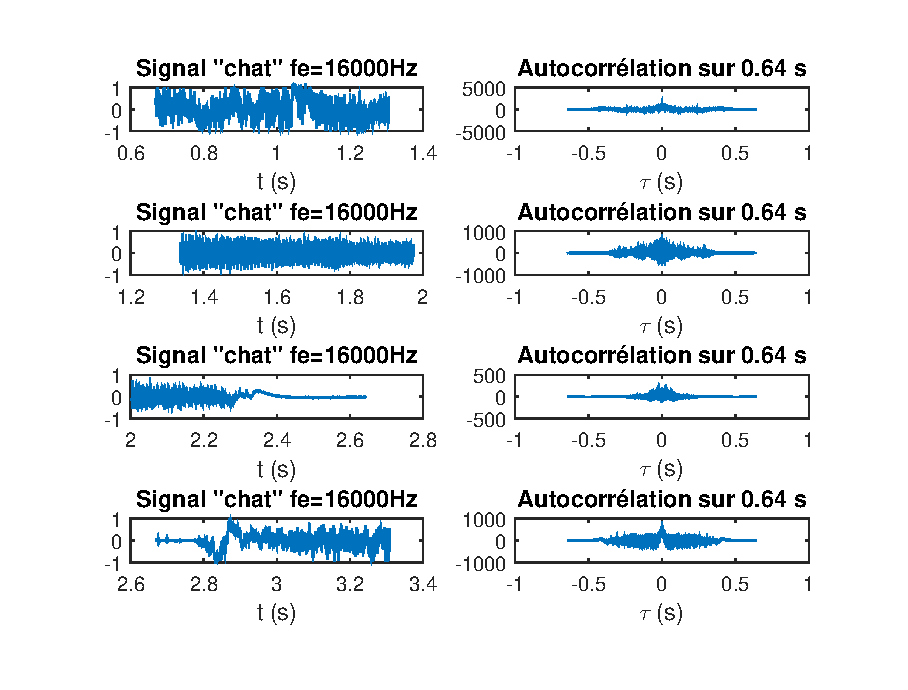
\includegraphics[height=0.45\textheight]{images/classificationVoix4.eps}
% Title: glps_renderer figure
% Creator: GL2PS 1.3.8, (C) 1999-2012 C. Geuzaine
% For: Octave
% CreationDate: Wed Nov  8 14:42:25 2017
\setlength{\unitlength}{1pt}
\begin{picture}(0,0)
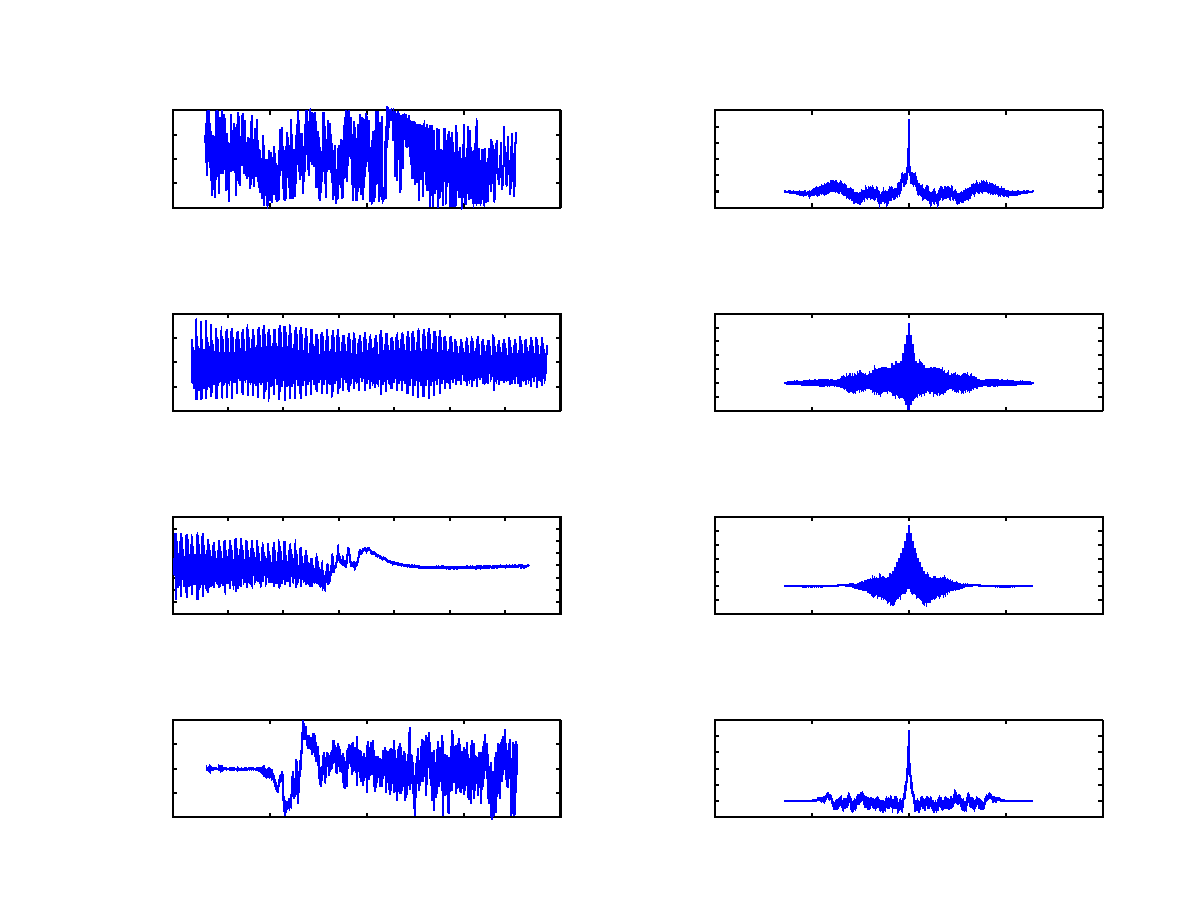
\includegraphics{images/classificationVoix4-inc.eps}
\end{picture}%
\begin{picture}(560,420)(0,0)
\fontsize{10}{0}
\selectfont\put(335.117,323.168){\makebox(0,0)[t]{\textcolor[rgb]{0,0,0}{{-1}}}}
\fontsize{10}{0}
\selectfont\put(381.658,323.168){\makebox(0,0)[t]{\textcolor[rgb]{0,0,0}{{-0.5}}}}
\fontsize{10}{0}
\selectfont\put(428.199,323.168){\makebox(0,0)[t]{\textcolor[rgb]{0,0,0}{{0}}}}
\fontsize{10}{0}
\selectfont\put(474.739,323.168){\makebox(0,0)[t]{\textcolor[rgb]{0,0,0}{{0.5}}}}
\fontsize{10}{0}
\selectfont\put(521.28,323.168){\makebox(0,0)[t]{\textcolor[rgb]{0,0,0}{{1}}}}
\fontsize{10}{0}
\selectfont\put(330.113,328.136){\makebox(0,0)[r]{\textcolor[rgb]{0,0,0}{{-500}}}}
\fontsize{10}{0}
\selectfont\put(330.113,335.92){\makebox(0,0)[r]{\textcolor[rgb]{0,0,0}{{0}}}}
\fontsize{10}{0}
\selectfont\put(330.113,343.703){\makebox(0,0)[r]{\textcolor[rgb]{0,0,0}{{500}}}}
\fontsize{10}{0}
\selectfont\put(330.113,351.487){\makebox(0,0)[r]{\textcolor[rgb]{0,0,0}{{1000}}}}
\fontsize{10}{0}
\selectfont\put(330.113,359.27){\makebox(0,0)[r]{\textcolor[rgb]{0,0,0}{{1500}}}}
\fontsize{10}{0}
\selectfont\put(330.113,367.054){\makebox(0,0)[r]{\textcolor[rgb]{0,0,0}{{2000}}}}
\fontsize{10}{0}
\selectfont\put(330.113,374.837){\makebox(0,0)[r]{\textcolor[rgb]{0,0,0}{{2500}}}}
\fontsize{10}{0}
\selectfont\put(428.199,312.168){\makebox(0,0)[t]{\textcolor[rgb]{0,0,0}{{$\tau$ (s)}}}}
\fontsize{10}{0}
\selectfont\put(74.88,323.168){\makebox(0,0)[t]{\textcolor[rgb]{0,0,0}{{0.6}}}}
\fontsize{10}{0}
\selectfont\put(121.421,323.168){\makebox(0,0)[t]{\textcolor[rgb]{0,0,0}{{0.8}}}}
\fontsize{10}{0}
\selectfont\put(167.961,323.168){\makebox(0,0)[t]{\textcolor[rgb]{0,0,0}{{1}}}}
\fontsize{10}{0}
\selectfont\put(214.502,323.168){\makebox(0,0)[t]{\textcolor[rgb]{0,0,0}{{1.2}}}}
\fontsize{10}{0}
\selectfont\put(261.043,323.168){\makebox(0,0)[t]{\textcolor[rgb]{0,0,0}{{1.4}}}}
\fontsize{10}{0}
\selectfont\put(69.8756,328.136){\makebox(0,0)[r]{\textcolor[rgb]{0,0,0}{{-1}}}}
\fontsize{10}{0}
\selectfont\put(69.8756,339.811){\makebox(0,0)[r]{\textcolor[rgb]{0,0,0}{{-0.5}}}}
\fontsize{10}{0}
\selectfont\put(69.8756,351.487){\makebox(0,0)[r]{\textcolor[rgb]{0,0,0}{{0}}}}
\fontsize{10}{0}
\selectfont\put(69.8756,363.162){\makebox(0,0)[r]{\textcolor[rgb]{0,0,0}{{0.5}}}}
\fontsize{10}{0}
\selectfont\put(69.8756,374.837){\makebox(0,0)[r]{\textcolor[rgb]{0,0,0}{{1}}}}
\fontsize{10}{0}
\selectfont\put(167.961,312.168){\makebox(0,0)[t]{\textcolor[rgb]{0,0,0}{{t (s)}}}}
\fontsize{10}{0}
\selectfont\put(335.117,225.629){\makebox(0,0)[t]{\textcolor[rgb]{0,0,0}{{-1}}}}
\fontsize{10}{0}
\selectfont\put(381.658,225.629){\makebox(0,0)[t]{\textcolor[rgb]{0,0,0}{{-0.5}}}}
\fontsize{10}{0}
\selectfont\put(428.199,225.629){\makebox(0,0)[t]{\textcolor[rgb]{0,0,0}{{0}}}}
\fontsize{10}{0}
\selectfont\put(474.739,225.629){\makebox(0,0)[t]{\textcolor[rgb]{0,0,0}{{0.5}}}}
\fontsize{10}{0}
\selectfont\put(521.28,225.629){\makebox(0,0)[t]{\textcolor[rgb]{0,0,0}{{1}}}}
\fontsize{10}{0}
\selectfont\put(330.113,230.597){\makebox(0,0)[r]{\textcolor[rgb]{0,0,0}{{-400}}}}
\fontsize{10}{0}
\selectfont\put(330.113,237.269){\makebox(0,0)[r]{\textcolor[rgb]{0,0,0}{{-200}}}}
\fontsize{10}{0}
\selectfont\put(330.113,243.941){\makebox(0,0)[r]{\textcolor[rgb]{0,0,0}{{0}}}}
\fontsize{10}{0}
\selectfont\put(330.113,250.612){\makebox(0,0)[r]{\textcolor[rgb]{0,0,0}{{200}}}}
\fontsize{10}{0}
\selectfont\put(330.113,257.284){\makebox(0,0)[r]{\textcolor[rgb]{0,0,0}{{400}}}}
\fontsize{10}{0}
\selectfont\put(330.113,263.955){\makebox(0,0)[r]{\textcolor[rgb]{0,0,0}{{600}}}}
\fontsize{10}{0}
\selectfont\put(330.113,270.627){\makebox(0,0)[r]{\textcolor[rgb]{0,0,0}{{800}}}}
\fontsize{10}{0}
\selectfont\put(330.113,277.299){\makebox(0,0)[r]{\textcolor[rgb]{0,0,0}{{1000}}}}
\fontsize{10}{0}
\selectfont\put(428.199,214.629){\makebox(0,0)[t]{\textcolor[rgb]{0,0,0}{{$\tau$ (s)}}}}
\fontsize{10}{0}
\selectfont\put(74.88,225.629){\makebox(0,0)[t]{\textcolor[rgb]{0,0,0}{{1.3}}}}
\fontsize{10}{0}
\selectfont\put(101.475,225.629){\makebox(0,0)[t]{\textcolor[rgb]{0,0,0}{{1.4}}}}
\fontsize{10}{0}
\selectfont\put(128.069,225.629){\makebox(0,0)[t]{\textcolor[rgb]{0,0,0}{{1.5}}}}
\fontsize{10}{0}
\selectfont\put(154.664,225.629){\makebox(0,0)[t]{\textcolor[rgb]{0,0,0}{{1.6}}}}
\fontsize{10}{0}
\selectfont\put(181.259,225.629){\makebox(0,0)[t]{\textcolor[rgb]{0,0,0}{{1.7}}}}
\fontsize{10}{0}
\selectfont\put(207.853,225.629){\makebox(0,0)[t]{\textcolor[rgb]{0,0,0}{{1.8}}}}
\fontsize{10}{0}
\selectfont\put(234.448,225.629){\makebox(0,0)[t]{\textcolor[rgb]{0,0,0}{{1.9}}}}
\fontsize{10}{0}
\selectfont\put(261.043,225.629){\makebox(0,0)[t]{\textcolor[rgb]{0,0,0}{{2}}}}
\fontsize{10}{0}
\selectfont\put(69.8756,230.597){\makebox(0,0)[r]{\textcolor[rgb]{0,0,0}{{-1}}}}
\fontsize{10}{0}
\selectfont\put(69.8756,242.273){\makebox(0,0)[r]{\textcolor[rgb]{0,0,0}{{-0.5}}}}
\fontsize{10}{0}
\selectfont\put(69.8756,253.948){\makebox(0,0)[r]{\textcolor[rgb]{0,0,0}{{0}}}}
\fontsize{10}{0}
\selectfont\put(69.8756,265.623){\makebox(0,0)[r]{\textcolor[rgb]{0,0,0}{{0.5}}}}
\fontsize{10}{0}
\selectfont\put(69.8756,277.299){\makebox(0,0)[r]{\textcolor[rgb]{0,0,0}{{1}}}}
\fontsize{10}{0}
\selectfont\put(167.961,214.629){\makebox(0,0)[t]{\textcolor[rgb]{0,0,0}{{t (s)}}}}
\fontsize{10}{0}
\selectfont\put(335.117,128.09){\makebox(0,0)[t]{\textcolor[rgb]{0,0,0}{{-1}}}}
\fontsize{10}{0}
\selectfont\put(381.658,128.09){\makebox(0,0)[t]{\textcolor[rgb]{0,0,0}{{-0.5}}}}
\fontsize{10}{0}
\selectfont\put(428.199,128.09){\makebox(0,0)[t]{\textcolor[rgb]{0,0,0}{{0}}}}
\fontsize{10}{0}
\selectfont\put(474.739,128.09){\makebox(0,0)[t]{\textcolor[rgb]{0,0,0}{{0.5}}}}
\fontsize{10}{0}
\selectfont\put(521.28,128.09){\makebox(0,0)[t]{\textcolor[rgb]{0,0,0}{{1}}}}
\fontsize{10}{0}
\selectfont\put(330.113,133.059){\makebox(0,0)[r]{\textcolor[rgb]{0,0,0}{{-100}}}}
\fontsize{10}{0}
\selectfont\put(330.113,139.73){\makebox(0,0)[r]{\textcolor[rgb]{0,0,0}{{-50}}}}
\fontsize{10}{0}
\selectfont\put(330.113,146.402){\makebox(0,0)[r]{\textcolor[rgb]{0,0,0}{{0}}}}
\fontsize{10}{0}
\selectfont\put(330.113,153.074){\makebox(0,0)[r]{\textcolor[rgb]{0,0,0}{{50}}}}
\fontsize{10}{0}
\selectfont\put(330.113,159.745){\makebox(0,0)[r]{\textcolor[rgb]{0,0,0}{{100}}}}
\fontsize{10}{0}
\selectfont\put(330.113,166.417){\makebox(0,0)[r]{\textcolor[rgb]{0,0,0}{{150}}}}
\fontsize{10}{0}
\selectfont\put(330.113,173.088){\makebox(0,0)[r]{\textcolor[rgb]{0,0,0}{{200}}}}
\fontsize{10}{0}
\selectfont\put(330.113,179.76){\makebox(0,0)[r]{\textcolor[rgb]{0,0,0}{{250}}}}
\fontsize{10}{0}
\selectfont\put(428.199,117.09){\makebox(0,0)[t]{\textcolor[rgb]{0,0,0}{{$\tau$ (s)}}}}
\fontsize{10}{0}
\selectfont\put(74.88,128.09){\makebox(0,0)[t]{\textcolor[rgb]{0,0,0}{{2}}}}
\fontsize{10}{0}
\selectfont\put(101.475,128.09){\makebox(0,0)[t]{\textcolor[rgb]{0,0,0}{{2.1}}}}
\fontsize{10}{0}
\selectfont\put(128.069,128.09){\makebox(0,0)[t]{\textcolor[rgb]{0,0,0}{{2.2}}}}
\fontsize{10}{0}
\selectfont\put(154.664,128.09){\makebox(0,0)[t]{\textcolor[rgb]{0,0,0}{{2.3}}}}
\fontsize{10}{0}
\selectfont\put(181.259,128.09){\makebox(0,0)[t]{\textcolor[rgb]{0,0,0}{{2.4}}}}
\fontsize{10}{0}
\selectfont\put(207.853,128.09){\makebox(0,0)[t]{\textcolor[rgb]{0,0,0}{{2.5}}}}
\fontsize{10}{0}
\selectfont\put(234.448,128.09){\makebox(0,0)[t]{\textcolor[rgb]{0,0,0}{{2.6}}}}
\fontsize{10}{0}
\selectfont\put(261.043,128.09){\makebox(0,0)[t]{\textcolor[rgb]{0,0,0}{{2.7}}}}
\fontsize{10}{0}
\selectfont\put(69.8756,133.059){\makebox(0,0)[r]{\textcolor[rgb]{0,0,0}{{-0.8}}}}
\fontsize{10}{0}
\selectfont\put(69.8756,138.896){\makebox(0,0)[r]{\textcolor[rgb]{0,0,0}{{-0.6}}}}
\fontsize{10}{0}
\selectfont\put(69.8756,144.734){\makebox(0,0)[r]{\textcolor[rgb]{0,0,0}{{-0.4}}}}
\fontsize{10}{0}
\selectfont\put(69.8756,150.572){\makebox(0,0)[r]{\textcolor[rgb]{0,0,0}{{-0.2}}}}
\fontsize{10}{0}
\selectfont\put(69.8756,156.409){\makebox(0,0)[r]{\textcolor[rgb]{0,0,0}{{0}}}}
\fontsize{10}{0}
\selectfont\put(69.8756,162.247){\makebox(0,0)[r]{\textcolor[rgb]{0,0,0}{{0.2}}}}
\fontsize{10}{0}
\selectfont\put(69.8756,168.085){\makebox(0,0)[r]{\textcolor[rgb]{0,0,0}{{0.4}}}}
\fontsize{10}{0}
\selectfont\put(69.8756,173.922){\makebox(0,0)[r]{\textcolor[rgb]{0,0,0}{{0.6}}}}
\fontsize{10}{0}
\selectfont\put(69.8756,179.76){\makebox(0,0)[r]{\textcolor[rgb]{0,0,0}{{0.8}}}}
\fontsize{10}{0}
\selectfont\put(167.961,117.09){\makebox(0,0)[t]{\textcolor[rgb]{0,0,0}{{t (s)}}}}
\fontsize{10}{0}
\selectfont\put(335.117,30.5517){\makebox(0,0)[t]{\textcolor[rgb]{0,0,0}{{-1}}}}
\fontsize{10}{0}
\selectfont\put(381.658,30.5517){\makebox(0,0)[t]{\textcolor[rgb]{0,0,0}{{-0.5}}}}
\fontsize{10}{0}
\selectfont\put(428.199,30.5517){\makebox(0,0)[t]{\textcolor[rgb]{0,0,0}{{0}}}}
\fontsize{10}{0}
\selectfont\put(474.739,30.5517){\makebox(0,0)[t]{\textcolor[rgb]{0,0,0}{{0.5}}}}
\fontsize{10}{0}
\selectfont\put(521.28,30.5517){\makebox(0,0)[t]{\textcolor[rgb]{0,0,0}{{1}}}}
\fontsize{10}{0}
\selectfont\put(330.113,35.52){\makebox(0,0)[r]{\textcolor[rgb]{0,0,0}{{-200}}}}
\fontsize{10}{0}
\selectfont\put(330.113,43.3035){\makebox(0,0)[r]{\textcolor[rgb]{0,0,0}{{0}}}}
\fontsize{10}{0}
\selectfont\put(330.113,51.0871){\makebox(0,0)[r]{\textcolor[rgb]{0,0,0}{{200}}}}
\fontsize{10}{0}
\selectfont\put(330.113,58.8706){\makebox(0,0)[r]{\textcolor[rgb]{0,0,0}{{400}}}}
\fontsize{10}{0}
\selectfont\put(330.113,66.6542){\makebox(0,0)[r]{\textcolor[rgb]{0,0,0}{{600}}}}
\fontsize{10}{0}
\selectfont\put(330.113,74.4377){\makebox(0,0)[r]{\textcolor[rgb]{0,0,0}{{800}}}}
\fontsize{10}{0}
\selectfont\put(330.113,82.2213){\makebox(0,0)[r]{\textcolor[rgb]{0,0,0}{{1000}}}}
\fontsize{10}{0}
\selectfont\put(428.199,19.5517){\makebox(0,0)[t]{\textcolor[rgb]{0,0,0}{{$\tau$ (s)}}}}
\fontsize{10}{0}
\selectfont\put(74.88,30.5517){\makebox(0,0)[t]{\textcolor[rgb]{0,0,0}{{2.6}}}}
\fontsize{10}{0}
\selectfont\put(121.421,30.5517){\makebox(0,0)[t]{\textcolor[rgb]{0,0,0}{{2.8}}}}
\fontsize{10}{0}
\selectfont\put(167.961,30.5517){\makebox(0,0)[t]{\textcolor[rgb]{0,0,0}{{3}}}}
\fontsize{10}{0}
\selectfont\put(214.502,30.5517){\makebox(0,0)[t]{\textcolor[rgb]{0,0,0}{{3.2}}}}
\fontsize{10}{0}
\selectfont\put(261.043,30.5517){\makebox(0,0)[t]{\textcolor[rgb]{0,0,0}{{3.4}}}}
\fontsize{10}{0}
\selectfont\put(69.8756,35.52){\makebox(0,0)[r]{\textcolor[rgb]{0,0,0}{{-1}}}}
\fontsize{10}{0}
\selectfont\put(69.8756,47.1953){\makebox(0,0)[r]{\textcolor[rgb]{0,0,0}{{-0.5}}}}
\fontsize{10}{0}
\selectfont\put(69.8756,58.8706){\makebox(0,0)[r]{\textcolor[rgb]{0,0,0}{{0}}}}
\fontsize{10}{0}
\selectfont\put(69.8756,70.5459){\makebox(0,0)[r]{\textcolor[rgb]{0,0,0}{{0.5}}}}
\fontsize{10}{0}
\selectfont\put(69.8756,82.2213){\makebox(0,0)[r]{\textcolor[rgb]{0,0,0}{{1}}}}
\fontsize{10}{0}
\selectfont\put(167.961,19.5517){\makebox(0,0)[t]{\textcolor[rgb]{0,0,0}{{t (s)}}}}
\fontsize{10}{0}
\selectfont\put(428.199,384.837){\makebox(0,0)[b]{\textcolor[rgb]{0,0,0}{{Autocorrélation sur 0.64 s}}}}
\fontsize{10}{0}
\selectfont\put(167.961,384.837){\makebox(0,0)[b]{\textcolor[rgb]{0,0,0}{{Signal "chat" fe=16000Hz}}}}
\fontsize{10}{0}
\selectfont\put(428.199,287.299){\makebox(0,0)[b]{\textcolor[rgb]{0,0,0}{{Autocorrélation sur 0.64 s}}}}
\fontsize{10}{0}
\selectfont\put(167.961,287.299){\makebox(0,0)[b]{\textcolor[rgb]{0,0,0}{{Signal "chat" fe=16000Hz}}}}
\fontsize{10}{0}
\selectfont\put(428.199,189.76){\makebox(0,0)[b]{\textcolor[rgb]{0,0,0}{{Autocorrélation sur 0.64 s}}}}
\fontsize{10}{0}
\selectfont\put(167.961,189.76){\makebox(0,0)[b]{\textcolor[rgb]{0,0,0}{{Signal "chat" fe=16000Hz}}}}
\fontsize{10}{0}
\selectfont\put(428.199,92.2213){\makebox(0,0)[b]{\textcolor[rgb]{0,0,0}{{Autocorrélation sur 0.64 s}}}}
\fontsize{10}{0}
\selectfont\put(167.961,92.2213){\makebox(0,0)[b]{\textcolor[rgb]{0,0,0}{{Signal "chat" fe=16000Hz}}}}
\end{picture}

\caption{Autocorrélation de divers échantillons du signal vocal.}
\label{classif4}
\end{figure}

La figure \ref{classif4} montre que des échantillons de durée 0.64 secondes sont trop longs. En effet, on se rapproche alors de la période de variation du signal liée au sens de la parole (visible sur l'échantillon pris entre 2 et 2.8 secondes par exemple).


Finalement,  on choisit une durée d'échantillon de 0.16 secondes (figure \ref{classif3}), car bien que celle de 0.06 convienne également pour différencier le signal voisé du non voisé, l'autocorrélation sur une plus grande période fait apparaître plus de maximums locaux, ce qui permet d'estimmer plus précisément la fréquence fondamentale du signal voisé. On trouve ainsi une fréquence du fondamental de 100 Hz environ.

\begin{figure}[h!]
	\centering
	%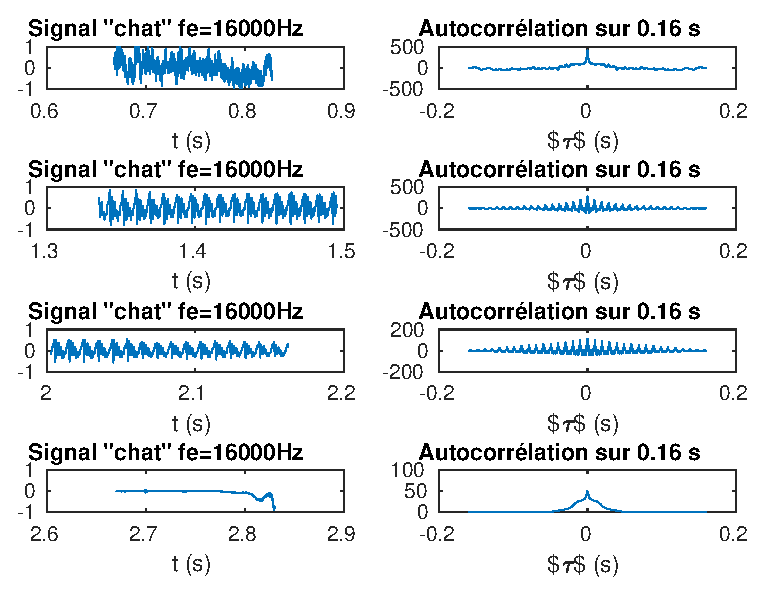
\includegraphics[width=\textwidth]{images/classificationVoix3.eps}
	% Title: glps_renderer figure
% Creator: GL2PS 1.3.8, (C) 1999-2012 C. Geuzaine
% For: Octave
% CreationDate: Wed Nov  8 12:20:40 2017
\setlength{\unitlength}{1pt}
\begin{picture}(0,0)
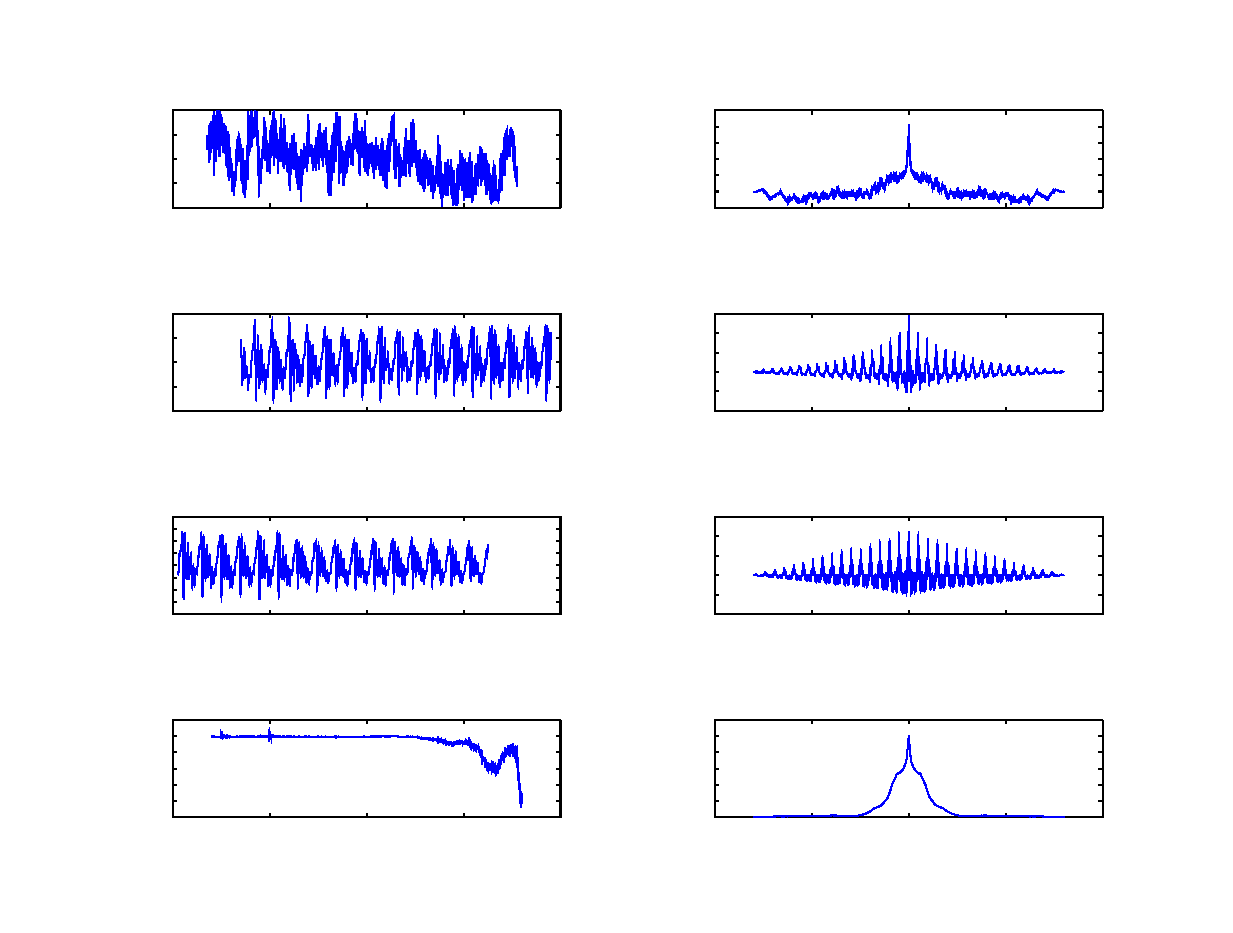
\includegraphics{images/classificationVoix3-inc.eps}
\end{picture}%
\begin{picture}(576,432)(0,0)
\fontsize{10}{0}
\selectfont\put(335.117,335.168){\makebox(0,0)[t]{\textcolor[rgb]{0,0,0}{{-0.2}}}}
\fontsize{10}{0}
\selectfont\put(381.658,335.168){\makebox(0,0)[t]{\textcolor[rgb]{0,0,0}{{-0.1}}}}
\fontsize{10}{0}
\selectfont\put(428.199,335.168){\makebox(0,0)[t]{\textcolor[rgb]{0,0,0}{{0}}}}
\fontsize{10}{0}
\selectfont\put(474.739,335.168){\makebox(0,0)[t]{\textcolor[rgb]{0,0,0}{{0.1}}}}
\fontsize{10}{0}
\selectfont\put(521.28,335.168){\makebox(0,0)[t]{\textcolor[rgb]{0,0,0}{{0.2}}}}
\fontsize{10}{0}
\selectfont\put(330.113,340.136){\makebox(0,0)[r]{\textcolor[rgb]{0,0,0}{{-100}}}}
\fontsize{10}{0}
\selectfont\put(330.113,347.92){\makebox(0,0)[r]{\textcolor[rgb]{0,0,0}{{0}}}}
\fontsize{10}{0}
\selectfont\put(330.113,355.703){\makebox(0,0)[r]{\textcolor[rgb]{0,0,0}{{100}}}}
\fontsize{10}{0}
\selectfont\put(330.113,363.487){\makebox(0,0)[r]{\textcolor[rgb]{0,0,0}{{200}}}}
\fontsize{10}{0}
\selectfont\put(330.113,371.27){\makebox(0,0)[r]{\textcolor[rgb]{0,0,0}{{300}}}}
\fontsize{10}{0}
\selectfont\put(330.113,379.054){\makebox(0,0)[r]{\textcolor[rgb]{0,0,0}{{400}}}}
\fontsize{10}{0}
\selectfont\put(330.113,386.837){\makebox(0,0)[r]{\textcolor[rgb]{0,0,0}{{500}}}}
\fontsize{10}{0}
\selectfont\put(428.199,324.168){\makebox(0,0)[t]{\textcolor[rgb]{0,0,0}{{$\tau$ (s)}}}}
\fontsize{10}{0}
\selectfont\put(74.88,335.168){\makebox(0,0)[t]{\textcolor[rgb]{0,0,0}{{0.65}}}}
\fontsize{10}{0}
\selectfont\put(121.421,335.168){\makebox(0,0)[t]{\textcolor[rgb]{0,0,0}{{0.7}}}}
\fontsize{10}{0}
\selectfont\put(167.961,335.168){\makebox(0,0)[t]{\textcolor[rgb]{0,0,0}{{0.75}}}}
\fontsize{10}{0}
\selectfont\put(214.502,335.168){\makebox(0,0)[t]{\textcolor[rgb]{0,0,0}{{0.8}}}}
\fontsize{10}{0}
\selectfont\put(261.043,335.168){\makebox(0,0)[t]{\textcolor[rgb]{0,0,0}{{0.85}}}}
\fontsize{10}{0}
\selectfont\put(69.8756,340.136){\makebox(0,0)[r]{\textcolor[rgb]{0,0,0}{{-1}}}}
\fontsize{10}{0}
\selectfont\put(69.8756,351.811){\makebox(0,0)[r]{\textcolor[rgb]{0,0,0}{{-0.5}}}}
\fontsize{10}{0}
\selectfont\put(69.8756,363.487){\makebox(0,0)[r]{\textcolor[rgb]{0,0,0}{{0}}}}
\fontsize{10}{0}
\selectfont\put(69.8756,375.162){\makebox(0,0)[r]{\textcolor[rgb]{0,0,0}{{0.5}}}}
\fontsize{10}{0}
\selectfont\put(69.8756,386.837){\makebox(0,0)[r]{\textcolor[rgb]{0,0,0}{{1}}}}
\fontsize{10}{0}
\selectfont\put(167.961,324.168){\makebox(0,0)[t]{\textcolor[rgb]{0,0,0}{{t (s)}}}}
\fontsize{10}{0}
\selectfont\put(335.117,237.629){\makebox(0,0)[t]{\textcolor[rgb]{0,0,0}{{-0.2}}}}
\fontsize{10}{0}
\selectfont\put(381.658,237.629){\makebox(0,0)[t]{\textcolor[rgb]{0,0,0}{{-0.1}}}}
\fontsize{10}{0}
\selectfont\put(428.199,237.629){\makebox(0,0)[t]{\textcolor[rgb]{0,0,0}{{0}}}}
\fontsize{10}{0}
\selectfont\put(474.739,237.629){\makebox(0,0)[t]{\textcolor[rgb]{0,0,0}{{0.1}}}}
\fontsize{10}{0}
\selectfont\put(521.28,237.629){\makebox(0,0)[t]{\textcolor[rgb]{0,0,0}{{0.2}}}}
\fontsize{10}{0}
\selectfont\put(330.113,242.597){\makebox(0,0)[r]{\textcolor[rgb]{0,0,0}{{-200}}}}
\fontsize{10}{0}
\selectfont\put(330.113,251.938){\makebox(0,0)[r]{\textcolor[rgb]{0,0,0}{{-100}}}}
\fontsize{10}{0}
\selectfont\put(330.113,261.278){\makebox(0,0)[r]{\textcolor[rgb]{0,0,0}{{0}}}}
\fontsize{10}{0}
\selectfont\put(330.113,270.618){\makebox(0,0)[r]{\textcolor[rgb]{0,0,0}{{100}}}}
\fontsize{10}{0}
\selectfont\put(330.113,279.958){\makebox(0,0)[r]{\textcolor[rgb]{0,0,0}{{200}}}}
\fontsize{10}{0}
\selectfont\put(330.113,289.299){\makebox(0,0)[r]{\textcolor[rgb]{0,0,0}{{300}}}}
\fontsize{10}{0}
\selectfont\put(428.199,226.629){\makebox(0,0)[t]{\textcolor[rgb]{0,0,0}{{$\tau$ (s)}}}}
\fontsize{10}{0}
\selectfont\put(74.88,237.629){\makebox(0,0)[t]{\textcolor[rgb]{0,0,0}{{1.3}}}}
\fontsize{10}{0}
\selectfont\put(121.421,237.629){\makebox(0,0)[t]{\textcolor[rgb]{0,0,0}{{1.35}}}}
\fontsize{10}{0}
\selectfont\put(167.961,237.629){\makebox(0,0)[t]{\textcolor[rgb]{0,0,0}{{1.4}}}}
\fontsize{10}{0}
\selectfont\put(214.502,237.629){\makebox(0,0)[t]{\textcolor[rgb]{0,0,0}{{1.45}}}}
\fontsize{10}{0}
\selectfont\put(261.043,237.629){\makebox(0,0)[t]{\textcolor[rgb]{0,0,0}{{1.5}}}}
\fontsize{10}{0}
\selectfont\put(69.8755,242.597){\makebox(0,0)[r]{\textcolor[rgb]{0,0,0}{{-1}}}}
\fontsize{10}{0}
\selectfont\put(69.8755,254.273){\makebox(0,0)[r]{\textcolor[rgb]{0,0,0}{{-0.5}}}}
\fontsize{10}{0}
\selectfont\put(69.8755,265.948){\makebox(0,0)[r]{\textcolor[rgb]{0,0,0}{{0}}}}
\fontsize{10}{0}
\selectfont\put(69.8755,277.623){\makebox(0,0)[r]{\textcolor[rgb]{0,0,0}{{0.5}}}}
\fontsize{10}{0}
\selectfont\put(69.8755,289.299){\makebox(0,0)[r]{\textcolor[rgb]{0,0,0}{{1}}}}
\fontsize{10}{0}
\selectfont\put(167.961,226.629){\makebox(0,0)[t]{\textcolor[rgb]{0,0,0}{{t (s)}}}}
\fontsize{10}{0}
\selectfont\put(335.117,140.09){\makebox(0,0)[t]{\textcolor[rgb]{0,0,0}{{-0.2}}}}
\fontsize{10}{0}
\selectfont\put(381.658,140.09){\makebox(0,0)[t]{\textcolor[rgb]{0,0,0}{{-0.1}}}}
\fontsize{10}{0}
\selectfont\put(428.199,140.09){\makebox(0,0)[t]{\textcolor[rgb]{0,0,0}{{0}}}}
\fontsize{10}{0}
\selectfont\put(474.739,140.09){\makebox(0,0)[t]{\textcolor[rgb]{0,0,0}{{0.1}}}}
\fontsize{10}{0}
\selectfont\put(521.28,140.09){\makebox(0,0)[t]{\textcolor[rgb]{0,0,0}{{0.2}}}}
\fontsize{10}{0}
\selectfont\put(330.113,145.059){\makebox(0,0)[r]{\textcolor[rgb]{0,0,0}{{-100}}}}
\fontsize{10}{0}
\selectfont\put(330.113,154.399){\makebox(0,0)[r]{\textcolor[rgb]{0,0,0}{{-50}}}}
\fontsize{10}{0}
\selectfont\put(330.113,163.739){\makebox(0,0)[r]{\textcolor[rgb]{0,0,0}{{0}}}}
\fontsize{10}{0}
\selectfont\put(330.113,173.079){\makebox(0,0)[r]{\textcolor[rgb]{0,0,0}{{50}}}}
\fontsize{10}{0}
\selectfont\put(330.113,182.42){\makebox(0,0)[r]{\textcolor[rgb]{0,0,0}{{100}}}}
\fontsize{10}{0}
\selectfont\put(330.113,191.76){\makebox(0,0)[r]{\textcolor[rgb]{0,0,0}{{150}}}}
\fontsize{10}{0}
\selectfont\put(428.199,129.09){\makebox(0,0)[t]{\textcolor[rgb]{0,0,0}{{$\tau$ (s)}}}}
\fontsize{10}{0}
\selectfont\put(74.88,140.09){\makebox(0,0)[t]{\textcolor[rgb]{0,0,0}{{2}}}}
\fontsize{10}{0}
\selectfont\put(121.421,140.09){\makebox(0,0)[t]{\textcolor[rgb]{0,0,0}{{2.05}}}}
\fontsize{10}{0}
\selectfont\put(167.961,140.09){\makebox(0,0)[t]{\textcolor[rgb]{0,0,0}{{2.1}}}}
\fontsize{10}{0}
\selectfont\put(214.502,140.09){\makebox(0,0)[t]{\textcolor[rgb]{0,0,0}{{2.15}}}}
\fontsize{10}{0}
\selectfont\put(261.043,140.09){\makebox(0,0)[t]{\textcolor[rgb]{0,0,0}{{2.2}}}}
\fontsize{10}{0}
\selectfont\put(69.8755,145.059){\makebox(0,0)[r]{\textcolor[rgb]{0,0,0}{{-0.8}}}}
\fontsize{10}{0}
\selectfont\put(69.8755,150.896){\makebox(0,0)[r]{\textcolor[rgb]{0,0,0}{{-0.6}}}}
\fontsize{10}{0}
\selectfont\put(69.8755,156.734){\makebox(0,0)[r]{\textcolor[rgb]{0,0,0}{{-0.4}}}}
\fontsize{10}{0}
\selectfont\put(69.8755,162.572){\makebox(0,0)[r]{\textcolor[rgb]{0,0,0}{{-0.2}}}}
\fontsize{10}{0}
\selectfont\put(69.8755,168.409){\makebox(0,0)[r]{\textcolor[rgb]{0,0,0}{{0}}}}
\fontsize{10}{0}
\selectfont\put(69.8755,174.247){\makebox(0,0)[r]{\textcolor[rgb]{0,0,0}{{0.2}}}}
\fontsize{10}{0}
\selectfont\put(69.8755,180.085){\makebox(0,0)[r]{\textcolor[rgb]{0,0,0}{{0.4}}}}
\fontsize{10}{0}
\selectfont\put(69.8755,185.922){\makebox(0,0)[r]{\textcolor[rgb]{0,0,0}{{0.6}}}}
\fontsize{10}{0}
\selectfont\put(69.8755,191.76){\makebox(0,0)[r]{\textcolor[rgb]{0,0,0}{{0.8}}}}
\fontsize{10}{0}
\selectfont\put(167.961,129.09){\makebox(0,0)[t]{\textcolor[rgb]{0,0,0}{{t (s)}}}}
\fontsize{10}{0}
\selectfont\put(335.117,42.5517){\makebox(0,0)[t]{\textcolor[rgb]{0,0,0}{{-0.2}}}}
\fontsize{10}{0}
\selectfont\put(381.658,42.5517){\makebox(0,0)[t]{\textcolor[rgb]{0,0,0}{{-0.1}}}}
\fontsize{10}{0}
\selectfont\put(428.199,42.5517){\makebox(0,0)[t]{\textcolor[rgb]{0,0,0}{{0}}}}
\fontsize{10}{0}
\selectfont\put(474.739,42.5517){\makebox(0,0)[t]{\textcolor[rgb]{0,0,0}{{0.1}}}}
\fontsize{10}{0}
\selectfont\put(521.28,42.5517){\makebox(0,0)[t]{\textcolor[rgb]{0,0,0}{{0.2}}}}
\fontsize{10}{0}
\selectfont\put(330.113,47.52){\makebox(0,0)[r]{\textcolor[rgb]{0,0,0}{{0}}}}
\fontsize{10}{0}
\selectfont\put(330.113,55.3035){\makebox(0,0)[r]{\textcolor[rgb]{0,0,0}{{10}}}}
\fontsize{10}{0}
\selectfont\put(330.113,63.0871){\makebox(0,0)[r]{\textcolor[rgb]{0,0,0}{{20}}}}
\fontsize{10}{0}
\selectfont\put(330.113,70.8706){\makebox(0,0)[r]{\textcolor[rgb]{0,0,0}{{30}}}}
\fontsize{10}{0}
\selectfont\put(330.113,78.6542){\makebox(0,0)[r]{\textcolor[rgb]{0,0,0}{{40}}}}
\fontsize{10}{0}
\selectfont\put(330.113,86.4377){\makebox(0,0)[r]{\textcolor[rgb]{0,0,0}{{50}}}}
\fontsize{10}{0}
\selectfont\put(330.113,94.2213){\makebox(0,0)[r]{\textcolor[rgb]{0,0,0}{{60}}}}
\fontsize{10}{0}
\selectfont\put(428.199,31.5518){\makebox(0,0)[t]{\textcolor[rgb]{0,0,0}{{$\tau$ (s)}}}}
\fontsize{10}{0}
\selectfont\put(74.88,42.5517){\makebox(0,0)[t]{\textcolor[rgb]{0,0,0}{{2.65}}}}
\fontsize{10}{0}
\selectfont\put(121.421,42.5517){\makebox(0,0)[t]{\textcolor[rgb]{0,0,0}{{2.7}}}}
\fontsize{10}{0}
\selectfont\put(167.961,42.5517){\makebox(0,0)[t]{\textcolor[rgb]{0,0,0}{{2.75}}}}
\fontsize{10}{0}
\selectfont\put(214.502,42.5517){\makebox(0,0)[t]{\textcolor[rgb]{0,0,0}{{2.8}}}}
\fontsize{10}{0}
\selectfont\put(261.043,42.5517){\makebox(0,0)[t]{\textcolor[rgb]{0,0,0}{{2.85}}}}
\fontsize{10}{0}
\selectfont\put(69.8757,47.52){\makebox(0,0)[r]{\textcolor[rgb]{0,0,0}{{-1}}}}
\fontsize{10}{0}
\selectfont\put(69.8757,55.3035){\makebox(0,0)[r]{\textcolor[rgb]{0,0,0}{{-0.8}}}}
\fontsize{10}{0}
\selectfont\put(69.8757,63.0871){\makebox(0,0)[r]{\textcolor[rgb]{0,0,0}{{-0.6}}}}
\fontsize{10}{0}
\selectfont\put(69.8757,70.8706){\makebox(0,0)[r]{\textcolor[rgb]{0,0,0}{{-0.4}}}}
\fontsize{10}{0}
\selectfont\put(69.8757,78.6542){\makebox(0,0)[r]{\textcolor[rgb]{0,0,0}{{-0.2}}}}
\fontsize{10}{0}
\selectfont\put(69.8757,86.4377){\makebox(0,0)[r]{\textcolor[rgb]{0,0,0}{{0}}}}
\fontsize{10}{0}
\selectfont\put(69.8757,94.2213){\makebox(0,0)[r]{\textcolor[rgb]{0,0,0}{{0.2}}}}
\fontsize{10}{0}
\selectfont\put(167.961,31.5518){\makebox(0,0)[t]{\textcolor[rgb]{0,0,0}{{t (s)}}}}
\fontsize{10}{0}
\selectfont\put(428.199,396.837){\makebox(0,0)[b]{\textcolor[rgb]{0,0,0}{{Autocorrélation sur 0.16 s}}}}
\fontsize{10}{0}
\selectfont\put(167.961,396.837){\makebox(0,0)[b]{\textcolor[rgb]{0,0,0}{{Signal "chat" fe=16000Hz}}}}
\fontsize{10}{0}
\selectfont\put(428.199,299.299){\makebox(0,0)[b]{\textcolor[rgb]{0,0,0}{{Autocorrélation sur 0.16 s}}}}
\fontsize{10}{0}
\selectfont\put(167.961,299.299){\makebox(0,0)[b]{\textcolor[rgb]{0,0,0}{{Signal "chat" fe=16000Hz}}}}
\fontsize{10}{0}
\selectfont\put(428.199,201.76){\makebox(0,0)[b]{\textcolor[rgb]{0,0,0}{{Autocorrélation sur 0.16 s}}}}
\fontsize{10}{0}
\selectfont\put(167.961,201.76){\makebox(0,0)[b]{\textcolor[rgb]{0,0,0}{{Signal "chat" fe=16000Hz}}}}
\fontsize{10}{0}
\selectfont\put(428.199,104.221){\makebox(0,0)[b]{\textcolor[rgb]{0,0,0}{{Autocorrélation sur 0.16 s}}}}
\fontsize{10}{0}
\selectfont\put(167.961,104.221){\makebox(0,0)[b]{\textcolor[rgb]{0,0,0}{{Signal "chat" fe=16000Hz}}}}
\end{picture}

	\caption{Autocorrélation de divers échantillons du signal vocal.}
	\label{classif3}
\end{figure}

\FloatBarrier
\newpage

\part{Aspects fréquentiels}

\section{Échantillonnage}
On réalise l'échantillonage d'un même signal de fréquence $f=500 \; Hz$ échantillonné à plusieurs fréquences différentes, le résultat obtenu est représenté dans les figures \ref{fig:echantillon1}, \ref{fig:echantillon2} et \ref{fig:echantillon3}.

\begin{figure}[h!]
	\centering
	\begin{minipage}{0.45\textwidth}
	\centering
	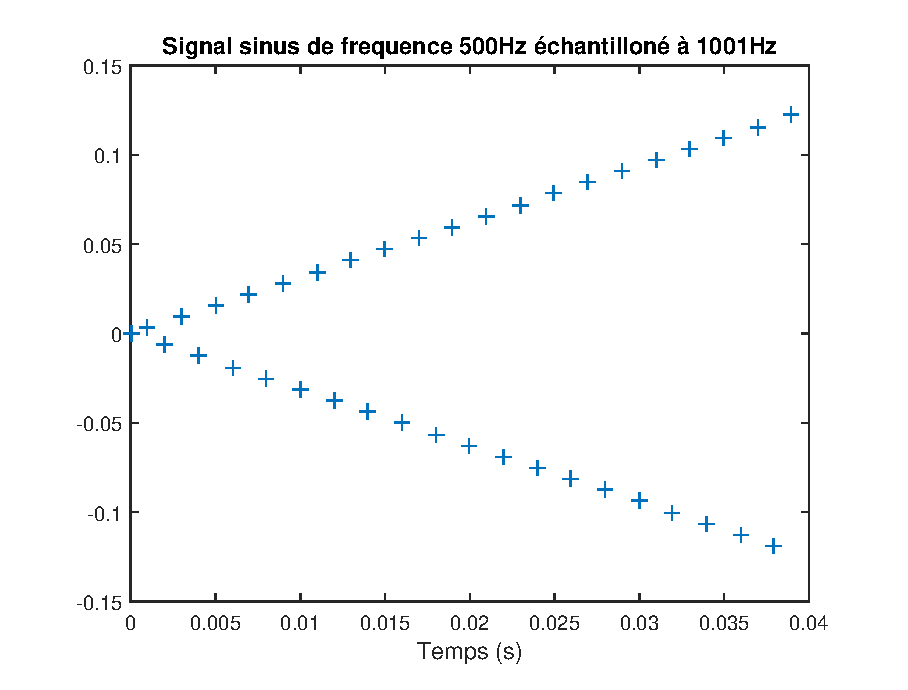
\includegraphics[width=\textwidth]{images/echantillone_1.eps}
	\caption{Signal échantilloné à $2f+1$.}
	\label{fig:echantillon1}

	\end{minipage}
	\begin{minipage}{0.45\textwidth}
	\centering
	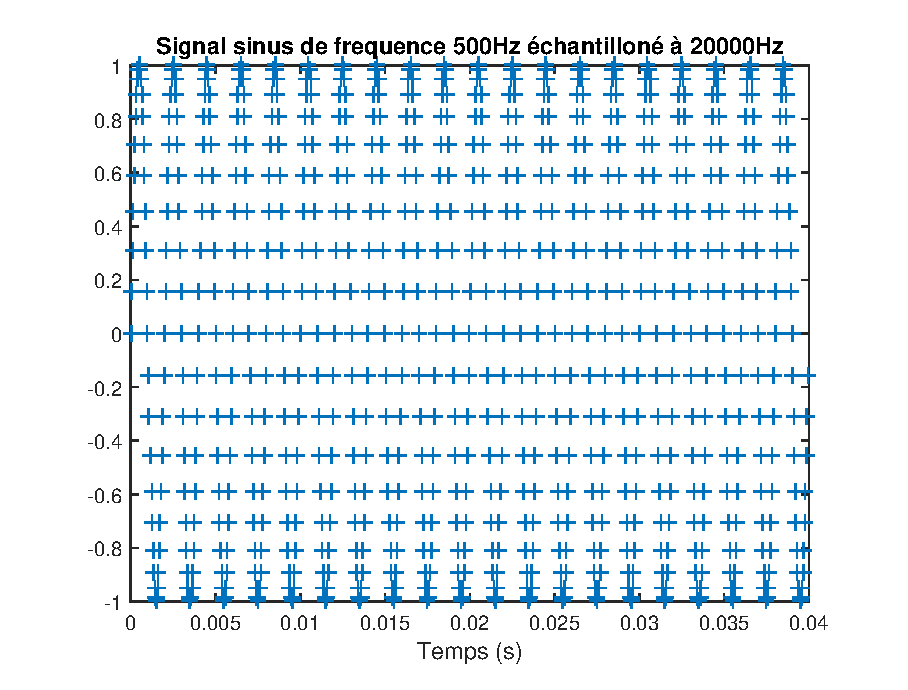
\includegraphics[width=\textwidth]{images/echantillone_2.eps}
	\caption{Signal échantilloné à $40f$.}
	\label{fig:echantillon2}
	\end{minipage}
	\begin{minipage}{0.5\textwidth}
	\centering
	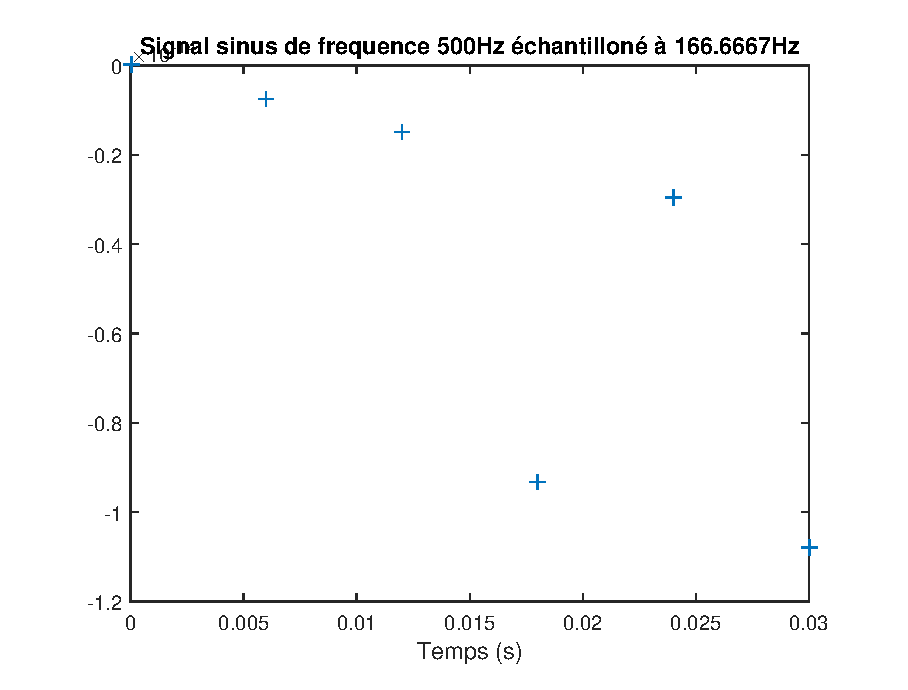
\includegraphics[width=\textwidth]{images/echantillone_3.eps}
	\caption{Signal échantilloné à $\frac{1}{2}f$.}
	\label{fig:echantillon3}
	\end{minipage}
\end{figure}

\FloatBarrier
\section{La Transformée de Fourier discrète (TFD)}

\subsection{Densité spectrale d'énergie}
On trace la densité spectrale d'énergie d'un signal voisé (figure \ref{fig:dse_vois}) et d'un signal non-voisé (figure \ref{fig:dse_nonvois}). On remarque que le signal non voisé ("ch") comporte de l'énergie dans toutes les fréquences de manière identique, tandis que le signal voisé ("a") présente de l'énergie principalement sur certaines fréquences. En effet, la figure \ref{fig:dse_vois} présente des pics d'énergie espacés régulièrement, particulièrement visibles entre 0 et 1000 Hz. On remarque que ces pics sont espacés de 100Hz : on a un résultat cohérent avec ce qui est obtenu par la méthode temporelle.

\begin{figure}[h!]
	\centering
	\begin{minipage}{0.45\textwidth}
	\centering
	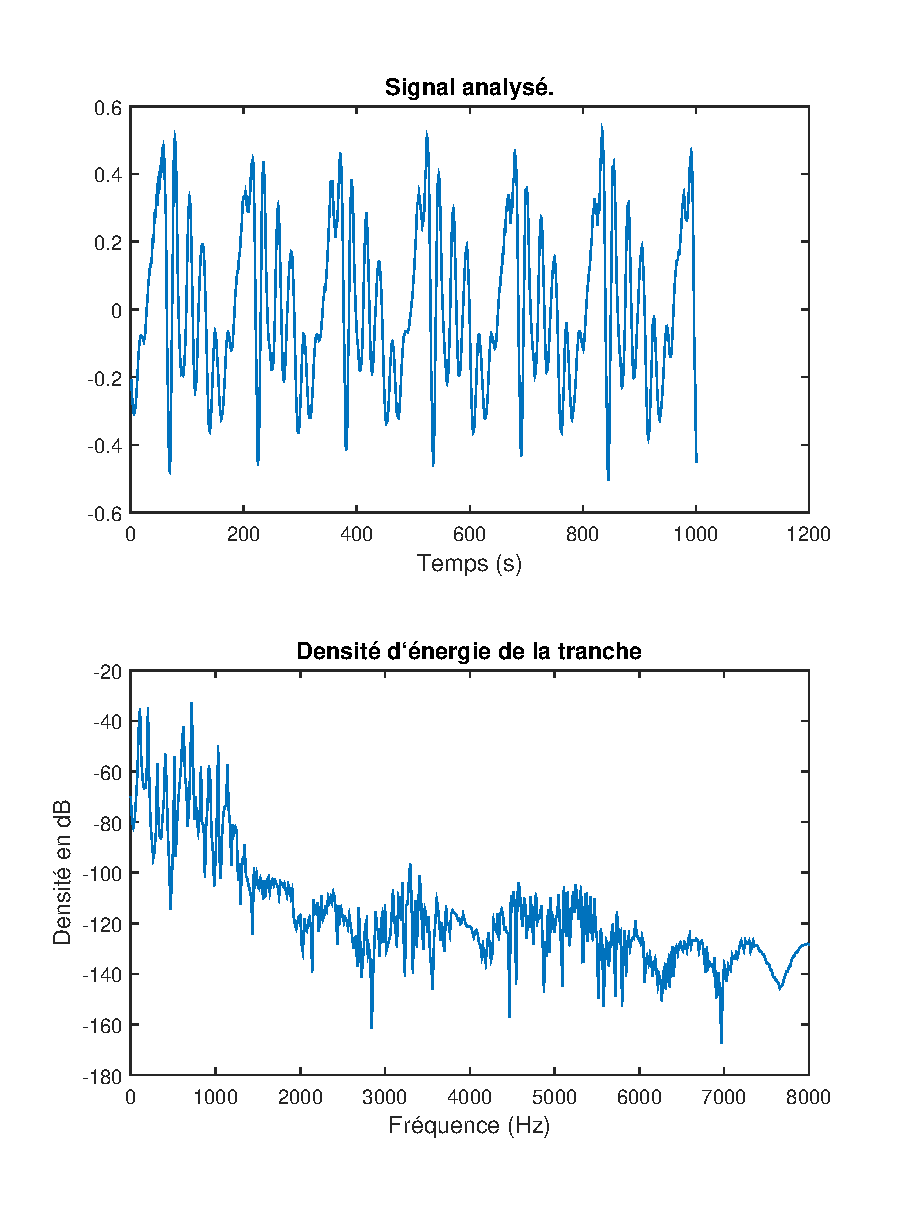
\includegraphics[width=\textwidth]{images/tfd_voise.eps}
	\caption{Signal voisé et \bsc{dse}}
	\label{fig:dse_vois}
	\end{minipage}
	\begin{minipage}{0.45\textwidth}
	\centering
	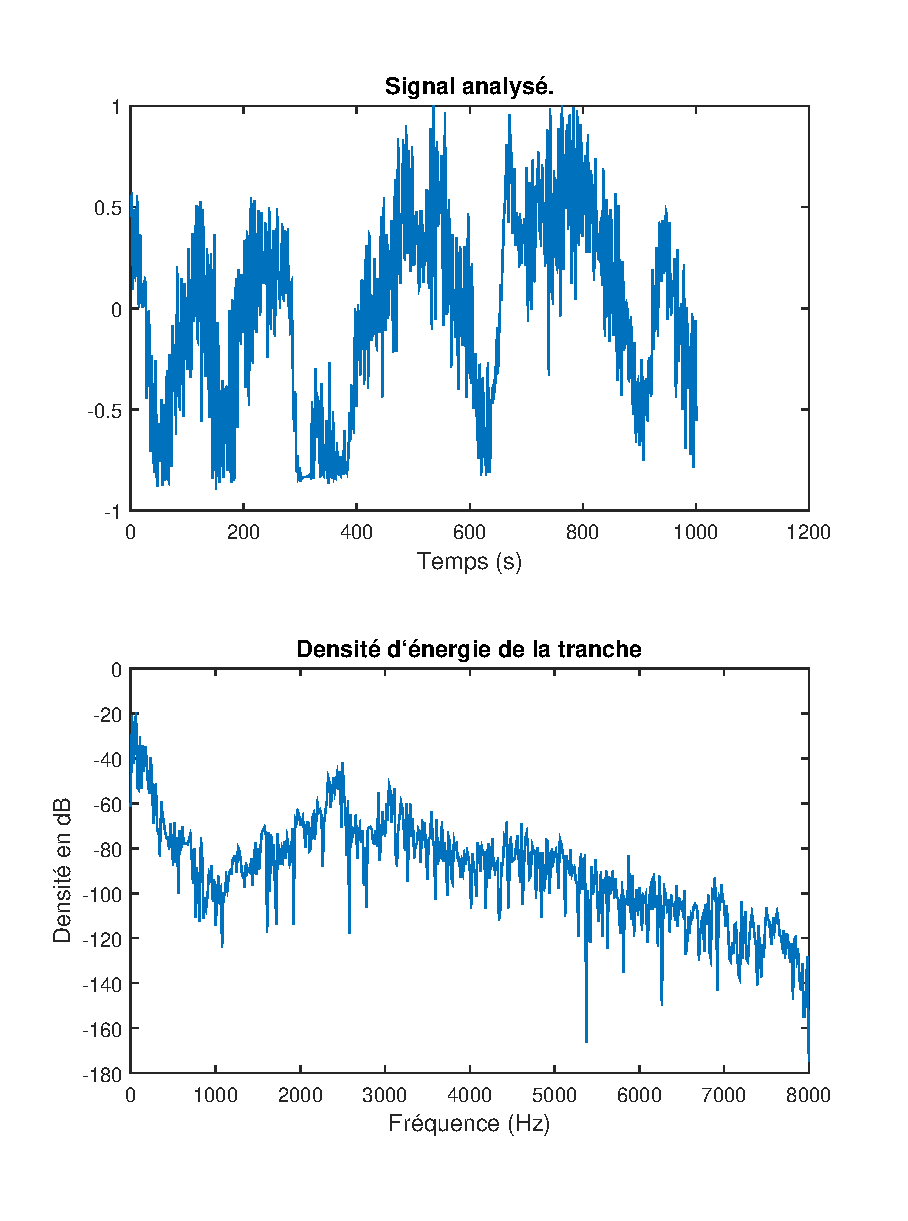
\includegraphics[width=\textwidth]{images/tfd_nonvoise.eps}
	\caption{Signal non-voisé et \bsc{dse}}
	\label{fig:dse_nonvois}
	\end{minipage}
\end{figure}



\FloatBarrier
\subsection{Zéro-padding}
\begin{figure}[h!]
	\centering
	%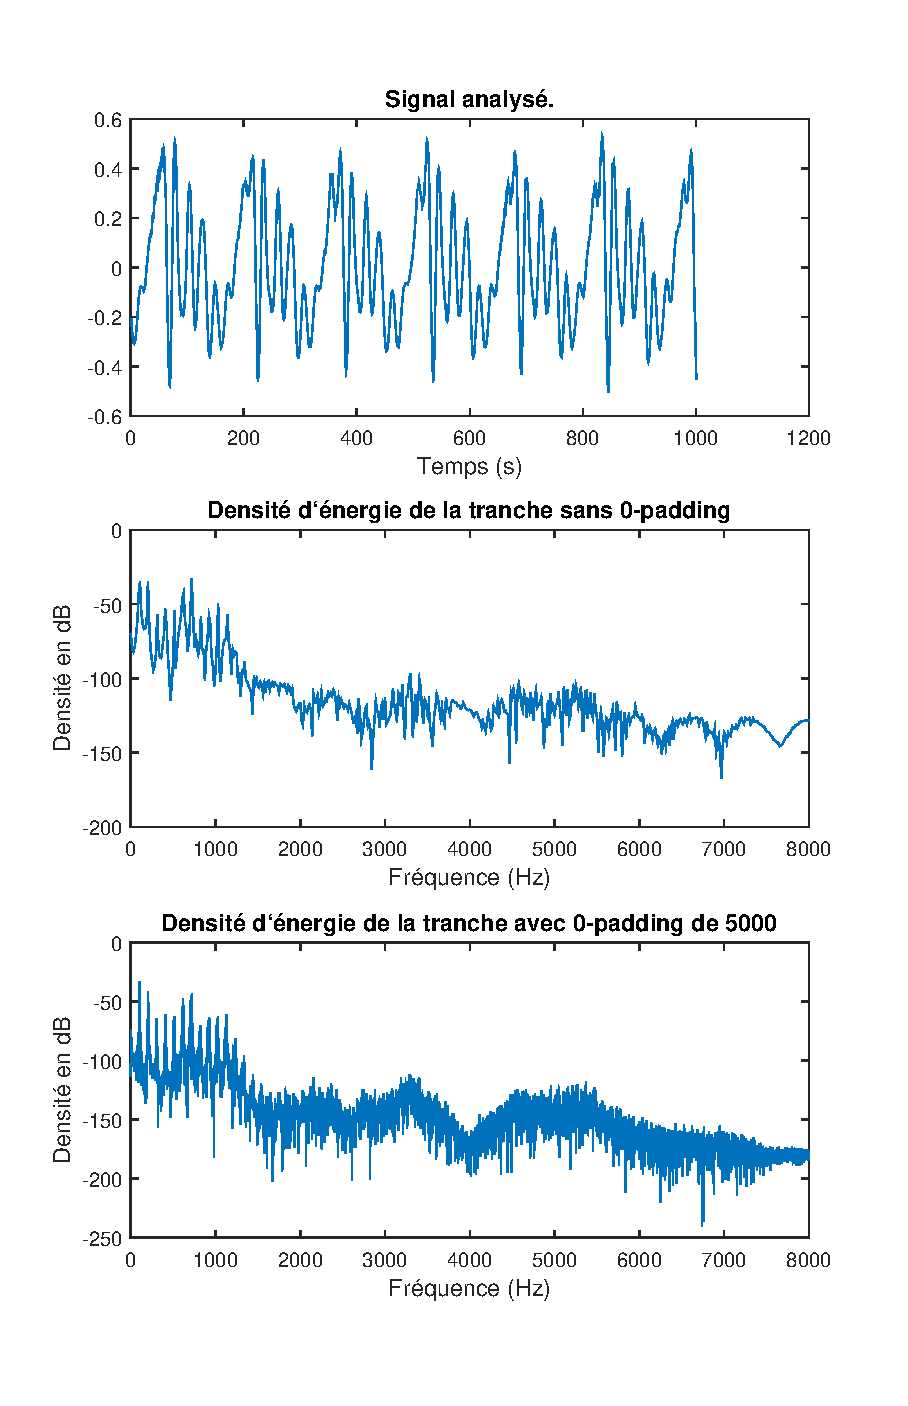
\includegraphics[width=\textwidth]{images/comp_0_padding.eps}
	% This file was created by matlab2tikz.
%
%The latest updates can be retrieved from
%  http://www.mathworks.com/matlabcentral/fileexchange/22022-matlab2tikz-matlab2tikz
%where you can also make suggestions and rate matlab2tikz.
%
\definecolor{mycolor1}{rgb}{0.00000,0.44700,0.74100}%
%
\begin{tikzpicture}

\begin{axis}[%
width=4.521in,
height=0.944in,
at={(0.758in,3.8in)},
scale only axis,
xmin=0,
xmax=1200,
%xlabel style={font=\color{white!15!black}},
xlabel={Temps (s)},
ymin=-1,
ymax=1,
axis background/.style={fill=white},
%title style={font=\bfseries},
title={Signal analysé.},
%legend style={legend cell align=left, align=left, draw=white!15!black}
]
\addplot [color=mycolor1]
  table[row sep=crcr]{%
1	-0.20916748046875\\
2	-0.245880126953125\\
3	-0.271514892578125\\
4	-0.28802490234375\\
5	-0.306060791015625\\
6	-0.308563232421875\\
7	-0.300079345703125\\
8	-0.292633056640625\\
9	-0.278656005859375\\
10	-0.25299072265625\\
11	-0.22418212890625\\
12	-0.193695068359375\\
13	-0.156036376953125\\
14	-0.127593994140625\\
15	-0.107574462890625\\
16	-0.093048095703125\\
17	-0.08465576171875\\
18	-0.076904296875\\
19	-0.0782470703125\\
20	-0.0797119140625\\
21	-0.081390380859375\\
22	-0.0906982421875\\
23	-0.09515380859375\\
24	-0.086700439453125\\
25	-0.079620361328125\\
26	-0.066253662109375\\
27	-0.03350830078125\\
28	-0.0008544921875\\
29	0.016693115234375\\
30	0.037811279296875\\
31	0.071075439453125\\
32	0.08880615234375\\
33	0.104736328125\\
34	0.12811279296875\\
35	0.1337890625\\
36	0.130706787109375\\
37	0.1463623046875\\
38	0.180572509765625\\
39	0.2078857421875\\
40	0.2025146484375\\
41	0.22021484375\\
42	0.278167724609375\\
43	0.27557373046875\\
44	0.274932861328125\\
45	0.34027099609375\\
46	0.32513427734375\\
47	0.306640625\\
48	0.3822021484375\\
49	0.389190673828125\\
50	0.34368896484375\\
51	0.36846923828125\\
52	0.4051513671875\\
53	0.395751953125\\
54	0.403778076171875\\
55	0.451934814453125\\
56	0.4705810546875\\
57	0.466796875\\
58	0.479583740234375\\
59	0.464324951171875\\
60	0.397674560546875\\
61	0.3411865234375\\
62	0.28521728515625\\
63	0.145782470703125\\
64	-0.035369873046875\\
65	-0.173370361328125\\
66	-0.261077880859375\\
67	-0.37396240234375\\
68	-0.473480224609375\\
69	-0.477325439453125\\
70	-0.444580078125\\
71	-0.35430908203125\\
72	-0.188079833984375\\
73	-0.037628173828125\\
74	0.0899658203125\\
75	0.273223876953125\\
76	0.430328369140625\\
77	0.485504150390625\\
78	0.50689697265625\\
79	0.493988037109375\\
80	0.443084716796875\\
81	0.370330810546875\\
82	0.255615234375\\
83	0.127532958984375\\
84	0.040771484375\\
85	-0.02484130859375\\
86	-0.084991455078125\\
87	-0.1217041015625\\
88	-0.1610107421875\\
89	-0.180511474609375\\
90	-0.170867919921875\\
91	-0.175933837890625\\
92	-0.18988037109375\\
93	-0.193695068359375\\
94	-0.181732177734375\\
95	-0.156707763671875\\
96	-0.122955322265625\\
97	-0.081878662109375\\
98	-0.02508544921875\\
99	0.056732177734375\\
100	0.144744873046875\\
101	0.225616455078125\\
102	0.28369140625\\
103	0.31390380859375\\
104	0.33154296875\\
105	0.323455810546875\\
106	0.28369140625\\
107	0.219390869140625\\
108	0.140380859375\\
109	0.051239013671875\\
110	-0.04010009765625\\
111	-0.123626708984375\\
112	-0.19171142578125\\
113	-0.2310791015625\\
114	-0.241363525390625\\
115	-0.23394775390625\\
116	-0.212921142578125\\
117	-0.1741943359375\\
118	-0.123687744140625\\
119	-0.063507080078125\\
120	-0.002197265625\\
121	0.046142578125\\
122	0.08868408203125\\
123	0.13031005859375\\
124	0.161651611328125\\
125	0.1827392578125\\
126	0.191864013671875\\
127	0.192474365234375\\
128	0.189971923828125\\
129	0.177032470703125\\
130	0.14813232421875\\
131	0.10272216796875\\
132	0.041839599609375\\
133	-0.018157958984375\\
134	-0.086212158203125\\
135	-0.1658935546875\\
136	-0.23187255859375\\
137	-0.290557861328125\\
138	-0.337310791015625\\
139	-0.35687255859375\\
140	-0.360382080078125\\
141	-0.34796142578125\\
142	-0.319091796875\\
143	-0.2852783203125\\
144	-0.24188232421875\\
145	-0.193206787109375\\
146	-0.149932861328125\\
147	-0.112335205078125\\
148	-0.076446533203125\\
149	-0.06536865234375\\
150	-0.073272705078125\\
151	-0.08062744140625\\
152	-0.105865478515625\\
153	-0.1395263671875\\
154	-0.1666259765625\\
155	-0.197113037109375\\
156	-0.23590087890625\\
157	-0.2708740234375\\
158	-0.29193115234375\\
159	-0.30865478515625\\
160	-0.32415771484375\\
161	-0.319976806640625\\
162	-0.3076171875\\
163	-0.298004150390625\\
164	-0.27630615234375\\
165	-0.24853515625\\
166	-0.217529296875\\
167	-0.182403564453125\\
168	-0.1456298828125\\
169	-0.113250732421875\\
170	-0.09112548828125\\
171	-0.07403564453125\\
172	-0.0662841796875\\
173	-0.06854248046875\\
174	-0.07745361328125\\
175	-0.090240478515625\\
176	-0.101715087890625\\
177	-0.11419677734375\\
178	-0.118988037109375\\
179	-0.115325927734375\\
180	-0.109588623046875\\
181	-0.086669921875\\
182	-0.052764892578125\\
183	-0.02752685546875\\
184	0.005523681640625\\
185	0.042510986328125\\
186	0.060089111328125\\
187	0.078765869140625\\
188	0.104827880859375\\
189	0.111297607421875\\
190	0.111236572265625\\
191	0.139251708984375\\
192	0.162994384765625\\
193	0.16162109375\\
194	0.191375732421875\\
195	0.226348876953125\\
196	0.233795166015625\\
197	0.271331787109375\\
198	0.3155517578125\\
199	0.325958251953125\\
200	0.33349609375\\
201	0.332122802734375\\
202	0.329376220703125\\
203	0.3427734375\\
204	0.322418212890625\\
205	0.31146240234375\\
206	0.33673095703125\\
207	0.3062744140625\\
208	0.28546142578125\\
209	0.3115234375\\
210	0.311553955078125\\
211	0.32879638671875\\
212	0.370513916015625\\
213	0.4129638671875\\
214	0.429962158203125\\
215	0.4300537109375\\
216	0.44207763671875\\
217	0.4332275390625\\
218	0.365570068359375\\
219	0.2642822265625\\
220	0.138763427734375\\
221	-0.027618408203125\\
222	-0.141571044921875\\
223	-0.243408203125\\
224	-0.39581298828125\\
225	-0.462005615234375\\
226	-0.434814453125\\
227	-0.389312744140625\\
228	-0.280303955078125\\
229	-0.137847900390625\\
230	-0.027801513671875\\
231	0.13104248046875\\
232	0.30706787109375\\
233	0.383453369140625\\
234	0.414947509765625\\
235	0.436981201171875\\
236	0.411895751953125\\
237	0.358245849609375\\
238	0.283111572265625\\
239	0.177459716796875\\
240	0.0897216796875\\
241	0.0364990234375\\
242	-0.019683837890625\\
243	-0.064544677734375\\
244	-0.0869140625\\
245	-0.103973388671875\\
246	-0.1158447265625\\
247	-0.129180908203125\\
248	-0.154998779296875\\
249	-0.177886962890625\\
250	-0.177703857421875\\
251	-0.1724853515625\\
252	-0.162567138671875\\
253	-0.13275146484375\\
254	-0.092498779296875\\
255	-0.028533935546875\\
256	0.06170654296875\\
257	0.145660400390625\\
258	0.21124267578125\\
259	0.26507568359375\\
260	0.29742431640625\\
261	0.3065185546875\\
262	0.29083251953125\\
263	0.24188232421875\\
264	0.17706298828125\\
265	0.1082763671875\\
266	0.024993896484375\\
267	-0.05438232421875\\
268	-0.12274169921875\\
269	-0.178741455078125\\
270	-0.204132080078125\\
271	-0.209259033203125\\
272	-0.203887939453125\\
273	-0.1820068359375\\
274	-0.143341064453125\\
275	-0.098297119140625\\
276	-0.049774169921875\\
277	-0.007568359375\\
278	0.02764892578125\\
279	0.0718994140625\\
280	0.1083984375\\
281	0.133941650390625\\
282	0.154022216796875\\
283	0.164398193359375\\
284	0.17156982421875\\
285	0.169921875\\
286	0.15179443359375\\
287	0.112396240234375\\
288	0.06768798828125\\
289	0.01470947265625\\
290	-0.06121826171875\\
291	-0.1312255859375\\
292	-0.202880859375\\
293	-0.268218994140625\\
294	-0.31304931640625\\
295	-0.350799560546875\\
296	-0.36480712890625\\
297	-0.364959716796875\\
298	-0.35308837890625\\
299	-0.322601318359375\\
300	-0.286773681640625\\
301	-0.24798583984375\\
302	-0.201202392578125\\
303	-0.146087646484375\\
304	-0.11187744140625\\
305	-0.093414306640625\\
306	-0.073089599609375\\
307	-0.075408935546875\\
308	-0.096221923828125\\
309	-0.114776611328125\\
310	-0.138458251953125\\
311	-0.178680419921875\\
312	-0.2177734375\\
313	-0.24871826171875\\
314	-0.279815673828125\\
315	-0.3092041015625\\
316	-0.3206787109375\\
317	-0.320465087890625\\
318	-0.319244384765625\\
319	-0.311614990234375\\
320	-0.292938232421875\\
321	-0.263427734375\\
322	-0.236083984375\\
323	-0.20025634765625\\
324	-0.158416748046875\\
325	-0.131927490234375\\
326	-0.108795166015625\\
327	-0.08758544921875\\
328	-0.075469970703125\\
329	-0.074462890625\\
330	-0.076416015625\\
331	-0.076080322265625\\
332	-0.084686279296875\\
333	-0.091033935546875\\
334	-0.08843994140625\\
335	-0.0860595703125\\
336	-0.07965087890625\\
337	-0.060333251953125\\
338	-0.036834716796875\\
339	-0.02142333984375\\
340	0.008636474609375\\
341	0.035552978515625\\
342	0.041595458984375\\
343	0.063629150390625\\
344	0.0703125\\
345	0.06610107421875\\
346	0.0921630859375\\
347	0.119232177734375\\
348	0.149322509765625\\
349	0.186126708984375\\
350	0.217987060546875\\
351	0.2637939453125\\
352	0.3009033203125\\
353	0.329681396484375\\
354	0.377655029296875\\
355	0.377593994140625\\
356	0.362518310546875\\
357	0.38043212890625\\
358	0.33807373046875\\
359	0.28271484375\\
360	0.26715087890625\\
361	0.243560791015625\\
362	0.213623046875\\
363	0.227508544921875\\
364	0.2490234375\\
365	0.2486572265625\\
366	0.275787353515625\\
367	0.32098388671875\\
368	0.366119384765625\\
369	0.40838623046875\\
370	0.4459228515625\\
371	0.461944580078125\\
372	0.44305419921875\\
373	0.40216064453125\\
374	0.339569091796875\\
375	0.23638916015625\\
376	0.0887451171875\\
377	-0.038238525390625\\
378	-0.118927001953125\\
379	-0.24652099609375\\
380	-0.389251708984375\\
381	-0.417266845703125\\
382	-0.40203857421875\\
383	-0.3612060546875\\
384	-0.23211669921875\\
385	-0.12237548828125\\
386	-0.046112060546875\\
387	0.109832763671875\\
388	0.26361083984375\\
389	0.314178466796875\\
390	0.353546142578125\\
391	0.38427734375\\
392	0.363250732421875\\
393	0.33056640625\\
394	0.26617431640625\\
395	0.16729736328125\\
396	0.10009765625\\
397	0.056060791015625\\
398	0.00372314453125\\
399	-0.0321044921875\\
400	-0.0665283203125\\
401	-0.0960693359375\\
402	-0.107208251953125\\
403	-0.1292724609375\\
404	-0.161895751953125\\
405	-0.17999267578125\\
406	-0.1806640625\\
407	-0.17816162109375\\
408	-0.161529541015625\\
409	-0.1385498046875\\
410	-0.1005859375\\
411	-0.02984619140625\\
412	0.05084228515625\\
413	0.123809814453125\\
414	0.1859130859375\\
415	0.232879638671875\\
416	0.268402099609375\\
417	0.285064697265625\\
418	0.26568603515625\\
419	0.21905517578125\\
420	0.16375732421875\\
421	0.098602294921875\\
422	0.02777099609375\\
423	-0.04083251953125\\
424	-0.108184814453125\\
425	-0.157073974609375\\
426	-0.178253173828125\\
427	-0.187744140625\\
428	-0.18353271484375\\
429	-0.160980224609375\\
430	-0.129119873046875\\
431	-0.08795166015625\\
432	-0.042236328125\\
433	-0.010345458984375\\
434	0.021820068359375\\
435	0.063018798828125\\
436	0.095367431640625\\
437	0.1187744140625\\
438	0.134063720703125\\
439	0.1412353515625\\
440	0.1405029296875\\
441	0.1259765625\\
442	0.100372314453125\\
443	0.071044921875\\
444	0.029815673828125\\
445	-0.028076171875\\
446	-0.088714599609375\\
447	-0.14886474609375\\
448	-0.2099609375\\
449	-0.257568359375\\
450	-0.295166015625\\
451	-0.323028564453125\\
452	-0.337554931640625\\
453	-0.3358154296875\\
454	-0.329376220703125\\
455	-0.320526123046875\\
456	-0.291839599609375\\
457	-0.26007080078125\\
458	-0.216888427734375\\
459	-0.17022705078125\\
460	-0.1456298828125\\
461	-0.121002197265625\\
462	-0.09869384765625\\
463	-0.095672607421875\\
464	-0.10443115234375\\
465	-0.114593505859375\\
466	-0.13653564453125\\
467	-0.175384521484375\\
468	-0.213165283203125\\
469	-0.2462158203125\\
470	-0.283233642578125\\
471	-0.309478759765625\\
472	-0.315185546875\\
473	-0.318267822265625\\
474	-0.320526123046875\\
475	-0.3072509765625\\
476	-0.281280517578125\\
477	-0.252410888671875\\
478	-0.218902587890625\\
479	-0.181182861328125\\
480	-0.15106201171875\\
481	-0.126373291015625\\
482	-0.10198974609375\\
483	-0.08282470703125\\
484	-0.074951171875\\
485	-0.07293701171875\\
486	-0.065216064453125\\
487	-0.06402587890625\\
488	-0.066436767578125\\
489	-0.066009521484375\\
490	-0.067291259765625\\
491	-0.062042236328125\\
492	-0.056121826171875\\
493	-0.044677734375\\
494	-0.027679443359375\\
495	-0.017913818359375\\
496	-0.002716064453125\\
497	0.019622802734375\\
498	0.03167724609375\\
499	0.048583984375\\
500	0.080352783203125\\
501	0.103515625\\
502	0.125946044921875\\
503	0.163909912109375\\
504	0.1953125\\
505	0.22503662109375\\
506	0.2730712890625\\
507	0.31231689453125\\
508	0.3135986328125\\
509	0.32452392578125\\
510	0.3438720703125\\
511	0.330596923828125\\
512	0.312103271484375\\
513	0.299530029296875\\
514	0.287017822265625\\
515	0.265533447265625\\
516	0.2470703125\\
517	0.256134033203125\\
518	0.265106201171875\\
519	0.27142333984375\\
520	0.322052001953125\\
521	0.3853759765625\\
522	0.407196044921875\\
523	0.445465087890625\\
524	0.512725830078125\\
525	0.506195068359375\\
526	0.469146728515625\\
527	0.45697021484375\\
528	0.37005615234375\\
529	0.219757080078125\\
530	0.087371826171875\\
531	-0.07147216796875\\
532	-0.2191162109375\\
533	-0.28594970703125\\
534	-0.375579833984375\\
535	-0.463134765625\\
536	-0.437286376953125\\
537	-0.3768310546875\\
538	-0.284912109375\\
539	-0.1241455078125\\
540	0.003143310546875\\
541	0.110748291015625\\
542	0.268951416015625\\
543	0.36669921875\\
544	0.379425048828125\\
545	0.3966064453125\\
546	0.384490966796875\\
547	0.336761474609375\\
548	0.2862548828125\\
549	0.206268310546875\\
550	0.11175537109375\\
551	0.05206298828125\\
552	0.00762939453125\\
553	-0.037506103515625\\
554	-0.0699462890625\\
555	-0.108001708984375\\
556	-0.13848876953125\\
557	-0.15643310546875\\
558	-0.186309814453125\\
559	-0.211181640625\\
560	-0.2171630859375\\
561	-0.20831298828125\\
562	-0.183624267578125\\
563	-0.141143798828125\\
564	-0.093475341796875\\
565	-0.02850341796875\\
566	0.0623779296875\\
567	0.1473388671875\\
568	0.220001220703125\\
569	0.270965576171875\\
570	0.288818359375\\
571	0.2960205078125\\
572	0.282562255859375\\
573	0.22918701171875\\
574	0.1646728515625\\
575	0.102325439453125\\
576	0.024993896484375\\
577	-0.0462646484375\\
578	-0.104705810546875\\
579	-0.1600341796875\\
580	-0.19122314453125\\
581	-0.19537353515625\\
582	-0.1939697265625\\
583	-0.1829833984375\\
584	-0.156494140625\\
585	-0.120819091796875\\
586	-0.077606201171875\\
587	-0.03717041015625\\
588	-0.003326416015625\\
589	0.03887939453125\\
590	0.081512451171875\\
591	0.11724853515625\\
592	0.150238037109375\\
593	0.169097900390625\\
594	0.18084716796875\\
595	0.187652587890625\\
596	0.1668701171875\\
597	0.1259765625\\
598	0.08453369140625\\
599	0.0277099609375\\
600	-0.042877197265625\\
601	-0.119476318359375\\
602	-0.19793701171875\\
603	-0.265777587890625\\
604	-0.3160400390625\\
605	-0.350006103515625\\
606	-0.3638916015625\\
607	-0.3607177734375\\
608	-0.3446044921875\\
609	-0.311065673828125\\
610	-0.273895263671875\\
611	-0.239990234375\\
612	-0.194488525390625\\
613	-0.1402587890625\\
614	-0.1033935546875\\
615	-0.08673095703125\\
616	-0.074310302734375\\
617	-0.0755615234375\\
618	-0.095550537109375\\
619	-0.117462158203125\\
620	-0.138519287109375\\
621	-0.172393798828125\\
622	-0.2078857421875\\
623	-0.23724365234375\\
624	-0.269439697265625\\
625	-0.30194091796875\\
626	-0.319915771484375\\
627	-0.32147216796875\\
628	-0.318572998046875\\
629	-0.31097412109375\\
630	-0.295013427734375\\
631	-0.274200439453125\\
632	-0.2467041015625\\
633	-0.206878662109375\\
634	-0.16680908203125\\
635	-0.12908935546875\\
636	-0.100860595703125\\
637	-0.08282470703125\\
638	-0.071258544921875\\
639	-0.073455810546875\\
640	-0.08245849609375\\
641	-0.089111328125\\
642	-0.093353271484375\\
643	-0.108245849609375\\
644	-0.114288330078125\\
645	-0.111328125\\
646	-0.10943603515625\\
647	-0.0911865234375\\
648	-0.062896728515625\\
649	-0.03326416015625\\
650	-0.00372314453125\\
651	0.02178955078125\\
652	0.047698974609375\\
653	0.065216064453125\\
654	0.07049560546875\\
655	0.103668212890625\\
656	0.119781494140625\\
657	0.11639404296875\\
658	0.157928466796875\\
659	0.175872802734375\\
660	0.171905517578125\\
661	0.2215576171875\\
662	0.2401123046875\\
663	0.228851318359375\\
664	0.281707763671875\\
665	0.3033447265625\\
666	0.2886962890625\\
667	0.323394775390625\\
668	0.338775634765625\\
669	0.312255859375\\
670	0.321044921875\\
671	0.303619384765625\\
672	0.25286865234375\\
673	0.27740478515625\\
674	0.301300048828125\\
675	0.297149658203125\\
676	0.34173583984375\\
677	0.37921142578125\\
678	0.387969970703125\\
679	0.449371337890625\\
680	0.471343994140625\\
681	0.431365966796875\\
682	0.418304443359375\\
683	0.38214111328125\\
684	0.273345947265625\\
685	0.138641357421875\\
686	0.001861572265625\\
687	-0.16168212890625\\
688	-0.23541259765625\\
689	-0.2830810546875\\
690	-0.40380859375\\
691	-0.4332275390625\\
692	-0.372314453125\\
693	-0.30694580078125\\
694	-0.187042236328125\\
695	-0.04443359375\\
696	0.046478271484375\\
697	0.1761474609375\\
698	0.315093994140625\\
699	0.3544921875\\
700	0.3563232421875\\
701	0.358154296875\\
702	0.33563232421875\\
703	0.295257568359375\\
704	0.2286376953125\\
705	0.131378173828125\\
706	0.065948486328125\\
707	0.027923583984375\\
708	-0.018402099609375\\
709	-0.050994873046875\\
710	-0.08087158203125\\
711	-0.11102294921875\\
712	-0.124298095703125\\
713	-0.14324951171875\\
714	-0.179534912109375\\
715	-0.19757080078125\\
716	-0.190643310546875\\
717	-0.17669677734375\\
718	-0.147308349609375\\
719	-0.108245849609375\\
720	-0.0628662109375\\
721	0.00958251953125\\
722	0.095947265625\\
723	0.170257568359375\\
724	0.22296142578125\\
725	0.256683349609375\\
726	0.2725830078125\\
727	0.268707275390625\\
728	0.242767333984375\\
729	0.189605712890625\\
730	0.12750244140625\\
731	0.0623779296875\\
732	-0.009765625\\
733	-0.0765380859375\\
734	-0.131317138671875\\
735	-0.170379638671875\\
736	-0.184539794921875\\
737	-0.181671142578125\\
738	-0.17303466796875\\
739	-0.152801513671875\\
740	-0.117523193359375\\
741	-0.0772705078125\\
742	-0.037872314453125\\
743	-0.002777099609375\\
744	0.0279541015625\\
745	0.063751220703125\\
746	0.09619140625\\
747	0.118743896484375\\
748	0.135009765625\\
749	0.147064208984375\\
750	0.1527099609375\\
751	0.14117431640625\\
752	0.11260986328125\\
753	0.074615478515625\\
754	0.031036376953125\\
755	-0.018218994140625\\
756	-0.09417724609375\\
757	-0.172698974609375\\
758	-0.235015869140625\\
759	-0.29754638671875\\
760	-0.341827392578125\\
761	-0.355010986328125\\
762	-0.362060546875\\
763	-0.364501953125\\
764	-0.32562255859375\\
765	-0.277679443359375\\
766	-0.247406005859375\\
767	-0.1922607421875\\
768	-0.11822509765625\\
769	-0.0760498046875\\
770	-0.055023193359375\\
771	-0.037445068359375\\
772	-0.054595947265625\\
773	-0.09002685546875\\
774	-0.115447998046875\\
775	-0.148223876953125\\
776	-0.194854736328125\\
777	-0.238311767578125\\
778	-0.2681884765625\\
779	-0.296112060546875\\
780	-0.31878662109375\\
781	-0.324005126953125\\
782	-0.314788818359375\\
783	-0.30126953125\\
784	-0.2872314453125\\
785	-0.27044677734375\\
786	-0.24761962890625\\
787	-0.223663330078125\\
788	-0.19451904296875\\
789	-0.1563720703125\\
790	-0.1236572265625\\
791	-0.104827880859375\\
792	-0.083526611328125\\
793	-0.06591796875\\
794	-0.06494140625\\
795	-0.066925048828125\\
796	-0.070159912109375\\
797	-0.08172607421875\\
798	-0.09698486328125\\
799	-0.10479736328125\\
800	-0.113311767578125\\
801	-0.118316650390625\\
802	-0.1051025390625\\
803	-0.0826416015625\\
804	-0.056732177734375\\
805	-0.022918701171875\\
806	0.003265380859375\\
807	0.03033447265625\\
808	0.0599365234375\\
809	0.07220458984375\\
810	0.091705322265625\\
811	0.112213134765625\\
812	0.119476318359375\\
813	0.13995361328125\\
814	0.17108154296875\\
815	0.19073486328125\\
816	0.213775634765625\\
817	0.259429931640625\\
818	0.286895751953125\\
819	0.294403076171875\\
820	0.302703857421875\\
821	0.327301025390625\\
822	0.313079833984375\\
823	0.28094482421875\\
824	0.311981201171875\\
825	0.294586181640625\\
826	0.24822998046875\\
827	0.27532958984375\\
828	0.305450439453125\\
829	0.289794921875\\
830	0.3414306640625\\
831	0.427581787109375\\
832	0.44921875\\
833	0.477264404296875\\
834	0.531463623046875\\
835	0.5247802734375\\
836	0.475189208984375\\
837	0.43902587890625\\
838	0.335784912109375\\
839	0.17193603515625\\
840	0.004913330078125\\
841	-0.154205322265625\\
842	-0.253753662109375\\
843	-0.34307861328125\\
844	-0.466583251953125\\
845	-0.5062255859375\\
846	-0.449005126953125\\
847	-0.3775634765625\\
848	-0.236602783203125\\
849	-0.06842041015625\\
850	0.0396728515625\\
851	0.187225341796875\\
852	0.36224365234375\\
853	0.419189453125\\
854	0.41705322265625\\
855	0.42669677734375\\
856	0.397125244140625\\
857	0.342529296875\\
858	0.2706298828125\\
859	0.166259765625\\
860	0.080535888671875\\
861	0.032562255859375\\
862	-0.0166015625\\
863	-0.057769775390625\\
864	-0.092071533203125\\
865	-0.12432861328125\\
866	-0.13775634765625\\
867	-0.160491943359375\\
868	-0.20587158203125\\
869	-0.2283935546875\\
870	-0.22479248046875\\
871	-0.2117919921875\\
872	-0.179840087890625\\
873	-0.137481689453125\\
874	-0.08392333984375\\
875	0.00177001953125\\
876	0.101470947265625\\
877	0.189971923828125\\
878	0.259613037109375\\
879	0.297637939453125\\
880	0.31414794921875\\
881	0.315887451171875\\
882	0.279632568359375\\
883	0.213958740234375\\
884	0.14605712890625\\
885	0.071502685546875\\
886	-0.00958251953125\\
887	-0.081817626953125\\
888	-0.146331787109375\\
889	-0.189849853515625\\
890	-0.202392578125\\
891	-0.20159912109375\\
892	-0.191680908203125\\
893	-0.169952392578125\\
894	-0.139312744140625\\
895	-0.0943603515625\\
896	-0.050384521484375\\
897	-0.020660400390625\\
898	0.01397705078125\\
899	0.057952880859375\\
900	0.0970458984375\\
901	0.127471923828125\\
902	0.14996337890625\\
903	0.165496826171875\\
904	0.180145263671875\\
905	0.186431884765625\\
906	0.1641845703125\\
907	0.12451171875\\
908	0.078765869140625\\
909	0.021392822265625\\
910	-0.040771484375\\
911	-0.122344970703125\\
912	-0.216217041015625\\
913	-0.278839111328125\\
914	-0.3267822265625\\
915	-0.372650146484375\\
916	-0.381134033203125\\
917	-0.366424560546875\\
918	-0.352630615234375\\
919	-0.30938720703125\\
920	-0.246307373046875\\
921	-0.205108642578125\\
922	-0.154144287109375\\
923	-0.081817626953125\\
924	-0.036590576171875\\
925	-0.027801513671875\\
926	-0.024322509765625\\
927	-0.034820556640625\\
928	-0.07666015625\\
929	-0.11907958984375\\
930	-0.15631103515625\\
931	-0.2047119140625\\
932	-0.251373291015625\\
933	-0.2799072265625\\
934	-0.30242919921875\\
935	-0.324188232421875\\
936	-0.327362060546875\\
937	-0.3170166015625\\
938	-0.303375244140625\\
939	-0.2882080078125\\
940	-0.26788330078125\\
941	-0.239288330078125\\
942	-0.2120361328125\\
943	-0.18121337890625\\
944	-0.143524169921875\\
945	-0.111419677734375\\
946	-0.089324951171875\\
947	-0.067626953125\\
948	-0.05023193359375\\
949	-0.0491943359375\\
950	-0.0599365234375\\
951	-0.071197509765625\\
952	-0.0902099609375\\
953	-0.117095947265625\\
954	-0.13336181640625\\
955	-0.13958740234375\\
956	-0.1396484375\\
957	-0.124969482421875\\
958	-0.096466064453125\\
959	-0.05938720703125\\
960	-0.021148681640625\\
961	0.01605224609375\\
962	0.055389404296875\\
963	0.0858154296875\\
964	0.10601806640625\\
965	0.12603759765625\\
966	0.142578125\\
967	0.1439208984375\\
968	0.147430419921875\\
969	0.162750244140625\\
970	0.171905517578125\\
971	0.16961669921875\\
972	0.18450927734375\\
973	0.216705322265625\\
974	0.233367919921875\\
975	0.2642822265625\\
976	0.30267333984375\\
977	0.3143310546875\\
978	0.33172607421875\\
979	0.34112548828125\\
980	0.323486328125\\
981	0.2939453125\\
982	0.270599365234375\\
983	0.264373779296875\\
984	0.263336181640625\\
985	0.27044677734375\\
986	0.29425048828125\\
987	0.329193115234375\\
988	0.361602783203125\\
989	0.406463623046875\\
990	0.448272705078125\\
991	0.450958251953125\\
992	0.4638671875\\
993	0.454193115234375\\
994	0.378814697265625\\
995	0.2762451171875\\
996	0.1243896484375\\
997	-0.066741943359375\\
998	-0.168792724609375\\
999	-0.227447509765625\\
1000	-0.373138427734375\\
1001	-0.451080322265625\\
};

\end{axis}

\begin{axis}[%
width=4.521in,
height=0.944in,
at={(0.758in,2.1in)},
scale only axis,
xmin=0,
xmax=8000,
%xlabel style={font=\color{white!15!black}},
xlabel={Fréquence (Hz)},
ymin=-200,
ymax=0,
%ylabel style={font=\color{white!15!black}},
ylabel={Densité en dB},
axis background/.style={fill=white},
%title style={font=\bfseries},
title={Densité d`énergie de la tranche sans 0-padding},
%legend style={legend cell align=left, align=left, draw=white!15!black}
]
\addplot [color=mycolor1]
  table[row sep=crcr]{%
0	-69.994294790377\\
15.625	-79.4224289040131\\
31.25	-81.953091217491\\
46.875	-78.8820605601663\\
62.5	-70.84973839739\\
78.125	-61.4239075376119\\
93.75	-43.019897355987\\
109.375	-34.9936509770083\\
125	-55.5670961361874\\
140.625	-63.0904004893478\\
156.25	-66.732020528388\\
171.875	-66.4184305228346\\
187.5	-62.0196181208929\\
203.125	-34.7657383065579\\
218.75	-63.4810174129479\\
234.375	-80.9622103609203\\
250	-87.7155989801168\\
265.625	-94.450422123779\\
281.25	-91.8629125014141\\
296.875	-83.6823007902011\\
312.5	-56.7733392581357\\
328.125	-79.9279061147227\\
343.75	-85.8865996827242\\
359.375	-86.3598025113237\\
375	-78.5439641705209\\
390.625	-71.299250674659\\
406.25	-52.9042684639263\\
421.875	-63.5654022645145\\
437.5	-83.8312032290984\\
453.125	-96.4798544401011\\
468.75	-114.68050555722\\
484.375	-103.49105050018\\
500	-88.8628532760473\\
515.625	-54.1164700090219\\
531.25	-93.4446372026525\\
546.875	-80.167949977082\\
562.5	-70.608025512588\\
578.125	-64.5179566045606\\
593.75	-57.3153959716244\\
609.375	-45.8513386385647\\
625	-42.3765677571392\\
640.625	-61.8912820406216\\
656.25	-66.7801020805814\\
671.875	-81.773359888712\\
687.5	-73.8970778777046\\
703.125	-56.4641625782508\\
718.75	-32.6726747284722\\
734.375	-54.3490774292811\\
750	-79.074860223535\\
765.625	-69.9584126887052\\
781.25	-79.1209598333244\\
796.875	-83.670234538709\\
812.5	-77.913284876822\\
828.125	-58.0038962261165\\
843.75	-80.574263378747\\
859.375	-81.1051101136745\\
875	-101.679214383257\\
890.625	-81.2801439239643\\
906.25	-73.3934479756883\\
921.875	-57.6132094785391\\
937.5	-62.6448620580182\\
953.125	-84.5277547979956\\
968.75	-91.5233735791814\\
984.375	-105.374059009831\\
1000	-95.1061557422245\\
1015.625	-77.8235612293978\\
1031.25	-49.8537293058758\\
1046.875	-93.9087944423452\\
1062.5	-102.270532935386\\
1078.125	-85.1740709477655\\
1093.75	-76.461775704188\\
1109.375	-73.8057005787477\\
1125	-73.1857382654549\\
1140.625	-57.2821326791555\\
1156.25	-75.0799733745106\\
1171.875	-81.6764140283109\\
1187.5	-97.1063118333643\\
1203.125	-80.8197742379254\\
1218.75	-84.3485518146823\\
1234.375	-82.0957990421076\\
1250	-83.3870391307671\\
1265.625	-103.22174441459\\
1281.25	-96.3862147159672\\
1296.875	-112.366283877715\\
1312.5	-95.3359128602964\\
1328.125	-96.0529923513641\\
1343.75	-88.7390984018555\\
1359.375	-101.429982856061\\
1375	-102.330186454817\\
1390.625	-105.045035809234\\
1406.25	-107.145591289147\\
1421.875	-110.015438871253\\
1437.5	-124.217481213046\\
1453.125	-98.0338576887521\\
1468.75	-103.64569075924\\
1484.375	-100.329352021757\\
1500	-105.298007923915\\
1515.625	-106.275339894254\\
1531.25	-102.309526944291\\
1546.875	-104.201316257467\\
1562.5	-110.564407830183\\
1578.125	-103.210000507391\\
1593.75	-107.320637115995\\
1609.375	-103.06534376658\\
1625	-101.828642156983\\
1640.625	-107.666455057256\\
1656.25	-103.638571771417\\
1671.875	-102.698911618741\\
1687.5	-105.040726734559\\
1703.125	-103.179316624447\\
1718.75	-104.440703517406\\
1734.375	-105.545785013761\\
1750	-109.485643028826\\
1765.625	-103.525970535102\\
1781.25	-104.360794385069\\
1796.875	-105.33496793244\\
1812.5	-104.117484692073\\
1828.125	-106.668507841268\\
1843.75	-109.157953757911\\
1859.375	-104.869428683021\\
1875	-106.238097155479\\
1890.625	-109.838325366076\\
1906.25	-106.982211951733\\
1921.875	-117.330291119691\\
1937.5	-120.43532767991\\
1953.125	-122.110829481193\\
1968.75	-119.052968247087\\
1984.375	-117.142295283859\\
2000	-116.719869664377\\
2015.625	-128.233214036518\\
2031.25	-131.300062017257\\
2046.875	-118.273373461467\\
2062.5	-122.174435476983\\
2078.125	-123.059619553427\\
2093.75	-119.144541843711\\
2109.375	-117.635339269883\\
2125	-121.278775615828\\
2140.625	-139.384093639592\\
2156.25	-110.668284303396\\
2171.875	-114.284449542536\\
2187.5	-115.779256499479\\
2203.125	-111.972540238733\\
2218.75	-123.284738074449\\
2234.375	-117.483698246706\\
2250	-109.213418266381\\
2265.625	-118.689242127206\\
2281.25	-117.215940973575\\
2296.875	-113.93781369716\\
2312.5	-115.123199587363\\
2328.125	-109.678746848388\\
2343.75	-111.672466227162\\
2359.375	-109.633186571459\\
2375	-111.867747787089\\
2390.625	-107.896536606213\\
2406.25	-109.720736548369\\
2421.875	-116.579100940564\\
2437.5	-128.396632193689\\
2453.125	-113.035209797532\\
2468.75	-118.097198688485\\
2484.375	-114.396122639727\\
2500	-117.249559404524\\
2515.625	-119.807940544993\\
2531.25	-117.804534211692\\
2546.875	-118.958626418646\\
2562.5	-121.504991102272\\
2578.125	-116.816159680305\\
2593.75	-120.587735480311\\
2609.375	-124.215075951534\\
2625	-129.606807676409\\
2640.625	-129.685818193898\\
2656.25	-124.772615136474\\
2671.875	-137.17072819947\\
2687.5	-113.814216436646\\
2703.125	-121.976557221415\\
2718.75	-141.535677355876\\
2734.375	-136.828452155462\\
2750	-129.505848467017\\
2765.625	-120.796036571363\\
2781.25	-118.89828430654\\
2796.875	-132.636664652269\\
2812.5	-129.997920247452\\
2828.125	-134.798433538468\\
2843.75	-161.68729202672\\
2859.375	-140.647686694875\\
2875	-128.096155249906\\
2890.625	-115.379861245852\\
2906.25	-121.88375491334\\
2921.875	-123.610301860238\\
2937.5	-133.02015642207\\
2953.125	-119.215428317675\\
2968.75	-116.336669881988\\
2984.375	-127.667381938358\\
3000	-112.613200582419\\
3015.625	-130.808452176655\\
3031.25	-128.874426039022\\
3046.875	-126.732239403947\\
3062.5	-124.799120339214\\
3078.125	-116.608450450748\\
3093.75	-106.737877073521\\
3109.375	-118.081370511115\\
3125	-123.131201678586\\
3140.625	-129.448677424704\\
3156.25	-109.504563423758\\
3171.875	-111.47513521058\\
3187.5	-119.039095289174\\
3203.125	-103.898056122514\\
3218.75	-125.537726157215\\
3234.375	-140.993727853305\\
3250	-112.776260831079\\
3265.625	-112.45908973467\\
3281.25	-103.081974878746\\
3296.875	-96.4374234947433\\
3312.5	-110.016087681027\\
3328.125	-139.885490018969\\
3343.75	-119.213002635551\\
3359.375	-111.124018724703\\
3375	-129.442317574208\\
3390.625	-115.964675853464\\
3406.25	-100.97096320858\\
3421.875	-106.9853592963\\
3437.5	-122.276682471327\\
3453.125	-130.339342913987\\
3468.75	-114.344733113089\\
3484.375	-116.463381350055\\
3500	-123.616786703778\\
3515.625	-117.400983262433\\
3531.25	-132.698770772532\\
3546.875	-137.87201495157\\
3562.5	-146.110453865763\\
3578.125	-126.143361521041\\
3593.75	-119.578597910674\\
3609.375	-110.555322330599\\
3625	-113.813756685114\\
3640.625	-119.937189487732\\
3656.25	-126.789939654989\\
3671.875	-119.562426407767\\
3687.5	-127.950049492392\\
3703.125	-131.212718863425\\
3718.75	-112.896351010035\\
3734.375	-119.824922960275\\
3750	-120.416432031399\\
3765.625	-124.044764387956\\
3781.25	-116.098372094621\\
3796.875	-114.802918020514\\
3812.5	-115.982679211705\\
3828.125	-116.084012786379\\
3843.75	-116.780506074168\\
3859.375	-118.682690470496\\
3875	-118.234431464386\\
3890.625	-120.293041190248\\
3906.25	-119.508118987166\\
3921.875	-116.411263025848\\
3937.5	-118.392069994965\\
3953.125	-120.442466424082\\
3968.75	-121.167839115347\\
3984.375	-121.451477982932\\
4000	-121.140865699809\\
4015.625	-121.608018485451\\
4031.25	-123.493812429766\\
4046.875	-125.53513267778\\
4062.5	-123.464021052851\\
4078.125	-122.829691665226\\
4093.75	-124.355999272196\\
4109.375	-128.0316341124\\
4125	-128.398045470703\\
4140.625	-133.090013750681\\
4156.25	-129.053426840866\\
4171.875	-132.45768826657\\
4187.5	-135.636313885817\\
4203.125	-129.210881667854\\
4218.75	-123.606967337891\\
4234.375	-128.564932986541\\
4250	-134.632406123659\\
4265.625	-132.23282592646\\
4281.25	-118.86019235026\\
4296.875	-121.383652655522\\
4312.5	-122.882665929154\\
4328.125	-116.1381138061\\
4343.75	-126.700439607829\\
4359.375	-116.532273825243\\
4375	-114.459647382063\\
4390.625	-116.28631806361\\
4406.25	-122.278629891628\\
4421.875	-121.8360443556\\
4437.5	-123.718539812207\\
4453.125	-124.056656853738\\
4468.75	-157.222287554089\\
4484.375	-109.042929262996\\
4500	-112.886675996575\\
4515.625	-107.411296621018\\
4531.25	-113.450213390572\\
4546.875	-144.066730592493\\
4562.5	-108.630603056309\\
4578.125	-103.700596081875\\
4593.75	-109.23389292957\\
4609.375	-117.667260222726\\
4625	-121.31212992879\\
4640.625	-109.759533890041\\
4656.25	-113.163393110271\\
4671.875	-126.073376383498\\
4687.5	-116.953486029226\\
4703.125	-121.794698990088\\
4718.75	-109.356163687343\\
4734.375	-117.95358384819\\
4750	-128.33222115997\\
4765.625	-113.851084667361\\
4781.25	-108.034539327106\\
4796.875	-119.475692068925\\
4812.5	-117.661390809996\\
4828.125	-116.370574248596\\
4843.75	-113.001351611227\\
4859.375	-127.488560162092\\
4875	-147.218165967243\\
4890.625	-127.069315153148\\
4906.25	-133.130214241602\\
4921.875	-114.726072912989\\
4937.5	-131.423236911234\\
4953.125	-109.937752062014\\
4968.75	-121.038174914891\\
4984.375	-118.60245578794\\
5000	-123.780667470647\\
5015.625	-117.666783044598\\
5031.25	-116.988615479386\\
5046.875	-108.611477937455\\
5062.5	-119.834573001311\\
5078.125	-129.882653186897\\
5093.75	-145.032641305833\\
5109.375	-105.333945467813\\
5125	-114.232011841778\\
5140.625	-125.160807693745\\
5156.25	-107.359032211314\\
5171.875	-128.9302219762\\
5187.5	-124.811568865654\\
5203.125	-113.853597080413\\
5218.75	-107.554638872651\\
5234.375	-115.85406817531\\
5250	-104.838442818333\\
5265.625	-109.45247718643\\
5281.25	-118.630936427413\\
5296.875	-113.352980038318\\
5312.5	-105.25866087526\\
5328.125	-135.288140752897\\
5343.75	-135.130439933043\\
5359.375	-108.471035085247\\
5375	-108.364463665467\\
5390.625	-127.133187587489\\
5406.25	-118.754103827601\\
5421.875	-109.267722475324\\
5437.5	-123.823329515592\\
5453.125	-126.947675997271\\
5468.75	-110.097773068443\\
5484.375	-120.615713820521\\
5500	-126.157380814135\\
5515.625	-149.824567934509\\
5531.25	-128.793810170401\\
5546.875	-122.17299492204\\
5562.5	-128.483550417527\\
5578.125	-152.74919848812\\
5593.75	-136.869942880805\\
5609.375	-126.707187994042\\
5625	-127.884337775\\
5640.625	-137.036099996139\\
5656.25	-129.644930116919\\
5671.875	-124.285825781492\\
5687.5	-120.131778898996\\
5703.125	-132.157022151962\\
5718.75	-148.798859871339\\
5734.375	-115.516807730476\\
5750	-121.785688424646\\
5765.625	-126.36883479254\\
5781.25	-124.078739601434\\
5796.875	-152.841282985787\\
5812.5	-131.403294718639\\
5828.125	-122.709281632674\\
5843.75	-141.092079457367\\
5859.375	-127.68173755105\\
5875	-124.851991075753\\
5890.625	-129.903254935123\\
5906.25	-126.695142513583\\
5921.875	-125.598504303608\\
5937.5	-126.074862256195\\
5953.125	-118.991185445206\\
5968.75	-124.202655938063\\
5984.375	-125.644149089856\\
6000	-126.637693005733\\
6015.625	-127.91331981343\\
6031.25	-125.024954249904\\
6046.875	-127.536683633439\\
6062.5	-143.545228436072\\
6078.125	-134.949932358292\\
6093.75	-132.886401514065\\
6109.375	-135.971600290068\\
6125	-132.366249597923\\
6140.625	-135.162429890254\\
6156.25	-141.09336675234\\
6171.875	-135.884619714095\\
6187.5	-134.05163197406\\
6203.125	-139.193113602994\\
6218.75	-144.694581065041\\
6234.375	-140.549070208447\\
6250	-142.698600765897\\
6265.625	-150.967419908594\\
6281.25	-139.655882222502\\
6296.875	-137.452654351719\\
6312.5	-145.963883673581\\
6328.125	-136.972108536922\\
6343.75	-134.484125573304\\
6359.375	-145.212465935154\\
6375	-133.364214230086\\
6390.625	-129.277226576726\\
6406.25	-141.027409683193\\
6421.875	-130.600223431981\\
6437.5	-129.071604226901\\
6453.125	-131.943004801579\\
6468.75	-128.479452270026\\
6484.375	-127.543692418676\\
6500	-129.828698854735\\
6515.625	-130.872473052532\\
6531.25	-127.491766844798\\
6546.875	-128.208342662481\\
6562.5	-130.827001863222\\
6578.125	-126.262307138589\\
6593.75	-124.466294401579\\
6609.375	-129.313177405779\\
6625	-127.004058630508\\
6640.625	-126.577326282159\\
6656.25	-126.797539337085\\
6671.875	-126.051946558408\\
6687.5	-126.718792267452\\
6703.125	-130.990723034676\\
6718.75	-127.723967220568\\
6734.375	-126.927847868013\\
6750	-128.553336756226\\
6765.625	-134.327591950405\\
6781.25	-139.361598953478\\
6796.875	-129.255057461622\\
6812.5	-137.342458466895\\
6828.125	-135.578349309259\\
6843.75	-136.6015147588\\
6859.375	-136.35444000674\\
6875	-138.843502041222\\
6890.625	-133.501798169846\\
6906.25	-149.799954446087\\
6921.875	-144.428773294459\\
6937.5	-139.493717859827\\
6953.125	-151.56820153886\\
6968.75	-167.400307423427\\
6984.375	-145.61629123467\\
7000	-136.21224521784\\
7015.625	-138.246231746261\\
7031.25	-142.972873035934\\
7046.875	-136.380752406337\\
7062.5	-137.843611098785\\
7078.125	-138.645839457849\\
7093.75	-132.493607015736\\
7109.375	-134.126884590345\\
7125	-134.068668732525\\
7140.625	-131.784664773664\\
7156.25	-133.555055507469\\
7171.875	-131.399161979353\\
7187.5	-128.244881765606\\
7203.125	-126.788725442757\\
7218.75	-128.918428745305\\
7234.375	-130.67998998806\\
7250	-126.722676433503\\
7265.625	-127.929342057396\\
7281.25	-127.936801055038\\
7296.875	-126.802941345829\\
7312.5	-131.09204028573\\
7328.125	-129.46253251284\\
7343.75	-126.932879099812\\
7359.375	-129.037644849478\\
7375	-128.959068808211\\
7390.625	-128.767762584417\\
7406.25	-129.939668828377\\
7421.875	-131.082035546009\\
7437.5	-131.050632572825\\
7453.125	-132.200764787722\\
7468.75	-132.100992262584\\
7484.375	-133.807542592376\\
7500	-135.585138872809\\
7515.625	-136.017222028272\\
7531.25	-136.369506467552\\
7546.875	-138.30380475731\\
7562.5	-138.75150979125\\
7578.125	-141.003722212785\\
7593.75	-141.363527288339\\
7609.375	-142.352392962159\\
7625	-142.856944161798\\
7640.625	-143.668501008731\\
7656.25	-145.689086238166\\
7671.875	-144.923112101282\\
7687.5	-144.534458860359\\
7703.125	-142.480672473605\\
7718.75	-140.860769578766\\
7734.375	-139.086958913736\\
7750	-139.19449116436\\
7765.625	-137.236105153599\\
7781.25	-136.79015036817\\
7796.875	-134.426324065425\\
7812.5	-133.285401330088\\
7828.125	-132.799204188624\\
7843.75	-131.644942999496\\
7859.375	-131.429854621182\\
7875	-130.690036929388\\
7890.625	-129.703405361118\\
7906.25	-129.302145735091\\
7921.875	-128.783230364485\\
7937.5	-128.619021279052\\
7953.125	-128.53652102952\\
7968.75	-128.175567286418\\
7984.375	-128.092832702588\\
8000	-128.319867471524\\
};

\end{axis}

\begin{axis}[%
width=4.521in,
height=0.944in,
at={(0.758in,0.481in)},
scale only axis,
xmin=0,
xmax=8000,
%xlabel style={font=\color{white!15!black}},
xlabel={Fréquence (Hz)},
ymin=-400,
ymax=0,
%ylabel style={font=\color{white!15!black}},
ylabel={Densité en dB},
axis background/.style={fill=white},
%title style={font=\bfseries},
title={Densité d`énergie de la tranche avec 0-padding de 2000},
%legend style={legend cell align=left, align=left, draw=white!15!black}
]
\addplot [color=mycolor1]
  table[row sep=crcr]{%
0	-75.79586355145\\
3.90625	-88.7170473520499\\
7.8125	-86.6082108290086\\
11.71875	-100.826974744815\\
15.625	-98.8538988281594\\
19.53125	-89.0991004315829\\
23.4375	-97.7130641036051\\
27.34375	-109.512097586415\\
31.25	-90.0379490186833\\
35.15625	-90.9101394474308\\
39.0625	-103.122010976913\\
42.96875	-100.879800030235\\
46.875	-88.7263662408927\\
50.78125	-90.990079834984\\
54.6875	-107.120264182205\\
58.59375	-93.433928665317\\
62.5	-82.6729516869158\\
66.40625	-88.2472567502789\\
70.3125	-108.784346730263\\
74.21875	-81.2162673807979\\
78.125	-75.7534263774135\\
82.03125	-85.3839683538766\\
85.9375	-87.4541349519886\\
89.84375	-63.6559737305249\\
93.75	-62.2408453865778\\
97.65625	-81.3020256752825\\
101.5625	-32.7858204837684\\
105.46875	-40.2414206133647\\
109.375	-61.7926364038962\\
113.28125	-83.9948820957269\\
117.1875	-78.0649964835904\\
121.09375	-75.029770699624\\
125	-87.6573914170561\\
128.90625	-104.868047567307\\
132.8125	-88.4698056727268\\
136.71875	-89.6328953028825\\
140.625	-101.329266598804\\
144.53125	-102.416693393468\\
148.4375	-98.2369056490071\\
152.34375	-100.500487226614\\
156.25	-102.496235142525\\
160.15625	-103.70075529648\\
164.0625	-109.996783511706\\
167.96875	-110.740312393354\\
171.875	-94.1546454197562\\
175.78125	-92.3394436345412\\
179.6875	-100.154722330108\\
183.59375	-100.918167509216\\
187.5	-80.3669621590856\\
191.40625	-71.1104327936565\\
195.3125	-90.1897570364377\\
199.21875	-68.1540280104136\\
203.125	-41.6568109904436\\
207.03125	-38.0676740250071\\
210.9375	-79.9104627318572\\
214.84375	-69.19587230959\\
218.75	-73.8188239990533\\
222.65625	-76.6254627924074\\
226.5625	-104.656874029908\\
230.46875	-87.4480575957163\\
234.375	-80.2857835396128\\
238.28125	-89.1371052249883\\
242.1875	-109.653797733067\\
246.09375	-89.5358319649202\\
250	-86.1669502796709\\
253.90625	-97.6158442872349\\
257.8125	-104.474209361939\\
261.71875	-91.0560061337627\\
265.625	-90.301927003927\\
269.53125	-109.381963964805\\
273.4375	-97.7847252115024\\
277.34375	-90.4487219984924\\
281.25	-95.9307856328169\\
285.15625	-101.456733730131\\
289.0625	-88.5726918723847\\
292.96875	-91.8226321550975\\
296.875	-96.5385973617507\\
300.78125	-80.5206749404019\\
304.6875	-70.5190204283647\\
308.59375	-56.0027383433996\\
312.5	-84.1347937711882\\
316.40625	-86.3247355890875\\
320.3125	-100.496891566111\\
324.21875	-96.3699801552917\\
328.125	-121.772291344457\\
332.03125	-99.6494221821032\\
335.9375	-94.6227091398387\\
339.84375	-108.743023078593\\
343.75	-118.666634745719\\
347.65625	-99.7394111180577\\
351.5625	-99.8050465689373\\
355.46875	-122.719550903272\\
359.375	-111.361780907446\\
363.28125	-98.1825467583053\\
367.1875	-98.7067090276461\\
371.09375	-119.937032551333\\
375	-98.5981977242576\\
378.90625	-96.502581514663\\
382.8125	-112.524846410239\\
386.71875	-94.9718093301201\\
390.625	-88.0325587177864\\
394.53125	-97.4186677534082\\
398.4375	-82.318505370716\\
402.34375	-78.1976748797185\\
406.25	-79.2474103323489\\
410.15625	-51.6231083041563\\
414.0625	-60.9629029762387\\
417.96875	-80.6544271045003\\
421.875	-86.3661963192492\\
425.78125	-104.027982052217\\
429.6875	-89.2179929066381\\
433.59375	-98.8198793159925\\
437.5	-141.455691414283\\
441.40625	-94.5905004623062\\
445.3125	-97.8786002654205\\
449.21875	-128.43934371079\\
453.125	-123.870722375513\\
457.03125	-95.7796681919213\\
460.9375	-98.991721588429\\
464.84375	-122.921241016758\\
468.75	-107.208625956679\\
472.65625	-93.3385637516889\\
476.5625	-104.226893740699\\
480.46875	-116.573862085678\\
484.375	-93.1072278844777\\
488.28125	-90.603373297879\\
492.1875	-107.506239025555\\
496.09375	-88.4316732482681\\
500	-79.6702495960031\\
503.90625	-94.9659147906698\\
507.8125	-84.6715213825264\\
511.71875	-59.2711041491465\\
515.625	-57.3766597705457\\
519.53125	-100.8425921104\\
523.4375	-85.2044300183849\\
527.34375	-101.289872830331\\
531.25	-87.216769569363\\
535.15625	-99.3913482981847\\
539.0625	-108.559047071188\\
542.96875	-88.7184905353582\\
546.875	-95.6078516772516\\
550.78125	-105.992472040485\\
554.6875	-104.14794947922\\
558.59375	-85.3650974488186\\
562.5	-90.3496449838975\\
566.40625	-100.668748880131\\
570.3125	-99.5813212923082\\
574.21875	-80.8229830742105\\
578.125	-91.5197518827578\\
582.03125	-92.0853792944724\\
585.9375	-78.2561538312674\\
589.84375	-74.9762420977681\\
593.75	-88.2591441942444\\
597.65625	-70.2177915152443\\
601.5625	-63.5462427162828\\
605.46875	-71.8460219872337\\
609.375	-60.6639771229607\\
613.28125	-47.0040802168211\\
617.1875	-37.6444063114893\\
621.09375	-60.6855543741978\\
625	-66.8935272616019\\
628.90625	-66.7711755128363\\
632.8125	-77.8560155996732\\
636.71875	-94.8327114813014\\
640.625	-99.2493096788914\\
644.53125	-76.7378447605705\\
648.4375	-99.9662261203225\\
652.34375	-95.7386345502176\\
656.25	-88.4847512812529\\
660.15625	-79.32759194851\\
664.0625	-95.7687114571683\\
667.96875	-75.8837484898279\\
671.875	-89.5506989811442\\
675.78125	-76.9236571749951\\
679.6875	-94.3531593605125\\
683.59375	-71.4719856603356\\
687.5	-76.1668297590878\\
691.40625	-83.0204797811737\\
695.3125	-62.8595348708465\\
699.21875	-63.9722909752017\\
703.125	-70.8623312501132\\
707.03125	-51.3685066687042\\
710.9375	-59.3030848945029\\
714.84375	-54.5734691477698\\
718.75	-32.4623624986472\\
722.65625	-41.8758502453275\\
726.5625	-68.2357763807773\\
730.46875	-59.1946018341701\\
734.375	-73.6179911202945\\
738.28125	-79.0864150828002\\
742.1875	-93.7523844700286\\
746.09375	-79.9920465847329\\
750	-113.027822297301\\
753.90625	-87.715395028211\\
757.8125	-88.362639339154\\
761.71875	-85.1363280387727\\
765.625	-97.7793542204881\\
769.53125	-81.5507422287212\\
773.4375	-105.658365079577\\
777.34375	-92.8677686759649\\
781.25	-98.195566496487\\
785.15625	-82.8972311165494\\
789.0625	-95.6229125997908\\
792.96875	-110.733634266996\\
796.875	-86.092950742983\\
800.78125	-89.0366435559135\\
804.6875	-113.659238260779\\
808.59375	-77.5196876201222\\
812.5	-94.4436279965838\\
816.40625	-86.7846926672438\\
820.3125	-68.7403937679066\\
824.21875	-67.0157484706401\\
828.125	-84.2549567556613\\
832.03125	-83.1195922934238\\
835.9375	-80.1144568992088\\
839.84375	-105.331410474192\\
843.75	-99.2304820622342\\
847.65625	-97.2311811685866\\
851.5625	-113.127647789717\\
855.46875	-95.8534336201947\\
859.375	-103.508928615322\\
863.28125	-109.172269767101\\
867.1875	-98.8881205531598\\
871.09375	-89.0261893843785\\
875	-93.6051527817323\\
878.90625	-100.618736618205\\
882.8125	-91.8558324125795\\
886.71875	-87.748207287186\\
890.625	-116.843221272907\\
894.53125	-91.6710818535624\\
898.4375	-79.3817014949797\\
902.34375	-96.0945432558009\\
906.25	-79.5925672055626\\
910.15625	-70.4194391344154\\
914.0625	-78.6881182362731\\
917.96875	-78.096767160246\\
921.875	-59.6854709186363\\
925.78125	-53.8486660094806\\
929.6875	-75.154879126274\\
933.59375	-79.5577153630074\\
937.5	-78.3844000217483\\
941.40625	-96.6918621435461\\
945.3125	-100.022713664176\\
949.21875	-109.005688555865\\
953.125	-104.796260692531\\
957.03125	-135.620553147677\\
960.9375	-137.251964488309\\
964.84375	-111.913341060297\\
968.75	-93.7139818772042\\
972.65625	-110.739718335338\\
976.5625	-94.2500143011407\\
980.46875	-99.5597394504586\\
984.375	-98.0569405353083\\
988.28125	-114.795630311135\\
992.1875	-94.4887734058494\\
996.09375	-87.9020809223533\\
1000	-90.3699015109914\\
1003.90625	-88.3568254817123\\
1007.8125	-75.6653701159759\\
1011.71875	-78.3826893408589\\
1015.625	-70.254258694865\\
1019.53125	-75.130301342305\\
1023.4375	-68.0473525564347\\
1027.34375	-52.7884767060024\\
1031.25	-63.0220146937478\\
1035.15625	-83.620442056087\\
1039.0625	-70.2345669449357\\
1042.96875	-98.8162313670566\\
1046.875	-88.6150735920385\\
1050.78125	-110.232849572412\\
1054.6875	-95.6263153558427\\
1058.59375	-141.809312907862\\
1062.5	-108.257946149741\\
1066.40625	-105.807687331898\\
1070.3125	-95.8478361502408\\
1074.21875	-104.812393295948\\
1078.125	-89.3275175305108\\
1082.03125	-98.8705539420766\\
1085.9375	-92.7641765453529\\
1089.84375	-124.210996516505\\
1093.75	-90.6847570399169\\
1097.65625	-86.5122616784187\\
1101.5625	-100.840686131171\\
1105.46875	-79.048903070477\\
1109.375	-76.3867833660231\\
1113.28125	-79.5308420091816\\
1117.1875	-66.4100411433786\\
1121.09375	-94.4356325537887\\
1125	-68.8158857491108\\
1128.90625	-54.4965267374723\\
1132.8125	-57.901319139369\\
1136.71875	-94.6826055634023\\
1140.625	-72.7378371212567\\
1144.53125	-82.8306208172006\\
1148.4375	-85.9006211035252\\
1152.34375	-102.544881048848\\
1156.25	-99.9729875174741\\
1160.15625	-113.064797065755\\
1164.0625	-113.773093648102\\
1167.96875	-102.293164045379\\
1171.875	-117.646674617335\\
1175.78125	-130.233856041014\\
1179.6875	-95.5628748952017\\
1183.59375	-122.503551877679\\
1187.5	-115.309240380865\\
1191.40625	-127.017405051562\\
1195.3125	-100.382182647979\\
1199.21875	-105.658810133976\\
1203.125	-97.8164181434485\\
1207.03125	-93.683523243684\\
1210.9375	-108.256194006904\\
1214.84375	-92.3047964346049\\
1218.75	-87.2675808364607\\
1222.65625	-102.435161089763\\
1226.5625	-86.6968915179899\\
1230.46875	-88.0084029457399\\
1234.375	-77.3269507605344\\
1238.28125	-93.9690753595711\\
1242.1875	-94.8023073652595\\
1246.09375	-96.4499293449067\\
1250	-130.25358808622\\
1253.90625	-153.987468067381\\
1257.8125	-131.427469192562\\
1261.71875	-138.899563070637\\
1265.625	-134.829235243065\\
1269.53125	-110.823355903073\\
1273.4375	-131.804241834344\\
1277.34375	-122.336930802396\\
1281.25	-111.34543287414\\
1285.15625	-142.860748840186\\
1289.0625	-114.56471889728\\
1292.96875	-125.759004139843\\
1296.875	-108.350248560056\\
1300.78125	-122.175071413124\\
1304.6875	-123.177594252889\\
1308.59375	-98.4857877039031\\
1312.5	-122.679751239805\\
1316.40625	-112.334746900464\\
1320.3125	-104.479495788917\\
1324.21875	-105.13787387888\\
1328.125	-123.328753477567\\
1332.03125	-103.673994505527\\
1335.9375	-92.4253999010313\\
1339.84375	-99.8616396099145\\
1343.75	-117.784832006385\\
1347.65625	-109.093211449382\\
1351.5625	-128.478844869789\\
1355.46875	-128.700314859219\\
1359.375	-141.539996849648\\
1363.28125	-124.385330898321\\
1367.1875	-136.140106841618\\
1371.09375	-141.936281130005\\
1375	-139.289418014652\\
1378.90625	-125.900820237353\\
1382.8125	-135.001656626202\\
1386.71875	-125.855041238899\\
1390.625	-136.503639788915\\
1394.53125	-146.613577848325\\
1398.4375	-139.741908264335\\
1402.34375	-123.134708346025\\
1406.25	-155.009108295255\\
1410.15625	-124.868228018314\\
1414.0625	-125.425077275056\\
1417.96875	-126.332927931178\\
1421.875	-128.762793310401\\
1425.78125	-114.399455110757\\
1429.6875	-127.135609396347\\
1433.59375	-115.255903699233\\
1437.5	-114.319898707221\\
1441.40625	-105.900704271965\\
1445.3125	-139.16381884733\\
1449.21875	-112.823610253523\\
1453.125	-142.924156673085\\
1457.03125	-129.089935350045\\
1460.9375	-170.480243725278\\
1464.84375	-129.556920646526\\
1468.75	-150.739012808242\\
1472.65625	-140.065521694656\\
1476.5625	-136.830269959826\\
1480.46875	-125.247665403105\\
1484.375	-153.625788640224\\
1488.28125	-134.904976999996\\
1492.1875	-148.991280864098\\
1496.09375	-148.814785518713\\
1500	-142.385722619901\\
1503.90625	-138.243588574353\\
1507.8125	-144.745642555329\\
1511.71875	-136.103015108266\\
1515.625	-167.924594226659\\
1519.53125	-132.495018202673\\
1523.4375	-130.587892200703\\
1527.34375	-160.323597941461\\
1531.25	-131.891990324162\\
1535.15625	-125.372728668526\\
1539.0625	-126.157062432955\\
1542.96875	-126.649022268198\\
1546.875	-127.522683199864\\
1550.78125	-122.7822542293\\
1554.6875	-145.448261107147\\
1558.59375	-155.113320647056\\
1562.5	-140.092876757933\\
1566.40625	-138.135963135691\\
1570.3125	-137.270825190836\\
1574.21875	-133.06568351985\\
1578.125	-137.640905256955\\
1582.03125	-138.636457906692\\
1585.9375	-147.836681360943\\
1589.84375	-136.265621308201\\
1593.75	-136.451721064117\\
1597.65625	-139.460254038064\\
1601.5625	-135.084622004196\\
1605.46875	-129.825428810794\\
1609.375	-141.781384834334\\
1613.28125	-170.338881385152\\
1617.1875	-128.132373293315\\
1621.09375	-131.611971251046\\
1625	-146.294136225638\\
1628.90625	-128.638893660675\\
1632.8125	-158.253132863609\\
1636.71875	-138.102033385566\\
1640.625	-124.863498819068\\
1644.53125	-125.20548883866\\
1648.4375	-121.940171793082\\
1652.34375	-147.164818672029\\
1656.25	-128.930298002575\\
1660.15625	-156.096345249868\\
1664.0625	-130.736165562087\\
1667.96875	-132.122236983444\\
1671.875	-142.474908011916\\
1675.78125	-140.204350801701\\
1679.6875	-168.2122923353\\
1683.59375	-135.285816615668\\
1687.5	-145.196547332258\\
1691.40625	-142.870567967032\\
1695.3125	-137.384770656388\\
1699.21875	-138.052673089338\\
1703.125	-132.097770586075\\
1707.03125	-146.031542837602\\
1710.9375	-148.763763971841\\
1714.84375	-146.032326421865\\
1718.75	-140.524721126941\\
1722.65625	-172.263937191468\\
1726.5625	-150.560652351852\\
1730.46875	-137.634458069971\\
1734.375	-148.95932430399\\
1738.28125	-149.416195162872\\
1742.1875	-130.721169166421\\
1746.09375	-134.956891054992\\
1750	-134.05925889427\\
1753.90625	-133.558047903834\\
1757.8125	-127.314896202123\\
1761.71875	-160.344328560938\\
1765.625	-129.758263505035\\
1769.53125	-133.843675433949\\
1773.4375	-129.624001701818\\
1777.34375	-153.844406813094\\
1781.25	-149.023266099788\\
1785.15625	-133.571933036325\\
1789.0625	-132.387143404854\\
1792.96875	-135.962847989354\\
1796.875	-130.177954505211\\
1800.78125	-134.569152518233\\
1804.6875	-142.758972341487\\
1808.59375	-155.603580096971\\
1812.5	-128.276963833041\\
1816.40625	-145.307595395244\\
1820.3125	-147.742996628421\\
1824.21875	-149.379570084982\\
1828.125	-129.697797146204\\
1832.03125	-147.744821671208\\
1835.9375	-137.975296191776\\
1839.84375	-137.259158251283\\
1843.75	-135.616889466103\\
1847.65625	-127.371198410611\\
1851.5625	-127.523576190468\\
1855.46875	-125.32458703468\\
1859.375	-127.639960007869\\
1863.28125	-138.988726007021\\
1867.1875	-132.575971508949\\
1871.09375	-137.988418934384\\
1875	-132.147577349199\\
1878.90625	-143.312645347513\\
1882.8125	-136.344374543724\\
1886.71875	-148.258205812674\\
1890.625	-142.720032375146\\
1894.53125	-137.055645151181\\
1898.4375	-133.57949583822\\
1902.34375	-145.115791467742\\
1906.25	-135.792217799739\\
1910.15625	-140.090802419593\\
1914.0625	-123.484602776291\\
1917.96875	-138.886007936118\\
1921.875	-149.386146166506\\
1925.78125	-136.912766073572\\
1929.6875	-132.612466653048\\
1933.59375	-163.75807988019\\
1937.5	-129.388855464773\\
1941.40625	-144.819993095231\\
1945.3125	-148.642461163748\\
1949.21875	-121.049599670274\\
1953.125	-122.485124969916\\
1957.03125	-126.574533538872\\
1960.9375	-141.599201466289\\
1964.84375	-129.279912283407\\
1968.75	-135.275407303024\\
1972.65625	-131.585205374725\\
1976.5625	-134.988581120002\\
1980.46875	-150.090320693754\\
1984.375	-146.842626627328\\
1988.28125	-155.701354072625\\
1992.1875	-138.615209709206\\
1996.09375	-139.324337459528\\
2000	-168.93913621468\\
2003.90625	-152.077263666693\\
2007.8125	-129.576524276254\\
2011.71875	-149.554686268827\\
2015.625	-135.833827173083\\
2019.53125	-144.121793507093\\
2023.4375	-140.49649031832\\
2027.34375	-157.269022341957\\
2031.25	-135.037915225772\\
2035.15625	-133.350377472212\\
2039.0625	-140.904222668373\\
2042.96875	-140.953758625138\\
2046.875	-139.13909075028\\
2050.78125	-134.104466336533\\
2054.6875	-126.609810117896\\
2058.59375	-123.351487681471\\
2062.5	-148.481733344681\\
2066.40625	-148.540120502888\\
2070.3125	-167.463088928072\\
2074.21875	-133.344500991383\\
2078.125	-144.657794557007\\
2082.03125	-142.437626029162\\
2085.9375	-166.750224095828\\
2089.84375	-140.671362641778\\
2093.75	-149.806188490796\\
2097.65625	-136.819712904735\\
2101.5625	-144.603210835572\\
2105.46875	-141.655456237902\\
2109.375	-126.319703642376\\
2113.28125	-142.078541216372\\
2117.1875	-126.395415914433\\
2121.09375	-132.465451771842\\
2125	-134.82186785571\\
2128.90625	-133.411191372573\\
2132.8125	-137.689747763584\\
2136.71875	-127.188524687256\\
2140.625	-129.309319329992\\
2144.53125	-126.589437682762\\
2148.4375	-125.552553196466\\
2152.34375	-130.630771352738\\
2156.25	-106.961634887407\\
2160.15625	-107.256375336226\\
2164.0625	-136.510970530612\\
2167.96875	-121.049684514246\\
2171.875	-124.470349890436\\
2175.78125	-131.489350708364\\
2179.6875	-133.023777742383\\
2183.59375	-147.820237554184\\
2187.5	-129.512971318582\\
2191.40625	-142.732343537847\\
2195.3125	-130.051662319308\\
2199.21875	-133.47796525895\\
2203.125	-130.053970565914\\
2207.03125	-188.157433502301\\
2210.9375	-140.023383947628\\
2214.84375	-134.047407046493\\
2218.75	-133.500057316422\\
2222.65625	-152.179774638222\\
2226.5625	-132.174880984198\\
2230.46875	-125.824453414193\\
2234.375	-143.928688058159\\
2238.28125	-135.888290626932\\
2242.1875	-119.673013805204\\
2246.09375	-124.553716621754\\
2250	-138.671809293603\\
2253.90625	-133.331479473639\\
2257.8125	-123.448052876756\\
2261.71875	-120.033499063066\\
2265.625	-120.491377179479\\
2269.53125	-140.657808853359\\
2273.4375	-136.402238139949\\
2277.34375	-146.851412569361\\
2281.25	-134.835033566752\\
2285.15625	-161.665814519886\\
2289.0625	-140.823799159104\\
2292.96875	-153.334646145587\\
2296.875	-132.707261929537\\
2300.78125	-142.060942756195\\
2304.6875	-171.444952997496\\
2308.59375	-139.948165259259\\
2312.5	-139.769450367549\\
2316.40625	-143.251725931489\\
2320.3125	-140.820229521477\\
2324.21875	-133.07353070489\\
2328.125	-166.190490240667\\
2332.03125	-122.395042173098\\
2335.9375	-146.042088127375\\
2339.84375	-141.630779249345\\
2343.75	-122.740003767456\\
2347.65625	-124.13480154946\\
2351.5625	-129.961552023196\\
2355.46875	-137.622610939164\\
2359.375	-127.853227895371\\
2363.28125	-110.343024856418\\
2367.1875	-111.644595105275\\
2371.09375	-126.059093925218\\
2375	-119.444212922976\\
2378.90625	-137.743502119068\\
2382.8125	-148.763061444692\\
2386.71875	-133.446232048057\\
2390.625	-136.497285985947\\
2394.53125	-160.627104371156\\
2398.4375	-136.422489505306\\
2402.34375	-138.596909495798\\
2406.25	-139.958129572362\\
2410.15625	-131.577051668676\\
2414.0625	-138.077086071615\\
2417.96875	-138.328003958512\\
2421.875	-136.642590073537\\
2425.78125	-137.912891288892\\
2429.6875	-140.742546958057\\
2433.59375	-132.270358141185\\
2437.5	-152.082706489472\\
2441.40625	-148.746281255179\\
2445.3125	-146.28921765238\\
2449.21875	-125.834237754861\\
2453.125	-136.552053038718\\
2457.03125	-138.179423584544\\
2460.9375	-130.664201856928\\
2464.84375	-128.90526778139\\
2468.75	-128.058139762819\\
2472.65625	-131.163256589582\\
2476.5625	-131.403487526595\\
2480.46875	-131.097660619812\\
2484.375	-163.355161296123\\
2488.28125	-135.820500570363\\
2492.1875	-150.325114703096\\
2496.09375	-139.931221584804\\
2500	-162.300971554465\\
2503.90625	-145.558596144363\\
2507.8125	-143.831070640201\\
2511.71875	-159.799716150598\\
2515.625	-145.821764324666\\
2519.53125	-144.292681444537\\
2523.4375	-171.538842320775\\
2527.34375	-147.464537910818\\
2531.25	-140.806303768823\\
2535.15625	-147.434015978964\\
2539.0625	-137.498848321914\\
2542.96875	-142.858234308329\\
2546.875	-159.747896183502\\
2550.78125	-136.191860559639\\
2554.6875	-149.95325055289\\
2558.59375	-136.161797706943\\
2562.5	-137.249488792578\\
2566.40625	-141.492497803969\\
2570.3125	-134.492519020862\\
2574.21875	-133.053093995259\\
2578.125	-137.046343765781\\
2582.03125	-135.018523932508\\
2585.9375	-157.986163815899\\
2589.84375	-148.949064648273\\
2593.75	-153.906121359802\\
2597.65625	-146.781326905468\\
2601.5625	-154.629571959066\\
2605.46875	-160.57151917298\\
2609.375	-153.897049137114\\
2613.28125	-161.41057420373\\
2617.1875	-144.790685768416\\
2621.09375	-140.190834918205\\
2625	-155.116133620954\\
2628.90625	-146.019632466229\\
2632.8125	-133.371220947472\\
2636.71875	-158.271322769158\\
2640.625	-134.592002377802\\
2644.53125	-153.845217015523\\
2648.4375	-165.660543512019\\
2652.34375	-137.271275170625\\
2656.25	-140.947585901614\\
2660.15625	-134.04905417711\\
2664.0625	-136.378135375247\\
2667.96875	-136.059781456408\\
2671.875	-122.372167807666\\
2675.78125	-122.996212349774\\
2679.6875	-144.801730911011\\
2683.59375	-124.443265410631\\
2687.5	-129.208704641752\\
2691.40625	-142.452459506298\\
2695.3125	-131.862628198887\\
2699.21875	-136.377871811461\\
2703.125	-135.908987083676\\
2707.03125	-168.322084626806\\
2710.9375	-138.612987980584\\
2714.84375	-132.317549503216\\
2718.75	-146.328844575131\\
2722.65625	-132.262773219693\\
2726.5625	-135.380208373799\\
2730.46875	-135.861735930349\\
2734.375	-122.346484961644\\
2738.28125	-134.941511430561\\
2742.1875	-127.678316862577\\
2746.09375	-131.284620279279\\
2750	-136.8050602111\\
2753.90625	-130.983055397055\\
2757.8125	-128.903199354553\\
2761.71875	-146.11821631732\\
2765.625	-141.746537275325\\
2769.53125	-125.813754706787\\
2773.4375	-128.222264781187\\
2777.34375	-122.197413345042\\
2781.25	-135.523603046129\\
2785.15625	-124.134270159499\\
2789.0625	-123.508115641164\\
2792.96875	-133.317594481069\\
2796.875	-136.732307560818\\
2800.78125	-151.377634246902\\
2804.6875	-130.391676116329\\
2808.59375	-161.518961860495\\
2812.5	-149.829174628205\\
2816.40625	-132.190703617291\\
2820.3125	-149.72806204131\\
2824.21875	-161.386970169077\\
2828.125	-128.945761989059\\
2832.03125	-158.41442892898\\
2835.9375	-131.555794859997\\
2839.84375	-128.70860073587\\
2843.75	-132.029539731735\\
2847.65625	-128.914393581391\\
2851.5625	-138.682083971112\\
2855.46875	-136.457371726795\\
2859.375	-132.55207057826\\
2863.28125	-136.72247327054\\
2867.1875	-137.085106952485\\
2871.09375	-131.859242248562\\
2875	-132.775916413427\\
2878.90625	-118.532687035695\\
2882.8125	-131.211508267551\\
2886.71875	-133.601827240186\\
2890.625	-125.914912742379\\
2894.53125	-130.295187133994\\
2898.4375	-154.937968124086\\
2902.34375	-144.511374131784\\
2906.25	-136.674738061353\\
2910.15625	-145.979512110157\\
2914.0625	-163.845665189124\\
2917.96875	-146.933136492669\\
2921.875	-137.564917987359\\
2925.78125	-155.190177209116\\
2929.6875	-135.199542530086\\
2933.59375	-143.175606964452\\
2937.5	-137.635877316962\\
2941.40625	-127.245821667172\\
2945.3125	-130.646580061662\\
2949.21875	-131.164403237383\\
2953.125	-137.693461571626\\
2957.03125	-138.790722851932\\
2960.9375	-136.27859602139\\
2964.84375	-125.822864548219\\
2968.75	-133.354624119087\\
2972.65625	-167.011285617046\\
2976.5625	-140.662782975983\\
2980.46875	-125.266117305523\\
2984.375	-127.884799672201\\
2988.28125	-154.693596415141\\
2992.1875	-127.189888958151\\
2996.09375	-123.447372054391\\
3000	-136.882130425082\\
3003.90625	-139.775724578552\\
3007.8125	-132.919484516424\\
3011.71875	-143.714149113926\\
3015.625	-146.88636982377\\
3019.53125	-153.961701547462\\
3023.4375	-130.98569407533\\
3027.34375	-136.438085061739\\
3031.25	-138.488302606597\\
3035.15625	-131.766386836067\\
3039.0625	-134.212279888351\\
3042.96875	-124.451625611543\\
3046.875	-144.524165041127\\
3050.78125	-125.092685267942\\
3054.6875	-145.665736994061\\
3058.59375	-144.683787988391\\
3062.5	-128.317019613221\\
3066.40625	-128.541764585543\\
3070.3125	-126.765072871505\\
3074.21875	-127.898094673694\\
3078.125	-131.402471184826\\
3082.03125	-126.831124145342\\
3085.9375	-116.550944389406\\
3089.84375	-131.354144686337\\
3093.75	-124.667461416373\\
3097.65625	-119.18508037625\\
3101.5625	-129.778684421224\\
3105.46875	-144.365038202739\\
3109.375	-134.905868392107\\
3113.28125	-135.539448348074\\
3117.1875	-137.375724684806\\
3121.09375	-155.641997326342\\
3125	-132.092154331792\\
3128.90625	-124.176131903795\\
3132.8125	-146.819498944237\\
3136.71875	-126.281102029225\\
3140.625	-135.535429507226\\
3144.53125	-122.340550462137\\
3148.4375	-136.79600552559\\
3152.34375	-120.911511089183\\
3156.25	-142.620761257882\\
3160.15625	-134.50388346663\\
3164.0625	-128.025971815656\\
3167.96875	-123.846049331432\\
3171.875	-116.067417609111\\
3175.78125	-117.329495802161\\
3179.6875	-132.438250631308\\
3183.59375	-127.2863032886\\
3187.5	-111.575840953929\\
3191.40625	-114.813461522435\\
3195.3125	-135.221143041947\\
3199.21875	-108.588551879908\\
3203.125	-116.534549874164\\
3207.03125	-128.666347538785\\
3210.9375	-140.663936158576\\
3214.84375	-133.348812408529\\
3218.75	-136.617959937964\\
3222.65625	-140.702217118841\\
3226.5625	-122.257051484944\\
3230.46875	-115.310996741455\\
3234.375	-133.523487632968\\
3238.28125	-117.014682744797\\
3242.1875	-129.28414795402\\
3246.09375	-110.319575080956\\
3250	-123.057950606047\\
3253.90625	-118.392067818677\\
3257.8125	-120.589482070856\\
3261.71875	-129.915741173676\\
3265.625	-142.502539972477\\
3269.53125	-114.180227915507\\
3273.4375	-116.557408185853\\
3277.34375	-110.506601723093\\
3281.25	-115.611077574575\\
3285.15625	-116.236926477682\\
3289.0625	-115.234380072119\\
3292.96875	-107.295393495795\\
3296.875	-127.588920217314\\
3300.78125	-100.886143142062\\
3304.6875	-109.742159544201\\
3308.59375	-120.610904677633\\
3312.5	-156.447098838775\\
3316.40625	-125.641101052167\\
3320.3125	-141.343016641828\\
3324.21875	-119.861199756318\\
3328.125	-126.083757841601\\
3332.03125	-115.155101261087\\
3335.9375	-122.386813300681\\
3339.84375	-113.439092159111\\
3343.75	-123.831305426275\\
3347.65625	-111.150908140022\\
3351.5625	-113.507213023974\\
3355.46875	-130.135020295933\\
3359.375	-112.386299800912\\
3363.28125	-126.522313933893\\
3367.1875	-131.213540488342\\
3371.09375	-117.437901793966\\
3375	-119.471259866633\\
3378.90625	-108.241466227209\\
3382.8125	-115.589662191185\\
3386.71875	-121.573199193662\\
3390.625	-116.652715208119\\
3394.53125	-108.905496875065\\
3398.4375	-127.294706390137\\
3402.34375	-107.80178030933\\
3406.25	-105.064700874744\\
3410.15625	-127.472154565659\\
3414.0625	-133.638883568073\\
3417.96875	-125.825959412493\\
3421.875	-140.702617590057\\
3425.78125	-131.174397126942\\
3429.6875	-147.097412471083\\
3433.59375	-122.490137727459\\
3437.5	-136.481345711404\\
3441.40625	-127.252343402911\\
3445.3125	-123.719541240151\\
3449.21875	-130.434241028167\\
3453.125	-120.944969415491\\
3457.03125	-138.374873153637\\
3460.9375	-123.790759444657\\
3464.84375	-128.476812281202\\
3468.75	-136.742176734755\\
3472.65625	-129.892731431622\\
3476.5625	-124.603581304419\\
3480.46875	-128.882598786077\\
3484.375	-122.948992815327\\
3488.28125	-129.588777506304\\
3492.1875	-137.370242717566\\
3496.09375	-127.001345803783\\
3500	-127.908571966305\\
3503.90625	-126.098200547856\\
3507.8125	-115.443162756543\\
3511.71875	-130.056246976102\\
3515.625	-142.215668515445\\
3519.53125	-140.440829459687\\
3523.4375	-133.780268594032\\
3527.34375	-136.24300043586\\
3531.25	-155.453921601499\\
3535.15625	-124.422954770399\\
3539.0625	-143.660373972641\\
3542.96875	-147.121914521362\\
3546.875	-125.873534161339\\
3550.78125	-147.620929120418\\
3554.6875	-129.597672245612\\
3558.59375	-134.729934056088\\
3562.5	-132.795153163459\\
3566.40625	-127.539093105311\\
3570.3125	-139.650022233979\\
3574.21875	-132.885705347394\\
3578.125	-125.011124237314\\
3582.03125	-134.247305125835\\
3585.9375	-122.067143826449\\
3589.84375	-131.579351687009\\
3593.75	-138.351879579395\\
3597.65625	-124.027470212238\\
3601.5625	-124.844870182491\\
3605.46875	-142.469582627969\\
3609.375	-116.935742592912\\
3613.28125	-121.561440494025\\
3617.1875	-149.357807577269\\
3621.09375	-134.303091800776\\
3625	-132.312072719694\\
3628.90625	-137.170987547212\\
3632.8125	-170.724393370144\\
3636.71875	-132.159753569929\\
3640.625	-131.115510754188\\
3644.53125	-153.973933378626\\
3648.4375	-132.787407826875\\
3652.34375	-144.8611672724\\
3656.25	-136.359181547717\\
3660.15625	-131.171001627103\\
3664.0625	-143.351062050842\\
3667.96875	-132.759117062106\\
3671.875	-140.90772548294\\
3675.78125	-154.879197813419\\
3679.6875	-140.464724425758\\
3683.59375	-135.450410865631\\
3687.5	-135.680915022986\\
3691.40625	-136.176727072377\\
3695.3125	-140.319530837156\\
3699.21875	-146.450269329205\\
3703.125	-131.994652017975\\
3707.03125	-143.556642318487\\
3710.9375	-128.641388599946\\
3714.84375	-126.364031302924\\
3718.75	-152.392197956487\\
3722.65625	-146.4208794818\\
3726.5625	-147.129916081956\\
3730.46875	-140.777042564102\\
3734.375	-147.224236301974\\
3738.28125	-152.741396028523\\
3742.1875	-136.87072709774\\
3746.09375	-143.573827668874\\
3750	-146.970637632036\\
3753.90625	-144.725754911626\\
3757.8125	-139.268171668483\\
3761.71875	-157.286738982806\\
3765.625	-169.526496244588\\
3769.53125	-142.627747078828\\
3773.4375	-140.153552811607\\
3777.34375	-151.467203370464\\
3781.25	-152.878255025312\\
3785.15625	-137.056747189157\\
3789.0625	-142.172093724915\\
3792.96875	-137.634118169807\\
3796.875	-146.975299717759\\
3800.78125	-193.340551467282\\
3804.6875	-135.653434815524\\
3808.59375	-146.673764709184\\
3812.5	-139.00082961899\\
3816.40625	-143.320753079766\\
3820.3125	-143.61148047454\\
3824.21875	-168.778990754788\\
3828.125	-149.12573817789\\
3832.03125	-155.126216745902\\
3835.9375	-150.593212756345\\
3839.84375	-162.556005422356\\
3843.75	-164.917715827044\\
3847.65625	-144.003900417056\\
3851.5625	-153.568664209424\\
3855.46875	-155.030785280123\\
3859.375	-146.532368709179\\
3863.28125	-161.251493744739\\
3867.1875	-160.115531550333\\
3871.09375	-147.362236528449\\
3875	-159.053628695416\\
3878.90625	-154.96925166237\\
3882.8125	-163.579445764226\\
3886.71875	-161.501716687945\\
3890.625	-145.566218427566\\
3894.53125	-161.809191177994\\
3898.4375	-175.503991234715\\
3902.34375	-160.35246965248\\
3906.25	-156.81186961616\\
3910.15625	-152.699667882654\\
3914.0625	-158.205287703417\\
3917.96875	-148.982192680289\\
3921.875	-148.676872579267\\
3925.78125	-168.80739379543\\
3929.6875	-156.835970283718\\
3933.59375	-157.038939020194\\
3937.5	-158.460404739395\\
3941.40625	-163.067777355806\\
3945.3125	-157.320953641591\\
3949.21875	-152.741924542877\\
3953.125	-158.142326297752\\
3957.03125	-171.740841571014\\
3960.9375	-155.302963193331\\
3964.84375	-153.637627977295\\
3968.75	-167.673547153962\\
3972.65625	-163.366728630939\\
3976.5625	-162.167093215677\\
3980.46875	-152.481024476772\\
3984.375	-174.549717483851\\
3988.28125	-168.238401848984\\
3992.1875	-149.627404801963\\
3996.09375	-174.530161778115\\
4000	-176.494936132973\\
4003.90625	-161.90503580151\\
4007.8125	-149.638476039637\\
4011.71875	-168.751186998157\\
4015.625	-153.29310296072\\
4019.53125	-168.810038131395\\
4023.4375	-148.250793821884\\
4027.34375	-171.824367194272\\
4031.25	-156.177367489618\\
4035.15625	-161.526006911948\\
4039.0625	-150.923589400607\\
4042.96875	-170.293943290038\\
4046.875	-181.742538529394\\
4050.78125	-147.66226064792\\
4054.6875	-158.202259041542\\
4058.59375	-177.027609944622\\
4062.5	-158.509194396593\\
4066.40625	-150.084983008844\\
4070.3125	-168.369547844032\\
4074.21875	-170.3909509085\\
4078.125	-169.535057935852\\
4082.03125	-148.203189931859\\
4085.9375	-169.163507443397\\
4089.84375	-161.689617461875\\
4093.75	-142.529892282099\\
4097.65625	-160.706887362163\\
4101.5625	-145.088868108703\\
4105.46875	-152.21785615422\\
4109.375	-152.5996070997\\
4113.28125	-139.932394148723\\
4117.1875	-140.465209584851\\
4121.09375	-149.475036614283\\
4125	-149.616926605591\\
4128.90625	-156.248634449978\\
4132.8125	-161.816869688481\\
4136.71875	-150.483076211652\\
4140.625	-152.873885974033\\
4144.53125	-165.704662449017\\
4148.4375	-156.401649009143\\
4152.34375	-150.427698518995\\
4156.25	-140.525597374615\\
4160.15625	-159.022295037705\\
4164.0625	-160.536366727224\\
4167.96875	-141.580252529444\\
4171.875	-161.28479221253\\
4175.78125	-151.463381973975\\
4179.6875	-142.718216773037\\
4183.59375	-143.762562088411\\
4187.5	-156.761847237836\\
4191.40625	-151.171398582145\\
4195.3125	-141.093916889538\\
4199.21875	-139.89762235801\\
4203.125	-144.6594426743\\
4207.03125	-175.427494609866\\
4210.9375	-152.046082588987\\
4214.84375	-143.209741380698\\
4218.75	-138.360472138794\\
4222.65625	-147.90099551209\\
4226.5625	-146.690302376445\\
4230.46875	-142.049261521258\\
4234.375	-158.50939132254\\
4238.28125	-139.084749046913\\
4242.1875	-147.445070537654\\
4246.09375	-166.615935606463\\
4250	-146.906719994438\\
4253.90625	-150.047275260661\\
4257.8125	-140.915987901351\\
4261.71875	-171.245789554228\\
4265.625	-153.839748748284\\
4269.53125	-141.113094369937\\
4273.4375	-150.094119211545\\
4277.34375	-145.443806315302\\
4281.25	-148.733199721378\\
4285.15625	-157.885470824716\\
4289.0625	-155.536355397645\\
4292.96875	-151.794396246027\\
4296.875	-153.926123267145\\
4300.78125	-138.259715443041\\
4304.6875	-147.823875810408\\
4308.59375	-145.924497849369\\
4312.5	-145.640497774685\\
4316.40625	-152.259686507167\\
4320.3125	-131.694760314289\\
4324.21875	-142.185343857196\\
4328.125	-127.359329559677\\
4332.03125	-145.919774845286\\
4335.9375	-153.793710237621\\
4339.84375	-133.324463388474\\
4343.75	-137.833487957983\\
4347.65625	-173.816707838626\\
4351.5625	-139.23176008676\\
4355.46875	-139.174045085012\\
4359.375	-138.89787357014\\
4363.28125	-153.70618585808\\
4367.1875	-148.195505391354\\
4371.09375	-140.029861717819\\
4375	-153.701044358701\\
4378.90625	-137.645217347636\\
4382.8125	-150.974216295409\\
4386.71875	-135.553053098544\\
4390.625	-143.528611800912\\
4394.53125	-146.892907306785\\
4398.4375	-150.813701706316\\
4402.34375	-134.020815263938\\
4406.25	-133.634106160985\\
4410.15625	-143.291037461845\\
4414.0625	-145.929873528851\\
4417.96875	-145.637410691942\\
4421.875	-129.27128332445\\
4425.78125	-144.406242431919\\
4429.6875	-137.904987931787\\
4433.59375	-133.941283702743\\
4437.5	-131.220887160644\\
4441.40625	-134.055372370916\\
4445.3125	-138.562076969108\\
4449.21875	-151.862495161425\\
4453.125	-138.216471307734\\
4457.03125	-142.551361895429\\
4460.9375	-132.885800766323\\
4464.84375	-142.208958019286\\
4468.75	-146.130067350385\\
4472.65625	-132.775313616225\\
4476.5625	-132.143353162919\\
4480.46875	-131.050830744993\\
4484.375	-129.263773956647\\
4488.28125	-146.503705563927\\
4492.1875	-133.91439173146\\
4496.09375	-139.040449756583\\
4500	-145.239943945518\\
4503.90625	-134.71650637375\\
4507.8125	-123.687521034247\\
4511.71875	-128.205215589635\\
4515.625	-124.7039481274\\
4519.53125	-123.64925064286\\
4523.4375	-123.150161638682\\
4527.34375	-133.59529319716\\
4531.25	-127.269357823361\\
4535.15625	-116.189114317383\\
4539.0625	-130.613822492859\\
4542.96875	-129.032193148074\\
4546.875	-121.89527722593\\
4550.78125	-121.009273551735\\
4554.6875	-129.390353419242\\
4558.59375	-145.916923134323\\
4562.5	-118.768345702905\\
4566.40625	-134.325286356604\\
4570.3125	-139.842399982748\\
4574.21875	-122.243784832423\\
4578.125	-131.615224002885\\
4582.03125	-123.112066459436\\
4585.9375	-140.962227107269\\
4589.84375	-147.763161938787\\
4593.75	-123.136323106686\\
4597.65625	-140.600739581643\\
4601.5625	-129.095668281772\\
4605.46875	-128.479103097757\\
4609.375	-128.180818614179\\
4613.28125	-143.575456903391\\
4617.1875	-126.064848795616\\
4621.09375	-133.142855781066\\
4625	-123.005221216879\\
4628.90625	-147.060114603328\\
4632.8125	-135.355384173823\\
4636.71875	-128.81449950771\\
4640.625	-134.134532521814\\
4644.53125	-117.377372229777\\
4648.4375	-134.179775477479\\
4652.34375	-127.904001208672\\
4656.25	-143.446838423906\\
4660.15625	-131.710578783221\\
4664.0625	-119.244051852615\\
4667.96875	-150.990042425704\\
4671.875	-132.697746507335\\
4675.78125	-124.25098400792\\
4679.6875	-141.062872462119\\
4683.59375	-123.833662527776\\
4687.5	-131.459084148066\\
4691.40625	-139.227556236104\\
4695.3125	-125.846043186945\\
4699.21875	-143.197774646923\\
4703.125	-130.257442464603\\
4707.03125	-142.368142242518\\
4710.9375	-130.719738592456\\
4714.84375	-143.187548933099\\
4718.75	-122.037409939996\\
4722.65625	-140.438928375477\\
4726.5625	-128.027038190571\\
4730.46875	-130.92274855496\\
4734.375	-132.13010052944\\
4738.28125	-139.52764684529\\
4742.1875	-128.426439026002\\
4746.09375	-121.578929339294\\
4750	-136.254343221775\\
4753.90625	-128.88478874107\\
4757.8125	-155.737486699617\\
4761.71875	-156.764361103388\\
4765.625	-122.965939848402\\
4769.53125	-131.506028985405\\
4773.4375	-129.667737941998\\
4777.34375	-136.452349079403\\
4781.25	-134.334217465373\\
4785.15625	-126.988132763173\\
4789.0625	-128.014736823414\\
4792.96875	-159.861947911207\\
4796.875	-133.2953339393\\
4800.78125	-130.099114666132\\
4804.6875	-133.640321015439\\
4808.59375	-143.782603188488\\
4812.5	-137.800612663335\\
4816.40625	-146.619145430947\\
4820.3125	-126.901441542647\\
4824.21875	-128.839182272532\\
4828.125	-132.346861963693\\
4832.03125	-124.723620055578\\
4835.9375	-124.238285361516\\
4839.84375	-144.729250224767\\
4843.75	-140.097660316217\\
4847.65625	-120.548302646636\\
4851.5625	-122.824446260803\\
4855.46875	-138.403625323811\\
4859.375	-150.749104153123\\
4863.28125	-134.763897038628\\
4867.1875	-125.401071785131\\
4871.09375	-125.797536431382\\
4875	-141.502262313565\\
4878.90625	-161.509887369821\\
4882.8125	-129.299486428612\\
4886.71875	-136.387075077729\\
4890.625	-123.340469494234\\
4894.53125	-149.531955578081\\
4898.4375	-145.848984855686\\
4902.34375	-126.247629516055\\
4906.25	-131.505616825218\\
4910.15625	-139.560656102793\\
4914.0625	-141.857519253336\\
4917.96875	-140.318456811322\\
4921.875	-128.983543657833\\
4925.78125	-126.18105801495\\
4929.6875	-137.25695374797\\
4933.59375	-132.66104933243\\
4937.5	-130.904372692886\\
4941.40625	-129.225602262791\\
4945.3125	-134.304899796212\\
4949.21875	-118.38916831059\\
4953.125	-119.46590214854\\
4957.03125	-130.963934194916\\
4960.9375	-134.91275415616\\
4964.84375	-127.156174892433\\
4968.75	-131.494116252704\\
4972.65625	-130.334895133875\\
4976.5625	-149.33753920916\\
4980.46875	-151.763683692\\
4984.375	-130.126749244985\\
4988.28125	-147.795325577992\\
4992.1875	-127.346268751143\\
4996.09375	-170.560301187507\\
5000	-137.72042951386\\
5003.90625	-129.757289650485\\
5007.8125	-121.16737698177\\
5011.71875	-156.110005695752\\
5015.625	-160.472269774271\\
5019.53125	-141.658873828072\\
5023.4375	-145.141523163557\\
5027.34375	-123.220768459795\\
5031.25	-121.061080333098\\
5035.15625	-142.501577095216\\
5039.0625	-131.184249812365\\
5042.96875	-120.603327304244\\
5046.875	-165.47800830393\\
5050.78125	-120.463656630974\\
5054.6875	-117.273150881005\\
5058.59375	-149.75716110824\\
5062.5	-121.63947770462\\
5066.40625	-126.47408447991\\
5070.3125	-140.804399536777\\
5074.21875	-139.264905930961\\
5078.125	-145.267803157391\\
5082.03125	-140.010027247018\\
5085.9375	-145.836805331018\\
5089.84375	-135.758415002596\\
5093.75	-135.506941056385\\
5097.65625	-150.630565573429\\
5101.5625	-124.775407973772\\
5105.46875	-129.232992495111\\
5109.375	-116.77450165773\\
5113.28125	-143.709477768528\\
5117.1875	-135.841478587122\\
5121.09375	-138.945863245373\\
5125	-139.176285097133\\
5128.90625	-128.611428147291\\
5132.8125	-120.750207786304\\
5136.71875	-131.388552611543\\
5140.625	-135.846359212889\\
5144.53125	-134.977672556658\\
5148.4375	-127.877204437278\\
5152.34375	-134.623965485333\\
5156.25	-117.455555967522\\
5160.15625	-155.040112428842\\
5164.0625	-119.741456653142\\
5167.96875	-125.889678278691\\
5171.875	-141.669408207004\\
5175.78125	-140.130750125539\\
5179.6875	-129.875865985049\\
5183.59375	-143.921277803809\\
5187.5	-160.029167027495\\
5191.40625	-135.21386451727\\
5195.3125	-128.633945274289\\
5199.21875	-167.207830574072\\
5203.125	-124.159192373381\\
5207.03125	-140.029332272417\\
5210.9375	-116.186152379765\\
5214.84375	-123.093152247772\\
5218.75	-142.64237668452\\
5222.65625	-125.198900214475\\
5226.5625	-138.304790767694\\
5230.46875	-144.682255307207\\
5234.375	-122.262156278383\\
5238.28125	-126.499516625225\\
5242.1875	-151.930532229381\\
5246.09375	-129.199768874858\\
5250	-117.654373531962\\
5253.90625	-153.314383762996\\
5257.8125	-116.243086753742\\
5261.71875	-123.727036335932\\
5265.625	-120.663758126321\\
5269.53125	-113.478182786919\\
5273.4375	-150.49576198906\\
5277.34375	-132.290798524438\\
5281.25	-125.359333694523\\
5285.15625	-137.532653288595\\
5289.0625	-137.873857807516\\
5292.96875	-180.488451104211\\
5296.875	-129.828775280807\\
5300.78125	-145.103995215155\\
5304.6875	-127.995566733985\\
5308.59375	-129.86183843944\\
5312.5	-120.667651942871\\
5316.40625	-118.083872236745\\
5320.3125	-143.899880474197\\
5324.21875	-126.06537736271\\
5328.125	-136.299571719046\\
5332.03125	-146.158077366309\\
5335.9375	-133.097232287169\\
5339.84375	-129.550183807327\\
5343.75	-162.707579179213\\
5347.65625	-148.902877390632\\
5351.5625	-126.083377922152\\
5355.46875	-125.399441129717\\
5359.375	-128.574390959382\\
5363.28125	-119.933795473809\\
5367.1875	-120.13559337555\\
5371.09375	-109.965948536506\\
5375	-152.289042205308\\
5378.90625	-128.665997015977\\
5382.8125	-122.412396353173\\
5386.71875	-128.784060645353\\
5390.625	-142.944749420665\\
5394.53125	-163.940991835166\\
5398.4375	-138.898510319841\\
5402.34375	-140.027599750024\\
5406.25	-133.478187220754\\
5410.15625	-135.440515448292\\
5414.0625	-134.933075406758\\
5417.96875	-125.794260885196\\
5421.875	-134.199663827886\\
5425.78125	-141.813545347493\\
5429.6875	-127.892368347243\\
5433.59375	-137.560405759243\\
5437.5	-147.54215348735\\
5441.40625	-135.187888862465\\
5445.3125	-129.914823036494\\
5449.21875	-144.80809421215\\
5453.125	-139.58140801724\\
5457.03125	-125.004567332199\\
5460.9375	-146.170730380507\\
5464.84375	-125.565683202365\\
5468.75	-133.355299210225\\
5472.65625	-116.153010078233\\
5476.5625	-136.834474457799\\
5480.46875	-138.385267910823\\
5484.375	-124.00062556611\\
5488.28125	-134.322220866592\\
5492.1875	-157.11556989537\\
5496.09375	-151.554828460612\\
5500	-148.538215665761\\
5503.90625	-141.22884286466\\
5507.8125	-134.381804046424\\
5511.71875	-146.87190581463\\
5515.625	-158.440761594638\\
5519.53125	-147.883122759668\\
5523.4375	-147.869885499813\\
5527.34375	-141.408271414222\\
5531.25	-146.355960818525\\
5535.15625	-136.079257429712\\
5539.0625	-129.669499833112\\
5542.96875	-145.140840167537\\
5546.875	-141.043136881462\\
5550.78125	-147.425077276417\\
5554.6875	-169.187077248217\\
5558.59375	-149.826011238721\\
5562.5	-134.108179669525\\
5566.40625	-134.80232553116\\
5570.3125	-144.92620653962\\
5574.21875	-133.833263380526\\
5578.125	-154.182582740435\\
5582.03125	-149.590868427203\\
5585.9375	-139.630386190568\\
5589.84375	-167.397760284585\\
5593.75	-156.261807459255\\
5597.65625	-150.334338914116\\
5601.5625	-147.76840475288\\
5605.46875	-150.775449317216\\
5609.375	-144.379257999597\\
5613.28125	-152.779907237209\\
5617.1875	-172.598442332033\\
5621.09375	-154.117466747358\\
5625	-162.783840044889\\
5628.90625	-152.201262782662\\
5632.8125	-140.668389607726\\
5636.71875	-139.917781104602\\
5640.625	-141.751422963647\\
5644.53125	-149.927547069706\\
5648.4375	-155.845971787713\\
5652.34375	-138.65416754662\\
5656.25	-141.124770303826\\
5660.15625	-173.799116885761\\
5664.0625	-139.200759220477\\
5667.96875	-130.288886569606\\
5671.875	-143.218241125688\\
5675.78125	-139.686121364827\\
5679.6875	-154.404516630834\\
5683.59375	-155.258237439428\\
5687.5	-141.82201627325\\
5691.40625	-159.402328320132\\
5695.3125	-167.016215495587\\
5699.21875	-167.374904607312\\
5703.125	-163.018274166456\\
5707.03125	-143.426695159858\\
5710.9375	-155.770684596769\\
5714.84375	-167.102467885205\\
5718.75	-145.136985849569\\
5722.65625	-139.741829217988\\
5726.5625	-136.442557365136\\
5730.46875	-149.036595610156\\
5734.375	-131.741584221915\\
5738.28125	-141.692914564992\\
5742.1875	-143.98170117789\\
5746.09375	-145.668066435331\\
5750	-142.397877909879\\
5753.90625	-153.033276009336\\
5757.8125	-151.849173302587\\
5761.71875	-149.355600317072\\
5765.625	-164.668195003518\\
5769.53125	-132.915602608146\\
5773.4375	-135.223872692486\\
5777.34375	-146.601239401675\\
5781.25	-149.760034910594\\
5785.15625	-146.983053200706\\
5789.0625	-149.518277741942\\
5792.96875	-149.306051325129\\
5796.875	-142.585149933387\\
5800.78125	-181.235579596529\\
5804.6875	-149.189334889889\\
5808.59375	-161.673534033261\\
5812.5	-150.600236809257\\
5816.40625	-170.662985560281\\
5820.3125	-144.248534702698\\
5824.21875	-148.710260539807\\
5828.125	-144.517995586169\\
5832.03125	-158.007479775388\\
5835.9375	-143.763683717453\\
5839.84375	-150.433891883493\\
5843.75	-159.110219680349\\
5847.65625	-194.749088490104\\
5851.5625	-161.520559228011\\
5855.46875	-153.241665719045\\
5859.375	-153.138546879073\\
5863.28125	-145.703193528057\\
5867.1875	-152.028485119662\\
5871.09375	-150.381848543225\\
5875	-138.957143913902\\
5878.90625	-172.113339020588\\
5882.8125	-166.088436968002\\
5886.71875	-157.475571763863\\
5890.625	-161.821073163106\\
5894.53125	-149.099232411904\\
5898.4375	-145.763052683365\\
5902.34375	-156.251243788609\\
5906.25	-149.278969997354\\
5910.15625	-201.575896300583\\
5914.0625	-149.001657307409\\
5917.96875	-165.084259830284\\
5921.875	-148.26680562364\\
5925.78125	-179.943134492893\\
5929.6875	-155.457667444096\\
5933.59375	-144.961947016278\\
5937.5	-173.392440035352\\
5941.40625	-156.477379196555\\
5945.3125	-155.400390412413\\
5949.21875	-158.979679566431\\
5953.125	-146.148673284822\\
5957.03125	-147.363331732352\\
5960.9375	-154.791298296299\\
5964.84375	-149.078191684848\\
5968.75	-156.412758794627\\
5972.65625	-159.590427949609\\
5976.5625	-149.408585802816\\
5980.46875	-184.083821437164\\
5984.375	-147.580385938778\\
5988.28125	-155.359557736086\\
5992.1875	-156.733997598494\\
5996.09375	-144.139161661342\\
6000	-145.97870784799\\
6003.90625	-159.89950863293\\
6007.8125	-150.134345545507\\
6011.71875	-172.767460782233\\
6015.625	-155.732225342266\\
6019.53125	-187.364343936306\\
6023.4375	-155.140173909216\\
6027.34375	-173.114933750818\\
6031.25	-157.213577020576\\
6035.15625	-145.8582795268\\
6039.0625	-178.60504314792\\
6042.96875	-157.859107805355\\
6046.875	-157.825056354265\\
6050.78125	-154.540030870027\\
6054.6875	-150.896974257781\\
6058.59375	-151.75689469826\\
6062.5	-159.422869695639\\
6066.40625	-157.895508983784\\
6070.3125	-155.246098821858\\
6074.21875	-161.858184239851\\
6078.125	-153.827684204021\\
6082.03125	-173.585877725911\\
6085.9375	-144.645437135669\\
6089.84375	-165.486453006856\\
6093.75	-186.842507326364\\
6097.65625	-145.807496984306\\
6101.5625	-160.366450923746\\
6105.46875	-162.51151986234\\
6109.375	-153.137699371684\\
6113.28125	-169.129499797904\\
6117.1875	-180.512205655534\\
6121.09375	-163.61606666502\\
6125	-152.620358773331\\
6128.90625	-158.493247209108\\
6132.8125	-169.129943044165\\
6136.71875	-150.786079705217\\
6140.625	-164.461065897621\\
6144.53125	-157.109754564474\\
6148.4375	-158.754786316534\\
6152.34375	-152.173140010067\\
6156.25	-160.352758054678\\
6160.15625	-180.472663931225\\
6164.0625	-173.919962665117\\
6167.96875	-173.276910175724\\
6171.875	-169.281286894555\\
6175.78125	-159.701443151657\\
6179.6875	-162.256808539153\\
6183.59375	-160.882463706571\\
6187.5	-157.736971384332\\
6191.40625	-154.874737381167\\
6195.3125	-160.360161945357\\
6199.21875	-159.940335332416\\
6203.125	-156.548068904267\\
6207.03125	-162.726752116954\\
6210.9375	-167.797617792818\\
6214.84375	-154.902900055925\\
6218.75	-159.303989535058\\
6222.65625	-158.589099149479\\
6226.5625	-150.20381519521\\
6230.46875	-156.889269488858\\
6234.375	-160.429780515783\\
6238.28125	-159.879471932037\\
6242.1875	-155.542746401426\\
6246.09375	-157.783441092661\\
6250	-153.39624206958\\
6253.90625	-156.693077366201\\
6257.8125	-170.004228620446\\
6261.71875	-157.526072787379\\
6265.625	-172.121369734691\\
6269.53125	-151.921268448606\\
6273.4375	-184.669306850147\\
6277.34375	-155.745924325703\\
6281.25	-194.003659088906\\
6285.15625	-163.20256735532\\
6289.0625	-156.330930004048\\
6292.96875	-149.774831267236\\
6296.875	-158.765488968318\\
6300.78125	-177.815061074561\\
6304.6875	-151.674606676525\\
6308.59375	-167.054761367043\\
6312.5	-167.206794698345\\
6316.40625	-160.895800452044\\
6320.3125	-157.5279862008\\
6324.21875	-157.39801726165\\
6328.125	-155.533265196607\\
6332.03125	-155.49550984365\\
6335.9375	-153.643172960566\\
6339.84375	-164.869498136122\\
6343.75	-154.596680591795\\
6347.65625	-166.792050393575\\
6351.5625	-178.069602085629\\
6355.46875	-176.919479865467\\
6359.375	-161.000584372811\\
6363.28125	-153.945451346135\\
6367.1875	-164.904766981526\\
6371.09375	-157.907200684488\\
6375	-167.679900939299\\
6378.90625	-149.038652977707\\
6382.8125	-177.133852272914\\
6386.71875	-159.377144978094\\
6390.625	-166.438317919797\\
6394.53125	-158.19379970376\\
6398.4375	-158.389615628286\\
6402.34375	-155.793264088147\\
6406.25	-153.723998496376\\
6410.15625	-157.66584946893\\
6414.0625	-154.793824087995\\
6417.96875	-168.069657867046\\
6421.875	-154.001584412019\\
6425.78125	-152.755668940542\\
6429.6875	-162.851576199574\\
6433.59375	-147.136889648929\\
6437.5	-158.613146863086\\
6441.40625	-176.841891179131\\
6445.3125	-157.605194390708\\
6449.21875	-158.045911927803\\
6453.125	-178.402546667537\\
6457.03125	-160.306113948586\\
6460.9375	-154.488891261678\\
6464.84375	-158.257787739101\\
6468.75	-182.82429131961\\
6472.65625	-161.328697093996\\
6476.5625	-160.160239145414\\
6480.46875	-150.74983637853\\
6484.375	-177.444474719841\\
6488.28125	-163.036585035797\\
6492.1875	-170.294168941484\\
6496.09375	-160.586877809961\\
6500	-166.358922300456\\
6503.90625	-159.065786234155\\
6507.8125	-158.559538319943\\
6511.71875	-158.950111877862\\
6515.625	-166.453128250136\\
6519.53125	-170.781131803629\\
6523.4375	-154.169546822535\\
6527.34375	-150.443182763192\\
6531.25	-169.035075925001\\
6535.15625	-150.5961799295\\
6539.0625	-164.64838726301\\
6542.96875	-161.03858301172\\
6546.875	-156.873592237315\\
6550.78125	-164.48162576712\\
6554.6875	-166.681049071406\\
6558.59375	-180.713737565996\\
6562.5	-175.262962025404\\
6566.40625	-170.365033453354\\
6570.3125	-157.347546030397\\
6574.21875	-186.684915818091\\
6578.125	-152.796616769851\\
6582.03125	-176.638016762687\\
6585.9375	-155.418081125937\\
6589.84375	-163.31697588321\\
6593.75	-153.037587202242\\
6597.65625	-166.780790771861\\
6601.5625	-167.991469696412\\
6605.46875	-180.718220913595\\
6609.375	-176.900709715425\\
6613.28125	-163.224991771407\\
6617.1875	-174.06680190718\\
6621.09375	-163.052080159914\\
6625	-173.165670289342\\
6628.90625	-151.339558465645\\
6632.8125	-165.242118231708\\
6636.71875	-169.768615232127\\
6640.625	-151.795747644852\\
6644.53125	-158.663935836616\\
6648.4375	-174.999629804447\\
6652.34375	-158.984185285114\\
6656.25	-153.120236310134\\
6660.15625	-183.378185598964\\
6664.0625	-171.600723476708\\
6667.96875	-160.003840822427\\
6671.875	-156.974444519875\\
6675.78125	-170.387071473213\\
6679.6875	-154.338162812506\\
6683.59375	-161.511557518059\\
6687.5	-157.791644009081\\
6691.40625	-179.983641867169\\
6695.3125	-153.180395431948\\
6699.21875	-162.161932195318\\
6703.125	-182.226916922459\\
6707.03125	-178.260291946446\\
6710.9375	-166.222048136186\\
6714.84375	-159.588991302321\\
6718.75	-166.211641073028\\
6722.65625	-163.277753344262\\
6726.5625	-177.988052998219\\
6730.46875	-156.752479644885\\
6734.375	-159.875662591087\\
6738.28125	-171.91350848141\\
6742.1875	-149.541290038423\\
6746.09375	-165.466946910755\\
6750	-172.680280364216\\
6753.90625	-156.075395028781\\
6757.8125	-152.177889691106\\
6761.71875	-158.859149981702\\
6765.625	-160.226232753258\\
6769.53125	-160.635120044885\\
6773.4375	-155.752646150566\\
6777.34375	-165.212073324126\\
6781.25	-154.685015943812\\
6785.15625	-172.769600036714\\
6789.0625	-158.144499235334\\
6792.96875	-161.587267353387\\
6796.875	-183.554658460204\\
6800.78125	-151.789485271832\\
6804.6875	-160.432673423417\\
6808.59375	-156.954057267722\\
6812.5	-168.92857345864\\
6816.40625	-153.357059736375\\
6820.3125	-157.637055296908\\
6824.21875	-179.098307761382\\
6828.125	-166.818771696515\\
6832.03125	-158.211888847788\\
6835.9375	-158.213118287428\\
6839.84375	-164.480058031136\\
6843.75	-160.273675953769\\
6847.65625	-156.345022022718\\
6851.5625	-165.56725858019\\
6855.46875	-169.179673334492\\
6859.375	-161.708963410365\\
6863.28125	-159.504137035727\\
6867.1875	-167.270644226108\\
6871.09375	-160.068719908917\\
6875	-154.932203830534\\
6878.90625	-172.927053337552\\
6882.8125	-186.369612138754\\
6886.71875	-156.94945795616\\
6890.625	-165.261238658586\\
6894.53125	-155.417153663284\\
6898.4375	-171.548115466626\\
6902.34375	-147.362558405691\\
6906.25	-156.333687420113\\
6910.15625	-162.612068531146\\
6914.0625	-163.771820141603\\
6917.96875	-153.075851578199\\
6921.875	-193.461619029441\\
6925.78125	-163.517769209963\\
6929.6875	-155.532975930896\\
6933.59375	-185.528573040505\\
6937.5	-157.363473877755\\
6941.40625	-177.714253175139\\
6945.3125	-174.877494629303\\
6949.21875	-146.436827524887\\
6953.125	-174.549353500148\\
6957.03125	-169.490205891375\\
6960.9375	-172.349438495332\\
6964.84375	-151.622872904796\\
6968.75	-164.349989196656\\
6972.65625	-158.657042063051\\
6976.5625	-154.026077081669\\
6980.46875	-169.42833768586\\
6984.375	-172.063839933314\\
6988.28125	-159.975624333734\\
6992.1875	-157.110390676674\\
6996.09375	-157.156342316958\\
7000	-168.687251834246\\
7003.90625	-158.571952734674\\
7007.8125	-155.695124649838\\
7011.71875	-172.35653676693\\
7015.625	-156.027623884153\\
7019.53125	-157.307156078987\\
7023.4375	-159.67751589902\\
7027.34375	-170.300624141652\\
7031.25	-161.718429428777\\
7035.15625	-157.573787976739\\
7039.0625	-163.014557025311\\
7042.96875	-172.133992794086\\
7046.875	-160.017823822623\\
7050.78125	-155.90500913817\\
7054.6875	-178.365300443281\\
7058.59375	-165.67330776902\\
7062.5	-164.743955048917\\
7066.40625	-166.721344542295\\
7070.3125	-163.95550246317\\
7074.21875	-174.59227796267\\
7078.125	-161.421228303416\\
7082.03125	-160.608596494606\\
7085.9375	-172.297113431549\\
7089.84375	-161.274963032536\\
7093.75	-159.268431342765\\
7097.65625	-180.705671021877\\
7101.5625	-167.496304252633\\
7105.46875	-158.247362494475\\
7109.375	-161.489659133152\\
7113.28125	-161.475302010485\\
7117.1875	-172.308189717931\\
7121.09375	-162.960154097397\\
7125	-152.887302310842\\
7128.90625	-164.550893081904\\
7132.8125	-158.677357549427\\
7136.71875	-156.301198721445\\
7140.625	-169.844155542769\\
7144.53125	-190.92990539196\\
7148.4375	-159.808494358199\\
7152.34375	-171.194778230916\\
7156.25	-158.63216235183\\
7160.15625	-177.10290470754\\
7164.0625	-154.935643498435\\
7167.96875	-166.321358815792\\
7171.875	-162.064668980445\\
7175.78125	-163.454465959933\\
7179.6875	-157.150523572919\\
7183.59375	-161.28381685131\\
7187.5	-167.336725097142\\
7191.40625	-166.608399035467\\
7195.3125	-178.13495708937\\
7199.21875	-157.437566050034\\
7203.125	-155.592527538334\\
7207.03125	-161.261933419209\\
7210.9375	-164.506138084712\\
7214.84375	-161.986523535327\\
7218.75	-180.373029635046\\
7222.65625	-157.742162003992\\
7226.5625	-153.389426445469\\
7230.46875	-178.971978739375\\
7234.375	-169.439733520408\\
7238.28125	-170.544742057284\\
7242.1875	-157.550390451806\\
7246.09375	-166.138939068019\\
7250	-162.582071255292\\
7253.90625	-162.397705092422\\
7257.8125	-158.13083958573\\
7261.71875	-192.281784161126\\
7265.625	-158.670161523226\\
7269.53125	-159.105186005651\\
7273.4375	-169.536748260271\\
7277.34375	-184.850607176304\\
7281.25	-159.815814009939\\
7285.15625	-163.342866873482\\
7289.0625	-200.563212821206\\
7292.96875	-171.912566419903\\
7296.875	-160.785831962897\\
7300.78125	-158.62022188161\\
7304.6875	-168.040121607744\\
7308.59375	-175.646104440632\\
7312.5	-161.573908911742\\
7316.40625	-166.042407339536\\
7320.3125	-171.273154661009\\
7324.21875	-164.516312451956\\
7328.125	-158.873503750905\\
7332.03125	-168.758468434758\\
7335.9375	-177.633599651748\\
7339.84375	-161.124110161337\\
7343.75	-157.079520690779\\
7347.65625	-172.289064538244\\
7351.5625	-175.599903982662\\
7355.46875	-161.507916918759\\
7359.375	-163.321024652747\\
7363.28125	-174.433520193868\\
7367.1875	-168.990454189374\\
7371.09375	-156.096146521248\\
7375	-171.444075218357\\
7378.90625	-178.233645988331\\
7382.8125	-163.061664578337\\
7386.71875	-157.640040334295\\
7390.625	-170.471107817344\\
7394.53125	-167.717030351349\\
7398.4375	-161.400881010831\\
7402.34375	-160.157257165426\\
7406.25	-178.13749197869\\
7410.15625	-174.26300740224\\
7414.0625	-156.839987133034\\
7417.96875	-160.940019172567\\
7421.875	-182.62810493689\\
7425.78125	-167.331124684699\\
7429.6875	-159.743508459656\\
7433.59375	-161.668641022901\\
7437.5	-176.718922472621\\
7441.40625	-161.1193782182\\
7445.3125	-160.58632084881\\
7449.21875	-178.422570500631\\
7453.125	-172.52340287308\\
7457.03125	-162.527224342128\\
7460.9375	-164.944218309251\\
7464.84375	-172.528797625247\\
7468.75	-173.445830970919\\
7472.65625	-159.107510332071\\
7476.5625	-162.840484281095\\
7480.46875	-183.674557256717\\
7484.375	-166.790200173505\\
7488.28125	-158.221112215983\\
7492.1875	-166.313470545842\\
7496.09375	-173.745378069296\\
7500	-162.560267352064\\
7503.90625	-162.98264247098\\
7507.8125	-172.872535199068\\
7511.71875	-171.66243852752\\
7515.625	-161.655209385332\\
7519.53125	-161.716493987723\\
7523.4375	-180.870493421482\\
7527.34375	-170.858322040441\\
7531.25	-160.099765996886\\
7535.15625	-161.198815601312\\
7539.0625	-191.103457949509\\
7542.96875	-163.685338873465\\
7546.875	-161.425796693858\\
7550.78125	-168.385156280473\\
7554.6875	-178.018731117479\\
7558.59375	-163.363452441521\\
7562.5	-163.140055642085\\
7566.40625	-168.338589484041\\
7570.3125	-173.076829117897\\
7574.21875	-161.268294202933\\
7578.125	-164.458097333541\\
7582.03125	-174.565108888727\\
7585.9375	-173.933346456275\\
7589.84375	-160.930832481638\\
7593.75	-162.998116327699\\
7597.65625	-188.010171782893\\
7601.5625	-165.106672487451\\
7605.46875	-161.747552123812\\
7609.375	-166.467814907278\\
7613.28125	-183.461167078087\\
7617.1875	-164.992041915857\\
7621.09375	-160.795049321702\\
7625	-171.13601798462\\
7628.90625	-170.705552983608\\
7632.8125	-161.421720633336\\
7636.71875	-162.434207469691\\
7640.625	-176.786196448017\\
7644.53125	-170.09613515952\\
7648.4375	-159.409386087483\\
7652.34375	-162.615387834816\\
7656.25	-176.418882108626\\
7660.15625	-165.466722511446\\
7664.0625	-160.080062166494\\
7667.96875	-168.433044688875\\
7671.875	-173.840731692991\\
7675.78125	-163.323379384826\\
7679.6875	-162.31049157493\\
7683.59375	-170.628070839445\\
7687.5	-172.922156301185\\
7691.40625	-161.230721358386\\
7695.3125	-160.86981630527\\
7699.21875	-179.876185447216\\
7703.125	-168.431303743951\\
7707.03125	-159.600176047806\\
7710.9375	-164.696107345665\\
7714.84375	-181.450170402981\\
7718.75	-165.391299031522\\
7722.65625	-161.06722122309\\
7726.5625	-165.22390388879\\
7730.46875	-174.486999160684\\
7734.375	-161.634484905064\\
7738.28125	-160.967364380466\\
7742.1875	-175.459241684051\\
7746.09375	-173.077843954116\\
7750	-159.867731408206\\
7753.90625	-162.240645141942\\
7757.8125	-180.964945242479\\
7761.71875	-166.519156506537\\
7765.625	-161.33290636336\\
7769.53125	-164.936555419714\\
7773.4375	-181.447345891981\\
7777.34375	-164.89260322384\\
7781.25	-161.733885184382\\
7785.15625	-167.61065815303\\
7789.0625	-171.126594650642\\
7792.96875	-163.524784346414\\
7796.875	-159.701890807005\\
7800.78125	-174.568934570903\\
7804.6875	-171.606438847606\\
7808.59375	-158.81513097366\\
7812.5	-164.773893831496\\
7816.40625	-179.355222225837\\
7820.3125	-166.923453656859\\
7824.21875	-160.388659657418\\
7828.125	-167.631935067586\\
7832.03125	-184.238656979677\\
7835.9375	-163.88883850599\\
7839.84375	-160.351555575335\\
7843.75	-167.031471260633\\
7847.65625	-175.425922690846\\
7851.5625	-160.136605283929\\
7855.46875	-164.06845866245\\
7859.375	-173.718385933765\\
7863.28125	-173.449818263049\\
7867.1875	-159.505986605623\\
7871.09375	-164.581956198831\\
7875	-180.115241305229\\
7878.90625	-166.456865568019\\
7882.8125	-159.151993963765\\
7886.71875	-166.541702471202\\
7890.625	-175.850519842725\\
7894.53125	-165.272419195196\\
7898.4375	-160.014719653607\\
7902.34375	-170.508700278607\\
7906.25	-175.632293875257\\
7910.15625	-162.445060026428\\
7914.0625	-162.976799033444\\
7917.96875	-171.301919352842\\
7921.875	-170.425486868125\\
7925.78125	-160.977504062787\\
7929.6875	-164.583344390607\\
7933.59375	-177.53987845491\\
7937.5	-168.017923311606\\
7941.40625	-159.167488523934\\
7945.3125	-167.54931247591\\
7949.21875	-179.728882909339\\
7953.125	-164.880520791044\\
7957.03125	-159.717333129741\\
7960.9375	-171.227516790186\\
7964.84375	-174.632442043901\\
7968.75	-161.4989262583\\
7972.65625	-161.842277019549\\
7976.5625	-178.740381805881\\
7980.46875	-169.274426974056\\
7984.375	-160.552663973503\\
7988.28125	-165.428406672118\\
7992.1875	-182.380656330725\\
7996.09375	-165.008846407358\\
8000	-164.303238572845\\
};

\end{axis}
\end{tikzpicture}%
	\caption{Comparaison de la \bsc{dse} avec ou sans 0-padding}
	\label{fig:dse_0_padding}
\end{figure}
On réalise ensuite une fonction de 0-padding. On compare la DSE pour un signal voisé, on se rend compte d'une amélioration de la précision spectrale sans modifier la résolution (l'ajout de zéro n'ajoute pas d'informations dans le spectre, le nombre de point utile reste le même).


\FloatBarrier
\subsection{Réduction/élévation de cadence}

\begin{figure}[h!]
	\centering
	%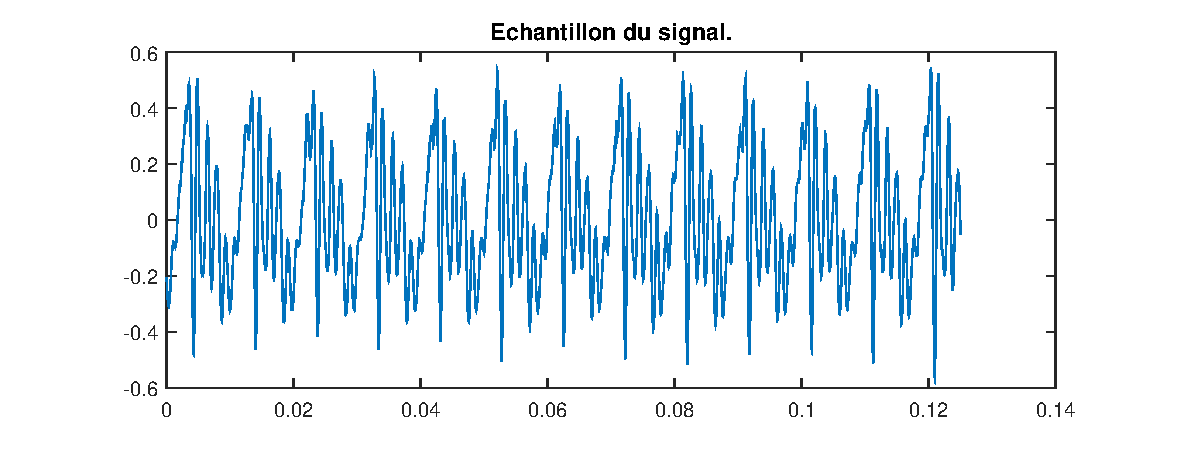
\includegraphics[width=\textwidth]{images/cadence_signal.eps}
	% Title: glps_renderer figure
% Creator: GL2PS 1.3.8, (C) 1999-2012 C. Geuzaine
% For: Octave
% CreationDate: Thu Nov  9 17:04:08 2017
\begin{pgfpicture}
\pgfsetlinewidth{0.01pt}
\color[rgb]{1.000000,1.000000,1.000000}
\pgfpathmoveto{\pgfpoint{65.000015pt}{129.000000pt}}
\pgflineto{\pgfpoint{452.500000pt}{26.977867pt}}
\pgflineto{\pgfpoint{65.000015pt}{26.977867pt}}
\pgfpathclose
\pgfusepath{fill,stroke}
\pgfpathmoveto{\pgfpoint{65.000015pt}{129.000000pt}}
\pgflineto{\pgfpoint{452.500000pt}{129.000000pt}}
\pgflineto{\pgfpoint{452.500000pt}{26.977867pt}}
\pgfpathclose
\pgfusepath{fill,stroke}
\color[rgb]{0.000000,0.000000,0.000000}
\pgfsetlinewidth{0.500000pt}
\pgfsetdash{{16pt}{0pt}}{0pt}
\pgfpathmoveto{\pgfpoint{452.500000pt}{26.977867pt}}
\pgflineto{\pgfpoint{65.000015pt}{26.977867pt}}
\pgfusepath{stroke}
\pgfpathmoveto{\pgfpoint{452.500000pt}{129.000000pt}}
\pgflineto{\pgfpoint{65.000015pt}{129.000000pt}}
\pgfusepath{stroke}
\pgfpathmoveto{\pgfpoint{65.000015pt}{129.000000pt}}
\pgflineto{\pgfpoint{65.000015pt}{26.977867pt}}
\pgfusepath{stroke}
\pgfpathmoveto{\pgfpoint{452.500000pt}{129.000000pt}}
\pgflineto{\pgfpoint{452.500000pt}{26.977867pt}}
\pgfusepath{stroke}
\pgfsetdash{{0pt}{3pt}{1pt}{3pt}{1pt}{3pt}{1pt}{3pt}{1pt}{0pt}}{0pt}
\pgfpathmoveto{\pgfpoint{65.000015pt}{129.000000pt}}
\pgflineto{\pgfpoint{65.000015pt}{26.977867pt}}
\pgfusepath{stroke}
\pgfpathmoveto{\pgfpoint{161.875000pt}{129.000000pt}}
\pgflineto{\pgfpoint{161.875000pt}{26.977867pt}}
\pgfusepath{stroke}
\pgfpathmoveto{\pgfpoint{258.750000pt}{129.000000pt}}
\pgflineto{\pgfpoint{258.750000pt}{26.977867pt}}
\pgfusepath{stroke}
\pgfpathmoveto{\pgfpoint{355.625000pt}{129.000000pt}}
\pgflineto{\pgfpoint{355.625000pt}{26.977867pt}}
\pgfusepath{stroke}
\pgfpathmoveto{\pgfpoint{452.500000pt}{129.000000pt}}
\pgflineto{\pgfpoint{452.500000pt}{26.977867pt}}
\pgfusepath{stroke}
\pgfsetdash{{16pt}{0pt}}{0pt}
\pgfpathmoveto{\pgfpoint{65.000015pt}{30.853714pt}}
\pgflineto{\pgfpoint{65.000015pt}{26.977867pt}}
\pgfusepath{stroke}
\pgfpathmoveto{\pgfpoint{65.000015pt}{125.124161pt}}
\pgflineto{\pgfpoint{65.000015pt}{129.000000pt}}
\pgfusepath{stroke}
\pgfpathmoveto{\pgfpoint{161.875000pt}{30.853714pt}}
\pgflineto{\pgfpoint{161.875000pt}{26.977867pt}}
\pgfusepath{stroke}
\pgfpathmoveto{\pgfpoint{161.875000pt}{125.124161pt}}
\pgflineto{\pgfpoint{161.875000pt}{129.000000pt}}
\pgfusepath{stroke}
\pgfpathmoveto{\pgfpoint{258.750000pt}{30.853714pt}}
\pgflineto{\pgfpoint{258.750000pt}{26.977867pt}}
\pgfusepath{stroke}
\pgfpathmoveto{\pgfpoint{258.750000pt}{125.124161pt}}
\pgflineto{\pgfpoint{258.750000pt}{129.000000pt}}
\pgfusepath{stroke}
\pgfpathmoveto{\pgfpoint{355.625000pt}{30.853714pt}}
\pgflineto{\pgfpoint{355.625000pt}{26.977867pt}}
\pgfusepath{stroke}
\pgfpathmoveto{\pgfpoint{355.625000pt}{125.124161pt}}
\pgflineto{\pgfpoint{355.625000pt}{129.000000pt}}
\pgfusepath{stroke}
\pgfpathmoveto{\pgfpoint{452.500000pt}{30.853714pt}}
\pgflineto{\pgfpoint{452.500000pt}{26.977867pt}}
\pgfusepath{stroke}
\pgfpathmoveto{\pgfpoint{452.500000pt}{125.124161pt}}
\pgflineto{\pgfpoint{452.500000pt}{129.000000pt}}
\pgfusepath{stroke}
{
\pgftransformshift{\pgfpoint{65.000015pt}{21.976788pt}}
\pgfnode{rectangle}{north}{\fontsize{10}{0}\selectfont\textcolor[rgb]{0,0,0}{{0}}}{}{\pgfusepath{discard}}}
{
\pgftransformshift{\pgfpoint{161.875015pt}{21.976788pt}}
\pgfnode{rectangle}{north}{\fontsize{10}{0}\selectfont\textcolor[rgb]{0,0,0}{{0.005}}}{}{\pgfusepath{discard}}}
{
\pgftransformshift{\pgfpoint{258.750031pt}{21.976788pt}}
\pgfnode{rectangle}{north}{\fontsize{10}{0}\selectfont\textcolor[rgb]{0,0,0}{{0.01}}}{}{\pgfusepath{discard}}}
{
\pgftransformshift{\pgfpoint{355.625031pt}{21.976788pt}}
\pgfnode{rectangle}{north}{\fontsize{10}{0}\selectfont\textcolor[rgb]{0,0,0}{{0.015}}}{}{\pgfusepath{discard}}}
{
\pgftransformshift{\pgfpoint{452.500031pt}{21.976788pt}}
\pgfnode{rectangle}{north}{\fontsize{10}{0}\selectfont\textcolor[rgb]{0,0,0}{{0.02}}}{}{\pgfusepath{discard}}}
\pgfsetdash{{0pt}{3pt}{1pt}{3pt}{1pt}{3pt}{1pt}{3pt}{1pt}{0pt}}{0pt}
\pgfpathmoveto{\pgfpoint{452.500000pt}{26.977867pt}}
\pgflineto{\pgfpoint{65.000015pt}{26.977867pt}}
\pgfusepath{stroke}
\pgfpathmoveto{\pgfpoint{452.500000pt}{39.730637pt}}
\pgflineto{\pgfpoint{65.000015pt}{39.730637pt}}
\pgfusepath{stroke}
\pgfpathmoveto{\pgfpoint{452.500000pt}{52.483402pt}}
\pgflineto{\pgfpoint{65.000015pt}{52.483402pt}}
\pgfusepath{stroke}
\pgfpathmoveto{\pgfpoint{452.500000pt}{65.236168pt}}
\pgflineto{\pgfpoint{65.000015pt}{65.236168pt}}
\pgfusepath{stroke}
\pgfpathmoveto{\pgfpoint{452.500000pt}{77.988937pt}}
\pgflineto{\pgfpoint{65.000015pt}{77.988937pt}}
\pgfusepath{stroke}
\pgfpathmoveto{\pgfpoint{452.500000pt}{90.741707pt}}
\pgflineto{\pgfpoint{65.000015pt}{90.741707pt}}
\pgfusepath{stroke}
\pgfpathmoveto{\pgfpoint{452.500000pt}{103.494476pt}}
\pgflineto{\pgfpoint{65.000015pt}{103.494476pt}}
\pgfusepath{stroke}
\pgfpathmoveto{\pgfpoint{452.500000pt}{116.247238pt}}
\pgflineto{\pgfpoint{65.000015pt}{116.247238pt}}
\pgfusepath{stroke}
\pgfpathmoveto{\pgfpoint{452.500000pt}{129.000000pt}}
\pgflineto{\pgfpoint{65.000015pt}{129.000000pt}}
\pgfusepath{stroke}
\pgfsetdash{{16pt}{0pt}}{0pt}
\pgfpathmoveto{\pgfpoint{68.870026pt}{26.977867pt}}
\pgflineto{\pgfpoint{65.000015pt}{26.977867pt}}
\pgfusepath{stroke}
\pgfpathmoveto{\pgfpoint{448.630005pt}{26.977867pt}}
\pgflineto{\pgfpoint{452.500000pt}{26.977867pt}}
\pgfusepath{stroke}
\pgfpathmoveto{\pgfpoint{68.870026pt}{39.730637pt}}
\pgflineto{\pgfpoint{65.000015pt}{39.730637pt}}
\pgfusepath{stroke}
\pgfpathmoveto{\pgfpoint{448.630005pt}{39.730637pt}}
\pgflineto{\pgfpoint{452.500000pt}{39.730637pt}}
\pgfusepath{stroke}
\pgfpathmoveto{\pgfpoint{68.870026pt}{52.483402pt}}
\pgflineto{\pgfpoint{65.000015pt}{52.483402pt}}
\pgfusepath{stroke}
\pgfpathmoveto{\pgfpoint{448.630005pt}{52.483402pt}}
\pgflineto{\pgfpoint{452.500000pt}{52.483402pt}}
\pgfusepath{stroke}
\pgfpathmoveto{\pgfpoint{68.870026pt}{65.236168pt}}
\pgflineto{\pgfpoint{65.000015pt}{65.236168pt}}
\pgfusepath{stroke}
\pgfpathmoveto{\pgfpoint{448.630005pt}{65.236168pt}}
\pgflineto{\pgfpoint{452.500000pt}{65.236168pt}}
\pgfusepath{stroke}
\pgfpathmoveto{\pgfpoint{68.870026pt}{77.988937pt}}
\pgflineto{\pgfpoint{65.000015pt}{77.988937pt}}
\pgfusepath{stroke}
\pgfpathmoveto{\pgfpoint{448.630005pt}{77.988937pt}}
\pgflineto{\pgfpoint{452.500000pt}{77.988937pt}}
\pgfusepath{stroke}
\pgfpathmoveto{\pgfpoint{68.870026pt}{90.741707pt}}
\pgflineto{\pgfpoint{65.000015pt}{90.741707pt}}
\pgfusepath{stroke}
\pgfpathmoveto{\pgfpoint{448.630005pt}{90.741707pt}}
\pgflineto{\pgfpoint{452.500000pt}{90.741707pt}}
\pgfusepath{stroke}
\pgfpathmoveto{\pgfpoint{68.870026pt}{103.494476pt}}
\pgflineto{\pgfpoint{65.000015pt}{103.494476pt}}
\pgfusepath{stroke}
\pgfpathmoveto{\pgfpoint{448.630005pt}{103.494476pt}}
\pgflineto{\pgfpoint{452.500000pt}{103.494476pt}}
\pgfusepath{stroke}
\pgfpathmoveto{\pgfpoint{68.870026pt}{116.247238pt}}
\pgflineto{\pgfpoint{65.000015pt}{116.247238pt}}
\pgfusepath{stroke}
\pgfpathmoveto{\pgfpoint{448.630005pt}{116.247238pt}}
\pgflineto{\pgfpoint{452.500000pt}{116.247238pt}}
\pgfusepath{stroke}
\pgfpathmoveto{\pgfpoint{68.870026pt}{129.000000pt}}
\pgflineto{\pgfpoint{65.000015pt}{129.000000pt}}
\pgfusepath{stroke}
\pgfpathmoveto{\pgfpoint{448.630005pt}{129.000000pt}}
\pgflineto{\pgfpoint{452.500000pt}{129.000000pt}}
\pgfusepath{stroke}
{
\pgftransformshift{\pgfpoint{60.006454pt}{26.977875pt}}
\pgfnode{rectangle}{east}{\fontsize{10}{0}\selectfont\textcolor[rgb]{0,0,0}{{-0.8}}}{}{\pgfusepath{discard}}}
{
\pgftransformshift{\pgfpoint{60.006454pt}{39.730640pt}}
\pgfnode{rectangle}{east}{\fontsize{10}{0}\selectfont\textcolor[rgb]{0,0,0}{{-0.6}}}{}{\pgfusepath{discard}}}
{
\pgftransformshift{\pgfpoint{60.006454pt}{52.483406pt}}
\pgfnode{rectangle}{east}{\fontsize{10}{0}\selectfont\textcolor[rgb]{0,0,0}{{-0.4}}}{}{\pgfusepath{discard}}}
{
\pgftransformshift{\pgfpoint{60.006454pt}{65.236176pt}}
\pgfnode{rectangle}{east}{\fontsize{10}{0}\selectfont\textcolor[rgb]{0,0,0}{{-0.2}}}{}{\pgfusepath{discard}}}
{
\pgftransformshift{\pgfpoint{60.006454pt}{77.988937pt}}
\pgfnode{rectangle}{east}{\fontsize{10}{0}\selectfont\textcolor[rgb]{0,0,0}{{0}}}{}{\pgfusepath{discard}}}
{
\pgftransformshift{\pgfpoint{60.006454pt}{90.741707pt}}
\pgfnode{rectangle}{east}{\fontsize{10}{0}\selectfont\textcolor[rgb]{0,0,0}{{0.2}}}{}{\pgfusepath{discard}}}
{
\pgftransformshift{\pgfpoint{60.006454pt}{103.494469pt}}
\pgfnode{rectangle}{east}{\fontsize{10}{0}\selectfont\textcolor[rgb]{0,0,0}{{0.4}}}{}{\pgfusepath{discard}}}
{
\pgftransformshift{\pgfpoint{60.006454pt}{116.247238pt}}
\pgfnode{rectangle}{east}{\fontsize{10}{0}\selectfont\textcolor[rgb]{0,0,0}{{0.6}}}{}{\pgfusepath{discard}}}
{
\pgftransformshift{\pgfpoint{60.006454pt}{129.000000pt}}
\pgfnode{rectangle}{east}{\fontsize{10}{0}\selectfont\textcolor[rgb]{0,0,0}{{0.8}}}{}{\pgfusepath{discard}}}
{
\pgftransformshift{\pgfpoint{258.750031pt}{10.976791pt}}
\pgfnode{rectangle}{north}{\fontsize{10}{0}\selectfont\textcolor[rgb]{0,0,0}{{Temps (s)}}}{}{\pgfusepath{discard}}}
\color[rgb]{0.000000,0.000000,1.000000}
\pgfsetdash{}{0pt}
\pgfpathmoveto{\pgfpoint{66.210953pt}{62.310677pt}}
\pgflineto{\pgfpoint{65.000015pt}{64.651619pt}}
\pgfusepath{stroke}
\pgfpathmoveto{\pgfpoint{67.421890pt}{60.676109pt}}
\pgflineto{\pgfpoint{66.210953pt}{62.310677pt}}
\pgfusepath{stroke}
\pgfpathmoveto{\pgfpoint{68.632828pt}{59.623367pt}}
\pgflineto{\pgfpoint{67.421890pt}{60.676109pt}}
\pgfusepath{stroke}
\pgfpathmoveto{\pgfpoint{69.843765pt}{58.473328pt}}
\pgflineto{\pgfpoint{68.632828pt}{59.623367pt}}
\pgfusepath{stroke}
\pgfpathmoveto{\pgfpoint{71.054703pt}{58.313763pt}}
\pgflineto{\pgfpoint{69.843765pt}{58.473328pt}}
\pgfusepath{stroke}
\pgfpathmoveto{\pgfpoint{72.265640pt}{58.854729pt}}
\pgflineto{\pgfpoint{71.054703pt}{58.313763pt}}
\pgfusepath{stroke}
\pgfpathmoveto{\pgfpoint{73.476578pt}{59.329533pt}}
\pgflineto{\pgfpoint{72.265640pt}{58.854729pt}}
\pgfusepath{stroke}
\pgfpathmoveto{\pgfpoint{74.687515pt}{60.220764pt}}
\pgflineto{\pgfpoint{73.476578pt}{59.329533pt}}
\pgfusepath{stroke}
\pgfpathmoveto{\pgfpoint{75.898453pt}{61.857281pt}}
\pgflineto{\pgfpoint{74.687515pt}{60.220764pt}}
\pgfusepath{stroke}
\pgfpathmoveto{\pgfpoint{77.109375pt}{63.694225pt}}
\pgflineto{\pgfpoint{75.898453pt}{61.857281pt}}
\pgfusepath{stroke}
\pgfpathmoveto{\pgfpoint{78.320328pt}{65.638199pt}}
\pgflineto{\pgfpoint{77.109375pt}{63.694225pt}}
\pgfusepath{stroke}
\pgfpathmoveto{\pgfpoint{79.531265pt}{68.039459pt}}
\pgflineto{\pgfpoint{78.320328pt}{65.638199pt}}
\pgfusepath{stroke}
\pgfpathmoveto{\pgfpoint{80.742203pt}{69.853058pt}}
\pgflineto{\pgfpoint{79.531265pt}{68.039459pt}}
\pgfusepath{stroke}
\pgfpathmoveto{\pgfpoint{81.953140pt}{71.129578pt}}
\pgflineto{\pgfpoint{80.742203pt}{69.853058pt}}
\pgfusepath{stroke}
\pgfpathmoveto{\pgfpoint{83.164078pt}{72.055832pt}}
\pgflineto{\pgfpoint{81.953140pt}{71.129578pt}}
\pgfusepath{stroke}
\pgfpathmoveto{\pgfpoint{84.375015pt}{72.590965pt}}
\pgflineto{\pgfpoint{83.164078pt}{72.055832pt}}
\pgfusepath{stroke}
\pgfpathmoveto{\pgfpoint{85.585953pt}{73.085228pt}}
\pgflineto{\pgfpoint{84.375015pt}{72.590965pt}}
\pgfusepath{stroke}
\pgfpathmoveto{\pgfpoint{86.796875pt}{72.999603pt}}
\pgflineto{\pgfpoint{85.585953pt}{73.085228pt}}
\pgfusepath{stroke}
\pgfpathmoveto{\pgfpoint{88.007828pt}{72.906204pt}}
\pgflineto{\pgfpoint{86.796875pt}{72.999603pt}}
\pgfusepath{stroke}
\pgfpathmoveto{\pgfpoint{89.218765pt}{72.799171pt}}
\pgflineto{\pgfpoint{88.007828pt}{72.906204pt}}
\pgfusepath{stroke}
\pgfpathmoveto{\pgfpoint{90.429688pt}{72.205673pt}}
\pgflineto{\pgfpoint{89.218765pt}{72.799171pt}}
\pgfusepath{stroke}
\pgfpathmoveto{\pgfpoint{91.640640pt}{71.921570pt}}
\pgflineto{\pgfpoint{90.429688pt}{72.205673pt}}
\pgfusepath{stroke}
\pgfpathmoveto{\pgfpoint{92.851578pt}{72.460587pt}}
\pgflineto{\pgfpoint{91.640640pt}{71.921570pt}}
\pgfusepath{stroke}
\pgfpathmoveto{\pgfpoint{94.062500pt}{72.912041pt}}
\pgflineto{\pgfpoint{92.851578pt}{72.460587pt}}
\pgfusepath{stroke}
\pgfpathmoveto{\pgfpoint{95.273453pt}{73.764351pt}}
\pgflineto{\pgfpoint{94.062500pt}{72.912041pt}}
\pgfusepath{stroke}
\pgfpathmoveto{\pgfpoint{96.484390pt}{75.852318pt}}
\pgflineto{\pgfpoint{95.273453pt}{73.764351pt}}
\pgfusepath{stroke}
\pgfpathmoveto{\pgfpoint{97.695328pt}{77.934448pt}}
\pgflineto{\pgfpoint{96.484390pt}{75.852318pt}}
\pgfusepath{stroke}
\pgfpathmoveto{\pgfpoint{98.906265pt}{79.053352pt}}
\pgflineto{\pgfpoint{97.695328pt}{77.934448pt}}
\pgfusepath{stroke}
\pgfpathmoveto{\pgfpoint{100.117203pt}{80.399933pt}}
\pgflineto{\pgfpoint{98.906265pt}{79.053352pt}}
\pgfusepath{stroke}
\pgfpathmoveto{\pgfpoint{101.328140pt}{82.520981pt}}
\pgflineto{\pgfpoint{100.117203pt}{80.399933pt}}
\pgfusepath{stroke}
\pgfpathmoveto{\pgfpoint{102.539078pt}{83.651558pt}}
\pgflineto{\pgfpoint{101.328140pt}{82.520981pt}}
\pgfusepath{stroke}
\pgfpathmoveto{\pgfpoint{103.750015pt}{84.667328pt}}
\pgflineto{\pgfpoint{102.539078pt}{83.651558pt}}
\pgfusepath{stroke}
\pgfpathmoveto{\pgfpoint{104.960953pt}{86.157898pt}}
\pgflineto{\pgfpoint{103.750015pt}{84.667328pt}}
\pgfusepath{stroke}
\pgfpathmoveto{\pgfpoint{106.171890pt}{86.519844pt}}
\pgflineto{\pgfpoint{104.960953pt}{86.157898pt}}
\pgfusepath{stroke}
\pgfpathmoveto{\pgfpoint{107.382828pt}{86.323303pt}}
\pgflineto{\pgfpoint{106.171890pt}{86.519844pt}}
\pgfusepath{stroke}
\pgfpathmoveto{\pgfpoint{108.593765pt}{87.321556pt}}
\pgflineto{\pgfpoint{107.382828pt}{86.323303pt}}
\pgfusepath{stroke}
\pgfpathmoveto{\pgfpoint{109.804703pt}{89.502930pt}}
\pgflineto{\pgfpoint{108.593765pt}{87.321556pt}}
\pgfusepath{stroke}
\pgfpathmoveto{\pgfpoint{111.015640pt}{91.244530pt}}
\pgflineto{\pgfpoint{109.804703pt}{89.502930pt}}
\pgfusepath{stroke}
\pgfpathmoveto{\pgfpoint{112.226578pt}{90.902046pt}}
\pgflineto{\pgfpoint{111.015640pt}{91.244530pt}}
\pgfusepath{stroke}
\pgfpathmoveto{\pgfpoint{113.437500pt}{92.030678pt}}
\pgflineto{\pgfpoint{112.226578pt}{90.902046pt}}
\pgfusepath{stroke}
\pgfpathmoveto{\pgfpoint{114.648453pt}{95.725983pt}}
\pgflineto{\pgfpoint{113.437500pt}{92.030678pt}}
\pgfusepath{stroke}
\pgfpathmoveto{\pgfpoint{115.859390pt}{95.560577pt}}
\pgflineto{\pgfpoint{114.648453pt}{95.725983pt}}
\pgfusepath{stroke}
\pgfpathmoveto{\pgfpoint{117.070328pt}{95.519714pt}}
\pgflineto{\pgfpoint{115.859390pt}{95.560577pt}}
\pgfusepath{stroke}
\pgfpathmoveto{\pgfpoint{118.281265pt}{99.685921pt}}
\pgflineto{\pgfpoint{117.070328pt}{95.519714pt}}
\pgfusepath{stroke}
\pgfpathmoveto{\pgfpoint{119.492203pt}{98.720749pt}}
\pgflineto{\pgfpoint{118.281265pt}{99.685921pt}}
\pgfusepath{stroke}
\pgfpathmoveto{\pgfpoint{120.703125pt}{97.541519pt}}
\pgflineto{\pgfpoint{119.492203pt}{98.720749pt}}
\pgfusepath{stroke}
\pgfpathmoveto{\pgfpoint{121.914078pt}{102.359612pt}}
\pgflineto{\pgfpoint{120.703125pt}{97.541519pt}}
\pgfusepath{stroke}
\pgfpathmoveto{\pgfpoint{123.125015pt}{102.805229pt}}
\pgflineto{\pgfpoint{121.914078pt}{102.359612pt}}
\pgfusepath{stroke}
\pgfpathmoveto{\pgfpoint{124.335945pt}{99.903862pt}}
\pgflineto{\pgfpoint{123.125015pt}{102.805229pt}}
\pgfusepath{stroke}
\pgfpathmoveto{\pgfpoint{125.546890pt}{101.483948pt}}
\pgflineto{\pgfpoint{124.335945pt}{99.903862pt}}
\pgfusepath{stroke}
\pgfpathmoveto{\pgfpoint{126.757820pt}{103.822945pt}}
\pgflineto{\pgfpoint{125.546890pt}{101.483948pt}}
\pgfusepath{stroke}
\pgfpathmoveto{\pgfpoint{127.968765pt}{103.223602pt}}
\pgflineto{\pgfpoint{126.757820pt}{103.822945pt}}
\pgfusepath{stroke}
\pgfpathmoveto{\pgfpoint{129.179703pt}{103.735374pt}}
\pgflineto{\pgfpoint{127.968765pt}{103.223602pt}}
\pgfusepath{stroke}
\pgfpathmoveto{\pgfpoint{130.390640pt}{106.806030pt}}
\pgflineto{\pgfpoint{129.179703pt}{103.735374pt}}
\pgfusepath{stroke}
\pgfpathmoveto{\pgfpoint{131.601562pt}{107.994987pt}}
\pgflineto{\pgfpoint{130.390640pt}{106.806030pt}}
\pgfusepath{stroke}
\pgfpathmoveto{\pgfpoint{132.812515pt}{107.753693pt}}
\pgflineto{\pgfpoint{131.601562pt}{107.994987pt}}
\pgfusepath{stroke}
\pgfpathmoveto{\pgfpoint{134.023453pt}{108.569031pt}}
\pgflineto{\pgfpoint{132.812515pt}{107.753693pt}}
\pgfusepath{stroke}
\pgfpathmoveto{\pgfpoint{135.234375pt}{107.596077pt}}
\pgflineto{\pgfpoint{134.023453pt}{108.569031pt}}
\pgfusepath{stroke}
\pgfpathmoveto{\pgfpoint{136.445328pt}{103.346191pt}}
\pgflineto{\pgfpoint{135.234375pt}{107.596077pt}}
\pgfusepath{stroke}
\pgfpathmoveto{\pgfpoint{137.656265pt}{99.744301pt}}
\pgflineto{\pgfpoint{136.445328pt}{103.346191pt}}
\pgfusepath{stroke}
\pgfpathmoveto{\pgfpoint{138.867203pt}{96.175484pt}}
\pgflineto{\pgfpoint{137.656265pt}{99.744301pt}}
\pgfusepath{stroke}
\pgfpathmoveto{\pgfpoint{140.078125pt}{87.284584pt}}
\pgflineto{\pgfpoint{138.867203pt}{96.175484pt}}
\pgfusepath{stroke}
\pgfpathmoveto{\pgfpoint{141.289078pt}{75.733620pt}}
\pgflineto{\pgfpoint{140.078125pt}{87.284584pt}}
\pgfusepath{stroke}
\pgfpathmoveto{\pgfpoint{142.500015pt}{66.934181pt}}
\pgflineto{\pgfpoint{141.289078pt}{75.733620pt}}
\pgfusepath{stroke}
\pgfpathmoveto{\pgfpoint{143.710938pt}{61.341610pt}}
\pgflineto{\pgfpoint{142.500015pt}{66.934181pt}}
\pgfusepath{stroke}
\pgfpathmoveto{\pgfpoint{144.921875pt}{54.143661pt}}
\pgflineto{\pgfpoint{143.710938pt}{61.341610pt}}
\pgfusepath{stroke}
\pgfpathmoveto{\pgfpoint{146.132828pt}{47.798023pt}}
\pgflineto{\pgfpoint{144.921875pt}{54.143661pt}}
\pgfusepath{stroke}
\pgfpathmoveto{\pgfpoint{147.343781pt}{47.552841pt}}
\pgflineto{\pgfpoint{146.132828pt}{47.798023pt}}
\pgfusepath{stroke}
\pgfpathmoveto{\pgfpoint{148.554688pt}{49.640808pt}}
\pgflineto{\pgfpoint{147.343781pt}{47.552841pt}}
\pgfusepath{stroke}
\pgfpathmoveto{\pgfpoint{149.765640pt}{55.396832pt}}
\pgflineto{\pgfpoint{148.554688pt}{49.640808pt}}
\pgfusepath{stroke}
\pgfpathmoveto{\pgfpoint{150.976578pt}{65.996246pt}}
\pgflineto{\pgfpoint{149.765640pt}{55.396832pt}}
\pgfusepath{stroke}
\pgfpathmoveto{\pgfpoint{152.187500pt}{75.589622pt}}
\pgflineto{\pgfpoint{150.976578pt}{65.996246pt}}
\pgfusepath{stroke}
\pgfpathmoveto{\pgfpoint{153.398438pt}{83.725502pt}}
\pgflineto{\pgfpoint{152.187500pt}{75.589622pt}}
\pgfusepath{stroke}
\pgfpathmoveto{\pgfpoint{154.609390pt}{95.410736pt}}
\pgflineto{\pgfpoint{153.398438pt}{83.725502pt}}
\pgfusepath{stroke}
\pgfpathmoveto{\pgfpoint{155.820328pt}{105.428322pt}}
\pgflineto{\pgfpoint{154.609390pt}{95.410736pt}}
\pgfusepath{stroke}
\pgfpathmoveto{\pgfpoint{157.031250pt}{108.946541pt}}
\pgflineto{\pgfpoint{155.820328pt}{105.428322pt}}
\pgfusepath{stroke}
\pgfpathmoveto{\pgfpoint{158.242188pt}{110.310631pt}}
\pgflineto{\pgfpoint{157.031250pt}{108.946541pt}}
\pgfusepath{stroke}
\pgfpathmoveto{\pgfpoint{159.453140pt}{109.487503pt}}
\pgflineto{\pgfpoint{158.242188pt}{110.310631pt}}
\pgfusepath{stroke}
\pgfpathmoveto{\pgfpoint{160.664078pt}{106.241714pt}}
\pgflineto{\pgfpoint{159.453140pt}{109.487503pt}}
\pgfusepath{stroke}
\pgfpathmoveto{\pgfpoint{161.875000pt}{101.602646pt}}
\pgflineto{\pgfpoint{160.664078pt}{106.241714pt}}
\pgfusepath{stroke}
\pgfpathmoveto{\pgfpoint{163.085953pt}{94.287949pt}}
\pgflineto{\pgfpoint{161.875000pt}{101.602646pt}}
\pgfusepath{stroke}
\pgfpathmoveto{\pgfpoint{164.296890pt}{86.120926pt}}
\pgflineto{\pgfpoint{163.085953pt}{94.287949pt}}
\pgfusepath{stroke}
\pgfpathmoveto{\pgfpoint{165.507812pt}{80.588684pt}}
\pgflineto{\pgfpoint{164.296890pt}{86.120926pt}}
\pgfusepath{stroke}
\pgfpathmoveto{\pgfpoint{166.718750pt}{76.404961pt}}
\pgflineto{\pgfpoint{165.507812pt}{80.588684pt}}
\pgfusepath{stroke}
\pgfpathmoveto{\pgfpoint{167.929703pt}{72.569557pt}}
\pgflineto{\pgfpoint{166.718750pt}{76.404961pt}}
\pgfusepath{stroke}
\pgfpathmoveto{\pgfpoint{169.140656pt}{70.228615pt}}
\pgflineto{\pgfpoint{167.929703pt}{72.569557pt}}
\pgfusepath{stroke}
\pgfpathmoveto{\pgfpoint{170.351562pt}{67.722275pt}}
\pgflineto{\pgfpoint{169.140656pt}{70.228615pt}}
\pgfusepath{stroke}
\pgfpathmoveto{\pgfpoint{171.562515pt}{66.478836pt}}
\pgflineto{\pgfpoint{170.351562pt}{67.722275pt}}
\pgfusepath{stroke}
\pgfpathmoveto{\pgfpoint{172.773453pt}{67.093742pt}}
\pgflineto{\pgfpoint{171.562515pt}{66.478836pt}}
\pgfusepath{stroke}
\pgfpathmoveto{\pgfpoint{173.984390pt}{66.770721pt}}
\pgflineto{\pgfpoint{172.773453pt}{67.093742pt}}
\pgfusepath{stroke}
\pgfpathmoveto{\pgfpoint{175.195312pt}{65.881439pt}}
\pgflineto{\pgfpoint{173.984390pt}{66.770721pt}}
\pgfusepath{stroke}
\pgfpathmoveto{\pgfpoint{176.406265pt}{65.638199pt}}
\pgflineto{\pgfpoint{175.195312pt}{65.881439pt}}
\pgfusepath{stroke}
\pgfpathmoveto{\pgfpoint{177.617203pt}{66.401001pt}}
\pgflineto{\pgfpoint{176.406265pt}{65.638199pt}}
\pgfusepath{stroke}
\pgfpathmoveto{\pgfpoint{178.828125pt}{67.996651pt}}
\pgflineto{\pgfpoint{177.617203pt}{66.401001pt}}
\pgfusepath{stroke}
\pgfpathmoveto{\pgfpoint{180.039062pt}{70.148834pt}}
\pgflineto{\pgfpoint{178.828125pt}{67.996651pt}}
\pgfusepath{stroke}
\pgfpathmoveto{\pgfpoint{181.250015pt}{72.768044pt}}
\pgflineto{\pgfpoint{180.039062pt}{70.148834pt}}
\pgfusepath{stroke}
\pgfpathmoveto{\pgfpoint{182.460953pt}{76.389397pt}}
\pgflineto{\pgfpoint{181.250015pt}{72.768044pt}}
\pgfusepath{stroke}
\pgfpathmoveto{\pgfpoint{183.671875pt}{81.606400pt}}
\pgflineto{\pgfpoint{182.460953pt}{76.389397pt}}
\pgfusepath{stroke}
\pgfpathmoveto{\pgfpoint{184.882828pt}{87.218430pt}}
\pgflineto{\pgfpoint{183.671875pt}{81.606400pt}}
\pgfusepath{stroke}
\pgfpathmoveto{\pgfpoint{186.093765pt}{92.375107pt}}
\pgflineto{\pgfpoint{184.882828pt}{87.218430pt}}
\pgfusepath{stroke}
\pgfpathmoveto{\pgfpoint{187.304703pt}{96.078186pt}}
\pgflineto{\pgfpoint{186.093765pt}{92.375107pt}}
\pgfusepath{stroke}
\pgfpathmoveto{\pgfpoint{188.515625pt}{98.004646pt}}
\pgflineto{\pgfpoint{187.304703pt}{96.078186pt}}
\pgfusepath{stroke}
\pgfpathmoveto{\pgfpoint{189.726578pt}{99.129387pt}}
\pgflineto{\pgfpoint{188.515625pt}{98.004646pt}}
\pgfusepath{stroke}
\pgfpathmoveto{\pgfpoint{190.937515pt}{98.613716pt}}
\pgflineto{\pgfpoint{189.726578pt}{99.129387pt}}
\pgfusepath{stroke}
\pgfpathmoveto{\pgfpoint{192.148438pt}{96.078186pt}}
\pgflineto{\pgfpoint{190.937515pt}{98.613716pt}}
\pgfusepath{stroke}
\pgfpathmoveto{\pgfpoint{193.359390pt}{91.978142pt}}
\pgflineto{\pgfpoint{192.148438pt}{96.078186pt}}
\pgfusepath{stroke}
\pgfpathmoveto{\pgfpoint{194.570328pt}{86.940163pt}}
\pgflineto{\pgfpoint{193.359390pt}{91.978142pt}}
\pgfusepath{stroke}
\pgfpathmoveto{\pgfpoint{195.781265pt}{81.256134pt}}
\pgflineto{\pgfpoint{194.570328pt}{86.940163pt}}
\pgfusepath{stroke}
\pgfpathmoveto{\pgfpoint{196.992203pt}{75.431999pt}}
\pgflineto{\pgfpoint{195.781265pt}{81.256134pt}}
\pgfusepath{stroke}
\pgfpathmoveto{\pgfpoint{198.203125pt}{70.106026pt}}
\pgflineto{\pgfpoint{196.992203pt}{75.431999pt}}
\pgfusepath{stroke}
\pgfpathmoveto{\pgfpoint{199.414078pt}{65.764679pt}}
\pgflineto{\pgfpoint{198.203125pt}{70.106026pt}}
\pgfusepath{stroke}
\pgfpathmoveto{\pgfpoint{200.625015pt}{63.254448pt}}
\pgflineto{\pgfpoint{199.414078pt}{65.764679pt}}
\pgfusepath{stroke}
\pgfpathmoveto{\pgfpoint{201.835938pt}{62.598675pt}}
\pgflineto{\pgfpoint{200.625015pt}{63.254448pt}}
\pgfusepath{stroke}
\pgfpathmoveto{\pgfpoint{203.046890pt}{63.071533pt}}
\pgflineto{\pgfpoint{201.835938pt}{62.598675pt}}
\pgfusepath{stroke}
\pgfpathmoveto{\pgfpoint{204.257828pt}{64.412270pt}}
\pgflineto{\pgfpoint{203.046890pt}{63.071533pt}}
\pgfusepath{stroke}
\pgfpathmoveto{\pgfpoint{205.468750pt}{66.881638pt}}
\pgflineto{\pgfpoint{204.257828pt}{64.412270pt}}
\pgfusepath{stroke}
\pgfpathmoveto{\pgfpoint{206.679703pt}{70.102135pt}}
\pgflineto{\pgfpoint{205.468750pt}{66.881638pt}}
\pgfusepath{stroke}
\pgfpathmoveto{\pgfpoint{207.890640pt}{73.939484pt}}
\pgflineto{\pgfpoint{206.679703pt}{70.102135pt}}
\pgfusepath{stroke}
\pgfpathmoveto{\pgfpoint{209.101578pt}{77.848831pt}}
\pgflineto{\pgfpoint{207.890640pt}{73.939484pt}}
\pgfusepath{stroke}
\pgfpathmoveto{\pgfpoint{210.312515pt}{80.931168pt}}
\pgflineto{\pgfpoint{209.101578pt}{77.848831pt}}
\pgfusepath{stroke}
\pgfpathmoveto{\pgfpoint{211.523438pt}{83.643776pt}}
\pgflineto{\pgfpoint{210.312515pt}{80.931168pt}}
\pgfusepath{stroke}
\pgfpathmoveto{\pgfpoint{212.734390pt}{86.298004pt}}
\pgflineto{\pgfpoint{211.523438pt}{83.643776pt}}
\pgfusepath{stroke}
\pgfpathmoveto{\pgfpoint{213.945328pt}{88.296463pt}}
\pgflineto{\pgfpoint{212.734390pt}{86.298004pt}}
\pgfusepath{stroke}
\pgfpathmoveto{\pgfpoint{215.156250pt}{89.641090pt}}
\pgflineto{\pgfpoint{213.945328pt}{88.296463pt}}
\pgfusepath{stroke}
\pgfpathmoveto{\pgfpoint{216.367203pt}{90.222923pt}}
\pgflineto{\pgfpoint{215.156250pt}{89.641090pt}}
\pgfusepath{stroke}
\pgfpathmoveto{\pgfpoint{217.578140pt}{90.261841pt}}
\pgflineto{\pgfpoint{216.367203pt}{90.222923pt}}
\pgfusepath{stroke}
\pgfpathmoveto{\pgfpoint{218.789093pt}{90.102272pt}}
\pgflineto{\pgfpoint{217.578140pt}{90.261841pt}}
\pgfusepath{stroke}
\pgfpathmoveto{\pgfpoint{220.000015pt}{89.277206pt}}
\pgflineto{\pgfpoint{218.789093pt}{90.102272pt}}
\pgfusepath{stroke}
\pgfpathmoveto{\pgfpoint{221.210938pt}{87.434425pt}}
\pgflineto{\pgfpoint{220.000015pt}{89.277206pt}}
\pgfusepath{stroke}
\pgfpathmoveto{\pgfpoint{222.421890pt}{84.538895pt}}
\pgflineto{\pgfpoint{221.210938pt}{87.434425pt}}
\pgfusepath{stroke}
\pgfpathmoveto{\pgfpoint{223.632828pt}{80.656792pt}}
\pgflineto{\pgfpoint{222.421890pt}{84.538895pt}}
\pgfusepath{stroke}
\pgfpathmoveto{\pgfpoint{224.843750pt}{76.831116pt}}
\pgflineto{\pgfpoint{223.632828pt}{80.656792pt}}
\pgfusepath{stroke}
\pgfpathmoveto{\pgfpoint{226.054703pt}{72.491722pt}}
\pgflineto{\pgfpoint{224.843750pt}{76.831116pt}}
\pgfusepath{stroke}
\pgfpathmoveto{\pgfpoint{227.265640pt}{67.410927pt}}
\pgflineto{\pgfpoint{226.054703pt}{72.491722pt}}
\pgfusepath{stroke}
\pgfpathmoveto{\pgfpoint{228.476578pt}{63.203854pt}}
\pgflineto{\pgfpoint{227.265640pt}{67.410927pt}}
\pgfusepath{stroke}
\pgfpathmoveto{\pgfpoint{229.687531pt}{59.461853pt}}
\pgflineto{\pgfpoint{228.476578pt}{63.203854pt}}
\pgfusepath{stroke}
\pgfpathmoveto{\pgfpoint{230.898438pt}{56.480705pt}}
\pgflineto{\pgfpoint{229.687531pt}{59.461853pt}}
\pgfusepath{stroke}
\pgfpathmoveto{\pgfpoint{232.109375pt}{55.233376pt}}
\pgflineto{\pgfpoint{230.898438pt}{56.480705pt}}
\pgfusepath{stroke}
\pgfpathmoveto{\pgfpoint{233.320328pt}{55.009594pt}}
\pgflineto{\pgfpoint{232.109375pt}{55.233376pt}}
\pgfusepath{stroke}
\pgfpathmoveto{\pgfpoint{234.531265pt}{55.801582pt}}
\pgflineto{\pgfpoint{233.320328pt}{55.009594pt}}
\pgfusepath{stroke}
\pgfpathmoveto{\pgfpoint{235.742203pt}{57.642422pt}}
\pgflineto{\pgfpoint{234.531265pt}{55.801582pt}}
\pgfusepath{stroke}
\pgfpathmoveto{\pgfpoint{236.953140pt}{59.798500pt}}
\pgflineto{\pgfpoint{235.742203pt}{57.642422pt}}
\pgfusepath{stroke}
\pgfpathmoveto{\pgfpoint{238.164078pt}{62.565594pt}}
\pgflineto{\pgfpoint{236.953140pt}{59.798500pt}}
\pgfusepath{stroke}
\pgfpathmoveto{\pgfpoint{239.375015pt}{65.669334pt}}
\pgflineto{\pgfpoint{238.164078pt}{62.565594pt}}
\pgfusepath{stroke}
\pgfpathmoveto{\pgfpoint{240.585938pt}{68.428642pt}}
\pgflineto{\pgfpoint{239.375015pt}{65.669334pt}}
\pgfusepath{stroke}
\pgfpathmoveto{\pgfpoint{241.796875pt}{70.826012pt}}
\pgflineto{\pgfpoint{240.585938pt}{68.428642pt}}
\pgfusepath{stroke}
\pgfpathmoveto{\pgfpoint{243.007828pt}{73.114410pt}}
\pgflineto{\pgfpoint{241.796875pt}{70.826012pt}}
\pgfusepath{stroke}
\pgfpathmoveto{\pgfpoint{244.218765pt}{73.820778pt}}
\pgflineto{\pgfpoint{243.007828pt}{73.114410pt}}
\pgfusepath{stroke}
\pgfpathmoveto{\pgfpoint{245.429703pt}{73.316788pt}}
\pgflineto{\pgfpoint{244.218765pt}{73.820778pt}}
\pgfusepath{stroke}
\pgfpathmoveto{\pgfpoint{246.640640pt}{72.847824pt}}
\pgflineto{\pgfpoint{245.429703pt}{73.316788pt}}
\pgfusepath{stroke}
\pgfpathmoveto{\pgfpoint{247.851562pt}{71.238548pt}}
\pgflineto{\pgfpoint{246.640640pt}{72.847824pt}}
\pgfusepath{stroke}
\pgfpathmoveto{\pgfpoint{249.062515pt}{69.092201pt}}
\pgflineto{\pgfpoint{247.851562pt}{71.238548pt}}
\pgfusepath{stroke}
\pgfpathmoveto{\pgfpoint{250.273453pt}{67.364227pt}}
\pgflineto{\pgfpoint{249.062515pt}{69.092201pt}}
\pgfusepath{stroke}
\pgfpathmoveto{\pgfpoint{251.484375pt}{65.420258pt}}
\pgflineto{\pgfpoint{250.273453pt}{67.364227pt}}
\pgfusepath{stroke}
\pgfpathmoveto{\pgfpoint{252.695328pt}{62.946991pt}}
\pgflineto{\pgfpoint{251.484375pt}{65.420258pt}}
\pgfusepath{stroke}
\pgfpathmoveto{\pgfpoint{253.906265pt}{60.716972pt}}
\pgflineto{\pgfpoint{252.695328pt}{62.946991pt}}
\pgfusepath{stroke}
\pgfpathmoveto{\pgfpoint{255.117203pt}{59.374290pt}}
\pgflineto{\pgfpoint{253.906265pt}{60.716972pt}}
\pgfusepath{stroke}
\pgfpathmoveto{\pgfpoint{256.328156pt}{58.307922pt}}
\pgflineto{\pgfpoint{255.117203pt}{59.374290pt}}
\pgfusepath{stroke}
\pgfpathmoveto{\pgfpoint{257.539062pt}{57.319397pt}}
\pgflineto{\pgfpoint{256.328156pt}{58.307922pt}}
\pgfusepath{stroke}
\pgfpathmoveto{\pgfpoint{258.750000pt}{57.585991pt}}
\pgflineto{\pgfpoint{257.539062pt}{57.319397pt}}
\pgfusepath{stroke}
\pgfpathmoveto{\pgfpoint{259.960938pt}{58.374084pt}}
\pgflineto{\pgfpoint{258.750000pt}{57.585991pt}}
\pgfusepath{stroke}
\pgfpathmoveto{\pgfpoint{261.171906pt}{58.987053pt}}
\pgflineto{\pgfpoint{259.960938pt}{58.374084pt}}
\pgfusepath{stroke}
\pgfpathmoveto{\pgfpoint{262.382843pt}{60.370598pt}}
\pgflineto{\pgfpoint{261.171906pt}{58.987053pt}}
\pgfusepath{stroke}
\pgfpathmoveto{\pgfpoint{263.593750pt}{62.141384pt}}
\pgflineto{\pgfpoint{262.382843pt}{60.370598pt}}
\pgfusepath{stroke}
\pgfpathmoveto{\pgfpoint{264.804718pt}{64.118439pt}}
\pgflineto{\pgfpoint{263.593750pt}{62.141384pt}}
\pgfusepath{stroke}
\pgfpathmoveto{\pgfpoint{266.015625pt}{66.358185pt}}
\pgflineto{\pgfpoint{264.804718pt}{64.118439pt}}
\pgfusepath{stroke}
\pgfpathmoveto{\pgfpoint{267.226562pt}{68.703018pt}}
\pgflineto{\pgfpoint{266.015625pt}{66.358185pt}}
\pgfusepath{stroke}
\pgfpathmoveto{\pgfpoint{268.437500pt}{70.767639pt}}
\pgflineto{\pgfpoint{267.226562pt}{68.703018pt}}
\pgfusepath{stroke}
\pgfpathmoveto{\pgfpoint{269.648438pt}{72.178429pt}}
\pgflineto{\pgfpoint{268.437500pt}{70.767639pt}}
\pgfusepath{stroke}
\pgfpathmoveto{\pgfpoint{270.859375pt}{73.268143pt}}
\pgflineto{\pgfpoint{269.648438pt}{72.178429pt}}
\pgfusepath{stroke}
\pgfpathmoveto{\pgfpoint{272.070343pt}{73.762405pt}}
\pgflineto{\pgfpoint{270.859375pt}{73.268143pt}}
\pgfusepath{stroke}
\pgfpathmoveto{\pgfpoint{273.281281pt}{73.618408pt}}
\pgflineto{\pgfpoint{272.070343pt}{73.762405pt}}
\pgfusepath{stroke}
\pgfpathmoveto{\pgfpoint{274.492188pt}{73.050201pt}}
\pgflineto{\pgfpoint{273.281281pt}{73.618408pt}}
\pgfusepath{stroke}
\pgfpathmoveto{\pgfpoint{275.703125pt}{72.234856pt}}
\pgflineto{\pgfpoint{274.492188pt}{73.050201pt}}
\pgfusepath{stroke}
\pgfpathmoveto{\pgfpoint{276.914062pt}{71.503197pt}}
\pgflineto{\pgfpoint{275.703125pt}{72.234856pt}}
\pgfusepath{stroke}
\pgfpathmoveto{\pgfpoint{278.125031pt}{70.707314pt}}
\pgflineto{\pgfpoint{276.914062pt}{71.503197pt}}
\pgfusepath{stroke}
\pgfpathmoveto{\pgfpoint{279.335938pt}{70.401802pt}}
\pgflineto{\pgfpoint{278.125031pt}{70.707314pt}}
\pgfusepath{stroke}
\pgfpathmoveto{\pgfpoint{280.546875pt}{70.635315pt}}
\pgflineto{\pgfpoint{279.335938pt}{70.401802pt}}
\pgfusepath{stroke}
\pgfpathmoveto{\pgfpoint{281.757843pt}{71.001144pt}}
\pgflineto{\pgfpoint{280.546875pt}{70.635315pt}}
\pgfusepath{stroke}
\pgfpathmoveto{\pgfpoint{282.968781pt}{72.462532pt}}
\pgflineto{\pgfpoint{281.757843pt}{71.001144pt}}
\pgfusepath{stroke}
\pgfpathmoveto{\pgfpoint{284.179688pt}{74.624443pt}}
\pgflineto{\pgfpoint{282.968781pt}{72.462532pt}}
\pgfusepath{stroke}
\pgfpathmoveto{\pgfpoint{285.390625pt}{76.233719pt}}
\pgflineto{\pgfpoint{284.179688pt}{74.624443pt}}
\pgfusepath{stroke}
\pgfpathmoveto{\pgfpoint{286.601562pt}{78.341148pt}}
\pgflineto{\pgfpoint{285.390625pt}{76.233719pt}}
\pgfusepath{stroke}
\pgfpathmoveto{\pgfpoint{287.812500pt}{80.699600pt}}
\pgflineto{\pgfpoint{286.601562pt}{78.341148pt}}
\pgfusepath{stroke}
\pgfpathmoveto{\pgfpoint{289.023468pt}{81.820450pt}}
\pgflineto{\pgfpoint{287.812500pt}{80.699600pt}}
\pgfusepath{stroke}
\pgfpathmoveto{\pgfpoint{290.234375pt}{83.011353pt}}
\pgflineto{\pgfpoint{289.023468pt}{81.820450pt}}
\pgfusepath{stroke}
\pgfpathmoveto{\pgfpoint{291.445343pt}{84.673164pt}}
\pgflineto{\pgfpoint{290.234375pt}{83.011353pt}}
\pgfusepath{stroke}
\pgfpathmoveto{\pgfpoint{292.656250pt}{85.085701pt}}
\pgflineto{\pgfpoint{291.445343pt}{84.673164pt}}
\pgfusepath{stroke}
\pgfpathmoveto{\pgfpoint{293.867188pt}{85.081810pt}}
\pgflineto{\pgfpoint{292.656250pt}{85.085701pt}}
\pgfusepath{stroke}
\pgfpathmoveto{\pgfpoint{295.078125pt}{86.868164pt}}
\pgflineto{\pgfpoint{293.867188pt}{85.081810pt}}
\pgfusepath{stroke}
\pgfpathmoveto{\pgfpoint{296.289062pt}{88.382080pt}}
\pgflineto{\pgfpoint{295.078125pt}{86.868164pt}}
\pgfusepath{stroke}
\pgfpathmoveto{\pgfpoint{297.500000pt}{88.294518pt}}
\pgflineto{\pgfpoint{296.289062pt}{88.382080pt}}
\pgfusepath{stroke}
\pgfpathmoveto{\pgfpoint{298.710968pt}{90.191788pt}}
\pgflineto{\pgfpoint{297.500000pt}{88.294518pt}}
\pgfusepath{stroke}
\pgfpathmoveto{\pgfpoint{299.921906pt}{92.421814pt}}
\pgflineto{\pgfpoint{298.710968pt}{90.191788pt}}
\pgfusepath{stroke}
\pgfpathmoveto{\pgfpoint{301.132812pt}{92.896614pt}}
\pgflineto{\pgfpoint{299.921906pt}{92.421814pt}}
\pgfusepath{stroke}
\pgfpathmoveto{\pgfpoint{302.343750pt}{95.290092pt}}
\pgflineto{\pgfpoint{301.132812pt}{92.896614pt}}
\pgfusepath{stroke}
\pgfpathmoveto{\pgfpoint{303.554688pt}{98.109726pt}}
\pgflineto{\pgfpoint{302.343750pt}{95.290092pt}}
\pgfusepath{stroke}
\pgfpathmoveto{\pgfpoint{304.765625pt}{98.773285pt}}
\pgflineto{\pgfpoint{303.554688pt}{98.109726pt}}
\pgfusepath{stroke}
\pgfpathmoveto{\pgfpoint{305.976562pt}{99.253929pt}}
\pgflineto{\pgfpoint{304.765625pt}{98.773285pt}}
\pgfusepath{stroke}
\pgfpathmoveto{\pgfpoint{307.187500pt}{99.166359pt}}
\pgflineto{\pgfpoint{305.976562pt}{99.253929pt}}
\pgfusepath{stroke}
\pgfpathmoveto{\pgfpoint{308.398468pt}{98.991226pt}}
\pgflineto{\pgfpoint{307.187500pt}{99.166359pt}}
\pgfusepath{stroke}
\pgfpathmoveto{\pgfpoint{309.609406pt}{99.845490pt}}
\pgflineto{\pgfpoint{308.398468pt}{98.991226pt}}
\pgfusepath{stroke}
\pgfpathmoveto{\pgfpoint{310.820312pt}{98.547562pt}}
\pgflineto{\pgfpoint{309.609406pt}{99.845490pt}}
\pgfusepath{stroke}
\pgfpathmoveto{\pgfpoint{312.031250pt}{97.848976pt}}
\pgflineto{\pgfpoint{310.820312pt}{98.547562pt}}
\pgfusepath{stroke}
\pgfpathmoveto{\pgfpoint{313.242188pt}{99.460197pt}}
\pgflineto{\pgfpoint{312.031250pt}{97.848976pt}}
\pgfusepath{stroke}
\pgfpathmoveto{\pgfpoint{314.453125pt}{97.518166pt}}
\pgflineto{\pgfpoint{313.242188pt}{99.460197pt}}
\pgfusepath{stroke}
\pgfpathmoveto{\pgfpoint{315.664062pt}{96.191055pt}}
\pgflineto{\pgfpoint{314.453125pt}{97.518166pt}}
\pgfusepath{stroke}
\pgfpathmoveto{\pgfpoint{316.875031pt}{97.852867pt}}
\pgflineto{\pgfpoint{315.664062pt}{96.191055pt}}
\pgfusepath{stroke}
\pgfpathmoveto{\pgfpoint{318.085938pt}{97.854813pt}}
\pgflineto{\pgfpoint{316.875031pt}{97.852867pt}}
\pgfusepath{stroke}
\pgfpathmoveto{\pgfpoint{319.296875pt}{98.954254pt}}
\pgflineto{\pgfpoint{318.085938pt}{97.854813pt}}
\pgfusepath{stroke}
\pgfpathmoveto{\pgfpoint{320.507812pt}{101.614326pt}}
\pgflineto{\pgfpoint{319.296875pt}{98.954254pt}}
\pgfusepath{stroke}
\pgfpathmoveto{\pgfpoint{321.718750pt}{104.321098pt}}
\pgflineto{\pgfpoint{320.507812pt}{101.614326pt}}
\pgfusepath{stroke}
\pgfpathmoveto{\pgfpoint{322.929688pt}{105.404976pt}}
\pgflineto{\pgfpoint{321.718750pt}{104.321098pt}}
\pgfusepath{stroke}
\pgfpathmoveto{\pgfpoint{324.140656pt}{105.410812pt}}
\pgflineto{\pgfpoint{322.929688pt}{105.404976pt}}
\pgfusepath{stroke}
\pgfpathmoveto{\pgfpoint{325.351562pt}{106.177505pt}}
\pgflineto{\pgfpoint{324.140656pt}{105.410812pt}}
\pgfusepath{stroke}
\pgfpathmoveto{\pgfpoint{326.562500pt}{105.613190pt}}
\pgflineto{\pgfpoint{325.351562pt}{106.177505pt}}
\pgfusepath{stroke}
\pgfpathmoveto{\pgfpoint{327.773438pt}{101.299088pt}}
\pgflineto{\pgfpoint{326.562500pt}{105.613190pt}}
\pgfusepath{stroke}
\pgfpathmoveto{\pgfpoint{328.984406pt}{94.840584pt}}
\pgflineto{\pgfpoint{327.773438pt}{101.299088pt}}
\pgfusepath{stroke}
\pgfpathmoveto{\pgfpoint{330.195312pt}{86.837029pt}}
\pgflineto{\pgfpoint{328.984406pt}{94.840584pt}}
\pgfusepath{stroke}
\pgfpathmoveto{\pgfpoint{331.406250pt}{76.227882pt}}
\pgflineto{\pgfpoint{330.195312pt}{86.837029pt}}
\pgfusepath{stroke}
\pgfpathmoveto{\pgfpoint{332.617218pt}{68.961823pt}}
\pgflineto{\pgfpoint{331.406250pt}{76.227882pt}}
\pgfusepath{stroke}
\pgfpathmoveto{\pgfpoint{333.828125pt}{62.468296pt}}
\pgflineto{\pgfpoint{332.617218pt}{68.961823pt}}
\pgfusepath{stroke}
\pgfpathmoveto{\pgfpoint{335.039093pt}{52.750381pt}}
\pgflineto{\pgfpoint{333.828125pt}{62.468296pt}}
\pgfusepath{stroke}
\pgfpathmoveto{\pgfpoint{336.250031pt}{48.529686pt}}
\pgflineto{\pgfpoint{335.039093pt}{52.750381pt}}
\pgfusepath{stroke}
\pgfpathmoveto{\pgfpoint{337.460938pt}{50.263504pt}}
\pgflineto{\pgfpoint{336.250031pt}{48.529686pt}}
\pgfusepath{stroke}
\pgfpathmoveto{\pgfpoint{338.671875pt}{53.164864pt}}
\pgflineto{\pgfpoint{337.460938pt}{50.263504pt}}
\pgfusepath{stroke}
\pgfpathmoveto{\pgfpoint{339.882843pt}{60.115685pt}}
\pgflineto{\pgfpoint{338.671875pt}{53.164864pt}}
\pgfusepath{stroke}
\pgfpathmoveto{\pgfpoint{341.093750pt}{69.199226pt}}
\pgflineto{\pgfpoint{339.882843pt}{60.115685pt}}
\pgfusepath{stroke}
\pgfpathmoveto{\pgfpoint{342.304688pt}{76.216209pt}}
\pgflineto{\pgfpoint{341.093750pt}{69.199226pt}}
\pgfusepath{stroke}
\pgfpathmoveto{\pgfpoint{343.515656pt}{86.344711pt}}
\pgflineto{\pgfpoint{342.304688pt}{76.216209pt}}
\pgfusepath{stroke}
\pgfpathmoveto{\pgfpoint{344.726562pt}{97.568764pt}}
\pgflineto{\pgfpoint{343.515656pt}{86.344711pt}}
\pgfusepath{stroke}
\pgfpathmoveto{\pgfpoint{345.937500pt}{102.439392pt}}
\pgflineto{\pgfpoint{344.726562pt}{97.568764pt}}
\pgfusepath{stroke}
\pgfpathmoveto{\pgfpoint{347.148438pt}{104.447586pt}}
\pgflineto{\pgfpoint{345.937500pt}{102.439392pt}}
\pgfusepath{stroke}
\pgfpathmoveto{\pgfpoint{348.359375pt}{105.852531pt}}
\pgflineto{\pgfpoint{347.148438pt}{104.447586pt}}
\pgfusepath{stroke}
\pgfpathmoveto{\pgfpoint{349.570312pt}{104.252991pt}}
\pgflineto{\pgfpoint{348.359375pt}{105.852531pt}}
\pgfusepath{stroke}
\pgfpathmoveto{\pgfpoint{350.781281pt}{100.832069pt}}
\pgflineto{\pgfpoint{349.570312pt}{104.252991pt}}
\pgfusepath{stroke}
\pgfpathmoveto{\pgfpoint{351.992188pt}{96.041214pt}}
\pgflineto{\pgfpoint{350.781281pt}{100.832069pt}}
\pgfusepath{stroke}
\pgfpathmoveto{\pgfpoint{353.203125pt}{89.304451pt}}
\pgflineto{\pgfpoint{351.992188pt}{96.041214pt}}
\pgfusepath{stroke}
\pgfpathmoveto{\pgfpoint{354.414062pt}{83.709938pt}}
\pgflineto{\pgfpoint{353.203125pt}{89.304451pt}}
\pgfusepath{stroke}
\pgfpathmoveto{\pgfpoint{355.625000pt}{80.316254pt}}
\pgflineto{\pgfpoint{354.414062pt}{83.709938pt}}
\pgfusepath{stroke}
\pgfpathmoveto{\pgfpoint{356.835938pt}{76.733818pt}}
\pgflineto{\pgfpoint{355.625000pt}{80.316254pt}}
\pgfusepath{stroke}
\pgfpathmoveto{\pgfpoint{358.046875pt}{73.873322pt}}
\pgflineto{\pgfpoint{356.835938pt}{76.733818pt}}
\pgfusepath{stroke}
\pgfpathmoveto{\pgfpoint{359.257843pt}{72.446960pt}}
\pgflineto{\pgfpoint{358.046875pt}{73.873322pt}}
\pgfusepath{stroke}
\pgfpathmoveto{\pgfpoint{360.468750pt}{71.359192pt}}
\pgflineto{\pgfpoint{359.257843pt}{72.446960pt}}
\pgfusepath{stroke}
\pgfpathmoveto{\pgfpoint{361.679718pt}{70.602234pt}}
\pgflineto{\pgfpoint{360.468750pt}{71.359192pt}}
\pgfusepath{stroke}
\pgfpathmoveto{\pgfpoint{362.890656pt}{69.751869pt}}
\pgflineto{\pgfpoint{361.679718pt}{70.602234pt}}
\pgfusepath{stroke}
\pgfpathmoveto{\pgfpoint{364.101562pt}{68.105621pt}}
\pgflineto{\pgfpoint{362.890656pt}{69.751869pt}}
\pgfusepath{stroke}
\pgfpathmoveto{\pgfpoint{365.312500pt}{66.646179pt}}
\pgflineto{\pgfpoint{364.101562pt}{68.105621pt}}
\pgfusepath{stroke}
\pgfpathmoveto{\pgfpoint{366.523468pt}{66.657860pt}}
\pgflineto{\pgfpoint{365.312500pt}{66.646179pt}}
\pgfusepath{stroke}
\pgfpathmoveto{\pgfpoint{367.734375pt}{66.990608pt}}
\pgflineto{\pgfpoint{366.523468pt}{66.657860pt}}
\pgfusepath{stroke}
\pgfpathmoveto{\pgfpoint{368.945312pt}{67.623032pt}}
\pgflineto{\pgfpoint{367.734375pt}{66.990608pt}}
\pgfusepath{stroke}
\pgfpathmoveto{\pgfpoint{370.156281pt}{69.524193pt}}
\pgflineto{\pgfpoint{368.945312pt}{67.623032pt}}
\pgfusepath{stroke}
\pgfpathmoveto{\pgfpoint{371.367188pt}{72.090858pt}}
\pgflineto{\pgfpoint{370.156281pt}{69.524193pt}}
\pgfusepath{stroke}
\pgfpathmoveto{\pgfpoint{372.578156pt}{76.169502pt}}
\pgflineto{\pgfpoint{371.367188pt}{72.090858pt}}
\pgfusepath{stroke}
\pgfpathmoveto{\pgfpoint{373.789062pt}{81.923584pt}}
\pgflineto{\pgfpoint{372.578156pt}{76.169502pt}}
\pgfusepath{stroke}
\pgfpathmoveto{\pgfpoint{375.000000pt}{87.276802pt}}
\pgflineto{\pgfpoint{373.789062pt}{81.923584pt}}
\pgfusepath{stroke}
\pgfpathmoveto{\pgfpoint{376.210938pt}{91.458580pt}}
\pgflineto{\pgfpoint{375.000000pt}{87.276802pt}}
\pgfusepath{stroke}
\pgfpathmoveto{\pgfpoint{377.421875pt}{94.891182pt}}
\pgflineto{\pgfpoint{376.210938pt}{91.458580pt}}
\pgfusepath{stroke}
\pgfpathmoveto{\pgfpoint{378.632812pt}{96.953850pt}}
\pgflineto{\pgfpoint{377.421875pt}{94.891182pt}}
\pgfusepath{stroke}
\pgfpathmoveto{\pgfpoint{379.843750pt}{97.533737pt}}
\pgflineto{\pgfpoint{378.632812pt}{96.953850pt}}
\pgfusepath{stroke}
\pgfpathmoveto{\pgfpoint{381.054718pt}{96.533531pt}}
\pgflineto{\pgfpoint{379.843750pt}{97.533737pt}}
\pgfusepath{stroke}
\pgfpathmoveto{\pgfpoint{382.265625pt}{93.412277pt}}
\pgflineto{\pgfpoint{381.054718pt}{96.533531pt}}
\pgfusepath{stroke}
\pgfpathmoveto{\pgfpoint{383.476593pt}{89.279152pt}}
\pgflineto{\pgfpoint{382.265625pt}{93.412277pt}}
\pgfusepath{stroke}
\pgfpathmoveto{\pgfpoint{384.687500pt}{84.893051pt}}
\pgflineto{\pgfpoint{383.476593pt}{89.279152pt}}
\pgfusepath{stroke}
\pgfpathmoveto{\pgfpoint{385.898438pt}{79.582642pt}}
\pgflineto{\pgfpoint{384.687500pt}{84.893051pt}}
\pgfusepath{stroke}
\pgfpathmoveto{\pgfpoint{387.109375pt}{74.521309pt}}
\pgflineto{\pgfpoint{385.898438pt}{79.582642pt}}
\pgfusepath{stroke}
\pgfpathmoveto{\pgfpoint{388.320312pt}{70.162453pt}}
\pgflineto{\pgfpoint{387.109375pt}{74.521309pt}}
\pgfusepath{stroke}
\pgfpathmoveto{\pgfpoint{389.531250pt}{66.591698pt}}
\pgflineto{\pgfpoint{388.320312pt}{70.162453pt}}
\pgfusepath{stroke}
\pgfpathmoveto{\pgfpoint{390.742188pt}{64.972694pt}}
\pgflineto{\pgfpoint{389.531250pt}{66.591698pt}}
\pgfusepath{stroke}
\pgfpathmoveto{\pgfpoint{391.953156pt}{64.645782pt}}
\pgflineto{\pgfpoint{390.742188pt}{64.972694pt}}
\pgfusepath{stroke}
\pgfpathmoveto{\pgfpoint{393.164062pt}{64.988258pt}}
\pgflineto{\pgfpoint{391.953156pt}{64.645782pt}}
\pgfusepath{stroke}
\pgfpathmoveto{\pgfpoint{394.375061pt}{66.383484pt}}
\pgflineto{\pgfpoint{393.164062pt}{64.988258pt}}
\pgfusepath{stroke}
\pgfpathmoveto{\pgfpoint{395.585938pt}{68.848961pt}}
\pgflineto{\pgfpoint{394.375061pt}{66.383484pt}}
\pgfusepath{stroke}
\pgfpathmoveto{\pgfpoint{396.796875pt}{71.721138pt}}
\pgflineto{\pgfpoint{395.585938pt}{68.848961pt}}
\pgfusepath{stroke}
\pgfpathmoveto{\pgfpoint{398.007812pt}{74.815147pt}}
\pgflineto{\pgfpoint{396.796875pt}{71.721138pt}}
\pgfusepath{stroke}
\pgfpathmoveto{\pgfpoint{399.218750pt}{77.506348pt}}
\pgflineto{\pgfpoint{398.007812pt}{74.815147pt}}
\pgfusepath{stroke}
\pgfpathmoveto{\pgfpoint{400.429718pt}{79.751938pt}}
\pgflineto{\pgfpoint{399.218750pt}{77.506348pt}}
\pgfusepath{stroke}
\pgfpathmoveto{\pgfpoint{401.640625pt}{82.573517pt}}
\pgflineto{\pgfpoint{400.429718pt}{79.751938pt}}
\pgfusepath{stroke}
\pgfpathmoveto{\pgfpoint{402.851593pt}{84.900841pt}}
\pgflineto{\pgfpoint{401.640625pt}{82.573517pt}}
\pgfusepath{stroke}
\pgfpathmoveto{\pgfpoint{404.062531pt}{86.529572pt}}
\pgflineto{\pgfpoint{402.851593pt}{84.900841pt}}
\pgfusepath{stroke}
\pgfpathmoveto{\pgfpoint{405.273438pt}{87.809982pt}}
\pgflineto{\pgfpoint{404.062531pt}{86.529572pt}}
\pgfusepath{stroke}
\pgfpathmoveto{\pgfpoint{406.484375pt}{88.471596pt}}
\pgflineto{\pgfpoint{405.273438pt}{87.809982pt}}
\pgfusepath{stroke}
\pgfpathmoveto{\pgfpoint{407.695312pt}{88.928886pt}}
\pgflineto{\pgfpoint{406.484375pt}{88.471596pt}}
\pgfusepath{stroke}
\pgfpathmoveto{\pgfpoint{408.906250pt}{88.823807pt}}
\pgflineto{\pgfpoint{407.695312pt}{88.928886pt}}
\pgfusepath{stroke}
\pgfpathmoveto{\pgfpoint{410.117188pt}{87.667931pt}}
\pgflineto{\pgfpoint{408.906250pt}{88.823807pt}}
\pgfusepath{stroke}
\pgfpathmoveto{\pgfpoint{411.328156pt}{85.155754pt}}
\pgflineto{\pgfpoint{410.117188pt}{87.667931pt}}
\pgfusepath{stroke}
\pgfpathmoveto{\pgfpoint{412.539062pt}{82.304985pt}}
\pgflineto{\pgfpoint{411.328156pt}{85.155754pt}}
\pgfusepath{stroke}
\pgfpathmoveto{\pgfpoint{413.750000pt}{78.926872pt}}
\pgflineto{\pgfpoint{412.539062pt}{82.304985pt}}
\pgfusepath{stroke}
\pgfpathmoveto{\pgfpoint{414.960968pt}{74.085426pt}}
\pgflineto{\pgfpoint{413.750000pt}{78.926872pt}}
\pgfusepath{stroke}
\pgfpathmoveto{\pgfpoint{416.171875pt}{69.621490pt}}
\pgflineto{\pgfpoint{414.960968pt}{74.085426pt}}
\pgfusepath{stroke}
\pgfpathmoveto{\pgfpoint{417.382812pt}{65.052475pt}}
\pgflineto{\pgfpoint{416.171875pt}{69.621490pt}}
\pgfusepath{stroke}
\pgfpathmoveto{\pgfpoint{418.593750pt}{60.886269pt}}
\pgflineto{\pgfpoint{417.382812pt}{65.052475pt}}
\pgfusepath{stroke}
\pgfpathmoveto{\pgfpoint{419.804688pt}{58.027710pt}}
\pgflineto{\pgfpoint{418.593750pt}{60.886269pt}}
\pgfusepath{stroke}
\pgfpathmoveto{\pgfpoint{421.015625pt}{55.620613pt}}
\pgflineto{\pgfpoint{419.804688pt}{58.027710pt}}
\pgfusepath{stroke}
\pgfpathmoveto{\pgfpoint{422.226562pt}{54.727440pt}}
\pgflineto{\pgfpoint{421.015625pt}{55.620613pt}}
\pgfusepath{stroke}
\pgfpathmoveto{\pgfpoint{423.437500pt}{54.717709pt}}
\pgflineto{\pgfpoint{422.226562pt}{54.727440pt}}
\pgfusepath{stroke}
\pgfpathmoveto{\pgfpoint{424.648438pt}{55.474670pt}}
\pgflineto{\pgfpoint{423.437500pt}{54.717709pt}}
\pgfusepath{stroke}
\pgfpathmoveto{\pgfpoint{425.859406pt}{57.418640pt}}
\pgflineto{\pgfpoint{424.648438pt}{55.474670pt}}
\pgfusepath{stroke}
\pgfpathmoveto{\pgfpoint{427.070312pt}{59.703148pt}}
\pgflineto{\pgfpoint{425.859406pt}{57.418640pt}}
\pgfusepath{stroke}
\pgfpathmoveto{\pgfpoint{428.281250pt}{62.176411pt}}
\pgflineto{\pgfpoint{427.070312pt}{59.703148pt}}
\pgfusepath{stroke}
{
\pgftransformshift{\pgfpoint{258.750031pt}{139.000000pt}}
\pgfnode{rectangle}{south}{\fontsize{10}{0}\selectfont\textcolor[rgb]{0,0,0}{{Echantillon du signal.}}}{}{\pgfusepath{discard}}}
\end{pgfpicture}

	\caption{Signal échantillonné à 16kHz}
	\label{fig:cadence_signal}
\end{figure}

On reprend notre signal ("a") (figure \ref{fig:cadence_signal}) pour évaluer l'influence de l'élévation et de la réduction de cadence.
L'élévation de cadence (figure \ref{fig:élévation}) amène à une fréquence d'échantillonage plus élevée en insérant des zéros entre les intervalles temporels ce qui ajoute des composantes plus aigües à notre signal. La réduction de cadence (figure \ref{fig:réduction}) quant à elle supprime des échantillons et il est possible de ne plus respecter le critère de Shanon, impliquant du repliement spectrale perceptible au travers d'un son en général plus grave.

La fonction 'resample' applique un filtre passe bas de manière à supprimer les composantes parasites, le bruit qu'on a en augmentant, diminiuant la cadence ce qui explique pourquoi on a un résultat moins bruité.

\begin{figure}[h!]
	\centering
	%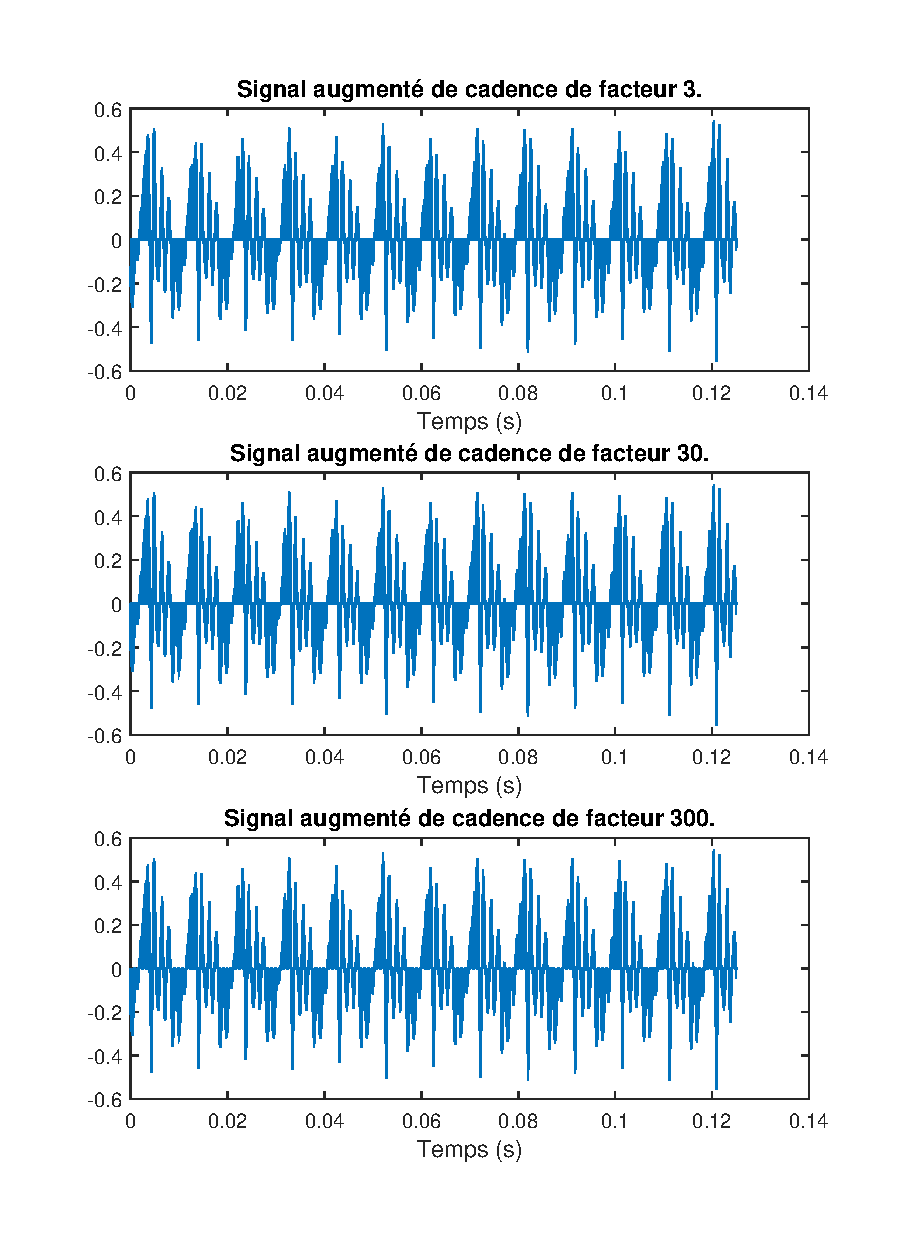
\includegraphics[width=\textwidth]{images/cadence_augmente.eps}
	% Title: glps_renderer figure
% Creator: GL2PS 1.3.8, (C) 1999-2012 C. Geuzaine
% For: Octave
% CreationDate: Thu Nov  9 17:04:09 2017
\begin{pgfpicture}
\pgfsetlinewidth{0.01pt}
\color[rgb]{1.000000,1.000000,1.000000}
\pgfpathmoveto{\pgfpoint{65.000015pt}{264.508606pt}}
\pgflineto{\pgfpoint{452.500000pt}{178.258606pt}}
\pgflineto{\pgfpoint{65.000015pt}{178.258606pt}}
\pgfpathclose
\pgfusepath{fill,stroke}
\pgfpathmoveto{\pgfpoint{65.000015pt}{264.508606pt}}
\pgflineto{\pgfpoint{452.500000pt}{264.508606pt}}
\pgflineto{\pgfpoint{452.500000pt}{178.258606pt}}
\pgfpathclose
\pgfusepath{fill,stroke}
\pgfpathmoveto{\pgfpoint{65.000015pt}{119.249985pt}}
\pgflineto{\pgfpoint{452.500000pt}{32.999985pt}}
\pgflineto{\pgfpoint{65.000015pt}{32.999985pt}}
\pgfpathclose
\pgfusepath{fill,stroke}
\pgfpathmoveto{\pgfpoint{65.000015pt}{119.249985pt}}
\pgflineto{\pgfpoint{452.500000pt}{119.249985pt}}
\pgflineto{\pgfpoint{452.500000pt}{32.999985pt}}
\pgfpathclose
\pgfusepath{fill,stroke}
\color[rgb]{0.000000,0.000000,0.000000}
\pgfsetlinewidth{0.500000pt}
\pgfsetdash{{16pt}{0pt}}{0pt}
\pgfpathmoveto{\pgfpoint{452.500000pt}{178.258606pt}}
\pgflineto{\pgfpoint{65.000015pt}{178.258606pt}}
\pgfusepath{stroke}
\pgfpathmoveto{\pgfpoint{452.500000pt}{264.508606pt}}
\pgflineto{\pgfpoint{65.000015pt}{264.508606pt}}
\pgfusepath{stroke}
\pgfpathmoveto{\pgfpoint{65.000015pt}{264.508606pt}}
\pgflineto{\pgfpoint{65.000015pt}{178.258606pt}}
\pgfusepath{stroke}
\pgfpathmoveto{\pgfpoint{452.500000pt}{264.508606pt}}
\pgflineto{\pgfpoint{452.500000pt}{178.258606pt}}
\pgfusepath{stroke}
\pgfsetdash{{0pt}{3pt}{1pt}{3pt}{1pt}{3pt}{1pt}{3pt}{1pt}{0pt}}{0pt}
\pgfpathmoveto{\pgfpoint{65.000015pt}{264.508606pt}}
\pgflineto{\pgfpoint{65.000015pt}{178.258606pt}}
\pgfusepath{stroke}
\pgfpathmoveto{\pgfpoint{161.875000pt}{264.508606pt}}
\pgflineto{\pgfpoint{161.875000pt}{178.258606pt}}
\pgfusepath{stroke}
\pgfpathmoveto{\pgfpoint{258.750000pt}{264.508606pt}}
\pgflineto{\pgfpoint{258.750000pt}{178.258606pt}}
\pgfusepath{stroke}
\pgfpathmoveto{\pgfpoint{355.625000pt}{264.508606pt}}
\pgflineto{\pgfpoint{355.625000pt}{178.258606pt}}
\pgfusepath{stroke}
\pgfpathmoveto{\pgfpoint{452.500000pt}{264.508606pt}}
\pgflineto{\pgfpoint{452.500000pt}{178.258606pt}}
\pgfusepath{stroke}
\pgfsetdash{{16pt}{0pt}}{0pt}
\pgfpathmoveto{\pgfpoint{65.000015pt}{182.144867pt}}
\pgflineto{\pgfpoint{65.000015pt}{178.258606pt}}
\pgfusepath{stroke}
\pgfpathmoveto{\pgfpoint{65.000015pt}{260.622345pt}}
\pgflineto{\pgfpoint{65.000015pt}{264.508606pt}}
\pgfusepath{stroke}
\pgfpathmoveto{\pgfpoint{161.875000pt}{182.144867pt}}
\pgflineto{\pgfpoint{161.875000pt}{178.258606pt}}
\pgfusepath{stroke}
\pgfpathmoveto{\pgfpoint{161.875000pt}{260.622345pt}}
\pgflineto{\pgfpoint{161.875000pt}{264.508606pt}}
\pgfusepath{stroke}
\pgfpathmoveto{\pgfpoint{258.750000pt}{182.144867pt}}
\pgflineto{\pgfpoint{258.750000pt}{178.258606pt}}
\pgfusepath{stroke}
\pgfpathmoveto{\pgfpoint{258.750000pt}{260.622345pt}}
\pgflineto{\pgfpoint{258.750000pt}{264.508606pt}}
\pgfusepath{stroke}
\pgfpathmoveto{\pgfpoint{355.625000pt}{182.144867pt}}
\pgflineto{\pgfpoint{355.625000pt}{178.258606pt}}
\pgfusepath{stroke}
\pgfpathmoveto{\pgfpoint{355.625000pt}{260.622345pt}}
\pgflineto{\pgfpoint{355.625000pt}{264.508606pt}}
\pgfusepath{stroke}
\pgfpathmoveto{\pgfpoint{452.500000pt}{182.144867pt}}
\pgflineto{\pgfpoint{452.500000pt}{178.258606pt}}
\pgfusepath{stroke}
\pgfpathmoveto{\pgfpoint{452.500000pt}{260.622345pt}}
\pgflineto{\pgfpoint{452.500000pt}{264.508606pt}}
\pgfusepath{stroke}
{
\pgftransformshift{\pgfpoint{65.000015pt}{173.244064pt}}
\pgfnode{rectangle}{north}{\fontsize{10}{0}\selectfont\textcolor[rgb]{0,0,0}{{0}}}{}{\pgfusepath{discard}}}
{
\pgftransformshift{\pgfpoint{161.875015pt}{173.244064pt}}
\pgfnode{rectangle}{north}{\fontsize{10}{0}\selectfont\textcolor[rgb]{0,0,0}{{0.005}}}{}{\pgfusepath{discard}}}
{
\pgftransformshift{\pgfpoint{258.750031pt}{173.244064pt}}
\pgfnode{rectangle}{north}{\fontsize{10}{0}\selectfont\textcolor[rgb]{0,0,0}{{0.01}}}{}{\pgfusepath{discard}}}
{
\pgftransformshift{\pgfpoint{355.625031pt}{173.244064pt}}
\pgfnode{rectangle}{north}{\fontsize{10}{0}\selectfont\textcolor[rgb]{0,0,0}{{0.015}}}{}{\pgfusepath{discard}}}
{
\pgftransformshift{\pgfpoint{452.500031pt}{173.244064pt}}
\pgfnode{rectangle}{north}{\fontsize{10}{0}\selectfont\textcolor[rgb]{0,0,0}{{0.02}}}{}{\pgfusepath{discard}}}
\pgfsetdash{{0pt}{3pt}{1pt}{3pt}{1pt}{3pt}{1pt}{3pt}{1pt}{0pt}}{0pt}
\pgfpathmoveto{\pgfpoint{452.500000pt}{178.258606pt}}
\pgflineto{\pgfpoint{65.000015pt}{178.258606pt}}
\pgfusepath{stroke}
\pgfpathmoveto{\pgfpoint{452.500000pt}{189.039856pt}}
\pgflineto{\pgfpoint{65.000015pt}{189.039856pt}}
\pgfusepath{stroke}
\pgfpathmoveto{\pgfpoint{452.500000pt}{199.821106pt}}
\pgflineto{\pgfpoint{65.000015pt}{199.821106pt}}
\pgfusepath{stroke}
\pgfpathmoveto{\pgfpoint{452.500000pt}{210.602356pt}}
\pgflineto{\pgfpoint{65.000015pt}{210.602356pt}}
\pgfusepath{stroke}
\pgfpathmoveto{\pgfpoint{452.500000pt}{221.383606pt}}
\pgflineto{\pgfpoint{65.000015pt}{221.383606pt}}
\pgfusepath{stroke}
\pgfpathmoveto{\pgfpoint{452.500000pt}{232.164856pt}}
\pgflineto{\pgfpoint{65.000015pt}{232.164856pt}}
\pgfusepath{stroke}
\pgfpathmoveto{\pgfpoint{452.500000pt}{242.946106pt}}
\pgflineto{\pgfpoint{65.000015pt}{242.946106pt}}
\pgfusepath{stroke}
\pgfpathmoveto{\pgfpoint{452.500000pt}{253.727356pt}}
\pgflineto{\pgfpoint{65.000015pt}{253.727356pt}}
\pgfusepath{stroke}
\pgfpathmoveto{\pgfpoint{452.500000pt}{264.508606pt}}
\pgflineto{\pgfpoint{65.000015pt}{264.508606pt}}
\pgfusepath{stroke}
\pgfsetdash{{16pt}{0pt}}{0pt}
\pgfpathmoveto{\pgfpoint{68.870026pt}{178.258606pt}}
\pgflineto{\pgfpoint{65.000015pt}{178.258606pt}}
\pgfusepath{stroke}
\pgfpathmoveto{\pgfpoint{448.630005pt}{178.258606pt}}
\pgflineto{\pgfpoint{452.500000pt}{178.258606pt}}
\pgfusepath{stroke}
\pgfpathmoveto{\pgfpoint{68.870026pt}{189.039856pt}}
\pgflineto{\pgfpoint{65.000015pt}{189.039856pt}}
\pgfusepath{stroke}
\pgfpathmoveto{\pgfpoint{448.630005pt}{189.039856pt}}
\pgflineto{\pgfpoint{452.500000pt}{189.039856pt}}
\pgfusepath{stroke}
\pgfpathmoveto{\pgfpoint{68.870026pt}{199.821106pt}}
\pgflineto{\pgfpoint{65.000015pt}{199.821106pt}}
\pgfusepath{stroke}
\pgfpathmoveto{\pgfpoint{448.630005pt}{199.821106pt}}
\pgflineto{\pgfpoint{452.500000pt}{199.821106pt}}
\pgfusepath{stroke}
\pgfpathmoveto{\pgfpoint{68.870026pt}{210.602356pt}}
\pgflineto{\pgfpoint{65.000015pt}{210.602356pt}}
\pgfusepath{stroke}
\pgfpathmoveto{\pgfpoint{448.630005pt}{210.602356pt}}
\pgflineto{\pgfpoint{452.500000pt}{210.602356pt}}
\pgfusepath{stroke}
\pgfpathmoveto{\pgfpoint{68.870026pt}{221.383606pt}}
\pgflineto{\pgfpoint{65.000015pt}{221.383606pt}}
\pgfusepath{stroke}
\pgfpathmoveto{\pgfpoint{448.630005pt}{221.383606pt}}
\pgflineto{\pgfpoint{452.500000pt}{221.383606pt}}
\pgfusepath{stroke}
\pgfpathmoveto{\pgfpoint{68.870026pt}{232.164856pt}}
\pgflineto{\pgfpoint{65.000015pt}{232.164856pt}}
\pgfusepath{stroke}
\pgfpathmoveto{\pgfpoint{448.630005pt}{232.164856pt}}
\pgflineto{\pgfpoint{452.500000pt}{232.164856pt}}
\pgfusepath{stroke}
\pgfpathmoveto{\pgfpoint{68.870026pt}{242.946106pt}}
\pgflineto{\pgfpoint{65.000015pt}{242.946106pt}}
\pgfusepath{stroke}
\pgfpathmoveto{\pgfpoint{448.630005pt}{242.946106pt}}
\pgflineto{\pgfpoint{452.500000pt}{242.946106pt}}
\pgfusepath{stroke}
\pgfpathmoveto{\pgfpoint{68.870026pt}{253.727356pt}}
\pgflineto{\pgfpoint{65.000015pt}{253.727356pt}}
\pgfusepath{stroke}
\pgfpathmoveto{\pgfpoint{448.630005pt}{253.727356pt}}
\pgflineto{\pgfpoint{452.500000pt}{253.727356pt}}
\pgfusepath{stroke}
\pgfpathmoveto{\pgfpoint{68.870026pt}{264.508606pt}}
\pgflineto{\pgfpoint{65.000015pt}{264.508606pt}}
\pgfusepath{stroke}
\pgfpathmoveto{\pgfpoint{448.630005pt}{264.508606pt}}
\pgflineto{\pgfpoint{452.500000pt}{264.508606pt}}
\pgfusepath{stroke}
{
\pgftransformshift{\pgfpoint{60.006454pt}{178.258606pt}}
\pgfnode{rectangle}{east}{\fontsize{10}{0}\selectfont\textcolor[rgb]{0,0,0}{{-0.8}}}{}{\pgfusepath{discard}}}
{
\pgftransformshift{\pgfpoint{60.006454pt}{189.039856pt}}
\pgfnode{rectangle}{east}{\fontsize{10}{0}\selectfont\textcolor[rgb]{0,0,0}{{-0.6}}}{}{\pgfusepath{discard}}}
{
\pgftransformshift{\pgfpoint{60.006454pt}{199.821106pt}}
\pgfnode{rectangle}{east}{\fontsize{10}{0}\selectfont\textcolor[rgb]{0,0,0}{{-0.4}}}{}{\pgfusepath{discard}}}
{
\pgftransformshift{\pgfpoint{60.006454pt}{210.602356pt}}
\pgfnode{rectangle}{east}{\fontsize{10}{0}\selectfont\textcolor[rgb]{0,0,0}{{-0.2}}}{}{\pgfusepath{discard}}}
{
\pgftransformshift{\pgfpoint{60.006454pt}{221.383606pt}}
\pgfnode{rectangle}{east}{\fontsize{10}{0}\selectfont\textcolor[rgb]{0,0,0}{{0}}}{}{\pgfusepath{discard}}}
{
\pgftransformshift{\pgfpoint{60.006454pt}{232.164856pt}}
\pgfnode{rectangle}{east}{\fontsize{10}{0}\selectfont\textcolor[rgb]{0,0,0}{{0.2}}}{}{\pgfusepath{discard}}}
{
\pgftransformshift{\pgfpoint{60.006454pt}{242.946106pt}}
\pgfnode{rectangle}{east}{\fontsize{10}{0}\selectfont\textcolor[rgb]{0,0,0}{{0.4}}}{}{\pgfusepath{discard}}}
{
\pgftransformshift{\pgfpoint{60.006454pt}{253.727356pt}}
\pgfnode{rectangle}{east}{\fontsize{10}{0}\selectfont\textcolor[rgb]{0,0,0}{{0.6}}}{}{\pgfusepath{discard}}}
{
\pgftransformshift{\pgfpoint{60.006454pt}{264.508606pt}}
\pgfnode{rectangle}{east}{\fontsize{10}{0}\selectfont\textcolor[rgb]{0,0,0}{{0.8}}}{}{\pgfusepath{discard}}}
{
\pgftransformshift{\pgfpoint{258.750031pt}{162.244080pt}}
\pgfnode{rectangle}{north}{\fontsize{10}{0}\selectfont\textcolor[rgb]{0,0,0}{{Temps (s)}}}{}{\pgfusepath{discard}}}
\color[rgb]{0.000000,0.000000,1.000000}
\pgfsetdash{}{0pt}
\pgfpathmoveto{\pgfpoint{65.403656pt}{221.383606pt}}
\pgflineto{\pgfpoint{65.000015pt}{210.108170pt}}
\pgfusepath{stroke}
\pgfpathmoveto{\pgfpoint{65.807297pt}{221.383606pt}}
\pgflineto{\pgfpoint{65.403656pt}{221.383606pt}}
\pgfusepath{stroke}
\pgfpathmoveto{\pgfpoint{66.210953pt}{208.129120pt}}
\pgflineto{\pgfpoint{65.807297pt}{221.383606pt}}
\pgfusepath{stroke}
\pgfpathmoveto{\pgfpoint{66.614594pt}{221.383606pt}}
\pgflineto{\pgfpoint{66.210953pt}{208.129120pt}}
\pgfusepath{stroke}
\pgfpathmoveto{\pgfpoint{67.018234pt}{221.383606pt}}
\pgflineto{\pgfpoint{66.614594pt}{221.383606pt}}
\pgfusepath{stroke}
\pgfpathmoveto{\pgfpoint{67.421890pt}{206.747253pt}}
\pgflineto{\pgfpoint{67.018234pt}{221.383606pt}}
\pgfusepath{stroke}
\pgfpathmoveto{\pgfpoint{67.825531pt}{221.383606pt}}
\pgflineto{\pgfpoint{67.421890pt}{206.747253pt}}
\pgfusepath{stroke}
\pgfpathmoveto{\pgfpoint{68.229187pt}{221.383606pt}}
\pgflineto{\pgfpoint{67.825531pt}{221.383606pt}}
\pgfusepath{stroke}
\pgfpathmoveto{\pgfpoint{68.632828pt}{205.857269pt}}
\pgflineto{\pgfpoint{68.229187pt}{221.383606pt}}
\pgfusepath{stroke}
\pgfpathmoveto{\pgfpoint{69.036469pt}{221.383606pt}}
\pgflineto{\pgfpoint{68.632828pt}{205.857269pt}}
\pgfusepath{stroke}
\pgfpathmoveto{\pgfpoint{69.440109pt}{221.383606pt}}
\pgflineto{\pgfpoint{69.036469pt}{221.383606pt}}
\pgfusepath{stroke}
\pgfpathmoveto{\pgfpoint{69.843765pt}{204.885010pt}}
\pgflineto{\pgfpoint{69.440109pt}{221.383606pt}}
\pgfusepath{stroke}
\pgfpathmoveto{\pgfpoint{70.247406pt}{221.383606pt}}
\pgflineto{\pgfpoint{69.843765pt}{204.885010pt}}
\pgfusepath{stroke}
\pgfpathmoveto{\pgfpoint{70.651062pt}{221.383606pt}}
\pgflineto{\pgfpoint{70.247406pt}{221.383606pt}}
\pgfusepath{stroke}
\pgfpathmoveto{\pgfpoint{71.054703pt}{204.750122pt}}
\pgflineto{\pgfpoint{70.651062pt}{221.383606pt}}
\pgfusepath{stroke}
\pgfpathmoveto{\pgfpoint{71.458344pt}{221.383606pt}}
\pgflineto{\pgfpoint{71.054703pt}{204.750122pt}}
\pgfusepath{stroke}
\pgfpathmoveto{\pgfpoint{71.862000pt}{221.383606pt}}
\pgflineto{\pgfpoint{71.458344pt}{221.383606pt}}
\pgfusepath{stroke}
\pgfpathmoveto{\pgfpoint{72.265640pt}{205.207458pt}}
\pgflineto{\pgfpoint{71.862000pt}{221.383606pt}}
\pgfusepath{stroke}
\pgfpathmoveto{\pgfpoint{72.669281pt}{221.383606pt}}
\pgflineto{\pgfpoint{72.265640pt}{205.207458pt}}
\pgfusepath{stroke}
\pgfpathmoveto{\pgfpoint{73.072922pt}{221.383606pt}}
\pgflineto{\pgfpoint{72.669281pt}{221.383606pt}}
\pgfusepath{stroke}
\pgfpathmoveto{\pgfpoint{73.476578pt}{205.608856pt}}
\pgflineto{\pgfpoint{73.072922pt}{221.383606pt}}
\pgfusepath{stroke}
\pgfpathmoveto{\pgfpoint{73.880219pt}{221.383606pt}}
\pgflineto{\pgfpoint{73.476578pt}{205.608856pt}}
\pgfusepath{stroke}
\pgfpathmoveto{\pgfpoint{74.283875pt}{221.383606pt}}
\pgflineto{\pgfpoint{73.880219pt}{221.383606pt}}
\pgfusepath{stroke}
\pgfpathmoveto{\pgfpoint{74.687515pt}{206.362305pt}}
\pgflineto{\pgfpoint{74.283875pt}{221.383606pt}}
\pgfusepath{stroke}
\pgfpathmoveto{\pgfpoint{75.091156pt}{221.383606pt}}
\pgflineto{\pgfpoint{74.687515pt}{206.362305pt}}
\pgfusepath{stroke}
\pgfpathmoveto{\pgfpoint{75.494797pt}{221.383606pt}}
\pgflineto{\pgfpoint{75.091156pt}{221.383606pt}}
\pgfusepath{stroke}
\pgfpathmoveto{\pgfpoint{75.898453pt}{207.745819pt}}
\pgflineto{\pgfpoint{75.494797pt}{221.383606pt}}
\pgfusepath{stroke}
\pgfpathmoveto{\pgfpoint{76.302094pt}{221.383606pt}}
\pgflineto{\pgfpoint{75.898453pt}{207.745819pt}}
\pgfusepath{stroke}
\pgfpathmoveto{\pgfpoint{76.705734pt}{221.383606pt}}
\pgflineto{\pgfpoint{76.302094pt}{221.383606pt}}
\pgfusepath{stroke}
\pgfpathmoveto{\pgfpoint{77.109375pt}{209.298782pt}}
\pgflineto{\pgfpoint{76.705734pt}{221.383606pt}}
\pgfusepath{stroke}
\pgfpathmoveto{\pgfpoint{77.513046pt}{221.383606pt}}
\pgflineto{\pgfpoint{77.109375pt}{209.298782pt}}
\pgfusepath{stroke}
\pgfpathmoveto{\pgfpoint{77.916687pt}{221.383606pt}}
\pgflineto{\pgfpoint{77.513046pt}{221.383606pt}}
\pgfusepath{stroke}
\pgfpathmoveto{\pgfpoint{78.320328pt}{210.942230pt}}
\pgflineto{\pgfpoint{77.916687pt}{221.383606pt}}
\pgfusepath{stroke}
\pgfpathmoveto{\pgfpoint{78.723969pt}{221.383606pt}}
\pgflineto{\pgfpoint{78.320328pt}{210.942230pt}}
\pgfusepath{stroke}
\pgfpathmoveto{\pgfpoint{79.127609pt}{221.383606pt}}
\pgflineto{\pgfpoint{78.723969pt}{221.383606pt}}
\pgfusepath{stroke}
\pgfpathmoveto{\pgfpoint{79.531265pt}{212.972260pt}}
\pgflineto{\pgfpoint{79.127609pt}{221.383606pt}}
\pgfusepath{stroke}
\pgfpathmoveto{\pgfpoint{79.934906pt}{221.383606pt}}
\pgflineto{\pgfpoint{79.531265pt}{212.972260pt}}
\pgfusepath{stroke}
\pgfpathmoveto{\pgfpoint{80.338547pt}{221.383606pt}}
\pgflineto{\pgfpoint{79.934906pt}{221.383606pt}}
\pgfusepath{stroke}
\pgfpathmoveto{\pgfpoint{80.742203pt}{214.505493pt}}
\pgflineto{\pgfpoint{80.338547pt}{221.383606pt}}
\pgfusepath{stroke}
\pgfpathmoveto{\pgfpoint{81.145859pt}{221.383606pt}}
\pgflineto{\pgfpoint{80.742203pt}{214.505493pt}}
\pgfusepath{stroke}
\pgfpathmoveto{\pgfpoint{81.549500pt}{221.383606pt}}
\pgflineto{\pgfpoint{81.145859pt}{221.383606pt}}
\pgfusepath{stroke}
\pgfpathmoveto{\pgfpoint{81.953140pt}{215.584671pt}}
\pgflineto{\pgfpoint{81.549500pt}{221.383606pt}}
\pgfusepath{stroke}
\pgfpathmoveto{\pgfpoint{82.356781pt}{221.383606pt}}
\pgflineto{\pgfpoint{81.953140pt}{215.584671pt}}
\pgfusepath{stroke}
\pgfpathmoveto{\pgfpoint{82.760422pt}{221.383606pt}}
\pgflineto{\pgfpoint{82.356781pt}{221.383606pt}}
\pgfusepath{stroke}
\pgfpathmoveto{\pgfpoint{83.164078pt}{216.367737pt}}
\pgflineto{\pgfpoint{82.760422pt}{221.383606pt}}
\pgfusepath{stroke}
\pgfpathmoveto{\pgfpoint{83.567719pt}{221.383606pt}}
\pgflineto{\pgfpoint{83.164078pt}{216.367737pt}}
\pgfusepath{stroke}
\pgfpathmoveto{\pgfpoint{83.971359pt}{221.383606pt}}
\pgflineto{\pgfpoint{83.567719pt}{221.383606pt}}
\pgfusepath{stroke}
\pgfpathmoveto{\pgfpoint{84.375015pt}{216.820129pt}}
\pgflineto{\pgfpoint{83.971359pt}{221.383606pt}}
\pgfusepath{stroke}
\pgfpathmoveto{\pgfpoint{84.778671pt}{221.383606pt}}
\pgflineto{\pgfpoint{84.375015pt}{216.820129pt}}
\pgfusepath{stroke}
\pgfpathmoveto{\pgfpoint{85.182312pt}{221.383606pt}}
\pgflineto{\pgfpoint{84.778671pt}{221.383606pt}}
\pgfusepath{stroke}
\pgfpathmoveto{\pgfpoint{85.585953pt}{217.237976pt}}
\pgflineto{\pgfpoint{85.182312pt}{221.383606pt}}
\pgfusepath{stroke}
\pgfpathmoveto{\pgfpoint{85.989594pt}{221.383606pt}}
\pgflineto{\pgfpoint{85.585953pt}{217.237976pt}}
\pgfusepath{stroke}
\pgfpathmoveto{\pgfpoint{86.393234pt}{221.383606pt}}
\pgflineto{\pgfpoint{85.989594pt}{221.383606pt}}
\pgfusepath{stroke}
\pgfpathmoveto{\pgfpoint{86.796875pt}{217.165588pt}}
\pgflineto{\pgfpoint{86.393234pt}{221.383606pt}}
\pgfusepath{stroke}
\pgfpathmoveto{\pgfpoint{87.200531pt}{221.383606pt}}
\pgflineto{\pgfpoint{86.796875pt}{217.165588pt}}
\pgfusepath{stroke}
\pgfpathmoveto{\pgfpoint{87.604187pt}{221.383606pt}}
\pgflineto{\pgfpoint{87.200531pt}{221.383606pt}}
\pgfusepath{stroke}
\pgfpathmoveto{\pgfpoint{88.007828pt}{217.086639pt}}
\pgflineto{\pgfpoint{87.604187pt}{221.383606pt}}
\pgfusepath{stroke}
\pgfpathmoveto{\pgfpoint{88.411469pt}{221.383606pt}}
\pgflineto{\pgfpoint{88.007828pt}{217.086639pt}}
\pgfusepath{stroke}
\pgfpathmoveto{\pgfpoint{88.815125pt}{221.383606pt}}
\pgflineto{\pgfpoint{88.411469pt}{221.383606pt}}
\pgfusepath{stroke}
\pgfpathmoveto{\pgfpoint{89.218765pt}{216.996155pt}}
\pgflineto{\pgfpoint{88.815125pt}{221.383606pt}}
\pgfusepath{stroke}
\pgfpathmoveto{\pgfpoint{89.622406pt}{221.383606pt}}
\pgflineto{\pgfpoint{89.218765pt}{216.996155pt}}
\pgfusepath{stroke}
\pgfpathmoveto{\pgfpoint{90.026047pt}{221.383606pt}}
\pgflineto{\pgfpoint{89.622406pt}{221.383606pt}}
\pgfusepath{stroke}
\pgfpathmoveto{\pgfpoint{90.429688pt}{216.494400pt}}
\pgflineto{\pgfpoint{90.026047pt}{221.383606pt}}
\pgfusepath{stroke}
\pgfpathmoveto{\pgfpoint{90.833344pt}{221.383606pt}}
\pgflineto{\pgfpoint{90.429688pt}{216.494400pt}}
\pgfusepath{stroke}
\pgfpathmoveto{\pgfpoint{91.237000pt}{221.383606pt}}
\pgflineto{\pgfpoint{90.833344pt}{221.383606pt}}
\pgfusepath{stroke}
\pgfpathmoveto{\pgfpoint{91.640640pt}{216.254211pt}}
\pgflineto{\pgfpoint{91.237000pt}{221.383606pt}}
\pgfusepath{stroke}
\pgfpathmoveto{\pgfpoint{92.044281pt}{221.383606pt}}
\pgflineto{\pgfpoint{91.640640pt}{216.254211pt}}
\pgfusepath{stroke}
\pgfpathmoveto{\pgfpoint{92.447937pt}{221.383606pt}}
\pgflineto{\pgfpoint{92.044281pt}{221.383606pt}}
\pgfusepath{stroke}
\pgfpathmoveto{\pgfpoint{92.851578pt}{216.709900pt}}
\pgflineto{\pgfpoint{92.447937pt}{221.383606pt}}
\pgfusepath{stroke}
\pgfpathmoveto{\pgfpoint{93.255219pt}{221.383606pt}}
\pgflineto{\pgfpoint{92.851578pt}{216.709900pt}}
\pgfusepath{stroke}
\pgfpathmoveto{\pgfpoint{93.658859pt}{221.383606pt}}
\pgflineto{\pgfpoint{93.255219pt}{221.383606pt}}
\pgfusepath{stroke}
\pgfpathmoveto{\pgfpoint{94.062500pt}{217.091568pt}}
\pgflineto{\pgfpoint{93.658859pt}{221.383606pt}}
\pgfusepath{stroke}
\pgfpathmoveto{\pgfpoint{94.466171pt}{221.383606pt}}
\pgflineto{\pgfpoint{94.062500pt}{217.091568pt}}
\pgfusepath{stroke}
\pgfpathmoveto{\pgfpoint{94.869812pt}{221.383606pt}}
\pgflineto{\pgfpoint{94.466171pt}{221.383606pt}}
\pgfusepath{stroke}
\pgfpathmoveto{\pgfpoint{95.273453pt}{217.812119pt}}
\pgflineto{\pgfpoint{94.869812pt}{221.383606pt}}
\pgfusepath{stroke}
\pgfpathmoveto{\pgfpoint{95.677094pt}{221.383606pt}}
\pgflineto{\pgfpoint{95.273453pt}{217.812119pt}}
\pgfusepath{stroke}
\pgfpathmoveto{\pgfpoint{96.080750pt}{221.383606pt}}
\pgflineto{\pgfpoint{95.677094pt}{221.383606pt}}
\pgfusepath{stroke}
\pgfpathmoveto{\pgfpoint{96.484390pt}{219.577301pt}}
\pgflineto{\pgfpoint{96.080750pt}{221.383606pt}}
\pgfusepath{stroke}
\pgfpathmoveto{\pgfpoint{96.888031pt}{221.383606pt}}
\pgflineto{\pgfpoint{96.484390pt}{219.577301pt}}
\pgfusepath{stroke}
\pgfpathmoveto{\pgfpoint{97.291672pt}{221.383606pt}}
\pgflineto{\pgfpoint{96.888031pt}{221.383606pt}}
\pgfusepath{stroke}
\pgfpathmoveto{\pgfpoint{97.695328pt}{221.337540pt}}
\pgflineto{\pgfpoint{97.291672pt}{221.383606pt}}
\pgfusepath{stroke}
\pgfpathmoveto{\pgfpoint{98.098969pt}{221.383606pt}}
\pgflineto{\pgfpoint{97.695328pt}{221.337540pt}}
\pgfusepath{stroke}
\pgfpathmoveto{\pgfpoint{98.502625pt}{221.383606pt}}
\pgflineto{\pgfpoint{98.098969pt}{221.383606pt}}
\pgfusepath{stroke}
\pgfpathmoveto{\pgfpoint{98.906265pt}{222.283478pt}}
\pgflineto{\pgfpoint{98.502625pt}{221.383606pt}}
\pgfusepath{stroke}
\pgfpathmoveto{\pgfpoint{99.309906pt}{221.383606pt}}
\pgflineto{\pgfpoint{98.906265pt}{222.283478pt}}
\pgfusepath{stroke}
\pgfpathmoveto{\pgfpoint{99.713547pt}{221.383606pt}}
\pgflineto{\pgfpoint{99.309906pt}{221.383606pt}}
\pgfusepath{stroke}
\pgfpathmoveto{\pgfpoint{100.117203pt}{223.421875pt}}
\pgflineto{\pgfpoint{99.713547pt}{221.383606pt}}
\pgfusepath{stroke}
\pgfpathmoveto{\pgfpoint{100.520844pt}{221.383606pt}}
\pgflineto{\pgfpoint{100.117203pt}{223.421875pt}}
\pgfusepath{stroke}
\pgfpathmoveto{\pgfpoint{100.924500pt}{221.383606pt}}
\pgflineto{\pgfpoint{100.520844pt}{221.383606pt}}
\pgfusepath{stroke}
\pgfpathmoveto{\pgfpoint{101.328140pt}{225.215012pt}}
\pgflineto{\pgfpoint{100.924500pt}{221.383606pt}}
\pgfusepath{stroke}
\pgfpathmoveto{\pgfpoint{101.731781pt}{221.383606pt}}
\pgflineto{\pgfpoint{101.328140pt}{225.215012pt}}
\pgfusepath{stroke}
\pgfpathmoveto{\pgfpoint{102.135422pt}{221.383606pt}}
\pgflineto{\pgfpoint{101.731781pt}{221.383606pt}}
\pgfusepath{stroke}
\pgfpathmoveto{\pgfpoint{102.539078pt}{226.170807pt}}
\pgflineto{\pgfpoint{102.135422pt}{221.383606pt}}
\pgfusepath{stroke}
\pgfpathmoveto{\pgfpoint{102.942719pt}{221.383606pt}}
\pgflineto{\pgfpoint{102.539078pt}{226.170807pt}}
\pgfusepath{stroke}
\pgfpathmoveto{\pgfpoint{103.346359pt}{221.383606pt}}
\pgflineto{\pgfpoint{102.942719pt}{221.383606pt}}
\pgfusepath{stroke}
\pgfpathmoveto{\pgfpoint{103.750015pt}{227.029541pt}}
\pgflineto{\pgfpoint{103.346359pt}{221.383606pt}}
\pgfusepath{stroke}
\pgfpathmoveto{\pgfpoint{104.153656pt}{221.383606pt}}
\pgflineto{\pgfpoint{103.750015pt}{227.029541pt}}
\pgfusepath{stroke}
\pgfpathmoveto{\pgfpoint{104.557312pt}{221.383606pt}}
\pgflineto{\pgfpoint{104.153656pt}{221.383606pt}}
\pgfusepath{stroke}
\pgfpathmoveto{\pgfpoint{104.960953pt}{228.289688pt}}
\pgflineto{\pgfpoint{104.557312pt}{221.383606pt}}
\pgfusepath{stroke}
\pgfpathmoveto{\pgfpoint{105.364594pt}{221.383606pt}}
\pgflineto{\pgfpoint{104.960953pt}{228.289688pt}}
\pgfusepath{stroke}
\pgfpathmoveto{\pgfpoint{105.768234pt}{221.383606pt}}
\pgflineto{\pgfpoint{105.364594pt}{221.383606pt}}
\pgfusepath{stroke}
\pgfpathmoveto{\pgfpoint{106.171890pt}{228.595673pt}}
\pgflineto{\pgfpoint{105.768234pt}{221.383606pt}}
\pgfusepath{stroke}
\pgfpathmoveto{\pgfpoint{106.575531pt}{221.383606pt}}
\pgflineto{\pgfpoint{106.171890pt}{228.595673pt}}
\pgfusepath{stroke}
\pgfpathmoveto{\pgfpoint{106.979172pt}{221.383606pt}}
\pgflineto{\pgfpoint{106.575531pt}{221.383606pt}}
\pgfusepath{stroke}
\pgfpathmoveto{\pgfpoint{107.382828pt}{228.429520pt}}
\pgflineto{\pgfpoint{106.979172pt}{221.383606pt}}
\pgfusepath{stroke}
\pgfpathmoveto{\pgfpoint{107.786484pt}{221.383606pt}}
\pgflineto{\pgfpoint{107.382828pt}{228.429520pt}}
\pgfusepath{stroke}
\pgfpathmoveto{\pgfpoint{108.190125pt}{221.383606pt}}
\pgflineto{\pgfpoint{107.786484pt}{221.383606pt}}
\pgfusepath{stroke}
\pgfpathmoveto{\pgfpoint{108.593765pt}{229.273438pt}}
\pgflineto{\pgfpoint{108.190125pt}{221.383606pt}}
\pgfusepath{stroke}
\pgfpathmoveto{\pgfpoint{108.997406pt}{221.383606pt}}
\pgflineto{\pgfpoint{108.593765pt}{229.273438pt}}
\pgfusepath{stroke}
\pgfpathmoveto{\pgfpoint{109.401047pt}{221.383606pt}}
\pgflineto{\pgfpoint{108.997406pt}{221.383606pt}}
\pgfusepath{stroke}
\pgfpathmoveto{\pgfpoint{109.804703pt}{231.117584pt}}
\pgflineto{\pgfpoint{109.401047pt}{221.383606pt}}
\pgfusepath{stroke}
\pgfpathmoveto{\pgfpoint{110.208344pt}{221.383606pt}}
\pgflineto{\pgfpoint{109.804703pt}{231.117584pt}}
\pgfusepath{stroke}
\pgfpathmoveto{\pgfpoint{110.611984pt}{221.383606pt}}
\pgflineto{\pgfpoint{110.208344pt}{221.383606pt}}
\pgfusepath{stroke}
\pgfpathmoveto{\pgfpoint{111.015640pt}{232.589935pt}}
\pgflineto{\pgfpoint{110.611984pt}{221.383606pt}}
\pgfusepath{stroke}
\pgfpathmoveto{\pgfpoint{111.419296pt}{221.383606pt}}
\pgflineto{\pgfpoint{111.015640pt}{232.589935pt}}
\pgfusepath{stroke}
\pgfpathmoveto{\pgfpoint{111.822937pt}{221.383606pt}}
\pgflineto{\pgfpoint{111.419296pt}{221.383606pt}}
\pgfusepath{stroke}
\pgfpathmoveto{\pgfpoint{112.226578pt}{232.300415pt}}
\pgflineto{\pgfpoint{111.822937pt}{221.383606pt}}
\pgfusepath{stroke}
\pgfpathmoveto{\pgfpoint{112.630219pt}{221.383606pt}}
\pgflineto{\pgfpoint{112.226578pt}{232.300415pt}}
\pgfusepath{stroke}
\pgfpathmoveto{\pgfpoint{113.033859pt}{221.383606pt}}
\pgflineto{\pgfpoint{112.630219pt}{221.383606pt}}
\pgfusepath{stroke}
\pgfpathmoveto{\pgfpoint{113.437500pt}{233.254562pt}}
\pgflineto{\pgfpoint{113.033859pt}{221.383606pt}}
\pgfusepath{stroke}
\pgfpathmoveto{\pgfpoint{113.841156pt}{221.383606pt}}
\pgflineto{\pgfpoint{113.437500pt}{233.254562pt}}
\pgfusepath{stroke}
\pgfpathmoveto{\pgfpoint{114.244797pt}{221.383606pt}}
\pgflineto{\pgfpoint{113.841156pt}{221.383606pt}}
\pgfusepath{stroke}
\pgfpathmoveto{\pgfpoint{114.648453pt}{236.378586pt}}
\pgflineto{\pgfpoint{114.244797pt}{221.383606pt}}
\pgfusepath{stroke}
\pgfpathmoveto{\pgfpoint{115.052109pt}{221.383606pt}}
\pgflineto{\pgfpoint{114.648453pt}{236.378586pt}}
\pgfusepath{stroke}
\pgfpathmoveto{\pgfpoint{115.455750pt}{221.383606pt}}
\pgflineto{\pgfpoint{115.052109pt}{221.383606pt}}
\pgfusepath{stroke}
\pgfpathmoveto{\pgfpoint{115.859390pt}{236.238754pt}}
\pgflineto{\pgfpoint{115.455750pt}{221.383606pt}}
\pgfusepath{stroke}
\pgfpathmoveto{\pgfpoint{116.263031pt}{221.383606pt}}
\pgflineto{\pgfpoint{115.859390pt}{236.238754pt}}
\pgfusepath{stroke}
\pgfpathmoveto{\pgfpoint{116.666672pt}{221.383606pt}}
\pgflineto{\pgfpoint{116.263031pt}{221.383606pt}}
\pgfusepath{stroke}
\pgfpathmoveto{\pgfpoint{117.070328pt}{236.204193pt}}
\pgflineto{\pgfpoint{116.666672pt}{221.383606pt}}
\pgfusepath{stroke}
\pgfpathmoveto{\pgfpoint{117.473969pt}{221.383606pt}}
\pgflineto{\pgfpoint{117.070328pt}{236.204193pt}}
\pgfusepath{stroke}
\pgfpathmoveto{\pgfpoint{117.877625pt}{221.383606pt}}
\pgflineto{\pgfpoint{117.473969pt}{221.383606pt}}
\pgfusepath{stroke}
\pgfpathmoveto{\pgfpoint{118.281265pt}{239.726349pt}}
\pgflineto{\pgfpoint{117.877625pt}{221.383606pt}}
\pgfusepath{stroke}
\pgfpathmoveto{\pgfpoint{118.684921pt}{221.383606pt}}
\pgflineto{\pgfpoint{118.281265pt}{239.726349pt}}
\pgfusepath{stroke}
\pgfpathmoveto{\pgfpoint{119.088562pt}{221.383606pt}}
\pgflineto{\pgfpoint{118.684921pt}{221.383606pt}}
\pgfusepath{stroke}
\pgfpathmoveto{\pgfpoint{119.492203pt}{238.910370pt}}
\pgflineto{\pgfpoint{119.088562pt}{221.383606pt}}
\pgfusepath{stroke}
\pgfpathmoveto{\pgfpoint{119.895844pt}{221.383606pt}}
\pgflineto{\pgfpoint{119.492203pt}{238.910370pt}}
\pgfusepath{stroke}
\pgfpathmoveto{\pgfpoint{120.299484pt}{221.383606pt}}
\pgflineto{\pgfpoint{119.895844pt}{221.383606pt}}
\pgfusepath{stroke}
\pgfpathmoveto{\pgfpoint{120.703125pt}{237.913452pt}}
\pgflineto{\pgfpoint{120.299484pt}{221.383606pt}}
\pgfusepath{stroke}
\pgfpathmoveto{\pgfpoint{121.106781pt}{221.383606pt}}
\pgflineto{\pgfpoint{120.703125pt}{237.913452pt}}
\pgfusepath{stroke}
\pgfpathmoveto{\pgfpoint{121.510437pt}{221.383606pt}}
\pgflineto{\pgfpoint{121.106781pt}{221.383606pt}}
\pgfusepath{stroke}
\pgfpathmoveto{\pgfpoint{121.914078pt}{241.986694pt}}
\pgflineto{\pgfpoint{121.510437pt}{221.383606pt}}
\pgfusepath{stroke}
\pgfpathmoveto{\pgfpoint{122.317719pt}{221.383606pt}}
\pgflineto{\pgfpoint{121.914078pt}{241.986694pt}}
\pgfusepath{stroke}
\pgfpathmoveto{\pgfpoint{122.721375pt}{221.383606pt}}
\pgflineto{\pgfpoint{122.317719pt}{221.383606pt}}
\pgfusepath{stroke}
\pgfpathmoveto{\pgfpoint{123.125015pt}{242.363403pt}}
\pgflineto{\pgfpoint{122.721375pt}{221.383606pt}}
\pgfusepath{stroke}
\pgfpathmoveto{\pgfpoint{123.528656pt}{221.383606pt}}
\pgflineto{\pgfpoint{123.125015pt}{242.363403pt}}
\pgfusepath{stroke}
\pgfpathmoveto{\pgfpoint{123.932304pt}{221.383606pt}}
\pgflineto{\pgfpoint{123.528656pt}{221.383606pt}}
\pgfusepath{stroke}
\pgfpathmoveto{\pgfpoint{124.335945pt}{239.910583pt}}
\pgflineto{\pgfpoint{123.932304pt}{221.383606pt}}
\pgfusepath{stroke}
\pgfpathmoveto{\pgfpoint{124.739586pt}{221.383606pt}}
\pgflineto{\pgfpoint{124.335945pt}{239.910583pt}}
\pgfusepath{stroke}
\pgfpathmoveto{\pgfpoint{125.143242pt}{221.383606pt}}
\pgflineto{\pgfpoint{124.739586pt}{221.383606pt}}
\pgfusepath{stroke}
\pgfpathmoveto{\pgfpoint{125.546890pt}{241.246399pt}}
\pgflineto{\pgfpoint{125.143242pt}{221.383606pt}}
\pgfusepath{stroke}
\pgfpathmoveto{\pgfpoint{125.950531pt}{221.383606pt}}
\pgflineto{\pgfpoint{125.546890pt}{241.246399pt}}
\pgfusepath{stroke}
\pgfpathmoveto{\pgfpoint{126.354179pt}{221.383606pt}}
\pgflineto{\pgfpoint{125.950531pt}{221.383606pt}}
\pgfusepath{stroke}
\pgfpathmoveto{\pgfpoint{126.757820pt}{243.223785pt}}
\pgflineto{\pgfpoint{126.354179pt}{221.383606pt}}
\pgfusepath{stroke}
\pgfpathmoveto{\pgfpoint{127.161476pt}{221.383606pt}}
\pgflineto{\pgfpoint{126.757820pt}{243.223785pt}}
\pgfusepath{stroke}
\pgfpathmoveto{\pgfpoint{127.565117pt}{221.383606pt}}
\pgflineto{\pgfpoint{127.161476pt}{221.383606pt}}
\pgfusepath{stroke}
\pgfpathmoveto{\pgfpoint{127.968765pt}{242.717102pt}}
\pgflineto{\pgfpoint{127.565117pt}{221.383606pt}}
\pgfusepath{stroke}
\pgfpathmoveto{\pgfpoint{128.372406pt}{221.383606pt}}
\pgflineto{\pgfpoint{127.968765pt}{242.717102pt}}
\pgfusepath{stroke}
\pgfpathmoveto{\pgfpoint{128.776062pt}{221.383606pt}}
\pgflineto{\pgfpoint{128.372406pt}{221.383606pt}}
\pgfusepath{stroke}
\pgfpathmoveto{\pgfpoint{129.179703pt}{243.149765pt}}
\pgflineto{\pgfpoint{128.776062pt}{221.383606pt}}
\pgfusepath{stroke}
\pgfpathmoveto{\pgfpoint{129.583344pt}{221.383606pt}}
\pgflineto{\pgfpoint{129.179703pt}{243.149765pt}}
\pgfusepath{stroke}
\pgfpathmoveto{\pgfpoint{129.987000pt}{221.383606pt}}
\pgflineto{\pgfpoint{129.583344pt}{221.383606pt}}
\pgfusepath{stroke}
\pgfpathmoveto{\pgfpoint{130.390640pt}{245.745712pt}}
\pgflineto{\pgfpoint{129.987000pt}{221.383606pt}}
\pgfusepath{stroke}
\pgfpathmoveto{\pgfpoint{130.794281pt}{221.383606pt}}
\pgflineto{\pgfpoint{130.390640pt}{245.745712pt}}
\pgfusepath{stroke}
\pgfpathmoveto{\pgfpoint{131.197937pt}{221.383606pt}}
\pgflineto{\pgfpoint{130.794281pt}{221.383606pt}}
\pgfusepath{stroke}
\pgfpathmoveto{\pgfpoint{131.601562pt}{246.750854pt}}
\pgflineto{\pgfpoint{131.197937pt}{221.383606pt}}
\pgfusepath{stroke}
\pgfpathmoveto{\pgfpoint{132.005219pt}{221.383606pt}}
\pgflineto{\pgfpoint{131.601562pt}{246.750854pt}}
\pgfusepath{stroke}
\pgfpathmoveto{\pgfpoint{132.408875pt}{221.383606pt}}
\pgflineto{\pgfpoint{132.005219pt}{221.383606pt}}
\pgfusepath{stroke}
\pgfpathmoveto{\pgfpoint{132.812515pt}{246.546875pt}}
\pgflineto{\pgfpoint{132.408875pt}{221.383606pt}}
\pgfusepath{stroke}
\pgfpathmoveto{\pgfpoint{133.216156pt}{221.383606pt}}
\pgflineto{\pgfpoint{132.812515pt}{246.546875pt}}
\pgfusepath{stroke}
\pgfpathmoveto{\pgfpoint{133.619812pt}{221.383606pt}}
\pgflineto{\pgfpoint{133.216156pt}{221.383606pt}}
\pgfusepath{stroke}
\pgfpathmoveto{\pgfpoint{134.023453pt}{247.236176pt}}
\pgflineto{\pgfpoint{133.619812pt}{221.383606pt}}
\pgfusepath{stroke}
\pgfpathmoveto{\pgfpoint{134.427094pt}{221.383606pt}}
\pgflineto{\pgfpoint{134.023453pt}{247.236176pt}}
\pgfusepath{stroke}
\pgfpathmoveto{\pgfpoint{134.830750pt}{221.383606pt}}
\pgflineto{\pgfpoint{134.427094pt}{221.383606pt}}
\pgfusepath{stroke}
\pgfpathmoveto{\pgfpoint{135.234375pt}{246.413620pt}}
\pgflineto{\pgfpoint{134.830750pt}{221.383606pt}}
\pgfusepath{stroke}
\pgfpathmoveto{\pgfpoint{135.638031pt}{221.383606pt}}
\pgflineto{\pgfpoint{135.234375pt}{246.413620pt}}
\pgfusepath{stroke}
\pgfpathmoveto{\pgfpoint{136.041687pt}{221.383606pt}}
\pgflineto{\pgfpoint{135.638031pt}{221.383606pt}}
\pgfusepath{stroke}
\pgfpathmoveto{\pgfpoint{136.445328pt}{242.820740pt}}
\pgflineto{\pgfpoint{136.041687pt}{221.383606pt}}
\pgfusepath{stroke}
\pgfpathmoveto{\pgfpoint{136.848969pt}{221.383606pt}}
\pgflineto{\pgfpoint{136.445328pt}{242.820740pt}}
\pgfusepath{stroke}
\pgfpathmoveto{\pgfpoint{137.252625pt}{221.383606pt}}
\pgflineto{\pgfpoint{136.848969pt}{221.383606pt}}
\pgfusepath{stroke}
\pgfpathmoveto{\pgfpoint{137.656265pt}{239.775696pt}}
\pgflineto{\pgfpoint{137.252625pt}{221.383606pt}}
\pgfusepath{stroke}
\pgfpathmoveto{\pgfpoint{138.059906pt}{221.383606pt}}
\pgflineto{\pgfpoint{137.656265pt}{239.775696pt}}
\pgfusepath{stroke}
\pgfpathmoveto{\pgfpoint{138.463547pt}{221.383606pt}}
\pgflineto{\pgfpoint{138.059906pt}{221.383606pt}}
\pgfusepath{stroke}
\pgfpathmoveto{\pgfpoint{138.867203pt}{236.758606pt}}
\pgflineto{\pgfpoint{138.463547pt}{221.383606pt}}
\pgfusepath{stroke}
\pgfpathmoveto{\pgfpoint{139.270844pt}{221.383606pt}}
\pgflineto{\pgfpoint{138.867203pt}{236.758606pt}}
\pgfusepath{stroke}
\pgfpathmoveto{\pgfpoint{139.674500pt}{221.383606pt}}
\pgflineto{\pgfpoint{139.270844pt}{221.383606pt}}
\pgfusepath{stroke}
\pgfpathmoveto{\pgfpoint{140.078125pt}{229.242188pt}}
\pgflineto{\pgfpoint{139.674500pt}{221.383606pt}}
\pgfusepath{stroke}
\pgfpathmoveto{\pgfpoint{140.481781pt}{221.383606pt}}
\pgflineto{\pgfpoint{140.078125pt}{229.242188pt}}
\pgfusepath{stroke}
\pgfpathmoveto{\pgfpoint{140.885437pt}{221.383606pt}}
\pgflineto{\pgfpoint{140.481781pt}{221.383606pt}}
\pgfusepath{stroke}
\pgfpathmoveto{\pgfpoint{141.289078pt}{219.476944pt}}
\pgflineto{\pgfpoint{140.885437pt}{221.383606pt}}
\pgfusepath{stroke}
\pgfpathmoveto{\pgfpoint{141.692719pt}{221.383606pt}}
\pgflineto{\pgfpoint{141.289078pt}{219.476944pt}}
\pgfusepath{stroke}
\pgfpathmoveto{\pgfpoint{142.096359pt}{221.383606pt}}
\pgflineto{\pgfpoint{141.692719pt}{221.383606pt}}
\pgfusepath{stroke}
\pgfpathmoveto{\pgfpoint{142.500015pt}{212.037857pt}}
\pgflineto{\pgfpoint{142.096359pt}{221.383606pt}}
\pgfusepath{stroke}
\pgfpathmoveto{\pgfpoint{142.903656pt}{221.383606pt}}
\pgflineto{\pgfpoint{142.500015pt}{212.037857pt}}
\pgfusepath{stroke}
\pgfpathmoveto{\pgfpoint{143.307312pt}{221.383606pt}}
\pgflineto{\pgfpoint{142.903656pt}{221.383606pt}}
\pgfusepath{stroke}
\pgfpathmoveto{\pgfpoint{143.710938pt}{207.309875pt}}
\pgflineto{\pgfpoint{143.307312pt}{221.383606pt}}
\pgfusepath{stroke}
\pgfpathmoveto{\pgfpoint{144.114594pt}{221.383606pt}}
\pgflineto{\pgfpoint{143.710938pt}{207.309875pt}}
\pgfusepath{stroke}
\pgfpathmoveto{\pgfpoint{144.518250pt}{221.383606pt}}
\pgflineto{\pgfpoint{144.114594pt}{221.383606pt}}
\pgfusepath{stroke}
\pgfpathmoveto{\pgfpoint{144.921875pt}{201.224701pt}}
\pgflineto{\pgfpoint{144.518250pt}{221.383606pt}}
\pgfusepath{stroke}
\pgfpathmoveto{\pgfpoint{145.325531pt}{221.383606pt}}
\pgflineto{\pgfpoint{144.921875pt}{201.224701pt}}
\pgfusepath{stroke}
\pgfpathmoveto{\pgfpoint{145.729187pt}{221.383606pt}}
\pgflineto{\pgfpoint{145.325531pt}{221.383606pt}}
\pgfusepath{stroke}
\pgfpathmoveto{\pgfpoint{146.132828pt}{195.860062pt}}
\pgflineto{\pgfpoint{145.729187pt}{221.383606pt}}
\pgfusepath{stroke}
\pgfpathmoveto{\pgfpoint{146.536469pt}{221.383606pt}}
\pgflineto{\pgfpoint{146.132828pt}{195.860062pt}}
\pgfusepath{stroke}
\pgfpathmoveto{\pgfpoint{146.940109pt}{221.383606pt}}
\pgflineto{\pgfpoint{146.536469pt}{221.383606pt}}
\pgfusepath{stroke}
\pgfpathmoveto{\pgfpoint{147.343781pt}{195.652771pt}}
\pgflineto{\pgfpoint{146.940109pt}{221.383606pt}}
\pgfusepath{stroke}
\pgfpathmoveto{\pgfpoint{147.747406pt}{221.383606pt}}
\pgflineto{\pgfpoint{147.343781pt}{195.652771pt}}
\pgfusepath{stroke}
\pgfpathmoveto{\pgfpoint{148.151062pt}{221.383606pt}}
\pgflineto{\pgfpoint{147.747406pt}{221.383606pt}}
\pgfusepath{stroke}
\pgfpathmoveto{\pgfpoint{148.554688pt}{197.417969pt}}
\pgflineto{\pgfpoint{148.151062pt}{221.383606pt}}
\pgfusepath{stroke}
\pgfpathmoveto{\pgfpoint{148.958344pt}{221.383606pt}}
\pgflineto{\pgfpoint{148.554688pt}{197.417969pt}}
\pgfusepath{stroke}
\pgfpathmoveto{\pgfpoint{149.362000pt}{221.383606pt}}
\pgflineto{\pgfpoint{148.958344pt}{221.383606pt}}
\pgfusepath{stroke}
\pgfpathmoveto{\pgfpoint{149.765640pt}{202.284134pt}}
\pgflineto{\pgfpoint{149.362000pt}{221.383606pt}}
\pgfusepath{stroke}
\pgfpathmoveto{\pgfpoint{150.169281pt}{221.383606pt}}
\pgflineto{\pgfpoint{149.765640pt}{202.284134pt}}
\pgfusepath{stroke}
\pgfpathmoveto{\pgfpoint{150.572937pt}{221.383606pt}}
\pgflineto{\pgfpoint{150.169281pt}{221.383606pt}}
\pgfusepath{stroke}
\pgfpathmoveto{\pgfpoint{150.976578pt}{211.244934pt}}
\pgflineto{\pgfpoint{150.572937pt}{221.383606pt}}
\pgfusepath{stroke}
\pgfpathmoveto{\pgfpoint{151.380219pt}{221.383606pt}}
\pgflineto{\pgfpoint{150.976578pt}{211.244934pt}}
\pgfusepath{stroke}
\pgfpathmoveto{\pgfpoint{151.783875pt}{221.383606pt}}
\pgflineto{\pgfpoint{151.380219pt}{221.383606pt}}
\pgfusepath{stroke}
\pgfpathmoveto{\pgfpoint{152.187500pt}{219.355209pt}}
\pgflineto{\pgfpoint{151.783875pt}{221.383606pt}}
\pgfusepath{stroke}
\pgfpathmoveto{\pgfpoint{152.591156pt}{221.383606pt}}
\pgflineto{\pgfpoint{152.187500pt}{219.355209pt}}
\pgfusepath{stroke}
\pgfpathmoveto{\pgfpoint{152.994812pt}{221.383606pt}}
\pgflineto{\pgfpoint{152.591156pt}{221.383606pt}}
\pgfusepath{stroke}
\pgfpathmoveto{\pgfpoint{153.398438pt}{226.233322pt}}
\pgflineto{\pgfpoint{152.994812pt}{221.383606pt}}
\pgfusepath{stroke}
\pgfpathmoveto{\pgfpoint{153.802094pt}{221.383606pt}}
\pgflineto{\pgfpoint{153.398438pt}{226.233322pt}}
\pgfusepath{stroke}
\pgfpathmoveto{\pgfpoint{154.205750pt}{221.383606pt}}
\pgflineto{\pgfpoint{153.802094pt}{221.383606pt}}
\pgfusepath{stroke}
\pgfpathmoveto{\pgfpoint{154.609390pt}{236.112076pt}}
\pgflineto{\pgfpoint{154.205750pt}{221.383606pt}}
\pgfusepath{stroke}
\pgfpathmoveto{\pgfpoint{155.013031pt}{221.383606pt}}
\pgflineto{\pgfpoint{154.609390pt}{236.112076pt}}
\pgfusepath{stroke}
\pgfpathmoveto{\pgfpoint{155.416672pt}{221.383606pt}}
\pgflineto{\pgfpoint{155.013031pt}{221.383606pt}}
\pgfusepath{stroke}
\pgfpathmoveto{\pgfpoint{155.820328pt}{244.580994pt}}
\pgflineto{\pgfpoint{155.416672pt}{221.383606pt}}
\pgfusepath{stroke}
\pgfpathmoveto{\pgfpoint{156.223969pt}{221.383606pt}}
\pgflineto{\pgfpoint{155.820328pt}{244.580994pt}}
\pgfusepath{stroke}
\pgfpathmoveto{\pgfpoint{156.627625pt}{221.383606pt}}
\pgflineto{\pgfpoint{156.223969pt}{221.383606pt}}
\pgfusepath{stroke}
\pgfpathmoveto{\pgfpoint{157.031250pt}{247.555313pt}}
\pgflineto{\pgfpoint{156.627625pt}{221.383606pt}}
\pgfusepath{stroke}
\pgfpathmoveto{\pgfpoint{157.434906pt}{221.383606pt}}
\pgflineto{\pgfpoint{157.031250pt}{247.555313pt}}
\pgfusepath{stroke}
\pgfpathmoveto{\pgfpoint{157.838562pt}{221.383606pt}}
\pgflineto{\pgfpoint{157.434906pt}{221.383606pt}}
\pgfusepath{stroke}
\pgfpathmoveto{\pgfpoint{158.242188pt}{248.708527pt}}
\pgflineto{\pgfpoint{157.838562pt}{221.383606pt}}
\pgfusepath{stroke}
\pgfpathmoveto{\pgfpoint{158.645844pt}{221.383606pt}}
\pgflineto{\pgfpoint{158.242188pt}{248.708527pt}}
\pgfusepath{stroke}
\pgfpathmoveto{\pgfpoint{159.049500pt}{221.383606pt}}
\pgflineto{\pgfpoint{158.645844pt}{221.383606pt}}
\pgfusepath{stroke}
\pgfpathmoveto{\pgfpoint{159.453140pt}{248.012650pt}}
\pgflineto{\pgfpoint{159.049500pt}{221.383606pt}}
\pgfusepath{stroke}
\pgfpathmoveto{\pgfpoint{159.856781pt}{221.383606pt}}
\pgflineto{\pgfpoint{159.453140pt}{248.012650pt}}
\pgfusepath{stroke}
\pgfpathmoveto{\pgfpoint{160.260422pt}{221.383606pt}}
\pgflineto{\pgfpoint{159.856781pt}{221.383606pt}}
\pgfusepath{stroke}
\pgfpathmoveto{\pgfpoint{160.664078pt}{245.268646pt}}
\pgflineto{\pgfpoint{160.260422pt}{221.383606pt}}
\pgfusepath{stroke}
\pgfpathmoveto{\pgfpoint{161.067719pt}{221.383606pt}}
\pgflineto{\pgfpoint{160.664078pt}{245.268646pt}}
\pgfusepath{stroke}
\pgfpathmoveto{\pgfpoint{161.471375pt}{221.383606pt}}
\pgflineto{\pgfpoint{161.067719pt}{221.383606pt}}
\pgfusepath{stroke}
\pgfpathmoveto{\pgfpoint{161.875000pt}{241.346741pt}}
\pgflineto{\pgfpoint{161.471375pt}{221.383606pt}}
\pgfusepath{stroke}
\pgfpathmoveto{\pgfpoint{162.278656pt}{221.383606pt}}
\pgflineto{\pgfpoint{161.875000pt}{241.346741pt}}
\pgfusepath{stroke}
\pgfpathmoveto{\pgfpoint{162.682312pt}{221.383606pt}}
\pgflineto{\pgfpoint{162.278656pt}{221.383606pt}}
\pgfusepath{stroke}
\pgfpathmoveto{\pgfpoint{163.085953pt}{235.162872pt}}
\pgflineto{\pgfpoint{162.682312pt}{221.383606pt}}
\pgfusepath{stroke}
\pgfpathmoveto{\pgfpoint{163.489594pt}{221.383606pt}}
\pgflineto{\pgfpoint{163.085953pt}{235.162872pt}}
\pgfusepath{stroke}
\pgfpathmoveto{\pgfpoint{163.893234pt}{221.383606pt}}
\pgflineto{\pgfpoint{163.489594pt}{221.383606pt}}
\pgfusepath{stroke}
\pgfpathmoveto{\pgfpoint{164.296890pt}{228.258423pt}}
\pgflineto{\pgfpoint{163.893234pt}{221.383606pt}}
\pgfusepath{stroke}
\pgfpathmoveto{\pgfpoint{164.700531pt}{221.383606pt}}
\pgflineto{\pgfpoint{164.296890pt}{228.258423pt}}
\pgfusepath{stroke}
\pgfpathmoveto{\pgfpoint{165.104187pt}{221.383606pt}}
\pgflineto{\pgfpoint{164.700531pt}{221.383606pt}}
\pgfusepath{stroke}
\pgfpathmoveto{\pgfpoint{165.507812pt}{223.581451pt}}
\pgflineto{\pgfpoint{165.104187pt}{221.383606pt}}
\pgfusepath{stroke}
\pgfpathmoveto{\pgfpoint{165.911469pt}{221.383606pt}}
\pgflineto{\pgfpoint{165.507812pt}{223.581451pt}}
\pgfusepath{stroke}
\pgfpathmoveto{\pgfpoint{166.315125pt}{221.383606pt}}
\pgflineto{\pgfpoint{165.911469pt}{221.383606pt}}
\pgfusepath{stroke}
\pgfpathmoveto{\pgfpoint{166.718750pt}{220.044495pt}}
\pgflineto{\pgfpoint{166.315125pt}{221.383606pt}}
\pgfusepath{stroke}
\pgfpathmoveto{\pgfpoint{167.122406pt}{221.383606pt}}
\pgflineto{\pgfpoint{166.718750pt}{220.044495pt}}
\pgfusepath{stroke}
\pgfpathmoveto{\pgfpoint{167.526062pt}{221.383606pt}}
\pgflineto{\pgfpoint{167.122406pt}{221.383606pt}}
\pgfusepath{stroke}
\pgfpathmoveto{\pgfpoint{167.929703pt}{216.802032pt}}
\pgflineto{\pgfpoint{167.526062pt}{221.383606pt}}
\pgfusepath{stroke}
\pgfpathmoveto{\pgfpoint{168.333344pt}{221.383606pt}}
\pgflineto{\pgfpoint{167.929703pt}{216.802032pt}}
\pgfusepath{stroke}
\pgfpathmoveto{\pgfpoint{168.736984pt}{221.383606pt}}
\pgflineto{\pgfpoint{168.333344pt}{221.383606pt}}
\pgfusepath{stroke}
\pgfpathmoveto{\pgfpoint{169.140656pt}{214.822998pt}}
\pgflineto{\pgfpoint{168.736984pt}{221.383606pt}}
\pgfusepath{stroke}
\pgfpathmoveto{\pgfpoint{169.544281pt}{221.383606pt}}
\pgflineto{\pgfpoint{169.140656pt}{214.822998pt}}
\pgfusepath{stroke}
\pgfpathmoveto{\pgfpoint{169.947937pt}{221.383606pt}}
\pgflineto{\pgfpoint{169.544281pt}{221.383606pt}}
\pgfusepath{stroke}
\pgfpathmoveto{\pgfpoint{170.351562pt}{212.704117pt}}
\pgflineto{\pgfpoint{169.947937pt}{221.383606pt}}
\pgfusepath{stroke}
\pgfpathmoveto{\pgfpoint{170.755219pt}{221.383606pt}}
\pgflineto{\pgfpoint{170.351562pt}{212.704117pt}}
\pgfusepath{stroke}
\pgfpathmoveto{\pgfpoint{171.158875pt}{221.383606pt}}
\pgflineto{\pgfpoint{170.755219pt}{221.383606pt}}
\pgfusepath{stroke}
\pgfpathmoveto{\pgfpoint{171.562515pt}{211.652908pt}}
\pgflineto{\pgfpoint{171.158875pt}{221.383606pt}}
\pgfusepath{stroke}
\pgfpathmoveto{\pgfpoint{171.966156pt}{221.383606pt}}
\pgflineto{\pgfpoint{171.562515pt}{211.652908pt}}
\pgfusepath{stroke}
\pgfpathmoveto{\pgfpoint{172.369812pt}{221.383606pt}}
\pgflineto{\pgfpoint{171.966156pt}{221.383606pt}}
\pgfusepath{stroke}
\pgfpathmoveto{\pgfpoint{172.773453pt}{212.172760pt}}
\pgflineto{\pgfpoint{172.369812pt}{221.383606pt}}
\pgfusepath{stroke}
\pgfpathmoveto{\pgfpoint{173.177094pt}{221.383606pt}}
\pgflineto{\pgfpoint{172.773453pt}{212.172760pt}}
\pgfusepath{stroke}
\pgfpathmoveto{\pgfpoint{173.580734pt}{221.383606pt}}
\pgflineto{\pgfpoint{173.177094pt}{221.383606pt}}
\pgfusepath{stroke}
\pgfpathmoveto{\pgfpoint{173.984390pt}{211.899673pt}}
\pgflineto{\pgfpoint{173.580734pt}{221.383606pt}}
\pgfusepath{stroke}
\pgfpathmoveto{\pgfpoint{174.388031pt}{221.383606pt}}
\pgflineto{\pgfpoint{173.984390pt}{211.899673pt}}
\pgfusepath{stroke}
\pgfpathmoveto{\pgfpoint{174.791687pt}{221.383606pt}}
\pgflineto{\pgfpoint{174.388031pt}{221.383606pt}}
\pgfusepath{stroke}
\pgfpathmoveto{\pgfpoint{175.195312pt}{211.147858pt}}
\pgflineto{\pgfpoint{174.791687pt}{221.383606pt}}
\pgfusepath{stroke}
\pgfpathmoveto{\pgfpoint{175.598969pt}{221.383606pt}}
\pgflineto{\pgfpoint{175.195312pt}{211.147858pt}}
\pgfusepath{stroke}
\pgfpathmoveto{\pgfpoint{176.002625pt}{221.383606pt}}
\pgflineto{\pgfpoint{175.598969pt}{221.383606pt}}
\pgfusepath{stroke}
\pgfpathmoveto{\pgfpoint{176.406265pt}{210.942230pt}}
\pgflineto{\pgfpoint{176.002625pt}{221.383606pt}}
\pgfusepath{stroke}
\pgfpathmoveto{\pgfpoint{176.809906pt}{221.383606pt}}
\pgflineto{\pgfpoint{176.406265pt}{210.942230pt}}
\pgfusepath{stroke}
\pgfpathmoveto{\pgfpoint{177.213547pt}{221.383606pt}}
\pgflineto{\pgfpoint{176.809906pt}{221.383606pt}}
\pgfusepath{stroke}
\pgfpathmoveto{\pgfpoint{177.617203pt}{211.587097pt}}
\pgflineto{\pgfpoint{177.213547pt}{221.383606pt}}
\pgfusepath{stroke}
\pgfpathmoveto{\pgfpoint{178.020844pt}{221.383606pt}}
\pgflineto{\pgfpoint{177.617203pt}{211.587097pt}}
\pgfusepath{stroke}
\pgfpathmoveto{\pgfpoint{178.424500pt}{221.383606pt}}
\pgflineto{\pgfpoint{178.020844pt}{221.383606pt}}
\pgfusepath{stroke}
\pgfpathmoveto{\pgfpoint{178.828125pt}{212.936081pt}}
\pgflineto{\pgfpoint{178.424500pt}{221.383606pt}}
\pgfusepath{stroke}
\pgfpathmoveto{\pgfpoint{179.231781pt}{221.383606pt}}
\pgflineto{\pgfpoint{178.828125pt}{212.936081pt}}
\pgfusepath{stroke}
\pgfpathmoveto{\pgfpoint{179.635437pt}{221.383606pt}}
\pgflineto{\pgfpoint{179.231781pt}{221.383606pt}}
\pgfusepath{stroke}
\pgfpathmoveto{\pgfpoint{180.039062pt}{214.755554pt}}
\pgflineto{\pgfpoint{179.635437pt}{221.383606pt}}
\pgfusepath{stroke}
\pgfpathmoveto{\pgfpoint{180.442719pt}{221.383606pt}}
\pgflineto{\pgfpoint{180.039062pt}{214.755554pt}}
\pgfusepath{stroke}
\pgfpathmoveto{\pgfpoint{180.846375pt}{221.383606pt}}
\pgflineto{\pgfpoint{180.442719pt}{221.383606pt}}
\pgfusepath{stroke}
\pgfpathmoveto{\pgfpoint{181.250015pt}{216.969833pt}}
\pgflineto{\pgfpoint{180.846375pt}{221.383606pt}}
\pgfusepath{stroke}
\pgfpathmoveto{\pgfpoint{181.653656pt}{221.383606pt}}
\pgflineto{\pgfpoint{181.250015pt}{216.969833pt}}
\pgfusepath{stroke}
\pgfpathmoveto{\pgfpoint{182.057297pt}{221.383606pt}}
\pgflineto{\pgfpoint{181.653656pt}{221.383606pt}}
\pgfusepath{stroke}
\pgfpathmoveto{\pgfpoint{182.460953pt}{220.031342pt}}
\pgflineto{\pgfpoint{182.057297pt}{221.383606pt}}
\pgfusepath{stroke}
\pgfpathmoveto{\pgfpoint{182.864594pt}{221.383606pt}}
\pgflineto{\pgfpoint{182.460953pt}{220.031342pt}}
\pgfusepath{stroke}
\pgfpathmoveto{\pgfpoint{183.268250pt}{221.383606pt}}
\pgflineto{\pgfpoint{182.864594pt}{221.383606pt}}
\pgfusepath{stroke}
\pgfpathmoveto{\pgfpoint{183.671875pt}{224.441833pt}}
\pgflineto{\pgfpoint{183.268250pt}{221.383606pt}}
\pgfusepath{stroke}
\pgfpathmoveto{\pgfpoint{184.075531pt}{221.383606pt}}
\pgflineto{\pgfpoint{183.671875pt}{224.441833pt}}
\pgfusepath{stroke}
\pgfpathmoveto{\pgfpoint{184.479187pt}{221.383606pt}}
\pgflineto{\pgfpoint{184.075531pt}{221.383606pt}}
\pgfusepath{stroke}
\pgfpathmoveto{\pgfpoint{184.882828pt}{229.186249pt}}
\pgflineto{\pgfpoint{184.479187pt}{221.383606pt}}
\pgfusepath{stroke}
\pgfpathmoveto{\pgfpoint{185.286469pt}{221.383606pt}}
\pgflineto{\pgfpoint{184.882828pt}{229.186249pt}}
\pgfusepath{stroke}
\pgfpathmoveto{\pgfpoint{185.690125pt}{221.383606pt}}
\pgflineto{\pgfpoint{185.286469pt}{221.383606pt}}
\pgfusepath{stroke}
\pgfpathmoveto{\pgfpoint{186.093765pt}{233.545746pt}}
\pgflineto{\pgfpoint{185.690125pt}{221.383606pt}}
\pgfusepath{stroke}
\pgfpathmoveto{\pgfpoint{186.497406pt}{221.383606pt}}
\pgflineto{\pgfpoint{186.093765pt}{233.545746pt}}
\pgfusepath{stroke}
\pgfpathmoveto{\pgfpoint{186.901062pt}{221.383606pt}}
\pgflineto{\pgfpoint{186.497406pt}{221.383606pt}}
\pgfusepath{stroke}
\pgfpathmoveto{\pgfpoint{187.304703pt}{236.676346pt}}
\pgflineto{\pgfpoint{186.901062pt}{221.383606pt}}
\pgfusepath{stroke}
\pgfpathmoveto{\pgfpoint{187.708344pt}{221.383606pt}}
\pgflineto{\pgfpoint{187.304703pt}{236.676346pt}}
\pgfusepath{stroke}
\pgfpathmoveto{\pgfpoint{188.112000pt}{221.383606pt}}
\pgflineto{\pgfpoint{187.708344pt}{221.383606pt}}
\pgfusepath{stroke}
\pgfpathmoveto{\pgfpoint{188.515625pt}{238.304993pt}}
\pgflineto{\pgfpoint{188.112000pt}{221.383606pt}}
\pgfusepath{stroke}
\pgfpathmoveto{\pgfpoint{188.919281pt}{221.383606pt}}
\pgflineto{\pgfpoint{188.515625pt}{238.304993pt}}
\pgfusepath{stroke}
\pgfpathmoveto{\pgfpoint{189.322937pt}{221.383606pt}}
\pgflineto{\pgfpoint{188.919281pt}{221.383606pt}}
\pgfusepath{stroke}
\pgfpathmoveto{\pgfpoint{189.726578pt}{239.255844pt}}
\pgflineto{\pgfpoint{189.322937pt}{221.383606pt}}
\pgfusepath{stroke}
\pgfpathmoveto{\pgfpoint{190.130219pt}{221.383606pt}}
\pgflineto{\pgfpoint{189.726578pt}{239.255844pt}}
\pgfusepath{stroke}
\pgfpathmoveto{\pgfpoint{190.533859pt}{221.383606pt}}
\pgflineto{\pgfpoint{190.130219pt}{221.383606pt}}
\pgfusepath{stroke}
\pgfpathmoveto{\pgfpoint{190.937515pt}{238.819885pt}}
\pgflineto{\pgfpoint{190.533859pt}{221.383606pt}}
\pgfusepath{stroke}
\pgfpathmoveto{\pgfpoint{191.341156pt}{221.383606pt}}
\pgflineto{\pgfpoint{190.937515pt}{238.819885pt}}
\pgfusepath{stroke}
\pgfpathmoveto{\pgfpoint{191.744812pt}{221.383606pt}}
\pgflineto{\pgfpoint{191.341156pt}{221.383606pt}}
\pgfusepath{stroke}
\pgfpathmoveto{\pgfpoint{192.148438pt}{236.676346pt}}
\pgflineto{\pgfpoint{191.744812pt}{221.383606pt}}
\pgfusepath{stroke}
\pgfpathmoveto{\pgfpoint{192.552109pt}{221.383606pt}}
\pgflineto{\pgfpoint{192.148438pt}{236.676346pt}}
\pgfusepath{stroke}
\pgfpathmoveto{\pgfpoint{192.955750pt}{221.383606pt}}
\pgflineto{\pgfpoint{192.552109pt}{221.383606pt}}
\pgfusepath{stroke}
\pgfpathmoveto{\pgfpoint{193.359390pt}{233.210144pt}}
\pgflineto{\pgfpoint{192.955750pt}{221.383606pt}}
\pgfusepath{stroke}
\pgfpathmoveto{\pgfpoint{193.763031pt}{221.383606pt}}
\pgflineto{\pgfpoint{193.359390pt}{233.210144pt}}
\pgfusepath{stroke}
\pgfpathmoveto{\pgfpoint{194.166672pt}{221.383606pt}}
\pgflineto{\pgfpoint{193.763031pt}{221.383606pt}}
\pgfusepath{stroke}
\pgfpathmoveto{\pgfpoint{194.570328pt}{228.951019pt}}
\pgflineto{\pgfpoint{194.166672pt}{221.383606pt}}
\pgfusepath{stroke}
\pgfpathmoveto{\pgfpoint{194.973969pt}{221.383606pt}}
\pgflineto{\pgfpoint{194.570328pt}{228.951019pt}}
\pgfusepath{stroke}
\pgfpathmoveto{\pgfpoint{195.377625pt}{221.383606pt}}
\pgflineto{\pgfpoint{194.973969pt}{221.383606pt}}
\pgfusepath{stroke}
\pgfpathmoveto{\pgfpoint{195.781265pt}{224.145706pt}}
\pgflineto{\pgfpoint{195.377625pt}{221.383606pt}}
\pgfusepath{stroke}
\pgfpathmoveto{\pgfpoint{196.184906pt}{221.383606pt}}
\pgflineto{\pgfpoint{195.781265pt}{224.145706pt}}
\pgfusepath{stroke}
\pgfpathmoveto{\pgfpoint{196.588547pt}{221.383606pt}}
\pgflineto{\pgfpoint{196.184906pt}{221.383606pt}}
\pgfusepath{stroke}
\pgfpathmoveto{\pgfpoint{196.992203pt}{219.221954pt}}
\pgflineto{\pgfpoint{196.588547pt}{221.383606pt}}
\pgfusepath{stroke}
\pgfpathmoveto{\pgfpoint{197.395844pt}{221.383606pt}}
\pgflineto{\pgfpoint{196.992203pt}{219.221954pt}}
\pgfusepath{stroke}
\pgfpathmoveto{\pgfpoint{197.799484pt}{221.383606pt}}
\pgflineto{\pgfpoint{197.395844pt}{221.383606pt}}
\pgfusepath{stroke}
\pgfpathmoveto{\pgfpoint{198.203125pt}{214.719360pt}}
\pgflineto{\pgfpoint{197.799484pt}{221.383606pt}}
\pgfusepath{stroke}
\pgfpathmoveto{\pgfpoint{198.606781pt}{221.383606pt}}
\pgflineto{\pgfpoint{198.203125pt}{214.719360pt}}
\pgfusepath{stroke}
\pgfpathmoveto{\pgfpoint{199.010437pt}{221.383606pt}}
\pgflineto{\pgfpoint{198.606781pt}{221.383606pt}}
\pgfusepath{stroke}
\pgfpathmoveto{\pgfpoint{199.414078pt}{211.049164pt}}
\pgflineto{\pgfpoint{199.010437pt}{221.383606pt}}
\pgfusepath{stroke}
\pgfpathmoveto{\pgfpoint{199.817719pt}{221.383606pt}}
\pgflineto{\pgfpoint{199.414078pt}{211.049164pt}}
\pgfusepath{stroke}
\pgfpathmoveto{\pgfpoint{200.221359pt}{221.383606pt}}
\pgflineto{\pgfpoint{199.817719pt}{221.383606pt}}
\pgfusepath{stroke}
\pgfpathmoveto{\pgfpoint{200.625015pt}{208.927002pt}}
\pgflineto{\pgfpoint{200.221359pt}{221.383606pt}}
\pgfusepath{stroke}
\pgfpathmoveto{\pgfpoint{201.028656pt}{221.383606pt}}
\pgflineto{\pgfpoint{200.625015pt}{208.927002pt}}
\pgfusepath{stroke}
\pgfpathmoveto{\pgfpoint{201.432312pt}{221.383606pt}}
\pgflineto{\pgfpoint{201.028656pt}{221.383606pt}}
\pgfusepath{stroke}
\pgfpathmoveto{\pgfpoint{201.835938pt}{208.372604pt}}
\pgflineto{\pgfpoint{201.432312pt}{221.383606pt}}
\pgfusepath{stroke}
\pgfpathmoveto{\pgfpoint{202.239594pt}{221.383606pt}}
\pgflineto{\pgfpoint{201.835938pt}{208.372604pt}}
\pgfusepath{stroke}
\pgfpathmoveto{\pgfpoint{202.643250pt}{221.383606pt}}
\pgflineto{\pgfpoint{202.239594pt}{221.383606pt}}
\pgfusepath{stroke}
\pgfpathmoveto{\pgfpoint{203.046890pt}{208.772354pt}}
\pgflineto{\pgfpoint{202.643250pt}{221.383606pt}}
\pgfusepath{stroke}
\pgfpathmoveto{\pgfpoint{203.450531pt}{221.383606pt}}
\pgflineto{\pgfpoint{203.046890pt}{208.772354pt}}
\pgfusepath{stroke}
\pgfpathmoveto{\pgfpoint{203.854172pt}{221.383606pt}}
\pgflineto{\pgfpoint{203.450531pt}{221.383606pt}}
\pgfusepath{stroke}
\pgfpathmoveto{\pgfpoint{204.257828pt}{209.905823pt}}
\pgflineto{\pgfpoint{203.854172pt}{221.383606pt}}
\pgfusepath{stroke}
\pgfpathmoveto{\pgfpoint{204.661469pt}{221.383606pt}}
\pgflineto{\pgfpoint{204.257828pt}{209.905823pt}}
\pgfusepath{stroke}
\pgfpathmoveto{\pgfpoint{205.065125pt}{221.383606pt}}
\pgflineto{\pgfpoint{204.661469pt}{221.383606pt}}
\pgfusepath{stroke}
\pgfpathmoveto{\pgfpoint{205.468750pt}{211.993439pt}}
\pgflineto{\pgfpoint{205.065125pt}{221.383606pt}}
\pgfusepath{stroke}
\pgfpathmoveto{\pgfpoint{205.872421pt}{221.383606pt}}
\pgflineto{\pgfpoint{205.468750pt}{211.993439pt}}
\pgfusepath{stroke}
\pgfpathmoveto{\pgfpoint{206.276062pt}{221.383606pt}}
\pgflineto{\pgfpoint{205.872421pt}{221.383606pt}}
\pgfusepath{stroke}
\pgfpathmoveto{\pgfpoint{206.679703pt}{214.716064pt}}
\pgflineto{\pgfpoint{206.276062pt}{221.383606pt}}
\pgfusepath{stroke}
\pgfpathmoveto{\pgfpoint{207.083344pt}{221.383606pt}}
\pgflineto{\pgfpoint{206.679703pt}{214.716064pt}}
\pgfusepath{stroke}
\pgfpathmoveto{\pgfpoint{207.487000pt}{221.383606pt}}
\pgflineto{\pgfpoint{207.083344pt}{221.383606pt}}
\pgfusepath{stroke}
\pgfpathmoveto{\pgfpoint{207.890640pt}{217.960175pt}}
\pgflineto{\pgfpoint{207.487000pt}{221.383606pt}}
\pgfusepath{stroke}
\pgfpathmoveto{\pgfpoint{208.294281pt}{221.383606pt}}
\pgflineto{\pgfpoint{207.890640pt}{217.960175pt}}
\pgfusepath{stroke}
\pgfpathmoveto{\pgfpoint{208.697937pt}{221.383606pt}}
\pgflineto{\pgfpoint{208.294281pt}{221.383606pt}}
\pgfusepath{stroke}
\pgfpathmoveto{\pgfpoint{209.101578pt}{221.265167pt}}
\pgflineto{\pgfpoint{208.697937pt}{221.383606pt}}
\pgfusepath{stroke}
\pgfpathmoveto{\pgfpoint{209.505219pt}{221.383606pt}}
\pgflineto{\pgfpoint{209.101578pt}{221.265167pt}}
\pgfusepath{stroke}
\pgfpathmoveto{\pgfpoint{209.908875pt}{221.383606pt}}
\pgflineto{\pgfpoint{209.505219pt}{221.383606pt}}
\pgfusepath{stroke}
\pgfpathmoveto{\pgfpoint{210.312515pt}{223.870972pt}}
\pgflineto{\pgfpoint{209.908875pt}{221.383606pt}}
\pgfusepath{stroke}
\pgfpathmoveto{\pgfpoint{210.716156pt}{221.383606pt}}
\pgflineto{\pgfpoint{210.312515pt}{223.870972pt}}
\pgfusepath{stroke}
\pgfpathmoveto{\pgfpoint{211.119797pt}{221.383606pt}}
\pgflineto{\pgfpoint{210.716156pt}{221.383606pt}}
\pgfusepath{stroke}
\pgfpathmoveto{\pgfpoint{211.523438pt}{226.164230pt}}
\pgflineto{\pgfpoint{211.119797pt}{221.383606pt}}
\pgfusepath{stroke}
\pgfpathmoveto{\pgfpoint{211.927094pt}{221.383606pt}}
\pgflineto{\pgfpoint{211.523438pt}{226.164230pt}}
\pgfusepath{stroke}
\pgfpathmoveto{\pgfpoint{212.330750pt}{221.383606pt}}
\pgflineto{\pgfpoint{211.927094pt}{221.383606pt}}
\pgfusepath{stroke}
\pgfpathmoveto{\pgfpoint{212.734390pt}{228.408142pt}}
\pgflineto{\pgfpoint{212.330750pt}{221.383606pt}}
\pgfusepath{stroke}
\pgfpathmoveto{\pgfpoint{213.138031pt}{221.383606pt}}
\pgflineto{\pgfpoint{212.734390pt}{228.408142pt}}
\pgfusepath{stroke}
\pgfpathmoveto{\pgfpoint{213.541672pt}{221.383606pt}}
\pgflineto{\pgfpoint{213.138031pt}{221.383606pt}}
\pgfusepath{stroke}
\pgfpathmoveto{\pgfpoint{213.945328pt}{230.097626pt}}
\pgflineto{\pgfpoint{213.541672pt}{221.383606pt}}
\pgfusepath{stroke}
\pgfpathmoveto{\pgfpoint{214.348969pt}{221.383606pt}}
\pgflineto{\pgfpoint{213.945328pt}{230.097626pt}}
\pgfusepath{stroke}
\pgfpathmoveto{\pgfpoint{214.752609pt}{221.383606pt}}
\pgflineto{\pgfpoint{214.348969pt}{221.383606pt}}
\pgfusepath{stroke}
\pgfpathmoveto{\pgfpoint{215.156250pt}{231.234390pt}}
\pgflineto{\pgfpoint{214.752609pt}{221.383606pt}}
\pgfusepath{stroke}
\pgfpathmoveto{\pgfpoint{215.559906pt}{221.383606pt}}
\pgflineto{\pgfpoint{215.156250pt}{231.234390pt}}
\pgfusepath{stroke}
\pgfpathmoveto{\pgfpoint{215.963562pt}{221.383606pt}}
\pgflineto{\pgfpoint{215.559906pt}{221.383606pt}}
\pgfusepath{stroke}
\pgfpathmoveto{\pgfpoint{216.367203pt}{231.726273pt}}
\pgflineto{\pgfpoint{215.963562pt}{221.383606pt}}
\pgfusepath{stroke}
\pgfpathmoveto{\pgfpoint{216.770859pt}{221.383606pt}}
\pgflineto{\pgfpoint{216.367203pt}{231.726273pt}}
\pgfusepath{stroke}
\pgfpathmoveto{\pgfpoint{217.174484pt}{221.383606pt}}
\pgflineto{\pgfpoint{216.770859pt}{221.383606pt}}
\pgfusepath{stroke}
\pgfpathmoveto{\pgfpoint{217.578140pt}{231.759186pt}}
\pgflineto{\pgfpoint{217.174484pt}{221.383606pt}}
\pgfusepath{stroke}
\pgfpathmoveto{\pgfpoint{217.981766pt}{221.383606pt}}
\pgflineto{\pgfpoint{217.578140pt}{231.759186pt}}
\pgfusepath{stroke}
\pgfpathmoveto{\pgfpoint{218.385422pt}{221.383606pt}}
\pgflineto{\pgfpoint{217.981766pt}{221.383606pt}}
\pgfusepath{stroke}
\pgfpathmoveto{\pgfpoint{218.789093pt}{231.624268pt}}
\pgflineto{\pgfpoint{218.385422pt}{221.383606pt}}
\pgfusepath{stroke}
\pgfpathmoveto{\pgfpoint{219.192719pt}{221.383606pt}}
\pgflineto{\pgfpoint{218.789093pt}{231.624268pt}}
\pgfusepath{stroke}
\pgfpathmoveto{\pgfpoint{219.596375pt}{221.383606pt}}
\pgflineto{\pgfpoint{219.192719pt}{221.383606pt}}
\pgfusepath{stroke}
\pgfpathmoveto{\pgfpoint{220.000015pt}{230.926758pt}}
\pgflineto{\pgfpoint{219.596375pt}{221.383606pt}}
\pgfusepath{stroke}
\pgfpathmoveto{\pgfpoint{220.403656pt}{221.383606pt}}
\pgflineto{\pgfpoint{220.000015pt}{230.926758pt}}
\pgfusepath{stroke}
\pgfpathmoveto{\pgfpoint{220.807312pt}{221.383606pt}}
\pgflineto{\pgfpoint{220.403656pt}{221.383606pt}}
\pgfusepath{stroke}
\pgfpathmoveto{\pgfpoint{221.210938pt}{229.368866pt}}
\pgflineto{\pgfpoint{220.807312pt}{221.383606pt}}
\pgfusepath{stroke}
\pgfpathmoveto{\pgfpoint{221.614594pt}{221.383606pt}}
\pgflineto{\pgfpoint{221.210938pt}{229.368866pt}}
\pgfusepath{stroke}
\pgfpathmoveto{\pgfpoint{222.018250pt}{221.383606pt}}
\pgflineto{\pgfpoint{221.614594pt}{221.383606pt}}
\pgfusepath{stroke}
\pgfpathmoveto{\pgfpoint{222.421890pt}{226.920975pt}}
\pgflineto{\pgfpoint{222.018250pt}{221.383606pt}}
\pgfusepath{stroke}
\pgfpathmoveto{\pgfpoint{222.825531pt}{221.383606pt}}
\pgflineto{\pgfpoint{222.421890pt}{226.920975pt}}
\pgfusepath{stroke}
\pgfpathmoveto{\pgfpoint{223.229187pt}{221.383606pt}}
\pgflineto{\pgfpoint{222.825531pt}{221.383606pt}}
\pgfusepath{stroke}
\pgfpathmoveto{\pgfpoint{223.632828pt}{223.639023pt}}
\pgflineto{\pgfpoint{223.229187pt}{221.383606pt}}
\pgfusepath{stroke}
\pgfpathmoveto{\pgfpoint{224.036469pt}{221.383606pt}}
\pgflineto{\pgfpoint{223.632828pt}{223.639023pt}}
\pgfusepath{stroke}
\pgfpathmoveto{\pgfpoint{224.440109pt}{221.383606pt}}
\pgflineto{\pgfpoint{224.036469pt}{221.383606pt}}
\pgfusepath{stroke}
\pgfpathmoveto{\pgfpoint{224.843750pt}{220.404785pt}}
\pgflineto{\pgfpoint{224.440109pt}{221.383606pt}}
\pgfusepath{stroke}
\pgfpathmoveto{\pgfpoint{225.247406pt}{221.383606pt}}
\pgflineto{\pgfpoint{224.843750pt}{220.404785pt}}
\pgfusepath{stroke}
\pgfpathmoveto{\pgfpoint{225.651062pt}{221.383606pt}}
\pgflineto{\pgfpoint{225.247406pt}{221.383606pt}}
\pgfusepath{stroke}
\pgfpathmoveto{\pgfpoint{226.054703pt}{216.736237pt}}
\pgflineto{\pgfpoint{225.651062pt}{221.383606pt}}
\pgfusepath{stroke}
\pgfpathmoveto{\pgfpoint{226.458359pt}{221.383606pt}}
\pgflineto{\pgfpoint{226.054703pt}{216.736237pt}}
\pgfusepath{stroke}
\pgfpathmoveto{\pgfpoint{226.861984pt}{221.383606pt}}
\pgflineto{\pgfpoint{226.458359pt}{221.383606pt}}
\pgfusepath{stroke}
\pgfpathmoveto{\pgfpoint{227.265640pt}{212.440903pt}}
\pgflineto{\pgfpoint{226.861984pt}{221.383606pt}}
\pgfusepath{stroke}
\pgfpathmoveto{\pgfpoint{227.669266pt}{221.383606pt}}
\pgflineto{\pgfpoint{227.265640pt}{212.440903pt}}
\pgfusepath{stroke}
\pgfpathmoveto{\pgfpoint{228.072922pt}{221.383606pt}}
\pgflineto{\pgfpoint{227.669266pt}{221.383606pt}}
\pgfusepath{stroke}
\pgfpathmoveto{\pgfpoint{228.476578pt}{208.884216pt}}
\pgflineto{\pgfpoint{228.072922pt}{221.383606pt}}
\pgfusepath{stroke}
\pgfpathmoveto{\pgfpoint{228.880219pt}{221.383606pt}}
\pgflineto{\pgfpoint{228.476578pt}{208.884216pt}}
\pgfusepath{stroke}
\pgfpathmoveto{\pgfpoint{229.283875pt}{221.383606pt}}
\pgflineto{\pgfpoint{228.880219pt}{221.383606pt}}
\pgfusepath{stroke}
\pgfpathmoveto{\pgfpoint{229.687531pt}{205.720718pt}}
\pgflineto{\pgfpoint{229.283875pt}{221.383606pt}}
\pgfusepath{stroke}
\pgfpathmoveto{\pgfpoint{230.091156pt}{221.383606pt}}
\pgflineto{\pgfpoint{229.687531pt}{205.720718pt}}
\pgfusepath{stroke}
\pgfpathmoveto{\pgfpoint{230.494812pt}{221.383606pt}}
\pgflineto{\pgfpoint{230.091156pt}{221.383606pt}}
\pgfusepath{stroke}
\pgfpathmoveto{\pgfpoint{230.898438pt}{203.200439pt}}
\pgflineto{\pgfpoint{230.494812pt}{221.383606pt}}
\pgfusepath{stroke}
\pgfpathmoveto{\pgfpoint{231.302094pt}{221.383606pt}}
\pgflineto{\pgfpoint{230.898438pt}{203.200439pt}}
\pgfusepath{stroke}
\pgfpathmoveto{\pgfpoint{231.705750pt}{221.383606pt}}
\pgflineto{\pgfpoint{231.302094pt}{221.383606pt}}
\pgfusepath{stroke}
\pgfpathmoveto{\pgfpoint{232.109375pt}{202.145935pt}}
\pgflineto{\pgfpoint{231.705750pt}{221.383606pt}}
\pgfusepath{stroke}
\pgfpathmoveto{\pgfpoint{232.513046pt}{221.383606pt}}
\pgflineto{\pgfpoint{232.109375pt}{202.145935pt}}
\pgfusepath{stroke}
\pgfpathmoveto{\pgfpoint{232.916672pt}{221.383606pt}}
\pgflineto{\pgfpoint{232.513046pt}{221.383606pt}}
\pgfusepath{stroke}
\pgfpathmoveto{\pgfpoint{233.320328pt}{201.956757pt}}
\pgflineto{\pgfpoint{232.916672pt}{221.383606pt}}
\pgfusepath{stroke}
\pgfpathmoveto{\pgfpoint{233.723984pt}{221.383606pt}}
\pgflineto{\pgfpoint{233.320328pt}{201.956757pt}}
\pgfusepath{stroke}
\pgfpathmoveto{\pgfpoint{234.127609pt}{221.383606pt}}
\pgflineto{\pgfpoint{233.723984pt}{221.383606pt}}
\pgfusepath{stroke}
\pgfpathmoveto{\pgfpoint{234.531265pt}{202.626312pt}}
\pgflineto{\pgfpoint{234.127609pt}{221.383606pt}}
\pgfusepath{stroke}
\pgfpathmoveto{\pgfpoint{234.934906pt}{221.383606pt}}
\pgflineto{\pgfpoint{234.531265pt}{202.626312pt}}
\pgfusepath{stroke}
\pgfpathmoveto{\pgfpoint{235.338547pt}{221.383606pt}}
\pgflineto{\pgfpoint{234.934906pt}{221.383606pt}}
\pgfusepath{stroke}
\pgfpathmoveto{\pgfpoint{235.742203pt}{204.182556pt}}
\pgflineto{\pgfpoint{235.338547pt}{221.383606pt}}
\pgfusepath{stroke}
\pgfpathmoveto{\pgfpoint{236.145844pt}{221.383606pt}}
\pgflineto{\pgfpoint{235.742203pt}{204.182556pt}}
\pgfusepath{stroke}
\pgfpathmoveto{\pgfpoint{236.549500pt}{221.383606pt}}
\pgflineto{\pgfpoint{236.145844pt}{221.383606pt}}
\pgfusepath{stroke}
\pgfpathmoveto{\pgfpoint{236.953140pt}{206.005325pt}}
\pgflineto{\pgfpoint{236.549500pt}{221.383606pt}}
\pgfusepath{stroke}
\pgfpathmoveto{\pgfpoint{237.356781pt}{221.383606pt}}
\pgflineto{\pgfpoint{236.953140pt}{206.005325pt}}
\pgfusepath{stroke}
\pgfpathmoveto{\pgfpoint{237.760422pt}{221.383606pt}}
\pgflineto{\pgfpoint{237.356781pt}{221.383606pt}}
\pgfusepath{stroke}
\pgfpathmoveto{\pgfpoint{238.164078pt}{208.344635pt}}
\pgflineto{\pgfpoint{237.760422pt}{221.383606pt}}
\pgfusepath{stroke}
\pgfpathmoveto{\pgfpoint{238.567719pt}{221.383606pt}}
\pgflineto{\pgfpoint{238.164078pt}{208.344635pt}}
\pgfusepath{stroke}
\pgfpathmoveto{\pgfpoint{238.971375pt}{221.383606pt}}
\pgflineto{\pgfpoint{238.567719pt}{221.383606pt}}
\pgfusepath{stroke}
\pgfpathmoveto{\pgfpoint{239.375015pt}{210.968552pt}}
\pgflineto{\pgfpoint{238.971375pt}{221.383606pt}}
\pgfusepath{stroke}
\pgfpathmoveto{\pgfpoint{239.778656pt}{221.383606pt}}
\pgflineto{\pgfpoint{239.375015pt}{210.968552pt}}
\pgfusepath{stroke}
\pgfpathmoveto{\pgfpoint{240.182312pt}{221.383606pt}}
\pgflineto{\pgfpoint{239.778656pt}{221.383606pt}}
\pgfusepath{stroke}
\pgfpathmoveto{\pgfpoint{240.585938pt}{213.301285pt}}
\pgflineto{\pgfpoint{240.182312pt}{221.383606pt}}
\pgfusepath{stroke}
\pgfpathmoveto{\pgfpoint{240.989594pt}{221.383606pt}}
\pgflineto{\pgfpoint{240.585938pt}{213.301285pt}}
\pgfusepath{stroke}
\pgfpathmoveto{\pgfpoint{241.393250pt}{221.383606pt}}
\pgflineto{\pgfpoint{240.989594pt}{221.383606pt}}
\pgfusepath{stroke}
\pgfpathmoveto{\pgfpoint{241.796875pt}{215.328033pt}}
\pgflineto{\pgfpoint{241.393250pt}{221.383606pt}}
\pgfusepath{stroke}
\pgfpathmoveto{\pgfpoint{242.200531pt}{221.383606pt}}
\pgflineto{\pgfpoint{241.796875pt}{215.328033pt}}
\pgfusepath{stroke}
\pgfpathmoveto{\pgfpoint{242.604172pt}{221.383606pt}}
\pgflineto{\pgfpoint{242.200531pt}{221.383606pt}}
\pgfusepath{stroke}
\pgfpathmoveto{\pgfpoint{243.007828pt}{217.262665pt}}
\pgflineto{\pgfpoint{242.604172pt}{221.383606pt}}
\pgfusepath{stroke}
\pgfpathmoveto{\pgfpoint{243.411484pt}{221.383606pt}}
\pgflineto{\pgfpoint{243.007828pt}{217.262665pt}}
\pgfusepath{stroke}
\pgfpathmoveto{\pgfpoint{243.815109pt}{221.383606pt}}
\pgflineto{\pgfpoint{243.411484pt}{221.383606pt}}
\pgfusepath{stroke}
\pgfpathmoveto{\pgfpoint{244.218765pt}{217.859833pt}}
\pgflineto{\pgfpoint{243.815109pt}{221.383606pt}}
\pgfusepath{stroke}
\pgfpathmoveto{\pgfpoint{244.622391pt}{221.383606pt}}
\pgflineto{\pgfpoint{244.218765pt}{217.859833pt}}
\pgfusepath{stroke}
\pgfpathmoveto{\pgfpoint{245.026047pt}{221.383606pt}}
\pgflineto{\pgfpoint{244.622391pt}{221.383606pt}}
\pgfusepath{stroke}
\pgfpathmoveto{\pgfpoint{245.429703pt}{217.433746pt}}
\pgflineto{\pgfpoint{245.026047pt}{221.383606pt}}
\pgfusepath{stroke}
\pgfpathmoveto{\pgfpoint{245.833344pt}{221.383606pt}}
\pgflineto{\pgfpoint{245.429703pt}{217.433746pt}}
\pgfusepath{stroke}
\pgfpathmoveto{\pgfpoint{246.237000pt}{221.383606pt}}
\pgflineto{\pgfpoint{245.833344pt}{221.383606pt}}
\pgfusepath{stroke}
\pgfpathmoveto{\pgfpoint{246.640640pt}{217.037292pt}}
\pgflineto{\pgfpoint{246.237000pt}{221.383606pt}}
\pgfusepath{stroke}
\pgfpathmoveto{\pgfpoint{247.044281pt}{221.383606pt}}
\pgflineto{\pgfpoint{246.640640pt}{217.037292pt}}
\pgfusepath{stroke}
\pgfpathmoveto{\pgfpoint{247.447937pt}{221.383606pt}}
\pgflineto{\pgfpoint{247.044281pt}{221.383606pt}}
\pgfusepath{stroke}
\pgfpathmoveto{\pgfpoint{247.851562pt}{215.676788pt}}
\pgflineto{\pgfpoint{247.447937pt}{221.383606pt}}
\pgfusepath{stroke}
\pgfpathmoveto{\pgfpoint{248.255219pt}{221.383606pt}}
\pgflineto{\pgfpoint{247.851562pt}{215.676788pt}}
\pgfusepath{stroke}
\pgfpathmoveto{\pgfpoint{248.658859pt}{221.383606pt}}
\pgflineto{\pgfpoint{248.255219pt}{221.383606pt}}
\pgfusepath{stroke}
\pgfpathmoveto{\pgfpoint{249.062515pt}{213.862259pt}}
\pgflineto{\pgfpoint{248.658859pt}{221.383606pt}}
\pgfusepath{stroke}
\pgfpathmoveto{\pgfpoint{249.466171pt}{221.383606pt}}
\pgflineto{\pgfpoint{249.062515pt}{213.862259pt}}
\pgfusepath{stroke}
\pgfpathmoveto{\pgfpoint{249.869812pt}{221.383606pt}}
\pgflineto{\pgfpoint{249.466171pt}{221.383606pt}}
\pgfusepath{stroke}
\pgfpathmoveto{\pgfpoint{250.273453pt}{212.401428pt}}
\pgflineto{\pgfpoint{249.869812pt}{221.383606pt}}
\pgfusepath{stroke}
\pgfpathmoveto{\pgfpoint{250.677094pt}{221.383606pt}}
\pgflineto{\pgfpoint{250.273453pt}{212.401428pt}}
\pgfusepath{stroke}
\pgfpathmoveto{\pgfpoint{251.080734pt}{221.383606pt}}
\pgflineto{\pgfpoint{250.677094pt}{221.383606pt}}
\pgfusepath{stroke}
\pgfpathmoveto{\pgfpoint{251.484375pt}{210.757980pt}}
\pgflineto{\pgfpoint{251.080734pt}{221.383606pt}}
\pgfusepath{stroke}
\pgfpathmoveto{\pgfpoint{251.888031pt}{221.383606pt}}
\pgflineto{\pgfpoint{251.484375pt}{210.757980pt}}
\pgfusepath{stroke}
\pgfpathmoveto{\pgfpoint{252.291687pt}{221.383606pt}}
\pgflineto{\pgfpoint{251.888031pt}{221.383606pt}}
\pgfusepath{stroke}
\pgfpathmoveto{\pgfpoint{252.695328pt}{208.667068pt}}
\pgflineto{\pgfpoint{252.291687pt}{221.383606pt}}
\pgfusepath{stroke}
\pgfpathmoveto{\pgfpoint{253.098984pt}{221.383606pt}}
\pgflineto{\pgfpoint{252.695328pt}{208.667068pt}}
\pgfusepath{stroke}
\pgfpathmoveto{\pgfpoint{253.502609pt}{221.383606pt}}
\pgflineto{\pgfpoint{253.098984pt}{221.383606pt}}
\pgfusepath{stroke}
\pgfpathmoveto{\pgfpoint{253.906265pt}{206.781799pt}}
\pgflineto{\pgfpoint{253.502609pt}{221.383606pt}}
\pgfusepath{stroke}
\pgfpathmoveto{\pgfpoint{254.309906pt}{221.383606pt}}
\pgflineto{\pgfpoint{253.906265pt}{206.781799pt}}
\pgfusepath{stroke}
\pgfpathmoveto{\pgfpoint{254.713547pt}{221.383606pt}}
\pgflineto{\pgfpoint{254.309906pt}{221.383606pt}}
\pgfusepath{stroke}
\pgfpathmoveto{\pgfpoint{255.117203pt}{205.646698pt}}
\pgflineto{\pgfpoint{254.713547pt}{221.383606pt}}
\pgfusepath{stroke}
\pgfpathmoveto{\pgfpoint{255.520828pt}{221.383606pt}}
\pgflineto{\pgfpoint{255.117203pt}{205.646698pt}}
\pgfusepath{stroke}
\pgfpathmoveto{\pgfpoint{255.924500pt}{221.383606pt}}
\pgflineto{\pgfpoint{255.520828pt}{221.383606pt}}
\pgfusepath{stroke}
\pgfpathmoveto{\pgfpoint{256.328156pt}{204.745178pt}}
\pgflineto{\pgfpoint{255.924500pt}{221.383606pt}}
\pgfusepath{stroke}
\pgfpathmoveto{\pgfpoint{256.731781pt}{221.383606pt}}
\pgflineto{\pgfpoint{256.328156pt}{204.745178pt}}
\pgfusepath{stroke}
\pgfpathmoveto{\pgfpoint{257.135437pt}{221.383606pt}}
\pgflineto{\pgfpoint{256.731781pt}{221.383606pt}}
\pgfusepath{stroke}
\pgfpathmoveto{\pgfpoint{257.539062pt}{203.909485pt}}
\pgflineto{\pgfpoint{257.135437pt}{221.383606pt}}
\pgfusepath{stroke}
\pgfpathmoveto{\pgfpoint{257.942719pt}{221.383606pt}}
\pgflineto{\pgfpoint{257.539062pt}{203.909485pt}}
\pgfusepath{stroke}
\pgfpathmoveto{\pgfpoint{258.346375pt}{221.383606pt}}
\pgflineto{\pgfpoint{257.942719pt}{221.383606pt}}
\pgfusepath{stroke}
\pgfpathmoveto{\pgfpoint{258.750000pt}{204.134857pt}}
\pgflineto{\pgfpoint{258.346375pt}{221.383606pt}}
\pgfusepath{stroke}
\pgfpathmoveto{\pgfpoint{259.153656pt}{221.383606pt}}
\pgflineto{\pgfpoint{258.750000pt}{204.134857pt}}
\pgfusepath{stroke}
\pgfpathmoveto{\pgfpoint{259.557281pt}{221.383606pt}}
\pgflineto{\pgfpoint{259.153656pt}{221.383606pt}}
\pgfusepath{stroke}
\pgfpathmoveto{\pgfpoint{259.960938pt}{204.801117pt}}
\pgflineto{\pgfpoint{259.557281pt}{221.383606pt}}
\pgfusepath{stroke}
\pgfpathmoveto{\pgfpoint{260.364594pt}{221.383606pt}}
\pgflineto{\pgfpoint{259.960938pt}{204.801117pt}}
\pgfusepath{stroke}
\pgfpathmoveto{\pgfpoint{260.768250pt}{221.383606pt}}
\pgflineto{\pgfpoint{260.364594pt}{221.383606pt}}
\pgfusepath{stroke}
\pgfpathmoveto{\pgfpoint{261.171906pt}{205.319321pt}}
\pgflineto{\pgfpoint{260.768250pt}{221.383606pt}}
\pgfusepath{stroke}
\pgfpathmoveto{\pgfpoint{261.575531pt}{221.383606pt}}
\pgflineto{\pgfpoint{261.171906pt}{205.319321pt}}
\pgfusepath{stroke}
\pgfpathmoveto{\pgfpoint{261.979187pt}{221.383606pt}}
\pgflineto{\pgfpoint{261.575531pt}{221.383606pt}}
\pgfusepath{stroke}
\pgfpathmoveto{\pgfpoint{262.382843pt}{206.488983pt}}
\pgflineto{\pgfpoint{261.979187pt}{221.383606pt}}
\pgfusepath{stroke}
\pgfpathmoveto{\pgfpoint{262.786469pt}{221.383606pt}}
\pgflineto{\pgfpoint{262.382843pt}{206.488983pt}}
\pgfusepath{stroke}
\pgfpathmoveto{\pgfpoint{263.190125pt}{221.383606pt}}
\pgflineto{\pgfpoint{262.786469pt}{221.383606pt}}
\pgfusepath{stroke}
\pgfpathmoveto{\pgfpoint{263.593750pt}{207.986008pt}}
\pgflineto{\pgfpoint{263.190125pt}{221.383606pt}}
\pgfusepath{stroke}
\pgfpathmoveto{\pgfpoint{263.997406pt}{221.383606pt}}
\pgflineto{\pgfpoint{263.593750pt}{207.986008pt}}
\pgfusepath{stroke}
\pgfpathmoveto{\pgfpoint{264.401062pt}{221.383606pt}}
\pgflineto{\pgfpoint{263.997406pt}{221.383606pt}}
\pgfusepath{stroke}
\pgfpathmoveto{\pgfpoint{264.804718pt}{209.657410pt}}
\pgflineto{\pgfpoint{264.401062pt}{221.383606pt}}
\pgfusepath{stroke}
\pgfpathmoveto{\pgfpoint{265.208344pt}{221.383606pt}}
\pgflineto{\pgfpoint{264.804718pt}{209.657410pt}}
\pgfusepath{stroke}
\pgfpathmoveto{\pgfpoint{265.612000pt}{221.383606pt}}
\pgflineto{\pgfpoint{265.208344pt}{221.383606pt}}
\pgfusepath{stroke}
\pgfpathmoveto{\pgfpoint{266.015625pt}{211.550903pt}}
\pgflineto{\pgfpoint{265.612000pt}{221.383606pt}}
\pgfusepath{stroke}
\pgfpathmoveto{\pgfpoint{266.419281pt}{221.383606pt}}
\pgflineto{\pgfpoint{266.015625pt}{211.550903pt}}
\pgfusepath{stroke}
\pgfpathmoveto{\pgfpoint{266.822937pt}{221.383606pt}}
\pgflineto{\pgfpoint{266.419281pt}{221.383606pt}}
\pgfusepath{stroke}
\pgfpathmoveto{\pgfpoint{267.226562pt}{213.533249pt}}
\pgflineto{\pgfpoint{266.822937pt}{221.383606pt}}
\pgfusepath{stroke}
\pgfpathmoveto{\pgfpoint{267.630219pt}{221.383606pt}}
\pgflineto{\pgfpoint{267.226562pt}{213.533249pt}}
\pgfusepath{stroke}
\pgfpathmoveto{\pgfpoint{268.033875pt}{221.383606pt}}
\pgflineto{\pgfpoint{267.630219pt}{221.383606pt}}
\pgfusepath{stroke}
\pgfpathmoveto{\pgfpoint{268.437500pt}{215.278687pt}}
\pgflineto{\pgfpoint{268.033875pt}{221.383606pt}}
\pgfusepath{stroke}
\pgfpathmoveto{\pgfpoint{268.841156pt}{221.383606pt}}
\pgflineto{\pgfpoint{268.437500pt}{215.278687pt}}
\pgfusepath{stroke}
\pgfpathmoveto{\pgfpoint{269.244781pt}{221.383606pt}}
\pgflineto{\pgfpoint{268.841156pt}{221.383606pt}}
\pgfusepath{stroke}
\pgfpathmoveto{\pgfpoint{269.648438pt}{216.471375pt}}
\pgflineto{\pgfpoint{269.244781pt}{221.383606pt}}
\pgfusepath{stroke}
\pgfpathmoveto{\pgfpoint{270.052094pt}{221.383606pt}}
\pgflineto{\pgfpoint{269.648438pt}{216.471375pt}}
\pgfusepath{stroke}
\pgfpathmoveto{\pgfpoint{270.455719pt}{221.383606pt}}
\pgflineto{\pgfpoint{270.052094pt}{221.383606pt}}
\pgfusepath{stroke}
\pgfpathmoveto{\pgfpoint{270.859375pt}{217.392624pt}}
\pgflineto{\pgfpoint{270.455719pt}{221.383606pt}}
\pgfusepath{stroke}
\pgfpathmoveto{\pgfpoint{271.263062pt}{221.383606pt}}
\pgflineto{\pgfpoint{270.859375pt}{217.392624pt}}
\pgfusepath{stroke}
\pgfpathmoveto{\pgfpoint{271.666687pt}{221.383606pt}}
\pgflineto{\pgfpoint{271.263062pt}{221.383606pt}}
\pgfusepath{stroke}
\pgfpathmoveto{\pgfpoint{272.070343pt}{217.810471pt}}
\pgflineto{\pgfpoint{271.666687pt}{221.383606pt}}
\pgfusepath{stroke}
\pgfpathmoveto{\pgfpoint{272.473969pt}{221.383606pt}}
\pgflineto{\pgfpoint{272.070343pt}{217.810471pt}}
\pgfusepath{stroke}
\pgfpathmoveto{\pgfpoint{272.877625pt}{221.383606pt}}
\pgflineto{\pgfpoint{272.473969pt}{221.383606pt}}
\pgfusepath{stroke}
\pgfpathmoveto{\pgfpoint{273.281281pt}{217.688736pt}}
\pgflineto{\pgfpoint{272.877625pt}{221.383606pt}}
\pgfusepath{stroke}
\pgfpathmoveto{\pgfpoint{273.684906pt}{221.383606pt}}
\pgflineto{\pgfpoint{273.281281pt}{217.688736pt}}
\pgfusepath{stroke}
\pgfpathmoveto{\pgfpoint{274.088562pt}{221.383606pt}}
\pgflineto{\pgfpoint{273.684906pt}{221.383606pt}}
\pgfusepath{stroke}
\pgfpathmoveto{\pgfpoint{274.492188pt}{217.208374pt}}
\pgflineto{\pgfpoint{274.088562pt}{221.383606pt}}
\pgfusepath{stroke}
\pgfpathmoveto{\pgfpoint{274.895844pt}{221.383606pt}}
\pgflineto{\pgfpoint{274.492188pt}{217.208374pt}}
\pgfusepath{stroke}
\pgfpathmoveto{\pgfpoint{275.299500pt}{221.383606pt}}
\pgflineto{\pgfpoint{274.895844pt}{221.383606pt}}
\pgfusepath{stroke}
\pgfpathmoveto{\pgfpoint{275.703125pt}{216.519073pt}}
\pgflineto{\pgfpoint{275.299500pt}{221.383606pt}}
\pgfusepath{stroke}
\pgfpathmoveto{\pgfpoint{276.106781pt}{221.383606pt}}
\pgflineto{\pgfpoint{275.703125pt}{216.519073pt}}
\pgfusepath{stroke}
\pgfpathmoveto{\pgfpoint{276.510437pt}{221.383606pt}}
\pgflineto{\pgfpoint{276.106781pt}{221.383606pt}}
\pgfusepath{stroke}
\pgfpathmoveto{\pgfpoint{276.914062pt}{215.900528pt}}
\pgflineto{\pgfpoint{276.510437pt}{221.383606pt}}
\pgfusepath{stroke}
\pgfpathmoveto{\pgfpoint{277.317719pt}{221.383606pt}}
\pgflineto{\pgfpoint{276.914062pt}{215.900528pt}}
\pgfusepath{stroke}
\pgfpathmoveto{\pgfpoint{277.721375pt}{221.383606pt}}
\pgflineto{\pgfpoint{277.317719pt}{221.383606pt}}
\pgfusepath{stroke}
\pgfpathmoveto{\pgfpoint{278.125031pt}{215.227692pt}}
\pgflineto{\pgfpoint{277.721375pt}{221.383606pt}}
\pgfusepath{stroke}
\pgfpathmoveto{\pgfpoint{278.528656pt}{221.383606pt}}
\pgflineto{\pgfpoint{278.125031pt}{215.227692pt}}
\pgfusepath{stroke}
\pgfpathmoveto{\pgfpoint{278.932312pt}{221.383606pt}}
\pgflineto{\pgfpoint{278.528656pt}{221.383606pt}}
\pgfusepath{stroke}
\pgfpathmoveto{\pgfpoint{279.335938pt}{214.969406pt}}
\pgflineto{\pgfpoint{278.932312pt}{221.383606pt}}
\pgfusepath{stroke}
\pgfpathmoveto{\pgfpoint{279.739594pt}{221.383606pt}}
\pgflineto{\pgfpoint{279.335938pt}{214.969406pt}}
\pgfusepath{stroke}
\pgfpathmoveto{\pgfpoint{280.143250pt}{221.383606pt}}
\pgflineto{\pgfpoint{279.739594pt}{221.383606pt}}
\pgfusepath{stroke}
\pgfpathmoveto{\pgfpoint{280.546875pt}{215.166809pt}}
\pgflineto{\pgfpoint{280.143250pt}{221.383606pt}}
\pgfusepath{stroke}
\pgfpathmoveto{\pgfpoint{280.950531pt}{221.383606pt}}
\pgflineto{\pgfpoint{280.546875pt}{215.166809pt}}
\pgfusepath{stroke}
\pgfpathmoveto{\pgfpoint{281.354187pt}{221.383606pt}}
\pgflineto{\pgfpoint{280.950531pt}{221.383606pt}}
\pgfusepath{stroke}
\pgfpathmoveto{\pgfpoint{281.757843pt}{215.476089pt}}
\pgflineto{\pgfpoint{281.354187pt}{221.383606pt}}
\pgfusepath{stroke}
\pgfpathmoveto{\pgfpoint{282.161469pt}{221.383606pt}}
\pgflineto{\pgfpoint{281.757843pt}{215.476089pt}}
\pgfusepath{stroke}
\pgfpathmoveto{\pgfpoint{282.565125pt}{221.383606pt}}
\pgflineto{\pgfpoint{282.161469pt}{221.383606pt}}
\pgfusepath{stroke}
\pgfpathmoveto{\pgfpoint{282.968781pt}{216.711548pt}}
\pgflineto{\pgfpoint{282.565125pt}{221.383606pt}}
\pgfusepath{stroke}
\pgfpathmoveto{\pgfpoint{283.372406pt}{221.383606pt}}
\pgflineto{\pgfpoint{282.968781pt}{216.711548pt}}
\pgfusepath{stroke}
\pgfpathmoveto{\pgfpoint{283.776062pt}{221.383606pt}}
\pgflineto{\pgfpoint{283.372406pt}{221.383606pt}}
\pgfusepath{stroke}
\pgfpathmoveto{\pgfpoint{284.179688pt}{218.539246pt}}
\pgflineto{\pgfpoint{283.776062pt}{221.383606pt}}
\pgfusepath{stroke}
\pgfpathmoveto{\pgfpoint{284.583344pt}{221.383606pt}}
\pgflineto{\pgfpoint{284.179688pt}{218.539246pt}}
\pgfusepath{stroke}
\pgfpathmoveto{\pgfpoint{284.987000pt}{221.383606pt}}
\pgflineto{\pgfpoint{284.583344pt}{221.383606pt}}
\pgfusepath{stroke}
\pgfpathmoveto{\pgfpoint{285.390625pt}{219.899734pt}}
\pgflineto{\pgfpoint{284.987000pt}{221.383606pt}}
\pgfusepath{stroke}
\pgfpathmoveto{\pgfpoint{285.794281pt}{221.383606pt}}
\pgflineto{\pgfpoint{285.390625pt}{219.899734pt}}
\pgfusepath{stroke}
\pgfpathmoveto{\pgfpoint{286.197906pt}{221.383606pt}}
\pgflineto{\pgfpoint{285.794281pt}{221.383606pt}}
\pgfusepath{stroke}
\pgfpathmoveto{\pgfpoint{286.601562pt}{221.681366pt}}
\pgflineto{\pgfpoint{286.197906pt}{221.383606pt}}
\pgfusepath{stroke}
\pgfpathmoveto{\pgfpoint{287.005219pt}{221.383606pt}}
\pgflineto{\pgfpoint{286.601562pt}{221.681366pt}}
\pgfusepath{stroke}
\pgfpathmoveto{\pgfpoint{287.408875pt}{221.383606pt}}
\pgflineto{\pgfpoint{287.005219pt}{221.383606pt}}
\pgfusepath{stroke}
\pgfpathmoveto{\pgfpoint{287.812500pt}{223.675201pt}}
\pgflineto{\pgfpoint{287.408875pt}{221.383606pt}}
\pgfusepath{stroke}
\pgfpathmoveto{\pgfpoint{288.216156pt}{221.383606pt}}
\pgflineto{\pgfpoint{287.812500pt}{223.675201pt}}
\pgfusepath{stroke}
\pgfpathmoveto{\pgfpoint{288.619812pt}{221.383606pt}}
\pgflineto{\pgfpoint{288.216156pt}{221.383606pt}}
\pgfusepath{stroke}
\pgfpathmoveto{\pgfpoint{289.023468pt}{224.622772pt}}
\pgflineto{\pgfpoint{288.619812pt}{221.383606pt}}
\pgfusepath{stroke}
\pgfpathmoveto{\pgfpoint{289.427094pt}{221.383606pt}}
\pgflineto{\pgfpoint{289.023468pt}{224.622772pt}}
\pgfusepath{stroke}
\pgfpathmoveto{\pgfpoint{289.830750pt}{221.383606pt}}
\pgflineto{\pgfpoint{289.427094pt}{221.383606pt}}
\pgfusepath{stroke}
\pgfpathmoveto{\pgfpoint{290.234375pt}{225.629578pt}}
\pgflineto{\pgfpoint{289.830750pt}{221.383606pt}}
\pgfusepath{stroke}
\pgfpathmoveto{\pgfpoint{290.638031pt}{221.383606pt}}
\pgflineto{\pgfpoint{290.234375pt}{225.629578pt}}
\pgfusepath{stroke}
\pgfpathmoveto{\pgfpoint{291.041687pt}{221.383606pt}}
\pgflineto{\pgfpoint{290.638031pt}{221.383606pt}}
\pgfusepath{stroke}
\pgfpathmoveto{\pgfpoint{291.445343pt}{227.034485pt}}
\pgflineto{\pgfpoint{291.041687pt}{221.383606pt}}
\pgfusepath{stroke}
\pgfpathmoveto{\pgfpoint{291.848969pt}{221.383606pt}}
\pgflineto{\pgfpoint{291.445343pt}{227.034485pt}}
\pgfusepath{stroke}
\pgfpathmoveto{\pgfpoint{292.252625pt}{221.383606pt}}
\pgflineto{\pgfpoint{291.848969pt}{221.383606pt}}
\pgfusepath{stroke}
\pgfpathmoveto{\pgfpoint{292.656250pt}{227.383240pt}}
\pgflineto{\pgfpoint{292.252625pt}{221.383606pt}}
\pgfusepath{stroke}
\pgfpathmoveto{\pgfpoint{293.059906pt}{221.383606pt}}
\pgflineto{\pgfpoint{292.656250pt}{227.383240pt}}
\pgfusepath{stroke}
\pgfpathmoveto{\pgfpoint{293.463562pt}{221.383606pt}}
\pgflineto{\pgfpoint{293.059906pt}{221.383606pt}}
\pgfusepath{stroke}
\pgfpathmoveto{\pgfpoint{293.867188pt}{227.379944pt}}
\pgflineto{\pgfpoint{293.463562pt}{221.383606pt}}
\pgfusepath{stroke}
\pgfpathmoveto{\pgfpoint{294.270844pt}{221.383606pt}}
\pgflineto{\pgfpoint{293.867188pt}{227.379944pt}}
\pgfusepath{stroke}
\pgfpathmoveto{\pgfpoint{294.674500pt}{221.383606pt}}
\pgflineto{\pgfpoint{294.270844pt}{221.383606pt}}
\pgfusepath{stroke}
\pgfpathmoveto{\pgfpoint{295.078125pt}{228.890137pt}}
\pgflineto{\pgfpoint{294.674500pt}{221.383606pt}}
\pgfusepath{stroke}
\pgfpathmoveto{\pgfpoint{295.481781pt}{221.383606pt}}
\pgflineto{\pgfpoint{295.078125pt}{228.890137pt}}
\pgfusepath{stroke}
\pgfpathmoveto{\pgfpoint{295.885437pt}{221.383606pt}}
\pgflineto{\pgfpoint{295.481781pt}{221.383606pt}}
\pgfusepath{stroke}
\pgfpathmoveto{\pgfpoint{296.289062pt}{230.170013pt}}
\pgflineto{\pgfpoint{295.885437pt}{221.383606pt}}
\pgfusepath{stroke}
\pgfpathmoveto{\pgfpoint{296.692719pt}{221.383606pt}}
\pgflineto{\pgfpoint{296.289062pt}{230.170013pt}}
\pgfusepath{stroke}
\pgfpathmoveto{\pgfpoint{297.096344pt}{221.383606pt}}
\pgflineto{\pgfpoint{296.692719pt}{221.383606pt}}
\pgfusepath{stroke}
\pgfpathmoveto{\pgfpoint{297.500000pt}{230.095993pt}}
\pgflineto{\pgfpoint{297.096344pt}{221.383606pt}}
\pgfusepath{stroke}
\pgfpathmoveto{\pgfpoint{297.903687pt}{221.383606pt}}
\pgflineto{\pgfpoint{297.500000pt}{230.095993pt}}
\pgfusepath{stroke}
\pgfpathmoveto{\pgfpoint{298.307312pt}{221.383606pt}}
\pgflineto{\pgfpoint{297.903687pt}{221.383606pt}}
\pgfusepath{stroke}
\pgfpathmoveto{\pgfpoint{298.710968pt}{231.699951pt}}
\pgflineto{\pgfpoint{298.307312pt}{221.383606pt}}
\pgfusepath{stroke}
\pgfpathmoveto{\pgfpoint{299.114594pt}{221.383606pt}}
\pgflineto{\pgfpoint{298.710968pt}{231.699951pt}}
\pgfusepath{stroke}
\pgfpathmoveto{\pgfpoint{299.518250pt}{221.383606pt}}
\pgflineto{\pgfpoint{299.114594pt}{221.383606pt}}
\pgfusepath{stroke}
\pgfpathmoveto{\pgfpoint{299.921906pt}{233.585220pt}}
\pgflineto{\pgfpoint{299.518250pt}{221.383606pt}}
\pgfusepath{stroke}
\pgfpathmoveto{\pgfpoint{300.325531pt}{221.383606pt}}
\pgflineto{\pgfpoint{299.921906pt}{233.585220pt}}
\pgfusepath{stroke}
\pgfpathmoveto{\pgfpoint{300.729187pt}{221.383606pt}}
\pgflineto{\pgfpoint{300.325531pt}{221.383606pt}}
\pgfusepath{stroke}
\pgfpathmoveto{\pgfpoint{301.132812pt}{233.986633pt}}
\pgflineto{\pgfpoint{300.729187pt}{221.383606pt}}
\pgfusepath{stroke}
\pgfpathmoveto{\pgfpoint{301.536469pt}{221.383606pt}}
\pgflineto{\pgfpoint{301.132812pt}{233.986633pt}}
\pgfusepath{stroke}
\pgfpathmoveto{\pgfpoint{301.940125pt}{221.383606pt}}
\pgflineto{\pgfpoint{301.536469pt}{221.383606pt}}
\pgfusepath{stroke}
\pgfpathmoveto{\pgfpoint{302.343750pt}{236.010086pt}}
\pgflineto{\pgfpoint{301.940125pt}{221.383606pt}}
\pgfusepath{stroke}
\pgfpathmoveto{\pgfpoint{302.747406pt}{221.383606pt}}
\pgflineto{\pgfpoint{302.343750pt}{236.010086pt}}
\pgfusepath{stroke}
\pgfpathmoveto{\pgfpoint{303.151062pt}{221.383606pt}}
\pgflineto{\pgfpoint{302.747406pt}{221.383606pt}}
\pgfusepath{stroke}
\pgfpathmoveto{\pgfpoint{303.554688pt}{238.393814pt}}
\pgflineto{\pgfpoint{303.151062pt}{221.383606pt}}
\pgfusepath{stroke}
\pgfpathmoveto{\pgfpoint{303.958344pt}{221.383606pt}}
\pgflineto{\pgfpoint{303.554688pt}{238.393814pt}}
\pgfusepath{stroke}
\pgfpathmoveto{\pgfpoint{304.362000pt}{221.383606pt}}
\pgflineto{\pgfpoint{303.958344pt}{221.383606pt}}
\pgfusepath{stroke}
\pgfpathmoveto{\pgfpoint{304.765625pt}{238.954788pt}}
\pgflineto{\pgfpoint{304.362000pt}{221.383606pt}}
\pgfusepath{stroke}
\pgfpathmoveto{\pgfpoint{305.169281pt}{221.383606pt}}
\pgflineto{\pgfpoint{304.765625pt}{238.954788pt}}
\pgfusepath{stroke}
\pgfpathmoveto{\pgfpoint{305.572937pt}{221.383606pt}}
\pgflineto{\pgfpoint{305.169281pt}{221.383606pt}}
\pgfusepath{stroke}
\pgfpathmoveto{\pgfpoint{305.976562pt}{239.361130pt}}
\pgflineto{\pgfpoint{305.572937pt}{221.383606pt}}
\pgfusepath{stroke}
\pgfpathmoveto{\pgfpoint{306.380219pt}{221.383606pt}}
\pgflineto{\pgfpoint{305.976562pt}{239.361130pt}}
\pgfusepath{stroke}
\pgfpathmoveto{\pgfpoint{306.783875pt}{221.383606pt}}
\pgflineto{\pgfpoint{306.380219pt}{221.383606pt}}
\pgfusepath{stroke}
\pgfpathmoveto{\pgfpoint{307.187500pt}{239.287109pt}}
\pgflineto{\pgfpoint{306.783875pt}{221.383606pt}}
\pgfusepath{stroke}
\pgfpathmoveto{\pgfpoint{307.591156pt}{221.383606pt}}
\pgflineto{\pgfpoint{307.187500pt}{239.287109pt}}
\pgfusepath{stroke}
\pgfpathmoveto{\pgfpoint{307.994812pt}{221.383606pt}}
\pgflineto{\pgfpoint{307.591156pt}{221.383606pt}}
\pgfusepath{stroke}
\pgfpathmoveto{\pgfpoint{308.398468pt}{239.139038pt}}
\pgflineto{\pgfpoint{307.994812pt}{221.383606pt}}
\pgfusepath{stroke}
\pgfpathmoveto{\pgfpoint{308.802094pt}{221.383606pt}}
\pgflineto{\pgfpoint{308.398468pt}{239.139038pt}}
\pgfusepath{stroke}
\pgfpathmoveto{\pgfpoint{309.205750pt}{221.383606pt}}
\pgflineto{\pgfpoint{308.802094pt}{221.383606pt}}
\pgfusepath{stroke}
\pgfpathmoveto{\pgfpoint{309.609406pt}{239.861237pt}}
\pgflineto{\pgfpoint{309.205750pt}{221.383606pt}}
\pgfusepath{stroke}
\pgfpathmoveto{\pgfpoint{310.013031pt}{221.383606pt}}
\pgflineto{\pgfpoint{309.609406pt}{239.861237pt}}
\pgfusepath{stroke}
\pgfpathmoveto{\pgfpoint{310.416687pt}{221.383606pt}}
\pgflineto{\pgfpoint{310.013031pt}{221.383606pt}}
\pgfusepath{stroke}
\pgfpathmoveto{\pgfpoint{310.820312pt}{238.763962pt}}
\pgflineto{\pgfpoint{310.416687pt}{221.383606pt}}
\pgfusepath{stroke}
\pgfpathmoveto{\pgfpoint{311.223969pt}{221.383606pt}}
\pgflineto{\pgfpoint{310.820312pt}{238.763962pt}}
\pgfusepath{stroke}
\pgfpathmoveto{\pgfpoint{311.627625pt}{221.383606pt}}
\pgflineto{\pgfpoint{311.223969pt}{221.383606pt}}
\pgfusepath{stroke}
\pgfpathmoveto{\pgfpoint{312.031250pt}{238.173370pt}}
\pgflineto{\pgfpoint{311.627625pt}{221.383606pt}}
\pgfusepath{stroke}
\pgfpathmoveto{\pgfpoint{312.434906pt}{221.383606pt}}
\pgflineto{\pgfpoint{312.031250pt}{238.173370pt}}
\pgfusepath{stroke}
\pgfpathmoveto{\pgfpoint{312.838531pt}{221.383606pt}}
\pgflineto{\pgfpoint{312.434906pt}{221.383606pt}}
\pgfusepath{stroke}
\pgfpathmoveto{\pgfpoint{313.242188pt}{239.535507pt}}
\pgflineto{\pgfpoint{312.838531pt}{221.383606pt}}
\pgfusepath{stroke}
\pgfpathmoveto{\pgfpoint{313.645844pt}{221.383606pt}}
\pgflineto{\pgfpoint{313.242188pt}{239.535507pt}}
\pgfusepath{stroke}
\pgfpathmoveto{\pgfpoint{314.049500pt}{221.383606pt}}
\pgflineto{\pgfpoint{313.645844pt}{221.383606pt}}
\pgfusepath{stroke}
\pgfpathmoveto{\pgfpoint{314.453125pt}{237.893707pt}}
\pgflineto{\pgfpoint{314.049500pt}{221.383606pt}}
\pgfusepath{stroke}
\pgfpathmoveto{\pgfpoint{314.856812pt}{221.383606pt}}
\pgflineto{\pgfpoint{314.453125pt}{237.893707pt}}
\pgfusepath{stroke}
\pgfpathmoveto{\pgfpoint{315.260437pt}{221.383606pt}}
\pgflineto{\pgfpoint{314.856812pt}{221.383606pt}}
\pgfusepath{stroke}
\pgfpathmoveto{\pgfpoint{315.664062pt}{236.771759pt}}
\pgflineto{\pgfpoint{315.260437pt}{221.383606pt}}
\pgfusepath{stroke}
\pgfpathmoveto{\pgfpoint{316.067719pt}{221.383606pt}}
\pgflineto{\pgfpoint{315.664062pt}{236.771759pt}}
\pgfusepath{stroke}
\pgfpathmoveto{\pgfpoint{316.471344pt}{221.383606pt}}
\pgflineto{\pgfpoint{316.067719pt}{221.383606pt}}
\pgfusepath{stroke}
\pgfpathmoveto{\pgfpoint{316.875031pt}{238.176666pt}}
\pgflineto{\pgfpoint{316.471344pt}{221.383606pt}}
\pgfusepath{stroke}
\pgfpathmoveto{\pgfpoint{317.278625pt}{221.383606pt}}
\pgflineto{\pgfpoint{316.875031pt}{238.176666pt}}
\pgfusepath{stroke}
\pgfpathmoveto{\pgfpoint{317.682312pt}{221.383606pt}}
\pgflineto{\pgfpoint{317.278625pt}{221.383606pt}}
\pgfusepath{stroke}
\pgfpathmoveto{\pgfpoint{318.085938pt}{238.178314pt}}
\pgflineto{\pgfpoint{317.682312pt}{221.383606pt}}
\pgfusepath{stroke}
\pgfpathmoveto{\pgfpoint{318.489594pt}{221.383606pt}}
\pgflineto{\pgfpoint{318.085938pt}{238.178314pt}}
\pgfusepath{stroke}
\pgfpathmoveto{\pgfpoint{318.893250pt}{221.383606pt}}
\pgflineto{\pgfpoint{318.489594pt}{221.383606pt}}
\pgfusepath{stroke}
\pgfpathmoveto{\pgfpoint{319.296875pt}{239.107788pt}}
\pgflineto{\pgfpoint{318.893250pt}{221.383606pt}}
\pgfusepath{stroke}
\pgfpathmoveto{\pgfpoint{319.700531pt}{221.383606pt}}
\pgflineto{\pgfpoint{319.296875pt}{239.107788pt}}
\pgfusepath{stroke}
\pgfpathmoveto{\pgfpoint{320.104187pt}{221.383606pt}}
\pgflineto{\pgfpoint{319.700531pt}{221.383606pt}}
\pgfusepath{stroke}
\pgfpathmoveto{\pgfpoint{320.507812pt}{241.356628pt}}
\pgflineto{\pgfpoint{320.104187pt}{221.383606pt}}
\pgfusepath{stroke}
\pgfpathmoveto{\pgfpoint{320.911499pt}{221.383606pt}}
\pgflineto{\pgfpoint{320.507812pt}{241.356628pt}}
\pgfusepath{stroke}
\pgfpathmoveto{\pgfpoint{321.315125pt}{221.383606pt}}
\pgflineto{\pgfpoint{320.911499pt}{221.383606pt}}
\pgfusepath{stroke}
\pgfpathmoveto{\pgfpoint{321.718750pt}{243.644928pt}}
\pgflineto{\pgfpoint{321.315125pt}{221.383606pt}}
\pgfusepath{stroke}
\pgfpathmoveto{\pgfpoint{322.122406pt}{221.383606pt}}
\pgflineto{\pgfpoint{321.718750pt}{243.644928pt}}
\pgfusepath{stroke}
\pgfpathmoveto{\pgfpoint{322.526062pt}{221.383606pt}}
\pgflineto{\pgfpoint{322.122406pt}{221.383606pt}}
\pgfusepath{stroke}
\pgfpathmoveto{\pgfpoint{322.929688pt}{244.561249pt}}
\pgflineto{\pgfpoint{322.526062pt}{221.383606pt}}
\pgfusepath{stroke}
\pgfpathmoveto{\pgfpoint{323.333344pt}{221.383606pt}}
\pgflineto{\pgfpoint{322.929688pt}{244.561249pt}}
\pgfusepath{stroke}
\pgfpathmoveto{\pgfpoint{323.737000pt}{221.383606pt}}
\pgflineto{\pgfpoint{323.333344pt}{221.383606pt}}
\pgfusepath{stroke}
\pgfpathmoveto{\pgfpoint{324.140656pt}{244.566193pt}}
\pgflineto{\pgfpoint{323.737000pt}{221.383606pt}}
\pgfusepath{stroke}
\pgfpathmoveto{\pgfpoint{324.544312pt}{221.383606pt}}
\pgflineto{\pgfpoint{324.140656pt}{244.566193pt}}
\pgfusepath{stroke}
\pgfpathmoveto{\pgfpoint{324.947937pt}{221.383606pt}}
\pgflineto{\pgfpoint{324.544312pt}{221.383606pt}}
\pgfusepath{stroke}
\pgfpathmoveto{\pgfpoint{325.351562pt}{245.214355pt}}
\pgflineto{\pgfpoint{324.947937pt}{221.383606pt}}
\pgfusepath{stroke}
\pgfpathmoveto{\pgfpoint{325.755219pt}{221.383606pt}}
\pgflineto{\pgfpoint{325.351562pt}{245.214355pt}}
\pgfusepath{stroke}
\pgfpathmoveto{\pgfpoint{326.158875pt}{221.383606pt}}
\pgflineto{\pgfpoint{325.755219pt}{221.383606pt}}
\pgfusepath{stroke}
\pgfpathmoveto{\pgfpoint{326.562500pt}{244.737274pt}}
\pgflineto{\pgfpoint{326.158875pt}{221.383606pt}}
\pgfusepath{stroke}
\pgfpathmoveto{\pgfpoint{326.966156pt}{221.383606pt}}
\pgflineto{\pgfpoint{326.562500pt}{244.737274pt}}
\pgfusepath{stroke}
\pgfpathmoveto{\pgfpoint{327.369812pt}{221.383606pt}}
\pgflineto{\pgfpoint{326.966156pt}{221.383606pt}}
\pgfusepath{stroke}
\pgfpathmoveto{\pgfpoint{327.773438pt}{241.090118pt}}
\pgflineto{\pgfpoint{327.369812pt}{221.383606pt}}
\pgfusepath{stroke}
\pgfpathmoveto{\pgfpoint{328.177063pt}{221.383606pt}}
\pgflineto{\pgfpoint{327.773438pt}{241.090118pt}}
\pgfusepath{stroke}
\pgfpathmoveto{\pgfpoint{328.580750pt}{221.383606pt}}
\pgflineto{\pgfpoint{328.177063pt}{221.383606pt}}
\pgfusepath{stroke}
\pgfpathmoveto{\pgfpoint{328.984406pt}{235.630066pt}}
\pgflineto{\pgfpoint{328.580750pt}{221.383606pt}}
\pgfusepath{stroke}
\pgfpathmoveto{\pgfpoint{329.388031pt}{221.383606pt}}
\pgflineto{\pgfpoint{328.984406pt}{235.630066pt}}
\pgfusepath{stroke}
\pgfpathmoveto{\pgfpoint{329.791687pt}{221.383606pt}}
\pgflineto{\pgfpoint{329.388031pt}{221.383606pt}}
\pgfusepath{stroke}
\pgfpathmoveto{\pgfpoint{330.195312pt}{228.863831pt}}
\pgflineto{\pgfpoint{329.791687pt}{221.383606pt}}
\pgfusepath{stroke}
\pgfpathmoveto{\pgfpoint{330.598969pt}{221.383606pt}}
\pgflineto{\pgfpoint{330.195312pt}{228.863831pt}}
\pgfusepath{stroke}
\pgfpathmoveto{\pgfpoint{331.002625pt}{221.383606pt}}
\pgflineto{\pgfpoint{330.598969pt}{221.383606pt}}
\pgfusepath{stroke}
\pgfpathmoveto{\pgfpoint{331.406250pt}{219.894806pt}}
\pgflineto{\pgfpoint{331.002625pt}{221.383606pt}}
\pgfusepath{stroke}
\pgfpathmoveto{\pgfpoint{331.809937pt}{221.383606pt}}
\pgflineto{\pgfpoint{331.406250pt}{219.894806pt}}
\pgfusepath{stroke}
\pgfpathmoveto{\pgfpoint{332.213531pt}{221.383606pt}}
\pgflineto{\pgfpoint{331.809937pt}{221.383606pt}}
\pgfusepath{stroke}
\pgfpathmoveto{\pgfpoint{332.617218pt}{213.752045pt}}
\pgflineto{\pgfpoint{332.213531pt}{221.383606pt}}
\pgfusepath{stroke}
\pgfpathmoveto{\pgfpoint{333.020844pt}{221.383606pt}}
\pgflineto{\pgfpoint{332.617218pt}{213.752045pt}}
\pgfusepath{stroke}
\pgfpathmoveto{\pgfpoint{333.424500pt}{221.383606pt}}
\pgflineto{\pgfpoint{333.020844pt}{221.383606pt}}
\pgfusepath{stroke}
\pgfpathmoveto{\pgfpoint{333.828125pt}{208.262390pt}}
\pgflineto{\pgfpoint{333.424500pt}{221.383606pt}}
\pgfusepath{stroke}
\pgfpathmoveto{\pgfpoint{334.231781pt}{221.383606pt}}
\pgflineto{\pgfpoint{333.828125pt}{208.262390pt}}
\pgfusepath{stroke}
\pgfpathmoveto{\pgfpoint{334.635437pt}{221.383606pt}}
\pgflineto{\pgfpoint{334.231781pt}{221.383606pt}}
\pgfusepath{stroke}
\pgfpathmoveto{\pgfpoint{335.039093pt}{200.046814pt}}
\pgflineto{\pgfpoint{334.635437pt}{221.383606pt}}
\pgfusepath{stroke}
\pgfpathmoveto{\pgfpoint{335.442688pt}{221.383606pt}}
\pgflineto{\pgfpoint{335.039093pt}{200.046814pt}}
\pgfusepath{stroke}
\pgfpathmoveto{\pgfpoint{335.846375pt}{221.383606pt}}
\pgflineto{\pgfpoint{335.442688pt}{221.383606pt}}
\pgfusepath{stroke}
\pgfpathmoveto{\pgfpoint{336.250031pt}{196.478607pt}}
\pgflineto{\pgfpoint{335.846375pt}{221.383606pt}}
\pgfusepath{stroke}
\pgfpathmoveto{\pgfpoint{336.653656pt}{221.383606pt}}
\pgflineto{\pgfpoint{336.250031pt}{196.478607pt}}
\pgfusepath{stroke}
\pgfpathmoveto{\pgfpoint{337.057312pt}{221.383606pt}}
\pgflineto{\pgfpoint{336.653656pt}{221.383606pt}}
\pgfusepath{stroke}
\pgfpathmoveto{\pgfpoint{337.460938pt}{197.944397pt}}
\pgflineto{\pgfpoint{337.057312pt}{221.383606pt}}
\pgfusepath{stroke}
\pgfpathmoveto{\pgfpoint{337.864594pt}{221.383606pt}}
\pgflineto{\pgfpoint{337.460938pt}{197.944397pt}}
\pgfusepath{stroke}
\pgfpathmoveto{\pgfpoint{338.268250pt}{221.383606pt}}
\pgflineto{\pgfpoint{337.864594pt}{221.383606pt}}
\pgfusepath{stroke}
\pgfpathmoveto{\pgfpoint{338.671875pt}{200.397217pt}}
\pgflineto{\pgfpoint{338.268250pt}{221.383606pt}}
\pgfusepath{stroke}
\pgfpathmoveto{\pgfpoint{339.075531pt}{221.383606pt}}
\pgflineto{\pgfpoint{338.671875pt}{200.397217pt}}
\pgfusepath{stroke}
\pgfpathmoveto{\pgfpoint{339.479187pt}{221.383606pt}}
\pgflineto{\pgfpoint{339.075531pt}{221.383606pt}}
\pgfusepath{stroke}
\pgfpathmoveto{\pgfpoint{339.882843pt}{206.273468pt}}
\pgflineto{\pgfpoint{339.479187pt}{221.383606pt}}
\pgfusepath{stroke}
\pgfpathmoveto{\pgfpoint{340.286469pt}{221.383606pt}}
\pgflineto{\pgfpoint{339.882843pt}{206.273468pt}}
\pgfusepath{stroke}
\pgfpathmoveto{\pgfpoint{340.690125pt}{221.383606pt}}
\pgflineto{\pgfpoint{340.286469pt}{221.383606pt}}
\pgfusepath{stroke}
\pgfpathmoveto{\pgfpoint{341.093750pt}{213.952744pt}}
\pgflineto{\pgfpoint{340.690125pt}{221.383606pt}}
\pgfusepath{stroke}
\pgfpathmoveto{\pgfpoint{341.497406pt}{221.383606pt}}
\pgflineto{\pgfpoint{341.093750pt}{213.952744pt}}
\pgfusepath{stroke}
\pgfpathmoveto{\pgfpoint{341.901062pt}{221.383606pt}}
\pgflineto{\pgfpoint{341.497406pt}{221.383606pt}}
\pgfusepath{stroke}
\pgfpathmoveto{\pgfpoint{342.304688pt}{219.884918pt}}
\pgflineto{\pgfpoint{341.901062pt}{221.383606pt}}
\pgfusepath{stroke}
\pgfpathmoveto{\pgfpoint{342.708344pt}{221.383606pt}}
\pgflineto{\pgfpoint{342.304688pt}{219.884918pt}}
\pgfusepath{stroke}
\pgfpathmoveto{\pgfpoint{343.111969pt}{221.383606pt}}
\pgflineto{\pgfpoint{342.708344pt}{221.383606pt}}
\pgfusepath{stroke}
\pgfpathmoveto{\pgfpoint{343.515656pt}{228.447617pt}}
\pgflineto{\pgfpoint{343.111969pt}{221.383606pt}}
\pgfusepath{stroke}
\pgfpathmoveto{\pgfpoint{343.919281pt}{221.383606pt}}
\pgflineto{\pgfpoint{343.515656pt}{228.447617pt}}
\pgfusepath{stroke}
\pgfpathmoveto{\pgfpoint{344.322937pt}{221.383606pt}}
\pgflineto{\pgfpoint{343.919281pt}{221.383606pt}}
\pgfusepath{stroke}
\pgfpathmoveto{\pgfpoint{344.726562pt}{237.936493pt}}
\pgflineto{\pgfpoint{344.322937pt}{221.383606pt}}
\pgfusepath{stroke}
\pgfpathmoveto{\pgfpoint{345.130219pt}{221.383606pt}}
\pgflineto{\pgfpoint{344.726562pt}{237.936493pt}}
\pgfusepath{stroke}
\pgfpathmoveto{\pgfpoint{345.533875pt}{221.383606pt}}
\pgflineto{\pgfpoint{345.130219pt}{221.383606pt}}
\pgfusepath{stroke}
\pgfpathmoveto{\pgfpoint{345.937500pt}{242.054138pt}}
\pgflineto{\pgfpoint{345.533875pt}{221.383606pt}}
\pgfusepath{stroke}
\pgfpathmoveto{\pgfpoint{346.341156pt}{221.383606pt}}
\pgflineto{\pgfpoint{345.937500pt}{242.054138pt}}
\pgfusepath{stroke}
\pgfpathmoveto{\pgfpoint{346.744812pt}{221.383606pt}}
\pgflineto{\pgfpoint{346.341156pt}{221.383606pt}}
\pgfusepath{stroke}
\pgfpathmoveto{\pgfpoint{347.148438pt}{243.751862pt}}
\pgflineto{\pgfpoint{346.744812pt}{221.383606pt}}
\pgfusepath{stroke}
\pgfpathmoveto{\pgfpoint{347.552124pt}{221.383606pt}}
\pgflineto{\pgfpoint{347.148438pt}{243.751862pt}}
\pgfusepath{stroke}
\pgfpathmoveto{\pgfpoint{347.955750pt}{221.383606pt}}
\pgflineto{\pgfpoint{347.552124pt}{221.383606pt}}
\pgfusepath{stroke}
\pgfpathmoveto{\pgfpoint{348.359375pt}{244.939621pt}}
\pgflineto{\pgfpoint{347.955750pt}{221.383606pt}}
\pgfusepath{stroke}
\pgfpathmoveto{\pgfpoint{348.763031pt}{221.383606pt}}
\pgflineto{\pgfpoint{348.359375pt}{244.939621pt}}
\pgfusepath{stroke}
\pgfpathmoveto{\pgfpoint{349.166687pt}{221.383606pt}}
\pgflineto{\pgfpoint{348.763031pt}{221.383606pt}}
\pgfusepath{stroke}
\pgfpathmoveto{\pgfpoint{349.570312pt}{243.587357pt}}
\pgflineto{\pgfpoint{349.166687pt}{221.383606pt}}
\pgfusepath{stroke}
\pgfpathmoveto{\pgfpoint{349.973999pt}{221.383606pt}}
\pgflineto{\pgfpoint{349.570312pt}{243.587357pt}}
\pgfusepath{stroke}
\pgfpathmoveto{\pgfpoint{350.377594pt}{221.383606pt}}
\pgflineto{\pgfpoint{349.973999pt}{221.383606pt}}
\pgfusepath{stroke}
\pgfpathmoveto{\pgfpoint{350.781281pt}{240.695297pt}}
\pgflineto{\pgfpoint{350.377594pt}{221.383606pt}}
\pgfusepath{stroke}
\pgfpathmoveto{\pgfpoint{351.184937pt}{221.383606pt}}
\pgflineto{\pgfpoint{350.781281pt}{240.695297pt}}
\pgfusepath{stroke}
\pgfpathmoveto{\pgfpoint{351.588562pt}{221.383606pt}}
\pgflineto{\pgfpoint{351.184937pt}{221.383606pt}}
\pgfusepath{stroke}
\pgfpathmoveto{\pgfpoint{351.992188pt}{236.645081pt}}
\pgflineto{\pgfpoint{351.588562pt}{221.383606pt}}
\pgfusepath{stroke}
\pgfpathmoveto{\pgfpoint{352.395844pt}{221.383606pt}}
\pgflineto{\pgfpoint{351.992188pt}{236.645081pt}}
\pgfusepath{stroke}
\pgfpathmoveto{\pgfpoint{352.799500pt}{221.383606pt}}
\pgflineto{\pgfpoint{352.395844pt}{221.383606pt}}
\pgfusepath{stroke}
\pgfpathmoveto{\pgfpoint{353.203125pt}{230.949799pt}}
\pgflineto{\pgfpoint{352.799500pt}{221.383606pt}}
\pgfusepath{stroke}
\pgfpathmoveto{\pgfpoint{353.606781pt}{221.383606pt}}
\pgflineto{\pgfpoint{353.203125pt}{230.949799pt}}
\pgfusepath{stroke}
\pgfpathmoveto{\pgfpoint{354.010437pt}{221.383606pt}}
\pgflineto{\pgfpoint{353.606781pt}{221.383606pt}}
\pgfusepath{stroke}
\pgfpathmoveto{\pgfpoint{354.414062pt}{226.220154pt}}
\pgflineto{\pgfpoint{354.010437pt}{221.383606pt}}
\pgfusepath{stroke}
\pgfpathmoveto{\pgfpoint{354.817749pt}{221.383606pt}}
\pgflineto{\pgfpoint{354.414062pt}{226.220154pt}}
\pgfusepath{stroke}
\pgfpathmoveto{\pgfpoint{355.221375pt}{221.383606pt}}
\pgflineto{\pgfpoint{354.817749pt}{221.383606pt}}
\pgfusepath{stroke}
\pgfpathmoveto{\pgfpoint{355.625000pt}{223.351135pt}}
\pgflineto{\pgfpoint{355.221375pt}{221.383606pt}}
\pgfusepath{stroke}
\pgfpathmoveto{\pgfpoint{356.028656pt}{221.383606pt}}
\pgflineto{\pgfpoint{355.625000pt}{223.351135pt}}
\pgfusepath{stroke}
\pgfpathmoveto{\pgfpoint{356.432312pt}{221.383606pt}}
\pgflineto{\pgfpoint{356.028656pt}{221.383606pt}}
\pgfusepath{stroke}
\pgfpathmoveto{\pgfpoint{356.835938pt}{220.322525pt}}
\pgflineto{\pgfpoint{356.432312pt}{221.383606pt}}
\pgfusepath{stroke}
\pgfpathmoveto{\pgfpoint{357.239594pt}{221.383606pt}}
\pgflineto{\pgfpoint{356.835938pt}{220.322525pt}}
\pgfusepath{stroke}
\pgfpathmoveto{\pgfpoint{357.643250pt}{221.383606pt}}
\pgflineto{\pgfpoint{357.239594pt}{221.383606pt}}
\pgfusepath{stroke}
\pgfpathmoveto{\pgfpoint{358.046875pt}{217.904236pt}}
\pgflineto{\pgfpoint{357.643250pt}{221.383606pt}}
\pgfusepath{stroke}
\pgfpathmoveto{\pgfpoint{358.450562pt}{221.383606pt}}
\pgflineto{\pgfpoint{358.046875pt}{217.904236pt}}
\pgfusepath{stroke}
\pgfpathmoveto{\pgfpoint{358.854156pt}{221.383606pt}}
\pgflineto{\pgfpoint{358.450562pt}{221.383606pt}}
\pgfusepath{stroke}
\pgfpathmoveto{\pgfpoint{359.257843pt}{216.698395pt}}
\pgflineto{\pgfpoint{358.854156pt}{221.383606pt}}
\pgfusepath{stroke}
\pgfpathmoveto{\pgfpoint{359.661469pt}{221.383606pt}}
\pgflineto{\pgfpoint{359.257843pt}{216.698395pt}}
\pgfusepath{stroke}
\pgfpathmoveto{\pgfpoint{360.065125pt}{221.383606pt}}
\pgflineto{\pgfpoint{359.661469pt}{221.383606pt}}
\pgfusepath{stroke}
\pgfpathmoveto{\pgfpoint{360.468750pt}{215.778778pt}}
\pgflineto{\pgfpoint{360.065125pt}{221.383606pt}}
\pgfusepath{stroke}
\pgfpathmoveto{\pgfpoint{360.872406pt}{221.383606pt}}
\pgflineto{\pgfpoint{360.468750pt}{215.778778pt}}
\pgfusepath{stroke}
\pgfpathmoveto{\pgfpoint{361.276062pt}{221.383606pt}}
\pgflineto{\pgfpoint{360.872406pt}{221.383606pt}}
\pgfusepath{stroke}
\pgfpathmoveto{\pgfpoint{361.679718pt}{215.138855pt}}
\pgflineto{\pgfpoint{361.276062pt}{221.383606pt}}
\pgfusepath{stroke}
\pgfpathmoveto{\pgfpoint{362.083313pt}{221.383606pt}}
\pgflineto{\pgfpoint{361.679718pt}{215.138855pt}}
\pgfusepath{stroke}
\pgfpathmoveto{\pgfpoint{362.487000pt}{221.383606pt}}
\pgflineto{\pgfpoint{362.083313pt}{221.383606pt}}
\pgfusepath{stroke}
\pgfpathmoveto{\pgfpoint{362.890656pt}{214.419952pt}}
\pgflineto{\pgfpoint{362.487000pt}{221.383606pt}}
\pgfusepath{stroke}
\pgfpathmoveto{\pgfpoint{363.294281pt}{221.383606pt}}
\pgflineto{\pgfpoint{362.890656pt}{214.419952pt}}
\pgfusepath{stroke}
\pgfpathmoveto{\pgfpoint{363.697937pt}{221.383606pt}}
\pgflineto{\pgfpoint{363.294281pt}{221.383606pt}}
\pgfusepath{stroke}
\pgfpathmoveto{\pgfpoint{364.101562pt}{213.028198pt}}
\pgflineto{\pgfpoint{363.697937pt}{221.383606pt}}
\pgfusepath{stroke}
\pgfpathmoveto{\pgfpoint{364.505219pt}{221.383606pt}}
\pgflineto{\pgfpoint{364.101562pt}{213.028198pt}}
\pgfusepath{stroke}
\pgfpathmoveto{\pgfpoint{364.908875pt}{221.383606pt}}
\pgflineto{\pgfpoint{364.505219pt}{221.383606pt}}
\pgfusepath{stroke}
\pgfpathmoveto{\pgfpoint{365.312500pt}{211.794388pt}}
\pgflineto{\pgfpoint{364.908875pt}{221.383606pt}}
\pgfusepath{stroke}
\pgfpathmoveto{\pgfpoint{365.716187pt}{221.383606pt}}
\pgflineto{\pgfpoint{365.312500pt}{211.794388pt}}
\pgfusepath{stroke}
\pgfpathmoveto{\pgfpoint{366.119812pt}{221.383606pt}}
\pgflineto{\pgfpoint{365.716187pt}{221.383606pt}}
\pgfusepath{stroke}
\pgfpathmoveto{\pgfpoint{366.523468pt}{211.804260pt}}
\pgflineto{\pgfpoint{366.119812pt}{221.383606pt}}
\pgfusepath{stroke}
\pgfpathmoveto{\pgfpoint{366.927094pt}{221.383606pt}}
\pgflineto{\pgfpoint{366.523468pt}{211.804260pt}}
\pgfusepath{stroke}
\pgfpathmoveto{\pgfpoint{367.330750pt}{221.383606pt}}
\pgflineto{\pgfpoint{366.927094pt}{221.383606pt}}
\pgfusepath{stroke}
\pgfpathmoveto{\pgfpoint{367.734375pt}{212.085571pt}}
\pgflineto{\pgfpoint{367.330750pt}{221.383606pt}}
\pgfusepath{stroke}
\pgfpathmoveto{\pgfpoint{368.138031pt}{221.383606pt}}
\pgflineto{\pgfpoint{367.734375pt}{212.085571pt}}
\pgfusepath{stroke}
\pgfpathmoveto{\pgfpoint{368.541687pt}{221.383606pt}}
\pgflineto{\pgfpoint{368.138031pt}{221.383606pt}}
\pgfusepath{stroke}
\pgfpathmoveto{\pgfpoint{368.945312pt}{212.620224pt}}
\pgflineto{\pgfpoint{368.541687pt}{221.383606pt}}
\pgfusepath{stroke}
\pgfpathmoveto{\pgfpoint{369.348969pt}{221.383606pt}}
\pgflineto{\pgfpoint{368.945312pt}{212.620224pt}}
\pgfusepath{stroke}
\pgfpathmoveto{\pgfpoint{369.752594pt}{221.383606pt}}
\pgflineto{\pgfpoint{369.348969pt}{221.383606pt}}
\pgfusepath{stroke}
\pgfpathmoveto{\pgfpoint{370.156281pt}{214.227478pt}}
\pgflineto{\pgfpoint{369.752594pt}{221.383606pt}}
\pgfusepath{stroke}
\pgfpathmoveto{\pgfpoint{370.559906pt}{221.383606pt}}
\pgflineto{\pgfpoint{370.156281pt}{214.227478pt}}
\pgfusepath{stroke}
\pgfpathmoveto{\pgfpoint{370.963531pt}{221.383606pt}}
\pgflineto{\pgfpoint{370.559906pt}{221.383606pt}}
\pgfusepath{stroke}
\pgfpathmoveto{\pgfpoint{371.367188pt}{216.397339pt}}
\pgflineto{\pgfpoint{370.963531pt}{221.383606pt}}
\pgfusepath{stroke}
\pgfpathmoveto{\pgfpoint{371.770844pt}{221.383606pt}}
\pgflineto{\pgfpoint{371.367188pt}{216.397339pt}}
\pgfusepath{stroke}
\pgfpathmoveto{\pgfpoint{372.174500pt}{221.383606pt}}
\pgflineto{\pgfpoint{371.770844pt}{221.383606pt}}
\pgfusepath{stroke}
\pgfpathmoveto{\pgfpoint{372.578156pt}{219.845444pt}}
\pgflineto{\pgfpoint{372.174500pt}{221.383606pt}}
\pgfusepath{stroke}
\pgfpathmoveto{\pgfpoint{372.981812pt}{221.383606pt}}
\pgflineto{\pgfpoint{372.578156pt}{219.845444pt}}
\pgfusepath{stroke}
\pgfpathmoveto{\pgfpoint{373.385406pt}{221.383606pt}}
\pgflineto{\pgfpoint{372.981812pt}{221.383606pt}}
\pgfusepath{stroke}
\pgfpathmoveto{\pgfpoint{373.789062pt}{224.709976pt}}
\pgflineto{\pgfpoint{373.385406pt}{221.383606pt}}
\pgfusepath{stroke}
\pgfpathmoveto{\pgfpoint{374.192719pt}{221.383606pt}}
\pgflineto{\pgfpoint{373.789062pt}{224.709976pt}}
\pgfusepath{stroke}
\pgfpathmoveto{\pgfpoint{374.596375pt}{221.383606pt}}
\pgflineto{\pgfpoint{374.192719pt}{221.383606pt}}
\pgfusepath{stroke}
\pgfpathmoveto{\pgfpoint{375.000000pt}{229.235611pt}}
\pgflineto{\pgfpoint{374.596375pt}{221.383606pt}}
\pgfusepath{stroke}
\pgfpathmoveto{\pgfpoint{375.403656pt}{221.383606pt}}
\pgflineto{\pgfpoint{375.000000pt}{229.235611pt}}
\pgfusepath{stroke}
\pgfpathmoveto{\pgfpoint{375.807312pt}{221.383606pt}}
\pgflineto{\pgfpoint{375.403656pt}{221.383606pt}}
\pgfusepath{stroke}
\pgfpathmoveto{\pgfpoint{376.210938pt}{232.770905pt}}
\pgflineto{\pgfpoint{375.807312pt}{221.383606pt}}
\pgfusepath{stroke}
\pgfpathmoveto{\pgfpoint{376.614624pt}{221.383606pt}}
\pgflineto{\pgfpoint{376.210938pt}{232.770905pt}}
\pgfusepath{stroke}
\pgfpathmoveto{\pgfpoint{377.018250pt}{221.383606pt}}
\pgflineto{\pgfpoint{376.614624pt}{221.383606pt}}
\pgfusepath{stroke}
\pgfpathmoveto{\pgfpoint{377.421875pt}{235.672852pt}}
\pgflineto{\pgfpoint{377.018250pt}{221.383606pt}}
\pgfusepath{stroke}
\pgfpathmoveto{\pgfpoint{377.825500pt}{221.383606pt}}
\pgflineto{\pgfpoint{377.421875pt}{235.672852pt}}
\pgfusepath{stroke}
\pgfpathmoveto{\pgfpoint{378.229187pt}{221.383606pt}}
\pgflineto{\pgfpoint{377.825500pt}{221.383606pt}}
\pgfusepath{stroke}
\pgfpathmoveto{\pgfpoint{378.632812pt}{237.416626pt}}
\pgflineto{\pgfpoint{378.229187pt}{221.383606pt}}
\pgfusepath{stroke}
\pgfpathmoveto{\pgfpoint{379.036469pt}{221.383606pt}}
\pgflineto{\pgfpoint{378.632812pt}{237.416626pt}}
\pgfusepath{stroke}
\pgfpathmoveto{\pgfpoint{379.440125pt}{221.383606pt}}
\pgflineto{\pgfpoint{379.036469pt}{221.383606pt}}
\pgfusepath{stroke}
\pgfpathmoveto{\pgfpoint{379.843750pt}{237.906860pt}}
\pgflineto{\pgfpoint{379.440125pt}{221.383606pt}}
\pgfusepath{stroke}
\pgfpathmoveto{\pgfpoint{380.247406pt}{221.383606pt}}
\pgflineto{\pgfpoint{379.843750pt}{237.906860pt}}
\pgfusepath{stroke}
\pgfpathmoveto{\pgfpoint{380.651062pt}{221.383606pt}}
\pgflineto{\pgfpoint{380.247406pt}{221.383606pt}}
\pgfusepath{stroke}
\pgfpathmoveto{\pgfpoint{381.054718pt}{237.061295pt}}
\pgflineto{\pgfpoint{380.651062pt}{221.383606pt}}
\pgfusepath{stroke}
\pgfpathmoveto{\pgfpoint{381.458374pt}{221.383606pt}}
\pgflineto{\pgfpoint{381.054718pt}{237.061295pt}}
\pgfusepath{stroke}
\pgfpathmoveto{\pgfpoint{381.861969pt}{221.383606pt}}
\pgflineto{\pgfpoint{381.458374pt}{221.383606pt}}
\pgfusepath{stroke}
\pgfpathmoveto{\pgfpoint{382.265625pt}{234.422577pt}}
\pgflineto{\pgfpoint{381.861969pt}{221.383606pt}}
\pgfusepath{stroke}
\pgfpathmoveto{\pgfpoint{382.669281pt}{221.383606pt}}
\pgflineto{\pgfpoint{382.265625pt}{234.422577pt}}
\pgfusepath{stroke}
\pgfpathmoveto{\pgfpoint{383.072937pt}{221.383606pt}}
\pgflineto{\pgfpoint{382.669281pt}{221.383606pt}}
\pgfusepath{stroke}
\pgfpathmoveto{\pgfpoint{383.476593pt}{230.928406pt}}
\pgflineto{\pgfpoint{383.072937pt}{221.383606pt}}
\pgfusepath{stroke}
\pgfpathmoveto{\pgfpoint{383.880219pt}{221.383606pt}}
\pgflineto{\pgfpoint{383.476593pt}{230.928406pt}}
\pgfusepath{stroke}
\pgfpathmoveto{\pgfpoint{384.283875pt}{221.383606pt}}
\pgflineto{\pgfpoint{383.880219pt}{221.383606pt}}
\pgfusepath{stroke}
\pgfpathmoveto{\pgfpoint{384.687500pt}{227.220367pt}}
\pgflineto{\pgfpoint{384.283875pt}{221.383606pt}}
\pgfusepath{stroke}
\pgfpathmoveto{\pgfpoint{385.091187pt}{221.383606pt}}
\pgflineto{\pgfpoint{384.687500pt}{227.220367pt}}
\pgfusepath{stroke}
\pgfpathmoveto{\pgfpoint{385.494812pt}{221.383606pt}}
\pgflineto{\pgfpoint{385.091187pt}{221.383606pt}}
\pgfusepath{stroke}
\pgfpathmoveto{\pgfpoint{385.898438pt}{222.730927pt}}
\pgflineto{\pgfpoint{385.494812pt}{221.383606pt}}
\pgfusepath{stroke}
\pgfpathmoveto{\pgfpoint{386.302094pt}{221.383606pt}}
\pgflineto{\pgfpoint{385.898438pt}{222.730927pt}}
\pgfusepath{stroke}
\pgfpathmoveto{\pgfpoint{386.705750pt}{221.383606pt}}
\pgflineto{\pgfpoint{386.302094pt}{221.383606pt}}
\pgfusepath{stroke}
\pgfpathmoveto{\pgfpoint{387.109375pt}{218.452057pt}}
\pgflineto{\pgfpoint{386.705750pt}{221.383606pt}}
\pgfusepath{stroke}
\pgfpathmoveto{\pgfpoint{387.513062pt}{221.383606pt}}
\pgflineto{\pgfpoint{387.109375pt}{218.452057pt}}
\pgfusepath{stroke}
\pgfpathmoveto{\pgfpoint{387.916687pt}{221.383606pt}}
\pgflineto{\pgfpoint{387.513062pt}{221.383606pt}}
\pgfusepath{stroke}
\pgfpathmoveto{\pgfpoint{388.320312pt}{214.767059pt}}
\pgflineto{\pgfpoint{387.916687pt}{221.383606pt}}
\pgfusepath{stroke}
\pgfpathmoveto{\pgfpoint{388.723938pt}{221.383606pt}}
\pgflineto{\pgfpoint{388.320312pt}{214.767059pt}}
\pgfusepath{stroke}
\pgfpathmoveto{\pgfpoint{389.127625pt}{221.383606pt}}
\pgflineto{\pgfpoint{388.723938pt}{221.383606pt}}
\pgfusepath{stroke}
\pgfpathmoveto{\pgfpoint{389.531250pt}{211.748322pt}}
\pgflineto{\pgfpoint{389.127625pt}{221.383606pt}}
\pgfusepath{stroke}
\pgfpathmoveto{\pgfpoint{389.934906pt}{221.383606pt}}
\pgflineto{\pgfpoint{389.531250pt}{211.748322pt}}
\pgfusepath{stroke}
\pgfpathmoveto{\pgfpoint{390.338531pt}{221.383606pt}}
\pgflineto{\pgfpoint{389.934906pt}{221.383606pt}}
\pgfusepath{stroke}
\pgfpathmoveto{\pgfpoint{390.742188pt}{210.379608pt}}
\pgflineto{\pgfpoint{390.338531pt}{221.383606pt}}
\pgfusepath{stroke}
\pgfpathmoveto{\pgfpoint{391.145844pt}{221.383606pt}}
\pgflineto{\pgfpoint{390.742188pt}{210.379608pt}}
\pgfusepath{stroke}
\pgfpathmoveto{\pgfpoint{391.549500pt}{221.383606pt}}
\pgflineto{\pgfpoint{391.145844pt}{221.383606pt}}
\pgfusepath{stroke}
\pgfpathmoveto{\pgfpoint{391.953156pt}{210.103241pt}}
\pgflineto{\pgfpoint{391.549500pt}{221.383606pt}}
\pgfusepath{stroke}
\pgfpathmoveto{\pgfpoint{392.356750pt}{221.383606pt}}
\pgflineto{\pgfpoint{391.953156pt}{210.103241pt}}
\pgfusepath{stroke}
\pgfpathmoveto{\pgfpoint{392.760406pt}{221.383606pt}}
\pgflineto{\pgfpoint{392.356750pt}{221.383606pt}}
\pgfusepath{stroke}
\pgfpathmoveto{\pgfpoint{393.164062pt}{210.392761pt}}
\pgflineto{\pgfpoint{392.760406pt}{221.383606pt}}
\pgfusepath{stroke}
\pgfpathmoveto{\pgfpoint{393.567719pt}{221.383606pt}}
\pgflineto{\pgfpoint{393.164062pt}{210.392761pt}}
\pgfusepath{stroke}
\pgfpathmoveto{\pgfpoint{393.971375pt}{221.383606pt}}
\pgflineto{\pgfpoint{393.567719pt}{221.383606pt}}
\pgfusepath{stroke}
\pgfpathmoveto{\pgfpoint{394.375061pt}{211.572296pt}}
\pgflineto{\pgfpoint{393.971375pt}{221.383606pt}}
\pgfusepath{stroke}
\pgfpathmoveto{\pgfpoint{394.778656pt}{221.383606pt}}
\pgflineto{\pgfpoint{394.375061pt}{211.572296pt}}
\pgfusepath{stroke}
\pgfpathmoveto{\pgfpoint{395.182312pt}{221.383606pt}}
\pgflineto{\pgfpoint{394.778656pt}{221.383606pt}}
\pgfusepath{stroke}
\pgfpathmoveto{\pgfpoint{395.585938pt}{213.656616pt}}
\pgflineto{\pgfpoint{395.182312pt}{221.383606pt}}
\pgfusepath{stroke}
\pgfpathmoveto{\pgfpoint{395.989624pt}{221.383606pt}}
\pgflineto{\pgfpoint{395.585938pt}{213.656616pt}}
\pgfusepath{stroke}
\pgfpathmoveto{\pgfpoint{396.393250pt}{221.383606pt}}
\pgflineto{\pgfpoint{395.989624pt}{221.383606pt}}
\pgfusepath{stroke}
\pgfpathmoveto{\pgfpoint{396.796875pt}{216.084778pt}}
\pgflineto{\pgfpoint{396.393250pt}{221.383606pt}}
\pgfusepath{stroke}
\pgfpathmoveto{\pgfpoint{397.200562pt}{221.383606pt}}
\pgflineto{\pgfpoint{396.796875pt}{216.084778pt}}
\pgfusepath{stroke}
\pgfpathmoveto{\pgfpoint{397.604187pt}{221.383606pt}}
\pgflineto{\pgfpoint{397.200562pt}{221.383606pt}}
\pgfusepath{stroke}
\pgfpathmoveto{\pgfpoint{398.007812pt}{218.700470pt}}
\pgflineto{\pgfpoint{397.604187pt}{221.383606pt}}
\pgfusepath{stroke}
\pgfpathmoveto{\pgfpoint{398.411499pt}{221.383606pt}}
\pgflineto{\pgfpoint{398.007812pt}{218.700470pt}}
\pgfusepath{stroke}
\pgfpathmoveto{\pgfpoint{398.815125pt}{221.383606pt}}
\pgflineto{\pgfpoint{398.411499pt}{221.383606pt}}
\pgfusepath{stroke}
\pgfpathmoveto{\pgfpoint{399.218750pt}{220.975616pt}}
\pgflineto{\pgfpoint{398.815125pt}{221.383606pt}}
\pgfusepath{stroke}
\pgfpathmoveto{\pgfpoint{399.622375pt}{221.383606pt}}
\pgflineto{\pgfpoint{399.218750pt}{220.975616pt}}
\pgfusepath{stroke}
\pgfpathmoveto{\pgfpoint{400.026062pt}{221.383606pt}}
\pgflineto{\pgfpoint{399.622375pt}{221.383606pt}}
\pgfusepath{stroke}
\pgfpathmoveto{\pgfpoint{400.429718pt}{222.874054pt}}
\pgflineto{\pgfpoint{400.026062pt}{221.383606pt}}
\pgfusepath{stroke}
\pgfpathmoveto{\pgfpoint{400.833313pt}{221.383606pt}}
\pgflineto{\pgfpoint{400.429718pt}{222.874054pt}}
\pgfusepath{stroke}
\pgfpathmoveto{\pgfpoint{401.237000pt}{221.383606pt}}
\pgflineto{\pgfpoint{400.833313pt}{221.383606pt}}
\pgfusepath{stroke}
\pgfpathmoveto{\pgfpoint{401.640625pt}{225.259430pt}}
\pgflineto{\pgfpoint{401.237000pt}{221.383606pt}}
\pgfusepath{stroke}
\pgfpathmoveto{\pgfpoint{402.044281pt}{221.383606pt}}
\pgflineto{\pgfpoint{401.640625pt}{225.259430pt}}
\pgfusepath{stroke}
\pgfpathmoveto{\pgfpoint{402.447937pt}{221.383606pt}}
\pgflineto{\pgfpoint{402.044281pt}{221.383606pt}}
\pgfusepath{stroke}
\pgfpathmoveto{\pgfpoint{402.851593pt}{227.226959pt}}
\pgflineto{\pgfpoint{402.447937pt}{221.383606pt}}
\pgfusepath{stroke}
\pgfpathmoveto{\pgfpoint{403.255188pt}{221.383606pt}}
\pgflineto{\pgfpoint{402.851593pt}{227.226959pt}}
\pgfusepath{stroke}
\pgfpathmoveto{\pgfpoint{403.658875pt}{221.383606pt}}
\pgflineto{\pgfpoint{403.255188pt}{221.383606pt}}
\pgfusepath{stroke}
\pgfpathmoveto{\pgfpoint{404.062531pt}{228.603897pt}}
\pgflineto{\pgfpoint{403.658875pt}{221.383606pt}}
\pgfusepath{stroke}
\pgfpathmoveto{\pgfpoint{404.466187pt}{221.383606pt}}
\pgflineto{\pgfpoint{404.062531pt}{228.603897pt}}
\pgfusepath{stroke}
\pgfpathmoveto{\pgfpoint{404.869812pt}{221.383606pt}}
\pgflineto{\pgfpoint{404.466187pt}{221.383606pt}}
\pgfusepath{stroke}
\pgfpathmoveto{\pgfpoint{405.273438pt}{229.686371pt}}
\pgflineto{\pgfpoint{404.869812pt}{221.383606pt}}
\pgfusepath{stroke}
\pgfpathmoveto{\pgfpoint{405.677094pt}{221.383606pt}}
\pgflineto{\pgfpoint{405.273438pt}{229.686371pt}}
\pgfusepath{stroke}
\pgfpathmoveto{\pgfpoint{406.080750pt}{221.383606pt}}
\pgflineto{\pgfpoint{405.677094pt}{221.383606pt}}
\pgfusepath{stroke}
\pgfpathmoveto{\pgfpoint{406.484375pt}{230.245697pt}}
\pgflineto{\pgfpoint{406.080750pt}{221.383606pt}}
\pgfusepath{stroke}
\pgfpathmoveto{\pgfpoint{406.888062pt}{221.383606pt}}
\pgflineto{\pgfpoint{406.484375pt}{230.245697pt}}
\pgfusepath{stroke}
\pgfpathmoveto{\pgfpoint{407.291687pt}{221.383606pt}}
\pgflineto{\pgfpoint{406.888062pt}{221.383606pt}}
\pgfusepath{stroke}
\pgfpathmoveto{\pgfpoint{407.695312pt}{230.632294pt}}
\pgflineto{\pgfpoint{407.291687pt}{221.383606pt}}
\pgfusepath{stroke}
\pgfpathmoveto{\pgfpoint{408.098999pt}{221.383606pt}}
\pgflineto{\pgfpoint{407.695312pt}{230.632294pt}}
\pgfusepath{stroke}
\pgfpathmoveto{\pgfpoint{408.502625pt}{221.383606pt}}
\pgflineto{\pgfpoint{408.098999pt}{221.383606pt}}
\pgfusepath{stroke}
\pgfpathmoveto{\pgfpoint{408.906250pt}{230.543457pt}}
\pgflineto{\pgfpoint{408.502625pt}{221.383606pt}}
\pgfusepath{stroke}
\pgfpathmoveto{\pgfpoint{409.309875pt}{221.383606pt}}
\pgflineto{\pgfpoint{408.906250pt}{230.543457pt}}
\pgfusepath{stroke}
\pgfpathmoveto{\pgfpoint{409.713562pt}{221.383606pt}}
\pgflineto{\pgfpoint{409.309875pt}{221.383606pt}}
\pgfusepath{stroke}
\pgfpathmoveto{\pgfpoint{410.117188pt}{229.566284pt}}
\pgflineto{\pgfpoint{409.713562pt}{221.383606pt}}
\pgfusepath{stroke}
\pgfpathmoveto{\pgfpoint{410.520844pt}{221.383606pt}}
\pgflineto{\pgfpoint{410.117188pt}{229.566284pt}}
\pgfusepath{stroke}
\pgfpathmoveto{\pgfpoint{410.924500pt}{221.383606pt}}
\pgflineto{\pgfpoint{410.520844pt}{221.383606pt}}
\pgfusepath{stroke}
\pgfpathmoveto{\pgfpoint{411.328156pt}{227.442474pt}}
\pgflineto{\pgfpoint{410.924500pt}{221.383606pt}}
\pgfusepath{stroke}
\pgfpathmoveto{\pgfpoint{411.731750pt}{221.383606pt}}
\pgflineto{\pgfpoint{411.328156pt}{227.442474pt}}
\pgfusepath{stroke}
\pgfpathmoveto{\pgfpoint{412.135437pt}{221.383606pt}}
\pgflineto{\pgfpoint{411.731750pt}{221.383606pt}}
\pgfusepath{stroke}
\pgfpathmoveto{\pgfpoint{412.539062pt}{225.032410pt}}
\pgflineto{\pgfpoint{412.135437pt}{221.383606pt}}
\pgfusepath{stroke}
\pgfpathmoveto{\pgfpoint{412.942719pt}{221.383606pt}}
\pgflineto{\pgfpoint{412.539062pt}{225.032410pt}}
\pgfusepath{stroke}
\pgfpathmoveto{\pgfpoint{413.346375pt}{221.383606pt}}
\pgflineto{\pgfpoint{412.942719pt}{221.383606pt}}
\pgfusepath{stroke}
\pgfpathmoveto{\pgfpoint{413.750000pt}{222.176544pt}}
\pgflineto{\pgfpoint{413.346375pt}{221.383606pt}}
\pgfusepath{stroke}
\pgfpathmoveto{\pgfpoint{414.153656pt}{221.383606pt}}
\pgflineto{\pgfpoint{413.750000pt}{222.176544pt}}
\pgfusepath{stroke}
\pgfpathmoveto{\pgfpoint{414.557312pt}{221.383606pt}}
\pgflineto{\pgfpoint{414.153656pt}{221.383606pt}}
\pgfusepath{stroke}
\pgfpathmoveto{\pgfpoint{414.960968pt}{218.083557pt}}
\pgflineto{\pgfpoint{414.557312pt}{221.383606pt}}
\pgfusepath{stroke}
\pgfpathmoveto{\pgfpoint{415.364624pt}{221.383606pt}}
\pgflineto{\pgfpoint{414.960968pt}{218.083557pt}}
\pgfusepath{stroke}
\pgfpathmoveto{\pgfpoint{415.768219pt}{221.383606pt}}
\pgflineto{\pgfpoint{415.364624pt}{221.383606pt}}
\pgfusepath{stroke}
\pgfpathmoveto{\pgfpoint{416.171875pt}{214.309723pt}}
\pgflineto{\pgfpoint{415.768219pt}{221.383606pt}}
\pgfusepath{stroke}
\pgfpathmoveto{\pgfpoint{416.575531pt}{221.383606pt}}
\pgflineto{\pgfpoint{416.171875pt}{214.309723pt}}
\pgfusepath{stroke}
\pgfpathmoveto{\pgfpoint{416.979187pt}{221.383606pt}}
\pgflineto{\pgfpoint{416.575531pt}{221.383606pt}}
\pgfusepath{stroke}
\pgfpathmoveto{\pgfpoint{417.382812pt}{210.447052pt}}
\pgflineto{\pgfpoint{416.979187pt}{221.383606pt}}
\pgfusepath{stroke}
\pgfpathmoveto{\pgfpoint{417.786499pt}{221.383606pt}}
\pgflineto{\pgfpoint{417.382812pt}{210.447052pt}}
\pgfusepath{stroke}
\pgfpathmoveto{\pgfpoint{418.190125pt}{221.383606pt}}
\pgflineto{\pgfpoint{417.786499pt}{221.383606pt}}
\pgfusepath{stroke}
\pgfpathmoveto{\pgfpoint{418.593750pt}{206.924927pt}}
\pgflineto{\pgfpoint{418.190125pt}{221.383606pt}}
\pgfusepath{stroke}
\pgfpathmoveto{\pgfpoint{418.997437pt}{221.383606pt}}
\pgflineto{\pgfpoint{418.593750pt}{206.924927pt}}
\pgfusepath{stroke}
\pgfpathmoveto{\pgfpoint{419.401062pt}{221.383606pt}}
\pgflineto{\pgfpoint{418.997437pt}{221.383606pt}}
\pgfusepath{stroke}
\pgfpathmoveto{\pgfpoint{419.804688pt}{204.508286pt}}
\pgflineto{\pgfpoint{419.401062pt}{221.383606pt}}
\pgfusepath{stroke}
\pgfpathmoveto{\pgfpoint{420.208313pt}{221.383606pt}}
\pgflineto{\pgfpoint{419.804688pt}{204.508286pt}}
\pgfusepath{stroke}
\pgfpathmoveto{\pgfpoint{420.612000pt}{221.383606pt}}
\pgflineto{\pgfpoint{420.208313pt}{221.383606pt}}
\pgfusepath{stroke}
\pgfpathmoveto{\pgfpoint{421.015625pt}{202.473312pt}}
\pgflineto{\pgfpoint{420.612000pt}{221.383606pt}}
\pgfusepath{stroke}
\pgfpathmoveto{\pgfpoint{421.419281pt}{221.383606pt}}
\pgflineto{\pgfpoint{421.015625pt}{202.473312pt}}
\pgfusepath{stroke}
\pgfpathmoveto{\pgfpoint{421.822937pt}{221.383606pt}}
\pgflineto{\pgfpoint{421.419281pt}{221.383606pt}}
\pgfusepath{stroke}
\pgfpathmoveto{\pgfpoint{422.226562pt}{201.718216pt}}
\pgflineto{\pgfpoint{421.822937pt}{221.383606pt}}
\pgfusepath{stroke}
\pgfpathmoveto{\pgfpoint{422.630188pt}{221.383606pt}}
\pgflineto{\pgfpoint{422.226562pt}{201.718216pt}}
\pgfusepath{stroke}
\pgfpathmoveto{\pgfpoint{423.033875pt}{221.383606pt}}
\pgflineto{\pgfpoint{422.630188pt}{221.383606pt}}
\pgfusepath{stroke}
\pgfpathmoveto{\pgfpoint{423.437500pt}{201.709991pt}}
\pgflineto{\pgfpoint{423.033875pt}{221.383606pt}}
\pgfusepath{stroke}
\pgfpathmoveto{\pgfpoint{423.841156pt}{221.383606pt}}
\pgflineto{\pgfpoint{423.437500pt}{201.709991pt}}
\pgfusepath{stroke}
\pgfpathmoveto{\pgfpoint{424.244781pt}{221.383606pt}}
\pgflineto{\pgfpoint{423.841156pt}{221.383606pt}}
\pgfusepath{stroke}
\pgfpathmoveto{\pgfpoint{424.648438pt}{202.349930pt}}
\pgflineto{\pgfpoint{424.244781pt}{221.383606pt}}
\pgfusepath{stroke}
\pgfpathmoveto{\pgfpoint{425.052094pt}{221.383606pt}}
\pgflineto{\pgfpoint{424.648438pt}{202.349930pt}}
\pgfusepath{stroke}
\pgfpathmoveto{\pgfpoint{425.455750pt}{221.383606pt}}
\pgflineto{\pgfpoint{425.052094pt}{221.383606pt}}
\pgfusepath{stroke}
\pgfpathmoveto{\pgfpoint{425.859406pt}{203.993378pt}}
\pgflineto{\pgfpoint{425.455750pt}{221.383606pt}}
\pgfusepath{stroke}
\pgfpathmoveto{\pgfpoint{426.263062pt}{221.383606pt}}
\pgflineto{\pgfpoint{425.859406pt}{203.993378pt}}
\pgfusepath{stroke}
\pgfpathmoveto{\pgfpoint{426.666656pt}{221.383606pt}}
\pgflineto{\pgfpoint{426.263062pt}{221.383606pt}}
\pgfusepath{stroke}
\pgfpathmoveto{\pgfpoint{427.070312pt}{205.924713pt}}
\pgflineto{\pgfpoint{426.666656pt}{221.383606pt}}
\pgfusepath{stroke}
\pgfpathmoveto{\pgfpoint{427.473999pt}{221.383606pt}}
\pgflineto{\pgfpoint{427.070312pt}{205.924713pt}}
\pgfusepath{stroke}
\pgfpathmoveto{\pgfpoint{427.877625pt}{221.383606pt}}
\pgflineto{\pgfpoint{427.473999pt}{221.383606pt}}
\pgfusepath{stroke}
\pgfpathmoveto{\pgfpoint{428.281250pt}{208.015625pt}}
\pgflineto{\pgfpoint{427.877625pt}{221.383606pt}}
\pgfusepath{stroke}
\pgfpathmoveto{\pgfpoint{428.684906pt}{221.383606pt}}
\pgflineto{\pgfpoint{428.281250pt}{208.015625pt}}
\pgfusepath{stroke}
\pgfpathmoveto{\pgfpoint{429.088562pt}{221.383606pt}}
\pgflineto{\pgfpoint{428.684906pt}{221.383606pt}}
\pgfusepath{stroke}
\color[rgb]{0.000000,0.000000,0.000000}
\pgfsetdash{{16pt}{0pt}}{0pt}
\pgfpathmoveto{\pgfpoint{452.500000pt}{32.999985pt}}
\pgflineto{\pgfpoint{65.000015pt}{32.999985pt}}
\pgfusepath{stroke}
\pgfpathmoveto{\pgfpoint{452.500000pt}{119.249985pt}}
\pgflineto{\pgfpoint{65.000015pt}{119.249985pt}}
\pgfusepath{stroke}
\pgfpathmoveto{\pgfpoint{65.000015pt}{119.249985pt}}
\pgflineto{\pgfpoint{65.000015pt}{32.999985pt}}
\pgfusepath{stroke}
\pgfpathmoveto{\pgfpoint{452.500000pt}{119.249985pt}}
\pgflineto{\pgfpoint{452.500000pt}{32.999985pt}}
\pgfusepath{stroke}
\pgfsetdash{{0pt}{3pt}{1pt}{3pt}{1pt}{3pt}{1pt}{3pt}{1pt}{0pt}}{0pt}
\pgfpathmoveto{\pgfpoint{65.000015pt}{119.249985pt}}
\pgflineto{\pgfpoint{65.000015pt}{32.999985pt}}
\pgfusepath{stroke}
\pgfpathmoveto{\pgfpoint{161.875000pt}{119.249985pt}}
\pgflineto{\pgfpoint{161.875000pt}{32.999985pt}}
\pgfusepath{stroke}
\pgfpathmoveto{\pgfpoint{258.750000pt}{119.249985pt}}
\pgflineto{\pgfpoint{258.750000pt}{32.999985pt}}
\pgfusepath{stroke}
\pgfpathmoveto{\pgfpoint{355.625000pt}{119.249985pt}}
\pgflineto{\pgfpoint{355.625000pt}{32.999985pt}}
\pgfusepath{stroke}
\pgfpathmoveto{\pgfpoint{452.500000pt}{119.249985pt}}
\pgflineto{\pgfpoint{452.500000pt}{32.999985pt}}
\pgfusepath{stroke}
\pgfsetdash{{16pt}{0pt}}{0pt}
\pgfpathmoveto{\pgfpoint{65.000015pt}{36.886253pt}}
\pgflineto{\pgfpoint{65.000015pt}{32.999985pt}}
\pgfusepath{stroke}
\pgfpathmoveto{\pgfpoint{65.000015pt}{115.363724pt}}
\pgflineto{\pgfpoint{65.000015pt}{119.249985pt}}
\pgfusepath{stroke}
\pgfpathmoveto{\pgfpoint{161.875000pt}{36.886253pt}}
\pgflineto{\pgfpoint{161.875000pt}{32.999985pt}}
\pgfusepath{stroke}
\pgfpathmoveto{\pgfpoint{161.875000pt}{115.363724pt}}
\pgflineto{\pgfpoint{161.875000pt}{119.249985pt}}
\pgfusepath{stroke}
\pgfpathmoveto{\pgfpoint{258.750000pt}{36.886253pt}}
\pgflineto{\pgfpoint{258.750000pt}{32.999985pt}}
\pgfusepath{stroke}
\pgfpathmoveto{\pgfpoint{258.750000pt}{115.363724pt}}
\pgflineto{\pgfpoint{258.750000pt}{119.249985pt}}
\pgfusepath{stroke}
\pgfpathmoveto{\pgfpoint{355.625000pt}{36.886253pt}}
\pgflineto{\pgfpoint{355.625000pt}{32.999985pt}}
\pgfusepath{stroke}
\pgfpathmoveto{\pgfpoint{355.625000pt}{115.363724pt}}
\pgflineto{\pgfpoint{355.625000pt}{119.249985pt}}
\pgfusepath{stroke}
\pgfpathmoveto{\pgfpoint{452.500000pt}{36.886253pt}}
\pgflineto{\pgfpoint{452.500000pt}{32.999985pt}}
\pgfusepath{stroke}
\pgfpathmoveto{\pgfpoint{452.500000pt}{115.363724pt}}
\pgflineto{\pgfpoint{452.500000pt}{119.249985pt}}
\pgfusepath{stroke}
{
\pgftransformshift{\pgfpoint{65.000015pt}{27.985451pt}}
\pgfnode{rectangle}{north}{\fontsize{10}{0}\selectfont\textcolor[rgb]{0,0,0}{{0}}}{}{\pgfusepath{discard}}}
{
\pgftransformshift{\pgfpoint{161.875015pt}{27.985451pt}}
\pgfnode{rectangle}{north}{\fontsize{10}{0}\selectfont\textcolor[rgb]{0,0,0}{{0.005}}}{}{\pgfusepath{discard}}}
{
\pgftransformshift{\pgfpoint{258.750031pt}{27.985451pt}}
\pgfnode{rectangle}{north}{\fontsize{10}{0}\selectfont\textcolor[rgb]{0,0,0}{{0.01}}}{}{\pgfusepath{discard}}}
{
\pgftransformshift{\pgfpoint{355.625031pt}{27.985451pt}}
\pgfnode{rectangle}{north}{\fontsize{10}{0}\selectfont\textcolor[rgb]{0,0,0}{{0.015}}}{}{\pgfusepath{discard}}}
{
\pgftransformshift{\pgfpoint{452.500031pt}{27.985451pt}}
\pgfnode{rectangle}{north}{\fontsize{10}{0}\selectfont\textcolor[rgb]{0,0,0}{{0.02}}}{}{\pgfusepath{discard}}}
\pgfsetdash{{0pt}{3pt}{1pt}{3pt}{1pt}{3pt}{1pt}{3pt}{1pt}{0pt}}{0pt}
\pgfpathmoveto{\pgfpoint{452.500000pt}{32.999985pt}}
\pgflineto{\pgfpoint{65.000015pt}{32.999985pt}}
\pgfusepath{stroke}
\pgfpathmoveto{\pgfpoint{452.500000pt}{43.781242pt}}
\pgflineto{\pgfpoint{65.000015pt}{43.781242pt}}
\pgfusepath{stroke}
\pgfpathmoveto{\pgfpoint{452.500000pt}{54.562485pt}}
\pgflineto{\pgfpoint{65.000015pt}{54.562485pt}}
\pgfusepath{stroke}
\pgfpathmoveto{\pgfpoint{452.500000pt}{65.343742pt}}
\pgflineto{\pgfpoint{65.000015pt}{65.343742pt}}
\pgfusepath{stroke}
\pgfpathmoveto{\pgfpoint{452.500000pt}{76.124992pt}}
\pgflineto{\pgfpoint{65.000015pt}{76.124992pt}}
\pgfusepath{stroke}
\pgfpathmoveto{\pgfpoint{452.500000pt}{86.906242pt}}
\pgflineto{\pgfpoint{65.000015pt}{86.906242pt}}
\pgfusepath{stroke}
\pgfpathmoveto{\pgfpoint{452.500000pt}{97.687492pt}}
\pgflineto{\pgfpoint{65.000015pt}{97.687492pt}}
\pgfusepath{stroke}
\pgfpathmoveto{\pgfpoint{452.500000pt}{108.468735pt}}
\pgflineto{\pgfpoint{65.000015pt}{108.468735pt}}
\pgfusepath{stroke}
\pgfpathmoveto{\pgfpoint{452.500000pt}{119.249985pt}}
\pgflineto{\pgfpoint{65.000015pt}{119.249985pt}}
\pgfusepath{stroke}
\pgfsetdash{{16pt}{0pt}}{0pt}
\pgfpathmoveto{\pgfpoint{68.870026pt}{32.999985pt}}
\pgflineto{\pgfpoint{65.000015pt}{32.999985pt}}
\pgfusepath{stroke}
\pgfpathmoveto{\pgfpoint{448.630005pt}{32.999985pt}}
\pgflineto{\pgfpoint{452.500000pt}{32.999985pt}}
\pgfusepath{stroke}
\pgfpathmoveto{\pgfpoint{68.870026pt}{43.781242pt}}
\pgflineto{\pgfpoint{65.000015pt}{43.781242pt}}
\pgfusepath{stroke}
\pgfpathmoveto{\pgfpoint{448.630005pt}{43.781242pt}}
\pgflineto{\pgfpoint{452.500000pt}{43.781242pt}}
\pgfusepath{stroke}
\pgfpathmoveto{\pgfpoint{68.870026pt}{54.562485pt}}
\pgflineto{\pgfpoint{65.000015pt}{54.562485pt}}
\pgfusepath{stroke}
\pgfpathmoveto{\pgfpoint{448.630005pt}{54.562485pt}}
\pgflineto{\pgfpoint{452.500000pt}{54.562485pt}}
\pgfusepath{stroke}
\pgfpathmoveto{\pgfpoint{68.870026pt}{65.343742pt}}
\pgflineto{\pgfpoint{65.000015pt}{65.343742pt}}
\pgfusepath{stroke}
\pgfpathmoveto{\pgfpoint{448.630005pt}{65.343742pt}}
\pgflineto{\pgfpoint{452.500000pt}{65.343742pt}}
\pgfusepath{stroke}
\pgfpathmoveto{\pgfpoint{68.870026pt}{76.124992pt}}
\pgflineto{\pgfpoint{65.000015pt}{76.124992pt}}
\pgfusepath{stroke}
\pgfpathmoveto{\pgfpoint{448.630005pt}{76.124992pt}}
\pgflineto{\pgfpoint{452.500000pt}{76.124992pt}}
\pgfusepath{stroke}
\pgfpathmoveto{\pgfpoint{68.870026pt}{86.906242pt}}
\pgflineto{\pgfpoint{65.000015pt}{86.906242pt}}
\pgfusepath{stroke}
\pgfpathmoveto{\pgfpoint{448.630005pt}{86.906242pt}}
\pgflineto{\pgfpoint{452.500000pt}{86.906242pt}}
\pgfusepath{stroke}
\pgfpathmoveto{\pgfpoint{68.870026pt}{97.687492pt}}
\pgflineto{\pgfpoint{65.000015pt}{97.687492pt}}
\pgfusepath{stroke}
\pgfpathmoveto{\pgfpoint{448.630005pt}{97.687492pt}}
\pgflineto{\pgfpoint{452.500000pt}{97.687492pt}}
\pgfusepath{stroke}
\pgfpathmoveto{\pgfpoint{68.870026pt}{108.468735pt}}
\pgflineto{\pgfpoint{65.000015pt}{108.468735pt}}
\pgfusepath{stroke}
\pgfpathmoveto{\pgfpoint{448.630005pt}{108.468735pt}}
\pgflineto{\pgfpoint{452.500000pt}{108.468735pt}}
\pgfusepath{stroke}
\pgfpathmoveto{\pgfpoint{68.870026pt}{119.249985pt}}
\pgflineto{\pgfpoint{65.000015pt}{119.249985pt}}
\pgfusepath{stroke}
\pgfpathmoveto{\pgfpoint{448.630005pt}{119.249985pt}}
\pgflineto{\pgfpoint{452.500000pt}{119.249985pt}}
\pgfusepath{stroke}
{
\pgftransformshift{\pgfpoint{60.006454pt}{32.999985pt}}
\pgfnode{rectangle}{east}{\fontsize{10}{0}\selectfont\textcolor[rgb]{0,0,0}{{-0.8}}}{}{\pgfusepath{discard}}}
{
\pgftransformshift{\pgfpoint{60.006454pt}{43.781242pt}}
\pgfnode{rectangle}{east}{\fontsize{10}{0}\selectfont\textcolor[rgb]{0,0,0}{{-0.6}}}{}{\pgfusepath{discard}}}
{
\pgftransformshift{\pgfpoint{60.006454pt}{54.562485pt}}
\pgfnode{rectangle}{east}{\fontsize{10}{0}\selectfont\textcolor[rgb]{0,0,0}{{-0.4}}}{}{\pgfusepath{discard}}}
{
\pgftransformshift{\pgfpoint{60.006454pt}{65.343742pt}}
\pgfnode{rectangle}{east}{\fontsize{10}{0}\selectfont\textcolor[rgb]{0,0,0}{{-0.2}}}{}{\pgfusepath{discard}}}
{
\pgftransformshift{\pgfpoint{60.006454pt}{76.124992pt}}
\pgfnode{rectangle}{east}{\fontsize{10}{0}\selectfont\textcolor[rgb]{0,0,0}{{0}}}{}{\pgfusepath{discard}}}
{
\pgftransformshift{\pgfpoint{60.006454pt}{86.906242pt}}
\pgfnode{rectangle}{east}{\fontsize{10}{0}\selectfont\textcolor[rgb]{0,0,0}{{0.2}}}{}{\pgfusepath{discard}}}
{
\pgftransformshift{\pgfpoint{60.006454pt}{97.687492pt}}
\pgfnode{rectangle}{east}{\fontsize{10}{0}\selectfont\textcolor[rgb]{0,0,0}{{0.4}}}{}{\pgfusepath{discard}}}
{
\pgftransformshift{\pgfpoint{60.006454pt}{108.468735pt}}
\pgfnode{rectangle}{east}{\fontsize{10}{0}\selectfont\textcolor[rgb]{0,0,0}{{0.6}}}{}{\pgfusepath{discard}}}
{
\pgftransformshift{\pgfpoint{60.006454pt}{119.249985pt}}
\pgfnode{rectangle}{east}{\fontsize{10}{0}\selectfont\textcolor[rgb]{0,0,0}{{0.8}}}{}{\pgfusepath{discard}}}
{
\pgftransformshift{\pgfpoint{258.750031pt}{16.985458pt}}
\pgfnode{rectangle}{north}{\fontsize{10}{0}\selectfont\textcolor[rgb]{0,0,0}{{Temps (s)}}}{}{\pgfusepath{discard}}}
\color[rgb]{0.000000,0.000000,1.000000}
\pgfsetdash{}{0pt}
\pgfpathmoveto{\pgfpoint{65.040375pt}{76.124992pt}}
\pgflineto{\pgfpoint{65.000015pt}{64.849556pt}}
\pgfusepath{stroke}
\pgfpathmoveto{\pgfpoint{65.080750pt}{76.124992pt}}
\pgflineto{\pgfpoint{65.040375pt}{76.124992pt}}
\pgfusepath{stroke}
\pgfpathmoveto{\pgfpoint{65.121094pt}{76.124992pt}}
\pgflineto{\pgfpoint{65.080750pt}{76.124992pt}}
\pgfusepath{stroke}
\pgfpathmoveto{\pgfpoint{65.161469pt}{76.124992pt}}
\pgflineto{\pgfpoint{65.121094pt}{76.124992pt}}
\pgfusepath{stroke}
\pgfpathmoveto{\pgfpoint{65.201828pt}{76.124992pt}}
\pgflineto{\pgfpoint{65.161469pt}{76.124992pt}}
\pgfusepath{stroke}
\pgfpathmoveto{\pgfpoint{65.242203pt}{76.124992pt}}
\pgflineto{\pgfpoint{65.201828pt}{76.124992pt}}
\pgfusepath{stroke}
\pgfpathmoveto{\pgfpoint{65.282562pt}{76.124992pt}}
\pgflineto{\pgfpoint{65.242203pt}{76.124992pt}}
\pgfusepath{stroke}
\pgfpathmoveto{\pgfpoint{65.322937pt}{76.124992pt}}
\pgflineto{\pgfpoint{65.282562pt}{76.124992pt}}
\pgfusepath{stroke}
\pgfpathmoveto{\pgfpoint{65.363281pt}{76.124992pt}}
\pgflineto{\pgfpoint{65.322937pt}{76.124992pt}}
\pgfusepath{stroke}
\pgfpathmoveto{\pgfpoint{65.403656pt}{76.124992pt}}
\pgflineto{\pgfpoint{65.363281pt}{76.124992pt}}
\pgfusepath{stroke}
\pgfpathmoveto{\pgfpoint{65.444016pt}{76.124992pt}}
\pgflineto{\pgfpoint{65.403656pt}{76.124992pt}}
\pgfusepath{stroke}
\pgfpathmoveto{\pgfpoint{65.484390pt}{76.124992pt}}
\pgflineto{\pgfpoint{65.444016pt}{76.124992pt}}
\pgfusepath{stroke}
\pgfpathmoveto{\pgfpoint{65.524750pt}{76.124992pt}}
\pgflineto{\pgfpoint{65.484390pt}{76.124992pt}}
\pgfusepath{stroke}
\pgfpathmoveto{\pgfpoint{65.565109pt}{76.124992pt}}
\pgflineto{\pgfpoint{65.524750pt}{76.124992pt}}
\pgfusepath{stroke}
\pgfpathmoveto{\pgfpoint{65.605484pt}{76.124992pt}}
\pgflineto{\pgfpoint{65.565109pt}{76.124992pt}}
\pgfusepath{stroke}
\pgfpathmoveto{\pgfpoint{65.645844pt}{76.124992pt}}
\pgflineto{\pgfpoint{65.605484pt}{76.124992pt}}
\pgfusepath{stroke}
\pgfpathmoveto{\pgfpoint{65.686218pt}{76.124992pt}}
\pgflineto{\pgfpoint{65.645844pt}{76.124992pt}}
\pgfusepath{stroke}
\pgfpathmoveto{\pgfpoint{65.726578pt}{76.124992pt}}
\pgflineto{\pgfpoint{65.686218pt}{76.124992pt}}
\pgfusepath{stroke}
\pgfpathmoveto{\pgfpoint{65.766953pt}{76.124992pt}}
\pgflineto{\pgfpoint{65.726578pt}{76.124992pt}}
\pgfusepath{stroke}
\pgfpathmoveto{\pgfpoint{65.807297pt}{76.124992pt}}
\pgflineto{\pgfpoint{65.766953pt}{76.124992pt}}
\pgfusepath{stroke}
\pgfpathmoveto{\pgfpoint{65.847672pt}{76.124992pt}}
\pgflineto{\pgfpoint{65.807297pt}{76.124992pt}}
\pgfusepath{stroke}
\pgfpathmoveto{\pgfpoint{65.888031pt}{76.124992pt}}
\pgflineto{\pgfpoint{65.847672pt}{76.124992pt}}
\pgfusepath{stroke}
\pgfpathmoveto{\pgfpoint{65.928406pt}{76.124992pt}}
\pgflineto{\pgfpoint{65.888031pt}{76.124992pt}}
\pgfusepath{stroke}
\pgfpathmoveto{\pgfpoint{65.968765pt}{76.124992pt}}
\pgflineto{\pgfpoint{65.928406pt}{76.124992pt}}
\pgfusepath{stroke}
\pgfpathmoveto{\pgfpoint{66.009140pt}{76.124992pt}}
\pgflineto{\pgfpoint{65.968765pt}{76.124992pt}}
\pgfusepath{stroke}
\pgfpathmoveto{\pgfpoint{66.049484pt}{76.124992pt}}
\pgflineto{\pgfpoint{66.009140pt}{76.124992pt}}
\pgfusepath{stroke}
\pgfpathmoveto{\pgfpoint{66.089859pt}{76.124992pt}}
\pgflineto{\pgfpoint{66.049484pt}{76.124992pt}}
\pgfusepath{stroke}
\pgfpathmoveto{\pgfpoint{66.130219pt}{76.124992pt}}
\pgflineto{\pgfpoint{66.089859pt}{76.124992pt}}
\pgfusepath{stroke}
\pgfpathmoveto{\pgfpoint{66.170593pt}{76.124992pt}}
\pgflineto{\pgfpoint{66.130219pt}{76.124992pt}}
\pgfusepath{stroke}
\pgfpathmoveto{\pgfpoint{66.210953pt}{62.870514pt}}
\pgflineto{\pgfpoint{66.170593pt}{76.124992pt}}
\pgfusepath{stroke}
\pgfpathmoveto{\pgfpoint{66.251312pt}{76.124992pt}}
\pgflineto{\pgfpoint{66.210953pt}{62.870514pt}}
\pgfusepath{stroke}
\pgfpathmoveto{\pgfpoint{66.291672pt}{76.124992pt}}
\pgflineto{\pgfpoint{66.251312pt}{76.124992pt}}
\pgfusepath{stroke}
\pgfpathmoveto{\pgfpoint{66.332047pt}{76.124992pt}}
\pgflineto{\pgfpoint{66.291672pt}{76.124992pt}}
\pgfusepath{stroke}
\pgfpathmoveto{\pgfpoint{66.372406pt}{76.124992pt}}
\pgflineto{\pgfpoint{66.332047pt}{76.124992pt}}
\pgfusepath{stroke}
\pgfpathmoveto{\pgfpoint{66.412781pt}{76.124992pt}}
\pgflineto{\pgfpoint{66.372406pt}{76.124992pt}}
\pgfusepath{stroke}
\pgfpathmoveto{\pgfpoint{66.453140pt}{76.124992pt}}
\pgflineto{\pgfpoint{66.412781pt}{76.124992pt}}
\pgfusepath{stroke}
\pgfpathmoveto{\pgfpoint{66.493500pt}{76.124992pt}}
\pgflineto{\pgfpoint{66.453140pt}{76.124992pt}}
\pgfusepath{stroke}
\pgfpathmoveto{\pgfpoint{66.533859pt}{76.124992pt}}
\pgflineto{\pgfpoint{66.493500pt}{76.124992pt}}
\pgfusepath{stroke}
\pgfpathmoveto{\pgfpoint{66.574234pt}{76.124992pt}}
\pgflineto{\pgfpoint{66.533859pt}{76.124992pt}}
\pgfusepath{stroke}
\pgfpathmoveto{\pgfpoint{66.614594pt}{76.124992pt}}
\pgflineto{\pgfpoint{66.574234pt}{76.124992pt}}
\pgfusepath{stroke}
\pgfpathmoveto{\pgfpoint{66.654968pt}{76.124992pt}}
\pgflineto{\pgfpoint{66.614594pt}{76.124992pt}}
\pgfusepath{stroke}
\pgfpathmoveto{\pgfpoint{66.695312pt}{76.124992pt}}
\pgflineto{\pgfpoint{66.654968pt}{76.124992pt}}
\pgfusepath{stroke}
\pgfpathmoveto{\pgfpoint{66.735687pt}{76.124992pt}}
\pgflineto{\pgfpoint{66.695312pt}{76.124992pt}}
\pgfusepath{stroke}
\pgfpathmoveto{\pgfpoint{66.776047pt}{76.124992pt}}
\pgflineto{\pgfpoint{66.735687pt}{76.124992pt}}
\pgfusepath{stroke}
\pgfpathmoveto{\pgfpoint{66.816422pt}{76.124992pt}}
\pgflineto{\pgfpoint{66.776047pt}{76.124992pt}}
\pgfusepath{stroke}
\pgfpathmoveto{\pgfpoint{66.856781pt}{76.124992pt}}
\pgflineto{\pgfpoint{66.816422pt}{76.124992pt}}
\pgfusepath{stroke}
\pgfpathmoveto{\pgfpoint{66.897156pt}{76.124992pt}}
\pgflineto{\pgfpoint{66.856781pt}{76.124992pt}}
\pgfusepath{stroke}
\pgfpathmoveto{\pgfpoint{66.937500pt}{76.124992pt}}
\pgflineto{\pgfpoint{66.897156pt}{76.124992pt}}
\pgfusepath{stroke}
\pgfpathmoveto{\pgfpoint{66.977875pt}{76.124992pt}}
\pgflineto{\pgfpoint{66.937500pt}{76.124992pt}}
\pgfusepath{stroke}
\pgfpathmoveto{\pgfpoint{67.018234pt}{76.124992pt}}
\pgflineto{\pgfpoint{66.977875pt}{76.124992pt}}
\pgfusepath{stroke}
\pgfpathmoveto{\pgfpoint{67.058609pt}{76.124992pt}}
\pgflineto{\pgfpoint{67.018234pt}{76.124992pt}}
\pgfusepath{stroke}
\pgfpathmoveto{\pgfpoint{67.098969pt}{76.124992pt}}
\pgflineto{\pgfpoint{67.058609pt}{76.124992pt}}
\pgfusepath{stroke}
\pgfpathmoveto{\pgfpoint{67.139343pt}{76.124992pt}}
\pgflineto{\pgfpoint{67.098969pt}{76.124992pt}}
\pgfusepath{stroke}
\pgfpathmoveto{\pgfpoint{67.179688pt}{76.124992pt}}
\pgflineto{\pgfpoint{67.139343pt}{76.124992pt}}
\pgfusepath{stroke}
\pgfpathmoveto{\pgfpoint{67.220062pt}{76.124992pt}}
\pgflineto{\pgfpoint{67.179688pt}{76.124992pt}}
\pgfusepath{stroke}
\pgfpathmoveto{\pgfpoint{67.260422pt}{76.124992pt}}
\pgflineto{\pgfpoint{67.220062pt}{76.124992pt}}
\pgfusepath{stroke}
\pgfpathmoveto{\pgfpoint{67.300797pt}{76.124992pt}}
\pgflineto{\pgfpoint{67.260422pt}{76.124992pt}}
\pgfusepath{stroke}
\pgfpathmoveto{\pgfpoint{67.341171pt}{76.124992pt}}
\pgflineto{\pgfpoint{67.300797pt}{76.124992pt}}
\pgfusepath{stroke}
\pgfpathmoveto{\pgfpoint{67.381516pt}{76.124992pt}}
\pgflineto{\pgfpoint{67.341171pt}{76.124992pt}}
\pgfusepath{stroke}
\pgfpathmoveto{\pgfpoint{67.421890pt}{61.488640pt}}
\pgflineto{\pgfpoint{67.381516pt}{76.124992pt}}
\pgfusepath{stroke}
\pgfpathmoveto{\pgfpoint{67.462250pt}{76.124992pt}}
\pgflineto{\pgfpoint{67.421890pt}{61.488640pt}}
\pgfusepath{stroke}
\pgfpathmoveto{\pgfpoint{67.502625pt}{76.124992pt}}
\pgflineto{\pgfpoint{67.462250pt}{76.124992pt}}
\pgfusepath{stroke}
\pgfpathmoveto{\pgfpoint{67.542984pt}{76.124992pt}}
\pgflineto{\pgfpoint{67.502625pt}{76.124992pt}}
\pgfusepath{stroke}
\pgfpathmoveto{\pgfpoint{67.583359pt}{76.124992pt}}
\pgflineto{\pgfpoint{67.542984pt}{76.124992pt}}
\pgfusepath{stroke}
\pgfpathmoveto{\pgfpoint{67.623703pt}{76.124992pt}}
\pgflineto{\pgfpoint{67.583359pt}{76.124992pt}}
\pgfusepath{stroke}
\pgfpathmoveto{\pgfpoint{67.664078pt}{76.124992pt}}
\pgflineto{\pgfpoint{67.623703pt}{76.124992pt}}
\pgfusepath{stroke}
\pgfpathmoveto{\pgfpoint{67.704437pt}{76.124992pt}}
\pgflineto{\pgfpoint{67.664078pt}{76.124992pt}}
\pgfusepath{stroke}
\pgfpathmoveto{\pgfpoint{67.744812pt}{76.124992pt}}
\pgflineto{\pgfpoint{67.704437pt}{76.124992pt}}
\pgfusepath{stroke}
\pgfpathmoveto{\pgfpoint{67.785172pt}{76.124992pt}}
\pgflineto{\pgfpoint{67.744812pt}{76.124992pt}}
\pgfusepath{stroke}
\pgfpathmoveto{\pgfpoint{67.825531pt}{76.124992pt}}
\pgflineto{\pgfpoint{67.785172pt}{76.124992pt}}
\pgfusepath{stroke}
\pgfpathmoveto{\pgfpoint{67.865891pt}{76.124992pt}}
\pgflineto{\pgfpoint{67.825531pt}{76.124992pt}}
\pgfusepath{stroke}
\pgfpathmoveto{\pgfpoint{67.906265pt}{76.124992pt}}
\pgflineto{\pgfpoint{67.865891pt}{76.124992pt}}
\pgfusepath{stroke}
\pgfpathmoveto{\pgfpoint{67.946625pt}{76.124992pt}}
\pgflineto{\pgfpoint{67.906265pt}{76.124992pt}}
\pgfusepath{stroke}
\pgfpathmoveto{\pgfpoint{67.987000pt}{76.124992pt}}
\pgflineto{\pgfpoint{67.946625pt}{76.124992pt}}
\pgfusepath{stroke}
\pgfpathmoveto{\pgfpoint{68.027359pt}{76.124992pt}}
\pgflineto{\pgfpoint{67.987000pt}{76.124992pt}}
\pgfusepath{stroke}
\pgfpathmoveto{\pgfpoint{68.067719pt}{76.124992pt}}
\pgflineto{\pgfpoint{68.027359pt}{76.124992pt}}
\pgfusepath{stroke}
\pgfpathmoveto{\pgfpoint{68.108078pt}{76.124992pt}}
\pgflineto{\pgfpoint{68.067719pt}{76.124992pt}}
\pgfusepath{stroke}
\pgfpathmoveto{\pgfpoint{68.148453pt}{76.124992pt}}
\pgflineto{\pgfpoint{68.108078pt}{76.124992pt}}
\pgfusepath{stroke}
\pgfpathmoveto{\pgfpoint{68.188812pt}{76.124992pt}}
\pgflineto{\pgfpoint{68.148453pt}{76.124992pt}}
\pgfusepath{stroke}
\pgfpathmoveto{\pgfpoint{68.229187pt}{76.124992pt}}
\pgflineto{\pgfpoint{68.188812pt}{76.124992pt}}
\pgfusepath{stroke}
\pgfpathmoveto{\pgfpoint{68.269547pt}{76.124992pt}}
\pgflineto{\pgfpoint{68.229187pt}{76.124992pt}}
\pgfusepath{stroke}
\pgfpathmoveto{\pgfpoint{68.309906pt}{76.124992pt}}
\pgflineto{\pgfpoint{68.269547pt}{76.124992pt}}
\pgfusepath{stroke}
\pgfpathmoveto{\pgfpoint{68.350266pt}{76.124992pt}}
\pgflineto{\pgfpoint{68.309906pt}{76.124992pt}}
\pgfusepath{stroke}
\pgfpathmoveto{\pgfpoint{68.390640pt}{76.124992pt}}
\pgflineto{\pgfpoint{68.350266pt}{76.124992pt}}
\pgfusepath{stroke}
\pgfpathmoveto{\pgfpoint{68.431000pt}{76.124992pt}}
\pgflineto{\pgfpoint{68.390640pt}{76.124992pt}}
\pgfusepath{stroke}
\pgfpathmoveto{\pgfpoint{68.471375pt}{76.124992pt}}
\pgflineto{\pgfpoint{68.431000pt}{76.124992pt}}
\pgfusepath{stroke}
\pgfpathmoveto{\pgfpoint{68.511719pt}{76.124992pt}}
\pgflineto{\pgfpoint{68.471375pt}{76.124992pt}}
\pgfusepath{stroke}
\pgfpathmoveto{\pgfpoint{68.552094pt}{76.124992pt}}
\pgflineto{\pgfpoint{68.511719pt}{76.124992pt}}
\pgfusepath{stroke}
\pgfpathmoveto{\pgfpoint{68.592453pt}{76.124992pt}}
\pgflineto{\pgfpoint{68.552094pt}{76.124992pt}}
\pgfusepath{stroke}
\pgfpathmoveto{\pgfpoint{68.632828pt}{60.598648pt}}
\pgflineto{\pgfpoint{68.592453pt}{76.124992pt}}
\pgfusepath{stroke}
\pgfpathmoveto{\pgfpoint{68.673187pt}{76.124992pt}}
\pgflineto{\pgfpoint{68.632828pt}{60.598648pt}}
\pgfusepath{stroke}
\pgfpathmoveto{\pgfpoint{68.713562pt}{76.124992pt}}
\pgflineto{\pgfpoint{68.673187pt}{76.124992pt}}
\pgfusepath{stroke}
\pgfpathmoveto{\pgfpoint{68.753906pt}{76.124992pt}}
\pgflineto{\pgfpoint{68.713562pt}{76.124992pt}}
\pgfusepath{stroke}
\pgfpathmoveto{\pgfpoint{68.794281pt}{76.124992pt}}
\pgflineto{\pgfpoint{68.753906pt}{76.124992pt}}
\pgfusepath{stroke}
\pgfpathmoveto{\pgfpoint{68.834641pt}{76.124992pt}}
\pgflineto{\pgfpoint{68.794281pt}{76.124992pt}}
\pgfusepath{stroke}
\pgfpathmoveto{\pgfpoint{68.875015pt}{76.124992pt}}
\pgflineto{\pgfpoint{68.834641pt}{76.124992pt}}
\pgfusepath{stroke}
\pgfpathmoveto{\pgfpoint{68.915375pt}{76.124992pt}}
\pgflineto{\pgfpoint{68.875015pt}{76.124992pt}}
\pgfusepath{stroke}
\pgfpathmoveto{\pgfpoint{68.955750pt}{76.124992pt}}
\pgflineto{\pgfpoint{68.915375pt}{76.124992pt}}
\pgfusepath{stroke}
\pgfpathmoveto{\pgfpoint{68.996109pt}{76.124992pt}}
\pgflineto{\pgfpoint{68.955750pt}{76.124992pt}}
\pgfusepath{stroke}
\pgfpathmoveto{\pgfpoint{69.036469pt}{76.124992pt}}
\pgflineto{\pgfpoint{68.996109pt}{76.124992pt}}
\pgfusepath{stroke}
\pgfpathmoveto{\pgfpoint{69.076843pt}{76.124992pt}}
\pgflineto{\pgfpoint{69.036469pt}{76.124992pt}}
\pgfusepath{stroke}
\pgfpathmoveto{\pgfpoint{69.117203pt}{76.124992pt}}
\pgflineto{\pgfpoint{69.076843pt}{76.124992pt}}
\pgfusepath{stroke}
\pgfpathmoveto{\pgfpoint{69.157578pt}{76.124992pt}}
\pgflineto{\pgfpoint{69.117203pt}{76.124992pt}}
\pgfusepath{stroke}
\pgfpathmoveto{\pgfpoint{69.197922pt}{76.124992pt}}
\pgflineto{\pgfpoint{69.157578pt}{76.124992pt}}
\pgfusepath{stroke}
\pgfpathmoveto{\pgfpoint{69.238297pt}{76.124992pt}}
\pgflineto{\pgfpoint{69.197922pt}{76.124992pt}}
\pgfusepath{stroke}
\pgfpathmoveto{\pgfpoint{69.278656pt}{76.124992pt}}
\pgflineto{\pgfpoint{69.238297pt}{76.124992pt}}
\pgfusepath{stroke}
\pgfpathmoveto{\pgfpoint{69.319031pt}{76.124992pt}}
\pgflineto{\pgfpoint{69.278656pt}{76.124992pt}}
\pgfusepath{stroke}
\pgfpathmoveto{\pgfpoint{69.359390pt}{76.124992pt}}
\pgflineto{\pgfpoint{69.319031pt}{76.124992pt}}
\pgfusepath{stroke}
\pgfpathmoveto{\pgfpoint{69.399765pt}{76.124992pt}}
\pgflineto{\pgfpoint{69.359390pt}{76.124992pt}}
\pgfusepath{stroke}
\pgfpathmoveto{\pgfpoint{69.440109pt}{76.124992pt}}
\pgflineto{\pgfpoint{69.399765pt}{76.124992pt}}
\pgfusepath{stroke}
\pgfpathmoveto{\pgfpoint{69.480484pt}{76.124992pt}}
\pgflineto{\pgfpoint{69.440109pt}{76.124992pt}}
\pgfusepath{stroke}
\pgfpathmoveto{\pgfpoint{69.520844pt}{76.124992pt}}
\pgflineto{\pgfpoint{69.480484pt}{76.124992pt}}
\pgfusepath{stroke}
\pgfpathmoveto{\pgfpoint{69.561218pt}{76.124992pt}}
\pgflineto{\pgfpoint{69.520844pt}{76.124992pt}}
\pgfusepath{stroke}
\pgfpathmoveto{\pgfpoint{69.601578pt}{76.124992pt}}
\pgflineto{\pgfpoint{69.561218pt}{76.124992pt}}
\pgfusepath{stroke}
\pgfpathmoveto{\pgfpoint{69.641937pt}{76.124992pt}}
\pgflineto{\pgfpoint{69.601578pt}{76.124992pt}}
\pgfusepath{stroke}
\pgfpathmoveto{\pgfpoint{69.682297pt}{76.124992pt}}
\pgflineto{\pgfpoint{69.641937pt}{76.124992pt}}
\pgfusepath{stroke}
\pgfpathmoveto{\pgfpoint{69.722672pt}{76.124992pt}}
\pgflineto{\pgfpoint{69.682297pt}{76.124992pt}}
\pgfusepath{stroke}
\pgfpathmoveto{\pgfpoint{69.763031pt}{76.124992pt}}
\pgflineto{\pgfpoint{69.722672pt}{76.124992pt}}
\pgfusepath{stroke}
\pgfpathmoveto{\pgfpoint{69.803406pt}{76.124992pt}}
\pgflineto{\pgfpoint{69.763031pt}{76.124992pt}}
\pgfusepath{stroke}
\pgfpathmoveto{\pgfpoint{69.843765pt}{59.626404pt}}
\pgflineto{\pgfpoint{69.803406pt}{76.124992pt}}
\pgfusepath{stroke}
\pgfpathmoveto{\pgfpoint{69.884125pt}{76.124992pt}}
\pgflineto{\pgfpoint{69.843765pt}{59.626404pt}}
\pgfusepath{stroke}
\pgfpathmoveto{\pgfpoint{69.924484pt}{76.124992pt}}
\pgflineto{\pgfpoint{69.884125pt}{76.124992pt}}
\pgfusepath{stroke}
\pgfpathmoveto{\pgfpoint{69.964859pt}{76.124992pt}}
\pgflineto{\pgfpoint{69.924484pt}{76.124992pt}}
\pgfusepath{stroke}
\pgfpathmoveto{\pgfpoint{70.005219pt}{76.124992pt}}
\pgflineto{\pgfpoint{69.964859pt}{76.124992pt}}
\pgfusepath{stroke}
\pgfpathmoveto{\pgfpoint{70.045593pt}{76.124992pt}}
\pgflineto{\pgfpoint{70.005219pt}{76.124992pt}}
\pgfusepath{stroke}
\pgfpathmoveto{\pgfpoint{70.085938pt}{76.124992pt}}
\pgflineto{\pgfpoint{70.045593pt}{76.124992pt}}
\pgfusepath{stroke}
\pgfpathmoveto{\pgfpoint{70.126312pt}{76.124992pt}}
\pgflineto{\pgfpoint{70.085938pt}{76.124992pt}}
\pgfusepath{stroke}
\pgfpathmoveto{\pgfpoint{70.166672pt}{76.124992pt}}
\pgflineto{\pgfpoint{70.126312pt}{76.124992pt}}
\pgfusepath{stroke}
\pgfpathmoveto{\pgfpoint{70.207047pt}{76.124992pt}}
\pgflineto{\pgfpoint{70.166672pt}{76.124992pt}}
\pgfusepath{stroke}
\pgfpathmoveto{\pgfpoint{70.247406pt}{76.124992pt}}
\pgflineto{\pgfpoint{70.207047pt}{76.124992pt}}
\pgfusepath{stroke}
\pgfpathmoveto{\pgfpoint{70.287781pt}{76.124992pt}}
\pgflineto{\pgfpoint{70.247406pt}{76.124992pt}}
\pgfusepath{stroke}
\pgfpathmoveto{\pgfpoint{70.328125pt}{76.124992pt}}
\pgflineto{\pgfpoint{70.287781pt}{76.124992pt}}
\pgfusepath{stroke}
\pgfpathmoveto{\pgfpoint{70.368500pt}{76.124992pt}}
\pgflineto{\pgfpoint{70.328125pt}{76.124992pt}}
\pgfusepath{stroke}
\pgfpathmoveto{\pgfpoint{70.408859pt}{76.124992pt}}
\pgflineto{\pgfpoint{70.368500pt}{76.124992pt}}
\pgfusepath{stroke}
\pgfpathmoveto{\pgfpoint{70.449234pt}{76.124992pt}}
\pgflineto{\pgfpoint{70.408859pt}{76.124992pt}}
\pgfusepath{stroke}
\pgfpathmoveto{\pgfpoint{70.489594pt}{76.124992pt}}
\pgflineto{\pgfpoint{70.449234pt}{76.124992pt}}
\pgfusepath{stroke}
\pgfpathmoveto{\pgfpoint{70.529968pt}{76.124992pt}}
\pgflineto{\pgfpoint{70.489594pt}{76.124992pt}}
\pgfusepath{stroke}
\pgfpathmoveto{\pgfpoint{70.570312pt}{76.124992pt}}
\pgflineto{\pgfpoint{70.529968pt}{76.124992pt}}
\pgfusepath{stroke}
\pgfpathmoveto{\pgfpoint{70.610687pt}{76.124992pt}}
\pgflineto{\pgfpoint{70.570312pt}{76.124992pt}}
\pgfusepath{stroke}
\pgfpathmoveto{\pgfpoint{70.651062pt}{76.124992pt}}
\pgflineto{\pgfpoint{70.610687pt}{76.124992pt}}
\pgfusepath{stroke}
\pgfpathmoveto{\pgfpoint{70.691422pt}{76.124992pt}}
\pgflineto{\pgfpoint{70.651062pt}{76.124992pt}}
\pgfusepath{stroke}
\pgfpathmoveto{\pgfpoint{70.731796pt}{76.124992pt}}
\pgflineto{\pgfpoint{70.691422pt}{76.124992pt}}
\pgfusepath{stroke}
\pgfpathmoveto{\pgfpoint{70.772141pt}{76.124992pt}}
\pgflineto{\pgfpoint{70.731796pt}{76.124992pt}}
\pgfusepath{stroke}
\pgfpathmoveto{\pgfpoint{70.812515pt}{76.124992pt}}
\pgflineto{\pgfpoint{70.772141pt}{76.124992pt}}
\pgfusepath{stroke}
\pgfpathmoveto{\pgfpoint{70.852875pt}{76.124992pt}}
\pgflineto{\pgfpoint{70.812515pt}{76.124992pt}}
\pgfusepath{stroke}
\pgfpathmoveto{\pgfpoint{70.893250pt}{76.124992pt}}
\pgflineto{\pgfpoint{70.852875pt}{76.124992pt}}
\pgfusepath{stroke}
\pgfpathmoveto{\pgfpoint{70.933609pt}{76.124992pt}}
\pgflineto{\pgfpoint{70.893250pt}{76.124992pt}}
\pgfusepath{stroke}
\pgfpathmoveto{\pgfpoint{70.973984pt}{76.124992pt}}
\pgflineto{\pgfpoint{70.933609pt}{76.124992pt}}
\pgfusepath{stroke}
\pgfpathmoveto{\pgfpoint{71.014328pt}{76.124992pt}}
\pgflineto{\pgfpoint{70.973984pt}{76.124992pt}}
\pgfusepath{stroke}
\pgfpathmoveto{\pgfpoint{71.054703pt}{59.491501pt}}
\pgflineto{\pgfpoint{71.014328pt}{76.124992pt}}
\pgfusepath{stroke}
\pgfpathmoveto{\pgfpoint{71.095062pt}{76.124992pt}}
\pgflineto{\pgfpoint{71.054703pt}{59.491501pt}}
\pgfusepath{stroke}
\pgfpathmoveto{\pgfpoint{71.135437pt}{76.124992pt}}
\pgflineto{\pgfpoint{71.095062pt}{76.124992pt}}
\pgfusepath{stroke}
\pgfpathmoveto{\pgfpoint{71.175797pt}{76.124992pt}}
\pgflineto{\pgfpoint{71.135437pt}{76.124992pt}}
\pgfusepath{stroke}
\pgfpathmoveto{\pgfpoint{71.216156pt}{76.124992pt}}
\pgflineto{\pgfpoint{71.175797pt}{76.124992pt}}
\pgfusepath{stroke}
\pgfpathmoveto{\pgfpoint{71.256516pt}{76.124992pt}}
\pgflineto{\pgfpoint{71.216156pt}{76.124992pt}}
\pgfusepath{stroke}
\pgfpathmoveto{\pgfpoint{71.296890pt}{76.124992pt}}
\pgflineto{\pgfpoint{71.256516pt}{76.124992pt}}
\pgfusepath{stroke}
\pgfpathmoveto{\pgfpoint{71.337250pt}{76.124992pt}}
\pgflineto{\pgfpoint{71.296890pt}{76.124992pt}}
\pgfusepath{stroke}
\pgfpathmoveto{\pgfpoint{71.377625pt}{76.124992pt}}
\pgflineto{\pgfpoint{71.337250pt}{76.124992pt}}
\pgfusepath{stroke}
\pgfpathmoveto{\pgfpoint{71.417984pt}{76.124992pt}}
\pgflineto{\pgfpoint{71.377625pt}{76.124992pt}}
\pgfusepath{stroke}
\pgfpathmoveto{\pgfpoint{71.458344pt}{76.124992pt}}
\pgflineto{\pgfpoint{71.417984pt}{76.124992pt}}
\pgfusepath{stroke}
\pgfpathmoveto{\pgfpoint{71.498703pt}{76.124992pt}}
\pgflineto{\pgfpoint{71.458344pt}{76.124992pt}}
\pgfusepath{stroke}
\pgfpathmoveto{\pgfpoint{71.539078pt}{76.124992pt}}
\pgflineto{\pgfpoint{71.498703pt}{76.124992pt}}
\pgfusepath{stroke}
\pgfpathmoveto{\pgfpoint{71.579437pt}{76.124992pt}}
\pgflineto{\pgfpoint{71.539078pt}{76.124992pt}}
\pgfusepath{stroke}
\pgfpathmoveto{\pgfpoint{71.619812pt}{76.124992pt}}
\pgflineto{\pgfpoint{71.579437pt}{76.124992pt}}
\pgfusepath{stroke}
\pgfpathmoveto{\pgfpoint{71.660172pt}{76.124992pt}}
\pgflineto{\pgfpoint{71.619812pt}{76.124992pt}}
\pgfusepath{stroke}
\pgfpathmoveto{\pgfpoint{71.700531pt}{76.124992pt}}
\pgflineto{\pgfpoint{71.660172pt}{76.124992pt}}
\pgfusepath{stroke}
\pgfpathmoveto{\pgfpoint{71.740891pt}{76.124992pt}}
\pgflineto{\pgfpoint{71.700531pt}{76.124992pt}}
\pgfusepath{stroke}
\pgfpathmoveto{\pgfpoint{71.781265pt}{76.124992pt}}
\pgflineto{\pgfpoint{71.740891pt}{76.124992pt}}
\pgfusepath{stroke}
\pgfpathmoveto{\pgfpoint{71.821625pt}{76.124992pt}}
\pgflineto{\pgfpoint{71.781265pt}{76.124992pt}}
\pgfusepath{stroke}
\pgfpathmoveto{\pgfpoint{71.862000pt}{76.124992pt}}
\pgflineto{\pgfpoint{71.821625pt}{76.124992pt}}
\pgfusepath{stroke}
\pgfpathmoveto{\pgfpoint{71.902344pt}{76.124992pt}}
\pgflineto{\pgfpoint{71.862000pt}{76.124992pt}}
\pgfusepath{stroke}
\pgfpathmoveto{\pgfpoint{71.942719pt}{76.124992pt}}
\pgflineto{\pgfpoint{71.902344pt}{76.124992pt}}
\pgfusepath{stroke}
\pgfpathmoveto{\pgfpoint{71.983078pt}{76.124992pt}}
\pgflineto{\pgfpoint{71.942719pt}{76.124992pt}}
\pgfusepath{stroke}
\pgfpathmoveto{\pgfpoint{72.023453pt}{76.124992pt}}
\pgflineto{\pgfpoint{71.983078pt}{76.124992pt}}
\pgfusepath{stroke}
\pgfpathmoveto{\pgfpoint{72.063812pt}{76.124992pt}}
\pgflineto{\pgfpoint{72.023453pt}{76.124992pt}}
\pgfusepath{stroke}
\pgfpathmoveto{\pgfpoint{72.104187pt}{76.124992pt}}
\pgflineto{\pgfpoint{72.063812pt}{76.124992pt}}
\pgfusepath{stroke}
\pgfpathmoveto{\pgfpoint{72.144531pt}{76.124992pt}}
\pgflineto{\pgfpoint{72.104187pt}{76.124992pt}}
\pgfusepath{stroke}
\pgfpathmoveto{\pgfpoint{72.184906pt}{76.124992pt}}
\pgflineto{\pgfpoint{72.144531pt}{76.124992pt}}
\pgfusepath{stroke}
\pgfpathmoveto{\pgfpoint{72.225266pt}{76.124992pt}}
\pgflineto{\pgfpoint{72.184906pt}{76.124992pt}}
\pgfusepath{stroke}
\pgfpathmoveto{\pgfpoint{72.265640pt}{59.948837pt}}
\pgflineto{\pgfpoint{72.225266pt}{76.124992pt}}
\pgfusepath{stroke}
\pgfpathmoveto{\pgfpoint{72.306000pt}{76.124992pt}}
\pgflineto{\pgfpoint{72.265640pt}{59.948837pt}}
\pgfusepath{stroke}
\pgfpathmoveto{\pgfpoint{72.346359pt}{76.124992pt}}
\pgflineto{\pgfpoint{72.306000pt}{76.124992pt}}
\pgfusepath{stroke}
\pgfpathmoveto{\pgfpoint{72.386734pt}{76.124992pt}}
\pgflineto{\pgfpoint{72.346359pt}{76.124992pt}}
\pgfusepath{stroke}
\pgfpathmoveto{\pgfpoint{72.427094pt}{76.124992pt}}
\pgflineto{\pgfpoint{72.386734pt}{76.124992pt}}
\pgfusepath{stroke}
\pgfpathmoveto{\pgfpoint{72.467468pt}{76.124992pt}}
\pgflineto{\pgfpoint{72.427094pt}{76.124992pt}}
\pgfusepath{stroke}
\pgfpathmoveto{\pgfpoint{72.507828pt}{76.124992pt}}
\pgflineto{\pgfpoint{72.467468pt}{76.124992pt}}
\pgfusepath{stroke}
\pgfpathmoveto{\pgfpoint{72.548203pt}{76.124992pt}}
\pgflineto{\pgfpoint{72.507828pt}{76.124992pt}}
\pgfusepath{stroke}
\pgfpathmoveto{\pgfpoint{72.588547pt}{76.124992pt}}
\pgflineto{\pgfpoint{72.548203pt}{76.124992pt}}
\pgfusepath{stroke}
\pgfpathmoveto{\pgfpoint{72.628922pt}{76.124992pt}}
\pgflineto{\pgfpoint{72.588547pt}{76.124992pt}}
\pgfusepath{stroke}
\pgfpathmoveto{\pgfpoint{72.669281pt}{76.124992pt}}
\pgflineto{\pgfpoint{72.628922pt}{76.124992pt}}
\pgfusepath{stroke}
\pgfpathmoveto{\pgfpoint{72.709656pt}{76.124992pt}}
\pgflineto{\pgfpoint{72.669281pt}{76.124992pt}}
\pgfusepath{stroke}
\pgfpathmoveto{\pgfpoint{72.750015pt}{76.124992pt}}
\pgflineto{\pgfpoint{72.709656pt}{76.124992pt}}
\pgfusepath{stroke}
\pgfpathmoveto{\pgfpoint{72.790390pt}{76.124992pt}}
\pgflineto{\pgfpoint{72.750015pt}{76.124992pt}}
\pgfusepath{stroke}
\pgfpathmoveto{\pgfpoint{72.830734pt}{76.124992pt}}
\pgflineto{\pgfpoint{72.790390pt}{76.124992pt}}
\pgfusepath{stroke}
\pgfpathmoveto{\pgfpoint{72.871109pt}{76.124992pt}}
\pgflineto{\pgfpoint{72.830734pt}{76.124992pt}}
\pgfusepath{stroke}
\pgfpathmoveto{\pgfpoint{72.911469pt}{76.124992pt}}
\pgflineto{\pgfpoint{72.871109pt}{76.124992pt}}
\pgfusepath{stroke}
\pgfpathmoveto{\pgfpoint{72.951843pt}{76.124992pt}}
\pgflineto{\pgfpoint{72.911469pt}{76.124992pt}}
\pgfusepath{stroke}
\pgfpathmoveto{\pgfpoint{72.992203pt}{76.124992pt}}
\pgflineto{\pgfpoint{72.951843pt}{76.124992pt}}
\pgfusepath{stroke}
\pgfpathmoveto{\pgfpoint{73.032562pt}{76.124992pt}}
\pgflineto{\pgfpoint{72.992203pt}{76.124992pt}}
\pgfusepath{stroke}
\pgfpathmoveto{\pgfpoint{73.072922pt}{76.124992pt}}
\pgflineto{\pgfpoint{73.032562pt}{76.124992pt}}
\pgfusepath{stroke}
\pgfpathmoveto{\pgfpoint{73.113297pt}{76.124992pt}}
\pgflineto{\pgfpoint{73.072922pt}{76.124992pt}}
\pgfusepath{stroke}
\pgfpathmoveto{\pgfpoint{73.153656pt}{76.124992pt}}
\pgflineto{\pgfpoint{73.113297pt}{76.124992pt}}
\pgfusepath{stroke}
\pgfpathmoveto{\pgfpoint{73.194031pt}{76.124992pt}}
\pgflineto{\pgfpoint{73.153656pt}{76.124992pt}}
\pgfusepath{stroke}
\pgfpathmoveto{\pgfpoint{73.234390pt}{76.124992pt}}
\pgflineto{\pgfpoint{73.194031pt}{76.124992pt}}
\pgfusepath{stroke}
\pgfpathmoveto{\pgfpoint{73.274750pt}{76.124992pt}}
\pgflineto{\pgfpoint{73.234390pt}{76.124992pt}}
\pgfusepath{stroke}
\pgfpathmoveto{\pgfpoint{73.315109pt}{76.124992pt}}
\pgflineto{\pgfpoint{73.274750pt}{76.124992pt}}
\pgfusepath{stroke}
\pgfpathmoveto{\pgfpoint{73.355484pt}{76.124992pt}}
\pgflineto{\pgfpoint{73.315109pt}{76.124992pt}}
\pgfusepath{stroke}
\pgfpathmoveto{\pgfpoint{73.395844pt}{76.124992pt}}
\pgflineto{\pgfpoint{73.355484pt}{76.124992pt}}
\pgfusepath{stroke}
\pgfpathmoveto{\pgfpoint{73.436218pt}{76.124992pt}}
\pgflineto{\pgfpoint{73.395844pt}{76.124992pt}}
\pgfusepath{stroke}
\pgfpathmoveto{\pgfpoint{73.476578pt}{60.350243pt}}
\pgflineto{\pgfpoint{73.436218pt}{76.124992pt}}
\pgfusepath{stroke}
\pgfpathmoveto{\pgfpoint{73.516937pt}{76.124992pt}}
\pgflineto{\pgfpoint{73.476578pt}{60.350243pt}}
\pgfusepath{stroke}
\pgfpathmoveto{\pgfpoint{73.557297pt}{76.124992pt}}
\pgflineto{\pgfpoint{73.516937pt}{76.124992pt}}
\pgfusepath{stroke}
\pgfpathmoveto{\pgfpoint{73.597672pt}{76.124992pt}}
\pgflineto{\pgfpoint{73.557297pt}{76.124992pt}}
\pgfusepath{stroke}
\pgfpathmoveto{\pgfpoint{73.638031pt}{76.124992pt}}
\pgflineto{\pgfpoint{73.597672pt}{76.124992pt}}
\pgfusepath{stroke}
\pgfpathmoveto{\pgfpoint{73.678406pt}{76.124992pt}}
\pgflineto{\pgfpoint{73.638031pt}{76.124992pt}}
\pgfusepath{stroke}
\pgfpathmoveto{\pgfpoint{73.718750pt}{76.124992pt}}
\pgflineto{\pgfpoint{73.678406pt}{76.124992pt}}
\pgfusepath{stroke}
\pgfpathmoveto{\pgfpoint{73.759125pt}{76.124992pt}}
\pgflineto{\pgfpoint{73.718750pt}{76.124992pt}}
\pgfusepath{stroke}
\pgfpathmoveto{\pgfpoint{73.799484pt}{76.124992pt}}
\pgflineto{\pgfpoint{73.759125pt}{76.124992pt}}
\pgfusepath{stroke}
\pgfpathmoveto{\pgfpoint{73.839859pt}{76.124992pt}}
\pgflineto{\pgfpoint{73.799484pt}{76.124992pt}}
\pgfusepath{stroke}
\pgfpathmoveto{\pgfpoint{73.880219pt}{76.124992pt}}
\pgflineto{\pgfpoint{73.839859pt}{76.124992pt}}
\pgfusepath{stroke}
\pgfpathmoveto{\pgfpoint{73.920578pt}{76.124992pt}}
\pgflineto{\pgfpoint{73.880219pt}{76.124992pt}}
\pgfusepath{stroke}
\pgfpathmoveto{\pgfpoint{73.960938pt}{76.124992pt}}
\pgflineto{\pgfpoint{73.920578pt}{76.124992pt}}
\pgfusepath{stroke}
\pgfpathmoveto{\pgfpoint{74.001312pt}{76.124992pt}}
\pgflineto{\pgfpoint{73.960938pt}{76.124992pt}}
\pgfusepath{stroke}
\pgfpathmoveto{\pgfpoint{74.041687pt}{76.124992pt}}
\pgflineto{\pgfpoint{74.001312pt}{76.124992pt}}
\pgfusepath{stroke}
\pgfpathmoveto{\pgfpoint{74.082047pt}{76.124992pt}}
\pgflineto{\pgfpoint{74.041687pt}{76.124992pt}}
\pgfusepath{stroke}
\pgfpathmoveto{\pgfpoint{74.122421pt}{76.124992pt}}
\pgflineto{\pgfpoint{74.082047pt}{76.124992pt}}
\pgfusepath{stroke}
\pgfpathmoveto{\pgfpoint{74.162766pt}{76.124992pt}}
\pgflineto{\pgfpoint{74.122421pt}{76.124992pt}}
\pgfusepath{stroke}
\pgfpathmoveto{\pgfpoint{74.203140pt}{76.124992pt}}
\pgflineto{\pgfpoint{74.162766pt}{76.124992pt}}
\pgfusepath{stroke}
\pgfpathmoveto{\pgfpoint{74.243500pt}{76.124992pt}}
\pgflineto{\pgfpoint{74.203140pt}{76.124992pt}}
\pgfusepath{stroke}
\pgfpathmoveto{\pgfpoint{74.283875pt}{76.124992pt}}
\pgflineto{\pgfpoint{74.243500pt}{76.124992pt}}
\pgfusepath{stroke}
\pgfpathmoveto{\pgfpoint{74.324234pt}{76.124992pt}}
\pgflineto{\pgfpoint{74.283875pt}{76.124992pt}}
\pgfusepath{stroke}
\pgfpathmoveto{\pgfpoint{74.364609pt}{76.124992pt}}
\pgflineto{\pgfpoint{74.324234pt}{76.124992pt}}
\pgfusepath{stroke}
\pgfpathmoveto{\pgfpoint{74.404953pt}{76.124992pt}}
\pgflineto{\pgfpoint{74.364609pt}{76.124992pt}}
\pgfusepath{stroke}
\pgfpathmoveto{\pgfpoint{74.445328pt}{76.124992pt}}
\pgflineto{\pgfpoint{74.404953pt}{76.124992pt}}
\pgfusepath{stroke}
\pgfpathmoveto{\pgfpoint{74.485687pt}{76.124992pt}}
\pgflineto{\pgfpoint{74.445328pt}{76.124992pt}}
\pgfusepath{stroke}
\pgfpathmoveto{\pgfpoint{74.526062pt}{76.124992pt}}
\pgflineto{\pgfpoint{74.485687pt}{76.124992pt}}
\pgfusepath{stroke}
\pgfpathmoveto{\pgfpoint{74.566422pt}{76.124992pt}}
\pgflineto{\pgfpoint{74.526062pt}{76.124992pt}}
\pgfusepath{stroke}
\pgfpathmoveto{\pgfpoint{74.606781pt}{76.124992pt}}
\pgflineto{\pgfpoint{74.566422pt}{76.124992pt}}
\pgfusepath{stroke}
\pgfpathmoveto{\pgfpoint{74.647141pt}{76.124992pt}}
\pgflineto{\pgfpoint{74.606781pt}{76.124992pt}}
\pgfusepath{stroke}
\pgfpathmoveto{\pgfpoint{74.687515pt}{61.103691pt}}
\pgflineto{\pgfpoint{74.647141pt}{76.124992pt}}
\pgfusepath{stroke}
\pgfpathmoveto{\pgfpoint{74.727875pt}{76.124992pt}}
\pgflineto{\pgfpoint{74.687515pt}{61.103691pt}}
\pgfusepath{stroke}
\pgfpathmoveto{\pgfpoint{74.768250pt}{76.124992pt}}
\pgflineto{\pgfpoint{74.727875pt}{76.124992pt}}
\pgfusepath{stroke}
\pgfpathmoveto{\pgfpoint{74.808609pt}{76.124992pt}}
\pgflineto{\pgfpoint{74.768250pt}{76.124992pt}}
\pgfusepath{stroke}
\pgfpathmoveto{\pgfpoint{74.848969pt}{76.124992pt}}
\pgflineto{\pgfpoint{74.808609pt}{76.124992pt}}
\pgfusepath{stroke}
\pgfpathmoveto{\pgfpoint{74.889328pt}{76.124992pt}}
\pgflineto{\pgfpoint{74.848969pt}{76.124992pt}}
\pgfusepath{stroke}
\pgfpathmoveto{\pgfpoint{74.929703pt}{76.124992pt}}
\pgflineto{\pgfpoint{74.889328pt}{76.124992pt}}
\pgfusepath{stroke}
\pgfpathmoveto{\pgfpoint{74.970062pt}{76.124992pt}}
\pgflineto{\pgfpoint{74.929703pt}{76.124992pt}}
\pgfusepath{stroke}
\pgfpathmoveto{\pgfpoint{75.010437pt}{76.124992pt}}
\pgflineto{\pgfpoint{74.970062pt}{76.124992pt}}
\pgfusepath{stroke}
\pgfpathmoveto{\pgfpoint{75.050797pt}{76.124992pt}}
\pgflineto{\pgfpoint{75.010437pt}{76.124992pt}}
\pgfusepath{stroke}
\pgfpathmoveto{\pgfpoint{75.091156pt}{76.124992pt}}
\pgflineto{\pgfpoint{75.050797pt}{76.124992pt}}
\pgfusepath{stroke}
\pgfpathmoveto{\pgfpoint{75.131516pt}{76.124992pt}}
\pgflineto{\pgfpoint{75.091156pt}{76.124992pt}}
\pgfusepath{stroke}
\pgfpathmoveto{\pgfpoint{75.171890pt}{76.124992pt}}
\pgflineto{\pgfpoint{75.131516pt}{76.124992pt}}
\pgfusepath{stroke}
\pgfpathmoveto{\pgfpoint{75.212250pt}{76.124992pt}}
\pgflineto{\pgfpoint{75.171890pt}{76.124992pt}}
\pgfusepath{stroke}
\pgfpathmoveto{\pgfpoint{75.252625pt}{76.124992pt}}
\pgflineto{\pgfpoint{75.212250pt}{76.124992pt}}
\pgfusepath{stroke}
\pgfpathmoveto{\pgfpoint{75.292969pt}{76.124992pt}}
\pgflineto{\pgfpoint{75.252625pt}{76.124992pt}}
\pgfusepath{stroke}
\pgfpathmoveto{\pgfpoint{75.333344pt}{76.124992pt}}
\pgflineto{\pgfpoint{75.292969pt}{76.124992pt}}
\pgfusepath{stroke}
\pgfpathmoveto{\pgfpoint{75.373703pt}{76.124992pt}}
\pgflineto{\pgfpoint{75.333344pt}{76.124992pt}}
\pgfusepath{stroke}
\pgfpathmoveto{\pgfpoint{75.414078pt}{76.124992pt}}
\pgflineto{\pgfpoint{75.373703pt}{76.124992pt}}
\pgfusepath{stroke}
\pgfpathmoveto{\pgfpoint{75.454437pt}{76.124992pt}}
\pgflineto{\pgfpoint{75.414078pt}{76.124992pt}}
\pgfusepath{stroke}
\pgfpathmoveto{\pgfpoint{75.494797pt}{76.124992pt}}
\pgflineto{\pgfpoint{75.454437pt}{76.124992pt}}
\pgfusepath{stroke}
\pgfpathmoveto{\pgfpoint{75.535156pt}{76.124992pt}}
\pgflineto{\pgfpoint{75.494797pt}{76.124992pt}}
\pgfusepath{stroke}
\pgfpathmoveto{\pgfpoint{75.575531pt}{76.124992pt}}
\pgflineto{\pgfpoint{75.535156pt}{76.124992pt}}
\pgfusepath{stroke}
\pgfpathmoveto{\pgfpoint{75.615891pt}{76.124992pt}}
\pgflineto{\pgfpoint{75.575531pt}{76.124992pt}}
\pgfusepath{stroke}
\pgfpathmoveto{\pgfpoint{75.656265pt}{76.124992pt}}
\pgflineto{\pgfpoint{75.615891pt}{76.124992pt}}
\pgfusepath{stroke}
\pgfpathmoveto{\pgfpoint{75.696625pt}{76.124992pt}}
\pgflineto{\pgfpoint{75.656265pt}{76.124992pt}}
\pgfusepath{stroke}
\pgfpathmoveto{\pgfpoint{75.737000pt}{76.124992pt}}
\pgflineto{\pgfpoint{75.696625pt}{76.124992pt}}
\pgfusepath{stroke}
\pgfpathmoveto{\pgfpoint{75.777359pt}{76.124992pt}}
\pgflineto{\pgfpoint{75.737000pt}{76.124992pt}}
\pgfusepath{stroke}
\pgfpathmoveto{\pgfpoint{75.817719pt}{76.124992pt}}
\pgflineto{\pgfpoint{75.777359pt}{76.124992pt}}
\pgfusepath{stroke}
\pgfpathmoveto{\pgfpoint{75.858093pt}{76.124992pt}}
\pgflineto{\pgfpoint{75.817719pt}{76.124992pt}}
\pgfusepath{stroke}
\pgfpathmoveto{\pgfpoint{75.898453pt}{62.487206pt}}
\pgflineto{\pgfpoint{75.858093pt}{76.124992pt}}
\pgfusepath{stroke}
\pgfpathmoveto{\pgfpoint{75.938828pt}{76.124992pt}}
\pgflineto{\pgfpoint{75.898453pt}{62.487206pt}}
\pgfusepath{stroke}
\pgfpathmoveto{\pgfpoint{75.979172pt}{76.124992pt}}
\pgflineto{\pgfpoint{75.938828pt}{76.124992pt}}
\pgfusepath{stroke}
\pgfpathmoveto{\pgfpoint{76.019547pt}{76.124992pt}}
\pgflineto{\pgfpoint{75.979172pt}{76.124992pt}}
\pgfusepath{stroke}
\pgfpathmoveto{\pgfpoint{76.059906pt}{76.124992pt}}
\pgflineto{\pgfpoint{76.019547pt}{76.124992pt}}
\pgfusepath{stroke}
\pgfpathmoveto{\pgfpoint{76.100281pt}{76.124992pt}}
\pgflineto{\pgfpoint{76.059906pt}{76.124992pt}}
\pgfusepath{stroke}
\pgfpathmoveto{\pgfpoint{76.140640pt}{76.124992pt}}
\pgflineto{\pgfpoint{76.100281pt}{76.124992pt}}
\pgfusepath{stroke}
\pgfpathmoveto{\pgfpoint{76.181000pt}{76.124992pt}}
\pgflineto{\pgfpoint{76.140640pt}{76.124992pt}}
\pgfusepath{stroke}
\pgfpathmoveto{\pgfpoint{76.221359pt}{76.124992pt}}
\pgflineto{\pgfpoint{76.181000pt}{76.124992pt}}
\pgfusepath{stroke}
\pgfpathmoveto{\pgfpoint{76.261734pt}{76.124992pt}}
\pgflineto{\pgfpoint{76.221359pt}{76.124992pt}}
\pgfusepath{stroke}
\pgfpathmoveto{\pgfpoint{76.302094pt}{76.124992pt}}
\pgflineto{\pgfpoint{76.261734pt}{76.124992pt}}
\pgfusepath{stroke}
\pgfpathmoveto{\pgfpoint{76.342468pt}{76.124992pt}}
\pgflineto{\pgfpoint{76.302094pt}{76.124992pt}}
\pgfusepath{stroke}
\pgfpathmoveto{\pgfpoint{76.382828pt}{76.124992pt}}
\pgflineto{\pgfpoint{76.342468pt}{76.124992pt}}
\pgfusepath{stroke}
\pgfpathmoveto{\pgfpoint{76.423203pt}{76.124992pt}}
\pgflineto{\pgfpoint{76.382828pt}{76.124992pt}}
\pgfusepath{stroke}
\pgfpathmoveto{\pgfpoint{76.463547pt}{76.124992pt}}
\pgflineto{\pgfpoint{76.423203pt}{76.124992pt}}
\pgfusepath{stroke}
\pgfpathmoveto{\pgfpoint{76.503922pt}{76.124992pt}}
\pgflineto{\pgfpoint{76.463547pt}{76.124992pt}}
\pgfusepath{stroke}
\pgfpathmoveto{\pgfpoint{76.544281pt}{76.124992pt}}
\pgflineto{\pgfpoint{76.503922pt}{76.124992pt}}
\pgfusepath{stroke}
\pgfpathmoveto{\pgfpoint{76.584656pt}{76.124992pt}}
\pgflineto{\pgfpoint{76.544281pt}{76.124992pt}}
\pgfusepath{stroke}
\pgfpathmoveto{\pgfpoint{76.625015pt}{76.124992pt}}
\pgflineto{\pgfpoint{76.584656pt}{76.124992pt}}
\pgfusepath{stroke}
\pgfpathmoveto{\pgfpoint{76.665375pt}{76.124992pt}}
\pgflineto{\pgfpoint{76.625015pt}{76.124992pt}}
\pgfusepath{stroke}
\pgfpathmoveto{\pgfpoint{76.705734pt}{76.124992pt}}
\pgflineto{\pgfpoint{76.665375pt}{76.124992pt}}
\pgfusepath{stroke}
\pgfpathmoveto{\pgfpoint{76.746109pt}{76.124992pt}}
\pgflineto{\pgfpoint{76.705734pt}{76.124992pt}}
\pgfusepath{stroke}
\pgfpathmoveto{\pgfpoint{76.786469pt}{76.124992pt}}
\pgflineto{\pgfpoint{76.746109pt}{76.124992pt}}
\pgfusepath{stroke}
\pgfpathmoveto{\pgfpoint{76.826843pt}{76.124992pt}}
\pgflineto{\pgfpoint{76.786469pt}{76.124992pt}}
\pgfusepath{stroke}
\pgfpathmoveto{\pgfpoint{76.867188pt}{76.124992pt}}
\pgflineto{\pgfpoint{76.826843pt}{76.124992pt}}
\pgfusepath{stroke}
\pgfpathmoveto{\pgfpoint{76.907562pt}{76.124992pt}}
\pgflineto{\pgfpoint{76.867188pt}{76.124992pt}}
\pgfusepath{stroke}
\pgfpathmoveto{\pgfpoint{76.947922pt}{76.124992pt}}
\pgflineto{\pgfpoint{76.907562pt}{76.124992pt}}
\pgfusepath{stroke}
\pgfpathmoveto{\pgfpoint{76.988297pt}{76.124992pt}}
\pgflineto{\pgfpoint{76.947922pt}{76.124992pt}}
\pgfusepath{stroke}
\pgfpathmoveto{\pgfpoint{77.028656pt}{76.124992pt}}
\pgflineto{\pgfpoint{76.988297pt}{76.124992pt}}
\pgfusepath{stroke}
\pgfpathmoveto{\pgfpoint{77.069031pt}{76.124992pt}}
\pgflineto{\pgfpoint{77.028656pt}{76.124992pt}}
\pgfusepath{stroke}
\pgfpathmoveto{\pgfpoint{77.109375pt}{64.040169pt}}
\pgflineto{\pgfpoint{77.069031pt}{76.124992pt}}
\pgfusepath{stroke}
\pgfpathmoveto{\pgfpoint{77.149750pt}{76.124992pt}}
\pgflineto{\pgfpoint{77.109375pt}{64.040169pt}}
\pgfusepath{stroke}
\pgfpathmoveto{\pgfpoint{77.190109pt}{76.124992pt}}
\pgflineto{\pgfpoint{77.149750pt}{76.124992pt}}
\pgfusepath{stroke}
\pgfpathmoveto{\pgfpoint{77.230484pt}{76.124992pt}}
\pgflineto{\pgfpoint{77.190109pt}{76.124992pt}}
\pgfusepath{stroke}
\pgfpathmoveto{\pgfpoint{77.270844pt}{76.124992pt}}
\pgflineto{\pgfpoint{77.230484pt}{76.124992pt}}
\pgfusepath{stroke}
\pgfpathmoveto{\pgfpoint{77.311218pt}{76.124992pt}}
\pgflineto{\pgfpoint{77.270844pt}{76.124992pt}}
\pgfusepath{stroke}
\pgfpathmoveto{\pgfpoint{77.351562pt}{76.124992pt}}
\pgflineto{\pgfpoint{77.311218pt}{76.124992pt}}
\pgfusepath{stroke}
\pgfpathmoveto{\pgfpoint{77.391937pt}{76.124992pt}}
\pgflineto{\pgfpoint{77.351562pt}{76.124992pt}}
\pgfusepath{stroke}
\pgfpathmoveto{\pgfpoint{77.432312pt}{76.124992pt}}
\pgflineto{\pgfpoint{77.391937pt}{76.124992pt}}
\pgfusepath{stroke}
\pgfpathmoveto{\pgfpoint{77.472672pt}{76.124992pt}}
\pgflineto{\pgfpoint{77.432312pt}{76.124992pt}}
\pgfusepath{stroke}
\pgfpathmoveto{\pgfpoint{77.513046pt}{76.124992pt}}
\pgflineto{\pgfpoint{77.472672pt}{76.124992pt}}
\pgfusepath{stroke}
\pgfpathmoveto{\pgfpoint{77.553391pt}{76.124992pt}}
\pgflineto{\pgfpoint{77.513046pt}{76.124992pt}}
\pgfusepath{stroke}
\pgfpathmoveto{\pgfpoint{77.593765pt}{76.124992pt}}
\pgflineto{\pgfpoint{77.553391pt}{76.124992pt}}
\pgfusepath{stroke}
\pgfpathmoveto{\pgfpoint{77.634125pt}{76.124992pt}}
\pgflineto{\pgfpoint{77.593765pt}{76.124992pt}}
\pgfusepath{stroke}
\pgfpathmoveto{\pgfpoint{77.674500pt}{76.124992pt}}
\pgflineto{\pgfpoint{77.634125pt}{76.124992pt}}
\pgfusepath{stroke}
\pgfpathmoveto{\pgfpoint{77.714859pt}{76.124992pt}}
\pgflineto{\pgfpoint{77.674500pt}{76.124992pt}}
\pgfusepath{stroke}
\pgfpathmoveto{\pgfpoint{77.755234pt}{76.124992pt}}
\pgflineto{\pgfpoint{77.714859pt}{76.124992pt}}
\pgfusepath{stroke}
\pgfpathmoveto{\pgfpoint{77.795578pt}{76.124992pt}}
\pgflineto{\pgfpoint{77.755234pt}{76.124992pt}}
\pgfusepath{stroke}
\pgfpathmoveto{\pgfpoint{77.835953pt}{76.124992pt}}
\pgflineto{\pgfpoint{77.795578pt}{76.124992pt}}
\pgfusepath{stroke}
\pgfpathmoveto{\pgfpoint{77.876312pt}{76.124992pt}}
\pgflineto{\pgfpoint{77.835953pt}{76.124992pt}}
\pgfusepath{stroke}
\pgfpathmoveto{\pgfpoint{77.916687pt}{76.124992pt}}
\pgflineto{\pgfpoint{77.876312pt}{76.124992pt}}
\pgfusepath{stroke}
\pgfpathmoveto{\pgfpoint{77.957047pt}{76.124992pt}}
\pgflineto{\pgfpoint{77.916687pt}{76.124992pt}}
\pgfusepath{stroke}
\pgfpathmoveto{\pgfpoint{77.997421pt}{76.124992pt}}
\pgflineto{\pgfpoint{77.957047pt}{76.124992pt}}
\pgfusepath{stroke}
\pgfpathmoveto{\pgfpoint{78.037766pt}{76.124992pt}}
\pgflineto{\pgfpoint{77.997421pt}{76.124992pt}}
\pgfusepath{stroke}
\pgfpathmoveto{\pgfpoint{78.078140pt}{76.124992pt}}
\pgflineto{\pgfpoint{78.037766pt}{76.124992pt}}
\pgfusepath{stroke}
\pgfpathmoveto{\pgfpoint{78.118500pt}{76.124992pt}}
\pgflineto{\pgfpoint{78.078140pt}{76.124992pt}}
\pgfusepath{stroke}
\pgfpathmoveto{\pgfpoint{78.158875pt}{76.124992pt}}
\pgflineto{\pgfpoint{78.118500pt}{76.124992pt}}
\pgfusepath{stroke}
\pgfpathmoveto{\pgfpoint{78.199234pt}{76.124992pt}}
\pgflineto{\pgfpoint{78.158875pt}{76.124992pt}}
\pgfusepath{stroke}
\pgfpathmoveto{\pgfpoint{78.239594pt}{76.124992pt}}
\pgflineto{\pgfpoint{78.199234pt}{76.124992pt}}
\pgfusepath{stroke}
\pgfpathmoveto{\pgfpoint{78.279953pt}{76.124992pt}}
\pgflineto{\pgfpoint{78.239594pt}{76.124992pt}}
\pgfusepath{stroke}
\pgfpathmoveto{\pgfpoint{78.320328pt}{65.683617pt}}
\pgflineto{\pgfpoint{78.279953pt}{76.124992pt}}
\pgfusepath{stroke}
\pgfpathmoveto{\pgfpoint{78.360687pt}{76.124992pt}}
\pgflineto{\pgfpoint{78.320328pt}{65.683617pt}}
\pgfusepath{stroke}
\pgfpathmoveto{\pgfpoint{78.401062pt}{76.124992pt}}
\pgflineto{\pgfpoint{78.360687pt}{76.124992pt}}
\pgfusepath{stroke}
\pgfpathmoveto{\pgfpoint{78.441406pt}{76.124992pt}}
\pgflineto{\pgfpoint{78.401062pt}{76.124992pt}}
\pgfusepath{stroke}
\pgfpathmoveto{\pgfpoint{78.481781pt}{76.124992pt}}
\pgflineto{\pgfpoint{78.441406pt}{76.124992pt}}
\pgfusepath{stroke}
\pgfpathmoveto{\pgfpoint{78.522141pt}{76.124992pt}}
\pgflineto{\pgfpoint{78.481781pt}{76.124992pt}}
\pgfusepath{stroke}
\pgfpathmoveto{\pgfpoint{78.562515pt}{76.124992pt}}
\pgflineto{\pgfpoint{78.522141pt}{76.124992pt}}
\pgfusepath{stroke}
\pgfpathmoveto{\pgfpoint{78.602875pt}{76.124992pt}}
\pgflineto{\pgfpoint{78.562515pt}{76.124992pt}}
\pgfusepath{stroke}
\pgfpathmoveto{\pgfpoint{78.643250pt}{76.124992pt}}
\pgflineto{\pgfpoint{78.602875pt}{76.124992pt}}
\pgfusepath{stroke}
\pgfpathmoveto{\pgfpoint{78.683594pt}{76.124992pt}}
\pgflineto{\pgfpoint{78.643250pt}{76.124992pt}}
\pgfusepath{stroke}
\pgfpathmoveto{\pgfpoint{78.723969pt}{76.124992pt}}
\pgflineto{\pgfpoint{78.683594pt}{76.124992pt}}
\pgfusepath{stroke}
\pgfpathmoveto{\pgfpoint{78.764328pt}{76.124992pt}}
\pgflineto{\pgfpoint{78.723969pt}{76.124992pt}}
\pgfusepath{stroke}
\pgfpathmoveto{\pgfpoint{78.804703pt}{76.124992pt}}
\pgflineto{\pgfpoint{78.764328pt}{76.124992pt}}
\pgfusepath{stroke}
\pgfpathmoveto{\pgfpoint{78.845062pt}{76.124992pt}}
\pgflineto{\pgfpoint{78.804703pt}{76.124992pt}}
\pgfusepath{stroke}
\pgfpathmoveto{\pgfpoint{78.885437pt}{76.124992pt}}
\pgflineto{\pgfpoint{78.845062pt}{76.124992pt}}
\pgfusepath{stroke}
\pgfpathmoveto{\pgfpoint{78.925781pt}{76.124992pt}}
\pgflineto{\pgfpoint{78.885437pt}{76.124992pt}}
\pgfusepath{stroke}
\pgfpathmoveto{\pgfpoint{78.966156pt}{76.124992pt}}
\pgflineto{\pgfpoint{78.925781pt}{76.124992pt}}
\pgfusepath{stroke}
\pgfpathmoveto{\pgfpoint{79.006516pt}{76.124992pt}}
\pgflineto{\pgfpoint{78.966156pt}{76.124992pt}}
\pgfusepath{stroke}
\pgfpathmoveto{\pgfpoint{79.046890pt}{76.124992pt}}
\pgflineto{\pgfpoint{79.006516pt}{76.124992pt}}
\pgfusepath{stroke}
\pgfpathmoveto{\pgfpoint{79.087250pt}{76.124992pt}}
\pgflineto{\pgfpoint{79.046890pt}{76.124992pt}}
\pgfusepath{stroke}
\pgfpathmoveto{\pgfpoint{79.127609pt}{76.124992pt}}
\pgflineto{\pgfpoint{79.087250pt}{76.124992pt}}
\pgfusepath{stroke}
\pgfpathmoveto{\pgfpoint{79.167984pt}{76.124992pt}}
\pgflineto{\pgfpoint{79.127609pt}{76.124992pt}}
\pgfusepath{stroke}
\pgfpathmoveto{\pgfpoint{79.208344pt}{76.124992pt}}
\pgflineto{\pgfpoint{79.167984pt}{76.124992pt}}
\pgfusepath{stroke}
\pgfpathmoveto{\pgfpoint{79.248718pt}{76.124992pt}}
\pgflineto{\pgfpoint{79.208344pt}{76.124992pt}}
\pgfusepath{stroke}
\pgfpathmoveto{\pgfpoint{79.289078pt}{76.124992pt}}
\pgflineto{\pgfpoint{79.248718pt}{76.124992pt}}
\pgfusepath{stroke}
\pgfpathmoveto{\pgfpoint{79.329453pt}{76.124992pt}}
\pgflineto{\pgfpoint{79.289078pt}{76.124992pt}}
\pgfusepath{stroke}
\pgfpathmoveto{\pgfpoint{79.369797pt}{76.124992pt}}
\pgflineto{\pgfpoint{79.329453pt}{76.124992pt}}
\pgfusepath{stroke}
\pgfpathmoveto{\pgfpoint{79.410172pt}{76.124992pt}}
\pgflineto{\pgfpoint{79.369797pt}{76.124992pt}}
\pgfusepath{stroke}
\pgfpathmoveto{\pgfpoint{79.450531pt}{76.124992pt}}
\pgflineto{\pgfpoint{79.410172pt}{76.124992pt}}
\pgfusepath{stroke}
\pgfpathmoveto{\pgfpoint{79.490906pt}{76.124992pt}}
\pgflineto{\pgfpoint{79.450531pt}{76.124992pt}}
\pgfusepath{stroke}
\pgfpathmoveto{\pgfpoint{79.531265pt}{67.713654pt}}
\pgflineto{\pgfpoint{79.490906pt}{76.124992pt}}
\pgfusepath{stroke}
\pgfpathmoveto{\pgfpoint{79.571640pt}{76.124992pt}}
\pgflineto{\pgfpoint{79.531265pt}{67.713654pt}}
\pgfusepath{stroke}
\pgfpathmoveto{\pgfpoint{79.611984pt}{76.124992pt}}
\pgflineto{\pgfpoint{79.571640pt}{76.124992pt}}
\pgfusepath{stroke}
\pgfpathmoveto{\pgfpoint{79.652359pt}{76.124992pt}}
\pgflineto{\pgfpoint{79.611984pt}{76.124992pt}}
\pgfusepath{stroke}
\pgfpathmoveto{\pgfpoint{79.692719pt}{76.124992pt}}
\pgflineto{\pgfpoint{79.652359pt}{76.124992pt}}
\pgfusepath{stroke}
\pgfpathmoveto{\pgfpoint{79.733093pt}{76.124992pt}}
\pgflineto{\pgfpoint{79.692719pt}{76.124992pt}}
\pgfusepath{stroke}
\pgfpathmoveto{\pgfpoint{79.773453pt}{76.124992pt}}
\pgflineto{\pgfpoint{79.733093pt}{76.124992pt}}
\pgfusepath{stroke}
\pgfpathmoveto{\pgfpoint{79.813812pt}{76.124992pt}}
\pgflineto{\pgfpoint{79.773453pt}{76.124992pt}}
\pgfusepath{stroke}
\pgfpathmoveto{\pgfpoint{79.854172pt}{76.124992pt}}
\pgflineto{\pgfpoint{79.813812pt}{76.124992pt}}
\pgfusepath{stroke}
\pgfpathmoveto{\pgfpoint{79.894547pt}{76.124992pt}}
\pgflineto{\pgfpoint{79.854172pt}{76.124992pt}}
\pgfusepath{stroke}
\pgfpathmoveto{\pgfpoint{79.934906pt}{76.124992pt}}
\pgflineto{\pgfpoint{79.894547pt}{76.124992pt}}
\pgfusepath{stroke}
\pgfpathmoveto{\pgfpoint{79.975281pt}{76.124992pt}}
\pgflineto{\pgfpoint{79.934906pt}{76.124992pt}}
\pgfusepath{stroke}
\pgfpathmoveto{\pgfpoint{80.015640pt}{76.124992pt}}
\pgflineto{\pgfpoint{79.975281pt}{76.124992pt}}
\pgfusepath{stroke}
\pgfpathmoveto{\pgfpoint{80.056000pt}{76.124992pt}}
\pgflineto{\pgfpoint{80.015640pt}{76.124992pt}}
\pgfusepath{stroke}
\pgfpathmoveto{\pgfpoint{80.096359pt}{76.124992pt}}
\pgflineto{\pgfpoint{80.056000pt}{76.124992pt}}
\pgfusepath{stroke}
\pgfpathmoveto{\pgfpoint{80.136734pt}{76.124992pt}}
\pgflineto{\pgfpoint{80.096359pt}{76.124992pt}}
\pgfusepath{stroke}
\pgfpathmoveto{\pgfpoint{80.177094pt}{76.124992pt}}
\pgflineto{\pgfpoint{80.136734pt}{76.124992pt}}
\pgfusepath{stroke}
\pgfpathmoveto{\pgfpoint{80.217468pt}{76.124992pt}}
\pgflineto{\pgfpoint{80.177094pt}{76.124992pt}}
\pgfusepath{stroke}
\pgfpathmoveto{\pgfpoint{80.257812pt}{76.124992pt}}
\pgflineto{\pgfpoint{80.217468pt}{76.124992pt}}
\pgfusepath{stroke}
\pgfpathmoveto{\pgfpoint{80.298187pt}{76.124992pt}}
\pgflineto{\pgfpoint{80.257812pt}{76.124992pt}}
\pgfusepath{stroke}
\pgfpathmoveto{\pgfpoint{80.338547pt}{76.124992pt}}
\pgflineto{\pgfpoint{80.298187pt}{76.124992pt}}
\pgfusepath{stroke}
\pgfpathmoveto{\pgfpoint{80.378922pt}{76.124992pt}}
\pgflineto{\pgfpoint{80.338547pt}{76.124992pt}}
\pgfusepath{stroke}
\pgfpathmoveto{\pgfpoint{80.419281pt}{76.124992pt}}
\pgflineto{\pgfpoint{80.378922pt}{76.124992pt}}
\pgfusepath{stroke}
\pgfpathmoveto{\pgfpoint{80.459656pt}{76.124992pt}}
\pgflineto{\pgfpoint{80.419281pt}{76.124992pt}}
\pgfusepath{stroke}
\pgfpathmoveto{\pgfpoint{80.500000pt}{76.124992pt}}
\pgflineto{\pgfpoint{80.459656pt}{76.124992pt}}
\pgfusepath{stroke}
\pgfpathmoveto{\pgfpoint{80.540375pt}{76.124992pt}}
\pgflineto{\pgfpoint{80.500000pt}{76.124992pt}}
\pgfusepath{stroke}
\pgfpathmoveto{\pgfpoint{80.580734pt}{76.124992pt}}
\pgflineto{\pgfpoint{80.540375pt}{76.124992pt}}
\pgfusepath{stroke}
\pgfpathmoveto{\pgfpoint{80.621109pt}{76.124992pt}}
\pgflineto{\pgfpoint{80.580734pt}{76.124992pt}}
\pgfusepath{stroke}
\pgfpathmoveto{\pgfpoint{80.661469pt}{76.124992pt}}
\pgflineto{\pgfpoint{80.621109pt}{76.124992pt}}
\pgfusepath{stroke}
\pgfpathmoveto{\pgfpoint{80.701828pt}{76.124992pt}}
\pgflineto{\pgfpoint{80.661469pt}{76.124992pt}}
\pgfusepath{stroke}
\pgfpathmoveto{\pgfpoint{80.742203pt}{69.246880pt}}
\pgflineto{\pgfpoint{80.701828pt}{76.124992pt}}
\pgfusepath{stroke}
\pgfpathmoveto{\pgfpoint{80.782562pt}{76.124992pt}}
\pgflineto{\pgfpoint{80.742203pt}{69.246880pt}}
\pgfusepath{stroke}
\pgfpathmoveto{\pgfpoint{80.822937pt}{76.124992pt}}
\pgflineto{\pgfpoint{80.782562pt}{76.124992pt}}
\pgfusepath{stroke}
\pgfpathmoveto{\pgfpoint{80.863297pt}{76.124992pt}}
\pgflineto{\pgfpoint{80.822937pt}{76.124992pt}}
\pgfusepath{stroke}
\pgfpathmoveto{\pgfpoint{80.903671pt}{76.124992pt}}
\pgflineto{\pgfpoint{80.863297pt}{76.124992pt}}
\pgfusepath{stroke}
\pgfpathmoveto{\pgfpoint{80.944031pt}{76.124992pt}}
\pgflineto{\pgfpoint{80.903671pt}{76.124992pt}}
\pgfusepath{stroke}
\pgfpathmoveto{\pgfpoint{80.984390pt}{76.124992pt}}
\pgflineto{\pgfpoint{80.944031pt}{76.124992pt}}
\pgfusepath{stroke}
\pgfpathmoveto{\pgfpoint{81.024750pt}{76.124992pt}}
\pgflineto{\pgfpoint{80.984390pt}{76.124992pt}}
\pgfusepath{stroke}
\pgfpathmoveto{\pgfpoint{81.065125pt}{76.124992pt}}
\pgflineto{\pgfpoint{81.024750pt}{76.124992pt}}
\pgfusepath{stroke}
\pgfpathmoveto{\pgfpoint{81.105484pt}{76.124992pt}}
\pgflineto{\pgfpoint{81.065125pt}{76.124992pt}}
\pgfusepath{stroke}
\pgfpathmoveto{\pgfpoint{81.145859pt}{76.124992pt}}
\pgflineto{\pgfpoint{81.105484pt}{76.124992pt}}
\pgfusepath{stroke}
\pgfpathmoveto{\pgfpoint{81.186203pt}{76.124992pt}}
\pgflineto{\pgfpoint{81.145859pt}{76.124992pt}}
\pgfusepath{stroke}
\pgfpathmoveto{\pgfpoint{81.226578pt}{76.124992pt}}
\pgflineto{\pgfpoint{81.186203pt}{76.124992pt}}
\pgfusepath{stroke}
\pgfpathmoveto{\pgfpoint{81.266937pt}{76.124992pt}}
\pgflineto{\pgfpoint{81.226578pt}{76.124992pt}}
\pgfusepath{stroke}
\pgfpathmoveto{\pgfpoint{81.307312pt}{76.124992pt}}
\pgflineto{\pgfpoint{81.266937pt}{76.124992pt}}
\pgfusepath{stroke}
\pgfpathmoveto{\pgfpoint{81.347672pt}{76.124992pt}}
\pgflineto{\pgfpoint{81.307312pt}{76.124992pt}}
\pgfusepath{stroke}
\pgfpathmoveto{\pgfpoint{81.388031pt}{76.124992pt}}
\pgflineto{\pgfpoint{81.347672pt}{76.124992pt}}
\pgfusepath{stroke}
\pgfpathmoveto{\pgfpoint{81.428391pt}{76.124992pt}}
\pgflineto{\pgfpoint{81.388031pt}{76.124992pt}}
\pgfusepath{stroke}
\pgfpathmoveto{\pgfpoint{81.468765pt}{76.124992pt}}
\pgflineto{\pgfpoint{81.428391pt}{76.124992pt}}
\pgfusepath{stroke}
\pgfpathmoveto{\pgfpoint{81.509125pt}{76.124992pt}}
\pgflineto{\pgfpoint{81.468765pt}{76.124992pt}}
\pgfusepath{stroke}
\pgfpathmoveto{\pgfpoint{81.549500pt}{76.124992pt}}
\pgflineto{\pgfpoint{81.509125pt}{76.124992pt}}
\pgfusepath{stroke}
\pgfpathmoveto{\pgfpoint{81.589859pt}{76.124992pt}}
\pgflineto{\pgfpoint{81.549500pt}{76.124992pt}}
\pgfusepath{stroke}
\pgfpathmoveto{\pgfpoint{81.630219pt}{76.124992pt}}
\pgflineto{\pgfpoint{81.589859pt}{76.124992pt}}
\pgfusepath{stroke}
\pgfpathmoveto{\pgfpoint{81.670578pt}{76.124992pt}}
\pgflineto{\pgfpoint{81.630219pt}{76.124992pt}}
\pgfusepath{stroke}
\pgfpathmoveto{\pgfpoint{81.710953pt}{76.124992pt}}
\pgflineto{\pgfpoint{81.670578pt}{76.124992pt}}
\pgfusepath{stroke}
\pgfpathmoveto{\pgfpoint{81.751312pt}{76.124992pt}}
\pgflineto{\pgfpoint{81.710953pt}{76.124992pt}}
\pgfusepath{stroke}
\pgfpathmoveto{\pgfpoint{81.791687pt}{76.124992pt}}
\pgflineto{\pgfpoint{81.751312pt}{76.124992pt}}
\pgfusepath{stroke}
\pgfpathmoveto{\pgfpoint{81.832047pt}{76.124992pt}}
\pgflineto{\pgfpoint{81.791687pt}{76.124992pt}}
\pgfusepath{stroke}
\pgfpathmoveto{\pgfpoint{81.872406pt}{76.124992pt}}
\pgflineto{\pgfpoint{81.832047pt}{76.124992pt}}
\pgfusepath{stroke}
\pgfpathmoveto{\pgfpoint{81.912766pt}{76.124992pt}}
\pgflineto{\pgfpoint{81.872406pt}{76.124992pt}}
\pgfusepath{stroke}
\pgfpathmoveto{\pgfpoint{81.953140pt}{70.326057pt}}
\pgflineto{\pgfpoint{81.912766pt}{76.124992pt}}
\pgfusepath{stroke}
\pgfpathmoveto{\pgfpoint{81.993500pt}{76.124992pt}}
\pgflineto{\pgfpoint{81.953140pt}{70.326057pt}}
\pgfusepath{stroke}
\pgfpathmoveto{\pgfpoint{82.033875pt}{76.124992pt}}
\pgflineto{\pgfpoint{81.993500pt}{76.124992pt}}
\pgfusepath{stroke}
\pgfpathmoveto{\pgfpoint{82.074219pt}{76.124992pt}}
\pgflineto{\pgfpoint{82.033875pt}{76.124992pt}}
\pgfusepath{stroke}
\pgfpathmoveto{\pgfpoint{82.114594pt}{76.124992pt}}
\pgflineto{\pgfpoint{82.074219pt}{76.124992pt}}
\pgfusepath{stroke}
\pgfpathmoveto{\pgfpoint{82.154953pt}{76.124992pt}}
\pgflineto{\pgfpoint{82.114594pt}{76.124992pt}}
\pgfusepath{stroke}
\pgfpathmoveto{\pgfpoint{82.195328pt}{76.124992pt}}
\pgflineto{\pgfpoint{82.154953pt}{76.124992pt}}
\pgfusepath{stroke}
\pgfpathmoveto{\pgfpoint{82.235687pt}{76.124992pt}}
\pgflineto{\pgfpoint{82.195328pt}{76.124992pt}}
\pgfusepath{stroke}
\pgfpathmoveto{\pgfpoint{82.276047pt}{76.124992pt}}
\pgflineto{\pgfpoint{82.235687pt}{76.124992pt}}
\pgfusepath{stroke}
\pgfpathmoveto{\pgfpoint{82.316406pt}{76.124992pt}}
\pgflineto{\pgfpoint{82.276047pt}{76.124992pt}}
\pgfusepath{stroke}
\pgfpathmoveto{\pgfpoint{82.356781pt}{76.124992pt}}
\pgflineto{\pgfpoint{82.316406pt}{76.124992pt}}
\pgfusepath{stroke}
\pgfpathmoveto{\pgfpoint{82.397141pt}{76.124992pt}}
\pgflineto{\pgfpoint{82.356781pt}{76.124992pt}}
\pgfusepath{stroke}
\pgfpathmoveto{\pgfpoint{82.437515pt}{76.124992pt}}
\pgflineto{\pgfpoint{82.397141pt}{76.124992pt}}
\pgfusepath{stroke}
\pgfpathmoveto{\pgfpoint{82.477890pt}{76.124992pt}}
\pgflineto{\pgfpoint{82.437515pt}{76.124992pt}}
\pgfusepath{stroke}
\pgfpathmoveto{\pgfpoint{82.518250pt}{76.124992pt}}
\pgflineto{\pgfpoint{82.477890pt}{76.124992pt}}
\pgfusepath{stroke}
\pgfpathmoveto{\pgfpoint{82.558609pt}{76.124992pt}}
\pgflineto{\pgfpoint{82.518250pt}{76.124992pt}}
\pgfusepath{stroke}
\pgfpathmoveto{\pgfpoint{82.598969pt}{76.124992pt}}
\pgflineto{\pgfpoint{82.558609pt}{76.124992pt}}
\pgfusepath{stroke}
\pgfpathmoveto{\pgfpoint{82.639343pt}{76.124992pt}}
\pgflineto{\pgfpoint{82.598969pt}{76.124992pt}}
\pgfusepath{stroke}
\pgfpathmoveto{\pgfpoint{82.679703pt}{76.124992pt}}
\pgflineto{\pgfpoint{82.639343pt}{76.124992pt}}
\pgfusepath{stroke}
\pgfpathmoveto{\pgfpoint{82.720078pt}{76.124992pt}}
\pgflineto{\pgfpoint{82.679703pt}{76.124992pt}}
\pgfusepath{stroke}
\pgfpathmoveto{\pgfpoint{82.760422pt}{76.124992pt}}
\pgflineto{\pgfpoint{82.720078pt}{76.124992pt}}
\pgfusepath{stroke}
\pgfpathmoveto{\pgfpoint{82.800797pt}{76.124992pt}}
\pgflineto{\pgfpoint{82.760422pt}{76.124992pt}}
\pgfusepath{stroke}
\pgfpathmoveto{\pgfpoint{82.841156pt}{76.124992pt}}
\pgflineto{\pgfpoint{82.800797pt}{76.124992pt}}
\pgfusepath{stroke}
\pgfpathmoveto{\pgfpoint{82.881531pt}{76.124992pt}}
\pgflineto{\pgfpoint{82.841156pt}{76.124992pt}}
\pgfusepath{stroke}
\pgfpathmoveto{\pgfpoint{82.921890pt}{76.124992pt}}
\pgflineto{\pgfpoint{82.881531pt}{76.124992pt}}
\pgfusepath{stroke}
\pgfpathmoveto{\pgfpoint{82.962250pt}{76.124992pt}}
\pgflineto{\pgfpoint{82.921890pt}{76.124992pt}}
\pgfusepath{stroke}
\pgfpathmoveto{\pgfpoint{83.002609pt}{76.124992pt}}
\pgflineto{\pgfpoint{82.962250pt}{76.124992pt}}
\pgfusepath{stroke}
\pgfpathmoveto{\pgfpoint{83.042984pt}{76.124992pt}}
\pgflineto{\pgfpoint{83.002609pt}{76.124992pt}}
\pgfusepath{stroke}
\pgfpathmoveto{\pgfpoint{83.083344pt}{76.124992pt}}
\pgflineto{\pgfpoint{83.042984pt}{76.124992pt}}
\pgfusepath{stroke}
\pgfpathmoveto{\pgfpoint{83.123718pt}{76.124992pt}}
\pgflineto{\pgfpoint{83.083344pt}{76.124992pt}}
\pgfusepath{stroke}
\pgfpathmoveto{\pgfpoint{83.164078pt}{71.109116pt}}
\pgflineto{\pgfpoint{83.123718pt}{76.124992pt}}
\pgfusepath{stroke}
\pgfpathmoveto{\pgfpoint{83.204453pt}{76.124992pt}}
\pgflineto{\pgfpoint{83.164078pt}{71.109116pt}}
\pgfusepath{stroke}
\pgfpathmoveto{\pgfpoint{83.244797pt}{76.124992pt}}
\pgflineto{\pgfpoint{83.204453pt}{76.124992pt}}
\pgfusepath{stroke}
\pgfpathmoveto{\pgfpoint{83.285172pt}{76.124992pt}}
\pgflineto{\pgfpoint{83.244797pt}{76.124992pt}}
\pgfusepath{stroke}
\pgfpathmoveto{\pgfpoint{83.325531pt}{76.124992pt}}
\pgflineto{\pgfpoint{83.285172pt}{76.124992pt}}
\pgfusepath{stroke}
\pgfpathmoveto{\pgfpoint{83.365906pt}{76.124992pt}}
\pgflineto{\pgfpoint{83.325531pt}{76.124992pt}}
\pgfusepath{stroke}
\pgfpathmoveto{\pgfpoint{83.406265pt}{76.124992pt}}
\pgflineto{\pgfpoint{83.365906pt}{76.124992pt}}
\pgfusepath{stroke}
\pgfpathmoveto{\pgfpoint{83.446625pt}{76.124992pt}}
\pgflineto{\pgfpoint{83.406265pt}{76.124992pt}}
\pgfusepath{stroke}
\pgfpathmoveto{\pgfpoint{83.486984pt}{76.124992pt}}
\pgflineto{\pgfpoint{83.446625pt}{76.124992pt}}
\pgfusepath{stroke}
\pgfpathmoveto{\pgfpoint{83.527359pt}{76.124992pt}}
\pgflineto{\pgfpoint{83.486984pt}{76.124992pt}}
\pgfusepath{stroke}
\pgfpathmoveto{\pgfpoint{83.567719pt}{76.124992pt}}
\pgflineto{\pgfpoint{83.527359pt}{76.124992pt}}
\pgfusepath{stroke}
\pgfpathmoveto{\pgfpoint{83.608093pt}{76.124992pt}}
\pgflineto{\pgfpoint{83.567719pt}{76.124992pt}}
\pgfusepath{stroke}
\pgfpathmoveto{\pgfpoint{83.648438pt}{76.124992pt}}
\pgflineto{\pgfpoint{83.608093pt}{76.124992pt}}
\pgfusepath{stroke}
\pgfpathmoveto{\pgfpoint{83.688812pt}{76.124992pt}}
\pgflineto{\pgfpoint{83.648438pt}{76.124992pt}}
\pgfusepath{stroke}
\pgfpathmoveto{\pgfpoint{83.729172pt}{76.124992pt}}
\pgflineto{\pgfpoint{83.688812pt}{76.124992pt}}
\pgfusepath{stroke}
\pgfpathmoveto{\pgfpoint{83.769547pt}{76.124992pt}}
\pgflineto{\pgfpoint{83.729172pt}{76.124992pt}}
\pgfusepath{stroke}
\pgfpathmoveto{\pgfpoint{83.809906pt}{76.124992pt}}
\pgflineto{\pgfpoint{83.769547pt}{76.124992pt}}
\pgfusepath{stroke}
\pgfpathmoveto{\pgfpoint{83.850266pt}{76.124992pt}}
\pgflineto{\pgfpoint{83.809906pt}{76.124992pt}}
\pgfusepath{stroke}
\pgfpathmoveto{\pgfpoint{83.890625pt}{76.124992pt}}
\pgflineto{\pgfpoint{83.850266pt}{76.124992pt}}
\pgfusepath{stroke}
\pgfpathmoveto{\pgfpoint{83.931000pt}{76.124992pt}}
\pgflineto{\pgfpoint{83.890625pt}{76.124992pt}}
\pgfusepath{stroke}
\pgfpathmoveto{\pgfpoint{83.971359pt}{76.124992pt}}
\pgflineto{\pgfpoint{83.931000pt}{76.124992pt}}
\pgfusepath{stroke}
\pgfpathmoveto{\pgfpoint{84.011734pt}{76.124992pt}}
\pgflineto{\pgfpoint{83.971359pt}{76.124992pt}}
\pgfusepath{stroke}
\pgfpathmoveto{\pgfpoint{84.052094pt}{76.124992pt}}
\pgflineto{\pgfpoint{84.011734pt}{76.124992pt}}
\pgfusepath{stroke}
\pgfpathmoveto{\pgfpoint{84.092468pt}{76.124992pt}}
\pgflineto{\pgfpoint{84.052094pt}{76.124992pt}}
\pgfusepath{stroke}
\pgfpathmoveto{\pgfpoint{84.132828pt}{76.124992pt}}
\pgflineto{\pgfpoint{84.092468pt}{76.124992pt}}
\pgfusepath{stroke}
\pgfpathmoveto{\pgfpoint{84.173187pt}{76.124992pt}}
\pgflineto{\pgfpoint{84.132828pt}{76.124992pt}}
\pgfusepath{stroke}
\pgfpathmoveto{\pgfpoint{84.213562pt}{76.124992pt}}
\pgflineto{\pgfpoint{84.173187pt}{76.124992pt}}
\pgfusepath{stroke}
\pgfpathmoveto{\pgfpoint{84.253922pt}{76.124992pt}}
\pgflineto{\pgfpoint{84.213562pt}{76.124992pt}}
\pgfusepath{stroke}
\pgfpathmoveto{\pgfpoint{84.294296pt}{76.124992pt}}
\pgflineto{\pgfpoint{84.253922pt}{76.124992pt}}
\pgfusepath{stroke}
\pgfpathmoveto{\pgfpoint{84.334641pt}{76.124992pt}}
\pgflineto{\pgfpoint{84.294296pt}{76.124992pt}}
\pgfusepath{stroke}
\pgfpathmoveto{\pgfpoint{84.375015pt}{71.561516pt}}
\pgflineto{\pgfpoint{84.334641pt}{76.124992pt}}
\pgfusepath{stroke}
\pgfpathmoveto{\pgfpoint{84.415375pt}{76.124992pt}}
\pgflineto{\pgfpoint{84.375015pt}{71.561516pt}}
\pgfusepath{stroke}
\pgfpathmoveto{\pgfpoint{84.455750pt}{76.124992pt}}
\pgflineto{\pgfpoint{84.415375pt}{76.124992pt}}
\pgfusepath{stroke}
\pgfpathmoveto{\pgfpoint{84.496109pt}{76.124992pt}}
\pgflineto{\pgfpoint{84.455750pt}{76.124992pt}}
\pgfusepath{stroke}
\pgfpathmoveto{\pgfpoint{84.536469pt}{76.124992pt}}
\pgflineto{\pgfpoint{84.496109pt}{76.124992pt}}
\pgfusepath{stroke}
\pgfpathmoveto{\pgfpoint{84.576828pt}{76.124992pt}}
\pgflineto{\pgfpoint{84.536469pt}{76.124992pt}}
\pgfusepath{stroke}
\pgfpathmoveto{\pgfpoint{84.617203pt}{76.124992pt}}
\pgflineto{\pgfpoint{84.576828pt}{76.124992pt}}
\pgfusepath{stroke}
\pgfpathmoveto{\pgfpoint{84.657562pt}{76.124992pt}}
\pgflineto{\pgfpoint{84.617203pt}{76.124992pt}}
\pgfusepath{stroke}
\pgfpathmoveto{\pgfpoint{84.697937pt}{76.124992pt}}
\pgflineto{\pgfpoint{84.657562pt}{76.124992pt}}
\pgfusepath{stroke}
\pgfpathmoveto{\pgfpoint{84.738297pt}{76.124992pt}}
\pgflineto{\pgfpoint{84.697937pt}{76.124992pt}}
\pgfusepath{stroke}
\pgfpathmoveto{\pgfpoint{84.778671pt}{76.124992pt}}
\pgflineto{\pgfpoint{84.738297pt}{76.124992pt}}
\pgfusepath{stroke}
\pgfpathmoveto{\pgfpoint{84.819016pt}{76.124992pt}}
\pgflineto{\pgfpoint{84.778671pt}{76.124992pt}}
\pgfusepath{stroke}
\pgfpathmoveto{\pgfpoint{84.859390pt}{76.124992pt}}
\pgflineto{\pgfpoint{84.819016pt}{76.124992pt}}
\pgfusepath{stroke}
\pgfpathmoveto{\pgfpoint{84.899750pt}{76.124992pt}}
\pgflineto{\pgfpoint{84.859390pt}{76.124992pt}}
\pgfusepath{stroke}
\pgfpathmoveto{\pgfpoint{84.940125pt}{76.124992pt}}
\pgflineto{\pgfpoint{84.899750pt}{76.124992pt}}
\pgfusepath{stroke}
\pgfpathmoveto{\pgfpoint{84.980484pt}{76.124992pt}}
\pgflineto{\pgfpoint{84.940125pt}{76.124992pt}}
\pgfusepath{stroke}
\pgfpathmoveto{\pgfpoint{85.020844pt}{76.124992pt}}
\pgflineto{\pgfpoint{84.980484pt}{76.124992pt}}
\pgfusepath{stroke}
\pgfpathmoveto{\pgfpoint{85.061203pt}{76.124992pt}}
\pgflineto{\pgfpoint{85.020844pt}{76.124992pt}}
\pgfusepath{stroke}
\pgfpathmoveto{\pgfpoint{85.101578pt}{76.124992pt}}
\pgflineto{\pgfpoint{85.061203pt}{76.124992pt}}
\pgfusepath{stroke}
\pgfpathmoveto{\pgfpoint{85.141937pt}{76.124992pt}}
\pgflineto{\pgfpoint{85.101578pt}{76.124992pt}}
\pgfusepath{stroke}
\pgfpathmoveto{\pgfpoint{85.182312pt}{76.124992pt}}
\pgflineto{\pgfpoint{85.141937pt}{76.124992pt}}
\pgfusepath{stroke}
\pgfpathmoveto{\pgfpoint{85.222656pt}{76.124992pt}}
\pgflineto{\pgfpoint{85.182312pt}{76.124992pt}}
\pgfusepath{stroke}
\pgfpathmoveto{\pgfpoint{85.263031pt}{76.124992pt}}
\pgflineto{\pgfpoint{85.222656pt}{76.124992pt}}
\pgfusepath{stroke}
\pgfpathmoveto{\pgfpoint{85.303391pt}{76.124992pt}}
\pgflineto{\pgfpoint{85.263031pt}{76.124992pt}}
\pgfusepath{stroke}
\pgfpathmoveto{\pgfpoint{85.343765pt}{76.124992pt}}
\pgflineto{\pgfpoint{85.303391pt}{76.124992pt}}
\pgfusepath{stroke}
\pgfpathmoveto{\pgfpoint{85.384125pt}{76.124992pt}}
\pgflineto{\pgfpoint{85.343765pt}{76.124992pt}}
\pgfusepath{stroke}
\pgfpathmoveto{\pgfpoint{85.424500pt}{76.124992pt}}
\pgflineto{\pgfpoint{85.384125pt}{76.124992pt}}
\pgfusepath{stroke}
\pgfpathmoveto{\pgfpoint{85.464844pt}{76.124992pt}}
\pgflineto{\pgfpoint{85.424500pt}{76.124992pt}}
\pgfusepath{stroke}
\pgfpathmoveto{\pgfpoint{85.505219pt}{76.124992pt}}
\pgflineto{\pgfpoint{85.464844pt}{76.124992pt}}
\pgfusepath{stroke}
\pgfpathmoveto{\pgfpoint{85.545578pt}{76.124992pt}}
\pgflineto{\pgfpoint{85.505219pt}{76.124992pt}}
\pgfusepath{stroke}
\pgfpathmoveto{\pgfpoint{85.585953pt}{71.979370pt}}
\pgflineto{\pgfpoint{85.545578pt}{76.124992pt}}
\pgfusepath{stroke}
\pgfpathmoveto{\pgfpoint{85.626312pt}{76.124992pt}}
\pgflineto{\pgfpoint{85.585953pt}{71.979370pt}}
\pgfusepath{stroke}
\pgfpathmoveto{\pgfpoint{85.666687pt}{76.124992pt}}
\pgflineto{\pgfpoint{85.626312pt}{76.124992pt}}
\pgfusepath{stroke}
\pgfpathmoveto{\pgfpoint{85.707031pt}{76.124992pt}}
\pgflineto{\pgfpoint{85.666687pt}{76.124992pt}}
\pgfusepath{stroke}
\pgfpathmoveto{\pgfpoint{85.747406pt}{76.124992pt}}
\pgflineto{\pgfpoint{85.707031pt}{76.124992pt}}
\pgfusepath{stroke}
\pgfpathmoveto{\pgfpoint{85.787781pt}{76.124992pt}}
\pgflineto{\pgfpoint{85.747406pt}{76.124992pt}}
\pgfusepath{stroke}
\pgfpathmoveto{\pgfpoint{85.828140pt}{76.124992pt}}
\pgflineto{\pgfpoint{85.787781pt}{76.124992pt}}
\pgfusepath{stroke}
\pgfpathmoveto{\pgfpoint{85.868515pt}{76.124992pt}}
\pgflineto{\pgfpoint{85.828140pt}{76.124992pt}}
\pgfusepath{stroke}
\pgfpathmoveto{\pgfpoint{85.908859pt}{76.124992pt}}
\pgflineto{\pgfpoint{85.868515pt}{76.124992pt}}
\pgfusepath{stroke}
\pgfpathmoveto{\pgfpoint{85.949234pt}{76.124992pt}}
\pgflineto{\pgfpoint{85.908859pt}{76.124992pt}}
\pgfusepath{stroke}
\pgfpathmoveto{\pgfpoint{85.989594pt}{76.124992pt}}
\pgflineto{\pgfpoint{85.949234pt}{76.124992pt}}
\pgfusepath{stroke}
\pgfpathmoveto{\pgfpoint{86.029968pt}{76.124992pt}}
\pgflineto{\pgfpoint{85.989594pt}{76.124992pt}}
\pgfusepath{stroke}
\pgfpathmoveto{\pgfpoint{86.070328pt}{76.124992pt}}
\pgflineto{\pgfpoint{86.029968pt}{76.124992pt}}
\pgfusepath{stroke}
\pgfpathmoveto{\pgfpoint{86.110703pt}{76.124992pt}}
\pgflineto{\pgfpoint{86.070328pt}{76.124992pt}}
\pgfusepath{stroke}
\pgfpathmoveto{\pgfpoint{86.151047pt}{76.124992pt}}
\pgflineto{\pgfpoint{86.110703pt}{76.124992pt}}
\pgfusepath{stroke}
\pgfpathmoveto{\pgfpoint{86.191422pt}{76.124992pt}}
\pgflineto{\pgfpoint{86.151047pt}{76.124992pt}}
\pgfusepath{stroke}
\pgfpathmoveto{\pgfpoint{86.231781pt}{76.124992pt}}
\pgflineto{\pgfpoint{86.191422pt}{76.124992pt}}
\pgfusepath{stroke}
\pgfpathmoveto{\pgfpoint{86.272156pt}{76.124992pt}}
\pgflineto{\pgfpoint{86.231781pt}{76.124992pt}}
\pgfusepath{stroke}
\pgfpathmoveto{\pgfpoint{86.312515pt}{76.124992pt}}
\pgflineto{\pgfpoint{86.272156pt}{76.124992pt}}
\pgfusepath{stroke}
\pgfpathmoveto{\pgfpoint{86.352890pt}{76.124992pt}}
\pgflineto{\pgfpoint{86.312515pt}{76.124992pt}}
\pgfusepath{stroke}
\pgfpathmoveto{\pgfpoint{86.393234pt}{76.124992pt}}
\pgflineto{\pgfpoint{86.352890pt}{76.124992pt}}
\pgfusepath{stroke}
\pgfpathmoveto{\pgfpoint{86.433609pt}{76.124992pt}}
\pgflineto{\pgfpoint{86.393234pt}{76.124992pt}}
\pgfusepath{stroke}
\pgfpathmoveto{\pgfpoint{86.473969pt}{76.124992pt}}
\pgflineto{\pgfpoint{86.433609pt}{76.124992pt}}
\pgfusepath{stroke}
\pgfpathmoveto{\pgfpoint{86.514343pt}{76.124992pt}}
\pgflineto{\pgfpoint{86.473969pt}{76.124992pt}}
\pgfusepath{stroke}
\pgfpathmoveto{\pgfpoint{86.554703pt}{76.124992pt}}
\pgflineto{\pgfpoint{86.514343pt}{76.124992pt}}
\pgfusepath{stroke}
\pgfpathmoveto{\pgfpoint{86.595062pt}{76.124992pt}}
\pgflineto{\pgfpoint{86.554703pt}{76.124992pt}}
\pgfusepath{stroke}
\pgfpathmoveto{\pgfpoint{86.635422pt}{76.124992pt}}
\pgflineto{\pgfpoint{86.595062pt}{76.124992pt}}
\pgfusepath{stroke}
\pgfpathmoveto{\pgfpoint{86.675797pt}{76.124992pt}}
\pgflineto{\pgfpoint{86.635422pt}{76.124992pt}}
\pgfusepath{stroke}
\pgfpathmoveto{\pgfpoint{86.716156pt}{76.124992pt}}
\pgflineto{\pgfpoint{86.675797pt}{76.124992pt}}
\pgfusepath{stroke}
\pgfpathmoveto{\pgfpoint{86.756531pt}{76.124992pt}}
\pgflineto{\pgfpoint{86.716156pt}{76.124992pt}}
\pgfusepath{stroke}
\pgfpathmoveto{\pgfpoint{86.796875pt}{71.906982pt}}
\pgflineto{\pgfpoint{86.756531pt}{76.124992pt}}
\pgfusepath{stroke}
\pgfpathmoveto{\pgfpoint{86.837250pt}{76.124992pt}}
\pgflineto{\pgfpoint{86.796875pt}{71.906982pt}}
\pgfusepath{stroke}
\pgfpathmoveto{\pgfpoint{86.877609pt}{76.124992pt}}
\pgflineto{\pgfpoint{86.837250pt}{76.124992pt}}
\pgfusepath{stroke}
\pgfpathmoveto{\pgfpoint{86.917984pt}{76.124992pt}}
\pgflineto{\pgfpoint{86.877609pt}{76.124992pt}}
\pgfusepath{stroke}
\pgfpathmoveto{\pgfpoint{86.958344pt}{76.124992pt}}
\pgflineto{\pgfpoint{86.917984pt}{76.124992pt}}
\pgfusepath{stroke}
\pgfpathmoveto{\pgfpoint{86.998718pt}{76.124992pt}}
\pgflineto{\pgfpoint{86.958344pt}{76.124992pt}}
\pgfusepath{stroke}
\pgfpathmoveto{\pgfpoint{87.039078pt}{76.124992pt}}
\pgflineto{\pgfpoint{86.998718pt}{76.124992pt}}
\pgfusepath{stroke}
\pgfpathmoveto{\pgfpoint{87.079437pt}{76.124992pt}}
\pgflineto{\pgfpoint{87.039078pt}{76.124992pt}}
\pgfusepath{stroke}
\pgfpathmoveto{\pgfpoint{87.119797pt}{76.124992pt}}
\pgflineto{\pgfpoint{87.079437pt}{76.124992pt}}
\pgfusepath{stroke}
\pgfpathmoveto{\pgfpoint{87.160172pt}{76.124992pt}}
\pgflineto{\pgfpoint{87.119797pt}{76.124992pt}}
\pgfusepath{stroke}
\pgfpathmoveto{\pgfpoint{87.200531pt}{76.124992pt}}
\pgflineto{\pgfpoint{87.160172pt}{76.124992pt}}
\pgfusepath{stroke}
\pgfpathmoveto{\pgfpoint{87.240906pt}{76.124992pt}}
\pgflineto{\pgfpoint{87.200531pt}{76.124992pt}}
\pgfusepath{stroke}
\pgfpathmoveto{\pgfpoint{87.281250pt}{76.124992pt}}
\pgflineto{\pgfpoint{87.240906pt}{76.124992pt}}
\pgfusepath{stroke}
\pgfpathmoveto{\pgfpoint{87.321625pt}{76.124992pt}}
\pgflineto{\pgfpoint{87.281250pt}{76.124992pt}}
\pgfusepath{stroke}
\pgfpathmoveto{\pgfpoint{87.361984pt}{76.124992pt}}
\pgflineto{\pgfpoint{87.321625pt}{76.124992pt}}
\pgfusepath{stroke}
\pgfpathmoveto{\pgfpoint{87.402359pt}{76.124992pt}}
\pgflineto{\pgfpoint{87.361984pt}{76.124992pt}}
\pgfusepath{stroke}
\pgfpathmoveto{\pgfpoint{87.442719pt}{76.124992pt}}
\pgflineto{\pgfpoint{87.402359pt}{76.124992pt}}
\pgfusepath{stroke}
\pgfpathmoveto{\pgfpoint{87.483078pt}{76.124992pt}}
\pgflineto{\pgfpoint{87.442719pt}{76.124992pt}}
\pgfusepath{stroke}
\pgfpathmoveto{\pgfpoint{87.523453pt}{76.124992pt}}
\pgflineto{\pgfpoint{87.483078pt}{76.124992pt}}
\pgfusepath{stroke}
\pgfpathmoveto{\pgfpoint{87.563812pt}{76.124992pt}}
\pgflineto{\pgfpoint{87.523453pt}{76.124992pt}}
\pgfusepath{stroke}
\pgfpathmoveto{\pgfpoint{87.604187pt}{76.124992pt}}
\pgflineto{\pgfpoint{87.563812pt}{76.124992pt}}
\pgfusepath{stroke}
\pgfpathmoveto{\pgfpoint{87.644547pt}{76.124992pt}}
\pgflineto{\pgfpoint{87.604187pt}{76.124992pt}}
\pgfusepath{stroke}
\pgfpathmoveto{\pgfpoint{87.684921pt}{76.124992pt}}
\pgflineto{\pgfpoint{87.644547pt}{76.124992pt}}
\pgfusepath{stroke}
\pgfpathmoveto{\pgfpoint{87.725266pt}{76.124992pt}}
\pgflineto{\pgfpoint{87.684921pt}{76.124992pt}}
\pgfusepath{stroke}
\pgfpathmoveto{\pgfpoint{87.765640pt}{76.124992pt}}
\pgflineto{\pgfpoint{87.725266pt}{76.124992pt}}
\pgfusepath{stroke}
\pgfpathmoveto{\pgfpoint{87.806000pt}{76.124992pt}}
\pgflineto{\pgfpoint{87.765640pt}{76.124992pt}}
\pgfusepath{stroke}
\pgfpathmoveto{\pgfpoint{87.846375pt}{76.124992pt}}
\pgflineto{\pgfpoint{87.806000pt}{76.124992pt}}
\pgfusepath{stroke}
\pgfpathmoveto{\pgfpoint{87.886734pt}{76.124992pt}}
\pgflineto{\pgfpoint{87.846375pt}{76.124992pt}}
\pgfusepath{stroke}
\pgfpathmoveto{\pgfpoint{87.927109pt}{76.124992pt}}
\pgflineto{\pgfpoint{87.886734pt}{76.124992pt}}
\pgfusepath{stroke}
\pgfpathmoveto{\pgfpoint{87.967453pt}{76.124992pt}}
\pgflineto{\pgfpoint{87.927109pt}{76.124992pt}}
\pgfusepath{stroke}
\pgfpathmoveto{\pgfpoint{88.007828pt}{71.828018pt}}
\pgflineto{\pgfpoint{87.967453pt}{76.124992pt}}
\pgfusepath{stroke}
\pgfpathmoveto{\pgfpoint{88.048187pt}{76.124992pt}}
\pgflineto{\pgfpoint{88.007828pt}{71.828018pt}}
\pgfusepath{stroke}
\pgfpathmoveto{\pgfpoint{88.088562pt}{76.124992pt}}
\pgflineto{\pgfpoint{88.048187pt}{76.124992pt}}
\pgfusepath{stroke}
\pgfpathmoveto{\pgfpoint{88.128922pt}{76.124992pt}}
\pgflineto{\pgfpoint{88.088562pt}{76.124992pt}}
\pgfusepath{stroke}
\pgfpathmoveto{\pgfpoint{88.169281pt}{76.124992pt}}
\pgflineto{\pgfpoint{88.128922pt}{76.124992pt}}
\pgfusepath{stroke}
\pgfpathmoveto{\pgfpoint{88.209641pt}{76.124992pt}}
\pgflineto{\pgfpoint{88.169281pt}{76.124992pt}}
\pgfusepath{stroke}
\pgfpathmoveto{\pgfpoint{88.250015pt}{76.124992pt}}
\pgflineto{\pgfpoint{88.209641pt}{76.124992pt}}
\pgfusepath{stroke}
\pgfpathmoveto{\pgfpoint{88.290375pt}{76.124992pt}}
\pgflineto{\pgfpoint{88.250015pt}{76.124992pt}}
\pgfusepath{stroke}
\pgfpathmoveto{\pgfpoint{88.330750pt}{76.124992pt}}
\pgflineto{\pgfpoint{88.290375pt}{76.124992pt}}
\pgfusepath{stroke}
\pgfpathmoveto{\pgfpoint{88.371109pt}{76.124992pt}}
\pgflineto{\pgfpoint{88.330750pt}{76.124992pt}}
\pgfusepath{stroke}
\pgfpathmoveto{\pgfpoint{88.411469pt}{76.124992pt}}
\pgflineto{\pgfpoint{88.371109pt}{76.124992pt}}
\pgfusepath{stroke}
\pgfpathmoveto{\pgfpoint{88.451828pt}{76.124992pt}}
\pgflineto{\pgfpoint{88.411469pt}{76.124992pt}}
\pgfusepath{stroke}
\pgfpathmoveto{\pgfpoint{88.492203pt}{76.124992pt}}
\pgflineto{\pgfpoint{88.451828pt}{76.124992pt}}
\pgfusepath{stroke}
\pgfpathmoveto{\pgfpoint{88.532562pt}{76.124992pt}}
\pgflineto{\pgfpoint{88.492203pt}{76.124992pt}}
\pgfusepath{stroke}
\pgfpathmoveto{\pgfpoint{88.572937pt}{76.124992pt}}
\pgflineto{\pgfpoint{88.532562pt}{76.124992pt}}
\pgfusepath{stroke}
\pgfpathmoveto{\pgfpoint{88.613297pt}{76.124992pt}}
\pgflineto{\pgfpoint{88.572937pt}{76.124992pt}}
\pgfusepath{stroke}
\pgfpathmoveto{\pgfpoint{88.653656pt}{76.124992pt}}
\pgflineto{\pgfpoint{88.613297pt}{76.124992pt}}
\pgfusepath{stroke}
\pgfpathmoveto{\pgfpoint{88.694016pt}{76.124992pt}}
\pgflineto{\pgfpoint{88.653656pt}{76.124992pt}}
\pgfusepath{stroke}
\pgfpathmoveto{\pgfpoint{88.734390pt}{76.124992pt}}
\pgflineto{\pgfpoint{88.694016pt}{76.124992pt}}
\pgfusepath{stroke}
\pgfpathmoveto{\pgfpoint{88.774750pt}{76.124992pt}}
\pgflineto{\pgfpoint{88.734390pt}{76.124992pt}}
\pgfusepath{stroke}
\pgfpathmoveto{\pgfpoint{88.815125pt}{76.124992pt}}
\pgflineto{\pgfpoint{88.774750pt}{76.124992pt}}
\pgfusepath{stroke}
\pgfpathmoveto{\pgfpoint{88.855469pt}{76.124992pt}}
\pgflineto{\pgfpoint{88.815125pt}{76.124992pt}}
\pgfusepath{stroke}
\pgfpathmoveto{\pgfpoint{88.895844pt}{76.124992pt}}
\pgflineto{\pgfpoint{88.855469pt}{76.124992pt}}
\pgfusepath{stroke}
\pgfpathmoveto{\pgfpoint{88.936203pt}{76.124992pt}}
\pgflineto{\pgfpoint{88.895844pt}{76.124992pt}}
\pgfusepath{stroke}
\pgfpathmoveto{\pgfpoint{88.976578pt}{76.124992pt}}
\pgflineto{\pgfpoint{88.936203pt}{76.124992pt}}
\pgfusepath{stroke}
\pgfpathmoveto{\pgfpoint{89.016937pt}{76.124992pt}}
\pgflineto{\pgfpoint{88.976578pt}{76.124992pt}}
\pgfusepath{stroke}
\pgfpathmoveto{\pgfpoint{89.057297pt}{76.124992pt}}
\pgflineto{\pgfpoint{89.016937pt}{76.124992pt}}
\pgfusepath{stroke}
\pgfpathmoveto{\pgfpoint{89.097656pt}{76.124992pt}}
\pgflineto{\pgfpoint{89.057297pt}{76.124992pt}}
\pgfusepath{stroke}
\pgfpathmoveto{\pgfpoint{89.138031pt}{76.124992pt}}
\pgflineto{\pgfpoint{89.097656pt}{76.124992pt}}
\pgfusepath{stroke}
\pgfpathmoveto{\pgfpoint{89.178406pt}{76.124992pt}}
\pgflineto{\pgfpoint{89.138031pt}{76.124992pt}}
\pgfusepath{stroke}
\pgfpathmoveto{\pgfpoint{89.218765pt}{71.737541pt}}
\pgflineto{\pgfpoint{89.178406pt}{76.124992pt}}
\pgfusepath{stroke}
\pgfpathmoveto{\pgfpoint{89.259140pt}{76.124992pt}}
\pgflineto{\pgfpoint{89.218765pt}{71.737541pt}}
\pgfusepath{stroke}
\pgfpathmoveto{\pgfpoint{89.299500pt}{76.124992pt}}
\pgflineto{\pgfpoint{89.259140pt}{76.124992pt}}
\pgfusepath{stroke}
\pgfpathmoveto{\pgfpoint{89.339859pt}{76.124992pt}}
\pgflineto{\pgfpoint{89.299500pt}{76.124992pt}}
\pgfusepath{stroke}
\pgfpathmoveto{\pgfpoint{89.380219pt}{76.124992pt}}
\pgflineto{\pgfpoint{89.339859pt}{76.124992pt}}
\pgfusepath{stroke}
\pgfpathmoveto{\pgfpoint{89.420593pt}{76.124992pt}}
\pgflineto{\pgfpoint{89.380219pt}{76.124992pt}}
\pgfusepath{stroke}
\pgfpathmoveto{\pgfpoint{89.460953pt}{76.124992pt}}
\pgflineto{\pgfpoint{89.420593pt}{76.124992pt}}
\pgfusepath{stroke}
\pgfpathmoveto{\pgfpoint{89.501328pt}{76.124992pt}}
\pgflineto{\pgfpoint{89.460953pt}{76.124992pt}}
\pgfusepath{stroke}
\pgfpathmoveto{\pgfpoint{89.541672pt}{76.124992pt}}
\pgflineto{\pgfpoint{89.501328pt}{76.124992pt}}
\pgfusepath{stroke}
\pgfpathmoveto{\pgfpoint{89.582047pt}{76.124992pt}}
\pgflineto{\pgfpoint{89.541672pt}{76.124992pt}}
\pgfusepath{stroke}
\pgfpathmoveto{\pgfpoint{89.622406pt}{76.124992pt}}
\pgflineto{\pgfpoint{89.582047pt}{76.124992pt}}
\pgfusepath{stroke}
\pgfpathmoveto{\pgfpoint{89.662781pt}{76.124992pt}}
\pgflineto{\pgfpoint{89.622406pt}{76.124992pt}}
\pgfusepath{stroke}
\pgfpathmoveto{\pgfpoint{89.703140pt}{76.124992pt}}
\pgflineto{\pgfpoint{89.662781pt}{76.124992pt}}
\pgfusepath{stroke}
\pgfpathmoveto{\pgfpoint{89.743500pt}{76.124992pt}}
\pgflineto{\pgfpoint{89.703140pt}{76.124992pt}}
\pgfusepath{stroke}
\pgfpathmoveto{\pgfpoint{89.783859pt}{76.124992pt}}
\pgflineto{\pgfpoint{89.743500pt}{76.124992pt}}
\pgfusepath{stroke}
\pgfpathmoveto{\pgfpoint{89.824234pt}{76.124992pt}}
\pgflineto{\pgfpoint{89.783859pt}{76.124992pt}}
\pgfusepath{stroke}
\pgfpathmoveto{\pgfpoint{89.864594pt}{76.124992pt}}
\pgflineto{\pgfpoint{89.824234pt}{76.124992pt}}
\pgfusepath{stroke}
\pgfpathmoveto{\pgfpoint{89.904968pt}{76.124992pt}}
\pgflineto{\pgfpoint{89.864594pt}{76.124992pt}}
\pgfusepath{stroke}
\pgfpathmoveto{\pgfpoint{89.945328pt}{76.124992pt}}
\pgflineto{\pgfpoint{89.904968pt}{76.124992pt}}
\pgfusepath{stroke}
\pgfpathmoveto{\pgfpoint{89.985687pt}{76.124992pt}}
\pgflineto{\pgfpoint{89.945328pt}{76.124992pt}}
\pgfusepath{stroke}
\pgfpathmoveto{\pgfpoint{90.026047pt}{76.124992pt}}
\pgflineto{\pgfpoint{89.985687pt}{76.124992pt}}
\pgfusepath{stroke}
\pgfpathmoveto{\pgfpoint{90.066422pt}{76.124992pt}}
\pgflineto{\pgfpoint{90.026047pt}{76.124992pt}}
\pgfusepath{stroke}
\pgfpathmoveto{\pgfpoint{90.106781pt}{76.124992pt}}
\pgflineto{\pgfpoint{90.066422pt}{76.124992pt}}
\pgfusepath{stroke}
\pgfpathmoveto{\pgfpoint{90.147156pt}{76.124992pt}}
\pgflineto{\pgfpoint{90.106781pt}{76.124992pt}}
\pgfusepath{stroke}
\pgfpathmoveto{\pgfpoint{90.187515pt}{76.124992pt}}
\pgflineto{\pgfpoint{90.147156pt}{76.124992pt}}
\pgfusepath{stroke}
\pgfpathmoveto{\pgfpoint{90.227875pt}{76.124992pt}}
\pgflineto{\pgfpoint{90.187515pt}{76.124992pt}}
\pgfusepath{stroke}
\pgfpathmoveto{\pgfpoint{90.268234pt}{76.124992pt}}
\pgflineto{\pgfpoint{90.227875pt}{76.124992pt}}
\pgfusepath{stroke}
\pgfpathmoveto{\pgfpoint{90.308609pt}{76.124992pt}}
\pgflineto{\pgfpoint{90.268234pt}{76.124992pt}}
\pgfusepath{stroke}
\pgfpathmoveto{\pgfpoint{90.348969pt}{76.124992pt}}
\pgflineto{\pgfpoint{90.308609pt}{76.124992pt}}
\pgfusepath{stroke}
\pgfpathmoveto{\pgfpoint{90.389343pt}{76.124992pt}}
\pgflineto{\pgfpoint{90.348969pt}{76.124992pt}}
\pgfusepath{stroke}
\pgfpathmoveto{\pgfpoint{90.429688pt}{71.235786pt}}
\pgflineto{\pgfpoint{90.389343pt}{76.124992pt}}
\pgfusepath{stroke}
\pgfpathmoveto{\pgfpoint{90.470062pt}{76.124992pt}}
\pgflineto{\pgfpoint{90.429688pt}{71.235786pt}}
\pgfusepath{stroke}
\pgfpathmoveto{\pgfpoint{90.510422pt}{76.124992pt}}
\pgflineto{\pgfpoint{90.470062pt}{76.124992pt}}
\pgfusepath{stroke}
\pgfpathmoveto{\pgfpoint{90.550797pt}{76.124992pt}}
\pgflineto{\pgfpoint{90.510422pt}{76.124992pt}}
\pgfusepath{stroke}
\pgfpathmoveto{\pgfpoint{90.591156pt}{76.124992pt}}
\pgflineto{\pgfpoint{90.550797pt}{76.124992pt}}
\pgfusepath{stroke}
\pgfpathmoveto{\pgfpoint{90.631531pt}{76.124992pt}}
\pgflineto{\pgfpoint{90.591156pt}{76.124992pt}}
\pgfusepath{stroke}
\pgfpathmoveto{\pgfpoint{90.671875pt}{76.124992pt}}
\pgflineto{\pgfpoint{90.631531pt}{76.124992pt}}
\pgfusepath{stroke}
\pgfpathmoveto{\pgfpoint{90.712250pt}{76.124992pt}}
\pgflineto{\pgfpoint{90.671875pt}{76.124992pt}}
\pgfusepath{stroke}
\pgfpathmoveto{\pgfpoint{90.752609pt}{76.124992pt}}
\pgflineto{\pgfpoint{90.712250pt}{76.124992pt}}
\pgfusepath{stroke}
\pgfpathmoveto{\pgfpoint{90.792984pt}{76.124992pt}}
\pgflineto{\pgfpoint{90.752609pt}{76.124992pt}}
\pgfusepath{stroke}
\pgfpathmoveto{\pgfpoint{90.833344pt}{76.124992pt}}
\pgflineto{\pgfpoint{90.792984pt}{76.124992pt}}
\pgfusepath{stroke}
\pgfpathmoveto{\pgfpoint{90.873718pt}{76.124992pt}}
\pgflineto{\pgfpoint{90.833344pt}{76.124992pt}}
\pgfusepath{stroke}
\pgfpathmoveto{\pgfpoint{90.914078pt}{76.124992pt}}
\pgflineto{\pgfpoint{90.873718pt}{76.124992pt}}
\pgfusepath{stroke}
\pgfpathmoveto{\pgfpoint{90.954437pt}{76.124992pt}}
\pgflineto{\pgfpoint{90.914078pt}{76.124992pt}}
\pgfusepath{stroke}
\pgfpathmoveto{\pgfpoint{90.994812pt}{76.124992pt}}
\pgflineto{\pgfpoint{90.954437pt}{76.124992pt}}
\pgfusepath{stroke}
\pgfpathmoveto{\pgfpoint{91.035172pt}{76.124992pt}}
\pgflineto{\pgfpoint{90.994812pt}{76.124992pt}}
\pgfusepath{stroke}
\pgfpathmoveto{\pgfpoint{91.075546pt}{76.124992pt}}
\pgflineto{\pgfpoint{91.035172pt}{76.124992pt}}
\pgfusepath{stroke}
\pgfpathmoveto{\pgfpoint{91.115891pt}{76.124992pt}}
\pgflineto{\pgfpoint{91.075546pt}{76.124992pt}}
\pgfusepath{stroke}
\pgfpathmoveto{\pgfpoint{91.156265pt}{76.124992pt}}
\pgflineto{\pgfpoint{91.115891pt}{76.124992pt}}
\pgfusepath{stroke}
\pgfpathmoveto{\pgfpoint{91.196625pt}{76.124992pt}}
\pgflineto{\pgfpoint{91.156265pt}{76.124992pt}}
\pgfusepath{stroke}
\pgfpathmoveto{\pgfpoint{91.237000pt}{76.124992pt}}
\pgflineto{\pgfpoint{91.196625pt}{76.124992pt}}
\pgfusepath{stroke}
\pgfpathmoveto{\pgfpoint{91.277359pt}{76.124992pt}}
\pgflineto{\pgfpoint{91.237000pt}{76.124992pt}}
\pgfusepath{stroke}
\pgfpathmoveto{\pgfpoint{91.317719pt}{76.124992pt}}
\pgflineto{\pgfpoint{91.277359pt}{76.124992pt}}
\pgfusepath{stroke}
\pgfpathmoveto{\pgfpoint{91.358078pt}{76.124992pt}}
\pgflineto{\pgfpoint{91.317719pt}{76.124992pt}}
\pgfusepath{stroke}
\pgfpathmoveto{\pgfpoint{91.398453pt}{76.124992pt}}
\pgflineto{\pgfpoint{91.358078pt}{76.124992pt}}
\pgfusepath{stroke}
\pgfpathmoveto{\pgfpoint{91.438812pt}{76.124992pt}}
\pgflineto{\pgfpoint{91.398453pt}{76.124992pt}}
\pgfusepath{stroke}
\pgfpathmoveto{\pgfpoint{91.479187pt}{76.124992pt}}
\pgflineto{\pgfpoint{91.438812pt}{76.124992pt}}
\pgfusepath{stroke}
\pgfpathmoveto{\pgfpoint{91.519547pt}{76.124992pt}}
\pgflineto{\pgfpoint{91.479187pt}{76.124992pt}}
\pgfusepath{stroke}
\pgfpathmoveto{\pgfpoint{91.559921pt}{76.124992pt}}
\pgflineto{\pgfpoint{91.519547pt}{76.124992pt}}
\pgfusepath{stroke}
\pgfpathmoveto{\pgfpoint{91.600266pt}{76.124992pt}}
\pgflineto{\pgfpoint{91.559921pt}{76.124992pt}}
\pgfusepath{stroke}
\pgfpathmoveto{\pgfpoint{91.640640pt}{70.995605pt}}
\pgflineto{\pgfpoint{91.600266pt}{76.124992pt}}
\pgfusepath{stroke}
\pgfpathmoveto{\pgfpoint{91.681000pt}{76.124992pt}}
\pgflineto{\pgfpoint{91.640640pt}{70.995605pt}}
\pgfusepath{stroke}
\pgfpathmoveto{\pgfpoint{91.721375pt}{76.124992pt}}
\pgflineto{\pgfpoint{91.681000pt}{76.124992pt}}
\pgfusepath{stroke}
\pgfpathmoveto{\pgfpoint{91.761734pt}{76.124992pt}}
\pgflineto{\pgfpoint{91.721375pt}{76.124992pt}}
\pgfusepath{stroke}
\pgfpathmoveto{\pgfpoint{91.802094pt}{76.124992pt}}
\pgflineto{\pgfpoint{91.761734pt}{76.124992pt}}
\pgfusepath{stroke}
\pgfpathmoveto{\pgfpoint{91.842453pt}{76.124992pt}}
\pgflineto{\pgfpoint{91.802094pt}{76.124992pt}}
\pgfusepath{stroke}
\pgfpathmoveto{\pgfpoint{91.882828pt}{76.124992pt}}
\pgflineto{\pgfpoint{91.842453pt}{76.124992pt}}
\pgfusepath{stroke}
\pgfpathmoveto{\pgfpoint{91.923187pt}{76.124992pt}}
\pgflineto{\pgfpoint{91.882828pt}{76.124992pt}}
\pgfusepath{stroke}
\pgfpathmoveto{\pgfpoint{91.963562pt}{76.124992pt}}
\pgflineto{\pgfpoint{91.923187pt}{76.124992pt}}
\pgfusepath{stroke}
\pgfpathmoveto{\pgfpoint{92.003906pt}{76.124992pt}}
\pgflineto{\pgfpoint{91.963562pt}{76.124992pt}}
\pgfusepath{stroke}
\pgfpathmoveto{\pgfpoint{92.044281pt}{76.124992pt}}
\pgflineto{\pgfpoint{92.003906pt}{76.124992pt}}
\pgfusepath{stroke}
\pgfpathmoveto{\pgfpoint{92.084641pt}{76.124992pt}}
\pgflineto{\pgfpoint{92.044281pt}{76.124992pt}}
\pgfusepath{stroke}
\pgfpathmoveto{\pgfpoint{92.125015pt}{76.124992pt}}
\pgflineto{\pgfpoint{92.084641pt}{76.124992pt}}
\pgfusepath{stroke}
\pgfpathmoveto{\pgfpoint{92.165375pt}{76.124992pt}}
\pgflineto{\pgfpoint{92.125015pt}{76.124992pt}}
\pgfusepath{stroke}
\pgfpathmoveto{\pgfpoint{92.205750pt}{76.124992pt}}
\pgflineto{\pgfpoint{92.165375pt}{76.124992pt}}
\pgfusepath{stroke}
\pgfpathmoveto{\pgfpoint{92.246109pt}{76.124992pt}}
\pgflineto{\pgfpoint{92.205750pt}{76.124992pt}}
\pgfusepath{stroke}
\pgfpathmoveto{\pgfpoint{92.286469pt}{76.124992pt}}
\pgflineto{\pgfpoint{92.246109pt}{76.124992pt}}
\pgfusepath{stroke}
\pgfpathmoveto{\pgfpoint{92.326828pt}{76.124992pt}}
\pgflineto{\pgfpoint{92.286469pt}{76.124992pt}}
\pgfusepath{stroke}
\pgfpathmoveto{\pgfpoint{92.367203pt}{76.124992pt}}
\pgflineto{\pgfpoint{92.326828pt}{76.124992pt}}
\pgfusepath{stroke}
\pgfpathmoveto{\pgfpoint{92.407562pt}{76.124992pt}}
\pgflineto{\pgfpoint{92.367203pt}{76.124992pt}}
\pgfusepath{stroke}
\pgfpathmoveto{\pgfpoint{92.447937pt}{76.124992pt}}
\pgflineto{\pgfpoint{92.407562pt}{76.124992pt}}
\pgfusepath{stroke}
\pgfpathmoveto{\pgfpoint{92.488281pt}{76.124992pt}}
\pgflineto{\pgfpoint{92.447937pt}{76.124992pt}}
\pgfusepath{stroke}
\pgfpathmoveto{\pgfpoint{92.528656pt}{76.124992pt}}
\pgflineto{\pgfpoint{92.488281pt}{76.124992pt}}
\pgfusepath{stroke}
\pgfpathmoveto{\pgfpoint{92.569031pt}{76.124992pt}}
\pgflineto{\pgfpoint{92.528656pt}{76.124992pt}}
\pgfusepath{stroke}
\pgfpathmoveto{\pgfpoint{92.609390pt}{76.124992pt}}
\pgflineto{\pgfpoint{92.569031pt}{76.124992pt}}
\pgfusepath{stroke}
\pgfpathmoveto{\pgfpoint{92.649765pt}{76.124992pt}}
\pgflineto{\pgfpoint{92.609390pt}{76.124992pt}}
\pgfusepath{stroke}
\pgfpathmoveto{\pgfpoint{92.690109pt}{76.124992pt}}
\pgflineto{\pgfpoint{92.649765pt}{76.124992pt}}
\pgfusepath{stroke}
\pgfpathmoveto{\pgfpoint{92.730484pt}{76.124992pt}}
\pgflineto{\pgfpoint{92.690109pt}{76.124992pt}}
\pgfusepath{stroke}
\pgfpathmoveto{\pgfpoint{92.770844pt}{76.124992pt}}
\pgflineto{\pgfpoint{92.730484pt}{76.124992pt}}
\pgfusepath{stroke}
\pgfpathmoveto{\pgfpoint{92.811218pt}{76.124992pt}}
\pgflineto{\pgfpoint{92.770844pt}{76.124992pt}}
\pgfusepath{stroke}
\pgfpathmoveto{\pgfpoint{92.851578pt}{71.451294pt}}
\pgflineto{\pgfpoint{92.811218pt}{76.124992pt}}
\pgfusepath{stroke}
\pgfpathmoveto{\pgfpoint{92.891953pt}{76.124992pt}}
\pgflineto{\pgfpoint{92.851578pt}{71.451294pt}}
\pgfusepath{stroke}
\pgfpathmoveto{\pgfpoint{92.932297pt}{76.124992pt}}
\pgflineto{\pgfpoint{92.891953pt}{76.124992pt}}
\pgfusepath{stroke}
\pgfpathmoveto{\pgfpoint{92.972672pt}{76.124992pt}}
\pgflineto{\pgfpoint{92.932297pt}{76.124992pt}}
\pgfusepath{stroke}
\pgfpathmoveto{\pgfpoint{93.013031pt}{76.124992pt}}
\pgflineto{\pgfpoint{92.972672pt}{76.124992pt}}
\pgfusepath{stroke}
\pgfpathmoveto{\pgfpoint{93.053406pt}{76.124992pt}}
\pgflineto{\pgfpoint{93.013031pt}{76.124992pt}}
\pgfusepath{stroke}
\pgfpathmoveto{\pgfpoint{93.093765pt}{76.124992pt}}
\pgflineto{\pgfpoint{93.053406pt}{76.124992pt}}
\pgfusepath{stroke}
\pgfpathmoveto{\pgfpoint{93.134140pt}{76.124992pt}}
\pgflineto{\pgfpoint{93.093765pt}{76.124992pt}}
\pgfusepath{stroke}
\pgfpathmoveto{\pgfpoint{93.174484pt}{76.124992pt}}
\pgflineto{\pgfpoint{93.134140pt}{76.124992pt}}
\pgfusepath{stroke}
\pgfpathmoveto{\pgfpoint{93.214859pt}{76.124992pt}}
\pgflineto{\pgfpoint{93.174484pt}{76.124992pt}}
\pgfusepath{stroke}
\pgfpathmoveto{\pgfpoint{93.255219pt}{76.124992pt}}
\pgflineto{\pgfpoint{93.214859pt}{76.124992pt}}
\pgfusepath{stroke}
\pgfpathmoveto{\pgfpoint{93.295593pt}{76.124992pt}}
\pgflineto{\pgfpoint{93.255219pt}{76.124992pt}}
\pgfusepath{stroke}
\pgfpathmoveto{\pgfpoint{93.335953pt}{76.124992pt}}
\pgflineto{\pgfpoint{93.295593pt}{76.124992pt}}
\pgfusepath{stroke}
\pgfpathmoveto{\pgfpoint{93.376312pt}{76.124992pt}}
\pgflineto{\pgfpoint{93.335953pt}{76.124992pt}}
\pgfusepath{stroke}
\pgfpathmoveto{\pgfpoint{93.416672pt}{76.124992pt}}
\pgflineto{\pgfpoint{93.376312pt}{76.124992pt}}
\pgfusepath{stroke}
\pgfpathmoveto{\pgfpoint{93.457047pt}{76.124992pt}}
\pgflineto{\pgfpoint{93.416672pt}{76.124992pt}}
\pgfusepath{stroke}
\pgfpathmoveto{\pgfpoint{93.497406pt}{76.124992pt}}
\pgflineto{\pgfpoint{93.457047pt}{76.124992pt}}
\pgfusepath{stroke}
\pgfpathmoveto{\pgfpoint{93.537781pt}{76.124992pt}}
\pgflineto{\pgfpoint{93.497406pt}{76.124992pt}}
\pgfusepath{stroke}
\pgfpathmoveto{\pgfpoint{93.578140pt}{76.124992pt}}
\pgflineto{\pgfpoint{93.537781pt}{76.124992pt}}
\pgfusepath{stroke}
\pgfpathmoveto{\pgfpoint{93.618500pt}{76.124992pt}}
\pgflineto{\pgfpoint{93.578140pt}{76.124992pt}}
\pgfusepath{stroke}
\pgfpathmoveto{\pgfpoint{93.658859pt}{76.124992pt}}
\pgflineto{\pgfpoint{93.618500pt}{76.124992pt}}
\pgfusepath{stroke}
\pgfpathmoveto{\pgfpoint{93.699234pt}{76.124992pt}}
\pgflineto{\pgfpoint{93.658859pt}{76.124992pt}}
\pgfusepath{stroke}
\pgfpathmoveto{\pgfpoint{93.739594pt}{76.124992pt}}
\pgflineto{\pgfpoint{93.699234pt}{76.124992pt}}
\pgfusepath{stroke}
\pgfpathmoveto{\pgfpoint{93.779968pt}{76.124992pt}}
\pgflineto{\pgfpoint{93.739594pt}{76.124992pt}}
\pgfusepath{stroke}
\pgfpathmoveto{\pgfpoint{93.820328pt}{76.124992pt}}
\pgflineto{\pgfpoint{93.779968pt}{76.124992pt}}
\pgfusepath{stroke}
\pgfpathmoveto{\pgfpoint{93.860687pt}{76.124992pt}}
\pgflineto{\pgfpoint{93.820328pt}{76.124992pt}}
\pgfusepath{stroke}
\pgfpathmoveto{\pgfpoint{93.901047pt}{76.124992pt}}
\pgflineto{\pgfpoint{93.860687pt}{76.124992pt}}
\pgfusepath{stroke}
\pgfpathmoveto{\pgfpoint{93.941422pt}{76.124992pt}}
\pgflineto{\pgfpoint{93.901047pt}{76.124992pt}}
\pgfusepath{stroke}
\pgfpathmoveto{\pgfpoint{93.981781pt}{76.124992pt}}
\pgflineto{\pgfpoint{93.941422pt}{76.124992pt}}
\pgfusepath{stroke}
\pgfpathmoveto{\pgfpoint{94.022156pt}{76.124992pt}}
\pgflineto{\pgfpoint{93.981781pt}{76.124992pt}}
\pgfusepath{stroke}
\pgfpathmoveto{\pgfpoint{94.062500pt}{71.832954pt}}
\pgflineto{\pgfpoint{94.022156pt}{76.124992pt}}
\pgfusepath{stroke}
\pgfpathmoveto{\pgfpoint{94.102875pt}{76.124992pt}}
\pgflineto{\pgfpoint{94.062500pt}{71.832954pt}}
\pgfusepath{stroke}
\pgfpathmoveto{\pgfpoint{94.143234pt}{76.124992pt}}
\pgflineto{\pgfpoint{94.102875pt}{76.124992pt}}
\pgfusepath{stroke}
\pgfpathmoveto{\pgfpoint{94.183609pt}{76.124992pt}}
\pgflineto{\pgfpoint{94.143234pt}{76.124992pt}}
\pgfusepath{stroke}
\pgfpathmoveto{\pgfpoint{94.223969pt}{76.124992pt}}
\pgflineto{\pgfpoint{94.183609pt}{76.124992pt}}
\pgfusepath{stroke}
\pgfpathmoveto{\pgfpoint{94.264328pt}{76.124992pt}}
\pgflineto{\pgfpoint{94.223969pt}{76.124992pt}}
\pgfusepath{stroke}
\pgfpathmoveto{\pgfpoint{94.304703pt}{76.124992pt}}
\pgflineto{\pgfpoint{94.264328pt}{76.124992pt}}
\pgfusepath{stroke}
\pgfpathmoveto{\pgfpoint{94.345062pt}{76.124992pt}}
\pgflineto{\pgfpoint{94.304703pt}{76.124992pt}}
\pgfusepath{stroke}
\pgfpathmoveto{\pgfpoint{94.385437pt}{76.124992pt}}
\pgflineto{\pgfpoint{94.345062pt}{76.124992pt}}
\pgfusepath{stroke}
\pgfpathmoveto{\pgfpoint{94.425797pt}{76.124992pt}}
\pgflineto{\pgfpoint{94.385437pt}{76.124992pt}}
\pgfusepath{stroke}
\pgfpathmoveto{\pgfpoint{94.466171pt}{76.124992pt}}
\pgflineto{\pgfpoint{94.425797pt}{76.124992pt}}
\pgfusepath{stroke}
\pgfpathmoveto{\pgfpoint{94.506531pt}{76.124992pt}}
\pgflineto{\pgfpoint{94.466171pt}{76.124992pt}}
\pgfusepath{stroke}
\pgfpathmoveto{\pgfpoint{94.546890pt}{76.124992pt}}
\pgflineto{\pgfpoint{94.506531pt}{76.124992pt}}
\pgfusepath{stroke}
\pgfpathmoveto{\pgfpoint{94.587250pt}{76.124992pt}}
\pgflineto{\pgfpoint{94.546890pt}{76.124992pt}}
\pgfusepath{stroke}
\pgfpathmoveto{\pgfpoint{94.627625pt}{76.124992pt}}
\pgflineto{\pgfpoint{94.587250pt}{76.124992pt}}
\pgfusepath{stroke}
\pgfpathmoveto{\pgfpoint{94.667984pt}{76.124992pt}}
\pgflineto{\pgfpoint{94.627625pt}{76.124992pt}}
\pgfusepath{stroke}
\pgfpathmoveto{\pgfpoint{94.708359pt}{76.124992pt}}
\pgflineto{\pgfpoint{94.667984pt}{76.124992pt}}
\pgfusepath{stroke}
\pgfpathmoveto{\pgfpoint{94.748703pt}{76.124992pt}}
\pgflineto{\pgfpoint{94.708359pt}{76.124992pt}}
\pgfusepath{stroke}
\pgfpathmoveto{\pgfpoint{94.789078pt}{76.124992pt}}
\pgflineto{\pgfpoint{94.748703pt}{76.124992pt}}
\pgfusepath{stroke}
\pgfpathmoveto{\pgfpoint{94.829437pt}{76.124992pt}}
\pgflineto{\pgfpoint{94.789078pt}{76.124992pt}}
\pgfusepath{stroke}
\pgfpathmoveto{\pgfpoint{94.869812pt}{76.124992pt}}
\pgflineto{\pgfpoint{94.829437pt}{76.124992pt}}
\pgfusepath{stroke}
\pgfpathmoveto{\pgfpoint{94.910172pt}{76.124992pt}}
\pgflineto{\pgfpoint{94.869812pt}{76.124992pt}}
\pgfusepath{stroke}
\pgfpathmoveto{\pgfpoint{94.950531pt}{76.124992pt}}
\pgflineto{\pgfpoint{94.910172pt}{76.124992pt}}
\pgfusepath{stroke}
\pgfpathmoveto{\pgfpoint{94.990891pt}{76.124992pt}}
\pgflineto{\pgfpoint{94.950531pt}{76.124992pt}}
\pgfusepath{stroke}
\pgfpathmoveto{\pgfpoint{95.031265pt}{76.124992pt}}
\pgflineto{\pgfpoint{94.990891pt}{76.124992pt}}
\pgfusepath{stroke}
\pgfpathmoveto{\pgfpoint{95.071625pt}{76.124992pt}}
\pgflineto{\pgfpoint{95.031265pt}{76.124992pt}}
\pgfusepath{stroke}
\pgfpathmoveto{\pgfpoint{95.112000pt}{76.124992pt}}
\pgflineto{\pgfpoint{95.071625pt}{76.124992pt}}
\pgfusepath{stroke}
\pgfpathmoveto{\pgfpoint{95.152359pt}{76.124992pt}}
\pgflineto{\pgfpoint{95.112000pt}{76.124992pt}}
\pgfusepath{stroke}
\pgfpathmoveto{\pgfpoint{95.192719pt}{76.124992pt}}
\pgflineto{\pgfpoint{95.152359pt}{76.124992pt}}
\pgfusepath{stroke}
\pgfpathmoveto{\pgfpoint{95.233078pt}{76.124992pt}}
\pgflineto{\pgfpoint{95.192719pt}{76.124992pt}}
\pgfusepath{stroke}
\pgfpathmoveto{\pgfpoint{95.273453pt}{72.553505pt}}
\pgflineto{\pgfpoint{95.233078pt}{76.124992pt}}
\pgfusepath{stroke}
\pgfpathmoveto{\pgfpoint{95.313812pt}{76.124992pt}}
\pgflineto{\pgfpoint{95.273453pt}{72.553505pt}}
\pgfusepath{stroke}
\pgfpathmoveto{\pgfpoint{95.354187pt}{76.124992pt}}
\pgflineto{\pgfpoint{95.313812pt}{76.124992pt}}
\pgfusepath{stroke}
\pgfpathmoveto{\pgfpoint{95.394547pt}{76.124992pt}}
\pgflineto{\pgfpoint{95.354187pt}{76.124992pt}}
\pgfusepath{stroke}
\pgfpathmoveto{\pgfpoint{95.434906pt}{76.124992pt}}
\pgflineto{\pgfpoint{95.394547pt}{76.124992pt}}
\pgfusepath{stroke}
\pgfpathmoveto{\pgfpoint{95.475266pt}{76.124992pt}}
\pgflineto{\pgfpoint{95.434906pt}{76.124992pt}}
\pgfusepath{stroke}
\pgfpathmoveto{\pgfpoint{95.515640pt}{76.124992pt}}
\pgflineto{\pgfpoint{95.475266pt}{76.124992pt}}
\pgfusepath{stroke}
\pgfpathmoveto{\pgfpoint{95.556000pt}{76.124992pt}}
\pgflineto{\pgfpoint{95.515640pt}{76.124992pt}}
\pgfusepath{stroke}
\pgfpathmoveto{\pgfpoint{95.596375pt}{76.124992pt}}
\pgflineto{\pgfpoint{95.556000pt}{76.124992pt}}
\pgfusepath{stroke}
\pgfpathmoveto{\pgfpoint{95.636719pt}{76.124992pt}}
\pgflineto{\pgfpoint{95.596375pt}{76.124992pt}}
\pgfusepath{stroke}
\pgfpathmoveto{\pgfpoint{95.677094pt}{76.124992pt}}
\pgflineto{\pgfpoint{95.636719pt}{76.124992pt}}
\pgfusepath{stroke}
\pgfpathmoveto{\pgfpoint{95.717453pt}{76.124992pt}}
\pgflineto{\pgfpoint{95.677094pt}{76.124992pt}}
\pgfusepath{stroke}
\pgfpathmoveto{\pgfpoint{95.757828pt}{76.124992pt}}
\pgflineto{\pgfpoint{95.717453pt}{76.124992pt}}
\pgfusepath{stroke}
\pgfpathmoveto{\pgfpoint{95.798187pt}{76.124992pt}}
\pgflineto{\pgfpoint{95.757828pt}{76.124992pt}}
\pgfusepath{stroke}
\pgfpathmoveto{\pgfpoint{95.838562pt}{76.124992pt}}
\pgflineto{\pgfpoint{95.798187pt}{76.124992pt}}
\pgfusepath{stroke}
\pgfpathmoveto{\pgfpoint{95.878922pt}{76.124992pt}}
\pgflineto{\pgfpoint{95.838562pt}{76.124992pt}}
\pgfusepath{stroke}
\pgfpathmoveto{\pgfpoint{95.919281pt}{76.124992pt}}
\pgflineto{\pgfpoint{95.878922pt}{76.124992pt}}
\pgfusepath{stroke}
\pgfpathmoveto{\pgfpoint{95.959656pt}{76.124992pt}}
\pgflineto{\pgfpoint{95.919281pt}{76.124992pt}}
\pgfusepath{stroke}
\pgfpathmoveto{\pgfpoint{96.000015pt}{76.124992pt}}
\pgflineto{\pgfpoint{95.959656pt}{76.124992pt}}
\pgfusepath{stroke}
\pgfpathmoveto{\pgfpoint{96.040390pt}{76.124992pt}}
\pgflineto{\pgfpoint{96.000015pt}{76.124992pt}}
\pgfusepath{stroke}
\pgfpathmoveto{\pgfpoint{96.080750pt}{76.124992pt}}
\pgflineto{\pgfpoint{96.040390pt}{76.124992pt}}
\pgfusepath{stroke}
\pgfpathmoveto{\pgfpoint{96.121109pt}{76.124992pt}}
\pgflineto{\pgfpoint{96.080750pt}{76.124992pt}}
\pgfusepath{stroke}
\pgfpathmoveto{\pgfpoint{96.161469pt}{76.124992pt}}
\pgflineto{\pgfpoint{96.121109pt}{76.124992pt}}
\pgfusepath{stroke}
\pgfpathmoveto{\pgfpoint{96.201843pt}{76.124992pt}}
\pgflineto{\pgfpoint{96.161469pt}{76.124992pt}}
\pgfusepath{stroke}
\pgfpathmoveto{\pgfpoint{96.242203pt}{76.124992pt}}
\pgflineto{\pgfpoint{96.201843pt}{76.124992pt}}
\pgfusepath{stroke}
\pgfpathmoveto{\pgfpoint{96.282578pt}{76.124992pt}}
\pgflineto{\pgfpoint{96.242203pt}{76.124992pt}}
\pgfusepath{stroke}
\pgfpathmoveto{\pgfpoint{96.322922pt}{76.124992pt}}
\pgflineto{\pgfpoint{96.282578pt}{76.124992pt}}
\pgfusepath{stroke}
\pgfpathmoveto{\pgfpoint{96.363297pt}{76.124992pt}}
\pgflineto{\pgfpoint{96.322922pt}{76.124992pt}}
\pgfusepath{stroke}
\pgfpathmoveto{\pgfpoint{96.403656pt}{76.124992pt}}
\pgflineto{\pgfpoint{96.363297pt}{76.124992pt}}
\pgfusepath{stroke}
\pgfpathmoveto{\pgfpoint{96.444031pt}{76.124992pt}}
\pgflineto{\pgfpoint{96.403656pt}{76.124992pt}}
\pgfusepath{stroke}
\pgfpathmoveto{\pgfpoint{96.484390pt}{74.318680pt}}
\pgflineto{\pgfpoint{96.444031pt}{76.124992pt}}
\pgfusepath{stroke}
\pgfpathmoveto{\pgfpoint{96.524750pt}{76.124992pt}}
\pgflineto{\pgfpoint{96.484390pt}{74.318680pt}}
\pgfusepath{stroke}
\pgfpathmoveto{\pgfpoint{96.565109pt}{76.124992pt}}
\pgflineto{\pgfpoint{96.524750pt}{76.124992pt}}
\pgfusepath{stroke}
\pgfpathmoveto{\pgfpoint{96.605484pt}{76.124992pt}}
\pgflineto{\pgfpoint{96.565109pt}{76.124992pt}}
\pgfusepath{stroke}
\pgfpathmoveto{\pgfpoint{96.645844pt}{76.124992pt}}
\pgflineto{\pgfpoint{96.605484pt}{76.124992pt}}
\pgfusepath{stroke}
\pgfpathmoveto{\pgfpoint{96.686218pt}{76.124992pt}}
\pgflineto{\pgfpoint{96.645844pt}{76.124992pt}}
\pgfusepath{stroke}
\pgfpathmoveto{\pgfpoint{96.726562pt}{76.124992pt}}
\pgflineto{\pgfpoint{96.686218pt}{76.124992pt}}
\pgfusepath{stroke}
\pgfpathmoveto{\pgfpoint{96.766953pt}{76.124992pt}}
\pgflineto{\pgfpoint{96.726562pt}{76.124992pt}}
\pgfusepath{stroke}
\pgfpathmoveto{\pgfpoint{96.807297pt}{76.124992pt}}
\pgflineto{\pgfpoint{96.766953pt}{76.124992pt}}
\pgfusepath{stroke}
\pgfpathmoveto{\pgfpoint{96.847672pt}{76.124992pt}}
\pgflineto{\pgfpoint{96.807297pt}{76.124992pt}}
\pgfusepath{stroke}
\pgfpathmoveto{\pgfpoint{96.888031pt}{76.124992pt}}
\pgflineto{\pgfpoint{96.847672pt}{76.124992pt}}
\pgfusepath{stroke}
\pgfpathmoveto{\pgfpoint{96.928391pt}{76.124992pt}}
\pgflineto{\pgfpoint{96.888031pt}{76.124992pt}}
\pgfusepath{stroke}
\pgfpathmoveto{\pgfpoint{96.968765pt}{76.124992pt}}
\pgflineto{\pgfpoint{96.928391pt}{76.124992pt}}
\pgfusepath{stroke}
\pgfpathmoveto{\pgfpoint{97.009125pt}{76.124992pt}}
\pgflineto{\pgfpoint{96.968765pt}{76.124992pt}}
\pgfusepath{stroke}
\pgfpathmoveto{\pgfpoint{97.049484pt}{76.124992pt}}
\pgflineto{\pgfpoint{97.009125pt}{76.124992pt}}
\pgfusepath{stroke}
\pgfpathmoveto{\pgfpoint{97.089859pt}{76.124992pt}}
\pgflineto{\pgfpoint{97.049484pt}{76.124992pt}}
\pgfusepath{stroke}
\pgfpathmoveto{\pgfpoint{97.130219pt}{76.124992pt}}
\pgflineto{\pgfpoint{97.089859pt}{76.124992pt}}
\pgfusepath{stroke}
\pgfpathmoveto{\pgfpoint{97.170593pt}{76.124992pt}}
\pgflineto{\pgfpoint{97.130219pt}{76.124992pt}}
\pgfusepath{stroke}
\pgfpathmoveto{\pgfpoint{97.210938pt}{76.124992pt}}
\pgflineto{\pgfpoint{97.170593pt}{76.124992pt}}
\pgfusepath{stroke}
\pgfpathmoveto{\pgfpoint{97.251312pt}{76.124992pt}}
\pgflineto{\pgfpoint{97.210938pt}{76.124992pt}}
\pgfusepath{stroke}
\pgfpathmoveto{\pgfpoint{97.291672pt}{76.124992pt}}
\pgflineto{\pgfpoint{97.251312pt}{76.124992pt}}
\pgfusepath{stroke}
\pgfpathmoveto{\pgfpoint{97.332047pt}{76.124992pt}}
\pgflineto{\pgfpoint{97.291672pt}{76.124992pt}}
\pgfusepath{stroke}
\pgfpathmoveto{\pgfpoint{97.372406pt}{76.124992pt}}
\pgflineto{\pgfpoint{97.332047pt}{76.124992pt}}
\pgfusepath{stroke}
\pgfpathmoveto{\pgfpoint{97.412766pt}{76.124992pt}}
\pgflineto{\pgfpoint{97.372406pt}{76.124992pt}}
\pgfusepath{stroke}
\pgfpathmoveto{\pgfpoint{97.453125pt}{76.124992pt}}
\pgflineto{\pgfpoint{97.412766pt}{76.124992pt}}
\pgfusepath{stroke}
\pgfpathmoveto{\pgfpoint{97.493500pt}{76.124992pt}}
\pgflineto{\pgfpoint{97.453125pt}{76.124992pt}}
\pgfusepath{stroke}
\pgfpathmoveto{\pgfpoint{97.533859pt}{76.124992pt}}
\pgflineto{\pgfpoint{97.493500pt}{76.124992pt}}
\pgfusepath{stroke}
\pgfpathmoveto{\pgfpoint{97.574234pt}{76.124992pt}}
\pgflineto{\pgfpoint{97.533859pt}{76.124992pt}}
\pgfusepath{stroke}
\pgfpathmoveto{\pgfpoint{97.614594pt}{76.124992pt}}
\pgflineto{\pgfpoint{97.574234pt}{76.124992pt}}
\pgfusepath{stroke}
\pgfpathmoveto{\pgfpoint{97.654968pt}{76.124992pt}}
\pgflineto{\pgfpoint{97.614594pt}{76.124992pt}}
\pgfusepath{stroke}
\pgfpathmoveto{\pgfpoint{97.695328pt}{76.078926pt}}
\pgflineto{\pgfpoint{97.654968pt}{76.124992pt}}
\pgfusepath{stroke}
\pgfpathmoveto{\pgfpoint{97.735687pt}{76.124992pt}}
\pgflineto{\pgfpoint{97.695328pt}{76.078926pt}}
\pgfusepath{stroke}
\pgfpathmoveto{\pgfpoint{97.776062pt}{76.124992pt}}
\pgflineto{\pgfpoint{97.735687pt}{76.124992pt}}
\pgfusepath{stroke}
\pgfpathmoveto{\pgfpoint{97.816422pt}{76.124992pt}}
\pgflineto{\pgfpoint{97.776062pt}{76.124992pt}}
\pgfusepath{stroke}
\pgfpathmoveto{\pgfpoint{97.856796pt}{76.124992pt}}
\pgflineto{\pgfpoint{97.816422pt}{76.124992pt}}
\pgfusepath{stroke}
\pgfpathmoveto{\pgfpoint{97.897141pt}{76.124992pt}}
\pgflineto{\pgfpoint{97.856796pt}{76.124992pt}}
\pgfusepath{stroke}
\pgfpathmoveto{\pgfpoint{97.937515pt}{76.124992pt}}
\pgflineto{\pgfpoint{97.897141pt}{76.124992pt}}
\pgfusepath{stroke}
\pgfpathmoveto{\pgfpoint{97.977875pt}{76.124992pt}}
\pgflineto{\pgfpoint{97.937515pt}{76.124992pt}}
\pgfusepath{stroke}
\pgfpathmoveto{\pgfpoint{98.018250pt}{76.124992pt}}
\pgflineto{\pgfpoint{97.977875pt}{76.124992pt}}
\pgfusepath{stroke}
\pgfpathmoveto{\pgfpoint{98.058609pt}{76.124992pt}}
\pgflineto{\pgfpoint{98.018250pt}{76.124992pt}}
\pgfusepath{stroke}
\pgfpathmoveto{\pgfpoint{98.098969pt}{76.124992pt}}
\pgflineto{\pgfpoint{98.058609pt}{76.124992pt}}
\pgfusepath{stroke}
\pgfpathmoveto{\pgfpoint{98.139328pt}{76.124992pt}}
\pgflineto{\pgfpoint{98.098969pt}{76.124992pt}}
\pgfusepath{stroke}
\pgfpathmoveto{\pgfpoint{98.179703pt}{76.124992pt}}
\pgflineto{\pgfpoint{98.139328pt}{76.124992pt}}
\pgfusepath{stroke}
\pgfpathmoveto{\pgfpoint{98.220062pt}{76.124992pt}}
\pgflineto{\pgfpoint{98.179703pt}{76.124992pt}}
\pgfusepath{stroke}
\pgfpathmoveto{\pgfpoint{98.260437pt}{76.124992pt}}
\pgflineto{\pgfpoint{98.220062pt}{76.124992pt}}
\pgfusepath{stroke}
\pgfpathmoveto{\pgfpoint{98.300781pt}{76.124992pt}}
\pgflineto{\pgfpoint{98.260437pt}{76.124992pt}}
\pgfusepath{stroke}
\pgfpathmoveto{\pgfpoint{98.341171pt}{76.124992pt}}
\pgflineto{\pgfpoint{98.300781pt}{76.124992pt}}
\pgfusepath{stroke}
\pgfpathmoveto{\pgfpoint{98.381516pt}{76.124992pt}}
\pgflineto{\pgfpoint{98.341171pt}{76.124992pt}}
\pgfusepath{stroke}
\pgfpathmoveto{\pgfpoint{98.421890pt}{76.124992pt}}
\pgflineto{\pgfpoint{98.381516pt}{76.124992pt}}
\pgfusepath{stroke}
\pgfpathmoveto{\pgfpoint{98.462250pt}{76.124992pt}}
\pgflineto{\pgfpoint{98.421890pt}{76.124992pt}}
\pgfusepath{stroke}
\pgfpathmoveto{\pgfpoint{98.502625pt}{76.124992pt}}
\pgflineto{\pgfpoint{98.462250pt}{76.124992pt}}
\pgfusepath{stroke}
\pgfpathmoveto{\pgfpoint{98.542984pt}{76.124992pt}}
\pgflineto{\pgfpoint{98.502625pt}{76.124992pt}}
\pgfusepath{stroke}
\pgfpathmoveto{\pgfpoint{98.583344pt}{76.124992pt}}
\pgflineto{\pgfpoint{98.542984pt}{76.124992pt}}
\pgfusepath{stroke}
\pgfpathmoveto{\pgfpoint{98.623703pt}{76.124992pt}}
\pgflineto{\pgfpoint{98.583344pt}{76.124992pt}}
\pgfusepath{stroke}
\pgfpathmoveto{\pgfpoint{98.664078pt}{76.124992pt}}
\pgflineto{\pgfpoint{98.623703pt}{76.124992pt}}
\pgfusepath{stroke}
\pgfpathmoveto{\pgfpoint{98.704437pt}{76.124992pt}}
\pgflineto{\pgfpoint{98.664078pt}{76.124992pt}}
\pgfusepath{stroke}
\pgfpathmoveto{\pgfpoint{98.744812pt}{76.124992pt}}
\pgflineto{\pgfpoint{98.704437pt}{76.124992pt}}
\pgfusepath{stroke}
\pgfpathmoveto{\pgfpoint{98.785156pt}{76.124992pt}}
\pgflineto{\pgfpoint{98.744812pt}{76.124992pt}}
\pgfusepath{stroke}
\pgfpathmoveto{\pgfpoint{98.825531pt}{76.124992pt}}
\pgflineto{\pgfpoint{98.785156pt}{76.124992pt}}
\pgfusepath{stroke}
\pgfpathmoveto{\pgfpoint{98.865891pt}{76.124992pt}}
\pgflineto{\pgfpoint{98.825531pt}{76.124992pt}}
\pgfusepath{stroke}
\pgfpathmoveto{\pgfpoint{98.906265pt}{77.024857pt}}
\pgflineto{\pgfpoint{98.865891pt}{76.124992pt}}
\pgfusepath{stroke}
\pgfpathmoveto{\pgfpoint{98.946625pt}{76.124992pt}}
\pgflineto{\pgfpoint{98.906265pt}{77.024857pt}}
\pgfusepath{stroke}
\pgfpathmoveto{\pgfpoint{98.986984pt}{76.124992pt}}
\pgflineto{\pgfpoint{98.946625pt}{76.124992pt}}
\pgfusepath{stroke}
\pgfpathmoveto{\pgfpoint{99.027359pt}{76.124992pt}}
\pgflineto{\pgfpoint{98.986984pt}{76.124992pt}}
\pgfusepath{stroke}
\pgfpathmoveto{\pgfpoint{99.067719pt}{76.124992pt}}
\pgflineto{\pgfpoint{99.027359pt}{76.124992pt}}
\pgfusepath{stroke}
\pgfpathmoveto{\pgfpoint{99.108078pt}{76.124992pt}}
\pgflineto{\pgfpoint{99.067719pt}{76.124992pt}}
\pgfusepath{stroke}
\pgfpathmoveto{\pgfpoint{99.148453pt}{76.124992pt}}
\pgflineto{\pgfpoint{99.108078pt}{76.124992pt}}
\pgfusepath{stroke}
\pgfpathmoveto{\pgfpoint{99.188812pt}{76.124992pt}}
\pgflineto{\pgfpoint{99.148453pt}{76.124992pt}}
\pgfusepath{stroke}
\pgfpathmoveto{\pgfpoint{99.229187pt}{76.124992pt}}
\pgflineto{\pgfpoint{99.188812pt}{76.124992pt}}
\pgfusepath{stroke}
\pgfpathmoveto{\pgfpoint{99.269547pt}{76.124992pt}}
\pgflineto{\pgfpoint{99.229187pt}{76.124992pt}}
\pgfusepath{stroke}
\pgfpathmoveto{\pgfpoint{99.309906pt}{76.124992pt}}
\pgflineto{\pgfpoint{99.269547pt}{76.124992pt}}
\pgfusepath{stroke}
\pgfpathmoveto{\pgfpoint{99.350281pt}{76.124992pt}}
\pgflineto{\pgfpoint{99.309906pt}{76.124992pt}}
\pgfusepath{stroke}
\pgfpathmoveto{\pgfpoint{99.390640pt}{76.124992pt}}
\pgflineto{\pgfpoint{99.350281pt}{76.124992pt}}
\pgfusepath{stroke}
\pgfpathmoveto{\pgfpoint{99.431015pt}{76.124992pt}}
\pgflineto{\pgfpoint{99.390640pt}{76.124992pt}}
\pgfusepath{stroke}
\pgfpathmoveto{\pgfpoint{99.471359pt}{76.124992pt}}
\pgflineto{\pgfpoint{99.431015pt}{76.124992pt}}
\pgfusepath{stroke}
\pgfpathmoveto{\pgfpoint{99.511734pt}{76.124992pt}}
\pgflineto{\pgfpoint{99.471359pt}{76.124992pt}}
\pgfusepath{stroke}
\pgfpathmoveto{\pgfpoint{99.552094pt}{76.124992pt}}
\pgflineto{\pgfpoint{99.511734pt}{76.124992pt}}
\pgfusepath{stroke}
\pgfpathmoveto{\pgfpoint{99.592468pt}{76.124992pt}}
\pgflineto{\pgfpoint{99.552094pt}{76.124992pt}}
\pgfusepath{stroke}
\pgfpathmoveto{\pgfpoint{99.632828pt}{76.124992pt}}
\pgflineto{\pgfpoint{99.592468pt}{76.124992pt}}
\pgfusepath{stroke}
\pgfpathmoveto{\pgfpoint{99.673187pt}{76.124992pt}}
\pgflineto{\pgfpoint{99.632828pt}{76.124992pt}}
\pgfusepath{stroke}
\pgfpathmoveto{\pgfpoint{99.713547pt}{76.124992pt}}
\pgflineto{\pgfpoint{99.673187pt}{76.124992pt}}
\pgfusepath{stroke}
\pgfpathmoveto{\pgfpoint{99.753922pt}{76.124992pt}}
\pgflineto{\pgfpoint{99.713547pt}{76.124992pt}}
\pgfusepath{stroke}
\pgfpathmoveto{\pgfpoint{99.794281pt}{76.124992pt}}
\pgflineto{\pgfpoint{99.753922pt}{76.124992pt}}
\pgfusepath{stroke}
\pgfpathmoveto{\pgfpoint{99.834656pt}{76.124992pt}}
\pgflineto{\pgfpoint{99.794281pt}{76.124992pt}}
\pgfusepath{stroke}
\pgfpathmoveto{\pgfpoint{99.875000pt}{76.124992pt}}
\pgflineto{\pgfpoint{99.834656pt}{76.124992pt}}
\pgfusepath{stroke}
\pgfpathmoveto{\pgfpoint{99.915390pt}{76.124992pt}}
\pgflineto{\pgfpoint{99.875000pt}{76.124992pt}}
\pgfusepath{stroke}
\pgfpathmoveto{\pgfpoint{99.955734pt}{76.124992pt}}
\pgflineto{\pgfpoint{99.915390pt}{76.124992pt}}
\pgfusepath{stroke}
\pgfpathmoveto{\pgfpoint{99.996109pt}{76.124992pt}}
\pgflineto{\pgfpoint{99.955734pt}{76.124992pt}}
\pgfusepath{stroke}
\pgfpathmoveto{\pgfpoint{100.036469pt}{76.124992pt}}
\pgflineto{\pgfpoint{99.996109pt}{76.124992pt}}
\pgfusepath{stroke}
\pgfpathmoveto{\pgfpoint{100.076843pt}{76.124992pt}}
\pgflineto{\pgfpoint{100.036469pt}{76.124992pt}}
\pgfusepath{stroke}
\pgfpathmoveto{\pgfpoint{100.117203pt}{78.163254pt}}
\pgflineto{\pgfpoint{100.076843pt}{76.124992pt}}
\pgfusepath{stroke}
\pgfpathmoveto{\pgfpoint{100.157562pt}{76.124992pt}}
\pgflineto{\pgfpoint{100.117203pt}{78.163254pt}}
\pgfusepath{stroke}
\pgfpathmoveto{\pgfpoint{100.197922pt}{76.124992pt}}
\pgflineto{\pgfpoint{100.157562pt}{76.124992pt}}
\pgfusepath{stroke}
\pgfpathmoveto{\pgfpoint{100.238297pt}{76.124992pt}}
\pgflineto{\pgfpoint{100.197922pt}{76.124992pt}}
\pgfusepath{stroke}
\pgfpathmoveto{\pgfpoint{100.278656pt}{76.124992pt}}
\pgflineto{\pgfpoint{100.238297pt}{76.124992pt}}
\pgfusepath{stroke}
\pgfpathmoveto{\pgfpoint{100.319031pt}{76.124992pt}}
\pgflineto{\pgfpoint{100.278656pt}{76.124992pt}}
\pgfusepath{stroke}
\pgfpathmoveto{\pgfpoint{100.359375pt}{76.124992pt}}
\pgflineto{\pgfpoint{100.319031pt}{76.124992pt}}
\pgfusepath{stroke}
\pgfpathmoveto{\pgfpoint{100.399750pt}{76.124992pt}}
\pgflineto{\pgfpoint{100.359375pt}{76.124992pt}}
\pgfusepath{stroke}
\pgfpathmoveto{\pgfpoint{100.440109pt}{76.124992pt}}
\pgflineto{\pgfpoint{100.399750pt}{76.124992pt}}
\pgfusepath{stroke}
\pgfpathmoveto{\pgfpoint{100.480484pt}{76.124992pt}}
\pgflineto{\pgfpoint{100.440109pt}{76.124992pt}}
\pgfusepath{stroke}
\pgfpathmoveto{\pgfpoint{100.520844pt}{76.124992pt}}
\pgflineto{\pgfpoint{100.480484pt}{76.124992pt}}
\pgfusepath{stroke}
\pgfpathmoveto{\pgfpoint{100.561203pt}{76.124992pt}}
\pgflineto{\pgfpoint{100.520844pt}{76.124992pt}}
\pgfusepath{stroke}
\pgfpathmoveto{\pgfpoint{100.601578pt}{76.124992pt}}
\pgflineto{\pgfpoint{100.561203pt}{76.124992pt}}
\pgfusepath{stroke}
\pgfpathmoveto{\pgfpoint{100.641937pt}{76.124992pt}}
\pgflineto{\pgfpoint{100.601578pt}{76.124992pt}}
\pgfusepath{stroke}
\pgfpathmoveto{\pgfpoint{100.682297pt}{76.124992pt}}
\pgflineto{\pgfpoint{100.641937pt}{76.124992pt}}
\pgfusepath{stroke}
\pgfpathmoveto{\pgfpoint{100.722672pt}{76.124992pt}}
\pgflineto{\pgfpoint{100.682297pt}{76.124992pt}}
\pgfusepath{stroke}
\pgfpathmoveto{\pgfpoint{100.763031pt}{76.124992pt}}
\pgflineto{\pgfpoint{100.722672pt}{76.124992pt}}
\pgfusepath{stroke}
\pgfpathmoveto{\pgfpoint{100.803406pt}{76.124992pt}}
\pgflineto{\pgfpoint{100.763031pt}{76.124992pt}}
\pgfusepath{stroke}
\pgfpathmoveto{\pgfpoint{100.843750pt}{76.124992pt}}
\pgflineto{\pgfpoint{100.803406pt}{76.124992pt}}
\pgfusepath{stroke}
\pgfpathmoveto{\pgfpoint{100.884125pt}{76.124992pt}}
\pgflineto{\pgfpoint{100.843750pt}{76.124992pt}}
\pgfusepath{stroke}
\pgfpathmoveto{\pgfpoint{100.924500pt}{76.124992pt}}
\pgflineto{\pgfpoint{100.884125pt}{76.124992pt}}
\pgfusepath{stroke}
\pgfpathmoveto{\pgfpoint{100.964859pt}{76.124992pt}}
\pgflineto{\pgfpoint{100.924500pt}{76.124992pt}}
\pgfusepath{stroke}
\pgfpathmoveto{\pgfpoint{101.005234pt}{76.124992pt}}
\pgflineto{\pgfpoint{100.964859pt}{76.124992pt}}
\pgfusepath{stroke}
\pgfpathmoveto{\pgfpoint{101.045578pt}{76.124992pt}}
\pgflineto{\pgfpoint{101.005234pt}{76.124992pt}}
\pgfusepath{stroke}
\pgfpathmoveto{\pgfpoint{101.085953pt}{76.124992pt}}
\pgflineto{\pgfpoint{101.045578pt}{76.124992pt}}
\pgfusepath{stroke}
\pgfpathmoveto{\pgfpoint{101.126312pt}{76.124992pt}}
\pgflineto{\pgfpoint{101.085953pt}{76.124992pt}}
\pgfusepath{stroke}
\pgfpathmoveto{\pgfpoint{101.166687pt}{76.124992pt}}
\pgflineto{\pgfpoint{101.126312pt}{76.124992pt}}
\pgfusepath{stroke}
\pgfpathmoveto{\pgfpoint{101.207047pt}{76.124992pt}}
\pgflineto{\pgfpoint{101.166687pt}{76.124992pt}}
\pgfusepath{stroke}
\pgfpathmoveto{\pgfpoint{101.247406pt}{76.124992pt}}
\pgflineto{\pgfpoint{101.207047pt}{76.124992pt}}
\pgfusepath{stroke}
\pgfpathmoveto{\pgfpoint{101.287781pt}{76.124992pt}}
\pgflineto{\pgfpoint{101.247406pt}{76.124992pt}}
\pgfusepath{stroke}
\pgfpathmoveto{\pgfpoint{101.328140pt}{79.956398pt}}
\pgflineto{\pgfpoint{101.287781pt}{76.124992pt}}
\pgfusepath{stroke}
\pgfpathmoveto{\pgfpoint{101.368500pt}{76.124992pt}}
\pgflineto{\pgfpoint{101.328140pt}{79.956398pt}}
\pgfusepath{stroke}
\pgfpathmoveto{\pgfpoint{101.408875pt}{76.124992pt}}
\pgflineto{\pgfpoint{101.368500pt}{76.124992pt}}
\pgfusepath{stroke}
\pgfpathmoveto{\pgfpoint{101.449219pt}{76.124992pt}}
\pgflineto{\pgfpoint{101.408875pt}{76.124992pt}}
\pgfusepath{stroke}
\pgfpathmoveto{\pgfpoint{101.489609pt}{76.124992pt}}
\pgflineto{\pgfpoint{101.449219pt}{76.124992pt}}
\pgfusepath{stroke}
\pgfpathmoveto{\pgfpoint{101.529953pt}{76.124992pt}}
\pgflineto{\pgfpoint{101.489609pt}{76.124992pt}}
\pgfusepath{stroke}
\pgfpathmoveto{\pgfpoint{101.570328pt}{76.124992pt}}
\pgflineto{\pgfpoint{101.529953pt}{76.124992pt}}
\pgfusepath{stroke}
\pgfpathmoveto{\pgfpoint{101.610687pt}{76.124992pt}}
\pgflineto{\pgfpoint{101.570328pt}{76.124992pt}}
\pgfusepath{stroke}
\pgfpathmoveto{\pgfpoint{101.651062pt}{76.124992pt}}
\pgflineto{\pgfpoint{101.610687pt}{76.124992pt}}
\pgfusepath{stroke}
\pgfpathmoveto{\pgfpoint{101.691422pt}{76.124992pt}}
\pgflineto{\pgfpoint{101.651062pt}{76.124992pt}}
\pgfusepath{stroke}
\pgfpathmoveto{\pgfpoint{101.731781pt}{76.124992pt}}
\pgflineto{\pgfpoint{101.691422pt}{76.124992pt}}
\pgfusepath{stroke}
\pgfpathmoveto{\pgfpoint{101.772141pt}{76.124992pt}}
\pgflineto{\pgfpoint{101.731781pt}{76.124992pt}}
\pgfusepath{stroke}
\pgfpathmoveto{\pgfpoint{101.812515pt}{76.124992pt}}
\pgflineto{\pgfpoint{101.772141pt}{76.124992pt}}
\pgfusepath{stroke}
\pgfpathmoveto{\pgfpoint{101.852875pt}{76.124992pt}}
\pgflineto{\pgfpoint{101.812515pt}{76.124992pt}}
\pgfusepath{stroke}
\pgfpathmoveto{\pgfpoint{101.893250pt}{76.124992pt}}
\pgflineto{\pgfpoint{101.852875pt}{76.124992pt}}
\pgfusepath{stroke}
\pgfpathmoveto{\pgfpoint{101.933594pt}{76.124992pt}}
\pgflineto{\pgfpoint{101.893250pt}{76.124992pt}}
\pgfusepath{stroke}
\pgfpathmoveto{\pgfpoint{101.973984pt}{76.124992pt}}
\pgflineto{\pgfpoint{101.933594pt}{76.124992pt}}
\pgfusepath{stroke}
\pgfpathmoveto{\pgfpoint{102.014328pt}{76.124992pt}}
\pgflineto{\pgfpoint{101.973984pt}{76.124992pt}}
\pgfusepath{stroke}
\pgfpathmoveto{\pgfpoint{102.054703pt}{76.124992pt}}
\pgflineto{\pgfpoint{102.014328pt}{76.124992pt}}
\pgfusepath{stroke}
\pgfpathmoveto{\pgfpoint{102.095062pt}{76.124992pt}}
\pgflineto{\pgfpoint{102.054703pt}{76.124992pt}}
\pgfusepath{stroke}
\pgfpathmoveto{\pgfpoint{102.135422pt}{76.124992pt}}
\pgflineto{\pgfpoint{102.095062pt}{76.124992pt}}
\pgfusepath{stroke}
\pgfpathmoveto{\pgfpoint{102.175797pt}{76.124992pt}}
\pgflineto{\pgfpoint{102.135422pt}{76.124992pt}}
\pgfusepath{stroke}
\pgfpathmoveto{\pgfpoint{102.216156pt}{76.124992pt}}
\pgflineto{\pgfpoint{102.175797pt}{76.124992pt}}
\pgfusepath{stroke}
\pgfpathmoveto{\pgfpoint{102.256516pt}{76.124992pt}}
\pgflineto{\pgfpoint{102.216156pt}{76.124992pt}}
\pgfusepath{stroke}
\pgfpathmoveto{\pgfpoint{102.296890pt}{76.124992pt}}
\pgflineto{\pgfpoint{102.256516pt}{76.124992pt}}
\pgfusepath{stroke}
\pgfpathmoveto{\pgfpoint{102.337250pt}{76.124992pt}}
\pgflineto{\pgfpoint{102.296890pt}{76.124992pt}}
\pgfusepath{stroke}
\pgfpathmoveto{\pgfpoint{102.377625pt}{76.124992pt}}
\pgflineto{\pgfpoint{102.337250pt}{76.124992pt}}
\pgfusepath{stroke}
\pgfpathmoveto{\pgfpoint{102.417969pt}{76.124992pt}}
\pgflineto{\pgfpoint{102.377625pt}{76.124992pt}}
\pgfusepath{stroke}
\pgfpathmoveto{\pgfpoint{102.458344pt}{76.124992pt}}
\pgflineto{\pgfpoint{102.417969pt}{76.124992pt}}
\pgfusepath{stroke}
\pgfpathmoveto{\pgfpoint{102.498703pt}{76.124992pt}}
\pgflineto{\pgfpoint{102.458344pt}{76.124992pt}}
\pgfusepath{stroke}
\pgfpathmoveto{\pgfpoint{102.539078pt}{80.912193pt}}
\pgflineto{\pgfpoint{102.498703pt}{76.124992pt}}
\pgfusepath{stroke}
\pgfpathmoveto{\pgfpoint{102.579437pt}{76.124992pt}}
\pgflineto{\pgfpoint{102.539078pt}{80.912193pt}}
\pgfusepath{stroke}
\pgfpathmoveto{\pgfpoint{102.619797pt}{76.124992pt}}
\pgflineto{\pgfpoint{102.579437pt}{76.124992pt}}
\pgfusepath{stroke}
\pgfpathmoveto{\pgfpoint{102.660172pt}{76.124992pt}}
\pgflineto{\pgfpoint{102.619797pt}{76.124992pt}}
\pgfusepath{stroke}
\pgfpathmoveto{\pgfpoint{102.700531pt}{76.124992pt}}
\pgflineto{\pgfpoint{102.660172pt}{76.124992pt}}
\pgfusepath{stroke}
\pgfpathmoveto{\pgfpoint{102.740906pt}{76.124992pt}}
\pgflineto{\pgfpoint{102.700531pt}{76.124992pt}}
\pgfusepath{stroke}
\pgfpathmoveto{\pgfpoint{102.781265pt}{76.124992pt}}
\pgflineto{\pgfpoint{102.740906pt}{76.124992pt}}
\pgfusepath{stroke}
\pgfpathmoveto{\pgfpoint{102.821625pt}{76.124992pt}}
\pgflineto{\pgfpoint{102.781265pt}{76.124992pt}}
\pgfusepath{stroke}
\pgfpathmoveto{\pgfpoint{102.862000pt}{76.124992pt}}
\pgflineto{\pgfpoint{102.821625pt}{76.124992pt}}
\pgfusepath{stroke}
\pgfpathmoveto{\pgfpoint{102.902359pt}{76.124992pt}}
\pgflineto{\pgfpoint{102.862000pt}{76.124992pt}}
\pgfusepath{stroke}
\pgfpathmoveto{\pgfpoint{102.942719pt}{76.124992pt}}
\pgflineto{\pgfpoint{102.902359pt}{76.124992pt}}
\pgfusepath{stroke}
\pgfpathmoveto{\pgfpoint{102.983093pt}{76.124992pt}}
\pgflineto{\pgfpoint{102.942719pt}{76.124992pt}}
\pgfusepath{stroke}
\pgfpathmoveto{\pgfpoint{103.023438pt}{76.124992pt}}
\pgflineto{\pgfpoint{102.983093pt}{76.124992pt}}
\pgfusepath{stroke}
\pgfpathmoveto{\pgfpoint{103.063828pt}{76.124992pt}}
\pgflineto{\pgfpoint{103.023438pt}{76.124992pt}}
\pgfusepath{stroke}
\pgfpathmoveto{\pgfpoint{103.104172pt}{76.124992pt}}
\pgflineto{\pgfpoint{103.063828pt}{76.124992pt}}
\pgfusepath{stroke}
\pgfpathmoveto{\pgfpoint{103.144547pt}{76.124992pt}}
\pgflineto{\pgfpoint{103.104172pt}{76.124992pt}}
\pgfusepath{stroke}
\pgfpathmoveto{\pgfpoint{103.184906pt}{76.124992pt}}
\pgflineto{\pgfpoint{103.144547pt}{76.124992pt}}
\pgfusepath{stroke}
\pgfpathmoveto{\pgfpoint{103.225281pt}{76.124992pt}}
\pgflineto{\pgfpoint{103.184906pt}{76.124992pt}}
\pgfusepath{stroke}
\pgfpathmoveto{\pgfpoint{103.265640pt}{76.124992pt}}
\pgflineto{\pgfpoint{103.225281pt}{76.124992pt}}
\pgfusepath{stroke}
\pgfpathmoveto{\pgfpoint{103.306000pt}{76.124992pt}}
\pgflineto{\pgfpoint{103.265640pt}{76.124992pt}}
\pgfusepath{stroke}
\pgfpathmoveto{\pgfpoint{103.346359pt}{76.124992pt}}
\pgflineto{\pgfpoint{103.306000pt}{76.124992pt}}
\pgfusepath{stroke}
\pgfpathmoveto{\pgfpoint{103.386734pt}{76.124992pt}}
\pgflineto{\pgfpoint{103.346359pt}{76.124992pt}}
\pgfusepath{stroke}
\pgfpathmoveto{\pgfpoint{103.427094pt}{76.124992pt}}
\pgflineto{\pgfpoint{103.386734pt}{76.124992pt}}
\pgfusepath{stroke}
\pgfpathmoveto{\pgfpoint{103.467468pt}{76.124992pt}}
\pgflineto{\pgfpoint{103.427094pt}{76.124992pt}}
\pgfusepath{stroke}
\pgfpathmoveto{\pgfpoint{103.507828pt}{76.124992pt}}
\pgflineto{\pgfpoint{103.467468pt}{76.124992pt}}
\pgfusepath{stroke}
\pgfpathmoveto{\pgfpoint{103.548187pt}{76.124992pt}}
\pgflineto{\pgfpoint{103.507828pt}{76.124992pt}}
\pgfusepath{stroke}
\pgfpathmoveto{\pgfpoint{103.588547pt}{76.124992pt}}
\pgflineto{\pgfpoint{103.548187pt}{76.124992pt}}
\pgfusepath{stroke}
\pgfpathmoveto{\pgfpoint{103.628922pt}{76.124992pt}}
\pgflineto{\pgfpoint{103.588547pt}{76.124992pt}}
\pgfusepath{stroke}
\pgfpathmoveto{\pgfpoint{103.669281pt}{76.124992pt}}
\pgflineto{\pgfpoint{103.628922pt}{76.124992pt}}
\pgfusepath{stroke}
\pgfpathmoveto{\pgfpoint{103.709656pt}{76.124992pt}}
\pgflineto{\pgfpoint{103.669281pt}{76.124992pt}}
\pgfusepath{stroke}
\pgfpathmoveto{\pgfpoint{103.750015pt}{81.770935pt}}
\pgflineto{\pgfpoint{103.709656pt}{76.124992pt}}
\pgfusepath{stroke}
\pgfpathmoveto{\pgfpoint{103.790375pt}{76.124992pt}}
\pgflineto{\pgfpoint{103.750015pt}{81.770935pt}}
\pgfusepath{stroke}
\pgfpathmoveto{\pgfpoint{103.830734pt}{76.124992pt}}
\pgflineto{\pgfpoint{103.790375pt}{76.124992pt}}
\pgfusepath{stroke}
\pgfpathmoveto{\pgfpoint{103.871109pt}{76.124992pt}}
\pgflineto{\pgfpoint{103.830734pt}{76.124992pt}}
\pgfusepath{stroke}
\pgfpathmoveto{\pgfpoint{103.911469pt}{76.124992pt}}
\pgflineto{\pgfpoint{103.871109pt}{76.124992pt}}
\pgfusepath{stroke}
\pgfpathmoveto{\pgfpoint{103.951843pt}{76.124992pt}}
\pgflineto{\pgfpoint{103.911469pt}{76.124992pt}}
\pgfusepath{stroke}
\pgfpathmoveto{\pgfpoint{103.992188pt}{76.124992pt}}
\pgflineto{\pgfpoint{103.951843pt}{76.124992pt}}
\pgfusepath{stroke}
\pgfpathmoveto{\pgfpoint{104.032562pt}{76.124992pt}}
\pgflineto{\pgfpoint{103.992188pt}{76.124992pt}}
\pgfusepath{stroke}
\pgfpathmoveto{\pgfpoint{104.072922pt}{76.124992pt}}
\pgflineto{\pgfpoint{104.032562pt}{76.124992pt}}
\pgfusepath{stroke}
\pgfpathmoveto{\pgfpoint{104.113297pt}{76.124992pt}}
\pgflineto{\pgfpoint{104.072922pt}{76.124992pt}}
\pgfusepath{stroke}
\pgfpathmoveto{\pgfpoint{104.153656pt}{76.124992pt}}
\pgflineto{\pgfpoint{104.113297pt}{76.124992pt}}
\pgfusepath{stroke}
\pgfpathmoveto{\pgfpoint{104.194016pt}{76.124992pt}}
\pgflineto{\pgfpoint{104.153656pt}{76.124992pt}}
\pgfusepath{stroke}
\pgfpathmoveto{\pgfpoint{104.234390pt}{76.124992pt}}
\pgflineto{\pgfpoint{104.194016pt}{76.124992pt}}
\pgfusepath{stroke}
\pgfpathmoveto{\pgfpoint{104.274750pt}{76.124992pt}}
\pgflineto{\pgfpoint{104.234390pt}{76.124992pt}}
\pgfusepath{stroke}
\pgfpathmoveto{\pgfpoint{104.315125pt}{76.124992pt}}
\pgflineto{\pgfpoint{104.274750pt}{76.124992pt}}
\pgfusepath{stroke}
\pgfpathmoveto{\pgfpoint{104.355484pt}{76.124992pt}}
\pgflineto{\pgfpoint{104.315125pt}{76.124992pt}}
\pgfusepath{stroke}
\pgfpathmoveto{\pgfpoint{104.395844pt}{76.124992pt}}
\pgflineto{\pgfpoint{104.355484pt}{76.124992pt}}
\pgfusepath{stroke}
\pgfpathmoveto{\pgfpoint{104.436218pt}{76.124992pt}}
\pgflineto{\pgfpoint{104.395844pt}{76.124992pt}}
\pgfusepath{stroke}
\pgfpathmoveto{\pgfpoint{104.476578pt}{76.124992pt}}
\pgflineto{\pgfpoint{104.436218pt}{76.124992pt}}
\pgfusepath{stroke}
\pgfpathmoveto{\pgfpoint{104.516937pt}{76.124992pt}}
\pgflineto{\pgfpoint{104.476578pt}{76.124992pt}}
\pgfusepath{stroke}
\pgfpathmoveto{\pgfpoint{104.557312pt}{76.124992pt}}
\pgflineto{\pgfpoint{104.516937pt}{76.124992pt}}
\pgfusepath{stroke}
\pgfpathmoveto{\pgfpoint{104.597656pt}{76.124992pt}}
\pgflineto{\pgfpoint{104.557312pt}{76.124992pt}}
\pgfusepath{stroke}
\pgfpathmoveto{\pgfpoint{104.638046pt}{76.124992pt}}
\pgflineto{\pgfpoint{104.597656pt}{76.124992pt}}
\pgfusepath{stroke}
\pgfpathmoveto{\pgfpoint{104.678391pt}{76.124992pt}}
\pgflineto{\pgfpoint{104.638046pt}{76.124992pt}}
\pgfusepath{stroke}
\pgfpathmoveto{\pgfpoint{104.718765pt}{76.124992pt}}
\pgflineto{\pgfpoint{104.678391pt}{76.124992pt}}
\pgfusepath{stroke}
\pgfpathmoveto{\pgfpoint{104.759125pt}{76.124992pt}}
\pgflineto{\pgfpoint{104.718765pt}{76.124992pt}}
\pgfusepath{stroke}
\pgfpathmoveto{\pgfpoint{104.799500pt}{76.124992pt}}
\pgflineto{\pgfpoint{104.759125pt}{76.124992pt}}
\pgfusepath{stroke}
\pgfpathmoveto{\pgfpoint{104.839859pt}{76.124992pt}}
\pgflineto{\pgfpoint{104.799500pt}{76.124992pt}}
\pgfusepath{stroke}
\pgfpathmoveto{\pgfpoint{104.880219pt}{76.124992pt}}
\pgflineto{\pgfpoint{104.839859pt}{76.124992pt}}
\pgfusepath{stroke}
\pgfpathmoveto{\pgfpoint{104.920578pt}{76.124992pt}}
\pgflineto{\pgfpoint{104.880219pt}{76.124992pt}}
\pgfusepath{stroke}
\pgfpathmoveto{\pgfpoint{104.960953pt}{83.031067pt}}
\pgflineto{\pgfpoint{104.920578pt}{76.124992pt}}
\pgfusepath{stroke}
\pgfpathmoveto{\pgfpoint{105.001312pt}{76.124992pt}}
\pgflineto{\pgfpoint{104.960953pt}{83.031067pt}}
\pgfusepath{stroke}
\pgfpathmoveto{\pgfpoint{105.041687pt}{76.124992pt}}
\pgflineto{\pgfpoint{105.001312pt}{76.124992pt}}
\pgfusepath{stroke}
\pgfpathmoveto{\pgfpoint{105.082047pt}{76.124992pt}}
\pgflineto{\pgfpoint{105.041687pt}{76.124992pt}}
\pgfusepath{stroke}
\pgfpathmoveto{\pgfpoint{105.122406pt}{76.124992pt}}
\pgflineto{\pgfpoint{105.082047pt}{76.124992pt}}
\pgfusepath{stroke}
\pgfpathmoveto{\pgfpoint{105.162766pt}{76.124992pt}}
\pgflineto{\pgfpoint{105.122406pt}{76.124992pt}}
\pgfusepath{stroke}
\pgfpathmoveto{\pgfpoint{105.203140pt}{76.124992pt}}
\pgflineto{\pgfpoint{105.162766pt}{76.124992pt}}
\pgfusepath{stroke}
\pgfpathmoveto{\pgfpoint{105.243500pt}{76.124992pt}}
\pgflineto{\pgfpoint{105.203140pt}{76.124992pt}}
\pgfusepath{stroke}
\pgfpathmoveto{\pgfpoint{105.283875pt}{76.124992pt}}
\pgflineto{\pgfpoint{105.243500pt}{76.124992pt}}
\pgfusepath{stroke}
\pgfpathmoveto{\pgfpoint{105.324234pt}{76.124992pt}}
\pgflineto{\pgfpoint{105.283875pt}{76.124992pt}}
\pgfusepath{stroke}
\pgfpathmoveto{\pgfpoint{105.364594pt}{76.124992pt}}
\pgflineto{\pgfpoint{105.324234pt}{76.124992pt}}
\pgfusepath{stroke}
\pgfpathmoveto{\pgfpoint{105.404953pt}{76.124992pt}}
\pgflineto{\pgfpoint{105.364594pt}{76.124992pt}}
\pgfusepath{stroke}
\pgfpathmoveto{\pgfpoint{105.445328pt}{76.124992pt}}
\pgflineto{\pgfpoint{105.404953pt}{76.124992pt}}
\pgfusepath{stroke}
\pgfpathmoveto{\pgfpoint{105.485687pt}{76.124992pt}}
\pgflineto{\pgfpoint{105.445328pt}{76.124992pt}}
\pgfusepath{stroke}
\pgfpathmoveto{\pgfpoint{105.526062pt}{76.124992pt}}
\pgflineto{\pgfpoint{105.485687pt}{76.124992pt}}
\pgfusepath{stroke}
\pgfpathmoveto{\pgfpoint{105.566406pt}{76.124992pt}}
\pgflineto{\pgfpoint{105.526062pt}{76.124992pt}}
\pgfusepath{stroke}
\pgfpathmoveto{\pgfpoint{105.606796pt}{76.124992pt}}
\pgflineto{\pgfpoint{105.566406pt}{76.124992pt}}
\pgfusepath{stroke}
\pgfpathmoveto{\pgfpoint{105.647141pt}{76.124992pt}}
\pgflineto{\pgfpoint{105.606796pt}{76.124992pt}}
\pgfusepath{stroke}
\pgfpathmoveto{\pgfpoint{105.687515pt}{76.124992pt}}
\pgflineto{\pgfpoint{105.647141pt}{76.124992pt}}
\pgfusepath{stroke}
\pgfpathmoveto{\pgfpoint{105.727875pt}{76.124992pt}}
\pgflineto{\pgfpoint{105.687515pt}{76.124992pt}}
\pgfusepath{stroke}
\pgfpathmoveto{\pgfpoint{105.768234pt}{76.124992pt}}
\pgflineto{\pgfpoint{105.727875pt}{76.124992pt}}
\pgfusepath{stroke}
\pgfpathmoveto{\pgfpoint{105.808609pt}{76.124992pt}}
\pgflineto{\pgfpoint{105.768234pt}{76.124992pt}}
\pgfusepath{stroke}
\pgfpathmoveto{\pgfpoint{105.848969pt}{76.124992pt}}
\pgflineto{\pgfpoint{105.808609pt}{76.124992pt}}
\pgfusepath{stroke}
\pgfpathmoveto{\pgfpoint{105.889328pt}{76.124992pt}}
\pgflineto{\pgfpoint{105.848969pt}{76.124992pt}}
\pgfusepath{stroke}
\pgfpathmoveto{\pgfpoint{105.929703pt}{76.124992pt}}
\pgflineto{\pgfpoint{105.889328pt}{76.124992pt}}
\pgfusepath{stroke}
\pgfpathmoveto{\pgfpoint{105.970062pt}{76.124992pt}}
\pgflineto{\pgfpoint{105.929703pt}{76.124992pt}}
\pgfusepath{stroke}
\pgfpathmoveto{\pgfpoint{106.010437pt}{76.124992pt}}
\pgflineto{\pgfpoint{105.970062pt}{76.124992pt}}
\pgfusepath{stroke}
\pgfpathmoveto{\pgfpoint{106.050797pt}{76.124992pt}}
\pgflineto{\pgfpoint{106.010437pt}{76.124992pt}}
\pgfusepath{stroke}
\pgfpathmoveto{\pgfpoint{106.091156pt}{76.124992pt}}
\pgflineto{\pgfpoint{106.050797pt}{76.124992pt}}
\pgfusepath{stroke}
\pgfpathmoveto{\pgfpoint{106.131531pt}{76.124992pt}}
\pgflineto{\pgfpoint{106.091156pt}{76.124992pt}}
\pgfusepath{stroke}
\pgfpathmoveto{\pgfpoint{106.171890pt}{83.337059pt}}
\pgflineto{\pgfpoint{106.131531pt}{76.124992pt}}
\pgfusepath{stroke}
\pgfpathmoveto{\pgfpoint{106.212265pt}{76.124992pt}}
\pgflineto{\pgfpoint{106.171890pt}{83.337059pt}}
\pgfusepath{stroke}
\pgfpathmoveto{\pgfpoint{106.252609pt}{76.124992pt}}
\pgflineto{\pgfpoint{106.212265pt}{76.124992pt}}
\pgfusepath{stroke}
\pgfpathmoveto{\pgfpoint{106.292984pt}{76.124992pt}}
\pgflineto{\pgfpoint{106.252609pt}{76.124992pt}}
\pgfusepath{stroke}
\pgfpathmoveto{\pgfpoint{106.333344pt}{76.124992pt}}
\pgflineto{\pgfpoint{106.292984pt}{76.124992pt}}
\pgfusepath{stroke}
\pgfpathmoveto{\pgfpoint{106.373718pt}{76.124992pt}}
\pgflineto{\pgfpoint{106.333344pt}{76.124992pt}}
\pgfusepath{stroke}
\pgfpathmoveto{\pgfpoint{106.414078pt}{76.124992pt}}
\pgflineto{\pgfpoint{106.373718pt}{76.124992pt}}
\pgfusepath{stroke}
\pgfpathmoveto{\pgfpoint{106.454437pt}{76.124992pt}}
\pgflineto{\pgfpoint{106.414078pt}{76.124992pt}}
\pgfusepath{stroke}
\pgfpathmoveto{\pgfpoint{106.494797pt}{76.124992pt}}
\pgflineto{\pgfpoint{106.454437pt}{76.124992pt}}
\pgfusepath{stroke}
\pgfpathmoveto{\pgfpoint{106.535172pt}{76.124992pt}}
\pgflineto{\pgfpoint{106.494797pt}{76.124992pt}}
\pgfusepath{stroke}
\pgfpathmoveto{\pgfpoint{106.575531pt}{76.124992pt}}
\pgflineto{\pgfpoint{106.535172pt}{76.124992pt}}
\pgfusepath{stroke}
\pgfpathmoveto{\pgfpoint{106.615906pt}{76.124992pt}}
\pgflineto{\pgfpoint{106.575531pt}{76.124992pt}}
\pgfusepath{stroke}
\pgfpathmoveto{\pgfpoint{106.656265pt}{76.124992pt}}
\pgflineto{\pgfpoint{106.615906pt}{76.124992pt}}
\pgfusepath{stroke}
\pgfpathmoveto{\pgfpoint{106.696640pt}{76.124992pt}}
\pgflineto{\pgfpoint{106.656265pt}{76.124992pt}}
\pgfusepath{stroke}
\pgfpathmoveto{\pgfpoint{106.736984pt}{76.124992pt}}
\pgflineto{\pgfpoint{106.696640pt}{76.124992pt}}
\pgfusepath{stroke}
\pgfpathmoveto{\pgfpoint{106.777359pt}{76.124992pt}}
\pgflineto{\pgfpoint{106.736984pt}{76.124992pt}}
\pgfusepath{stroke}
\pgfpathmoveto{\pgfpoint{106.817719pt}{76.124992pt}}
\pgflineto{\pgfpoint{106.777359pt}{76.124992pt}}
\pgfusepath{stroke}
\pgfpathmoveto{\pgfpoint{106.858093pt}{76.124992pt}}
\pgflineto{\pgfpoint{106.817719pt}{76.124992pt}}
\pgfusepath{stroke}
\pgfpathmoveto{\pgfpoint{106.898453pt}{76.124992pt}}
\pgflineto{\pgfpoint{106.858093pt}{76.124992pt}}
\pgfusepath{stroke}
\pgfpathmoveto{\pgfpoint{106.938812pt}{76.124992pt}}
\pgflineto{\pgfpoint{106.898453pt}{76.124992pt}}
\pgfusepath{stroke}
\pgfpathmoveto{\pgfpoint{106.979172pt}{76.124992pt}}
\pgflineto{\pgfpoint{106.938812pt}{76.124992pt}}
\pgfusepath{stroke}
\pgfpathmoveto{\pgfpoint{107.019547pt}{76.124992pt}}
\pgflineto{\pgfpoint{106.979172pt}{76.124992pt}}
\pgfusepath{stroke}
\pgfpathmoveto{\pgfpoint{107.059906pt}{76.124992pt}}
\pgflineto{\pgfpoint{107.019547pt}{76.124992pt}}
\pgfusepath{stroke}
\pgfpathmoveto{\pgfpoint{107.100281pt}{76.124992pt}}
\pgflineto{\pgfpoint{107.059906pt}{76.124992pt}}
\pgfusepath{stroke}
\pgfpathmoveto{\pgfpoint{107.140625pt}{76.124992pt}}
\pgflineto{\pgfpoint{107.100281pt}{76.124992pt}}
\pgfusepath{stroke}
\pgfpathmoveto{\pgfpoint{107.181015pt}{76.124992pt}}
\pgflineto{\pgfpoint{107.140625pt}{76.124992pt}}
\pgfusepath{stroke}
\pgfpathmoveto{\pgfpoint{107.221359pt}{76.124992pt}}
\pgflineto{\pgfpoint{107.181015pt}{76.124992pt}}
\pgfusepath{stroke}
\pgfpathmoveto{\pgfpoint{107.261734pt}{76.124992pt}}
\pgflineto{\pgfpoint{107.221359pt}{76.124992pt}}
\pgfusepath{stroke}
\pgfpathmoveto{\pgfpoint{107.302094pt}{76.124992pt}}
\pgflineto{\pgfpoint{107.261734pt}{76.124992pt}}
\pgfusepath{stroke}
\pgfpathmoveto{\pgfpoint{107.342453pt}{76.124992pt}}
\pgflineto{\pgfpoint{107.302094pt}{76.124992pt}}
\pgfusepath{stroke}
\pgfpathmoveto{\pgfpoint{107.382828pt}{83.170906pt}}
\pgflineto{\pgfpoint{107.342453pt}{76.124992pt}}
\pgfusepath{stroke}
\pgfpathmoveto{\pgfpoint{107.423187pt}{76.124992pt}}
\pgflineto{\pgfpoint{107.382828pt}{83.170906pt}}
\pgfusepath{stroke}
\pgfpathmoveto{\pgfpoint{107.463547pt}{76.124992pt}}
\pgflineto{\pgfpoint{107.423187pt}{76.124992pt}}
\pgfusepath{stroke}
\pgfpathmoveto{\pgfpoint{107.503922pt}{76.124992pt}}
\pgflineto{\pgfpoint{107.463547pt}{76.124992pt}}
\pgfusepath{stroke}
\pgfpathmoveto{\pgfpoint{107.544266pt}{76.124992pt}}
\pgflineto{\pgfpoint{107.503922pt}{76.124992pt}}
\pgfusepath{stroke}
\pgfpathmoveto{\pgfpoint{107.584656pt}{76.124992pt}}
\pgflineto{\pgfpoint{107.544266pt}{76.124992pt}}
\pgfusepath{stroke}
\pgfpathmoveto{\pgfpoint{107.625000pt}{76.124992pt}}
\pgflineto{\pgfpoint{107.584656pt}{76.124992pt}}
\pgfusepath{stroke}
\pgfpathmoveto{\pgfpoint{107.665375pt}{76.124992pt}}
\pgflineto{\pgfpoint{107.625000pt}{76.124992pt}}
\pgfusepath{stroke}
\pgfpathmoveto{\pgfpoint{107.705750pt}{76.124992pt}}
\pgflineto{\pgfpoint{107.665375pt}{76.124992pt}}
\pgfusepath{stroke}
\pgfpathmoveto{\pgfpoint{107.746109pt}{76.124992pt}}
\pgflineto{\pgfpoint{107.705750pt}{76.124992pt}}
\pgfusepath{stroke}
\pgfpathmoveto{\pgfpoint{107.786484pt}{76.124992pt}}
\pgflineto{\pgfpoint{107.746109pt}{76.124992pt}}
\pgfusepath{stroke}
\pgfpathmoveto{\pgfpoint{107.826828pt}{76.124992pt}}
\pgflineto{\pgfpoint{107.786484pt}{76.124992pt}}
\pgfusepath{stroke}
\pgfpathmoveto{\pgfpoint{107.867203pt}{76.124992pt}}
\pgflineto{\pgfpoint{107.826828pt}{76.124992pt}}
\pgfusepath{stroke}
\pgfpathmoveto{\pgfpoint{107.907562pt}{76.124992pt}}
\pgflineto{\pgfpoint{107.867203pt}{76.124992pt}}
\pgfusepath{stroke}
\pgfpathmoveto{\pgfpoint{107.947937pt}{76.124992pt}}
\pgflineto{\pgfpoint{107.907562pt}{76.124992pt}}
\pgfusepath{stroke}
\pgfpathmoveto{\pgfpoint{107.988297pt}{76.124992pt}}
\pgflineto{\pgfpoint{107.947937pt}{76.124992pt}}
\pgfusepath{stroke}
\pgfpathmoveto{\pgfpoint{108.028671pt}{76.124992pt}}
\pgflineto{\pgfpoint{107.988297pt}{76.124992pt}}
\pgfusepath{stroke}
\pgfpathmoveto{\pgfpoint{108.069016pt}{76.124992pt}}
\pgflineto{\pgfpoint{108.028671pt}{76.124992pt}}
\pgfusepath{stroke}
\pgfpathmoveto{\pgfpoint{108.109390pt}{76.124992pt}}
\pgflineto{\pgfpoint{108.069016pt}{76.124992pt}}
\pgfusepath{stroke}
\pgfpathmoveto{\pgfpoint{108.149750pt}{76.124992pt}}
\pgflineto{\pgfpoint{108.109390pt}{76.124992pt}}
\pgfusepath{stroke}
\pgfpathmoveto{\pgfpoint{108.190125pt}{76.124992pt}}
\pgflineto{\pgfpoint{108.149750pt}{76.124992pt}}
\pgfusepath{stroke}
\pgfpathmoveto{\pgfpoint{108.230484pt}{76.124992pt}}
\pgflineto{\pgfpoint{108.190125pt}{76.124992pt}}
\pgfusepath{stroke}
\pgfpathmoveto{\pgfpoint{108.270859pt}{76.124992pt}}
\pgflineto{\pgfpoint{108.230484pt}{76.124992pt}}
\pgfusepath{stroke}
\pgfpathmoveto{\pgfpoint{108.311203pt}{76.124992pt}}
\pgflineto{\pgfpoint{108.270859pt}{76.124992pt}}
\pgfusepath{stroke}
\pgfpathmoveto{\pgfpoint{108.351578pt}{76.124992pt}}
\pgflineto{\pgfpoint{108.311203pt}{76.124992pt}}
\pgfusepath{stroke}
\pgfpathmoveto{\pgfpoint{108.391937pt}{76.124992pt}}
\pgflineto{\pgfpoint{108.351578pt}{76.124992pt}}
\pgfusepath{stroke}
\pgfpathmoveto{\pgfpoint{108.432312pt}{76.124992pt}}
\pgflineto{\pgfpoint{108.391937pt}{76.124992pt}}
\pgfusepath{stroke}
\pgfpathmoveto{\pgfpoint{108.472672pt}{76.124992pt}}
\pgflineto{\pgfpoint{108.432312pt}{76.124992pt}}
\pgfusepath{stroke}
\pgfpathmoveto{\pgfpoint{108.513031pt}{76.124992pt}}
\pgflineto{\pgfpoint{108.472672pt}{76.124992pt}}
\pgfusepath{stroke}
\pgfpathmoveto{\pgfpoint{108.553391pt}{76.124992pt}}
\pgflineto{\pgfpoint{108.513031pt}{76.124992pt}}
\pgfusepath{stroke}
\pgfpathmoveto{\pgfpoint{108.593765pt}{84.014832pt}}
\pgflineto{\pgfpoint{108.553391pt}{76.124992pt}}
\pgfusepath{stroke}
\pgfpathmoveto{\pgfpoint{108.634125pt}{76.124992pt}}
\pgflineto{\pgfpoint{108.593765pt}{84.014832pt}}
\pgfusepath{stroke}
\pgfpathmoveto{\pgfpoint{108.674500pt}{76.124992pt}}
\pgflineto{\pgfpoint{108.634125pt}{76.124992pt}}
\pgfusepath{stroke}
\pgfpathmoveto{\pgfpoint{108.714844pt}{76.124992pt}}
\pgflineto{\pgfpoint{108.674500pt}{76.124992pt}}
\pgfusepath{stroke}
\pgfpathmoveto{\pgfpoint{108.755234pt}{76.124992pt}}
\pgflineto{\pgfpoint{108.714844pt}{76.124992pt}}
\pgfusepath{stroke}
\pgfpathmoveto{\pgfpoint{108.795578pt}{76.124992pt}}
\pgflineto{\pgfpoint{108.755234pt}{76.124992pt}}
\pgfusepath{stroke}
\pgfpathmoveto{\pgfpoint{108.835953pt}{76.124992pt}}
\pgflineto{\pgfpoint{108.795578pt}{76.124992pt}}
\pgfusepath{stroke}
\pgfpathmoveto{\pgfpoint{108.876312pt}{76.124992pt}}
\pgflineto{\pgfpoint{108.835953pt}{76.124992pt}}
\pgfusepath{stroke}
\pgfpathmoveto{\pgfpoint{108.916672pt}{76.124992pt}}
\pgflineto{\pgfpoint{108.876312pt}{76.124992pt}}
\pgfusepath{stroke}
\pgfpathmoveto{\pgfpoint{108.957047pt}{76.124992pt}}
\pgflineto{\pgfpoint{108.916672pt}{76.124992pt}}
\pgfusepath{stroke}
\pgfpathmoveto{\pgfpoint{108.997406pt}{76.124992pt}}
\pgflineto{\pgfpoint{108.957047pt}{76.124992pt}}
\pgfusepath{stroke}
\pgfpathmoveto{\pgfpoint{109.037766pt}{76.124992pt}}
\pgflineto{\pgfpoint{108.997406pt}{76.124992pt}}
\pgfusepath{stroke}
\pgfpathmoveto{\pgfpoint{109.078140pt}{76.124992pt}}
\pgflineto{\pgfpoint{109.037766pt}{76.124992pt}}
\pgfusepath{stroke}
\pgfpathmoveto{\pgfpoint{109.118484pt}{76.124992pt}}
\pgflineto{\pgfpoint{109.078140pt}{76.124992pt}}
\pgfusepath{stroke}
\pgfpathmoveto{\pgfpoint{109.158875pt}{76.124992pt}}
\pgflineto{\pgfpoint{109.118484pt}{76.124992pt}}
\pgfusepath{stroke}
\pgfpathmoveto{\pgfpoint{109.199219pt}{76.124992pt}}
\pgflineto{\pgfpoint{109.158875pt}{76.124992pt}}
\pgfusepath{stroke}
\pgfpathmoveto{\pgfpoint{109.239594pt}{76.124992pt}}
\pgflineto{\pgfpoint{109.199219pt}{76.124992pt}}
\pgfusepath{stroke}
\pgfpathmoveto{\pgfpoint{109.279953pt}{76.124992pt}}
\pgflineto{\pgfpoint{109.239594pt}{76.124992pt}}
\pgfusepath{stroke}
\pgfpathmoveto{\pgfpoint{109.320328pt}{76.124992pt}}
\pgflineto{\pgfpoint{109.279953pt}{76.124992pt}}
\pgfusepath{stroke}
\pgfpathmoveto{\pgfpoint{109.360687pt}{76.124992pt}}
\pgflineto{\pgfpoint{109.320328pt}{76.124992pt}}
\pgfusepath{stroke}
\pgfpathmoveto{\pgfpoint{109.401047pt}{76.124992pt}}
\pgflineto{\pgfpoint{109.360687pt}{76.124992pt}}
\pgfusepath{stroke}
\pgfpathmoveto{\pgfpoint{109.441422pt}{76.124992pt}}
\pgflineto{\pgfpoint{109.401047pt}{76.124992pt}}
\pgfusepath{stroke}
\pgfpathmoveto{\pgfpoint{109.481781pt}{76.124992pt}}
\pgflineto{\pgfpoint{109.441422pt}{76.124992pt}}
\pgfusepath{stroke}
\pgfpathmoveto{\pgfpoint{109.522156pt}{76.124992pt}}
\pgflineto{\pgfpoint{109.481781pt}{76.124992pt}}
\pgfusepath{stroke}
\pgfpathmoveto{\pgfpoint{109.562515pt}{76.124992pt}}
\pgflineto{\pgfpoint{109.522156pt}{76.124992pt}}
\pgfusepath{stroke}
\pgfpathmoveto{\pgfpoint{109.602890pt}{76.124992pt}}
\pgflineto{\pgfpoint{109.562515pt}{76.124992pt}}
\pgfusepath{stroke}
\pgfpathmoveto{\pgfpoint{109.643234pt}{76.124992pt}}
\pgflineto{\pgfpoint{109.602890pt}{76.124992pt}}
\pgfusepath{stroke}
\pgfpathmoveto{\pgfpoint{109.683609pt}{76.124992pt}}
\pgflineto{\pgfpoint{109.643234pt}{76.124992pt}}
\pgfusepath{stroke}
\pgfpathmoveto{\pgfpoint{109.723969pt}{76.124992pt}}
\pgflineto{\pgfpoint{109.683609pt}{76.124992pt}}
\pgfusepath{stroke}
\pgfpathmoveto{\pgfpoint{109.764343pt}{76.124992pt}}
\pgflineto{\pgfpoint{109.723969pt}{76.124992pt}}
\pgfusepath{stroke}
\pgfpathmoveto{\pgfpoint{109.804703pt}{85.858978pt}}
\pgflineto{\pgfpoint{109.764343pt}{76.124992pt}}
\pgfusepath{stroke}
\pgfpathmoveto{\pgfpoint{109.845078pt}{76.124992pt}}
\pgflineto{\pgfpoint{109.804703pt}{85.858978pt}}
\pgfusepath{stroke}
\pgfpathmoveto{\pgfpoint{109.885422pt}{76.124992pt}}
\pgflineto{\pgfpoint{109.845078pt}{76.124992pt}}
\pgfusepath{stroke}
\pgfpathmoveto{\pgfpoint{109.925797pt}{76.124992pt}}
\pgflineto{\pgfpoint{109.885422pt}{76.124992pt}}
\pgfusepath{stroke}
\pgfpathmoveto{\pgfpoint{109.966156pt}{76.124992pt}}
\pgflineto{\pgfpoint{109.925797pt}{76.124992pt}}
\pgfusepath{stroke}
\pgfpathmoveto{\pgfpoint{110.006531pt}{76.124992pt}}
\pgflineto{\pgfpoint{109.966156pt}{76.124992pt}}
\pgfusepath{stroke}
\pgfpathmoveto{\pgfpoint{110.046890pt}{76.124992pt}}
\pgflineto{\pgfpoint{110.006531pt}{76.124992pt}}
\pgfusepath{stroke}
\pgfpathmoveto{\pgfpoint{110.087250pt}{76.124992pt}}
\pgflineto{\pgfpoint{110.046890pt}{76.124992pt}}
\pgfusepath{stroke}
\pgfpathmoveto{\pgfpoint{110.127609pt}{76.124992pt}}
\pgflineto{\pgfpoint{110.087250pt}{76.124992pt}}
\pgfusepath{stroke}
\pgfpathmoveto{\pgfpoint{110.167984pt}{76.124992pt}}
\pgflineto{\pgfpoint{110.127609pt}{76.124992pt}}
\pgfusepath{stroke}
\pgfpathmoveto{\pgfpoint{110.208344pt}{76.124992pt}}
\pgflineto{\pgfpoint{110.167984pt}{76.124992pt}}
\pgfusepath{stroke}
\pgfpathmoveto{\pgfpoint{110.248718pt}{76.124992pt}}
\pgflineto{\pgfpoint{110.208344pt}{76.124992pt}}
\pgfusepath{stroke}
\pgfpathmoveto{\pgfpoint{110.289062pt}{76.124992pt}}
\pgflineto{\pgfpoint{110.248718pt}{76.124992pt}}
\pgfusepath{stroke}
\pgfpathmoveto{\pgfpoint{110.329453pt}{76.124992pt}}
\pgflineto{\pgfpoint{110.289062pt}{76.124992pt}}
\pgfusepath{stroke}
\pgfpathmoveto{\pgfpoint{110.369797pt}{76.124992pt}}
\pgflineto{\pgfpoint{110.329453pt}{76.124992pt}}
\pgfusepath{stroke}
\pgfpathmoveto{\pgfpoint{110.410172pt}{76.124992pt}}
\pgflineto{\pgfpoint{110.369797pt}{76.124992pt}}
\pgfusepath{stroke}
\pgfpathmoveto{\pgfpoint{110.450531pt}{76.124992pt}}
\pgflineto{\pgfpoint{110.410172pt}{76.124992pt}}
\pgfusepath{stroke}
\pgfpathmoveto{\pgfpoint{110.490891pt}{76.124992pt}}
\pgflineto{\pgfpoint{110.450531pt}{76.124992pt}}
\pgfusepath{stroke}
\pgfpathmoveto{\pgfpoint{110.531265pt}{76.124992pt}}
\pgflineto{\pgfpoint{110.490891pt}{76.124992pt}}
\pgfusepath{stroke}
\pgfpathmoveto{\pgfpoint{110.571625pt}{76.124992pt}}
\pgflineto{\pgfpoint{110.531265pt}{76.124992pt}}
\pgfusepath{stroke}
\pgfpathmoveto{\pgfpoint{110.611984pt}{76.124992pt}}
\pgflineto{\pgfpoint{110.571625pt}{76.124992pt}}
\pgfusepath{stroke}
\pgfpathmoveto{\pgfpoint{110.652359pt}{76.124992pt}}
\pgflineto{\pgfpoint{110.611984pt}{76.124992pt}}
\pgfusepath{stroke}
\pgfpathmoveto{\pgfpoint{110.692719pt}{76.124992pt}}
\pgflineto{\pgfpoint{110.652359pt}{76.124992pt}}
\pgfusepath{stroke}
\pgfpathmoveto{\pgfpoint{110.733093pt}{76.124992pt}}
\pgflineto{\pgfpoint{110.692719pt}{76.124992pt}}
\pgfusepath{stroke}
\pgfpathmoveto{\pgfpoint{110.773438pt}{76.124992pt}}
\pgflineto{\pgfpoint{110.733093pt}{76.124992pt}}
\pgfusepath{stroke}
\pgfpathmoveto{\pgfpoint{110.813812pt}{76.124992pt}}
\pgflineto{\pgfpoint{110.773438pt}{76.124992pt}}
\pgfusepath{stroke}
\pgfpathmoveto{\pgfpoint{110.854172pt}{76.124992pt}}
\pgflineto{\pgfpoint{110.813812pt}{76.124992pt}}
\pgfusepath{stroke}
\pgfpathmoveto{\pgfpoint{110.894547pt}{76.124992pt}}
\pgflineto{\pgfpoint{110.854172pt}{76.124992pt}}
\pgfusepath{stroke}
\pgfpathmoveto{\pgfpoint{110.934906pt}{76.124992pt}}
\pgflineto{\pgfpoint{110.894547pt}{76.124992pt}}
\pgfusepath{stroke}
\pgfpathmoveto{\pgfpoint{110.975266pt}{76.124992pt}}
\pgflineto{\pgfpoint{110.934906pt}{76.124992pt}}
\pgfusepath{stroke}
\pgfpathmoveto{\pgfpoint{111.015640pt}{87.331329pt}}
\pgflineto{\pgfpoint{110.975266pt}{76.124992pt}}
\pgfusepath{stroke}
\pgfpathmoveto{\pgfpoint{111.056000pt}{76.124992pt}}
\pgflineto{\pgfpoint{111.015640pt}{87.331329pt}}
\pgfusepath{stroke}
\pgfpathmoveto{\pgfpoint{111.096375pt}{76.124992pt}}
\pgflineto{\pgfpoint{111.056000pt}{76.124992pt}}
\pgfusepath{stroke}
\pgfpathmoveto{\pgfpoint{111.136734pt}{76.124992pt}}
\pgflineto{\pgfpoint{111.096375pt}{76.124992pt}}
\pgfusepath{stroke}
\pgfpathmoveto{\pgfpoint{111.177109pt}{76.124992pt}}
\pgflineto{\pgfpoint{111.136734pt}{76.124992pt}}
\pgfusepath{stroke}
\pgfpathmoveto{\pgfpoint{111.217468pt}{76.124992pt}}
\pgflineto{\pgfpoint{111.177109pt}{76.124992pt}}
\pgfusepath{stroke}
\pgfpathmoveto{\pgfpoint{111.257828pt}{76.124992pt}}
\pgflineto{\pgfpoint{111.217468pt}{76.124992pt}}
\pgfusepath{stroke}
\pgfpathmoveto{\pgfpoint{111.298187pt}{76.124992pt}}
\pgflineto{\pgfpoint{111.257828pt}{76.124992pt}}
\pgfusepath{stroke}
\pgfpathmoveto{\pgfpoint{111.338562pt}{76.124992pt}}
\pgflineto{\pgfpoint{111.298187pt}{76.124992pt}}
\pgfusepath{stroke}
\pgfpathmoveto{\pgfpoint{111.378922pt}{76.124992pt}}
\pgflineto{\pgfpoint{111.338562pt}{76.124992pt}}
\pgfusepath{stroke}
\pgfpathmoveto{\pgfpoint{111.419296pt}{76.124992pt}}
\pgflineto{\pgfpoint{111.378922pt}{76.124992pt}}
\pgfusepath{stroke}
\pgfpathmoveto{\pgfpoint{111.459641pt}{76.124992pt}}
\pgflineto{\pgfpoint{111.419296pt}{76.124992pt}}
\pgfusepath{stroke}
\pgfpathmoveto{\pgfpoint{111.500015pt}{76.124992pt}}
\pgflineto{\pgfpoint{111.459641pt}{76.124992pt}}
\pgfusepath{stroke}
\pgfpathmoveto{\pgfpoint{111.540375pt}{76.124992pt}}
\pgflineto{\pgfpoint{111.500015pt}{76.124992pt}}
\pgfusepath{stroke}
\pgfpathmoveto{\pgfpoint{111.580750pt}{76.124992pt}}
\pgflineto{\pgfpoint{111.540375pt}{76.124992pt}}
\pgfusepath{stroke}
\pgfpathmoveto{\pgfpoint{111.621109pt}{76.124992pt}}
\pgflineto{\pgfpoint{111.580750pt}{76.124992pt}}
\pgfusepath{stroke}
\pgfpathmoveto{\pgfpoint{111.661469pt}{76.124992pt}}
\pgflineto{\pgfpoint{111.621109pt}{76.124992pt}}
\pgfusepath{stroke}
\pgfpathmoveto{\pgfpoint{111.701828pt}{76.124992pt}}
\pgflineto{\pgfpoint{111.661469pt}{76.124992pt}}
\pgfusepath{stroke}
\pgfpathmoveto{\pgfpoint{111.742203pt}{76.124992pt}}
\pgflineto{\pgfpoint{111.701828pt}{76.124992pt}}
\pgfusepath{stroke}
\pgfpathmoveto{\pgfpoint{111.782562pt}{76.124992pt}}
\pgflineto{\pgfpoint{111.742203pt}{76.124992pt}}
\pgfusepath{stroke}
\pgfpathmoveto{\pgfpoint{111.822937pt}{76.124992pt}}
\pgflineto{\pgfpoint{111.782562pt}{76.124992pt}}
\pgfusepath{stroke}
\pgfpathmoveto{\pgfpoint{111.863281pt}{76.124992pt}}
\pgflineto{\pgfpoint{111.822937pt}{76.124992pt}}
\pgfusepath{stroke}
\pgfpathmoveto{\pgfpoint{111.903671pt}{76.124992pt}}
\pgflineto{\pgfpoint{111.863281pt}{76.124992pt}}
\pgfusepath{stroke}
\pgfpathmoveto{\pgfpoint{111.944016pt}{76.124992pt}}
\pgflineto{\pgfpoint{111.903671pt}{76.124992pt}}
\pgfusepath{stroke}
\pgfpathmoveto{\pgfpoint{111.984390pt}{76.124992pt}}
\pgflineto{\pgfpoint{111.944016pt}{76.124992pt}}
\pgfusepath{stroke}
\pgfpathmoveto{\pgfpoint{112.024750pt}{76.124992pt}}
\pgflineto{\pgfpoint{111.984390pt}{76.124992pt}}
\pgfusepath{stroke}
\pgfpathmoveto{\pgfpoint{112.065109pt}{76.124992pt}}
\pgflineto{\pgfpoint{112.024750pt}{76.124992pt}}
\pgfusepath{stroke}
\pgfpathmoveto{\pgfpoint{112.105484pt}{76.124992pt}}
\pgflineto{\pgfpoint{112.065109pt}{76.124992pt}}
\pgfusepath{stroke}
\pgfpathmoveto{\pgfpoint{112.145844pt}{76.124992pt}}
\pgflineto{\pgfpoint{112.105484pt}{76.124992pt}}
\pgfusepath{stroke}
\pgfpathmoveto{\pgfpoint{112.186203pt}{76.124992pt}}
\pgflineto{\pgfpoint{112.145844pt}{76.124992pt}}
\pgfusepath{stroke}
\pgfpathmoveto{\pgfpoint{112.226578pt}{87.041794pt}}
\pgflineto{\pgfpoint{112.186203pt}{76.124992pt}}
\pgfusepath{stroke}
\pgfpathmoveto{\pgfpoint{112.266937pt}{76.124992pt}}
\pgflineto{\pgfpoint{112.226578pt}{87.041794pt}}
\pgfusepath{stroke}
\pgfpathmoveto{\pgfpoint{112.307312pt}{76.124992pt}}
\pgflineto{\pgfpoint{112.266937pt}{76.124992pt}}
\pgfusepath{stroke}
\pgfpathmoveto{\pgfpoint{112.347656pt}{76.124992pt}}
\pgflineto{\pgfpoint{112.307312pt}{76.124992pt}}
\pgfusepath{stroke}
\pgfpathmoveto{\pgfpoint{112.388031pt}{76.124992pt}}
\pgflineto{\pgfpoint{112.347656pt}{76.124992pt}}
\pgfusepath{stroke}
\pgfpathmoveto{\pgfpoint{112.428391pt}{76.124992pt}}
\pgflineto{\pgfpoint{112.388031pt}{76.124992pt}}
\pgfusepath{stroke}
\pgfpathmoveto{\pgfpoint{112.468765pt}{76.124992pt}}
\pgflineto{\pgfpoint{112.428391pt}{76.124992pt}}
\pgfusepath{stroke}
\pgfpathmoveto{\pgfpoint{112.509125pt}{76.124992pt}}
\pgflineto{\pgfpoint{112.468765pt}{76.124992pt}}
\pgfusepath{stroke}
\pgfpathmoveto{\pgfpoint{112.549500pt}{76.124992pt}}
\pgflineto{\pgfpoint{112.509125pt}{76.124992pt}}
\pgfusepath{stroke}
\pgfpathmoveto{\pgfpoint{112.589844pt}{76.124992pt}}
\pgflineto{\pgfpoint{112.549500pt}{76.124992pt}}
\pgfusepath{stroke}
\pgfpathmoveto{\pgfpoint{112.630219pt}{76.124992pt}}
\pgflineto{\pgfpoint{112.589844pt}{76.124992pt}}
\pgfusepath{stroke}
\pgfpathmoveto{\pgfpoint{112.670578pt}{76.124992pt}}
\pgflineto{\pgfpoint{112.630219pt}{76.124992pt}}
\pgfusepath{stroke}
\pgfpathmoveto{\pgfpoint{112.710953pt}{76.124992pt}}
\pgflineto{\pgfpoint{112.670578pt}{76.124992pt}}
\pgfusepath{stroke}
\pgfpathmoveto{\pgfpoint{112.751328pt}{76.124992pt}}
\pgflineto{\pgfpoint{112.710953pt}{76.124992pt}}
\pgfusepath{stroke}
\pgfpathmoveto{\pgfpoint{112.791687pt}{76.124992pt}}
\pgflineto{\pgfpoint{112.751328pt}{76.124992pt}}
\pgfusepath{stroke}
\pgfpathmoveto{\pgfpoint{112.832047pt}{76.124992pt}}
\pgflineto{\pgfpoint{112.791687pt}{76.124992pt}}
\pgfusepath{stroke}
\pgfpathmoveto{\pgfpoint{112.872406pt}{76.124992pt}}
\pgflineto{\pgfpoint{112.832047pt}{76.124992pt}}
\pgfusepath{stroke}
\pgfpathmoveto{\pgfpoint{112.912781pt}{76.124992pt}}
\pgflineto{\pgfpoint{112.872406pt}{76.124992pt}}
\pgfusepath{stroke}
\pgfpathmoveto{\pgfpoint{112.953140pt}{76.124992pt}}
\pgflineto{\pgfpoint{112.912781pt}{76.124992pt}}
\pgfusepath{stroke}
\pgfpathmoveto{\pgfpoint{112.993515pt}{76.124992pt}}
\pgflineto{\pgfpoint{112.953140pt}{76.124992pt}}
\pgfusepath{stroke}
\pgfpathmoveto{\pgfpoint{113.033859pt}{76.124992pt}}
\pgflineto{\pgfpoint{112.993515pt}{76.124992pt}}
\pgfusepath{stroke}
\pgfpathmoveto{\pgfpoint{113.074234pt}{76.124992pt}}
\pgflineto{\pgfpoint{113.033859pt}{76.124992pt}}
\pgfusepath{stroke}
\pgfpathmoveto{\pgfpoint{113.114594pt}{76.124992pt}}
\pgflineto{\pgfpoint{113.074234pt}{76.124992pt}}
\pgfusepath{stroke}
\pgfpathmoveto{\pgfpoint{113.154968pt}{76.124992pt}}
\pgflineto{\pgfpoint{113.114594pt}{76.124992pt}}
\pgfusepath{stroke}
\pgfpathmoveto{\pgfpoint{113.195328pt}{76.124992pt}}
\pgflineto{\pgfpoint{113.154968pt}{76.124992pt}}
\pgfusepath{stroke}
\pgfpathmoveto{\pgfpoint{113.235687pt}{76.124992pt}}
\pgflineto{\pgfpoint{113.195328pt}{76.124992pt}}
\pgfusepath{stroke}
\pgfpathmoveto{\pgfpoint{113.276047pt}{76.124992pt}}
\pgflineto{\pgfpoint{113.235687pt}{76.124992pt}}
\pgfusepath{stroke}
\pgfpathmoveto{\pgfpoint{113.316422pt}{76.124992pt}}
\pgflineto{\pgfpoint{113.276047pt}{76.124992pt}}
\pgfusepath{stroke}
\pgfpathmoveto{\pgfpoint{113.356781pt}{76.124992pt}}
\pgflineto{\pgfpoint{113.316422pt}{76.124992pt}}
\pgfusepath{stroke}
\pgfpathmoveto{\pgfpoint{113.397156pt}{76.124992pt}}
\pgflineto{\pgfpoint{113.356781pt}{76.124992pt}}
\pgfusepath{stroke}
\pgfpathmoveto{\pgfpoint{113.437500pt}{87.995941pt}}
\pgflineto{\pgfpoint{113.397156pt}{76.124992pt}}
\pgfusepath{stroke}
\pgfpathmoveto{\pgfpoint{113.477890pt}{76.124992pt}}
\pgflineto{\pgfpoint{113.437500pt}{87.995941pt}}
\pgfusepath{stroke}
\pgfpathmoveto{\pgfpoint{113.518234pt}{76.124992pt}}
\pgflineto{\pgfpoint{113.477890pt}{76.124992pt}}
\pgfusepath{stroke}
\pgfpathmoveto{\pgfpoint{113.558609pt}{76.124992pt}}
\pgflineto{\pgfpoint{113.518234pt}{76.124992pt}}
\pgfusepath{stroke}
\pgfpathmoveto{\pgfpoint{113.598969pt}{76.124992pt}}
\pgflineto{\pgfpoint{113.558609pt}{76.124992pt}}
\pgfusepath{stroke}
\pgfpathmoveto{\pgfpoint{113.639328pt}{76.124992pt}}
\pgflineto{\pgfpoint{113.598969pt}{76.124992pt}}
\pgfusepath{stroke}
\pgfpathmoveto{\pgfpoint{113.679703pt}{76.124992pt}}
\pgflineto{\pgfpoint{113.639328pt}{76.124992pt}}
\pgfusepath{stroke}
\pgfpathmoveto{\pgfpoint{113.720062pt}{76.124992pt}}
\pgflineto{\pgfpoint{113.679703pt}{76.124992pt}}
\pgfusepath{stroke}
\pgfpathmoveto{\pgfpoint{113.760422pt}{76.124992pt}}
\pgflineto{\pgfpoint{113.720062pt}{76.124992pt}}
\pgfusepath{stroke}
\pgfpathmoveto{\pgfpoint{113.800797pt}{76.124992pt}}
\pgflineto{\pgfpoint{113.760422pt}{76.124992pt}}
\pgfusepath{stroke}
\pgfpathmoveto{\pgfpoint{113.841156pt}{76.124992pt}}
\pgflineto{\pgfpoint{113.800797pt}{76.124992pt}}
\pgfusepath{stroke}
\pgfpathmoveto{\pgfpoint{113.881531pt}{76.124992pt}}
\pgflineto{\pgfpoint{113.841156pt}{76.124992pt}}
\pgfusepath{stroke}
\pgfpathmoveto{\pgfpoint{113.921875pt}{76.124992pt}}
\pgflineto{\pgfpoint{113.881531pt}{76.124992pt}}
\pgfusepath{stroke}
\pgfpathmoveto{\pgfpoint{113.962250pt}{76.124992pt}}
\pgflineto{\pgfpoint{113.921875pt}{76.124992pt}}
\pgfusepath{stroke}
\pgfpathmoveto{\pgfpoint{114.002609pt}{76.124992pt}}
\pgflineto{\pgfpoint{113.962250pt}{76.124992pt}}
\pgfusepath{stroke}
\pgfpathmoveto{\pgfpoint{114.042984pt}{76.124992pt}}
\pgflineto{\pgfpoint{114.002609pt}{76.124992pt}}
\pgfusepath{stroke}
\pgfpathmoveto{\pgfpoint{114.083344pt}{76.124992pt}}
\pgflineto{\pgfpoint{114.042984pt}{76.124992pt}}
\pgfusepath{stroke}
\pgfpathmoveto{\pgfpoint{114.123718pt}{76.124992pt}}
\pgflineto{\pgfpoint{114.083344pt}{76.124992pt}}
\pgfusepath{stroke}
\pgfpathmoveto{\pgfpoint{114.164078pt}{76.124992pt}}
\pgflineto{\pgfpoint{114.123718pt}{76.124992pt}}
\pgfusepath{stroke}
\pgfpathmoveto{\pgfpoint{114.204437pt}{76.124992pt}}
\pgflineto{\pgfpoint{114.164078pt}{76.124992pt}}
\pgfusepath{stroke}
\pgfpathmoveto{\pgfpoint{114.244797pt}{76.124992pt}}
\pgflineto{\pgfpoint{114.204437pt}{76.124992pt}}
\pgfusepath{stroke}
\pgfpathmoveto{\pgfpoint{114.285172pt}{76.124992pt}}
\pgflineto{\pgfpoint{114.244797pt}{76.124992pt}}
\pgfusepath{stroke}
\pgfpathmoveto{\pgfpoint{114.325531pt}{76.124992pt}}
\pgflineto{\pgfpoint{114.285172pt}{76.124992pt}}
\pgfusepath{stroke}
\pgfpathmoveto{\pgfpoint{114.365906pt}{76.124992pt}}
\pgflineto{\pgfpoint{114.325531pt}{76.124992pt}}
\pgfusepath{stroke}
\pgfpathmoveto{\pgfpoint{114.406265pt}{76.124992pt}}
\pgflineto{\pgfpoint{114.365906pt}{76.124992pt}}
\pgfusepath{stroke}
\pgfpathmoveto{\pgfpoint{114.446625pt}{76.124992pt}}
\pgflineto{\pgfpoint{114.406265pt}{76.124992pt}}
\pgfusepath{stroke}
\pgfpathmoveto{\pgfpoint{114.487000pt}{76.124992pt}}
\pgflineto{\pgfpoint{114.446625pt}{76.124992pt}}
\pgfusepath{stroke}
\pgfpathmoveto{\pgfpoint{114.527359pt}{76.124992pt}}
\pgflineto{\pgfpoint{114.487000pt}{76.124992pt}}
\pgfusepath{stroke}
\pgfpathmoveto{\pgfpoint{114.567734pt}{76.124992pt}}
\pgflineto{\pgfpoint{114.527359pt}{76.124992pt}}
\pgfusepath{stroke}
\pgfpathmoveto{\pgfpoint{114.608078pt}{76.124992pt}}
\pgflineto{\pgfpoint{114.567734pt}{76.124992pt}}
\pgfusepath{stroke}
\pgfpathmoveto{\pgfpoint{114.648453pt}{91.119965pt}}
\pgflineto{\pgfpoint{114.608078pt}{76.124992pt}}
\pgfusepath{stroke}
\pgfpathmoveto{\pgfpoint{114.688812pt}{76.124992pt}}
\pgflineto{\pgfpoint{114.648453pt}{91.119965pt}}
\pgfusepath{stroke}
\pgfpathmoveto{\pgfpoint{114.729187pt}{76.124992pt}}
\pgflineto{\pgfpoint{114.688812pt}{76.124992pt}}
\pgfusepath{stroke}
\pgfpathmoveto{\pgfpoint{114.769547pt}{76.124992pt}}
\pgflineto{\pgfpoint{114.729187pt}{76.124992pt}}
\pgfusepath{stroke}
\pgfpathmoveto{\pgfpoint{114.809906pt}{76.124992pt}}
\pgflineto{\pgfpoint{114.769547pt}{76.124992pt}}
\pgfusepath{stroke}
\pgfpathmoveto{\pgfpoint{114.850266pt}{76.124992pt}}
\pgflineto{\pgfpoint{114.809906pt}{76.124992pt}}
\pgfusepath{stroke}
\pgfpathmoveto{\pgfpoint{114.890640pt}{76.124992pt}}
\pgflineto{\pgfpoint{114.850266pt}{76.124992pt}}
\pgfusepath{stroke}
\pgfpathmoveto{\pgfpoint{114.931000pt}{76.124992pt}}
\pgflineto{\pgfpoint{114.890640pt}{76.124992pt}}
\pgfusepath{stroke}
\pgfpathmoveto{\pgfpoint{114.971375pt}{76.124992pt}}
\pgflineto{\pgfpoint{114.931000pt}{76.124992pt}}
\pgfusepath{stroke}
\pgfpathmoveto{\pgfpoint{115.011719pt}{76.124992pt}}
\pgflineto{\pgfpoint{114.971375pt}{76.124992pt}}
\pgfusepath{stroke}
\pgfpathmoveto{\pgfpoint{115.052109pt}{76.124992pt}}
\pgflineto{\pgfpoint{115.011719pt}{76.124992pt}}
\pgfusepath{stroke}
\pgfpathmoveto{\pgfpoint{115.092453pt}{76.124992pt}}
\pgflineto{\pgfpoint{115.052109pt}{76.124992pt}}
\pgfusepath{stroke}
\pgfpathmoveto{\pgfpoint{115.132828pt}{76.124992pt}}
\pgflineto{\pgfpoint{115.092453pt}{76.124992pt}}
\pgfusepath{stroke}
\pgfpathmoveto{\pgfpoint{115.173187pt}{76.124992pt}}
\pgflineto{\pgfpoint{115.132828pt}{76.124992pt}}
\pgfusepath{stroke}
\pgfpathmoveto{\pgfpoint{115.213562pt}{76.124992pt}}
\pgflineto{\pgfpoint{115.173187pt}{76.124992pt}}
\pgfusepath{stroke}
\pgfpathmoveto{\pgfpoint{115.253922pt}{76.124992pt}}
\pgflineto{\pgfpoint{115.213562pt}{76.124992pt}}
\pgfusepath{stroke}
\pgfpathmoveto{\pgfpoint{115.294281pt}{76.124992pt}}
\pgflineto{\pgfpoint{115.253922pt}{76.124992pt}}
\pgfusepath{stroke}
\pgfpathmoveto{\pgfpoint{115.334641pt}{76.124992pt}}
\pgflineto{\pgfpoint{115.294281pt}{76.124992pt}}
\pgfusepath{stroke}
\pgfpathmoveto{\pgfpoint{115.375015pt}{76.124992pt}}
\pgflineto{\pgfpoint{115.334641pt}{76.124992pt}}
\pgfusepath{stroke}
\pgfpathmoveto{\pgfpoint{115.415375pt}{76.124992pt}}
\pgflineto{\pgfpoint{115.375015pt}{76.124992pt}}
\pgfusepath{stroke}
\pgfpathmoveto{\pgfpoint{115.455750pt}{76.124992pt}}
\pgflineto{\pgfpoint{115.415375pt}{76.124992pt}}
\pgfusepath{stroke}
\pgfpathmoveto{\pgfpoint{115.496109pt}{76.124992pt}}
\pgflineto{\pgfpoint{115.455750pt}{76.124992pt}}
\pgfusepath{stroke}
\pgfpathmoveto{\pgfpoint{115.536469pt}{76.124992pt}}
\pgflineto{\pgfpoint{115.496109pt}{76.124992pt}}
\pgfusepath{stroke}
\pgfpathmoveto{\pgfpoint{115.576828pt}{76.124992pt}}
\pgflineto{\pgfpoint{115.536469pt}{76.124992pt}}
\pgfusepath{stroke}
\pgfpathmoveto{\pgfpoint{115.617203pt}{76.124992pt}}
\pgflineto{\pgfpoint{115.576828pt}{76.124992pt}}
\pgfusepath{stroke}
\pgfpathmoveto{\pgfpoint{115.657562pt}{76.124992pt}}
\pgflineto{\pgfpoint{115.617203pt}{76.124992pt}}
\pgfusepath{stroke}
\pgfpathmoveto{\pgfpoint{115.697937pt}{76.124992pt}}
\pgflineto{\pgfpoint{115.657562pt}{76.124992pt}}
\pgfusepath{stroke}
\pgfpathmoveto{\pgfpoint{115.738297pt}{76.124992pt}}
\pgflineto{\pgfpoint{115.697937pt}{76.124992pt}}
\pgfusepath{stroke}
\pgfpathmoveto{\pgfpoint{115.778656pt}{76.124992pt}}
\pgflineto{\pgfpoint{115.738297pt}{76.124992pt}}
\pgfusepath{stroke}
\pgfpathmoveto{\pgfpoint{115.819016pt}{76.124992pt}}
\pgflineto{\pgfpoint{115.778656pt}{76.124992pt}}
\pgfusepath{stroke}
\pgfpathmoveto{\pgfpoint{115.859390pt}{90.980133pt}}
\pgflineto{\pgfpoint{115.819016pt}{76.124992pt}}
\pgfusepath{stroke}
\pgfpathmoveto{\pgfpoint{115.899750pt}{76.124992pt}}
\pgflineto{\pgfpoint{115.859390pt}{90.980133pt}}
\pgfusepath{stroke}
\pgfpathmoveto{\pgfpoint{115.940125pt}{76.124992pt}}
\pgflineto{\pgfpoint{115.899750pt}{76.124992pt}}
\pgfusepath{stroke}
\pgfpathmoveto{\pgfpoint{115.980469pt}{76.124992pt}}
\pgflineto{\pgfpoint{115.940125pt}{76.124992pt}}
\pgfusepath{stroke}
\pgfpathmoveto{\pgfpoint{116.020844pt}{76.124992pt}}
\pgflineto{\pgfpoint{115.980469pt}{76.124992pt}}
\pgfusepath{stroke}
\pgfpathmoveto{\pgfpoint{116.061218pt}{76.124992pt}}
\pgflineto{\pgfpoint{116.020844pt}{76.124992pt}}
\pgfusepath{stroke}
\pgfpathmoveto{\pgfpoint{116.101578pt}{76.124992pt}}
\pgflineto{\pgfpoint{116.061218pt}{76.124992pt}}
\pgfusepath{stroke}
\pgfpathmoveto{\pgfpoint{116.141953pt}{76.124992pt}}
\pgflineto{\pgfpoint{116.101578pt}{76.124992pt}}
\pgfusepath{stroke}
\pgfpathmoveto{\pgfpoint{116.182297pt}{76.124992pt}}
\pgflineto{\pgfpoint{116.141953pt}{76.124992pt}}
\pgfusepath{stroke}
\pgfpathmoveto{\pgfpoint{116.222672pt}{76.124992pt}}
\pgflineto{\pgfpoint{116.182297pt}{76.124992pt}}
\pgfusepath{stroke}
\pgfpathmoveto{\pgfpoint{116.263031pt}{76.124992pt}}
\pgflineto{\pgfpoint{116.222672pt}{76.124992pt}}
\pgfusepath{stroke}
\pgfpathmoveto{\pgfpoint{116.303406pt}{76.124992pt}}
\pgflineto{\pgfpoint{116.263031pt}{76.124992pt}}
\pgfusepath{stroke}
\pgfpathmoveto{\pgfpoint{116.343765pt}{76.124992pt}}
\pgflineto{\pgfpoint{116.303406pt}{76.124992pt}}
\pgfusepath{stroke}
\pgfpathmoveto{\pgfpoint{116.384125pt}{76.124992pt}}
\pgflineto{\pgfpoint{116.343765pt}{76.124992pt}}
\pgfusepath{stroke}
\pgfpathmoveto{\pgfpoint{116.424484pt}{76.124992pt}}
\pgflineto{\pgfpoint{116.384125pt}{76.124992pt}}
\pgfusepath{stroke}
\pgfpathmoveto{\pgfpoint{116.464859pt}{76.124992pt}}
\pgflineto{\pgfpoint{116.424484pt}{76.124992pt}}
\pgfusepath{stroke}
\pgfpathmoveto{\pgfpoint{116.505219pt}{76.124992pt}}
\pgflineto{\pgfpoint{116.464859pt}{76.124992pt}}
\pgfusepath{stroke}
\pgfpathmoveto{\pgfpoint{116.545593pt}{76.124992pt}}
\pgflineto{\pgfpoint{116.505219pt}{76.124992pt}}
\pgfusepath{stroke}
\pgfpathmoveto{\pgfpoint{116.585938pt}{76.124992pt}}
\pgflineto{\pgfpoint{116.545593pt}{76.124992pt}}
\pgfusepath{stroke}
\pgfpathmoveto{\pgfpoint{116.626328pt}{76.124992pt}}
\pgflineto{\pgfpoint{116.585938pt}{76.124992pt}}
\pgfusepath{stroke}
\pgfpathmoveto{\pgfpoint{116.666672pt}{76.124992pt}}
\pgflineto{\pgfpoint{116.626328pt}{76.124992pt}}
\pgfusepath{stroke}
\pgfpathmoveto{\pgfpoint{116.707047pt}{76.124992pt}}
\pgflineto{\pgfpoint{116.666672pt}{76.124992pt}}
\pgfusepath{stroke}
\pgfpathmoveto{\pgfpoint{116.747406pt}{76.124992pt}}
\pgflineto{\pgfpoint{116.707047pt}{76.124992pt}}
\pgfusepath{stroke}
\pgfpathmoveto{\pgfpoint{116.787781pt}{76.124992pt}}
\pgflineto{\pgfpoint{116.747406pt}{76.124992pt}}
\pgfusepath{stroke}
\pgfpathmoveto{\pgfpoint{116.828140pt}{76.124992pt}}
\pgflineto{\pgfpoint{116.787781pt}{76.124992pt}}
\pgfusepath{stroke}
\pgfpathmoveto{\pgfpoint{116.868500pt}{76.124992pt}}
\pgflineto{\pgfpoint{116.828140pt}{76.124992pt}}
\pgfusepath{stroke}
\pgfpathmoveto{\pgfpoint{116.908859pt}{76.124992pt}}
\pgflineto{\pgfpoint{116.868500pt}{76.124992pt}}
\pgfusepath{stroke}
\pgfpathmoveto{\pgfpoint{116.949234pt}{76.124992pt}}
\pgflineto{\pgfpoint{116.908859pt}{76.124992pt}}
\pgfusepath{stroke}
\pgfpathmoveto{\pgfpoint{116.989594pt}{76.124992pt}}
\pgflineto{\pgfpoint{116.949234pt}{76.124992pt}}
\pgfusepath{stroke}
\pgfpathmoveto{\pgfpoint{117.029968pt}{76.124992pt}}
\pgflineto{\pgfpoint{116.989594pt}{76.124992pt}}
\pgfusepath{stroke}
\pgfpathmoveto{\pgfpoint{117.070328pt}{90.945587pt}}
\pgflineto{\pgfpoint{117.029968pt}{76.124992pt}}
\pgfusepath{stroke}
\pgfpathmoveto{\pgfpoint{117.110687pt}{76.124992pt}}
\pgflineto{\pgfpoint{117.070328pt}{90.945587pt}}
\pgfusepath{stroke}
\pgfpathmoveto{\pgfpoint{117.151047pt}{76.124992pt}}
\pgflineto{\pgfpoint{117.110687pt}{76.124992pt}}
\pgfusepath{stroke}
\pgfpathmoveto{\pgfpoint{117.191422pt}{76.124992pt}}
\pgflineto{\pgfpoint{117.151047pt}{76.124992pt}}
\pgfusepath{stroke}
\pgfpathmoveto{\pgfpoint{117.231781pt}{76.124992pt}}
\pgflineto{\pgfpoint{117.191422pt}{76.124992pt}}
\pgfusepath{stroke}
\pgfpathmoveto{\pgfpoint{117.272156pt}{76.124992pt}}
\pgflineto{\pgfpoint{117.231781pt}{76.124992pt}}
\pgfusepath{stroke}
\pgfpathmoveto{\pgfpoint{117.312515pt}{76.124992pt}}
\pgflineto{\pgfpoint{117.272156pt}{76.124992pt}}
\pgfusepath{stroke}
\pgfpathmoveto{\pgfpoint{117.352875pt}{76.124992pt}}
\pgflineto{\pgfpoint{117.312515pt}{76.124992pt}}
\pgfusepath{stroke}
\pgfpathmoveto{\pgfpoint{117.393234pt}{76.124992pt}}
\pgflineto{\pgfpoint{117.352875pt}{76.124992pt}}
\pgfusepath{stroke}
\pgfpathmoveto{\pgfpoint{117.433609pt}{76.124992pt}}
\pgflineto{\pgfpoint{117.393234pt}{76.124992pt}}
\pgfusepath{stroke}
\pgfpathmoveto{\pgfpoint{117.473969pt}{76.124992pt}}
\pgflineto{\pgfpoint{117.433609pt}{76.124992pt}}
\pgfusepath{stroke}
\pgfpathmoveto{\pgfpoint{117.514343pt}{76.124992pt}}
\pgflineto{\pgfpoint{117.473969pt}{76.124992pt}}
\pgfusepath{stroke}
\pgfpathmoveto{\pgfpoint{117.554688pt}{76.124992pt}}
\pgflineto{\pgfpoint{117.514343pt}{76.124992pt}}
\pgfusepath{stroke}
\pgfpathmoveto{\pgfpoint{117.595062pt}{76.124992pt}}
\pgflineto{\pgfpoint{117.554688pt}{76.124992pt}}
\pgfusepath{stroke}
\pgfpathmoveto{\pgfpoint{117.635422pt}{76.124992pt}}
\pgflineto{\pgfpoint{117.595062pt}{76.124992pt}}
\pgfusepath{stroke}
\pgfpathmoveto{\pgfpoint{117.675797pt}{76.124992pt}}
\pgflineto{\pgfpoint{117.635422pt}{76.124992pt}}
\pgfusepath{stroke}
\pgfpathmoveto{\pgfpoint{117.716156pt}{76.124992pt}}
\pgflineto{\pgfpoint{117.675797pt}{76.124992pt}}
\pgfusepath{stroke}
\pgfpathmoveto{\pgfpoint{117.756516pt}{76.124992pt}}
\pgflineto{\pgfpoint{117.716156pt}{76.124992pt}}
\pgfusepath{stroke}
\pgfpathmoveto{\pgfpoint{117.796890pt}{76.124992pt}}
\pgflineto{\pgfpoint{117.756516pt}{76.124992pt}}
\pgfusepath{stroke}
\pgfpathmoveto{\pgfpoint{117.837250pt}{76.124992pt}}
\pgflineto{\pgfpoint{117.796890pt}{76.124992pt}}
\pgfusepath{stroke}
\pgfpathmoveto{\pgfpoint{117.877625pt}{76.124992pt}}
\pgflineto{\pgfpoint{117.837250pt}{76.124992pt}}
\pgfusepath{stroke}
\pgfpathmoveto{\pgfpoint{117.917984pt}{76.124992pt}}
\pgflineto{\pgfpoint{117.877625pt}{76.124992pt}}
\pgfusepath{stroke}
\pgfpathmoveto{\pgfpoint{117.958344pt}{76.124992pt}}
\pgflineto{\pgfpoint{117.917984pt}{76.124992pt}}
\pgfusepath{stroke}
\pgfpathmoveto{\pgfpoint{117.998703pt}{76.124992pt}}
\pgflineto{\pgfpoint{117.958344pt}{76.124992pt}}
\pgfusepath{stroke}
\pgfpathmoveto{\pgfpoint{118.039078pt}{76.124992pt}}
\pgflineto{\pgfpoint{117.998703pt}{76.124992pt}}
\pgfusepath{stroke}
\pgfpathmoveto{\pgfpoint{118.079437pt}{76.124992pt}}
\pgflineto{\pgfpoint{118.039078pt}{76.124992pt}}
\pgfusepath{stroke}
\pgfpathmoveto{\pgfpoint{118.119812pt}{76.124992pt}}
\pgflineto{\pgfpoint{118.079437pt}{76.124992pt}}
\pgfusepath{stroke}
\pgfpathmoveto{\pgfpoint{118.160172pt}{76.124992pt}}
\pgflineto{\pgfpoint{118.119812pt}{76.124992pt}}
\pgfusepath{stroke}
\pgfpathmoveto{\pgfpoint{118.200546pt}{76.124992pt}}
\pgflineto{\pgfpoint{118.160172pt}{76.124992pt}}
\pgfusepath{stroke}
\pgfpathmoveto{\pgfpoint{118.240891pt}{76.124992pt}}
\pgflineto{\pgfpoint{118.200546pt}{76.124992pt}}
\pgfusepath{stroke}
\pgfpathmoveto{\pgfpoint{118.281265pt}{94.467728pt}}
\pgflineto{\pgfpoint{118.240891pt}{76.124992pt}}
\pgfusepath{stroke}
\pgfpathmoveto{\pgfpoint{118.321625pt}{76.124992pt}}
\pgflineto{\pgfpoint{118.281265pt}{94.467728pt}}
\pgfusepath{stroke}
\pgfpathmoveto{\pgfpoint{118.362000pt}{76.124992pt}}
\pgflineto{\pgfpoint{118.321625pt}{76.124992pt}}
\pgfusepath{stroke}
\pgfpathmoveto{\pgfpoint{118.402359pt}{76.124992pt}}
\pgflineto{\pgfpoint{118.362000pt}{76.124992pt}}
\pgfusepath{stroke}
\pgfpathmoveto{\pgfpoint{118.442719pt}{76.124992pt}}
\pgflineto{\pgfpoint{118.402359pt}{76.124992pt}}
\pgfusepath{stroke}
\pgfpathmoveto{\pgfpoint{118.483078pt}{76.124992pt}}
\pgflineto{\pgfpoint{118.442719pt}{76.124992pt}}
\pgfusepath{stroke}
\pgfpathmoveto{\pgfpoint{118.523453pt}{76.124992pt}}
\pgflineto{\pgfpoint{118.483078pt}{76.124992pt}}
\pgfusepath{stroke}
\pgfpathmoveto{\pgfpoint{118.563812pt}{76.124992pt}}
\pgflineto{\pgfpoint{118.523453pt}{76.124992pt}}
\pgfusepath{stroke}
\pgfpathmoveto{\pgfpoint{118.604187pt}{76.124992pt}}
\pgflineto{\pgfpoint{118.563812pt}{76.124992pt}}
\pgfusepath{stroke}
\pgfpathmoveto{\pgfpoint{118.644547pt}{76.124992pt}}
\pgflineto{\pgfpoint{118.604187pt}{76.124992pt}}
\pgfusepath{stroke}
\pgfpathmoveto{\pgfpoint{118.684921pt}{76.124992pt}}
\pgflineto{\pgfpoint{118.644547pt}{76.124992pt}}
\pgfusepath{stroke}
\pgfpathmoveto{\pgfpoint{118.725266pt}{76.124992pt}}
\pgflineto{\pgfpoint{118.684921pt}{76.124992pt}}
\pgfusepath{stroke}
\pgfpathmoveto{\pgfpoint{118.765640pt}{76.124992pt}}
\pgflineto{\pgfpoint{118.725266pt}{76.124992pt}}
\pgfusepath{stroke}
\pgfpathmoveto{\pgfpoint{118.806000pt}{76.124992pt}}
\pgflineto{\pgfpoint{118.765640pt}{76.124992pt}}
\pgfusepath{stroke}
\pgfpathmoveto{\pgfpoint{118.846375pt}{76.124992pt}}
\pgflineto{\pgfpoint{118.806000pt}{76.124992pt}}
\pgfusepath{stroke}
\pgfpathmoveto{\pgfpoint{118.886734pt}{76.124992pt}}
\pgflineto{\pgfpoint{118.846375pt}{76.124992pt}}
\pgfusepath{stroke}
\pgfpathmoveto{\pgfpoint{118.927094pt}{76.124992pt}}
\pgflineto{\pgfpoint{118.886734pt}{76.124992pt}}
\pgfusepath{stroke}
\pgfpathmoveto{\pgfpoint{118.967453pt}{76.124992pt}}
\pgflineto{\pgfpoint{118.927094pt}{76.124992pt}}
\pgfusepath{stroke}
\pgfpathmoveto{\pgfpoint{119.007828pt}{76.124992pt}}
\pgflineto{\pgfpoint{118.967453pt}{76.124992pt}}
\pgfusepath{stroke}
\pgfpathmoveto{\pgfpoint{119.048187pt}{76.124992pt}}
\pgflineto{\pgfpoint{119.007828pt}{76.124992pt}}
\pgfusepath{stroke}
\pgfpathmoveto{\pgfpoint{119.088562pt}{76.124992pt}}
\pgflineto{\pgfpoint{119.048187pt}{76.124992pt}}
\pgfusepath{stroke}
\pgfpathmoveto{\pgfpoint{119.128906pt}{76.124992pt}}
\pgflineto{\pgfpoint{119.088562pt}{76.124992pt}}
\pgfusepath{stroke}
\pgfpathmoveto{\pgfpoint{119.169281pt}{76.124992pt}}
\pgflineto{\pgfpoint{119.128906pt}{76.124992pt}}
\pgfusepath{stroke}
\pgfpathmoveto{\pgfpoint{119.209641pt}{76.124992pt}}
\pgflineto{\pgfpoint{119.169281pt}{76.124992pt}}
\pgfusepath{stroke}
\pgfpathmoveto{\pgfpoint{119.250015pt}{76.124992pt}}
\pgflineto{\pgfpoint{119.209641pt}{76.124992pt}}
\pgfusepath{stroke}
\pgfpathmoveto{\pgfpoint{119.290375pt}{76.124992pt}}
\pgflineto{\pgfpoint{119.250015pt}{76.124992pt}}
\pgfusepath{stroke}
\pgfpathmoveto{\pgfpoint{119.330734pt}{76.124992pt}}
\pgflineto{\pgfpoint{119.290375pt}{76.124992pt}}
\pgfusepath{stroke}
\pgfpathmoveto{\pgfpoint{119.371094pt}{76.124992pt}}
\pgflineto{\pgfpoint{119.330734pt}{76.124992pt}}
\pgfusepath{stroke}
\pgfpathmoveto{\pgfpoint{119.411469pt}{76.124992pt}}
\pgflineto{\pgfpoint{119.371094pt}{76.124992pt}}
\pgfusepath{stroke}
\pgfpathmoveto{\pgfpoint{119.451843pt}{76.124992pt}}
\pgflineto{\pgfpoint{119.411469pt}{76.124992pt}}
\pgfusepath{stroke}
\pgfpathmoveto{\pgfpoint{119.492203pt}{93.651764pt}}
\pgflineto{\pgfpoint{119.451843pt}{76.124992pt}}
\pgfusepath{stroke}
\pgfpathmoveto{\pgfpoint{119.532562pt}{76.124992pt}}
\pgflineto{\pgfpoint{119.492203pt}{93.651764pt}}
\pgfusepath{stroke}
\pgfpathmoveto{\pgfpoint{119.572937pt}{76.124992pt}}
\pgflineto{\pgfpoint{119.532562pt}{76.124992pt}}
\pgfusepath{stroke}
\pgfpathmoveto{\pgfpoint{119.613297pt}{76.124992pt}}
\pgflineto{\pgfpoint{119.572937pt}{76.124992pt}}
\pgfusepath{stroke}
\pgfpathmoveto{\pgfpoint{119.653656pt}{76.124992pt}}
\pgflineto{\pgfpoint{119.613297pt}{76.124992pt}}
\pgfusepath{stroke}
\pgfpathmoveto{\pgfpoint{119.694031pt}{76.124992pt}}
\pgflineto{\pgfpoint{119.653656pt}{76.124992pt}}
\pgfusepath{stroke}
\pgfpathmoveto{\pgfpoint{119.734390pt}{76.124992pt}}
\pgflineto{\pgfpoint{119.694031pt}{76.124992pt}}
\pgfusepath{stroke}
\pgfpathmoveto{\pgfpoint{119.774765pt}{76.124992pt}}
\pgflineto{\pgfpoint{119.734390pt}{76.124992pt}}
\pgfusepath{stroke}
\pgfpathmoveto{\pgfpoint{119.815109pt}{76.124992pt}}
\pgflineto{\pgfpoint{119.774765pt}{76.124992pt}}
\pgfusepath{stroke}
\pgfpathmoveto{\pgfpoint{119.855484pt}{76.124992pt}}
\pgflineto{\pgfpoint{119.815109pt}{76.124992pt}}
\pgfusepath{stroke}
\pgfpathmoveto{\pgfpoint{119.895844pt}{76.124992pt}}
\pgflineto{\pgfpoint{119.855484pt}{76.124992pt}}
\pgfusepath{stroke}
\pgfpathmoveto{\pgfpoint{119.936218pt}{76.124992pt}}
\pgflineto{\pgfpoint{119.895844pt}{76.124992pt}}
\pgfusepath{stroke}
\pgfpathmoveto{\pgfpoint{119.976578pt}{76.124992pt}}
\pgflineto{\pgfpoint{119.936218pt}{76.124992pt}}
\pgfusepath{stroke}
\pgfpathmoveto{\pgfpoint{120.016937pt}{76.124992pt}}
\pgflineto{\pgfpoint{119.976578pt}{76.124992pt}}
\pgfusepath{stroke}
\pgfpathmoveto{\pgfpoint{120.057297pt}{76.124992pt}}
\pgflineto{\pgfpoint{120.016937pt}{76.124992pt}}
\pgfusepath{stroke}
\pgfpathmoveto{\pgfpoint{120.097672pt}{76.124992pt}}
\pgflineto{\pgfpoint{120.057297pt}{76.124992pt}}
\pgfusepath{stroke}
\pgfpathmoveto{\pgfpoint{120.138031pt}{76.124992pt}}
\pgflineto{\pgfpoint{120.097672pt}{76.124992pt}}
\pgfusepath{stroke}
\pgfpathmoveto{\pgfpoint{120.178406pt}{76.124992pt}}
\pgflineto{\pgfpoint{120.138031pt}{76.124992pt}}
\pgfusepath{stroke}
\pgfpathmoveto{\pgfpoint{120.218765pt}{76.124992pt}}
\pgflineto{\pgfpoint{120.178406pt}{76.124992pt}}
\pgfusepath{stroke}
\pgfpathmoveto{\pgfpoint{120.259140pt}{76.124992pt}}
\pgflineto{\pgfpoint{120.218765pt}{76.124992pt}}
\pgfusepath{stroke}
\pgfpathmoveto{\pgfpoint{120.299484pt}{76.124992pt}}
\pgflineto{\pgfpoint{120.259140pt}{76.124992pt}}
\pgfusepath{stroke}
\pgfpathmoveto{\pgfpoint{120.339859pt}{76.124992pt}}
\pgflineto{\pgfpoint{120.299484pt}{76.124992pt}}
\pgfusepath{stroke}
\pgfpathmoveto{\pgfpoint{120.380219pt}{76.124992pt}}
\pgflineto{\pgfpoint{120.339859pt}{76.124992pt}}
\pgfusepath{stroke}
\pgfpathmoveto{\pgfpoint{120.420593pt}{76.124992pt}}
\pgflineto{\pgfpoint{120.380219pt}{76.124992pt}}
\pgfusepath{stroke}
\pgfpathmoveto{\pgfpoint{120.460953pt}{76.124992pt}}
\pgflineto{\pgfpoint{120.420593pt}{76.124992pt}}
\pgfusepath{stroke}
\pgfpathmoveto{\pgfpoint{120.501312pt}{76.124992pt}}
\pgflineto{\pgfpoint{120.460953pt}{76.124992pt}}
\pgfusepath{stroke}
\pgfpathmoveto{\pgfpoint{120.541672pt}{76.124992pt}}
\pgflineto{\pgfpoint{120.501312pt}{76.124992pt}}
\pgfusepath{stroke}
\pgfpathmoveto{\pgfpoint{120.582047pt}{76.124992pt}}
\pgflineto{\pgfpoint{120.541672pt}{76.124992pt}}
\pgfusepath{stroke}
\pgfpathmoveto{\pgfpoint{120.622406pt}{76.124992pt}}
\pgflineto{\pgfpoint{120.582047pt}{76.124992pt}}
\pgfusepath{stroke}
\pgfpathmoveto{\pgfpoint{120.662781pt}{76.124992pt}}
\pgflineto{\pgfpoint{120.622406pt}{76.124992pt}}
\pgfusepath{stroke}
\pgfpathmoveto{\pgfpoint{120.703125pt}{92.654831pt}}
\pgflineto{\pgfpoint{120.662781pt}{76.124992pt}}
\pgfusepath{stroke}
\pgfpathmoveto{\pgfpoint{120.743500pt}{76.124992pt}}
\pgflineto{\pgfpoint{120.703125pt}{92.654831pt}}
\pgfusepath{stroke}
\pgfpathmoveto{\pgfpoint{120.783859pt}{76.124992pt}}
\pgflineto{\pgfpoint{120.743500pt}{76.124992pt}}
\pgfusepath{stroke}
\pgfpathmoveto{\pgfpoint{120.824234pt}{76.124992pt}}
\pgflineto{\pgfpoint{120.783859pt}{76.124992pt}}
\pgfusepath{stroke}
\pgfpathmoveto{\pgfpoint{120.864594pt}{76.124992pt}}
\pgflineto{\pgfpoint{120.824234pt}{76.124992pt}}
\pgfusepath{stroke}
\pgfpathmoveto{\pgfpoint{120.904953pt}{76.124992pt}}
\pgflineto{\pgfpoint{120.864594pt}{76.124992pt}}
\pgfusepath{stroke}
\pgfpathmoveto{\pgfpoint{120.945312pt}{76.124992pt}}
\pgflineto{\pgfpoint{120.904953pt}{76.124992pt}}
\pgfusepath{stroke}
\pgfpathmoveto{\pgfpoint{120.985687pt}{76.124992pt}}
\pgflineto{\pgfpoint{120.945312pt}{76.124992pt}}
\pgfusepath{stroke}
\pgfpathmoveto{\pgfpoint{121.026047pt}{76.124992pt}}
\pgflineto{\pgfpoint{120.985687pt}{76.124992pt}}
\pgfusepath{stroke}
\pgfpathmoveto{\pgfpoint{121.066422pt}{76.124992pt}}
\pgflineto{\pgfpoint{121.026047pt}{76.124992pt}}
\pgfusepath{stroke}
\pgfpathmoveto{\pgfpoint{121.106781pt}{76.124992pt}}
\pgflineto{\pgfpoint{121.066422pt}{76.124992pt}}
\pgfusepath{stroke}
\pgfpathmoveto{\pgfpoint{121.147156pt}{76.124992pt}}
\pgflineto{\pgfpoint{121.106781pt}{76.124992pt}}
\pgfusepath{stroke}
\pgfpathmoveto{\pgfpoint{121.187515pt}{76.124992pt}}
\pgflineto{\pgfpoint{121.147156pt}{76.124992pt}}
\pgfusepath{stroke}
\pgfpathmoveto{\pgfpoint{121.227875pt}{76.124992pt}}
\pgflineto{\pgfpoint{121.187515pt}{76.124992pt}}
\pgfusepath{stroke}
\pgfpathmoveto{\pgfpoint{121.268250pt}{76.124992pt}}
\pgflineto{\pgfpoint{121.227875pt}{76.124992pt}}
\pgfusepath{stroke}
\pgfpathmoveto{\pgfpoint{121.308609pt}{76.124992pt}}
\pgflineto{\pgfpoint{121.268250pt}{76.124992pt}}
\pgfusepath{stroke}
\pgfpathmoveto{\pgfpoint{121.348984pt}{76.124992pt}}
\pgflineto{\pgfpoint{121.308609pt}{76.124992pt}}
\pgfusepath{stroke}
\pgfpathmoveto{\pgfpoint{121.389328pt}{76.124992pt}}
\pgflineto{\pgfpoint{121.348984pt}{76.124992pt}}
\pgfusepath{stroke}
\pgfpathmoveto{\pgfpoint{121.429703pt}{76.124992pt}}
\pgflineto{\pgfpoint{121.389328pt}{76.124992pt}}
\pgfusepath{stroke}
\pgfpathmoveto{\pgfpoint{121.470062pt}{76.124992pt}}
\pgflineto{\pgfpoint{121.429703pt}{76.124992pt}}
\pgfusepath{stroke}
\pgfpathmoveto{\pgfpoint{121.510437pt}{76.124992pt}}
\pgflineto{\pgfpoint{121.470062pt}{76.124992pt}}
\pgfusepath{stroke}
\pgfpathmoveto{\pgfpoint{121.550797pt}{76.124992pt}}
\pgflineto{\pgfpoint{121.510437pt}{76.124992pt}}
\pgfusepath{stroke}
\pgfpathmoveto{\pgfpoint{121.591156pt}{76.124992pt}}
\pgflineto{\pgfpoint{121.550797pt}{76.124992pt}}
\pgfusepath{stroke}
\pgfpathmoveto{\pgfpoint{121.631516pt}{76.124992pt}}
\pgflineto{\pgfpoint{121.591156pt}{76.124992pt}}
\pgfusepath{stroke}
\pgfpathmoveto{\pgfpoint{121.671890pt}{76.124992pt}}
\pgflineto{\pgfpoint{121.631516pt}{76.124992pt}}
\pgfusepath{stroke}
\pgfpathmoveto{\pgfpoint{121.712250pt}{76.124992pt}}
\pgflineto{\pgfpoint{121.671890pt}{76.124992pt}}
\pgfusepath{stroke}
\pgfpathmoveto{\pgfpoint{121.752625pt}{76.124992pt}}
\pgflineto{\pgfpoint{121.712250pt}{76.124992pt}}
\pgfusepath{stroke}
\pgfpathmoveto{\pgfpoint{121.792984pt}{76.124992pt}}
\pgflineto{\pgfpoint{121.752625pt}{76.124992pt}}
\pgfusepath{stroke}
\pgfpathmoveto{\pgfpoint{121.833359pt}{76.124992pt}}
\pgflineto{\pgfpoint{121.792984pt}{76.124992pt}}
\pgfusepath{stroke}
\pgfpathmoveto{\pgfpoint{121.873703pt}{76.124992pt}}
\pgflineto{\pgfpoint{121.833359pt}{76.124992pt}}
\pgfusepath{stroke}
\pgfpathmoveto{\pgfpoint{121.914078pt}{96.728073pt}}
\pgflineto{\pgfpoint{121.873703pt}{76.124992pt}}
\pgfusepath{stroke}
\pgfpathmoveto{\pgfpoint{121.954437pt}{76.124992pt}}
\pgflineto{\pgfpoint{121.914078pt}{96.728073pt}}
\pgfusepath{stroke}
\pgfpathmoveto{\pgfpoint{121.994812pt}{76.124992pt}}
\pgflineto{\pgfpoint{121.954437pt}{76.124992pt}}
\pgfusepath{stroke}
\pgfpathmoveto{\pgfpoint{122.035179pt}{76.124992pt}}
\pgflineto{\pgfpoint{121.994812pt}{76.124992pt}}
\pgfusepath{stroke}
\pgfpathmoveto{\pgfpoint{122.075531pt}{76.124992pt}}
\pgflineto{\pgfpoint{122.035179pt}{76.124992pt}}
\pgfusepath{stroke}
\pgfpathmoveto{\pgfpoint{122.115898pt}{76.124992pt}}
\pgflineto{\pgfpoint{122.075531pt}{76.124992pt}}
\pgfusepath{stroke}
\pgfpathmoveto{\pgfpoint{122.156265pt}{76.124992pt}}
\pgflineto{\pgfpoint{122.115898pt}{76.124992pt}}
\pgfusepath{stroke}
\pgfpathmoveto{\pgfpoint{122.196632pt}{76.124992pt}}
\pgflineto{\pgfpoint{122.156265pt}{76.124992pt}}
\pgfusepath{stroke}
\pgfpathmoveto{\pgfpoint{122.237000pt}{76.124992pt}}
\pgflineto{\pgfpoint{122.196632pt}{76.124992pt}}
\pgfusepath{stroke}
\pgfpathmoveto{\pgfpoint{122.277351pt}{76.124992pt}}
\pgflineto{\pgfpoint{122.237000pt}{76.124992pt}}
\pgfusepath{stroke}
\pgfpathmoveto{\pgfpoint{122.317719pt}{76.124992pt}}
\pgflineto{\pgfpoint{122.277351pt}{76.124992pt}}
\pgfusepath{stroke}
\pgfpathmoveto{\pgfpoint{122.358086pt}{76.124992pt}}
\pgflineto{\pgfpoint{122.317719pt}{76.124992pt}}
\pgfusepath{stroke}
\pgfpathmoveto{\pgfpoint{122.398453pt}{76.124992pt}}
\pgflineto{\pgfpoint{122.358086pt}{76.124992pt}}
\pgfusepath{stroke}
\pgfpathmoveto{\pgfpoint{122.438820pt}{76.124992pt}}
\pgflineto{\pgfpoint{122.398453pt}{76.124992pt}}
\pgfusepath{stroke}
\pgfpathmoveto{\pgfpoint{122.479172pt}{76.124992pt}}
\pgflineto{\pgfpoint{122.438820pt}{76.124992pt}}
\pgfusepath{stroke}
\pgfpathmoveto{\pgfpoint{122.519539pt}{76.124992pt}}
\pgflineto{\pgfpoint{122.479172pt}{76.124992pt}}
\pgfusepath{stroke}
\pgfpathmoveto{\pgfpoint{122.559906pt}{76.124992pt}}
\pgflineto{\pgfpoint{122.519539pt}{76.124992pt}}
\pgfusepath{stroke}
\pgfpathmoveto{\pgfpoint{122.600273pt}{76.124992pt}}
\pgflineto{\pgfpoint{122.559906pt}{76.124992pt}}
\pgfusepath{stroke}
\pgfpathmoveto{\pgfpoint{122.640640pt}{76.124992pt}}
\pgflineto{\pgfpoint{122.600273pt}{76.124992pt}}
\pgfusepath{stroke}
\pgfpathmoveto{\pgfpoint{122.681007pt}{76.124992pt}}
\pgflineto{\pgfpoint{122.640640pt}{76.124992pt}}
\pgfusepath{stroke}
\pgfpathmoveto{\pgfpoint{122.721375pt}{76.124992pt}}
\pgflineto{\pgfpoint{122.681007pt}{76.124992pt}}
\pgfusepath{stroke}
\pgfpathmoveto{\pgfpoint{122.761726pt}{76.124992pt}}
\pgflineto{\pgfpoint{122.721375pt}{76.124992pt}}
\pgfusepath{stroke}
\pgfpathmoveto{\pgfpoint{122.802094pt}{76.124992pt}}
\pgflineto{\pgfpoint{122.761726pt}{76.124992pt}}
\pgfusepath{stroke}
\pgfpathmoveto{\pgfpoint{122.842461pt}{76.124992pt}}
\pgflineto{\pgfpoint{122.802094pt}{76.124992pt}}
\pgfusepath{stroke}
\pgfpathmoveto{\pgfpoint{122.882828pt}{76.124992pt}}
\pgflineto{\pgfpoint{122.842461pt}{76.124992pt}}
\pgfusepath{stroke}
\pgfpathmoveto{\pgfpoint{122.923195pt}{76.124992pt}}
\pgflineto{\pgfpoint{122.882828pt}{76.124992pt}}
\pgfusepath{stroke}
\pgfpathmoveto{\pgfpoint{122.963547pt}{76.124992pt}}
\pgflineto{\pgfpoint{122.923195pt}{76.124992pt}}
\pgfusepath{stroke}
\pgfpathmoveto{\pgfpoint{123.003914pt}{76.124992pt}}
\pgflineto{\pgfpoint{122.963547pt}{76.124992pt}}
\pgfusepath{stroke}
\pgfpathmoveto{\pgfpoint{123.044281pt}{76.124992pt}}
\pgflineto{\pgfpoint{123.003914pt}{76.124992pt}}
\pgfusepath{stroke}
\pgfpathmoveto{\pgfpoint{123.084648pt}{76.124992pt}}
\pgflineto{\pgfpoint{123.044281pt}{76.124992pt}}
\pgfusepath{stroke}
\pgfpathmoveto{\pgfpoint{123.125015pt}{97.104797pt}}
\pgflineto{\pgfpoint{123.084648pt}{76.124992pt}}
\pgfusepath{stroke}
\pgfpathmoveto{\pgfpoint{123.165367pt}{76.124992pt}}
\pgflineto{\pgfpoint{123.125015pt}{97.104797pt}}
\pgfusepath{stroke}
\pgfpathmoveto{\pgfpoint{123.205750pt}{76.124992pt}}
\pgflineto{\pgfpoint{123.165367pt}{76.124992pt}}
\pgfusepath{stroke}
\pgfpathmoveto{\pgfpoint{123.246101pt}{76.124992pt}}
\pgflineto{\pgfpoint{123.205750pt}{76.124992pt}}
\pgfusepath{stroke}
\pgfpathmoveto{\pgfpoint{123.286469pt}{76.124992pt}}
\pgflineto{\pgfpoint{123.246101pt}{76.124992pt}}
\pgfusepath{stroke}
\pgfpathmoveto{\pgfpoint{123.326836pt}{76.124992pt}}
\pgflineto{\pgfpoint{123.286469pt}{76.124992pt}}
\pgfusepath{stroke}
\pgfpathmoveto{\pgfpoint{123.367203pt}{76.124992pt}}
\pgflineto{\pgfpoint{123.326836pt}{76.124992pt}}
\pgfusepath{stroke}
\pgfpathmoveto{\pgfpoint{123.407570pt}{76.124992pt}}
\pgflineto{\pgfpoint{123.367203pt}{76.124992pt}}
\pgfusepath{stroke}
\pgfpathmoveto{\pgfpoint{123.447922pt}{76.124992pt}}
\pgflineto{\pgfpoint{123.407570pt}{76.124992pt}}
\pgfusepath{stroke}
\pgfpathmoveto{\pgfpoint{123.488289pt}{76.124992pt}}
\pgflineto{\pgfpoint{123.447922pt}{76.124992pt}}
\pgfusepath{stroke}
\pgfpathmoveto{\pgfpoint{123.528656pt}{76.124992pt}}
\pgflineto{\pgfpoint{123.488289pt}{76.124992pt}}
\pgfusepath{stroke}
\pgfpathmoveto{\pgfpoint{123.569023pt}{76.124992pt}}
\pgflineto{\pgfpoint{123.528656pt}{76.124992pt}}
\pgfusepath{stroke}
\pgfpathmoveto{\pgfpoint{123.609390pt}{76.124992pt}}
\pgflineto{\pgfpoint{123.569023pt}{76.124992pt}}
\pgfusepath{stroke}
\pgfpathmoveto{\pgfpoint{123.649750pt}{76.124992pt}}
\pgflineto{\pgfpoint{123.609390pt}{76.124992pt}}
\pgfusepath{stroke}
\pgfpathmoveto{\pgfpoint{123.690117pt}{76.124992pt}}
\pgflineto{\pgfpoint{123.649750pt}{76.124992pt}}
\pgfusepath{stroke}
\pgfpathmoveto{\pgfpoint{123.730484pt}{76.124992pt}}
\pgflineto{\pgfpoint{123.690117pt}{76.124992pt}}
\pgfusepath{stroke}
\pgfpathmoveto{\pgfpoint{123.770851pt}{76.124992pt}}
\pgflineto{\pgfpoint{123.730484pt}{76.124992pt}}
\pgfusepath{stroke}
\pgfpathmoveto{\pgfpoint{123.811218pt}{76.124992pt}}
\pgflineto{\pgfpoint{123.770851pt}{76.124992pt}}
\pgfusepath{stroke}
\pgfpathmoveto{\pgfpoint{123.851570pt}{76.124992pt}}
\pgflineto{\pgfpoint{123.811218pt}{76.124992pt}}
\pgfusepath{stroke}
\pgfpathmoveto{\pgfpoint{123.891937pt}{76.124992pt}}
\pgflineto{\pgfpoint{123.851570pt}{76.124992pt}}
\pgfusepath{stroke}
\pgfpathmoveto{\pgfpoint{123.932304pt}{76.124992pt}}
\pgflineto{\pgfpoint{123.891937pt}{76.124992pt}}
\pgfusepath{stroke}
\pgfpathmoveto{\pgfpoint{123.972672pt}{76.124992pt}}
\pgflineto{\pgfpoint{123.932304pt}{76.124992pt}}
\pgfusepath{stroke}
\pgfpathmoveto{\pgfpoint{124.013039pt}{76.124992pt}}
\pgflineto{\pgfpoint{123.972672pt}{76.124992pt}}
\pgfusepath{stroke}
\pgfpathmoveto{\pgfpoint{124.053391pt}{76.124992pt}}
\pgflineto{\pgfpoint{124.013039pt}{76.124992pt}}
\pgfusepath{stroke}
\pgfpathmoveto{\pgfpoint{124.093758pt}{76.124992pt}}
\pgflineto{\pgfpoint{124.053391pt}{76.124992pt}}
\pgfusepath{stroke}
\pgfpathmoveto{\pgfpoint{124.134125pt}{76.124992pt}}
\pgflineto{\pgfpoint{124.093758pt}{76.124992pt}}
\pgfusepath{stroke}
\pgfpathmoveto{\pgfpoint{124.174492pt}{76.124992pt}}
\pgflineto{\pgfpoint{124.134125pt}{76.124992pt}}
\pgfusepath{stroke}
\pgfpathmoveto{\pgfpoint{124.214859pt}{76.124992pt}}
\pgflineto{\pgfpoint{124.174492pt}{76.124992pt}}
\pgfusepath{stroke}
\pgfpathmoveto{\pgfpoint{124.255226pt}{76.124992pt}}
\pgflineto{\pgfpoint{124.214859pt}{76.124992pt}}
\pgfusepath{stroke}
\pgfpathmoveto{\pgfpoint{124.295593pt}{76.124992pt}}
\pgflineto{\pgfpoint{124.255226pt}{76.124992pt}}
\pgfusepath{stroke}
\pgfpathmoveto{\pgfpoint{124.335945pt}{94.651978pt}}
\pgflineto{\pgfpoint{124.295593pt}{76.124992pt}}
\pgfusepath{stroke}
\pgfpathmoveto{\pgfpoint{124.376312pt}{76.124992pt}}
\pgflineto{\pgfpoint{124.335945pt}{94.651978pt}}
\pgfusepath{stroke}
\pgfpathmoveto{\pgfpoint{124.416679pt}{76.124992pt}}
\pgflineto{\pgfpoint{124.376312pt}{76.124992pt}}
\pgfusepath{stroke}
\pgfpathmoveto{\pgfpoint{124.457047pt}{76.124992pt}}
\pgflineto{\pgfpoint{124.416679pt}{76.124992pt}}
\pgfusepath{stroke}
\pgfpathmoveto{\pgfpoint{124.497414pt}{76.124992pt}}
\pgflineto{\pgfpoint{124.457047pt}{76.124992pt}}
\pgfusepath{stroke}
\pgfpathmoveto{\pgfpoint{124.537766pt}{76.124992pt}}
\pgflineto{\pgfpoint{124.497414pt}{76.124992pt}}
\pgfusepath{stroke}
\pgfpathmoveto{\pgfpoint{124.578133pt}{76.124992pt}}
\pgflineto{\pgfpoint{124.537766pt}{76.124992pt}}
\pgfusepath{stroke}
\pgfpathmoveto{\pgfpoint{124.618500pt}{76.124992pt}}
\pgflineto{\pgfpoint{124.578133pt}{76.124992pt}}
\pgfusepath{stroke}
\pgfpathmoveto{\pgfpoint{124.658867pt}{76.124992pt}}
\pgflineto{\pgfpoint{124.618500pt}{76.124992pt}}
\pgfusepath{stroke}
\pgfpathmoveto{\pgfpoint{124.699234pt}{76.124992pt}}
\pgflineto{\pgfpoint{124.658867pt}{76.124992pt}}
\pgfusepath{stroke}
\pgfpathmoveto{\pgfpoint{124.739586pt}{76.124992pt}}
\pgflineto{\pgfpoint{124.699234pt}{76.124992pt}}
\pgfusepath{stroke}
\pgfpathmoveto{\pgfpoint{124.779968pt}{76.124992pt}}
\pgflineto{\pgfpoint{124.739586pt}{76.124992pt}}
\pgfusepath{stroke}
\pgfpathmoveto{\pgfpoint{124.820320pt}{76.124992pt}}
\pgflineto{\pgfpoint{124.779968pt}{76.124992pt}}
\pgfusepath{stroke}
\pgfpathmoveto{\pgfpoint{124.860687pt}{76.124992pt}}
\pgflineto{\pgfpoint{124.820320pt}{76.124992pt}}
\pgfusepath{stroke}
\pgfpathmoveto{\pgfpoint{124.901054pt}{76.124992pt}}
\pgflineto{\pgfpoint{124.860687pt}{76.124992pt}}
\pgfusepath{stroke}
\pgfpathmoveto{\pgfpoint{124.941422pt}{76.124992pt}}
\pgflineto{\pgfpoint{124.901054pt}{76.124992pt}}
\pgfusepath{stroke}
\pgfpathmoveto{\pgfpoint{124.981789pt}{76.124992pt}}
\pgflineto{\pgfpoint{124.941422pt}{76.124992pt}}
\pgfusepath{stroke}
\pgfpathmoveto{\pgfpoint{125.022148pt}{76.124992pt}}
\pgflineto{\pgfpoint{124.981789pt}{76.124992pt}}
\pgfusepath{stroke}
\pgfpathmoveto{\pgfpoint{125.062508pt}{76.124992pt}}
\pgflineto{\pgfpoint{125.022148pt}{76.124992pt}}
\pgfusepath{stroke}
\pgfpathmoveto{\pgfpoint{125.102875pt}{76.124992pt}}
\pgflineto{\pgfpoint{125.062508pt}{76.124992pt}}
\pgfusepath{stroke}
\pgfpathmoveto{\pgfpoint{125.143242pt}{76.124992pt}}
\pgflineto{\pgfpoint{125.102875pt}{76.124992pt}}
\pgfusepath{stroke}
\pgfpathmoveto{\pgfpoint{125.183601pt}{76.124992pt}}
\pgflineto{\pgfpoint{125.143242pt}{76.124992pt}}
\pgfusepath{stroke}
\pgfpathmoveto{\pgfpoint{125.223969pt}{76.124992pt}}
\pgflineto{\pgfpoint{125.183601pt}{76.124992pt}}
\pgfusepath{stroke}
\pgfpathmoveto{\pgfpoint{125.264328pt}{76.124992pt}}
\pgflineto{\pgfpoint{125.223969pt}{76.124992pt}}
\pgfusepath{stroke}
\pgfpathmoveto{\pgfpoint{125.304703pt}{76.124992pt}}
\pgflineto{\pgfpoint{125.264328pt}{76.124992pt}}
\pgfusepath{stroke}
\pgfpathmoveto{\pgfpoint{125.345070pt}{76.124992pt}}
\pgflineto{\pgfpoint{125.304703pt}{76.124992pt}}
\pgfusepath{stroke}
\pgfpathmoveto{\pgfpoint{125.385429pt}{76.124992pt}}
\pgflineto{\pgfpoint{125.345070pt}{76.124992pt}}
\pgfusepath{stroke}
\pgfpathmoveto{\pgfpoint{125.425797pt}{76.124992pt}}
\pgflineto{\pgfpoint{125.385429pt}{76.124992pt}}
\pgfusepath{stroke}
\pgfpathmoveto{\pgfpoint{125.466156pt}{76.124992pt}}
\pgflineto{\pgfpoint{125.425797pt}{76.124992pt}}
\pgfusepath{stroke}
\pgfpathmoveto{\pgfpoint{125.506523pt}{76.124992pt}}
\pgflineto{\pgfpoint{125.466156pt}{76.124992pt}}
\pgfusepath{stroke}
\pgfpathmoveto{\pgfpoint{125.546890pt}{95.987785pt}}
\pgflineto{\pgfpoint{125.506523pt}{76.124992pt}}
\pgfusepath{stroke}
\pgfpathmoveto{\pgfpoint{125.587257pt}{76.124992pt}}
\pgflineto{\pgfpoint{125.546890pt}{95.987785pt}}
\pgfusepath{stroke}
\pgfpathmoveto{\pgfpoint{125.627617pt}{76.124992pt}}
\pgflineto{\pgfpoint{125.587257pt}{76.124992pt}}
\pgfusepath{stroke}
\pgfpathmoveto{\pgfpoint{125.667976pt}{76.124992pt}}
\pgflineto{\pgfpoint{125.627617pt}{76.124992pt}}
\pgfusepath{stroke}
\pgfpathmoveto{\pgfpoint{125.708344pt}{76.124992pt}}
\pgflineto{\pgfpoint{125.667976pt}{76.124992pt}}
\pgfusepath{stroke}
\pgfpathmoveto{\pgfpoint{125.748711pt}{76.124992pt}}
\pgflineto{\pgfpoint{125.708344pt}{76.124992pt}}
\pgfusepath{stroke}
\pgfpathmoveto{\pgfpoint{125.789078pt}{76.124992pt}}
\pgflineto{\pgfpoint{125.748711pt}{76.124992pt}}
\pgfusepath{stroke}
\pgfpathmoveto{\pgfpoint{125.829445pt}{76.124992pt}}
\pgflineto{\pgfpoint{125.789078pt}{76.124992pt}}
\pgfusepath{stroke}
\pgfpathmoveto{\pgfpoint{125.869812pt}{76.124992pt}}
\pgflineto{\pgfpoint{125.829445pt}{76.124992pt}}
\pgfusepath{stroke}
\pgfpathmoveto{\pgfpoint{125.910164pt}{76.124992pt}}
\pgflineto{\pgfpoint{125.869812pt}{76.124992pt}}
\pgfusepath{stroke}
\pgfpathmoveto{\pgfpoint{125.950531pt}{76.124992pt}}
\pgflineto{\pgfpoint{125.910164pt}{76.124992pt}}
\pgfusepath{stroke}
\pgfpathmoveto{\pgfpoint{125.990898pt}{76.124992pt}}
\pgflineto{\pgfpoint{125.950531pt}{76.124992pt}}
\pgfusepath{stroke}
\pgfpathmoveto{\pgfpoint{126.031265pt}{76.124992pt}}
\pgflineto{\pgfpoint{125.990898pt}{76.124992pt}}
\pgfusepath{stroke}
\pgfpathmoveto{\pgfpoint{126.071632pt}{76.124992pt}}
\pgflineto{\pgfpoint{126.031265pt}{76.124992pt}}
\pgfusepath{stroke}
\pgfpathmoveto{\pgfpoint{126.111992pt}{76.124992pt}}
\pgflineto{\pgfpoint{126.071632pt}{76.124992pt}}
\pgfusepath{stroke}
\pgfpathmoveto{\pgfpoint{126.152359pt}{76.124992pt}}
\pgflineto{\pgfpoint{126.111992pt}{76.124992pt}}
\pgfusepath{stroke}
\pgfpathmoveto{\pgfpoint{126.192719pt}{76.124992pt}}
\pgflineto{\pgfpoint{126.152359pt}{76.124992pt}}
\pgfusepath{stroke}
\pgfpathmoveto{\pgfpoint{126.233086pt}{76.124992pt}}
\pgflineto{\pgfpoint{126.192719pt}{76.124992pt}}
\pgfusepath{stroke}
\pgfpathmoveto{\pgfpoint{126.273453pt}{76.124992pt}}
\pgflineto{\pgfpoint{126.233086pt}{76.124992pt}}
\pgfusepath{stroke}
\pgfpathmoveto{\pgfpoint{126.313820pt}{76.124992pt}}
\pgflineto{\pgfpoint{126.273453pt}{76.124992pt}}
\pgfusepath{stroke}
\pgfpathmoveto{\pgfpoint{126.354179pt}{76.124992pt}}
\pgflineto{\pgfpoint{126.313820pt}{76.124992pt}}
\pgfusepath{stroke}
\pgfpathmoveto{\pgfpoint{126.394539pt}{76.124992pt}}
\pgflineto{\pgfpoint{126.354179pt}{76.124992pt}}
\pgfusepath{stroke}
\pgfpathmoveto{\pgfpoint{126.434906pt}{76.124992pt}}
\pgflineto{\pgfpoint{126.394539pt}{76.124992pt}}
\pgfusepath{stroke}
\pgfpathmoveto{\pgfpoint{126.475273pt}{76.124992pt}}
\pgflineto{\pgfpoint{126.434906pt}{76.124992pt}}
\pgfusepath{stroke}
\pgfpathmoveto{\pgfpoint{126.515640pt}{76.124992pt}}
\pgflineto{\pgfpoint{126.475273pt}{76.124992pt}}
\pgfusepath{stroke}
\pgfpathmoveto{\pgfpoint{126.556000pt}{76.124992pt}}
\pgflineto{\pgfpoint{126.515640pt}{76.124992pt}}
\pgfusepath{stroke}
\pgfpathmoveto{\pgfpoint{126.596367pt}{76.124992pt}}
\pgflineto{\pgfpoint{126.556000pt}{76.124992pt}}
\pgfusepath{stroke}
\pgfpathmoveto{\pgfpoint{126.636726pt}{76.124992pt}}
\pgflineto{\pgfpoint{126.596367pt}{76.124992pt}}
\pgfusepath{stroke}
\pgfpathmoveto{\pgfpoint{126.677094pt}{76.124992pt}}
\pgflineto{\pgfpoint{126.636726pt}{76.124992pt}}
\pgfusepath{stroke}
\pgfpathmoveto{\pgfpoint{126.717461pt}{76.124992pt}}
\pgflineto{\pgfpoint{126.677094pt}{76.124992pt}}
\pgfusepath{stroke}
\pgfpathmoveto{\pgfpoint{126.757820pt}{97.965179pt}}
\pgflineto{\pgfpoint{126.717461pt}{76.124992pt}}
\pgfusepath{stroke}
\pgfpathmoveto{\pgfpoint{126.798187pt}{76.124992pt}}
\pgflineto{\pgfpoint{126.757820pt}{97.965179pt}}
\pgfusepath{stroke}
\pgfpathmoveto{\pgfpoint{126.838547pt}{76.124992pt}}
\pgflineto{\pgfpoint{126.798187pt}{76.124992pt}}
\pgfusepath{stroke}
\pgfpathmoveto{\pgfpoint{126.878914pt}{76.124992pt}}
\pgflineto{\pgfpoint{126.838547pt}{76.124992pt}}
\pgfusepath{stroke}
\pgfpathmoveto{\pgfpoint{126.919281pt}{76.124992pt}}
\pgflineto{\pgfpoint{126.878914pt}{76.124992pt}}
\pgfusepath{stroke}
\pgfpathmoveto{\pgfpoint{126.959641pt}{76.124992pt}}
\pgflineto{\pgfpoint{126.919281pt}{76.124992pt}}
\pgfusepath{stroke}
\pgfpathmoveto{\pgfpoint{127.000015pt}{76.124992pt}}
\pgflineto{\pgfpoint{126.959641pt}{76.124992pt}}
\pgfusepath{stroke}
\pgfpathmoveto{\pgfpoint{127.040375pt}{76.124992pt}}
\pgflineto{\pgfpoint{127.000015pt}{76.124992pt}}
\pgfusepath{stroke}
\pgfpathmoveto{\pgfpoint{127.080742pt}{76.124992pt}}
\pgflineto{\pgfpoint{127.040375pt}{76.124992pt}}
\pgfusepath{stroke}
\pgfpathmoveto{\pgfpoint{127.121109pt}{76.124992pt}}
\pgflineto{\pgfpoint{127.080742pt}{76.124992pt}}
\pgfusepath{stroke}
\pgfpathmoveto{\pgfpoint{127.161476pt}{76.124992pt}}
\pgflineto{\pgfpoint{127.121109pt}{76.124992pt}}
\pgfusepath{stroke}
\pgfpathmoveto{\pgfpoint{127.201843pt}{76.124992pt}}
\pgflineto{\pgfpoint{127.161476pt}{76.124992pt}}
\pgfusepath{stroke}
\pgfpathmoveto{\pgfpoint{127.242195pt}{76.124992pt}}
\pgflineto{\pgfpoint{127.201843pt}{76.124992pt}}
\pgfusepath{stroke}
\pgfpathmoveto{\pgfpoint{127.282562pt}{76.124992pt}}
\pgflineto{\pgfpoint{127.242195pt}{76.124992pt}}
\pgfusepath{stroke}
\pgfpathmoveto{\pgfpoint{127.322929pt}{76.124992pt}}
\pgflineto{\pgfpoint{127.282562pt}{76.124992pt}}
\pgfusepath{stroke}
\pgfpathmoveto{\pgfpoint{127.363297pt}{76.124992pt}}
\pgflineto{\pgfpoint{127.322929pt}{76.124992pt}}
\pgfusepath{stroke}
\pgfpathmoveto{\pgfpoint{127.403664pt}{76.124992pt}}
\pgflineto{\pgfpoint{127.363297pt}{76.124992pt}}
\pgfusepath{stroke}
\pgfpathmoveto{\pgfpoint{127.444031pt}{76.124992pt}}
\pgflineto{\pgfpoint{127.403664pt}{76.124992pt}}
\pgfusepath{stroke}
\pgfpathmoveto{\pgfpoint{127.484390pt}{76.124992pt}}
\pgflineto{\pgfpoint{127.444031pt}{76.124992pt}}
\pgfusepath{stroke}
\pgfpathmoveto{\pgfpoint{127.524750pt}{76.124992pt}}
\pgflineto{\pgfpoint{127.484390pt}{76.124992pt}}
\pgfusepath{stroke}
\pgfpathmoveto{\pgfpoint{127.565117pt}{76.124992pt}}
\pgflineto{\pgfpoint{127.524750pt}{76.124992pt}}
\pgfusepath{stroke}
\pgfpathmoveto{\pgfpoint{127.605484pt}{76.124992pt}}
\pgflineto{\pgfpoint{127.565117pt}{76.124992pt}}
\pgfusepath{stroke}
\pgfpathmoveto{\pgfpoint{127.645844pt}{76.124992pt}}
\pgflineto{\pgfpoint{127.605484pt}{76.124992pt}}
\pgfusepath{stroke}
\pgfpathmoveto{\pgfpoint{127.686211pt}{76.124992pt}}
\pgflineto{\pgfpoint{127.645844pt}{76.124992pt}}
\pgfusepath{stroke}
\pgfpathmoveto{\pgfpoint{127.726578pt}{76.124992pt}}
\pgflineto{\pgfpoint{127.686211pt}{76.124992pt}}
\pgfusepath{stroke}
\pgfpathmoveto{\pgfpoint{127.766937pt}{76.124992pt}}
\pgflineto{\pgfpoint{127.726578pt}{76.124992pt}}
\pgfusepath{stroke}
\pgfpathmoveto{\pgfpoint{127.807304pt}{76.124992pt}}
\pgflineto{\pgfpoint{127.766937pt}{76.124992pt}}
\pgfusepath{stroke}
\pgfpathmoveto{\pgfpoint{127.847672pt}{76.124992pt}}
\pgflineto{\pgfpoint{127.807304pt}{76.124992pt}}
\pgfusepath{stroke}
\pgfpathmoveto{\pgfpoint{127.888031pt}{76.124992pt}}
\pgflineto{\pgfpoint{127.847672pt}{76.124992pt}}
\pgfusepath{stroke}
\pgfpathmoveto{\pgfpoint{127.928398pt}{76.124992pt}}
\pgflineto{\pgfpoint{127.888031pt}{76.124992pt}}
\pgfusepath{stroke}
\pgfpathmoveto{\pgfpoint{127.968765pt}{97.458496pt}}
\pgflineto{\pgfpoint{127.928398pt}{76.124992pt}}
\pgfusepath{stroke}
\pgfpathmoveto{\pgfpoint{128.009125pt}{76.124992pt}}
\pgflineto{\pgfpoint{127.968765pt}{97.458496pt}}
\pgfusepath{stroke}
\pgfpathmoveto{\pgfpoint{128.049500pt}{76.124992pt}}
\pgflineto{\pgfpoint{128.009125pt}{76.124992pt}}
\pgfusepath{stroke}
\pgfpathmoveto{\pgfpoint{128.089844pt}{76.124992pt}}
\pgflineto{\pgfpoint{128.049500pt}{76.124992pt}}
\pgfusepath{stroke}
\pgfpathmoveto{\pgfpoint{128.130219pt}{76.124992pt}}
\pgflineto{\pgfpoint{128.089844pt}{76.124992pt}}
\pgfusepath{stroke}
\pgfpathmoveto{\pgfpoint{128.170593pt}{76.124992pt}}
\pgflineto{\pgfpoint{128.130219pt}{76.124992pt}}
\pgfusepath{stroke}
\pgfpathmoveto{\pgfpoint{128.210953pt}{76.124992pt}}
\pgflineto{\pgfpoint{128.170593pt}{76.124992pt}}
\pgfusepath{stroke}
\pgfpathmoveto{\pgfpoint{128.251312pt}{76.124992pt}}
\pgflineto{\pgfpoint{128.210953pt}{76.124992pt}}
\pgfusepath{stroke}
\pgfpathmoveto{\pgfpoint{128.291687pt}{76.124992pt}}
\pgflineto{\pgfpoint{128.251312pt}{76.124992pt}}
\pgfusepath{stroke}
\pgfpathmoveto{\pgfpoint{128.332031pt}{76.124992pt}}
\pgflineto{\pgfpoint{128.291687pt}{76.124992pt}}
\pgfusepath{stroke}
\pgfpathmoveto{\pgfpoint{128.372406pt}{76.124992pt}}
\pgflineto{\pgfpoint{128.332031pt}{76.124992pt}}
\pgfusepath{stroke}
\pgfpathmoveto{\pgfpoint{128.412781pt}{76.124992pt}}
\pgflineto{\pgfpoint{128.372406pt}{76.124992pt}}
\pgfusepath{stroke}
\pgfpathmoveto{\pgfpoint{128.453125pt}{76.124992pt}}
\pgflineto{\pgfpoint{128.412781pt}{76.124992pt}}
\pgfusepath{stroke}
\pgfpathmoveto{\pgfpoint{128.493500pt}{76.124992pt}}
\pgflineto{\pgfpoint{128.453125pt}{76.124992pt}}
\pgfusepath{stroke}
\pgfpathmoveto{\pgfpoint{128.533875pt}{76.124992pt}}
\pgflineto{\pgfpoint{128.493500pt}{76.124992pt}}
\pgfusepath{stroke}
\pgfpathmoveto{\pgfpoint{128.574219pt}{76.124992pt}}
\pgflineto{\pgfpoint{128.533875pt}{76.124992pt}}
\pgfusepath{stroke}
\pgfpathmoveto{\pgfpoint{128.614594pt}{76.124992pt}}
\pgflineto{\pgfpoint{128.574219pt}{76.124992pt}}
\pgfusepath{stroke}
\pgfpathmoveto{\pgfpoint{128.654953pt}{76.124992pt}}
\pgflineto{\pgfpoint{128.614594pt}{76.124992pt}}
\pgfusepath{stroke}
\pgfpathmoveto{\pgfpoint{128.695328pt}{76.124992pt}}
\pgflineto{\pgfpoint{128.654953pt}{76.124992pt}}
\pgfusepath{stroke}
\pgfpathmoveto{\pgfpoint{128.735687pt}{76.124992pt}}
\pgflineto{\pgfpoint{128.695328pt}{76.124992pt}}
\pgfusepath{stroke}
\pgfpathmoveto{\pgfpoint{128.776062pt}{76.124992pt}}
\pgflineto{\pgfpoint{128.735687pt}{76.124992pt}}
\pgfusepath{stroke}
\pgfpathmoveto{\pgfpoint{128.816422pt}{76.124992pt}}
\pgflineto{\pgfpoint{128.776062pt}{76.124992pt}}
\pgfusepath{stroke}
\pgfpathmoveto{\pgfpoint{128.856781pt}{76.124992pt}}
\pgflineto{\pgfpoint{128.816422pt}{76.124992pt}}
\pgfusepath{stroke}
\pgfpathmoveto{\pgfpoint{128.897156pt}{76.124992pt}}
\pgflineto{\pgfpoint{128.856781pt}{76.124992pt}}
\pgfusepath{stroke}
\pgfpathmoveto{\pgfpoint{128.937515pt}{76.124992pt}}
\pgflineto{\pgfpoint{128.897156pt}{76.124992pt}}
\pgfusepath{stroke}
\pgfpathmoveto{\pgfpoint{128.977875pt}{76.124992pt}}
\pgflineto{\pgfpoint{128.937515pt}{76.124992pt}}
\pgfusepath{stroke}
\pgfpathmoveto{\pgfpoint{129.018250pt}{76.124992pt}}
\pgflineto{\pgfpoint{128.977875pt}{76.124992pt}}
\pgfusepath{stroke}
\pgfpathmoveto{\pgfpoint{129.058609pt}{76.124992pt}}
\pgflineto{\pgfpoint{129.018250pt}{76.124992pt}}
\pgfusepath{stroke}
\pgfpathmoveto{\pgfpoint{129.098969pt}{76.124992pt}}
\pgflineto{\pgfpoint{129.058609pt}{76.124992pt}}
\pgfusepath{stroke}
\pgfpathmoveto{\pgfpoint{129.139343pt}{76.124992pt}}
\pgflineto{\pgfpoint{129.098969pt}{76.124992pt}}
\pgfusepath{stroke}
\pgfpathmoveto{\pgfpoint{129.179703pt}{97.891151pt}}
\pgflineto{\pgfpoint{129.139343pt}{76.124992pt}}
\pgfusepath{stroke}
\pgfpathmoveto{\pgfpoint{129.220062pt}{76.124992pt}}
\pgflineto{\pgfpoint{129.179703pt}{97.891151pt}}
\pgfusepath{stroke}
\pgfpathmoveto{\pgfpoint{129.260437pt}{76.124992pt}}
\pgflineto{\pgfpoint{129.220062pt}{76.124992pt}}
\pgfusepath{stroke}
\pgfpathmoveto{\pgfpoint{129.300797pt}{76.124992pt}}
\pgflineto{\pgfpoint{129.260437pt}{76.124992pt}}
\pgfusepath{stroke}
\pgfpathmoveto{\pgfpoint{129.341156pt}{76.124992pt}}
\pgflineto{\pgfpoint{129.300797pt}{76.124992pt}}
\pgfusepath{stroke}
\pgfpathmoveto{\pgfpoint{129.381531pt}{76.124992pt}}
\pgflineto{\pgfpoint{129.341156pt}{76.124992pt}}
\pgfusepath{stroke}
\pgfpathmoveto{\pgfpoint{129.421890pt}{76.124992pt}}
\pgflineto{\pgfpoint{129.381531pt}{76.124992pt}}
\pgfusepath{stroke}
\pgfpathmoveto{\pgfpoint{129.462250pt}{76.124992pt}}
\pgflineto{\pgfpoint{129.421890pt}{76.124992pt}}
\pgfusepath{stroke}
\pgfpathmoveto{\pgfpoint{129.502625pt}{76.124992pt}}
\pgflineto{\pgfpoint{129.462250pt}{76.124992pt}}
\pgfusepath{stroke}
\pgfpathmoveto{\pgfpoint{129.542984pt}{76.124992pt}}
\pgflineto{\pgfpoint{129.502625pt}{76.124992pt}}
\pgfusepath{stroke}
\pgfpathmoveto{\pgfpoint{129.583344pt}{76.124992pt}}
\pgflineto{\pgfpoint{129.542984pt}{76.124992pt}}
\pgfusepath{stroke}
\pgfpathmoveto{\pgfpoint{129.623718pt}{76.124992pt}}
\pgflineto{\pgfpoint{129.583344pt}{76.124992pt}}
\pgfusepath{stroke}
\pgfpathmoveto{\pgfpoint{129.664062pt}{76.124992pt}}
\pgflineto{\pgfpoint{129.623718pt}{76.124992pt}}
\pgfusepath{stroke}
\pgfpathmoveto{\pgfpoint{129.704437pt}{76.124992pt}}
\pgflineto{\pgfpoint{129.664062pt}{76.124992pt}}
\pgfusepath{stroke}
\pgfpathmoveto{\pgfpoint{129.744812pt}{76.124992pt}}
\pgflineto{\pgfpoint{129.704437pt}{76.124992pt}}
\pgfusepath{stroke}
\pgfpathmoveto{\pgfpoint{129.785172pt}{76.124992pt}}
\pgflineto{\pgfpoint{129.744812pt}{76.124992pt}}
\pgfusepath{stroke}
\pgfpathmoveto{\pgfpoint{129.825531pt}{76.124992pt}}
\pgflineto{\pgfpoint{129.785172pt}{76.124992pt}}
\pgfusepath{stroke}
\pgfpathmoveto{\pgfpoint{129.865906pt}{76.124992pt}}
\pgflineto{\pgfpoint{129.825531pt}{76.124992pt}}
\pgfusepath{stroke}
\pgfpathmoveto{\pgfpoint{129.906250pt}{76.124992pt}}
\pgflineto{\pgfpoint{129.865906pt}{76.124992pt}}
\pgfusepath{stroke}
\pgfpathmoveto{\pgfpoint{129.946625pt}{76.124992pt}}
\pgflineto{\pgfpoint{129.906250pt}{76.124992pt}}
\pgfusepath{stroke}
\pgfpathmoveto{\pgfpoint{129.987000pt}{76.124992pt}}
\pgflineto{\pgfpoint{129.946625pt}{76.124992pt}}
\pgfusepath{stroke}
\pgfpathmoveto{\pgfpoint{130.027344pt}{76.124992pt}}
\pgflineto{\pgfpoint{129.987000pt}{76.124992pt}}
\pgfusepath{stroke}
\pgfpathmoveto{\pgfpoint{130.067719pt}{76.124992pt}}
\pgflineto{\pgfpoint{130.027344pt}{76.124992pt}}
\pgfusepath{stroke}
\pgfpathmoveto{\pgfpoint{130.108093pt}{76.124992pt}}
\pgflineto{\pgfpoint{130.067719pt}{76.124992pt}}
\pgfusepath{stroke}
\pgfpathmoveto{\pgfpoint{130.148453pt}{76.124992pt}}
\pgflineto{\pgfpoint{130.108093pt}{76.124992pt}}
\pgfusepath{stroke}
\pgfpathmoveto{\pgfpoint{130.188812pt}{76.124992pt}}
\pgflineto{\pgfpoint{130.148453pt}{76.124992pt}}
\pgfusepath{stroke}
\pgfpathmoveto{\pgfpoint{130.229172pt}{76.124992pt}}
\pgflineto{\pgfpoint{130.188812pt}{76.124992pt}}
\pgfusepath{stroke}
\pgfpathmoveto{\pgfpoint{130.269531pt}{76.124992pt}}
\pgflineto{\pgfpoint{130.229172pt}{76.124992pt}}
\pgfusepath{stroke}
\pgfpathmoveto{\pgfpoint{130.309906pt}{76.124992pt}}
\pgflineto{\pgfpoint{130.269531pt}{76.124992pt}}
\pgfusepath{stroke}
\pgfpathmoveto{\pgfpoint{130.350281pt}{76.124992pt}}
\pgflineto{\pgfpoint{130.309906pt}{76.124992pt}}
\pgfusepath{stroke}
\pgfpathmoveto{\pgfpoint{130.390640pt}{100.487106pt}}
\pgflineto{\pgfpoint{130.350281pt}{76.124992pt}}
\pgfusepath{stroke}
\pgfpathmoveto{\pgfpoint{130.431000pt}{76.124992pt}}
\pgflineto{\pgfpoint{130.390640pt}{100.487106pt}}
\pgfusepath{stroke}
\pgfpathmoveto{\pgfpoint{130.471375pt}{76.124992pt}}
\pgflineto{\pgfpoint{130.431000pt}{76.124992pt}}
\pgfusepath{stroke}
\pgfpathmoveto{\pgfpoint{130.511734pt}{76.124992pt}}
\pgflineto{\pgfpoint{130.471375pt}{76.124992pt}}
\pgfusepath{stroke}
\pgfpathmoveto{\pgfpoint{130.552094pt}{76.124992pt}}
\pgflineto{\pgfpoint{130.511734pt}{76.124992pt}}
\pgfusepath{stroke}
\pgfpathmoveto{\pgfpoint{130.592468pt}{76.124992pt}}
\pgflineto{\pgfpoint{130.552094pt}{76.124992pt}}
\pgfusepath{stroke}
\pgfpathmoveto{\pgfpoint{130.632828pt}{76.124992pt}}
\pgflineto{\pgfpoint{130.592468pt}{76.124992pt}}
\pgfusepath{stroke}
\pgfpathmoveto{\pgfpoint{130.673187pt}{76.124992pt}}
\pgflineto{\pgfpoint{130.632828pt}{76.124992pt}}
\pgfusepath{stroke}
\pgfpathmoveto{\pgfpoint{130.713562pt}{76.124992pt}}
\pgflineto{\pgfpoint{130.673187pt}{76.124992pt}}
\pgfusepath{stroke}
\pgfpathmoveto{\pgfpoint{130.753922pt}{76.124992pt}}
\pgflineto{\pgfpoint{130.713562pt}{76.124992pt}}
\pgfusepath{stroke}
\pgfpathmoveto{\pgfpoint{130.794281pt}{76.124992pt}}
\pgflineto{\pgfpoint{130.753922pt}{76.124992pt}}
\pgfusepath{stroke}
\pgfpathmoveto{\pgfpoint{130.834656pt}{76.124992pt}}
\pgflineto{\pgfpoint{130.794281pt}{76.124992pt}}
\pgfusepath{stroke}
\pgfpathmoveto{\pgfpoint{130.875015pt}{76.124992pt}}
\pgflineto{\pgfpoint{130.834656pt}{76.124992pt}}
\pgfusepath{stroke}
\pgfpathmoveto{\pgfpoint{130.915375pt}{76.124992pt}}
\pgflineto{\pgfpoint{130.875015pt}{76.124992pt}}
\pgfusepath{stroke}
\pgfpathmoveto{\pgfpoint{130.955750pt}{76.124992pt}}
\pgflineto{\pgfpoint{130.915375pt}{76.124992pt}}
\pgfusepath{stroke}
\pgfpathmoveto{\pgfpoint{130.996109pt}{76.124992pt}}
\pgflineto{\pgfpoint{130.955750pt}{76.124992pt}}
\pgfusepath{stroke}
\pgfpathmoveto{\pgfpoint{131.036469pt}{76.124992pt}}
\pgflineto{\pgfpoint{130.996109pt}{76.124992pt}}
\pgfusepath{stroke}
\pgfpathmoveto{\pgfpoint{131.076843pt}{76.124992pt}}
\pgflineto{\pgfpoint{131.036469pt}{76.124992pt}}
\pgfusepath{stroke}
\pgfpathmoveto{\pgfpoint{131.117203pt}{76.124992pt}}
\pgflineto{\pgfpoint{131.076843pt}{76.124992pt}}
\pgfusepath{stroke}
\pgfpathmoveto{\pgfpoint{131.157562pt}{76.124992pt}}
\pgflineto{\pgfpoint{131.117203pt}{76.124992pt}}
\pgfusepath{stroke}
\pgfpathmoveto{\pgfpoint{131.197937pt}{76.124992pt}}
\pgflineto{\pgfpoint{131.157562pt}{76.124992pt}}
\pgfusepath{stroke}
\pgfpathmoveto{\pgfpoint{131.238281pt}{76.124992pt}}
\pgflineto{\pgfpoint{131.197937pt}{76.124992pt}}
\pgfusepath{stroke}
\pgfpathmoveto{\pgfpoint{131.278656pt}{76.124992pt}}
\pgflineto{\pgfpoint{131.238281pt}{76.124992pt}}
\pgfusepath{stroke}
\pgfpathmoveto{\pgfpoint{131.319031pt}{76.124992pt}}
\pgflineto{\pgfpoint{131.278656pt}{76.124992pt}}
\pgfusepath{stroke}
\pgfpathmoveto{\pgfpoint{131.359390pt}{76.124992pt}}
\pgflineto{\pgfpoint{131.319031pt}{76.124992pt}}
\pgfusepath{stroke}
\pgfpathmoveto{\pgfpoint{131.399750pt}{76.124992pt}}
\pgflineto{\pgfpoint{131.359390pt}{76.124992pt}}
\pgfusepath{stroke}
\pgfpathmoveto{\pgfpoint{131.440125pt}{76.124992pt}}
\pgflineto{\pgfpoint{131.399750pt}{76.124992pt}}
\pgfusepath{stroke}
\pgfpathmoveto{\pgfpoint{131.480484pt}{76.124992pt}}
\pgflineto{\pgfpoint{131.440125pt}{76.124992pt}}
\pgfusepath{stroke}
\pgfpathmoveto{\pgfpoint{131.520844pt}{76.124992pt}}
\pgflineto{\pgfpoint{131.480484pt}{76.124992pt}}
\pgfusepath{stroke}
\pgfpathmoveto{\pgfpoint{131.561218pt}{76.124992pt}}
\pgflineto{\pgfpoint{131.520844pt}{76.124992pt}}
\pgfusepath{stroke}
\pgfpathmoveto{\pgfpoint{131.601562pt}{101.492249pt}}
\pgflineto{\pgfpoint{131.561218pt}{76.124992pt}}
\pgfusepath{stroke}
\pgfpathmoveto{\pgfpoint{131.641937pt}{76.124992pt}}
\pgflineto{\pgfpoint{131.601562pt}{101.492249pt}}
\pgfusepath{stroke}
\pgfpathmoveto{\pgfpoint{131.682312pt}{76.124992pt}}
\pgflineto{\pgfpoint{131.641937pt}{76.124992pt}}
\pgfusepath{stroke}
\pgfpathmoveto{\pgfpoint{131.722672pt}{76.124992pt}}
\pgflineto{\pgfpoint{131.682312pt}{76.124992pt}}
\pgfusepath{stroke}
\pgfpathmoveto{\pgfpoint{131.763031pt}{76.124992pt}}
\pgflineto{\pgfpoint{131.722672pt}{76.124992pt}}
\pgfusepath{stroke}
\pgfpathmoveto{\pgfpoint{131.803391pt}{76.124992pt}}
\pgflineto{\pgfpoint{131.763031pt}{76.124992pt}}
\pgfusepath{stroke}
\pgfpathmoveto{\pgfpoint{131.843750pt}{76.124992pt}}
\pgflineto{\pgfpoint{131.803391pt}{76.124992pt}}
\pgfusepath{stroke}
\pgfpathmoveto{\pgfpoint{131.884125pt}{76.124992pt}}
\pgflineto{\pgfpoint{131.843750pt}{76.124992pt}}
\pgfusepath{stroke}
\pgfpathmoveto{\pgfpoint{131.924500pt}{76.124992pt}}
\pgflineto{\pgfpoint{131.884125pt}{76.124992pt}}
\pgfusepath{stroke}
\pgfpathmoveto{\pgfpoint{131.964844pt}{76.124992pt}}
\pgflineto{\pgfpoint{131.924500pt}{76.124992pt}}
\pgfusepath{stroke}
\pgfpathmoveto{\pgfpoint{132.005219pt}{76.124992pt}}
\pgflineto{\pgfpoint{131.964844pt}{76.124992pt}}
\pgfusepath{stroke}
\pgfpathmoveto{\pgfpoint{132.045593pt}{76.124992pt}}
\pgflineto{\pgfpoint{132.005219pt}{76.124992pt}}
\pgfusepath{stroke}
\pgfpathmoveto{\pgfpoint{132.085953pt}{76.124992pt}}
\pgflineto{\pgfpoint{132.045593pt}{76.124992pt}}
\pgfusepath{stroke}
\pgfpathmoveto{\pgfpoint{132.126312pt}{76.124992pt}}
\pgflineto{\pgfpoint{132.085953pt}{76.124992pt}}
\pgfusepath{stroke}
\pgfpathmoveto{\pgfpoint{132.166687pt}{76.124992pt}}
\pgflineto{\pgfpoint{132.126312pt}{76.124992pt}}
\pgfusepath{stroke}
\pgfpathmoveto{\pgfpoint{132.207047pt}{76.124992pt}}
\pgflineto{\pgfpoint{132.166687pt}{76.124992pt}}
\pgfusepath{stroke}
\pgfpathmoveto{\pgfpoint{132.247406pt}{76.124992pt}}
\pgflineto{\pgfpoint{132.207047pt}{76.124992pt}}
\pgfusepath{stroke}
\pgfpathmoveto{\pgfpoint{132.287781pt}{76.124992pt}}
\pgflineto{\pgfpoint{132.247406pt}{76.124992pt}}
\pgfusepath{stroke}
\pgfpathmoveto{\pgfpoint{132.328140pt}{76.124992pt}}
\pgflineto{\pgfpoint{132.287781pt}{76.124992pt}}
\pgfusepath{stroke}
\pgfpathmoveto{\pgfpoint{132.368500pt}{76.124992pt}}
\pgflineto{\pgfpoint{132.328140pt}{76.124992pt}}
\pgfusepath{stroke}
\pgfpathmoveto{\pgfpoint{132.408875pt}{76.124992pt}}
\pgflineto{\pgfpoint{132.368500pt}{76.124992pt}}
\pgfusepath{stroke}
\pgfpathmoveto{\pgfpoint{132.449234pt}{76.124992pt}}
\pgflineto{\pgfpoint{132.408875pt}{76.124992pt}}
\pgfusepath{stroke}
\pgfpathmoveto{\pgfpoint{132.489594pt}{76.124992pt}}
\pgflineto{\pgfpoint{132.449234pt}{76.124992pt}}
\pgfusepath{stroke}
\pgfpathmoveto{\pgfpoint{132.529968pt}{76.124992pt}}
\pgflineto{\pgfpoint{132.489594pt}{76.124992pt}}
\pgfusepath{stroke}
\pgfpathmoveto{\pgfpoint{132.570328pt}{76.124992pt}}
\pgflineto{\pgfpoint{132.529968pt}{76.124992pt}}
\pgfusepath{stroke}
\pgfpathmoveto{\pgfpoint{132.610687pt}{76.124992pt}}
\pgflineto{\pgfpoint{132.570328pt}{76.124992pt}}
\pgfusepath{stroke}
\pgfpathmoveto{\pgfpoint{132.651062pt}{76.124992pt}}
\pgflineto{\pgfpoint{132.610687pt}{76.124992pt}}
\pgfusepath{stroke}
\pgfpathmoveto{\pgfpoint{132.691422pt}{76.124992pt}}
\pgflineto{\pgfpoint{132.651062pt}{76.124992pt}}
\pgfusepath{stroke}
\pgfpathmoveto{\pgfpoint{132.731781pt}{76.124992pt}}
\pgflineto{\pgfpoint{132.691422pt}{76.124992pt}}
\pgfusepath{stroke}
\pgfpathmoveto{\pgfpoint{132.772156pt}{76.124992pt}}
\pgflineto{\pgfpoint{132.731781pt}{76.124992pt}}
\pgfusepath{stroke}
\pgfpathmoveto{\pgfpoint{132.812515pt}{101.288254pt}}
\pgflineto{\pgfpoint{132.772156pt}{76.124992pt}}
\pgfusepath{stroke}
\pgfpathmoveto{\pgfpoint{132.852875pt}{76.124992pt}}
\pgflineto{\pgfpoint{132.812515pt}{101.288254pt}}
\pgfusepath{stroke}
\pgfpathmoveto{\pgfpoint{132.893250pt}{76.124992pt}}
\pgflineto{\pgfpoint{132.852875pt}{76.124992pt}}
\pgfusepath{stroke}
\pgfpathmoveto{\pgfpoint{132.933609pt}{76.124992pt}}
\pgflineto{\pgfpoint{132.893250pt}{76.124992pt}}
\pgfusepath{stroke}
\pgfpathmoveto{\pgfpoint{132.973969pt}{76.124992pt}}
\pgflineto{\pgfpoint{132.933609pt}{76.124992pt}}
\pgfusepath{stroke}
\pgfpathmoveto{\pgfpoint{133.014343pt}{76.124992pt}}
\pgflineto{\pgfpoint{132.973969pt}{76.124992pt}}
\pgfusepath{stroke}
\pgfpathmoveto{\pgfpoint{133.054703pt}{76.124992pt}}
\pgflineto{\pgfpoint{133.014343pt}{76.124992pt}}
\pgfusepath{stroke}
\pgfpathmoveto{\pgfpoint{133.095062pt}{76.124992pt}}
\pgflineto{\pgfpoint{133.054703pt}{76.124992pt}}
\pgfusepath{stroke}
\pgfpathmoveto{\pgfpoint{133.135437pt}{76.124992pt}}
\pgflineto{\pgfpoint{133.095062pt}{76.124992pt}}
\pgfusepath{stroke}
\pgfpathmoveto{\pgfpoint{133.175781pt}{76.124992pt}}
\pgflineto{\pgfpoint{133.135437pt}{76.124992pt}}
\pgfusepath{stroke}
\pgfpathmoveto{\pgfpoint{133.216156pt}{76.124992pt}}
\pgflineto{\pgfpoint{133.175781pt}{76.124992pt}}
\pgfusepath{stroke}
\pgfpathmoveto{\pgfpoint{133.256531pt}{76.124992pt}}
\pgflineto{\pgfpoint{133.216156pt}{76.124992pt}}
\pgfusepath{stroke}
\pgfpathmoveto{\pgfpoint{133.296890pt}{76.124992pt}}
\pgflineto{\pgfpoint{133.256531pt}{76.124992pt}}
\pgfusepath{stroke}
\pgfpathmoveto{\pgfpoint{133.337250pt}{76.124992pt}}
\pgflineto{\pgfpoint{133.296890pt}{76.124992pt}}
\pgfusepath{stroke}
\pgfpathmoveto{\pgfpoint{133.377609pt}{76.124992pt}}
\pgflineto{\pgfpoint{133.337250pt}{76.124992pt}}
\pgfusepath{stroke}
\pgfpathmoveto{\pgfpoint{133.417969pt}{76.124992pt}}
\pgflineto{\pgfpoint{133.377609pt}{76.124992pt}}
\pgfusepath{stroke}
\pgfpathmoveto{\pgfpoint{133.458344pt}{76.124992pt}}
\pgflineto{\pgfpoint{133.417969pt}{76.124992pt}}
\pgfusepath{stroke}
\pgfpathmoveto{\pgfpoint{133.498718pt}{76.124992pt}}
\pgflineto{\pgfpoint{133.458344pt}{76.124992pt}}
\pgfusepath{stroke}
\pgfpathmoveto{\pgfpoint{133.539062pt}{76.124992pt}}
\pgflineto{\pgfpoint{133.498718pt}{76.124992pt}}
\pgfusepath{stroke}
\pgfpathmoveto{\pgfpoint{133.579437pt}{76.124992pt}}
\pgflineto{\pgfpoint{133.539062pt}{76.124992pt}}
\pgfusepath{stroke}
\pgfpathmoveto{\pgfpoint{133.619812pt}{76.124992pt}}
\pgflineto{\pgfpoint{133.579437pt}{76.124992pt}}
\pgfusepath{stroke}
\pgfpathmoveto{\pgfpoint{133.660156pt}{76.124992pt}}
\pgflineto{\pgfpoint{133.619812pt}{76.124992pt}}
\pgfusepath{stroke}
\pgfpathmoveto{\pgfpoint{133.700531pt}{76.124992pt}}
\pgflineto{\pgfpoint{133.660156pt}{76.124992pt}}
\pgfusepath{stroke}
\pgfpathmoveto{\pgfpoint{133.740906pt}{76.124992pt}}
\pgflineto{\pgfpoint{133.700531pt}{76.124992pt}}
\pgfusepath{stroke}
\pgfpathmoveto{\pgfpoint{133.781265pt}{76.124992pt}}
\pgflineto{\pgfpoint{133.740906pt}{76.124992pt}}
\pgfusepath{stroke}
\pgfpathmoveto{\pgfpoint{133.821625pt}{76.124992pt}}
\pgflineto{\pgfpoint{133.781265pt}{76.124992pt}}
\pgfusepath{stroke}
\pgfpathmoveto{\pgfpoint{133.862000pt}{76.124992pt}}
\pgflineto{\pgfpoint{133.821625pt}{76.124992pt}}
\pgfusepath{stroke}
\pgfpathmoveto{\pgfpoint{133.902359pt}{76.124992pt}}
\pgflineto{\pgfpoint{133.862000pt}{76.124992pt}}
\pgfusepath{stroke}
\pgfpathmoveto{\pgfpoint{133.942719pt}{76.124992pt}}
\pgflineto{\pgfpoint{133.902359pt}{76.124992pt}}
\pgfusepath{stroke}
\pgfpathmoveto{\pgfpoint{133.983093pt}{76.124992pt}}
\pgflineto{\pgfpoint{133.942719pt}{76.124992pt}}
\pgfusepath{stroke}
\pgfpathmoveto{\pgfpoint{134.023453pt}{101.977554pt}}
\pgflineto{\pgfpoint{133.983093pt}{76.124992pt}}
\pgfusepath{stroke}
\pgfpathmoveto{\pgfpoint{134.063812pt}{76.124992pt}}
\pgflineto{\pgfpoint{134.023453pt}{101.977554pt}}
\pgfusepath{stroke}
\pgfpathmoveto{\pgfpoint{134.104187pt}{76.124992pt}}
\pgflineto{\pgfpoint{134.063812pt}{76.124992pt}}
\pgfusepath{stroke}
\pgfpathmoveto{\pgfpoint{134.144547pt}{76.124992pt}}
\pgflineto{\pgfpoint{134.104187pt}{76.124992pt}}
\pgfusepath{stroke}
\pgfpathmoveto{\pgfpoint{134.184906pt}{76.124992pt}}
\pgflineto{\pgfpoint{134.144547pt}{76.124992pt}}
\pgfusepath{stroke}
\pgfpathmoveto{\pgfpoint{134.225281pt}{76.124992pt}}
\pgflineto{\pgfpoint{134.184906pt}{76.124992pt}}
\pgfusepath{stroke}
\pgfpathmoveto{\pgfpoint{134.265640pt}{76.124992pt}}
\pgflineto{\pgfpoint{134.225281pt}{76.124992pt}}
\pgfusepath{stroke}
\pgfpathmoveto{\pgfpoint{134.306000pt}{76.124992pt}}
\pgflineto{\pgfpoint{134.265640pt}{76.124992pt}}
\pgfusepath{stroke}
\pgfpathmoveto{\pgfpoint{134.346375pt}{76.124992pt}}
\pgflineto{\pgfpoint{134.306000pt}{76.124992pt}}
\pgfusepath{stroke}
\pgfpathmoveto{\pgfpoint{134.386734pt}{76.124992pt}}
\pgflineto{\pgfpoint{134.346375pt}{76.124992pt}}
\pgfusepath{stroke}
\pgfpathmoveto{\pgfpoint{134.427094pt}{76.124992pt}}
\pgflineto{\pgfpoint{134.386734pt}{76.124992pt}}
\pgfusepath{stroke}
\pgfpathmoveto{\pgfpoint{134.467468pt}{76.124992pt}}
\pgflineto{\pgfpoint{134.427094pt}{76.124992pt}}
\pgfusepath{stroke}
\pgfpathmoveto{\pgfpoint{134.507828pt}{76.124992pt}}
\pgflineto{\pgfpoint{134.467468pt}{76.124992pt}}
\pgfusepath{stroke}
\pgfpathmoveto{\pgfpoint{134.548187pt}{76.124992pt}}
\pgflineto{\pgfpoint{134.507828pt}{76.124992pt}}
\pgfusepath{stroke}
\pgfpathmoveto{\pgfpoint{134.588562pt}{76.124992pt}}
\pgflineto{\pgfpoint{134.548187pt}{76.124992pt}}
\pgfusepath{stroke}
\pgfpathmoveto{\pgfpoint{134.628922pt}{76.124992pt}}
\pgflineto{\pgfpoint{134.588562pt}{76.124992pt}}
\pgfusepath{stroke}
\pgfpathmoveto{\pgfpoint{134.669281pt}{76.124992pt}}
\pgflineto{\pgfpoint{134.628922pt}{76.124992pt}}
\pgfusepath{stroke}
\pgfpathmoveto{\pgfpoint{134.709656pt}{76.124992pt}}
\pgflineto{\pgfpoint{134.669281pt}{76.124992pt}}
\pgfusepath{stroke}
\pgfpathmoveto{\pgfpoint{134.750000pt}{76.124992pt}}
\pgflineto{\pgfpoint{134.709656pt}{76.124992pt}}
\pgfusepath{stroke}
\pgfpathmoveto{\pgfpoint{134.790375pt}{76.124992pt}}
\pgflineto{\pgfpoint{134.750000pt}{76.124992pt}}
\pgfusepath{stroke}
\pgfpathmoveto{\pgfpoint{134.830750pt}{76.124992pt}}
\pgflineto{\pgfpoint{134.790375pt}{76.124992pt}}
\pgfusepath{stroke}
\pgfpathmoveto{\pgfpoint{134.871109pt}{76.124992pt}}
\pgflineto{\pgfpoint{134.830750pt}{76.124992pt}}
\pgfusepath{stroke}
\pgfpathmoveto{\pgfpoint{134.911469pt}{76.124992pt}}
\pgflineto{\pgfpoint{134.871109pt}{76.124992pt}}
\pgfusepath{stroke}
\pgfpathmoveto{\pgfpoint{134.951843pt}{76.124992pt}}
\pgflineto{\pgfpoint{134.911469pt}{76.124992pt}}
\pgfusepath{stroke}
\pgfpathmoveto{\pgfpoint{134.992188pt}{76.124992pt}}
\pgflineto{\pgfpoint{134.951843pt}{76.124992pt}}
\pgfusepath{stroke}
\pgfpathmoveto{\pgfpoint{135.032562pt}{76.124992pt}}
\pgflineto{\pgfpoint{134.992188pt}{76.124992pt}}
\pgfusepath{stroke}
\pgfpathmoveto{\pgfpoint{135.072937pt}{76.124992pt}}
\pgflineto{\pgfpoint{135.032562pt}{76.124992pt}}
\pgfusepath{stroke}
\pgfpathmoveto{\pgfpoint{135.113281pt}{76.124992pt}}
\pgflineto{\pgfpoint{135.072937pt}{76.124992pt}}
\pgfusepath{stroke}
\pgfpathmoveto{\pgfpoint{135.153656pt}{76.124992pt}}
\pgflineto{\pgfpoint{135.113281pt}{76.124992pt}}
\pgfusepath{stroke}
\pgfpathmoveto{\pgfpoint{135.194031pt}{76.124992pt}}
\pgflineto{\pgfpoint{135.153656pt}{76.124992pt}}
\pgfusepath{stroke}
\pgfpathmoveto{\pgfpoint{135.234375pt}{101.155006pt}}
\pgflineto{\pgfpoint{135.194031pt}{76.124992pt}}
\pgfusepath{stroke}
\pgfpathmoveto{\pgfpoint{135.274750pt}{76.124992pt}}
\pgflineto{\pgfpoint{135.234375pt}{101.155006pt}}
\pgfusepath{stroke}
\pgfpathmoveto{\pgfpoint{135.315109pt}{76.124992pt}}
\pgflineto{\pgfpoint{135.274750pt}{76.124992pt}}
\pgfusepath{stroke}
\pgfpathmoveto{\pgfpoint{135.355469pt}{76.124992pt}}
\pgflineto{\pgfpoint{135.315109pt}{76.124992pt}}
\pgfusepath{stroke}
\pgfpathmoveto{\pgfpoint{135.395844pt}{76.124992pt}}
\pgflineto{\pgfpoint{135.355469pt}{76.124992pt}}
\pgfusepath{stroke}
\pgfpathmoveto{\pgfpoint{135.436218pt}{76.124992pt}}
\pgflineto{\pgfpoint{135.395844pt}{76.124992pt}}
\pgfusepath{stroke}
\pgfpathmoveto{\pgfpoint{135.476578pt}{76.124992pt}}
\pgflineto{\pgfpoint{135.436218pt}{76.124992pt}}
\pgfusepath{stroke}
\pgfpathmoveto{\pgfpoint{135.516937pt}{76.124992pt}}
\pgflineto{\pgfpoint{135.476578pt}{76.124992pt}}
\pgfusepath{stroke}
\pgfpathmoveto{\pgfpoint{135.557312pt}{76.124992pt}}
\pgflineto{\pgfpoint{135.516937pt}{76.124992pt}}
\pgfusepath{stroke}
\pgfpathmoveto{\pgfpoint{135.597672pt}{76.124992pt}}
\pgflineto{\pgfpoint{135.557312pt}{76.124992pt}}
\pgfusepath{stroke}
\pgfpathmoveto{\pgfpoint{135.638031pt}{76.124992pt}}
\pgflineto{\pgfpoint{135.597672pt}{76.124992pt}}
\pgfusepath{stroke}
\pgfpathmoveto{\pgfpoint{135.678406pt}{76.124992pt}}
\pgflineto{\pgfpoint{135.638031pt}{76.124992pt}}
\pgfusepath{stroke}
\pgfpathmoveto{\pgfpoint{135.718765pt}{76.124992pt}}
\pgflineto{\pgfpoint{135.678406pt}{76.124992pt}}
\pgfusepath{stroke}
\pgfpathmoveto{\pgfpoint{135.759125pt}{76.124992pt}}
\pgflineto{\pgfpoint{135.718765pt}{76.124992pt}}
\pgfusepath{stroke}
\pgfpathmoveto{\pgfpoint{135.799500pt}{76.124992pt}}
\pgflineto{\pgfpoint{135.759125pt}{76.124992pt}}
\pgfusepath{stroke}
\pgfpathmoveto{\pgfpoint{135.839859pt}{76.124992pt}}
\pgflineto{\pgfpoint{135.799500pt}{76.124992pt}}
\pgfusepath{stroke}
\pgfpathmoveto{\pgfpoint{135.880219pt}{76.124992pt}}
\pgflineto{\pgfpoint{135.839859pt}{76.124992pt}}
\pgfusepath{stroke}
\pgfpathmoveto{\pgfpoint{135.920593pt}{76.124992pt}}
\pgflineto{\pgfpoint{135.880219pt}{76.124992pt}}
\pgfusepath{stroke}
\pgfpathmoveto{\pgfpoint{135.960953pt}{76.124992pt}}
\pgflineto{\pgfpoint{135.920593pt}{76.124992pt}}
\pgfusepath{stroke}
\pgfpathmoveto{\pgfpoint{136.001312pt}{76.124992pt}}
\pgflineto{\pgfpoint{135.960953pt}{76.124992pt}}
\pgfusepath{stroke}
\pgfpathmoveto{\pgfpoint{136.041687pt}{76.124992pt}}
\pgflineto{\pgfpoint{136.001312pt}{76.124992pt}}
\pgfusepath{stroke}
\pgfpathmoveto{\pgfpoint{136.082047pt}{76.124992pt}}
\pgflineto{\pgfpoint{136.041687pt}{76.124992pt}}
\pgfusepath{stroke}
\pgfpathmoveto{\pgfpoint{136.122406pt}{76.124992pt}}
\pgflineto{\pgfpoint{136.082047pt}{76.124992pt}}
\pgfusepath{stroke}
\pgfpathmoveto{\pgfpoint{136.162781pt}{76.124992pt}}
\pgflineto{\pgfpoint{136.122406pt}{76.124992pt}}
\pgfusepath{stroke}
\pgfpathmoveto{\pgfpoint{136.203140pt}{76.124992pt}}
\pgflineto{\pgfpoint{136.162781pt}{76.124992pt}}
\pgfusepath{stroke}
\pgfpathmoveto{\pgfpoint{136.243500pt}{76.124992pt}}
\pgflineto{\pgfpoint{136.203140pt}{76.124992pt}}
\pgfusepath{stroke}
\pgfpathmoveto{\pgfpoint{136.283875pt}{76.124992pt}}
\pgflineto{\pgfpoint{136.243500pt}{76.124992pt}}
\pgfusepath{stroke}
\pgfpathmoveto{\pgfpoint{136.324219pt}{76.124992pt}}
\pgflineto{\pgfpoint{136.283875pt}{76.124992pt}}
\pgfusepath{stroke}
\pgfpathmoveto{\pgfpoint{136.364594pt}{76.124992pt}}
\pgflineto{\pgfpoint{136.324219pt}{76.124992pt}}
\pgfusepath{stroke}
\pgfpathmoveto{\pgfpoint{136.404968pt}{76.124992pt}}
\pgflineto{\pgfpoint{136.364594pt}{76.124992pt}}
\pgfusepath{stroke}
\pgfpathmoveto{\pgfpoint{136.445328pt}{97.562134pt}}
\pgflineto{\pgfpoint{136.404968pt}{76.124992pt}}
\pgfusepath{stroke}
\pgfpathmoveto{\pgfpoint{136.485687pt}{76.124992pt}}
\pgflineto{\pgfpoint{136.445328pt}{97.562134pt}}
\pgfusepath{stroke}
\pgfpathmoveto{\pgfpoint{136.526062pt}{76.124992pt}}
\pgflineto{\pgfpoint{136.485687pt}{76.124992pt}}
\pgfusepath{stroke}
\pgfpathmoveto{\pgfpoint{136.566406pt}{76.124992pt}}
\pgflineto{\pgfpoint{136.526062pt}{76.124992pt}}
\pgfusepath{stroke}
\pgfpathmoveto{\pgfpoint{136.606781pt}{76.124992pt}}
\pgflineto{\pgfpoint{136.566406pt}{76.124992pt}}
\pgfusepath{stroke}
\pgfpathmoveto{\pgfpoint{136.647156pt}{76.124992pt}}
\pgflineto{\pgfpoint{136.606781pt}{76.124992pt}}
\pgfusepath{stroke}
\pgfpathmoveto{\pgfpoint{136.687500pt}{76.124992pt}}
\pgflineto{\pgfpoint{136.647156pt}{76.124992pt}}
\pgfusepath{stroke}
\pgfpathmoveto{\pgfpoint{136.727875pt}{76.124992pt}}
\pgflineto{\pgfpoint{136.687500pt}{76.124992pt}}
\pgfusepath{stroke}
\pgfpathmoveto{\pgfpoint{136.768250pt}{76.124992pt}}
\pgflineto{\pgfpoint{136.727875pt}{76.124992pt}}
\pgfusepath{stroke}
\pgfpathmoveto{\pgfpoint{136.808609pt}{76.124992pt}}
\pgflineto{\pgfpoint{136.768250pt}{76.124992pt}}
\pgfusepath{stroke}
\pgfpathmoveto{\pgfpoint{136.848969pt}{76.124992pt}}
\pgflineto{\pgfpoint{136.808609pt}{76.124992pt}}
\pgfusepath{stroke}
\pgfpathmoveto{\pgfpoint{136.889328pt}{76.124992pt}}
\pgflineto{\pgfpoint{136.848969pt}{76.124992pt}}
\pgfusepath{stroke}
\pgfpathmoveto{\pgfpoint{136.929688pt}{76.124992pt}}
\pgflineto{\pgfpoint{136.889328pt}{76.124992pt}}
\pgfusepath{stroke}
\pgfpathmoveto{\pgfpoint{136.970062pt}{76.124992pt}}
\pgflineto{\pgfpoint{136.929688pt}{76.124992pt}}
\pgfusepath{stroke}
\pgfpathmoveto{\pgfpoint{137.010437pt}{76.124992pt}}
\pgflineto{\pgfpoint{136.970062pt}{76.124992pt}}
\pgfusepath{stroke}
\pgfpathmoveto{\pgfpoint{137.050781pt}{76.124992pt}}
\pgflineto{\pgfpoint{137.010437pt}{76.124992pt}}
\pgfusepath{stroke}
\pgfpathmoveto{\pgfpoint{137.091156pt}{76.124992pt}}
\pgflineto{\pgfpoint{137.050781pt}{76.124992pt}}
\pgfusepath{stroke}
\pgfpathmoveto{\pgfpoint{137.131531pt}{76.124992pt}}
\pgflineto{\pgfpoint{137.091156pt}{76.124992pt}}
\pgfusepath{stroke}
\pgfpathmoveto{\pgfpoint{137.171890pt}{76.124992pt}}
\pgflineto{\pgfpoint{137.131531pt}{76.124992pt}}
\pgfusepath{stroke}
\pgfpathmoveto{\pgfpoint{137.212250pt}{76.124992pt}}
\pgflineto{\pgfpoint{137.171890pt}{76.124992pt}}
\pgfusepath{stroke}
\pgfpathmoveto{\pgfpoint{137.252625pt}{76.124992pt}}
\pgflineto{\pgfpoint{137.212250pt}{76.124992pt}}
\pgfusepath{stroke}
\pgfpathmoveto{\pgfpoint{137.292984pt}{76.124992pt}}
\pgflineto{\pgfpoint{137.252625pt}{76.124992pt}}
\pgfusepath{stroke}
\pgfpathmoveto{\pgfpoint{137.333344pt}{76.124992pt}}
\pgflineto{\pgfpoint{137.292984pt}{76.124992pt}}
\pgfusepath{stroke}
\pgfpathmoveto{\pgfpoint{137.373718pt}{76.124992pt}}
\pgflineto{\pgfpoint{137.333344pt}{76.124992pt}}
\pgfusepath{stroke}
\pgfpathmoveto{\pgfpoint{137.414078pt}{76.124992pt}}
\pgflineto{\pgfpoint{137.373718pt}{76.124992pt}}
\pgfusepath{stroke}
\pgfpathmoveto{\pgfpoint{137.454437pt}{76.124992pt}}
\pgflineto{\pgfpoint{137.414078pt}{76.124992pt}}
\pgfusepath{stroke}
\pgfpathmoveto{\pgfpoint{137.494812pt}{76.124992pt}}
\pgflineto{\pgfpoint{137.454437pt}{76.124992pt}}
\pgfusepath{stroke}
\pgfpathmoveto{\pgfpoint{137.535172pt}{76.124992pt}}
\pgflineto{\pgfpoint{137.494812pt}{76.124992pt}}
\pgfusepath{stroke}
\pgfpathmoveto{\pgfpoint{137.575531pt}{76.124992pt}}
\pgflineto{\pgfpoint{137.535172pt}{76.124992pt}}
\pgfusepath{stroke}
\pgfpathmoveto{\pgfpoint{137.615906pt}{76.124992pt}}
\pgflineto{\pgfpoint{137.575531pt}{76.124992pt}}
\pgfusepath{stroke}
\pgfpathmoveto{\pgfpoint{137.656265pt}{94.517075pt}}
\pgflineto{\pgfpoint{137.615906pt}{76.124992pt}}
\pgfusepath{stroke}
\pgfpathmoveto{\pgfpoint{137.696625pt}{76.124992pt}}
\pgflineto{\pgfpoint{137.656265pt}{94.517075pt}}
\pgfusepath{stroke}
\pgfpathmoveto{\pgfpoint{137.737000pt}{76.124992pt}}
\pgflineto{\pgfpoint{137.696625pt}{76.124992pt}}
\pgfusepath{stroke}
\pgfpathmoveto{\pgfpoint{137.777359pt}{76.124992pt}}
\pgflineto{\pgfpoint{137.737000pt}{76.124992pt}}
\pgfusepath{stroke}
\pgfpathmoveto{\pgfpoint{137.817719pt}{76.124992pt}}
\pgflineto{\pgfpoint{137.777359pt}{76.124992pt}}
\pgfusepath{stroke}
\pgfpathmoveto{\pgfpoint{137.858093pt}{76.124992pt}}
\pgflineto{\pgfpoint{137.817719pt}{76.124992pt}}
\pgfusepath{stroke}
\pgfpathmoveto{\pgfpoint{137.898438pt}{76.124992pt}}
\pgflineto{\pgfpoint{137.858093pt}{76.124992pt}}
\pgfusepath{stroke}
\pgfpathmoveto{\pgfpoint{137.938812pt}{76.124992pt}}
\pgflineto{\pgfpoint{137.898438pt}{76.124992pt}}
\pgfusepath{stroke}
\pgfpathmoveto{\pgfpoint{137.979187pt}{76.124992pt}}
\pgflineto{\pgfpoint{137.938812pt}{76.124992pt}}
\pgfusepath{stroke}
\pgfpathmoveto{\pgfpoint{138.019547pt}{76.124992pt}}
\pgflineto{\pgfpoint{137.979187pt}{76.124992pt}}
\pgfusepath{stroke}
\pgfpathmoveto{\pgfpoint{138.059906pt}{76.124992pt}}
\pgflineto{\pgfpoint{138.019547pt}{76.124992pt}}
\pgfusepath{stroke}
\pgfpathmoveto{\pgfpoint{138.100281pt}{76.124992pt}}
\pgflineto{\pgfpoint{138.059906pt}{76.124992pt}}
\pgfusepath{stroke}
\pgfpathmoveto{\pgfpoint{138.140640pt}{76.124992pt}}
\pgflineto{\pgfpoint{138.100281pt}{76.124992pt}}
\pgfusepath{stroke}
\pgfpathmoveto{\pgfpoint{138.181000pt}{76.124992pt}}
\pgflineto{\pgfpoint{138.140640pt}{76.124992pt}}
\pgfusepath{stroke}
\pgfpathmoveto{\pgfpoint{138.221375pt}{76.124992pt}}
\pgflineto{\pgfpoint{138.181000pt}{76.124992pt}}
\pgfusepath{stroke}
\pgfpathmoveto{\pgfpoint{138.261719pt}{76.124992pt}}
\pgflineto{\pgfpoint{138.221375pt}{76.124992pt}}
\pgfusepath{stroke}
\pgfpathmoveto{\pgfpoint{138.302094pt}{76.124992pt}}
\pgflineto{\pgfpoint{138.261719pt}{76.124992pt}}
\pgfusepath{stroke}
\pgfpathmoveto{\pgfpoint{138.342468pt}{76.124992pt}}
\pgflineto{\pgfpoint{138.302094pt}{76.124992pt}}
\pgfusepath{stroke}
\pgfpathmoveto{\pgfpoint{138.382828pt}{76.124992pt}}
\pgflineto{\pgfpoint{138.342468pt}{76.124992pt}}
\pgfusepath{stroke}
\pgfpathmoveto{\pgfpoint{138.423187pt}{76.124992pt}}
\pgflineto{\pgfpoint{138.382828pt}{76.124992pt}}
\pgfusepath{stroke}
\pgfpathmoveto{\pgfpoint{138.463547pt}{76.124992pt}}
\pgflineto{\pgfpoint{138.423187pt}{76.124992pt}}
\pgfusepath{stroke}
\pgfpathmoveto{\pgfpoint{138.503906pt}{76.124992pt}}
\pgflineto{\pgfpoint{138.463547pt}{76.124992pt}}
\pgfusepath{stroke}
\pgfpathmoveto{\pgfpoint{138.544281pt}{76.124992pt}}
\pgflineto{\pgfpoint{138.503906pt}{76.124992pt}}
\pgfusepath{stroke}
\pgfpathmoveto{\pgfpoint{138.584656pt}{76.124992pt}}
\pgflineto{\pgfpoint{138.544281pt}{76.124992pt}}
\pgfusepath{stroke}
\pgfpathmoveto{\pgfpoint{138.625000pt}{76.124992pt}}
\pgflineto{\pgfpoint{138.584656pt}{76.124992pt}}
\pgfusepath{stroke}
\pgfpathmoveto{\pgfpoint{138.665375pt}{76.124992pt}}
\pgflineto{\pgfpoint{138.625000pt}{76.124992pt}}
\pgfusepath{stroke}
\pgfpathmoveto{\pgfpoint{138.705734pt}{76.124992pt}}
\pgflineto{\pgfpoint{138.665375pt}{76.124992pt}}
\pgfusepath{stroke}
\pgfpathmoveto{\pgfpoint{138.746094pt}{76.124992pt}}
\pgflineto{\pgfpoint{138.705734pt}{76.124992pt}}
\pgfusepath{stroke}
\pgfpathmoveto{\pgfpoint{138.786469pt}{76.124992pt}}
\pgflineto{\pgfpoint{138.746094pt}{76.124992pt}}
\pgfusepath{stroke}
\pgfpathmoveto{\pgfpoint{138.826843pt}{76.124992pt}}
\pgflineto{\pgfpoint{138.786469pt}{76.124992pt}}
\pgfusepath{stroke}
\pgfpathmoveto{\pgfpoint{138.867203pt}{91.499985pt}}
\pgflineto{\pgfpoint{138.826843pt}{76.124992pt}}
\pgfusepath{stroke}
\pgfpathmoveto{\pgfpoint{138.907562pt}{76.124992pt}}
\pgflineto{\pgfpoint{138.867203pt}{91.499985pt}}
\pgfusepath{stroke}
\pgfpathmoveto{\pgfpoint{138.947937pt}{76.124992pt}}
\pgflineto{\pgfpoint{138.907562pt}{76.124992pt}}
\pgfusepath{stroke}
\pgfpathmoveto{\pgfpoint{138.988297pt}{76.124992pt}}
\pgflineto{\pgfpoint{138.947937pt}{76.124992pt}}
\pgfusepath{stroke}
\pgfpathmoveto{\pgfpoint{139.028656pt}{76.124992pt}}
\pgflineto{\pgfpoint{138.988297pt}{76.124992pt}}
\pgfusepath{stroke}
\pgfpathmoveto{\pgfpoint{139.069031pt}{76.124992pt}}
\pgflineto{\pgfpoint{139.028656pt}{76.124992pt}}
\pgfusepath{stroke}
\pgfpathmoveto{\pgfpoint{139.109390pt}{76.124992pt}}
\pgflineto{\pgfpoint{139.069031pt}{76.124992pt}}
\pgfusepath{stroke}
\pgfpathmoveto{\pgfpoint{139.149750pt}{76.124992pt}}
\pgflineto{\pgfpoint{139.109390pt}{76.124992pt}}
\pgfusepath{stroke}
\pgfpathmoveto{\pgfpoint{139.190125pt}{76.124992pt}}
\pgflineto{\pgfpoint{139.149750pt}{76.124992pt}}
\pgfusepath{stroke}
\pgfpathmoveto{\pgfpoint{139.230484pt}{76.124992pt}}
\pgflineto{\pgfpoint{139.190125pt}{76.124992pt}}
\pgfusepath{stroke}
\pgfpathmoveto{\pgfpoint{139.270844pt}{76.124992pt}}
\pgflineto{\pgfpoint{139.230484pt}{76.124992pt}}
\pgfusepath{stroke}
\pgfpathmoveto{\pgfpoint{139.311218pt}{76.124992pt}}
\pgflineto{\pgfpoint{139.270844pt}{76.124992pt}}
\pgfusepath{stroke}
\pgfpathmoveto{\pgfpoint{139.351578pt}{76.124992pt}}
\pgflineto{\pgfpoint{139.311218pt}{76.124992pt}}
\pgfusepath{stroke}
\pgfpathmoveto{\pgfpoint{139.391937pt}{76.124992pt}}
\pgflineto{\pgfpoint{139.351578pt}{76.124992pt}}
\pgfusepath{stroke}
\pgfpathmoveto{\pgfpoint{139.432312pt}{76.124992pt}}
\pgflineto{\pgfpoint{139.391937pt}{76.124992pt}}
\pgfusepath{stroke}
\pgfpathmoveto{\pgfpoint{139.472672pt}{76.124992pt}}
\pgflineto{\pgfpoint{139.432312pt}{76.124992pt}}
\pgfusepath{stroke}
\pgfpathmoveto{\pgfpoint{139.513031pt}{76.124992pt}}
\pgflineto{\pgfpoint{139.472672pt}{76.124992pt}}
\pgfusepath{stroke}
\pgfpathmoveto{\pgfpoint{139.553406pt}{76.124992pt}}
\pgflineto{\pgfpoint{139.513031pt}{76.124992pt}}
\pgfusepath{stroke}
\pgfpathmoveto{\pgfpoint{139.593765pt}{76.124992pt}}
\pgflineto{\pgfpoint{139.553406pt}{76.124992pt}}
\pgfusepath{stroke}
\pgfpathmoveto{\pgfpoint{139.634125pt}{76.124992pt}}
\pgflineto{\pgfpoint{139.593765pt}{76.124992pt}}
\pgfusepath{stroke}
\pgfpathmoveto{\pgfpoint{139.674500pt}{76.124992pt}}
\pgflineto{\pgfpoint{139.634125pt}{76.124992pt}}
\pgfusepath{stroke}
\pgfpathmoveto{\pgfpoint{139.714859pt}{76.124992pt}}
\pgflineto{\pgfpoint{139.674500pt}{76.124992pt}}
\pgfusepath{stroke}
\pgfpathmoveto{\pgfpoint{139.755219pt}{76.124992pt}}
\pgflineto{\pgfpoint{139.714859pt}{76.124992pt}}
\pgfusepath{stroke}
\pgfpathmoveto{\pgfpoint{139.795593pt}{76.124992pt}}
\pgflineto{\pgfpoint{139.755219pt}{76.124992pt}}
\pgfusepath{stroke}
\pgfpathmoveto{\pgfpoint{139.835938pt}{76.124992pt}}
\pgflineto{\pgfpoint{139.795593pt}{76.124992pt}}
\pgfusepath{stroke}
\pgfpathmoveto{\pgfpoint{139.876312pt}{76.124992pt}}
\pgflineto{\pgfpoint{139.835938pt}{76.124992pt}}
\pgfusepath{stroke}
\pgfpathmoveto{\pgfpoint{139.916687pt}{76.124992pt}}
\pgflineto{\pgfpoint{139.876312pt}{76.124992pt}}
\pgfusepath{stroke}
\pgfpathmoveto{\pgfpoint{139.957047pt}{76.124992pt}}
\pgflineto{\pgfpoint{139.916687pt}{76.124992pt}}
\pgfusepath{stroke}
\pgfpathmoveto{\pgfpoint{139.997406pt}{76.124992pt}}
\pgflineto{\pgfpoint{139.957047pt}{76.124992pt}}
\pgfusepath{stroke}
\pgfpathmoveto{\pgfpoint{140.037766pt}{76.124992pt}}
\pgflineto{\pgfpoint{139.997406pt}{76.124992pt}}
\pgfusepath{stroke}
\pgfpathmoveto{\pgfpoint{140.078125pt}{83.983574pt}}
\pgflineto{\pgfpoint{140.037766pt}{76.124992pt}}
\pgfusepath{stroke}
\pgfpathmoveto{\pgfpoint{140.118500pt}{76.124992pt}}
\pgflineto{\pgfpoint{140.078125pt}{83.983574pt}}
\pgfusepath{stroke}
\pgfpathmoveto{\pgfpoint{140.158875pt}{76.124992pt}}
\pgflineto{\pgfpoint{140.118500pt}{76.124992pt}}
\pgfusepath{stroke}
\pgfpathmoveto{\pgfpoint{140.199219pt}{76.124992pt}}
\pgflineto{\pgfpoint{140.158875pt}{76.124992pt}}
\pgfusepath{stroke}
\pgfpathmoveto{\pgfpoint{140.239594pt}{76.124992pt}}
\pgflineto{\pgfpoint{140.199219pt}{76.124992pt}}
\pgfusepath{stroke}
\pgfpathmoveto{\pgfpoint{140.279968pt}{76.124992pt}}
\pgflineto{\pgfpoint{140.239594pt}{76.124992pt}}
\pgfusepath{stroke}
\pgfpathmoveto{\pgfpoint{140.320312pt}{76.124992pt}}
\pgflineto{\pgfpoint{140.279968pt}{76.124992pt}}
\pgfusepath{stroke}
\pgfpathmoveto{\pgfpoint{140.360687pt}{76.124992pt}}
\pgflineto{\pgfpoint{140.320312pt}{76.124992pt}}
\pgfusepath{stroke}
\pgfpathmoveto{\pgfpoint{140.401047pt}{76.124992pt}}
\pgflineto{\pgfpoint{140.360687pt}{76.124992pt}}
\pgfusepath{stroke}
\pgfpathmoveto{\pgfpoint{140.441422pt}{76.124992pt}}
\pgflineto{\pgfpoint{140.401047pt}{76.124992pt}}
\pgfusepath{stroke}
\pgfpathmoveto{\pgfpoint{140.481781pt}{76.124992pt}}
\pgflineto{\pgfpoint{140.441422pt}{76.124992pt}}
\pgfusepath{stroke}
\pgfpathmoveto{\pgfpoint{140.522156pt}{76.124992pt}}
\pgflineto{\pgfpoint{140.481781pt}{76.124992pt}}
\pgfusepath{stroke}
\pgfpathmoveto{\pgfpoint{140.562515pt}{76.124992pt}}
\pgflineto{\pgfpoint{140.522156pt}{76.124992pt}}
\pgfusepath{stroke}
\pgfpathmoveto{\pgfpoint{140.602875pt}{76.124992pt}}
\pgflineto{\pgfpoint{140.562515pt}{76.124992pt}}
\pgfusepath{stroke}
\pgfpathmoveto{\pgfpoint{140.643250pt}{76.124992pt}}
\pgflineto{\pgfpoint{140.602875pt}{76.124992pt}}
\pgfusepath{stroke}
\pgfpathmoveto{\pgfpoint{140.683609pt}{76.124992pt}}
\pgflineto{\pgfpoint{140.643250pt}{76.124992pt}}
\pgfusepath{stroke}
\pgfpathmoveto{\pgfpoint{140.723969pt}{76.124992pt}}
\pgflineto{\pgfpoint{140.683609pt}{76.124992pt}}
\pgfusepath{stroke}
\pgfpathmoveto{\pgfpoint{140.764343pt}{76.124992pt}}
\pgflineto{\pgfpoint{140.723969pt}{76.124992pt}}
\pgfusepath{stroke}
\pgfpathmoveto{\pgfpoint{140.804703pt}{76.124992pt}}
\pgflineto{\pgfpoint{140.764343pt}{76.124992pt}}
\pgfusepath{stroke}
\pgfpathmoveto{\pgfpoint{140.845062pt}{76.124992pt}}
\pgflineto{\pgfpoint{140.804703pt}{76.124992pt}}
\pgfusepath{stroke}
\pgfpathmoveto{\pgfpoint{140.885437pt}{76.124992pt}}
\pgflineto{\pgfpoint{140.845062pt}{76.124992pt}}
\pgfusepath{stroke}
\pgfpathmoveto{\pgfpoint{140.925797pt}{76.124992pt}}
\pgflineto{\pgfpoint{140.885437pt}{76.124992pt}}
\pgfusepath{stroke}
\pgfpathmoveto{\pgfpoint{140.966156pt}{76.124992pt}}
\pgflineto{\pgfpoint{140.925797pt}{76.124992pt}}
\pgfusepath{stroke}
\pgfpathmoveto{\pgfpoint{141.006531pt}{76.124992pt}}
\pgflineto{\pgfpoint{140.966156pt}{76.124992pt}}
\pgfusepath{stroke}
\pgfpathmoveto{\pgfpoint{141.046875pt}{76.124992pt}}
\pgflineto{\pgfpoint{141.006531pt}{76.124992pt}}
\pgfusepath{stroke}
\pgfpathmoveto{\pgfpoint{141.087250pt}{76.124992pt}}
\pgflineto{\pgfpoint{141.046875pt}{76.124992pt}}
\pgfusepath{stroke}
\pgfpathmoveto{\pgfpoint{141.127625pt}{76.124992pt}}
\pgflineto{\pgfpoint{141.087250pt}{76.124992pt}}
\pgfusepath{stroke}
\pgfpathmoveto{\pgfpoint{141.167984pt}{76.124992pt}}
\pgflineto{\pgfpoint{141.127625pt}{76.124992pt}}
\pgfusepath{stroke}
\pgfpathmoveto{\pgfpoint{141.208344pt}{76.124992pt}}
\pgflineto{\pgfpoint{141.167984pt}{76.124992pt}}
\pgfusepath{stroke}
\pgfpathmoveto{\pgfpoint{141.248718pt}{76.124992pt}}
\pgflineto{\pgfpoint{141.208344pt}{76.124992pt}}
\pgfusepath{stroke}
\pgfpathmoveto{\pgfpoint{141.289078pt}{74.218330pt}}
\pgflineto{\pgfpoint{141.248718pt}{76.124992pt}}
\pgfusepath{stroke}
\pgfpathmoveto{\pgfpoint{141.329437pt}{76.124992pt}}
\pgflineto{\pgfpoint{141.289078pt}{74.218330pt}}
\pgfusepath{stroke}
\pgfpathmoveto{\pgfpoint{141.369812pt}{76.124992pt}}
\pgflineto{\pgfpoint{141.329437pt}{76.124992pt}}
\pgfusepath{stroke}
\pgfpathmoveto{\pgfpoint{141.410172pt}{76.124992pt}}
\pgflineto{\pgfpoint{141.369812pt}{76.124992pt}}
\pgfusepath{stroke}
\pgfpathmoveto{\pgfpoint{141.450531pt}{76.124992pt}}
\pgflineto{\pgfpoint{141.410172pt}{76.124992pt}}
\pgfusepath{stroke}
\pgfpathmoveto{\pgfpoint{141.490891pt}{76.124992pt}}
\pgflineto{\pgfpoint{141.450531pt}{76.124992pt}}
\pgfusepath{stroke}
\pgfpathmoveto{\pgfpoint{141.531250pt}{76.124992pt}}
\pgflineto{\pgfpoint{141.490891pt}{76.124992pt}}
\pgfusepath{stroke}
\pgfpathmoveto{\pgfpoint{141.571625pt}{76.124992pt}}
\pgflineto{\pgfpoint{141.531250pt}{76.124992pt}}
\pgfusepath{stroke}
\pgfpathmoveto{\pgfpoint{141.611984pt}{76.124992pt}}
\pgflineto{\pgfpoint{141.571625pt}{76.124992pt}}
\pgfusepath{stroke}
\pgfpathmoveto{\pgfpoint{141.652344pt}{76.124992pt}}
\pgflineto{\pgfpoint{141.611984pt}{76.124992pt}}
\pgfusepath{stroke}
\pgfpathmoveto{\pgfpoint{141.692719pt}{76.124992pt}}
\pgflineto{\pgfpoint{141.652344pt}{76.124992pt}}
\pgfusepath{stroke}
\pgfpathmoveto{\pgfpoint{141.733093pt}{76.124992pt}}
\pgflineto{\pgfpoint{141.692719pt}{76.124992pt}}
\pgfusepath{stroke}
\pgfpathmoveto{\pgfpoint{141.773438pt}{76.124992pt}}
\pgflineto{\pgfpoint{141.733093pt}{76.124992pt}}
\pgfusepath{stroke}
\pgfpathmoveto{\pgfpoint{141.813812pt}{76.124992pt}}
\pgflineto{\pgfpoint{141.773438pt}{76.124992pt}}
\pgfusepath{stroke}
\pgfpathmoveto{\pgfpoint{141.854187pt}{76.124992pt}}
\pgflineto{\pgfpoint{141.813812pt}{76.124992pt}}
\pgfusepath{stroke}
\pgfpathmoveto{\pgfpoint{141.894547pt}{76.124992pt}}
\pgflineto{\pgfpoint{141.854187pt}{76.124992pt}}
\pgfusepath{stroke}
\pgfpathmoveto{\pgfpoint{141.934906pt}{76.124992pt}}
\pgflineto{\pgfpoint{141.894547pt}{76.124992pt}}
\pgfusepath{stroke}
\pgfpathmoveto{\pgfpoint{141.975281pt}{76.124992pt}}
\pgflineto{\pgfpoint{141.934906pt}{76.124992pt}}
\pgfusepath{stroke}
\pgfpathmoveto{\pgfpoint{142.015640pt}{76.124992pt}}
\pgflineto{\pgfpoint{141.975281pt}{76.124992pt}}
\pgfusepath{stroke}
\pgfpathmoveto{\pgfpoint{142.056000pt}{76.124992pt}}
\pgflineto{\pgfpoint{142.015640pt}{76.124992pt}}
\pgfusepath{stroke}
\pgfpathmoveto{\pgfpoint{142.096359pt}{76.124992pt}}
\pgflineto{\pgfpoint{142.056000pt}{76.124992pt}}
\pgfusepath{stroke}
\pgfpathmoveto{\pgfpoint{142.136734pt}{76.124992pt}}
\pgflineto{\pgfpoint{142.096359pt}{76.124992pt}}
\pgfusepath{stroke}
\pgfpathmoveto{\pgfpoint{142.177094pt}{76.124992pt}}
\pgflineto{\pgfpoint{142.136734pt}{76.124992pt}}
\pgfusepath{stroke}
\pgfpathmoveto{\pgfpoint{142.217468pt}{76.124992pt}}
\pgflineto{\pgfpoint{142.177094pt}{76.124992pt}}
\pgfusepath{stroke}
\pgfpathmoveto{\pgfpoint{142.257828pt}{76.124992pt}}
\pgflineto{\pgfpoint{142.217468pt}{76.124992pt}}
\pgfusepath{stroke}
\pgfpathmoveto{\pgfpoint{142.298187pt}{76.124992pt}}
\pgflineto{\pgfpoint{142.257828pt}{76.124992pt}}
\pgfusepath{stroke}
\pgfpathmoveto{\pgfpoint{142.338562pt}{76.124992pt}}
\pgflineto{\pgfpoint{142.298187pt}{76.124992pt}}
\pgfusepath{stroke}
\pgfpathmoveto{\pgfpoint{142.378922pt}{76.124992pt}}
\pgflineto{\pgfpoint{142.338562pt}{76.124992pt}}
\pgfusepath{stroke}
\pgfpathmoveto{\pgfpoint{142.419281pt}{76.124992pt}}
\pgflineto{\pgfpoint{142.378922pt}{76.124992pt}}
\pgfusepath{stroke}
\pgfpathmoveto{\pgfpoint{142.459656pt}{76.124992pt}}
\pgflineto{\pgfpoint{142.419281pt}{76.124992pt}}
\pgfusepath{stroke}
\pgfpathmoveto{\pgfpoint{142.500015pt}{66.779243pt}}
\pgflineto{\pgfpoint{142.459656pt}{76.124992pt}}
\pgfusepath{stroke}
\pgfpathmoveto{\pgfpoint{142.540375pt}{76.124992pt}}
\pgflineto{\pgfpoint{142.500015pt}{66.779243pt}}
\pgfusepath{stroke}
\pgfpathmoveto{\pgfpoint{142.580750pt}{76.124992pt}}
\pgflineto{\pgfpoint{142.540375pt}{76.124992pt}}
\pgfusepath{stroke}
\pgfpathmoveto{\pgfpoint{142.621094pt}{76.124992pt}}
\pgflineto{\pgfpoint{142.580750pt}{76.124992pt}}
\pgfusepath{stroke}
\pgfpathmoveto{\pgfpoint{142.661469pt}{76.124992pt}}
\pgflineto{\pgfpoint{142.621094pt}{76.124992pt}}
\pgfusepath{stroke}
\pgfpathmoveto{\pgfpoint{142.701843pt}{76.124992pt}}
\pgflineto{\pgfpoint{142.661469pt}{76.124992pt}}
\pgfusepath{stroke}
\pgfpathmoveto{\pgfpoint{142.742203pt}{76.124992pt}}
\pgflineto{\pgfpoint{142.701843pt}{76.124992pt}}
\pgfusepath{stroke}
\pgfpathmoveto{\pgfpoint{142.782562pt}{76.124992pt}}
\pgflineto{\pgfpoint{142.742203pt}{76.124992pt}}
\pgfusepath{stroke}
\pgfpathmoveto{\pgfpoint{142.822937pt}{76.124992pt}}
\pgflineto{\pgfpoint{142.782562pt}{76.124992pt}}
\pgfusepath{stroke}
\pgfpathmoveto{\pgfpoint{142.863297pt}{76.124992pt}}
\pgflineto{\pgfpoint{142.822937pt}{76.124992pt}}
\pgfusepath{stroke}
\pgfpathmoveto{\pgfpoint{142.903656pt}{76.124992pt}}
\pgflineto{\pgfpoint{142.863297pt}{76.124992pt}}
\pgfusepath{stroke}
\pgfpathmoveto{\pgfpoint{142.944031pt}{76.124992pt}}
\pgflineto{\pgfpoint{142.903656pt}{76.124992pt}}
\pgfusepath{stroke}
\pgfpathmoveto{\pgfpoint{142.984390pt}{76.124992pt}}
\pgflineto{\pgfpoint{142.944031pt}{76.124992pt}}
\pgfusepath{stroke}
\pgfpathmoveto{\pgfpoint{143.024750pt}{76.124992pt}}
\pgflineto{\pgfpoint{142.984390pt}{76.124992pt}}
\pgfusepath{stroke}
\pgfpathmoveto{\pgfpoint{143.065125pt}{76.124992pt}}
\pgflineto{\pgfpoint{143.024750pt}{76.124992pt}}
\pgfusepath{stroke}
\pgfpathmoveto{\pgfpoint{143.105469pt}{76.124992pt}}
\pgflineto{\pgfpoint{143.065125pt}{76.124992pt}}
\pgfusepath{stroke}
\pgfpathmoveto{\pgfpoint{143.145844pt}{76.124992pt}}
\pgflineto{\pgfpoint{143.105469pt}{76.124992pt}}
\pgfusepath{stroke}
\pgfpathmoveto{\pgfpoint{143.186203pt}{76.124992pt}}
\pgflineto{\pgfpoint{143.145844pt}{76.124992pt}}
\pgfusepath{stroke}
\pgfpathmoveto{\pgfpoint{143.226562pt}{76.124992pt}}
\pgflineto{\pgfpoint{143.186203pt}{76.124992pt}}
\pgfusepath{stroke}
\pgfpathmoveto{\pgfpoint{143.266937pt}{76.124992pt}}
\pgflineto{\pgfpoint{143.226562pt}{76.124992pt}}
\pgfusepath{stroke}
\pgfpathmoveto{\pgfpoint{143.307312pt}{76.124992pt}}
\pgflineto{\pgfpoint{143.266937pt}{76.124992pt}}
\pgfusepath{stroke}
\pgfpathmoveto{\pgfpoint{143.347656pt}{76.124992pt}}
\pgflineto{\pgfpoint{143.307312pt}{76.124992pt}}
\pgfusepath{stroke}
\pgfpathmoveto{\pgfpoint{143.388031pt}{76.124992pt}}
\pgflineto{\pgfpoint{143.347656pt}{76.124992pt}}
\pgfusepath{stroke}
\pgfpathmoveto{\pgfpoint{143.428406pt}{76.124992pt}}
\pgflineto{\pgfpoint{143.388031pt}{76.124992pt}}
\pgfusepath{stroke}
\pgfpathmoveto{\pgfpoint{143.468765pt}{76.124992pt}}
\pgflineto{\pgfpoint{143.428406pt}{76.124992pt}}
\pgfusepath{stroke}
\pgfpathmoveto{\pgfpoint{143.509125pt}{76.124992pt}}
\pgflineto{\pgfpoint{143.468765pt}{76.124992pt}}
\pgfusepath{stroke}
\pgfpathmoveto{\pgfpoint{143.549500pt}{76.124992pt}}
\pgflineto{\pgfpoint{143.509125pt}{76.124992pt}}
\pgfusepath{stroke}
\pgfpathmoveto{\pgfpoint{143.589859pt}{76.124992pt}}
\pgflineto{\pgfpoint{143.549500pt}{76.124992pt}}
\pgfusepath{stroke}
\pgfpathmoveto{\pgfpoint{143.630219pt}{76.124992pt}}
\pgflineto{\pgfpoint{143.589859pt}{76.124992pt}}
\pgfusepath{stroke}
\pgfpathmoveto{\pgfpoint{143.670578pt}{76.124992pt}}
\pgflineto{\pgfpoint{143.630219pt}{76.124992pt}}
\pgfusepath{stroke}
\pgfpathmoveto{\pgfpoint{143.710938pt}{62.051262pt}}
\pgflineto{\pgfpoint{143.670578pt}{76.124992pt}}
\pgfusepath{stroke}
\pgfpathmoveto{\pgfpoint{143.751312pt}{76.124992pt}}
\pgflineto{\pgfpoint{143.710938pt}{62.051262pt}}
\pgfusepath{stroke}
\pgfpathmoveto{\pgfpoint{143.791672pt}{76.124992pt}}
\pgflineto{\pgfpoint{143.751312pt}{76.124992pt}}
\pgfusepath{stroke}
\pgfpathmoveto{\pgfpoint{143.832047pt}{76.124992pt}}
\pgflineto{\pgfpoint{143.791672pt}{76.124992pt}}
\pgfusepath{stroke}
\pgfpathmoveto{\pgfpoint{143.872406pt}{76.124992pt}}
\pgflineto{\pgfpoint{143.832047pt}{76.124992pt}}
\pgfusepath{stroke}
\pgfpathmoveto{\pgfpoint{143.912781pt}{76.124992pt}}
\pgflineto{\pgfpoint{143.872406pt}{76.124992pt}}
\pgfusepath{stroke}
\pgfpathmoveto{\pgfpoint{143.953140pt}{76.124992pt}}
\pgflineto{\pgfpoint{143.912781pt}{76.124992pt}}
\pgfusepath{stroke}
\pgfpathmoveto{\pgfpoint{143.993500pt}{76.124992pt}}
\pgflineto{\pgfpoint{143.953140pt}{76.124992pt}}
\pgfusepath{stroke}
\pgfpathmoveto{\pgfpoint{144.033875pt}{76.124992pt}}
\pgflineto{\pgfpoint{143.993500pt}{76.124992pt}}
\pgfusepath{stroke}
\pgfpathmoveto{\pgfpoint{144.074234pt}{76.124992pt}}
\pgflineto{\pgfpoint{144.033875pt}{76.124992pt}}
\pgfusepath{stroke}
\pgfpathmoveto{\pgfpoint{144.114594pt}{76.124992pt}}
\pgflineto{\pgfpoint{144.074234pt}{76.124992pt}}
\pgfusepath{stroke}
\pgfpathmoveto{\pgfpoint{144.154968pt}{76.124992pt}}
\pgflineto{\pgfpoint{144.114594pt}{76.124992pt}}
\pgfusepath{stroke}
\pgfpathmoveto{\pgfpoint{144.195312pt}{76.124992pt}}
\pgflineto{\pgfpoint{144.154968pt}{76.124992pt}}
\pgfusepath{stroke}
\pgfpathmoveto{\pgfpoint{144.235687pt}{76.124992pt}}
\pgflineto{\pgfpoint{144.195312pt}{76.124992pt}}
\pgfusepath{stroke}
\pgfpathmoveto{\pgfpoint{144.276062pt}{76.124992pt}}
\pgflineto{\pgfpoint{144.235687pt}{76.124992pt}}
\pgfusepath{stroke}
\pgfpathmoveto{\pgfpoint{144.316422pt}{76.124992pt}}
\pgflineto{\pgfpoint{144.276062pt}{76.124992pt}}
\pgfusepath{stroke}
\pgfpathmoveto{\pgfpoint{144.356781pt}{76.124992pt}}
\pgflineto{\pgfpoint{144.316422pt}{76.124992pt}}
\pgfusepath{stroke}
\pgfpathmoveto{\pgfpoint{144.397156pt}{76.124992pt}}
\pgflineto{\pgfpoint{144.356781pt}{76.124992pt}}
\pgfusepath{stroke}
\pgfpathmoveto{\pgfpoint{144.437515pt}{76.124992pt}}
\pgflineto{\pgfpoint{144.397156pt}{76.124992pt}}
\pgfusepath{stroke}
\pgfpathmoveto{\pgfpoint{144.477875pt}{76.124992pt}}
\pgflineto{\pgfpoint{144.437515pt}{76.124992pt}}
\pgfusepath{stroke}
\pgfpathmoveto{\pgfpoint{144.518250pt}{76.124992pt}}
\pgflineto{\pgfpoint{144.477875pt}{76.124992pt}}
\pgfusepath{stroke}
\pgfpathmoveto{\pgfpoint{144.558609pt}{76.124992pt}}
\pgflineto{\pgfpoint{144.518250pt}{76.124992pt}}
\pgfusepath{stroke}
\pgfpathmoveto{\pgfpoint{144.598969pt}{76.124992pt}}
\pgflineto{\pgfpoint{144.558609pt}{76.124992pt}}
\pgfusepath{stroke}
\pgfpathmoveto{\pgfpoint{144.639343pt}{76.124992pt}}
\pgflineto{\pgfpoint{144.598969pt}{76.124992pt}}
\pgfusepath{stroke}
\pgfpathmoveto{\pgfpoint{144.679703pt}{76.124992pt}}
\pgflineto{\pgfpoint{144.639343pt}{76.124992pt}}
\pgfusepath{stroke}
\pgfpathmoveto{\pgfpoint{144.720062pt}{76.124992pt}}
\pgflineto{\pgfpoint{144.679703pt}{76.124992pt}}
\pgfusepath{stroke}
\pgfpathmoveto{\pgfpoint{144.760422pt}{76.124992pt}}
\pgflineto{\pgfpoint{144.720062pt}{76.124992pt}}
\pgfusepath{stroke}
\pgfpathmoveto{\pgfpoint{144.800781pt}{76.124992pt}}
\pgflineto{\pgfpoint{144.760422pt}{76.124992pt}}
\pgfusepath{stroke}
\pgfpathmoveto{\pgfpoint{144.841156pt}{76.124992pt}}
\pgflineto{\pgfpoint{144.800781pt}{76.124992pt}}
\pgfusepath{stroke}
\pgfpathmoveto{\pgfpoint{144.881531pt}{76.124992pt}}
\pgflineto{\pgfpoint{144.841156pt}{76.124992pt}}
\pgfusepath{stroke}
\pgfpathmoveto{\pgfpoint{144.921875pt}{55.966080pt}}
\pgflineto{\pgfpoint{144.881531pt}{76.124992pt}}
\pgfusepath{stroke}
\pgfpathmoveto{\pgfpoint{144.962250pt}{76.124992pt}}
\pgflineto{\pgfpoint{144.921875pt}{55.966080pt}}
\pgfusepath{stroke}
\pgfpathmoveto{\pgfpoint{145.002625pt}{76.124992pt}}
\pgflineto{\pgfpoint{144.962250pt}{76.124992pt}}
\pgfusepath{stroke}
\pgfpathmoveto{\pgfpoint{145.042984pt}{76.124992pt}}
\pgflineto{\pgfpoint{145.002625pt}{76.124992pt}}
\pgfusepath{stroke}
\pgfpathmoveto{\pgfpoint{145.083344pt}{76.124992pt}}
\pgflineto{\pgfpoint{145.042984pt}{76.124992pt}}
\pgfusepath{stroke}
\pgfpathmoveto{\pgfpoint{145.123718pt}{76.124992pt}}
\pgflineto{\pgfpoint{145.083344pt}{76.124992pt}}
\pgfusepath{stroke}
\pgfpathmoveto{\pgfpoint{145.164078pt}{76.124992pt}}
\pgflineto{\pgfpoint{145.123718pt}{76.124992pt}}
\pgfusepath{stroke}
\pgfpathmoveto{\pgfpoint{145.204437pt}{76.124992pt}}
\pgflineto{\pgfpoint{145.164078pt}{76.124992pt}}
\pgfusepath{stroke}
\pgfpathmoveto{\pgfpoint{145.244797pt}{76.124992pt}}
\pgflineto{\pgfpoint{145.204437pt}{76.124992pt}}
\pgfusepath{stroke}
\pgfpathmoveto{\pgfpoint{145.285156pt}{76.124992pt}}
\pgflineto{\pgfpoint{145.244797pt}{76.124992pt}}
\pgfusepath{stroke}
\pgfpathmoveto{\pgfpoint{145.325531pt}{76.124992pt}}
\pgflineto{\pgfpoint{145.285156pt}{76.124992pt}}
\pgfusepath{stroke}
\pgfpathmoveto{\pgfpoint{145.365891pt}{76.124992pt}}
\pgflineto{\pgfpoint{145.325531pt}{76.124992pt}}
\pgfusepath{stroke}
\pgfpathmoveto{\pgfpoint{145.406250pt}{76.124992pt}}
\pgflineto{\pgfpoint{145.365891pt}{76.124992pt}}
\pgfusepath{stroke}
\pgfpathmoveto{\pgfpoint{145.446625pt}{76.124992pt}}
\pgflineto{\pgfpoint{145.406250pt}{76.124992pt}}
\pgfusepath{stroke}
\pgfpathmoveto{\pgfpoint{145.487000pt}{76.124992pt}}
\pgflineto{\pgfpoint{145.446625pt}{76.124992pt}}
\pgfusepath{stroke}
\pgfpathmoveto{\pgfpoint{145.527359pt}{76.124992pt}}
\pgflineto{\pgfpoint{145.487000pt}{76.124992pt}}
\pgfusepath{stroke}
\pgfpathmoveto{\pgfpoint{145.567719pt}{76.124992pt}}
\pgflineto{\pgfpoint{145.527359pt}{76.124992pt}}
\pgfusepath{stroke}
\pgfpathmoveto{\pgfpoint{145.608093pt}{76.124992pt}}
\pgflineto{\pgfpoint{145.567719pt}{76.124992pt}}
\pgfusepath{stroke}
\pgfpathmoveto{\pgfpoint{145.648453pt}{76.124992pt}}
\pgflineto{\pgfpoint{145.608093pt}{76.124992pt}}
\pgfusepath{stroke}
\pgfpathmoveto{\pgfpoint{145.688812pt}{76.124992pt}}
\pgflineto{\pgfpoint{145.648453pt}{76.124992pt}}
\pgfusepath{stroke}
\pgfpathmoveto{\pgfpoint{145.729187pt}{76.124992pt}}
\pgflineto{\pgfpoint{145.688812pt}{76.124992pt}}
\pgfusepath{stroke}
\pgfpathmoveto{\pgfpoint{145.769531pt}{76.124992pt}}
\pgflineto{\pgfpoint{145.729187pt}{76.124992pt}}
\pgfusepath{stroke}
\pgfpathmoveto{\pgfpoint{145.809906pt}{76.124992pt}}
\pgflineto{\pgfpoint{145.769531pt}{76.124992pt}}
\pgfusepath{stroke}
\pgfpathmoveto{\pgfpoint{145.850281pt}{76.124992pt}}
\pgflineto{\pgfpoint{145.809906pt}{76.124992pt}}
\pgfusepath{stroke}
\pgfpathmoveto{\pgfpoint{145.890640pt}{76.124992pt}}
\pgflineto{\pgfpoint{145.850281pt}{76.124992pt}}
\pgfusepath{stroke}
\pgfpathmoveto{\pgfpoint{145.931000pt}{76.124992pt}}
\pgflineto{\pgfpoint{145.890640pt}{76.124992pt}}
\pgfusepath{stroke}
\pgfpathmoveto{\pgfpoint{145.971375pt}{76.124992pt}}
\pgflineto{\pgfpoint{145.931000pt}{76.124992pt}}
\pgfusepath{stroke}
\pgfpathmoveto{\pgfpoint{146.011734pt}{76.124992pt}}
\pgflineto{\pgfpoint{145.971375pt}{76.124992pt}}
\pgfusepath{stroke}
\pgfpathmoveto{\pgfpoint{146.052094pt}{76.124992pt}}
\pgflineto{\pgfpoint{146.011734pt}{76.124992pt}}
\pgfusepath{stroke}
\pgfpathmoveto{\pgfpoint{146.092468pt}{76.124992pt}}
\pgflineto{\pgfpoint{146.052094pt}{76.124992pt}}
\pgfusepath{stroke}
\pgfpathmoveto{\pgfpoint{146.132828pt}{50.601448pt}}
\pgflineto{\pgfpoint{146.092468pt}{76.124992pt}}
\pgfusepath{stroke}
\pgfpathmoveto{\pgfpoint{146.173187pt}{76.124992pt}}
\pgflineto{\pgfpoint{146.132828pt}{50.601448pt}}
\pgfusepath{stroke}
\pgfpathmoveto{\pgfpoint{146.213562pt}{76.124992pt}}
\pgflineto{\pgfpoint{146.173187pt}{76.124992pt}}
\pgfusepath{stroke}
\pgfpathmoveto{\pgfpoint{146.253922pt}{76.124992pt}}
\pgflineto{\pgfpoint{146.213562pt}{76.124992pt}}
\pgfusepath{stroke}
\pgfpathmoveto{\pgfpoint{146.294281pt}{76.124992pt}}
\pgflineto{\pgfpoint{146.253922pt}{76.124992pt}}
\pgfusepath{stroke}
\pgfpathmoveto{\pgfpoint{146.334641pt}{76.124992pt}}
\pgflineto{\pgfpoint{146.294281pt}{76.124992pt}}
\pgfusepath{stroke}
\pgfpathmoveto{\pgfpoint{146.375000pt}{76.124992pt}}
\pgflineto{\pgfpoint{146.334641pt}{76.124992pt}}
\pgfusepath{stroke}
\pgfpathmoveto{\pgfpoint{146.415375pt}{76.124992pt}}
\pgflineto{\pgfpoint{146.375000pt}{76.124992pt}}
\pgfusepath{stroke}
\pgfpathmoveto{\pgfpoint{146.455750pt}{76.124992pt}}
\pgflineto{\pgfpoint{146.415375pt}{76.124992pt}}
\pgfusepath{stroke}
\pgfpathmoveto{\pgfpoint{146.496094pt}{76.124992pt}}
\pgflineto{\pgfpoint{146.455750pt}{76.124992pt}}
\pgfusepath{stroke}
\pgfpathmoveto{\pgfpoint{146.536469pt}{76.124992pt}}
\pgflineto{\pgfpoint{146.496094pt}{76.124992pt}}
\pgfusepath{stroke}
\pgfpathmoveto{\pgfpoint{146.576843pt}{76.124992pt}}
\pgflineto{\pgfpoint{146.536469pt}{76.124992pt}}
\pgfusepath{stroke}
\pgfpathmoveto{\pgfpoint{146.617203pt}{76.124992pt}}
\pgflineto{\pgfpoint{146.576843pt}{76.124992pt}}
\pgfusepath{stroke}
\pgfpathmoveto{\pgfpoint{146.657562pt}{76.124992pt}}
\pgflineto{\pgfpoint{146.617203pt}{76.124992pt}}
\pgfusepath{stroke}
\pgfpathmoveto{\pgfpoint{146.697937pt}{76.124992pt}}
\pgflineto{\pgfpoint{146.657562pt}{76.124992pt}}
\pgfusepath{stroke}
\pgfpathmoveto{\pgfpoint{146.738297pt}{76.124992pt}}
\pgflineto{\pgfpoint{146.697937pt}{76.124992pt}}
\pgfusepath{stroke}
\pgfpathmoveto{\pgfpoint{146.778656pt}{76.124992pt}}
\pgflineto{\pgfpoint{146.738297pt}{76.124992pt}}
\pgfusepath{stroke}
\pgfpathmoveto{\pgfpoint{146.819016pt}{76.124992pt}}
\pgflineto{\pgfpoint{146.778656pt}{76.124992pt}}
\pgfusepath{stroke}
\pgfpathmoveto{\pgfpoint{146.859375pt}{76.124992pt}}
\pgflineto{\pgfpoint{146.819016pt}{76.124992pt}}
\pgfusepath{stroke}
\pgfpathmoveto{\pgfpoint{146.899750pt}{76.124992pt}}
\pgflineto{\pgfpoint{146.859375pt}{76.124992pt}}
\pgfusepath{stroke}
\pgfpathmoveto{\pgfpoint{146.940109pt}{76.124992pt}}
\pgflineto{\pgfpoint{146.899750pt}{76.124992pt}}
\pgfusepath{stroke}
\pgfpathmoveto{\pgfpoint{146.980469pt}{76.124992pt}}
\pgflineto{\pgfpoint{146.940109pt}{76.124992pt}}
\pgfusepath{stroke}
\pgfpathmoveto{\pgfpoint{147.020844pt}{76.124992pt}}
\pgflineto{\pgfpoint{146.980469pt}{76.124992pt}}
\pgfusepath{stroke}
\pgfpathmoveto{\pgfpoint{147.061218pt}{76.124992pt}}
\pgflineto{\pgfpoint{147.020844pt}{76.124992pt}}
\pgfusepath{stroke}
\pgfpathmoveto{\pgfpoint{147.101562pt}{76.124992pt}}
\pgflineto{\pgfpoint{147.061218pt}{76.124992pt}}
\pgfusepath{stroke}
\pgfpathmoveto{\pgfpoint{147.141937pt}{76.124992pt}}
\pgflineto{\pgfpoint{147.101562pt}{76.124992pt}}
\pgfusepath{stroke}
\pgfpathmoveto{\pgfpoint{147.182312pt}{76.124992pt}}
\pgflineto{\pgfpoint{147.141937pt}{76.124992pt}}
\pgfusepath{stroke}
\pgfpathmoveto{\pgfpoint{147.222672pt}{76.124992pt}}
\pgflineto{\pgfpoint{147.182312pt}{76.124992pt}}
\pgfusepath{stroke}
\pgfpathmoveto{\pgfpoint{147.263031pt}{76.124992pt}}
\pgflineto{\pgfpoint{147.222672pt}{76.124992pt}}
\pgfusepath{stroke}
\pgfpathmoveto{\pgfpoint{147.303406pt}{76.124992pt}}
\pgflineto{\pgfpoint{147.263031pt}{76.124992pt}}
\pgfusepath{stroke}
\pgfpathmoveto{\pgfpoint{147.343781pt}{50.394165pt}}
\pgflineto{\pgfpoint{147.303406pt}{76.124992pt}}
\pgfusepath{stroke}
\pgfpathmoveto{\pgfpoint{147.384125pt}{76.124992pt}}
\pgflineto{\pgfpoint{147.343781pt}{50.394165pt}}
\pgfusepath{stroke}
\pgfpathmoveto{\pgfpoint{147.424500pt}{76.124992pt}}
\pgflineto{\pgfpoint{147.384125pt}{76.124992pt}}
\pgfusepath{stroke}
\pgfpathmoveto{\pgfpoint{147.464859pt}{76.124992pt}}
\pgflineto{\pgfpoint{147.424500pt}{76.124992pt}}
\pgfusepath{stroke}
\pgfpathmoveto{\pgfpoint{147.505219pt}{76.124992pt}}
\pgflineto{\pgfpoint{147.464859pt}{76.124992pt}}
\pgfusepath{stroke}
\pgfpathmoveto{\pgfpoint{147.545593pt}{76.124992pt}}
\pgflineto{\pgfpoint{147.505219pt}{76.124992pt}}
\pgfusepath{stroke}
\pgfpathmoveto{\pgfpoint{147.585953pt}{76.124992pt}}
\pgflineto{\pgfpoint{147.545593pt}{76.124992pt}}
\pgfusepath{stroke}
\pgfpathmoveto{\pgfpoint{147.626312pt}{76.124992pt}}
\pgflineto{\pgfpoint{147.585953pt}{76.124992pt}}
\pgfusepath{stroke}
\pgfpathmoveto{\pgfpoint{147.666687pt}{76.124992pt}}
\pgflineto{\pgfpoint{147.626312pt}{76.124992pt}}
\pgfusepath{stroke}
\pgfpathmoveto{\pgfpoint{147.707047pt}{76.124992pt}}
\pgflineto{\pgfpoint{147.666687pt}{76.124992pt}}
\pgfusepath{stroke}
\pgfpathmoveto{\pgfpoint{147.747406pt}{76.124992pt}}
\pgflineto{\pgfpoint{147.707047pt}{76.124992pt}}
\pgfusepath{stroke}
\pgfpathmoveto{\pgfpoint{147.787781pt}{76.124992pt}}
\pgflineto{\pgfpoint{147.747406pt}{76.124992pt}}
\pgfusepath{stroke}
\pgfpathmoveto{\pgfpoint{147.828140pt}{76.124992pt}}
\pgflineto{\pgfpoint{147.787781pt}{76.124992pt}}
\pgfusepath{stroke}
\pgfpathmoveto{\pgfpoint{147.868500pt}{76.124992pt}}
\pgflineto{\pgfpoint{147.828140pt}{76.124992pt}}
\pgfusepath{stroke}
\pgfpathmoveto{\pgfpoint{147.908875pt}{76.124992pt}}
\pgflineto{\pgfpoint{147.868500pt}{76.124992pt}}
\pgfusepath{stroke}
\pgfpathmoveto{\pgfpoint{147.949219pt}{76.124992pt}}
\pgflineto{\pgfpoint{147.908875pt}{76.124992pt}}
\pgfusepath{stroke}
\pgfpathmoveto{\pgfpoint{147.989594pt}{76.124992pt}}
\pgflineto{\pgfpoint{147.949219pt}{76.124992pt}}
\pgfusepath{stroke}
\pgfpathmoveto{\pgfpoint{148.029968pt}{76.124992pt}}
\pgflineto{\pgfpoint{147.989594pt}{76.124992pt}}
\pgfusepath{stroke}
\pgfpathmoveto{\pgfpoint{148.070312pt}{76.124992pt}}
\pgflineto{\pgfpoint{148.029968pt}{76.124992pt}}
\pgfusepath{stroke}
\pgfpathmoveto{\pgfpoint{148.110687pt}{76.124992pt}}
\pgflineto{\pgfpoint{148.070312pt}{76.124992pt}}
\pgfusepath{stroke}
\pgfpathmoveto{\pgfpoint{148.151062pt}{76.124992pt}}
\pgflineto{\pgfpoint{148.110687pt}{76.124992pt}}
\pgfusepath{stroke}
\pgfpathmoveto{\pgfpoint{148.191422pt}{76.124992pt}}
\pgflineto{\pgfpoint{148.151062pt}{76.124992pt}}
\pgfusepath{stroke}
\pgfpathmoveto{\pgfpoint{148.231781pt}{76.124992pt}}
\pgflineto{\pgfpoint{148.191422pt}{76.124992pt}}
\pgfusepath{stroke}
\pgfpathmoveto{\pgfpoint{148.272156pt}{76.124992pt}}
\pgflineto{\pgfpoint{148.231781pt}{76.124992pt}}
\pgfusepath{stroke}
\pgfpathmoveto{\pgfpoint{148.312515pt}{76.124992pt}}
\pgflineto{\pgfpoint{148.272156pt}{76.124992pt}}
\pgfusepath{stroke}
\pgfpathmoveto{\pgfpoint{148.352875pt}{76.124992pt}}
\pgflineto{\pgfpoint{148.312515pt}{76.124992pt}}
\pgfusepath{stroke}
\pgfpathmoveto{\pgfpoint{148.393250pt}{76.124992pt}}
\pgflineto{\pgfpoint{148.352875pt}{76.124992pt}}
\pgfusepath{stroke}
\pgfpathmoveto{\pgfpoint{148.433594pt}{76.124992pt}}
\pgflineto{\pgfpoint{148.393250pt}{76.124992pt}}
\pgfusepath{stroke}
\pgfpathmoveto{\pgfpoint{148.473969pt}{76.124992pt}}
\pgflineto{\pgfpoint{148.433594pt}{76.124992pt}}
\pgfusepath{stroke}
\pgfpathmoveto{\pgfpoint{148.514328pt}{76.124992pt}}
\pgflineto{\pgfpoint{148.473969pt}{76.124992pt}}
\pgfusepath{stroke}
\pgfpathmoveto{\pgfpoint{148.554688pt}{52.159348pt}}
\pgflineto{\pgfpoint{148.514328pt}{76.124992pt}}
\pgfusepath{stroke}
\pgfpathmoveto{\pgfpoint{148.595062pt}{76.124992pt}}
\pgflineto{\pgfpoint{148.554688pt}{52.159348pt}}
\pgfusepath{stroke}
\pgfpathmoveto{\pgfpoint{148.635437pt}{76.124992pt}}
\pgflineto{\pgfpoint{148.595062pt}{76.124992pt}}
\pgfusepath{stroke}
\pgfpathmoveto{\pgfpoint{148.675781pt}{76.124992pt}}
\pgflineto{\pgfpoint{148.635437pt}{76.124992pt}}
\pgfusepath{stroke}
\pgfpathmoveto{\pgfpoint{148.716156pt}{76.124992pt}}
\pgflineto{\pgfpoint{148.675781pt}{76.124992pt}}
\pgfusepath{stroke}
\pgfpathmoveto{\pgfpoint{148.756531pt}{76.124992pt}}
\pgflineto{\pgfpoint{148.716156pt}{76.124992pt}}
\pgfusepath{stroke}
\pgfpathmoveto{\pgfpoint{148.796875pt}{76.124992pt}}
\pgflineto{\pgfpoint{148.756531pt}{76.124992pt}}
\pgfusepath{stroke}
\pgfpathmoveto{\pgfpoint{148.837250pt}{76.124992pt}}
\pgflineto{\pgfpoint{148.796875pt}{76.124992pt}}
\pgfusepath{stroke}
\pgfpathmoveto{\pgfpoint{148.877625pt}{76.124992pt}}
\pgflineto{\pgfpoint{148.837250pt}{76.124992pt}}
\pgfusepath{stroke}
\pgfpathmoveto{\pgfpoint{148.917999pt}{76.124992pt}}
\pgflineto{\pgfpoint{148.877625pt}{76.124992pt}}
\pgfusepath{stroke}
\pgfpathmoveto{\pgfpoint{148.958344pt}{76.124992pt}}
\pgflineto{\pgfpoint{148.917999pt}{76.124992pt}}
\pgfusepath{stroke}
\pgfpathmoveto{\pgfpoint{148.998718pt}{76.124992pt}}
\pgflineto{\pgfpoint{148.958344pt}{76.124992pt}}
\pgfusepath{stroke}
\pgfpathmoveto{\pgfpoint{149.039078pt}{76.124992pt}}
\pgflineto{\pgfpoint{148.998718pt}{76.124992pt}}
\pgfusepath{stroke}
\pgfpathmoveto{\pgfpoint{149.079437pt}{76.124992pt}}
\pgflineto{\pgfpoint{149.039078pt}{76.124992pt}}
\pgfusepath{stroke}
\pgfpathmoveto{\pgfpoint{149.119812pt}{76.124992pt}}
\pgflineto{\pgfpoint{149.079437pt}{76.124992pt}}
\pgfusepath{stroke}
\pgfpathmoveto{\pgfpoint{149.160172pt}{76.124992pt}}
\pgflineto{\pgfpoint{149.119812pt}{76.124992pt}}
\pgfusepath{stroke}
\pgfpathmoveto{\pgfpoint{149.200531pt}{76.124992pt}}
\pgflineto{\pgfpoint{149.160172pt}{76.124992pt}}
\pgfusepath{stroke}
\pgfpathmoveto{\pgfpoint{149.240906pt}{76.124992pt}}
\pgflineto{\pgfpoint{149.200531pt}{76.124992pt}}
\pgfusepath{stroke}
\pgfpathmoveto{\pgfpoint{149.281265pt}{76.124992pt}}
\pgflineto{\pgfpoint{149.240906pt}{76.124992pt}}
\pgfusepath{stroke}
\pgfpathmoveto{\pgfpoint{149.321625pt}{76.124992pt}}
\pgflineto{\pgfpoint{149.281265pt}{76.124992pt}}
\pgfusepath{stroke}
\pgfpathmoveto{\pgfpoint{149.362000pt}{76.124992pt}}
\pgflineto{\pgfpoint{149.321625pt}{76.124992pt}}
\pgfusepath{stroke}
\pgfpathmoveto{\pgfpoint{149.402359pt}{76.124992pt}}
\pgflineto{\pgfpoint{149.362000pt}{76.124992pt}}
\pgfusepath{stroke}
\pgfpathmoveto{\pgfpoint{149.442719pt}{76.124992pt}}
\pgflineto{\pgfpoint{149.402359pt}{76.124992pt}}
\pgfusepath{stroke}
\pgfpathmoveto{\pgfpoint{149.483093pt}{76.124992pt}}
\pgflineto{\pgfpoint{149.442719pt}{76.124992pt}}
\pgfusepath{stroke}
\pgfpathmoveto{\pgfpoint{149.523438pt}{76.124992pt}}
\pgflineto{\pgfpoint{149.483093pt}{76.124992pt}}
\pgfusepath{stroke}
\pgfpathmoveto{\pgfpoint{149.563812pt}{76.124992pt}}
\pgflineto{\pgfpoint{149.523438pt}{76.124992pt}}
\pgfusepath{stroke}
\pgfpathmoveto{\pgfpoint{149.604187pt}{76.124992pt}}
\pgflineto{\pgfpoint{149.563812pt}{76.124992pt}}
\pgfusepath{stroke}
\pgfpathmoveto{\pgfpoint{149.644531pt}{76.124992pt}}
\pgflineto{\pgfpoint{149.604187pt}{76.124992pt}}
\pgfusepath{stroke}
\pgfpathmoveto{\pgfpoint{149.684906pt}{76.124992pt}}
\pgflineto{\pgfpoint{149.644531pt}{76.124992pt}}
\pgfusepath{stroke}
\pgfpathmoveto{\pgfpoint{149.725281pt}{76.124992pt}}
\pgflineto{\pgfpoint{149.684906pt}{76.124992pt}}
\pgfusepath{stroke}
\pgfpathmoveto{\pgfpoint{149.765640pt}{57.025513pt}}
\pgflineto{\pgfpoint{149.725281pt}{76.124992pt}}
\pgfusepath{stroke}
\pgfpathmoveto{\pgfpoint{149.806000pt}{76.124992pt}}
\pgflineto{\pgfpoint{149.765640pt}{57.025513pt}}
\pgfusepath{stroke}
\pgfpathmoveto{\pgfpoint{149.846375pt}{76.124992pt}}
\pgflineto{\pgfpoint{149.806000pt}{76.124992pt}}
\pgfusepath{stroke}
\pgfpathmoveto{\pgfpoint{149.886734pt}{76.124992pt}}
\pgflineto{\pgfpoint{149.846375pt}{76.124992pt}}
\pgfusepath{stroke}
\pgfpathmoveto{\pgfpoint{149.927094pt}{76.124992pt}}
\pgflineto{\pgfpoint{149.886734pt}{76.124992pt}}
\pgfusepath{stroke}
\pgfpathmoveto{\pgfpoint{149.967468pt}{76.124992pt}}
\pgflineto{\pgfpoint{149.927094pt}{76.124992pt}}
\pgfusepath{stroke}
\pgfpathmoveto{\pgfpoint{150.007828pt}{76.124992pt}}
\pgflineto{\pgfpoint{149.967468pt}{76.124992pt}}
\pgfusepath{stroke}
\pgfpathmoveto{\pgfpoint{150.048187pt}{76.124992pt}}
\pgflineto{\pgfpoint{150.007828pt}{76.124992pt}}
\pgfusepath{stroke}
\pgfpathmoveto{\pgfpoint{150.088547pt}{76.124992pt}}
\pgflineto{\pgfpoint{150.048187pt}{76.124992pt}}
\pgfusepath{stroke}
\pgfpathmoveto{\pgfpoint{150.128906pt}{76.124992pt}}
\pgflineto{\pgfpoint{150.088547pt}{76.124992pt}}
\pgfusepath{stroke}
\pgfpathmoveto{\pgfpoint{150.169281pt}{76.124992pt}}
\pgflineto{\pgfpoint{150.128906pt}{76.124992pt}}
\pgfusepath{stroke}
\pgfpathmoveto{\pgfpoint{150.209656pt}{76.124992pt}}
\pgflineto{\pgfpoint{150.169281pt}{76.124992pt}}
\pgfusepath{stroke}
\pgfpathmoveto{\pgfpoint{150.250000pt}{76.124992pt}}
\pgflineto{\pgfpoint{150.209656pt}{76.124992pt}}
\pgfusepath{stroke}
\pgfpathmoveto{\pgfpoint{150.290375pt}{76.124992pt}}
\pgflineto{\pgfpoint{150.250000pt}{76.124992pt}}
\pgfusepath{stroke}
\pgfpathmoveto{\pgfpoint{150.330750pt}{76.124992pt}}
\pgflineto{\pgfpoint{150.290375pt}{76.124992pt}}
\pgfusepath{stroke}
\pgfpathmoveto{\pgfpoint{150.371094pt}{76.124992pt}}
\pgflineto{\pgfpoint{150.330750pt}{76.124992pt}}
\pgfusepath{stroke}
\pgfpathmoveto{\pgfpoint{150.411469pt}{76.124992pt}}
\pgflineto{\pgfpoint{150.371094pt}{76.124992pt}}
\pgfusepath{stroke}
\pgfpathmoveto{\pgfpoint{150.451843pt}{76.124992pt}}
\pgflineto{\pgfpoint{150.411469pt}{76.124992pt}}
\pgfusepath{stroke}
\pgfpathmoveto{\pgfpoint{150.492203pt}{76.124992pt}}
\pgflineto{\pgfpoint{150.451843pt}{76.124992pt}}
\pgfusepath{stroke}
\pgfpathmoveto{\pgfpoint{150.532562pt}{76.124992pt}}
\pgflineto{\pgfpoint{150.492203pt}{76.124992pt}}
\pgfusepath{stroke}
\pgfpathmoveto{\pgfpoint{150.572937pt}{76.124992pt}}
\pgflineto{\pgfpoint{150.532562pt}{76.124992pt}}
\pgfusepath{stroke}
\pgfpathmoveto{\pgfpoint{150.613297pt}{76.124992pt}}
\pgflineto{\pgfpoint{150.572937pt}{76.124992pt}}
\pgfusepath{stroke}
\pgfpathmoveto{\pgfpoint{150.653656pt}{76.124992pt}}
\pgflineto{\pgfpoint{150.613297pt}{76.124992pt}}
\pgfusepath{stroke}
\pgfpathmoveto{\pgfpoint{150.694031pt}{76.124992pt}}
\pgflineto{\pgfpoint{150.653656pt}{76.124992pt}}
\pgfusepath{stroke}
\pgfpathmoveto{\pgfpoint{150.734390pt}{76.124992pt}}
\pgflineto{\pgfpoint{150.694031pt}{76.124992pt}}
\pgfusepath{stroke}
\pgfpathmoveto{\pgfpoint{150.774750pt}{76.124992pt}}
\pgflineto{\pgfpoint{150.734390pt}{76.124992pt}}
\pgfusepath{stroke}
\pgfpathmoveto{\pgfpoint{150.815125pt}{76.124992pt}}
\pgflineto{\pgfpoint{150.774750pt}{76.124992pt}}
\pgfusepath{stroke}
\pgfpathmoveto{\pgfpoint{150.855484pt}{76.124992pt}}
\pgflineto{\pgfpoint{150.815125pt}{76.124992pt}}
\pgfusepath{stroke}
\pgfpathmoveto{\pgfpoint{150.895844pt}{76.124992pt}}
\pgflineto{\pgfpoint{150.855484pt}{76.124992pt}}
\pgfusepath{stroke}
\pgfpathmoveto{\pgfpoint{150.936218pt}{76.124992pt}}
\pgflineto{\pgfpoint{150.895844pt}{76.124992pt}}
\pgfusepath{stroke}
\pgfpathmoveto{\pgfpoint{150.976578pt}{65.986313pt}}
\pgflineto{\pgfpoint{150.936218pt}{76.124992pt}}
\pgfusepath{stroke}
\pgfpathmoveto{\pgfpoint{151.016937pt}{76.124992pt}}
\pgflineto{\pgfpoint{150.976578pt}{65.986313pt}}
\pgfusepath{stroke}
\pgfpathmoveto{\pgfpoint{151.057312pt}{76.124992pt}}
\pgflineto{\pgfpoint{151.016937pt}{76.124992pt}}
\pgfusepath{stroke}
\pgfpathmoveto{\pgfpoint{151.097656pt}{76.124992pt}}
\pgflineto{\pgfpoint{151.057312pt}{76.124992pt}}
\pgfusepath{stroke}
\pgfpathmoveto{\pgfpoint{151.138031pt}{76.124992pt}}
\pgflineto{\pgfpoint{151.097656pt}{76.124992pt}}
\pgfusepath{stroke}
\pgfpathmoveto{\pgfpoint{151.178406pt}{76.124992pt}}
\pgflineto{\pgfpoint{151.138031pt}{76.124992pt}}
\pgfusepath{stroke}
\pgfpathmoveto{\pgfpoint{151.218750pt}{76.124992pt}}
\pgflineto{\pgfpoint{151.178406pt}{76.124992pt}}
\pgfusepath{stroke}
\pgfpathmoveto{\pgfpoint{151.259125pt}{76.124992pt}}
\pgflineto{\pgfpoint{151.218750pt}{76.124992pt}}
\pgfusepath{stroke}
\pgfpathmoveto{\pgfpoint{151.299500pt}{76.124992pt}}
\pgflineto{\pgfpoint{151.259125pt}{76.124992pt}}
\pgfusepath{stroke}
\pgfpathmoveto{\pgfpoint{151.339859pt}{76.124992pt}}
\pgflineto{\pgfpoint{151.299500pt}{76.124992pt}}
\pgfusepath{stroke}
\pgfpathmoveto{\pgfpoint{151.380219pt}{76.124992pt}}
\pgflineto{\pgfpoint{151.339859pt}{76.124992pt}}
\pgfusepath{stroke}
\pgfpathmoveto{\pgfpoint{151.420593pt}{76.124992pt}}
\pgflineto{\pgfpoint{151.380219pt}{76.124992pt}}
\pgfusepath{stroke}
\pgfpathmoveto{\pgfpoint{151.460953pt}{76.124992pt}}
\pgflineto{\pgfpoint{151.420593pt}{76.124992pt}}
\pgfusepath{stroke}
\pgfpathmoveto{\pgfpoint{151.501312pt}{76.124992pt}}
\pgflineto{\pgfpoint{151.460953pt}{76.124992pt}}
\pgfusepath{stroke}
\pgfpathmoveto{\pgfpoint{151.541687pt}{76.124992pt}}
\pgflineto{\pgfpoint{151.501312pt}{76.124992pt}}
\pgfusepath{stroke}
\pgfpathmoveto{\pgfpoint{151.582047pt}{76.124992pt}}
\pgflineto{\pgfpoint{151.541687pt}{76.124992pt}}
\pgfusepath{stroke}
\pgfpathmoveto{\pgfpoint{151.622406pt}{76.124992pt}}
\pgflineto{\pgfpoint{151.582047pt}{76.124992pt}}
\pgfusepath{stroke}
\pgfpathmoveto{\pgfpoint{151.662766pt}{76.124992pt}}
\pgflineto{\pgfpoint{151.622406pt}{76.124992pt}}
\pgfusepath{stroke}
\pgfpathmoveto{\pgfpoint{151.703125pt}{76.124992pt}}
\pgflineto{\pgfpoint{151.662766pt}{76.124992pt}}
\pgfusepath{stroke}
\pgfpathmoveto{\pgfpoint{151.743500pt}{76.124992pt}}
\pgflineto{\pgfpoint{151.703125pt}{76.124992pt}}
\pgfusepath{stroke}
\pgfpathmoveto{\pgfpoint{151.783875pt}{76.124992pt}}
\pgflineto{\pgfpoint{151.743500pt}{76.124992pt}}
\pgfusepath{stroke}
\pgfpathmoveto{\pgfpoint{151.824219pt}{76.124992pt}}
\pgflineto{\pgfpoint{151.783875pt}{76.124992pt}}
\pgfusepath{stroke}
\pgfpathmoveto{\pgfpoint{151.864594pt}{76.124992pt}}
\pgflineto{\pgfpoint{151.824219pt}{76.124992pt}}
\pgfusepath{stroke}
\pgfpathmoveto{\pgfpoint{151.904968pt}{76.124992pt}}
\pgflineto{\pgfpoint{151.864594pt}{76.124992pt}}
\pgfusepath{stroke}
\pgfpathmoveto{\pgfpoint{151.945312pt}{76.124992pt}}
\pgflineto{\pgfpoint{151.904968pt}{76.124992pt}}
\pgfusepath{stroke}
\pgfpathmoveto{\pgfpoint{151.985687pt}{76.124992pt}}
\pgflineto{\pgfpoint{151.945312pt}{76.124992pt}}
\pgfusepath{stroke}
\pgfpathmoveto{\pgfpoint{152.026062pt}{76.124992pt}}
\pgflineto{\pgfpoint{151.985687pt}{76.124992pt}}
\pgfusepath{stroke}
\pgfpathmoveto{\pgfpoint{152.066422pt}{76.124992pt}}
\pgflineto{\pgfpoint{152.026062pt}{76.124992pt}}
\pgfusepath{stroke}
\pgfpathmoveto{\pgfpoint{152.106781pt}{76.124992pt}}
\pgflineto{\pgfpoint{152.066422pt}{76.124992pt}}
\pgfusepath{stroke}
\pgfpathmoveto{\pgfpoint{152.147141pt}{76.124992pt}}
\pgflineto{\pgfpoint{152.106781pt}{76.124992pt}}
\pgfusepath{stroke}
\pgfpathmoveto{\pgfpoint{152.187500pt}{74.096596pt}}
\pgflineto{\pgfpoint{152.147141pt}{76.124992pt}}
\pgfusepath{stroke}
\pgfpathmoveto{\pgfpoint{152.227875pt}{76.124992pt}}
\pgflineto{\pgfpoint{152.187500pt}{74.096596pt}}
\pgfusepath{stroke}
\pgfpathmoveto{\pgfpoint{152.268250pt}{76.124992pt}}
\pgflineto{\pgfpoint{152.227875pt}{76.124992pt}}
\pgfusepath{stroke}
\pgfpathmoveto{\pgfpoint{152.308609pt}{76.124992pt}}
\pgflineto{\pgfpoint{152.268250pt}{76.124992pt}}
\pgfusepath{stroke}
\pgfpathmoveto{\pgfpoint{152.348969pt}{76.124992pt}}
\pgflineto{\pgfpoint{152.308609pt}{76.124992pt}}
\pgfusepath{stroke}
\pgfpathmoveto{\pgfpoint{152.389343pt}{76.124992pt}}
\pgflineto{\pgfpoint{152.348969pt}{76.124992pt}}
\pgfusepath{stroke}
\pgfpathmoveto{\pgfpoint{152.429703pt}{76.124992pt}}
\pgflineto{\pgfpoint{152.389343pt}{76.124992pt}}
\pgfusepath{stroke}
\pgfpathmoveto{\pgfpoint{152.470062pt}{76.124992pt}}
\pgflineto{\pgfpoint{152.429703pt}{76.124992pt}}
\pgfusepath{stroke}
\pgfpathmoveto{\pgfpoint{152.510437pt}{76.124992pt}}
\pgflineto{\pgfpoint{152.470062pt}{76.124992pt}}
\pgfusepath{stroke}
\pgfpathmoveto{\pgfpoint{152.550797pt}{76.124992pt}}
\pgflineto{\pgfpoint{152.510437pt}{76.124992pt}}
\pgfusepath{stroke}
\pgfpathmoveto{\pgfpoint{152.591156pt}{76.124992pt}}
\pgflineto{\pgfpoint{152.550797pt}{76.124992pt}}
\pgfusepath{stroke}
\pgfpathmoveto{\pgfpoint{152.631531pt}{76.124992pt}}
\pgflineto{\pgfpoint{152.591156pt}{76.124992pt}}
\pgfusepath{stroke}
\pgfpathmoveto{\pgfpoint{152.671890pt}{76.124992pt}}
\pgflineto{\pgfpoint{152.631531pt}{76.124992pt}}
\pgfusepath{stroke}
\pgfpathmoveto{\pgfpoint{152.712250pt}{76.124992pt}}
\pgflineto{\pgfpoint{152.671890pt}{76.124992pt}}
\pgfusepath{stroke}
\pgfpathmoveto{\pgfpoint{152.752625pt}{76.124992pt}}
\pgflineto{\pgfpoint{152.712250pt}{76.124992pt}}
\pgfusepath{stroke}
\pgfpathmoveto{\pgfpoint{152.792969pt}{76.124992pt}}
\pgflineto{\pgfpoint{152.752625pt}{76.124992pt}}
\pgfusepath{stroke}
\pgfpathmoveto{\pgfpoint{152.833344pt}{76.124992pt}}
\pgflineto{\pgfpoint{152.792969pt}{76.124992pt}}
\pgfusepath{stroke}
\pgfpathmoveto{\pgfpoint{152.873718pt}{76.124992pt}}
\pgflineto{\pgfpoint{152.833344pt}{76.124992pt}}
\pgfusepath{stroke}
\pgfpathmoveto{\pgfpoint{152.914078pt}{76.124992pt}}
\pgflineto{\pgfpoint{152.873718pt}{76.124992pt}}
\pgfusepath{stroke}
\pgfpathmoveto{\pgfpoint{152.954437pt}{76.124992pt}}
\pgflineto{\pgfpoint{152.914078pt}{76.124992pt}}
\pgfusepath{stroke}
\pgfpathmoveto{\pgfpoint{152.994812pt}{76.124992pt}}
\pgflineto{\pgfpoint{152.954437pt}{76.124992pt}}
\pgfusepath{stroke}
\pgfpathmoveto{\pgfpoint{153.035172pt}{76.124992pt}}
\pgflineto{\pgfpoint{152.994812pt}{76.124992pt}}
\pgfusepath{stroke}
\pgfpathmoveto{\pgfpoint{153.075531pt}{76.124992pt}}
\pgflineto{\pgfpoint{153.035172pt}{76.124992pt}}
\pgfusepath{stroke}
\pgfpathmoveto{\pgfpoint{153.115906pt}{76.124992pt}}
\pgflineto{\pgfpoint{153.075531pt}{76.124992pt}}
\pgfusepath{stroke}
\pgfpathmoveto{\pgfpoint{153.156265pt}{76.124992pt}}
\pgflineto{\pgfpoint{153.115906pt}{76.124992pt}}
\pgfusepath{stroke}
\pgfpathmoveto{\pgfpoint{153.196625pt}{76.124992pt}}
\pgflineto{\pgfpoint{153.156265pt}{76.124992pt}}
\pgfusepath{stroke}
\pgfpathmoveto{\pgfpoint{153.236984pt}{76.124992pt}}
\pgflineto{\pgfpoint{153.196625pt}{76.124992pt}}
\pgfusepath{stroke}
\pgfpathmoveto{\pgfpoint{153.277344pt}{76.124992pt}}
\pgflineto{\pgfpoint{153.236984pt}{76.124992pt}}
\pgfusepath{stroke}
\pgfpathmoveto{\pgfpoint{153.317719pt}{76.124992pt}}
\pgflineto{\pgfpoint{153.277344pt}{76.124992pt}}
\pgfusepath{stroke}
\pgfpathmoveto{\pgfpoint{153.358093pt}{76.124992pt}}
\pgflineto{\pgfpoint{153.317719pt}{76.124992pt}}
\pgfusepath{stroke}
\pgfpathmoveto{\pgfpoint{153.398438pt}{80.974709pt}}
\pgflineto{\pgfpoint{153.358093pt}{76.124992pt}}
\pgfusepath{stroke}
\pgfpathmoveto{\pgfpoint{153.438812pt}{76.124992pt}}
\pgflineto{\pgfpoint{153.398438pt}{80.974709pt}}
\pgfusepath{stroke}
\pgfpathmoveto{\pgfpoint{153.479187pt}{76.124992pt}}
\pgflineto{\pgfpoint{153.438812pt}{76.124992pt}}
\pgfusepath{stroke}
\pgfpathmoveto{\pgfpoint{153.519531pt}{76.124992pt}}
\pgflineto{\pgfpoint{153.479187pt}{76.124992pt}}
\pgfusepath{stroke}
\pgfpathmoveto{\pgfpoint{153.559906pt}{76.124992pt}}
\pgflineto{\pgfpoint{153.519531pt}{76.124992pt}}
\pgfusepath{stroke}
\pgfpathmoveto{\pgfpoint{153.600281pt}{76.124992pt}}
\pgflineto{\pgfpoint{153.559906pt}{76.124992pt}}
\pgfusepath{stroke}
\pgfpathmoveto{\pgfpoint{153.640640pt}{76.124992pt}}
\pgflineto{\pgfpoint{153.600281pt}{76.124992pt}}
\pgfusepath{stroke}
\pgfpathmoveto{\pgfpoint{153.681000pt}{76.124992pt}}
\pgflineto{\pgfpoint{153.640640pt}{76.124992pt}}
\pgfusepath{stroke}
\pgfpathmoveto{\pgfpoint{153.721375pt}{76.124992pt}}
\pgflineto{\pgfpoint{153.681000pt}{76.124992pt}}
\pgfusepath{stroke}
\pgfpathmoveto{\pgfpoint{153.761719pt}{76.124992pt}}
\pgflineto{\pgfpoint{153.721375pt}{76.124992pt}}
\pgfusepath{stroke}
\pgfpathmoveto{\pgfpoint{153.802094pt}{76.124992pt}}
\pgflineto{\pgfpoint{153.761719pt}{76.124992pt}}
\pgfusepath{stroke}
\pgfpathmoveto{\pgfpoint{153.842453pt}{76.124992pt}}
\pgflineto{\pgfpoint{153.802094pt}{76.124992pt}}
\pgfusepath{stroke}
\pgfpathmoveto{\pgfpoint{153.882812pt}{76.124992pt}}
\pgflineto{\pgfpoint{153.842453pt}{76.124992pt}}
\pgfusepath{stroke}
\pgfpathmoveto{\pgfpoint{153.923187pt}{76.124992pt}}
\pgflineto{\pgfpoint{153.882812pt}{76.124992pt}}
\pgfusepath{stroke}
\pgfpathmoveto{\pgfpoint{153.963562pt}{76.124992pt}}
\pgflineto{\pgfpoint{153.923187pt}{76.124992pt}}
\pgfusepath{stroke}
\pgfpathmoveto{\pgfpoint{154.003922pt}{76.124992pt}}
\pgflineto{\pgfpoint{153.963562pt}{76.124992pt}}
\pgfusepath{stroke}
\pgfpathmoveto{\pgfpoint{154.044281pt}{76.124992pt}}
\pgflineto{\pgfpoint{154.003922pt}{76.124992pt}}
\pgfusepath{stroke}
\pgfpathmoveto{\pgfpoint{154.084656pt}{76.124992pt}}
\pgflineto{\pgfpoint{154.044281pt}{76.124992pt}}
\pgfusepath{stroke}
\pgfpathmoveto{\pgfpoint{154.125015pt}{76.124992pt}}
\pgflineto{\pgfpoint{154.084656pt}{76.124992pt}}
\pgfusepath{stroke}
\pgfpathmoveto{\pgfpoint{154.165375pt}{76.124992pt}}
\pgflineto{\pgfpoint{154.125015pt}{76.124992pt}}
\pgfusepath{stroke}
\pgfpathmoveto{\pgfpoint{154.205750pt}{76.124992pt}}
\pgflineto{\pgfpoint{154.165375pt}{76.124992pt}}
\pgfusepath{stroke}
\pgfpathmoveto{\pgfpoint{154.246109pt}{76.124992pt}}
\pgflineto{\pgfpoint{154.205750pt}{76.124992pt}}
\pgfusepath{stroke}
\pgfpathmoveto{\pgfpoint{154.286469pt}{76.124992pt}}
\pgflineto{\pgfpoint{154.246109pt}{76.124992pt}}
\pgfusepath{stroke}
\pgfpathmoveto{\pgfpoint{154.326843pt}{76.124992pt}}
\pgflineto{\pgfpoint{154.286469pt}{76.124992pt}}
\pgfusepath{stroke}
\pgfpathmoveto{\pgfpoint{154.367188pt}{76.124992pt}}
\pgflineto{\pgfpoint{154.326843pt}{76.124992pt}}
\pgfusepath{stroke}
\pgfpathmoveto{\pgfpoint{154.407562pt}{76.124992pt}}
\pgflineto{\pgfpoint{154.367188pt}{76.124992pt}}
\pgfusepath{stroke}
\pgfpathmoveto{\pgfpoint{154.447937pt}{76.124992pt}}
\pgflineto{\pgfpoint{154.407562pt}{76.124992pt}}
\pgfusepath{stroke}
\pgfpathmoveto{\pgfpoint{154.488297pt}{76.124992pt}}
\pgflineto{\pgfpoint{154.447937pt}{76.124992pt}}
\pgfusepath{stroke}
\pgfpathmoveto{\pgfpoint{154.528656pt}{76.124992pt}}
\pgflineto{\pgfpoint{154.488297pt}{76.124992pt}}
\pgfusepath{stroke}
\pgfpathmoveto{\pgfpoint{154.569031pt}{76.124992pt}}
\pgflineto{\pgfpoint{154.528656pt}{76.124992pt}}
\pgfusepath{stroke}
\pgfpathmoveto{\pgfpoint{154.609390pt}{90.853470pt}}
\pgflineto{\pgfpoint{154.569031pt}{76.124992pt}}
\pgfusepath{stroke}
\pgfpathmoveto{\pgfpoint{154.649750pt}{76.124992pt}}
\pgflineto{\pgfpoint{154.609390pt}{90.853470pt}}
\pgfusepath{stroke}
\pgfpathmoveto{\pgfpoint{154.690125pt}{76.124992pt}}
\pgflineto{\pgfpoint{154.649750pt}{76.124992pt}}
\pgfusepath{stroke}
\pgfpathmoveto{\pgfpoint{154.730484pt}{76.124992pt}}
\pgflineto{\pgfpoint{154.690125pt}{76.124992pt}}
\pgfusepath{stroke}
\pgfpathmoveto{\pgfpoint{154.770844pt}{76.124992pt}}
\pgflineto{\pgfpoint{154.730484pt}{76.124992pt}}
\pgfusepath{stroke}
\pgfpathmoveto{\pgfpoint{154.811203pt}{76.124992pt}}
\pgflineto{\pgfpoint{154.770844pt}{76.124992pt}}
\pgfusepath{stroke}
\pgfpathmoveto{\pgfpoint{154.851562pt}{76.124992pt}}
\pgflineto{\pgfpoint{154.811203pt}{76.124992pt}}
\pgfusepath{stroke}
\pgfpathmoveto{\pgfpoint{154.891937pt}{76.124992pt}}
\pgflineto{\pgfpoint{154.851562pt}{76.124992pt}}
\pgfusepath{stroke}
\pgfpathmoveto{\pgfpoint{154.932312pt}{76.124992pt}}
\pgflineto{\pgfpoint{154.891937pt}{76.124992pt}}
\pgfusepath{stroke}
\pgfpathmoveto{\pgfpoint{154.972656pt}{76.124992pt}}
\pgflineto{\pgfpoint{154.932312pt}{76.124992pt}}
\pgfusepath{stroke}
\pgfpathmoveto{\pgfpoint{155.013031pt}{76.124992pt}}
\pgflineto{\pgfpoint{154.972656pt}{76.124992pt}}
\pgfusepath{stroke}
\pgfpathmoveto{\pgfpoint{155.053406pt}{76.124992pt}}
\pgflineto{\pgfpoint{155.013031pt}{76.124992pt}}
\pgfusepath{stroke}
\pgfpathmoveto{\pgfpoint{155.093750pt}{76.124992pt}}
\pgflineto{\pgfpoint{155.053406pt}{76.124992pt}}
\pgfusepath{stroke}
\pgfpathmoveto{\pgfpoint{155.134125pt}{76.124992pt}}
\pgflineto{\pgfpoint{155.093750pt}{76.124992pt}}
\pgfusepath{stroke}
\pgfpathmoveto{\pgfpoint{155.174500pt}{76.124992pt}}
\pgflineto{\pgfpoint{155.134125pt}{76.124992pt}}
\pgfusepath{stroke}
\pgfpathmoveto{\pgfpoint{155.214859pt}{76.124992pt}}
\pgflineto{\pgfpoint{155.174500pt}{76.124992pt}}
\pgfusepath{stroke}
\pgfpathmoveto{\pgfpoint{155.255219pt}{76.124992pt}}
\pgflineto{\pgfpoint{155.214859pt}{76.124992pt}}
\pgfusepath{stroke}
\pgfpathmoveto{\pgfpoint{155.295593pt}{76.124992pt}}
\pgflineto{\pgfpoint{155.255219pt}{76.124992pt}}
\pgfusepath{stroke}
\pgfpathmoveto{\pgfpoint{155.335953pt}{76.124992pt}}
\pgflineto{\pgfpoint{155.295593pt}{76.124992pt}}
\pgfusepath{stroke}
\pgfpathmoveto{\pgfpoint{155.376312pt}{76.124992pt}}
\pgflineto{\pgfpoint{155.335953pt}{76.124992pt}}
\pgfusepath{stroke}
\pgfpathmoveto{\pgfpoint{155.416672pt}{76.124992pt}}
\pgflineto{\pgfpoint{155.376312pt}{76.124992pt}}
\pgfusepath{stroke}
\pgfpathmoveto{\pgfpoint{155.457031pt}{76.124992pt}}
\pgflineto{\pgfpoint{155.416672pt}{76.124992pt}}
\pgfusepath{stroke}
\pgfpathmoveto{\pgfpoint{155.497406pt}{76.124992pt}}
\pgflineto{\pgfpoint{155.457031pt}{76.124992pt}}
\pgfusepath{stroke}
\pgfpathmoveto{\pgfpoint{155.537766pt}{76.124992pt}}
\pgflineto{\pgfpoint{155.497406pt}{76.124992pt}}
\pgfusepath{stroke}
\pgfpathmoveto{\pgfpoint{155.578140pt}{76.124992pt}}
\pgflineto{\pgfpoint{155.537766pt}{76.124992pt}}
\pgfusepath{stroke}
\pgfpathmoveto{\pgfpoint{155.618500pt}{76.124992pt}}
\pgflineto{\pgfpoint{155.578140pt}{76.124992pt}}
\pgfusepath{stroke}
\pgfpathmoveto{\pgfpoint{155.658875pt}{76.124992pt}}
\pgflineto{\pgfpoint{155.618500pt}{76.124992pt}}
\pgfusepath{stroke}
\pgfpathmoveto{\pgfpoint{155.699234pt}{76.124992pt}}
\pgflineto{\pgfpoint{155.658875pt}{76.124992pt}}
\pgfusepath{stroke}
\pgfpathmoveto{\pgfpoint{155.739594pt}{76.124992pt}}
\pgflineto{\pgfpoint{155.699234pt}{76.124992pt}}
\pgfusepath{stroke}
\pgfpathmoveto{\pgfpoint{155.779968pt}{76.124992pt}}
\pgflineto{\pgfpoint{155.739594pt}{76.124992pt}}
\pgfusepath{stroke}
\pgfpathmoveto{\pgfpoint{155.820328pt}{99.322380pt}}
\pgflineto{\pgfpoint{155.779968pt}{76.124992pt}}
\pgfusepath{stroke}
\pgfpathmoveto{\pgfpoint{155.860687pt}{76.124992pt}}
\pgflineto{\pgfpoint{155.820328pt}{99.322380pt}}
\pgfusepath{stroke}
\pgfpathmoveto{\pgfpoint{155.901062pt}{76.124992pt}}
\pgflineto{\pgfpoint{155.860687pt}{76.124992pt}}
\pgfusepath{stroke}
\pgfpathmoveto{\pgfpoint{155.941406pt}{76.124992pt}}
\pgflineto{\pgfpoint{155.901062pt}{76.124992pt}}
\pgfusepath{stroke}
\pgfpathmoveto{\pgfpoint{155.981781pt}{76.124992pt}}
\pgflineto{\pgfpoint{155.941406pt}{76.124992pt}}
\pgfusepath{stroke}
\pgfpathmoveto{\pgfpoint{156.022156pt}{76.124992pt}}
\pgflineto{\pgfpoint{155.981781pt}{76.124992pt}}
\pgfusepath{stroke}
\pgfpathmoveto{\pgfpoint{156.062515pt}{76.124992pt}}
\pgflineto{\pgfpoint{156.022156pt}{76.124992pt}}
\pgfusepath{stroke}
\pgfpathmoveto{\pgfpoint{156.102875pt}{76.124992pt}}
\pgflineto{\pgfpoint{156.062515pt}{76.124992pt}}
\pgfusepath{stroke}
\pgfpathmoveto{\pgfpoint{156.143250pt}{76.124992pt}}
\pgflineto{\pgfpoint{156.102875pt}{76.124992pt}}
\pgfusepath{stroke}
\pgfpathmoveto{\pgfpoint{156.183609pt}{76.124992pt}}
\pgflineto{\pgfpoint{156.143250pt}{76.124992pt}}
\pgfusepath{stroke}
\pgfpathmoveto{\pgfpoint{156.223969pt}{76.124992pt}}
\pgflineto{\pgfpoint{156.183609pt}{76.124992pt}}
\pgfusepath{stroke}
\pgfpathmoveto{\pgfpoint{156.264343pt}{76.124992pt}}
\pgflineto{\pgfpoint{156.223969pt}{76.124992pt}}
\pgfusepath{stroke}
\pgfpathmoveto{\pgfpoint{156.304703pt}{76.124992pt}}
\pgflineto{\pgfpoint{156.264343pt}{76.124992pt}}
\pgfusepath{stroke}
\pgfpathmoveto{\pgfpoint{156.345062pt}{76.124992pt}}
\pgflineto{\pgfpoint{156.304703pt}{76.124992pt}}
\pgfusepath{stroke}
\pgfpathmoveto{\pgfpoint{156.385437pt}{76.124992pt}}
\pgflineto{\pgfpoint{156.345062pt}{76.124992pt}}
\pgfusepath{stroke}
\pgfpathmoveto{\pgfpoint{156.425781pt}{76.124992pt}}
\pgflineto{\pgfpoint{156.385437pt}{76.124992pt}}
\pgfusepath{stroke}
\pgfpathmoveto{\pgfpoint{156.466156pt}{76.124992pt}}
\pgflineto{\pgfpoint{156.425781pt}{76.124992pt}}
\pgfusepath{stroke}
\pgfpathmoveto{\pgfpoint{156.506531pt}{76.124992pt}}
\pgflineto{\pgfpoint{156.466156pt}{76.124992pt}}
\pgfusepath{stroke}
\pgfpathmoveto{\pgfpoint{156.546875pt}{76.124992pt}}
\pgflineto{\pgfpoint{156.506531pt}{76.124992pt}}
\pgfusepath{stroke}
\pgfpathmoveto{\pgfpoint{156.587250pt}{76.124992pt}}
\pgflineto{\pgfpoint{156.546875pt}{76.124992pt}}
\pgfusepath{stroke}
\pgfpathmoveto{\pgfpoint{156.627625pt}{76.124992pt}}
\pgflineto{\pgfpoint{156.587250pt}{76.124992pt}}
\pgfusepath{stroke}
\pgfpathmoveto{\pgfpoint{156.667969pt}{76.124992pt}}
\pgflineto{\pgfpoint{156.627625pt}{76.124992pt}}
\pgfusepath{stroke}
\pgfpathmoveto{\pgfpoint{156.708344pt}{76.124992pt}}
\pgflineto{\pgfpoint{156.667969pt}{76.124992pt}}
\pgfusepath{stroke}
\pgfpathmoveto{\pgfpoint{156.748718pt}{76.124992pt}}
\pgflineto{\pgfpoint{156.708344pt}{76.124992pt}}
\pgfusepath{stroke}
\pgfpathmoveto{\pgfpoint{156.789078pt}{76.124992pt}}
\pgflineto{\pgfpoint{156.748718pt}{76.124992pt}}
\pgfusepath{stroke}
\pgfpathmoveto{\pgfpoint{156.829437pt}{76.124992pt}}
\pgflineto{\pgfpoint{156.789078pt}{76.124992pt}}
\pgfusepath{stroke}
\pgfpathmoveto{\pgfpoint{156.869812pt}{76.124992pt}}
\pgflineto{\pgfpoint{156.829437pt}{76.124992pt}}
\pgfusepath{stroke}
\pgfpathmoveto{\pgfpoint{156.910172pt}{76.124992pt}}
\pgflineto{\pgfpoint{156.869812pt}{76.124992pt}}
\pgfusepath{stroke}
\pgfpathmoveto{\pgfpoint{156.950531pt}{76.124992pt}}
\pgflineto{\pgfpoint{156.910172pt}{76.124992pt}}
\pgfusepath{stroke}
\pgfpathmoveto{\pgfpoint{156.990891pt}{76.124992pt}}
\pgflineto{\pgfpoint{156.950531pt}{76.124992pt}}
\pgfusepath{stroke}
\pgfpathmoveto{\pgfpoint{157.031250pt}{102.296700pt}}
\pgflineto{\pgfpoint{156.990891pt}{76.124992pt}}
\pgfusepath{stroke}
\pgfpathmoveto{\pgfpoint{157.071625pt}{76.124992pt}}
\pgflineto{\pgfpoint{157.031250pt}{102.296700pt}}
\pgfusepath{stroke}
\pgfpathmoveto{\pgfpoint{157.111984pt}{76.124992pt}}
\pgflineto{\pgfpoint{157.071625pt}{76.124992pt}}
\pgfusepath{stroke}
\pgfpathmoveto{\pgfpoint{157.152344pt}{76.124992pt}}
\pgflineto{\pgfpoint{157.111984pt}{76.124992pt}}
\pgfusepath{stroke}
\pgfpathmoveto{\pgfpoint{157.192719pt}{76.124992pt}}
\pgflineto{\pgfpoint{157.152344pt}{76.124992pt}}
\pgfusepath{stroke}
\pgfpathmoveto{\pgfpoint{157.233093pt}{76.124992pt}}
\pgflineto{\pgfpoint{157.192719pt}{76.124992pt}}
\pgfusepath{stroke}
\pgfpathmoveto{\pgfpoint{157.273453pt}{76.124992pt}}
\pgflineto{\pgfpoint{157.233093pt}{76.124992pt}}
\pgfusepath{stroke}
\pgfpathmoveto{\pgfpoint{157.313812pt}{76.124992pt}}
\pgflineto{\pgfpoint{157.273453pt}{76.124992pt}}
\pgfusepath{stroke}
\pgfpathmoveto{\pgfpoint{157.354187pt}{76.124992pt}}
\pgflineto{\pgfpoint{157.313812pt}{76.124992pt}}
\pgfusepath{stroke}
\pgfpathmoveto{\pgfpoint{157.394547pt}{76.124992pt}}
\pgflineto{\pgfpoint{157.354187pt}{76.124992pt}}
\pgfusepath{stroke}
\pgfpathmoveto{\pgfpoint{157.434906pt}{76.124992pt}}
\pgflineto{\pgfpoint{157.394547pt}{76.124992pt}}
\pgfusepath{stroke}
\pgfpathmoveto{\pgfpoint{157.475281pt}{76.124992pt}}
\pgflineto{\pgfpoint{157.434906pt}{76.124992pt}}
\pgfusepath{stroke}
\pgfpathmoveto{\pgfpoint{157.515625pt}{76.124992pt}}
\pgflineto{\pgfpoint{157.475281pt}{76.124992pt}}
\pgfusepath{stroke}
\pgfpathmoveto{\pgfpoint{157.556000pt}{76.124992pt}}
\pgflineto{\pgfpoint{157.515625pt}{76.124992pt}}
\pgfusepath{stroke}
\pgfpathmoveto{\pgfpoint{157.596375pt}{76.124992pt}}
\pgflineto{\pgfpoint{157.556000pt}{76.124992pt}}
\pgfusepath{stroke}
\pgfpathmoveto{\pgfpoint{157.636734pt}{76.124992pt}}
\pgflineto{\pgfpoint{157.596375pt}{76.124992pt}}
\pgfusepath{stroke}
\pgfpathmoveto{\pgfpoint{157.677094pt}{76.124992pt}}
\pgflineto{\pgfpoint{157.636734pt}{76.124992pt}}
\pgfusepath{stroke}
\pgfpathmoveto{\pgfpoint{157.717468pt}{76.124992pt}}
\pgflineto{\pgfpoint{157.677094pt}{76.124992pt}}
\pgfusepath{stroke}
\pgfpathmoveto{\pgfpoint{157.757828pt}{76.124992pt}}
\pgflineto{\pgfpoint{157.717468pt}{76.124992pt}}
\pgfusepath{stroke}
\pgfpathmoveto{\pgfpoint{157.798187pt}{76.124992pt}}
\pgflineto{\pgfpoint{157.757828pt}{76.124992pt}}
\pgfusepath{stroke}
\pgfpathmoveto{\pgfpoint{157.838562pt}{76.124992pt}}
\pgflineto{\pgfpoint{157.798187pt}{76.124992pt}}
\pgfusepath{stroke}
\pgfpathmoveto{\pgfpoint{157.878922pt}{76.124992pt}}
\pgflineto{\pgfpoint{157.838562pt}{76.124992pt}}
\pgfusepath{stroke}
\pgfpathmoveto{\pgfpoint{157.919281pt}{76.124992pt}}
\pgflineto{\pgfpoint{157.878922pt}{76.124992pt}}
\pgfusepath{stroke}
\pgfpathmoveto{\pgfpoint{157.959656pt}{76.124992pt}}
\pgflineto{\pgfpoint{157.919281pt}{76.124992pt}}
\pgfusepath{stroke}
\pgfpathmoveto{\pgfpoint{158.000015pt}{76.124992pt}}
\pgflineto{\pgfpoint{157.959656pt}{76.124992pt}}
\pgfusepath{stroke}
\pgfpathmoveto{\pgfpoint{158.040375pt}{76.124992pt}}
\pgflineto{\pgfpoint{158.000015pt}{76.124992pt}}
\pgfusepath{stroke}
\pgfpathmoveto{\pgfpoint{158.080750pt}{76.124992pt}}
\pgflineto{\pgfpoint{158.040375pt}{76.124992pt}}
\pgfusepath{stroke}
\pgfpathmoveto{\pgfpoint{158.121094pt}{76.124992pt}}
\pgflineto{\pgfpoint{158.080750pt}{76.124992pt}}
\pgfusepath{stroke}
\pgfpathmoveto{\pgfpoint{158.161469pt}{76.124992pt}}
\pgflineto{\pgfpoint{158.121094pt}{76.124992pt}}
\pgfusepath{stroke}
\pgfpathmoveto{\pgfpoint{158.201843pt}{76.124992pt}}
\pgflineto{\pgfpoint{158.161469pt}{76.124992pt}}
\pgfusepath{stroke}
\pgfpathmoveto{\pgfpoint{158.242188pt}{103.449905pt}}
\pgflineto{\pgfpoint{158.201843pt}{76.124992pt}}
\pgfusepath{stroke}
\pgfpathmoveto{\pgfpoint{158.282562pt}{76.124992pt}}
\pgflineto{\pgfpoint{158.242188pt}{103.449905pt}}
\pgfusepath{stroke}
\pgfpathmoveto{\pgfpoint{158.322937pt}{76.124992pt}}
\pgflineto{\pgfpoint{158.282562pt}{76.124992pt}}
\pgfusepath{stroke}
\pgfpathmoveto{\pgfpoint{158.363297pt}{76.124992pt}}
\pgflineto{\pgfpoint{158.322937pt}{76.124992pt}}
\pgfusepath{stroke}
\pgfpathmoveto{\pgfpoint{158.403656pt}{76.124992pt}}
\pgflineto{\pgfpoint{158.363297pt}{76.124992pt}}
\pgfusepath{stroke}
\pgfpathmoveto{\pgfpoint{158.444031pt}{76.124992pt}}
\pgflineto{\pgfpoint{158.403656pt}{76.124992pt}}
\pgfusepath{stroke}
\pgfpathmoveto{\pgfpoint{158.484390pt}{76.124992pt}}
\pgflineto{\pgfpoint{158.444031pt}{76.124992pt}}
\pgfusepath{stroke}
\pgfpathmoveto{\pgfpoint{158.524750pt}{76.124992pt}}
\pgflineto{\pgfpoint{158.484390pt}{76.124992pt}}
\pgfusepath{stroke}
\pgfpathmoveto{\pgfpoint{158.565109pt}{76.124992pt}}
\pgflineto{\pgfpoint{158.524750pt}{76.124992pt}}
\pgfusepath{stroke}
\pgfpathmoveto{\pgfpoint{158.605469pt}{76.124992pt}}
\pgflineto{\pgfpoint{158.565109pt}{76.124992pt}}
\pgfusepath{stroke}
\pgfpathmoveto{\pgfpoint{158.645844pt}{76.124992pt}}
\pgflineto{\pgfpoint{158.605469pt}{76.124992pt}}
\pgfusepath{stroke}
\pgfpathmoveto{\pgfpoint{158.686203pt}{76.124992pt}}
\pgflineto{\pgfpoint{158.645844pt}{76.124992pt}}
\pgfusepath{stroke}
\pgfpathmoveto{\pgfpoint{158.726562pt}{76.124992pt}}
\pgflineto{\pgfpoint{158.686203pt}{76.124992pt}}
\pgfusepath{stroke}
\pgfpathmoveto{\pgfpoint{158.766937pt}{76.124992pt}}
\pgflineto{\pgfpoint{158.726562pt}{76.124992pt}}
\pgfusepath{stroke}
\pgfpathmoveto{\pgfpoint{158.807312pt}{76.124992pt}}
\pgflineto{\pgfpoint{158.766937pt}{76.124992pt}}
\pgfusepath{stroke}
\pgfpathmoveto{\pgfpoint{158.847656pt}{76.124992pt}}
\pgflineto{\pgfpoint{158.807312pt}{76.124992pt}}
\pgfusepath{stroke}
\pgfpathmoveto{\pgfpoint{158.888031pt}{76.124992pt}}
\pgflineto{\pgfpoint{158.847656pt}{76.124992pt}}
\pgfusepath{stroke}
\pgfpathmoveto{\pgfpoint{158.928406pt}{76.124992pt}}
\pgflineto{\pgfpoint{158.888031pt}{76.124992pt}}
\pgfusepath{stroke}
\pgfpathmoveto{\pgfpoint{158.968765pt}{76.124992pt}}
\pgflineto{\pgfpoint{158.928406pt}{76.124992pt}}
\pgfusepath{stroke}
\pgfpathmoveto{\pgfpoint{159.009125pt}{76.124992pt}}
\pgflineto{\pgfpoint{158.968765pt}{76.124992pt}}
\pgfusepath{stroke}
\pgfpathmoveto{\pgfpoint{159.049500pt}{76.124992pt}}
\pgflineto{\pgfpoint{159.009125pt}{76.124992pt}}
\pgfusepath{stroke}
\pgfpathmoveto{\pgfpoint{159.089844pt}{76.124992pt}}
\pgflineto{\pgfpoint{159.049500pt}{76.124992pt}}
\pgfusepath{stroke}
\pgfpathmoveto{\pgfpoint{159.130219pt}{76.124992pt}}
\pgflineto{\pgfpoint{159.089844pt}{76.124992pt}}
\pgfusepath{stroke}
\pgfpathmoveto{\pgfpoint{159.170593pt}{76.124992pt}}
\pgflineto{\pgfpoint{159.130219pt}{76.124992pt}}
\pgfusepath{stroke}
\pgfpathmoveto{\pgfpoint{159.210953pt}{76.124992pt}}
\pgflineto{\pgfpoint{159.170593pt}{76.124992pt}}
\pgfusepath{stroke}
\pgfpathmoveto{\pgfpoint{159.251312pt}{76.124992pt}}
\pgflineto{\pgfpoint{159.210953pt}{76.124992pt}}
\pgfusepath{stroke}
\pgfpathmoveto{\pgfpoint{159.291687pt}{76.124992pt}}
\pgflineto{\pgfpoint{159.251312pt}{76.124992pt}}
\pgfusepath{stroke}
\pgfpathmoveto{\pgfpoint{159.332047pt}{76.124992pt}}
\pgflineto{\pgfpoint{159.291687pt}{76.124992pt}}
\pgfusepath{stroke}
\pgfpathmoveto{\pgfpoint{159.372406pt}{76.124992pt}}
\pgflineto{\pgfpoint{159.332047pt}{76.124992pt}}
\pgfusepath{stroke}
\pgfpathmoveto{\pgfpoint{159.412781pt}{76.124992pt}}
\pgflineto{\pgfpoint{159.372406pt}{76.124992pt}}
\pgfusepath{stroke}
\pgfpathmoveto{\pgfpoint{159.453140pt}{102.754028pt}}
\pgflineto{\pgfpoint{159.412781pt}{76.124992pt}}
\pgfusepath{stroke}
\pgfpathmoveto{\pgfpoint{159.493500pt}{76.124992pt}}
\pgflineto{\pgfpoint{159.453140pt}{102.754028pt}}
\pgfusepath{stroke}
\pgfpathmoveto{\pgfpoint{159.533875pt}{76.124992pt}}
\pgflineto{\pgfpoint{159.493500pt}{76.124992pt}}
\pgfusepath{stroke}
\pgfpathmoveto{\pgfpoint{159.574234pt}{76.124992pt}}
\pgflineto{\pgfpoint{159.533875pt}{76.124992pt}}
\pgfusepath{stroke}
\pgfpathmoveto{\pgfpoint{159.614594pt}{76.124992pt}}
\pgflineto{\pgfpoint{159.574234pt}{76.124992pt}}
\pgfusepath{stroke}
\pgfpathmoveto{\pgfpoint{159.654968pt}{76.124992pt}}
\pgflineto{\pgfpoint{159.614594pt}{76.124992pt}}
\pgfusepath{stroke}
\pgfpathmoveto{\pgfpoint{159.695312pt}{76.124992pt}}
\pgflineto{\pgfpoint{159.654968pt}{76.124992pt}}
\pgfusepath{stroke}
\pgfpathmoveto{\pgfpoint{159.735687pt}{76.124992pt}}
\pgflineto{\pgfpoint{159.695312pt}{76.124992pt}}
\pgfusepath{stroke}
\pgfpathmoveto{\pgfpoint{159.776062pt}{76.124992pt}}
\pgflineto{\pgfpoint{159.735687pt}{76.124992pt}}
\pgfusepath{stroke}
\pgfpathmoveto{\pgfpoint{159.816406pt}{76.124992pt}}
\pgflineto{\pgfpoint{159.776062pt}{76.124992pt}}
\pgfusepath{stroke}
\pgfpathmoveto{\pgfpoint{159.856781pt}{76.124992pt}}
\pgflineto{\pgfpoint{159.816406pt}{76.124992pt}}
\pgfusepath{stroke}
\pgfpathmoveto{\pgfpoint{159.897156pt}{76.124992pt}}
\pgflineto{\pgfpoint{159.856781pt}{76.124992pt}}
\pgfusepath{stroke}
\pgfpathmoveto{\pgfpoint{159.937515pt}{76.124992pt}}
\pgflineto{\pgfpoint{159.897156pt}{76.124992pt}}
\pgfusepath{stroke}
\pgfpathmoveto{\pgfpoint{159.977875pt}{76.124992pt}}
\pgflineto{\pgfpoint{159.937515pt}{76.124992pt}}
\pgfusepath{stroke}
\pgfpathmoveto{\pgfpoint{160.018250pt}{76.124992pt}}
\pgflineto{\pgfpoint{159.977875pt}{76.124992pt}}
\pgfusepath{stroke}
\pgfpathmoveto{\pgfpoint{160.058609pt}{76.124992pt}}
\pgflineto{\pgfpoint{160.018250pt}{76.124992pt}}
\pgfusepath{stroke}
\pgfpathmoveto{\pgfpoint{160.098969pt}{76.124992pt}}
\pgflineto{\pgfpoint{160.058609pt}{76.124992pt}}
\pgfusepath{stroke}
\pgfpathmoveto{\pgfpoint{160.139328pt}{76.124992pt}}
\pgflineto{\pgfpoint{160.098969pt}{76.124992pt}}
\pgfusepath{stroke}
\pgfpathmoveto{\pgfpoint{160.179688pt}{76.124992pt}}
\pgflineto{\pgfpoint{160.139328pt}{76.124992pt}}
\pgfusepath{stroke}
\pgfpathmoveto{\pgfpoint{160.220062pt}{76.124992pt}}
\pgflineto{\pgfpoint{160.179688pt}{76.124992pt}}
\pgfusepath{stroke}
\pgfpathmoveto{\pgfpoint{160.260422pt}{76.124992pt}}
\pgflineto{\pgfpoint{160.220062pt}{76.124992pt}}
\pgfusepath{stroke}
\pgfpathmoveto{\pgfpoint{160.300781pt}{76.124992pt}}
\pgflineto{\pgfpoint{160.260422pt}{76.124992pt}}
\pgfusepath{stroke}
\pgfpathmoveto{\pgfpoint{160.341156pt}{76.124992pt}}
\pgflineto{\pgfpoint{160.300781pt}{76.124992pt}}
\pgfusepath{stroke}
\pgfpathmoveto{\pgfpoint{160.381531pt}{76.124992pt}}
\pgflineto{\pgfpoint{160.341156pt}{76.124992pt}}
\pgfusepath{stroke}
\pgfpathmoveto{\pgfpoint{160.421875pt}{76.124992pt}}
\pgflineto{\pgfpoint{160.381531pt}{76.124992pt}}
\pgfusepath{stroke}
\pgfpathmoveto{\pgfpoint{160.462250pt}{76.124992pt}}
\pgflineto{\pgfpoint{160.421875pt}{76.124992pt}}
\pgfusepath{stroke}
\pgfpathmoveto{\pgfpoint{160.502625pt}{76.124992pt}}
\pgflineto{\pgfpoint{160.462250pt}{76.124992pt}}
\pgfusepath{stroke}
\pgfpathmoveto{\pgfpoint{160.542984pt}{76.124992pt}}
\pgflineto{\pgfpoint{160.502625pt}{76.124992pt}}
\pgfusepath{stroke}
\pgfpathmoveto{\pgfpoint{160.583344pt}{76.124992pt}}
\pgflineto{\pgfpoint{160.542984pt}{76.124992pt}}
\pgfusepath{stroke}
\pgfpathmoveto{\pgfpoint{160.623718pt}{76.124992pt}}
\pgflineto{\pgfpoint{160.583344pt}{76.124992pt}}
\pgfusepath{stroke}
\pgfpathmoveto{\pgfpoint{160.664078pt}{100.010025pt}}
\pgflineto{\pgfpoint{160.623718pt}{76.124992pt}}
\pgfusepath{stroke}
\pgfpathmoveto{\pgfpoint{160.704437pt}{76.124992pt}}
\pgflineto{\pgfpoint{160.664078pt}{100.010025pt}}
\pgfusepath{stroke}
\pgfpathmoveto{\pgfpoint{160.744812pt}{76.124992pt}}
\pgflineto{\pgfpoint{160.704437pt}{76.124992pt}}
\pgfusepath{stroke}
\pgfpathmoveto{\pgfpoint{160.785172pt}{76.124992pt}}
\pgflineto{\pgfpoint{160.744812pt}{76.124992pt}}
\pgfusepath{stroke}
\pgfpathmoveto{\pgfpoint{160.825531pt}{76.124992pt}}
\pgflineto{\pgfpoint{160.785172pt}{76.124992pt}}
\pgfusepath{stroke}
\pgfpathmoveto{\pgfpoint{160.865906pt}{76.124992pt}}
\pgflineto{\pgfpoint{160.825531pt}{76.124992pt}}
\pgfusepath{stroke}
\pgfpathmoveto{\pgfpoint{160.906265pt}{76.124992pt}}
\pgflineto{\pgfpoint{160.865906pt}{76.124992pt}}
\pgfusepath{stroke}
\pgfpathmoveto{\pgfpoint{160.946625pt}{76.124992pt}}
\pgflineto{\pgfpoint{160.906265pt}{76.124992pt}}
\pgfusepath{stroke}
\pgfpathmoveto{\pgfpoint{160.987000pt}{76.124992pt}}
\pgflineto{\pgfpoint{160.946625pt}{76.124992pt}}
\pgfusepath{stroke}
\pgfpathmoveto{\pgfpoint{161.027359pt}{76.124992pt}}
\pgflineto{\pgfpoint{160.987000pt}{76.124992pt}}
\pgfusepath{stroke}
\pgfpathmoveto{\pgfpoint{161.067719pt}{76.124992pt}}
\pgflineto{\pgfpoint{161.027359pt}{76.124992pt}}
\pgfusepath{stroke}
\pgfpathmoveto{\pgfpoint{161.108093pt}{76.124992pt}}
\pgflineto{\pgfpoint{161.067719pt}{76.124992pt}}
\pgfusepath{stroke}
\pgfpathmoveto{\pgfpoint{161.148453pt}{76.124992pt}}
\pgflineto{\pgfpoint{161.108093pt}{76.124992pt}}
\pgfusepath{stroke}
\pgfpathmoveto{\pgfpoint{161.188812pt}{76.124992pt}}
\pgflineto{\pgfpoint{161.148453pt}{76.124992pt}}
\pgfusepath{stroke}
\pgfpathmoveto{\pgfpoint{161.229187pt}{76.124992pt}}
\pgflineto{\pgfpoint{161.188812pt}{76.124992pt}}
\pgfusepath{stroke}
\pgfpathmoveto{\pgfpoint{161.269531pt}{76.124992pt}}
\pgflineto{\pgfpoint{161.229187pt}{76.124992pt}}
\pgfusepath{stroke}
\pgfpathmoveto{\pgfpoint{161.309906pt}{76.124992pt}}
\pgflineto{\pgfpoint{161.269531pt}{76.124992pt}}
\pgfusepath{stroke}
\pgfpathmoveto{\pgfpoint{161.350281pt}{76.124992pt}}
\pgflineto{\pgfpoint{161.309906pt}{76.124992pt}}
\pgfusepath{stroke}
\pgfpathmoveto{\pgfpoint{161.390640pt}{76.124992pt}}
\pgflineto{\pgfpoint{161.350281pt}{76.124992pt}}
\pgfusepath{stroke}
\pgfpathmoveto{\pgfpoint{161.431000pt}{76.124992pt}}
\pgflineto{\pgfpoint{161.390640pt}{76.124992pt}}
\pgfusepath{stroke}
\pgfpathmoveto{\pgfpoint{161.471375pt}{76.124992pt}}
\pgflineto{\pgfpoint{161.431000pt}{76.124992pt}}
\pgfusepath{stroke}
\pgfpathmoveto{\pgfpoint{161.511734pt}{76.124992pt}}
\pgflineto{\pgfpoint{161.471375pt}{76.124992pt}}
\pgfusepath{stroke}
\pgfpathmoveto{\pgfpoint{161.552094pt}{76.124992pt}}
\pgflineto{\pgfpoint{161.511734pt}{76.124992pt}}
\pgfusepath{stroke}
\pgfpathmoveto{\pgfpoint{161.592468pt}{76.124992pt}}
\pgflineto{\pgfpoint{161.552094pt}{76.124992pt}}
\pgfusepath{stroke}
\pgfpathmoveto{\pgfpoint{161.632828pt}{76.124992pt}}
\pgflineto{\pgfpoint{161.592468pt}{76.124992pt}}
\pgfusepath{stroke}
\pgfpathmoveto{\pgfpoint{161.673187pt}{76.124992pt}}
\pgflineto{\pgfpoint{161.632828pt}{76.124992pt}}
\pgfusepath{stroke}
\pgfpathmoveto{\pgfpoint{161.713562pt}{76.124992pt}}
\pgflineto{\pgfpoint{161.673187pt}{76.124992pt}}
\pgfusepath{stroke}
\pgfpathmoveto{\pgfpoint{161.753906pt}{76.124992pt}}
\pgflineto{\pgfpoint{161.713562pt}{76.124992pt}}
\pgfusepath{stroke}
\pgfpathmoveto{\pgfpoint{161.794281pt}{76.124992pt}}
\pgflineto{\pgfpoint{161.753906pt}{76.124992pt}}
\pgfusepath{stroke}
\pgfpathmoveto{\pgfpoint{161.834641pt}{76.124992pt}}
\pgflineto{\pgfpoint{161.794281pt}{76.124992pt}}
\pgfusepath{stroke}
\pgfpathmoveto{\pgfpoint{161.875000pt}{96.088135pt}}
\pgflineto{\pgfpoint{161.834641pt}{76.124992pt}}
\pgfusepath{stroke}
\pgfpathmoveto{\pgfpoint{161.915375pt}{76.124992pt}}
\pgflineto{\pgfpoint{161.875000pt}{96.088135pt}}
\pgfusepath{stroke}
\pgfpathmoveto{\pgfpoint{161.955750pt}{76.124992pt}}
\pgflineto{\pgfpoint{161.915375pt}{76.124992pt}}
\pgfusepath{stroke}
\pgfpathmoveto{\pgfpoint{161.996094pt}{76.124992pt}}
\pgflineto{\pgfpoint{161.955750pt}{76.124992pt}}
\pgfusepath{stroke}
\pgfpathmoveto{\pgfpoint{162.036469pt}{76.124992pt}}
\pgflineto{\pgfpoint{161.996094pt}{76.124992pt}}
\pgfusepath{stroke}
\pgfpathmoveto{\pgfpoint{162.076843pt}{76.124992pt}}
\pgflineto{\pgfpoint{162.036469pt}{76.124992pt}}
\pgfusepath{stroke}
\pgfpathmoveto{\pgfpoint{162.117203pt}{76.124992pt}}
\pgflineto{\pgfpoint{162.076843pt}{76.124992pt}}
\pgfusepath{stroke}
\pgfpathmoveto{\pgfpoint{162.157562pt}{76.124992pt}}
\pgflineto{\pgfpoint{162.117203pt}{76.124992pt}}
\pgfusepath{stroke}
\pgfpathmoveto{\pgfpoint{162.197937pt}{76.124992pt}}
\pgflineto{\pgfpoint{162.157562pt}{76.124992pt}}
\pgfusepath{stroke}
\pgfpathmoveto{\pgfpoint{162.238297pt}{76.124992pt}}
\pgflineto{\pgfpoint{162.197937pt}{76.124992pt}}
\pgfusepath{stroke}
\pgfpathmoveto{\pgfpoint{162.278656pt}{76.124992pt}}
\pgflineto{\pgfpoint{162.238297pt}{76.124992pt}}
\pgfusepath{stroke}
\pgfpathmoveto{\pgfpoint{162.319031pt}{76.124992pt}}
\pgflineto{\pgfpoint{162.278656pt}{76.124992pt}}
\pgfusepath{stroke}
\pgfpathmoveto{\pgfpoint{162.359390pt}{76.124992pt}}
\pgflineto{\pgfpoint{162.319031pt}{76.124992pt}}
\pgfusepath{stroke}
\pgfpathmoveto{\pgfpoint{162.399750pt}{76.124992pt}}
\pgflineto{\pgfpoint{162.359390pt}{76.124992pt}}
\pgfusepath{stroke}
\pgfpathmoveto{\pgfpoint{162.440125pt}{76.124992pt}}
\pgflineto{\pgfpoint{162.399750pt}{76.124992pt}}
\pgfusepath{stroke}
\pgfpathmoveto{\pgfpoint{162.480484pt}{76.124992pt}}
\pgflineto{\pgfpoint{162.440125pt}{76.124992pt}}
\pgfusepath{stroke}
\pgfpathmoveto{\pgfpoint{162.520844pt}{76.124992pt}}
\pgflineto{\pgfpoint{162.480484pt}{76.124992pt}}
\pgfusepath{stroke}
\pgfpathmoveto{\pgfpoint{162.561218pt}{76.124992pt}}
\pgflineto{\pgfpoint{162.520844pt}{76.124992pt}}
\pgfusepath{stroke}
\pgfpathmoveto{\pgfpoint{162.601578pt}{76.124992pt}}
\pgflineto{\pgfpoint{162.561218pt}{76.124992pt}}
\pgfusepath{stroke}
\pgfpathmoveto{\pgfpoint{162.641937pt}{76.124992pt}}
\pgflineto{\pgfpoint{162.601578pt}{76.124992pt}}
\pgfusepath{stroke}
\pgfpathmoveto{\pgfpoint{162.682312pt}{76.124992pt}}
\pgflineto{\pgfpoint{162.641937pt}{76.124992pt}}
\pgfusepath{stroke}
\pgfpathmoveto{\pgfpoint{162.722672pt}{76.124992pt}}
\pgflineto{\pgfpoint{162.682312pt}{76.124992pt}}
\pgfusepath{stroke}
\pgfpathmoveto{\pgfpoint{162.763031pt}{76.124992pt}}
\pgflineto{\pgfpoint{162.722672pt}{76.124992pt}}
\pgfusepath{stroke}
\pgfpathmoveto{\pgfpoint{162.803406pt}{76.124992pt}}
\pgflineto{\pgfpoint{162.763031pt}{76.124992pt}}
\pgfusepath{stroke}
\pgfpathmoveto{\pgfpoint{162.843750pt}{76.124992pt}}
\pgflineto{\pgfpoint{162.803406pt}{76.124992pt}}
\pgfusepath{stroke}
\pgfpathmoveto{\pgfpoint{162.884125pt}{76.124992pt}}
\pgflineto{\pgfpoint{162.843750pt}{76.124992pt}}
\pgfusepath{stroke}
\pgfpathmoveto{\pgfpoint{162.924500pt}{76.124992pt}}
\pgflineto{\pgfpoint{162.884125pt}{76.124992pt}}
\pgfusepath{stroke}
\pgfpathmoveto{\pgfpoint{162.964859pt}{76.124992pt}}
\pgflineto{\pgfpoint{162.924500pt}{76.124992pt}}
\pgfusepath{stroke}
\pgfpathmoveto{\pgfpoint{163.005219pt}{76.124992pt}}
\pgflineto{\pgfpoint{162.964859pt}{76.124992pt}}
\pgfusepath{stroke}
\pgfpathmoveto{\pgfpoint{163.045593pt}{76.124992pt}}
\pgflineto{\pgfpoint{163.005219pt}{76.124992pt}}
\pgfusepath{stroke}
\pgfpathmoveto{\pgfpoint{163.085953pt}{89.904251pt}}
\pgflineto{\pgfpoint{163.045593pt}{76.124992pt}}
\pgfusepath{stroke}
\pgfpathmoveto{\pgfpoint{163.126312pt}{76.124992pt}}
\pgflineto{\pgfpoint{163.085953pt}{89.904251pt}}
\pgfusepath{stroke}
\pgfpathmoveto{\pgfpoint{163.166687pt}{76.124992pt}}
\pgflineto{\pgfpoint{163.126312pt}{76.124992pt}}
\pgfusepath{stroke}
\pgfpathmoveto{\pgfpoint{163.207047pt}{76.124992pt}}
\pgflineto{\pgfpoint{163.166687pt}{76.124992pt}}
\pgfusepath{stroke}
\pgfpathmoveto{\pgfpoint{163.247406pt}{76.124992pt}}
\pgflineto{\pgfpoint{163.207047pt}{76.124992pt}}
\pgfusepath{stroke}
\pgfpathmoveto{\pgfpoint{163.287781pt}{76.124992pt}}
\pgflineto{\pgfpoint{163.247406pt}{76.124992pt}}
\pgfusepath{stroke}
\pgfpathmoveto{\pgfpoint{163.328140pt}{76.124992pt}}
\pgflineto{\pgfpoint{163.287781pt}{76.124992pt}}
\pgfusepath{stroke}
\pgfpathmoveto{\pgfpoint{163.368500pt}{76.124992pt}}
\pgflineto{\pgfpoint{163.328140pt}{76.124992pt}}
\pgfusepath{stroke}
\pgfpathmoveto{\pgfpoint{163.408859pt}{76.124992pt}}
\pgflineto{\pgfpoint{163.368500pt}{76.124992pt}}
\pgfusepath{stroke}
\pgfpathmoveto{\pgfpoint{163.449219pt}{76.124992pt}}
\pgflineto{\pgfpoint{163.408859pt}{76.124992pt}}
\pgfusepath{stroke}
\pgfpathmoveto{\pgfpoint{163.489594pt}{76.124992pt}}
\pgflineto{\pgfpoint{163.449219pt}{76.124992pt}}
\pgfusepath{stroke}
\pgfpathmoveto{\pgfpoint{163.529968pt}{76.124992pt}}
\pgflineto{\pgfpoint{163.489594pt}{76.124992pt}}
\pgfusepath{stroke}
\pgfpathmoveto{\pgfpoint{163.570312pt}{76.124992pt}}
\pgflineto{\pgfpoint{163.529968pt}{76.124992pt}}
\pgfusepath{stroke}
\pgfpathmoveto{\pgfpoint{163.610687pt}{76.124992pt}}
\pgflineto{\pgfpoint{163.570312pt}{76.124992pt}}
\pgfusepath{stroke}
\pgfpathmoveto{\pgfpoint{163.651062pt}{76.124992pt}}
\pgflineto{\pgfpoint{163.610687pt}{76.124992pt}}
\pgfusepath{stroke}
\pgfpathmoveto{\pgfpoint{163.691422pt}{76.124992pt}}
\pgflineto{\pgfpoint{163.651062pt}{76.124992pt}}
\pgfusepath{stroke}
\pgfpathmoveto{\pgfpoint{163.731781pt}{76.124992pt}}
\pgflineto{\pgfpoint{163.691422pt}{76.124992pt}}
\pgfusepath{stroke}
\pgfpathmoveto{\pgfpoint{163.772156pt}{76.124992pt}}
\pgflineto{\pgfpoint{163.731781pt}{76.124992pt}}
\pgfusepath{stroke}
\pgfpathmoveto{\pgfpoint{163.812515pt}{76.124992pt}}
\pgflineto{\pgfpoint{163.772156pt}{76.124992pt}}
\pgfusepath{stroke}
\pgfpathmoveto{\pgfpoint{163.852875pt}{76.124992pt}}
\pgflineto{\pgfpoint{163.812515pt}{76.124992pt}}
\pgfusepath{stroke}
\pgfpathmoveto{\pgfpoint{163.893234pt}{76.124992pt}}
\pgflineto{\pgfpoint{163.852875pt}{76.124992pt}}
\pgfusepath{stroke}
\pgfpathmoveto{\pgfpoint{163.933594pt}{76.124992pt}}
\pgflineto{\pgfpoint{163.893234pt}{76.124992pt}}
\pgfusepath{stroke}
\pgfpathmoveto{\pgfpoint{163.973969pt}{76.124992pt}}
\pgflineto{\pgfpoint{163.933594pt}{76.124992pt}}
\pgfusepath{stroke}
\pgfpathmoveto{\pgfpoint{164.014343pt}{76.124992pt}}
\pgflineto{\pgfpoint{163.973969pt}{76.124992pt}}
\pgfusepath{stroke}
\pgfpathmoveto{\pgfpoint{164.054703pt}{76.124992pt}}
\pgflineto{\pgfpoint{164.014343pt}{76.124992pt}}
\pgfusepath{stroke}
\pgfpathmoveto{\pgfpoint{164.095062pt}{76.124992pt}}
\pgflineto{\pgfpoint{164.054703pt}{76.124992pt}}
\pgfusepath{stroke}
\pgfpathmoveto{\pgfpoint{164.135437pt}{76.124992pt}}
\pgflineto{\pgfpoint{164.095062pt}{76.124992pt}}
\pgfusepath{stroke}
\pgfpathmoveto{\pgfpoint{164.175797pt}{76.124992pt}}
\pgflineto{\pgfpoint{164.135437pt}{76.124992pt}}
\pgfusepath{stroke}
\pgfpathmoveto{\pgfpoint{164.216156pt}{76.124992pt}}
\pgflineto{\pgfpoint{164.175797pt}{76.124992pt}}
\pgfusepath{stroke}
\pgfpathmoveto{\pgfpoint{164.256531pt}{76.124992pt}}
\pgflineto{\pgfpoint{164.216156pt}{76.124992pt}}
\pgfusepath{stroke}
\pgfpathmoveto{\pgfpoint{164.296890pt}{82.999817pt}}
\pgflineto{\pgfpoint{164.256531pt}{76.124992pt}}
\pgfusepath{stroke}
\pgfpathmoveto{\pgfpoint{164.337250pt}{76.124992pt}}
\pgflineto{\pgfpoint{164.296890pt}{82.999817pt}}
\pgfusepath{stroke}
\pgfpathmoveto{\pgfpoint{164.377625pt}{76.124992pt}}
\pgflineto{\pgfpoint{164.337250pt}{76.124992pt}}
\pgfusepath{stroke}
\pgfpathmoveto{\pgfpoint{164.417969pt}{76.124992pt}}
\pgflineto{\pgfpoint{164.377625pt}{76.124992pt}}
\pgfusepath{stroke}
\pgfpathmoveto{\pgfpoint{164.458344pt}{76.124992pt}}
\pgflineto{\pgfpoint{164.417969pt}{76.124992pt}}
\pgfusepath{stroke}
\pgfpathmoveto{\pgfpoint{164.498718pt}{76.124992pt}}
\pgflineto{\pgfpoint{164.458344pt}{76.124992pt}}
\pgfusepath{stroke}
\pgfpathmoveto{\pgfpoint{164.539078pt}{76.124992pt}}
\pgflineto{\pgfpoint{164.498718pt}{76.124992pt}}
\pgfusepath{stroke}
\pgfpathmoveto{\pgfpoint{164.579437pt}{76.124992pt}}
\pgflineto{\pgfpoint{164.539078pt}{76.124992pt}}
\pgfusepath{stroke}
\pgfpathmoveto{\pgfpoint{164.619812pt}{76.124992pt}}
\pgflineto{\pgfpoint{164.579437pt}{76.124992pt}}
\pgfusepath{stroke}
\pgfpathmoveto{\pgfpoint{164.660172pt}{76.124992pt}}
\pgflineto{\pgfpoint{164.619812pt}{76.124992pt}}
\pgfusepath{stroke}
\pgfpathmoveto{\pgfpoint{164.700531pt}{76.124992pt}}
\pgflineto{\pgfpoint{164.660172pt}{76.124992pt}}
\pgfusepath{stroke}
\pgfpathmoveto{\pgfpoint{164.740906pt}{76.124992pt}}
\pgflineto{\pgfpoint{164.700531pt}{76.124992pt}}
\pgfusepath{stroke}
\pgfpathmoveto{\pgfpoint{164.781265pt}{76.124992pt}}
\pgflineto{\pgfpoint{164.740906pt}{76.124992pt}}
\pgfusepath{stroke}
\pgfpathmoveto{\pgfpoint{164.821625pt}{76.124992pt}}
\pgflineto{\pgfpoint{164.781265pt}{76.124992pt}}
\pgfusepath{stroke}
\pgfpathmoveto{\pgfpoint{164.862000pt}{76.124992pt}}
\pgflineto{\pgfpoint{164.821625pt}{76.124992pt}}
\pgfusepath{stroke}
\pgfpathmoveto{\pgfpoint{164.902359pt}{76.124992pt}}
\pgflineto{\pgfpoint{164.862000pt}{76.124992pt}}
\pgfusepath{stroke}
\pgfpathmoveto{\pgfpoint{164.942719pt}{76.124992pt}}
\pgflineto{\pgfpoint{164.902359pt}{76.124992pt}}
\pgfusepath{stroke}
\pgfpathmoveto{\pgfpoint{164.983078pt}{76.124992pt}}
\pgflineto{\pgfpoint{164.942719pt}{76.124992pt}}
\pgfusepath{stroke}
\pgfpathmoveto{\pgfpoint{165.023438pt}{76.124992pt}}
\pgflineto{\pgfpoint{164.983078pt}{76.124992pt}}
\pgfusepath{stroke}
\pgfpathmoveto{\pgfpoint{165.063812pt}{76.124992pt}}
\pgflineto{\pgfpoint{165.023438pt}{76.124992pt}}
\pgfusepath{stroke}
\pgfpathmoveto{\pgfpoint{165.104187pt}{76.124992pt}}
\pgflineto{\pgfpoint{165.063812pt}{76.124992pt}}
\pgfusepath{stroke}
\pgfpathmoveto{\pgfpoint{165.144531pt}{76.124992pt}}
\pgflineto{\pgfpoint{165.104187pt}{76.124992pt}}
\pgfusepath{stroke}
\pgfpathmoveto{\pgfpoint{165.184906pt}{76.124992pt}}
\pgflineto{\pgfpoint{165.144531pt}{76.124992pt}}
\pgfusepath{stroke}
\pgfpathmoveto{\pgfpoint{165.225281pt}{76.124992pt}}
\pgflineto{\pgfpoint{165.184906pt}{76.124992pt}}
\pgfusepath{stroke}
\pgfpathmoveto{\pgfpoint{165.265640pt}{76.124992pt}}
\pgflineto{\pgfpoint{165.225281pt}{76.124992pt}}
\pgfusepath{stroke}
\pgfpathmoveto{\pgfpoint{165.306000pt}{76.124992pt}}
\pgflineto{\pgfpoint{165.265640pt}{76.124992pt}}
\pgfusepath{stroke}
\pgfpathmoveto{\pgfpoint{165.346375pt}{76.124992pt}}
\pgflineto{\pgfpoint{165.306000pt}{76.124992pt}}
\pgfusepath{stroke}
\pgfpathmoveto{\pgfpoint{165.386734pt}{76.124992pt}}
\pgflineto{\pgfpoint{165.346375pt}{76.124992pt}}
\pgfusepath{stroke}
\pgfpathmoveto{\pgfpoint{165.427094pt}{76.124992pt}}
\pgflineto{\pgfpoint{165.386734pt}{76.124992pt}}
\pgfusepath{stroke}
\pgfpathmoveto{\pgfpoint{165.467453pt}{76.124992pt}}
\pgflineto{\pgfpoint{165.427094pt}{76.124992pt}}
\pgfusepath{stroke}
\pgfpathmoveto{\pgfpoint{165.507812pt}{78.322830pt}}
\pgflineto{\pgfpoint{165.467453pt}{76.124992pt}}
\pgfusepath{stroke}
\pgfpathmoveto{\pgfpoint{165.548187pt}{76.124992pt}}
\pgflineto{\pgfpoint{165.507812pt}{78.322830pt}}
\pgfusepath{stroke}
\pgfpathmoveto{\pgfpoint{165.588547pt}{76.124992pt}}
\pgflineto{\pgfpoint{165.548187pt}{76.124992pt}}
\pgfusepath{stroke}
\pgfpathmoveto{\pgfpoint{165.628906pt}{76.124992pt}}
\pgflineto{\pgfpoint{165.588547pt}{76.124992pt}}
\pgfusepath{stroke}
\pgfpathmoveto{\pgfpoint{165.669281pt}{76.124992pt}}
\pgflineto{\pgfpoint{165.628906pt}{76.124992pt}}
\pgfusepath{stroke}
\pgfpathmoveto{\pgfpoint{165.709656pt}{76.124992pt}}
\pgflineto{\pgfpoint{165.669281pt}{76.124992pt}}
\pgfusepath{stroke}
\pgfpathmoveto{\pgfpoint{165.750015pt}{76.124992pt}}
\pgflineto{\pgfpoint{165.709656pt}{76.124992pt}}
\pgfusepath{stroke}
\pgfpathmoveto{\pgfpoint{165.790375pt}{76.124992pt}}
\pgflineto{\pgfpoint{165.750015pt}{76.124992pt}}
\pgfusepath{stroke}
\pgfpathmoveto{\pgfpoint{165.830750pt}{76.124992pt}}
\pgflineto{\pgfpoint{165.790375pt}{76.124992pt}}
\pgfusepath{stroke}
\pgfpathmoveto{\pgfpoint{165.871109pt}{76.124992pt}}
\pgflineto{\pgfpoint{165.830750pt}{76.124992pt}}
\pgfusepath{stroke}
\pgfpathmoveto{\pgfpoint{165.911469pt}{76.124992pt}}
\pgflineto{\pgfpoint{165.871109pt}{76.124992pt}}
\pgfusepath{stroke}
\pgfpathmoveto{\pgfpoint{165.951843pt}{76.124992pt}}
\pgflineto{\pgfpoint{165.911469pt}{76.124992pt}}
\pgfusepath{stroke}
\pgfpathmoveto{\pgfpoint{165.992218pt}{76.124992pt}}
\pgflineto{\pgfpoint{165.951843pt}{76.124992pt}}
\pgfusepath{stroke}
\pgfpathmoveto{\pgfpoint{166.032562pt}{76.124992pt}}
\pgflineto{\pgfpoint{165.992218pt}{76.124992pt}}
\pgfusepath{stroke}
\pgfpathmoveto{\pgfpoint{166.072937pt}{76.124992pt}}
\pgflineto{\pgfpoint{166.032562pt}{76.124992pt}}
\pgfusepath{stroke}
\pgfpathmoveto{\pgfpoint{166.113297pt}{76.124992pt}}
\pgflineto{\pgfpoint{166.072937pt}{76.124992pt}}
\pgfusepath{stroke}
\pgfpathmoveto{\pgfpoint{166.153656pt}{76.124992pt}}
\pgflineto{\pgfpoint{166.113297pt}{76.124992pt}}
\pgfusepath{stroke}
\pgfpathmoveto{\pgfpoint{166.194031pt}{76.124992pt}}
\pgflineto{\pgfpoint{166.153656pt}{76.124992pt}}
\pgfusepath{stroke}
\pgfpathmoveto{\pgfpoint{166.234390pt}{76.124992pt}}
\pgflineto{\pgfpoint{166.194031pt}{76.124992pt}}
\pgfusepath{stroke}
\pgfpathmoveto{\pgfpoint{166.274750pt}{76.124992pt}}
\pgflineto{\pgfpoint{166.234390pt}{76.124992pt}}
\pgfusepath{stroke}
\pgfpathmoveto{\pgfpoint{166.315125pt}{76.124992pt}}
\pgflineto{\pgfpoint{166.274750pt}{76.124992pt}}
\pgfusepath{stroke}
\pgfpathmoveto{\pgfpoint{166.355484pt}{76.124992pt}}
\pgflineto{\pgfpoint{166.315125pt}{76.124992pt}}
\pgfusepath{stroke}
\pgfpathmoveto{\pgfpoint{166.395844pt}{76.124992pt}}
\pgflineto{\pgfpoint{166.355484pt}{76.124992pt}}
\pgfusepath{stroke}
\pgfpathmoveto{\pgfpoint{166.436218pt}{76.124992pt}}
\pgflineto{\pgfpoint{166.395844pt}{76.124992pt}}
\pgfusepath{stroke}
\pgfpathmoveto{\pgfpoint{166.476578pt}{76.124992pt}}
\pgflineto{\pgfpoint{166.436218pt}{76.124992pt}}
\pgfusepath{stroke}
\pgfpathmoveto{\pgfpoint{166.516937pt}{76.124992pt}}
\pgflineto{\pgfpoint{166.476578pt}{76.124992pt}}
\pgfusepath{stroke}
\pgfpathmoveto{\pgfpoint{166.557297pt}{76.124992pt}}
\pgflineto{\pgfpoint{166.516937pt}{76.124992pt}}
\pgfusepath{stroke}
\pgfpathmoveto{\pgfpoint{166.597656pt}{76.124992pt}}
\pgflineto{\pgfpoint{166.557297pt}{76.124992pt}}
\pgfusepath{stroke}
\pgfpathmoveto{\pgfpoint{166.638031pt}{76.124992pt}}
\pgflineto{\pgfpoint{166.597656pt}{76.124992pt}}
\pgfusepath{stroke}
\pgfpathmoveto{\pgfpoint{166.678406pt}{76.124992pt}}
\pgflineto{\pgfpoint{166.638031pt}{76.124992pt}}
\pgfusepath{stroke}
\pgfpathmoveto{\pgfpoint{166.718750pt}{74.785889pt}}
\pgflineto{\pgfpoint{166.678406pt}{76.124992pt}}
\pgfusepath{stroke}
\pgfpathmoveto{\pgfpoint{166.759125pt}{76.124992pt}}
\pgflineto{\pgfpoint{166.718750pt}{74.785889pt}}
\pgfusepath{stroke}
\pgfpathmoveto{\pgfpoint{166.799500pt}{76.124992pt}}
\pgflineto{\pgfpoint{166.759125pt}{76.124992pt}}
\pgfusepath{stroke}
\pgfpathmoveto{\pgfpoint{166.839859pt}{76.124992pt}}
\pgflineto{\pgfpoint{166.799500pt}{76.124992pt}}
\pgfusepath{stroke}
\pgfpathmoveto{\pgfpoint{166.880219pt}{76.124992pt}}
\pgflineto{\pgfpoint{166.839859pt}{76.124992pt}}
\pgfusepath{stroke}
\pgfpathmoveto{\pgfpoint{166.920593pt}{76.124992pt}}
\pgflineto{\pgfpoint{166.880219pt}{76.124992pt}}
\pgfusepath{stroke}
\pgfpathmoveto{\pgfpoint{166.960953pt}{76.124992pt}}
\pgflineto{\pgfpoint{166.920593pt}{76.124992pt}}
\pgfusepath{stroke}
\pgfpathmoveto{\pgfpoint{167.001312pt}{76.124992pt}}
\pgflineto{\pgfpoint{166.960953pt}{76.124992pt}}
\pgfusepath{stroke}
\pgfpathmoveto{\pgfpoint{167.041687pt}{76.124992pt}}
\pgflineto{\pgfpoint{167.001312pt}{76.124992pt}}
\pgfusepath{stroke}
\pgfpathmoveto{\pgfpoint{167.082031pt}{76.124992pt}}
\pgflineto{\pgfpoint{167.041687pt}{76.124992pt}}
\pgfusepath{stroke}
\pgfpathmoveto{\pgfpoint{167.122406pt}{76.124992pt}}
\pgflineto{\pgfpoint{167.082031pt}{76.124992pt}}
\pgfusepath{stroke}
\pgfpathmoveto{\pgfpoint{167.162766pt}{76.124992pt}}
\pgflineto{\pgfpoint{167.122406pt}{76.124992pt}}
\pgfusepath{stroke}
\pgfpathmoveto{\pgfpoint{167.203125pt}{76.124992pt}}
\pgflineto{\pgfpoint{167.162766pt}{76.124992pt}}
\pgfusepath{stroke}
\pgfpathmoveto{\pgfpoint{167.243500pt}{76.124992pt}}
\pgflineto{\pgfpoint{167.203125pt}{76.124992pt}}
\pgfusepath{stroke}
\pgfpathmoveto{\pgfpoint{167.283859pt}{76.124992pt}}
\pgflineto{\pgfpoint{167.243500pt}{76.124992pt}}
\pgfusepath{stroke}
\pgfpathmoveto{\pgfpoint{167.324219pt}{76.124992pt}}
\pgflineto{\pgfpoint{167.283859pt}{76.124992pt}}
\pgfusepath{stroke}
\pgfpathmoveto{\pgfpoint{167.364594pt}{76.124992pt}}
\pgflineto{\pgfpoint{167.324219pt}{76.124992pt}}
\pgfusepath{stroke}
\pgfpathmoveto{\pgfpoint{167.404968pt}{76.124992pt}}
\pgflineto{\pgfpoint{167.364594pt}{76.124992pt}}
\pgfusepath{stroke}
\pgfpathmoveto{\pgfpoint{167.445328pt}{76.124992pt}}
\pgflineto{\pgfpoint{167.404968pt}{76.124992pt}}
\pgfusepath{stroke}
\pgfpathmoveto{\pgfpoint{167.485687pt}{76.124992pt}}
\pgflineto{\pgfpoint{167.445328pt}{76.124992pt}}
\pgfusepath{stroke}
\pgfpathmoveto{\pgfpoint{167.526062pt}{76.124992pt}}
\pgflineto{\pgfpoint{167.485687pt}{76.124992pt}}
\pgfusepath{stroke}
\pgfpathmoveto{\pgfpoint{167.566437pt}{76.124992pt}}
\pgflineto{\pgfpoint{167.526062pt}{76.124992pt}}
\pgfusepath{stroke}
\pgfpathmoveto{\pgfpoint{167.606781pt}{76.124992pt}}
\pgflineto{\pgfpoint{167.566437pt}{76.124992pt}}
\pgfusepath{stroke}
\pgfpathmoveto{\pgfpoint{167.647156pt}{76.124992pt}}
\pgflineto{\pgfpoint{167.606781pt}{76.124992pt}}
\pgfusepath{stroke}
\pgfpathmoveto{\pgfpoint{167.687515pt}{76.124992pt}}
\pgflineto{\pgfpoint{167.647156pt}{76.124992pt}}
\pgfusepath{stroke}
\pgfpathmoveto{\pgfpoint{167.727875pt}{76.124992pt}}
\pgflineto{\pgfpoint{167.687515pt}{76.124992pt}}
\pgfusepath{stroke}
\pgfpathmoveto{\pgfpoint{167.768250pt}{76.124992pt}}
\pgflineto{\pgfpoint{167.727875pt}{76.124992pt}}
\pgfusepath{stroke}
\pgfpathmoveto{\pgfpoint{167.808609pt}{76.124992pt}}
\pgflineto{\pgfpoint{167.768250pt}{76.124992pt}}
\pgfusepath{stroke}
\pgfpathmoveto{\pgfpoint{167.848969pt}{76.124992pt}}
\pgflineto{\pgfpoint{167.808609pt}{76.124992pt}}
\pgfusepath{stroke}
\pgfpathmoveto{\pgfpoint{167.889343pt}{76.124992pt}}
\pgflineto{\pgfpoint{167.848969pt}{76.124992pt}}
\pgfusepath{stroke}
\pgfpathmoveto{\pgfpoint{167.929703pt}{71.543419pt}}
\pgflineto{\pgfpoint{167.889343pt}{76.124992pt}}
\pgfusepath{stroke}
\pgfpathmoveto{\pgfpoint{167.970062pt}{76.124992pt}}
\pgflineto{\pgfpoint{167.929703pt}{71.543419pt}}
\pgfusepath{stroke}
\pgfpathmoveto{\pgfpoint{168.010437pt}{76.124992pt}}
\pgflineto{\pgfpoint{167.970062pt}{76.124992pt}}
\pgfusepath{stroke}
\pgfpathmoveto{\pgfpoint{168.050797pt}{76.124992pt}}
\pgflineto{\pgfpoint{168.010437pt}{76.124992pt}}
\pgfusepath{stroke}
\pgfpathmoveto{\pgfpoint{168.091156pt}{76.124992pt}}
\pgflineto{\pgfpoint{168.050797pt}{76.124992pt}}
\pgfusepath{stroke}
\pgfpathmoveto{\pgfpoint{168.131531pt}{76.124992pt}}
\pgflineto{\pgfpoint{168.091156pt}{76.124992pt}}
\pgfusepath{stroke}
\pgfpathmoveto{\pgfpoint{168.171875pt}{76.124992pt}}
\pgflineto{\pgfpoint{168.131531pt}{76.124992pt}}
\pgfusepath{stroke}
\pgfpathmoveto{\pgfpoint{168.212250pt}{76.124992pt}}
\pgflineto{\pgfpoint{168.171875pt}{76.124992pt}}
\pgfusepath{stroke}
\pgfpathmoveto{\pgfpoint{168.252625pt}{76.124992pt}}
\pgflineto{\pgfpoint{168.212250pt}{76.124992pt}}
\pgfusepath{stroke}
\pgfpathmoveto{\pgfpoint{168.292969pt}{76.124992pt}}
\pgflineto{\pgfpoint{168.252625pt}{76.124992pt}}
\pgfusepath{stroke}
\pgfpathmoveto{\pgfpoint{168.333344pt}{76.124992pt}}
\pgflineto{\pgfpoint{168.292969pt}{76.124992pt}}
\pgfusepath{stroke}
\pgfpathmoveto{\pgfpoint{168.373718pt}{76.124992pt}}
\pgflineto{\pgfpoint{168.333344pt}{76.124992pt}}
\pgfusepath{stroke}
\pgfpathmoveto{\pgfpoint{168.414078pt}{76.124992pt}}
\pgflineto{\pgfpoint{168.373718pt}{76.124992pt}}
\pgfusepath{stroke}
\pgfpathmoveto{\pgfpoint{168.454437pt}{76.124992pt}}
\pgflineto{\pgfpoint{168.414078pt}{76.124992pt}}
\pgfusepath{stroke}
\pgfpathmoveto{\pgfpoint{168.494812pt}{76.124992pt}}
\pgflineto{\pgfpoint{168.454437pt}{76.124992pt}}
\pgfusepath{stroke}
\pgfpathmoveto{\pgfpoint{168.535172pt}{76.124992pt}}
\pgflineto{\pgfpoint{168.494812pt}{76.124992pt}}
\pgfusepath{stroke}
\pgfpathmoveto{\pgfpoint{168.575531pt}{76.124992pt}}
\pgflineto{\pgfpoint{168.535172pt}{76.124992pt}}
\pgfusepath{stroke}
\pgfpathmoveto{\pgfpoint{168.615906pt}{76.124992pt}}
\pgflineto{\pgfpoint{168.575531pt}{76.124992pt}}
\pgfusepath{stroke}
\pgfpathmoveto{\pgfpoint{168.656265pt}{76.124992pt}}
\pgflineto{\pgfpoint{168.615906pt}{76.124992pt}}
\pgfusepath{stroke}
\pgfpathmoveto{\pgfpoint{168.696625pt}{76.124992pt}}
\pgflineto{\pgfpoint{168.656265pt}{76.124992pt}}
\pgfusepath{stroke}
\pgfpathmoveto{\pgfpoint{168.736984pt}{76.124992pt}}
\pgflineto{\pgfpoint{168.696625pt}{76.124992pt}}
\pgfusepath{stroke}
\pgfpathmoveto{\pgfpoint{168.777344pt}{76.124992pt}}
\pgflineto{\pgfpoint{168.736984pt}{76.124992pt}}
\pgfusepath{stroke}
\pgfpathmoveto{\pgfpoint{168.817719pt}{76.124992pt}}
\pgflineto{\pgfpoint{168.777344pt}{76.124992pt}}
\pgfusepath{stroke}
\pgfpathmoveto{\pgfpoint{168.858078pt}{76.124992pt}}
\pgflineto{\pgfpoint{168.817719pt}{76.124992pt}}
\pgfusepath{stroke}
\pgfpathmoveto{\pgfpoint{168.898438pt}{76.124992pt}}
\pgflineto{\pgfpoint{168.858078pt}{76.124992pt}}
\pgfusepath{stroke}
\pgfpathmoveto{\pgfpoint{168.938812pt}{76.124992pt}}
\pgflineto{\pgfpoint{168.898438pt}{76.124992pt}}
\pgfusepath{stroke}
\pgfpathmoveto{\pgfpoint{168.979187pt}{76.124992pt}}
\pgflineto{\pgfpoint{168.938812pt}{76.124992pt}}
\pgfusepath{stroke}
\pgfpathmoveto{\pgfpoint{169.019531pt}{76.124992pt}}
\pgflineto{\pgfpoint{168.979187pt}{76.124992pt}}
\pgfusepath{stroke}
\pgfpathmoveto{\pgfpoint{169.059906pt}{76.124992pt}}
\pgflineto{\pgfpoint{169.019531pt}{76.124992pt}}
\pgfusepath{stroke}
\pgfpathmoveto{\pgfpoint{169.100281pt}{76.124992pt}}
\pgflineto{\pgfpoint{169.059906pt}{76.124992pt}}
\pgfusepath{stroke}
\pgfpathmoveto{\pgfpoint{169.140656pt}{69.564377pt}}
\pgflineto{\pgfpoint{169.100281pt}{76.124992pt}}
\pgfusepath{stroke}
\pgfpathmoveto{\pgfpoint{169.181000pt}{76.124992pt}}
\pgflineto{\pgfpoint{169.140656pt}{69.564377pt}}
\pgfusepath{stroke}
\pgfpathmoveto{\pgfpoint{169.221375pt}{76.124992pt}}
\pgflineto{\pgfpoint{169.181000pt}{76.124992pt}}
\pgfusepath{stroke}
\pgfpathmoveto{\pgfpoint{169.261734pt}{76.124992pt}}
\pgflineto{\pgfpoint{169.221375pt}{76.124992pt}}
\pgfusepath{stroke}
\pgfpathmoveto{\pgfpoint{169.302094pt}{76.124992pt}}
\pgflineto{\pgfpoint{169.261734pt}{76.124992pt}}
\pgfusepath{stroke}
\pgfpathmoveto{\pgfpoint{169.342468pt}{76.124992pt}}
\pgflineto{\pgfpoint{169.302094pt}{76.124992pt}}
\pgfusepath{stroke}
\pgfpathmoveto{\pgfpoint{169.382828pt}{76.124992pt}}
\pgflineto{\pgfpoint{169.342468pt}{76.124992pt}}
\pgfusepath{stroke}
\pgfpathmoveto{\pgfpoint{169.423187pt}{76.124992pt}}
\pgflineto{\pgfpoint{169.382828pt}{76.124992pt}}
\pgfusepath{stroke}
\pgfpathmoveto{\pgfpoint{169.463562pt}{76.124992pt}}
\pgflineto{\pgfpoint{169.423187pt}{76.124992pt}}
\pgfusepath{stroke}
\pgfpathmoveto{\pgfpoint{169.503922pt}{76.124992pt}}
\pgflineto{\pgfpoint{169.463562pt}{76.124992pt}}
\pgfusepath{stroke}
\pgfpathmoveto{\pgfpoint{169.544281pt}{76.124992pt}}
\pgflineto{\pgfpoint{169.503922pt}{76.124992pt}}
\pgfusepath{stroke}
\pgfpathmoveto{\pgfpoint{169.584656pt}{76.124992pt}}
\pgflineto{\pgfpoint{169.544281pt}{76.124992pt}}
\pgfusepath{stroke}
\pgfpathmoveto{\pgfpoint{169.625015pt}{76.124992pt}}
\pgflineto{\pgfpoint{169.584656pt}{76.124992pt}}
\pgfusepath{stroke}
\pgfpathmoveto{\pgfpoint{169.665375pt}{76.124992pt}}
\pgflineto{\pgfpoint{169.625015pt}{76.124992pt}}
\pgfusepath{stroke}
\pgfpathmoveto{\pgfpoint{169.705750pt}{76.124992pt}}
\pgflineto{\pgfpoint{169.665375pt}{76.124992pt}}
\pgfusepath{stroke}
\pgfpathmoveto{\pgfpoint{169.746094pt}{76.124992pt}}
\pgflineto{\pgfpoint{169.705750pt}{76.124992pt}}
\pgfusepath{stroke}
\pgfpathmoveto{\pgfpoint{169.786469pt}{76.124992pt}}
\pgflineto{\pgfpoint{169.746094pt}{76.124992pt}}
\pgfusepath{stroke}
\pgfpathmoveto{\pgfpoint{169.826843pt}{76.124992pt}}
\pgflineto{\pgfpoint{169.786469pt}{76.124992pt}}
\pgfusepath{stroke}
\pgfpathmoveto{\pgfpoint{169.867188pt}{76.124992pt}}
\pgflineto{\pgfpoint{169.826843pt}{76.124992pt}}
\pgfusepath{stroke}
\pgfpathmoveto{\pgfpoint{169.907562pt}{76.124992pt}}
\pgflineto{\pgfpoint{169.867188pt}{76.124992pt}}
\pgfusepath{stroke}
\pgfpathmoveto{\pgfpoint{169.947937pt}{76.124992pt}}
\pgflineto{\pgfpoint{169.907562pt}{76.124992pt}}
\pgfusepath{stroke}
\pgfpathmoveto{\pgfpoint{169.988297pt}{76.124992pt}}
\pgflineto{\pgfpoint{169.947937pt}{76.124992pt}}
\pgfusepath{stroke}
\pgfpathmoveto{\pgfpoint{170.028656pt}{76.124992pt}}
\pgflineto{\pgfpoint{169.988297pt}{76.124992pt}}
\pgfusepath{stroke}
\pgfpathmoveto{\pgfpoint{170.069031pt}{76.124992pt}}
\pgflineto{\pgfpoint{170.028656pt}{76.124992pt}}
\pgfusepath{stroke}
\pgfpathmoveto{\pgfpoint{170.109390pt}{76.124992pt}}
\pgflineto{\pgfpoint{170.069031pt}{76.124992pt}}
\pgfusepath{stroke}
\pgfpathmoveto{\pgfpoint{170.149750pt}{76.124992pt}}
\pgflineto{\pgfpoint{170.109390pt}{76.124992pt}}
\pgfusepath{stroke}
\pgfpathmoveto{\pgfpoint{170.190125pt}{76.124992pt}}
\pgflineto{\pgfpoint{170.149750pt}{76.124992pt}}
\pgfusepath{stroke}
\pgfpathmoveto{\pgfpoint{170.230484pt}{76.124992pt}}
\pgflineto{\pgfpoint{170.190125pt}{76.124992pt}}
\pgfusepath{stroke}
\pgfpathmoveto{\pgfpoint{170.270844pt}{76.124992pt}}
\pgflineto{\pgfpoint{170.230484pt}{76.124992pt}}
\pgfusepath{stroke}
\pgfpathmoveto{\pgfpoint{170.311203pt}{76.124992pt}}
\pgflineto{\pgfpoint{170.270844pt}{76.124992pt}}
\pgfusepath{stroke}
\pgfpathmoveto{\pgfpoint{170.351562pt}{67.445503pt}}
\pgflineto{\pgfpoint{170.311203pt}{76.124992pt}}
\pgfusepath{stroke}
\pgfpathmoveto{\pgfpoint{170.391937pt}{76.124992pt}}
\pgflineto{\pgfpoint{170.351562pt}{67.445503pt}}
\pgfusepath{stroke}
\pgfpathmoveto{\pgfpoint{170.432297pt}{76.124992pt}}
\pgflineto{\pgfpoint{170.391937pt}{76.124992pt}}
\pgfusepath{stroke}
\pgfpathmoveto{\pgfpoint{170.472656pt}{76.124992pt}}
\pgflineto{\pgfpoint{170.432297pt}{76.124992pt}}
\pgfusepath{stroke}
\pgfpathmoveto{\pgfpoint{170.513031pt}{76.124992pt}}
\pgflineto{\pgfpoint{170.472656pt}{76.124992pt}}
\pgfusepath{stroke}
\pgfpathmoveto{\pgfpoint{170.553406pt}{76.124992pt}}
\pgflineto{\pgfpoint{170.513031pt}{76.124992pt}}
\pgfusepath{stroke}
\pgfpathmoveto{\pgfpoint{170.593750pt}{76.124992pt}}
\pgflineto{\pgfpoint{170.553406pt}{76.124992pt}}
\pgfusepath{stroke}
\pgfpathmoveto{\pgfpoint{170.634125pt}{76.124992pt}}
\pgflineto{\pgfpoint{170.593750pt}{76.124992pt}}
\pgfusepath{stroke}
\pgfpathmoveto{\pgfpoint{170.674500pt}{76.124992pt}}
\pgflineto{\pgfpoint{170.634125pt}{76.124992pt}}
\pgfusepath{stroke}
\pgfpathmoveto{\pgfpoint{170.714859pt}{76.124992pt}}
\pgflineto{\pgfpoint{170.674500pt}{76.124992pt}}
\pgfusepath{stroke}
\pgfpathmoveto{\pgfpoint{170.755219pt}{76.124992pt}}
\pgflineto{\pgfpoint{170.714859pt}{76.124992pt}}
\pgfusepath{stroke}
\pgfpathmoveto{\pgfpoint{170.795593pt}{76.124992pt}}
\pgflineto{\pgfpoint{170.755219pt}{76.124992pt}}
\pgfusepath{stroke}
\pgfpathmoveto{\pgfpoint{170.835953pt}{76.124992pt}}
\pgflineto{\pgfpoint{170.795593pt}{76.124992pt}}
\pgfusepath{stroke}
\pgfpathmoveto{\pgfpoint{170.876312pt}{76.124992pt}}
\pgflineto{\pgfpoint{170.835953pt}{76.124992pt}}
\pgfusepath{stroke}
\pgfpathmoveto{\pgfpoint{170.916687pt}{76.124992pt}}
\pgflineto{\pgfpoint{170.876312pt}{76.124992pt}}
\pgfusepath{stroke}
\pgfpathmoveto{\pgfpoint{170.957047pt}{76.124992pt}}
\pgflineto{\pgfpoint{170.916687pt}{76.124992pt}}
\pgfusepath{stroke}
\pgfpathmoveto{\pgfpoint{170.997406pt}{76.124992pt}}
\pgflineto{\pgfpoint{170.957047pt}{76.124992pt}}
\pgfusepath{stroke}
\pgfpathmoveto{\pgfpoint{171.037781pt}{76.124992pt}}
\pgflineto{\pgfpoint{170.997406pt}{76.124992pt}}
\pgfusepath{stroke}
\pgfpathmoveto{\pgfpoint{171.078140pt}{76.124992pt}}
\pgflineto{\pgfpoint{171.037781pt}{76.124992pt}}
\pgfusepath{stroke}
\pgfpathmoveto{\pgfpoint{171.118500pt}{76.124992pt}}
\pgflineto{\pgfpoint{171.078140pt}{76.124992pt}}
\pgfusepath{stroke}
\pgfpathmoveto{\pgfpoint{171.158875pt}{76.124992pt}}
\pgflineto{\pgfpoint{171.118500pt}{76.124992pt}}
\pgfusepath{stroke}
\pgfpathmoveto{\pgfpoint{171.199234pt}{76.124992pt}}
\pgflineto{\pgfpoint{171.158875pt}{76.124992pt}}
\pgfusepath{stroke}
\pgfpathmoveto{\pgfpoint{171.239594pt}{76.124992pt}}
\pgflineto{\pgfpoint{171.199234pt}{76.124992pt}}
\pgfusepath{stroke}
\pgfpathmoveto{\pgfpoint{171.279968pt}{76.124992pt}}
\pgflineto{\pgfpoint{171.239594pt}{76.124992pt}}
\pgfusepath{stroke}
\pgfpathmoveto{\pgfpoint{171.320328pt}{76.124992pt}}
\pgflineto{\pgfpoint{171.279968pt}{76.124992pt}}
\pgfusepath{stroke}
\pgfpathmoveto{\pgfpoint{171.360687pt}{76.124992pt}}
\pgflineto{\pgfpoint{171.320328pt}{76.124992pt}}
\pgfusepath{stroke}
\pgfpathmoveto{\pgfpoint{171.401062pt}{76.124992pt}}
\pgflineto{\pgfpoint{171.360687pt}{76.124992pt}}
\pgfusepath{stroke}
\pgfpathmoveto{\pgfpoint{171.441406pt}{76.124992pt}}
\pgflineto{\pgfpoint{171.401062pt}{76.124992pt}}
\pgfusepath{stroke}
\pgfpathmoveto{\pgfpoint{171.481781pt}{76.124992pt}}
\pgflineto{\pgfpoint{171.441406pt}{76.124992pt}}
\pgfusepath{stroke}
\pgfpathmoveto{\pgfpoint{171.522156pt}{76.124992pt}}
\pgflineto{\pgfpoint{171.481781pt}{76.124992pt}}
\pgfusepath{stroke}
\pgfpathmoveto{\pgfpoint{171.562515pt}{66.394295pt}}
\pgflineto{\pgfpoint{171.522156pt}{76.124992pt}}
\pgfusepath{stroke}
\pgfpathmoveto{\pgfpoint{171.602875pt}{76.124992pt}}
\pgflineto{\pgfpoint{171.562515pt}{66.394295pt}}
\pgfusepath{stroke}
\pgfpathmoveto{\pgfpoint{171.643250pt}{76.124992pt}}
\pgflineto{\pgfpoint{171.602875pt}{76.124992pt}}
\pgfusepath{stroke}
\pgfpathmoveto{\pgfpoint{171.683609pt}{76.124992pt}}
\pgflineto{\pgfpoint{171.643250pt}{76.124992pt}}
\pgfusepath{stroke}
\pgfpathmoveto{\pgfpoint{171.723969pt}{76.124992pt}}
\pgflineto{\pgfpoint{171.683609pt}{76.124992pt}}
\pgfusepath{stroke}
\pgfpathmoveto{\pgfpoint{171.764343pt}{76.124992pt}}
\pgflineto{\pgfpoint{171.723969pt}{76.124992pt}}
\pgfusepath{stroke}
\pgfpathmoveto{\pgfpoint{171.804703pt}{76.124992pt}}
\pgflineto{\pgfpoint{171.764343pt}{76.124992pt}}
\pgfusepath{stroke}
\pgfpathmoveto{\pgfpoint{171.845062pt}{76.124992pt}}
\pgflineto{\pgfpoint{171.804703pt}{76.124992pt}}
\pgfusepath{stroke}
\pgfpathmoveto{\pgfpoint{171.885422pt}{76.124992pt}}
\pgflineto{\pgfpoint{171.845062pt}{76.124992pt}}
\pgfusepath{stroke}
\pgfpathmoveto{\pgfpoint{171.925781pt}{76.124992pt}}
\pgflineto{\pgfpoint{171.885422pt}{76.124992pt}}
\pgfusepath{stroke}
\pgfpathmoveto{\pgfpoint{171.966156pt}{76.124992pt}}
\pgflineto{\pgfpoint{171.925781pt}{76.124992pt}}
\pgfusepath{stroke}
\pgfpathmoveto{\pgfpoint{172.006516pt}{76.124992pt}}
\pgflineto{\pgfpoint{171.966156pt}{76.124992pt}}
\pgfusepath{stroke}
\pgfpathmoveto{\pgfpoint{172.046875pt}{76.124992pt}}
\pgflineto{\pgfpoint{172.006516pt}{76.124992pt}}
\pgfusepath{stroke}
\pgfpathmoveto{\pgfpoint{172.087250pt}{76.124992pt}}
\pgflineto{\pgfpoint{172.046875pt}{76.124992pt}}
\pgfusepath{stroke}
\pgfpathmoveto{\pgfpoint{172.127625pt}{76.124992pt}}
\pgflineto{\pgfpoint{172.087250pt}{76.124992pt}}
\pgfusepath{stroke}
\pgfpathmoveto{\pgfpoint{172.167969pt}{76.124992pt}}
\pgflineto{\pgfpoint{172.127625pt}{76.124992pt}}
\pgfusepath{stroke}
\pgfpathmoveto{\pgfpoint{172.208344pt}{76.124992pt}}
\pgflineto{\pgfpoint{172.167969pt}{76.124992pt}}
\pgfusepath{stroke}
\pgfpathmoveto{\pgfpoint{172.248718pt}{76.124992pt}}
\pgflineto{\pgfpoint{172.208344pt}{76.124992pt}}
\pgfusepath{stroke}
\pgfpathmoveto{\pgfpoint{172.289078pt}{76.124992pt}}
\pgflineto{\pgfpoint{172.248718pt}{76.124992pt}}
\pgfusepath{stroke}
\pgfpathmoveto{\pgfpoint{172.329437pt}{76.124992pt}}
\pgflineto{\pgfpoint{172.289078pt}{76.124992pt}}
\pgfusepath{stroke}
\pgfpathmoveto{\pgfpoint{172.369812pt}{76.124992pt}}
\pgflineto{\pgfpoint{172.329437pt}{76.124992pt}}
\pgfusepath{stroke}
\pgfpathmoveto{\pgfpoint{172.410172pt}{76.124992pt}}
\pgflineto{\pgfpoint{172.369812pt}{76.124992pt}}
\pgfusepath{stroke}
\pgfpathmoveto{\pgfpoint{172.450531pt}{76.124992pt}}
\pgflineto{\pgfpoint{172.410172pt}{76.124992pt}}
\pgfusepath{stroke}
\pgfpathmoveto{\pgfpoint{172.490906pt}{76.124992pt}}
\pgflineto{\pgfpoint{172.450531pt}{76.124992pt}}
\pgfusepath{stroke}
\pgfpathmoveto{\pgfpoint{172.531265pt}{76.124992pt}}
\pgflineto{\pgfpoint{172.490906pt}{76.124992pt}}
\pgfusepath{stroke}
\pgfpathmoveto{\pgfpoint{172.571625pt}{76.124992pt}}
\pgflineto{\pgfpoint{172.531265pt}{76.124992pt}}
\pgfusepath{stroke}
\pgfpathmoveto{\pgfpoint{172.612000pt}{76.124992pt}}
\pgflineto{\pgfpoint{172.571625pt}{76.124992pt}}
\pgfusepath{stroke}
\pgfpathmoveto{\pgfpoint{172.652359pt}{76.124992pt}}
\pgflineto{\pgfpoint{172.612000pt}{76.124992pt}}
\pgfusepath{stroke}
\pgfpathmoveto{\pgfpoint{172.692719pt}{76.124992pt}}
\pgflineto{\pgfpoint{172.652359pt}{76.124992pt}}
\pgfusepath{stroke}
\pgfpathmoveto{\pgfpoint{172.733093pt}{76.124992pt}}
\pgflineto{\pgfpoint{172.692719pt}{76.124992pt}}
\pgfusepath{stroke}
\pgfpathmoveto{\pgfpoint{172.773453pt}{66.914139pt}}
\pgflineto{\pgfpoint{172.733093pt}{76.124992pt}}
\pgfusepath{stroke}
\pgfpathmoveto{\pgfpoint{172.813812pt}{76.124992pt}}
\pgflineto{\pgfpoint{172.773453pt}{66.914139pt}}
\pgfusepath{stroke}
\pgfpathmoveto{\pgfpoint{172.854187pt}{76.124992pt}}
\pgflineto{\pgfpoint{172.813812pt}{76.124992pt}}
\pgfusepath{stroke}
\pgfpathmoveto{\pgfpoint{172.894547pt}{76.124992pt}}
\pgflineto{\pgfpoint{172.854187pt}{76.124992pt}}
\pgfusepath{stroke}
\pgfpathmoveto{\pgfpoint{172.934906pt}{76.124992pt}}
\pgflineto{\pgfpoint{172.894547pt}{76.124992pt}}
\pgfusepath{stroke}
\pgfpathmoveto{\pgfpoint{172.975281pt}{76.124992pt}}
\pgflineto{\pgfpoint{172.934906pt}{76.124992pt}}
\pgfusepath{stroke}
\pgfpathmoveto{\pgfpoint{173.015625pt}{76.124992pt}}
\pgflineto{\pgfpoint{172.975281pt}{76.124992pt}}
\pgfusepath{stroke}
\pgfpathmoveto{\pgfpoint{173.056000pt}{76.124992pt}}
\pgflineto{\pgfpoint{173.015625pt}{76.124992pt}}
\pgfusepath{stroke}
\pgfpathmoveto{\pgfpoint{173.096375pt}{76.124992pt}}
\pgflineto{\pgfpoint{173.056000pt}{76.124992pt}}
\pgfusepath{stroke}
\pgfpathmoveto{\pgfpoint{173.136734pt}{76.124992pt}}
\pgflineto{\pgfpoint{173.096375pt}{76.124992pt}}
\pgfusepath{stroke}
\pgfpathmoveto{\pgfpoint{173.177094pt}{76.124992pt}}
\pgflineto{\pgfpoint{173.136734pt}{76.124992pt}}
\pgfusepath{stroke}
\pgfpathmoveto{\pgfpoint{173.217468pt}{76.124992pt}}
\pgflineto{\pgfpoint{173.177094pt}{76.124992pt}}
\pgfusepath{stroke}
\pgfpathmoveto{\pgfpoint{173.257828pt}{76.124992pt}}
\pgflineto{\pgfpoint{173.217468pt}{76.124992pt}}
\pgfusepath{stroke}
\pgfpathmoveto{\pgfpoint{173.298187pt}{76.124992pt}}
\pgflineto{\pgfpoint{173.257828pt}{76.124992pt}}
\pgfusepath{stroke}
\pgfpathmoveto{\pgfpoint{173.338562pt}{76.124992pt}}
\pgflineto{\pgfpoint{173.298187pt}{76.124992pt}}
\pgfusepath{stroke}
\pgfpathmoveto{\pgfpoint{173.378922pt}{76.124992pt}}
\pgflineto{\pgfpoint{173.338562pt}{76.124992pt}}
\pgfusepath{stroke}
\pgfpathmoveto{\pgfpoint{173.419281pt}{76.124992pt}}
\pgflineto{\pgfpoint{173.378922pt}{76.124992pt}}
\pgfusepath{stroke}
\pgfpathmoveto{\pgfpoint{173.459656pt}{76.124992pt}}
\pgflineto{\pgfpoint{173.419281pt}{76.124992pt}}
\pgfusepath{stroke}
\pgfpathmoveto{\pgfpoint{173.500000pt}{76.124992pt}}
\pgflineto{\pgfpoint{173.459656pt}{76.124992pt}}
\pgfusepath{stroke}
\pgfpathmoveto{\pgfpoint{173.540375pt}{76.124992pt}}
\pgflineto{\pgfpoint{173.500000pt}{76.124992pt}}
\pgfusepath{stroke}
\pgfpathmoveto{\pgfpoint{173.580734pt}{76.124992pt}}
\pgflineto{\pgfpoint{173.540375pt}{76.124992pt}}
\pgfusepath{stroke}
\pgfpathmoveto{\pgfpoint{173.621094pt}{76.124992pt}}
\pgflineto{\pgfpoint{173.580734pt}{76.124992pt}}
\pgfusepath{stroke}
\pgfpathmoveto{\pgfpoint{173.661469pt}{76.124992pt}}
\pgflineto{\pgfpoint{173.621094pt}{76.124992pt}}
\pgfusepath{stroke}
\pgfpathmoveto{\pgfpoint{173.701843pt}{76.124992pt}}
\pgflineto{\pgfpoint{173.661469pt}{76.124992pt}}
\pgfusepath{stroke}
\pgfpathmoveto{\pgfpoint{173.742188pt}{76.124992pt}}
\pgflineto{\pgfpoint{173.701843pt}{76.124992pt}}
\pgfusepath{stroke}
\pgfpathmoveto{\pgfpoint{173.782562pt}{76.124992pt}}
\pgflineto{\pgfpoint{173.742188pt}{76.124992pt}}
\pgfusepath{stroke}
\pgfpathmoveto{\pgfpoint{173.822937pt}{76.124992pt}}
\pgflineto{\pgfpoint{173.782562pt}{76.124992pt}}
\pgfusepath{stroke}
\pgfpathmoveto{\pgfpoint{173.863297pt}{76.124992pt}}
\pgflineto{\pgfpoint{173.822937pt}{76.124992pt}}
\pgfusepath{stroke}
\pgfpathmoveto{\pgfpoint{173.903656pt}{76.124992pt}}
\pgflineto{\pgfpoint{173.863297pt}{76.124992pt}}
\pgfusepath{stroke}
\pgfpathmoveto{\pgfpoint{173.944031pt}{76.124992pt}}
\pgflineto{\pgfpoint{173.903656pt}{76.124992pt}}
\pgfusepath{stroke}
\pgfpathmoveto{\pgfpoint{173.984390pt}{66.641060pt}}
\pgflineto{\pgfpoint{173.944031pt}{76.124992pt}}
\pgfusepath{stroke}
\pgfpathmoveto{\pgfpoint{174.024750pt}{76.124992pt}}
\pgflineto{\pgfpoint{173.984390pt}{66.641060pt}}
\pgfusepath{stroke}
\pgfpathmoveto{\pgfpoint{174.065109pt}{76.124992pt}}
\pgflineto{\pgfpoint{174.024750pt}{76.124992pt}}
\pgfusepath{stroke}
\pgfpathmoveto{\pgfpoint{174.105484pt}{76.124992pt}}
\pgflineto{\pgfpoint{174.065109pt}{76.124992pt}}
\pgfusepath{stroke}
\pgfpathmoveto{\pgfpoint{174.145844pt}{76.124992pt}}
\pgflineto{\pgfpoint{174.105484pt}{76.124992pt}}
\pgfusepath{stroke}
\pgfpathmoveto{\pgfpoint{174.186218pt}{76.124992pt}}
\pgflineto{\pgfpoint{174.145844pt}{76.124992pt}}
\pgfusepath{stroke}
\pgfpathmoveto{\pgfpoint{174.226578pt}{76.124992pt}}
\pgflineto{\pgfpoint{174.186218pt}{76.124992pt}}
\pgfusepath{stroke}
\pgfpathmoveto{\pgfpoint{174.266937pt}{76.124992pt}}
\pgflineto{\pgfpoint{174.226578pt}{76.124992pt}}
\pgfusepath{stroke}
\pgfpathmoveto{\pgfpoint{174.307312pt}{76.124992pt}}
\pgflineto{\pgfpoint{174.266937pt}{76.124992pt}}
\pgfusepath{stroke}
\pgfpathmoveto{\pgfpoint{174.347672pt}{76.124992pt}}
\pgflineto{\pgfpoint{174.307312pt}{76.124992pt}}
\pgfusepath{stroke}
\pgfpathmoveto{\pgfpoint{174.388031pt}{76.124992pt}}
\pgflineto{\pgfpoint{174.347672pt}{76.124992pt}}
\pgfusepath{stroke}
\pgfpathmoveto{\pgfpoint{174.428406pt}{76.124992pt}}
\pgflineto{\pgfpoint{174.388031pt}{76.124992pt}}
\pgfusepath{stroke}
\pgfpathmoveto{\pgfpoint{174.468765pt}{76.124992pt}}
\pgflineto{\pgfpoint{174.428406pt}{76.124992pt}}
\pgfusepath{stroke}
\pgfpathmoveto{\pgfpoint{174.509125pt}{76.124992pt}}
\pgflineto{\pgfpoint{174.468765pt}{76.124992pt}}
\pgfusepath{stroke}
\pgfpathmoveto{\pgfpoint{174.549500pt}{76.124992pt}}
\pgflineto{\pgfpoint{174.509125pt}{76.124992pt}}
\pgfusepath{stroke}
\pgfpathmoveto{\pgfpoint{174.589844pt}{76.124992pt}}
\pgflineto{\pgfpoint{174.549500pt}{76.124992pt}}
\pgfusepath{stroke}
\pgfpathmoveto{\pgfpoint{174.630219pt}{76.124992pt}}
\pgflineto{\pgfpoint{174.589844pt}{76.124992pt}}
\pgfusepath{stroke}
\pgfpathmoveto{\pgfpoint{174.670593pt}{76.124992pt}}
\pgflineto{\pgfpoint{174.630219pt}{76.124992pt}}
\pgfusepath{stroke}
\pgfpathmoveto{\pgfpoint{174.710953pt}{76.124992pt}}
\pgflineto{\pgfpoint{174.670593pt}{76.124992pt}}
\pgfusepath{stroke}
\pgfpathmoveto{\pgfpoint{174.751312pt}{76.124992pt}}
\pgflineto{\pgfpoint{174.710953pt}{76.124992pt}}
\pgfusepath{stroke}
\pgfpathmoveto{\pgfpoint{174.791687pt}{76.124992pt}}
\pgflineto{\pgfpoint{174.751312pt}{76.124992pt}}
\pgfusepath{stroke}
\pgfpathmoveto{\pgfpoint{174.832047pt}{76.124992pt}}
\pgflineto{\pgfpoint{174.791687pt}{76.124992pt}}
\pgfusepath{stroke}
\pgfpathmoveto{\pgfpoint{174.872406pt}{76.124992pt}}
\pgflineto{\pgfpoint{174.832047pt}{76.124992pt}}
\pgfusepath{stroke}
\pgfpathmoveto{\pgfpoint{174.912781pt}{76.124992pt}}
\pgflineto{\pgfpoint{174.872406pt}{76.124992pt}}
\pgfusepath{stroke}
\pgfpathmoveto{\pgfpoint{174.953140pt}{76.124992pt}}
\pgflineto{\pgfpoint{174.912781pt}{76.124992pt}}
\pgfusepath{stroke}
\pgfpathmoveto{\pgfpoint{174.993500pt}{76.124992pt}}
\pgflineto{\pgfpoint{174.953140pt}{76.124992pt}}
\pgfusepath{stroke}
\pgfpathmoveto{\pgfpoint{175.033875pt}{76.124992pt}}
\pgflineto{\pgfpoint{174.993500pt}{76.124992pt}}
\pgfusepath{stroke}
\pgfpathmoveto{\pgfpoint{175.074219pt}{76.124992pt}}
\pgflineto{\pgfpoint{175.033875pt}{76.124992pt}}
\pgfusepath{stroke}
\pgfpathmoveto{\pgfpoint{175.114594pt}{76.124992pt}}
\pgflineto{\pgfpoint{175.074219pt}{76.124992pt}}
\pgfusepath{stroke}
\pgfpathmoveto{\pgfpoint{175.154953pt}{76.124992pt}}
\pgflineto{\pgfpoint{175.114594pt}{76.124992pt}}
\pgfusepath{stroke}
\pgfpathmoveto{\pgfpoint{175.195312pt}{65.889252pt}}
\pgflineto{\pgfpoint{175.154953pt}{76.124992pt}}
\pgfusepath{stroke}
\pgfpathmoveto{\pgfpoint{175.235687pt}{76.124992pt}}
\pgflineto{\pgfpoint{175.195312pt}{65.889252pt}}
\pgfusepath{stroke}
\pgfpathmoveto{\pgfpoint{175.276062pt}{76.124992pt}}
\pgflineto{\pgfpoint{175.235687pt}{76.124992pt}}
\pgfusepath{stroke}
\pgfpathmoveto{\pgfpoint{175.316406pt}{76.124992pt}}
\pgflineto{\pgfpoint{175.276062pt}{76.124992pt}}
\pgfusepath{stroke}
\pgfpathmoveto{\pgfpoint{175.356781pt}{76.124992pt}}
\pgflineto{\pgfpoint{175.316406pt}{76.124992pt}}
\pgfusepath{stroke}
\pgfpathmoveto{\pgfpoint{175.397156pt}{76.124992pt}}
\pgflineto{\pgfpoint{175.356781pt}{76.124992pt}}
\pgfusepath{stroke}
\pgfpathmoveto{\pgfpoint{175.437515pt}{76.124992pt}}
\pgflineto{\pgfpoint{175.397156pt}{76.124992pt}}
\pgfusepath{stroke}
\pgfpathmoveto{\pgfpoint{175.477875pt}{76.124992pt}}
\pgflineto{\pgfpoint{175.437515pt}{76.124992pt}}
\pgfusepath{stroke}
\pgfpathmoveto{\pgfpoint{175.518250pt}{76.124992pt}}
\pgflineto{\pgfpoint{175.477875pt}{76.124992pt}}
\pgfusepath{stroke}
\pgfpathmoveto{\pgfpoint{175.558609pt}{76.124992pt}}
\pgflineto{\pgfpoint{175.518250pt}{76.124992pt}}
\pgfusepath{stroke}
\pgfpathmoveto{\pgfpoint{175.598969pt}{76.124992pt}}
\pgflineto{\pgfpoint{175.558609pt}{76.124992pt}}
\pgfusepath{stroke}
\pgfpathmoveto{\pgfpoint{175.639328pt}{76.124992pt}}
\pgflineto{\pgfpoint{175.598969pt}{76.124992pt}}
\pgfusepath{stroke}
\pgfpathmoveto{\pgfpoint{175.679688pt}{76.124992pt}}
\pgflineto{\pgfpoint{175.639328pt}{76.124992pt}}
\pgfusepath{stroke}
\pgfpathmoveto{\pgfpoint{175.720062pt}{76.124992pt}}
\pgflineto{\pgfpoint{175.679688pt}{76.124992pt}}
\pgfusepath{stroke}
\pgfpathmoveto{\pgfpoint{175.760437pt}{76.124992pt}}
\pgflineto{\pgfpoint{175.720062pt}{76.124992pt}}
\pgfusepath{stroke}
\pgfpathmoveto{\pgfpoint{175.800797pt}{76.124992pt}}
\pgflineto{\pgfpoint{175.760437pt}{76.124992pt}}
\pgfusepath{stroke}
\pgfpathmoveto{\pgfpoint{175.841156pt}{76.124992pt}}
\pgflineto{\pgfpoint{175.800797pt}{76.124992pt}}
\pgfusepath{stroke}
\pgfpathmoveto{\pgfpoint{175.881531pt}{76.124992pt}}
\pgflineto{\pgfpoint{175.841156pt}{76.124992pt}}
\pgfusepath{stroke}
\pgfpathmoveto{\pgfpoint{175.921890pt}{76.124992pt}}
\pgflineto{\pgfpoint{175.881531pt}{76.124992pt}}
\pgfusepath{stroke}
\pgfpathmoveto{\pgfpoint{175.962250pt}{76.124992pt}}
\pgflineto{\pgfpoint{175.921890pt}{76.124992pt}}
\pgfusepath{stroke}
\pgfpathmoveto{\pgfpoint{176.002625pt}{76.124992pt}}
\pgflineto{\pgfpoint{175.962250pt}{76.124992pt}}
\pgfusepath{stroke}
\pgfpathmoveto{\pgfpoint{176.042984pt}{76.124992pt}}
\pgflineto{\pgfpoint{176.002625pt}{76.124992pt}}
\pgfusepath{stroke}
\pgfpathmoveto{\pgfpoint{176.083344pt}{76.124992pt}}
\pgflineto{\pgfpoint{176.042984pt}{76.124992pt}}
\pgfusepath{stroke}
\pgfpathmoveto{\pgfpoint{176.123718pt}{76.124992pt}}
\pgflineto{\pgfpoint{176.083344pt}{76.124992pt}}
\pgfusepath{stroke}
\pgfpathmoveto{\pgfpoint{176.164062pt}{76.124992pt}}
\pgflineto{\pgfpoint{176.123718pt}{76.124992pt}}
\pgfusepath{stroke}
\pgfpathmoveto{\pgfpoint{176.204437pt}{76.124992pt}}
\pgflineto{\pgfpoint{176.164062pt}{76.124992pt}}
\pgfusepath{stroke}
\pgfpathmoveto{\pgfpoint{176.244812pt}{76.124992pt}}
\pgflineto{\pgfpoint{176.204437pt}{76.124992pt}}
\pgfusepath{stroke}
\pgfpathmoveto{\pgfpoint{176.285172pt}{76.124992pt}}
\pgflineto{\pgfpoint{176.244812pt}{76.124992pt}}
\pgfusepath{stroke}
\pgfpathmoveto{\pgfpoint{176.325531pt}{76.124992pt}}
\pgflineto{\pgfpoint{176.285172pt}{76.124992pt}}
\pgfusepath{stroke}
\pgfpathmoveto{\pgfpoint{176.365906pt}{76.124992pt}}
\pgflineto{\pgfpoint{176.325531pt}{76.124992pt}}
\pgfusepath{stroke}
\pgfpathmoveto{\pgfpoint{176.406265pt}{65.683617pt}}
\pgflineto{\pgfpoint{176.365906pt}{76.124992pt}}
\pgfusepath{stroke}
\pgfpathmoveto{\pgfpoint{176.446625pt}{76.124992pt}}
\pgflineto{\pgfpoint{176.406265pt}{65.683617pt}}
\pgfusepath{stroke}
\pgfpathmoveto{\pgfpoint{176.487000pt}{76.124992pt}}
\pgflineto{\pgfpoint{176.446625pt}{76.124992pt}}
\pgfusepath{stroke}
\pgfpathmoveto{\pgfpoint{176.527359pt}{76.124992pt}}
\pgflineto{\pgfpoint{176.487000pt}{76.124992pt}}
\pgfusepath{stroke}
\pgfpathmoveto{\pgfpoint{176.567719pt}{76.124992pt}}
\pgflineto{\pgfpoint{176.527359pt}{76.124992pt}}
\pgfusepath{stroke}
\pgfpathmoveto{\pgfpoint{176.608093pt}{76.124992pt}}
\pgflineto{\pgfpoint{176.567719pt}{76.124992pt}}
\pgfusepath{stroke}
\pgfpathmoveto{\pgfpoint{176.648453pt}{76.124992pt}}
\pgflineto{\pgfpoint{176.608093pt}{76.124992pt}}
\pgfusepath{stroke}
\pgfpathmoveto{\pgfpoint{176.688812pt}{76.124992pt}}
\pgflineto{\pgfpoint{176.648453pt}{76.124992pt}}
\pgfusepath{stroke}
\pgfpathmoveto{\pgfpoint{176.729172pt}{76.124992pt}}
\pgflineto{\pgfpoint{176.688812pt}{76.124992pt}}
\pgfusepath{stroke}
\pgfpathmoveto{\pgfpoint{176.769531pt}{76.124992pt}}
\pgflineto{\pgfpoint{176.729172pt}{76.124992pt}}
\pgfusepath{stroke}
\pgfpathmoveto{\pgfpoint{176.809906pt}{76.124992pt}}
\pgflineto{\pgfpoint{176.769531pt}{76.124992pt}}
\pgfusepath{stroke}
\pgfpathmoveto{\pgfpoint{176.850281pt}{76.124992pt}}
\pgflineto{\pgfpoint{176.809906pt}{76.124992pt}}
\pgfusepath{stroke}
\pgfpathmoveto{\pgfpoint{176.890625pt}{76.124992pt}}
\pgflineto{\pgfpoint{176.850281pt}{76.124992pt}}
\pgfusepath{stroke}
\pgfpathmoveto{\pgfpoint{176.931000pt}{76.124992pt}}
\pgflineto{\pgfpoint{176.890625pt}{76.124992pt}}
\pgfusepath{stroke}
\pgfpathmoveto{\pgfpoint{176.971375pt}{76.124992pt}}
\pgflineto{\pgfpoint{176.931000pt}{76.124992pt}}
\pgfusepath{stroke}
\pgfpathmoveto{\pgfpoint{177.011734pt}{76.124992pt}}
\pgflineto{\pgfpoint{176.971375pt}{76.124992pt}}
\pgfusepath{stroke}
\pgfpathmoveto{\pgfpoint{177.052094pt}{76.124992pt}}
\pgflineto{\pgfpoint{177.011734pt}{76.124992pt}}
\pgfusepath{stroke}
\pgfpathmoveto{\pgfpoint{177.092468pt}{76.124992pt}}
\pgflineto{\pgfpoint{177.052094pt}{76.124992pt}}
\pgfusepath{stroke}
\pgfpathmoveto{\pgfpoint{177.132828pt}{76.124992pt}}
\pgflineto{\pgfpoint{177.092468pt}{76.124992pt}}
\pgfusepath{stroke}
\pgfpathmoveto{\pgfpoint{177.173187pt}{76.124992pt}}
\pgflineto{\pgfpoint{177.132828pt}{76.124992pt}}
\pgfusepath{stroke}
\pgfpathmoveto{\pgfpoint{177.213547pt}{76.124992pt}}
\pgflineto{\pgfpoint{177.173187pt}{76.124992pt}}
\pgfusepath{stroke}
\pgfpathmoveto{\pgfpoint{177.253906pt}{76.124992pt}}
\pgflineto{\pgfpoint{177.213547pt}{76.124992pt}}
\pgfusepath{stroke}
\pgfpathmoveto{\pgfpoint{177.294281pt}{76.124992pt}}
\pgflineto{\pgfpoint{177.253906pt}{76.124992pt}}
\pgfusepath{stroke}
\pgfpathmoveto{\pgfpoint{177.334641pt}{76.124992pt}}
\pgflineto{\pgfpoint{177.294281pt}{76.124992pt}}
\pgfusepath{stroke}
\pgfpathmoveto{\pgfpoint{177.375000pt}{76.124992pt}}
\pgflineto{\pgfpoint{177.334641pt}{76.124992pt}}
\pgfusepath{stroke}
\pgfpathmoveto{\pgfpoint{177.415375pt}{76.124992pt}}
\pgflineto{\pgfpoint{177.375000pt}{76.124992pt}}
\pgfusepath{stroke}
\pgfpathmoveto{\pgfpoint{177.455750pt}{76.124992pt}}
\pgflineto{\pgfpoint{177.415375pt}{76.124992pt}}
\pgfusepath{stroke}
\pgfpathmoveto{\pgfpoint{177.496109pt}{76.124992pt}}
\pgflineto{\pgfpoint{177.455750pt}{76.124992pt}}
\pgfusepath{stroke}
\pgfpathmoveto{\pgfpoint{177.536469pt}{76.124992pt}}
\pgflineto{\pgfpoint{177.496109pt}{76.124992pt}}
\pgfusepath{stroke}
\pgfpathmoveto{\pgfpoint{177.576843pt}{76.124992pt}}
\pgflineto{\pgfpoint{177.536469pt}{76.124992pt}}
\pgfusepath{stroke}
\pgfpathmoveto{\pgfpoint{177.617203pt}{66.328491pt}}
\pgflineto{\pgfpoint{177.576843pt}{76.124992pt}}
\pgfusepath{stroke}
\pgfpathmoveto{\pgfpoint{177.657562pt}{76.124992pt}}
\pgflineto{\pgfpoint{177.617203pt}{66.328491pt}}
\pgfusepath{stroke}
\pgfpathmoveto{\pgfpoint{177.697937pt}{76.124992pt}}
\pgflineto{\pgfpoint{177.657562pt}{76.124992pt}}
\pgfusepath{stroke}
\pgfpathmoveto{\pgfpoint{177.738281pt}{76.124992pt}}
\pgflineto{\pgfpoint{177.697937pt}{76.124992pt}}
\pgfusepath{stroke}
\pgfpathmoveto{\pgfpoint{177.778656pt}{76.124992pt}}
\pgflineto{\pgfpoint{177.738281pt}{76.124992pt}}
\pgfusepath{stroke}
\pgfpathmoveto{\pgfpoint{177.819031pt}{76.124992pt}}
\pgflineto{\pgfpoint{177.778656pt}{76.124992pt}}
\pgfusepath{stroke}
\pgfpathmoveto{\pgfpoint{177.859390pt}{76.124992pt}}
\pgflineto{\pgfpoint{177.819031pt}{76.124992pt}}
\pgfusepath{stroke}
\pgfpathmoveto{\pgfpoint{177.899750pt}{76.124992pt}}
\pgflineto{\pgfpoint{177.859390pt}{76.124992pt}}
\pgfusepath{stroke}
\pgfpathmoveto{\pgfpoint{177.940125pt}{76.124992pt}}
\pgflineto{\pgfpoint{177.899750pt}{76.124992pt}}
\pgfusepath{stroke}
\pgfpathmoveto{\pgfpoint{177.980484pt}{76.124992pt}}
\pgflineto{\pgfpoint{177.940125pt}{76.124992pt}}
\pgfusepath{stroke}
\pgfpathmoveto{\pgfpoint{178.020844pt}{76.124992pt}}
\pgflineto{\pgfpoint{177.980484pt}{76.124992pt}}
\pgfusepath{stroke}
\pgfpathmoveto{\pgfpoint{178.061218pt}{76.124992pt}}
\pgflineto{\pgfpoint{178.020844pt}{76.124992pt}}
\pgfusepath{stroke}
\pgfpathmoveto{\pgfpoint{178.101578pt}{76.124992pt}}
\pgflineto{\pgfpoint{178.061218pt}{76.124992pt}}
\pgfusepath{stroke}
\pgfpathmoveto{\pgfpoint{178.141937pt}{76.124992pt}}
\pgflineto{\pgfpoint{178.101578pt}{76.124992pt}}
\pgfusepath{stroke}
\pgfpathmoveto{\pgfpoint{178.182312pt}{76.124992pt}}
\pgflineto{\pgfpoint{178.141937pt}{76.124992pt}}
\pgfusepath{stroke}
\pgfpathmoveto{\pgfpoint{178.222672pt}{76.124992pt}}
\pgflineto{\pgfpoint{178.182312pt}{76.124992pt}}
\pgfusepath{stroke}
\pgfpathmoveto{\pgfpoint{178.263031pt}{76.124992pt}}
\pgflineto{\pgfpoint{178.222672pt}{76.124992pt}}
\pgfusepath{stroke}
\pgfpathmoveto{\pgfpoint{178.303391pt}{76.124992pt}}
\pgflineto{\pgfpoint{178.263031pt}{76.124992pt}}
\pgfusepath{stroke}
\pgfpathmoveto{\pgfpoint{178.343750pt}{76.124992pt}}
\pgflineto{\pgfpoint{178.303391pt}{76.124992pt}}
\pgfusepath{stroke}
\pgfpathmoveto{\pgfpoint{178.384125pt}{76.124992pt}}
\pgflineto{\pgfpoint{178.343750pt}{76.124992pt}}
\pgfusepath{stroke}
\pgfpathmoveto{\pgfpoint{178.424500pt}{76.124992pt}}
\pgflineto{\pgfpoint{178.384125pt}{76.124992pt}}
\pgfusepath{stroke}
\pgfpathmoveto{\pgfpoint{178.464844pt}{76.124992pt}}
\pgflineto{\pgfpoint{178.424500pt}{76.124992pt}}
\pgfusepath{stroke}
\pgfpathmoveto{\pgfpoint{178.505219pt}{76.124992pt}}
\pgflineto{\pgfpoint{178.464844pt}{76.124992pt}}
\pgfusepath{stroke}
\pgfpathmoveto{\pgfpoint{178.545593pt}{76.124992pt}}
\pgflineto{\pgfpoint{178.505219pt}{76.124992pt}}
\pgfusepath{stroke}
\pgfpathmoveto{\pgfpoint{178.585953pt}{76.124992pt}}
\pgflineto{\pgfpoint{178.545593pt}{76.124992pt}}
\pgfusepath{stroke}
\pgfpathmoveto{\pgfpoint{178.626312pt}{76.124992pt}}
\pgflineto{\pgfpoint{178.585953pt}{76.124992pt}}
\pgfusepath{stroke}
\pgfpathmoveto{\pgfpoint{178.666687pt}{76.124992pt}}
\pgflineto{\pgfpoint{178.626312pt}{76.124992pt}}
\pgfusepath{stroke}
\pgfpathmoveto{\pgfpoint{178.707047pt}{76.124992pt}}
\pgflineto{\pgfpoint{178.666687pt}{76.124992pt}}
\pgfusepath{stroke}
\pgfpathmoveto{\pgfpoint{178.747406pt}{76.124992pt}}
\pgflineto{\pgfpoint{178.707047pt}{76.124992pt}}
\pgfusepath{stroke}
\pgfpathmoveto{\pgfpoint{178.787781pt}{76.124992pt}}
\pgflineto{\pgfpoint{178.747406pt}{76.124992pt}}
\pgfusepath{stroke}
\pgfpathmoveto{\pgfpoint{178.828125pt}{67.677460pt}}
\pgflineto{\pgfpoint{178.787781pt}{76.124992pt}}
\pgfusepath{stroke}
\pgfpathmoveto{\pgfpoint{178.868500pt}{76.124992pt}}
\pgflineto{\pgfpoint{178.828125pt}{67.677460pt}}
\pgfusepath{stroke}
\pgfpathmoveto{\pgfpoint{178.908859pt}{76.124992pt}}
\pgflineto{\pgfpoint{178.868500pt}{76.124992pt}}
\pgfusepath{stroke}
\pgfpathmoveto{\pgfpoint{178.949219pt}{76.124992pt}}
\pgflineto{\pgfpoint{178.908859pt}{76.124992pt}}
\pgfusepath{stroke}
\pgfpathmoveto{\pgfpoint{178.989594pt}{76.124992pt}}
\pgflineto{\pgfpoint{178.949219pt}{76.124992pt}}
\pgfusepath{stroke}
\pgfpathmoveto{\pgfpoint{179.029953pt}{76.124992pt}}
\pgflineto{\pgfpoint{178.989594pt}{76.124992pt}}
\pgfusepath{stroke}
\pgfpathmoveto{\pgfpoint{179.070312pt}{76.124992pt}}
\pgflineto{\pgfpoint{179.029953pt}{76.124992pt}}
\pgfusepath{stroke}
\pgfpathmoveto{\pgfpoint{179.110687pt}{76.124992pt}}
\pgflineto{\pgfpoint{179.070312pt}{76.124992pt}}
\pgfusepath{stroke}
\pgfpathmoveto{\pgfpoint{179.151062pt}{76.124992pt}}
\pgflineto{\pgfpoint{179.110687pt}{76.124992pt}}
\pgfusepath{stroke}
\pgfpathmoveto{\pgfpoint{179.191422pt}{76.124992pt}}
\pgflineto{\pgfpoint{179.151062pt}{76.124992pt}}
\pgfusepath{stroke}
\pgfpathmoveto{\pgfpoint{179.231781pt}{76.124992pt}}
\pgflineto{\pgfpoint{179.191422pt}{76.124992pt}}
\pgfusepath{stroke}
\pgfpathmoveto{\pgfpoint{179.272156pt}{76.124992pt}}
\pgflineto{\pgfpoint{179.231781pt}{76.124992pt}}
\pgfusepath{stroke}
\pgfpathmoveto{\pgfpoint{179.312531pt}{76.124992pt}}
\pgflineto{\pgfpoint{179.272156pt}{76.124992pt}}
\pgfusepath{stroke}
\pgfpathmoveto{\pgfpoint{179.352875pt}{76.124992pt}}
\pgflineto{\pgfpoint{179.312531pt}{76.124992pt}}
\pgfusepath{stroke}
\pgfpathmoveto{\pgfpoint{179.393250pt}{76.124992pt}}
\pgflineto{\pgfpoint{179.352875pt}{76.124992pt}}
\pgfusepath{stroke}
\pgfpathmoveto{\pgfpoint{179.433609pt}{76.124992pt}}
\pgflineto{\pgfpoint{179.393250pt}{76.124992pt}}
\pgfusepath{stroke}
\pgfpathmoveto{\pgfpoint{179.473969pt}{76.124992pt}}
\pgflineto{\pgfpoint{179.433609pt}{76.124992pt}}
\pgfusepath{stroke}
\pgfpathmoveto{\pgfpoint{179.514343pt}{76.124992pt}}
\pgflineto{\pgfpoint{179.473969pt}{76.124992pt}}
\pgfusepath{stroke}
\pgfpathmoveto{\pgfpoint{179.554703pt}{76.124992pt}}
\pgflineto{\pgfpoint{179.514343pt}{76.124992pt}}
\pgfusepath{stroke}
\pgfpathmoveto{\pgfpoint{179.595062pt}{76.124992pt}}
\pgflineto{\pgfpoint{179.554703pt}{76.124992pt}}
\pgfusepath{stroke}
\pgfpathmoveto{\pgfpoint{179.635437pt}{76.124992pt}}
\pgflineto{\pgfpoint{179.595062pt}{76.124992pt}}
\pgfusepath{stroke}
\pgfpathmoveto{\pgfpoint{179.675797pt}{76.124992pt}}
\pgflineto{\pgfpoint{179.635437pt}{76.124992pt}}
\pgfusepath{stroke}
\pgfpathmoveto{\pgfpoint{179.716156pt}{76.124992pt}}
\pgflineto{\pgfpoint{179.675797pt}{76.124992pt}}
\pgfusepath{stroke}
\pgfpathmoveto{\pgfpoint{179.756531pt}{76.124992pt}}
\pgflineto{\pgfpoint{179.716156pt}{76.124992pt}}
\pgfusepath{stroke}
\pgfpathmoveto{\pgfpoint{179.796890pt}{76.124992pt}}
\pgflineto{\pgfpoint{179.756531pt}{76.124992pt}}
\pgfusepath{stroke}
\pgfpathmoveto{\pgfpoint{179.837250pt}{76.124992pt}}
\pgflineto{\pgfpoint{179.796890pt}{76.124992pt}}
\pgfusepath{stroke}
\pgfpathmoveto{\pgfpoint{179.877609pt}{76.124992pt}}
\pgflineto{\pgfpoint{179.837250pt}{76.124992pt}}
\pgfusepath{stroke}
\pgfpathmoveto{\pgfpoint{179.917969pt}{76.124992pt}}
\pgflineto{\pgfpoint{179.877609pt}{76.124992pt}}
\pgfusepath{stroke}
\pgfpathmoveto{\pgfpoint{179.958344pt}{76.124992pt}}
\pgflineto{\pgfpoint{179.917969pt}{76.124992pt}}
\pgfusepath{stroke}
\pgfpathmoveto{\pgfpoint{179.998718pt}{76.124992pt}}
\pgflineto{\pgfpoint{179.958344pt}{76.124992pt}}
\pgfusepath{stroke}
\pgfpathmoveto{\pgfpoint{180.039062pt}{69.496933pt}}
\pgflineto{\pgfpoint{179.998718pt}{76.124992pt}}
\pgfusepath{stroke}
\pgfpathmoveto{\pgfpoint{180.079437pt}{76.124992pt}}
\pgflineto{\pgfpoint{180.039062pt}{69.496933pt}}
\pgfusepath{stroke}
\pgfpathmoveto{\pgfpoint{180.119812pt}{76.124992pt}}
\pgflineto{\pgfpoint{180.079437pt}{76.124992pt}}
\pgfusepath{stroke}
\pgfpathmoveto{\pgfpoint{180.160172pt}{76.124992pt}}
\pgflineto{\pgfpoint{180.119812pt}{76.124992pt}}
\pgfusepath{stroke}
\pgfpathmoveto{\pgfpoint{180.200531pt}{76.124992pt}}
\pgflineto{\pgfpoint{180.160172pt}{76.124992pt}}
\pgfusepath{stroke}
\pgfpathmoveto{\pgfpoint{180.240906pt}{76.124992pt}}
\pgflineto{\pgfpoint{180.200531pt}{76.124992pt}}
\pgfusepath{stroke}
\pgfpathmoveto{\pgfpoint{180.281265pt}{76.124992pt}}
\pgflineto{\pgfpoint{180.240906pt}{76.124992pt}}
\pgfusepath{stroke}
\pgfpathmoveto{\pgfpoint{180.321625pt}{76.124992pt}}
\pgflineto{\pgfpoint{180.281265pt}{76.124992pt}}
\pgfusepath{stroke}
\pgfpathmoveto{\pgfpoint{180.362000pt}{76.124992pt}}
\pgflineto{\pgfpoint{180.321625pt}{76.124992pt}}
\pgfusepath{stroke}
\pgfpathmoveto{\pgfpoint{180.402344pt}{76.124992pt}}
\pgflineto{\pgfpoint{180.362000pt}{76.124992pt}}
\pgfusepath{stroke}
\pgfpathmoveto{\pgfpoint{180.442719pt}{76.124992pt}}
\pgflineto{\pgfpoint{180.402344pt}{76.124992pt}}
\pgfusepath{stroke}
\pgfpathmoveto{\pgfpoint{180.483078pt}{76.124992pt}}
\pgflineto{\pgfpoint{180.442719pt}{76.124992pt}}
\pgfusepath{stroke}
\pgfpathmoveto{\pgfpoint{180.523438pt}{76.124992pt}}
\pgflineto{\pgfpoint{180.483078pt}{76.124992pt}}
\pgfusepath{stroke}
\pgfpathmoveto{\pgfpoint{180.563812pt}{76.124992pt}}
\pgflineto{\pgfpoint{180.523438pt}{76.124992pt}}
\pgfusepath{stroke}
\pgfpathmoveto{\pgfpoint{180.604172pt}{76.124992pt}}
\pgflineto{\pgfpoint{180.563812pt}{76.124992pt}}
\pgfusepath{stroke}
\pgfpathmoveto{\pgfpoint{180.644531pt}{76.124992pt}}
\pgflineto{\pgfpoint{180.604172pt}{76.124992pt}}
\pgfusepath{stroke}
\pgfpathmoveto{\pgfpoint{180.684906pt}{76.124992pt}}
\pgflineto{\pgfpoint{180.644531pt}{76.124992pt}}
\pgfusepath{stroke}
\pgfpathmoveto{\pgfpoint{180.725281pt}{76.124992pt}}
\pgflineto{\pgfpoint{180.684906pt}{76.124992pt}}
\pgfusepath{stroke}
\pgfpathmoveto{\pgfpoint{180.765625pt}{76.124992pt}}
\pgflineto{\pgfpoint{180.725281pt}{76.124992pt}}
\pgfusepath{stroke}
\pgfpathmoveto{\pgfpoint{180.806000pt}{76.124992pt}}
\pgflineto{\pgfpoint{180.765625pt}{76.124992pt}}
\pgfusepath{stroke}
\pgfpathmoveto{\pgfpoint{180.846375pt}{76.124992pt}}
\pgflineto{\pgfpoint{180.806000pt}{76.124992pt}}
\pgfusepath{stroke}
\pgfpathmoveto{\pgfpoint{180.886749pt}{76.124992pt}}
\pgflineto{\pgfpoint{180.846375pt}{76.124992pt}}
\pgfusepath{stroke}
\pgfpathmoveto{\pgfpoint{180.927094pt}{76.124992pt}}
\pgflineto{\pgfpoint{180.886749pt}{76.124992pt}}
\pgfusepath{stroke}
\pgfpathmoveto{\pgfpoint{180.967468pt}{76.124992pt}}
\pgflineto{\pgfpoint{180.927094pt}{76.124992pt}}
\pgfusepath{stroke}
\pgfpathmoveto{\pgfpoint{181.007828pt}{76.124992pt}}
\pgflineto{\pgfpoint{180.967468pt}{76.124992pt}}
\pgfusepath{stroke}
\pgfpathmoveto{\pgfpoint{181.048187pt}{76.124992pt}}
\pgflineto{\pgfpoint{181.007828pt}{76.124992pt}}
\pgfusepath{stroke}
\pgfpathmoveto{\pgfpoint{181.088562pt}{76.124992pt}}
\pgflineto{\pgfpoint{181.048187pt}{76.124992pt}}
\pgfusepath{stroke}
\pgfpathmoveto{\pgfpoint{181.128922pt}{76.124992pt}}
\pgflineto{\pgfpoint{181.088562pt}{76.124992pt}}
\pgfusepath{stroke}
\pgfpathmoveto{\pgfpoint{181.169281pt}{76.124992pt}}
\pgflineto{\pgfpoint{181.128922pt}{76.124992pt}}
\pgfusepath{stroke}
\pgfpathmoveto{\pgfpoint{181.209656pt}{76.124992pt}}
\pgflineto{\pgfpoint{181.169281pt}{76.124992pt}}
\pgfusepath{stroke}
\pgfpathmoveto{\pgfpoint{181.250015pt}{71.711220pt}}
\pgflineto{\pgfpoint{181.209656pt}{76.124992pt}}
\pgfusepath{stroke}
\pgfpathmoveto{\pgfpoint{181.290375pt}{76.124992pt}}
\pgflineto{\pgfpoint{181.250015pt}{71.711220pt}}
\pgfusepath{stroke}
\pgfpathmoveto{\pgfpoint{181.330750pt}{76.124992pt}}
\pgflineto{\pgfpoint{181.290375pt}{76.124992pt}}
\pgfusepath{stroke}
\pgfpathmoveto{\pgfpoint{181.371109pt}{76.124992pt}}
\pgflineto{\pgfpoint{181.330750pt}{76.124992pt}}
\pgfusepath{stroke}
\pgfpathmoveto{\pgfpoint{181.411469pt}{76.124992pt}}
\pgflineto{\pgfpoint{181.371109pt}{76.124992pt}}
\pgfusepath{stroke}
\pgfpathmoveto{\pgfpoint{181.451843pt}{76.124992pt}}
\pgflineto{\pgfpoint{181.411469pt}{76.124992pt}}
\pgfusepath{stroke}
\pgfpathmoveto{\pgfpoint{181.492188pt}{76.124992pt}}
\pgflineto{\pgfpoint{181.451843pt}{76.124992pt}}
\pgfusepath{stroke}
\pgfpathmoveto{\pgfpoint{181.532562pt}{76.124992pt}}
\pgflineto{\pgfpoint{181.492188pt}{76.124992pt}}
\pgfusepath{stroke}
\pgfpathmoveto{\pgfpoint{181.572937pt}{76.124992pt}}
\pgflineto{\pgfpoint{181.532562pt}{76.124992pt}}
\pgfusepath{stroke}
\pgfpathmoveto{\pgfpoint{181.613281pt}{76.124992pt}}
\pgflineto{\pgfpoint{181.572937pt}{76.124992pt}}
\pgfusepath{stroke}
\pgfpathmoveto{\pgfpoint{181.653656pt}{76.124992pt}}
\pgflineto{\pgfpoint{181.613281pt}{76.124992pt}}
\pgfusepath{stroke}
\pgfpathmoveto{\pgfpoint{181.694031pt}{76.124992pt}}
\pgflineto{\pgfpoint{181.653656pt}{76.124992pt}}
\pgfusepath{stroke}
\pgfpathmoveto{\pgfpoint{181.734390pt}{76.124992pt}}
\pgflineto{\pgfpoint{181.694031pt}{76.124992pt}}
\pgfusepath{stroke}
\pgfpathmoveto{\pgfpoint{181.774750pt}{76.124992pt}}
\pgflineto{\pgfpoint{181.734390pt}{76.124992pt}}
\pgfusepath{stroke}
\pgfpathmoveto{\pgfpoint{181.815125pt}{76.124992pt}}
\pgflineto{\pgfpoint{181.774750pt}{76.124992pt}}
\pgfusepath{stroke}
\pgfpathmoveto{\pgfpoint{181.855484pt}{76.124992pt}}
\pgflineto{\pgfpoint{181.815125pt}{76.124992pt}}
\pgfusepath{stroke}
\pgfpathmoveto{\pgfpoint{181.895844pt}{76.124992pt}}
\pgflineto{\pgfpoint{181.855484pt}{76.124992pt}}
\pgfusepath{stroke}
\pgfpathmoveto{\pgfpoint{181.936218pt}{76.124992pt}}
\pgflineto{\pgfpoint{181.895844pt}{76.124992pt}}
\pgfusepath{stroke}
\pgfpathmoveto{\pgfpoint{181.976578pt}{76.124992pt}}
\pgflineto{\pgfpoint{181.936218pt}{76.124992pt}}
\pgfusepath{stroke}
\pgfpathmoveto{\pgfpoint{182.016937pt}{76.124992pt}}
\pgflineto{\pgfpoint{181.976578pt}{76.124992pt}}
\pgfusepath{stroke}
\pgfpathmoveto{\pgfpoint{182.057297pt}{76.124992pt}}
\pgflineto{\pgfpoint{182.016937pt}{76.124992pt}}
\pgfusepath{stroke}
\pgfpathmoveto{\pgfpoint{182.097656pt}{76.124992pt}}
\pgflineto{\pgfpoint{182.057297pt}{76.124992pt}}
\pgfusepath{stroke}
\pgfpathmoveto{\pgfpoint{182.138031pt}{76.124992pt}}
\pgflineto{\pgfpoint{182.097656pt}{76.124992pt}}
\pgfusepath{stroke}
\pgfpathmoveto{\pgfpoint{182.178391pt}{76.124992pt}}
\pgflineto{\pgfpoint{182.138031pt}{76.124992pt}}
\pgfusepath{stroke}
\pgfpathmoveto{\pgfpoint{182.218750pt}{76.124992pt}}
\pgflineto{\pgfpoint{182.178391pt}{76.124992pt}}
\pgfusepath{stroke}
\pgfpathmoveto{\pgfpoint{182.259125pt}{76.124992pt}}
\pgflineto{\pgfpoint{182.218750pt}{76.124992pt}}
\pgfusepath{stroke}
\pgfpathmoveto{\pgfpoint{182.299500pt}{76.124992pt}}
\pgflineto{\pgfpoint{182.259125pt}{76.124992pt}}
\pgfusepath{stroke}
\pgfpathmoveto{\pgfpoint{182.339844pt}{76.124992pt}}
\pgflineto{\pgfpoint{182.299500pt}{76.124992pt}}
\pgfusepath{stroke}
\pgfpathmoveto{\pgfpoint{182.380219pt}{76.124992pt}}
\pgflineto{\pgfpoint{182.339844pt}{76.124992pt}}
\pgfusepath{stroke}
\pgfpathmoveto{\pgfpoint{182.420593pt}{76.124992pt}}
\pgflineto{\pgfpoint{182.380219pt}{76.124992pt}}
\pgfusepath{stroke}
\pgfpathmoveto{\pgfpoint{182.460953pt}{74.772728pt}}
\pgflineto{\pgfpoint{182.420593pt}{76.124992pt}}
\pgfusepath{stroke}
\pgfpathmoveto{\pgfpoint{182.501312pt}{76.124992pt}}
\pgflineto{\pgfpoint{182.460953pt}{74.772728pt}}
\pgfusepath{stroke}
\pgfpathmoveto{\pgfpoint{182.541687pt}{76.124992pt}}
\pgflineto{\pgfpoint{182.501312pt}{76.124992pt}}
\pgfusepath{stroke}
\pgfpathmoveto{\pgfpoint{182.582047pt}{76.124992pt}}
\pgflineto{\pgfpoint{182.541687pt}{76.124992pt}}
\pgfusepath{stroke}
\pgfpathmoveto{\pgfpoint{182.622406pt}{76.124992pt}}
\pgflineto{\pgfpoint{182.582047pt}{76.124992pt}}
\pgfusepath{stroke}
\pgfpathmoveto{\pgfpoint{182.662781pt}{76.124992pt}}
\pgflineto{\pgfpoint{182.622406pt}{76.124992pt}}
\pgfusepath{stroke}
\pgfpathmoveto{\pgfpoint{182.703140pt}{76.124992pt}}
\pgflineto{\pgfpoint{182.662781pt}{76.124992pt}}
\pgfusepath{stroke}
\pgfpathmoveto{\pgfpoint{182.743500pt}{76.124992pt}}
\pgflineto{\pgfpoint{182.703140pt}{76.124992pt}}
\pgfusepath{stroke}
\pgfpathmoveto{\pgfpoint{182.783875pt}{76.124992pt}}
\pgflineto{\pgfpoint{182.743500pt}{76.124992pt}}
\pgfusepath{stroke}
\pgfpathmoveto{\pgfpoint{182.824234pt}{76.124992pt}}
\pgflineto{\pgfpoint{182.783875pt}{76.124992pt}}
\pgfusepath{stroke}
\pgfpathmoveto{\pgfpoint{182.864594pt}{76.124992pt}}
\pgflineto{\pgfpoint{182.824234pt}{76.124992pt}}
\pgfusepath{stroke}
\pgfpathmoveto{\pgfpoint{182.904968pt}{76.124992pt}}
\pgflineto{\pgfpoint{182.864594pt}{76.124992pt}}
\pgfusepath{stroke}
\pgfpathmoveto{\pgfpoint{182.945328pt}{76.124992pt}}
\pgflineto{\pgfpoint{182.904968pt}{76.124992pt}}
\pgfusepath{stroke}
\pgfpathmoveto{\pgfpoint{182.985687pt}{76.124992pt}}
\pgflineto{\pgfpoint{182.945328pt}{76.124992pt}}
\pgfusepath{stroke}
\pgfpathmoveto{\pgfpoint{183.026062pt}{76.124992pt}}
\pgflineto{\pgfpoint{182.985687pt}{76.124992pt}}
\pgfusepath{stroke}
\pgfpathmoveto{\pgfpoint{183.066406pt}{76.124992pt}}
\pgflineto{\pgfpoint{183.026062pt}{76.124992pt}}
\pgfusepath{stroke}
\pgfpathmoveto{\pgfpoint{183.106781pt}{76.124992pt}}
\pgflineto{\pgfpoint{183.066406pt}{76.124992pt}}
\pgfusepath{stroke}
\pgfpathmoveto{\pgfpoint{183.147156pt}{76.124992pt}}
\pgflineto{\pgfpoint{183.106781pt}{76.124992pt}}
\pgfusepath{stroke}
\pgfpathmoveto{\pgfpoint{183.187500pt}{76.124992pt}}
\pgflineto{\pgfpoint{183.147156pt}{76.124992pt}}
\pgfusepath{stroke}
\pgfpathmoveto{\pgfpoint{183.227875pt}{76.124992pt}}
\pgflineto{\pgfpoint{183.187500pt}{76.124992pt}}
\pgfusepath{stroke}
\pgfpathmoveto{\pgfpoint{183.268250pt}{76.124992pt}}
\pgflineto{\pgfpoint{183.227875pt}{76.124992pt}}
\pgfusepath{stroke}
\pgfpathmoveto{\pgfpoint{183.308609pt}{76.124992pt}}
\pgflineto{\pgfpoint{183.268250pt}{76.124992pt}}
\pgfusepath{stroke}
\pgfpathmoveto{\pgfpoint{183.348969pt}{76.124992pt}}
\pgflineto{\pgfpoint{183.308609pt}{76.124992pt}}
\pgfusepath{stroke}
\pgfpathmoveto{\pgfpoint{183.389343pt}{76.124992pt}}
\pgflineto{\pgfpoint{183.348969pt}{76.124992pt}}
\pgfusepath{stroke}
\pgfpathmoveto{\pgfpoint{183.429703pt}{76.124992pt}}
\pgflineto{\pgfpoint{183.389343pt}{76.124992pt}}
\pgfusepath{stroke}
\pgfpathmoveto{\pgfpoint{183.470062pt}{76.124992pt}}
\pgflineto{\pgfpoint{183.429703pt}{76.124992pt}}
\pgfusepath{stroke}
\pgfpathmoveto{\pgfpoint{183.510437pt}{76.124992pt}}
\pgflineto{\pgfpoint{183.470062pt}{76.124992pt}}
\pgfusepath{stroke}
\pgfpathmoveto{\pgfpoint{183.550797pt}{76.124992pt}}
\pgflineto{\pgfpoint{183.510437pt}{76.124992pt}}
\pgfusepath{stroke}
\pgfpathmoveto{\pgfpoint{183.591156pt}{76.124992pt}}
\pgflineto{\pgfpoint{183.550797pt}{76.124992pt}}
\pgfusepath{stroke}
\pgfpathmoveto{\pgfpoint{183.631516pt}{76.124992pt}}
\pgflineto{\pgfpoint{183.591156pt}{76.124992pt}}
\pgfusepath{stroke}
\pgfpathmoveto{\pgfpoint{183.671875pt}{79.183212pt}}
\pgflineto{\pgfpoint{183.631516pt}{76.124992pt}}
\pgfusepath{stroke}
\pgfpathmoveto{\pgfpoint{183.712250pt}{76.124992pt}}
\pgflineto{\pgfpoint{183.671875pt}{79.183212pt}}
\pgfusepath{stroke}
\pgfpathmoveto{\pgfpoint{183.752609pt}{76.124992pt}}
\pgflineto{\pgfpoint{183.712250pt}{76.124992pt}}
\pgfusepath{stroke}
\pgfpathmoveto{\pgfpoint{183.792969pt}{76.124992pt}}
\pgflineto{\pgfpoint{183.752609pt}{76.124992pt}}
\pgfusepath{stroke}
\pgfpathmoveto{\pgfpoint{183.833344pt}{76.124992pt}}
\pgflineto{\pgfpoint{183.792969pt}{76.124992pt}}
\pgfusepath{stroke}
\pgfpathmoveto{\pgfpoint{183.873718pt}{76.124992pt}}
\pgflineto{\pgfpoint{183.833344pt}{76.124992pt}}
\pgfusepath{stroke}
\pgfpathmoveto{\pgfpoint{183.914062pt}{76.124992pt}}
\pgflineto{\pgfpoint{183.873718pt}{76.124992pt}}
\pgfusepath{stroke}
\pgfpathmoveto{\pgfpoint{183.954437pt}{76.124992pt}}
\pgflineto{\pgfpoint{183.914062pt}{76.124992pt}}
\pgfusepath{stroke}
\pgfpathmoveto{\pgfpoint{183.994812pt}{76.124992pt}}
\pgflineto{\pgfpoint{183.954437pt}{76.124992pt}}
\pgfusepath{stroke}
\pgfpathmoveto{\pgfpoint{184.035172pt}{76.124992pt}}
\pgflineto{\pgfpoint{183.994812pt}{76.124992pt}}
\pgfusepath{stroke}
\pgfpathmoveto{\pgfpoint{184.075531pt}{76.124992pt}}
\pgflineto{\pgfpoint{184.035172pt}{76.124992pt}}
\pgfusepath{stroke}
\pgfpathmoveto{\pgfpoint{184.115906pt}{76.124992pt}}
\pgflineto{\pgfpoint{184.075531pt}{76.124992pt}}
\pgfusepath{stroke}
\pgfpathmoveto{\pgfpoint{184.156250pt}{76.124992pt}}
\pgflineto{\pgfpoint{184.115906pt}{76.124992pt}}
\pgfusepath{stroke}
\pgfpathmoveto{\pgfpoint{184.196625pt}{76.124992pt}}
\pgflineto{\pgfpoint{184.156250pt}{76.124992pt}}
\pgfusepath{stroke}
\pgfpathmoveto{\pgfpoint{184.237000pt}{76.124992pt}}
\pgflineto{\pgfpoint{184.196625pt}{76.124992pt}}
\pgfusepath{stroke}
\pgfpathmoveto{\pgfpoint{184.277359pt}{76.124992pt}}
\pgflineto{\pgfpoint{184.237000pt}{76.124992pt}}
\pgfusepath{stroke}
\pgfpathmoveto{\pgfpoint{184.317719pt}{76.124992pt}}
\pgflineto{\pgfpoint{184.277359pt}{76.124992pt}}
\pgfusepath{stroke}
\pgfpathmoveto{\pgfpoint{184.358093pt}{76.124992pt}}
\pgflineto{\pgfpoint{184.317719pt}{76.124992pt}}
\pgfusepath{stroke}
\pgfpathmoveto{\pgfpoint{184.398453pt}{76.124992pt}}
\pgflineto{\pgfpoint{184.358093pt}{76.124992pt}}
\pgfusepath{stroke}
\pgfpathmoveto{\pgfpoint{184.438812pt}{76.124992pt}}
\pgflineto{\pgfpoint{184.398453pt}{76.124992pt}}
\pgfusepath{stroke}
\pgfpathmoveto{\pgfpoint{184.479187pt}{76.124992pt}}
\pgflineto{\pgfpoint{184.438812pt}{76.124992pt}}
\pgfusepath{stroke}
\pgfpathmoveto{\pgfpoint{184.519547pt}{76.124992pt}}
\pgflineto{\pgfpoint{184.479187pt}{76.124992pt}}
\pgfusepath{stroke}
\pgfpathmoveto{\pgfpoint{184.559906pt}{76.124992pt}}
\pgflineto{\pgfpoint{184.519547pt}{76.124992pt}}
\pgfusepath{stroke}
\pgfpathmoveto{\pgfpoint{184.600281pt}{76.124992pt}}
\pgflineto{\pgfpoint{184.559906pt}{76.124992pt}}
\pgfusepath{stroke}
\pgfpathmoveto{\pgfpoint{184.640640pt}{76.124992pt}}
\pgflineto{\pgfpoint{184.600281pt}{76.124992pt}}
\pgfusepath{stroke}
\pgfpathmoveto{\pgfpoint{184.681000pt}{76.124992pt}}
\pgflineto{\pgfpoint{184.640640pt}{76.124992pt}}
\pgfusepath{stroke}
\pgfpathmoveto{\pgfpoint{184.721375pt}{76.124992pt}}
\pgflineto{\pgfpoint{184.681000pt}{76.124992pt}}
\pgfusepath{stroke}
\pgfpathmoveto{\pgfpoint{184.761719pt}{76.124992pt}}
\pgflineto{\pgfpoint{184.721375pt}{76.124992pt}}
\pgfusepath{stroke}
\pgfpathmoveto{\pgfpoint{184.802094pt}{76.124992pt}}
\pgflineto{\pgfpoint{184.761719pt}{76.124992pt}}
\pgfusepath{stroke}
\pgfpathmoveto{\pgfpoint{184.842468pt}{76.124992pt}}
\pgflineto{\pgfpoint{184.802094pt}{76.124992pt}}
\pgfusepath{stroke}
\pgfpathmoveto{\pgfpoint{184.882828pt}{83.927643pt}}
\pgflineto{\pgfpoint{184.842468pt}{76.124992pt}}
\pgfusepath{stroke}
\pgfpathmoveto{\pgfpoint{184.923187pt}{76.124992pt}}
\pgflineto{\pgfpoint{184.882828pt}{83.927643pt}}
\pgfusepath{stroke}
\pgfpathmoveto{\pgfpoint{184.963562pt}{76.124992pt}}
\pgflineto{\pgfpoint{184.923187pt}{76.124992pt}}
\pgfusepath{stroke}
\pgfpathmoveto{\pgfpoint{185.003922pt}{76.124992pt}}
\pgflineto{\pgfpoint{184.963562pt}{76.124992pt}}
\pgfusepath{stroke}
\pgfpathmoveto{\pgfpoint{185.044281pt}{76.124992pt}}
\pgflineto{\pgfpoint{185.003922pt}{76.124992pt}}
\pgfusepath{stroke}
\pgfpathmoveto{\pgfpoint{185.084656pt}{76.124992pt}}
\pgflineto{\pgfpoint{185.044281pt}{76.124992pt}}
\pgfusepath{stroke}
\pgfpathmoveto{\pgfpoint{185.125015pt}{76.124992pt}}
\pgflineto{\pgfpoint{185.084656pt}{76.124992pt}}
\pgfusepath{stroke}
\pgfpathmoveto{\pgfpoint{185.165375pt}{76.124992pt}}
\pgflineto{\pgfpoint{185.125015pt}{76.124992pt}}
\pgfusepath{stroke}
\pgfpathmoveto{\pgfpoint{185.205734pt}{76.124992pt}}
\pgflineto{\pgfpoint{185.165375pt}{76.124992pt}}
\pgfusepath{stroke}
\pgfpathmoveto{\pgfpoint{185.246094pt}{76.124992pt}}
\pgflineto{\pgfpoint{185.205734pt}{76.124992pt}}
\pgfusepath{stroke}
\pgfpathmoveto{\pgfpoint{185.286469pt}{76.124992pt}}
\pgflineto{\pgfpoint{185.246094pt}{76.124992pt}}
\pgfusepath{stroke}
\pgfpathmoveto{\pgfpoint{185.326828pt}{76.124992pt}}
\pgflineto{\pgfpoint{185.286469pt}{76.124992pt}}
\pgfusepath{stroke}
\pgfpathmoveto{\pgfpoint{185.367188pt}{76.124992pt}}
\pgflineto{\pgfpoint{185.326828pt}{76.124992pt}}
\pgfusepath{stroke}
\pgfpathmoveto{\pgfpoint{185.407562pt}{76.124992pt}}
\pgflineto{\pgfpoint{185.367188pt}{76.124992pt}}
\pgfusepath{stroke}
\pgfpathmoveto{\pgfpoint{185.447937pt}{76.124992pt}}
\pgflineto{\pgfpoint{185.407562pt}{76.124992pt}}
\pgfusepath{stroke}
\pgfpathmoveto{\pgfpoint{185.488281pt}{76.124992pt}}
\pgflineto{\pgfpoint{185.447937pt}{76.124992pt}}
\pgfusepath{stroke}
\pgfpathmoveto{\pgfpoint{185.528656pt}{76.124992pt}}
\pgflineto{\pgfpoint{185.488281pt}{76.124992pt}}
\pgfusepath{stroke}
\pgfpathmoveto{\pgfpoint{185.569031pt}{76.124992pt}}
\pgflineto{\pgfpoint{185.528656pt}{76.124992pt}}
\pgfusepath{stroke}
\pgfpathmoveto{\pgfpoint{185.609390pt}{76.124992pt}}
\pgflineto{\pgfpoint{185.569031pt}{76.124992pt}}
\pgfusepath{stroke}
\pgfpathmoveto{\pgfpoint{185.649750pt}{76.124992pt}}
\pgflineto{\pgfpoint{185.609390pt}{76.124992pt}}
\pgfusepath{stroke}
\pgfpathmoveto{\pgfpoint{185.690125pt}{76.124992pt}}
\pgflineto{\pgfpoint{185.649750pt}{76.124992pt}}
\pgfusepath{stroke}
\pgfpathmoveto{\pgfpoint{185.730469pt}{76.124992pt}}
\pgflineto{\pgfpoint{185.690125pt}{76.124992pt}}
\pgfusepath{stroke}
\pgfpathmoveto{\pgfpoint{185.770844pt}{76.124992pt}}
\pgflineto{\pgfpoint{185.730469pt}{76.124992pt}}
\pgfusepath{stroke}
\pgfpathmoveto{\pgfpoint{185.811203pt}{76.124992pt}}
\pgflineto{\pgfpoint{185.770844pt}{76.124992pt}}
\pgfusepath{stroke}
\pgfpathmoveto{\pgfpoint{185.851578pt}{76.124992pt}}
\pgflineto{\pgfpoint{185.811203pt}{76.124992pt}}
\pgfusepath{stroke}
\pgfpathmoveto{\pgfpoint{185.891937pt}{76.124992pt}}
\pgflineto{\pgfpoint{185.851578pt}{76.124992pt}}
\pgfusepath{stroke}
\pgfpathmoveto{\pgfpoint{185.932312pt}{76.124992pt}}
\pgflineto{\pgfpoint{185.891937pt}{76.124992pt}}
\pgfusepath{stroke}
\pgfpathmoveto{\pgfpoint{185.972672pt}{76.124992pt}}
\pgflineto{\pgfpoint{185.932312pt}{76.124992pt}}
\pgfusepath{stroke}
\pgfpathmoveto{\pgfpoint{186.013031pt}{76.124992pt}}
\pgflineto{\pgfpoint{185.972672pt}{76.124992pt}}
\pgfusepath{stroke}
\pgfpathmoveto{\pgfpoint{186.053406pt}{76.124992pt}}
\pgflineto{\pgfpoint{186.013031pt}{76.124992pt}}
\pgfusepath{stroke}
\pgfpathmoveto{\pgfpoint{186.093765pt}{88.287125pt}}
\pgflineto{\pgfpoint{186.053406pt}{76.124992pt}}
\pgfusepath{stroke}
\pgfpathmoveto{\pgfpoint{186.134125pt}{76.124992pt}}
\pgflineto{\pgfpoint{186.093765pt}{88.287125pt}}
\pgfusepath{stroke}
\pgfpathmoveto{\pgfpoint{186.174500pt}{76.124992pt}}
\pgflineto{\pgfpoint{186.134125pt}{76.124992pt}}
\pgfusepath{stroke}
\pgfpathmoveto{\pgfpoint{186.214859pt}{76.124992pt}}
\pgflineto{\pgfpoint{186.174500pt}{76.124992pt}}
\pgfusepath{stroke}
\pgfpathmoveto{\pgfpoint{186.255219pt}{76.124992pt}}
\pgflineto{\pgfpoint{186.214859pt}{76.124992pt}}
\pgfusepath{stroke}
\pgfpathmoveto{\pgfpoint{186.295593pt}{76.124992pt}}
\pgflineto{\pgfpoint{186.255219pt}{76.124992pt}}
\pgfusepath{stroke}
\pgfpathmoveto{\pgfpoint{186.335938pt}{76.124992pt}}
\pgflineto{\pgfpoint{186.295593pt}{76.124992pt}}
\pgfusepath{stroke}
\pgfpathmoveto{\pgfpoint{186.376312pt}{76.124992pt}}
\pgflineto{\pgfpoint{186.335938pt}{76.124992pt}}
\pgfusepath{stroke}
\pgfpathmoveto{\pgfpoint{186.416687pt}{76.124992pt}}
\pgflineto{\pgfpoint{186.376312pt}{76.124992pt}}
\pgfusepath{stroke}
\pgfpathmoveto{\pgfpoint{186.457047pt}{76.124992pt}}
\pgflineto{\pgfpoint{186.416687pt}{76.124992pt}}
\pgfusepath{stroke}
\pgfpathmoveto{\pgfpoint{186.497406pt}{76.124992pt}}
\pgflineto{\pgfpoint{186.457047pt}{76.124992pt}}
\pgfusepath{stroke}
\pgfpathmoveto{\pgfpoint{186.537781pt}{76.124992pt}}
\pgflineto{\pgfpoint{186.497406pt}{76.124992pt}}
\pgfusepath{stroke}
\pgfpathmoveto{\pgfpoint{186.578140pt}{76.124992pt}}
\pgflineto{\pgfpoint{186.537781pt}{76.124992pt}}
\pgfusepath{stroke}
\pgfpathmoveto{\pgfpoint{186.618500pt}{76.124992pt}}
\pgflineto{\pgfpoint{186.578140pt}{76.124992pt}}
\pgfusepath{stroke}
\pgfpathmoveto{\pgfpoint{186.658875pt}{76.124992pt}}
\pgflineto{\pgfpoint{186.618500pt}{76.124992pt}}
\pgfusepath{stroke}
\pgfpathmoveto{\pgfpoint{186.699234pt}{76.124992pt}}
\pgflineto{\pgfpoint{186.658875pt}{76.124992pt}}
\pgfusepath{stroke}
\pgfpathmoveto{\pgfpoint{186.739594pt}{76.124992pt}}
\pgflineto{\pgfpoint{186.699234pt}{76.124992pt}}
\pgfusepath{stroke}
\pgfpathmoveto{\pgfpoint{186.779968pt}{76.124992pt}}
\pgflineto{\pgfpoint{186.739594pt}{76.124992pt}}
\pgfusepath{stroke}
\pgfpathmoveto{\pgfpoint{186.820312pt}{76.124992pt}}
\pgflineto{\pgfpoint{186.779968pt}{76.124992pt}}
\pgfusepath{stroke}
\pgfpathmoveto{\pgfpoint{186.860687pt}{76.124992pt}}
\pgflineto{\pgfpoint{186.820312pt}{76.124992pt}}
\pgfusepath{stroke}
\pgfpathmoveto{\pgfpoint{186.901062pt}{76.124992pt}}
\pgflineto{\pgfpoint{186.860687pt}{76.124992pt}}
\pgfusepath{stroke}
\pgfpathmoveto{\pgfpoint{186.941406pt}{76.124992pt}}
\pgflineto{\pgfpoint{186.901062pt}{76.124992pt}}
\pgfusepath{stroke}
\pgfpathmoveto{\pgfpoint{186.981781pt}{76.124992pt}}
\pgflineto{\pgfpoint{186.941406pt}{76.124992pt}}
\pgfusepath{stroke}
\pgfpathmoveto{\pgfpoint{187.022156pt}{76.124992pt}}
\pgflineto{\pgfpoint{186.981781pt}{76.124992pt}}
\pgfusepath{stroke}
\pgfpathmoveto{\pgfpoint{187.062500pt}{76.124992pt}}
\pgflineto{\pgfpoint{187.022156pt}{76.124992pt}}
\pgfusepath{stroke}
\pgfpathmoveto{\pgfpoint{187.102875pt}{76.124992pt}}
\pgflineto{\pgfpoint{187.062500pt}{76.124992pt}}
\pgfusepath{stroke}
\pgfpathmoveto{\pgfpoint{187.143250pt}{76.124992pt}}
\pgflineto{\pgfpoint{187.102875pt}{76.124992pt}}
\pgfusepath{stroke}
\pgfpathmoveto{\pgfpoint{187.183609pt}{76.124992pt}}
\pgflineto{\pgfpoint{187.143250pt}{76.124992pt}}
\pgfusepath{stroke}
\pgfpathmoveto{\pgfpoint{187.223969pt}{76.124992pt}}
\pgflineto{\pgfpoint{187.183609pt}{76.124992pt}}
\pgfusepath{stroke}
\pgfpathmoveto{\pgfpoint{187.264343pt}{76.124992pt}}
\pgflineto{\pgfpoint{187.223969pt}{76.124992pt}}
\pgfusepath{stroke}
\pgfpathmoveto{\pgfpoint{187.304703pt}{91.417725pt}}
\pgflineto{\pgfpoint{187.264343pt}{76.124992pt}}
\pgfusepath{stroke}
\pgfpathmoveto{\pgfpoint{187.345062pt}{76.124992pt}}
\pgflineto{\pgfpoint{187.304703pt}{91.417725pt}}
\pgfusepath{stroke}
\pgfpathmoveto{\pgfpoint{187.385422pt}{76.124992pt}}
\pgflineto{\pgfpoint{187.345062pt}{76.124992pt}}
\pgfusepath{stroke}
\pgfpathmoveto{\pgfpoint{187.425797pt}{76.124992pt}}
\pgflineto{\pgfpoint{187.385422pt}{76.124992pt}}
\pgfusepath{stroke}
\pgfpathmoveto{\pgfpoint{187.466156pt}{76.124992pt}}
\pgflineto{\pgfpoint{187.425797pt}{76.124992pt}}
\pgfusepath{stroke}
\pgfpathmoveto{\pgfpoint{187.506516pt}{76.124992pt}}
\pgflineto{\pgfpoint{187.466156pt}{76.124992pt}}
\pgfusepath{stroke}
\pgfpathmoveto{\pgfpoint{187.546890pt}{76.124992pt}}
\pgflineto{\pgfpoint{187.506516pt}{76.124992pt}}
\pgfusepath{stroke}
\pgfpathmoveto{\pgfpoint{187.587250pt}{76.124992pt}}
\pgflineto{\pgfpoint{187.546890pt}{76.124992pt}}
\pgfusepath{stroke}
\pgfpathmoveto{\pgfpoint{187.627625pt}{76.124992pt}}
\pgflineto{\pgfpoint{187.587250pt}{76.124992pt}}
\pgfusepath{stroke}
\pgfpathmoveto{\pgfpoint{187.667984pt}{76.124992pt}}
\pgflineto{\pgfpoint{187.627625pt}{76.124992pt}}
\pgfusepath{stroke}
\pgfpathmoveto{\pgfpoint{187.708344pt}{76.124992pt}}
\pgflineto{\pgfpoint{187.667984pt}{76.124992pt}}
\pgfusepath{stroke}
\pgfpathmoveto{\pgfpoint{187.748718pt}{76.124992pt}}
\pgflineto{\pgfpoint{187.708344pt}{76.124992pt}}
\pgfusepath{stroke}
\pgfpathmoveto{\pgfpoint{187.789078pt}{76.124992pt}}
\pgflineto{\pgfpoint{187.748718pt}{76.124992pt}}
\pgfusepath{stroke}
\pgfpathmoveto{\pgfpoint{187.829437pt}{76.124992pt}}
\pgflineto{\pgfpoint{187.789078pt}{76.124992pt}}
\pgfusepath{stroke}
\pgfpathmoveto{\pgfpoint{187.869797pt}{76.124992pt}}
\pgflineto{\pgfpoint{187.829437pt}{76.124992pt}}
\pgfusepath{stroke}
\pgfpathmoveto{\pgfpoint{187.910156pt}{76.124992pt}}
\pgflineto{\pgfpoint{187.869797pt}{76.124992pt}}
\pgfusepath{stroke}
\pgfpathmoveto{\pgfpoint{187.950531pt}{76.124992pt}}
\pgflineto{\pgfpoint{187.910156pt}{76.124992pt}}
\pgfusepath{stroke}
\pgfpathmoveto{\pgfpoint{187.990906pt}{76.124992pt}}
\pgflineto{\pgfpoint{187.950531pt}{76.124992pt}}
\pgfusepath{stroke}
\pgfpathmoveto{\pgfpoint{188.031265pt}{76.124992pt}}
\pgflineto{\pgfpoint{187.990906pt}{76.124992pt}}
\pgfusepath{stroke}
\pgfpathmoveto{\pgfpoint{188.071625pt}{76.124992pt}}
\pgflineto{\pgfpoint{188.031265pt}{76.124992pt}}
\pgfusepath{stroke}
\pgfpathmoveto{\pgfpoint{188.112000pt}{76.124992pt}}
\pgflineto{\pgfpoint{188.071625pt}{76.124992pt}}
\pgfusepath{stroke}
\pgfpathmoveto{\pgfpoint{188.152359pt}{76.124992pt}}
\pgflineto{\pgfpoint{188.112000pt}{76.124992pt}}
\pgfusepath{stroke}
\pgfpathmoveto{\pgfpoint{188.192719pt}{76.124992pt}}
\pgflineto{\pgfpoint{188.152359pt}{76.124992pt}}
\pgfusepath{stroke}
\pgfpathmoveto{\pgfpoint{188.233093pt}{76.124992pt}}
\pgflineto{\pgfpoint{188.192719pt}{76.124992pt}}
\pgfusepath{stroke}
\pgfpathmoveto{\pgfpoint{188.273453pt}{76.124992pt}}
\pgflineto{\pgfpoint{188.233093pt}{76.124992pt}}
\pgfusepath{stroke}
\pgfpathmoveto{\pgfpoint{188.313812pt}{76.124992pt}}
\pgflineto{\pgfpoint{188.273453pt}{76.124992pt}}
\pgfusepath{stroke}
\pgfpathmoveto{\pgfpoint{188.354187pt}{76.124992pt}}
\pgflineto{\pgfpoint{188.313812pt}{76.124992pt}}
\pgfusepath{stroke}
\pgfpathmoveto{\pgfpoint{188.394531pt}{76.124992pt}}
\pgflineto{\pgfpoint{188.354187pt}{76.124992pt}}
\pgfusepath{stroke}
\pgfpathmoveto{\pgfpoint{188.434906pt}{76.124992pt}}
\pgflineto{\pgfpoint{188.394531pt}{76.124992pt}}
\pgfusepath{stroke}
\pgfpathmoveto{\pgfpoint{188.475281pt}{76.124992pt}}
\pgflineto{\pgfpoint{188.434906pt}{76.124992pt}}
\pgfusepath{stroke}
\pgfpathmoveto{\pgfpoint{188.515625pt}{93.046371pt}}
\pgflineto{\pgfpoint{188.475281pt}{76.124992pt}}
\pgfusepath{stroke}
\pgfpathmoveto{\pgfpoint{188.556000pt}{76.124992pt}}
\pgflineto{\pgfpoint{188.515625pt}{93.046371pt}}
\pgfusepath{stroke}
\pgfpathmoveto{\pgfpoint{188.596375pt}{76.124992pt}}
\pgflineto{\pgfpoint{188.556000pt}{76.124992pt}}
\pgfusepath{stroke}
\pgfpathmoveto{\pgfpoint{188.636719pt}{76.124992pt}}
\pgflineto{\pgfpoint{188.596375pt}{76.124992pt}}
\pgfusepath{stroke}
\pgfpathmoveto{\pgfpoint{188.677094pt}{76.124992pt}}
\pgflineto{\pgfpoint{188.636719pt}{76.124992pt}}
\pgfusepath{stroke}
\pgfpathmoveto{\pgfpoint{188.717468pt}{76.124992pt}}
\pgflineto{\pgfpoint{188.677094pt}{76.124992pt}}
\pgfusepath{stroke}
\pgfpathmoveto{\pgfpoint{188.757828pt}{76.124992pt}}
\pgflineto{\pgfpoint{188.717468pt}{76.124992pt}}
\pgfusepath{stroke}
\pgfpathmoveto{\pgfpoint{188.798187pt}{76.124992pt}}
\pgflineto{\pgfpoint{188.757828pt}{76.124992pt}}
\pgfusepath{stroke}
\pgfpathmoveto{\pgfpoint{188.838562pt}{76.124992pt}}
\pgflineto{\pgfpoint{188.798187pt}{76.124992pt}}
\pgfusepath{stroke}
\pgfpathmoveto{\pgfpoint{188.878922pt}{76.124992pt}}
\pgflineto{\pgfpoint{188.838562pt}{76.124992pt}}
\pgfusepath{stroke}
\pgfpathmoveto{\pgfpoint{188.919281pt}{76.124992pt}}
\pgflineto{\pgfpoint{188.878922pt}{76.124992pt}}
\pgfusepath{stroke}
\pgfpathmoveto{\pgfpoint{188.959641pt}{76.124992pt}}
\pgflineto{\pgfpoint{188.919281pt}{76.124992pt}}
\pgfusepath{stroke}
\pgfpathmoveto{\pgfpoint{189.000015pt}{76.124992pt}}
\pgflineto{\pgfpoint{188.959641pt}{76.124992pt}}
\pgfusepath{stroke}
\pgfpathmoveto{\pgfpoint{189.040375pt}{76.124992pt}}
\pgflineto{\pgfpoint{189.000015pt}{76.124992pt}}
\pgfusepath{stroke}
\pgfpathmoveto{\pgfpoint{189.080734pt}{76.124992pt}}
\pgflineto{\pgfpoint{189.040375pt}{76.124992pt}}
\pgfusepath{stroke}
\pgfpathmoveto{\pgfpoint{189.121109pt}{76.124992pt}}
\pgflineto{\pgfpoint{189.080734pt}{76.124992pt}}
\pgfusepath{stroke}
\pgfpathmoveto{\pgfpoint{189.161469pt}{76.124992pt}}
\pgflineto{\pgfpoint{189.121109pt}{76.124992pt}}
\pgfusepath{stroke}
\pgfpathmoveto{\pgfpoint{189.201843pt}{76.124992pt}}
\pgflineto{\pgfpoint{189.161469pt}{76.124992pt}}
\pgfusepath{stroke}
\pgfpathmoveto{\pgfpoint{189.242203pt}{76.124992pt}}
\pgflineto{\pgfpoint{189.201843pt}{76.124992pt}}
\pgfusepath{stroke}
\pgfpathmoveto{\pgfpoint{189.282562pt}{76.124992pt}}
\pgflineto{\pgfpoint{189.242203pt}{76.124992pt}}
\pgfusepath{stroke}
\pgfpathmoveto{\pgfpoint{189.322937pt}{76.124992pt}}
\pgflineto{\pgfpoint{189.282562pt}{76.124992pt}}
\pgfusepath{stroke}
\pgfpathmoveto{\pgfpoint{189.363297pt}{76.124992pt}}
\pgflineto{\pgfpoint{189.322937pt}{76.124992pt}}
\pgfusepath{stroke}
\pgfpathmoveto{\pgfpoint{189.403656pt}{76.124992pt}}
\pgflineto{\pgfpoint{189.363297pt}{76.124992pt}}
\pgfusepath{stroke}
\pgfpathmoveto{\pgfpoint{189.444031pt}{76.124992pt}}
\pgflineto{\pgfpoint{189.403656pt}{76.124992pt}}
\pgfusepath{stroke}
\pgfpathmoveto{\pgfpoint{189.484375pt}{76.124992pt}}
\pgflineto{\pgfpoint{189.444031pt}{76.124992pt}}
\pgfusepath{stroke}
\pgfpathmoveto{\pgfpoint{189.524750pt}{76.124992pt}}
\pgflineto{\pgfpoint{189.484375pt}{76.124992pt}}
\pgfusepath{stroke}
\pgfpathmoveto{\pgfpoint{189.565109pt}{76.124992pt}}
\pgflineto{\pgfpoint{189.524750pt}{76.124992pt}}
\pgfusepath{stroke}
\pgfpathmoveto{\pgfpoint{189.605484pt}{76.124992pt}}
\pgflineto{\pgfpoint{189.565109pt}{76.124992pt}}
\pgfusepath{stroke}
\pgfpathmoveto{\pgfpoint{189.645844pt}{76.124992pt}}
\pgflineto{\pgfpoint{189.605484pt}{76.124992pt}}
\pgfusepath{stroke}
\pgfpathmoveto{\pgfpoint{189.686218pt}{76.124992pt}}
\pgflineto{\pgfpoint{189.645844pt}{76.124992pt}}
\pgfusepath{stroke}
\pgfpathmoveto{\pgfpoint{189.726578pt}{93.997223pt}}
\pgflineto{\pgfpoint{189.686218pt}{76.124992pt}}
\pgfusepath{stroke}
\pgfpathmoveto{\pgfpoint{189.766937pt}{76.124992pt}}
\pgflineto{\pgfpoint{189.726578pt}{93.997223pt}}
\pgfusepath{stroke}
\pgfpathmoveto{\pgfpoint{189.807312pt}{76.124992pt}}
\pgflineto{\pgfpoint{189.766937pt}{76.124992pt}}
\pgfusepath{stroke}
\pgfpathmoveto{\pgfpoint{189.847672pt}{76.124992pt}}
\pgflineto{\pgfpoint{189.807312pt}{76.124992pt}}
\pgfusepath{stroke}
\pgfpathmoveto{\pgfpoint{189.888031pt}{76.124992pt}}
\pgflineto{\pgfpoint{189.847672pt}{76.124992pt}}
\pgfusepath{stroke}
\pgfpathmoveto{\pgfpoint{189.928406pt}{76.124992pt}}
\pgflineto{\pgfpoint{189.888031pt}{76.124992pt}}
\pgfusepath{stroke}
\pgfpathmoveto{\pgfpoint{189.968765pt}{76.124992pt}}
\pgflineto{\pgfpoint{189.928406pt}{76.124992pt}}
\pgfusepath{stroke}
\pgfpathmoveto{\pgfpoint{190.009125pt}{76.124992pt}}
\pgflineto{\pgfpoint{189.968765pt}{76.124992pt}}
\pgfusepath{stroke}
\pgfpathmoveto{\pgfpoint{190.049484pt}{76.124992pt}}
\pgflineto{\pgfpoint{190.009125pt}{76.124992pt}}
\pgfusepath{stroke}
\pgfpathmoveto{\pgfpoint{190.089844pt}{76.124992pt}}
\pgflineto{\pgfpoint{190.049484pt}{76.124992pt}}
\pgfusepath{stroke}
\pgfpathmoveto{\pgfpoint{190.130219pt}{76.124992pt}}
\pgflineto{\pgfpoint{190.089844pt}{76.124992pt}}
\pgfusepath{stroke}
\pgfpathmoveto{\pgfpoint{190.170593pt}{76.124992pt}}
\pgflineto{\pgfpoint{190.130219pt}{76.124992pt}}
\pgfusepath{stroke}
\pgfpathmoveto{\pgfpoint{190.210953pt}{76.124992pt}}
\pgflineto{\pgfpoint{190.170593pt}{76.124992pt}}
\pgfusepath{stroke}
\pgfpathmoveto{\pgfpoint{190.251312pt}{76.124992pt}}
\pgflineto{\pgfpoint{190.210953pt}{76.124992pt}}
\pgfusepath{stroke}
\pgfpathmoveto{\pgfpoint{190.291672pt}{76.124992pt}}
\pgflineto{\pgfpoint{190.251312pt}{76.124992pt}}
\pgfusepath{stroke}
\pgfpathmoveto{\pgfpoint{190.332031pt}{76.124992pt}}
\pgflineto{\pgfpoint{190.291672pt}{76.124992pt}}
\pgfusepath{stroke}
\pgfpathmoveto{\pgfpoint{190.372406pt}{76.124992pt}}
\pgflineto{\pgfpoint{190.332031pt}{76.124992pt}}
\pgfusepath{stroke}
\pgfpathmoveto{\pgfpoint{190.412781pt}{76.124992pt}}
\pgflineto{\pgfpoint{190.372406pt}{76.124992pt}}
\pgfusepath{stroke}
\pgfpathmoveto{\pgfpoint{190.453140pt}{76.124992pt}}
\pgflineto{\pgfpoint{190.412781pt}{76.124992pt}}
\pgfusepath{stroke}
\pgfpathmoveto{\pgfpoint{190.493500pt}{76.124992pt}}
\pgflineto{\pgfpoint{190.453140pt}{76.124992pt}}
\pgfusepath{stroke}
\pgfpathmoveto{\pgfpoint{190.533859pt}{76.124992pt}}
\pgflineto{\pgfpoint{190.493500pt}{76.124992pt}}
\pgfusepath{stroke}
\pgfpathmoveto{\pgfpoint{190.574234pt}{76.124992pt}}
\pgflineto{\pgfpoint{190.533859pt}{76.124992pt}}
\pgfusepath{stroke}
\pgfpathmoveto{\pgfpoint{190.614594pt}{76.124992pt}}
\pgflineto{\pgfpoint{190.574234pt}{76.124992pt}}
\pgfusepath{stroke}
\pgfpathmoveto{\pgfpoint{190.654968pt}{76.124992pt}}
\pgflineto{\pgfpoint{190.614594pt}{76.124992pt}}
\pgfusepath{stroke}
\pgfpathmoveto{\pgfpoint{190.695328pt}{76.124992pt}}
\pgflineto{\pgfpoint{190.654968pt}{76.124992pt}}
\pgfusepath{stroke}
\pgfpathmoveto{\pgfpoint{190.735687pt}{76.124992pt}}
\pgflineto{\pgfpoint{190.695328pt}{76.124992pt}}
\pgfusepath{stroke}
\pgfpathmoveto{\pgfpoint{190.776047pt}{76.124992pt}}
\pgflineto{\pgfpoint{190.735687pt}{76.124992pt}}
\pgfusepath{stroke}
\pgfpathmoveto{\pgfpoint{190.816422pt}{76.124992pt}}
\pgflineto{\pgfpoint{190.776047pt}{76.124992pt}}
\pgfusepath{stroke}
\pgfpathmoveto{\pgfpoint{190.856781pt}{76.124992pt}}
\pgflineto{\pgfpoint{190.816422pt}{76.124992pt}}
\pgfusepath{stroke}
\pgfpathmoveto{\pgfpoint{190.897156pt}{76.124992pt}}
\pgflineto{\pgfpoint{190.856781pt}{76.124992pt}}
\pgfusepath{stroke}
\pgfpathmoveto{\pgfpoint{190.937515pt}{93.561279pt}}
\pgflineto{\pgfpoint{190.897156pt}{76.124992pt}}
\pgfusepath{stroke}
\pgfpathmoveto{\pgfpoint{190.977890pt}{76.124992pt}}
\pgflineto{\pgfpoint{190.937515pt}{93.561279pt}}
\pgfusepath{stroke}
\pgfpathmoveto{\pgfpoint{191.018234pt}{76.124992pt}}
\pgflineto{\pgfpoint{190.977890pt}{76.124992pt}}
\pgfusepath{stroke}
\pgfpathmoveto{\pgfpoint{191.058609pt}{76.124992pt}}
\pgflineto{\pgfpoint{191.018234pt}{76.124992pt}}
\pgfusepath{stroke}
\pgfpathmoveto{\pgfpoint{191.098969pt}{76.124992pt}}
\pgflineto{\pgfpoint{191.058609pt}{76.124992pt}}
\pgfusepath{stroke}
\pgfpathmoveto{\pgfpoint{191.139328pt}{76.124992pt}}
\pgflineto{\pgfpoint{191.098969pt}{76.124992pt}}
\pgfusepath{stroke}
\pgfpathmoveto{\pgfpoint{191.179688pt}{76.124992pt}}
\pgflineto{\pgfpoint{191.139328pt}{76.124992pt}}
\pgfusepath{stroke}
\pgfpathmoveto{\pgfpoint{191.220062pt}{76.124992pt}}
\pgflineto{\pgfpoint{191.179688pt}{76.124992pt}}
\pgfusepath{stroke}
\pgfpathmoveto{\pgfpoint{191.260422pt}{76.124992pt}}
\pgflineto{\pgfpoint{191.220062pt}{76.124992pt}}
\pgfusepath{stroke}
\pgfpathmoveto{\pgfpoint{191.300797pt}{76.124992pt}}
\pgflineto{\pgfpoint{191.260422pt}{76.124992pt}}
\pgfusepath{stroke}
\pgfpathmoveto{\pgfpoint{191.341156pt}{76.124992pt}}
\pgflineto{\pgfpoint{191.300797pt}{76.124992pt}}
\pgfusepath{stroke}
\pgfpathmoveto{\pgfpoint{191.381531pt}{76.124992pt}}
\pgflineto{\pgfpoint{191.341156pt}{76.124992pt}}
\pgfusepath{stroke}
\pgfpathmoveto{\pgfpoint{191.421906pt}{76.124992pt}}
\pgflineto{\pgfpoint{191.381531pt}{76.124992pt}}
\pgfusepath{stroke}
\pgfpathmoveto{\pgfpoint{191.462250pt}{76.124992pt}}
\pgflineto{\pgfpoint{191.421906pt}{76.124992pt}}
\pgfusepath{stroke}
\pgfpathmoveto{\pgfpoint{191.502625pt}{76.124992pt}}
\pgflineto{\pgfpoint{191.462250pt}{76.124992pt}}
\pgfusepath{stroke}
\pgfpathmoveto{\pgfpoint{191.542984pt}{76.124992pt}}
\pgflineto{\pgfpoint{191.502625pt}{76.124992pt}}
\pgfusepath{stroke}
\pgfpathmoveto{\pgfpoint{191.583344pt}{76.124992pt}}
\pgflineto{\pgfpoint{191.542984pt}{76.124992pt}}
\pgfusepath{stroke}
\pgfpathmoveto{\pgfpoint{191.623703pt}{76.124992pt}}
\pgflineto{\pgfpoint{191.583344pt}{76.124992pt}}
\pgfusepath{stroke}
\pgfpathmoveto{\pgfpoint{191.664062pt}{76.124992pt}}
\pgflineto{\pgfpoint{191.623703pt}{76.124992pt}}
\pgfusepath{stroke}
\pgfpathmoveto{\pgfpoint{191.704437pt}{76.124992pt}}
\pgflineto{\pgfpoint{191.664062pt}{76.124992pt}}
\pgfusepath{stroke}
\pgfpathmoveto{\pgfpoint{191.744812pt}{76.124992pt}}
\pgflineto{\pgfpoint{191.704437pt}{76.124992pt}}
\pgfusepath{stroke}
\pgfpathmoveto{\pgfpoint{191.785172pt}{76.124992pt}}
\pgflineto{\pgfpoint{191.744812pt}{76.124992pt}}
\pgfusepath{stroke}
\pgfpathmoveto{\pgfpoint{191.825531pt}{76.124992pt}}
\pgflineto{\pgfpoint{191.785172pt}{76.124992pt}}
\pgfusepath{stroke}
\pgfpathmoveto{\pgfpoint{191.865891pt}{76.124992pt}}
\pgflineto{\pgfpoint{191.825531pt}{76.124992pt}}
\pgfusepath{stroke}
\pgfpathmoveto{\pgfpoint{191.906250pt}{76.124992pt}}
\pgflineto{\pgfpoint{191.865891pt}{76.124992pt}}
\pgfusepath{stroke}
\pgfpathmoveto{\pgfpoint{191.946625pt}{76.124992pt}}
\pgflineto{\pgfpoint{191.906250pt}{76.124992pt}}
\pgfusepath{stroke}
\pgfpathmoveto{\pgfpoint{191.987000pt}{76.124992pt}}
\pgflineto{\pgfpoint{191.946625pt}{76.124992pt}}
\pgfusepath{stroke}
\pgfpathmoveto{\pgfpoint{192.027359pt}{76.124992pt}}
\pgflineto{\pgfpoint{191.987000pt}{76.124992pt}}
\pgfusepath{stroke}
\pgfpathmoveto{\pgfpoint{192.067719pt}{76.124992pt}}
\pgflineto{\pgfpoint{192.027359pt}{76.124992pt}}
\pgfusepath{stroke}
\pgfpathmoveto{\pgfpoint{192.108093pt}{76.124992pt}}
\pgflineto{\pgfpoint{192.067719pt}{76.124992pt}}
\pgfusepath{stroke}
\pgfpathmoveto{\pgfpoint{192.148438pt}{91.417725pt}}
\pgflineto{\pgfpoint{192.108093pt}{76.124992pt}}
\pgfusepath{stroke}
\pgfpathmoveto{\pgfpoint{192.188812pt}{76.124992pt}}
\pgflineto{\pgfpoint{192.148438pt}{91.417725pt}}
\pgfusepath{stroke}
\pgfpathmoveto{\pgfpoint{192.229187pt}{76.124992pt}}
\pgflineto{\pgfpoint{192.188812pt}{76.124992pt}}
\pgfusepath{stroke}
\pgfpathmoveto{\pgfpoint{192.269547pt}{76.124992pt}}
\pgflineto{\pgfpoint{192.229187pt}{76.124992pt}}
\pgfusepath{stroke}
\pgfpathmoveto{\pgfpoint{192.309906pt}{76.124992pt}}
\pgflineto{\pgfpoint{192.269547pt}{76.124992pt}}
\pgfusepath{stroke}
\pgfpathmoveto{\pgfpoint{192.350266pt}{76.124992pt}}
\pgflineto{\pgfpoint{192.309906pt}{76.124992pt}}
\pgfusepath{stroke}
\pgfpathmoveto{\pgfpoint{192.390640pt}{76.124992pt}}
\pgflineto{\pgfpoint{192.350266pt}{76.124992pt}}
\pgfusepath{stroke}
\pgfpathmoveto{\pgfpoint{192.431000pt}{76.124992pt}}
\pgflineto{\pgfpoint{192.390640pt}{76.124992pt}}
\pgfusepath{stroke}
\pgfpathmoveto{\pgfpoint{192.471375pt}{76.124992pt}}
\pgflineto{\pgfpoint{192.431000pt}{76.124992pt}}
\pgfusepath{stroke}
\pgfpathmoveto{\pgfpoint{192.511734pt}{76.124992pt}}
\pgflineto{\pgfpoint{192.471375pt}{76.124992pt}}
\pgfusepath{stroke}
\pgfpathmoveto{\pgfpoint{192.552109pt}{76.124992pt}}
\pgflineto{\pgfpoint{192.511734pt}{76.124992pt}}
\pgfusepath{stroke}
\pgfpathmoveto{\pgfpoint{192.592453pt}{76.124992pt}}
\pgflineto{\pgfpoint{192.552109pt}{76.124992pt}}
\pgfusepath{stroke}
\pgfpathmoveto{\pgfpoint{192.632828pt}{76.124992pt}}
\pgflineto{\pgfpoint{192.592453pt}{76.124992pt}}
\pgfusepath{stroke}
\pgfpathmoveto{\pgfpoint{192.673187pt}{76.124992pt}}
\pgflineto{\pgfpoint{192.632828pt}{76.124992pt}}
\pgfusepath{stroke}
\pgfpathmoveto{\pgfpoint{192.713547pt}{76.124992pt}}
\pgflineto{\pgfpoint{192.673187pt}{76.124992pt}}
\pgfusepath{stroke}
\pgfpathmoveto{\pgfpoint{192.753906pt}{76.124992pt}}
\pgflineto{\pgfpoint{192.713547pt}{76.124992pt}}
\pgfusepath{stroke}
\pgfpathmoveto{\pgfpoint{192.794281pt}{76.124992pt}}
\pgflineto{\pgfpoint{192.753906pt}{76.124992pt}}
\pgfusepath{stroke}
\pgfpathmoveto{\pgfpoint{192.834641pt}{76.124992pt}}
\pgflineto{\pgfpoint{192.794281pt}{76.124992pt}}
\pgfusepath{stroke}
\pgfpathmoveto{\pgfpoint{192.875015pt}{76.124992pt}}
\pgflineto{\pgfpoint{192.834641pt}{76.124992pt}}
\pgfusepath{stroke}
\pgfpathmoveto{\pgfpoint{192.915375pt}{76.124992pt}}
\pgflineto{\pgfpoint{192.875015pt}{76.124992pt}}
\pgfusepath{stroke}
\pgfpathmoveto{\pgfpoint{192.955750pt}{76.124992pt}}
\pgflineto{\pgfpoint{192.915375pt}{76.124992pt}}
\pgfusepath{stroke}
\pgfpathmoveto{\pgfpoint{192.996109pt}{76.124992pt}}
\pgflineto{\pgfpoint{192.955750pt}{76.124992pt}}
\pgfusepath{stroke}
\pgfpathmoveto{\pgfpoint{193.036469pt}{76.124992pt}}
\pgflineto{\pgfpoint{192.996109pt}{76.124992pt}}
\pgfusepath{stroke}
\pgfpathmoveto{\pgfpoint{193.076843pt}{76.124992pt}}
\pgflineto{\pgfpoint{193.036469pt}{76.124992pt}}
\pgfusepath{stroke}
\pgfpathmoveto{\pgfpoint{193.117203pt}{76.124992pt}}
\pgflineto{\pgfpoint{193.076843pt}{76.124992pt}}
\pgfusepath{stroke}
\pgfpathmoveto{\pgfpoint{193.157562pt}{76.124992pt}}
\pgflineto{\pgfpoint{193.117203pt}{76.124992pt}}
\pgfusepath{stroke}
\pgfpathmoveto{\pgfpoint{193.197922pt}{76.124992pt}}
\pgflineto{\pgfpoint{193.157562pt}{76.124992pt}}
\pgfusepath{stroke}
\pgfpathmoveto{\pgfpoint{193.238281pt}{76.124992pt}}
\pgflineto{\pgfpoint{193.197922pt}{76.124992pt}}
\pgfusepath{stroke}
\pgfpathmoveto{\pgfpoint{193.278656pt}{76.124992pt}}
\pgflineto{\pgfpoint{193.238281pt}{76.124992pt}}
\pgfusepath{stroke}
\pgfpathmoveto{\pgfpoint{193.319031pt}{76.124992pt}}
\pgflineto{\pgfpoint{193.278656pt}{76.124992pt}}
\pgfusepath{stroke}
\pgfpathmoveto{\pgfpoint{193.359390pt}{87.951530pt}}
\pgflineto{\pgfpoint{193.319031pt}{76.124992pt}}
\pgfusepath{stroke}
\pgfpathmoveto{\pgfpoint{193.399750pt}{76.124992pt}}
\pgflineto{\pgfpoint{193.359390pt}{87.951530pt}}
\pgfusepath{stroke}
\pgfpathmoveto{\pgfpoint{193.440109pt}{76.124992pt}}
\pgflineto{\pgfpoint{193.399750pt}{76.124992pt}}
\pgfusepath{stroke}
\pgfpathmoveto{\pgfpoint{193.480469pt}{76.124992pt}}
\pgflineto{\pgfpoint{193.440109pt}{76.124992pt}}
\pgfusepath{stroke}
\pgfpathmoveto{\pgfpoint{193.520844pt}{76.124992pt}}
\pgflineto{\pgfpoint{193.480469pt}{76.124992pt}}
\pgfusepath{stroke}
\pgfpathmoveto{\pgfpoint{193.561218pt}{76.124992pt}}
\pgflineto{\pgfpoint{193.520844pt}{76.124992pt}}
\pgfusepath{stroke}
\pgfpathmoveto{\pgfpoint{193.601578pt}{76.124992pt}}
\pgflineto{\pgfpoint{193.561218pt}{76.124992pt}}
\pgfusepath{stroke}
\pgfpathmoveto{\pgfpoint{193.641937pt}{76.124992pt}}
\pgflineto{\pgfpoint{193.601578pt}{76.124992pt}}
\pgfusepath{stroke}
\pgfpathmoveto{\pgfpoint{193.682312pt}{76.124992pt}}
\pgflineto{\pgfpoint{193.641937pt}{76.124992pt}}
\pgfusepath{stroke}
\pgfpathmoveto{\pgfpoint{193.722656pt}{76.124992pt}}
\pgflineto{\pgfpoint{193.682312pt}{76.124992pt}}
\pgfusepath{stroke}
\pgfpathmoveto{\pgfpoint{193.763031pt}{76.124992pt}}
\pgflineto{\pgfpoint{193.722656pt}{76.124992pt}}
\pgfusepath{stroke}
\pgfpathmoveto{\pgfpoint{193.803406pt}{76.124992pt}}
\pgflineto{\pgfpoint{193.763031pt}{76.124992pt}}
\pgfusepath{stroke}
\pgfpathmoveto{\pgfpoint{193.843765pt}{76.124992pt}}
\pgflineto{\pgfpoint{193.803406pt}{76.124992pt}}
\pgfusepath{stroke}
\pgfpathmoveto{\pgfpoint{193.884125pt}{76.124992pt}}
\pgflineto{\pgfpoint{193.843765pt}{76.124992pt}}
\pgfusepath{stroke}
\pgfpathmoveto{\pgfpoint{193.924484pt}{76.124992pt}}
\pgflineto{\pgfpoint{193.884125pt}{76.124992pt}}
\pgfusepath{stroke}
\pgfpathmoveto{\pgfpoint{193.964859pt}{76.124992pt}}
\pgflineto{\pgfpoint{193.924484pt}{76.124992pt}}
\pgfusepath{stroke}
\pgfpathmoveto{\pgfpoint{194.005219pt}{76.124992pt}}
\pgflineto{\pgfpoint{193.964859pt}{76.124992pt}}
\pgfusepath{stroke}
\pgfpathmoveto{\pgfpoint{194.045593pt}{76.124992pt}}
\pgflineto{\pgfpoint{194.005219pt}{76.124992pt}}
\pgfusepath{stroke}
\pgfpathmoveto{\pgfpoint{194.085953pt}{76.124992pt}}
\pgflineto{\pgfpoint{194.045593pt}{76.124992pt}}
\pgfusepath{stroke}
\pgfpathmoveto{\pgfpoint{194.126328pt}{76.124992pt}}
\pgflineto{\pgfpoint{194.085953pt}{76.124992pt}}
\pgfusepath{stroke}
\pgfpathmoveto{\pgfpoint{194.166672pt}{76.124992pt}}
\pgflineto{\pgfpoint{194.126328pt}{76.124992pt}}
\pgfusepath{stroke}
\pgfpathmoveto{\pgfpoint{194.207047pt}{76.124992pt}}
\pgflineto{\pgfpoint{194.166672pt}{76.124992pt}}
\pgfusepath{stroke}
\pgfpathmoveto{\pgfpoint{194.247406pt}{76.124992pt}}
\pgflineto{\pgfpoint{194.207047pt}{76.124992pt}}
\pgfusepath{stroke}
\pgfpathmoveto{\pgfpoint{194.287766pt}{76.124992pt}}
\pgflineto{\pgfpoint{194.247406pt}{76.124992pt}}
\pgfusepath{stroke}
\pgfpathmoveto{\pgfpoint{194.328125pt}{76.124992pt}}
\pgflineto{\pgfpoint{194.287766pt}{76.124992pt}}
\pgfusepath{stroke}
\pgfpathmoveto{\pgfpoint{194.368500pt}{76.124992pt}}
\pgflineto{\pgfpoint{194.328125pt}{76.124992pt}}
\pgfusepath{stroke}
\pgfpathmoveto{\pgfpoint{194.408859pt}{76.124992pt}}
\pgflineto{\pgfpoint{194.368500pt}{76.124992pt}}
\pgfusepath{stroke}
\pgfpathmoveto{\pgfpoint{194.449234pt}{76.124992pt}}
\pgflineto{\pgfpoint{194.408859pt}{76.124992pt}}
\pgfusepath{stroke}
\pgfpathmoveto{\pgfpoint{194.489594pt}{76.124992pt}}
\pgflineto{\pgfpoint{194.449234pt}{76.124992pt}}
\pgfusepath{stroke}
\pgfpathmoveto{\pgfpoint{194.529968pt}{76.124992pt}}
\pgflineto{\pgfpoint{194.489594pt}{76.124992pt}}
\pgfusepath{stroke}
\pgfpathmoveto{\pgfpoint{194.570328pt}{83.692398pt}}
\pgflineto{\pgfpoint{194.529968pt}{76.124992pt}}
\pgfusepath{stroke}
\pgfpathmoveto{\pgfpoint{194.610687pt}{76.124992pt}}
\pgflineto{\pgfpoint{194.570328pt}{83.692398pt}}
\pgfusepath{stroke}
\pgfpathmoveto{\pgfpoint{194.651047pt}{76.124992pt}}
\pgflineto{\pgfpoint{194.610687pt}{76.124992pt}}
\pgfusepath{stroke}
\pgfpathmoveto{\pgfpoint{194.691422pt}{76.124992pt}}
\pgflineto{\pgfpoint{194.651047pt}{76.124992pt}}
\pgfusepath{stroke}
\pgfpathmoveto{\pgfpoint{194.731781pt}{76.124992pt}}
\pgflineto{\pgfpoint{194.691422pt}{76.124992pt}}
\pgfusepath{stroke}
\pgfpathmoveto{\pgfpoint{194.772156pt}{76.124992pt}}
\pgflineto{\pgfpoint{194.731781pt}{76.124992pt}}
\pgfusepath{stroke}
\pgfpathmoveto{\pgfpoint{194.812500pt}{76.124992pt}}
\pgflineto{\pgfpoint{194.772156pt}{76.124992pt}}
\pgfusepath{stroke}
\pgfpathmoveto{\pgfpoint{194.852875pt}{76.124992pt}}
\pgflineto{\pgfpoint{194.812500pt}{76.124992pt}}
\pgfusepath{stroke}
\pgfpathmoveto{\pgfpoint{194.893250pt}{76.124992pt}}
\pgflineto{\pgfpoint{194.852875pt}{76.124992pt}}
\pgfusepath{stroke}
\pgfpathmoveto{\pgfpoint{194.933609pt}{76.124992pt}}
\pgflineto{\pgfpoint{194.893250pt}{76.124992pt}}
\pgfusepath{stroke}
\pgfpathmoveto{\pgfpoint{194.973969pt}{76.124992pt}}
\pgflineto{\pgfpoint{194.933609pt}{76.124992pt}}
\pgfusepath{stroke}
\pgfpathmoveto{\pgfpoint{195.014328pt}{76.124992pt}}
\pgflineto{\pgfpoint{194.973969pt}{76.124992pt}}
\pgfusepath{stroke}
\pgfpathmoveto{\pgfpoint{195.054688pt}{76.124992pt}}
\pgflineto{\pgfpoint{195.014328pt}{76.124992pt}}
\pgfusepath{stroke}
\pgfpathmoveto{\pgfpoint{195.095062pt}{76.124992pt}}
\pgflineto{\pgfpoint{195.054688pt}{76.124992pt}}
\pgfusepath{stroke}
\pgfpathmoveto{\pgfpoint{195.135437pt}{76.124992pt}}
\pgflineto{\pgfpoint{195.095062pt}{76.124992pt}}
\pgfusepath{stroke}
\pgfpathmoveto{\pgfpoint{195.175797pt}{76.124992pt}}
\pgflineto{\pgfpoint{195.135437pt}{76.124992pt}}
\pgfusepath{stroke}
\pgfpathmoveto{\pgfpoint{195.216156pt}{76.124992pt}}
\pgflineto{\pgfpoint{195.175797pt}{76.124992pt}}
\pgfusepath{stroke}
\pgfpathmoveto{\pgfpoint{195.256531pt}{76.124992pt}}
\pgflineto{\pgfpoint{195.216156pt}{76.124992pt}}
\pgfusepath{stroke}
\pgfpathmoveto{\pgfpoint{195.296906pt}{76.124992pt}}
\pgflineto{\pgfpoint{195.256531pt}{76.124992pt}}
\pgfusepath{stroke}
\pgfpathmoveto{\pgfpoint{195.337250pt}{76.124992pt}}
\pgflineto{\pgfpoint{195.296906pt}{76.124992pt}}
\pgfusepath{stroke}
\pgfpathmoveto{\pgfpoint{195.377625pt}{76.124992pt}}
\pgflineto{\pgfpoint{195.337250pt}{76.124992pt}}
\pgfusepath{stroke}
\pgfpathmoveto{\pgfpoint{195.417984pt}{76.124992pt}}
\pgflineto{\pgfpoint{195.377625pt}{76.124992pt}}
\pgfusepath{stroke}
\pgfpathmoveto{\pgfpoint{195.458344pt}{76.124992pt}}
\pgflineto{\pgfpoint{195.417984pt}{76.124992pt}}
\pgfusepath{stroke}
\pgfpathmoveto{\pgfpoint{195.498703pt}{76.124992pt}}
\pgflineto{\pgfpoint{195.458344pt}{76.124992pt}}
\pgfusepath{stroke}
\pgfpathmoveto{\pgfpoint{195.539078pt}{76.124992pt}}
\pgflineto{\pgfpoint{195.498703pt}{76.124992pt}}
\pgfusepath{stroke}
\pgfpathmoveto{\pgfpoint{195.579437pt}{76.124992pt}}
\pgflineto{\pgfpoint{195.539078pt}{76.124992pt}}
\pgfusepath{stroke}
\pgfpathmoveto{\pgfpoint{195.619812pt}{76.124992pt}}
\pgflineto{\pgfpoint{195.579437pt}{76.124992pt}}
\pgfusepath{stroke}
\pgfpathmoveto{\pgfpoint{195.660172pt}{76.124992pt}}
\pgflineto{\pgfpoint{195.619812pt}{76.124992pt}}
\pgfusepath{stroke}
\pgfpathmoveto{\pgfpoint{195.700546pt}{76.124992pt}}
\pgflineto{\pgfpoint{195.660172pt}{76.124992pt}}
\pgfusepath{stroke}
\pgfpathmoveto{\pgfpoint{195.740891pt}{76.124992pt}}
\pgflineto{\pgfpoint{195.700546pt}{76.124992pt}}
\pgfusepath{stroke}
\pgfpathmoveto{\pgfpoint{195.781265pt}{78.887093pt}}
\pgflineto{\pgfpoint{195.740891pt}{76.124992pt}}
\pgfusepath{stroke}
\pgfpathmoveto{\pgfpoint{195.821625pt}{76.124992pt}}
\pgflineto{\pgfpoint{195.781265pt}{78.887093pt}}
\pgfusepath{stroke}
\pgfpathmoveto{\pgfpoint{195.861984pt}{76.124992pt}}
\pgflineto{\pgfpoint{195.821625pt}{76.124992pt}}
\pgfusepath{stroke}
\pgfpathmoveto{\pgfpoint{195.902344pt}{76.124992pt}}
\pgflineto{\pgfpoint{195.861984pt}{76.124992pt}}
\pgfusepath{stroke}
\pgfpathmoveto{\pgfpoint{195.942719pt}{76.124992pt}}
\pgflineto{\pgfpoint{195.902344pt}{76.124992pt}}
\pgfusepath{stroke}
\pgfpathmoveto{\pgfpoint{195.983078pt}{76.124992pt}}
\pgflineto{\pgfpoint{195.942719pt}{76.124992pt}}
\pgfusepath{stroke}
\pgfpathmoveto{\pgfpoint{196.023453pt}{76.124992pt}}
\pgflineto{\pgfpoint{195.983078pt}{76.124992pt}}
\pgfusepath{stroke}
\pgfpathmoveto{\pgfpoint{196.063812pt}{76.124992pt}}
\pgflineto{\pgfpoint{196.023453pt}{76.124992pt}}
\pgfusepath{stroke}
\pgfpathmoveto{\pgfpoint{196.104187pt}{76.124992pt}}
\pgflineto{\pgfpoint{196.063812pt}{76.124992pt}}
\pgfusepath{stroke}
\pgfpathmoveto{\pgfpoint{196.144547pt}{76.124992pt}}
\pgflineto{\pgfpoint{196.104187pt}{76.124992pt}}
\pgfusepath{stroke}
\pgfpathmoveto{\pgfpoint{196.184906pt}{76.124992pt}}
\pgflineto{\pgfpoint{196.144547pt}{76.124992pt}}
\pgfusepath{stroke}
\pgfpathmoveto{\pgfpoint{196.225266pt}{76.124992pt}}
\pgflineto{\pgfpoint{196.184906pt}{76.124992pt}}
\pgfusepath{stroke}
\pgfpathmoveto{\pgfpoint{196.265640pt}{76.124992pt}}
\pgflineto{\pgfpoint{196.225266pt}{76.124992pt}}
\pgfusepath{stroke}
\pgfpathmoveto{\pgfpoint{196.306000pt}{76.124992pt}}
\pgflineto{\pgfpoint{196.265640pt}{76.124992pt}}
\pgfusepath{stroke}
\pgfpathmoveto{\pgfpoint{196.346375pt}{76.124992pt}}
\pgflineto{\pgfpoint{196.306000pt}{76.124992pt}}
\pgfusepath{stroke}
\pgfpathmoveto{\pgfpoint{196.386719pt}{76.124992pt}}
\pgflineto{\pgfpoint{196.346375pt}{76.124992pt}}
\pgfusepath{stroke}
\pgfpathmoveto{\pgfpoint{196.427094pt}{76.124992pt}}
\pgflineto{\pgfpoint{196.386719pt}{76.124992pt}}
\pgfusepath{stroke}
\pgfpathmoveto{\pgfpoint{196.467468pt}{76.124992pt}}
\pgflineto{\pgfpoint{196.427094pt}{76.124992pt}}
\pgfusepath{stroke}
\pgfpathmoveto{\pgfpoint{196.507828pt}{76.124992pt}}
\pgflineto{\pgfpoint{196.467468pt}{76.124992pt}}
\pgfusepath{stroke}
\pgfpathmoveto{\pgfpoint{196.548187pt}{76.124992pt}}
\pgflineto{\pgfpoint{196.507828pt}{76.124992pt}}
\pgfusepath{stroke}
\pgfpathmoveto{\pgfpoint{196.588547pt}{76.124992pt}}
\pgflineto{\pgfpoint{196.548187pt}{76.124992pt}}
\pgfusepath{stroke}
\pgfpathmoveto{\pgfpoint{196.628906pt}{76.124992pt}}
\pgflineto{\pgfpoint{196.588547pt}{76.124992pt}}
\pgfusepath{stroke}
\pgfpathmoveto{\pgfpoint{196.669281pt}{76.124992pt}}
\pgflineto{\pgfpoint{196.628906pt}{76.124992pt}}
\pgfusepath{stroke}
\pgfpathmoveto{\pgfpoint{196.709656pt}{76.124992pt}}
\pgflineto{\pgfpoint{196.669281pt}{76.124992pt}}
\pgfusepath{stroke}
\pgfpathmoveto{\pgfpoint{196.750015pt}{76.124992pt}}
\pgflineto{\pgfpoint{196.709656pt}{76.124992pt}}
\pgfusepath{stroke}
\pgfpathmoveto{\pgfpoint{196.790375pt}{76.124992pt}}
\pgflineto{\pgfpoint{196.750015pt}{76.124992pt}}
\pgfusepath{stroke}
\pgfpathmoveto{\pgfpoint{196.830750pt}{76.124992pt}}
\pgflineto{\pgfpoint{196.790375pt}{76.124992pt}}
\pgfusepath{stroke}
\pgfpathmoveto{\pgfpoint{196.871124pt}{76.124992pt}}
\pgflineto{\pgfpoint{196.830750pt}{76.124992pt}}
\pgfusepath{stroke}
\pgfpathmoveto{\pgfpoint{196.911469pt}{76.124992pt}}
\pgflineto{\pgfpoint{196.871124pt}{76.124992pt}}
\pgfusepath{stroke}
\pgfpathmoveto{\pgfpoint{196.951843pt}{76.124992pt}}
\pgflineto{\pgfpoint{196.911469pt}{76.124992pt}}
\pgfusepath{stroke}
\pgfpathmoveto{\pgfpoint{196.992203pt}{73.963341pt}}
\pgflineto{\pgfpoint{196.951843pt}{76.124992pt}}
\pgfusepath{stroke}
\pgfpathmoveto{\pgfpoint{197.032562pt}{76.124992pt}}
\pgflineto{\pgfpoint{196.992203pt}{73.963341pt}}
\pgfusepath{stroke}
\pgfpathmoveto{\pgfpoint{197.072922pt}{76.124992pt}}
\pgflineto{\pgfpoint{197.032562pt}{76.124992pt}}
\pgfusepath{stroke}
\pgfpathmoveto{\pgfpoint{197.113281pt}{76.124992pt}}
\pgflineto{\pgfpoint{197.072922pt}{76.124992pt}}
\pgfusepath{stroke}
\pgfpathmoveto{\pgfpoint{197.153656pt}{76.124992pt}}
\pgflineto{\pgfpoint{197.113281pt}{76.124992pt}}
\pgfusepath{stroke}
\pgfpathmoveto{\pgfpoint{197.194031pt}{76.124992pt}}
\pgflineto{\pgfpoint{197.153656pt}{76.124992pt}}
\pgfusepath{stroke}
\pgfpathmoveto{\pgfpoint{197.234390pt}{76.124992pt}}
\pgflineto{\pgfpoint{197.194031pt}{76.124992pt}}
\pgfusepath{stroke}
\pgfpathmoveto{\pgfpoint{197.274765pt}{76.124992pt}}
\pgflineto{\pgfpoint{197.234390pt}{76.124992pt}}
\pgfusepath{stroke}
\pgfpathmoveto{\pgfpoint{197.315109pt}{76.124992pt}}
\pgflineto{\pgfpoint{197.274765pt}{76.124992pt}}
\pgfusepath{stroke}
\pgfpathmoveto{\pgfpoint{197.355484pt}{76.124992pt}}
\pgflineto{\pgfpoint{197.315109pt}{76.124992pt}}
\pgfusepath{stroke}
\pgfpathmoveto{\pgfpoint{197.395844pt}{76.124992pt}}
\pgflineto{\pgfpoint{197.355484pt}{76.124992pt}}
\pgfusepath{stroke}
\pgfpathmoveto{\pgfpoint{197.436218pt}{76.124992pt}}
\pgflineto{\pgfpoint{197.395844pt}{76.124992pt}}
\pgfusepath{stroke}
\pgfpathmoveto{\pgfpoint{197.476562pt}{76.124992pt}}
\pgflineto{\pgfpoint{197.436218pt}{76.124992pt}}
\pgfusepath{stroke}
\pgfpathmoveto{\pgfpoint{197.516937pt}{76.124992pt}}
\pgflineto{\pgfpoint{197.476562pt}{76.124992pt}}
\pgfusepath{stroke}
\pgfpathmoveto{\pgfpoint{197.557297pt}{76.124992pt}}
\pgflineto{\pgfpoint{197.516937pt}{76.124992pt}}
\pgfusepath{stroke}
\pgfpathmoveto{\pgfpoint{197.597672pt}{76.124992pt}}
\pgflineto{\pgfpoint{197.557297pt}{76.124992pt}}
\pgfusepath{stroke}
\pgfpathmoveto{\pgfpoint{197.638031pt}{76.124992pt}}
\pgflineto{\pgfpoint{197.597672pt}{76.124992pt}}
\pgfusepath{stroke}
\pgfpathmoveto{\pgfpoint{197.678406pt}{76.124992pt}}
\pgflineto{\pgfpoint{197.638031pt}{76.124992pt}}
\pgfusepath{stroke}
\pgfpathmoveto{\pgfpoint{197.718765pt}{76.124992pt}}
\pgflineto{\pgfpoint{197.678406pt}{76.124992pt}}
\pgfusepath{stroke}
\pgfpathmoveto{\pgfpoint{197.759125pt}{76.124992pt}}
\pgflineto{\pgfpoint{197.718765pt}{76.124992pt}}
\pgfusepath{stroke}
\pgfpathmoveto{\pgfpoint{197.799484pt}{76.124992pt}}
\pgflineto{\pgfpoint{197.759125pt}{76.124992pt}}
\pgfusepath{stroke}
\pgfpathmoveto{\pgfpoint{197.839859pt}{76.124992pt}}
\pgflineto{\pgfpoint{197.799484pt}{76.124992pt}}
\pgfusepath{stroke}
\pgfpathmoveto{\pgfpoint{197.880219pt}{76.124992pt}}
\pgflineto{\pgfpoint{197.839859pt}{76.124992pt}}
\pgfusepath{stroke}
\pgfpathmoveto{\pgfpoint{197.920593pt}{76.124992pt}}
\pgflineto{\pgfpoint{197.880219pt}{76.124992pt}}
\pgfusepath{stroke}
\pgfpathmoveto{\pgfpoint{197.960953pt}{76.124992pt}}
\pgflineto{\pgfpoint{197.920593pt}{76.124992pt}}
\pgfusepath{stroke}
\pgfpathmoveto{\pgfpoint{198.001312pt}{76.124992pt}}
\pgflineto{\pgfpoint{197.960953pt}{76.124992pt}}
\pgfusepath{stroke}
\pgfpathmoveto{\pgfpoint{198.041687pt}{76.124992pt}}
\pgflineto{\pgfpoint{198.001312pt}{76.124992pt}}
\pgfusepath{stroke}
\pgfpathmoveto{\pgfpoint{198.082047pt}{76.124992pt}}
\pgflineto{\pgfpoint{198.041687pt}{76.124992pt}}
\pgfusepath{stroke}
\pgfpathmoveto{\pgfpoint{198.122406pt}{76.124992pt}}
\pgflineto{\pgfpoint{198.082047pt}{76.124992pt}}
\pgfusepath{stroke}
\pgfpathmoveto{\pgfpoint{198.162766pt}{76.124992pt}}
\pgflineto{\pgfpoint{198.122406pt}{76.124992pt}}
\pgfusepath{stroke}
\pgfpathmoveto{\pgfpoint{198.203125pt}{69.460739pt}}
\pgflineto{\pgfpoint{198.162766pt}{76.124992pt}}
\pgfusepath{stroke}
\pgfpathmoveto{\pgfpoint{198.243500pt}{76.124992pt}}
\pgflineto{\pgfpoint{198.203125pt}{69.460739pt}}
\pgfusepath{stroke}
\pgfpathmoveto{\pgfpoint{198.283875pt}{76.124992pt}}
\pgflineto{\pgfpoint{198.243500pt}{76.124992pt}}
\pgfusepath{stroke}
\pgfpathmoveto{\pgfpoint{198.324234pt}{76.124992pt}}
\pgflineto{\pgfpoint{198.283875pt}{76.124992pt}}
\pgfusepath{stroke}
\pgfpathmoveto{\pgfpoint{198.364594pt}{76.124992pt}}
\pgflineto{\pgfpoint{198.324234pt}{76.124992pt}}
\pgfusepath{stroke}
\pgfpathmoveto{\pgfpoint{198.404968pt}{76.124992pt}}
\pgflineto{\pgfpoint{198.364594pt}{76.124992pt}}
\pgfusepath{stroke}
\pgfpathmoveto{\pgfpoint{198.445343pt}{76.124992pt}}
\pgflineto{\pgfpoint{198.404968pt}{76.124992pt}}
\pgfusepath{stroke}
\pgfpathmoveto{\pgfpoint{198.485687pt}{76.124992pt}}
\pgflineto{\pgfpoint{198.445343pt}{76.124992pt}}
\pgfusepath{stroke}
\pgfpathmoveto{\pgfpoint{198.526062pt}{76.124992pt}}
\pgflineto{\pgfpoint{198.485687pt}{76.124992pt}}
\pgfusepath{stroke}
\pgfpathmoveto{\pgfpoint{198.566422pt}{76.124992pt}}
\pgflineto{\pgfpoint{198.526062pt}{76.124992pt}}
\pgfusepath{stroke}
\pgfpathmoveto{\pgfpoint{198.606781pt}{76.124992pt}}
\pgflineto{\pgfpoint{198.566422pt}{76.124992pt}}
\pgfusepath{stroke}
\pgfpathmoveto{\pgfpoint{198.647141pt}{76.124992pt}}
\pgflineto{\pgfpoint{198.606781pt}{76.124992pt}}
\pgfusepath{stroke}
\pgfpathmoveto{\pgfpoint{198.687500pt}{76.124992pt}}
\pgflineto{\pgfpoint{198.647141pt}{76.124992pt}}
\pgfusepath{stroke}
\pgfpathmoveto{\pgfpoint{198.727875pt}{76.124992pt}}
\pgflineto{\pgfpoint{198.687500pt}{76.124992pt}}
\pgfusepath{stroke}
\pgfpathmoveto{\pgfpoint{198.768250pt}{76.124992pt}}
\pgflineto{\pgfpoint{198.727875pt}{76.124992pt}}
\pgfusepath{stroke}
\pgfpathmoveto{\pgfpoint{198.808609pt}{76.124992pt}}
\pgflineto{\pgfpoint{198.768250pt}{76.124992pt}}
\pgfusepath{stroke}
\pgfpathmoveto{\pgfpoint{198.848969pt}{76.124992pt}}
\pgflineto{\pgfpoint{198.808609pt}{76.124992pt}}
\pgfusepath{stroke}
\pgfpathmoveto{\pgfpoint{198.889328pt}{76.124992pt}}
\pgflineto{\pgfpoint{198.848969pt}{76.124992pt}}
\pgfusepath{stroke}
\pgfpathmoveto{\pgfpoint{198.929703pt}{76.124992pt}}
\pgflineto{\pgfpoint{198.889328pt}{76.124992pt}}
\pgfusepath{stroke}
\pgfpathmoveto{\pgfpoint{198.970062pt}{76.124992pt}}
\pgflineto{\pgfpoint{198.929703pt}{76.124992pt}}
\pgfusepath{stroke}
\pgfpathmoveto{\pgfpoint{199.010437pt}{76.124992pt}}
\pgflineto{\pgfpoint{198.970062pt}{76.124992pt}}
\pgfusepath{stroke}
\pgfpathmoveto{\pgfpoint{199.050781pt}{76.124992pt}}
\pgflineto{\pgfpoint{199.010437pt}{76.124992pt}}
\pgfusepath{stroke}
\pgfpathmoveto{\pgfpoint{199.091156pt}{76.124992pt}}
\pgflineto{\pgfpoint{199.050781pt}{76.124992pt}}
\pgfusepath{stroke}
\pgfpathmoveto{\pgfpoint{199.131516pt}{76.124992pt}}
\pgflineto{\pgfpoint{199.091156pt}{76.124992pt}}
\pgfusepath{stroke}
\pgfpathmoveto{\pgfpoint{199.171890pt}{76.124992pt}}
\pgflineto{\pgfpoint{199.131516pt}{76.124992pt}}
\pgfusepath{stroke}
\pgfpathmoveto{\pgfpoint{199.212250pt}{76.124992pt}}
\pgflineto{\pgfpoint{199.171890pt}{76.124992pt}}
\pgfusepath{stroke}
\pgfpathmoveto{\pgfpoint{199.252625pt}{76.124992pt}}
\pgflineto{\pgfpoint{199.212250pt}{76.124992pt}}
\pgfusepath{stroke}
\pgfpathmoveto{\pgfpoint{199.292984pt}{76.124992pt}}
\pgflineto{\pgfpoint{199.252625pt}{76.124992pt}}
\pgfusepath{stroke}
\pgfpathmoveto{\pgfpoint{199.333344pt}{76.124992pt}}
\pgflineto{\pgfpoint{199.292984pt}{76.124992pt}}
\pgfusepath{stroke}
\pgfpathmoveto{\pgfpoint{199.373703pt}{76.124992pt}}
\pgflineto{\pgfpoint{199.333344pt}{76.124992pt}}
\pgfusepath{stroke}
\pgfpathmoveto{\pgfpoint{199.414078pt}{65.790543pt}}
\pgflineto{\pgfpoint{199.373703pt}{76.124992pt}}
\pgfusepath{stroke}
\pgfpathmoveto{\pgfpoint{199.454437pt}{76.124992pt}}
\pgflineto{\pgfpoint{199.414078pt}{65.790543pt}}
\pgfusepath{stroke}
\pgfpathmoveto{\pgfpoint{199.494812pt}{76.124992pt}}
\pgflineto{\pgfpoint{199.454437pt}{76.124992pt}}
\pgfusepath{stroke}
\pgfpathmoveto{\pgfpoint{199.535172pt}{76.124992pt}}
\pgflineto{\pgfpoint{199.494812pt}{76.124992pt}}
\pgfusepath{stroke}
\pgfpathmoveto{\pgfpoint{199.575546pt}{76.124992pt}}
\pgflineto{\pgfpoint{199.535172pt}{76.124992pt}}
\pgfusepath{stroke}
\pgfpathmoveto{\pgfpoint{199.615891pt}{76.124992pt}}
\pgflineto{\pgfpoint{199.575546pt}{76.124992pt}}
\pgfusepath{stroke}
\pgfpathmoveto{\pgfpoint{199.656265pt}{76.124992pt}}
\pgflineto{\pgfpoint{199.615891pt}{76.124992pt}}
\pgfusepath{stroke}
\pgfpathmoveto{\pgfpoint{199.696625pt}{76.124992pt}}
\pgflineto{\pgfpoint{199.656265pt}{76.124992pt}}
\pgfusepath{stroke}
\pgfpathmoveto{\pgfpoint{199.736984pt}{76.124992pt}}
\pgflineto{\pgfpoint{199.696625pt}{76.124992pt}}
\pgfusepath{stroke}
\pgfpathmoveto{\pgfpoint{199.777344pt}{76.124992pt}}
\pgflineto{\pgfpoint{199.736984pt}{76.124992pt}}
\pgfusepath{stroke}
\pgfpathmoveto{\pgfpoint{199.817719pt}{76.124992pt}}
\pgflineto{\pgfpoint{199.777344pt}{76.124992pt}}
\pgfusepath{stroke}
\pgfpathmoveto{\pgfpoint{199.858093pt}{76.124992pt}}
\pgflineto{\pgfpoint{199.817719pt}{76.124992pt}}
\pgfusepath{stroke}
\pgfpathmoveto{\pgfpoint{199.898453pt}{76.124992pt}}
\pgflineto{\pgfpoint{199.858093pt}{76.124992pt}}
\pgfusepath{stroke}
\pgfpathmoveto{\pgfpoint{199.938812pt}{76.124992pt}}
\pgflineto{\pgfpoint{199.898453pt}{76.124992pt}}
\pgfusepath{stroke}
\pgfpathmoveto{\pgfpoint{199.979187pt}{76.124992pt}}
\pgflineto{\pgfpoint{199.938812pt}{76.124992pt}}
\pgfusepath{stroke}
\pgfpathmoveto{\pgfpoint{200.019562pt}{76.124992pt}}
\pgflineto{\pgfpoint{199.979187pt}{76.124992pt}}
\pgfusepath{stroke}
\pgfpathmoveto{\pgfpoint{200.059906pt}{76.124992pt}}
\pgflineto{\pgfpoint{200.019562pt}{76.124992pt}}
\pgfusepath{stroke}
\pgfpathmoveto{\pgfpoint{200.100281pt}{76.124992pt}}
\pgflineto{\pgfpoint{200.059906pt}{76.124992pt}}
\pgfusepath{stroke}
\pgfpathmoveto{\pgfpoint{200.140640pt}{76.124992pt}}
\pgflineto{\pgfpoint{200.100281pt}{76.124992pt}}
\pgfusepath{stroke}
\pgfpathmoveto{\pgfpoint{200.181000pt}{76.124992pt}}
\pgflineto{\pgfpoint{200.140640pt}{76.124992pt}}
\pgfusepath{stroke}
\pgfpathmoveto{\pgfpoint{200.221359pt}{76.124992pt}}
\pgflineto{\pgfpoint{200.181000pt}{76.124992pt}}
\pgfusepath{stroke}
\pgfpathmoveto{\pgfpoint{200.261719pt}{76.124992pt}}
\pgflineto{\pgfpoint{200.221359pt}{76.124992pt}}
\pgfusepath{stroke}
\pgfpathmoveto{\pgfpoint{200.302094pt}{76.124992pt}}
\pgflineto{\pgfpoint{200.261719pt}{76.124992pt}}
\pgfusepath{stroke}
\pgfpathmoveto{\pgfpoint{200.342468pt}{76.124992pt}}
\pgflineto{\pgfpoint{200.302094pt}{76.124992pt}}
\pgfusepath{stroke}
\pgfpathmoveto{\pgfpoint{200.382828pt}{76.124992pt}}
\pgflineto{\pgfpoint{200.342468pt}{76.124992pt}}
\pgfusepath{stroke}
\pgfpathmoveto{\pgfpoint{200.423187pt}{76.124992pt}}
\pgflineto{\pgfpoint{200.382828pt}{76.124992pt}}
\pgfusepath{stroke}
\pgfpathmoveto{\pgfpoint{200.463547pt}{76.124992pt}}
\pgflineto{\pgfpoint{200.423187pt}{76.124992pt}}
\pgfusepath{stroke}
\pgfpathmoveto{\pgfpoint{200.503906pt}{76.124992pt}}
\pgflineto{\pgfpoint{200.463547pt}{76.124992pt}}
\pgfusepath{stroke}
\pgfpathmoveto{\pgfpoint{200.544281pt}{76.124992pt}}
\pgflineto{\pgfpoint{200.503906pt}{76.124992pt}}
\pgfusepath{stroke}
\pgfpathmoveto{\pgfpoint{200.584656pt}{76.124992pt}}
\pgflineto{\pgfpoint{200.544281pt}{76.124992pt}}
\pgfusepath{stroke}
\pgfpathmoveto{\pgfpoint{200.625015pt}{63.668381pt}}
\pgflineto{\pgfpoint{200.584656pt}{76.124992pt}}
\pgfusepath{stroke}
\pgfpathmoveto{\pgfpoint{200.665375pt}{76.124992pt}}
\pgflineto{\pgfpoint{200.625015pt}{63.668381pt}}
\pgfusepath{stroke}
\pgfpathmoveto{\pgfpoint{200.705734pt}{76.124992pt}}
\pgflineto{\pgfpoint{200.665375pt}{76.124992pt}}
\pgfusepath{stroke}
\pgfpathmoveto{\pgfpoint{200.746109pt}{76.124992pt}}
\pgflineto{\pgfpoint{200.705734pt}{76.124992pt}}
\pgfusepath{stroke}
\pgfpathmoveto{\pgfpoint{200.786469pt}{76.124992pt}}
\pgflineto{\pgfpoint{200.746109pt}{76.124992pt}}
\pgfusepath{stroke}
\pgfpathmoveto{\pgfpoint{200.826843pt}{76.124992pt}}
\pgflineto{\pgfpoint{200.786469pt}{76.124992pt}}
\pgfusepath{stroke}
\pgfpathmoveto{\pgfpoint{200.867203pt}{76.124992pt}}
\pgflineto{\pgfpoint{200.826843pt}{76.124992pt}}
\pgfusepath{stroke}
\pgfpathmoveto{\pgfpoint{200.907562pt}{76.124992pt}}
\pgflineto{\pgfpoint{200.867203pt}{76.124992pt}}
\pgfusepath{stroke}
\pgfpathmoveto{\pgfpoint{200.947922pt}{76.124992pt}}
\pgflineto{\pgfpoint{200.907562pt}{76.124992pt}}
\pgfusepath{stroke}
\pgfpathmoveto{\pgfpoint{200.988297pt}{76.124992pt}}
\pgflineto{\pgfpoint{200.947922pt}{76.124992pt}}
\pgfusepath{stroke}
\pgfpathmoveto{\pgfpoint{201.028656pt}{76.124992pt}}
\pgflineto{\pgfpoint{200.988297pt}{76.124992pt}}
\pgfusepath{stroke}
\pgfpathmoveto{\pgfpoint{201.069031pt}{76.124992pt}}
\pgflineto{\pgfpoint{201.028656pt}{76.124992pt}}
\pgfusepath{stroke}
\pgfpathmoveto{\pgfpoint{201.109390pt}{76.124992pt}}
\pgflineto{\pgfpoint{201.069031pt}{76.124992pt}}
\pgfusepath{stroke}
\pgfpathmoveto{\pgfpoint{201.149765pt}{76.124992pt}}
\pgflineto{\pgfpoint{201.109390pt}{76.124992pt}}
\pgfusepath{stroke}
\pgfpathmoveto{\pgfpoint{201.190109pt}{76.124992pt}}
\pgflineto{\pgfpoint{201.149765pt}{76.124992pt}}
\pgfusepath{stroke}
\pgfpathmoveto{\pgfpoint{201.230484pt}{76.124992pt}}
\pgflineto{\pgfpoint{201.190109pt}{76.124992pt}}
\pgfusepath{stroke}
\pgfpathmoveto{\pgfpoint{201.270844pt}{76.124992pt}}
\pgflineto{\pgfpoint{201.230484pt}{76.124992pt}}
\pgfusepath{stroke}
\pgfpathmoveto{\pgfpoint{201.311203pt}{76.124992pt}}
\pgflineto{\pgfpoint{201.270844pt}{76.124992pt}}
\pgfusepath{stroke}
\pgfpathmoveto{\pgfpoint{201.351562pt}{76.124992pt}}
\pgflineto{\pgfpoint{201.311203pt}{76.124992pt}}
\pgfusepath{stroke}
\pgfpathmoveto{\pgfpoint{201.391937pt}{76.124992pt}}
\pgflineto{\pgfpoint{201.351562pt}{76.124992pt}}
\pgfusepath{stroke}
\pgfpathmoveto{\pgfpoint{201.432312pt}{76.124992pt}}
\pgflineto{\pgfpoint{201.391937pt}{76.124992pt}}
\pgfusepath{stroke}
\pgfpathmoveto{\pgfpoint{201.472672pt}{76.124992pt}}
\pgflineto{\pgfpoint{201.432312pt}{76.124992pt}}
\pgfusepath{stroke}
\pgfpathmoveto{\pgfpoint{201.513031pt}{76.124992pt}}
\pgflineto{\pgfpoint{201.472672pt}{76.124992pt}}
\pgfusepath{stroke}
\pgfpathmoveto{\pgfpoint{201.553406pt}{76.124992pt}}
\pgflineto{\pgfpoint{201.513031pt}{76.124992pt}}
\pgfusepath{stroke}
\pgfpathmoveto{\pgfpoint{201.593781pt}{76.124992pt}}
\pgflineto{\pgfpoint{201.553406pt}{76.124992pt}}
\pgfusepath{stroke}
\pgfpathmoveto{\pgfpoint{201.634125pt}{76.124992pt}}
\pgflineto{\pgfpoint{201.593781pt}{76.124992pt}}
\pgfusepath{stroke}
\pgfpathmoveto{\pgfpoint{201.674500pt}{76.124992pt}}
\pgflineto{\pgfpoint{201.634125pt}{76.124992pt}}
\pgfusepath{stroke}
\pgfpathmoveto{\pgfpoint{201.714859pt}{76.124992pt}}
\pgflineto{\pgfpoint{201.674500pt}{76.124992pt}}
\pgfusepath{stroke}
\pgfpathmoveto{\pgfpoint{201.755219pt}{76.124992pt}}
\pgflineto{\pgfpoint{201.714859pt}{76.124992pt}}
\pgfusepath{stroke}
\pgfpathmoveto{\pgfpoint{201.795578pt}{76.124992pt}}
\pgflineto{\pgfpoint{201.755219pt}{76.124992pt}}
\pgfusepath{stroke}
\pgfpathmoveto{\pgfpoint{201.835938pt}{63.113991pt}}
\pgflineto{\pgfpoint{201.795578pt}{76.124992pt}}
\pgfusepath{stroke}
\pgfpathmoveto{\pgfpoint{201.876312pt}{76.124992pt}}
\pgflineto{\pgfpoint{201.835938pt}{63.113991pt}}
\pgfusepath{stroke}
\pgfpathmoveto{\pgfpoint{201.916687pt}{76.124992pt}}
\pgflineto{\pgfpoint{201.876312pt}{76.124992pt}}
\pgfusepath{stroke}
\pgfpathmoveto{\pgfpoint{201.957047pt}{76.124992pt}}
\pgflineto{\pgfpoint{201.916687pt}{76.124992pt}}
\pgfusepath{stroke}
\pgfpathmoveto{\pgfpoint{201.997406pt}{76.124992pt}}
\pgflineto{\pgfpoint{201.957047pt}{76.124992pt}}
\pgfusepath{stroke}
\pgfpathmoveto{\pgfpoint{202.037766pt}{76.124992pt}}
\pgflineto{\pgfpoint{201.997406pt}{76.124992pt}}
\pgfusepath{stroke}
\pgfpathmoveto{\pgfpoint{202.078125pt}{76.124992pt}}
\pgflineto{\pgfpoint{202.037766pt}{76.124992pt}}
\pgfusepath{stroke}
\pgfpathmoveto{\pgfpoint{202.118500pt}{76.124992pt}}
\pgflineto{\pgfpoint{202.078125pt}{76.124992pt}}
\pgfusepath{stroke}
\pgfpathmoveto{\pgfpoint{202.158875pt}{76.124992pt}}
\pgflineto{\pgfpoint{202.118500pt}{76.124992pt}}
\pgfusepath{stroke}
\pgfpathmoveto{\pgfpoint{202.199234pt}{76.124992pt}}
\pgflineto{\pgfpoint{202.158875pt}{76.124992pt}}
\pgfusepath{stroke}
\pgfpathmoveto{\pgfpoint{202.239594pt}{76.124992pt}}
\pgflineto{\pgfpoint{202.199234pt}{76.124992pt}}
\pgfusepath{stroke}
\pgfpathmoveto{\pgfpoint{202.279953pt}{76.124992pt}}
\pgflineto{\pgfpoint{202.239594pt}{76.124992pt}}
\pgfusepath{stroke}
\pgfpathmoveto{\pgfpoint{202.320328pt}{76.124992pt}}
\pgflineto{\pgfpoint{202.279953pt}{76.124992pt}}
\pgfusepath{stroke}
\pgfpathmoveto{\pgfpoint{202.360687pt}{76.124992pt}}
\pgflineto{\pgfpoint{202.320328pt}{76.124992pt}}
\pgfusepath{stroke}
\pgfpathmoveto{\pgfpoint{202.401062pt}{76.124992pt}}
\pgflineto{\pgfpoint{202.360687pt}{76.124992pt}}
\pgfusepath{stroke}
\pgfpathmoveto{\pgfpoint{202.441422pt}{76.124992pt}}
\pgflineto{\pgfpoint{202.401062pt}{76.124992pt}}
\pgfusepath{stroke}
\pgfpathmoveto{\pgfpoint{202.481781pt}{76.124992pt}}
\pgflineto{\pgfpoint{202.441422pt}{76.124992pt}}
\pgfusepath{stroke}
\pgfpathmoveto{\pgfpoint{202.522141pt}{76.124992pt}}
\pgflineto{\pgfpoint{202.481781pt}{76.124992pt}}
\pgfusepath{stroke}
\pgfpathmoveto{\pgfpoint{202.562515pt}{76.124992pt}}
\pgflineto{\pgfpoint{202.522141pt}{76.124992pt}}
\pgfusepath{stroke}
\pgfpathmoveto{\pgfpoint{202.602875pt}{76.124992pt}}
\pgflineto{\pgfpoint{202.562515pt}{76.124992pt}}
\pgfusepath{stroke}
\pgfpathmoveto{\pgfpoint{202.643250pt}{76.124992pt}}
\pgflineto{\pgfpoint{202.602875pt}{76.124992pt}}
\pgfusepath{stroke}
\pgfpathmoveto{\pgfpoint{202.683609pt}{76.124992pt}}
\pgflineto{\pgfpoint{202.643250pt}{76.124992pt}}
\pgfusepath{stroke}
\pgfpathmoveto{\pgfpoint{202.723984pt}{76.124992pt}}
\pgflineto{\pgfpoint{202.683609pt}{76.124992pt}}
\pgfusepath{stroke}
\pgfpathmoveto{\pgfpoint{202.764343pt}{76.124992pt}}
\pgflineto{\pgfpoint{202.723984pt}{76.124992pt}}
\pgfusepath{stroke}
\pgfpathmoveto{\pgfpoint{202.804703pt}{76.124992pt}}
\pgflineto{\pgfpoint{202.764343pt}{76.124992pt}}
\pgfusepath{stroke}
\pgfpathmoveto{\pgfpoint{202.845062pt}{76.124992pt}}
\pgflineto{\pgfpoint{202.804703pt}{76.124992pt}}
\pgfusepath{stroke}
\pgfpathmoveto{\pgfpoint{202.885422pt}{76.124992pt}}
\pgflineto{\pgfpoint{202.845062pt}{76.124992pt}}
\pgfusepath{stroke}
\pgfpathmoveto{\pgfpoint{202.925781pt}{76.124992pt}}
\pgflineto{\pgfpoint{202.885422pt}{76.124992pt}}
\pgfusepath{stroke}
\pgfpathmoveto{\pgfpoint{202.966156pt}{76.124992pt}}
\pgflineto{\pgfpoint{202.925781pt}{76.124992pt}}
\pgfusepath{stroke}
\pgfpathmoveto{\pgfpoint{203.006516pt}{76.124992pt}}
\pgflineto{\pgfpoint{202.966156pt}{76.124992pt}}
\pgfusepath{stroke}
\pgfpathmoveto{\pgfpoint{203.046890pt}{63.513741pt}}
\pgflineto{\pgfpoint{203.006516pt}{76.124992pt}}
\pgfusepath{stroke}
\pgfpathmoveto{\pgfpoint{203.087250pt}{76.124992pt}}
\pgflineto{\pgfpoint{203.046890pt}{63.513741pt}}
\pgfusepath{stroke}
\pgfpathmoveto{\pgfpoint{203.127625pt}{76.124992pt}}
\pgflineto{\pgfpoint{203.087250pt}{76.124992pt}}
\pgfusepath{stroke}
\pgfpathmoveto{\pgfpoint{203.167999pt}{76.124992pt}}
\pgflineto{\pgfpoint{203.127625pt}{76.124992pt}}
\pgfusepath{stroke}
\pgfpathmoveto{\pgfpoint{203.208344pt}{76.124992pt}}
\pgflineto{\pgfpoint{203.167999pt}{76.124992pt}}
\pgfusepath{stroke}
\pgfpathmoveto{\pgfpoint{203.248718pt}{76.124992pt}}
\pgflineto{\pgfpoint{203.208344pt}{76.124992pt}}
\pgfusepath{stroke}
\pgfpathmoveto{\pgfpoint{203.289078pt}{76.124992pt}}
\pgflineto{\pgfpoint{203.248718pt}{76.124992pt}}
\pgfusepath{stroke}
\pgfpathmoveto{\pgfpoint{203.329437pt}{76.124992pt}}
\pgflineto{\pgfpoint{203.289078pt}{76.124992pt}}
\pgfusepath{stroke}
\pgfpathmoveto{\pgfpoint{203.369797pt}{76.124992pt}}
\pgflineto{\pgfpoint{203.329437pt}{76.124992pt}}
\pgfusepath{stroke}
\pgfpathmoveto{\pgfpoint{203.410156pt}{76.124992pt}}
\pgflineto{\pgfpoint{203.369797pt}{76.124992pt}}
\pgfusepath{stroke}
\pgfpathmoveto{\pgfpoint{203.450531pt}{76.124992pt}}
\pgflineto{\pgfpoint{203.410156pt}{76.124992pt}}
\pgfusepath{stroke}
\pgfpathmoveto{\pgfpoint{203.490906pt}{76.124992pt}}
\pgflineto{\pgfpoint{203.450531pt}{76.124992pt}}
\pgfusepath{stroke}
\pgfpathmoveto{\pgfpoint{203.531265pt}{76.124992pt}}
\pgflineto{\pgfpoint{203.490906pt}{76.124992pt}}
\pgfusepath{stroke}
\pgfpathmoveto{\pgfpoint{203.571625pt}{76.124992pt}}
\pgflineto{\pgfpoint{203.531265pt}{76.124992pt}}
\pgfusepath{stroke}
\pgfpathmoveto{\pgfpoint{203.611984pt}{76.124992pt}}
\pgflineto{\pgfpoint{203.571625pt}{76.124992pt}}
\pgfusepath{stroke}
\pgfpathmoveto{\pgfpoint{203.652344pt}{76.124992pt}}
\pgflineto{\pgfpoint{203.611984pt}{76.124992pt}}
\pgfusepath{stroke}
\pgfpathmoveto{\pgfpoint{203.692719pt}{76.124992pt}}
\pgflineto{\pgfpoint{203.652344pt}{76.124992pt}}
\pgfusepath{stroke}
\pgfpathmoveto{\pgfpoint{203.733093pt}{76.124992pt}}
\pgflineto{\pgfpoint{203.692719pt}{76.124992pt}}
\pgfusepath{stroke}
\pgfpathmoveto{\pgfpoint{203.773453pt}{76.124992pt}}
\pgflineto{\pgfpoint{203.733093pt}{76.124992pt}}
\pgfusepath{stroke}
\pgfpathmoveto{\pgfpoint{203.813812pt}{76.124992pt}}
\pgflineto{\pgfpoint{203.773453pt}{76.124992pt}}
\pgfusepath{stroke}
\pgfpathmoveto{\pgfpoint{203.854172pt}{76.124992pt}}
\pgflineto{\pgfpoint{203.813812pt}{76.124992pt}}
\pgfusepath{stroke}
\pgfpathmoveto{\pgfpoint{203.894531pt}{76.124992pt}}
\pgflineto{\pgfpoint{203.854172pt}{76.124992pt}}
\pgfusepath{stroke}
\pgfpathmoveto{\pgfpoint{203.934906pt}{76.124992pt}}
\pgflineto{\pgfpoint{203.894531pt}{76.124992pt}}
\pgfusepath{stroke}
\pgfpathmoveto{\pgfpoint{203.975281pt}{76.124992pt}}
\pgflineto{\pgfpoint{203.934906pt}{76.124992pt}}
\pgfusepath{stroke}
\pgfpathmoveto{\pgfpoint{204.015640pt}{76.124992pt}}
\pgflineto{\pgfpoint{203.975281pt}{76.124992pt}}
\pgfusepath{stroke}
\pgfpathmoveto{\pgfpoint{204.056000pt}{76.124992pt}}
\pgflineto{\pgfpoint{204.015640pt}{76.124992pt}}
\pgfusepath{stroke}
\pgfpathmoveto{\pgfpoint{204.096359pt}{76.124992pt}}
\pgflineto{\pgfpoint{204.056000pt}{76.124992pt}}
\pgfusepath{stroke}
\pgfpathmoveto{\pgfpoint{204.136734pt}{76.124992pt}}
\pgflineto{\pgfpoint{204.096359pt}{76.124992pt}}
\pgfusepath{stroke}
\pgfpathmoveto{\pgfpoint{204.177094pt}{76.124992pt}}
\pgflineto{\pgfpoint{204.136734pt}{76.124992pt}}
\pgfusepath{stroke}
\pgfpathmoveto{\pgfpoint{204.217468pt}{76.124992pt}}
\pgflineto{\pgfpoint{204.177094pt}{76.124992pt}}
\pgfusepath{stroke}
\pgfpathmoveto{\pgfpoint{204.257828pt}{64.647209pt}}
\pgflineto{\pgfpoint{204.217468pt}{76.124992pt}}
\pgfusepath{stroke}
\pgfpathmoveto{\pgfpoint{204.298203pt}{76.124992pt}}
\pgflineto{\pgfpoint{204.257828pt}{64.647209pt}}
\pgfusepath{stroke}
\pgfpathmoveto{\pgfpoint{204.338562pt}{76.124992pt}}
\pgflineto{\pgfpoint{204.298203pt}{76.124992pt}}
\pgfusepath{stroke}
\pgfpathmoveto{\pgfpoint{204.378922pt}{76.124992pt}}
\pgflineto{\pgfpoint{204.338562pt}{76.124992pt}}
\pgfusepath{stroke}
\pgfpathmoveto{\pgfpoint{204.419281pt}{76.124992pt}}
\pgflineto{\pgfpoint{204.378922pt}{76.124992pt}}
\pgfusepath{stroke}
\pgfpathmoveto{\pgfpoint{204.459656pt}{76.124992pt}}
\pgflineto{\pgfpoint{204.419281pt}{76.124992pt}}
\pgfusepath{stroke}
\pgfpathmoveto{\pgfpoint{204.500000pt}{76.124992pt}}
\pgflineto{\pgfpoint{204.459656pt}{76.124992pt}}
\pgfusepath{stroke}
\pgfpathmoveto{\pgfpoint{204.540375pt}{76.124992pt}}
\pgflineto{\pgfpoint{204.500000pt}{76.124992pt}}
\pgfusepath{stroke}
\pgfpathmoveto{\pgfpoint{204.580734pt}{76.124992pt}}
\pgflineto{\pgfpoint{204.540375pt}{76.124992pt}}
\pgfusepath{stroke}
\pgfpathmoveto{\pgfpoint{204.621109pt}{76.124992pt}}
\pgflineto{\pgfpoint{204.580734pt}{76.124992pt}}
\pgfusepath{stroke}
\pgfpathmoveto{\pgfpoint{204.661469pt}{76.124992pt}}
\pgflineto{\pgfpoint{204.621109pt}{76.124992pt}}
\pgfusepath{stroke}
\pgfpathmoveto{\pgfpoint{204.701843pt}{76.124992pt}}
\pgflineto{\pgfpoint{204.661469pt}{76.124992pt}}
\pgfusepath{stroke}
\pgfpathmoveto{\pgfpoint{204.742203pt}{76.124992pt}}
\pgflineto{\pgfpoint{204.701843pt}{76.124992pt}}
\pgfusepath{stroke}
\pgfpathmoveto{\pgfpoint{204.782562pt}{76.124992pt}}
\pgflineto{\pgfpoint{204.742203pt}{76.124992pt}}
\pgfusepath{stroke}
\pgfpathmoveto{\pgfpoint{204.822937pt}{76.124992pt}}
\pgflineto{\pgfpoint{204.782562pt}{76.124992pt}}
\pgfusepath{stroke}
\pgfpathmoveto{\pgfpoint{204.863297pt}{76.124992pt}}
\pgflineto{\pgfpoint{204.822937pt}{76.124992pt}}
\pgfusepath{stroke}
\pgfpathmoveto{\pgfpoint{204.903656pt}{76.124992pt}}
\pgflineto{\pgfpoint{204.863297pt}{76.124992pt}}
\pgfusepath{stroke}
\pgfpathmoveto{\pgfpoint{204.944016pt}{76.124992pt}}
\pgflineto{\pgfpoint{204.903656pt}{76.124992pt}}
\pgfusepath{stroke}
\pgfpathmoveto{\pgfpoint{204.984375pt}{76.124992pt}}
\pgflineto{\pgfpoint{204.944016pt}{76.124992pt}}
\pgfusepath{stroke}
\pgfpathmoveto{\pgfpoint{205.024750pt}{76.124992pt}}
\pgflineto{\pgfpoint{204.984375pt}{76.124992pt}}
\pgfusepath{stroke}
\pgfpathmoveto{\pgfpoint{205.065125pt}{76.124992pt}}
\pgflineto{\pgfpoint{205.024750pt}{76.124992pt}}
\pgfusepath{stroke}
\pgfpathmoveto{\pgfpoint{205.105484pt}{76.124992pt}}
\pgflineto{\pgfpoint{205.065125pt}{76.124992pt}}
\pgfusepath{stroke}
\pgfpathmoveto{\pgfpoint{205.145844pt}{76.124992pt}}
\pgflineto{\pgfpoint{205.105484pt}{76.124992pt}}
\pgfusepath{stroke}
\pgfpathmoveto{\pgfpoint{205.186218pt}{76.124992pt}}
\pgflineto{\pgfpoint{205.145844pt}{76.124992pt}}
\pgfusepath{stroke}
\pgfpathmoveto{\pgfpoint{205.226562pt}{76.124992pt}}
\pgflineto{\pgfpoint{205.186218pt}{76.124992pt}}
\pgfusepath{stroke}
\pgfpathmoveto{\pgfpoint{205.266937pt}{76.124992pt}}
\pgflineto{\pgfpoint{205.226562pt}{76.124992pt}}
\pgfusepath{stroke}
\pgfpathmoveto{\pgfpoint{205.307312pt}{76.124992pt}}
\pgflineto{\pgfpoint{205.266937pt}{76.124992pt}}
\pgfusepath{stroke}
\pgfpathmoveto{\pgfpoint{205.347672pt}{76.124992pt}}
\pgflineto{\pgfpoint{205.307312pt}{76.124992pt}}
\pgfusepath{stroke}
\pgfpathmoveto{\pgfpoint{205.388031pt}{76.124992pt}}
\pgflineto{\pgfpoint{205.347672pt}{76.124992pt}}
\pgfusepath{stroke}
\pgfpathmoveto{\pgfpoint{205.428406pt}{76.124992pt}}
\pgflineto{\pgfpoint{205.388031pt}{76.124992pt}}
\pgfusepath{stroke}
\pgfpathmoveto{\pgfpoint{205.468750pt}{66.734825pt}}
\pgflineto{\pgfpoint{205.428406pt}{76.124992pt}}
\pgfusepath{stroke}
\pgfpathmoveto{\pgfpoint{205.509125pt}{76.124992pt}}
\pgflineto{\pgfpoint{205.468750pt}{66.734825pt}}
\pgfusepath{stroke}
\pgfpathmoveto{\pgfpoint{205.549500pt}{76.124992pt}}
\pgflineto{\pgfpoint{205.509125pt}{76.124992pt}}
\pgfusepath{stroke}
\pgfpathmoveto{\pgfpoint{205.589859pt}{76.124992pt}}
\pgflineto{\pgfpoint{205.549500pt}{76.124992pt}}
\pgfusepath{stroke}
\pgfpathmoveto{\pgfpoint{205.630219pt}{76.124992pt}}
\pgflineto{\pgfpoint{205.589859pt}{76.124992pt}}
\pgfusepath{stroke}
\pgfpathmoveto{\pgfpoint{205.670578pt}{76.124992pt}}
\pgflineto{\pgfpoint{205.630219pt}{76.124992pt}}
\pgfusepath{stroke}
\pgfpathmoveto{\pgfpoint{205.710953pt}{76.124992pt}}
\pgflineto{\pgfpoint{205.670578pt}{76.124992pt}}
\pgfusepath{stroke}
\pgfpathmoveto{\pgfpoint{205.751312pt}{76.124992pt}}
\pgflineto{\pgfpoint{205.710953pt}{76.124992pt}}
\pgfusepath{stroke}
\pgfpathmoveto{\pgfpoint{205.791687pt}{76.124992pt}}
\pgflineto{\pgfpoint{205.751312pt}{76.124992pt}}
\pgfusepath{stroke}
\pgfpathmoveto{\pgfpoint{205.832047pt}{76.124992pt}}
\pgflineto{\pgfpoint{205.791687pt}{76.124992pt}}
\pgfusepath{stroke}
\pgfpathmoveto{\pgfpoint{205.872421pt}{76.124992pt}}
\pgflineto{\pgfpoint{205.832047pt}{76.124992pt}}
\pgfusepath{stroke}
\pgfpathmoveto{\pgfpoint{205.912781pt}{76.124992pt}}
\pgflineto{\pgfpoint{205.872421pt}{76.124992pt}}
\pgfusepath{stroke}
\pgfpathmoveto{\pgfpoint{205.953140pt}{76.124992pt}}
\pgflineto{\pgfpoint{205.912781pt}{76.124992pt}}
\pgfusepath{stroke}
\pgfpathmoveto{\pgfpoint{205.993500pt}{76.124992pt}}
\pgflineto{\pgfpoint{205.953140pt}{76.124992pt}}
\pgfusepath{stroke}
\pgfpathmoveto{\pgfpoint{206.033875pt}{76.124992pt}}
\pgflineto{\pgfpoint{205.993500pt}{76.124992pt}}
\pgfusepath{stroke}
\pgfpathmoveto{\pgfpoint{206.074219pt}{76.124992pt}}
\pgflineto{\pgfpoint{206.033875pt}{76.124992pt}}
\pgfusepath{stroke}
\pgfpathmoveto{\pgfpoint{206.114594pt}{76.124992pt}}
\pgflineto{\pgfpoint{206.074219pt}{76.124992pt}}
\pgfusepath{stroke}
\pgfpathmoveto{\pgfpoint{206.154953pt}{76.124992pt}}
\pgflineto{\pgfpoint{206.114594pt}{76.124992pt}}
\pgfusepath{stroke}
\pgfpathmoveto{\pgfpoint{206.195328pt}{76.124992pt}}
\pgflineto{\pgfpoint{206.154953pt}{76.124992pt}}
\pgfusepath{stroke}
\pgfpathmoveto{\pgfpoint{206.235687pt}{76.124992pt}}
\pgflineto{\pgfpoint{206.195328pt}{76.124992pt}}
\pgfusepath{stroke}
\pgfpathmoveto{\pgfpoint{206.276062pt}{76.124992pt}}
\pgflineto{\pgfpoint{206.235687pt}{76.124992pt}}
\pgfusepath{stroke}
\pgfpathmoveto{\pgfpoint{206.316422pt}{76.124992pt}}
\pgflineto{\pgfpoint{206.276062pt}{76.124992pt}}
\pgfusepath{stroke}
\pgfpathmoveto{\pgfpoint{206.356781pt}{76.124992pt}}
\pgflineto{\pgfpoint{206.316422pt}{76.124992pt}}
\pgfusepath{stroke}
\pgfpathmoveto{\pgfpoint{206.397141pt}{76.124992pt}}
\pgflineto{\pgfpoint{206.356781pt}{76.124992pt}}
\pgfusepath{stroke}
\pgfpathmoveto{\pgfpoint{206.437515pt}{76.124992pt}}
\pgflineto{\pgfpoint{206.397141pt}{76.124992pt}}
\pgfusepath{stroke}
\pgfpathmoveto{\pgfpoint{206.477875pt}{76.124992pt}}
\pgflineto{\pgfpoint{206.437515pt}{76.124992pt}}
\pgfusepath{stroke}
\pgfpathmoveto{\pgfpoint{206.518234pt}{76.124992pt}}
\pgflineto{\pgfpoint{206.477875pt}{76.124992pt}}
\pgfusepath{stroke}
\pgfpathmoveto{\pgfpoint{206.558594pt}{76.124992pt}}
\pgflineto{\pgfpoint{206.518234pt}{76.124992pt}}
\pgfusepath{stroke}
\pgfpathmoveto{\pgfpoint{206.598969pt}{76.124992pt}}
\pgflineto{\pgfpoint{206.558594pt}{76.124992pt}}
\pgfusepath{stroke}
\pgfpathmoveto{\pgfpoint{206.639343pt}{76.124992pt}}
\pgflineto{\pgfpoint{206.598969pt}{76.124992pt}}
\pgfusepath{stroke}
\pgfpathmoveto{\pgfpoint{206.679703pt}{69.457451pt}}
\pgflineto{\pgfpoint{206.639343pt}{76.124992pt}}
\pgfusepath{stroke}
\pgfpathmoveto{\pgfpoint{206.720062pt}{76.124992pt}}
\pgflineto{\pgfpoint{206.679703pt}{69.457451pt}}
\pgfusepath{stroke}
\pgfpathmoveto{\pgfpoint{206.760437pt}{76.124992pt}}
\pgflineto{\pgfpoint{206.720062pt}{76.124992pt}}
\pgfusepath{stroke}
\pgfpathmoveto{\pgfpoint{206.800781pt}{76.124992pt}}
\pgflineto{\pgfpoint{206.760437pt}{76.124992pt}}
\pgfusepath{stroke}
\pgfpathmoveto{\pgfpoint{206.841156pt}{76.124992pt}}
\pgflineto{\pgfpoint{206.800781pt}{76.124992pt}}
\pgfusepath{stroke}
\pgfpathmoveto{\pgfpoint{206.881531pt}{76.124992pt}}
\pgflineto{\pgfpoint{206.841156pt}{76.124992pt}}
\pgfusepath{stroke}
\pgfpathmoveto{\pgfpoint{206.921890pt}{76.124992pt}}
\pgflineto{\pgfpoint{206.881531pt}{76.124992pt}}
\pgfusepath{stroke}
\pgfpathmoveto{\pgfpoint{206.962250pt}{76.124992pt}}
\pgflineto{\pgfpoint{206.921890pt}{76.124992pt}}
\pgfusepath{stroke}
\pgfpathmoveto{\pgfpoint{207.002625pt}{76.124992pt}}
\pgflineto{\pgfpoint{206.962250pt}{76.124992pt}}
\pgfusepath{stroke}
\pgfpathmoveto{\pgfpoint{207.042969pt}{76.124992pt}}
\pgflineto{\pgfpoint{207.002625pt}{76.124992pt}}
\pgfusepath{stroke}
\pgfpathmoveto{\pgfpoint{207.083344pt}{76.124992pt}}
\pgflineto{\pgfpoint{207.042969pt}{76.124992pt}}
\pgfusepath{stroke}
\pgfpathmoveto{\pgfpoint{207.123718pt}{76.124992pt}}
\pgflineto{\pgfpoint{207.083344pt}{76.124992pt}}
\pgfusepath{stroke}
\pgfpathmoveto{\pgfpoint{207.164078pt}{76.124992pt}}
\pgflineto{\pgfpoint{207.123718pt}{76.124992pt}}
\pgfusepath{stroke}
\pgfpathmoveto{\pgfpoint{207.204437pt}{76.124992pt}}
\pgflineto{\pgfpoint{207.164078pt}{76.124992pt}}
\pgfusepath{stroke}
\pgfpathmoveto{\pgfpoint{207.244797pt}{76.124992pt}}
\pgflineto{\pgfpoint{207.204437pt}{76.124992pt}}
\pgfusepath{stroke}
\pgfpathmoveto{\pgfpoint{207.285156pt}{76.124992pt}}
\pgflineto{\pgfpoint{207.244797pt}{76.124992pt}}
\pgfusepath{stroke}
\pgfpathmoveto{\pgfpoint{207.325531pt}{76.124992pt}}
\pgflineto{\pgfpoint{207.285156pt}{76.124992pt}}
\pgfusepath{stroke}
\pgfpathmoveto{\pgfpoint{207.365906pt}{76.124992pt}}
\pgflineto{\pgfpoint{207.325531pt}{76.124992pt}}
\pgfusepath{stroke}
\pgfpathmoveto{\pgfpoint{207.406265pt}{76.124992pt}}
\pgflineto{\pgfpoint{207.365906pt}{76.124992pt}}
\pgfusepath{stroke}
\pgfpathmoveto{\pgfpoint{207.446640pt}{76.124992pt}}
\pgflineto{\pgfpoint{207.406265pt}{76.124992pt}}
\pgfusepath{stroke}
\pgfpathmoveto{\pgfpoint{207.487000pt}{76.124992pt}}
\pgflineto{\pgfpoint{207.446640pt}{76.124992pt}}
\pgfusepath{stroke}
\pgfpathmoveto{\pgfpoint{207.527359pt}{76.124992pt}}
\pgflineto{\pgfpoint{207.487000pt}{76.124992pt}}
\pgfusepath{stroke}
\pgfpathmoveto{\pgfpoint{207.567719pt}{76.124992pt}}
\pgflineto{\pgfpoint{207.527359pt}{76.124992pt}}
\pgfusepath{stroke}
\pgfpathmoveto{\pgfpoint{207.608093pt}{76.124992pt}}
\pgflineto{\pgfpoint{207.567719pt}{76.124992pt}}
\pgfusepath{stroke}
\pgfpathmoveto{\pgfpoint{207.648438pt}{76.124992pt}}
\pgflineto{\pgfpoint{207.608093pt}{76.124992pt}}
\pgfusepath{stroke}
\pgfpathmoveto{\pgfpoint{207.688812pt}{76.124992pt}}
\pgflineto{\pgfpoint{207.648438pt}{76.124992pt}}
\pgfusepath{stroke}
\pgfpathmoveto{\pgfpoint{207.729172pt}{76.124992pt}}
\pgflineto{\pgfpoint{207.688812pt}{76.124992pt}}
\pgfusepath{stroke}
\pgfpathmoveto{\pgfpoint{207.769547pt}{76.124992pt}}
\pgflineto{\pgfpoint{207.729172pt}{76.124992pt}}
\pgfusepath{stroke}
\pgfpathmoveto{\pgfpoint{207.809906pt}{76.124992pt}}
\pgflineto{\pgfpoint{207.769547pt}{76.124992pt}}
\pgfusepath{stroke}
\pgfpathmoveto{\pgfpoint{207.850281pt}{76.124992pt}}
\pgflineto{\pgfpoint{207.809906pt}{76.124992pt}}
\pgfusepath{stroke}
\pgfpathmoveto{\pgfpoint{207.890640pt}{72.701561pt}}
\pgflineto{\pgfpoint{207.850281pt}{76.124992pt}}
\pgfusepath{stroke}
\pgfpathmoveto{\pgfpoint{207.931000pt}{76.124992pt}}
\pgflineto{\pgfpoint{207.890640pt}{72.701561pt}}
\pgfusepath{stroke}
\pgfpathmoveto{\pgfpoint{207.971359pt}{76.124992pt}}
\pgflineto{\pgfpoint{207.931000pt}{76.124992pt}}
\pgfusepath{stroke}
\pgfpathmoveto{\pgfpoint{208.011734pt}{76.124992pt}}
\pgflineto{\pgfpoint{207.971359pt}{76.124992pt}}
\pgfusepath{stroke}
\pgfpathmoveto{\pgfpoint{208.052094pt}{76.124992pt}}
\pgflineto{\pgfpoint{208.011734pt}{76.124992pt}}
\pgfusepath{stroke}
\pgfpathmoveto{\pgfpoint{208.092468pt}{76.124992pt}}
\pgflineto{\pgfpoint{208.052094pt}{76.124992pt}}
\pgfusepath{stroke}
\pgfpathmoveto{\pgfpoint{208.132812pt}{76.124992pt}}
\pgflineto{\pgfpoint{208.092468pt}{76.124992pt}}
\pgfusepath{stroke}
\pgfpathmoveto{\pgfpoint{208.173187pt}{76.124992pt}}
\pgflineto{\pgfpoint{208.132812pt}{76.124992pt}}
\pgfusepath{stroke}
\pgfpathmoveto{\pgfpoint{208.213562pt}{76.124992pt}}
\pgflineto{\pgfpoint{208.173187pt}{76.124992pt}}
\pgfusepath{stroke}
\pgfpathmoveto{\pgfpoint{208.253922pt}{76.124992pt}}
\pgflineto{\pgfpoint{208.213562pt}{76.124992pt}}
\pgfusepath{stroke}
\pgfpathmoveto{\pgfpoint{208.294281pt}{76.124992pt}}
\pgflineto{\pgfpoint{208.253922pt}{76.124992pt}}
\pgfusepath{stroke}
\pgfpathmoveto{\pgfpoint{208.334656pt}{76.124992pt}}
\pgflineto{\pgfpoint{208.294281pt}{76.124992pt}}
\pgfusepath{stroke}
\pgfpathmoveto{\pgfpoint{208.375000pt}{76.124992pt}}
\pgflineto{\pgfpoint{208.334656pt}{76.124992pt}}
\pgfusepath{stroke}
\pgfpathmoveto{\pgfpoint{208.415375pt}{76.124992pt}}
\pgflineto{\pgfpoint{208.375000pt}{76.124992pt}}
\pgfusepath{stroke}
\pgfpathmoveto{\pgfpoint{208.455750pt}{76.124992pt}}
\pgflineto{\pgfpoint{208.415375pt}{76.124992pt}}
\pgfusepath{stroke}
\pgfpathmoveto{\pgfpoint{208.496109pt}{76.124992pt}}
\pgflineto{\pgfpoint{208.455750pt}{76.124992pt}}
\pgfusepath{stroke}
\pgfpathmoveto{\pgfpoint{208.536469pt}{76.124992pt}}
\pgflineto{\pgfpoint{208.496109pt}{76.124992pt}}
\pgfusepath{stroke}
\pgfpathmoveto{\pgfpoint{208.576843pt}{76.124992pt}}
\pgflineto{\pgfpoint{208.536469pt}{76.124992pt}}
\pgfusepath{stroke}
\pgfpathmoveto{\pgfpoint{208.617218pt}{76.124992pt}}
\pgflineto{\pgfpoint{208.576843pt}{76.124992pt}}
\pgfusepath{stroke}
\pgfpathmoveto{\pgfpoint{208.657562pt}{76.124992pt}}
\pgflineto{\pgfpoint{208.617218pt}{76.124992pt}}
\pgfusepath{stroke}
\pgfpathmoveto{\pgfpoint{208.697937pt}{76.124992pt}}
\pgflineto{\pgfpoint{208.657562pt}{76.124992pt}}
\pgfusepath{stroke}
\pgfpathmoveto{\pgfpoint{208.738297pt}{76.124992pt}}
\pgflineto{\pgfpoint{208.697937pt}{76.124992pt}}
\pgfusepath{stroke}
\pgfpathmoveto{\pgfpoint{208.778656pt}{76.124992pt}}
\pgflineto{\pgfpoint{208.738297pt}{76.124992pt}}
\pgfusepath{stroke}
\pgfpathmoveto{\pgfpoint{208.819016pt}{76.124992pt}}
\pgflineto{\pgfpoint{208.778656pt}{76.124992pt}}
\pgfusepath{stroke}
\pgfpathmoveto{\pgfpoint{208.859375pt}{76.124992pt}}
\pgflineto{\pgfpoint{208.819016pt}{76.124992pt}}
\pgfusepath{stroke}
\pgfpathmoveto{\pgfpoint{208.899750pt}{76.124992pt}}
\pgflineto{\pgfpoint{208.859375pt}{76.124992pt}}
\pgfusepath{stroke}
\pgfpathmoveto{\pgfpoint{208.940125pt}{76.124992pt}}
\pgflineto{\pgfpoint{208.899750pt}{76.124992pt}}
\pgfusepath{stroke}
\pgfpathmoveto{\pgfpoint{208.980484pt}{76.124992pt}}
\pgflineto{\pgfpoint{208.940125pt}{76.124992pt}}
\pgfusepath{stroke}
\pgfpathmoveto{\pgfpoint{209.020844pt}{76.124992pt}}
\pgflineto{\pgfpoint{208.980484pt}{76.124992pt}}
\pgfusepath{stroke}
\pgfpathmoveto{\pgfpoint{209.061218pt}{76.124992pt}}
\pgflineto{\pgfpoint{209.020844pt}{76.124992pt}}
\pgfusepath{stroke}
\pgfpathmoveto{\pgfpoint{209.101578pt}{76.006546pt}}
\pgflineto{\pgfpoint{209.061218pt}{76.124992pt}}
\pgfusepath{stroke}
\pgfpathmoveto{\pgfpoint{209.141937pt}{76.124992pt}}
\pgflineto{\pgfpoint{209.101578pt}{76.006546pt}}
\pgfusepath{stroke}
\pgfpathmoveto{\pgfpoint{209.182312pt}{76.124992pt}}
\pgflineto{\pgfpoint{209.141937pt}{76.124992pt}}
\pgfusepath{stroke}
\pgfpathmoveto{\pgfpoint{209.222656pt}{76.124992pt}}
\pgflineto{\pgfpoint{209.182312pt}{76.124992pt}}
\pgfusepath{stroke}
\pgfpathmoveto{\pgfpoint{209.263031pt}{76.124992pt}}
\pgflineto{\pgfpoint{209.222656pt}{76.124992pt}}
\pgfusepath{stroke}
\pgfpathmoveto{\pgfpoint{209.303391pt}{76.124992pt}}
\pgflineto{\pgfpoint{209.263031pt}{76.124992pt}}
\pgfusepath{stroke}
\pgfpathmoveto{\pgfpoint{209.343765pt}{76.124992pt}}
\pgflineto{\pgfpoint{209.303391pt}{76.124992pt}}
\pgfusepath{stroke}
\pgfpathmoveto{\pgfpoint{209.384125pt}{76.124992pt}}
\pgflineto{\pgfpoint{209.343765pt}{76.124992pt}}
\pgfusepath{stroke}
\pgfpathmoveto{\pgfpoint{209.424500pt}{76.124992pt}}
\pgflineto{\pgfpoint{209.384125pt}{76.124992pt}}
\pgfusepath{stroke}
\pgfpathmoveto{\pgfpoint{209.464859pt}{76.124992pt}}
\pgflineto{\pgfpoint{209.424500pt}{76.124992pt}}
\pgfusepath{stroke}
\pgfpathmoveto{\pgfpoint{209.505219pt}{76.124992pt}}
\pgflineto{\pgfpoint{209.464859pt}{76.124992pt}}
\pgfusepath{stroke}
\pgfpathmoveto{\pgfpoint{209.545578pt}{76.124992pt}}
\pgflineto{\pgfpoint{209.505219pt}{76.124992pt}}
\pgfusepath{stroke}
\pgfpathmoveto{\pgfpoint{209.585953pt}{76.124992pt}}
\pgflineto{\pgfpoint{209.545578pt}{76.124992pt}}
\pgfusepath{stroke}
\pgfpathmoveto{\pgfpoint{209.626312pt}{76.124992pt}}
\pgflineto{\pgfpoint{209.585953pt}{76.124992pt}}
\pgfusepath{stroke}
\pgfpathmoveto{\pgfpoint{209.666687pt}{76.124992pt}}
\pgflineto{\pgfpoint{209.626312pt}{76.124992pt}}
\pgfusepath{stroke}
\pgfpathmoveto{\pgfpoint{209.707031pt}{76.124992pt}}
\pgflineto{\pgfpoint{209.666687pt}{76.124992pt}}
\pgfusepath{stroke}
\pgfpathmoveto{\pgfpoint{209.747406pt}{76.124992pt}}
\pgflineto{\pgfpoint{209.707031pt}{76.124992pt}}
\pgfusepath{stroke}
\pgfpathmoveto{\pgfpoint{209.787766pt}{76.124992pt}}
\pgflineto{\pgfpoint{209.747406pt}{76.124992pt}}
\pgfusepath{stroke}
\pgfpathmoveto{\pgfpoint{209.828140pt}{76.124992pt}}
\pgflineto{\pgfpoint{209.787766pt}{76.124992pt}}
\pgfusepath{stroke}
\pgfpathmoveto{\pgfpoint{209.868500pt}{76.124992pt}}
\pgflineto{\pgfpoint{209.828140pt}{76.124992pt}}
\pgfusepath{stroke}
\pgfpathmoveto{\pgfpoint{209.908875pt}{76.124992pt}}
\pgflineto{\pgfpoint{209.868500pt}{76.124992pt}}
\pgfusepath{stroke}
\pgfpathmoveto{\pgfpoint{209.949219pt}{76.124992pt}}
\pgflineto{\pgfpoint{209.908875pt}{76.124992pt}}
\pgfusepath{stroke}
\pgfpathmoveto{\pgfpoint{209.989594pt}{76.124992pt}}
\pgflineto{\pgfpoint{209.949219pt}{76.124992pt}}
\pgfusepath{stroke}
\pgfpathmoveto{\pgfpoint{210.029968pt}{76.124992pt}}
\pgflineto{\pgfpoint{209.989594pt}{76.124992pt}}
\pgfusepath{stroke}
\pgfpathmoveto{\pgfpoint{210.070328pt}{76.124992pt}}
\pgflineto{\pgfpoint{210.029968pt}{76.124992pt}}
\pgfusepath{stroke}
\pgfpathmoveto{\pgfpoint{210.110687pt}{76.124992pt}}
\pgflineto{\pgfpoint{210.070328pt}{76.124992pt}}
\pgfusepath{stroke}
\pgfpathmoveto{\pgfpoint{210.151062pt}{76.124992pt}}
\pgflineto{\pgfpoint{210.110687pt}{76.124992pt}}
\pgfusepath{stroke}
\pgfpathmoveto{\pgfpoint{210.191437pt}{76.124992pt}}
\pgflineto{\pgfpoint{210.151062pt}{76.124992pt}}
\pgfusepath{stroke}
\pgfpathmoveto{\pgfpoint{210.231781pt}{76.124992pt}}
\pgflineto{\pgfpoint{210.191437pt}{76.124992pt}}
\pgfusepath{stroke}
\pgfpathmoveto{\pgfpoint{210.272156pt}{76.124992pt}}
\pgflineto{\pgfpoint{210.231781pt}{76.124992pt}}
\pgfusepath{stroke}
\pgfpathmoveto{\pgfpoint{210.312515pt}{78.612366pt}}
\pgflineto{\pgfpoint{210.272156pt}{76.124992pt}}
\pgfusepath{stroke}
\pgfpathmoveto{\pgfpoint{210.352875pt}{76.124992pt}}
\pgflineto{\pgfpoint{210.312515pt}{78.612366pt}}
\pgfusepath{stroke}
\pgfpathmoveto{\pgfpoint{210.393234pt}{76.124992pt}}
\pgflineto{\pgfpoint{210.352875pt}{76.124992pt}}
\pgfusepath{stroke}
\pgfpathmoveto{\pgfpoint{210.433594pt}{76.124992pt}}
\pgflineto{\pgfpoint{210.393234pt}{76.124992pt}}
\pgfusepath{stroke}
\pgfpathmoveto{\pgfpoint{210.473969pt}{76.124992pt}}
\pgflineto{\pgfpoint{210.433594pt}{76.124992pt}}
\pgfusepath{stroke}
\pgfpathmoveto{\pgfpoint{210.514343pt}{76.124992pt}}
\pgflineto{\pgfpoint{210.473969pt}{76.124992pt}}
\pgfusepath{stroke}
\pgfpathmoveto{\pgfpoint{210.554703pt}{76.124992pt}}
\pgflineto{\pgfpoint{210.514343pt}{76.124992pt}}
\pgfusepath{stroke}
\pgfpathmoveto{\pgfpoint{210.595062pt}{76.124992pt}}
\pgflineto{\pgfpoint{210.554703pt}{76.124992pt}}
\pgfusepath{stroke}
\pgfpathmoveto{\pgfpoint{210.635437pt}{76.124992pt}}
\pgflineto{\pgfpoint{210.595062pt}{76.124992pt}}
\pgfusepath{stroke}
\pgfpathmoveto{\pgfpoint{210.675797pt}{76.124992pt}}
\pgflineto{\pgfpoint{210.635437pt}{76.124992pt}}
\pgfusepath{stroke}
\pgfpathmoveto{\pgfpoint{210.716156pt}{76.124992pt}}
\pgflineto{\pgfpoint{210.675797pt}{76.124992pt}}
\pgfusepath{stroke}
\pgfpathmoveto{\pgfpoint{210.756531pt}{76.124992pt}}
\pgflineto{\pgfpoint{210.716156pt}{76.124992pt}}
\pgfusepath{stroke}
\pgfpathmoveto{\pgfpoint{210.796875pt}{76.124992pt}}
\pgflineto{\pgfpoint{210.756531pt}{76.124992pt}}
\pgfusepath{stroke}
\pgfpathmoveto{\pgfpoint{210.837250pt}{76.124992pt}}
\pgflineto{\pgfpoint{210.796875pt}{76.124992pt}}
\pgfusepath{stroke}
\pgfpathmoveto{\pgfpoint{210.877609pt}{76.124992pt}}
\pgflineto{\pgfpoint{210.837250pt}{76.124992pt}}
\pgfusepath{stroke}
\pgfpathmoveto{\pgfpoint{210.917984pt}{76.124992pt}}
\pgflineto{\pgfpoint{210.877609pt}{76.124992pt}}
\pgfusepath{stroke}
\pgfpathmoveto{\pgfpoint{210.958344pt}{76.124992pt}}
\pgflineto{\pgfpoint{210.917984pt}{76.124992pt}}
\pgfusepath{stroke}
\pgfpathmoveto{\pgfpoint{210.998718pt}{76.124992pt}}
\pgflineto{\pgfpoint{210.958344pt}{76.124992pt}}
\pgfusepath{stroke}
\pgfpathmoveto{\pgfpoint{211.039078pt}{76.124992pt}}
\pgflineto{\pgfpoint{210.998718pt}{76.124992pt}}
\pgfusepath{stroke}
\pgfpathmoveto{\pgfpoint{211.079437pt}{76.124992pt}}
\pgflineto{\pgfpoint{211.039078pt}{76.124992pt}}
\pgfusepath{stroke}
\pgfpathmoveto{\pgfpoint{211.119797pt}{76.124992pt}}
\pgflineto{\pgfpoint{211.079437pt}{76.124992pt}}
\pgfusepath{stroke}
\pgfpathmoveto{\pgfpoint{211.160172pt}{76.124992pt}}
\pgflineto{\pgfpoint{211.119797pt}{76.124992pt}}
\pgfusepath{stroke}
\pgfpathmoveto{\pgfpoint{211.200531pt}{76.124992pt}}
\pgflineto{\pgfpoint{211.160172pt}{76.124992pt}}
\pgfusepath{stroke}
\pgfpathmoveto{\pgfpoint{211.240906pt}{76.124992pt}}
\pgflineto{\pgfpoint{211.200531pt}{76.124992pt}}
\pgfusepath{stroke}
\pgfpathmoveto{\pgfpoint{211.281265pt}{76.124992pt}}
\pgflineto{\pgfpoint{211.240906pt}{76.124992pt}}
\pgfusepath{stroke}
\pgfpathmoveto{\pgfpoint{211.321625pt}{76.124992pt}}
\pgflineto{\pgfpoint{211.281265pt}{76.124992pt}}
\pgfusepath{stroke}
\pgfpathmoveto{\pgfpoint{211.361984pt}{76.124992pt}}
\pgflineto{\pgfpoint{211.321625pt}{76.124992pt}}
\pgfusepath{stroke}
\pgfpathmoveto{\pgfpoint{211.402359pt}{76.124992pt}}
\pgflineto{\pgfpoint{211.361984pt}{76.124992pt}}
\pgfusepath{stroke}
\pgfpathmoveto{\pgfpoint{211.442719pt}{76.124992pt}}
\pgflineto{\pgfpoint{211.402359pt}{76.124992pt}}
\pgfusepath{stroke}
\pgfpathmoveto{\pgfpoint{211.483093pt}{76.124992pt}}
\pgflineto{\pgfpoint{211.442719pt}{76.124992pt}}
\pgfusepath{stroke}
\pgfpathmoveto{\pgfpoint{211.523438pt}{80.905617pt}}
\pgflineto{\pgfpoint{211.483093pt}{76.124992pt}}
\pgfusepath{stroke}
\pgfpathmoveto{\pgfpoint{211.563812pt}{76.124992pt}}
\pgflineto{\pgfpoint{211.523438pt}{80.905617pt}}
\pgfusepath{stroke}
\pgfpathmoveto{\pgfpoint{211.604187pt}{76.124992pt}}
\pgflineto{\pgfpoint{211.563812pt}{76.124992pt}}
\pgfusepath{stroke}
\pgfpathmoveto{\pgfpoint{211.644547pt}{76.124992pt}}
\pgflineto{\pgfpoint{211.604187pt}{76.124992pt}}
\pgfusepath{stroke}
\pgfpathmoveto{\pgfpoint{211.684906pt}{76.124992pt}}
\pgflineto{\pgfpoint{211.644547pt}{76.124992pt}}
\pgfusepath{stroke}
\pgfpathmoveto{\pgfpoint{211.725281pt}{76.124992pt}}
\pgflineto{\pgfpoint{211.684906pt}{76.124992pt}}
\pgfusepath{stroke}
\pgfpathmoveto{\pgfpoint{211.765656pt}{76.124992pt}}
\pgflineto{\pgfpoint{211.725281pt}{76.124992pt}}
\pgfusepath{stroke}
\pgfpathmoveto{\pgfpoint{211.806000pt}{76.124992pt}}
\pgflineto{\pgfpoint{211.765656pt}{76.124992pt}}
\pgfusepath{stroke}
\pgfpathmoveto{\pgfpoint{211.846375pt}{76.124992pt}}
\pgflineto{\pgfpoint{211.806000pt}{76.124992pt}}
\pgfusepath{stroke}
\pgfpathmoveto{\pgfpoint{211.886734pt}{76.124992pt}}
\pgflineto{\pgfpoint{211.846375pt}{76.124992pt}}
\pgfusepath{stroke}
\pgfpathmoveto{\pgfpoint{211.927094pt}{76.124992pt}}
\pgflineto{\pgfpoint{211.886734pt}{76.124992pt}}
\pgfusepath{stroke}
\pgfpathmoveto{\pgfpoint{211.967453pt}{76.124992pt}}
\pgflineto{\pgfpoint{211.927094pt}{76.124992pt}}
\pgfusepath{stroke}
\pgfpathmoveto{\pgfpoint{212.007812pt}{76.124992pt}}
\pgflineto{\pgfpoint{211.967453pt}{76.124992pt}}
\pgfusepath{stroke}
\pgfpathmoveto{\pgfpoint{212.048187pt}{76.124992pt}}
\pgflineto{\pgfpoint{212.007812pt}{76.124992pt}}
\pgfusepath{stroke}
\pgfpathmoveto{\pgfpoint{212.088562pt}{76.124992pt}}
\pgflineto{\pgfpoint{212.048187pt}{76.124992pt}}
\pgfusepath{stroke}
\pgfpathmoveto{\pgfpoint{212.128922pt}{76.124992pt}}
\pgflineto{\pgfpoint{212.088562pt}{76.124992pt}}
\pgfusepath{stroke}
\pgfpathmoveto{\pgfpoint{212.169281pt}{76.124992pt}}
\pgflineto{\pgfpoint{212.128922pt}{76.124992pt}}
\pgfusepath{stroke}
\pgfpathmoveto{\pgfpoint{212.209656pt}{76.124992pt}}
\pgflineto{\pgfpoint{212.169281pt}{76.124992pt}}
\pgfusepath{stroke}
\pgfpathmoveto{\pgfpoint{212.250000pt}{76.124992pt}}
\pgflineto{\pgfpoint{212.209656pt}{76.124992pt}}
\pgfusepath{stroke}
\pgfpathmoveto{\pgfpoint{212.290375pt}{76.124992pt}}
\pgflineto{\pgfpoint{212.250000pt}{76.124992pt}}
\pgfusepath{stroke}
\pgfpathmoveto{\pgfpoint{212.330750pt}{76.124992pt}}
\pgflineto{\pgfpoint{212.290375pt}{76.124992pt}}
\pgfusepath{stroke}
\pgfpathmoveto{\pgfpoint{212.371094pt}{76.124992pt}}
\pgflineto{\pgfpoint{212.330750pt}{76.124992pt}}
\pgfusepath{stroke}
\pgfpathmoveto{\pgfpoint{212.411469pt}{76.124992pt}}
\pgflineto{\pgfpoint{212.371094pt}{76.124992pt}}
\pgfusepath{stroke}
\pgfpathmoveto{\pgfpoint{212.451828pt}{76.124992pt}}
\pgflineto{\pgfpoint{212.411469pt}{76.124992pt}}
\pgfusepath{stroke}
\pgfpathmoveto{\pgfpoint{212.492203pt}{76.124992pt}}
\pgflineto{\pgfpoint{212.451828pt}{76.124992pt}}
\pgfusepath{stroke}
\pgfpathmoveto{\pgfpoint{212.532562pt}{76.124992pt}}
\pgflineto{\pgfpoint{212.492203pt}{76.124992pt}}
\pgfusepath{stroke}
\pgfpathmoveto{\pgfpoint{212.572937pt}{76.124992pt}}
\pgflineto{\pgfpoint{212.532562pt}{76.124992pt}}
\pgfusepath{stroke}
\pgfpathmoveto{\pgfpoint{212.613297pt}{76.124992pt}}
\pgflineto{\pgfpoint{212.572937pt}{76.124992pt}}
\pgfusepath{stroke}
\pgfpathmoveto{\pgfpoint{212.653656pt}{76.124992pt}}
\pgflineto{\pgfpoint{212.613297pt}{76.124992pt}}
\pgfusepath{stroke}
\pgfpathmoveto{\pgfpoint{212.694016pt}{76.124992pt}}
\pgflineto{\pgfpoint{212.653656pt}{76.124992pt}}
\pgfusepath{stroke}
\pgfpathmoveto{\pgfpoint{212.734390pt}{83.149513pt}}
\pgflineto{\pgfpoint{212.694016pt}{76.124992pt}}
\pgfusepath{stroke}
\pgfpathmoveto{\pgfpoint{212.774750pt}{76.124992pt}}
\pgflineto{\pgfpoint{212.734390pt}{83.149513pt}}
\pgfusepath{stroke}
\pgfpathmoveto{\pgfpoint{212.815125pt}{76.124992pt}}
\pgflineto{\pgfpoint{212.774750pt}{76.124992pt}}
\pgfusepath{stroke}
\pgfpathmoveto{\pgfpoint{212.855484pt}{76.124992pt}}
\pgflineto{\pgfpoint{212.815125pt}{76.124992pt}}
\pgfusepath{stroke}
\pgfpathmoveto{\pgfpoint{212.895859pt}{76.124992pt}}
\pgflineto{\pgfpoint{212.855484pt}{76.124992pt}}
\pgfusepath{stroke}
\pgfpathmoveto{\pgfpoint{212.936203pt}{76.124992pt}}
\pgflineto{\pgfpoint{212.895859pt}{76.124992pt}}
\pgfusepath{stroke}
\pgfpathmoveto{\pgfpoint{212.976578pt}{76.124992pt}}
\pgflineto{\pgfpoint{212.936203pt}{76.124992pt}}
\pgfusepath{stroke}
\pgfpathmoveto{\pgfpoint{213.016937pt}{76.124992pt}}
\pgflineto{\pgfpoint{212.976578pt}{76.124992pt}}
\pgfusepath{stroke}
\pgfpathmoveto{\pgfpoint{213.057312pt}{76.124992pt}}
\pgflineto{\pgfpoint{213.016937pt}{76.124992pt}}
\pgfusepath{stroke}
\pgfpathmoveto{\pgfpoint{213.097656pt}{76.124992pt}}
\pgflineto{\pgfpoint{213.057312pt}{76.124992pt}}
\pgfusepath{stroke}
\pgfpathmoveto{\pgfpoint{213.138031pt}{76.124992pt}}
\pgflineto{\pgfpoint{213.097656pt}{76.124992pt}}
\pgfusepath{stroke}
\pgfpathmoveto{\pgfpoint{213.178406pt}{76.124992pt}}
\pgflineto{\pgfpoint{213.138031pt}{76.124992pt}}
\pgfusepath{stroke}
\pgfpathmoveto{\pgfpoint{213.218765pt}{76.124992pt}}
\pgflineto{\pgfpoint{213.178406pt}{76.124992pt}}
\pgfusepath{stroke}
\pgfpathmoveto{\pgfpoint{213.259125pt}{76.124992pt}}
\pgflineto{\pgfpoint{213.218765pt}{76.124992pt}}
\pgfusepath{stroke}
\pgfpathmoveto{\pgfpoint{213.299500pt}{76.124992pt}}
\pgflineto{\pgfpoint{213.259125pt}{76.124992pt}}
\pgfusepath{stroke}
\pgfpathmoveto{\pgfpoint{213.339874pt}{76.124992pt}}
\pgflineto{\pgfpoint{213.299500pt}{76.124992pt}}
\pgfusepath{stroke}
\pgfpathmoveto{\pgfpoint{213.380219pt}{76.124992pt}}
\pgflineto{\pgfpoint{213.339874pt}{76.124992pt}}
\pgfusepath{stroke}
\pgfpathmoveto{\pgfpoint{213.420593pt}{76.124992pt}}
\pgflineto{\pgfpoint{213.380219pt}{76.124992pt}}
\pgfusepath{stroke}
\pgfpathmoveto{\pgfpoint{213.460953pt}{76.124992pt}}
\pgflineto{\pgfpoint{213.420593pt}{76.124992pt}}
\pgfusepath{stroke}
\pgfpathmoveto{\pgfpoint{213.501312pt}{76.124992pt}}
\pgflineto{\pgfpoint{213.460953pt}{76.124992pt}}
\pgfusepath{stroke}
\pgfpathmoveto{\pgfpoint{213.541672pt}{76.124992pt}}
\pgflineto{\pgfpoint{213.501312pt}{76.124992pt}}
\pgfusepath{stroke}
\pgfpathmoveto{\pgfpoint{213.582031pt}{76.124992pt}}
\pgflineto{\pgfpoint{213.541672pt}{76.124992pt}}
\pgfusepath{stroke}
\pgfpathmoveto{\pgfpoint{213.622406pt}{76.124992pt}}
\pgflineto{\pgfpoint{213.582031pt}{76.124992pt}}
\pgfusepath{stroke}
\pgfpathmoveto{\pgfpoint{213.662781pt}{76.124992pt}}
\pgflineto{\pgfpoint{213.622406pt}{76.124992pt}}
\pgfusepath{stroke}
\pgfpathmoveto{\pgfpoint{213.703140pt}{76.124992pt}}
\pgflineto{\pgfpoint{213.662781pt}{76.124992pt}}
\pgfusepath{stroke}
\pgfpathmoveto{\pgfpoint{213.743500pt}{76.124992pt}}
\pgflineto{\pgfpoint{213.703140pt}{76.124992pt}}
\pgfusepath{stroke}
\pgfpathmoveto{\pgfpoint{213.783875pt}{76.124992pt}}
\pgflineto{\pgfpoint{213.743500pt}{76.124992pt}}
\pgfusepath{stroke}
\pgfpathmoveto{\pgfpoint{213.824219pt}{76.124992pt}}
\pgflineto{\pgfpoint{213.783875pt}{76.124992pt}}
\pgfusepath{stroke}
\pgfpathmoveto{\pgfpoint{213.864594pt}{76.124992pt}}
\pgflineto{\pgfpoint{213.824219pt}{76.124992pt}}
\pgfusepath{stroke}
\pgfpathmoveto{\pgfpoint{213.904968pt}{76.124992pt}}
\pgflineto{\pgfpoint{213.864594pt}{76.124992pt}}
\pgfusepath{stroke}
\pgfpathmoveto{\pgfpoint{213.945328pt}{84.839020pt}}
\pgflineto{\pgfpoint{213.904968pt}{76.124992pt}}
\pgfusepath{stroke}
\pgfpathmoveto{\pgfpoint{213.985687pt}{76.124992pt}}
\pgflineto{\pgfpoint{213.945328pt}{84.839020pt}}
\pgfusepath{stroke}
\pgfpathmoveto{\pgfpoint{214.026047pt}{76.124992pt}}
\pgflineto{\pgfpoint{213.985687pt}{76.124992pt}}
\pgfusepath{stroke}
\pgfpathmoveto{\pgfpoint{214.066422pt}{76.124992pt}}
\pgflineto{\pgfpoint{214.026047pt}{76.124992pt}}
\pgfusepath{stroke}
\pgfpathmoveto{\pgfpoint{214.106781pt}{76.124992pt}}
\pgflineto{\pgfpoint{214.066422pt}{76.124992pt}}
\pgfusepath{stroke}
\pgfpathmoveto{\pgfpoint{214.147156pt}{76.124992pt}}
\pgflineto{\pgfpoint{214.106781pt}{76.124992pt}}
\pgfusepath{stroke}
\pgfpathmoveto{\pgfpoint{214.187515pt}{76.124992pt}}
\pgflineto{\pgfpoint{214.147156pt}{76.124992pt}}
\pgfusepath{stroke}
\pgfpathmoveto{\pgfpoint{214.227875pt}{76.124992pt}}
\pgflineto{\pgfpoint{214.187515pt}{76.124992pt}}
\pgfusepath{stroke}
\pgfpathmoveto{\pgfpoint{214.268234pt}{76.124992pt}}
\pgflineto{\pgfpoint{214.227875pt}{76.124992pt}}
\pgfusepath{stroke}
\pgfpathmoveto{\pgfpoint{214.308609pt}{76.124992pt}}
\pgflineto{\pgfpoint{214.268234pt}{76.124992pt}}
\pgfusepath{stroke}
\pgfpathmoveto{\pgfpoint{214.348969pt}{76.124992pt}}
\pgflineto{\pgfpoint{214.308609pt}{76.124992pt}}
\pgfusepath{stroke}
\pgfpathmoveto{\pgfpoint{214.389343pt}{76.124992pt}}
\pgflineto{\pgfpoint{214.348969pt}{76.124992pt}}
\pgfusepath{stroke}
\pgfpathmoveto{\pgfpoint{214.429703pt}{76.124992pt}}
\pgflineto{\pgfpoint{214.389343pt}{76.124992pt}}
\pgfusepath{stroke}
\pgfpathmoveto{\pgfpoint{214.470078pt}{76.124992pt}}
\pgflineto{\pgfpoint{214.429703pt}{76.124992pt}}
\pgfusepath{stroke}
\pgfpathmoveto{\pgfpoint{214.510422pt}{76.124992pt}}
\pgflineto{\pgfpoint{214.470078pt}{76.124992pt}}
\pgfusepath{stroke}
\pgfpathmoveto{\pgfpoint{214.550797pt}{76.124992pt}}
\pgflineto{\pgfpoint{214.510422pt}{76.124992pt}}
\pgfusepath{stroke}
\pgfpathmoveto{\pgfpoint{214.591156pt}{76.124992pt}}
\pgflineto{\pgfpoint{214.550797pt}{76.124992pt}}
\pgfusepath{stroke}
\pgfpathmoveto{\pgfpoint{214.631531pt}{76.124992pt}}
\pgflineto{\pgfpoint{214.591156pt}{76.124992pt}}
\pgfusepath{stroke}
\pgfpathmoveto{\pgfpoint{214.671875pt}{76.124992pt}}
\pgflineto{\pgfpoint{214.631531pt}{76.124992pt}}
\pgfusepath{stroke}
\pgfpathmoveto{\pgfpoint{214.712250pt}{76.124992pt}}
\pgflineto{\pgfpoint{214.671875pt}{76.124992pt}}
\pgfusepath{stroke}
\pgfpathmoveto{\pgfpoint{214.752609pt}{76.124992pt}}
\pgflineto{\pgfpoint{214.712250pt}{76.124992pt}}
\pgfusepath{stroke}
\pgfpathmoveto{\pgfpoint{214.792984pt}{76.124992pt}}
\pgflineto{\pgfpoint{214.752609pt}{76.124992pt}}
\pgfusepath{stroke}
\pgfpathmoveto{\pgfpoint{214.833344pt}{76.124992pt}}
\pgflineto{\pgfpoint{214.792984pt}{76.124992pt}}
\pgfusepath{stroke}
\pgfpathmoveto{\pgfpoint{214.873718pt}{76.124992pt}}
\pgflineto{\pgfpoint{214.833344pt}{76.124992pt}}
\pgfusepath{stroke}
\pgfpathmoveto{\pgfpoint{214.914093pt}{76.124992pt}}
\pgflineto{\pgfpoint{214.873718pt}{76.124992pt}}
\pgfusepath{stroke}
\pgfpathmoveto{\pgfpoint{214.954437pt}{76.124992pt}}
\pgflineto{\pgfpoint{214.914093pt}{76.124992pt}}
\pgfusepath{stroke}
\pgfpathmoveto{\pgfpoint{214.994812pt}{76.124992pt}}
\pgflineto{\pgfpoint{214.954437pt}{76.124992pt}}
\pgfusepath{stroke}
\pgfpathmoveto{\pgfpoint{215.035172pt}{76.124992pt}}
\pgflineto{\pgfpoint{214.994812pt}{76.124992pt}}
\pgfusepath{stroke}
\pgfpathmoveto{\pgfpoint{215.075531pt}{76.124992pt}}
\pgflineto{\pgfpoint{215.035172pt}{76.124992pt}}
\pgfusepath{stroke}
\pgfpathmoveto{\pgfpoint{215.115891pt}{76.124992pt}}
\pgflineto{\pgfpoint{215.075531pt}{76.124992pt}}
\pgfusepath{stroke}
\pgfpathmoveto{\pgfpoint{215.156250pt}{85.975777pt}}
\pgflineto{\pgfpoint{215.115891pt}{76.124992pt}}
\pgfusepath{stroke}
\pgfpathmoveto{\pgfpoint{215.196625pt}{76.124992pt}}
\pgflineto{\pgfpoint{215.156250pt}{85.975777pt}}
\pgfusepath{stroke}
\pgfpathmoveto{\pgfpoint{215.237000pt}{76.124992pt}}
\pgflineto{\pgfpoint{215.196625pt}{76.124992pt}}
\pgfusepath{stroke}
\pgfpathmoveto{\pgfpoint{215.277359pt}{76.124992pt}}
\pgflineto{\pgfpoint{215.237000pt}{76.124992pt}}
\pgfusepath{stroke}
\pgfpathmoveto{\pgfpoint{215.317719pt}{76.124992pt}}
\pgflineto{\pgfpoint{215.277359pt}{76.124992pt}}
\pgfusepath{stroke}
\pgfpathmoveto{\pgfpoint{215.358093pt}{76.124992pt}}
\pgflineto{\pgfpoint{215.317719pt}{76.124992pt}}
\pgfusepath{stroke}
\pgfpathmoveto{\pgfpoint{215.398438pt}{76.124992pt}}
\pgflineto{\pgfpoint{215.358093pt}{76.124992pt}}
\pgfusepath{stroke}
\pgfpathmoveto{\pgfpoint{215.438812pt}{76.124992pt}}
\pgflineto{\pgfpoint{215.398438pt}{76.124992pt}}
\pgfusepath{stroke}
\pgfpathmoveto{\pgfpoint{215.479187pt}{76.124992pt}}
\pgflineto{\pgfpoint{215.438812pt}{76.124992pt}}
\pgfusepath{stroke}
\pgfpathmoveto{\pgfpoint{215.519547pt}{76.124992pt}}
\pgflineto{\pgfpoint{215.479187pt}{76.124992pt}}
\pgfusepath{stroke}
\pgfpathmoveto{\pgfpoint{215.559906pt}{76.124992pt}}
\pgflineto{\pgfpoint{215.519547pt}{76.124992pt}}
\pgfusepath{stroke}
\pgfpathmoveto{\pgfpoint{215.600266pt}{76.124992pt}}
\pgflineto{\pgfpoint{215.559906pt}{76.124992pt}}
\pgfusepath{stroke}
\pgfpathmoveto{\pgfpoint{215.640625pt}{76.124992pt}}
\pgflineto{\pgfpoint{215.600266pt}{76.124992pt}}
\pgfusepath{stroke}
\pgfpathmoveto{\pgfpoint{215.681000pt}{76.124992pt}}
\pgflineto{\pgfpoint{215.640625pt}{76.124992pt}}
\pgfusepath{stroke}
\pgfpathmoveto{\pgfpoint{215.721375pt}{76.124992pt}}
\pgflineto{\pgfpoint{215.681000pt}{76.124992pt}}
\pgfusepath{stroke}
\pgfpathmoveto{\pgfpoint{215.761734pt}{76.124992pt}}
\pgflineto{\pgfpoint{215.721375pt}{76.124992pt}}
\pgfusepath{stroke}
\pgfpathmoveto{\pgfpoint{215.802094pt}{76.124992pt}}
\pgflineto{\pgfpoint{215.761734pt}{76.124992pt}}
\pgfusepath{stroke}
\pgfpathmoveto{\pgfpoint{215.842453pt}{76.124992pt}}
\pgflineto{\pgfpoint{215.802094pt}{76.124992pt}}
\pgfusepath{stroke}
\pgfpathmoveto{\pgfpoint{215.882828pt}{76.124992pt}}
\pgflineto{\pgfpoint{215.842453pt}{76.124992pt}}
\pgfusepath{stroke}
\pgfpathmoveto{\pgfpoint{215.923187pt}{76.124992pt}}
\pgflineto{\pgfpoint{215.882828pt}{76.124992pt}}
\pgfusepath{stroke}
\pgfpathmoveto{\pgfpoint{215.963562pt}{76.124992pt}}
\pgflineto{\pgfpoint{215.923187pt}{76.124992pt}}
\pgfusepath{stroke}
\pgfpathmoveto{\pgfpoint{216.003922pt}{76.124992pt}}
\pgflineto{\pgfpoint{215.963562pt}{76.124992pt}}
\pgfusepath{stroke}
\pgfpathmoveto{\pgfpoint{216.044296pt}{76.124992pt}}
\pgflineto{\pgfpoint{216.003922pt}{76.124992pt}}
\pgfusepath{stroke}
\pgfpathmoveto{\pgfpoint{216.084656pt}{76.124992pt}}
\pgflineto{\pgfpoint{216.044296pt}{76.124992pt}}
\pgfusepath{stroke}
\pgfpathmoveto{\pgfpoint{216.125015pt}{76.124992pt}}
\pgflineto{\pgfpoint{216.084656pt}{76.124992pt}}
\pgfusepath{stroke}
\pgfpathmoveto{\pgfpoint{216.165375pt}{76.124992pt}}
\pgflineto{\pgfpoint{216.125015pt}{76.124992pt}}
\pgfusepath{stroke}
\pgfpathmoveto{\pgfpoint{216.205750pt}{76.124992pt}}
\pgflineto{\pgfpoint{216.165375pt}{76.124992pt}}
\pgfusepath{stroke}
\pgfpathmoveto{\pgfpoint{216.246094pt}{76.124992pt}}
\pgflineto{\pgfpoint{216.205750pt}{76.124992pt}}
\pgfusepath{stroke}
\pgfpathmoveto{\pgfpoint{216.286469pt}{76.124992pt}}
\pgflineto{\pgfpoint{216.246094pt}{76.124992pt}}
\pgfusepath{stroke}
\pgfpathmoveto{\pgfpoint{216.326828pt}{76.124992pt}}
\pgflineto{\pgfpoint{216.286469pt}{76.124992pt}}
\pgfusepath{stroke}
\pgfpathmoveto{\pgfpoint{216.367203pt}{86.467659pt}}
\pgflineto{\pgfpoint{216.326828pt}{76.124992pt}}
\pgfusepath{stroke}
\pgfpathmoveto{\pgfpoint{216.407562pt}{76.124992pt}}
\pgflineto{\pgfpoint{216.367203pt}{86.467659pt}}
\pgfusepath{stroke}
\pgfpathmoveto{\pgfpoint{216.447937pt}{76.124992pt}}
\pgflineto{\pgfpoint{216.407562pt}{76.124992pt}}
\pgfusepath{stroke}
\pgfpathmoveto{\pgfpoint{216.488297pt}{76.124992pt}}
\pgflineto{\pgfpoint{216.447937pt}{76.124992pt}}
\pgfusepath{stroke}
\pgfpathmoveto{\pgfpoint{216.528656pt}{76.124992pt}}
\pgflineto{\pgfpoint{216.488297pt}{76.124992pt}}
\pgfusepath{stroke}
\pgfpathmoveto{\pgfpoint{216.569031pt}{76.124992pt}}
\pgflineto{\pgfpoint{216.528656pt}{76.124992pt}}
\pgfusepath{stroke}
\pgfpathmoveto{\pgfpoint{216.609390pt}{76.124992pt}}
\pgflineto{\pgfpoint{216.569031pt}{76.124992pt}}
\pgfusepath{stroke}
\pgfpathmoveto{\pgfpoint{216.649750pt}{76.124992pt}}
\pgflineto{\pgfpoint{216.609390pt}{76.124992pt}}
\pgfusepath{stroke}
\pgfpathmoveto{\pgfpoint{216.690125pt}{76.124992pt}}
\pgflineto{\pgfpoint{216.649750pt}{76.124992pt}}
\pgfusepath{stroke}
\pgfpathmoveto{\pgfpoint{216.730499pt}{76.124992pt}}
\pgflineto{\pgfpoint{216.690125pt}{76.124992pt}}
\pgfusepath{stroke}
\pgfpathmoveto{\pgfpoint{216.770859pt}{76.124992pt}}
\pgflineto{\pgfpoint{216.730499pt}{76.124992pt}}
\pgfusepath{stroke}
\pgfpathmoveto{\pgfpoint{216.811218pt}{76.124992pt}}
\pgflineto{\pgfpoint{216.770859pt}{76.124992pt}}
\pgfusepath{stroke}
\pgfpathmoveto{\pgfpoint{216.851578pt}{76.124992pt}}
\pgflineto{\pgfpoint{216.811218pt}{76.124992pt}}
\pgfusepath{stroke}
\pgfpathmoveto{\pgfpoint{216.891937pt}{76.124992pt}}
\pgflineto{\pgfpoint{216.851578pt}{76.124992pt}}
\pgfusepath{stroke}
\pgfpathmoveto{\pgfpoint{216.932297pt}{76.124992pt}}
\pgflineto{\pgfpoint{216.891937pt}{76.124992pt}}
\pgfusepath{stroke}
\pgfpathmoveto{\pgfpoint{216.972656pt}{76.124992pt}}
\pgflineto{\pgfpoint{216.932297pt}{76.124992pt}}
\pgfusepath{stroke}
\pgfpathmoveto{\pgfpoint{217.013031pt}{76.124992pt}}
\pgflineto{\pgfpoint{216.972656pt}{76.124992pt}}
\pgfusepath{stroke}
\pgfpathmoveto{\pgfpoint{217.053406pt}{76.124992pt}}
\pgflineto{\pgfpoint{217.013031pt}{76.124992pt}}
\pgfusepath{stroke}
\pgfpathmoveto{\pgfpoint{217.093750pt}{76.124992pt}}
\pgflineto{\pgfpoint{217.053406pt}{76.124992pt}}
\pgfusepath{stroke}
\pgfpathmoveto{\pgfpoint{217.134125pt}{76.124992pt}}
\pgflineto{\pgfpoint{217.093750pt}{76.124992pt}}
\pgfusepath{stroke}
\pgfpathmoveto{\pgfpoint{217.174484pt}{76.124992pt}}
\pgflineto{\pgfpoint{217.134125pt}{76.124992pt}}
\pgfusepath{stroke}
\pgfpathmoveto{\pgfpoint{217.214844pt}{76.124992pt}}
\pgflineto{\pgfpoint{217.174484pt}{76.124992pt}}
\pgfusepath{stroke}
\pgfpathmoveto{\pgfpoint{217.255219pt}{76.124992pt}}
\pgflineto{\pgfpoint{217.214844pt}{76.124992pt}}
\pgfusepath{stroke}
\pgfpathmoveto{\pgfpoint{217.295593pt}{76.124992pt}}
\pgflineto{\pgfpoint{217.255219pt}{76.124992pt}}
\pgfusepath{stroke}
\pgfpathmoveto{\pgfpoint{217.335953pt}{76.124992pt}}
\pgflineto{\pgfpoint{217.295593pt}{76.124992pt}}
\pgfusepath{stroke}
\pgfpathmoveto{\pgfpoint{217.376312pt}{76.124992pt}}
\pgflineto{\pgfpoint{217.335953pt}{76.124992pt}}
\pgfusepath{stroke}
\pgfpathmoveto{\pgfpoint{217.416672pt}{76.124992pt}}
\pgflineto{\pgfpoint{217.376312pt}{76.124992pt}}
\pgfusepath{stroke}
\pgfpathmoveto{\pgfpoint{217.457047pt}{76.124992pt}}
\pgflineto{\pgfpoint{217.416672pt}{76.124992pt}}
\pgfusepath{stroke}
\pgfpathmoveto{\pgfpoint{217.497406pt}{76.124992pt}}
\pgflineto{\pgfpoint{217.457047pt}{76.124992pt}}
\pgfusepath{stroke}
\pgfpathmoveto{\pgfpoint{217.537781pt}{76.124992pt}}
\pgflineto{\pgfpoint{217.497406pt}{76.124992pt}}
\pgfusepath{stroke}
\pgfpathmoveto{\pgfpoint{217.578140pt}{86.500565pt}}
\pgflineto{\pgfpoint{217.537781pt}{76.124992pt}}
\pgfusepath{stroke}
\pgfpathmoveto{\pgfpoint{217.618515pt}{76.124992pt}}
\pgflineto{\pgfpoint{217.578140pt}{86.500565pt}}
\pgfusepath{stroke}
\pgfpathmoveto{\pgfpoint{217.658875pt}{76.124992pt}}
\pgflineto{\pgfpoint{217.618515pt}{76.124992pt}}
\pgfusepath{stroke}
\pgfpathmoveto{\pgfpoint{217.699234pt}{76.124992pt}}
\pgflineto{\pgfpoint{217.658875pt}{76.124992pt}}
\pgfusepath{stroke}
\pgfpathmoveto{\pgfpoint{217.739594pt}{76.124992pt}}
\pgflineto{\pgfpoint{217.699234pt}{76.124992pt}}
\pgfusepath{stroke}
\pgfpathmoveto{\pgfpoint{217.779968pt}{76.124992pt}}
\pgflineto{\pgfpoint{217.739594pt}{76.124992pt}}
\pgfusepath{stroke}
\pgfpathmoveto{\pgfpoint{217.820328pt}{76.124992pt}}
\pgflineto{\pgfpoint{217.779968pt}{76.124992pt}}
\pgfusepath{stroke}
\pgfpathmoveto{\pgfpoint{217.860703pt}{76.124992pt}}
\pgflineto{\pgfpoint{217.820328pt}{76.124992pt}}
\pgfusepath{stroke}
\pgfpathmoveto{\pgfpoint{217.901062pt}{76.124992pt}}
\pgflineto{\pgfpoint{217.860703pt}{76.124992pt}}
\pgfusepath{stroke}
\pgfpathmoveto{\pgfpoint{217.941437pt}{76.124992pt}}
\pgflineto{\pgfpoint{217.901062pt}{76.124992pt}}
\pgfusepath{stroke}
\pgfpathmoveto{\pgfpoint{217.981766pt}{76.124992pt}}
\pgflineto{\pgfpoint{217.941437pt}{76.124992pt}}
\pgfusepath{stroke}
\pgfpathmoveto{\pgfpoint{218.022141pt}{76.124992pt}}
\pgflineto{\pgfpoint{217.981766pt}{76.124992pt}}
\pgfusepath{stroke}
\pgfpathmoveto{\pgfpoint{218.062500pt}{76.124992pt}}
\pgflineto{\pgfpoint{218.022141pt}{76.124992pt}}
\pgfusepath{stroke}
\pgfpathmoveto{\pgfpoint{218.102875pt}{76.124992pt}}
\pgflineto{\pgfpoint{218.062500pt}{76.124992pt}}
\pgfusepath{stroke}
\pgfpathmoveto{\pgfpoint{218.143234pt}{76.124992pt}}
\pgflineto{\pgfpoint{218.102875pt}{76.124992pt}}
\pgfusepath{stroke}
\pgfpathmoveto{\pgfpoint{218.183609pt}{76.124992pt}}
\pgflineto{\pgfpoint{218.143234pt}{76.124992pt}}
\pgfusepath{stroke}
\pgfpathmoveto{\pgfpoint{218.223953pt}{76.124992pt}}
\pgflineto{\pgfpoint{218.183609pt}{76.124992pt}}
\pgfusepath{stroke}
\pgfpathmoveto{\pgfpoint{218.264328pt}{76.124992pt}}
\pgflineto{\pgfpoint{218.223953pt}{76.124992pt}}
\pgfusepath{stroke}
\pgfpathmoveto{\pgfpoint{218.304688pt}{76.124992pt}}
\pgflineto{\pgfpoint{218.264328pt}{76.124992pt}}
\pgfusepath{stroke}
\pgfpathmoveto{\pgfpoint{218.345062pt}{76.124992pt}}
\pgflineto{\pgfpoint{218.304688pt}{76.124992pt}}
\pgfusepath{stroke}
\pgfpathmoveto{\pgfpoint{218.385422pt}{76.124992pt}}
\pgflineto{\pgfpoint{218.345062pt}{76.124992pt}}
\pgfusepath{stroke}
\pgfpathmoveto{\pgfpoint{218.425797pt}{76.124992pt}}
\pgflineto{\pgfpoint{218.385422pt}{76.124992pt}}
\pgfusepath{stroke}
\pgfpathmoveto{\pgfpoint{218.466156pt}{76.124992pt}}
\pgflineto{\pgfpoint{218.425797pt}{76.124992pt}}
\pgfusepath{stroke}
\pgfpathmoveto{\pgfpoint{218.506531pt}{76.124992pt}}
\pgflineto{\pgfpoint{218.466156pt}{76.124992pt}}
\pgfusepath{stroke}
\pgfpathmoveto{\pgfpoint{218.546875pt}{76.124992pt}}
\pgflineto{\pgfpoint{218.506531pt}{76.124992pt}}
\pgfusepath{stroke}
\pgfpathmoveto{\pgfpoint{218.587250pt}{76.124992pt}}
\pgflineto{\pgfpoint{218.546875pt}{76.124992pt}}
\pgfusepath{stroke}
\pgfpathmoveto{\pgfpoint{218.627625pt}{76.124992pt}}
\pgflineto{\pgfpoint{218.587250pt}{76.124992pt}}
\pgfusepath{stroke}
\pgfpathmoveto{\pgfpoint{218.667984pt}{76.124992pt}}
\pgflineto{\pgfpoint{218.627625pt}{76.124992pt}}
\pgfusepath{stroke}
\pgfpathmoveto{\pgfpoint{218.708344pt}{76.124992pt}}
\pgflineto{\pgfpoint{218.667984pt}{76.124992pt}}
\pgfusepath{stroke}
\pgfpathmoveto{\pgfpoint{218.748718pt}{76.124992pt}}
\pgflineto{\pgfpoint{218.708344pt}{76.124992pt}}
\pgfusepath{stroke}
\pgfpathmoveto{\pgfpoint{218.789093pt}{86.365662pt}}
\pgflineto{\pgfpoint{218.748718pt}{76.124992pt}}
\pgfusepath{stroke}
\pgfpathmoveto{\pgfpoint{218.829437pt}{76.124992pt}}
\pgflineto{\pgfpoint{218.789093pt}{86.365662pt}}
\pgfusepath{stroke}
\pgfpathmoveto{\pgfpoint{218.869812pt}{76.124992pt}}
\pgflineto{\pgfpoint{218.829437pt}{76.124992pt}}
\pgfusepath{stroke}
\pgfpathmoveto{\pgfpoint{218.910172pt}{76.124992pt}}
\pgflineto{\pgfpoint{218.869812pt}{76.124992pt}}
\pgfusepath{stroke}
\pgfpathmoveto{\pgfpoint{218.950546pt}{76.124992pt}}
\pgflineto{\pgfpoint{218.910172pt}{76.124992pt}}
\pgfusepath{stroke}
\pgfpathmoveto{\pgfpoint{218.990906pt}{76.124992pt}}
\pgflineto{\pgfpoint{218.950546pt}{76.124992pt}}
\pgfusepath{stroke}
\pgfpathmoveto{\pgfpoint{219.031281pt}{76.124992pt}}
\pgflineto{\pgfpoint{218.990906pt}{76.124992pt}}
\pgfusepath{stroke}
\pgfpathmoveto{\pgfpoint{219.071609pt}{76.124992pt}}
\pgflineto{\pgfpoint{219.031281pt}{76.124992pt}}
\pgfusepath{stroke}
\pgfpathmoveto{\pgfpoint{219.111984pt}{76.124992pt}}
\pgflineto{\pgfpoint{219.071609pt}{76.124992pt}}
\pgfusepath{stroke}
\pgfpathmoveto{\pgfpoint{219.152344pt}{76.124992pt}}
\pgflineto{\pgfpoint{219.111984pt}{76.124992pt}}
\pgfusepath{stroke}
\pgfpathmoveto{\pgfpoint{219.192719pt}{76.124992pt}}
\pgflineto{\pgfpoint{219.152344pt}{76.124992pt}}
\pgfusepath{stroke}
\pgfpathmoveto{\pgfpoint{219.233078pt}{76.124992pt}}
\pgflineto{\pgfpoint{219.192719pt}{76.124992pt}}
\pgfusepath{stroke}
\pgfpathmoveto{\pgfpoint{219.273453pt}{76.124992pt}}
\pgflineto{\pgfpoint{219.233078pt}{76.124992pt}}
\pgfusepath{stroke}
\pgfpathmoveto{\pgfpoint{219.313812pt}{76.124992pt}}
\pgflineto{\pgfpoint{219.273453pt}{76.124992pt}}
\pgfusepath{stroke}
\pgfpathmoveto{\pgfpoint{219.354187pt}{76.124992pt}}
\pgflineto{\pgfpoint{219.313812pt}{76.124992pt}}
\pgfusepath{stroke}
\pgfpathmoveto{\pgfpoint{219.394531pt}{76.124992pt}}
\pgflineto{\pgfpoint{219.354187pt}{76.124992pt}}
\pgfusepath{stroke}
\pgfpathmoveto{\pgfpoint{219.434906pt}{76.124992pt}}
\pgflineto{\pgfpoint{219.394531pt}{76.124992pt}}
\pgfusepath{stroke}
\pgfpathmoveto{\pgfpoint{219.475266pt}{76.124992pt}}
\pgflineto{\pgfpoint{219.434906pt}{76.124992pt}}
\pgfusepath{stroke}
\pgfpathmoveto{\pgfpoint{219.515640pt}{76.124992pt}}
\pgflineto{\pgfpoint{219.475266pt}{76.124992pt}}
\pgfusepath{stroke}
\pgfpathmoveto{\pgfpoint{219.556000pt}{76.124992pt}}
\pgflineto{\pgfpoint{219.515640pt}{76.124992pt}}
\pgfusepath{stroke}
\pgfpathmoveto{\pgfpoint{219.596375pt}{76.124992pt}}
\pgflineto{\pgfpoint{219.556000pt}{76.124992pt}}
\pgfusepath{stroke}
\pgfpathmoveto{\pgfpoint{219.636734pt}{76.124992pt}}
\pgflineto{\pgfpoint{219.596375pt}{76.124992pt}}
\pgfusepath{stroke}
\pgfpathmoveto{\pgfpoint{219.677094pt}{76.124992pt}}
\pgflineto{\pgfpoint{219.636734pt}{76.124992pt}}
\pgfusepath{stroke}
\pgfpathmoveto{\pgfpoint{219.717453pt}{76.124992pt}}
\pgflineto{\pgfpoint{219.677094pt}{76.124992pt}}
\pgfusepath{stroke}
\pgfpathmoveto{\pgfpoint{219.757828pt}{76.124992pt}}
\pgflineto{\pgfpoint{219.717453pt}{76.124992pt}}
\pgfusepath{stroke}
\pgfpathmoveto{\pgfpoint{219.798187pt}{76.124992pt}}
\pgflineto{\pgfpoint{219.757828pt}{76.124992pt}}
\pgfusepath{stroke}
\pgfpathmoveto{\pgfpoint{219.838562pt}{76.124992pt}}
\pgflineto{\pgfpoint{219.798187pt}{76.124992pt}}
\pgfusepath{stroke}
\pgfpathmoveto{\pgfpoint{219.878922pt}{76.124992pt}}
\pgflineto{\pgfpoint{219.838562pt}{76.124992pt}}
\pgfusepath{stroke}
\pgfpathmoveto{\pgfpoint{219.919296pt}{76.124992pt}}
\pgflineto{\pgfpoint{219.878922pt}{76.124992pt}}
\pgfusepath{stroke}
\pgfpathmoveto{\pgfpoint{219.959656pt}{76.124992pt}}
\pgflineto{\pgfpoint{219.919296pt}{76.124992pt}}
\pgfusepath{stroke}
\pgfpathmoveto{\pgfpoint{220.000015pt}{85.668144pt}}
\pgflineto{\pgfpoint{219.959656pt}{76.124992pt}}
\pgfusepath{stroke}
\pgfpathmoveto{\pgfpoint{220.040375pt}{76.124992pt}}
\pgflineto{\pgfpoint{220.000015pt}{85.668144pt}}
\pgfusepath{stroke}
\pgfpathmoveto{\pgfpoint{220.080750pt}{76.124992pt}}
\pgflineto{\pgfpoint{220.040375pt}{76.124992pt}}
\pgfusepath{stroke}
\pgfpathmoveto{\pgfpoint{220.121094pt}{76.124992pt}}
\pgflineto{\pgfpoint{220.080750pt}{76.124992pt}}
\pgfusepath{stroke}
\pgfpathmoveto{\pgfpoint{220.161469pt}{76.124992pt}}
\pgflineto{\pgfpoint{220.121094pt}{76.124992pt}}
\pgfusepath{stroke}
\pgfpathmoveto{\pgfpoint{220.201843pt}{76.124992pt}}
\pgflineto{\pgfpoint{220.161469pt}{76.124992pt}}
\pgfusepath{stroke}
\pgfpathmoveto{\pgfpoint{220.242188pt}{76.124992pt}}
\pgflineto{\pgfpoint{220.201843pt}{76.124992pt}}
\pgfusepath{stroke}
\pgfpathmoveto{\pgfpoint{220.282562pt}{76.124992pt}}
\pgflineto{\pgfpoint{220.242188pt}{76.124992pt}}
\pgfusepath{stroke}
\pgfpathmoveto{\pgfpoint{220.322922pt}{76.124992pt}}
\pgflineto{\pgfpoint{220.282562pt}{76.124992pt}}
\pgfusepath{stroke}
\pgfpathmoveto{\pgfpoint{220.363281pt}{76.124992pt}}
\pgflineto{\pgfpoint{220.322922pt}{76.124992pt}}
\pgfusepath{stroke}
\pgfpathmoveto{\pgfpoint{220.403656pt}{76.124992pt}}
\pgflineto{\pgfpoint{220.363281pt}{76.124992pt}}
\pgfusepath{stroke}
\pgfpathmoveto{\pgfpoint{220.444031pt}{76.124992pt}}
\pgflineto{\pgfpoint{220.403656pt}{76.124992pt}}
\pgfusepath{stroke}
\pgfpathmoveto{\pgfpoint{220.484390pt}{76.124992pt}}
\pgflineto{\pgfpoint{220.444031pt}{76.124992pt}}
\pgfusepath{stroke}
\pgfpathmoveto{\pgfpoint{220.524750pt}{76.124992pt}}
\pgflineto{\pgfpoint{220.484390pt}{76.124992pt}}
\pgfusepath{stroke}
\pgfpathmoveto{\pgfpoint{220.565109pt}{76.124992pt}}
\pgflineto{\pgfpoint{220.524750pt}{76.124992pt}}
\pgfusepath{stroke}
\pgfpathmoveto{\pgfpoint{220.605484pt}{76.124992pt}}
\pgflineto{\pgfpoint{220.565109pt}{76.124992pt}}
\pgfusepath{stroke}
\pgfpathmoveto{\pgfpoint{220.645844pt}{76.124992pt}}
\pgflineto{\pgfpoint{220.605484pt}{76.124992pt}}
\pgfusepath{stroke}
\pgfpathmoveto{\pgfpoint{220.686218pt}{76.124992pt}}
\pgflineto{\pgfpoint{220.645844pt}{76.124992pt}}
\pgfusepath{stroke}
\pgfpathmoveto{\pgfpoint{220.726578pt}{76.124992pt}}
\pgflineto{\pgfpoint{220.686218pt}{76.124992pt}}
\pgfusepath{stroke}
\pgfpathmoveto{\pgfpoint{220.766953pt}{76.124992pt}}
\pgflineto{\pgfpoint{220.726578pt}{76.124992pt}}
\pgfusepath{stroke}
\pgfpathmoveto{\pgfpoint{220.807312pt}{76.124992pt}}
\pgflineto{\pgfpoint{220.766953pt}{76.124992pt}}
\pgfusepath{stroke}
\pgfpathmoveto{\pgfpoint{220.847672pt}{76.124992pt}}
\pgflineto{\pgfpoint{220.807312pt}{76.124992pt}}
\pgfusepath{stroke}
\pgfpathmoveto{\pgfpoint{220.888031pt}{76.124992pt}}
\pgflineto{\pgfpoint{220.847672pt}{76.124992pt}}
\pgfusepath{stroke}
\pgfpathmoveto{\pgfpoint{220.928406pt}{76.124992pt}}
\pgflineto{\pgfpoint{220.888031pt}{76.124992pt}}
\pgfusepath{stroke}
\pgfpathmoveto{\pgfpoint{220.968765pt}{76.124992pt}}
\pgflineto{\pgfpoint{220.928406pt}{76.124992pt}}
\pgfusepath{stroke}
\pgfpathmoveto{\pgfpoint{221.009140pt}{76.124992pt}}
\pgflineto{\pgfpoint{220.968765pt}{76.124992pt}}
\pgfusepath{stroke}
\pgfpathmoveto{\pgfpoint{221.049500pt}{76.124992pt}}
\pgflineto{\pgfpoint{221.009140pt}{76.124992pt}}
\pgfusepath{stroke}
\pgfpathmoveto{\pgfpoint{221.089874pt}{76.124992pt}}
\pgflineto{\pgfpoint{221.049500pt}{76.124992pt}}
\pgfusepath{stroke}
\pgfpathmoveto{\pgfpoint{221.130219pt}{76.124992pt}}
\pgflineto{\pgfpoint{221.089874pt}{76.124992pt}}
\pgfusepath{stroke}
\pgfpathmoveto{\pgfpoint{221.170578pt}{76.124992pt}}
\pgflineto{\pgfpoint{221.130219pt}{76.124992pt}}
\pgfusepath{stroke}
\pgfpathmoveto{\pgfpoint{221.210938pt}{84.110245pt}}
\pgflineto{\pgfpoint{221.170578pt}{76.124992pt}}
\pgfusepath{stroke}
\pgfpathmoveto{\pgfpoint{221.251312pt}{76.124992pt}}
\pgflineto{\pgfpoint{221.210938pt}{84.110245pt}}
\pgfusepath{stroke}
\pgfpathmoveto{\pgfpoint{221.291672pt}{76.124992pt}}
\pgflineto{\pgfpoint{221.251312pt}{76.124992pt}}
\pgfusepath{stroke}
\pgfpathmoveto{\pgfpoint{221.332047pt}{76.124992pt}}
\pgflineto{\pgfpoint{221.291672pt}{76.124992pt}}
\pgfusepath{stroke}
\pgfpathmoveto{\pgfpoint{221.372391pt}{76.124992pt}}
\pgflineto{\pgfpoint{221.332047pt}{76.124992pt}}
\pgfusepath{stroke}
\pgfpathmoveto{\pgfpoint{221.412766pt}{76.124992pt}}
\pgflineto{\pgfpoint{221.372391pt}{76.124992pt}}
\pgfusepath{stroke}
\pgfpathmoveto{\pgfpoint{221.453125pt}{76.124992pt}}
\pgflineto{\pgfpoint{221.412766pt}{76.124992pt}}
\pgfusepath{stroke}
\pgfpathmoveto{\pgfpoint{221.493500pt}{76.124992pt}}
\pgflineto{\pgfpoint{221.453125pt}{76.124992pt}}
\pgfusepath{stroke}
\pgfpathmoveto{\pgfpoint{221.533859pt}{76.124992pt}}
\pgflineto{\pgfpoint{221.493500pt}{76.124992pt}}
\pgfusepath{stroke}
\pgfpathmoveto{\pgfpoint{221.574234pt}{76.124992pt}}
\pgflineto{\pgfpoint{221.533859pt}{76.124992pt}}
\pgfusepath{stroke}
\pgfpathmoveto{\pgfpoint{221.614594pt}{76.124992pt}}
\pgflineto{\pgfpoint{221.574234pt}{76.124992pt}}
\pgfusepath{stroke}
\pgfpathmoveto{\pgfpoint{221.654968pt}{76.124992pt}}
\pgflineto{\pgfpoint{221.614594pt}{76.124992pt}}
\pgfusepath{stroke}
\pgfpathmoveto{\pgfpoint{221.695312pt}{76.124992pt}}
\pgflineto{\pgfpoint{221.654968pt}{76.124992pt}}
\pgfusepath{stroke}
\pgfpathmoveto{\pgfpoint{221.735687pt}{76.124992pt}}
\pgflineto{\pgfpoint{221.695312pt}{76.124992pt}}
\pgfusepath{stroke}
\pgfpathmoveto{\pgfpoint{221.776047pt}{76.124992pt}}
\pgflineto{\pgfpoint{221.735687pt}{76.124992pt}}
\pgfusepath{stroke}
\pgfpathmoveto{\pgfpoint{221.816422pt}{76.124992pt}}
\pgflineto{\pgfpoint{221.776047pt}{76.124992pt}}
\pgfusepath{stroke}
\pgfpathmoveto{\pgfpoint{221.856781pt}{76.124992pt}}
\pgflineto{\pgfpoint{221.816422pt}{76.124992pt}}
\pgfusepath{stroke}
\pgfpathmoveto{\pgfpoint{221.897156pt}{76.124992pt}}
\pgflineto{\pgfpoint{221.856781pt}{76.124992pt}}
\pgfusepath{stroke}
\pgfpathmoveto{\pgfpoint{221.937531pt}{76.124992pt}}
\pgflineto{\pgfpoint{221.897156pt}{76.124992pt}}
\pgfusepath{stroke}
\pgfpathmoveto{\pgfpoint{221.977875pt}{76.124992pt}}
\pgflineto{\pgfpoint{221.937531pt}{76.124992pt}}
\pgfusepath{stroke}
\pgfpathmoveto{\pgfpoint{222.018250pt}{76.124992pt}}
\pgflineto{\pgfpoint{221.977875pt}{76.124992pt}}
\pgfusepath{stroke}
\pgfpathmoveto{\pgfpoint{222.058609pt}{76.124992pt}}
\pgflineto{\pgfpoint{222.018250pt}{76.124992pt}}
\pgfusepath{stroke}
\pgfpathmoveto{\pgfpoint{222.098969pt}{76.124992pt}}
\pgflineto{\pgfpoint{222.058609pt}{76.124992pt}}
\pgfusepath{stroke}
\pgfpathmoveto{\pgfpoint{222.139343pt}{76.124992pt}}
\pgflineto{\pgfpoint{222.098969pt}{76.124992pt}}
\pgfusepath{stroke}
\pgfpathmoveto{\pgfpoint{222.179718pt}{76.124992pt}}
\pgflineto{\pgfpoint{222.139343pt}{76.124992pt}}
\pgfusepath{stroke}
\pgfpathmoveto{\pgfpoint{222.220078pt}{76.124992pt}}
\pgflineto{\pgfpoint{222.179718pt}{76.124992pt}}
\pgfusepath{stroke}
\pgfpathmoveto{\pgfpoint{222.260422pt}{76.124992pt}}
\pgflineto{\pgfpoint{222.220078pt}{76.124992pt}}
\pgfusepath{stroke}
\pgfpathmoveto{\pgfpoint{222.300781pt}{76.124992pt}}
\pgflineto{\pgfpoint{222.260422pt}{76.124992pt}}
\pgfusepath{stroke}
\pgfpathmoveto{\pgfpoint{222.341156pt}{76.124992pt}}
\pgflineto{\pgfpoint{222.300781pt}{76.124992pt}}
\pgfusepath{stroke}
\pgfpathmoveto{\pgfpoint{222.381516pt}{76.124992pt}}
\pgflineto{\pgfpoint{222.341156pt}{76.124992pt}}
\pgfusepath{stroke}
\pgfpathmoveto{\pgfpoint{222.421890pt}{81.662354pt}}
\pgflineto{\pgfpoint{222.381516pt}{76.124992pt}}
\pgfusepath{stroke}
\pgfpathmoveto{\pgfpoint{222.462250pt}{76.124992pt}}
\pgflineto{\pgfpoint{222.421890pt}{81.662354pt}}
\pgfusepath{stroke}
\pgfpathmoveto{\pgfpoint{222.502625pt}{76.124992pt}}
\pgflineto{\pgfpoint{222.462250pt}{76.124992pt}}
\pgfusepath{stroke}
\pgfpathmoveto{\pgfpoint{222.542969pt}{76.124992pt}}
\pgflineto{\pgfpoint{222.502625pt}{76.124992pt}}
\pgfusepath{stroke}
\pgfpathmoveto{\pgfpoint{222.583344pt}{76.124992pt}}
\pgflineto{\pgfpoint{222.542969pt}{76.124992pt}}
\pgfusepath{stroke}
\pgfpathmoveto{\pgfpoint{222.623703pt}{76.124992pt}}
\pgflineto{\pgfpoint{222.583344pt}{76.124992pt}}
\pgfusepath{stroke}
\pgfpathmoveto{\pgfpoint{222.664078pt}{76.124992pt}}
\pgflineto{\pgfpoint{222.623703pt}{76.124992pt}}
\pgfusepath{stroke}
\pgfpathmoveto{\pgfpoint{222.704437pt}{76.124992pt}}
\pgflineto{\pgfpoint{222.664078pt}{76.124992pt}}
\pgfusepath{stroke}
\pgfpathmoveto{\pgfpoint{222.744812pt}{76.124992pt}}
\pgflineto{\pgfpoint{222.704437pt}{76.124992pt}}
\pgfusepath{stroke}
\pgfpathmoveto{\pgfpoint{222.785172pt}{76.124992pt}}
\pgflineto{\pgfpoint{222.744812pt}{76.124992pt}}
\pgfusepath{stroke}
\pgfpathmoveto{\pgfpoint{222.825531pt}{76.124992pt}}
\pgflineto{\pgfpoint{222.785172pt}{76.124992pt}}
\pgfusepath{stroke}
\pgfpathmoveto{\pgfpoint{222.865891pt}{76.124992pt}}
\pgflineto{\pgfpoint{222.825531pt}{76.124992pt}}
\pgfusepath{stroke}
\pgfpathmoveto{\pgfpoint{222.906265pt}{76.124992pt}}
\pgflineto{\pgfpoint{222.865891pt}{76.124992pt}}
\pgfusepath{stroke}
\pgfpathmoveto{\pgfpoint{222.946625pt}{76.124992pt}}
\pgflineto{\pgfpoint{222.906265pt}{76.124992pt}}
\pgfusepath{stroke}
\pgfpathmoveto{\pgfpoint{222.987000pt}{76.124992pt}}
\pgflineto{\pgfpoint{222.946625pt}{76.124992pt}}
\pgfusepath{stroke}
\pgfpathmoveto{\pgfpoint{223.027359pt}{76.124992pt}}
\pgflineto{\pgfpoint{222.987000pt}{76.124992pt}}
\pgfusepath{stroke}
\pgfpathmoveto{\pgfpoint{223.067734pt}{76.124992pt}}
\pgflineto{\pgfpoint{223.027359pt}{76.124992pt}}
\pgfusepath{stroke}
\pgfpathmoveto{\pgfpoint{223.108093pt}{76.124992pt}}
\pgflineto{\pgfpoint{223.067734pt}{76.124992pt}}
\pgfusepath{stroke}
\pgfpathmoveto{\pgfpoint{223.148453pt}{76.124992pt}}
\pgflineto{\pgfpoint{223.108093pt}{76.124992pt}}
\pgfusepath{stroke}
\pgfpathmoveto{\pgfpoint{223.188812pt}{76.124992pt}}
\pgflineto{\pgfpoint{223.148453pt}{76.124992pt}}
\pgfusepath{stroke}
\pgfpathmoveto{\pgfpoint{223.229187pt}{76.124992pt}}
\pgflineto{\pgfpoint{223.188812pt}{76.124992pt}}
\pgfusepath{stroke}
\pgfpathmoveto{\pgfpoint{223.269547pt}{76.124992pt}}
\pgflineto{\pgfpoint{223.229187pt}{76.124992pt}}
\pgfusepath{stroke}
\pgfpathmoveto{\pgfpoint{223.309906pt}{76.124992pt}}
\pgflineto{\pgfpoint{223.269547pt}{76.124992pt}}
\pgfusepath{stroke}
\pgfpathmoveto{\pgfpoint{223.350266pt}{76.124992pt}}
\pgflineto{\pgfpoint{223.309906pt}{76.124992pt}}
\pgfusepath{stroke}
\pgfpathmoveto{\pgfpoint{223.390625pt}{76.124992pt}}
\pgflineto{\pgfpoint{223.350266pt}{76.124992pt}}
\pgfusepath{stroke}
\pgfpathmoveto{\pgfpoint{223.431000pt}{76.124992pt}}
\pgflineto{\pgfpoint{223.390625pt}{76.124992pt}}
\pgfusepath{stroke}
\pgfpathmoveto{\pgfpoint{223.471359pt}{76.124992pt}}
\pgflineto{\pgfpoint{223.431000pt}{76.124992pt}}
\pgfusepath{stroke}
\pgfpathmoveto{\pgfpoint{223.511719pt}{76.124992pt}}
\pgflineto{\pgfpoint{223.471359pt}{76.124992pt}}
\pgfusepath{stroke}
\pgfpathmoveto{\pgfpoint{223.552094pt}{76.124992pt}}
\pgflineto{\pgfpoint{223.511719pt}{76.124992pt}}
\pgfusepath{stroke}
\pgfpathmoveto{\pgfpoint{223.592468pt}{76.124992pt}}
\pgflineto{\pgfpoint{223.552094pt}{76.124992pt}}
\pgfusepath{stroke}
\pgfpathmoveto{\pgfpoint{223.632828pt}{78.380409pt}}
\pgflineto{\pgfpoint{223.592468pt}{76.124992pt}}
\pgfusepath{stroke}
\pgfpathmoveto{\pgfpoint{223.673187pt}{76.124992pt}}
\pgflineto{\pgfpoint{223.632828pt}{78.380409pt}}
\pgfusepath{stroke}
\pgfpathmoveto{\pgfpoint{223.713547pt}{76.124992pt}}
\pgflineto{\pgfpoint{223.673187pt}{76.124992pt}}
\pgfusepath{stroke}
\pgfpathmoveto{\pgfpoint{223.753906pt}{76.124992pt}}
\pgflineto{\pgfpoint{223.713547pt}{76.124992pt}}
\pgfusepath{stroke}
\pgfpathmoveto{\pgfpoint{223.794281pt}{76.124992pt}}
\pgflineto{\pgfpoint{223.753906pt}{76.124992pt}}
\pgfusepath{stroke}
\pgfpathmoveto{\pgfpoint{223.834656pt}{76.124992pt}}
\pgflineto{\pgfpoint{223.794281pt}{76.124992pt}}
\pgfusepath{stroke}
\pgfpathmoveto{\pgfpoint{223.875015pt}{76.124992pt}}
\pgflineto{\pgfpoint{223.834656pt}{76.124992pt}}
\pgfusepath{stroke}
\pgfpathmoveto{\pgfpoint{223.915375pt}{76.124992pt}}
\pgflineto{\pgfpoint{223.875015pt}{76.124992pt}}
\pgfusepath{stroke}
\pgfpathmoveto{\pgfpoint{223.955750pt}{76.124992pt}}
\pgflineto{\pgfpoint{223.915375pt}{76.124992pt}}
\pgfusepath{stroke}
\pgfpathmoveto{\pgfpoint{223.996109pt}{76.124992pt}}
\pgflineto{\pgfpoint{223.955750pt}{76.124992pt}}
\pgfusepath{stroke}
\pgfpathmoveto{\pgfpoint{224.036469pt}{76.124992pt}}
\pgflineto{\pgfpoint{223.996109pt}{76.124992pt}}
\pgfusepath{stroke}
\pgfpathmoveto{\pgfpoint{224.076843pt}{76.124992pt}}
\pgflineto{\pgfpoint{224.036469pt}{76.124992pt}}
\pgfusepath{stroke}
\pgfpathmoveto{\pgfpoint{224.117203pt}{76.124992pt}}
\pgflineto{\pgfpoint{224.076843pt}{76.124992pt}}
\pgfusepath{stroke}
\pgfpathmoveto{\pgfpoint{224.157578pt}{76.124992pt}}
\pgflineto{\pgfpoint{224.117203pt}{76.124992pt}}
\pgfusepath{stroke}
\pgfpathmoveto{\pgfpoint{224.197937pt}{76.124992pt}}
\pgflineto{\pgfpoint{224.157578pt}{76.124992pt}}
\pgfusepath{stroke}
\pgfpathmoveto{\pgfpoint{224.238312pt}{76.124992pt}}
\pgflineto{\pgfpoint{224.197937pt}{76.124992pt}}
\pgfusepath{stroke}
\pgfpathmoveto{\pgfpoint{224.278656pt}{76.124992pt}}
\pgflineto{\pgfpoint{224.238312pt}{76.124992pt}}
\pgfusepath{stroke}
\pgfpathmoveto{\pgfpoint{224.319031pt}{76.124992pt}}
\pgflineto{\pgfpoint{224.278656pt}{76.124992pt}}
\pgfusepath{stroke}
\pgfpathmoveto{\pgfpoint{224.359390pt}{76.124992pt}}
\pgflineto{\pgfpoint{224.319031pt}{76.124992pt}}
\pgfusepath{stroke}
\pgfpathmoveto{\pgfpoint{224.399750pt}{76.124992pt}}
\pgflineto{\pgfpoint{224.359390pt}{76.124992pt}}
\pgfusepath{stroke}
\pgfpathmoveto{\pgfpoint{224.440109pt}{76.124992pt}}
\pgflineto{\pgfpoint{224.399750pt}{76.124992pt}}
\pgfusepath{stroke}
\pgfpathmoveto{\pgfpoint{224.480484pt}{76.124992pt}}
\pgflineto{\pgfpoint{224.440109pt}{76.124992pt}}
\pgfusepath{stroke}
\pgfpathmoveto{\pgfpoint{224.520828pt}{76.124992pt}}
\pgflineto{\pgfpoint{224.480484pt}{76.124992pt}}
\pgfusepath{stroke}
\pgfpathmoveto{\pgfpoint{224.561203pt}{76.124992pt}}
\pgflineto{\pgfpoint{224.520828pt}{76.124992pt}}
\pgfusepath{stroke}
\pgfpathmoveto{\pgfpoint{224.601562pt}{76.124992pt}}
\pgflineto{\pgfpoint{224.561203pt}{76.124992pt}}
\pgfusepath{stroke}
\pgfpathmoveto{\pgfpoint{224.641937pt}{76.124992pt}}
\pgflineto{\pgfpoint{224.601562pt}{76.124992pt}}
\pgfusepath{stroke}
\pgfpathmoveto{\pgfpoint{224.682297pt}{76.124992pt}}
\pgflineto{\pgfpoint{224.641937pt}{76.124992pt}}
\pgfusepath{stroke}
\pgfpathmoveto{\pgfpoint{224.722672pt}{76.124992pt}}
\pgflineto{\pgfpoint{224.682297pt}{76.124992pt}}
\pgfusepath{stroke}
\pgfpathmoveto{\pgfpoint{224.763031pt}{76.124992pt}}
\pgflineto{\pgfpoint{224.722672pt}{76.124992pt}}
\pgfusepath{stroke}
\pgfpathmoveto{\pgfpoint{224.803406pt}{76.124992pt}}
\pgflineto{\pgfpoint{224.763031pt}{76.124992pt}}
\pgfusepath{stroke}
\pgfpathmoveto{\pgfpoint{224.843750pt}{75.146164pt}}
\pgflineto{\pgfpoint{224.803406pt}{76.124992pt}}
\pgfusepath{stroke}
\pgfpathmoveto{\pgfpoint{224.884125pt}{76.124992pt}}
\pgflineto{\pgfpoint{224.843750pt}{75.146164pt}}
\pgfusepath{stroke}
\pgfpathmoveto{\pgfpoint{224.924484pt}{76.124992pt}}
\pgflineto{\pgfpoint{224.884125pt}{76.124992pt}}
\pgfusepath{stroke}
\pgfpathmoveto{\pgfpoint{224.964859pt}{76.124992pt}}
\pgflineto{\pgfpoint{224.924484pt}{76.124992pt}}
\pgfusepath{stroke}
\pgfpathmoveto{\pgfpoint{225.005219pt}{76.124992pt}}
\pgflineto{\pgfpoint{224.964859pt}{76.124992pt}}
\pgfusepath{stroke}
\pgfpathmoveto{\pgfpoint{225.045593pt}{76.124992pt}}
\pgflineto{\pgfpoint{225.005219pt}{76.124992pt}}
\pgfusepath{stroke}
\pgfpathmoveto{\pgfpoint{225.085953pt}{76.124992pt}}
\pgflineto{\pgfpoint{225.045593pt}{76.124992pt}}
\pgfusepath{stroke}
\pgfpathmoveto{\pgfpoint{225.126312pt}{76.124992pt}}
\pgflineto{\pgfpoint{225.085953pt}{76.124992pt}}
\pgfusepath{stroke}
\pgfpathmoveto{\pgfpoint{225.166687pt}{76.124992pt}}
\pgflineto{\pgfpoint{225.126312pt}{76.124992pt}}
\pgfusepath{stroke}
\pgfpathmoveto{\pgfpoint{225.207047pt}{76.124992pt}}
\pgflineto{\pgfpoint{225.166687pt}{76.124992pt}}
\pgfusepath{stroke}
\pgfpathmoveto{\pgfpoint{225.247406pt}{76.124992pt}}
\pgflineto{\pgfpoint{225.207047pt}{76.124992pt}}
\pgfusepath{stroke}
\pgfpathmoveto{\pgfpoint{225.287781pt}{76.124992pt}}
\pgflineto{\pgfpoint{225.247406pt}{76.124992pt}}
\pgfusepath{stroke}
\pgfpathmoveto{\pgfpoint{225.328156pt}{76.124992pt}}
\pgflineto{\pgfpoint{225.287781pt}{76.124992pt}}
\pgfusepath{stroke}
\pgfpathmoveto{\pgfpoint{225.368515pt}{76.124992pt}}
\pgflineto{\pgfpoint{225.328156pt}{76.124992pt}}
\pgfusepath{stroke}
\pgfpathmoveto{\pgfpoint{225.408875pt}{76.124992pt}}
\pgflineto{\pgfpoint{225.368515pt}{76.124992pt}}
\pgfusepath{stroke}
\pgfpathmoveto{\pgfpoint{225.449219pt}{76.124992pt}}
\pgflineto{\pgfpoint{225.408875pt}{76.124992pt}}
\pgfusepath{stroke}
\pgfpathmoveto{\pgfpoint{225.489594pt}{76.124992pt}}
\pgflineto{\pgfpoint{225.449219pt}{76.124992pt}}
\pgfusepath{stroke}
\pgfpathmoveto{\pgfpoint{225.529953pt}{76.124992pt}}
\pgflineto{\pgfpoint{225.489594pt}{76.124992pt}}
\pgfusepath{stroke}
\pgfpathmoveto{\pgfpoint{225.570312pt}{76.124992pt}}
\pgflineto{\pgfpoint{225.529953pt}{76.124992pt}}
\pgfusepath{stroke}
\pgfpathmoveto{\pgfpoint{225.610687pt}{76.124992pt}}
\pgflineto{\pgfpoint{225.570312pt}{76.124992pt}}
\pgfusepath{stroke}
\pgfpathmoveto{\pgfpoint{225.651062pt}{76.124992pt}}
\pgflineto{\pgfpoint{225.610687pt}{76.124992pt}}
\pgfusepath{stroke}
\pgfpathmoveto{\pgfpoint{225.691406pt}{76.124992pt}}
\pgflineto{\pgfpoint{225.651062pt}{76.124992pt}}
\pgfusepath{stroke}
\pgfpathmoveto{\pgfpoint{225.731781pt}{76.124992pt}}
\pgflineto{\pgfpoint{225.691406pt}{76.124992pt}}
\pgfusepath{stroke}
\pgfpathmoveto{\pgfpoint{225.772141pt}{76.124992pt}}
\pgflineto{\pgfpoint{225.731781pt}{76.124992pt}}
\pgfusepath{stroke}
\pgfpathmoveto{\pgfpoint{225.812515pt}{76.124992pt}}
\pgflineto{\pgfpoint{225.772141pt}{76.124992pt}}
\pgfusepath{stroke}
\pgfpathmoveto{\pgfpoint{225.852875pt}{76.124992pt}}
\pgflineto{\pgfpoint{225.812515pt}{76.124992pt}}
\pgfusepath{stroke}
\pgfpathmoveto{\pgfpoint{225.893250pt}{76.124992pt}}
\pgflineto{\pgfpoint{225.852875pt}{76.124992pt}}
\pgfusepath{stroke}
\pgfpathmoveto{\pgfpoint{225.933609pt}{76.124992pt}}
\pgflineto{\pgfpoint{225.893250pt}{76.124992pt}}
\pgfusepath{stroke}
\pgfpathmoveto{\pgfpoint{225.973969pt}{76.124992pt}}
\pgflineto{\pgfpoint{225.933609pt}{76.124992pt}}
\pgfusepath{stroke}
\pgfpathmoveto{\pgfpoint{226.014328pt}{76.124992pt}}
\pgflineto{\pgfpoint{225.973969pt}{76.124992pt}}
\pgfusepath{stroke}
\pgfpathmoveto{\pgfpoint{226.054703pt}{71.477615pt}}
\pgflineto{\pgfpoint{226.014328pt}{76.124992pt}}
\pgfusepath{stroke}
\pgfpathmoveto{\pgfpoint{226.095062pt}{76.124992pt}}
\pgflineto{\pgfpoint{226.054703pt}{71.477615pt}}
\pgfusepath{stroke}
\pgfpathmoveto{\pgfpoint{226.135437pt}{76.124992pt}}
\pgflineto{\pgfpoint{226.095062pt}{76.124992pt}}
\pgfusepath{stroke}
\pgfpathmoveto{\pgfpoint{226.175797pt}{76.124992pt}}
\pgflineto{\pgfpoint{226.135437pt}{76.124992pt}}
\pgfusepath{stroke}
\pgfpathmoveto{\pgfpoint{226.216171pt}{76.124992pt}}
\pgflineto{\pgfpoint{226.175797pt}{76.124992pt}}
\pgfusepath{stroke}
\pgfpathmoveto{\pgfpoint{226.256531pt}{76.124992pt}}
\pgflineto{\pgfpoint{226.216171pt}{76.124992pt}}
\pgfusepath{stroke}
\pgfpathmoveto{\pgfpoint{226.296890pt}{76.124992pt}}
\pgflineto{\pgfpoint{226.256531pt}{76.124992pt}}
\pgfusepath{stroke}
\pgfpathmoveto{\pgfpoint{226.337250pt}{76.124992pt}}
\pgflineto{\pgfpoint{226.296890pt}{76.124992pt}}
\pgfusepath{stroke}
\pgfpathmoveto{\pgfpoint{226.377625pt}{76.124992pt}}
\pgflineto{\pgfpoint{226.337250pt}{76.124992pt}}
\pgfusepath{stroke}
\pgfpathmoveto{\pgfpoint{226.417984pt}{76.124992pt}}
\pgflineto{\pgfpoint{226.377625pt}{76.124992pt}}
\pgfusepath{stroke}
\pgfpathmoveto{\pgfpoint{226.458359pt}{76.124992pt}}
\pgflineto{\pgfpoint{226.417984pt}{76.124992pt}}
\pgfusepath{stroke}
\pgfpathmoveto{\pgfpoint{226.498703pt}{76.124992pt}}
\pgflineto{\pgfpoint{226.458359pt}{76.124992pt}}
\pgfusepath{stroke}
\pgfpathmoveto{\pgfpoint{226.539062pt}{76.124992pt}}
\pgflineto{\pgfpoint{226.498703pt}{76.124992pt}}
\pgfusepath{stroke}
\pgfpathmoveto{\pgfpoint{226.579422pt}{76.124992pt}}
\pgflineto{\pgfpoint{226.539062pt}{76.124992pt}}
\pgfusepath{stroke}
\pgfpathmoveto{\pgfpoint{226.619797pt}{76.124992pt}}
\pgflineto{\pgfpoint{226.579422pt}{76.124992pt}}
\pgfusepath{stroke}
\pgfpathmoveto{\pgfpoint{226.660156pt}{76.124992pt}}
\pgflineto{\pgfpoint{226.619797pt}{76.124992pt}}
\pgfusepath{stroke}
\pgfpathmoveto{\pgfpoint{226.700531pt}{76.124992pt}}
\pgflineto{\pgfpoint{226.660156pt}{76.124992pt}}
\pgfusepath{stroke}
\pgfpathmoveto{\pgfpoint{226.740891pt}{76.124992pt}}
\pgflineto{\pgfpoint{226.700531pt}{76.124992pt}}
\pgfusepath{stroke}
\pgfpathmoveto{\pgfpoint{226.781265pt}{76.124992pt}}
\pgflineto{\pgfpoint{226.740891pt}{76.124992pt}}
\pgfusepath{stroke}
\pgfpathmoveto{\pgfpoint{226.821625pt}{76.124992pt}}
\pgflineto{\pgfpoint{226.781265pt}{76.124992pt}}
\pgfusepath{stroke}
\pgfpathmoveto{\pgfpoint{226.861984pt}{76.124992pt}}
\pgflineto{\pgfpoint{226.821625pt}{76.124992pt}}
\pgfusepath{stroke}
\pgfpathmoveto{\pgfpoint{226.902344pt}{76.124992pt}}
\pgflineto{\pgfpoint{226.861984pt}{76.124992pt}}
\pgfusepath{stroke}
\pgfpathmoveto{\pgfpoint{226.942719pt}{76.124992pt}}
\pgflineto{\pgfpoint{226.902344pt}{76.124992pt}}
\pgfusepath{stroke}
\pgfpathmoveto{\pgfpoint{226.983093pt}{76.124992pt}}
\pgflineto{\pgfpoint{226.942719pt}{76.124992pt}}
\pgfusepath{stroke}
\pgfpathmoveto{\pgfpoint{227.023453pt}{76.124992pt}}
\pgflineto{\pgfpoint{226.983093pt}{76.124992pt}}
\pgfusepath{stroke}
\pgfpathmoveto{\pgfpoint{227.063812pt}{76.124992pt}}
\pgflineto{\pgfpoint{227.023453pt}{76.124992pt}}
\pgfusepath{stroke}
\pgfpathmoveto{\pgfpoint{227.104187pt}{76.124992pt}}
\pgflineto{\pgfpoint{227.063812pt}{76.124992pt}}
\pgfusepath{stroke}
\pgfpathmoveto{\pgfpoint{227.144531pt}{76.124992pt}}
\pgflineto{\pgfpoint{227.104187pt}{76.124992pt}}
\pgfusepath{stroke}
\pgfpathmoveto{\pgfpoint{227.184906pt}{76.124992pt}}
\pgflineto{\pgfpoint{227.144531pt}{76.124992pt}}
\pgfusepath{stroke}
\pgfpathmoveto{\pgfpoint{227.225281pt}{76.124992pt}}
\pgflineto{\pgfpoint{227.184906pt}{76.124992pt}}
\pgfusepath{stroke}
\pgfpathmoveto{\pgfpoint{227.265640pt}{67.182289pt}}
\pgflineto{\pgfpoint{227.225281pt}{76.124992pt}}
\pgfusepath{stroke}
\pgfpathmoveto{\pgfpoint{227.306000pt}{76.124992pt}}
\pgflineto{\pgfpoint{227.265640pt}{67.182289pt}}
\pgfusepath{stroke}
\pgfpathmoveto{\pgfpoint{227.346375pt}{76.124992pt}}
\pgflineto{\pgfpoint{227.306000pt}{76.124992pt}}
\pgfusepath{stroke}
\pgfpathmoveto{\pgfpoint{227.386749pt}{76.124992pt}}
\pgflineto{\pgfpoint{227.346375pt}{76.124992pt}}
\pgfusepath{stroke}
\pgfpathmoveto{\pgfpoint{227.427109pt}{76.124992pt}}
\pgflineto{\pgfpoint{227.386749pt}{76.124992pt}}
\pgfusepath{stroke}
\pgfpathmoveto{\pgfpoint{227.467468pt}{76.124992pt}}
\pgflineto{\pgfpoint{227.427109pt}{76.124992pt}}
\pgfusepath{stroke}
\pgfpathmoveto{\pgfpoint{227.507828pt}{76.124992pt}}
\pgflineto{\pgfpoint{227.467468pt}{76.124992pt}}
\pgfusepath{stroke}
\pgfpathmoveto{\pgfpoint{227.548203pt}{76.124992pt}}
\pgflineto{\pgfpoint{227.507828pt}{76.124992pt}}
\pgfusepath{stroke}
\pgfpathmoveto{\pgfpoint{227.588547pt}{76.124992pt}}
\pgflineto{\pgfpoint{227.548203pt}{76.124992pt}}
\pgfusepath{stroke}
\pgfpathmoveto{\pgfpoint{227.628922pt}{76.124992pt}}
\pgflineto{\pgfpoint{227.588547pt}{76.124992pt}}
\pgfusepath{stroke}
\pgfpathmoveto{\pgfpoint{227.669266pt}{76.124992pt}}
\pgflineto{\pgfpoint{227.628922pt}{76.124992pt}}
\pgfusepath{stroke}
\pgfpathmoveto{\pgfpoint{227.709641pt}{76.124992pt}}
\pgflineto{\pgfpoint{227.669266pt}{76.124992pt}}
\pgfusepath{stroke}
\pgfpathmoveto{\pgfpoint{227.750000pt}{76.124992pt}}
\pgflineto{\pgfpoint{227.709641pt}{76.124992pt}}
\pgfusepath{stroke}
\pgfpathmoveto{\pgfpoint{227.790375pt}{76.124992pt}}
\pgflineto{\pgfpoint{227.750000pt}{76.124992pt}}
\pgfusepath{stroke}
\pgfpathmoveto{\pgfpoint{227.830734pt}{76.124992pt}}
\pgflineto{\pgfpoint{227.790375pt}{76.124992pt}}
\pgfusepath{stroke}
\pgfpathmoveto{\pgfpoint{227.871109pt}{76.124992pt}}
\pgflineto{\pgfpoint{227.830734pt}{76.124992pt}}
\pgfusepath{stroke}
\pgfpathmoveto{\pgfpoint{227.911469pt}{76.124992pt}}
\pgflineto{\pgfpoint{227.871109pt}{76.124992pt}}
\pgfusepath{stroke}
\pgfpathmoveto{\pgfpoint{227.951843pt}{76.124992pt}}
\pgflineto{\pgfpoint{227.911469pt}{76.124992pt}}
\pgfusepath{stroke}
\pgfpathmoveto{\pgfpoint{227.992188pt}{76.124992pt}}
\pgflineto{\pgfpoint{227.951843pt}{76.124992pt}}
\pgfusepath{stroke}
\pgfpathmoveto{\pgfpoint{228.032562pt}{76.124992pt}}
\pgflineto{\pgfpoint{227.992188pt}{76.124992pt}}
\pgfusepath{stroke}
\pgfpathmoveto{\pgfpoint{228.072922pt}{76.124992pt}}
\pgflineto{\pgfpoint{228.032562pt}{76.124992pt}}
\pgfusepath{stroke}
\pgfpathmoveto{\pgfpoint{228.113297pt}{76.124992pt}}
\pgflineto{\pgfpoint{228.072922pt}{76.124992pt}}
\pgfusepath{stroke}
\pgfpathmoveto{\pgfpoint{228.153656pt}{76.124992pt}}
\pgflineto{\pgfpoint{228.113297pt}{76.124992pt}}
\pgfusepath{stroke}
\pgfpathmoveto{\pgfpoint{228.194031pt}{76.124992pt}}
\pgflineto{\pgfpoint{228.153656pt}{76.124992pt}}
\pgfusepath{stroke}
\pgfpathmoveto{\pgfpoint{228.234390pt}{76.124992pt}}
\pgflineto{\pgfpoint{228.194031pt}{76.124992pt}}
\pgfusepath{stroke}
\pgfpathmoveto{\pgfpoint{228.274750pt}{76.124992pt}}
\pgflineto{\pgfpoint{228.234390pt}{76.124992pt}}
\pgfusepath{stroke}
\pgfpathmoveto{\pgfpoint{228.315109pt}{76.124992pt}}
\pgflineto{\pgfpoint{228.274750pt}{76.124992pt}}
\pgfusepath{stroke}
\pgfpathmoveto{\pgfpoint{228.355484pt}{76.124992pt}}
\pgflineto{\pgfpoint{228.315109pt}{76.124992pt}}
\pgfusepath{stroke}
\pgfpathmoveto{\pgfpoint{228.395844pt}{76.124992pt}}
\pgflineto{\pgfpoint{228.355484pt}{76.124992pt}}
\pgfusepath{stroke}
\pgfpathmoveto{\pgfpoint{228.436218pt}{76.124992pt}}
\pgflineto{\pgfpoint{228.395844pt}{76.124992pt}}
\pgfusepath{stroke}
\pgfpathmoveto{\pgfpoint{228.476578pt}{63.625610pt}}
\pgflineto{\pgfpoint{228.436218pt}{76.124992pt}}
\pgfusepath{stroke}
\pgfpathmoveto{\pgfpoint{228.516953pt}{76.124992pt}}
\pgflineto{\pgfpoint{228.476578pt}{63.625610pt}}
\pgfusepath{stroke}
\pgfpathmoveto{\pgfpoint{228.557312pt}{76.124992pt}}
\pgflineto{\pgfpoint{228.516953pt}{76.124992pt}}
\pgfusepath{stroke}
\pgfpathmoveto{\pgfpoint{228.597672pt}{76.124992pt}}
\pgflineto{\pgfpoint{228.557312pt}{76.124992pt}}
\pgfusepath{stroke}
\pgfpathmoveto{\pgfpoint{228.638031pt}{76.124992pt}}
\pgflineto{\pgfpoint{228.597672pt}{76.124992pt}}
\pgfusepath{stroke}
\pgfpathmoveto{\pgfpoint{228.678391pt}{76.124992pt}}
\pgflineto{\pgfpoint{228.638031pt}{76.124992pt}}
\pgfusepath{stroke}
\pgfpathmoveto{\pgfpoint{228.718750pt}{76.124992pt}}
\pgflineto{\pgfpoint{228.678391pt}{76.124992pt}}
\pgfusepath{stroke}
\pgfpathmoveto{\pgfpoint{228.759125pt}{76.124992pt}}
\pgflineto{\pgfpoint{228.718750pt}{76.124992pt}}
\pgfusepath{stroke}
\pgfpathmoveto{\pgfpoint{228.799500pt}{76.124992pt}}
\pgflineto{\pgfpoint{228.759125pt}{76.124992pt}}
\pgfusepath{stroke}
\pgfpathmoveto{\pgfpoint{228.839844pt}{76.124992pt}}
\pgflineto{\pgfpoint{228.799500pt}{76.124992pt}}
\pgfusepath{stroke}
\pgfpathmoveto{\pgfpoint{228.880219pt}{76.124992pt}}
\pgflineto{\pgfpoint{228.839844pt}{76.124992pt}}
\pgfusepath{stroke}
\pgfpathmoveto{\pgfpoint{228.920578pt}{76.124992pt}}
\pgflineto{\pgfpoint{228.880219pt}{76.124992pt}}
\pgfusepath{stroke}
\pgfpathmoveto{\pgfpoint{228.960953pt}{76.124992pt}}
\pgflineto{\pgfpoint{228.920578pt}{76.124992pt}}
\pgfusepath{stroke}
\pgfpathmoveto{\pgfpoint{229.001312pt}{76.124992pt}}
\pgflineto{\pgfpoint{228.960953pt}{76.124992pt}}
\pgfusepath{stroke}
\pgfpathmoveto{\pgfpoint{229.041687pt}{76.124992pt}}
\pgflineto{\pgfpoint{229.001312pt}{76.124992pt}}
\pgfusepath{stroke}
\pgfpathmoveto{\pgfpoint{229.082047pt}{76.124992pt}}
\pgflineto{\pgfpoint{229.041687pt}{76.124992pt}}
\pgfusepath{stroke}
\pgfpathmoveto{\pgfpoint{229.122421pt}{76.124992pt}}
\pgflineto{\pgfpoint{229.082047pt}{76.124992pt}}
\pgfusepath{stroke}
\pgfpathmoveto{\pgfpoint{229.162766pt}{76.124992pt}}
\pgflineto{\pgfpoint{229.122421pt}{76.124992pt}}
\pgfusepath{stroke}
\pgfpathmoveto{\pgfpoint{229.203140pt}{76.124992pt}}
\pgflineto{\pgfpoint{229.162766pt}{76.124992pt}}
\pgfusepath{stroke}
\pgfpathmoveto{\pgfpoint{229.243500pt}{76.124992pt}}
\pgflineto{\pgfpoint{229.203140pt}{76.124992pt}}
\pgfusepath{stroke}
\pgfpathmoveto{\pgfpoint{229.283875pt}{76.124992pt}}
\pgflineto{\pgfpoint{229.243500pt}{76.124992pt}}
\pgfusepath{stroke}
\pgfpathmoveto{\pgfpoint{229.324234pt}{76.124992pt}}
\pgflineto{\pgfpoint{229.283875pt}{76.124992pt}}
\pgfusepath{stroke}
\pgfpathmoveto{\pgfpoint{229.364609pt}{76.124992pt}}
\pgflineto{\pgfpoint{229.324234pt}{76.124992pt}}
\pgfusepath{stroke}
\pgfpathmoveto{\pgfpoint{229.404968pt}{76.124992pt}}
\pgflineto{\pgfpoint{229.364609pt}{76.124992pt}}
\pgfusepath{stroke}
\pgfpathmoveto{\pgfpoint{229.445328pt}{76.124992pt}}
\pgflineto{\pgfpoint{229.404968pt}{76.124992pt}}
\pgfusepath{stroke}
\pgfpathmoveto{\pgfpoint{229.485687pt}{76.124992pt}}
\pgflineto{\pgfpoint{229.445328pt}{76.124992pt}}
\pgfusepath{stroke}
\pgfpathmoveto{\pgfpoint{229.526062pt}{76.124992pt}}
\pgflineto{\pgfpoint{229.485687pt}{76.124992pt}}
\pgfusepath{stroke}
\pgfpathmoveto{\pgfpoint{229.566422pt}{76.124992pt}}
\pgflineto{\pgfpoint{229.526062pt}{76.124992pt}}
\pgfusepath{stroke}
\pgfpathmoveto{\pgfpoint{229.606796pt}{76.124992pt}}
\pgflineto{\pgfpoint{229.566422pt}{76.124992pt}}
\pgfusepath{stroke}
\pgfpathmoveto{\pgfpoint{229.647156pt}{76.124992pt}}
\pgflineto{\pgfpoint{229.606796pt}{76.124992pt}}
\pgfusepath{stroke}
\pgfpathmoveto{\pgfpoint{229.687531pt}{60.462105pt}}
\pgflineto{\pgfpoint{229.647156pt}{76.124992pt}}
\pgfusepath{stroke}
\pgfpathmoveto{\pgfpoint{229.727859pt}{76.124992pt}}
\pgflineto{\pgfpoint{229.687531pt}{60.462105pt}}
\pgfusepath{stroke}
\pgfpathmoveto{\pgfpoint{229.768234pt}{76.124992pt}}
\pgflineto{\pgfpoint{229.727859pt}{76.124992pt}}
\pgfusepath{stroke}
\pgfpathmoveto{\pgfpoint{229.808594pt}{76.124992pt}}
\pgflineto{\pgfpoint{229.768234pt}{76.124992pt}}
\pgfusepath{stroke}
\pgfpathmoveto{\pgfpoint{229.848969pt}{76.124992pt}}
\pgflineto{\pgfpoint{229.808594pt}{76.124992pt}}
\pgfusepath{stroke}
\pgfpathmoveto{\pgfpoint{229.889328pt}{76.124992pt}}
\pgflineto{\pgfpoint{229.848969pt}{76.124992pt}}
\pgfusepath{stroke}
\pgfpathmoveto{\pgfpoint{229.929703pt}{76.124992pt}}
\pgflineto{\pgfpoint{229.889328pt}{76.124992pt}}
\pgfusepath{stroke}
\pgfpathmoveto{\pgfpoint{229.970047pt}{76.124992pt}}
\pgflineto{\pgfpoint{229.929703pt}{76.124992pt}}
\pgfusepath{stroke}
\pgfpathmoveto{\pgfpoint{230.010422pt}{76.124992pt}}
\pgflineto{\pgfpoint{229.970047pt}{76.124992pt}}
\pgfusepath{stroke}
\pgfpathmoveto{\pgfpoint{230.050781pt}{76.124992pt}}
\pgflineto{\pgfpoint{230.010422pt}{76.124992pt}}
\pgfusepath{stroke}
\pgfpathmoveto{\pgfpoint{230.091156pt}{76.124992pt}}
\pgflineto{\pgfpoint{230.050781pt}{76.124992pt}}
\pgfusepath{stroke}
\pgfpathmoveto{\pgfpoint{230.131516pt}{76.124992pt}}
\pgflineto{\pgfpoint{230.091156pt}{76.124992pt}}
\pgfusepath{stroke}
\pgfpathmoveto{\pgfpoint{230.171890pt}{76.124992pt}}
\pgflineto{\pgfpoint{230.131516pt}{76.124992pt}}
\pgfusepath{stroke}
\pgfpathmoveto{\pgfpoint{230.212250pt}{76.124992pt}}
\pgflineto{\pgfpoint{230.171890pt}{76.124992pt}}
\pgfusepath{stroke}
\pgfpathmoveto{\pgfpoint{230.252625pt}{76.124992pt}}
\pgflineto{\pgfpoint{230.212250pt}{76.124992pt}}
\pgfusepath{stroke}
\pgfpathmoveto{\pgfpoint{230.292969pt}{76.124992pt}}
\pgflineto{\pgfpoint{230.252625pt}{76.124992pt}}
\pgfusepath{stroke}
\pgfpathmoveto{\pgfpoint{230.333344pt}{76.124992pt}}
\pgflineto{\pgfpoint{230.292969pt}{76.124992pt}}
\pgfusepath{stroke}
\pgfpathmoveto{\pgfpoint{230.373718pt}{76.124992pt}}
\pgflineto{\pgfpoint{230.333344pt}{76.124992pt}}
\pgfusepath{stroke}
\pgfpathmoveto{\pgfpoint{230.414078pt}{76.124992pt}}
\pgflineto{\pgfpoint{230.373718pt}{76.124992pt}}
\pgfusepath{stroke}
\pgfpathmoveto{\pgfpoint{230.454437pt}{76.124992pt}}
\pgflineto{\pgfpoint{230.414078pt}{76.124992pt}}
\pgfusepath{stroke}
\pgfpathmoveto{\pgfpoint{230.494812pt}{76.124992pt}}
\pgflineto{\pgfpoint{230.454437pt}{76.124992pt}}
\pgfusepath{stroke}
\pgfpathmoveto{\pgfpoint{230.535187pt}{76.124992pt}}
\pgflineto{\pgfpoint{230.494812pt}{76.124992pt}}
\pgfusepath{stroke}
\pgfpathmoveto{\pgfpoint{230.575546pt}{76.124992pt}}
\pgflineto{\pgfpoint{230.535187pt}{76.124992pt}}
\pgfusepath{stroke}
\pgfpathmoveto{\pgfpoint{230.615906pt}{76.124992pt}}
\pgflineto{\pgfpoint{230.575546pt}{76.124992pt}}
\pgfusepath{stroke}
\pgfpathmoveto{\pgfpoint{230.656265pt}{76.124992pt}}
\pgflineto{\pgfpoint{230.615906pt}{76.124992pt}}
\pgfusepath{stroke}
\pgfpathmoveto{\pgfpoint{230.696640pt}{76.124992pt}}
\pgflineto{\pgfpoint{230.656265pt}{76.124992pt}}
\pgfusepath{stroke}
\pgfpathmoveto{\pgfpoint{230.737000pt}{76.124992pt}}
\pgflineto{\pgfpoint{230.696640pt}{76.124992pt}}
\pgfusepath{stroke}
\pgfpathmoveto{\pgfpoint{230.777359pt}{76.124992pt}}
\pgflineto{\pgfpoint{230.737000pt}{76.124992pt}}
\pgfusepath{stroke}
\pgfpathmoveto{\pgfpoint{230.817719pt}{76.124992pt}}
\pgflineto{\pgfpoint{230.777359pt}{76.124992pt}}
\pgfusepath{stroke}
\pgfpathmoveto{\pgfpoint{230.858078pt}{76.124992pt}}
\pgflineto{\pgfpoint{230.817719pt}{76.124992pt}}
\pgfusepath{stroke}
\pgfpathmoveto{\pgfpoint{230.898438pt}{57.941833pt}}
\pgflineto{\pgfpoint{230.858078pt}{76.124992pt}}
\pgfusepath{stroke}
\pgfpathmoveto{\pgfpoint{230.938812pt}{76.124992pt}}
\pgflineto{\pgfpoint{230.898438pt}{57.941833pt}}
\pgfusepath{stroke}
\pgfpathmoveto{\pgfpoint{230.979172pt}{76.124992pt}}
\pgflineto{\pgfpoint{230.938812pt}{76.124992pt}}
\pgfusepath{stroke}
\pgfpathmoveto{\pgfpoint{231.019547pt}{76.124992pt}}
\pgflineto{\pgfpoint{230.979172pt}{76.124992pt}}
\pgfusepath{stroke}
\pgfpathmoveto{\pgfpoint{231.059906pt}{76.124992pt}}
\pgflineto{\pgfpoint{231.019547pt}{76.124992pt}}
\pgfusepath{stroke}
\pgfpathmoveto{\pgfpoint{231.100281pt}{76.124992pt}}
\pgflineto{\pgfpoint{231.059906pt}{76.124992pt}}
\pgfusepath{stroke}
\pgfpathmoveto{\pgfpoint{231.140625pt}{76.124992pt}}
\pgflineto{\pgfpoint{231.100281pt}{76.124992pt}}
\pgfusepath{stroke}
\pgfpathmoveto{\pgfpoint{231.181000pt}{76.124992pt}}
\pgflineto{\pgfpoint{231.140625pt}{76.124992pt}}
\pgfusepath{stroke}
\pgfpathmoveto{\pgfpoint{231.221359pt}{76.124992pt}}
\pgflineto{\pgfpoint{231.181000pt}{76.124992pt}}
\pgfusepath{stroke}
\pgfpathmoveto{\pgfpoint{231.261734pt}{76.124992pt}}
\pgflineto{\pgfpoint{231.221359pt}{76.124992pt}}
\pgfusepath{stroke}
\pgfpathmoveto{\pgfpoint{231.302094pt}{76.124992pt}}
\pgflineto{\pgfpoint{231.261734pt}{76.124992pt}}
\pgfusepath{stroke}
\pgfpathmoveto{\pgfpoint{231.342468pt}{76.124992pt}}
\pgflineto{\pgfpoint{231.302094pt}{76.124992pt}}
\pgfusepath{stroke}
\pgfpathmoveto{\pgfpoint{231.382828pt}{76.124992pt}}
\pgflineto{\pgfpoint{231.342468pt}{76.124992pt}}
\pgfusepath{stroke}
\pgfpathmoveto{\pgfpoint{231.423203pt}{76.124992pt}}
\pgflineto{\pgfpoint{231.382828pt}{76.124992pt}}
\pgfusepath{stroke}
\pgfpathmoveto{\pgfpoint{231.463547pt}{76.124992pt}}
\pgflineto{\pgfpoint{231.423203pt}{76.124992pt}}
\pgfusepath{stroke}
\pgfpathmoveto{\pgfpoint{231.503922pt}{76.124992pt}}
\pgflineto{\pgfpoint{231.463547pt}{76.124992pt}}
\pgfusepath{stroke}
\pgfpathmoveto{\pgfpoint{231.544281pt}{76.124992pt}}
\pgflineto{\pgfpoint{231.503922pt}{76.124992pt}}
\pgfusepath{stroke}
\pgfpathmoveto{\pgfpoint{231.584656pt}{76.124992pt}}
\pgflineto{\pgfpoint{231.544281pt}{76.124992pt}}
\pgfusepath{stroke}
\pgfpathmoveto{\pgfpoint{231.625015pt}{76.124992pt}}
\pgflineto{\pgfpoint{231.584656pt}{76.124992pt}}
\pgfusepath{stroke}
\pgfpathmoveto{\pgfpoint{231.665390pt}{76.124992pt}}
\pgflineto{\pgfpoint{231.625015pt}{76.124992pt}}
\pgfusepath{stroke}
\pgfpathmoveto{\pgfpoint{231.705750pt}{76.124992pt}}
\pgflineto{\pgfpoint{231.665390pt}{76.124992pt}}
\pgfusepath{stroke}
\pgfpathmoveto{\pgfpoint{231.746109pt}{76.124992pt}}
\pgflineto{\pgfpoint{231.705750pt}{76.124992pt}}
\pgfusepath{stroke}
\pgfpathmoveto{\pgfpoint{231.786469pt}{76.124992pt}}
\pgflineto{\pgfpoint{231.746109pt}{76.124992pt}}
\pgfusepath{stroke}
\pgfpathmoveto{\pgfpoint{231.826828pt}{76.124992pt}}
\pgflineto{\pgfpoint{231.786469pt}{76.124992pt}}
\pgfusepath{stroke}
\pgfpathmoveto{\pgfpoint{231.867188pt}{76.124992pt}}
\pgflineto{\pgfpoint{231.826828pt}{76.124992pt}}
\pgfusepath{stroke}
\pgfpathmoveto{\pgfpoint{231.907562pt}{76.124992pt}}
\pgflineto{\pgfpoint{231.867188pt}{76.124992pt}}
\pgfusepath{stroke}
\pgfpathmoveto{\pgfpoint{231.947937pt}{76.124992pt}}
\pgflineto{\pgfpoint{231.907562pt}{76.124992pt}}
\pgfusepath{stroke}
\pgfpathmoveto{\pgfpoint{231.988281pt}{76.124992pt}}
\pgflineto{\pgfpoint{231.947937pt}{76.124992pt}}
\pgfusepath{stroke}
\pgfpathmoveto{\pgfpoint{232.028656pt}{76.124992pt}}
\pgflineto{\pgfpoint{231.988281pt}{76.124992pt}}
\pgfusepath{stroke}
\pgfpathmoveto{\pgfpoint{232.069016pt}{76.124992pt}}
\pgflineto{\pgfpoint{232.028656pt}{76.124992pt}}
\pgfusepath{stroke}
\pgfpathmoveto{\pgfpoint{232.109375pt}{56.887329pt}}
\pgflineto{\pgfpoint{232.069016pt}{76.124992pt}}
\pgfusepath{stroke}
\pgfpathmoveto{\pgfpoint{232.149750pt}{76.124992pt}}
\pgflineto{\pgfpoint{232.109375pt}{56.887329pt}}
\pgfusepath{stroke}
\pgfpathmoveto{\pgfpoint{232.190125pt}{76.124992pt}}
\pgflineto{\pgfpoint{232.149750pt}{76.124992pt}}
\pgfusepath{stroke}
\pgfpathmoveto{\pgfpoint{232.230484pt}{76.124992pt}}
\pgflineto{\pgfpoint{232.190125pt}{76.124992pt}}
\pgfusepath{stroke}
\pgfpathmoveto{\pgfpoint{232.270844pt}{76.124992pt}}
\pgflineto{\pgfpoint{232.230484pt}{76.124992pt}}
\pgfusepath{stroke}
\pgfpathmoveto{\pgfpoint{232.311203pt}{76.124992pt}}
\pgflineto{\pgfpoint{232.270844pt}{76.124992pt}}
\pgfusepath{stroke}
\pgfpathmoveto{\pgfpoint{232.351578pt}{76.124992pt}}
\pgflineto{\pgfpoint{232.311203pt}{76.124992pt}}
\pgfusepath{stroke}
\pgfpathmoveto{\pgfpoint{232.391937pt}{76.124992pt}}
\pgflineto{\pgfpoint{232.351578pt}{76.124992pt}}
\pgfusepath{stroke}
\pgfpathmoveto{\pgfpoint{232.432312pt}{76.124992pt}}
\pgflineto{\pgfpoint{232.391937pt}{76.124992pt}}
\pgfusepath{stroke}
\pgfpathmoveto{\pgfpoint{232.472672pt}{76.124992pt}}
\pgflineto{\pgfpoint{232.432312pt}{76.124992pt}}
\pgfusepath{stroke}
\pgfpathmoveto{\pgfpoint{232.513046pt}{76.124992pt}}
\pgflineto{\pgfpoint{232.472672pt}{76.124992pt}}
\pgfusepath{stroke}
\pgfpathmoveto{\pgfpoint{232.553406pt}{76.124992pt}}
\pgflineto{\pgfpoint{232.513046pt}{76.124992pt}}
\pgfusepath{stroke}
\pgfpathmoveto{\pgfpoint{232.593765pt}{76.124992pt}}
\pgflineto{\pgfpoint{232.553406pt}{76.124992pt}}
\pgfusepath{stroke}
\pgfpathmoveto{\pgfpoint{232.634125pt}{76.124992pt}}
\pgflineto{\pgfpoint{232.593765pt}{76.124992pt}}
\pgfusepath{stroke}
\pgfpathmoveto{\pgfpoint{232.674500pt}{76.124992pt}}
\pgflineto{\pgfpoint{232.634125pt}{76.124992pt}}
\pgfusepath{stroke}
\pgfpathmoveto{\pgfpoint{232.714859pt}{76.124992pt}}
\pgflineto{\pgfpoint{232.674500pt}{76.124992pt}}
\pgfusepath{stroke}
\pgfpathmoveto{\pgfpoint{232.755234pt}{76.124992pt}}
\pgflineto{\pgfpoint{232.714859pt}{76.124992pt}}
\pgfusepath{stroke}
\pgfpathmoveto{\pgfpoint{232.795593pt}{76.124992pt}}
\pgflineto{\pgfpoint{232.755234pt}{76.124992pt}}
\pgfusepath{stroke}
\pgfpathmoveto{\pgfpoint{232.835968pt}{76.124992pt}}
\pgflineto{\pgfpoint{232.795593pt}{76.124992pt}}
\pgfusepath{stroke}
\pgfpathmoveto{\pgfpoint{232.876328pt}{76.124992pt}}
\pgflineto{\pgfpoint{232.835968pt}{76.124992pt}}
\pgfusepath{stroke}
\pgfpathmoveto{\pgfpoint{232.916672pt}{76.124992pt}}
\pgflineto{\pgfpoint{232.876328pt}{76.124992pt}}
\pgfusepath{stroke}
\pgfpathmoveto{\pgfpoint{232.957031pt}{76.124992pt}}
\pgflineto{\pgfpoint{232.916672pt}{76.124992pt}}
\pgfusepath{stroke}
\pgfpathmoveto{\pgfpoint{232.997406pt}{76.124992pt}}
\pgflineto{\pgfpoint{232.957031pt}{76.124992pt}}
\pgfusepath{stroke}
\pgfpathmoveto{\pgfpoint{233.037766pt}{76.124992pt}}
\pgflineto{\pgfpoint{232.997406pt}{76.124992pt}}
\pgfusepath{stroke}
\pgfpathmoveto{\pgfpoint{233.078140pt}{76.124992pt}}
\pgflineto{\pgfpoint{233.037766pt}{76.124992pt}}
\pgfusepath{stroke}
\pgfpathmoveto{\pgfpoint{233.118500pt}{76.124992pt}}
\pgflineto{\pgfpoint{233.078140pt}{76.124992pt}}
\pgfusepath{stroke}
\pgfpathmoveto{\pgfpoint{233.158859pt}{76.124992pt}}
\pgflineto{\pgfpoint{233.118500pt}{76.124992pt}}
\pgfusepath{stroke}
\pgfpathmoveto{\pgfpoint{233.199219pt}{76.124992pt}}
\pgflineto{\pgfpoint{233.158859pt}{76.124992pt}}
\pgfusepath{stroke}
\pgfpathmoveto{\pgfpoint{233.239594pt}{76.124992pt}}
\pgflineto{\pgfpoint{233.199219pt}{76.124992pt}}
\pgfusepath{stroke}
\pgfpathmoveto{\pgfpoint{233.279953pt}{76.124992pt}}
\pgflineto{\pgfpoint{233.239594pt}{76.124992pt}}
\pgfusepath{stroke}
\pgfpathmoveto{\pgfpoint{233.320328pt}{56.698143pt}}
\pgflineto{\pgfpoint{233.279953pt}{76.124992pt}}
\pgfusepath{stroke}
\pgfpathmoveto{\pgfpoint{233.360687pt}{76.124992pt}}
\pgflineto{\pgfpoint{233.320328pt}{56.698143pt}}
\pgfusepath{stroke}
\pgfpathmoveto{\pgfpoint{233.401062pt}{76.124992pt}}
\pgflineto{\pgfpoint{233.360687pt}{76.124992pt}}
\pgfusepath{stroke}
\pgfpathmoveto{\pgfpoint{233.441406pt}{76.124992pt}}
\pgflineto{\pgfpoint{233.401062pt}{76.124992pt}}
\pgfusepath{stroke}
\pgfpathmoveto{\pgfpoint{233.481781pt}{76.124992pt}}
\pgflineto{\pgfpoint{233.441406pt}{76.124992pt}}
\pgfusepath{stroke}
\pgfpathmoveto{\pgfpoint{233.522141pt}{76.124992pt}}
\pgflineto{\pgfpoint{233.481781pt}{76.124992pt}}
\pgfusepath{stroke}
\pgfpathmoveto{\pgfpoint{233.562515pt}{76.124992pt}}
\pgflineto{\pgfpoint{233.522141pt}{76.124992pt}}
\pgfusepath{stroke}
\pgfpathmoveto{\pgfpoint{233.602875pt}{76.124992pt}}
\pgflineto{\pgfpoint{233.562515pt}{76.124992pt}}
\pgfusepath{stroke}
\pgfpathmoveto{\pgfpoint{233.643250pt}{76.124992pt}}
\pgflineto{\pgfpoint{233.602875pt}{76.124992pt}}
\pgfusepath{stroke}
\pgfpathmoveto{\pgfpoint{233.683624pt}{76.124992pt}}
\pgflineto{\pgfpoint{233.643250pt}{76.124992pt}}
\pgfusepath{stroke}
\pgfpathmoveto{\pgfpoint{233.723984pt}{76.124992pt}}
\pgflineto{\pgfpoint{233.683624pt}{76.124992pt}}
\pgfusepath{stroke}
\pgfpathmoveto{\pgfpoint{233.764343pt}{76.124992pt}}
\pgflineto{\pgfpoint{233.723984pt}{76.124992pt}}
\pgfusepath{stroke}
\pgfpathmoveto{\pgfpoint{233.804703pt}{76.124992pt}}
\pgflineto{\pgfpoint{233.764343pt}{76.124992pt}}
\pgfusepath{stroke}
\pgfpathmoveto{\pgfpoint{233.845062pt}{76.124992pt}}
\pgflineto{\pgfpoint{233.804703pt}{76.124992pt}}
\pgfusepath{stroke}
\pgfpathmoveto{\pgfpoint{233.885437pt}{76.124992pt}}
\pgflineto{\pgfpoint{233.845062pt}{76.124992pt}}
\pgfusepath{stroke}
\pgfpathmoveto{\pgfpoint{233.925812pt}{76.124992pt}}
\pgflineto{\pgfpoint{233.885437pt}{76.124992pt}}
\pgfusepath{stroke}
\pgfpathmoveto{\pgfpoint{233.966156pt}{76.124992pt}}
\pgflineto{\pgfpoint{233.925812pt}{76.124992pt}}
\pgfusepath{stroke}
\pgfpathmoveto{\pgfpoint{234.006516pt}{76.124992pt}}
\pgflineto{\pgfpoint{233.966156pt}{76.124992pt}}
\pgfusepath{stroke}
\pgfpathmoveto{\pgfpoint{234.046875pt}{76.124992pt}}
\pgflineto{\pgfpoint{234.006516pt}{76.124992pt}}
\pgfusepath{stroke}
\pgfpathmoveto{\pgfpoint{234.087250pt}{76.124992pt}}
\pgflineto{\pgfpoint{234.046875pt}{76.124992pt}}
\pgfusepath{stroke}
\pgfpathmoveto{\pgfpoint{234.127609pt}{76.124992pt}}
\pgflineto{\pgfpoint{234.087250pt}{76.124992pt}}
\pgfusepath{stroke}
\pgfpathmoveto{\pgfpoint{234.167984pt}{76.124992pt}}
\pgflineto{\pgfpoint{234.127609pt}{76.124992pt}}
\pgfusepath{stroke}
\pgfpathmoveto{\pgfpoint{234.208344pt}{76.124992pt}}
\pgflineto{\pgfpoint{234.167984pt}{76.124992pt}}
\pgfusepath{stroke}
\pgfpathmoveto{\pgfpoint{234.248718pt}{76.124992pt}}
\pgflineto{\pgfpoint{234.208344pt}{76.124992pt}}
\pgfusepath{stroke}
\pgfpathmoveto{\pgfpoint{234.289062pt}{76.124992pt}}
\pgflineto{\pgfpoint{234.248718pt}{76.124992pt}}
\pgfusepath{stroke}
\pgfpathmoveto{\pgfpoint{234.329437pt}{76.124992pt}}
\pgflineto{\pgfpoint{234.289062pt}{76.124992pt}}
\pgfusepath{stroke}
\pgfpathmoveto{\pgfpoint{234.369797pt}{76.124992pt}}
\pgflineto{\pgfpoint{234.329437pt}{76.124992pt}}
\pgfusepath{stroke}
\pgfpathmoveto{\pgfpoint{234.410172pt}{76.124992pt}}
\pgflineto{\pgfpoint{234.369797pt}{76.124992pt}}
\pgfusepath{stroke}
\pgfpathmoveto{\pgfpoint{234.450531pt}{76.124992pt}}
\pgflineto{\pgfpoint{234.410172pt}{76.124992pt}}
\pgfusepath{stroke}
\pgfpathmoveto{\pgfpoint{234.490906pt}{76.124992pt}}
\pgflineto{\pgfpoint{234.450531pt}{76.124992pt}}
\pgfusepath{stroke}
\pgfpathmoveto{\pgfpoint{234.531265pt}{57.367691pt}}
\pgflineto{\pgfpoint{234.490906pt}{76.124992pt}}
\pgfusepath{stroke}
\pgfpathmoveto{\pgfpoint{234.571640pt}{76.124992pt}}
\pgflineto{\pgfpoint{234.531265pt}{57.367691pt}}
\pgfusepath{stroke}
\pgfpathmoveto{\pgfpoint{234.611984pt}{76.124992pt}}
\pgflineto{\pgfpoint{234.571640pt}{76.124992pt}}
\pgfusepath{stroke}
\pgfpathmoveto{\pgfpoint{234.652359pt}{76.124992pt}}
\pgflineto{\pgfpoint{234.611984pt}{76.124992pt}}
\pgfusepath{stroke}
\pgfpathmoveto{\pgfpoint{234.692719pt}{76.124992pt}}
\pgflineto{\pgfpoint{234.652359pt}{76.124992pt}}
\pgfusepath{stroke}
\pgfpathmoveto{\pgfpoint{234.733093pt}{76.124992pt}}
\pgflineto{\pgfpoint{234.692719pt}{76.124992pt}}
\pgfusepath{stroke}
\pgfpathmoveto{\pgfpoint{234.773453pt}{76.124992pt}}
\pgflineto{\pgfpoint{234.733093pt}{76.124992pt}}
\pgfusepath{stroke}
\pgfpathmoveto{\pgfpoint{234.813828pt}{76.124992pt}}
\pgflineto{\pgfpoint{234.773453pt}{76.124992pt}}
\pgfusepath{stroke}
\pgfpathmoveto{\pgfpoint{234.854187pt}{76.124992pt}}
\pgflineto{\pgfpoint{234.813828pt}{76.124992pt}}
\pgfusepath{stroke}
\pgfpathmoveto{\pgfpoint{234.894547pt}{76.124992pt}}
\pgflineto{\pgfpoint{234.854187pt}{76.124992pt}}
\pgfusepath{stroke}
\pgfpathmoveto{\pgfpoint{234.934906pt}{76.124992pt}}
\pgflineto{\pgfpoint{234.894547pt}{76.124992pt}}
\pgfusepath{stroke}
\pgfpathmoveto{\pgfpoint{234.975281pt}{76.124992pt}}
\pgflineto{\pgfpoint{234.934906pt}{76.124992pt}}
\pgfusepath{stroke}
\pgfpathmoveto{\pgfpoint{235.015640pt}{76.124992pt}}
\pgflineto{\pgfpoint{234.975281pt}{76.124992pt}}
\pgfusepath{stroke}
\pgfpathmoveto{\pgfpoint{235.056000pt}{76.124992pt}}
\pgflineto{\pgfpoint{235.015640pt}{76.124992pt}}
\pgfusepath{stroke}
\pgfpathmoveto{\pgfpoint{235.096359pt}{76.124992pt}}
\pgflineto{\pgfpoint{235.056000pt}{76.124992pt}}
\pgfusepath{stroke}
\pgfpathmoveto{\pgfpoint{235.136719pt}{76.124992pt}}
\pgflineto{\pgfpoint{235.096359pt}{76.124992pt}}
\pgfusepath{stroke}
\pgfpathmoveto{\pgfpoint{235.177078pt}{76.124992pt}}
\pgflineto{\pgfpoint{235.136719pt}{76.124992pt}}
\pgfusepath{stroke}
\pgfpathmoveto{\pgfpoint{235.217453pt}{76.124992pt}}
\pgflineto{\pgfpoint{235.177078pt}{76.124992pt}}
\pgfusepath{stroke}
\pgfpathmoveto{\pgfpoint{235.257812pt}{76.124992pt}}
\pgflineto{\pgfpoint{235.217453pt}{76.124992pt}}
\pgfusepath{stroke}
\pgfpathmoveto{\pgfpoint{235.298187pt}{76.124992pt}}
\pgflineto{\pgfpoint{235.257812pt}{76.124992pt}}
\pgfusepath{stroke}
\pgfpathmoveto{\pgfpoint{235.338547pt}{76.124992pt}}
\pgflineto{\pgfpoint{235.298187pt}{76.124992pt}}
\pgfusepath{stroke}
\pgfpathmoveto{\pgfpoint{235.378922pt}{76.124992pt}}
\pgflineto{\pgfpoint{235.338547pt}{76.124992pt}}
\pgfusepath{stroke}
\pgfpathmoveto{\pgfpoint{235.419281pt}{76.124992pt}}
\pgflineto{\pgfpoint{235.378922pt}{76.124992pt}}
\pgfusepath{stroke}
\pgfpathmoveto{\pgfpoint{235.459641pt}{76.124992pt}}
\pgflineto{\pgfpoint{235.419281pt}{76.124992pt}}
\pgfusepath{stroke}
\pgfpathmoveto{\pgfpoint{235.500000pt}{76.124992pt}}
\pgflineto{\pgfpoint{235.459641pt}{76.124992pt}}
\pgfusepath{stroke}
\pgfpathmoveto{\pgfpoint{235.540375pt}{76.124992pt}}
\pgflineto{\pgfpoint{235.500000pt}{76.124992pt}}
\pgfusepath{stroke}
\pgfpathmoveto{\pgfpoint{235.580750pt}{76.124992pt}}
\pgflineto{\pgfpoint{235.540375pt}{76.124992pt}}
\pgfusepath{stroke}
\pgfpathmoveto{\pgfpoint{235.621109pt}{76.124992pt}}
\pgflineto{\pgfpoint{235.580750pt}{76.124992pt}}
\pgfusepath{stroke}
\pgfpathmoveto{\pgfpoint{235.661484pt}{76.124992pt}}
\pgflineto{\pgfpoint{235.621109pt}{76.124992pt}}
\pgfusepath{stroke}
\pgfpathmoveto{\pgfpoint{235.701843pt}{76.124992pt}}
\pgflineto{\pgfpoint{235.661484pt}{76.124992pt}}
\pgfusepath{stroke}
\pgfpathmoveto{\pgfpoint{235.742203pt}{58.923950pt}}
\pgflineto{\pgfpoint{235.701843pt}{76.124992pt}}
\pgfusepath{stroke}
\pgfpathmoveto{\pgfpoint{235.782562pt}{76.124992pt}}
\pgflineto{\pgfpoint{235.742203pt}{58.923950pt}}
\pgfusepath{stroke}
\pgfpathmoveto{\pgfpoint{235.822937pt}{76.124992pt}}
\pgflineto{\pgfpoint{235.782562pt}{76.124992pt}}
\pgfusepath{stroke}
\pgfpathmoveto{\pgfpoint{235.863297pt}{76.124992pt}}
\pgflineto{\pgfpoint{235.822937pt}{76.124992pt}}
\pgfusepath{stroke}
\pgfpathmoveto{\pgfpoint{235.903671pt}{76.124992pt}}
\pgflineto{\pgfpoint{235.863297pt}{76.124992pt}}
\pgfusepath{stroke}
\pgfpathmoveto{\pgfpoint{235.944031pt}{76.124992pt}}
\pgflineto{\pgfpoint{235.903671pt}{76.124992pt}}
\pgfusepath{stroke}
\pgfpathmoveto{\pgfpoint{235.984406pt}{76.124992pt}}
\pgflineto{\pgfpoint{235.944031pt}{76.124992pt}}
\pgfusepath{stroke}
\pgfpathmoveto{\pgfpoint{236.024765pt}{76.124992pt}}
\pgflineto{\pgfpoint{235.984406pt}{76.124992pt}}
\pgfusepath{stroke}
\pgfpathmoveto{\pgfpoint{236.065125pt}{76.124992pt}}
\pgflineto{\pgfpoint{236.024765pt}{76.124992pt}}
\pgfusepath{stroke}
\pgfpathmoveto{\pgfpoint{236.105469pt}{76.124992pt}}
\pgflineto{\pgfpoint{236.065125pt}{76.124992pt}}
\pgfusepath{stroke}
\pgfpathmoveto{\pgfpoint{236.145844pt}{76.124992pt}}
\pgflineto{\pgfpoint{236.105469pt}{76.124992pt}}
\pgfusepath{stroke}
\pgfpathmoveto{\pgfpoint{236.186203pt}{76.124992pt}}
\pgflineto{\pgfpoint{236.145844pt}{76.124992pt}}
\pgfusepath{stroke}
\pgfpathmoveto{\pgfpoint{236.226578pt}{76.124992pt}}
\pgflineto{\pgfpoint{236.186203pt}{76.124992pt}}
\pgfusepath{stroke}
\pgfpathmoveto{\pgfpoint{236.266937pt}{76.124992pt}}
\pgflineto{\pgfpoint{236.226578pt}{76.124992pt}}
\pgfusepath{stroke}
\pgfpathmoveto{\pgfpoint{236.307297pt}{76.124992pt}}
\pgflineto{\pgfpoint{236.266937pt}{76.124992pt}}
\pgfusepath{stroke}
\pgfpathmoveto{\pgfpoint{236.347656pt}{76.124992pt}}
\pgflineto{\pgfpoint{236.307297pt}{76.124992pt}}
\pgfusepath{stroke}
\pgfpathmoveto{\pgfpoint{236.388031pt}{76.124992pt}}
\pgflineto{\pgfpoint{236.347656pt}{76.124992pt}}
\pgfusepath{stroke}
\pgfpathmoveto{\pgfpoint{236.428391pt}{76.124992pt}}
\pgflineto{\pgfpoint{236.388031pt}{76.124992pt}}
\pgfusepath{stroke}
\pgfpathmoveto{\pgfpoint{236.468765pt}{76.124992pt}}
\pgflineto{\pgfpoint{236.428391pt}{76.124992pt}}
\pgfusepath{stroke}
\pgfpathmoveto{\pgfpoint{236.509125pt}{76.124992pt}}
\pgflineto{\pgfpoint{236.468765pt}{76.124992pt}}
\pgfusepath{stroke}
\pgfpathmoveto{\pgfpoint{236.549500pt}{76.124992pt}}
\pgflineto{\pgfpoint{236.509125pt}{76.124992pt}}
\pgfusepath{stroke}
\pgfpathmoveto{\pgfpoint{236.589844pt}{76.124992pt}}
\pgflineto{\pgfpoint{236.549500pt}{76.124992pt}}
\pgfusepath{stroke}
\pgfpathmoveto{\pgfpoint{236.630219pt}{76.124992pt}}
\pgflineto{\pgfpoint{236.589844pt}{76.124992pt}}
\pgfusepath{stroke}
\pgfpathmoveto{\pgfpoint{236.670578pt}{76.124992pt}}
\pgflineto{\pgfpoint{236.630219pt}{76.124992pt}}
\pgfusepath{stroke}
\pgfpathmoveto{\pgfpoint{236.710953pt}{76.124992pt}}
\pgflineto{\pgfpoint{236.670578pt}{76.124992pt}}
\pgfusepath{stroke}
\pgfpathmoveto{\pgfpoint{236.751312pt}{76.124992pt}}
\pgflineto{\pgfpoint{236.710953pt}{76.124992pt}}
\pgfusepath{stroke}
\pgfpathmoveto{\pgfpoint{236.791687pt}{76.124992pt}}
\pgflineto{\pgfpoint{236.751312pt}{76.124992pt}}
\pgfusepath{stroke}
\pgfpathmoveto{\pgfpoint{236.832047pt}{76.124992pt}}
\pgflineto{\pgfpoint{236.791687pt}{76.124992pt}}
\pgfusepath{stroke}
\pgfpathmoveto{\pgfpoint{236.872421pt}{76.124992pt}}
\pgflineto{\pgfpoint{236.832047pt}{76.124992pt}}
\pgfusepath{stroke}
\pgfpathmoveto{\pgfpoint{236.912766pt}{76.124992pt}}
\pgflineto{\pgfpoint{236.872421pt}{76.124992pt}}
\pgfusepath{stroke}
\pgfpathmoveto{\pgfpoint{236.953140pt}{60.746704pt}}
\pgflineto{\pgfpoint{236.912766pt}{76.124992pt}}
\pgfusepath{stroke}
\pgfpathmoveto{\pgfpoint{236.993500pt}{76.124992pt}}
\pgflineto{\pgfpoint{236.953140pt}{60.746704pt}}
\pgfusepath{stroke}
\pgfpathmoveto{\pgfpoint{237.033875pt}{76.124992pt}}
\pgflineto{\pgfpoint{236.993500pt}{76.124992pt}}
\pgfusepath{stroke}
\pgfpathmoveto{\pgfpoint{237.074234pt}{76.124992pt}}
\pgflineto{\pgfpoint{237.033875pt}{76.124992pt}}
\pgfusepath{stroke}
\pgfpathmoveto{\pgfpoint{237.114609pt}{76.124992pt}}
\pgflineto{\pgfpoint{237.074234pt}{76.124992pt}}
\pgfusepath{stroke}
\pgfpathmoveto{\pgfpoint{237.154938pt}{76.124992pt}}
\pgflineto{\pgfpoint{237.114609pt}{76.124992pt}}
\pgfusepath{stroke}
\pgfpathmoveto{\pgfpoint{237.195312pt}{76.124992pt}}
\pgflineto{\pgfpoint{237.154938pt}{76.124992pt}}
\pgfusepath{stroke}
\pgfpathmoveto{\pgfpoint{237.235687pt}{76.124992pt}}
\pgflineto{\pgfpoint{237.195312pt}{76.124992pt}}
\pgfusepath{stroke}
\pgfpathmoveto{\pgfpoint{237.276047pt}{76.124992pt}}
\pgflineto{\pgfpoint{237.235687pt}{76.124992pt}}
\pgfusepath{stroke}
\pgfpathmoveto{\pgfpoint{237.316422pt}{76.124992pt}}
\pgflineto{\pgfpoint{237.276047pt}{76.124992pt}}
\pgfusepath{stroke}
\pgfpathmoveto{\pgfpoint{237.356781pt}{76.124992pt}}
\pgflineto{\pgfpoint{237.316422pt}{76.124992pt}}
\pgfusepath{stroke}
\pgfpathmoveto{\pgfpoint{237.397156pt}{76.124992pt}}
\pgflineto{\pgfpoint{237.356781pt}{76.124992pt}}
\pgfusepath{stroke}
\pgfpathmoveto{\pgfpoint{237.437500pt}{76.124992pt}}
\pgflineto{\pgfpoint{237.397156pt}{76.124992pt}}
\pgfusepath{stroke}
\pgfpathmoveto{\pgfpoint{237.477875pt}{76.124992pt}}
\pgflineto{\pgfpoint{237.437500pt}{76.124992pt}}
\pgfusepath{stroke}
\pgfpathmoveto{\pgfpoint{237.518234pt}{76.124992pt}}
\pgflineto{\pgfpoint{237.477875pt}{76.124992pt}}
\pgfusepath{stroke}
\pgfpathmoveto{\pgfpoint{237.558609pt}{76.124992pt}}
\pgflineto{\pgfpoint{237.518234pt}{76.124992pt}}
\pgfusepath{stroke}
\pgfpathmoveto{\pgfpoint{237.598969pt}{76.124992pt}}
\pgflineto{\pgfpoint{237.558609pt}{76.124992pt}}
\pgfusepath{stroke}
\pgfpathmoveto{\pgfpoint{237.639343pt}{76.124992pt}}
\pgflineto{\pgfpoint{237.598969pt}{76.124992pt}}
\pgfusepath{stroke}
\pgfpathmoveto{\pgfpoint{237.679703pt}{76.124992pt}}
\pgflineto{\pgfpoint{237.639343pt}{76.124992pt}}
\pgfusepath{stroke}
\pgfpathmoveto{\pgfpoint{237.720078pt}{76.124992pt}}
\pgflineto{\pgfpoint{237.679703pt}{76.124992pt}}
\pgfusepath{stroke}
\pgfpathmoveto{\pgfpoint{237.760422pt}{76.124992pt}}
\pgflineto{\pgfpoint{237.720078pt}{76.124992pt}}
\pgfusepath{stroke}
\pgfpathmoveto{\pgfpoint{237.800797pt}{76.124992pt}}
\pgflineto{\pgfpoint{237.760422pt}{76.124992pt}}
\pgfusepath{stroke}
\pgfpathmoveto{\pgfpoint{237.841156pt}{76.124992pt}}
\pgflineto{\pgfpoint{237.800797pt}{76.124992pt}}
\pgfusepath{stroke}
\pgfpathmoveto{\pgfpoint{237.881531pt}{76.124992pt}}
\pgflineto{\pgfpoint{237.841156pt}{76.124992pt}}
\pgfusepath{stroke}
\pgfpathmoveto{\pgfpoint{237.921890pt}{76.124992pt}}
\pgflineto{\pgfpoint{237.881531pt}{76.124992pt}}
\pgfusepath{stroke}
\pgfpathmoveto{\pgfpoint{237.962265pt}{76.124992pt}}
\pgflineto{\pgfpoint{237.921890pt}{76.124992pt}}
\pgfusepath{stroke}
\pgfpathmoveto{\pgfpoint{238.002625pt}{76.124992pt}}
\pgflineto{\pgfpoint{237.962265pt}{76.124992pt}}
\pgfusepath{stroke}
\pgfpathmoveto{\pgfpoint{238.042984pt}{76.124992pt}}
\pgflineto{\pgfpoint{238.002625pt}{76.124992pt}}
\pgfusepath{stroke}
\pgfpathmoveto{\pgfpoint{238.083344pt}{76.124992pt}}
\pgflineto{\pgfpoint{238.042984pt}{76.124992pt}}
\pgfusepath{stroke}
\pgfpathmoveto{\pgfpoint{238.123718pt}{76.124992pt}}
\pgflineto{\pgfpoint{238.083344pt}{76.124992pt}}
\pgfusepath{stroke}
\pgfpathmoveto{\pgfpoint{238.164078pt}{63.086021pt}}
\pgflineto{\pgfpoint{238.123718pt}{76.124992pt}}
\pgfusepath{stroke}
\pgfpathmoveto{\pgfpoint{238.204453pt}{76.124992pt}}
\pgflineto{\pgfpoint{238.164078pt}{63.086021pt}}
\pgfusepath{stroke}
\pgfpathmoveto{\pgfpoint{238.244797pt}{76.124992pt}}
\pgflineto{\pgfpoint{238.204453pt}{76.124992pt}}
\pgfusepath{stroke}
\pgfpathmoveto{\pgfpoint{238.285156pt}{76.124992pt}}
\pgflineto{\pgfpoint{238.244797pt}{76.124992pt}}
\pgfusepath{stroke}
\pgfpathmoveto{\pgfpoint{238.325516pt}{76.124992pt}}
\pgflineto{\pgfpoint{238.285156pt}{76.124992pt}}
\pgfusepath{stroke}
\pgfpathmoveto{\pgfpoint{238.365891pt}{76.124992pt}}
\pgflineto{\pgfpoint{238.325516pt}{76.124992pt}}
\pgfusepath{stroke}
\pgfpathmoveto{\pgfpoint{238.406250pt}{76.124992pt}}
\pgflineto{\pgfpoint{238.365891pt}{76.124992pt}}
\pgfusepath{stroke}
\pgfpathmoveto{\pgfpoint{238.446625pt}{76.124992pt}}
\pgflineto{\pgfpoint{238.406250pt}{76.124992pt}}
\pgfusepath{stroke}
\pgfpathmoveto{\pgfpoint{238.486984pt}{76.124992pt}}
\pgflineto{\pgfpoint{238.446625pt}{76.124992pt}}
\pgfusepath{stroke}
\pgfpathmoveto{\pgfpoint{238.527359pt}{76.124992pt}}
\pgflineto{\pgfpoint{238.486984pt}{76.124992pt}}
\pgfusepath{stroke}
\pgfpathmoveto{\pgfpoint{238.567719pt}{76.124992pt}}
\pgflineto{\pgfpoint{238.527359pt}{76.124992pt}}
\pgfusepath{stroke}
\pgfpathmoveto{\pgfpoint{238.608078pt}{76.124992pt}}
\pgflineto{\pgfpoint{238.567719pt}{76.124992pt}}
\pgfusepath{stroke}
\pgfpathmoveto{\pgfpoint{238.648438pt}{76.124992pt}}
\pgflineto{\pgfpoint{238.608078pt}{76.124992pt}}
\pgfusepath{stroke}
\pgfpathmoveto{\pgfpoint{238.688812pt}{76.124992pt}}
\pgflineto{\pgfpoint{238.648438pt}{76.124992pt}}
\pgfusepath{stroke}
\pgfpathmoveto{\pgfpoint{238.729187pt}{76.124992pt}}
\pgflineto{\pgfpoint{238.688812pt}{76.124992pt}}
\pgfusepath{stroke}
\pgfpathmoveto{\pgfpoint{238.769547pt}{76.124992pt}}
\pgflineto{\pgfpoint{238.729187pt}{76.124992pt}}
\pgfusepath{stroke}
\pgfpathmoveto{\pgfpoint{238.809906pt}{76.124992pt}}
\pgflineto{\pgfpoint{238.769547pt}{76.124992pt}}
\pgfusepath{stroke}
\pgfpathmoveto{\pgfpoint{238.850281pt}{76.124992pt}}
\pgflineto{\pgfpoint{238.809906pt}{76.124992pt}}
\pgfusepath{stroke}
\pgfpathmoveto{\pgfpoint{238.890625pt}{76.124992pt}}
\pgflineto{\pgfpoint{238.850281pt}{76.124992pt}}
\pgfusepath{stroke}
\pgfpathmoveto{\pgfpoint{238.931000pt}{76.124992pt}}
\pgflineto{\pgfpoint{238.890625pt}{76.124992pt}}
\pgfusepath{stroke}
\pgfpathmoveto{\pgfpoint{238.971375pt}{76.124992pt}}
\pgflineto{\pgfpoint{238.931000pt}{76.124992pt}}
\pgfusepath{stroke}
\pgfpathmoveto{\pgfpoint{239.011734pt}{76.124992pt}}
\pgflineto{\pgfpoint{238.971375pt}{76.124992pt}}
\pgfusepath{stroke}
\pgfpathmoveto{\pgfpoint{239.052109pt}{76.124992pt}}
\pgflineto{\pgfpoint{239.011734pt}{76.124992pt}}
\pgfusepath{stroke}
\pgfpathmoveto{\pgfpoint{239.092468pt}{76.124992pt}}
\pgflineto{\pgfpoint{239.052109pt}{76.124992pt}}
\pgfusepath{stroke}
\pgfpathmoveto{\pgfpoint{239.132843pt}{76.124992pt}}
\pgflineto{\pgfpoint{239.092468pt}{76.124992pt}}
\pgfusepath{stroke}
\pgfpathmoveto{\pgfpoint{239.173203pt}{76.124992pt}}
\pgflineto{\pgfpoint{239.132843pt}{76.124992pt}}
\pgfusepath{stroke}
\pgfpathmoveto{\pgfpoint{239.213562pt}{76.124992pt}}
\pgflineto{\pgfpoint{239.173203pt}{76.124992pt}}
\pgfusepath{stroke}
\pgfpathmoveto{\pgfpoint{239.253922pt}{76.124992pt}}
\pgflineto{\pgfpoint{239.213562pt}{76.124992pt}}
\pgfusepath{stroke}
\pgfpathmoveto{\pgfpoint{239.294281pt}{76.124992pt}}
\pgflineto{\pgfpoint{239.253922pt}{76.124992pt}}
\pgfusepath{stroke}
\pgfpathmoveto{\pgfpoint{239.334641pt}{76.124992pt}}
\pgflineto{\pgfpoint{239.294281pt}{76.124992pt}}
\pgfusepath{stroke}
\pgfpathmoveto{\pgfpoint{239.375015pt}{65.709938pt}}
\pgflineto{\pgfpoint{239.334641pt}{76.124992pt}}
\pgfusepath{stroke}
\pgfpathmoveto{\pgfpoint{239.415375pt}{76.124992pt}}
\pgflineto{\pgfpoint{239.375015pt}{65.709938pt}}
\pgfusepath{stroke}
\pgfpathmoveto{\pgfpoint{239.455734pt}{76.124992pt}}
\pgflineto{\pgfpoint{239.415375pt}{76.124992pt}}
\pgfusepath{stroke}
\pgfpathmoveto{\pgfpoint{239.496094pt}{76.124992pt}}
\pgflineto{\pgfpoint{239.455734pt}{76.124992pt}}
\pgfusepath{stroke}
\pgfpathmoveto{\pgfpoint{239.536469pt}{76.124992pt}}
\pgflineto{\pgfpoint{239.496094pt}{76.124992pt}}
\pgfusepath{stroke}
\pgfpathmoveto{\pgfpoint{239.576828pt}{76.124992pt}}
\pgflineto{\pgfpoint{239.536469pt}{76.124992pt}}
\pgfusepath{stroke}
\pgfpathmoveto{\pgfpoint{239.617203pt}{76.124992pt}}
\pgflineto{\pgfpoint{239.576828pt}{76.124992pt}}
\pgfusepath{stroke}
\pgfpathmoveto{\pgfpoint{239.657562pt}{76.124992pt}}
\pgflineto{\pgfpoint{239.617203pt}{76.124992pt}}
\pgfusepath{stroke}
\pgfpathmoveto{\pgfpoint{239.697937pt}{76.124992pt}}
\pgflineto{\pgfpoint{239.657562pt}{76.124992pt}}
\pgfusepath{stroke}
\pgfpathmoveto{\pgfpoint{239.738281pt}{76.124992pt}}
\pgflineto{\pgfpoint{239.697937pt}{76.124992pt}}
\pgfusepath{stroke}
\pgfpathmoveto{\pgfpoint{239.778656pt}{76.124992pt}}
\pgflineto{\pgfpoint{239.738281pt}{76.124992pt}}
\pgfusepath{stroke}
\pgfpathmoveto{\pgfpoint{239.819016pt}{76.124992pt}}
\pgflineto{\pgfpoint{239.778656pt}{76.124992pt}}
\pgfusepath{stroke}
\pgfpathmoveto{\pgfpoint{239.859390pt}{76.124992pt}}
\pgflineto{\pgfpoint{239.819016pt}{76.124992pt}}
\pgfusepath{stroke}
\pgfpathmoveto{\pgfpoint{239.899750pt}{76.124992pt}}
\pgflineto{\pgfpoint{239.859390pt}{76.124992pt}}
\pgfusepath{stroke}
\pgfpathmoveto{\pgfpoint{239.940125pt}{76.124992pt}}
\pgflineto{\pgfpoint{239.899750pt}{76.124992pt}}
\pgfusepath{stroke}
\pgfpathmoveto{\pgfpoint{239.980484pt}{76.124992pt}}
\pgflineto{\pgfpoint{239.940125pt}{76.124992pt}}
\pgfusepath{stroke}
\pgfpathmoveto{\pgfpoint{240.020859pt}{76.124992pt}}
\pgflineto{\pgfpoint{239.980484pt}{76.124992pt}}
\pgfusepath{stroke}
\pgfpathmoveto{\pgfpoint{240.061203pt}{76.124992pt}}
\pgflineto{\pgfpoint{240.020859pt}{76.124992pt}}
\pgfusepath{stroke}
\pgfpathmoveto{\pgfpoint{240.101578pt}{76.124992pt}}
\pgflineto{\pgfpoint{240.061203pt}{76.124992pt}}
\pgfusepath{stroke}
\pgfpathmoveto{\pgfpoint{240.141937pt}{76.124992pt}}
\pgflineto{\pgfpoint{240.101578pt}{76.124992pt}}
\pgfusepath{stroke}
\pgfpathmoveto{\pgfpoint{240.182312pt}{76.124992pt}}
\pgflineto{\pgfpoint{240.141937pt}{76.124992pt}}
\pgfusepath{stroke}
\pgfpathmoveto{\pgfpoint{240.222672pt}{76.124992pt}}
\pgflineto{\pgfpoint{240.182312pt}{76.124992pt}}
\pgfusepath{stroke}
\pgfpathmoveto{\pgfpoint{240.263046pt}{76.124992pt}}
\pgflineto{\pgfpoint{240.222672pt}{76.124992pt}}
\pgfusepath{stroke}
\pgfpathmoveto{\pgfpoint{240.303406pt}{76.124992pt}}
\pgflineto{\pgfpoint{240.263046pt}{76.124992pt}}
\pgfusepath{stroke}
\pgfpathmoveto{\pgfpoint{240.343765pt}{76.124992pt}}
\pgflineto{\pgfpoint{240.303406pt}{76.124992pt}}
\pgfusepath{stroke}
\pgfpathmoveto{\pgfpoint{240.384125pt}{76.124992pt}}
\pgflineto{\pgfpoint{240.343765pt}{76.124992pt}}
\pgfusepath{stroke}
\pgfpathmoveto{\pgfpoint{240.424484pt}{76.124992pt}}
\pgflineto{\pgfpoint{240.384125pt}{76.124992pt}}
\pgfusepath{stroke}
\pgfpathmoveto{\pgfpoint{240.464844pt}{76.124992pt}}
\pgflineto{\pgfpoint{240.424484pt}{76.124992pt}}
\pgfusepath{stroke}
\pgfpathmoveto{\pgfpoint{240.505219pt}{76.124992pt}}
\pgflineto{\pgfpoint{240.464844pt}{76.124992pt}}
\pgfusepath{stroke}
\pgfpathmoveto{\pgfpoint{240.545593pt}{76.124992pt}}
\pgflineto{\pgfpoint{240.505219pt}{76.124992pt}}
\pgfusepath{stroke}
\pgfpathmoveto{\pgfpoint{240.585938pt}{68.042671pt}}
\pgflineto{\pgfpoint{240.545593pt}{76.124992pt}}
\pgfusepath{stroke}
\pgfpathmoveto{\pgfpoint{240.626312pt}{76.124992pt}}
\pgflineto{\pgfpoint{240.585938pt}{68.042671pt}}
\pgfusepath{stroke}
\pgfpathmoveto{\pgfpoint{240.666672pt}{76.124992pt}}
\pgflineto{\pgfpoint{240.626312pt}{76.124992pt}}
\pgfusepath{stroke}
\pgfpathmoveto{\pgfpoint{240.707047pt}{76.124992pt}}
\pgflineto{\pgfpoint{240.666672pt}{76.124992pt}}
\pgfusepath{stroke}
\pgfpathmoveto{\pgfpoint{240.747406pt}{76.124992pt}}
\pgflineto{\pgfpoint{240.707047pt}{76.124992pt}}
\pgfusepath{stroke}
\pgfpathmoveto{\pgfpoint{240.787781pt}{76.124992pt}}
\pgflineto{\pgfpoint{240.747406pt}{76.124992pt}}
\pgfusepath{stroke}
\pgfpathmoveto{\pgfpoint{240.828140pt}{76.124992pt}}
\pgflineto{\pgfpoint{240.787781pt}{76.124992pt}}
\pgfusepath{stroke}
\pgfpathmoveto{\pgfpoint{240.868515pt}{76.124992pt}}
\pgflineto{\pgfpoint{240.828140pt}{76.124992pt}}
\pgfusepath{stroke}
\pgfpathmoveto{\pgfpoint{240.908859pt}{76.124992pt}}
\pgflineto{\pgfpoint{240.868515pt}{76.124992pt}}
\pgfusepath{stroke}
\pgfpathmoveto{\pgfpoint{240.949234pt}{76.124992pt}}
\pgflineto{\pgfpoint{240.908859pt}{76.124992pt}}
\pgfusepath{stroke}
\pgfpathmoveto{\pgfpoint{240.989594pt}{76.124992pt}}
\pgflineto{\pgfpoint{240.949234pt}{76.124992pt}}
\pgfusepath{stroke}
\pgfpathmoveto{\pgfpoint{241.029968pt}{76.124992pt}}
\pgflineto{\pgfpoint{240.989594pt}{76.124992pt}}
\pgfusepath{stroke}
\pgfpathmoveto{\pgfpoint{241.070328pt}{76.124992pt}}
\pgflineto{\pgfpoint{241.029968pt}{76.124992pt}}
\pgfusepath{stroke}
\pgfpathmoveto{\pgfpoint{241.110703pt}{76.124992pt}}
\pgflineto{\pgfpoint{241.070328pt}{76.124992pt}}
\pgfusepath{stroke}
\pgfpathmoveto{\pgfpoint{241.151062pt}{76.124992pt}}
\pgflineto{\pgfpoint{241.110703pt}{76.124992pt}}
\pgfusepath{stroke}
\pgfpathmoveto{\pgfpoint{241.191422pt}{76.124992pt}}
\pgflineto{\pgfpoint{241.151062pt}{76.124992pt}}
\pgfusepath{stroke}
\pgfpathmoveto{\pgfpoint{241.231781pt}{76.124992pt}}
\pgflineto{\pgfpoint{241.191422pt}{76.124992pt}}
\pgfusepath{stroke}
\pgfpathmoveto{\pgfpoint{241.272156pt}{76.124992pt}}
\pgflineto{\pgfpoint{241.231781pt}{76.124992pt}}
\pgfusepath{stroke}
\pgfpathmoveto{\pgfpoint{241.312515pt}{76.124992pt}}
\pgflineto{\pgfpoint{241.272156pt}{76.124992pt}}
\pgfusepath{stroke}
\pgfpathmoveto{\pgfpoint{241.352890pt}{76.124992pt}}
\pgflineto{\pgfpoint{241.312515pt}{76.124992pt}}
\pgfusepath{stroke}
\pgfpathmoveto{\pgfpoint{241.393250pt}{76.124992pt}}
\pgflineto{\pgfpoint{241.352890pt}{76.124992pt}}
\pgfusepath{stroke}
\pgfpathmoveto{\pgfpoint{241.433594pt}{76.124992pt}}
\pgflineto{\pgfpoint{241.393250pt}{76.124992pt}}
\pgfusepath{stroke}
\pgfpathmoveto{\pgfpoint{241.473953pt}{76.124992pt}}
\pgflineto{\pgfpoint{241.433594pt}{76.124992pt}}
\pgfusepath{stroke}
\pgfpathmoveto{\pgfpoint{241.514328pt}{76.124992pt}}
\pgflineto{\pgfpoint{241.473953pt}{76.124992pt}}
\pgfusepath{stroke}
\pgfpathmoveto{\pgfpoint{241.554688pt}{76.124992pt}}
\pgflineto{\pgfpoint{241.514328pt}{76.124992pt}}
\pgfusepath{stroke}
\pgfpathmoveto{\pgfpoint{241.595062pt}{76.124992pt}}
\pgflineto{\pgfpoint{241.554688pt}{76.124992pt}}
\pgfusepath{stroke}
\pgfpathmoveto{\pgfpoint{241.635422pt}{76.124992pt}}
\pgflineto{\pgfpoint{241.595062pt}{76.124992pt}}
\pgfusepath{stroke}
\pgfpathmoveto{\pgfpoint{241.675797pt}{76.124992pt}}
\pgflineto{\pgfpoint{241.635422pt}{76.124992pt}}
\pgfusepath{stroke}
\pgfpathmoveto{\pgfpoint{241.716156pt}{76.124992pt}}
\pgflineto{\pgfpoint{241.675797pt}{76.124992pt}}
\pgfusepath{stroke}
\pgfpathmoveto{\pgfpoint{241.756516pt}{76.124992pt}}
\pgflineto{\pgfpoint{241.716156pt}{76.124992pt}}
\pgfusepath{stroke}
\pgfpathmoveto{\pgfpoint{241.796875pt}{70.069420pt}}
\pgflineto{\pgfpoint{241.756516pt}{76.124992pt}}
\pgfusepath{stroke}
\pgfpathmoveto{\pgfpoint{241.837250pt}{76.124992pt}}
\pgflineto{\pgfpoint{241.796875pt}{70.069420pt}}
\pgfusepath{stroke}
\pgfpathmoveto{\pgfpoint{241.877609pt}{76.124992pt}}
\pgflineto{\pgfpoint{241.837250pt}{76.124992pt}}
\pgfusepath{stroke}
\pgfpathmoveto{\pgfpoint{241.917984pt}{76.124992pt}}
\pgflineto{\pgfpoint{241.877609pt}{76.124992pt}}
\pgfusepath{stroke}
\pgfpathmoveto{\pgfpoint{241.958344pt}{76.124992pt}}
\pgflineto{\pgfpoint{241.917984pt}{76.124992pt}}
\pgfusepath{stroke}
\pgfpathmoveto{\pgfpoint{241.998718pt}{76.124992pt}}
\pgflineto{\pgfpoint{241.958344pt}{76.124992pt}}
\pgfusepath{stroke}
\pgfpathmoveto{\pgfpoint{242.039062pt}{76.124992pt}}
\pgflineto{\pgfpoint{241.998718pt}{76.124992pt}}
\pgfusepath{stroke}
\pgfpathmoveto{\pgfpoint{242.079437pt}{76.124992pt}}
\pgflineto{\pgfpoint{242.039062pt}{76.124992pt}}
\pgfusepath{stroke}
\pgfpathmoveto{\pgfpoint{242.119797pt}{76.124992pt}}
\pgflineto{\pgfpoint{242.079437pt}{76.124992pt}}
\pgfusepath{stroke}
\pgfpathmoveto{\pgfpoint{242.160172pt}{76.124992pt}}
\pgflineto{\pgfpoint{242.119797pt}{76.124992pt}}
\pgfusepath{stroke}
\pgfpathmoveto{\pgfpoint{242.200531pt}{76.124992pt}}
\pgflineto{\pgfpoint{242.160172pt}{76.124992pt}}
\pgfusepath{stroke}
\pgfpathmoveto{\pgfpoint{242.240906pt}{76.124992pt}}
\pgflineto{\pgfpoint{242.200531pt}{76.124992pt}}
\pgfusepath{stroke}
\pgfpathmoveto{\pgfpoint{242.281281pt}{76.124992pt}}
\pgflineto{\pgfpoint{242.240906pt}{76.124992pt}}
\pgfusepath{stroke}
\pgfpathmoveto{\pgfpoint{242.321640pt}{76.124992pt}}
\pgflineto{\pgfpoint{242.281281pt}{76.124992pt}}
\pgfusepath{stroke}
\pgfpathmoveto{\pgfpoint{242.362000pt}{76.124992pt}}
\pgflineto{\pgfpoint{242.321640pt}{76.124992pt}}
\pgfusepath{stroke}
\pgfpathmoveto{\pgfpoint{242.402359pt}{76.124992pt}}
\pgflineto{\pgfpoint{242.362000pt}{76.124992pt}}
\pgfusepath{stroke}
\pgfpathmoveto{\pgfpoint{242.442734pt}{76.124992pt}}
\pgflineto{\pgfpoint{242.402359pt}{76.124992pt}}
\pgfusepath{stroke}
\pgfpathmoveto{\pgfpoint{242.483093pt}{76.124992pt}}
\pgflineto{\pgfpoint{242.442734pt}{76.124992pt}}
\pgfusepath{stroke}
\pgfpathmoveto{\pgfpoint{242.523453pt}{76.124992pt}}
\pgflineto{\pgfpoint{242.483093pt}{76.124992pt}}
\pgfusepath{stroke}
\pgfpathmoveto{\pgfpoint{242.563812pt}{76.124992pt}}
\pgflineto{\pgfpoint{242.523453pt}{76.124992pt}}
\pgfusepath{stroke}
\pgfpathmoveto{\pgfpoint{242.604172pt}{76.124992pt}}
\pgflineto{\pgfpoint{242.563812pt}{76.124992pt}}
\pgfusepath{stroke}
\pgfpathmoveto{\pgfpoint{242.644531pt}{76.124992pt}}
\pgflineto{\pgfpoint{242.604172pt}{76.124992pt}}
\pgfusepath{stroke}
\pgfpathmoveto{\pgfpoint{242.684906pt}{76.124992pt}}
\pgflineto{\pgfpoint{242.644531pt}{76.124992pt}}
\pgfusepath{stroke}
\pgfpathmoveto{\pgfpoint{242.725266pt}{76.124992pt}}
\pgflineto{\pgfpoint{242.684906pt}{76.124992pt}}
\pgfusepath{stroke}
\pgfpathmoveto{\pgfpoint{242.765640pt}{76.124992pt}}
\pgflineto{\pgfpoint{242.725266pt}{76.124992pt}}
\pgfusepath{stroke}
\pgfpathmoveto{\pgfpoint{242.806000pt}{76.124992pt}}
\pgflineto{\pgfpoint{242.765640pt}{76.124992pt}}
\pgfusepath{stroke}
\pgfpathmoveto{\pgfpoint{242.846375pt}{76.124992pt}}
\pgflineto{\pgfpoint{242.806000pt}{76.124992pt}}
\pgfusepath{stroke}
\pgfpathmoveto{\pgfpoint{242.886719pt}{76.124992pt}}
\pgflineto{\pgfpoint{242.846375pt}{76.124992pt}}
\pgfusepath{stroke}
\pgfpathmoveto{\pgfpoint{242.927094pt}{76.124992pt}}
\pgflineto{\pgfpoint{242.886719pt}{76.124992pt}}
\pgfusepath{stroke}
\pgfpathmoveto{\pgfpoint{242.967453pt}{76.124992pt}}
\pgflineto{\pgfpoint{242.927094pt}{76.124992pt}}
\pgfusepath{stroke}
\pgfpathmoveto{\pgfpoint{243.007828pt}{72.004044pt}}
\pgflineto{\pgfpoint{242.967453pt}{76.124992pt}}
\pgfusepath{stroke}
\pgfpathmoveto{\pgfpoint{243.048187pt}{76.124992pt}}
\pgflineto{\pgfpoint{243.007828pt}{72.004044pt}}
\pgfusepath{stroke}
\pgfpathmoveto{\pgfpoint{243.088562pt}{76.124992pt}}
\pgflineto{\pgfpoint{243.048187pt}{76.124992pt}}
\pgfusepath{stroke}
\pgfpathmoveto{\pgfpoint{243.128922pt}{76.124992pt}}
\pgflineto{\pgfpoint{243.088562pt}{76.124992pt}}
\pgfusepath{stroke}
\pgfpathmoveto{\pgfpoint{243.169296pt}{76.124992pt}}
\pgflineto{\pgfpoint{243.128922pt}{76.124992pt}}
\pgfusepath{stroke}
\pgfpathmoveto{\pgfpoint{243.209641pt}{76.124992pt}}
\pgflineto{\pgfpoint{243.169296pt}{76.124992pt}}
\pgfusepath{stroke}
\pgfpathmoveto{\pgfpoint{243.250015pt}{76.124992pt}}
\pgflineto{\pgfpoint{243.209641pt}{76.124992pt}}
\pgfusepath{stroke}
\pgfpathmoveto{\pgfpoint{243.290375pt}{76.124992pt}}
\pgflineto{\pgfpoint{243.250015pt}{76.124992pt}}
\pgfusepath{stroke}
\pgfpathmoveto{\pgfpoint{243.330750pt}{76.124992pt}}
\pgflineto{\pgfpoint{243.290375pt}{76.124992pt}}
\pgfusepath{stroke}
\pgfpathmoveto{\pgfpoint{243.371109pt}{76.124992pt}}
\pgflineto{\pgfpoint{243.330750pt}{76.124992pt}}
\pgfusepath{stroke}
\pgfpathmoveto{\pgfpoint{243.411484pt}{76.124992pt}}
\pgflineto{\pgfpoint{243.371109pt}{76.124992pt}}
\pgfusepath{stroke}
\pgfpathmoveto{\pgfpoint{243.451843pt}{76.124992pt}}
\pgflineto{\pgfpoint{243.411484pt}{76.124992pt}}
\pgfusepath{stroke}
\pgfpathmoveto{\pgfpoint{243.492203pt}{76.124992pt}}
\pgflineto{\pgfpoint{243.451843pt}{76.124992pt}}
\pgfusepath{stroke}
\pgfpathmoveto{\pgfpoint{243.532562pt}{76.124992pt}}
\pgflineto{\pgfpoint{243.492203pt}{76.124992pt}}
\pgfusepath{stroke}
\pgfpathmoveto{\pgfpoint{243.572922pt}{76.124992pt}}
\pgflineto{\pgfpoint{243.532562pt}{76.124992pt}}
\pgfusepath{stroke}
\pgfpathmoveto{\pgfpoint{243.613281pt}{76.124992pt}}
\pgflineto{\pgfpoint{243.572922pt}{76.124992pt}}
\pgfusepath{stroke}
\pgfpathmoveto{\pgfpoint{243.653656pt}{76.124992pt}}
\pgflineto{\pgfpoint{243.613281pt}{76.124992pt}}
\pgfusepath{stroke}
\pgfpathmoveto{\pgfpoint{243.694016pt}{76.124992pt}}
\pgflineto{\pgfpoint{243.653656pt}{76.124992pt}}
\pgfusepath{stroke}
\pgfpathmoveto{\pgfpoint{243.734375pt}{76.124992pt}}
\pgflineto{\pgfpoint{243.694016pt}{76.124992pt}}
\pgfusepath{stroke}
\pgfpathmoveto{\pgfpoint{243.774750pt}{76.124992pt}}
\pgflineto{\pgfpoint{243.734375pt}{76.124992pt}}
\pgfusepath{stroke}
\pgfpathmoveto{\pgfpoint{243.815109pt}{76.124992pt}}
\pgflineto{\pgfpoint{243.774750pt}{76.124992pt}}
\pgfusepath{stroke}
\pgfpathmoveto{\pgfpoint{243.855469pt}{76.124992pt}}
\pgflineto{\pgfpoint{243.815109pt}{76.124992pt}}
\pgfusepath{stroke}
\pgfpathmoveto{\pgfpoint{243.895844pt}{76.124992pt}}
\pgflineto{\pgfpoint{243.855469pt}{76.124992pt}}
\pgfusepath{stroke}
\pgfpathmoveto{\pgfpoint{243.936218pt}{76.124992pt}}
\pgflineto{\pgfpoint{243.895844pt}{76.124992pt}}
\pgfusepath{stroke}
\pgfpathmoveto{\pgfpoint{243.976578pt}{76.124992pt}}
\pgflineto{\pgfpoint{243.936218pt}{76.124992pt}}
\pgfusepath{stroke}
\pgfpathmoveto{\pgfpoint{244.016953pt}{76.124992pt}}
\pgflineto{\pgfpoint{243.976578pt}{76.124992pt}}
\pgfusepath{stroke}
\pgfpathmoveto{\pgfpoint{244.057297pt}{76.124992pt}}
\pgflineto{\pgfpoint{244.016953pt}{76.124992pt}}
\pgfusepath{stroke}
\pgfpathmoveto{\pgfpoint{244.097672pt}{76.124992pt}}
\pgflineto{\pgfpoint{244.057297pt}{76.124992pt}}
\pgfusepath{stroke}
\pgfpathmoveto{\pgfpoint{244.138031pt}{76.124992pt}}
\pgflineto{\pgfpoint{244.097672pt}{76.124992pt}}
\pgfusepath{stroke}
\pgfpathmoveto{\pgfpoint{244.178406pt}{76.124992pt}}
\pgflineto{\pgfpoint{244.138031pt}{76.124992pt}}
\pgfusepath{stroke}
\pgfpathmoveto{\pgfpoint{244.218765pt}{72.601212pt}}
\pgflineto{\pgfpoint{244.178406pt}{76.124992pt}}
\pgfusepath{stroke}
\pgfpathmoveto{\pgfpoint{244.259140pt}{76.124992pt}}
\pgflineto{\pgfpoint{244.218765pt}{72.601212pt}}
\pgfusepath{stroke}
\pgfpathmoveto{\pgfpoint{244.299500pt}{76.124992pt}}
\pgflineto{\pgfpoint{244.259140pt}{76.124992pt}}
\pgfusepath{stroke}
\pgfpathmoveto{\pgfpoint{244.339859pt}{76.124992pt}}
\pgflineto{\pgfpoint{244.299500pt}{76.124992pt}}
\pgfusepath{stroke}
\pgfpathmoveto{\pgfpoint{244.380219pt}{76.124992pt}}
\pgflineto{\pgfpoint{244.339859pt}{76.124992pt}}
\pgfusepath{stroke}
\pgfpathmoveto{\pgfpoint{244.420593pt}{76.124992pt}}
\pgflineto{\pgfpoint{244.380219pt}{76.124992pt}}
\pgfusepath{stroke}
\pgfpathmoveto{\pgfpoint{244.460953pt}{76.124992pt}}
\pgflineto{\pgfpoint{244.420593pt}{76.124992pt}}
\pgfusepath{stroke}
\pgfpathmoveto{\pgfpoint{244.501328pt}{76.124992pt}}
\pgflineto{\pgfpoint{244.460953pt}{76.124992pt}}
\pgfusepath{stroke}
\pgfpathmoveto{\pgfpoint{244.541687pt}{76.124992pt}}
\pgflineto{\pgfpoint{244.501328pt}{76.124992pt}}
\pgfusepath{stroke}
\pgfpathmoveto{\pgfpoint{244.582062pt}{76.124992pt}}
\pgflineto{\pgfpoint{244.541687pt}{76.124992pt}}
\pgfusepath{stroke}
\pgfpathmoveto{\pgfpoint{244.622391pt}{76.124992pt}}
\pgflineto{\pgfpoint{244.582062pt}{76.124992pt}}
\pgfusepath{stroke}
\pgfpathmoveto{\pgfpoint{244.662766pt}{76.124992pt}}
\pgflineto{\pgfpoint{244.622391pt}{76.124992pt}}
\pgfusepath{stroke}
\pgfpathmoveto{\pgfpoint{244.703125pt}{76.124992pt}}
\pgflineto{\pgfpoint{244.662766pt}{76.124992pt}}
\pgfusepath{stroke}
\pgfpathmoveto{\pgfpoint{244.743500pt}{76.124992pt}}
\pgflineto{\pgfpoint{244.703125pt}{76.124992pt}}
\pgfusepath{stroke}
\pgfpathmoveto{\pgfpoint{244.783859pt}{76.124992pt}}
\pgflineto{\pgfpoint{244.743500pt}{76.124992pt}}
\pgfusepath{stroke}
\pgfpathmoveto{\pgfpoint{244.824234pt}{76.124992pt}}
\pgflineto{\pgfpoint{244.783859pt}{76.124992pt}}
\pgfusepath{stroke}
\pgfpathmoveto{\pgfpoint{244.864594pt}{76.124992pt}}
\pgflineto{\pgfpoint{244.824234pt}{76.124992pt}}
\pgfusepath{stroke}
\pgfpathmoveto{\pgfpoint{244.904953pt}{76.124992pt}}
\pgflineto{\pgfpoint{244.864594pt}{76.124992pt}}
\pgfusepath{stroke}
\pgfpathmoveto{\pgfpoint{244.945312pt}{76.124992pt}}
\pgflineto{\pgfpoint{244.904953pt}{76.124992pt}}
\pgfusepath{stroke}
\pgfpathmoveto{\pgfpoint{244.985687pt}{76.124992pt}}
\pgflineto{\pgfpoint{244.945312pt}{76.124992pt}}
\pgfusepath{stroke}
\pgfpathmoveto{\pgfpoint{245.026047pt}{76.124992pt}}
\pgflineto{\pgfpoint{244.985687pt}{76.124992pt}}
\pgfusepath{stroke}
\pgfpathmoveto{\pgfpoint{245.066422pt}{76.124992pt}}
\pgflineto{\pgfpoint{245.026047pt}{76.124992pt}}
\pgfusepath{stroke}
\pgfpathmoveto{\pgfpoint{245.106781pt}{76.124992pt}}
\pgflineto{\pgfpoint{245.066422pt}{76.124992pt}}
\pgfusepath{stroke}
\pgfpathmoveto{\pgfpoint{245.147156pt}{76.124992pt}}
\pgflineto{\pgfpoint{245.106781pt}{76.124992pt}}
\pgfusepath{stroke}
\pgfpathmoveto{\pgfpoint{245.187500pt}{76.124992pt}}
\pgflineto{\pgfpoint{245.147156pt}{76.124992pt}}
\pgfusepath{stroke}
\pgfpathmoveto{\pgfpoint{245.227875pt}{76.124992pt}}
\pgflineto{\pgfpoint{245.187500pt}{76.124992pt}}
\pgfusepath{stroke}
\pgfpathmoveto{\pgfpoint{245.268234pt}{76.124992pt}}
\pgflineto{\pgfpoint{245.227875pt}{76.124992pt}}
\pgfusepath{stroke}
\pgfpathmoveto{\pgfpoint{245.308609pt}{76.124992pt}}
\pgflineto{\pgfpoint{245.268234pt}{76.124992pt}}
\pgfusepath{stroke}
\pgfpathmoveto{\pgfpoint{245.348969pt}{76.124992pt}}
\pgflineto{\pgfpoint{245.308609pt}{76.124992pt}}
\pgfusepath{stroke}
\pgfpathmoveto{\pgfpoint{245.389343pt}{76.124992pt}}
\pgflineto{\pgfpoint{245.348969pt}{76.124992pt}}
\pgfusepath{stroke}
\pgfpathmoveto{\pgfpoint{245.429703pt}{72.175133pt}}
\pgflineto{\pgfpoint{245.389343pt}{76.124992pt}}
\pgfusepath{stroke}
\pgfpathmoveto{\pgfpoint{245.470078pt}{76.124992pt}}
\pgflineto{\pgfpoint{245.429703pt}{72.175133pt}}
\pgfusepath{stroke}
\pgfpathmoveto{\pgfpoint{245.510437pt}{76.124992pt}}
\pgflineto{\pgfpoint{245.470078pt}{76.124992pt}}
\pgfusepath{stroke}
\pgfpathmoveto{\pgfpoint{245.550797pt}{76.124992pt}}
\pgflineto{\pgfpoint{245.510437pt}{76.124992pt}}
\pgfusepath{stroke}
\pgfpathmoveto{\pgfpoint{245.591156pt}{76.124992pt}}
\pgflineto{\pgfpoint{245.550797pt}{76.124992pt}}
\pgfusepath{stroke}
\pgfpathmoveto{\pgfpoint{245.631531pt}{76.124992pt}}
\pgflineto{\pgfpoint{245.591156pt}{76.124992pt}}
\pgfusepath{stroke}
\pgfpathmoveto{\pgfpoint{245.671906pt}{76.124992pt}}
\pgflineto{\pgfpoint{245.631531pt}{76.124992pt}}
\pgfusepath{stroke}
\pgfpathmoveto{\pgfpoint{245.712250pt}{76.124992pt}}
\pgflineto{\pgfpoint{245.671906pt}{76.124992pt}}
\pgfusepath{stroke}
\pgfpathmoveto{\pgfpoint{245.752609pt}{76.124992pt}}
\pgflineto{\pgfpoint{245.712250pt}{76.124992pt}}
\pgfusepath{stroke}
\pgfpathmoveto{\pgfpoint{245.792969pt}{76.124992pt}}
\pgflineto{\pgfpoint{245.752609pt}{76.124992pt}}
\pgfusepath{stroke}
\pgfpathmoveto{\pgfpoint{245.833344pt}{76.124992pt}}
\pgflineto{\pgfpoint{245.792969pt}{76.124992pt}}
\pgfusepath{stroke}
\pgfpathmoveto{\pgfpoint{245.873703pt}{76.124992pt}}
\pgflineto{\pgfpoint{245.833344pt}{76.124992pt}}
\pgfusepath{stroke}
\pgfpathmoveto{\pgfpoint{245.914078pt}{76.124992pt}}
\pgflineto{\pgfpoint{245.873703pt}{76.124992pt}}
\pgfusepath{stroke}
\pgfpathmoveto{\pgfpoint{245.954437pt}{76.124992pt}}
\pgflineto{\pgfpoint{245.914078pt}{76.124992pt}}
\pgfusepath{stroke}
\pgfpathmoveto{\pgfpoint{245.994812pt}{76.124992pt}}
\pgflineto{\pgfpoint{245.954437pt}{76.124992pt}}
\pgfusepath{stroke}
\pgfpathmoveto{\pgfpoint{246.035156pt}{76.124992pt}}
\pgflineto{\pgfpoint{245.994812pt}{76.124992pt}}
\pgfusepath{stroke}
\pgfpathmoveto{\pgfpoint{246.075531pt}{76.124992pt}}
\pgflineto{\pgfpoint{246.035156pt}{76.124992pt}}
\pgfusepath{stroke}
\pgfpathmoveto{\pgfpoint{246.115891pt}{76.124992pt}}
\pgflineto{\pgfpoint{246.075531pt}{76.124992pt}}
\pgfusepath{stroke}
\pgfpathmoveto{\pgfpoint{246.156265pt}{76.124992pt}}
\pgflineto{\pgfpoint{246.115891pt}{76.124992pt}}
\pgfusepath{stroke}
\pgfpathmoveto{\pgfpoint{246.196625pt}{76.124992pt}}
\pgflineto{\pgfpoint{246.156265pt}{76.124992pt}}
\pgfusepath{stroke}
\pgfpathmoveto{\pgfpoint{246.237000pt}{76.124992pt}}
\pgflineto{\pgfpoint{246.196625pt}{76.124992pt}}
\pgfusepath{stroke}
\pgfpathmoveto{\pgfpoint{246.277359pt}{76.124992pt}}
\pgflineto{\pgfpoint{246.237000pt}{76.124992pt}}
\pgfusepath{stroke}
\pgfpathmoveto{\pgfpoint{246.317734pt}{76.124992pt}}
\pgflineto{\pgfpoint{246.277359pt}{76.124992pt}}
\pgfusepath{stroke}
\pgfpathmoveto{\pgfpoint{246.358078pt}{76.124992pt}}
\pgflineto{\pgfpoint{246.317734pt}{76.124992pt}}
\pgfusepath{stroke}
\pgfpathmoveto{\pgfpoint{246.398453pt}{76.124992pt}}
\pgflineto{\pgfpoint{246.358078pt}{76.124992pt}}
\pgfusepath{stroke}
\pgfpathmoveto{\pgfpoint{246.438812pt}{76.124992pt}}
\pgflineto{\pgfpoint{246.398453pt}{76.124992pt}}
\pgfusepath{stroke}
\pgfpathmoveto{\pgfpoint{246.479187pt}{76.124992pt}}
\pgflineto{\pgfpoint{246.438812pt}{76.124992pt}}
\pgfusepath{stroke}
\pgfpathmoveto{\pgfpoint{246.519547pt}{76.124992pt}}
\pgflineto{\pgfpoint{246.479187pt}{76.124992pt}}
\pgfusepath{stroke}
\pgfpathmoveto{\pgfpoint{246.559921pt}{76.124992pt}}
\pgflineto{\pgfpoint{246.519547pt}{76.124992pt}}
\pgfusepath{stroke}
\pgfpathmoveto{\pgfpoint{246.600281pt}{76.124992pt}}
\pgflineto{\pgfpoint{246.559921pt}{76.124992pt}}
\pgfusepath{stroke}
\pgfpathmoveto{\pgfpoint{246.640640pt}{71.778664pt}}
\pgflineto{\pgfpoint{246.600281pt}{76.124992pt}}
\pgfusepath{stroke}
\pgfpathmoveto{\pgfpoint{246.681000pt}{76.124992pt}}
\pgflineto{\pgfpoint{246.640640pt}{71.778664pt}}
\pgfusepath{stroke}
\pgfpathmoveto{\pgfpoint{246.721375pt}{76.124992pt}}
\pgflineto{\pgfpoint{246.681000pt}{76.124992pt}}
\pgfusepath{stroke}
\pgfpathmoveto{\pgfpoint{246.761719pt}{76.124992pt}}
\pgflineto{\pgfpoint{246.721375pt}{76.124992pt}}
\pgfusepath{stroke}
\pgfpathmoveto{\pgfpoint{246.802094pt}{76.124992pt}}
\pgflineto{\pgfpoint{246.761719pt}{76.124992pt}}
\pgfusepath{stroke}
\pgfpathmoveto{\pgfpoint{246.842453pt}{76.124992pt}}
\pgflineto{\pgfpoint{246.802094pt}{76.124992pt}}
\pgfusepath{stroke}
\pgfpathmoveto{\pgfpoint{246.882812pt}{76.124992pt}}
\pgflineto{\pgfpoint{246.842453pt}{76.124992pt}}
\pgfusepath{stroke}
\pgfpathmoveto{\pgfpoint{246.923172pt}{76.124992pt}}
\pgflineto{\pgfpoint{246.882812pt}{76.124992pt}}
\pgfusepath{stroke}
\pgfpathmoveto{\pgfpoint{246.963547pt}{76.124992pt}}
\pgflineto{\pgfpoint{246.923172pt}{76.124992pt}}
\pgfusepath{stroke}
\pgfpathmoveto{\pgfpoint{247.003906pt}{76.124992pt}}
\pgflineto{\pgfpoint{246.963547pt}{76.124992pt}}
\pgfusepath{stroke}
\pgfpathmoveto{\pgfpoint{247.044281pt}{76.124992pt}}
\pgflineto{\pgfpoint{247.003906pt}{76.124992pt}}
\pgfusepath{stroke}
\pgfpathmoveto{\pgfpoint{247.084641pt}{76.124992pt}}
\pgflineto{\pgfpoint{247.044281pt}{76.124992pt}}
\pgfusepath{stroke}
\pgfpathmoveto{\pgfpoint{247.125015pt}{76.124992pt}}
\pgflineto{\pgfpoint{247.084641pt}{76.124992pt}}
\pgfusepath{stroke}
\pgfpathmoveto{\pgfpoint{247.165375pt}{76.124992pt}}
\pgflineto{\pgfpoint{247.125015pt}{76.124992pt}}
\pgfusepath{stroke}
\pgfpathmoveto{\pgfpoint{247.205734pt}{76.124992pt}}
\pgflineto{\pgfpoint{247.165375pt}{76.124992pt}}
\pgfusepath{stroke}
\pgfpathmoveto{\pgfpoint{247.246094pt}{76.124992pt}}
\pgflineto{\pgfpoint{247.205734pt}{76.124992pt}}
\pgfusepath{stroke}
\pgfpathmoveto{\pgfpoint{247.286469pt}{76.124992pt}}
\pgflineto{\pgfpoint{247.246094pt}{76.124992pt}}
\pgfusepath{stroke}
\pgfpathmoveto{\pgfpoint{247.326843pt}{76.124992pt}}
\pgflineto{\pgfpoint{247.286469pt}{76.124992pt}}
\pgfusepath{stroke}
\pgfpathmoveto{\pgfpoint{247.367203pt}{76.124992pt}}
\pgflineto{\pgfpoint{247.326843pt}{76.124992pt}}
\pgfusepath{stroke}
\pgfpathmoveto{\pgfpoint{247.407578pt}{76.124992pt}}
\pgflineto{\pgfpoint{247.367203pt}{76.124992pt}}
\pgfusepath{stroke}
\pgfpathmoveto{\pgfpoint{247.447937pt}{76.124992pt}}
\pgflineto{\pgfpoint{247.407578pt}{76.124992pt}}
\pgfusepath{stroke}
\pgfpathmoveto{\pgfpoint{247.488297pt}{76.124992pt}}
\pgflineto{\pgfpoint{247.447937pt}{76.124992pt}}
\pgfusepath{stroke}
\pgfpathmoveto{\pgfpoint{247.528656pt}{76.124992pt}}
\pgflineto{\pgfpoint{247.488297pt}{76.124992pt}}
\pgfusepath{stroke}
\pgfpathmoveto{\pgfpoint{247.569031pt}{76.124992pt}}
\pgflineto{\pgfpoint{247.528656pt}{76.124992pt}}
\pgfusepath{stroke}
\pgfpathmoveto{\pgfpoint{247.609390pt}{76.124992pt}}
\pgflineto{\pgfpoint{247.569031pt}{76.124992pt}}
\pgfusepath{stroke}
\pgfpathmoveto{\pgfpoint{247.649765pt}{76.124992pt}}
\pgflineto{\pgfpoint{247.609390pt}{76.124992pt}}
\pgfusepath{stroke}
\pgfpathmoveto{\pgfpoint{247.690125pt}{76.124992pt}}
\pgflineto{\pgfpoint{247.649765pt}{76.124992pt}}
\pgfusepath{stroke}
\pgfpathmoveto{\pgfpoint{247.730499pt}{76.124992pt}}
\pgflineto{\pgfpoint{247.690125pt}{76.124992pt}}
\pgfusepath{stroke}
\pgfpathmoveto{\pgfpoint{247.770859pt}{76.124992pt}}
\pgflineto{\pgfpoint{247.730499pt}{76.124992pt}}
\pgfusepath{stroke}
\pgfpathmoveto{\pgfpoint{247.811218pt}{76.124992pt}}
\pgflineto{\pgfpoint{247.770859pt}{76.124992pt}}
\pgfusepath{stroke}
\pgfpathmoveto{\pgfpoint{247.851562pt}{70.418182pt}}
\pgflineto{\pgfpoint{247.811218pt}{76.124992pt}}
\pgfusepath{stroke}
\pgfpathmoveto{\pgfpoint{247.891937pt}{76.124992pt}}
\pgflineto{\pgfpoint{247.851562pt}{70.418182pt}}
\pgfusepath{stroke}
\pgfpathmoveto{\pgfpoint{247.932297pt}{76.124992pt}}
\pgflineto{\pgfpoint{247.891937pt}{76.124992pt}}
\pgfusepath{stroke}
\pgfpathmoveto{\pgfpoint{247.972672pt}{76.124992pt}}
\pgflineto{\pgfpoint{247.932297pt}{76.124992pt}}
\pgfusepath{stroke}
\pgfpathmoveto{\pgfpoint{248.013031pt}{76.124992pt}}
\pgflineto{\pgfpoint{247.972672pt}{76.124992pt}}
\pgfusepath{stroke}
\pgfpathmoveto{\pgfpoint{248.053391pt}{76.124992pt}}
\pgflineto{\pgfpoint{248.013031pt}{76.124992pt}}
\pgfusepath{stroke}
\pgfpathmoveto{\pgfpoint{248.093750pt}{76.124992pt}}
\pgflineto{\pgfpoint{248.053391pt}{76.124992pt}}
\pgfusepath{stroke}
\pgfpathmoveto{\pgfpoint{248.134125pt}{76.124992pt}}
\pgflineto{\pgfpoint{248.093750pt}{76.124992pt}}
\pgfusepath{stroke}
\pgfpathmoveto{\pgfpoint{248.174484pt}{76.124992pt}}
\pgflineto{\pgfpoint{248.134125pt}{76.124992pt}}
\pgfusepath{stroke}
\pgfpathmoveto{\pgfpoint{248.214859pt}{76.124992pt}}
\pgflineto{\pgfpoint{248.174484pt}{76.124992pt}}
\pgfusepath{stroke}
\pgfpathmoveto{\pgfpoint{248.255219pt}{76.124992pt}}
\pgflineto{\pgfpoint{248.214859pt}{76.124992pt}}
\pgfusepath{stroke}
\pgfpathmoveto{\pgfpoint{248.295593pt}{76.124992pt}}
\pgflineto{\pgfpoint{248.255219pt}{76.124992pt}}
\pgfusepath{stroke}
\pgfpathmoveto{\pgfpoint{248.335938pt}{76.124992pt}}
\pgflineto{\pgfpoint{248.295593pt}{76.124992pt}}
\pgfusepath{stroke}
\pgfpathmoveto{\pgfpoint{248.376312pt}{76.124992pt}}
\pgflineto{\pgfpoint{248.335938pt}{76.124992pt}}
\pgfusepath{stroke}
\pgfpathmoveto{\pgfpoint{248.416672pt}{76.124992pt}}
\pgflineto{\pgfpoint{248.376312pt}{76.124992pt}}
\pgfusepath{stroke}
\pgfpathmoveto{\pgfpoint{248.457047pt}{76.124992pt}}
\pgflineto{\pgfpoint{248.416672pt}{76.124992pt}}
\pgfusepath{stroke}
\pgfpathmoveto{\pgfpoint{248.497406pt}{76.124992pt}}
\pgflineto{\pgfpoint{248.457047pt}{76.124992pt}}
\pgfusepath{stroke}
\pgfpathmoveto{\pgfpoint{248.537781pt}{76.124992pt}}
\pgflineto{\pgfpoint{248.497406pt}{76.124992pt}}
\pgfusepath{stroke}
\pgfpathmoveto{\pgfpoint{248.578140pt}{76.124992pt}}
\pgflineto{\pgfpoint{248.537781pt}{76.124992pt}}
\pgfusepath{stroke}
\pgfpathmoveto{\pgfpoint{248.618515pt}{76.124992pt}}
\pgflineto{\pgfpoint{248.578140pt}{76.124992pt}}
\pgfusepath{stroke}
\pgfpathmoveto{\pgfpoint{248.658859pt}{76.124992pt}}
\pgflineto{\pgfpoint{248.618515pt}{76.124992pt}}
\pgfusepath{stroke}
\pgfpathmoveto{\pgfpoint{248.699234pt}{76.124992pt}}
\pgflineto{\pgfpoint{248.658859pt}{76.124992pt}}
\pgfusepath{stroke}
\pgfpathmoveto{\pgfpoint{248.739594pt}{76.124992pt}}
\pgflineto{\pgfpoint{248.699234pt}{76.124992pt}}
\pgfusepath{stroke}
\pgfpathmoveto{\pgfpoint{248.779968pt}{76.124992pt}}
\pgflineto{\pgfpoint{248.739594pt}{76.124992pt}}
\pgfusepath{stroke}
\pgfpathmoveto{\pgfpoint{248.820328pt}{76.124992pt}}
\pgflineto{\pgfpoint{248.779968pt}{76.124992pt}}
\pgfusepath{stroke}
\pgfpathmoveto{\pgfpoint{248.860703pt}{76.124992pt}}
\pgflineto{\pgfpoint{248.820328pt}{76.124992pt}}
\pgfusepath{stroke}
\pgfpathmoveto{\pgfpoint{248.901047pt}{76.124992pt}}
\pgflineto{\pgfpoint{248.860703pt}{76.124992pt}}
\pgfusepath{stroke}
\pgfpathmoveto{\pgfpoint{248.941406pt}{76.124992pt}}
\pgflineto{\pgfpoint{248.901047pt}{76.124992pt}}
\pgfusepath{stroke}
\pgfpathmoveto{\pgfpoint{248.981781pt}{76.124992pt}}
\pgflineto{\pgfpoint{248.941406pt}{76.124992pt}}
\pgfusepath{stroke}
\pgfpathmoveto{\pgfpoint{249.022141pt}{76.124992pt}}
\pgflineto{\pgfpoint{248.981781pt}{76.124992pt}}
\pgfusepath{stroke}
\pgfpathmoveto{\pgfpoint{249.062515pt}{68.603645pt}}
\pgflineto{\pgfpoint{249.022141pt}{76.124992pt}}
\pgfusepath{stroke}
\pgfpathmoveto{\pgfpoint{249.102875pt}{76.124992pt}}
\pgflineto{\pgfpoint{249.062515pt}{68.603645pt}}
\pgfusepath{stroke}
\pgfpathmoveto{\pgfpoint{249.143250pt}{76.124992pt}}
\pgflineto{\pgfpoint{249.102875pt}{76.124992pt}}
\pgfusepath{stroke}
\pgfpathmoveto{\pgfpoint{249.183594pt}{76.124992pt}}
\pgflineto{\pgfpoint{249.143250pt}{76.124992pt}}
\pgfusepath{stroke}
\pgfpathmoveto{\pgfpoint{249.223969pt}{76.124992pt}}
\pgflineto{\pgfpoint{249.183594pt}{76.124992pt}}
\pgfusepath{stroke}
\pgfpathmoveto{\pgfpoint{249.264328pt}{76.124992pt}}
\pgflineto{\pgfpoint{249.223969pt}{76.124992pt}}
\pgfusepath{stroke}
\pgfpathmoveto{\pgfpoint{249.304703pt}{76.124992pt}}
\pgflineto{\pgfpoint{249.264328pt}{76.124992pt}}
\pgfusepath{stroke}
\pgfpathmoveto{\pgfpoint{249.345062pt}{76.124992pt}}
\pgflineto{\pgfpoint{249.304703pt}{76.124992pt}}
\pgfusepath{stroke}
\pgfpathmoveto{\pgfpoint{249.385437pt}{76.124992pt}}
\pgflineto{\pgfpoint{249.345062pt}{76.124992pt}}
\pgfusepath{stroke}
\pgfpathmoveto{\pgfpoint{249.425797pt}{76.124992pt}}
\pgflineto{\pgfpoint{249.385437pt}{76.124992pt}}
\pgfusepath{stroke}
\pgfpathmoveto{\pgfpoint{249.466171pt}{76.124992pt}}
\pgflineto{\pgfpoint{249.425797pt}{76.124992pt}}
\pgfusepath{stroke}
\pgfpathmoveto{\pgfpoint{249.506516pt}{76.124992pt}}
\pgflineto{\pgfpoint{249.466171pt}{76.124992pt}}
\pgfusepath{stroke}
\pgfpathmoveto{\pgfpoint{249.546890pt}{76.124992pt}}
\pgflineto{\pgfpoint{249.506516pt}{76.124992pt}}
\pgfusepath{stroke}
\pgfpathmoveto{\pgfpoint{249.587250pt}{76.124992pt}}
\pgflineto{\pgfpoint{249.546890pt}{76.124992pt}}
\pgfusepath{stroke}
\pgfpathmoveto{\pgfpoint{249.627625pt}{76.124992pt}}
\pgflineto{\pgfpoint{249.587250pt}{76.124992pt}}
\pgfusepath{stroke}
\pgfpathmoveto{\pgfpoint{249.667984pt}{76.124992pt}}
\pgflineto{\pgfpoint{249.627625pt}{76.124992pt}}
\pgfusepath{stroke}
\pgfpathmoveto{\pgfpoint{249.708359pt}{76.124992pt}}
\pgflineto{\pgfpoint{249.667984pt}{76.124992pt}}
\pgfusepath{stroke}
\pgfpathmoveto{\pgfpoint{249.748718pt}{76.124992pt}}
\pgflineto{\pgfpoint{249.708359pt}{76.124992pt}}
\pgfusepath{stroke}
\pgfpathmoveto{\pgfpoint{249.789078pt}{76.124992pt}}
\pgflineto{\pgfpoint{249.748718pt}{76.124992pt}}
\pgfusepath{stroke}
\pgfpathmoveto{\pgfpoint{249.829437pt}{76.124992pt}}
\pgflineto{\pgfpoint{249.789078pt}{76.124992pt}}
\pgfusepath{stroke}
\pgfpathmoveto{\pgfpoint{249.869812pt}{76.124992pt}}
\pgflineto{\pgfpoint{249.829437pt}{76.124992pt}}
\pgfusepath{stroke}
\pgfpathmoveto{\pgfpoint{249.910172pt}{76.124992pt}}
\pgflineto{\pgfpoint{249.869812pt}{76.124992pt}}
\pgfusepath{stroke}
\pgfpathmoveto{\pgfpoint{249.950531pt}{76.124992pt}}
\pgflineto{\pgfpoint{249.910172pt}{76.124992pt}}
\pgfusepath{stroke}
\pgfpathmoveto{\pgfpoint{249.990891pt}{76.124992pt}}
\pgflineto{\pgfpoint{249.950531pt}{76.124992pt}}
\pgfusepath{stroke}
\pgfpathmoveto{\pgfpoint{250.031250pt}{76.124992pt}}
\pgflineto{\pgfpoint{249.990891pt}{76.124992pt}}
\pgfusepath{stroke}
\pgfpathmoveto{\pgfpoint{250.071609pt}{76.124992pt}}
\pgflineto{\pgfpoint{250.031250pt}{76.124992pt}}
\pgfusepath{stroke}
\pgfpathmoveto{\pgfpoint{250.111984pt}{76.124992pt}}
\pgflineto{\pgfpoint{250.071609pt}{76.124992pt}}
\pgfusepath{stroke}
\pgfpathmoveto{\pgfpoint{250.152344pt}{76.124992pt}}
\pgflineto{\pgfpoint{250.111984pt}{76.124992pt}}
\pgfusepath{stroke}
\pgfpathmoveto{\pgfpoint{250.192719pt}{76.124992pt}}
\pgflineto{\pgfpoint{250.152344pt}{76.124992pt}}
\pgfusepath{stroke}
\pgfpathmoveto{\pgfpoint{250.233078pt}{76.124992pt}}
\pgflineto{\pgfpoint{250.192719pt}{76.124992pt}}
\pgfusepath{stroke}
\pgfpathmoveto{\pgfpoint{250.273453pt}{67.142807pt}}
\pgflineto{\pgfpoint{250.233078pt}{76.124992pt}}
\pgfusepath{stroke}
\pgfpathmoveto{\pgfpoint{250.313812pt}{76.124992pt}}
\pgflineto{\pgfpoint{250.273453pt}{67.142807pt}}
\pgfusepath{stroke}
\pgfpathmoveto{\pgfpoint{250.354172pt}{76.124992pt}}
\pgflineto{\pgfpoint{250.313812pt}{76.124992pt}}
\pgfusepath{stroke}
\pgfpathmoveto{\pgfpoint{250.394531pt}{76.124992pt}}
\pgflineto{\pgfpoint{250.354172pt}{76.124992pt}}
\pgfusepath{stroke}
\pgfpathmoveto{\pgfpoint{250.434906pt}{76.124992pt}}
\pgflineto{\pgfpoint{250.394531pt}{76.124992pt}}
\pgfusepath{stroke}
\pgfpathmoveto{\pgfpoint{250.475266pt}{76.124992pt}}
\pgflineto{\pgfpoint{250.434906pt}{76.124992pt}}
\pgfusepath{stroke}
\pgfpathmoveto{\pgfpoint{250.515640pt}{76.124992pt}}
\pgflineto{\pgfpoint{250.475266pt}{76.124992pt}}
\pgfusepath{stroke}
\pgfpathmoveto{\pgfpoint{250.556000pt}{76.124992pt}}
\pgflineto{\pgfpoint{250.515640pt}{76.124992pt}}
\pgfusepath{stroke}
\pgfpathmoveto{\pgfpoint{250.596375pt}{76.124992pt}}
\pgflineto{\pgfpoint{250.556000pt}{76.124992pt}}
\pgfusepath{stroke}
\pgfpathmoveto{\pgfpoint{250.636734pt}{76.124992pt}}
\pgflineto{\pgfpoint{250.596375pt}{76.124992pt}}
\pgfusepath{stroke}
\pgfpathmoveto{\pgfpoint{250.677094pt}{76.124992pt}}
\pgflineto{\pgfpoint{250.636734pt}{76.124992pt}}
\pgfusepath{stroke}
\pgfpathmoveto{\pgfpoint{250.717468pt}{76.124992pt}}
\pgflineto{\pgfpoint{250.677094pt}{76.124992pt}}
\pgfusepath{stroke}
\pgfpathmoveto{\pgfpoint{250.757828pt}{76.124992pt}}
\pgflineto{\pgfpoint{250.717468pt}{76.124992pt}}
\pgfusepath{stroke}
\pgfpathmoveto{\pgfpoint{250.798203pt}{76.124992pt}}
\pgflineto{\pgfpoint{250.757828pt}{76.124992pt}}
\pgfusepath{stroke}
\pgfpathmoveto{\pgfpoint{250.838562pt}{76.124992pt}}
\pgflineto{\pgfpoint{250.798203pt}{76.124992pt}}
\pgfusepath{stroke}
\pgfpathmoveto{\pgfpoint{250.878937pt}{76.124992pt}}
\pgflineto{\pgfpoint{250.838562pt}{76.124992pt}}
\pgfusepath{stroke}
\pgfpathmoveto{\pgfpoint{250.919296pt}{76.124992pt}}
\pgflineto{\pgfpoint{250.878937pt}{76.124992pt}}
\pgfusepath{stroke}
\pgfpathmoveto{\pgfpoint{250.959656pt}{76.124992pt}}
\pgflineto{\pgfpoint{250.919296pt}{76.124992pt}}
\pgfusepath{stroke}
\pgfpathmoveto{\pgfpoint{251.000015pt}{76.124992pt}}
\pgflineto{\pgfpoint{250.959656pt}{76.124992pt}}
\pgfusepath{stroke}
\pgfpathmoveto{\pgfpoint{251.040375pt}{76.124992pt}}
\pgflineto{\pgfpoint{251.000015pt}{76.124992pt}}
\pgfusepath{stroke}
\pgfpathmoveto{\pgfpoint{251.080734pt}{76.124992pt}}
\pgflineto{\pgfpoint{251.040375pt}{76.124992pt}}
\pgfusepath{stroke}
\pgfpathmoveto{\pgfpoint{251.121109pt}{76.124992pt}}
\pgflineto{\pgfpoint{251.080734pt}{76.124992pt}}
\pgfusepath{stroke}
\pgfpathmoveto{\pgfpoint{251.161469pt}{76.124992pt}}
\pgflineto{\pgfpoint{251.121109pt}{76.124992pt}}
\pgfusepath{stroke}
\pgfpathmoveto{\pgfpoint{251.201828pt}{76.124992pt}}
\pgflineto{\pgfpoint{251.161469pt}{76.124992pt}}
\pgfusepath{stroke}
\pgfpathmoveto{\pgfpoint{251.242188pt}{76.124992pt}}
\pgflineto{\pgfpoint{251.201828pt}{76.124992pt}}
\pgfusepath{stroke}
\pgfpathmoveto{\pgfpoint{251.282562pt}{76.124992pt}}
\pgflineto{\pgfpoint{251.242188pt}{76.124992pt}}
\pgfusepath{stroke}
\pgfpathmoveto{\pgfpoint{251.322922pt}{76.124992pt}}
\pgflineto{\pgfpoint{251.282562pt}{76.124992pt}}
\pgfusepath{stroke}
\pgfpathmoveto{\pgfpoint{251.363297pt}{76.124992pt}}
\pgflineto{\pgfpoint{251.322922pt}{76.124992pt}}
\pgfusepath{stroke}
\pgfpathmoveto{\pgfpoint{251.403656pt}{76.124992pt}}
\pgflineto{\pgfpoint{251.363297pt}{76.124992pt}}
\pgfusepath{stroke}
\pgfpathmoveto{\pgfpoint{251.444031pt}{76.124992pt}}
\pgflineto{\pgfpoint{251.403656pt}{76.124992pt}}
\pgfusepath{stroke}
\pgfpathmoveto{\pgfpoint{251.484375pt}{65.499367pt}}
\pgflineto{\pgfpoint{251.444031pt}{76.124992pt}}
\pgfusepath{stroke}
\pgfpathmoveto{\pgfpoint{251.524750pt}{76.124992pt}}
\pgflineto{\pgfpoint{251.484375pt}{65.499367pt}}
\pgfusepath{stroke}
\pgfpathmoveto{\pgfpoint{251.565109pt}{76.124992pt}}
\pgflineto{\pgfpoint{251.524750pt}{76.124992pt}}
\pgfusepath{stroke}
\pgfpathmoveto{\pgfpoint{251.605484pt}{76.124992pt}}
\pgflineto{\pgfpoint{251.565109pt}{76.124992pt}}
\pgfusepath{stroke}
\pgfpathmoveto{\pgfpoint{251.645844pt}{76.124992pt}}
\pgflineto{\pgfpoint{251.605484pt}{76.124992pt}}
\pgfusepath{stroke}
\pgfpathmoveto{\pgfpoint{251.686218pt}{76.124992pt}}
\pgflineto{\pgfpoint{251.645844pt}{76.124992pt}}
\pgfusepath{stroke}
\pgfpathmoveto{\pgfpoint{251.726578pt}{76.124992pt}}
\pgflineto{\pgfpoint{251.686218pt}{76.124992pt}}
\pgfusepath{stroke}
\pgfpathmoveto{\pgfpoint{251.766953pt}{76.124992pt}}
\pgflineto{\pgfpoint{251.726578pt}{76.124992pt}}
\pgfusepath{stroke}
\pgfpathmoveto{\pgfpoint{251.807297pt}{76.124992pt}}
\pgflineto{\pgfpoint{251.766953pt}{76.124992pt}}
\pgfusepath{stroke}
\pgfpathmoveto{\pgfpoint{251.847672pt}{76.124992pt}}
\pgflineto{\pgfpoint{251.807297pt}{76.124992pt}}
\pgfusepath{stroke}
\pgfpathmoveto{\pgfpoint{251.888031pt}{76.124992pt}}
\pgflineto{\pgfpoint{251.847672pt}{76.124992pt}}
\pgfusepath{stroke}
\pgfpathmoveto{\pgfpoint{251.928406pt}{76.124992pt}}
\pgflineto{\pgfpoint{251.888031pt}{76.124992pt}}
\pgfusepath{stroke}
\pgfpathmoveto{\pgfpoint{251.968765pt}{76.124992pt}}
\pgflineto{\pgfpoint{251.928406pt}{76.124992pt}}
\pgfusepath{stroke}
\pgfpathmoveto{\pgfpoint{252.009140pt}{76.124992pt}}
\pgflineto{\pgfpoint{251.968765pt}{76.124992pt}}
\pgfusepath{stroke}
\pgfpathmoveto{\pgfpoint{252.049500pt}{76.124992pt}}
\pgflineto{\pgfpoint{252.009140pt}{76.124992pt}}
\pgfusepath{stroke}
\pgfpathmoveto{\pgfpoint{252.089844pt}{76.124992pt}}
\pgflineto{\pgfpoint{252.049500pt}{76.124992pt}}
\pgfusepath{stroke}
\pgfpathmoveto{\pgfpoint{252.130203pt}{76.124992pt}}
\pgflineto{\pgfpoint{252.089844pt}{76.124992pt}}
\pgfusepath{stroke}
\pgfpathmoveto{\pgfpoint{252.170578pt}{76.124992pt}}
\pgflineto{\pgfpoint{252.130203pt}{76.124992pt}}
\pgfusepath{stroke}
\pgfpathmoveto{\pgfpoint{252.210938pt}{76.124992pt}}
\pgflineto{\pgfpoint{252.170578pt}{76.124992pt}}
\pgfusepath{stroke}
\pgfpathmoveto{\pgfpoint{252.251312pt}{76.124992pt}}
\pgflineto{\pgfpoint{252.210938pt}{76.124992pt}}
\pgfusepath{stroke}
\pgfpathmoveto{\pgfpoint{252.291687pt}{76.124992pt}}
\pgflineto{\pgfpoint{252.251312pt}{76.124992pt}}
\pgfusepath{stroke}
\pgfpathmoveto{\pgfpoint{252.332031pt}{76.124992pt}}
\pgflineto{\pgfpoint{252.291687pt}{76.124992pt}}
\pgfusepath{stroke}
\pgfpathmoveto{\pgfpoint{252.372406pt}{76.124992pt}}
\pgflineto{\pgfpoint{252.332031pt}{76.124992pt}}
\pgfusepath{stroke}
\pgfpathmoveto{\pgfpoint{252.412766pt}{76.124992pt}}
\pgflineto{\pgfpoint{252.372406pt}{76.124992pt}}
\pgfusepath{stroke}
\pgfpathmoveto{\pgfpoint{252.453140pt}{76.124992pt}}
\pgflineto{\pgfpoint{252.412766pt}{76.124992pt}}
\pgfusepath{stroke}
\pgfpathmoveto{\pgfpoint{252.493500pt}{76.124992pt}}
\pgflineto{\pgfpoint{252.453140pt}{76.124992pt}}
\pgfusepath{stroke}
\pgfpathmoveto{\pgfpoint{252.533875pt}{76.124992pt}}
\pgflineto{\pgfpoint{252.493500pt}{76.124992pt}}
\pgfusepath{stroke}
\pgfpathmoveto{\pgfpoint{252.574234pt}{76.124992pt}}
\pgflineto{\pgfpoint{252.533875pt}{76.124992pt}}
\pgfusepath{stroke}
\pgfpathmoveto{\pgfpoint{252.614609pt}{76.124992pt}}
\pgflineto{\pgfpoint{252.574234pt}{76.124992pt}}
\pgfusepath{stroke}
\pgfpathmoveto{\pgfpoint{252.654953pt}{76.124992pt}}
\pgflineto{\pgfpoint{252.614609pt}{76.124992pt}}
\pgfusepath{stroke}
\pgfpathmoveto{\pgfpoint{252.695328pt}{63.408455pt}}
\pgflineto{\pgfpoint{252.654953pt}{76.124992pt}}
\pgfusepath{stroke}
\pgfpathmoveto{\pgfpoint{252.735687pt}{76.124992pt}}
\pgflineto{\pgfpoint{252.695328pt}{63.408455pt}}
\pgfusepath{stroke}
\pgfpathmoveto{\pgfpoint{252.776062pt}{76.124992pt}}
\pgflineto{\pgfpoint{252.735687pt}{76.124992pt}}
\pgfusepath{stroke}
\pgfpathmoveto{\pgfpoint{252.816422pt}{76.124992pt}}
\pgflineto{\pgfpoint{252.776062pt}{76.124992pt}}
\pgfusepath{stroke}
\pgfpathmoveto{\pgfpoint{252.856796pt}{76.124992pt}}
\pgflineto{\pgfpoint{252.816422pt}{76.124992pt}}
\pgfusepath{stroke}
\pgfpathmoveto{\pgfpoint{252.897156pt}{76.124992pt}}
\pgflineto{\pgfpoint{252.856796pt}{76.124992pt}}
\pgfusepath{stroke}
\pgfpathmoveto{\pgfpoint{252.937515pt}{76.124992pt}}
\pgflineto{\pgfpoint{252.897156pt}{76.124992pt}}
\pgfusepath{stroke}
\pgfpathmoveto{\pgfpoint{252.977875pt}{76.124992pt}}
\pgflineto{\pgfpoint{252.937515pt}{76.124992pt}}
\pgfusepath{stroke}
\pgfpathmoveto{\pgfpoint{253.018250pt}{76.124992pt}}
\pgflineto{\pgfpoint{252.977875pt}{76.124992pt}}
\pgfusepath{stroke}
\pgfpathmoveto{\pgfpoint{253.058609pt}{76.124992pt}}
\pgflineto{\pgfpoint{253.018250pt}{76.124992pt}}
\pgfusepath{stroke}
\pgfpathmoveto{\pgfpoint{253.098984pt}{76.124992pt}}
\pgflineto{\pgfpoint{253.058609pt}{76.124992pt}}
\pgfusepath{stroke}
\pgfpathmoveto{\pgfpoint{253.139343pt}{76.124992pt}}
\pgflineto{\pgfpoint{253.098984pt}{76.124992pt}}
\pgfusepath{stroke}
\pgfpathmoveto{\pgfpoint{253.179688pt}{76.124992pt}}
\pgflineto{\pgfpoint{253.139343pt}{76.124992pt}}
\pgfusepath{stroke}
\pgfpathmoveto{\pgfpoint{253.220047pt}{76.124992pt}}
\pgflineto{\pgfpoint{253.179688pt}{76.124992pt}}
\pgfusepath{stroke}
\pgfpathmoveto{\pgfpoint{253.260422pt}{76.124992pt}}
\pgflineto{\pgfpoint{253.220047pt}{76.124992pt}}
\pgfusepath{stroke}
\pgfpathmoveto{\pgfpoint{253.300781pt}{76.124992pt}}
\pgflineto{\pgfpoint{253.260422pt}{76.124992pt}}
\pgfusepath{stroke}
\pgfpathmoveto{\pgfpoint{253.341156pt}{76.124992pt}}
\pgflineto{\pgfpoint{253.300781pt}{76.124992pt}}
\pgfusepath{stroke}
\pgfpathmoveto{\pgfpoint{253.381516pt}{76.124992pt}}
\pgflineto{\pgfpoint{253.341156pt}{76.124992pt}}
\pgfusepath{stroke}
\pgfpathmoveto{\pgfpoint{253.421890pt}{76.124992pt}}
\pgflineto{\pgfpoint{253.381516pt}{76.124992pt}}
\pgfusepath{stroke}
\pgfpathmoveto{\pgfpoint{253.462250pt}{76.124992pt}}
\pgflineto{\pgfpoint{253.421890pt}{76.124992pt}}
\pgfusepath{stroke}
\pgfpathmoveto{\pgfpoint{253.502609pt}{76.124992pt}}
\pgflineto{\pgfpoint{253.462250pt}{76.124992pt}}
\pgfusepath{stroke}
\pgfpathmoveto{\pgfpoint{253.542969pt}{76.124992pt}}
\pgflineto{\pgfpoint{253.502609pt}{76.124992pt}}
\pgfusepath{stroke}
\pgfpathmoveto{\pgfpoint{253.583344pt}{76.124992pt}}
\pgflineto{\pgfpoint{253.542969pt}{76.124992pt}}
\pgfusepath{stroke}
\pgfpathmoveto{\pgfpoint{253.623703pt}{76.124992pt}}
\pgflineto{\pgfpoint{253.583344pt}{76.124992pt}}
\pgfusepath{stroke}
\pgfpathmoveto{\pgfpoint{253.664078pt}{76.124992pt}}
\pgflineto{\pgfpoint{253.623703pt}{76.124992pt}}
\pgfusepath{stroke}
\pgfpathmoveto{\pgfpoint{253.704437pt}{76.124992pt}}
\pgflineto{\pgfpoint{253.664078pt}{76.124992pt}}
\pgfusepath{stroke}
\pgfpathmoveto{\pgfpoint{253.744812pt}{76.124992pt}}
\pgflineto{\pgfpoint{253.704437pt}{76.124992pt}}
\pgfusepath{stroke}
\pgfpathmoveto{\pgfpoint{253.785172pt}{76.124992pt}}
\pgflineto{\pgfpoint{253.744812pt}{76.124992pt}}
\pgfusepath{stroke}
\pgfpathmoveto{\pgfpoint{253.825531pt}{76.124992pt}}
\pgflineto{\pgfpoint{253.785172pt}{76.124992pt}}
\pgfusepath{stroke}
\pgfpathmoveto{\pgfpoint{253.865891pt}{76.124992pt}}
\pgflineto{\pgfpoint{253.825531pt}{76.124992pt}}
\pgfusepath{stroke}
\pgfpathmoveto{\pgfpoint{253.906265pt}{61.523186pt}}
\pgflineto{\pgfpoint{253.865891pt}{76.124992pt}}
\pgfusepath{stroke}
\pgfpathmoveto{\pgfpoint{253.946625pt}{76.124992pt}}
\pgflineto{\pgfpoint{253.906265pt}{61.523186pt}}
\pgfusepath{stroke}
\pgfpathmoveto{\pgfpoint{253.987000pt}{76.124992pt}}
\pgflineto{\pgfpoint{253.946625pt}{76.124992pt}}
\pgfusepath{stroke}
\pgfpathmoveto{\pgfpoint{254.027374pt}{76.124992pt}}
\pgflineto{\pgfpoint{253.987000pt}{76.124992pt}}
\pgfusepath{stroke}
\pgfpathmoveto{\pgfpoint{254.067734pt}{76.124992pt}}
\pgflineto{\pgfpoint{254.027374pt}{76.124992pt}}
\pgfusepath{stroke}
\pgfpathmoveto{\pgfpoint{254.108093pt}{76.124992pt}}
\pgflineto{\pgfpoint{254.067734pt}{76.124992pt}}
\pgfusepath{stroke}
\pgfpathmoveto{\pgfpoint{254.148453pt}{76.124992pt}}
\pgflineto{\pgfpoint{254.108093pt}{76.124992pt}}
\pgfusepath{stroke}
\pgfpathmoveto{\pgfpoint{254.188828pt}{76.124992pt}}
\pgflineto{\pgfpoint{254.148453pt}{76.124992pt}}
\pgfusepath{stroke}
\pgfpathmoveto{\pgfpoint{254.229172pt}{76.124992pt}}
\pgflineto{\pgfpoint{254.188828pt}{76.124992pt}}
\pgfusepath{stroke}
\pgfpathmoveto{\pgfpoint{254.269547pt}{76.124992pt}}
\pgflineto{\pgfpoint{254.229172pt}{76.124992pt}}
\pgfusepath{stroke}
\pgfpathmoveto{\pgfpoint{254.309906pt}{76.124992pt}}
\pgflineto{\pgfpoint{254.269547pt}{76.124992pt}}
\pgfusepath{stroke}
\pgfpathmoveto{\pgfpoint{254.350266pt}{76.124992pt}}
\pgflineto{\pgfpoint{254.309906pt}{76.124992pt}}
\pgfusepath{stroke}
\pgfpathmoveto{\pgfpoint{254.390625pt}{76.124992pt}}
\pgflineto{\pgfpoint{254.350266pt}{76.124992pt}}
\pgfusepath{stroke}
\pgfpathmoveto{\pgfpoint{254.431000pt}{76.124992pt}}
\pgflineto{\pgfpoint{254.390625pt}{76.124992pt}}
\pgfusepath{stroke}
\pgfpathmoveto{\pgfpoint{254.471359pt}{76.124992pt}}
\pgflineto{\pgfpoint{254.431000pt}{76.124992pt}}
\pgfusepath{stroke}
\pgfpathmoveto{\pgfpoint{254.511734pt}{76.124992pt}}
\pgflineto{\pgfpoint{254.471359pt}{76.124992pt}}
\pgfusepath{stroke}
\pgfpathmoveto{\pgfpoint{254.552094pt}{76.124992pt}}
\pgflineto{\pgfpoint{254.511734pt}{76.124992pt}}
\pgfusepath{stroke}
\pgfpathmoveto{\pgfpoint{254.592468pt}{76.124992pt}}
\pgflineto{\pgfpoint{254.552094pt}{76.124992pt}}
\pgfusepath{stroke}
\pgfpathmoveto{\pgfpoint{254.632812pt}{76.124992pt}}
\pgflineto{\pgfpoint{254.592468pt}{76.124992pt}}
\pgfusepath{stroke}
\pgfpathmoveto{\pgfpoint{254.673187pt}{76.124992pt}}
\pgflineto{\pgfpoint{254.632812pt}{76.124992pt}}
\pgfusepath{stroke}
\pgfpathmoveto{\pgfpoint{254.713547pt}{76.124992pt}}
\pgflineto{\pgfpoint{254.673187pt}{76.124992pt}}
\pgfusepath{stroke}
\pgfpathmoveto{\pgfpoint{254.753922pt}{76.124992pt}}
\pgflineto{\pgfpoint{254.713547pt}{76.124992pt}}
\pgfusepath{stroke}
\pgfpathmoveto{\pgfpoint{254.794281pt}{76.124992pt}}
\pgflineto{\pgfpoint{254.753922pt}{76.124992pt}}
\pgfusepath{stroke}
\pgfpathmoveto{\pgfpoint{254.834656pt}{76.124992pt}}
\pgflineto{\pgfpoint{254.794281pt}{76.124992pt}}
\pgfusepath{stroke}
\pgfpathmoveto{\pgfpoint{254.875015pt}{76.124992pt}}
\pgflineto{\pgfpoint{254.834656pt}{76.124992pt}}
\pgfusepath{stroke}
\pgfpathmoveto{\pgfpoint{254.915390pt}{76.124992pt}}
\pgflineto{\pgfpoint{254.875015pt}{76.124992pt}}
\pgfusepath{stroke}
\pgfpathmoveto{\pgfpoint{254.955734pt}{76.124992pt}}
\pgflineto{\pgfpoint{254.915390pt}{76.124992pt}}
\pgfusepath{stroke}
\pgfpathmoveto{\pgfpoint{254.996109pt}{76.124992pt}}
\pgflineto{\pgfpoint{254.955734pt}{76.124992pt}}
\pgfusepath{stroke}
\pgfpathmoveto{\pgfpoint{255.036469pt}{76.124992pt}}
\pgflineto{\pgfpoint{254.996109pt}{76.124992pt}}
\pgfusepath{stroke}
\pgfpathmoveto{\pgfpoint{255.076843pt}{76.124992pt}}
\pgflineto{\pgfpoint{255.036469pt}{76.124992pt}}
\pgfusepath{stroke}
\pgfpathmoveto{\pgfpoint{255.117203pt}{60.388077pt}}
\pgflineto{\pgfpoint{255.076843pt}{76.124992pt}}
\pgfusepath{stroke}
\pgfpathmoveto{\pgfpoint{255.157578pt}{76.124992pt}}
\pgflineto{\pgfpoint{255.117203pt}{60.388077pt}}
\pgfusepath{stroke}
\pgfpathmoveto{\pgfpoint{255.197937pt}{76.124992pt}}
\pgflineto{\pgfpoint{255.157578pt}{76.124992pt}}
\pgfusepath{stroke}
\pgfpathmoveto{\pgfpoint{255.238312pt}{76.124992pt}}
\pgflineto{\pgfpoint{255.197937pt}{76.124992pt}}
\pgfusepath{stroke}
\pgfpathmoveto{\pgfpoint{255.278641pt}{76.124992pt}}
\pgflineto{\pgfpoint{255.238312pt}{76.124992pt}}
\pgfusepath{stroke}
\pgfpathmoveto{\pgfpoint{255.319016pt}{76.124992pt}}
\pgflineto{\pgfpoint{255.278641pt}{76.124992pt}}
\pgfusepath{stroke}
\pgfpathmoveto{\pgfpoint{255.359375pt}{76.124992pt}}
\pgflineto{\pgfpoint{255.319016pt}{76.124992pt}}
\pgfusepath{stroke}
\pgfpathmoveto{\pgfpoint{255.399750pt}{76.124992pt}}
\pgflineto{\pgfpoint{255.359375pt}{76.124992pt}}
\pgfusepath{stroke}
\pgfpathmoveto{\pgfpoint{255.440109pt}{76.124992pt}}
\pgflineto{\pgfpoint{255.399750pt}{76.124992pt}}
\pgfusepath{stroke}
\pgfpathmoveto{\pgfpoint{255.480484pt}{76.124992pt}}
\pgflineto{\pgfpoint{255.440109pt}{76.124992pt}}
\pgfusepath{stroke}
\pgfpathmoveto{\pgfpoint{255.520828pt}{76.124992pt}}
\pgflineto{\pgfpoint{255.480484pt}{76.124992pt}}
\pgfusepath{stroke}
\pgfpathmoveto{\pgfpoint{255.561203pt}{76.124992pt}}
\pgflineto{\pgfpoint{255.520828pt}{76.124992pt}}
\pgfusepath{stroke}
\pgfpathmoveto{\pgfpoint{255.601562pt}{76.124992pt}}
\pgflineto{\pgfpoint{255.561203pt}{76.124992pt}}
\pgfusepath{stroke}
\pgfpathmoveto{\pgfpoint{255.641937pt}{76.124992pt}}
\pgflineto{\pgfpoint{255.601562pt}{76.124992pt}}
\pgfusepath{stroke}
\pgfpathmoveto{\pgfpoint{255.682312pt}{76.124992pt}}
\pgflineto{\pgfpoint{255.641937pt}{76.124992pt}}
\pgfusepath{stroke}
\pgfpathmoveto{\pgfpoint{255.722672pt}{76.124992pt}}
\pgflineto{\pgfpoint{255.682312pt}{76.124992pt}}
\pgfusepath{stroke}
\pgfpathmoveto{\pgfpoint{255.763046pt}{76.124992pt}}
\pgflineto{\pgfpoint{255.722672pt}{76.124992pt}}
\pgfusepath{stroke}
\pgfpathmoveto{\pgfpoint{255.803391pt}{76.124992pt}}
\pgflineto{\pgfpoint{255.763046pt}{76.124992pt}}
\pgfusepath{stroke}
\pgfpathmoveto{\pgfpoint{255.843765pt}{76.124992pt}}
\pgflineto{\pgfpoint{255.803391pt}{76.124992pt}}
\pgfusepath{stroke}
\pgfpathmoveto{\pgfpoint{255.884125pt}{76.124992pt}}
\pgflineto{\pgfpoint{255.843765pt}{76.124992pt}}
\pgfusepath{stroke}
\pgfpathmoveto{\pgfpoint{255.924500pt}{76.124992pt}}
\pgflineto{\pgfpoint{255.884125pt}{76.124992pt}}
\pgfusepath{stroke}
\pgfpathmoveto{\pgfpoint{255.964859pt}{76.124992pt}}
\pgflineto{\pgfpoint{255.924500pt}{76.124992pt}}
\pgfusepath{stroke}
\pgfpathmoveto{\pgfpoint{256.005219pt}{76.124992pt}}
\pgflineto{\pgfpoint{255.964859pt}{76.124992pt}}
\pgfusepath{stroke}
\pgfpathmoveto{\pgfpoint{256.045593pt}{76.124992pt}}
\pgflineto{\pgfpoint{256.005219pt}{76.124992pt}}
\pgfusepath{stroke}
\pgfpathmoveto{\pgfpoint{256.085968pt}{76.124992pt}}
\pgflineto{\pgfpoint{256.045593pt}{76.124992pt}}
\pgfusepath{stroke}
\pgfpathmoveto{\pgfpoint{256.126312pt}{76.124992pt}}
\pgflineto{\pgfpoint{256.085968pt}{76.124992pt}}
\pgfusepath{stroke}
\pgfpathmoveto{\pgfpoint{256.166687pt}{76.124992pt}}
\pgflineto{\pgfpoint{256.126312pt}{76.124992pt}}
\pgfusepath{stroke}
\pgfpathmoveto{\pgfpoint{256.207062pt}{76.124992pt}}
\pgflineto{\pgfpoint{256.166687pt}{76.124992pt}}
\pgfusepath{stroke}
\pgfpathmoveto{\pgfpoint{256.247406pt}{76.124992pt}}
\pgflineto{\pgfpoint{256.207062pt}{76.124992pt}}
\pgfusepath{stroke}
\pgfpathmoveto{\pgfpoint{256.287781pt}{76.124992pt}}
\pgflineto{\pgfpoint{256.247406pt}{76.124992pt}}
\pgfusepath{stroke}
\pgfpathmoveto{\pgfpoint{256.328156pt}{59.486565pt}}
\pgflineto{\pgfpoint{256.287781pt}{76.124992pt}}
\pgfusepath{stroke}
\pgfpathmoveto{\pgfpoint{256.368500pt}{76.124992pt}}
\pgflineto{\pgfpoint{256.328156pt}{59.486565pt}}
\pgfusepath{stroke}
\pgfpathmoveto{\pgfpoint{256.408844pt}{76.124992pt}}
\pgflineto{\pgfpoint{256.368500pt}{76.124992pt}}
\pgfusepath{stroke}
\pgfpathmoveto{\pgfpoint{256.449219pt}{76.124992pt}}
\pgflineto{\pgfpoint{256.408844pt}{76.124992pt}}
\pgfusepath{stroke}
\pgfpathmoveto{\pgfpoint{256.489594pt}{76.124992pt}}
\pgflineto{\pgfpoint{256.449219pt}{76.124992pt}}
\pgfusepath{stroke}
\pgfpathmoveto{\pgfpoint{256.529968pt}{76.124992pt}}
\pgflineto{\pgfpoint{256.489594pt}{76.124992pt}}
\pgfusepath{stroke}
\pgfpathmoveto{\pgfpoint{256.570312pt}{76.124992pt}}
\pgflineto{\pgfpoint{256.529968pt}{76.124992pt}}
\pgfusepath{stroke}
\pgfpathmoveto{\pgfpoint{256.610687pt}{76.124992pt}}
\pgflineto{\pgfpoint{256.570312pt}{76.124992pt}}
\pgfusepath{stroke}
\pgfpathmoveto{\pgfpoint{256.651031pt}{76.124992pt}}
\pgflineto{\pgfpoint{256.610687pt}{76.124992pt}}
\pgfusepath{stroke}
\pgfpathmoveto{\pgfpoint{256.691406pt}{76.124992pt}}
\pgflineto{\pgfpoint{256.651031pt}{76.124992pt}}
\pgfusepath{stroke}
\pgfpathmoveto{\pgfpoint{256.731781pt}{76.124992pt}}
\pgflineto{\pgfpoint{256.691406pt}{76.124992pt}}
\pgfusepath{stroke}
\pgfpathmoveto{\pgfpoint{256.772156pt}{76.124992pt}}
\pgflineto{\pgfpoint{256.731781pt}{76.124992pt}}
\pgfusepath{stroke}
\pgfpathmoveto{\pgfpoint{256.812500pt}{76.124992pt}}
\pgflineto{\pgfpoint{256.772156pt}{76.124992pt}}
\pgfusepath{stroke}
\pgfpathmoveto{\pgfpoint{256.852875pt}{76.124992pt}}
\pgflineto{\pgfpoint{256.812500pt}{76.124992pt}}
\pgfusepath{stroke}
\pgfpathmoveto{\pgfpoint{256.893250pt}{76.124992pt}}
\pgflineto{\pgfpoint{256.852875pt}{76.124992pt}}
\pgfusepath{stroke}
\pgfpathmoveto{\pgfpoint{256.933624pt}{76.124992pt}}
\pgflineto{\pgfpoint{256.893250pt}{76.124992pt}}
\pgfusepath{stroke}
\pgfpathmoveto{\pgfpoint{256.973969pt}{76.124992pt}}
\pgflineto{\pgfpoint{256.933624pt}{76.124992pt}}
\pgfusepath{stroke}
\pgfpathmoveto{\pgfpoint{257.014343pt}{76.124992pt}}
\pgflineto{\pgfpoint{256.973969pt}{76.124992pt}}
\pgfusepath{stroke}
\pgfpathmoveto{\pgfpoint{257.054688pt}{76.124992pt}}
\pgflineto{\pgfpoint{257.014343pt}{76.124992pt}}
\pgfusepath{stroke}
\pgfpathmoveto{\pgfpoint{257.095062pt}{76.124992pt}}
\pgflineto{\pgfpoint{257.054688pt}{76.124992pt}}
\pgfusepath{stroke}
\pgfpathmoveto{\pgfpoint{257.135437pt}{76.124992pt}}
\pgflineto{\pgfpoint{257.095062pt}{76.124992pt}}
\pgfusepath{stroke}
\pgfpathmoveto{\pgfpoint{257.175812pt}{76.124992pt}}
\pgflineto{\pgfpoint{257.135437pt}{76.124992pt}}
\pgfusepath{stroke}
\pgfpathmoveto{\pgfpoint{257.216156pt}{76.124992pt}}
\pgflineto{\pgfpoint{257.175812pt}{76.124992pt}}
\pgfusepath{stroke}
\pgfpathmoveto{\pgfpoint{257.256531pt}{76.124992pt}}
\pgflineto{\pgfpoint{257.216156pt}{76.124992pt}}
\pgfusepath{stroke}
\pgfpathmoveto{\pgfpoint{257.296875pt}{76.124992pt}}
\pgflineto{\pgfpoint{257.256531pt}{76.124992pt}}
\pgfusepath{stroke}
\pgfpathmoveto{\pgfpoint{257.337250pt}{76.124992pt}}
\pgflineto{\pgfpoint{257.296875pt}{76.124992pt}}
\pgfusepath{stroke}
\pgfpathmoveto{\pgfpoint{257.377625pt}{76.124992pt}}
\pgflineto{\pgfpoint{257.337250pt}{76.124992pt}}
\pgfusepath{stroke}
\pgfpathmoveto{\pgfpoint{257.417969pt}{76.124992pt}}
\pgflineto{\pgfpoint{257.377625pt}{76.124992pt}}
\pgfusepath{stroke}
\pgfpathmoveto{\pgfpoint{257.458344pt}{76.124992pt}}
\pgflineto{\pgfpoint{257.417969pt}{76.124992pt}}
\pgfusepath{stroke}
\pgfpathmoveto{\pgfpoint{257.498688pt}{76.124992pt}}
\pgflineto{\pgfpoint{257.458344pt}{76.124992pt}}
\pgfusepath{stroke}
\pgfpathmoveto{\pgfpoint{257.539062pt}{58.650864pt}}
\pgflineto{\pgfpoint{257.498688pt}{76.124992pt}}
\pgfusepath{stroke}
\pgfpathmoveto{\pgfpoint{257.579437pt}{76.124992pt}}
\pgflineto{\pgfpoint{257.539062pt}{58.650864pt}}
\pgfusepath{stroke}
\pgfpathmoveto{\pgfpoint{257.619812pt}{76.124992pt}}
\pgflineto{\pgfpoint{257.579437pt}{76.124992pt}}
\pgfusepath{stroke}
\pgfpathmoveto{\pgfpoint{257.660156pt}{76.124992pt}}
\pgflineto{\pgfpoint{257.619812pt}{76.124992pt}}
\pgfusepath{stroke}
\pgfpathmoveto{\pgfpoint{257.700531pt}{76.124992pt}}
\pgflineto{\pgfpoint{257.660156pt}{76.124992pt}}
\pgfusepath{stroke}
\pgfpathmoveto{\pgfpoint{257.740906pt}{76.124992pt}}
\pgflineto{\pgfpoint{257.700531pt}{76.124992pt}}
\pgfusepath{stroke}
\pgfpathmoveto{\pgfpoint{257.781281pt}{76.124992pt}}
\pgflineto{\pgfpoint{257.740906pt}{76.124992pt}}
\pgfusepath{stroke}
\pgfpathmoveto{\pgfpoint{257.821625pt}{76.124992pt}}
\pgflineto{\pgfpoint{257.781281pt}{76.124992pt}}
\pgfusepath{stroke}
\pgfpathmoveto{\pgfpoint{257.862000pt}{76.124992pt}}
\pgflineto{\pgfpoint{257.821625pt}{76.124992pt}}
\pgfusepath{stroke}
\pgfpathmoveto{\pgfpoint{257.902344pt}{76.124992pt}}
\pgflineto{\pgfpoint{257.862000pt}{76.124992pt}}
\pgfusepath{stroke}
\pgfpathmoveto{\pgfpoint{257.942719pt}{76.124992pt}}
\pgflineto{\pgfpoint{257.902344pt}{76.124992pt}}
\pgfusepath{stroke}
\pgfpathmoveto{\pgfpoint{257.983093pt}{76.124992pt}}
\pgflineto{\pgfpoint{257.942719pt}{76.124992pt}}
\pgfusepath{stroke}
\pgfpathmoveto{\pgfpoint{258.023468pt}{76.124992pt}}
\pgflineto{\pgfpoint{257.983093pt}{76.124992pt}}
\pgfusepath{stroke}
\pgfpathmoveto{\pgfpoint{258.063812pt}{76.124992pt}}
\pgflineto{\pgfpoint{258.023468pt}{76.124992pt}}
\pgfusepath{stroke}
\pgfpathmoveto{\pgfpoint{258.104187pt}{76.124992pt}}
\pgflineto{\pgfpoint{258.063812pt}{76.124992pt}}
\pgfusepath{stroke}
\pgfpathmoveto{\pgfpoint{258.144531pt}{76.124992pt}}
\pgflineto{\pgfpoint{258.104187pt}{76.124992pt}}
\pgfusepath{stroke}
\pgfpathmoveto{\pgfpoint{258.184906pt}{76.124992pt}}
\pgflineto{\pgfpoint{258.144531pt}{76.124992pt}}
\pgfusepath{stroke}
\pgfpathmoveto{\pgfpoint{258.225281pt}{76.124992pt}}
\pgflineto{\pgfpoint{258.184906pt}{76.124992pt}}
\pgfusepath{stroke}
\pgfpathmoveto{\pgfpoint{258.265656pt}{76.124992pt}}
\pgflineto{\pgfpoint{258.225281pt}{76.124992pt}}
\pgfusepath{stroke}
\pgfpathmoveto{\pgfpoint{258.306000pt}{76.124992pt}}
\pgflineto{\pgfpoint{258.265656pt}{76.124992pt}}
\pgfusepath{stroke}
\pgfpathmoveto{\pgfpoint{258.346375pt}{76.124992pt}}
\pgflineto{\pgfpoint{258.306000pt}{76.124992pt}}
\pgfusepath{stroke}
\pgfpathmoveto{\pgfpoint{258.386749pt}{76.124992pt}}
\pgflineto{\pgfpoint{258.346375pt}{76.124992pt}}
\pgfusepath{stroke}
\pgfpathmoveto{\pgfpoint{258.427094pt}{76.124992pt}}
\pgflineto{\pgfpoint{258.386749pt}{76.124992pt}}
\pgfusepath{stroke}
\pgfpathmoveto{\pgfpoint{258.467468pt}{76.124992pt}}
\pgflineto{\pgfpoint{258.427094pt}{76.124992pt}}
\pgfusepath{stroke}
\pgfpathmoveto{\pgfpoint{258.507812pt}{76.124992pt}}
\pgflineto{\pgfpoint{258.467468pt}{76.124992pt}}
\pgfusepath{stroke}
\pgfpathmoveto{\pgfpoint{258.548187pt}{76.124992pt}}
\pgflineto{\pgfpoint{258.507812pt}{76.124992pt}}
\pgfusepath{stroke}
\pgfpathmoveto{\pgfpoint{258.588562pt}{76.124992pt}}
\pgflineto{\pgfpoint{258.548187pt}{76.124992pt}}
\pgfusepath{stroke}
\pgfpathmoveto{\pgfpoint{258.628906pt}{76.124992pt}}
\pgflineto{\pgfpoint{258.588562pt}{76.124992pt}}
\pgfusepath{stroke}
\pgfpathmoveto{\pgfpoint{258.669281pt}{76.124992pt}}
\pgflineto{\pgfpoint{258.628906pt}{76.124992pt}}
\pgfusepath{stroke}
\pgfpathmoveto{\pgfpoint{258.709625pt}{76.124992pt}}
\pgflineto{\pgfpoint{258.669281pt}{76.124992pt}}
\pgfusepath{stroke}
\pgfpathmoveto{\pgfpoint{258.750000pt}{58.876244pt}}
\pgflineto{\pgfpoint{258.709625pt}{76.124992pt}}
\pgfusepath{stroke}
\pgfpathmoveto{\pgfpoint{258.790375pt}{76.124992pt}}
\pgflineto{\pgfpoint{258.750000pt}{58.876244pt}}
\pgfusepath{stroke}
\pgfpathmoveto{\pgfpoint{258.830750pt}{76.124992pt}}
\pgflineto{\pgfpoint{258.790375pt}{76.124992pt}}
\pgfusepath{stroke}
\pgfpathmoveto{\pgfpoint{258.871094pt}{76.124992pt}}
\pgflineto{\pgfpoint{258.830750pt}{76.124992pt}}
\pgfusepath{stroke}
\pgfpathmoveto{\pgfpoint{258.911469pt}{76.124992pt}}
\pgflineto{\pgfpoint{258.871094pt}{76.124992pt}}
\pgfusepath{stroke}
\pgfpathmoveto{\pgfpoint{258.951843pt}{76.124992pt}}
\pgflineto{\pgfpoint{258.911469pt}{76.124992pt}}
\pgfusepath{stroke}
\pgfpathmoveto{\pgfpoint{258.992188pt}{76.124992pt}}
\pgflineto{\pgfpoint{258.951843pt}{76.124992pt}}
\pgfusepath{stroke}
\pgfpathmoveto{\pgfpoint{259.032562pt}{76.124992pt}}
\pgflineto{\pgfpoint{258.992188pt}{76.124992pt}}
\pgfusepath{stroke}
\pgfpathmoveto{\pgfpoint{259.072937pt}{76.124992pt}}
\pgflineto{\pgfpoint{259.032562pt}{76.124992pt}}
\pgfusepath{stroke}
\pgfpathmoveto{\pgfpoint{259.113281pt}{76.124992pt}}
\pgflineto{\pgfpoint{259.072937pt}{76.124992pt}}
\pgfusepath{stroke}
\pgfpathmoveto{\pgfpoint{259.153656pt}{76.124992pt}}
\pgflineto{\pgfpoint{259.113281pt}{76.124992pt}}
\pgfusepath{stroke}
\pgfpathmoveto{\pgfpoint{259.194031pt}{76.124992pt}}
\pgflineto{\pgfpoint{259.153656pt}{76.124992pt}}
\pgfusepath{stroke}
\pgfpathmoveto{\pgfpoint{259.234406pt}{76.124992pt}}
\pgflineto{\pgfpoint{259.194031pt}{76.124992pt}}
\pgfusepath{stroke}
\pgfpathmoveto{\pgfpoint{259.274750pt}{76.124992pt}}
\pgflineto{\pgfpoint{259.234406pt}{76.124992pt}}
\pgfusepath{stroke}
\pgfpathmoveto{\pgfpoint{259.315125pt}{76.124992pt}}
\pgflineto{\pgfpoint{259.274750pt}{76.124992pt}}
\pgfusepath{stroke}
\pgfpathmoveto{\pgfpoint{259.355499pt}{76.124992pt}}
\pgflineto{\pgfpoint{259.315125pt}{76.124992pt}}
\pgfusepath{stroke}
\pgfpathmoveto{\pgfpoint{259.395844pt}{76.124992pt}}
\pgflineto{\pgfpoint{259.355499pt}{76.124992pt}}
\pgfusepath{stroke}
\pgfpathmoveto{\pgfpoint{259.436218pt}{76.124992pt}}
\pgflineto{\pgfpoint{259.395844pt}{76.124992pt}}
\pgfusepath{stroke}
\pgfpathmoveto{\pgfpoint{259.476593pt}{76.124992pt}}
\pgflineto{\pgfpoint{259.436218pt}{76.124992pt}}
\pgfusepath{stroke}
\pgfpathmoveto{\pgfpoint{259.516968pt}{76.124992pt}}
\pgflineto{\pgfpoint{259.476593pt}{76.124992pt}}
\pgfusepath{stroke}
\pgfpathmoveto{\pgfpoint{259.557281pt}{76.124992pt}}
\pgflineto{\pgfpoint{259.516968pt}{76.124992pt}}
\pgfusepath{stroke}
\pgfpathmoveto{\pgfpoint{259.597656pt}{76.124992pt}}
\pgflineto{\pgfpoint{259.557281pt}{76.124992pt}}
\pgfusepath{stroke}
\pgfpathmoveto{\pgfpoint{259.638031pt}{76.124992pt}}
\pgflineto{\pgfpoint{259.597656pt}{76.124992pt}}
\pgfusepath{stroke}
\pgfpathmoveto{\pgfpoint{259.678406pt}{76.124992pt}}
\pgflineto{\pgfpoint{259.638031pt}{76.124992pt}}
\pgfusepath{stroke}
\pgfpathmoveto{\pgfpoint{259.718750pt}{76.124992pt}}
\pgflineto{\pgfpoint{259.678406pt}{76.124992pt}}
\pgfusepath{stroke}
\pgfpathmoveto{\pgfpoint{259.759125pt}{76.124992pt}}
\pgflineto{\pgfpoint{259.718750pt}{76.124992pt}}
\pgfusepath{stroke}
\pgfpathmoveto{\pgfpoint{259.799469pt}{76.124992pt}}
\pgflineto{\pgfpoint{259.759125pt}{76.124992pt}}
\pgfusepath{stroke}
\pgfpathmoveto{\pgfpoint{259.839844pt}{76.124992pt}}
\pgflineto{\pgfpoint{259.799469pt}{76.124992pt}}
\pgfusepath{stroke}
\pgfpathmoveto{\pgfpoint{259.880219pt}{76.124992pt}}
\pgflineto{\pgfpoint{259.839844pt}{76.124992pt}}
\pgfusepath{stroke}
\pgfpathmoveto{\pgfpoint{259.920593pt}{76.124992pt}}
\pgflineto{\pgfpoint{259.880219pt}{76.124992pt}}
\pgfusepath{stroke}
\pgfpathmoveto{\pgfpoint{259.960938pt}{59.542503pt}}
\pgflineto{\pgfpoint{259.920593pt}{76.124992pt}}
\pgfusepath{stroke}
\pgfpathmoveto{\pgfpoint{260.001312pt}{76.124992pt}}
\pgflineto{\pgfpoint{259.960938pt}{59.542503pt}}
\pgfusepath{stroke}
\pgfpathmoveto{\pgfpoint{260.041687pt}{76.124992pt}}
\pgflineto{\pgfpoint{260.001312pt}{76.124992pt}}
\pgfusepath{stroke}
\pgfpathmoveto{\pgfpoint{260.082062pt}{76.124992pt}}
\pgflineto{\pgfpoint{260.041687pt}{76.124992pt}}
\pgfusepath{stroke}
\pgfpathmoveto{\pgfpoint{260.122406pt}{76.124992pt}}
\pgflineto{\pgfpoint{260.082062pt}{76.124992pt}}
\pgfusepath{stroke}
\pgfpathmoveto{\pgfpoint{260.162781pt}{76.124992pt}}
\pgflineto{\pgfpoint{260.122406pt}{76.124992pt}}
\pgfusepath{stroke}
\pgfpathmoveto{\pgfpoint{260.203125pt}{76.124992pt}}
\pgflineto{\pgfpoint{260.162781pt}{76.124992pt}}
\pgfusepath{stroke}
\pgfpathmoveto{\pgfpoint{260.243500pt}{76.124992pt}}
\pgflineto{\pgfpoint{260.203125pt}{76.124992pt}}
\pgfusepath{stroke}
\pgfpathmoveto{\pgfpoint{260.283875pt}{76.124992pt}}
\pgflineto{\pgfpoint{260.243500pt}{76.124992pt}}
\pgfusepath{stroke}
\pgfpathmoveto{\pgfpoint{260.324249pt}{76.124992pt}}
\pgflineto{\pgfpoint{260.283875pt}{76.124992pt}}
\pgfusepath{stroke}
\pgfpathmoveto{\pgfpoint{260.364594pt}{76.124992pt}}
\pgflineto{\pgfpoint{260.324249pt}{76.124992pt}}
\pgfusepath{stroke}
\pgfpathmoveto{\pgfpoint{260.404968pt}{76.124992pt}}
\pgflineto{\pgfpoint{260.364594pt}{76.124992pt}}
\pgfusepath{stroke}
\pgfpathmoveto{\pgfpoint{260.445312pt}{76.124992pt}}
\pgflineto{\pgfpoint{260.404968pt}{76.124992pt}}
\pgfusepath{stroke}
\pgfpathmoveto{\pgfpoint{260.485687pt}{76.124992pt}}
\pgflineto{\pgfpoint{260.445312pt}{76.124992pt}}
\pgfusepath{stroke}
\pgfpathmoveto{\pgfpoint{260.526062pt}{76.124992pt}}
\pgflineto{\pgfpoint{260.485687pt}{76.124992pt}}
\pgfusepath{stroke}
\pgfpathmoveto{\pgfpoint{260.566437pt}{76.124992pt}}
\pgflineto{\pgfpoint{260.526062pt}{76.124992pt}}
\pgfusepath{stroke}
\pgfpathmoveto{\pgfpoint{260.606781pt}{76.124992pt}}
\pgflineto{\pgfpoint{260.566437pt}{76.124992pt}}
\pgfusepath{stroke}
\pgfpathmoveto{\pgfpoint{260.647125pt}{76.124992pt}}
\pgflineto{\pgfpoint{260.606781pt}{76.124992pt}}
\pgfusepath{stroke}
\pgfpathmoveto{\pgfpoint{260.687500pt}{76.124992pt}}
\pgflineto{\pgfpoint{260.647125pt}{76.124992pt}}
\pgfusepath{stroke}
\pgfpathmoveto{\pgfpoint{260.727875pt}{76.124992pt}}
\pgflineto{\pgfpoint{260.687500pt}{76.124992pt}}
\pgfusepath{stroke}
\pgfpathmoveto{\pgfpoint{260.768250pt}{76.124992pt}}
\pgflineto{\pgfpoint{260.727875pt}{76.124992pt}}
\pgfusepath{stroke}
\pgfpathmoveto{\pgfpoint{260.808594pt}{76.124992pt}}
\pgflineto{\pgfpoint{260.768250pt}{76.124992pt}}
\pgfusepath{stroke}
\pgfpathmoveto{\pgfpoint{260.848969pt}{76.124992pt}}
\pgflineto{\pgfpoint{260.808594pt}{76.124992pt}}
\pgfusepath{stroke}
\pgfpathmoveto{\pgfpoint{260.889343pt}{76.124992pt}}
\pgflineto{\pgfpoint{260.848969pt}{76.124992pt}}
\pgfusepath{stroke}
\pgfpathmoveto{\pgfpoint{260.929718pt}{76.124992pt}}
\pgflineto{\pgfpoint{260.889343pt}{76.124992pt}}
\pgfusepath{stroke}
\pgfpathmoveto{\pgfpoint{260.970062pt}{76.124992pt}}
\pgflineto{\pgfpoint{260.929718pt}{76.124992pt}}
\pgfusepath{stroke}
\pgfpathmoveto{\pgfpoint{261.010437pt}{76.124992pt}}
\pgflineto{\pgfpoint{260.970062pt}{76.124992pt}}
\pgfusepath{stroke}
\pgfpathmoveto{\pgfpoint{261.050781pt}{76.124992pt}}
\pgflineto{\pgfpoint{261.010437pt}{76.124992pt}}
\pgfusepath{stroke}
\pgfpathmoveto{\pgfpoint{261.091156pt}{76.124992pt}}
\pgflineto{\pgfpoint{261.050781pt}{76.124992pt}}
\pgfusepath{stroke}
\pgfpathmoveto{\pgfpoint{261.131531pt}{76.124992pt}}
\pgflineto{\pgfpoint{261.091156pt}{76.124992pt}}
\pgfusepath{stroke}
\pgfpathmoveto{\pgfpoint{261.171906pt}{60.060707pt}}
\pgflineto{\pgfpoint{261.131531pt}{76.124992pt}}
\pgfusepath{stroke}
\pgfpathmoveto{\pgfpoint{261.212250pt}{76.124992pt}}
\pgflineto{\pgfpoint{261.171906pt}{60.060707pt}}
\pgfusepath{stroke}
\pgfpathmoveto{\pgfpoint{261.252625pt}{76.124992pt}}
\pgflineto{\pgfpoint{261.212250pt}{76.124992pt}}
\pgfusepath{stroke}
\pgfpathmoveto{\pgfpoint{261.292969pt}{76.124992pt}}
\pgflineto{\pgfpoint{261.252625pt}{76.124992pt}}
\pgfusepath{stroke}
\pgfpathmoveto{\pgfpoint{261.333344pt}{76.124992pt}}
\pgflineto{\pgfpoint{261.292969pt}{76.124992pt}}
\pgfusepath{stroke}
\pgfpathmoveto{\pgfpoint{261.373718pt}{76.124992pt}}
\pgflineto{\pgfpoint{261.333344pt}{76.124992pt}}
\pgfusepath{stroke}
\pgfpathmoveto{\pgfpoint{261.414093pt}{76.124992pt}}
\pgflineto{\pgfpoint{261.373718pt}{76.124992pt}}
\pgfusepath{stroke}
\pgfpathmoveto{\pgfpoint{261.454437pt}{76.124992pt}}
\pgflineto{\pgfpoint{261.414093pt}{76.124992pt}}
\pgfusepath{stroke}
\pgfpathmoveto{\pgfpoint{261.494812pt}{76.124992pt}}
\pgflineto{\pgfpoint{261.454437pt}{76.124992pt}}
\pgfusepath{stroke}
\pgfpathmoveto{\pgfpoint{261.535187pt}{76.124992pt}}
\pgflineto{\pgfpoint{261.494812pt}{76.124992pt}}
\pgfusepath{stroke}
\pgfpathmoveto{\pgfpoint{261.575531pt}{76.124992pt}}
\pgflineto{\pgfpoint{261.535187pt}{76.124992pt}}
\pgfusepath{stroke}
\pgfpathmoveto{\pgfpoint{261.615906pt}{76.124992pt}}
\pgflineto{\pgfpoint{261.575531pt}{76.124992pt}}
\pgfusepath{stroke}
\pgfpathmoveto{\pgfpoint{261.656281pt}{76.124992pt}}
\pgflineto{\pgfpoint{261.615906pt}{76.124992pt}}
\pgfusepath{stroke}
\pgfpathmoveto{\pgfpoint{261.696625pt}{76.124992pt}}
\pgflineto{\pgfpoint{261.656281pt}{76.124992pt}}
\pgfusepath{stroke}
\pgfpathmoveto{\pgfpoint{261.737000pt}{76.124992pt}}
\pgflineto{\pgfpoint{261.696625pt}{76.124992pt}}
\pgfusepath{stroke}
\pgfpathmoveto{\pgfpoint{261.777344pt}{76.124992pt}}
\pgflineto{\pgfpoint{261.737000pt}{76.124992pt}}
\pgfusepath{stroke}
\pgfpathmoveto{\pgfpoint{261.817719pt}{76.124992pt}}
\pgflineto{\pgfpoint{261.777344pt}{76.124992pt}}
\pgfusepath{stroke}
\pgfpathmoveto{\pgfpoint{261.858063pt}{76.124992pt}}
\pgflineto{\pgfpoint{261.817719pt}{76.124992pt}}
\pgfusepath{stroke}
\pgfpathmoveto{\pgfpoint{261.898438pt}{76.124992pt}}
\pgflineto{\pgfpoint{261.858063pt}{76.124992pt}}
\pgfusepath{stroke}
\pgfpathmoveto{\pgfpoint{261.938812pt}{76.124992pt}}
\pgflineto{\pgfpoint{261.898438pt}{76.124992pt}}
\pgfusepath{stroke}
\pgfpathmoveto{\pgfpoint{261.979187pt}{76.124992pt}}
\pgflineto{\pgfpoint{261.938812pt}{76.124992pt}}
\pgfusepath{stroke}
\pgfpathmoveto{\pgfpoint{262.019531pt}{76.124992pt}}
\pgflineto{\pgfpoint{261.979187pt}{76.124992pt}}
\pgfusepath{stroke}
\pgfpathmoveto{\pgfpoint{262.059906pt}{76.124992pt}}
\pgflineto{\pgfpoint{262.019531pt}{76.124992pt}}
\pgfusepath{stroke}
\pgfpathmoveto{\pgfpoint{262.100250pt}{76.124992pt}}
\pgflineto{\pgfpoint{262.059906pt}{76.124992pt}}
\pgfusepath{stroke}
\pgfpathmoveto{\pgfpoint{262.140625pt}{76.124992pt}}
\pgflineto{\pgfpoint{262.100250pt}{76.124992pt}}
\pgfusepath{stroke}
\pgfpathmoveto{\pgfpoint{262.181000pt}{76.124992pt}}
\pgflineto{\pgfpoint{262.140625pt}{76.124992pt}}
\pgfusepath{stroke}
\pgfpathmoveto{\pgfpoint{262.221375pt}{76.124992pt}}
\pgflineto{\pgfpoint{262.181000pt}{76.124992pt}}
\pgfusepath{stroke}
\pgfpathmoveto{\pgfpoint{262.261719pt}{76.124992pt}}
\pgflineto{\pgfpoint{262.221375pt}{76.124992pt}}
\pgfusepath{stroke}
\pgfpathmoveto{\pgfpoint{262.302094pt}{76.124992pt}}
\pgflineto{\pgfpoint{262.261719pt}{76.124992pt}}
\pgfusepath{stroke}
\pgfpathmoveto{\pgfpoint{262.342468pt}{76.124992pt}}
\pgflineto{\pgfpoint{262.302094pt}{76.124992pt}}
\pgfusepath{stroke}
\pgfpathmoveto{\pgfpoint{262.382843pt}{61.230362pt}}
\pgflineto{\pgfpoint{262.342468pt}{76.124992pt}}
\pgfusepath{stroke}
\pgfpathmoveto{\pgfpoint{262.423187pt}{76.124992pt}}
\pgflineto{\pgfpoint{262.382843pt}{61.230362pt}}
\pgfusepath{stroke}
\pgfpathmoveto{\pgfpoint{262.463562pt}{76.124992pt}}
\pgflineto{\pgfpoint{262.423187pt}{76.124992pt}}
\pgfusepath{stroke}
\pgfpathmoveto{\pgfpoint{262.503906pt}{76.124992pt}}
\pgflineto{\pgfpoint{262.463562pt}{76.124992pt}}
\pgfusepath{stroke}
\pgfpathmoveto{\pgfpoint{262.544281pt}{76.124992pt}}
\pgflineto{\pgfpoint{262.503906pt}{76.124992pt}}
\pgfusepath{stroke}
\pgfpathmoveto{\pgfpoint{262.584656pt}{76.124992pt}}
\pgflineto{\pgfpoint{262.544281pt}{76.124992pt}}
\pgfusepath{stroke}
\pgfpathmoveto{\pgfpoint{262.625031pt}{76.124992pt}}
\pgflineto{\pgfpoint{262.584656pt}{76.124992pt}}
\pgfusepath{stroke}
\pgfpathmoveto{\pgfpoint{262.665405pt}{76.124992pt}}
\pgflineto{\pgfpoint{262.625031pt}{76.124992pt}}
\pgfusepath{stroke}
\pgfpathmoveto{\pgfpoint{262.705750pt}{76.124992pt}}
\pgflineto{\pgfpoint{262.665405pt}{76.124992pt}}
\pgfusepath{stroke}
\pgfpathmoveto{\pgfpoint{262.746094pt}{76.124992pt}}
\pgflineto{\pgfpoint{262.705750pt}{76.124992pt}}
\pgfusepath{stroke}
\pgfpathmoveto{\pgfpoint{262.786469pt}{76.124992pt}}
\pgflineto{\pgfpoint{262.746094pt}{76.124992pt}}
\pgfusepath{stroke}
\pgfpathmoveto{\pgfpoint{262.826843pt}{76.124992pt}}
\pgflineto{\pgfpoint{262.786469pt}{76.124992pt}}
\pgfusepath{stroke}
\pgfpathmoveto{\pgfpoint{262.867188pt}{76.124992pt}}
\pgflineto{\pgfpoint{262.826843pt}{76.124992pt}}
\pgfusepath{stroke}
\pgfpathmoveto{\pgfpoint{262.907562pt}{76.124992pt}}
\pgflineto{\pgfpoint{262.867188pt}{76.124992pt}}
\pgfusepath{stroke}
\pgfpathmoveto{\pgfpoint{262.947906pt}{76.124992pt}}
\pgflineto{\pgfpoint{262.907562pt}{76.124992pt}}
\pgfusepath{stroke}
\pgfpathmoveto{\pgfpoint{262.988281pt}{76.124992pt}}
\pgflineto{\pgfpoint{262.947906pt}{76.124992pt}}
\pgfusepath{stroke}
\pgfpathmoveto{\pgfpoint{263.028656pt}{76.124992pt}}
\pgflineto{\pgfpoint{262.988281pt}{76.124992pt}}
\pgfusepath{stroke}
\pgfpathmoveto{\pgfpoint{263.069031pt}{76.124992pt}}
\pgflineto{\pgfpoint{263.028656pt}{76.124992pt}}
\pgfusepath{stroke}
\pgfpathmoveto{\pgfpoint{263.109375pt}{76.124992pt}}
\pgflineto{\pgfpoint{263.069031pt}{76.124992pt}}
\pgfusepath{stroke}
\pgfpathmoveto{\pgfpoint{263.149750pt}{76.124992pt}}
\pgflineto{\pgfpoint{263.109375pt}{76.124992pt}}
\pgfusepath{stroke}
\pgfpathmoveto{\pgfpoint{263.190125pt}{76.124992pt}}
\pgflineto{\pgfpoint{263.149750pt}{76.124992pt}}
\pgfusepath{stroke}
\pgfpathmoveto{\pgfpoint{263.230499pt}{76.124992pt}}
\pgflineto{\pgfpoint{263.190125pt}{76.124992pt}}
\pgfusepath{stroke}
\pgfpathmoveto{\pgfpoint{263.270844pt}{76.124992pt}}
\pgflineto{\pgfpoint{263.230499pt}{76.124992pt}}
\pgfusepath{stroke}
\pgfpathmoveto{\pgfpoint{263.311218pt}{76.124992pt}}
\pgflineto{\pgfpoint{263.270844pt}{76.124992pt}}
\pgfusepath{stroke}
\pgfpathmoveto{\pgfpoint{263.351562pt}{76.124992pt}}
\pgflineto{\pgfpoint{263.311218pt}{76.124992pt}}
\pgfusepath{stroke}
\pgfpathmoveto{\pgfpoint{263.391937pt}{76.124992pt}}
\pgflineto{\pgfpoint{263.351562pt}{76.124992pt}}
\pgfusepath{stroke}
\pgfpathmoveto{\pgfpoint{263.432312pt}{76.124992pt}}
\pgflineto{\pgfpoint{263.391937pt}{76.124992pt}}
\pgfusepath{stroke}
\pgfpathmoveto{\pgfpoint{263.472687pt}{76.124992pt}}
\pgflineto{\pgfpoint{263.432312pt}{76.124992pt}}
\pgfusepath{stroke}
\pgfpathmoveto{\pgfpoint{263.513031pt}{76.124992pt}}
\pgflineto{\pgfpoint{263.472687pt}{76.124992pt}}
\pgfusepath{stroke}
\pgfpathmoveto{\pgfpoint{263.553406pt}{76.124992pt}}
\pgflineto{\pgfpoint{263.513031pt}{76.124992pt}}
\pgfusepath{stroke}
\pgfpathmoveto{\pgfpoint{263.593750pt}{62.727394pt}}
\pgflineto{\pgfpoint{263.553406pt}{76.124992pt}}
\pgfusepath{stroke}
\pgfpathmoveto{\pgfpoint{263.634125pt}{76.124992pt}}
\pgflineto{\pgfpoint{263.593750pt}{62.727394pt}}
\pgfusepath{stroke}
\pgfpathmoveto{\pgfpoint{263.674500pt}{76.124992pt}}
\pgflineto{\pgfpoint{263.634125pt}{76.124992pt}}
\pgfusepath{stroke}
\pgfpathmoveto{\pgfpoint{263.714874pt}{76.124992pt}}
\pgflineto{\pgfpoint{263.674500pt}{76.124992pt}}
\pgfusepath{stroke}
\pgfpathmoveto{\pgfpoint{263.755219pt}{76.124992pt}}
\pgflineto{\pgfpoint{263.714874pt}{76.124992pt}}
\pgfusepath{stroke}
\pgfpathmoveto{\pgfpoint{263.795593pt}{76.124992pt}}
\pgflineto{\pgfpoint{263.755219pt}{76.124992pt}}
\pgfusepath{stroke}
\pgfpathmoveto{\pgfpoint{263.835938pt}{76.124992pt}}
\pgflineto{\pgfpoint{263.795593pt}{76.124992pt}}
\pgfusepath{stroke}
\pgfpathmoveto{\pgfpoint{263.876312pt}{76.124992pt}}
\pgflineto{\pgfpoint{263.835938pt}{76.124992pt}}
\pgfusepath{stroke}
\pgfpathmoveto{\pgfpoint{263.916687pt}{76.124992pt}}
\pgflineto{\pgfpoint{263.876312pt}{76.124992pt}}
\pgfusepath{stroke}
\pgfpathmoveto{\pgfpoint{263.957031pt}{76.124992pt}}
\pgflineto{\pgfpoint{263.916687pt}{76.124992pt}}
\pgfusepath{stroke}
\pgfpathmoveto{\pgfpoint{263.997406pt}{76.124992pt}}
\pgflineto{\pgfpoint{263.957031pt}{76.124992pt}}
\pgfusepath{stroke}
\pgfpathmoveto{\pgfpoint{264.037781pt}{76.124992pt}}
\pgflineto{\pgfpoint{263.997406pt}{76.124992pt}}
\pgfusepath{stroke}
\pgfpathmoveto{\pgfpoint{264.078125pt}{76.124992pt}}
\pgflineto{\pgfpoint{264.037781pt}{76.124992pt}}
\pgfusepath{stroke}
\pgfpathmoveto{\pgfpoint{264.118500pt}{76.124992pt}}
\pgflineto{\pgfpoint{264.078125pt}{76.124992pt}}
\pgfusepath{stroke}
\pgfpathmoveto{\pgfpoint{264.158875pt}{76.124992pt}}
\pgflineto{\pgfpoint{264.118500pt}{76.124992pt}}
\pgfusepath{stroke}
\pgfpathmoveto{\pgfpoint{264.199219pt}{76.124992pt}}
\pgflineto{\pgfpoint{264.158875pt}{76.124992pt}}
\pgfusepath{stroke}
\pgfpathmoveto{\pgfpoint{264.239594pt}{76.124992pt}}
\pgflineto{\pgfpoint{264.199219pt}{76.124992pt}}
\pgfusepath{stroke}
\pgfpathmoveto{\pgfpoint{264.279968pt}{76.124992pt}}
\pgflineto{\pgfpoint{264.239594pt}{76.124992pt}}
\pgfusepath{stroke}
\pgfpathmoveto{\pgfpoint{264.320343pt}{76.124992pt}}
\pgflineto{\pgfpoint{264.279968pt}{76.124992pt}}
\pgfusepath{stroke}
\pgfpathmoveto{\pgfpoint{264.360687pt}{76.124992pt}}
\pgflineto{\pgfpoint{264.320343pt}{76.124992pt}}
\pgfusepath{stroke}
\pgfpathmoveto{\pgfpoint{264.401062pt}{76.124992pt}}
\pgflineto{\pgfpoint{264.360687pt}{76.124992pt}}
\pgfusepath{stroke}
\pgfpathmoveto{\pgfpoint{264.441406pt}{76.124992pt}}
\pgflineto{\pgfpoint{264.401062pt}{76.124992pt}}
\pgfusepath{stroke}
\pgfpathmoveto{\pgfpoint{264.481781pt}{76.124992pt}}
\pgflineto{\pgfpoint{264.441406pt}{76.124992pt}}
\pgfusepath{stroke}
\pgfpathmoveto{\pgfpoint{264.522156pt}{76.124992pt}}
\pgflineto{\pgfpoint{264.481781pt}{76.124992pt}}
\pgfusepath{stroke}
\pgfpathmoveto{\pgfpoint{264.562531pt}{76.124992pt}}
\pgflineto{\pgfpoint{264.522156pt}{76.124992pt}}
\pgfusepath{stroke}
\pgfpathmoveto{\pgfpoint{264.602875pt}{76.124992pt}}
\pgflineto{\pgfpoint{264.562531pt}{76.124992pt}}
\pgfusepath{stroke}
\pgfpathmoveto{\pgfpoint{264.643250pt}{76.124992pt}}
\pgflineto{\pgfpoint{264.602875pt}{76.124992pt}}
\pgfusepath{stroke}
\pgfpathmoveto{\pgfpoint{264.683624pt}{76.124992pt}}
\pgflineto{\pgfpoint{264.643250pt}{76.124992pt}}
\pgfusepath{stroke}
\pgfpathmoveto{\pgfpoint{264.723969pt}{76.124992pt}}
\pgflineto{\pgfpoint{264.683624pt}{76.124992pt}}
\pgfusepath{stroke}
\pgfpathmoveto{\pgfpoint{264.764343pt}{76.124992pt}}
\pgflineto{\pgfpoint{264.723969pt}{76.124992pt}}
\pgfusepath{stroke}
\pgfpathmoveto{\pgfpoint{264.804718pt}{64.398804pt}}
\pgflineto{\pgfpoint{264.764343pt}{76.124992pt}}
\pgfusepath{stroke}
\pgfpathmoveto{\pgfpoint{264.845062pt}{76.124992pt}}
\pgflineto{\pgfpoint{264.804718pt}{64.398804pt}}
\pgfusepath{stroke}
\pgfpathmoveto{\pgfpoint{264.885437pt}{76.124992pt}}
\pgflineto{\pgfpoint{264.845062pt}{76.124992pt}}
\pgfusepath{stroke}
\pgfpathmoveto{\pgfpoint{264.925781pt}{76.124992pt}}
\pgflineto{\pgfpoint{264.885437pt}{76.124992pt}}
\pgfusepath{stroke}
\pgfpathmoveto{\pgfpoint{264.966156pt}{76.124992pt}}
\pgflineto{\pgfpoint{264.925781pt}{76.124992pt}}
\pgfusepath{stroke}
\pgfpathmoveto{\pgfpoint{265.006500pt}{76.124992pt}}
\pgflineto{\pgfpoint{264.966156pt}{76.124992pt}}
\pgfusepath{stroke}
\pgfpathmoveto{\pgfpoint{265.046875pt}{76.124992pt}}
\pgflineto{\pgfpoint{265.006500pt}{76.124992pt}}
\pgfusepath{stroke}
\pgfpathmoveto{\pgfpoint{265.087250pt}{76.124992pt}}
\pgflineto{\pgfpoint{265.046875pt}{76.124992pt}}
\pgfusepath{stroke}
\pgfpathmoveto{\pgfpoint{265.127625pt}{76.124992pt}}
\pgflineto{\pgfpoint{265.087250pt}{76.124992pt}}
\pgfusepath{stroke}
\pgfpathmoveto{\pgfpoint{265.167969pt}{76.124992pt}}
\pgflineto{\pgfpoint{265.127625pt}{76.124992pt}}
\pgfusepath{stroke}
\pgfpathmoveto{\pgfpoint{265.208344pt}{76.124992pt}}
\pgflineto{\pgfpoint{265.167969pt}{76.124992pt}}
\pgfusepath{stroke}
\pgfpathmoveto{\pgfpoint{265.248688pt}{76.124992pt}}
\pgflineto{\pgfpoint{265.208344pt}{76.124992pt}}
\pgfusepath{stroke}
\pgfpathmoveto{\pgfpoint{265.289062pt}{76.124992pt}}
\pgflineto{\pgfpoint{265.248688pt}{76.124992pt}}
\pgfusepath{stroke}
\pgfpathmoveto{\pgfpoint{265.329437pt}{76.124992pt}}
\pgflineto{\pgfpoint{265.289062pt}{76.124992pt}}
\pgfusepath{stroke}
\pgfpathmoveto{\pgfpoint{265.369812pt}{76.124992pt}}
\pgflineto{\pgfpoint{265.329437pt}{76.124992pt}}
\pgfusepath{stroke}
\pgfpathmoveto{\pgfpoint{265.410156pt}{76.124992pt}}
\pgflineto{\pgfpoint{265.369812pt}{76.124992pt}}
\pgfusepath{stroke}
\pgfpathmoveto{\pgfpoint{265.450531pt}{76.124992pt}}
\pgflineto{\pgfpoint{265.410156pt}{76.124992pt}}
\pgfusepath{stroke}
\pgfpathmoveto{\pgfpoint{265.490906pt}{76.124992pt}}
\pgflineto{\pgfpoint{265.450531pt}{76.124992pt}}
\pgfusepath{stroke}
\pgfpathmoveto{\pgfpoint{265.531281pt}{76.124992pt}}
\pgflineto{\pgfpoint{265.490906pt}{76.124992pt}}
\pgfusepath{stroke}
\pgfpathmoveto{\pgfpoint{265.571625pt}{76.124992pt}}
\pgflineto{\pgfpoint{265.531281pt}{76.124992pt}}
\pgfusepath{stroke}
\pgfpathmoveto{\pgfpoint{265.612000pt}{76.124992pt}}
\pgflineto{\pgfpoint{265.571625pt}{76.124992pt}}
\pgfusepath{stroke}
\pgfpathmoveto{\pgfpoint{265.652344pt}{76.124992pt}}
\pgflineto{\pgfpoint{265.612000pt}{76.124992pt}}
\pgfusepath{stroke}
\pgfpathmoveto{\pgfpoint{265.692719pt}{76.124992pt}}
\pgflineto{\pgfpoint{265.652344pt}{76.124992pt}}
\pgfusepath{stroke}
\pgfpathmoveto{\pgfpoint{265.733093pt}{76.124992pt}}
\pgflineto{\pgfpoint{265.692719pt}{76.124992pt}}
\pgfusepath{stroke}
\pgfpathmoveto{\pgfpoint{265.773468pt}{76.124992pt}}
\pgflineto{\pgfpoint{265.733093pt}{76.124992pt}}
\pgfusepath{stroke}
\pgfpathmoveto{\pgfpoint{265.813843pt}{76.124992pt}}
\pgflineto{\pgfpoint{265.773468pt}{76.124992pt}}
\pgfusepath{stroke}
\pgfpathmoveto{\pgfpoint{265.854187pt}{76.124992pt}}
\pgflineto{\pgfpoint{265.813843pt}{76.124992pt}}
\pgfusepath{stroke}
\pgfpathmoveto{\pgfpoint{265.894562pt}{76.124992pt}}
\pgflineto{\pgfpoint{265.854187pt}{76.124992pt}}
\pgfusepath{stroke}
\pgfpathmoveto{\pgfpoint{265.934906pt}{76.124992pt}}
\pgflineto{\pgfpoint{265.894562pt}{76.124992pt}}
\pgfusepath{stroke}
\pgfpathmoveto{\pgfpoint{265.975281pt}{76.124992pt}}
\pgflineto{\pgfpoint{265.934906pt}{76.124992pt}}
\pgfusepath{stroke}
\pgfpathmoveto{\pgfpoint{266.015625pt}{66.292297pt}}
\pgflineto{\pgfpoint{265.975281pt}{76.124992pt}}
\pgfusepath{stroke}
\pgfpathmoveto{\pgfpoint{266.056000pt}{76.124992pt}}
\pgflineto{\pgfpoint{266.015625pt}{66.292297pt}}
\pgfusepath{stroke}
\pgfpathmoveto{\pgfpoint{266.096344pt}{76.124992pt}}
\pgflineto{\pgfpoint{266.056000pt}{76.124992pt}}
\pgfusepath{stroke}
\pgfpathmoveto{\pgfpoint{266.136719pt}{76.124992pt}}
\pgflineto{\pgfpoint{266.096344pt}{76.124992pt}}
\pgfusepath{stroke}
\pgfpathmoveto{\pgfpoint{266.177094pt}{76.124992pt}}
\pgflineto{\pgfpoint{266.136719pt}{76.124992pt}}
\pgfusepath{stroke}
\pgfpathmoveto{\pgfpoint{266.217468pt}{76.124992pt}}
\pgflineto{\pgfpoint{266.177094pt}{76.124992pt}}
\pgfusepath{stroke}
\pgfpathmoveto{\pgfpoint{266.257812pt}{76.124992pt}}
\pgflineto{\pgfpoint{266.217468pt}{76.124992pt}}
\pgfusepath{stroke}
\pgfpathmoveto{\pgfpoint{266.298187pt}{76.124992pt}}
\pgflineto{\pgfpoint{266.257812pt}{76.124992pt}}
\pgfusepath{stroke}
\pgfpathmoveto{\pgfpoint{266.338562pt}{76.124992pt}}
\pgflineto{\pgfpoint{266.298187pt}{76.124992pt}}
\pgfusepath{stroke}
\pgfpathmoveto{\pgfpoint{266.378937pt}{76.124992pt}}
\pgflineto{\pgfpoint{266.338562pt}{76.124992pt}}
\pgfusepath{stroke}
\pgfpathmoveto{\pgfpoint{266.419281pt}{76.124992pt}}
\pgflineto{\pgfpoint{266.378937pt}{76.124992pt}}
\pgfusepath{stroke}
\pgfpathmoveto{\pgfpoint{266.459656pt}{76.124992pt}}
\pgflineto{\pgfpoint{266.419281pt}{76.124992pt}}
\pgfusepath{stroke}
\pgfpathmoveto{\pgfpoint{266.500000pt}{76.124992pt}}
\pgflineto{\pgfpoint{266.459656pt}{76.124992pt}}
\pgfusepath{stroke}
\pgfpathmoveto{\pgfpoint{266.540375pt}{76.124992pt}}
\pgflineto{\pgfpoint{266.500000pt}{76.124992pt}}
\pgfusepath{stroke}
\pgfpathmoveto{\pgfpoint{266.580750pt}{76.124992pt}}
\pgflineto{\pgfpoint{266.540375pt}{76.124992pt}}
\pgfusepath{stroke}
\pgfpathmoveto{\pgfpoint{266.621124pt}{76.124992pt}}
\pgflineto{\pgfpoint{266.580750pt}{76.124992pt}}
\pgfusepath{stroke}
\pgfpathmoveto{\pgfpoint{266.661469pt}{76.124992pt}}
\pgflineto{\pgfpoint{266.621124pt}{76.124992pt}}
\pgfusepath{stroke}
\pgfpathmoveto{\pgfpoint{266.701843pt}{76.124992pt}}
\pgflineto{\pgfpoint{266.661469pt}{76.124992pt}}
\pgfusepath{stroke}
\pgfpathmoveto{\pgfpoint{266.742188pt}{76.124992pt}}
\pgflineto{\pgfpoint{266.701843pt}{76.124992pt}}
\pgfusepath{stroke}
\pgfpathmoveto{\pgfpoint{266.782562pt}{76.124992pt}}
\pgflineto{\pgfpoint{266.742188pt}{76.124992pt}}
\pgfusepath{stroke}
\pgfpathmoveto{\pgfpoint{266.822937pt}{76.124992pt}}
\pgflineto{\pgfpoint{266.782562pt}{76.124992pt}}
\pgfusepath{stroke}
\pgfpathmoveto{\pgfpoint{266.863312pt}{76.124992pt}}
\pgflineto{\pgfpoint{266.822937pt}{76.124992pt}}
\pgfusepath{stroke}
\pgfpathmoveto{\pgfpoint{266.903656pt}{76.124992pt}}
\pgflineto{\pgfpoint{266.863312pt}{76.124992pt}}
\pgfusepath{stroke}
\pgfpathmoveto{\pgfpoint{266.944031pt}{76.124992pt}}
\pgflineto{\pgfpoint{266.903656pt}{76.124992pt}}
\pgfusepath{stroke}
\pgfpathmoveto{\pgfpoint{266.984406pt}{76.124992pt}}
\pgflineto{\pgfpoint{266.944031pt}{76.124992pt}}
\pgfusepath{stroke}
\pgfpathmoveto{\pgfpoint{267.024750pt}{76.124992pt}}
\pgflineto{\pgfpoint{266.984406pt}{76.124992pt}}
\pgfusepath{stroke}
\pgfpathmoveto{\pgfpoint{267.065094pt}{76.124992pt}}
\pgflineto{\pgfpoint{267.024750pt}{76.124992pt}}
\pgfusepath{stroke}
\pgfpathmoveto{\pgfpoint{267.105469pt}{76.124992pt}}
\pgflineto{\pgfpoint{267.065094pt}{76.124992pt}}
\pgfusepath{stroke}
\pgfpathmoveto{\pgfpoint{267.145844pt}{76.124992pt}}
\pgflineto{\pgfpoint{267.105469pt}{76.124992pt}}
\pgfusepath{stroke}
\pgfpathmoveto{\pgfpoint{267.186218pt}{76.124992pt}}
\pgflineto{\pgfpoint{267.145844pt}{76.124992pt}}
\pgfusepath{stroke}
\pgfpathmoveto{\pgfpoint{267.226562pt}{68.274628pt}}
\pgflineto{\pgfpoint{267.186218pt}{76.124992pt}}
\pgfusepath{stroke}
\pgfpathmoveto{\pgfpoint{267.266937pt}{76.124992pt}}
\pgflineto{\pgfpoint{267.226562pt}{68.274628pt}}
\pgfusepath{stroke}
\pgfpathmoveto{\pgfpoint{267.307312pt}{76.124992pt}}
\pgflineto{\pgfpoint{267.266937pt}{76.124992pt}}
\pgfusepath{stroke}
\pgfpathmoveto{\pgfpoint{267.347656pt}{76.124992pt}}
\pgflineto{\pgfpoint{267.307312pt}{76.124992pt}}
\pgfusepath{stroke}
\pgfpathmoveto{\pgfpoint{267.388031pt}{76.124992pt}}
\pgflineto{\pgfpoint{267.347656pt}{76.124992pt}}
\pgfusepath{stroke}
\pgfpathmoveto{\pgfpoint{267.428406pt}{76.124992pt}}
\pgflineto{\pgfpoint{267.388031pt}{76.124992pt}}
\pgfusepath{stroke}
\pgfpathmoveto{\pgfpoint{267.468750pt}{76.124992pt}}
\pgflineto{\pgfpoint{267.428406pt}{76.124992pt}}
\pgfusepath{stroke}
\pgfpathmoveto{\pgfpoint{267.509125pt}{76.124992pt}}
\pgflineto{\pgfpoint{267.468750pt}{76.124992pt}}
\pgfusepath{stroke}
\pgfpathmoveto{\pgfpoint{267.549500pt}{76.124992pt}}
\pgflineto{\pgfpoint{267.509125pt}{76.124992pt}}
\pgfusepath{stroke}
\pgfpathmoveto{\pgfpoint{267.589844pt}{76.124992pt}}
\pgflineto{\pgfpoint{267.549500pt}{76.124992pt}}
\pgfusepath{stroke}
\pgfpathmoveto{\pgfpoint{267.630219pt}{76.124992pt}}
\pgflineto{\pgfpoint{267.589844pt}{76.124992pt}}
\pgfusepath{stroke}
\pgfpathmoveto{\pgfpoint{267.670593pt}{76.124992pt}}
\pgflineto{\pgfpoint{267.630219pt}{76.124992pt}}
\pgfusepath{stroke}
\pgfpathmoveto{\pgfpoint{267.710968pt}{76.124992pt}}
\pgflineto{\pgfpoint{267.670593pt}{76.124992pt}}
\pgfusepath{stroke}
\pgfpathmoveto{\pgfpoint{267.751312pt}{76.124992pt}}
\pgflineto{\pgfpoint{267.710968pt}{76.124992pt}}
\pgfusepath{stroke}
\pgfpathmoveto{\pgfpoint{267.791687pt}{76.124992pt}}
\pgflineto{\pgfpoint{267.751312pt}{76.124992pt}}
\pgfusepath{stroke}
\pgfpathmoveto{\pgfpoint{267.832062pt}{76.124992pt}}
\pgflineto{\pgfpoint{267.791687pt}{76.124992pt}}
\pgfusepath{stroke}
\pgfpathmoveto{\pgfpoint{267.872406pt}{76.124992pt}}
\pgflineto{\pgfpoint{267.832062pt}{76.124992pt}}
\pgfusepath{stroke}
\pgfpathmoveto{\pgfpoint{267.912781pt}{76.124992pt}}
\pgflineto{\pgfpoint{267.872406pt}{76.124992pt}}
\pgfusepath{stroke}
\pgfpathmoveto{\pgfpoint{267.953156pt}{76.124992pt}}
\pgflineto{\pgfpoint{267.912781pt}{76.124992pt}}
\pgfusepath{stroke}
\pgfpathmoveto{\pgfpoint{267.993500pt}{76.124992pt}}
\pgflineto{\pgfpoint{267.953156pt}{76.124992pt}}
\pgfusepath{stroke}
\pgfpathmoveto{\pgfpoint{268.033875pt}{76.124992pt}}
\pgflineto{\pgfpoint{267.993500pt}{76.124992pt}}
\pgfusepath{stroke}
\pgfpathmoveto{\pgfpoint{268.074219pt}{76.124992pt}}
\pgflineto{\pgfpoint{268.033875pt}{76.124992pt}}
\pgfusepath{stroke}
\pgfpathmoveto{\pgfpoint{268.114594pt}{76.124992pt}}
\pgflineto{\pgfpoint{268.074219pt}{76.124992pt}}
\pgfusepath{stroke}
\pgfpathmoveto{\pgfpoint{268.154938pt}{76.124992pt}}
\pgflineto{\pgfpoint{268.114594pt}{76.124992pt}}
\pgfusepath{stroke}
\pgfpathmoveto{\pgfpoint{268.195312pt}{76.124992pt}}
\pgflineto{\pgfpoint{268.154938pt}{76.124992pt}}
\pgfusepath{stroke}
\pgfpathmoveto{\pgfpoint{268.235687pt}{76.124992pt}}
\pgflineto{\pgfpoint{268.195312pt}{76.124992pt}}
\pgfusepath{stroke}
\pgfpathmoveto{\pgfpoint{268.276062pt}{76.124992pt}}
\pgflineto{\pgfpoint{268.235687pt}{76.124992pt}}
\pgfusepath{stroke}
\pgfpathmoveto{\pgfpoint{268.316406pt}{76.124992pt}}
\pgflineto{\pgfpoint{268.276062pt}{76.124992pt}}
\pgfusepath{stroke}
\pgfpathmoveto{\pgfpoint{268.356781pt}{76.124992pt}}
\pgflineto{\pgfpoint{268.316406pt}{76.124992pt}}
\pgfusepath{stroke}
\pgfpathmoveto{\pgfpoint{268.397125pt}{76.124992pt}}
\pgflineto{\pgfpoint{268.356781pt}{76.124992pt}}
\pgfusepath{stroke}
\pgfpathmoveto{\pgfpoint{268.437500pt}{70.020065pt}}
\pgflineto{\pgfpoint{268.397125pt}{76.124992pt}}
\pgfusepath{stroke}
\pgfpathmoveto{\pgfpoint{268.477875pt}{76.124992pt}}
\pgflineto{\pgfpoint{268.437500pt}{70.020065pt}}
\pgfusepath{stroke}
\pgfpathmoveto{\pgfpoint{268.518250pt}{76.124992pt}}
\pgflineto{\pgfpoint{268.477875pt}{76.124992pt}}
\pgfusepath{stroke}
\pgfpathmoveto{\pgfpoint{268.558594pt}{76.124992pt}}
\pgflineto{\pgfpoint{268.518250pt}{76.124992pt}}
\pgfusepath{stroke}
\pgfpathmoveto{\pgfpoint{268.598969pt}{76.124992pt}}
\pgflineto{\pgfpoint{268.558594pt}{76.124992pt}}
\pgfusepath{stroke}
\pgfpathmoveto{\pgfpoint{268.639343pt}{76.124992pt}}
\pgflineto{\pgfpoint{268.598969pt}{76.124992pt}}
\pgfusepath{stroke}
\pgfpathmoveto{\pgfpoint{268.679718pt}{76.124992pt}}
\pgflineto{\pgfpoint{268.639343pt}{76.124992pt}}
\pgfusepath{stroke}
\pgfpathmoveto{\pgfpoint{268.720062pt}{76.124992pt}}
\pgflineto{\pgfpoint{268.679718pt}{76.124992pt}}
\pgfusepath{stroke}
\pgfpathmoveto{\pgfpoint{268.760437pt}{76.124992pt}}
\pgflineto{\pgfpoint{268.720062pt}{76.124992pt}}
\pgfusepath{stroke}
\pgfpathmoveto{\pgfpoint{268.800781pt}{76.124992pt}}
\pgflineto{\pgfpoint{268.760437pt}{76.124992pt}}
\pgfusepath{stroke}
\pgfpathmoveto{\pgfpoint{268.841156pt}{76.124992pt}}
\pgflineto{\pgfpoint{268.800781pt}{76.124992pt}}
\pgfusepath{stroke}
\pgfpathmoveto{\pgfpoint{268.881531pt}{76.124992pt}}
\pgflineto{\pgfpoint{268.841156pt}{76.124992pt}}
\pgfusepath{stroke}
\pgfpathmoveto{\pgfpoint{268.921906pt}{76.124992pt}}
\pgflineto{\pgfpoint{268.881531pt}{76.124992pt}}
\pgfusepath{stroke}
\pgfpathmoveto{\pgfpoint{268.962280pt}{76.124992pt}}
\pgflineto{\pgfpoint{268.921906pt}{76.124992pt}}
\pgfusepath{stroke}
\pgfpathmoveto{\pgfpoint{269.002625pt}{76.124992pt}}
\pgflineto{\pgfpoint{268.962280pt}{76.124992pt}}
\pgfusepath{stroke}
\pgfpathmoveto{\pgfpoint{269.042969pt}{76.124992pt}}
\pgflineto{\pgfpoint{269.002625pt}{76.124992pt}}
\pgfusepath{stroke}
\pgfpathmoveto{\pgfpoint{269.083344pt}{76.124992pt}}
\pgflineto{\pgfpoint{269.042969pt}{76.124992pt}}
\pgfusepath{stroke}
\pgfpathmoveto{\pgfpoint{269.123718pt}{76.124992pt}}
\pgflineto{\pgfpoint{269.083344pt}{76.124992pt}}
\pgfusepath{stroke}
\pgfpathmoveto{\pgfpoint{269.164062pt}{76.124992pt}}
\pgflineto{\pgfpoint{269.123718pt}{76.124992pt}}
\pgfusepath{stroke}
\pgfpathmoveto{\pgfpoint{269.204437pt}{76.124992pt}}
\pgflineto{\pgfpoint{269.164062pt}{76.124992pt}}
\pgfusepath{stroke}
\pgfpathmoveto{\pgfpoint{269.244781pt}{76.124992pt}}
\pgflineto{\pgfpoint{269.204437pt}{76.124992pt}}
\pgfusepath{stroke}
\pgfpathmoveto{\pgfpoint{269.285156pt}{76.124992pt}}
\pgflineto{\pgfpoint{269.244781pt}{76.124992pt}}
\pgfusepath{stroke}
\pgfpathmoveto{\pgfpoint{269.325531pt}{76.124992pt}}
\pgflineto{\pgfpoint{269.285156pt}{76.124992pt}}
\pgfusepath{stroke}
\pgfpathmoveto{\pgfpoint{269.365906pt}{76.124992pt}}
\pgflineto{\pgfpoint{269.325531pt}{76.124992pt}}
\pgfusepath{stroke}
\pgfpathmoveto{\pgfpoint{269.406250pt}{76.124992pt}}
\pgflineto{\pgfpoint{269.365906pt}{76.124992pt}}
\pgfusepath{stroke}
\pgfpathmoveto{\pgfpoint{269.446625pt}{76.124992pt}}
\pgflineto{\pgfpoint{269.406250pt}{76.124992pt}}
\pgfusepath{stroke}
\pgfpathmoveto{\pgfpoint{269.487000pt}{76.124992pt}}
\pgflineto{\pgfpoint{269.446625pt}{76.124992pt}}
\pgfusepath{stroke}
\pgfpathmoveto{\pgfpoint{269.527374pt}{76.124992pt}}
\pgflineto{\pgfpoint{269.487000pt}{76.124992pt}}
\pgfusepath{stroke}
\pgfpathmoveto{\pgfpoint{269.567719pt}{76.124992pt}}
\pgflineto{\pgfpoint{269.527374pt}{76.124992pt}}
\pgfusepath{stroke}
\pgfpathmoveto{\pgfpoint{269.608093pt}{76.124992pt}}
\pgflineto{\pgfpoint{269.567719pt}{76.124992pt}}
\pgfusepath{stroke}
\pgfpathmoveto{\pgfpoint{269.648438pt}{71.212753pt}}
\pgflineto{\pgfpoint{269.608093pt}{76.124992pt}}
\pgfusepath{stroke}
\pgfpathmoveto{\pgfpoint{269.688812pt}{76.124992pt}}
\pgflineto{\pgfpoint{269.648438pt}{71.212753pt}}
\pgfusepath{stroke}
\pgfpathmoveto{\pgfpoint{269.729187pt}{76.124992pt}}
\pgflineto{\pgfpoint{269.688812pt}{76.124992pt}}
\pgfusepath{stroke}
\pgfpathmoveto{\pgfpoint{269.769562pt}{76.124992pt}}
\pgflineto{\pgfpoint{269.729187pt}{76.124992pt}}
\pgfusepath{stroke}
\pgfpathmoveto{\pgfpoint{269.809906pt}{76.124992pt}}
\pgflineto{\pgfpoint{269.769562pt}{76.124992pt}}
\pgfusepath{stroke}
\pgfpathmoveto{\pgfpoint{269.850281pt}{76.124992pt}}
\pgflineto{\pgfpoint{269.809906pt}{76.124992pt}}
\pgfusepath{stroke}
\pgfpathmoveto{\pgfpoint{269.890625pt}{76.124992pt}}
\pgflineto{\pgfpoint{269.850281pt}{76.124992pt}}
\pgfusepath{stroke}
\pgfpathmoveto{\pgfpoint{269.931000pt}{76.124992pt}}
\pgflineto{\pgfpoint{269.890625pt}{76.124992pt}}
\pgfusepath{stroke}
\pgfpathmoveto{\pgfpoint{269.971375pt}{76.124992pt}}
\pgflineto{\pgfpoint{269.931000pt}{76.124992pt}}
\pgfusepath{stroke}
\pgfpathmoveto{\pgfpoint{270.011749pt}{76.124992pt}}
\pgflineto{\pgfpoint{269.971375pt}{76.124992pt}}
\pgfusepath{stroke}
\pgfpathmoveto{\pgfpoint{270.052094pt}{76.124992pt}}
\pgflineto{\pgfpoint{270.011749pt}{76.124992pt}}
\pgfusepath{stroke}
\pgfpathmoveto{\pgfpoint{270.092468pt}{76.124992pt}}
\pgflineto{\pgfpoint{270.052094pt}{76.124992pt}}
\pgfusepath{stroke}
\pgfpathmoveto{\pgfpoint{270.132843pt}{76.124992pt}}
\pgflineto{\pgfpoint{270.092468pt}{76.124992pt}}
\pgfusepath{stroke}
\pgfpathmoveto{\pgfpoint{270.173187pt}{76.124992pt}}
\pgflineto{\pgfpoint{270.132843pt}{76.124992pt}}
\pgfusepath{stroke}
\pgfpathmoveto{\pgfpoint{270.213531pt}{76.124992pt}}
\pgflineto{\pgfpoint{270.173187pt}{76.124992pt}}
\pgfusepath{stroke}
\pgfpathmoveto{\pgfpoint{270.253906pt}{76.124992pt}}
\pgflineto{\pgfpoint{270.213531pt}{76.124992pt}}
\pgfusepath{stroke}
\pgfpathmoveto{\pgfpoint{270.294281pt}{76.124992pt}}
\pgflineto{\pgfpoint{270.253906pt}{76.124992pt}}
\pgfusepath{stroke}
\pgfpathmoveto{\pgfpoint{270.334656pt}{76.124992pt}}
\pgflineto{\pgfpoint{270.294281pt}{76.124992pt}}
\pgfusepath{stroke}
\pgfpathmoveto{\pgfpoint{270.375000pt}{76.124992pt}}
\pgflineto{\pgfpoint{270.334656pt}{76.124992pt}}
\pgfusepath{stroke}
\pgfpathmoveto{\pgfpoint{270.415375pt}{76.124992pt}}
\pgflineto{\pgfpoint{270.375000pt}{76.124992pt}}
\pgfusepath{stroke}
\pgfpathmoveto{\pgfpoint{270.455719pt}{76.124992pt}}
\pgflineto{\pgfpoint{270.415375pt}{76.124992pt}}
\pgfusepath{stroke}
\pgfpathmoveto{\pgfpoint{270.496094pt}{76.124992pt}}
\pgflineto{\pgfpoint{270.455719pt}{76.124992pt}}
\pgfusepath{stroke}
\pgfpathmoveto{\pgfpoint{270.536469pt}{76.124992pt}}
\pgflineto{\pgfpoint{270.496094pt}{76.124992pt}}
\pgfusepath{stroke}
\pgfpathmoveto{\pgfpoint{270.576843pt}{76.124992pt}}
\pgflineto{\pgfpoint{270.536469pt}{76.124992pt}}
\pgfusepath{stroke}
\pgfpathmoveto{\pgfpoint{270.617188pt}{76.124992pt}}
\pgflineto{\pgfpoint{270.576843pt}{76.124992pt}}
\pgfusepath{stroke}
\pgfpathmoveto{\pgfpoint{270.657562pt}{76.124992pt}}
\pgflineto{\pgfpoint{270.617188pt}{76.124992pt}}
\pgfusepath{stroke}
\pgfpathmoveto{\pgfpoint{270.697937pt}{76.124992pt}}
\pgflineto{\pgfpoint{270.657562pt}{76.124992pt}}
\pgfusepath{stroke}
\pgfpathmoveto{\pgfpoint{270.738281pt}{76.124992pt}}
\pgflineto{\pgfpoint{270.697937pt}{76.124992pt}}
\pgfusepath{stroke}
\pgfpathmoveto{\pgfpoint{270.778656pt}{76.124992pt}}
\pgflineto{\pgfpoint{270.738281pt}{76.124992pt}}
\pgfusepath{stroke}
\pgfpathmoveto{\pgfpoint{270.819031pt}{76.124992pt}}
\pgflineto{\pgfpoint{270.778656pt}{76.124992pt}}
\pgfusepath{stroke}
\pgfpathmoveto{\pgfpoint{270.859375pt}{72.134003pt}}
\pgflineto{\pgfpoint{270.819031pt}{76.124992pt}}
\pgfusepath{stroke}
\pgfpathmoveto{\pgfpoint{270.899750pt}{76.124992pt}}
\pgflineto{\pgfpoint{270.859375pt}{72.134003pt}}
\pgfusepath{stroke}
\pgfpathmoveto{\pgfpoint{270.940125pt}{76.124992pt}}
\pgflineto{\pgfpoint{270.899750pt}{76.124992pt}}
\pgfusepath{stroke}
\pgfpathmoveto{\pgfpoint{270.980499pt}{76.124992pt}}
\pgflineto{\pgfpoint{270.940125pt}{76.124992pt}}
\pgfusepath{stroke}
\pgfpathmoveto{\pgfpoint{271.020844pt}{76.124992pt}}
\pgflineto{\pgfpoint{270.980499pt}{76.124992pt}}
\pgfusepath{stroke}
\pgfpathmoveto{\pgfpoint{271.061218pt}{76.124992pt}}
\pgflineto{\pgfpoint{271.020844pt}{76.124992pt}}
\pgfusepath{stroke}
\pgfpathmoveto{\pgfpoint{271.101593pt}{76.124992pt}}
\pgflineto{\pgfpoint{271.061218pt}{76.124992pt}}
\pgfusepath{stroke}
\pgfpathmoveto{\pgfpoint{271.141937pt}{76.124992pt}}
\pgflineto{\pgfpoint{271.101593pt}{76.124992pt}}
\pgfusepath{stroke}
\pgfpathmoveto{\pgfpoint{271.182312pt}{76.124992pt}}
\pgflineto{\pgfpoint{271.141937pt}{76.124992pt}}
\pgfusepath{stroke}
\pgfpathmoveto{\pgfpoint{271.222687pt}{76.124992pt}}
\pgflineto{\pgfpoint{271.182312pt}{76.124992pt}}
\pgfusepath{stroke}
\pgfpathmoveto{\pgfpoint{271.263062pt}{76.124992pt}}
\pgflineto{\pgfpoint{271.222687pt}{76.124992pt}}
\pgfusepath{stroke}
\pgfpathmoveto{\pgfpoint{271.303375pt}{76.124992pt}}
\pgflineto{\pgfpoint{271.263062pt}{76.124992pt}}
\pgfusepath{stroke}
\pgfpathmoveto{\pgfpoint{271.343750pt}{76.124992pt}}
\pgflineto{\pgfpoint{271.303375pt}{76.124992pt}}
\pgfusepath{stroke}
\pgfpathmoveto{\pgfpoint{271.384125pt}{76.124992pt}}
\pgflineto{\pgfpoint{271.343750pt}{76.124992pt}}
\pgfusepath{stroke}
\pgfpathmoveto{\pgfpoint{271.424500pt}{76.124992pt}}
\pgflineto{\pgfpoint{271.384125pt}{76.124992pt}}
\pgfusepath{stroke}
\pgfpathmoveto{\pgfpoint{271.464844pt}{76.124992pt}}
\pgflineto{\pgfpoint{271.424500pt}{76.124992pt}}
\pgfusepath{stroke}
\pgfpathmoveto{\pgfpoint{271.505219pt}{76.124992pt}}
\pgflineto{\pgfpoint{271.464844pt}{76.124992pt}}
\pgfusepath{stroke}
\pgfpathmoveto{\pgfpoint{271.545563pt}{76.124992pt}}
\pgflineto{\pgfpoint{271.505219pt}{76.124992pt}}
\pgfusepath{stroke}
\pgfpathmoveto{\pgfpoint{271.585938pt}{76.124992pt}}
\pgflineto{\pgfpoint{271.545563pt}{76.124992pt}}
\pgfusepath{stroke}
\pgfpathmoveto{\pgfpoint{271.626312pt}{76.124992pt}}
\pgflineto{\pgfpoint{271.585938pt}{76.124992pt}}
\pgfusepath{stroke}
\pgfpathmoveto{\pgfpoint{271.666687pt}{76.124992pt}}
\pgflineto{\pgfpoint{271.626312pt}{76.124992pt}}
\pgfusepath{stroke}
\pgfpathmoveto{\pgfpoint{271.707031pt}{76.124992pt}}
\pgflineto{\pgfpoint{271.666687pt}{76.124992pt}}
\pgfusepath{stroke}
\pgfpathmoveto{\pgfpoint{271.747406pt}{76.124992pt}}
\pgflineto{\pgfpoint{271.707031pt}{76.124992pt}}
\pgfusepath{stroke}
\pgfpathmoveto{\pgfpoint{271.787781pt}{76.124992pt}}
\pgflineto{\pgfpoint{271.747406pt}{76.124992pt}}
\pgfusepath{stroke}
\pgfpathmoveto{\pgfpoint{271.828156pt}{76.124992pt}}
\pgflineto{\pgfpoint{271.787781pt}{76.124992pt}}
\pgfusepath{stroke}
\pgfpathmoveto{\pgfpoint{271.868500pt}{76.124992pt}}
\pgflineto{\pgfpoint{271.828156pt}{76.124992pt}}
\pgfusepath{stroke}
\pgfpathmoveto{\pgfpoint{271.908875pt}{76.124992pt}}
\pgflineto{\pgfpoint{271.868500pt}{76.124992pt}}
\pgfusepath{stroke}
\pgfpathmoveto{\pgfpoint{271.949219pt}{76.124992pt}}
\pgflineto{\pgfpoint{271.908875pt}{76.124992pt}}
\pgfusepath{stroke}
\pgfpathmoveto{\pgfpoint{271.989594pt}{76.124992pt}}
\pgflineto{\pgfpoint{271.949219pt}{76.124992pt}}
\pgfusepath{stroke}
\pgfpathmoveto{\pgfpoint{272.029968pt}{76.124992pt}}
\pgflineto{\pgfpoint{271.989594pt}{76.124992pt}}
\pgfusepath{stroke}
\pgfpathmoveto{\pgfpoint{272.070343pt}{72.551857pt}}
\pgflineto{\pgfpoint{272.029968pt}{76.124992pt}}
\pgfusepath{stroke}
\pgfpathmoveto{\pgfpoint{272.110687pt}{76.124992pt}}
\pgflineto{\pgfpoint{272.070343pt}{72.551857pt}}
\pgfusepath{stroke}
\pgfpathmoveto{\pgfpoint{272.151062pt}{76.124992pt}}
\pgflineto{\pgfpoint{272.110687pt}{76.124992pt}}
\pgfusepath{stroke}
\pgfpathmoveto{\pgfpoint{272.191406pt}{76.124992pt}}
\pgflineto{\pgfpoint{272.151062pt}{76.124992pt}}
\pgfusepath{stroke}
\pgfpathmoveto{\pgfpoint{272.231781pt}{76.124992pt}}
\pgflineto{\pgfpoint{272.191406pt}{76.124992pt}}
\pgfusepath{stroke}
\pgfpathmoveto{\pgfpoint{272.272156pt}{76.124992pt}}
\pgflineto{\pgfpoint{272.231781pt}{76.124992pt}}
\pgfusepath{stroke}
\pgfpathmoveto{\pgfpoint{272.312531pt}{76.124992pt}}
\pgflineto{\pgfpoint{272.272156pt}{76.124992pt}}
\pgfusepath{stroke}
\pgfpathmoveto{\pgfpoint{272.352875pt}{76.124992pt}}
\pgflineto{\pgfpoint{272.312531pt}{76.124992pt}}
\pgfusepath{stroke}
\pgfpathmoveto{\pgfpoint{272.393219pt}{76.124992pt}}
\pgflineto{\pgfpoint{272.352875pt}{76.124992pt}}
\pgfusepath{stroke}
\pgfpathmoveto{\pgfpoint{272.433594pt}{76.124992pt}}
\pgflineto{\pgfpoint{272.393219pt}{76.124992pt}}
\pgfusepath{stroke}
\pgfpathmoveto{\pgfpoint{272.473969pt}{76.124992pt}}
\pgflineto{\pgfpoint{272.433594pt}{76.124992pt}}
\pgfusepath{stroke}
\pgfpathmoveto{\pgfpoint{272.514343pt}{76.124992pt}}
\pgflineto{\pgfpoint{272.473969pt}{76.124992pt}}
\pgfusepath{stroke}
\pgfpathmoveto{\pgfpoint{272.554688pt}{76.124992pt}}
\pgflineto{\pgfpoint{272.514343pt}{76.124992pt}}
\pgfusepath{stroke}
\pgfpathmoveto{\pgfpoint{272.595062pt}{76.124992pt}}
\pgflineto{\pgfpoint{272.554688pt}{76.124992pt}}
\pgfusepath{stroke}
\pgfpathmoveto{\pgfpoint{272.635437pt}{76.124992pt}}
\pgflineto{\pgfpoint{272.595062pt}{76.124992pt}}
\pgfusepath{stroke}
\pgfpathmoveto{\pgfpoint{272.675781pt}{76.124992pt}}
\pgflineto{\pgfpoint{272.635437pt}{76.124992pt}}
\pgfusepath{stroke}
\pgfpathmoveto{\pgfpoint{272.716156pt}{76.124992pt}}
\pgflineto{\pgfpoint{272.675781pt}{76.124992pt}}
\pgfusepath{stroke}
\pgfpathmoveto{\pgfpoint{272.756531pt}{76.124992pt}}
\pgflineto{\pgfpoint{272.716156pt}{76.124992pt}}
\pgfusepath{stroke}
\pgfpathmoveto{\pgfpoint{272.796875pt}{76.124992pt}}
\pgflineto{\pgfpoint{272.756531pt}{76.124992pt}}
\pgfusepath{stroke}
\pgfpathmoveto{\pgfpoint{272.837250pt}{76.124992pt}}
\pgflineto{\pgfpoint{272.796875pt}{76.124992pt}}
\pgfusepath{stroke}
\pgfpathmoveto{\pgfpoint{272.877625pt}{76.124992pt}}
\pgflineto{\pgfpoint{272.837250pt}{76.124992pt}}
\pgfusepath{stroke}
\pgfpathmoveto{\pgfpoint{272.917999pt}{76.124992pt}}
\pgflineto{\pgfpoint{272.877625pt}{76.124992pt}}
\pgfusepath{stroke}
\pgfpathmoveto{\pgfpoint{272.958344pt}{76.124992pt}}
\pgflineto{\pgfpoint{272.917999pt}{76.124992pt}}
\pgfusepath{stroke}
\pgfpathmoveto{\pgfpoint{272.998718pt}{76.124992pt}}
\pgflineto{\pgfpoint{272.958344pt}{76.124992pt}}
\pgfusepath{stroke}
\pgfpathmoveto{\pgfpoint{273.039062pt}{76.124992pt}}
\pgflineto{\pgfpoint{272.998718pt}{76.124992pt}}
\pgfusepath{stroke}
\pgfpathmoveto{\pgfpoint{273.079437pt}{76.124992pt}}
\pgflineto{\pgfpoint{273.039062pt}{76.124992pt}}
\pgfusepath{stroke}
\pgfpathmoveto{\pgfpoint{273.119812pt}{76.124992pt}}
\pgflineto{\pgfpoint{273.079437pt}{76.124992pt}}
\pgfusepath{stroke}
\pgfpathmoveto{\pgfpoint{273.160187pt}{76.124992pt}}
\pgflineto{\pgfpoint{273.119812pt}{76.124992pt}}
\pgfusepath{stroke}
\pgfpathmoveto{\pgfpoint{273.200531pt}{76.124992pt}}
\pgflineto{\pgfpoint{273.160187pt}{76.124992pt}}
\pgfusepath{stroke}
\pgfpathmoveto{\pgfpoint{273.240906pt}{76.124992pt}}
\pgflineto{\pgfpoint{273.200531pt}{76.124992pt}}
\pgfusepath{stroke}
\pgfpathmoveto{\pgfpoint{273.281281pt}{72.430122pt}}
\pgflineto{\pgfpoint{273.240906pt}{76.124992pt}}
\pgfusepath{stroke}
\pgfpathmoveto{\pgfpoint{273.321625pt}{76.124992pt}}
\pgflineto{\pgfpoint{273.281281pt}{72.430122pt}}
\pgfusepath{stroke}
\pgfpathmoveto{\pgfpoint{273.362000pt}{76.124992pt}}
\pgflineto{\pgfpoint{273.321625pt}{76.124992pt}}
\pgfusepath{stroke}
\pgfpathmoveto{\pgfpoint{273.402344pt}{76.124992pt}}
\pgflineto{\pgfpoint{273.362000pt}{76.124992pt}}
\pgfusepath{stroke}
\pgfpathmoveto{\pgfpoint{273.442719pt}{76.124992pt}}
\pgflineto{\pgfpoint{273.402344pt}{76.124992pt}}
\pgfusepath{stroke}
\pgfpathmoveto{\pgfpoint{273.483093pt}{76.124992pt}}
\pgflineto{\pgfpoint{273.442719pt}{76.124992pt}}
\pgfusepath{stroke}
\pgfpathmoveto{\pgfpoint{273.523438pt}{76.124992pt}}
\pgflineto{\pgfpoint{273.483093pt}{76.124992pt}}
\pgfusepath{stroke}
\pgfpathmoveto{\pgfpoint{273.563812pt}{76.124992pt}}
\pgflineto{\pgfpoint{273.523438pt}{76.124992pt}}
\pgfusepath{stroke}
\pgfpathmoveto{\pgfpoint{273.604156pt}{76.124992pt}}
\pgflineto{\pgfpoint{273.563812pt}{76.124992pt}}
\pgfusepath{stroke}
\pgfpathmoveto{\pgfpoint{273.644531pt}{76.124992pt}}
\pgflineto{\pgfpoint{273.604156pt}{76.124992pt}}
\pgfusepath{stroke}
\pgfpathmoveto{\pgfpoint{273.684906pt}{76.124992pt}}
\pgflineto{\pgfpoint{273.644531pt}{76.124992pt}}
\pgfusepath{stroke}
\pgfpathmoveto{\pgfpoint{273.725281pt}{76.124992pt}}
\pgflineto{\pgfpoint{273.684906pt}{76.124992pt}}
\pgfusepath{stroke}
\pgfpathmoveto{\pgfpoint{273.765625pt}{76.124992pt}}
\pgflineto{\pgfpoint{273.725281pt}{76.124992pt}}
\pgfusepath{stroke}
\pgfpathmoveto{\pgfpoint{273.806000pt}{76.124992pt}}
\pgflineto{\pgfpoint{273.765625pt}{76.124992pt}}
\pgfusepath{stroke}
\pgfpathmoveto{\pgfpoint{273.846344pt}{76.124992pt}}
\pgflineto{\pgfpoint{273.806000pt}{76.124992pt}}
\pgfusepath{stroke}
\pgfpathmoveto{\pgfpoint{273.886719pt}{76.124992pt}}
\pgflineto{\pgfpoint{273.846344pt}{76.124992pt}}
\pgfusepath{stroke}
\pgfpathmoveto{\pgfpoint{273.927094pt}{76.124992pt}}
\pgflineto{\pgfpoint{273.886719pt}{76.124992pt}}
\pgfusepath{stroke}
\pgfpathmoveto{\pgfpoint{273.967468pt}{76.124992pt}}
\pgflineto{\pgfpoint{273.927094pt}{76.124992pt}}
\pgfusepath{stroke}
\pgfpathmoveto{\pgfpoint{274.007812pt}{76.124992pt}}
\pgflineto{\pgfpoint{273.967468pt}{76.124992pt}}
\pgfusepath{stroke}
\pgfpathmoveto{\pgfpoint{274.048187pt}{76.124992pt}}
\pgflineto{\pgfpoint{274.007812pt}{76.124992pt}}
\pgfusepath{stroke}
\pgfpathmoveto{\pgfpoint{274.088562pt}{76.124992pt}}
\pgflineto{\pgfpoint{274.048187pt}{76.124992pt}}
\pgfusepath{stroke}
\pgfpathmoveto{\pgfpoint{274.128937pt}{76.124992pt}}
\pgflineto{\pgfpoint{274.088562pt}{76.124992pt}}
\pgfusepath{stroke}
\pgfpathmoveto{\pgfpoint{274.169281pt}{76.124992pt}}
\pgflineto{\pgfpoint{274.128937pt}{76.124992pt}}
\pgfusepath{stroke}
\pgfpathmoveto{\pgfpoint{274.209656pt}{76.124992pt}}
\pgflineto{\pgfpoint{274.169281pt}{76.124992pt}}
\pgfusepath{stroke}
\pgfpathmoveto{\pgfpoint{274.250000pt}{76.124992pt}}
\pgflineto{\pgfpoint{274.209656pt}{76.124992pt}}
\pgfusepath{stroke}
\pgfpathmoveto{\pgfpoint{274.290375pt}{76.124992pt}}
\pgflineto{\pgfpoint{274.250000pt}{76.124992pt}}
\pgfusepath{stroke}
\pgfpathmoveto{\pgfpoint{274.330750pt}{76.124992pt}}
\pgflineto{\pgfpoint{274.290375pt}{76.124992pt}}
\pgfusepath{stroke}
\pgfpathmoveto{\pgfpoint{274.371124pt}{76.124992pt}}
\pgflineto{\pgfpoint{274.330750pt}{76.124992pt}}
\pgfusepath{stroke}
\pgfpathmoveto{\pgfpoint{274.411499pt}{76.124992pt}}
\pgflineto{\pgfpoint{274.371124pt}{76.124992pt}}
\pgfusepath{stroke}
\pgfpathmoveto{\pgfpoint{274.451843pt}{76.124992pt}}
\pgflineto{\pgfpoint{274.411499pt}{76.124992pt}}
\pgfusepath{stroke}
\pgfpathmoveto{\pgfpoint{274.492188pt}{71.949753pt}}
\pgflineto{\pgfpoint{274.451843pt}{76.124992pt}}
\pgfusepath{stroke}
\pgfpathmoveto{\pgfpoint{274.532562pt}{76.124992pt}}
\pgflineto{\pgfpoint{274.492188pt}{71.949753pt}}
\pgfusepath{stroke}
\pgfpathmoveto{\pgfpoint{274.572937pt}{76.124992pt}}
\pgflineto{\pgfpoint{274.532562pt}{76.124992pt}}
\pgfusepath{stroke}
\pgfpathmoveto{\pgfpoint{274.613281pt}{76.124992pt}}
\pgflineto{\pgfpoint{274.572937pt}{76.124992pt}}
\pgfusepath{stroke}
\pgfpathmoveto{\pgfpoint{274.653656pt}{76.124992pt}}
\pgflineto{\pgfpoint{274.613281pt}{76.124992pt}}
\pgfusepath{stroke}
\pgfpathmoveto{\pgfpoint{274.694000pt}{76.124992pt}}
\pgflineto{\pgfpoint{274.653656pt}{76.124992pt}}
\pgfusepath{stroke}
\pgfpathmoveto{\pgfpoint{274.734375pt}{76.124992pt}}
\pgflineto{\pgfpoint{274.694000pt}{76.124992pt}}
\pgfusepath{stroke}
\pgfpathmoveto{\pgfpoint{274.774750pt}{76.124992pt}}
\pgflineto{\pgfpoint{274.734375pt}{76.124992pt}}
\pgfusepath{stroke}
\pgfpathmoveto{\pgfpoint{274.815125pt}{76.124992pt}}
\pgflineto{\pgfpoint{274.774750pt}{76.124992pt}}
\pgfusepath{stroke}
\pgfpathmoveto{\pgfpoint{274.855469pt}{76.124992pt}}
\pgflineto{\pgfpoint{274.815125pt}{76.124992pt}}
\pgfusepath{stroke}
\pgfpathmoveto{\pgfpoint{274.895844pt}{76.124992pt}}
\pgflineto{\pgfpoint{274.855469pt}{76.124992pt}}
\pgfusepath{stroke}
\pgfpathmoveto{\pgfpoint{274.936218pt}{76.124992pt}}
\pgflineto{\pgfpoint{274.895844pt}{76.124992pt}}
\pgfusepath{stroke}
\pgfpathmoveto{\pgfpoint{274.976593pt}{76.124992pt}}
\pgflineto{\pgfpoint{274.936218pt}{76.124992pt}}
\pgfusepath{stroke}
\pgfpathmoveto{\pgfpoint{275.016937pt}{76.124992pt}}
\pgflineto{\pgfpoint{274.976593pt}{76.124992pt}}
\pgfusepath{stroke}
\pgfpathmoveto{\pgfpoint{275.057312pt}{76.124992pt}}
\pgflineto{\pgfpoint{275.016937pt}{76.124992pt}}
\pgfusepath{stroke}
\pgfpathmoveto{\pgfpoint{275.097656pt}{76.124992pt}}
\pgflineto{\pgfpoint{275.057312pt}{76.124992pt}}
\pgfusepath{stroke}
\pgfpathmoveto{\pgfpoint{275.138031pt}{76.124992pt}}
\pgflineto{\pgfpoint{275.097656pt}{76.124992pt}}
\pgfusepath{stroke}
\pgfpathmoveto{\pgfpoint{275.178406pt}{76.124992pt}}
\pgflineto{\pgfpoint{275.138031pt}{76.124992pt}}
\pgfusepath{stroke}
\pgfpathmoveto{\pgfpoint{275.218781pt}{76.124992pt}}
\pgflineto{\pgfpoint{275.178406pt}{76.124992pt}}
\pgfusepath{stroke}
\pgfpathmoveto{\pgfpoint{275.259125pt}{76.124992pt}}
\pgflineto{\pgfpoint{275.218781pt}{76.124992pt}}
\pgfusepath{stroke}
\pgfpathmoveto{\pgfpoint{275.299500pt}{76.124992pt}}
\pgflineto{\pgfpoint{275.259125pt}{76.124992pt}}
\pgfusepath{stroke}
\pgfpathmoveto{\pgfpoint{275.339844pt}{76.124992pt}}
\pgflineto{\pgfpoint{275.299500pt}{76.124992pt}}
\pgfusepath{stroke}
\pgfpathmoveto{\pgfpoint{275.380219pt}{76.124992pt}}
\pgflineto{\pgfpoint{275.339844pt}{76.124992pt}}
\pgfusepath{stroke}
\pgfpathmoveto{\pgfpoint{275.420593pt}{76.124992pt}}
\pgflineto{\pgfpoint{275.380219pt}{76.124992pt}}
\pgfusepath{stroke}
\pgfpathmoveto{\pgfpoint{275.460968pt}{76.124992pt}}
\pgflineto{\pgfpoint{275.420593pt}{76.124992pt}}
\pgfusepath{stroke}
\pgfpathmoveto{\pgfpoint{275.501312pt}{76.124992pt}}
\pgflineto{\pgfpoint{275.460968pt}{76.124992pt}}
\pgfusepath{stroke}
\pgfpathmoveto{\pgfpoint{275.541656pt}{76.124992pt}}
\pgflineto{\pgfpoint{275.501312pt}{76.124992pt}}
\pgfusepath{stroke}
\pgfpathmoveto{\pgfpoint{275.582031pt}{76.124992pt}}
\pgflineto{\pgfpoint{275.541656pt}{76.124992pt}}
\pgfusepath{stroke}
\pgfpathmoveto{\pgfpoint{275.622406pt}{76.124992pt}}
\pgflineto{\pgfpoint{275.582031pt}{76.124992pt}}
\pgfusepath{stroke}
\pgfpathmoveto{\pgfpoint{275.662781pt}{76.124992pt}}
\pgflineto{\pgfpoint{275.622406pt}{76.124992pt}}
\pgfusepath{stroke}
\pgfpathmoveto{\pgfpoint{275.703125pt}{71.260468pt}}
\pgflineto{\pgfpoint{275.662781pt}{76.124992pt}}
\pgfusepath{stroke}
\pgfpathmoveto{\pgfpoint{275.743500pt}{76.124992pt}}
\pgflineto{\pgfpoint{275.703125pt}{71.260468pt}}
\pgfusepath{stroke}
\pgfpathmoveto{\pgfpoint{275.783875pt}{76.124992pt}}
\pgflineto{\pgfpoint{275.743500pt}{76.124992pt}}
\pgfusepath{stroke}
\pgfpathmoveto{\pgfpoint{275.824219pt}{76.124992pt}}
\pgflineto{\pgfpoint{275.783875pt}{76.124992pt}}
\pgfusepath{stroke}
\pgfpathmoveto{\pgfpoint{275.864594pt}{76.124992pt}}
\pgflineto{\pgfpoint{275.824219pt}{76.124992pt}}
\pgfusepath{stroke}
\pgfpathmoveto{\pgfpoint{275.904968pt}{76.124992pt}}
\pgflineto{\pgfpoint{275.864594pt}{76.124992pt}}
\pgfusepath{stroke}
\pgfpathmoveto{\pgfpoint{275.945312pt}{76.124992pt}}
\pgflineto{\pgfpoint{275.904968pt}{76.124992pt}}
\pgfusepath{stroke}
\pgfpathmoveto{\pgfpoint{275.985687pt}{76.124992pt}}
\pgflineto{\pgfpoint{275.945312pt}{76.124992pt}}
\pgfusepath{stroke}
\pgfpathmoveto{\pgfpoint{276.026062pt}{76.124992pt}}
\pgflineto{\pgfpoint{275.985687pt}{76.124992pt}}
\pgfusepath{stroke}
\pgfpathmoveto{\pgfpoint{276.066406pt}{76.124992pt}}
\pgflineto{\pgfpoint{276.026062pt}{76.124992pt}}
\pgfusepath{stroke}
\pgfpathmoveto{\pgfpoint{276.106781pt}{76.124992pt}}
\pgflineto{\pgfpoint{276.066406pt}{76.124992pt}}
\pgfusepath{stroke}
\pgfpathmoveto{\pgfpoint{276.147156pt}{76.124992pt}}
\pgflineto{\pgfpoint{276.106781pt}{76.124992pt}}
\pgfusepath{stroke}
\pgfpathmoveto{\pgfpoint{276.187500pt}{76.124992pt}}
\pgflineto{\pgfpoint{276.147156pt}{76.124992pt}}
\pgfusepath{stroke}
\pgfpathmoveto{\pgfpoint{276.227875pt}{76.124992pt}}
\pgflineto{\pgfpoint{276.187500pt}{76.124992pt}}
\pgfusepath{stroke}
\pgfpathmoveto{\pgfpoint{276.268250pt}{76.124992pt}}
\pgflineto{\pgfpoint{276.227875pt}{76.124992pt}}
\pgfusepath{stroke}
\pgfpathmoveto{\pgfpoint{276.308624pt}{76.124992pt}}
\pgflineto{\pgfpoint{276.268250pt}{76.124992pt}}
\pgfusepath{stroke}
\pgfpathmoveto{\pgfpoint{276.348969pt}{76.124992pt}}
\pgflineto{\pgfpoint{276.308624pt}{76.124992pt}}
\pgfusepath{stroke}
\pgfpathmoveto{\pgfpoint{276.389343pt}{76.124992pt}}
\pgflineto{\pgfpoint{276.348969pt}{76.124992pt}}
\pgfusepath{stroke}
\pgfpathmoveto{\pgfpoint{276.429718pt}{76.124992pt}}
\pgflineto{\pgfpoint{276.389343pt}{76.124992pt}}
\pgfusepath{stroke}
\pgfpathmoveto{\pgfpoint{276.470062pt}{76.124992pt}}
\pgflineto{\pgfpoint{276.429718pt}{76.124992pt}}
\pgfusepath{stroke}
\pgfpathmoveto{\pgfpoint{276.510437pt}{76.124992pt}}
\pgflineto{\pgfpoint{276.470062pt}{76.124992pt}}
\pgfusepath{stroke}
\pgfpathmoveto{\pgfpoint{276.550812pt}{76.124992pt}}
\pgflineto{\pgfpoint{276.510437pt}{76.124992pt}}
\pgfusepath{stroke}
\pgfpathmoveto{\pgfpoint{276.591156pt}{76.124992pt}}
\pgflineto{\pgfpoint{276.550812pt}{76.124992pt}}
\pgfusepath{stroke}
\pgfpathmoveto{\pgfpoint{276.631531pt}{76.124992pt}}
\pgflineto{\pgfpoint{276.591156pt}{76.124992pt}}
\pgfusepath{stroke}
\pgfpathmoveto{\pgfpoint{276.671875pt}{76.124992pt}}
\pgflineto{\pgfpoint{276.631531pt}{76.124992pt}}
\pgfusepath{stroke}
\pgfpathmoveto{\pgfpoint{276.712250pt}{76.124992pt}}
\pgflineto{\pgfpoint{276.671875pt}{76.124992pt}}
\pgfusepath{stroke}
\pgfpathmoveto{\pgfpoint{276.752594pt}{76.124992pt}}
\pgflineto{\pgfpoint{276.712250pt}{76.124992pt}}
\pgfusepath{stroke}
\pgfpathmoveto{\pgfpoint{276.792969pt}{76.124992pt}}
\pgflineto{\pgfpoint{276.752594pt}{76.124992pt}}
\pgfusepath{stroke}
\pgfpathmoveto{\pgfpoint{276.833344pt}{76.124992pt}}
\pgflineto{\pgfpoint{276.792969pt}{76.124992pt}}
\pgfusepath{stroke}
\pgfpathmoveto{\pgfpoint{276.873718pt}{76.124992pt}}
\pgflineto{\pgfpoint{276.833344pt}{76.124992pt}}
\pgfusepath{stroke}
\pgfpathmoveto{\pgfpoint{276.914062pt}{70.641914pt}}
\pgflineto{\pgfpoint{276.873718pt}{76.124992pt}}
\pgfusepath{stroke}
\pgfpathmoveto{\pgfpoint{276.954437pt}{76.124992pt}}
\pgflineto{\pgfpoint{276.914062pt}{70.641914pt}}
\pgfusepath{stroke}
\pgfpathmoveto{\pgfpoint{276.994781pt}{76.124992pt}}
\pgflineto{\pgfpoint{276.954437pt}{76.124992pt}}
\pgfusepath{stroke}
\pgfpathmoveto{\pgfpoint{277.035156pt}{76.124992pt}}
\pgflineto{\pgfpoint{276.994781pt}{76.124992pt}}
\pgfusepath{stroke}
\pgfpathmoveto{\pgfpoint{277.075531pt}{76.124992pt}}
\pgflineto{\pgfpoint{277.035156pt}{76.124992pt}}
\pgfusepath{stroke}
\pgfpathmoveto{\pgfpoint{277.115906pt}{76.124992pt}}
\pgflineto{\pgfpoint{277.075531pt}{76.124992pt}}
\pgfusepath{stroke}
\pgfpathmoveto{\pgfpoint{277.156250pt}{76.124992pt}}
\pgflineto{\pgfpoint{277.115906pt}{76.124992pt}}
\pgfusepath{stroke}
\pgfpathmoveto{\pgfpoint{277.196625pt}{76.124992pt}}
\pgflineto{\pgfpoint{277.156250pt}{76.124992pt}}
\pgfusepath{stroke}
\pgfpathmoveto{\pgfpoint{277.237000pt}{76.124992pt}}
\pgflineto{\pgfpoint{277.196625pt}{76.124992pt}}
\pgfusepath{stroke}
\pgfpathmoveto{\pgfpoint{277.277374pt}{76.124992pt}}
\pgflineto{\pgfpoint{277.237000pt}{76.124992pt}}
\pgfusepath{stroke}
\pgfpathmoveto{\pgfpoint{277.317719pt}{76.124992pt}}
\pgflineto{\pgfpoint{277.277374pt}{76.124992pt}}
\pgfusepath{stroke}
\pgfpathmoveto{\pgfpoint{277.358093pt}{76.124992pt}}
\pgflineto{\pgfpoint{277.317719pt}{76.124992pt}}
\pgfusepath{stroke}
\pgfpathmoveto{\pgfpoint{277.398438pt}{76.124992pt}}
\pgflineto{\pgfpoint{277.358093pt}{76.124992pt}}
\pgfusepath{stroke}
\pgfpathmoveto{\pgfpoint{277.438812pt}{76.124992pt}}
\pgflineto{\pgfpoint{277.398438pt}{76.124992pt}}
\pgfusepath{stroke}
\pgfpathmoveto{\pgfpoint{277.479187pt}{76.124992pt}}
\pgflineto{\pgfpoint{277.438812pt}{76.124992pt}}
\pgfusepath{stroke}
\pgfpathmoveto{\pgfpoint{277.519562pt}{76.124992pt}}
\pgflineto{\pgfpoint{277.479187pt}{76.124992pt}}
\pgfusepath{stroke}
\pgfpathmoveto{\pgfpoint{277.559937pt}{76.124992pt}}
\pgflineto{\pgfpoint{277.519562pt}{76.124992pt}}
\pgfusepath{stroke}
\pgfpathmoveto{\pgfpoint{277.600281pt}{76.124992pt}}
\pgflineto{\pgfpoint{277.559937pt}{76.124992pt}}
\pgfusepath{stroke}
\pgfpathmoveto{\pgfpoint{277.640625pt}{76.124992pt}}
\pgflineto{\pgfpoint{277.600281pt}{76.124992pt}}
\pgfusepath{stroke}
\pgfpathmoveto{\pgfpoint{277.681000pt}{76.124992pt}}
\pgflineto{\pgfpoint{277.640625pt}{76.124992pt}}
\pgfusepath{stroke}
\pgfpathmoveto{\pgfpoint{277.721375pt}{76.124992pt}}
\pgflineto{\pgfpoint{277.681000pt}{76.124992pt}}
\pgfusepath{stroke}
\pgfpathmoveto{\pgfpoint{277.761719pt}{76.124992pt}}
\pgflineto{\pgfpoint{277.721375pt}{76.124992pt}}
\pgfusepath{stroke}
\pgfpathmoveto{\pgfpoint{277.802094pt}{76.124992pt}}
\pgflineto{\pgfpoint{277.761719pt}{76.124992pt}}
\pgfusepath{stroke}
\pgfpathmoveto{\pgfpoint{277.842438pt}{76.124992pt}}
\pgflineto{\pgfpoint{277.802094pt}{76.124992pt}}
\pgfusepath{stroke}
\pgfpathmoveto{\pgfpoint{277.882812pt}{76.124992pt}}
\pgflineto{\pgfpoint{277.842438pt}{76.124992pt}}
\pgfusepath{stroke}
\pgfpathmoveto{\pgfpoint{277.923187pt}{76.124992pt}}
\pgflineto{\pgfpoint{277.882812pt}{76.124992pt}}
\pgfusepath{stroke}
\pgfpathmoveto{\pgfpoint{277.963562pt}{76.124992pt}}
\pgflineto{\pgfpoint{277.923187pt}{76.124992pt}}
\pgfusepath{stroke}
\pgfpathmoveto{\pgfpoint{278.003906pt}{76.124992pt}}
\pgflineto{\pgfpoint{277.963562pt}{76.124992pt}}
\pgfusepath{stroke}
\pgfpathmoveto{\pgfpoint{278.044281pt}{76.124992pt}}
\pgflineto{\pgfpoint{278.003906pt}{76.124992pt}}
\pgfusepath{stroke}
\pgfpathmoveto{\pgfpoint{278.084656pt}{76.124992pt}}
\pgflineto{\pgfpoint{278.044281pt}{76.124992pt}}
\pgfusepath{stroke}
\pgfpathmoveto{\pgfpoint{278.125031pt}{69.969070pt}}
\pgflineto{\pgfpoint{278.084656pt}{76.124992pt}}
\pgfusepath{stroke}
\pgfpathmoveto{\pgfpoint{278.165375pt}{76.124992pt}}
\pgflineto{\pgfpoint{278.125031pt}{69.969070pt}}
\pgfusepath{stroke}
\pgfpathmoveto{\pgfpoint{278.205750pt}{76.124992pt}}
\pgflineto{\pgfpoint{278.165375pt}{76.124992pt}}
\pgfusepath{stroke}
\pgfpathmoveto{\pgfpoint{278.246094pt}{76.124992pt}}
\pgflineto{\pgfpoint{278.205750pt}{76.124992pt}}
\pgfusepath{stroke}
\pgfpathmoveto{\pgfpoint{278.286469pt}{76.124992pt}}
\pgflineto{\pgfpoint{278.246094pt}{76.124992pt}}
\pgfusepath{stroke}
\pgfpathmoveto{\pgfpoint{278.326843pt}{76.124992pt}}
\pgflineto{\pgfpoint{278.286469pt}{76.124992pt}}
\pgfusepath{stroke}
\pgfpathmoveto{\pgfpoint{278.367218pt}{76.124992pt}}
\pgflineto{\pgfpoint{278.326843pt}{76.124992pt}}
\pgfusepath{stroke}
\pgfpathmoveto{\pgfpoint{278.407562pt}{76.124992pt}}
\pgflineto{\pgfpoint{278.367218pt}{76.124992pt}}
\pgfusepath{stroke}
\pgfpathmoveto{\pgfpoint{278.447937pt}{76.124992pt}}
\pgflineto{\pgfpoint{278.407562pt}{76.124992pt}}
\pgfusepath{stroke}
\pgfpathmoveto{\pgfpoint{278.488281pt}{76.124992pt}}
\pgflineto{\pgfpoint{278.447937pt}{76.124992pt}}
\pgfusepath{stroke}
\pgfpathmoveto{\pgfpoint{278.528656pt}{76.124992pt}}
\pgflineto{\pgfpoint{278.488281pt}{76.124992pt}}
\pgfusepath{stroke}
\pgfpathmoveto{\pgfpoint{278.569031pt}{76.124992pt}}
\pgflineto{\pgfpoint{278.528656pt}{76.124992pt}}
\pgfusepath{stroke}
\pgfpathmoveto{\pgfpoint{278.609406pt}{76.124992pt}}
\pgflineto{\pgfpoint{278.569031pt}{76.124992pt}}
\pgfusepath{stroke}
\pgfpathmoveto{\pgfpoint{278.649750pt}{76.124992pt}}
\pgflineto{\pgfpoint{278.609406pt}{76.124992pt}}
\pgfusepath{stroke}
\pgfpathmoveto{\pgfpoint{278.690125pt}{76.124992pt}}
\pgflineto{\pgfpoint{278.649750pt}{76.124992pt}}
\pgfusepath{stroke}
\pgfpathmoveto{\pgfpoint{278.730469pt}{76.124992pt}}
\pgflineto{\pgfpoint{278.690125pt}{76.124992pt}}
\pgfusepath{stroke}
\pgfpathmoveto{\pgfpoint{278.770844pt}{76.124992pt}}
\pgflineto{\pgfpoint{278.730469pt}{76.124992pt}}
\pgfusepath{stroke}
\pgfpathmoveto{\pgfpoint{278.811188pt}{76.124992pt}}
\pgflineto{\pgfpoint{278.770844pt}{76.124992pt}}
\pgfusepath{stroke}
\pgfpathmoveto{\pgfpoint{278.851562pt}{76.124992pt}}
\pgflineto{\pgfpoint{278.811188pt}{76.124992pt}}
\pgfusepath{stroke}
\pgfpathmoveto{\pgfpoint{278.891937pt}{76.124992pt}}
\pgflineto{\pgfpoint{278.851562pt}{76.124992pt}}
\pgfusepath{stroke}
\pgfpathmoveto{\pgfpoint{278.932312pt}{76.124992pt}}
\pgflineto{\pgfpoint{278.891937pt}{76.124992pt}}
\pgfusepath{stroke}
\pgfpathmoveto{\pgfpoint{278.972656pt}{76.124992pt}}
\pgflineto{\pgfpoint{278.932312pt}{76.124992pt}}
\pgfusepath{stroke}
\pgfpathmoveto{\pgfpoint{279.013031pt}{76.124992pt}}
\pgflineto{\pgfpoint{278.972656pt}{76.124992pt}}
\pgfusepath{stroke}
\pgfpathmoveto{\pgfpoint{279.053406pt}{76.124992pt}}
\pgflineto{\pgfpoint{279.013031pt}{76.124992pt}}
\pgfusepath{stroke}
\pgfpathmoveto{\pgfpoint{279.093750pt}{76.124992pt}}
\pgflineto{\pgfpoint{279.053406pt}{76.124992pt}}
\pgfusepath{stroke}
\pgfpathmoveto{\pgfpoint{279.134125pt}{76.124992pt}}
\pgflineto{\pgfpoint{279.093750pt}{76.124992pt}}
\pgfusepath{stroke}
\pgfpathmoveto{\pgfpoint{279.174500pt}{76.124992pt}}
\pgflineto{\pgfpoint{279.134125pt}{76.124992pt}}
\pgfusepath{stroke}
\pgfpathmoveto{\pgfpoint{279.214844pt}{76.124992pt}}
\pgflineto{\pgfpoint{279.174500pt}{76.124992pt}}
\pgfusepath{stroke}
\pgfpathmoveto{\pgfpoint{279.255219pt}{76.124992pt}}
\pgflineto{\pgfpoint{279.214844pt}{76.124992pt}}
\pgfusepath{stroke}
\pgfpathmoveto{\pgfpoint{279.295593pt}{76.124992pt}}
\pgflineto{\pgfpoint{279.255219pt}{76.124992pt}}
\pgfusepath{stroke}
\pgfpathmoveto{\pgfpoint{279.335938pt}{69.710793pt}}
\pgflineto{\pgfpoint{279.295593pt}{76.124992pt}}
\pgfusepath{stroke}
\pgfpathmoveto{\pgfpoint{279.376312pt}{76.124992pt}}
\pgflineto{\pgfpoint{279.335938pt}{69.710793pt}}
\pgfusepath{stroke}
\pgfpathmoveto{\pgfpoint{279.416687pt}{76.124992pt}}
\pgflineto{\pgfpoint{279.376312pt}{76.124992pt}}
\pgfusepath{stroke}
\pgfpathmoveto{\pgfpoint{279.457062pt}{76.124992pt}}
\pgflineto{\pgfpoint{279.416687pt}{76.124992pt}}
\pgfusepath{stroke}
\pgfpathmoveto{\pgfpoint{279.497406pt}{76.124992pt}}
\pgflineto{\pgfpoint{279.457062pt}{76.124992pt}}
\pgfusepath{stroke}
\pgfpathmoveto{\pgfpoint{279.537781pt}{76.124992pt}}
\pgflineto{\pgfpoint{279.497406pt}{76.124992pt}}
\pgfusepath{stroke}
\pgfpathmoveto{\pgfpoint{279.578156pt}{76.124992pt}}
\pgflineto{\pgfpoint{279.537781pt}{76.124992pt}}
\pgfusepath{stroke}
\pgfpathmoveto{\pgfpoint{279.618500pt}{76.124992pt}}
\pgflineto{\pgfpoint{279.578156pt}{76.124992pt}}
\pgfusepath{stroke}
\pgfpathmoveto{\pgfpoint{279.658875pt}{76.124992pt}}
\pgflineto{\pgfpoint{279.618500pt}{76.124992pt}}
\pgfusepath{stroke}
\pgfpathmoveto{\pgfpoint{279.699249pt}{76.124992pt}}
\pgflineto{\pgfpoint{279.658875pt}{76.124992pt}}
\pgfusepath{stroke}
\pgfpathmoveto{\pgfpoint{279.739594pt}{76.124992pt}}
\pgflineto{\pgfpoint{279.699249pt}{76.124992pt}}
\pgfusepath{stroke}
\pgfpathmoveto{\pgfpoint{279.779968pt}{76.124992pt}}
\pgflineto{\pgfpoint{279.739594pt}{76.124992pt}}
\pgfusepath{stroke}
\pgfpathmoveto{\pgfpoint{279.820312pt}{76.124992pt}}
\pgflineto{\pgfpoint{279.779968pt}{76.124992pt}}
\pgfusepath{stroke}
\pgfpathmoveto{\pgfpoint{279.860687pt}{76.124992pt}}
\pgflineto{\pgfpoint{279.820312pt}{76.124992pt}}
\pgfusepath{stroke}
\pgfpathmoveto{\pgfpoint{279.901031pt}{76.124992pt}}
\pgflineto{\pgfpoint{279.860687pt}{76.124992pt}}
\pgfusepath{stroke}
\pgfpathmoveto{\pgfpoint{279.941406pt}{76.124992pt}}
\pgflineto{\pgfpoint{279.901031pt}{76.124992pt}}
\pgfusepath{stroke}
\pgfpathmoveto{\pgfpoint{279.981781pt}{76.124992pt}}
\pgflineto{\pgfpoint{279.941406pt}{76.124992pt}}
\pgfusepath{stroke}
\pgfpathmoveto{\pgfpoint{280.022156pt}{76.124992pt}}
\pgflineto{\pgfpoint{279.981781pt}{76.124992pt}}
\pgfusepath{stroke}
\pgfpathmoveto{\pgfpoint{280.062500pt}{76.124992pt}}
\pgflineto{\pgfpoint{280.022156pt}{76.124992pt}}
\pgfusepath{stroke}
\pgfpathmoveto{\pgfpoint{280.102875pt}{76.124992pt}}
\pgflineto{\pgfpoint{280.062500pt}{76.124992pt}}
\pgfusepath{stroke}
\pgfpathmoveto{\pgfpoint{280.143250pt}{76.124992pt}}
\pgflineto{\pgfpoint{280.102875pt}{76.124992pt}}
\pgfusepath{stroke}
\pgfpathmoveto{\pgfpoint{280.183594pt}{76.124992pt}}
\pgflineto{\pgfpoint{280.143250pt}{76.124992pt}}
\pgfusepath{stroke}
\pgfpathmoveto{\pgfpoint{280.223969pt}{76.124992pt}}
\pgflineto{\pgfpoint{280.183594pt}{76.124992pt}}
\pgfusepath{stroke}
\pgfpathmoveto{\pgfpoint{280.264343pt}{76.124992pt}}
\pgflineto{\pgfpoint{280.223969pt}{76.124992pt}}
\pgfusepath{stroke}
\pgfpathmoveto{\pgfpoint{280.304688pt}{76.124992pt}}
\pgflineto{\pgfpoint{280.264343pt}{76.124992pt}}
\pgfusepath{stroke}
\pgfpathmoveto{\pgfpoint{280.345062pt}{76.124992pt}}
\pgflineto{\pgfpoint{280.304688pt}{76.124992pt}}
\pgfusepath{stroke}
\pgfpathmoveto{\pgfpoint{280.385437pt}{76.124992pt}}
\pgflineto{\pgfpoint{280.345062pt}{76.124992pt}}
\pgfusepath{stroke}
\pgfpathmoveto{\pgfpoint{280.425812pt}{76.124992pt}}
\pgflineto{\pgfpoint{280.385437pt}{76.124992pt}}
\pgfusepath{stroke}
\pgfpathmoveto{\pgfpoint{280.466156pt}{76.124992pt}}
\pgflineto{\pgfpoint{280.425812pt}{76.124992pt}}
\pgfusepath{stroke}
\pgfpathmoveto{\pgfpoint{280.506531pt}{76.124992pt}}
\pgflineto{\pgfpoint{280.466156pt}{76.124992pt}}
\pgfusepath{stroke}
\pgfpathmoveto{\pgfpoint{280.546875pt}{69.908203pt}}
\pgflineto{\pgfpoint{280.506531pt}{76.124992pt}}
\pgfusepath{stroke}
\pgfpathmoveto{\pgfpoint{280.587250pt}{76.124992pt}}
\pgflineto{\pgfpoint{280.546875pt}{69.908203pt}}
\pgfusepath{stroke}
\pgfpathmoveto{\pgfpoint{280.627625pt}{76.124992pt}}
\pgflineto{\pgfpoint{280.587250pt}{76.124992pt}}
\pgfusepath{stroke}
\pgfpathmoveto{\pgfpoint{280.667999pt}{76.124992pt}}
\pgflineto{\pgfpoint{280.627625pt}{76.124992pt}}
\pgfusepath{stroke}
\pgfpathmoveto{\pgfpoint{280.708344pt}{76.124992pt}}
\pgflineto{\pgfpoint{280.667999pt}{76.124992pt}}
\pgfusepath{stroke}
\pgfpathmoveto{\pgfpoint{280.748718pt}{76.124992pt}}
\pgflineto{\pgfpoint{280.708344pt}{76.124992pt}}
\pgfusepath{stroke}
\pgfpathmoveto{\pgfpoint{280.789062pt}{76.124992pt}}
\pgflineto{\pgfpoint{280.748718pt}{76.124992pt}}
\pgfusepath{stroke}
\pgfpathmoveto{\pgfpoint{280.829437pt}{76.124992pt}}
\pgflineto{\pgfpoint{280.789062pt}{76.124992pt}}
\pgfusepath{stroke}
\pgfpathmoveto{\pgfpoint{280.869812pt}{76.124992pt}}
\pgflineto{\pgfpoint{280.829437pt}{76.124992pt}}
\pgfusepath{stroke}
\pgfpathmoveto{\pgfpoint{280.910156pt}{76.124992pt}}
\pgflineto{\pgfpoint{280.869812pt}{76.124992pt}}
\pgfusepath{stroke}
\pgfpathmoveto{\pgfpoint{280.950531pt}{76.124992pt}}
\pgflineto{\pgfpoint{280.910156pt}{76.124992pt}}
\pgfusepath{stroke}
\pgfpathmoveto{\pgfpoint{280.990875pt}{76.124992pt}}
\pgflineto{\pgfpoint{280.950531pt}{76.124992pt}}
\pgfusepath{stroke}
\pgfpathmoveto{\pgfpoint{281.031250pt}{76.124992pt}}
\pgflineto{\pgfpoint{280.990875pt}{76.124992pt}}
\pgfusepath{stroke}
\pgfpathmoveto{\pgfpoint{281.071625pt}{76.124992pt}}
\pgflineto{\pgfpoint{281.031250pt}{76.124992pt}}
\pgfusepath{stroke}
\pgfpathmoveto{\pgfpoint{281.112000pt}{76.124992pt}}
\pgflineto{\pgfpoint{281.071625pt}{76.124992pt}}
\pgfusepath{stroke}
\pgfpathmoveto{\pgfpoint{281.152344pt}{76.124992pt}}
\pgflineto{\pgfpoint{281.112000pt}{76.124992pt}}
\pgfusepath{stroke}
\pgfpathmoveto{\pgfpoint{281.192719pt}{76.124992pt}}
\pgflineto{\pgfpoint{281.152344pt}{76.124992pt}}
\pgfusepath{stroke}
\pgfpathmoveto{\pgfpoint{281.233093pt}{76.124992pt}}
\pgflineto{\pgfpoint{281.192719pt}{76.124992pt}}
\pgfusepath{stroke}
\pgfpathmoveto{\pgfpoint{281.273468pt}{76.124992pt}}
\pgflineto{\pgfpoint{281.233093pt}{76.124992pt}}
\pgfusepath{stroke}
\pgfpathmoveto{\pgfpoint{281.313812pt}{76.124992pt}}
\pgflineto{\pgfpoint{281.273468pt}{76.124992pt}}
\pgfusepath{stroke}
\pgfpathmoveto{\pgfpoint{281.354187pt}{76.124992pt}}
\pgflineto{\pgfpoint{281.313812pt}{76.124992pt}}
\pgfusepath{stroke}
\pgfpathmoveto{\pgfpoint{281.394531pt}{76.124992pt}}
\pgflineto{\pgfpoint{281.354187pt}{76.124992pt}}
\pgfusepath{stroke}
\pgfpathmoveto{\pgfpoint{281.434906pt}{76.124992pt}}
\pgflineto{\pgfpoint{281.394531pt}{76.124992pt}}
\pgfusepath{stroke}
\pgfpathmoveto{\pgfpoint{281.475281pt}{76.124992pt}}
\pgflineto{\pgfpoint{281.434906pt}{76.124992pt}}
\pgfusepath{stroke}
\pgfpathmoveto{\pgfpoint{281.515656pt}{76.124992pt}}
\pgflineto{\pgfpoint{281.475281pt}{76.124992pt}}
\pgfusepath{stroke}
\pgfpathmoveto{\pgfpoint{281.556000pt}{76.124992pt}}
\pgflineto{\pgfpoint{281.515656pt}{76.124992pt}}
\pgfusepath{stroke}
\pgfpathmoveto{\pgfpoint{281.596375pt}{76.124992pt}}
\pgflineto{\pgfpoint{281.556000pt}{76.124992pt}}
\pgfusepath{stroke}
\pgfpathmoveto{\pgfpoint{281.636719pt}{76.124992pt}}
\pgflineto{\pgfpoint{281.596375pt}{76.124992pt}}
\pgfusepath{stroke}
\pgfpathmoveto{\pgfpoint{281.677094pt}{76.124992pt}}
\pgflineto{\pgfpoint{281.636719pt}{76.124992pt}}
\pgfusepath{stroke}
\pgfpathmoveto{\pgfpoint{281.717468pt}{76.124992pt}}
\pgflineto{\pgfpoint{281.677094pt}{76.124992pt}}
\pgfusepath{stroke}
\pgfpathmoveto{\pgfpoint{281.757843pt}{70.217476pt}}
\pgflineto{\pgfpoint{281.717468pt}{76.124992pt}}
\pgfusepath{stroke}
\pgfpathmoveto{\pgfpoint{281.798187pt}{76.124992pt}}
\pgflineto{\pgfpoint{281.757843pt}{70.217476pt}}
\pgfusepath{stroke}
\pgfpathmoveto{\pgfpoint{281.838562pt}{76.124992pt}}
\pgflineto{\pgfpoint{281.798187pt}{76.124992pt}}
\pgfusepath{stroke}
\pgfpathmoveto{\pgfpoint{281.878937pt}{76.124992pt}}
\pgflineto{\pgfpoint{281.838562pt}{76.124992pt}}
\pgfusepath{stroke}
\pgfpathmoveto{\pgfpoint{281.919281pt}{76.124992pt}}
\pgflineto{\pgfpoint{281.878937pt}{76.124992pt}}
\pgfusepath{stroke}
\pgfpathmoveto{\pgfpoint{281.959625pt}{76.124992pt}}
\pgflineto{\pgfpoint{281.919281pt}{76.124992pt}}
\pgfusepath{stroke}
\pgfpathmoveto{\pgfpoint{282.000000pt}{76.124992pt}}
\pgflineto{\pgfpoint{281.959625pt}{76.124992pt}}
\pgfusepath{stroke}
\pgfpathmoveto{\pgfpoint{282.040375pt}{76.124992pt}}
\pgflineto{\pgfpoint{282.000000pt}{76.124992pt}}
\pgfusepath{stroke}
\pgfpathmoveto{\pgfpoint{282.080750pt}{76.124992pt}}
\pgflineto{\pgfpoint{282.040375pt}{76.124992pt}}
\pgfusepath{stroke}
\pgfpathmoveto{\pgfpoint{282.121094pt}{76.124992pt}}
\pgflineto{\pgfpoint{282.080750pt}{76.124992pt}}
\pgfusepath{stroke}
\pgfpathmoveto{\pgfpoint{282.161469pt}{76.124992pt}}
\pgflineto{\pgfpoint{282.121094pt}{76.124992pt}}
\pgfusepath{stroke}
\pgfpathmoveto{\pgfpoint{282.201843pt}{76.124992pt}}
\pgflineto{\pgfpoint{282.161469pt}{76.124992pt}}
\pgfusepath{stroke}
\pgfpathmoveto{\pgfpoint{282.242188pt}{76.124992pt}}
\pgflineto{\pgfpoint{282.201843pt}{76.124992pt}}
\pgfusepath{stroke}
\pgfpathmoveto{\pgfpoint{282.282562pt}{76.124992pt}}
\pgflineto{\pgfpoint{282.242188pt}{76.124992pt}}
\pgfusepath{stroke}
\pgfpathmoveto{\pgfpoint{282.322937pt}{76.124992pt}}
\pgflineto{\pgfpoint{282.282562pt}{76.124992pt}}
\pgfusepath{stroke}
\pgfpathmoveto{\pgfpoint{282.363281pt}{76.124992pt}}
\pgflineto{\pgfpoint{282.322937pt}{76.124992pt}}
\pgfusepath{stroke}
\pgfpathmoveto{\pgfpoint{282.403656pt}{76.124992pt}}
\pgflineto{\pgfpoint{282.363281pt}{76.124992pt}}
\pgfusepath{stroke}
\pgfpathmoveto{\pgfpoint{282.444031pt}{76.124992pt}}
\pgflineto{\pgfpoint{282.403656pt}{76.124992pt}}
\pgfusepath{stroke}
\pgfpathmoveto{\pgfpoint{282.484375pt}{76.124992pt}}
\pgflineto{\pgfpoint{282.444031pt}{76.124992pt}}
\pgfusepath{stroke}
\pgfpathmoveto{\pgfpoint{282.524750pt}{76.124992pt}}
\pgflineto{\pgfpoint{282.484375pt}{76.124992pt}}
\pgfusepath{stroke}
\pgfpathmoveto{\pgfpoint{282.565125pt}{76.124992pt}}
\pgflineto{\pgfpoint{282.524750pt}{76.124992pt}}
\pgfusepath{stroke}
\pgfpathmoveto{\pgfpoint{282.605469pt}{76.124992pt}}
\pgflineto{\pgfpoint{282.565125pt}{76.124992pt}}
\pgfusepath{stroke}
\pgfpathmoveto{\pgfpoint{282.645844pt}{76.124992pt}}
\pgflineto{\pgfpoint{282.605469pt}{76.124992pt}}
\pgfusepath{stroke}
\pgfpathmoveto{\pgfpoint{282.686218pt}{76.124992pt}}
\pgflineto{\pgfpoint{282.645844pt}{76.124992pt}}
\pgfusepath{stroke}
\pgfpathmoveto{\pgfpoint{282.726593pt}{76.124992pt}}
\pgflineto{\pgfpoint{282.686218pt}{76.124992pt}}
\pgfusepath{stroke}
\pgfpathmoveto{\pgfpoint{282.766937pt}{76.124992pt}}
\pgflineto{\pgfpoint{282.726593pt}{76.124992pt}}
\pgfusepath{stroke}
\pgfpathmoveto{\pgfpoint{282.807312pt}{76.124992pt}}
\pgflineto{\pgfpoint{282.766937pt}{76.124992pt}}
\pgfusepath{stroke}
\pgfpathmoveto{\pgfpoint{282.847656pt}{76.124992pt}}
\pgflineto{\pgfpoint{282.807312pt}{76.124992pt}}
\pgfusepath{stroke}
\pgfpathmoveto{\pgfpoint{282.888031pt}{76.124992pt}}
\pgflineto{\pgfpoint{282.847656pt}{76.124992pt}}
\pgfusepath{stroke}
\pgfpathmoveto{\pgfpoint{282.928406pt}{76.124992pt}}
\pgflineto{\pgfpoint{282.888031pt}{76.124992pt}}
\pgfusepath{stroke}
\pgfpathmoveto{\pgfpoint{282.968781pt}{71.452942pt}}
\pgflineto{\pgfpoint{282.928406pt}{76.124992pt}}
\pgfusepath{stroke}
\pgfpathmoveto{\pgfpoint{283.009125pt}{76.124992pt}}
\pgflineto{\pgfpoint{282.968781pt}{71.452942pt}}
\pgfusepath{stroke}
\pgfpathmoveto{\pgfpoint{283.049469pt}{76.124992pt}}
\pgflineto{\pgfpoint{283.009125pt}{76.124992pt}}
\pgfusepath{stroke}
\pgfpathmoveto{\pgfpoint{283.089844pt}{76.124992pt}}
\pgflineto{\pgfpoint{283.049469pt}{76.124992pt}}
\pgfusepath{stroke}
\pgfpathmoveto{\pgfpoint{283.130219pt}{76.124992pt}}
\pgflineto{\pgfpoint{283.089844pt}{76.124992pt}}
\pgfusepath{stroke}
\pgfpathmoveto{\pgfpoint{283.170593pt}{76.124992pt}}
\pgflineto{\pgfpoint{283.130219pt}{76.124992pt}}
\pgfusepath{stroke}
\pgfpathmoveto{\pgfpoint{283.210938pt}{76.124992pt}}
\pgflineto{\pgfpoint{283.170593pt}{76.124992pt}}
\pgfusepath{stroke}
\pgfpathmoveto{\pgfpoint{283.251312pt}{76.124992pt}}
\pgflineto{\pgfpoint{283.210938pt}{76.124992pt}}
\pgfusepath{stroke}
\pgfpathmoveto{\pgfpoint{283.291687pt}{76.124992pt}}
\pgflineto{\pgfpoint{283.251312pt}{76.124992pt}}
\pgfusepath{stroke}
\pgfpathmoveto{\pgfpoint{283.332031pt}{76.124992pt}}
\pgflineto{\pgfpoint{283.291687pt}{76.124992pt}}
\pgfusepath{stroke}
\pgfpathmoveto{\pgfpoint{283.372406pt}{76.124992pt}}
\pgflineto{\pgfpoint{283.332031pt}{76.124992pt}}
\pgfusepath{stroke}
\pgfpathmoveto{\pgfpoint{283.412781pt}{76.124992pt}}
\pgflineto{\pgfpoint{283.372406pt}{76.124992pt}}
\pgfusepath{stroke}
\pgfpathmoveto{\pgfpoint{283.453125pt}{76.124992pt}}
\pgflineto{\pgfpoint{283.412781pt}{76.124992pt}}
\pgfusepath{stroke}
\pgfpathmoveto{\pgfpoint{283.493500pt}{76.124992pt}}
\pgflineto{\pgfpoint{283.453125pt}{76.124992pt}}
\pgfusepath{stroke}
\pgfpathmoveto{\pgfpoint{283.533875pt}{76.124992pt}}
\pgflineto{\pgfpoint{283.493500pt}{76.124992pt}}
\pgfusepath{stroke}
\pgfpathmoveto{\pgfpoint{283.574249pt}{76.124992pt}}
\pgflineto{\pgfpoint{283.533875pt}{76.124992pt}}
\pgfusepath{stroke}
\pgfpathmoveto{\pgfpoint{283.614594pt}{76.124992pt}}
\pgflineto{\pgfpoint{283.574249pt}{76.124992pt}}
\pgfusepath{stroke}
\pgfpathmoveto{\pgfpoint{283.654968pt}{76.124992pt}}
\pgflineto{\pgfpoint{283.614594pt}{76.124992pt}}
\pgfusepath{stroke}
\pgfpathmoveto{\pgfpoint{283.695312pt}{76.124992pt}}
\pgflineto{\pgfpoint{283.654968pt}{76.124992pt}}
\pgfusepath{stroke}
\pgfpathmoveto{\pgfpoint{283.735687pt}{76.124992pt}}
\pgflineto{\pgfpoint{283.695312pt}{76.124992pt}}
\pgfusepath{stroke}
\pgfpathmoveto{\pgfpoint{283.776062pt}{76.124992pt}}
\pgflineto{\pgfpoint{283.735687pt}{76.124992pt}}
\pgfusepath{stroke}
\pgfpathmoveto{\pgfpoint{283.816437pt}{76.124992pt}}
\pgflineto{\pgfpoint{283.776062pt}{76.124992pt}}
\pgfusepath{stroke}
\pgfpathmoveto{\pgfpoint{283.856781pt}{76.124992pt}}
\pgflineto{\pgfpoint{283.816437pt}{76.124992pt}}
\pgfusepath{stroke}
\pgfpathmoveto{\pgfpoint{283.897156pt}{76.124992pt}}
\pgflineto{\pgfpoint{283.856781pt}{76.124992pt}}
\pgfusepath{stroke}
\pgfpathmoveto{\pgfpoint{283.937500pt}{76.124992pt}}
\pgflineto{\pgfpoint{283.897156pt}{76.124992pt}}
\pgfusepath{stroke}
\pgfpathmoveto{\pgfpoint{283.977875pt}{76.124992pt}}
\pgflineto{\pgfpoint{283.937500pt}{76.124992pt}}
\pgfusepath{stroke}
\pgfpathmoveto{\pgfpoint{284.018250pt}{76.124992pt}}
\pgflineto{\pgfpoint{283.977875pt}{76.124992pt}}
\pgfusepath{stroke}
\pgfpathmoveto{\pgfpoint{284.058594pt}{76.124992pt}}
\pgflineto{\pgfpoint{284.018250pt}{76.124992pt}}
\pgfusepath{stroke}
\pgfpathmoveto{\pgfpoint{284.098969pt}{76.124992pt}}
\pgflineto{\pgfpoint{284.058594pt}{76.124992pt}}
\pgfusepath{stroke}
\pgfpathmoveto{\pgfpoint{284.139343pt}{76.124992pt}}
\pgflineto{\pgfpoint{284.098969pt}{76.124992pt}}
\pgfusepath{stroke}
\pgfpathmoveto{\pgfpoint{284.179688pt}{73.280632pt}}
\pgflineto{\pgfpoint{284.139343pt}{76.124992pt}}
\pgfusepath{stroke}
\pgfpathmoveto{\pgfpoint{284.220062pt}{76.124992pt}}
\pgflineto{\pgfpoint{284.179688pt}{73.280632pt}}
\pgfusepath{stroke}
\pgfpathmoveto{\pgfpoint{284.260437pt}{76.124992pt}}
\pgflineto{\pgfpoint{284.220062pt}{76.124992pt}}
\pgfusepath{stroke}
\pgfpathmoveto{\pgfpoint{284.300781pt}{76.124992pt}}
\pgflineto{\pgfpoint{284.260437pt}{76.124992pt}}
\pgfusepath{stroke}
\pgfpathmoveto{\pgfpoint{284.341156pt}{76.124992pt}}
\pgflineto{\pgfpoint{284.300781pt}{76.124992pt}}
\pgfusepath{stroke}
\pgfpathmoveto{\pgfpoint{284.381531pt}{76.124992pt}}
\pgflineto{\pgfpoint{284.341156pt}{76.124992pt}}
\pgfusepath{stroke}
\pgfpathmoveto{\pgfpoint{284.421875pt}{76.124992pt}}
\pgflineto{\pgfpoint{284.381531pt}{76.124992pt}}
\pgfusepath{stroke}
\pgfpathmoveto{\pgfpoint{284.462250pt}{76.124992pt}}
\pgflineto{\pgfpoint{284.421875pt}{76.124992pt}}
\pgfusepath{stroke}
\pgfpathmoveto{\pgfpoint{284.502625pt}{76.124992pt}}
\pgflineto{\pgfpoint{284.462250pt}{76.124992pt}}
\pgfusepath{stroke}
\pgfpathmoveto{\pgfpoint{284.542969pt}{76.124992pt}}
\pgflineto{\pgfpoint{284.502625pt}{76.124992pt}}
\pgfusepath{stroke}
\pgfpathmoveto{\pgfpoint{284.583344pt}{76.124992pt}}
\pgflineto{\pgfpoint{284.542969pt}{76.124992pt}}
\pgfusepath{stroke}
\pgfpathmoveto{\pgfpoint{284.623718pt}{76.124992pt}}
\pgflineto{\pgfpoint{284.583344pt}{76.124992pt}}
\pgfusepath{stroke}
\pgfpathmoveto{\pgfpoint{284.664062pt}{76.124992pt}}
\pgflineto{\pgfpoint{284.623718pt}{76.124992pt}}
\pgfusepath{stroke}
\pgfpathmoveto{\pgfpoint{284.704437pt}{76.124992pt}}
\pgflineto{\pgfpoint{284.664062pt}{76.124992pt}}
\pgfusepath{stroke}
\pgfpathmoveto{\pgfpoint{284.744812pt}{76.124992pt}}
\pgflineto{\pgfpoint{284.704437pt}{76.124992pt}}
\pgfusepath{stroke}
\pgfpathmoveto{\pgfpoint{284.785156pt}{76.124992pt}}
\pgflineto{\pgfpoint{284.744812pt}{76.124992pt}}
\pgfusepath{stroke}
\pgfpathmoveto{\pgfpoint{284.825531pt}{76.124992pt}}
\pgflineto{\pgfpoint{284.785156pt}{76.124992pt}}
\pgfusepath{stroke}
\pgfpathmoveto{\pgfpoint{284.865906pt}{76.124992pt}}
\pgflineto{\pgfpoint{284.825531pt}{76.124992pt}}
\pgfusepath{stroke}
\pgfpathmoveto{\pgfpoint{284.906281pt}{76.124992pt}}
\pgflineto{\pgfpoint{284.865906pt}{76.124992pt}}
\pgfusepath{stroke}
\pgfpathmoveto{\pgfpoint{284.946625pt}{76.124992pt}}
\pgflineto{\pgfpoint{284.906281pt}{76.124992pt}}
\pgfusepath{stroke}
\pgfpathmoveto{\pgfpoint{284.987000pt}{76.124992pt}}
\pgflineto{\pgfpoint{284.946625pt}{76.124992pt}}
\pgfusepath{stroke}
\pgfpathmoveto{\pgfpoint{285.027374pt}{76.124992pt}}
\pgflineto{\pgfpoint{284.987000pt}{76.124992pt}}
\pgfusepath{stroke}
\pgfpathmoveto{\pgfpoint{285.067719pt}{76.124992pt}}
\pgflineto{\pgfpoint{285.027374pt}{76.124992pt}}
\pgfusepath{stroke}
\pgfpathmoveto{\pgfpoint{285.108093pt}{76.124992pt}}
\pgflineto{\pgfpoint{285.067719pt}{76.124992pt}}
\pgfusepath{stroke}
\pgfpathmoveto{\pgfpoint{285.148438pt}{76.124992pt}}
\pgflineto{\pgfpoint{285.108093pt}{76.124992pt}}
\pgfusepath{stroke}
\pgfpathmoveto{\pgfpoint{285.188812pt}{76.124992pt}}
\pgflineto{\pgfpoint{285.148438pt}{76.124992pt}}
\pgfusepath{stroke}
\pgfpathmoveto{\pgfpoint{285.229187pt}{76.124992pt}}
\pgflineto{\pgfpoint{285.188812pt}{76.124992pt}}
\pgfusepath{stroke}
\pgfpathmoveto{\pgfpoint{285.269531pt}{76.124992pt}}
\pgflineto{\pgfpoint{285.229187pt}{76.124992pt}}
\pgfusepath{stroke}
\pgfpathmoveto{\pgfpoint{285.309906pt}{76.124992pt}}
\pgflineto{\pgfpoint{285.269531pt}{76.124992pt}}
\pgfusepath{stroke}
\pgfpathmoveto{\pgfpoint{285.350250pt}{76.124992pt}}
\pgflineto{\pgfpoint{285.309906pt}{76.124992pt}}
\pgfusepath{stroke}
\pgfpathmoveto{\pgfpoint{285.390625pt}{74.641121pt}}
\pgflineto{\pgfpoint{285.350250pt}{76.124992pt}}
\pgfusepath{stroke}
\pgfpathmoveto{\pgfpoint{285.431000pt}{76.124992pt}}
\pgflineto{\pgfpoint{285.390625pt}{74.641121pt}}
\pgfusepath{stroke}
\pgfpathmoveto{\pgfpoint{285.471375pt}{76.124992pt}}
\pgflineto{\pgfpoint{285.431000pt}{76.124992pt}}
\pgfusepath{stroke}
\pgfpathmoveto{\pgfpoint{285.511719pt}{76.124992pt}}
\pgflineto{\pgfpoint{285.471375pt}{76.124992pt}}
\pgfusepath{stroke}
\pgfpathmoveto{\pgfpoint{285.552094pt}{76.124992pt}}
\pgflineto{\pgfpoint{285.511719pt}{76.124992pt}}
\pgfusepath{stroke}
\pgfpathmoveto{\pgfpoint{285.592468pt}{76.124992pt}}
\pgflineto{\pgfpoint{285.552094pt}{76.124992pt}}
\pgfusepath{stroke}
\pgfpathmoveto{\pgfpoint{285.632812pt}{76.124992pt}}
\pgflineto{\pgfpoint{285.592468pt}{76.124992pt}}
\pgfusepath{stroke}
\pgfpathmoveto{\pgfpoint{285.673187pt}{76.124992pt}}
\pgflineto{\pgfpoint{285.632812pt}{76.124992pt}}
\pgfusepath{stroke}
\pgfpathmoveto{\pgfpoint{285.713562pt}{76.124992pt}}
\pgflineto{\pgfpoint{285.673187pt}{76.124992pt}}
\pgfusepath{stroke}
\pgfpathmoveto{\pgfpoint{285.753906pt}{76.124992pt}}
\pgflineto{\pgfpoint{285.713562pt}{76.124992pt}}
\pgfusepath{stroke}
\pgfpathmoveto{\pgfpoint{285.794281pt}{76.124992pt}}
\pgflineto{\pgfpoint{285.753906pt}{76.124992pt}}
\pgfusepath{stroke}
\pgfpathmoveto{\pgfpoint{285.834656pt}{76.124992pt}}
\pgflineto{\pgfpoint{285.794281pt}{76.124992pt}}
\pgfusepath{stroke}
\pgfpathmoveto{\pgfpoint{285.875031pt}{76.124992pt}}
\pgflineto{\pgfpoint{285.834656pt}{76.124992pt}}
\pgfusepath{stroke}
\pgfpathmoveto{\pgfpoint{285.915375pt}{76.124992pt}}
\pgflineto{\pgfpoint{285.875031pt}{76.124992pt}}
\pgfusepath{stroke}
\pgfpathmoveto{\pgfpoint{285.955750pt}{76.124992pt}}
\pgflineto{\pgfpoint{285.915375pt}{76.124992pt}}
\pgfusepath{stroke}
\pgfpathmoveto{\pgfpoint{285.996094pt}{76.124992pt}}
\pgflineto{\pgfpoint{285.955750pt}{76.124992pt}}
\pgfusepath{stroke}
\pgfpathmoveto{\pgfpoint{286.036469pt}{76.124992pt}}
\pgflineto{\pgfpoint{285.996094pt}{76.124992pt}}
\pgfusepath{stroke}
\pgfpathmoveto{\pgfpoint{286.076843pt}{76.124992pt}}
\pgflineto{\pgfpoint{286.036469pt}{76.124992pt}}
\pgfusepath{stroke}
\pgfpathmoveto{\pgfpoint{286.117218pt}{76.124992pt}}
\pgflineto{\pgfpoint{286.076843pt}{76.124992pt}}
\pgfusepath{stroke}
\pgfpathmoveto{\pgfpoint{286.157593pt}{76.124992pt}}
\pgflineto{\pgfpoint{286.117218pt}{76.124992pt}}
\pgfusepath{stroke}
\pgfpathmoveto{\pgfpoint{286.197906pt}{76.124992pt}}
\pgflineto{\pgfpoint{286.157593pt}{76.124992pt}}
\pgfusepath{stroke}
\pgfpathmoveto{\pgfpoint{286.238281pt}{76.124992pt}}
\pgflineto{\pgfpoint{286.197906pt}{76.124992pt}}
\pgfusepath{stroke}
\pgfpathmoveto{\pgfpoint{286.278656pt}{76.124992pt}}
\pgflineto{\pgfpoint{286.238281pt}{76.124992pt}}
\pgfusepath{stroke}
\pgfpathmoveto{\pgfpoint{286.319031pt}{76.124992pt}}
\pgflineto{\pgfpoint{286.278656pt}{76.124992pt}}
\pgfusepath{stroke}
\pgfpathmoveto{\pgfpoint{286.359375pt}{76.124992pt}}
\pgflineto{\pgfpoint{286.319031pt}{76.124992pt}}
\pgfusepath{stroke}
\pgfpathmoveto{\pgfpoint{286.399750pt}{76.124992pt}}
\pgflineto{\pgfpoint{286.359375pt}{76.124992pt}}
\pgfusepath{stroke}
\pgfpathmoveto{\pgfpoint{286.440125pt}{76.124992pt}}
\pgflineto{\pgfpoint{286.399750pt}{76.124992pt}}
\pgfusepath{stroke}
\pgfpathmoveto{\pgfpoint{286.480469pt}{76.124992pt}}
\pgflineto{\pgfpoint{286.440125pt}{76.124992pt}}
\pgfusepath{stroke}
\pgfpathmoveto{\pgfpoint{286.520844pt}{76.124992pt}}
\pgflineto{\pgfpoint{286.480469pt}{76.124992pt}}
\pgfusepath{stroke}
\pgfpathmoveto{\pgfpoint{286.561218pt}{76.124992pt}}
\pgflineto{\pgfpoint{286.520844pt}{76.124992pt}}
\pgfusepath{stroke}
\pgfpathmoveto{\pgfpoint{286.601562pt}{76.422752pt}}
\pgflineto{\pgfpoint{286.561218pt}{76.124992pt}}
\pgfusepath{stroke}
\pgfpathmoveto{\pgfpoint{286.641937pt}{76.124992pt}}
\pgflineto{\pgfpoint{286.601562pt}{76.422752pt}}
\pgfusepath{stroke}
\pgfpathmoveto{\pgfpoint{286.682312pt}{76.124992pt}}
\pgflineto{\pgfpoint{286.641937pt}{76.124992pt}}
\pgfusepath{stroke}
\pgfpathmoveto{\pgfpoint{286.722687pt}{76.124992pt}}
\pgflineto{\pgfpoint{286.682312pt}{76.124992pt}}
\pgfusepath{stroke}
\pgfpathmoveto{\pgfpoint{286.763031pt}{76.124992pt}}
\pgflineto{\pgfpoint{286.722687pt}{76.124992pt}}
\pgfusepath{stroke}
\pgfpathmoveto{\pgfpoint{286.803406pt}{76.124992pt}}
\pgflineto{\pgfpoint{286.763031pt}{76.124992pt}}
\pgfusepath{stroke}
\pgfpathmoveto{\pgfpoint{286.843750pt}{76.124992pt}}
\pgflineto{\pgfpoint{286.803406pt}{76.124992pt}}
\pgfusepath{stroke}
\pgfpathmoveto{\pgfpoint{286.884125pt}{76.124992pt}}
\pgflineto{\pgfpoint{286.843750pt}{76.124992pt}}
\pgfusepath{stroke}
\pgfpathmoveto{\pgfpoint{286.924500pt}{76.124992pt}}
\pgflineto{\pgfpoint{286.884125pt}{76.124992pt}}
\pgfusepath{stroke}
\pgfpathmoveto{\pgfpoint{286.964874pt}{76.124992pt}}
\pgflineto{\pgfpoint{286.924500pt}{76.124992pt}}
\pgfusepath{stroke}
\pgfpathmoveto{\pgfpoint{287.005219pt}{76.124992pt}}
\pgflineto{\pgfpoint{286.964874pt}{76.124992pt}}
\pgfusepath{stroke}
\pgfpathmoveto{\pgfpoint{287.045593pt}{76.124992pt}}
\pgflineto{\pgfpoint{287.005219pt}{76.124992pt}}
\pgfusepath{stroke}
\pgfpathmoveto{\pgfpoint{287.085938pt}{76.124992pt}}
\pgflineto{\pgfpoint{287.045593pt}{76.124992pt}}
\pgfusepath{stroke}
\pgfpathmoveto{\pgfpoint{287.126312pt}{76.124992pt}}
\pgflineto{\pgfpoint{287.085938pt}{76.124992pt}}
\pgfusepath{stroke}
\pgfpathmoveto{\pgfpoint{287.166687pt}{76.124992pt}}
\pgflineto{\pgfpoint{287.126312pt}{76.124992pt}}
\pgfusepath{stroke}
\pgfpathmoveto{\pgfpoint{287.207062pt}{76.124992pt}}
\pgflineto{\pgfpoint{287.166687pt}{76.124992pt}}
\pgfusepath{stroke}
\pgfpathmoveto{\pgfpoint{287.247437pt}{76.124992pt}}
\pgflineto{\pgfpoint{287.207062pt}{76.124992pt}}
\pgfusepath{stroke}
\pgfpathmoveto{\pgfpoint{287.287781pt}{76.124992pt}}
\pgflineto{\pgfpoint{287.247437pt}{76.124992pt}}
\pgfusepath{stroke}
\pgfpathmoveto{\pgfpoint{287.328125pt}{76.124992pt}}
\pgflineto{\pgfpoint{287.287781pt}{76.124992pt}}
\pgfusepath{stroke}
\pgfpathmoveto{\pgfpoint{287.368500pt}{76.124992pt}}
\pgflineto{\pgfpoint{287.328125pt}{76.124992pt}}
\pgfusepath{stroke}
\pgfpathmoveto{\pgfpoint{287.408875pt}{76.124992pt}}
\pgflineto{\pgfpoint{287.368500pt}{76.124992pt}}
\pgfusepath{stroke}
\pgfpathmoveto{\pgfpoint{287.449219pt}{76.124992pt}}
\pgflineto{\pgfpoint{287.408875pt}{76.124992pt}}
\pgfusepath{stroke}
\pgfpathmoveto{\pgfpoint{287.489594pt}{76.124992pt}}
\pgflineto{\pgfpoint{287.449219pt}{76.124992pt}}
\pgfusepath{stroke}
\pgfpathmoveto{\pgfpoint{287.529968pt}{76.124992pt}}
\pgflineto{\pgfpoint{287.489594pt}{76.124992pt}}
\pgfusepath{stroke}
\pgfpathmoveto{\pgfpoint{287.570312pt}{76.124992pt}}
\pgflineto{\pgfpoint{287.529968pt}{76.124992pt}}
\pgfusepath{stroke}
\pgfpathmoveto{\pgfpoint{287.610687pt}{76.124992pt}}
\pgflineto{\pgfpoint{287.570312pt}{76.124992pt}}
\pgfusepath{stroke}
\pgfpathmoveto{\pgfpoint{287.651062pt}{76.124992pt}}
\pgflineto{\pgfpoint{287.610687pt}{76.124992pt}}
\pgfusepath{stroke}
\pgfpathmoveto{\pgfpoint{287.691406pt}{76.124992pt}}
\pgflineto{\pgfpoint{287.651062pt}{76.124992pt}}
\pgfusepath{stroke}
\pgfpathmoveto{\pgfpoint{287.731781pt}{76.124992pt}}
\pgflineto{\pgfpoint{287.691406pt}{76.124992pt}}
\pgfusepath{stroke}
\pgfpathmoveto{\pgfpoint{287.772156pt}{76.124992pt}}
\pgflineto{\pgfpoint{287.731781pt}{76.124992pt}}
\pgfusepath{stroke}
\pgfpathmoveto{\pgfpoint{287.812500pt}{78.416595pt}}
\pgflineto{\pgfpoint{287.772156pt}{76.124992pt}}
\pgfusepath{stroke}
\pgfpathmoveto{\pgfpoint{287.852875pt}{76.124992pt}}
\pgflineto{\pgfpoint{287.812500pt}{78.416595pt}}
\pgfusepath{stroke}
\pgfpathmoveto{\pgfpoint{287.893250pt}{76.124992pt}}
\pgflineto{\pgfpoint{287.852875pt}{76.124992pt}}
\pgfusepath{stroke}
\pgfpathmoveto{\pgfpoint{287.933594pt}{76.124992pt}}
\pgflineto{\pgfpoint{287.893250pt}{76.124992pt}}
\pgfusepath{stroke}
\pgfpathmoveto{\pgfpoint{287.973969pt}{76.124992pt}}
\pgflineto{\pgfpoint{287.933594pt}{76.124992pt}}
\pgfusepath{stroke}
\pgfpathmoveto{\pgfpoint{288.014343pt}{76.124992pt}}
\pgflineto{\pgfpoint{287.973969pt}{76.124992pt}}
\pgfusepath{stroke}
\pgfpathmoveto{\pgfpoint{288.054688pt}{76.124992pt}}
\pgflineto{\pgfpoint{288.014343pt}{76.124992pt}}
\pgfusepath{stroke}
\pgfpathmoveto{\pgfpoint{288.095062pt}{76.124992pt}}
\pgflineto{\pgfpoint{288.054688pt}{76.124992pt}}
\pgfusepath{stroke}
\pgfpathmoveto{\pgfpoint{288.135437pt}{76.124992pt}}
\pgflineto{\pgfpoint{288.095062pt}{76.124992pt}}
\pgfusepath{stroke}
\pgfpathmoveto{\pgfpoint{288.175812pt}{76.124992pt}}
\pgflineto{\pgfpoint{288.135437pt}{76.124992pt}}
\pgfusepath{stroke}
\pgfpathmoveto{\pgfpoint{288.216156pt}{76.124992pt}}
\pgflineto{\pgfpoint{288.175812pt}{76.124992pt}}
\pgfusepath{stroke}
\pgfpathmoveto{\pgfpoint{288.256531pt}{76.124992pt}}
\pgflineto{\pgfpoint{288.216156pt}{76.124992pt}}
\pgfusepath{stroke}
\pgfpathmoveto{\pgfpoint{288.296906pt}{76.124992pt}}
\pgflineto{\pgfpoint{288.256531pt}{76.124992pt}}
\pgfusepath{stroke}
\pgfpathmoveto{\pgfpoint{288.337250pt}{76.124992pt}}
\pgflineto{\pgfpoint{288.296906pt}{76.124992pt}}
\pgfusepath{stroke}
\pgfpathmoveto{\pgfpoint{288.377625pt}{76.124992pt}}
\pgflineto{\pgfpoint{288.337250pt}{76.124992pt}}
\pgfusepath{stroke}
\pgfpathmoveto{\pgfpoint{288.417969pt}{76.124992pt}}
\pgflineto{\pgfpoint{288.377625pt}{76.124992pt}}
\pgfusepath{stroke}
\pgfpathmoveto{\pgfpoint{288.458344pt}{76.124992pt}}
\pgflineto{\pgfpoint{288.417969pt}{76.124992pt}}
\pgfusepath{stroke}
\pgfpathmoveto{\pgfpoint{288.498688pt}{76.124992pt}}
\pgflineto{\pgfpoint{288.458344pt}{76.124992pt}}
\pgfusepath{stroke}
\pgfpathmoveto{\pgfpoint{288.539062pt}{76.124992pt}}
\pgflineto{\pgfpoint{288.498688pt}{76.124992pt}}
\pgfusepath{stroke}
\pgfpathmoveto{\pgfpoint{288.579437pt}{76.124992pt}}
\pgflineto{\pgfpoint{288.539062pt}{76.124992pt}}
\pgfusepath{stroke}
\pgfpathmoveto{\pgfpoint{288.619812pt}{76.124992pt}}
\pgflineto{\pgfpoint{288.579437pt}{76.124992pt}}
\pgfusepath{stroke}
\pgfpathmoveto{\pgfpoint{288.660156pt}{76.124992pt}}
\pgflineto{\pgfpoint{288.619812pt}{76.124992pt}}
\pgfusepath{stroke}
\pgfpathmoveto{\pgfpoint{288.700531pt}{76.124992pt}}
\pgflineto{\pgfpoint{288.660156pt}{76.124992pt}}
\pgfusepath{stroke}
\pgfpathmoveto{\pgfpoint{288.740906pt}{76.124992pt}}
\pgflineto{\pgfpoint{288.700531pt}{76.124992pt}}
\pgfusepath{stroke}
\pgfpathmoveto{\pgfpoint{288.781250pt}{76.124992pt}}
\pgflineto{\pgfpoint{288.740906pt}{76.124992pt}}
\pgfusepath{stroke}
\pgfpathmoveto{\pgfpoint{288.821625pt}{76.124992pt}}
\pgflineto{\pgfpoint{288.781250pt}{76.124992pt}}
\pgfusepath{stroke}
\pgfpathmoveto{\pgfpoint{288.862000pt}{76.124992pt}}
\pgflineto{\pgfpoint{288.821625pt}{76.124992pt}}
\pgfusepath{stroke}
\pgfpathmoveto{\pgfpoint{288.902344pt}{76.124992pt}}
\pgflineto{\pgfpoint{288.862000pt}{76.124992pt}}
\pgfusepath{stroke}
\pgfpathmoveto{\pgfpoint{288.942719pt}{76.124992pt}}
\pgflineto{\pgfpoint{288.902344pt}{76.124992pt}}
\pgfusepath{stroke}
\pgfpathmoveto{\pgfpoint{288.983093pt}{76.124992pt}}
\pgflineto{\pgfpoint{288.942719pt}{76.124992pt}}
\pgfusepath{stroke}
\pgfpathmoveto{\pgfpoint{289.023468pt}{79.364166pt}}
\pgflineto{\pgfpoint{288.983093pt}{76.124992pt}}
\pgfusepath{stroke}
\pgfpathmoveto{\pgfpoint{289.063812pt}{76.124992pt}}
\pgflineto{\pgfpoint{289.023468pt}{79.364166pt}}
\pgfusepath{stroke}
\pgfpathmoveto{\pgfpoint{289.104187pt}{76.124992pt}}
\pgflineto{\pgfpoint{289.063812pt}{76.124992pt}}
\pgfusepath{stroke}
\pgfpathmoveto{\pgfpoint{289.144531pt}{76.124992pt}}
\pgflineto{\pgfpoint{289.104187pt}{76.124992pt}}
\pgfusepath{stroke}
\pgfpathmoveto{\pgfpoint{289.184906pt}{76.124992pt}}
\pgflineto{\pgfpoint{289.144531pt}{76.124992pt}}
\pgfusepath{stroke}
\pgfpathmoveto{\pgfpoint{289.225281pt}{76.124992pt}}
\pgflineto{\pgfpoint{289.184906pt}{76.124992pt}}
\pgfusepath{stroke}
\pgfpathmoveto{\pgfpoint{289.265656pt}{76.124992pt}}
\pgflineto{\pgfpoint{289.225281pt}{76.124992pt}}
\pgfusepath{stroke}
\pgfpathmoveto{\pgfpoint{289.306030pt}{76.124992pt}}
\pgflineto{\pgfpoint{289.265656pt}{76.124992pt}}
\pgfusepath{stroke}
\pgfpathmoveto{\pgfpoint{289.346375pt}{76.124992pt}}
\pgflineto{\pgfpoint{289.306030pt}{76.124992pt}}
\pgfusepath{stroke}
\pgfpathmoveto{\pgfpoint{289.386719pt}{76.124992pt}}
\pgflineto{\pgfpoint{289.346375pt}{76.124992pt}}
\pgfusepath{stroke}
\pgfpathmoveto{\pgfpoint{289.427094pt}{76.124992pt}}
\pgflineto{\pgfpoint{289.386719pt}{76.124992pt}}
\pgfusepath{stroke}
\pgfpathmoveto{\pgfpoint{289.467468pt}{76.124992pt}}
\pgflineto{\pgfpoint{289.427094pt}{76.124992pt}}
\pgfusepath{stroke}
\pgfpathmoveto{\pgfpoint{289.507812pt}{76.124992pt}}
\pgflineto{\pgfpoint{289.467468pt}{76.124992pt}}
\pgfusepath{stroke}
\pgfpathmoveto{\pgfpoint{289.548187pt}{76.124992pt}}
\pgflineto{\pgfpoint{289.507812pt}{76.124992pt}}
\pgfusepath{stroke}
\pgfpathmoveto{\pgfpoint{289.588562pt}{76.124992pt}}
\pgflineto{\pgfpoint{289.548187pt}{76.124992pt}}
\pgfusepath{stroke}
\pgfpathmoveto{\pgfpoint{289.628906pt}{76.124992pt}}
\pgflineto{\pgfpoint{289.588562pt}{76.124992pt}}
\pgfusepath{stroke}
\pgfpathmoveto{\pgfpoint{289.669281pt}{76.124992pt}}
\pgflineto{\pgfpoint{289.628906pt}{76.124992pt}}
\pgfusepath{stroke}
\pgfpathmoveto{\pgfpoint{289.709656pt}{76.124992pt}}
\pgflineto{\pgfpoint{289.669281pt}{76.124992pt}}
\pgfusepath{stroke}
\pgfpathmoveto{\pgfpoint{289.750000pt}{76.124992pt}}
\pgflineto{\pgfpoint{289.709656pt}{76.124992pt}}
\pgfusepath{stroke}
\pgfpathmoveto{\pgfpoint{289.790375pt}{76.124992pt}}
\pgflineto{\pgfpoint{289.750000pt}{76.124992pt}}
\pgfusepath{stroke}
\pgfpathmoveto{\pgfpoint{289.830750pt}{76.124992pt}}
\pgflineto{\pgfpoint{289.790375pt}{76.124992pt}}
\pgfusepath{stroke}
\pgfpathmoveto{\pgfpoint{289.871124pt}{76.124992pt}}
\pgflineto{\pgfpoint{289.830750pt}{76.124992pt}}
\pgfusepath{stroke}
\pgfpathmoveto{\pgfpoint{289.911469pt}{76.124992pt}}
\pgflineto{\pgfpoint{289.871124pt}{76.124992pt}}
\pgfusepath{stroke}
\pgfpathmoveto{\pgfpoint{289.951843pt}{76.124992pt}}
\pgflineto{\pgfpoint{289.911469pt}{76.124992pt}}
\pgfusepath{stroke}
\pgfpathmoveto{\pgfpoint{289.992188pt}{76.124992pt}}
\pgflineto{\pgfpoint{289.951843pt}{76.124992pt}}
\pgfusepath{stroke}
\pgfpathmoveto{\pgfpoint{290.032562pt}{76.124992pt}}
\pgflineto{\pgfpoint{289.992188pt}{76.124992pt}}
\pgfusepath{stroke}
\pgfpathmoveto{\pgfpoint{290.072937pt}{76.124992pt}}
\pgflineto{\pgfpoint{290.032562pt}{76.124992pt}}
\pgfusepath{stroke}
\pgfpathmoveto{\pgfpoint{290.113312pt}{76.124992pt}}
\pgflineto{\pgfpoint{290.072937pt}{76.124992pt}}
\pgfusepath{stroke}
\pgfpathmoveto{\pgfpoint{290.153656pt}{76.124992pt}}
\pgflineto{\pgfpoint{290.113312pt}{76.124992pt}}
\pgfusepath{stroke}
\pgfpathmoveto{\pgfpoint{290.194031pt}{76.124992pt}}
\pgflineto{\pgfpoint{290.153656pt}{76.124992pt}}
\pgfusepath{stroke}
\pgfpathmoveto{\pgfpoint{290.234375pt}{80.370964pt}}
\pgflineto{\pgfpoint{290.194031pt}{76.124992pt}}
\pgfusepath{stroke}
\pgfpathmoveto{\pgfpoint{290.274750pt}{76.124992pt}}
\pgflineto{\pgfpoint{290.234375pt}{80.370964pt}}
\pgfusepath{stroke}
\pgfpathmoveto{\pgfpoint{290.315125pt}{76.124992pt}}
\pgflineto{\pgfpoint{290.274750pt}{76.124992pt}}
\pgfusepath{stroke}
\pgfpathmoveto{\pgfpoint{290.355499pt}{76.124992pt}}
\pgflineto{\pgfpoint{290.315125pt}{76.124992pt}}
\pgfusepath{stroke}
\pgfpathmoveto{\pgfpoint{290.395844pt}{76.124992pt}}
\pgflineto{\pgfpoint{290.355499pt}{76.124992pt}}
\pgfusepath{stroke}
\pgfpathmoveto{\pgfpoint{290.436218pt}{76.124992pt}}
\pgflineto{\pgfpoint{290.395844pt}{76.124992pt}}
\pgfusepath{stroke}
\pgfpathmoveto{\pgfpoint{290.476562pt}{76.124992pt}}
\pgflineto{\pgfpoint{290.436218pt}{76.124992pt}}
\pgfusepath{stroke}
\pgfpathmoveto{\pgfpoint{290.516937pt}{76.124992pt}}
\pgflineto{\pgfpoint{290.476562pt}{76.124992pt}}
\pgfusepath{stroke}
\pgfpathmoveto{\pgfpoint{290.557312pt}{76.124992pt}}
\pgflineto{\pgfpoint{290.516937pt}{76.124992pt}}
\pgfusepath{stroke}
\pgfpathmoveto{\pgfpoint{290.597656pt}{76.124992pt}}
\pgflineto{\pgfpoint{290.557312pt}{76.124992pt}}
\pgfusepath{stroke}
\pgfpathmoveto{\pgfpoint{290.638031pt}{76.124992pt}}
\pgflineto{\pgfpoint{290.597656pt}{76.124992pt}}
\pgfusepath{stroke}
\pgfpathmoveto{\pgfpoint{290.678406pt}{76.124992pt}}
\pgflineto{\pgfpoint{290.638031pt}{76.124992pt}}
\pgfusepath{stroke}
\pgfpathmoveto{\pgfpoint{290.718750pt}{76.124992pt}}
\pgflineto{\pgfpoint{290.678406pt}{76.124992pt}}
\pgfusepath{stroke}
\pgfpathmoveto{\pgfpoint{290.759125pt}{76.124992pt}}
\pgflineto{\pgfpoint{290.718750pt}{76.124992pt}}
\pgfusepath{stroke}
\pgfpathmoveto{\pgfpoint{290.799500pt}{76.124992pt}}
\pgflineto{\pgfpoint{290.759125pt}{76.124992pt}}
\pgfusepath{stroke}
\pgfpathmoveto{\pgfpoint{290.839844pt}{76.124992pt}}
\pgflineto{\pgfpoint{290.799500pt}{76.124992pt}}
\pgfusepath{stroke}
\pgfpathmoveto{\pgfpoint{290.880219pt}{76.124992pt}}
\pgflineto{\pgfpoint{290.839844pt}{76.124992pt}}
\pgfusepath{stroke}
\pgfpathmoveto{\pgfpoint{290.920593pt}{76.124992pt}}
\pgflineto{\pgfpoint{290.880219pt}{76.124992pt}}
\pgfusepath{stroke}
\pgfpathmoveto{\pgfpoint{290.960938pt}{76.124992pt}}
\pgflineto{\pgfpoint{290.920593pt}{76.124992pt}}
\pgfusepath{stroke}
\pgfpathmoveto{\pgfpoint{291.001312pt}{76.124992pt}}
\pgflineto{\pgfpoint{290.960938pt}{76.124992pt}}
\pgfusepath{stroke}
\pgfpathmoveto{\pgfpoint{291.041687pt}{76.124992pt}}
\pgflineto{\pgfpoint{291.001312pt}{76.124992pt}}
\pgfusepath{stroke}
\pgfpathmoveto{\pgfpoint{291.082031pt}{76.124992pt}}
\pgflineto{\pgfpoint{291.041687pt}{76.124992pt}}
\pgfusepath{stroke}
\pgfpathmoveto{\pgfpoint{291.122406pt}{76.124992pt}}
\pgflineto{\pgfpoint{291.082031pt}{76.124992pt}}
\pgfusepath{stroke}
\pgfpathmoveto{\pgfpoint{291.162781pt}{76.124992pt}}
\pgflineto{\pgfpoint{291.122406pt}{76.124992pt}}
\pgfusepath{stroke}
\pgfpathmoveto{\pgfpoint{291.203125pt}{76.124992pt}}
\pgflineto{\pgfpoint{291.162781pt}{76.124992pt}}
\pgfusepath{stroke}
\pgfpathmoveto{\pgfpoint{291.243500pt}{76.124992pt}}
\pgflineto{\pgfpoint{291.203125pt}{76.124992pt}}
\pgfusepath{stroke}
\pgfpathmoveto{\pgfpoint{291.283875pt}{76.124992pt}}
\pgflineto{\pgfpoint{291.243500pt}{76.124992pt}}
\pgfusepath{stroke}
\pgfpathmoveto{\pgfpoint{291.324249pt}{76.124992pt}}
\pgflineto{\pgfpoint{291.283875pt}{76.124992pt}}
\pgfusepath{stroke}
\pgfpathmoveto{\pgfpoint{291.364594pt}{76.124992pt}}
\pgflineto{\pgfpoint{291.324249pt}{76.124992pt}}
\pgfusepath{stroke}
\pgfpathmoveto{\pgfpoint{291.404968pt}{76.124992pt}}
\pgflineto{\pgfpoint{291.364594pt}{76.124992pt}}
\pgfusepath{stroke}
\pgfpathmoveto{\pgfpoint{291.445343pt}{81.775871pt}}
\pgflineto{\pgfpoint{291.404968pt}{76.124992pt}}
\pgfusepath{stroke}
\pgfpathmoveto{\pgfpoint{291.485687pt}{76.124992pt}}
\pgflineto{\pgfpoint{291.445343pt}{81.775871pt}}
\pgfusepath{stroke}
\pgfpathmoveto{\pgfpoint{291.526062pt}{76.124992pt}}
\pgflineto{\pgfpoint{291.485687pt}{76.124992pt}}
\pgfusepath{stroke}
\pgfpathmoveto{\pgfpoint{291.566406pt}{76.124992pt}}
\pgflineto{\pgfpoint{291.526062pt}{76.124992pt}}
\pgfusepath{stroke}
\pgfpathmoveto{\pgfpoint{291.606781pt}{76.124992pt}}
\pgflineto{\pgfpoint{291.566406pt}{76.124992pt}}
\pgfusepath{stroke}
\pgfpathmoveto{\pgfpoint{291.647125pt}{76.124992pt}}
\pgflineto{\pgfpoint{291.606781pt}{76.124992pt}}
\pgfusepath{stroke}
\pgfpathmoveto{\pgfpoint{291.687500pt}{76.124992pt}}
\pgflineto{\pgfpoint{291.647125pt}{76.124992pt}}
\pgfusepath{stroke}
\pgfpathmoveto{\pgfpoint{291.727875pt}{76.124992pt}}
\pgflineto{\pgfpoint{291.687500pt}{76.124992pt}}
\pgfusepath{stroke}
\pgfpathmoveto{\pgfpoint{291.768250pt}{76.124992pt}}
\pgflineto{\pgfpoint{291.727875pt}{76.124992pt}}
\pgfusepath{stroke}
\pgfpathmoveto{\pgfpoint{291.808594pt}{76.124992pt}}
\pgflineto{\pgfpoint{291.768250pt}{76.124992pt}}
\pgfusepath{stroke}
\pgfpathmoveto{\pgfpoint{291.848969pt}{76.124992pt}}
\pgflineto{\pgfpoint{291.808594pt}{76.124992pt}}
\pgfusepath{stroke}
\pgfpathmoveto{\pgfpoint{291.889343pt}{76.124992pt}}
\pgflineto{\pgfpoint{291.848969pt}{76.124992pt}}
\pgfusepath{stroke}
\pgfpathmoveto{\pgfpoint{291.929688pt}{76.124992pt}}
\pgflineto{\pgfpoint{291.889343pt}{76.124992pt}}
\pgfusepath{stroke}
\pgfpathmoveto{\pgfpoint{291.970062pt}{76.124992pt}}
\pgflineto{\pgfpoint{291.929688pt}{76.124992pt}}
\pgfusepath{stroke}
\pgfpathmoveto{\pgfpoint{292.010437pt}{76.124992pt}}
\pgflineto{\pgfpoint{291.970062pt}{76.124992pt}}
\pgfusepath{stroke}
\pgfpathmoveto{\pgfpoint{292.050781pt}{76.124992pt}}
\pgflineto{\pgfpoint{292.010437pt}{76.124992pt}}
\pgfusepath{stroke}
\pgfpathmoveto{\pgfpoint{292.091156pt}{76.124992pt}}
\pgflineto{\pgfpoint{292.050781pt}{76.124992pt}}
\pgfusepath{stroke}
\pgfpathmoveto{\pgfpoint{292.131531pt}{76.124992pt}}
\pgflineto{\pgfpoint{292.091156pt}{76.124992pt}}
\pgfusepath{stroke}
\pgfpathmoveto{\pgfpoint{292.171906pt}{76.124992pt}}
\pgflineto{\pgfpoint{292.131531pt}{76.124992pt}}
\pgfusepath{stroke}
\pgfpathmoveto{\pgfpoint{292.212250pt}{76.124992pt}}
\pgflineto{\pgfpoint{292.171906pt}{76.124992pt}}
\pgfusepath{stroke}
\pgfpathmoveto{\pgfpoint{292.252625pt}{76.124992pt}}
\pgflineto{\pgfpoint{292.212250pt}{76.124992pt}}
\pgfusepath{stroke}
\pgfpathmoveto{\pgfpoint{292.292969pt}{76.124992pt}}
\pgflineto{\pgfpoint{292.252625pt}{76.124992pt}}
\pgfusepath{stroke}
\pgfpathmoveto{\pgfpoint{292.333344pt}{76.124992pt}}
\pgflineto{\pgfpoint{292.292969pt}{76.124992pt}}
\pgfusepath{stroke}
\pgfpathmoveto{\pgfpoint{292.373718pt}{76.124992pt}}
\pgflineto{\pgfpoint{292.333344pt}{76.124992pt}}
\pgfusepath{stroke}
\pgfpathmoveto{\pgfpoint{292.414093pt}{76.124992pt}}
\pgflineto{\pgfpoint{292.373718pt}{76.124992pt}}
\pgfusepath{stroke}
\pgfpathmoveto{\pgfpoint{292.454468pt}{76.124992pt}}
\pgflineto{\pgfpoint{292.414093pt}{76.124992pt}}
\pgfusepath{stroke}
\pgfpathmoveto{\pgfpoint{292.494812pt}{76.124992pt}}
\pgflineto{\pgfpoint{292.454468pt}{76.124992pt}}
\pgfusepath{stroke}
\pgfpathmoveto{\pgfpoint{292.535156pt}{76.124992pt}}
\pgflineto{\pgfpoint{292.494812pt}{76.124992pt}}
\pgfusepath{stroke}
\pgfpathmoveto{\pgfpoint{292.575531pt}{76.124992pt}}
\pgflineto{\pgfpoint{292.535156pt}{76.124992pt}}
\pgfusepath{stroke}
\pgfpathmoveto{\pgfpoint{292.615906pt}{76.124992pt}}
\pgflineto{\pgfpoint{292.575531pt}{76.124992pt}}
\pgfusepath{stroke}
\pgfpathmoveto{\pgfpoint{292.656250pt}{82.124626pt}}
\pgflineto{\pgfpoint{292.615906pt}{76.124992pt}}
\pgfusepath{stroke}
\pgfpathmoveto{\pgfpoint{292.696625pt}{76.124992pt}}
\pgflineto{\pgfpoint{292.656250pt}{82.124626pt}}
\pgfusepath{stroke}
\pgfpathmoveto{\pgfpoint{292.737000pt}{76.124992pt}}
\pgflineto{\pgfpoint{292.696625pt}{76.124992pt}}
\pgfusepath{stroke}
\pgfpathmoveto{\pgfpoint{292.777344pt}{76.124992pt}}
\pgflineto{\pgfpoint{292.737000pt}{76.124992pt}}
\pgfusepath{stroke}
\pgfpathmoveto{\pgfpoint{292.817719pt}{76.124992pt}}
\pgflineto{\pgfpoint{292.777344pt}{76.124992pt}}
\pgfusepath{stroke}
\pgfpathmoveto{\pgfpoint{292.858093pt}{76.124992pt}}
\pgflineto{\pgfpoint{292.817719pt}{76.124992pt}}
\pgfusepath{stroke}
\pgfpathmoveto{\pgfpoint{292.898438pt}{76.124992pt}}
\pgflineto{\pgfpoint{292.858093pt}{76.124992pt}}
\pgfusepath{stroke}
\pgfpathmoveto{\pgfpoint{292.938812pt}{76.124992pt}}
\pgflineto{\pgfpoint{292.898438pt}{76.124992pt}}
\pgfusepath{stroke}
\pgfpathmoveto{\pgfpoint{292.979187pt}{76.124992pt}}
\pgflineto{\pgfpoint{292.938812pt}{76.124992pt}}
\pgfusepath{stroke}
\pgfpathmoveto{\pgfpoint{293.019531pt}{76.124992pt}}
\pgflineto{\pgfpoint{292.979187pt}{76.124992pt}}
\pgfusepath{stroke}
\pgfpathmoveto{\pgfpoint{293.059906pt}{76.124992pt}}
\pgflineto{\pgfpoint{293.019531pt}{76.124992pt}}
\pgfusepath{stroke}
\pgfpathmoveto{\pgfpoint{293.100281pt}{76.124992pt}}
\pgflineto{\pgfpoint{293.059906pt}{76.124992pt}}
\pgfusepath{stroke}
\pgfpathmoveto{\pgfpoint{293.140625pt}{76.124992pt}}
\pgflineto{\pgfpoint{293.100281pt}{76.124992pt}}
\pgfusepath{stroke}
\pgfpathmoveto{\pgfpoint{293.181000pt}{76.124992pt}}
\pgflineto{\pgfpoint{293.140625pt}{76.124992pt}}
\pgfusepath{stroke}
\pgfpathmoveto{\pgfpoint{293.221375pt}{76.124992pt}}
\pgflineto{\pgfpoint{293.181000pt}{76.124992pt}}
\pgfusepath{stroke}
\pgfpathmoveto{\pgfpoint{293.261749pt}{76.124992pt}}
\pgflineto{\pgfpoint{293.221375pt}{76.124992pt}}
\pgfusepath{stroke}
\pgfpathmoveto{\pgfpoint{293.302094pt}{76.124992pt}}
\pgflineto{\pgfpoint{293.261749pt}{76.124992pt}}
\pgfusepath{stroke}
\pgfpathmoveto{\pgfpoint{293.342468pt}{76.124992pt}}
\pgflineto{\pgfpoint{293.302094pt}{76.124992pt}}
\pgfusepath{stroke}
\pgfpathmoveto{\pgfpoint{293.382812pt}{76.124992pt}}
\pgflineto{\pgfpoint{293.342468pt}{76.124992pt}}
\pgfusepath{stroke}
\pgfpathmoveto{\pgfpoint{293.423187pt}{76.124992pt}}
\pgflineto{\pgfpoint{293.382812pt}{76.124992pt}}
\pgfusepath{stroke}
\pgfpathmoveto{\pgfpoint{293.463562pt}{76.124992pt}}
\pgflineto{\pgfpoint{293.423187pt}{76.124992pt}}
\pgfusepath{stroke}
\pgfpathmoveto{\pgfpoint{293.503937pt}{76.124992pt}}
\pgflineto{\pgfpoint{293.463562pt}{76.124992pt}}
\pgfusepath{stroke}
\pgfpathmoveto{\pgfpoint{293.544281pt}{76.124992pt}}
\pgflineto{\pgfpoint{293.503937pt}{76.124992pt}}
\pgfusepath{stroke}
\pgfpathmoveto{\pgfpoint{293.584656pt}{76.124992pt}}
\pgflineto{\pgfpoint{293.544281pt}{76.124992pt}}
\pgfusepath{stroke}
\pgfpathmoveto{\pgfpoint{293.625031pt}{76.124992pt}}
\pgflineto{\pgfpoint{293.584656pt}{76.124992pt}}
\pgfusepath{stroke}
\pgfpathmoveto{\pgfpoint{293.665375pt}{76.124992pt}}
\pgflineto{\pgfpoint{293.625031pt}{76.124992pt}}
\pgfusepath{stroke}
\pgfpathmoveto{\pgfpoint{293.705719pt}{76.124992pt}}
\pgflineto{\pgfpoint{293.665375pt}{76.124992pt}}
\pgfusepath{stroke}
\pgfpathmoveto{\pgfpoint{293.746094pt}{76.124992pt}}
\pgflineto{\pgfpoint{293.705719pt}{76.124992pt}}
\pgfusepath{stroke}
\pgfpathmoveto{\pgfpoint{293.786469pt}{76.124992pt}}
\pgflineto{\pgfpoint{293.746094pt}{76.124992pt}}
\pgfusepath{stroke}
\pgfpathmoveto{\pgfpoint{293.826843pt}{76.124992pt}}
\pgflineto{\pgfpoint{293.786469pt}{76.124992pt}}
\pgfusepath{stroke}
\pgfpathmoveto{\pgfpoint{293.867188pt}{82.121338pt}}
\pgflineto{\pgfpoint{293.826843pt}{76.124992pt}}
\pgfusepath{stroke}
\pgfpathmoveto{\pgfpoint{293.907562pt}{76.124992pt}}
\pgflineto{\pgfpoint{293.867188pt}{82.121338pt}}
\pgfusepath{stroke}
\pgfpathmoveto{\pgfpoint{293.947937pt}{76.124992pt}}
\pgflineto{\pgfpoint{293.907562pt}{76.124992pt}}
\pgfusepath{stroke}
\pgfpathmoveto{\pgfpoint{293.988281pt}{76.124992pt}}
\pgflineto{\pgfpoint{293.947937pt}{76.124992pt}}
\pgfusepath{stroke}
\pgfpathmoveto{\pgfpoint{294.028656pt}{76.124992pt}}
\pgflineto{\pgfpoint{293.988281pt}{76.124992pt}}
\pgfusepath{stroke}
\pgfpathmoveto{\pgfpoint{294.069031pt}{76.124992pt}}
\pgflineto{\pgfpoint{294.028656pt}{76.124992pt}}
\pgfusepath{stroke}
\pgfpathmoveto{\pgfpoint{294.109375pt}{76.124992pt}}
\pgflineto{\pgfpoint{294.069031pt}{76.124992pt}}
\pgfusepath{stroke}
\pgfpathmoveto{\pgfpoint{294.149750pt}{76.124992pt}}
\pgflineto{\pgfpoint{294.109375pt}{76.124992pt}}
\pgfusepath{stroke}
\pgfpathmoveto{\pgfpoint{294.190125pt}{76.124992pt}}
\pgflineto{\pgfpoint{294.149750pt}{76.124992pt}}
\pgfusepath{stroke}
\pgfpathmoveto{\pgfpoint{294.230469pt}{76.124992pt}}
\pgflineto{\pgfpoint{294.190125pt}{76.124992pt}}
\pgfusepath{stroke}
\pgfpathmoveto{\pgfpoint{294.270844pt}{76.124992pt}}
\pgflineto{\pgfpoint{294.230469pt}{76.124992pt}}
\pgfusepath{stroke}
\pgfpathmoveto{\pgfpoint{294.311218pt}{76.124992pt}}
\pgflineto{\pgfpoint{294.270844pt}{76.124992pt}}
\pgfusepath{stroke}
\pgfpathmoveto{\pgfpoint{294.351562pt}{76.124992pt}}
\pgflineto{\pgfpoint{294.311218pt}{76.124992pt}}
\pgfusepath{stroke}
\pgfpathmoveto{\pgfpoint{294.391937pt}{76.124992pt}}
\pgflineto{\pgfpoint{294.351562pt}{76.124992pt}}
\pgfusepath{stroke}
\pgfpathmoveto{\pgfpoint{294.432312pt}{76.124992pt}}
\pgflineto{\pgfpoint{294.391937pt}{76.124992pt}}
\pgfusepath{stroke}
\pgfpathmoveto{\pgfpoint{294.472687pt}{76.124992pt}}
\pgflineto{\pgfpoint{294.432312pt}{76.124992pt}}
\pgfusepath{stroke}
\pgfpathmoveto{\pgfpoint{294.513031pt}{76.124992pt}}
\pgflineto{\pgfpoint{294.472687pt}{76.124992pt}}
\pgfusepath{stroke}
\pgfpathmoveto{\pgfpoint{294.553406pt}{76.124992pt}}
\pgflineto{\pgfpoint{294.513031pt}{76.124992pt}}
\pgfusepath{stroke}
\pgfpathmoveto{\pgfpoint{294.593750pt}{76.124992pt}}
\pgflineto{\pgfpoint{294.553406pt}{76.124992pt}}
\pgfusepath{stroke}
\pgfpathmoveto{\pgfpoint{294.634125pt}{76.124992pt}}
\pgflineto{\pgfpoint{294.593750pt}{76.124992pt}}
\pgfusepath{stroke}
\pgfpathmoveto{\pgfpoint{294.674500pt}{76.124992pt}}
\pgflineto{\pgfpoint{294.634125pt}{76.124992pt}}
\pgfusepath{stroke}
\pgfpathmoveto{\pgfpoint{294.714874pt}{76.124992pt}}
\pgflineto{\pgfpoint{294.674500pt}{76.124992pt}}
\pgfusepath{stroke}
\pgfpathmoveto{\pgfpoint{294.755219pt}{76.124992pt}}
\pgflineto{\pgfpoint{294.714874pt}{76.124992pt}}
\pgfusepath{stroke}
\pgfpathmoveto{\pgfpoint{294.795563pt}{76.124992pt}}
\pgflineto{\pgfpoint{294.755219pt}{76.124992pt}}
\pgfusepath{stroke}
\pgfpathmoveto{\pgfpoint{294.835938pt}{76.124992pt}}
\pgflineto{\pgfpoint{294.795563pt}{76.124992pt}}
\pgfusepath{stroke}
\pgfpathmoveto{\pgfpoint{294.876312pt}{76.124992pt}}
\pgflineto{\pgfpoint{294.835938pt}{76.124992pt}}
\pgfusepath{stroke}
\pgfpathmoveto{\pgfpoint{294.916687pt}{76.124992pt}}
\pgflineto{\pgfpoint{294.876312pt}{76.124992pt}}
\pgfusepath{stroke}
\pgfpathmoveto{\pgfpoint{294.957031pt}{76.124992pt}}
\pgflineto{\pgfpoint{294.916687pt}{76.124992pt}}
\pgfusepath{stroke}
\pgfpathmoveto{\pgfpoint{294.997406pt}{76.124992pt}}
\pgflineto{\pgfpoint{294.957031pt}{76.124992pt}}
\pgfusepath{stroke}
\pgfpathmoveto{\pgfpoint{295.037781pt}{76.124992pt}}
\pgflineto{\pgfpoint{294.997406pt}{76.124992pt}}
\pgfusepath{stroke}
\pgfpathmoveto{\pgfpoint{295.078125pt}{83.631531pt}}
\pgflineto{\pgfpoint{295.037781pt}{76.124992pt}}
\pgfusepath{stroke}
\pgfpathmoveto{\pgfpoint{295.118500pt}{76.124992pt}}
\pgflineto{\pgfpoint{295.078125pt}{83.631531pt}}
\pgfusepath{stroke}
\pgfpathmoveto{\pgfpoint{295.158875pt}{76.124992pt}}
\pgflineto{\pgfpoint{295.118500pt}{76.124992pt}}
\pgfusepath{stroke}
\pgfpathmoveto{\pgfpoint{295.199219pt}{76.124992pt}}
\pgflineto{\pgfpoint{295.158875pt}{76.124992pt}}
\pgfusepath{stroke}
\pgfpathmoveto{\pgfpoint{295.239594pt}{76.124992pt}}
\pgflineto{\pgfpoint{295.199219pt}{76.124992pt}}
\pgfusepath{stroke}
\pgfpathmoveto{\pgfpoint{295.279968pt}{76.124992pt}}
\pgflineto{\pgfpoint{295.239594pt}{76.124992pt}}
\pgfusepath{stroke}
\pgfpathmoveto{\pgfpoint{295.320343pt}{76.124992pt}}
\pgflineto{\pgfpoint{295.279968pt}{76.124992pt}}
\pgfusepath{stroke}
\pgfpathmoveto{\pgfpoint{295.360687pt}{76.124992pt}}
\pgflineto{\pgfpoint{295.320343pt}{76.124992pt}}
\pgfusepath{stroke}
\pgfpathmoveto{\pgfpoint{295.401062pt}{76.124992pt}}
\pgflineto{\pgfpoint{295.360687pt}{76.124992pt}}
\pgfusepath{stroke}
\pgfpathmoveto{\pgfpoint{295.441406pt}{76.124992pt}}
\pgflineto{\pgfpoint{295.401062pt}{76.124992pt}}
\pgfusepath{stroke}
\pgfpathmoveto{\pgfpoint{295.481781pt}{76.124992pt}}
\pgflineto{\pgfpoint{295.441406pt}{76.124992pt}}
\pgfusepath{stroke}
\pgfpathmoveto{\pgfpoint{295.522156pt}{76.124992pt}}
\pgflineto{\pgfpoint{295.481781pt}{76.124992pt}}
\pgfusepath{stroke}
\pgfpathmoveto{\pgfpoint{295.562531pt}{76.124992pt}}
\pgflineto{\pgfpoint{295.522156pt}{76.124992pt}}
\pgfusepath{stroke}
\pgfpathmoveto{\pgfpoint{295.602875pt}{76.124992pt}}
\pgflineto{\pgfpoint{295.562531pt}{76.124992pt}}
\pgfusepath{stroke}
\pgfpathmoveto{\pgfpoint{295.643250pt}{76.124992pt}}
\pgflineto{\pgfpoint{295.602875pt}{76.124992pt}}
\pgfusepath{stroke}
\pgfpathmoveto{\pgfpoint{295.683594pt}{76.124992pt}}
\pgflineto{\pgfpoint{295.643250pt}{76.124992pt}}
\pgfusepath{stroke}
\pgfpathmoveto{\pgfpoint{295.723969pt}{76.124992pt}}
\pgflineto{\pgfpoint{295.683594pt}{76.124992pt}}
\pgfusepath{stroke}
\pgfpathmoveto{\pgfpoint{295.764343pt}{76.124992pt}}
\pgflineto{\pgfpoint{295.723969pt}{76.124992pt}}
\pgfusepath{stroke}
\pgfpathmoveto{\pgfpoint{295.804688pt}{76.124992pt}}
\pgflineto{\pgfpoint{295.764343pt}{76.124992pt}}
\pgfusepath{stroke}
\pgfpathmoveto{\pgfpoint{295.845062pt}{76.124992pt}}
\pgflineto{\pgfpoint{295.804688pt}{76.124992pt}}
\pgfusepath{stroke}
\pgfpathmoveto{\pgfpoint{295.885437pt}{76.124992pt}}
\pgflineto{\pgfpoint{295.845062pt}{76.124992pt}}
\pgfusepath{stroke}
\pgfpathmoveto{\pgfpoint{295.925781pt}{76.124992pt}}
\pgflineto{\pgfpoint{295.885437pt}{76.124992pt}}
\pgfusepath{stroke}
\pgfpathmoveto{\pgfpoint{295.966156pt}{76.124992pt}}
\pgflineto{\pgfpoint{295.925781pt}{76.124992pt}}
\pgfusepath{stroke}
\pgfpathmoveto{\pgfpoint{296.006531pt}{76.124992pt}}
\pgflineto{\pgfpoint{295.966156pt}{76.124992pt}}
\pgfusepath{stroke}
\pgfpathmoveto{\pgfpoint{296.046875pt}{76.124992pt}}
\pgflineto{\pgfpoint{296.006531pt}{76.124992pt}}
\pgfusepath{stroke}
\pgfpathmoveto{\pgfpoint{296.087250pt}{76.124992pt}}
\pgflineto{\pgfpoint{296.046875pt}{76.124992pt}}
\pgfusepath{stroke}
\pgfpathmoveto{\pgfpoint{296.127625pt}{76.124992pt}}
\pgflineto{\pgfpoint{296.087250pt}{76.124992pt}}
\pgfusepath{stroke}
\pgfpathmoveto{\pgfpoint{296.167969pt}{76.124992pt}}
\pgflineto{\pgfpoint{296.127625pt}{76.124992pt}}
\pgfusepath{stroke}
\pgfpathmoveto{\pgfpoint{296.208344pt}{76.124992pt}}
\pgflineto{\pgfpoint{296.167969pt}{76.124992pt}}
\pgfusepath{stroke}
\pgfpathmoveto{\pgfpoint{296.248718pt}{76.124992pt}}
\pgflineto{\pgfpoint{296.208344pt}{76.124992pt}}
\pgfusepath{stroke}
\pgfpathmoveto{\pgfpoint{296.289062pt}{84.911407pt}}
\pgflineto{\pgfpoint{296.248718pt}{76.124992pt}}
\pgfusepath{stroke}
\pgfpathmoveto{\pgfpoint{296.329437pt}{76.124992pt}}
\pgflineto{\pgfpoint{296.289062pt}{84.911407pt}}
\pgfusepath{stroke}
\pgfpathmoveto{\pgfpoint{296.369812pt}{76.124992pt}}
\pgflineto{\pgfpoint{296.329437pt}{76.124992pt}}
\pgfusepath{stroke}
\pgfpathmoveto{\pgfpoint{296.410156pt}{76.124992pt}}
\pgflineto{\pgfpoint{296.369812pt}{76.124992pt}}
\pgfusepath{stroke}
\pgfpathmoveto{\pgfpoint{296.450531pt}{76.124992pt}}
\pgflineto{\pgfpoint{296.410156pt}{76.124992pt}}
\pgfusepath{stroke}
\pgfpathmoveto{\pgfpoint{296.490906pt}{76.124992pt}}
\pgflineto{\pgfpoint{296.450531pt}{76.124992pt}}
\pgfusepath{stroke}
\pgfpathmoveto{\pgfpoint{296.531250pt}{76.124992pt}}
\pgflineto{\pgfpoint{296.490906pt}{76.124992pt}}
\pgfusepath{stroke}
\pgfpathmoveto{\pgfpoint{296.571625pt}{76.124992pt}}
\pgflineto{\pgfpoint{296.531250pt}{76.124992pt}}
\pgfusepath{stroke}
\pgfpathmoveto{\pgfpoint{296.612000pt}{76.124992pt}}
\pgflineto{\pgfpoint{296.571625pt}{76.124992pt}}
\pgfusepath{stroke}
\pgfpathmoveto{\pgfpoint{296.652374pt}{76.124992pt}}
\pgflineto{\pgfpoint{296.612000pt}{76.124992pt}}
\pgfusepath{stroke}
\pgfpathmoveto{\pgfpoint{296.692719pt}{76.124992pt}}
\pgflineto{\pgfpoint{296.652374pt}{76.124992pt}}
\pgfusepath{stroke}
\pgfpathmoveto{\pgfpoint{296.733093pt}{76.124992pt}}
\pgflineto{\pgfpoint{296.692719pt}{76.124992pt}}
\pgfusepath{stroke}
\pgfpathmoveto{\pgfpoint{296.773468pt}{76.124992pt}}
\pgflineto{\pgfpoint{296.733093pt}{76.124992pt}}
\pgfusepath{stroke}
\pgfpathmoveto{\pgfpoint{296.813812pt}{76.124992pt}}
\pgflineto{\pgfpoint{296.773468pt}{76.124992pt}}
\pgfusepath{stroke}
\pgfpathmoveto{\pgfpoint{296.854156pt}{76.124992pt}}
\pgflineto{\pgfpoint{296.813812pt}{76.124992pt}}
\pgfusepath{stroke}
\pgfpathmoveto{\pgfpoint{296.894531pt}{76.124992pt}}
\pgflineto{\pgfpoint{296.854156pt}{76.124992pt}}
\pgfusepath{stroke}
\pgfpathmoveto{\pgfpoint{296.934906pt}{76.124992pt}}
\pgflineto{\pgfpoint{296.894531pt}{76.124992pt}}
\pgfusepath{stroke}
\pgfpathmoveto{\pgfpoint{296.975281pt}{76.124992pt}}
\pgflineto{\pgfpoint{296.934906pt}{76.124992pt}}
\pgfusepath{stroke}
\pgfpathmoveto{\pgfpoint{297.015625pt}{76.124992pt}}
\pgflineto{\pgfpoint{296.975281pt}{76.124992pt}}
\pgfusepath{stroke}
\pgfpathmoveto{\pgfpoint{297.056000pt}{76.124992pt}}
\pgflineto{\pgfpoint{297.015625pt}{76.124992pt}}
\pgfusepath{stroke}
\pgfpathmoveto{\pgfpoint{297.096344pt}{76.124992pt}}
\pgflineto{\pgfpoint{297.056000pt}{76.124992pt}}
\pgfusepath{stroke}
\pgfpathmoveto{\pgfpoint{297.136719pt}{76.124992pt}}
\pgflineto{\pgfpoint{297.096344pt}{76.124992pt}}
\pgfusepath{stroke}
\pgfpathmoveto{\pgfpoint{297.177094pt}{76.124992pt}}
\pgflineto{\pgfpoint{297.136719pt}{76.124992pt}}
\pgfusepath{stroke}
\pgfpathmoveto{\pgfpoint{297.217468pt}{76.124992pt}}
\pgflineto{\pgfpoint{297.177094pt}{76.124992pt}}
\pgfusepath{stroke}
\pgfpathmoveto{\pgfpoint{297.257812pt}{76.124992pt}}
\pgflineto{\pgfpoint{297.217468pt}{76.124992pt}}
\pgfusepath{stroke}
\pgfpathmoveto{\pgfpoint{297.298187pt}{76.124992pt}}
\pgflineto{\pgfpoint{297.257812pt}{76.124992pt}}
\pgfusepath{stroke}
\pgfpathmoveto{\pgfpoint{297.338562pt}{76.124992pt}}
\pgflineto{\pgfpoint{297.298187pt}{76.124992pt}}
\pgfusepath{stroke}
\pgfpathmoveto{\pgfpoint{297.378906pt}{76.124992pt}}
\pgflineto{\pgfpoint{297.338562pt}{76.124992pt}}
\pgfusepath{stroke}
\pgfpathmoveto{\pgfpoint{297.419281pt}{76.124992pt}}
\pgflineto{\pgfpoint{297.378906pt}{76.124992pt}}
\pgfusepath{stroke}
\pgfpathmoveto{\pgfpoint{297.459656pt}{76.124992pt}}
\pgflineto{\pgfpoint{297.419281pt}{76.124992pt}}
\pgfusepath{stroke}
\pgfpathmoveto{\pgfpoint{297.500000pt}{84.837379pt}}
\pgflineto{\pgfpoint{297.459656pt}{76.124992pt}}
\pgfusepath{stroke}
\pgfpathmoveto{\pgfpoint{297.540375pt}{76.124992pt}}
\pgflineto{\pgfpoint{297.500000pt}{84.837379pt}}
\pgfusepath{stroke}
\pgfpathmoveto{\pgfpoint{297.580750pt}{76.124992pt}}
\pgflineto{\pgfpoint{297.540375pt}{76.124992pt}}
\pgfusepath{stroke}
\pgfpathmoveto{\pgfpoint{297.621124pt}{76.124992pt}}
\pgflineto{\pgfpoint{297.580750pt}{76.124992pt}}
\pgfusepath{stroke}
\pgfpathmoveto{\pgfpoint{297.661469pt}{76.124992pt}}
\pgflineto{\pgfpoint{297.621124pt}{76.124992pt}}
\pgfusepath{stroke}
\pgfpathmoveto{\pgfpoint{297.701843pt}{76.124992pt}}
\pgflineto{\pgfpoint{297.661469pt}{76.124992pt}}
\pgfusepath{stroke}
\pgfpathmoveto{\pgfpoint{297.742188pt}{76.124992pt}}
\pgflineto{\pgfpoint{297.701843pt}{76.124992pt}}
\pgfusepath{stroke}
\pgfpathmoveto{\pgfpoint{297.782562pt}{76.124992pt}}
\pgflineto{\pgfpoint{297.742188pt}{76.124992pt}}
\pgfusepath{stroke}
\pgfpathmoveto{\pgfpoint{297.822937pt}{76.124992pt}}
\pgflineto{\pgfpoint{297.782562pt}{76.124992pt}}
\pgfusepath{stroke}
\pgfpathmoveto{\pgfpoint{297.863312pt}{76.124992pt}}
\pgflineto{\pgfpoint{297.822937pt}{76.124992pt}}
\pgfusepath{stroke}
\pgfpathmoveto{\pgfpoint{297.903687pt}{76.124992pt}}
\pgflineto{\pgfpoint{297.863312pt}{76.124992pt}}
\pgfusepath{stroke}
\pgfpathmoveto{\pgfpoint{297.944000pt}{76.124992pt}}
\pgflineto{\pgfpoint{297.903687pt}{76.124992pt}}
\pgfusepath{stroke}
\pgfpathmoveto{\pgfpoint{297.984375pt}{76.124992pt}}
\pgflineto{\pgfpoint{297.944000pt}{76.124992pt}}
\pgfusepath{stroke}
\pgfpathmoveto{\pgfpoint{298.024750pt}{76.124992pt}}
\pgflineto{\pgfpoint{297.984375pt}{76.124992pt}}
\pgfusepath{stroke}
\pgfpathmoveto{\pgfpoint{298.065125pt}{76.124992pt}}
\pgflineto{\pgfpoint{298.024750pt}{76.124992pt}}
\pgfusepath{stroke}
\pgfpathmoveto{\pgfpoint{298.105469pt}{76.124992pt}}
\pgflineto{\pgfpoint{298.065125pt}{76.124992pt}}
\pgfusepath{stroke}
\pgfpathmoveto{\pgfpoint{298.145844pt}{76.124992pt}}
\pgflineto{\pgfpoint{298.105469pt}{76.124992pt}}
\pgfusepath{stroke}
\pgfpathmoveto{\pgfpoint{298.186218pt}{76.124992pt}}
\pgflineto{\pgfpoint{298.145844pt}{76.124992pt}}
\pgfusepath{stroke}
\pgfpathmoveto{\pgfpoint{298.226562pt}{76.124992pt}}
\pgflineto{\pgfpoint{298.186218pt}{76.124992pt}}
\pgfusepath{stroke}
\pgfpathmoveto{\pgfpoint{298.266937pt}{76.124992pt}}
\pgflineto{\pgfpoint{298.226562pt}{76.124992pt}}
\pgfusepath{stroke}
\pgfpathmoveto{\pgfpoint{298.307312pt}{76.124992pt}}
\pgflineto{\pgfpoint{298.266937pt}{76.124992pt}}
\pgfusepath{stroke}
\pgfpathmoveto{\pgfpoint{298.347656pt}{76.124992pt}}
\pgflineto{\pgfpoint{298.307312pt}{76.124992pt}}
\pgfusepath{stroke}
\pgfpathmoveto{\pgfpoint{298.388031pt}{76.124992pt}}
\pgflineto{\pgfpoint{298.347656pt}{76.124992pt}}
\pgfusepath{stroke}
\pgfpathmoveto{\pgfpoint{298.428406pt}{76.124992pt}}
\pgflineto{\pgfpoint{298.388031pt}{76.124992pt}}
\pgfusepath{stroke}
\pgfpathmoveto{\pgfpoint{298.468781pt}{76.124992pt}}
\pgflineto{\pgfpoint{298.428406pt}{76.124992pt}}
\pgfusepath{stroke}
\pgfpathmoveto{\pgfpoint{298.509125pt}{76.124992pt}}
\pgflineto{\pgfpoint{298.468781pt}{76.124992pt}}
\pgfusepath{stroke}
\pgfpathmoveto{\pgfpoint{298.549500pt}{76.124992pt}}
\pgflineto{\pgfpoint{298.509125pt}{76.124992pt}}
\pgfusepath{stroke}
\pgfpathmoveto{\pgfpoint{298.589844pt}{76.124992pt}}
\pgflineto{\pgfpoint{298.549500pt}{76.124992pt}}
\pgfusepath{stroke}
\pgfpathmoveto{\pgfpoint{298.630219pt}{76.124992pt}}
\pgflineto{\pgfpoint{298.589844pt}{76.124992pt}}
\pgfusepath{stroke}
\pgfpathmoveto{\pgfpoint{298.670593pt}{76.124992pt}}
\pgflineto{\pgfpoint{298.630219pt}{76.124992pt}}
\pgfusepath{stroke}
\pgfpathmoveto{\pgfpoint{298.710968pt}{86.441338pt}}
\pgflineto{\pgfpoint{298.670593pt}{76.124992pt}}
\pgfusepath{stroke}
\pgfpathmoveto{\pgfpoint{298.751312pt}{76.124992pt}}
\pgflineto{\pgfpoint{298.710968pt}{86.441338pt}}
\pgfusepath{stroke}
\pgfpathmoveto{\pgfpoint{298.791687pt}{76.124992pt}}
\pgflineto{\pgfpoint{298.751312pt}{76.124992pt}}
\pgfusepath{stroke}
\pgfpathmoveto{\pgfpoint{298.832031pt}{76.124992pt}}
\pgflineto{\pgfpoint{298.791687pt}{76.124992pt}}
\pgfusepath{stroke}
\pgfpathmoveto{\pgfpoint{298.872406pt}{76.124992pt}}
\pgflineto{\pgfpoint{298.832031pt}{76.124992pt}}
\pgfusepath{stroke}
\pgfpathmoveto{\pgfpoint{298.912781pt}{76.124992pt}}
\pgflineto{\pgfpoint{298.872406pt}{76.124992pt}}
\pgfusepath{stroke}
\pgfpathmoveto{\pgfpoint{298.953156pt}{76.124992pt}}
\pgflineto{\pgfpoint{298.912781pt}{76.124992pt}}
\pgfusepath{stroke}
\pgfpathmoveto{\pgfpoint{298.993500pt}{76.124992pt}}
\pgflineto{\pgfpoint{298.953156pt}{76.124992pt}}
\pgfusepath{stroke}
\pgfpathmoveto{\pgfpoint{299.033875pt}{76.124992pt}}
\pgflineto{\pgfpoint{298.993500pt}{76.124992pt}}
\pgfusepath{stroke}
\pgfpathmoveto{\pgfpoint{299.074219pt}{76.124992pt}}
\pgflineto{\pgfpoint{299.033875pt}{76.124992pt}}
\pgfusepath{stroke}
\pgfpathmoveto{\pgfpoint{299.114594pt}{76.124992pt}}
\pgflineto{\pgfpoint{299.074219pt}{76.124992pt}}
\pgfusepath{stroke}
\pgfpathmoveto{\pgfpoint{299.154968pt}{76.124992pt}}
\pgflineto{\pgfpoint{299.114594pt}{76.124992pt}}
\pgfusepath{stroke}
\pgfpathmoveto{\pgfpoint{299.195312pt}{76.124992pt}}
\pgflineto{\pgfpoint{299.154968pt}{76.124992pt}}
\pgfusepath{stroke}
\pgfpathmoveto{\pgfpoint{299.235687pt}{76.124992pt}}
\pgflineto{\pgfpoint{299.195312pt}{76.124992pt}}
\pgfusepath{stroke}
\pgfpathmoveto{\pgfpoint{299.276062pt}{76.124992pt}}
\pgflineto{\pgfpoint{299.235687pt}{76.124992pt}}
\pgfusepath{stroke}
\pgfpathmoveto{\pgfpoint{299.316406pt}{76.124992pt}}
\pgflineto{\pgfpoint{299.276062pt}{76.124992pt}}
\pgfusepath{stroke}
\pgfpathmoveto{\pgfpoint{299.356781pt}{76.124992pt}}
\pgflineto{\pgfpoint{299.316406pt}{76.124992pt}}
\pgfusepath{stroke}
\pgfpathmoveto{\pgfpoint{299.397156pt}{76.124992pt}}
\pgflineto{\pgfpoint{299.356781pt}{76.124992pt}}
\pgfusepath{stroke}
\pgfpathmoveto{\pgfpoint{299.437500pt}{76.124992pt}}
\pgflineto{\pgfpoint{299.397156pt}{76.124992pt}}
\pgfusepath{stroke}
\pgfpathmoveto{\pgfpoint{299.477875pt}{76.124992pt}}
\pgflineto{\pgfpoint{299.437500pt}{76.124992pt}}
\pgfusepath{stroke}
\pgfpathmoveto{\pgfpoint{299.518250pt}{76.124992pt}}
\pgflineto{\pgfpoint{299.477875pt}{76.124992pt}}
\pgfusepath{stroke}
\pgfpathmoveto{\pgfpoint{299.558594pt}{76.124992pt}}
\pgflineto{\pgfpoint{299.518250pt}{76.124992pt}}
\pgfusepath{stroke}
\pgfpathmoveto{\pgfpoint{299.598969pt}{76.124992pt}}
\pgflineto{\pgfpoint{299.558594pt}{76.124992pt}}
\pgfusepath{stroke}
\pgfpathmoveto{\pgfpoint{299.639343pt}{76.124992pt}}
\pgflineto{\pgfpoint{299.598969pt}{76.124992pt}}
\pgfusepath{stroke}
\pgfpathmoveto{\pgfpoint{299.679688pt}{76.124992pt}}
\pgflineto{\pgfpoint{299.639343pt}{76.124992pt}}
\pgfusepath{stroke}
\pgfpathmoveto{\pgfpoint{299.720062pt}{76.124992pt}}
\pgflineto{\pgfpoint{299.679688pt}{76.124992pt}}
\pgfusepath{stroke}
\pgfpathmoveto{\pgfpoint{299.760437pt}{76.124992pt}}
\pgflineto{\pgfpoint{299.720062pt}{76.124992pt}}
\pgfusepath{stroke}
\pgfpathmoveto{\pgfpoint{299.800781pt}{76.124992pt}}
\pgflineto{\pgfpoint{299.760437pt}{76.124992pt}}
\pgfusepath{stroke}
\pgfpathmoveto{\pgfpoint{299.841156pt}{76.124992pt}}
\pgflineto{\pgfpoint{299.800781pt}{76.124992pt}}
\pgfusepath{stroke}
\pgfpathmoveto{\pgfpoint{299.881531pt}{76.124992pt}}
\pgflineto{\pgfpoint{299.841156pt}{76.124992pt}}
\pgfusepath{stroke}
\pgfpathmoveto{\pgfpoint{299.921906pt}{88.326614pt}}
\pgflineto{\pgfpoint{299.881531pt}{76.124992pt}}
\pgfusepath{stroke}
\pgfpathmoveto{\pgfpoint{299.962250pt}{76.124992pt}}
\pgflineto{\pgfpoint{299.921906pt}{88.326614pt}}
\pgfusepath{stroke}
\pgfpathmoveto{\pgfpoint{300.002625pt}{76.124992pt}}
\pgflineto{\pgfpoint{299.962250pt}{76.124992pt}}
\pgfusepath{stroke}
\pgfpathmoveto{\pgfpoint{300.042999pt}{76.124992pt}}
\pgflineto{\pgfpoint{300.002625pt}{76.124992pt}}
\pgfusepath{stroke}
\pgfpathmoveto{\pgfpoint{300.083344pt}{76.124992pt}}
\pgflineto{\pgfpoint{300.042999pt}{76.124992pt}}
\pgfusepath{stroke}
\pgfpathmoveto{\pgfpoint{300.123718pt}{76.124992pt}}
\pgflineto{\pgfpoint{300.083344pt}{76.124992pt}}
\pgfusepath{stroke}
\pgfpathmoveto{\pgfpoint{300.164062pt}{76.124992pt}}
\pgflineto{\pgfpoint{300.123718pt}{76.124992pt}}
\pgfusepath{stroke}
\pgfpathmoveto{\pgfpoint{300.204437pt}{76.124992pt}}
\pgflineto{\pgfpoint{300.164062pt}{76.124992pt}}
\pgfusepath{stroke}
\pgfpathmoveto{\pgfpoint{300.244781pt}{76.124992pt}}
\pgflineto{\pgfpoint{300.204437pt}{76.124992pt}}
\pgfusepath{stroke}
\pgfpathmoveto{\pgfpoint{300.285156pt}{76.124992pt}}
\pgflineto{\pgfpoint{300.244781pt}{76.124992pt}}
\pgfusepath{stroke}
\pgfpathmoveto{\pgfpoint{300.325531pt}{76.124992pt}}
\pgflineto{\pgfpoint{300.285156pt}{76.124992pt}}
\pgfusepath{stroke}
\pgfpathmoveto{\pgfpoint{300.365906pt}{76.124992pt}}
\pgflineto{\pgfpoint{300.325531pt}{76.124992pt}}
\pgfusepath{stroke}
\pgfpathmoveto{\pgfpoint{300.406250pt}{76.124992pt}}
\pgflineto{\pgfpoint{300.365906pt}{76.124992pt}}
\pgfusepath{stroke}
\pgfpathmoveto{\pgfpoint{300.446625pt}{76.124992pt}}
\pgflineto{\pgfpoint{300.406250pt}{76.124992pt}}
\pgfusepath{stroke}
\pgfpathmoveto{\pgfpoint{300.487000pt}{76.124992pt}}
\pgflineto{\pgfpoint{300.446625pt}{76.124992pt}}
\pgfusepath{stroke}
\pgfpathmoveto{\pgfpoint{300.527344pt}{76.124992pt}}
\pgflineto{\pgfpoint{300.487000pt}{76.124992pt}}
\pgfusepath{stroke}
\pgfpathmoveto{\pgfpoint{300.567719pt}{76.124992pt}}
\pgflineto{\pgfpoint{300.527344pt}{76.124992pt}}
\pgfusepath{stroke}
\pgfpathmoveto{\pgfpoint{300.608093pt}{76.124992pt}}
\pgflineto{\pgfpoint{300.567719pt}{76.124992pt}}
\pgfusepath{stroke}
\pgfpathmoveto{\pgfpoint{300.648438pt}{76.124992pt}}
\pgflineto{\pgfpoint{300.608093pt}{76.124992pt}}
\pgfusepath{stroke}
\pgfpathmoveto{\pgfpoint{300.688812pt}{76.124992pt}}
\pgflineto{\pgfpoint{300.648438pt}{76.124992pt}}
\pgfusepath{stroke}
\pgfpathmoveto{\pgfpoint{300.729187pt}{76.124992pt}}
\pgflineto{\pgfpoint{300.688812pt}{76.124992pt}}
\pgfusepath{stroke}
\pgfpathmoveto{\pgfpoint{300.769562pt}{76.124992pt}}
\pgflineto{\pgfpoint{300.729187pt}{76.124992pt}}
\pgfusepath{stroke}
\pgfpathmoveto{\pgfpoint{300.809906pt}{76.124992pt}}
\pgflineto{\pgfpoint{300.769562pt}{76.124992pt}}
\pgfusepath{stroke}
\pgfpathmoveto{\pgfpoint{300.850281pt}{76.124992pt}}
\pgflineto{\pgfpoint{300.809906pt}{76.124992pt}}
\pgfusepath{stroke}
\pgfpathmoveto{\pgfpoint{300.890625pt}{76.124992pt}}
\pgflineto{\pgfpoint{300.850281pt}{76.124992pt}}
\pgfusepath{stroke}
\pgfpathmoveto{\pgfpoint{300.931000pt}{76.124992pt}}
\pgflineto{\pgfpoint{300.890625pt}{76.124992pt}}
\pgfusepath{stroke}
\pgfpathmoveto{\pgfpoint{300.971375pt}{76.124992pt}}
\pgflineto{\pgfpoint{300.931000pt}{76.124992pt}}
\pgfusepath{stroke}
\pgfpathmoveto{\pgfpoint{301.011749pt}{76.124992pt}}
\pgflineto{\pgfpoint{300.971375pt}{76.124992pt}}
\pgfusepath{stroke}
\pgfpathmoveto{\pgfpoint{301.052124pt}{76.124992pt}}
\pgflineto{\pgfpoint{301.011749pt}{76.124992pt}}
\pgfusepath{stroke}
\pgfpathmoveto{\pgfpoint{301.092468pt}{76.124992pt}}
\pgflineto{\pgfpoint{301.052124pt}{76.124992pt}}
\pgfusepath{stroke}
\pgfpathmoveto{\pgfpoint{301.132812pt}{88.728012pt}}
\pgflineto{\pgfpoint{301.092468pt}{76.124992pt}}
\pgfusepath{stroke}
\pgfpathmoveto{\pgfpoint{301.173187pt}{76.124992pt}}
\pgflineto{\pgfpoint{301.132812pt}{88.728012pt}}
\pgfusepath{stroke}
\pgfpathmoveto{\pgfpoint{301.213562pt}{76.124992pt}}
\pgflineto{\pgfpoint{301.173187pt}{76.124992pt}}
\pgfusepath{stroke}
\pgfpathmoveto{\pgfpoint{301.253906pt}{76.124992pt}}
\pgflineto{\pgfpoint{301.213562pt}{76.124992pt}}
\pgfusepath{stroke}
\pgfpathmoveto{\pgfpoint{301.294281pt}{76.124992pt}}
\pgflineto{\pgfpoint{301.253906pt}{76.124992pt}}
\pgfusepath{stroke}
\pgfpathmoveto{\pgfpoint{301.334656pt}{76.124992pt}}
\pgflineto{\pgfpoint{301.294281pt}{76.124992pt}}
\pgfusepath{stroke}
\pgfpathmoveto{\pgfpoint{301.375000pt}{76.124992pt}}
\pgflineto{\pgfpoint{301.334656pt}{76.124992pt}}
\pgfusepath{stroke}
\pgfpathmoveto{\pgfpoint{301.415375pt}{76.124992pt}}
\pgflineto{\pgfpoint{301.375000pt}{76.124992pt}}
\pgfusepath{stroke}
\pgfpathmoveto{\pgfpoint{301.455750pt}{76.124992pt}}
\pgflineto{\pgfpoint{301.415375pt}{76.124992pt}}
\pgfusepath{stroke}
\pgfpathmoveto{\pgfpoint{301.496094pt}{76.124992pt}}
\pgflineto{\pgfpoint{301.455750pt}{76.124992pt}}
\pgfusepath{stroke}
\pgfpathmoveto{\pgfpoint{301.536469pt}{76.124992pt}}
\pgflineto{\pgfpoint{301.496094pt}{76.124992pt}}
\pgfusepath{stroke}
\pgfpathmoveto{\pgfpoint{301.576843pt}{76.124992pt}}
\pgflineto{\pgfpoint{301.536469pt}{76.124992pt}}
\pgfusepath{stroke}
\pgfpathmoveto{\pgfpoint{301.617218pt}{76.124992pt}}
\pgflineto{\pgfpoint{301.576843pt}{76.124992pt}}
\pgfusepath{stroke}
\pgfpathmoveto{\pgfpoint{301.657562pt}{76.124992pt}}
\pgflineto{\pgfpoint{301.617218pt}{76.124992pt}}
\pgfusepath{stroke}
\pgfpathmoveto{\pgfpoint{301.697937pt}{76.124992pt}}
\pgflineto{\pgfpoint{301.657562pt}{76.124992pt}}
\pgfusepath{stroke}
\pgfpathmoveto{\pgfpoint{301.738281pt}{76.124992pt}}
\pgflineto{\pgfpoint{301.697937pt}{76.124992pt}}
\pgfusepath{stroke}
\pgfpathmoveto{\pgfpoint{301.778656pt}{76.124992pt}}
\pgflineto{\pgfpoint{301.738281pt}{76.124992pt}}
\pgfusepath{stroke}
\pgfpathmoveto{\pgfpoint{301.819031pt}{76.124992pt}}
\pgflineto{\pgfpoint{301.778656pt}{76.124992pt}}
\pgfusepath{stroke}
\pgfpathmoveto{\pgfpoint{301.859406pt}{76.124992pt}}
\pgflineto{\pgfpoint{301.819031pt}{76.124992pt}}
\pgfusepath{stroke}
\pgfpathmoveto{\pgfpoint{301.899750pt}{76.124992pt}}
\pgflineto{\pgfpoint{301.859406pt}{76.124992pt}}
\pgfusepath{stroke}
\pgfpathmoveto{\pgfpoint{301.940125pt}{76.124992pt}}
\pgflineto{\pgfpoint{301.899750pt}{76.124992pt}}
\pgfusepath{stroke}
\pgfpathmoveto{\pgfpoint{301.980469pt}{76.124992pt}}
\pgflineto{\pgfpoint{301.940125pt}{76.124992pt}}
\pgfusepath{stroke}
\pgfpathmoveto{\pgfpoint{302.020844pt}{76.124992pt}}
\pgflineto{\pgfpoint{301.980469pt}{76.124992pt}}
\pgfusepath{stroke}
\pgfpathmoveto{\pgfpoint{302.061218pt}{76.124992pt}}
\pgflineto{\pgfpoint{302.020844pt}{76.124992pt}}
\pgfusepath{stroke}
\pgfpathmoveto{\pgfpoint{302.101593pt}{76.124992pt}}
\pgflineto{\pgfpoint{302.061218pt}{76.124992pt}}
\pgfusepath{stroke}
\pgfpathmoveto{\pgfpoint{302.141937pt}{76.124992pt}}
\pgflineto{\pgfpoint{302.101593pt}{76.124992pt}}
\pgfusepath{stroke}
\pgfpathmoveto{\pgfpoint{302.182312pt}{76.124992pt}}
\pgflineto{\pgfpoint{302.141937pt}{76.124992pt}}
\pgfusepath{stroke}
\pgfpathmoveto{\pgfpoint{302.222656pt}{76.124992pt}}
\pgflineto{\pgfpoint{302.182312pt}{76.124992pt}}
\pgfusepath{stroke}
\pgfpathmoveto{\pgfpoint{302.263031pt}{76.124992pt}}
\pgflineto{\pgfpoint{302.222656pt}{76.124992pt}}
\pgfusepath{stroke}
\pgfpathmoveto{\pgfpoint{302.303406pt}{76.124992pt}}
\pgflineto{\pgfpoint{302.263031pt}{76.124992pt}}
\pgfusepath{stroke}
\pgfpathmoveto{\pgfpoint{302.343750pt}{90.751465pt}}
\pgflineto{\pgfpoint{302.303406pt}{76.124992pt}}
\pgfusepath{stroke}
\pgfpathmoveto{\pgfpoint{302.384125pt}{76.124992pt}}
\pgflineto{\pgfpoint{302.343750pt}{90.751465pt}}
\pgfusepath{stroke}
\pgfpathmoveto{\pgfpoint{302.424500pt}{76.124992pt}}
\pgflineto{\pgfpoint{302.384125pt}{76.124992pt}}
\pgfusepath{stroke}
\pgfpathmoveto{\pgfpoint{302.464844pt}{76.124992pt}}
\pgflineto{\pgfpoint{302.424500pt}{76.124992pt}}
\pgfusepath{stroke}
\pgfpathmoveto{\pgfpoint{302.505219pt}{76.124992pt}}
\pgflineto{\pgfpoint{302.464844pt}{76.124992pt}}
\pgfusepath{stroke}
\pgfpathmoveto{\pgfpoint{302.545593pt}{76.124992pt}}
\pgflineto{\pgfpoint{302.505219pt}{76.124992pt}}
\pgfusepath{stroke}
\pgfpathmoveto{\pgfpoint{302.585938pt}{76.124992pt}}
\pgflineto{\pgfpoint{302.545593pt}{76.124992pt}}
\pgfusepath{stroke}
\pgfpathmoveto{\pgfpoint{302.626312pt}{76.124992pt}}
\pgflineto{\pgfpoint{302.585938pt}{76.124992pt}}
\pgfusepath{stroke}
\pgfpathmoveto{\pgfpoint{302.666687pt}{76.124992pt}}
\pgflineto{\pgfpoint{302.626312pt}{76.124992pt}}
\pgfusepath{stroke}
\pgfpathmoveto{\pgfpoint{302.707031pt}{76.124992pt}}
\pgflineto{\pgfpoint{302.666687pt}{76.124992pt}}
\pgfusepath{stroke}
\pgfpathmoveto{\pgfpoint{302.747406pt}{76.124992pt}}
\pgflineto{\pgfpoint{302.707031pt}{76.124992pt}}
\pgfusepath{stroke}
\pgfpathmoveto{\pgfpoint{302.787781pt}{76.124992pt}}
\pgflineto{\pgfpoint{302.747406pt}{76.124992pt}}
\pgfusepath{stroke}
\pgfpathmoveto{\pgfpoint{302.828125pt}{76.124992pt}}
\pgflineto{\pgfpoint{302.787781pt}{76.124992pt}}
\pgfusepath{stroke}
\pgfpathmoveto{\pgfpoint{302.868500pt}{76.124992pt}}
\pgflineto{\pgfpoint{302.828125pt}{76.124992pt}}
\pgfusepath{stroke}
\pgfpathmoveto{\pgfpoint{302.908875pt}{76.124992pt}}
\pgflineto{\pgfpoint{302.868500pt}{76.124992pt}}
\pgfusepath{stroke}
\pgfpathmoveto{\pgfpoint{302.949219pt}{76.124992pt}}
\pgflineto{\pgfpoint{302.908875pt}{76.124992pt}}
\pgfusepath{stroke}
\pgfpathmoveto{\pgfpoint{302.989594pt}{76.124992pt}}
\pgflineto{\pgfpoint{302.949219pt}{76.124992pt}}
\pgfusepath{stroke}
\pgfpathmoveto{\pgfpoint{303.029968pt}{76.124992pt}}
\pgflineto{\pgfpoint{302.989594pt}{76.124992pt}}
\pgfusepath{stroke}
\pgfpathmoveto{\pgfpoint{303.070343pt}{76.124992pt}}
\pgflineto{\pgfpoint{303.029968pt}{76.124992pt}}
\pgfusepath{stroke}
\pgfpathmoveto{\pgfpoint{303.110718pt}{76.124992pt}}
\pgflineto{\pgfpoint{303.070343pt}{76.124992pt}}
\pgfusepath{stroke}
\pgfpathmoveto{\pgfpoint{303.151062pt}{76.124992pt}}
\pgflineto{\pgfpoint{303.110718pt}{76.124992pt}}
\pgfusepath{stroke}
\pgfpathmoveto{\pgfpoint{303.191406pt}{76.124992pt}}
\pgflineto{\pgfpoint{303.151062pt}{76.124992pt}}
\pgfusepath{stroke}
\pgfpathmoveto{\pgfpoint{303.231781pt}{76.124992pt}}
\pgflineto{\pgfpoint{303.191406pt}{76.124992pt}}
\pgfusepath{stroke}
\pgfpathmoveto{\pgfpoint{303.272156pt}{76.124992pt}}
\pgflineto{\pgfpoint{303.231781pt}{76.124992pt}}
\pgfusepath{stroke}
\pgfpathmoveto{\pgfpoint{303.312500pt}{76.124992pt}}
\pgflineto{\pgfpoint{303.272156pt}{76.124992pt}}
\pgfusepath{stroke}
\pgfpathmoveto{\pgfpoint{303.352875pt}{76.124992pt}}
\pgflineto{\pgfpoint{303.312500pt}{76.124992pt}}
\pgfusepath{stroke}
\pgfpathmoveto{\pgfpoint{303.393219pt}{76.124992pt}}
\pgflineto{\pgfpoint{303.352875pt}{76.124992pt}}
\pgfusepath{stroke}
\pgfpathmoveto{\pgfpoint{303.433594pt}{76.124992pt}}
\pgflineto{\pgfpoint{303.393219pt}{76.124992pt}}
\pgfusepath{stroke}
\pgfpathmoveto{\pgfpoint{303.473969pt}{76.124992pt}}
\pgflineto{\pgfpoint{303.433594pt}{76.124992pt}}
\pgfusepath{stroke}
\pgfpathmoveto{\pgfpoint{303.514343pt}{76.124992pt}}
\pgflineto{\pgfpoint{303.473969pt}{76.124992pt}}
\pgfusepath{stroke}
\pgfpathmoveto{\pgfpoint{303.554688pt}{93.135201pt}}
\pgflineto{\pgfpoint{303.514343pt}{76.124992pt}}
\pgfusepath{stroke}
\pgfpathmoveto{\pgfpoint{303.595062pt}{76.124992pt}}
\pgflineto{\pgfpoint{303.554688pt}{93.135201pt}}
\pgfusepath{stroke}
\pgfpathmoveto{\pgfpoint{303.635437pt}{76.124992pt}}
\pgflineto{\pgfpoint{303.595062pt}{76.124992pt}}
\pgfusepath{stroke}
\pgfpathmoveto{\pgfpoint{303.675781pt}{76.124992pt}}
\pgflineto{\pgfpoint{303.635437pt}{76.124992pt}}
\pgfusepath{stroke}
\pgfpathmoveto{\pgfpoint{303.716156pt}{76.124992pt}}
\pgflineto{\pgfpoint{303.675781pt}{76.124992pt}}
\pgfusepath{stroke}
\pgfpathmoveto{\pgfpoint{303.756531pt}{76.124992pt}}
\pgflineto{\pgfpoint{303.716156pt}{76.124992pt}}
\pgfusepath{stroke}
\pgfpathmoveto{\pgfpoint{303.796875pt}{76.124992pt}}
\pgflineto{\pgfpoint{303.756531pt}{76.124992pt}}
\pgfusepath{stroke}
\pgfpathmoveto{\pgfpoint{303.837250pt}{76.124992pt}}
\pgflineto{\pgfpoint{303.796875pt}{76.124992pt}}
\pgfusepath{stroke}
\pgfpathmoveto{\pgfpoint{303.877625pt}{76.124992pt}}
\pgflineto{\pgfpoint{303.837250pt}{76.124992pt}}
\pgfusepath{stroke}
\pgfpathmoveto{\pgfpoint{303.917999pt}{76.124992pt}}
\pgflineto{\pgfpoint{303.877625pt}{76.124992pt}}
\pgfusepath{stroke}
\pgfpathmoveto{\pgfpoint{303.958344pt}{76.124992pt}}
\pgflineto{\pgfpoint{303.917999pt}{76.124992pt}}
\pgfusepath{stroke}
\pgfpathmoveto{\pgfpoint{303.998718pt}{76.124992pt}}
\pgflineto{\pgfpoint{303.958344pt}{76.124992pt}}
\pgfusepath{stroke}
\pgfpathmoveto{\pgfpoint{304.039062pt}{76.124992pt}}
\pgflineto{\pgfpoint{303.998718pt}{76.124992pt}}
\pgfusepath{stroke}
\pgfpathmoveto{\pgfpoint{304.079437pt}{76.124992pt}}
\pgflineto{\pgfpoint{304.039062pt}{76.124992pt}}
\pgfusepath{stroke}
\pgfpathmoveto{\pgfpoint{304.119812pt}{76.124992pt}}
\pgflineto{\pgfpoint{304.079437pt}{76.124992pt}}
\pgfusepath{stroke}
\pgfpathmoveto{\pgfpoint{304.160187pt}{76.124992pt}}
\pgflineto{\pgfpoint{304.119812pt}{76.124992pt}}
\pgfusepath{stroke}
\pgfpathmoveto{\pgfpoint{304.200562pt}{76.124992pt}}
\pgflineto{\pgfpoint{304.160187pt}{76.124992pt}}
\pgfusepath{stroke}
\pgfpathmoveto{\pgfpoint{304.240906pt}{76.124992pt}}
\pgflineto{\pgfpoint{304.200562pt}{76.124992pt}}
\pgfusepath{stroke}
\pgfpathmoveto{\pgfpoint{304.281250pt}{76.124992pt}}
\pgflineto{\pgfpoint{304.240906pt}{76.124992pt}}
\pgfusepath{stroke}
\pgfpathmoveto{\pgfpoint{304.321625pt}{76.124992pt}}
\pgflineto{\pgfpoint{304.281250pt}{76.124992pt}}
\pgfusepath{stroke}
\pgfpathmoveto{\pgfpoint{304.362000pt}{76.124992pt}}
\pgflineto{\pgfpoint{304.321625pt}{76.124992pt}}
\pgfusepath{stroke}
\pgfpathmoveto{\pgfpoint{304.402344pt}{76.124992pt}}
\pgflineto{\pgfpoint{304.362000pt}{76.124992pt}}
\pgfusepath{stroke}
\pgfpathmoveto{\pgfpoint{304.442719pt}{76.124992pt}}
\pgflineto{\pgfpoint{304.402344pt}{76.124992pt}}
\pgfusepath{stroke}
\pgfpathmoveto{\pgfpoint{304.483093pt}{76.124992pt}}
\pgflineto{\pgfpoint{304.442719pt}{76.124992pt}}
\pgfusepath{stroke}
\pgfpathmoveto{\pgfpoint{304.523438pt}{76.124992pt}}
\pgflineto{\pgfpoint{304.483093pt}{76.124992pt}}
\pgfusepath{stroke}
\pgfpathmoveto{\pgfpoint{304.563812pt}{76.124992pt}}
\pgflineto{\pgfpoint{304.523438pt}{76.124992pt}}
\pgfusepath{stroke}
\pgfpathmoveto{\pgfpoint{304.604187pt}{76.124992pt}}
\pgflineto{\pgfpoint{304.563812pt}{76.124992pt}}
\pgfusepath{stroke}
\pgfpathmoveto{\pgfpoint{304.644531pt}{76.124992pt}}
\pgflineto{\pgfpoint{304.604187pt}{76.124992pt}}
\pgfusepath{stroke}
\pgfpathmoveto{\pgfpoint{304.684906pt}{76.124992pt}}
\pgflineto{\pgfpoint{304.644531pt}{76.124992pt}}
\pgfusepath{stroke}
\pgfpathmoveto{\pgfpoint{304.725281pt}{76.124992pt}}
\pgflineto{\pgfpoint{304.684906pt}{76.124992pt}}
\pgfusepath{stroke}
\pgfpathmoveto{\pgfpoint{304.765625pt}{93.696182pt}}
\pgflineto{\pgfpoint{304.725281pt}{76.124992pt}}
\pgfusepath{stroke}
\pgfpathmoveto{\pgfpoint{304.806000pt}{76.124992pt}}
\pgflineto{\pgfpoint{304.765625pt}{93.696182pt}}
\pgfusepath{stroke}
\pgfpathmoveto{\pgfpoint{304.846375pt}{76.124992pt}}
\pgflineto{\pgfpoint{304.806000pt}{76.124992pt}}
\pgfusepath{stroke}
\pgfpathmoveto{\pgfpoint{304.886719pt}{76.124992pt}}
\pgflineto{\pgfpoint{304.846375pt}{76.124992pt}}
\pgfusepath{stroke}
\pgfpathmoveto{\pgfpoint{304.927094pt}{76.124992pt}}
\pgflineto{\pgfpoint{304.886719pt}{76.124992pt}}
\pgfusepath{stroke}
\pgfpathmoveto{\pgfpoint{304.967468pt}{76.124992pt}}
\pgflineto{\pgfpoint{304.927094pt}{76.124992pt}}
\pgfusepath{stroke}
\pgfpathmoveto{\pgfpoint{305.007843pt}{76.124992pt}}
\pgflineto{\pgfpoint{304.967468pt}{76.124992pt}}
\pgfusepath{stroke}
\pgfpathmoveto{\pgfpoint{305.048187pt}{76.124992pt}}
\pgflineto{\pgfpoint{305.007843pt}{76.124992pt}}
\pgfusepath{stroke}
\pgfpathmoveto{\pgfpoint{305.088562pt}{76.124992pt}}
\pgflineto{\pgfpoint{305.048187pt}{76.124992pt}}
\pgfusepath{stroke}
\pgfpathmoveto{\pgfpoint{305.128906pt}{76.124992pt}}
\pgflineto{\pgfpoint{305.088562pt}{76.124992pt}}
\pgfusepath{stroke}
\pgfpathmoveto{\pgfpoint{305.169281pt}{76.124992pt}}
\pgflineto{\pgfpoint{305.128906pt}{76.124992pt}}
\pgfusepath{stroke}
\pgfpathmoveto{\pgfpoint{305.209656pt}{76.124992pt}}
\pgflineto{\pgfpoint{305.169281pt}{76.124992pt}}
\pgfusepath{stroke}
\pgfpathmoveto{\pgfpoint{305.250031pt}{76.124992pt}}
\pgflineto{\pgfpoint{305.209656pt}{76.124992pt}}
\pgfusepath{stroke}
\pgfpathmoveto{\pgfpoint{305.290375pt}{76.124992pt}}
\pgflineto{\pgfpoint{305.250031pt}{76.124992pt}}
\pgfusepath{stroke}
\pgfpathmoveto{\pgfpoint{305.330750pt}{76.124992pt}}
\pgflineto{\pgfpoint{305.290375pt}{76.124992pt}}
\pgfusepath{stroke}
\pgfpathmoveto{\pgfpoint{305.371124pt}{76.124992pt}}
\pgflineto{\pgfpoint{305.330750pt}{76.124992pt}}
\pgfusepath{stroke}
\pgfpathmoveto{\pgfpoint{305.411469pt}{76.124992pt}}
\pgflineto{\pgfpoint{305.371124pt}{76.124992pt}}
\pgfusepath{stroke}
\pgfpathmoveto{\pgfpoint{305.451813pt}{76.124992pt}}
\pgflineto{\pgfpoint{305.411469pt}{76.124992pt}}
\pgfusepath{stroke}
\pgfpathmoveto{\pgfpoint{305.492188pt}{76.124992pt}}
\pgflineto{\pgfpoint{305.451813pt}{76.124992pt}}
\pgfusepath{stroke}
\pgfpathmoveto{\pgfpoint{305.532562pt}{76.124992pt}}
\pgflineto{\pgfpoint{305.492188pt}{76.124992pt}}
\pgfusepath{stroke}
\pgfpathmoveto{\pgfpoint{305.572937pt}{76.124992pt}}
\pgflineto{\pgfpoint{305.532562pt}{76.124992pt}}
\pgfusepath{stroke}
\pgfpathmoveto{\pgfpoint{305.613281pt}{76.124992pt}}
\pgflineto{\pgfpoint{305.572937pt}{76.124992pt}}
\pgfusepath{stroke}
\pgfpathmoveto{\pgfpoint{305.653656pt}{76.124992pt}}
\pgflineto{\pgfpoint{305.613281pt}{76.124992pt}}
\pgfusepath{stroke}
\pgfpathmoveto{\pgfpoint{305.694031pt}{76.124992pt}}
\pgflineto{\pgfpoint{305.653656pt}{76.124992pt}}
\pgfusepath{stroke}
\pgfpathmoveto{\pgfpoint{305.734375pt}{76.124992pt}}
\pgflineto{\pgfpoint{305.694031pt}{76.124992pt}}
\pgfusepath{stroke}
\pgfpathmoveto{\pgfpoint{305.774750pt}{76.124992pt}}
\pgflineto{\pgfpoint{305.734375pt}{76.124992pt}}
\pgfusepath{stroke}
\pgfpathmoveto{\pgfpoint{305.815125pt}{76.124992pt}}
\pgflineto{\pgfpoint{305.774750pt}{76.124992pt}}
\pgfusepath{stroke}
\pgfpathmoveto{\pgfpoint{305.855469pt}{76.124992pt}}
\pgflineto{\pgfpoint{305.815125pt}{76.124992pt}}
\pgfusepath{stroke}
\pgfpathmoveto{\pgfpoint{305.895844pt}{76.124992pt}}
\pgflineto{\pgfpoint{305.855469pt}{76.124992pt}}
\pgfusepath{stroke}
\pgfpathmoveto{\pgfpoint{305.936218pt}{76.124992pt}}
\pgflineto{\pgfpoint{305.895844pt}{76.124992pt}}
\pgfusepath{stroke}
\pgfpathmoveto{\pgfpoint{305.976562pt}{94.102509pt}}
\pgflineto{\pgfpoint{305.936218pt}{76.124992pt}}
\pgfusepath{stroke}
\pgfpathmoveto{\pgfpoint{306.016937pt}{76.124992pt}}
\pgflineto{\pgfpoint{305.976562pt}{94.102509pt}}
\pgfusepath{stroke}
\pgfpathmoveto{\pgfpoint{306.057312pt}{76.124992pt}}
\pgflineto{\pgfpoint{306.016937pt}{76.124992pt}}
\pgfusepath{stroke}
\pgfpathmoveto{\pgfpoint{306.097656pt}{76.124992pt}}
\pgflineto{\pgfpoint{306.057312pt}{76.124992pt}}
\pgfusepath{stroke}
\pgfpathmoveto{\pgfpoint{306.138031pt}{76.124992pt}}
\pgflineto{\pgfpoint{306.097656pt}{76.124992pt}}
\pgfusepath{stroke}
\pgfpathmoveto{\pgfpoint{306.178406pt}{76.124992pt}}
\pgflineto{\pgfpoint{306.138031pt}{76.124992pt}}
\pgfusepath{stroke}
\pgfpathmoveto{\pgfpoint{306.218781pt}{76.124992pt}}
\pgflineto{\pgfpoint{306.178406pt}{76.124992pt}}
\pgfusepath{stroke}
\pgfpathmoveto{\pgfpoint{306.259155pt}{76.124992pt}}
\pgflineto{\pgfpoint{306.218781pt}{76.124992pt}}
\pgfusepath{stroke}
\pgfpathmoveto{\pgfpoint{306.299500pt}{76.124992pt}}
\pgflineto{\pgfpoint{306.259155pt}{76.124992pt}}
\pgfusepath{stroke}
\pgfpathmoveto{\pgfpoint{306.339844pt}{76.124992pt}}
\pgflineto{\pgfpoint{306.299500pt}{76.124992pt}}
\pgfusepath{stroke}
\pgfpathmoveto{\pgfpoint{306.380219pt}{76.124992pt}}
\pgflineto{\pgfpoint{306.339844pt}{76.124992pt}}
\pgfusepath{stroke}
\pgfpathmoveto{\pgfpoint{306.420593pt}{76.124992pt}}
\pgflineto{\pgfpoint{306.380219pt}{76.124992pt}}
\pgfusepath{stroke}
\pgfpathmoveto{\pgfpoint{306.460938pt}{76.124992pt}}
\pgflineto{\pgfpoint{306.420593pt}{76.124992pt}}
\pgfusepath{stroke}
\pgfpathmoveto{\pgfpoint{306.501312pt}{76.124992pt}}
\pgflineto{\pgfpoint{306.460938pt}{76.124992pt}}
\pgfusepath{stroke}
\pgfpathmoveto{\pgfpoint{306.541656pt}{76.124992pt}}
\pgflineto{\pgfpoint{306.501312pt}{76.124992pt}}
\pgfusepath{stroke}
\pgfpathmoveto{\pgfpoint{306.582031pt}{76.124992pt}}
\pgflineto{\pgfpoint{306.541656pt}{76.124992pt}}
\pgfusepath{stroke}
\pgfpathmoveto{\pgfpoint{306.622406pt}{76.124992pt}}
\pgflineto{\pgfpoint{306.582031pt}{76.124992pt}}
\pgfusepath{stroke}
\pgfpathmoveto{\pgfpoint{306.662781pt}{76.124992pt}}
\pgflineto{\pgfpoint{306.622406pt}{76.124992pt}}
\pgfusepath{stroke}
\pgfpathmoveto{\pgfpoint{306.703125pt}{76.124992pt}}
\pgflineto{\pgfpoint{306.662781pt}{76.124992pt}}
\pgfusepath{stroke}
\pgfpathmoveto{\pgfpoint{306.743500pt}{76.124992pt}}
\pgflineto{\pgfpoint{306.703125pt}{76.124992pt}}
\pgfusepath{stroke}
\pgfpathmoveto{\pgfpoint{306.783875pt}{76.124992pt}}
\pgflineto{\pgfpoint{306.743500pt}{76.124992pt}}
\pgfusepath{stroke}
\pgfpathmoveto{\pgfpoint{306.824219pt}{76.124992pt}}
\pgflineto{\pgfpoint{306.783875pt}{76.124992pt}}
\pgfusepath{stroke}
\pgfpathmoveto{\pgfpoint{306.864594pt}{76.124992pt}}
\pgflineto{\pgfpoint{306.824219pt}{76.124992pt}}
\pgfusepath{stroke}
\pgfpathmoveto{\pgfpoint{306.904968pt}{76.124992pt}}
\pgflineto{\pgfpoint{306.864594pt}{76.124992pt}}
\pgfusepath{stroke}
\pgfpathmoveto{\pgfpoint{306.945312pt}{76.124992pt}}
\pgflineto{\pgfpoint{306.904968pt}{76.124992pt}}
\pgfusepath{stroke}
\pgfpathmoveto{\pgfpoint{306.985687pt}{76.124992pt}}
\pgflineto{\pgfpoint{306.945312pt}{76.124992pt}}
\pgfusepath{stroke}
\pgfpathmoveto{\pgfpoint{307.026062pt}{76.124992pt}}
\pgflineto{\pgfpoint{306.985687pt}{76.124992pt}}
\pgfusepath{stroke}
\pgfpathmoveto{\pgfpoint{307.066437pt}{76.124992pt}}
\pgflineto{\pgfpoint{307.026062pt}{76.124992pt}}
\pgfusepath{stroke}
\pgfpathmoveto{\pgfpoint{307.106781pt}{76.124992pt}}
\pgflineto{\pgfpoint{307.066437pt}{76.124992pt}}
\pgfusepath{stroke}
\pgfpathmoveto{\pgfpoint{307.147156pt}{76.124992pt}}
\pgflineto{\pgfpoint{307.106781pt}{76.124992pt}}
\pgfusepath{stroke}
\pgfpathmoveto{\pgfpoint{307.187500pt}{94.028488pt}}
\pgflineto{\pgfpoint{307.147156pt}{76.124992pt}}
\pgfusepath{stroke}
\pgfpathmoveto{\pgfpoint{307.227875pt}{76.124992pt}}
\pgflineto{\pgfpoint{307.187500pt}{94.028488pt}}
\pgfusepath{stroke}
\pgfpathmoveto{\pgfpoint{307.268250pt}{76.124992pt}}
\pgflineto{\pgfpoint{307.227875pt}{76.124992pt}}
\pgfusepath{stroke}
\pgfpathmoveto{\pgfpoint{307.308624pt}{76.124992pt}}
\pgflineto{\pgfpoint{307.268250pt}{76.124992pt}}
\pgfusepath{stroke}
\pgfpathmoveto{\pgfpoint{307.348969pt}{76.124992pt}}
\pgflineto{\pgfpoint{307.308624pt}{76.124992pt}}
\pgfusepath{stroke}
\pgfpathmoveto{\pgfpoint{307.389343pt}{76.124992pt}}
\pgflineto{\pgfpoint{307.348969pt}{76.124992pt}}
\pgfusepath{stroke}
\pgfpathmoveto{\pgfpoint{307.429688pt}{76.124992pt}}
\pgflineto{\pgfpoint{307.389343pt}{76.124992pt}}
\pgfusepath{stroke}
\pgfpathmoveto{\pgfpoint{307.470062pt}{76.124992pt}}
\pgflineto{\pgfpoint{307.429688pt}{76.124992pt}}
\pgfusepath{stroke}
\pgfpathmoveto{\pgfpoint{307.510437pt}{76.124992pt}}
\pgflineto{\pgfpoint{307.470062pt}{76.124992pt}}
\pgfusepath{stroke}
\pgfpathmoveto{\pgfpoint{307.550781pt}{76.124992pt}}
\pgflineto{\pgfpoint{307.510437pt}{76.124992pt}}
\pgfusepath{stroke}
\pgfpathmoveto{\pgfpoint{307.591156pt}{76.124992pt}}
\pgflineto{\pgfpoint{307.550781pt}{76.124992pt}}
\pgfusepath{stroke}
\pgfpathmoveto{\pgfpoint{307.631531pt}{76.124992pt}}
\pgflineto{\pgfpoint{307.591156pt}{76.124992pt}}
\pgfusepath{stroke}
\pgfpathmoveto{\pgfpoint{307.671875pt}{76.124992pt}}
\pgflineto{\pgfpoint{307.631531pt}{76.124992pt}}
\pgfusepath{stroke}
\pgfpathmoveto{\pgfpoint{307.712250pt}{76.124992pt}}
\pgflineto{\pgfpoint{307.671875pt}{76.124992pt}}
\pgfusepath{stroke}
\pgfpathmoveto{\pgfpoint{307.752625pt}{76.124992pt}}
\pgflineto{\pgfpoint{307.712250pt}{76.124992pt}}
\pgfusepath{stroke}
\pgfpathmoveto{\pgfpoint{307.792969pt}{76.124992pt}}
\pgflineto{\pgfpoint{307.752625pt}{76.124992pt}}
\pgfusepath{stroke}
\pgfpathmoveto{\pgfpoint{307.833344pt}{76.124992pt}}
\pgflineto{\pgfpoint{307.792969pt}{76.124992pt}}
\pgfusepath{stroke}
\pgfpathmoveto{\pgfpoint{307.873718pt}{76.124992pt}}
\pgflineto{\pgfpoint{307.833344pt}{76.124992pt}}
\pgfusepath{stroke}
\pgfpathmoveto{\pgfpoint{307.914062pt}{76.124992pt}}
\pgflineto{\pgfpoint{307.873718pt}{76.124992pt}}
\pgfusepath{stroke}
\pgfpathmoveto{\pgfpoint{307.954437pt}{76.124992pt}}
\pgflineto{\pgfpoint{307.914062pt}{76.124992pt}}
\pgfusepath{stroke}
\pgfpathmoveto{\pgfpoint{307.994812pt}{76.124992pt}}
\pgflineto{\pgfpoint{307.954437pt}{76.124992pt}}
\pgfusepath{stroke}
\pgfpathmoveto{\pgfpoint{308.035156pt}{76.124992pt}}
\pgflineto{\pgfpoint{307.994812pt}{76.124992pt}}
\pgfusepath{stroke}
\pgfpathmoveto{\pgfpoint{308.075531pt}{76.124992pt}}
\pgflineto{\pgfpoint{308.035156pt}{76.124992pt}}
\pgfusepath{stroke}
\pgfpathmoveto{\pgfpoint{308.115906pt}{76.124992pt}}
\pgflineto{\pgfpoint{308.075531pt}{76.124992pt}}
\pgfusepath{stroke}
\pgfpathmoveto{\pgfpoint{308.156250pt}{76.124992pt}}
\pgflineto{\pgfpoint{308.115906pt}{76.124992pt}}
\pgfusepath{stroke}
\pgfpathmoveto{\pgfpoint{308.196625pt}{76.124992pt}}
\pgflineto{\pgfpoint{308.156250pt}{76.124992pt}}
\pgfusepath{stroke}
\pgfpathmoveto{\pgfpoint{308.237000pt}{76.124992pt}}
\pgflineto{\pgfpoint{308.196625pt}{76.124992pt}}
\pgfusepath{stroke}
\pgfpathmoveto{\pgfpoint{308.277344pt}{76.124992pt}}
\pgflineto{\pgfpoint{308.237000pt}{76.124992pt}}
\pgfusepath{stroke}
\pgfpathmoveto{\pgfpoint{308.317719pt}{76.124992pt}}
\pgflineto{\pgfpoint{308.277344pt}{76.124992pt}}
\pgfusepath{stroke}
\pgfpathmoveto{\pgfpoint{308.358093pt}{76.124992pt}}
\pgflineto{\pgfpoint{308.317719pt}{76.124992pt}}
\pgfusepath{stroke}
\pgfpathmoveto{\pgfpoint{308.398468pt}{93.880432pt}}
\pgflineto{\pgfpoint{308.358093pt}{76.124992pt}}
\pgfusepath{stroke}
\pgfpathmoveto{\pgfpoint{308.438812pt}{76.124992pt}}
\pgflineto{\pgfpoint{308.398468pt}{93.880432pt}}
\pgfusepath{stroke}
\pgfpathmoveto{\pgfpoint{308.479187pt}{76.124992pt}}
\pgflineto{\pgfpoint{308.438812pt}{76.124992pt}}
\pgfusepath{stroke}
\pgfpathmoveto{\pgfpoint{308.519562pt}{76.124992pt}}
\pgflineto{\pgfpoint{308.479187pt}{76.124992pt}}
\pgfusepath{stroke}
\pgfpathmoveto{\pgfpoint{308.559937pt}{76.124992pt}}
\pgflineto{\pgfpoint{308.519562pt}{76.124992pt}}
\pgfusepath{stroke}
\pgfpathmoveto{\pgfpoint{308.600250pt}{76.124992pt}}
\pgflineto{\pgfpoint{308.559937pt}{76.124992pt}}
\pgfusepath{stroke}
\pgfpathmoveto{\pgfpoint{308.640625pt}{76.124992pt}}
\pgflineto{\pgfpoint{308.600250pt}{76.124992pt}}
\pgfusepath{stroke}
\pgfpathmoveto{\pgfpoint{308.681000pt}{76.124992pt}}
\pgflineto{\pgfpoint{308.640625pt}{76.124992pt}}
\pgfusepath{stroke}
\pgfpathmoveto{\pgfpoint{308.721375pt}{76.124992pt}}
\pgflineto{\pgfpoint{308.681000pt}{76.124992pt}}
\pgfusepath{stroke}
\pgfpathmoveto{\pgfpoint{308.761719pt}{76.124992pt}}
\pgflineto{\pgfpoint{308.721375pt}{76.124992pt}}
\pgfusepath{stroke}
\pgfpathmoveto{\pgfpoint{308.802094pt}{76.124992pt}}
\pgflineto{\pgfpoint{308.761719pt}{76.124992pt}}
\pgfusepath{stroke}
\pgfpathmoveto{\pgfpoint{308.842438pt}{76.124992pt}}
\pgflineto{\pgfpoint{308.802094pt}{76.124992pt}}
\pgfusepath{stroke}
\pgfpathmoveto{\pgfpoint{308.882812pt}{76.124992pt}}
\pgflineto{\pgfpoint{308.842438pt}{76.124992pt}}
\pgfusepath{stroke}
\pgfpathmoveto{\pgfpoint{308.923187pt}{76.124992pt}}
\pgflineto{\pgfpoint{308.882812pt}{76.124992pt}}
\pgfusepath{stroke}
\pgfpathmoveto{\pgfpoint{308.963562pt}{76.124992pt}}
\pgflineto{\pgfpoint{308.923187pt}{76.124992pt}}
\pgfusepath{stroke}
\pgfpathmoveto{\pgfpoint{309.003906pt}{76.124992pt}}
\pgflineto{\pgfpoint{308.963562pt}{76.124992pt}}
\pgfusepath{stroke}
\pgfpathmoveto{\pgfpoint{309.044281pt}{76.124992pt}}
\pgflineto{\pgfpoint{309.003906pt}{76.124992pt}}
\pgfusepath{stroke}
\pgfpathmoveto{\pgfpoint{309.084656pt}{76.124992pt}}
\pgflineto{\pgfpoint{309.044281pt}{76.124992pt}}
\pgfusepath{stroke}
\pgfpathmoveto{\pgfpoint{309.125000pt}{76.124992pt}}
\pgflineto{\pgfpoint{309.084656pt}{76.124992pt}}
\pgfusepath{stroke}
\pgfpathmoveto{\pgfpoint{309.165375pt}{76.124992pt}}
\pgflineto{\pgfpoint{309.125000pt}{76.124992pt}}
\pgfusepath{stroke}
\pgfpathmoveto{\pgfpoint{309.205750pt}{76.124992pt}}
\pgflineto{\pgfpoint{309.165375pt}{76.124992pt}}
\pgfusepath{stroke}
\pgfpathmoveto{\pgfpoint{309.246094pt}{76.124992pt}}
\pgflineto{\pgfpoint{309.205750pt}{76.124992pt}}
\pgfusepath{stroke}
\pgfpathmoveto{\pgfpoint{309.286469pt}{76.124992pt}}
\pgflineto{\pgfpoint{309.246094pt}{76.124992pt}}
\pgfusepath{stroke}
\pgfpathmoveto{\pgfpoint{309.326843pt}{76.124992pt}}
\pgflineto{\pgfpoint{309.286469pt}{76.124992pt}}
\pgfusepath{stroke}
\pgfpathmoveto{\pgfpoint{309.367218pt}{76.124992pt}}
\pgflineto{\pgfpoint{309.326843pt}{76.124992pt}}
\pgfusepath{stroke}
\pgfpathmoveto{\pgfpoint{309.407593pt}{76.124992pt}}
\pgflineto{\pgfpoint{309.367218pt}{76.124992pt}}
\pgfusepath{stroke}
\pgfpathmoveto{\pgfpoint{309.447937pt}{76.124992pt}}
\pgflineto{\pgfpoint{309.407593pt}{76.124992pt}}
\pgfusepath{stroke}
\pgfpathmoveto{\pgfpoint{309.488281pt}{76.124992pt}}
\pgflineto{\pgfpoint{309.447937pt}{76.124992pt}}
\pgfusepath{stroke}
\pgfpathmoveto{\pgfpoint{309.528656pt}{76.124992pt}}
\pgflineto{\pgfpoint{309.488281pt}{76.124992pt}}
\pgfusepath{stroke}
\pgfpathmoveto{\pgfpoint{309.569031pt}{76.124992pt}}
\pgflineto{\pgfpoint{309.528656pt}{76.124992pt}}
\pgfusepath{stroke}
\pgfpathmoveto{\pgfpoint{309.609406pt}{94.602615pt}}
\pgflineto{\pgfpoint{309.569031pt}{76.124992pt}}
\pgfusepath{stroke}
\pgfpathmoveto{\pgfpoint{309.649750pt}{76.124992pt}}
\pgflineto{\pgfpoint{309.609406pt}{94.602615pt}}
\pgfusepath{stroke}
\pgfpathmoveto{\pgfpoint{309.690094pt}{76.124992pt}}
\pgflineto{\pgfpoint{309.649750pt}{76.124992pt}}
\pgfusepath{stroke}
\pgfpathmoveto{\pgfpoint{309.730469pt}{76.124992pt}}
\pgflineto{\pgfpoint{309.690094pt}{76.124992pt}}
\pgfusepath{stroke}
\pgfpathmoveto{\pgfpoint{309.770844pt}{76.124992pt}}
\pgflineto{\pgfpoint{309.730469pt}{76.124992pt}}
\pgfusepath{stroke}
\pgfpathmoveto{\pgfpoint{309.811218pt}{76.124992pt}}
\pgflineto{\pgfpoint{309.770844pt}{76.124992pt}}
\pgfusepath{stroke}
\pgfpathmoveto{\pgfpoint{309.851562pt}{76.124992pt}}
\pgflineto{\pgfpoint{309.811218pt}{76.124992pt}}
\pgfusepath{stroke}
\pgfpathmoveto{\pgfpoint{309.891937pt}{76.124992pt}}
\pgflineto{\pgfpoint{309.851562pt}{76.124992pt}}
\pgfusepath{stroke}
\pgfpathmoveto{\pgfpoint{309.932312pt}{76.124992pt}}
\pgflineto{\pgfpoint{309.891937pt}{76.124992pt}}
\pgfusepath{stroke}
\pgfpathmoveto{\pgfpoint{309.972656pt}{76.124992pt}}
\pgflineto{\pgfpoint{309.932312pt}{76.124992pt}}
\pgfusepath{stroke}
\pgfpathmoveto{\pgfpoint{310.013031pt}{76.124992pt}}
\pgflineto{\pgfpoint{309.972656pt}{76.124992pt}}
\pgfusepath{stroke}
\pgfpathmoveto{\pgfpoint{310.053406pt}{76.124992pt}}
\pgflineto{\pgfpoint{310.013031pt}{76.124992pt}}
\pgfusepath{stroke}
\pgfpathmoveto{\pgfpoint{310.093750pt}{76.124992pt}}
\pgflineto{\pgfpoint{310.053406pt}{76.124992pt}}
\pgfusepath{stroke}
\pgfpathmoveto{\pgfpoint{310.134125pt}{76.124992pt}}
\pgflineto{\pgfpoint{310.093750pt}{76.124992pt}}
\pgfusepath{stroke}
\pgfpathmoveto{\pgfpoint{310.174500pt}{76.124992pt}}
\pgflineto{\pgfpoint{310.134125pt}{76.124992pt}}
\pgfusepath{stroke}
\pgfpathmoveto{\pgfpoint{310.214874pt}{76.124992pt}}
\pgflineto{\pgfpoint{310.174500pt}{76.124992pt}}
\pgfusepath{stroke}
\pgfpathmoveto{\pgfpoint{310.255219pt}{76.124992pt}}
\pgflineto{\pgfpoint{310.214874pt}{76.124992pt}}
\pgfusepath{stroke}
\pgfpathmoveto{\pgfpoint{310.295593pt}{76.124992pt}}
\pgflineto{\pgfpoint{310.255219pt}{76.124992pt}}
\pgfusepath{stroke}
\pgfpathmoveto{\pgfpoint{310.335938pt}{76.124992pt}}
\pgflineto{\pgfpoint{310.295593pt}{76.124992pt}}
\pgfusepath{stroke}
\pgfpathmoveto{\pgfpoint{310.376312pt}{76.124992pt}}
\pgflineto{\pgfpoint{310.335938pt}{76.124992pt}}
\pgfusepath{stroke}
\pgfpathmoveto{\pgfpoint{310.416687pt}{76.124992pt}}
\pgflineto{\pgfpoint{310.376312pt}{76.124992pt}}
\pgfusepath{stroke}
\pgfpathmoveto{\pgfpoint{310.457062pt}{76.124992pt}}
\pgflineto{\pgfpoint{310.416687pt}{76.124992pt}}
\pgfusepath{stroke}
\pgfpathmoveto{\pgfpoint{310.497406pt}{76.124992pt}}
\pgflineto{\pgfpoint{310.457062pt}{76.124992pt}}
\pgfusepath{stroke}
\pgfpathmoveto{\pgfpoint{310.537781pt}{76.124992pt}}
\pgflineto{\pgfpoint{310.497406pt}{76.124992pt}}
\pgfusepath{stroke}
\pgfpathmoveto{\pgfpoint{310.578125pt}{76.124992pt}}
\pgflineto{\pgfpoint{310.537781pt}{76.124992pt}}
\pgfusepath{stroke}
\pgfpathmoveto{\pgfpoint{310.618500pt}{76.124992pt}}
\pgflineto{\pgfpoint{310.578125pt}{76.124992pt}}
\pgfusepath{stroke}
\pgfpathmoveto{\pgfpoint{310.658875pt}{76.124992pt}}
\pgflineto{\pgfpoint{310.618500pt}{76.124992pt}}
\pgfusepath{stroke}
\pgfpathmoveto{\pgfpoint{310.699249pt}{76.124992pt}}
\pgflineto{\pgfpoint{310.658875pt}{76.124992pt}}
\pgfusepath{stroke}
\pgfpathmoveto{\pgfpoint{310.739594pt}{76.124992pt}}
\pgflineto{\pgfpoint{310.699249pt}{76.124992pt}}
\pgfusepath{stroke}
\pgfpathmoveto{\pgfpoint{310.779968pt}{76.124992pt}}
\pgflineto{\pgfpoint{310.739594pt}{76.124992pt}}
\pgfusepath{stroke}
\pgfpathmoveto{\pgfpoint{310.820312pt}{93.505348pt}}
\pgflineto{\pgfpoint{310.779968pt}{76.124992pt}}
\pgfusepath{stroke}
\pgfpathmoveto{\pgfpoint{310.860687pt}{76.124992pt}}
\pgflineto{\pgfpoint{310.820312pt}{93.505348pt}}
\pgfusepath{stroke}
\pgfpathmoveto{\pgfpoint{310.901062pt}{76.124992pt}}
\pgflineto{\pgfpoint{310.860687pt}{76.124992pt}}
\pgfusepath{stroke}
\pgfpathmoveto{\pgfpoint{310.941406pt}{76.124992pt}}
\pgflineto{\pgfpoint{310.901062pt}{76.124992pt}}
\pgfusepath{stroke}
\pgfpathmoveto{\pgfpoint{310.981781pt}{76.124992pt}}
\pgflineto{\pgfpoint{310.941406pt}{76.124992pt}}
\pgfusepath{stroke}
\pgfpathmoveto{\pgfpoint{311.022156pt}{76.124992pt}}
\pgflineto{\pgfpoint{310.981781pt}{76.124992pt}}
\pgfusepath{stroke}
\pgfpathmoveto{\pgfpoint{311.062500pt}{76.124992pt}}
\pgflineto{\pgfpoint{311.022156pt}{76.124992pt}}
\pgfusepath{stroke}
\pgfpathmoveto{\pgfpoint{311.102875pt}{76.124992pt}}
\pgflineto{\pgfpoint{311.062500pt}{76.124992pt}}
\pgfusepath{stroke}
\pgfpathmoveto{\pgfpoint{311.143250pt}{76.124992pt}}
\pgflineto{\pgfpoint{311.102875pt}{76.124992pt}}
\pgfusepath{stroke}
\pgfpathmoveto{\pgfpoint{311.183594pt}{76.124992pt}}
\pgflineto{\pgfpoint{311.143250pt}{76.124992pt}}
\pgfusepath{stroke}
\pgfpathmoveto{\pgfpoint{311.223969pt}{76.124992pt}}
\pgflineto{\pgfpoint{311.183594pt}{76.124992pt}}
\pgfusepath{stroke}
\pgfpathmoveto{\pgfpoint{311.264343pt}{76.124992pt}}
\pgflineto{\pgfpoint{311.223969pt}{76.124992pt}}
\pgfusepath{stroke}
\pgfpathmoveto{\pgfpoint{311.304688pt}{76.124992pt}}
\pgflineto{\pgfpoint{311.264343pt}{76.124992pt}}
\pgfusepath{stroke}
\pgfpathmoveto{\pgfpoint{311.345062pt}{76.124992pt}}
\pgflineto{\pgfpoint{311.304688pt}{76.124992pt}}
\pgfusepath{stroke}
\pgfpathmoveto{\pgfpoint{311.385437pt}{76.124992pt}}
\pgflineto{\pgfpoint{311.345062pt}{76.124992pt}}
\pgfusepath{stroke}
\pgfpathmoveto{\pgfpoint{311.425781pt}{76.124992pt}}
\pgflineto{\pgfpoint{311.385437pt}{76.124992pt}}
\pgfusepath{stroke}
\pgfpathmoveto{\pgfpoint{311.466156pt}{76.124992pt}}
\pgflineto{\pgfpoint{311.425781pt}{76.124992pt}}
\pgfusepath{stroke}
\pgfpathmoveto{\pgfpoint{311.506531pt}{76.124992pt}}
\pgflineto{\pgfpoint{311.466156pt}{76.124992pt}}
\pgfusepath{stroke}
\pgfpathmoveto{\pgfpoint{311.546875pt}{76.124992pt}}
\pgflineto{\pgfpoint{311.506531pt}{76.124992pt}}
\pgfusepath{stroke}
\pgfpathmoveto{\pgfpoint{311.587250pt}{76.124992pt}}
\pgflineto{\pgfpoint{311.546875pt}{76.124992pt}}
\pgfusepath{stroke}
\pgfpathmoveto{\pgfpoint{311.627625pt}{76.124992pt}}
\pgflineto{\pgfpoint{311.587250pt}{76.124992pt}}
\pgfusepath{stroke}
\pgfpathmoveto{\pgfpoint{311.667999pt}{76.124992pt}}
\pgflineto{\pgfpoint{311.627625pt}{76.124992pt}}
\pgfusepath{stroke}
\pgfpathmoveto{\pgfpoint{311.708374pt}{76.124992pt}}
\pgflineto{\pgfpoint{311.667999pt}{76.124992pt}}
\pgfusepath{stroke}
\pgfpathmoveto{\pgfpoint{311.748718pt}{76.124992pt}}
\pgflineto{\pgfpoint{311.708374pt}{76.124992pt}}
\pgfusepath{stroke}
\pgfpathmoveto{\pgfpoint{311.789062pt}{76.124992pt}}
\pgflineto{\pgfpoint{311.748718pt}{76.124992pt}}
\pgfusepath{stroke}
\pgfpathmoveto{\pgfpoint{311.829437pt}{76.124992pt}}
\pgflineto{\pgfpoint{311.789062pt}{76.124992pt}}
\pgfusepath{stroke}
\pgfpathmoveto{\pgfpoint{311.869812pt}{76.124992pt}}
\pgflineto{\pgfpoint{311.829437pt}{76.124992pt}}
\pgfusepath{stroke}
\pgfpathmoveto{\pgfpoint{311.910156pt}{76.124992pt}}
\pgflineto{\pgfpoint{311.869812pt}{76.124992pt}}
\pgfusepath{stroke}
\pgfpathmoveto{\pgfpoint{311.950531pt}{76.124992pt}}
\pgflineto{\pgfpoint{311.910156pt}{76.124992pt}}
\pgfusepath{stroke}
\pgfpathmoveto{\pgfpoint{311.990875pt}{76.124992pt}}
\pgflineto{\pgfpoint{311.950531pt}{76.124992pt}}
\pgfusepath{stroke}
\pgfpathmoveto{\pgfpoint{312.031250pt}{92.914764pt}}
\pgflineto{\pgfpoint{311.990875pt}{76.124992pt}}
\pgfusepath{stroke}
\pgfpathmoveto{\pgfpoint{312.071625pt}{76.124992pt}}
\pgflineto{\pgfpoint{312.031250pt}{92.914764pt}}
\pgfusepath{stroke}
\pgfpathmoveto{\pgfpoint{312.112000pt}{76.124992pt}}
\pgflineto{\pgfpoint{312.071625pt}{76.124992pt}}
\pgfusepath{stroke}
\pgfpathmoveto{\pgfpoint{312.152344pt}{76.124992pt}}
\pgflineto{\pgfpoint{312.112000pt}{76.124992pt}}
\pgfusepath{stroke}
\pgfpathmoveto{\pgfpoint{312.192719pt}{76.124992pt}}
\pgflineto{\pgfpoint{312.152344pt}{76.124992pt}}
\pgfusepath{stroke}
\pgfpathmoveto{\pgfpoint{312.233093pt}{76.124992pt}}
\pgflineto{\pgfpoint{312.192719pt}{76.124992pt}}
\pgfusepath{stroke}
\pgfpathmoveto{\pgfpoint{312.273438pt}{76.124992pt}}
\pgflineto{\pgfpoint{312.233093pt}{76.124992pt}}
\pgfusepath{stroke}
\pgfpathmoveto{\pgfpoint{312.313812pt}{76.124992pt}}
\pgflineto{\pgfpoint{312.273438pt}{76.124992pt}}
\pgfusepath{stroke}
\pgfpathmoveto{\pgfpoint{312.354187pt}{76.124992pt}}
\pgflineto{\pgfpoint{312.313812pt}{76.124992pt}}
\pgfusepath{stroke}
\pgfpathmoveto{\pgfpoint{312.394531pt}{76.124992pt}}
\pgflineto{\pgfpoint{312.354187pt}{76.124992pt}}
\pgfusepath{stroke}
\pgfpathmoveto{\pgfpoint{312.434906pt}{76.124992pt}}
\pgflineto{\pgfpoint{312.394531pt}{76.124992pt}}
\pgfusepath{stroke}
\pgfpathmoveto{\pgfpoint{312.475281pt}{76.124992pt}}
\pgflineto{\pgfpoint{312.434906pt}{76.124992pt}}
\pgfusepath{stroke}
\pgfpathmoveto{\pgfpoint{312.515656pt}{76.124992pt}}
\pgflineto{\pgfpoint{312.475281pt}{76.124992pt}}
\pgfusepath{stroke}
\pgfpathmoveto{\pgfpoint{312.556030pt}{76.124992pt}}
\pgflineto{\pgfpoint{312.515656pt}{76.124992pt}}
\pgfusepath{stroke}
\pgfpathmoveto{\pgfpoint{312.596375pt}{76.124992pt}}
\pgflineto{\pgfpoint{312.556030pt}{76.124992pt}}
\pgfusepath{stroke}
\pgfpathmoveto{\pgfpoint{312.636719pt}{76.124992pt}}
\pgflineto{\pgfpoint{312.596375pt}{76.124992pt}}
\pgfusepath{stroke}
\pgfpathmoveto{\pgfpoint{312.677094pt}{76.124992pt}}
\pgflineto{\pgfpoint{312.636719pt}{76.124992pt}}
\pgfusepath{stroke}
\pgfpathmoveto{\pgfpoint{312.717468pt}{76.124992pt}}
\pgflineto{\pgfpoint{312.677094pt}{76.124992pt}}
\pgfusepath{stroke}
\pgfpathmoveto{\pgfpoint{312.757843pt}{76.124992pt}}
\pgflineto{\pgfpoint{312.717468pt}{76.124992pt}}
\pgfusepath{stroke}
\pgfpathmoveto{\pgfpoint{312.798218pt}{76.124992pt}}
\pgflineto{\pgfpoint{312.757843pt}{76.124992pt}}
\pgfusepath{stroke}
\pgfpathmoveto{\pgfpoint{312.838531pt}{76.124992pt}}
\pgflineto{\pgfpoint{312.798218pt}{76.124992pt}}
\pgfusepath{stroke}
\pgfpathmoveto{\pgfpoint{312.878906pt}{76.124992pt}}
\pgflineto{\pgfpoint{312.838531pt}{76.124992pt}}
\pgfusepath{stroke}
\pgfpathmoveto{\pgfpoint{312.919281pt}{76.124992pt}}
\pgflineto{\pgfpoint{312.878906pt}{76.124992pt}}
\pgfusepath{stroke}
\pgfpathmoveto{\pgfpoint{312.959656pt}{76.124992pt}}
\pgflineto{\pgfpoint{312.919281pt}{76.124992pt}}
\pgfusepath{stroke}
\pgfpathmoveto{\pgfpoint{313.000000pt}{76.124992pt}}
\pgflineto{\pgfpoint{312.959656pt}{76.124992pt}}
\pgfusepath{stroke}
\pgfpathmoveto{\pgfpoint{313.040375pt}{76.124992pt}}
\pgflineto{\pgfpoint{313.000000pt}{76.124992pt}}
\pgfusepath{stroke}
\pgfpathmoveto{\pgfpoint{313.080750pt}{76.124992pt}}
\pgflineto{\pgfpoint{313.040375pt}{76.124992pt}}
\pgfusepath{stroke}
\pgfpathmoveto{\pgfpoint{313.121094pt}{76.124992pt}}
\pgflineto{\pgfpoint{313.080750pt}{76.124992pt}}
\pgfusepath{stroke}
\pgfpathmoveto{\pgfpoint{313.161469pt}{76.124992pt}}
\pgflineto{\pgfpoint{313.121094pt}{76.124992pt}}
\pgfusepath{stroke}
\pgfpathmoveto{\pgfpoint{313.201843pt}{76.124992pt}}
\pgflineto{\pgfpoint{313.161469pt}{76.124992pt}}
\pgfusepath{stroke}
\pgfpathmoveto{\pgfpoint{313.242188pt}{94.276894pt}}
\pgflineto{\pgfpoint{313.201843pt}{76.124992pt}}
\pgfusepath{stroke}
\pgfpathmoveto{\pgfpoint{313.282562pt}{76.124992pt}}
\pgflineto{\pgfpoint{313.242188pt}{94.276894pt}}
\pgfusepath{stroke}
\pgfpathmoveto{\pgfpoint{313.322937pt}{76.124992pt}}
\pgflineto{\pgfpoint{313.282562pt}{76.124992pt}}
\pgfusepath{stroke}
\pgfpathmoveto{\pgfpoint{313.363312pt}{76.124992pt}}
\pgflineto{\pgfpoint{313.322937pt}{76.124992pt}}
\pgfusepath{stroke}
\pgfpathmoveto{\pgfpoint{313.403656pt}{76.124992pt}}
\pgflineto{\pgfpoint{313.363312pt}{76.124992pt}}
\pgfusepath{stroke}
\pgfpathmoveto{\pgfpoint{313.444031pt}{76.124992pt}}
\pgflineto{\pgfpoint{313.403656pt}{76.124992pt}}
\pgfusepath{stroke}
\pgfpathmoveto{\pgfpoint{313.484375pt}{76.124992pt}}
\pgflineto{\pgfpoint{313.444031pt}{76.124992pt}}
\pgfusepath{stroke}
\pgfpathmoveto{\pgfpoint{313.524750pt}{76.124992pt}}
\pgflineto{\pgfpoint{313.484375pt}{76.124992pt}}
\pgfusepath{stroke}
\pgfpathmoveto{\pgfpoint{313.565125pt}{76.124992pt}}
\pgflineto{\pgfpoint{313.524750pt}{76.124992pt}}
\pgfusepath{stroke}
\pgfpathmoveto{\pgfpoint{313.605499pt}{76.124992pt}}
\pgflineto{\pgfpoint{313.565125pt}{76.124992pt}}
\pgfusepath{stroke}
\pgfpathmoveto{\pgfpoint{313.645844pt}{76.124992pt}}
\pgflineto{\pgfpoint{313.605499pt}{76.124992pt}}
\pgfusepath{stroke}
\pgfpathmoveto{\pgfpoint{313.686218pt}{76.124992pt}}
\pgflineto{\pgfpoint{313.645844pt}{76.124992pt}}
\pgfusepath{stroke}
\pgfpathmoveto{\pgfpoint{313.726562pt}{76.124992pt}}
\pgflineto{\pgfpoint{313.686218pt}{76.124992pt}}
\pgfusepath{stroke}
\pgfpathmoveto{\pgfpoint{313.766937pt}{76.124992pt}}
\pgflineto{\pgfpoint{313.726562pt}{76.124992pt}}
\pgfusepath{stroke}
\pgfpathmoveto{\pgfpoint{313.807312pt}{76.124992pt}}
\pgflineto{\pgfpoint{313.766937pt}{76.124992pt}}
\pgfusepath{stroke}
\pgfpathmoveto{\pgfpoint{313.847687pt}{76.124992pt}}
\pgflineto{\pgfpoint{313.807312pt}{76.124992pt}}
\pgfusepath{stroke}
\pgfpathmoveto{\pgfpoint{313.888031pt}{76.124992pt}}
\pgflineto{\pgfpoint{313.847687pt}{76.124992pt}}
\pgfusepath{stroke}
\pgfpathmoveto{\pgfpoint{313.928406pt}{76.124992pt}}
\pgflineto{\pgfpoint{313.888031pt}{76.124992pt}}
\pgfusepath{stroke}
\pgfpathmoveto{\pgfpoint{313.968750pt}{76.124992pt}}
\pgflineto{\pgfpoint{313.928406pt}{76.124992pt}}
\pgfusepath{stroke}
\pgfpathmoveto{\pgfpoint{314.009125pt}{76.124992pt}}
\pgflineto{\pgfpoint{313.968750pt}{76.124992pt}}
\pgfusepath{stroke}
\pgfpathmoveto{\pgfpoint{314.049500pt}{76.124992pt}}
\pgflineto{\pgfpoint{314.009125pt}{76.124992pt}}
\pgfusepath{stroke}
\pgfpathmoveto{\pgfpoint{314.089844pt}{76.124992pt}}
\pgflineto{\pgfpoint{314.049500pt}{76.124992pt}}
\pgfusepath{stroke}
\pgfpathmoveto{\pgfpoint{314.130219pt}{76.124992pt}}
\pgflineto{\pgfpoint{314.089844pt}{76.124992pt}}
\pgfusepath{stroke}
\pgfpathmoveto{\pgfpoint{314.170593pt}{76.124992pt}}
\pgflineto{\pgfpoint{314.130219pt}{76.124992pt}}
\pgfusepath{stroke}
\pgfpathmoveto{\pgfpoint{314.210938pt}{76.124992pt}}
\pgflineto{\pgfpoint{314.170593pt}{76.124992pt}}
\pgfusepath{stroke}
\pgfpathmoveto{\pgfpoint{314.251312pt}{76.124992pt}}
\pgflineto{\pgfpoint{314.210938pt}{76.124992pt}}
\pgfusepath{stroke}
\pgfpathmoveto{\pgfpoint{314.291687pt}{76.124992pt}}
\pgflineto{\pgfpoint{314.251312pt}{76.124992pt}}
\pgfusepath{stroke}
\pgfpathmoveto{\pgfpoint{314.332031pt}{76.124992pt}}
\pgflineto{\pgfpoint{314.291687pt}{76.124992pt}}
\pgfusepath{stroke}
\pgfpathmoveto{\pgfpoint{314.372406pt}{76.124992pt}}
\pgflineto{\pgfpoint{314.332031pt}{76.124992pt}}
\pgfusepath{stroke}
\pgfpathmoveto{\pgfpoint{314.412781pt}{76.124992pt}}
\pgflineto{\pgfpoint{314.372406pt}{76.124992pt}}
\pgfusepath{stroke}
\pgfpathmoveto{\pgfpoint{314.453125pt}{92.635094pt}}
\pgflineto{\pgfpoint{314.412781pt}{76.124992pt}}
\pgfusepath{stroke}
\pgfpathmoveto{\pgfpoint{314.493500pt}{76.124992pt}}
\pgflineto{\pgfpoint{314.453125pt}{92.635094pt}}
\pgfusepath{stroke}
\pgfpathmoveto{\pgfpoint{314.533875pt}{76.124992pt}}
\pgflineto{\pgfpoint{314.493500pt}{76.124992pt}}
\pgfusepath{stroke}
\pgfpathmoveto{\pgfpoint{314.574219pt}{76.124992pt}}
\pgflineto{\pgfpoint{314.533875pt}{76.124992pt}}
\pgfusepath{stroke}
\pgfpathmoveto{\pgfpoint{314.614594pt}{76.124992pt}}
\pgflineto{\pgfpoint{314.574219pt}{76.124992pt}}
\pgfusepath{stroke}
\pgfpathmoveto{\pgfpoint{314.654968pt}{76.124992pt}}
\pgflineto{\pgfpoint{314.614594pt}{76.124992pt}}
\pgfusepath{stroke}
\pgfpathmoveto{\pgfpoint{314.695312pt}{76.124992pt}}
\pgflineto{\pgfpoint{314.654968pt}{76.124992pt}}
\pgfusepath{stroke}
\pgfpathmoveto{\pgfpoint{314.735687pt}{76.124992pt}}
\pgflineto{\pgfpoint{314.695312pt}{76.124992pt}}
\pgfusepath{stroke}
\pgfpathmoveto{\pgfpoint{314.776062pt}{76.124992pt}}
\pgflineto{\pgfpoint{314.735687pt}{76.124992pt}}
\pgfusepath{stroke}
\pgfpathmoveto{\pgfpoint{314.816437pt}{76.124992pt}}
\pgflineto{\pgfpoint{314.776062pt}{76.124992pt}}
\pgfusepath{stroke}
\pgfpathmoveto{\pgfpoint{314.856812pt}{76.124992pt}}
\pgflineto{\pgfpoint{314.816437pt}{76.124992pt}}
\pgfusepath{stroke}
\pgfpathmoveto{\pgfpoint{314.897156pt}{76.124992pt}}
\pgflineto{\pgfpoint{314.856812pt}{76.124992pt}}
\pgfusepath{stroke}
\pgfpathmoveto{\pgfpoint{314.937500pt}{76.124992pt}}
\pgflineto{\pgfpoint{314.897156pt}{76.124992pt}}
\pgfusepath{stroke}
\pgfpathmoveto{\pgfpoint{314.977875pt}{76.124992pt}}
\pgflineto{\pgfpoint{314.937500pt}{76.124992pt}}
\pgfusepath{stroke}
\pgfpathmoveto{\pgfpoint{315.018219pt}{76.124992pt}}
\pgflineto{\pgfpoint{314.977875pt}{76.124992pt}}
\pgfusepath{stroke}
\pgfpathmoveto{\pgfpoint{315.058594pt}{76.124992pt}}
\pgflineto{\pgfpoint{315.018219pt}{76.124992pt}}
\pgfusepath{stroke}
\pgfpathmoveto{\pgfpoint{315.098938pt}{76.124992pt}}
\pgflineto{\pgfpoint{315.058594pt}{76.124992pt}}
\pgfusepath{stroke}
\pgfpathmoveto{\pgfpoint{315.139343pt}{76.124992pt}}
\pgflineto{\pgfpoint{315.098938pt}{76.124992pt}}
\pgfusepath{stroke}
\pgfpathmoveto{\pgfpoint{315.179688pt}{76.124992pt}}
\pgflineto{\pgfpoint{315.139343pt}{76.124992pt}}
\pgfusepath{stroke}
\pgfpathmoveto{\pgfpoint{315.220062pt}{76.124992pt}}
\pgflineto{\pgfpoint{315.179688pt}{76.124992pt}}
\pgfusepath{stroke}
\pgfpathmoveto{\pgfpoint{315.260437pt}{76.124992pt}}
\pgflineto{\pgfpoint{315.220062pt}{76.124992pt}}
\pgfusepath{stroke}
\pgfpathmoveto{\pgfpoint{315.300781pt}{76.124992pt}}
\pgflineto{\pgfpoint{315.260437pt}{76.124992pt}}
\pgfusepath{stroke}
\pgfpathmoveto{\pgfpoint{315.341156pt}{76.124992pt}}
\pgflineto{\pgfpoint{315.300781pt}{76.124992pt}}
\pgfusepath{stroke}
\pgfpathmoveto{\pgfpoint{315.381531pt}{76.124992pt}}
\pgflineto{\pgfpoint{315.341156pt}{76.124992pt}}
\pgfusepath{stroke}
\pgfpathmoveto{\pgfpoint{315.421906pt}{76.124992pt}}
\pgflineto{\pgfpoint{315.381531pt}{76.124992pt}}
\pgfusepath{stroke}
\pgfpathmoveto{\pgfpoint{315.462250pt}{76.124992pt}}
\pgflineto{\pgfpoint{315.421906pt}{76.124992pt}}
\pgfusepath{stroke}
\pgfpathmoveto{\pgfpoint{315.502625pt}{76.124992pt}}
\pgflineto{\pgfpoint{315.462250pt}{76.124992pt}}
\pgfusepath{stroke}
\pgfpathmoveto{\pgfpoint{315.542969pt}{76.124992pt}}
\pgflineto{\pgfpoint{315.502625pt}{76.124992pt}}
\pgfusepath{stroke}
\pgfpathmoveto{\pgfpoint{315.583344pt}{76.124992pt}}
\pgflineto{\pgfpoint{315.542969pt}{76.124992pt}}
\pgfusepath{stroke}
\pgfpathmoveto{\pgfpoint{315.623718pt}{76.124992pt}}
\pgflineto{\pgfpoint{315.583344pt}{76.124992pt}}
\pgfusepath{stroke}
\pgfpathmoveto{\pgfpoint{315.664062pt}{91.513145pt}}
\pgflineto{\pgfpoint{315.623718pt}{76.124992pt}}
\pgfusepath{stroke}
\pgfpathmoveto{\pgfpoint{315.704468pt}{76.124992pt}}
\pgflineto{\pgfpoint{315.664062pt}{91.513145pt}}
\pgfusepath{stroke}
\pgfpathmoveto{\pgfpoint{315.744812pt}{76.124992pt}}
\pgflineto{\pgfpoint{315.704468pt}{76.124992pt}}
\pgfusepath{stroke}
\pgfpathmoveto{\pgfpoint{315.785187pt}{76.124992pt}}
\pgflineto{\pgfpoint{315.744812pt}{76.124992pt}}
\pgfusepath{stroke}
\pgfpathmoveto{\pgfpoint{315.825531pt}{76.124992pt}}
\pgflineto{\pgfpoint{315.785187pt}{76.124992pt}}
\pgfusepath{stroke}
\pgfpathmoveto{\pgfpoint{315.865906pt}{76.124992pt}}
\pgflineto{\pgfpoint{315.825531pt}{76.124992pt}}
\pgfusepath{stroke}
\pgfpathmoveto{\pgfpoint{315.906281pt}{76.124992pt}}
\pgflineto{\pgfpoint{315.865906pt}{76.124992pt}}
\pgfusepath{stroke}
\pgfpathmoveto{\pgfpoint{315.946625pt}{76.124992pt}}
\pgflineto{\pgfpoint{315.906281pt}{76.124992pt}}
\pgfusepath{stroke}
\pgfpathmoveto{\pgfpoint{315.987000pt}{76.124992pt}}
\pgflineto{\pgfpoint{315.946625pt}{76.124992pt}}
\pgfusepath{stroke}
\pgfpathmoveto{\pgfpoint{316.027344pt}{76.124992pt}}
\pgflineto{\pgfpoint{315.987000pt}{76.124992pt}}
\pgfusepath{stroke}
\pgfpathmoveto{\pgfpoint{316.067719pt}{76.124992pt}}
\pgflineto{\pgfpoint{316.027344pt}{76.124992pt}}
\pgfusepath{stroke}
\pgfpathmoveto{\pgfpoint{316.108063pt}{76.124992pt}}
\pgflineto{\pgfpoint{316.067719pt}{76.124992pt}}
\pgfusepath{stroke}
\pgfpathmoveto{\pgfpoint{316.148438pt}{76.124992pt}}
\pgflineto{\pgfpoint{316.108063pt}{76.124992pt}}
\pgfusepath{stroke}
\pgfpathmoveto{\pgfpoint{316.188782pt}{76.124992pt}}
\pgflineto{\pgfpoint{316.148438pt}{76.124992pt}}
\pgfusepath{stroke}
\pgfpathmoveto{\pgfpoint{316.229187pt}{76.124992pt}}
\pgflineto{\pgfpoint{316.188782pt}{76.124992pt}}
\pgfusepath{stroke}
\pgfpathmoveto{\pgfpoint{316.269531pt}{76.124992pt}}
\pgflineto{\pgfpoint{316.229187pt}{76.124992pt}}
\pgfusepath{stroke}
\pgfpathmoveto{\pgfpoint{316.309906pt}{76.124992pt}}
\pgflineto{\pgfpoint{316.269531pt}{76.124992pt}}
\pgfusepath{stroke}
\pgfpathmoveto{\pgfpoint{316.350281pt}{76.124992pt}}
\pgflineto{\pgfpoint{316.309906pt}{76.124992pt}}
\pgfusepath{stroke}
\pgfpathmoveto{\pgfpoint{316.390656pt}{76.124992pt}}
\pgflineto{\pgfpoint{316.350281pt}{76.124992pt}}
\pgfusepath{stroke}
\pgfpathmoveto{\pgfpoint{316.431000pt}{76.124992pt}}
\pgflineto{\pgfpoint{316.390656pt}{76.124992pt}}
\pgfusepath{stroke}
\pgfpathmoveto{\pgfpoint{316.471344pt}{76.124992pt}}
\pgflineto{\pgfpoint{316.431000pt}{76.124992pt}}
\pgfusepath{stroke}
\pgfpathmoveto{\pgfpoint{316.511719pt}{76.124992pt}}
\pgflineto{\pgfpoint{316.471344pt}{76.124992pt}}
\pgfusepath{stroke}
\pgfpathmoveto{\pgfpoint{316.552094pt}{76.124992pt}}
\pgflineto{\pgfpoint{316.511719pt}{76.124992pt}}
\pgfusepath{stroke}
\pgfpathmoveto{\pgfpoint{316.592468pt}{76.124992pt}}
\pgflineto{\pgfpoint{316.552094pt}{76.124992pt}}
\pgfusepath{stroke}
\pgfpathmoveto{\pgfpoint{316.632812pt}{76.124992pt}}
\pgflineto{\pgfpoint{316.592468pt}{76.124992pt}}
\pgfusepath{stroke}
\pgfpathmoveto{\pgfpoint{316.673218pt}{76.124992pt}}
\pgflineto{\pgfpoint{316.632812pt}{76.124992pt}}
\pgfusepath{stroke}
\pgfpathmoveto{\pgfpoint{316.713562pt}{76.124992pt}}
\pgflineto{\pgfpoint{316.673218pt}{76.124992pt}}
\pgfusepath{stroke}
\pgfpathmoveto{\pgfpoint{316.753906pt}{76.124992pt}}
\pgflineto{\pgfpoint{316.713562pt}{76.124992pt}}
\pgfusepath{stroke}
\pgfpathmoveto{\pgfpoint{316.794281pt}{76.124992pt}}
\pgflineto{\pgfpoint{316.753906pt}{76.124992pt}}
\pgfusepath{stroke}
\pgfpathmoveto{\pgfpoint{316.834656pt}{76.124992pt}}
\pgflineto{\pgfpoint{316.794281pt}{76.124992pt}}
\pgfusepath{stroke}
\pgfpathmoveto{\pgfpoint{316.875031pt}{92.918045pt}}
\pgflineto{\pgfpoint{316.834656pt}{76.124992pt}}
\pgfusepath{stroke}
\pgfpathmoveto{\pgfpoint{316.915375pt}{76.124992pt}}
\pgflineto{\pgfpoint{316.875031pt}{92.918045pt}}
\pgfusepath{stroke}
\pgfpathmoveto{\pgfpoint{316.955750pt}{76.124992pt}}
\pgflineto{\pgfpoint{316.915375pt}{76.124992pt}}
\pgfusepath{stroke}
\pgfpathmoveto{\pgfpoint{316.996094pt}{76.124992pt}}
\pgflineto{\pgfpoint{316.955750pt}{76.124992pt}}
\pgfusepath{stroke}
\pgfpathmoveto{\pgfpoint{317.036469pt}{76.124992pt}}
\pgflineto{\pgfpoint{316.996094pt}{76.124992pt}}
\pgfusepath{stroke}
\pgfpathmoveto{\pgfpoint{317.076843pt}{76.124992pt}}
\pgflineto{\pgfpoint{317.036469pt}{76.124992pt}}
\pgfusepath{stroke}
\pgfpathmoveto{\pgfpoint{317.117188pt}{76.124992pt}}
\pgflineto{\pgfpoint{317.076843pt}{76.124992pt}}
\pgfusepath{stroke}
\pgfpathmoveto{\pgfpoint{317.157562pt}{76.124992pt}}
\pgflineto{\pgfpoint{317.117188pt}{76.124992pt}}
\pgfusepath{stroke}
\pgfpathmoveto{\pgfpoint{317.197937pt}{76.124992pt}}
\pgflineto{\pgfpoint{317.157562pt}{76.124992pt}}
\pgfusepath{stroke}
\pgfpathmoveto{\pgfpoint{317.238281pt}{76.124992pt}}
\pgflineto{\pgfpoint{317.197937pt}{76.124992pt}}
\pgfusepath{stroke}
\pgfpathmoveto{\pgfpoint{317.278625pt}{76.124992pt}}
\pgflineto{\pgfpoint{317.238281pt}{76.124992pt}}
\pgfusepath{stroke}
\pgfpathmoveto{\pgfpoint{317.319031pt}{76.124992pt}}
\pgflineto{\pgfpoint{317.278625pt}{76.124992pt}}
\pgfusepath{stroke}
\pgfpathmoveto{\pgfpoint{317.359375pt}{76.124992pt}}
\pgflineto{\pgfpoint{317.319031pt}{76.124992pt}}
\pgfusepath{stroke}
\pgfpathmoveto{\pgfpoint{317.399750pt}{76.124992pt}}
\pgflineto{\pgfpoint{317.359375pt}{76.124992pt}}
\pgfusepath{stroke}
\pgfpathmoveto{\pgfpoint{317.440125pt}{76.124992pt}}
\pgflineto{\pgfpoint{317.399750pt}{76.124992pt}}
\pgfusepath{stroke}
\pgfpathmoveto{\pgfpoint{317.480499pt}{76.124992pt}}
\pgflineto{\pgfpoint{317.440125pt}{76.124992pt}}
\pgfusepath{stroke}
\pgfpathmoveto{\pgfpoint{317.520844pt}{76.124992pt}}
\pgflineto{\pgfpoint{317.480499pt}{76.124992pt}}
\pgfusepath{stroke}
\pgfpathmoveto{\pgfpoint{317.561218pt}{76.124992pt}}
\pgflineto{\pgfpoint{317.520844pt}{76.124992pt}}
\pgfusepath{stroke}
\pgfpathmoveto{\pgfpoint{317.601562pt}{76.124992pt}}
\pgflineto{\pgfpoint{317.561218pt}{76.124992pt}}
\pgfusepath{stroke}
\pgfpathmoveto{\pgfpoint{317.641937pt}{76.124992pt}}
\pgflineto{\pgfpoint{317.601562pt}{76.124992pt}}
\pgfusepath{stroke}
\pgfpathmoveto{\pgfpoint{317.682312pt}{76.124992pt}}
\pgflineto{\pgfpoint{317.641937pt}{76.124992pt}}
\pgfusepath{stroke}
\pgfpathmoveto{\pgfpoint{317.722656pt}{76.124992pt}}
\pgflineto{\pgfpoint{317.682312pt}{76.124992pt}}
\pgfusepath{stroke}
\pgfpathmoveto{\pgfpoint{317.763062pt}{76.124992pt}}
\pgflineto{\pgfpoint{317.722656pt}{76.124992pt}}
\pgfusepath{stroke}
\pgfpathmoveto{\pgfpoint{317.803406pt}{76.124992pt}}
\pgflineto{\pgfpoint{317.763062pt}{76.124992pt}}
\pgfusepath{stroke}
\pgfpathmoveto{\pgfpoint{317.843781pt}{76.124992pt}}
\pgflineto{\pgfpoint{317.803406pt}{76.124992pt}}
\pgfusepath{stroke}
\pgfpathmoveto{\pgfpoint{317.884125pt}{76.124992pt}}
\pgflineto{\pgfpoint{317.843781pt}{76.124992pt}}
\pgfusepath{stroke}
\pgfpathmoveto{\pgfpoint{317.924500pt}{76.124992pt}}
\pgflineto{\pgfpoint{317.884125pt}{76.124992pt}}
\pgfusepath{stroke}
\pgfpathmoveto{\pgfpoint{317.964874pt}{76.124992pt}}
\pgflineto{\pgfpoint{317.924500pt}{76.124992pt}}
\pgfusepath{stroke}
\pgfpathmoveto{\pgfpoint{318.005219pt}{76.124992pt}}
\pgflineto{\pgfpoint{317.964874pt}{76.124992pt}}
\pgfusepath{stroke}
\pgfpathmoveto{\pgfpoint{318.045593pt}{76.124992pt}}
\pgflineto{\pgfpoint{318.005219pt}{76.124992pt}}
\pgfusepath{stroke}
\pgfpathmoveto{\pgfpoint{318.085938pt}{92.919693pt}}
\pgflineto{\pgfpoint{318.045593pt}{76.124992pt}}
\pgfusepath{stroke}
\pgfpathmoveto{\pgfpoint{318.126343pt}{76.124992pt}}
\pgflineto{\pgfpoint{318.085938pt}{92.919693pt}}
\pgfusepath{stroke}
\pgfpathmoveto{\pgfpoint{318.166687pt}{76.124992pt}}
\pgflineto{\pgfpoint{318.126343pt}{76.124992pt}}
\pgfusepath{stroke}
\pgfpathmoveto{\pgfpoint{318.207031pt}{76.124992pt}}
\pgflineto{\pgfpoint{318.166687pt}{76.124992pt}}
\pgfusepath{stroke}
\pgfpathmoveto{\pgfpoint{318.247375pt}{76.124992pt}}
\pgflineto{\pgfpoint{318.207031pt}{76.124992pt}}
\pgfusepath{stroke}
\pgfpathmoveto{\pgfpoint{318.287781pt}{76.124992pt}}
\pgflineto{\pgfpoint{318.247375pt}{76.124992pt}}
\pgfusepath{stroke}
\pgfpathmoveto{\pgfpoint{318.328125pt}{76.124992pt}}
\pgflineto{\pgfpoint{318.287781pt}{76.124992pt}}
\pgfusepath{stroke}
\pgfpathmoveto{\pgfpoint{318.368500pt}{76.124992pt}}
\pgflineto{\pgfpoint{318.328125pt}{76.124992pt}}
\pgfusepath{stroke}
\pgfpathmoveto{\pgfpoint{318.408875pt}{76.124992pt}}
\pgflineto{\pgfpoint{318.368500pt}{76.124992pt}}
\pgfusepath{stroke}
\pgfpathmoveto{\pgfpoint{318.449219pt}{76.124992pt}}
\pgflineto{\pgfpoint{318.408875pt}{76.124992pt}}
\pgfusepath{stroke}
\pgfpathmoveto{\pgfpoint{318.489594pt}{76.124992pt}}
\pgflineto{\pgfpoint{318.449219pt}{76.124992pt}}
\pgfusepath{stroke}
\pgfpathmoveto{\pgfpoint{318.529938pt}{76.124992pt}}
\pgflineto{\pgfpoint{318.489594pt}{76.124992pt}}
\pgfusepath{stroke}
\pgfpathmoveto{\pgfpoint{318.570312pt}{76.124992pt}}
\pgflineto{\pgfpoint{318.529938pt}{76.124992pt}}
\pgfusepath{stroke}
\pgfpathmoveto{\pgfpoint{318.610687pt}{76.124992pt}}
\pgflineto{\pgfpoint{318.570312pt}{76.124992pt}}
\pgfusepath{stroke}
\pgfpathmoveto{\pgfpoint{318.651062pt}{76.124992pt}}
\pgflineto{\pgfpoint{318.610687pt}{76.124992pt}}
\pgfusepath{stroke}
\pgfpathmoveto{\pgfpoint{318.691406pt}{76.124992pt}}
\pgflineto{\pgfpoint{318.651062pt}{76.124992pt}}
\pgfusepath{stroke}
\pgfpathmoveto{\pgfpoint{318.731781pt}{76.124992pt}}
\pgflineto{\pgfpoint{318.691406pt}{76.124992pt}}
\pgfusepath{stroke}
\pgfpathmoveto{\pgfpoint{318.772156pt}{76.124992pt}}
\pgflineto{\pgfpoint{318.731781pt}{76.124992pt}}
\pgfusepath{stroke}
\pgfpathmoveto{\pgfpoint{318.812500pt}{76.124992pt}}
\pgflineto{\pgfpoint{318.772156pt}{76.124992pt}}
\pgfusepath{stroke}
\pgfpathmoveto{\pgfpoint{318.852905pt}{76.124992pt}}
\pgflineto{\pgfpoint{318.812500pt}{76.124992pt}}
\pgfusepath{stroke}
\pgfpathmoveto{\pgfpoint{318.893250pt}{76.124992pt}}
\pgflineto{\pgfpoint{318.852905pt}{76.124992pt}}
\pgfusepath{stroke}
\pgfpathmoveto{\pgfpoint{318.933624pt}{76.124992pt}}
\pgflineto{\pgfpoint{318.893250pt}{76.124992pt}}
\pgfusepath{stroke}
\pgfpathmoveto{\pgfpoint{318.973969pt}{76.124992pt}}
\pgflineto{\pgfpoint{318.933624pt}{76.124992pt}}
\pgfusepath{stroke}
\pgfpathmoveto{\pgfpoint{319.014343pt}{76.124992pt}}
\pgflineto{\pgfpoint{318.973969pt}{76.124992pt}}
\pgfusepath{stroke}
\pgfpathmoveto{\pgfpoint{319.054718pt}{76.124992pt}}
\pgflineto{\pgfpoint{319.014343pt}{76.124992pt}}
\pgfusepath{stroke}
\pgfpathmoveto{\pgfpoint{319.095062pt}{76.124992pt}}
\pgflineto{\pgfpoint{319.054718pt}{76.124992pt}}
\pgfusepath{stroke}
\pgfpathmoveto{\pgfpoint{319.135437pt}{76.124992pt}}
\pgflineto{\pgfpoint{319.095062pt}{76.124992pt}}
\pgfusepath{stroke}
\pgfpathmoveto{\pgfpoint{319.175781pt}{76.124992pt}}
\pgflineto{\pgfpoint{319.135437pt}{76.124992pt}}
\pgfusepath{stroke}
\pgfpathmoveto{\pgfpoint{319.216187pt}{76.124992pt}}
\pgflineto{\pgfpoint{319.175781pt}{76.124992pt}}
\pgfusepath{stroke}
\pgfpathmoveto{\pgfpoint{319.256500pt}{76.124992pt}}
\pgflineto{\pgfpoint{319.216187pt}{76.124992pt}}
\pgfusepath{stroke}
\pgfpathmoveto{\pgfpoint{319.296875pt}{93.849167pt}}
\pgflineto{\pgfpoint{319.256500pt}{76.124992pt}}
\pgfusepath{stroke}
\pgfpathmoveto{\pgfpoint{319.337219pt}{76.124992pt}}
\pgflineto{\pgfpoint{319.296875pt}{93.849167pt}}
\pgfusepath{stroke}
\pgfpathmoveto{\pgfpoint{319.377625pt}{76.124992pt}}
\pgflineto{\pgfpoint{319.337219pt}{76.124992pt}}
\pgfusepath{stroke}
\pgfpathmoveto{\pgfpoint{319.417969pt}{76.124992pt}}
\pgflineto{\pgfpoint{319.377625pt}{76.124992pt}}
\pgfusepath{stroke}
\pgfpathmoveto{\pgfpoint{319.458344pt}{76.124992pt}}
\pgflineto{\pgfpoint{319.417969pt}{76.124992pt}}
\pgfusepath{stroke}
\pgfpathmoveto{\pgfpoint{319.498718pt}{76.124992pt}}
\pgflineto{\pgfpoint{319.458344pt}{76.124992pt}}
\pgfusepath{stroke}
\pgfpathmoveto{\pgfpoint{319.539093pt}{76.124992pt}}
\pgflineto{\pgfpoint{319.498718pt}{76.124992pt}}
\pgfusepath{stroke}
\pgfpathmoveto{\pgfpoint{319.579437pt}{76.124992pt}}
\pgflineto{\pgfpoint{319.539093pt}{76.124992pt}}
\pgfusepath{stroke}
\pgfpathmoveto{\pgfpoint{319.619781pt}{76.124992pt}}
\pgflineto{\pgfpoint{319.579437pt}{76.124992pt}}
\pgfusepath{stroke}
\pgfpathmoveto{\pgfpoint{319.660156pt}{76.124992pt}}
\pgflineto{\pgfpoint{319.619781pt}{76.124992pt}}
\pgfusepath{stroke}
\pgfpathmoveto{\pgfpoint{319.700531pt}{76.124992pt}}
\pgflineto{\pgfpoint{319.660156pt}{76.124992pt}}
\pgfusepath{stroke}
\pgfpathmoveto{\pgfpoint{319.740906pt}{76.124992pt}}
\pgflineto{\pgfpoint{319.700531pt}{76.124992pt}}
\pgfusepath{stroke}
\pgfpathmoveto{\pgfpoint{319.781250pt}{76.124992pt}}
\pgflineto{\pgfpoint{319.740906pt}{76.124992pt}}
\pgfusepath{stroke}
\pgfpathmoveto{\pgfpoint{319.821655pt}{76.124992pt}}
\pgflineto{\pgfpoint{319.781250pt}{76.124992pt}}
\pgfusepath{stroke}
\pgfpathmoveto{\pgfpoint{319.862000pt}{76.124992pt}}
\pgflineto{\pgfpoint{319.821655pt}{76.124992pt}}
\pgfusepath{stroke}
\pgfpathmoveto{\pgfpoint{319.902344pt}{76.124992pt}}
\pgflineto{\pgfpoint{319.862000pt}{76.124992pt}}
\pgfusepath{stroke}
\pgfpathmoveto{\pgfpoint{319.942719pt}{76.124992pt}}
\pgflineto{\pgfpoint{319.902344pt}{76.124992pt}}
\pgfusepath{stroke}
\pgfpathmoveto{\pgfpoint{319.983093pt}{76.124992pt}}
\pgflineto{\pgfpoint{319.942719pt}{76.124992pt}}
\pgfusepath{stroke}
\pgfpathmoveto{\pgfpoint{320.023468pt}{76.124992pt}}
\pgflineto{\pgfpoint{319.983093pt}{76.124992pt}}
\pgfusepath{stroke}
\pgfpathmoveto{\pgfpoint{320.063812pt}{76.124992pt}}
\pgflineto{\pgfpoint{320.023468pt}{76.124992pt}}
\pgfusepath{stroke}
\pgfpathmoveto{\pgfpoint{320.104187pt}{76.124992pt}}
\pgflineto{\pgfpoint{320.063812pt}{76.124992pt}}
\pgfusepath{stroke}
\pgfpathmoveto{\pgfpoint{320.144531pt}{76.124992pt}}
\pgflineto{\pgfpoint{320.104187pt}{76.124992pt}}
\pgfusepath{stroke}
\pgfpathmoveto{\pgfpoint{320.184906pt}{76.124992pt}}
\pgflineto{\pgfpoint{320.144531pt}{76.124992pt}}
\pgfusepath{stroke}
\pgfpathmoveto{\pgfpoint{320.225281pt}{76.124992pt}}
\pgflineto{\pgfpoint{320.184906pt}{76.124992pt}}
\pgfusepath{stroke}
\pgfpathmoveto{\pgfpoint{320.265625pt}{76.124992pt}}
\pgflineto{\pgfpoint{320.225281pt}{76.124992pt}}
\pgfusepath{stroke}
\pgfpathmoveto{\pgfpoint{320.305969pt}{76.124992pt}}
\pgflineto{\pgfpoint{320.265625pt}{76.124992pt}}
\pgfusepath{stroke}
\pgfpathmoveto{\pgfpoint{320.346375pt}{76.124992pt}}
\pgflineto{\pgfpoint{320.305969pt}{76.124992pt}}
\pgfusepath{stroke}
\pgfpathmoveto{\pgfpoint{320.386719pt}{76.124992pt}}
\pgflineto{\pgfpoint{320.346375pt}{76.124992pt}}
\pgfusepath{stroke}
\pgfpathmoveto{\pgfpoint{320.427063pt}{76.124992pt}}
\pgflineto{\pgfpoint{320.386719pt}{76.124992pt}}
\pgfusepath{stroke}
\pgfpathmoveto{\pgfpoint{320.467468pt}{76.124992pt}}
\pgflineto{\pgfpoint{320.427063pt}{76.124992pt}}
\pgfusepath{stroke}
\pgfpathmoveto{\pgfpoint{320.507812pt}{96.098007pt}}
\pgflineto{\pgfpoint{320.467468pt}{76.124992pt}}
\pgfusepath{stroke}
\pgfpathmoveto{\pgfpoint{320.548187pt}{76.124992pt}}
\pgflineto{\pgfpoint{320.507812pt}{96.098007pt}}
\pgfusepath{stroke}
\pgfpathmoveto{\pgfpoint{320.588562pt}{76.124992pt}}
\pgflineto{\pgfpoint{320.548187pt}{76.124992pt}}
\pgfusepath{stroke}
\pgfpathmoveto{\pgfpoint{320.628937pt}{76.124992pt}}
\pgflineto{\pgfpoint{320.588562pt}{76.124992pt}}
\pgfusepath{stroke}
\pgfpathmoveto{\pgfpoint{320.669281pt}{76.124992pt}}
\pgflineto{\pgfpoint{320.628937pt}{76.124992pt}}
\pgfusepath{stroke}
\pgfpathmoveto{\pgfpoint{320.709656pt}{76.124992pt}}
\pgflineto{\pgfpoint{320.669281pt}{76.124992pt}}
\pgfusepath{stroke}
\pgfpathmoveto{\pgfpoint{320.750000pt}{76.124992pt}}
\pgflineto{\pgfpoint{320.709656pt}{76.124992pt}}
\pgfusepath{stroke}
\pgfpathmoveto{\pgfpoint{320.790375pt}{76.124992pt}}
\pgflineto{\pgfpoint{320.750000pt}{76.124992pt}}
\pgfusepath{stroke}
\pgfpathmoveto{\pgfpoint{320.830750pt}{76.124992pt}}
\pgflineto{\pgfpoint{320.790375pt}{76.124992pt}}
\pgfusepath{stroke}
\pgfpathmoveto{\pgfpoint{320.871094pt}{76.124992pt}}
\pgflineto{\pgfpoint{320.830750pt}{76.124992pt}}
\pgfusepath{stroke}
\pgfpathmoveto{\pgfpoint{320.911499pt}{76.124992pt}}
\pgflineto{\pgfpoint{320.871094pt}{76.124992pt}}
\pgfusepath{stroke}
\pgfpathmoveto{\pgfpoint{320.951843pt}{76.124992pt}}
\pgflineto{\pgfpoint{320.911499pt}{76.124992pt}}
\pgfusepath{stroke}
\pgfpathmoveto{\pgfpoint{320.992218pt}{76.124992pt}}
\pgflineto{\pgfpoint{320.951843pt}{76.124992pt}}
\pgfusepath{stroke}
\pgfpathmoveto{\pgfpoint{321.032562pt}{76.124992pt}}
\pgflineto{\pgfpoint{320.992218pt}{76.124992pt}}
\pgfusepath{stroke}
\pgfpathmoveto{\pgfpoint{321.072937pt}{76.124992pt}}
\pgflineto{\pgfpoint{321.032562pt}{76.124992pt}}
\pgfusepath{stroke}
\pgfpathmoveto{\pgfpoint{321.113312pt}{76.124992pt}}
\pgflineto{\pgfpoint{321.072937pt}{76.124992pt}}
\pgfusepath{stroke}
\pgfpathmoveto{\pgfpoint{321.153656pt}{76.124992pt}}
\pgflineto{\pgfpoint{321.113312pt}{76.124992pt}}
\pgfusepath{stroke}
\pgfpathmoveto{\pgfpoint{321.194031pt}{76.124992pt}}
\pgflineto{\pgfpoint{321.153656pt}{76.124992pt}}
\pgfusepath{stroke}
\pgfpathmoveto{\pgfpoint{321.234375pt}{76.124992pt}}
\pgflineto{\pgfpoint{321.194031pt}{76.124992pt}}
\pgfusepath{stroke}
\pgfpathmoveto{\pgfpoint{321.274780pt}{76.124992pt}}
\pgflineto{\pgfpoint{321.234375pt}{76.124992pt}}
\pgfusepath{stroke}
\pgfpathmoveto{\pgfpoint{321.315125pt}{76.124992pt}}
\pgflineto{\pgfpoint{321.274780pt}{76.124992pt}}
\pgfusepath{stroke}
\pgfpathmoveto{\pgfpoint{321.355469pt}{76.124992pt}}
\pgflineto{\pgfpoint{321.315125pt}{76.124992pt}}
\pgfusepath{stroke}
\pgfpathmoveto{\pgfpoint{321.395813pt}{76.124992pt}}
\pgflineto{\pgfpoint{321.355469pt}{76.124992pt}}
\pgfusepath{stroke}
\pgfpathmoveto{\pgfpoint{321.436218pt}{76.124992pt}}
\pgflineto{\pgfpoint{321.395813pt}{76.124992pt}}
\pgfusepath{stroke}
\pgfpathmoveto{\pgfpoint{321.476562pt}{76.124992pt}}
\pgflineto{\pgfpoint{321.436218pt}{76.124992pt}}
\pgfusepath{stroke}
\pgfpathmoveto{\pgfpoint{321.516937pt}{76.124992pt}}
\pgflineto{\pgfpoint{321.476562pt}{76.124992pt}}
\pgfusepath{stroke}
\pgfpathmoveto{\pgfpoint{321.557312pt}{76.124992pt}}
\pgflineto{\pgfpoint{321.516937pt}{76.124992pt}}
\pgfusepath{stroke}
\pgfpathmoveto{\pgfpoint{321.597656pt}{76.124992pt}}
\pgflineto{\pgfpoint{321.557312pt}{76.124992pt}}
\pgfusepath{stroke}
\pgfpathmoveto{\pgfpoint{321.638031pt}{76.124992pt}}
\pgflineto{\pgfpoint{321.597656pt}{76.124992pt}}
\pgfusepath{stroke}
\pgfpathmoveto{\pgfpoint{321.678375pt}{76.124992pt}}
\pgflineto{\pgfpoint{321.638031pt}{76.124992pt}}
\pgfusepath{stroke}
\pgfpathmoveto{\pgfpoint{321.718750pt}{98.386322pt}}
\pgflineto{\pgfpoint{321.678375pt}{76.124992pt}}
\pgfusepath{stroke}
\pgfpathmoveto{\pgfpoint{321.759125pt}{76.124992pt}}
\pgflineto{\pgfpoint{321.718750pt}{98.386322pt}}
\pgfusepath{stroke}
\pgfpathmoveto{\pgfpoint{321.799500pt}{76.124992pt}}
\pgflineto{\pgfpoint{321.759125pt}{76.124992pt}}
\pgfusepath{stroke}
\pgfpathmoveto{\pgfpoint{321.839844pt}{76.124992pt}}
\pgflineto{\pgfpoint{321.799500pt}{76.124992pt}}
\pgfusepath{stroke}
\pgfpathmoveto{\pgfpoint{321.880188pt}{76.124992pt}}
\pgflineto{\pgfpoint{321.839844pt}{76.124992pt}}
\pgfusepath{stroke}
\pgfpathmoveto{\pgfpoint{321.920593pt}{76.124992pt}}
\pgflineto{\pgfpoint{321.880188pt}{76.124992pt}}
\pgfusepath{stroke}
\pgfpathmoveto{\pgfpoint{321.960938pt}{76.124992pt}}
\pgflineto{\pgfpoint{321.920593pt}{76.124992pt}}
\pgfusepath{stroke}
\pgfpathmoveto{\pgfpoint{322.001312pt}{76.124992pt}}
\pgflineto{\pgfpoint{321.960938pt}{76.124992pt}}
\pgfusepath{stroke}
\pgfpathmoveto{\pgfpoint{322.041687pt}{76.124992pt}}
\pgflineto{\pgfpoint{322.001312pt}{76.124992pt}}
\pgfusepath{stroke}
\pgfpathmoveto{\pgfpoint{322.082062pt}{76.124992pt}}
\pgflineto{\pgfpoint{322.041687pt}{76.124992pt}}
\pgfusepath{stroke}
\pgfpathmoveto{\pgfpoint{322.122406pt}{76.124992pt}}
\pgflineto{\pgfpoint{322.082062pt}{76.124992pt}}
\pgfusepath{stroke}
\pgfpathmoveto{\pgfpoint{322.162781pt}{76.124992pt}}
\pgflineto{\pgfpoint{322.122406pt}{76.124992pt}}
\pgfusepath{stroke}
\pgfpathmoveto{\pgfpoint{322.203156pt}{76.124992pt}}
\pgflineto{\pgfpoint{322.162781pt}{76.124992pt}}
\pgfusepath{stroke}
\pgfpathmoveto{\pgfpoint{322.243500pt}{76.124992pt}}
\pgflineto{\pgfpoint{322.203156pt}{76.124992pt}}
\pgfusepath{stroke}
\pgfpathmoveto{\pgfpoint{322.283875pt}{76.124992pt}}
\pgflineto{\pgfpoint{322.243500pt}{76.124992pt}}
\pgfusepath{stroke}
\pgfpathmoveto{\pgfpoint{322.324219pt}{76.124992pt}}
\pgflineto{\pgfpoint{322.283875pt}{76.124992pt}}
\pgfusepath{stroke}
\pgfpathmoveto{\pgfpoint{322.364624pt}{76.124992pt}}
\pgflineto{\pgfpoint{322.324219pt}{76.124992pt}}
\pgfusepath{stroke}
\pgfpathmoveto{\pgfpoint{322.404968pt}{76.124992pt}}
\pgflineto{\pgfpoint{322.364624pt}{76.124992pt}}
\pgfusepath{stroke}
\pgfpathmoveto{\pgfpoint{322.445312pt}{76.124992pt}}
\pgflineto{\pgfpoint{322.404968pt}{76.124992pt}}
\pgfusepath{stroke}
\pgfpathmoveto{\pgfpoint{322.485657pt}{76.124992pt}}
\pgflineto{\pgfpoint{322.445312pt}{76.124992pt}}
\pgfusepath{stroke}
\pgfpathmoveto{\pgfpoint{322.526062pt}{76.124992pt}}
\pgflineto{\pgfpoint{322.485657pt}{76.124992pt}}
\pgfusepath{stroke}
\pgfpathmoveto{\pgfpoint{322.566406pt}{76.124992pt}}
\pgflineto{\pgfpoint{322.526062pt}{76.124992pt}}
\pgfusepath{stroke}
\pgfpathmoveto{\pgfpoint{322.606781pt}{76.124992pt}}
\pgflineto{\pgfpoint{322.566406pt}{76.124992pt}}
\pgfusepath{stroke}
\pgfpathmoveto{\pgfpoint{322.647156pt}{76.124992pt}}
\pgflineto{\pgfpoint{322.606781pt}{76.124992pt}}
\pgfusepath{stroke}
\pgfpathmoveto{\pgfpoint{322.687531pt}{76.124992pt}}
\pgflineto{\pgfpoint{322.647156pt}{76.124992pt}}
\pgfusepath{stroke}
\pgfpathmoveto{\pgfpoint{322.727875pt}{76.124992pt}}
\pgflineto{\pgfpoint{322.687531pt}{76.124992pt}}
\pgfusepath{stroke}
\pgfpathmoveto{\pgfpoint{322.768219pt}{76.124992pt}}
\pgflineto{\pgfpoint{322.727875pt}{76.124992pt}}
\pgfusepath{stroke}
\pgfpathmoveto{\pgfpoint{322.808594pt}{76.124992pt}}
\pgflineto{\pgfpoint{322.768219pt}{76.124992pt}}
\pgfusepath{stroke}
\pgfpathmoveto{\pgfpoint{322.848969pt}{76.124992pt}}
\pgflineto{\pgfpoint{322.808594pt}{76.124992pt}}
\pgfusepath{stroke}
\pgfpathmoveto{\pgfpoint{322.889343pt}{76.124992pt}}
\pgflineto{\pgfpoint{322.848969pt}{76.124992pt}}
\pgfusepath{stroke}
\pgfpathmoveto{\pgfpoint{322.929688pt}{99.302643pt}}
\pgflineto{\pgfpoint{322.889343pt}{76.124992pt}}
\pgfusepath{stroke}
\pgfpathmoveto{\pgfpoint{322.970093pt}{76.124992pt}}
\pgflineto{\pgfpoint{322.929688pt}{99.302643pt}}
\pgfusepath{stroke}
\pgfpathmoveto{\pgfpoint{323.010437pt}{76.124992pt}}
\pgflineto{\pgfpoint{322.970093pt}{76.124992pt}}
\pgfusepath{stroke}
\pgfpathmoveto{\pgfpoint{323.050781pt}{76.124992pt}}
\pgflineto{\pgfpoint{323.010437pt}{76.124992pt}}
\pgfusepath{stroke}
\pgfpathmoveto{\pgfpoint{323.091156pt}{76.124992pt}}
\pgflineto{\pgfpoint{323.050781pt}{76.124992pt}}
\pgfusepath{stroke}
\pgfpathmoveto{\pgfpoint{323.131531pt}{76.124992pt}}
\pgflineto{\pgfpoint{323.091156pt}{76.124992pt}}
\pgfusepath{stroke}
\pgfpathmoveto{\pgfpoint{323.171906pt}{76.124992pt}}
\pgflineto{\pgfpoint{323.131531pt}{76.124992pt}}
\pgfusepath{stroke}
\pgfpathmoveto{\pgfpoint{323.212250pt}{76.124992pt}}
\pgflineto{\pgfpoint{323.171906pt}{76.124992pt}}
\pgfusepath{stroke}
\pgfpathmoveto{\pgfpoint{323.252625pt}{76.124992pt}}
\pgflineto{\pgfpoint{323.212250pt}{76.124992pt}}
\pgfusepath{stroke}
\pgfpathmoveto{\pgfpoint{323.292969pt}{76.124992pt}}
\pgflineto{\pgfpoint{323.252625pt}{76.124992pt}}
\pgfusepath{stroke}
\pgfpathmoveto{\pgfpoint{323.333344pt}{76.124992pt}}
\pgflineto{\pgfpoint{323.292969pt}{76.124992pt}}
\pgfusepath{stroke}
\pgfpathmoveto{\pgfpoint{323.373718pt}{76.124992pt}}
\pgflineto{\pgfpoint{323.333344pt}{76.124992pt}}
\pgfusepath{stroke}
\pgfpathmoveto{\pgfpoint{323.414062pt}{76.124992pt}}
\pgflineto{\pgfpoint{323.373718pt}{76.124992pt}}
\pgfusepath{stroke}
\pgfpathmoveto{\pgfpoint{323.454468pt}{76.124992pt}}
\pgflineto{\pgfpoint{323.414062pt}{76.124992pt}}
\pgfusepath{stroke}
\pgfpathmoveto{\pgfpoint{323.494812pt}{76.124992pt}}
\pgflineto{\pgfpoint{323.454468pt}{76.124992pt}}
\pgfusepath{stroke}
\pgfpathmoveto{\pgfpoint{323.535156pt}{76.124992pt}}
\pgflineto{\pgfpoint{323.494812pt}{76.124992pt}}
\pgfusepath{stroke}
\pgfpathmoveto{\pgfpoint{323.575500pt}{76.124992pt}}
\pgflineto{\pgfpoint{323.535156pt}{76.124992pt}}
\pgfusepath{stroke}
\pgfpathmoveto{\pgfpoint{323.615906pt}{76.124992pt}}
\pgflineto{\pgfpoint{323.575500pt}{76.124992pt}}
\pgfusepath{stroke}
\pgfpathmoveto{\pgfpoint{323.656250pt}{76.124992pt}}
\pgflineto{\pgfpoint{323.615906pt}{76.124992pt}}
\pgfusepath{stroke}
\pgfpathmoveto{\pgfpoint{323.696625pt}{76.124992pt}}
\pgflineto{\pgfpoint{323.656250pt}{76.124992pt}}
\pgfusepath{stroke}
\pgfpathmoveto{\pgfpoint{323.737000pt}{76.124992pt}}
\pgflineto{\pgfpoint{323.696625pt}{76.124992pt}}
\pgfusepath{stroke}
\pgfpathmoveto{\pgfpoint{323.777344pt}{76.124992pt}}
\pgflineto{\pgfpoint{323.737000pt}{76.124992pt}}
\pgfusepath{stroke}
\pgfpathmoveto{\pgfpoint{323.817719pt}{76.124992pt}}
\pgflineto{\pgfpoint{323.777344pt}{76.124992pt}}
\pgfusepath{stroke}
\pgfpathmoveto{\pgfpoint{323.858093pt}{76.124992pt}}
\pgflineto{\pgfpoint{323.817719pt}{76.124992pt}}
\pgfusepath{stroke}
\pgfpathmoveto{\pgfpoint{323.898438pt}{76.124992pt}}
\pgflineto{\pgfpoint{323.858093pt}{76.124992pt}}
\pgfusepath{stroke}
\pgfpathmoveto{\pgfpoint{323.938812pt}{76.124992pt}}
\pgflineto{\pgfpoint{323.898438pt}{76.124992pt}}
\pgfusepath{stroke}
\pgfpathmoveto{\pgfpoint{323.979187pt}{76.124992pt}}
\pgflineto{\pgfpoint{323.938812pt}{76.124992pt}}
\pgfusepath{stroke}
\pgfpathmoveto{\pgfpoint{324.019531pt}{76.124992pt}}
\pgflineto{\pgfpoint{323.979187pt}{76.124992pt}}
\pgfusepath{stroke}
\pgfpathmoveto{\pgfpoint{324.059937pt}{76.124992pt}}
\pgflineto{\pgfpoint{324.019531pt}{76.124992pt}}
\pgfusepath{stroke}
\pgfpathmoveto{\pgfpoint{324.100281pt}{76.124992pt}}
\pgflineto{\pgfpoint{324.059937pt}{76.124992pt}}
\pgfusepath{stroke}
\pgfpathmoveto{\pgfpoint{324.140656pt}{99.307571pt}}
\pgflineto{\pgfpoint{324.100281pt}{76.124992pt}}
\pgfusepath{stroke}
\pgfpathmoveto{\pgfpoint{324.181000pt}{76.124992pt}}
\pgflineto{\pgfpoint{324.140656pt}{99.307571pt}}
\pgfusepath{stroke}
\pgfpathmoveto{\pgfpoint{324.221375pt}{76.124992pt}}
\pgflineto{\pgfpoint{324.181000pt}{76.124992pt}}
\pgfusepath{stroke}
\pgfpathmoveto{\pgfpoint{324.261749pt}{76.124992pt}}
\pgflineto{\pgfpoint{324.221375pt}{76.124992pt}}
\pgfusepath{stroke}
\pgfpathmoveto{\pgfpoint{324.302094pt}{76.124992pt}}
\pgflineto{\pgfpoint{324.261749pt}{76.124992pt}}
\pgfusepath{stroke}
\pgfpathmoveto{\pgfpoint{324.342468pt}{76.124992pt}}
\pgflineto{\pgfpoint{324.302094pt}{76.124992pt}}
\pgfusepath{stroke}
\pgfpathmoveto{\pgfpoint{324.382812pt}{76.124992pt}}
\pgflineto{\pgfpoint{324.342468pt}{76.124992pt}}
\pgfusepath{stroke}
\pgfpathmoveto{\pgfpoint{324.423218pt}{76.124992pt}}
\pgflineto{\pgfpoint{324.382812pt}{76.124992pt}}
\pgfusepath{stroke}
\pgfpathmoveto{\pgfpoint{324.463562pt}{76.124992pt}}
\pgflineto{\pgfpoint{324.423218pt}{76.124992pt}}
\pgfusepath{stroke}
\pgfpathmoveto{\pgfpoint{324.503906pt}{76.124992pt}}
\pgflineto{\pgfpoint{324.463562pt}{76.124992pt}}
\pgfusepath{stroke}
\pgfpathmoveto{\pgfpoint{324.544312pt}{76.124992pt}}
\pgflineto{\pgfpoint{324.503906pt}{76.124992pt}}
\pgfusepath{stroke}
\pgfpathmoveto{\pgfpoint{324.584656pt}{76.124992pt}}
\pgflineto{\pgfpoint{324.544312pt}{76.124992pt}}
\pgfusepath{stroke}
\pgfpathmoveto{\pgfpoint{324.625000pt}{76.124992pt}}
\pgflineto{\pgfpoint{324.584656pt}{76.124992pt}}
\pgfusepath{stroke}
\pgfpathmoveto{\pgfpoint{324.665375pt}{76.124992pt}}
\pgflineto{\pgfpoint{324.625000pt}{76.124992pt}}
\pgfusepath{stroke}
\pgfpathmoveto{\pgfpoint{324.705750pt}{76.124992pt}}
\pgflineto{\pgfpoint{324.665375pt}{76.124992pt}}
\pgfusepath{stroke}
\pgfpathmoveto{\pgfpoint{324.746094pt}{76.124992pt}}
\pgflineto{\pgfpoint{324.705750pt}{76.124992pt}}
\pgfusepath{stroke}
\pgfpathmoveto{\pgfpoint{324.786469pt}{76.124992pt}}
\pgflineto{\pgfpoint{324.746094pt}{76.124992pt}}
\pgfusepath{stroke}
\pgfpathmoveto{\pgfpoint{324.826813pt}{76.124992pt}}
\pgflineto{\pgfpoint{324.786469pt}{76.124992pt}}
\pgfusepath{stroke}
\pgfpathmoveto{\pgfpoint{324.867188pt}{76.124992pt}}
\pgflineto{\pgfpoint{324.826813pt}{76.124992pt}}
\pgfusepath{stroke}
\pgfpathmoveto{\pgfpoint{324.907562pt}{76.124992pt}}
\pgflineto{\pgfpoint{324.867188pt}{76.124992pt}}
\pgfusepath{stroke}
\pgfpathmoveto{\pgfpoint{324.947937pt}{76.124992pt}}
\pgflineto{\pgfpoint{324.907562pt}{76.124992pt}}
\pgfusepath{stroke}
\pgfpathmoveto{\pgfpoint{324.988281pt}{76.124992pt}}
\pgflineto{\pgfpoint{324.947937pt}{76.124992pt}}
\pgfusepath{stroke}
\pgfpathmoveto{\pgfpoint{325.028625pt}{76.124992pt}}
\pgflineto{\pgfpoint{324.988281pt}{76.124992pt}}
\pgfusepath{stroke}
\pgfpathmoveto{\pgfpoint{325.069031pt}{76.124992pt}}
\pgflineto{\pgfpoint{325.028625pt}{76.124992pt}}
\pgfusepath{stroke}
\pgfpathmoveto{\pgfpoint{325.109375pt}{76.124992pt}}
\pgflineto{\pgfpoint{325.069031pt}{76.124992pt}}
\pgfusepath{stroke}
\pgfpathmoveto{\pgfpoint{325.149750pt}{76.124992pt}}
\pgflineto{\pgfpoint{325.109375pt}{76.124992pt}}
\pgfusepath{stroke}
\pgfpathmoveto{\pgfpoint{325.190125pt}{76.124992pt}}
\pgflineto{\pgfpoint{325.149750pt}{76.124992pt}}
\pgfusepath{stroke}
\pgfpathmoveto{\pgfpoint{325.230499pt}{76.124992pt}}
\pgflineto{\pgfpoint{325.190125pt}{76.124992pt}}
\pgfusepath{stroke}
\pgfpathmoveto{\pgfpoint{325.270844pt}{76.124992pt}}
\pgflineto{\pgfpoint{325.230499pt}{76.124992pt}}
\pgfusepath{stroke}
\pgfpathmoveto{\pgfpoint{325.311218pt}{76.124992pt}}
\pgflineto{\pgfpoint{325.270844pt}{76.124992pt}}
\pgfusepath{stroke}
\pgfpathmoveto{\pgfpoint{325.351562pt}{99.955734pt}}
\pgflineto{\pgfpoint{325.311218pt}{76.124992pt}}
\pgfusepath{stroke}
\pgfpathmoveto{\pgfpoint{325.391937pt}{76.124992pt}}
\pgflineto{\pgfpoint{325.351562pt}{99.955734pt}}
\pgfusepath{stroke}
\pgfpathmoveto{\pgfpoint{325.432312pt}{76.124992pt}}
\pgflineto{\pgfpoint{325.391937pt}{76.124992pt}}
\pgfusepath{stroke}
\pgfpathmoveto{\pgfpoint{325.472656pt}{76.124992pt}}
\pgflineto{\pgfpoint{325.432312pt}{76.124992pt}}
\pgfusepath{stroke}
\pgfpathmoveto{\pgfpoint{325.513062pt}{76.124992pt}}
\pgflineto{\pgfpoint{325.472656pt}{76.124992pt}}
\pgfusepath{stroke}
\pgfpathmoveto{\pgfpoint{325.553406pt}{76.124992pt}}
\pgflineto{\pgfpoint{325.513062pt}{76.124992pt}}
\pgfusepath{stroke}
\pgfpathmoveto{\pgfpoint{325.593781pt}{76.124992pt}}
\pgflineto{\pgfpoint{325.553406pt}{76.124992pt}}
\pgfusepath{stroke}
\pgfpathmoveto{\pgfpoint{325.634094pt}{76.124992pt}}
\pgflineto{\pgfpoint{325.593781pt}{76.124992pt}}
\pgfusepath{stroke}
\pgfpathmoveto{\pgfpoint{325.674500pt}{76.124992pt}}
\pgflineto{\pgfpoint{325.634094pt}{76.124992pt}}
\pgfusepath{stroke}
\pgfpathmoveto{\pgfpoint{325.714844pt}{76.124992pt}}
\pgflineto{\pgfpoint{325.674500pt}{76.124992pt}}
\pgfusepath{stroke}
\pgfpathmoveto{\pgfpoint{325.755219pt}{76.124992pt}}
\pgflineto{\pgfpoint{325.714844pt}{76.124992pt}}
\pgfusepath{stroke}
\pgfpathmoveto{\pgfpoint{325.795593pt}{76.124992pt}}
\pgflineto{\pgfpoint{325.755219pt}{76.124992pt}}
\pgfusepath{stroke}
\pgfpathmoveto{\pgfpoint{325.835968pt}{76.124992pt}}
\pgflineto{\pgfpoint{325.795593pt}{76.124992pt}}
\pgfusepath{stroke}
\pgfpathmoveto{\pgfpoint{325.876312pt}{76.124992pt}}
\pgflineto{\pgfpoint{325.835968pt}{76.124992pt}}
\pgfusepath{stroke}
\pgfpathmoveto{\pgfpoint{325.916656pt}{76.124992pt}}
\pgflineto{\pgfpoint{325.876312pt}{76.124992pt}}
\pgfusepath{stroke}
\pgfpathmoveto{\pgfpoint{325.957031pt}{76.124992pt}}
\pgflineto{\pgfpoint{325.916656pt}{76.124992pt}}
\pgfusepath{stroke}
\pgfpathmoveto{\pgfpoint{325.997406pt}{76.124992pt}}
\pgflineto{\pgfpoint{325.957031pt}{76.124992pt}}
\pgfusepath{stroke}
\pgfpathmoveto{\pgfpoint{326.037781pt}{76.124992pt}}
\pgflineto{\pgfpoint{325.997406pt}{76.124992pt}}
\pgfusepath{stroke}
\pgfpathmoveto{\pgfpoint{326.078125pt}{76.124992pt}}
\pgflineto{\pgfpoint{326.037781pt}{76.124992pt}}
\pgfusepath{stroke}
\pgfpathmoveto{\pgfpoint{326.118530pt}{76.124992pt}}
\pgflineto{\pgfpoint{326.078125pt}{76.124992pt}}
\pgfusepath{stroke}
\pgfpathmoveto{\pgfpoint{326.158875pt}{76.124992pt}}
\pgflineto{\pgfpoint{326.118530pt}{76.124992pt}}
\pgfusepath{stroke}
\pgfpathmoveto{\pgfpoint{326.199219pt}{76.124992pt}}
\pgflineto{\pgfpoint{326.158875pt}{76.124992pt}}
\pgfusepath{stroke}
\pgfpathmoveto{\pgfpoint{326.239594pt}{76.124992pt}}
\pgflineto{\pgfpoint{326.199219pt}{76.124992pt}}
\pgfusepath{stroke}
\pgfpathmoveto{\pgfpoint{326.279968pt}{76.124992pt}}
\pgflineto{\pgfpoint{326.239594pt}{76.124992pt}}
\pgfusepath{stroke}
\pgfpathmoveto{\pgfpoint{326.320343pt}{76.124992pt}}
\pgflineto{\pgfpoint{326.279968pt}{76.124992pt}}
\pgfusepath{stroke}
\pgfpathmoveto{\pgfpoint{326.360687pt}{76.124992pt}}
\pgflineto{\pgfpoint{326.320343pt}{76.124992pt}}
\pgfusepath{stroke}
\pgfpathmoveto{\pgfpoint{326.401062pt}{76.124992pt}}
\pgflineto{\pgfpoint{326.360687pt}{76.124992pt}}
\pgfusepath{stroke}
\pgfpathmoveto{\pgfpoint{326.441406pt}{76.124992pt}}
\pgflineto{\pgfpoint{326.401062pt}{76.124992pt}}
\pgfusepath{stroke}
\pgfpathmoveto{\pgfpoint{326.481781pt}{76.124992pt}}
\pgflineto{\pgfpoint{326.441406pt}{76.124992pt}}
\pgfusepath{stroke}
\pgfpathmoveto{\pgfpoint{326.522156pt}{76.124992pt}}
\pgflineto{\pgfpoint{326.481781pt}{76.124992pt}}
\pgfusepath{stroke}
\pgfpathmoveto{\pgfpoint{326.562500pt}{99.478661pt}}
\pgflineto{\pgfpoint{326.522156pt}{76.124992pt}}
\pgfusepath{stroke}
\pgfpathmoveto{\pgfpoint{326.602905pt}{76.124992pt}}
\pgflineto{\pgfpoint{326.562500pt}{99.478661pt}}
\pgfusepath{stroke}
\pgfpathmoveto{\pgfpoint{326.643250pt}{76.124992pt}}
\pgflineto{\pgfpoint{326.602905pt}{76.124992pt}}
\pgfusepath{stroke}
\pgfpathmoveto{\pgfpoint{326.683624pt}{76.124992pt}}
\pgflineto{\pgfpoint{326.643250pt}{76.124992pt}}
\pgfusepath{stroke}
\pgfpathmoveto{\pgfpoint{326.723938pt}{76.124992pt}}
\pgflineto{\pgfpoint{326.683624pt}{76.124992pt}}
\pgfusepath{stroke}
\pgfpathmoveto{\pgfpoint{326.764343pt}{76.124992pt}}
\pgflineto{\pgfpoint{326.723938pt}{76.124992pt}}
\pgfusepath{stroke}
\pgfpathmoveto{\pgfpoint{326.804688pt}{76.124992pt}}
\pgflineto{\pgfpoint{326.764343pt}{76.124992pt}}
\pgfusepath{stroke}
\pgfpathmoveto{\pgfpoint{326.845062pt}{76.124992pt}}
\pgflineto{\pgfpoint{326.804688pt}{76.124992pt}}
\pgfusepath{stroke}
\pgfpathmoveto{\pgfpoint{326.885406pt}{76.124992pt}}
\pgflineto{\pgfpoint{326.845062pt}{76.124992pt}}
\pgfusepath{stroke}
\pgfpathmoveto{\pgfpoint{326.925781pt}{76.124992pt}}
\pgflineto{\pgfpoint{326.885406pt}{76.124992pt}}
\pgfusepath{stroke}
\pgfpathmoveto{\pgfpoint{326.966156pt}{76.124992pt}}
\pgflineto{\pgfpoint{326.925781pt}{76.124992pt}}
\pgfusepath{stroke}
\pgfpathmoveto{\pgfpoint{327.006531pt}{76.124992pt}}
\pgflineto{\pgfpoint{326.966156pt}{76.124992pt}}
\pgfusepath{stroke}
\pgfpathmoveto{\pgfpoint{327.046875pt}{76.124992pt}}
\pgflineto{\pgfpoint{327.006531pt}{76.124992pt}}
\pgfusepath{stroke}
\pgfpathmoveto{\pgfpoint{327.087250pt}{76.124992pt}}
\pgflineto{\pgfpoint{327.046875pt}{76.124992pt}}
\pgfusepath{stroke}
\pgfpathmoveto{\pgfpoint{327.127625pt}{76.124992pt}}
\pgflineto{\pgfpoint{327.087250pt}{76.124992pt}}
\pgfusepath{stroke}
\pgfpathmoveto{\pgfpoint{327.167969pt}{76.124992pt}}
\pgflineto{\pgfpoint{327.127625pt}{76.124992pt}}
\pgfusepath{stroke}
\pgfpathmoveto{\pgfpoint{327.208374pt}{76.124992pt}}
\pgflineto{\pgfpoint{327.167969pt}{76.124992pt}}
\pgfusepath{stroke}
\pgfpathmoveto{\pgfpoint{327.248718pt}{76.124992pt}}
\pgflineto{\pgfpoint{327.208374pt}{76.124992pt}}
\pgfusepath{stroke}
\pgfpathmoveto{\pgfpoint{327.289093pt}{76.124992pt}}
\pgflineto{\pgfpoint{327.248718pt}{76.124992pt}}
\pgfusepath{stroke}
\pgfpathmoveto{\pgfpoint{327.329437pt}{76.124992pt}}
\pgflineto{\pgfpoint{327.289093pt}{76.124992pt}}
\pgfusepath{stroke}
\pgfpathmoveto{\pgfpoint{327.369812pt}{76.124992pt}}
\pgflineto{\pgfpoint{327.329437pt}{76.124992pt}}
\pgfusepath{stroke}
\pgfpathmoveto{\pgfpoint{327.410187pt}{76.124992pt}}
\pgflineto{\pgfpoint{327.369812pt}{76.124992pt}}
\pgfusepath{stroke}
\pgfpathmoveto{\pgfpoint{327.450531pt}{76.124992pt}}
\pgflineto{\pgfpoint{327.410187pt}{76.124992pt}}
\pgfusepath{stroke}
\pgfpathmoveto{\pgfpoint{327.490906pt}{76.124992pt}}
\pgflineto{\pgfpoint{327.450531pt}{76.124992pt}}
\pgfusepath{stroke}
\pgfpathmoveto{\pgfpoint{327.531250pt}{76.124992pt}}
\pgflineto{\pgfpoint{327.490906pt}{76.124992pt}}
\pgfusepath{stroke}
\pgfpathmoveto{\pgfpoint{327.571655pt}{76.124992pt}}
\pgflineto{\pgfpoint{327.531250pt}{76.124992pt}}
\pgfusepath{stroke}
\pgfpathmoveto{\pgfpoint{327.612000pt}{76.124992pt}}
\pgflineto{\pgfpoint{327.571655pt}{76.124992pt}}
\pgfusepath{stroke}
\pgfpathmoveto{\pgfpoint{327.652344pt}{76.124992pt}}
\pgflineto{\pgfpoint{327.612000pt}{76.124992pt}}
\pgfusepath{stroke}
\pgfpathmoveto{\pgfpoint{327.692749pt}{76.124992pt}}
\pgflineto{\pgfpoint{327.652344pt}{76.124992pt}}
\pgfusepath{stroke}
\pgfpathmoveto{\pgfpoint{327.733093pt}{76.124992pt}}
\pgflineto{\pgfpoint{327.692749pt}{76.124992pt}}
\pgfusepath{stroke}
\pgfpathmoveto{\pgfpoint{327.773438pt}{95.831497pt}}
\pgflineto{\pgfpoint{327.733093pt}{76.124992pt}}
\pgfusepath{stroke}
\pgfpathmoveto{\pgfpoint{327.813812pt}{76.124992pt}}
\pgflineto{\pgfpoint{327.773438pt}{95.831497pt}}
\pgfusepath{stroke}
\pgfpathmoveto{\pgfpoint{327.854187pt}{76.124992pt}}
\pgflineto{\pgfpoint{327.813812pt}{76.124992pt}}
\pgfusepath{stroke}
\pgfpathmoveto{\pgfpoint{327.894531pt}{76.124992pt}}
\pgflineto{\pgfpoint{327.854187pt}{76.124992pt}}
\pgfusepath{stroke}
\pgfpathmoveto{\pgfpoint{327.934906pt}{76.124992pt}}
\pgflineto{\pgfpoint{327.894531pt}{76.124992pt}}
\pgfusepath{stroke}
\pgfpathmoveto{\pgfpoint{327.975250pt}{76.124992pt}}
\pgflineto{\pgfpoint{327.934906pt}{76.124992pt}}
\pgfusepath{stroke}
\pgfpathmoveto{\pgfpoint{328.015625pt}{76.124992pt}}
\pgflineto{\pgfpoint{327.975250pt}{76.124992pt}}
\pgfusepath{stroke}
\pgfpathmoveto{\pgfpoint{328.056000pt}{76.124992pt}}
\pgflineto{\pgfpoint{328.015625pt}{76.124992pt}}
\pgfusepath{stroke}
\pgfpathmoveto{\pgfpoint{328.096375pt}{76.124992pt}}
\pgflineto{\pgfpoint{328.056000pt}{76.124992pt}}
\pgfusepath{stroke}
\pgfpathmoveto{\pgfpoint{328.136719pt}{76.124992pt}}
\pgflineto{\pgfpoint{328.096375pt}{76.124992pt}}
\pgfusepath{stroke}
\pgfpathmoveto{\pgfpoint{328.177063pt}{76.124992pt}}
\pgflineto{\pgfpoint{328.136719pt}{76.124992pt}}
\pgfusepath{stroke}
\pgfpathmoveto{\pgfpoint{328.217468pt}{76.124992pt}}
\pgflineto{\pgfpoint{328.177063pt}{76.124992pt}}
\pgfusepath{stroke}
\pgfpathmoveto{\pgfpoint{328.257812pt}{76.124992pt}}
\pgflineto{\pgfpoint{328.217468pt}{76.124992pt}}
\pgfusepath{stroke}
\pgfpathmoveto{\pgfpoint{328.298187pt}{76.124992pt}}
\pgflineto{\pgfpoint{328.257812pt}{76.124992pt}}
\pgfusepath{stroke}
\pgfpathmoveto{\pgfpoint{328.338562pt}{76.124992pt}}
\pgflineto{\pgfpoint{328.298187pt}{76.124992pt}}
\pgfusepath{stroke}
\pgfpathmoveto{\pgfpoint{328.378937pt}{76.124992pt}}
\pgflineto{\pgfpoint{328.338562pt}{76.124992pt}}
\pgfusepath{stroke}
\pgfpathmoveto{\pgfpoint{328.419281pt}{76.124992pt}}
\pgflineto{\pgfpoint{328.378937pt}{76.124992pt}}
\pgfusepath{stroke}
\pgfpathmoveto{\pgfpoint{328.459656pt}{76.124992pt}}
\pgflineto{\pgfpoint{328.419281pt}{76.124992pt}}
\pgfusepath{stroke}
\pgfpathmoveto{\pgfpoint{328.500000pt}{76.124992pt}}
\pgflineto{\pgfpoint{328.459656pt}{76.124992pt}}
\pgfusepath{stroke}
\pgfpathmoveto{\pgfpoint{328.540375pt}{76.124992pt}}
\pgflineto{\pgfpoint{328.500000pt}{76.124992pt}}
\pgfusepath{stroke}
\pgfpathmoveto{\pgfpoint{328.580750pt}{76.124992pt}}
\pgflineto{\pgfpoint{328.540375pt}{76.124992pt}}
\pgfusepath{stroke}
\pgfpathmoveto{\pgfpoint{328.621094pt}{76.124992pt}}
\pgflineto{\pgfpoint{328.580750pt}{76.124992pt}}
\pgfusepath{stroke}
\pgfpathmoveto{\pgfpoint{328.661499pt}{76.124992pt}}
\pgflineto{\pgfpoint{328.621094pt}{76.124992pt}}
\pgfusepath{stroke}
\pgfpathmoveto{\pgfpoint{328.701843pt}{76.124992pt}}
\pgflineto{\pgfpoint{328.661499pt}{76.124992pt}}
\pgfusepath{stroke}
\pgfpathmoveto{\pgfpoint{328.742218pt}{76.124992pt}}
\pgflineto{\pgfpoint{328.701843pt}{76.124992pt}}
\pgfusepath{stroke}
\pgfpathmoveto{\pgfpoint{328.782562pt}{76.124992pt}}
\pgflineto{\pgfpoint{328.742218pt}{76.124992pt}}
\pgfusepath{stroke}
\pgfpathmoveto{\pgfpoint{328.822937pt}{76.124992pt}}
\pgflineto{\pgfpoint{328.782562pt}{76.124992pt}}
\pgfusepath{stroke}
\pgfpathmoveto{\pgfpoint{328.863281pt}{76.124992pt}}
\pgflineto{\pgfpoint{328.822937pt}{76.124992pt}}
\pgfusepath{stroke}
\pgfpathmoveto{\pgfpoint{328.903656pt}{76.124992pt}}
\pgflineto{\pgfpoint{328.863281pt}{76.124992pt}}
\pgfusepath{stroke}
\pgfpathmoveto{\pgfpoint{328.944031pt}{76.124992pt}}
\pgflineto{\pgfpoint{328.903656pt}{76.124992pt}}
\pgfusepath{stroke}
\pgfpathmoveto{\pgfpoint{328.984406pt}{90.371452pt}}
\pgflineto{\pgfpoint{328.944031pt}{76.124992pt}}
\pgfusepath{stroke}
\pgfpathmoveto{\pgfpoint{329.024750pt}{76.124992pt}}
\pgflineto{\pgfpoint{328.984406pt}{90.371452pt}}
\pgfusepath{stroke}
\pgfpathmoveto{\pgfpoint{329.065094pt}{76.124992pt}}
\pgflineto{\pgfpoint{329.024750pt}{76.124992pt}}
\pgfusepath{stroke}
\pgfpathmoveto{\pgfpoint{329.105469pt}{76.124992pt}}
\pgflineto{\pgfpoint{329.065094pt}{76.124992pt}}
\pgfusepath{stroke}
\pgfpathmoveto{\pgfpoint{329.145844pt}{76.124992pt}}
\pgflineto{\pgfpoint{329.105469pt}{76.124992pt}}
\pgfusepath{stroke}
\pgfpathmoveto{\pgfpoint{329.186218pt}{76.124992pt}}
\pgflineto{\pgfpoint{329.145844pt}{76.124992pt}}
\pgfusepath{stroke}
\pgfpathmoveto{\pgfpoint{329.226562pt}{76.124992pt}}
\pgflineto{\pgfpoint{329.186218pt}{76.124992pt}}
\pgfusepath{stroke}
\pgfpathmoveto{\pgfpoint{329.266968pt}{76.124992pt}}
\pgflineto{\pgfpoint{329.226562pt}{76.124992pt}}
\pgfusepath{stroke}
\pgfpathmoveto{\pgfpoint{329.307312pt}{76.124992pt}}
\pgflineto{\pgfpoint{329.266968pt}{76.124992pt}}
\pgfusepath{stroke}
\pgfpathmoveto{\pgfpoint{329.347656pt}{76.124992pt}}
\pgflineto{\pgfpoint{329.307312pt}{76.124992pt}}
\pgfusepath{stroke}
\pgfpathmoveto{\pgfpoint{329.388031pt}{76.124992pt}}
\pgflineto{\pgfpoint{329.347656pt}{76.124992pt}}
\pgfusepath{stroke}
\pgfpathmoveto{\pgfpoint{329.428406pt}{76.124992pt}}
\pgflineto{\pgfpoint{329.388031pt}{76.124992pt}}
\pgfusepath{stroke}
\pgfpathmoveto{\pgfpoint{329.468781pt}{76.124992pt}}
\pgflineto{\pgfpoint{329.428406pt}{76.124992pt}}
\pgfusepath{stroke}
\pgfpathmoveto{\pgfpoint{329.509125pt}{76.124992pt}}
\pgflineto{\pgfpoint{329.468781pt}{76.124992pt}}
\pgfusepath{stroke}
\pgfpathmoveto{\pgfpoint{329.549500pt}{76.124992pt}}
\pgflineto{\pgfpoint{329.509125pt}{76.124992pt}}
\pgfusepath{stroke}
\pgfpathmoveto{\pgfpoint{329.589844pt}{76.124992pt}}
\pgflineto{\pgfpoint{329.549500pt}{76.124992pt}}
\pgfusepath{stroke}
\pgfpathmoveto{\pgfpoint{329.630219pt}{76.124992pt}}
\pgflineto{\pgfpoint{329.589844pt}{76.124992pt}}
\pgfusepath{stroke}
\pgfpathmoveto{\pgfpoint{329.670593pt}{76.124992pt}}
\pgflineto{\pgfpoint{329.630219pt}{76.124992pt}}
\pgfusepath{stroke}
\pgfpathmoveto{\pgfpoint{329.710938pt}{76.124992pt}}
\pgflineto{\pgfpoint{329.670593pt}{76.124992pt}}
\pgfusepath{stroke}
\pgfpathmoveto{\pgfpoint{329.751343pt}{76.124992pt}}
\pgflineto{\pgfpoint{329.710938pt}{76.124992pt}}
\pgfusepath{stroke}
\pgfpathmoveto{\pgfpoint{329.791687pt}{76.124992pt}}
\pgflineto{\pgfpoint{329.751343pt}{76.124992pt}}
\pgfusepath{stroke}
\pgfpathmoveto{\pgfpoint{329.832062pt}{76.124992pt}}
\pgflineto{\pgfpoint{329.791687pt}{76.124992pt}}
\pgfusepath{stroke}
\pgfpathmoveto{\pgfpoint{329.872406pt}{76.124992pt}}
\pgflineto{\pgfpoint{329.832062pt}{76.124992pt}}
\pgfusepath{stroke}
\pgfpathmoveto{\pgfpoint{329.912781pt}{76.124992pt}}
\pgflineto{\pgfpoint{329.872406pt}{76.124992pt}}
\pgfusepath{stroke}
\pgfpathmoveto{\pgfpoint{329.953125pt}{76.124992pt}}
\pgflineto{\pgfpoint{329.912781pt}{76.124992pt}}
\pgfusepath{stroke}
\pgfpathmoveto{\pgfpoint{329.993500pt}{76.124992pt}}
\pgflineto{\pgfpoint{329.953125pt}{76.124992pt}}
\pgfusepath{stroke}
\pgfpathmoveto{\pgfpoint{330.033844pt}{76.124992pt}}
\pgflineto{\pgfpoint{329.993500pt}{76.124992pt}}
\pgfusepath{stroke}
\pgfpathmoveto{\pgfpoint{330.074219pt}{76.124992pt}}
\pgflineto{\pgfpoint{330.033844pt}{76.124992pt}}
\pgfusepath{stroke}
\pgfpathmoveto{\pgfpoint{330.114594pt}{76.124992pt}}
\pgflineto{\pgfpoint{330.074219pt}{76.124992pt}}
\pgfusepath{stroke}
\pgfpathmoveto{\pgfpoint{330.154968pt}{76.124992pt}}
\pgflineto{\pgfpoint{330.114594pt}{76.124992pt}}
\pgfusepath{stroke}
\pgfpathmoveto{\pgfpoint{330.195312pt}{83.605209pt}}
\pgflineto{\pgfpoint{330.154968pt}{76.124992pt}}
\pgfusepath{stroke}
\pgfpathmoveto{\pgfpoint{330.235657pt}{76.124992pt}}
\pgflineto{\pgfpoint{330.195312pt}{83.605209pt}}
\pgfusepath{stroke}
\pgfpathmoveto{\pgfpoint{330.276062pt}{76.124992pt}}
\pgflineto{\pgfpoint{330.235657pt}{76.124992pt}}
\pgfusepath{stroke}
\pgfpathmoveto{\pgfpoint{330.316406pt}{76.124992pt}}
\pgflineto{\pgfpoint{330.276062pt}{76.124992pt}}
\pgfusepath{stroke}
\pgfpathmoveto{\pgfpoint{330.356781pt}{76.124992pt}}
\pgflineto{\pgfpoint{330.316406pt}{76.124992pt}}
\pgfusepath{stroke}
\pgfpathmoveto{\pgfpoint{330.397156pt}{76.124992pt}}
\pgflineto{\pgfpoint{330.356781pt}{76.124992pt}}
\pgfusepath{stroke}
\pgfpathmoveto{\pgfpoint{330.437531pt}{76.124992pt}}
\pgflineto{\pgfpoint{330.397156pt}{76.124992pt}}
\pgfusepath{stroke}
\pgfpathmoveto{\pgfpoint{330.477875pt}{76.124992pt}}
\pgflineto{\pgfpoint{330.437531pt}{76.124992pt}}
\pgfusepath{stroke}
\pgfpathmoveto{\pgfpoint{330.518250pt}{76.124992pt}}
\pgflineto{\pgfpoint{330.477875pt}{76.124992pt}}
\pgfusepath{stroke}
\pgfpathmoveto{\pgfpoint{330.558624pt}{76.124992pt}}
\pgflineto{\pgfpoint{330.518250pt}{76.124992pt}}
\pgfusepath{stroke}
\pgfpathmoveto{\pgfpoint{330.598969pt}{76.124992pt}}
\pgflineto{\pgfpoint{330.558624pt}{76.124992pt}}
\pgfusepath{stroke}
\pgfpathmoveto{\pgfpoint{330.639343pt}{76.124992pt}}
\pgflineto{\pgfpoint{330.598969pt}{76.124992pt}}
\pgfusepath{stroke}
\pgfpathmoveto{\pgfpoint{330.679688pt}{76.124992pt}}
\pgflineto{\pgfpoint{330.639343pt}{76.124992pt}}
\pgfusepath{stroke}
\pgfpathmoveto{\pgfpoint{330.720093pt}{76.124992pt}}
\pgflineto{\pgfpoint{330.679688pt}{76.124992pt}}
\pgfusepath{stroke}
\pgfpathmoveto{\pgfpoint{330.760437pt}{76.124992pt}}
\pgflineto{\pgfpoint{330.720093pt}{76.124992pt}}
\pgfusepath{stroke}
\pgfpathmoveto{\pgfpoint{330.800781pt}{76.124992pt}}
\pgflineto{\pgfpoint{330.760437pt}{76.124992pt}}
\pgfusepath{stroke}
\pgfpathmoveto{\pgfpoint{330.841187pt}{76.124992pt}}
\pgflineto{\pgfpoint{330.800781pt}{76.124992pt}}
\pgfusepath{stroke}
\pgfpathmoveto{\pgfpoint{330.881531pt}{76.124992pt}}
\pgflineto{\pgfpoint{330.841187pt}{76.124992pt}}
\pgfusepath{stroke}
\pgfpathmoveto{\pgfpoint{330.921906pt}{76.124992pt}}
\pgflineto{\pgfpoint{330.881531pt}{76.124992pt}}
\pgfusepath{stroke}
\pgfpathmoveto{\pgfpoint{330.962250pt}{76.124992pt}}
\pgflineto{\pgfpoint{330.921906pt}{76.124992pt}}
\pgfusepath{stroke}
\pgfpathmoveto{\pgfpoint{331.002625pt}{76.124992pt}}
\pgflineto{\pgfpoint{330.962250pt}{76.124992pt}}
\pgfusepath{stroke}
\pgfpathmoveto{\pgfpoint{331.042969pt}{76.124992pt}}
\pgflineto{\pgfpoint{331.002625pt}{76.124992pt}}
\pgfusepath{stroke}
\pgfpathmoveto{\pgfpoint{331.083344pt}{76.124992pt}}
\pgflineto{\pgfpoint{331.042969pt}{76.124992pt}}
\pgfusepath{stroke}
\pgfpathmoveto{\pgfpoint{331.123688pt}{76.124992pt}}
\pgflineto{\pgfpoint{331.083344pt}{76.124992pt}}
\pgfusepath{stroke}
\pgfpathmoveto{\pgfpoint{331.164062pt}{76.124992pt}}
\pgflineto{\pgfpoint{331.123688pt}{76.124992pt}}
\pgfusepath{stroke}
\pgfpathmoveto{\pgfpoint{331.204437pt}{76.124992pt}}
\pgflineto{\pgfpoint{331.164062pt}{76.124992pt}}
\pgfusepath{stroke}
\pgfpathmoveto{\pgfpoint{331.244812pt}{76.124992pt}}
\pgflineto{\pgfpoint{331.204437pt}{76.124992pt}}
\pgfusepath{stroke}
\pgfpathmoveto{\pgfpoint{331.285156pt}{76.124992pt}}
\pgflineto{\pgfpoint{331.244812pt}{76.124992pt}}
\pgfusepath{stroke}
\pgfpathmoveto{\pgfpoint{331.325500pt}{76.124992pt}}
\pgflineto{\pgfpoint{331.285156pt}{76.124992pt}}
\pgfusepath{stroke}
\pgfpathmoveto{\pgfpoint{331.365906pt}{76.124992pt}}
\pgflineto{\pgfpoint{331.325500pt}{76.124992pt}}
\pgfusepath{stroke}
\pgfpathmoveto{\pgfpoint{331.406250pt}{74.636185pt}}
\pgflineto{\pgfpoint{331.365906pt}{76.124992pt}}
\pgfusepath{stroke}
\pgfpathmoveto{\pgfpoint{331.446625pt}{76.124992pt}}
\pgflineto{\pgfpoint{331.406250pt}{74.636185pt}}
\pgfusepath{stroke}
\pgfpathmoveto{\pgfpoint{331.487000pt}{76.124992pt}}
\pgflineto{\pgfpoint{331.446625pt}{76.124992pt}}
\pgfusepath{stroke}
\pgfpathmoveto{\pgfpoint{331.527374pt}{76.124992pt}}
\pgflineto{\pgfpoint{331.487000pt}{76.124992pt}}
\pgfusepath{stroke}
\pgfpathmoveto{\pgfpoint{331.567719pt}{76.124992pt}}
\pgflineto{\pgfpoint{331.527374pt}{76.124992pt}}
\pgfusepath{stroke}
\pgfpathmoveto{\pgfpoint{331.608093pt}{76.124992pt}}
\pgflineto{\pgfpoint{331.567719pt}{76.124992pt}}
\pgfusepath{stroke}
\pgfpathmoveto{\pgfpoint{331.648438pt}{76.124992pt}}
\pgflineto{\pgfpoint{331.608093pt}{76.124992pt}}
\pgfusepath{stroke}
\pgfpathmoveto{\pgfpoint{331.688812pt}{76.124992pt}}
\pgflineto{\pgfpoint{331.648438pt}{76.124992pt}}
\pgfusepath{stroke}
\pgfpathmoveto{\pgfpoint{331.729187pt}{76.124992pt}}
\pgflineto{\pgfpoint{331.688812pt}{76.124992pt}}
\pgfusepath{stroke}
\pgfpathmoveto{\pgfpoint{331.769531pt}{76.124992pt}}
\pgflineto{\pgfpoint{331.729187pt}{76.124992pt}}
\pgfusepath{stroke}
\pgfpathmoveto{\pgfpoint{331.809937pt}{76.124992pt}}
\pgflineto{\pgfpoint{331.769531pt}{76.124992pt}}
\pgfusepath{stroke}
\pgfpathmoveto{\pgfpoint{331.850281pt}{76.124992pt}}
\pgflineto{\pgfpoint{331.809937pt}{76.124992pt}}
\pgfusepath{stroke}
\pgfpathmoveto{\pgfpoint{331.890656pt}{76.124992pt}}
\pgflineto{\pgfpoint{331.850281pt}{76.124992pt}}
\pgfusepath{stroke}
\pgfpathmoveto{\pgfpoint{331.931000pt}{76.124992pt}}
\pgflineto{\pgfpoint{331.890656pt}{76.124992pt}}
\pgfusepath{stroke}
\pgfpathmoveto{\pgfpoint{331.971375pt}{76.124992pt}}
\pgflineto{\pgfpoint{331.931000pt}{76.124992pt}}
\pgfusepath{stroke}
\pgfpathmoveto{\pgfpoint{332.011749pt}{76.124992pt}}
\pgflineto{\pgfpoint{331.971375pt}{76.124992pt}}
\pgfusepath{stroke}
\pgfpathmoveto{\pgfpoint{332.052094pt}{76.124992pt}}
\pgflineto{\pgfpoint{332.011749pt}{76.124992pt}}
\pgfusepath{stroke}
\pgfpathmoveto{\pgfpoint{332.092438pt}{76.124992pt}}
\pgflineto{\pgfpoint{332.052094pt}{76.124992pt}}
\pgfusepath{stroke}
\pgfpathmoveto{\pgfpoint{332.132812pt}{76.124992pt}}
\pgflineto{\pgfpoint{332.092438pt}{76.124992pt}}
\pgfusepath{stroke}
\pgfpathmoveto{\pgfpoint{332.173187pt}{76.124992pt}}
\pgflineto{\pgfpoint{332.132812pt}{76.124992pt}}
\pgfusepath{stroke}
\pgfpathmoveto{\pgfpoint{332.213531pt}{76.124992pt}}
\pgflineto{\pgfpoint{332.173187pt}{76.124992pt}}
\pgfusepath{stroke}
\pgfpathmoveto{\pgfpoint{332.253906pt}{76.124992pt}}
\pgflineto{\pgfpoint{332.213531pt}{76.124992pt}}
\pgfusepath{stroke}
\pgfpathmoveto{\pgfpoint{332.294281pt}{76.124992pt}}
\pgflineto{\pgfpoint{332.253906pt}{76.124992pt}}
\pgfusepath{stroke}
\pgfpathmoveto{\pgfpoint{332.334656pt}{76.124992pt}}
\pgflineto{\pgfpoint{332.294281pt}{76.124992pt}}
\pgfusepath{stroke}
\pgfpathmoveto{\pgfpoint{332.375000pt}{76.124992pt}}
\pgflineto{\pgfpoint{332.334656pt}{76.124992pt}}
\pgfusepath{stroke}
\pgfpathmoveto{\pgfpoint{332.415405pt}{76.124992pt}}
\pgflineto{\pgfpoint{332.375000pt}{76.124992pt}}
\pgfusepath{stroke}
\pgfpathmoveto{\pgfpoint{332.455750pt}{76.124992pt}}
\pgflineto{\pgfpoint{332.415405pt}{76.124992pt}}
\pgfusepath{stroke}
\pgfpathmoveto{\pgfpoint{332.496094pt}{76.124992pt}}
\pgflineto{\pgfpoint{332.455750pt}{76.124992pt}}
\pgfusepath{stroke}
\pgfpathmoveto{\pgfpoint{332.536469pt}{76.124992pt}}
\pgflineto{\pgfpoint{332.496094pt}{76.124992pt}}
\pgfusepath{stroke}
\pgfpathmoveto{\pgfpoint{332.576843pt}{76.124992pt}}
\pgflineto{\pgfpoint{332.536469pt}{76.124992pt}}
\pgfusepath{stroke}
\pgfpathmoveto{\pgfpoint{332.617218pt}{68.493423pt}}
\pgflineto{\pgfpoint{332.576843pt}{76.124992pt}}
\pgfusepath{stroke}
\pgfpathmoveto{\pgfpoint{332.657562pt}{76.124992pt}}
\pgflineto{\pgfpoint{332.617218pt}{68.493423pt}}
\pgfusepath{stroke}
\pgfpathmoveto{\pgfpoint{332.697937pt}{76.124992pt}}
\pgflineto{\pgfpoint{332.657562pt}{76.124992pt}}
\pgfusepath{stroke}
\pgfpathmoveto{\pgfpoint{332.738281pt}{76.124992pt}}
\pgflineto{\pgfpoint{332.697937pt}{76.124992pt}}
\pgfusepath{stroke}
\pgfpathmoveto{\pgfpoint{332.778656pt}{76.124992pt}}
\pgflineto{\pgfpoint{332.738281pt}{76.124992pt}}
\pgfusepath{stroke}
\pgfpathmoveto{\pgfpoint{332.819031pt}{76.124992pt}}
\pgflineto{\pgfpoint{332.778656pt}{76.124992pt}}
\pgfusepath{stroke}
\pgfpathmoveto{\pgfpoint{332.859375pt}{76.124992pt}}
\pgflineto{\pgfpoint{332.819031pt}{76.124992pt}}
\pgfusepath{stroke}
\pgfpathmoveto{\pgfpoint{332.899780pt}{76.124992pt}}
\pgflineto{\pgfpoint{332.859375pt}{76.124992pt}}
\pgfusepath{stroke}
\pgfpathmoveto{\pgfpoint{332.940125pt}{76.124992pt}}
\pgflineto{\pgfpoint{332.899780pt}{76.124992pt}}
\pgfusepath{stroke}
\pgfpathmoveto{\pgfpoint{332.980499pt}{76.124992pt}}
\pgflineto{\pgfpoint{332.940125pt}{76.124992pt}}
\pgfusepath{stroke}
\pgfpathmoveto{\pgfpoint{333.020844pt}{76.124992pt}}
\pgflineto{\pgfpoint{332.980499pt}{76.124992pt}}
\pgfusepath{stroke}
\pgfpathmoveto{\pgfpoint{333.061218pt}{76.124992pt}}
\pgflineto{\pgfpoint{333.020844pt}{76.124992pt}}
\pgfusepath{stroke}
\pgfpathmoveto{\pgfpoint{333.101562pt}{76.124992pt}}
\pgflineto{\pgfpoint{333.061218pt}{76.124992pt}}
\pgfusepath{stroke}
\pgfpathmoveto{\pgfpoint{333.141937pt}{76.124992pt}}
\pgflineto{\pgfpoint{333.101562pt}{76.124992pt}}
\pgfusepath{stroke}
\pgfpathmoveto{\pgfpoint{333.182281pt}{76.124992pt}}
\pgflineto{\pgfpoint{333.141937pt}{76.124992pt}}
\pgfusepath{stroke}
\pgfpathmoveto{\pgfpoint{333.222656pt}{76.124992pt}}
\pgflineto{\pgfpoint{333.182281pt}{76.124992pt}}
\pgfusepath{stroke}
\pgfpathmoveto{\pgfpoint{333.263031pt}{76.124992pt}}
\pgflineto{\pgfpoint{333.222656pt}{76.124992pt}}
\pgfusepath{stroke}
\pgfpathmoveto{\pgfpoint{333.303406pt}{76.124992pt}}
\pgflineto{\pgfpoint{333.263031pt}{76.124992pt}}
\pgfusepath{stroke}
\pgfpathmoveto{\pgfpoint{333.343750pt}{76.124992pt}}
\pgflineto{\pgfpoint{333.303406pt}{76.124992pt}}
\pgfusepath{stroke}
\pgfpathmoveto{\pgfpoint{333.384094pt}{76.124992pt}}
\pgflineto{\pgfpoint{333.343750pt}{76.124992pt}}
\pgfusepath{stroke}
\pgfpathmoveto{\pgfpoint{333.424500pt}{76.124992pt}}
\pgflineto{\pgfpoint{333.384094pt}{76.124992pt}}
\pgfusepath{stroke}
\pgfpathmoveto{\pgfpoint{333.464844pt}{76.124992pt}}
\pgflineto{\pgfpoint{333.424500pt}{76.124992pt}}
\pgfusepath{stroke}
\pgfpathmoveto{\pgfpoint{333.505219pt}{76.124992pt}}
\pgflineto{\pgfpoint{333.464844pt}{76.124992pt}}
\pgfusepath{stroke}
\pgfpathmoveto{\pgfpoint{333.545593pt}{76.124992pt}}
\pgflineto{\pgfpoint{333.505219pt}{76.124992pt}}
\pgfusepath{stroke}
\pgfpathmoveto{\pgfpoint{333.585968pt}{76.124992pt}}
\pgflineto{\pgfpoint{333.545593pt}{76.124992pt}}
\pgfusepath{stroke}
\pgfpathmoveto{\pgfpoint{333.626312pt}{76.124992pt}}
\pgflineto{\pgfpoint{333.585968pt}{76.124992pt}}
\pgfusepath{stroke}
\pgfpathmoveto{\pgfpoint{333.666656pt}{76.124992pt}}
\pgflineto{\pgfpoint{333.626312pt}{76.124992pt}}
\pgfusepath{stroke}
\pgfpathmoveto{\pgfpoint{333.707031pt}{76.124992pt}}
\pgflineto{\pgfpoint{333.666656pt}{76.124992pt}}
\pgfusepath{stroke}
\pgfpathmoveto{\pgfpoint{333.747406pt}{76.124992pt}}
\pgflineto{\pgfpoint{333.707031pt}{76.124992pt}}
\pgfusepath{stroke}
\pgfpathmoveto{\pgfpoint{333.787781pt}{76.124992pt}}
\pgflineto{\pgfpoint{333.747406pt}{76.124992pt}}
\pgfusepath{stroke}
\pgfpathmoveto{\pgfpoint{333.828125pt}{63.003769pt}}
\pgflineto{\pgfpoint{333.787781pt}{76.124992pt}}
\pgfusepath{stroke}
\pgfpathmoveto{\pgfpoint{333.868530pt}{76.124992pt}}
\pgflineto{\pgfpoint{333.828125pt}{63.003769pt}}
\pgfusepath{stroke}
\pgfpathmoveto{\pgfpoint{333.908875pt}{76.124992pt}}
\pgflineto{\pgfpoint{333.868530pt}{76.124992pt}}
\pgfusepath{stroke}
\pgfpathmoveto{\pgfpoint{333.949219pt}{76.124992pt}}
\pgflineto{\pgfpoint{333.908875pt}{76.124992pt}}
\pgfusepath{stroke}
\pgfpathmoveto{\pgfpoint{333.989624pt}{76.124992pt}}
\pgflineto{\pgfpoint{333.949219pt}{76.124992pt}}
\pgfusepath{stroke}
\pgfpathmoveto{\pgfpoint{334.029968pt}{76.124992pt}}
\pgflineto{\pgfpoint{333.989624pt}{76.124992pt}}
\pgfusepath{stroke}
\pgfpathmoveto{\pgfpoint{334.070343pt}{76.124992pt}}
\pgflineto{\pgfpoint{334.029968pt}{76.124992pt}}
\pgfusepath{stroke}
\pgfpathmoveto{\pgfpoint{334.110687pt}{76.124992pt}}
\pgflineto{\pgfpoint{334.070343pt}{76.124992pt}}
\pgfusepath{stroke}
\pgfpathmoveto{\pgfpoint{334.151062pt}{76.124992pt}}
\pgflineto{\pgfpoint{334.110687pt}{76.124992pt}}
\pgfusepath{stroke}
\pgfpathmoveto{\pgfpoint{334.191406pt}{76.124992pt}}
\pgflineto{\pgfpoint{334.151062pt}{76.124992pt}}
\pgfusepath{stroke}
\pgfpathmoveto{\pgfpoint{334.231781pt}{76.124992pt}}
\pgflineto{\pgfpoint{334.191406pt}{76.124992pt}}
\pgfusepath{stroke}
\pgfpathmoveto{\pgfpoint{334.272125pt}{76.124992pt}}
\pgflineto{\pgfpoint{334.231781pt}{76.124992pt}}
\pgfusepath{stroke}
\pgfpathmoveto{\pgfpoint{334.312500pt}{76.124992pt}}
\pgflineto{\pgfpoint{334.272125pt}{76.124992pt}}
\pgfusepath{stroke}
\pgfpathmoveto{\pgfpoint{334.352875pt}{76.124992pt}}
\pgflineto{\pgfpoint{334.312500pt}{76.124992pt}}
\pgfusepath{stroke}
\pgfpathmoveto{\pgfpoint{334.393250pt}{76.124992pt}}
\pgflineto{\pgfpoint{334.352875pt}{76.124992pt}}
\pgfusepath{stroke}
\pgfpathmoveto{\pgfpoint{334.433594pt}{76.124992pt}}
\pgflineto{\pgfpoint{334.393250pt}{76.124992pt}}
\pgfusepath{stroke}
\pgfpathmoveto{\pgfpoint{334.473938pt}{76.124992pt}}
\pgflineto{\pgfpoint{334.433594pt}{76.124992pt}}
\pgfusepath{stroke}
\pgfpathmoveto{\pgfpoint{334.514343pt}{76.124992pt}}
\pgflineto{\pgfpoint{334.473938pt}{76.124992pt}}
\pgfusepath{stroke}
\pgfpathmoveto{\pgfpoint{334.554688pt}{76.124992pt}}
\pgflineto{\pgfpoint{334.514343pt}{76.124992pt}}
\pgfusepath{stroke}
\pgfpathmoveto{\pgfpoint{334.595062pt}{76.124992pt}}
\pgflineto{\pgfpoint{334.554688pt}{76.124992pt}}
\pgfusepath{stroke}
\pgfpathmoveto{\pgfpoint{334.635437pt}{76.124992pt}}
\pgflineto{\pgfpoint{334.595062pt}{76.124992pt}}
\pgfusepath{stroke}
\pgfpathmoveto{\pgfpoint{334.675812pt}{76.124992pt}}
\pgflineto{\pgfpoint{334.635437pt}{76.124992pt}}
\pgfusepath{stroke}
\pgfpathmoveto{\pgfpoint{334.716156pt}{76.124992pt}}
\pgflineto{\pgfpoint{334.675812pt}{76.124992pt}}
\pgfusepath{stroke}
\pgfpathmoveto{\pgfpoint{334.756531pt}{76.124992pt}}
\pgflineto{\pgfpoint{334.716156pt}{76.124992pt}}
\pgfusepath{stroke}
\pgfpathmoveto{\pgfpoint{334.796875pt}{76.124992pt}}
\pgflineto{\pgfpoint{334.756531pt}{76.124992pt}}
\pgfusepath{stroke}
\pgfpathmoveto{\pgfpoint{334.837250pt}{76.124992pt}}
\pgflineto{\pgfpoint{334.796875pt}{76.124992pt}}
\pgfusepath{stroke}
\pgfpathmoveto{\pgfpoint{334.877625pt}{76.124992pt}}
\pgflineto{\pgfpoint{334.837250pt}{76.124992pt}}
\pgfusepath{stroke}
\pgfpathmoveto{\pgfpoint{334.917969pt}{76.124992pt}}
\pgflineto{\pgfpoint{334.877625pt}{76.124992pt}}
\pgfusepath{stroke}
\pgfpathmoveto{\pgfpoint{334.958374pt}{76.124992pt}}
\pgflineto{\pgfpoint{334.917969pt}{76.124992pt}}
\pgfusepath{stroke}
\pgfpathmoveto{\pgfpoint{334.998718pt}{76.124992pt}}
\pgflineto{\pgfpoint{334.958374pt}{76.124992pt}}
\pgfusepath{stroke}
\pgfpathmoveto{\pgfpoint{335.039093pt}{54.788193pt}}
\pgflineto{\pgfpoint{334.998718pt}{76.124992pt}}
\pgfusepath{stroke}
\pgfpathmoveto{\pgfpoint{335.079437pt}{76.124992pt}}
\pgflineto{\pgfpoint{335.039093pt}{54.788193pt}}
\pgfusepath{stroke}
\pgfpathmoveto{\pgfpoint{335.119812pt}{76.124992pt}}
\pgflineto{\pgfpoint{335.079437pt}{76.124992pt}}
\pgfusepath{stroke}
\pgfpathmoveto{\pgfpoint{335.160187pt}{76.124992pt}}
\pgflineto{\pgfpoint{335.119812pt}{76.124992pt}}
\pgfusepath{stroke}
\pgfpathmoveto{\pgfpoint{335.200531pt}{76.124992pt}}
\pgflineto{\pgfpoint{335.160187pt}{76.124992pt}}
\pgfusepath{stroke}
\pgfpathmoveto{\pgfpoint{335.240875pt}{76.124992pt}}
\pgflineto{\pgfpoint{335.200531pt}{76.124992pt}}
\pgfusepath{stroke}
\pgfpathmoveto{\pgfpoint{335.281250pt}{76.124992pt}}
\pgflineto{\pgfpoint{335.240875pt}{76.124992pt}}
\pgfusepath{stroke}
\pgfpathmoveto{\pgfpoint{335.321625pt}{76.124992pt}}
\pgflineto{\pgfpoint{335.281250pt}{76.124992pt}}
\pgfusepath{stroke}
\pgfpathmoveto{\pgfpoint{335.361969pt}{76.124992pt}}
\pgflineto{\pgfpoint{335.321625pt}{76.124992pt}}
\pgfusepath{stroke}
\pgfpathmoveto{\pgfpoint{335.402344pt}{76.124992pt}}
\pgflineto{\pgfpoint{335.361969pt}{76.124992pt}}
\pgfusepath{stroke}
\pgfpathmoveto{\pgfpoint{335.442688pt}{76.124992pt}}
\pgflineto{\pgfpoint{335.402344pt}{76.124992pt}}
\pgfusepath{stroke}
\pgfpathmoveto{\pgfpoint{335.483093pt}{76.124992pt}}
\pgflineto{\pgfpoint{335.442688pt}{76.124992pt}}
\pgfusepath{stroke}
\pgfpathmoveto{\pgfpoint{335.523438pt}{76.124992pt}}
\pgflineto{\pgfpoint{335.483093pt}{76.124992pt}}
\pgfusepath{stroke}
\pgfpathmoveto{\pgfpoint{335.563812pt}{76.124992pt}}
\pgflineto{\pgfpoint{335.523438pt}{76.124992pt}}
\pgfusepath{stroke}
\pgfpathmoveto{\pgfpoint{335.604187pt}{76.124992pt}}
\pgflineto{\pgfpoint{335.563812pt}{76.124992pt}}
\pgfusepath{stroke}
\pgfpathmoveto{\pgfpoint{335.644531pt}{76.124992pt}}
\pgflineto{\pgfpoint{335.604187pt}{76.124992pt}}
\pgfusepath{stroke}
\pgfpathmoveto{\pgfpoint{335.684906pt}{76.124992pt}}
\pgflineto{\pgfpoint{335.644531pt}{76.124992pt}}
\pgfusepath{stroke}
\pgfpathmoveto{\pgfpoint{335.725281pt}{76.124992pt}}
\pgflineto{\pgfpoint{335.684906pt}{76.124992pt}}
\pgfusepath{stroke}
\pgfpathmoveto{\pgfpoint{335.765656pt}{76.124992pt}}
\pgflineto{\pgfpoint{335.725281pt}{76.124992pt}}
\pgfusepath{stroke}
\pgfpathmoveto{\pgfpoint{335.806000pt}{76.124992pt}}
\pgflineto{\pgfpoint{335.765656pt}{76.124992pt}}
\pgfusepath{stroke}
\pgfpathmoveto{\pgfpoint{335.846375pt}{76.124992pt}}
\pgflineto{\pgfpoint{335.806000pt}{76.124992pt}}
\pgfusepath{stroke}
\pgfpathmoveto{\pgfpoint{335.886719pt}{76.124992pt}}
\pgflineto{\pgfpoint{335.846375pt}{76.124992pt}}
\pgfusepath{stroke}
\pgfpathmoveto{\pgfpoint{335.927094pt}{76.124992pt}}
\pgflineto{\pgfpoint{335.886719pt}{76.124992pt}}
\pgfusepath{stroke}
\pgfpathmoveto{\pgfpoint{335.967468pt}{76.124992pt}}
\pgflineto{\pgfpoint{335.927094pt}{76.124992pt}}
\pgfusepath{stroke}
\pgfpathmoveto{\pgfpoint{336.007812pt}{76.124992pt}}
\pgflineto{\pgfpoint{335.967468pt}{76.124992pt}}
\pgfusepath{stroke}
\pgfpathmoveto{\pgfpoint{336.048218pt}{76.124992pt}}
\pgflineto{\pgfpoint{336.007812pt}{76.124992pt}}
\pgfusepath{stroke}
\pgfpathmoveto{\pgfpoint{336.088562pt}{76.124992pt}}
\pgflineto{\pgfpoint{336.048218pt}{76.124992pt}}
\pgfusepath{stroke}
\pgfpathmoveto{\pgfpoint{336.128937pt}{76.124992pt}}
\pgflineto{\pgfpoint{336.088562pt}{76.124992pt}}
\pgfusepath{stroke}
\pgfpathmoveto{\pgfpoint{336.169281pt}{76.124992pt}}
\pgflineto{\pgfpoint{336.128937pt}{76.124992pt}}
\pgfusepath{stroke}
\pgfpathmoveto{\pgfpoint{336.209656pt}{76.124992pt}}
\pgflineto{\pgfpoint{336.169281pt}{76.124992pt}}
\pgfusepath{stroke}
\pgfpathmoveto{\pgfpoint{336.250031pt}{51.220001pt}}
\pgflineto{\pgfpoint{336.209656pt}{76.124992pt}}
\pgfusepath{stroke}
\pgfpathmoveto{\pgfpoint{336.290375pt}{76.124992pt}}
\pgflineto{\pgfpoint{336.250031pt}{51.220001pt}}
\pgfusepath{stroke}
\pgfpathmoveto{\pgfpoint{336.330719pt}{76.124992pt}}
\pgflineto{\pgfpoint{336.290375pt}{76.124992pt}}
\pgfusepath{stroke}
\pgfpathmoveto{\pgfpoint{336.371094pt}{76.124992pt}}
\pgflineto{\pgfpoint{336.330719pt}{76.124992pt}}
\pgfusepath{stroke}
\pgfpathmoveto{\pgfpoint{336.411469pt}{76.124992pt}}
\pgflineto{\pgfpoint{336.371094pt}{76.124992pt}}
\pgfusepath{stroke}
\pgfpathmoveto{\pgfpoint{336.451843pt}{76.124992pt}}
\pgflineto{\pgfpoint{336.411469pt}{76.124992pt}}
\pgfusepath{stroke}
\pgfpathmoveto{\pgfpoint{336.492188pt}{76.124992pt}}
\pgflineto{\pgfpoint{336.451843pt}{76.124992pt}}
\pgfusepath{stroke}
\pgfpathmoveto{\pgfpoint{336.532532pt}{76.124992pt}}
\pgflineto{\pgfpoint{336.492188pt}{76.124992pt}}
\pgfusepath{stroke}
\pgfpathmoveto{\pgfpoint{336.572937pt}{76.124992pt}}
\pgflineto{\pgfpoint{336.532532pt}{76.124992pt}}
\pgfusepath{stroke}
\pgfpathmoveto{\pgfpoint{336.613281pt}{76.124992pt}}
\pgflineto{\pgfpoint{336.572937pt}{76.124992pt}}
\pgfusepath{stroke}
\pgfpathmoveto{\pgfpoint{336.653656pt}{76.124992pt}}
\pgflineto{\pgfpoint{336.613281pt}{76.124992pt}}
\pgfusepath{stroke}
\pgfpathmoveto{\pgfpoint{336.694031pt}{76.124992pt}}
\pgflineto{\pgfpoint{336.653656pt}{76.124992pt}}
\pgfusepath{stroke}
\pgfpathmoveto{\pgfpoint{336.734406pt}{76.124992pt}}
\pgflineto{\pgfpoint{336.694031pt}{76.124992pt}}
\pgfusepath{stroke}
\pgfpathmoveto{\pgfpoint{336.774750pt}{76.124992pt}}
\pgflineto{\pgfpoint{336.734406pt}{76.124992pt}}
\pgfusepath{stroke}
\pgfpathmoveto{\pgfpoint{336.815094pt}{76.124992pt}}
\pgflineto{\pgfpoint{336.774750pt}{76.124992pt}}
\pgfusepath{stroke}
\pgfpathmoveto{\pgfpoint{336.855469pt}{76.124992pt}}
\pgflineto{\pgfpoint{336.815094pt}{76.124992pt}}
\pgfusepath{stroke}
\pgfpathmoveto{\pgfpoint{336.895844pt}{76.124992pt}}
\pgflineto{\pgfpoint{336.855469pt}{76.124992pt}}
\pgfusepath{stroke}
\pgfpathmoveto{\pgfpoint{336.936218pt}{76.124992pt}}
\pgflineto{\pgfpoint{336.895844pt}{76.124992pt}}
\pgfusepath{stroke}
\pgfpathmoveto{\pgfpoint{336.976562pt}{76.124992pt}}
\pgflineto{\pgfpoint{336.936218pt}{76.124992pt}}
\pgfusepath{stroke}
\pgfpathmoveto{\pgfpoint{337.016968pt}{76.124992pt}}
\pgflineto{\pgfpoint{336.976562pt}{76.124992pt}}
\pgfusepath{stroke}
\pgfpathmoveto{\pgfpoint{337.057312pt}{76.124992pt}}
\pgflineto{\pgfpoint{337.016968pt}{76.124992pt}}
\pgfusepath{stroke}
\pgfpathmoveto{\pgfpoint{337.097656pt}{76.124992pt}}
\pgflineto{\pgfpoint{337.057312pt}{76.124992pt}}
\pgfusepath{stroke}
\pgfpathmoveto{\pgfpoint{337.138031pt}{76.124992pt}}
\pgflineto{\pgfpoint{337.097656pt}{76.124992pt}}
\pgfusepath{stroke}
\pgfpathmoveto{\pgfpoint{337.178406pt}{76.124992pt}}
\pgflineto{\pgfpoint{337.138031pt}{76.124992pt}}
\pgfusepath{stroke}
\pgfpathmoveto{\pgfpoint{337.218781pt}{76.124992pt}}
\pgflineto{\pgfpoint{337.178406pt}{76.124992pt}}
\pgfusepath{stroke}
\pgfpathmoveto{\pgfpoint{337.259125pt}{76.124992pt}}
\pgflineto{\pgfpoint{337.218781pt}{76.124992pt}}
\pgfusepath{stroke}
\pgfpathmoveto{\pgfpoint{337.299500pt}{76.124992pt}}
\pgflineto{\pgfpoint{337.259125pt}{76.124992pt}}
\pgfusepath{stroke}
\pgfpathmoveto{\pgfpoint{337.339874pt}{76.124992pt}}
\pgflineto{\pgfpoint{337.299500pt}{76.124992pt}}
\pgfusepath{stroke}
\pgfpathmoveto{\pgfpoint{337.380219pt}{76.124992pt}}
\pgflineto{\pgfpoint{337.339874pt}{76.124992pt}}
\pgfusepath{stroke}
\pgfpathmoveto{\pgfpoint{337.420563pt}{76.124992pt}}
\pgflineto{\pgfpoint{337.380219pt}{76.124992pt}}
\pgfusepath{stroke}
\pgfpathmoveto{\pgfpoint{337.460938pt}{52.685776pt}}
\pgflineto{\pgfpoint{337.420563pt}{76.124992pt}}
\pgfusepath{stroke}
\pgfpathmoveto{\pgfpoint{337.501312pt}{76.124992pt}}
\pgflineto{\pgfpoint{337.460938pt}{52.685776pt}}
\pgfusepath{stroke}
\pgfpathmoveto{\pgfpoint{337.541687pt}{76.124992pt}}
\pgflineto{\pgfpoint{337.501312pt}{76.124992pt}}
\pgfusepath{stroke}
\pgfpathmoveto{\pgfpoint{337.582031pt}{76.124992pt}}
\pgflineto{\pgfpoint{337.541687pt}{76.124992pt}}
\pgfusepath{stroke}
\pgfpathmoveto{\pgfpoint{337.622375pt}{76.124992pt}}
\pgflineto{\pgfpoint{337.582031pt}{76.124992pt}}
\pgfusepath{stroke}
\pgfpathmoveto{\pgfpoint{337.662781pt}{76.124992pt}}
\pgflineto{\pgfpoint{337.622375pt}{76.124992pt}}
\pgfusepath{stroke}
\pgfpathmoveto{\pgfpoint{337.703125pt}{76.124992pt}}
\pgflineto{\pgfpoint{337.662781pt}{76.124992pt}}
\pgfusepath{stroke}
\pgfpathmoveto{\pgfpoint{337.743500pt}{76.124992pt}}
\pgflineto{\pgfpoint{337.703125pt}{76.124992pt}}
\pgfusepath{stroke}
\pgfpathmoveto{\pgfpoint{337.783875pt}{76.124992pt}}
\pgflineto{\pgfpoint{337.743500pt}{76.124992pt}}
\pgfusepath{stroke}
\pgfpathmoveto{\pgfpoint{337.824249pt}{76.124992pt}}
\pgflineto{\pgfpoint{337.783875pt}{76.124992pt}}
\pgfusepath{stroke}
\pgfpathmoveto{\pgfpoint{337.864594pt}{76.124992pt}}
\pgflineto{\pgfpoint{337.824249pt}{76.124992pt}}
\pgfusepath{stroke}
\pgfpathmoveto{\pgfpoint{337.904968pt}{76.124992pt}}
\pgflineto{\pgfpoint{337.864594pt}{76.124992pt}}
\pgfusepath{stroke}
\pgfpathmoveto{\pgfpoint{337.945312pt}{76.124992pt}}
\pgflineto{\pgfpoint{337.904968pt}{76.124992pt}}
\pgfusepath{stroke}
\pgfpathmoveto{\pgfpoint{337.985687pt}{76.124992pt}}
\pgflineto{\pgfpoint{337.945312pt}{76.124992pt}}
\pgfusepath{stroke}
\pgfpathmoveto{\pgfpoint{338.026062pt}{76.124992pt}}
\pgflineto{\pgfpoint{337.985687pt}{76.124992pt}}
\pgfusepath{stroke}
\pgfpathmoveto{\pgfpoint{338.066406pt}{76.124992pt}}
\pgflineto{\pgfpoint{338.026062pt}{76.124992pt}}
\pgfusepath{stroke}
\pgfpathmoveto{\pgfpoint{338.106812pt}{76.124992pt}}
\pgflineto{\pgfpoint{338.066406pt}{76.124992pt}}
\pgfusepath{stroke}
\pgfpathmoveto{\pgfpoint{338.147156pt}{76.124992pt}}
\pgflineto{\pgfpoint{338.106812pt}{76.124992pt}}
\pgfusepath{stroke}
\pgfpathmoveto{\pgfpoint{338.187531pt}{76.124992pt}}
\pgflineto{\pgfpoint{338.147156pt}{76.124992pt}}
\pgfusepath{stroke}
\pgfpathmoveto{\pgfpoint{338.227875pt}{76.124992pt}}
\pgflineto{\pgfpoint{338.187531pt}{76.124992pt}}
\pgfusepath{stroke}
\pgfpathmoveto{\pgfpoint{338.268250pt}{76.124992pt}}
\pgflineto{\pgfpoint{338.227875pt}{76.124992pt}}
\pgfusepath{stroke}
\pgfpathmoveto{\pgfpoint{338.308624pt}{76.124992pt}}
\pgflineto{\pgfpoint{338.268250pt}{76.124992pt}}
\pgfusepath{stroke}
\pgfpathmoveto{\pgfpoint{338.348969pt}{76.124992pt}}
\pgflineto{\pgfpoint{338.308624pt}{76.124992pt}}
\pgfusepath{stroke}
\pgfpathmoveto{\pgfpoint{338.389343pt}{76.124992pt}}
\pgflineto{\pgfpoint{338.348969pt}{76.124992pt}}
\pgfusepath{stroke}
\pgfpathmoveto{\pgfpoint{338.429688pt}{76.124992pt}}
\pgflineto{\pgfpoint{338.389343pt}{76.124992pt}}
\pgfusepath{stroke}
\pgfpathmoveto{\pgfpoint{338.470062pt}{76.124992pt}}
\pgflineto{\pgfpoint{338.429688pt}{76.124992pt}}
\pgfusepath{stroke}
\pgfpathmoveto{\pgfpoint{338.510406pt}{76.124992pt}}
\pgflineto{\pgfpoint{338.470062pt}{76.124992pt}}
\pgfusepath{stroke}
\pgfpathmoveto{\pgfpoint{338.550781pt}{76.124992pt}}
\pgflineto{\pgfpoint{338.510406pt}{76.124992pt}}
\pgfusepath{stroke}
\pgfpathmoveto{\pgfpoint{338.591125pt}{76.124992pt}}
\pgflineto{\pgfpoint{338.550781pt}{76.124992pt}}
\pgfusepath{stroke}
\pgfpathmoveto{\pgfpoint{338.631531pt}{76.124992pt}}
\pgflineto{\pgfpoint{338.591125pt}{76.124992pt}}
\pgfusepath{stroke}
\pgfpathmoveto{\pgfpoint{338.671875pt}{55.138603pt}}
\pgflineto{\pgfpoint{338.631531pt}{76.124992pt}}
\pgfusepath{stroke}
\pgfpathmoveto{\pgfpoint{338.712250pt}{76.124992pt}}
\pgflineto{\pgfpoint{338.671875pt}{55.138603pt}}
\pgfusepath{stroke}
\pgfpathmoveto{\pgfpoint{338.752625pt}{76.124992pt}}
\pgflineto{\pgfpoint{338.712250pt}{76.124992pt}}
\pgfusepath{stroke}
\pgfpathmoveto{\pgfpoint{338.792969pt}{76.124992pt}}
\pgflineto{\pgfpoint{338.752625pt}{76.124992pt}}
\pgfusepath{stroke}
\pgfpathmoveto{\pgfpoint{338.833344pt}{76.124992pt}}
\pgflineto{\pgfpoint{338.792969pt}{76.124992pt}}
\pgfusepath{stroke}
\pgfpathmoveto{\pgfpoint{338.873718pt}{76.124992pt}}
\pgflineto{\pgfpoint{338.833344pt}{76.124992pt}}
\pgfusepath{stroke}
\pgfpathmoveto{\pgfpoint{338.914062pt}{76.124992pt}}
\pgflineto{\pgfpoint{338.873718pt}{76.124992pt}}
\pgfusepath{stroke}
\pgfpathmoveto{\pgfpoint{338.954437pt}{76.124992pt}}
\pgflineto{\pgfpoint{338.914062pt}{76.124992pt}}
\pgfusepath{stroke}
\pgfpathmoveto{\pgfpoint{338.994812pt}{76.124992pt}}
\pgflineto{\pgfpoint{338.954437pt}{76.124992pt}}
\pgfusepath{stroke}
\pgfpathmoveto{\pgfpoint{339.035156pt}{76.124992pt}}
\pgflineto{\pgfpoint{338.994812pt}{76.124992pt}}
\pgfusepath{stroke}
\pgfpathmoveto{\pgfpoint{339.075531pt}{76.124992pt}}
\pgflineto{\pgfpoint{339.035156pt}{76.124992pt}}
\pgfusepath{stroke}
\pgfpathmoveto{\pgfpoint{339.115906pt}{76.124992pt}}
\pgflineto{\pgfpoint{339.075531pt}{76.124992pt}}
\pgfusepath{stroke}
\pgfpathmoveto{\pgfpoint{339.156250pt}{76.124992pt}}
\pgflineto{\pgfpoint{339.115906pt}{76.124992pt}}
\pgfusepath{stroke}
\pgfpathmoveto{\pgfpoint{339.196655pt}{76.124992pt}}
\pgflineto{\pgfpoint{339.156250pt}{76.124992pt}}
\pgfusepath{stroke}
\pgfpathmoveto{\pgfpoint{339.237000pt}{76.124992pt}}
\pgflineto{\pgfpoint{339.196655pt}{76.124992pt}}
\pgfusepath{stroke}
\pgfpathmoveto{\pgfpoint{339.277374pt}{76.124992pt}}
\pgflineto{\pgfpoint{339.237000pt}{76.124992pt}}
\pgfusepath{stroke}
\pgfpathmoveto{\pgfpoint{339.317719pt}{76.124992pt}}
\pgflineto{\pgfpoint{339.277374pt}{76.124992pt}}
\pgfusepath{stroke}
\pgfpathmoveto{\pgfpoint{339.358093pt}{76.124992pt}}
\pgflineto{\pgfpoint{339.317719pt}{76.124992pt}}
\pgfusepath{stroke}
\pgfpathmoveto{\pgfpoint{339.398468pt}{76.124992pt}}
\pgflineto{\pgfpoint{339.358093pt}{76.124992pt}}
\pgfusepath{stroke}
\pgfpathmoveto{\pgfpoint{339.438812pt}{76.124992pt}}
\pgflineto{\pgfpoint{339.398468pt}{76.124992pt}}
\pgfusepath{stroke}
\pgfpathmoveto{\pgfpoint{339.479187pt}{76.124992pt}}
\pgflineto{\pgfpoint{339.438812pt}{76.124992pt}}
\pgfusepath{stroke}
\pgfpathmoveto{\pgfpoint{339.519531pt}{76.124992pt}}
\pgflineto{\pgfpoint{339.479187pt}{76.124992pt}}
\pgfusepath{stroke}
\pgfpathmoveto{\pgfpoint{339.559906pt}{76.124992pt}}
\pgflineto{\pgfpoint{339.519531pt}{76.124992pt}}
\pgfusepath{stroke}
\pgfpathmoveto{\pgfpoint{339.600281pt}{76.124992pt}}
\pgflineto{\pgfpoint{339.559906pt}{76.124992pt}}
\pgfusepath{stroke}
\pgfpathmoveto{\pgfpoint{339.640625pt}{76.124992pt}}
\pgflineto{\pgfpoint{339.600281pt}{76.124992pt}}
\pgfusepath{stroke}
\pgfpathmoveto{\pgfpoint{339.680969pt}{76.124992pt}}
\pgflineto{\pgfpoint{339.640625pt}{76.124992pt}}
\pgfusepath{stroke}
\pgfpathmoveto{\pgfpoint{339.721375pt}{76.124992pt}}
\pgflineto{\pgfpoint{339.680969pt}{76.124992pt}}
\pgfusepath{stroke}
\pgfpathmoveto{\pgfpoint{339.761719pt}{76.124992pt}}
\pgflineto{\pgfpoint{339.721375pt}{76.124992pt}}
\pgfusepath{stroke}
\pgfpathmoveto{\pgfpoint{339.802094pt}{76.124992pt}}
\pgflineto{\pgfpoint{339.761719pt}{76.124992pt}}
\pgfusepath{stroke}
\pgfpathmoveto{\pgfpoint{339.842468pt}{76.124992pt}}
\pgflineto{\pgfpoint{339.802094pt}{76.124992pt}}
\pgfusepath{stroke}
\pgfpathmoveto{\pgfpoint{339.882843pt}{61.014854pt}}
\pgflineto{\pgfpoint{339.842468pt}{76.124992pt}}
\pgfusepath{stroke}
\pgfpathmoveto{\pgfpoint{339.923187pt}{76.124992pt}}
\pgflineto{\pgfpoint{339.882843pt}{61.014854pt}}
\pgfusepath{stroke}
\pgfpathmoveto{\pgfpoint{339.963531pt}{76.124992pt}}
\pgflineto{\pgfpoint{339.923187pt}{76.124992pt}}
\pgfusepath{stroke}
\pgfpathmoveto{\pgfpoint{340.003906pt}{76.124992pt}}
\pgflineto{\pgfpoint{339.963531pt}{76.124992pt}}
\pgfusepath{stroke}
\pgfpathmoveto{\pgfpoint{340.044281pt}{76.124992pt}}
\pgflineto{\pgfpoint{340.003906pt}{76.124992pt}}
\pgfusepath{stroke}
\pgfpathmoveto{\pgfpoint{340.084656pt}{76.124992pt}}
\pgflineto{\pgfpoint{340.044281pt}{76.124992pt}}
\pgfusepath{stroke}
\pgfpathmoveto{\pgfpoint{340.125000pt}{76.124992pt}}
\pgflineto{\pgfpoint{340.084656pt}{76.124992pt}}
\pgfusepath{stroke}
\pgfpathmoveto{\pgfpoint{340.165405pt}{76.124992pt}}
\pgflineto{\pgfpoint{340.125000pt}{76.124992pt}}
\pgfusepath{stroke}
\pgfpathmoveto{\pgfpoint{340.205750pt}{76.124992pt}}
\pgflineto{\pgfpoint{340.165405pt}{76.124992pt}}
\pgfusepath{stroke}
\pgfpathmoveto{\pgfpoint{340.246094pt}{76.124992pt}}
\pgflineto{\pgfpoint{340.205750pt}{76.124992pt}}
\pgfusepath{stroke}
\pgfpathmoveto{\pgfpoint{340.286469pt}{76.124992pt}}
\pgflineto{\pgfpoint{340.246094pt}{76.124992pt}}
\pgfusepath{stroke}
\pgfpathmoveto{\pgfpoint{340.326843pt}{76.124992pt}}
\pgflineto{\pgfpoint{340.286469pt}{76.124992pt}}
\pgfusepath{stroke}
\pgfpathmoveto{\pgfpoint{340.367218pt}{76.124992pt}}
\pgflineto{\pgfpoint{340.326843pt}{76.124992pt}}
\pgfusepath{stroke}
\pgfpathmoveto{\pgfpoint{340.407562pt}{76.124992pt}}
\pgflineto{\pgfpoint{340.367218pt}{76.124992pt}}
\pgfusepath{stroke}
\pgfpathmoveto{\pgfpoint{340.447937pt}{76.124992pt}}
\pgflineto{\pgfpoint{340.407562pt}{76.124992pt}}
\pgfusepath{stroke}
\pgfpathmoveto{\pgfpoint{340.488281pt}{76.124992pt}}
\pgflineto{\pgfpoint{340.447937pt}{76.124992pt}}
\pgfusepath{stroke}
\pgfpathmoveto{\pgfpoint{340.528687pt}{76.124992pt}}
\pgflineto{\pgfpoint{340.488281pt}{76.124992pt}}
\pgfusepath{stroke}
\pgfpathmoveto{\pgfpoint{340.569000pt}{76.124992pt}}
\pgflineto{\pgfpoint{340.528687pt}{76.124992pt}}
\pgfusepath{stroke}
\pgfpathmoveto{\pgfpoint{340.609375pt}{76.124992pt}}
\pgflineto{\pgfpoint{340.569000pt}{76.124992pt}}
\pgfusepath{stroke}
\pgfpathmoveto{\pgfpoint{340.649750pt}{76.124992pt}}
\pgflineto{\pgfpoint{340.609375pt}{76.124992pt}}
\pgfusepath{stroke}
\pgfpathmoveto{\pgfpoint{340.690125pt}{76.124992pt}}
\pgflineto{\pgfpoint{340.649750pt}{76.124992pt}}
\pgfusepath{stroke}
\pgfpathmoveto{\pgfpoint{340.730469pt}{76.124992pt}}
\pgflineto{\pgfpoint{340.690125pt}{76.124992pt}}
\pgfusepath{stroke}
\pgfpathmoveto{\pgfpoint{340.770813pt}{76.124992pt}}
\pgflineto{\pgfpoint{340.730469pt}{76.124992pt}}
\pgfusepath{stroke}
\pgfpathmoveto{\pgfpoint{340.811218pt}{76.124992pt}}
\pgflineto{\pgfpoint{340.770813pt}{76.124992pt}}
\pgfusepath{stroke}
\pgfpathmoveto{\pgfpoint{340.851562pt}{76.124992pt}}
\pgflineto{\pgfpoint{340.811218pt}{76.124992pt}}
\pgfusepath{stroke}
\pgfpathmoveto{\pgfpoint{340.891937pt}{76.124992pt}}
\pgflineto{\pgfpoint{340.851562pt}{76.124992pt}}
\pgfusepath{stroke}
\pgfpathmoveto{\pgfpoint{340.932312pt}{76.124992pt}}
\pgflineto{\pgfpoint{340.891937pt}{76.124992pt}}
\pgfusepath{stroke}
\pgfpathmoveto{\pgfpoint{340.972687pt}{76.124992pt}}
\pgflineto{\pgfpoint{340.932312pt}{76.124992pt}}
\pgfusepath{stroke}
\pgfpathmoveto{\pgfpoint{341.013031pt}{76.124992pt}}
\pgflineto{\pgfpoint{340.972687pt}{76.124992pt}}
\pgfusepath{stroke}
\pgfpathmoveto{\pgfpoint{341.053406pt}{76.124992pt}}
\pgflineto{\pgfpoint{341.013031pt}{76.124992pt}}
\pgfusepath{stroke}
\pgfpathmoveto{\pgfpoint{341.093750pt}{68.694130pt}}
\pgflineto{\pgfpoint{341.053406pt}{76.124992pt}}
\pgfusepath{stroke}
\pgfpathmoveto{\pgfpoint{341.134125pt}{76.124992pt}}
\pgflineto{\pgfpoint{341.093750pt}{68.694130pt}}
\pgfusepath{stroke}
\pgfpathmoveto{\pgfpoint{341.174500pt}{76.124992pt}}
\pgflineto{\pgfpoint{341.134125pt}{76.124992pt}}
\pgfusepath{stroke}
\pgfpathmoveto{\pgfpoint{341.214844pt}{76.124992pt}}
\pgflineto{\pgfpoint{341.174500pt}{76.124992pt}}
\pgfusepath{stroke}
\pgfpathmoveto{\pgfpoint{341.255249pt}{76.124992pt}}
\pgflineto{\pgfpoint{341.214844pt}{76.124992pt}}
\pgfusepath{stroke}
\pgfpathmoveto{\pgfpoint{341.295593pt}{76.124992pt}}
\pgflineto{\pgfpoint{341.255249pt}{76.124992pt}}
\pgfusepath{stroke}
\pgfpathmoveto{\pgfpoint{341.335968pt}{76.124992pt}}
\pgflineto{\pgfpoint{341.295593pt}{76.124992pt}}
\pgfusepath{stroke}
\pgfpathmoveto{\pgfpoint{341.376312pt}{76.124992pt}}
\pgflineto{\pgfpoint{341.335968pt}{76.124992pt}}
\pgfusepath{stroke}
\pgfpathmoveto{\pgfpoint{341.416687pt}{76.124992pt}}
\pgflineto{\pgfpoint{341.376312pt}{76.124992pt}}
\pgfusepath{stroke}
\pgfpathmoveto{\pgfpoint{341.457062pt}{76.124992pt}}
\pgflineto{\pgfpoint{341.416687pt}{76.124992pt}}
\pgfusepath{stroke}
\pgfpathmoveto{\pgfpoint{341.497406pt}{76.124992pt}}
\pgflineto{\pgfpoint{341.457062pt}{76.124992pt}}
\pgfusepath{stroke}
\pgfpathmoveto{\pgfpoint{341.537781pt}{76.124992pt}}
\pgflineto{\pgfpoint{341.497406pt}{76.124992pt}}
\pgfusepath{stroke}
\pgfpathmoveto{\pgfpoint{341.578125pt}{76.124992pt}}
\pgflineto{\pgfpoint{341.537781pt}{76.124992pt}}
\pgfusepath{stroke}
\pgfpathmoveto{\pgfpoint{341.618500pt}{76.124992pt}}
\pgflineto{\pgfpoint{341.578125pt}{76.124992pt}}
\pgfusepath{stroke}
\pgfpathmoveto{\pgfpoint{341.658844pt}{76.124992pt}}
\pgflineto{\pgfpoint{341.618500pt}{76.124992pt}}
\pgfusepath{stroke}
\pgfpathmoveto{\pgfpoint{341.699219pt}{76.124992pt}}
\pgflineto{\pgfpoint{341.658844pt}{76.124992pt}}
\pgfusepath{stroke}
\pgfpathmoveto{\pgfpoint{341.739563pt}{76.124992pt}}
\pgflineto{\pgfpoint{341.699219pt}{76.124992pt}}
\pgfusepath{stroke}
\pgfpathmoveto{\pgfpoint{341.779968pt}{76.124992pt}}
\pgflineto{\pgfpoint{341.739563pt}{76.124992pt}}
\pgfusepath{stroke}
\pgfpathmoveto{\pgfpoint{341.820312pt}{76.124992pt}}
\pgflineto{\pgfpoint{341.779968pt}{76.124992pt}}
\pgfusepath{stroke}
\pgfpathmoveto{\pgfpoint{341.860687pt}{76.124992pt}}
\pgflineto{\pgfpoint{341.820312pt}{76.124992pt}}
\pgfusepath{stroke}
\pgfpathmoveto{\pgfpoint{341.901062pt}{76.124992pt}}
\pgflineto{\pgfpoint{341.860687pt}{76.124992pt}}
\pgfusepath{stroke}
\pgfpathmoveto{\pgfpoint{341.941406pt}{76.124992pt}}
\pgflineto{\pgfpoint{341.901062pt}{76.124992pt}}
\pgfusepath{stroke}
\pgfpathmoveto{\pgfpoint{341.981781pt}{76.124992pt}}
\pgflineto{\pgfpoint{341.941406pt}{76.124992pt}}
\pgfusepath{stroke}
\pgfpathmoveto{\pgfpoint{342.022125pt}{76.124992pt}}
\pgflineto{\pgfpoint{341.981781pt}{76.124992pt}}
\pgfusepath{stroke}
\pgfpathmoveto{\pgfpoint{342.062500pt}{76.124992pt}}
\pgflineto{\pgfpoint{342.022125pt}{76.124992pt}}
\pgfusepath{stroke}
\pgfpathmoveto{\pgfpoint{342.102875pt}{76.124992pt}}
\pgflineto{\pgfpoint{342.062500pt}{76.124992pt}}
\pgfusepath{stroke}
\pgfpathmoveto{\pgfpoint{342.143250pt}{76.124992pt}}
\pgflineto{\pgfpoint{342.102875pt}{76.124992pt}}
\pgfusepath{stroke}
\pgfpathmoveto{\pgfpoint{342.183594pt}{76.124992pt}}
\pgflineto{\pgfpoint{342.143250pt}{76.124992pt}}
\pgfusepath{stroke}
\pgfpathmoveto{\pgfpoint{342.223969pt}{76.124992pt}}
\pgflineto{\pgfpoint{342.183594pt}{76.124992pt}}
\pgfusepath{stroke}
\pgfpathmoveto{\pgfpoint{342.264343pt}{76.124992pt}}
\pgflineto{\pgfpoint{342.223969pt}{76.124992pt}}
\pgfusepath{stroke}
\pgfpathmoveto{\pgfpoint{342.304688pt}{74.626312pt}}
\pgflineto{\pgfpoint{342.264343pt}{76.124992pt}}
\pgfusepath{stroke}
\pgfpathmoveto{\pgfpoint{342.345093pt}{76.124992pt}}
\pgflineto{\pgfpoint{342.304688pt}{74.626312pt}}
\pgfusepath{stroke}
\pgfpathmoveto{\pgfpoint{342.385437pt}{76.124992pt}}
\pgflineto{\pgfpoint{342.345093pt}{76.124992pt}}
\pgfusepath{stroke}
\pgfpathmoveto{\pgfpoint{342.425812pt}{76.124992pt}}
\pgflineto{\pgfpoint{342.385437pt}{76.124992pt}}
\pgfusepath{stroke}
\pgfpathmoveto{\pgfpoint{342.466156pt}{76.124992pt}}
\pgflineto{\pgfpoint{342.425812pt}{76.124992pt}}
\pgfusepath{stroke}
\pgfpathmoveto{\pgfpoint{342.506531pt}{76.124992pt}}
\pgflineto{\pgfpoint{342.466156pt}{76.124992pt}}
\pgfusepath{stroke}
\pgfpathmoveto{\pgfpoint{342.546906pt}{76.124992pt}}
\pgflineto{\pgfpoint{342.506531pt}{76.124992pt}}
\pgfusepath{stroke}
\pgfpathmoveto{\pgfpoint{342.587250pt}{76.124992pt}}
\pgflineto{\pgfpoint{342.546906pt}{76.124992pt}}
\pgfusepath{stroke}
\pgfpathmoveto{\pgfpoint{342.627625pt}{76.124992pt}}
\pgflineto{\pgfpoint{342.587250pt}{76.124992pt}}
\pgfusepath{stroke}
\pgfpathmoveto{\pgfpoint{342.667969pt}{76.124992pt}}
\pgflineto{\pgfpoint{342.627625pt}{76.124992pt}}
\pgfusepath{stroke}
\pgfpathmoveto{\pgfpoint{342.708344pt}{76.124992pt}}
\pgflineto{\pgfpoint{342.667969pt}{76.124992pt}}
\pgfusepath{stroke}
\pgfpathmoveto{\pgfpoint{342.748718pt}{76.124992pt}}
\pgflineto{\pgfpoint{342.708344pt}{76.124992pt}}
\pgfusepath{stroke}
\pgfpathmoveto{\pgfpoint{342.789062pt}{76.124992pt}}
\pgflineto{\pgfpoint{342.748718pt}{76.124992pt}}
\pgfusepath{stroke}
\pgfpathmoveto{\pgfpoint{342.829407pt}{76.124992pt}}
\pgflineto{\pgfpoint{342.789062pt}{76.124992pt}}
\pgfusepath{stroke}
\pgfpathmoveto{\pgfpoint{342.869812pt}{76.124992pt}}
\pgflineto{\pgfpoint{342.829407pt}{76.124992pt}}
\pgfusepath{stroke}
\pgfpathmoveto{\pgfpoint{342.910156pt}{76.124992pt}}
\pgflineto{\pgfpoint{342.869812pt}{76.124992pt}}
\pgfusepath{stroke}
\pgfpathmoveto{\pgfpoint{342.950531pt}{76.124992pt}}
\pgflineto{\pgfpoint{342.910156pt}{76.124992pt}}
\pgfusepath{stroke}
\pgfpathmoveto{\pgfpoint{342.990906pt}{76.124992pt}}
\pgflineto{\pgfpoint{342.950531pt}{76.124992pt}}
\pgfusepath{stroke}
\pgfpathmoveto{\pgfpoint{343.031281pt}{76.124992pt}}
\pgflineto{\pgfpoint{342.990906pt}{76.124992pt}}
\pgfusepath{stroke}
\pgfpathmoveto{\pgfpoint{343.071625pt}{76.124992pt}}
\pgflineto{\pgfpoint{343.031281pt}{76.124992pt}}
\pgfusepath{stroke}
\pgfpathmoveto{\pgfpoint{343.111969pt}{76.124992pt}}
\pgflineto{\pgfpoint{343.071625pt}{76.124992pt}}
\pgfusepath{stroke}
\pgfpathmoveto{\pgfpoint{343.152344pt}{76.124992pt}}
\pgflineto{\pgfpoint{343.111969pt}{76.124992pt}}
\pgfusepath{stroke}
\pgfpathmoveto{\pgfpoint{343.192719pt}{76.124992pt}}
\pgflineto{\pgfpoint{343.152344pt}{76.124992pt}}
\pgfusepath{stroke}
\pgfpathmoveto{\pgfpoint{343.233093pt}{76.124992pt}}
\pgflineto{\pgfpoint{343.192719pt}{76.124992pt}}
\pgfusepath{stroke}
\pgfpathmoveto{\pgfpoint{343.273438pt}{76.124992pt}}
\pgflineto{\pgfpoint{343.233093pt}{76.124992pt}}
\pgfusepath{stroke}
\pgfpathmoveto{\pgfpoint{343.313843pt}{76.124992pt}}
\pgflineto{\pgfpoint{343.273438pt}{76.124992pt}}
\pgfusepath{stroke}
\pgfpathmoveto{\pgfpoint{343.354187pt}{76.124992pt}}
\pgflineto{\pgfpoint{343.313843pt}{76.124992pt}}
\pgfusepath{stroke}
\pgfpathmoveto{\pgfpoint{343.394531pt}{76.124992pt}}
\pgflineto{\pgfpoint{343.354187pt}{76.124992pt}}
\pgfusepath{stroke}
\pgfpathmoveto{\pgfpoint{343.434906pt}{76.124992pt}}
\pgflineto{\pgfpoint{343.394531pt}{76.124992pt}}
\pgfusepath{stroke}
\pgfpathmoveto{\pgfpoint{343.475281pt}{76.124992pt}}
\pgflineto{\pgfpoint{343.434906pt}{76.124992pt}}
\pgfusepath{stroke}
\pgfpathmoveto{\pgfpoint{343.515656pt}{83.188995pt}}
\pgflineto{\pgfpoint{343.475281pt}{76.124992pt}}
\pgfusepath{stroke}
\pgfpathmoveto{\pgfpoint{343.556000pt}{76.124992pt}}
\pgflineto{\pgfpoint{343.515656pt}{83.188995pt}}
\pgfusepath{stroke}
\pgfpathmoveto{\pgfpoint{343.596375pt}{76.124992pt}}
\pgflineto{\pgfpoint{343.556000pt}{76.124992pt}}
\pgfusepath{stroke}
\pgfpathmoveto{\pgfpoint{343.636719pt}{76.124992pt}}
\pgflineto{\pgfpoint{343.596375pt}{76.124992pt}}
\pgfusepath{stroke}
\pgfpathmoveto{\pgfpoint{343.677124pt}{76.124992pt}}
\pgflineto{\pgfpoint{343.636719pt}{76.124992pt}}
\pgfusepath{stroke}
\pgfpathmoveto{\pgfpoint{343.717468pt}{76.124992pt}}
\pgflineto{\pgfpoint{343.677124pt}{76.124992pt}}
\pgfusepath{stroke}
\pgfpathmoveto{\pgfpoint{343.757812pt}{76.124992pt}}
\pgflineto{\pgfpoint{343.717468pt}{76.124992pt}}
\pgfusepath{stroke}
\pgfpathmoveto{\pgfpoint{343.798157pt}{76.124992pt}}
\pgflineto{\pgfpoint{343.757812pt}{76.124992pt}}
\pgfusepath{stroke}
\pgfpathmoveto{\pgfpoint{343.838562pt}{76.124992pt}}
\pgflineto{\pgfpoint{343.798157pt}{76.124992pt}}
\pgfusepath{stroke}
\pgfpathmoveto{\pgfpoint{343.878906pt}{76.124992pt}}
\pgflineto{\pgfpoint{343.838562pt}{76.124992pt}}
\pgfusepath{stroke}
\pgfpathmoveto{\pgfpoint{343.919281pt}{76.124992pt}}
\pgflineto{\pgfpoint{343.878906pt}{76.124992pt}}
\pgfusepath{stroke}
\pgfpathmoveto{\pgfpoint{343.959656pt}{76.124992pt}}
\pgflineto{\pgfpoint{343.919281pt}{76.124992pt}}
\pgfusepath{stroke}
\pgfpathmoveto{\pgfpoint{344.000000pt}{76.124992pt}}
\pgflineto{\pgfpoint{343.959656pt}{76.124992pt}}
\pgfusepath{stroke}
\pgfpathmoveto{\pgfpoint{344.040375pt}{76.124992pt}}
\pgflineto{\pgfpoint{344.000000pt}{76.124992pt}}
\pgfusepath{stroke}
\pgfpathmoveto{\pgfpoint{344.080750pt}{76.124992pt}}
\pgflineto{\pgfpoint{344.040375pt}{76.124992pt}}
\pgfusepath{stroke}
\pgfpathmoveto{\pgfpoint{344.121124pt}{76.124992pt}}
\pgflineto{\pgfpoint{344.080750pt}{76.124992pt}}
\pgfusepath{stroke}
\pgfpathmoveto{\pgfpoint{344.161469pt}{76.124992pt}}
\pgflineto{\pgfpoint{344.121124pt}{76.124992pt}}
\pgfusepath{stroke}
\pgfpathmoveto{\pgfpoint{344.201843pt}{76.124992pt}}
\pgflineto{\pgfpoint{344.161469pt}{76.124992pt}}
\pgfusepath{stroke}
\pgfpathmoveto{\pgfpoint{344.242188pt}{76.124992pt}}
\pgflineto{\pgfpoint{344.201843pt}{76.124992pt}}
\pgfusepath{stroke}
\pgfpathmoveto{\pgfpoint{344.282562pt}{76.124992pt}}
\pgflineto{\pgfpoint{344.242188pt}{76.124992pt}}
\pgfusepath{stroke}
\pgfpathmoveto{\pgfpoint{344.322937pt}{76.124992pt}}
\pgflineto{\pgfpoint{344.282562pt}{76.124992pt}}
\pgfusepath{stroke}
\pgfpathmoveto{\pgfpoint{344.363281pt}{76.124992pt}}
\pgflineto{\pgfpoint{344.322937pt}{76.124992pt}}
\pgfusepath{stroke}
\pgfpathmoveto{\pgfpoint{344.403687pt}{76.124992pt}}
\pgflineto{\pgfpoint{344.363281pt}{76.124992pt}}
\pgfusepath{stroke}
\pgfpathmoveto{\pgfpoint{344.444031pt}{76.124992pt}}
\pgflineto{\pgfpoint{344.403687pt}{76.124992pt}}
\pgfusepath{stroke}
\pgfpathmoveto{\pgfpoint{344.484406pt}{76.124992pt}}
\pgflineto{\pgfpoint{344.444031pt}{76.124992pt}}
\pgfusepath{stroke}
\pgfpathmoveto{\pgfpoint{344.524750pt}{76.124992pt}}
\pgflineto{\pgfpoint{344.484406pt}{76.124992pt}}
\pgfusepath{stroke}
\pgfpathmoveto{\pgfpoint{344.565125pt}{76.124992pt}}
\pgflineto{\pgfpoint{344.524750pt}{76.124992pt}}
\pgfusepath{stroke}
\pgfpathmoveto{\pgfpoint{344.605499pt}{76.124992pt}}
\pgflineto{\pgfpoint{344.565125pt}{76.124992pt}}
\pgfusepath{stroke}
\pgfpathmoveto{\pgfpoint{344.645844pt}{76.124992pt}}
\pgflineto{\pgfpoint{344.605499pt}{76.124992pt}}
\pgfusepath{stroke}
\pgfpathmoveto{\pgfpoint{344.686218pt}{76.124992pt}}
\pgflineto{\pgfpoint{344.645844pt}{76.124992pt}}
\pgfusepath{stroke}
\pgfpathmoveto{\pgfpoint{344.726562pt}{92.677872pt}}
\pgflineto{\pgfpoint{344.686218pt}{76.124992pt}}
\pgfusepath{stroke}
\pgfpathmoveto{\pgfpoint{344.766968pt}{76.124992pt}}
\pgflineto{\pgfpoint{344.726562pt}{92.677872pt}}
\pgfusepath{stroke}
\pgfpathmoveto{\pgfpoint{344.807312pt}{76.124992pt}}
\pgflineto{\pgfpoint{344.766968pt}{76.124992pt}}
\pgfusepath{stroke}
\pgfpathmoveto{\pgfpoint{344.847656pt}{76.124992pt}}
\pgflineto{\pgfpoint{344.807312pt}{76.124992pt}}
\pgfusepath{stroke}
\pgfpathmoveto{\pgfpoint{344.888000pt}{76.124992pt}}
\pgflineto{\pgfpoint{344.847656pt}{76.124992pt}}
\pgfusepath{stroke}
\pgfpathmoveto{\pgfpoint{344.928406pt}{76.124992pt}}
\pgflineto{\pgfpoint{344.888000pt}{76.124992pt}}
\pgfusepath{stroke}
\pgfpathmoveto{\pgfpoint{344.968750pt}{76.124992pt}}
\pgflineto{\pgfpoint{344.928406pt}{76.124992pt}}
\pgfusepath{stroke}
\pgfpathmoveto{\pgfpoint{345.009125pt}{76.124992pt}}
\pgflineto{\pgfpoint{344.968750pt}{76.124992pt}}
\pgfusepath{stroke}
\pgfpathmoveto{\pgfpoint{345.049500pt}{76.124992pt}}
\pgflineto{\pgfpoint{345.009125pt}{76.124992pt}}
\pgfusepath{stroke}
\pgfpathmoveto{\pgfpoint{345.089844pt}{76.124992pt}}
\pgflineto{\pgfpoint{345.049500pt}{76.124992pt}}
\pgfusepath{stroke}
\pgfpathmoveto{\pgfpoint{345.130219pt}{76.124992pt}}
\pgflineto{\pgfpoint{345.089844pt}{76.124992pt}}
\pgfusepath{stroke}
\pgfpathmoveto{\pgfpoint{345.170563pt}{76.124992pt}}
\pgflineto{\pgfpoint{345.130219pt}{76.124992pt}}
\pgfusepath{stroke}
\pgfpathmoveto{\pgfpoint{345.210938pt}{76.124992pt}}
\pgflineto{\pgfpoint{345.170563pt}{76.124992pt}}
\pgfusepath{stroke}
\pgfpathmoveto{\pgfpoint{345.251312pt}{76.124992pt}}
\pgflineto{\pgfpoint{345.210938pt}{76.124992pt}}
\pgfusepath{stroke}
\pgfpathmoveto{\pgfpoint{345.291687pt}{76.124992pt}}
\pgflineto{\pgfpoint{345.251312pt}{76.124992pt}}
\pgfusepath{stroke}
\pgfpathmoveto{\pgfpoint{345.332031pt}{76.124992pt}}
\pgflineto{\pgfpoint{345.291687pt}{76.124992pt}}
\pgfusepath{stroke}
\pgfpathmoveto{\pgfpoint{345.372437pt}{76.124992pt}}
\pgflineto{\pgfpoint{345.332031pt}{76.124992pt}}
\pgfusepath{stroke}
\pgfpathmoveto{\pgfpoint{345.412781pt}{76.124992pt}}
\pgflineto{\pgfpoint{345.372437pt}{76.124992pt}}
\pgfusepath{stroke}
\pgfpathmoveto{\pgfpoint{345.453125pt}{76.124992pt}}
\pgflineto{\pgfpoint{345.412781pt}{76.124992pt}}
\pgfusepath{stroke}
\pgfpathmoveto{\pgfpoint{345.493500pt}{76.124992pt}}
\pgflineto{\pgfpoint{345.453125pt}{76.124992pt}}
\pgfusepath{stroke}
\pgfpathmoveto{\pgfpoint{345.533875pt}{76.124992pt}}
\pgflineto{\pgfpoint{345.493500pt}{76.124992pt}}
\pgfusepath{stroke}
\pgfpathmoveto{\pgfpoint{345.574249pt}{76.124992pt}}
\pgflineto{\pgfpoint{345.533875pt}{76.124992pt}}
\pgfusepath{stroke}
\pgfpathmoveto{\pgfpoint{345.614594pt}{76.124992pt}}
\pgflineto{\pgfpoint{345.574249pt}{76.124992pt}}
\pgfusepath{stroke}
\pgfpathmoveto{\pgfpoint{345.654968pt}{76.124992pt}}
\pgflineto{\pgfpoint{345.614594pt}{76.124992pt}}
\pgfusepath{stroke}
\pgfpathmoveto{\pgfpoint{345.695343pt}{76.124992pt}}
\pgflineto{\pgfpoint{345.654968pt}{76.124992pt}}
\pgfusepath{stroke}
\pgfpathmoveto{\pgfpoint{345.735687pt}{76.124992pt}}
\pgflineto{\pgfpoint{345.695343pt}{76.124992pt}}
\pgfusepath{stroke}
\pgfpathmoveto{\pgfpoint{345.776062pt}{76.124992pt}}
\pgflineto{\pgfpoint{345.735687pt}{76.124992pt}}
\pgfusepath{stroke}
\pgfpathmoveto{\pgfpoint{345.816406pt}{76.124992pt}}
\pgflineto{\pgfpoint{345.776062pt}{76.124992pt}}
\pgfusepath{stroke}
\pgfpathmoveto{\pgfpoint{345.856812pt}{76.124992pt}}
\pgflineto{\pgfpoint{345.816406pt}{76.124992pt}}
\pgfusepath{stroke}
\pgfpathmoveto{\pgfpoint{345.897156pt}{76.124992pt}}
\pgflineto{\pgfpoint{345.856812pt}{76.124992pt}}
\pgfusepath{stroke}
\pgfpathmoveto{\pgfpoint{345.937500pt}{96.795525pt}}
\pgflineto{\pgfpoint{345.897156pt}{76.124992pt}}
\pgfusepath{stroke}
\pgfpathmoveto{\pgfpoint{345.977844pt}{76.124992pt}}
\pgflineto{\pgfpoint{345.937500pt}{96.795525pt}}
\pgfusepath{stroke}
\pgfpathmoveto{\pgfpoint{346.018250pt}{76.124992pt}}
\pgflineto{\pgfpoint{345.977844pt}{76.124992pt}}
\pgfusepath{stroke}
\pgfpathmoveto{\pgfpoint{346.058594pt}{76.124992pt}}
\pgflineto{\pgfpoint{346.018250pt}{76.124992pt}}
\pgfusepath{stroke}
\pgfpathmoveto{\pgfpoint{346.098969pt}{76.124992pt}}
\pgflineto{\pgfpoint{346.058594pt}{76.124992pt}}
\pgfusepath{stroke}
\pgfpathmoveto{\pgfpoint{346.139343pt}{76.124992pt}}
\pgflineto{\pgfpoint{346.098969pt}{76.124992pt}}
\pgfusepath{stroke}
\pgfpathmoveto{\pgfpoint{346.179718pt}{76.124992pt}}
\pgflineto{\pgfpoint{346.139343pt}{76.124992pt}}
\pgfusepath{stroke}
\pgfpathmoveto{\pgfpoint{346.220062pt}{76.124992pt}}
\pgflineto{\pgfpoint{346.179718pt}{76.124992pt}}
\pgfusepath{stroke}
\pgfpathmoveto{\pgfpoint{346.260406pt}{76.124992pt}}
\pgflineto{\pgfpoint{346.220062pt}{76.124992pt}}
\pgfusepath{stroke}
\pgfpathmoveto{\pgfpoint{346.300781pt}{76.124992pt}}
\pgflineto{\pgfpoint{346.260406pt}{76.124992pt}}
\pgfusepath{stroke}
\pgfpathmoveto{\pgfpoint{346.341156pt}{76.124992pt}}
\pgflineto{\pgfpoint{346.300781pt}{76.124992pt}}
\pgfusepath{stroke}
\pgfpathmoveto{\pgfpoint{346.381531pt}{76.124992pt}}
\pgflineto{\pgfpoint{346.341156pt}{76.124992pt}}
\pgfusepath{stroke}
\pgfpathmoveto{\pgfpoint{346.421875pt}{76.124992pt}}
\pgflineto{\pgfpoint{346.381531pt}{76.124992pt}}
\pgfusepath{stroke}
\pgfpathmoveto{\pgfpoint{346.462280pt}{76.124992pt}}
\pgflineto{\pgfpoint{346.421875pt}{76.124992pt}}
\pgfusepath{stroke}
\pgfpathmoveto{\pgfpoint{346.502625pt}{76.124992pt}}
\pgflineto{\pgfpoint{346.462280pt}{76.124992pt}}
\pgfusepath{stroke}
\pgfpathmoveto{\pgfpoint{346.542969pt}{76.124992pt}}
\pgflineto{\pgfpoint{346.502625pt}{76.124992pt}}
\pgfusepath{stroke}
\pgfpathmoveto{\pgfpoint{346.583344pt}{76.124992pt}}
\pgflineto{\pgfpoint{346.542969pt}{76.124992pt}}
\pgfusepath{stroke}
\pgfpathmoveto{\pgfpoint{346.623718pt}{76.124992pt}}
\pgflineto{\pgfpoint{346.583344pt}{76.124992pt}}
\pgfusepath{stroke}
\pgfpathmoveto{\pgfpoint{346.664093pt}{76.124992pt}}
\pgflineto{\pgfpoint{346.623718pt}{76.124992pt}}
\pgfusepath{stroke}
\pgfpathmoveto{\pgfpoint{346.704437pt}{76.124992pt}}
\pgflineto{\pgfpoint{346.664093pt}{76.124992pt}}
\pgfusepath{stroke}
\pgfpathmoveto{\pgfpoint{346.744812pt}{76.124992pt}}
\pgflineto{\pgfpoint{346.704437pt}{76.124992pt}}
\pgfusepath{stroke}
\pgfpathmoveto{\pgfpoint{346.785156pt}{76.124992pt}}
\pgflineto{\pgfpoint{346.744812pt}{76.124992pt}}
\pgfusepath{stroke}
\pgfpathmoveto{\pgfpoint{346.825562pt}{76.124992pt}}
\pgflineto{\pgfpoint{346.785156pt}{76.124992pt}}
\pgfusepath{stroke}
\pgfpathmoveto{\pgfpoint{346.865906pt}{76.124992pt}}
\pgflineto{\pgfpoint{346.825562pt}{76.124992pt}}
\pgfusepath{stroke}
\pgfpathmoveto{\pgfpoint{346.906250pt}{76.124992pt}}
\pgflineto{\pgfpoint{346.865906pt}{76.124992pt}}
\pgfusepath{stroke}
\pgfpathmoveto{\pgfpoint{346.946655pt}{76.124992pt}}
\pgflineto{\pgfpoint{346.906250pt}{76.124992pt}}
\pgfusepath{stroke}
\pgfpathmoveto{\pgfpoint{346.987000pt}{76.124992pt}}
\pgflineto{\pgfpoint{346.946655pt}{76.124992pt}}
\pgfusepath{stroke}
\pgfpathmoveto{\pgfpoint{347.027344pt}{76.124992pt}}
\pgflineto{\pgfpoint{346.987000pt}{76.124992pt}}
\pgfusepath{stroke}
\pgfpathmoveto{\pgfpoint{347.067719pt}{76.124992pt}}
\pgflineto{\pgfpoint{347.027344pt}{76.124992pt}}
\pgfusepath{stroke}
\pgfpathmoveto{\pgfpoint{347.108093pt}{76.124992pt}}
\pgflineto{\pgfpoint{347.067719pt}{76.124992pt}}
\pgfusepath{stroke}
\pgfpathmoveto{\pgfpoint{347.148438pt}{98.493256pt}}
\pgflineto{\pgfpoint{347.108093pt}{76.124992pt}}
\pgfusepath{stroke}
\pgfpathmoveto{\pgfpoint{347.188812pt}{76.124992pt}}
\pgflineto{\pgfpoint{347.148438pt}{98.493256pt}}
\pgfusepath{stroke}
\pgfpathmoveto{\pgfpoint{347.229156pt}{76.124992pt}}
\pgflineto{\pgfpoint{347.188812pt}{76.124992pt}}
\pgfusepath{stroke}
\pgfpathmoveto{\pgfpoint{347.269531pt}{76.124992pt}}
\pgflineto{\pgfpoint{347.229156pt}{76.124992pt}}
\pgfusepath{stroke}
\pgfpathmoveto{\pgfpoint{347.309906pt}{76.124992pt}}
\pgflineto{\pgfpoint{347.269531pt}{76.124992pt}}
\pgfusepath{stroke}
\pgfpathmoveto{\pgfpoint{347.350281pt}{76.124992pt}}
\pgflineto{\pgfpoint{347.309906pt}{76.124992pt}}
\pgfusepath{stroke}
\pgfpathmoveto{\pgfpoint{347.390625pt}{76.124992pt}}
\pgflineto{\pgfpoint{347.350281pt}{76.124992pt}}
\pgfusepath{stroke}
\pgfpathmoveto{\pgfpoint{347.431000pt}{76.124992pt}}
\pgflineto{\pgfpoint{347.390625pt}{76.124992pt}}
\pgfusepath{stroke}
\pgfpathmoveto{\pgfpoint{347.471375pt}{76.124992pt}}
\pgflineto{\pgfpoint{347.431000pt}{76.124992pt}}
\pgfusepath{stroke}
\pgfpathmoveto{\pgfpoint{347.511719pt}{76.124992pt}}
\pgflineto{\pgfpoint{347.471375pt}{76.124992pt}}
\pgfusepath{stroke}
\pgfpathmoveto{\pgfpoint{347.552124pt}{76.124992pt}}
\pgflineto{\pgfpoint{347.511719pt}{76.124992pt}}
\pgfusepath{stroke}
\pgfpathmoveto{\pgfpoint{347.592468pt}{76.124992pt}}
\pgflineto{\pgfpoint{347.552124pt}{76.124992pt}}
\pgfusepath{stroke}
\pgfpathmoveto{\pgfpoint{347.632843pt}{76.124992pt}}
\pgflineto{\pgfpoint{347.592468pt}{76.124992pt}}
\pgfusepath{stroke}
\pgfpathmoveto{\pgfpoint{347.673187pt}{76.124992pt}}
\pgflineto{\pgfpoint{347.632843pt}{76.124992pt}}
\pgfusepath{stroke}
\pgfpathmoveto{\pgfpoint{347.713562pt}{76.124992pt}}
\pgflineto{\pgfpoint{347.673187pt}{76.124992pt}}
\pgfusepath{stroke}
\pgfpathmoveto{\pgfpoint{347.753937pt}{76.124992pt}}
\pgflineto{\pgfpoint{347.713562pt}{76.124992pt}}
\pgfusepath{stroke}
\pgfpathmoveto{\pgfpoint{347.794281pt}{76.124992pt}}
\pgflineto{\pgfpoint{347.753937pt}{76.124992pt}}
\pgfusepath{stroke}
\pgfpathmoveto{\pgfpoint{347.834656pt}{76.124992pt}}
\pgflineto{\pgfpoint{347.794281pt}{76.124992pt}}
\pgfusepath{stroke}
\pgfpathmoveto{\pgfpoint{347.875000pt}{76.124992pt}}
\pgflineto{\pgfpoint{347.834656pt}{76.124992pt}}
\pgfusepath{stroke}
\pgfpathmoveto{\pgfpoint{347.915405pt}{76.124992pt}}
\pgflineto{\pgfpoint{347.875000pt}{76.124992pt}}
\pgfusepath{stroke}
\pgfpathmoveto{\pgfpoint{347.955750pt}{76.124992pt}}
\pgflineto{\pgfpoint{347.915405pt}{76.124992pt}}
\pgfusepath{stroke}
\pgfpathmoveto{\pgfpoint{347.996094pt}{76.124992pt}}
\pgflineto{\pgfpoint{347.955750pt}{76.124992pt}}
\pgfusepath{stroke}
\pgfpathmoveto{\pgfpoint{348.036438pt}{76.124992pt}}
\pgflineto{\pgfpoint{347.996094pt}{76.124992pt}}
\pgfusepath{stroke}
\pgfpathmoveto{\pgfpoint{348.076843pt}{76.124992pt}}
\pgflineto{\pgfpoint{348.036438pt}{76.124992pt}}
\pgfusepath{stroke}
\pgfpathmoveto{\pgfpoint{348.117188pt}{76.124992pt}}
\pgflineto{\pgfpoint{348.076843pt}{76.124992pt}}
\pgfusepath{stroke}
\pgfpathmoveto{\pgfpoint{348.157562pt}{76.124992pt}}
\pgflineto{\pgfpoint{348.117188pt}{76.124992pt}}
\pgfusepath{stroke}
\pgfpathmoveto{\pgfpoint{348.197937pt}{76.124992pt}}
\pgflineto{\pgfpoint{348.157562pt}{76.124992pt}}
\pgfusepath{stroke}
\pgfpathmoveto{\pgfpoint{348.238281pt}{76.124992pt}}
\pgflineto{\pgfpoint{348.197937pt}{76.124992pt}}
\pgfusepath{stroke}
\pgfpathmoveto{\pgfpoint{348.278656pt}{76.124992pt}}
\pgflineto{\pgfpoint{348.238281pt}{76.124992pt}}
\pgfusepath{stroke}
\pgfpathmoveto{\pgfpoint{348.319000pt}{76.124992pt}}
\pgflineto{\pgfpoint{348.278656pt}{76.124992pt}}
\pgfusepath{stroke}
\pgfpathmoveto{\pgfpoint{348.359375pt}{99.681007pt}}
\pgflineto{\pgfpoint{348.319000pt}{76.124992pt}}
\pgfusepath{stroke}
\pgfpathmoveto{\pgfpoint{348.399750pt}{76.124992pt}}
\pgflineto{\pgfpoint{348.359375pt}{99.681007pt}}
\pgfusepath{stroke}
\pgfpathmoveto{\pgfpoint{348.440125pt}{76.124992pt}}
\pgflineto{\pgfpoint{348.399750pt}{76.124992pt}}
\pgfusepath{stroke}
\pgfpathmoveto{\pgfpoint{348.480469pt}{76.124992pt}}
\pgflineto{\pgfpoint{348.440125pt}{76.124992pt}}
\pgfusepath{stroke}
\pgfpathmoveto{\pgfpoint{348.520874pt}{76.124992pt}}
\pgflineto{\pgfpoint{348.480469pt}{76.124992pt}}
\pgfusepath{stroke}
\pgfpathmoveto{\pgfpoint{348.561218pt}{76.124992pt}}
\pgflineto{\pgfpoint{348.520874pt}{76.124992pt}}
\pgfusepath{stroke}
\pgfpathmoveto{\pgfpoint{348.601562pt}{76.124992pt}}
\pgflineto{\pgfpoint{348.561218pt}{76.124992pt}}
\pgfusepath{stroke}
\pgfpathmoveto{\pgfpoint{348.641937pt}{76.124992pt}}
\pgflineto{\pgfpoint{348.601562pt}{76.124992pt}}
\pgfusepath{stroke}
\pgfpathmoveto{\pgfpoint{348.682312pt}{76.124992pt}}
\pgflineto{\pgfpoint{348.641937pt}{76.124992pt}}
\pgfusepath{stroke}
\pgfpathmoveto{\pgfpoint{348.722687pt}{76.124992pt}}
\pgflineto{\pgfpoint{348.682312pt}{76.124992pt}}
\pgfusepath{stroke}
\pgfpathmoveto{\pgfpoint{348.763031pt}{76.124992pt}}
\pgflineto{\pgfpoint{348.722687pt}{76.124992pt}}
\pgfusepath{stroke}
\pgfpathmoveto{\pgfpoint{348.803406pt}{76.124992pt}}
\pgflineto{\pgfpoint{348.763031pt}{76.124992pt}}
\pgfusepath{stroke}
\pgfpathmoveto{\pgfpoint{348.843750pt}{76.124992pt}}
\pgflineto{\pgfpoint{348.803406pt}{76.124992pt}}
\pgfusepath{stroke}
\pgfpathmoveto{\pgfpoint{348.884125pt}{76.124992pt}}
\pgflineto{\pgfpoint{348.843750pt}{76.124992pt}}
\pgfusepath{stroke}
\pgfpathmoveto{\pgfpoint{348.924500pt}{76.124992pt}}
\pgflineto{\pgfpoint{348.884125pt}{76.124992pt}}
\pgfusepath{stroke}
\pgfpathmoveto{\pgfpoint{348.964844pt}{76.124992pt}}
\pgflineto{\pgfpoint{348.924500pt}{76.124992pt}}
\pgfusepath{stroke}
\pgfpathmoveto{\pgfpoint{349.005249pt}{76.124992pt}}
\pgflineto{\pgfpoint{348.964844pt}{76.124992pt}}
\pgfusepath{stroke}
\pgfpathmoveto{\pgfpoint{349.045593pt}{76.124992pt}}
\pgflineto{\pgfpoint{349.005249pt}{76.124992pt}}
\pgfusepath{stroke}
\pgfpathmoveto{\pgfpoint{349.085938pt}{76.124992pt}}
\pgflineto{\pgfpoint{349.045593pt}{76.124992pt}}
\pgfusepath{stroke}
\pgfpathmoveto{\pgfpoint{349.126282pt}{76.124992pt}}
\pgflineto{\pgfpoint{349.085938pt}{76.124992pt}}
\pgfusepath{stroke}
\pgfpathmoveto{\pgfpoint{349.166687pt}{76.124992pt}}
\pgflineto{\pgfpoint{349.126282pt}{76.124992pt}}
\pgfusepath{stroke}
\pgfpathmoveto{\pgfpoint{349.207031pt}{76.124992pt}}
\pgflineto{\pgfpoint{349.166687pt}{76.124992pt}}
\pgfusepath{stroke}
\pgfpathmoveto{\pgfpoint{349.247406pt}{76.124992pt}}
\pgflineto{\pgfpoint{349.207031pt}{76.124992pt}}
\pgfusepath{stroke}
\pgfpathmoveto{\pgfpoint{349.287781pt}{76.124992pt}}
\pgflineto{\pgfpoint{349.247406pt}{76.124992pt}}
\pgfusepath{stroke}
\pgfpathmoveto{\pgfpoint{349.328156pt}{76.124992pt}}
\pgflineto{\pgfpoint{349.287781pt}{76.124992pt}}
\pgfusepath{stroke}
\pgfpathmoveto{\pgfpoint{349.368500pt}{76.124992pt}}
\pgflineto{\pgfpoint{349.328156pt}{76.124992pt}}
\pgfusepath{stroke}
\pgfpathmoveto{\pgfpoint{349.408844pt}{76.124992pt}}
\pgflineto{\pgfpoint{349.368500pt}{76.124992pt}}
\pgfusepath{stroke}
\pgfpathmoveto{\pgfpoint{349.449219pt}{76.124992pt}}
\pgflineto{\pgfpoint{349.408844pt}{76.124992pt}}
\pgfusepath{stroke}
\pgfpathmoveto{\pgfpoint{349.489594pt}{76.124992pt}}
\pgflineto{\pgfpoint{349.449219pt}{76.124992pt}}
\pgfusepath{stroke}
\pgfpathmoveto{\pgfpoint{349.529968pt}{76.124992pt}}
\pgflineto{\pgfpoint{349.489594pt}{76.124992pt}}
\pgfusepath{stroke}
\pgfpathmoveto{\pgfpoint{349.570312pt}{98.328751pt}}
\pgflineto{\pgfpoint{349.529968pt}{76.124992pt}}
\pgfusepath{stroke}
\pgfpathmoveto{\pgfpoint{349.610718pt}{76.124992pt}}
\pgflineto{\pgfpoint{349.570312pt}{98.328751pt}}
\pgfusepath{stroke}
\pgfpathmoveto{\pgfpoint{349.651062pt}{76.124992pt}}
\pgflineto{\pgfpoint{349.610718pt}{76.124992pt}}
\pgfusepath{stroke}
\pgfpathmoveto{\pgfpoint{349.691406pt}{76.124992pt}}
\pgflineto{\pgfpoint{349.651062pt}{76.124992pt}}
\pgfusepath{stroke}
\pgfpathmoveto{\pgfpoint{349.731781pt}{76.124992pt}}
\pgflineto{\pgfpoint{349.691406pt}{76.124992pt}}
\pgfusepath{stroke}
\pgfpathmoveto{\pgfpoint{349.772156pt}{76.124992pt}}
\pgflineto{\pgfpoint{349.731781pt}{76.124992pt}}
\pgfusepath{stroke}
\pgfpathmoveto{\pgfpoint{349.812531pt}{76.124992pt}}
\pgflineto{\pgfpoint{349.772156pt}{76.124992pt}}
\pgfusepath{stroke}
\pgfpathmoveto{\pgfpoint{349.852875pt}{76.124992pt}}
\pgflineto{\pgfpoint{349.812531pt}{76.124992pt}}
\pgfusepath{stroke}
\pgfpathmoveto{\pgfpoint{349.893250pt}{76.124992pt}}
\pgflineto{\pgfpoint{349.852875pt}{76.124992pt}}
\pgfusepath{stroke}
\pgfpathmoveto{\pgfpoint{349.933594pt}{76.124992pt}}
\pgflineto{\pgfpoint{349.893250pt}{76.124992pt}}
\pgfusepath{stroke}
\pgfpathmoveto{\pgfpoint{349.973999pt}{76.124992pt}}
\pgflineto{\pgfpoint{349.933594pt}{76.124992pt}}
\pgfusepath{stroke}
\pgfpathmoveto{\pgfpoint{350.014343pt}{76.124992pt}}
\pgflineto{\pgfpoint{349.973999pt}{76.124992pt}}
\pgfusepath{stroke}
\pgfpathmoveto{\pgfpoint{350.054688pt}{76.124992pt}}
\pgflineto{\pgfpoint{350.014343pt}{76.124992pt}}
\pgfusepath{stroke}
\pgfpathmoveto{\pgfpoint{350.095093pt}{76.124992pt}}
\pgflineto{\pgfpoint{350.054688pt}{76.124992pt}}
\pgfusepath{stroke}
\pgfpathmoveto{\pgfpoint{350.135437pt}{76.124992pt}}
\pgflineto{\pgfpoint{350.095093pt}{76.124992pt}}
\pgfusepath{stroke}
\pgfpathmoveto{\pgfpoint{350.175781pt}{76.124992pt}}
\pgflineto{\pgfpoint{350.135437pt}{76.124992pt}}
\pgfusepath{stroke}
\pgfpathmoveto{\pgfpoint{350.216156pt}{76.124992pt}}
\pgflineto{\pgfpoint{350.175781pt}{76.124992pt}}
\pgfusepath{stroke}
\pgfpathmoveto{\pgfpoint{350.256531pt}{76.124992pt}}
\pgflineto{\pgfpoint{350.216156pt}{76.124992pt}}
\pgfusepath{stroke}
\pgfpathmoveto{\pgfpoint{350.296875pt}{76.124992pt}}
\pgflineto{\pgfpoint{350.256531pt}{76.124992pt}}
\pgfusepath{stroke}
\pgfpathmoveto{\pgfpoint{350.337250pt}{76.124992pt}}
\pgflineto{\pgfpoint{350.296875pt}{76.124992pt}}
\pgfusepath{stroke}
\pgfpathmoveto{\pgfpoint{350.377594pt}{76.124992pt}}
\pgflineto{\pgfpoint{350.337250pt}{76.124992pt}}
\pgfusepath{stroke}
\pgfpathmoveto{\pgfpoint{350.417969pt}{76.124992pt}}
\pgflineto{\pgfpoint{350.377594pt}{76.124992pt}}
\pgfusepath{stroke}
\pgfpathmoveto{\pgfpoint{350.458344pt}{76.124992pt}}
\pgflineto{\pgfpoint{350.417969pt}{76.124992pt}}
\pgfusepath{stroke}
\pgfpathmoveto{\pgfpoint{350.498718pt}{76.124992pt}}
\pgflineto{\pgfpoint{350.458344pt}{76.124992pt}}
\pgfusepath{stroke}
\pgfpathmoveto{\pgfpoint{350.539062pt}{76.124992pt}}
\pgflineto{\pgfpoint{350.498718pt}{76.124992pt}}
\pgfusepath{stroke}
\pgfpathmoveto{\pgfpoint{350.579407pt}{76.124992pt}}
\pgflineto{\pgfpoint{350.539062pt}{76.124992pt}}
\pgfusepath{stroke}
\pgfpathmoveto{\pgfpoint{350.619812pt}{76.124992pt}}
\pgflineto{\pgfpoint{350.579407pt}{76.124992pt}}
\pgfusepath{stroke}
\pgfpathmoveto{\pgfpoint{350.660156pt}{76.124992pt}}
\pgflineto{\pgfpoint{350.619812pt}{76.124992pt}}
\pgfusepath{stroke}
\pgfpathmoveto{\pgfpoint{350.700531pt}{76.124992pt}}
\pgflineto{\pgfpoint{350.660156pt}{76.124992pt}}
\pgfusepath{stroke}
\pgfpathmoveto{\pgfpoint{350.740906pt}{76.124992pt}}
\pgflineto{\pgfpoint{350.700531pt}{76.124992pt}}
\pgfusepath{stroke}
\pgfpathmoveto{\pgfpoint{350.781281pt}{95.436676pt}}
\pgflineto{\pgfpoint{350.740906pt}{76.124992pt}}
\pgfusepath{stroke}
\pgfpathmoveto{\pgfpoint{350.821625pt}{76.124992pt}}
\pgflineto{\pgfpoint{350.781281pt}{95.436676pt}}
\pgfusepath{stroke}
\pgfpathmoveto{\pgfpoint{350.862000pt}{76.124992pt}}
\pgflineto{\pgfpoint{350.821625pt}{76.124992pt}}
\pgfusepath{stroke}
\pgfpathmoveto{\pgfpoint{350.902374pt}{76.124992pt}}
\pgflineto{\pgfpoint{350.862000pt}{76.124992pt}}
\pgfusepath{stroke}
\pgfpathmoveto{\pgfpoint{350.942719pt}{76.124992pt}}
\pgflineto{\pgfpoint{350.902374pt}{76.124992pt}}
\pgfusepath{stroke}
\pgfpathmoveto{\pgfpoint{350.983093pt}{76.124992pt}}
\pgflineto{\pgfpoint{350.942719pt}{76.124992pt}}
\pgfusepath{stroke}
\pgfpathmoveto{\pgfpoint{351.023438pt}{76.124992pt}}
\pgflineto{\pgfpoint{350.983093pt}{76.124992pt}}
\pgfusepath{stroke}
\pgfpathmoveto{\pgfpoint{351.063843pt}{76.124992pt}}
\pgflineto{\pgfpoint{351.023438pt}{76.124992pt}}
\pgfusepath{stroke}
\pgfpathmoveto{\pgfpoint{351.104187pt}{76.124992pt}}
\pgflineto{\pgfpoint{351.063843pt}{76.124992pt}}
\pgfusepath{stroke}
\pgfpathmoveto{\pgfpoint{351.144531pt}{76.124992pt}}
\pgflineto{\pgfpoint{351.104187pt}{76.124992pt}}
\pgfusepath{stroke}
\pgfpathmoveto{\pgfpoint{351.184937pt}{76.124992pt}}
\pgflineto{\pgfpoint{351.144531pt}{76.124992pt}}
\pgfusepath{stroke}
\pgfpathmoveto{\pgfpoint{351.225281pt}{76.124992pt}}
\pgflineto{\pgfpoint{351.184937pt}{76.124992pt}}
\pgfusepath{stroke}
\pgfpathmoveto{\pgfpoint{351.265625pt}{76.124992pt}}
\pgflineto{\pgfpoint{351.225281pt}{76.124992pt}}
\pgfusepath{stroke}
\pgfpathmoveto{\pgfpoint{351.306000pt}{76.124992pt}}
\pgflineto{\pgfpoint{351.265625pt}{76.124992pt}}
\pgfusepath{stroke}
\pgfpathmoveto{\pgfpoint{351.346375pt}{76.124992pt}}
\pgflineto{\pgfpoint{351.306000pt}{76.124992pt}}
\pgfusepath{stroke}
\pgfpathmoveto{\pgfpoint{351.386719pt}{76.124992pt}}
\pgflineto{\pgfpoint{351.346375pt}{76.124992pt}}
\pgfusepath{stroke}
\pgfpathmoveto{\pgfpoint{351.427094pt}{76.124992pt}}
\pgflineto{\pgfpoint{351.386719pt}{76.124992pt}}
\pgfusepath{stroke}
\pgfpathmoveto{\pgfpoint{351.467438pt}{76.124992pt}}
\pgflineto{\pgfpoint{351.427094pt}{76.124992pt}}
\pgfusepath{stroke}
\pgfpathmoveto{\pgfpoint{351.507812pt}{76.124992pt}}
\pgflineto{\pgfpoint{351.467438pt}{76.124992pt}}
\pgfusepath{stroke}
\pgfpathmoveto{\pgfpoint{351.548187pt}{76.124992pt}}
\pgflineto{\pgfpoint{351.507812pt}{76.124992pt}}
\pgfusepath{stroke}
\pgfpathmoveto{\pgfpoint{351.588562pt}{76.124992pt}}
\pgflineto{\pgfpoint{351.548187pt}{76.124992pt}}
\pgfusepath{stroke}
\pgfpathmoveto{\pgfpoint{351.628906pt}{76.124992pt}}
\pgflineto{\pgfpoint{351.588562pt}{76.124992pt}}
\pgfusepath{stroke}
\pgfpathmoveto{\pgfpoint{351.669312pt}{76.124992pt}}
\pgflineto{\pgfpoint{351.628906pt}{76.124992pt}}
\pgfusepath{stroke}
\pgfpathmoveto{\pgfpoint{351.709656pt}{76.124992pt}}
\pgflineto{\pgfpoint{351.669312pt}{76.124992pt}}
\pgfusepath{stroke}
\pgfpathmoveto{\pgfpoint{351.750000pt}{76.124992pt}}
\pgflineto{\pgfpoint{351.709656pt}{76.124992pt}}
\pgfusepath{stroke}
\pgfpathmoveto{\pgfpoint{351.790375pt}{76.124992pt}}
\pgflineto{\pgfpoint{351.750000pt}{76.124992pt}}
\pgfusepath{stroke}
\pgfpathmoveto{\pgfpoint{351.830750pt}{76.124992pt}}
\pgflineto{\pgfpoint{351.790375pt}{76.124992pt}}
\pgfusepath{stroke}
\pgfpathmoveto{\pgfpoint{351.871124pt}{76.124992pt}}
\pgflineto{\pgfpoint{351.830750pt}{76.124992pt}}
\pgfusepath{stroke}
\pgfpathmoveto{\pgfpoint{351.911469pt}{76.124992pt}}
\pgflineto{\pgfpoint{351.871124pt}{76.124992pt}}
\pgfusepath{stroke}
\pgfpathmoveto{\pgfpoint{351.951843pt}{76.124992pt}}
\pgflineto{\pgfpoint{351.911469pt}{76.124992pt}}
\pgfusepath{stroke}
\pgfpathmoveto{\pgfpoint{351.992188pt}{91.386475pt}}
\pgflineto{\pgfpoint{351.951843pt}{76.124992pt}}
\pgfusepath{stroke}
\pgfpathmoveto{\pgfpoint{352.032562pt}{76.124992pt}}
\pgflineto{\pgfpoint{351.992188pt}{91.386475pt}}
\pgfusepath{stroke}
\pgfpathmoveto{\pgfpoint{352.072937pt}{76.124992pt}}
\pgflineto{\pgfpoint{352.032562pt}{76.124992pt}}
\pgfusepath{stroke}
\pgfpathmoveto{\pgfpoint{352.113281pt}{76.124992pt}}
\pgflineto{\pgfpoint{352.072937pt}{76.124992pt}}
\pgfusepath{stroke}
\pgfpathmoveto{\pgfpoint{352.153687pt}{76.124992pt}}
\pgflineto{\pgfpoint{352.113281pt}{76.124992pt}}
\pgfusepath{stroke}
\pgfpathmoveto{\pgfpoint{352.194031pt}{76.124992pt}}
\pgflineto{\pgfpoint{352.153687pt}{76.124992pt}}
\pgfusepath{stroke}
\pgfpathmoveto{\pgfpoint{352.234406pt}{76.124992pt}}
\pgflineto{\pgfpoint{352.194031pt}{76.124992pt}}
\pgfusepath{stroke}
\pgfpathmoveto{\pgfpoint{352.274750pt}{76.124992pt}}
\pgflineto{\pgfpoint{352.234406pt}{76.124992pt}}
\pgfusepath{stroke}
\pgfpathmoveto{\pgfpoint{352.315125pt}{76.124992pt}}
\pgflineto{\pgfpoint{352.274750pt}{76.124992pt}}
\pgfusepath{stroke}
\pgfpathmoveto{\pgfpoint{352.355469pt}{76.124992pt}}
\pgflineto{\pgfpoint{352.315125pt}{76.124992pt}}
\pgfusepath{stroke}
\pgfpathmoveto{\pgfpoint{352.395844pt}{76.124992pt}}
\pgflineto{\pgfpoint{352.355469pt}{76.124992pt}}
\pgfusepath{stroke}
\pgfpathmoveto{\pgfpoint{352.436218pt}{76.124992pt}}
\pgflineto{\pgfpoint{352.395844pt}{76.124992pt}}
\pgfusepath{stroke}
\pgfpathmoveto{\pgfpoint{352.476593pt}{76.124992pt}}
\pgflineto{\pgfpoint{352.436218pt}{76.124992pt}}
\pgfusepath{stroke}
\pgfpathmoveto{\pgfpoint{352.516937pt}{76.124992pt}}
\pgflineto{\pgfpoint{352.476593pt}{76.124992pt}}
\pgfusepath{stroke}
\pgfpathmoveto{\pgfpoint{352.557281pt}{76.124992pt}}
\pgflineto{\pgfpoint{352.516937pt}{76.124992pt}}
\pgfusepath{stroke}
\pgfpathmoveto{\pgfpoint{352.597656pt}{76.124992pt}}
\pgflineto{\pgfpoint{352.557281pt}{76.124992pt}}
\pgfusepath{stroke}
\pgfpathmoveto{\pgfpoint{352.638031pt}{76.124992pt}}
\pgflineto{\pgfpoint{352.597656pt}{76.124992pt}}
\pgfusepath{stroke}
\pgfpathmoveto{\pgfpoint{352.678406pt}{76.124992pt}}
\pgflineto{\pgfpoint{352.638031pt}{76.124992pt}}
\pgfusepath{stroke}
\pgfpathmoveto{\pgfpoint{352.718750pt}{76.124992pt}}
\pgflineto{\pgfpoint{352.678406pt}{76.124992pt}}
\pgfusepath{stroke}
\pgfpathmoveto{\pgfpoint{352.759155pt}{76.124992pt}}
\pgflineto{\pgfpoint{352.718750pt}{76.124992pt}}
\pgfusepath{stroke}
\pgfpathmoveto{\pgfpoint{352.799500pt}{76.124992pt}}
\pgflineto{\pgfpoint{352.759155pt}{76.124992pt}}
\pgfusepath{stroke}
\pgfpathmoveto{\pgfpoint{352.839844pt}{76.124992pt}}
\pgflineto{\pgfpoint{352.799500pt}{76.124992pt}}
\pgfusepath{stroke}
\pgfpathmoveto{\pgfpoint{352.880219pt}{76.124992pt}}
\pgflineto{\pgfpoint{352.839844pt}{76.124992pt}}
\pgfusepath{stroke}
\pgfpathmoveto{\pgfpoint{352.920593pt}{76.124992pt}}
\pgflineto{\pgfpoint{352.880219pt}{76.124992pt}}
\pgfusepath{stroke}
\pgfpathmoveto{\pgfpoint{352.960968pt}{76.124992pt}}
\pgflineto{\pgfpoint{352.920593pt}{76.124992pt}}
\pgfusepath{stroke}
\pgfpathmoveto{\pgfpoint{353.001312pt}{76.124992pt}}
\pgflineto{\pgfpoint{352.960968pt}{76.124992pt}}
\pgfusepath{stroke}
\pgfpathmoveto{\pgfpoint{353.041687pt}{76.124992pt}}
\pgflineto{\pgfpoint{353.001312pt}{76.124992pt}}
\pgfusepath{stroke}
\pgfpathmoveto{\pgfpoint{353.082031pt}{76.124992pt}}
\pgflineto{\pgfpoint{353.041687pt}{76.124992pt}}
\pgfusepath{stroke}
\pgfpathmoveto{\pgfpoint{353.122437pt}{76.124992pt}}
\pgflineto{\pgfpoint{353.082031pt}{76.124992pt}}
\pgfusepath{stroke}
\pgfpathmoveto{\pgfpoint{353.162781pt}{76.124992pt}}
\pgflineto{\pgfpoint{353.122437pt}{76.124992pt}}
\pgfusepath{stroke}
\pgfpathmoveto{\pgfpoint{353.203125pt}{85.691177pt}}
\pgflineto{\pgfpoint{353.162781pt}{76.124992pt}}
\pgfusepath{stroke}
\pgfpathmoveto{\pgfpoint{353.243530pt}{76.124992pt}}
\pgflineto{\pgfpoint{353.203125pt}{85.691177pt}}
\pgfusepath{stroke}
\pgfpathmoveto{\pgfpoint{353.283875pt}{76.124992pt}}
\pgflineto{\pgfpoint{353.243530pt}{76.124992pt}}
\pgfusepath{stroke}
\pgfpathmoveto{\pgfpoint{353.324249pt}{76.124992pt}}
\pgflineto{\pgfpoint{353.283875pt}{76.124992pt}}
\pgfusepath{stroke}
\pgfpathmoveto{\pgfpoint{353.364594pt}{76.124992pt}}
\pgflineto{\pgfpoint{353.324249pt}{76.124992pt}}
\pgfusepath{stroke}
\pgfpathmoveto{\pgfpoint{353.404968pt}{76.124992pt}}
\pgflineto{\pgfpoint{353.364594pt}{76.124992pt}}
\pgfusepath{stroke}
\pgfpathmoveto{\pgfpoint{353.445312pt}{76.124992pt}}
\pgflineto{\pgfpoint{353.404968pt}{76.124992pt}}
\pgfusepath{stroke}
\pgfpathmoveto{\pgfpoint{353.485687pt}{76.124992pt}}
\pgflineto{\pgfpoint{353.445312pt}{76.124992pt}}
\pgfusepath{stroke}
\pgfpathmoveto{\pgfpoint{353.526031pt}{76.124992pt}}
\pgflineto{\pgfpoint{353.485687pt}{76.124992pt}}
\pgfusepath{stroke}
\pgfpathmoveto{\pgfpoint{353.566406pt}{76.124992pt}}
\pgflineto{\pgfpoint{353.526031pt}{76.124992pt}}
\pgfusepath{stroke}
\pgfpathmoveto{\pgfpoint{353.606781pt}{76.124992pt}}
\pgflineto{\pgfpoint{353.566406pt}{76.124992pt}}
\pgfusepath{stroke}
\pgfpathmoveto{\pgfpoint{353.647156pt}{76.124992pt}}
\pgflineto{\pgfpoint{353.606781pt}{76.124992pt}}
\pgfusepath{stroke}
\pgfpathmoveto{\pgfpoint{353.687500pt}{76.124992pt}}
\pgflineto{\pgfpoint{353.647156pt}{76.124992pt}}
\pgfusepath{stroke}
\pgfpathmoveto{\pgfpoint{353.727844pt}{76.124992pt}}
\pgflineto{\pgfpoint{353.687500pt}{76.124992pt}}
\pgfusepath{stroke}
\pgfpathmoveto{\pgfpoint{353.768250pt}{76.124992pt}}
\pgflineto{\pgfpoint{353.727844pt}{76.124992pt}}
\pgfusepath{stroke}
\pgfpathmoveto{\pgfpoint{353.808594pt}{76.124992pt}}
\pgflineto{\pgfpoint{353.768250pt}{76.124992pt}}
\pgfusepath{stroke}
\pgfpathmoveto{\pgfpoint{353.848969pt}{76.124992pt}}
\pgflineto{\pgfpoint{353.808594pt}{76.124992pt}}
\pgfusepath{stroke}
\pgfpathmoveto{\pgfpoint{353.889343pt}{76.124992pt}}
\pgflineto{\pgfpoint{353.848969pt}{76.124992pt}}
\pgfusepath{stroke}
\pgfpathmoveto{\pgfpoint{353.929718pt}{76.124992pt}}
\pgflineto{\pgfpoint{353.889343pt}{76.124992pt}}
\pgfusepath{stroke}
\pgfpathmoveto{\pgfpoint{353.970062pt}{76.124992pt}}
\pgflineto{\pgfpoint{353.929718pt}{76.124992pt}}
\pgfusepath{stroke}
\pgfpathmoveto{\pgfpoint{354.010437pt}{76.124992pt}}
\pgflineto{\pgfpoint{353.970062pt}{76.124992pt}}
\pgfusepath{stroke}
\pgfpathmoveto{\pgfpoint{354.050781pt}{76.124992pt}}
\pgflineto{\pgfpoint{354.010437pt}{76.124992pt}}
\pgfusepath{stroke}
\pgfpathmoveto{\pgfpoint{354.091156pt}{76.124992pt}}
\pgflineto{\pgfpoint{354.050781pt}{76.124992pt}}
\pgfusepath{stroke}
\pgfpathmoveto{\pgfpoint{354.131531pt}{76.124992pt}}
\pgflineto{\pgfpoint{354.091156pt}{76.124992pt}}
\pgfusepath{stroke}
\pgfpathmoveto{\pgfpoint{354.171875pt}{76.124992pt}}
\pgflineto{\pgfpoint{354.131531pt}{76.124992pt}}
\pgfusepath{stroke}
\pgfpathmoveto{\pgfpoint{354.212280pt}{76.124992pt}}
\pgflineto{\pgfpoint{354.171875pt}{76.124992pt}}
\pgfusepath{stroke}
\pgfpathmoveto{\pgfpoint{354.252625pt}{76.124992pt}}
\pgflineto{\pgfpoint{354.212280pt}{76.124992pt}}
\pgfusepath{stroke}
\pgfpathmoveto{\pgfpoint{354.292969pt}{76.124992pt}}
\pgflineto{\pgfpoint{354.252625pt}{76.124992pt}}
\pgfusepath{stroke}
\pgfpathmoveto{\pgfpoint{354.333374pt}{76.124992pt}}
\pgflineto{\pgfpoint{354.292969pt}{76.124992pt}}
\pgfusepath{stroke}
\pgfpathmoveto{\pgfpoint{354.373718pt}{76.124992pt}}
\pgflineto{\pgfpoint{354.333374pt}{76.124992pt}}
\pgfusepath{stroke}
\pgfpathmoveto{\pgfpoint{354.414062pt}{80.961548pt}}
\pgflineto{\pgfpoint{354.373718pt}{76.124992pt}}
\pgfusepath{stroke}
\pgfpathmoveto{\pgfpoint{354.454437pt}{76.124992pt}}
\pgflineto{\pgfpoint{354.414062pt}{80.961548pt}}
\pgfusepath{stroke}
\pgfpathmoveto{\pgfpoint{354.494812pt}{76.124992pt}}
\pgflineto{\pgfpoint{354.454437pt}{76.124992pt}}
\pgfusepath{stroke}
\pgfpathmoveto{\pgfpoint{354.535156pt}{76.124992pt}}
\pgflineto{\pgfpoint{354.494812pt}{76.124992pt}}
\pgfusepath{stroke}
\pgfpathmoveto{\pgfpoint{354.575531pt}{76.124992pt}}
\pgflineto{\pgfpoint{354.535156pt}{76.124992pt}}
\pgfusepath{stroke}
\pgfpathmoveto{\pgfpoint{354.615875pt}{76.124992pt}}
\pgflineto{\pgfpoint{354.575531pt}{76.124992pt}}
\pgfusepath{stroke}
\pgfpathmoveto{\pgfpoint{354.656250pt}{76.124992pt}}
\pgflineto{\pgfpoint{354.615875pt}{76.124992pt}}
\pgfusepath{stroke}
\pgfpathmoveto{\pgfpoint{354.696625pt}{76.124992pt}}
\pgflineto{\pgfpoint{354.656250pt}{76.124992pt}}
\pgfusepath{stroke}
\pgfpathmoveto{\pgfpoint{354.737000pt}{76.124992pt}}
\pgflineto{\pgfpoint{354.696625pt}{76.124992pt}}
\pgfusepath{stroke}
\pgfpathmoveto{\pgfpoint{354.777344pt}{76.124992pt}}
\pgflineto{\pgfpoint{354.737000pt}{76.124992pt}}
\pgfusepath{stroke}
\pgfpathmoveto{\pgfpoint{354.817749pt}{76.124992pt}}
\pgflineto{\pgfpoint{354.777344pt}{76.124992pt}}
\pgfusepath{stroke}
\pgfpathmoveto{\pgfpoint{354.858093pt}{76.124992pt}}
\pgflineto{\pgfpoint{354.817749pt}{76.124992pt}}
\pgfusepath{stroke}
\pgfpathmoveto{\pgfpoint{354.898438pt}{76.124992pt}}
\pgflineto{\pgfpoint{354.858093pt}{76.124992pt}}
\pgfusepath{stroke}
\pgfpathmoveto{\pgfpoint{354.938812pt}{76.124992pt}}
\pgflineto{\pgfpoint{354.898438pt}{76.124992pt}}
\pgfusepath{stroke}
\pgfpathmoveto{\pgfpoint{354.979187pt}{76.124992pt}}
\pgflineto{\pgfpoint{354.938812pt}{76.124992pt}}
\pgfusepath{stroke}
\pgfpathmoveto{\pgfpoint{355.019562pt}{76.124992pt}}
\pgflineto{\pgfpoint{354.979187pt}{76.124992pt}}
\pgfusepath{stroke}
\pgfpathmoveto{\pgfpoint{355.059906pt}{76.124992pt}}
\pgflineto{\pgfpoint{355.019562pt}{76.124992pt}}
\pgfusepath{stroke}
\pgfpathmoveto{\pgfpoint{355.100281pt}{76.124992pt}}
\pgflineto{\pgfpoint{355.059906pt}{76.124992pt}}
\pgfusepath{stroke}
\pgfpathmoveto{\pgfpoint{355.140625pt}{76.124992pt}}
\pgflineto{\pgfpoint{355.100281pt}{76.124992pt}}
\pgfusepath{stroke}
\pgfpathmoveto{\pgfpoint{355.181000pt}{76.124992pt}}
\pgflineto{\pgfpoint{355.140625pt}{76.124992pt}}
\pgfusepath{stroke}
\pgfpathmoveto{\pgfpoint{355.221375pt}{76.124992pt}}
\pgflineto{\pgfpoint{355.181000pt}{76.124992pt}}
\pgfusepath{stroke}
\pgfpathmoveto{\pgfpoint{355.261719pt}{76.124992pt}}
\pgflineto{\pgfpoint{355.221375pt}{76.124992pt}}
\pgfusepath{stroke}
\pgfpathmoveto{\pgfpoint{355.302124pt}{76.124992pt}}
\pgflineto{\pgfpoint{355.261719pt}{76.124992pt}}
\pgfusepath{stroke}
\pgfpathmoveto{\pgfpoint{355.342468pt}{76.124992pt}}
\pgflineto{\pgfpoint{355.302124pt}{76.124992pt}}
\pgfusepath{stroke}
\pgfpathmoveto{\pgfpoint{355.382843pt}{76.124992pt}}
\pgflineto{\pgfpoint{355.342468pt}{76.124992pt}}
\pgfusepath{stroke}
\pgfpathmoveto{\pgfpoint{355.423187pt}{76.124992pt}}
\pgflineto{\pgfpoint{355.382843pt}{76.124992pt}}
\pgfusepath{stroke}
\pgfpathmoveto{\pgfpoint{355.463562pt}{76.124992pt}}
\pgflineto{\pgfpoint{355.423187pt}{76.124992pt}}
\pgfusepath{stroke}
\pgfpathmoveto{\pgfpoint{355.503906pt}{76.124992pt}}
\pgflineto{\pgfpoint{355.463562pt}{76.124992pt}}
\pgfusepath{stroke}
\pgfpathmoveto{\pgfpoint{355.544281pt}{76.124992pt}}
\pgflineto{\pgfpoint{355.503906pt}{76.124992pt}}
\pgfusepath{stroke}
\pgfpathmoveto{\pgfpoint{355.584625pt}{76.124992pt}}
\pgflineto{\pgfpoint{355.544281pt}{76.124992pt}}
\pgfusepath{stroke}
\pgfpathmoveto{\pgfpoint{355.625000pt}{78.092514pt}}
\pgflineto{\pgfpoint{355.584625pt}{76.124992pt}}
\pgfusepath{stroke}
\pgfpathmoveto{\pgfpoint{355.665375pt}{76.124992pt}}
\pgflineto{\pgfpoint{355.625000pt}{78.092514pt}}
\pgfusepath{stroke}
\pgfpathmoveto{\pgfpoint{355.705719pt}{76.124992pt}}
\pgflineto{\pgfpoint{355.665375pt}{76.124992pt}}
\pgfusepath{stroke}
\pgfpathmoveto{\pgfpoint{355.746094pt}{76.124992pt}}
\pgflineto{\pgfpoint{355.705719pt}{76.124992pt}}
\pgfusepath{stroke}
\pgfpathmoveto{\pgfpoint{355.786469pt}{76.124992pt}}
\pgflineto{\pgfpoint{355.746094pt}{76.124992pt}}
\pgfusepath{stroke}
\pgfpathmoveto{\pgfpoint{355.826843pt}{76.124992pt}}
\pgflineto{\pgfpoint{355.786469pt}{76.124992pt}}
\pgfusepath{stroke}
\pgfpathmoveto{\pgfpoint{355.867188pt}{76.124992pt}}
\pgflineto{\pgfpoint{355.826843pt}{76.124992pt}}
\pgfusepath{stroke}
\pgfpathmoveto{\pgfpoint{355.907593pt}{76.124992pt}}
\pgflineto{\pgfpoint{355.867188pt}{76.124992pt}}
\pgfusepath{stroke}
\pgfpathmoveto{\pgfpoint{355.947937pt}{76.124992pt}}
\pgflineto{\pgfpoint{355.907593pt}{76.124992pt}}
\pgfusepath{stroke}
\pgfpathmoveto{\pgfpoint{355.988281pt}{76.124992pt}}
\pgflineto{\pgfpoint{355.947937pt}{76.124992pt}}
\pgfusepath{stroke}
\pgfpathmoveto{\pgfpoint{356.028656pt}{76.124992pt}}
\pgflineto{\pgfpoint{355.988281pt}{76.124992pt}}
\pgfusepath{stroke}
\pgfpathmoveto{\pgfpoint{356.069031pt}{76.124992pt}}
\pgflineto{\pgfpoint{356.028656pt}{76.124992pt}}
\pgfusepath{stroke}
\pgfpathmoveto{\pgfpoint{356.109406pt}{76.124992pt}}
\pgflineto{\pgfpoint{356.069031pt}{76.124992pt}}
\pgfusepath{stroke}
\pgfpathmoveto{\pgfpoint{356.149750pt}{76.124992pt}}
\pgflineto{\pgfpoint{356.109406pt}{76.124992pt}}
\pgfusepath{stroke}
\pgfpathmoveto{\pgfpoint{356.190125pt}{76.124992pt}}
\pgflineto{\pgfpoint{356.149750pt}{76.124992pt}}
\pgfusepath{stroke}
\pgfpathmoveto{\pgfpoint{356.230469pt}{76.124992pt}}
\pgflineto{\pgfpoint{356.190125pt}{76.124992pt}}
\pgfusepath{stroke}
\pgfpathmoveto{\pgfpoint{356.270874pt}{76.124992pt}}
\pgflineto{\pgfpoint{356.230469pt}{76.124992pt}}
\pgfusepath{stroke}
\pgfpathmoveto{\pgfpoint{356.311218pt}{76.124992pt}}
\pgflineto{\pgfpoint{356.270874pt}{76.124992pt}}
\pgfusepath{stroke}
\pgfpathmoveto{\pgfpoint{356.351562pt}{76.124992pt}}
\pgflineto{\pgfpoint{356.311218pt}{76.124992pt}}
\pgfusepath{stroke}
\pgfpathmoveto{\pgfpoint{356.391968pt}{76.124992pt}}
\pgflineto{\pgfpoint{356.351562pt}{76.124992pt}}
\pgfusepath{stroke}
\pgfpathmoveto{\pgfpoint{356.432312pt}{76.124992pt}}
\pgflineto{\pgfpoint{356.391968pt}{76.124992pt}}
\pgfusepath{stroke}
\pgfpathmoveto{\pgfpoint{356.472687pt}{76.124992pt}}
\pgflineto{\pgfpoint{356.432312pt}{76.124992pt}}
\pgfusepath{stroke}
\pgfpathmoveto{\pgfpoint{356.513031pt}{76.124992pt}}
\pgflineto{\pgfpoint{356.472687pt}{76.124992pt}}
\pgfusepath{stroke}
\pgfpathmoveto{\pgfpoint{356.553406pt}{76.124992pt}}
\pgflineto{\pgfpoint{356.513031pt}{76.124992pt}}
\pgfusepath{stroke}
\pgfpathmoveto{\pgfpoint{356.593750pt}{76.124992pt}}
\pgflineto{\pgfpoint{356.553406pt}{76.124992pt}}
\pgfusepath{stroke}
\pgfpathmoveto{\pgfpoint{356.634125pt}{76.124992pt}}
\pgflineto{\pgfpoint{356.593750pt}{76.124992pt}}
\pgfusepath{stroke}
\pgfpathmoveto{\pgfpoint{356.674469pt}{76.124992pt}}
\pgflineto{\pgfpoint{356.634125pt}{76.124992pt}}
\pgfusepath{stroke}
\pgfpathmoveto{\pgfpoint{356.714844pt}{76.124992pt}}
\pgflineto{\pgfpoint{356.674469pt}{76.124992pt}}
\pgfusepath{stroke}
\pgfpathmoveto{\pgfpoint{356.755219pt}{76.124992pt}}
\pgflineto{\pgfpoint{356.714844pt}{76.124992pt}}
\pgfusepath{stroke}
\pgfpathmoveto{\pgfpoint{356.795593pt}{76.124992pt}}
\pgflineto{\pgfpoint{356.755219pt}{76.124992pt}}
\pgfusepath{stroke}
\pgfpathmoveto{\pgfpoint{356.835938pt}{75.063911pt}}
\pgflineto{\pgfpoint{356.795593pt}{76.124992pt}}
\pgfusepath{stroke}
\pgfpathmoveto{\pgfpoint{356.876282pt}{76.124992pt}}
\pgflineto{\pgfpoint{356.835938pt}{75.063911pt}}
\pgfusepath{stroke}
\pgfpathmoveto{\pgfpoint{356.916687pt}{76.124992pt}}
\pgflineto{\pgfpoint{356.876282pt}{76.124992pt}}
\pgfusepath{stroke}
\pgfpathmoveto{\pgfpoint{356.957031pt}{76.124992pt}}
\pgflineto{\pgfpoint{356.916687pt}{76.124992pt}}
\pgfusepath{stroke}
\pgfpathmoveto{\pgfpoint{356.997406pt}{76.124992pt}}
\pgflineto{\pgfpoint{356.957031pt}{76.124992pt}}
\pgfusepath{stroke}
\pgfpathmoveto{\pgfpoint{357.037781pt}{76.124992pt}}
\pgflineto{\pgfpoint{356.997406pt}{76.124992pt}}
\pgfusepath{stroke}
\pgfpathmoveto{\pgfpoint{357.078156pt}{76.124992pt}}
\pgflineto{\pgfpoint{357.037781pt}{76.124992pt}}
\pgfusepath{stroke}
\pgfpathmoveto{\pgfpoint{357.118500pt}{76.124992pt}}
\pgflineto{\pgfpoint{357.078156pt}{76.124992pt}}
\pgfusepath{stroke}
\pgfpathmoveto{\pgfpoint{357.158844pt}{76.124992pt}}
\pgflineto{\pgfpoint{357.118500pt}{76.124992pt}}
\pgfusepath{stroke}
\pgfpathmoveto{\pgfpoint{357.199219pt}{76.124992pt}}
\pgflineto{\pgfpoint{357.158844pt}{76.124992pt}}
\pgfusepath{stroke}
\pgfpathmoveto{\pgfpoint{357.239594pt}{76.124992pt}}
\pgflineto{\pgfpoint{357.199219pt}{76.124992pt}}
\pgfusepath{stroke}
\pgfpathmoveto{\pgfpoint{357.279968pt}{76.124992pt}}
\pgflineto{\pgfpoint{357.239594pt}{76.124992pt}}
\pgfusepath{stroke}
\pgfpathmoveto{\pgfpoint{357.320312pt}{76.124992pt}}
\pgflineto{\pgfpoint{357.279968pt}{76.124992pt}}
\pgfusepath{stroke}
\pgfpathmoveto{\pgfpoint{357.360718pt}{76.124992pt}}
\pgflineto{\pgfpoint{357.320312pt}{76.124992pt}}
\pgfusepath{stroke}
\pgfpathmoveto{\pgfpoint{357.401062pt}{76.124992pt}}
\pgflineto{\pgfpoint{357.360718pt}{76.124992pt}}
\pgfusepath{stroke}
\pgfpathmoveto{\pgfpoint{357.441406pt}{76.124992pt}}
\pgflineto{\pgfpoint{357.401062pt}{76.124992pt}}
\pgfusepath{stroke}
\pgfpathmoveto{\pgfpoint{357.481812pt}{76.124992pt}}
\pgflineto{\pgfpoint{357.441406pt}{76.124992pt}}
\pgfusepath{stroke}
\pgfpathmoveto{\pgfpoint{357.522156pt}{76.124992pt}}
\pgflineto{\pgfpoint{357.481812pt}{76.124992pt}}
\pgfusepath{stroke}
\pgfpathmoveto{\pgfpoint{357.562531pt}{76.124992pt}}
\pgflineto{\pgfpoint{357.522156pt}{76.124992pt}}
\pgfusepath{stroke}
\pgfpathmoveto{\pgfpoint{357.602875pt}{76.124992pt}}
\pgflineto{\pgfpoint{357.562531pt}{76.124992pt}}
\pgfusepath{stroke}
\pgfpathmoveto{\pgfpoint{357.643250pt}{76.124992pt}}
\pgflineto{\pgfpoint{357.602875pt}{76.124992pt}}
\pgfusepath{stroke}
\pgfpathmoveto{\pgfpoint{357.683594pt}{76.124992pt}}
\pgflineto{\pgfpoint{357.643250pt}{76.124992pt}}
\pgfusepath{stroke}
\pgfpathmoveto{\pgfpoint{357.723969pt}{76.124992pt}}
\pgflineto{\pgfpoint{357.683594pt}{76.124992pt}}
\pgfusepath{stroke}
\pgfpathmoveto{\pgfpoint{357.764313pt}{76.124992pt}}
\pgflineto{\pgfpoint{357.723969pt}{76.124992pt}}
\pgfusepath{stroke}
\pgfpathmoveto{\pgfpoint{357.804688pt}{76.124992pt}}
\pgflineto{\pgfpoint{357.764313pt}{76.124992pt}}
\pgfusepath{stroke}
\pgfpathmoveto{\pgfpoint{357.845062pt}{76.124992pt}}
\pgflineto{\pgfpoint{357.804688pt}{76.124992pt}}
\pgfusepath{stroke}
\pgfpathmoveto{\pgfpoint{357.885437pt}{76.124992pt}}
\pgflineto{\pgfpoint{357.845062pt}{76.124992pt}}
\pgfusepath{stroke}
\pgfpathmoveto{\pgfpoint{357.925781pt}{76.124992pt}}
\pgflineto{\pgfpoint{357.885437pt}{76.124992pt}}
\pgfusepath{stroke}
\pgfpathmoveto{\pgfpoint{357.966187pt}{76.124992pt}}
\pgflineto{\pgfpoint{357.925781pt}{76.124992pt}}
\pgfusepath{stroke}
\pgfpathmoveto{\pgfpoint{358.006531pt}{76.124992pt}}
\pgflineto{\pgfpoint{357.966187pt}{76.124992pt}}
\pgfusepath{stroke}
\pgfpathmoveto{\pgfpoint{358.046875pt}{72.645630pt}}
\pgflineto{\pgfpoint{358.006531pt}{76.124992pt}}
\pgfusepath{stroke}
\pgfpathmoveto{\pgfpoint{358.087250pt}{76.124992pt}}
\pgflineto{\pgfpoint{358.046875pt}{72.645630pt}}
\pgfusepath{stroke}
\pgfpathmoveto{\pgfpoint{358.127625pt}{76.124992pt}}
\pgflineto{\pgfpoint{358.087250pt}{76.124992pt}}
\pgfusepath{stroke}
\pgfpathmoveto{\pgfpoint{358.167999pt}{76.124992pt}}
\pgflineto{\pgfpoint{358.127625pt}{76.124992pt}}
\pgfusepath{stroke}
\pgfpathmoveto{\pgfpoint{358.208344pt}{76.124992pt}}
\pgflineto{\pgfpoint{358.167999pt}{76.124992pt}}
\pgfusepath{stroke}
\pgfpathmoveto{\pgfpoint{358.248718pt}{76.124992pt}}
\pgflineto{\pgfpoint{358.208344pt}{76.124992pt}}
\pgfusepath{stroke}
\pgfpathmoveto{\pgfpoint{358.289062pt}{76.124992pt}}
\pgflineto{\pgfpoint{358.248718pt}{76.124992pt}}
\pgfusepath{stroke}
\pgfpathmoveto{\pgfpoint{358.329437pt}{76.124992pt}}
\pgflineto{\pgfpoint{358.289062pt}{76.124992pt}}
\pgfusepath{stroke}
\pgfpathmoveto{\pgfpoint{358.369812pt}{76.124992pt}}
\pgflineto{\pgfpoint{358.329437pt}{76.124992pt}}
\pgfusepath{stroke}
\pgfpathmoveto{\pgfpoint{358.410156pt}{76.124992pt}}
\pgflineto{\pgfpoint{358.369812pt}{76.124992pt}}
\pgfusepath{stroke}
\pgfpathmoveto{\pgfpoint{358.450562pt}{76.124992pt}}
\pgflineto{\pgfpoint{358.410156pt}{76.124992pt}}
\pgfusepath{stroke}
\pgfpathmoveto{\pgfpoint{358.490906pt}{76.124992pt}}
\pgflineto{\pgfpoint{358.450562pt}{76.124992pt}}
\pgfusepath{stroke}
\pgfpathmoveto{\pgfpoint{358.531281pt}{76.124992pt}}
\pgflineto{\pgfpoint{358.490906pt}{76.124992pt}}
\pgfusepath{stroke}
\pgfpathmoveto{\pgfpoint{358.571625pt}{76.124992pt}}
\pgflineto{\pgfpoint{358.531281pt}{76.124992pt}}
\pgfusepath{stroke}
\pgfpathmoveto{\pgfpoint{358.612000pt}{76.124992pt}}
\pgflineto{\pgfpoint{358.571625pt}{76.124992pt}}
\pgfusepath{stroke}
\pgfpathmoveto{\pgfpoint{358.652374pt}{76.124992pt}}
\pgflineto{\pgfpoint{358.612000pt}{76.124992pt}}
\pgfusepath{stroke}
\pgfpathmoveto{\pgfpoint{358.692719pt}{76.124992pt}}
\pgflineto{\pgfpoint{358.652374pt}{76.124992pt}}
\pgfusepath{stroke}
\pgfpathmoveto{\pgfpoint{358.733063pt}{76.124992pt}}
\pgflineto{\pgfpoint{358.692719pt}{76.124992pt}}
\pgfusepath{stroke}
\pgfpathmoveto{\pgfpoint{358.773438pt}{76.124992pt}}
\pgflineto{\pgfpoint{358.733063pt}{76.124992pt}}
\pgfusepath{stroke}
\pgfpathmoveto{\pgfpoint{358.813812pt}{76.124992pt}}
\pgflineto{\pgfpoint{358.773438pt}{76.124992pt}}
\pgfusepath{stroke}
\pgfpathmoveto{\pgfpoint{358.854156pt}{76.124992pt}}
\pgflineto{\pgfpoint{358.813812pt}{76.124992pt}}
\pgfusepath{stroke}
\pgfpathmoveto{\pgfpoint{358.894531pt}{76.124992pt}}
\pgflineto{\pgfpoint{358.854156pt}{76.124992pt}}
\pgfusepath{stroke}
\pgfpathmoveto{\pgfpoint{358.934875pt}{76.124992pt}}
\pgflineto{\pgfpoint{358.894531pt}{76.124992pt}}
\pgfusepath{stroke}
\pgfpathmoveto{\pgfpoint{358.975281pt}{76.124992pt}}
\pgflineto{\pgfpoint{358.934875pt}{76.124992pt}}
\pgfusepath{stroke}
\pgfpathmoveto{\pgfpoint{359.015625pt}{76.124992pt}}
\pgflineto{\pgfpoint{358.975281pt}{76.124992pt}}
\pgfusepath{stroke}
\pgfpathmoveto{\pgfpoint{359.056000pt}{76.124992pt}}
\pgflineto{\pgfpoint{359.015625pt}{76.124992pt}}
\pgfusepath{stroke}
\pgfpathmoveto{\pgfpoint{359.096375pt}{76.124992pt}}
\pgflineto{\pgfpoint{359.056000pt}{76.124992pt}}
\pgfusepath{stroke}
\pgfpathmoveto{\pgfpoint{359.136719pt}{76.124992pt}}
\pgflineto{\pgfpoint{359.096375pt}{76.124992pt}}
\pgfusepath{stroke}
\pgfpathmoveto{\pgfpoint{359.177094pt}{76.124992pt}}
\pgflineto{\pgfpoint{359.136719pt}{76.124992pt}}
\pgfusepath{stroke}
\pgfpathmoveto{\pgfpoint{359.217468pt}{76.124992pt}}
\pgflineto{\pgfpoint{359.177094pt}{76.124992pt}}
\pgfusepath{stroke}
\pgfpathmoveto{\pgfpoint{359.257843pt}{71.439781pt}}
\pgflineto{\pgfpoint{359.217468pt}{76.124992pt}}
\pgfusepath{stroke}
\pgfpathmoveto{\pgfpoint{359.298187pt}{76.124992pt}}
\pgflineto{\pgfpoint{359.257843pt}{71.439781pt}}
\pgfusepath{stroke}
\pgfpathmoveto{\pgfpoint{359.338562pt}{76.124992pt}}
\pgflineto{\pgfpoint{359.298187pt}{76.124992pt}}
\pgfusepath{stroke}
\pgfpathmoveto{\pgfpoint{359.378906pt}{76.124992pt}}
\pgflineto{\pgfpoint{359.338562pt}{76.124992pt}}
\pgfusepath{stroke}
\pgfpathmoveto{\pgfpoint{359.419312pt}{76.124992pt}}
\pgflineto{\pgfpoint{359.378906pt}{76.124992pt}}
\pgfusepath{stroke}
\pgfpathmoveto{\pgfpoint{359.459656pt}{76.124992pt}}
\pgflineto{\pgfpoint{359.419312pt}{76.124992pt}}
\pgfusepath{stroke}
\pgfpathmoveto{\pgfpoint{359.500000pt}{76.124992pt}}
\pgflineto{\pgfpoint{359.459656pt}{76.124992pt}}
\pgfusepath{stroke}
\pgfpathmoveto{\pgfpoint{359.540405pt}{76.124992pt}}
\pgflineto{\pgfpoint{359.500000pt}{76.124992pt}}
\pgfusepath{stroke}
\pgfpathmoveto{\pgfpoint{359.580750pt}{76.124992pt}}
\pgflineto{\pgfpoint{359.540405pt}{76.124992pt}}
\pgfusepath{stroke}
\pgfpathmoveto{\pgfpoint{359.621124pt}{76.124992pt}}
\pgflineto{\pgfpoint{359.580750pt}{76.124992pt}}
\pgfusepath{stroke}
\pgfpathmoveto{\pgfpoint{359.661469pt}{76.124992pt}}
\pgflineto{\pgfpoint{359.621124pt}{76.124992pt}}
\pgfusepath{stroke}
\pgfpathmoveto{\pgfpoint{359.701843pt}{76.124992pt}}
\pgflineto{\pgfpoint{359.661469pt}{76.124992pt}}
\pgfusepath{stroke}
\pgfpathmoveto{\pgfpoint{359.742188pt}{76.124992pt}}
\pgflineto{\pgfpoint{359.701843pt}{76.124992pt}}
\pgfusepath{stroke}
\pgfpathmoveto{\pgfpoint{359.782562pt}{76.124992pt}}
\pgflineto{\pgfpoint{359.742188pt}{76.124992pt}}
\pgfusepath{stroke}
\pgfpathmoveto{\pgfpoint{359.822906pt}{76.124992pt}}
\pgflineto{\pgfpoint{359.782562pt}{76.124992pt}}
\pgfusepath{stroke}
\pgfpathmoveto{\pgfpoint{359.863281pt}{76.124992pt}}
\pgflineto{\pgfpoint{359.822906pt}{76.124992pt}}
\pgfusepath{stroke}
\pgfpathmoveto{\pgfpoint{359.903656pt}{76.124992pt}}
\pgflineto{\pgfpoint{359.863281pt}{76.124992pt}}
\pgfusepath{stroke}
\pgfpathmoveto{\pgfpoint{359.944031pt}{76.124992pt}}
\pgflineto{\pgfpoint{359.903656pt}{76.124992pt}}
\pgfusepath{stroke}
\pgfpathmoveto{\pgfpoint{359.984375pt}{76.124992pt}}
\pgflineto{\pgfpoint{359.944031pt}{76.124992pt}}
\pgfusepath{stroke}
\pgfpathmoveto{\pgfpoint{360.024719pt}{76.124992pt}}
\pgflineto{\pgfpoint{359.984375pt}{76.124992pt}}
\pgfusepath{stroke}
\pgfpathmoveto{\pgfpoint{360.065125pt}{76.124992pt}}
\pgflineto{\pgfpoint{360.024719pt}{76.124992pt}}
\pgfusepath{stroke}
\pgfpathmoveto{\pgfpoint{360.105469pt}{76.124992pt}}
\pgflineto{\pgfpoint{360.065125pt}{76.124992pt}}
\pgfusepath{stroke}
\pgfpathmoveto{\pgfpoint{360.145844pt}{76.124992pt}}
\pgflineto{\pgfpoint{360.105469pt}{76.124992pt}}
\pgfusepath{stroke}
\pgfpathmoveto{\pgfpoint{360.186218pt}{76.124992pt}}
\pgflineto{\pgfpoint{360.145844pt}{76.124992pt}}
\pgfusepath{stroke}
\pgfpathmoveto{\pgfpoint{360.226593pt}{76.124992pt}}
\pgflineto{\pgfpoint{360.186218pt}{76.124992pt}}
\pgfusepath{stroke}
\pgfpathmoveto{\pgfpoint{360.266937pt}{76.124992pt}}
\pgflineto{\pgfpoint{360.226593pt}{76.124992pt}}
\pgfusepath{stroke}
\pgfpathmoveto{\pgfpoint{360.307281pt}{76.124992pt}}
\pgflineto{\pgfpoint{360.266937pt}{76.124992pt}}
\pgfusepath{stroke}
\pgfpathmoveto{\pgfpoint{360.347656pt}{76.124992pt}}
\pgflineto{\pgfpoint{360.307281pt}{76.124992pt}}
\pgfusepath{stroke}
\pgfpathmoveto{\pgfpoint{360.388031pt}{76.124992pt}}
\pgflineto{\pgfpoint{360.347656pt}{76.124992pt}}
\pgfusepath{stroke}
\pgfpathmoveto{\pgfpoint{360.428406pt}{76.124992pt}}
\pgflineto{\pgfpoint{360.388031pt}{76.124992pt}}
\pgfusepath{stroke}
\pgfpathmoveto{\pgfpoint{360.468750pt}{70.520172pt}}
\pgflineto{\pgfpoint{360.428406pt}{76.124992pt}}
\pgfusepath{stroke}
\pgfpathmoveto{\pgfpoint{360.509155pt}{76.124992pt}}
\pgflineto{\pgfpoint{360.468750pt}{70.520172pt}}
\pgfusepath{stroke}
\pgfpathmoveto{\pgfpoint{360.549500pt}{76.124992pt}}
\pgflineto{\pgfpoint{360.509155pt}{76.124992pt}}
\pgfusepath{stroke}
\pgfpathmoveto{\pgfpoint{360.589844pt}{76.124992pt}}
\pgflineto{\pgfpoint{360.549500pt}{76.124992pt}}
\pgfusepath{stroke}
\pgfpathmoveto{\pgfpoint{360.630219pt}{76.124992pt}}
\pgflineto{\pgfpoint{360.589844pt}{76.124992pt}}
\pgfusepath{stroke}
\pgfpathmoveto{\pgfpoint{360.670593pt}{76.124992pt}}
\pgflineto{\pgfpoint{360.630219pt}{76.124992pt}}
\pgfusepath{stroke}
\pgfpathmoveto{\pgfpoint{360.710968pt}{76.124992pt}}
\pgflineto{\pgfpoint{360.670593pt}{76.124992pt}}
\pgfusepath{stroke}
\pgfpathmoveto{\pgfpoint{360.751312pt}{76.124992pt}}
\pgflineto{\pgfpoint{360.710968pt}{76.124992pt}}
\pgfusepath{stroke}
\pgfpathmoveto{\pgfpoint{360.791687pt}{76.124992pt}}
\pgflineto{\pgfpoint{360.751312pt}{76.124992pt}}
\pgfusepath{stroke}
\pgfpathmoveto{\pgfpoint{360.832031pt}{76.124992pt}}
\pgflineto{\pgfpoint{360.791687pt}{76.124992pt}}
\pgfusepath{stroke}
\pgfpathmoveto{\pgfpoint{360.872406pt}{76.124992pt}}
\pgflineto{\pgfpoint{360.832031pt}{76.124992pt}}
\pgfusepath{stroke}
\pgfpathmoveto{\pgfpoint{360.912750pt}{76.124992pt}}
\pgflineto{\pgfpoint{360.872406pt}{76.124992pt}}
\pgfusepath{stroke}
\pgfpathmoveto{\pgfpoint{360.953125pt}{76.124992pt}}
\pgflineto{\pgfpoint{360.912750pt}{76.124992pt}}
\pgfusepath{stroke}
\pgfpathmoveto{\pgfpoint{360.993500pt}{76.124992pt}}
\pgflineto{\pgfpoint{360.953125pt}{76.124992pt}}
\pgfusepath{stroke}
\pgfpathmoveto{\pgfpoint{361.033875pt}{76.124992pt}}
\pgflineto{\pgfpoint{360.993500pt}{76.124992pt}}
\pgfusepath{stroke}
\pgfpathmoveto{\pgfpoint{361.074219pt}{76.124992pt}}
\pgflineto{\pgfpoint{361.033875pt}{76.124992pt}}
\pgfusepath{stroke}
\pgfpathmoveto{\pgfpoint{361.114624pt}{76.124992pt}}
\pgflineto{\pgfpoint{361.074219pt}{76.124992pt}}
\pgfusepath{stroke}
\pgfpathmoveto{\pgfpoint{361.154968pt}{76.124992pt}}
\pgflineto{\pgfpoint{361.114624pt}{76.124992pt}}
\pgfusepath{stroke}
\pgfpathmoveto{\pgfpoint{361.195312pt}{76.124992pt}}
\pgflineto{\pgfpoint{361.154968pt}{76.124992pt}}
\pgfusepath{stroke}
\pgfpathmoveto{\pgfpoint{361.235687pt}{76.124992pt}}
\pgflineto{\pgfpoint{361.195312pt}{76.124992pt}}
\pgfusepath{stroke}
\pgfpathmoveto{\pgfpoint{361.276062pt}{76.124992pt}}
\pgflineto{\pgfpoint{361.235687pt}{76.124992pt}}
\pgfusepath{stroke}
\pgfpathmoveto{\pgfpoint{361.316437pt}{76.124992pt}}
\pgflineto{\pgfpoint{361.276062pt}{76.124992pt}}
\pgfusepath{stroke}
\pgfpathmoveto{\pgfpoint{361.356781pt}{76.124992pt}}
\pgflineto{\pgfpoint{361.316437pt}{76.124992pt}}
\pgfusepath{stroke}
\pgfpathmoveto{\pgfpoint{361.397156pt}{76.124992pt}}
\pgflineto{\pgfpoint{361.356781pt}{76.124992pt}}
\pgfusepath{stroke}
\pgfpathmoveto{\pgfpoint{361.437500pt}{76.124992pt}}
\pgflineto{\pgfpoint{361.397156pt}{76.124992pt}}
\pgfusepath{stroke}
\pgfpathmoveto{\pgfpoint{361.477875pt}{76.124992pt}}
\pgflineto{\pgfpoint{361.437500pt}{76.124992pt}}
\pgfusepath{stroke}
\pgfpathmoveto{\pgfpoint{361.518250pt}{76.124992pt}}
\pgflineto{\pgfpoint{361.477875pt}{76.124992pt}}
\pgfusepath{stroke}
\pgfpathmoveto{\pgfpoint{361.558594pt}{76.124992pt}}
\pgflineto{\pgfpoint{361.518250pt}{76.124992pt}}
\pgfusepath{stroke}
\pgfpathmoveto{\pgfpoint{361.598999pt}{76.124992pt}}
\pgflineto{\pgfpoint{361.558594pt}{76.124992pt}}
\pgfusepath{stroke}
\pgfpathmoveto{\pgfpoint{361.639343pt}{76.124992pt}}
\pgflineto{\pgfpoint{361.598999pt}{76.124992pt}}
\pgfusepath{stroke}
\pgfpathmoveto{\pgfpoint{361.679718pt}{69.880234pt}}
\pgflineto{\pgfpoint{361.639343pt}{76.124992pt}}
\pgfusepath{stroke}
\pgfpathmoveto{\pgfpoint{361.720062pt}{76.124992pt}}
\pgflineto{\pgfpoint{361.679718pt}{69.880234pt}}
\pgfusepath{stroke}
\pgfpathmoveto{\pgfpoint{361.760437pt}{76.124992pt}}
\pgflineto{\pgfpoint{361.720062pt}{76.124992pt}}
\pgfusepath{stroke}
\pgfpathmoveto{\pgfpoint{361.800812pt}{76.124992pt}}
\pgflineto{\pgfpoint{361.760437pt}{76.124992pt}}
\pgfusepath{stroke}
\pgfpathmoveto{\pgfpoint{361.841156pt}{76.124992pt}}
\pgflineto{\pgfpoint{361.800812pt}{76.124992pt}}
\pgfusepath{stroke}
\pgfpathmoveto{\pgfpoint{361.881500pt}{76.124992pt}}
\pgflineto{\pgfpoint{361.841156pt}{76.124992pt}}
\pgfusepath{stroke}
\pgfpathmoveto{\pgfpoint{361.921875pt}{76.124992pt}}
\pgflineto{\pgfpoint{361.881500pt}{76.124992pt}}
\pgfusepath{stroke}
\pgfpathmoveto{\pgfpoint{361.962250pt}{76.124992pt}}
\pgflineto{\pgfpoint{361.921875pt}{76.124992pt}}
\pgfusepath{stroke}
\pgfpathmoveto{\pgfpoint{362.002594pt}{76.124992pt}}
\pgflineto{\pgfpoint{361.962250pt}{76.124992pt}}
\pgfusepath{stroke}
\pgfpathmoveto{\pgfpoint{362.042969pt}{76.124992pt}}
\pgflineto{\pgfpoint{362.002594pt}{76.124992pt}}
\pgfusepath{stroke}
\pgfpathmoveto{\pgfpoint{362.083313pt}{76.124992pt}}
\pgflineto{\pgfpoint{362.042969pt}{76.124992pt}}
\pgfusepath{stroke}
\pgfpathmoveto{\pgfpoint{362.123718pt}{76.124992pt}}
\pgflineto{\pgfpoint{362.083313pt}{76.124992pt}}
\pgfusepath{stroke}
\pgfpathmoveto{\pgfpoint{362.164062pt}{76.124992pt}}
\pgflineto{\pgfpoint{362.123718pt}{76.124992pt}}
\pgfusepath{stroke}
\pgfpathmoveto{\pgfpoint{362.204437pt}{76.124992pt}}
\pgflineto{\pgfpoint{362.164062pt}{76.124992pt}}
\pgfusepath{stroke}
\pgfpathmoveto{\pgfpoint{362.244812pt}{76.124992pt}}
\pgflineto{\pgfpoint{362.204437pt}{76.124992pt}}
\pgfusepath{stroke}
\pgfpathmoveto{\pgfpoint{362.285156pt}{76.124992pt}}
\pgflineto{\pgfpoint{362.244812pt}{76.124992pt}}
\pgfusepath{stroke}
\pgfpathmoveto{\pgfpoint{362.325531pt}{76.124992pt}}
\pgflineto{\pgfpoint{362.285156pt}{76.124992pt}}
\pgfusepath{stroke}
\pgfpathmoveto{\pgfpoint{362.365875pt}{76.124992pt}}
\pgflineto{\pgfpoint{362.325531pt}{76.124992pt}}
\pgfusepath{stroke}
\pgfpathmoveto{\pgfpoint{362.406250pt}{76.124992pt}}
\pgflineto{\pgfpoint{362.365875pt}{76.124992pt}}
\pgfusepath{stroke}
\pgfpathmoveto{\pgfpoint{362.446625pt}{76.124992pt}}
\pgflineto{\pgfpoint{362.406250pt}{76.124992pt}}
\pgfusepath{stroke}
\pgfpathmoveto{\pgfpoint{362.487000pt}{76.124992pt}}
\pgflineto{\pgfpoint{362.446625pt}{76.124992pt}}
\pgfusepath{stroke}
\pgfpathmoveto{\pgfpoint{362.527344pt}{76.124992pt}}
\pgflineto{\pgfpoint{362.487000pt}{76.124992pt}}
\pgfusepath{stroke}
\pgfpathmoveto{\pgfpoint{362.567749pt}{76.124992pt}}
\pgflineto{\pgfpoint{362.527344pt}{76.124992pt}}
\pgfusepath{stroke}
\pgfpathmoveto{\pgfpoint{362.608093pt}{76.124992pt}}
\pgflineto{\pgfpoint{362.567749pt}{76.124992pt}}
\pgfusepath{stroke}
\pgfpathmoveto{\pgfpoint{362.648438pt}{76.124992pt}}
\pgflineto{\pgfpoint{362.608093pt}{76.124992pt}}
\pgfusepath{stroke}
\pgfpathmoveto{\pgfpoint{362.688843pt}{76.124992pt}}
\pgflineto{\pgfpoint{362.648438pt}{76.124992pt}}
\pgfusepath{stroke}
\pgfpathmoveto{\pgfpoint{362.729187pt}{76.124992pt}}
\pgflineto{\pgfpoint{362.688843pt}{76.124992pt}}
\pgfusepath{stroke}
\pgfpathmoveto{\pgfpoint{362.769562pt}{76.124992pt}}
\pgflineto{\pgfpoint{362.729187pt}{76.124992pt}}
\pgfusepath{stroke}
\pgfpathmoveto{\pgfpoint{362.809906pt}{76.124992pt}}
\pgflineto{\pgfpoint{362.769562pt}{76.124992pt}}
\pgfusepath{stroke}
\pgfpathmoveto{\pgfpoint{362.850281pt}{76.124992pt}}
\pgflineto{\pgfpoint{362.809906pt}{76.124992pt}}
\pgfusepath{stroke}
\pgfpathmoveto{\pgfpoint{362.890656pt}{69.161331pt}}
\pgflineto{\pgfpoint{362.850281pt}{76.124992pt}}
\pgfusepath{stroke}
\pgfpathmoveto{\pgfpoint{362.931000pt}{76.124992pt}}
\pgflineto{\pgfpoint{362.890656pt}{69.161331pt}}
\pgfusepath{stroke}
\pgfpathmoveto{\pgfpoint{362.971344pt}{76.124992pt}}
\pgflineto{\pgfpoint{362.931000pt}{76.124992pt}}
\pgfusepath{stroke}
\pgfpathmoveto{\pgfpoint{363.011719pt}{76.124992pt}}
\pgflineto{\pgfpoint{362.971344pt}{76.124992pt}}
\pgfusepath{stroke}
\pgfpathmoveto{\pgfpoint{363.052094pt}{76.124992pt}}
\pgflineto{\pgfpoint{363.011719pt}{76.124992pt}}
\pgfusepath{stroke}
\pgfpathmoveto{\pgfpoint{363.092468pt}{76.124992pt}}
\pgflineto{\pgfpoint{363.052094pt}{76.124992pt}}
\pgfusepath{stroke}
\pgfpathmoveto{\pgfpoint{363.132812pt}{76.124992pt}}
\pgflineto{\pgfpoint{363.092468pt}{76.124992pt}}
\pgfusepath{stroke}
\pgfpathmoveto{\pgfpoint{363.173157pt}{76.124992pt}}
\pgflineto{\pgfpoint{363.132812pt}{76.124992pt}}
\pgfusepath{stroke}
\pgfpathmoveto{\pgfpoint{363.213562pt}{76.124992pt}}
\pgflineto{\pgfpoint{363.173157pt}{76.124992pt}}
\pgfusepath{stroke}
\pgfpathmoveto{\pgfpoint{363.253906pt}{76.124992pt}}
\pgflineto{\pgfpoint{363.213562pt}{76.124992pt}}
\pgfusepath{stroke}
\pgfpathmoveto{\pgfpoint{363.294281pt}{76.124992pt}}
\pgflineto{\pgfpoint{363.253906pt}{76.124992pt}}
\pgfusepath{stroke}
\pgfpathmoveto{\pgfpoint{363.334656pt}{76.124992pt}}
\pgflineto{\pgfpoint{363.294281pt}{76.124992pt}}
\pgfusepath{stroke}
\pgfpathmoveto{\pgfpoint{363.375031pt}{76.124992pt}}
\pgflineto{\pgfpoint{363.334656pt}{76.124992pt}}
\pgfusepath{stroke}
\pgfpathmoveto{\pgfpoint{363.415375pt}{76.124992pt}}
\pgflineto{\pgfpoint{363.375031pt}{76.124992pt}}
\pgfusepath{stroke}
\pgfpathmoveto{\pgfpoint{363.455719pt}{76.124992pt}}
\pgflineto{\pgfpoint{363.415375pt}{76.124992pt}}
\pgfusepath{stroke}
\pgfpathmoveto{\pgfpoint{363.496094pt}{76.124992pt}}
\pgflineto{\pgfpoint{363.455719pt}{76.124992pt}}
\pgfusepath{stroke}
\pgfpathmoveto{\pgfpoint{363.536469pt}{76.124992pt}}
\pgflineto{\pgfpoint{363.496094pt}{76.124992pt}}
\pgfusepath{stroke}
\pgfpathmoveto{\pgfpoint{363.576843pt}{76.124992pt}}
\pgflineto{\pgfpoint{363.536469pt}{76.124992pt}}
\pgfusepath{stroke}
\pgfpathmoveto{\pgfpoint{363.617188pt}{76.124992pt}}
\pgflineto{\pgfpoint{363.576843pt}{76.124992pt}}
\pgfusepath{stroke}
\pgfpathmoveto{\pgfpoint{363.657593pt}{76.124992pt}}
\pgflineto{\pgfpoint{363.617188pt}{76.124992pt}}
\pgfusepath{stroke}
\pgfpathmoveto{\pgfpoint{363.697937pt}{76.124992pt}}
\pgflineto{\pgfpoint{363.657593pt}{76.124992pt}}
\pgfusepath{stroke}
\pgfpathmoveto{\pgfpoint{363.738281pt}{76.124992pt}}
\pgflineto{\pgfpoint{363.697937pt}{76.124992pt}}
\pgfusepath{stroke}
\pgfpathmoveto{\pgfpoint{363.778656pt}{76.124992pt}}
\pgflineto{\pgfpoint{363.738281pt}{76.124992pt}}
\pgfusepath{stroke}
\pgfpathmoveto{\pgfpoint{363.819031pt}{76.124992pt}}
\pgflineto{\pgfpoint{363.778656pt}{76.124992pt}}
\pgfusepath{stroke}
\pgfpathmoveto{\pgfpoint{363.859406pt}{76.124992pt}}
\pgflineto{\pgfpoint{363.819031pt}{76.124992pt}}
\pgfusepath{stroke}
\pgfpathmoveto{\pgfpoint{363.899750pt}{76.124992pt}}
\pgflineto{\pgfpoint{363.859406pt}{76.124992pt}}
\pgfusepath{stroke}
\pgfpathmoveto{\pgfpoint{363.940125pt}{76.124992pt}}
\pgflineto{\pgfpoint{363.899750pt}{76.124992pt}}
\pgfusepath{stroke}
\pgfpathmoveto{\pgfpoint{363.980469pt}{76.124992pt}}
\pgflineto{\pgfpoint{363.940125pt}{76.124992pt}}
\pgfusepath{stroke}
\pgfpathmoveto{\pgfpoint{364.020844pt}{76.124992pt}}
\pgflineto{\pgfpoint{363.980469pt}{76.124992pt}}
\pgfusepath{stroke}
\pgfpathmoveto{\pgfpoint{364.061188pt}{76.124992pt}}
\pgflineto{\pgfpoint{364.020844pt}{76.124992pt}}
\pgfusepath{stroke}
\pgfpathmoveto{\pgfpoint{364.101562pt}{67.769585pt}}
\pgflineto{\pgfpoint{364.061188pt}{76.124992pt}}
\pgfusepath{stroke}
\pgfpathmoveto{\pgfpoint{364.141937pt}{76.124992pt}}
\pgflineto{\pgfpoint{364.101562pt}{67.769585pt}}
\pgfusepath{stroke}
\pgfpathmoveto{\pgfpoint{364.182312pt}{76.124992pt}}
\pgflineto{\pgfpoint{364.141937pt}{76.124992pt}}
\pgfusepath{stroke}
\pgfpathmoveto{\pgfpoint{364.222656pt}{76.124992pt}}
\pgflineto{\pgfpoint{364.182312pt}{76.124992pt}}
\pgfusepath{stroke}
\pgfpathmoveto{\pgfpoint{364.263062pt}{76.124992pt}}
\pgflineto{\pgfpoint{364.222656pt}{76.124992pt}}
\pgfusepath{stroke}
\pgfpathmoveto{\pgfpoint{364.303406pt}{76.124992pt}}
\pgflineto{\pgfpoint{364.263062pt}{76.124992pt}}
\pgfusepath{stroke}
\pgfpathmoveto{\pgfpoint{364.343750pt}{76.124992pt}}
\pgflineto{\pgfpoint{364.303406pt}{76.124992pt}}
\pgfusepath{stroke}
\pgfpathmoveto{\pgfpoint{364.384125pt}{76.124992pt}}
\pgflineto{\pgfpoint{364.343750pt}{76.124992pt}}
\pgfusepath{stroke}
\pgfpathmoveto{\pgfpoint{364.424500pt}{76.124992pt}}
\pgflineto{\pgfpoint{364.384125pt}{76.124992pt}}
\pgfusepath{stroke}
\pgfpathmoveto{\pgfpoint{364.464874pt}{76.124992pt}}
\pgflineto{\pgfpoint{364.424500pt}{76.124992pt}}
\pgfusepath{stroke}
\pgfpathmoveto{\pgfpoint{364.505219pt}{76.124992pt}}
\pgflineto{\pgfpoint{364.464874pt}{76.124992pt}}
\pgfusepath{stroke}
\pgfpathmoveto{\pgfpoint{364.545593pt}{76.124992pt}}
\pgflineto{\pgfpoint{364.505219pt}{76.124992pt}}
\pgfusepath{stroke}
\pgfpathmoveto{\pgfpoint{364.585938pt}{76.124992pt}}
\pgflineto{\pgfpoint{364.545593pt}{76.124992pt}}
\pgfusepath{stroke}
\pgfpathmoveto{\pgfpoint{364.626312pt}{76.124992pt}}
\pgflineto{\pgfpoint{364.585938pt}{76.124992pt}}
\pgfusepath{stroke}
\pgfpathmoveto{\pgfpoint{364.666687pt}{76.124992pt}}
\pgflineto{\pgfpoint{364.626312pt}{76.124992pt}}
\pgfusepath{stroke}
\pgfpathmoveto{\pgfpoint{364.707031pt}{76.124992pt}}
\pgflineto{\pgfpoint{364.666687pt}{76.124992pt}}
\pgfusepath{stroke}
\pgfpathmoveto{\pgfpoint{364.747437pt}{76.124992pt}}
\pgflineto{\pgfpoint{364.707031pt}{76.124992pt}}
\pgfusepath{stroke}
\pgfpathmoveto{\pgfpoint{364.787781pt}{76.124992pt}}
\pgflineto{\pgfpoint{364.747437pt}{76.124992pt}}
\pgfusepath{stroke}
\pgfpathmoveto{\pgfpoint{364.828156pt}{76.124992pt}}
\pgflineto{\pgfpoint{364.787781pt}{76.124992pt}}
\pgfusepath{stroke}
\pgfpathmoveto{\pgfpoint{364.868500pt}{76.124992pt}}
\pgflineto{\pgfpoint{364.828156pt}{76.124992pt}}
\pgfusepath{stroke}
\pgfpathmoveto{\pgfpoint{364.908875pt}{76.124992pt}}
\pgflineto{\pgfpoint{364.868500pt}{76.124992pt}}
\pgfusepath{stroke}
\pgfpathmoveto{\pgfpoint{364.949249pt}{76.124992pt}}
\pgflineto{\pgfpoint{364.908875pt}{76.124992pt}}
\pgfusepath{stroke}
\pgfpathmoveto{\pgfpoint{364.989594pt}{76.124992pt}}
\pgflineto{\pgfpoint{364.949249pt}{76.124992pt}}
\pgfusepath{stroke}
\pgfpathmoveto{\pgfpoint{365.029968pt}{76.124992pt}}
\pgflineto{\pgfpoint{364.989594pt}{76.124992pt}}
\pgfusepath{stroke}
\pgfpathmoveto{\pgfpoint{365.070312pt}{76.124992pt}}
\pgflineto{\pgfpoint{365.029968pt}{76.124992pt}}
\pgfusepath{stroke}
\pgfpathmoveto{\pgfpoint{365.110687pt}{76.124992pt}}
\pgflineto{\pgfpoint{365.070312pt}{76.124992pt}}
\pgfusepath{stroke}
\pgfpathmoveto{\pgfpoint{365.151031pt}{76.124992pt}}
\pgflineto{\pgfpoint{365.110687pt}{76.124992pt}}
\pgfusepath{stroke}
\pgfpathmoveto{\pgfpoint{365.191406pt}{76.124992pt}}
\pgflineto{\pgfpoint{365.151031pt}{76.124992pt}}
\pgfusepath{stroke}
\pgfpathmoveto{\pgfpoint{365.231750pt}{76.124992pt}}
\pgflineto{\pgfpoint{365.191406pt}{76.124992pt}}
\pgfusepath{stroke}
\pgfpathmoveto{\pgfpoint{365.272156pt}{76.124992pt}}
\pgflineto{\pgfpoint{365.231750pt}{76.124992pt}}
\pgfusepath{stroke}
\pgfpathmoveto{\pgfpoint{365.312500pt}{66.535774pt}}
\pgflineto{\pgfpoint{365.272156pt}{76.124992pt}}
\pgfusepath{stroke}
\pgfpathmoveto{\pgfpoint{365.352875pt}{76.124992pt}}
\pgflineto{\pgfpoint{365.312500pt}{66.535774pt}}
\pgfusepath{stroke}
\pgfpathmoveto{\pgfpoint{365.393250pt}{76.124992pt}}
\pgflineto{\pgfpoint{365.352875pt}{76.124992pt}}
\pgfusepath{stroke}
\pgfpathmoveto{\pgfpoint{365.433594pt}{76.124992pt}}
\pgflineto{\pgfpoint{365.393250pt}{76.124992pt}}
\pgfusepath{stroke}
\pgfpathmoveto{\pgfpoint{365.473969pt}{76.124992pt}}
\pgflineto{\pgfpoint{365.433594pt}{76.124992pt}}
\pgfusepath{stroke}
\pgfpathmoveto{\pgfpoint{365.514313pt}{76.124992pt}}
\pgflineto{\pgfpoint{365.473969pt}{76.124992pt}}
\pgfusepath{stroke}
\pgfpathmoveto{\pgfpoint{365.554688pt}{76.124992pt}}
\pgflineto{\pgfpoint{365.514313pt}{76.124992pt}}
\pgfusepath{stroke}
\pgfpathmoveto{\pgfpoint{365.595062pt}{76.124992pt}}
\pgflineto{\pgfpoint{365.554688pt}{76.124992pt}}
\pgfusepath{stroke}
\pgfpathmoveto{\pgfpoint{365.635437pt}{76.124992pt}}
\pgflineto{\pgfpoint{365.595062pt}{76.124992pt}}
\pgfusepath{stroke}
\pgfpathmoveto{\pgfpoint{365.675781pt}{76.124992pt}}
\pgflineto{\pgfpoint{365.635437pt}{76.124992pt}}
\pgfusepath{stroke}
\pgfpathmoveto{\pgfpoint{365.716187pt}{76.124992pt}}
\pgflineto{\pgfpoint{365.675781pt}{76.124992pt}}
\pgfusepath{stroke}
\pgfpathmoveto{\pgfpoint{365.756531pt}{76.124992pt}}
\pgflineto{\pgfpoint{365.716187pt}{76.124992pt}}
\pgfusepath{stroke}
\pgfpathmoveto{\pgfpoint{365.796875pt}{76.124992pt}}
\pgflineto{\pgfpoint{365.756531pt}{76.124992pt}}
\pgfusepath{stroke}
\pgfpathmoveto{\pgfpoint{365.837250pt}{76.124992pt}}
\pgflineto{\pgfpoint{365.796875pt}{76.124992pt}}
\pgfusepath{stroke}
\pgfpathmoveto{\pgfpoint{365.877625pt}{76.124992pt}}
\pgflineto{\pgfpoint{365.837250pt}{76.124992pt}}
\pgfusepath{stroke}
\pgfpathmoveto{\pgfpoint{365.917999pt}{76.124992pt}}
\pgflineto{\pgfpoint{365.877625pt}{76.124992pt}}
\pgfusepath{stroke}
\pgfpathmoveto{\pgfpoint{365.958344pt}{76.124992pt}}
\pgflineto{\pgfpoint{365.917999pt}{76.124992pt}}
\pgfusepath{stroke}
\pgfpathmoveto{\pgfpoint{365.998718pt}{76.124992pt}}
\pgflineto{\pgfpoint{365.958344pt}{76.124992pt}}
\pgfusepath{stroke}
\pgfpathmoveto{\pgfpoint{366.039093pt}{76.124992pt}}
\pgflineto{\pgfpoint{365.998718pt}{76.124992pt}}
\pgfusepath{stroke}
\pgfpathmoveto{\pgfpoint{366.079437pt}{76.124992pt}}
\pgflineto{\pgfpoint{366.039093pt}{76.124992pt}}
\pgfusepath{stroke}
\pgfpathmoveto{\pgfpoint{366.119812pt}{76.124992pt}}
\pgflineto{\pgfpoint{366.079437pt}{76.124992pt}}
\pgfusepath{stroke}
\pgfpathmoveto{\pgfpoint{366.160156pt}{76.124992pt}}
\pgflineto{\pgfpoint{366.119812pt}{76.124992pt}}
\pgfusepath{stroke}
\pgfpathmoveto{\pgfpoint{366.200531pt}{76.124992pt}}
\pgflineto{\pgfpoint{366.160156pt}{76.124992pt}}
\pgfusepath{stroke}
\pgfpathmoveto{\pgfpoint{366.240906pt}{76.124992pt}}
\pgflineto{\pgfpoint{366.200531pt}{76.124992pt}}
\pgfusepath{stroke}
\pgfpathmoveto{\pgfpoint{366.281250pt}{76.124992pt}}
\pgflineto{\pgfpoint{366.240906pt}{76.124992pt}}
\pgfusepath{stroke}
\pgfpathmoveto{\pgfpoint{366.321594pt}{76.124992pt}}
\pgflineto{\pgfpoint{366.281250pt}{76.124992pt}}
\pgfusepath{stroke}
\pgfpathmoveto{\pgfpoint{366.362000pt}{76.124992pt}}
\pgflineto{\pgfpoint{366.321594pt}{76.124992pt}}
\pgfusepath{stroke}
\pgfpathmoveto{\pgfpoint{366.402344pt}{76.124992pt}}
\pgflineto{\pgfpoint{366.362000pt}{76.124992pt}}
\pgfusepath{stroke}
\pgfpathmoveto{\pgfpoint{366.442719pt}{76.124992pt}}
\pgflineto{\pgfpoint{366.402344pt}{76.124992pt}}
\pgfusepath{stroke}
\pgfpathmoveto{\pgfpoint{366.483093pt}{76.124992pt}}
\pgflineto{\pgfpoint{366.442719pt}{76.124992pt}}
\pgfusepath{stroke}
\pgfpathmoveto{\pgfpoint{366.523468pt}{66.545639pt}}
\pgflineto{\pgfpoint{366.483093pt}{76.124992pt}}
\pgfusepath{stroke}
\pgfpathmoveto{\pgfpoint{366.563812pt}{76.124992pt}}
\pgflineto{\pgfpoint{366.523468pt}{66.545639pt}}
\pgfusepath{stroke}
\pgfpathmoveto{\pgfpoint{366.604156pt}{76.124992pt}}
\pgflineto{\pgfpoint{366.563812pt}{76.124992pt}}
\pgfusepath{stroke}
\pgfpathmoveto{\pgfpoint{366.644531pt}{76.124992pt}}
\pgflineto{\pgfpoint{366.604156pt}{76.124992pt}}
\pgfusepath{stroke}
\pgfpathmoveto{\pgfpoint{366.684906pt}{76.124992pt}}
\pgflineto{\pgfpoint{366.644531pt}{76.124992pt}}
\pgfusepath{stroke}
\pgfpathmoveto{\pgfpoint{366.725281pt}{76.124992pt}}
\pgflineto{\pgfpoint{366.684906pt}{76.124992pt}}
\pgfusepath{stroke}
\pgfpathmoveto{\pgfpoint{366.765625pt}{76.124992pt}}
\pgflineto{\pgfpoint{366.725281pt}{76.124992pt}}
\pgfusepath{stroke}
\pgfpathmoveto{\pgfpoint{366.806030pt}{76.124992pt}}
\pgflineto{\pgfpoint{366.765625pt}{76.124992pt}}
\pgfusepath{stroke}
\pgfpathmoveto{\pgfpoint{366.846375pt}{76.124992pt}}
\pgflineto{\pgfpoint{366.806030pt}{76.124992pt}}
\pgfusepath{stroke}
\pgfpathmoveto{\pgfpoint{366.886749pt}{76.124992pt}}
\pgflineto{\pgfpoint{366.846375pt}{76.124992pt}}
\pgfusepath{stroke}
\pgfpathmoveto{\pgfpoint{366.927094pt}{76.124992pt}}
\pgflineto{\pgfpoint{366.886749pt}{76.124992pt}}
\pgfusepath{stroke}
\pgfpathmoveto{\pgfpoint{366.967468pt}{76.124992pt}}
\pgflineto{\pgfpoint{366.927094pt}{76.124992pt}}
\pgfusepath{stroke}
\pgfpathmoveto{\pgfpoint{367.007843pt}{76.124992pt}}
\pgflineto{\pgfpoint{366.967468pt}{76.124992pt}}
\pgfusepath{stroke}
\pgfpathmoveto{\pgfpoint{367.048187pt}{76.124992pt}}
\pgflineto{\pgfpoint{367.007843pt}{76.124992pt}}
\pgfusepath{stroke}
\pgfpathmoveto{\pgfpoint{367.088562pt}{76.124992pt}}
\pgflineto{\pgfpoint{367.048187pt}{76.124992pt}}
\pgfusepath{stroke}
\pgfpathmoveto{\pgfpoint{367.128906pt}{76.124992pt}}
\pgflineto{\pgfpoint{367.088562pt}{76.124992pt}}
\pgfusepath{stroke}
\pgfpathmoveto{\pgfpoint{367.169312pt}{76.124992pt}}
\pgflineto{\pgfpoint{367.128906pt}{76.124992pt}}
\pgfusepath{stroke}
\pgfpathmoveto{\pgfpoint{367.209625pt}{76.124992pt}}
\pgflineto{\pgfpoint{367.169312pt}{76.124992pt}}
\pgfusepath{stroke}
\pgfpathmoveto{\pgfpoint{367.250000pt}{76.124992pt}}
\pgflineto{\pgfpoint{367.209625pt}{76.124992pt}}
\pgfusepath{stroke}
\pgfpathmoveto{\pgfpoint{367.290344pt}{76.124992pt}}
\pgflineto{\pgfpoint{367.250000pt}{76.124992pt}}
\pgfusepath{stroke}
\pgfpathmoveto{\pgfpoint{367.330750pt}{76.124992pt}}
\pgflineto{\pgfpoint{367.290344pt}{76.124992pt}}
\pgfusepath{stroke}
\pgfpathmoveto{\pgfpoint{367.371094pt}{76.124992pt}}
\pgflineto{\pgfpoint{367.330750pt}{76.124992pt}}
\pgfusepath{stroke}
\pgfpathmoveto{\pgfpoint{367.411469pt}{76.124992pt}}
\pgflineto{\pgfpoint{367.371094pt}{76.124992pt}}
\pgfusepath{stroke}
\pgfpathmoveto{\pgfpoint{367.451843pt}{76.124992pt}}
\pgflineto{\pgfpoint{367.411469pt}{76.124992pt}}
\pgfusepath{stroke}
\pgfpathmoveto{\pgfpoint{367.492188pt}{76.124992pt}}
\pgflineto{\pgfpoint{367.451843pt}{76.124992pt}}
\pgfusepath{stroke}
\pgfpathmoveto{\pgfpoint{367.532562pt}{76.124992pt}}
\pgflineto{\pgfpoint{367.492188pt}{76.124992pt}}
\pgfusepath{stroke}
\pgfpathmoveto{\pgfpoint{367.572937pt}{76.124992pt}}
\pgflineto{\pgfpoint{367.532562pt}{76.124992pt}}
\pgfusepath{stroke}
\pgfpathmoveto{\pgfpoint{367.613312pt}{76.124992pt}}
\pgflineto{\pgfpoint{367.572937pt}{76.124992pt}}
\pgfusepath{stroke}
\pgfpathmoveto{\pgfpoint{367.653656pt}{76.124992pt}}
\pgflineto{\pgfpoint{367.613312pt}{76.124992pt}}
\pgfusepath{stroke}
\pgfpathmoveto{\pgfpoint{367.694031pt}{76.124992pt}}
\pgflineto{\pgfpoint{367.653656pt}{76.124992pt}}
\pgfusepath{stroke}
\pgfpathmoveto{\pgfpoint{367.734375pt}{66.826950pt}}
\pgflineto{\pgfpoint{367.694031pt}{76.124992pt}}
\pgfusepath{stroke}
\pgfpathmoveto{\pgfpoint{367.774750pt}{76.124992pt}}
\pgflineto{\pgfpoint{367.734375pt}{66.826950pt}}
\pgfusepath{stroke}
\pgfpathmoveto{\pgfpoint{367.815125pt}{76.124992pt}}
\pgflineto{\pgfpoint{367.774750pt}{76.124992pt}}
\pgfusepath{stroke}
\pgfpathmoveto{\pgfpoint{367.855469pt}{76.124992pt}}
\pgflineto{\pgfpoint{367.815125pt}{76.124992pt}}
\pgfusepath{stroke}
\pgfpathmoveto{\pgfpoint{367.895874pt}{76.124992pt}}
\pgflineto{\pgfpoint{367.855469pt}{76.124992pt}}
\pgfusepath{stroke}
\pgfpathmoveto{\pgfpoint{367.936218pt}{76.124992pt}}
\pgflineto{\pgfpoint{367.895874pt}{76.124992pt}}
\pgfusepath{stroke}
\pgfpathmoveto{\pgfpoint{367.976593pt}{76.124992pt}}
\pgflineto{\pgfpoint{367.936218pt}{76.124992pt}}
\pgfusepath{stroke}
\pgfpathmoveto{\pgfpoint{368.016907pt}{76.124992pt}}
\pgflineto{\pgfpoint{367.976593pt}{76.124992pt}}
\pgfusepath{stroke}
\pgfpathmoveto{\pgfpoint{368.057312pt}{76.124992pt}}
\pgflineto{\pgfpoint{368.016907pt}{76.124992pt}}
\pgfusepath{stroke}
\pgfpathmoveto{\pgfpoint{368.097656pt}{76.124992pt}}
\pgflineto{\pgfpoint{368.057312pt}{76.124992pt}}
\pgfusepath{stroke}
\pgfpathmoveto{\pgfpoint{368.138031pt}{76.124992pt}}
\pgflineto{\pgfpoint{368.097656pt}{76.124992pt}}
\pgfusepath{stroke}
\pgfpathmoveto{\pgfpoint{368.178375pt}{76.124992pt}}
\pgflineto{\pgfpoint{368.138031pt}{76.124992pt}}
\pgfusepath{stroke}
\pgfpathmoveto{\pgfpoint{368.218750pt}{76.124992pt}}
\pgflineto{\pgfpoint{368.178375pt}{76.124992pt}}
\pgfusepath{stroke}
\pgfpathmoveto{\pgfpoint{368.259125pt}{76.124992pt}}
\pgflineto{\pgfpoint{368.218750pt}{76.124992pt}}
\pgfusepath{stroke}
\pgfpathmoveto{\pgfpoint{368.299500pt}{76.124992pt}}
\pgflineto{\pgfpoint{368.259125pt}{76.124992pt}}
\pgfusepath{stroke}
\pgfpathmoveto{\pgfpoint{368.339844pt}{76.124992pt}}
\pgflineto{\pgfpoint{368.299500pt}{76.124992pt}}
\pgfusepath{stroke}
\pgfpathmoveto{\pgfpoint{368.380249pt}{76.124992pt}}
\pgflineto{\pgfpoint{368.339844pt}{76.124992pt}}
\pgfusepath{stroke}
\pgfpathmoveto{\pgfpoint{368.420593pt}{76.124992pt}}
\pgflineto{\pgfpoint{368.380249pt}{76.124992pt}}
\pgfusepath{stroke}
\pgfpathmoveto{\pgfpoint{368.460968pt}{76.124992pt}}
\pgflineto{\pgfpoint{368.420593pt}{76.124992pt}}
\pgfusepath{stroke}
\pgfpathmoveto{\pgfpoint{368.501312pt}{76.124992pt}}
\pgflineto{\pgfpoint{368.460968pt}{76.124992pt}}
\pgfusepath{stroke}
\pgfpathmoveto{\pgfpoint{368.541687pt}{76.124992pt}}
\pgflineto{\pgfpoint{368.501312pt}{76.124992pt}}
\pgfusepath{stroke}
\pgfpathmoveto{\pgfpoint{368.582031pt}{76.124992pt}}
\pgflineto{\pgfpoint{368.541687pt}{76.124992pt}}
\pgfusepath{stroke}
\pgfpathmoveto{\pgfpoint{368.622437pt}{76.124992pt}}
\pgflineto{\pgfpoint{368.582031pt}{76.124992pt}}
\pgfusepath{stroke}
\pgfpathmoveto{\pgfpoint{368.662750pt}{76.124992pt}}
\pgflineto{\pgfpoint{368.622437pt}{76.124992pt}}
\pgfusepath{stroke}
\pgfpathmoveto{\pgfpoint{368.703125pt}{76.124992pt}}
\pgflineto{\pgfpoint{368.662750pt}{76.124992pt}}
\pgfusepath{stroke}
\pgfpathmoveto{\pgfpoint{368.743500pt}{76.124992pt}}
\pgflineto{\pgfpoint{368.703125pt}{76.124992pt}}
\pgfusepath{stroke}
\pgfpathmoveto{\pgfpoint{368.783875pt}{76.124992pt}}
\pgflineto{\pgfpoint{368.743500pt}{76.124992pt}}
\pgfusepath{stroke}
\pgfpathmoveto{\pgfpoint{368.824219pt}{76.124992pt}}
\pgflineto{\pgfpoint{368.783875pt}{76.124992pt}}
\pgfusepath{stroke}
\pgfpathmoveto{\pgfpoint{368.864563pt}{76.124992pt}}
\pgflineto{\pgfpoint{368.824219pt}{76.124992pt}}
\pgfusepath{stroke}
\pgfpathmoveto{\pgfpoint{368.904968pt}{76.124992pt}}
\pgflineto{\pgfpoint{368.864563pt}{76.124992pt}}
\pgfusepath{stroke}
\pgfpathmoveto{\pgfpoint{368.945312pt}{67.361603pt}}
\pgflineto{\pgfpoint{368.904968pt}{76.124992pt}}
\pgfusepath{stroke}
\pgfpathmoveto{\pgfpoint{368.985687pt}{76.124992pt}}
\pgflineto{\pgfpoint{368.945312pt}{67.361603pt}}
\pgfusepath{stroke}
\pgfpathmoveto{\pgfpoint{369.026062pt}{76.124992pt}}
\pgflineto{\pgfpoint{368.985687pt}{76.124992pt}}
\pgfusepath{stroke}
\pgfpathmoveto{\pgfpoint{369.066437pt}{76.124992pt}}
\pgflineto{\pgfpoint{369.026062pt}{76.124992pt}}
\pgfusepath{stroke}
\pgfpathmoveto{\pgfpoint{369.106781pt}{76.124992pt}}
\pgflineto{\pgfpoint{369.066437pt}{76.124992pt}}
\pgfusepath{stroke}
\pgfpathmoveto{\pgfpoint{369.147156pt}{76.124992pt}}
\pgflineto{\pgfpoint{369.106781pt}{76.124992pt}}
\pgfusepath{stroke}
\pgfpathmoveto{\pgfpoint{369.187500pt}{76.124992pt}}
\pgflineto{\pgfpoint{369.147156pt}{76.124992pt}}
\pgfusepath{stroke}
\pgfpathmoveto{\pgfpoint{369.227875pt}{76.124992pt}}
\pgflineto{\pgfpoint{369.187500pt}{76.124992pt}}
\pgfusepath{stroke}
\pgfpathmoveto{\pgfpoint{369.268219pt}{76.124992pt}}
\pgflineto{\pgfpoint{369.227875pt}{76.124992pt}}
\pgfusepath{stroke}
\pgfpathmoveto{\pgfpoint{369.308594pt}{76.124992pt}}
\pgflineto{\pgfpoint{369.268219pt}{76.124992pt}}
\pgfusepath{stroke}
\pgfpathmoveto{\pgfpoint{369.348969pt}{76.124992pt}}
\pgflineto{\pgfpoint{369.308594pt}{76.124992pt}}
\pgfusepath{stroke}
\pgfpathmoveto{\pgfpoint{369.389343pt}{76.124992pt}}
\pgflineto{\pgfpoint{369.348969pt}{76.124992pt}}
\pgfusepath{stroke}
\pgfpathmoveto{\pgfpoint{369.429688pt}{76.124992pt}}
\pgflineto{\pgfpoint{369.389343pt}{76.124992pt}}
\pgfusepath{stroke}
\pgfpathmoveto{\pgfpoint{369.470093pt}{76.124992pt}}
\pgflineto{\pgfpoint{369.429688pt}{76.124992pt}}
\pgfusepath{stroke}
\pgfpathmoveto{\pgfpoint{369.510437pt}{76.124992pt}}
\pgflineto{\pgfpoint{369.470093pt}{76.124992pt}}
\pgfusepath{stroke}
\pgfpathmoveto{\pgfpoint{369.550812pt}{76.124992pt}}
\pgflineto{\pgfpoint{369.510437pt}{76.124992pt}}
\pgfusepath{stroke}
\pgfpathmoveto{\pgfpoint{369.591156pt}{76.124992pt}}
\pgflineto{\pgfpoint{369.550812pt}{76.124992pt}}
\pgfusepath{stroke}
\pgfpathmoveto{\pgfpoint{369.631531pt}{76.124992pt}}
\pgflineto{\pgfpoint{369.591156pt}{76.124992pt}}
\pgfusepath{stroke}
\pgfpathmoveto{\pgfpoint{369.671906pt}{76.124992pt}}
\pgflineto{\pgfpoint{369.631531pt}{76.124992pt}}
\pgfusepath{stroke}
\pgfpathmoveto{\pgfpoint{369.712280pt}{76.124992pt}}
\pgflineto{\pgfpoint{369.671906pt}{76.124992pt}}
\pgfusepath{stroke}
\pgfpathmoveto{\pgfpoint{369.752594pt}{76.124992pt}}
\pgflineto{\pgfpoint{369.712280pt}{76.124992pt}}
\pgfusepath{stroke}
\pgfpathmoveto{\pgfpoint{369.793030pt}{76.124992pt}}
\pgflineto{\pgfpoint{369.752594pt}{76.124992pt}}
\pgfusepath{stroke}
\pgfpathmoveto{\pgfpoint{369.833344pt}{76.124992pt}}
\pgflineto{\pgfpoint{369.793030pt}{76.124992pt}}
\pgfusepath{stroke}
\pgfpathmoveto{\pgfpoint{369.873688pt}{76.124992pt}}
\pgflineto{\pgfpoint{369.833344pt}{76.124992pt}}
\pgfusepath{stroke}
\pgfpathmoveto{\pgfpoint{369.914062pt}{76.124992pt}}
\pgflineto{\pgfpoint{369.873688pt}{76.124992pt}}
\pgfusepath{stroke}
\pgfpathmoveto{\pgfpoint{369.954407pt}{76.124992pt}}
\pgflineto{\pgfpoint{369.914062pt}{76.124992pt}}
\pgfusepath{stroke}
\pgfpathmoveto{\pgfpoint{369.994812pt}{76.124992pt}}
\pgflineto{\pgfpoint{369.954407pt}{76.124992pt}}
\pgfusepath{stroke}
\pgfpathmoveto{\pgfpoint{370.035156pt}{76.124992pt}}
\pgflineto{\pgfpoint{369.994812pt}{76.124992pt}}
\pgfusepath{stroke}
\pgfpathmoveto{\pgfpoint{370.075531pt}{76.124992pt}}
\pgflineto{\pgfpoint{370.035156pt}{76.124992pt}}
\pgfusepath{stroke}
\pgfpathmoveto{\pgfpoint{370.115906pt}{76.124992pt}}
\pgflineto{\pgfpoint{370.075531pt}{76.124992pt}}
\pgfusepath{stroke}
\pgfpathmoveto{\pgfpoint{370.156281pt}{68.968857pt}}
\pgflineto{\pgfpoint{370.115906pt}{76.124992pt}}
\pgfusepath{stroke}
\pgfpathmoveto{\pgfpoint{370.196625pt}{76.124992pt}}
\pgflineto{\pgfpoint{370.156281pt}{68.968857pt}}
\pgfusepath{stroke}
\pgfpathmoveto{\pgfpoint{370.237000pt}{76.124992pt}}
\pgflineto{\pgfpoint{370.196625pt}{76.124992pt}}
\pgfusepath{stroke}
\pgfpathmoveto{\pgfpoint{370.277344pt}{76.124992pt}}
\pgflineto{\pgfpoint{370.237000pt}{76.124992pt}}
\pgfusepath{stroke}
\pgfpathmoveto{\pgfpoint{370.317749pt}{76.124992pt}}
\pgflineto{\pgfpoint{370.277344pt}{76.124992pt}}
\pgfusepath{stroke}
\pgfpathmoveto{\pgfpoint{370.358063pt}{76.124992pt}}
\pgflineto{\pgfpoint{370.317749pt}{76.124992pt}}
\pgfusepath{stroke}
\pgfpathmoveto{\pgfpoint{370.398438pt}{76.124992pt}}
\pgflineto{\pgfpoint{370.358063pt}{76.124992pt}}
\pgfusepath{stroke}
\pgfpathmoveto{\pgfpoint{370.438782pt}{76.124992pt}}
\pgflineto{\pgfpoint{370.398438pt}{76.124992pt}}
\pgfusepath{stroke}
\pgfpathmoveto{\pgfpoint{370.479187pt}{76.124992pt}}
\pgflineto{\pgfpoint{370.438782pt}{76.124992pt}}
\pgfusepath{stroke}
\pgfpathmoveto{\pgfpoint{370.519531pt}{76.124992pt}}
\pgflineto{\pgfpoint{370.479187pt}{76.124992pt}}
\pgfusepath{stroke}
\pgfpathmoveto{\pgfpoint{370.559906pt}{76.124992pt}}
\pgflineto{\pgfpoint{370.519531pt}{76.124992pt}}
\pgfusepath{stroke}
\pgfpathmoveto{\pgfpoint{370.600281pt}{76.124992pt}}
\pgflineto{\pgfpoint{370.559906pt}{76.124992pt}}
\pgfusepath{stroke}
\pgfpathmoveto{\pgfpoint{370.640656pt}{76.124992pt}}
\pgflineto{\pgfpoint{370.600281pt}{76.124992pt}}
\pgfusepath{stroke}
\pgfpathmoveto{\pgfpoint{370.681000pt}{76.124992pt}}
\pgflineto{\pgfpoint{370.640656pt}{76.124992pt}}
\pgfusepath{stroke}
\pgfpathmoveto{\pgfpoint{370.721375pt}{76.124992pt}}
\pgflineto{\pgfpoint{370.681000pt}{76.124992pt}}
\pgfusepath{stroke}
\pgfpathmoveto{\pgfpoint{370.761719pt}{76.124992pt}}
\pgflineto{\pgfpoint{370.721375pt}{76.124992pt}}
\pgfusepath{stroke}
\pgfpathmoveto{\pgfpoint{370.802124pt}{76.124992pt}}
\pgflineto{\pgfpoint{370.761719pt}{76.124992pt}}
\pgfusepath{stroke}
\pgfpathmoveto{\pgfpoint{370.842468pt}{76.124992pt}}
\pgflineto{\pgfpoint{370.802124pt}{76.124992pt}}
\pgfusepath{stroke}
\pgfpathmoveto{\pgfpoint{370.882843pt}{76.124992pt}}
\pgflineto{\pgfpoint{370.842468pt}{76.124992pt}}
\pgfusepath{stroke}
\pgfpathmoveto{\pgfpoint{370.923187pt}{76.124992pt}}
\pgflineto{\pgfpoint{370.882843pt}{76.124992pt}}
\pgfusepath{stroke}
\pgfpathmoveto{\pgfpoint{370.963531pt}{76.124992pt}}
\pgflineto{\pgfpoint{370.923187pt}{76.124992pt}}
\pgfusepath{stroke}
\pgfpathmoveto{\pgfpoint{371.003906pt}{76.124992pt}}
\pgflineto{\pgfpoint{370.963531pt}{76.124992pt}}
\pgfusepath{stroke}
\pgfpathmoveto{\pgfpoint{371.044250pt}{76.124992pt}}
\pgflineto{\pgfpoint{371.003906pt}{76.124992pt}}
\pgfusepath{stroke}
\pgfpathmoveto{\pgfpoint{371.084656pt}{76.124992pt}}
\pgflineto{\pgfpoint{371.044250pt}{76.124992pt}}
\pgfusepath{stroke}
\pgfpathmoveto{\pgfpoint{371.125000pt}{76.124992pt}}
\pgflineto{\pgfpoint{371.084656pt}{76.124992pt}}
\pgfusepath{stroke}
\pgfpathmoveto{\pgfpoint{371.165375pt}{76.124992pt}}
\pgflineto{\pgfpoint{371.125000pt}{76.124992pt}}
\pgfusepath{stroke}
\pgfpathmoveto{\pgfpoint{371.205750pt}{76.124992pt}}
\pgflineto{\pgfpoint{371.165375pt}{76.124992pt}}
\pgfusepath{stroke}
\pgfpathmoveto{\pgfpoint{371.246124pt}{76.124992pt}}
\pgflineto{\pgfpoint{371.205750pt}{76.124992pt}}
\pgfusepath{stroke}
\pgfpathmoveto{\pgfpoint{371.286469pt}{76.124992pt}}
\pgflineto{\pgfpoint{371.246124pt}{76.124992pt}}
\pgfusepath{stroke}
\pgfpathmoveto{\pgfpoint{371.326843pt}{76.124992pt}}
\pgflineto{\pgfpoint{371.286469pt}{76.124992pt}}
\pgfusepath{stroke}
\pgfpathmoveto{\pgfpoint{371.367188pt}{71.138725pt}}
\pgflineto{\pgfpoint{371.326843pt}{76.124992pt}}
\pgfusepath{stroke}
\pgfpathmoveto{\pgfpoint{371.407593pt}{76.124992pt}}
\pgflineto{\pgfpoint{371.367188pt}{71.138725pt}}
\pgfusepath{stroke}
\pgfpathmoveto{\pgfpoint{371.447906pt}{76.124992pt}}
\pgflineto{\pgfpoint{371.407593pt}{76.124992pt}}
\pgfusepath{stroke}
\pgfpathmoveto{\pgfpoint{371.488312pt}{76.124992pt}}
\pgflineto{\pgfpoint{371.447906pt}{76.124992pt}}
\pgfusepath{stroke}
\pgfpathmoveto{\pgfpoint{371.528625pt}{76.124992pt}}
\pgflineto{\pgfpoint{371.488312pt}{76.124992pt}}
\pgfusepath{stroke}
\pgfpathmoveto{\pgfpoint{371.569031pt}{76.124992pt}}
\pgflineto{\pgfpoint{371.528625pt}{76.124992pt}}
\pgfusepath{stroke}
\pgfpathmoveto{\pgfpoint{371.609375pt}{76.124992pt}}
\pgflineto{\pgfpoint{371.569031pt}{76.124992pt}}
\pgfusepath{stroke}
\pgfpathmoveto{\pgfpoint{371.649750pt}{76.124992pt}}
\pgflineto{\pgfpoint{371.609375pt}{76.124992pt}}
\pgfusepath{stroke}
\pgfpathmoveto{\pgfpoint{371.690125pt}{76.124992pt}}
\pgflineto{\pgfpoint{371.649750pt}{76.124992pt}}
\pgfusepath{stroke}
\pgfpathmoveto{\pgfpoint{371.730499pt}{76.124992pt}}
\pgflineto{\pgfpoint{371.690125pt}{76.124992pt}}
\pgfusepath{stroke}
\pgfpathmoveto{\pgfpoint{371.770844pt}{76.124992pt}}
\pgflineto{\pgfpoint{371.730499pt}{76.124992pt}}
\pgfusepath{stroke}
\pgfpathmoveto{\pgfpoint{371.811218pt}{76.124992pt}}
\pgflineto{\pgfpoint{371.770844pt}{76.124992pt}}
\pgfusepath{stroke}
\pgfpathmoveto{\pgfpoint{371.851562pt}{76.124992pt}}
\pgflineto{\pgfpoint{371.811218pt}{76.124992pt}}
\pgfusepath{stroke}
\pgfpathmoveto{\pgfpoint{371.891968pt}{76.124992pt}}
\pgflineto{\pgfpoint{371.851562pt}{76.124992pt}}
\pgfusepath{stroke}
\pgfpathmoveto{\pgfpoint{371.932312pt}{76.124992pt}}
\pgflineto{\pgfpoint{371.891968pt}{76.124992pt}}
\pgfusepath{stroke}
\pgfpathmoveto{\pgfpoint{371.972687pt}{76.124992pt}}
\pgflineto{\pgfpoint{371.932312pt}{76.124992pt}}
\pgfusepath{stroke}
\pgfpathmoveto{\pgfpoint{372.013062pt}{76.124992pt}}
\pgflineto{\pgfpoint{371.972687pt}{76.124992pt}}
\pgfusepath{stroke}
\pgfpathmoveto{\pgfpoint{372.053375pt}{76.124992pt}}
\pgflineto{\pgfpoint{372.013062pt}{76.124992pt}}
\pgfusepath{stroke}
\pgfpathmoveto{\pgfpoint{372.093750pt}{76.124992pt}}
\pgflineto{\pgfpoint{372.053375pt}{76.124992pt}}
\pgfusepath{stroke}
\pgfpathmoveto{\pgfpoint{372.134094pt}{76.124992pt}}
\pgflineto{\pgfpoint{372.093750pt}{76.124992pt}}
\pgfusepath{stroke}
\pgfpathmoveto{\pgfpoint{372.174500pt}{76.124992pt}}
\pgflineto{\pgfpoint{372.134094pt}{76.124992pt}}
\pgfusepath{stroke}
\pgfpathmoveto{\pgfpoint{372.214844pt}{76.124992pt}}
\pgflineto{\pgfpoint{372.174500pt}{76.124992pt}}
\pgfusepath{stroke}
\pgfpathmoveto{\pgfpoint{372.255219pt}{76.124992pt}}
\pgflineto{\pgfpoint{372.214844pt}{76.124992pt}}
\pgfusepath{stroke}
\pgfpathmoveto{\pgfpoint{372.295563pt}{76.124992pt}}
\pgflineto{\pgfpoint{372.255219pt}{76.124992pt}}
\pgfusepath{stroke}
\pgfpathmoveto{\pgfpoint{372.335938pt}{76.124992pt}}
\pgflineto{\pgfpoint{372.295563pt}{76.124992pt}}
\pgfusepath{stroke}
\pgfpathmoveto{\pgfpoint{372.376312pt}{76.124992pt}}
\pgflineto{\pgfpoint{372.335938pt}{76.124992pt}}
\pgfusepath{stroke}
\pgfpathmoveto{\pgfpoint{372.416687pt}{76.124992pt}}
\pgflineto{\pgfpoint{372.376312pt}{76.124992pt}}
\pgfusepath{stroke}
\pgfpathmoveto{\pgfpoint{372.457031pt}{76.124992pt}}
\pgflineto{\pgfpoint{372.416687pt}{76.124992pt}}
\pgfusepath{stroke}
\pgfpathmoveto{\pgfpoint{372.497437pt}{76.124992pt}}
\pgflineto{\pgfpoint{372.457031pt}{76.124992pt}}
\pgfusepath{stroke}
\pgfpathmoveto{\pgfpoint{372.537781pt}{76.124992pt}}
\pgflineto{\pgfpoint{372.497437pt}{76.124992pt}}
\pgfusepath{stroke}
\pgfpathmoveto{\pgfpoint{372.578156pt}{74.586830pt}}
\pgflineto{\pgfpoint{372.537781pt}{76.124992pt}}
\pgfusepath{stroke}
\pgfpathmoveto{\pgfpoint{372.618469pt}{76.124992pt}}
\pgflineto{\pgfpoint{372.578156pt}{74.586830pt}}
\pgfusepath{stroke}
\pgfpathmoveto{\pgfpoint{372.658875pt}{76.124992pt}}
\pgflineto{\pgfpoint{372.618469pt}{76.124992pt}}
\pgfusepath{stroke}
\pgfpathmoveto{\pgfpoint{372.699219pt}{76.124992pt}}
\pgflineto{\pgfpoint{372.658875pt}{76.124992pt}}
\pgfusepath{stroke}
\pgfpathmoveto{\pgfpoint{372.739594pt}{76.124992pt}}
\pgflineto{\pgfpoint{372.699219pt}{76.124992pt}}
\pgfusepath{stroke}
\pgfpathmoveto{\pgfpoint{372.779968pt}{76.124992pt}}
\pgflineto{\pgfpoint{372.739594pt}{76.124992pt}}
\pgfusepath{stroke}
\pgfpathmoveto{\pgfpoint{372.820343pt}{76.124992pt}}
\pgflineto{\pgfpoint{372.779968pt}{76.124992pt}}
\pgfusepath{stroke}
\pgfpathmoveto{\pgfpoint{372.860687pt}{76.124992pt}}
\pgflineto{\pgfpoint{372.820343pt}{76.124992pt}}
\pgfusepath{stroke}
\pgfpathmoveto{\pgfpoint{372.901062pt}{76.124992pt}}
\pgflineto{\pgfpoint{372.860687pt}{76.124992pt}}
\pgfusepath{stroke}
\pgfpathmoveto{\pgfpoint{372.941406pt}{76.124992pt}}
\pgflineto{\pgfpoint{372.901062pt}{76.124992pt}}
\pgfusepath{stroke}
\pgfpathmoveto{\pgfpoint{372.981812pt}{76.124992pt}}
\pgflineto{\pgfpoint{372.941406pt}{76.124992pt}}
\pgfusepath{stroke}
\pgfpathmoveto{\pgfpoint{373.022156pt}{76.124992pt}}
\pgflineto{\pgfpoint{372.981812pt}{76.124992pt}}
\pgfusepath{stroke}
\pgfpathmoveto{\pgfpoint{373.062531pt}{76.124992pt}}
\pgflineto{\pgfpoint{373.022156pt}{76.124992pt}}
\pgfusepath{stroke}
\pgfpathmoveto{\pgfpoint{373.102905pt}{76.124992pt}}
\pgflineto{\pgfpoint{373.062531pt}{76.124992pt}}
\pgfusepath{stroke}
\pgfpathmoveto{\pgfpoint{373.143219pt}{76.124992pt}}
\pgflineto{\pgfpoint{373.102905pt}{76.124992pt}}
\pgfusepath{stroke}
\pgfpathmoveto{\pgfpoint{373.183624pt}{76.124992pt}}
\pgflineto{\pgfpoint{373.143219pt}{76.124992pt}}
\pgfusepath{stroke}
\pgfpathmoveto{\pgfpoint{373.223938pt}{76.124992pt}}
\pgflineto{\pgfpoint{373.183624pt}{76.124992pt}}
\pgfusepath{stroke}
\pgfpathmoveto{\pgfpoint{373.264343pt}{76.124992pt}}
\pgflineto{\pgfpoint{373.223938pt}{76.124992pt}}
\pgfusepath{stroke}
\pgfpathmoveto{\pgfpoint{373.304688pt}{76.124992pt}}
\pgflineto{\pgfpoint{373.264343pt}{76.124992pt}}
\pgfusepath{stroke}
\pgfpathmoveto{\pgfpoint{373.345062pt}{76.124992pt}}
\pgflineto{\pgfpoint{373.304688pt}{76.124992pt}}
\pgfusepath{stroke}
\pgfpathmoveto{\pgfpoint{373.385406pt}{76.124992pt}}
\pgflineto{\pgfpoint{373.345062pt}{76.124992pt}}
\pgfusepath{stroke}
\pgfpathmoveto{\pgfpoint{373.425781pt}{76.124992pt}}
\pgflineto{\pgfpoint{373.385406pt}{76.124992pt}}
\pgfusepath{stroke}
\pgfpathmoveto{\pgfpoint{373.466156pt}{76.124992pt}}
\pgflineto{\pgfpoint{373.425781pt}{76.124992pt}}
\pgfusepath{stroke}
\pgfpathmoveto{\pgfpoint{373.506531pt}{76.124992pt}}
\pgflineto{\pgfpoint{373.466156pt}{76.124992pt}}
\pgfusepath{stroke}
\pgfpathmoveto{\pgfpoint{373.546875pt}{76.124992pt}}
\pgflineto{\pgfpoint{373.506531pt}{76.124992pt}}
\pgfusepath{stroke}
\pgfpathmoveto{\pgfpoint{373.587280pt}{76.124992pt}}
\pgflineto{\pgfpoint{373.546875pt}{76.124992pt}}
\pgfusepath{stroke}
\pgfpathmoveto{\pgfpoint{373.627625pt}{76.124992pt}}
\pgflineto{\pgfpoint{373.587280pt}{76.124992pt}}
\pgfusepath{stroke}
\pgfpathmoveto{\pgfpoint{373.667999pt}{76.124992pt}}
\pgflineto{\pgfpoint{373.627625pt}{76.124992pt}}
\pgfusepath{stroke}
\pgfpathmoveto{\pgfpoint{373.708344pt}{76.124992pt}}
\pgflineto{\pgfpoint{373.667999pt}{76.124992pt}}
\pgfusepath{stroke}
\pgfpathmoveto{\pgfpoint{373.748718pt}{76.124992pt}}
\pgflineto{\pgfpoint{373.708344pt}{76.124992pt}}
\pgfusepath{stroke}
\pgfpathmoveto{\pgfpoint{373.789062pt}{79.451355pt}}
\pgflineto{\pgfpoint{373.748718pt}{76.124992pt}}
\pgfusepath{stroke}
\pgfpathmoveto{\pgfpoint{373.829437pt}{76.124992pt}}
\pgflineto{\pgfpoint{373.789062pt}{79.451355pt}}
\pgfusepath{stroke}
\pgfpathmoveto{\pgfpoint{373.869781pt}{76.124992pt}}
\pgflineto{\pgfpoint{373.829437pt}{76.124992pt}}
\pgfusepath{stroke}
\pgfpathmoveto{\pgfpoint{373.910156pt}{76.124992pt}}
\pgflineto{\pgfpoint{373.869781pt}{76.124992pt}}
\pgfusepath{stroke}
\pgfpathmoveto{\pgfpoint{373.950531pt}{76.124992pt}}
\pgflineto{\pgfpoint{373.910156pt}{76.124992pt}}
\pgfusepath{stroke}
\pgfpathmoveto{\pgfpoint{373.990906pt}{76.124992pt}}
\pgflineto{\pgfpoint{373.950531pt}{76.124992pt}}
\pgfusepath{stroke}
\pgfpathmoveto{\pgfpoint{374.031250pt}{76.124992pt}}
\pgflineto{\pgfpoint{373.990906pt}{76.124992pt}}
\pgfusepath{stroke}
\pgfpathmoveto{\pgfpoint{374.071655pt}{76.124992pt}}
\pgflineto{\pgfpoint{374.031250pt}{76.124992pt}}
\pgfusepath{stroke}
\pgfpathmoveto{\pgfpoint{374.112000pt}{76.124992pt}}
\pgflineto{\pgfpoint{374.071655pt}{76.124992pt}}
\pgfusepath{stroke}
\pgfpathmoveto{\pgfpoint{374.152344pt}{76.124992pt}}
\pgflineto{\pgfpoint{374.112000pt}{76.124992pt}}
\pgfusepath{stroke}
\pgfpathmoveto{\pgfpoint{374.192719pt}{76.124992pt}}
\pgflineto{\pgfpoint{374.152344pt}{76.124992pt}}
\pgfusepath{stroke}
\pgfpathmoveto{\pgfpoint{374.233093pt}{76.124992pt}}
\pgflineto{\pgfpoint{374.192719pt}{76.124992pt}}
\pgfusepath{stroke}
\pgfpathmoveto{\pgfpoint{374.273468pt}{76.124992pt}}
\pgflineto{\pgfpoint{374.233093pt}{76.124992pt}}
\pgfusepath{stroke}
\pgfpathmoveto{\pgfpoint{374.313782pt}{76.124992pt}}
\pgflineto{\pgfpoint{374.273468pt}{76.124992pt}}
\pgfusepath{stroke}
\pgfpathmoveto{\pgfpoint{374.354187pt}{76.124992pt}}
\pgflineto{\pgfpoint{374.313782pt}{76.124992pt}}
\pgfusepath{stroke}
\pgfpathmoveto{\pgfpoint{374.394531pt}{76.124992pt}}
\pgflineto{\pgfpoint{374.354187pt}{76.124992pt}}
\pgfusepath{stroke}
\pgfpathmoveto{\pgfpoint{374.434906pt}{76.124992pt}}
\pgflineto{\pgfpoint{374.394531pt}{76.124992pt}}
\pgfusepath{stroke}
\pgfpathmoveto{\pgfpoint{374.475250pt}{76.124992pt}}
\pgflineto{\pgfpoint{374.434906pt}{76.124992pt}}
\pgfusepath{stroke}
\pgfpathmoveto{\pgfpoint{374.515625pt}{76.124992pt}}
\pgflineto{\pgfpoint{374.475250pt}{76.124992pt}}
\pgfusepath{stroke}
\pgfpathmoveto{\pgfpoint{374.556000pt}{76.124992pt}}
\pgflineto{\pgfpoint{374.515625pt}{76.124992pt}}
\pgfusepath{stroke}
\pgfpathmoveto{\pgfpoint{374.596375pt}{76.124992pt}}
\pgflineto{\pgfpoint{374.556000pt}{76.124992pt}}
\pgfusepath{stroke}
\pgfpathmoveto{\pgfpoint{374.636719pt}{76.124992pt}}
\pgflineto{\pgfpoint{374.596375pt}{76.124992pt}}
\pgfusepath{stroke}
\pgfpathmoveto{\pgfpoint{374.677124pt}{76.124992pt}}
\pgflineto{\pgfpoint{374.636719pt}{76.124992pt}}
\pgfusepath{stroke}
\pgfpathmoveto{\pgfpoint{374.717468pt}{76.124992pt}}
\pgflineto{\pgfpoint{374.677124pt}{76.124992pt}}
\pgfusepath{stroke}
\pgfpathmoveto{\pgfpoint{374.757843pt}{76.124992pt}}
\pgflineto{\pgfpoint{374.717468pt}{76.124992pt}}
\pgfusepath{stroke}
\pgfpathmoveto{\pgfpoint{374.798187pt}{76.124992pt}}
\pgflineto{\pgfpoint{374.757843pt}{76.124992pt}}
\pgfusepath{stroke}
\pgfpathmoveto{\pgfpoint{374.838562pt}{76.124992pt}}
\pgflineto{\pgfpoint{374.798187pt}{76.124992pt}}
\pgfusepath{stroke}
\pgfpathmoveto{\pgfpoint{374.878937pt}{76.124992pt}}
\pgflineto{\pgfpoint{374.838562pt}{76.124992pt}}
\pgfusepath{stroke}
\pgfpathmoveto{\pgfpoint{374.919312pt}{76.124992pt}}
\pgflineto{\pgfpoint{374.878937pt}{76.124992pt}}
\pgfusepath{stroke}
\pgfpathmoveto{\pgfpoint{374.959625pt}{76.124992pt}}
\pgflineto{\pgfpoint{374.919312pt}{76.124992pt}}
\pgfusepath{stroke}
\pgfpathmoveto{\pgfpoint{375.000000pt}{83.976997pt}}
\pgflineto{\pgfpoint{374.959625pt}{76.124992pt}}
\pgfusepath{stroke}
\pgfpathmoveto{\pgfpoint{375.040375pt}{76.124992pt}}
\pgflineto{\pgfpoint{375.000000pt}{83.976997pt}}
\pgfusepath{stroke}
\pgfpathmoveto{\pgfpoint{375.080750pt}{76.124992pt}}
\pgflineto{\pgfpoint{375.040375pt}{76.124992pt}}
\pgfusepath{stroke}
\pgfpathmoveto{\pgfpoint{375.121094pt}{76.124992pt}}
\pgflineto{\pgfpoint{375.080750pt}{76.124992pt}}
\pgfusepath{stroke}
\pgfpathmoveto{\pgfpoint{375.161499pt}{76.124992pt}}
\pgflineto{\pgfpoint{375.121094pt}{76.124992pt}}
\pgfusepath{stroke}
\pgfpathmoveto{\pgfpoint{375.201843pt}{76.124992pt}}
\pgflineto{\pgfpoint{375.161499pt}{76.124992pt}}
\pgfusepath{stroke}
\pgfpathmoveto{\pgfpoint{375.242188pt}{76.124992pt}}
\pgflineto{\pgfpoint{375.201843pt}{76.124992pt}}
\pgfusepath{stroke}
\pgfpathmoveto{\pgfpoint{375.282562pt}{76.124992pt}}
\pgflineto{\pgfpoint{375.242188pt}{76.124992pt}}
\pgfusepath{stroke}
\pgfpathmoveto{\pgfpoint{375.322937pt}{76.124992pt}}
\pgflineto{\pgfpoint{375.282562pt}{76.124992pt}}
\pgfusepath{stroke}
\pgfpathmoveto{\pgfpoint{375.363312pt}{76.124992pt}}
\pgflineto{\pgfpoint{375.322937pt}{76.124992pt}}
\pgfusepath{stroke}
\pgfpathmoveto{\pgfpoint{375.403656pt}{76.124992pt}}
\pgflineto{\pgfpoint{375.363312pt}{76.124992pt}}
\pgfusepath{stroke}
\pgfpathmoveto{\pgfpoint{375.444031pt}{76.124992pt}}
\pgflineto{\pgfpoint{375.403656pt}{76.124992pt}}
\pgfusepath{stroke}
\pgfpathmoveto{\pgfpoint{375.484375pt}{76.124992pt}}
\pgflineto{\pgfpoint{375.444031pt}{76.124992pt}}
\pgfusepath{stroke}
\pgfpathmoveto{\pgfpoint{375.524750pt}{76.124992pt}}
\pgflineto{\pgfpoint{375.484375pt}{76.124992pt}}
\pgfusepath{stroke}
\pgfpathmoveto{\pgfpoint{375.565094pt}{76.124992pt}}
\pgflineto{\pgfpoint{375.524750pt}{76.124992pt}}
\pgfusepath{stroke}
\pgfpathmoveto{\pgfpoint{375.605469pt}{76.124992pt}}
\pgflineto{\pgfpoint{375.565094pt}{76.124992pt}}
\pgfusepath{stroke}
\pgfpathmoveto{\pgfpoint{375.645813pt}{76.124992pt}}
\pgflineto{\pgfpoint{375.605469pt}{76.124992pt}}
\pgfusepath{stroke}
\pgfpathmoveto{\pgfpoint{375.686218pt}{76.124992pt}}
\pgflineto{\pgfpoint{375.645813pt}{76.124992pt}}
\pgfusepath{stroke}
\pgfpathmoveto{\pgfpoint{375.726562pt}{76.124992pt}}
\pgflineto{\pgfpoint{375.686218pt}{76.124992pt}}
\pgfusepath{stroke}
\pgfpathmoveto{\pgfpoint{375.766937pt}{76.124992pt}}
\pgflineto{\pgfpoint{375.726562pt}{76.124992pt}}
\pgfusepath{stroke}
\pgfpathmoveto{\pgfpoint{375.807312pt}{76.124992pt}}
\pgflineto{\pgfpoint{375.766937pt}{76.124992pt}}
\pgfusepath{stroke}
\pgfpathmoveto{\pgfpoint{375.847687pt}{76.124992pt}}
\pgflineto{\pgfpoint{375.807312pt}{76.124992pt}}
\pgfusepath{stroke}
\pgfpathmoveto{\pgfpoint{375.888031pt}{76.124992pt}}
\pgflineto{\pgfpoint{375.847687pt}{76.124992pt}}
\pgfusepath{stroke}
\pgfpathmoveto{\pgfpoint{375.928406pt}{76.124992pt}}
\pgflineto{\pgfpoint{375.888031pt}{76.124992pt}}
\pgfusepath{stroke}
\pgfpathmoveto{\pgfpoint{375.968781pt}{76.124992pt}}
\pgflineto{\pgfpoint{375.928406pt}{76.124992pt}}
\pgfusepath{stroke}
\pgfpathmoveto{\pgfpoint{376.009155pt}{76.124992pt}}
\pgflineto{\pgfpoint{375.968781pt}{76.124992pt}}
\pgfusepath{stroke}
\pgfpathmoveto{\pgfpoint{376.049469pt}{76.124992pt}}
\pgflineto{\pgfpoint{376.009155pt}{76.124992pt}}
\pgfusepath{stroke}
\pgfpathmoveto{\pgfpoint{376.089905pt}{76.124992pt}}
\pgflineto{\pgfpoint{376.049469pt}{76.124992pt}}
\pgfusepath{stroke}
\pgfpathmoveto{\pgfpoint{376.130219pt}{76.124992pt}}
\pgflineto{\pgfpoint{376.089905pt}{76.124992pt}}
\pgfusepath{stroke}
\pgfpathmoveto{\pgfpoint{376.170593pt}{76.124992pt}}
\pgflineto{\pgfpoint{376.130219pt}{76.124992pt}}
\pgfusepath{stroke}
\pgfpathmoveto{\pgfpoint{376.210938pt}{87.512291pt}}
\pgflineto{\pgfpoint{376.170593pt}{76.124992pt}}
\pgfusepath{stroke}
\pgfpathmoveto{\pgfpoint{376.251343pt}{76.124992pt}}
\pgflineto{\pgfpoint{376.210938pt}{87.512291pt}}
\pgfusepath{stroke}
\pgfpathmoveto{\pgfpoint{376.291687pt}{76.124992pt}}
\pgflineto{\pgfpoint{376.251343pt}{76.124992pt}}
\pgfusepath{stroke}
\pgfpathmoveto{\pgfpoint{376.332031pt}{76.124992pt}}
\pgflineto{\pgfpoint{376.291687pt}{76.124992pt}}
\pgfusepath{stroke}
\pgfpathmoveto{\pgfpoint{376.372406pt}{76.124992pt}}
\pgflineto{\pgfpoint{376.332031pt}{76.124992pt}}
\pgfusepath{stroke}
\pgfpathmoveto{\pgfpoint{376.412781pt}{76.124992pt}}
\pgflineto{\pgfpoint{376.372406pt}{76.124992pt}}
\pgfusepath{stroke}
\pgfpathmoveto{\pgfpoint{376.453156pt}{76.124992pt}}
\pgflineto{\pgfpoint{376.412781pt}{76.124992pt}}
\pgfusepath{stroke}
\pgfpathmoveto{\pgfpoint{376.493500pt}{76.124992pt}}
\pgflineto{\pgfpoint{376.453156pt}{76.124992pt}}
\pgfusepath{stroke}
\pgfpathmoveto{\pgfpoint{376.533875pt}{76.124992pt}}
\pgflineto{\pgfpoint{376.493500pt}{76.124992pt}}
\pgfusepath{stroke}
\pgfpathmoveto{\pgfpoint{376.574219pt}{76.124992pt}}
\pgflineto{\pgfpoint{376.533875pt}{76.124992pt}}
\pgfusepath{stroke}
\pgfpathmoveto{\pgfpoint{376.614624pt}{76.124992pt}}
\pgflineto{\pgfpoint{376.574219pt}{76.124992pt}}
\pgfusepath{stroke}
\pgfpathmoveto{\pgfpoint{376.654938pt}{76.124992pt}}
\pgflineto{\pgfpoint{376.614624pt}{76.124992pt}}
\pgfusepath{stroke}
\pgfpathmoveto{\pgfpoint{376.695312pt}{76.124992pt}}
\pgflineto{\pgfpoint{376.654938pt}{76.124992pt}}
\pgfusepath{stroke}
\pgfpathmoveto{\pgfpoint{376.735657pt}{76.124992pt}}
\pgflineto{\pgfpoint{376.695312pt}{76.124992pt}}
\pgfusepath{stroke}
\pgfpathmoveto{\pgfpoint{376.776062pt}{76.124992pt}}
\pgflineto{\pgfpoint{376.735657pt}{76.124992pt}}
\pgfusepath{stroke}
\pgfpathmoveto{\pgfpoint{376.816406pt}{76.124992pt}}
\pgflineto{\pgfpoint{376.776062pt}{76.124992pt}}
\pgfusepath{stroke}
\pgfpathmoveto{\pgfpoint{376.856781pt}{76.124992pt}}
\pgflineto{\pgfpoint{376.816406pt}{76.124992pt}}
\pgfusepath{stroke}
\pgfpathmoveto{\pgfpoint{376.897156pt}{76.124992pt}}
\pgflineto{\pgfpoint{376.856781pt}{76.124992pt}}
\pgfusepath{stroke}
\pgfpathmoveto{\pgfpoint{376.937531pt}{76.124992pt}}
\pgflineto{\pgfpoint{376.897156pt}{76.124992pt}}
\pgfusepath{stroke}
\pgfpathmoveto{\pgfpoint{376.977875pt}{76.124992pt}}
\pgflineto{\pgfpoint{376.937531pt}{76.124992pt}}
\pgfusepath{stroke}
\pgfpathmoveto{\pgfpoint{377.018250pt}{76.124992pt}}
\pgflineto{\pgfpoint{376.977875pt}{76.124992pt}}
\pgfusepath{stroke}
\pgfpathmoveto{\pgfpoint{377.058594pt}{76.124992pt}}
\pgflineto{\pgfpoint{377.018250pt}{76.124992pt}}
\pgfusepath{stroke}
\pgfpathmoveto{\pgfpoint{377.098999pt}{76.124992pt}}
\pgflineto{\pgfpoint{377.058594pt}{76.124992pt}}
\pgfusepath{stroke}
\pgfpathmoveto{\pgfpoint{377.139343pt}{76.124992pt}}
\pgflineto{\pgfpoint{377.098999pt}{76.124992pt}}
\pgfusepath{stroke}
\pgfpathmoveto{\pgfpoint{377.179718pt}{76.124992pt}}
\pgflineto{\pgfpoint{377.139343pt}{76.124992pt}}
\pgfusepath{stroke}
\pgfpathmoveto{\pgfpoint{377.220032pt}{76.124992pt}}
\pgflineto{\pgfpoint{377.179718pt}{76.124992pt}}
\pgfusepath{stroke}
\pgfpathmoveto{\pgfpoint{377.260437pt}{76.124992pt}}
\pgflineto{\pgfpoint{377.220032pt}{76.124992pt}}
\pgfusepath{stroke}
\pgfpathmoveto{\pgfpoint{377.300781pt}{76.124992pt}}
\pgflineto{\pgfpoint{377.260437pt}{76.124992pt}}
\pgfusepath{stroke}
\pgfpathmoveto{\pgfpoint{377.341125pt}{76.124992pt}}
\pgflineto{\pgfpoint{377.300781pt}{76.124992pt}}
\pgfusepath{stroke}
\pgfpathmoveto{\pgfpoint{377.381531pt}{76.124992pt}}
\pgflineto{\pgfpoint{377.341125pt}{76.124992pt}}
\pgfusepath{stroke}
\pgfpathmoveto{\pgfpoint{377.421875pt}{90.414230pt}}
\pgflineto{\pgfpoint{377.381531pt}{76.124992pt}}
\pgfusepath{stroke}
\pgfpathmoveto{\pgfpoint{377.462250pt}{76.124992pt}}
\pgflineto{\pgfpoint{377.421875pt}{90.414230pt}}
\pgfusepath{stroke}
\pgfpathmoveto{\pgfpoint{377.502594pt}{76.124992pt}}
\pgflineto{\pgfpoint{377.462250pt}{76.124992pt}}
\pgfusepath{stroke}
\pgfpathmoveto{\pgfpoint{377.542969pt}{76.124992pt}}
\pgflineto{\pgfpoint{377.502594pt}{76.124992pt}}
\pgfusepath{stroke}
\pgfpathmoveto{\pgfpoint{377.583344pt}{76.124992pt}}
\pgflineto{\pgfpoint{377.542969pt}{76.124992pt}}
\pgfusepath{stroke}
\pgfpathmoveto{\pgfpoint{377.623718pt}{76.124992pt}}
\pgflineto{\pgfpoint{377.583344pt}{76.124992pt}}
\pgfusepath{stroke}
\pgfpathmoveto{\pgfpoint{377.664062pt}{76.124992pt}}
\pgflineto{\pgfpoint{377.623718pt}{76.124992pt}}
\pgfusepath{stroke}
\pgfpathmoveto{\pgfpoint{377.704468pt}{76.124992pt}}
\pgflineto{\pgfpoint{377.664062pt}{76.124992pt}}
\pgfusepath{stroke}
\pgfpathmoveto{\pgfpoint{377.744781pt}{76.124992pt}}
\pgflineto{\pgfpoint{377.704468pt}{76.124992pt}}
\pgfusepath{stroke}
\pgfpathmoveto{\pgfpoint{377.785187pt}{76.124992pt}}
\pgflineto{\pgfpoint{377.744781pt}{76.124992pt}}
\pgfusepath{stroke}
\pgfpathmoveto{\pgfpoint{377.825500pt}{76.124992pt}}
\pgflineto{\pgfpoint{377.785187pt}{76.124992pt}}
\pgfusepath{stroke}
\pgfpathmoveto{\pgfpoint{377.865906pt}{76.124992pt}}
\pgflineto{\pgfpoint{377.825500pt}{76.124992pt}}
\pgfusepath{stroke}
\pgfpathmoveto{\pgfpoint{377.906250pt}{76.124992pt}}
\pgflineto{\pgfpoint{377.865906pt}{76.124992pt}}
\pgfusepath{stroke}
\pgfpathmoveto{\pgfpoint{377.946625pt}{76.124992pt}}
\pgflineto{\pgfpoint{377.906250pt}{76.124992pt}}
\pgfusepath{stroke}
\pgfpathmoveto{\pgfpoint{377.987000pt}{76.124992pt}}
\pgflineto{\pgfpoint{377.946625pt}{76.124992pt}}
\pgfusepath{stroke}
\pgfpathmoveto{\pgfpoint{378.027344pt}{76.124992pt}}
\pgflineto{\pgfpoint{377.987000pt}{76.124992pt}}
\pgfusepath{stroke}
\pgfpathmoveto{\pgfpoint{378.067719pt}{76.124992pt}}
\pgflineto{\pgfpoint{378.027344pt}{76.124992pt}}
\pgfusepath{stroke}
\pgfpathmoveto{\pgfpoint{378.108093pt}{76.124992pt}}
\pgflineto{\pgfpoint{378.067719pt}{76.124992pt}}
\pgfusepath{stroke}
\pgfpathmoveto{\pgfpoint{378.148438pt}{76.124992pt}}
\pgflineto{\pgfpoint{378.108093pt}{76.124992pt}}
\pgfusepath{stroke}
\pgfpathmoveto{\pgfpoint{378.188843pt}{76.124992pt}}
\pgflineto{\pgfpoint{378.148438pt}{76.124992pt}}
\pgfusepath{stroke}
\pgfpathmoveto{\pgfpoint{378.229187pt}{76.124992pt}}
\pgflineto{\pgfpoint{378.188843pt}{76.124992pt}}
\pgfusepath{stroke}
\pgfpathmoveto{\pgfpoint{378.269562pt}{76.124992pt}}
\pgflineto{\pgfpoint{378.229187pt}{76.124992pt}}
\pgfusepath{stroke}
\pgfpathmoveto{\pgfpoint{378.309937pt}{76.124992pt}}
\pgflineto{\pgfpoint{378.269562pt}{76.124992pt}}
\pgfusepath{stroke}
\pgfpathmoveto{\pgfpoint{378.350281pt}{76.124992pt}}
\pgflineto{\pgfpoint{378.309937pt}{76.124992pt}}
\pgfusepath{stroke}
\pgfpathmoveto{\pgfpoint{378.390625pt}{76.124992pt}}
\pgflineto{\pgfpoint{378.350281pt}{76.124992pt}}
\pgfusepath{stroke}
\pgfpathmoveto{\pgfpoint{378.430969pt}{76.124992pt}}
\pgflineto{\pgfpoint{378.390625pt}{76.124992pt}}
\pgfusepath{stroke}
\pgfpathmoveto{\pgfpoint{378.471375pt}{76.124992pt}}
\pgflineto{\pgfpoint{378.430969pt}{76.124992pt}}
\pgfusepath{stroke}
\pgfpathmoveto{\pgfpoint{378.511719pt}{76.124992pt}}
\pgflineto{\pgfpoint{378.471375pt}{76.124992pt}}
\pgfusepath{stroke}
\pgfpathmoveto{\pgfpoint{378.552094pt}{76.124992pt}}
\pgflineto{\pgfpoint{378.511719pt}{76.124992pt}}
\pgfusepath{stroke}
\pgfpathmoveto{\pgfpoint{378.592468pt}{76.124992pt}}
\pgflineto{\pgfpoint{378.552094pt}{76.124992pt}}
\pgfusepath{stroke}
\pgfpathmoveto{\pgfpoint{378.632812pt}{92.158020pt}}
\pgflineto{\pgfpoint{378.592468pt}{76.124992pt}}
\pgfusepath{stroke}
\pgfpathmoveto{\pgfpoint{378.673187pt}{76.124992pt}}
\pgflineto{\pgfpoint{378.632812pt}{92.158020pt}}
\pgfusepath{stroke}
\pgfpathmoveto{\pgfpoint{378.713562pt}{76.124992pt}}
\pgflineto{\pgfpoint{378.673187pt}{76.124992pt}}
\pgfusepath{stroke}
\pgfpathmoveto{\pgfpoint{378.753906pt}{76.124992pt}}
\pgflineto{\pgfpoint{378.713562pt}{76.124992pt}}
\pgfusepath{stroke}
\pgfpathmoveto{\pgfpoint{378.794312pt}{76.124992pt}}
\pgflineto{\pgfpoint{378.753906pt}{76.124992pt}}
\pgfusepath{stroke}
\pgfpathmoveto{\pgfpoint{378.834656pt}{76.124992pt}}
\pgflineto{\pgfpoint{378.794312pt}{76.124992pt}}
\pgfusepath{stroke}
\pgfpathmoveto{\pgfpoint{378.875031pt}{76.124992pt}}
\pgflineto{\pgfpoint{378.834656pt}{76.124992pt}}
\pgfusepath{stroke}
\pgfpathmoveto{\pgfpoint{378.915344pt}{76.124992pt}}
\pgflineto{\pgfpoint{378.875031pt}{76.124992pt}}
\pgfusepath{stroke}
\pgfpathmoveto{\pgfpoint{378.955750pt}{76.124992pt}}
\pgflineto{\pgfpoint{378.915344pt}{76.124992pt}}
\pgfusepath{stroke}
\pgfpathmoveto{\pgfpoint{378.996094pt}{76.124992pt}}
\pgflineto{\pgfpoint{378.955750pt}{76.124992pt}}
\pgfusepath{stroke}
\pgfpathmoveto{\pgfpoint{379.036469pt}{76.124992pt}}
\pgflineto{\pgfpoint{378.996094pt}{76.124992pt}}
\pgfusepath{stroke}
\pgfpathmoveto{\pgfpoint{379.076843pt}{76.124992pt}}
\pgflineto{\pgfpoint{379.036469pt}{76.124992pt}}
\pgfusepath{stroke}
\pgfpathmoveto{\pgfpoint{379.117188pt}{76.124992pt}}
\pgflineto{\pgfpoint{379.076843pt}{76.124992pt}}
\pgfusepath{stroke}
\pgfpathmoveto{\pgfpoint{379.157562pt}{76.124992pt}}
\pgflineto{\pgfpoint{379.117188pt}{76.124992pt}}
\pgfusepath{stroke}
\pgfpathmoveto{\pgfpoint{379.197937pt}{76.124992pt}}
\pgflineto{\pgfpoint{379.157562pt}{76.124992pt}}
\pgfusepath{stroke}
\pgfpathmoveto{\pgfpoint{379.238281pt}{76.124992pt}}
\pgflineto{\pgfpoint{379.197937pt}{76.124992pt}}
\pgfusepath{stroke}
\pgfpathmoveto{\pgfpoint{379.278687pt}{76.124992pt}}
\pgflineto{\pgfpoint{379.238281pt}{76.124992pt}}
\pgfusepath{stroke}
\pgfpathmoveto{\pgfpoint{379.319031pt}{76.124992pt}}
\pgflineto{\pgfpoint{379.278687pt}{76.124992pt}}
\pgfusepath{stroke}
\pgfpathmoveto{\pgfpoint{379.359406pt}{76.124992pt}}
\pgflineto{\pgfpoint{379.319031pt}{76.124992pt}}
\pgfusepath{stroke}
\pgfpathmoveto{\pgfpoint{379.399780pt}{76.124992pt}}
\pgflineto{\pgfpoint{379.359406pt}{76.124992pt}}
\pgfusepath{stroke}
\pgfpathmoveto{\pgfpoint{379.440125pt}{76.124992pt}}
\pgflineto{\pgfpoint{379.399780pt}{76.124992pt}}
\pgfusepath{stroke}
\pgfpathmoveto{\pgfpoint{379.480499pt}{76.124992pt}}
\pgflineto{\pgfpoint{379.440125pt}{76.124992pt}}
\pgfusepath{stroke}
\pgfpathmoveto{\pgfpoint{379.520813pt}{76.124992pt}}
\pgflineto{\pgfpoint{379.480499pt}{76.124992pt}}
\pgfusepath{stroke}
\pgfpathmoveto{\pgfpoint{379.561218pt}{76.124992pt}}
\pgflineto{\pgfpoint{379.520813pt}{76.124992pt}}
\pgfusepath{stroke}
\pgfpathmoveto{\pgfpoint{379.601562pt}{76.124992pt}}
\pgflineto{\pgfpoint{379.561218pt}{76.124992pt}}
\pgfusepath{stroke}
\pgfpathmoveto{\pgfpoint{379.641937pt}{76.124992pt}}
\pgflineto{\pgfpoint{379.601562pt}{76.124992pt}}
\pgfusepath{stroke}
\pgfpathmoveto{\pgfpoint{379.682281pt}{76.124992pt}}
\pgflineto{\pgfpoint{379.641937pt}{76.124992pt}}
\pgfusepath{stroke}
\pgfpathmoveto{\pgfpoint{379.722656pt}{76.124992pt}}
\pgflineto{\pgfpoint{379.682281pt}{76.124992pt}}
\pgfusepath{stroke}
\pgfpathmoveto{\pgfpoint{379.763000pt}{76.124992pt}}
\pgflineto{\pgfpoint{379.722656pt}{76.124992pt}}
\pgfusepath{stroke}
\pgfpathmoveto{\pgfpoint{379.803406pt}{76.124992pt}}
\pgflineto{\pgfpoint{379.763000pt}{76.124992pt}}
\pgfusepath{stroke}
\pgfpathmoveto{\pgfpoint{379.843750pt}{92.648254pt}}
\pgflineto{\pgfpoint{379.803406pt}{76.124992pt}}
\pgfusepath{stroke}
\pgfpathmoveto{\pgfpoint{379.884155pt}{76.124992pt}}
\pgflineto{\pgfpoint{379.843750pt}{92.648254pt}}
\pgfusepath{stroke}
\pgfpathmoveto{\pgfpoint{379.924500pt}{76.124992pt}}
\pgflineto{\pgfpoint{379.884155pt}{76.124992pt}}
\pgfusepath{stroke}
\pgfpathmoveto{\pgfpoint{379.964874pt}{76.124992pt}}
\pgflineto{\pgfpoint{379.924500pt}{76.124992pt}}
\pgfusepath{stroke}
\pgfpathmoveto{\pgfpoint{380.005219pt}{76.124992pt}}
\pgflineto{\pgfpoint{379.964874pt}{76.124992pt}}
\pgfusepath{stroke}
\pgfpathmoveto{\pgfpoint{380.045593pt}{76.124992pt}}
\pgflineto{\pgfpoint{380.005219pt}{76.124992pt}}
\pgfusepath{stroke}
\pgfpathmoveto{\pgfpoint{380.085938pt}{76.124992pt}}
\pgflineto{\pgfpoint{380.045593pt}{76.124992pt}}
\pgfusepath{stroke}
\pgfpathmoveto{\pgfpoint{380.126312pt}{76.124992pt}}
\pgflineto{\pgfpoint{380.085938pt}{76.124992pt}}
\pgfusepath{stroke}
\pgfpathmoveto{\pgfpoint{380.166687pt}{76.124992pt}}
\pgflineto{\pgfpoint{380.126312pt}{76.124992pt}}
\pgfusepath{stroke}
\pgfpathmoveto{\pgfpoint{380.207031pt}{76.124992pt}}
\pgflineto{\pgfpoint{380.166687pt}{76.124992pt}}
\pgfusepath{stroke}
\pgfpathmoveto{\pgfpoint{380.247406pt}{76.124992pt}}
\pgflineto{\pgfpoint{380.207031pt}{76.124992pt}}
\pgfusepath{stroke}
\pgfpathmoveto{\pgfpoint{380.287781pt}{76.124992pt}}
\pgflineto{\pgfpoint{380.247406pt}{76.124992pt}}
\pgfusepath{stroke}
\pgfpathmoveto{\pgfpoint{380.328125pt}{76.124992pt}}
\pgflineto{\pgfpoint{380.287781pt}{76.124992pt}}
\pgfusepath{stroke}
\pgfpathmoveto{\pgfpoint{380.368530pt}{76.124992pt}}
\pgflineto{\pgfpoint{380.328125pt}{76.124992pt}}
\pgfusepath{stroke}
\pgfpathmoveto{\pgfpoint{380.408875pt}{76.124992pt}}
\pgflineto{\pgfpoint{380.368530pt}{76.124992pt}}
\pgfusepath{stroke}
\pgfpathmoveto{\pgfpoint{380.449249pt}{76.124992pt}}
\pgflineto{\pgfpoint{380.408875pt}{76.124992pt}}
\pgfusepath{stroke}
\pgfpathmoveto{\pgfpoint{380.489624pt}{76.124992pt}}
\pgflineto{\pgfpoint{380.449249pt}{76.124992pt}}
\pgfusepath{stroke}
\pgfpathmoveto{\pgfpoint{380.529968pt}{76.124992pt}}
\pgflineto{\pgfpoint{380.489624pt}{76.124992pt}}
\pgfusepath{stroke}
\pgfpathmoveto{\pgfpoint{380.570343pt}{76.124992pt}}
\pgflineto{\pgfpoint{380.529968pt}{76.124992pt}}
\pgfusepath{stroke}
\pgfpathmoveto{\pgfpoint{380.610657pt}{76.124992pt}}
\pgflineto{\pgfpoint{380.570343pt}{76.124992pt}}
\pgfusepath{stroke}
\pgfpathmoveto{\pgfpoint{380.651062pt}{76.124992pt}}
\pgflineto{\pgfpoint{380.610657pt}{76.124992pt}}
\pgfusepath{stroke}
\pgfpathmoveto{\pgfpoint{380.691406pt}{76.124992pt}}
\pgflineto{\pgfpoint{380.651062pt}{76.124992pt}}
\pgfusepath{stroke}
\pgfpathmoveto{\pgfpoint{380.731781pt}{76.124992pt}}
\pgflineto{\pgfpoint{380.691406pt}{76.124992pt}}
\pgfusepath{stroke}
\pgfpathmoveto{\pgfpoint{380.772125pt}{76.124992pt}}
\pgflineto{\pgfpoint{380.731781pt}{76.124992pt}}
\pgfusepath{stroke}
\pgfpathmoveto{\pgfpoint{380.812500pt}{76.124992pt}}
\pgflineto{\pgfpoint{380.772125pt}{76.124992pt}}
\pgfusepath{stroke}
\pgfpathmoveto{\pgfpoint{380.852844pt}{76.124992pt}}
\pgflineto{\pgfpoint{380.812500pt}{76.124992pt}}
\pgfusepath{stroke}
\pgfpathmoveto{\pgfpoint{380.893250pt}{76.124992pt}}
\pgflineto{\pgfpoint{380.852844pt}{76.124992pt}}
\pgfusepath{stroke}
\pgfpathmoveto{\pgfpoint{380.933594pt}{76.124992pt}}
\pgflineto{\pgfpoint{380.893250pt}{76.124992pt}}
\pgfusepath{stroke}
\pgfpathmoveto{\pgfpoint{380.973999pt}{76.124992pt}}
\pgflineto{\pgfpoint{380.933594pt}{76.124992pt}}
\pgfusepath{stroke}
\pgfpathmoveto{\pgfpoint{381.014343pt}{76.124992pt}}
\pgflineto{\pgfpoint{380.973999pt}{76.124992pt}}
\pgfusepath{stroke}
\pgfpathmoveto{\pgfpoint{381.054718pt}{91.802681pt}}
\pgflineto{\pgfpoint{381.014343pt}{76.124992pt}}
\pgfusepath{stroke}
\pgfpathmoveto{\pgfpoint{381.095062pt}{76.124992pt}}
\pgflineto{\pgfpoint{381.054718pt}{91.802681pt}}
\pgfusepath{stroke}
\pgfpathmoveto{\pgfpoint{381.135437pt}{76.124992pt}}
\pgflineto{\pgfpoint{381.095062pt}{76.124992pt}}
\pgfusepath{stroke}
\pgfpathmoveto{\pgfpoint{381.175781pt}{76.124992pt}}
\pgflineto{\pgfpoint{381.135437pt}{76.124992pt}}
\pgfusepath{stroke}
\pgfpathmoveto{\pgfpoint{381.216187pt}{76.124992pt}}
\pgflineto{\pgfpoint{381.175781pt}{76.124992pt}}
\pgfusepath{stroke}
\pgfpathmoveto{\pgfpoint{381.256500pt}{76.124992pt}}
\pgflineto{\pgfpoint{381.216187pt}{76.124992pt}}
\pgfusepath{stroke}
\pgfpathmoveto{\pgfpoint{381.296875pt}{76.124992pt}}
\pgflineto{\pgfpoint{381.256500pt}{76.124992pt}}
\pgfusepath{stroke}
\pgfpathmoveto{\pgfpoint{381.337219pt}{76.124992pt}}
\pgflineto{\pgfpoint{381.296875pt}{76.124992pt}}
\pgfusepath{stroke}
\pgfpathmoveto{\pgfpoint{381.377625pt}{76.124992pt}}
\pgflineto{\pgfpoint{381.337219pt}{76.124992pt}}
\pgfusepath{stroke}
\pgfpathmoveto{\pgfpoint{381.417969pt}{76.124992pt}}
\pgflineto{\pgfpoint{381.377625pt}{76.124992pt}}
\pgfusepath{stroke}
\pgfpathmoveto{\pgfpoint{381.458374pt}{76.124992pt}}
\pgflineto{\pgfpoint{381.417969pt}{76.124992pt}}
\pgfusepath{stroke}
\pgfpathmoveto{\pgfpoint{381.498718pt}{76.124992pt}}
\pgflineto{\pgfpoint{381.458374pt}{76.124992pt}}
\pgfusepath{stroke}
\pgfpathmoveto{\pgfpoint{381.539093pt}{76.124992pt}}
\pgflineto{\pgfpoint{381.498718pt}{76.124992pt}}
\pgfusepath{stroke}
\pgfpathmoveto{\pgfpoint{381.579437pt}{76.124992pt}}
\pgflineto{\pgfpoint{381.539093pt}{76.124992pt}}
\pgfusepath{stroke}
\pgfpathmoveto{\pgfpoint{381.619812pt}{76.124992pt}}
\pgflineto{\pgfpoint{381.579437pt}{76.124992pt}}
\pgfusepath{stroke}
\pgfpathmoveto{\pgfpoint{381.660156pt}{76.124992pt}}
\pgflineto{\pgfpoint{381.619812pt}{76.124992pt}}
\pgfusepath{stroke}
\pgfpathmoveto{\pgfpoint{381.700531pt}{76.124992pt}}
\pgflineto{\pgfpoint{381.660156pt}{76.124992pt}}
\pgfusepath{stroke}
\pgfpathmoveto{\pgfpoint{381.740906pt}{76.124992pt}}
\pgflineto{\pgfpoint{381.700531pt}{76.124992pt}}
\pgfusepath{stroke}
\pgfpathmoveto{\pgfpoint{381.781250pt}{76.124992pt}}
\pgflineto{\pgfpoint{381.740906pt}{76.124992pt}}
\pgfusepath{stroke}
\pgfpathmoveto{\pgfpoint{381.821625pt}{76.124992pt}}
\pgflineto{\pgfpoint{381.781250pt}{76.124992pt}}
\pgfusepath{stroke}
\pgfpathmoveto{\pgfpoint{381.861969pt}{76.124992pt}}
\pgflineto{\pgfpoint{381.821625pt}{76.124992pt}}
\pgfusepath{stroke}
\pgfpathmoveto{\pgfpoint{381.902344pt}{76.124992pt}}
\pgflineto{\pgfpoint{381.861969pt}{76.124992pt}}
\pgfusepath{stroke}
\pgfpathmoveto{\pgfpoint{381.942688pt}{76.124992pt}}
\pgflineto{\pgfpoint{381.902344pt}{76.124992pt}}
\pgfusepath{stroke}
\pgfpathmoveto{\pgfpoint{381.983093pt}{76.124992pt}}
\pgflineto{\pgfpoint{381.942688pt}{76.124992pt}}
\pgfusepath{stroke}
\pgfpathmoveto{\pgfpoint{382.023438pt}{76.124992pt}}
\pgflineto{\pgfpoint{381.983093pt}{76.124992pt}}
\pgfusepath{stroke}
\pgfpathmoveto{\pgfpoint{382.063843pt}{76.124992pt}}
\pgflineto{\pgfpoint{382.023438pt}{76.124992pt}}
\pgfusepath{stroke}
\pgfpathmoveto{\pgfpoint{382.104187pt}{76.124992pt}}
\pgflineto{\pgfpoint{382.063843pt}{76.124992pt}}
\pgfusepath{stroke}
\pgfpathmoveto{\pgfpoint{382.144562pt}{76.124992pt}}
\pgflineto{\pgfpoint{382.104187pt}{76.124992pt}}
\pgfusepath{stroke}
\pgfpathmoveto{\pgfpoint{382.184906pt}{76.124992pt}}
\pgflineto{\pgfpoint{382.144562pt}{76.124992pt}}
\pgfusepath{stroke}
\pgfpathmoveto{\pgfpoint{382.225281pt}{76.124992pt}}
\pgflineto{\pgfpoint{382.184906pt}{76.124992pt}}
\pgfusepath{stroke}
\pgfpathmoveto{\pgfpoint{382.265625pt}{89.163956pt}}
\pgflineto{\pgfpoint{382.225281pt}{76.124992pt}}
\pgfusepath{stroke}
\pgfpathmoveto{\pgfpoint{382.306030pt}{76.124992pt}}
\pgflineto{\pgfpoint{382.265625pt}{89.163956pt}}
\pgfusepath{stroke}
\pgfpathmoveto{\pgfpoint{382.346344pt}{76.124992pt}}
\pgflineto{\pgfpoint{382.306030pt}{76.124992pt}}
\pgfusepath{stroke}
\pgfpathmoveto{\pgfpoint{382.386780pt}{76.124992pt}}
\pgflineto{\pgfpoint{382.346344pt}{76.124992pt}}
\pgfusepath{stroke}
\pgfpathmoveto{\pgfpoint{382.427063pt}{76.124992pt}}
\pgflineto{\pgfpoint{382.386780pt}{76.124992pt}}
\pgfusepath{stroke}
\pgfpathmoveto{\pgfpoint{382.467468pt}{76.124992pt}}
\pgflineto{\pgfpoint{382.427063pt}{76.124992pt}}
\pgfusepath{stroke}
\pgfpathmoveto{\pgfpoint{382.507812pt}{76.124992pt}}
\pgflineto{\pgfpoint{382.467468pt}{76.124992pt}}
\pgfusepath{stroke}
\pgfpathmoveto{\pgfpoint{382.548218pt}{76.124992pt}}
\pgflineto{\pgfpoint{382.507812pt}{76.124992pt}}
\pgfusepath{stroke}
\pgfpathmoveto{\pgfpoint{382.588562pt}{76.124992pt}}
\pgflineto{\pgfpoint{382.548218pt}{76.124992pt}}
\pgfusepath{stroke}
\pgfpathmoveto{\pgfpoint{382.628937pt}{76.124992pt}}
\pgflineto{\pgfpoint{382.588562pt}{76.124992pt}}
\pgfusepath{stroke}
\pgfpathmoveto{\pgfpoint{382.669281pt}{76.124992pt}}
\pgflineto{\pgfpoint{382.628937pt}{76.124992pt}}
\pgfusepath{stroke}
\pgfpathmoveto{\pgfpoint{382.709656pt}{76.124992pt}}
\pgflineto{\pgfpoint{382.669281pt}{76.124992pt}}
\pgfusepath{stroke}
\pgfpathmoveto{\pgfpoint{382.750000pt}{76.124992pt}}
\pgflineto{\pgfpoint{382.709656pt}{76.124992pt}}
\pgfusepath{stroke}
\pgfpathmoveto{\pgfpoint{382.790375pt}{76.124992pt}}
\pgflineto{\pgfpoint{382.750000pt}{76.124992pt}}
\pgfusepath{stroke}
\pgfpathmoveto{\pgfpoint{382.830750pt}{76.124992pt}}
\pgflineto{\pgfpoint{382.790375pt}{76.124992pt}}
\pgfusepath{stroke}
\pgfpathmoveto{\pgfpoint{382.871094pt}{76.124992pt}}
\pgflineto{\pgfpoint{382.830750pt}{76.124992pt}}
\pgfusepath{stroke}
\pgfpathmoveto{\pgfpoint{382.911499pt}{76.124992pt}}
\pgflineto{\pgfpoint{382.871094pt}{76.124992pt}}
\pgfusepath{stroke}
\pgfpathmoveto{\pgfpoint{382.951813pt}{76.124992pt}}
\pgflineto{\pgfpoint{382.911499pt}{76.124992pt}}
\pgfusepath{stroke}
\pgfpathmoveto{\pgfpoint{382.992188pt}{76.124992pt}}
\pgflineto{\pgfpoint{382.951813pt}{76.124992pt}}
\pgfusepath{stroke}
\pgfpathmoveto{\pgfpoint{383.032532pt}{76.124992pt}}
\pgflineto{\pgfpoint{382.992188pt}{76.124992pt}}
\pgfusepath{stroke}
\pgfpathmoveto{\pgfpoint{383.072937pt}{76.124992pt}}
\pgflineto{\pgfpoint{383.032532pt}{76.124992pt}}
\pgfusepath{stroke}
\pgfpathmoveto{\pgfpoint{383.113281pt}{76.124992pt}}
\pgflineto{\pgfpoint{383.072937pt}{76.124992pt}}
\pgfusepath{stroke}
\pgfpathmoveto{\pgfpoint{383.153656pt}{76.124992pt}}
\pgflineto{\pgfpoint{383.113281pt}{76.124992pt}}
\pgfusepath{stroke}
\pgfpathmoveto{\pgfpoint{383.194031pt}{76.124992pt}}
\pgflineto{\pgfpoint{383.153656pt}{76.124992pt}}
\pgfusepath{stroke}
\pgfpathmoveto{\pgfpoint{383.234375pt}{76.124992pt}}
\pgflineto{\pgfpoint{383.194031pt}{76.124992pt}}
\pgfusepath{stroke}
\pgfpathmoveto{\pgfpoint{383.274750pt}{76.124992pt}}
\pgflineto{\pgfpoint{383.234375pt}{76.124992pt}}
\pgfusepath{stroke}
\pgfpathmoveto{\pgfpoint{383.315125pt}{76.124992pt}}
\pgflineto{\pgfpoint{383.274750pt}{76.124992pt}}
\pgfusepath{stroke}
\pgfpathmoveto{\pgfpoint{383.355469pt}{76.124992pt}}
\pgflineto{\pgfpoint{383.315125pt}{76.124992pt}}
\pgfusepath{stroke}
\pgfpathmoveto{\pgfpoint{383.395874pt}{76.124992pt}}
\pgflineto{\pgfpoint{383.355469pt}{76.124992pt}}
\pgfusepath{stroke}
\pgfpathmoveto{\pgfpoint{383.436218pt}{76.124992pt}}
\pgflineto{\pgfpoint{383.395874pt}{76.124992pt}}
\pgfusepath{stroke}
\pgfpathmoveto{\pgfpoint{383.476593pt}{85.669792pt}}
\pgflineto{\pgfpoint{383.436218pt}{76.124992pt}}
\pgfusepath{stroke}
\pgfpathmoveto{\pgfpoint{383.516907pt}{76.124992pt}}
\pgflineto{\pgfpoint{383.476593pt}{85.669792pt}}
\pgfusepath{stroke}
\pgfpathmoveto{\pgfpoint{383.557312pt}{76.124992pt}}
\pgflineto{\pgfpoint{383.516907pt}{76.124992pt}}
\pgfusepath{stroke}
\pgfpathmoveto{\pgfpoint{383.597656pt}{76.124992pt}}
\pgflineto{\pgfpoint{383.557312pt}{76.124992pt}}
\pgfusepath{stroke}
\pgfpathmoveto{\pgfpoint{383.638062pt}{76.124992pt}}
\pgflineto{\pgfpoint{383.597656pt}{76.124992pt}}
\pgfusepath{stroke}
\pgfpathmoveto{\pgfpoint{383.678406pt}{76.124992pt}}
\pgflineto{\pgfpoint{383.638062pt}{76.124992pt}}
\pgfusepath{stroke}
\pgfpathmoveto{\pgfpoint{383.718781pt}{76.124992pt}}
\pgflineto{\pgfpoint{383.678406pt}{76.124992pt}}
\pgfusepath{stroke}
\pgfpathmoveto{\pgfpoint{383.759125pt}{76.124992pt}}
\pgflineto{\pgfpoint{383.718781pt}{76.124992pt}}
\pgfusepath{stroke}
\pgfpathmoveto{\pgfpoint{383.799500pt}{76.124992pt}}
\pgflineto{\pgfpoint{383.759125pt}{76.124992pt}}
\pgfusepath{stroke}
\pgfpathmoveto{\pgfpoint{383.839844pt}{76.124992pt}}
\pgflineto{\pgfpoint{383.799500pt}{76.124992pt}}
\pgfusepath{stroke}
\pgfpathmoveto{\pgfpoint{383.880219pt}{76.124992pt}}
\pgflineto{\pgfpoint{383.839844pt}{76.124992pt}}
\pgfusepath{stroke}
\pgfpathmoveto{\pgfpoint{383.920593pt}{76.124992pt}}
\pgflineto{\pgfpoint{383.880219pt}{76.124992pt}}
\pgfusepath{stroke}
\pgfpathmoveto{\pgfpoint{383.960938pt}{76.124992pt}}
\pgflineto{\pgfpoint{383.920593pt}{76.124992pt}}
\pgfusepath{stroke}
\pgfpathmoveto{\pgfpoint{384.001343pt}{76.124992pt}}
\pgflineto{\pgfpoint{383.960938pt}{76.124992pt}}
\pgfusepath{stroke}
\pgfpathmoveto{\pgfpoint{384.041656pt}{76.124992pt}}
\pgflineto{\pgfpoint{384.001343pt}{76.124992pt}}
\pgfusepath{stroke}
\pgfpathmoveto{\pgfpoint{384.082062pt}{76.124992pt}}
\pgflineto{\pgfpoint{384.041656pt}{76.124992pt}}
\pgfusepath{stroke}
\pgfpathmoveto{\pgfpoint{384.122375pt}{76.124992pt}}
\pgflineto{\pgfpoint{384.082062pt}{76.124992pt}}
\pgfusepath{stroke}
\pgfpathmoveto{\pgfpoint{384.162781pt}{76.124992pt}}
\pgflineto{\pgfpoint{384.122375pt}{76.124992pt}}
\pgfusepath{stroke}
\pgfpathmoveto{\pgfpoint{384.203125pt}{76.124992pt}}
\pgflineto{\pgfpoint{384.162781pt}{76.124992pt}}
\pgfusepath{stroke}
\pgfpathmoveto{\pgfpoint{384.243500pt}{76.124992pt}}
\pgflineto{\pgfpoint{384.203125pt}{76.124992pt}}
\pgfusepath{stroke}
\pgfpathmoveto{\pgfpoint{384.283875pt}{76.124992pt}}
\pgflineto{\pgfpoint{384.243500pt}{76.124992pt}}
\pgfusepath{stroke}
\pgfpathmoveto{\pgfpoint{384.324219pt}{76.124992pt}}
\pgflineto{\pgfpoint{384.283875pt}{76.124992pt}}
\pgfusepath{stroke}
\pgfpathmoveto{\pgfpoint{384.364594pt}{76.124992pt}}
\pgflineto{\pgfpoint{384.324219pt}{76.124992pt}}
\pgfusepath{stroke}
\pgfpathmoveto{\pgfpoint{384.404968pt}{76.124992pt}}
\pgflineto{\pgfpoint{384.364594pt}{76.124992pt}}
\pgfusepath{stroke}
\pgfpathmoveto{\pgfpoint{384.445312pt}{76.124992pt}}
\pgflineto{\pgfpoint{384.404968pt}{76.124992pt}}
\pgfusepath{stroke}
\pgfpathmoveto{\pgfpoint{384.485718pt}{76.124992pt}}
\pgflineto{\pgfpoint{384.445312pt}{76.124992pt}}
\pgfusepath{stroke}
\pgfpathmoveto{\pgfpoint{384.526062pt}{76.124992pt}}
\pgflineto{\pgfpoint{384.485718pt}{76.124992pt}}
\pgfusepath{stroke}
\pgfpathmoveto{\pgfpoint{384.566437pt}{76.124992pt}}
\pgflineto{\pgfpoint{384.526062pt}{76.124992pt}}
\pgfusepath{stroke}
\pgfpathmoveto{\pgfpoint{384.606812pt}{76.124992pt}}
\pgflineto{\pgfpoint{384.566437pt}{76.124992pt}}
\pgfusepath{stroke}
\pgfpathmoveto{\pgfpoint{384.647156pt}{76.124992pt}}
\pgflineto{\pgfpoint{384.606812pt}{76.124992pt}}
\pgfusepath{stroke}
\pgfpathmoveto{\pgfpoint{384.687500pt}{81.961761pt}}
\pgflineto{\pgfpoint{384.647156pt}{76.124992pt}}
\pgfusepath{stroke}
\pgfpathmoveto{\pgfpoint{384.727875pt}{76.124992pt}}
\pgflineto{\pgfpoint{384.687500pt}{81.961761pt}}
\pgfusepath{stroke}
\pgfpathmoveto{\pgfpoint{384.768250pt}{76.124992pt}}
\pgflineto{\pgfpoint{384.727875pt}{76.124992pt}}
\pgfusepath{stroke}
\pgfpathmoveto{\pgfpoint{384.808594pt}{76.124992pt}}
\pgflineto{\pgfpoint{384.768250pt}{76.124992pt}}
\pgfusepath{stroke}
\pgfpathmoveto{\pgfpoint{384.848969pt}{76.124992pt}}
\pgflineto{\pgfpoint{384.808594pt}{76.124992pt}}
\pgfusepath{stroke}
\pgfpathmoveto{\pgfpoint{384.889313pt}{76.124992pt}}
\pgflineto{\pgfpoint{384.848969pt}{76.124992pt}}
\pgfusepath{stroke}
\pgfpathmoveto{\pgfpoint{384.929688pt}{76.124992pt}}
\pgflineto{\pgfpoint{384.889313pt}{76.124992pt}}
\pgfusepath{stroke}
\pgfpathmoveto{\pgfpoint{384.970032pt}{76.124992pt}}
\pgflineto{\pgfpoint{384.929688pt}{76.124992pt}}
\pgfusepath{stroke}
\pgfpathmoveto{\pgfpoint{385.010437pt}{76.124992pt}}
\pgflineto{\pgfpoint{384.970032pt}{76.124992pt}}
\pgfusepath{stroke}
\pgfpathmoveto{\pgfpoint{385.050781pt}{76.124992pt}}
\pgflineto{\pgfpoint{385.010437pt}{76.124992pt}}
\pgfusepath{stroke}
\pgfpathmoveto{\pgfpoint{385.091187pt}{76.124992pt}}
\pgflineto{\pgfpoint{385.050781pt}{76.124992pt}}
\pgfusepath{stroke}
\pgfpathmoveto{\pgfpoint{385.131531pt}{76.124992pt}}
\pgflineto{\pgfpoint{385.091187pt}{76.124992pt}}
\pgfusepath{stroke}
\pgfpathmoveto{\pgfpoint{385.171906pt}{76.124992pt}}
\pgflineto{\pgfpoint{385.131531pt}{76.124992pt}}
\pgfusepath{stroke}
\pgfpathmoveto{\pgfpoint{385.212219pt}{76.124992pt}}
\pgflineto{\pgfpoint{385.171906pt}{76.124992pt}}
\pgfusepath{stroke}
\pgfpathmoveto{\pgfpoint{385.252625pt}{76.124992pt}}
\pgflineto{\pgfpoint{385.212219pt}{76.124992pt}}
\pgfusepath{stroke}
\pgfpathmoveto{\pgfpoint{385.292969pt}{76.124992pt}}
\pgflineto{\pgfpoint{385.252625pt}{76.124992pt}}
\pgfusepath{stroke}
\pgfpathmoveto{\pgfpoint{385.333344pt}{76.124992pt}}
\pgflineto{\pgfpoint{385.292969pt}{76.124992pt}}
\pgfusepath{stroke}
\pgfpathmoveto{\pgfpoint{385.373718pt}{76.124992pt}}
\pgflineto{\pgfpoint{385.333344pt}{76.124992pt}}
\pgfusepath{stroke}
\pgfpathmoveto{\pgfpoint{385.414062pt}{76.124992pt}}
\pgflineto{\pgfpoint{385.373718pt}{76.124992pt}}
\pgfusepath{stroke}
\pgfpathmoveto{\pgfpoint{385.454437pt}{76.124992pt}}
\pgflineto{\pgfpoint{385.414062pt}{76.124992pt}}
\pgfusepath{stroke}
\pgfpathmoveto{\pgfpoint{385.494812pt}{76.124992pt}}
\pgflineto{\pgfpoint{385.454437pt}{76.124992pt}}
\pgfusepath{stroke}
\pgfpathmoveto{\pgfpoint{385.535156pt}{76.124992pt}}
\pgflineto{\pgfpoint{385.494812pt}{76.124992pt}}
\pgfusepath{stroke}
\pgfpathmoveto{\pgfpoint{385.575562pt}{76.124992pt}}
\pgflineto{\pgfpoint{385.535156pt}{76.124992pt}}
\pgfusepath{stroke}
\pgfpathmoveto{\pgfpoint{385.615906pt}{76.124992pt}}
\pgflineto{\pgfpoint{385.575562pt}{76.124992pt}}
\pgfusepath{stroke}
\pgfpathmoveto{\pgfpoint{385.656281pt}{76.124992pt}}
\pgflineto{\pgfpoint{385.615906pt}{76.124992pt}}
\pgfusepath{stroke}
\pgfpathmoveto{\pgfpoint{385.696655pt}{76.124992pt}}
\pgflineto{\pgfpoint{385.656281pt}{76.124992pt}}
\pgfusepath{stroke}
\pgfpathmoveto{\pgfpoint{385.737000pt}{76.124992pt}}
\pgflineto{\pgfpoint{385.696655pt}{76.124992pt}}
\pgfusepath{stroke}
\pgfpathmoveto{\pgfpoint{385.777374pt}{76.124992pt}}
\pgflineto{\pgfpoint{385.737000pt}{76.124992pt}}
\pgfusepath{stroke}
\pgfpathmoveto{\pgfpoint{385.817749pt}{76.124992pt}}
\pgflineto{\pgfpoint{385.777374pt}{76.124992pt}}
\pgfusepath{stroke}
\pgfpathmoveto{\pgfpoint{385.858093pt}{76.124992pt}}
\pgflineto{\pgfpoint{385.817749pt}{76.124992pt}}
\pgfusepath{stroke}
\pgfpathmoveto{\pgfpoint{385.898438pt}{77.472321pt}}
\pgflineto{\pgfpoint{385.858093pt}{76.124992pt}}
\pgfusepath{stroke}
\pgfpathmoveto{\pgfpoint{385.938812pt}{76.124992pt}}
\pgflineto{\pgfpoint{385.898438pt}{77.472321pt}}
\pgfusepath{stroke}
\pgfpathmoveto{\pgfpoint{385.979156pt}{76.124992pt}}
\pgflineto{\pgfpoint{385.938812pt}{76.124992pt}}
\pgfusepath{stroke}
\pgfpathmoveto{\pgfpoint{386.019531pt}{76.124992pt}}
\pgflineto{\pgfpoint{385.979156pt}{76.124992pt}}
\pgfusepath{stroke}
\pgfpathmoveto{\pgfpoint{386.059875pt}{76.124992pt}}
\pgflineto{\pgfpoint{386.019531pt}{76.124992pt}}
\pgfusepath{stroke}
\pgfpathmoveto{\pgfpoint{386.100281pt}{76.124992pt}}
\pgflineto{\pgfpoint{386.059875pt}{76.124992pt}}
\pgfusepath{stroke}
\pgfpathmoveto{\pgfpoint{386.140625pt}{76.124992pt}}
\pgflineto{\pgfpoint{386.100281pt}{76.124992pt}}
\pgfusepath{stroke}
\pgfpathmoveto{\pgfpoint{386.181030pt}{76.124992pt}}
\pgflineto{\pgfpoint{386.140625pt}{76.124992pt}}
\pgfusepath{stroke}
\pgfpathmoveto{\pgfpoint{386.221375pt}{76.124992pt}}
\pgflineto{\pgfpoint{386.181030pt}{76.124992pt}}
\pgfusepath{stroke}
\pgfpathmoveto{\pgfpoint{386.261749pt}{76.124992pt}}
\pgflineto{\pgfpoint{386.221375pt}{76.124992pt}}
\pgfusepath{stroke}
\pgfpathmoveto{\pgfpoint{386.302094pt}{76.124992pt}}
\pgflineto{\pgfpoint{386.261749pt}{76.124992pt}}
\pgfusepath{stroke}
\pgfpathmoveto{\pgfpoint{386.342468pt}{76.124992pt}}
\pgflineto{\pgfpoint{386.302094pt}{76.124992pt}}
\pgfusepath{stroke}
\pgfpathmoveto{\pgfpoint{386.382812pt}{76.124992pt}}
\pgflineto{\pgfpoint{386.342468pt}{76.124992pt}}
\pgfusepath{stroke}
\pgfpathmoveto{\pgfpoint{386.423187pt}{76.124992pt}}
\pgflineto{\pgfpoint{386.382812pt}{76.124992pt}}
\pgfusepath{stroke}
\pgfpathmoveto{\pgfpoint{386.463531pt}{76.124992pt}}
\pgflineto{\pgfpoint{386.423187pt}{76.124992pt}}
\pgfusepath{stroke}
\pgfpathmoveto{\pgfpoint{386.503906pt}{76.124992pt}}
\pgflineto{\pgfpoint{386.463531pt}{76.124992pt}}
\pgfusepath{stroke}
\pgfpathmoveto{\pgfpoint{386.544250pt}{76.124992pt}}
\pgflineto{\pgfpoint{386.503906pt}{76.124992pt}}
\pgfusepath{stroke}
\pgfpathmoveto{\pgfpoint{386.584656pt}{76.124992pt}}
\pgflineto{\pgfpoint{386.544250pt}{76.124992pt}}
\pgfusepath{stroke}
\pgfpathmoveto{\pgfpoint{386.625000pt}{76.124992pt}}
\pgflineto{\pgfpoint{386.584656pt}{76.124992pt}}
\pgfusepath{stroke}
\pgfpathmoveto{\pgfpoint{386.665405pt}{76.124992pt}}
\pgflineto{\pgfpoint{386.625000pt}{76.124992pt}}
\pgfusepath{stroke}
\pgfpathmoveto{\pgfpoint{386.705750pt}{76.124992pt}}
\pgflineto{\pgfpoint{386.665405pt}{76.124992pt}}
\pgfusepath{stroke}
\pgfpathmoveto{\pgfpoint{386.746124pt}{76.124992pt}}
\pgflineto{\pgfpoint{386.705750pt}{76.124992pt}}
\pgfusepath{stroke}
\pgfpathmoveto{\pgfpoint{386.786469pt}{76.124992pt}}
\pgflineto{\pgfpoint{386.746124pt}{76.124992pt}}
\pgfusepath{stroke}
\pgfpathmoveto{\pgfpoint{386.826843pt}{76.124992pt}}
\pgflineto{\pgfpoint{386.786469pt}{76.124992pt}}
\pgfusepath{stroke}
\pgfpathmoveto{\pgfpoint{386.867188pt}{76.124992pt}}
\pgflineto{\pgfpoint{386.826843pt}{76.124992pt}}
\pgfusepath{stroke}
\pgfpathmoveto{\pgfpoint{386.907593pt}{76.124992pt}}
\pgflineto{\pgfpoint{386.867188pt}{76.124992pt}}
\pgfusepath{stroke}
\pgfpathmoveto{\pgfpoint{386.947937pt}{76.124992pt}}
\pgflineto{\pgfpoint{386.907593pt}{76.124992pt}}
\pgfusepath{stroke}
\pgfpathmoveto{\pgfpoint{386.988281pt}{76.124992pt}}
\pgflineto{\pgfpoint{386.947937pt}{76.124992pt}}
\pgfusepath{stroke}
\pgfpathmoveto{\pgfpoint{387.028656pt}{76.124992pt}}
\pgflineto{\pgfpoint{386.988281pt}{76.124992pt}}
\pgfusepath{stroke}
\pgfpathmoveto{\pgfpoint{387.069000pt}{76.124992pt}}
\pgflineto{\pgfpoint{387.028656pt}{76.124992pt}}
\pgfusepath{stroke}
\pgfpathmoveto{\pgfpoint{387.109375pt}{73.193443pt}}
\pgflineto{\pgfpoint{387.069000pt}{76.124992pt}}
\pgfusepath{stroke}
\pgfpathmoveto{\pgfpoint{387.149719pt}{76.124992pt}}
\pgflineto{\pgfpoint{387.109375pt}{73.193443pt}}
\pgfusepath{stroke}
\pgfpathmoveto{\pgfpoint{387.190125pt}{76.124992pt}}
\pgflineto{\pgfpoint{387.149719pt}{76.124992pt}}
\pgfusepath{stroke}
\pgfpathmoveto{\pgfpoint{387.230469pt}{76.124992pt}}
\pgflineto{\pgfpoint{387.190125pt}{76.124992pt}}
\pgfusepath{stroke}
\pgfpathmoveto{\pgfpoint{387.270874pt}{76.124992pt}}
\pgflineto{\pgfpoint{387.230469pt}{76.124992pt}}
\pgfusepath{stroke}
\pgfpathmoveto{\pgfpoint{387.311218pt}{76.124992pt}}
\pgflineto{\pgfpoint{387.270874pt}{76.124992pt}}
\pgfusepath{stroke}
\pgfpathmoveto{\pgfpoint{387.351593pt}{76.124992pt}}
\pgflineto{\pgfpoint{387.311218pt}{76.124992pt}}
\pgfusepath{stroke}
\pgfpathmoveto{\pgfpoint{387.391937pt}{76.124992pt}}
\pgflineto{\pgfpoint{387.351593pt}{76.124992pt}}
\pgfusepath{stroke}
\pgfpathmoveto{\pgfpoint{387.432312pt}{76.124992pt}}
\pgflineto{\pgfpoint{387.391937pt}{76.124992pt}}
\pgfusepath{stroke}
\pgfpathmoveto{\pgfpoint{387.472656pt}{76.124992pt}}
\pgflineto{\pgfpoint{387.432312pt}{76.124992pt}}
\pgfusepath{stroke}
\pgfpathmoveto{\pgfpoint{387.513062pt}{76.124992pt}}
\pgflineto{\pgfpoint{387.472656pt}{76.124992pt}}
\pgfusepath{stroke}
\pgfpathmoveto{\pgfpoint{387.553375pt}{76.124992pt}}
\pgflineto{\pgfpoint{387.513062pt}{76.124992pt}}
\pgfusepath{stroke}
\pgfpathmoveto{\pgfpoint{387.593750pt}{76.124992pt}}
\pgflineto{\pgfpoint{387.553375pt}{76.124992pt}}
\pgfusepath{stroke}
\pgfpathmoveto{\pgfpoint{387.634094pt}{76.124992pt}}
\pgflineto{\pgfpoint{387.593750pt}{76.124992pt}}
\pgfusepath{stroke}
\pgfpathmoveto{\pgfpoint{387.674500pt}{76.124992pt}}
\pgflineto{\pgfpoint{387.634094pt}{76.124992pt}}
\pgfusepath{stroke}
\pgfpathmoveto{\pgfpoint{387.714844pt}{76.124992pt}}
\pgflineto{\pgfpoint{387.674500pt}{76.124992pt}}
\pgfusepath{stroke}
\pgfpathmoveto{\pgfpoint{387.755249pt}{76.124992pt}}
\pgflineto{\pgfpoint{387.714844pt}{76.124992pt}}
\pgfusepath{stroke}
\pgfpathmoveto{\pgfpoint{387.795593pt}{76.124992pt}}
\pgflineto{\pgfpoint{387.755249pt}{76.124992pt}}
\pgfusepath{stroke}
\pgfpathmoveto{\pgfpoint{387.835968pt}{76.124992pt}}
\pgflineto{\pgfpoint{387.795593pt}{76.124992pt}}
\pgfusepath{stroke}
\pgfpathmoveto{\pgfpoint{387.876312pt}{76.124992pt}}
\pgflineto{\pgfpoint{387.835968pt}{76.124992pt}}
\pgfusepath{stroke}
\pgfpathmoveto{\pgfpoint{387.916687pt}{76.124992pt}}
\pgflineto{\pgfpoint{387.876312pt}{76.124992pt}}
\pgfusepath{stroke}
\pgfpathmoveto{\pgfpoint{387.957031pt}{76.124992pt}}
\pgflineto{\pgfpoint{387.916687pt}{76.124992pt}}
\pgfusepath{stroke}
\pgfpathmoveto{\pgfpoint{387.997406pt}{76.124992pt}}
\pgflineto{\pgfpoint{387.957031pt}{76.124992pt}}
\pgfusepath{stroke}
\pgfpathmoveto{\pgfpoint{388.037781pt}{76.124992pt}}
\pgflineto{\pgfpoint{387.997406pt}{76.124992pt}}
\pgfusepath{stroke}
\pgfpathmoveto{\pgfpoint{388.078125pt}{76.124992pt}}
\pgflineto{\pgfpoint{388.037781pt}{76.124992pt}}
\pgfusepath{stroke}
\pgfpathmoveto{\pgfpoint{388.118469pt}{76.124992pt}}
\pgflineto{\pgfpoint{388.078125pt}{76.124992pt}}
\pgfusepath{stroke}
\pgfpathmoveto{\pgfpoint{388.158844pt}{76.124992pt}}
\pgflineto{\pgfpoint{388.118469pt}{76.124992pt}}
\pgfusepath{stroke}
\pgfpathmoveto{\pgfpoint{388.199219pt}{76.124992pt}}
\pgflineto{\pgfpoint{388.158844pt}{76.124992pt}}
\pgfusepath{stroke}
\pgfpathmoveto{\pgfpoint{388.239563pt}{76.124992pt}}
\pgflineto{\pgfpoint{388.199219pt}{76.124992pt}}
\pgfusepath{stroke}
\pgfpathmoveto{\pgfpoint{388.279968pt}{76.124992pt}}
\pgflineto{\pgfpoint{388.239563pt}{76.124992pt}}
\pgfusepath{stroke}
\pgfpathmoveto{\pgfpoint{388.320312pt}{69.508446pt}}
\pgflineto{\pgfpoint{388.279968pt}{76.124992pt}}
\pgfusepath{stroke}
\pgfpathmoveto{\pgfpoint{388.360687pt}{76.124992pt}}
\pgflineto{\pgfpoint{388.320312pt}{69.508446pt}}
\pgfusepath{stroke}
\pgfpathmoveto{\pgfpoint{388.401062pt}{76.124992pt}}
\pgflineto{\pgfpoint{388.360687pt}{76.124992pt}}
\pgfusepath{stroke}
\pgfpathmoveto{\pgfpoint{388.441406pt}{76.124992pt}}
\pgflineto{\pgfpoint{388.401062pt}{76.124992pt}}
\pgfusepath{stroke}
\pgfpathmoveto{\pgfpoint{388.481781pt}{76.124992pt}}
\pgflineto{\pgfpoint{388.441406pt}{76.124992pt}}
\pgfusepath{stroke}
\pgfpathmoveto{\pgfpoint{388.522156pt}{76.124992pt}}
\pgflineto{\pgfpoint{388.481781pt}{76.124992pt}}
\pgfusepath{stroke}
\pgfpathmoveto{\pgfpoint{388.562500pt}{76.124992pt}}
\pgflineto{\pgfpoint{388.522156pt}{76.124992pt}}
\pgfusepath{stroke}
\pgfpathmoveto{\pgfpoint{388.602905pt}{76.124992pt}}
\pgflineto{\pgfpoint{388.562500pt}{76.124992pt}}
\pgfusepath{stroke}
\pgfpathmoveto{\pgfpoint{388.643219pt}{76.124992pt}}
\pgflineto{\pgfpoint{388.602905pt}{76.124992pt}}
\pgfusepath{stroke}
\pgfpathmoveto{\pgfpoint{388.683655pt}{76.124992pt}}
\pgflineto{\pgfpoint{388.643219pt}{76.124992pt}}
\pgfusepath{stroke}
\pgfpathmoveto{\pgfpoint{388.723938pt}{76.124992pt}}
\pgflineto{\pgfpoint{388.683655pt}{76.124992pt}}
\pgfusepath{stroke}
\pgfpathmoveto{\pgfpoint{388.764343pt}{76.124992pt}}
\pgflineto{\pgfpoint{388.723938pt}{76.124992pt}}
\pgfusepath{stroke}
\pgfpathmoveto{\pgfpoint{388.804688pt}{76.124992pt}}
\pgflineto{\pgfpoint{388.764343pt}{76.124992pt}}
\pgfusepath{stroke}
\pgfpathmoveto{\pgfpoint{388.845093pt}{76.124992pt}}
\pgflineto{\pgfpoint{388.804688pt}{76.124992pt}}
\pgfusepath{stroke}
\pgfpathmoveto{\pgfpoint{388.885437pt}{76.124992pt}}
\pgflineto{\pgfpoint{388.845093pt}{76.124992pt}}
\pgfusepath{stroke}
\pgfpathmoveto{\pgfpoint{388.925812pt}{76.124992pt}}
\pgflineto{\pgfpoint{388.885437pt}{76.124992pt}}
\pgfusepath{stroke}
\pgfpathmoveto{\pgfpoint{388.966156pt}{76.124992pt}}
\pgflineto{\pgfpoint{388.925812pt}{76.124992pt}}
\pgfusepath{stroke}
\pgfpathmoveto{\pgfpoint{389.006531pt}{76.124992pt}}
\pgflineto{\pgfpoint{388.966156pt}{76.124992pt}}
\pgfusepath{stroke}
\pgfpathmoveto{\pgfpoint{389.046875pt}{76.124992pt}}
\pgflineto{\pgfpoint{389.006531pt}{76.124992pt}}
\pgfusepath{stroke}
\pgfpathmoveto{\pgfpoint{389.087250pt}{76.124992pt}}
\pgflineto{\pgfpoint{389.046875pt}{76.124992pt}}
\pgfusepath{stroke}
\pgfpathmoveto{\pgfpoint{389.127625pt}{76.124992pt}}
\pgflineto{\pgfpoint{389.087250pt}{76.124992pt}}
\pgfusepath{stroke}
\pgfpathmoveto{\pgfpoint{389.167969pt}{76.124992pt}}
\pgflineto{\pgfpoint{389.127625pt}{76.124992pt}}
\pgfusepath{stroke}
\pgfpathmoveto{\pgfpoint{389.208374pt}{76.124992pt}}
\pgflineto{\pgfpoint{389.167969pt}{76.124992pt}}
\pgfusepath{stroke}
\pgfpathmoveto{\pgfpoint{389.248688pt}{76.124992pt}}
\pgflineto{\pgfpoint{389.208374pt}{76.124992pt}}
\pgfusepath{stroke}
\pgfpathmoveto{\pgfpoint{389.289062pt}{76.124992pt}}
\pgflineto{\pgfpoint{389.248688pt}{76.124992pt}}
\pgfusepath{stroke}
\pgfpathmoveto{\pgfpoint{389.329407pt}{76.124992pt}}
\pgflineto{\pgfpoint{389.289062pt}{76.124992pt}}
\pgfusepath{stroke}
\pgfpathmoveto{\pgfpoint{389.369812pt}{76.124992pt}}
\pgflineto{\pgfpoint{389.329407pt}{76.124992pt}}
\pgfusepath{stroke}
\pgfpathmoveto{\pgfpoint{389.410156pt}{76.124992pt}}
\pgflineto{\pgfpoint{389.369812pt}{76.124992pt}}
\pgfusepath{stroke}
\pgfpathmoveto{\pgfpoint{389.450531pt}{76.124992pt}}
\pgflineto{\pgfpoint{389.410156pt}{76.124992pt}}
\pgfusepath{stroke}
\pgfpathmoveto{\pgfpoint{389.490906pt}{76.124992pt}}
\pgflineto{\pgfpoint{389.450531pt}{76.124992pt}}
\pgfusepath{stroke}
\pgfpathmoveto{\pgfpoint{389.531250pt}{66.489708pt}}
\pgflineto{\pgfpoint{389.490906pt}{76.124992pt}}
\pgfusepath{stroke}
\pgfpathmoveto{\pgfpoint{389.571625pt}{76.124992pt}}
\pgflineto{\pgfpoint{389.531250pt}{66.489708pt}}
\pgfusepath{stroke}
\pgfpathmoveto{\pgfpoint{389.612000pt}{76.124992pt}}
\pgflineto{\pgfpoint{389.571625pt}{76.124992pt}}
\pgfusepath{stroke}
\pgfpathmoveto{\pgfpoint{389.652344pt}{76.124992pt}}
\pgflineto{\pgfpoint{389.612000pt}{76.124992pt}}
\pgfusepath{stroke}
\pgfpathmoveto{\pgfpoint{389.692749pt}{76.124992pt}}
\pgflineto{\pgfpoint{389.652344pt}{76.124992pt}}
\pgfusepath{stroke}
\pgfpathmoveto{\pgfpoint{389.733093pt}{76.124992pt}}
\pgflineto{\pgfpoint{389.692749pt}{76.124992pt}}
\pgfusepath{stroke}
\pgfpathmoveto{\pgfpoint{389.773468pt}{76.124992pt}}
\pgflineto{\pgfpoint{389.733093pt}{76.124992pt}}
\pgfusepath{stroke}
\pgfpathmoveto{\pgfpoint{389.813782pt}{76.124992pt}}
\pgflineto{\pgfpoint{389.773468pt}{76.124992pt}}
\pgfusepath{stroke}
\pgfpathmoveto{\pgfpoint{389.854187pt}{76.124992pt}}
\pgflineto{\pgfpoint{389.813782pt}{76.124992pt}}
\pgfusepath{stroke}
\pgfpathmoveto{\pgfpoint{389.894531pt}{76.124992pt}}
\pgflineto{\pgfpoint{389.854187pt}{76.124992pt}}
\pgfusepath{stroke}
\pgfpathmoveto{\pgfpoint{389.934906pt}{76.124992pt}}
\pgflineto{\pgfpoint{389.894531pt}{76.124992pt}}
\pgfusepath{stroke}
\pgfpathmoveto{\pgfpoint{389.975281pt}{76.124992pt}}
\pgflineto{\pgfpoint{389.934906pt}{76.124992pt}}
\pgfusepath{stroke}
\pgfpathmoveto{\pgfpoint{390.015625pt}{76.124992pt}}
\pgflineto{\pgfpoint{389.975281pt}{76.124992pt}}
\pgfusepath{stroke}
\pgfpathmoveto{\pgfpoint{390.056000pt}{76.124992pt}}
\pgflineto{\pgfpoint{390.015625pt}{76.124992pt}}
\pgfusepath{stroke}
\pgfpathmoveto{\pgfpoint{390.096375pt}{76.124992pt}}
\pgflineto{\pgfpoint{390.056000pt}{76.124992pt}}
\pgfusepath{stroke}
\pgfpathmoveto{\pgfpoint{390.136719pt}{76.124992pt}}
\pgflineto{\pgfpoint{390.096375pt}{76.124992pt}}
\pgfusepath{stroke}
\pgfpathmoveto{\pgfpoint{390.177094pt}{76.124992pt}}
\pgflineto{\pgfpoint{390.136719pt}{76.124992pt}}
\pgfusepath{stroke}
\pgfpathmoveto{\pgfpoint{390.217468pt}{76.124992pt}}
\pgflineto{\pgfpoint{390.177094pt}{76.124992pt}}
\pgfusepath{stroke}
\pgfpathmoveto{\pgfpoint{390.257812pt}{76.124992pt}}
\pgflineto{\pgfpoint{390.217468pt}{76.124992pt}}
\pgfusepath{stroke}
\pgfpathmoveto{\pgfpoint{390.298218pt}{76.124992pt}}
\pgflineto{\pgfpoint{390.257812pt}{76.124992pt}}
\pgfusepath{stroke}
\pgfpathmoveto{\pgfpoint{390.338531pt}{76.124992pt}}
\pgflineto{\pgfpoint{390.298218pt}{76.124992pt}}
\pgfusepath{stroke}
\pgfpathmoveto{\pgfpoint{390.378937pt}{76.124992pt}}
\pgflineto{\pgfpoint{390.338531pt}{76.124992pt}}
\pgfusepath{stroke}
\pgfpathmoveto{\pgfpoint{390.419250pt}{76.124992pt}}
\pgflineto{\pgfpoint{390.378937pt}{76.124992pt}}
\pgfusepath{stroke}
\pgfpathmoveto{\pgfpoint{390.459656pt}{76.124992pt}}
\pgflineto{\pgfpoint{390.419250pt}{76.124992pt}}
\pgfusepath{stroke}
\pgfpathmoveto{\pgfpoint{390.500000pt}{76.124992pt}}
\pgflineto{\pgfpoint{390.459656pt}{76.124992pt}}
\pgfusepath{stroke}
\pgfpathmoveto{\pgfpoint{390.540375pt}{76.124992pt}}
\pgflineto{\pgfpoint{390.500000pt}{76.124992pt}}
\pgfusepath{stroke}
\pgfpathmoveto{\pgfpoint{390.580750pt}{76.124992pt}}
\pgflineto{\pgfpoint{390.540375pt}{76.124992pt}}
\pgfusepath{stroke}
\pgfpathmoveto{\pgfpoint{390.621094pt}{76.124992pt}}
\pgflineto{\pgfpoint{390.580750pt}{76.124992pt}}
\pgfusepath{stroke}
\pgfpathmoveto{\pgfpoint{390.661469pt}{76.124992pt}}
\pgflineto{\pgfpoint{390.621094pt}{76.124992pt}}
\pgfusepath{stroke}
\pgfpathmoveto{\pgfpoint{390.701843pt}{76.124992pt}}
\pgflineto{\pgfpoint{390.661469pt}{76.124992pt}}
\pgfusepath{stroke}
\pgfpathmoveto{\pgfpoint{390.742188pt}{65.120995pt}}
\pgflineto{\pgfpoint{390.701843pt}{76.124992pt}}
\pgfusepath{stroke}
\pgfpathmoveto{\pgfpoint{390.782593pt}{76.124992pt}}
\pgflineto{\pgfpoint{390.742188pt}{65.120995pt}}
\pgfusepath{stroke}
\pgfpathmoveto{\pgfpoint{390.822937pt}{76.124992pt}}
\pgflineto{\pgfpoint{390.782593pt}{76.124992pt}}
\pgfusepath{stroke}
\pgfpathmoveto{\pgfpoint{390.863312pt}{76.124992pt}}
\pgflineto{\pgfpoint{390.822937pt}{76.124992pt}}
\pgfusepath{stroke}
\pgfpathmoveto{\pgfpoint{390.903687pt}{76.124992pt}}
\pgflineto{\pgfpoint{390.863312pt}{76.124992pt}}
\pgfusepath{stroke}
\pgfpathmoveto{\pgfpoint{390.944031pt}{76.124992pt}}
\pgflineto{\pgfpoint{390.903687pt}{76.124992pt}}
\pgfusepath{stroke}
\pgfpathmoveto{\pgfpoint{390.984375pt}{76.124992pt}}
\pgflineto{\pgfpoint{390.944031pt}{76.124992pt}}
\pgfusepath{stroke}
\pgfpathmoveto{\pgfpoint{391.024750pt}{76.124992pt}}
\pgflineto{\pgfpoint{390.984375pt}{76.124992pt}}
\pgfusepath{stroke}
\pgfpathmoveto{\pgfpoint{391.065125pt}{76.124992pt}}
\pgflineto{\pgfpoint{391.024750pt}{76.124992pt}}
\pgfusepath{stroke}
\pgfpathmoveto{\pgfpoint{391.105469pt}{76.124992pt}}
\pgflineto{\pgfpoint{391.065125pt}{76.124992pt}}
\pgfusepath{stroke}
\pgfpathmoveto{\pgfpoint{391.145844pt}{76.124992pt}}
\pgflineto{\pgfpoint{391.105469pt}{76.124992pt}}
\pgfusepath{stroke}
\pgfpathmoveto{\pgfpoint{391.186188pt}{76.124992pt}}
\pgflineto{\pgfpoint{391.145844pt}{76.124992pt}}
\pgfusepath{stroke}
\pgfpathmoveto{\pgfpoint{391.226562pt}{76.124992pt}}
\pgflineto{\pgfpoint{391.186188pt}{76.124992pt}}
\pgfusepath{stroke}
\pgfpathmoveto{\pgfpoint{391.266907pt}{76.124992pt}}
\pgflineto{\pgfpoint{391.226562pt}{76.124992pt}}
\pgfusepath{stroke}
\pgfpathmoveto{\pgfpoint{391.307312pt}{76.124992pt}}
\pgflineto{\pgfpoint{391.266907pt}{76.124992pt}}
\pgfusepath{stroke}
\pgfpathmoveto{\pgfpoint{391.347656pt}{76.124992pt}}
\pgflineto{\pgfpoint{391.307312pt}{76.124992pt}}
\pgfusepath{stroke}
\pgfpathmoveto{\pgfpoint{391.388062pt}{76.124992pt}}
\pgflineto{\pgfpoint{391.347656pt}{76.124992pt}}
\pgfusepath{stroke}
\pgfpathmoveto{\pgfpoint{391.428406pt}{76.124992pt}}
\pgflineto{\pgfpoint{391.388062pt}{76.124992pt}}
\pgfusepath{stroke}
\pgfpathmoveto{\pgfpoint{391.468781pt}{76.124992pt}}
\pgflineto{\pgfpoint{391.428406pt}{76.124992pt}}
\pgfusepath{stroke}
\pgfpathmoveto{\pgfpoint{391.509094pt}{76.124992pt}}
\pgflineto{\pgfpoint{391.468781pt}{76.124992pt}}
\pgfusepath{stroke}
\pgfpathmoveto{\pgfpoint{391.549500pt}{76.124992pt}}
\pgflineto{\pgfpoint{391.509094pt}{76.124992pt}}
\pgfusepath{stroke}
\pgfpathmoveto{\pgfpoint{391.589844pt}{76.124992pt}}
\pgflineto{\pgfpoint{391.549500pt}{76.124992pt}}
\pgfusepath{stroke}
\pgfpathmoveto{\pgfpoint{391.630219pt}{76.124992pt}}
\pgflineto{\pgfpoint{391.589844pt}{76.124992pt}}
\pgfusepath{stroke}
\pgfpathmoveto{\pgfpoint{391.670563pt}{76.124992pt}}
\pgflineto{\pgfpoint{391.630219pt}{76.124992pt}}
\pgfusepath{stroke}
\pgfpathmoveto{\pgfpoint{391.710938pt}{76.124992pt}}
\pgflineto{\pgfpoint{391.670563pt}{76.124992pt}}
\pgfusepath{stroke}
\pgfpathmoveto{\pgfpoint{391.751282pt}{76.124992pt}}
\pgflineto{\pgfpoint{391.710938pt}{76.124992pt}}
\pgfusepath{stroke}
\pgfpathmoveto{\pgfpoint{391.791687pt}{76.124992pt}}
\pgflineto{\pgfpoint{391.751282pt}{76.124992pt}}
\pgfusepath{stroke}
\pgfpathmoveto{\pgfpoint{391.832031pt}{76.124992pt}}
\pgflineto{\pgfpoint{391.791687pt}{76.124992pt}}
\pgfusepath{stroke}
\pgfpathmoveto{\pgfpoint{391.872437pt}{76.124992pt}}
\pgflineto{\pgfpoint{391.832031pt}{76.124992pt}}
\pgfusepath{stroke}
\pgfpathmoveto{\pgfpoint{391.912781pt}{76.124992pt}}
\pgflineto{\pgfpoint{391.872437pt}{76.124992pt}}
\pgfusepath{stroke}
\pgfpathmoveto{\pgfpoint{391.953156pt}{64.844620pt}}
\pgflineto{\pgfpoint{391.912781pt}{76.124992pt}}
\pgfusepath{stroke}
\pgfpathmoveto{\pgfpoint{391.993530pt}{76.124992pt}}
\pgflineto{\pgfpoint{391.953156pt}{64.844620pt}}
\pgfusepath{stroke}
\pgfpathmoveto{\pgfpoint{392.033875pt}{76.124992pt}}
\pgflineto{\pgfpoint{391.993530pt}{76.124992pt}}
\pgfusepath{stroke}
\pgfpathmoveto{\pgfpoint{392.074249pt}{76.124992pt}}
\pgflineto{\pgfpoint{392.033875pt}{76.124992pt}}
\pgfusepath{stroke}
\pgfpathmoveto{\pgfpoint{392.114624pt}{76.124992pt}}
\pgflineto{\pgfpoint{392.074249pt}{76.124992pt}}
\pgfusepath{stroke}
\pgfpathmoveto{\pgfpoint{392.154968pt}{76.124992pt}}
\pgflineto{\pgfpoint{392.114624pt}{76.124992pt}}
\pgfusepath{stroke}
\pgfpathmoveto{\pgfpoint{392.195312pt}{76.124992pt}}
\pgflineto{\pgfpoint{392.154968pt}{76.124992pt}}
\pgfusepath{stroke}
\pgfpathmoveto{\pgfpoint{392.235687pt}{76.124992pt}}
\pgflineto{\pgfpoint{392.195312pt}{76.124992pt}}
\pgfusepath{stroke}
\pgfpathmoveto{\pgfpoint{392.276031pt}{76.124992pt}}
\pgflineto{\pgfpoint{392.235687pt}{76.124992pt}}
\pgfusepath{stroke}
\pgfpathmoveto{\pgfpoint{392.316406pt}{76.124992pt}}
\pgflineto{\pgfpoint{392.276031pt}{76.124992pt}}
\pgfusepath{stroke}
\pgfpathmoveto{\pgfpoint{392.356750pt}{76.124992pt}}
\pgflineto{\pgfpoint{392.316406pt}{76.124992pt}}
\pgfusepath{stroke}
\pgfpathmoveto{\pgfpoint{392.397156pt}{76.124992pt}}
\pgflineto{\pgfpoint{392.356750pt}{76.124992pt}}
\pgfusepath{stroke}
\pgfpathmoveto{\pgfpoint{392.437500pt}{76.124992pt}}
\pgflineto{\pgfpoint{392.397156pt}{76.124992pt}}
\pgfusepath{stroke}
\pgfpathmoveto{\pgfpoint{392.477905pt}{76.124992pt}}
\pgflineto{\pgfpoint{392.437500pt}{76.124992pt}}
\pgfusepath{stroke}
\pgfpathmoveto{\pgfpoint{392.518250pt}{76.124992pt}}
\pgflineto{\pgfpoint{392.477905pt}{76.124992pt}}
\pgfusepath{stroke}
\pgfpathmoveto{\pgfpoint{392.558624pt}{76.124992pt}}
\pgflineto{\pgfpoint{392.518250pt}{76.124992pt}}
\pgfusepath{stroke}
\pgfpathmoveto{\pgfpoint{392.598969pt}{76.124992pt}}
\pgflineto{\pgfpoint{392.558624pt}{76.124992pt}}
\pgfusepath{stroke}
\pgfpathmoveto{\pgfpoint{392.639343pt}{76.124992pt}}
\pgflineto{\pgfpoint{392.598969pt}{76.124992pt}}
\pgfusepath{stroke}
\pgfpathmoveto{\pgfpoint{392.679688pt}{76.124992pt}}
\pgflineto{\pgfpoint{392.639343pt}{76.124992pt}}
\pgfusepath{stroke}
\pgfpathmoveto{\pgfpoint{392.720062pt}{76.124992pt}}
\pgflineto{\pgfpoint{392.679688pt}{76.124992pt}}
\pgfusepath{stroke}
\pgfpathmoveto{\pgfpoint{392.760406pt}{76.124992pt}}
\pgflineto{\pgfpoint{392.720062pt}{76.124992pt}}
\pgfusepath{stroke}
\pgfpathmoveto{\pgfpoint{392.800781pt}{76.124992pt}}
\pgflineto{\pgfpoint{392.760406pt}{76.124992pt}}
\pgfusepath{stroke}
\pgfpathmoveto{\pgfpoint{392.841125pt}{76.124992pt}}
\pgflineto{\pgfpoint{392.800781pt}{76.124992pt}}
\pgfusepath{stroke}
\pgfpathmoveto{\pgfpoint{392.881531pt}{76.124992pt}}
\pgflineto{\pgfpoint{392.841125pt}{76.124992pt}}
\pgfusepath{stroke}
\pgfpathmoveto{\pgfpoint{392.921875pt}{76.124992pt}}
\pgflineto{\pgfpoint{392.881531pt}{76.124992pt}}
\pgfusepath{stroke}
\pgfpathmoveto{\pgfpoint{392.962280pt}{76.124992pt}}
\pgflineto{\pgfpoint{392.921875pt}{76.124992pt}}
\pgfusepath{stroke}
\pgfpathmoveto{\pgfpoint{393.002625pt}{76.124992pt}}
\pgflineto{\pgfpoint{392.962280pt}{76.124992pt}}
\pgfusepath{stroke}
\pgfpathmoveto{\pgfpoint{393.042999pt}{76.124992pt}}
\pgflineto{\pgfpoint{393.002625pt}{76.124992pt}}
\pgfusepath{stroke}
\pgfpathmoveto{\pgfpoint{393.083344pt}{76.124992pt}}
\pgflineto{\pgfpoint{393.042999pt}{76.124992pt}}
\pgfusepath{stroke}
\pgfpathmoveto{\pgfpoint{393.123718pt}{76.124992pt}}
\pgflineto{\pgfpoint{393.083344pt}{76.124992pt}}
\pgfusepath{stroke}
\pgfpathmoveto{\pgfpoint{393.164062pt}{65.134155pt}}
\pgflineto{\pgfpoint{393.123718pt}{76.124992pt}}
\pgfusepath{stroke}
\pgfpathmoveto{\pgfpoint{393.204468pt}{76.124992pt}}
\pgflineto{\pgfpoint{393.164062pt}{65.134155pt}}
\pgfusepath{stroke}
\pgfpathmoveto{\pgfpoint{393.244812pt}{76.124992pt}}
\pgflineto{\pgfpoint{393.204468pt}{76.124992pt}}
\pgfusepath{stroke}
\pgfpathmoveto{\pgfpoint{393.285217pt}{76.124992pt}}
\pgflineto{\pgfpoint{393.244812pt}{76.124992pt}}
\pgfusepath{stroke}
\pgfpathmoveto{\pgfpoint{393.325500pt}{76.124992pt}}
\pgflineto{\pgfpoint{393.285217pt}{76.124992pt}}
\pgfusepath{stroke}
\pgfpathmoveto{\pgfpoint{393.365875pt}{76.124992pt}}
\pgflineto{\pgfpoint{393.325500pt}{76.124992pt}}
\pgfusepath{stroke}
\pgfpathmoveto{\pgfpoint{393.406250pt}{76.124992pt}}
\pgflineto{\pgfpoint{393.365875pt}{76.124992pt}}
\pgfusepath{stroke}
\pgfpathmoveto{\pgfpoint{393.446594pt}{76.124992pt}}
\pgflineto{\pgfpoint{393.406250pt}{76.124992pt}}
\pgfusepath{stroke}
\pgfpathmoveto{\pgfpoint{393.487000pt}{76.124992pt}}
\pgflineto{\pgfpoint{393.446594pt}{76.124992pt}}
\pgfusepath{stroke}
\pgfpathmoveto{\pgfpoint{393.527344pt}{76.124992pt}}
\pgflineto{\pgfpoint{393.487000pt}{76.124992pt}}
\pgfusepath{stroke}
\pgfpathmoveto{\pgfpoint{393.567719pt}{76.124992pt}}
\pgflineto{\pgfpoint{393.527344pt}{76.124992pt}}
\pgfusepath{stroke}
\pgfpathmoveto{\pgfpoint{393.608093pt}{76.124992pt}}
\pgflineto{\pgfpoint{393.567719pt}{76.124992pt}}
\pgfusepath{stroke}
\pgfpathmoveto{\pgfpoint{393.648468pt}{76.124992pt}}
\pgflineto{\pgfpoint{393.608093pt}{76.124992pt}}
\pgfusepath{stroke}
\pgfpathmoveto{\pgfpoint{393.688812pt}{76.124992pt}}
\pgflineto{\pgfpoint{393.648468pt}{76.124992pt}}
\pgfusepath{stroke}
\pgfpathmoveto{\pgfpoint{393.729187pt}{76.124992pt}}
\pgflineto{\pgfpoint{393.688812pt}{76.124992pt}}
\pgfusepath{stroke}
\pgfpathmoveto{\pgfpoint{393.769531pt}{76.124992pt}}
\pgflineto{\pgfpoint{393.729187pt}{76.124992pt}}
\pgfusepath{stroke}
\pgfpathmoveto{\pgfpoint{393.809937pt}{76.124992pt}}
\pgflineto{\pgfpoint{393.769531pt}{76.124992pt}}
\pgfusepath{stroke}
\pgfpathmoveto{\pgfpoint{393.850250pt}{76.124992pt}}
\pgflineto{\pgfpoint{393.809937pt}{76.124992pt}}
\pgfusepath{stroke}
\pgfpathmoveto{\pgfpoint{393.890625pt}{76.124992pt}}
\pgflineto{\pgfpoint{393.850250pt}{76.124992pt}}
\pgfusepath{stroke}
\pgfpathmoveto{\pgfpoint{393.930969pt}{76.124992pt}}
\pgflineto{\pgfpoint{393.890625pt}{76.124992pt}}
\pgfusepath{stroke}
\pgfpathmoveto{\pgfpoint{393.971375pt}{76.124992pt}}
\pgflineto{\pgfpoint{393.930969pt}{76.124992pt}}
\pgfusepath{stroke}
\pgfpathmoveto{\pgfpoint{394.011719pt}{76.124992pt}}
\pgflineto{\pgfpoint{393.971375pt}{76.124992pt}}
\pgfusepath{stroke}
\pgfpathmoveto{\pgfpoint{394.052124pt}{76.124992pt}}
\pgflineto{\pgfpoint{394.011719pt}{76.124992pt}}
\pgfusepath{stroke}
\pgfpathmoveto{\pgfpoint{394.092468pt}{76.124992pt}}
\pgflineto{\pgfpoint{394.052124pt}{76.124992pt}}
\pgfusepath{stroke}
\pgfpathmoveto{\pgfpoint{394.132843pt}{76.124992pt}}
\pgflineto{\pgfpoint{394.092468pt}{76.124992pt}}
\pgfusepath{stroke}
\pgfpathmoveto{\pgfpoint{394.173187pt}{76.124992pt}}
\pgflineto{\pgfpoint{394.132843pt}{76.124992pt}}
\pgfusepath{stroke}
\pgfpathmoveto{\pgfpoint{394.213562pt}{76.124992pt}}
\pgflineto{\pgfpoint{394.173187pt}{76.124992pt}}
\pgfusepath{stroke}
\pgfpathmoveto{\pgfpoint{394.253906pt}{76.124992pt}}
\pgflineto{\pgfpoint{394.213562pt}{76.124992pt}}
\pgfusepath{stroke}
\pgfpathmoveto{\pgfpoint{394.294312pt}{76.124992pt}}
\pgflineto{\pgfpoint{394.253906pt}{76.124992pt}}
\pgfusepath{stroke}
\pgfpathmoveto{\pgfpoint{394.334656pt}{76.124992pt}}
\pgflineto{\pgfpoint{394.294312pt}{76.124992pt}}
\pgfusepath{stroke}
\pgfpathmoveto{\pgfpoint{394.375061pt}{66.313683pt}}
\pgflineto{\pgfpoint{394.334656pt}{76.124992pt}}
\pgfusepath{stroke}
\pgfpathmoveto{\pgfpoint{394.415344pt}{76.124992pt}}
\pgflineto{\pgfpoint{394.375061pt}{66.313683pt}}
\pgfusepath{stroke}
\pgfpathmoveto{\pgfpoint{394.455719pt}{76.124992pt}}
\pgflineto{\pgfpoint{394.415344pt}{76.124992pt}}
\pgfusepath{stroke}
\pgfpathmoveto{\pgfpoint{394.496094pt}{76.124992pt}}
\pgflineto{\pgfpoint{394.455719pt}{76.124992pt}}
\pgfusepath{stroke}
\pgfpathmoveto{\pgfpoint{394.536438pt}{76.124992pt}}
\pgflineto{\pgfpoint{394.496094pt}{76.124992pt}}
\pgfusepath{stroke}
\pgfpathmoveto{\pgfpoint{394.576843pt}{76.124992pt}}
\pgflineto{\pgfpoint{394.536438pt}{76.124992pt}}
\pgfusepath{stroke}
\pgfpathmoveto{\pgfpoint{394.617188pt}{76.124992pt}}
\pgflineto{\pgfpoint{394.576843pt}{76.124992pt}}
\pgfusepath{stroke}
\pgfpathmoveto{\pgfpoint{394.657562pt}{76.124992pt}}
\pgflineto{\pgfpoint{394.617188pt}{76.124992pt}}
\pgfusepath{stroke}
\pgfpathmoveto{\pgfpoint{394.697937pt}{76.124992pt}}
\pgflineto{\pgfpoint{394.657562pt}{76.124992pt}}
\pgfusepath{stroke}
\pgfpathmoveto{\pgfpoint{394.738281pt}{76.124992pt}}
\pgflineto{\pgfpoint{394.697937pt}{76.124992pt}}
\pgfusepath{stroke}
\pgfpathmoveto{\pgfpoint{394.778656pt}{76.124992pt}}
\pgflineto{\pgfpoint{394.738281pt}{76.124992pt}}
\pgfusepath{stroke}
\pgfpathmoveto{\pgfpoint{394.819031pt}{76.124992pt}}
\pgflineto{\pgfpoint{394.778656pt}{76.124992pt}}
\pgfusepath{stroke}
\pgfpathmoveto{\pgfpoint{394.859375pt}{76.124992pt}}
\pgflineto{\pgfpoint{394.819031pt}{76.124992pt}}
\pgfusepath{stroke}
\pgfpathmoveto{\pgfpoint{394.899780pt}{76.124992pt}}
\pgflineto{\pgfpoint{394.859375pt}{76.124992pt}}
\pgfusepath{stroke}
\pgfpathmoveto{\pgfpoint{394.940094pt}{76.124992pt}}
\pgflineto{\pgfpoint{394.899780pt}{76.124992pt}}
\pgfusepath{stroke}
\pgfpathmoveto{\pgfpoint{394.980499pt}{76.124992pt}}
\pgflineto{\pgfpoint{394.940094pt}{76.124992pt}}
\pgfusepath{stroke}
\pgfpathmoveto{\pgfpoint{395.020813pt}{76.124992pt}}
\pgflineto{\pgfpoint{394.980499pt}{76.124992pt}}
\pgfusepath{stroke}
\pgfpathmoveto{\pgfpoint{395.061218pt}{76.124992pt}}
\pgflineto{\pgfpoint{395.020813pt}{76.124992pt}}
\pgfusepath{stroke}
\pgfpathmoveto{\pgfpoint{395.101562pt}{76.124992pt}}
\pgflineto{\pgfpoint{395.061218pt}{76.124992pt}}
\pgfusepath{stroke}
\pgfpathmoveto{\pgfpoint{395.141937pt}{76.124992pt}}
\pgflineto{\pgfpoint{395.101562pt}{76.124992pt}}
\pgfusepath{stroke}
\pgfpathmoveto{\pgfpoint{395.182312pt}{76.124992pt}}
\pgflineto{\pgfpoint{395.141937pt}{76.124992pt}}
\pgfusepath{stroke}
\pgfpathmoveto{\pgfpoint{395.222656pt}{76.124992pt}}
\pgflineto{\pgfpoint{395.182312pt}{76.124992pt}}
\pgfusepath{stroke}
\pgfpathmoveto{\pgfpoint{395.263031pt}{76.124992pt}}
\pgflineto{\pgfpoint{395.222656pt}{76.124992pt}}
\pgfusepath{stroke}
\pgfpathmoveto{\pgfpoint{395.303406pt}{76.124992pt}}
\pgflineto{\pgfpoint{395.263031pt}{76.124992pt}}
\pgfusepath{stroke}
\pgfpathmoveto{\pgfpoint{395.343750pt}{76.124992pt}}
\pgflineto{\pgfpoint{395.303406pt}{76.124992pt}}
\pgfusepath{stroke}
\pgfpathmoveto{\pgfpoint{395.384155pt}{76.124992pt}}
\pgflineto{\pgfpoint{395.343750pt}{76.124992pt}}
\pgfusepath{stroke}
\pgfpathmoveto{\pgfpoint{395.424500pt}{76.124992pt}}
\pgflineto{\pgfpoint{395.384155pt}{76.124992pt}}
\pgfusepath{stroke}
\pgfpathmoveto{\pgfpoint{395.464844pt}{76.124992pt}}
\pgflineto{\pgfpoint{395.424500pt}{76.124992pt}}
\pgfusepath{stroke}
\pgfpathmoveto{\pgfpoint{395.505249pt}{76.124992pt}}
\pgflineto{\pgfpoint{395.464844pt}{76.124992pt}}
\pgfusepath{stroke}
\pgfpathmoveto{\pgfpoint{395.545563pt}{76.124992pt}}
\pgflineto{\pgfpoint{395.505249pt}{76.124992pt}}
\pgfusepath{stroke}
\pgfpathmoveto{\pgfpoint{395.585938pt}{68.398010pt}}
\pgflineto{\pgfpoint{395.545563pt}{76.124992pt}}
\pgfusepath{stroke}
\pgfpathmoveto{\pgfpoint{395.626282pt}{76.124992pt}}
\pgflineto{\pgfpoint{395.585938pt}{68.398010pt}}
\pgfusepath{stroke}
\pgfpathmoveto{\pgfpoint{395.666687pt}{76.124992pt}}
\pgflineto{\pgfpoint{395.626282pt}{76.124992pt}}
\pgfusepath{stroke}
\pgfpathmoveto{\pgfpoint{395.707031pt}{76.124992pt}}
\pgflineto{\pgfpoint{395.666687pt}{76.124992pt}}
\pgfusepath{stroke}
\pgfpathmoveto{\pgfpoint{395.747406pt}{76.124992pt}}
\pgflineto{\pgfpoint{395.707031pt}{76.124992pt}}
\pgfusepath{stroke}
\pgfpathmoveto{\pgfpoint{395.787781pt}{76.124992pt}}
\pgflineto{\pgfpoint{395.747406pt}{76.124992pt}}
\pgfusepath{stroke}
\pgfpathmoveto{\pgfpoint{395.828125pt}{76.124992pt}}
\pgflineto{\pgfpoint{395.787781pt}{76.124992pt}}
\pgfusepath{stroke}
\pgfpathmoveto{\pgfpoint{395.868500pt}{76.124992pt}}
\pgflineto{\pgfpoint{395.828125pt}{76.124992pt}}
\pgfusepath{stroke}
\pgfpathmoveto{\pgfpoint{395.908875pt}{76.124992pt}}
\pgflineto{\pgfpoint{395.868500pt}{76.124992pt}}
\pgfusepath{stroke}
\pgfpathmoveto{\pgfpoint{395.949219pt}{76.124992pt}}
\pgflineto{\pgfpoint{395.908875pt}{76.124992pt}}
\pgfusepath{stroke}
\pgfpathmoveto{\pgfpoint{395.989624pt}{76.124992pt}}
\pgflineto{\pgfpoint{395.949219pt}{76.124992pt}}
\pgfusepath{stroke}
\pgfpathmoveto{\pgfpoint{396.029968pt}{76.124992pt}}
\pgflineto{\pgfpoint{395.989624pt}{76.124992pt}}
\pgfusepath{stroke}
\pgfpathmoveto{\pgfpoint{396.070343pt}{76.124992pt}}
\pgflineto{\pgfpoint{396.029968pt}{76.124992pt}}
\pgfusepath{stroke}
\pgfpathmoveto{\pgfpoint{396.110657pt}{76.124992pt}}
\pgflineto{\pgfpoint{396.070343pt}{76.124992pt}}
\pgfusepath{stroke}
\pgfpathmoveto{\pgfpoint{396.151062pt}{76.124992pt}}
\pgflineto{\pgfpoint{396.110657pt}{76.124992pt}}
\pgfusepath{stroke}
\pgfpathmoveto{\pgfpoint{396.191406pt}{76.124992pt}}
\pgflineto{\pgfpoint{396.151062pt}{76.124992pt}}
\pgfusepath{stroke}
\pgfpathmoveto{\pgfpoint{396.231781pt}{76.124992pt}}
\pgflineto{\pgfpoint{396.191406pt}{76.124992pt}}
\pgfusepath{stroke}
\pgfpathmoveto{\pgfpoint{396.272156pt}{76.124992pt}}
\pgflineto{\pgfpoint{396.231781pt}{76.124992pt}}
\pgfusepath{stroke}
\pgfpathmoveto{\pgfpoint{396.312500pt}{76.124992pt}}
\pgflineto{\pgfpoint{396.272156pt}{76.124992pt}}
\pgfusepath{stroke}
\pgfpathmoveto{\pgfpoint{396.352875pt}{76.124992pt}}
\pgflineto{\pgfpoint{396.312500pt}{76.124992pt}}
\pgfusepath{stroke}
\pgfpathmoveto{\pgfpoint{396.393250pt}{76.124992pt}}
\pgflineto{\pgfpoint{396.352875pt}{76.124992pt}}
\pgfusepath{stroke}
\pgfpathmoveto{\pgfpoint{396.433594pt}{76.124992pt}}
\pgflineto{\pgfpoint{396.393250pt}{76.124992pt}}
\pgfusepath{stroke}
\pgfpathmoveto{\pgfpoint{396.473999pt}{76.124992pt}}
\pgflineto{\pgfpoint{396.433594pt}{76.124992pt}}
\pgfusepath{stroke}
\pgfpathmoveto{\pgfpoint{396.514343pt}{76.124992pt}}
\pgflineto{\pgfpoint{396.473999pt}{76.124992pt}}
\pgfusepath{stroke}
\pgfpathmoveto{\pgfpoint{396.554688pt}{76.124992pt}}
\pgflineto{\pgfpoint{396.514343pt}{76.124992pt}}
\pgfusepath{stroke}
\pgfpathmoveto{\pgfpoint{396.595093pt}{76.124992pt}}
\pgflineto{\pgfpoint{396.554688pt}{76.124992pt}}
\pgfusepath{stroke}
\pgfpathmoveto{\pgfpoint{396.635437pt}{76.124992pt}}
\pgflineto{\pgfpoint{396.595093pt}{76.124992pt}}
\pgfusepath{stroke}
\pgfpathmoveto{\pgfpoint{396.675812pt}{76.124992pt}}
\pgflineto{\pgfpoint{396.635437pt}{76.124992pt}}
\pgfusepath{stroke}
\pgfpathmoveto{\pgfpoint{396.716125pt}{76.124992pt}}
\pgflineto{\pgfpoint{396.675812pt}{76.124992pt}}
\pgfusepath{stroke}
\pgfpathmoveto{\pgfpoint{396.756531pt}{76.124992pt}}
\pgflineto{\pgfpoint{396.716125pt}{76.124992pt}}
\pgfusepath{stroke}
\pgfpathmoveto{\pgfpoint{396.796875pt}{70.826164pt}}
\pgflineto{\pgfpoint{396.756531pt}{76.124992pt}}
\pgfusepath{stroke}
\pgfpathmoveto{\pgfpoint{396.837250pt}{76.124992pt}}
\pgflineto{\pgfpoint{396.796875pt}{70.826164pt}}
\pgfusepath{stroke}
\pgfpathmoveto{\pgfpoint{396.877625pt}{76.124992pt}}
\pgflineto{\pgfpoint{396.837250pt}{76.124992pt}}
\pgfusepath{stroke}
\pgfpathmoveto{\pgfpoint{396.917969pt}{76.124992pt}}
\pgflineto{\pgfpoint{396.877625pt}{76.124992pt}}
\pgfusepath{stroke}
\pgfpathmoveto{\pgfpoint{396.958344pt}{76.124992pt}}
\pgflineto{\pgfpoint{396.917969pt}{76.124992pt}}
\pgfusepath{stroke}
\pgfpathmoveto{\pgfpoint{396.998718pt}{76.124992pt}}
\pgflineto{\pgfpoint{396.958344pt}{76.124992pt}}
\pgfusepath{stroke}
\pgfpathmoveto{\pgfpoint{397.039062pt}{76.124992pt}}
\pgflineto{\pgfpoint{396.998718pt}{76.124992pt}}
\pgfusepath{stroke}
\pgfpathmoveto{\pgfpoint{397.079468pt}{76.124992pt}}
\pgflineto{\pgfpoint{397.039062pt}{76.124992pt}}
\pgfusepath{stroke}
\pgfpathmoveto{\pgfpoint{397.119812pt}{76.124992pt}}
\pgflineto{\pgfpoint{397.079468pt}{76.124992pt}}
\pgfusepath{stroke}
\pgfpathmoveto{\pgfpoint{397.160187pt}{76.124992pt}}
\pgflineto{\pgfpoint{397.119812pt}{76.124992pt}}
\pgfusepath{stroke}
\pgfpathmoveto{\pgfpoint{397.200562pt}{76.124992pt}}
\pgflineto{\pgfpoint{397.160187pt}{76.124992pt}}
\pgfusepath{stroke}
\pgfpathmoveto{\pgfpoint{397.240906pt}{76.124992pt}}
\pgflineto{\pgfpoint{397.200562pt}{76.124992pt}}
\pgfusepath{stroke}
\pgfpathmoveto{\pgfpoint{397.281250pt}{76.124992pt}}
\pgflineto{\pgfpoint{397.240906pt}{76.124992pt}}
\pgfusepath{stroke}
\pgfpathmoveto{\pgfpoint{397.321625pt}{76.124992pt}}
\pgflineto{\pgfpoint{397.281250pt}{76.124992pt}}
\pgfusepath{stroke}
\pgfpathmoveto{\pgfpoint{397.362000pt}{76.124992pt}}
\pgflineto{\pgfpoint{397.321625pt}{76.124992pt}}
\pgfusepath{stroke}
\pgfpathmoveto{\pgfpoint{397.402344pt}{76.124992pt}}
\pgflineto{\pgfpoint{397.362000pt}{76.124992pt}}
\pgfusepath{stroke}
\pgfpathmoveto{\pgfpoint{397.442719pt}{76.124992pt}}
\pgflineto{\pgfpoint{397.402344pt}{76.124992pt}}
\pgfusepath{stroke}
\pgfpathmoveto{\pgfpoint{397.483093pt}{76.124992pt}}
\pgflineto{\pgfpoint{397.442719pt}{76.124992pt}}
\pgfusepath{stroke}
\pgfpathmoveto{\pgfpoint{397.523438pt}{76.124992pt}}
\pgflineto{\pgfpoint{397.483093pt}{76.124992pt}}
\pgfusepath{stroke}
\pgfpathmoveto{\pgfpoint{397.563843pt}{76.124992pt}}
\pgflineto{\pgfpoint{397.523438pt}{76.124992pt}}
\pgfusepath{stroke}
\pgfpathmoveto{\pgfpoint{397.604187pt}{76.124992pt}}
\pgflineto{\pgfpoint{397.563843pt}{76.124992pt}}
\pgfusepath{stroke}
\pgfpathmoveto{\pgfpoint{397.644531pt}{76.124992pt}}
\pgflineto{\pgfpoint{397.604187pt}{76.124992pt}}
\pgfusepath{stroke}
\pgfpathmoveto{\pgfpoint{397.684937pt}{76.124992pt}}
\pgflineto{\pgfpoint{397.644531pt}{76.124992pt}}
\pgfusepath{stroke}
\pgfpathmoveto{\pgfpoint{397.725281pt}{76.124992pt}}
\pgflineto{\pgfpoint{397.684937pt}{76.124992pt}}
\pgfusepath{stroke}
\pgfpathmoveto{\pgfpoint{397.765656pt}{76.124992pt}}
\pgflineto{\pgfpoint{397.725281pt}{76.124992pt}}
\pgfusepath{stroke}
\pgfpathmoveto{\pgfpoint{397.805969pt}{76.124992pt}}
\pgflineto{\pgfpoint{397.765656pt}{76.124992pt}}
\pgfusepath{stroke}
\pgfpathmoveto{\pgfpoint{397.846375pt}{76.124992pt}}
\pgflineto{\pgfpoint{397.805969pt}{76.124992pt}}
\pgfusepath{stroke}
\pgfpathmoveto{\pgfpoint{397.886719pt}{76.124992pt}}
\pgflineto{\pgfpoint{397.846375pt}{76.124992pt}}
\pgfusepath{stroke}
\pgfpathmoveto{\pgfpoint{397.927094pt}{76.124992pt}}
\pgflineto{\pgfpoint{397.886719pt}{76.124992pt}}
\pgfusepath{stroke}
\pgfpathmoveto{\pgfpoint{397.967438pt}{76.124992pt}}
\pgflineto{\pgfpoint{397.927094pt}{76.124992pt}}
\pgfusepath{stroke}
\pgfpathmoveto{\pgfpoint{398.007812pt}{73.441849pt}}
\pgflineto{\pgfpoint{397.967438pt}{76.124992pt}}
\pgfusepath{stroke}
\pgfpathmoveto{\pgfpoint{398.048157pt}{76.124992pt}}
\pgflineto{\pgfpoint{398.007812pt}{73.441849pt}}
\pgfusepath{stroke}
\pgfpathmoveto{\pgfpoint{398.088562pt}{76.124992pt}}
\pgflineto{\pgfpoint{398.048157pt}{76.124992pt}}
\pgfusepath{stroke}
\pgfpathmoveto{\pgfpoint{398.128906pt}{76.124992pt}}
\pgflineto{\pgfpoint{398.088562pt}{76.124992pt}}
\pgfusepath{stroke}
\pgfpathmoveto{\pgfpoint{398.169312pt}{76.124992pt}}
\pgflineto{\pgfpoint{398.128906pt}{76.124992pt}}
\pgfusepath{stroke}
\pgfpathmoveto{\pgfpoint{398.209656pt}{76.124992pt}}
\pgflineto{\pgfpoint{398.169312pt}{76.124992pt}}
\pgfusepath{stroke}
\pgfpathmoveto{\pgfpoint{398.250031pt}{76.124992pt}}
\pgflineto{\pgfpoint{398.209656pt}{76.124992pt}}
\pgfusepath{stroke}
\pgfpathmoveto{\pgfpoint{398.290375pt}{76.124992pt}}
\pgflineto{\pgfpoint{398.250031pt}{76.124992pt}}
\pgfusepath{stroke}
\pgfpathmoveto{\pgfpoint{398.330750pt}{76.124992pt}}
\pgflineto{\pgfpoint{398.290375pt}{76.124992pt}}
\pgfusepath{stroke}
\pgfpathmoveto{\pgfpoint{398.371094pt}{76.124992pt}}
\pgflineto{\pgfpoint{398.330750pt}{76.124992pt}}
\pgfusepath{stroke}
\pgfpathmoveto{\pgfpoint{398.411499pt}{76.124992pt}}
\pgflineto{\pgfpoint{398.371094pt}{76.124992pt}}
\pgfusepath{stroke}
\pgfpathmoveto{\pgfpoint{398.451813pt}{76.124992pt}}
\pgflineto{\pgfpoint{398.411499pt}{76.124992pt}}
\pgfusepath{stroke}
\pgfpathmoveto{\pgfpoint{398.492188pt}{76.124992pt}}
\pgflineto{\pgfpoint{398.451813pt}{76.124992pt}}
\pgfusepath{stroke}
\pgfpathmoveto{\pgfpoint{398.532532pt}{76.124992pt}}
\pgflineto{\pgfpoint{398.492188pt}{76.124992pt}}
\pgfusepath{stroke}
\pgfpathmoveto{\pgfpoint{398.572937pt}{76.124992pt}}
\pgflineto{\pgfpoint{398.532532pt}{76.124992pt}}
\pgfusepath{stroke}
\pgfpathmoveto{\pgfpoint{398.613281pt}{76.124992pt}}
\pgflineto{\pgfpoint{398.572937pt}{76.124992pt}}
\pgfusepath{stroke}
\pgfpathmoveto{\pgfpoint{398.653625pt}{76.124992pt}}
\pgflineto{\pgfpoint{398.613281pt}{76.124992pt}}
\pgfusepath{stroke}
\pgfpathmoveto{\pgfpoint{398.694031pt}{76.124992pt}}
\pgflineto{\pgfpoint{398.653625pt}{76.124992pt}}
\pgfusepath{stroke}
\pgfpathmoveto{\pgfpoint{398.734375pt}{76.124992pt}}
\pgflineto{\pgfpoint{398.694031pt}{76.124992pt}}
\pgfusepath{stroke}
\pgfpathmoveto{\pgfpoint{398.774780pt}{76.124992pt}}
\pgflineto{\pgfpoint{398.734375pt}{76.124992pt}}
\pgfusepath{stroke}
\pgfpathmoveto{\pgfpoint{398.815125pt}{76.124992pt}}
\pgflineto{\pgfpoint{398.774780pt}{76.124992pt}}
\pgfusepath{stroke}
\pgfpathmoveto{\pgfpoint{398.855499pt}{76.124992pt}}
\pgflineto{\pgfpoint{398.815125pt}{76.124992pt}}
\pgfusepath{stroke}
\pgfpathmoveto{\pgfpoint{398.895844pt}{76.124992pt}}
\pgflineto{\pgfpoint{398.855499pt}{76.124992pt}}
\pgfusepath{stroke}
\pgfpathmoveto{\pgfpoint{398.936218pt}{76.124992pt}}
\pgflineto{\pgfpoint{398.895844pt}{76.124992pt}}
\pgfusepath{stroke}
\pgfpathmoveto{\pgfpoint{398.976562pt}{76.124992pt}}
\pgflineto{\pgfpoint{398.936218pt}{76.124992pt}}
\pgfusepath{stroke}
\pgfpathmoveto{\pgfpoint{399.016937pt}{76.124992pt}}
\pgflineto{\pgfpoint{398.976562pt}{76.124992pt}}
\pgfusepath{stroke}
\pgfpathmoveto{\pgfpoint{399.057281pt}{76.124992pt}}
\pgflineto{\pgfpoint{399.016937pt}{76.124992pt}}
\pgfusepath{stroke}
\pgfpathmoveto{\pgfpoint{399.097656pt}{76.124992pt}}
\pgflineto{\pgfpoint{399.057281pt}{76.124992pt}}
\pgfusepath{stroke}
\pgfpathmoveto{\pgfpoint{399.138000pt}{76.124992pt}}
\pgflineto{\pgfpoint{399.097656pt}{76.124992pt}}
\pgfusepath{stroke}
\pgfpathmoveto{\pgfpoint{399.178406pt}{76.124992pt}}
\pgflineto{\pgfpoint{399.138000pt}{76.124992pt}}
\pgfusepath{stroke}
\pgfpathmoveto{\pgfpoint{399.218750pt}{75.717010pt}}
\pgflineto{\pgfpoint{399.178406pt}{76.124992pt}}
\pgfusepath{stroke}
\pgfpathmoveto{\pgfpoint{399.259155pt}{76.124992pt}}
\pgflineto{\pgfpoint{399.218750pt}{75.717010pt}}
\pgfusepath{stroke}
\pgfpathmoveto{\pgfpoint{399.299500pt}{76.124992pt}}
\pgflineto{\pgfpoint{399.259155pt}{76.124992pt}}
\pgfusepath{stroke}
\pgfpathmoveto{\pgfpoint{399.339874pt}{76.124992pt}}
\pgflineto{\pgfpoint{399.299500pt}{76.124992pt}}
\pgfusepath{stroke}
\pgfpathmoveto{\pgfpoint{399.380219pt}{76.124992pt}}
\pgflineto{\pgfpoint{399.339874pt}{76.124992pt}}
\pgfusepath{stroke}
\pgfpathmoveto{\pgfpoint{399.420593pt}{76.124992pt}}
\pgflineto{\pgfpoint{399.380219pt}{76.124992pt}}
\pgfusepath{stroke}
\pgfpathmoveto{\pgfpoint{399.460938pt}{76.124992pt}}
\pgflineto{\pgfpoint{399.420593pt}{76.124992pt}}
\pgfusepath{stroke}
\pgfpathmoveto{\pgfpoint{399.501343pt}{76.124992pt}}
\pgflineto{\pgfpoint{399.460938pt}{76.124992pt}}
\pgfusepath{stroke}
\pgfpathmoveto{\pgfpoint{399.541687pt}{76.124992pt}}
\pgflineto{\pgfpoint{399.501343pt}{76.124992pt}}
\pgfusepath{stroke}
\pgfpathmoveto{\pgfpoint{399.582092pt}{76.124992pt}}
\pgflineto{\pgfpoint{399.541687pt}{76.124992pt}}
\pgfusepath{stroke}
\pgfpathmoveto{\pgfpoint{399.622375pt}{76.124992pt}}
\pgflineto{\pgfpoint{399.582092pt}{76.124992pt}}
\pgfusepath{stroke}
\pgfpathmoveto{\pgfpoint{399.662781pt}{76.124992pt}}
\pgflineto{\pgfpoint{399.622375pt}{76.124992pt}}
\pgfusepath{stroke}
\pgfpathmoveto{\pgfpoint{399.703125pt}{76.124992pt}}
\pgflineto{\pgfpoint{399.662781pt}{76.124992pt}}
\pgfusepath{stroke}
\pgfpathmoveto{\pgfpoint{399.743469pt}{76.124992pt}}
\pgflineto{\pgfpoint{399.703125pt}{76.124992pt}}
\pgfusepath{stroke}
\pgfpathmoveto{\pgfpoint{399.783875pt}{76.124992pt}}
\pgflineto{\pgfpoint{399.743469pt}{76.124992pt}}
\pgfusepath{stroke}
\pgfpathmoveto{\pgfpoint{399.824219pt}{76.124992pt}}
\pgflineto{\pgfpoint{399.783875pt}{76.124992pt}}
\pgfusepath{stroke}
\pgfpathmoveto{\pgfpoint{399.864594pt}{76.124992pt}}
\pgflineto{\pgfpoint{399.824219pt}{76.124992pt}}
\pgfusepath{stroke}
\pgfpathmoveto{\pgfpoint{399.904968pt}{76.124992pt}}
\pgflineto{\pgfpoint{399.864594pt}{76.124992pt}}
\pgfusepath{stroke}
\pgfpathmoveto{\pgfpoint{399.945312pt}{76.124992pt}}
\pgflineto{\pgfpoint{399.904968pt}{76.124992pt}}
\pgfusepath{stroke}
\pgfpathmoveto{\pgfpoint{399.985687pt}{76.124992pt}}
\pgflineto{\pgfpoint{399.945312pt}{76.124992pt}}
\pgfusepath{stroke}
\pgfpathmoveto{\pgfpoint{400.026062pt}{76.124992pt}}
\pgflineto{\pgfpoint{399.985687pt}{76.124992pt}}
\pgfusepath{stroke}
\pgfpathmoveto{\pgfpoint{400.066406pt}{76.124992pt}}
\pgflineto{\pgfpoint{400.026062pt}{76.124992pt}}
\pgfusepath{stroke}
\pgfpathmoveto{\pgfpoint{400.106812pt}{76.124992pt}}
\pgflineto{\pgfpoint{400.066406pt}{76.124992pt}}
\pgfusepath{stroke}
\pgfpathmoveto{\pgfpoint{400.147125pt}{76.124992pt}}
\pgflineto{\pgfpoint{400.106812pt}{76.124992pt}}
\pgfusepath{stroke}
\pgfpathmoveto{\pgfpoint{400.187500pt}{76.124992pt}}
\pgflineto{\pgfpoint{400.147125pt}{76.124992pt}}
\pgfusepath{stroke}
\pgfpathmoveto{\pgfpoint{400.227844pt}{76.124992pt}}
\pgflineto{\pgfpoint{400.187500pt}{76.124992pt}}
\pgfusepath{stroke}
\pgfpathmoveto{\pgfpoint{400.268250pt}{76.124992pt}}
\pgflineto{\pgfpoint{400.227844pt}{76.124992pt}}
\pgfusepath{stroke}
\pgfpathmoveto{\pgfpoint{400.308594pt}{76.124992pt}}
\pgflineto{\pgfpoint{400.268250pt}{76.124992pt}}
\pgfusepath{stroke}
\pgfpathmoveto{\pgfpoint{400.348999pt}{76.124992pt}}
\pgflineto{\pgfpoint{400.308594pt}{76.124992pt}}
\pgfusepath{stroke}
\pgfpathmoveto{\pgfpoint{400.389343pt}{76.124992pt}}
\pgflineto{\pgfpoint{400.348999pt}{76.124992pt}}
\pgfusepath{stroke}
\pgfpathmoveto{\pgfpoint{400.429718pt}{77.615440pt}}
\pgflineto{\pgfpoint{400.389343pt}{76.124992pt}}
\pgfusepath{stroke}
\pgfpathmoveto{\pgfpoint{400.470062pt}{76.124992pt}}
\pgflineto{\pgfpoint{400.429718pt}{77.615440pt}}
\pgfusepath{stroke}
\pgfpathmoveto{\pgfpoint{400.510437pt}{76.124992pt}}
\pgflineto{\pgfpoint{400.470062pt}{76.124992pt}}
\pgfusepath{stroke}
\pgfpathmoveto{\pgfpoint{400.550781pt}{76.124992pt}}
\pgflineto{\pgfpoint{400.510437pt}{76.124992pt}}
\pgfusepath{stroke}
\pgfpathmoveto{\pgfpoint{400.591187pt}{76.124992pt}}
\pgflineto{\pgfpoint{400.550781pt}{76.124992pt}}
\pgfusepath{stroke}
\pgfpathmoveto{\pgfpoint{400.631531pt}{76.124992pt}}
\pgflineto{\pgfpoint{400.591187pt}{76.124992pt}}
\pgfusepath{stroke}
\pgfpathmoveto{\pgfpoint{400.671936pt}{76.124992pt}}
\pgflineto{\pgfpoint{400.631531pt}{76.124992pt}}
\pgfusepath{stroke}
\pgfpathmoveto{\pgfpoint{400.712219pt}{76.124992pt}}
\pgflineto{\pgfpoint{400.671936pt}{76.124992pt}}
\pgfusepath{stroke}
\pgfpathmoveto{\pgfpoint{400.752655pt}{76.124992pt}}
\pgflineto{\pgfpoint{400.712219pt}{76.124992pt}}
\pgfusepath{stroke}
\pgfpathmoveto{\pgfpoint{400.792969pt}{76.124992pt}}
\pgflineto{\pgfpoint{400.752655pt}{76.124992pt}}
\pgfusepath{stroke}
\pgfpathmoveto{\pgfpoint{400.833313pt}{76.124992pt}}
\pgflineto{\pgfpoint{400.792969pt}{76.124992pt}}
\pgfusepath{stroke}
\pgfpathmoveto{\pgfpoint{400.873718pt}{76.124992pt}}
\pgflineto{\pgfpoint{400.833313pt}{76.124992pt}}
\pgfusepath{stroke}
\pgfpathmoveto{\pgfpoint{400.914062pt}{76.124992pt}}
\pgflineto{\pgfpoint{400.873718pt}{76.124992pt}}
\pgfusepath{stroke}
\pgfpathmoveto{\pgfpoint{400.954437pt}{76.124992pt}}
\pgflineto{\pgfpoint{400.914062pt}{76.124992pt}}
\pgfusepath{stroke}
\pgfpathmoveto{\pgfpoint{400.994812pt}{76.124992pt}}
\pgflineto{\pgfpoint{400.954437pt}{76.124992pt}}
\pgfusepath{stroke}
\pgfpathmoveto{\pgfpoint{401.035156pt}{76.124992pt}}
\pgflineto{\pgfpoint{400.994812pt}{76.124992pt}}
\pgfusepath{stroke}
\pgfpathmoveto{\pgfpoint{401.075531pt}{76.124992pt}}
\pgflineto{\pgfpoint{401.035156pt}{76.124992pt}}
\pgfusepath{stroke}
\pgfpathmoveto{\pgfpoint{401.115906pt}{76.124992pt}}
\pgflineto{\pgfpoint{401.075531pt}{76.124992pt}}
\pgfusepath{stroke}
\pgfpathmoveto{\pgfpoint{401.156250pt}{76.124992pt}}
\pgflineto{\pgfpoint{401.115906pt}{76.124992pt}}
\pgfusepath{stroke}
\pgfpathmoveto{\pgfpoint{401.196655pt}{76.124992pt}}
\pgflineto{\pgfpoint{401.156250pt}{76.124992pt}}
\pgfusepath{stroke}
\pgfpathmoveto{\pgfpoint{401.237000pt}{76.124992pt}}
\pgflineto{\pgfpoint{401.196655pt}{76.124992pt}}
\pgfusepath{stroke}
\pgfpathmoveto{\pgfpoint{401.277374pt}{76.124992pt}}
\pgflineto{\pgfpoint{401.237000pt}{76.124992pt}}
\pgfusepath{stroke}
\pgfpathmoveto{\pgfpoint{401.317688pt}{76.124992pt}}
\pgflineto{\pgfpoint{401.277374pt}{76.124992pt}}
\pgfusepath{stroke}
\pgfpathmoveto{\pgfpoint{401.358093pt}{76.124992pt}}
\pgflineto{\pgfpoint{401.317688pt}{76.124992pt}}
\pgfusepath{stroke}
\pgfpathmoveto{\pgfpoint{401.398438pt}{76.124992pt}}
\pgflineto{\pgfpoint{401.358093pt}{76.124992pt}}
\pgfusepath{stroke}
\pgfpathmoveto{\pgfpoint{401.438812pt}{76.124992pt}}
\pgflineto{\pgfpoint{401.398438pt}{76.124992pt}}
\pgfusepath{stroke}
\pgfpathmoveto{\pgfpoint{401.479187pt}{76.124992pt}}
\pgflineto{\pgfpoint{401.438812pt}{76.124992pt}}
\pgfusepath{stroke}
\pgfpathmoveto{\pgfpoint{401.519531pt}{76.124992pt}}
\pgflineto{\pgfpoint{401.479187pt}{76.124992pt}}
\pgfusepath{stroke}
\pgfpathmoveto{\pgfpoint{401.559906pt}{76.124992pt}}
\pgflineto{\pgfpoint{401.519531pt}{76.124992pt}}
\pgfusepath{stroke}
\pgfpathmoveto{\pgfpoint{401.600281pt}{76.124992pt}}
\pgflineto{\pgfpoint{401.559906pt}{76.124992pt}}
\pgfusepath{stroke}
\pgfpathmoveto{\pgfpoint{401.640625pt}{80.000816pt}}
\pgflineto{\pgfpoint{401.600281pt}{76.124992pt}}
\pgfusepath{stroke}
\pgfpathmoveto{\pgfpoint{401.681030pt}{76.124992pt}}
\pgflineto{\pgfpoint{401.640625pt}{80.000816pt}}
\pgfusepath{stroke}
\pgfpathmoveto{\pgfpoint{401.721375pt}{76.124992pt}}
\pgflineto{\pgfpoint{401.681030pt}{76.124992pt}}
\pgfusepath{stroke}
\pgfpathmoveto{\pgfpoint{401.761749pt}{76.124992pt}}
\pgflineto{\pgfpoint{401.721375pt}{76.124992pt}}
\pgfusepath{stroke}
\pgfpathmoveto{\pgfpoint{401.802124pt}{76.124992pt}}
\pgflineto{\pgfpoint{401.761749pt}{76.124992pt}}
\pgfusepath{stroke}
\pgfpathmoveto{\pgfpoint{401.842468pt}{76.124992pt}}
\pgflineto{\pgfpoint{401.802124pt}{76.124992pt}}
\pgfusepath{stroke}
\pgfpathmoveto{\pgfpoint{401.882812pt}{76.124992pt}}
\pgflineto{\pgfpoint{401.842468pt}{76.124992pt}}
\pgfusepath{stroke}
\pgfpathmoveto{\pgfpoint{401.923157pt}{76.124992pt}}
\pgflineto{\pgfpoint{401.882812pt}{76.124992pt}}
\pgfusepath{stroke}
\pgfpathmoveto{\pgfpoint{401.963562pt}{76.124992pt}}
\pgflineto{\pgfpoint{401.923157pt}{76.124992pt}}
\pgfusepath{stroke}
\pgfpathmoveto{\pgfpoint{402.003906pt}{76.124992pt}}
\pgflineto{\pgfpoint{401.963562pt}{76.124992pt}}
\pgfusepath{stroke}
\pgfpathmoveto{\pgfpoint{402.044281pt}{76.124992pt}}
\pgflineto{\pgfpoint{402.003906pt}{76.124992pt}}
\pgfusepath{stroke}
\pgfpathmoveto{\pgfpoint{402.084656pt}{76.124992pt}}
\pgflineto{\pgfpoint{402.044281pt}{76.124992pt}}
\pgfusepath{stroke}
\pgfpathmoveto{\pgfpoint{402.125000pt}{76.124992pt}}
\pgflineto{\pgfpoint{402.084656pt}{76.124992pt}}
\pgfusepath{stroke}
\pgfpathmoveto{\pgfpoint{402.165375pt}{76.124992pt}}
\pgflineto{\pgfpoint{402.125000pt}{76.124992pt}}
\pgfusepath{stroke}
\pgfpathmoveto{\pgfpoint{402.205750pt}{76.124992pt}}
\pgflineto{\pgfpoint{402.165375pt}{76.124992pt}}
\pgfusepath{stroke}
\pgfpathmoveto{\pgfpoint{402.246094pt}{76.124992pt}}
\pgflineto{\pgfpoint{402.205750pt}{76.124992pt}}
\pgfusepath{stroke}
\pgfpathmoveto{\pgfpoint{402.286499pt}{76.124992pt}}
\pgflineto{\pgfpoint{402.246094pt}{76.124992pt}}
\pgfusepath{stroke}
\pgfpathmoveto{\pgfpoint{402.326843pt}{76.124992pt}}
\pgflineto{\pgfpoint{402.286499pt}{76.124992pt}}
\pgfusepath{stroke}
\pgfpathmoveto{\pgfpoint{402.367218pt}{76.124992pt}}
\pgflineto{\pgfpoint{402.326843pt}{76.124992pt}}
\pgfusepath{stroke}
\pgfpathmoveto{\pgfpoint{402.407532pt}{76.124992pt}}
\pgflineto{\pgfpoint{402.367218pt}{76.124992pt}}
\pgfusepath{stroke}
\pgfpathmoveto{\pgfpoint{402.447937pt}{76.124992pt}}
\pgflineto{\pgfpoint{402.407532pt}{76.124992pt}}
\pgfusepath{stroke}
\pgfpathmoveto{\pgfpoint{402.488281pt}{76.124992pt}}
\pgflineto{\pgfpoint{402.447937pt}{76.124992pt}}
\pgfusepath{stroke}
\pgfpathmoveto{\pgfpoint{402.528656pt}{76.124992pt}}
\pgflineto{\pgfpoint{402.488281pt}{76.124992pt}}
\pgfusepath{stroke}
\pgfpathmoveto{\pgfpoint{402.569031pt}{76.124992pt}}
\pgflineto{\pgfpoint{402.528656pt}{76.124992pt}}
\pgfusepath{stroke}
\pgfpathmoveto{\pgfpoint{402.609375pt}{76.124992pt}}
\pgflineto{\pgfpoint{402.569031pt}{76.124992pt}}
\pgfusepath{stroke}
\pgfpathmoveto{\pgfpoint{402.649750pt}{76.124992pt}}
\pgflineto{\pgfpoint{402.609375pt}{76.124992pt}}
\pgfusepath{stroke}
\pgfpathmoveto{\pgfpoint{402.690125pt}{76.124992pt}}
\pgflineto{\pgfpoint{402.649750pt}{76.124992pt}}
\pgfusepath{stroke}
\pgfpathmoveto{\pgfpoint{402.730469pt}{76.124992pt}}
\pgflineto{\pgfpoint{402.690125pt}{76.124992pt}}
\pgfusepath{stroke}
\pgfpathmoveto{\pgfpoint{402.770874pt}{76.124992pt}}
\pgflineto{\pgfpoint{402.730469pt}{76.124992pt}}
\pgfusepath{stroke}
\pgfpathmoveto{\pgfpoint{402.811218pt}{76.124992pt}}
\pgflineto{\pgfpoint{402.770874pt}{76.124992pt}}
\pgfusepath{stroke}
\pgfpathmoveto{\pgfpoint{402.851593pt}{81.968346pt}}
\pgflineto{\pgfpoint{402.811218pt}{76.124992pt}}
\pgfusepath{stroke}
\pgfpathmoveto{\pgfpoint{402.891968pt}{76.124992pt}}
\pgflineto{\pgfpoint{402.851593pt}{81.968346pt}}
\pgfusepath{stroke}
\pgfpathmoveto{\pgfpoint{402.932312pt}{76.124992pt}}
\pgflineto{\pgfpoint{402.891968pt}{76.124992pt}}
\pgfusepath{stroke}
\pgfpathmoveto{\pgfpoint{402.972687pt}{76.124992pt}}
\pgflineto{\pgfpoint{402.932312pt}{76.124992pt}}
\pgfusepath{stroke}
\pgfpathmoveto{\pgfpoint{403.013000pt}{76.124992pt}}
\pgflineto{\pgfpoint{402.972687pt}{76.124992pt}}
\pgfusepath{stroke}
\pgfpathmoveto{\pgfpoint{403.053406pt}{76.124992pt}}
\pgflineto{\pgfpoint{403.013000pt}{76.124992pt}}
\pgfusepath{stroke}
\pgfpathmoveto{\pgfpoint{403.093750pt}{76.124992pt}}
\pgflineto{\pgfpoint{403.053406pt}{76.124992pt}}
\pgfusepath{stroke}
\pgfpathmoveto{\pgfpoint{403.134125pt}{76.124992pt}}
\pgflineto{\pgfpoint{403.093750pt}{76.124992pt}}
\pgfusepath{stroke}
\pgfpathmoveto{\pgfpoint{403.174469pt}{76.124992pt}}
\pgflineto{\pgfpoint{403.134125pt}{76.124992pt}}
\pgfusepath{stroke}
\pgfpathmoveto{\pgfpoint{403.214844pt}{76.124992pt}}
\pgflineto{\pgfpoint{403.174469pt}{76.124992pt}}
\pgfusepath{stroke}
\pgfpathmoveto{\pgfpoint{403.255188pt}{76.124992pt}}
\pgflineto{\pgfpoint{403.214844pt}{76.124992pt}}
\pgfusepath{stroke}
\pgfpathmoveto{\pgfpoint{403.295593pt}{76.124992pt}}
\pgflineto{\pgfpoint{403.255188pt}{76.124992pt}}
\pgfusepath{stroke}
\pgfpathmoveto{\pgfpoint{403.335938pt}{76.124992pt}}
\pgflineto{\pgfpoint{403.295593pt}{76.124992pt}}
\pgfusepath{stroke}
\pgfpathmoveto{\pgfpoint{403.376343pt}{76.124992pt}}
\pgflineto{\pgfpoint{403.335938pt}{76.124992pt}}
\pgfusepath{stroke}
\pgfpathmoveto{\pgfpoint{403.416687pt}{76.124992pt}}
\pgflineto{\pgfpoint{403.376343pt}{76.124992pt}}
\pgfusepath{stroke}
\pgfpathmoveto{\pgfpoint{403.457062pt}{76.124992pt}}
\pgflineto{\pgfpoint{403.416687pt}{76.124992pt}}
\pgfusepath{stroke}
\pgfpathmoveto{\pgfpoint{403.497406pt}{76.124992pt}}
\pgflineto{\pgfpoint{403.457062pt}{76.124992pt}}
\pgfusepath{stroke}
\pgfpathmoveto{\pgfpoint{403.537781pt}{76.124992pt}}
\pgflineto{\pgfpoint{403.497406pt}{76.124992pt}}
\pgfusepath{stroke}
\pgfpathmoveto{\pgfpoint{403.578125pt}{76.124992pt}}
\pgflineto{\pgfpoint{403.537781pt}{76.124992pt}}
\pgfusepath{stroke}
\pgfpathmoveto{\pgfpoint{403.618500pt}{76.124992pt}}
\pgflineto{\pgfpoint{403.578125pt}{76.124992pt}}
\pgfusepath{stroke}
\pgfpathmoveto{\pgfpoint{403.658875pt}{76.124992pt}}
\pgflineto{\pgfpoint{403.618500pt}{76.124992pt}}
\pgfusepath{stroke}
\pgfpathmoveto{\pgfpoint{403.699219pt}{76.124992pt}}
\pgflineto{\pgfpoint{403.658875pt}{76.124992pt}}
\pgfusepath{stroke}
\pgfpathmoveto{\pgfpoint{403.739594pt}{76.124992pt}}
\pgflineto{\pgfpoint{403.699219pt}{76.124992pt}}
\pgfusepath{stroke}
\pgfpathmoveto{\pgfpoint{403.779968pt}{76.124992pt}}
\pgflineto{\pgfpoint{403.739594pt}{76.124992pt}}
\pgfusepath{stroke}
\pgfpathmoveto{\pgfpoint{403.820312pt}{76.124992pt}}
\pgflineto{\pgfpoint{403.779968pt}{76.124992pt}}
\pgfusepath{stroke}
\pgfpathmoveto{\pgfpoint{403.860718pt}{76.124992pt}}
\pgflineto{\pgfpoint{403.820312pt}{76.124992pt}}
\pgfusepath{stroke}
\pgfpathmoveto{\pgfpoint{403.901062pt}{76.124992pt}}
\pgflineto{\pgfpoint{403.860718pt}{76.124992pt}}
\pgfusepath{stroke}
\pgfpathmoveto{\pgfpoint{403.941437pt}{76.124992pt}}
\pgflineto{\pgfpoint{403.901062pt}{76.124992pt}}
\pgfusepath{stroke}
\pgfpathmoveto{\pgfpoint{403.981812pt}{76.124992pt}}
\pgflineto{\pgfpoint{403.941437pt}{76.124992pt}}
\pgfusepath{stroke}
\pgfpathmoveto{\pgfpoint{404.022156pt}{76.124992pt}}
\pgflineto{\pgfpoint{403.981812pt}{76.124992pt}}
\pgfusepath{stroke}
\pgfpathmoveto{\pgfpoint{404.062531pt}{83.345284pt}}
\pgflineto{\pgfpoint{404.022156pt}{76.124992pt}}
\pgfusepath{stroke}
\pgfpathmoveto{\pgfpoint{404.102844pt}{76.124992pt}}
\pgflineto{\pgfpoint{404.062531pt}{83.345284pt}}
\pgfusepath{stroke}
\pgfpathmoveto{\pgfpoint{404.143250pt}{76.124992pt}}
\pgflineto{\pgfpoint{404.102844pt}{76.124992pt}}
\pgfusepath{stroke}
\pgfpathmoveto{\pgfpoint{404.183594pt}{76.124992pt}}
\pgflineto{\pgfpoint{404.143250pt}{76.124992pt}}
\pgfusepath{stroke}
\pgfpathmoveto{\pgfpoint{404.223969pt}{76.124992pt}}
\pgflineto{\pgfpoint{404.183594pt}{76.124992pt}}
\pgfusepath{stroke}
\pgfpathmoveto{\pgfpoint{404.264313pt}{76.124992pt}}
\pgflineto{\pgfpoint{404.223969pt}{76.124992pt}}
\pgfusepath{stroke}
\pgfpathmoveto{\pgfpoint{404.304688pt}{76.124992pt}}
\pgflineto{\pgfpoint{404.264313pt}{76.124992pt}}
\pgfusepath{stroke}
\pgfpathmoveto{\pgfpoint{404.345032pt}{76.124992pt}}
\pgflineto{\pgfpoint{404.304688pt}{76.124992pt}}
\pgfusepath{stroke}
\pgfpathmoveto{\pgfpoint{404.385437pt}{76.124992pt}}
\pgflineto{\pgfpoint{404.345032pt}{76.124992pt}}
\pgfusepath{stroke}
\pgfpathmoveto{\pgfpoint{404.425781pt}{76.124992pt}}
\pgflineto{\pgfpoint{404.385437pt}{76.124992pt}}
\pgfusepath{stroke}
\pgfpathmoveto{\pgfpoint{404.466187pt}{76.124992pt}}
\pgflineto{\pgfpoint{404.425781pt}{76.124992pt}}
\pgfusepath{stroke}
\pgfpathmoveto{\pgfpoint{404.506531pt}{76.124992pt}}
\pgflineto{\pgfpoint{404.466187pt}{76.124992pt}}
\pgfusepath{stroke}
\pgfpathmoveto{\pgfpoint{404.546906pt}{76.124992pt}}
\pgflineto{\pgfpoint{404.506531pt}{76.124992pt}}
\pgfusepath{stroke}
\pgfpathmoveto{\pgfpoint{404.587250pt}{76.124992pt}}
\pgflineto{\pgfpoint{404.546906pt}{76.124992pt}}
\pgfusepath{stroke}
\pgfpathmoveto{\pgfpoint{404.627625pt}{76.124992pt}}
\pgflineto{\pgfpoint{404.587250pt}{76.124992pt}}
\pgfusepath{stroke}
\pgfpathmoveto{\pgfpoint{404.667969pt}{76.124992pt}}
\pgflineto{\pgfpoint{404.627625pt}{76.124992pt}}
\pgfusepath{stroke}
\pgfpathmoveto{\pgfpoint{404.708374pt}{76.124992pt}}
\pgflineto{\pgfpoint{404.667969pt}{76.124992pt}}
\pgfusepath{stroke}
\pgfpathmoveto{\pgfpoint{404.748688pt}{76.124992pt}}
\pgflineto{\pgfpoint{404.708374pt}{76.124992pt}}
\pgfusepath{stroke}
\pgfpathmoveto{\pgfpoint{404.789062pt}{76.124992pt}}
\pgflineto{\pgfpoint{404.748688pt}{76.124992pt}}
\pgfusepath{stroke}
\pgfpathmoveto{\pgfpoint{404.829407pt}{76.124992pt}}
\pgflineto{\pgfpoint{404.789062pt}{76.124992pt}}
\pgfusepath{stroke}
\pgfpathmoveto{\pgfpoint{404.869812pt}{76.124992pt}}
\pgflineto{\pgfpoint{404.829407pt}{76.124992pt}}
\pgfusepath{stroke}
\pgfpathmoveto{\pgfpoint{404.910156pt}{76.124992pt}}
\pgflineto{\pgfpoint{404.869812pt}{76.124992pt}}
\pgfusepath{stroke}
\pgfpathmoveto{\pgfpoint{404.950562pt}{76.124992pt}}
\pgflineto{\pgfpoint{404.910156pt}{76.124992pt}}
\pgfusepath{stroke}
\pgfpathmoveto{\pgfpoint{404.990906pt}{76.124992pt}}
\pgflineto{\pgfpoint{404.950562pt}{76.124992pt}}
\pgfusepath{stroke}
\pgfpathmoveto{\pgfpoint{405.031281pt}{76.124992pt}}
\pgflineto{\pgfpoint{404.990906pt}{76.124992pt}}
\pgfusepath{stroke}
\pgfpathmoveto{\pgfpoint{405.071625pt}{76.124992pt}}
\pgflineto{\pgfpoint{405.031281pt}{76.124992pt}}
\pgfusepath{stroke}
\pgfpathmoveto{\pgfpoint{405.112000pt}{76.124992pt}}
\pgflineto{\pgfpoint{405.071625pt}{76.124992pt}}
\pgfusepath{stroke}
\pgfpathmoveto{\pgfpoint{405.152344pt}{76.124992pt}}
\pgflineto{\pgfpoint{405.112000pt}{76.124992pt}}
\pgfusepath{stroke}
\pgfpathmoveto{\pgfpoint{405.192719pt}{76.124992pt}}
\pgflineto{\pgfpoint{405.152344pt}{76.124992pt}}
\pgfusepath{stroke}
\pgfpathmoveto{\pgfpoint{405.233093pt}{76.124992pt}}
\pgflineto{\pgfpoint{405.192719pt}{76.124992pt}}
\pgfusepath{stroke}
\pgfpathmoveto{\pgfpoint{405.273438pt}{84.427750pt}}
\pgflineto{\pgfpoint{405.233093pt}{76.124992pt}}
\pgfusepath{stroke}
\pgfpathmoveto{\pgfpoint{405.313812pt}{76.124992pt}}
\pgflineto{\pgfpoint{405.273438pt}{84.427750pt}}
\pgfusepath{stroke}
\pgfpathmoveto{\pgfpoint{405.354156pt}{76.124992pt}}
\pgflineto{\pgfpoint{405.313812pt}{76.124992pt}}
\pgfusepath{stroke}
\pgfpathmoveto{\pgfpoint{405.394531pt}{76.124992pt}}
\pgflineto{\pgfpoint{405.354156pt}{76.124992pt}}
\pgfusepath{stroke}
\pgfpathmoveto{\pgfpoint{405.434875pt}{76.124992pt}}
\pgflineto{\pgfpoint{405.394531pt}{76.124992pt}}
\pgfusepath{stroke}
\pgfpathmoveto{\pgfpoint{405.475281pt}{76.124992pt}}
\pgflineto{\pgfpoint{405.434875pt}{76.124992pt}}
\pgfusepath{stroke}
\pgfpathmoveto{\pgfpoint{405.515625pt}{76.124992pt}}
\pgflineto{\pgfpoint{405.475281pt}{76.124992pt}}
\pgfusepath{stroke}
\pgfpathmoveto{\pgfpoint{405.556030pt}{76.124992pt}}
\pgflineto{\pgfpoint{405.515625pt}{76.124992pt}}
\pgfusepath{stroke}
\pgfpathmoveto{\pgfpoint{405.596375pt}{76.124992pt}}
\pgflineto{\pgfpoint{405.556030pt}{76.124992pt}}
\pgfusepath{stroke}
\pgfpathmoveto{\pgfpoint{405.636749pt}{76.124992pt}}
\pgflineto{\pgfpoint{405.596375pt}{76.124992pt}}
\pgfusepath{stroke}
\pgfpathmoveto{\pgfpoint{405.677094pt}{76.124992pt}}
\pgflineto{\pgfpoint{405.636749pt}{76.124992pt}}
\pgfusepath{stroke}
\pgfpathmoveto{\pgfpoint{405.717468pt}{76.124992pt}}
\pgflineto{\pgfpoint{405.677094pt}{76.124992pt}}
\pgfusepath{stroke}
\pgfpathmoveto{\pgfpoint{405.757812pt}{76.124992pt}}
\pgflineto{\pgfpoint{405.717468pt}{76.124992pt}}
\pgfusepath{stroke}
\pgfpathmoveto{\pgfpoint{405.798218pt}{76.124992pt}}
\pgflineto{\pgfpoint{405.757812pt}{76.124992pt}}
\pgfusepath{stroke}
\pgfpathmoveto{\pgfpoint{405.838562pt}{76.124992pt}}
\pgflineto{\pgfpoint{405.798218pt}{76.124992pt}}
\pgfusepath{stroke}
\pgfpathmoveto{\pgfpoint{405.878967pt}{76.124992pt}}
\pgflineto{\pgfpoint{405.838562pt}{76.124992pt}}
\pgfusepath{stroke}
\pgfpathmoveto{\pgfpoint{405.919250pt}{76.124992pt}}
\pgflineto{\pgfpoint{405.878967pt}{76.124992pt}}
\pgfusepath{stroke}
\pgfpathmoveto{\pgfpoint{405.959656pt}{76.124992pt}}
\pgflineto{\pgfpoint{405.919250pt}{76.124992pt}}
\pgfusepath{stroke}
\pgfpathmoveto{\pgfpoint{406.000000pt}{76.124992pt}}
\pgflineto{\pgfpoint{405.959656pt}{76.124992pt}}
\pgfusepath{stroke}
\pgfpathmoveto{\pgfpoint{406.040405pt}{76.124992pt}}
\pgflineto{\pgfpoint{406.000000pt}{76.124992pt}}
\pgfusepath{stroke}
\pgfpathmoveto{\pgfpoint{406.080750pt}{76.124992pt}}
\pgflineto{\pgfpoint{406.040405pt}{76.124992pt}}
\pgfusepath{stroke}
\pgfpathmoveto{\pgfpoint{406.121094pt}{76.124992pt}}
\pgflineto{\pgfpoint{406.080750pt}{76.124992pt}}
\pgfusepath{stroke}
\pgfpathmoveto{\pgfpoint{406.161469pt}{76.124992pt}}
\pgflineto{\pgfpoint{406.121094pt}{76.124992pt}}
\pgfusepath{stroke}
\pgfpathmoveto{\pgfpoint{406.201843pt}{76.124992pt}}
\pgflineto{\pgfpoint{406.161469pt}{76.124992pt}}
\pgfusepath{stroke}
\pgfpathmoveto{\pgfpoint{406.242188pt}{76.124992pt}}
\pgflineto{\pgfpoint{406.201843pt}{76.124992pt}}
\pgfusepath{stroke}
\pgfpathmoveto{\pgfpoint{406.282562pt}{76.124992pt}}
\pgflineto{\pgfpoint{406.242188pt}{76.124992pt}}
\pgfusepath{stroke}
\pgfpathmoveto{\pgfpoint{406.322937pt}{76.124992pt}}
\pgflineto{\pgfpoint{406.282562pt}{76.124992pt}}
\pgfusepath{stroke}
\pgfpathmoveto{\pgfpoint{406.363281pt}{76.124992pt}}
\pgflineto{\pgfpoint{406.322937pt}{76.124992pt}}
\pgfusepath{stroke}
\pgfpathmoveto{\pgfpoint{406.403687pt}{76.124992pt}}
\pgflineto{\pgfpoint{406.363281pt}{76.124992pt}}
\pgfusepath{stroke}
\pgfpathmoveto{\pgfpoint{406.444000pt}{76.124992pt}}
\pgflineto{\pgfpoint{406.403687pt}{76.124992pt}}
\pgfusepath{stroke}
\pgfpathmoveto{\pgfpoint{406.484375pt}{84.987083pt}}
\pgflineto{\pgfpoint{406.444000pt}{76.124992pt}}
\pgfusepath{stroke}
\pgfpathmoveto{\pgfpoint{406.524719pt}{76.124992pt}}
\pgflineto{\pgfpoint{406.484375pt}{84.987083pt}}
\pgfusepath{stroke}
\pgfpathmoveto{\pgfpoint{406.565125pt}{76.124992pt}}
\pgflineto{\pgfpoint{406.524719pt}{76.124992pt}}
\pgfusepath{stroke}
\pgfpathmoveto{\pgfpoint{406.605469pt}{76.124992pt}}
\pgflineto{\pgfpoint{406.565125pt}{76.124992pt}}
\pgfusepath{stroke}
\pgfpathmoveto{\pgfpoint{406.645844pt}{76.124992pt}}
\pgflineto{\pgfpoint{406.605469pt}{76.124992pt}}
\pgfusepath{stroke}
\pgfpathmoveto{\pgfpoint{406.686218pt}{76.124992pt}}
\pgflineto{\pgfpoint{406.645844pt}{76.124992pt}}
\pgfusepath{stroke}
\pgfpathmoveto{\pgfpoint{406.726562pt}{76.124992pt}}
\pgflineto{\pgfpoint{406.686218pt}{76.124992pt}}
\pgfusepath{stroke}
\pgfpathmoveto{\pgfpoint{406.766937pt}{76.124992pt}}
\pgflineto{\pgfpoint{406.726562pt}{76.124992pt}}
\pgfusepath{stroke}
\pgfpathmoveto{\pgfpoint{406.807312pt}{76.124992pt}}
\pgflineto{\pgfpoint{406.766937pt}{76.124992pt}}
\pgfusepath{stroke}
\pgfpathmoveto{\pgfpoint{406.847656pt}{76.124992pt}}
\pgflineto{\pgfpoint{406.807312pt}{76.124992pt}}
\pgfusepath{stroke}
\pgfpathmoveto{\pgfpoint{406.888062pt}{76.124992pt}}
\pgflineto{\pgfpoint{406.847656pt}{76.124992pt}}
\pgfusepath{stroke}
\pgfpathmoveto{\pgfpoint{406.928406pt}{76.124992pt}}
\pgflineto{\pgfpoint{406.888062pt}{76.124992pt}}
\pgfusepath{stroke}
\pgfpathmoveto{\pgfpoint{406.968781pt}{76.124992pt}}
\pgflineto{\pgfpoint{406.928406pt}{76.124992pt}}
\pgfusepath{stroke}
\pgfpathmoveto{\pgfpoint{407.009094pt}{76.124992pt}}
\pgflineto{\pgfpoint{406.968781pt}{76.124992pt}}
\pgfusepath{stroke}
\pgfpathmoveto{\pgfpoint{407.049500pt}{76.124992pt}}
\pgflineto{\pgfpoint{407.009094pt}{76.124992pt}}
\pgfusepath{stroke}
\pgfpathmoveto{\pgfpoint{407.089844pt}{76.124992pt}}
\pgflineto{\pgfpoint{407.049500pt}{76.124992pt}}
\pgfusepath{stroke}
\pgfpathmoveto{\pgfpoint{407.130249pt}{76.124992pt}}
\pgflineto{\pgfpoint{407.089844pt}{76.124992pt}}
\pgfusepath{stroke}
\pgfpathmoveto{\pgfpoint{407.170593pt}{76.124992pt}}
\pgflineto{\pgfpoint{407.130249pt}{76.124992pt}}
\pgfusepath{stroke}
\pgfpathmoveto{\pgfpoint{407.210938pt}{76.124992pt}}
\pgflineto{\pgfpoint{407.170593pt}{76.124992pt}}
\pgfusepath{stroke}
\pgfpathmoveto{\pgfpoint{407.251312pt}{76.124992pt}}
\pgflineto{\pgfpoint{407.210938pt}{76.124992pt}}
\pgfusepath{stroke}
\pgfpathmoveto{\pgfpoint{407.291687pt}{76.124992pt}}
\pgflineto{\pgfpoint{407.251312pt}{76.124992pt}}
\pgfusepath{stroke}
\pgfpathmoveto{\pgfpoint{407.332031pt}{76.124992pt}}
\pgflineto{\pgfpoint{407.291687pt}{76.124992pt}}
\pgfusepath{stroke}
\pgfpathmoveto{\pgfpoint{407.372406pt}{76.124992pt}}
\pgflineto{\pgfpoint{407.332031pt}{76.124992pt}}
\pgfusepath{stroke}
\pgfpathmoveto{\pgfpoint{407.412781pt}{76.124992pt}}
\pgflineto{\pgfpoint{407.372406pt}{76.124992pt}}
\pgfusepath{stroke}
\pgfpathmoveto{\pgfpoint{407.453125pt}{76.124992pt}}
\pgflineto{\pgfpoint{407.412781pt}{76.124992pt}}
\pgfusepath{stroke}
\pgfpathmoveto{\pgfpoint{407.493530pt}{76.124992pt}}
\pgflineto{\pgfpoint{407.453125pt}{76.124992pt}}
\pgfusepath{stroke}
\pgfpathmoveto{\pgfpoint{407.533875pt}{76.124992pt}}
\pgflineto{\pgfpoint{407.493530pt}{76.124992pt}}
\pgfusepath{stroke}
\pgfpathmoveto{\pgfpoint{407.574249pt}{76.124992pt}}
\pgflineto{\pgfpoint{407.533875pt}{76.124992pt}}
\pgfusepath{stroke}
\pgfpathmoveto{\pgfpoint{407.614563pt}{76.124992pt}}
\pgflineto{\pgfpoint{407.574249pt}{76.124992pt}}
\pgfusepath{stroke}
\pgfpathmoveto{\pgfpoint{407.654968pt}{76.124992pt}}
\pgflineto{\pgfpoint{407.614563pt}{76.124992pt}}
\pgfusepath{stroke}
\pgfpathmoveto{\pgfpoint{407.695312pt}{85.373672pt}}
\pgflineto{\pgfpoint{407.654968pt}{76.124992pt}}
\pgfusepath{stroke}
\pgfpathmoveto{\pgfpoint{407.735687pt}{76.124992pt}}
\pgflineto{\pgfpoint{407.695312pt}{85.373672pt}}
\pgfusepath{stroke}
\pgfpathmoveto{\pgfpoint{407.776062pt}{76.124992pt}}
\pgflineto{\pgfpoint{407.735687pt}{76.124992pt}}
\pgfusepath{stroke}
\pgfpathmoveto{\pgfpoint{407.816406pt}{76.124992pt}}
\pgflineto{\pgfpoint{407.776062pt}{76.124992pt}}
\pgfusepath{stroke}
\pgfpathmoveto{\pgfpoint{407.856781pt}{76.124992pt}}
\pgflineto{\pgfpoint{407.816406pt}{76.124992pt}}
\pgfusepath{stroke}
\pgfpathmoveto{\pgfpoint{407.897156pt}{76.124992pt}}
\pgflineto{\pgfpoint{407.856781pt}{76.124992pt}}
\pgfusepath{stroke}
\pgfpathmoveto{\pgfpoint{407.937500pt}{76.124992pt}}
\pgflineto{\pgfpoint{407.897156pt}{76.124992pt}}
\pgfusepath{stroke}
\pgfpathmoveto{\pgfpoint{407.977905pt}{76.124992pt}}
\pgflineto{\pgfpoint{407.937500pt}{76.124992pt}}
\pgfusepath{stroke}
\pgfpathmoveto{\pgfpoint{408.018250pt}{76.124992pt}}
\pgflineto{\pgfpoint{407.977905pt}{76.124992pt}}
\pgfusepath{stroke}
\pgfpathmoveto{\pgfpoint{408.058624pt}{76.124992pt}}
\pgflineto{\pgfpoint{408.018250pt}{76.124992pt}}
\pgfusepath{stroke}
\pgfpathmoveto{\pgfpoint{408.098999pt}{76.124992pt}}
\pgflineto{\pgfpoint{408.058624pt}{76.124992pt}}
\pgfusepath{stroke}
\pgfpathmoveto{\pgfpoint{408.139343pt}{76.124992pt}}
\pgflineto{\pgfpoint{408.098999pt}{76.124992pt}}
\pgfusepath{stroke}
\pgfpathmoveto{\pgfpoint{408.179688pt}{76.124992pt}}
\pgflineto{\pgfpoint{408.139343pt}{76.124992pt}}
\pgfusepath{stroke}
\pgfpathmoveto{\pgfpoint{408.220062pt}{76.124992pt}}
\pgflineto{\pgfpoint{408.179688pt}{76.124992pt}}
\pgfusepath{stroke}
\pgfpathmoveto{\pgfpoint{408.260437pt}{76.124992pt}}
\pgflineto{\pgfpoint{408.220062pt}{76.124992pt}}
\pgfusepath{stroke}
\pgfpathmoveto{\pgfpoint{408.300781pt}{76.124992pt}}
\pgflineto{\pgfpoint{408.260437pt}{76.124992pt}}
\pgfusepath{stroke}
\pgfpathmoveto{\pgfpoint{408.341156pt}{76.124992pt}}
\pgflineto{\pgfpoint{408.300781pt}{76.124992pt}}
\pgfusepath{stroke}
\pgfpathmoveto{\pgfpoint{408.381500pt}{76.124992pt}}
\pgflineto{\pgfpoint{408.341156pt}{76.124992pt}}
\pgfusepath{stroke}
\pgfpathmoveto{\pgfpoint{408.421875pt}{76.124992pt}}
\pgflineto{\pgfpoint{408.381500pt}{76.124992pt}}
\pgfusepath{stroke}
\pgfpathmoveto{\pgfpoint{408.462219pt}{76.124992pt}}
\pgflineto{\pgfpoint{408.421875pt}{76.124992pt}}
\pgfusepath{stroke}
\pgfpathmoveto{\pgfpoint{408.502625pt}{76.124992pt}}
\pgflineto{\pgfpoint{408.462219pt}{76.124992pt}}
\pgfusepath{stroke}
\pgfpathmoveto{\pgfpoint{408.542969pt}{76.124992pt}}
\pgflineto{\pgfpoint{408.502625pt}{76.124992pt}}
\pgfusepath{stroke}
\pgfpathmoveto{\pgfpoint{408.583374pt}{76.124992pt}}
\pgflineto{\pgfpoint{408.542969pt}{76.124992pt}}
\pgfusepath{stroke}
\pgfpathmoveto{\pgfpoint{408.623718pt}{76.124992pt}}
\pgflineto{\pgfpoint{408.583374pt}{76.124992pt}}
\pgfusepath{stroke}
\pgfpathmoveto{\pgfpoint{408.664093pt}{76.124992pt}}
\pgflineto{\pgfpoint{408.623718pt}{76.124992pt}}
\pgfusepath{stroke}
\pgfpathmoveto{\pgfpoint{408.704407pt}{76.124992pt}}
\pgflineto{\pgfpoint{408.664093pt}{76.124992pt}}
\pgfusepath{stroke}
\pgfpathmoveto{\pgfpoint{408.744812pt}{76.124992pt}}
\pgflineto{\pgfpoint{408.704407pt}{76.124992pt}}
\pgfusepath{stroke}
\pgfpathmoveto{\pgfpoint{408.785156pt}{76.124992pt}}
\pgflineto{\pgfpoint{408.744812pt}{76.124992pt}}
\pgfusepath{stroke}
\pgfpathmoveto{\pgfpoint{408.825531pt}{76.124992pt}}
\pgflineto{\pgfpoint{408.785156pt}{76.124992pt}}
\pgfusepath{stroke}
\pgfpathmoveto{\pgfpoint{408.865906pt}{76.124992pt}}
\pgflineto{\pgfpoint{408.825531pt}{76.124992pt}}
\pgfusepath{stroke}
\pgfpathmoveto{\pgfpoint{408.906250pt}{85.284843pt}}
\pgflineto{\pgfpoint{408.865906pt}{76.124992pt}}
\pgfusepath{stroke}
\pgfpathmoveto{\pgfpoint{408.946625pt}{76.124992pt}}
\pgflineto{\pgfpoint{408.906250pt}{85.284843pt}}
\pgfusepath{stroke}
\pgfpathmoveto{\pgfpoint{408.987000pt}{76.124992pt}}
\pgflineto{\pgfpoint{408.946625pt}{76.124992pt}}
\pgfusepath{stroke}
\pgfpathmoveto{\pgfpoint{409.027344pt}{76.124992pt}}
\pgflineto{\pgfpoint{408.987000pt}{76.124992pt}}
\pgfusepath{stroke}
\pgfpathmoveto{\pgfpoint{409.067749pt}{76.124992pt}}
\pgflineto{\pgfpoint{409.027344pt}{76.124992pt}}
\pgfusepath{stroke}
\pgfpathmoveto{\pgfpoint{409.108093pt}{76.124992pt}}
\pgflineto{\pgfpoint{409.067749pt}{76.124992pt}}
\pgfusepath{stroke}
\pgfpathmoveto{\pgfpoint{409.148468pt}{76.124992pt}}
\pgflineto{\pgfpoint{409.108093pt}{76.124992pt}}
\pgfusepath{stroke}
\pgfpathmoveto{\pgfpoint{409.188843pt}{76.124992pt}}
\pgflineto{\pgfpoint{409.148468pt}{76.124992pt}}
\pgfusepath{stroke}
\pgfpathmoveto{\pgfpoint{409.229187pt}{76.124992pt}}
\pgflineto{\pgfpoint{409.188843pt}{76.124992pt}}
\pgfusepath{stroke}
\pgfpathmoveto{\pgfpoint{409.269562pt}{76.124992pt}}
\pgflineto{\pgfpoint{409.229187pt}{76.124992pt}}
\pgfusepath{stroke}
\pgfpathmoveto{\pgfpoint{409.309875pt}{76.124992pt}}
\pgflineto{\pgfpoint{409.269562pt}{76.124992pt}}
\pgfusepath{stroke}
\pgfpathmoveto{\pgfpoint{409.350281pt}{76.124992pt}}
\pgflineto{\pgfpoint{409.309875pt}{76.124992pt}}
\pgfusepath{stroke}
\pgfpathmoveto{\pgfpoint{409.390625pt}{76.124992pt}}
\pgflineto{\pgfpoint{409.350281pt}{76.124992pt}}
\pgfusepath{stroke}
\pgfpathmoveto{\pgfpoint{409.431000pt}{76.124992pt}}
\pgflineto{\pgfpoint{409.390625pt}{76.124992pt}}
\pgfusepath{stroke}
\pgfpathmoveto{\pgfpoint{409.471344pt}{76.124992pt}}
\pgflineto{\pgfpoint{409.431000pt}{76.124992pt}}
\pgfusepath{stroke}
\pgfpathmoveto{\pgfpoint{409.511719pt}{76.124992pt}}
\pgflineto{\pgfpoint{409.471344pt}{76.124992pt}}
\pgfusepath{stroke}
\pgfpathmoveto{\pgfpoint{409.552063pt}{76.124992pt}}
\pgflineto{\pgfpoint{409.511719pt}{76.124992pt}}
\pgfusepath{stroke}
\pgfpathmoveto{\pgfpoint{409.592468pt}{76.124992pt}}
\pgflineto{\pgfpoint{409.552063pt}{76.124992pt}}
\pgfusepath{stroke}
\pgfpathmoveto{\pgfpoint{409.632812pt}{76.124992pt}}
\pgflineto{\pgfpoint{409.592468pt}{76.124992pt}}
\pgfusepath{stroke}
\pgfpathmoveto{\pgfpoint{409.673218pt}{76.124992pt}}
\pgflineto{\pgfpoint{409.632812pt}{76.124992pt}}
\pgfusepath{stroke}
\pgfpathmoveto{\pgfpoint{409.713562pt}{76.124992pt}}
\pgflineto{\pgfpoint{409.673218pt}{76.124992pt}}
\pgfusepath{stroke}
\pgfpathmoveto{\pgfpoint{409.753937pt}{76.124992pt}}
\pgflineto{\pgfpoint{409.713562pt}{76.124992pt}}
\pgfusepath{stroke}
\pgfpathmoveto{\pgfpoint{409.794281pt}{76.124992pt}}
\pgflineto{\pgfpoint{409.753937pt}{76.124992pt}}
\pgfusepath{stroke}
\pgfpathmoveto{\pgfpoint{409.834656pt}{76.124992pt}}
\pgflineto{\pgfpoint{409.794281pt}{76.124992pt}}
\pgfusepath{stroke}
\pgfpathmoveto{\pgfpoint{409.875000pt}{76.124992pt}}
\pgflineto{\pgfpoint{409.834656pt}{76.124992pt}}
\pgfusepath{stroke}
\pgfpathmoveto{\pgfpoint{409.915375pt}{76.124992pt}}
\pgflineto{\pgfpoint{409.875000pt}{76.124992pt}}
\pgfusepath{stroke}
\pgfpathmoveto{\pgfpoint{409.955719pt}{76.124992pt}}
\pgflineto{\pgfpoint{409.915375pt}{76.124992pt}}
\pgfusepath{stroke}
\pgfpathmoveto{\pgfpoint{409.996094pt}{76.124992pt}}
\pgflineto{\pgfpoint{409.955719pt}{76.124992pt}}
\pgfusepath{stroke}
\pgfpathmoveto{\pgfpoint{410.036438pt}{76.124992pt}}
\pgflineto{\pgfpoint{409.996094pt}{76.124992pt}}
\pgfusepath{stroke}
\pgfpathmoveto{\pgfpoint{410.076843pt}{76.124992pt}}
\pgflineto{\pgfpoint{410.036438pt}{76.124992pt}}
\pgfusepath{stroke}
\pgfpathmoveto{\pgfpoint{410.117188pt}{84.307655pt}}
\pgflineto{\pgfpoint{410.076843pt}{76.124992pt}}
\pgfusepath{stroke}
\pgfpathmoveto{\pgfpoint{410.157593pt}{76.124992pt}}
\pgflineto{\pgfpoint{410.117188pt}{84.307655pt}}
\pgfusepath{stroke}
\pgfpathmoveto{\pgfpoint{410.197937pt}{76.124992pt}}
\pgflineto{\pgfpoint{410.157593pt}{76.124992pt}}
\pgfusepath{stroke}
\pgfpathmoveto{\pgfpoint{410.238312pt}{76.124992pt}}
\pgflineto{\pgfpoint{410.197937pt}{76.124992pt}}
\pgfusepath{stroke}
\pgfpathmoveto{\pgfpoint{410.278656pt}{76.124992pt}}
\pgflineto{\pgfpoint{410.238312pt}{76.124992pt}}
\pgfusepath{stroke}
\pgfpathmoveto{\pgfpoint{410.319031pt}{76.124992pt}}
\pgflineto{\pgfpoint{410.278656pt}{76.124992pt}}
\pgfusepath{stroke}
\pgfpathmoveto{\pgfpoint{410.359375pt}{76.124992pt}}
\pgflineto{\pgfpoint{410.319031pt}{76.124992pt}}
\pgfusepath{stroke}
\pgfpathmoveto{\pgfpoint{410.399719pt}{76.124992pt}}
\pgflineto{\pgfpoint{410.359375pt}{76.124992pt}}
\pgfusepath{stroke}
\pgfpathmoveto{\pgfpoint{410.440125pt}{76.124992pt}}
\pgflineto{\pgfpoint{410.399719pt}{76.124992pt}}
\pgfusepath{stroke}
\pgfpathmoveto{\pgfpoint{410.480469pt}{76.124992pt}}
\pgflineto{\pgfpoint{410.440125pt}{76.124992pt}}
\pgfusepath{stroke}
\pgfpathmoveto{\pgfpoint{410.520844pt}{76.124992pt}}
\pgflineto{\pgfpoint{410.480469pt}{76.124992pt}}
\pgfusepath{stroke}
\pgfpathmoveto{\pgfpoint{410.561188pt}{76.124992pt}}
\pgflineto{\pgfpoint{410.520844pt}{76.124992pt}}
\pgfusepath{stroke}
\pgfpathmoveto{\pgfpoint{410.601562pt}{76.124992pt}}
\pgflineto{\pgfpoint{410.561188pt}{76.124992pt}}
\pgfusepath{stroke}
\pgfpathmoveto{\pgfpoint{410.641907pt}{76.124992pt}}
\pgflineto{\pgfpoint{410.601562pt}{76.124992pt}}
\pgfusepath{stroke}
\pgfpathmoveto{\pgfpoint{410.682312pt}{76.124992pt}}
\pgflineto{\pgfpoint{410.641907pt}{76.124992pt}}
\pgfusepath{stroke}
\pgfpathmoveto{\pgfpoint{410.722656pt}{76.124992pt}}
\pgflineto{\pgfpoint{410.682312pt}{76.124992pt}}
\pgfusepath{stroke}
\pgfpathmoveto{\pgfpoint{410.763062pt}{76.124992pt}}
\pgflineto{\pgfpoint{410.722656pt}{76.124992pt}}
\pgfusepath{stroke}
\pgfpathmoveto{\pgfpoint{410.803406pt}{76.124992pt}}
\pgflineto{\pgfpoint{410.763062pt}{76.124992pt}}
\pgfusepath{stroke}
\pgfpathmoveto{\pgfpoint{410.843781pt}{76.124992pt}}
\pgflineto{\pgfpoint{410.803406pt}{76.124992pt}}
\pgfusepath{stroke}
\pgfpathmoveto{\pgfpoint{410.884125pt}{76.124992pt}}
\pgflineto{\pgfpoint{410.843781pt}{76.124992pt}}
\pgfusepath{stroke}
\pgfpathmoveto{\pgfpoint{410.924500pt}{76.124992pt}}
\pgflineto{\pgfpoint{410.884125pt}{76.124992pt}}
\pgfusepath{stroke}
\pgfpathmoveto{\pgfpoint{410.964844pt}{76.124992pt}}
\pgflineto{\pgfpoint{410.924500pt}{76.124992pt}}
\pgfusepath{stroke}
\pgfpathmoveto{\pgfpoint{411.005249pt}{76.124992pt}}
\pgflineto{\pgfpoint{410.964844pt}{76.124992pt}}
\pgfusepath{stroke}
\pgfpathmoveto{\pgfpoint{411.045563pt}{76.124992pt}}
\pgflineto{\pgfpoint{411.005249pt}{76.124992pt}}
\pgfusepath{stroke}
\pgfpathmoveto{\pgfpoint{411.085938pt}{76.124992pt}}
\pgflineto{\pgfpoint{411.045563pt}{76.124992pt}}
\pgfusepath{stroke}
\pgfpathmoveto{\pgfpoint{411.126282pt}{76.124992pt}}
\pgflineto{\pgfpoint{411.085938pt}{76.124992pt}}
\pgfusepath{stroke}
\pgfpathmoveto{\pgfpoint{411.166687pt}{76.124992pt}}
\pgflineto{\pgfpoint{411.126282pt}{76.124992pt}}
\pgfusepath{stroke}
\pgfpathmoveto{\pgfpoint{411.207031pt}{76.124992pt}}
\pgflineto{\pgfpoint{411.166687pt}{76.124992pt}}
\pgfusepath{stroke}
\pgfpathmoveto{\pgfpoint{411.247437pt}{76.124992pt}}
\pgflineto{\pgfpoint{411.207031pt}{76.124992pt}}
\pgfusepath{stroke}
\pgfpathmoveto{\pgfpoint{411.287781pt}{76.124992pt}}
\pgflineto{\pgfpoint{411.247437pt}{76.124992pt}}
\pgfusepath{stroke}
\pgfpathmoveto{\pgfpoint{411.328156pt}{82.183853pt}}
\pgflineto{\pgfpoint{411.287781pt}{76.124992pt}}
\pgfusepath{stroke}
\pgfpathmoveto{\pgfpoint{411.368500pt}{76.124992pt}}
\pgflineto{\pgfpoint{411.328156pt}{82.183853pt}}
\pgfusepath{stroke}
\pgfpathmoveto{\pgfpoint{411.408875pt}{76.124992pt}}
\pgflineto{\pgfpoint{411.368500pt}{76.124992pt}}
\pgfusepath{stroke}
\pgfpathmoveto{\pgfpoint{411.449219pt}{76.124992pt}}
\pgflineto{\pgfpoint{411.408875pt}{76.124992pt}}
\pgfusepath{stroke}
\pgfpathmoveto{\pgfpoint{411.489594pt}{76.124992pt}}
\pgflineto{\pgfpoint{411.449219pt}{76.124992pt}}
\pgfusepath{stroke}
\pgfpathmoveto{\pgfpoint{411.529968pt}{76.124992pt}}
\pgflineto{\pgfpoint{411.489594pt}{76.124992pt}}
\pgfusepath{stroke}
\pgfpathmoveto{\pgfpoint{411.570312pt}{76.124992pt}}
\pgflineto{\pgfpoint{411.529968pt}{76.124992pt}}
\pgfusepath{stroke}
\pgfpathmoveto{\pgfpoint{411.610657pt}{76.124992pt}}
\pgflineto{\pgfpoint{411.570312pt}{76.124992pt}}
\pgfusepath{stroke}
\pgfpathmoveto{\pgfpoint{411.651031pt}{76.124992pt}}
\pgflineto{\pgfpoint{411.610657pt}{76.124992pt}}
\pgfusepath{stroke}
\pgfpathmoveto{\pgfpoint{411.691406pt}{76.124992pt}}
\pgflineto{\pgfpoint{411.651031pt}{76.124992pt}}
\pgfusepath{stroke}
\pgfpathmoveto{\pgfpoint{411.731750pt}{76.124992pt}}
\pgflineto{\pgfpoint{411.691406pt}{76.124992pt}}
\pgfusepath{stroke}
\pgfpathmoveto{\pgfpoint{411.772156pt}{76.124992pt}}
\pgflineto{\pgfpoint{411.731750pt}{76.124992pt}}
\pgfusepath{stroke}
\pgfpathmoveto{\pgfpoint{411.812500pt}{76.124992pt}}
\pgflineto{\pgfpoint{411.772156pt}{76.124992pt}}
\pgfusepath{stroke}
\pgfpathmoveto{\pgfpoint{411.852875pt}{76.124992pt}}
\pgflineto{\pgfpoint{411.812500pt}{76.124992pt}}
\pgfusepath{stroke}
\pgfpathmoveto{\pgfpoint{411.893250pt}{76.124992pt}}
\pgflineto{\pgfpoint{411.852875pt}{76.124992pt}}
\pgfusepath{stroke}
\pgfpathmoveto{\pgfpoint{411.933594pt}{76.124992pt}}
\pgflineto{\pgfpoint{411.893250pt}{76.124992pt}}
\pgfusepath{stroke}
\pgfpathmoveto{\pgfpoint{411.973969pt}{76.124992pt}}
\pgflineto{\pgfpoint{411.933594pt}{76.124992pt}}
\pgfusepath{stroke}
\pgfpathmoveto{\pgfpoint{412.014343pt}{76.124992pt}}
\pgflineto{\pgfpoint{411.973969pt}{76.124992pt}}
\pgfusepath{stroke}
\pgfpathmoveto{\pgfpoint{412.054688pt}{76.124992pt}}
\pgflineto{\pgfpoint{412.014343pt}{76.124992pt}}
\pgfusepath{stroke}
\pgfpathmoveto{\pgfpoint{412.095093pt}{76.124992pt}}
\pgflineto{\pgfpoint{412.054688pt}{76.124992pt}}
\pgfusepath{stroke}
\pgfpathmoveto{\pgfpoint{412.135437pt}{76.124992pt}}
\pgflineto{\pgfpoint{412.095093pt}{76.124992pt}}
\pgfusepath{stroke}
\pgfpathmoveto{\pgfpoint{412.175812pt}{76.124992pt}}
\pgflineto{\pgfpoint{412.135437pt}{76.124992pt}}
\pgfusepath{stroke}
\pgfpathmoveto{\pgfpoint{412.216125pt}{76.124992pt}}
\pgflineto{\pgfpoint{412.175812pt}{76.124992pt}}
\pgfusepath{stroke}
\pgfpathmoveto{\pgfpoint{412.256531pt}{76.124992pt}}
\pgflineto{\pgfpoint{412.216125pt}{76.124992pt}}
\pgfusepath{stroke}
\pgfpathmoveto{\pgfpoint{412.296875pt}{76.124992pt}}
\pgflineto{\pgfpoint{412.256531pt}{76.124992pt}}
\pgfusepath{stroke}
\pgfpathmoveto{\pgfpoint{412.337280pt}{76.124992pt}}
\pgflineto{\pgfpoint{412.296875pt}{76.124992pt}}
\pgfusepath{stroke}
\pgfpathmoveto{\pgfpoint{412.377625pt}{76.124992pt}}
\pgflineto{\pgfpoint{412.337280pt}{76.124992pt}}
\pgfusepath{stroke}
\pgfpathmoveto{\pgfpoint{412.417999pt}{76.124992pt}}
\pgflineto{\pgfpoint{412.377625pt}{76.124992pt}}
\pgfusepath{stroke}
\pgfpathmoveto{\pgfpoint{412.458344pt}{76.124992pt}}
\pgflineto{\pgfpoint{412.417999pt}{76.124992pt}}
\pgfusepath{stroke}
\pgfpathmoveto{\pgfpoint{412.498718pt}{76.124992pt}}
\pgflineto{\pgfpoint{412.458344pt}{76.124992pt}}
\pgfusepath{stroke}
\pgfpathmoveto{\pgfpoint{412.539062pt}{79.773796pt}}
\pgflineto{\pgfpoint{412.498718pt}{76.124992pt}}
\pgfusepath{stroke}
\pgfpathmoveto{\pgfpoint{412.579437pt}{76.124992pt}}
\pgflineto{\pgfpoint{412.539062pt}{79.773796pt}}
\pgfusepath{stroke}
\pgfpathmoveto{\pgfpoint{412.619812pt}{76.124992pt}}
\pgflineto{\pgfpoint{412.579437pt}{76.124992pt}}
\pgfusepath{stroke}
\pgfpathmoveto{\pgfpoint{412.660156pt}{76.124992pt}}
\pgflineto{\pgfpoint{412.619812pt}{76.124992pt}}
\pgfusepath{stroke}
\pgfpathmoveto{\pgfpoint{412.700562pt}{76.124992pt}}
\pgflineto{\pgfpoint{412.660156pt}{76.124992pt}}
\pgfusepath{stroke}
\pgfpathmoveto{\pgfpoint{412.740875pt}{76.124992pt}}
\pgflineto{\pgfpoint{412.700562pt}{76.124992pt}}
\pgfusepath{stroke}
\pgfpathmoveto{\pgfpoint{412.781250pt}{76.124992pt}}
\pgflineto{\pgfpoint{412.740875pt}{76.124992pt}}
\pgfusepath{stroke}
\pgfpathmoveto{\pgfpoint{412.821594pt}{76.124992pt}}
\pgflineto{\pgfpoint{412.781250pt}{76.124992pt}}
\pgfusepath{stroke}
\pgfpathmoveto{\pgfpoint{412.862000pt}{76.124992pt}}
\pgflineto{\pgfpoint{412.821594pt}{76.124992pt}}
\pgfusepath{stroke}
\pgfpathmoveto{\pgfpoint{412.902344pt}{76.124992pt}}
\pgflineto{\pgfpoint{412.862000pt}{76.124992pt}}
\pgfusepath{stroke}
\pgfpathmoveto{\pgfpoint{412.942719pt}{76.124992pt}}
\pgflineto{\pgfpoint{412.902344pt}{76.124992pt}}
\pgfusepath{stroke}
\pgfpathmoveto{\pgfpoint{412.983093pt}{76.124992pt}}
\pgflineto{\pgfpoint{412.942719pt}{76.124992pt}}
\pgfusepath{stroke}
\pgfpathmoveto{\pgfpoint{413.023438pt}{76.124992pt}}
\pgflineto{\pgfpoint{412.983093pt}{76.124992pt}}
\pgfusepath{stroke}
\pgfpathmoveto{\pgfpoint{413.063812pt}{76.124992pt}}
\pgflineto{\pgfpoint{413.023438pt}{76.124992pt}}
\pgfusepath{stroke}
\pgfpathmoveto{\pgfpoint{413.104187pt}{76.124992pt}}
\pgflineto{\pgfpoint{413.063812pt}{76.124992pt}}
\pgfusepath{stroke}
\pgfpathmoveto{\pgfpoint{413.144531pt}{76.124992pt}}
\pgflineto{\pgfpoint{413.104187pt}{76.124992pt}}
\pgfusepath{stroke}
\pgfpathmoveto{\pgfpoint{413.184937pt}{76.124992pt}}
\pgflineto{\pgfpoint{413.144531pt}{76.124992pt}}
\pgfusepath{stroke}
\pgfpathmoveto{\pgfpoint{413.225281pt}{76.124992pt}}
\pgflineto{\pgfpoint{413.184937pt}{76.124992pt}}
\pgfusepath{stroke}
\pgfpathmoveto{\pgfpoint{413.265656pt}{76.124992pt}}
\pgflineto{\pgfpoint{413.225281pt}{76.124992pt}}
\pgfusepath{stroke}
\pgfpathmoveto{\pgfpoint{413.305969pt}{76.124992pt}}
\pgflineto{\pgfpoint{413.265656pt}{76.124992pt}}
\pgfusepath{stroke}
\pgfpathmoveto{\pgfpoint{413.346375pt}{76.124992pt}}
\pgflineto{\pgfpoint{413.305969pt}{76.124992pt}}
\pgfusepath{stroke}
\pgfpathmoveto{\pgfpoint{413.386719pt}{76.124992pt}}
\pgflineto{\pgfpoint{413.346375pt}{76.124992pt}}
\pgfusepath{stroke}
\pgfpathmoveto{\pgfpoint{413.427094pt}{76.124992pt}}
\pgflineto{\pgfpoint{413.386719pt}{76.124992pt}}
\pgfusepath{stroke}
\pgfpathmoveto{\pgfpoint{413.467468pt}{76.124992pt}}
\pgflineto{\pgfpoint{413.427094pt}{76.124992pt}}
\pgfusepath{stroke}
\pgfpathmoveto{\pgfpoint{413.507812pt}{76.124992pt}}
\pgflineto{\pgfpoint{413.467468pt}{76.124992pt}}
\pgfusepath{stroke}
\pgfpathmoveto{\pgfpoint{413.548187pt}{76.124992pt}}
\pgflineto{\pgfpoint{413.507812pt}{76.124992pt}}
\pgfusepath{stroke}
\pgfpathmoveto{\pgfpoint{413.588531pt}{76.124992pt}}
\pgflineto{\pgfpoint{413.548187pt}{76.124992pt}}
\pgfusepath{stroke}
\pgfpathmoveto{\pgfpoint{413.628906pt}{76.124992pt}}
\pgflineto{\pgfpoint{413.588531pt}{76.124992pt}}
\pgfusepath{stroke}
\pgfpathmoveto{\pgfpoint{413.669250pt}{76.124992pt}}
\pgflineto{\pgfpoint{413.628906pt}{76.124992pt}}
\pgfusepath{stroke}
\pgfpathmoveto{\pgfpoint{413.709656pt}{76.124992pt}}
\pgflineto{\pgfpoint{413.669250pt}{76.124992pt}}
\pgfusepath{stroke}
\pgfpathmoveto{\pgfpoint{413.750000pt}{76.917923pt}}
\pgflineto{\pgfpoint{413.709656pt}{76.124992pt}}
\pgfusepath{stroke}
\pgfpathmoveto{\pgfpoint{413.790405pt}{76.124992pt}}
\pgflineto{\pgfpoint{413.750000pt}{76.917923pt}}
\pgfusepath{stroke}
\pgfpathmoveto{\pgfpoint{413.830750pt}{76.124992pt}}
\pgflineto{\pgfpoint{413.790405pt}{76.124992pt}}
\pgfusepath{stroke}
\pgfpathmoveto{\pgfpoint{413.871124pt}{76.124992pt}}
\pgflineto{\pgfpoint{413.830750pt}{76.124992pt}}
\pgfusepath{stroke}
\pgfpathmoveto{\pgfpoint{413.911438pt}{76.124992pt}}
\pgflineto{\pgfpoint{413.871124pt}{76.124992pt}}
\pgfusepath{stroke}
\pgfpathmoveto{\pgfpoint{413.951843pt}{76.124992pt}}
\pgflineto{\pgfpoint{413.911438pt}{76.124992pt}}
\pgfusepath{stroke}
\pgfpathmoveto{\pgfpoint{413.992188pt}{76.124992pt}}
\pgflineto{\pgfpoint{413.951843pt}{76.124992pt}}
\pgfusepath{stroke}
\pgfpathmoveto{\pgfpoint{414.032562pt}{76.124992pt}}
\pgflineto{\pgfpoint{413.992188pt}{76.124992pt}}
\pgfusepath{stroke}
\pgfpathmoveto{\pgfpoint{414.072937pt}{76.124992pt}}
\pgflineto{\pgfpoint{414.032562pt}{76.124992pt}}
\pgfusepath{stroke}
\pgfpathmoveto{\pgfpoint{414.113281pt}{76.124992pt}}
\pgflineto{\pgfpoint{414.072937pt}{76.124992pt}}
\pgfusepath{stroke}
\pgfpathmoveto{\pgfpoint{414.153656pt}{76.124992pt}}
\pgflineto{\pgfpoint{414.113281pt}{76.124992pt}}
\pgfusepath{stroke}
\pgfpathmoveto{\pgfpoint{414.194031pt}{76.124992pt}}
\pgflineto{\pgfpoint{414.153656pt}{76.124992pt}}
\pgfusepath{stroke}
\pgfpathmoveto{\pgfpoint{414.234375pt}{76.124992pt}}
\pgflineto{\pgfpoint{414.194031pt}{76.124992pt}}
\pgfusepath{stroke}
\pgfpathmoveto{\pgfpoint{414.274780pt}{76.124992pt}}
\pgflineto{\pgfpoint{414.234375pt}{76.124992pt}}
\pgfusepath{stroke}
\pgfpathmoveto{\pgfpoint{414.315125pt}{76.124992pt}}
\pgflineto{\pgfpoint{414.274780pt}{76.124992pt}}
\pgfusepath{stroke}
\pgfpathmoveto{\pgfpoint{414.355499pt}{76.124992pt}}
\pgflineto{\pgfpoint{414.315125pt}{76.124992pt}}
\pgfusepath{stroke}
\pgfpathmoveto{\pgfpoint{414.395874pt}{76.124992pt}}
\pgflineto{\pgfpoint{414.355499pt}{76.124992pt}}
\pgfusepath{stroke}
\pgfpathmoveto{\pgfpoint{414.436218pt}{76.124992pt}}
\pgflineto{\pgfpoint{414.395874pt}{76.124992pt}}
\pgfusepath{stroke}
\pgfpathmoveto{\pgfpoint{414.476562pt}{76.124992pt}}
\pgflineto{\pgfpoint{414.436218pt}{76.124992pt}}
\pgfusepath{stroke}
\pgfpathmoveto{\pgfpoint{414.516937pt}{76.124992pt}}
\pgflineto{\pgfpoint{414.476562pt}{76.124992pt}}
\pgfusepath{stroke}
\pgfpathmoveto{\pgfpoint{414.557312pt}{76.124992pt}}
\pgflineto{\pgfpoint{414.516937pt}{76.124992pt}}
\pgfusepath{stroke}
\pgfpathmoveto{\pgfpoint{414.597656pt}{76.124992pt}}
\pgflineto{\pgfpoint{414.557312pt}{76.124992pt}}
\pgfusepath{stroke}
\pgfpathmoveto{\pgfpoint{414.638031pt}{76.124992pt}}
\pgflineto{\pgfpoint{414.597656pt}{76.124992pt}}
\pgfusepath{stroke}
\pgfpathmoveto{\pgfpoint{414.678375pt}{76.124992pt}}
\pgflineto{\pgfpoint{414.638031pt}{76.124992pt}}
\pgfusepath{stroke}
\pgfpathmoveto{\pgfpoint{414.718750pt}{76.124992pt}}
\pgflineto{\pgfpoint{414.678375pt}{76.124992pt}}
\pgfusepath{stroke}
\pgfpathmoveto{\pgfpoint{414.759094pt}{76.124992pt}}
\pgflineto{\pgfpoint{414.718750pt}{76.124992pt}}
\pgfusepath{stroke}
\pgfpathmoveto{\pgfpoint{414.799500pt}{76.124992pt}}
\pgflineto{\pgfpoint{414.759094pt}{76.124992pt}}
\pgfusepath{stroke}
\pgfpathmoveto{\pgfpoint{414.839844pt}{76.124992pt}}
\pgflineto{\pgfpoint{414.799500pt}{76.124992pt}}
\pgfusepath{stroke}
\pgfpathmoveto{\pgfpoint{414.880249pt}{76.124992pt}}
\pgflineto{\pgfpoint{414.839844pt}{76.124992pt}}
\pgfusepath{stroke}
\pgfpathmoveto{\pgfpoint{414.920593pt}{76.124992pt}}
\pgflineto{\pgfpoint{414.880249pt}{76.124992pt}}
\pgfusepath{stroke}
\pgfpathmoveto{\pgfpoint{414.960968pt}{72.824944pt}}
\pgflineto{\pgfpoint{414.920593pt}{76.124992pt}}
\pgfusepath{stroke}
\pgfpathmoveto{\pgfpoint{415.001282pt}{76.124992pt}}
\pgflineto{\pgfpoint{414.960968pt}{72.824944pt}}
\pgfusepath{stroke}
\pgfpathmoveto{\pgfpoint{415.041687pt}{76.124992pt}}
\pgflineto{\pgfpoint{415.001282pt}{76.124992pt}}
\pgfusepath{stroke}
\pgfpathmoveto{\pgfpoint{415.082031pt}{76.124992pt}}
\pgflineto{\pgfpoint{415.041687pt}{76.124992pt}}
\pgfusepath{stroke}
\pgfpathmoveto{\pgfpoint{415.122406pt}{76.124992pt}}
\pgflineto{\pgfpoint{415.082031pt}{76.124992pt}}
\pgfusepath{stroke}
\pgfpathmoveto{\pgfpoint{415.162750pt}{76.124992pt}}
\pgflineto{\pgfpoint{415.122406pt}{76.124992pt}}
\pgfusepath{stroke}
\pgfpathmoveto{\pgfpoint{415.203125pt}{76.124992pt}}
\pgflineto{\pgfpoint{415.162750pt}{76.124992pt}}
\pgfusepath{stroke}
\pgfpathmoveto{\pgfpoint{415.243469pt}{76.124992pt}}
\pgflineto{\pgfpoint{415.203125pt}{76.124992pt}}
\pgfusepath{stroke}
\pgfpathmoveto{\pgfpoint{415.283875pt}{76.124992pt}}
\pgflineto{\pgfpoint{415.243469pt}{76.124992pt}}
\pgfusepath{stroke}
\pgfpathmoveto{\pgfpoint{415.324219pt}{76.124992pt}}
\pgflineto{\pgfpoint{415.283875pt}{76.124992pt}}
\pgfusepath{stroke}
\pgfpathmoveto{\pgfpoint{415.364624pt}{76.124992pt}}
\pgflineto{\pgfpoint{415.324219pt}{76.124992pt}}
\pgfusepath{stroke}
\pgfpathmoveto{\pgfpoint{415.404968pt}{76.124992pt}}
\pgflineto{\pgfpoint{415.364624pt}{76.124992pt}}
\pgfusepath{stroke}
\pgfpathmoveto{\pgfpoint{415.445343pt}{76.124992pt}}
\pgflineto{\pgfpoint{415.404968pt}{76.124992pt}}
\pgfusepath{stroke}
\pgfpathmoveto{\pgfpoint{415.485718pt}{76.124992pt}}
\pgflineto{\pgfpoint{415.445343pt}{76.124992pt}}
\pgfusepath{stroke}
\pgfpathmoveto{\pgfpoint{415.526062pt}{76.124992pt}}
\pgflineto{\pgfpoint{415.485718pt}{76.124992pt}}
\pgfusepath{stroke}
\pgfpathmoveto{\pgfpoint{415.566437pt}{76.124992pt}}
\pgflineto{\pgfpoint{415.526062pt}{76.124992pt}}
\pgfusepath{stroke}
\pgfpathmoveto{\pgfpoint{415.606812pt}{76.124992pt}}
\pgflineto{\pgfpoint{415.566437pt}{76.124992pt}}
\pgfusepath{stroke}
\pgfpathmoveto{\pgfpoint{415.647156pt}{76.124992pt}}
\pgflineto{\pgfpoint{415.606812pt}{76.124992pt}}
\pgfusepath{stroke}
\pgfpathmoveto{\pgfpoint{415.687500pt}{76.124992pt}}
\pgflineto{\pgfpoint{415.647156pt}{76.124992pt}}
\pgfusepath{stroke}
\pgfpathmoveto{\pgfpoint{415.727875pt}{76.124992pt}}
\pgflineto{\pgfpoint{415.687500pt}{76.124992pt}}
\pgfusepath{stroke}
\pgfpathmoveto{\pgfpoint{415.768219pt}{76.124992pt}}
\pgflineto{\pgfpoint{415.727875pt}{76.124992pt}}
\pgfusepath{stroke}
\pgfpathmoveto{\pgfpoint{415.808594pt}{76.124992pt}}
\pgflineto{\pgfpoint{415.768219pt}{76.124992pt}}
\pgfusepath{stroke}
\pgfpathmoveto{\pgfpoint{415.848938pt}{76.124992pt}}
\pgflineto{\pgfpoint{415.808594pt}{76.124992pt}}
\pgfusepath{stroke}
\pgfpathmoveto{\pgfpoint{415.889343pt}{76.124992pt}}
\pgflineto{\pgfpoint{415.848938pt}{76.124992pt}}
\pgfusepath{stroke}
\pgfpathmoveto{\pgfpoint{415.929688pt}{76.124992pt}}
\pgflineto{\pgfpoint{415.889343pt}{76.124992pt}}
\pgfusepath{stroke}
\pgfpathmoveto{\pgfpoint{415.970093pt}{76.124992pt}}
\pgflineto{\pgfpoint{415.929688pt}{76.124992pt}}
\pgfusepath{stroke}
\pgfpathmoveto{\pgfpoint{416.010437pt}{76.124992pt}}
\pgflineto{\pgfpoint{415.970093pt}{76.124992pt}}
\pgfusepath{stroke}
\pgfpathmoveto{\pgfpoint{416.050812pt}{76.124992pt}}
\pgflineto{\pgfpoint{416.010437pt}{76.124992pt}}
\pgfusepath{stroke}
\pgfpathmoveto{\pgfpoint{416.091156pt}{76.124992pt}}
\pgflineto{\pgfpoint{416.050812pt}{76.124992pt}}
\pgfusepath{stroke}
\pgfpathmoveto{\pgfpoint{416.131531pt}{76.124992pt}}
\pgflineto{\pgfpoint{416.091156pt}{76.124992pt}}
\pgfusepath{stroke}
\pgfpathmoveto{\pgfpoint{416.171875pt}{69.051109pt}}
\pgflineto{\pgfpoint{416.131531pt}{76.124992pt}}
\pgfusepath{stroke}
\pgfpathmoveto{\pgfpoint{416.212280pt}{76.124992pt}}
\pgflineto{\pgfpoint{416.171875pt}{69.051109pt}}
\pgfusepath{stroke}
\pgfpathmoveto{\pgfpoint{416.252594pt}{76.124992pt}}
\pgflineto{\pgfpoint{416.212280pt}{76.124992pt}}
\pgfusepath{stroke}
\pgfpathmoveto{\pgfpoint{416.292969pt}{76.124992pt}}
\pgflineto{\pgfpoint{416.252594pt}{76.124992pt}}
\pgfusepath{stroke}
\pgfpathmoveto{\pgfpoint{416.333313pt}{76.124992pt}}
\pgflineto{\pgfpoint{416.292969pt}{76.124992pt}}
\pgfusepath{stroke}
\pgfpathmoveto{\pgfpoint{416.373718pt}{76.124992pt}}
\pgflineto{\pgfpoint{416.333313pt}{76.124992pt}}
\pgfusepath{stroke}
\pgfpathmoveto{\pgfpoint{416.414062pt}{76.124992pt}}
\pgflineto{\pgfpoint{416.373718pt}{76.124992pt}}
\pgfusepath{stroke}
\pgfpathmoveto{\pgfpoint{416.454468pt}{76.124992pt}}
\pgflineto{\pgfpoint{416.414062pt}{76.124992pt}}
\pgfusepath{stroke}
\pgfpathmoveto{\pgfpoint{416.494812pt}{76.124992pt}}
\pgflineto{\pgfpoint{416.454468pt}{76.124992pt}}
\pgfusepath{stroke}
\pgfpathmoveto{\pgfpoint{416.535187pt}{76.124992pt}}
\pgflineto{\pgfpoint{416.494812pt}{76.124992pt}}
\pgfusepath{stroke}
\pgfpathmoveto{\pgfpoint{416.575531pt}{76.124992pt}}
\pgflineto{\pgfpoint{416.535187pt}{76.124992pt}}
\pgfusepath{stroke}
\pgfpathmoveto{\pgfpoint{416.615906pt}{76.124992pt}}
\pgflineto{\pgfpoint{416.575531pt}{76.124992pt}}
\pgfusepath{stroke}
\pgfpathmoveto{\pgfpoint{416.656250pt}{76.124992pt}}
\pgflineto{\pgfpoint{416.615906pt}{76.124992pt}}
\pgfusepath{stroke}
\pgfpathmoveto{\pgfpoint{416.696655pt}{76.124992pt}}
\pgflineto{\pgfpoint{416.656250pt}{76.124992pt}}
\pgfusepath{stroke}
\pgfpathmoveto{\pgfpoint{416.737000pt}{76.124992pt}}
\pgflineto{\pgfpoint{416.696655pt}{76.124992pt}}
\pgfusepath{stroke}
\pgfpathmoveto{\pgfpoint{416.777344pt}{76.124992pt}}
\pgflineto{\pgfpoint{416.737000pt}{76.124992pt}}
\pgfusepath{stroke}
\pgfpathmoveto{\pgfpoint{416.817688pt}{76.124992pt}}
\pgflineto{\pgfpoint{416.777344pt}{76.124992pt}}
\pgfusepath{stroke}
\pgfpathmoveto{\pgfpoint{416.858063pt}{76.124992pt}}
\pgflineto{\pgfpoint{416.817688pt}{76.124992pt}}
\pgfusepath{stroke}
\pgfpathmoveto{\pgfpoint{416.898438pt}{76.124992pt}}
\pgflineto{\pgfpoint{416.858063pt}{76.124992pt}}
\pgfusepath{stroke}
\pgfpathmoveto{\pgfpoint{416.938782pt}{76.124992pt}}
\pgflineto{\pgfpoint{416.898438pt}{76.124992pt}}
\pgfusepath{stroke}
\pgfpathmoveto{\pgfpoint{416.979187pt}{76.124992pt}}
\pgflineto{\pgfpoint{416.938782pt}{76.124992pt}}
\pgfusepath{stroke}
\pgfpathmoveto{\pgfpoint{417.019531pt}{76.124992pt}}
\pgflineto{\pgfpoint{416.979187pt}{76.124992pt}}
\pgfusepath{stroke}
\pgfpathmoveto{\pgfpoint{417.059906pt}{76.124992pt}}
\pgflineto{\pgfpoint{417.019531pt}{76.124992pt}}
\pgfusepath{stroke}
\pgfpathmoveto{\pgfpoint{417.100281pt}{76.124992pt}}
\pgflineto{\pgfpoint{417.059906pt}{76.124992pt}}
\pgfusepath{stroke}
\pgfpathmoveto{\pgfpoint{417.140625pt}{76.124992pt}}
\pgflineto{\pgfpoint{417.100281pt}{76.124992pt}}
\pgfusepath{stroke}
\pgfpathmoveto{\pgfpoint{417.181000pt}{76.124992pt}}
\pgflineto{\pgfpoint{417.140625pt}{76.124992pt}}
\pgfusepath{stroke}
\pgfpathmoveto{\pgfpoint{417.221375pt}{76.124992pt}}
\pgflineto{\pgfpoint{417.181000pt}{76.124992pt}}
\pgfusepath{stroke}
\pgfpathmoveto{\pgfpoint{417.261719pt}{76.124992pt}}
\pgflineto{\pgfpoint{417.221375pt}{76.124992pt}}
\pgfusepath{stroke}
\pgfpathmoveto{\pgfpoint{417.302124pt}{76.124992pt}}
\pgflineto{\pgfpoint{417.261719pt}{76.124992pt}}
\pgfusepath{stroke}
\pgfpathmoveto{\pgfpoint{417.342438pt}{76.124992pt}}
\pgflineto{\pgfpoint{417.302124pt}{76.124992pt}}
\pgfusepath{stroke}
\pgfpathmoveto{\pgfpoint{417.382812pt}{65.188446pt}}
\pgflineto{\pgfpoint{417.342438pt}{76.124992pt}}
\pgfusepath{stroke}
\pgfpathmoveto{\pgfpoint{417.423157pt}{76.124992pt}}
\pgflineto{\pgfpoint{417.382812pt}{65.188446pt}}
\pgfusepath{stroke}
\pgfpathmoveto{\pgfpoint{417.463562pt}{76.124992pt}}
\pgflineto{\pgfpoint{417.423157pt}{76.124992pt}}
\pgfusepath{stroke}
\pgfpathmoveto{\pgfpoint{417.503906pt}{76.124992pt}}
\pgflineto{\pgfpoint{417.463562pt}{76.124992pt}}
\pgfusepath{stroke}
\pgfpathmoveto{\pgfpoint{417.544312pt}{76.124992pt}}
\pgflineto{\pgfpoint{417.503906pt}{76.124992pt}}
\pgfusepath{stroke}
\pgfpathmoveto{\pgfpoint{417.584656pt}{76.124992pt}}
\pgflineto{\pgfpoint{417.544312pt}{76.124992pt}}
\pgfusepath{stroke}
\pgfpathmoveto{\pgfpoint{417.625031pt}{76.124992pt}}
\pgflineto{\pgfpoint{417.584656pt}{76.124992pt}}
\pgfusepath{stroke}
\pgfpathmoveto{\pgfpoint{417.665375pt}{76.124992pt}}
\pgflineto{\pgfpoint{417.625031pt}{76.124992pt}}
\pgfusepath{stroke}
\pgfpathmoveto{\pgfpoint{417.705750pt}{76.124992pt}}
\pgflineto{\pgfpoint{417.665375pt}{76.124992pt}}
\pgfusepath{stroke}
\pgfpathmoveto{\pgfpoint{417.746094pt}{76.124992pt}}
\pgflineto{\pgfpoint{417.705750pt}{76.124992pt}}
\pgfusepath{stroke}
\pgfpathmoveto{\pgfpoint{417.786499pt}{76.124992pt}}
\pgflineto{\pgfpoint{417.746094pt}{76.124992pt}}
\pgfusepath{stroke}
\pgfpathmoveto{\pgfpoint{417.826843pt}{76.124992pt}}
\pgflineto{\pgfpoint{417.786499pt}{76.124992pt}}
\pgfusepath{stroke}
\pgfpathmoveto{\pgfpoint{417.867188pt}{76.124992pt}}
\pgflineto{\pgfpoint{417.826843pt}{76.124992pt}}
\pgfusepath{stroke}
\pgfpathmoveto{\pgfpoint{417.907532pt}{76.124992pt}}
\pgflineto{\pgfpoint{417.867188pt}{76.124992pt}}
\pgfusepath{stroke}
\pgfpathmoveto{\pgfpoint{417.947906pt}{76.124992pt}}
\pgflineto{\pgfpoint{417.907532pt}{76.124992pt}}
\pgfusepath{stroke}
\pgfpathmoveto{\pgfpoint{417.988281pt}{76.124992pt}}
\pgflineto{\pgfpoint{417.947906pt}{76.124992pt}}
\pgfusepath{stroke}
\pgfpathmoveto{\pgfpoint{418.028625pt}{76.124992pt}}
\pgflineto{\pgfpoint{417.988281pt}{76.124992pt}}
\pgfusepath{stroke}
\pgfpathmoveto{\pgfpoint{418.069031pt}{76.124992pt}}
\pgflineto{\pgfpoint{418.028625pt}{76.124992pt}}
\pgfusepath{stroke}
\pgfpathmoveto{\pgfpoint{418.109375pt}{76.124992pt}}
\pgflineto{\pgfpoint{418.069031pt}{76.124992pt}}
\pgfusepath{stroke}
\pgfpathmoveto{\pgfpoint{418.149750pt}{76.124992pt}}
\pgflineto{\pgfpoint{418.109375pt}{76.124992pt}}
\pgfusepath{stroke}
\pgfpathmoveto{\pgfpoint{418.190125pt}{76.124992pt}}
\pgflineto{\pgfpoint{418.149750pt}{76.124992pt}}
\pgfusepath{stroke}
\pgfpathmoveto{\pgfpoint{418.230469pt}{76.124992pt}}
\pgflineto{\pgfpoint{418.190125pt}{76.124992pt}}
\pgfusepath{stroke}
\pgfpathmoveto{\pgfpoint{418.270844pt}{76.124992pt}}
\pgflineto{\pgfpoint{418.230469pt}{76.124992pt}}
\pgfusepath{stroke}
\pgfpathmoveto{\pgfpoint{418.311218pt}{76.124992pt}}
\pgflineto{\pgfpoint{418.270844pt}{76.124992pt}}
\pgfusepath{stroke}
\pgfpathmoveto{\pgfpoint{418.351562pt}{76.124992pt}}
\pgflineto{\pgfpoint{418.311218pt}{76.124992pt}}
\pgfusepath{stroke}
\pgfpathmoveto{\pgfpoint{418.391968pt}{76.124992pt}}
\pgflineto{\pgfpoint{418.351562pt}{76.124992pt}}
\pgfusepath{stroke}
\pgfpathmoveto{\pgfpoint{418.432312pt}{76.124992pt}}
\pgflineto{\pgfpoint{418.391968pt}{76.124992pt}}
\pgfusepath{stroke}
\pgfpathmoveto{\pgfpoint{418.472687pt}{76.124992pt}}
\pgflineto{\pgfpoint{418.432312pt}{76.124992pt}}
\pgfusepath{stroke}
\pgfpathmoveto{\pgfpoint{418.513000pt}{76.124992pt}}
\pgflineto{\pgfpoint{418.472687pt}{76.124992pt}}
\pgfusepath{stroke}
\pgfpathmoveto{\pgfpoint{418.553406pt}{76.124992pt}}
\pgflineto{\pgfpoint{418.513000pt}{76.124992pt}}
\pgfusepath{stroke}
\pgfpathmoveto{\pgfpoint{418.593750pt}{61.666313pt}}
\pgflineto{\pgfpoint{418.553406pt}{76.124992pt}}
\pgfusepath{stroke}
\pgfpathmoveto{\pgfpoint{418.634125pt}{76.124992pt}}
\pgflineto{\pgfpoint{418.593750pt}{61.666313pt}}
\pgfusepath{stroke}
\pgfpathmoveto{\pgfpoint{418.674500pt}{76.124992pt}}
\pgflineto{\pgfpoint{418.634125pt}{76.124992pt}}
\pgfusepath{stroke}
\pgfpathmoveto{\pgfpoint{418.714844pt}{76.124992pt}}
\pgflineto{\pgfpoint{418.674500pt}{76.124992pt}}
\pgfusepath{stroke}
\pgfpathmoveto{\pgfpoint{418.755219pt}{76.124992pt}}
\pgflineto{\pgfpoint{418.714844pt}{76.124992pt}}
\pgfusepath{stroke}
\pgfpathmoveto{\pgfpoint{418.795593pt}{76.124992pt}}
\pgflineto{\pgfpoint{418.755219pt}{76.124992pt}}
\pgfusepath{stroke}
\pgfpathmoveto{\pgfpoint{418.835938pt}{76.124992pt}}
\pgflineto{\pgfpoint{418.795593pt}{76.124992pt}}
\pgfusepath{stroke}
\pgfpathmoveto{\pgfpoint{418.876343pt}{76.124992pt}}
\pgflineto{\pgfpoint{418.835938pt}{76.124992pt}}
\pgfusepath{stroke}
\pgfpathmoveto{\pgfpoint{418.916687pt}{76.124992pt}}
\pgflineto{\pgfpoint{418.876343pt}{76.124992pt}}
\pgfusepath{stroke}
\pgfpathmoveto{\pgfpoint{418.957031pt}{76.124992pt}}
\pgflineto{\pgfpoint{418.916687pt}{76.124992pt}}
\pgfusepath{stroke}
\pgfpathmoveto{\pgfpoint{418.997437pt}{76.124992pt}}
\pgflineto{\pgfpoint{418.957031pt}{76.124992pt}}
\pgfusepath{stroke}
\pgfpathmoveto{\pgfpoint{419.037750pt}{76.124992pt}}
\pgflineto{\pgfpoint{418.997437pt}{76.124992pt}}
\pgfusepath{stroke}
\pgfpathmoveto{\pgfpoint{419.078125pt}{76.124992pt}}
\pgflineto{\pgfpoint{419.037750pt}{76.124992pt}}
\pgfusepath{stroke}
\pgfpathmoveto{\pgfpoint{419.118469pt}{76.124992pt}}
\pgflineto{\pgfpoint{419.078125pt}{76.124992pt}}
\pgfusepath{stroke}
\pgfpathmoveto{\pgfpoint{419.158875pt}{76.124992pt}}
\pgflineto{\pgfpoint{419.118469pt}{76.124992pt}}
\pgfusepath{stroke}
\pgfpathmoveto{\pgfpoint{419.199219pt}{76.124992pt}}
\pgflineto{\pgfpoint{419.158875pt}{76.124992pt}}
\pgfusepath{stroke}
\pgfpathmoveto{\pgfpoint{419.239594pt}{76.124992pt}}
\pgflineto{\pgfpoint{419.199219pt}{76.124992pt}}
\pgfusepath{stroke}
\pgfpathmoveto{\pgfpoint{419.279968pt}{76.124992pt}}
\pgflineto{\pgfpoint{419.239594pt}{76.124992pt}}
\pgfusepath{stroke}
\pgfpathmoveto{\pgfpoint{419.320312pt}{76.124992pt}}
\pgflineto{\pgfpoint{419.279968pt}{76.124992pt}}
\pgfusepath{stroke}
\pgfpathmoveto{\pgfpoint{419.360687pt}{76.124992pt}}
\pgflineto{\pgfpoint{419.320312pt}{76.124992pt}}
\pgfusepath{stroke}
\pgfpathmoveto{\pgfpoint{419.401062pt}{76.124992pt}}
\pgflineto{\pgfpoint{419.360687pt}{76.124992pt}}
\pgfusepath{stroke}
\pgfpathmoveto{\pgfpoint{419.441406pt}{76.124992pt}}
\pgflineto{\pgfpoint{419.401062pt}{76.124992pt}}
\pgfusepath{stroke}
\pgfpathmoveto{\pgfpoint{419.481812pt}{76.124992pt}}
\pgflineto{\pgfpoint{419.441406pt}{76.124992pt}}
\pgfusepath{stroke}
\pgfpathmoveto{\pgfpoint{419.522156pt}{76.124992pt}}
\pgflineto{\pgfpoint{419.481812pt}{76.124992pt}}
\pgfusepath{stroke}
\pgfpathmoveto{\pgfpoint{419.562531pt}{76.124992pt}}
\pgflineto{\pgfpoint{419.522156pt}{76.124992pt}}
\pgfusepath{stroke}
\pgfpathmoveto{\pgfpoint{419.602905pt}{76.124992pt}}
\pgflineto{\pgfpoint{419.562531pt}{76.124992pt}}
\pgfusepath{stroke}
\pgfpathmoveto{\pgfpoint{419.643250pt}{76.124992pt}}
\pgflineto{\pgfpoint{419.602905pt}{76.124992pt}}
\pgfusepath{stroke}
\pgfpathmoveto{\pgfpoint{419.683594pt}{76.124992pt}}
\pgflineto{\pgfpoint{419.643250pt}{76.124992pt}}
\pgfusepath{stroke}
\pgfpathmoveto{\pgfpoint{419.723969pt}{76.124992pt}}
\pgflineto{\pgfpoint{419.683594pt}{76.124992pt}}
\pgfusepath{stroke}
\pgfpathmoveto{\pgfpoint{419.764343pt}{76.124992pt}}
\pgflineto{\pgfpoint{419.723969pt}{76.124992pt}}
\pgfusepath{stroke}
\pgfpathmoveto{\pgfpoint{419.804688pt}{59.249672pt}}
\pgflineto{\pgfpoint{419.764343pt}{76.124992pt}}
\pgfusepath{stroke}
\pgfpathmoveto{\pgfpoint{419.845062pt}{76.124992pt}}
\pgflineto{\pgfpoint{419.804688pt}{59.249672pt}}
\pgfusepath{stroke}
\pgfpathmoveto{\pgfpoint{419.885437pt}{76.124992pt}}
\pgflineto{\pgfpoint{419.845062pt}{76.124992pt}}
\pgfusepath{stroke}
\pgfpathmoveto{\pgfpoint{419.925781pt}{76.124992pt}}
\pgflineto{\pgfpoint{419.885437pt}{76.124992pt}}
\pgfusepath{stroke}
\pgfpathmoveto{\pgfpoint{419.966187pt}{76.124992pt}}
\pgflineto{\pgfpoint{419.925781pt}{76.124992pt}}
\pgfusepath{stroke}
\pgfpathmoveto{\pgfpoint{420.006531pt}{76.124992pt}}
\pgflineto{\pgfpoint{419.966187pt}{76.124992pt}}
\pgfusepath{stroke}
\pgfpathmoveto{\pgfpoint{420.046875pt}{76.124992pt}}
\pgflineto{\pgfpoint{420.006531pt}{76.124992pt}}
\pgfusepath{stroke}
\pgfpathmoveto{\pgfpoint{420.087280pt}{76.124992pt}}
\pgflineto{\pgfpoint{420.046875pt}{76.124992pt}}
\pgfusepath{stroke}
\pgfpathmoveto{\pgfpoint{420.127625pt}{76.124992pt}}
\pgflineto{\pgfpoint{420.087280pt}{76.124992pt}}
\pgfusepath{stroke}
\pgfpathmoveto{\pgfpoint{420.167999pt}{76.124992pt}}
\pgflineto{\pgfpoint{420.127625pt}{76.124992pt}}
\pgfusepath{stroke}
\pgfpathmoveto{\pgfpoint{420.208313pt}{76.124992pt}}
\pgflineto{\pgfpoint{420.167999pt}{76.124992pt}}
\pgfusepath{stroke}
\pgfpathmoveto{\pgfpoint{420.248718pt}{76.124992pt}}
\pgflineto{\pgfpoint{420.208313pt}{76.124992pt}}
\pgfusepath{stroke}
\pgfpathmoveto{\pgfpoint{420.289062pt}{76.124992pt}}
\pgflineto{\pgfpoint{420.248718pt}{76.124992pt}}
\pgfusepath{stroke}
\pgfpathmoveto{\pgfpoint{420.329437pt}{76.124992pt}}
\pgflineto{\pgfpoint{420.289062pt}{76.124992pt}}
\pgfusepath{stroke}
\pgfpathmoveto{\pgfpoint{420.369781pt}{76.124992pt}}
\pgflineto{\pgfpoint{420.329437pt}{76.124992pt}}
\pgfusepath{stroke}
\pgfpathmoveto{\pgfpoint{420.410156pt}{76.124992pt}}
\pgflineto{\pgfpoint{420.369781pt}{76.124992pt}}
\pgfusepath{stroke}
\pgfpathmoveto{\pgfpoint{420.450531pt}{76.124992pt}}
\pgflineto{\pgfpoint{420.410156pt}{76.124992pt}}
\pgfusepath{stroke}
\pgfpathmoveto{\pgfpoint{420.490906pt}{76.124992pt}}
\pgflineto{\pgfpoint{420.450531pt}{76.124992pt}}
\pgfusepath{stroke}
\pgfpathmoveto{\pgfpoint{420.531250pt}{76.124992pt}}
\pgflineto{\pgfpoint{420.490906pt}{76.124992pt}}
\pgfusepath{stroke}
\pgfpathmoveto{\pgfpoint{420.571655pt}{76.124992pt}}
\pgflineto{\pgfpoint{420.531250pt}{76.124992pt}}
\pgfusepath{stroke}
\pgfpathmoveto{\pgfpoint{420.612000pt}{76.124992pt}}
\pgflineto{\pgfpoint{420.571655pt}{76.124992pt}}
\pgfusepath{stroke}
\pgfpathmoveto{\pgfpoint{420.652374pt}{76.124992pt}}
\pgflineto{\pgfpoint{420.612000pt}{76.124992pt}}
\pgfusepath{stroke}
\pgfpathmoveto{\pgfpoint{420.692749pt}{76.124992pt}}
\pgflineto{\pgfpoint{420.652374pt}{76.124992pt}}
\pgfusepath{stroke}
\pgfpathmoveto{\pgfpoint{420.733093pt}{76.124992pt}}
\pgflineto{\pgfpoint{420.692749pt}{76.124992pt}}
\pgfusepath{stroke}
\pgfpathmoveto{\pgfpoint{420.773438pt}{76.124992pt}}
\pgflineto{\pgfpoint{420.733093pt}{76.124992pt}}
\pgfusepath{stroke}
\pgfpathmoveto{\pgfpoint{420.813843pt}{76.124992pt}}
\pgflineto{\pgfpoint{420.773438pt}{76.124992pt}}
\pgfusepath{stroke}
\pgfpathmoveto{\pgfpoint{420.854187pt}{76.124992pt}}
\pgflineto{\pgfpoint{420.813843pt}{76.124992pt}}
\pgfusepath{stroke}
\pgfpathmoveto{\pgfpoint{420.894531pt}{76.124992pt}}
\pgflineto{\pgfpoint{420.854187pt}{76.124992pt}}
\pgfusepath{stroke}
\pgfpathmoveto{\pgfpoint{420.934906pt}{76.124992pt}}
\pgflineto{\pgfpoint{420.894531pt}{76.124992pt}}
\pgfusepath{stroke}
\pgfpathmoveto{\pgfpoint{420.975281pt}{76.124992pt}}
\pgflineto{\pgfpoint{420.934906pt}{76.124992pt}}
\pgfusepath{stroke}
\pgfpathmoveto{\pgfpoint{421.015625pt}{57.214699pt}}
\pgflineto{\pgfpoint{420.975281pt}{76.124992pt}}
\pgfusepath{stroke}
\pgfpathmoveto{\pgfpoint{421.055969pt}{76.124992pt}}
\pgflineto{\pgfpoint{421.015625pt}{57.214699pt}}
\pgfusepath{stroke}
\pgfpathmoveto{\pgfpoint{421.096375pt}{76.124992pt}}
\pgflineto{\pgfpoint{421.055969pt}{76.124992pt}}
\pgfusepath{stroke}
\pgfpathmoveto{\pgfpoint{421.136719pt}{76.124992pt}}
\pgflineto{\pgfpoint{421.096375pt}{76.124992pt}}
\pgfusepath{stroke}
\pgfpathmoveto{\pgfpoint{421.177124pt}{76.124992pt}}
\pgflineto{\pgfpoint{421.136719pt}{76.124992pt}}
\pgfusepath{stroke}
\pgfpathmoveto{\pgfpoint{421.217468pt}{76.124992pt}}
\pgflineto{\pgfpoint{421.177124pt}{76.124992pt}}
\pgfusepath{stroke}
\pgfpathmoveto{\pgfpoint{421.257843pt}{76.124992pt}}
\pgflineto{\pgfpoint{421.217468pt}{76.124992pt}}
\pgfusepath{stroke}
\pgfpathmoveto{\pgfpoint{421.298157pt}{76.124992pt}}
\pgflineto{\pgfpoint{421.257843pt}{76.124992pt}}
\pgfusepath{stroke}
\pgfpathmoveto{\pgfpoint{421.338562pt}{76.124992pt}}
\pgflineto{\pgfpoint{421.298157pt}{76.124992pt}}
\pgfusepath{stroke}
\pgfpathmoveto{\pgfpoint{421.378906pt}{76.124992pt}}
\pgflineto{\pgfpoint{421.338562pt}{76.124992pt}}
\pgfusepath{stroke}
\pgfpathmoveto{\pgfpoint{421.419281pt}{76.124992pt}}
\pgflineto{\pgfpoint{421.378906pt}{76.124992pt}}
\pgfusepath{stroke}
\pgfpathmoveto{\pgfpoint{421.459625pt}{76.124992pt}}
\pgflineto{\pgfpoint{421.419281pt}{76.124992pt}}
\pgfusepath{stroke}
\pgfpathmoveto{\pgfpoint{421.500000pt}{76.124992pt}}
\pgflineto{\pgfpoint{421.459625pt}{76.124992pt}}
\pgfusepath{stroke}
\pgfpathmoveto{\pgfpoint{421.540344pt}{76.124992pt}}
\pgflineto{\pgfpoint{421.500000pt}{76.124992pt}}
\pgfusepath{stroke}
\pgfpathmoveto{\pgfpoint{421.580750pt}{76.124992pt}}
\pgflineto{\pgfpoint{421.540344pt}{76.124992pt}}
\pgfusepath{stroke}
\pgfpathmoveto{\pgfpoint{421.621094pt}{76.124992pt}}
\pgflineto{\pgfpoint{421.580750pt}{76.124992pt}}
\pgfusepath{stroke}
\pgfpathmoveto{\pgfpoint{421.661499pt}{76.124992pt}}
\pgflineto{\pgfpoint{421.621094pt}{76.124992pt}}
\pgfusepath{stroke}
\pgfpathmoveto{\pgfpoint{421.701843pt}{76.124992pt}}
\pgflineto{\pgfpoint{421.661499pt}{76.124992pt}}
\pgfusepath{stroke}
\pgfpathmoveto{\pgfpoint{421.742218pt}{76.124992pt}}
\pgflineto{\pgfpoint{421.701843pt}{76.124992pt}}
\pgfusepath{stroke}
\pgfpathmoveto{\pgfpoint{421.782562pt}{76.124992pt}}
\pgflineto{\pgfpoint{421.742218pt}{76.124992pt}}
\pgfusepath{stroke}
\pgfpathmoveto{\pgfpoint{421.822937pt}{76.124992pt}}
\pgflineto{\pgfpoint{421.782562pt}{76.124992pt}}
\pgfusepath{stroke}
\pgfpathmoveto{\pgfpoint{421.863281pt}{76.124992pt}}
\pgflineto{\pgfpoint{421.822937pt}{76.124992pt}}
\pgfusepath{stroke}
\pgfpathmoveto{\pgfpoint{421.903687pt}{76.124992pt}}
\pgflineto{\pgfpoint{421.863281pt}{76.124992pt}}
\pgfusepath{stroke}
\pgfpathmoveto{\pgfpoint{421.944000pt}{76.124992pt}}
\pgflineto{\pgfpoint{421.903687pt}{76.124992pt}}
\pgfusepath{stroke}
\pgfpathmoveto{\pgfpoint{421.984375pt}{76.124992pt}}
\pgflineto{\pgfpoint{421.944000pt}{76.124992pt}}
\pgfusepath{stroke}
\pgfpathmoveto{\pgfpoint{422.024719pt}{76.124992pt}}
\pgflineto{\pgfpoint{421.984375pt}{76.124992pt}}
\pgfusepath{stroke}
\pgfpathmoveto{\pgfpoint{422.065125pt}{76.124992pt}}
\pgflineto{\pgfpoint{422.024719pt}{76.124992pt}}
\pgfusepath{stroke}
\pgfpathmoveto{\pgfpoint{422.105469pt}{76.124992pt}}
\pgflineto{\pgfpoint{422.065125pt}{76.124992pt}}
\pgfusepath{stroke}
\pgfpathmoveto{\pgfpoint{422.145813pt}{76.124992pt}}
\pgflineto{\pgfpoint{422.105469pt}{76.124992pt}}
\pgfusepath{stroke}
\pgfpathmoveto{\pgfpoint{422.186218pt}{76.124992pt}}
\pgflineto{\pgfpoint{422.145813pt}{76.124992pt}}
\pgfusepath{stroke}
\pgfpathmoveto{\pgfpoint{422.226562pt}{56.459602pt}}
\pgflineto{\pgfpoint{422.186218pt}{76.124992pt}}
\pgfusepath{stroke}
\pgfpathmoveto{\pgfpoint{422.266968pt}{76.124992pt}}
\pgflineto{\pgfpoint{422.226562pt}{56.459602pt}}
\pgfusepath{stroke}
\pgfpathmoveto{\pgfpoint{422.307312pt}{76.124992pt}}
\pgflineto{\pgfpoint{422.266968pt}{76.124992pt}}
\pgfusepath{stroke}
\pgfpathmoveto{\pgfpoint{422.347687pt}{76.124992pt}}
\pgflineto{\pgfpoint{422.307312pt}{76.124992pt}}
\pgfusepath{stroke}
\pgfpathmoveto{\pgfpoint{422.388031pt}{76.124992pt}}
\pgflineto{\pgfpoint{422.347687pt}{76.124992pt}}
\pgfusepath{stroke}
\pgfpathmoveto{\pgfpoint{422.428406pt}{76.124992pt}}
\pgflineto{\pgfpoint{422.388031pt}{76.124992pt}}
\pgfusepath{stroke}
\pgfpathmoveto{\pgfpoint{422.468750pt}{76.124992pt}}
\pgflineto{\pgfpoint{422.428406pt}{76.124992pt}}
\pgfusepath{stroke}
\pgfpathmoveto{\pgfpoint{422.509155pt}{76.124992pt}}
\pgflineto{\pgfpoint{422.468750pt}{76.124992pt}}
\pgfusepath{stroke}
\pgfpathmoveto{\pgfpoint{422.549469pt}{76.124992pt}}
\pgflineto{\pgfpoint{422.509155pt}{76.124992pt}}
\pgfusepath{stroke}
\pgfpathmoveto{\pgfpoint{422.589844pt}{76.124992pt}}
\pgflineto{\pgfpoint{422.549469pt}{76.124992pt}}
\pgfusepath{stroke}
\pgfpathmoveto{\pgfpoint{422.630188pt}{76.124992pt}}
\pgflineto{\pgfpoint{422.589844pt}{76.124992pt}}
\pgfusepath{stroke}
\pgfpathmoveto{\pgfpoint{422.670593pt}{76.124992pt}}
\pgflineto{\pgfpoint{422.630188pt}{76.124992pt}}
\pgfusepath{stroke}
\pgfpathmoveto{\pgfpoint{422.710938pt}{76.124992pt}}
\pgflineto{\pgfpoint{422.670593pt}{76.124992pt}}
\pgfusepath{stroke}
\pgfpathmoveto{\pgfpoint{422.751343pt}{76.124992pt}}
\pgflineto{\pgfpoint{422.710938pt}{76.124992pt}}
\pgfusepath{stroke}
\pgfpathmoveto{\pgfpoint{422.791687pt}{76.124992pt}}
\pgflineto{\pgfpoint{422.751343pt}{76.124992pt}}
\pgfusepath{stroke}
\pgfpathmoveto{\pgfpoint{422.832062pt}{76.124992pt}}
\pgflineto{\pgfpoint{422.791687pt}{76.124992pt}}
\pgfusepath{stroke}
\pgfpathmoveto{\pgfpoint{422.872406pt}{76.124992pt}}
\pgflineto{\pgfpoint{422.832062pt}{76.124992pt}}
\pgfusepath{stroke}
\pgfpathmoveto{\pgfpoint{422.912781pt}{76.124992pt}}
\pgflineto{\pgfpoint{422.872406pt}{76.124992pt}}
\pgfusepath{stroke}
\pgfpathmoveto{\pgfpoint{422.953125pt}{76.124992pt}}
\pgflineto{\pgfpoint{422.912781pt}{76.124992pt}}
\pgfusepath{stroke}
\pgfpathmoveto{\pgfpoint{422.993530pt}{76.124992pt}}
\pgflineto{\pgfpoint{422.953125pt}{76.124992pt}}
\pgfusepath{stroke}
\pgfpathmoveto{\pgfpoint{423.033875pt}{76.124992pt}}
\pgflineto{\pgfpoint{422.993530pt}{76.124992pt}}
\pgfusepath{stroke}
\pgfpathmoveto{\pgfpoint{423.074280pt}{76.124992pt}}
\pgflineto{\pgfpoint{423.033875pt}{76.124992pt}}
\pgfusepath{stroke}
\pgfpathmoveto{\pgfpoint{423.114563pt}{76.124992pt}}
\pgflineto{\pgfpoint{423.074280pt}{76.124992pt}}
\pgfusepath{stroke}
\pgfpathmoveto{\pgfpoint{423.154968pt}{76.124992pt}}
\pgflineto{\pgfpoint{423.114563pt}{76.124992pt}}
\pgfusepath{stroke}
\pgfpathmoveto{\pgfpoint{423.195312pt}{76.124992pt}}
\pgflineto{\pgfpoint{423.154968pt}{76.124992pt}}
\pgfusepath{stroke}
\pgfpathmoveto{\pgfpoint{423.235657pt}{76.124992pt}}
\pgflineto{\pgfpoint{423.195312pt}{76.124992pt}}
\pgfusepath{stroke}
\pgfpathmoveto{\pgfpoint{423.276062pt}{76.124992pt}}
\pgflineto{\pgfpoint{423.235657pt}{76.124992pt}}
\pgfusepath{stroke}
\pgfpathmoveto{\pgfpoint{423.316406pt}{76.124992pt}}
\pgflineto{\pgfpoint{423.276062pt}{76.124992pt}}
\pgfusepath{stroke}
\pgfpathmoveto{\pgfpoint{423.356781pt}{76.124992pt}}
\pgflineto{\pgfpoint{423.316406pt}{76.124992pt}}
\pgfusepath{stroke}
\pgfpathmoveto{\pgfpoint{423.397156pt}{76.124992pt}}
\pgflineto{\pgfpoint{423.356781pt}{76.124992pt}}
\pgfusepath{stroke}
\pgfpathmoveto{\pgfpoint{423.437500pt}{56.451378pt}}
\pgflineto{\pgfpoint{423.397156pt}{76.124992pt}}
\pgfusepath{stroke}
\pgfpathmoveto{\pgfpoint{423.477875pt}{76.124992pt}}
\pgflineto{\pgfpoint{423.437500pt}{56.451378pt}}
\pgfusepath{stroke}
\pgfpathmoveto{\pgfpoint{423.518250pt}{76.124992pt}}
\pgflineto{\pgfpoint{423.477875pt}{76.124992pt}}
\pgfusepath{stroke}
\pgfpathmoveto{\pgfpoint{423.558594pt}{76.124992pt}}
\pgflineto{\pgfpoint{423.518250pt}{76.124992pt}}
\pgfusepath{stroke}
\pgfpathmoveto{\pgfpoint{423.598999pt}{76.124992pt}}
\pgflineto{\pgfpoint{423.558594pt}{76.124992pt}}
\pgfusepath{stroke}
\pgfpathmoveto{\pgfpoint{423.639313pt}{76.124992pt}}
\pgflineto{\pgfpoint{423.598999pt}{76.124992pt}}
\pgfusepath{stroke}
\pgfpathmoveto{\pgfpoint{423.679688pt}{76.124992pt}}
\pgflineto{\pgfpoint{423.639313pt}{76.124992pt}}
\pgfusepath{stroke}
\pgfpathmoveto{\pgfpoint{423.720032pt}{76.124992pt}}
\pgflineto{\pgfpoint{423.679688pt}{76.124992pt}}
\pgfusepath{stroke}
\pgfpathmoveto{\pgfpoint{423.760437pt}{76.124992pt}}
\pgflineto{\pgfpoint{423.720032pt}{76.124992pt}}
\pgfusepath{stroke}
\pgfpathmoveto{\pgfpoint{423.800781pt}{76.124992pt}}
\pgflineto{\pgfpoint{423.760437pt}{76.124992pt}}
\pgfusepath{stroke}
\pgfpathmoveto{\pgfpoint{423.841156pt}{76.124992pt}}
\pgflineto{\pgfpoint{423.800781pt}{76.124992pt}}
\pgfusepath{stroke}
\pgfpathmoveto{\pgfpoint{423.881531pt}{76.124992pt}}
\pgflineto{\pgfpoint{423.841156pt}{76.124992pt}}
\pgfusepath{stroke}
\pgfpathmoveto{\pgfpoint{423.921906pt}{76.124992pt}}
\pgflineto{\pgfpoint{423.881531pt}{76.124992pt}}
\pgfusepath{stroke}
\pgfpathmoveto{\pgfpoint{423.962250pt}{76.124992pt}}
\pgflineto{\pgfpoint{423.921906pt}{76.124992pt}}
\pgfusepath{stroke}
\pgfpathmoveto{\pgfpoint{424.002625pt}{76.124992pt}}
\pgflineto{\pgfpoint{423.962250pt}{76.124992pt}}
\pgfusepath{stroke}
\pgfpathmoveto{\pgfpoint{424.042969pt}{76.124992pt}}
\pgflineto{\pgfpoint{424.002625pt}{76.124992pt}}
\pgfusepath{stroke}
\pgfpathmoveto{\pgfpoint{424.083374pt}{76.124992pt}}
\pgflineto{\pgfpoint{424.042969pt}{76.124992pt}}
\pgfusepath{stroke}
\pgfpathmoveto{\pgfpoint{424.123718pt}{76.124992pt}}
\pgflineto{\pgfpoint{424.083374pt}{76.124992pt}}
\pgfusepath{stroke}
\pgfpathmoveto{\pgfpoint{424.164124pt}{76.124992pt}}
\pgflineto{\pgfpoint{424.123718pt}{76.124992pt}}
\pgfusepath{stroke}
\pgfpathmoveto{\pgfpoint{424.204468pt}{76.124992pt}}
\pgflineto{\pgfpoint{424.164124pt}{76.124992pt}}
\pgfusepath{stroke}
\pgfpathmoveto{\pgfpoint{424.244781pt}{76.124992pt}}
\pgflineto{\pgfpoint{424.204468pt}{76.124992pt}}
\pgfusepath{stroke}
\pgfpathmoveto{\pgfpoint{424.285156pt}{76.124992pt}}
\pgflineto{\pgfpoint{424.244781pt}{76.124992pt}}
\pgfusepath{stroke}
\pgfpathmoveto{\pgfpoint{424.325500pt}{76.124992pt}}
\pgflineto{\pgfpoint{424.285156pt}{76.124992pt}}
\pgfusepath{stroke}
\pgfpathmoveto{\pgfpoint{424.365906pt}{76.124992pt}}
\pgflineto{\pgfpoint{424.325500pt}{76.124992pt}}
\pgfusepath{stroke}
\pgfpathmoveto{\pgfpoint{424.406250pt}{76.124992pt}}
\pgflineto{\pgfpoint{424.365906pt}{76.124992pt}}
\pgfusepath{stroke}
\pgfpathmoveto{\pgfpoint{424.446625pt}{76.124992pt}}
\pgflineto{\pgfpoint{424.406250pt}{76.124992pt}}
\pgfusepath{stroke}
\pgfpathmoveto{\pgfpoint{424.487000pt}{76.124992pt}}
\pgflineto{\pgfpoint{424.446625pt}{76.124992pt}}
\pgfusepath{stroke}
\pgfpathmoveto{\pgfpoint{424.527344pt}{76.124992pt}}
\pgflineto{\pgfpoint{424.487000pt}{76.124992pt}}
\pgfusepath{stroke}
\pgfpathmoveto{\pgfpoint{424.567719pt}{76.124992pt}}
\pgflineto{\pgfpoint{424.527344pt}{76.124992pt}}
\pgfusepath{stroke}
\pgfpathmoveto{\pgfpoint{424.608093pt}{76.124992pt}}
\pgflineto{\pgfpoint{424.567719pt}{76.124992pt}}
\pgfusepath{stroke}
\pgfpathmoveto{\pgfpoint{424.648438pt}{57.091316pt}}
\pgflineto{\pgfpoint{424.608093pt}{76.124992pt}}
\pgfusepath{stroke}
\pgfpathmoveto{\pgfpoint{424.688843pt}{76.124992pt}}
\pgflineto{\pgfpoint{424.648438pt}{57.091316pt}}
\pgfusepath{stroke}
\pgfpathmoveto{\pgfpoint{424.729187pt}{76.124992pt}}
\pgflineto{\pgfpoint{424.688843pt}{76.124992pt}}
\pgfusepath{stroke}
\pgfpathmoveto{\pgfpoint{424.769562pt}{76.124992pt}}
\pgflineto{\pgfpoint{424.729187pt}{76.124992pt}}
\pgfusepath{stroke}
\pgfpathmoveto{\pgfpoint{424.809875pt}{76.124992pt}}
\pgflineto{\pgfpoint{424.769562pt}{76.124992pt}}
\pgfusepath{stroke}
\pgfpathmoveto{\pgfpoint{424.850281pt}{76.124992pt}}
\pgflineto{\pgfpoint{424.809875pt}{76.124992pt}}
\pgfusepath{stroke}
\pgfpathmoveto{\pgfpoint{424.890625pt}{76.124992pt}}
\pgflineto{\pgfpoint{424.850281pt}{76.124992pt}}
\pgfusepath{stroke}
\pgfpathmoveto{\pgfpoint{424.931000pt}{76.124992pt}}
\pgflineto{\pgfpoint{424.890625pt}{76.124992pt}}
\pgfusepath{stroke}
\pgfpathmoveto{\pgfpoint{424.971375pt}{76.124992pt}}
\pgflineto{\pgfpoint{424.931000pt}{76.124992pt}}
\pgfusepath{stroke}
\pgfpathmoveto{\pgfpoint{425.011719pt}{76.124992pt}}
\pgflineto{\pgfpoint{424.971375pt}{76.124992pt}}
\pgfusepath{stroke}
\pgfpathmoveto{\pgfpoint{425.052094pt}{76.124992pt}}
\pgflineto{\pgfpoint{425.011719pt}{76.124992pt}}
\pgfusepath{stroke}
\pgfpathmoveto{\pgfpoint{425.092468pt}{76.124992pt}}
\pgflineto{\pgfpoint{425.052094pt}{76.124992pt}}
\pgfusepath{stroke}
\pgfpathmoveto{\pgfpoint{425.132812pt}{76.124992pt}}
\pgflineto{\pgfpoint{425.092468pt}{76.124992pt}}
\pgfusepath{stroke}
\pgfpathmoveto{\pgfpoint{425.173218pt}{76.124992pt}}
\pgflineto{\pgfpoint{425.132812pt}{76.124992pt}}
\pgfusepath{stroke}
\pgfpathmoveto{\pgfpoint{425.213562pt}{76.124992pt}}
\pgflineto{\pgfpoint{425.173218pt}{76.124992pt}}
\pgfusepath{stroke}
\pgfpathmoveto{\pgfpoint{425.253937pt}{76.124992pt}}
\pgflineto{\pgfpoint{425.213562pt}{76.124992pt}}
\pgfusepath{stroke}
\pgfpathmoveto{\pgfpoint{425.294312pt}{76.124992pt}}
\pgflineto{\pgfpoint{425.253937pt}{76.124992pt}}
\pgfusepath{stroke}
\pgfpathmoveto{\pgfpoint{425.334595pt}{76.124992pt}}
\pgflineto{\pgfpoint{425.294312pt}{76.124992pt}}
\pgfusepath{stroke}
\pgfpathmoveto{\pgfpoint{425.375000pt}{76.124992pt}}
\pgflineto{\pgfpoint{425.334595pt}{76.124992pt}}
\pgfusepath{stroke}
\pgfpathmoveto{\pgfpoint{425.415344pt}{76.124992pt}}
\pgflineto{\pgfpoint{425.375000pt}{76.124992pt}}
\pgfusepath{stroke}
\pgfpathmoveto{\pgfpoint{425.455750pt}{76.124992pt}}
\pgflineto{\pgfpoint{425.415344pt}{76.124992pt}}
\pgfusepath{stroke}
\pgfpathmoveto{\pgfpoint{425.496094pt}{76.124992pt}}
\pgflineto{\pgfpoint{425.455750pt}{76.124992pt}}
\pgfusepath{stroke}
\pgfpathmoveto{\pgfpoint{425.536469pt}{76.124992pt}}
\pgflineto{\pgfpoint{425.496094pt}{76.124992pt}}
\pgfusepath{stroke}
\pgfpathmoveto{\pgfpoint{425.576843pt}{76.124992pt}}
\pgflineto{\pgfpoint{425.536469pt}{76.124992pt}}
\pgfusepath{stroke}
\pgfpathmoveto{\pgfpoint{425.617188pt}{76.124992pt}}
\pgflineto{\pgfpoint{425.576843pt}{76.124992pt}}
\pgfusepath{stroke}
\pgfpathmoveto{\pgfpoint{425.657562pt}{76.124992pt}}
\pgflineto{\pgfpoint{425.617188pt}{76.124992pt}}
\pgfusepath{stroke}
\pgfpathmoveto{\pgfpoint{425.697937pt}{76.124992pt}}
\pgflineto{\pgfpoint{425.657562pt}{76.124992pt}}
\pgfusepath{stroke}
\pgfpathmoveto{\pgfpoint{425.738281pt}{76.124992pt}}
\pgflineto{\pgfpoint{425.697937pt}{76.124992pt}}
\pgfusepath{stroke}
\pgfpathmoveto{\pgfpoint{425.778687pt}{76.124992pt}}
\pgflineto{\pgfpoint{425.738281pt}{76.124992pt}}
\pgfusepath{stroke}
\pgfpathmoveto{\pgfpoint{425.819031pt}{76.124992pt}}
\pgflineto{\pgfpoint{425.778687pt}{76.124992pt}}
\pgfusepath{stroke}
\pgfpathmoveto{\pgfpoint{425.859406pt}{58.734764pt}}
\pgflineto{\pgfpoint{425.819031pt}{76.124992pt}}
\pgfusepath{stroke}
\pgfpathmoveto{\pgfpoint{425.899780pt}{76.124992pt}}
\pgflineto{\pgfpoint{425.859406pt}{58.734764pt}}
\pgfusepath{stroke}
\pgfpathmoveto{\pgfpoint{425.940125pt}{76.124992pt}}
\pgflineto{\pgfpoint{425.899780pt}{76.124992pt}}
\pgfusepath{stroke}
\pgfpathmoveto{\pgfpoint{425.980469pt}{76.124992pt}}
\pgflineto{\pgfpoint{425.940125pt}{76.124992pt}}
\pgfusepath{stroke}
\pgfpathmoveto{\pgfpoint{426.020844pt}{76.124992pt}}
\pgflineto{\pgfpoint{425.980469pt}{76.124992pt}}
\pgfusepath{stroke}
\pgfpathmoveto{\pgfpoint{426.061218pt}{76.124992pt}}
\pgflineto{\pgfpoint{426.020844pt}{76.124992pt}}
\pgfusepath{stroke}
\pgfpathmoveto{\pgfpoint{426.101562pt}{76.124992pt}}
\pgflineto{\pgfpoint{426.061218pt}{76.124992pt}}
\pgfusepath{stroke}
\pgfpathmoveto{\pgfpoint{426.141937pt}{76.124992pt}}
\pgflineto{\pgfpoint{426.101562pt}{76.124992pt}}
\pgfusepath{stroke}
\pgfpathmoveto{\pgfpoint{426.182312pt}{76.124992pt}}
\pgflineto{\pgfpoint{426.141937pt}{76.124992pt}}
\pgfusepath{stroke}
\pgfpathmoveto{\pgfpoint{426.222656pt}{76.124992pt}}
\pgflineto{\pgfpoint{426.182312pt}{76.124992pt}}
\pgfusepath{stroke}
\pgfpathmoveto{\pgfpoint{426.263062pt}{76.124992pt}}
\pgflineto{\pgfpoint{426.222656pt}{76.124992pt}}
\pgfusepath{stroke}
\pgfpathmoveto{\pgfpoint{426.303406pt}{76.124992pt}}
\pgflineto{\pgfpoint{426.263062pt}{76.124992pt}}
\pgfusepath{stroke}
\pgfpathmoveto{\pgfpoint{426.343781pt}{76.124992pt}}
\pgflineto{\pgfpoint{426.303406pt}{76.124992pt}}
\pgfusepath{stroke}
\pgfpathmoveto{\pgfpoint{426.384155pt}{76.124992pt}}
\pgflineto{\pgfpoint{426.343781pt}{76.124992pt}}
\pgfusepath{stroke}
\pgfpathmoveto{\pgfpoint{426.424500pt}{76.124992pt}}
\pgflineto{\pgfpoint{426.384155pt}{76.124992pt}}
\pgfusepath{stroke}
\pgfpathmoveto{\pgfpoint{426.464874pt}{76.124992pt}}
\pgflineto{\pgfpoint{426.424500pt}{76.124992pt}}
\pgfusepath{stroke}
\pgfpathmoveto{\pgfpoint{426.505188pt}{76.124992pt}}
\pgflineto{\pgfpoint{426.464874pt}{76.124992pt}}
\pgfusepath{stroke}
\pgfpathmoveto{\pgfpoint{426.545593pt}{76.124992pt}}
\pgflineto{\pgfpoint{426.505188pt}{76.124992pt}}
\pgfusepath{stroke}
\pgfpathmoveto{\pgfpoint{426.585938pt}{76.124992pt}}
\pgflineto{\pgfpoint{426.545593pt}{76.124992pt}}
\pgfusepath{stroke}
\pgfpathmoveto{\pgfpoint{426.626312pt}{76.124992pt}}
\pgflineto{\pgfpoint{426.585938pt}{76.124992pt}}
\pgfusepath{stroke}
\pgfpathmoveto{\pgfpoint{426.666656pt}{76.124992pt}}
\pgflineto{\pgfpoint{426.626312pt}{76.124992pt}}
\pgfusepath{stroke}
\pgfpathmoveto{\pgfpoint{426.707031pt}{76.124992pt}}
\pgflineto{\pgfpoint{426.666656pt}{76.124992pt}}
\pgfusepath{stroke}
\pgfpathmoveto{\pgfpoint{426.747375pt}{76.124992pt}}
\pgflineto{\pgfpoint{426.707031pt}{76.124992pt}}
\pgfusepath{stroke}
\pgfpathmoveto{\pgfpoint{426.787781pt}{76.124992pt}}
\pgflineto{\pgfpoint{426.747375pt}{76.124992pt}}
\pgfusepath{stroke}
\pgfpathmoveto{\pgfpoint{426.828125pt}{76.124992pt}}
\pgflineto{\pgfpoint{426.787781pt}{76.124992pt}}
\pgfusepath{stroke}
\pgfpathmoveto{\pgfpoint{426.868530pt}{76.124992pt}}
\pgflineto{\pgfpoint{426.828125pt}{76.124992pt}}
\pgfusepath{stroke}
\pgfpathmoveto{\pgfpoint{426.908875pt}{76.124992pt}}
\pgflineto{\pgfpoint{426.868530pt}{76.124992pt}}
\pgfusepath{stroke}
\pgfpathmoveto{\pgfpoint{426.949249pt}{76.124992pt}}
\pgflineto{\pgfpoint{426.908875pt}{76.124992pt}}
\pgfusepath{stroke}
\pgfpathmoveto{\pgfpoint{426.989594pt}{76.124992pt}}
\pgflineto{\pgfpoint{426.949249pt}{76.124992pt}}
\pgfusepath{stroke}
\pgfpathmoveto{\pgfpoint{427.029968pt}{76.124992pt}}
\pgflineto{\pgfpoint{426.989594pt}{76.124992pt}}
\pgfusepath{stroke}
\pgfpathmoveto{\pgfpoint{427.070312pt}{60.666100pt}}
\pgflineto{\pgfpoint{427.029968pt}{76.124992pt}}
\pgfusepath{stroke}
\pgfpathmoveto{\pgfpoint{427.110718pt}{76.124992pt}}
\pgflineto{\pgfpoint{427.070312pt}{60.666100pt}}
\pgfusepath{stroke}
\pgfpathmoveto{\pgfpoint{427.151062pt}{76.124992pt}}
\pgflineto{\pgfpoint{427.110718pt}{76.124992pt}}
\pgfusepath{stroke}
\pgfpathmoveto{\pgfpoint{427.191406pt}{76.124992pt}}
\pgflineto{\pgfpoint{427.151062pt}{76.124992pt}}
\pgfusepath{stroke}
\pgfpathmoveto{\pgfpoint{427.231781pt}{76.124992pt}}
\pgflineto{\pgfpoint{427.191406pt}{76.124992pt}}
\pgfusepath{stroke}
\pgfpathmoveto{\pgfpoint{427.272156pt}{76.124992pt}}
\pgflineto{\pgfpoint{427.231781pt}{76.124992pt}}
\pgfusepath{stroke}
\pgfpathmoveto{\pgfpoint{427.312500pt}{76.124992pt}}
\pgflineto{\pgfpoint{427.272156pt}{76.124992pt}}
\pgfusepath{stroke}
\pgfpathmoveto{\pgfpoint{427.352905pt}{76.124992pt}}
\pgflineto{\pgfpoint{427.312500pt}{76.124992pt}}
\pgfusepath{stroke}
\pgfpathmoveto{\pgfpoint{427.393250pt}{76.124992pt}}
\pgflineto{\pgfpoint{427.352905pt}{76.124992pt}}
\pgfusepath{stroke}
\pgfpathmoveto{\pgfpoint{427.433594pt}{76.124992pt}}
\pgflineto{\pgfpoint{427.393250pt}{76.124992pt}}
\pgfusepath{stroke}
\pgfpathmoveto{\pgfpoint{427.473999pt}{76.124992pt}}
\pgflineto{\pgfpoint{427.433594pt}{76.124992pt}}
\pgfusepath{stroke}
\pgfpathmoveto{\pgfpoint{427.514343pt}{76.124992pt}}
\pgflineto{\pgfpoint{427.473999pt}{76.124992pt}}
\pgfusepath{stroke}
\pgfpathmoveto{\pgfpoint{427.554718pt}{76.124992pt}}
\pgflineto{\pgfpoint{427.514343pt}{76.124992pt}}
\pgfusepath{stroke}
\pgfpathmoveto{\pgfpoint{427.595062pt}{76.124992pt}}
\pgflineto{\pgfpoint{427.554718pt}{76.124992pt}}
\pgfusepath{stroke}
\pgfpathmoveto{\pgfpoint{427.635437pt}{76.124992pt}}
\pgflineto{\pgfpoint{427.595062pt}{76.124992pt}}
\pgfusepath{stroke}
\pgfpathmoveto{\pgfpoint{427.675781pt}{76.124992pt}}
\pgflineto{\pgfpoint{427.635437pt}{76.124992pt}}
\pgfusepath{stroke}
\pgfpathmoveto{\pgfpoint{427.716156pt}{76.124992pt}}
\pgflineto{\pgfpoint{427.675781pt}{76.124992pt}}
\pgfusepath{stroke}
\pgfpathmoveto{\pgfpoint{427.756500pt}{76.124992pt}}
\pgflineto{\pgfpoint{427.716156pt}{76.124992pt}}
\pgfusepath{stroke}
\pgfpathmoveto{\pgfpoint{427.796875pt}{76.124992pt}}
\pgflineto{\pgfpoint{427.756500pt}{76.124992pt}}
\pgfusepath{stroke}
\pgfpathmoveto{\pgfpoint{427.837219pt}{76.124992pt}}
\pgflineto{\pgfpoint{427.796875pt}{76.124992pt}}
\pgfusepath{stroke}
\pgfpathmoveto{\pgfpoint{427.877625pt}{76.124992pt}}
\pgflineto{\pgfpoint{427.837219pt}{76.124992pt}}
\pgfusepath{stroke}
\pgfpathmoveto{\pgfpoint{427.917969pt}{76.124992pt}}
\pgflineto{\pgfpoint{427.877625pt}{76.124992pt}}
\pgfusepath{stroke}
\pgfpathmoveto{\pgfpoint{427.958374pt}{76.124992pt}}
\pgflineto{\pgfpoint{427.917969pt}{76.124992pt}}
\pgfusepath{stroke}
\pgfpathmoveto{\pgfpoint{427.998718pt}{76.124992pt}}
\pgflineto{\pgfpoint{427.958374pt}{76.124992pt}}
\pgfusepath{stroke}
\pgfpathmoveto{\pgfpoint{428.039093pt}{76.124992pt}}
\pgflineto{\pgfpoint{427.998718pt}{76.124992pt}}
\pgfusepath{stroke}
\pgfpathmoveto{\pgfpoint{428.079437pt}{76.124992pt}}
\pgflineto{\pgfpoint{428.039093pt}{76.124992pt}}
\pgfusepath{stroke}
\pgfpathmoveto{\pgfpoint{428.119812pt}{76.124992pt}}
\pgflineto{\pgfpoint{428.079437pt}{76.124992pt}}
\pgfusepath{stroke}
\pgfpathmoveto{\pgfpoint{428.160156pt}{76.124992pt}}
\pgflineto{\pgfpoint{428.119812pt}{76.124992pt}}
\pgfusepath{stroke}
\pgfpathmoveto{\pgfpoint{428.200562pt}{76.124992pt}}
\pgflineto{\pgfpoint{428.160156pt}{76.124992pt}}
\pgfusepath{stroke}
\pgfpathmoveto{\pgfpoint{428.240875pt}{76.124992pt}}
\pgflineto{\pgfpoint{428.200562pt}{76.124992pt}}
\pgfusepath{stroke}
\pgfpathmoveto{\pgfpoint{428.281250pt}{62.757004pt}}
\pgflineto{\pgfpoint{428.240875pt}{76.124992pt}}
\pgfusepath{stroke}
\pgfpathmoveto{\pgfpoint{428.321594pt}{76.124992pt}}
\pgflineto{\pgfpoint{428.281250pt}{62.757004pt}}
\pgfusepath{stroke}
\pgfpathmoveto{\pgfpoint{428.362000pt}{76.124992pt}}
\pgflineto{\pgfpoint{428.321594pt}{76.124992pt}}
\pgfusepath{stroke}
\pgfpathmoveto{\pgfpoint{428.402344pt}{76.124992pt}}
\pgflineto{\pgfpoint{428.362000pt}{76.124992pt}}
\pgfusepath{stroke}
\pgfpathmoveto{\pgfpoint{428.442749pt}{76.124992pt}}
\pgflineto{\pgfpoint{428.402344pt}{76.124992pt}}
\pgfusepath{stroke}
\pgfpathmoveto{\pgfpoint{428.483093pt}{76.124992pt}}
\pgflineto{\pgfpoint{428.442749pt}{76.124992pt}}
\pgfusepath{stroke}
\pgfpathmoveto{\pgfpoint{428.523438pt}{76.124992pt}}
\pgflineto{\pgfpoint{428.483093pt}{76.124992pt}}
\pgfusepath{stroke}
\pgfpathmoveto{\pgfpoint{428.563812pt}{76.124992pt}}
\pgflineto{\pgfpoint{428.523438pt}{76.124992pt}}
\pgfusepath{stroke}
\pgfpathmoveto{\pgfpoint{428.604187pt}{76.124992pt}}
\pgflineto{\pgfpoint{428.563812pt}{76.124992pt}}
\pgfusepath{stroke}
\pgfpathmoveto{\pgfpoint{428.644531pt}{76.124992pt}}
\pgflineto{\pgfpoint{428.604187pt}{76.124992pt}}
\pgfusepath{stroke}
\pgfpathmoveto{\pgfpoint{428.684906pt}{76.124992pt}}
\pgflineto{\pgfpoint{428.644531pt}{76.124992pt}}
\pgfusepath{stroke}
\pgfpathmoveto{\pgfpoint{428.725281pt}{76.124992pt}}
\pgflineto{\pgfpoint{428.684906pt}{76.124992pt}}
\pgfusepath{stroke}
\pgfpathmoveto{\pgfpoint{428.765625pt}{76.124992pt}}
\pgflineto{\pgfpoint{428.725281pt}{76.124992pt}}
\pgfusepath{stroke}
\pgfpathmoveto{\pgfpoint{428.806030pt}{76.124992pt}}
\pgflineto{\pgfpoint{428.765625pt}{76.124992pt}}
\pgfusepath{stroke}
\pgfpathmoveto{\pgfpoint{428.846344pt}{76.124992pt}}
\pgflineto{\pgfpoint{428.806030pt}{76.124992pt}}
\pgfusepath{stroke}
\pgfpathmoveto{\pgfpoint{428.886719pt}{76.124992pt}}
\pgflineto{\pgfpoint{428.846344pt}{76.124992pt}}
\pgfusepath{stroke}
\pgfpathmoveto{\pgfpoint{428.927063pt}{76.124992pt}}
\pgflineto{\pgfpoint{428.886719pt}{76.124992pt}}
\pgfusepath{stroke}
\pgfpathmoveto{\pgfpoint{428.967468pt}{76.124992pt}}
\pgflineto{\pgfpoint{428.927063pt}{76.124992pt}}
\pgfusepath{stroke}
\pgfpathmoveto{\pgfpoint{429.007812pt}{76.124992pt}}
\pgflineto{\pgfpoint{428.967468pt}{76.124992pt}}
\pgfusepath{stroke}
\pgfpathmoveto{\pgfpoint{429.048218pt}{76.124992pt}}
\pgflineto{\pgfpoint{429.007812pt}{76.124992pt}}
\pgfusepath{stroke}
\pgfpathmoveto{\pgfpoint{429.088562pt}{76.124992pt}}
\pgflineto{\pgfpoint{429.048218pt}{76.124992pt}}
\pgfusepath{stroke}
\pgfpathmoveto{\pgfpoint{429.128937pt}{76.124992pt}}
\pgflineto{\pgfpoint{429.088562pt}{76.124992pt}}
\pgfusepath{stroke}
\pgfpathmoveto{\pgfpoint{429.169281pt}{76.124992pt}}
\pgflineto{\pgfpoint{429.128937pt}{76.124992pt}}
\pgfusepath{stroke}
\pgfpathmoveto{\pgfpoint{429.209656pt}{76.124992pt}}
\pgflineto{\pgfpoint{429.169281pt}{76.124992pt}}
\pgfusepath{stroke}
\pgfpathmoveto{\pgfpoint{429.250000pt}{76.124992pt}}
\pgflineto{\pgfpoint{429.209656pt}{76.124992pt}}
\pgfusepath{stroke}
\pgfpathmoveto{\pgfpoint{429.290405pt}{76.124992pt}}
\pgflineto{\pgfpoint{429.250000pt}{76.124992pt}}
\pgfusepath{stroke}
\pgfpathmoveto{\pgfpoint{429.330750pt}{76.124992pt}}
\pgflineto{\pgfpoint{429.290405pt}{76.124992pt}}
\pgfusepath{stroke}
\pgfpathmoveto{\pgfpoint{429.371155pt}{76.124992pt}}
\pgflineto{\pgfpoint{429.330750pt}{76.124992pt}}
\pgfusepath{stroke}
\pgfpathmoveto{\pgfpoint{429.411438pt}{76.124992pt}}
\pgflineto{\pgfpoint{429.371155pt}{76.124992pt}}
\pgfusepath{stroke}
\pgfpathmoveto{\pgfpoint{429.451843pt}{76.124992pt}}
\pgflineto{\pgfpoint{429.411438pt}{76.124992pt}}
\pgfusepath{stroke}
{
\pgftransformshift{\pgfpoint{258.750031pt}{274.508606pt}}
\pgfnode{rectangle}{south}{\fontsize{10}{0}\selectfont\textcolor[rgb]{0,0,0}{{Signal augmenté de cadence de facteur 3.}}}{}{\pgfusepath{discard}}}
{
\pgftransformshift{\pgfpoint{258.750031pt}{129.249985pt}}
\pgfnode{rectangle}{south}{\fontsize{10}{0}\selectfont\textcolor[rgb]{0,0,0}{{Signal augmenté de cadence de facteur 30.}}}{}{\pgfusepath{discard}}}
\end{pgfpicture}

	\caption{Elevation de cadence}
	\label{fig:élévation}
\end{figure}

\begin{figure}[h!]
	\centering
	%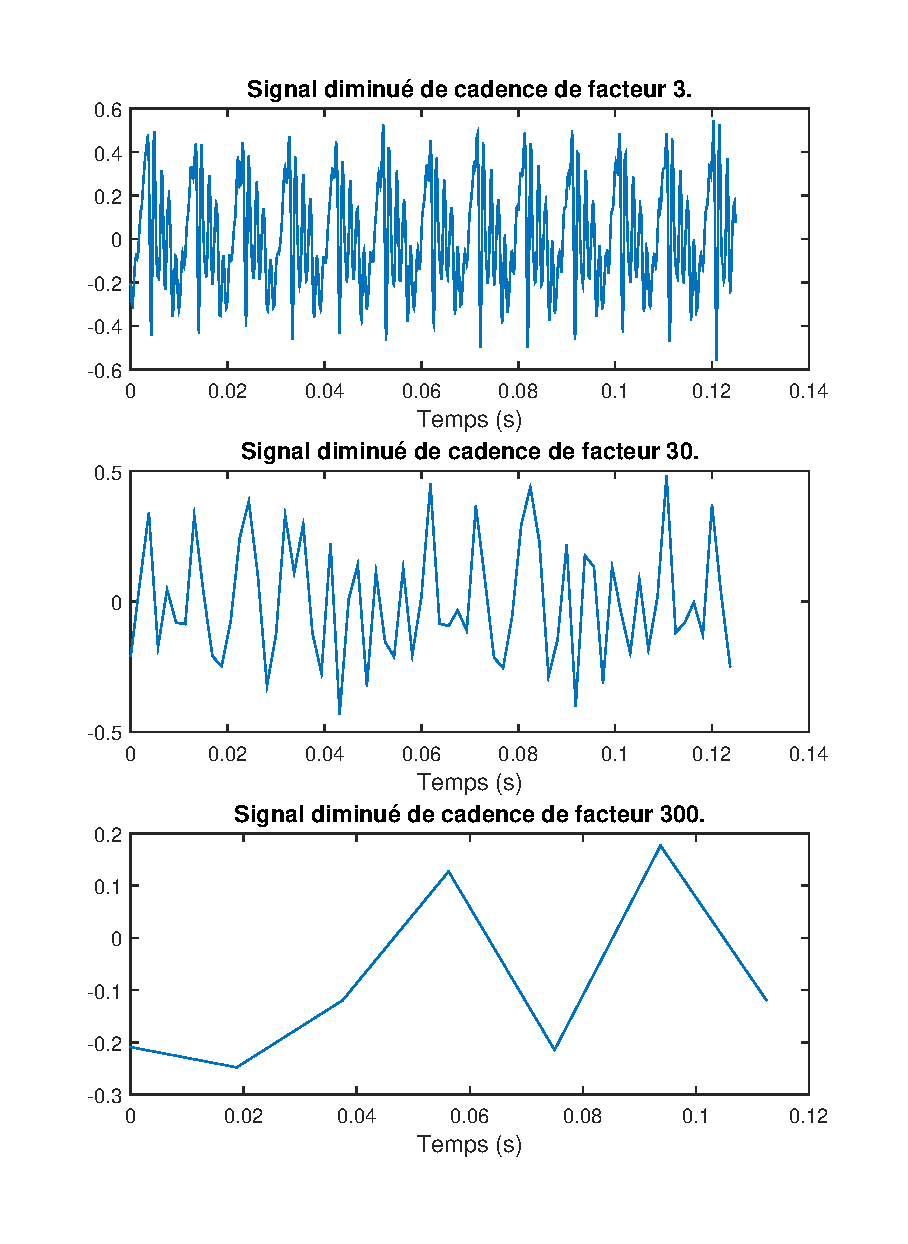
\includegraphics[width=\textwidth]{images/cadence_diminue.eps}
	% Title: glps_renderer figure
% Creator: GL2PS 1.3.8, (C) 1999-2012 C. Geuzaine
% For: Octave
% CreationDate: Thu Nov  9 17:04:09 2017
\begin{pgfpicture}
\pgfsetlinewidth{0.01pt}
\color[rgb]{1.000000,1.000000,1.000000}
\pgfpathmoveto{\pgfpoint{65.000015pt}{264.508606pt}}
\pgflineto{\pgfpoint{452.500000pt}{178.258606pt}}
\pgflineto{\pgfpoint{65.000015pt}{178.258606pt}}
\pgfpathclose
\pgfusepath{fill,stroke}
\pgfpathmoveto{\pgfpoint{65.000015pt}{264.508606pt}}
\pgflineto{\pgfpoint{452.500000pt}{264.508606pt}}
\pgflineto{\pgfpoint{452.500000pt}{178.258606pt}}
\pgfpathclose
\pgfusepath{fill,stroke}
\pgfpathmoveto{\pgfpoint{65.000015pt}{119.249985pt}}
\pgflineto{\pgfpoint{452.500000pt}{32.999985pt}}
\pgflineto{\pgfpoint{65.000015pt}{32.999985pt}}
\pgfpathclose
\pgfusepath{fill,stroke}
\pgfpathmoveto{\pgfpoint{65.000015pt}{119.249985pt}}
\pgflineto{\pgfpoint{452.500000pt}{119.249985pt}}
\pgflineto{\pgfpoint{452.500000pt}{32.999985pt}}
\pgfpathclose
\pgfusepath{fill,stroke}
\color[rgb]{0.000000,0.000000,0.000000}
\pgfsetlinewidth{0.500000pt}
\pgfsetdash{{16pt}{0pt}}{0pt}
\pgfpathmoveto{\pgfpoint{452.500000pt}{178.258606pt}}
\pgflineto{\pgfpoint{65.000015pt}{178.258606pt}}
\pgfusepath{stroke}
\pgfpathmoveto{\pgfpoint{452.500000pt}{264.508606pt}}
\pgflineto{\pgfpoint{65.000015pt}{264.508606pt}}
\pgfusepath{stroke}
\pgfpathmoveto{\pgfpoint{65.000015pt}{264.508606pt}}
\pgflineto{\pgfpoint{65.000015pt}{178.258606pt}}
\pgfusepath{stroke}
\pgfpathmoveto{\pgfpoint{452.500000pt}{264.508606pt}}
\pgflineto{\pgfpoint{452.500000pt}{178.258606pt}}
\pgfusepath{stroke}
\pgfsetdash{{0pt}{3pt}{1pt}{3pt}{1pt}{3pt}{1pt}{3pt}{1pt}{0pt}}{0pt}
\pgfpathmoveto{\pgfpoint{65.000015pt}{264.508606pt}}
\pgflineto{\pgfpoint{65.000015pt}{178.258606pt}}
\pgfusepath{stroke}
\pgfpathmoveto{\pgfpoint{161.875000pt}{264.508606pt}}
\pgflineto{\pgfpoint{161.875000pt}{178.258606pt}}
\pgfusepath{stroke}
\pgfpathmoveto{\pgfpoint{258.750000pt}{264.508606pt}}
\pgflineto{\pgfpoint{258.750000pt}{178.258606pt}}
\pgfusepath{stroke}
\pgfpathmoveto{\pgfpoint{355.625000pt}{264.508606pt}}
\pgflineto{\pgfpoint{355.625000pt}{178.258606pt}}
\pgfusepath{stroke}
\pgfpathmoveto{\pgfpoint{452.500000pt}{264.508606pt}}
\pgflineto{\pgfpoint{452.500000pt}{178.258606pt}}
\pgfusepath{stroke}
\pgfsetdash{{16pt}{0pt}}{0pt}
\pgfpathmoveto{\pgfpoint{65.000015pt}{182.144867pt}}
\pgflineto{\pgfpoint{65.000015pt}{178.258606pt}}
\pgfusepath{stroke}
\pgfpathmoveto{\pgfpoint{65.000015pt}{260.622345pt}}
\pgflineto{\pgfpoint{65.000015pt}{264.508606pt}}
\pgfusepath{stroke}
\pgfpathmoveto{\pgfpoint{161.875000pt}{182.144867pt}}
\pgflineto{\pgfpoint{161.875000pt}{178.258606pt}}
\pgfusepath{stroke}
\pgfpathmoveto{\pgfpoint{161.875000pt}{260.622345pt}}
\pgflineto{\pgfpoint{161.875000pt}{264.508606pt}}
\pgfusepath{stroke}
\pgfpathmoveto{\pgfpoint{258.750000pt}{182.144867pt}}
\pgflineto{\pgfpoint{258.750000pt}{178.258606pt}}
\pgfusepath{stroke}
\pgfpathmoveto{\pgfpoint{258.750000pt}{260.622345pt}}
\pgflineto{\pgfpoint{258.750000pt}{264.508606pt}}
\pgfusepath{stroke}
\pgfpathmoveto{\pgfpoint{355.625000pt}{182.144867pt}}
\pgflineto{\pgfpoint{355.625000pt}{178.258606pt}}
\pgfusepath{stroke}
\pgfpathmoveto{\pgfpoint{355.625000pt}{260.622345pt}}
\pgflineto{\pgfpoint{355.625000pt}{264.508606pt}}
\pgfusepath{stroke}
\pgfpathmoveto{\pgfpoint{452.500000pt}{182.144867pt}}
\pgflineto{\pgfpoint{452.500000pt}{178.258606pt}}
\pgfusepath{stroke}
\pgfpathmoveto{\pgfpoint{452.500000pt}{260.622345pt}}
\pgflineto{\pgfpoint{452.500000pt}{264.508606pt}}
\pgfusepath{stroke}
{
\pgftransformshift{\pgfpoint{65.000015pt}{173.244064pt}}
\pgfnode{rectangle}{north}{\fontsize{10}{0}\selectfont\textcolor[rgb]{0,0,0}{{0}}}{}{\pgfusepath{discard}}}
{
\pgftransformshift{\pgfpoint{161.875015pt}{173.244064pt}}
\pgfnode{rectangle}{north}{\fontsize{10}{0}\selectfont\textcolor[rgb]{0,0,0}{{0.005}}}{}{\pgfusepath{discard}}}
{
\pgftransformshift{\pgfpoint{258.750031pt}{173.244064pt}}
\pgfnode{rectangle}{north}{\fontsize{10}{0}\selectfont\textcolor[rgb]{0,0,0}{{0.01}}}{}{\pgfusepath{discard}}}
{
\pgftransformshift{\pgfpoint{355.625031pt}{173.244064pt}}
\pgfnode{rectangle}{north}{\fontsize{10}{0}\selectfont\textcolor[rgb]{0,0,0}{{0.015}}}{}{\pgfusepath{discard}}}
{
\pgftransformshift{\pgfpoint{452.500031pt}{173.244064pt}}
\pgfnode{rectangle}{north}{\fontsize{10}{0}\selectfont\textcolor[rgb]{0,0,0}{{0.02}}}{}{\pgfusepath{discard}}}
\pgfsetdash{{0pt}{3pt}{1pt}{3pt}{1pt}{3pt}{1pt}{3pt}{1pt}{0pt}}{0pt}
\pgfpathmoveto{\pgfpoint{452.500000pt}{178.258606pt}}
\pgflineto{\pgfpoint{65.000015pt}{178.258606pt}}
\pgfusepath{stroke}
\pgfpathmoveto{\pgfpoint{452.500000pt}{189.039856pt}}
\pgflineto{\pgfpoint{65.000015pt}{189.039856pt}}
\pgfusepath{stroke}
\pgfpathmoveto{\pgfpoint{452.500000pt}{199.821106pt}}
\pgflineto{\pgfpoint{65.000015pt}{199.821106pt}}
\pgfusepath{stroke}
\pgfpathmoveto{\pgfpoint{452.500000pt}{210.602356pt}}
\pgflineto{\pgfpoint{65.000015pt}{210.602356pt}}
\pgfusepath{stroke}
\pgfpathmoveto{\pgfpoint{452.500000pt}{221.383606pt}}
\pgflineto{\pgfpoint{65.000015pt}{221.383606pt}}
\pgfusepath{stroke}
\pgfpathmoveto{\pgfpoint{452.500000pt}{232.164856pt}}
\pgflineto{\pgfpoint{65.000015pt}{232.164856pt}}
\pgfusepath{stroke}
\pgfpathmoveto{\pgfpoint{452.500000pt}{242.946106pt}}
\pgflineto{\pgfpoint{65.000015pt}{242.946106pt}}
\pgfusepath{stroke}
\pgfpathmoveto{\pgfpoint{452.500000pt}{253.727356pt}}
\pgflineto{\pgfpoint{65.000015pt}{253.727356pt}}
\pgfusepath{stroke}
\pgfpathmoveto{\pgfpoint{452.500000pt}{264.508606pt}}
\pgflineto{\pgfpoint{65.000015pt}{264.508606pt}}
\pgfusepath{stroke}
\pgfsetdash{{16pt}{0pt}}{0pt}
\pgfpathmoveto{\pgfpoint{68.870026pt}{178.258606pt}}
\pgflineto{\pgfpoint{65.000015pt}{178.258606pt}}
\pgfusepath{stroke}
\pgfpathmoveto{\pgfpoint{448.630005pt}{178.258606pt}}
\pgflineto{\pgfpoint{452.500000pt}{178.258606pt}}
\pgfusepath{stroke}
\pgfpathmoveto{\pgfpoint{68.870026pt}{189.039856pt}}
\pgflineto{\pgfpoint{65.000015pt}{189.039856pt}}
\pgfusepath{stroke}
\pgfpathmoveto{\pgfpoint{448.630005pt}{189.039856pt}}
\pgflineto{\pgfpoint{452.500000pt}{189.039856pt}}
\pgfusepath{stroke}
\pgfpathmoveto{\pgfpoint{68.870026pt}{199.821106pt}}
\pgflineto{\pgfpoint{65.000015pt}{199.821106pt}}
\pgfusepath{stroke}
\pgfpathmoveto{\pgfpoint{448.630005pt}{199.821106pt}}
\pgflineto{\pgfpoint{452.500000pt}{199.821106pt}}
\pgfusepath{stroke}
\pgfpathmoveto{\pgfpoint{68.870026pt}{210.602356pt}}
\pgflineto{\pgfpoint{65.000015pt}{210.602356pt}}
\pgfusepath{stroke}
\pgfpathmoveto{\pgfpoint{448.630005pt}{210.602356pt}}
\pgflineto{\pgfpoint{452.500000pt}{210.602356pt}}
\pgfusepath{stroke}
\pgfpathmoveto{\pgfpoint{68.870026pt}{221.383606pt}}
\pgflineto{\pgfpoint{65.000015pt}{221.383606pt}}
\pgfusepath{stroke}
\pgfpathmoveto{\pgfpoint{448.630005pt}{221.383606pt}}
\pgflineto{\pgfpoint{452.500000pt}{221.383606pt}}
\pgfusepath{stroke}
\pgfpathmoveto{\pgfpoint{68.870026pt}{232.164856pt}}
\pgflineto{\pgfpoint{65.000015pt}{232.164856pt}}
\pgfusepath{stroke}
\pgfpathmoveto{\pgfpoint{448.630005pt}{232.164856pt}}
\pgflineto{\pgfpoint{452.500000pt}{232.164856pt}}
\pgfusepath{stroke}
\pgfpathmoveto{\pgfpoint{68.870026pt}{242.946106pt}}
\pgflineto{\pgfpoint{65.000015pt}{242.946106pt}}
\pgfusepath{stroke}
\pgfpathmoveto{\pgfpoint{448.630005pt}{242.946106pt}}
\pgflineto{\pgfpoint{452.500000pt}{242.946106pt}}
\pgfusepath{stroke}
\pgfpathmoveto{\pgfpoint{68.870026pt}{253.727356pt}}
\pgflineto{\pgfpoint{65.000015pt}{253.727356pt}}
\pgfusepath{stroke}
\pgfpathmoveto{\pgfpoint{448.630005pt}{253.727356pt}}
\pgflineto{\pgfpoint{452.500000pt}{253.727356pt}}
\pgfusepath{stroke}
\pgfpathmoveto{\pgfpoint{68.870026pt}{264.508606pt}}
\pgflineto{\pgfpoint{65.000015pt}{264.508606pt}}
\pgfusepath{stroke}
\pgfpathmoveto{\pgfpoint{448.630005pt}{264.508606pt}}
\pgflineto{\pgfpoint{452.500000pt}{264.508606pt}}
\pgfusepath{stroke}
{
\pgftransformshift{\pgfpoint{60.006454pt}{178.258606pt}}
\pgfnode{rectangle}{east}{\fontsize{10}{0}\selectfont\textcolor[rgb]{0,0,0}{{-0.8}}}{}{\pgfusepath{discard}}}
{
\pgftransformshift{\pgfpoint{60.006454pt}{189.039856pt}}
\pgfnode{rectangle}{east}{\fontsize{10}{0}\selectfont\textcolor[rgb]{0,0,0}{{-0.6}}}{}{\pgfusepath{discard}}}
{
\pgftransformshift{\pgfpoint{60.006454pt}{199.821106pt}}
\pgfnode{rectangle}{east}{\fontsize{10}{0}\selectfont\textcolor[rgb]{0,0,0}{{-0.4}}}{}{\pgfusepath{discard}}}
{
\pgftransformshift{\pgfpoint{60.006454pt}{210.602356pt}}
\pgfnode{rectangle}{east}{\fontsize{10}{0}\selectfont\textcolor[rgb]{0,0,0}{{-0.2}}}{}{\pgfusepath{discard}}}
{
\pgftransformshift{\pgfpoint{60.006454pt}{221.383606pt}}
\pgfnode{rectangle}{east}{\fontsize{10}{0}\selectfont\textcolor[rgb]{0,0,0}{{0}}}{}{\pgfusepath{discard}}}
{
\pgftransformshift{\pgfpoint{60.006454pt}{232.164856pt}}
\pgfnode{rectangle}{east}{\fontsize{10}{0}\selectfont\textcolor[rgb]{0,0,0}{{0.2}}}{}{\pgfusepath{discard}}}
{
\pgftransformshift{\pgfpoint{60.006454pt}{242.946106pt}}
\pgfnode{rectangle}{east}{\fontsize{10}{0}\selectfont\textcolor[rgb]{0,0,0}{{0.4}}}{}{\pgfusepath{discard}}}
{
\pgftransformshift{\pgfpoint{60.006454pt}{253.727356pt}}
\pgfnode{rectangle}{east}{\fontsize{10}{0}\selectfont\textcolor[rgb]{0,0,0}{{0.6}}}{}{\pgfusepath{discard}}}
{
\pgftransformshift{\pgfpoint{60.006454pt}{264.508606pt}}
\pgfnode{rectangle}{east}{\fontsize{10}{0}\selectfont\textcolor[rgb]{0,0,0}{{0.8}}}{}{\pgfusepath{discard}}}
{
\pgftransformshift{\pgfpoint{258.750031pt}{162.244080pt}}
\pgfnode{rectangle}{north}{\fontsize{10}{0}\selectfont\textcolor[rgb]{0,0,0}{{Temps (s)}}}{}{\pgfusepath{discard}}}
\color[rgb]{0.000000,0.000000,1.000000}
\pgfsetdash{}{0pt}
\pgfpathmoveto{\pgfpoint{68.632828pt}{205.857269pt}}
\pgflineto{\pgfpoint{65.000015pt}{210.108170pt}}
\pgfusepath{stroke}
\pgfpathmoveto{\pgfpoint{72.265640pt}{205.207458pt}}
\pgflineto{\pgfpoint{68.632828pt}{205.857269pt}}
\pgfusepath{stroke}
\pgfpathmoveto{\pgfpoint{75.898453pt}{207.745819pt}}
\pgflineto{\pgfpoint{72.265640pt}{205.207458pt}}
\pgfusepath{stroke}
\pgfpathmoveto{\pgfpoint{79.531265pt}{212.972260pt}}
\pgflineto{\pgfpoint{75.898453pt}{207.745819pt}}
\pgfusepath{stroke}
\pgfpathmoveto{\pgfpoint{83.164078pt}{216.367737pt}}
\pgflineto{\pgfpoint{79.531265pt}{212.972260pt}}
\pgfusepath{stroke}
\pgfpathmoveto{\pgfpoint{86.796875pt}{217.165588pt}}
\pgflineto{\pgfpoint{83.164078pt}{216.367737pt}}
\pgfusepath{stroke}
\pgfpathmoveto{\pgfpoint{90.429688pt}{216.494400pt}}
\pgflineto{\pgfpoint{86.796875pt}{217.165588pt}}
\pgfusepath{stroke}
\pgfpathmoveto{\pgfpoint{94.062500pt}{217.091568pt}}
\pgflineto{\pgfpoint{90.429688pt}{216.494400pt}}
\pgfusepath{stroke}
\pgfpathmoveto{\pgfpoint{97.695328pt}{221.337540pt}}
\pgflineto{\pgfpoint{94.062500pt}{217.091568pt}}
\pgfusepath{stroke}
\pgfpathmoveto{\pgfpoint{101.328140pt}{225.215012pt}}
\pgflineto{\pgfpoint{97.695328pt}{221.337540pt}}
\pgfusepath{stroke}
\pgfpathmoveto{\pgfpoint{104.960953pt}{228.289688pt}}
\pgflineto{\pgfpoint{101.328140pt}{225.215012pt}}
\pgfusepath{stroke}
\pgfpathmoveto{\pgfpoint{108.593765pt}{229.273438pt}}
\pgflineto{\pgfpoint{104.960953pt}{228.289688pt}}
\pgfusepath{stroke}
\pgfpathmoveto{\pgfpoint{112.226578pt}{232.300415pt}}
\pgflineto{\pgfpoint{108.593765pt}{229.273438pt}}
\pgfusepath{stroke}
\pgfpathmoveto{\pgfpoint{115.859390pt}{236.238754pt}}
\pgflineto{\pgfpoint{112.226578pt}{232.300415pt}}
\pgfusepath{stroke}
\pgfpathmoveto{\pgfpoint{119.492203pt}{238.910370pt}}
\pgflineto{\pgfpoint{115.859390pt}{236.238754pt}}
\pgfusepath{stroke}
\pgfpathmoveto{\pgfpoint{123.125015pt}{242.363403pt}}
\pgflineto{\pgfpoint{119.492203pt}{238.910370pt}}
\pgfusepath{stroke}
\pgfpathmoveto{\pgfpoint{126.757820pt}{243.223785pt}}
\pgflineto{\pgfpoint{123.125015pt}{242.363403pt}}
\pgfusepath{stroke}
\pgfpathmoveto{\pgfpoint{130.390640pt}{245.745712pt}}
\pgflineto{\pgfpoint{126.757820pt}{243.223785pt}}
\pgfusepath{stroke}
\pgfpathmoveto{\pgfpoint{134.023453pt}{247.236176pt}}
\pgflineto{\pgfpoint{130.390640pt}{245.745712pt}}
\pgfusepath{stroke}
\pgfpathmoveto{\pgfpoint{137.656265pt}{239.775696pt}}
\pgflineto{\pgfpoint{134.023453pt}{247.236176pt}}
\pgfusepath{stroke}
\pgfpathmoveto{\pgfpoint{141.289078pt}{219.476944pt}}
\pgflineto{\pgfpoint{137.656265pt}{239.775696pt}}
\pgfusepath{stroke}
\pgfpathmoveto{\pgfpoint{144.921875pt}{201.224701pt}}
\pgflineto{\pgfpoint{141.289078pt}{219.476944pt}}
\pgfusepath{stroke}
\pgfpathmoveto{\pgfpoint{148.554688pt}{197.417969pt}}
\pgflineto{\pgfpoint{144.921875pt}{201.224701pt}}
\pgfusepath{stroke}
\pgfpathmoveto{\pgfpoint{152.187500pt}{219.355209pt}}
\pgflineto{\pgfpoint{148.554688pt}{197.417969pt}}
\pgfusepath{stroke}
\pgfpathmoveto{\pgfpoint{155.820328pt}{244.580994pt}}
\pgflineto{\pgfpoint{152.187500pt}{219.355209pt}}
\pgfusepath{stroke}
\pgfpathmoveto{\pgfpoint{159.453140pt}{248.012650pt}}
\pgflineto{\pgfpoint{155.820328pt}{244.580994pt}}
\pgfusepath{stroke}
\pgfpathmoveto{\pgfpoint{163.085953pt}{235.162872pt}}
\pgflineto{\pgfpoint{159.453140pt}{248.012650pt}}
\pgfusepath{stroke}
\pgfpathmoveto{\pgfpoint{166.718750pt}{220.044495pt}}
\pgflineto{\pgfpoint{163.085953pt}{235.162872pt}}
\pgfusepath{stroke}
\pgfpathmoveto{\pgfpoint{170.351562pt}{212.704117pt}}
\pgflineto{\pgfpoint{166.718750pt}{220.044495pt}}
\pgfusepath{stroke}
\pgfpathmoveto{\pgfpoint{173.984390pt}{211.899673pt}}
\pgflineto{\pgfpoint{170.351562pt}{212.704117pt}}
\pgfusepath{stroke}
\pgfpathmoveto{\pgfpoint{177.617203pt}{211.587097pt}}
\pgflineto{\pgfpoint{173.984390pt}{211.899673pt}}
\pgfusepath{stroke}
\pgfpathmoveto{\pgfpoint{181.250015pt}{216.969833pt}}
\pgflineto{\pgfpoint{177.617203pt}{211.587097pt}}
\pgfusepath{stroke}
\pgfpathmoveto{\pgfpoint{184.882828pt}{229.186249pt}}
\pgflineto{\pgfpoint{181.250015pt}{216.969833pt}}
\pgfusepath{stroke}
\pgfpathmoveto{\pgfpoint{188.515625pt}{238.304993pt}}
\pgflineto{\pgfpoint{184.882828pt}{229.186249pt}}
\pgfusepath{stroke}
\pgfpathmoveto{\pgfpoint{192.148438pt}{236.676346pt}}
\pgflineto{\pgfpoint{188.515625pt}{238.304993pt}}
\pgfusepath{stroke}
\pgfpathmoveto{\pgfpoint{195.781265pt}{224.145706pt}}
\pgflineto{\pgfpoint{192.148438pt}{236.676346pt}}
\pgfusepath{stroke}
\pgfpathmoveto{\pgfpoint{199.414078pt}{211.049164pt}}
\pgflineto{\pgfpoint{195.781265pt}{224.145706pt}}
\pgfusepath{stroke}
\pgfpathmoveto{\pgfpoint{203.046890pt}{208.772354pt}}
\pgflineto{\pgfpoint{199.414078pt}{211.049164pt}}
\pgfusepath{stroke}
\pgfpathmoveto{\pgfpoint{206.679703pt}{214.716064pt}}
\pgflineto{\pgfpoint{203.046890pt}{208.772354pt}}
\pgfusepath{stroke}
\pgfpathmoveto{\pgfpoint{210.312515pt}{223.870972pt}}
\pgflineto{\pgfpoint{206.679703pt}{214.716064pt}}
\pgfusepath{stroke}
\pgfpathmoveto{\pgfpoint{213.945328pt}{230.097626pt}}
\pgflineto{\pgfpoint{210.312515pt}{223.870972pt}}
\pgfusepath{stroke}
\pgfpathmoveto{\pgfpoint{217.578140pt}{231.759186pt}}
\pgflineto{\pgfpoint{213.945328pt}{230.097626pt}}
\pgfusepath{stroke}
\pgfpathmoveto{\pgfpoint{221.210938pt}{229.368866pt}}
\pgflineto{\pgfpoint{217.578140pt}{231.759186pt}}
\pgfusepath{stroke}
\pgfpathmoveto{\pgfpoint{224.843750pt}{220.404785pt}}
\pgflineto{\pgfpoint{221.210938pt}{229.368866pt}}
\pgfusepath{stroke}
\pgfpathmoveto{\pgfpoint{228.476578pt}{208.884216pt}}
\pgflineto{\pgfpoint{224.843750pt}{220.404785pt}}
\pgfusepath{stroke}
\pgfpathmoveto{\pgfpoint{232.109375pt}{202.145935pt}}
\pgflineto{\pgfpoint{228.476578pt}{208.884216pt}}
\pgfusepath{stroke}
\pgfpathmoveto{\pgfpoint{235.742203pt}{204.182556pt}}
\pgflineto{\pgfpoint{232.109375pt}{202.145935pt}}
\pgfusepath{stroke}
\pgfpathmoveto{\pgfpoint{239.375015pt}{210.968552pt}}
\pgflineto{\pgfpoint{235.742203pt}{204.182556pt}}
\pgfusepath{stroke}
\pgfpathmoveto{\pgfpoint{243.007828pt}{217.262665pt}}
\pgflineto{\pgfpoint{239.375015pt}{210.968552pt}}
\pgfusepath{stroke}
\pgfpathmoveto{\pgfpoint{246.640640pt}{217.037292pt}}
\pgflineto{\pgfpoint{243.007828pt}{217.262665pt}}
\pgfusepath{stroke}
\pgfpathmoveto{\pgfpoint{250.273453pt}{212.401428pt}}
\pgflineto{\pgfpoint{246.640640pt}{217.037292pt}}
\pgfusepath{stroke}
\pgfpathmoveto{\pgfpoint{253.906265pt}{206.781799pt}}
\pgflineto{\pgfpoint{250.273453pt}{212.401428pt}}
\pgfusepath{stroke}
\pgfpathmoveto{\pgfpoint{257.539062pt}{203.909485pt}}
\pgflineto{\pgfpoint{253.906265pt}{206.781799pt}}
\pgfusepath{stroke}
\pgfpathmoveto{\pgfpoint{261.171906pt}{205.319321pt}}
\pgflineto{\pgfpoint{257.539062pt}{203.909485pt}}
\pgfusepath{stroke}
\pgfpathmoveto{\pgfpoint{264.804718pt}{209.657410pt}}
\pgflineto{\pgfpoint{261.171906pt}{205.319321pt}}
\pgfusepath{stroke}
\pgfpathmoveto{\pgfpoint{268.437500pt}{215.278687pt}}
\pgflineto{\pgfpoint{264.804718pt}{209.657410pt}}
\pgfusepath{stroke}
\pgfpathmoveto{\pgfpoint{272.070343pt}{217.810471pt}}
\pgflineto{\pgfpoint{268.437500pt}{215.278687pt}}
\pgfusepath{stroke}
\pgfpathmoveto{\pgfpoint{275.703125pt}{216.519073pt}}
\pgflineto{\pgfpoint{272.070343pt}{217.810471pt}}
\pgfusepath{stroke}
\pgfpathmoveto{\pgfpoint{279.335938pt}{214.969406pt}}
\pgflineto{\pgfpoint{275.703125pt}{216.519073pt}}
\pgfusepath{stroke}
\pgfpathmoveto{\pgfpoint{282.968781pt}{216.711548pt}}
\pgflineto{\pgfpoint{279.335938pt}{214.969406pt}}
\pgfusepath{stroke}
\pgfpathmoveto{\pgfpoint{286.601562pt}{221.681366pt}}
\pgflineto{\pgfpoint{282.968781pt}{216.711548pt}}
\pgfusepath{stroke}
\pgfpathmoveto{\pgfpoint{290.234375pt}{225.629578pt}}
\pgflineto{\pgfpoint{286.601562pt}{221.681366pt}}
\pgfusepath{stroke}
\pgfpathmoveto{\pgfpoint{293.867188pt}{227.379944pt}}
\pgflineto{\pgfpoint{290.234375pt}{225.629578pt}}
\pgfusepath{stroke}
\pgfpathmoveto{\pgfpoint{297.500000pt}{230.095993pt}}
\pgflineto{\pgfpoint{293.867188pt}{227.379944pt}}
\pgfusepath{stroke}
\pgfpathmoveto{\pgfpoint{301.132812pt}{233.986633pt}}
\pgflineto{\pgfpoint{297.500000pt}{230.095993pt}}
\pgfusepath{stroke}
\pgfpathmoveto{\pgfpoint{304.765625pt}{238.954788pt}}
\pgflineto{\pgfpoint{301.132812pt}{233.986633pt}}
\pgfusepath{stroke}
\pgfpathmoveto{\pgfpoint{308.398468pt}{239.139038pt}}
\pgflineto{\pgfpoint{304.765625pt}{238.954788pt}}
\pgfusepath{stroke}
\pgfpathmoveto{\pgfpoint{312.031250pt}{238.173370pt}}
\pgflineto{\pgfpoint{308.398468pt}{239.139038pt}}
\pgfusepath{stroke}
\pgfpathmoveto{\pgfpoint{315.664062pt}{236.771759pt}}
\pgflineto{\pgfpoint{312.031250pt}{238.173370pt}}
\pgfusepath{stroke}
\pgfpathmoveto{\pgfpoint{319.296875pt}{239.107788pt}}
\pgflineto{\pgfpoint{315.664062pt}{236.771759pt}}
\pgfusepath{stroke}
\pgfpathmoveto{\pgfpoint{322.929688pt}{244.561249pt}}
\pgflineto{\pgfpoint{319.296875pt}{239.107788pt}}
\pgfusepath{stroke}
\pgfpathmoveto{\pgfpoint{326.562500pt}{244.737274pt}}
\pgflineto{\pgfpoint{322.929688pt}{244.561249pt}}
\pgfusepath{stroke}
\pgfpathmoveto{\pgfpoint{330.195312pt}{228.863831pt}}
\pgflineto{\pgfpoint{326.562500pt}{244.737274pt}}
\pgfusepath{stroke}
\pgfpathmoveto{\pgfpoint{333.828125pt}{208.262390pt}}
\pgflineto{\pgfpoint{330.195312pt}{228.863831pt}}
\pgfusepath{stroke}
\pgfpathmoveto{\pgfpoint{337.460938pt}{197.944397pt}}
\pgflineto{\pgfpoint{333.828125pt}{208.262390pt}}
\pgfusepath{stroke}
\pgfpathmoveto{\pgfpoint{341.093750pt}{213.952744pt}}
\pgflineto{\pgfpoint{337.460938pt}{197.944397pt}}
\pgfusepath{stroke}
\pgfpathmoveto{\pgfpoint{344.726562pt}{237.936493pt}}
\pgflineto{\pgfpoint{341.093750pt}{213.952744pt}}
\pgfusepath{stroke}
\pgfpathmoveto{\pgfpoint{348.359375pt}{244.939621pt}}
\pgflineto{\pgfpoint{344.726562pt}{237.936493pt}}
\pgfusepath{stroke}
\pgfpathmoveto{\pgfpoint{351.992188pt}{236.645081pt}}
\pgflineto{\pgfpoint{348.359375pt}{244.939621pt}}
\pgfusepath{stroke}
\pgfpathmoveto{\pgfpoint{355.625000pt}{223.351135pt}}
\pgflineto{\pgfpoint{351.992188pt}{236.645081pt}}
\pgfusepath{stroke}
\pgfpathmoveto{\pgfpoint{359.257843pt}{216.698395pt}}
\pgflineto{\pgfpoint{355.625000pt}{223.351135pt}}
\pgfusepath{stroke}
\pgfpathmoveto{\pgfpoint{362.890656pt}{214.419952pt}}
\pgflineto{\pgfpoint{359.257843pt}{216.698395pt}}
\pgfusepath{stroke}
\pgfpathmoveto{\pgfpoint{366.523468pt}{211.804260pt}}
\pgflineto{\pgfpoint{362.890656pt}{214.419952pt}}
\pgfusepath{stroke}
\pgfpathmoveto{\pgfpoint{370.156281pt}{214.227478pt}}
\pgflineto{\pgfpoint{366.523468pt}{211.804260pt}}
\pgfusepath{stroke}
\pgfpathmoveto{\pgfpoint{373.789062pt}{224.709976pt}}
\pgflineto{\pgfpoint{370.156281pt}{214.227478pt}}
\pgfusepath{stroke}
\pgfpathmoveto{\pgfpoint{377.421875pt}{235.672852pt}}
\pgflineto{\pgfpoint{373.789062pt}{224.709976pt}}
\pgfusepath{stroke}
\pgfpathmoveto{\pgfpoint{381.054718pt}{237.061295pt}}
\pgflineto{\pgfpoint{377.421875pt}{235.672852pt}}
\pgfusepath{stroke}
\pgfpathmoveto{\pgfpoint{384.687500pt}{227.220367pt}}
\pgflineto{\pgfpoint{381.054718pt}{237.061295pt}}
\pgfusepath{stroke}
\pgfpathmoveto{\pgfpoint{388.320312pt}{214.767059pt}}
\pgflineto{\pgfpoint{384.687500pt}{227.220367pt}}
\pgfusepath{stroke}
\pgfpathmoveto{\pgfpoint{391.953156pt}{210.103241pt}}
\pgflineto{\pgfpoint{388.320312pt}{214.767059pt}}
\pgfusepath{stroke}
\pgfpathmoveto{\pgfpoint{395.585938pt}{213.656616pt}}
\pgflineto{\pgfpoint{391.953156pt}{210.103241pt}}
\pgfusepath{stroke}
\pgfpathmoveto{\pgfpoint{399.218750pt}{220.975616pt}}
\pgflineto{\pgfpoint{395.585938pt}{213.656616pt}}
\pgfusepath{stroke}
\pgfpathmoveto{\pgfpoint{402.851593pt}{227.226959pt}}
\pgflineto{\pgfpoint{399.218750pt}{220.975616pt}}
\pgfusepath{stroke}
\pgfpathmoveto{\pgfpoint{406.484375pt}{230.245697pt}}
\pgflineto{\pgfpoint{402.851593pt}{227.226959pt}}
\pgfusepath{stroke}
\pgfpathmoveto{\pgfpoint{410.117188pt}{229.566284pt}}
\pgflineto{\pgfpoint{406.484375pt}{230.245697pt}}
\pgfusepath{stroke}
\pgfpathmoveto{\pgfpoint{413.750000pt}{222.176544pt}}
\pgflineto{\pgfpoint{410.117188pt}{229.566284pt}}
\pgfusepath{stroke}
\pgfpathmoveto{\pgfpoint{417.382812pt}{210.447052pt}}
\pgflineto{\pgfpoint{413.750000pt}{222.176544pt}}
\pgfusepath{stroke}
\pgfpathmoveto{\pgfpoint{421.015625pt}{202.473312pt}}
\pgflineto{\pgfpoint{417.382812pt}{210.447052pt}}
\pgfusepath{stroke}
\pgfpathmoveto{\pgfpoint{424.648438pt}{202.349930pt}}
\pgflineto{\pgfpoint{421.015625pt}{202.473312pt}}
\pgfusepath{stroke}
\pgfpathmoveto{\pgfpoint{428.281250pt}{208.015625pt}}
\pgflineto{\pgfpoint{424.648438pt}{202.349930pt}}
\pgfusepath{stroke}
\color[rgb]{0.000000,0.000000,0.000000}
\pgfsetdash{{16pt}{0pt}}{0pt}
\pgfpathmoveto{\pgfpoint{452.500000pt}{32.999985pt}}
\pgflineto{\pgfpoint{65.000015pt}{32.999985pt}}
\pgfusepath{stroke}
\pgfpathmoveto{\pgfpoint{452.500000pt}{119.249985pt}}
\pgflineto{\pgfpoint{65.000015pt}{119.249985pt}}
\pgfusepath{stroke}
\pgfpathmoveto{\pgfpoint{65.000015pt}{119.249985pt}}
\pgflineto{\pgfpoint{65.000015pt}{32.999985pt}}
\pgfusepath{stroke}
\pgfpathmoveto{\pgfpoint{452.500000pt}{119.249985pt}}
\pgflineto{\pgfpoint{452.500000pt}{32.999985pt}}
\pgfusepath{stroke}
\pgfsetdash{{0pt}{3pt}{1pt}{3pt}{1pt}{3pt}{1pt}{3pt}{1pt}{0pt}}{0pt}
\pgfpathmoveto{\pgfpoint{65.000015pt}{119.249985pt}}
\pgflineto{\pgfpoint{65.000015pt}{32.999985pt}}
\pgfusepath{stroke}
\pgfpathmoveto{\pgfpoint{161.875000pt}{119.249985pt}}
\pgflineto{\pgfpoint{161.875000pt}{32.999985pt}}
\pgfusepath{stroke}
\pgfpathmoveto{\pgfpoint{258.750000pt}{119.249985pt}}
\pgflineto{\pgfpoint{258.750000pt}{32.999985pt}}
\pgfusepath{stroke}
\pgfpathmoveto{\pgfpoint{355.625000pt}{119.249985pt}}
\pgflineto{\pgfpoint{355.625000pt}{32.999985pt}}
\pgfusepath{stroke}
\pgfpathmoveto{\pgfpoint{452.500000pt}{119.249985pt}}
\pgflineto{\pgfpoint{452.500000pt}{32.999985pt}}
\pgfusepath{stroke}
\pgfsetdash{{16pt}{0pt}}{0pt}
\pgfpathmoveto{\pgfpoint{65.000015pt}{36.886253pt}}
\pgflineto{\pgfpoint{65.000015pt}{32.999985pt}}
\pgfusepath{stroke}
\pgfpathmoveto{\pgfpoint{65.000015pt}{115.363724pt}}
\pgflineto{\pgfpoint{65.000015pt}{119.249985pt}}
\pgfusepath{stroke}
\pgfpathmoveto{\pgfpoint{161.875000pt}{36.886253pt}}
\pgflineto{\pgfpoint{161.875000pt}{32.999985pt}}
\pgfusepath{stroke}
\pgfpathmoveto{\pgfpoint{161.875000pt}{115.363724pt}}
\pgflineto{\pgfpoint{161.875000pt}{119.249985pt}}
\pgfusepath{stroke}
\pgfpathmoveto{\pgfpoint{258.750000pt}{36.886253pt}}
\pgflineto{\pgfpoint{258.750000pt}{32.999985pt}}
\pgfusepath{stroke}
\pgfpathmoveto{\pgfpoint{258.750000pt}{115.363724pt}}
\pgflineto{\pgfpoint{258.750000pt}{119.249985pt}}
\pgfusepath{stroke}
\pgfpathmoveto{\pgfpoint{355.625000pt}{36.886253pt}}
\pgflineto{\pgfpoint{355.625000pt}{32.999985pt}}
\pgfusepath{stroke}
\pgfpathmoveto{\pgfpoint{355.625000pt}{115.363724pt}}
\pgflineto{\pgfpoint{355.625000pt}{119.249985pt}}
\pgfusepath{stroke}
\pgfpathmoveto{\pgfpoint{452.500000pt}{36.886253pt}}
\pgflineto{\pgfpoint{452.500000pt}{32.999985pt}}
\pgfusepath{stroke}
\pgfpathmoveto{\pgfpoint{452.500000pt}{115.363724pt}}
\pgflineto{\pgfpoint{452.500000pt}{119.249985pt}}
\pgfusepath{stroke}
{
\pgftransformshift{\pgfpoint{65.000015pt}{27.985451pt}}
\pgfnode{rectangle}{north}{\fontsize{10}{0}\selectfont\textcolor[rgb]{0,0,0}{{0}}}{}{\pgfusepath{discard}}}
{
\pgftransformshift{\pgfpoint{161.875015pt}{27.985451pt}}
\pgfnode{rectangle}{north}{\fontsize{10}{0}\selectfont\textcolor[rgb]{0,0,0}{{0.005}}}{}{\pgfusepath{discard}}}
{
\pgftransformshift{\pgfpoint{258.750031pt}{27.985451pt}}
\pgfnode{rectangle}{north}{\fontsize{10}{0}\selectfont\textcolor[rgb]{0,0,0}{{0.01}}}{}{\pgfusepath{discard}}}
{
\pgftransformshift{\pgfpoint{355.625031pt}{27.985451pt}}
\pgfnode{rectangle}{north}{\fontsize{10}{0}\selectfont\textcolor[rgb]{0,0,0}{{0.015}}}{}{\pgfusepath{discard}}}
{
\pgftransformshift{\pgfpoint{452.500031pt}{27.985451pt}}
\pgfnode{rectangle}{north}{\fontsize{10}{0}\selectfont\textcolor[rgb]{0,0,0}{{0.02}}}{}{\pgfusepath{discard}}}
\pgfsetdash{{0pt}{3pt}{1pt}{3pt}{1pt}{3pt}{1pt}{3pt}{1pt}{0pt}}{0pt}
\pgfpathmoveto{\pgfpoint{452.500000pt}{32.999985pt}}
\pgflineto{\pgfpoint{65.000015pt}{32.999985pt}}
\pgfusepath{stroke}
\pgfpathmoveto{\pgfpoint{452.500000pt}{43.781242pt}}
\pgflineto{\pgfpoint{65.000015pt}{43.781242pt}}
\pgfusepath{stroke}
\pgfpathmoveto{\pgfpoint{452.500000pt}{54.562485pt}}
\pgflineto{\pgfpoint{65.000015pt}{54.562485pt}}
\pgfusepath{stroke}
\pgfpathmoveto{\pgfpoint{452.500000pt}{65.343742pt}}
\pgflineto{\pgfpoint{65.000015pt}{65.343742pt}}
\pgfusepath{stroke}
\pgfpathmoveto{\pgfpoint{452.500000pt}{76.124992pt}}
\pgflineto{\pgfpoint{65.000015pt}{76.124992pt}}
\pgfusepath{stroke}
\pgfpathmoveto{\pgfpoint{452.500000pt}{86.906242pt}}
\pgflineto{\pgfpoint{65.000015pt}{86.906242pt}}
\pgfusepath{stroke}
\pgfpathmoveto{\pgfpoint{452.500000pt}{97.687492pt}}
\pgflineto{\pgfpoint{65.000015pt}{97.687492pt}}
\pgfusepath{stroke}
\pgfpathmoveto{\pgfpoint{452.500000pt}{108.468735pt}}
\pgflineto{\pgfpoint{65.000015pt}{108.468735pt}}
\pgfusepath{stroke}
\pgfpathmoveto{\pgfpoint{452.500000pt}{119.249985pt}}
\pgflineto{\pgfpoint{65.000015pt}{119.249985pt}}
\pgfusepath{stroke}
\pgfsetdash{{16pt}{0pt}}{0pt}
\pgfpathmoveto{\pgfpoint{68.870026pt}{32.999985pt}}
\pgflineto{\pgfpoint{65.000015pt}{32.999985pt}}
\pgfusepath{stroke}
\pgfpathmoveto{\pgfpoint{448.630005pt}{32.999985pt}}
\pgflineto{\pgfpoint{452.500000pt}{32.999985pt}}
\pgfusepath{stroke}
\pgfpathmoveto{\pgfpoint{68.870026pt}{43.781242pt}}
\pgflineto{\pgfpoint{65.000015pt}{43.781242pt}}
\pgfusepath{stroke}
\pgfpathmoveto{\pgfpoint{448.630005pt}{43.781242pt}}
\pgflineto{\pgfpoint{452.500000pt}{43.781242pt}}
\pgfusepath{stroke}
\pgfpathmoveto{\pgfpoint{68.870026pt}{54.562485pt}}
\pgflineto{\pgfpoint{65.000015pt}{54.562485pt}}
\pgfusepath{stroke}
\pgfpathmoveto{\pgfpoint{448.630005pt}{54.562485pt}}
\pgflineto{\pgfpoint{452.500000pt}{54.562485pt}}
\pgfusepath{stroke}
\pgfpathmoveto{\pgfpoint{68.870026pt}{65.343742pt}}
\pgflineto{\pgfpoint{65.000015pt}{65.343742pt}}
\pgfusepath{stroke}
\pgfpathmoveto{\pgfpoint{448.630005pt}{65.343742pt}}
\pgflineto{\pgfpoint{452.500000pt}{65.343742pt}}
\pgfusepath{stroke}
\pgfpathmoveto{\pgfpoint{68.870026pt}{76.124992pt}}
\pgflineto{\pgfpoint{65.000015pt}{76.124992pt}}
\pgfusepath{stroke}
\pgfpathmoveto{\pgfpoint{448.630005pt}{76.124992pt}}
\pgflineto{\pgfpoint{452.500000pt}{76.124992pt}}
\pgfusepath{stroke}
\pgfpathmoveto{\pgfpoint{68.870026pt}{86.906242pt}}
\pgflineto{\pgfpoint{65.000015pt}{86.906242pt}}
\pgfusepath{stroke}
\pgfpathmoveto{\pgfpoint{448.630005pt}{86.906242pt}}
\pgflineto{\pgfpoint{452.500000pt}{86.906242pt}}
\pgfusepath{stroke}
\pgfpathmoveto{\pgfpoint{68.870026pt}{97.687492pt}}
\pgflineto{\pgfpoint{65.000015pt}{97.687492pt}}
\pgfusepath{stroke}
\pgfpathmoveto{\pgfpoint{448.630005pt}{97.687492pt}}
\pgflineto{\pgfpoint{452.500000pt}{97.687492pt}}
\pgfusepath{stroke}
\pgfpathmoveto{\pgfpoint{68.870026pt}{108.468735pt}}
\pgflineto{\pgfpoint{65.000015pt}{108.468735pt}}
\pgfusepath{stroke}
\pgfpathmoveto{\pgfpoint{448.630005pt}{108.468735pt}}
\pgflineto{\pgfpoint{452.500000pt}{108.468735pt}}
\pgfusepath{stroke}
\pgfpathmoveto{\pgfpoint{68.870026pt}{119.249985pt}}
\pgflineto{\pgfpoint{65.000015pt}{119.249985pt}}
\pgfusepath{stroke}
\pgfpathmoveto{\pgfpoint{448.630005pt}{119.249985pt}}
\pgflineto{\pgfpoint{452.500000pt}{119.249985pt}}
\pgfusepath{stroke}
{
\pgftransformshift{\pgfpoint{60.006454pt}{32.999985pt}}
\pgfnode{rectangle}{east}{\fontsize{10}{0}\selectfont\textcolor[rgb]{0,0,0}{{-0.4}}}{}{\pgfusepath{discard}}}
{
\pgftransformshift{\pgfpoint{60.006454pt}{43.781242pt}}
\pgfnode{rectangle}{east}{\fontsize{10}{0}\selectfont\textcolor[rgb]{0,0,0}{{-0.3}}}{}{\pgfusepath{discard}}}
{
\pgftransformshift{\pgfpoint{60.006454pt}{54.562485pt}}
\pgfnode{rectangle}{east}{\fontsize{10}{0}\selectfont\textcolor[rgb]{0,0,0}{{-0.2}}}{}{\pgfusepath{discard}}}
{
\pgftransformshift{\pgfpoint{60.006454pt}{65.343742pt}}
\pgfnode{rectangle}{east}{\fontsize{10}{0}\selectfont\textcolor[rgb]{0,0,0}{{-0.1}}}{}{\pgfusepath{discard}}}
{
\pgftransformshift{\pgfpoint{60.006454pt}{76.124992pt}}
\pgfnode{rectangle}{east}{\fontsize{10}{0}\selectfont\textcolor[rgb]{0,0,0}{{0}}}{}{\pgfusepath{discard}}}
{
\pgftransformshift{\pgfpoint{60.006454pt}{86.906242pt}}
\pgfnode{rectangle}{east}{\fontsize{10}{0}\selectfont\textcolor[rgb]{0,0,0}{{0.1}}}{}{\pgfusepath{discard}}}
{
\pgftransformshift{\pgfpoint{60.006454pt}{97.687492pt}}
\pgfnode{rectangle}{east}{\fontsize{10}{0}\selectfont\textcolor[rgb]{0,0,0}{{0.2}}}{}{\pgfusepath{discard}}}
{
\pgftransformshift{\pgfpoint{60.006454pt}{108.468735pt}}
\pgfnode{rectangle}{east}{\fontsize{10}{0}\selectfont\textcolor[rgb]{0,0,0}{{0.3}}}{}{\pgfusepath{discard}}}
{
\pgftransformshift{\pgfpoint{60.006454pt}{119.249985pt}}
\pgfnode{rectangle}{east}{\fontsize{10}{0}\selectfont\textcolor[rgb]{0,0,0}{{0.4}}}{}{\pgfusepath{discard}}}
{
\pgftransformshift{\pgfpoint{258.750031pt}{16.985458pt}}
\pgfnode{rectangle}{north}{\fontsize{10}{0}\selectfont\textcolor[rgb]{0,0,0}{{Temps (s)}}}{}{\pgfusepath{discard}}}
\color[rgb]{0.000000,0.000000,1.000000}
\pgfsetdash{}{0pt}
\pgfpathmoveto{\pgfpoint{101.328140pt}{83.787811pt}}
\pgflineto{\pgfpoint{65.000015pt}{53.574120pt}}
\pgfusepath{stroke}
\pgfpathmoveto{\pgfpoint{137.656265pt}{112.909164pt}}
\pgflineto{\pgfpoint{101.328140pt}{83.787811pt}}
\pgfusepath{stroke}
\pgfpathmoveto{\pgfpoint{173.984390pt}{57.157120pt}}
\pgflineto{\pgfpoint{137.656265pt}{112.909164pt}}
\pgfusepath{stroke}
\pgfpathmoveto{\pgfpoint{210.312515pt}{81.099739pt}}
\pgflineto{\pgfpoint{173.984390pt}{57.157120pt}}
\pgfusepath{stroke}
\pgfpathmoveto{\pgfpoint{246.640640pt}{67.432343pt}}
\pgflineto{\pgfpoint{210.312515pt}{81.099739pt}}
\pgfusepath{stroke}
\pgfpathmoveto{\pgfpoint{282.968781pt}{66.780891pt}}
\pgflineto{\pgfpoint{246.640640pt}{67.432343pt}}
\pgfusepath{stroke}
\pgfpathmoveto{\pgfpoint{319.296875pt}{111.573349pt}}
\pgflineto{\pgfpoint{282.968781pt}{66.780891pt}}
\pgfusepath{stroke}
\pgfpathmoveto{\pgfpoint{355.625000pt}{80.060043pt}}
\pgflineto{\pgfpoint{319.296875pt}{111.573349pt}}
\pgfusepath{stroke}
\pgfpathmoveto{\pgfpoint{391.953156pt}{53.564247pt}}
\pgflineto{\pgfpoint{355.625000pt}{80.060043pt}}
\pgfusepath{stroke}
\pgfpathmoveto{\pgfpoint{428.281250pt}{49.389015pt}}
\pgflineto{\pgfpoint{391.953156pt}{53.564247pt}}
\pgfusepath{stroke}
{
\pgftransformshift{\pgfpoint{258.750031pt}{274.508606pt}}
\pgfnode{rectangle}{south}{\fontsize{10}{0}\selectfont\textcolor[rgb]{0,0,0}{{Signal diminué de cadence de facteur 3.}}}{}{\pgfusepath{discard}}}
{
\pgftransformshift{\pgfpoint{258.750031pt}{129.249985pt}}
\pgfnode{rectangle}{south}{\fontsize{10}{0}\selectfont\textcolor[rgb]{0,0,0}{{Signal diminué de cadence de facteur 30.}}}{}{\pgfusepath{discard}}}
\end{pgfpicture}

	\caption{Réduction de cadence}
	\label{fig:réduction}
\end{figure}

\FloatBarrier
\section{Analyse Spectrale}
\subsection{Analyse d'une tranche de signal par TFD}

La figure \ref{fig:hanning} montre qu'en réalisant la transformée de Fourier de la fenêtre de Hanning, on obtient un triangle de largeur $4/N$
  
\begin{figure}[h!]
	\centering
	%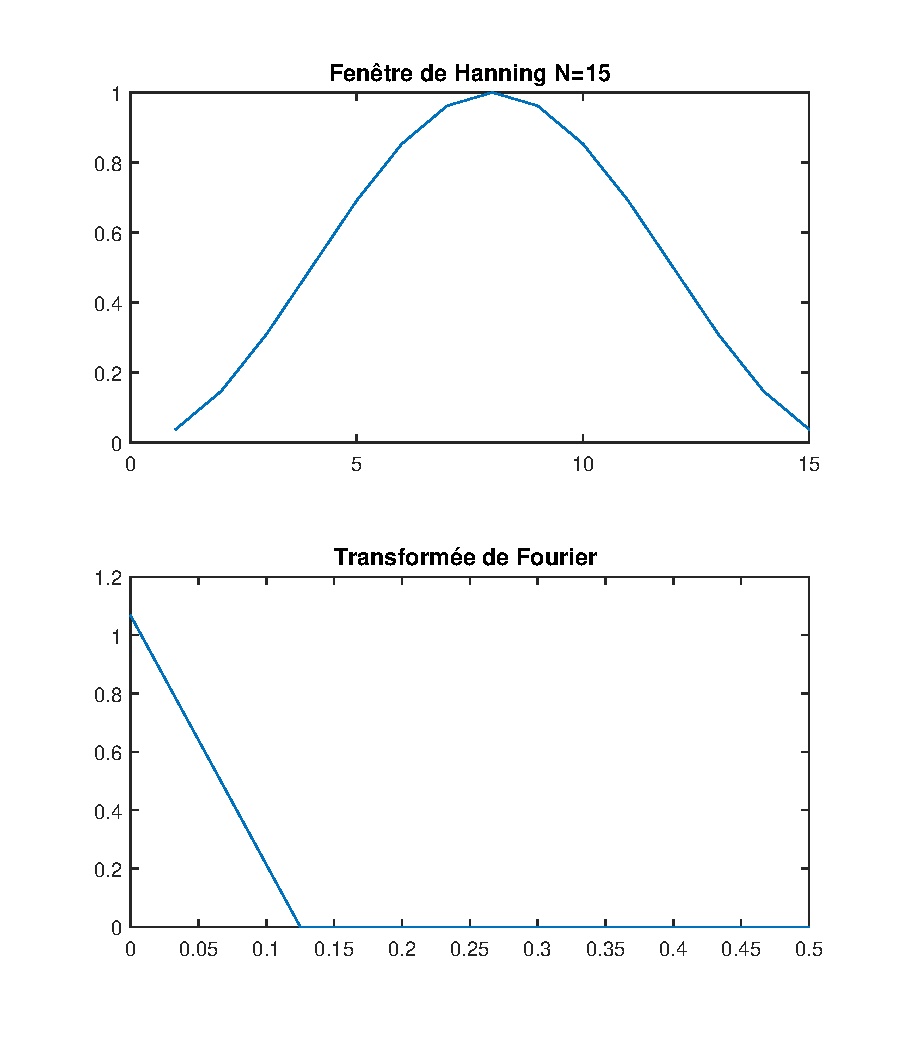
\includegraphics[width=\textwidth]{images/hanning_tfd.eps}
	% Title: glps_renderer figure
% Creator: GL2PS 1.3.8, (C) 1999-2012 C. Geuzaine
% For: Octave
% CreationDate: Thu Nov  9 14:57:03 2017
\begin{pgfpicture}
\pgfsetlinewidth{0.01pt}
\color[rgb]{1.000000,1.000000,1.000000}
\pgfpathmoveto{\pgfpoint{65.000015pt}{179.000000pt}}
\pgflineto{\pgfpoint{452.500031pt}{27.000008pt}}
\pgflineto{\pgfpoint{65.000015pt}{27.000008pt}}
\pgfpathclose
\pgfusepath{fill,stroke}
\pgfpathmoveto{\pgfpoint{65.000015pt}{179.000000pt}}
\pgflineto{\pgfpoint{452.500031pt}{179.000000pt}}
\pgflineto{\pgfpoint{452.500031pt}{27.000008pt}}
\pgfpathclose
\pgfusepath{fill,stroke}
\color[rgb]{0.000000,0.000000,0.000000}
\pgfsetlinewidth{0.500000pt}
\pgfsetdash{{16pt}{0pt}}{0pt}
\pgfpathmoveto{\pgfpoint{452.500031pt}{27.000008pt}}
\pgflineto{\pgfpoint{65.000015pt}{27.000008pt}}
\pgfusepath{stroke}
\pgfpathmoveto{\pgfpoint{452.500031pt}{179.000000pt}}
\pgflineto{\pgfpoint{65.000015pt}{179.000000pt}}
\pgfusepath{stroke}
\pgfpathmoveto{\pgfpoint{65.000015pt}{179.000000pt}}
\pgflineto{\pgfpoint{65.000015pt}{27.000008pt}}
\pgfusepath{stroke}
\pgfpathmoveto{\pgfpoint{452.500031pt}{179.000000pt}}
\pgflineto{\pgfpoint{452.500031pt}{27.000008pt}}
\pgfusepath{stroke}
\pgfsetdash{{0pt}{3pt}{1pt}{3pt}{1pt}{3pt}{1pt}{3pt}{1pt}{0pt}}{0pt}
\pgfpathmoveto{\pgfpoint{65.000015pt}{179.000000pt}}
\pgflineto{\pgfpoint{65.000015pt}{27.000008pt}}
\pgfusepath{stroke}
\pgfpathmoveto{\pgfpoint{142.500031pt}{179.000000pt}}
\pgflineto{\pgfpoint{142.500031pt}{27.000008pt}}
\pgfusepath{stroke}
\pgfpathmoveto{\pgfpoint{220.000031pt}{179.000000pt}}
\pgflineto{\pgfpoint{220.000031pt}{27.000008pt}}
\pgfusepath{stroke}
\pgfpathmoveto{\pgfpoint{297.500031pt}{179.000000pt}}
\pgflineto{\pgfpoint{297.500031pt}{27.000008pt}}
\pgfusepath{stroke}
\pgfpathmoveto{\pgfpoint{375.000061pt}{179.000000pt}}
\pgflineto{\pgfpoint{375.000061pt}{27.000008pt}}
\pgfusepath{stroke}
\pgfpathmoveto{\pgfpoint{452.500031pt}{179.000000pt}}
\pgflineto{\pgfpoint{452.500031pt}{27.000008pt}}
\pgfusepath{stroke}
\pgfsetdash{{16pt}{0pt}}{0pt}
\pgfpathmoveto{\pgfpoint{65.000015pt}{30.875000pt}}
\pgflineto{\pgfpoint{65.000015pt}{27.000008pt}}
\pgfusepath{stroke}
\pgfpathmoveto{\pgfpoint{65.000015pt}{175.125000pt}}
\pgflineto{\pgfpoint{65.000015pt}{179.000000pt}}
\pgfusepath{stroke}
\pgfpathmoveto{\pgfpoint{142.500031pt}{30.875000pt}}
\pgflineto{\pgfpoint{142.500031pt}{27.000008pt}}
\pgfusepath{stroke}
\pgfpathmoveto{\pgfpoint{142.500031pt}{175.125000pt}}
\pgflineto{\pgfpoint{142.500031pt}{179.000000pt}}
\pgfusepath{stroke}
\pgfpathmoveto{\pgfpoint{220.000031pt}{30.875000pt}}
\pgflineto{\pgfpoint{220.000031pt}{27.000008pt}}
\pgfusepath{stroke}
\pgfpathmoveto{\pgfpoint{220.000031pt}{175.125000pt}}
\pgflineto{\pgfpoint{220.000031pt}{179.000000pt}}
\pgfusepath{stroke}
\pgfpathmoveto{\pgfpoint{297.500031pt}{30.875000pt}}
\pgflineto{\pgfpoint{297.500031pt}{27.000008pt}}
\pgfusepath{stroke}
\pgfpathmoveto{\pgfpoint{297.500031pt}{175.125000pt}}
\pgflineto{\pgfpoint{297.500031pt}{179.000000pt}}
\pgfusepath{stroke}
\pgfpathmoveto{\pgfpoint{375.000061pt}{30.875000pt}}
\pgflineto{\pgfpoint{375.000061pt}{27.000008pt}}
\pgfusepath{stroke}
\pgfpathmoveto{\pgfpoint{375.000061pt}{175.125000pt}}
\pgflineto{\pgfpoint{375.000061pt}{179.000000pt}}
\pgfusepath{stroke}
\pgfpathmoveto{\pgfpoint{452.500031pt}{30.875000pt}}
\pgflineto{\pgfpoint{452.500031pt}{27.000008pt}}
\pgfusepath{stroke}
\pgfpathmoveto{\pgfpoint{452.500031pt}{175.125000pt}}
\pgflineto{\pgfpoint{452.500031pt}{179.000000pt}}
\pgfusepath{stroke}
{
\pgftransformshift{\pgfpoint{65.000015pt}{22.000000pt}}
\pgfnode{rectangle}{north}{\fontsize{10}{0}\selectfont\textcolor[rgb]{0,0,0}{{0}}}{}{\pgfusepath{discard}}}
{
\pgftransformshift{\pgfpoint{142.500015pt}{22.000000pt}}
\pgfnode{rectangle}{north}{\fontsize{10}{0}\selectfont\textcolor[rgb]{0,0,0}{{0.1}}}{}{\pgfusepath{discard}}}
{
\pgftransformshift{\pgfpoint{220.000015pt}{22.000000pt}}
\pgfnode{rectangle}{north}{\fontsize{10}{0}\selectfont\textcolor[rgb]{0,0,0}{{0.2}}}{}{\pgfusepath{discard}}}
{
\pgftransformshift{\pgfpoint{297.500031pt}{22.000000pt}}
\pgfnode{rectangle}{north}{\fontsize{10}{0}\selectfont\textcolor[rgb]{0,0,0}{{0.3}}}{}{\pgfusepath{discard}}}
{
\pgftransformshift{\pgfpoint{375.000031pt}{22.000000pt}}
\pgfnode{rectangle}{north}{\fontsize{10}{0}\selectfont\textcolor[rgb]{0,0,0}{{0.4}}}{}{\pgfusepath{discard}}}
{
\pgftransformshift{\pgfpoint{452.500031pt}{22.000000pt}}
\pgfnode{rectangle}{north}{\fontsize{10}{0}\selectfont\textcolor[rgb]{0,0,0}{{0.5}}}{}{\pgfusepath{discard}}}
\pgfsetdash{{0pt}{3pt}{1pt}{3pt}{1pt}{3pt}{1pt}{3pt}{1pt}{0pt}}{0pt}
\pgfpathmoveto{\pgfpoint{452.500031pt}{27.000008pt}}
\pgflineto{\pgfpoint{65.000015pt}{27.000008pt}}
\pgfusepath{stroke}
\pgfpathmoveto{\pgfpoint{452.500031pt}{57.400002pt}}
\pgflineto{\pgfpoint{65.000015pt}{57.400002pt}}
\pgfusepath{stroke}
\pgfpathmoveto{\pgfpoint{452.500031pt}{87.800003pt}}
\pgflineto{\pgfpoint{65.000015pt}{87.800003pt}}
\pgfusepath{stroke}
\pgfpathmoveto{\pgfpoint{452.500031pt}{118.200005pt}}
\pgflineto{\pgfpoint{65.000015pt}{118.200005pt}}
\pgfusepath{stroke}
\pgfpathmoveto{\pgfpoint{452.500031pt}{148.600006pt}}
\pgflineto{\pgfpoint{65.000015pt}{148.600006pt}}
\pgfusepath{stroke}
\pgfpathmoveto{\pgfpoint{452.500031pt}{179.000000pt}}
\pgflineto{\pgfpoint{65.000015pt}{179.000000pt}}
\pgfusepath{stroke}
\pgfsetdash{{16pt}{0pt}}{0pt}
\pgfpathmoveto{\pgfpoint{68.870026pt}{27.000008pt}}
\pgflineto{\pgfpoint{65.000015pt}{27.000008pt}}
\pgfusepath{stroke}
\pgfpathmoveto{\pgfpoint{448.630005pt}{27.000008pt}}
\pgflineto{\pgfpoint{452.500031pt}{27.000008pt}}
\pgfusepath{stroke}
\pgfpathmoveto{\pgfpoint{68.870026pt}{57.400002pt}}
\pgflineto{\pgfpoint{65.000015pt}{57.400002pt}}
\pgfusepath{stroke}
\pgfpathmoveto{\pgfpoint{448.630005pt}{57.400002pt}}
\pgflineto{\pgfpoint{452.500031pt}{57.400002pt}}
\pgfusepath{stroke}
\pgfpathmoveto{\pgfpoint{68.870026pt}{87.800003pt}}
\pgflineto{\pgfpoint{65.000015pt}{87.800003pt}}
\pgfusepath{stroke}
\pgfpathmoveto{\pgfpoint{448.630005pt}{87.800003pt}}
\pgflineto{\pgfpoint{452.500031pt}{87.800003pt}}
\pgfusepath{stroke}
\pgfpathmoveto{\pgfpoint{68.870026pt}{118.200005pt}}
\pgflineto{\pgfpoint{65.000015pt}{118.200005pt}}
\pgfusepath{stroke}
\pgfpathmoveto{\pgfpoint{448.630005pt}{118.200005pt}}
\pgflineto{\pgfpoint{452.500031pt}{118.200005pt}}
\pgfusepath{stroke}
\pgfpathmoveto{\pgfpoint{68.870026pt}{148.600006pt}}
\pgflineto{\pgfpoint{65.000015pt}{148.600006pt}}
\pgfusepath{stroke}
\pgfpathmoveto{\pgfpoint{448.630005pt}{148.600006pt}}
\pgflineto{\pgfpoint{452.500031pt}{148.600006pt}}
\pgfusepath{stroke}
\pgfpathmoveto{\pgfpoint{68.870026pt}{179.000000pt}}
\pgflineto{\pgfpoint{65.000015pt}{179.000000pt}}
\pgfusepath{stroke}
\pgfpathmoveto{\pgfpoint{448.630005pt}{179.000000pt}}
\pgflineto{\pgfpoint{452.500031pt}{179.000000pt}}
\pgfusepath{stroke}
{
\pgftransformshift{\pgfpoint{60.006454pt}{27.000008pt}}
\pgfnode{rectangle}{east}{\fontsize{10}{0}\selectfont\textcolor[rgb]{0,0,0}{{0}}}{}{\pgfusepath{discard}}}
{
\pgftransformshift{\pgfpoint{60.006454pt}{57.400002pt}}
\pgfnode{rectangle}{east}{\fontsize{10}{0}\selectfont\textcolor[rgb]{0,0,0}{{0.2}}}{}{\pgfusepath{discard}}}
{
\pgftransformshift{\pgfpoint{60.006454pt}{87.800003pt}}
\pgfnode{rectangle}{east}{\fontsize{10}{0}\selectfont\textcolor[rgb]{0,0,0}{{0.4}}}{}{\pgfusepath{discard}}}
{
\pgftransformshift{\pgfpoint{60.006454pt}{118.200005pt}}
\pgfnode{rectangle}{east}{\fontsize{10}{0}\selectfont\textcolor[rgb]{0,0,0}{{0.6}}}{}{\pgfusepath{discard}}}
{
\pgftransformshift{\pgfpoint{60.006454pt}{148.600006pt}}
\pgfnode{rectangle}{east}{\fontsize{10}{0}\selectfont\textcolor[rgb]{0,0,0}{{0.8}}}{}{\pgfusepath{discard}}}
{
\pgftransformshift{\pgfpoint{60.006454pt}{179.000000pt}}
\pgfnode{rectangle}{east}{\fontsize{10}{0}\selectfont\textcolor[rgb]{0,0,0}{{1}}}{}{\pgfusepath{discard}}}
{
\pgftransformshift{\pgfpoint{258.750031pt}{11.000000pt}}
\pgfnode{rectangle}{north}{\fontsize{10}{0}\selectfont\textcolor[rgb]{0,0,0}{{$f$ (Hz)}}}{}{\pgfusepath{discard}}}
\color[rgb]{0.000000,0.000000,1.000000}
\pgfsetdash{}{0pt}
\pgfpathmoveto{\pgfpoint{113.437515pt}{111.268311pt}}
\pgflineto{\pgfpoint{65.000015pt}{168.866669pt}}
\pgfusepath{stroke}
\pgfpathmoveto{\pgfpoint{161.875015pt}{35.836739pt}}
\pgflineto{\pgfpoint{113.437515pt}{111.268311pt}}
\pgfusepath{stroke}
\pgfpathmoveto{\pgfpoint{210.312515pt}{29.677185pt}}
\pgflineto{\pgfpoint{161.875015pt}{35.836739pt}}
\pgfusepath{stroke}
\pgfpathmoveto{\pgfpoint{258.750031pt}{28.113823pt}}
\pgflineto{\pgfpoint{210.312515pt}{29.677185pt}}
\pgfusepath{stroke}
\pgfpathmoveto{\pgfpoint{307.187531pt}{27.482597pt}}
\pgflineto{\pgfpoint{258.750031pt}{28.113823pt}}
\pgfusepath{stroke}
\pgfpathmoveto{\pgfpoint{355.625000pt}{27.182785pt}}
\pgflineto{\pgfpoint{307.187531pt}{27.482597pt}}
\pgfusepath{stroke}
\pgfpathmoveto{\pgfpoint{404.062531pt}{27.041862pt}}
\pgflineto{\pgfpoint{355.625000pt}{27.182785pt}}
\pgfusepath{stroke}
\pgfpathmoveto{\pgfpoint{452.500031pt}{27.000008pt}}
\pgflineto{\pgfpoint{404.062531pt}{27.041862pt}}
\pgfusepath{stroke}
{
\pgftransformshift{\pgfpoint{258.750031pt}{189.000000pt}}
\pgfnode{rectangle}{south}{\fontsize{10}{0}\selectfont\textcolor[rgb]{0,0,0}{{Transformée de Fourier}}}{}{\pgfusepath{discard}}}
\end{pgfpicture}

	\caption{TFD d'une fenêtre de Hanning}
	\label{fig:hanning}
\end{figure}

On remarque grâce à la figure \ref{fig:hanning_sans_0p} que du fait de l'échantillonage de la transformée de Fourier, le second pic du graphe est tronqué. On retrouve ainsi le résultat du TD 4.

\begin{figure}[h!]
	\centering
	%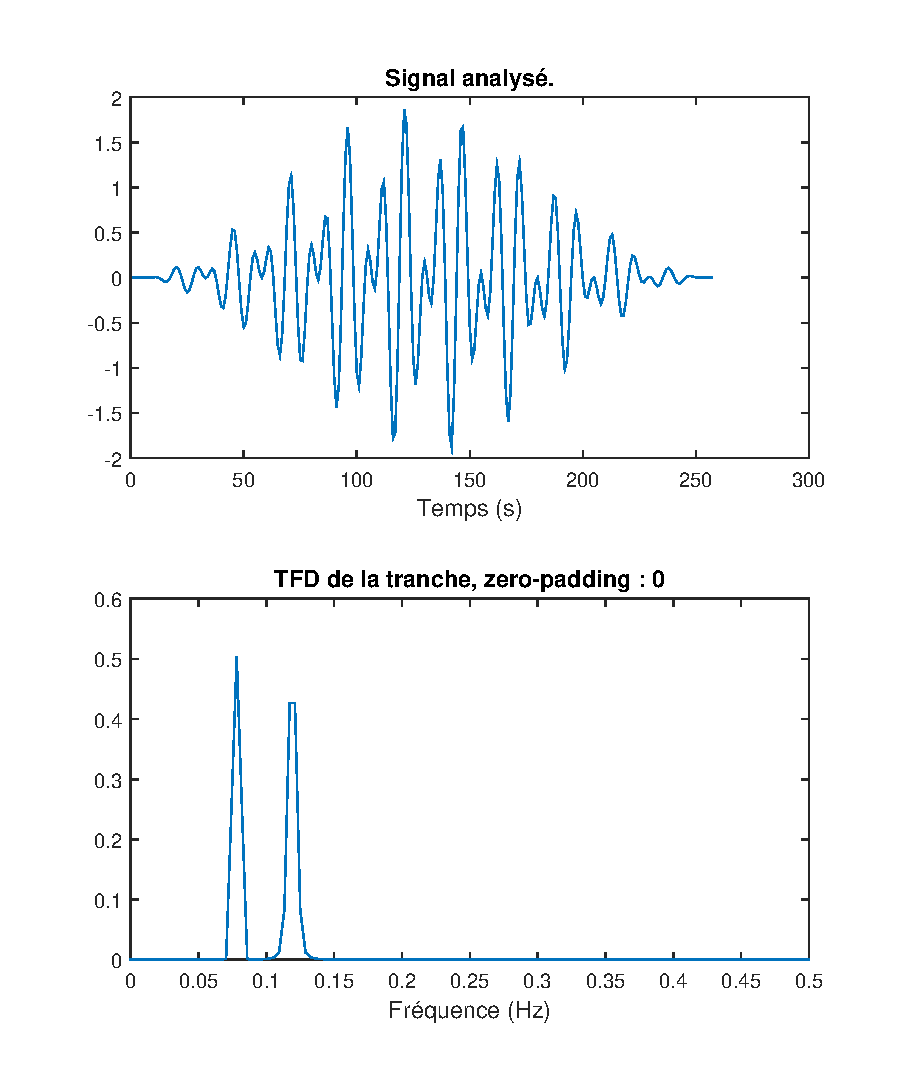
\includegraphics[width=\textwidth]{images/hanning_sans_0p.eps}
	% Title: glps_renderer figure
% Creator: GL2PS 1.3.8, (C) 1999-2012 C. Geuzaine
% For: Octave
% CreationDate: Thu Nov  9 14:56:02 2017
\begin{pgfpicture}
\pgfsetlinewidth{0.01pt}
\color[rgb]{1.000000,1.000000,1.000000}
\pgfpathmoveto{\pgfpoint{65.000015pt}{277.500000pt}}
\pgflineto{\pgfpoint{452.500031pt}{32.999992pt}}
\pgflineto{\pgfpoint{65.000015pt}{32.999992pt}}
\pgfpathclose
\pgfusepath{fill,stroke}
\pgfpathmoveto{\pgfpoint{65.000015pt}{277.500000pt}}
\pgflineto{\pgfpoint{452.500031pt}{277.500000pt}}
\pgflineto{\pgfpoint{452.500031pt}{32.999992pt}}
\pgfpathclose
\pgfusepath{fill,stroke}
\color[rgb]{0.000000,0.000000,0.000000}
\pgfsetlinewidth{0.500000pt}
\pgfsetdash{{16pt}{0pt}}{0pt}
\pgfpathmoveto{\pgfpoint{452.500031pt}{32.999992pt}}
\pgflineto{\pgfpoint{65.000015pt}{32.999992pt}}
\pgfusepath{stroke}
\pgfpathmoveto{\pgfpoint{452.500031pt}{277.500000pt}}
\pgflineto{\pgfpoint{65.000015pt}{277.500000pt}}
\pgfusepath{stroke}
\pgfpathmoveto{\pgfpoint{65.000015pt}{277.500000pt}}
\pgflineto{\pgfpoint{65.000015pt}{32.999992pt}}
\pgfusepath{stroke}
\pgfpathmoveto{\pgfpoint{452.500031pt}{277.500000pt}}
\pgflineto{\pgfpoint{452.500031pt}{32.999992pt}}
\pgfusepath{stroke}
\pgfsetdash{{0pt}{3pt}{1pt}{3pt}{1pt}{3pt}{1pt}{3pt}{1pt}{0pt}}{0pt}
\pgfpathmoveto{\pgfpoint{65.000015pt}{277.500000pt}}
\pgflineto{\pgfpoint{65.000015pt}{32.999992pt}}
\pgfusepath{stroke}
\pgfpathmoveto{\pgfpoint{142.500031pt}{277.500000pt}}
\pgflineto{\pgfpoint{142.500031pt}{32.999992pt}}
\pgfusepath{stroke}
\pgfpathmoveto{\pgfpoint{220.000031pt}{277.500000pt}}
\pgflineto{\pgfpoint{220.000031pt}{32.999992pt}}
\pgfusepath{stroke}
\pgfpathmoveto{\pgfpoint{297.500031pt}{277.500000pt}}
\pgflineto{\pgfpoint{297.500031pt}{32.999992pt}}
\pgfusepath{stroke}
\pgfpathmoveto{\pgfpoint{375.000061pt}{277.500000pt}}
\pgflineto{\pgfpoint{375.000061pt}{32.999992pt}}
\pgfusepath{stroke}
\pgfpathmoveto{\pgfpoint{452.500031pt}{277.500000pt}}
\pgflineto{\pgfpoint{452.500031pt}{32.999992pt}}
\pgfusepath{stroke}
\pgfsetdash{{16pt}{0pt}}{0pt}
\pgfpathmoveto{\pgfpoint{65.000015pt}{36.882942pt}}
\pgflineto{\pgfpoint{65.000015pt}{32.999992pt}}
\pgfusepath{stroke}
\pgfpathmoveto{\pgfpoint{65.000015pt}{273.617065pt}}
\pgflineto{\pgfpoint{65.000015pt}{277.500000pt}}
\pgfusepath{stroke}
\pgfpathmoveto{\pgfpoint{142.500031pt}{36.882942pt}}
\pgflineto{\pgfpoint{142.500031pt}{32.999992pt}}
\pgfusepath{stroke}
\pgfpathmoveto{\pgfpoint{142.500031pt}{273.617065pt}}
\pgflineto{\pgfpoint{142.500031pt}{277.500000pt}}
\pgfusepath{stroke}
\pgfpathmoveto{\pgfpoint{220.000031pt}{36.882942pt}}
\pgflineto{\pgfpoint{220.000031pt}{32.999992pt}}
\pgfusepath{stroke}
\pgfpathmoveto{\pgfpoint{220.000031pt}{273.617065pt}}
\pgflineto{\pgfpoint{220.000031pt}{277.500000pt}}
\pgfusepath{stroke}
\pgfpathmoveto{\pgfpoint{297.500031pt}{36.882942pt}}
\pgflineto{\pgfpoint{297.500031pt}{32.999992pt}}
\pgfusepath{stroke}
\pgfpathmoveto{\pgfpoint{297.500031pt}{273.617065pt}}
\pgflineto{\pgfpoint{297.500031pt}{277.500000pt}}
\pgfusepath{stroke}
\pgfpathmoveto{\pgfpoint{375.000061pt}{36.882942pt}}
\pgflineto{\pgfpoint{375.000061pt}{32.999992pt}}
\pgfusepath{stroke}
\pgfpathmoveto{\pgfpoint{375.000061pt}{273.617065pt}}
\pgflineto{\pgfpoint{375.000061pt}{277.500000pt}}
\pgfusepath{stroke}
\pgfpathmoveto{\pgfpoint{452.500031pt}{36.882942pt}}
\pgflineto{\pgfpoint{452.500031pt}{32.999992pt}}
\pgfusepath{stroke}
\pgfpathmoveto{\pgfpoint{452.500031pt}{273.617065pt}}
\pgflineto{\pgfpoint{452.500031pt}{277.500000pt}}
\pgfusepath{stroke}
{
\pgftransformshift{\pgfpoint{65.000015pt}{27.989754pt}}
\pgfnode{rectangle}{north}{\fontsize{10}{0}\selectfont\textcolor[rgb]{0,0,0}{{0}}}{}{\pgfusepath{discard}}}
{
\pgftransformshift{\pgfpoint{142.500015pt}{27.989754pt}}
\pgfnode{rectangle}{north}{\fontsize{10}{0}\selectfont\textcolor[rgb]{0,0,0}{{0.1}}}{}{\pgfusepath{discard}}}
{
\pgftransformshift{\pgfpoint{220.000015pt}{27.989754pt}}
\pgfnode{rectangle}{north}{\fontsize{10}{0}\selectfont\textcolor[rgb]{0,0,0}{{0.2}}}{}{\pgfusepath{discard}}}
{
\pgftransformshift{\pgfpoint{297.500031pt}{27.989754pt}}
\pgfnode{rectangle}{north}{\fontsize{10}{0}\selectfont\textcolor[rgb]{0,0,0}{{0.3}}}{}{\pgfusepath{discard}}}
{
\pgftransformshift{\pgfpoint{375.000031pt}{27.989754pt}}
\pgfnode{rectangle}{north}{\fontsize{10}{0}\selectfont\textcolor[rgb]{0,0,0}{{0.4}}}{}{\pgfusepath{discard}}}
{
\pgftransformshift{\pgfpoint{452.500031pt}{27.989754pt}}
\pgfnode{rectangle}{north}{\fontsize{10}{0}\selectfont\textcolor[rgb]{0,0,0}{{0.5}}}{}{\pgfusepath{discard}}}
\pgfsetdash{{0pt}{3pt}{1pt}{3pt}{1pt}{3pt}{1pt}{3pt}{1pt}{0pt}}{0pt}
\pgfpathmoveto{\pgfpoint{452.500031pt}{32.999992pt}}
\pgflineto{\pgfpoint{65.000015pt}{32.999992pt}}
\pgfusepath{stroke}
\pgfpathmoveto{\pgfpoint{452.500031pt}{67.928574pt}}
\pgflineto{\pgfpoint{65.000015pt}{67.928574pt}}
\pgfusepath{stroke}
\pgfpathmoveto{\pgfpoint{452.500031pt}{102.857140pt}}
\pgflineto{\pgfpoint{65.000015pt}{102.857140pt}}
\pgfusepath{stroke}
\pgfpathmoveto{\pgfpoint{452.500031pt}{137.785721pt}}
\pgflineto{\pgfpoint{65.000015pt}{137.785721pt}}
\pgfusepath{stroke}
\pgfpathmoveto{\pgfpoint{452.500031pt}{172.714294pt}}
\pgflineto{\pgfpoint{65.000015pt}{172.714294pt}}
\pgfusepath{stroke}
\pgfpathmoveto{\pgfpoint{452.500031pt}{207.642853pt}}
\pgflineto{\pgfpoint{65.000015pt}{207.642853pt}}
\pgfusepath{stroke}
\pgfpathmoveto{\pgfpoint{452.500031pt}{242.571442pt}}
\pgflineto{\pgfpoint{65.000015pt}{242.571442pt}}
\pgfusepath{stroke}
\pgfpathmoveto{\pgfpoint{452.500031pt}{277.500000pt}}
\pgflineto{\pgfpoint{65.000015pt}{277.500000pt}}
\pgfusepath{stroke}
\pgfsetdash{{16pt}{0pt}}{0pt}
\pgfpathmoveto{\pgfpoint{68.870026pt}{32.999992pt}}
\pgflineto{\pgfpoint{65.000015pt}{32.999992pt}}
\pgfusepath{stroke}
\pgfpathmoveto{\pgfpoint{448.630005pt}{32.999992pt}}
\pgflineto{\pgfpoint{452.500031pt}{32.999992pt}}
\pgfusepath{stroke}
\pgfpathmoveto{\pgfpoint{68.870026pt}{67.928574pt}}
\pgflineto{\pgfpoint{65.000015pt}{67.928574pt}}
\pgfusepath{stroke}
\pgfpathmoveto{\pgfpoint{448.630005pt}{67.928574pt}}
\pgflineto{\pgfpoint{452.500031pt}{67.928574pt}}
\pgfusepath{stroke}
\pgfpathmoveto{\pgfpoint{68.870026pt}{102.857140pt}}
\pgflineto{\pgfpoint{65.000015pt}{102.857140pt}}
\pgfusepath{stroke}
\pgfpathmoveto{\pgfpoint{448.630005pt}{102.857140pt}}
\pgflineto{\pgfpoint{452.500031pt}{102.857140pt}}
\pgfusepath{stroke}
\pgfpathmoveto{\pgfpoint{68.870026pt}{137.785721pt}}
\pgflineto{\pgfpoint{65.000015pt}{137.785721pt}}
\pgfusepath{stroke}
\pgfpathmoveto{\pgfpoint{448.630005pt}{137.785721pt}}
\pgflineto{\pgfpoint{452.500031pt}{137.785721pt}}
\pgfusepath{stroke}
\pgfpathmoveto{\pgfpoint{68.870026pt}{172.714294pt}}
\pgflineto{\pgfpoint{65.000015pt}{172.714294pt}}
\pgfusepath{stroke}
\pgfpathmoveto{\pgfpoint{448.630005pt}{172.714294pt}}
\pgflineto{\pgfpoint{452.500031pt}{172.714294pt}}
\pgfusepath{stroke}
\pgfpathmoveto{\pgfpoint{68.870026pt}{207.642853pt}}
\pgflineto{\pgfpoint{65.000015pt}{207.642853pt}}
\pgfusepath{stroke}
\pgfpathmoveto{\pgfpoint{448.630005pt}{207.642853pt}}
\pgflineto{\pgfpoint{452.500031pt}{207.642853pt}}
\pgfusepath{stroke}
\pgfpathmoveto{\pgfpoint{68.870026pt}{242.571442pt}}
\pgflineto{\pgfpoint{65.000015pt}{242.571442pt}}
\pgfusepath{stroke}
\pgfpathmoveto{\pgfpoint{448.630005pt}{242.571442pt}}
\pgflineto{\pgfpoint{452.500031pt}{242.571442pt}}
\pgfusepath{stroke}
\pgfpathmoveto{\pgfpoint{68.870026pt}{277.500000pt}}
\pgflineto{\pgfpoint{65.000015pt}{277.500000pt}}
\pgfusepath{stroke}
\pgfpathmoveto{\pgfpoint{448.630005pt}{277.500000pt}}
\pgflineto{\pgfpoint{452.500031pt}{277.500000pt}}
\pgfusepath{stroke}
{
\pgftransformshift{\pgfpoint{60.006454pt}{32.999992pt}}
\pgfnode{rectangle}{east}{\fontsize{10}{0}\selectfont\textcolor[rgb]{0,0,0}{{0}}}{}{\pgfusepath{discard}}}
{
\pgftransformshift{\pgfpoint{60.006454pt}{67.928558pt}}
\pgfnode{rectangle}{east}{\fontsize{10}{0}\selectfont\textcolor[rgb]{0,0,0}{{0.1}}}{}{\pgfusepath{discard}}}
{
\pgftransformshift{\pgfpoint{60.006454pt}{102.857140pt}}
\pgfnode{rectangle}{east}{\fontsize{10}{0}\selectfont\textcolor[rgb]{0,0,0}{{0.2}}}{}{\pgfusepath{discard}}}
{
\pgftransformshift{\pgfpoint{60.006454pt}{137.785721pt}}
\pgfnode{rectangle}{east}{\fontsize{10}{0}\selectfont\textcolor[rgb]{0,0,0}{{0.3}}}{}{\pgfusepath{discard}}}
{
\pgftransformshift{\pgfpoint{60.006454pt}{172.714294pt}}
\pgfnode{rectangle}{east}{\fontsize{10}{0}\selectfont\textcolor[rgb]{0,0,0}{{0.4}}}{}{\pgfusepath{discard}}}
{
\pgftransformshift{\pgfpoint{60.006454pt}{207.642853pt}}
\pgfnode{rectangle}{east}{\fontsize{10}{0}\selectfont\textcolor[rgb]{0,0,0}{{0.5}}}{}{\pgfusepath{discard}}}
{
\pgftransformshift{\pgfpoint{60.006454pt}{242.571442pt}}
\pgfnode{rectangle}{east}{\fontsize{10}{0}\selectfont\textcolor[rgb]{0,0,0}{{0.6}}}{}{\pgfusepath{discard}}}
{
\pgftransformshift{\pgfpoint{60.006454pt}{277.500000pt}}
\pgfnode{rectangle}{east}{\fontsize{10}{0}\selectfont\textcolor[rgb]{0,0,0}{{0.7}}}{}{\pgfusepath{discard}}}
{
\pgftransformshift{\pgfpoint{258.750031pt}{16.989746pt}}
\pgfnode{rectangle}{north}{\fontsize{10}{0}\selectfont\textcolor[rgb]{0,0,0}{{Fréquence (Hz)}}}{}{\pgfusepath{discard}}}
\color[rgb]{0.000000,0.000000,1.000000}
\pgfsetdash{}{0pt}
\pgfpathmoveto{\pgfpoint{68.027359pt}{33.003815pt}}
\pgflineto{\pgfpoint{65.000015pt}{33.003784pt}}
\pgfusepath{stroke}
\pgfpathmoveto{\pgfpoint{71.054703pt}{33.003883pt}}
\pgflineto{\pgfpoint{68.027359pt}{33.003815pt}}
\pgfusepath{stroke}
\pgfpathmoveto{\pgfpoint{74.082047pt}{33.004021pt}}
\pgflineto{\pgfpoint{71.054703pt}{33.003883pt}}
\pgfusepath{stroke}
\pgfpathmoveto{\pgfpoint{77.109375pt}{33.004219pt}}
\pgflineto{\pgfpoint{74.082047pt}{33.004021pt}}
\pgfusepath{stroke}
\pgfpathmoveto{\pgfpoint{80.136734pt}{33.004471pt}}
\pgflineto{\pgfpoint{77.109375pt}{33.004219pt}}
\pgfusepath{stroke}
\pgfpathmoveto{\pgfpoint{83.164078pt}{33.004807pt}}
\pgflineto{\pgfpoint{80.136734pt}{33.004471pt}}
\pgfusepath{stroke}
\pgfpathmoveto{\pgfpoint{86.191422pt}{33.005226pt}}
\pgflineto{\pgfpoint{83.164078pt}{33.004807pt}}
\pgfusepath{stroke}
\pgfpathmoveto{\pgfpoint{89.218765pt}{33.005745pt}}
\pgflineto{\pgfpoint{86.191422pt}{33.005226pt}}
\pgfusepath{stroke}
\pgfpathmoveto{\pgfpoint{92.246109pt}{33.006393pt}}
\pgflineto{\pgfpoint{89.218765pt}{33.005745pt}}
\pgfusepath{stroke}
\pgfpathmoveto{\pgfpoint{95.273453pt}{33.007202pt}}
\pgflineto{\pgfpoint{92.246109pt}{33.006393pt}}
\pgfusepath{stroke}
\pgfpathmoveto{\pgfpoint{98.300797pt}{33.008194pt}}
\pgflineto{\pgfpoint{95.273453pt}{33.007202pt}}
\pgfusepath{stroke}
\pgfpathmoveto{\pgfpoint{101.328140pt}{33.009438pt}}
\pgflineto{\pgfpoint{98.300797pt}{33.008194pt}}
\pgfusepath{stroke}
\pgfpathmoveto{\pgfpoint{104.355484pt}{33.010994pt}}
\pgflineto{\pgfpoint{101.328140pt}{33.009438pt}}
\pgfusepath{stroke}
\pgfpathmoveto{\pgfpoint{107.382828pt}{33.012970pt}}
\pgflineto{\pgfpoint{104.355484pt}{33.010994pt}}
\pgfusepath{stroke}
\pgfpathmoveto{\pgfpoint{110.410172pt}{33.015495pt}}
\pgflineto{\pgfpoint{107.382828pt}{33.012970pt}}
\pgfusepath{stroke}
\pgfpathmoveto{\pgfpoint{113.437515pt}{33.018799pt}}
\pgflineto{\pgfpoint{110.410172pt}{33.015495pt}}
\pgfusepath{stroke}
\pgfpathmoveto{\pgfpoint{116.464859pt}{33.023163pt}}
\pgflineto{\pgfpoint{113.437515pt}{33.018799pt}}
\pgfusepath{stroke}
\pgfpathmoveto{\pgfpoint{119.492203pt}{33.029060pt}}
\pgflineto{\pgfpoint{116.464859pt}{33.023163pt}}
\pgfusepath{stroke}
\pgfpathmoveto{\pgfpoint{122.519554pt}{120.289627pt}}
\pgflineto{\pgfpoint{119.492203pt}{33.029060pt}}
\pgfusepath{stroke}
\pgfpathmoveto{\pgfpoint{125.546890pt}{207.684540pt}}
\pgflineto{\pgfpoint{122.519554pt}{120.289627pt}}
\pgfusepath{stroke}
\pgfpathmoveto{\pgfpoint{128.574234pt}{120.265221pt}}
\pgflineto{\pgfpoint{125.546890pt}{207.684540pt}}
\pgfusepath{stroke}
\pgfpathmoveto{\pgfpoint{131.601578pt}{33.092110pt}}
\pgflineto{\pgfpoint{128.574234pt}{120.265221pt}}
\pgfusepath{stroke}
\pgfpathmoveto{\pgfpoint{134.628922pt}{33.134460pt}}
\pgflineto{\pgfpoint{131.601578pt}{33.092110pt}}
\pgfusepath{stroke}
\pgfpathmoveto{\pgfpoint{137.656265pt}{33.207619pt}}
\pgflineto{\pgfpoint{134.628922pt}{33.134460pt}}
\pgfusepath{stroke}
\pgfpathmoveto{\pgfpoint{140.683609pt}{33.345825pt}}
\pgflineto{\pgfpoint{137.656265pt}{33.207619pt}}
\pgfusepath{stroke}
\pgfpathmoveto{\pgfpoint{143.710953pt}{33.641998pt}}
\pgflineto{\pgfpoint{140.683609pt}{33.345825pt}}
\pgfusepath{stroke}
\pgfpathmoveto{\pgfpoint{146.738297pt}{34.412071pt}}
\pgflineto{\pgfpoint{143.710953pt}{33.641998pt}}
\pgfusepath{stroke}
\pgfpathmoveto{\pgfpoint{149.765640pt}{37.235703pt}}
\pgflineto{\pgfpoint{146.738297pt}{34.412071pt}}
\pgfusepath{stroke}
\pgfpathmoveto{\pgfpoint{152.792984pt}{62.648514pt}}
\pgflineto{\pgfpoint{149.765640pt}{37.235703pt}}
\pgfusepath{stroke}
\pgfpathmoveto{\pgfpoint{155.820343pt}{181.241257pt}}
\pgflineto{\pgfpoint{152.792984pt}{62.648514pt}}
\pgfusepath{stroke}
\pgfpathmoveto{\pgfpoint{158.847672pt}{181.241669pt}}
\pgflineto{\pgfpoint{155.820343pt}{181.241257pt}}
\pgfusepath{stroke}
\pgfpathmoveto{\pgfpoint{161.875015pt}{62.648094pt}}
\pgflineto{\pgfpoint{158.847672pt}{181.241669pt}}
\pgfusepath{stroke}
\pgfpathmoveto{\pgfpoint{164.902359pt}{37.235283pt}}
\pgflineto{\pgfpoint{161.875015pt}{62.648094pt}}
\pgfusepath{stroke}
\pgfpathmoveto{\pgfpoint{167.929703pt}{34.411644pt}}
\pgflineto{\pgfpoint{164.902359pt}{37.235283pt}}
\pgfusepath{stroke}
\pgfpathmoveto{\pgfpoint{170.957062pt}{33.641571pt}}
\pgflineto{\pgfpoint{167.929703pt}{34.411644pt}}
\pgfusepath{stroke}
\pgfpathmoveto{\pgfpoint{173.984390pt}{33.345383pt}}
\pgflineto{\pgfpoint{170.957062pt}{33.641571pt}}
\pgfusepath{stroke}
\pgfpathmoveto{\pgfpoint{177.011734pt}{33.207176pt}}
\pgflineto{\pgfpoint{173.984390pt}{33.345383pt}}
\pgfusepath{stroke}
\pgfpathmoveto{\pgfpoint{180.039078pt}{33.134010pt}}
\pgflineto{\pgfpoint{177.011734pt}{33.207176pt}}
\pgfusepath{stroke}
\pgfpathmoveto{\pgfpoint{183.066437pt}{33.091644pt}}
\pgflineto{\pgfpoint{180.039078pt}{33.134010pt}}
\pgfusepath{stroke}
\pgfpathmoveto{\pgfpoint{186.093765pt}{33.065422pt}}
\pgflineto{\pgfpoint{183.066437pt}{33.091644pt}}
\pgfusepath{stroke}
\pgfpathmoveto{\pgfpoint{189.121109pt}{33.048332pt}}
\pgflineto{\pgfpoint{186.093765pt}{33.065422pt}}
\pgfusepath{stroke}
\pgfpathmoveto{\pgfpoint{192.148468pt}{33.036705pt}}
\pgflineto{\pgfpoint{189.121109pt}{33.048332pt}}
\pgfusepath{stroke}
\pgfpathmoveto{\pgfpoint{195.175797pt}{33.028526pt}}
\pgflineto{\pgfpoint{192.148468pt}{33.036705pt}}
\pgfusepath{stroke}
\pgfpathmoveto{\pgfpoint{198.203156pt}{33.022606pt}}
\pgflineto{\pgfpoint{195.175797pt}{33.028526pt}}
\pgfusepath{stroke}
\pgfpathmoveto{\pgfpoint{201.230484pt}{33.018204pt}}
\pgflineto{\pgfpoint{198.203156pt}{33.022606pt}}
\pgfusepath{stroke}
\pgfpathmoveto{\pgfpoint{204.257828pt}{33.014885pt}}
\pgflineto{\pgfpoint{201.230484pt}{33.018204pt}}
\pgfusepath{stroke}
\pgfpathmoveto{\pgfpoint{207.285187pt}{33.012314pt}}
\pgflineto{\pgfpoint{204.257828pt}{33.014885pt}}
\pgfusepath{stroke}
\pgfpathmoveto{\pgfpoint{210.312515pt}{33.010307pt}}
\pgflineto{\pgfpoint{207.285187pt}{33.012314pt}}
\pgfusepath{stroke}
\pgfpathmoveto{\pgfpoint{213.339874pt}{33.008713pt}}
\pgflineto{\pgfpoint{210.312515pt}{33.010307pt}}
\pgfusepath{stroke}
\pgfpathmoveto{\pgfpoint{216.367203pt}{33.007423pt}}
\pgflineto{\pgfpoint{213.339874pt}{33.008713pt}}
\pgfusepath{stroke}
\pgfpathmoveto{\pgfpoint{219.394547pt}{33.006378pt}}
\pgflineto{\pgfpoint{216.367203pt}{33.007423pt}}
\pgfusepath{stroke}
\pgfpathmoveto{\pgfpoint{222.421906pt}{33.005524pt}}
\pgflineto{\pgfpoint{219.394547pt}{33.006378pt}}
\pgfusepath{stroke}
\pgfpathmoveto{\pgfpoint{225.449234pt}{33.004807pt}}
\pgflineto{\pgfpoint{222.421906pt}{33.005524pt}}
\pgfusepath{stroke}
\pgfpathmoveto{\pgfpoint{228.476578pt}{33.004219pt}}
\pgflineto{\pgfpoint{225.449234pt}{33.004807pt}}
\pgfusepath{stroke}
\pgfpathmoveto{\pgfpoint{231.503937pt}{33.003716pt}}
\pgflineto{\pgfpoint{228.476578pt}{33.004219pt}}
\pgfusepath{stroke}
\pgfpathmoveto{\pgfpoint{234.531265pt}{33.003288pt}}
\pgflineto{\pgfpoint{231.503937pt}{33.003716pt}}
\pgfusepath{stroke}
\pgfpathmoveto{\pgfpoint{237.558624pt}{33.002922pt}}
\pgflineto{\pgfpoint{234.531265pt}{33.003288pt}}
\pgfusepath{stroke}
\pgfpathmoveto{\pgfpoint{240.585953pt}{33.002609pt}}
\pgflineto{\pgfpoint{237.558624pt}{33.002922pt}}
\pgfusepath{stroke}
\pgfpathmoveto{\pgfpoint{243.613297pt}{33.002335pt}}
\pgflineto{\pgfpoint{240.585953pt}{33.002609pt}}
\pgfusepath{stroke}
\pgfpathmoveto{\pgfpoint{246.640656pt}{33.002106pt}}
\pgflineto{\pgfpoint{243.613297pt}{33.002335pt}}
\pgfusepath{stroke}
\pgfpathmoveto{\pgfpoint{249.667984pt}{33.001900pt}}
\pgflineto{\pgfpoint{246.640656pt}{33.002106pt}}
\pgfusepath{stroke}
\pgfpathmoveto{\pgfpoint{252.695343pt}{33.001724pt}}
\pgflineto{\pgfpoint{249.667984pt}{33.001900pt}}
\pgfusepath{stroke}
\pgfpathmoveto{\pgfpoint{255.722672pt}{33.001572pt}}
\pgflineto{\pgfpoint{252.695343pt}{33.001724pt}}
\pgfusepath{stroke}
\pgfpathmoveto{\pgfpoint{258.750031pt}{33.001427pt}}
\pgflineto{\pgfpoint{255.722672pt}{33.001572pt}}
\pgfusepath{stroke}
\pgfpathmoveto{\pgfpoint{261.777374pt}{33.001297pt}}
\pgflineto{\pgfpoint{258.750031pt}{33.001427pt}}
\pgfusepath{stroke}
\pgfpathmoveto{\pgfpoint{264.804718pt}{33.001190pt}}
\pgflineto{\pgfpoint{261.777374pt}{33.001297pt}}
\pgfusepath{stroke}
\pgfpathmoveto{\pgfpoint{267.832062pt}{33.001099pt}}
\pgflineto{\pgfpoint{264.804718pt}{33.001190pt}}
\pgfusepath{stroke}
\pgfpathmoveto{\pgfpoint{270.859375pt}{33.001007pt}}
\pgflineto{\pgfpoint{267.832062pt}{33.001099pt}}
\pgfusepath{stroke}
\pgfpathmoveto{\pgfpoint{273.886749pt}{33.000931pt}}
\pgflineto{\pgfpoint{270.859375pt}{33.001007pt}}
\pgfusepath{stroke}
\pgfpathmoveto{\pgfpoint{276.914093pt}{33.000862pt}}
\pgflineto{\pgfpoint{273.886749pt}{33.000931pt}}
\pgfusepath{stroke}
\pgfpathmoveto{\pgfpoint{279.941437pt}{33.000801pt}}
\pgflineto{\pgfpoint{276.914093pt}{33.000862pt}}
\pgfusepath{stroke}
\pgfpathmoveto{\pgfpoint{282.968781pt}{33.000740pt}}
\pgflineto{\pgfpoint{279.941437pt}{33.000801pt}}
\pgfusepath{stroke}
\pgfpathmoveto{\pgfpoint{285.996094pt}{33.000687pt}}
\pgflineto{\pgfpoint{282.968781pt}{33.000740pt}}
\pgfusepath{stroke}
\pgfpathmoveto{\pgfpoint{289.023468pt}{33.000641pt}}
\pgflineto{\pgfpoint{285.996094pt}{33.000687pt}}
\pgfusepath{stroke}
\pgfpathmoveto{\pgfpoint{292.050812pt}{33.000595pt}}
\pgflineto{\pgfpoint{289.023468pt}{33.000641pt}}
\pgfusepath{stroke}
\pgfpathmoveto{\pgfpoint{295.078156pt}{33.000557pt}}
\pgflineto{\pgfpoint{292.050812pt}{33.000595pt}}
\pgfusepath{stroke}
\pgfpathmoveto{\pgfpoint{298.105499pt}{33.000526pt}}
\pgflineto{\pgfpoint{295.078156pt}{33.000557pt}}
\pgfusepath{stroke}
\pgfpathmoveto{\pgfpoint{301.132843pt}{33.000488pt}}
\pgflineto{\pgfpoint{298.105499pt}{33.000526pt}}
\pgfusepath{stroke}
\pgfpathmoveto{\pgfpoint{304.160187pt}{33.000458pt}}
\pgflineto{\pgfpoint{301.132843pt}{33.000488pt}}
\pgfusepath{stroke}
\pgfpathmoveto{\pgfpoint{307.187531pt}{33.000427pt}}
\pgflineto{\pgfpoint{304.160187pt}{33.000458pt}}
\pgfusepath{stroke}
\pgfpathmoveto{\pgfpoint{310.214874pt}{33.000404pt}}
\pgflineto{\pgfpoint{307.187531pt}{33.000427pt}}
\pgfusepath{stroke}
\pgfpathmoveto{\pgfpoint{313.242218pt}{33.000381pt}}
\pgflineto{\pgfpoint{310.214874pt}{33.000404pt}}
\pgfusepath{stroke}
\pgfpathmoveto{\pgfpoint{316.269562pt}{33.000359pt}}
\pgflineto{\pgfpoint{313.242218pt}{33.000381pt}}
\pgfusepath{stroke}
\pgfpathmoveto{\pgfpoint{319.296906pt}{33.000336pt}}
\pgflineto{\pgfpoint{316.269562pt}{33.000359pt}}
\pgfusepath{stroke}
\pgfpathmoveto{\pgfpoint{322.324219pt}{33.000320pt}}
\pgflineto{\pgfpoint{319.296906pt}{33.000336pt}}
\pgfusepath{stroke}
\pgfpathmoveto{\pgfpoint{325.351562pt}{33.000298pt}}
\pgflineto{\pgfpoint{322.324219pt}{33.000320pt}}
\pgfusepath{stroke}
\pgfpathmoveto{\pgfpoint{328.378937pt}{33.000290pt}}
\pgflineto{\pgfpoint{325.351562pt}{33.000298pt}}
\pgfusepath{stroke}
\pgfpathmoveto{\pgfpoint{331.406281pt}{33.000275pt}}
\pgflineto{\pgfpoint{328.378937pt}{33.000290pt}}
\pgfusepath{stroke}
\pgfpathmoveto{\pgfpoint{334.433624pt}{33.000252pt}}
\pgflineto{\pgfpoint{331.406281pt}{33.000275pt}}
\pgfusepath{stroke}
\pgfpathmoveto{\pgfpoint{337.460938pt}{33.000244pt}}
\pgflineto{\pgfpoint{334.433624pt}{33.000252pt}}
\pgfusepath{stroke}
\pgfpathmoveto{\pgfpoint{340.488281pt}{33.000237pt}}
\pgflineto{\pgfpoint{337.460938pt}{33.000244pt}}
\pgfusepath{stroke}
\pgfpathmoveto{\pgfpoint{343.515656pt}{33.000221pt}}
\pgflineto{\pgfpoint{340.488281pt}{33.000237pt}}
\pgfusepath{stroke}
\pgfpathmoveto{\pgfpoint{346.542999pt}{33.000214pt}}
\pgflineto{\pgfpoint{343.515656pt}{33.000221pt}}
\pgfusepath{stroke}
\pgfpathmoveto{\pgfpoint{349.570343pt}{33.000198pt}}
\pgflineto{\pgfpoint{346.542999pt}{33.000214pt}}
\pgfusepath{stroke}
\pgfpathmoveto{\pgfpoint{352.597656pt}{33.000191pt}}
\pgflineto{\pgfpoint{349.570343pt}{33.000198pt}}
\pgfusepath{stroke}
\pgfpathmoveto{\pgfpoint{355.625000pt}{33.000183pt}}
\pgflineto{\pgfpoint{352.597656pt}{33.000191pt}}
\pgfusepath{stroke}
\pgfpathmoveto{\pgfpoint{358.652374pt}{33.000175pt}}
\pgflineto{\pgfpoint{355.625000pt}{33.000183pt}}
\pgfusepath{stroke}
\pgfpathmoveto{\pgfpoint{361.679718pt}{33.000168pt}}
\pgflineto{\pgfpoint{358.652374pt}{33.000175pt}}
\pgfusepath{stroke}
\pgfpathmoveto{\pgfpoint{364.707062pt}{33.000168pt}}
\pgflineto{\pgfpoint{361.679718pt}{33.000168pt}}
\pgfusepath{stroke}
\pgfpathmoveto{\pgfpoint{367.734375pt}{33.000153pt}}
\pgflineto{\pgfpoint{364.707062pt}{33.000168pt}}
\pgfusepath{stroke}
\pgfpathmoveto{\pgfpoint{370.761719pt}{33.000145pt}}
\pgflineto{\pgfpoint{367.734375pt}{33.000153pt}}
\pgfusepath{stroke}
\pgfpathmoveto{\pgfpoint{373.789093pt}{33.000145pt}}
\pgflineto{\pgfpoint{370.761719pt}{33.000145pt}}
\pgfusepath{stroke}
\pgfpathmoveto{\pgfpoint{376.816437pt}{33.000137pt}}
\pgflineto{\pgfpoint{373.789093pt}{33.000145pt}}
\pgfusepath{stroke}
\pgfpathmoveto{\pgfpoint{379.843781pt}{33.000137pt}}
\pgflineto{\pgfpoint{376.816437pt}{33.000137pt}}
\pgfusepath{stroke}
\pgfpathmoveto{\pgfpoint{382.871094pt}{33.000130pt}}
\pgflineto{\pgfpoint{379.843781pt}{33.000137pt}}
\pgfusepath{stroke}
\pgfpathmoveto{\pgfpoint{385.898438pt}{33.000130pt}}
\pgflineto{\pgfpoint{382.871094pt}{33.000130pt}}
\pgfusepath{stroke}
\pgfpathmoveto{\pgfpoint{388.925812pt}{33.000122pt}}
\pgflineto{\pgfpoint{385.898438pt}{33.000130pt}}
\pgfusepath{stroke}
\pgfpathmoveto{\pgfpoint{391.953156pt}{33.000122pt}}
\pgflineto{\pgfpoint{388.925812pt}{33.000122pt}}
\pgfusepath{stroke}
\pgfpathmoveto{\pgfpoint{394.980499pt}{33.000114pt}}
\pgflineto{\pgfpoint{391.953156pt}{33.000122pt}}
\pgfusepath{stroke}
\pgfpathmoveto{\pgfpoint{398.007874pt}{33.000114pt}}
\pgflineto{\pgfpoint{394.980499pt}{33.000114pt}}
\pgfusepath{stroke}
\pgfpathmoveto{\pgfpoint{401.035156pt}{33.000114pt}}
\pgflineto{\pgfpoint{398.007874pt}{33.000114pt}}
\pgfusepath{stroke}
\pgfpathmoveto{\pgfpoint{404.062531pt}{33.000099pt}}
\pgflineto{\pgfpoint{401.035156pt}{33.000114pt}}
\pgfusepath{stroke}
\pgfpathmoveto{\pgfpoint{407.089874pt}{33.000099pt}}
\pgflineto{\pgfpoint{404.062531pt}{33.000099pt}}
\pgfusepath{stroke}
\pgfpathmoveto{\pgfpoint{410.117218pt}{33.000099pt}}
\pgflineto{\pgfpoint{407.089874pt}{33.000099pt}}
\pgfusepath{stroke}
\pgfpathmoveto{\pgfpoint{413.144592pt}{33.000099pt}}
\pgflineto{\pgfpoint{410.117218pt}{33.000099pt}}
\pgfusepath{stroke}
\pgfpathmoveto{\pgfpoint{416.171875pt}{33.000092pt}}
\pgflineto{\pgfpoint{413.144592pt}{33.000099pt}}
\pgfusepath{stroke}
\pgfpathmoveto{\pgfpoint{419.199249pt}{33.000092pt}}
\pgflineto{\pgfpoint{416.171875pt}{33.000092pt}}
\pgfusepath{stroke}
\pgfpathmoveto{\pgfpoint{422.226593pt}{33.000092pt}}
\pgflineto{\pgfpoint{419.199249pt}{33.000092pt}}
\pgfusepath{stroke}
\pgfpathmoveto{\pgfpoint{425.253937pt}{33.000092pt}}
\pgflineto{\pgfpoint{422.226593pt}{33.000092pt}}
\pgfusepath{stroke}
\pgfpathmoveto{\pgfpoint{428.281311pt}{33.000092pt}}
\pgflineto{\pgfpoint{425.253937pt}{33.000092pt}}
\pgfusepath{stroke}
\pgfpathmoveto{\pgfpoint{431.308594pt}{33.000084pt}}
\pgflineto{\pgfpoint{428.281311pt}{33.000092pt}}
\pgfusepath{stroke}
\pgfpathmoveto{\pgfpoint{434.335968pt}{33.000084pt}}
\pgflineto{\pgfpoint{431.308594pt}{33.000084pt}}
\pgfusepath{stroke}
\pgfpathmoveto{\pgfpoint{437.363312pt}{33.000084pt}}
\pgflineto{\pgfpoint{434.335968pt}{33.000084pt}}
\pgfusepath{stroke}
\pgfpathmoveto{\pgfpoint{440.390656pt}{33.000084pt}}
\pgflineto{\pgfpoint{437.363312pt}{33.000084pt}}
\pgfusepath{stroke}
\pgfpathmoveto{\pgfpoint{443.418030pt}{33.000084pt}}
\pgflineto{\pgfpoint{440.390656pt}{33.000084pt}}
\pgfusepath{stroke}
\pgfpathmoveto{\pgfpoint{446.445312pt}{33.000084pt}}
\pgflineto{\pgfpoint{443.418030pt}{33.000084pt}}
\pgfusepath{stroke}
\pgfpathmoveto{\pgfpoint{449.472687pt}{33.000084pt}}
\pgflineto{\pgfpoint{446.445312pt}{33.000084pt}}
\pgfusepath{stroke}
\pgfpathmoveto{\pgfpoint{452.500031pt}{33.000084pt}}
\pgflineto{\pgfpoint{449.472687pt}{33.000084pt}}
\pgfusepath{stroke}
{
\pgftransformshift{\pgfpoint{258.750031pt}{287.500000pt}}
\pgfnode{rectangle}{south}{\fontsize{10}{0}\selectfont\textcolor[rgb]{0,0,0}{{TFD de la tranche, fenêtre hanning zero-padding : 0}}}{}{\pgfusepath{discard}}}
\end{pgfpicture}

	\caption{Analyse d'une somme de cosinus}
	\label{fig:hanning_sans_0p}
\end{figure}

\subsection{Effets de quelques fenêtres}

Après modification de la fonction d'analyse pour permettre à l'utilisateur de choisir la fenêtre de pondération. On remarque tout d'abord que le 0-padding permet d'augmenter la résolution de la transformée de Fourier discrète. C'est pourquoi on comparera les effets des différentes fenêtres avec un 0-padding de 2048 points.

  
\begin{figure}[h!]
	\centering
	\begin{minipage}{\textwidth}
		\centering
		%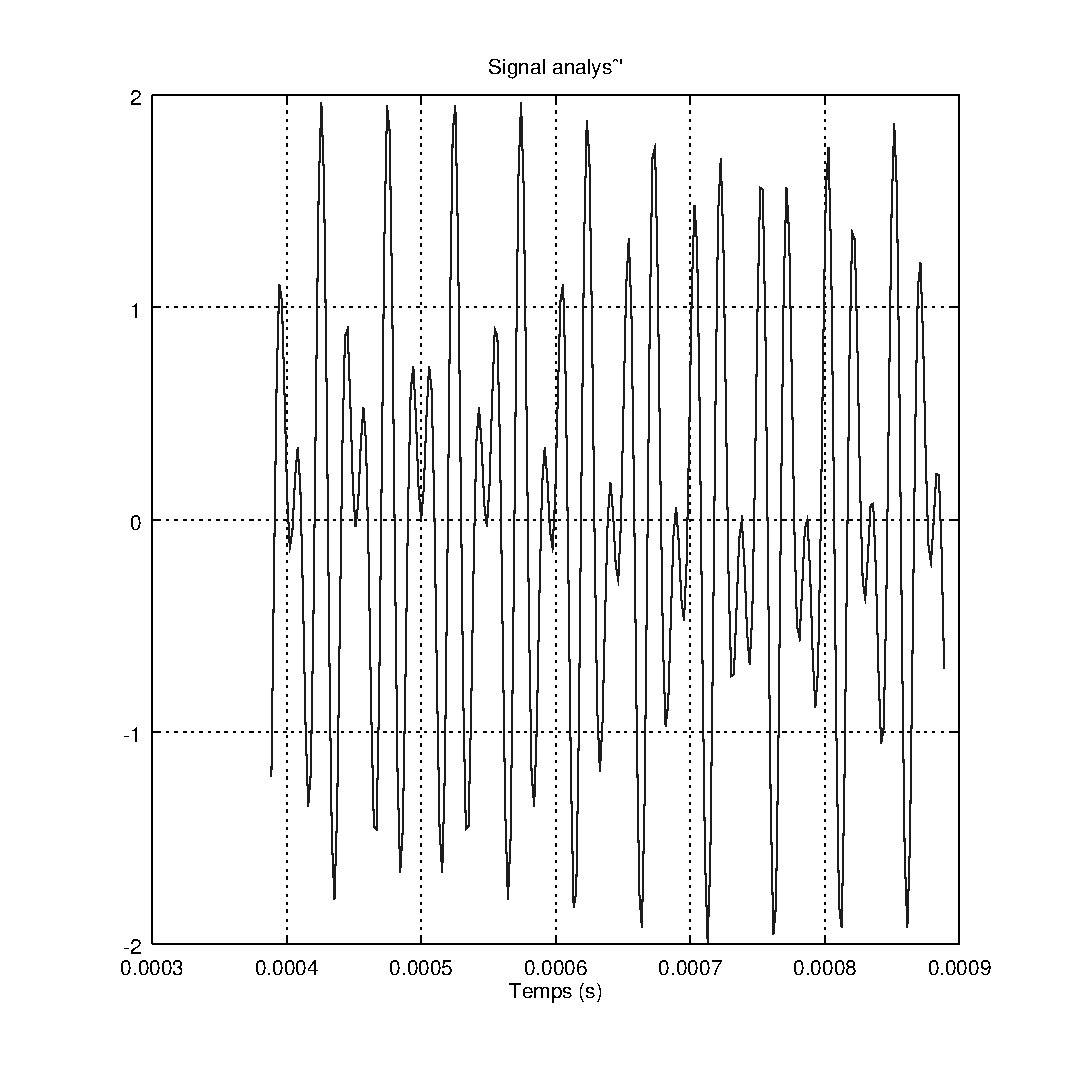
\includegraphics[width=\textwidth]{images/signal_fenetre.eps}
		% Title: glps_renderer figure
% Creator: GL2PS 1.3.8, (C) 1999-2012 C. Geuzaine
% For: Octave
% CreationDate: Wed Nov  8 10:42:42 2017
\begin{pgfpicture}
\pgfsetlinewidth{0.01pt}
\color[rgb]{1.000000,1.000000,1.000000}
\pgfpathmoveto{\pgfpoint{65.000031pt}{104.000000pt}}
\pgflineto{\pgfpoint{452.500000pt}{26.999981pt}}
\pgflineto{\pgfpoint{65.000031pt}{26.999981pt}}
\pgfpathclose
\pgfusepath{fill,stroke}
\pgfpathmoveto{\pgfpoint{65.000031pt}{104.000000pt}}
\pgflineto{\pgfpoint{452.500000pt}{104.000000pt}}
\pgflineto{\pgfpoint{452.500000pt}{26.999981pt}}
\pgfpathclose
\pgfusepath{fill,stroke}
\color[rgb]{0.000000,0.000000,0.000000}
\pgfsetlinewidth{0.500000pt}
\pgfsetdash{{16pt}{0pt}}{0pt}
\pgfpathmoveto{\pgfpoint{452.500000pt}{26.999981pt}}
\pgflineto{\pgfpoint{65.000031pt}{26.999981pt}}
\pgfusepath{stroke}
\pgfpathmoveto{\pgfpoint{452.500000pt}{104.000000pt}}
\pgflineto{\pgfpoint{65.000031pt}{104.000000pt}}
\pgfusepath{stroke}
\pgfpathmoveto{\pgfpoint{65.000031pt}{104.000000pt}}
\pgflineto{\pgfpoint{65.000031pt}{26.999981pt}}
\pgfusepath{stroke}
\pgfpathmoveto{\pgfpoint{452.500000pt}{104.000000pt}}
\pgflineto{\pgfpoint{452.500000pt}{26.999981pt}}
\pgfusepath{stroke}
\pgfsetdash{{0pt}{3pt}{1pt}{3pt}{1pt}{3pt}{1pt}{3pt}{1pt}{0pt}}{0pt}
\pgfpathmoveto{\pgfpoint{65.000031pt}{104.000000pt}}
\pgflineto{\pgfpoint{65.000031pt}{26.999981pt}}
\pgfusepath{stroke}
\pgfpathmoveto{\pgfpoint{129.583359pt}{104.000000pt}}
\pgflineto{\pgfpoint{129.583359pt}{26.999981pt}}
\pgfusepath{stroke}
\pgfpathmoveto{\pgfpoint{194.166718pt}{104.000000pt}}
\pgflineto{\pgfpoint{194.166718pt}{26.999981pt}}
\pgfusepath{stroke}
\pgfpathmoveto{\pgfpoint{258.750061pt}{104.000000pt}}
\pgflineto{\pgfpoint{258.750061pt}{26.999981pt}}
\pgfusepath{stroke}
\pgfpathmoveto{\pgfpoint{323.333344pt}{104.000000pt}}
\pgflineto{\pgfpoint{323.333344pt}{26.999981pt}}
\pgfusepath{stroke}
\pgfpathmoveto{\pgfpoint{387.916718pt}{104.000000pt}}
\pgflineto{\pgfpoint{387.916718pt}{26.999981pt}}
\pgfusepath{stroke}
\pgfpathmoveto{\pgfpoint{452.500000pt}{104.000000pt}}
\pgflineto{\pgfpoint{452.500000pt}{26.999981pt}}
\pgfusepath{stroke}
\pgfsetdash{{16pt}{0pt}}{0pt}
\pgfpathmoveto{\pgfpoint{65.000031pt}{30.874983pt}}
\pgflineto{\pgfpoint{65.000031pt}{26.999981pt}}
\pgfusepath{stroke}
\pgfpathmoveto{\pgfpoint{65.000031pt}{100.125000pt}}
\pgflineto{\pgfpoint{65.000031pt}{104.000000pt}}
\pgfusepath{stroke}
\pgfpathmoveto{\pgfpoint{129.583359pt}{30.874983pt}}
\pgflineto{\pgfpoint{129.583359pt}{26.999981pt}}
\pgfusepath{stroke}
\pgfpathmoveto{\pgfpoint{129.583359pt}{100.125000pt}}
\pgflineto{\pgfpoint{129.583359pt}{104.000000pt}}
\pgfusepath{stroke}
\pgfpathmoveto{\pgfpoint{194.166718pt}{30.874983pt}}
\pgflineto{\pgfpoint{194.166718pt}{26.999981pt}}
\pgfusepath{stroke}
\pgfpathmoveto{\pgfpoint{194.166718pt}{100.125000pt}}
\pgflineto{\pgfpoint{194.166718pt}{104.000000pt}}
\pgfusepath{stroke}
\pgfpathmoveto{\pgfpoint{258.750061pt}{30.874983pt}}
\pgflineto{\pgfpoint{258.750061pt}{26.999981pt}}
\pgfusepath{stroke}
\pgfpathmoveto{\pgfpoint{258.750061pt}{100.125000pt}}
\pgflineto{\pgfpoint{258.750061pt}{104.000000pt}}
\pgfusepath{stroke}
\pgfpathmoveto{\pgfpoint{323.333344pt}{30.874983pt}}
\pgflineto{\pgfpoint{323.333344pt}{26.999981pt}}
\pgfusepath{stroke}
\pgfpathmoveto{\pgfpoint{323.333344pt}{100.125000pt}}
\pgflineto{\pgfpoint{323.333344pt}{104.000000pt}}
\pgfusepath{stroke}
\pgfpathmoveto{\pgfpoint{387.916718pt}{30.874983pt}}
\pgflineto{\pgfpoint{387.916718pt}{26.999981pt}}
\pgfusepath{stroke}
\pgfpathmoveto{\pgfpoint{387.916718pt}{100.125000pt}}
\pgflineto{\pgfpoint{387.916718pt}{104.000000pt}}
\pgfusepath{stroke}
\pgfpathmoveto{\pgfpoint{452.500000pt}{30.874983pt}}
\pgflineto{\pgfpoint{452.500000pt}{26.999981pt}}
\pgfusepath{stroke}
\pgfpathmoveto{\pgfpoint{452.500000pt}{100.125000pt}}
\pgflineto{\pgfpoint{452.500000pt}{104.000000pt}}
\pgfusepath{stroke}
{
\pgftransformshift{\pgfpoint{65.000015pt}{21.999977pt}}
\pgfnode{rectangle}{north}{\fontsize{10}{0}\selectfont\textcolor[rgb]{0,0,0}{{0.0003}}}{}{\pgfusepath{discard}}}
{
\pgftransformshift{\pgfpoint{129.583328pt}{21.999977pt}}
\pgfnode{rectangle}{north}{\fontsize{10}{0}\selectfont\textcolor[rgb]{0,0,0}{{0.0004}}}{}{\pgfusepath{discard}}}
{
\pgftransformshift{\pgfpoint{194.166702pt}{21.999977pt}}
\pgfnode{rectangle}{north}{\fontsize{10}{0}\selectfont\textcolor[rgb]{0,0,0}{{0.0005}}}{}{\pgfusepath{discard}}}
{
\pgftransformshift{\pgfpoint{258.750031pt}{21.999977pt}}
\pgfnode{rectangle}{north}{\fontsize{10}{0}\selectfont\textcolor[rgb]{0,0,0}{{0.0006}}}{}{\pgfusepath{discard}}}
{
\pgftransformshift{\pgfpoint{323.333344pt}{21.999977pt}}
\pgfnode{rectangle}{north}{\fontsize{10}{0}\selectfont\textcolor[rgb]{0,0,0}{{0.0007}}}{}{\pgfusepath{discard}}}
{
\pgftransformshift{\pgfpoint{387.916687pt}{21.999977pt}}
\pgfnode{rectangle}{north}{\fontsize{10}{0}\selectfont\textcolor[rgb]{0,0,0}{{0.0008}}}{}{\pgfusepath{discard}}}
{
\pgftransformshift{\pgfpoint{452.500000pt}{21.999977pt}}
\pgfnode{rectangle}{north}{\fontsize{10}{0}\selectfont\textcolor[rgb]{0,0,0}{{0.0009}}}{}{\pgfusepath{discard}}}
\pgfsetdash{{0pt}{3pt}{1pt}{3pt}{1pt}{3pt}{1pt}{3pt}{1pt}{0pt}}{0pt}
\pgfpathmoveto{\pgfpoint{452.500000pt}{26.999981pt}}
\pgflineto{\pgfpoint{65.000031pt}{26.999981pt}}
\pgfusepath{stroke}
\pgfpathmoveto{\pgfpoint{452.500000pt}{46.249985pt}}
\pgflineto{\pgfpoint{65.000031pt}{46.249985pt}}
\pgfusepath{stroke}
\pgfpathmoveto{\pgfpoint{452.500000pt}{65.499992pt}}
\pgflineto{\pgfpoint{65.000031pt}{65.499992pt}}
\pgfusepath{stroke}
\pgfpathmoveto{\pgfpoint{452.500000pt}{84.750000pt}}
\pgflineto{\pgfpoint{65.000031pt}{84.750000pt}}
\pgfusepath{stroke}
\pgfpathmoveto{\pgfpoint{452.500000pt}{104.000000pt}}
\pgflineto{\pgfpoint{65.000031pt}{104.000000pt}}
\pgfusepath{stroke}
\pgfsetdash{{16pt}{0pt}}{0pt}
\pgfpathmoveto{\pgfpoint{68.870026pt}{26.999981pt}}
\pgflineto{\pgfpoint{65.000031pt}{26.999981pt}}
\pgfusepath{stroke}
\pgfpathmoveto{\pgfpoint{448.630066pt}{26.999981pt}}
\pgflineto{\pgfpoint{452.500000pt}{26.999981pt}}
\pgfusepath{stroke}
\pgfpathmoveto{\pgfpoint{68.870026pt}{46.249985pt}}
\pgflineto{\pgfpoint{65.000031pt}{46.249985pt}}
\pgfusepath{stroke}
\pgfpathmoveto{\pgfpoint{448.630066pt}{46.249985pt}}
\pgflineto{\pgfpoint{452.500000pt}{46.249985pt}}
\pgfusepath{stroke}
\pgfpathmoveto{\pgfpoint{68.870026pt}{65.499992pt}}
\pgflineto{\pgfpoint{65.000031pt}{65.499992pt}}
\pgfusepath{stroke}
\pgfpathmoveto{\pgfpoint{448.630066pt}{65.499992pt}}
\pgflineto{\pgfpoint{452.500000pt}{65.499992pt}}
\pgfusepath{stroke}
\pgfpathmoveto{\pgfpoint{68.870026pt}{84.750000pt}}
\pgflineto{\pgfpoint{65.000031pt}{84.750000pt}}
\pgfusepath{stroke}
\pgfpathmoveto{\pgfpoint{448.630066pt}{84.750000pt}}
\pgflineto{\pgfpoint{452.500000pt}{84.750000pt}}
\pgfusepath{stroke}
\pgfpathmoveto{\pgfpoint{68.870026pt}{104.000000pt}}
\pgflineto{\pgfpoint{65.000031pt}{104.000000pt}}
\pgfusepath{stroke}
\pgfpathmoveto{\pgfpoint{448.630066pt}{104.000000pt}}
\pgflineto{\pgfpoint{452.500000pt}{104.000000pt}}
\pgfusepath{stroke}
{
\pgftransformshift{\pgfpoint{60.006439pt}{26.999981pt}}
\pgfnode{rectangle}{east}{\fontsize{10}{0}\selectfont\textcolor[rgb]{0,0,0}{{-2}}}{}{\pgfusepath{discard}}}
{
\pgftransformshift{\pgfpoint{60.006439pt}{46.249985pt}}
\pgfnode{rectangle}{east}{\fontsize{10}{0}\selectfont\textcolor[rgb]{0,0,0}{{-1}}}{}{\pgfusepath{discard}}}
{
\pgftransformshift{\pgfpoint{60.006439pt}{65.499992pt}}
\pgfnode{rectangle}{east}{\fontsize{10}{0}\selectfont\textcolor[rgb]{0,0,0}{{0}}}{}{\pgfusepath{discard}}}
{
\pgftransformshift{\pgfpoint{60.006439pt}{84.750000pt}}
\pgfnode{rectangle}{east}{\fontsize{10}{0}\selectfont\textcolor[rgb]{0,0,0}{{1}}}{}{\pgfusepath{discard}}}
{
\pgftransformshift{\pgfpoint{60.006439pt}{104.000000pt}}
\pgfnode{rectangle}{east}{\fontsize{10}{0}\selectfont\textcolor[rgb]{0,0,0}{{2}}}{}{\pgfusepath{discard}}}
{
\pgftransformshift{\pgfpoint{258.750031pt}{10.999977pt}}
\pgfnode{rectangle}{north}{\fontsize{10}{0}\selectfont\textcolor[rgb]{0,0,0}{{Temps (s)}}}{}{\pgfusepath{discard}}}
\color[rgb]{0.000000,0.000000,1.000000}
\pgfsetdash{}{0pt}
\pgfpathmoveto{\pgfpoint{123.528656pt}{60.962570pt}}
\pgflineto{\pgfpoint{122.267273pt}{42.172722pt}}
\pgfusepath{stroke}
\pgfpathmoveto{\pgfpoint{124.790070pt}{78.114960pt}}
\pgflineto{\pgfpoint{123.528656pt}{60.962570pt}}
\pgfusepath{stroke}
\pgfpathmoveto{\pgfpoint{126.051453pt}{86.854027pt}}
\pgflineto{\pgfpoint{124.790070pt}{78.114960pt}}
\pgfusepath{stroke}
\pgfpathmoveto{\pgfpoint{127.312836pt}{85.296417pt}}
\pgflineto{\pgfpoint{126.051453pt}{86.854027pt}}
\pgfusepath{stroke}
\pgfpathmoveto{\pgfpoint{128.574219pt}{76.799545pt}}
\pgflineto{\pgfpoint{127.312836pt}{85.296417pt}}
\pgfusepath{stroke}
\pgfpathmoveto{\pgfpoint{129.835632pt}{67.570236pt}}
\pgflineto{\pgfpoint{128.574219pt}{76.799545pt}}
\pgfusepath{stroke}
\pgfpathmoveto{\pgfpoint{131.097015pt}{62.953091pt}}
\pgflineto{\pgfpoint{129.835632pt}{67.570236pt}}
\pgfusepath{stroke}
\pgfpathmoveto{\pgfpoint{132.358429pt}{64.476028pt}}
\pgflineto{\pgfpoint{131.097015pt}{62.953091pt}}
\pgfusepath{stroke}
\pgfpathmoveto{\pgfpoint{133.619812pt}{69.255478pt}}
\pgflineto{\pgfpoint{132.358429pt}{64.476028pt}}
\pgfusepath{stroke}
\pgfpathmoveto{\pgfpoint{134.881195pt}{72.026909pt}}
\pgflineto{\pgfpoint{133.619812pt}{69.255478pt}}
\pgfusepath{stroke}
\pgfpathmoveto{\pgfpoint{136.142578pt}{68.599434pt}}
\pgflineto{\pgfpoint{134.881195pt}{72.026909pt}}
\pgfusepath{stroke}
\pgfpathmoveto{\pgfpoint{137.403992pt}{58.736439pt}}
\pgflineto{\pgfpoint{136.142578pt}{68.599434pt}}
\pgfusepath{stroke}
\pgfpathmoveto{\pgfpoint{138.665375pt}{46.770752pt}}
\pgflineto{\pgfpoint{137.403992pt}{58.736439pt}}
\pgfusepath{stroke}
\pgfpathmoveto{\pgfpoint{139.926788pt}{39.510094pt}}
\pgflineto{\pgfpoint{138.665375pt}{46.770752pt}}
\pgfusepath{stroke}
\pgfpathmoveto{\pgfpoint{141.188171pt}{42.500294pt}}
\pgflineto{\pgfpoint{139.926788pt}{39.510094pt}}
\pgfusepath{stroke}
\pgfpathmoveto{\pgfpoint{142.449554pt}{56.667091pt}}
\pgflineto{\pgfpoint{141.188171pt}{42.500294pt}}
\pgfusepath{stroke}
\pgfpathmoveto{\pgfpoint{143.710968pt}{77.224968pt}}
\pgflineto{\pgfpoint{142.449554pt}{56.667091pt}}
\pgfusepath{stroke}
\pgfpathmoveto{\pgfpoint{144.972351pt}{95.577187pt}}
\pgflineto{\pgfpoint{143.710968pt}{77.224968pt}}
\pgfusepath{stroke}
\pgfpathmoveto{\pgfpoint{146.233734pt}{103.346710pt}}
\pgflineto{\pgfpoint{144.972351pt}{95.577187pt}}
\pgfusepath{stroke}
\pgfpathmoveto{\pgfpoint{147.495117pt}{96.516273pt}}
\pgflineto{\pgfpoint{146.233734pt}{103.346710pt}}
\pgfusepath{stroke}
\pgfpathmoveto{\pgfpoint{148.756531pt}{77.544022pt}}
\pgflineto{\pgfpoint{147.495117pt}{96.516273pt}}
\pgfusepath{stroke}
\pgfpathmoveto{\pgfpoint{150.017914pt}{54.331120pt}}
\pgflineto{\pgfpoint{148.756531pt}{77.544022pt}}
\pgfusepath{stroke}
\pgfpathmoveto{\pgfpoint{151.279327pt}{36.526840pt}}
\pgflineto{\pgfpoint{150.017914pt}{54.331120pt}}
\pgfusepath{stroke}
\pgfpathmoveto{\pgfpoint{152.540710pt}{31.021513pt}}
\pgflineto{\pgfpoint{151.279327pt}{36.526840pt}}
\pgfusepath{stroke}
\pgfpathmoveto{\pgfpoint{153.802124pt}{38.883327pt}}
\pgflineto{\pgfpoint{152.540710pt}{31.021513pt}}
\pgfusepath{stroke}
\pgfpathmoveto{\pgfpoint{155.063477pt}{55.230064pt}}
\pgflineto{\pgfpoint{153.802124pt}{38.883327pt}}
\pgfusepath{stroke}
\pgfpathmoveto{\pgfpoint{156.324890pt}{71.999832pt}}
\pgflineto{\pgfpoint{155.063477pt}{55.230064pt}}
\pgfusepath{stroke}
\pgfpathmoveto{\pgfpoint{157.586273pt}{82.101456pt}}
\pgflineto{\pgfpoint{156.324890pt}{71.999832pt}}
\pgfusepath{stroke}
\pgfpathmoveto{\pgfpoint{158.847687pt}{82.763130pt}}
\pgflineto{\pgfpoint{157.586273pt}{82.101456pt}}
\pgfusepath{stroke}
\pgfpathmoveto{\pgfpoint{160.109070pt}{76.393555pt}}
\pgflineto{\pgfpoint{158.847687pt}{82.763130pt}}
\pgfusepath{stroke}
\pgfpathmoveto{\pgfpoint{161.370453pt}{68.641602pt}}
\pgflineto{\pgfpoint{160.109070pt}{76.393555pt}}
\pgfusepath{stroke}
\pgfpathmoveto{\pgfpoint{162.631866pt}{64.846214pt}}
\pgflineto{\pgfpoint{161.370453pt}{68.641602pt}}
\pgfusepath{stroke}
\pgfpathmoveto{\pgfpoint{163.893250pt}{66.899727pt}}
\pgflineto{\pgfpoint{162.631866pt}{64.846214pt}}
\pgfusepath{stroke}
\pgfpathmoveto{\pgfpoint{165.154633pt}{72.268394pt}}
\pgflineto{\pgfpoint{163.893250pt}{66.899727pt}}
\pgfusepath{stroke}
\pgfpathmoveto{\pgfpoint{166.416046pt}{75.686264pt}}
\pgflineto{\pgfpoint{165.154633pt}{72.268394pt}}
\pgfusepath{stroke}
\pgfpathmoveto{\pgfpoint{167.677429pt}{72.536469pt}}
\pgflineto{\pgfpoint{166.416046pt}{75.686264pt}}
\pgfusepath{stroke}
\pgfpathmoveto{\pgfpoint{168.938812pt}{61.978619pt}}
\pgflineto{\pgfpoint{167.677429pt}{72.536469pt}}
\pgfusepath{stroke}
\pgfpathmoveto{\pgfpoint{170.200226pt}{47.994278pt}}
\pgflineto{\pgfpoint{168.938812pt}{61.978619pt}}
\pgfusepath{stroke}
\pgfpathmoveto{\pgfpoint{171.461609pt}{37.650986pt}}
\pgflineto{\pgfpoint{170.200226pt}{47.994278pt}}
\pgfusepath{stroke}
\pgfpathmoveto{\pgfpoint{172.722992pt}{37.420044pt}}
\pgflineto{\pgfpoint{171.461609pt}{37.650986pt}}
\pgfusepath{stroke}
\pgfpathmoveto{\pgfpoint{173.984375pt}{49.494198pt}}
\pgflineto{\pgfpoint{172.722992pt}{37.420044pt}}
\pgfusepath{stroke}
\pgfpathmoveto{\pgfpoint{175.245789pt}{70.126511pt}}
\pgflineto{\pgfpoint{173.984375pt}{49.494198pt}}
\pgfusepath{stroke}
\pgfpathmoveto{\pgfpoint{176.507172pt}{90.994080pt}}
\pgflineto{\pgfpoint{175.245789pt}{70.126511pt}}
\pgfusepath{stroke}
\pgfpathmoveto{\pgfpoint{177.768585pt}{103.008453pt}}
\pgflineto{\pgfpoint{176.507172pt}{90.994080pt}}
\pgfusepath{stroke}
\pgfpathmoveto{\pgfpoint{179.029968pt}{100.686478pt}}
\pgflineto{\pgfpoint{177.768585pt}{103.008453pt}}
\pgfusepath{stroke}
\pgfpathmoveto{\pgfpoint{180.291382pt}{84.859924pt}}
\pgflineto{\pgfpoint{179.029968pt}{100.686478pt}}
\pgfusepath{stroke}
\pgfpathmoveto{\pgfpoint{181.552765pt}{62.327499pt}}
\pgflineto{\pgfpoint{180.291382pt}{84.859924pt}}
\pgfusepath{stroke}
\pgfpathmoveto{\pgfpoint{182.814148pt}{42.612518pt}}
\pgflineto{\pgfpoint{181.552765pt}{62.327499pt}}
\pgfusepath{stroke}
\pgfpathmoveto{\pgfpoint{184.075531pt}{33.467079pt}}
\pgflineto{\pgfpoint{182.814148pt}{42.612518pt}}
\pgfusepath{stroke}
\pgfpathmoveto{\pgfpoint{185.336945pt}{37.385769pt}}
\pgflineto{\pgfpoint{184.075531pt}{33.467079pt}}
\pgfusepath{stroke}
\pgfpathmoveto{\pgfpoint{186.598328pt}{50.837570pt}}
\pgflineto{\pgfpoint{185.336945pt}{37.385769pt}}
\pgfusepath{stroke}
\pgfpathmoveto{\pgfpoint{187.859711pt}{66.492882pt}}
\pgflineto{\pgfpoint{186.598328pt}{50.837570pt}}
\pgfusepath{stroke}
\pgfpathmoveto{\pgfpoint{189.121124pt}{77.174988pt}}
\pgflineto{\pgfpoint{187.859711pt}{66.492882pt}}
\pgfusepath{stroke}
\pgfpathmoveto{\pgfpoint{190.382507pt}{79.415367pt}}
\pgflineto{\pgfpoint{189.121124pt}{77.174988pt}}
\pgfusepath{stroke}
\pgfpathmoveto{\pgfpoint{191.643921pt}{74.778603pt}}
\pgflineto{\pgfpoint{190.382507pt}{79.415367pt}}
\pgfusepath{stroke}
\pgfpathmoveto{\pgfpoint{192.905273pt}{68.373383pt}}
\pgflineto{\pgfpoint{191.643921pt}{74.778603pt}}
\pgfusepath{stroke}
\pgfpathmoveto{\pgfpoint{194.166718pt}{65.499992pt}}
\pgflineto{\pgfpoint{192.905273pt}{68.373383pt}}
\pgfusepath{stroke}
\pgfpathmoveto{\pgfpoint{195.428070pt}{68.373383pt}}
\pgflineto{\pgfpoint{194.166718pt}{65.499992pt}}
\pgfusepath{stroke}
\pgfpathmoveto{\pgfpoint{196.689453pt}{74.778603pt}}
\pgflineto{\pgfpoint{195.428070pt}{68.373383pt}}
\pgfusepath{stroke}
\pgfpathmoveto{\pgfpoint{197.950867pt}{79.415367pt}}
\pgflineto{\pgfpoint{196.689453pt}{74.778603pt}}
\pgfusepath{stroke}
\pgfpathmoveto{\pgfpoint{199.212250pt}{77.174988pt}}
\pgflineto{\pgfpoint{197.950867pt}{79.415367pt}}
\pgfusepath{stroke}
\pgfpathmoveto{\pgfpoint{200.473663pt}{66.492882pt}}
\pgflineto{\pgfpoint{199.212250pt}{77.174988pt}}
\pgfusepath{stroke}
\pgfpathmoveto{\pgfpoint{201.735046pt}{50.837570pt}}
\pgflineto{\pgfpoint{200.473663pt}{66.492882pt}}
\pgfusepath{stroke}
\pgfpathmoveto{\pgfpoint{202.996460pt}{37.385769pt}}
\pgflineto{\pgfpoint{201.735046pt}{50.837570pt}}
\pgfusepath{stroke}
\pgfpathmoveto{\pgfpoint{204.257843pt}{33.467079pt}}
\pgflineto{\pgfpoint{202.996460pt}{37.385769pt}}
\pgfusepath{stroke}
\pgfpathmoveto{\pgfpoint{205.519196pt}{42.612518pt}}
\pgflineto{\pgfpoint{204.257843pt}{33.467079pt}}
\pgfusepath{stroke}
\pgfpathmoveto{\pgfpoint{206.780609pt}{62.327499pt}}
\pgflineto{\pgfpoint{205.519196pt}{42.612518pt}}
\pgfusepath{stroke}
\pgfpathmoveto{\pgfpoint{208.041992pt}{84.859924pt}}
\pgflineto{\pgfpoint{206.780609pt}{62.327499pt}}
\pgfusepath{stroke}
\pgfpathmoveto{\pgfpoint{209.303406pt}{100.686478pt}}
\pgflineto{\pgfpoint{208.041992pt}{84.859924pt}}
\pgfusepath{stroke}
\pgfpathmoveto{\pgfpoint{210.564789pt}{103.008453pt}}
\pgflineto{\pgfpoint{209.303406pt}{100.686478pt}}
\pgfusepath{stroke}
\pgfpathmoveto{\pgfpoint{211.826202pt}{90.994080pt}}
\pgflineto{\pgfpoint{210.564789pt}{103.008453pt}}
\pgfusepath{stroke}
\pgfpathmoveto{\pgfpoint{213.087585pt}{70.126511pt}}
\pgflineto{\pgfpoint{211.826202pt}{90.994080pt}}
\pgfusepath{stroke}
\pgfpathmoveto{\pgfpoint{214.348999pt}{49.494198pt}}
\pgflineto{\pgfpoint{213.087585pt}{70.126511pt}}
\pgfusepath{stroke}
\pgfpathmoveto{\pgfpoint{215.610382pt}{37.420044pt}}
\pgflineto{\pgfpoint{214.348999pt}{49.494198pt}}
\pgfusepath{stroke}
\pgfpathmoveto{\pgfpoint{216.871765pt}{37.650986pt}}
\pgflineto{\pgfpoint{215.610382pt}{37.420044pt}}
\pgfusepath{stroke}
\pgfpathmoveto{\pgfpoint{218.133179pt}{47.994278pt}}
\pgflineto{\pgfpoint{216.871765pt}{37.650986pt}}
\pgfusepath{stroke}
\pgfpathmoveto{\pgfpoint{219.394531pt}{61.978619pt}}
\pgflineto{\pgfpoint{218.133179pt}{47.994278pt}}
\pgfusepath{stroke}
\pgfpathmoveto{\pgfpoint{220.655945pt}{72.536469pt}}
\pgflineto{\pgfpoint{219.394531pt}{61.978619pt}}
\pgfusepath{stroke}
\pgfpathmoveto{\pgfpoint{221.917328pt}{75.686264pt}}
\pgflineto{\pgfpoint{220.655945pt}{72.536469pt}}
\pgfusepath{stroke}
\pgfpathmoveto{\pgfpoint{223.178741pt}{72.268394pt}}
\pgflineto{\pgfpoint{221.917328pt}{75.686264pt}}
\pgfusepath{stroke}
\pgfpathmoveto{\pgfpoint{224.440125pt}{66.899727pt}}
\pgflineto{\pgfpoint{223.178741pt}{72.268394pt}}
\pgfusepath{stroke}
\pgfpathmoveto{\pgfpoint{225.701508pt}{64.846214pt}}
\pgflineto{\pgfpoint{224.440125pt}{66.899727pt}}
\pgfusepath{stroke}
\pgfpathmoveto{\pgfpoint{226.962921pt}{68.641602pt}}
\pgflineto{\pgfpoint{225.701508pt}{64.846214pt}}
\pgfusepath{stroke}
\pgfpathmoveto{\pgfpoint{228.224304pt}{76.393555pt}}
\pgflineto{\pgfpoint{226.962921pt}{68.641602pt}}
\pgfusepath{stroke}
\pgfpathmoveto{\pgfpoint{229.485718pt}{82.763130pt}}
\pgflineto{\pgfpoint{228.224304pt}{76.393555pt}}
\pgfusepath{stroke}
\pgfpathmoveto{\pgfpoint{230.747101pt}{82.101456pt}}
\pgflineto{\pgfpoint{229.485718pt}{82.763130pt}}
\pgfusepath{stroke}
\pgfpathmoveto{\pgfpoint{232.008514pt}{71.999832pt}}
\pgflineto{\pgfpoint{230.747101pt}{82.101456pt}}
\pgfusepath{stroke}
\pgfpathmoveto{\pgfpoint{233.269867pt}{55.230064pt}}
\pgflineto{\pgfpoint{232.008514pt}{71.999832pt}}
\pgfusepath{stroke}
\pgfpathmoveto{\pgfpoint{234.531250pt}{38.883327pt}}
\pgflineto{\pgfpoint{233.269867pt}{55.230064pt}}
\pgfusepath{stroke}
\pgfpathmoveto{\pgfpoint{235.792664pt}{31.021513pt}}
\pgflineto{\pgfpoint{234.531250pt}{38.883327pt}}
\pgfusepath{stroke}
\pgfpathmoveto{\pgfpoint{237.054047pt}{36.526840pt}}
\pgflineto{\pgfpoint{235.792664pt}{31.021513pt}}
\pgfusepath{stroke}
\pgfpathmoveto{\pgfpoint{238.315460pt}{54.331120pt}}
\pgflineto{\pgfpoint{237.054047pt}{36.526840pt}}
\pgfusepath{stroke}
\pgfpathmoveto{\pgfpoint{239.576843pt}{77.544022pt}}
\pgflineto{\pgfpoint{238.315460pt}{54.331120pt}}
\pgfusepath{stroke}
\pgfpathmoveto{\pgfpoint{240.838257pt}{96.516273pt}}
\pgflineto{\pgfpoint{239.576843pt}{77.544022pt}}
\pgfusepath{stroke}
\pgfpathmoveto{\pgfpoint{242.099640pt}{103.346710pt}}
\pgflineto{\pgfpoint{240.838257pt}{96.516273pt}}
\pgfusepath{stroke}
\pgfpathmoveto{\pgfpoint{243.361023pt}{95.577187pt}}
\pgflineto{\pgfpoint{242.099640pt}{103.346710pt}}
\pgfusepath{stroke}
\pgfpathmoveto{\pgfpoint{244.622437pt}{77.224968pt}}
\pgflineto{\pgfpoint{243.361023pt}{95.577187pt}}
\pgfusepath{stroke}
\pgfpathmoveto{\pgfpoint{245.883789pt}{56.667091pt}}
\pgflineto{\pgfpoint{244.622437pt}{77.224968pt}}
\pgfusepath{stroke}
\pgfpathmoveto{\pgfpoint{247.145203pt}{42.500294pt}}
\pgflineto{\pgfpoint{245.883789pt}{56.667091pt}}
\pgfusepath{stroke}
\pgfpathmoveto{\pgfpoint{248.406586pt}{39.510094pt}}
\pgflineto{\pgfpoint{247.145203pt}{42.500294pt}}
\pgfusepath{stroke}
\pgfpathmoveto{\pgfpoint{249.667999pt}{46.770752pt}}
\pgflineto{\pgfpoint{248.406586pt}{39.510094pt}}
\pgfusepath{stroke}
\pgfpathmoveto{\pgfpoint{250.929382pt}{58.736439pt}}
\pgflineto{\pgfpoint{249.667999pt}{46.770752pt}}
\pgfusepath{stroke}
\pgfpathmoveto{\pgfpoint{252.190765pt}{68.599434pt}}
\pgflineto{\pgfpoint{250.929382pt}{58.736439pt}}
\pgfusepath{stroke}
\pgfpathmoveto{\pgfpoint{253.452179pt}{72.026909pt}}
\pgflineto{\pgfpoint{252.190765pt}{68.599434pt}}
\pgfusepath{stroke}
\pgfpathmoveto{\pgfpoint{254.713562pt}{69.255478pt}}
\pgflineto{\pgfpoint{253.452179pt}{72.026909pt}}
\pgfusepath{stroke}
\pgfpathmoveto{\pgfpoint{255.974976pt}{64.476028pt}}
\pgflineto{\pgfpoint{254.713562pt}{69.255478pt}}
\pgfusepath{stroke}
\pgfpathmoveto{\pgfpoint{257.236359pt}{62.953091pt}}
\pgflineto{\pgfpoint{255.974976pt}{64.476028pt}}
\pgfusepath{stroke}
\pgfpathmoveto{\pgfpoint{258.497772pt}{67.570236pt}}
\pgflineto{\pgfpoint{257.236359pt}{62.953091pt}}
\pgfusepath{stroke}
\pgfpathmoveto{\pgfpoint{259.759125pt}{76.799545pt}}
\pgflineto{\pgfpoint{258.497772pt}{67.570236pt}}
\pgfusepath{stroke}
\pgfpathmoveto{\pgfpoint{261.020508pt}{85.296417pt}}
\pgflineto{\pgfpoint{259.759125pt}{76.799545pt}}
\pgfusepath{stroke}
\pgfpathmoveto{\pgfpoint{262.281921pt}{86.854027pt}}
\pgflineto{\pgfpoint{261.020508pt}{85.296417pt}}
\pgfusepath{stroke}
\pgfpathmoveto{\pgfpoint{263.543304pt}{78.114960pt}}
\pgflineto{\pgfpoint{262.281921pt}{86.854027pt}}
\pgfusepath{stroke}
\pgfpathmoveto{\pgfpoint{264.804718pt}{60.962570pt}}
\pgflineto{\pgfpoint{263.543304pt}{78.114960pt}}
\pgfusepath{stroke}
\pgfpathmoveto{\pgfpoint{266.066101pt}{42.172722pt}}
\pgflineto{\pgfpoint{264.804718pt}{60.962570pt}}
\pgfusepath{stroke}
\pgfpathmoveto{\pgfpoint{267.327515pt}{30.356434pt}}
\pgflineto{\pgfpoint{266.066101pt}{42.172722pt}}
\pgfusepath{stroke}
\pgfpathmoveto{\pgfpoint{268.588898pt}{31.694752pt}}
\pgflineto{\pgfpoint{267.327515pt}{30.356434pt}}
\pgfusepath{stroke}
\pgfpathmoveto{\pgfpoint{269.850311pt}{46.666119pt}}
\pgflineto{\pgfpoint{268.588898pt}{31.694752pt}}
\pgfusepath{stroke}
\pgfpathmoveto{\pgfpoint{271.111694pt}{69.508598pt}}
\pgflineto{\pgfpoint{269.850311pt}{46.666119pt}}
\pgfusepath{stroke}
\pgfpathmoveto{\pgfpoint{272.373047pt}{90.770996pt}}
\pgflineto{\pgfpoint{271.111694pt}{69.508598pt}}
\pgfusepath{stroke}
\pgfpathmoveto{\pgfpoint{273.634460pt}{101.713943pt}}
\pgflineto{\pgfpoint{272.373047pt}{90.770996pt}}
\pgfusepath{stroke}
\pgfpathmoveto{\pgfpoint{274.895844pt}{98.361809pt}}
\pgflineto{\pgfpoint{273.634460pt}{101.713943pt}}
\pgfusepath{stroke}
\pgfpathmoveto{\pgfpoint{276.157257pt}{83.185516pt}}
\pgflineto{\pgfpoint{274.895844pt}{98.361809pt}}
\pgfusepath{stroke}
\pgfpathmoveto{\pgfpoint{277.418640pt}{63.621140pt}}
\pgflineto{\pgfpoint{276.157257pt}{83.185516pt}}
\pgfusepath{stroke}
\pgfpathmoveto{\pgfpoint{278.680054pt}{48.254108pt}}
\pgflineto{\pgfpoint{277.418640pt}{63.621140pt}}
\pgfusepath{stroke}
\pgfpathmoveto{\pgfpoint{279.941437pt}{42.671585pt}}
\pgflineto{\pgfpoint{278.680054pt}{48.254108pt}}
\pgfusepath{stroke}
\pgfpathmoveto{\pgfpoint{281.202820pt}{47.096016pt}}
\pgflineto{\pgfpoint{279.941437pt}{42.671585pt}}
\pgfusepath{stroke}
\pgfpathmoveto{\pgfpoint{282.464233pt}{56.918575pt}}
\pgflineto{\pgfpoint{281.202820pt}{47.096016pt}}
\pgfusepath{stroke}
\pgfpathmoveto{\pgfpoint{283.725616pt}{65.693184pt}}
\pgflineto{\pgfpoint{282.464233pt}{56.918575pt}}
\pgfusepath{stroke}
\pgfpathmoveto{\pgfpoint{284.987030pt}{68.865173pt}}
\pgflineto{\pgfpoint{283.725616pt}{65.693184pt}}
\pgfusepath{stroke}
\pgfpathmoveto{\pgfpoint{286.248383pt}{66.174232pt}}
\pgflineto{\pgfpoint{284.987030pt}{68.865173pt}}
\pgfusepath{stroke}
\pgfpathmoveto{\pgfpoint{287.509796pt}{61.454582pt}}
\pgflineto{\pgfpoint{286.248383pt}{66.174232pt}}
\pgfusepath{stroke}
\pgfpathmoveto{\pgfpoint{288.771179pt}{60.019119pt}}
\pgflineto{\pgfpoint{287.509796pt}{61.454582pt}}
\pgfusepath{stroke}
\pgfpathmoveto{\pgfpoint{290.032562pt}{65.159950pt}}
\pgflineto{\pgfpoint{288.771179pt}{60.019119pt}}
\pgfusepath{stroke}
\pgfpathmoveto{\pgfpoint{291.293976pt}{75.791931pt}}
\pgflineto{\pgfpoint{290.032562pt}{65.159950pt}}
\pgfusepath{stroke}
\pgfpathmoveto{\pgfpoint{292.555359pt}{86.640007pt}}
\pgflineto{\pgfpoint{291.293976pt}{75.791931pt}}
\pgfusepath{stroke}
\pgfpathmoveto{\pgfpoint{293.816772pt}{90.962975pt}}
\pgflineto{\pgfpoint{292.555359pt}{86.640007pt}}
\pgfusepath{stroke}
\pgfpathmoveto{\pgfpoint{295.078156pt}{84.380112pt}}
\pgflineto{\pgfpoint{293.816772pt}{90.962975pt}}
\pgfusepath{stroke}
\pgfpathmoveto{\pgfpoint{296.339569pt}{67.702209pt}}
\pgflineto{\pgfpoint{295.078156pt}{84.380112pt}}
\pgfusepath{stroke}
\pgfpathmoveto{\pgfpoint{297.600952pt}{47.137791pt}}
\pgflineto{\pgfpoint{296.339569pt}{67.702209pt}}
\pgfusepath{stroke}
\pgfpathmoveto{\pgfpoint{298.862305pt}{31.613205pt}}
\pgflineto{\pgfpoint{297.600952pt}{47.137791pt}}
\pgfusepath{stroke}
\pgfpathmoveto{\pgfpoint{300.123718pt}{28.488487pt}}
\pgflineto{\pgfpoint{298.862305pt}{31.613205pt}}
\pgfusepath{stroke}
\pgfpathmoveto{\pgfpoint{301.385101pt}{39.844170pt}}
\pgflineto{\pgfpoint{300.123718pt}{28.488487pt}}
\pgfusepath{stroke}
\pgfpathmoveto{\pgfpoint{302.646515pt}{61.272083pt}}
\pgflineto{\pgfpoint{301.385101pt}{39.844170pt}}
\pgfusepath{stroke}
\pgfpathmoveto{\pgfpoint{303.907898pt}{83.839478pt}}
\pgflineto{\pgfpoint{302.646515pt}{61.272083pt}}
\pgfusepath{stroke}
\pgfpathmoveto{\pgfpoint{305.169312pt}{98.269112pt}}
\pgflineto{\pgfpoint{303.907898pt}{83.839478pt}}
\pgfusepath{stroke}
\pgfpathmoveto{\pgfpoint{306.430695pt}{99.240967pt}}
\pgflineto{\pgfpoint{305.169312pt}{98.269112pt}}
\pgfusepath{stroke}
\pgfpathmoveto{\pgfpoint{307.692078pt}{87.671127pt}}
\pgflineto{\pgfpoint{306.430695pt}{99.240967pt}}
\pgfusepath{stroke}
\pgfpathmoveto{\pgfpoint{308.953491pt}{69.882935pt}}
\pgflineto{\pgfpoint{307.692078pt}{87.671127pt}}
\pgfusepath{stroke}
\pgfpathmoveto{\pgfpoint{310.214874pt}{54.193542pt}}
\pgflineto{\pgfpoint{308.953491pt}{69.882935pt}}
\pgfusepath{stroke}
\pgfpathmoveto{\pgfpoint{311.476288pt}{46.748806pt}}
\pgflineto{\pgfpoint{310.214874pt}{54.193542pt}}
\pgfusepath{stroke}
\pgfpathmoveto{\pgfpoint{312.737640pt}{48.766888pt}}
\pgflineto{\pgfpoint{311.476288pt}{46.748806pt}}
\pgfusepath{stroke}
\pgfpathmoveto{\pgfpoint{313.999054pt}{56.539272pt}}
\pgflineto{\pgfpoint{312.737640pt}{48.766888pt}}
\pgfusepath{stroke}
\pgfpathmoveto{\pgfpoint{315.260437pt}{64.034668pt}}
\pgflineto{\pgfpoint{313.999054pt}{56.539272pt}}
\pgfusepath{stroke}
\pgfpathmoveto{\pgfpoint{316.521820pt}{66.566780pt}}
\pgflineto{\pgfpoint{315.260437pt}{64.034668pt}}
\pgfusepath{stroke}
\pgfpathmoveto{\pgfpoint{317.783234pt}{63.460281pt}}
\pgflineto{\pgfpoint{316.521820pt}{66.566780pt}}
\pgfusepath{stroke}
\pgfpathmoveto{\pgfpoint{319.044617pt}{58.251656pt}}
\pgflineto{\pgfpoint{317.783234pt}{63.460281pt}}
\pgfusepath{stroke}
\pgfpathmoveto{\pgfpoint{320.306030pt}{56.355370pt}}
\pgflineto{\pgfpoint{319.044617pt}{58.251656pt}}
\pgfusepath{stroke}
\pgfpathmoveto{\pgfpoint{321.567413pt}{61.547832pt}}
\pgflineto{\pgfpoint{320.306030pt}{56.355370pt}}
\pgfusepath{stroke}
\pgfpathmoveto{\pgfpoint{322.828827pt}{73.295799pt}}
\pgflineto{\pgfpoint{321.567413pt}{61.547832pt}}
\pgfusepath{stroke}
\pgfpathmoveto{\pgfpoint{324.090210pt}{86.511780pt}}
\pgflineto{\pgfpoint{322.828827pt}{73.295799pt}}
\pgfusepath{stroke}
\pgfpathmoveto{\pgfpoint{325.351624pt}{93.992256pt}}
\pgflineto{\pgfpoint{324.090210pt}{86.511780pt}}
\pgfusepath{stroke}
\pgfpathmoveto{\pgfpoint{326.612976pt}{90.301750pt}}
\pgflineto{\pgfpoint{325.351624pt}{93.992256pt}}
\pgfusepath{stroke}
\pgfpathmoveto{\pgfpoint{327.874359pt}{75.018158pt}}
\pgflineto{\pgfpoint{326.612976pt}{90.301750pt}}
\pgfusepath{stroke}
\pgfpathmoveto{\pgfpoint{329.135773pt}{53.524143pt}}
\pgflineto{\pgfpoint{327.874359pt}{75.018158pt}}
\pgfusepath{stroke}
\pgfpathmoveto{\pgfpoint{330.397156pt}{34.787788pt}}
\pgflineto{\pgfpoint{329.135773pt}{53.524143pt}}
\pgfusepath{stroke}
\pgfpathmoveto{\pgfpoint{331.658569pt}{27.163654pt}}
\pgflineto{\pgfpoint{330.397156pt}{34.787788pt}}
\pgfusepath{stroke}
\pgfpathmoveto{\pgfpoint{332.919952pt}{34.318523pt}}
\pgflineto{\pgfpoint{331.658569pt}{27.163654pt}}
\pgfusepath{stroke}
\pgfpathmoveto{\pgfpoint{334.181366pt}{53.367580pt}}
\pgflineto{\pgfpoint{332.919952pt}{34.318523pt}}
\pgfusepath{stroke}
\pgfpathmoveto{\pgfpoint{335.442749pt}{76.194717pt}}
\pgflineto{\pgfpoint{334.181366pt}{53.367580pt}}
\pgfusepath{stroke}
\pgfpathmoveto{\pgfpoint{336.704102pt}{93.303482pt}}
\pgflineto{\pgfpoint{335.442749pt}{76.194717pt}}
\pgfusepath{stroke}
\pgfpathmoveto{\pgfpoint{337.965546pt}{98.254959pt}}
\pgflineto{\pgfpoint{336.704102pt}{93.303482pt}}
\pgfusepath{stroke}
\pgfpathmoveto{\pgfpoint{339.226898pt}{90.470917pt}}
\pgflineto{\pgfpoint{337.965546pt}{98.254959pt}}
\pgfusepath{stroke}
\pgfpathmoveto{\pgfpoint{340.488312pt}{75.054237pt}}
\pgflineto{\pgfpoint{339.226898pt}{90.470917pt}}
\pgfusepath{stroke}
\pgfpathmoveto{\pgfpoint{341.749695pt}{59.838318pt}}
\pgflineto{\pgfpoint{340.488312pt}{75.054237pt}}
\pgfusepath{stroke}
\pgfpathmoveto{\pgfpoint{343.011108pt}{51.295364pt}}
\pgflineto{\pgfpoint{341.749695pt}{59.838318pt}}
\pgfusepath{stroke}
\pgfpathmoveto{\pgfpoint{344.272491pt}{51.468643pt}}
\pgflineto{\pgfpoint{343.011108pt}{51.295364pt}}
\pgfusepath{stroke}
\pgfpathmoveto{\pgfpoint{345.533875pt}{57.476162pt}}
\pgflineto{\pgfpoint{344.272491pt}{51.468643pt}}
\pgfusepath{stroke}
\pgfpathmoveto{\pgfpoint{346.795288pt}{63.710365pt}}
\pgflineto{\pgfpoint{345.533875pt}{57.476162pt}}
\pgfusepath{stroke}
\pgfpathmoveto{\pgfpoint{348.056671pt}{65.402138pt}}
\pgflineto{\pgfpoint{346.795288pt}{63.710365pt}}
\pgfusepath{stroke}
\pgfpathmoveto{\pgfpoint{349.318085pt}{61.509876pt}}
\pgflineto{\pgfpoint{348.056671pt}{65.402138pt}}
\pgfusepath{stroke}
\pgfpathmoveto{\pgfpoint{350.579437pt}{55.308769pt}}
\pgflineto{\pgfpoint{349.318085pt}{61.509876pt}}
\pgfusepath{stroke}
\pgfpathmoveto{\pgfpoint{351.840881pt}{52.357628pt}}
\pgflineto{\pgfpoint{350.579437pt}{55.308769pt}}
\pgfusepath{stroke}
\pgfpathmoveto{\pgfpoint{353.102234pt}{56.996876pt}}
\pgflineto{\pgfpoint{351.840881pt}{52.357628pt}}
\pgfusepath{stroke}
\pgfpathmoveto{\pgfpoint{354.363617pt}{69.375404pt}}
\pgflineto{\pgfpoint{353.102234pt}{56.996876pt}}
\pgfusepath{stroke}
\pgfpathmoveto{\pgfpoint{355.625031pt}{84.750000pt}}
\pgflineto{\pgfpoint{354.363617pt}{69.375404pt}}
\pgfusepath{stroke}
\pgfpathmoveto{\pgfpoint{356.886414pt}{95.578552pt}}
\pgflineto{\pgfpoint{355.625031pt}{84.750000pt}}
\pgfusepath{stroke}
\pgfpathmoveto{\pgfpoint{358.147827pt}{95.392570pt}}
\pgflineto{\pgfpoint{356.886414pt}{95.578552pt}}
\pgfusepath{stroke}
\pgfpathmoveto{\pgfpoint{359.409210pt}{82.416016pt}}
\pgflineto{\pgfpoint{358.147827pt}{95.392570pt}}
\pgfusepath{stroke}
\pgfpathmoveto{\pgfpoint{360.670624pt}{60.957897pt}}
\pgflineto{\pgfpoint{359.409210pt}{82.416016pt}}
\pgfusepath{stroke}
\pgfpathmoveto{\pgfpoint{361.932007pt}{39.729195pt}}
\pgflineto{\pgfpoint{360.670624pt}{60.957897pt}}
\pgfusepath{stroke}
\pgfpathmoveto{\pgfpoint{363.193359pt}{27.837597pt}}
\pgflineto{\pgfpoint{361.932007pt}{39.729195pt}}
\pgfusepath{stroke}
\pgfpathmoveto{\pgfpoint{364.454773pt}{30.447403pt}}
\pgflineto{\pgfpoint{363.193359pt}{27.837597pt}}
\pgfusepath{stroke}
\pgfpathmoveto{\pgfpoint{365.716156pt}{46.300201pt}}
\pgflineto{\pgfpoint{364.454773pt}{30.447403pt}}
\pgfusepath{stroke}
\pgfpathmoveto{\pgfpoint{366.977570pt}{68.355377pt}}
\pgflineto{\pgfpoint{365.716156pt}{46.300201pt}}
\pgfusepath{stroke}
\pgfpathmoveto{\pgfpoint{368.238953pt}{87.215599pt}}
\pgflineto{\pgfpoint{366.977570pt}{68.355377pt}}
\pgfusepath{stroke}
\pgfpathmoveto{\pgfpoint{369.500366pt}{95.585815pt}}
\pgflineto{\pgfpoint{368.238953pt}{87.215599pt}}
\pgfusepath{stroke}
\pgfpathmoveto{\pgfpoint{370.761749pt}{91.515114pt}}
\pgflineto{\pgfpoint{369.500366pt}{95.585815pt}}
\pgfusepath{stroke}
\pgfpathmoveto{\pgfpoint{372.023193pt}{78.843689pt}}
\pgflineto{\pgfpoint{370.761749pt}{91.515114pt}}
\pgfusepath{stroke}
\pgfpathmoveto{\pgfpoint{373.284546pt}{64.756607pt}}
\pgflineto{\pgfpoint{372.023193pt}{78.843689pt}}
\pgfusepath{stroke}
\pgfpathmoveto{\pgfpoint{374.545898pt}{55.845280pt}}
\pgflineto{\pgfpoint{373.284546pt}{64.756607pt}}
\pgfusepath{stroke}
\pgfpathmoveto{\pgfpoint{375.807312pt}{54.805260pt}}
\pgflineto{\pgfpoint{374.545898pt}{55.845280pt}}
\pgfusepath{stroke}
\pgfpathmoveto{\pgfpoint{377.068726pt}{59.483624pt}}
\pgflineto{\pgfpoint{375.807312pt}{54.805260pt}}
\pgfusepath{stroke}
\pgfpathmoveto{\pgfpoint{378.330139pt}{64.669868pt}}
\pgflineto{\pgfpoint{377.068726pt}{59.483624pt}}
\pgfusepath{stroke}
\pgfpathmoveto{\pgfpoint{379.591492pt}{65.521706pt}}
\pgflineto{\pgfpoint{378.330139pt}{64.669868pt}}
\pgfusepath{stroke}
\pgfpathmoveto{\pgfpoint{380.852905pt}{60.642818pt}}
\pgflineto{\pgfpoint{379.591492pt}{65.521706pt}}
\pgfusepath{stroke}
\pgfpathmoveto{\pgfpoint{382.114319pt}{53.051689pt}}
\pgflineto{\pgfpoint{380.852905pt}{60.642818pt}}
\pgfusepath{stroke}
\pgfpathmoveto{\pgfpoint{383.375671pt}{48.470840pt}}
\pgflineto{\pgfpoint{382.114319pt}{53.051689pt}}
\pgfusepath{stroke}
\pgfpathmoveto{\pgfpoint{384.637085pt}{51.874195pt}}
\pgflineto{\pgfpoint{383.375671pt}{48.470840pt}}
\pgfusepath{stroke}
\pgfpathmoveto{\pgfpoint{385.898438pt}{64.231346pt}}
\pgflineto{\pgfpoint{384.637085pt}{51.874195pt}}
\pgfusepath{stroke}
\pgfpathmoveto{\pgfpoint{387.159851pt}{81.330414pt}}
\pgflineto{\pgfpoint{385.898438pt}{64.231346pt}}
\pgfusepath{stroke}
\pgfpathmoveto{\pgfpoint{388.421265pt}{95.464424pt}}
\pgflineto{\pgfpoint{387.159851pt}{81.330414pt}}
\pgfusepath{stroke}
\pgfpathmoveto{\pgfpoint{389.682678pt}{99.213058pt}}
\pgflineto{\pgfpoint{388.421265pt}{95.464424pt}}
\pgfusepath{stroke}
\pgfpathmoveto{\pgfpoint{390.944031pt}{89.377930pt}}
\pgflineto{\pgfpoint{389.682678pt}{99.213058pt}}
\pgfusepath{stroke}
\pgfpathmoveto{\pgfpoint{392.205444pt}{68.974663pt}}
\pgflineto{\pgfpoint{390.944031pt}{89.377930pt}}
\pgfusepath{stroke}
\pgfpathmoveto{\pgfpoint{393.466858pt}{46.150242pt}}
\pgflineto{\pgfpoint{392.205444pt}{68.974663pt}}
\pgfusepath{stroke}
\pgfpathmoveto{\pgfpoint{394.728210pt}{30.479221pt}}
\pgflineto{\pgfpoint{393.466858pt}{46.150242pt}}
\pgfusepath{stroke}
\pgfpathmoveto{\pgfpoint{395.989624pt}{28.465302pt}}
\pgflineto{\pgfpoint{394.728210pt}{30.479221pt}}
\pgfusepath{stroke}
\pgfpathmoveto{\pgfpoint{397.250977pt}{40.506729pt}}
\pgflineto{\pgfpoint{395.989624pt}{28.465302pt}}
\pgfusepath{stroke}
\pgfpathmoveto{\pgfpoint{398.512390pt}{60.843636pt}}
\pgflineto{\pgfpoint{397.250977pt}{40.506729pt}}
\pgfusepath{stroke}
\pgfpathmoveto{\pgfpoint{399.773804pt}{80.477516pt}}
\pgflineto{\pgfpoint{398.512390pt}{60.843636pt}}
\pgfusepath{stroke}
\pgfpathmoveto{\pgfpoint{401.035156pt}{91.539757pt}}
\pgflineto{\pgfpoint{399.773804pt}{80.477516pt}}
\pgfusepath{stroke}
\pgfpathmoveto{\pgfpoint{402.296570pt}{90.877960pt}}
\pgflineto{\pgfpoint{401.035156pt}{91.539757pt}}
\pgfusepath{stroke}
\pgfpathmoveto{\pgfpoint{403.557983pt}{81.089096pt}}
\pgflineto{\pgfpoint{402.296570pt}{90.877960pt}}
\pgfusepath{stroke}
\pgfpathmoveto{\pgfpoint{404.819397pt}{68.601234pt}}
\pgflineto{\pgfpoint{403.557983pt}{81.089096pt}}
\pgfusepath{stroke}
\pgfpathmoveto{\pgfpoint{406.080750pt}{59.954491pt}}
\pgflineto{\pgfpoint{404.819397pt}{68.601234pt}}
\pgfusepath{stroke}
\pgfpathmoveto{\pgfpoint{407.342163pt}{58.336464pt}}
\pgflineto{\pgfpoint{406.080750pt}{59.954491pt}}
\pgfusepath{stroke}
\pgfpathmoveto{\pgfpoint{408.603577pt}{62.216919pt}}
\pgflineto{\pgfpoint{407.342163pt}{58.336464pt}}
\pgfusepath{stroke}
\pgfpathmoveto{\pgfpoint{409.864929pt}{66.731667pt}}
\pgflineto{\pgfpoint{408.603577pt}{62.216919pt}}
\pgfusepath{stroke}
\pgfpathmoveto{\pgfpoint{411.126343pt}{66.942123pt}}
\pgflineto{\pgfpoint{409.864929pt}{66.731667pt}}
\pgfusepath{stroke}
\pgfpathmoveto{\pgfpoint{412.387695pt}{61.072155pt}}
\pgflineto{\pgfpoint{411.126343pt}{66.942123pt}}
\pgfusepath{stroke}
\pgfpathmoveto{\pgfpoint{413.649109pt}{51.850601pt}}
\pgflineto{\pgfpoint{412.387695pt}{61.072155pt}}
\pgfusepath{stroke}
\pgfpathmoveto{\pgfpoint{414.910522pt}{45.148987pt}}
\pgflineto{\pgfpoint{413.649109pt}{51.850601pt}}
\pgfusepath{stroke}
\pgfpathmoveto{\pgfpoint{416.171936pt}{46.619869pt}}
\pgflineto{\pgfpoint{414.910522pt}{45.148987pt}}
\pgfusepath{stroke}
\pgfpathmoveto{\pgfpoint{417.433289pt}{58.185787pt}}
\pgflineto{\pgfpoint{416.171936pt}{46.619869pt}}
\pgfusepath{stroke}
\pgfpathmoveto{\pgfpoint{418.694702pt}{76.371567pt}}
\pgflineto{\pgfpoint{417.433289pt}{58.185787pt}}
\pgfusepath{stroke}
\pgfpathmoveto{\pgfpoint{419.956116pt}{93.522675pt}}
\pgflineto{\pgfpoint{418.694702pt}{76.371567pt}}
\pgfusepath{stroke}
\pgfpathmoveto{\pgfpoint{421.217468pt}{101.409409pt}}
\pgflineto{\pgfpoint{419.956116pt}{93.522675pt}}
\pgfusepath{stroke}
\pgfpathmoveto{\pgfpoint{422.478882pt}{95.405014pt}}
\pgflineto{\pgfpoint{421.217468pt}{101.409409pt}}
\pgfusepath{stroke}
\pgfpathmoveto{\pgfpoint{423.740234pt}{77.056381pt}}
\pgflineto{\pgfpoint{422.478882pt}{95.405014pt}}
\pgfusepath{stroke}
\pgfpathmoveto{\pgfpoint{425.001648pt}{53.649784pt}}
\pgflineto{\pgfpoint{423.740234pt}{77.056381pt}}
\pgfusepath{stroke}
\pgfpathmoveto{\pgfpoint{426.263062pt}{34.911194pt}}
\pgflineto{\pgfpoint{425.001648pt}{53.649784pt}}
\pgfusepath{stroke}
\pgfpathmoveto{\pgfpoint{427.524475pt}{28.464581pt}}
\pgflineto{\pgfpoint{426.263062pt}{34.911194pt}}
\pgfusepath{stroke}
\pgfpathmoveto{\pgfpoint{428.785828pt}{36.321159pt}}
\pgflineto{\pgfpoint{427.524475pt}{28.464581pt}}
\pgfusepath{stroke}
\pgfpathmoveto{\pgfpoint{430.047241pt}{54.143055pt}}
\pgflineto{\pgfpoint{428.785828pt}{36.321159pt}}
\pgfusepath{stroke}
\pgfpathmoveto{\pgfpoint{431.308655pt}{73.595085pt}}
\pgflineto{\pgfpoint{430.047241pt}{54.143055pt}}
\pgfusepath{stroke}
\pgfpathmoveto{\pgfpoint{432.570007pt}{86.519531pt}}
\pgflineto{\pgfpoint{431.308655pt}{73.595085pt}}
\pgfusepath{stroke}
\pgfpathmoveto{\pgfpoint{433.831421pt}{88.768303pt}}
\pgflineto{\pgfpoint{432.570007pt}{86.519531pt}}
\pgfusepath{stroke}
\pgfpathmoveto{\pgfpoint{435.092834pt}{81.768440pt}}
\pgflineto{\pgfpoint{433.831421pt}{88.768303pt}}
\pgfusepath{stroke}
\pgfpathmoveto{\pgfpoint{436.354248pt}{71.138184pt}}
\pgflineto{\pgfpoint{435.092834pt}{81.768440pt}}
\pgfusepath{stroke}
\pgfpathmoveto{\pgfpoint{437.615601pt}{63.240021pt}}
\pgflineto{\pgfpoint{436.354248pt}{71.138184pt}}
\pgfusepath{stroke}
\pgfpathmoveto{\pgfpoint{438.876953pt}{61.618446pt}}
\pgflineto{\pgfpoint{437.615601pt}{63.240021pt}}
\pgfusepath{stroke}
\pgfpathmoveto{\pgfpoint{440.138367pt}{65.265045pt}}
\pgflineto{\pgfpoint{438.876953pt}{61.618446pt}}
\pgfusepath{stroke}
\pgfpathmoveto{\pgfpoint{441.399780pt}{69.600548pt}}
\pgflineto{\pgfpoint{440.138367pt}{65.265045pt}}
\pgfusepath{stroke}
\pgfpathmoveto{\pgfpoint{442.661194pt}{69.544319pt}}
\pgflineto{\pgfpoint{441.399780pt}{69.600548pt}}
\pgfusepath{stroke}
\pgfpathmoveto{\pgfpoint{443.922546pt}{62.883305pt}}
\pgflineto{\pgfpoint{442.661194pt}{69.544319pt}}
\pgfusepath{stroke}
\pgfpathmoveto{\pgfpoint{445.183960pt}{51.985050pt}}
\pgflineto{\pgfpoint{443.922546pt}{62.883305pt}}
\pgfusepath{stroke}
{
\pgftransformshift{\pgfpoint{258.750031pt}{114.000000pt}}
\pgfnode{rectangle}{south}{\fontsize{10}{0}\selectfont\textcolor[rgb]{0,0,0}{{Signal analysé}}}{}{\pgfusepath{discard}}}
\end{pgfpicture}

		\caption{Signal analysé.}
		\label{fig:fen_signal}
	\end{minipage}
\end{figure}
\begin{figure}[h!]
  	\begin{minipage}{\textwidth}
  		\centering
  		%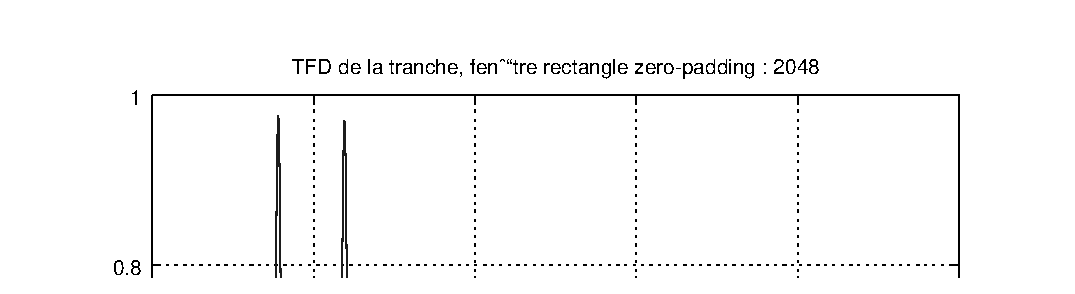
\includegraphics[width=\textwidth]{images/rectangle.eps}
  		% Title: glps_renderer figure
% Creator: GL2PS 1.3.8, (C) 1999-2012 C. Geuzaine
% For: Octave
% CreationDate: Wed Nov  8 10:42:42 2017
\begin{pgfpicture}
\pgfsetlinewidth{0.01pt}
\color[rgb]{1.000000,1.000000,1.000000}
\pgfpathmoveto{\pgfpoint{65.000015pt}{104.000000pt}}
\pgflineto{\pgfpoint{452.500031pt}{26.999981pt}}
\pgflineto{\pgfpoint{65.000015pt}{26.999981pt}}
\pgfpathclose
\pgfusepath{fill,stroke}
\pgfpathmoveto{\pgfpoint{65.000015pt}{104.000000pt}}
\pgflineto{\pgfpoint{452.500031pt}{104.000000pt}}
\pgflineto{\pgfpoint{452.500031pt}{26.999981pt}}
\pgfpathclose
\pgfusepath{fill,stroke}
\color[rgb]{0.000000,0.000000,0.000000}
\pgfsetlinewidth{0.500000pt}
\pgfsetdash{{16pt}{0pt}}{0pt}
\pgfpathmoveto{\pgfpoint{452.500031pt}{26.999981pt}}
\pgflineto{\pgfpoint{65.000015pt}{26.999981pt}}
\pgfusepath{stroke}
\pgfpathmoveto{\pgfpoint{452.500031pt}{104.000000pt}}
\pgflineto{\pgfpoint{65.000015pt}{104.000000pt}}
\pgfusepath{stroke}
\pgfpathmoveto{\pgfpoint{65.000015pt}{104.000000pt}}
\pgflineto{\pgfpoint{65.000015pt}{26.999981pt}}
\pgfusepath{stroke}
\pgfpathmoveto{\pgfpoint{452.500031pt}{104.000000pt}}
\pgflineto{\pgfpoint{452.500031pt}{26.999981pt}}
\pgfusepath{stroke}
\pgfsetdash{{0pt}{3pt}{1pt}{3pt}{1pt}{3pt}{1pt}{3pt}{1pt}{0pt}}{0pt}
\pgfpathmoveto{\pgfpoint{65.000015pt}{104.000000pt}}
\pgflineto{\pgfpoint{65.000015pt}{26.999981pt}}
\pgfusepath{stroke}
\pgfpathmoveto{\pgfpoint{142.500031pt}{104.000000pt}}
\pgflineto{\pgfpoint{142.500031pt}{26.999981pt}}
\pgfusepath{stroke}
\pgfpathmoveto{\pgfpoint{220.000031pt}{104.000000pt}}
\pgflineto{\pgfpoint{220.000031pt}{26.999981pt}}
\pgfusepath{stroke}
\pgfpathmoveto{\pgfpoint{297.500031pt}{104.000000pt}}
\pgflineto{\pgfpoint{297.500031pt}{26.999981pt}}
\pgfusepath{stroke}
\pgfpathmoveto{\pgfpoint{375.000061pt}{104.000000pt}}
\pgflineto{\pgfpoint{375.000061pt}{26.999981pt}}
\pgfusepath{stroke}
\pgfpathmoveto{\pgfpoint{452.500031pt}{104.000000pt}}
\pgflineto{\pgfpoint{452.500031pt}{26.999981pt}}
\pgfusepath{stroke}
\pgfsetdash{{16pt}{0pt}}{0pt}
\pgfpathmoveto{\pgfpoint{65.000015pt}{30.874983pt}}
\pgflineto{\pgfpoint{65.000015pt}{26.999981pt}}
\pgfusepath{stroke}
\pgfpathmoveto{\pgfpoint{65.000015pt}{100.125000pt}}
\pgflineto{\pgfpoint{65.000015pt}{104.000000pt}}
\pgfusepath{stroke}
\pgfpathmoveto{\pgfpoint{142.500031pt}{30.874983pt}}
\pgflineto{\pgfpoint{142.500031pt}{26.999981pt}}
\pgfusepath{stroke}
\pgfpathmoveto{\pgfpoint{142.500031pt}{100.125000pt}}
\pgflineto{\pgfpoint{142.500031pt}{104.000000pt}}
\pgfusepath{stroke}
\pgfpathmoveto{\pgfpoint{220.000031pt}{30.874983pt}}
\pgflineto{\pgfpoint{220.000031pt}{26.999981pt}}
\pgfusepath{stroke}
\pgfpathmoveto{\pgfpoint{220.000031pt}{100.125000pt}}
\pgflineto{\pgfpoint{220.000031pt}{104.000000pt}}
\pgfusepath{stroke}
\pgfpathmoveto{\pgfpoint{297.500031pt}{30.874983pt}}
\pgflineto{\pgfpoint{297.500031pt}{26.999981pt}}
\pgfusepath{stroke}
\pgfpathmoveto{\pgfpoint{297.500031pt}{100.125000pt}}
\pgflineto{\pgfpoint{297.500031pt}{104.000000pt}}
\pgfusepath{stroke}
\pgfpathmoveto{\pgfpoint{375.000061pt}{30.874983pt}}
\pgflineto{\pgfpoint{375.000061pt}{26.999981pt}}
\pgfusepath{stroke}
\pgfpathmoveto{\pgfpoint{375.000061pt}{100.125000pt}}
\pgflineto{\pgfpoint{375.000061pt}{104.000000pt}}
\pgfusepath{stroke}
\pgfpathmoveto{\pgfpoint{452.500031pt}{30.874983pt}}
\pgflineto{\pgfpoint{452.500031pt}{26.999981pt}}
\pgfusepath{stroke}
\pgfpathmoveto{\pgfpoint{452.500031pt}{100.125000pt}}
\pgflineto{\pgfpoint{452.500031pt}{104.000000pt}}
\pgfusepath{stroke}
{
\pgftransformshift{\pgfpoint{65.000015pt}{21.999977pt}}
\pgfnode{rectangle}{north}{\fontsize{10}{0}\selectfont\textcolor[rgb]{0,0,0}{{0}}}{}{\pgfusepath{discard}}}
{
\pgftransformshift{\pgfpoint{142.500015pt}{21.999977pt}}
\pgfnode{rectangle}{north}{\fontsize{10}{0}\selectfont\textcolor[rgb]{0,0,0}{{0.1}}}{}{\pgfusepath{discard}}}
{
\pgftransformshift{\pgfpoint{220.000015pt}{21.999977pt}}
\pgfnode{rectangle}{north}{\fontsize{10}{0}\selectfont\textcolor[rgb]{0,0,0}{{0.2}}}{}{\pgfusepath{discard}}}
{
\pgftransformshift{\pgfpoint{297.500031pt}{21.999977pt}}
\pgfnode{rectangle}{north}{\fontsize{10}{0}\selectfont\textcolor[rgb]{0,0,0}{{0.3}}}{}{\pgfusepath{discard}}}
{
\pgftransformshift{\pgfpoint{375.000031pt}{21.999977pt}}
\pgfnode{rectangle}{north}{\fontsize{10}{0}\selectfont\textcolor[rgb]{0,0,0}{{0.4}}}{}{\pgfusepath{discard}}}
{
\pgftransformshift{\pgfpoint{452.500031pt}{21.999977pt}}
\pgfnode{rectangle}{north}{\fontsize{10}{0}\selectfont\textcolor[rgb]{0,0,0}{{0.5}}}{}{\pgfusepath{discard}}}
\pgfsetdash{{0pt}{3pt}{1pt}{3pt}{1pt}{3pt}{1pt}{3pt}{1pt}{0pt}}{0pt}
\pgfpathmoveto{\pgfpoint{452.500031pt}{26.999981pt}}
\pgflineto{\pgfpoint{65.000015pt}{26.999981pt}}
\pgfusepath{stroke}
\pgfpathmoveto{\pgfpoint{452.500031pt}{42.399986pt}}
\pgflineto{\pgfpoint{65.000015pt}{42.399986pt}}
\pgfusepath{stroke}
\pgfpathmoveto{\pgfpoint{452.500031pt}{57.799988pt}}
\pgflineto{\pgfpoint{65.000015pt}{57.799988pt}}
\pgfusepath{stroke}
\pgfpathmoveto{\pgfpoint{452.500031pt}{73.199997pt}}
\pgflineto{\pgfpoint{65.000015pt}{73.199997pt}}
\pgfusepath{stroke}
\pgfpathmoveto{\pgfpoint{452.500031pt}{88.599998pt}}
\pgflineto{\pgfpoint{65.000015pt}{88.599998pt}}
\pgfusepath{stroke}
\pgfpathmoveto{\pgfpoint{452.500031pt}{104.000000pt}}
\pgflineto{\pgfpoint{65.000015pt}{104.000000pt}}
\pgfusepath{stroke}
\pgfsetdash{{16pt}{0pt}}{0pt}
\pgfpathmoveto{\pgfpoint{68.870026pt}{26.999981pt}}
\pgflineto{\pgfpoint{65.000015pt}{26.999981pt}}
\pgfusepath{stroke}
\pgfpathmoveto{\pgfpoint{448.630005pt}{26.999981pt}}
\pgflineto{\pgfpoint{452.500031pt}{26.999981pt}}
\pgfusepath{stroke}
\pgfpathmoveto{\pgfpoint{68.870026pt}{42.399986pt}}
\pgflineto{\pgfpoint{65.000015pt}{42.399986pt}}
\pgfusepath{stroke}
\pgfpathmoveto{\pgfpoint{448.630005pt}{42.399986pt}}
\pgflineto{\pgfpoint{452.500031pt}{42.399986pt}}
\pgfusepath{stroke}
\pgfpathmoveto{\pgfpoint{68.870026pt}{57.799988pt}}
\pgflineto{\pgfpoint{65.000015pt}{57.799988pt}}
\pgfusepath{stroke}
\pgfpathmoveto{\pgfpoint{448.630005pt}{57.799988pt}}
\pgflineto{\pgfpoint{452.500031pt}{57.799988pt}}
\pgfusepath{stroke}
\pgfpathmoveto{\pgfpoint{68.870026pt}{73.199997pt}}
\pgflineto{\pgfpoint{65.000015pt}{73.199997pt}}
\pgfusepath{stroke}
\pgfpathmoveto{\pgfpoint{448.630005pt}{73.199997pt}}
\pgflineto{\pgfpoint{452.500031pt}{73.199997pt}}
\pgfusepath{stroke}
\pgfpathmoveto{\pgfpoint{68.870026pt}{88.599998pt}}
\pgflineto{\pgfpoint{65.000015pt}{88.599998pt}}
\pgfusepath{stroke}
\pgfpathmoveto{\pgfpoint{448.630005pt}{88.599998pt}}
\pgflineto{\pgfpoint{452.500031pt}{88.599998pt}}
\pgfusepath{stroke}
\pgfpathmoveto{\pgfpoint{68.870026pt}{104.000000pt}}
\pgflineto{\pgfpoint{65.000015pt}{104.000000pt}}
\pgfusepath{stroke}
\pgfpathmoveto{\pgfpoint{448.630005pt}{104.000000pt}}
\pgflineto{\pgfpoint{452.500031pt}{104.000000pt}}
\pgfusepath{stroke}
{
\pgftransformshift{\pgfpoint{60.006454pt}{26.999981pt}}
\pgfnode{rectangle}{east}{\fontsize{10}{0}\selectfont\textcolor[rgb]{0,0,0}{{0}}}{}{\pgfusepath{discard}}}
{
\pgftransformshift{\pgfpoint{60.006454pt}{42.399986pt}}
\pgfnode{rectangle}{east}{\fontsize{10}{0}\selectfont\textcolor[rgb]{0,0,0}{{0.2}}}{}{\pgfusepath{discard}}}
{
\pgftransformshift{\pgfpoint{60.006454pt}{57.799988pt}}
\pgfnode{rectangle}{east}{\fontsize{10}{0}\selectfont\textcolor[rgb]{0,0,0}{{0.4}}}{}{\pgfusepath{discard}}}
{
\pgftransformshift{\pgfpoint{60.006454pt}{73.199997pt}}
\pgfnode{rectangle}{east}{\fontsize{10}{0}\selectfont\textcolor[rgb]{0,0,0}{{0.6}}}{}{\pgfusepath{discard}}}
{
\pgftransformshift{\pgfpoint{60.006454pt}{88.599998pt}}
\pgfnode{rectangle}{east}{\fontsize{10}{0}\selectfont\textcolor[rgb]{0,0,0}{{0.8}}}{}{\pgfusepath{discard}}}
{
\pgftransformshift{\pgfpoint{60.006454pt}{104.000000pt}}
\pgfnode{rectangle}{east}{\fontsize{10}{0}\selectfont\textcolor[rgb]{0,0,0}{{1}}}{}{\pgfusepath{discard}}}
{
\pgftransformshift{\pgfpoint{258.750031pt}{10.999977pt}}
\pgfnode{rectangle}{north}{\fontsize{10}{0}\selectfont\textcolor[rgb]{0,0,0}{{Fréquence (Hz)}}}{}{\pgfusepath{discard}}}
\color[rgb]{0.000000,0.000000,1.000000}
\pgfsetdash{}{0pt}
\pgfpathmoveto{\pgfpoint{65.189224pt}{27.895466pt}}
\pgflineto{\pgfpoint{65.000015pt}{27.905190pt}}
\pgfusepath{stroke}
\pgfpathmoveto{\pgfpoint{65.378433pt}{27.866982pt}}
\pgflineto{\pgfpoint{65.189224pt}{27.895466pt}}
\pgfusepath{stroke}
\pgfpathmoveto{\pgfpoint{65.567642pt}{27.821846pt}}
\pgflineto{\pgfpoint{65.378433pt}{27.866982pt}}
\pgfusepath{stroke}
\pgfpathmoveto{\pgfpoint{65.756836pt}{27.763756pt}}
\pgflineto{\pgfpoint{65.567642pt}{27.821846pt}}
\pgfusepath{stroke}
\pgfpathmoveto{\pgfpoint{65.946060pt}{27.698292pt}}
\pgflineto{\pgfpoint{65.756836pt}{27.763756pt}}
\pgfusepath{stroke}
\pgfpathmoveto{\pgfpoint{66.135269pt}{27.633350pt}}
\pgflineto{\pgfpoint{65.946060pt}{27.698292pt}}
\pgfusepath{stroke}
\pgfpathmoveto{\pgfpoint{66.324478pt}{27.579254pt}}
\pgflineto{\pgfpoint{66.135269pt}{27.633350pt}}
\pgfusepath{stroke}
\pgfpathmoveto{\pgfpoint{66.513687pt}{27.547531pt}}
\pgflineto{\pgfpoint{66.324478pt}{27.579254pt}}
\pgfusepath{stroke}
\pgfpathmoveto{\pgfpoint{66.702881pt}{27.546761pt}}
\pgflineto{\pgfpoint{66.513687pt}{27.547531pt}}
\pgfusepath{stroke}
\pgfpathmoveto{\pgfpoint{66.892105pt}{27.577461pt}}
\pgflineto{\pgfpoint{66.702881pt}{27.546761pt}}
\pgfusepath{stroke}
\pgfpathmoveto{\pgfpoint{67.081314pt}{27.631725pt}}
\pgflineto{\pgfpoint{66.892105pt}{27.577461pt}}
\pgfusepath{stroke}
\pgfpathmoveto{\pgfpoint{67.270523pt}{27.698112pt}}
\pgflineto{\pgfpoint{67.081314pt}{27.631725pt}}
\pgfusepath{stroke}
\pgfpathmoveto{\pgfpoint{67.459732pt}{27.765999pt}}
\pgflineto{\pgfpoint{67.270523pt}{27.698112pt}}
\pgfusepath{stroke}
\pgfpathmoveto{\pgfpoint{67.648926pt}{27.827122pt}}
\pgflineto{\pgfpoint{67.459732pt}{27.765999pt}}
\pgfusepath{stroke}
\pgfpathmoveto{\pgfpoint{67.838150pt}{27.875477pt}}
\pgflineto{\pgfpoint{67.648926pt}{27.827122pt}}
\pgfusepath{stroke}
\pgfpathmoveto{\pgfpoint{68.027359pt}{27.906971pt}}
\pgflineto{\pgfpoint{67.838150pt}{27.875477pt}}
\pgfusepath{stroke}
\pgfpathmoveto{\pgfpoint{68.216568pt}{27.919109pt}}
\pgflineto{\pgfpoint{68.027359pt}{27.906971pt}}
\pgfusepath{stroke}
\pgfpathmoveto{\pgfpoint{68.405777pt}{27.910881pt}}
\pgflineto{\pgfpoint{68.216568pt}{27.919109pt}}
\pgfusepath{stroke}
\pgfpathmoveto{\pgfpoint{68.594971pt}{27.882668pt}}
\pgflineto{\pgfpoint{68.405777pt}{27.910881pt}}
\pgfusepath{stroke}
\pgfpathmoveto{\pgfpoint{68.784195pt}{27.836376pt}}
\pgflineto{\pgfpoint{68.594971pt}{27.882668pt}}
\pgfusepath{stroke}
\pgfpathmoveto{\pgfpoint{68.973404pt}{27.775593pt}}
\pgflineto{\pgfpoint{68.784195pt}{27.836376pt}}
\pgfusepath{stroke}
\pgfpathmoveto{\pgfpoint{69.162613pt}{27.705997pt}}
\pgflineto{\pgfpoint{68.973404pt}{27.775593pt}}
\pgfusepath{stroke}
\pgfpathmoveto{\pgfpoint{69.351822pt}{27.635921pt}}
\pgflineto{\pgfpoint{69.162613pt}{27.705997pt}}
\pgfusepath{stroke}
\pgfpathmoveto{\pgfpoint{69.541016pt}{27.576790pt}}
\pgflineto{\pgfpoint{69.351822pt}{27.635921pt}}
\pgfusepath{stroke}
\pgfpathmoveto{\pgfpoint{69.730240pt}{27.541985pt}}
\pgflineto{\pgfpoint{69.541016pt}{27.576790pt}}
\pgfusepath{stroke}
\pgfpathmoveto{\pgfpoint{69.919449pt}{27.542011pt}}
\pgflineto{\pgfpoint{69.730240pt}{27.541985pt}}
\pgfusepath{stroke}
\pgfpathmoveto{\pgfpoint{70.108658pt}{27.577724pt}}
\pgflineto{\pgfpoint{69.919449pt}{27.542011pt}}
\pgfusepath{stroke}
\pgfpathmoveto{\pgfpoint{70.297867pt}{27.639744pt}}
\pgflineto{\pgfpoint{70.108658pt}{27.577724pt}}
\pgfusepath{stroke}
\pgfpathmoveto{\pgfpoint{70.487061pt}{27.714764pt}}
\pgflineto{\pgfpoint{70.297867pt}{27.639744pt}}
\pgfusepath{stroke}
\pgfpathmoveto{\pgfpoint{70.676285pt}{27.790840pt}}
\pgflineto{\pgfpoint{70.487061pt}{27.714764pt}}
\pgfusepath{stroke}
\pgfpathmoveto{\pgfpoint{70.865494pt}{27.858871pt}}
\pgflineto{\pgfpoint{70.676285pt}{27.790840pt}}
\pgfusepath{stroke}
\pgfpathmoveto{\pgfpoint{71.054703pt}{27.912331pt}}
\pgflineto{\pgfpoint{70.865494pt}{27.858871pt}}
\pgfusepath{stroke}
\pgfpathmoveto{\pgfpoint{71.243912pt}{27.946739pt}}
\pgflineto{\pgfpoint{71.054703pt}{27.912331pt}}
\pgfusepath{stroke}
\pgfpathmoveto{\pgfpoint{71.433105pt}{27.959373pt}}
\pgflineto{\pgfpoint{71.243912pt}{27.946739pt}}
\pgfusepath{stroke}
\pgfpathmoveto{\pgfpoint{71.622330pt}{27.949062pt}}
\pgflineto{\pgfpoint{71.433105pt}{27.959373pt}}
\pgfusepath{stroke}
\pgfpathmoveto{\pgfpoint{71.811539pt}{27.916191pt}}
\pgflineto{\pgfpoint{71.622330pt}{27.949062pt}}
\pgfusepath{stroke}
\pgfpathmoveto{\pgfpoint{72.000748pt}{27.862808pt}}
\pgflineto{\pgfpoint{71.811539pt}{27.916191pt}}
\pgfusepath{stroke}
\pgfpathmoveto{\pgfpoint{72.189957pt}{27.792912pt}}
\pgflineto{\pgfpoint{72.000748pt}{27.862808pt}}
\pgfusepath{stroke}
\pgfpathmoveto{\pgfpoint{72.379150pt}{27.712959pt}}
\pgflineto{\pgfpoint{72.189957pt}{27.792912pt}}
\pgfusepath{stroke}
\pgfpathmoveto{\pgfpoint{72.568375pt}{27.632786pt}}
\pgflineto{\pgfpoint{72.379150pt}{27.712959pt}}
\pgfusepath{stroke}
\pgfpathmoveto{\pgfpoint{72.757584pt}{27.566479pt}}
\pgflineto{\pgfpoint{72.568375pt}{27.632786pt}}
\pgfusepath{stroke}
\pgfpathmoveto{\pgfpoint{72.946793pt}{27.531090pt}}
\pgflineto{\pgfpoint{72.757584pt}{27.566479pt}}
\pgfusepath{stroke}
\pgfpathmoveto{\pgfpoint{73.136002pt}{27.539291pt}}
\pgflineto{\pgfpoint{72.946793pt}{27.531090pt}}
\pgfusepath{stroke}
\pgfpathmoveto{\pgfpoint{73.325195pt}{27.589619pt}}
\pgflineto{\pgfpoint{73.136002pt}{27.539291pt}}
\pgfusepath{stroke}
\pgfpathmoveto{\pgfpoint{73.514420pt}{27.667992pt}}
\pgflineto{\pgfpoint{73.325195pt}{27.589619pt}}
\pgfusepath{stroke}
\pgfpathmoveto{\pgfpoint{73.703629pt}{27.757740pt}}
\pgflineto{\pgfpoint{73.514420pt}{27.667992pt}}
\pgfusepath{stroke}
\pgfpathmoveto{\pgfpoint{73.892838pt}{27.845417pt}}
\pgflineto{\pgfpoint{73.703629pt}{27.757740pt}}
\pgfusepath{stroke}
\pgfpathmoveto{\pgfpoint{74.082047pt}{27.921337pt}}
\pgflineto{\pgfpoint{73.892838pt}{27.845417pt}}
\pgfusepath{stroke}
\pgfpathmoveto{\pgfpoint{74.271240pt}{27.978748pt}}
\pgflineto{\pgfpoint{74.082047pt}{27.921337pt}}
\pgfusepath{stroke}
\pgfpathmoveto{\pgfpoint{74.460464pt}{28.013134pt}}
\pgflineto{\pgfpoint{74.271240pt}{27.978748pt}}
\pgfusepath{stroke}
\pgfpathmoveto{\pgfpoint{74.649673pt}{28.021816pt}}
\pgflineto{\pgfpoint{74.460464pt}{28.013134pt}}
\pgfusepath{stroke}
\pgfpathmoveto{\pgfpoint{74.838882pt}{28.003849pt}}
\pgflineto{\pgfpoint{74.649673pt}{28.021816pt}}
\pgfusepath{stroke}
\pgfpathmoveto{\pgfpoint{75.028091pt}{27.959995pt}}
\pgflineto{\pgfpoint{74.838882pt}{28.003849pt}}
\pgfusepath{stroke}
\pgfpathmoveto{\pgfpoint{75.217285pt}{27.892921pt}}
\pgflineto{\pgfpoint{75.028091pt}{27.959995pt}}
\pgfusepath{stroke}
\pgfpathmoveto{\pgfpoint{75.406509pt}{27.807590pt}}
\pgflineto{\pgfpoint{75.217285pt}{27.892921pt}}
\pgfusepath{stroke}
\pgfpathmoveto{\pgfpoint{75.595718pt}{27.712097pt}}
\pgflineto{\pgfpoint{75.406509pt}{27.807590pt}}
\pgfusepath{stroke}
\pgfpathmoveto{\pgfpoint{75.784927pt}{27.619160pt}}
\pgflineto{\pgfpoint{75.595718pt}{27.712097pt}}
\pgfusepath{stroke}
\pgfpathmoveto{\pgfpoint{75.974136pt}{27.547726pt}}
\pgflineto{\pgfpoint{75.784927pt}{27.619160pt}}
\pgfusepath{stroke}
\pgfpathmoveto{\pgfpoint{76.163330pt}{27.520344pt}}
\pgflineto{\pgfpoint{75.974136pt}{27.547726pt}}
\pgfusepath{stroke}
\pgfpathmoveto{\pgfpoint{76.352554pt}{27.549557pt}}
\pgflineto{\pgfpoint{76.163330pt}{27.520344pt}}
\pgfusepath{stroke}
\pgfpathmoveto{\pgfpoint{76.541763pt}{27.625851pt}}
\pgflineto{\pgfpoint{76.352554pt}{27.549557pt}}
\pgfusepath{stroke}
\pgfpathmoveto{\pgfpoint{76.730972pt}{27.727509pt}}
\pgflineto{\pgfpoint{76.541763pt}{27.625851pt}}
\pgfusepath{stroke}
\pgfpathmoveto{\pgfpoint{76.920181pt}{27.834904pt}}
\pgflineto{\pgfpoint{76.730972pt}{27.727509pt}}
\pgfusepath{stroke}
\pgfpathmoveto{\pgfpoint{77.109375pt}{27.934105pt}}
\pgflineto{\pgfpoint{76.920181pt}{27.834904pt}}
\pgfusepath{stroke}
\pgfpathmoveto{\pgfpoint{77.298599pt}{28.015614pt}}
\pgflineto{\pgfpoint{77.109375pt}{27.934105pt}}
\pgfusepath{stroke}
\pgfpathmoveto{\pgfpoint{77.487808pt}{28.072968pt}}
\pgflineto{\pgfpoint{77.298599pt}{28.015614pt}}
\pgfusepath{stroke}
\pgfpathmoveto{\pgfpoint{77.677017pt}{28.101986pt}}
\pgflineto{\pgfpoint{77.487808pt}{28.072968pt}}
\pgfusepath{stroke}
\pgfpathmoveto{\pgfpoint{77.866226pt}{28.100422pt}}
\pgflineto{\pgfpoint{77.677017pt}{28.101986pt}}
\pgfusepath{stroke}
\pgfpathmoveto{\pgfpoint{78.055420pt}{28.067917pt}}
\pgflineto{\pgfpoint{77.866226pt}{28.100422pt}}
\pgfusepath{stroke}
\pgfpathmoveto{\pgfpoint{78.244644pt}{28.006020pt}}
\pgflineto{\pgfpoint{78.055420pt}{28.067917pt}}
\pgfusepath{stroke}
\pgfpathmoveto{\pgfpoint{78.433853pt}{27.918522pt}}
\pgflineto{\pgfpoint{78.244644pt}{28.006020pt}}
\pgfusepath{stroke}
\pgfpathmoveto{\pgfpoint{78.623062pt}{27.812057pt}}
\pgflineto{\pgfpoint{78.433853pt}{27.918522pt}}
\pgfusepath{stroke}
\pgfpathmoveto{\pgfpoint{78.812271pt}{27.697517pt}}
\pgflineto{\pgfpoint{78.623062pt}{27.812057pt}}
\pgfusepath{stroke}
\pgfpathmoveto{\pgfpoint{79.001465pt}{27.592743pt}}
\pgflineto{\pgfpoint{78.812271pt}{27.697517pt}}
\pgfusepath{stroke}
\pgfpathmoveto{\pgfpoint{79.190689pt}{27.524937pt}}
\pgflineto{\pgfpoint{79.001465pt}{27.592743pt}}
\pgfusepath{stroke}
\pgfpathmoveto{\pgfpoint{79.379898pt}{27.522373pt}}
\pgflineto{\pgfpoint{79.190689pt}{27.524937pt}}
\pgfusepath{stroke}
\pgfpathmoveto{\pgfpoint{79.569107pt}{27.588898pt}}
\pgflineto{\pgfpoint{79.379898pt}{27.522373pt}}
\pgfusepath{stroke}
\pgfpathmoveto{\pgfpoint{79.758316pt}{27.699867pt}}
\pgflineto{\pgfpoint{79.569107pt}{27.588898pt}}
\pgfusepath{stroke}
\pgfpathmoveto{\pgfpoint{79.947510pt}{27.827126pt}}
\pgflineto{\pgfpoint{79.758316pt}{27.699867pt}}
\pgfusepath{stroke}
\pgfpathmoveto{\pgfpoint{80.136734pt}{27.950798pt}}
\pgflineto{\pgfpoint{79.947510pt}{27.827126pt}}
\pgfusepath{stroke}
\pgfpathmoveto{\pgfpoint{80.325943pt}{28.057938pt}}
\pgflineto{\pgfpoint{80.136734pt}{27.950798pt}}
\pgfusepath{stroke}
\pgfpathmoveto{\pgfpoint{80.515152pt}{28.139896pt}}
\pgflineto{\pgfpoint{80.325943pt}{28.057938pt}}
\pgfusepath{stroke}
\pgfpathmoveto{\pgfpoint{80.704361pt}{28.190899pt}}
\pgflineto{\pgfpoint{80.515152pt}{28.139896pt}}
\pgfusepath{stroke}
\pgfpathmoveto{\pgfpoint{80.893570pt}{28.207432pt}}
\pgflineto{\pgfpoint{80.704361pt}{28.190899pt}}
\pgfusepath{stroke}
\pgfpathmoveto{\pgfpoint{81.082779pt}{28.188019pt}}
\pgflineto{\pgfpoint{80.893570pt}{28.207432pt}}
\pgfusepath{stroke}
\pgfpathmoveto{\pgfpoint{81.271988pt}{28.133247pt}}
\pgflineto{\pgfpoint{81.082779pt}{28.188019pt}}
\pgfusepath{stroke}
\pgfpathmoveto{\pgfpoint{81.461197pt}{28.045914pt}}
\pgflineto{\pgfpoint{81.271988pt}{28.133247pt}}
\pgfusepath{stroke}
\pgfpathmoveto{\pgfpoint{81.650406pt}{27.931522pt}}
\pgflineto{\pgfpoint{81.461197pt}{28.045914pt}}
\pgfusepath{stroke}
\pgfpathmoveto{\pgfpoint{81.839615pt}{27.799370pt}}
\pgflineto{\pgfpoint{81.650406pt}{27.931522pt}}
\pgfusepath{stroke}
\pgfpathmoveto{\pgfpoint{82.028824pt}{27.665180pt}}
\pgflineto{\pgfpoint{81.839615pt}{27.799370pt}}
\pgfusepath{stroke}
\pgfpathmoveto{\pgfpoint{82.218033pt}{27.556076pt}}
\pgflineto{\pgfpoint{82.028824pt}{27.665180pt}}
\pgfusepath{stroke}
\pgfpathmoveto{\pgfpoint{82.407242pt}{27.511875pt}}
\pgflineto{\pgfpoint{82.218033pt}{27.556076pt}}
\pgfusepath{stroke}
\pgfpathmoveto{\pgfpoint{82.596451pt}{27.558273pt}}
\pgflineto{\pgfpoint{82.407242pt}{27.511875pt}}
\pgfusepath{stroke}
\pgfpathmoveto{\pgfpoint{82.785660pt}{27.674633pt}}
\pgflineto{\pgfpoint{82.596451pt}{27.558273pt}}
\pgfusepath{stroke}
\pgfpathmoveto{\pgfpoint{82.974869pt}{27.821884pt}}
\pgflineto{\pgfpoint{82.785660pt}{27.674633pt}}
\pgfusepath{stroke}
\pgfpathmoveto{\pgfpoint{83.164078pt}{27.971638pt}}
\pgflineto{\pgfpoint{82.974869pt}{27.821884pt}}
\pgfusepath{stroke}
\pgfpathmoveto{\pgfpoint{83.353287pt}{28.106464pt}}
\pgflineto{\pgfpoint{83.164078pt}{27.971638pt}}
\pgfusepath{stroke}
\pgfpathmoveto{\pgfpoint{83.542496pt}{28.215183pt}}
\pgflineto{\pgfpoint{83.353287pt}{28.106464pt}}
\pgfusepath{stroke}
\pgfpathmoveto{\pgfpoint{83.731705pt}{28.290287pt}}
\pgflineto{\pgfpoint{83.542496pt}{28.215183pt}}
\pgfusepath{stroke}
\pgfpathmoveto{\pgfpoint{83.920914pt}{28.326912pt}}
\pgflineto{\pgfpoint{83.731705pt}{28.290287pt}}
\pgfusepath{stroke}
\pgfpathmoveto{\pgfpoint{84.110123pt}{28.322487pt}}
\pgflineto{\pgfpoint{83.920914pt}{28.326912pt}}
\pgfusepath{stroke}
\pgfpathmoveto{\pgfpoint{84.299332pt}{28.276638pt}}
\pgflineto{\pgfpoint{84.110123pt}{28.322487pt}}
\pgfusepath{stroke}
\pgfpathmoveto{\pgfpoint{84.488541pt}{28.191303pt}}
\pgflineto{\pgfpoint{84.299332pt}{28.276638pt}}
\pgfusepath{stroke}
\pgfpathmoveto{\pgfpoint{84.677750pt}{28.071072pt}}
\pgflineto{\pgfpoint{84.488541pt}{28.191303pt}}
\pgfusepath{stroke}
\pgfpathmoveto{\pgfpoint{84.866959pt}{27.924007pt}}
\pgflineto{\pgfpoint{84.677750pt}{28.071072pt}}
\pgfusepath{stroke}
\pgfpathmoveto{\pgfpoint{85.056168pt}{27.763813pt}}
\pgflineto{\pgfpoint{84.866959pt}{27.924007pt}}
\pgfusepath{stroke}
\pgfpathmoveto{\pgfpoint{85.245377pt}{27.615173pt}}
\pgflineto{\pgfpoint{85.056168pt}{27.763813pt}}
\pgfusepath{stroke}
\pgfpathmoveto{\pgfpoint{85.434586pt}{27.522411pt}}
\pgflineto{\pgfpoint{85.245377pt}{27.615173pt}}
\pgfusepath{stroke}
\pgfpathmoveto{\pgfpoint{85.623795pt}{27.535946pt}}
\pgflineto{\pgfpoint{85.434586pt}{27.522411pt}}
\pgfusepath{stroke}
\pgfpathmoveto{\pgfpoint{85.813004pt}{27.651722pt}}
\pgflineto{\pgfpoint{85.623795pt}{27.535946pt}}
\pgfusepath{stroke}
\pgfpathmoveto{\pgfpoint{86.002213pt}{27.818943pt}}
\pgflineto{\pgfpoint{85.813004pt}{27.651722pt}}
\pgfusepath{stroke}
\pgfpathmoveto{\pgfpoint{86.191422pt}{27.996906pt}}
\pgflineto{\pgfpoint{86.002213pt}{27.818943pt}}
\pgfusepath{stroke}
\pgfpathmoveto{\pgfpoint{86.380630pt}{28.162159pt}}
\pgflineto{\pgfpoint{86.191422pt}{27.996906pt}}
\pgfusepath{stroke}
\pgfpathmoveto{\pgfpoint{86.569839pt}{28.300465pt}}
\pgflineto{\pgfpoint{86.380630pt}{28.162159pt}}
\pgfusepath{stroke}
\pgfpathmoveto{\pgfpoint{86.759048pt}{28.402386pt}}
\pgflineto{\pgfpoint{86.569839pt}{28.300465pt}}
\pgfusepath{stroke}
\pgfpathmoveto{\pgfpoint{86.948257pt}{28.461605pt}}
\pgflineto{\pgfpoint{86.759048pt}{28.402386pt}}
\pgfusepath{stroke}
\pgfpathmoveto{\pgfpoint{87.137466pt}{28.474369pt}}
\pgflineto{\pgfpoint{86.948257pt}{28.461605pt}}
\pgfusepath{stroke}
\pgfpathmoveto{\pgfpoint{87.326675pt}{28.439327pt}}
\pgflineto{\pgfpoint{87.137466pt}{28.474369pt}}
\pgfusepath{stroke}
\pgfpathmoveto{\pgfpoint{87.515884pt}{28.357597pt}}
\pgflineto{\pgfpoint{87.326675pt}{28.439327pt}}
\pgfusepath{stroke}
\pgfpathmoveto{\pgfpoint{87.705093pt}{28.232990pt}}
\pgflineto{\pgfpoint{87.515884pt}{28.357597pt}}
\pgfusepath{stroke}
\pgfpathmoveto{\pgfpoint{87.894302pt}{28.072636pt}}
\pgflineto{\pgfpoint{87.705093pt}{28.232990pt}}
\pgfusepath{stroke}
\pgfpathmoveto{\pgfpoint{88.083511pt}{27.888649pt}}
\pgflineto{\pgfpoint{87.894302pt}{28.072636pt}}
\pgfusepath{stroke}
\pgfpathmoveto{\pgfpoint{88.272720pt}{27.702793pt}}
\pgflineto{\pgfpoint{88.083511pt}{27.888649pt}}
\pgfusepath{stroke}
\pgfpathmoveto{\pgfpoint{88.461929pt}{27.558174pt}}
\pgflineto{\pgfpoint{88.272720pt}{27.702793pt}}
\pgfusepath{stroke}
\pgfpathmoveto{\pgfpoint{88.651138pt}{27.525002pt}}
\pgflineto{\pgfpoint{88.461929pt}{27.558174pt}}
\pgfusepath{stroke}
\pgfpathmoveto{\pgfpoint{88.840347pt}{27.631226pt}}
\pgflineto{\pgfpoint{88.651138pt}{27.525002pt}}
\pgfusepath{stroke}
\pgfpathmoveto{\pgfpoint{89.029556pt}{27.818027pt}}
\pgflineto{\pgfpoint{88.840347pt}{27.631226pt}}
\pgfusepath{stroke}
\pgfpathmoveto{\pgfpoint{89.218765pt}{28.026962pt}}
\pgflineto{\pgfpoint{89.029556pt}{27.818027pt}}
\pgfusepath{stroke}
\pgfpathmoveto{\pgfpoint{89.407974pt}{28.226246pt}}
\pgflineto{\pgfpoint{89.218765pt}{28.026962pt}}
\pgfusepath{stroke}
\pgfpathmoveto{\pgfpoint{89.597183pt}{28.397861pt}}
\pgflineto{\pgfpoint{89.407974pt}{28.226246pt}}
\pgfusepath{stroke}
\pgfpathmoveto{\pgfpoint{89.786392pt}{28.530151pt}}
\pgflineto{\pgfpoint{89.597183pt}{28.397861pt}}
\pgfusepath{stroke}
\pgfpathmoveto{\pgfpoint{89.975601pt}{28.615170pt}}
\pgflineto{\pgfpoint{89.786392pt}{28.530151pt}}
\pgfusepath{stroke}
\pgfpathmoveto{\pgfpoint{90.164810pt}{28.647865pt}}
\pgflineto{\pgfpoint{89.975601pt}{28.615170pt}}
\pgfusepath{stroke}
\pgfpathmoveto{\pgfpoint{90.354019pt}{28.625839pt}}
\pgflineto{\pgfpoint{90.164810pt}{28.647865pt}}
\pgfusepath{stroke}
\pgfpathmoveto{\pgfpoint{90.543228pt}{28.549339pt}}
\pgflineto{\pgfpoint{90.354019pt}{28.625839pt}}
\pgfusepath{stroke}
\pgfpathmoveto{\pgfpoint{90.732437pt}{28.421471pt}}
\pgflineto{\pgfpoint{90.543228pt}{28.549339pt}}
\pgfusepath{stroke}
\pgfpathmoveto{\pgfpoint{90.921646pt}{28.248631pt}}
\pgflineto{\pgfpoint{90.732437pt}{28.421471pt}}
\pgfusepath{stroke}
\pgfpathmoveto{\pgfpoint{91.110855pt}{28.041771pt}}
\pgflineto{\pgfpoint{90.921646pt}{28.248631pt}}
\pgfusepath{stroke}
\pgfpathmoveto{\pgfpoint{91.300064pt}{27.820152pt}}
\pgflineto{\pgfpoint{91.110855pt}{28.041771pt}}
\pgfusepath{stroke}
\pgfpathmoveto{\pgfpoint{91.489273pt}{27.622807pt}}
\pgflineto{\pgfpoint{91.300064pt}{27.820152pt}}
\pgfusepath{stroke}
\pgfpathmoveto{\pgfpoint{91.678482pt}{27.529949pt}}
\pgflineto{\pgfpoint{91.489273pt}{27.622807pt}}
\pgfusepath{stroke}
\pgfpathmoveto{\pgfpoint{91.867691pt}{27.613575pt}}
\pgflineto{\pgfpoint{91.678482pt}{27.529949pt}}
\pgfusepath{stroke}
\pgfpathmoveto{\pgfpoint{92.056900pt}{27.818760pt}}
\pgflineto{\pgfpoint{91.867691pt}{27.613575pt}}
\pgfusepath{stroke}
\pgfpathmoveto{\pgfpoint{92.246109pt}{28.062263pt}}
\pgflineto{\pgfpoint{92.056900pt}{27.818760pt}}
\pgfusepath{stroke}
\pgfpathmoveto{\pgfpoint{92.435318pt}{28.300354pt}}
\pgflineto{\pgfpoint{92.246109pt}{28.062263pt}}
\pgfusepath{stroke}
\pgfpathmoveto{\pgfpoint{92.624527pt}{28.510216pt}}
\pgflineto{\pgfpoint{92.435318pt}{28.300354pt}}
\pgfusepath{stroke}
\pgfpathmoveto{\pgfpoint{92.813736pt}{28.677570pt}}
\pgflineto{\pgfpoint{92.624527pt}{28.510216pt}}
\pgfusepath{stroke}
\pgfpathmoveto{\pgfpoint{93.002945pt}{28.792618pt}}
\pgflineto{\pgfpoint{92.813736pt}{28.677570pt}}
\pgfusepath{stroke}
\pgfpathmoveto{\pgfpoint{93.192154pt}{28.848816pt}}
\pgflineto{\pgfpoint{93.002945pt}{28.792618pt}}
\pgfusepath{stroke}
\pgfpathmoveto{\pgfpoint{93.381363pt}{28.842567pt}}
\pgflineto{\pgfpoint{93.192154pt}{28.848816pt}}
\pgfusepath{stroke}
\pgfpathmoveto{\pgfpoint{93.570572pt}{28.773190pt}}
\pgflineto{\pgfpoint{93.381363pt}{28.842567pt}}
\pgfusepath{stroke}
\pgfpathmoveto{\pgfpoint{93.759781pt}{28.643051pt}}
\pgflineto{\pgfpoint{93.570572pt}{28.773190pt}}
\pgfusepath{stroke}
\pgfpathmoveto{\pgfpoint{93.948990pt}{28.457935pt}}
\pgflineto{\pgfpoint{93.759781pt}{28.643051pt}}
\pgfusepath{stroke}
\pgfpathmoveto{\pgfpoint{94.138199pt}{28.227966pt}}
\pgflineto{\pgfpoint{93.948990pt}{28.457935pt}}
\pgfusepath{stroke}
\pgfpathmoveto{\pgfpoint{94.327408pt}{27.970520pt}}
\pgflineto{\pgfpoint{94.138199pt}{28.227966pt}}
\pgfusepath{stroke}
\pgfpathmoveto{\pgfpoint{94.516617pt}{27.720020pt}}
\pgflineto{\pgfpoint{94.327408pt}{27.970520pt}}
\pgfusepath{stroke}
\pgfpathmoveto{\pgfpoint{94.705826pt}{27.556854pt}}
\pgflineto{\pgfpoint{94.516617pt}{27.720020pt}}
\pgfusepath{stroke}
\pgfpathmoveto{\pgfpoint{94.895035pt}{27.599838pt}}
\pgflineto{\pgfpoint{94.705826pt}{27.556854pt}}
\pgfusepath{stroke}
\pgfpathmoveto{\pgfpoint{95.084244pt}{27.820606pt}}
\pgflineto{\pgfpoint{94.895035pt}{27.599838pt}}
\pgfusepath{stroke}
\pgfpathmoveto{\pgfpoint{95.273453pt}{28.103363pt}}
\pgflineto{\pgfpoint{95.084244pt}{27.820606pt}}
\pgfusepath{stroke}
\pgfpathmoveto{\pgfpoint{95.462662pt}{28.386673pt}}
\pgflineto{\pgfpoint{95.273453pt}{28.103363pt}}
\pgfusepath{stroke}
\pgfpathmoveto{\pgfpoint{95.651871pt}{28.641426pt}}
\pgflineto{\pgfpoint{95.462662pt}{28.386673pt}}
\pgfusepath{stroke}
\pgfpathmoveto{\pgfpoint{95.841080pt}{28.850178pt}}
\pgflineto{\pgfpoint{95.651871pt}{28.641426pt}}
\pgfusepath{stroke}
\pgfpathmoveto{\pgfpoint{96.030289pt}{29.000946pt}}
\pgflineto{\pgfpoint{95.841080pt}{28.850178pt}}
\pgfusepath{stroke}
\pgfpathmoveto{\pgfpoint{96.219498pt}{29.085445pt}}
\pgflineto{\pgfpoint{96.030289pt}{29.000946pt}}
\pgfusepath{stroke}
\pgfpathmoveto{\pgfpoint{96.408707pt}{29.098682pt}}
\pgflineto{\pgfpoint{96.219498pt}{29.085445pt}}
\pgfusepath{stroke}
\pgfpathmoveto{\pgfpoint{96.597916pt}{29.038864pt}}
\pgflineto{\pgfpoint{96.408707pt}{29.098682pt}}
\pgfusepath{stroke}
\pgfpathmoveto{\pgfpoint{96.787125pt}{28.907555pt}}
\pgflineto{\pgfpoint{96.597916pt}{29.038864pt}}
\pgfusepath{stroke}
\pgfpathmoveto{\pgfpoint{96.976334pt}{28.709949pt}}
\pgflineto{\pgfpoint{96.787125pt}{28.907555pt}}
\pgfusepath{stroke}
\pgfpathmoveto{\pgfpoint{97.165543pt}{28.455563pt}}
\pgflineto{\pgfpoint{96.976334pt}{28.709949pt}}
\pgfusepath{stroke}
\pgfpathmoveto{\pgfpoint{97.354752pt}{28.160469pt}}
\pgflineto{\pgfpoint{97.165543pt}{28.455563pt}}
\pgfusepath{stroke}
\pgfpathmoveto{\pgfpoint{97.543961pt}{27.855080pt}}
\pgflineto{\pgfpoint{97.354752pt}{28.160469pt}}
\pgfusepath{stroke}
\pgfpathmoveto{\pgfpoint{97.733170pt}{27.613415pt}}
\pgflineto{\pgfpoint{97.543961pt}{27.855080pt}}
\pgfusepath{stroke}
\pgfpathmoveto{\pgfpoint{97.922379pt}{27.592373pt}}
\pgflineto{\pgfpoint{97.733170pt}{27.613415pt}}
\pgfusepath{stroke}
\pgfpathmoveto{\pgfpoint{98.111588pt}{27.822807pt}}
\pgflineto{\pgfpoint{97.922379pt}{27.592373pt}}
\pgfusepath{stroke}
\pgfpathmoveto{\pgfpoint{98.300797pt}{28.150963pt}}
\pgflineto{\pgfpoint{98.111588pt}{27.822807pt}}
\pgfusepath{stroke}
\pgfpathmoveto{\pgfpoint{98.490005pt}{28.488251pt}}
\pgflineto{\pgfpoint{98.300797pt}{28.150963pt}}
\pgfusepath{stroke}
\pgfpathmoveto{\pgfpoint{98.679214pt}{28.797012pt}}
\pgflineto{\pgfpoint{98.490005pt}{28.488251pt}}
\pgfusepath{stroke}
\pgfpathmoveto{\pgfpoint{98.868423pt}{29.055893pt}}
\pgflineto{\pgfpoint{98.679214pt}{28.797012pt}}
\pgfusepath{stroke}
\pgfpathmoveto{\pgfpoint{99.057632pt}{29.250267pt}}
\pgflineto{\pgfpoint{98.868423pt}{29.055893pt}}
\pgfusepath{stroke}
\pgfpathmoveto{\pgfpoint{99.246841pt}{29.369751pt}}
\pgflineto{\pgfpoint{99.057632pt}{29.250267pt}}
\pgfusepath{stroke}
\pgfpathmoveto{\pgfpoint{99.436050pt}{29.407627pt}}
\pgflineto{\pgfpoint{99.246841pt}{29.369751pt}}
\pgfusepath{stroke}
\pgfpathmoveto{\pgfpoint{99.625259pt}{29.360775pt}}
\pgflineto{\pgfpoint{99.436050pt}{29.407627pt}}
\pgfusepath{stroke}
\pgfpathmoveto{\pgfpoint{99.814468pt}{29.229774pt}}
\pgflineto{\pgfpoint{99.625259pt}{29.360775pt}}
\pgfusepath{stroke}
\pgfpathmoveto{\pgfpoint{100.003677pt}{29.019173pt}}
\pgflineto{\pgfpoint{99.814468pt}{29.229774pt}}
\pgfusepath{stroke}
\pgfpathmoveto{\pgfpoint{100.192886pt}{28.738010pt}}
\pgflineto{\pgfpoint{100.003677pt}{29.019173pt}}
\pgfusepath{stroke}
\pgfpathmoveto{\pgfpoint{100.382095pt}{28.401497pt}}
\pgflineto{\pgfpoint{100.192886pt}{28.738010pt}}
\pgfusepath{stroke}
\pgfpathmoveto{\pgfpoint{100.571304pt}{28.036991pt}}
\pgflineto{\pgfpoint{100.382095pt}{28.401497pt}}
\pgfusepath{stroke}
\pgfpathmoveto{\pgfpoint{100.760513pt}{27.709419pt}}
\pgflineto{\pgfpoint{100.571304pt}{28.036991pt}}
\pgfusepath{stroke}
\pgfpathmoveto{\pgfpoint{100.949722pt}{27.596088pt}}
\pgflineto{\pgfpoint{100.760513pt}{27.709419pt}}
\pgfusepath{stroke}
\pgfpathmoveto{\pgfpoint{101.138931pt}{27.824230pt}}
\pgflineto{\pgfpoint{100.949722pt}{27.596088pt}}
\pgfusepath{stroke}
\pgfpathmoveto{\pgfpoint{101.328140pt}{28.205933pt}}
\pgflineto{\pgfpoint{101.138931pt}{27.824230pt}}
\pgfusepath{stroke}
\pgfpathmoveto{\pgfpoint{101.517349pt}{28.609501pt}}
\pgflineto{\pgfpoint{101.328140pt}{28.205933pt}}
\pgfusepath{stroke}
\pgfpathmoveto{\pgfpoint{101.706558pt}{28.985134pt}}
\pgflineto{\pgfpoint{101.517349pt}{28.609501pt}}
\pgfusepath{stroke}
\pgfpathmoveto{\pgfpoint{101.895767pt}{29.306526pt}}
\pgflineto{\pgfpoint{101.706558pt}{28.985134pt}}
\pgfusepath{stroke}
\pgfpathmoveto{\pgfpoint{102.084976pt}{29.555767pt}}
\pgflineto{\pgfpoint{101.895767pt}{29.306526pt}}
\pgfusepath{stroke}
\pgfpathmoveto{\pgfpoint{102.274185pt}{29.719856pt}}
\pgflineto{\pgfpoint{102.084976pt}{29.555767pt}}
\pgfusepath{stroke}
\pgfpathmoveto{\pgfpoint{102.463394pt}{29.789902pt}}
\pgflineto{\pgfpoint{102.274185pt}{29.719856pt}}
\pgfusepath{stroke}
\pgfpathmoveto{\pgfpoint{102.652603pt}{29.761059pt}}
\pgflineto{\pgfpoint{102.463394pt}{29.789902pt}}
\pgfusepath{stroke}
\pgfpathmoveto{\pgfpoint{102.841812pt}{29.632656pt}}
\pgflineto{\pgfpoint{102.652603pt}{29.761059pt}}
\pgfusepath{stroke}
\pgfpathmoveto{\pgfpoint{103.031021pt}{29.408424pt}}
\pgflineto{\pgfpoint{102.841812pt}{29.632656pt}}
\pgfusepath{stroke}
\pgfpathmoveto{\pgfpoint{103.220230pt}{29.096947pt}}
\pgflineto{\pgfpoint{103.031021pt}{29.408424pt}}
\pgfusepath{stroke}
\pgfpathmoveto{\pgfpoint{103.409439pt}{28.712883pt}}
\pgflineto{\pgfpoint{103.220230pt}{29.096947pt}}
\pgfusepath{stroke}
\pgfpathmoveto{\pgfpoint{103.598648pt}{28.281467pt}}
\pgflineto{\pgfpoint{103.409439pt}{28.712883pt}}
\pgfusepath{stroke}
\pgfpathmoveto{\pgfpoint{103.787857pt}{27.858597pt}}
\pgflineto{\pgfpoint{103.598648pt}{28.281467pt}}
\pgfusepath{stroke}
\pgfpathmoveto{\pgfpoint{103.977066pt}{27.620922pt}}
\pgflineto{\pgfpoint{103.787857pt}{27.858597pt}}
\pgfusepath{stroke}
\pgfpathmoveto{\pgfpoint{104.166275pt}{27.823215pt}}
\pgflineto{\pgfpoint{103.977066pt}{27.620922pt}}
\pgfusepath{stroke}
\pgfpathmoveto{\pgfpoint{104.355484pt}{28.269344pt}}
\pgflineto{\pgfpoint{104.166275pt}{27.823215pt}}
\pgfusepath{stroke}
\pgfpathmoveto{\pgfpoint{104.544693pt}{28.757076pt}}
\pgflineto{\pgfpoint{104.355484pt}{28.269344pt}}
\pgfusepath{stroke}
\pgfpathmoveto{\pgfpoint{104.733902pt}{29.218433pt}}
\pgflineto{\pgfpoint{104.544693pt}{28.757076pt}}
\pgfusepath{stroke}
\pgfpathmoveto{\pgfpoint{104.923111pt}{29.620575pt}}
\pgflineto{\pgfpoint{104.733902pt}{29.218433pt}}
\pgfusepath{stroke}
\pgfpathmoveto{\pgfpoint{105.112320pt}{29.941422pt}}
\pgflineto{\pgfpoint{104.923111pt}{29.620575pt}}
\pgfusepath{stroke}
\pgfpathmoveto{\pgfpoint{105.301529pt}{30.164566pt}}
\pgflineto{\pgfpoint{105.112320pt}{29.941422pt}}
\pgfusepath{stroke}
\pgfpathmoveto{\pgfpoint{105.490738pt}{30.278271pt}}
\pgflineto{\pgfpoint{105.301529pt}{30.164566pt}}
\pgfusepath{stroke}
\pgfpathmoveto{\pgfpoint{105.679947pt}{30.275368pt}}
\pgflineto{\pgfpoint{105.490738pt}{30.278271pt}}
\pgfusepath{stroke}
\pgfpathmoveto{\pgfpoint{105.869156pt}{30.153439pt}}
\pgflineto{\pgfpoint{105.679947pt}{30.275368pt}}
\pgfusepath{stroke}
\pgfpathmoveto{\pgfpoint{106.058365pt}{29.915092pt}}
\pgflineto{\pgfpoint{105.869156pt}{30.153439pt}}
\pgfusepath{stroke}
\pgfpathmoveto{\pgfpoint{106.247574pt}{29.568298pt}}
\pgflineto{\pgfpoint{106.058365pt}{29.915092pt}}
\pgfusepath{stroke}
\pgfpathmoveto{\pgfpoint{106.436783pt}{29.127373pt}}
\pgflineto{\pgfpoint{106.247574pt}{29.568298pt}}
\pgfusepath{stroke}
\pgfpathmoveto{\pgfpoint{106.625992pt}{28.616199pt}}
\pgflineto{\pgfpoint{106.436783pt}{29.127373pt}}
\pgfusepath{stroke}
\pgfpathmoveto{\pgfpoint{106.815201pt}{28.083126pt}}
\pgflineto{\pgfpoint{106.625992pt}{28.616199pt}}
\pgfusepath{stroke}
\pgfpathmoveto{\pgfpoint{107.004410pt}{27.686066pt}}
\pgflineto{\pgfpoint{106.815201pt}{28.083126pt}}
\pgfusepath{stroke}
\pgfpathmoveto{\pgfpoint{107.193619pt}{27.817535pt}}
\pgflineto{\pgfpoint{107.004410pt}{27.686066pt}}
\pgfusepath{stroke}
\pgfpathmoveto{\pgfpoint{107.382828pt}{28.342560pt}}
\pgflineto{\pgfpoint{107.193619pt}{27.817535pt}}
\pgfusepath{stroke}
\pgfpathmoveto{\pgfpoint{107.572037pt}{28.941730pt}}
\pgflineto{\pgfpoint{107.382828pt}{28.342560pt}}
\pgfusepath{stroke}
\pgfpathmoveto{\pgfpoint{107.761246pt}{29.517738pt}}
\pgflineto{\pgfpoint{107.572037pt}{28.941730pt}}
\pgfusepath{stroke}
\pgfpathmoveto{\pgfpoint{107.950455pt}{30.028900pt}}
\pgflineto{\pgfpoint{107.761246pt}{29.517738pt}}
\pgfusepath{stroke}
\pgfpathmoveto{\pgfpoint{108.139664pt}{30.447548pt}}
\pgflineto{\pgfpoint{107.950455pt}{30.028900pt}}
\pgfusepath{stroke}
\pgfpathmoveto{\pgfpoint{108.328873pt}{30.752699pt}}
\pgflineto{\pgfpoint{108.139664pt}{30.447548pt}}
\pgfusepath{stroke}
\pgfpathmoveto{\pgfpoint{108.518082pt}{30.928656pt}}
\pgflineto{\pgfpoint{108.328873pt}{30.752699pt}}
\pgfusepath{stroke}
\pgfpathmoveto{\pgfpoint{108.707291pt}{30.964949pt}}
\pgflineto{\pgfpoint{108.518082pt}{30.928656pt}}
\pgfusepath{stroke}
\pgfpathmoveto{\pgfpoint{108.896500pt}{30.856583pt}}
\pgflineto{\pgfpoint{108.707291pt}{30.964949pt}}
\pgfusepath{stroke}
\pgfpathmoveto{\pgfpoint{109.085709pt}{30.604401pt}}
\pgflineto{\pgfpoint{108.896500pt}{30.856583pt}}
\pgfusepath{stroke}
\pgfpathmoveto{\pgfpoint{109.274918pt}{30.215412pt}}
\pgflineto{\pgfpoint{109.085709pt}{30.604401pt}}
\pgfusepath{stroke}
\pgfpathmoveto{\pgfpoint{109.464127pt}{29.703545pt}}
\pgflineto{\pgfpoint{109.274918pt}{30.215412pt}}
\pgfusepath{stroke}
\pgfpathmoveto{\pgfpoint{109.653336pt}{29.091938pt}}
\pgflineto{\pgfpoint{109.464127pt}{29.703545pt}}
\pgfusepath{stroke}
\pgfpathmoveto{\pgfpoint{109.842545pt}{28.423347pt}}
\pgflineto{\pgfpoint{109.653336pt}{29.091938pt}}
\pgfusepath{stroke}
\pgfpathmoveto{\pgfpoint{110.031754pt}{27.826988pt}}
\pgflineto{\pgfpoint{109.842545pt}{28.423347pt}}
\pgfusepath{stroke}
\pgfpathmoveto{\pgfpoint{110.220963pt}{27.805099pt}}
\pgflineto{\pgfpoint{110.031754pt}{27.826988pt}}
\pgfusepath{stroke}
\pgfpathmoveto{\pgfpoint{110.410172pt}{28.427319pt}}
\pgflineto{\pgfpoint{110.220963pt}{27.805099pt}}
\pgfusepath{stroke}
\pgfpathmoveto{\pgfpoint{110.599380pt}{29.182259pt}}
\pgflineto{\pgfpoint{110.410172pt}{28.427319pt}}
\pgfusepath{stroke}
\pgfpathmoveto{\pgfpoint{110.788589pt}{29.920418pt}}
\pgflineto{\pgfpoint{110.599380pt}{29.182259pt}}
\pgfusepath{stroke}
\pgfpathmoveto{\pgfpoint{110.977798pt}{30.587435pt}}
\pgflineto{\pgfpoint{110.788589pt}{29.920418pt}}
\pgfusepath{stroke}
\pgfpathmoveto{\pgfpoint{111.167007pt}{31.147919pt}}
\pgflineto{\pgfpoint{110.977798pt}{30.587435pt}}
\pgfusepath{stroke}
\pgfpathmoveto{\pgfpoint{111.356216pt}{31.574308pt}}
\pgflineto{\pgfpoint{111.167007pt}{31.147919pt}}
\pgfusepath{stroke}
\pgfpathmoveto{\pgfpoint{111.545425pt}{31.845055pt}}
\pgflineto{\pgfpoint{111.356216pt}{31.574308pt}}
\pgfusepath{stroke}
\pgfpathmoveto{\pgfpoint{111.734634pt}{31.944632pt}}
\pgflineto{\pgfpoint{111.545425pt}{31.845055pt}}
\pgfusepath{stroke}
\pgfpathmoveto{\pgfpoint{111.923843pt}{31.863932pt}}
\pgflineto{\pgfpoint{111.734634pt}{31.944632pt}}
\pgfusepath{stroke}
\pgfpathmoveto{\pgfpoint{112.113052pt}{31.600756pt}}
\pgflineto{\pgfpoint{111.923843pt}{31.863932pt}}
\pgfusepath{stroke}
\pgfpathmoveto{\pgfpoint{112.302261pt}{31.160254pt}}
\pgflineto{\pgfpoint{112.113052pt}{31.600756pt}}
\pgfusepath{stroke}
\pgfpathmoveto{\pgfpoint{112.491470pt}{30.555534pt}}
\pgflineto{\pgfpoint{112.302261pt}{31.160254pt}}
\pgfusepath{stroke}
\pgfpathmoveto{\pgfpoint{112.680679pt}{29.809269pt}}
\pgflineto{\pgfpoint{112.491470pt}{30.555534pt}}
\pgfusepath{stroke}
\pgfpathmoveto{\pgfpoint{112.869888pt}{28.960537pt}}
\pgflineto{\pgfpoint{112.680679pt}{29.809269pt}}
\pgfusepath{stroke}
\pgfpathmoveto{\pgfpoint{113.059097pt}{28.109554pt}}
\pgflineto{\pgfpoint{112.869888pt}{28.960537pt}}
\pgfusepath{stroke}
\pgfpathmoveto{\pgfpoint{113.248306pt}{27.789543pt}}
\pgflineto{\pgfpoint{113.059097pt}{28.109554pt}}
\pgfusepath{stroke}
\pgfpathmoveto{\pgfpoint{113.437515pt}{28.525837pt}}
\pgflineto{\pgfpoint{113.248306pt}{27.789543pt}}
\pgfusepath{stroke}
\pgfpathmoveto{\pgfpoint{113.626724pt}{29.515522pt}}
\pgflineto{\pgfpoint{113.437515pt}{28.525837pt}}
\pgfusepath{stroke}
\pgfpathmoveto{\pgfpoint{113.815933pt}{30.501406pt}}
\pgflineto{\pgfpoint{113.626724pt}{29.515522pt}}
\pgfusepath{stroke}
\pgfpathmoveto{\pgfpoint{114.005142pt}{31.409924pt}}
\pgflineto{\pgfpoint{113.815933pt}{30.501406pt}}
\pgfusepath{stroke}
\pgfpathmoveto{\pgfpoint{114.194351pt}{32.194172pt}}
\pgflineto{\pgfpoint{114.005142pt}{31.409924pt}}
\pgfusepath{stroke}
\pgfpathmoveto{\pgfpoint{114.383560pt}{32.816429pt}}
\pgflineto{\pgfpoint{114.194351pt}{32.194172pt}}
\pgfusepath{stroke}
\pgfpathmoveto{\pgfpoint{114.572769pt}{33.245705pt}}
\pgflineto{\pgfpoint{114.383560pt}{32.816429pt}}
\pgfusepath{stroke}
\pgfpathmoveto{\pgfpoint{114.761978pt}{33.457928pt}}
\pgflineto{\pgfpoint{114.572769pt}{33.245705pt}}
\pgfusepath{stroke}
\pgfpathmoveto{\pgfpoint{114.951187pt}{33.436646pt}}
\pgflineto{\pgfpoint{114.761978pt}{33.457928pt}}
\pgfusepath{stroke}
\pgfpathmoveto{\pgfpoint{115.140396pt}{33.173767pt}}
\pgflineto{\pgfpoint{114.951187pt}{33.436646pt}}
\pgfusepath{stroke}
\pgfpathmoveto{\pgfpoint{115.329605pt}{32.670280pt}}
\pgflineto{\pgfpoint{115.140396pt}{33.173767pt}}
\pgfusepath{stroke}
\pgfpathmoveto{\pgfpoint{115.518814pt}{31.936869pt}}
\pgflineto{\pgfpoint{115.329605pt}{32.670280pt}}
\pgfusepath{stroke}
\pgfpathmoveto{\pgfpoint{115.708023pt}{30.995146pt}}
\pgflineto{\pgfpoint{115.518814pt}{31.936869pt}}
\pgfusepath{stroke}
\pgfpathmoveto{\pgfpoint{115.897232pt}{29.881802pt}}
\pgflineto{\pgfpoint{115.708023pt}{30.995146pt}}
\pgfusepath{stroke}
\pgfpathmoveto{\pgfpoint{116.086441pt}{28.674351pt}}
\pgflineto{\pgfpoint{115.897232pt}{29.881802pt}}
\pgfusepath{stroke}
\pgfpathmoveto{\pgfpoint{116.275650pt}{27.813580pt}}
\pgflineto{\pgfpoint{116.086441pt}{28.674351pt}}
\pgfusepath{stroke}
\pgfpathmoveto{\pgfpoint{116.464859pt}{28.641018pt}}
\pgflineto{\pgfpoint{116.275650pt}{27.813580pt}}
\pgfusepath{stroke}
\pgfpathmoveto{\pgfpoint{116.654068pt}{30.026867pt}}
\pgflineto{\pgfpoint{116.464859pt}{28.641018pt}}
\pgfusepath{stroke}
\pgfpathmoveto{\pgfpoint{116.843277pt}{31.438320pt}}
\pgflineto{\pgfpoint{116.654068pt}{30.026867pt}}
\pgfusepath{stroke}
\pgfpathmoveto{\pgfpoint{117.032486pt}{32.770237pt}}
\pgflineto{\pgfpoint{116.843277pt}{31.438320pt}}
\pgfusepath{stroke}
\pgfpathmoveto{\pgfpoint{117.221695pt}{33.956997pt}}
\pgflineto{\pgfpoint{117.032486pt}{32.770237pt}}
\pgfusepath{stroke}
\pgfpathmoveto{\pgfpoint{117.410904pt}{34.943184pt}}
\pgflineto{\pgfpoint{117.221695pt}{33.956997pt}}
\pgfusepath{stroke}
\pgfpathmoveto{\pgfpoint{117.600113pt}{35.680428pt}}
\pgflineto{\pgfpoint{117.410904pt}{34.943184pt}}
\pgfusepath{stroke}
\pgfpathmoveto{\pgfpoint{117.789322pt}{36.127934pt}}
\pgflineto{\pgfpoint{117.600113pt}{35.680428pt}}
\pgfusepath{stroke}
\pgfpathmoveto{\pgfpoint{117.978531pt}{36.253777pt}}
\pgflineto{\pgfpoint{117.789322pt}{36.127934pt}}
\pgfusepath{stroke}
\pgfpathmoveto{\pgfpoint{118.167740pt}{36.036213pt}}
\pgflineto{\pgfpoint{117.978531pt}{36.253777pt}}
\pgfusepath{stroke}
\pgfpathmoveto{\pgfpoint{118.356949pt}{35.464947pt}}
\pgflineto{\pgfpoint{118.167740pt}{36.036213pt}}
\pgfusepath{stroke}
\pgfpathmoveto{\pgfpoint{118.546158pt}{34.542202pt}}
\pgflineto{\pgfpoint{118.356949pt}{35.464947pt}}
\pgfusepath{stroke}
\pgfpathmoveto{\pgfpoint{118.735367pt}{33.283947pt}}
\pgflineto{\pgfpoint{118.546158pt}{34.542202pt}}
\pgfusepath{stroke}
\pgfpathmoveto{\pgfpoint{118.924576pt}{31.722475pt}}
\pgflineto{\pgfpoint{118.735367pt}{33.283947pt}}
\pgfusepath{stroke}
\pgfpathmoveto{\pgfpoint{119.113785pt}{29.918945pt}}
\pgflineto{\pgfpoint{118.924576pt}{31.722475pt}}
\pgfusepath{stroke}
\pgfpathmoveto{\pgfpoint{119.302994pt}{28.127846pt}}
\pgflineto{\pgfpoint{119.113785pt}{29.918945pt}}
\pgfusepath{stroke}
\pgfpathmoveto{\pgfpoint{119.492203pt}{28.776703pt}}
\pgflineto{\pgfpoint{119.302994pt}{28.127846pt}}
\pgfusepath{stroke}
\pgfpathmoveto{\pgfpoint{119.681412pt}{30.975048pt}}
\pgflineto{\pgfpoint{119.492203pt}{28.776703pt}}
\pgfusepath{stroke}
\pgfpathmoveto{\pgfpoint{119.870621pt}{33.284798pt}}
\pgflineto{\pgfpoint{119.681412pt}{30.975048pt}}
\pgfusepath{stroke}
\pgfpathmoveto{\pgfpoint{120.059830pt}{35.543591pt}}
\pgflineto{\pgfpoint{119.870621pt}{33.284798pt}}
\pgfusepath{stroke}
\pgfpathmoveto{\pgfpoint{120.249039pt}{37.651299pt}}
\pgflineto{\pgfpoint{120.059830pt}{35.543591pt}}
\pgfusepath{stroke}
\pgfpathmoveto{\pgfpoint{120.438248pt}{39.516083pt}}
\pgflineto{\pgfpoint{120.249039pt}{37.651299pt}}
\pgfusepath{stroke}
\pgfpathmoveto{\pgfpoint{120.627457pt}{41.050308pt}}
\pgflineto{\pgfpoint{120.438248pt}{39.516083pt}}
\pgfusepath{stroke}
\pgfpathmoveto{\pgfpoint{120.816666pt}{42.171654pt}}
\pgflineto{\pgfpoint{120.627457pt}{41.050308pt}}
\pgfusepath{stroke}
\pgfpathmoveto{\pgfpoint{121.005875pt}{42.805225pt}}
\pgflineto{\pgfpoint{120.816666pt}{42.171654pt}}
\pgfusepath{stroke}
\pgfpathmoveto{\pgfpoint{121.195084pt}{42.885826pt}}
\pgflineto{\pgfpoint{121.005875pt}{42.805225pt}}
\pgfusepath{stroke}
\pgfpathmoveto{\pgfpoint{121.384293pt}{42.360188pt}}
\pgflineto{\pgfpoint{121.195084pt}{42.885826pt}}
\pgfusepath{stroke}
\pgfpathmoveto{\pgfpoint{121.573502pt}{41.188980pt}}
\pgflineto{\pgfpoint{121.384293pt}{42.360188pt}}
\pgfusepath{stroke}
\pgfpathmoveto{\pgfpoint{121.762711pt}{39.348743pt}}
\pgflineto{\pgfpoint{121.573502pt}{41.188980pt}}
\pgfusepath{stroke}
\pgfpathmoveto{\pgfpoint{121.951920pt}{36.834045pt}}
\pgflineto{\pgfpoint{121.762711pt}{39.348743pt}}
\pgfusepath{stroke}
\pgfpathmoveto{\pgfpoint{122.141121pt}{33.662731pt}}
\pgflineto{\pgfpoint{121.951920pt}{36.834045pt}}
\pgfusepath{stroke}
\pgfpathmoveto{\pgfpoint{122.330338pt}{29.920181pt}}
\pgflineto{\pgfpoint{122.141121pt}{33.662731pt}}
\pgfusepath{stroke}
\pgfpathmoveto{\pgfpoint{122.519554pt}{28.938076pt}}
\pgflineto{\pgfpoint{122.330338pt}{29.920181pt}}
\pgfusepath{stroke}
\pgfpathmoveto{\pgfpoint{122.708755pt}{33.720612pt}}
\pgflineto{\pgfpoint{122.519554pt}{28.938076pt}}
\pgfusepath{stroke}
\pgfpathmoveto{\pgfpoint{122.897964pt}{39.119759pt}}
\pgflineto{\pgfpoint{122.708755pt}{33.720612pt}}
\pgfusepath{stroke}
\pgfpathmoveto{\pgfpoint{123.087166pt}{44.905647pt}}
\pgflineto{\pgfpoint{122.897964pt}{39.119759pt}}
\pgfusepath{stroke}
\pgfpathmoveto{\pgfpoint{123.276382pt}{50.961990pt}}
\pgflineto{\pgfpoint{123.087166pt}{44.905647pt}}
\pgfusepath{stroke}
\pgfpathmoveto{\pgfpoint{123.465599pt}{57.172390pt}}
\pgflineto{\pgfpoint{123.276382pt}{50.961990pt}}
\pgfusepath{stroke}
\pgfpathmoveto{\pgfpoint{123.654800pt}{63.415501pt}}
\pgflineto{\pgfpoint{123.465599pt}{57.172390pt}}
\pgfusepath{stroke}
\pgfpathmoveto{\pgfpoint{123.844009pt}{69.566551pt}}
\pgflineto{\pgfpoint{123.654800pt}{63.415501pt}}
\pgfusepath{stroke}
\pgfpathmoveto{\pgfpoint{124.033211pt}{75.500031pt}}
\pgflineto{\pgfpoint{123.844009pt}{69.566551pt}}
\pgfusepath{stroke}
\pgfpathmoveto{\pgfpoint{124.222427pt}{81.092636pt}}
\pgflineto{\pgfpoint{124.033211pt}{75.500031pt}}
\pgfusepath{stroke}
\pgfpathmoveto{\pgfpoint{124.411644pt}{86.226418pt}}
\pgflineto{\pgfpoint{124.222427pt}{81.092636pt}}
\pgfusepath{stroke}
\pgfpathmoveto{\pgfpoint{124.600845pt}{90.791687pt}}
\pgflineto{\pgfpoint{124.411644pt}{86.226418pt}}
\pgfusepath{stroke}
\pgfpathmoveto{\pgfpoint{124.790054pt}{94.689850pt}}
\pgflineto{\pgfpoint{124.600845pt}{90.791687pt}}
\pgfusepath{stroke}
\pgfpathmoveto{\pgfpoint{124.979256pt}{97.835999pt}}
\pgflineto{\pgfpoint{124.790054pt}{94.689850pt}}
\pgfusepath{stroke}
\pgfpathmoveto{\pgfpoint{125.168472pt}{100.161011pt}}
\pgflineto{\pgfpoint{124.979256pt}{97.835999pt}}
\pgfusepath{stroke}
\pgfpathmoveto{\pgfpoint{125.357681pt}{101.613449pt}}
\pgflineto{\pgfpoint{125.168472pt}{100.161011pt}}
\pgfusepath{stroke}
\pgfpathmoveto{\pgfpoint{125.546890pt}{102.160873pt}}
\pgflineto{\pgfpoint{125.357681pt}{101.613449pt}}
\pgfusepath{stroke}
\pgfpathmoveto{\pgfpoint{125.736099pt}{101.790665pt}}
\pgflineto{\pgfpoint{125.546890pt}{102.160873pt}}
\pgfusepath{stroke}
\pgfpathmoveto{\pgfpoint{125.925308pt}{100.510361pt}}
\pgflineto{\pgfpoint{125.736099pt}{101.790665pt}}
\pgfusepath{stroke}
\pgfpathmoveto{\pgfpoint{126.114517pt}{98.347504pt}}
\pgflineto{\pgfpoint{125.925308pt}{100.510361pt}}
\pgfusepath{stroke}
\pgfpathmoveto{\pgfpoint{126.303726pt}{95.348862pt}}
\pgflineto{\pgfpoint{126.114517pt}{98.347504pt}}
\pgfusepath{stroke}
\pgfpathmoveto{\pgfpoint{126.492935pt}{91.579254pt}}
\pgflineto{\pgfpoint{126.303726pt}{95.348862pt}}
\pgfusepath{stroke}
\pgfpathmoveto{\pgfpoint{126.682144pt}{87.119812pt}}
\pgflineto{\pgfpoint{126.492935pt}{91.579254pt}}
\pgfusepath{stroke}
\pgfpathmoveto{\pgfpoint{126.871353pt}{82.065971pt}}
\pgflineto{\pgfpoint{126.682144pt}{87.119812pt}}
\pgfusepath{stroke}
\pgfpathmoveto{\pgfpoint{127.060562pt}{76.524925pt}}
\pgflineto{\pgfpoint{126.871353pt}{82.065971pt}}
\pgfusepath{stroke}
\pgfpathmoveto{\pgfpoint{127.249771pt}{70.612968pt}}
\pgflineto{\pgfpoint{127.060562pt}{76.524925pt}}
\pgfusepath{stroke}
\pgfpathmoveto{\pgfpoint{127.438980pt}{64.452530pt}}
\pgflineto{\pgfpoint{127.249771pt}{70.612968pt}}
\pgfusepath{stroke}
\pgfpathmoveto{\pgfpoint{127.628189pt}{58.169209pt}}
\pgflineto{\pgfpoint{127.438980pt}{64.452530pt}}
\pgfusepath{stroke}
\pgfpathmoveto{\pgfpoint{127.817398pt}{51.888798pt}}
\pgflineto{\pgfpoint{127.628189pt}{58.169209pt}}
\pgfusepath{stroke}
\pgfpathmoveto{\pgfpoint{128.006607pt}{45.734795pt}}
\pgflineto{\pgfpoint{127.817398pt}{51.888798pt}}
\pgfusepath{stroke}
\pgfpathmoveto{\pgfpoint{128.195816pt}{39.827255pt}}
\pgflineto{\pgfpoint{128.006607pt}{45.734795pt}}
\pgfusepath{stroke}
\pgfpathmoveto{\pgfpoint{128.385025pt}{34.289536pt}}
\pgflineto{\pgfpoint{128.195816pt}{39.827255pt}}
\pgfusepath{stroke}
\pgfpathmoveto{\pgfpoint{128.574234pt}{29.369709pt}}
\pgflineto{\pgfpoint{128.385025pt}{34.289536pt}}
\pgfusepath{stroke}
\pgfpathmoveto{\pgfpoint{128.763443pt}{29.821957pt}}
\pgflineto{\pgfpoint{128.574234pt}{29.369709pt}}
\pgfusepath{stroke}
\pgfpathmoveto{\pgfpoint{128.952652pt}{33.695377pt}}
\pgflineto{\pgfpoint{128.763443pt}{29.821957pt}}
\pgfusepath{stroke}
\pgfpathmoveto{\pgfpoint{129.141861pt}{37.048409pt}}
\pgflineto{\pgfpoint{128.952652pt}{33.695377pt}}
\pgfusepath{stroke}
\pgfpathmoveto{\pgfpoint{129.331070pt}{39.749825pt}}
\pgflineto{\pgfpoint{129.141861pt}{37.048409pt}}
\pgfusepath{stroke}
\pgfpathmoveto{\pgfpoint{129.520279pt}{41.771080pt}}
\pgflineto{\pgfpoint{129.331070pt}{39.749825pt}}
\pgfusepath{stroke}
\pgfpathmoveto{\pgfpoint{129.709488pt}{43.110577pt}}
\pgflineto{\pgfpoint{129.520279pt}{41.771080pt}}
\pgfusepath{stroke}
\pgfpathmoveto{\pgfpoint{129.898697pt}{43.785870pt}}
\pgflineto{\pgfpoint{129.709488pt}{43.110577pt}}
\pgfusepath{stroke}
\pgfpathmoveto{\pgfpoint{130.087906pt}{43.831100pt}}
\pgflineto{\pgfpoint{129.898697pt}{43.785870pt}}
\pgfusepath{stroke}
\pgfpathmoveto{\pgfpoint{130.277115pt}{43.295120pt}}
\pgflineto{\pgfpoint{130.087906pt}{43.831100pt}}
\pgfusepath{stroke}
\pgfpathmoveto{\pgfpoint{130.466324pt}{42.239571pt}}
\pgflineto{\pgfpoint{130.277115pt}{43.295120pt}}
\pgfusepath{stroke}
\pgfpathmoveto{\pgfpoint{130.655533pt}{40.736828pt}}
\pgflineto{\pgfpoint{130.466324pt}{42.239571pt}}
\pgfusepath{stroke}
\pgfpathmoveto{\pgfpoint{130.844742pt}{38.867939pt}}
\pgflineto{\pgfpoint{130.655533pt}{40.736828pt}}
\pgfusepath{stroke}
\pgfpathmoveto{\pgfpoint{131.033951pt}{36.720860pt}}
\pgflineto{\pgfpoint{130.844742pt}{38.867939pt}}
\pgfusepath{stroke}
\pgfpathmoveto{\pgfpoint{131.223160pt}{34.390011pt}}
\pgflineto{\pgfpoint{131.033951pt}{36.720860pt}}
\pgfusepath{stroke}
\pgfpathmoveto{\pgfpoint{131.412369pt}{31.982082pt}}
\pgflineto{\pgfpoint{131.223160pt}{34.390011pt}}
\pgfusepath{stroke}
\pgfpathmoveto{\pgfpoint{131.601578pt}{29.665241pt}}
\pgflineto{\pgfpoint{131.412369pt}{31.982082pt}}
\pgfusepath{stroke}
\pgfpathmoveto{\pgfpoint{131.790787pt}{28.318832pt}}
\pgflineto{\pgfpoint{131.601578pt}{29.665241pt}}
\pgfusepath{stroke}
\pgfpathmoveto{\pgfpoint{131.979996pt}{29.730724pt}}
\pgflineto{\pgfpoint{131.790787pt}{28.318832pt}}
\pgfusepath{stroke}
\pgfpathmoveto{\pgfpoint{132.169205pt}{31.664215pt}}
\pgflineto{\pgfpoint{131.979996pt}{29.730724pt}}
\pgfusepath{stroke}
\pgfpathmoveto{\pgfpoint{132.358414pt}{33.429672pt}}
\pgflineto{\pgfpoint{132.169205pt}{31.664215pt}}
\pgfusepath{stroke}
\pgfpathmoveto{\pgfpoint{132.547623pt}{34.913307pt}}
\pgflineto{\pgfpoint{132.358414pt}{33.429672pt}}
\pgfusepath{stroke}
\pgfpathmoveto{\pgfpoint{132.736832pt}{36.065235pt}}
\pgflineto{\pgfpoint{132.547623pt}{34.913307pt}}
\pgfusepath{stroke}
\pgfpathmoveto{\pgfpoint{132.926041pt}{36.858414pt}}
\pgflineto{\pgfpoint{132.736832pt}{36.065235pt}}
\pgfusepath{stroke}
\pgfpathmoveto{\pgfpoint{133.115250pt}{37.281590pt}}
\pgflineto{\pgfpoint{132.926041pt}{36.858414pt}}
\pgfusepath{stroke}
\pgfpathmoveto{\pgfpoint{133.304459pt}{37.337189pt}}
\pgflineto{\pgfpoint{133.115250pt}{37.281590pt}}
\pgfusepath{stroke}
\pgfpathmoveto{\pgfpoint{133.493668pt}{37.040070pt}}
\pgflineto{\pgfpoint{133.304459pt}{37.337189pt}}
\pgfusepath{stroke}
\pgfpathmoveto{\pgfpoint{133.682877pt}{36.416443pt}}
\pgflineto{\pgfpoint{133.493668pt}{37.040070pt}}
\pgfusepath{stroke}
\pgfpathmoveto{\pgfpoint{133.872086pt}{35.502800pt}}
\pgflineto{\pgfpoint{133.682877pt}{36.416443pt}}
\pgfusepath{stroke}
\pgfpathmoveto{\pgfpoint{134.061295pt}{34.345016pt}}
\pgflineto{\pgfpoint{133.872086pt}{35.502800pt}}
\pgfusepath{stroke}
\pgfpathmoveto{\pgfpoint{134.250504pt}{32.998344pt}}
\pgflineto{\pgfpoint{134.061295pt}{34.345016pt}}
\pgfusepath{stroke}
\pgfpathmoveto{\pgfpoint{134.439713pt}{31.530809pt}}
\pgflineto{\pgfpoint{134.250504pt}{32.998344pt}}
\pgfusepath{stroke}
\pgfpathmoveto{\pgfpoint{134.628922pt}{30.042046pt}}
\pgflineto{\pgfpoint{134.439713pt}{31.530809pt}}
\pgfusepath{stroke}
\pgfpathmoveto{\pgfpoint{134.818130pt}{28.778114pt}}
\pgflineto{\pgfpoint{134.628922pt}{30.042046pt}}
\pgfusepath{stroke}
\pgfpathmoveto{\pgfpoint{135.007339pt}{28.586502pt}}
\pgflineto{\pgfpoint{134.818130pt}{28.778114pt}}
\pgfusepath{stroke}
\pgfpathmoveto{\pgfpoint{135.196548pt}{29.620220pt}}
\pgflineto{\pgfpoint{135.007339pt}{28.586502pt}}
\pgfusepath{stroke}
\pgfpathmoveto{\pgfpoint{135.385757pt}{30.891191pt}}
\pgflineto{\pgfpoint{135.196548pt}{29.620220pt}}
\pgfusepath{stroke}
\pgfpathmoveto{\pgfpoint{135.574966pt}{32.083866pt}}
\pgflineto{\pgfpoint{135.385757pt}{30.891191pt}}
\pgfusepath{stroke}
\pgfpathmoveto{\pgfpoint{135.764175pt}{33.104809pt}}
\pgflineto{\pgfpoint{135.574966pt}{32.083866pt}}
\pgfusepath{stroke}
\pgfpathmoveto{\pgfpoint{135.953384pt}{33.908215pt}}
\pgflineto{\pgfpoint{135.764175pt}{33.104809pt}}
\pgfusepath{stroke}
\pgfpathmoveto{\pgfpoint{136.142593pt}{34.467354pt}}
\pgflineto{\pgfpoint{135.953384pt}{33.908215pt}}
\pgfusepath{stroke}
\pgfpathmoveto{\pgfpoint{136.331802pt}{34.768143pt}}
\pgflineto{\pgfpoint{136.142593pt}{34.467354pt}}
\pgfusepath{stroke}
\pgfpathmoveto{\pgfpoint{136.521011pt}{34.807129pt}}
\pgflineto{\pgfpoint{136.331802pt}{34.768143pt}}
\pgfusepath{stroke}
\pgfpathmoveto{\pgfpoint{136.710220pt}{34.590622pt}}
\pgflineto{\pgfpoint{136.521011pt}{34.807129pt}}
\pgfusepath{stroke}
\pgfpathmoveto{\pgfpoint{136.899429pt}{34.134083pt}}
\pgflineto{\pgfpoint{136.710220pt}{34.590622pt}}
\pgfusepath{stroke}
\pgfpathmoveto{\pgfpoint{137.088638pt}{33.461712pt}}
\pgflineto{\pgfpoint{136.899429pt}{34.134083pt}}
\pgfusepath{stroke}
\pgfpathmoveto{\pgfpoint{137.277847pt}{32.606491pt}}
\pgflineto{\pgfpoint{137.088638pt}{33.461712pt}}
\pgfusepath{stroke}
\pgfpathmoveto{\pgfpoint{137.467056pt}{31.611692pt}}
\pgflineto{\pgfpoint{137.277847pt}{32.606491pt}}
\pgfusepath{stroke}
\pgfpathmoveto{\pgfpoint{137.656265pt}{30.537449pt}}
\pgflineto{\pgfpoint{137.467056pt}{31.611692pt}}
\pgfusepath{stroke}
\pgfpathmoveto{\pgfpoint{137.845474pt}{29.487507pt}}
\pgflineto{\pgfpoint{137.656265pt}{30.537449pt}}
\pgfusepath{stroke}
\pgfpathmoveto{\pgfpoint{138.034683pt}{28.717804pt}}
\pgflineto{\pgfpoint{137.845474pt}{29.487507pt}}
\pgfusepath{stroke}
\pgfpathmoveto{\pgfpoint{138.223892pt}{28.743294pt}}
\pgflineto{\pgfpoint{138.034683pt}{28.717804pt}}
\pgfusepath{stroke}
\pgfpathmoveto{\pgfpoint{138.413101pt}{29.500496pt}}
\pgflineto{\pgfpoint{138.223892pt}{28.743294pt}}
\pgfusepath{stroke}
\pgfpathmoveto{\pgfpoint{138.602310pt}{30.464024pt}}
\pgflineto{\pgfpoint{138.413101pt}{29.500496pt}}
\pgfusepath{stroke}
\pgfpathmoveto{\pgfpoint{138.791519pt}{31.403214pt}}
\pgflineto{\pgfpoint{138.602310pt}{30.464024pt}}
\pgfusepath{stroke}
\pgfpathmoveto{\pgfpoint{138.980728pt}{32.229942pt}}
\pgflineto{\pgfpoint{138.791519pt}{31.403214pt}}
\pgfusepath{stroke}
\pgfpathmoveto{\pgfpoint{139.169937pt}{32.898483pt}}
\pgflineto{\pgfpoint{138.980728pt}{32.229942pt}}
\pgfusepath{stroke}
\pgfpathmoveto{\pgfpoint{139.359146pt}{33.380905pt}}
\pgflineto{\pgfpoint{139.169937pt}{32.898483pt}}
\pgfusepath{stroke}
\pgfpathmoveto{\pgfpoint{139.548355pt}{33.660454pt}}
\pgflineto{\pgfpoint{139.359146pt}{33.380905pt}}
\pgfusepath{stroke}
\pgfpathmoveto{\pgfpoint{139.737564pt}{33.729420pt}}
\pgflineto{\pgfpoint{139.548355pt}{33.660454pt}}
\pgfusepath{stroke}
\pgfpathmoveto{\pgfpoint{139.926773pt}{33.588348pt}}
\pgflineto{\pgfpoint{139.737564pt}{33.729420pt}}
\pgfusepath{stroke}
\pgfpathmoveto{\pgfpoint{140.115982pt}{33.245705pt}}
\pgflineto{\pgfpoint{139.926773pt}{33.588348pt}}
\pgfusepath{stroke}
\pgfpathmoveto{\pgfpoint{140.305191pt}{32.717854pt}}
\pgflineto{\pgfpoint{140.115982pt}{33.245705pt}}
\pgfusepath{stroke}
\pgfpathmoveto{\pgfpoint{140.494400pt}{32.029541pt}}
\pgflineto{\pgfpoint{140.305191pt}{32.717854pt}}
\pgfusepath{stroke}
\pgfpathmoveto{\pgfpoint{140.683609pt}{31.215965pt}}
\pgflineto{\pgfpoint{140.494400pt}{32.029541pt}}
\pgfusepath{stroke}
\pgfpathmoveto{\pgfpoint{140.872818pt}{30.329670pt}}
\pgflineto{\pgfpoint{140.683609pt}{31.215965pt}}
\pgfusepath{stroke}
\pgfpathmoveto{\pgfpoint{141.062027pt}{29.464149pt}}
\pgflineto{\pgfpoint{140.872818pt}{30.329670pt}}
\pgfusepath{stroke}
\pgfpathmoveto{\pgfpoint{141.251236pt}{28.829247pt}}
\pgflineto{\pgfpoint{141.062027pt}{29.464149pt}}
\pgfusepath{stroke}
\pgfpathmoveto{\pgfpoint{141.440445pt}{28.796776pt}}
\pgflineto{\pgfpoint{141.251236pt}{28.829247pt}}
\pgfusepath{stroke}
\pgfpathmoveto{\pgfpoint{141.629654pt}{29.388626pt}}
\pgflineto{\pgfpoint{141.440445pt}{28.796776pt}}
\pgfusepath{stroke}
\pgfpathmoveto{\pgfpoint{141.818863pt}{30.230625pt}}
\pgflineto{\pgfpoint{141.629654pt}{29.388626pt}}
\pgfusepath{stroke}
\pgfpathmoveto{\pgfpoint{142.008072pt}{31.098791pt}}
\pgflineto{\pgfpoint{141.818863pt}{30.230625pt}}
\pgfusepath{stroke}
\pgfpathmoveto{\pgfpoint{142.197281pt}{31.895897pt}}
\pgflineto{\pgfpoint{142.008072pt}{31.098791pt}}
\pgfusepath{stroke}
\pgfpathmoveto{\pgfpoint{142.386490pt}{32.569771pt}}
\pgflineto{\pgfpoint{142.197281pt}{31.895897pt}}
\pgfusepath{stroke}
\pgfpathmoveto{\pgfpoint{142.575699pt}{33.086933pt}}
\pgflineto{\pgfpoint{142.386490pt}{32.569771pt}}
\pgfusepath{stroke}
\pgfpathmoveto{\pgfpoint{142.764908pt}{33.424812pt}}
\pgflineto{\pgfpoint{142.575699pt}{33.086933pt}}
\pgfusepath{stroke}
\pgfpathmoveto{\pgfpoint{142.954117pt}{33.569283pt}}
\pgflineto{\pgfpoint{142.764908pt}{33.424812pt}}
\pgfusepath{stroke}
\pgfpathmoveto{\pgfpoint{143.143326pt}{33.513927pt}}
\pgflineto{\pgfpoint{142.954117pt}{33.569283pt}}
\pgfusepath{stroke}
\pgfpathmoveto{\pgfpoint{143.332535pt}{33.259865pt}}
\pgflineto{\pgfpoint{143.143326pt}{33.513927pt}}
\pgfusepath{stroke}
\pgfpathmoveto{\pgfpoint{143.521744pt}{32.815952pt}}
\pgflineto{\pgfpoint{143.332535pt}{33.259865pt}}
\pgfusepath{stroke}
\pgfpathmoveto{\pgfpoint{143.710953pt}{32.199455pt}}
\pgflineto{\pgfpoint{143.521744pt}{32.815952pt}}
\pgfusepath{stroke}
\pgfpathmoveto{\pgfpoint{143.900162pt}{31.437988pt}}
\pgflineto{\pgfpoint{143.710953pt}{32.199455pt}}
\pgfusepath{stroke}
\pgfpathmoveto{\pgfpoint{144.089371pt}{30.575287pt}}
\pgflineto{\pgfpoint{143.900162pt}{31.437988pt}}
\pgfusepath{stroke}
\pgfpathmoveto{\pgfpoint{144.278580pt}{29.690414pt}}
\pgflineto{\pgfpoint{144.089371pt}{30.575287pt}}
\pgfusepath{stroke}
\pgfpathmoveto{\pgfpoint{144.467789pt}{28.963745pt}}
\pgflineto{\pgfpoint{144.278580pt}{29.690414pt}}
\pgfusepath{stroke}
\pgfpathmoveto{\pgfpoint{144.656998pt}{28.782227pt}}
\pgflineto{\pgfpoint{144.467789pt}{28.963745pt}}
\pgfusepath{stroke}
\pgfpathmoveto{\pgfpoint{144.846207pt}{29.325665pt}}
\pgflineto{\pgfpoint{144.656998pt}{28.782227pt}}
\pgfusepath{stroke}
\pgfpathmoveto{\pgfpoint{145.035416pt}{30.224468pt}}
\pgflineto{\pgfpoint{144.846207pt}{29.325665pt}}
\pgfusepath{stroke}
\pgfpathmoveto{\pgfpoint{145.224625pt}{31.198397pt}}
\pgflineto{\pgfpoint{145.035416pt}{30.224468pt}}
\pgfusepath{stroke}
\pgfpathmoveto{\pgfpoint{145.413834pt}{32.125923pt}}
\pgflineto{\pgfpoint{145.224625pt}{31.198397pt}}
\pgfusepath{stroke}
\pgfpathmoveto{\pgfpoint{145.603043pt}{32.942066pt}}
\pgflineto{\pgfpoint{145.413834pt}{32.125923pt}}
\pgfusepath{stroke}
\pgfpathmoveto{\pgfpoint{145.792252pt}{33.603165pt}}
\pgflineto{\pgfpoint{145.603043pt}{32.942066pt}}
\pgfusepath{stroke}
\pgfpathmoveto{\pgfpoint{145.981461pt}{34.077003pt}}
\pgflineto{\pgfpoint{145.792252pt}{33.603165pt}}
\pgfusepath{stroke}
\pgfpathmoveto{\pgfpoint{146.170670pt}{34.339993pt}}
\pgflineto{\pgfpoint{145.981461pt}{34.077003pt}}
\pgfusepath{stroke}
\pgfpathmoveto{\pgfpoint{146.359894pt}{34.376537pt}}
\pgflineto{\pgfpoint{146.170670pt}{34.339993pt}}
\pgfusepath{stroke}
\pgfpathmoveto{\pgfpoint{146.549088pt}{34.179184pt}}
\pgflineto{\pgfpoint{146.359894pt}{34.376537pt}}
\pgfusepath{stroke}
\pgfpathmoveto{\pgfpoint{146.738297pt}{33.749077pt}}
\pgflineto{\pgfpoint{146.549088pt}{34.179184pt}}
\pgfusepath{stroke}
\pgfpathmoveto{\pgfpoint{146.927505pt}{33.096756pt}}
\pgflineto{\pgfpoint{146.738297pt}{33.749077pt}}
\pgfusepath{stroke}
\pgfpathmoveto{\pgfpoint{147.116714pt}{32.243900pt}}
\pgflineto{\pgfpoint{146.927505pt}{33.096756pt}}
\pgfusepath{stroke}
\pgfpathmoveto{\pgfpoint{147.305939pt}{31.228226pt}}
\pgflineto{\pgfpoint{147.116714pt}{32.243900pt}}
\pgfusepath{stroke}
\pgfpathmoveto{\pgfpoint{147.495132pt}{30.120659pt}}
\pgflineto{\pgfpoint{147.305939pt}{31.228226pt}}
\pgfusepath{stroke}
\pgfpathmoveto{\pgfpoint{147.684341pt}{29.100952pt}}
\pgflineto{\pgfpoint{147.495132pt}{30.120659pt}}
\pgfusepath{stroke}
\pgfpathmoveto{\pgfpoint{147.873550pt}{28.720203pt}}
\pgflineto{\pgfpoint{147.684341pt}{29.100952pt}}
\pgfusepath{stroke}
\pgfpathmoveto{\pgfpoint{148.062759pt}{29.447529pt}}
\pgflineto{\pgfpoint{147.873550pt}{28.720203pt}}
\pgfusepath{stroke}
\pgfpathmoveto{\pgfpoint{148.251984pt}{30.684088pt}}
\pgflineto{\pgfpoint{148.062759pt}{29.447529pt}}
\pgfusepath{stroke}
\pgfpathmoveto{\pgfpoint{148.441177pt}{32.016754pt}}
\pgflineto{\pgfpoint{148.251984pt}{30.684088pt}}
\pgfusepath{stroke}
\pgfpathmoveto{\pgfpoint{148.630386pt}{33.297768pt}}
\pgflineto{\pgfpoint{148.441177pt}{32.016754pt}}
\pgfusepath{stroke}
\pgfpathmoveto{\pgfpoint{148.819595pt}{34.447594pt}}
\pgflineto{\pgfpoint{148.630386pt}{33.297768pt}}
\pgfusepath{stroke}
\pgfpathmoveto{\pgfpoint{149.008804pt}{35.408043pt}}
\pgflineto{\pgfpoint{148.819595pt}{34.447594pt}}
\pgfusepath{stroke}
\pgfpathmoveto{\pgfpoint{149.198029pt}{36.131878pt}}
\pgflineto{\pgfpoint{149.008804pt}{35.408043pt}}
\pgfusepath{stroke}
\pgfpathmoveto{\pgfpoint{149.387222pt}{36.580627pt}}
\pgflineto{\pgfpoint{149.198029pt}{36.131878pt}}
\pgfusepath{stroke}
\pgfpathmoveto{\pgfpoint{149.576431pt}{36.724648pt}}
\pgflineto{\pgfpoint{149.387222pt}{36.580627pt}}
\pgfusepath{stroke}
\pgfpathmoveto{\pgfpoint{149.765640pt}{36.543884pt}}
\pgflineto{\pgfpoint{149.576431pt}{36.724648pt}}
\pgfusepath{stroke}
\pgfpathmoveto{\pgfpoint{149.954849pt}{36.028831pt}}
\pgflineto{\pgfpoint{149.765640pt}{36.543884pt}}
\pgfusepath{stroke}
\pgfpathmoveto{\pgfpoint{150.144073pt}{35.181740pt}}
\pgflineto{\pgfpoint{149.954849pt}{36.028831pt}}
\pgfusepath{stroke}
\pgfpathmoveto{\pgfpoint{150.333267pt}{34.018402pt}}
\pgflineto{\pgfpoint{150.144073pt}{35.181740pt}}
\pgfusepath{stroke}
\pgfpathmoveto{\pgfpoint{150.522476pt}{32.572468pt}}
\pgflineto{\pgfpoint{150.333267pt}{34.018402pt}}
\pgfusepath{stroke}
\pgfpathmoveto{\pgfpoint{150.711685pt}{30.912064pt}}
\pgflineto{\pgfpoint{150.522476pt}{32.572468pt}}
\pgfusepath{stroke}
\pgfpathmoveto{\pgfpoint{150.900894pt}{29.243965pt}}
\pgflineto{\pgfpoint{150.711685pt}{30.912064pt}}
\pgfusepath{stroke}
\pgfpathmoveto{\pgfpoint{151.090118pt}{28.704758pt}}
\pgflineto{\pgfpoint{150.900894pt}{29.243965pt}}
\pgfusepath{stroke}
\pgfpathmoveto{\pgfpoint{151.279312pt}{30.288418pt}}
\pgflineto{\pgfpoint{151.090118pt}{28.704758pt}}
\pgfusepath{stroke}
\pgfpathmoveto{\pgfpoint{151.468521pt}{32.435280pt}}
\pgflineto{\pgfpoint{151.279312pt}{30.288418pt}}
\pgfusepath{stroke}
\pgfpathmoveto{\pgfpoint{151.657730pt}{34.649757pt}}
\pgflineto{\pgfpoint{151.468521pt}{32.435280pt}}
\pgfusepath{stroke}
\pgfpathmoveto{\pgfpoint{151.846939pt}{36.783447pt}}
\pgflineto{\pgfpoint{151.657730pt}{34.649757pt}}
\pgfusepath{stroke}
\pgfpathmoveto{\pgfpoint{152.036163pt}{38.736061pt}}
\pgflineto{\pgfpoint{151.846939pt}{36.783447pt}}
\pgfusepath{stroke}
\pgfpathmoveto{\pgfpoint{152.225357pt}{40.419468pt}}
\pgflineto{\pgfpoint{152.036163pt}{38.736061pt}}
\pgfusepath{stroke}
\pgfpathmoveto{\pgfpoint{152.414566pt}{41.752155pt}}
\pgflineto{\pgfpoint{152.225357pt}{40.419468pt}}
\pgfusepath{stroke}
\pgfpathmoveto{\pgfpoint{152.603775pt}{42.659203pt}}
\pgflineto{\pgfpoint{152.414566pt}{41.752155pt}}
\pgfusepath{stroke}
\pgfpathmoveto{\pgfpoint{152.792984pt}{43.073742pt}}
\pgflineto{\pgfpoint{152.603775pt}{42.659203pt}}
\pgfusepath{stroke}
\pgfpathmoveto{\pgfpoint{152.982208pt}{42.938751pt}}
\pgflineto{\pgfpoint{152.792984pt}{43.073742pt}}
\pgfusepath{stroke}
\pgfpathmoveto{\pgfpoint{153.171402pt}{42.208984pt}}
\pgflineto{\pgfpoint{152.982208pt}{42.938751pt}}
\pgfusepath{stroke}
\pgfpathmoveto{\pgfpoint{153.360611pt}{40.852852pt}}
\pgflineto{\pgfpoint{153.171402pt}{42.208984pt}}
\pgfusepath{stroke}
\pgfpathmoveto{\pgfpoint{153.549820pt}{38.854637pt}}
\pgflineto{\pgfpoint{153.360611pt}{40.852852pt}}
\pgfusepath{stroke}
\pgfpathmoveto{\pgfpoint{153.739029pt}{36.218422pt}}
\pgflineto{\pgfpoint{153.549820pt}{38.854637pt}}
\pgfusepath{stroke}
\pgfpathmoveto{\pgfpoint{153.928253pt}{32.983284pt}}
\pgflineto{\pgfpoint{153.739029pt}{36.218422pt}}
\pgfusepath{stroke}
\pgfpathmoveto{\pgfpoint{154.117447pt}{29.396198pt}}
\pgflineto{\pgfpoint{153.928253pt}{32.983284pt}}
\pgfusepath{stroke}
\pgfpathmoveto{\pgfpoint{154.306656pt}{29.974018pt}}
\pgflineto{\pgfpoint{154.117447pt}{29.396198pt}}
\pgfusepath{stroke}
\pgfpathmoveto{\pgfpoint{154.495865pt}{34.700195pt}}
\pgflineto{\pgfpoint{154.306656pt}{29.974018pt}}
\pgfusepath{stroke}
\pgfpathmoveto{\pgfpoint{154.685074pt}{40.042633pt}}
\pgflineto{\pgfpoint{154.495865pt}{34.700195pt}}
\pgfusepath{stroke}
\pgfpathmoveto{\pgfpoint{154.874298pt}{45.756516pt}}
\pgflineto{\pgfpoint{154.685074pt}{40.042633pt}}
\pgfusepath{stroke}
\pgfpathmoveto{\pgfpoint{155.063492pt}{51.720577pt}}
\pgflineto{\pgfpoint{154.874298pt}{45.756516pt}}
\pgfusepath{stroke}
\pgfpathmoveto{\pgfpoint{155.252701pt}{57.820129pt}}
\pgflineto{\pgfpoint{155.063492pt}{51.720577pt}}
\pgfusepath{stroke}
\pgfpathmoveto{\pgfpoint{155.441910pt}{63.937809pt}}
\pgflineto{\pgfpoint{155.252701pt}{57.820129pt}}
\pgfusepath{stroke}
\pgfpathmoveto{\pgfpoint{155.631119pt}{69.953743pt}}
\pgflineto{\pgfpoint{155.441910pt}{63.937809pt}}
\pgfusepath{stroke}
\pgfpathmoveto{\pgfpoint{155.820343pt}{75.747665pt}}
\pgflineto{\pgfpoint{155.631119pt}{69.953743pt}}
\pgfusepath{stroke}
\pgfpathmoveto{\pgfpoint{156.009537pt}{81.201515pt}}
\pgflineto{\pgfpoint{155.820343pt}{75.747665pt}}
\pgfusepath{stroke}
\pgfpathmoveto{\pgfpoint{156.198746pt}{86.202255pt}}
\pgflineto{\pgfpoint{156.009537pt}{81.201515pt}}
\pgfusepath{stroke}
\pgfpathmoveto{\pgfpoint{156.387955pt}{90.644623pt}}
\pgflineto{\pgfpoint{156.198746pt}{86.202255pt}}
\pgfusepath{stroke}
\pgfpathmoveto{\pgfpoint{156.577164pt}{94.433792pt}}
\pgflineto{\pgfpoint{156.387955pt}{90.644623pt}}
\pgfusepath{stroke}
\pgfpathmoveto{\pgfpoint{156.766388pt}{97.487778pt}}
\pgflineto{\pgfpoint{156.577164pt}{94.433792pt}}
\pgfusepath{stroke}
\pgfpathmoveto{\pgfpoint{156.955582pt}{99.739594pt}}
\pgflineto{\pgfpoint{156.766388pt}{97.487778pt}}
\pgfusepath{stroke}
\pgfpathmoveto{\pgfpoint{157.144791pt}{101.138962pt}}
\pgflineto{\pgfpoint{156.955582pt}{99.739594pt}}
\pgfusepath{stroke}
\pgfpathmoveto{\pgfpoint{157.334000pt}{101.653740pt}}
\pgflineto{\pgfpoint{157.144791pt}{101.138962pt}}
\pgfusepath{stroke}
\pgfpathmoveto{\pgfpoint{157.523209pt}{101.270729pt}}
\pgflineto{\pgfpoint{157.334000pt}{101.653740pt}}
\pgfusepath{stroke}
\pgfpathmoveto{\pgfpoint{157.712433pt}{99.996170pt}}
\pgflineto{\pgfpoint{157.523209pt}{101.270729pt}}
\pgfusepath{stroke}
\pgfpathmoveto{\pgfpoint{157.901627pt}{97.855637pt}}
\pgflineto{\pgfpoint{157.712433pt}{99.996170pt}}
\pgfusepath{stroke}
\pgfpathmoveto{\pgfpoint{158.090836pt}{94.893410pt}}
\pgflineto{\pgfpoint{157.901627pt}{97.855637pt}}
\pgfusepath{stroke}
\pgfpathmoveto{\pgfpoint{158.280045pt}{91.171463pt}}
\pgflineto{\pgfpoint{158.090836pt}{94.893410pt}}
\pgfusepath{stroke}
\pgfpathmoveto{\pgfpoint{158.469254pt}{86.767952pt}}
\pgflineto{\pgfpoint{158.280045pt}{91.171463pt}}
\pgfusepath{stroke}
\pgfpathmoveto{\pgfpoint{158.658478pt}{81.775200pt}}
\pgflineto{\pgfpoint{158.469254pt}{86.767952pt}}
\pgfusepath{stroke}
\pgfpathmoveto{\pgfpoint{158.847672pt}{76.297470pt}}
\pgflineto{\pgfpoint{158.658478pt}{81.775200pt}}
\pgfusepath{stroke}
\pgfpathmoveto{\pgfpoint{159.036880pt}{70.448364pt}}
\pgflineto{\pgfpoint{158.847672pt}{76.297470pt}}
\pgfusepath{stroke}
\pgfpathmoveto{\pgfpoint{159.226089pt}{64.347992pt}}
\pgflineto{\pgfpoint{159.036880pt}{70.448364pt}}
\pgfusepath{stroke}
\pgfpathmoveto{\pgfpoint{159.415298pt}{58.120083pt}}
\pgflineto{\pgfpoint{159.226089pt}{64.347992pt}}
\pgfusepath{stroke}
\pgfpathmoveto{\pgfpoint{159.604523pt}{51.889149pt}}
\pgflineto{\pgfpoint{159.415298pt}{58.120083pt}}
\pgfusepath{stroke}
\pgfpathmoveto{\pgfpoint{159.793716pt}{45.777977pt}}
\pgflineto{\pgfpoint{159.604523pt}{51.889149pt}}
\pgfusepath{stroke}
\pgfpathmoveto{\pgfpoint{159.982925pt}{39.906635pt}}
\pgflineto{\pgfpoint{159.793716pt}{45.777977pt}}
\pgfusepath{stroke}
\pgfpathmoveto{\pgfpoint{160.172134pt}{34.399544pt}}
\pgflineto{\pgfpoint{159.982925pt}{39.906635pt}}
\pgfusepath{stroke}
\pgfpathmoveto{\pgfpoint{160.361343pt}{29.504509pt}}
\pgflineto{\pgfpoint{160.172134pt}{34.399544pt}}
\pgfusepath{stroke}
\pgfpathmoveto{\pgfpoint{160.550568pt}{29.720116pt}}
\pgflineto{\pgfpoint{160.361343pt}{29.504509pt}}
\pgfusepath{stroke}
\pgfpathmoveto{\pgfpoint{160.739761pt}{33.556011pt}}
\pgflineto{\pgfpoint{160.550568pt}{29.720116pt}}
\pgfusepath{stroke}
\pgfpathmoveto{\pgfpoint{160.928970pt}{36.894928pt}}
\pgflineto{\pgfpoint{160.739761pt}{33.556011pt}}
\pgfusepath{stroke}
\pgfpathmoveto{\pgfpoint{161.118179pt}{39.586372pt}}
\pgflineto{\pgfpoint{160.928970pt}{36.894928pt}}
\pgfusepath{stroke}
\pgfpathmoveto{\pgfpoint{161.307388pt}{41.598518pt}}
\pgflineto{\pgfpoint{161.118179pt}{39.586372pt}}
\pgfusepath{stroke}
\pgfpathmoveto{\pgfpoint{161.496613pt}{42.928154pt}}
\pgflineto{\pgfpoint{161.307388pt}{41.598518pt}}
\pgfusepath{stroke}
\pgfpathmoveto{\pgfpoint{161.685806pt}{43.591831pt}}
\pgflineto{\pgfpoint{161.496613pt}{42.928154pt}}
\pgfusepath{stroke}
\pgfpathmoveto{\pgfpoint{161.875015pt}{43.623177pt}}
\pgflineto{\pgfpoint{161.685806pt}{43.591831pt}}
\pgfusepath{stroke}
\pgfpathmoveto{\pgfpoint{162.064224pt}{43.070976pt}}
\pgflineto{\pgfpoint{161.875015pt}{43.623177pt}}
\pgfusepath{stroke}
\pgfpathmoveto{\pgfpoint{162.253433pt}{41.997238pt}}
\pgflineto{\pgfpoint{162.064224pt}{43.070976pt}}
\pgfusepath{stroke}
\pgfpathmoveto{\pgfpoint{162.442657pt}{40.475128pt}}
\pgflineto{\pgfpoint{162.253433pt}{41.997238pt}}
\pgfusepath{stroke}
\pgfpathmoveto{\pgfpoint{162.631851pt}{38.586761pt}}
\pgflineto{\pgfpoint{162.442657pt}{40.475128pt}}
\pgfusepath{stroke}
\pgfpathmoveto{\pgfpoint{162.821060pt}{36.421299pt}}
\pgflineto{\pgfpoint{162.631851pt}{38.586761pt}}
\pgfusepath{stroke}
\pgfpathmoveto{\pgfpoint{163.010269pt}{34.074116pt}}
\pgflineto{\pgfpoint{162.821060pt}{36.421299pt}}
\pgfusepath{stroke}
\pgfpathmoveto{\pgfpoint{163.199478pt}{31.651884pt}}
\pgflineto{\pgfpoint{163.010269pt}{34.074116pt}}
\pgfusepath{stroke}
\pgfpathmoveto{\pgfpoint{163.388702pt}{29.324024pt}}
\pgflineto{\pgfpoint{163.199478pt}{31.651884pt}}
\pgfusepath{stroke}
\pgfpathmoveto{\pgfpoint{163.577896pt}{28.198154pt}}
\pgflineto{\pgfpoint{163.388702pt}{29.324024pt}}
\pgfusepath{stroke}
\pgfpathmoveto{\pgfpoint{163.767105pt}{29.878166pt}}
\pgflineto{\pgfpoint{163.577896pt}{28.198154pt}}
\pgfusepath{stroke}
\pgfpathmoveto{\pgfpoint{163.956314pt}{31.823631pt}}
\pgflineto{\pgfpoint{163.767105pt}{29.878166pt}}
\pgfusepath{stroke}
\pgfpathmoveto{\pgfpoint{164.145523pt}{33.554153pt}}
\pgflineto{\pgfpoint{163.956314pt}{31.823631pt}}
\pgfusepath{stroke}
\pgfpathmoveto{\pgfpoint{164.334747pt}{34.980568pt}}
\pgflineto{\pgfpoint{164.145523pt}{33.554153pt}}
\pgfusepath{stroke}
\pgfpathmoveto{\pgfpoint{164.523941pt}{36.059048pt}}
\pgflineto{\pgfpoint{164.334747pt}{34.980568pt}}
\pgfusepath{stroke}
\pgfpathmoveto{\pgfpoint{164.713150pt}{36.765808pt}}
\pgflineto{\pgfpoint{164.523941pt}{36.059048pt}}
\pgfusepath{stroke}
\pgfpathmoveto{\pgfpoint{164.902359pt}{37.092564pt}}
\pgflineto{\pgfpoint{164.713150pt}{36.765808pt}}
\pgfusepath{stroke}
\pgfpathmoveto{\pgfpoint{165.091568pt}{37.044998pt}}
\pgflineto{\pgfpoint{164.902359pt}{37.092564pt}}
\pgfusepath{stroke}
\pgfpathmoveto{\pgfpoint{165.280792pt}{36.641640pt}}
\pgflineto{\pgfpoint{165.091568pt}{37.044998pt}}
\pgfusepath{stroke}
\pgfpathmoveto{\pgfpoint{165.469986pt}{35.912704pt}}
\pgflineto{\pgfpoint{165.280792pt}{36.641640pt}}
\pgfusepath{stroke}
\pgfpathmoveto{\pgfpoint{165.659195pt}{34.898827pt}}
\pgflineto{\pgfpoint{165.469986pt}{35.912704pt}}
\pgfusepath{stroke}
\pgfpathmoveto{\pgfpoint{165.848404pt}{33.649879pt}}
\pgflineto{\pgfpoint{165.659195pt}{34.898827pt}}
\pgfusepath{stroke}
\pgfpathmoveto{\pgfpoint{166.037613pt}{32.224632pt}}
\pgflineto{\pgfpoint{165.848404pt}{33.649879pt}}
\pgfusepath{stroke}
\pgfpathmoveto{\pgfpoint{166.226837pt}{30.694187pt}}
\pgflineto{\pgfpoint{166.037613pt}{32.224632pt}}
\pgfusepath{stroke}
\pgfpathmoveto{\pgfpoint{166.416031pt}{29.169071pt}}
\pgflineto{\pgfpoint{166.226837pt}{30.694187pt}}
\pgfusepath{stroke}
\pgfpathmoveto{\pgfpoint{166.605240pt}{28.075615pt}}
\pgflineto{\pgfpoint{166.416031pt}{29.169071pt}}
\pgfusepath{stroke}
\pgfpathmoveto{\pgfpoint{166.794449pt}{28.703884pt}}
\pgflineto{\pgfpoint{166.605240pt}{28.075615pt}}
\pgfusepath{stroke}
\pgfpathmoveto{\pgfpoint{166.983658pt}{30.021088pt}}
\pgflineto{\pgfpoint{166.794449pt}{28.703884pt}}
\pgfusepath{stroke}
\pgfpathmoveto{\pgfpoint{167.172882pt}{31.296150pt}}
\pgflineto{\pgfpoint{166.983658pt}{30.021088pt}}
\pgfusepath{stroke}
\pgfpathmoveto{\pgfpoint{167.362076pt}{32.403145pt}}
\pgflineto{\pgfpoint{167.172882pt}{31.296150pt}}
\pgfusepath{stroke}
\pgfpathmoveto{\pgfpoint{167.551285pt}{33.290283pt}}
\pgflineto{\pgfpoint{167.362076pt}{32.403145pt}}
\pgfusepath{stroke}
\pgfpathmoveto{\pgfpoint{167.740494pt}{33.927139pt}}
\pgflineto{\pgfpoint{167.551285pt}{33.290283pt}}
\pgfusepath{stroke}
\pgfpathmoveto{\pgfpoint{167.929703pt}{34.296631pt}}
\pgflineto{\pgfpoint{167.740494pt}{33.927139pt}}
\pgfusepath{stroke}
\pgfpathmoveto{\pgfpoint{168.118927pt}{34.393036pt}}
\pgflineto{\pgfpoint{167.929703pt}{34.296631pt}}
\pgfusepath{stroke}
\pgfpathmoveto{\pgfpoint{168.308121pt}{34.221241pt}}
\pgflineto{\pgfpoint{168.118927pt}{34.393036pt}}
\pgfusepath{stroke}
\pgfpathmoveto{\pgfpoint{168.497330pt}{33.796013pt}}
\pgflineto{\pgfpoint{168.308121pt}{34.221241pt}}
\pgfusepath{stroke}
\pgfpathmoveto{\pgfpoint{168.686539pt}{33.141335pt}}
\pgflineto{\pgfpoint{168.497330pt}{33.796013pt}}
\pgfusepath{stroke}
\pgfpathmoveto{\pgfpoint{168.875748pt}{32.289734pt}}
\pgflineto{\pgfpoint{168.686539pt}{33.141335pt}}
\pgfusepath{stroke}
\pgfpathmoveto{\pgfpoint{169.064972pt}{31.282187pt}}
\pgflineto{\pgfpoint{168.875748pt}{32.289734pt}}
\pgfusepath{stroke}
\pgfpathmoveto{\pgfpoint{169.254166pt}{30.170670pt}}
\pgflineto{\pgfpoint{169.064972pt}{31.282187pt}}
\pgfusepath{stroke}
\pgfpathmoveto{\pgfpoint{169.443375pt}{29.034412pt}}
\pgflineto{\pgfpoint{169.254166pt}{30.170670pt}}
\pgfusepath{stroke}
\pgfpathmoveto{\pgfpoint{169.632584pt}{28.102600pt}}
\pgflineto{\pgfpoint{169.443375pt}{29.034412pt}}
\pgfusepath{stroke}
\pgfpathmoveto{\pgfpoint{169.821793pt}{28.204334pt}}
\pgflineto{\pgfpoint{169.632584pt}{28.102600pt}}
\pgfusepath{stroke}
\pgfpathmoveto{\pgfpoint{170.011017pt}{29.134327pt}}
\pgflineto{\pgfpoint{169.821793pt}{28.204334pt}}
\pgfusepath{stroke}
\pgfpathmoveto{\pgfpoint{170.200211pt}{30.138973pt}}
\pgflineto{\pgfpoint{170.011017pt}{29.134327pt}}
\pgfusepath{stroke}
\pgfpathmoveto{\pgfpoint{170.389420pt}{31.048775pt}}
\pgflineto{\pgfpoint{170.200211pt}{30.138973pt}}
\pgfusepath{stroke}
\pgfpathmoveto{\pgfpoint{170.578629pt}{31.805946pt}}
\pgflineto{\pgfpoint{170.389420pt}{31.048775pt}}
\pgfusepath{stroke}
\pgfpathmoveto{\pgfpoint{170.767838pt}{32.378105pt}}
\pgflineto{\pgfpoint{170.578629pt}{31.805946pt}}
\pgfusepath{stroke}
\pgfpathmoveto{\pgfpoint{170.957062pt}{32.745483pt}}
\pgflineto{\pgfpoint{170.767838pt}{32.378105pt}}
\pgfusepath{stroke}
\pgfpathmoveto{\pgfpoint{171.146255pt}{32.898140pt}}
\pgflineto{\pgfpoint{170.957062pt}{32.745483pt}}
\pgfusepath{stroke}
\pgfpathmoveto{\pgfpoint{171.335464pt}{32.835091pt}}
\pgflineto{\pgfpoint{171.146255pt}{32.898140pt}}
\pgfusepath{stroke}
\pgfpathmoveto{\pgfpoint{171.524673pt}{32.563824pt}}
\pgflineto{\pgfpoint{171.335464pt}{32.835091pt}}
\pgfusepath{stroke}
\pgfpathmoveto{\pgfpoint{171.713882pt}{32.099888pt}}
\pgflineto{\pgfpoint{171.524673pt}{32.563824pt}}
\pgfusepath{stroke}
\pgfpathmoveto{\pgfpoint{171.903107pt}{31.466454pt}}
\pgflineto{\pgfpoint{171.713882pt}{32.099888pt}}
\pgfusepath{stroke}
\pgfpathmoveto{\pgfpoint{172.092300pt}{30.694366pt}}
\pgflineto{\pgfpoint{171.903107pt}{31.466454pt}}
\pgfusepath{stroke}
\pgfpathmoveto{\pgfpoint{172.281509pt}{29.824020pt}}
\pgflineto{\pgfpoint{172.092300pt}{30.694366pt}}
\pgfusepath{stroke}
\pgfpathmoveto{\pgfpoint{172.470718pt}{28.916149pt}}
\pgflineto{\pgfpoint{172.281509pt}{29.824020pt}}
\pgfusepath{stroke}
\pgfpathmoveto{\pgfpoint{172.659927pt}{28.119106pt}}
\pgflineto{\pgfpoint{172.470718pt}{28.916149pt}}
\pgfusepath{stroke}
\pgfpathmoveto{\pgfpoint{172.849152pt}{27.969444pt}}
\pgflineto{\pgfpoint{172.659927pt}{28.119106pt}}
\pgfusepath{stroke}
\pgfpathmoveto{\pgfpoint{173.038345pt}{28.626255pt}}
\pgflineto{\pgfpoint{172.849152pt}{27.969444pt}}
\pgfusepath{stroke}
\pgfpathmoveto{\pgfpoint{173.227554pt}{29.447834pt}}
\pgflineto{\pgfpoint{173.038345pt}{28.626255pt}}
\pgfusepath{stroke}
\pgfpathmoveto{\pgfpoint{173.416763pt}{30.222706pt}}
\pgflineto{\pgfpoint{173.227554pt}{29.447834pt}}
\pgfusepath{stroke}
\pgfpathmoveto{\pgfpoint{173.605972pt}{30.886553pt}}
\pgflineto{\pgfpoint{173.416763pt}{30.222706pt}}
\pgfusepath{stroke}
\pgfpathmoveto{\pgfpoint{173.795197pt}{31.405920pt}}
\pgflineto{\pgfpoint{173.605972pt}{30.886553pt}}
\pgfusepath{stroke}
\pgfpathmoveto{\pgfpoint{173.984390pt}{31.760086pt}}
\pgflineto{\pgfpoint{173.795197pt}{31.405920pt}}
\pgfusepath{stroke}
\pgfpathmoveto{\pgfpoint{174.173599pt}{31.937241pt}}
\pgflineto{\pgfpoint{173.984390pt}{31.760086pt}}
\pgfusepath{stroke}
\pgfpathmoveto{\pgfpoint{174.362808pt}{31.933445pt}}
\pgflineto{\pgfpoint{174.173599pt}{31.937241pt}}
\pgfusepath{stroke}
\pgfpathmoveto{\pgfpoint{174.552017pt}{31.752192pt}}
\pgflineto{\pgfpoint{174.362808pt}{31.933445pt}}
\pgfusepath{stroke}
\pgfpathmoveto{\pgfpoint{174.741241pt}{31.404089pt}}
\pgflineto{\pgfpoint{174.552017pt}{31.752192pt}}
\pgfusepath{stroke}
\pgfpathmoveto{\pgfpoint{174.930435pt}{30.906607pt}}
\pgflineto{\pgfpoint{174.741241pt}{31.404089pt}}
\pgfusepath{stroke}
\pgfpathmoveto{\pgfpoint{175.119644pt}{30.284130pt}}
\pgflineto{\pgfpoint{174.930435pt}{30.906607pt}}
\pgfusepath{stroke}
\pgfpathmoveto{\pgfpoint{175.308853pt}{29.569439pt}}
\pgflineto{\pgfpoint{175.119644pt}{30.284130pt}}
\pgfusepath{stroke}
\pgfpathmoveto{\pgfpoint{175.498062pt}{28.811344pt}}
\pgflineto{\pgfpoint{175.308853pt}{29.569439pt}}
\pgfusepath{stroke}
\pgfpathmoveto{\pgfpoint{175.687286pt}{28.116894pt}}
\pgflineto{\pgfpoint{175.498062pt}{28.811344pt}}
\pgfusepath{stroke}
\pgfpathmoveto{\pgfpoint{175.876480pt}{27.851509pt}}
\pgflineto{\pgfpoint{175.687286pt}{28.116894pt}}
\pgfusepath{stroke}
\pgfpathmoveto{\pgfpoint{176.065689pt}{28.307808pt}}
\pgflineto{\pgfpoint{175.876480pt}{27.851509pt}}
\pgfusepath{stroke}
\pgfpathmoveto{\pgfpoint{176.254898pt}{28.995247pt}}
\pgflineto{\pgfpoint{176.065689pt}{28.307808pt}}
\pgfusepath{stroke}
\pgfpathmoveto{\pgfpoint{176.444107pt}{29.671238pt}}
\pgflineto{\pgfpoint{176.254898pt}{28.995247pt}}
\pgfusepath{stroke}
\pgfpathmoveto{\pgfpoint{176.633331pt}{30.264576pt}}
\pgflineto{\pgfpoint{176.444107pt}{29.671238pt}}
\pgfusepath{stroke}
\pgfpathmoveto{\pgfpoint{176.822525pt}{30.740936pt}}
\pgflineto{\pgfpoint{176.633331pt}{30.264576pt}}
\pgfusepath{stroke}
\pgfpathmoveto{\pgfpoint{177.011734pt}{31.079254pt}}
\pgflineto{\pgfpoint{176.822525pt}{30.740936pt}}
\pgfusepath{stroke}
\pgfpathmoveto{\pgfpoint{177.200943pt}{31.266850pt}}
\pgflineto{\pgfpoint{177.011734pt}{31.079254pt}}
\pgfusepath{stroke}
\pgfpathmoveto{\pgfpoint{177.390152pt}{31.298141pt}}
\pgflineto{\pgfpoint{177.200943pt}{31.266850pt}}
\pgfusepath{stroke}
\pgfpathmoveto{\pgfpoint{177.579376pt}{31.174202pt}}
\pgflineto{\pgfpoint{177.390152pt}{31.298141pt}}
\pgfusepath{stroke}
\pgfpathmoveto{\pgfpoint{177.768570pt}{30.902494pt}}
\pgflineto{\pgfpoint{177.579376pt}{31.174202pt}}
\pgfusepath{stroke}
\pgfpathmoveto{\pgfpoint{177.957779pt}{30.496712pt}}
\pgflineto{\pgfpoint{177.768570pt}{30.902494pt}}
\pgfusepath{stroke}
\pgfpathmoveto{\pgfpoint{178.146988pt}{29.976830pt}}
\pgflineto{\pgfpoint{177.957779pt}{30.496712pt}}
\pgfusepath{stroke}
\pgfpathmoveto{\pgfpoint{178.336212pt}{29.370285pt}}
\pgflineto{\pgfpoint{178.146988pt}{29.976830pt}}
\pgfusepath{stroke}
\pgfpathmoveto{\pgfpoint{178.525421pt}{28.717712pt}}
\pgflineto{\pgfpoint{178.336212pt}{29.370285pt}}
\pgfusepath{stroke}
\pgfpathmoveto{\pgfpoint{178.714615pt}{28.101944pt}}
\pgflineto{\pgfpoint{178.525421pt}{28.717712pt}}
\pgfusepath{stroke}
\pgfpathmoveto{\pgfpoint{178.903824pt}{27.786659pt}}
\pgflineto{\pgfpoint{178.714615pt}{28.101944pt}}
\pgfusepath{stroke}
\pgfpathmoveto{\pgfpoint{179.093033pt}{28.095661pt}}
\pgflineto{\pgfpoint{178.903824pt}{27.786659pt}}
\pgfusepath{stroke}
\pgfpathmoveto{\pgfpoint{179.282257pt}{28.679905pt}}
\pgflineto{\pgfpoint{179.093033pt}{28.095661pt}}
\pgfusepath{stroke}
\pgfpathmoveto{\pgfpoint{179.471466pt}{29.279934pt}}
\pgflineto{\pgfpoint{179.282257pt}{28.679905pt}}
\pgfusepath{stroke}
\pgfpathmoveto{\pgfpoint{179.660660pt}{29.817905pt}}
\pgflineto{\pgfpoint{179.471466pt}{29.279934pt}}
\pgfusepath{stroke}
\pgfpathmoveto{\pgfpoint{179.849869pt}{30.258678pt}}
\pgflineto{\pgfpoint{179.660660pt}{29.817905pt}}
\pgfusepath{stroke}
\pgfpathmoveto{\pgfpoint{180.039078pt}{30.581116pt}}
\pgflineto{\pgfpoint{179.849869pt}{30.258678pt}}
\pgfusepath{stroke}
\pgfpathmoveto{\pgfpoint{180.228302pt}{30.772150pt}}
\pgflineto{\pgfpoint{180.039078pt}{30.581116pt}}
\pgfusepath{stroke}
\pgfpathmoveto{\pgfpoint{180.417511pt}{30.825232pt}}
\pgflineto{\pgfpoint{180.228302pt}{30.772150pt}}
\pgfusepath{stroke}
\pgfpathmoveto{\pgfpoint{180.606705pt}{30.739882pt}}
\pgflineto{\pgfpoint{180.417511pt}{30.825232pt}}
\pgfusepath{stroke}
\pgfpathmoveto{\pgfpoint{180.795914pt}{30.521452pt}}
\pgflineto{\pgfpoint{180.606705pt}{30.739882pt}}
\pgfusepath{stroke}
\pgfpathmoveto{\pgfpoint{180.985123pt}{30.180981pt}}
\pgflineto{\pgfpoint{180.795914pt}{30.521452pt}}
\pgfusepath{stroke}
\pgfpathmoveto{\pgfpoint{181.174347pt}{29.735268pt}}
\pgflineto{\pgfpoint{180.985123pt}{30.180981pt}}
\pgfusepath{stroke}
\pgfpathmoveto{\pgfpoint{181.363556pt}{29.207851pt}}
\pgflineto{\pgfpoint{181.174347pt}{29.735268pt}}
\pgfusepath{stroke}
\pgfpathmoveto{\pgfpoint{181.552750pt}{28.633465pt}}
\pgflineto{\pgfpoint{181.363556pt}{29.207851pt}}
\pgfusepath{stroke}
\pgfpathmoveto{\pgfpoint{181.741959pt}{28.079388pt}}
\pgflineto{\pgfpoint{181.552750pt}{28.633465pt}}
\pgfusepath{stroke}
\pgfpathmoveto{\pgfpoint{181.931168pt}{27.746128pt}}
\pgflineto{\pgfpoint{181.741959pt}{28.079388pt}}
\pgfusepath{stroke}
\pgfpathmoveto{\pgfpoint{182.120392pt}{27.947643pt}}
\pgflineto{\pgfpoint{181.931168pt}{27.746128pt}}
\pgfusepath{stroke}
\pgfpathmoveto{\pgfpoint{182.309601pt}{28.450058pt}}
\pgflineto{\pgfpoint{182.120392pt}{27.947643pt}}
\pgfusepath{stroke}
\pgfpathmoveto{\pgfpoint{182.498795pt}{28.989761pt}}
\pgflineto{\pgfpoint{182.309601pt}{28.450058pt}}
\pgfusepath{stroke}
\pgfpathmoveto{\pgfpoint{182.688004pt}{29.482960pt}}
\pgflineto{\pgfpoint{182.498795pt}{28.989761pt}}
\pgfusepath{stroke}
\pgfpathmoveto{\pgfpoint{182.877213pt}{29.893787pt}}
\pgflineto{\pgfpoint{182.688004pt}{29.482960pt}}
\pgfusepath{stroke}
\pgfpathmoveto{\pgfpoint{183.066437pt}{30.201160pt}}
\pgflineto{\pgfpoint{182.877213pt}{29.893787pt}}
\pgfusepath{stroke}
\pgfpathmoveto{\pgfpoint{183.255646pt}{30.391869pt}}
\pgflineto{\pgfpoint{183.066437pt}{30.201160pt}}
\pgfusepath{stroke}
\pgfpathmoveto{\pgfpoint{183.444839pt}{30.458820pt}}
\pgflineto{\pgfpoint{183.255646pt}{30.391869pt}}
\pgfusepath{stroke}
\pgfpathmoveto{\pgfpoint{183.634048pt}{30.400486pt}}
\pgflineto{\pgfpoint{183.444839pt}{30.458820pt}}
\pgfusepath{stroke}
\pgfpathmoveto{\pgfpoint{183.823257pt}{30.220726pt}}
\pgflineto{\pgfpoint{183.634048pt}{30.400486pt}}
\pgfusepath{stroke}
\pgfpathmoveto{\pgfpoint{184.012482pt}{29.928646pt}}
\pgflineto{\pgfpoint{183.823257pt}{30.220726pt}}
\pgfusepath{stroke}
\pgfpathmoveto{\pgfpoint{184.201691pt}{29.538692pt}}
\pgflineto{\pgfpoint{184.012482pt}{29.928646pt}}
\pgfusepath{stroke}
\pgfpathmoveto{\pgfpoint{184.390884pt}{29.071426pt}}
\pgflineto{\pgfpoint{184.201691pt}{29.538692pt}}
\pgfusepath{stroke}
\pgfpathmoveto{\pgfpoint{184.580093pt}{28.557190pt}}
\pgflineto{\pgfpoint{184.390884pt}{29.071426pt}}
\pgfusepath{stroke}
\pgfpathmoveto{\pgfpoint{184.769302pt}{28.052570pt}}
\pgflineto{\pgfpoint{184.580093pt}{28.557190pt}}
\pgfusepath{stroke}
\pgfpathmoveto{\pgfpoint{184.958527pt}{27.716911pt}}
\pgflineto{\pgfpoint{184.769302pt}{28.052570pt}}
\pgfusepath{stroke}
\pgfpathmoveto{\pgfpoint{185.147736pt}{27.840324pt}}
\pgflineto{\pgfpoint{184.958527pt}{27.716911pt}}
\pgfusepath{stroke}
\pgfpathmoveto{\pgfpoint{185.336929pt}{28.276649pt}}
\pgflineto{\pgfpoint{185.147736pt}{27.840324pt}}
\pgfusepath{stroke}
\pgfpathmoveto{\pgfpoint{185.526138pt}{28.767265pt}}
\pgflineto{\pgfpoint{185.336929pt}{28.276649pt}}
\pgfusepath{stroke}
\pgfpathmoveto{\pgfpoint{185.715347pt}{29.223431pt}}
\pgflineto{\pgfpoint{185.526138pt}{28.767265pt}}
\pgfusepath{stroke}
\pgfpathmoveto{\pgfpoint{185.904572pt}{29.608658pt}}
\pgflineto{\pgfpoint{185.715347pt}{29.223431pt}}
\pgfusepath{stroke}
\pgfpathmoveto{\pgfpoint{186.093765pt}{29.902027pt}}
\pgflineto{\pgfpoint{185.904572pt}{29.608658pt}}
\pgfusepath{stroke}
\pgfpathmoveto{\pgfpoint{186.282974pt}{30.090324pt}}
\pgflineto{\pgfpoint{186.093765pt}{29.902027pt}}
\pgfusepath{stroke}
\pgfpathmoveto{\pgfpoint{186.472183pt}{30.166138pt}}
\pgflineto{\pgfpoint{186.282974pt}{30.090324pt}}
\pgfusepath{stroke}
\pgfpathmoveto{\pgfpoint{186.661392pt}{30.127243pt}}
\pgflineto{\pgfpoint{186.472183pt}{30.166138pt}}
\pgfusepath{stroke}
\pgfpathmoveto{\pgfpoint{186.850616pt}{29.976406pt}}
\pgflineto{\pgfpoint{186.661392pt}{30.127243pt}}
\pgfusepath{stroke}
\pgfpathmoveto{\pgfpoint{187.039810pt}{29.721287pt}}
\pgflineto{\pgfpoint{186.850616pt}{29.976406pt}}
\pgfusepath{stroke}
\pgfpathmoveto{\pgfpoint{187.229019pt}{29.374512pt}}
\pgflineto{\pgfpoint{187.039810pt}{29.721287pt}}
\pgfusepath{stroke}
\pgfpathmoveto{\pgfpoint{187.418228pt}{28.954346pt}}
\pgflineto{\pgfpoint{187.229019pt}{29.374512pt}}
\pgfusepath{stroke}
\pgfpathmoveto{\pgfpoint{187.607437pt}{28.487736pt}}
\pgflineto{\pgfpoint{187.418228pt}{28.954346pt}}
\pgfusepath{stroke}
\pgfpathmoveto{\pgfpoint{187.796661pt}{28.023571pt}}
\pgflineto{\pgfpoint{187.607437pt}{28.487736pt}}
\pgfusepath{stroke}
\pgfpathmoveto{\pgfpoint{187.985855pt}{27.693108pt}}
\pgflineto{\pgfpoint{187.796661pt}{28.023571pt}}
\pgfusepath{stroke}
\pgfpathmoveto{\pgfpoint{188.175064pt}{27.759857pt}}
\pgflineto{\pgfpoint{187.985855pt}{27.693108pt}}
\pgfusepath{stroke}
\pgfpathmoveto{\pgfpoint{188.364273pt}{28.142181pt}}
\pgflineto{\pgfpoint{188.175064pt}{27.759857pt}}
\pgfusepath{stroke}
\pgfpathmoveto{\pgfpoint{188.553482pt}{28.592117pt}}
\pgflineto{\pgfpoint{188.364273pt}{28.142181pt}}
\pgfusepath{stroke}
\pgfpathmoveto{\pgfpoint{188.742706pt}{29.017090pt}}
\pgflineto{\pgfpoint{188.553482pt}{28.592117pt}}
\pgfusepath{stroke}
\pgfpathmoveto{\pgfpoint{188.931900pt}{29.380165pt}}
\pgflineto{\pgfpoint{188.742706pt}{29.017090pt}}
\pgfusepath{stroke}
\pgfpathmoveto{\pgfpoint{189.121109pt}{29.660599pt}}
\pgflineto{\pgfpoint{188.931900pt}{29.380165pt}}
\pgfusepath{stroke}
\pgfpathmoveto{\pgfpoint{189.310318pt}{29.845303pt}}
\pgflineto{\pgfpoint{189.121109pt}{29.660599pt}}
\pgfusepath{stroke}
\pgfpathmoveto{\pgfpoint{189.499527pt}{29.926689pt}}
\pgflineto{\pgfpoint{189.310318pt}{29.845303pt}}
\pgfusepath{stroke}
\pgfpathmoveto{\pgfpoint{189.688751pt}{29.902050pt}}
\pgflineto{\pgfpoint{189.499527pt}{29.926689pt}}
\pgfusepath{stroke}
\pgfpathmoveto{\pgfpoint{189.877945pt}{29.773350pt}}
\pgflineto{\pgfpoint{189.688751pt}{29.902050pt}}
\pgfusepath{stroke}
\pgfpathmoveto{\pgfpoint{190.067154pt}{29.547134pt}}
\pgflineto{\pgfpoint{189.877945pt}{29.773350pt}}
\pgfusepath{stroke}
\pgfpathmoveto{\pgfpoint{190.256378pt}{29.234600pt}}
\pgflineto{\pgfpoint{190.067154pt}{29.547134pt}}
\pgfusepath{stroke}
\pgfpathmoveto{\pgfpoint{190.445572pt}{28.852188pt}}
\pgflineto{\pgfpoint{190.256378pt}{29.234600pt}}
\pgfusepath{stroke}
\pgfpathmoveto{\pgfpoint{190.634796pt}{28.424168pt}}
\pgflineto{\pgfpoint{190.445572pt}{28.852188pt}}
\pgfusepath{stroke}
\pgfpathmoveto{\pgfpoint{190.823990pt}{27.993668pt}}
\pgflineto{\pgfpoint{190.634796pt}{28.424168pt}}
\pgfusepath{stroke}
\pgfpathmoveto{\pgfpoint{191.013199pt}{27.672005pt}}
\pgflineto{\pgfpoint{190.823990pt}{27.993668pt}}
\pgfusepath{stroke}
\pgfpathmoveto{\pgfpoint{191.202423pt}{27.697659pt}}
\pgflineto{\pgfpoint{191.013199pt}{27.672005pt}}
\pgfusepath{stroke}
\pgfpathmoveto{\pgfpoint{191.391617pt}{28.035538pt}}
\pgflineto{\pgfpoint{191.202423pt}{27.697659pt}}
\pgfusepath{stroke}
\pgfpathmoveto{\pgfpoint{191.580841pt}{28.451286pt}}
\pgflineto{\pgfpoint{191.391617pt}{28.035538pt}}
\pgfusepath{stroke}
\pgfpathmoveto{\pgfpoint{191.770035pt}{28.849613pt}}
\pgflineto{\pgfpoint{191.580841pt}{28.451286pt}}
\pgfusepath{stroke}
\pgfpathmoveto{\pgfpoint{191.959244pt}{29.193279pt}}
\pgflineto{\pgfpoint{191.770035pt}{28.849613pt}}
\pgfusepath{stroke}
\pgfpathmoveto{\pgfpoint{192.148468pt}{29.461792pt}}
\pgflineto{\pgfpoint{191.959244pt}{29.193279pt}}
\pgfusepath{stroke}
\pgfpathmoveto{\pgfpoint{192.337662pt}{29.642242pt}}
\pgflineto{\pgfpoint{192.148468pt}{29.461792pt}}
\pgfusepath{stroke}
\pgfpathmoveto{\pgfpoint{192.526886pt}{29.726967pt}}
\pgflineto{\pgfpoint{192.337662pt}{29.642242pt}}
\pgfusepath{stroke}
\pgfpathmoveto{\pgfpoint{192.716080pt}{29.712925pt}}
\pgflineto{\pgfpoint{192.526886pt}{29.726967pt}}
\pgfusepath{stroke}
\pgfpathmoveto{\pgfpoint{192.905289pt}{29.601482pt}}
\pgflineto{\pgfpoint{192.716080pt}{29.712925pt}}
\pgfusepath{stroke}
\pgfpathmoveto{\pgfpoint{193.094513pt}{29.398304pt}}
\pgflineto{\pgfpoint{192.905289pt}{29.601482pt}}
\pgfusepath{stroke}
\pgfpathmoveto{\pgfpoint{193.283707pt}{29.113449pt}}
\pgflineto{\pgfpoint{193.094513pt}{29.398304pt}}
\pgfusepath{stroke}
\pgfpathmoveto{\pgfpoint{193.472931pt}{28.761883pt}}
\pgflineto{\pgfpoint{193.283707pt}{29.113449pt}}
\pgfusepath{stroke}
\pgfpathmoveto{\pgfpoint{193.662125pt}{28.365719pt}}
\pgflineto{\pgfpoint{193.472931pt}{28.761883pt}}
\pgfusepath{stroke}
\pgfpathmoveto{\pgfpoint{193.851334pt}{27.963650pt}}
\pgflineto{\pgfpoint{193.662125pt}{28.365719pt}}
\pgfusepath{stroke}
\pgfpathmoveto{\pgfpoint{194.040558pt}{27.652351pt}}
\pgflineto{\pgfpoint{193.851334pt}{27.963650pt}}
\pgfusepath{stroke}
\pgfpathmoveto{\pgfpoint{194.229752pt}{27.648228pt}}
\pgflineto{\pgfpoint{194.040558pt}{27.652351pt}}
\pgfusepath{stroke}
\pgfpathmoveto{\pgfpoint{194.418976pt}{27.949368pt}}
\pgflineto{\pgfpoint{194.229752pt}{27.648228pt}}
\pgfusepath{stroke}
\pgfpathmoveto{\pgfpoint{194.608170pt}{28.336052pt}}
\pgflineto{\pgfpoint{194.418976pt}{27.949368pt}}
\pgfusepath{stroke}
\pgfpathmoveto{\pgfpoint{194.797379pt}{28.711338pt}}
\pgflineto{\pgfpoint{194.608170pt}{28.336052pt}}
\pgfusepath{stroke}
\pgfpathmoveto{\pgfpoint{194.986603pt}{29.037846pt}}
\pgflineto{\pgfpoint{194.797379pt}{28.711338pt}}
\pgfusepath{stroke}
\pgfpathmoveto{\pgfpoint{195.175797pt}{29.295368pt}}
\pgflineto{\pgfpoint{194.986603pt}{29.037846pt}}
\pgfusepath{stroke}
\pgfpathmoveto{\pgfpoint{195.365021pt}{29.471210pt}}
\pgflineto{\pgfpoint{195.175797pt}{29.295368pt}}
\pgfusepath{stroke}
\pgfpathmoveto{\pgfpoint{195.554214pt}{29.557713pt}}
\pgflineto{\pgfpoint{195.365021pt}{29.471210pt}}
\pgfusepath{stroke}
\pgfpathmoveto{\pgfpoint{195.743423pt}{29.551613pt}}
\pgflineto{\pgfpoint{195.554214pt}{29.557713pt}}
\pgfusepath{stroke}
\pgfpathmoveto{\pgfpoint{195.932648pt}{29.453812pt}}
\pgflineto{\pgfpoint{195.743423pt}{29.551613pt}}
\pgfusepath{stroke}
\pgfpathmoveto{\pgfpoint{196.121841pt}{29.269287pt}}
\pgflineto{\pgfpoint{195.932648pt}{29.453812pt}}
\pgfusepath{stroke}
\pgfpathmoveto{\pgfpoint{196.311066pt}{29.007168pt}}
\pgflineto{\pgfpoint{196.121841pt}{29.269287pt}}
\pgfusepath{stroke}
\pgfpathmoveto{\pgfpoint{196.500259pt}{28.681198pt}}
\pgflineto{\pgfpoint{196.311066pt}{29.007168pt}}
\pgfusepath{stroke}
\pgfpathmoveto{\pgfpoint{196.689468pt}{28.311756pt}}
\pgflineto{\pgfpoint{196.500259pt}{28.681198pt}}
\pgfusepath{stroke}
\pgfpathmoveto{\pgfpoint{196.878693pt}{27.933998pt}}
\pgflineto{\pgfpoint{196.689468pt}{28.311756pt}}
\pgfusepath{stroke}
\pgfpathmoveto{\pgfpoint{197.067886pt}{27.633575pt}}
\pgflineto{\pgfpoint{196.878693pt}{27.933998pt}}
\pgfusepath{stroke}
\pgfpathmoveto{\pgfpoint{197.257111pt}{27.607952pt}}
\pgflineto{\pgfpoint{197.067886pt}{27.633575pt}}
\pgfusepath{stroke}
\pgfpathmoveto{\pgfpoint{197.446304pt}{27.878616pt}}
\pgflineto{\pgfpoint{197.257111pt}{27.607952pt}}
\pgfusepath{stroke}
\pgfpathmoveto{\pgfpoint{197.635513pt}{28.240376pt}}
\pgflineto{\pgfpoint{197.446304pt}{27.878616pt}}
\pgfusepath{stroke}
\pgfpathmoveto{\pgfpoint{197.824738pt}{28.595535pt}}
\pgflineto{\pgfpoint{197.635513pt}{28.240376pt}}
\pgfusepath{stroke}
\pgfpathmoveto{\pgfpoint{198.013931pt}{28.906742pt}}
\pgflineto{\pgfpoint{197.824738pt}{28.595535pt}}
\pgfusepath{stroke}
\pgfpathmoveto{\pgfpoint{198.203156pt}{29.154114pt}}
\pgflineto{\pgfpoint{198.013931pt}{28.906742pt}}
\pgfusepath{stroke}
\pgfpathmoveto{\pgfpoint{198.392349pt}{29.325184pt}}
\pgflineto{\pgfpoint{198.203156pt}{29.154114pt}}
\pgfusepath{stroke}
\pgfpathmoveto{\pgfpoint{198.581558pt}{29.412361pt}}
\pgflineto{\pgfpoint{198.392349pt}{29.325184pt}}
\pgfusepath{stroke}
\pgfpathmoveto{\pgfpoint{198.770782pt}{29.412231pt}}
\pgflineto{\pgfpoint{198.581558pt}{29.412361pt}}
\pgfusepath{stroke}
\pgfpathmoveto{\pgfpoint{198.959976pt}{29.325336pt}}
\pgflineto{\pgfpoint{198.770782pt}{29.412231pt}}
\pgfusepath{stroke}
\pgfpathmoveto{\pgfpoint{199.149200pt}{29.156109pt}}
\pgflineto{\pgfpoint{198.959976pt}{29.325336pt}}
\pgfusepath{stroke}
\pgfpathmoveto{\pgfpoint{199.338394pt}{28.912910pt}}
\pgflineto{\pgfpoint{199.149200pt}{29.156109pt}}
\pgfusepath{stroke}
\pgfpathmoveto{\pgfpoint{199.527603pt}{28.608486pt}}
\pgflineto{\pgfpoint{199.338394pt}{28.912910pt}}
\pgfusepath{stroke}
\pgfpathmoveto{\pgfpoint{199.716827pt}{28.261738pt}}
\pgflineto{\pgfpoint{199.527603pt}{28.608486pt}}
\pgfusepath{stroke}
\pgfpathmoveto{\pgfpoint{199.906021pt}{27.905014pt}}
\pgflineto{\pgfpoint{199.716827pt}{28.261738pt}}
\pgfusepath{stroke}
\pgfpathmoveto{\pgfpoint{200.095245pt}{27.615414pt}}
\pgflineto{\pgfpoint{199.906021pt}{27.905014pt}}
\pgfusepath{stroke}
\pgfpathmoveto{\pgfpoint{200.284439pt}{27.574390pt}}
\pgflineto{\pgfpoint{200.095245pt}{27.615414pt}}
\pgfusepath{stroke}
\pgfpathmoveto{\pgfpoint{200.473648pt}{27.819725pt}}
\pgflineto{\pgfpoint{200.284439pt}{27.574390pt}}
\pgfusepath{stroke}
\pgfpathmoveto{\pgfpoint{200.662872pt}{28.159946pt}}
\pgflineto{\pgfpoint{200.473648pt}{27.819725pt}}
\pgfusepath{stroke}
\pgfpathmoveto{\pgfpoint{200.852066pt}{28.497372pt}}
\pgflineto{\pgfpoint{200.662872pt}{28.159946pt}}
\pgfusepath{stroke}
\pgfpathmoveto{\pgfpoint{201.041290pt}{28.794830pt}}
\pgflineto{\pgfpoint{200.852066pt}{28.497372pt}}
\pgfusepath{stroke}
\pgfpathmoveto{\pgfpoint{201.230484pt}{29.032799pt}}
\pgflineto{\pgfpoint{201.041290pt}{28.794830pt}}
\pgfusepath{stroke}
\pgfpathmoveto{\pgfpoint{201.419693pt}{29.199059pt}}
\pgflineto{\pgfpoint{201.230484pt}{29.032799pt}}
\pgfusepath{stroke}
\pgfpathmoveto{\pgfpoint{201.608917pt}{29.286118pt}}
\pgflineto{\pgfpoint{201.419693pt}{29.199059pt}}
\pgfusepath{stroke}
\pgfpathmoveto{\pgfpoint{201.798111pt}{29.290459pt}}
\pgflineto{\pgfpoint{201.608917pt}{29.286118pt}}
\pgfusepath{stroke}
\pgfpathmoveto{\pgfpoint{201.987335pt}{29.212372pt}}
\pgflineto{\pgfpoint{201.798111pt}{29.290459pt}}
\pgfusepath{stroke}
\pgfpathmoveto{\pgfpoint{202.176529pt}{29.055828pt}}
\pgflineto{\pgfpoint{201.987335pt}{29.212372pt}}
\pgfusepath{stroke}
\pgfpathmoveto{\pgfpoint{202.365738pt}{28.828556pt}}
\pgflineto{\pgfpoint{202.176529pt}{29.055828pt}}
\pgfusepath{stroke}
\pgfpathmoveto{\pgfpoint{202.554962pt}{28.542458pt}}
\pgflineto{\pgfpoint{202.365738pt}{28.828556pt}}
\pgfusepath{stroke}
\pgfpathmoveto{\pgfpoint{202.744156pt}{28.215210pt}}
\pgflineto{\pgfpoint{202.554962pt}{28.542458pt}}
\pgfusepath{stroke}
\pgfpathmoveto{\pgfpoint{202.933380pt}{27.876854pt}}
\pgflineto{\pgfpoint{202.744156pt}{28.215210pt}}
\pgfusepath{stroke}
\pgfpathmoveto{\pgfpoint{203.122574pt}{27.597763pt}}
\pgflineto{\pgfpoint{202.933380pt}{27.876854pt}}
\pgfusepath{stroke}
\pgfpathmoveto{\pgfpoint{203.311783pt}{27.545868pt}}
\pgflineto{\pgfpoint{203.122574pt}{27.597763pt}}
\pgfusepath{stroke}
\pgfpathmoveto{\pgfpoint{203.501007pt}{27.770134pt}}
\pgflineto{\pgfpoint{203.311783pt}{27.545868pt}}
\pgfusepath{stroke}
\pgfpathmoveto{\pgfpoint{203.690201pt}{28.091618pt}}
\pgflineto{\pgfpoint{203.501007pt}{27.770134pt}}
\pgfusepath{stroke}
\pgfpathmoveto{\pgfpoint{203.879425pt}{28.413300pt}}
\pgflineto{\pgfpoint{203.690201pt}{28.091618pt}}
\pgfusepath{stroke}
\pgfpathmoveto{\pgfpoint{204.068619pt}{28.698326pt}}
\pgflineto{\pgfpoint{203.879425pt}{28.413300pt}}
\pgfusepath{stroke}
\pgfpathmoveto{\pgfpoint{204.257828pt}{28.927559pt}}
\pgflineto{\pgfpoint{204.068619pt}{28.698326pt}}
\pgfusepath{stroke}
\pgfpathmoveto{\pgfpoint{204.447052pt}{29.089039pt}}
\pgflineto{\pgfpoint{204.257828pt}{28.927559pt}}
\pgfusepath{stroke}
\pgfpathmoveto{\pgfpoint{204.636246pt}{29.175392pt}}
\pgflineto{\pgfpoint{204.447052pt}{29.089039pt}}
\pgfusepath{stroke}
\pgfpathmoveto{\pgfpoint{204.825470pt}{29.183067pt}}
\pgflineto{\pgfpoint{204.636246pt}{29.175392pt}}
\pgfusepath{stroke}
\pgfpathmoveto{\pgfpoint{205.014664pt}{29.112133pt}}
\pgflineto{\pgfpoint{204.825470pt}{29.183067pt}}
\pgfusepath{stroke}
\pgfpathmoveto{\pgfpoint{205.203873pt}{28.966198pt}}
\pgflineto{\pgfpoint{205.014664pt}{29.112133pt}}
\pgfusepath{stroke}
\pgfpathmoveto{\pgfpoint{205.393097pt}{28.752472pt}}
\pgflineto{\pgfpoint{205.203873pt}{28.966198pt}}
\pgfusepath{stroke}
\pgfpathmoveto{\pgfpoint{205.582291pt}{28.482121pt}}
\pgflineto{\pgfpoint{205.393097pt}{28.752472pt}}
\pgfusepath{stroke}
\pgfpathmoveto{\pgfpoint{205.771515pt}{28.171791pt}}
\pgflineto{\pgfpoint{205.582291pt}{28.482121pt}}
\pgfusepath{stroke}
\pgfpathmoveto{\pgfpoint{205.960709pt}{27.849617pt}}
\pgflineto{\pgfpoint{205.771515pt}{28.171791pt}}
\pgfusepath{stroke}
\pgfpathmoveto{\pgfpoint{206.149918pt}{27.580578pt}}
\pgflineto{\pgfpoint{205.960709pt}{27.849617pt}}
\pgfusepath{stroke}
\pgfpathmoveto{\pgfpoint{206.339142pt}{27.521225pt}}
\pgflineto{\pgfpoint{206.149918pt}{27.580578pt}}
\pgfusepath{stroke}
\pgfpathmoveto{\pgfpoint{206.528336pt}{27.727940pt}}
\pgflineto{\pgfpoint{206.339142pt}{27.521225pt}}
\pgfusepath{stroke}
\pgfpathmoveto{\pgfpoint{206.717560pt}{28.033028pt}}
\pgflineto{\pgfpoint{206.528336pt}{27.727940pt}}
\pgfusepath{stroke}
\pgfpathmoveto{\pgfpoint{206.906754pt}{28.340637pt}}
\pgflineto{\pgfpoint{206.717560pt}{28.033028pt}}
\pgfusepath{stroke}
\pgfpathmoveto{\pgfpoint{207.095963pt}{28.614361pt}}
\pgflineto{\pgfpoint{206.906754pt}{28.340637pt}}
\pgfusepath{stroke}
\pgfpathmoveto{\pgfpoint{207.285187pt}{28.835449pt}}
\pgflineto{\pgfpoint{207.095963pt}{28.614361pt}}
\pgfusepath{stroke}
\pgfpathmoveto{\pgfpoint{207.474380pt}{28.992233pt}}
\pgflineto{\pgfpoint{207.285187pt}{28.835449pt}}
\pgfusepath{stroke}
\pgfpathmoveto{\pgfpoint{207.663605pt}{29.077461pt}}
\pgflineto{\pgfpoint{207.474380pt}{28.992233pt}}
\pgfusepath{stroke}
\pgfpathmoveto{\pgfpoint{207.852798pt}{29.087578pt}}
\pgflineto{\pgfpoint{207.663605pt}{29.077461pt}}
\pgfusepath{stroke}
\pgfpathmoveto{\pgfpoint{208.042007pt}{29.022488pt}}
\pgflineto{\pgfpoint{207.852798pt}{29.087578pt}}
\pgfusepath{stroke}
\pgfpathmoveto{\pgfpoint{208.231232pt}{28.885506pt}}
\pgflineto{\pgfpoint{208.042007pt}{29.022488pt}}
\pgfusepath{stroke}
\pgfpathmoveto{\pgfpoint{208.420425pt}{28.683384pt}}
\pgflineto{\pgfpoint{208.231232pt}{28.885506pt}}
\pgfusepath{stroke}
\pgfpathmoveto{\pgfpoint{208.609650pt}{28.426682pt}}
\pgflineto{\pgfpoint{208.420425pt}{28.683384pt}}
\pgfusepath{stroke}
\pgfpathmoveto{\pgfpoint{208.798843pt}{28.131157pt}}
\pgflineto{\pgfpoint{208.609650pt}{28.426682pt}}
\pgfusepath{stroke}
\pgfpathmoveto{\pgfpoint{208.988052pt}{27.823345pt}}
\pgflineto{\pgfpoint{208.798843pt}{28.131157pt}}
\pgfusepath{stroke}
\pgfpathmoveto{\pgfpoint{209.177277pt}{27.563850pt}}
\pgflineto{\pgfpoint{208.988052pt}{27.823345pt}}
\pgfusepath{stroke}
\pgfpathmoveto{\pgfpoint{209.366470pt}{27.499622pt}}
\pgflineto{\pgfpoint{209.177277pt}{27.563850pt}}
\pgfusepath{stroke}
\pgfpathmoveto{\pgfpoint{209.555695pt}{27.691719pt}}
\pgflineto{\pgfpoint{209.366470pt}{27.499622pt}}
\pgfusepath{stroke}
\pgfpathmoveto{\pgfpoint{209.744888pt}{27.982391pt}}
\pgflineto{\pgfpoint{209.555695pt}{27.691719pt}}
\pgfusepath{stroke}
\pgfpathmoveto{\pgfpoint{209.934097pt}{28.277348pt}}
\pgflineto{\pgfpoint{209.744888pt}{27.982391pt}}
\pgfusepath{stroke}
\pgfpathmoveto{\pgfpoint{210.123322pt}{28.540733pt}}
\pgflineto{\pgfpoint{209.934097pt}{28.277348pt}}
\pgfusepath{stroke}
\pgfpathmoveto{\pgfpoint{210.312515pt}{28.754215pt}}
\pgflineto{\pgfpoint{210.123322pt}{28.540733pt}}
\pgfusepath{stroke}
\pgfpathmoveto{\pgfpoint{210.501740pt}{28.906406pt}}
\pgflineto{\pgfpoint{210.312515pt}{28.754215pt}}
\pgfusepath{stroke}
\pgfpathmoveto{\pgfpoint{210.690933pt}{28.990200pt}}
\pgflineto{\pgfpoint{210.501740pt}{28.906406pt}}
\pgfusepath{stroke}
\pgfpathmoveto{\pgfpoint{210.880142pt}{29.002056pt}}
\pgflineto{\pgfpoint{210.690933pt}{28.990200pt}}
\pgfusepath{stroke}
\pgfpathmoveto{\pgfpoint{211.069366pt}{28.941757pt}}
\pgflineto{\pgfpoint{210.880142pt}{29.002056pt}}
\pgfusepath{stroke}
\pgfpathmoveto{\pgfpoint{211.258560pt}{28.812370pt}}
\pgflineto{\pgfpoint{211.069366pt}{28.941757pt}}
\pgfusepath{stroke}
\pgfpathmoveto{\pgfpoint{211.447784pt}{28.620274pt}}
\pgflineto{\pgfpoint{211.258560pt}{28.812370pt}}
\pgfusepath{stroke}
\pgfpathmoveto{\pgfpoint{211.636978pt}{28.375488pt}}
\pgflineto{\pgfpoint{211.447784pt}{28.620274pt}}
\pgfusepath{stroke}
\pgfpathmoveto{\pgfpoint{211.826187pt}{28.093018pt}}
\pgflineto{\pgfpoint{211.636978pt}{28.375488pt}}
\pgfusepath{stroke}
\pgfpathmoveto{\pgfpoint{212.015411pt}{27.798042pt}}
\pgflineto{\pgfpoint{211.826187pt}{28.093018pt}}
\pgfusepath{stroke}
\pgfpathmoveto{\pgfpoint{212.204605pt}{27.547588pt}}
\pgflineto{\pgfpoint{212.015411pt}{27.798042pt}}
\pgfusepath{stroke}
\pgfpathmoveto{\pgfpoint{212.393829pt}{27.480461pt}}
\pgflineto{\pgfpoint{212.204605pt}{27.547588pt}}
\pgfusepath{stroke}
\pgfpathmoveto{\pgfpoint{212.583023pt}{27.660389pt}}
\pgflineto{\pgfpoint{212.393829pt}{27.480461pt}}
\pgfusepath{stroke}
\pgfpathmoveto{\pgfpoint{212.772232pt}{27.938324pt}}
\pgflineto{\pgfpoint{212.583023pt}{27.660389pt}}
\pgfusepath{stroke}
\pgfpathmoveto{\pgfpoint{212.961456pt}{28.221848pt}}
\pgflineto{\pgfpoint{212.772232pt}{27.938324pt}}
\pgfusepath{stroke}
\pgfpathmoveto{\pgfpoint{213.150650pt}{28.475731pt}}
\pgflineto{\pgfpoint{212.961456pt}{28.221848pt}}
\pgfusepath{stroke}
\pgfpathmoveto{\pgfpoint{213.339874pt}{28.682087pt}}
\pgflineto{\pgfpoint{213.150650pt}{28.475731pt}}
\pgfusepath{stroke}
\pgfpathmoveto{\pgfpoint{213.529068pt}{28.829803pt}}
\pgflineto{\pgfpoint{213.339874pt}{28.682087pt}}
\pgfusepath{stroke}
\pgfpathmoveto{\pgfpoint{213.718277pt}{28.911938pt}}
\pgflineto{\pgfpoint{213.529068pt}{28.829803pt}}
\pgfusepath{stroke}
\pgfpathmoveto{\pgfpoint{213.907501pt}{28.924973pt}}
\pgflineto{\pgfpoint{213.718277pt}{28.911938pt}}
\pgfusepath{stroke}
\pgfpathmoveto{\pgfpoint{214.096695pt}{28.868610pt}}
\pgflineto{\pgfpoint{213.907501pt}{28.924973pt}}
\pgfusepath{stroke}
\pgfpathmoveto{\pgfpoint{214.285919pt}{28.745712pt}}
\pgflineto{\pgfpoint{214.096695pt}{28.868610pt}}
\pgfusepath{stroke}
\pgfpathmoveto{\pgfpoint{214.475113pt}{28.562321pt}}
\pgflineto{\pgfpoint{214.285919pt}{28.745712pt}}
\pgfusepath{stroke}
\pgfpathmoveto{\pgfpoint{214.664322pt}{28.328018pt}}
\pgflineto{\pgfpoint{214.475113pt}{28.562321pt}}
\pgfusepath{stroke}
\pgfpathmoveto{\pgfpoint{214.853546pt}{28.057133pt}}
\pgflineto{\pgfpoint{214.664322pt}{28.328018pt}}
\pgfusepath{stroke}
\pgfpathmoveto{\pgfpoint{215.042740pt}{27.773693pt}}
\pgflineto{\pgfpoint{214.853546pt}{28.057133pt}}
\pgfusepath{stroke}
\pgfpathmoveto{\pgfpoint{215.231964pt}{27.531784pt}}
\pgflineto{\pgfpoint{215.042740pt}{27.773693pt}}
\pgfusepath{stroke}
\pgfpathmoveto{\pgfpoint{215.421158pt}{27.463291pt}}
\pgflineto{\pgfpoint{215.231964pt}{27.531784pt}}
\pgfusepath{stroke}
\pgfpathmoveto{\pgfpoint{215.610367pt}{27.633110pt}}
\pgflineto{\pgfpoint{215.421158pt}{27.463291pt}}
\pgfusepath{stroke}
\pgfpathmoveto{\pgfpoint{215.799591pt}{27.899742pt}}
\pgflineto{\pgfpoint{215.610367pt}{27.633110pt}}
\pgfusepath{stroke}
\pgfpathmoveto{\pgfpoint{215.988785pt}{28.172867pt}}
\pgflineto{\pgfpoint{215.799591pt}{27.899742pt}}
\pgfusepath{stroke}
\pgfpathmoveto{\pgfpoint{216.178009pt}{28.417988pt}}
\pgflineto{\pgfpoint{215.988785pt}{28.172867pt}}
\pgfusepath{stroke}
\pgfpathmoveto{\pgfpoint{216.367203pt}{28.617649pt}}
\pgflineto{\pgfpoint{216.178009pt}{28.417988pt}}
\pgfusepath{stroke}
\pgfpathmoveto{\pgfpoint{216.556412pt}{28.761024pt}}
\pgflineto{\pgfpoint{216.367203pt}{28.617649pt}}
\pgfusepath{stroke}
\pgfpathmoveto{\pgfpoint{216.745636pt}{28.841331pt}}
\pgflineto{\pgfpoint{216.556412pt}{28.761024pt}}
\pgfusepath{stroke}
\pgfpathmoveto{\pgfpoint{216.934830pt}{28.855099pt}}
\pgflineto{\pgfpoint{216.745636pt}{28.841331pt}}
\pgfusepath{stroke}
\pgfpathmoveto{\pgfpoint{217.124054pt}{28.801979pt}}
\pgflineto{\pgfpoint{216.934830pt}{28.855099pt}}
\pgfusepath{stroke}
\pgfpathmoveto{\pgfpoint{217.313248pt}{28.684639pt}}
\pgflineto{\pgfpoint{217.124054pt}{28.801979pt}}
\pgfusepath{stroke}
\pgfpathmoveto{\pgfpoint{217.502457pt}{28.508865pt}}
\pgflineto{\pgfpoint{217.313248pt}{28.684639pt}}
\pgfusepath{stroke}
\pgfpathmoveto{\pgfpoint{217.691681pt}{28.283825pt}}
\pgflineto{\pgfpoint{217.502457pt}{28.508865pt}}
\pgfusepath{stroke}
\pgfpathmoveto{\pgfpoint{217.880875pt}{28.023285pt}}
\pgflineto{\pgfpoint{217.691681pt}{28.283825pt}}
\pgfusepath{stroke}
\pgfpathmoveto{\pgfpoint{218.070084pt}{27.750282pt}}
\pgflineto{\pgfpoint{217.880875pt}{28.023285pt}}
\pgfusepath{stroke}
\pgfpathmoveto{\pgfpoint{218.259293pt}{27.516449pt}}
\pgflineto{\pgfpoint{218.070084pt}{27.750282pt}}
\pgfusepath{stroke}
\pgfpathmoveto{\pgfpoint{218.448502pt}{27.447784pt}}
\pgflineto{\pgfpoint{218.259293pt}{27.516449pt}}
\pgfusepath{stroke}
\pgfpathmoveto{\pgfpoint{218.637726pt}{27.609215pt}}
\pgflineto{\pgfpoint{218.448502pt}{27.447784pt}}
\pgfusepath{stroke}
\pgfpathmoveto{\pgfpoint{218.826920pt}{27.865784pt}}
\pgflineto{\pgfpoint{218.637726pt}{27.609215pt}}
\pgfusepath{stroke}
\pgfpathmoveto{\pgfpoint{219.016129pt}{28.129414pt}}
\pgflineto{\pgfpoint{218.826920pt}{27.865784pt}}
\pgfusepath{stroke}
\pgfpathmoveto{\pgfpoint{219.205338pt}{28.366417pt}}
\pgflineto{\pgfpoint{219.016129pt}{28.129414pt}}
\pgfusepath{stroke}
\pgfpathmoveto{\pgfpoint{219.394547pt}{28.559772pt}}
\pgflineto{\pgfpoint{219.205338pt}{28.366417pt}}
\pgfusepath{stroke}
\pgfpathmoveto{\pgfpoint{219.583771pt}{28.698940pt}}
\pgflineto{\pgfpoint{219.394547pt}{28.559772pt}}
\pgfusepath{stroke}
\pgfpathmoveto{\pgfpoint{219.772964pt}{28.777302pt}}
\pgflineto{\pgfpoint{219.583771pt}{28.698940pt}}
\pgfusepath{stroke}
\pgfpathmoveto{\pgfpoint{219.962173pt}{28.791447pt}}
\pgflineto{\pgfpoint{219.772964pt}{28.777302pt}}
\pgfusepath{stroke}
\pgfpathmoveto{\pgfpoint{220.151382pt}{28.740971pt}}
\pgflineto{\pgfpoint{219.962173pt}{28.791447pt}}
\pgfusepath{stroke}
\pgfpathmoveto{\pgfpoint{220.340591pt}{28.628426pt}}
\pgflineto{\pgfpoint{220.151382pt}{28.740971pt}}
\pgfusepath{stroke}
\pgfpathmoveto{\pgfpoint{220.529816pt}{28.459339pt}}
\pgflineto{\pgfpoint{220.340591pt}{28.628426pt}}
\pgfusepath{stroke}
\pgfpathmoveto{\pgfpoint{220.719009pt}{28.242538pt}}
\pgflineto{\pgfpoint{220.529816pt}{28.459339pt}}
\pgfusepath{stroke}
\pgfpathmoveto{\pgfpoint{220.908218pt}{27.991283pt}}
\pgflineto{\pgfpoint{220.719009pt}{28.242538pt}}
\pgfusepath{stroke}
\pgfpathmoveto{\pgfpoint{221.097427pt}{27.727772pt}}
\pgflineto{\pgfpoint{220.908218pt}{27.991283pt}}
\pgfusepath{stroke}
\pgfpathmoveto{\pgfpoint{221.286636pt}{27.501587pt}}
\pgflineto{\pgfpoint{221.097427pt}{27.727772pt}}
\pgfusepath{stroke}
\pgfpathmoveto{\pgfpoint{221.475861pt}{27.433693pt}}
\pgflineto{\pgfpoint{221.286636pt}{27.501587pt}}
\pgfusepath{stroke}
\pgfpathmoveto{\pgfpoint{221.665054pt}{27.588192pt}}
\pgflineto{\pgfpoint{221.475861pt}{27.433693pt}}
\pgfusepath{stroke}
\pgfpathmoveto{\pgfpoint{221.854263pt}{27.835747pt}}
\pgflineto{\pgfpoint{221.665054pt}{27.588192pt}}
\pgfusepath{stroke}
\pgfpathmoveto{\pgfpoint{222.043472pt}{28.090679pt}}
\pgflineto{\pgfpoint{221.854263pt}{27.835747pt}}
\pgfusepath{stroke}
\pgfpathmoveto{\pgfpoint{222.232681pt}{28.320129pt}}
\pgflineto{\pgfpoint{222.043472pt}{28.090679pt}}
\pgfusepath{stroke}
\pgfpathmoveto{\pgfpoint{222.421906pt}{28.507534pt}}
\pgflineto{\pgfpoint{222.232681pt}{28.320129pt}}
\pgfusepath{stroke}
\pgfpathmoveto{\pgfpoint{222.611099pt}{28.642628pt}}
\pgflineto{\pgfpoint{222.421906pt}{28.507534pt}}
\pgfusepath{stroke}
\pgfpathmoveto{\pgfpoint{222.800308pt}{28.718960pt}}
\pgflineto{\pgfpoint{222.611099pt}{28.642628pt}}
\pgfusepath{stroke}
\pgfpathmoveto{\pgfpoint{222.989517pt}{28.733185pt}}
\pgflineto{\pgfpoint{222.800308pt}{28.718960pt}}
\pgfusepath{stroke}
\pgfpathmoveto{\pgfpoint{223.178726pt}{28.684879pt}}
\pgflineto{\pgfpoint{222.989517pt}{28.733185pt}}
\pgfusepath{stroke}
\pgfpathmoveto{\pgfpoint{223.367950pt}{28.576473pt}}
\pgflineto{\pgfpoint{223.178726pt}{28.684879pt}}
\pgfusepath{stroke}
\pgfpathmoveto{\pgfpoint{223.557144pt}{28.413292pt}}
\pgflineto{\pgfpoint{223.367950pt}{28.576473pt}}
\pgfusepath{stroke}
\pgfpathmoveto{\pgfpoint{223.746353pt}{28.203850pt}}
\pgflineto{\pgfpoint{223.557144pt}{28.413292pt}}
\pgfusepath{stroke}
\pgfpathmoveto{\pgfpoint{223.935562pt}{27.960972pt}}
\pgflineto{\pgfpoint{223.746353pt}{28.203850pt}}
\pgfusepath{stroke}
\pgfpathmoveto{\pgfpoint{224.124771pt}{27.706123pt}}
\pgflineto{\pgfpoint{223.935562pt}{27.960972pt}}
\pgfusepath{stroke}
\pgfpathmoveto{\pgfpoint{224.313995pt}{27.487194pt}}
\pgflineto{\pgfpoint{224.124771pt}{27.706123pt}}
\pgfusepath{stroke}
\pgfpathmoveto{\pgfpoint{224.503189pt}{27.420822pt}}
\pgflineto{\pgfpoint{224.313995pt}{27.487194pt}}
\pgfusepath{stroke}
\pgfpathmoveto{\pgfpoint{224.692398pt}{27.569614pt}}
\pgflineto{\pgfpoint{224.503189pt}{27.420822pt}}
\pgfusepath{stroke}
\pgfpathmoveto{\pgfpoint{224.881607pt}{27.809071pt}}
\pgflineto{\pgfpoint{224.692398pt}{27.569614pt}}
\pgfusepath{stroke}
\pgfpathmoveto{\pgfpoint{225.070816pt}{28.055996pt}}
\pgflineto{\pgfpoint{224.881607pt}{27.809071pt}}
\pgfusepath{stroke}
\pgfpathmoveto{\pgfpoint{225.260040pt}{28.278408pt}}
\pgflineto{\pgfpoint{225.070816pt}{28.055996pt}}
\pgfusepath{stroke}
\pgfpathmoveto{\pgfpoint{225.449234pt}{28.460178pt}}
\pgflineto{\pgfpoint{225.260040pt}{28.278408pt}}
\pgfusepath{stroke}
\pgfpathmoveto{\pgfpoint{225.638443pt}{28.591328pt}}
\pgflineto{\pgfpoint{225.449234pt}{28.460178pt}}
\pgfusepath{stroke}
\pgfpathmoveto{\pgfpoint{225.827652pt}{28.665573pt}}
\pgflineto{\pgfpoint{225.638443pt}{28.591328pt}}
\pgfusepath{stroke}
\pgfpathmoveto{\pgfpoint{226.016861pt}{28.679642pt}}
\pgflineto{\pgfpoint{225.827652pt}{28.665573pt}}
\pgfusepath{stroke}
\pgfpathmoveto{\pgfpoint{226.206085pt}{28.633099pt}}
\pgflineto{\pgfpoint{226.016861pt}{28.679642pt}}
\pgfusepath{stroke}
\pgfpathmoveto{\pgfpoint{226.395279pt}{28.528278pt}}
\pgflineto{\pgfpoint{226.206085pt}{28.633099pt}}
\pgfusepath{stroke}
\pgfpathmoveto{\pgfpoint{226.584488pt}{28.370323pt}}
\pgflineto{\pgfpoint{226.395279pt}{28.528278pt}}
\pgfusepath{stroke}
\pgfpathmoveto{\pgfpoint{226.773712pt}{28.167488pt}}
\pgflineto{\pgfpoint{226.584488pt}{28.370323pt}}
\pgfusepath{stroke}
\pgfpathmoveto{\pgfpoint{226.962906pt}{27.932205pt}}
\pgflineto{\pgfpoint{226.773712pt}{28.167488pt}}
\pgfusepath{stroke}
\pgfpathmoveto{\pgfpoint{227.152130pt}{27.685303pt}}
\pgflineto{\pgfpoint{226.962906pt}{27.932205pt}}
\pgfusepath{stroke}
\pgfpathmoveto{\pgfpoint{227.341324pt}{27.473263pt}}
\pgflineto{\pgfpoint{227.152130pt}{27.685303pt}}
\pgfusepath{stroke}
\pgfpathmoveto{\pgfpoint{227.530533pt}{27.409019pt}}
\pgflineto{\pgfpoint{227.341324pt}{27.473263pt}}
\pgfusepath{stroke}
\pgfpathmoveto{\pgfpoint{227.719757pt}{27.553146pt}}
\pgflineto{\pgfpoint{227.530533pt}{27.409019pt}}
\pgfusepath{stroke}
\pgfpathmoveto{\pgfpoint{227.908951pt}{27.785301pt}}
\pgflineto{\pgfpoint{227.719757pt}{27.553146pt}}
\pgfusepath{stroke}
\pgfpathmoveto{\pgfpoint{228.098175pt}{28.024822pt}}
\pgflineto{\pgfpoint{227.908951pt}{27.785301pt}}
\pgfusepath{stroke}
\pgfpathmoveto{\pgfpoint{228.287369pt}{28.240639pt}}
\pgflineto{\pgfpoint{228.098175pt}{28.024822pt}}
\pgfusepath{stroke}
\pgfpathmoveto{\pgfpoint{228.476578pt}{28.417072pt}}
\pgflineto{\pgfpoint{228.287369pt}{28.240639pt}}
\pgfusepath{stroke}
\pgfpathmoveto{\pgfpoint{228.665802pt}{28.544407pt}}
\pgflineto{\pgfpoint{228.476578pt}{28.417072pt}}
\pgfusepath{stroke}
\pgfpathmoveto{\pgfpoint{228.854996pt}{28.616528pt}}
\pgflineto{\pgfpoint{228.665802pt}{28.544407pt}}
\pgfusepath{stroke}
\pgfpathmoveto{\pgfpoint{229.044220pt}{28.630245pt}}
\pgflineto{\pgfpoint{228.854996pt}{28.616528pt}}
\pgfusepath{stroke}
\pgfpathmoveto{\pgfpoint{229.233414pt}{28.585125pt}}
\pgflineto{\pgfpoint{229.044220pt}{28.630245pt}}
\pgfusepath{stroke}
\pgfpathmoveto{\pgfpoint{229.422623pt}{28.483414pt}}
\pgflineto{\pgfpoint{229.233414pt}{28.585125pt}}
\pgfusepath{stroke}
\pgfpathmoveto{\pgfpoint{229.611847pt}{28.330109pt}}
\pgflineto{\pgfpoint{229.422623pt}{28.483414pt}}
\pgfusepath{stroke}
\pgfpathmoveto{\pgfpoint{229.801041pt}{28.133224pt}}
\pgflineto{\pgfpoint{229.611847pt}{28.330109pt}}
\pgfusepath{stroke}
\pgfpathmoveto{\pgfpoint{229.990265pt}{27.904846pt}}
\pgflineto{\pgfpoint{229.801041pt}{28.133224pt}}
\pgfusepath{stroke}
\pgfpathmoveto{\pgfpoint{230.179459pt}{27.665268pt}}
\pgflineto{\pgfpoint{229.990265pt}{27.904846pt}}
\pgfusepath{stroke}
\pgfpathmoveto{\pgfpoint{230.368668pt}{27.459797pt}}
\pgflineto{\pgfpoint{230.179459pt}{27.665268pt}}
\pgfusepath{stroke}
\pgfpathmoveto{\pgfpoint{230.557892pt}{27.398170pt}}
\pgflineto{\pgfpoint{230.368668pt}{27.459797pt}}
\pgfusepath{stroke}
\pgfpathmoveto{\pgfpoint{230.747086pt}{27.538502pt}}
\pgflineto{\pgfpoint{230.557892pt}{27.398170pt}}
\pgfusepath{stroke}
\pgfpathmoveto{\pgfpoint{230.936310pt}{27.764050pt}}
\pgflineto{\pgfpoint{230.747086pt}{27.538502pt}}
\pgfusepath{stroke}
\pgfpathmoveto{\pgfpoint{231.125504pt}{27.996708pt}}
\pgflineto{\pgfpoint{230.936310pt}{27.764050pt}}
\pgfusepath{stroke}
\pgfpathmoveto{\pgfpoint{231.314713pt}{28.206337pt}}
\pgflineto{\pgfpoint{231.125504pt}{27.996708pt}}
\pgfusepath{stroke}
\pgfpathmoveto{\pgfpoint{231.503937pt}{28.377697pt}}
\pgflineto{\pgfpoint{231.314713pt}{28.206337pt}}
\pgfusepath{stroke}
\pgfpathmoveto{\pgfpoint{231.693130pt}{28.501339pt}}
\pgflineto{\pgfpoint{231.503937pt}{28.377697pt}}
\pgfusepath{stroke}
\pgfpathmoveto{\pgfpoint{231.882355pt}{28.571316pt}}
\pgflineto{\pgfpoint{231.693130pt}{28.501339pt}}
\pgfusepath{stroke}
\pgfpathmoveto{\pgfpoint{232.071548pt}{28.584522pt}}
\pgflineto{\pgfpoint{231.882355pt}{28.571316pt}}
\pgfusepath{stroke}
\pgfpathmoveto{\pgfpoint{232.260757pt}{28.540527pt}}
\pgflineto{\pgfpoint{232.071548pt}{28.584522pt}}
\pgfusepath{stroke}
\pgfpathmoveto{\pgfpoint{232.449982pt}{28.441521pt}}
\pgflineto{\pgfpoint{232.260757pt}{28.540527pt}}
\pgfusepath{stroke}
\pgfpathmoveto{\pgfpoint{232.639175pt}{28.292366pt}}
\pgflineto{\pgfpoint{232.449982pt}{28.441521pt}}
\pgfusepath{stroke}
\pgfpathmoveto{\pgfpoint{232.828400pt}{28.100857pt}}
\pgflineto{\pgfpoint{232.639175pt}{28.292366pt}}
\pgfusepath{stroke}
\pgfpathmoveto{\pgfpoint{233.017593pt}{27.878788pt}}
\pgflineto{\pgfpoint{232.828400pt}{28.100857pt}}
\pgfusepath{stroke}
\pgfpathmoveto{\pgfpoint{233.206802pt}{27.645985pt}}
\pgflineto{\pgfpoint{233.017593pt}{27.878788pt}}
\pgfusepath{stroke}
\pgfpathmoveto{\pgfpoint{233.396027pt}{27.446789pt}}
\pgflineto{\pgfpoint{233.206802pt}{27.645985pt}}
\pgfusepath{stroke}
\pgfpathmoveto{\pgfpoint{233.585220pt}{27.388176pt}}
\pgflineto{\pgfpoint{233.396027pt}{27.446789pt}}
\pgfusepath{stroke}
\pgfpathmoveto{\pgfpoint{233.774445pt}{27.525459pt}}
\pgflineto{\pgfpoint{233.585220pt}{27.388176pt}}
\pgfusepath{stroke}
\pgfpathmoveto{\pgfpoint{233.963638pt}{27.744995pt}}
\pgflineto{\pgfpoint{233.774445pt}{27.525459pt}}
\pgfusepath{stroke}
\pgfpathmoveto{\pgfpoint{234.152847pt}{27.971272pt}}
\pgflineto{\pgfpoint{233.963638pt}{27.744995pt}}
\pgfusepath{stroke}
\pgfpathmoveto{\pgfpoint{234.342072pt}{28.175076pt}}
\pgflineto{\pgfpoint{234.152847pt}{27.971272pt}}
\pgfusepath{stroke}
\pgfpathmoveto{\pgfpoint{234.531265pt}{28.341602pt}}
\pgflineto{\pgfpoint{234.342072pt}{28.175076pt}}
\pgfusepath{stroke}
\pgfpathmoveto{\pgfpoint{234.720490pt}{28.461674pt}}
\pgflineto{\pgfpoint{234.531265pt}{28.341602pt}}
\pgfusepath{stroke}
\pgfpathmoveto{\pgfpoint{234.909683pt}{28.529495pt}}
\pgflineto{\pgfpoint{234.720490pt}{28.461674pt}}
\pgfusepath{stroke}
\pgfpathmoveto{\pgfpoint{235.098892pt}{28.542057pt}}
\pgflineto{\pgfpoint{234.909683pt}{28.529495pt}}
\pgfusepath{stroke}
\pgfpathmoveto{\pgfpoint{235.288116pt}{28.498943pt}}
\pgflineto{\pgfpoint{235.098892pt}{28.542057pt}}
\pgfusepath{stroke}
\pgfpathmoveto{\pgfpoint{235.477310pt}{28.402290pt}}
\pgflineto{\pgfpoint{235.288116pt}{28.498943pt}}
\pgfusepath{stroke}
\pgfpathmoveto{\pgfpoint{235.666534pt}{28.256840pt}}
\pgflineto{\pgfpoint{235.477310pt}{28.402290pt}}
\pgfusepath{stroke}
\pgfpathmoveto{\pgfpoint{235.855728pt}{28.070213pt}}
\pgflineto{\pgfpoint{235.666534pt}{28.256840pt}}
\pgfusepath{stroke}
\pgfpathmoveto{\pgfpoint{236.044937pt}{27.853928pt}}
\pgflineto{\pgfpoint{235.855728pt}{28.070213pt}}
\pgfusepath{stroke}
\pgfpathmoveto{\pgfpoint{236.234161pt}{27.627411pt}}
\pgflineto{\pgfpoint{236.044937pt}{27.853928pt}}
\pgfusepath{stroke}
\pgfpathmoveto{\pgfpoint{236.423355pt}{27.434223pt}}
\pgflineto{\pgfpoint{236.234161pt}{27.627411pt}}
\pgfusepath{stroke}
\pgfpathmoveto{\pgfpoint{236.612579pt}{27.378956pt}}
\pgflineto{\pgfpoint{236.423355pt}{27.434223pt}}
\pgfusepath{stroke}
\pgfpathmoveto{\pgfpoint{236.801773pt}{27.513821pt}}
\pgflineto{\pgfpoint{236.612579pt}{27.378956pt}}
\pgfusepath{stroke}
\pgfpathmoveto{\pgfpoint{236.990982pt}{27.727875pt}}
\pgflineto{\pgfpoint{236.801773pt}{27.513821pt}}
\pgfusepath{stroke}
\pgfpathmoveto{\pgfpoint{237.180206pt}{27.948193pt}}
\pgflineto{\pgfpoint{236.990982pt}{27.727875pt}}
\pgfusepath{stroke}
\pgfpathmoveto{\pgfpoint{237.369400pt}{28.146496pt}}
\pgflineto{\pgfpoint{237.180206pt}{27.948193pt}}
\pgfusepath{stroke}
\pgfpathmoveto{\pgfpoint{237.558624pt}{28.308418pt}}
\pgflineto{\pgfpoint{237.369400pt}{28.146496pt}}
\pgfusepath{stroke}
\pgfpathmoveto{\pgfpoint{237.747818pt}{28.425030pt}}
\pgflineto{\pgfpoint{237.558624pt}{28.308418pt}}
\pgfusepath{stroke}
\pgfpathmoveto{\pgfpoint{237.937027pt}{28.490700pt}}
\pgflineto{\pgfpoint{237.747818pt}{28.425030pt}}
\pgfusepath{stroke}
\pgfpathmoveto{\pgfpoint{238.126251pt}{28.502510pt}}
\pgflineto{\pgfpoint{237.937027pt}{28.490700pt}}
\pgfusepath{stroke}
\pgfpathmoveto{\pgfpoint{238.315445pt}{28.460060pt}}
\pgflineto{\pgfpoint{238.126251pt}{28.502510pt}}
\pgfusepath{stroke}
\pgfpathmoveto{\pgfpoint{238.504669pt}{28.365452pt}}
\pgflineto{\pgfpoint{238.315445pt}{28.460060pt}}
\pgfusepath{stroke}
\pgfpathmoveto{\pgfpoint{238.693863pt}{28.223328pt}}
\pgflineto{\pgfpoint{238.504669pt}{28.365452pt}}
\pgfusepath{stroke}
\pgfpathmoveto{\pgfpoint{238.883072pt}{28.041138pt}}
\pgflineto{\pgfpoint{238.693863pt}{28.223328pt}}
\pgfusepath{stroke}
\pgfpathmoveto{\pgfpoint{239.072296pt}{27.830173pt}}
\pgflineto{\pgfpoint{238.883072pt}{28.041138pt}}
\pgfusepath{stroke}
\pgfpathmoveto{\pgfpoint{239.261490pt}{27.609512pt}}
\pgflineto{\pgfpoint{239.072296pt}{27.830173pt}}
\pgfusepath{stroke}
\pgfpathmoveto{\pgfpoint{239.450714pt}{27.422100pt}}
\pgflineto{\pgfpoint{239.261490pt}{27.609512pt}}
\pgfusepath{stroke}
\pgfpathmoveto{\pgfpoint{239.639908pt}{27.370457pt}}
\pgflineto{\pgfpoint{239.450714pt}{27.422100pt}}
\pgfusepath{stroke}
\pgfpathmoveto{\pgfpoint{239.829117pt}{27.503426pt}}
\pgflineto{\pgfpoint{239.639908pt}{27.370457pt}}
\pgfusepath{stroke}
\pgfpathmoveto{\pgfpoint{240.018341pt}{27.712460pt}}
\pgflineto{\pgfpoint{239.829117pt}{27.503426pt}}
\pgfusepath{stroke}
\pgfpathmoveto{\pgfpoint{240.207535pt}{27.927197pt}}
\pgflineto{\pgfpoint{240.018341pt}{27.712460pt}}
\pgfusepath{stroke}
\pgfpathmoveto{\pgfpoint{240.396759pt}{28.120300pt}}
\pgflineto{\pgfpoint{240.207535pt}{27.927197pt}}
\pgfusepath{stroke}
\pgfpathmoveto{\pgfpoint{240.585953pt}{28.277821pt}}
\pgflineto{\pgfpoint{240.396759pt}{28.120300pt}}
\pgfusepath{stroke}
\pgfpathmoveto{\pgfpoint{240.775162pt}{28.391083pt}}
\pgflineto{\pgfpoint{240.585953pt}{28.277821pt}}
\pgfusepath{stroke}
\pgfpathmoveto{\pgfpoint{240.964386pt}{28.454609pt}}
\pgflineto{\pgfpoint{240.775162pt}{28.391083pt}}
\pgfusepath{stroke}
\pgfpathmoveto{\pgfpoint{241.153580pt}{28.465572pt}}
\pgflineto{\pgfpoint{240.964386pt}{28.454609pt}}
\pgfusepath{stroke}
\pgfpathmoveto{\pgfpoint{241.342804pt}{28.423603pt}}
\pgflineto{\pgfpoint{241.153580pt}{28.465572pt}}
\pgfusepath{stroke}
\pgfpathmoveto{\pgfpoint{241.531998pt}{28.330776pt}}
\pgflineto{\pgfpoint{241.342804pt}{28.423603pt}}
\pgfusepath{stroke}
\pgfpathmoveto{\pgfpoint{241.721207pt}{28.191643pt}}
\pgflineto{\pgfpoint{241.531998pt}{28.330776pt}}
\pgfusepath{stroke}
\pgfpathmoveto{\pgfpoint{241.910431pt}{28.013500pt}}
\pgflineto{\pgfpoint{241.721207pt}{28.191643pt}}
\pgfusepath{stroke}
\pgfpathmoveto{\pgfpoint{242.099625pt}{27.807442pt}}
\pgflineto{\pgfpoint{241.910431pt}{28.013500pt}}
\pgfusepath{stroke}
\pgfpathmoveto{\pgfpoint{242.288849pt}{27.592255pt}}
\pgflineto{\pgfpoint{242.099625pt}{27.807442pt}}
\pgfusepath{stroke}
\pgfpathmoveto{\pgfpoint{242.478043pt}{27.410416pt}}
\pgflineto{\pgfpoint{242.288849pt}{27.592255pt}}
\pgfusepath{stroke}
\pgfpathmoveto{\pgfpoint{242.667252pt}{27.362617pt}}
\pgflineto{\pgfpoint{242.478043pt}{27.410416pt}}
\pgfusepath{stroke}
\pgfpathmoveto{\pgfpoint{242.856476pt}{27.494144pt}}
\pgflineto{\pgfpoint{242.667252pt}{27.362617pt}}
\pgfusepath{stroke}
\pgfpathmoveto{\pgfpoint{243.045670pt}{27.698559pt}}
\pgflineto{\pgfpoint{242.856476pt}{27.494144pt}}
\pgfusepath{stroke}
\pgfpathmoveto{\pgfpoint{243.234894pt}{27.908058pt}}
\pgflineto{\pgfpoint{243.045670pt}{27.698559pt}}
\pgfusepath{stroke}
\pgfpathmoveto{\pgfpoint{243.424088pt}{28.096230pt}}
\pgflineto{\pgfpoint{243.234894pt}{27.908058pt}}
\pgfusepath{stroke}
\pgfpathmoveto{\pgfpoint{243.613297pt}{28.249535pt}}
\pgflineto{\pgfpoint{243.424088pt}{28.096230pt}}
\pgfusepath{stroke}
\pgfpathmoveto{\pgfpoint{243.802521pt}{28.359547pt}}
\pgflineto{\pgfpoint{243.613297pt}{28.249535pt}}
\pgfusepath{stroke}
\pgfpathmoveto{\pgfpoint{243.991714pt}{28.420948pt}}
\pgflineto{\pgfpoint{243.802521pt}{28.359547pt}}
\pgfusepath{stroke}
\pgfpathmoveto{\pgfpoint{244.180939pt}{28.430992pt}}
\pgflineto{\pgfpoint{243.991714pt}{28.420948pt}}
\pgfusepath{stroke}
\pgfpathmoveto{\pgfpoint{244.370132pt}{28.389347pt}}
\pgflineto{\pgfpoint{244.180939pt}{28.430992pt}}
\pgfusepath{stroke}
\pgfpathmoveto{\pgfpoint{244.559341pt}{28.298061pt}}
\pgflineto{\pgfpoint{244.370132pt}{28.389347pt}}
\pgfusepath{stroke}
\pgfpathmoveto{\pgfpoint{244.748566pt}{28.161613pt}}
\pgflineto{\pgfpoint{244.559341pt}{28.298061pt}}
\pgfusepath{stroke}
\pgfpathmoveto{\pgfpoint{244.937759pt}{27.987183pt}}
\pgflineto{\pgfpoint{244.748566pt}{28.161613pt}}
\pgfusepath{stroke}
\pgfpathmoveto{\pgfpoint{245.126984pt}{27.785664pt}}
\pgflineto{\pgfpoint{244.937759pt}{27.987183pt}}
\pgfusepath{stroke}
\pgfpathmoveto{\pgfpoint{245.316177pt}{27.575603pt}}
\pgflineto{\pgfpoint{245.126984pt}{27.785664pt}}
\pgfusepath{stroke}
\pgfpathmoveto{\pgfpoint{245.505386pt}{27.399147pt}}
\pgflineto{\pgfpoint{245.316177pt}{27.575603pt}}
\pgfusepath{stroke}
\pgfpathmoveto{\pgfpoint{245.694611pt}{27.355400pt}}
\pgflineto{\pgfpoint{245.505386pt}{27.399147pt}}
\pgfusepath{stroke}
\pgfpathmoveto{\pgfpoint{245.883804pt}{27.485855pt}}
\pgflineto{\pgfpoint{245.694611pt}{27.355400pt}}
\pgfusepath{stroke}
\pgfpathmoveto{\pgfpoint{246.073029pt}{27.686005pt}}
\pgflineto{\pgfpoint{245.883804pt}{27.485855pt}}
\pgfusepath{stroke}
\pgfpathmoveto{\pgfpoint{246.262222pt}{27.890572pt}}
\pgflineto{\pgfpoint{246.073029pt}{27.686005pt}}
\pgfusepath{stroke}
\pgfpathmoveto{\pgfpoint{246.451431pt}{28.074051pt}}
\pgflineto{\pgfpoint{246.262222pt}{27.890572pt}}
\pgfusepath{stroke}
\pgfpathmoveto{\pgfpoint{246.640656pt}{28.223324pt}}
\pgflineto{\pgfpoint{246.451431pt}{28.074051pt}}
\pgfusepath{stroke}
\pgfpathmoveto{\pgfpoint{246.829849pt}{28.330185pt}}
\pgflineto{\pgfpoint{246.640656pt}{28.223324pt}}
\pgfusepath{stroke}
\pgfpathmoveto{\pgfpoint{247.019073pt}{28.389473pt}}
\pgflineto{\pgfpoint{246.829849pt}{28.330185pt}}
\pgfusepath{stroke}
\pgfpathmoveto{\pgfpoint{247.208267pt}{28.398537pt}}
\pgflineto{\pgfpoint{247.019073pt}{28.389473pt}}
\pgfusepath{stroke}
\pgfpathmoveto{\pgfpoint{247.397476pt}{28.357079pt}}
\pgflineto{\pgfpoint{247.208267pt}{28.398537pt}}
\pgfusepath{stroke}
\pgfpathmoveto{\pgfpoint{247.586700pt}{28.267132pt}}
\pgflineto{\pgfpoint{247.397476pt}{28.357079pt}}
\pgfusepath{stroke}
\pgfpathmoveto{\pgfpoint{247.775894pt}{28.133110pt}}
\pgflineto{\pgfpoint{247.586700pt}{28.267132pt}}
\pgfusepath{stroke}
\pgfpathmoveto{\pgfpoint{247.965118pt}{27.962078pt}}
\pgflineto{\pgfpoint{247.775894pt}{28.133110pt}}
\pgfusepath{stroke}
\pgfpathmoveto{\pgfpoint{248.154312pt}{27.764763pt}}
\pgflineto{\pgfpoint{247.965118pt}{27.962078pt}}
\pgfusepath{stroke}
\pgfpathmoveto{\pgfpoint{248.343521pt}{27.559532pt}}
\pgflineto{\pgfpoint{248.154312pt}{27.764763pt}}
\pgfusepath{stroke}
\pgfpathmoveto{\pgfpoint{248.532745pt}{27.388302pt}}
\pgflineto{\pgfpoint{248.343521pt}{27.559532pt}}
\pgfusepath{stroke}
\pgfpathmoveto{\pgfpoint{248.721939pt}{27.348755pt}}
\pgflineto{\pgfpoint{248.532745pt}{27.388302pt}}
\pgfusepath{stroke}
\pgfpathmoveto{\pgfpoint{248.911163pt}{27.478455pt}}
\pgflineto{\pgfpoint{248.721939pt}{27.348755pt}}
\pgfusepath{stroke}
\pgfpathmoveto{\pgfpoint{249.100357pt}{27.674656pt}}
\pgflineto{\pgfpoint{248.911163pt}{27.478455pt}}
\pgfusepath{stroke}
\pgfpathmoveto{\pgfpoint{249.289566pt}{27.874565pt}}
\pgflineto{\pgfpoint{249.100357pt}{27.674656pt}}
\pgfusepath{stroke}
\pgfpathmoveto{\pgfpoint{249.478790pt}{28.053585pt}}
\pgflineto{\pgfpoint{249.289566pt}{27.874565pt}}
\pgfusepath{stroke}
\pgfpathmoveto{\pgfpoint{249.667984pt}{28.198978pt}}
\pgflineto{\pgfpoint{249.478790pt}{28.053585pt}}
\pgfusepath{stroke}
\pgfpathmoveto{\pgfpoint{249.857208pt}{28.302780pt}}
\pgflineto{\pgfpoint{249.667984pt}{28.198978pt}}
\pgfusepath{stroke}
\pgfpathmoveto{\pgfpoint{250.046402pt}{28.359978pt}}
\pgflineto{\pgfpoint{249.857208pt}{28.302780pt}}
\pgfusepath{stroke}
\pgfpathmoveto{\pgfpoint{250.235611pt}{28.368011pt}}
\pgflineto{\pgfpoint{250.046402pt}{28.359978pt}}
\pgfusepath{stroke}
\pgfpathmoveto{\pgfpoint{250.424835pt}{28.326618pt}}
\pgflineto{\pgfpoint{250.235611pt}{28.368011pt}}
\pgfusepath{stroke}
\pgfpathmoveto{\pgfpoint{250.614029pt}{28.237827pt}}
\pgflineto{\pgfpoint{250.424835pt}{28.326618pt}}
\pgfusepath{stroke}
\pgfpathmoveto{\pgfpoint{250.803253pt}{28.105995pt}}
\pgflineto{\pgfpoint{250.614029pt}{28.237827pt}}
\pgfusepath{stroke}
\pgfpathmoveto{\pgfpoint{250.992447pt}{27.938087pt}}
\pgflineto{\pgfpoint{250.803253pt}{28.105995pt}}
\pgfusepath{stroke}
\pgfpathmoveto{\pgfpoint{251.181656pt}{27.744690pt}}
\pgflineto{\pgfpoint{250.992447pt}{27.938087pt}}
\pgfusepath{stroke}
\pgfpathmoveto{\pgfpoint{251.370880pt}{27.544014pt}}
\pgflineto{\pgfpoint{251.181656pt}{27.744690pt}}
\pgfusepath{stroke}
\pgfpathmoveto{\pgfpoint{251.560074pt}{27.377861pt}}
\pgflineto{\pgfpoint{251.370880pt}{27.544014pt}}
\pgfusepath{stroke}
\pgfpathmoveto{\pgfpoint{251.749298pt}{27.342659pt}}
\pgflineto{\pgfpoint{251.560074pt}{27.377861pt}}
\pgfusepath{stroke}
\pgfpathmoveto{\pgfpoint{251.938492pt}{27.471863pt}}
\pgflineto{\pgfpoint{251.749298pt}{27.342659pt}}
\pgfusepath{stroke}
\pgfpathmoveto{\pgfpoint{252.127701pt}{27.664391pt}}
\pgflineto{\pgfpoint{251.938492pt}{27.471863pt}}
\pgfusepath{stroke}
\pgfpathmoveto{\pgfpoint{252.316925pt}{27.859894pt}}
\pgflineto{\pgfpoint{252.127701pt}{27.664391pt}}
\pgfusepath{stroke}
\pgfpathmoveto{\pgfpoint{252.506119pt}{28.034653pt}}
\pgflineto{\pgfpoint{252.316925pt}{27.859894pt}}
\pgfusepath{stroke}
\pgfpathmoveto{\pgfpoint{252.695343pt}{28.176323pt}}
\pgflineto{\pgfpoint{252.506119pt}{28.034653pt}}
\pgfusepath{stroke}
\pgfpathmoveto{\pgfpoint{252.884537pt}{28.277157pt}}
\pgflineto{\pgfpoint{252.695343pt}{28.176323pt}}
\pgfusepath{stroke}
\pgfpathmoveto{\pgfpoint{253.073746pt}{28.332287pt}}
\pgflineto{\pgfpoint{252.884537pt}{28.277157pt}}
\pgfusepath{stroke}
\pgfpathmoveto{\pgfpoint{253.262970pt}{28.339241pt}}
\pgflineto{\pgfpoint{253.073746pt}{28.332287pt}}
\pgfusepath{stroke}
\pgfpathmoveto{\pgfpoint{253.452164pt}{28.297813pt}}
\pgflineto{\pgfpoint{253.262970pt}{28.339241pt}}
\pgfusepath{stroke}
\pgfpathmoveto{\pgfpoint{253.641388pt}{28.210014pt}}
\pgflineto{\pgfpoint{253.452164pt}{28.297813pt}}
\pgfusepath{stroke}
\pgfpathmoveto{\pgfpoint{253.830582pt}{28.080166pt}}
\pgflineto{\pgfpoint{253.641388pt}{28.210014pt}}
\pgfusepath{stroke}
\pgfpathmoveto{\pgfpoint{254.019791pt}{27.915127pt}}
\pgflineto{\pgfpoint{253.830582pt}{28.080166pt}}
\pgfusepath{stroke}
\pgfpathmoveto{\pgfpoint{254.209015pt}{27.725388pt}}
\pgflineto{\pgfpoint{254.019791pt}{27.915127pt}}
\pgfusepath{stroke}
\pgfpathmoveto{\pgfpoint{254.398209pt}{27.529018pt}}
\pgflineto{\pgfpoint{254.209015pt}{27.725388pt}}
\pgfusepath{stroke}
\pgfpathmoveto{\pgfpoint{254.587433pt}{27.367828pt}}
\pgflineto{\pgfpoint{254.398209pt}{27.529018pt}}
\pgfusepath{stroke}
\pgfpathmoveto{\pgfpoint{254.776627pt}{27.337078pt}}
\pgflineto{\pgfpoint{254.587433pt}{27.367828pt}}
\pgfusepath{stroke}
\pgfpathmoveto{\pgfpoint{254.965836pt}{27.466000pt}}
\pgflineto{\pgfpoint{254.776627pt}{27.337078pt}}
\pgfusepath{stroke}
\pgfpathmoveto{\pgfpoint{255.155060pt}{27.655098pt}}
\pgflineto{\pgfpoint{254.965836pt}{27.466000pt}}
\pgfusepath{stroke}
\pgfpathmoveto{\pgfpoint{255.344254pt}{27.846420pt}}
\pgflineto{\pgfpoint{255.155060pt}{27.655098pt}}
\pgfusepath{stroke}
\pgfpathmoveto{\pgfpoint{255.533478pt}{28.017117pt}}
\pgflineto{\pgfpoint{255.344254pt}{27.846420pt}}
\pgfusepath{stroke}
\pgfpathmoveto{\pgfpoint{255.722672pt}{28.155197pt}}
\pgflineto{\pgfpoint{255.533478pt}{28.017117pt}}
\pgfusepath{stroke}
\pgfpathmoveto{\pgfpoint{255.911880pt}{28.253143pt}}
\pgflineto{\pgfpoint{255.722672pt}{28.155197pt}}
\pgfusepath{stroke}
\pgfpathmoveto{\pgfpoint{256.101105pt}{28.306232pt}}
\pgflineto{\pgfpoint{255.911880pt}{28.253143pt}}
\pgfusepath{stroke}
\pgfpathmoveto{\pgfpoint{256.290314pt}{28.312077pt}}
\pgflineto{\pgfpoint{256.101105pt}{28.306232pt}}
\pgfusepath{stroke}
\pgfpathmoveto{\pgfpoint{256.479523pt}{28.270515pt}}
\pgflineto{\pgfpoint{256.290314pt}{28.312077pt}}
\pgfusepath{stroke}
\pgfpathmoveto{\pgfpoint{256.668701pt}{28.183571pt}}
\pgflineto{\pgfpoint{256.479523pt}{28.270515pt}}
\pgfusepath{stroke}
\pgfpathmoveto{\pgfpoint{256.857941pt}{28.055511pt}}
\pgflineto{\pgfpoint{256.668701pt}{28.183571pt}}
\pgfusepath{stroke}
\pgfpathmoveto{\pgfpoint{257.047150pt}{27.893131pt}}
\pgflineto{\pgfpoint{256.857941pt}{28.055511pt}}
\pgfusepath{stroke}
\pgfpathmoveto{\pgfpoint{257.236359pt}{27.706802pt}}
\pgflineto{\pgfpoint{257.047150pt}{27.893131pt}}
\pgfusepath{stroke}
\pgfpathmoveto{\pgfpoint{257.425568pt}{27.514523pt}}
\pgflineto{\pgfpoint{257.236359pt}{27.706802pt}}
\pgfusepath{stroke}
\pgfpathmoveto{\pgfpoint{257.614746pt}{27.358181pt}}
\pgflineto{\pgfpoint{257.425568pt}{27.514523pt}}
\pgfusepath{stroke}
\pgfpathmoveto{\pgfpoint{257.803986pt}{27.331989pt}}
\pgflineto{\pgfpoint{257.614746pt}{27.358181pt}}
\pgfusepath{stroke}
\pgfpathmoveto{\pgfpoint{257.993195pt}{27.460808pt}}
\pgflineto{\pgfpoint{257.803986pt}{27.331989pt}}
\pgfusepath{stroke}
\pgfpathmoveto{\pgfpoint{258.182404pt}{27.646687pt}}
\pgflineto{\pgfpoint{257.993195pt}{27.460808pt}}
\pgfusepath{stroke}
\pgfpathmoveto{\pgfpoint{258.371613pt}{27.834038pt}}
\pgflineto{\pgfpoint{258.182404pt}{27.646687pt}}
\pgfusepath{stroke}
\pgfpathmoveto{\pgfpoint{258.560791pt}{28.000835pt}}
\pgflineto{\pgfpoint{258.371613pt}{27.834038pt}}
\pgfusepath{stroke}
\pgfpathmoveto{\pgfpoint{258.750031pt}{28.135460pt}}
\pgflineto{\pgfpoint{258.560791pt}{28.000835pt}}
\pgfusepath{stroke}
\pgfpathmoveto{\pgfpoint{258.939240pt}{28.230598pt}}
\pgflineto{\pgfpoint{258.750031pt}{28.135460pt}}
\pgfusepath{stroke}
\pgfpathmoveto{\pgfpoint{259.128448pt}{28.281670pt}}
\pgflineto{\pgfpoint{258.939240pt}{28.230598pt}}
\pgfusepath{stroke}
\pgfpathmoveto{\pgfpoint{259.317657pt}{28.286377pt}}
\pgflineto{\pgfpoint{259.128448pt}{28.281670pt}}
\pgfusepath{stroke}
\pgfpathmoveto{\pgfpoint{259.506836pt}{28.244610pt}}
\pgflineto{\pgfpoint{259.317657pt}{28.286377pt}}
\pgfusepath{stroke}
\pgfpathmoveto{\pgfpoint{259.696075pt}{28.158390pt}}
\pgflineto{\pgfpoint{259.506836pt}{28.244610pt}}
\pgfusepath{stroke}
\pgfpathmoveto{\pgfpoint{259.885284pt}{28.031948pt}}
\pgflineto{\pgfpoint{259.696075pt}{28.158390pt}}
\pgfusepath{stroke}
\pgfpathmoveto{\pgfpoint{260.074493pt}{27.872017pt}}
\pgflineto{\pgfpoint{259.885284pt}{28.031948pt}}
\pgfusepath{stroke}
\pgfpathmoveto{\pgfpoint{260.263702pt}{27.688889pt}}
\pgflineto{\pgfpoint{260.074493pt}{27.872017pt}}
\pgfusepath{stroke}
\pgfpathmoveto{\pgfpoint{260.452881pt}{27.500504pt}}
\pgflineto{\pgfpoint{260.263702pt}{27.688889pt}}
\pgfusepath{stroke}
\pgfpathmoveto{\pgfpoint{260.642120pt}{27.348927pt}}
\pgflineto{\pgfpoint{260.452881pt}{27.500504pt}}
\pgfusepath{stroke}
\pgfpathmoveto{\pgfpoint{260.831329pt}{27.327366pt}}
\pgflineto{\pgfpoint{260.642120pt}{27.348927pt}}
\pgfusepath{stroke}
\pgfpathmoveto{\pgfpoint{261.020538pt}{27.456215pt}}
\pgflineto{\pgfpoint{260.831329pt}{27.327366pt}}
\pgfusepath{stroke}
\pgfpathmoveto{\pgfpoint{261.209747pt}{27.639072pt}}
\pgflineto{\pgfpoint{261.020538pt}{27.456215pt}}
\pgfusepath{stroke}
\pgfpathmoveto{\pgfpoint{261.398926pt}{27.822643pt}}
\pgflineto{\pgfpoint{261.209747pt}{27.639072pt}}
\pgfusepath{stroke}
\pgfpathmoveto{\pgfpoint{261.588165pt}{27.985699pt}}
\pgflineto{\pgfpoint{261.398926pt}{27.822643pt}}
\pgfusepath{stroke}
\pgfpathmoveto{\pgfpoint{261.777374pt}{28.116989pt}}
\pgflineto{\pgfpoint{261.588165pt}{27.985699pt}}
\pgfusepath{stroke}
\pgfpathmoveto{\pgfpoint{261.966583pt}{28.209396pt}}
\pgflineto{\pgfpoint{261.777374pt}{28.116989pt}}
\pgfusepath{stroke}
\pgfpathmoveto{\pgfpoint{262.155792pt}{28.258480pt}}
\pgflineto{\pgfpoint{261.966583pt}{28.209396pt}}
\pgfusepath{stroke}
\pgfpathmoveto{\pgfpoint{262.344971pt}{28.262032pt}}
\pgflineto{\pgfpoint{262.155792pt}{28.258480pt}}
\pgfusepath{stroke}
\pgfpathmoveto{\pgfpoint{262.534210pt}{28.219978pt}}
\pgflineto{\pgfpoint{262.344971pt}{28.262032pt}}
\pgfusepath{stroke}
\pgfpathmoveto{\pgfpoint{262.723419pt}{28.134365pt}}
\pgflineto{\pgfpoint{262.534210pt}{28.219978pt}}
\pgfusepath{stroke}
\pgfpathmoveto{\pgfpoint{262.912628pt}{28.009392pt}}
\pgflineto{\pgfpoint{262.723419pt}{28.134365pt}}
\pgfusepath{stroke}
\pgfpathmoveto{\pgfpoint{263.101837pt}{27.851738pt}}
\pgflineto{\pgfpoint{262.912628pt}{28.009392pt}}
\pgfusepath{stroke}
\pgfpathmoveto{\pgfpoint{263.291016pt}{27.671604pt}}
\pgflineto{\pgfpoint{263.101837pt}{27.851738pt}}
\pgfusepath{stroke}
\pgfpathmoveto{\pgfpoint{263.480255pt}{27.486935pt}}
\pgflineto{\pgfpoint{263.291016pt}{27.671604pt}}
\pgfusepath{stroke}
\pgfpathmoveto{\pgfpoint{263.669464pt}{27.340057pt}}
\pgflineto{\pgfpoint{263.480255pt}{27.486935pt}}
\pgfusepath{stroke}
\pgfpathmoveto{\pgfpoint{263.858673pt}{27.323193pt}}
\pgflineto{\pgfpoint{263.669464pt}{27.340057pt}}
\pgfusepath{stroke}
\pgfpathmoveto{\pgfpoint{264.047882pt}{27.452183pt}}
\pgflineto{\pgfpoint{263.858673pt}{27.323193pt}}
\pgfusepath{stroke}
\pgfpathmoveto{\pgfpoint{264.237061pt}{27.632187pt}}
\pgflineto{\pgfpoint{264.047882pt}{27.452183pt}}
\pgfusepath{stroke}
\pgfpathmoveto{\pgfpoint{264.426300pt}{27.812141pt}}
\pgflineto{\pgfpoint{264.237061pt}{27.632187pt}}
\pgfusepath{stroke}
\pgfpathmoveto{\pgfpoint{264.615509pt}{27.971615pt}}
\pgflineto{\pgfpoint{264.426300pt}{27.812141pt}}
\pgfusepath{stroke}
\pgfpathmoveto{\pgfpoint{264.804718pt}{28.099678pt}}
\pgflineto{\pgfpoint{264.615509pt}{27.971615pt}}
\pgfusepath{stroke}
\pgfpathmoveto{\pgfpoint{264.993927pt}{28.189426pt}}
\pgflineto{\pgfpoint{264.804718pt}{28.099678pt}}
\pgfusepath{stroke}
\pgfpathmoveto{\pgfpoint{265.183105pt}{28.236546pt}}
\pgflineto{\pgfpoint{264.993927pt}{28.189426pt}}
\pgfusepath{stroke}
\pgfpathmoveto{\pgfpoint{265.372345pt}{28.238918pt}}
\pgflineto{\pgfpoint{265.183105pt}{28.236546pt}}
\pgfusepath{stroke}
\pgfpathmoveto{\pgfpoint{265.561554pt}{28.196526pt}}
\pgflineto{\pgfpoint{265.372345pt}{28.238918pt}}
\pgfusepath{stroke}
\pgfpathmoveto{\pgfpoint{265.750763pt}{28.111416pt}}
\pgflineto{\pgfpoint{265.561554pt}{28.196526pt}}
\pgfusepath{stroke}
\pgfpathmoveto{\pgfpoint{265.939972pt}{27.987774pt}}
\pgflineto{\pgfpoint{265.750763pt}{28.111416pt}}
\pgfusepath{stroke}
\pgfpathmoveto{\pgfpoint{266.129150pt}{27.832226pt}}
\pgflineto{\pgfpoint{265.939972pt}{27.987774pt}}
\pgfusepath{stroke}
\pgfpathmoveto{\pgfpoint{266.318390pt}{27.654919pt}}
\pgflineto{\pgfpoint{266.129150pt}{27.832226pt}}
\pgfusepath{stroke}
\pgfpathmoveto{\pgfpoint{266.507599pt}{27.473804pt}}
\pgflineto{\pgfpoint{266.318390pt}{27.654919pt}}
\pgfusepath{stroke}
\pgfpathmoveto{\pgfpoint{266.696808pt}{27.331562pt}}
\pgflineto{\pgfpoint{266.507599pt}{27.473804pt}}
\pgfusepath{stroke}
\pgfpathmoveto{\pgfpoint{266.886017pt}{27.319447pt}}
\pgflineto{\pgfpoint{266.696808pt}{27.331562pt}}
\pgfusepath{stroke}
\pgfpathmoveto{\pgfpoint{267.075195pt}{27.448662pt}}
\pgflineto{\pgfpoint{266.886017pt}{27.319447pt}}
\pgfusepath{stroke}
\pgfpathmoveto{\pgfpoint{267.264435pt}{27.625965pt}}
\pgflineto{\pgfpoint{267.075195pt}{27.448662pt}}
\pgfusepath{stroke}
\pgfpathmoveto{\pgfpoint{267.453644pt}{27.802464pt}}
\pgflineto{\pgfpoint{267.264435pt}{27.625965pt}}
\pgfusepath{stroke}
\pgfpathmoveto{\pgfpoint{267.642853pt}{27.958481pt}}
\pgflineto{\pgfpoint{267.453644pt}{27.802464pt}}
\pgfusepath{stroke}
\pgfpathmoveto{\pgfpoint{267.832062pt}{28.083427pt}}
\pgflineto{\pgfpoint{267.642853pt}{27.958481pt}}
\pgfusepath{stroke}
\pgfpathmoveto{\pgfpoint{268.021240pt}{28.170586pt}}
\pgflineto{\pgfpoint{267.832062pt}{28.083427pt}}
\pgfusepath{stroke}
\pgfpathmoveto{\pgfpoint{268.210480pt}{28.215771pt}}
\pgflineto{\pgfpoint{268.021240pt}{28.170586pt}}
\pgfusepath{stroke}
\pgfpathmoveto{\pgfpoint{268.399689pt}{28.216949pt}}
\pgflineto{\pgfpoint{268.210480pt}{28.215771pt}}
\pgfusepath{stroke}
\pgfpathmoveto{\pgfpoint{268.588898pt}{28.174164pt}}
\pgflineto{\pgfpoint{268.399689pt}{28.216949pt}}
\pgfusepath{stroke}
\pgfpathmoveto{\pgfpoint{268.778107pt}{28.089462pt}}
\pgflineto{\pgfpoint{268.588898pt}{28.174164pt}}
\pgfusepath{stroke}
\pgfpathmoveto{\pgfpoint{268.967285pt}{27.967030pt}}
\pgflineto{\pgfpoint{268.778107pt}{28.089462pt}}
\pgfusepath{stroke}
\pgfpathmoveto{\pgfpoint{269.156525pt}{27.813435pt}}
\pgflineto{\pgfpoint{268.967285pt}{27.967030pt}}
\pgfusepath{stroke}
\pgfpathmoveto{\pgfpoint{269.345734pt}{27.638794pt}}
\pgflineto{\pgfpoint{269.156525pt}{27.813435pt}}
\pgfusepath{stroke}
\pgfpathmoveto{\pgfpoint{269.534943pt}{27.461090pt}}
\pgflineto{\pgfpoint{269.345734pt}{27.638794pt}}
\pgfusepath{stroke}
\pgfpathmoveto{\pgfpoint{269.724152pt}{27.323441pt}}
\pgflineto{\pgfpoint{269.534943pt}{27.461090pt}}
\pgfusepath{stroke}
\pgfpathmoveto{\pgfpoint{269.913330pt}{27.316109pt}}
\pgflineto{\pgfpoint{269.724152pt}{27.323441pt}}
\pgfusepath{stroke}
\pgfpathmoveto{\pgfpoint{270.102570pt}{27.445610pt}}
\pgflineto{\pgfpoint{269.913330pt}{27.316109pt}}
\pgfusepath{stroke}
\pgfpathmoveto{\pgfpoint{270.291779pt}{27.620350pt}}
\pgflineto{\pgfpoint{270.102570pt}{27.445610pt}}
\pgfusepath{stroke}
\pgfpathmoveto{\pgfpoint{270.480988pt}{27.793533pt}}
\pgflineto{\pgfpoint{270.291779pt}{27.620350pt}}
\pgfusepath{stroke}
\pgfpathmoveto{\pgfpoint{270.670197pt}{27.946232pt}}
\pgflineto{\pgfpoint{270.480988pt}{27.793533pt}}
\pgfusepath{stroke}
\pgfpathmoveto{\pgfpoint{270.859375pt}{28.068157pt}}
\pgflineto{\pgfpoint{270.670197pt}{27.946232pt}}
\pgfusepath{stroke}
\pgfpathmoveto{\pgfpoint{271.048615pt}{28.152786pt}}
\pgflineto{\pgfpoint{270.859375pt}{28.068157pt}}
\pgfusepath{stroke}
\pgfpathmoveto{\pgfpoint{271.237823pt}{28.196060pt}}
\pgflineto{\pgfpoint{271.048615pt}{28.152786pt}}
\pgfusepath{stroke}
\pgfpathmoveto{\pgfpoint{271.427032pt}{28.196041pt}}
\pgflineto{\pgfpoint{271.237823pt}{28.196060pt}}
\pgfusepath{stroke}
\pgfpathmoveto{\pgfpoint{271.616241pt}{28.152802pt}}
\pgflineto{\pgfpoint{271.427032pt}{28.196041pt}}
\pgfusepath{stroke}
\pgfpathmoveto{\pgfpoint{271.805420pt}{28.068436pt}}
\pgflineto{\pgfpoint{271.616241pt}{28.152802pt}}
\pgfusepath{stroke}
\pgfpathmoveto{\pgfpoint{271.994659pt}{27.947090pt}}
\pgflineto{\pgfpoint{271.805420pt}{28.068436pt}}
\pgfusepath{stroke}
\pgfpathmoveto{\pgfpoint{272.183868pt}{27.795319pt}}
\pgflineto{\pgfpoint{271.994659pt}{27.947090pt}}
\pgfusepath{stroke}
\pgfpathmoveto{\pgfpoint{272.373077pt}{27.623192pt}}
\pgflineto{\pgfpoint{272.183868pt}{27.795319pt}}
\pgfusepath{stroke}
\pgfpathmoveto{\pgfpoint{272.562286pt}{27.448772pt}}
\pgflineto{\pgfpoint{272.373077pt}{27.623192pt}}
\pgfusepath{stroke}
\pgfpathmoveto{\pgfpoint{272.751465pt}{27.315685pt}}
\pgflineto{\pgfpoint{272.562286pt}{27.448772pt}}
\pgfusepath{stroke}
\pgfpathmoveto{\pgfpoint{272.940704pt}{27.313160pt}}
\pgflineto{\pgfpoint{272.751465pt}{27.315685pt}}
\pgfusepath{stroke}
\pgfpathmoveto{\pgfpoint{273.129913pt}{27.442997pt}}
\pgflineto{\pgfpoint{272.940704pt}{27.313160pt}}
\pgfusepath{stroke}
\pgfpathmoveto{\pgfpoint{273.319122pt}{27.615284pt}}
\pgflineto{\pgfpoint{273.129913pt}{27.442997pt}}
\pgfusepath{stroke}
\pgfpathmoveto{\pgfpoint{273.508331pt}{27.785294pt}}
\pgflineto{\pgfpoint{273.319122pt}{27.615284pt}}
\pgfusepath{stroke}
\pgfpathmoveto{\pgfpoint{273.697510pt}{27.934788pt}}
\pgflineto{\pgfpoint{273.508331pt}{27.785294pt}}
\pgfusepath{stroke}
\pgfpathmoveto{\pgfpoint{273.886749pt}{28.053783pt}}
\pgflineto{\pgfpoint{273.697510pt}{27.934788pt}}
\pgfusepath{stroke}
\pgfpathmoveto{\pgfpoint{274.075958pt}{28.135948pt}}
\pgflineto{\pgfpoint{273.886749pt}{28.053783pt}}
\pgfusepath{stroke}
\pgfpathmoveto{\pgfpoint{274.265167pt}{28.177341pt}}
\pgflineto{\pgfpoint{274.075958pt}{28.135948pt}}
\pgfusepath{stroke}
\pgfpathmoveto{\pgfpoint{274.454376pt}{28.176105pt}}
\pgflineto{\pgfpoint{274.265167pt}{28.177341pt}}
\pgfusepath{stroke}
\pgfpathmoveto{\pgfpoint{274.643555pt}{28.132378pt}}
\pgflineto{\pgfpoint{274.454376pt}{28.176105pt}}
\pgfusepath{stroke}
\pgfpathmoveto{\pgfpoint{274.832794pt}{28.048264pt}}
\pgflineto{\pgfpoint{274.643555pt}{28.132378pt}}
\pgfusepath{stroke}
\pgfpathmoveto{\pgfpoint{275.022003pt}{27.927910pt}}
\pgflineto{\pgfpoint{274.832794pt}{28.048264pt}}
\pgfusepath{stroke}
\pgfpathmoveto{\pgfpoint{275.211212pt}{27.777836pt}}
\pgflineto{\pgfpoint{275.022003pt}{27.927910pt}}
\pgfusepath{stroke}
\pgfpathmoveto{\pgfpoint{275.400421pt}{27.608093pt}}
\pgflineto{\pgfpoint{275.211212pt}{27.777836pt}}
\pgfusepath{stroke}
\pgfpathmoveto{\pgfpoint{275.589600pt}{27.436844pt}}
\pgflineto{\pgfpoint{275.400421pt}{27.608093pt}}
\pgfusepath{stroke}
\pgfpathmoveto{\pgfpoint{275.778839pt}{27.308292pt}}
\pgflineto{\pgfpoint{275.589600pt}{27.436844pt}}
\pgfusepath{stroke}
\pgfpathmoveto{\pgfpoint{275.968048pt}{27.310593pt}}
\pgflineto{\pgfpoint{275.778839pt}{27.308292pt}}
\pgfusepath{stroke}
\pgfpathmoveto{\pgfpoint{276.157257pt}{27.440781pt}}
\pgflineto{\pgfpoint{275.968048pt}{27.310593pt}}
\pgfusepath{stroke}
\pgfpathmoveto{\pgfpoint{276.346466pt}{27.610729pt}}
\pgflineto{\pgfpoint{276.157257pt}{27.440781pt}}
\pgfusepath{stroke}
\pgfpathmoveto{\pgfpoint{276.535645pt}{27.777687pt}}
\pgflineto{\pgfpoint{276.346466pt}{27.610729pt}}
\pgfusepath{stroke}
\pgfpathmoveto{\pgfpoint{276.724884pt}{27.924080pt}}
\pgflineto{\pgfpoint{276.535645pt}{27.777687pt}}
\pgfusepath{stroke}
\pgfpathmoveto{\pgfpoint{276.914093pt}{28.040241pt}}
\pgflineto{\pgfpoint{276.724884pt}{27.924080pt}}
\pgfusepath{stroke}
\pgfpathmoveto{\pgfpoint{277.103302pt}{28.119991pt}}
\pgflineto{\pgfpoint{276.914093pt}{28.040241pt}}
\pgfusepath{stroke}
\pgfpathmoveto{\pgfpoint{277.292511pt}{28.159534pt}}
\pgflineto{\pgfpoint{277.103302pt}{28.119991pt}}
\pgfusepath{stroke}
\pgfpathmoveto{\pgfpoint{277.481689pt}{28.157082pt}}
\pgflineto{\pgfpoint{277.292511pt}{28.159534pt}}
\pgfusepath{stroke}
\pgfpathmoveto{\pgfpoint{277.670929pt}{28.112827pt}}
\pgflineto{\pgfpoint{277.481689pt}{28.157082pt}}
\pgfusepath{stroke}
\pgfpathmoveto{\pgfpoint{277.860138pt}{28.028893pt}}
\pgflineto{\pgfpoint{277.670929pt}{28.112827pt}}
\pgfusepath{stroke}
\pgfpathmoveto{\pgfpoint{278.049347pt}{27.909435pt}}
\pgflineto{\pgfpoint{277.860138pt}{28.028893pt}}
\pgfusepath{stroke}
\pgfpathmoveto{\pgfpoint{278.238556pt}{27.760941pt}}
\pgflineto{\pgfpoint{278.049347pt}{27.909435pt}}
\pgfusepath{stroke}
\pgfpathmoveto{\pgfpoint{278.427734pt}{27.593460pt}}
\pgflineto{\pgfpoint{278.238556pt}{27.760941pt}}
\pgfusepath{stroke}
\pgfpathmoveto{\pgfpoint{278.616974pt}{27.425282pt}}
\pgflineto{\pgfpoint{278.427734pt}{27.593460pt}}
\pgfusepath{stroke}
\pgfpathmoveto{\pgfpoint{278.806183pt}{27.301258pt}}
\pgflineto{\pgfpoint{278.616974pt}{27.425282pt}}
\pgfusepath{stroke}
\pgfpathmoveto{\pgfpoint{278.995392pt}{27.308384pt}}
\pgflineto{\pgfpoint{278.806183pt}{27.301258pt}}
\pgfusepath{stroke}
\pgfpathmoveto{\pgfpoint{279.184601pt}{27.438938pt}}
\pgflineto{\pgfpoint{278.995392pt}{27.308384pt}}
\pgfusepath{stroke}
\pgfpathmoveto{\pgfpoint{279.373779pt}{27.606647pt}}
\pgflineto{\pgfpoint{279.184601pt}{27.438938pt}}
\pgfusepath{stroke}
\pgfpathmoveto{\pgfpoint{279.563019pt}{27.770660pt}}
\pgflineto{\pgfpoint{279.373779pt}{27.606647pt}}
\pgfusepath{stroke}
\pgfpathmoveto{\pgfpoint{279.752228pt}{27.914062pt}}
\pgflineto{\pgfpoint{279.563019pt}{27.770660pt}}
\pgfusepath{stroke}
\pgfpathmoveto{\pgfpoint{279.941437pt}{28.027462pt}}
\pgflineto{\pgfpoint{279.752228pt}{27.914062pt}}
\pgfusepath{stroke}
\pgfpathmoveto{\pgfpoint{280.130646pt}{28.104862pt}}
\pgflineto{\pgfpoint{279.941437pt}{28.027462pt}}
\pgfusepath{stroke}
\pgfpathmoveto{\pgfpoint{280.319824pt}{28.142570pt}}
\pgflineto{\pgfpoint{280.130646pt}{28.104862pt}}
\pgfusepath{stroke}
\pgfpathmoveto{\pgfpoint{280.509064pt}{28.138901pt}}
\pgflineto{\pgfpoint{280.319824pt}{28.142570pt}}
\pgfusepath{stroke}
\pgfpathmoveto{\pgfpoint{280.698273pt}{28.094082pt}}
\pgflineto{\pgfpoint{280.509064pt}{28.138901pt}}
\pgfusepath{stroke}
\pgfpathmoveto{\pgfpoint{280.887482pt}{28.010277pt}}
\pgflineto{\pgfpoint{280.698273pt}{28.094082pt}}
\pgfusepath{stroke}
\pgfpathmoveto{\pgfpoint{281.076691pt}{27.891624pt}}
\pgflineto{\pgfpoint{280.887482pt}{28.010277pt}}
\pgfusepath{stroke}
\pgfpathmoveto{\pgfpoint{281.265869pt}{27.744610pt}}
\pgflineto{\pgfpoint{281.076691pt}{27.891624pt}}
\pgfusepath{stroke}
\pgfpathmoveto{\pgfpoint{281.455109pt}{27.579273pt}}
\pgflineto{\pgfpoint{281.265869pt}{27.744610pt}}
\pgfusepath{stroke}
\pgfpathmoveto{\pgfpoint{281.644318pt}{27.414078pt}}
\pgflineto{\pgfpoint{281.455109pt}{27.579273pt}}
\pgfusepath{stroke}
\pgfpathmoveto{\pgfpoint{281.833527pt}{27.294586pt}}
\pgflineto{\pgfpoint{281.644318pt}{27.414078pt}}
\pgfusepath{stroke}
\pgfpathmoveto{\pgfpoint{282.022736pt}{27.306519pt}}
\pgflineto{\pgfpoint{281.833527pt}{27.294586pt}}
\pgfusepath{stroke}
\pgfpathmoveto{\pgfpoint{282.211914pt}{27.437443pt}}
\pgflineto{\pgfpoint{282.022736pt}{27.306519pt}}
\pgfusepath{stroke}
\pgfpathmoveto{\pgfpoint{282.401154pt}{27.602997pt}}
\pgflineto{\pgfpoint{282.211914pt}{27.437443pt}}
\pgfusepath{stroke}
\pgfpathmoveto{\pgfpoint{282.590363pt}{27.764175pt}}
\pgflineto{\pgfpoint{282.401154pt}{27.602997pt}}
\pgfusepath{stroke}
\pgfpathmoveto{\pgfpoint{282.779572pt}{27.904678pt}}
\pgflineto{\pgfpoint{282.590363pt}{27.764175pt}}
\pgfusepath{stroke}
\pgfpathmoveto{\pgfpoint{282.968781pt}{28.015396pt}}
\pgflineto{\pgfpoint{282.779572pt}{27.904678pt}}
\pgfusepath{stroke}
\pgfpathmoveto{\pgfpoint{283.157959pt}{28.090496pt}}
\pgflineto{\pgfpoint{282.968781pt}{28.015396pt}}
\pgfusepath{stroke}
\pgfpathmoveto{\pgfpoint{283.347198pt}{28.126404pt}}
\pgflineto{\pgfpoint{283.157959pt}{28.090496pt}}
\pgfusepath{stroke}
\pgfpathmoveto{\pgfpoint{283.536407pt}{28.121506pt}}
\pgflineto{\pgfpoint{283.347198pt}{28.126404pt}}
\pgfusepath{stroke}
\pgfpathmoveto{\pgfpoint{283.725616pt}{28.076096pt}}
\pgflineto{\pgfpoint{283.536407pt}{28.121506pt}}
\pgfusepath{stroke}
\pgfpathmoveto{\pgfpoint{283.914825pt}{27.992355pt}}
\pgflineto{\pgfpoint{283.725616pt}{28.076096pt}}
\pgfusepath{stroke}
\pgfpathmoveto{\pgfpoint{284.104004pt}{27.874432pt}}
\pgflineto{\pgfpoint{283.914825pt}{27.992355pt}}
\pgfusepath{stroke}
\pgfpathmoveto{\pgfpoint{284.293243pt}{27.728798pt}}
\pgflineto{\pgfpoint{284.104004pt}{27.874432pt}}
\pgfusepath{stroke}
\pgfpathmoveto{\pgfpoint{284.482452pt}{27.565514pt}}
\pgflineto{\pgfpoint{284.293243pt}{27.728798pt}}
\pgfusepath{stroke}
\pgfpathmoveto{\pgfpoint{284.671661pt}{27.403217pt}}
\pgflineto{\pgfpoint{284.482452pt}{27.565514pt}}
\pgfusepath{stroke}
\pgfpathmoveto{\pgfpoint{284.860870pt}{27.288269pt}}
\pgflineto{\pgfpoint{284.671661pt}{27.403217pt}}
\pgfusepath{stroke}
\pgfpathmoveto{\pgfpoint{285.050049pt}{27.304989pt}}
\pgflineto{\pgfpoint{284.860870pt}{27.288269pt}}
\pgfusepath{stroke}
\pgfpathmoveto{\pgfpoint{285.239288pt}{27.436264pt}}
\pgflineto{\pgfpoint{285.050049pt}{27.304989pt}}
\pgfusepath{stroke}
\pgfpathmoveto{\pgfpoint{285.428497pt}{27.599743pt}}
\pgflineto{\pgfpoint{285.239288pt}{27.436264pt}}
\pgfusepath{stroke}
\pgfpathmoveto{\pgfpoint{285.617706pt}{27.758186pt}}
\pgflineto{\pgfpoint{285.428497pt}{27.599743pt}}
\pgfusepath{stroke}
\pgfpathmoveto{\pgfpoint{285.806915pt}{27.895882pt}}
\pgflineto{\pgfpoint{285.617706pt}{27.758186pt}}
\pgfusepath{stroke}
\pgfpathmoveto{\pgfpoint{285.996094pt}{28.003990pt}}
\pgflineto{\pgfpoint{285.806915pt}{27.895882pt}}
\pgfusepath{stroke}
\pgfpathmoveto{\pgfpoint{286.185333pt}{28.076839pt}}
\pgflineto{\pgfpoint{285.996094pt}{28.003990pt}}
\pgfusepath{stroke}
\pgfpathmoveto{\pgfpoint{286.374542pt}{28.110966pt}}
\pgflineto{\pgfpoint{286.185333pt}{28.076839pt}}
\pgfusepath{stroke}
\pgfpathmoveto{\pgfpoint{286.563751pt}{28.104847pt}}
\pgflineto{\pgfpoint{286.374542pt}{28.110966pt}}
\pgfusepath{stroke}
\pgfpathmoveto{\pgfpoint{286.752960pt}{28.058815pt}}
\pgflineto{\pgfpoint{286.563751pt}{28.104847pt}}
\pgfusepath{stroke}
\pgfpathmoveto{\pgfpoint{286.942139pt}{27.975090pt}}
\pgflineto{\pgfpoint{286.752960pt}{28.058815pt}}
\pgfusepath{stroke}
\pgfpathmoveto{\pgfpoint{287.131378pt}{27.857826pt}}
\pgflineto{\pgfpoint{286.942139pt}{27.975090pt}}
\pgfusepath{stroke}
\pgfpathmoveto{\pgfpoint{287.320587pt}{27.713486pt}}
\pgflineto{\pgfpoint{287.131378pt}{27.857826pt}}
\pgfusepath{stroke}
\pgfpathmoveto{\pgfpoint{287.509796pt}{27.552155pt}}
\pgflineto{\pgfpoint{287.320587pt}{27.713486pt}}
\pgfusepath{stroke}
\pgfpathmoveto{\pgfpoint{287.699005pt}{27.392689pt}}
\pgflineto{\pgfpoint{287.509796pt}{27.552155pt}}
\pgfusepath{stroke}
\pgfpathmoveto{\pgfpoint{287.888184pt}{27.282303pt}}
\pgflineto{\pgfpoint{287.699005pt}{27.392689pt}}
\pgfusepath{stroke}
\pgfpathmoveto{\pgfpoint{288.077423pt}{27.303776pt}}
\pgflineto{\pgfpoint{287.888184pt}{27.282303pt}}
\pgfusepath{stroke}
\pgfpathmoveto{\pgfpoint{288.266632pt}{27.435387pt}}
\pgflineto{\pgfpoint{288.077423pt}{27.303776pt}}
\pgfusepath{stroke}
\pgfpathmoveto{\pgfpoint{288.455841pt}{27.596867pt}}
\pgflineto{\pgfpoint{288.266632pt}{27.435387pt}}
\pgfusepath{stroke}
\pgfpathmoveto{\pgfpoint{288.645050pt}{27.752655pt}}
\pgflineto{\pgfpoint{288.455841pt}{27.596867pt}}
\pgfusepath{stroke}
\pgfpathmoveto{\pgfpoint{288.834229pt}{27.887630pt}}
\pgflineto{\pgfpoint{288.645050pt}{27.752655pt}}
\pgfusepath{stroke}
\pgfpathmoveto{\pgfpoint{289.023468pt}{27.993198pt}}
\pgflineto{\pgfpoint{288.834229pt}{27.887630pt}}
\pgfusepath{stroke}
\pgfpathmoveto{\pgfpoint{289.212677pt}{28.063847pt}}
\pgflineto{\pgfpoint{289.023468pt}{27.993198pt}}
\pgfusepath{stroke}
\pgfpathmoveto{\pgfpoint{289.401886pt}{28.096218pt}}
\pgflineto{\pgfpoint{289.212677pt}{28.063847pt}}
\pgfusepath{stroke}
\pgfpathmoveto{\pgfpoint{289.591095pt}{28.088871pt}}
\pgflineto{\pgfpoint{289.401886pt}{28.096218pt}}
\pgfusepath{stroke}
\pgfpathmoveto{\pgfpoint{289.780273pt}{28.042198pt}}
\pgflineto{\pgfpoint{289.591095pt}{28.088871pt}}
\pgfusepath{stroke}
\pgfpathmoveto{\pgfpoint{289.969513pt}{27.958443pt}}
\pgflineto{\pgfpoint{289.780273pt}{28.042198pt}}
\pgfusepath{stroke}
\pgfpathmoveto{\pgfpoint{290.158722pt}{27.841766pt}}
\pgflineto{\pgfpoint{289.969513pt}{27.958443pt}}
\pgfusepath{stroke}
\pgfpathmoveto{\pgfpoint{290.347931pt}{27.698639pt}}
\pgflineto{\pgfpoint{290.158722pt}{27.841766pt}}
\pgfusepath{stroke}
\pgfpathmoveto{\pgfpoint{290.537140pt}{27.539173pt}}
\pgflineto{\pgfpoint{290.347931pt}{27.698639pt}}
\pgfusepath{stroke}
\pgfpathmoveto{\pgfpoint{290.726318pt}{27.382484pt}}
\pgflineto{\pgfpoint{290.537140pt}{27.539173pt}}
\pgfusepath{stroke}
\pgfpathmoveto{\pgfpoint{290.915558pt}{27.276688pt}}
\pgflineto{\pgfpoint{290.726318pt}{27.382484pt}}
\pgfusepath{stroke}
\pgfpathmoveto{\pgfpoint{291.104767pt}{27.302860pt}}
\pgflineto{\pgfpoint{290.915558pt}{27.276688pt}}
\pgfusepath{stroke}
\pgfpathmoveto{\pgfpoint{291.293976pt}{27.434792pt}}
\pgflineto{\pgfpoint{291.104767pt}{27.302860pt}}
\pgfusepath{stroke}
\pgfpathmoveto{\pgfpoint{291.483185pt}{27.594330pt}}
\pgflineto{\pgfpoint{291.293976pt}{27.434792pt}}
\pgfusepath{stroke}
\pgfpathmoveto{\pgfpoint{291.672394pt}{27.747555pt}}
\pgflineto{\pgfpoint{291.483185pt}{27.594330pt}}
\pgfusepath{stroke}
\pgfpathmoveto{\pgfpoint{291.861603pt}{27.879887pt}}
\pgflineto{\pgfpoint{291.672394pt}{27.747555pt}}
\pgfusepath{stroke}
\pgfpathmoveto{\pgfpoint{292.050812pt}{27.982975pt}}
\pgflineto{\pgfpoint{291.861603pt}{27.879887pt}}
\pgfusepath{stroke}
\pgfpathmoveto{\pgfpoint{292.240021pt}{28.051464pt}}
\pgflineto{\pgfpoint{292.050812pt}{27.982975pt}}
\pgfusepath{stroke}
\pgfpathmoveto{\pgfpoint{292.429230pt}{28.082111pt}}
\pgflineto{\pgfpoint{292.240021pt}{28.051464pt}}
\pgfusepath{stroke}
\pgfpathmoveto{\pgfpoint{292.618439pt}{28.073536pt}}
\pgflineto{\pgfpoint{292.429230pt}{28.082111pt}}
\pgfusepath{stroke}
\pgfpathmoveto{\pgfpoint{292.807648pt}{28.026199pt}}
\pgflineto{\pgfpoint{292.618439pt}{28.073536pt}}
\pgfusepath{stroke}
\pgfpathmoveto{\pgfpoint{292.996857pt}{27.942368pt}}
\pgflineto{\pgfpoint{292.807648pt}{28.026199pt}}
\pgfusepath{stroke}
\pgfpathmoveto{\pgfpoint{293.186066pt}{27.826225pt}}
\pgflineto{\pgfpoint{292.996857pt}{27.942368pt}}
\pgfusepath{stroke}
\pgfpathmoveto{\pgfpoint{293.375275pt}{27.684235pt}}
\pgflineto{\pgfpoint{293.186066pt}{27.826225pt}}
\pgfusepath{stroke}
\pgfpathmoveto{\pgfpoint{293.564484pt}{27.526558pt}}
\pgflineto{\pgfpoint{293.375275pt}{27.684235pt}}
\pgfusepath{stroke}
\pgfpathmoveto{\pgfpoint{293.753693pt}{27.372597pt}}
\pgflineto{\pgfpoint{293.564484pt}{27.526558pt}}
\pgfusepath{stroke}
\pgfpathmoveto{\pgfpoint{293.942902pt}{27.271423pt}}
\pgflineto{\pgfpoint{293.753693pt}{27.372597pt}}
\pgfusepath{stroke}
\pgfpathmoveto{\pgfpoint{294.132111pt}{27.302242pt}}
\pgflineto{\pgfpoint{293.942902pt}{27.271423pt}}
\pgfusepath{stroke}
\pgfpathmoveto{\pgfpoint{294.321320pt}{27.434456pt}}
\pgflineto{\pgfpoint{294.132111pt}{27.302242pt}}
\pgfusepath{stroke}
\pgfpathmoveto{\pgfpoint{294.510529pt}{27.592113pt}}
\pgflineto{\pgfpoint{294.321320pt}{27.434456pt}}
\pgfusepath{stroke}
\pgfpathmoveto{\pgfpoint{294.699738pt}{27.742855pt}}
\pgflineto{\pgfpoint{294.510529pt}{27.592113pt}}
\pgfusepath{stroke}
\pgfpathmoveto{\pgfpoint{294.888947pt}{27.872616pt}}
\pgflineto{\pgfpoint{294.699738pt}{27.742855pt}}
\pgfusepath{stroke}
\pgfpathmoveto{\pgfpoint{295.078156pt}{27.973289pt}}
\pgflineto{\pgfpoint{294.888947pt}{27.872616pt}}
\pgfusepath{stroke}
\pgfpathmoveto{\pgfpoint{295.267365pt}{28.039665pt}}
\pgflineto{\pgfpoint{295.078156pt}{27.973289pt}}
\pgfusepath{stroke}
\pgfpathmoveto{\pgfpoint{295.456573pt}{28.068600pt}}
\pgflineto{\pgfpoint{295.267365pt}{28.039665pt}}
\pgfusepath{stroke}
\pgfpathmoveto{\pgfpoint{295.645782pt}{28.058804pt}}
\pgflineto{\pgfpoint{295.456573pt}{28.068600pt}}
\pgfusepath{stroke}
\pgfpathmoveto{\pgfpoint{295.834991pt}{28.010784pt}}
\pgflineto{\pgfpoint{295.645782pt}{28.058804pt}}
\pgfusepath{stroke}
\pgfpathmoveto{\pgfpoint{296.024200pt}{27.926842pt}}
\pgflineto{\pgfpoint{295.834991pt}{28.010784pt}}
\pgfusepath{stroke}
\pgfpathmoveto{\pgfpoint{296.213409pt}{27.811165pt}}
\pgflineto{\pgfpoint{296.024200pt}{27.926842pt}}
\pgfusepath{stroke}
\pgfpathmoveto{\pgfpoint{296.402618pt}{27.670242pt}}
\pgflineto{\pgfpoint{296.213409pt}{27.811165pt}}
\pgfusepath{stroke}
\pgfpathmoveto{\pgfpoint{296.591827pt}{27.514290pt}}
\pgflineto{\pgfpoint{296.402618pt}{27.670242pt}}
\pgfusepath{stroke}
\pgfpathmoveto{\pgfpoint{296.781036pt}{27.363010pt}}
\pgflineto{\pgfpoint{296.591827pt}{27.514290pt}}
\pgfusepath{stroke}
\pgfpathmoveto{\pgfpoint{296.970245pt}{27.266506pt}}
\pgflineto{\pgfpoint{296.781036pt}{27.363010pt}}
\pgfusepath{stroke}
\pgfpathmoveto{\pgfpoint{297.159454pt}{27.301903pt}}
\pgflineto{\pgfpoint{296.970245pt}{27.266506pt}}
\pgfusepath{stroke}
\pgfpathmoveto{\pgfpoint{297.348663pt}{27.434364pt}}
\pgflineto{\pgfpoint{297.159454pt}{27.301903pt}}
\pgfusepath{stroke}
\pgfpathmoveto{\pgfpoint{297.537872pt}{27.590195pt}}
\pgflineto{\pgfpoint{297.348663pt}{27.434364pt}}
\pgfusepath{stroke}
\pgfpathmoveto{\pgfpoint{297.727081pt}{27.738525pt}}
\pgflineto{\pgfpoint{297.537872pt}{27.590195pt}}
\pgfusepath{stroke}
\pgfpathmoveto{\pgfpoint{297.916290pt}{27.865788pt}}
\pgflineto{\pgfpoint{297.727081pt}{27.738525pt}}
\pgfusepath{stroke}
\pgfpathmoveto{\pgfpoint{298.105499pt}{27.964104pt}}
\pgflineto{\pgfpoint{297.916290pt}{27.865788pt}}
\pgfusepath{stroke}
\pgfpathmoveto{\pgfpoint{298.294708pt}{28.028404pt}}
\pgflineto{\pgfpoint{298.105499pt}{27.964104pt}}
\pgfusepath{stroke}
\pgfpathmoveto{\pgfpoint{298.483917pt}{28.055653pt}}
\pgflineto{\pgfpoint{298.294708pt}{28.028404pt}}
\pgfusepath{stroke}
\pgfpathmoveto{\pgfpoint{298.673126pt}{28.044636pt}}
\pgflineto{\pgfpoint{298.483917pt}{28.055653pt}}
\pgfusepath{stroke}
\pgfpathmoveto{\pgfpoint{298.862335pt}{27.995914pt}}
\pgflineto{\pgfpoint{298.673126pt}{28.044636pt}}
\pgfusepath{stroke}
\pgfpathmoveto{\pgfpoint{299.051544pt}{27.911819pt}}
\pgflineto{\pgfpoint{298.862335pt}{27.995914pt}}
\pgfusepath{stroke}
\pgfpathmoveto{\pgfpoint{299.240753pt}{27.796566pt}}
\pgflineto{\pgfpoint{299.051544pt}{27.911819pt}}
\pgfusepath{stroke}
\pgfpathmoveto{\pgfpoint{299.429962pt}{27.656651pt}}
\pgflineto{\pgfpoint{299.240753pt}{27.796566pt}}
\pgfusepath{stroke}
\pgfpathmoveto{\pgfpoint{299.619171pt}{27.502354pt}}
\pgflineto{\pgfpoint{299.429962pt}{27.656651pt}}
\pgfusepath{stroke}
\pgfpathmoveto{\pgfpoint{299.808380pt}{27.353725pt}}
\pgflineto{\pgfpoint{299.619171pt}{27.502354pt}}
\pgfusepath{stroke}
\pgfpathmoveto{\pgfpoint{299.997589pt}{27.261936pt}}
\pgflineto{\pgfpoint{299.808380pt}{27.353725pt}}
\pgfusepath{stroke}
\pgfpathmoveto{\pgfpoint{300.186798pt}{27.301830pt}}
\pgflineto{\pgfpoint{299.997589pt}{27.261936pt}}
\pgfusepath{stroke}
\pgfpathmoveto{\pgfpoint{300.376007pt}{27.434498pt}}
\pgflineto{\pgfpoint{300.186798pt}{27.301830pt}}
\pgfusepath{stroke}
\pgfpathmoveto{\pgfpoint{300.565216pt}{27.588558pt}}
\pgflineto{\pgfpoint{300.376007pt}{27.434498pt}}
\pgfusepath{stroke}
\pgfpathmoveto{\pgfpoint{300.754425pt}{27.734543pt}}
\pgflineto{\pgfpoint{300.565216pt}{27.588558pt}}
\pgfusepath{stroke}
\pgfpathmoveto{\pgfpoint{300.943634pt}{27.859367pt}}
\pgflineto{\pgfpoint{300.754425pt}{27.734543pt}}
\pgfusepath{stroke}
\pgfpathmoveto{\pgfpoint{301.132843pt}{27.955383pt}}
\pgflineto{\pgfpoint{300.943634pt}{27.859367pt}}
\pgfusepath{stroke}
\pgfpathmoveto{\pgfpoint{301.322052pt}{28.017647pt}}
\pgflineto{\pgfpoint{301.132843pt}{27.955383pt}}
\pgfusepath{stroke}
\pgfpathmoveto{\pgfpoint{301.511261pt}{28.043232pt}}
\pgflineto{\pgfpoint{301.322052pt}{28.017647pt}}
\pgfusepath{stroke}
\pgfpathmoveto{\pgfpoint{301.700470pt}{28.030998pt}}
\pgflineto{\pgfpoint{301.511261pt}{28.043232pt}}
\pgfusepath{stroke}
\pgfpathmoveto{\pgfpoint{301.889679pt}{27.981560pt}}
\pgflineto{\pgfpoint{301.700470pt}{28.030998pt}}
\pgfusepath{stroke}
\pgfpathmoveto{\pgfpoint{302.078888pt}{27.897282pt}}
\pgflineto{\pgfpoint{301.889679pt}{27.981560pt}}
\pgfusepath{stroke}
\pgfpathmoveto{\pgfpoint{302.268097pt}{27.782402pt}}
\pgflineto{\pgfpoint{302.078888pt}{27.897282pt}}
\pgfusepath{stroke}
\pgfpathmoveto{\pgfpoint{302.457306pt}{27.643436pt}}
\pgflineto{\pgfpoint{302.268097pt}{27.782402pt}}
\pgfusepath{stroke}
\pgfpathmoveto{\pgfpoint{302.646515pt}{27.490734pt}}
\pgflineto{\pgfpoint{302.457306pt}{27.643436pt}}
\pgfusepath{stroke}
\pgfpathmoveto{\pgfpoint{302.835724pt}{27.344734pt}}
\pgflineto{\pgfpoint{302.646515pt}{27.490734pt}}
\pgfusepath{stroke}
\pgfpathmoveto{\pgfpoint{303.024933pt}{27.257706pt}}
\pgflineto{\pgfpoint{302.835724pt}{27.344734pt}}
\pgfusepath{stroke}
\pgfpathmoveto{\pgfpoint{303.214142pt}{27.302013pt}}
\pgflineto{\pgfpoint{303.024933pt}{27.257706pt}}
\pgfusepath{stroke}
\pgfpathmoveto{\pgfpoint{303.403351pt}{27.434849pt}}
\pgflineto{\pgfpoint{303.214142pt}{27.302013pt}}
\pgfusepath{stroke}
\pgfpathmoveto{\pgfpoint{303.592560pt}{27.587173pt}}
\pgflineto{\pgfpoint{303.403351pt}{27.434849pt}}
\pgfusepath{stroke}
\pgfpathmoveto{\pgfpoint{303.781769pt}{27.730881pt}}
\pgflineto{\pgfpoint{303.592560pt}{27.587173pt}}
\pgfusepath{stroke}
\pgfpathmoveto{\pgfpoint{303.970978pt}{27.853340pt}}
\pgflineto{\pgfpoint{303.781769pt}{27.730881pt}}
\pgfusepath{stroke}
\pgfpathmoveto{\pgfpoint{304.160187pt}{27.947098pt}}
\pgflineto{\pgfpoint{303.970978pt}{27.853340pt}}
\pgfusepath{stroke}
\pgfpathmoveto{\pgfpoint{304.349396pt}{28.007370pt}}
\pgflineto{\pgfpoint{304.160187pt}{27.947098pt}}
\pgfusepath{stroke}
\pgfpathmoveto{\pgfpoint{304.538605pt}{28.031311pt}}
\pgflineto{\pgfpoint{304.349396pt}{28.007370pt}}
\pgfusepath{stroke}
\pgfpathmoveto{\pgfpoint{304.727814pt}{28.017864pt}}
\pgflineto{\pgfpoint{304.538605pt}{28.031311pt}}
\pgfusepath{stroke}
\pgfpathmoveto{\pgfpoint{304.917023pt}{27.967690pt}}
\pgflineto{\pgfpoint{304.727814pt}{28.017864pt}}
\pgfusepath{stroke}
\pgfpathmoveto{\pgfpoint{305.106232pt}{27.883202pt}}
\pgflineto{\pgfpoint{304.917023pt}{27.967690pt}}
\pgfusepath{stroke}
\pgfpathmoveto{\pgfpoint{305.295441pt}{27.768650pt}}
\pgflineto{\pgfpoint{305.106232pt}{27.883202pt}}
\pgfusepath{stroke}
\pgfpathmoveto{\pgfpoint{305.484650pt}{27.630569pt}}
\pgflineto{\pgfpoint{305.295441pt}{27.768650pt}}
\pgfusepath{stroke}
\pgfpathmoveto{\pgfpoint{305.673859pt}{27.479416pt}}
\pgflineto{\pgfpoint{305.484650pt}{27.630569pt}}
\pgfusepath{stroke}
\pgfpathmoveto{\pgfpoint{305.863068pt}{27.336029pt}}
\pgflineto{\pgfpoint{305.673859pt}{27.479416pt}}
\pgfusepath{stroke}
\pgfpathmoveto{\pgfpoint{306.052277pt}{27.253826pt}}
\pgflineto{\pgfpoint{305.863068pt}{27.336029pt}}
\pgfusepath{stroke}
\pgfpathmoveto{\pgfpoint{306.241486pt}{27.302437pt}}
\pgflineto{\pgfpoint{306.052277pt}{27.253826pt}}
\pgfusepath{stroke}
\pgfpathmoveto{\pgfpoint{306.430695pt}{27.435398pt}}
\pgflineto{\pgfpoint{306.241486pt}{27.302437pt}}
\pgfusepath{stroke}
\pgfpathmoveto{\pgfpoint{306.619904pt}{27.586040pt}}
\pgflineto{\pgfpoint{306.430695pt}{27.435398pt}}
\pgfusepath{stroke}
\pgfpathmoveto{\pgfpoint{306.809113pt}{27.727528pt}}
\pgflineto{\pgfpoint{306.619904pt}{27.586040pt}}
\pgfusepath{stroke}
\pgfpathmoveto{\pgfpoint{306.998322pt}{27.847672pt}}
\pgflineto{\pgfpoint{306.809113pt}{27.727528pt}}
\pgfusepath{stroke}
\pgfpathmoveto{\pgfpoint{307.187531pt}{27.939232pt}}
\pgflineto{\pgfpoint{306.998322pt}{27.847672pt}}
\pgfusepath{stroke}
\pgfpathmoveto{\pgfpoint{307.376740pt}{27.997536pt}}
\pgflineto{\pgfpoint{307.187531pt}{27.939232pt}}
\pgfusepath{stroke}
\pgfpathmoveto{\pgfpoint{307.565948pt}{28.019852pt}}
\pgflineto{\pgfpoint{307.376740pt}{27.997536pt}}
\pgfusepath{stroke}
\pgfpathmoveto{\pgfpoint{307.755157pt}{28.005199pt}}
\pgflineto{\pgfpoint{307.565948pt}{28.019852pt}}
\pgfusepath{stroke}
\pgfpathmoveto{\pgfpoint{307.944366pt}{27.954285pt}}
\pgflineto{\pgfpoint{307.755157pt}{28.005199pt}}
\pgfusepath{stroke}
\pgfpathmoveto{\pgfpoint{308.133575pt}{27.869553pt}}
\pgflineto{\pgfpoint{307.944366pt}{27.954285pt}}
\pgfusepath{stroke}
\pgfpathmoveto{\pgfpoint{308.322784pt}{27.755283pt}}
\pgflineto{\pgfpoint{308.133575pt}{27.869553pt}}
\pgfusepath{stroke}
\pgfpathmoveto{\pgfpoint{308.511993pt}{27.618050pt}}
\pgflineto{\pgfpoint{308.322784pt}{27.755283pt}}
\pgfusepath{stroke}
\pgfpathmoveto{\pgfpoint{308.701202pt}{27.468395pt}}
\pgflineto{\pgfpoint{308.511993pt}{27.618050pt}}
\pgfusepath{stroke}
\pgfpathmoveto{\pgfpoint{308.890411pt}{27.327606pt}}
\pgflineto{\pgfpoint{308.701202pt}{27.468395pt}}
\pgfusepath{stroke}
\pgfpathmoveto{\pgfpoint{309.079620pt}{27.250278pt}}
\pgflineto{\pgfpoint{308.890411pt}{27.327606pt}}
\pgfusepath{stroke}
\pgfpathmoveto{\pgfpoint{309.268829pt}{27.303093pt}}
\pgflineto{\pgfpoint{309.079620pt}{27.250278pt}}
\pgfusepath{stroke}
\pgfpathmoveto{\pgfpoint{309.458038pt}{27.436142pt}}
\pgflineto{\pgfpoint{309.268829pt}{27.303093pt}}
\pgfusepath{stroke}
\pgfpathmoveto{\pgfpoint{309.647247pt}{27.585129pt}}
\pgflineto{\pgfpoint{309.458038pt}{27.436142pt}}
\pgfusepath{stroke}
\pgfpathmoveto{\pgfpoint{309.836456pt}{27.724461pt}}
\pgflineto{\pgfpoint{309.647247pt}{27.585129pt}}
\pgfusepath{stroke}
\pgfpathmoveto{\pgfpoint{310.025665pt}{27.842342pt}}
\pgflineto{\pgfpoint{309.836456pt}{27.724461pt}}
\pgfusepath{stroke}
\pgfpathmoveto{\pgfpoint{310.214874pt}{27.931744pt}}
\pgflineto{\pgfpoint{310.025665pt}{27.842342pt}}
\pgfusepath{stroke}
\pgfpathmoveto{\pgfpoint{310.404083pt}{27.988125pt}}
\pgflineto{\pgfpoint{310.214874pt}{27.931744pt}}
\pgfusepath{stroke}
\pgfpathmoveto{\pgfpoint{310.593292pt}{28.008839pt}}
\pgflineto{\pgfpoint{310.404083pt}{27.988125pt}}
\pgfusepath{stroke}
\pgfpathmoveto{\pgfpoint{310.782501pt}{27.992973pt}}
\pgflineto{\pgfpoint{310.593292pt}{28.008839pt}}
\pgfusepath{stroke}
\pgfpathmoveto{\pgfpoint{310.971710pt}{27.941307pt}}
\pgflineto{\pgfpoint{310.782501pt}{27.992973pt}}
\pgfusepath{stroke}
\pgfpathmoveto{\pgfpoint{311.160919pt}{27.856308pt}}
\pgflineto{\pgfpoint{310.971710pt}{27.941307pt}}
\pgfusepath{stroke}
\pgfpathmoveto{\pgfpoint{311.350128pt}{27.742290pt}}
\pgflineto{\pgfpoint{311.160919pt}{27.856308pt}}
\pgfusepath{stroke}
\pgfpathmoveto{\pgfpoint{311.539337pt}{27.605850pt}}
\pgflineto{\pgfpoint{311.350128pt}{27.742290pt}}
\pgfusepath{stroke}
\pgfpathmoveto{\pgfpoint{311.728546pt}{27.457645pt}}
\pgflineto{\pgfpoint{311.539337pt}{27.605850pt}}
\pgfusepath{stroke}
\pgfpathmoveto{\pgfpoint{311.917755pt}{27.319458pt}}
\pgflineto{\pgfpoint{311.728546pt}{27.457645pt}}
\pgfusepath{stroke}
\pgfpathmoveto{\pgfpoint{312.106964pt}{27.247074pt}}
\pgflineto{\pgfpoint{311.917755pt}{27.319458pt}}
\pgfusepath{stroke}
\pgfpathmoveto{\pgfpoint{312.296173pt}{27.303970pt}}
\pgflineto{\pgfpoint{312.106964pt}{27.247074pt}}
\pgfusepath{stroke}
\pgfpathmoveto{\pgfpoint{312.485382pt}{27.437061pt}}
\pgflineto{\pgfpoint{312.296173pt}{27.303970pt}}
\pgfusepath{stroke}
\pgfpathmoveto{\pgfpoint{312.674591pt}{27.584438pt}}
\pgflineto{\pgfpoint{312.485382pt}{27.437061pt}}
\pgfusepath{stroke}
\pgfpathmoveto{\pgfpoint{312.863800pt}{27.721657pt}}
\pgflineto{\pgfpoint{312.674591pt}{27.584438pt}}
\pgfusepath{stroke}
\pgfpathmoveto{\pgfpoint{313.053009pt}{27.837337pt}}
\pgflineto{\pgfpoint{312.863800pt}{27.721657pt}}
\pgfusepath{stroke}
\pgfpathmoveto{\pgfpoint{313.242218pt}{27.924622pt}}
\pgflineto{\pgfpoint{313.053009pt}{27.837337pt}}
\pgfusepath{stroke}
\pgfpathmoveto{\pgfpoint{313.431427pt}{27.979111pt}}
\pgflineto{\pgfpoint{313.242218pt}{27.924622pt}}
\pgfusepath{stroke}
\pgfpathmoveto{\pgfpoint{313.620636pt}{27.998238pt}}
\pgflineto{\pgfpoint{313.431427pt}{27.979111pt}}
\pgfusepath{stroke}
\pgfpathmoveto{\pgfpoint{313.809845pt}{27.981174pt}}
\pgflineto{\pgfpoint{313.620636pt}{27.998238pt}}
\pgfusepath{stroke}
\pgfpathmoveto{\pgfpoint{313.999054pt}{27.928738pt}}
\pgflineto{\pgfpoint{313.809845pt}{27.981174pt}}
\pgfusepath{stroke}
\pgfpathmoveto{\pgfpoint{314.188263pt}{27.843449pt}}
\pgflineto{\pgfpoint{313.999054pt}{27.928738pt}}
\pgfusepath{stroke}
\pgfpathmoveto{\pgfpoint{314.377472pt}{27.729641pt}}
\pgflineto{\pgfpoint{314.188263pt}{27.843449pt}}
\pgfusepath{stroke}
\pgfpathmoveto{\pgfpoint{314.566681pt}{27.593956pt}}
\pgflineto{\pgfpoint{314.377472pt}{27.729641pt}}
\pgfusepath{stroke}
\pgfpathmoveto{\pgfpoint{314.755890pt}{27.447170pt}}
\pgflineto{\pgfpoint{314.566681pt}{27.593956pt}}
\pgfusepath{stroke}
\pgfpathmoveto{\pgfpoint{314.945068pt}{27.311584pt}}
\pgflineto{\pgfpoint{314.755890pt}{27.447170pt}}
\pgfusepath{stroke}
\pgfpathmoveto{\pgfpoint{315.134308pt}{27.244202pt}}
\pgflineto{\pgfpoint{314.945068pt}{27.311584pt}}
\pgfusepath{stroke}
\pgfpathmoveto{\pgfpoint{315.323517pt}{27.305058pt}}
\pgflineto{\pgfpoint{315.134308pt}{27.244202pt}}
\pgfusepath{stroke}
\pgfpathmoveto{\pgfpoint{315.512726pt}{27.438145pt}}
\pgflineto{\pgfpoint{315.323517pt}{27.305058pt}}
\pgfusepath{stroke}
\pgfpathmoveto{\pgfpoint{315.701904pt}{27.583942pt}}
\pgflineto{\pgfpoint{315.512726pt}{27.438145pt}}
\pgfusepath{stroke}
\pgfpathmoveto{\pgfpoint{315.891113pt}{27.719105pt}}
\pgflineto{\pgfpoint{315.701904pt}{27.583942pt}}
\pgfusepath{stroke}
\pgfpathmoveto{\pgfpoint{316.080353pt}{27.832630pt}}
\pgflineto{\pgfpoint{315.891113pt}{27.719105pt}}
\pgfusepath{stroke}
\pgfpathmoveto{\pgfpoint{316.269562pt}{27.917847pt}}
\pgflineto{\pgfpoint{316.080353pt}{27.832630pt}}
\pgfusepath{stroke}
\pgfpathmoveto{\pgfpoint{316.458771pt}{27.970467pt}}
\pgflineto{\pgfpoint{316.269562pt}{27.917847pt}}
\pgfusepath{stroke}
\pgfpathmoveto{\pgfpoint{316.647949pt}{27.988033pt}}
\pgflineto{\pgfpoint{316.458771pt}{27.970467pt}}
\pgfusepath{stroke}
\pgfpathmoveto{\pgfpoint{316.837158pt}{27.969765pt}}
\pgflineto{\pgfpoint{316.647949pt}{27.988033pt}}
\pgfusepath{stroke}
\pgfpathmoveto{\pgfpoint{317.026398pt}{27.916557pt}}
\pgflineto{\pgfpoint{316.837158pt}{27.969765pt}}
\pgfusepath{stroke}
\pgfpathmoveto{\pgfpoint{317.215607pt}{27.830956pt}}
\pgflineto{\pgfpoint{317.026398pt}{27.916557pt}}
\pgfusepath{stroke}
\pgfpathmoveto{\pgfpoint{317.404816pt}{27.717327pt}}
\pgflineto{\pgfpoint{317.215607pt}{27.830956pt}}
\pgfusepath{stroke}
\pgfpathmoveto{\pgfpoint{317.593994pt}{27.582355pt}}
\pgflineto{\pgfpoint{317.404816pt}{27.717327pt}}
\pgfusepath{stroke}
\pgfpathmoveto{\pgfpoint{317.783203pt}{27.436954pt}}
\pgflineto{\pgfpoint{317.593994pt}{27.582355pt}}
\pgfusepath{stroke}
\pgfpathmoveto{\pgfpoint{317.972443pt}{27.303986pt}}
\pgflineto{\pgfpoint{317.783203pt}{27.436954pt}}
\pgfusepath{stroke}
\pgfpathmoveto{\pgfpoint{318.161652pt}{27.241665pt}}
\pgflineto{\pgfpoint{317.972443pt}{27.303986pt}}
\pgfusepath{stroke}
\pgfpathmoveto{\pgfpoint{318.350861pt}{27.306347pt}}
\pgflineto{\pgfpoint{318.161652pt}{27.241665pt}}
\pgfusepath{stroke}
\pgfpathmoveto{\pgfpoint{318.540039pt}{27.439388pt}}
\pgflineto{\pgfpoint{318.350861pt}{27.306347pt}}
\pgfusepath{stroke}
\pgfpathmoveto{\pgfpoint{318.729248pt}{27.583641pt}}
\pgflineto{\pgfpoint{318.540039pt}{27.439388pt}}
\pgfusepath{stroke}
\pgfpathmoveto{\pgfpoint{318.918488pt}{27.716793pt}}
\pgflineto{\pgfpoint{318.729248pt}{27.583641pt}}
\pgfusepath{stroke}
\pgfpathmoveto{\pgfpoint{319.107697pt}{27.828209pt}}
\pgflineto{\pgfpoint{318.918488pt}{27.716793pt}}
\pgfusepath{stroke}
\pgfpathmoveto{\pgfpoint{319.296906pt}{27.911396pt}}
\pgflineto{\pgfpoint{319.107697pt}{27.828209pt}}
\pgfusepath{stroke}
\pgfpathmoveto{\pgfpoint{319.486084pt}{27.962177pt}}
\pgflineto{\pgfpoint{319.296906pt}{27.911396pt}}
\pgfusepath{stroke}
\pgfpathmoveto{\pgfpoint{319.675293pt}{27.978191pt}}
\pgflineto{\pgfpoint{319.486084pt}{27.962177pt}}
\pgfusepath{stroke}
\pgfpathmoveto{\pgfpoint{319.864532pt}{27.958736pt}}
\pgflineto{\pgfpoint{319.675293pt}{27.978191pt}}
\pgfusepath{stroke}
\pgfpathmoveto{\pgfpoint{320.053741pt}{27.904743pt}}
\pgflineto{\pgfpoint{319.864532pt}{27.958736pt}}
\pgfusepath{stroke}
\pgfpathmoveto{\pgfpoint{320.242950pt}{27.818806pt}}
\pgflineto{\pgfpoint{320.053741pt}{27.904743pt}}
\pgfusepath{stroke}
\pgfpathmoveto{\pgfpoint{320.432129pt}{27.705330pt}}
\pgflineto{\pgfpoint{320.242950pt}{27.818806pt}}
\pgfusepath{stroke}
\pgfpathmoveto{\pgfpoint{320.621338pt}{27.571033pt}}
\pgflineto{\pgfpoint{320.432129pt}{27.705330pt}}
\pgfusepath{stroke}
\pgfpathmoveto{\pgfpoint{320.810577pt}{27.426987pt}}
\pgflineto{\pgfpoint{320.621338pt}{27.571033pt}}
\pgfusepath{stroke}
\pgfpathmoveto{\pgfpoint{320.999786pt}{27.296654pt}}
\pgflineto{\pgfpoint{320.810577pt}{27.426987pt}}
\pgfusepath{stroke}
\pgfpathmoveto{\pgfpoint{321.188995pt}{27.239456pt}}
\pgflineto{\pgfpoint{320.999786pt}{27.296654pt}}
\pgfusepath{stroke}
\pgfpathmoveto{\pgfpoint{321.378174pt}{27.307831pt}}
\pgflineto{\pgfpoint{321.188995pt}{27.239456pt}}
\pgfusepath{stroke}
\pgfpathmoveto{\pgfpoint{321.567383pt}{27.440788pt}}
\pgflineto{\pgfpoint{321.378174pt}{27.307831pt}}
\pgfusepath{stroke}
\pgfpathmoveto{\pgfpoint{321.756622pt}{27.583515pt}}
\pgflineto{\pgfpoint{321.567383pt}{27.440788pt}}
\pgfusepath{stroke}
\pgfpathmoveto{\pgfpoint{321.945831pt}{27.714706pt}}
\pgflineto{\pgfpoint{321.756622pt}{27.583515pt}}
\pgfusepath{stroke}
\pgfpathmoveto{\pgfpoint{322.135040pt}{27.824055pt}}
\pgflineto{\pgfpoint{321.945831pt}{27.714706pt}}
\pgfusepath{stroke}
\pgfpathmoveto{\pgfpoint{322.324219pt}{27.905247pt}}
\pgflineto{\pgfpoint{322.135040pt}{27.824055pt}}
\pgfusepath{stroke}
\pgfpathmoveto{\pgfpoint{322.513428pt}{27.954227pt}}
\pgflineto{\pgfpoint{322.324219pt}{27.905247pt}}
\pgfusepath{stroke}
\pgfpathmoveto{\pgfpoint{322.702667pt}{27.968708pt}}
\pgflineto{\pgfpoint{322.513428pt}{27.954227pt}}
\pgfusepath{stroke}
\pgfpathmoveto{\pgfpoint{322.891876pt}{27.948063pt}}
\pgflineto{\pgfpoint{322.702667pt}{27.968708pt}}
\pgfusepath{stroke}
\pgfpathmoveto{\pgfpoint{323.081085pt}{27.893280pt}}
\pgflineto{\pgfpoint{322.891876pt}{27.948063pt}}
\pgfusepath{stroke}
\pgfpathmoveto{\pgfpoint{323.270264pt}{27.806992pt}}
\pgflineto{\pgfpoint{323.081085pt}{27.893280pt}}
\pgfusepath{stroke}
\pgfpathmoveto{\pgfpoint{323.459473pt}{27.693634pt}}
\pgflineto{\pgfpoint{323.270264pt}{27.806992pt}}
\pgfusepath{stroke}
\pgfpathmoveto{\pgfpoint{323.648712pt}{27.559982pt}}
\pgflineto{\pgfpoint{323.459473pt}{27.693634pt}}
\pgfusepath{stroke}
\pgfpathmoveto{\pgfpoint{323.837921pt}{27.417263pt}}
\pgflineto{\pgfpoint{323.648712pt}{27.559982pt}}
\pgfusepath{stroke}
\pgfpathmoveto{\pgfpoint{324.027130pt}{27.289597pt}}
\pgflineto{\pgfpoint{323.837921pt}{27.417263pt}}
\pgfusepath{stroke}
\pgfpathmoveto{\pgfpoint{324.216309pt}{27.237572pt}}
\pgflineto{\pgfpoint{324.027130pt}{27.289597pt}}
\pgfusepath{stroke}
\pgfpathmoveto{\pgfpoint{324.405518pt}{27.309494pt}}
\pgflineto{\pgfpoint{324.216309pt}{27.237572pt}}
\pgfusepath{stroke}
\pgfpathmoveto{\pgfpoint{324.594757pt}{27.442322pt}}
\pgflineto{\pgfpoint{324.405518pt}{27.309494pt}}
\pgfusepath{stroke}
\pgfpathmoveto{\pgfpoint{324.783966pt}{27.583557pt}}
\pgflineto{\pgfpoint{324.594757pt}{27.442322pt}}
\pgfusepath{stroke}
\pgfpathmoveto{\pgfpoint{324.973175pt}{27.712830pt}}
\pgflineto{\pgfpoint{324.783966pt}{27.583557pt}}
\pgfusepath{stroke}
\pgfpathmoveto{\pgfpoint{325.162354pt}{27.820156pt}}
\pgflineto{\pgfpoint{324.973175pt}{27.712830pt}}
\pgfusepath{stroke}
\pgfpathmoveto{\pgfpoint{325.351562pt}{27.899391pt}}
\pgflineto{\pgfpoint{325.162354pt}{27.820156pt}}
\pgfusepath{stroke}
\pgfpathmoveto{\pgfpoint{325.540802pt}{27.946590pt}}
\pgflineto{\pgfpoint{325.351562pt}{27.899391pt}}
\pgfusepath{stroke}
\pgfpathmoveto{\pgfpoint{325.730011pt}{27.959557pt}}
\pgflineto{\pgfpoint{325.540802pt}{27.946590pt}}
\pgfusepath{stroke}
\pgfpathmoveto{\pgfpoint{325.919220pt}{27.937729pt}}
\pgflineto{\pgfpoint{325.730011pt}{27.959557pt}}
\pgfusepath{stroke}
\pgfpathmoveto{\pgfpoint{326.108398pt}{27.882145pt}}
\pgflineto{\pgfpoint{325.919220pt}{27.937729pt}}
\pgfusepath{stroke}
\pgfpathmoveto{\pgfpoint{326.297607pt}{27.795486pt}}
\pgflineto{\pgfpoint{326.108398pt}{27.882145pt}}
\pgfusepath{stroke}
\pgfpathmoveto{\pgfpoint{326.486847pt}{27.682220pt}}
\pgflineto{\pgfpoint{326.297607pt}{27.795486pt}}
\pgfusepath{stroke}
\pgfpathmoveto{\pgfpoint{326.676056pt}{27.549183pt}}
\pgflineto{\pgfpoint{326.486847pt}{27.682220pt}}
\pgfusepath{stroke}
\pgfpathmoveto{\pgfpoint{326.865265pt}{27.407768pt}}
\pgflineto{\pgfpoint{326.676056pt}{27.549183pt}}
\pgfusepath{stroke}
\pgfpathmoveto{\pgfpoint{327.054443pt}{27.282799pt}}
\pgflineto{\pgfpoint{326.865265pt}{27.407768pt}}
\pgfusepath{stroke}
\pgfpathmoveto{\pgfpoint{327.243652pt}{27.236008pt}}
\pgflineto{\pgfpoint{327.054443pt}{27.282799pt}}
\pgfusepath{stroke}
\pgfpathmoveto{\pgfpoint{327.432892pt}{27.311329pt}}
\pgflineto{\pgfpoint{327.243652pt}{27.236008pt}}
\pgfusepath{stroke}
\pgfpathmoveto{\pgfpoint{327.622101pt}{27.443993pt}}
\pgflineto{\pgfpoint{327.432892pt}{27.311329pt}}
\pgfusepath{stroke}
\pgfpathmoveto{\pgfpoint{327.811310pt}{27.583763pt}}
\pgflineto{\pgfpoint{327.622101pt}{27.443993pt}}
\pgfusepath{stroke}
\pgfpathmoveto{\pgfpoint{328.000488pt}{27.711151pt}}
\pgflineto{\pgfpoint{327.811310pt}{27.583763pt}}
\pgfusepath{stroke}
\pgfpathmoveto{\pgfpoint{328.189697pt}{27.816502pt}}
\pgflineto{\pgfpoint{328.000488pt}{27.711151pt}}
\pgfusepath{stroke}
\pgfpathmoveto{\pgfpoint{328.378937pt}{27.893810pt}}
\pgflineto{\pgfpoint{328.189697pt}{27.816502pt}}
\pgfusepath{stroke}
\pgfpathmoveto{\pgfpoint{328.568146pt}{27.939255pt}}
\pgflineto{\pgfpoint{328.378937pt}{27.893810pt}}
\pgfusepath{stroke}
\pgfpathmoveto{\pgfpoint{328.757355pt}{27.950722pt}}
\pgflineto{\pgfpoint{328.568146pt}{27.939255pt}}
\pgfusepath{stroke}
\pgfpathmoveto{\pgfpoint{328.946533pt}{27.927711pt}}
\pgflineto{\pgfpoint{328.757355pt}{27.950722pt}}
\pgfusepath{stroke}
\pgfpathmoveto{\pgfpoint{329.135742pt}{27.871326pt}}
\pgflineto{\pgfpoint{328.946533pt}{27.927711pt}}
\pgfusepath{stroke}
\pgfpathmoveto{\pgfpoint{329.324982pt}{27.784279pt}}
\pgflineto{\pgfpoint{329.135742pt}{27.871326pt}}
\pgfusepath{stroke}
\pgfpathmoveto{\pgfpoint{329.514191pt}{27.671082pt}}
\pgflineto{\pgfpoint{329.324982pt}{27.784279pt}}
\pgfusepath{stroke}
\pgfpathmoveto{\pgfpoint{329.703400pt}{27.538628pt}}
\pgflineto{\pgfpoint{329.514191pt}{27.671082pt}}
\pgfusepath{stroke}
\pgfpathmoveto{\pgfpoint{329.892578pt}{27.398506pt}}
\pgflineto{\pgfpoint{329.703400pt}{27.538628pt}}
\pgfusepath{stroke}
\pgfpathmoveto{\pgfpoint{330.081787pt}{27.276276pt}}
\pgflineto{\pgfpoint{329.892578pt}{27.398506pt}}
\pgfusepath{stroke}
\pgfpathmoveto{\pgfpoint{330.271027pt}{27.234756pt}}
\pgflineto{\pgfpoint{330.081787pt}{27.276276pt}}
\pgfusepath{stroke}
\pgfpathmoveto{\pgfpoint{330.460236pt}{27.313332pt}}
\pgflineto{\pgfpoint{330.271027pt}{27.234756pt}}
\pgfusepath{stroke}
\pgfpathmoveto{\pgfpoint{330.649445pt}{27.445789pt}}
\pgflineto{\pgfpoint{330.460236pt}{27.313332pt}}
\pgfusepath{stroke}
\pgfpathmoveto{\pgfpoint{330.838623pt}{27.584118pt}}
\pgflineto{\pgfpoint{330.649445pt}{27.445789pt}}
\pgfusepath{stroke}
\pgfpathmoveto{\pgfpoint{331.027832pt}{27.709667pt}}
\pgflineto{\pgfpoint{330.838623pt}{27.584118pt}}
\pgfusepath{stroke}
\pgfpathmoveto{\pgfpoint{331.217072pt}{27.813068pt}}
\pgflineto{\pgfpoint{331.027832pt}{27.709667pt}}
\pgfusepath{stroke}
\pgfpathmoveto{\pgfpoint{331.406281pt}{27.888493pt}}
\pgflineto{\pgfpoint{331.217072pt}{27.813068pt}}
\pgfusepath{stroke}
\pgfpathmoveto{\pgfpoint{331.595490pt}{27.932209pt}}
\pgflineto{\pgfpoint{331.406281pt}{27.888493pt}}
\pgfusepath{stroke}
\pgfpathmoveto{\pgfpoint{331.784668pt}{27.942184pt}}
\pgflineto{\pgfpoint{331.595490pt}{27.932209pt}}
\pgfusepath{stroke}
\pgfpathmoveto{\pgfpoint{331.973877pt}{27.917999pt}}
\pgflineto{\pgfpoint{331.784668pt}{27.942184pt}}
\pgfusepath{stroke}
\pgfpathmoveto{\pgfpoint{332.163116pt}{27.860802pt}}
\pgflineto{\pgfpoint{331.973877pt}{27.917999pt}}
\pgfusepath{stroke}
\pgfpathmoveto{\pgfpoint{332.352325pt}{27.773354pt}}
\pgflineto{\pgfpoint{332.163116pt}{27.860802pt}}
\pgfusepath{stroke}
\pgfpathmoveto{\pgfpoint{332.541534pt}{27.660202pt}}
\pgflineto{\pgfpoint{332.352325pt}{27.773354pt}}
\pgfusepath{stroke}
\pgfpathmoveto{\pgfpoint{332.730713pt}{27.528309pt}}
\pgflineto{\pgfpoint{332.541534pt}{27.660202pt}}
\pgfusepath{stroke}
\pgfpathmoveto{\pgfpoint{332.919922pt}{27.389458pt}}
\pgflineto{\pgfpoint{332.730713pt}{27.528309pt}}
\pgfusepath{stroke}
\pgfpathmoveto{\pgfpoint{333.109161pt}{27.270020pt}}
\pgflineto{\pgfpoint{332.919922pt}{27.389458pt}}
\pgfusepath{stroke}
\pgfpathmoveto{\pgfpoint{333.298370pt}{27.233814pt}}
\pgflineto{\pgfpoint{333.109161pt}{27.270020pt}}
\pgfusepath{stroke}
\pgfpathmoveto{\pgfpoint{333.487579pt}{27.315491pt}}
\pgflineto{\pgfpoint{333.298370pt}{27.233814pt}}
\pgfusepath{stroke}
\pgfpathmoveto{\pgfpoint{333.676758pt}{27.447708pt}}
\pgflineto{\pgfpoint{333.487579pt}{27.315491pt}}
\pgfusepath{stroke}
\pgfpathmoveto{\pgfpoint{333.865967pt}{27.584621pt}}
\pgflineto{\pgfpoint{333.676758pt}{27.447708pt}}
\pgfusepath{stroke}
\pgfpathmoveto{\pgfpoint{334.055206pt}{27.708363pt}}
\pgflineto{\pgfpoint{333.865967pt}{27.584621pt}}
\pgfusepath{stroke}
\pgfpathmoveto{\pgfpoint{334.244415pt}{27.809860pt}}
\pgflineto{\pgfpoint{334.055206pt}{27.708363pt}}
\pgfusepath{stroke}
\pgfpathmoveto{\pgfpoint{334.433624pt}{27.883423pt}}
\pgflineto{\pgfpoint{334.244415pt}{27.809860pt}}
\pgfusepath{stroke}
\pgfpathmoveto{\pgfpoint{334.622803pt}{27.925426pt}}
\pgflineto{\pgfpoint{334.433624pt}{27.883423pt}}
\pgfusepath{stroke}
\pgfpathmoveto{\pgfpoint{334.812012pt}{27.933937pt}}
\pgflineto{\pgfpoint{334.622803pt}{27.925426pt}}
\pgfusepath{stroke}
\pgfpathmoveto{\pgfpoint{335.001251pt}{27.908577pt}}
\pgflineto{\pgfpoint{334.812012pt}{27.933937pt}}
\pgfusepath{stroke}
\pgfpathmoveto{\pgfpoint{335.190460pt}{27.850567pt}}
\pgflineto{\pgfpoint{335.001251pt}{27.908577pt}}
\pgfusepath{stroke}
\pgfpathmoveto{\pgfpoint{335.379669pt}{27.762699pt}}
\pgflineto{\pgfpoint{335.190460pt}{27.850567pt}}
\pgfusepath{stroke}
\pgfpathmoveto{\pgfpoint{335.568848pt}{27.649574pt}}
\pgflineto{\pgfpoint{335.379669pt}{27.762699pt}}
\pgfusepath{stroke}
\pgfpathmoveto{\pgfpoint{335.758057pt}{27.518211pt}}
\pgflineto{\pgfpoint{335.568848pt}{27.649574pt}}
\pgfusepath{stroke}
\pgfpathmoveto{\pgfpoint{335.947296pt}{27.380627pt}}
\pgflineto{\pgfpoint{335.758057pt}{27.518211pt}}
\pgfusepath{stroke}
\pgfpathmoveto{\pgfpoint{336.136505pt}{27.264034pt}}
\pgflineto{\pgfpoint{335.947296pt}{27.380627pt}}
\pgfusepath{stroke}
\pgfpathmoveto{\pgfpoint{336.325714pt}{27.233173pt}}
\pgflineto{\pgfpoint{336.136505pt}{27.264034pt}}
\pgfusepath{stroke}
\pgfpathmoveto{\pgfpoint{336.514893pt}{27.317799pt}}
\pgflineto{\pgfpoint{336.325714pt}{27.233173pt}}
\pgfusepath{stroke}
\pgfpathmoveto{\pgfpoint{336.704102pt}{27.449741pt}}
\pgflineto{\pgfpoint{336.514893pt}{27.317799pt}}
\pgfusepath{stroke}
\pgfpathmoveto{\pgfpoint{336.893341pt}{27.585258pt}}
\pgflineto{\pgfpoint{336.704102pt}{27.449741pt}}
\pgfusepath{stroke}
\pgfpathmoveto{\pgfpoint{337.082550pt}{27.707230pt}}
\pgflineto{\pgfpoint{336.893341pt}{27.585258pt}}
\pgfusepath{stroke}
\pgfpathmoveto{\pgfpoint{337.271759pt}{27.806850pt}}
\pgflineto{\pgfpoint{337.082550pt}{27.707230pt}}
\pgfusepath{stroke}
\pgfpathmoveto{\pgfpoint{337.460938pt}{27.878586pt}}
\pgflineto{\pgfpoint{337.271759pt}{27.806850pt}}
\pgfusepath{stroke}
\pgfpathmoveto{\pgfpoint{337.650146pt}{27.918907pt}}
\pgflineto{\pgfpoint{337.460938pt}{27.878586pt}}
\pgfusepath{stroke}
\pgfpathmoveto{\pgfpoint{337.839386pt}{27.925957pt}}
\pgflineto{\pgfpoint{337.650146pt}{27.918907pt}}
\pgfusepath{stroke}
\pgfpathmoveto{\pgfpoint{338.028595pt}{27.899437pt}}
\pgflineto{\pgfpoint{337.839386pt}{27.925957pt}}
\pgfusepath{stroke}
\pgfpathmoveto{\pgfpoint{338.217804pt}{27.840603pt}}
\pgflineto{\pgfpoint{338.028595pt}{27.899437pt}}
\pgfusepath{stroke}
\pgfpathmoveto{\pgfpoint{338.406982pt}{27.752308pt}}
\pgflineto{\pgfpoint{338.217804pt}{27.840603pt}}
\pgfusepath{stroke}
\pgfpathmoveto{\pgfpoint{338.596191pt}{27.639179pt}}
\pgflineto{\pgfpoint{338.406982pt}{27.752308pt}}
\pgfusepath{stroke}
\pgfpathmoveto{\pgfpoint{338.785431pt}{27.508335pt}}
\pgflineto{\pgfpoint{338.596191pt}{27.639179pt}}
\pgfusepath{stroke}
\pgfpathmoveto{\pgfpoint{338.974640pt}{27.372005pt}}
\pgflineto{\pgfpoint{338.785431pt}{27.508335pt}}
\pgfusepath{stroke}
\pgfpathmoveto{\pgfpoint{339.163849pt}{27.258316pt}}
\pgflineto{\pgfpoint{338.974640pt}{27.372005pt}}
\pgfusepath{stroke}
\pgfpathmoveto{\pgfpoint{339.353027pt}{27.232826pt}}
\pgflineto{\pgfpoint{339.163849pt}{27.258316pt}}
\pgfusepath{stroke}
\pgfpathmoveto{\pgfpoint{339.542236pt}{27.320248pt}}
\pgflineto{\pgfpoint{339.353027pt}{27.232826pt}}
\pgfusepath{stroke}
\pgfpathmoveto{\pgfpoint{339.731476pt}{27.451889pt}}
\pgflineto{\pgfpoint{339.542236pt}{27.320248pt}}
\pgfusepath{stroke}
\pgfpathmoveto{\pgfpoint{339.920685pt}{27.586025pt}}
\pgflineto{\pgfpoint{339.731476pt}{27.451889pt}}
\pgfusepath{stroke}
\pgfpathmoveto{\pgfpoint{340.109894pt}{27.706257pt}}
\pgflineto{\pgfpoint{339.920685pt}{27.586025pt}}
\pgfusepath{stroke}
\pgfpathmoveto{\pgfpoint{340.299072pt}{27.804039pt}}
\pgflineto{\pgfpoint{340.109894pt}{27.706257pt}}
\pgfusepath{stroke}
\pgfpathmoveto{\pgfpoint{340.488281pt}{27.873974pt}}
\pgflineto{\pgfpoint{340.299072pt}{27.804039pt}}
\pgfusepath{stroke}
\pgfpathmoveto{\pgfpoint{340.677521pt}{27.912636pt}}
\pgflineto{\pgfpoint{340.488281pt}{27.873974pt}}
\pgfusepath{stroke}
\pgfpathmoveto{\pgfpoint{340.866730pt}{27.918240pt}}
\pgflineto{\pgfpoint{340.677521pt}{27.912636pt}}
\pgfusepath{stroke}
\pgfpathmoveto{\pgfpoint{341.055939pt}{27.890556pt}}
\pgflineto{\pgfpoint{340.866730pt}{27.918240pt}}
\pgfusepath{stroke}
\pgfpathmoveto{\pgfpoint{341.245117pt}{27.830894pt}}
\pgflineto{\pgfpoint{341.055939pt}{27.890556pt}}
\pgfusepath{stroke}
\pgfpathmoveto{\pgfpoint{341.434326pt}{27.742153pt}}
\pgflineto{\pgfpoint{341.245117pt}{27.830894pt}}
\pgfusepath{stroke}
\pgfpathmoveto{\pgfpoint{341.623566pt}{27.629013pt}}
\pgflineto{\pgfpoint{341.434326pt}{27.742153pt}}
\pgfusepath{stroke}
\pgfpathmoveto{\pgfpoint{341.812775pt}{27.498661pt}}
\pgflineto{\pgfpoint{341.623566pt}{27.629013pt}}
\pgfusepath{stroke}
\pgfpathmoveto{\pgfpoint{342.001984pt}{27.363590pt}}
\pgflineto{\pgfpoint{341.812775pt}{27.498661pt}}
\pgfusepath{stroke}
\pgfpathmoveto{\pgfpoint{342.191162pt}{27.252876pt}}
\pgflineto{\pgfpoint{342.001984pt}{27.363590pt}}
\pgfusepath{stroke}
\pgfpathmoveto{\pgfpoint{342.380371pt}{27.232769pt}}
\pgflineto{\pgfpoint{342.191162pt}{27.252876pt}}
\pgfusepath{stroke}
\pgfpathmoveto{\pgfpoint{342.569611pt}{27.322834pt}}
\pgflineto{\pgfpoint{342.380371pt}{27.232769pt}}
\pgfusepath{stroke}
\pgfpathmoveto{\pgfpoint{342.758820pt}{27.454136pt}}
\pgflineto{\pgfpoint{342.569611pt}{27.322834pt}}
\pgfusepath{stroke}
\pgfpathmoveto{\pgfpoint{342.948029pt}{27.586918pt}}
\pgflineto{\pgfpoint{342.758820pt}{27.454136pt}}
\pgfusepath{stroke}
\pgfpathmoveto{\pgfpoint{343.137207pt}{27.705444pt}}
\pgflineto{\pgfpoint{342.948029pt}{27.586918pt}}
\pgfusepath{stroke}
\pgfpathmoveto{\pgfpoint{343.326416pt}{27.801418pt}}
\pgflineto{\pgfpoint{343.137207pt}{27.705444pt}}
\pgfusepath{stroke}
\pgfpathmoveto{\pgfpoint{343.515656pt}{27.869579pt}}
\pgflineto{\pgfpoint{343.326416pt}{27.801418pt}}
\pgfusepath{stroke}
\pgfpathmoveto{\pgfpoint{343.704865pt}{27.906593pt}}
\pgflineto{\pgfpoint{343.515656pt}{27.869579pt}}
\pgfusepath{stroke}
\pgfpathmoveto{\pgfpoint{343.894073pt}{27.910767pt}}
\pgflineto{\pgfpoint{343.704865pt}{27.906593pt}}
\pgfusepath{stroke}
\pgfpathmoveto{\pgfpoint{344.083252pt}{27.881924pt}}
\pgflineto{\pgfpoint{343.894073pt}{27.910767pt}}
\pgfusepath{stroke}
\pgfpathmoveto{\pgfpoint{344.272461pt}{27.821434pt}}
\pgflineto{\pgfpoint{344.083252pt}{27.881924pt}}
\pgfusepath{stroke}
\pgfpathmoveto{\pgfpoint{344.461700pt}{27.732239pt}}
\pgflineto{\pgfpoint{344.272461pt}{27.821434pt}}
\pgfusepath{stroke}
\pgfpathmoveto{\pgfpoint{344.650909pt}{27.619068pt}}
\pgflineto{\pgfpoint{344.461700pt}{27.732239pt}}
\pgfusepath{stroke}
\pgfpathmoveto{\pgfpoint{344.840118pt}{27.489189pt}}
\pgflineto{\pgfpoint{344.650909pt}{27.619068pt}}
\pgfusepath{stroke}
\pgfpathmoveto{\pgfpoint{345.029297pt}{27.355373pt}}
\pgflineto{\pgfpoint{344.840118pt}{27.489189pt}}
\pgfusepath{stroke}
\pgfpathmoveto{\pgfpoint{345.218506pt}{27.247707pt}}
\pgflineto{\pgfpoint{345.029297pt}{27.355373pt}}
\pgfusepath{stroke}
\pgfpathmoveto{\pgfpoint{345.407745pt}{27.232994pt}}
\pgflineto{\pgfpoint{345.218506pt}{27.247707pt}}
\pgfusepath{stroke}
\pgfpathmoveto{\pgfpoint{345.596954pt}{27.325550pt}}
\pgflineto{\pgfpoint{345.407745pt}{27.232994pt}}
\pgfusepath{stroke}
\pgfpathmoveto{\pgfpoint{345.786163pt}{27.456486pt}}
\pgflineto{\pgfpoint{345.596954pt}{27.325550pt}}
\pgfusepath{stroke}
\pgfpathmoveto{\pgfpoint{345.975342pt}{27.587929pt}}
\pgflineto{\pgfpoint{345.786163pt}{27.456486pt}}
\pgfusepath{stroke}
\pgfpathmoveto{\pgfpoint{346.164551pt}{27.704781pt}}
\pgflineto{\pgfpoint{345.975342pt}{27.587929pt}}
\pgfusepath{stroke}
\pgfpathmoveto{\pgfpoint{346.353790pt}{27.798973pt}}
\pgflineto{\pgfpoint{346.164551pt}{27.704781pt}}
\pgfusepath{stroke}
\pgfpathmoveto{\pgfpoint{346.542999pt}{27.865383pt}}
\pgflineto{\pgfpoint{346.353790pt}{27.798973pt}}
\pgfusepath{stroke}
\pgfpathmoveto{\pgfpoint{346.732208pt}{27.900776pt}}
\pgflineto{\pgfpoint{346.542999pt}{27.865383pt}}
\pgfusepath{stroke}
\pgfpathmoveto{\pgfpoint{346.921387pt}{27.903526pt}}
\pgflineto{\pgfpoint{346.732208pt}{27.900776pt}}
\pgfusepath{stroke}
\pgfpathmoveto{\pgfpoint{347.110596pt}{27.873531pt}}
\pgflineto{\pgfpoint{346.921387pt}{27.903526pt}}
\pgfusepath{stroke}
\pgfpathmoveto{\pgfpoint{347.299835pt}{27.812210pt}}
\pgflineto{\pgfpoint{347.110596pt}{27.873531pt}}
\pgfusepath{stroke}
\pgfpathmoveto{\pgfpoint{347.489044pt}{27.722549pt}}
\pgflineto{\pgfpoint{347.299835pt}{27.812210pt}}
\pgfusepath{stroke}
\pgfpathmoveto{\pgfpoint{347.678253pt}{27.609325pt}}
\pgflineto{\pgfpoint{347.489044pt}{27.722549pt}}
\pgfusepath{stroke}
\pgfpathmoveto{\pgfpoint{347.867432pt}{27.479908pt}}
\pgflineto{\pgfpoint{347.678253pt}{27.609325pt}}
\pgfusepath{stroke}
\pgfpathmoveto{\pgfpoint{348.056641pt}{27.347355pt}}
\pgflineto{\pgfpoint{347.867432pt}{27.479908pt}}
\pgfusepath{stroke}
\pgfpathmoveto{\pgfpoint{348.245880pt}{27.242821pt}}
\pgflineto{\pgfpoint{348.056641pt}{27.347355pt}}
\pgfusepath{stroke}
\pgfpathmoveto{\pgfpoint{348.435089pt}{27.233486pt}}
\pgflineto{\pgfpoint{348.245880pt}{27.242821pt}}
\pgfusepath{stroke}
\pgfpathmoveto{\pgfpoint{348.624298pt}{27.328388pt}}
\pgflineto{\pgfpoint{348.435089pt}{27.233486pt}}
\pgfusepath{stroke}
\pgfpathmoveto{\pgfpoint{348.813477pt}{27.458927pt}}
\pgflineto{\pgfpoint{348.624298pt}{27.328388pt}}
\pgfusepath{stroke}
\pgfpathmoveto{\pgfpoint{349.002686pt}{27.589054pt}}
\pgflineto{\pgfpoint{348.813477pt}{27.458927pt}}
\pgfusepath{stroke}
\pgfpathmoveto{\pgfpoint{349.191925pt}{27.704258pt}}
\pgflineto{\pgfpoint{349.002686pt}{27.589054pt}}
\pgfusepath{stroke}
\pgfpathmoveto{\pgfpoint{349.381134pt}{27.796700pt}}
\pgflineto{\pgfpoint{349.191925pt}{27.704258pt}}
\pgfusepath{stroke}
\pgfpathmoveto{\pgfpoint{349.570343pt}{27.861385pt}}
\pgflineto{\pgfpoint{349.381134pt}{27.796700pt}}
\pgfusepath{stroke}
\pgfpathmoveto{\pgfpoint{349.759521pt}{27.895176pt}}
\pgflineto{\pgfpoint{349.570343pt}{27.861385pt}}
\pgfusepath{stroke}
\pgfpathmoveto{\pgfpoint{349.948730pt}{27.896515pt}}
\pgflineto{\pgfpoint{349.759521pt}{27.895176pt}}
\pgfusepath{stroke}
\pgfpathmoveto{\pgfpoint{350.137970pt}{27.865368pt}}
\pgflineto{\pgfpoint{349.948730pt}{27.896515pt}}
\pgfusepath{stroke}
\pgfpathmoveto{\pgfpoint{350.327179pt}{27.803207pt}}
\pgflineto{\pgfpoint{350.137970pt}{27.865368pt}}
\pgfusepath{stroke}
\pgfpathmoveto{\pgfpoint{350.516388pt}{27.713070pt}}
\pgflineto{\pgfpoint{350.327179pt}{27.803207pt}}
\pgfusepath{stroke}
\pgfpathmoveto{\pgfpoint{350.705566pt}{27.599785pt}}
\pgflineto{\pgfpoint{350.516388pt}{27.713070pt}}
\pgfusepath{stroke}
\pgfpathmoveto{\pgfpoint{350.894775pt}{27.470814pt}}
\pgflineto{\pgfpoint{350.705566pt}{27.599785pt}}
\pgfusepath{stroke}
\pgfpathmoveto{\pgfpoint{351.084015pt}{27.339531pt}}
\pgflineto{\pgfpoint{350.894775pt}{27.470814pt}}
\pgfusepath{stroke}
\pgfpathmoveto{\pgfpoint{351.273224pt}{27.238213pt}}
\pgflineto{\pgfpoint{351.084015pt}{27.339531pt}}
\pgfusepath{stroke}
\pgfpathmoveto{\pgfpoint{351.462433pt}{27.234241pt}}
\pgflineto{\pgfpoint{351.273224pt}{27.238213pt}}
\pgfusepath{stroke}
\pgfpathmoveto{\pgfpoint{351.651611pt}{27.331341pt}}
\pgflineto{\pgfpoint{351.462433pt}{27.234241pt}}
\pgfusepath{stroke}
\pgfpathmoveto{\pgfpoint{351.840820pt}{27.461460pt}}
\pgflineto{\pgfpoint{351.651611pt}{27.331341pt}}
\pgfusepath{stroke}
\pgfpathmoveto{\pgfpoint{352.030060pt}{27.590290pt}}
\pgflineto{\pgfpoint{351.840820pt}{27.461460pt}}
\pgfusepath{stroke}
\pgfpathmoveto{\pgfpoint{352.219269pt}{27.703869pt}}
\pgflineto{\pgfpoint{352.030060pt}{27.590290pt}}
\pgfusepath{stroke}
\pgfpathmoveto{\pgfpoint{352.408478pt}{27.794594pt}}
\pgflineto{\pgfpoint{352.219269pt}{27.703869pt}}
\pgfusepath{stroke}
\pgfpathmoveto{\pgfpoint{352.597656pt}{27.857574pt}}
\pgflineto{\pgfpoint{352.408478pt}{27.794594pt}}
\pgfusepath{stroke}
\pgfpathmoveto{\pgfpoint{352.786865pt}{27.889778pt}}
\pgflineto{\pgfpoint{352.597656pt}{27.857574pt}}
\pgfusepath{stroke}
\pgfpathmoveto{\pgfpoint{352.976105pt}{27.889721pt}}
\pgflineto{\pgfpoint{352.786865pt}{27.889778pt}}
\pgfusepath{stroke}
\pgfpathmoveto{\pgfpoint{353.165314pt}{27.857426pt}}
\pgflineto{\pgfpoint{352.976105pt}{27.889721pt}}
\pgfusepath{stroke}
\pgfpathmoveto{\pgfpoint{353.354523pt}{27.794426pt}}
\pgflineto{\pgfpoint{353.165314pt}{27.857426pt}}
\pgfusepath{stroke}
\pgfpathmoveto{\pgfpoint{353.543701pt}{27.703800pt}}
\pgflineto{\pgfpoint{353.354523pt}{27.794426pt}}
\pgfusepath{stroke}
\pgfpathmoveto{\pgfpoint{353.732910pt}{27.590435pt}}
\pgflineto{\pgfpoint{353.543701pt}{27.703800pt}}
\pgfusepath{stroke}
\pgfpathmoveto{\pgfpoint{353.922150pt}{27.461899pt}}
\pgflineto{\pgfpoint{353.732910pt}{27.590435pt}}
\pgfusepath{stroke}
\pgfpathmoveto{\pgfpoint{354.111359pt}{27.331898pt}}
\pgflineto{\pgfpoint{353.922150pt}{27.461899pt}}
\pgfusepath{stroke}
\pgfpathmoveto{\pgfpoint{354.300568pt}{27.233891pt}}
\pgflineto{\pgfpoint{354.111359pt}{27.331898pt}}
\pgfusepath{stroke}
\pgfpathmoveto{\pgfpoint{354.489746pt}{27.235252pt}}
\pgflineto{\pgfpoint{354.300568pt}{27.233891pt}}
\pgfusepath{stroke}
\pgfpathmoveto{\pgfpoint{354.678955pt}{27.334408pt}}
\pgflineto{\pgfpoint{354.489746pt}{27.235252pt}}
\pgfusepath{stroke}
\pgfpathmoveto{\pgfpoint{354.868195pt}{27.464088pt}}
\pgflineto{\pgfpoint{354.678955pt}{27.334408pt}}
\pgfusepath{stroke}
\pgfpathmoveto{\pgfpoint{355.057404pt}{27.591625pt}}
\pgflineto{\pgfpoint{354.868195pt}{27.464088pt}}
\pgfusepath{stroke}
\pgfpathmoveto{\pgfpoint{355.246613pt}{27.703617pt}}
\pgflineto{\pgfpoint{355.057404pt}{27.591625pt}}
\pgfusepath{stroke}
\pgfpathmoveto{\pgfpoint{355.435791pt}{27.792641pt}}
\pgflineto{\pgfpoint{355.246613pt}{27.703617pt}}
\pgfusepath{stroke}
\pgfpathmoveto{\pgfpoint{355.625000pt}{27.853943pt}}
\pgflineto{\pgfpoint{355.435791pt}{27.792641pt}}
\pgfusepath{stroke}
\pgfpathmoveto{\pgfpoint{355.814240pt}{27.884575pt}}
\pgflineto{\pgfpoint{355.625000pt}{27.853943pt}}
\pgfusepath{stroke}
\pgfpathmoveto{\pgfpoint{356.003448pt}{27.883133pt}}
\pgflineto{\pgfpoint{355.814240pt}{27.884575pt}}
\pgfusepath{stroke}
\pgfpathmoveto{\pgfpoint{356.192657pt}{27.849693pt}}
\pgflineto{\pgfpoint{356.003448pt}{27.883133pt}}
\pgfusepath{stroke}
\pgfpathmoveto{\pgfpoint{356.381836pt}{27.785851pt}}
\pgflineto{\pgfpoint{356.192657pt}{27.849693pt}}
\pgfusepath{stroke}
\pgfpathmoveto{\pgfpoint{356.571045pt}{27.694725pt}}
\pgflineto{\pgfpoint{356.381836pt}{27.785851pt}}
\pgfusepath{stroke}
\pgfpathmoveto{\pgfpoint{356.760284pt}{27.581268pt}}
\pgflineto{\pgfpoint{356.571045pt}{27.694725pt}}
\pgfusepath{stroke}
\pgfpathmoveto{\pgfpoint{356.949493pt}{27.453156pt}}
\pgflineto{\pgfpoint{356.760284pt}{27.581268pt}}
\pgfusepath{stroke}
\pgfpathmoveto{\pgfpoint{357.138702pt}{27.324448pt}}
\pgflineto{\pgfpoint{356.949493pt}{27.453156pt}}
\pgfusepath{stroke}
\pgfpathmoveto{\pgfpoint{357.327881pt}{27.229858pt}}
\pgflineto{\pgfpoint{357.138702pt}{27.324448pt}}
\pgfusepath{stroke}
\pgfpathmoveto{\pgfpoint{357.517090pt}{27.236507pt}}
\pgflineto{\pgfpoint{357.327881pt}{27.229858pt}}
\pgfusepath{stroke}
\pgfpathmoveto{\pgfpoint{357.706329pt}{27.337582pt}}
\pgflineto{\pgfpoint{357.517090pt}{27.236507pt}}
\pgfusepath{stroke}
\pgfpathmoveto{\pgfpoint{357.895538pt}{27.466797pt}}
\pgflineto{\pgfpoint{357.706329pt}{27.337582pt}}
\pgfusepath{stroke}
\pgfpathmoveto{\pgfpoint{358.084747pt}{27.593067pt}}
\pgflineto{\pgfpoint{357.895538pt}{27.466797pt}}
\pgfusepath{stroke}
\pgfpathmoveto{\pgfpoint{358.273926pt}{27.703487pt}}
\pgflineto{\pgfpoint{358.084747pt}{27.593067pt}}
\pgfusepath{stroke}
\pgfpathmoveto{\pgfpoint{358.463135pt}{27.790836pt}}
\pgflineto{\pgfpoint{358.273926pt}{27.703487pt}}
\pgfusepath{stroke}
\pgfpathmoveto{\pgfpoint{358.652374pt}{27.850487pt}}
\pgflineto{\pgfpoint{358.463135pt}{27.790836pt}}
\pgfusepath{stroke}
\pgfpathmoveto{\pgfpoint{358.841583pt}{27.879562pt}}
\pgflineto{\pgfpoint{358.652374pt}{27.850487pt}}
\pgfusepath{stroke}
\pgfpathmoveto{\pgfpoint{359.030792pt}{27.876736pt}}
\pgflineto{\pgfpoint{358.841583pt}{27.879562pt}}
\pgfusepath{stroke}
\pgfpathmoveto{\pgfpoint{359.219971pt}{27.842159pt}}
\pgflineto{\pgfpoint{359.030792pt}{27.876736pt}}
\pgfusepath{stroke}
\pgfpathmoveto{\pgfpoint{359.409180pt}{27.777466pt}}
\pgflineto{\pgfpoint{359.219971pt}{27.842159pt}}
\pgfusepath{stroke}
\pgfpathmoveto{\pgfpoint{359.598419pt}{27.685841pt}}
\pgflineto{\pgfpoint{359.409180pt}{27.777466pt}}
\pgfusepath{stroke}
\pgfpathmoveto{\pgfpoint{359.787628pt}{27.572277pt}}
\pgflineto{\pgfpoint{359.598419pt}{27.685841pt}}
\pgfusepath{stroke}
\pgfpathmoveto{\pgfpoint{359.976837pt}{27.444580pt}}
\pgflineto{\pgfpoint{359.787628pt}{27.572277pt}}
\pgfusepath{stroke}
\pgfpathmoveto{\pgfpoint{360.166016pt}{27.317192pt}}
\pgflineto{\pgfpoint{359.976837pt}{27.444580pt}}
\pgfusepath{stroke}
\pgfpathmoveto{\pgfpoint{360.355225pt}{27.226112pt}}
\pgflineto{\pgfpoint{360.166016pt}{27.317192pt}}
\pgfusepath{stroke}
\pgfpathmoveto{\pgfpoint{360.544464pt}{27.237995pt}}
\pgflineto{\pgfpoint{360.355225pt}{27.226112pt}}
\pgfusepath{stroke}
\pgfpathmoveto{\pgfpoint{360.733673pt}{27.340855pt}}
\pgflineto{\pgfpoint{360.544464pt}{27.237995pt}}
\pgfusepath{stroke}
\pgfpathmoveto{\pgfpoint{360.922882pt}{27.469585pt}}
\pgflineto{\pgfpoint{360.733673pt}{27.340855pt}}
\pgfusepath{stroke}
\pgfpathmoveto{\pgfpoint{361.112061pt}{27.594608pt}}
\pgflineto{\pgfpoint{360.922882pt}{27.469585pt}}
\pgfusepath{stroke}
\pgfpathmoveto{\pgfpoint{361.301270pt}{27.703476pt}}
\pgflineto{\pgfpoint{361.112061pt}{27.594608pt}}
\pgfusepath{stroke}
\pgfpathmoveto{\pgfpoint{361.490509pt}{27.789177pt}}
\pgflineto{\pgfpoint{361.301270pt}{27.703476pt}}
\pgfusepath{stroke}
\pgfpathmoveto{\pgfpoint{361.679718pt}{27.847191pt}}
\pgflineto{\pgfpoint{361.490509pt}{27.789177pt}}
\pgfusepath{stroke}
\pgfpathmoveto{\pgfpoint{361.868927pt}{27.874725pt}}
\pgflineto{\pgfpoint{361.679718pt}{27.847191pt}}
\pgfusepath{stroke}
\pgfpathmoveto{\pgfpoint{362.058105pt}{27.870533pt}}
\pgflineto{\pgfpoint{361.868927pt}{27.874725pt}}
\pgfusepath{stroke}
\pgfpathmoveto{\pgfpoint{362.247314pt}{27.834816pt}}
\pgflineto{\pgfpoint{362.058105pt}{27.870533pt}}
\pgfusepath{stroke}
\pgfpathmoveto{\pgfpoint{362.436554pt}{27.769276pt}}
\pgflineto{\pgfpoint{362.247314pt}{27.834816pt}}
\pgfusepath{stroke}
\pgfpathmoveto{\pgfpoint{362.625763pt}{27.677135pt}}
\pgflineto{\pgfpoint{362.436554pt}{27.769276pt}}
\pgfusepath{stroke}
\pgfpathmoveto{\pgfpoint{362.814972pt}{27.563457pt}}
\pgflineto{\pgfpoint{362.625763pt}{27.677135pt}}
\pgfusepath{stroke}
\pgfpathmoveto{\pgfpoint{363.004150pt}{27.436169pt}}
\pgflineto{\pgfpoint{362.814972pt}{27.563457pt}}
\pgfusepath{stroke}
\pgfpathmoveto{\pgfpoint{363.193359pt}{27.310123pt}}
\pgflineto{\pgfpoint{363.004150pt}{27.436169pt}}
\pgfusepath{stroke}
\pgfpathmoveto{\pgfpoint{363.382599pt}{27.222664pt}}
\pgflineto{\pgfpoint{363.193359pt}{27.310123pt}}
\pgfusepath{stroke}
\pgfpathmoveto{\pgfpoint{363.571808pt}{27.239716pt}}
\pgflineto{\pgfpoint{363.382599pt}{27.222664pt}}
\pgfusepath{stroke}
\pgfpathmoveto{\pgfpoint{363.761017pt}{27.344231pt}}
\pgflineto{\pgfpoint{363.571808pt}{27.239716pt}}
\pgfusepath{stroke}
\pgfpathmoveto{\pgfpoint{363.950195pt}{27.472458pt}}
\pgflineto{\pgfpoint{363.761017pt}{27.344231pt}}
\pgfusepath{stroke}
\pgfpathmoveto{\pgfpoint{364.139404pt}{27.596237pt}}
\pgflineto{\pgfpoint{363.950195pt}{27.472458pt}}
\pgfusepath{stroke}
\pgfpathmoveto{\pgfpoint{364.328644pt}{27.703583pt}}
\pgflineto{\pgfpoint{364.139404pt}{27.596237pt}}
\pgfusepath{stroke}
\pgfpathmoveto{\pgfpoint{364.517853pt}{27.787659pt}}
\pgflineto{\pgfpoint{364.328644pt}{27.703583pt}}
\pgfusepath{stroke}
\pgfpathmoveto{\pgfpoint{364.707062pt}{27.844051pt}}
\pgflineto{\pgfpoint{364.517853pt}{27.787659pt}}
\pgfusepath{stroke}
\pgfpathmoveto{\pgfpoint{364.896240pt}{27.870068pt}}
\pgflineto{\pgfpoint{364.707062pt}{27.844051pt}}
\pgfusepath{stroke}
\pgfpathmoveto{\pgfpoint{365.085449pt}{27.864510pt}}
\pgflineto{\pgfpoint{364.896240pt}{27.870068pt}}
\pgfusepath{stroke}
\pgfpathmoveto{\pgfpoint{365.274689pt}{27.827660pt}}
\pgflineto{\pgfpoint{365.085449pt}{27.864510pt}}
\pgfusepath{stroke}
\pgfpathmoveto{\pgfpoint{365.463898pt}{27.761265pt}}
\pgflineto{\pgfpoint{365.274689pt}{27.827660pt}}
\pgfusepath{stroke}
\pgfpathmoveto{\pgfpoint{365.653107pt}{27.668602pt}}
\pgflineto{\pgfpoint{365.463898pt}{27.761265pt}}
\pgfusepath{stroke}
\pgfpathmoveto{\pgfpoint{365.842285pt}{27.554798pt}}
\pgflineto{\pgfpoint{365.653107pt}{27.668602pt}}
\pgfusepath{stroke}
\pgfpathmoveto{\pgfpoint{366.031494pt}{27.427910pt}}
\pgflineto{\pgfpoint{365.842285pt}{27.554798pt}}
\pgfusepath{stroke}
\pgfpathmoveto{\pgfpoint{366.220734pt}{27.303234pt}}
\pgflineto{\pgfpoint{366.031494pt}{27.427910pt}}
\pgfusepath{stroke}
\pgfpathmoveto{\pgfpoint{366.409943pt}{27.219513pt}}
\pgflineto{\pgfpoint{366.220734pt}{27.303234pt}}
\pgfusepath{stroke}
\pgfpathmoveto{\pgfpoint{366.599152pt}{27.241646pt}}
\pgflineto{\pgfpoint{366.409943pt}{27.219513pt}}
\pgfusepath{stroke}
\pgfpathmoveto{\pgfpoint{366.788330pt}{27.347694pt}}
\pgflineto{\pgfpoint{366.599152pt}{27.241646pt}}
\pgfusepath{stroke}
\pgfpathmoveto{\pgfpoint{366.977539pt}{27.475407pt}}
\pgflineto{\pgfpoint{366.788330pt}{27.347694pt}}
\pgfusepath{stroke}
\pgfpathmoveto{\pgfpoint{367.166779pt}{27.597965pt}}
\pgflineto{\pgfpoint{366.977539pt}{27.475407pt}}
\pgfusepath{stroke}
\pgfpathmoveto{\pgfpoint{367.355988pt}{27.703804pt}}
\pgflineto{\pgfpoint{367.166779pt}{27.597965pt}}
\pgfusepath{stroke}
\pgfpathmoveto{\pgfpoint{367.545197pt}{27.786274pt}}
\pgflineto{\pgfpoint{367.355988pt}{27.703804pt}}
\pgfusepath{stroke}
\pgfpathmoveto{\pgfpoint{367.734375pt}{27.841064pt}}
\pgflineto{\pgfpoint{367.545197pt}{27.786274pt}}
\pgfusepath{stroke}
\pgfpathmoveto{\pgfpoint{367.923584pt}{27.865570pt}}
\pgflineto{\pgfpoint{367.734375pt}{27.841064pt}}
\pgfusepath{stroke}
\pgfpathmoveto{\pgfpoint{368.112823pt}{27.858662pt}}
\pgflineto{\pgfpoint{367.923584pt}{27.865570pt}}
\pgfusepath{stroke}
\pgfpathmoveto{\pgfpoint{368.302032pt}{27.820683pt}}
\pgflineto{\pgfpoint{368.112823pt}{27.858662pt}}
\pgfusepath{stroke}
\pgfpathmoveto{\pgfpoint{368.491241pt}{27.753429pt}}
\pgflineto{\pgfpoint{368.302032pt}{27.820683pt}}
\pgfusepath{stroke}
\pgfpathmoveto{\pgfpoint{368.680420pt}{27.660236pt}}
\pgflineto{\pgfpoint{368.491241pt}{27.753429pt}}
\pgfusepath{stroke}
\pgfpathmoveto{\pgfpoint{368.869629pt}{27.546299pt}}
\pgflineto{\pgfpoint{368.680420pt}{27.660236pt}}
\pgfusepath{stroke}
\pgfpathmoveto{\pgfpoint{369.058868pt}{27.419807pt}}
\pgflineto{\pgfpoint{368.869629pt}{27.546299pt}}
\pgfusepath{stroke}
\pgfpathmoveto{\pgfpoint{369.248077pt}{27.296532pt}}
\pgflineto{\pgfpoint{369.058868pt}{27.419807pt}}
\pgfusepath{stroke}
\pgfpathmoveto{\pgfpoint{369.437286pt}{27.216663pt}}
\pgflineto{\pgfpoint{369.248077pt}{27.296532pt}}
\pgfusepath{stroke}
\pgfpathmoveto{\pgfpoint{369.626465pt}{27.243790pt}}
\pgflineto{\pgfpoint{369.437286pt}{27.216663pt}}
\pgfusepath{stroke}
\pgfpathmoveto{\pgfpoint{369.815674pt}{27.351257pt}}
\pgflineto{\pgfpoint{369.626465pt}{27.243790pt}}
\pgfusepath{stroke}
\pgfpathmoveto{\pgfpoint{370.004913pt}{27.478428pt}}
\pgflineto{\pgfpoint{369.815674pt}{27.351257pt}}
\pgfusepath{stroke}
\pgfpathmoveto{\pgfpoint{370.194122pt}{27.599773pt}}
\pgflineto{\pgfpoint{370.004913pt}{27.478428pt}}
\pgfusepath{stroke}
\pgfpathmoveto{\pgfpoint{370.383331pt}{27.704136pt}}
\pgflineto{\pgfpoint{370.194122pt}{27.599773pt}}
\pgfusepath{stroke}
\pgfpathmoveto{\pgfpoint{370.572510pt}{27.785019pt}}
\pgflineto{\pgfpoint{370.383331pt}{27.704136pt}}
\pgfusepath{stroke}
\pgfpathmoveto{\pgfpoint{370.761719pt}{27.838230pt}}
\pgflineto{\pgfpoint{370.572510pt}{27.785019pt}}
\pgfusepath{stroke}
\pgfpathmoveto{\pgfpoint{370.950958pt}{27.861233pt}}
\pgflineto{\pgfpoint{370.761719pt}{27.838230pt}}
\pgfusepath{stroke}
\pgfpathmoveto{\pgfpoint{371.140167pt}{27.852982pt}}
\pgflineto{\pgfpoint{370.950958pt}{27.861233pt}}
\pgfusepath{stroke}
\pgfpathmoveto{\pgfpoint{371.329376pt}{27.813873pt}}
\pgflineto{\pgfpoint{371.140167pt}{27.852982pt}}
\pgfusepath{stroke}
\pgfpathmoveto{\pgfpoint{371.518555pt}{27.745758pt}}
\pgflineto{\pgfpoint{371.329376pt}{27.813873pt}}
\pgfusepath{stroke}
\pgfpathmoveto{\pgfpoint{371.707764pt}{27.652027pt}}
\pgflineto{\pgfpoint{371.518555pt}{27.745758pt}}
\pgfusepath{stroke}
\pgfpathmoveto{\pgfpoint{371.897003pt}{27.537945pt}}
\pgflineto{\pgfpoint{371.707764pt}{27.652027pt}}
\pgfusepath{stroke}
\pgfpathmoveto{\pgfpoint{372.086212pt}{27.411854pt}}
\pgflineto{\pgfpoint{371.897003pt}{27.537945pt}}
\pgfusepath{stroke}
\pgfpathmoveto{\pgfpoint{372.275421pt}{27.290016pt}}
\pgflineto{\pgfpoint{372.086212pt}{27.411854pt}}
\pgfusepath{stroke}
\pgfpathmoveto{\pgfpoint{372.464600pt}{27.214119pt}}
\pgflineto{\pgfpoint{372.275421pt}{27.290016pt}}
\pgfusepath{stroke}
\pgfpathmoveto{\pgfpoint{372.653809pt}{27.246132pt}}
\pgflineto{\pgfpoint{372.464600pt}{27.214119pt}}
\pgfusepath{stroke}
\pgfpathmoveto{\pgfpoint{372.843048pt}{27.354900pt}}
\pgflineto{\pgfpoint{372.653809pt}{27.246132pt}}
\pgfusepath{stroke}
\pgfpathmoveto{\pgfpoint{373.032257pt}{27.481518pt}}
\pgflineto{\pgfpoint{372.843048pt}{27.354900pt}}
\pgfusepath{stroke}
\pgfpathmoveto{\pgfpoint{373.221466pt}{27.601669pt}}
\pgflineto{\pgfpoint{373.032257pt}{27.481518pt}}
\pgfusepath{stroke}
\pgfpathmoveto{\pgfpoint{373.410645pt}{27.704567pt}}
\pgflineto{\pgfpoint{373.221466pt}{27.601669pt}}
\pgfusepath{stroke}
\pgfpathmoveto{\pgfpoint{373.599854pt}{27.783886pt}}
\pgflineto{\pgfpoint{373.410645pt}{27.704567pt}}
\pgfusepath{stroke}
\pgfpathmoveto{\pgfpoint{373.789093pt}{27.835533pt}}
\pgflineto{\pgfpoint{373.599854pt}{27.783886pt}}
\pgfusepath{stroke}
\pgfpathmoveto{\pgfpoint{373.978302pt}{27.857052pt}}
\pgflineto{\pgfpoint{373.789093pt}{27.835533pt}}
\pgfusepath{stroke}
\pgfpathmoveto{\pgfpoint{374.167511pt}{27.847462pt}}
\pgflineto{\pgfpoint{373.978302pt}{27.857052pt}}
\pgfusepath{stroke}
\pgfpathmoveto{\pgfpoint{374.356689pt}{27.807224pt}}
\pgflineto{\pgfpoint{374.167511pt}{27.847462pt}}
\pgfusepath{stroke}
\pgfpathmoveto{\pgfpoint{374.545898pt}{27.738247pt}}
\pgflineto{\pgfpoint{374.356689pt}{27.807224pt}}
\pgfusepath{stroke}
\pgfpathmoveto{\pgfpoint{374.735138pt}{27.643978pt}}
\pgflineto{\pgfpoint{374.545898pt}{27.738247pt}}
\pgfusepath{stroke}
\pgfpathmoveto{\pgfpoint{374.924347pt}{27.529743pt}}
\pgflineto{\pgfpoint{374.735138pt}{27.643978pt}}
\pgfusepath{stroke}
\pgfpathmoveto{\pgfpoint{375.113556pt}{27.404045pt}}
\pgflineto{\pgfpoint{374.924347pt}{27.529743pt}}
\pgfusepath{stroke}
\pgfpathmoveto{\pgfpoint{375.302734pt}{27.283691pt}}
\pgflineto{\pgfpoint{375.113556pt}{27.404045pt}}
\pgfusepath{stroke}
\pgfpathmoveto{\pgfpoint{375.491943pt}{27.211876pt}}
\pgflineto{\pgfpoint{375.302734pt}{27.283691pt}}
\pgfusepath{stroke}
\pgfpathmoveto{\pgfpoint{375.681183pt}{27.248665pt}}
\pgflineto{\pgfpoint{375.491943pt}{27.211876pt}}
\pgfusepath{stroke}
\pgfpathmoveto{\pgfpoint{375.870392pt}{27.358627pt}}
\pgflineto{\pgfpoint{375.681183pt}{27.248665pt}}
\pgfusepath{stroke}
\pgfpathmoveto{\pgfpoint{376.059601pt}{27.484680pt}}
\pgflineto{\pgfpoint{375.870392pt}{27.358627pt}}
\pgfusepath{stroke}
\pgfpathmoveto{\pgfpoint{376.248779pt}{27.603649pt}}
\pgflineto{\pgfpoint{376.059601pt}{27.484680pt}}
\pgfusepath{stroke}
\pgfpathmoveto{\pgfpoint{376.437988pt}{27.705105pt}}
\pgflineto{\pgfpoint{376.248779pt}{27.603649pt}}
\pgfusepath{stroke}
\pgfpathmoveto{\pgfpoint{376.627228pt}{27.782875pt}}
\pgflineto{\pgfpoint{376.437988pt}{27.705105pt}}
\pgfusepath{stroke}
\pgfpathmoveto{\pgfpoint{376.816437pt}{27.832970pt}}
\pgflineto{\pgfpoint{376.627228pt}{27.782875pt}}
\pgfusepath{stroke}
\pgfpathmoveto{\pgfpoint{377.005646pt}{27.853016pt}}
\pgflineto{\pgfpoint{376.816437pt}{27.832970pt}}
\pgfusepath{stroke}
\pgfpathmoveto{\pgfpoint{377.194824pt}{27.842098pt}}
\pgflineto{\pgfpoint{377.005646pt}{27.853016pt}}
\pgfusepath{stroke}
\pgfpathmoveto{\pgfpoint{377.384033pt}{27.800735pt}}
\pgflineto{\pgfpoint{377.194824pt}{27.842098pt}}
\pgfusepath{stroke}
\pgfpathmoveto{\pgfpoint{377.573273pt}{27.730892pt}}
\pgflineto{\pgfpoint{377.384033pt}{27.800735pt}}
\pgfusepath{stroke}
\pgfpathmoveto{\pgfpoint{377.762482pt}{27.636074pt}}
\pgflineto{\pgfpoint{377.573273pt}{27.730892pt}}
\pgfusepath{stroke}
\pgfpathmoveto{\pgfpoint{377.951691pt}{27.521679pt}}
\pgflineto{\pgfpoint{377.762482pt}{27.636074pt}}
\pgfusepath{stroke}
\pgfpathmoveto{\pgfpoint{378.140869pt}{27.396378pt}}
\pgflineto{\pgfpoint{377.951691pt}{27.521679pt}}
\pgfusepath{stroke}
\pgfpathmoveto{\pgfpoint{378.330078pt}{27.277550pt}}
\pgflineto{\pgfpoint{378.140869pt}{27.396378pt}}
\pgfusepath{stroke}
\pgfpathmoveto{\pgfpoint{378.519318pt}{27.209942pt}}
\pgflineto{\pgfpoint{378.330078pt}{27.277550pt}}
\pgfusepath{stroke}
\pgfpathmoveto{\pgfpoint{378.708527pt}{27.251377pt}}
\pgflineto{\pgfpoint{378.519318pt}{27.209942pt}}
\pgfusepath{stroke}
\pgfpathmoveto{\pgfpoint{378.897736pt}{27.362434pt}}
\pgflineto{\pgfpoint{378.708527pt}{27.251377pt}}
\pgfusepath{stroke}
\pgfpathmoveto{\pgfpoint{379.086914pt}{27.487915pt}}
\pgflineto{\pgfpoint{378.897736pt}{27.362434pt}}
\pgfusepath{stroke}
\pgfpathmoveto{\pgfpoint{379.276123pt}{27.605713pt}}
\pgflineto{\pgfpoint{379.086914pt}{27.487915pt}}
\pgfusepath{stroke}
\pgfpathmoveto{\pgfpoint{379.465363pt}{27.705738pt}}
\pgflineto{\pgfpoint{379.276123pt}{27.605713pt}}
\pgfusepath{stroke}
\pgfpathmoveto{\pgfpoint{379.654572pt}{27.781982pt}}
\pgflineto{\pgfpoint{379.465363pt}{27.705738pt}}
\pgfusepath{stroke}
\pgfpathmoveto{\pgfpoint{379.843781pt}{27.830540pt}}
\pgflineto{\pgfpoint{379.654572pt}{27.781982pt}}
\pgfusepath{stroke}
\pgfpathmoveto{\pgfpoint{380.032959pt}{27.849121pt}}
\pgflineto{\pgfpoint{379.843781pt}{27.830540pt}}
\pgfusepath{stroke}
\pgfpathmoveto{\pgfpoint{380.222168pt}{27.836880pt}}
\pgflineto{\pgfpoint{380.032959pt}{27.849121pt}}
\pgfusepath{stroke}
\pgfpathmoveto{\pgfpoint{380.411407pt}{27.794399pt}}
\pgflineto{\pgfpoint{380.222168pt}{27.836880pt}}
\pgfusepath{stroke}
\pgfpathmoveto{\pgfpoint{380.600616pt}{27.723690pt}}
\pgflineto{\pgfpoint{380.411407pt}{27.794399pt}}
\pgfusepath{stroke}
\pgfpathmoveto{\pgfpoint{380.789825pt}{27.628311pt}}
\pgflineto{\pgfpoint{380.600616pt}{27.723690pt}}
\pgfusepath{stroke}
\pgfpathmoveto{\pgfpoint{380.979004pt}{27.513744pt}}
\pgflineto{\pgfpoint{380.789825pt}{27.628311pt}}
\pgfusepath{stroke}
\pgfpathmoveto{\pgfpoint{381.168213pt}{27.388847pt}}
\pgflineto{\pgfpoint{380.979004pt}{27.513744pt}}
\pgfusepath{stroke}
\pgfpathmoveto{\pgfpoint{381.357452pt}{27.271599pt}}
\pgflineto{\pgfpoint{381.168213pt}{27.388847pt}}
\pgfusepath{stroke}
\pgfpathmoveto{\pgfpoint{381.546661pt}{27.208317pt}}
\pgflineto{\pgfpoint{381.357452pt}{27.271599pt}}
\pgfusepath{stroke}
\pgfpathmoveto{\pgfpoint{381.735870pt}{27.254269pt}}
\pgflineto{\pgfpoint{381.546661pt}{27.208317pt}}
\pgfusepath{stroke}
\pgfpathmoveto{\pgfpoint{381.925049pt}{27.366322pt}}
\pgflineto{\pgfpoint{381.735870pt}{27.254269pt}}
\pgfusepath{stroke}
\pgfpathmoveto{\pgfpoint{382.114258pt}{27.491211pt}}
\pgflineto{\pgfpoint{381.925049pt}{27.366322pt}}
\pgfusepath{stroke}
\pgfpathmoveto{\pgfpoint{382.303497pt}{27.607849pt}}
\pgflineto{\pgfpoint{382.114258pt}{27.491211pt}}
\pgfusepath{stroke}
\pgfpathmoveto{\pgfpoint{382.492706pt}{27.706470pt}}
\pgflineto{\pgfpoint{382.303497pt}{27.607849pt}}
\pgfusepath{stroke}
\pgfpathmoveto{\pgfpoint{382.681915pt}{27.781200pt}}
\pgflineto{\pgfpoint{382.492706pt}{27.706470pt}}
\pgfusepath{stroke}
\pgfpathmoveto{\pgfpoint{382.871094pt}{27.828243pt}}
\pgflineto{\pgfpoint{382.681915pt}{27.781200pt}}
\pgfusepath{stroke}
\pgfpathmoveto{\pgfpoint{383.060303pt}{27.845371pt}}
\pgflineto{\pgfpoint{382.871094pt}{27.828243pt}}
\pgfusepath{stroke}
\pgfpathmoveto{\pgfpoint{383.249542pt}{27.831810pt}}
\pgflineto{\pgfpoint{383.060303pt}{27.845371pt}}
\pgfusepath{stroke}
\pgfpathmoveto{\pgfpoint{383.438751pt}{27.788204pt}}
\pgflineto{\pgfpoint{383.249542pt}{27.831810pt}}
\pgfusepath{stroke}
\pgfpathmoveto{\pgfpoint{383.627960pt}{27.716621pt}}
\pgflineto{\pgfpoint{383.438751pt}{27.788204pt}}
\pgfusepath{stroke}
\pgfpathmoveto{\pgfpoint{383.817139pt}{27.620686pt}}
\pgflineto{\pgfpoint{383.627960pt}{27.716621pt}}
\pgfusepath{stroke}
\pgfpathmoveto{\pgfpoint{384.006348pt}{27.505951pt}}
\pgflineto{\pgfpoint{383.817139pt}{27.620686pt}}
\pgfusepath{stroke}
\pgfpathmoveto{\pgfpoint{384.195587pt}{27.381454pt}}
\pgflineto{\pgfpoint{384.006348pt}{27.505951pt}}
\pgfusepath{stroke}
\pgfpathmoveto{\pgfpoint{384.384796pt}{27.265835pt}}
\pgflineto{\pgfpoint{384.195587pt}{27.381454pt}}
\pgfusepath{stroke}
\pgfpathmoveto{\pgfpoint{384.574005pt}{27.206997pt}}
\pgflineto{\pgfpoint{384.384796pt}{27.265835pt}}
\pgfusepath{stroke}
\pgfpathmoveto{\pgfpoint{384.763184pt}{27.257324pt}}
\pgflineto{\pgfpoint{384.574005pt}{27.206997pt}}
\pgfusepath{stroke}
\pgfpathmoveto{\pgfpoint{384.952393pt}{27.370285pt}}
\pgflineto{\pgfpoint{384.763184pt}{27.257324pt}}
\pgfusepath{stroke}
\pgfpathmoveto{\pgfpoint{385.141632pt}{27.494576pt}}
\pgflineto{\pgfpoint{384.952393pt}{27.370285pt}}
\pgfusepath{stroke}
\pgfpathmoveto{\pgfpoint{385.330841pt}{27.610065pt}}
\pgflineto{\pgfpoint{385.141632pt}{27.494576pt}}
\pgfusepath{stroke}
\pgfpathmoveto{\pgfpoint{385.520050pt}{27.707294pt}}
\pgflineto{\pgfpoint{385.330841pt}{27.610065pt}}
\pgfusepath{stroke}
\pgfpathmoveto{\pgfpoint{385.709229pt}{27.780529pt}}
\pgflineto{\pgfpoint{385.520050pt}{27.707294pt}}
\pgfusepath{stroke}
\pgfpathmoveto{\pgfpoint{385.898438pt}{27.826065pt}}
\pgflineto{\pgfpoint{385.709229pt}{27.780529pt}}
\pgfusepath{stroke}
\pgfpathmoveto{\pgfpoint{386.087677pt}{27.841751pt}}
\pgflineto{\pgfpoint{385.898438pt}{27.826065pt}}
\pgfusepath{stroke}
\pgfpathmoveto{\pgfpoint{386.276886pt}{27.826878pt}}
\pgflineto{\pgfpoint{386.087677pt}{27.841751pt}}
\pgfusepath{stroke}
\pgfpathmoveto{\pgfpoint{386.466095pt}{27.782154pt}}
\pgflineto{\pgfpoint{386.276886pt}{27.826878pt}}
\pgfusepath{stroke}
\pgfpathmoveto{\pgfpoint{386.655273pt}{27.709698pt}}
\pgflineto{\pgfpoint{386.466095pt}{27.782154pt}}
\pgfusepath{stroke}
\pgfpathmoveto{\pgfpoint{386.844482pt}{27.613190pt}}
\pgflineto{\pgfpoint{386.655273pt}{27.709698pt}}
\pgfusepath{stroke}
\pgfpathmoveto{\pgfpoint{387.033722pt}{27.498280pt}}
\pgflineto{\pgfpoint{386.844482pt}{27.613190pt}}
\pgfusepath{stroke}
\pgfpathmoveto{\pgfpoint{387.222931pt}{27.374195pt}}
\pgflineto{\pgfpoint{387.033722pt}{27.498280pt}}
\pgfusepath{stroke}
\pgfpathmoveto{\pgfpoint{387.412140pt}{27.260273pt}}
\pgflineto{\pgfpoint{387.222931pt}{27.374195pt}}
\pgfusepath{stroke}
\pgfpathmoveto{\pgfpoint{387.601318pt}{27.205986pt}}
\pgflineto{\pgfpoint{387.412140pt}{27.260273pt}}
\pgfusepath{stroke}
\pgfpathmoveto{\pgfpoint{387.790527pt}{27.260540pt}}
\pgflineto{\pgfpoint{387.601318pt}{27.205986pt}}
\pgfusepath{stroke}
\pgfpathmoveto{\pgfpoint{387.979767pt}{27.374321pt}}
\pgflineto{\pgfpoint{387.790527pt}{27.260540pt}}
\pgfusepath{stroke}
\pgfpathmoveto{\pgfpoint{388.168976pt}{27.498009pt}}
\pgflineto{\pgfpoint{387.979767pt}{27.374321pt}}
\pgfusepath{stroke}
\pgfpathmoveto{\pgfpoint{388.358185pt}{27.612362pt}}
\pgflineto{\pgfpoint{388.168976pt}{27.498009pt}}
\pgfusepath{stroke}
\pgfpathmoveto{\pgfpoint{388.547424pt}{27.708210pt}}
\pgflineto{\pgfpoint{388.358185pt}{27.612362pt}}
\pgfusepath{stroke}
\pgfpathmoveto{\pgfpoint{388.736572pt}{27.779968pt}}
\pgflineto{\pgfpoint{388.547424pt}{27.708210pt}}
\pgfusepath{stroke}
\pgfpathmoveto{\pgfpoint{388.925812pt}{27.824005pt}}
\pgflineto{\pgfpoint{388.736572pt}{27.779968pt}}
\pgfusepath{stroke}
\pgfpathmoveto{\pgfpoint{389.115021pt}{27.838261pt}}
\pgflineto{\pgfpoint{388.925812pt}{27.824005pt}}
\pgfusepath{stroke}
\pgfpathmoveto{\pgfpoint{389.304230pt}{27.822086pt}}
\pgflineto{\pgfpoint{389.115021pt}{27.838261pt}}
\pgfusepath{stroke}
\pgfpathmoveto{\pgfpoint{389.493469pt}{27.776234pt}}
\pgflineto{\pgfpoint{389.304230pt}{27.822086pt}}
\pgfusepath{stroke}
\pgfpathmoveto{\pgfpoint{389.682617pt}{27.702900pt}}
\pgflineto{\pgfpoint{389.493469pt}{27.776234pt}}
\pgfusepath{stroke}
\pgfpathmoveto{\pgfpoint{389.871857pt}{27.605820pt}}
\pgflineto{\pgfpoint{389.682617pt}{27.702900pt}}
\pgfusepath{stroke}
\pgfpathmoveto{\pgfpoint{390.061066pt}{27.490726pt}}
\pgflineto{\pgfpoint{389.871857pt}{27.605820pt}}
\pgfusepath{stroke}
\pgfpathmoveto{\pgfpoint{390.250275pt}{27.367065pt}}
\pgflineto{\pgfpoint{390.061066pt}{27.490726pt}}
\pgfusepath{stroke}
\pgfpathmoveto{\pgfpoint{390.439514pt}{27.254906pt}}
\pgflineto{\pgfpoint{390.250275pt}{27.367065pt}}
\pgfusepath{stroke}
\pgfpathmoveto{\pgfpoint{390.628662pt}{27.205280pt}}
\pgflineto{\pgfpoint{390.439514pt}{27.254906pt}}
\pgfusepath{stroke}
\pgfpathmoveto{\pgfpoint{390.817902pt}{27.263901pt}}
\pgflineto{\pgfpoint{390.628662pt}{27.205280pt}}
\pgfusepath{stroke}
\pgfpathmoveto{\pgfpoint{391.007111pt}{27.378429pt}}
\pgflineto{\pgfpoint{390.817902pt}{27.263901pt}}
\pgfusepath{stroke}
\pgfpathmoveto{\pgfpoint{391.196320pt}{27.501499pt}}
\pgflineto{\pgfpoint{391.007111pt}{27.378429pt}}
\pgfusepath{stroke}
\pgfpathmoveto{\pgfpoint{391.385559pt}{27.614727pt}}
\pgflineto{\pgfpoint{391.196320pt}{27.501499pt}}
\pgfusepath{stroke}
\pgfpathmoveto{\pgfpoint{391.574707pt}{27.709221pt}}
\pgflineto{\pgfpoint{391.385559pt}{27.614727pt}}
\pgfusepath{stroke}
\pgfpathmoveto{\pgfpoint{391.763947pt}{27.779507pt}}
\pgflineto{\pgfpoint{391.574707pt}{27.709221pt}}
\pgfusepath{stroke}
\pgfpathmoveto{\pgfpoint{391.953156pt}{27.822067pt}}
\pgflineto{\pgfpoint{391.763947pt}{27.779507pt}}
\pgfusepath{stroke}
\pgfpathmoveto{\pgfpoint{392.142365pt}{27.834896pt}}
\pgflineto{\pgfpoint{391.953156pt}{27.822067pt}}
\pgfusepath{stroke}
\pgfpathmoveto{\pgfpoint{392.331604pt}{27.817417pt}}
\pgflineto{\pgfpoint{392.142365pt}{27.834896pt}}
\pgfusepath{stroke}
\pgfpathmoveto{\pgfpoint{392.520752pt}{27.770447pt}}
\pgflineto{\pgfpoint{392.331604pt}{27.817417pt}}
\pgfusepath{stroke}
\pgfpathmoveto{\pgfpoint{392.709991pt}{27.696236pt}}
\pgflineto{\pgfpoint{392.520752pt}{27.770447pt}}
\pgfusepath{stroke}
\pgfpathmoveto{\pgfpoint{392.899200pt}{27.598576pt}}
\pgflineto{\pgfpoint{392.709991pt}{27.696236pt}}
\pgfusepath{stroke}
\pgfpathmoveto{\pgfpoint{393.088409pt}{27.483295pt}}
\pgflineto{\pgfpoint{392.899200pt}{27.598576pt}}
\pgfusepath{stroke}
\pgfpathmoveto{\pgfpoint{393.277649pt}{27.360065pt}}
\pgflineto{\pgfpoint{393.088409pt}{27.483295pt}}
\pgfusepath{stroke}
\pgfpathmoveto{\pgfpoint{393.466797pt}{27.249741pt}}
\pgflineto{\pgfpoint{393.277649pt}{27.360065pt}}
\pgfusepath{stroke}
\pgfpathmoveto{\pgfpoint{393.656036pt}{27.204880pt}}
\pgflineto{\pgfpoint{393.466797pt}{27.249741pt}}
\pgfusepath{stroke}
\pgfpathmoveto{\pgfpoint{393.845245pt}{27.267414pt}}
\pgflineto{\pgfpoint{393.656036pt}{27.204880pt}}
\pgfusepath{stroke}
\pgfpathmoveto{\pgfpoint{394.034454pt}{27.382607pt}}
\pgflineto{\pgfpoint{393.845245pt}{27.267414pt}}
\pgfusepath{stroke}
\pgfpathmoveto{\pgfpoint{394.223694pt}{27.505054pt}}
\pgflineto{\pgfpoint{394.034454pt}{27.382607pt}}
\pgfusepath{stroke}
\pgfpathmoveto{\pgfpoint{394.412842pt}{27.617168pt}}
\pgflineto{\pgfpoint{394.223694pt}{27.505054pt}}
\pgfusepath{stroke}
\pgfpathmoveto{\pgfpoint{394.602081pt}{27.710312pt}}
\pgflineto{\pgfpoint{394.412842pt}{27.617168pt}}
\pgfusepath{stroke}
\pgfpathmoveto{\pgfpoint{394.791290pt}{27.779152pt}}
\pgflineto{\pgfpoint{394.602081pt}{27.710312pt}}
\pgfusepath{stroke}
\pgfpathmoveto{\pgfpoint{394.980499pt}{27.820236pt}}
\pgflineto{\pgfpoint{394.791290pt}{27.779152pt}}
\pgfusepath{stroke}
\pgfpathmoveto{\pgfpoint{395.169739pt}{27.831650pt}}
\pgflineto{\pgfpoint{394.980499pt}{27.820236pt}}
\pgfusepath{stroke}
\pgfpathmoveto{\pgfpoint{395.358887pt}{27.812878pt}}
\pgflineto{\pgfpoint{395.169739pt}{27.831650pt}}
\pgfusepath{stroke}
\pgfpathmoveto{\pgfpoint{395.548126pt}{27.764790pt}}
\pgflineto{\pgfpoint{395.358887pt}{27.812878pt}}
\pgfusepath{stroke}
\pgfpathmoveto{\pgfpoint{395.737335pt}{27.689697pt}}
\pgflineto{\pgfpoint{395.548126pt}{27.764790pt}}
\pgfusepath{stroke}
\pgfpathmoveto{\pgfpoint{395.926544pt}{27.591450pt}}
\pgflineto{\pgfpoint{395.737335pt}{27.689697pt}}
\pgfusepath{stroke}
\pgfpathmoveto{\pgfpoint{396.115784pt}{27.475979pt}}
\pgflineto{\pgfpoint{395.926544pt}{27.591450pt}}
\pgfusepath{stroke}
\pgfpathmoveto{\pgfpoint{396.304932pt}{27.353195pt}}
\pgflineto{\pgfpoint{396.115784pt}{27.475979pt}}
\pgfusepath{stroke}
\pgfpathmoveto{\pgfpoint{396.494171pt}{27.244781pt}}
\pgflineto{\pgfpoint{396.304932pt}{27.353195pt}}
\pgfusepath{stroke}
\pgfpathmoveto{\pgfpoint{396.683380pt}{27.204773pt}}
\pgflineto{\pgfpoint{396.494171pt}{27.244781pt}}
\pgfusepath{stroke}
\pgfpathmoveto{\pgfpoint{396.872589pt}{27.271065pt}}
\pgflineto{\pgfpoint{396.683380pt}{27.204773pt}}
\pgfusepath{stroke}
\pgfpathmoveto{\pgfpoint{397.061829pt}{27.386852pt}}
\pgflineto{\pgfpoint{396.872589pt}{27.271065pt}}
\pgfusepath{stroke}
\pgfpathmoveto{\pgfpoint{397.250977pt}{27.508671pt}}
\pgflineto{\pgfpoint{397.061829pt}{27.386852pt}}
\pgfusepath{stroke}
\pgfpathmoveto{\pgfpoint{397.440216pt}{27.619682pt}}
\pgflineto{\pgfpoint{397.250977pt}{27.508671pt}}
\pgfusepath{stroke}
\pgfpathmoveto{\pgfpoint{397.629425pt}{27.711491pt}}
\pgflineto{\pgfpoint{397.440216pt}{27.619682pt}}
\pgfusepath{stroke}
\pgfpathmoveto{\pgfpoint{397.818634pt}{27.778889pt}}
\pgflineto{\pgfpoint{397.629425pt}{27.711491pt}}
\pgfusepath{stroke}
\pgfpathmoveto{\pgfpoint{398.007874pt}{27.818520pt}}
\pgflineto{\pgfpoint{397.818634pt}{27.778889pt}}
\pgfusepath{stroke}
\pgfpathmoveto{\pgfpoint{398.197021pt}{27.828526pt}}
\pgflineto{\pgfpoint{398.007874pt}{27.818520pt}}
\pgfusepath{stroke}
\pgfpathmoveto{\pgfpoint{398.386261pt}{27.808456pt}}
\pgflineto{\pgfpoint{398.197021pt}{27.828526pt}}
\pgfusepath{stroke}
\pgfpathmoveto{\pgfpoint{398.575470pt}{27.759251pt}}
\pgflineto{\pgfpoint{398.386261pt}{27.808456pt}}
\pgfusepath{stroke}
\pgfpathmoveto{\pgfpoint{398.764679pt}{27.683270pt}}
\pgflineto{\pgfpoint{398.575470pt}{27.759251pt}}
\pgfusepath{stroke}
\pgfpathmoveto{\pgfpoint{398.953918pt}{27.584438pt}}
\pgflineto{\pgfpoint{398.764679pt}{27.683270pt}}
\pgfusepath{stroke}
\pgfpathmoveto{\pgfpoint{399.143066pt}{27.468773pt}}
\pgflineto{\pgfpoint{398.953918pt}{27.584438pt}}
\pgfusepath{stroke}
\pgfpathmoveto{\pgfpoint{399.332306pt}{27.346447pt}}
\pgflineto{\pgfpoint{399.143066pt}{27.468773pt}}
\pgfusepath{stroke}
\pgfpathmoveto{\pgfpoint{399.521515pt}{27.240032pt}}
\pgflineto{\pgfpoint{399.332306pt}{27.346447pt}}
\pgfusepath{stroke}
\pgfpathmoveto{\pgfpoint{399.710724pt}{27.204967pt}}
\pgflineto{\pgfpoint{399.521515pt}{27.240032pt}}
\pgfusepath{stroke}
\pgfpathmoveto{\pgfpoint{399.899963pt}{27.274849pt}}
\pgflineto{\pgfpoint{399.710724pt}{27.204967pt}}
\pgfusepath{stroke}
\pgfpathmoveto{\pgfpoint{400.089111pt}{27.391163pt}}
\pgflineto{\pgfpoint{399.899963pt}{27.274849pt}}
\pgfusepath{stroke}
\pgfpathmoveto{\pgfpoint{400.278351pt}{27.512348pt}}
\pgflineto{\pgfpoint{400.089111pt}{27.391163pt}}
\pgfusepath{stroke}
\pgfpathmoveto{\pgfpoint{400.467560pt}{27.622265pt}}
\pgflineto{\pgfpoint{400.278351pt}{27.512348pt}}
\pgfusepath{stroke}
\pgfpathmoveto{\pgfpoint{400.656769pt}{27.712757pt}}
\pgflineto{\pgfpoint{400.467560pt}{27.622265pt}}
\pgfusepath{stroke}
\pgfpathmoveto{\pgfpoint{400.846008pt}{27.778728pt}}
\pgflineto{\pgfpoint{400.656769pt}{27.712757pt}}
\pgfusepath{stroke}
\pgfpathmoveto{\pgfpoint{401.035156pt}{27.816910pt}}
\pgflineto{\pgfpoint{400.846008pt}{27.778728pt}}
\pgfusepath{stroke}
\pgfpathmoveto{\pgfpoint{401.224396pt}{27.825512pt}}
\pgflineto{\pgfpoint{401.035156pt}{27.816910pt}}
\pgfusepath{stroke}
\pgfpathmoveto{\pgfpoint{401.413605pt}{27.804153pt}}
\pgflineto{\pgfpoint{401.224396pt}{27.825512pt}}
\pgfusepath{stroke}
\pgfpathmoveto{\pgfpoint{401.602814pt}{27.753830pt}}
\pgflineto{\pgfpoint{401.413605pt}{27.804153pt}}
\pgfusepath{stroke}
\pgfpathmoveto{\pgfpoint{401.792053pt}{27.676964pt}}
\pgflineto{\pgfpoint{401.602814pt}{27.753830pt}}
\pgfusepath{stroke}
\pgfpathmoveto{\pgfpoint{401.981201pt}{27.577534pt}}
\pgflineto{\pgfpoint{401.792053pt}{27.676964pt}}
\pgfusepath{stroke}
\pgfpathmoveto{\pgfpoint{402.170441pt}{27.461678pt}}
\pgflineto{\pgfpoint{401.981201pt}{27.577534pt}}
\pgfusepath{stroke}
\pgfpathmoveto{\pgfpoint{402.359650pt}{27.339828pt}}
\pgflineto{\pgfpoint{402.170441pt}{27.461678pt}}
\pgfusepath{stroke}
\pgfpathmoveto{\pgfpoint{402.548859pt}{27.235497pt}}
\pgflineto{\pgfpoint{402.359650pt}{27.339828pt}}
\pgfusepath{stroke}
\pgfpathmoveto{\pgfpoint{402.738098pt}{27.205452pt}}
\pgflineto{\pgfpoint{402.548859pt}{27.235497pt}}
\pgfusepath{stroke}
\pgfpathmoveto{\pgfpoint{402.927246pt}{27.278755pt}}
\pgflineto{\pgfpoint{402.738098pt}{27.205452pt}}
\pgfusepath{stroke}
\pgfpathmoveto{\pgfpoint{403.116486pt}{27.395542pt}}
\pgflineto{\pgfpoint{402.927246pt}{27.278755pt}}
\pgfusepath{stroke}
\pgfpathmoveto{\pgfpoint{403.305695pt}{27.516090pt}}
\pgflineto{\pgfpoint{403.116486pt}{27.395542pt}}
\pgfusepath{stroke}
\pgfpathmoveto{\pgfpoint{403.494904pt}{27.624920pt}}
\pgflineto{\pgfpoint{403.305695pt}{27.516090pt}}
\pgfusepath{stroke}
\pgfpathmoveto{\pgfpoint{403.684143pt}{27.714104pt}}
\pgflineto{\pgfpoint{403.494904pt}{27.624920pt}}
\pgfusepath{stroke}
\pgfpathmoveto{\pgfpoint{403.873291pt}{27.778664pt}}
\pgflineto{\pgfpoint{403.684143pt}{27.714104pt}}
\pgfusepath{stroke}
\pgfpathmoveto{\pgfpoint{404.062531pt}{27.815407pt}}
\pgflineto{\pgfpoint{403.873291pt}{27.778664pt}}
\pgfusepath{stroke}
\pgfpathmoveto{\pgfpoint{404.251740pt}{27.822613pt}}
\pgflineto{\pgfpoint{404.062531pt}{27.815407pt}}
\pgfusepath{stroke}
\pgfpathmoveto{\pgfpoint{404.440948pt}{27.799969pt}}
\pgflineto{\pgfpoint{404.251740pt}{27.822613pt}}
\pgfusepath{stroke}
\pgfpathmoveto{\pgfpoint{404.630188pt}{27.748524pt}}
\pgflineto{\pgfpoint{404.440948pt}{27.799969pt}}
\pgfusepath{stroke}
\pgfpathmoveto{\pgfpoint{404.819336pt}{27.670765pt}}
\pgflineto{\pgfpoint{404.630188pt}{27.748524pt}}
\pgfusepath{stroke}
\pgfpathmoveto{\pgfpoint{405.008575pt}{27.570740pt}}
\pgflineto{\pgfpoint{404.819336pt}{27.670765pt}}
\pgfusepath{stroke}
\pgfpathmoveto{\pgfpoint{405.197784pt}{27.454689pt}}
\pgflineto{\pgfpoint{405.008575pt}{27.570740pt}}
\pgfusepath{stroke}
\pgfpathmoveto{\pgfpoint{405.386993pt}{27.333332pt}}
\pgflineto{\pgfpoint{405.197784pt}{27.454689pt}}
\pgfusepath{stroke}
\pgfpathmoveto{\pgfpoint{405.576233pt}{27.231186pt}}
\pgflineto{\pgfpoint{405.386993pt}{27.333332pt}}
\pgfusepath{stroke}
\pgfpathmoveto{\pgfpoint{405.765381pt}{27.206223pt}}
\pgflineto{\pgfpoint{405.576233pt}{27.231186pt}}
\pgfusepath{stroke}
\pgfpathmoveto{\pgfpoint{405.954620pt}{27.282791pt}}
\pgflineto{\pgfpoint{405.765381pt}{27.206223pt}}
\pgfusepath{stroke}
\pgfpathmoveto{\pgfpoint{406.143829pt}{27.399982pt}}
\pgflineto{\pgfpoint{405.954620pt}{27.282791pt}}
\pgfusepath{stroke}
\pgfpathmoveto{\pgfpoint{406.333038pt}{27.519890pt}}
\pgflineto{\pgfpoint{406.143829pt}{27.399982pt}}
\pgfusepath{stroke}
\pgfpathmoveto{\pgfpoint{406.522278pt}{27.627644pt}}
\pgflineto{\pgfpoint{406.333038pt}{27.519890pt}}
\pgfusepath{stroke}
\pgfpathmoveto{\pgfpoint{406.711426pt}{27.715534pt}}
\pgflineto{\pgfpoint{406.522278pt}{27.627644pt}}
\pgfusepath{stroke}
\pgfpathmoveto{\pgfpoint{406.900665pt}{27.778694pt}}
\pgflineto{\pgfpoint{406.711426pt}{27.715534pt}}
\pgfusepath{stroke}
\pgfpathmoveto{\pgfpoint{407.089874pt}{27.813999pt}}
\pgflineto{\pgfpoint{406.900665pt}{27.778694pt}}
\pgfusepath{stroke}
\pgfpathmoveto{\pgfpoint{407.279083pt}{27.819824pt}}
\pgflineto{\pgfpoint{407.089874pt}{27.813999pt}}
\pgfusepath{stroke}
\pgfpathmoveto{\pgfpoint{407.468323pt}{27.795891pt}}
\pgflineto{\pgfpoint{407.279083pt}{27.819824pt}}
\pgfusepath{stroke}
\pgfpathmoveto{\pgfpoint{407.657471pt}{27.743332pt}}
\pgflineto{\pgfpoint{407.468323pt}{27.795891pt}}
\pgfusepath{stroke}
\pgfpathmoveto{\pgfpoint{407.846710pt}{27.664673pt}}
\pgflineto{\pgfpoint{407.657471pt}{27.743332pt}}
\pgfusepath{stroke}
\pgfpathmoveto{\pgfpoint{408.035919pt}{27.564045pt}}
\pgflineto{\pgfpoint{407.846710pt}{27.664673pt}}
\pgfusepath{stroke}
\pgfpathmoveto{\pgfpoint{408.225128pt}{27.447796pt}}
\pgflineto{\pgfpoint{408.035919pt}{27.564045pt}}
\pgfusepath{stroke}
\pgfpathmoveto{\pgfpoint{408.414368pt}{27.326958pt}}
\pgflineto{\pgfpoint{408.225128pt}{27.447796pt}}
\pgfusepath{stroke}
\pgfpathmoveto{\pgfpoint{408.603516pt}{27.227100pt}}
\pgflineto{\pgfpoint{408.414368pt}{27.326958pt}}
\pgfusepath{stroke}
\pgfpathmoveto{\pgfpoint{408.792755pt}{27.207275pt}}
\pgflineto{\pgfpoint{408.603516pt}{27.227100pt}}
\pgfusepath{stroke}
\pgfpathmoveto{\pgfpoint{408.981964pt}{27.286938pt}}
\pgflineto{\pgfpoint{408.792755pt}{27.207275pt}}
\pgfusepath{stroke}
\pgfpathmoveto{\pgfpoint{409.171173pt}{27.404491pt}}
\pgflineto{\pgfpoint{408.981964pt}{27.286938pt}}
\pgfusepath{stroke}
\pgfpathmoveto{\pgfpoint{409.360413pt}{27.523750pt}}
\pgflineto{\pgfpoint{409.171173pt}{27.404491pt}}
\pgfusepath{stroke}
\pgfpathmoveto{\pgfpoint{409.549561pt}{27.630436pt}}
\pgflineto{\pgfpoint{409.360413pt}{27.523750pt}}
\pgfusepath{stroke}
\pgfpathmoveto{\pgfpoint{409.738800pt}{27.717045pt}}
\pgflineto{\pgfpoint{409.549561pt}{27.630436pt}}
\pgfusepath{stroke}
\pgfpathmoveto{\pgfpoint{409.928009pt}{27.778809pt}}
\pgflineto{\pgfpoint{409.738800pt}{27.717045pt}}
\pgfusepath{stroke}
\pgfpathmoveto{\pgfpoint{410.117218pt}{27.812702pt}}
\pgflineto{\pgfpoint{409.928009pt}{27.778809pt}}
\pgfusepath{stroke}
\pgfpathmoveto{\pgfpoint{410.306458pt}{27.817139pt}}
\pgflineto{\pgfpoint{410.117218pt}{27.812702pt}}
\pgfusepath{stroke}
\pgfpathmoveto{\pgfpoint{410.495605pt}{27.791924pt}}
\pgflineto{\pgfpoint{410.306458pt}{27.817139pt}}
\pgfusepath{stroke}
\pgfpathmoveto{\pgfpoint{410.684845pt}{27.738243pt}}
\pgflineto{\pgfpoint{410.495605pt}{27.791924pt}}
\pgfusepath{stroke}
\pgfpathmoveto{\pgfpoint{410.874054pt}{27.658688pt}}
\pgflineto{\pgfpoint{410.684845pt}{27.738243pt}}
\pgfusepath{stroke}
\pgfpathmoveto{\pgfpoint{411.063263pt}{27.557453pt}}
\pgflineto{\pgfpoint{410.874054pt}{27.658688pt}}
\pgfusepath{stroke}
\pgfpathmoveto{\pgfpoint{411.252502pt}{27.441010pt}}
\pgflineto{\pgfpoint{411.063263pt}{27.557453pt}}
\pgfusepath{stroke}
\pgfpathmoveto{\pgfpoint{411.441650pt}{27.320709pt}}
\pgflineto{\pgfpoint{411.252502pt}{27.441010pt}}
\pgfusepath{stroke}
\pgfpathmoveto{\pgfpoint{411.630890pt}{27.223244pt}}
\pgflineto{\pgfpoint{411.441650pt}{27.320709pt}}
\pgfusepath{stroke}
\pgfpathmoveto{\pgfpoint{411.820099pt}{27.208595pt}}
\pgflineto{\pgfpoint{411.630890pt}{27.223244pt}}
\pgfusepath{stroke}
\pgfpathmoveto{\pgfpoint{412.009308pt}{27.291203pt}}
\pgflineto{\pgfpoint{411.820099pt}{27.208595pt}}
\pgfusepath{stroke}
\pgfpathmoveto{\pgfpoint{412.198547pt}{27.409058pt}}
\pgflineto{\pgfpoint{412.009308pt}{27.291203pt}}
\pgfusepath{stroke}
\pgfpathmoveto{\pgfpoint{412.387695pt}{27.527668pt}}
\pgflineto{\pgfpoint{412.198547pt}{27.409058pt}}
\pgfusepath{stroke}
\pgfpathmoveto{\pgfpoint{412.576935pt}{27.633297pt}}
\pgflineto{\pgfpoint{412.387695pt}{27.527668pt}}
\pgfusepath{stroke}
\pgfpathmoveto{\pgfpoint{412.766144pt}{27.718632pt}}
\pgflineto{\pgfpoint{412.576935pt}{27.633297pt}}
\pgfusepath{stroke}
\pgfpathmoveto{\pgfpoint{412.955353pt}{27.779022pt}}
\pgflineto{\pgfpoint{412.766144pt}{27.718632pt}}
\pgfusepath{stroke}
\pgfpathmoveto{\pgfpoint{413.144592pt}{27.811493pt}}
\pgflineto{\pgfpoint{412.955353pt}{27.779022pt}}
\pgfusepath{stroke}
\pgfpathmoveto{\pgfpoint{413.333740pt}{27.814552pt}}
\pgflineto{\pgfpoint{413.144592pt}{27.811493pt}}
\pgfusepath{stroke}
\pgfpathmoveto{\pgfpoint{413.522980pt}{27.788063pt}}
\pgflineto{\pgfpoint{413.333740pt}{27.814552pt}}
\pgfusepath{stroke}
\pgfpathmoveto{\pgfpoint{413.712189pt}{27.733257pt}}
\pgflineto{\pgfpoint{413.522980pt}{27.788063pt}}
\pgfusepath{stroke}
\pgfpathmoveto{\pgfpoint{413.901398pt}{27.652802pt}}
\pgflineto{\pgfpoint{413.712189pt}{27.733257pt}}
\pgfusepath{stroke}
\pgfpathmoveto{\pgfpoint{414.090637pt}{27.550953pt}}
\pgflineto{\pgfpoint{413.901398pt}{27.652802pt}}
\pgfusepath{stroke}
\pgfpathmoveto{\pgfpoint{414.279785pt}{27.434319pt}}
\pgflineto{\pgfpoint{414.090637pt}{27.550953pt}}
\pgfusepath{stroke}
\pgfpathmoveto{\pgfpoint{414.469025pt}{27.314583pt}}
\pgflineto{\pgfpoint{414.279785pt}{27.434319pt}}
\pgfusepath{stroke}
\pgfpathmoveto{\pgfpoint{414.658234pt}{27.219631pt}}
\pgflineto{\pgfpoint{414.469025pt}{27.314583pt}}
\pgfusepath{stroke}
\pgfpathmoveto{\pgfpoint{414.847443pt}{27.210182pt}}
\pgflineto{\pgfpoint{414.658234pt}{27.219631pt}}
\pgfusepath{stroke}
\pgfpathmoveto{\pgfpoint{415.036682pt}{27.295570pt}}
\pgflineto{\pgfpoint{414.847443pt}{27.210182pt}}
\pgfusepath{stroke}
\pgfpathmoveto{\pgfpoint{415.225830pt}{27.413692pt}}
\pgflineto{\pgfpoint{415.036682pt}{27.295570pt}}
\pgfusepath{stroke}
\pgfpathmoveto{\pgfpoint{415.415070pt}{27.531647pt}}
\pgflineto{\pgfpoint{415.225830pt}{27.413692pt}}
\pgfusepath{stroke}
\pgfpathmoveto{\pgfpoint{415.604279pt}{27.636230pt}}
\pgflineto{\pgfpoint{415.415070pt}{27.531647pt}}
\pgfusepath{stroke}
\pgfpathmoveto{\pgfpoint{415.793488pt}{27.720306pt}}
\pgflineto{\pgfpoint{415.604279pt}{27.636230pt}}
\pgfusepath{stroke}
\pgfpathmoveto{\pgfpoint{415.982727pt}{27.779320pt}}
\pgflineto{\pgfpoint{415.793488pt}{27.720306pt}}
\pgfusepath{stroke}
\pgfpathmoveto{\pgfpoint{416.171875pt}{27.810387pt}}
\pgflineto{\pgfpoint{415.982727pt}{27.779320pt}}
\pgfusepath{stroke}
\pgfpathmoveto{\pgfpoint{416.361115pt}{27.812073pt}}
\pgflineto{\pgfpoint{416.171875pt}{27.810387pt}}
\pgfusepath{stroke}
\pgfpathmoveto{\pgfpoint{416.550323pt}{27.784302pt}}
\pgflineto{\pgfpoint{416.361115pt}{27.812073pt}}
\pgfusepath{stroke}
\pgfpathmoveto{\pgfpoint{416.739532pt}{27.728378pt}}
\pgflineto{\pgfpoint{416.550323pt}{27.784302pt}}
\pgfusepath{stroke}
\pgfpathmoveto{\pgfpoint{416.928772pt}{27.647015pt}}
\pgflineto{\pgfpoint{416.739532pt}{27.728378pt}}
\pgfusepath{stroke}
\pgfpathmoveto{\pgfpoint{417.117920pt}{27.544556pt}}
\pgflineto{\pgfpoint{416.928772pt}{27.647015pt}}
\pgfusepath{stroke}
\pgfpathmoveto{\pgfpoint{417.307159pt}{27.427727pt}}
\pgflineto{\pgfpoint{417.117920pt}{27.544556pt}}
\pgfusepath{stroke}
\pgfpathmoveto{\pgfpoint{417.496368pt}{27.308586pt}}
\pgflineto{\pgfpoint{417.307159pt}{27.427727pt}}
\pgfusepath{stroke}
\pgfpathmoveto{\pgfpoint{417.685577pt}{27.216259pt}}
\pgflineto{\pgfpoint{417.496368pt}{27.308586pt}}
\pgfusepath{stroke}
\pgfpathmoveto{\pgfpoint{417.874817pt}{27.212032pt}}
\pgflineto{\pgfpoint{417.685577pt}{27.216259pt}}
\pgfusepath{stroke}
\pgfpathmoveto{\pgfpoint{418.063965pt}{27.300045pt}}
\pgflineto{\pgfpoint{417.874817pt}{27.212032pt}}
\pgfusepath{stroke}
\pgfpathmoveto{\pgfpoint{418.253204pt}{27.418385pt}}
\pgflineto{\pgfpoint{418.063965pt}{27.300045pt}}
\pgfusepath{stroke}
\pgfpathmoveto{\pgfpoint{418.442413pt}{27.535686pt}}
\pgflineto{\pgfpoint{418.253204pt}{27.418385pt}}
\pgfusepath{stroke}
\pgfpathmoveto{\pgfpoint{418.631622pt}{27.639229pt}}
\pgflineto{\pgfpoint{418.442413pt}{27.535686pt}}
\pgfusepath{stroke}
\pgfpathmoveto{\pgfpoint{418.820862pt}{27.722054pt}}
\pgflineto{\pgfpoint{418.631622pt}{27.639229pt}}
\pgfusepath{stroke}
\pgfpathmoveto{\pgfpoint{419.010010pt}{27.779701pt}}
\pgflineto{\pgfpoint{418.820862pt}{27.722054pt}}
\pgfusepath{stroke}
\pgfpathmoveto{\pgfpoint{419.199249pt}{27.809376pt}}
\pgflineto{\pgfpoint{419.010010pt}{27.779701pt}}
\pgfusepath{stroke}
\pgfpathmoveto{\pgfpoint{419.388458pt}{27.809692pt}}
\pgflineto{\pgfpoint{419.199249pt}{27.809376pt}}
\pgfusepath{stroke}
\pgfpathmoveto{\pgfpoint{419.577667pt}{27.780643pt}}
\pgflineto{\pgfpoint{419.388458pt}{27.809692pt}}
\pgfusepath{stroke}
\pgfpathmoveto{\pgfpoint{419.766907pt}{27.723595pt}}
\pgflineto{\pgfpoint{419.577667pt}{27.780643pt}}
\pgfusepath{stroke}
\pgfpathmoveto{\pgfpoint{419.956055pt}{27.641319pt}}
\pgflineto{\pgfpoint{419.766907pt}{27.723595pt}}
\pgfusepath{stroke}
\pgfpathmoveto{\pgfpoint{420.145294pt}{27.538239pt}}
\pgflineto{\pgfpoint{419.956055pt}{27.641319pt}}
\pgfusepath{stroke}
\pgfpathmoveto{\pgfpoint{420.334503pt}{27.421223pt}}
\pgflineto{\pgfpoint{420.145294pt}{27.538239pt}}
\pgfusepath{stroke}
\pgfpathmoveto{\pgfpoint{420.523712pt}{27.302711pt}}
\pgflineto{\pgfpoint{420.334503pt}{27.421223pt}}
\pgfusepath{stroke}
\pgfpathmoveto{\pgfpoint{420.712952pt}{27.213142pt}}
\pgflineto{\pgfpoint{420.523712pt}{27.302711pt}}
\pgfusepath{stroke}
\pgfpathmoveto{\pgfpoint{420.902100pt}{27.214127pt}}
\pgflineto{\pgfpoint{420.712952pt}{27.213142pt}}
\pgfusepath{stroke}
\pgfpathmoveto{\pgfpoint{421.091339pt}{27.304623pt}}
\pgflineto{\pgfpoint{420.902100pt}{27.214127pt}}
\pgfusepath{stroke}
\pgfpathmoveto{\pgfpoint{421.280548pt}{27.423141pt}}
\pgflineto{\pgfpoint{421.091339pt}{27.304623pt}}
\pgfusepath{stroke}
\pgfpathmoveto{\pgfpoint{421.469757pt}{27.539787pt}}
\pgflineto{\pgfpoint{421.280548pt}{27.423141pt}}
\pgfusepath{stroke}
\pgfpathmoveto{\pgfpoint{421.658997pt}{27.642296pt}}
\pgflineto{\pgfpoint{421.469757pt}{27.539787pt}}
\pgfusepath{stroke}
\pgfpathmoveto{\pgfpoint{421.848145pt}{27.723877pt}}
\pgflineto{\pgfpoint{421.658997pt}{27.642296pt}}
\pgfusepath{stroke}
\pgfpathmoveto{\pgfpoint{422.037384pt}{27.780174pt}}
\pgflineto{\pgfpoint{421.848145pt}{27.723877pt}}
\pgfusepath{stroke}
\pgfpathmoveto{\pgfpoint{422.226593pt}{27.808453pt}}
\pgflineto{\pgfpoint{422.037384pt}{27.780174pt}}
\pgfusepath{stroke}
\pgfpathmoveto{\pgfpoint{422.415802pt}{27.807404pt}}
\pgflineto{\pgfpoint{422.226593pt}{27.808453pt}}
\pgfusepath{stroke}
\pgfpathmoveto{\pgfpoint{422.605042pt}{27.777084pt}}
\pgflineto{\pgfpoint{422.415802pt}{27.807404pt}}
\pgfusepath{stroke}
\pgfpathmoveto{\pgfpoint{422.794189pt}{27.718906pt}}
\pgflineto{\pgfpoint{422.605042pt}{27.777084pt}}
\pgfusepath{stroke}
\pgfpathmoveto{\pgfpoint{422.983429pt}{27.635719pt}}
\pgflineto{\pgfpoint{422.794189pt}{27.718906pt}}
\pgfusepath{stroke}
\pgfpathmoveto{\pgfpoint{423.172638pt}{27.532021pt}}
\pgflineto{\pgfpoint{422.983429pt}{27.635719pt}}
\pgfusepath{stroke}
\pgfpathmoveto{\pgfpoint{423.361847pt}{27.414814pt}}
\pgflineto{\pgfpoint{423.172638pt}{27.532021pt}}
\pgfusepath{stroke}
\pgfpathmoveto{\pgfpoint{423.551086pt}{27.296963pt}}
\pgflineto{\pgfpoint{423.361847pt}{27.414814pt}}
\pgfusepath{stroke}
\pgfpathmoveto{\pgfpoint{423.740234pt}{27.210281pt}}
\pgflineto{\pgfpoint{423.551086pt}{27.296963pt}}
\pgfusepath{stroke}
\pgfpathmoveto{\pgfpoint{423.929474pt}{27.216465pt}}
\pgflineto{\pgfpoint{423.740234pt}{27.210281pt}}
\pgfusepath{stroke}
\pgfpathmoveto{\pgfpoint{424.118683pt}{27.309303pt}}
\pgflineto{\pgfpoint{423.929474pt}{27.216465pt}}
\pgfusepath{stroke}
\pgfpathmoveto{\pgfpoint{424.307892pt}{27.427956pt}}
\pgflineto{\pgfpoint{424.118683pt}{27.309303pt}}
\pgfusepath{stroke}
\pgfpathmoveto{\pgfpoint{424.497131pt}{27.543945pt}}
\pgflineto{\pgfpoint{424.307892pt}{27.427956pt}}
\pgfusepath{stroke}
\pgfpathmoveto{\pgfpoint{424.686279pt}{27.645432pt}}
\pgflineto{\pgfpoint{424.497131pt}{27.543945pt}}
\pgfusepath{stroke}
\pgfpathmoveto{\pgfpoint{424.875519pt}{27.725780pt}}
\pgflineto{\pgfpoint{424.686279pt}{27.645432pt}}
\pgfusepath{stroke}
\pgfpathmoveto{\pgfpoint{425.064728pt}{27.780735pt}}
\pgflineto{\pgfpoint{424.875519pt}{27.725780pt}}
\pgfusepath{stroke}
\pgfpathmoveto{\pgfpoint{425.253937pt}{27.807625pt}}
\pgflineto{\pgfpoint{425.064728pt}{27.780735pt}}
\pgfusepath{stroke}
\pgfpathmoveto{\pgfpoint{425.443176pt}{27.805214pt}}
\pgflineto{\pgfpoint{425.253937pt}{27.807625pt}}
\pgfusepath{stroke}
\pgfpathmoveto{\pgfpoint{425.632324pt}{27.773617pt}}
\pgflineto{\pgfpoint{425.443176pt}{27.805214pt}}
\pgfusepath{stroke}
\pgfpathmoveto{\pgfpoint{425.821564pt}{27.714314pt}}
\pgflineto{\pgfpoint{425.632324pt}{27.773617pt}}
\pgfusepath{stroke}
\pgfpathmoveto{\pgfpoint{426.010773pt}{27.630207pt}}
\pgflineto{\pgfpoint{425.821564pt}{27.714314pt}}
\pgfusepath{stroke}
\pgfpathmoveto{\pgfpoint{426.199982pt}{27.525879pt}}
\pgflineto{\pgfpoint{426.010773pt}{27.630207pt}}
\pgfusepath{stroke}
\pgfpathmoveto{\pgfpoint{426.389221pt}{27.408493pt}}
\pgflineto{\pgfpoint{426.199982pt}{27.525879pt}}
\pgfusepath{stroke}
\pgfpathmoveto{\pgfpoint{426.578369pt}{27.291348pt}}
\pgflineto{\pgfpoint{426.389221pt}{27.408493pt}}
\pgfusepath{stroke}
\pgfpathmoveto{\pgfpoint{426.767609pt}{27.207684pt}}
\pgflineto{\pgfpoint{426.578369pt}{27.291348pt}}
\pgfusepath{stroke}
\pgfpathmoveto{\pgfpoint{426.956818pt}{27.219036pt}}
\pgflineto{\pgfpoint{426.767609pt}{27.207684pt}}
\pgfusepath{stroke}
\pgfpathmoveto{\pgfpoint{427.146027pt}{27.314075pt}}
\pgflineto{\pgfpoint{426.956818pt}{27.219036pt}}
\pgfusepath{stroke}
\pgfpathmoveto{\pgfpoint{427.335266pt}{27.432838pt}}
\pgflineto{\pgfpoint{427.146027pt}{27.314075pt}}
\pgfusepath{stroke}
\pgfpathmoveto{\pgfpoint{427.524414pt}{27.548172pt}}
\pgflineto{\pgfpoint{427.335266pt}{27.432838pt}}
\pgfusepath{stroke}
\pgfpathmoveto{\pgfpoint{427.713654pt}{27.648636pt}}
\pgflineto{\pgfpoint{427.524414pt}{27.548172pt}}
\pgfusepath{stroke}
\pgfpathmoveto{\pgfpoint{427.902863pt}{27.727764pt}}
\pgflineto{\pgfpoint{427.713654pt}{27.648636pt}}
\pgfusepath{stroke}
\pgfpathmoveto{\pgfpoint{428.092072pt}{27.781376pt}}
\pgflineto{\pgfpoint{427.902863pt}{27.727764pt}}
\pgfusepath{stroke}
\pgfpathmoveto{\pgfpoint{428.281311pt}{27.806885pt}}
\pgflineto{\pgfpoint{428.092072pt}{27.781376pt}}
\pgfusepath{stroke}
\pgfpathmoveto{\pgfpoint{428.470459pt}{27.803116pt}}
\pgflineto{\pgfpoint{428.281311pt}{27.806885pt}}
\pgfusepath{stroke}
\pgfpathmoveto{\pgfpoint{428.659698pt}{27.770245pt}}
\pgflineto{\pgfpoint{428.470459pt}{27.803116pt}}
\pgfusepath{stroke}
\pgfpathmoveto{\pgfpoint{428.848907pt}{27.709808pt}}
\pgflineto{\pgfpoint{428.659698pt}{27.770245pt}}
\pgfusepath{stroke}
\pgfpathmoveto{\pgfpoint{429.038116pt}{27.624779pt}}
\pgflineto{\pgfpoint{428.848907pt}{27.709808pt}}
\pgfusepath{stroke}
\pgfpathmoveto{\pgfpoint{429.227356pt}{27.519825pt}}
\pgflineto{\pgfpoint{429.038116pt}{27.624779pt}}
\pgfusepath{stroke}
\pgfpathmoveto{\pgfpoint{429.416504pt}{27.402260pt}}
\pgflineto{\pgfpoint{429.227356pt}{27.519825pt}}
\pgfusepath{stroke}
\pgfpathmoveto{\pgfpoint{429.605743pt}{27.285862pt}}
\pgflineto{\pgfpoint{429.416504pt}{27.402260pt}}
\pgfusepath{stroke}
\pgfpathmoveto{\pgfpoint{429.794952pt}{27.205360pt}}
\pgflineto{\pgfpoint{429.605743pt}{27.285862pt}}
\pgfusepath{stroke}
\pgfpathmoveto{\pgfpoint{429.984161pt}{27.221828pt}}
\pgflineto{\pgfpoint{429.794952pt}{27.205360pt}}
\pgfusepath{stroke}
\pgfpathmoveto{\pgfpoint{430.173401pt}{27.318939pt}}
\pgflineto{\pgfpoint{429.984161pt}{27.221828pt}}
\pgfusepath{stroke}
\pgfpathmoveto{\pgfpoint{430.362549pt}{27.437778pt}}
\pgflineto{\pgfpoint{430.173401pt}{27.318939pt}}
\pgfusepath{stroke}
\pgfpathmoveto{\pgfpoint{430.551788pt}{27.552456pt}}
\pgflineto{\pgfpoint{430.362549pt}{27.437778pt}}
\pgfusepath{stroke}
\pgfpathmoveto{\pgfpoint{430.740997pt}{27.651909pt}}
\pgflineto{\pgfpoint{430.551788pt}{27.552456pt}}
\pgfusepath{stroke}
\pgfpathmoveto{\pgfpoint{430.930206pt}{27.729820pt}}
\pgflineto{\pgfpoint{430.740997pt}{27.651909pt}}
\pgfusepath{stroke}
\pgfpathmoveto{\pgfpoint{431.119446pt}{27.782104pt}}
\pgflineto{\pgfpoint{430.930206pt}{27.729820pt}}
\pgfusepath{stroke}
\pgfpathmoveto{\pgfpoint{431.308594pt}{27.806236pt}}
\pgflineto{\pgfpoint{431.119446pt}{27.782104pt}}
\pgfusepath{stroke}
\pgfpathmoveto{\pgfpoint{431.497833pt}{27.801113pt}}
\pgflineto{\pgfpoint{431.308594pt}{27.806236pt}}
\pgfusepath{stroke}
\pgfpathmoveto{\pgfpoint{431.687042pt}{27.766960pt}}
\pgflineto{\pgfpoint{431.497833pt}{27.801113pt}}
\pgfusepath{stroke}
\pgfpathmoveto{\pgfpoint{431.876251pt}{27.705391pt}}
\pgflineto{\pgfpoint{431.687042pt}{27.766960pt}}
\pgfusepath{stroke}
\pgfpathmoveto{\pgfpoint{432.065491pt}{27.619442pt}}
\pgflineto{\pgfpoint{431.876251pt}{27.705391pt}}
\pgfusepath{stroke}
\pgfpathmoveto{\pgfpoint{432.254639pt}{27.513851pt}}
\pgflineto{\pgfpoint{432.065491pt}{27.619442pt}}
\pgfusepath{stroke}
\pgfpathmoveto{\pgfpoint{432.443878pt}{27.396114pt}}
\pgflineto{\pgfpoint{432.254639pt}{27.513851pt}}
\pgfusepath{stroke}
\pgfpathmoveto{\pgfpoint{432.633087pt}{27.280506pt}}
\pgflineto{\pgfpoint{432.443878pt}{27.396114pt}}
\pgfusepath{stroke}
\pgfpathmoveto{\pgfpoint{432.822296pt}{27.203312pt}}
\pgflineto{\pgfpoint{432.633087pt}{27.280506pt}}
\pgfusepath{stroke}
\pgfpathmoveto{\pgfpoint{433.011536pt}{27.224842pt}}
\pgflineto{\pgfpoint{432.822296pt}{27.203312pt}}
\pgfusepath{stroke}
\pgfpathmoveto{\pgfpoint{433.200684pt}{27.323895pt}}
\pgflineto{\pgfpoint{433.011536pt}{27.224842pt}}
\pgfusepath{stroke}
\pgfpathmoveto{\pgfpoint{433.389923pt}{27.442783pt}}
\pgflineto{\pgfpoint{433.200684pt}{27.323895pt}}
\pgfusepath{stroke}
\pgfpathmoveto{\pgfpoint{433.579132pt}{27.556801pt}}
\pgflineto{\pgfpoint{433.389923pt}{27.442783pt}}
\pgfusepath{stroke}
\pgfpathmoveto{\pgfpoint{433.768341pt}{27.655251pt}}
\pgflineto{\pgfpoint{433.579132pt}{27.556801pt}}
\pgfusepath{stroke}
\pgfpathmoveto{\pgfpoint{433.957581pt}{27.731960pt}}
\pgflineto{\pgfpoint{433.768341pt}{27.655251pt}}
\pgfusepath{stroke}
\pgfpathmoveto{\pgfpoint{434.146729pt}{27.782913pt}}
\pgflineto{\pgfpoint{433.957581pt}{27.731960pt}}
\pgfusepath{stroke}
\pgfpathmoveto{\pgfpoint{434.335968pt}{27.805679pt}}
\pgflineto{\pgfpoint{434.146729pt}{27.782913pt}}
\pgfusepath{stroke}
\pgfpathmoveto{\pgfpoint{434.525177pt}{27.799198pt}}
\pgflineto{\pgfpoint{434.335968pt}{27.805679pt}}
\pgfusepath{stroke}
\pgfpathmoveto{\pgfpoint{434.714386pt}{27.763767pt}}
\pgflineto{\pgfpoint{434.525177pt}{27.799198pt}}
\pgfusepath{stroke}
\pgfpathmoveto{\pgfpoint{434.903625pt}{27.701061pt}}
\pgflineto{\pgfpoint{434.714386pt}{27.763767pt}}
\pgfusepath{stroke}
\pgfpathmoveto{\pgfpoint{435.092773pt}{27.614182pt}}
\pgflineto{\pgfpoint{434.903625pt}{27.701061pt}}
\pgfusepath{stroke}
\pgfpathmoveto{\pgfpoint{435.282013pt}{27.507957pt}}
\pgflineto{\pgfpoint{435.092773pt}{27.614182pt}}
\pgfusepath{stroke}
\pgfpathmoveto{\pgfpoint{435.471222pt}{27.390057pt}}
\pgflineto{\pgfpoint{435.282013pt}{27.507957pt}}
\pgfusepath{stroke}
\pgfpathmoveto{\pgfpoint{435.660431pt}{27.275291pt}}
\pgflineto{\pgfpoint{435.471222pt}{27.390057pt}}
\pgfusepath{stroke}
\pgfpathmoveto{\pgfpoint{435.849670pt}{27.201542pt}}
\pgflineto{\pgfpoint{435.660431pt}{27.275291pt}}
\pgfusepath{stroke}
\pgfpathmoveto{\pgfpoint{436.038818pt}{27.228062pt}}
\pgflineto{\pgfpoint{435.849670pt}{27.201542pt}}
\pgfusepath{stroke}
\pgfpathmoveto{\pgfpoint{436.228058pt}{27.328941pt}}
\pgflineto{\pgfpoint{436.038818pt}{27.228062pt}}
\pgfusepath{stroke}
\pgfpathmoveto{\pgfpoint{436.417267pt}{27.447849pt}}
\pgflineto{\pgfpoint{436.228058pt}{27.328941pt}}
\pgfusepath{stroke}
\pgfpathmoveto{\pgfpoint{436.606476pt}{27.561211pt}}
\pgflineto{\pgfpoint{436.417267pt}{27.447849pt}}
\pgfusepath{stroke}
\pgfpathmoveto{\pgfpoint{436.795715pt}{27.658665pt}}
\pgflineto{\pgfpoint{436.606476pt}{27.561211pt}}
\pgfusepath{stroke}
\pgfpathmoveto{\pgfpoint{436.984863pt}{27.734173pt}}
\pgflineto{\pgfpoint{436.795715pt}{27.658665pt}}
\pgfusepath{stroke}
\pgfpathmoveto{\pgfpoint{437.174103pt}{27.783810pt}}
\pgflineto{\pgfpoint{436.984863pt}{27.734173pt}}
\pgfusepath{stroke}
\pgfpathmoveto{\pgfpoint{437.363312pt}{27.805206pt}}
\pgflineto{\pgfpoint{437.174103pt}{27.783810pt}}
\pgfusepath{stroke}
\pgfpathmoveto{\pgfpoint{437.552521pt}{27.797367pt}}
\pgflineto{\pgfpoint{437.363312pt}{27.805206pt}}
\pgfusepath{stroke}
\pgfpathmoveto{\pgfpoint{437.741760pt}{27.760662pt}}
\pgflineto{\pgfpoint{437.552521pt}{27.797367pt}}
\pgfusepath{stroke}
\pgfpathmoveto{\pgfpoint{437.930908pt}{27.696819pt}}
\pgflineto{\pgfpoint{437.741760pt}{27.760662pt}}
\pgfusepath{stroke}
\pgfpathmoveto{\pgfpoint{438.120148pt}{27.608997pt}}
\pgflineto{\pgfpoint{437.930908pt}{27.696819pt}}
\pgfusepath{stroke}
\pgfpathmoveto{\pgfpoint{438.309357pt}{27.502140pt}}
\pgflineto{\pgfpoint{438.120148pt}{27.608997pt}}
\pgfusepath{stroke}
\pgfpathmoveto{\pgfpoint{438.498566pt}{27.384079pt}}
\pgflineto{\pgfpoint{438.309357pt}{27.502140pt}}
\pgfusepath{stroke}
\pgfpathmoveto{\pgfpoint{438.687805pt}{27.270210pt}}
\pgflineto{\pgfpoint{438.498566pt}{27.384079pt}}
\pgfusepath{stroke}
\pgfpathmoveto{\pgfpoint{438.876953pt}{27.200062pt}}
\pgflineto{\pgfpoint{438.687805pt}{27.270210pt}}
\pgfusepath{stroke}
\pgfpathmoveto{\pgfpoint{439.066193pt}{27.231483pt}}
\pgflineto{\pgfpoint{438.876953pt}{27.200062pt}}
\pgfusepath{stroke}
\pgfpathmoveto{\pgfpoint{439.255402pt}{27.334076pt}}
\pgflineto{\pgfpoint{439.066193pt}{27.231483pt}}
\pgfusepath{stroke}
\pgfpathmoveto{\pgfpoint{439.444611pt}{27.452980pt}}
\pgflineto{\pgfpoint{439.255402pt}{27.334076pt}}
\pgfusepath{stroke}
\pgfpathmoveto{\pgfpoint{439.633850pt}{27.565681pt}}
\pgflineto{\pgfpoint{439.444611pt}{27.452980pt}}
\pgfusepath{stroke}
\pgfpathmoveto{\pgfpoint{439.822998pt}{27.662148pt}}
\pgflineto{\pgfpoint{439.633850pt}{27.565681pt}}
\pgfusepath{stroke}
\pgfpathmoveto{\pgfpoint{440.012238pt}{27.736462pt}}
\pgflineto{\pgfpoint{439.822998pt}{27.662148pt}}
\pgfusepath{stroke}
\pgfpathmoveto{\pgfpoint{440.201447pt}{27.784786pt}}
\pgflineto{\pgfpoint{440.012238pt}{27.736462pt}}
\pgfusepath{stroke}
\pgfpathmoveto{\pgfpoint{440.390656pt}{27.804817pt}}
\pgflineto{\pgfpoint{440.201447pt}{27.784786pt}}
\pgfusepath{stroke}
\pgfpathmoveto{\pgfpoint{440.579895pt}{27.795628pt}}
\pgflineto{\pgfpoint{440.390656pt}{27.804817pt}}
\pgfusepath{stroke}
\pgfpathmoveto{\pgfpoint{440.769043pt}{27.757645pt}}
\pgflineto{\pgfpoint{440.579895pt}{27.795628pt}}
\pgfusepath{stroke}
\pgfpathmoveto{\pgfpoint{440.958282pt}{27.692654pt}}
\pgflineto{\pgfpoint{440.769043pt}{27.757645pt}}
\pgfusepath{stroke}
\pgfpathmoveto{\pgfpoint{441.147491pt}{27.603897pt}}
\pgflineto{\pgfpoint{440.958282pt}{27.692654pt}}
\pgfusepath{stroke}
\pgfpathmoveto{\pgfpoint{441.336700pt}{27.496399pt}}
\pgflineto{\pgfpoint{441.147491pt}{27.603897pt}}
\pgfusepath{stroke}
\pgfpathmoveto{\pgfpoint{441.525940pt}{27.378189pt}}
\pgflineto{\pgfpoint{441.336700pt}{27.496399pt}}
\pgfusepath{stroke}
\pgfpathmoveto{\pgfpoint{441.715088pt}{27.265274pt}}
\pgflineto{\pgfpoint{441.525940pt}{27.378189pt}}
\pgfusepath{stroke}
\pgfpathmoveto{\pgfpoint{441.904327pt}{27.198872pt}}
\pgflineto{\pgfpoint{441.715088pt}{27.265274pt}}
\pgfusepath{stroke}
\pgfpathmoveto{\pgfpoint{442.093536pt}{27.235104pt}}
\pgflineto{\pgfpoint{441.904327pt}{27.198872pt}}
\pgfusepath{stroke}
\pgfpathmoveto{\pgfpoint{442.282745pt}{27.339294pt}}
\pgflineto{\pgfpoint{442.093536pt}{27.235104pt}}
\pgfusepath{stroke}
\pgfpathmoveto{\pgfpoint{442.471985pt}{27.458172pt}}
\pgflineto{\pgfpoint{442.282745pt}{27.339294pt}}
\pgfusepath{stroke}
\pgfpathmoveto{\pgfpoint{442.661133pt}{27.570217pt}}
\pgflineto{\pgfpoint{442.471985pt}{27.458172pt}}
\pgfusepath{stroke}
\pgfpathmoveto{\pgfpoint{442.850372pt}{27.665699pt}}
\pgflineto{\pgfpoint{442.661133pt}{27.570217pt}}
\pgfusepath{stroke}
\pgfpathmoveto{\pgfpoint{443.039581pt}{27.738831pt}}
\pgflineto{\pgfpoint{442.850372pt}{27.665699pt}}
\pgfusepath{stroke}
\pgfpathmoveto{\pgfpoint{443.228790pt}{27.785851pt}}
\pgflineto{\pgfpoint{443.039581pt}{27.738831pt}}
\pgfusepath{stroke}
\pgfpathmoveto{\pgfpoint{443.418030pt}{27.804520pt}}
\pgflineto{\pgfpoint{443.228790pt}{27.785851pt}}
\pgfusepath{stroke}
\pgfpathmoveto{\pgfpoint{443.607178pt}{27.793976pt}}
\pgflineto{\pgfpoint{443.418030pt}{27.804520pt}}
\pgfusepath{stroke}
\pgfpathmoveto{\pgfpoint{443.796417pt}{27.754711pt}}
\pgflineto{\pgfpoint{443.607178pt}{27.793976pt}}
\pgfusepath{stroke}
\pgfpathmoveto{\pgfpoint{443.985626pt}{27.688576pt}}
\pgflineto{\pgfpoint{443.796417pt}{27.754711pt}}
\pgfusepath{stroke}
\pgfpathmoveto{\pgfpoint{444.174835pt}{27.598873pt}}
\pgflineto{\pgfpoint{443.985626pt}{27.688576pt}}
\pgfusepath{stroke}
\pgfpathmoveto{\pgfpoint{444.364075pt}{27.490726pt}}
\pgflineto{\pgfpoint{444.174835pt}{27.598873pt}}
\pgfusepath{stroke}
\pgfpathmoveto{\pgfpoint{444.553223pt}{27.372383pt}}
\pgflineto{\pgfpoint{444.364075pt}{27.490726pt}}
\pgfusepath{stroke}
\pgfpathmoveto{\pgfpoint{444.742462pt}{27.260483pt}}
\pgflineto{\pgfpoint{444.553223pt}{27.372383pt}}
\pgfusepath{stroke}
\pgfpathmoveto{\pgfpoint{444.931671pt}{27.197975pt}}
\pgflineto{\pgfpoint{444.742462pt}{27.260483pt}}
\pgfusepath{stroke}
\pgfpathmoveto{\pgfpoint{445.120880pt}{27.238907pt}}
\pgflineto{\pgfpoint{444.931671pt}{27.197975pt}}
\pgfusepath{stroke}
\pgfpathmoveto{\pgfpoint{445.310120pt}{27.344601pt}}
\pgflineto{\pgfpoint{445.120880pt}{27.238907pt}}
\pgfusepath{stroke}
\pgfpathmoveto{\pgfpoint{445.499268pt}{27.463428pt}}
\pgflineto{\pgfpoint{445.310120pt}{27.344601pt}}
\pgfusepath{stroke}
\pgfpathmoveto{\pgfpoint{445.688507pt}{27.574821pt}}
\pgflineto{\pgfpoint{445.499268pt}{27.463428pt}}
\pgfusepath{stroke}
\pgfpathmoveto{\pgfpoint{445.877716pt}{27.669327pt}}
\pgflineto{\pgfpoint{445.688507pt}{27.574821pt}}
\pgfusepath{stroke}
\pgfpathmoveto{\pgfpoint{446.066925pt}{27.741276pt}}
\pgflineto{\pgfpoint{445.877716pt}{27.669327pt}}
\pgfusepath{stroke}
\pgfpathmoveto{\pgfpoint{446.256165pt}{27.786995pt}}
\pgflineto{\pgfpoint{446.066925pt}{27.741276pt}}
\pgfusepath{stroke}
\pgfpathmoveto{\pgfpoint{446.445312pt}{27.804306pt}}
\pgflineto{\pgfpoint{446.256165pt}{27.786995pt}}
\pgfusepath{stroke}
\pgfpathmoveto{\pgfpoint{446.634552pt}{27.792412pt}}
\pgflineto{\pgfpoint{446.445312pt}{27.804306pt}}
\pgfusepath{stroke}
\pgfpathmoveto{\pgfpoint{446.823761pt}{27.751862pt}}
\pgflineto{\pgfpoint{446.634552pt}{27.792412pt}}
\pgfusepath{stroke}
\pgfpathmoveto{\pgfpoint{447.012970pt}{27.684570pt}}
\pgflineto{\pgfpoint{446.823761pt}{27.751862pt}}
\pgfusepath{stroke}
\pgfpathmoveto{\pgfpoint{447.202209pt}{27.593918pt}}
\pgflineto{\pgfpoint{447.012970pt}{27.684570pt}}
\pgfusepath{stroke}
\pgfpathmoveto{\pgfpoint{447.391357pt}{27.485130pt}}
\pgflineto{\pgfpoint{447.202209pt}{27.593918pt}}
\pgfusepath{stroke}
\pgfpathmoveto{\pgfpoint{447.580597pt}{27.366661pt}}
\pgflineto{\pgfpoint{447.391357pt}{27.485130pt}}
\pgfusepath{stroke}
\pgfpathmoveto{\pgfpoint{447.769806pt}{27.255844pt}}
\pgflineto{\pgfpoint{447.580597pt}{27.366661pt}}
\pgfusepath{stroke}
\pgfpathmoveto{\pgfpoint{447.959015pt}{27.197376pt}}
\pgflineto{\pgfpoint{447.769806pt}{27.255844pt}}
\pgfusepath{stroke}
\pgfpathmoveto{\pgfpoint{448.148254pt}{27.242886pt}}
\pgflineto{\pgfpoint{447.959015pt}{27.197376pt}}
\pgfusepath{stroke}
\pgfpathmoveto{\pgfpoint{448.337402pt}{27.349991pt}}
\pgflineto{\pgfpoint{448.148254pt}{27.242886pt}}
\pgfusepath{stroke}
\pgfpathmoveto{\pgfpoint{448.526642pt}{27.468754pt}}
\pgflineto{\pgfpoint{448.337402pt}{27.349991pt}}
\pgfusepath{stroke}
\pgfpathmoveto{\pgfpoint{448.715851pt}{27.579494pt}}
\pgflineto{\pgfpoint{448.526642pt}{27.468754pt}}
\pgfusepath{stroke}
\pgfpathmoveto{\pgfpoint{448.905060pt}{27.673023pt}}
\pgflineto{\pgfpoint{448.715851pt}{27.579494pt}}
\pgfusepath{stroke}
\pgfpathmoveto{\pgfpoint{449.094299pt}{27.743801pt}}
\pgflineto{\pgfpoint{448.905060pt}{27.673023pt}}
\pgfusepath{stroke}
\pgfpathmoveto{\pgfpoint{449.283447pt}{27.788223pt}}
\pgflineto{\pgfpoint{449.094299pt}{27.743801pt}}
\pgfusepath{stroke}
\pgfpathmoveto{\pgfpoint{449.472687pt}{27.804176pt}}
\pgflineto{\pgfpoint{449.283447pt}{27.788223pt}}
\pgfusepath{stroke}
\pgfpathmoveto{\pgfpoint{449.661896pt}{27.790932pt}}
\pgflineto{\pgfpoint{449.472687pt}{27.804176pt}}
\pgfusepath{stroke}
\pgfpathmoveto{\pgfpoint{449.851105pt}{27.749096pt}}
\pgflineto{\pgfpoint{449.661896pt}{27.790932pt}}
\pgfusepath{stroke}
\pgfpathmoveto{\pgfpoint{450.040344pt}{27.680645pt}}
\pgflineto{\pgfpoint{449.851105pt}{27.749096pt}}
\pgfusepath{stroke}
\pgfpathmoveto{\pgfpoint{450.229492pt}{27.589043pt}}
\pgflineto{\pgfpoint{450.040344pt}{27.680645pt}}
\pgfusepath{stroke}
\pgfpathmoveto{\pgfpoint{450.418732pt}{27.479603pt}}
\pgflineto{\pgfpoint{450.229492pt}{27.589043pt}}
\pgfusepath{stroke}
\pgfpathmoveto{\pgfpoint{450.607941pt}{27.361019pt}}
\pgflineto{\pgfpoint{450.418732pt}{27.479603pt}}
\pgfusepath{stroke}
\pgfpathmoveto{\pgfpoint{450.797150pt}{27.251362pt}}
\pgflineto{\pgfpoint{450.607941pt}{27.361019pt}}
\pgfusepath{stroke}
\pgfpathmoveto{\pgfpoint{450.986389pt}{27.197079pt}}
\pgflineto{\pgfpoint{450.797150pt}{27.251362pt}}
\pgfusepath{stroke}
\pgfpathmoveto{\pgfpoint{451.175537pt}{27.247040pt}}
\pgflineto{\pgfpoint{450.986389pt}{27.197079pt}}
\pgfusepath{stroke}
\pgfpathmoveto{\pgfpoint{451.364777pt}{27.355461pt}}
\pgflineto{\pgfpoint{451.175537pt}{27.247040pt}}
\pgfusepath{stroke}
\pgfpathmoveto{\pgfpoint{451.553986pt}{27.474144pt}}
\pgflineto{\pgfpoint{451.364777pt}{27.355461pt}}
\pgfusepath{stroke}
\pgfpathmoveto{\pgfpoint{451.743195pt}{27.584232pt}}
\pgflineto{\pgfpoint{451.553986pt}{27.474144pt}}
\pgfusepath{stroke}
\pgfpathmoveto{\pgfpoint{451.932434pt}{27.676800pt}}
\pgflineto{\pgfpoint{451.743195pt}{27.584232pt}}
\pgfusepath{stroke}
\pgfpathmoveto{\pgfpoint{452.121582pt}{27.746410pt}}
\pgflineto{\pgfpoint{451.932434pt}{27.676800pt}}
\pgfusepath{stroke}
\pgfpathmoveto{\pgfpoint{452.310822pt}{27.789536pt}}
\pgflineto{\pgfpoint{452.121582pt}{27.746410pt}}
\pgfusepath{stroke}
\pgfpathmoveto{\pgfpoint{452.500031pt}{27.804138pt}}
\pgflineto{\pgfpoint{452.310822pt}{27.789536pt}}
\pgfusepath{stroke}
{
\pgftransformshift{\pgfpoint{258.750031pt}{114.000000pt}}
\pgfnode{rectangle}{south}{\fontsize{10}{0}\selectfont\textcolor[rgb]{0,0,0}{{TFD de la tranche, fenêtre rectangle zero-padding : 2048}}}{}{\pgfusepath{discard}}}
\end{pgfpicture}

  		\caption{Effet du fenêtrage rectangulaire.}
  		\label{fig:fen_rectangle}
  	\end{minipage}
  	\begin{minipage}{\textwidth}
  		\centering
  		%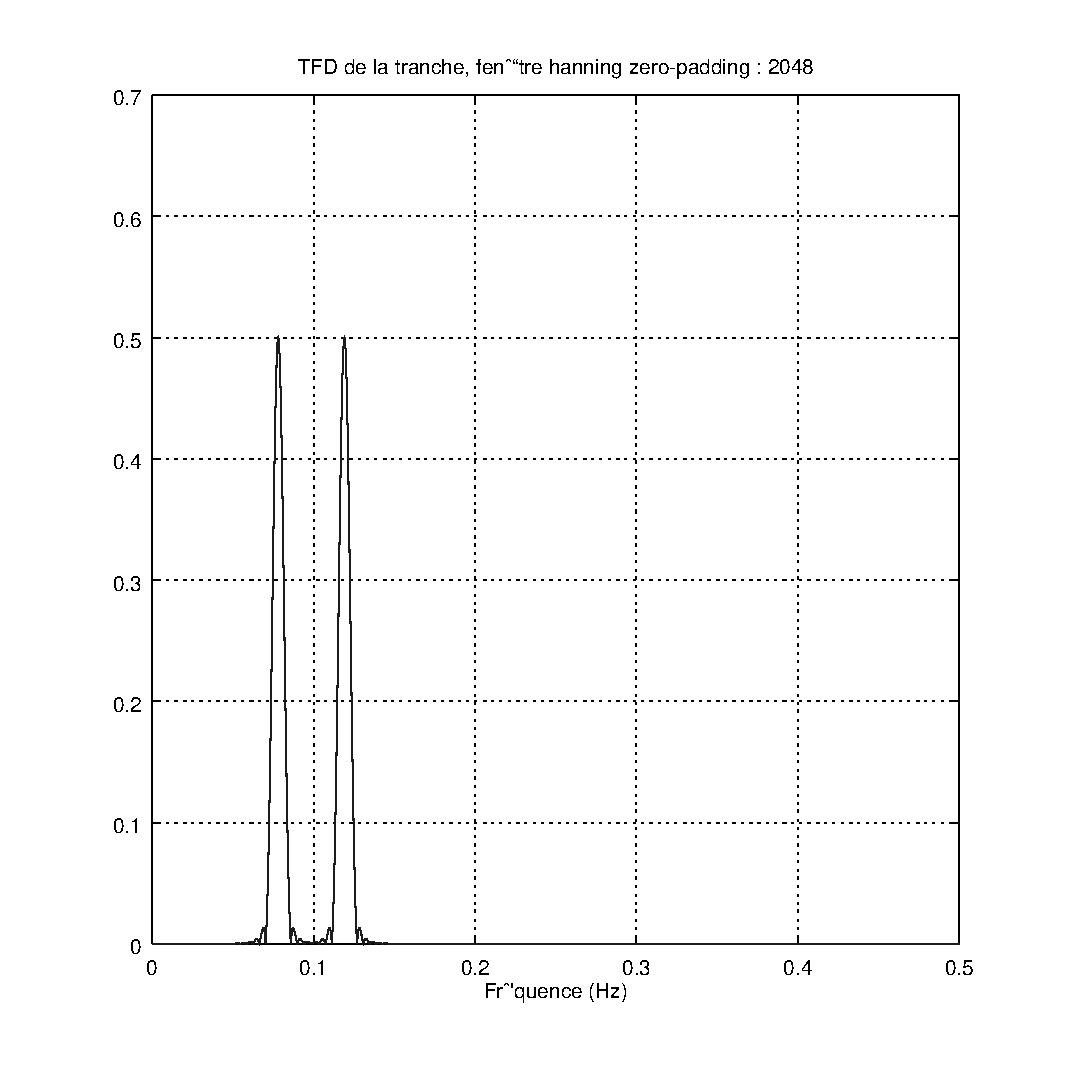
\includegraphics[width=\textwidth]{images/hanning.eps}
  		% Title: glps_renderer figure
% Creator: GL2PS 1.3.8, (C) 1999-2012 C. Geuzaine
% For: Octave
% CreationDate: Wed Nov  8 10:42:42 2017
\begin{pgfpicture}
\pgfsetlinewidth{0.01pt}
\color[rgb]{1.000000,1.000000,1.000000}
\pgfpathmoveto{\pgfpoint{65.000015pt}{104.000000pt}}
\pgflineto{\pgfpoint{452.500031pt}{26.999981pt}}
\pgflineto{\pgfpoint{65.000015pt}{26.999981pt}}
\pgfpathclose
\pgfusepath{fill,stroke}
\pgfpathmoveto{\pgfpoint{65.000015pt}{104.000000pt}}
\pgflineto{\pgfpoint{452.500031pt}{104.000000pt}}
\pgflineto{\pgfpoint{452.500031pt}{26.999981pt}}
\pgfpathclose
\pgfusepath{fill,stroke}
\color[rgb]{0.000000,0.000000,0.000000}
\pgfsetlinewidth{0.500000pt}
\pgfsetdash{{16pt}{0pt}}{0pt}
\pgfpathmoveto{\pgfpoint{452.500031pt}{26.999981pt}}
\pgflineto{\pgfpoint{65.000015pt}{26.999981pt}}
\pgfusepath{stroke}
\pgfpathmoveto{\pgfpoint{452.500031pt}{104.000000pt}}
\pgflineto{\pgfpoint{65.000015pt}{104.000000pt}}
\pgfusepath{stroke}
\pgfpathmoveto{\pgfpoint{65.000015pt}{104.000000pt}}
\pgflineto{\pgfpoint{65.000015pt}{26.999981pt}}
\pgfusepath{stroke}
\pgfpathmoveto{\pgfpoint{452.500031pt}{104.000000pt}}
\pgflineto{\pgfpoint{452.500031pt}{26.999981pt}}
\pgfusepath{stroke}
\pgfsetdash{{0pt}{3pt}{1pt}{3pt}{1pt}{3pt}{1pt}{3pt}{1pt}{0pt}}{0pt}
\pgfpathmoveto{\pgfpoint{65.000015pt}{104.000000pt}}
\pgflineto{\pgfpoint{65.000015pt}{26.999981pt}}
\pgfusepath{stroke}
\pgfpathmoveto{\pgfpoint{142.500031pt}{104.000000pt}}
\pgflineto{\pgfpoint{142.500031pt}{26.999981pt}}
\pgfusepath{stroke}
\pgfpathmoveto{\pgfpoint{220.000031pt}{104.000000pt}}
\pgflineto{\pgfpoint{220.000031pt}{26.999981pt}}
\pgfusepath{stroke}
\pgfpathmoveto{\pgfpoint{297.500031pt}{104.000000pt}}
\pgflineto{\pgfpoint{297.500031pt}{26.999981pt}}
\pgfusepath{stroke}
\pgfpathmoveto{\pgfpoint{375.000061pt}{104.000000pt}}
\pgflineto{\pgfpoint{375.000061pt}{26.999981pt}}
\pgfusepath{stroke}
\pgfpathmoveto{\pgfpoint{452.500031pt}{104.000000pt}}
\pgflineto{\pgfpoint{452.500031pt}{26.999981pt}}
\pgfusepath{stroke}
\pgfsetdash{{16pt}{0pt}}{0pt}
\pgfpathmoveto{\pgfpoint{65.000015pt}{30.874983pt}}
\pgflineto{\pgfpoint{65.000015pt}{26.999981pt}}
\pgfusepath{stroke}
\pgfpathmoveto{\pgfpoint{65.000015pt}{100.125008pt}}
\pgflineto{\pgfpoint{65.000015pt}{104.000000pt}}
\pgfusepath{stroke}
\pgfpathmoveto{\pgfpoint{142.500031pt}{30.874983pt}}
\pgflineto{\pgfpoint{142.500031pt}{26.999981pt}}
\pgfusepath{stroke}
\pgfpathmoveto{\pgfpoint{142.500031pt}{100.125008pt}}
\pgflineto{\pgfpoint{142.500031pt}{104.000000pt}}
\pgfusepath{stroke}
\pgfpathmoveto{\pgfpoint{220.000031pt}{30.874983pt}}
\pgflineto{\pgfpoint{220.000031pt}{26.999981pt}}
\pgfusepath{stroke}
\pgfpathmoveto{\pgfpoint{220.000031pt}{100.125008pt}}
\pgflineto{\pgfpoint{220.000031pt}{104.000000pt}}
\pgfusepath{stroke}
\pgfpathmoveto{\pgfpoint{297.500031pt}{30.874983pt}}
\pgflineto{\pgfpoint{297.500031pt}{26.999981pt}}
\pgfusepath{stroke}
\pgfpathmoveto{\pgfpoint{297.500031pt}{100.125008pt}}
\pgflineto{\pgfpoint{297.500031pt}{104.000000pt}}
\pgfusepath{stroke}
\pgfpathmoveto{\pgfpoint{375.000061pt}{30.874983pt}}
\pgflineto{\pgfpoint{375.000061pt}{26.999981pt}}
\pgfusepath{stroke}
\pgfpathmoveto{\pgfpoint{375.000061pt}{100.125008pt}}
\pgflineto{\pgfpoint{375.000061pt}{104.000000pt}}
\pgfusepath{stroke}
\pgfpathmoveto{\pgfpoint{452.500031pt}{30.874983pt}}
\pgflineto{\pgfpoint{452.500031pt}{26.999981pt}}
\pgfusepath{stroke}
\pgfpathmoveto{\pgfpoint{452.500031pt}{100.125008pt}}
\pgflineto{\pgfpoint{452.500031pt}{104.000000pt}}
\pgfusepath{stroke}
{
\pgftransformshift{\pgfpoint{65.000015pt}{21.999977pt}}
\pgfnode{rectangle}{north}{\fontsize{10}{0}\selectfont\textcolor[rgb]{0,0,0}{{0}}}{}{\pgfusepath{discard}}}
{
\pgftransformshift{\pgfpoint{142.500015pt}{21.999977pt}}
\pgfnode{rectangle}{north}{\fontsize{10}{0}\selectfont\textcolor[rgb]{0,0,0}{{0.1}}}{}{\pgfusepath{discard}}}
{
\pgftransformshift{\pgfpoint{220.000015pt}{21.999977pt}}
\pgfnode{rectangle}{north}{\fontsize{10}{0}\selectfont\textcolor[rgb]{0,0,0}{{0.2}}}{}{\pgfusepath{discard}}}
{
\pgftransformshift{\pgfpoint{297.500031pt}{21.999977pt}}
\pgfnode{rectangle}{north}{\fontsize{10}{0}\selectfont\textcolor[rgb]{0,0,0}{{0.3}}}{}{\pgfusepath{discard}}}
{
\pgftransformshift{\pgfpoint{375.000031pt}{21.999977pt}}
\pgfnode{rectangle}{north}{\fontsize{10}{0}\selectfont\textcolor[rgb]{0,0,0}{{0.4}}}{}{\pgfusepath{discard}}}
{
\pgftransformshift{\pgfpoint{452.500031pt}{21.999977pt}}
\pgfnode{rectangle}{north}{\fontsize{10}{0}\selectfont\textcolor[rgb]{0,0,0}{{0.5}}}{}{\pgfusepath{discard}}}
\pgfsetdash{{0pt}{3pt}{1pt}{3pt}{1pt}{3pt}{1pt}{3pt}{1pt}{0pt}}{0pt}
\pgfpathmoveto{\pgfpoint{452.500031pt}{26.999981pt}}
\pgflineto{\pgfpoint{65.000015pt}{26.999981pt}}
\pgfusepath{stroke}
\pgfpathmoveto{\pgfpoint{452.500031pt}{37.999985pt}}
\pgflineto{\pgfpoint{65.000015pt}{37.999985pt}}
\pgfusepath{stroke}
\pgfpathmoveto{\pgfpoint{452.500031pt}{48.999989pt}}
\pgflineto{\pgfpoint{65.000015pt}{48.999989pt}}
\pgfusepath{stroke}
\pgfpathmoveto{\pgfpoint{452.500031pt}{59.999992pt}}
\pgflineto{\pgfpoint{65.000015pt}{59.999992pt}}
\pgfusepath{stroke}
\pgfpathmoveto{\pgfpoint{452.500031pt}{70.999992pt}}
\pgflineto{\pgfpoint{65.000015pt}{70.999992pt}}
\pgfusepath{stroke}
\pgfpathmoveto{\pgfpoint{452.500031pt}{82.000000pt}}
\pgflineto{\pgfpoint{65.000015pt}{82.000000pt}}
\pgfusepath{stroke}
\pgfpathmoveto{\pgfpoint{452.500031pt}{93.000000pt}}
\pgflineto{\pgfpoint{65.000015pt}{93.000000pt}}
\pgfusepath{stroke}
\pgfpathmoveto{\pgfpoint{452.500031pt}{104.000000pt}}
\pgflineto{\pgfpoint{65.000015pt}{104.000000pt}}
\pgfusepath{stroke}
\pgfsetdash{{16pt}{0pt}}{0pt}
\pgfpathmoveto{\pgfpoint{68.870026pt}{26.999981pt}}
\pgflineto{\pgfpoint{65.000015pt}{26.999981pt}}
\pgfusepath{stroke}
\pgfpathmoveto{\pgfpoint{448.630005pt}{26.999981pt}}
\pgflineto{\pgfpoint{452.500031pt}{26.999981pt}}
\pgfusepath{stroke}
\pgfpathmoveto{\pgfpoint{68.870026pt}{37.999985pt}}
\pgflineto{\pgfpoint{65.000015pt}{37.999985pt}}
\pgfusepath{stroke}
\pgfpathmoveto{\pgfpoint{448.630005pt}{37.999985pt}}
\pgflineto{\pgfpoint{452.500031pt}{37.999985pt}}
\pgfusepath{stroke}
\pgfpathmoveto{\pgfpoint{68.870026pt}{48.999989pt}}
\pgflineto{\pgfpoint{65.000015pt}{48.999989pt}}
\pgfusepath{stroke}
\pgfpathmoveto{\pgfpoint{448.630005pt}{48.999989pt}}
\pgflineto{\pgfpoint{452.500031pt}{48.999989pt}}
\pgfusepath{stroke}
\pgfpathmoveto{\pgfpoint{68.870026pt}{59.999992pt}}
\pgflineto{\pgfpoint{65.000015pt}{59.999992pt}}
\pgfusepath{stroke}
\pgfpathmoveto{\pgfpoint{448.630005pt}{59.999992pt}}
\pgflineto{\pgfpoint{452.500031pt}{59.999992pt}}
\pgfusepath{stroke}
\pgfpathmoveto{\pgfpoint{68.870026pt}{70.999992pt}}
\pgflineto{\pgfpoint{65.000015pt}{70.999992pt}}
\pgfusepath{stroke}
\pgfpathmoveto{\pgfpoint{448.630005pt}{70.999992pt}}
\pgflineto{\pgfpoint{452.500031pt}{70.999992pt}}
\pgfusepath{stroke}
\pgfpathmoveto{\pgfpoint{68.870026pt}{82.000000pt}}
\pgflineto{\pgfpoint{65.000015pt}{82.000000pt}}
\pgfusepath{stroke}
\pgfpathmoveto{\pgfpoint{448.630005pt}{82.000000pt}}
\pgflineto{\pgfpoint{452.500031pt}{82.000000pt}}
\pgfusepath{stroke}
\pgfpathmoveto{\pgfpoint{68.870026pt}{93.000000pt}}
\pgflineto{\pgfpoint{65.000015pt}{93.000000pt}}
\pgfusepath{stroke}
\pgfpathmoveto{\pgfpoint{448.630005pt}{93.000000pt}}
\pgflineto{\pgfpoint{452.500031pt}{93.000000pt}}
\pgfusepath{stroke}
\pgfpathmoveto{\pgfpoint{68.870026pt}{104.000000pt}}
\pgflineto{\pgfpoint{65.000015pt}{104.000000pt}}
\pgfusepath{stroke}
\pgfpathmoveto{\pgfpoint{448.630005pt}{104.000000pt}}
\pgflineto{\pgfpoint{452.500031pt}{104.000000pt}}
\pgfusepath{stroke}
{
\pgftransformshift{\pgfpoint{60.006454pt}{26.999981pt}}
\pgfnode{rectangle}{east}{\fontsize{10}{0}\selectfont\textcolor[rgb]{0,0,0}{{0}}}{}{\pgfusepath{discard}}}
{
\pgftransformshift{\pgfpoint{60.006454pt}{37.999985pt}}
\pgfnode{rectangle}{east}{\fontsize{10}{0}\selectfont\textcolor[rgb]{0,0,0}{{0.1}}}{}{\pgfusepath{discard}}}
{
\pgftransformshift{\pgfpoint{60.006454pt}{48.999989pt}}
\pgfnode{rectangle}{east}{\fontsize{10}{0}\selectfont\textcolor[rgb]{0,0,0}{{0.2}}}{}{\pgfusepath{discard}}}
{
\pgftransformshift{\pgfpoint{60.006454pt}{59.999992pt}}
\pgfnode{rectangle}{east}{\fontsize{10}{0}\selectfont\textcolor[rgb]{0,0,0}{{0.3}}}{}{\pgfusepath{discard}}}
{
\pgftransformshift{\pgfpoint{60.006454pt}{70.999992pt}}
\pgfnode{rectangle}{east}{\fontsize{10}{0}\selectfont\textcolor[rgb]{0,0,0}{{0.4}}}{}{\pgfusepath{discard}}}
{
\pgftransformshift{\pgfpoint{60.006454pt}{82.000000pt}}
\pgfnode{rectangle}{east}{\fontsize{10}{0}\selectfont\textcolor[rgb]{0,0,0}{{0.5}}}{}{\pgfusepath{discard}}}
{
\pgftransformshift{\pgfpoint{60.006454pt}{93.000000pt}}
\pgfnode{rectangle}{east}{\fontsize{10}{0}\selectfont\textcolor[rgb]{0,0,0}{{0.6}}}{}{\pgfusepath{discard}}}
{
\pgftransformshift{\pgfpoint{60.006454pt}{104.000000pt}}
\pgfnode{rectangle}{east}{\fontsize{10}{0}\selectfont\textcolor[rgb]{0,0,0}{{0.7}}}{}{\pgfusepath{discard}}}
{
\pgftransformshift{\pgfpoint{258.750031pt}{10.999977pt}}
\pgfnode{rectangle}{north}{\fontsize{10}{0}\selectfont\textcolor[rgb]{0,0,0}{{Fréquence (Hz)}}}{}{\pgfusepath{discard}}}
\color[rgb]{0.000000,0.000000,1.000000}
\pgfsetdash{}{0pt}
\pgfpathmoveto{\pgfpoint{65.189224pt}{27.001183pt}}
\pgflineto{\pgfpoint{65.000015pt}{27.001171pt}}
\pgfusepath{stroke}
\pgfpathmoveto{\pgfpoint{65.378433pt}{27.001213pt}}
\pgflineto{\pgfpoint{65.189224pt}{27.001183pt}}
\pgfusepath{stroke}
\pgfpathmoveto{\pgfpoint{65.567642pt}{27.001251pt}}
\pgflineto{\pgfpoint{65.378433pt}{27.001213pt}}
\pgfusepath{stroke}
\pgfpathmoveto{\pgfpoint{65.756836pt}{27.001293pt}}
\pgflineto{\pgfpoint{65.567642pt}{27.001251pt}}
\pgfusepath{stroke}
\pgfpathmoveto{\pgfpoint{65.946060pt}{27.001320pt}}
\pgflineto{\pgfpoint{65.756836pt}{27.001293pt}}
\pgfusepath{stroke}
\pgfpathmoveto{\pgfpoint{66.135269pt}{27.001335pt}}
\pgflineto{\pgfpoint{65.946060pt}{27.001320pt}}
\pgfusepath{stroke}
\pgfpathmoveto{\pgfpoint{66.324478pt}{27.001328pt}}
\pgflineto{\pgfpoint{66.135269pt}{27.001335pt}}
\pgfusepath{stroke}
\pgfpathmoveto{\pgfpoint{66.513687pt}{27.001297pt}}
\pgflineto{\pgfpoint{66.324478pt}{27.001328pt}}
\pgfusepath{stroke}
\pgfpathmoveto{\pgfpoint{66.702881pt}{27.001244pt}}
\pgflineto{\pgfpoint{66.513687pt}{27.001297pt}}
\pgfusepath{stroke}
\pgfpathmoveto{\pgfpoint{66.892105pt}{27.001175pt}}
\pgflineto{\pgfpoint{66.702881pt}{27.001244pt}}
\pgfusepath{stroke}
\pgfpathmoveto{\pgfpoint{67.081314pt}{27.001102pt}}
\pgflineto{\pgfpoint{66.892105pt}{27.001175pt}}
\pgfusepath{stroke}
\pgfpathmoveto{\pgfpoint{67.270523pt}{27.001034pt}}
\pgflineto{\pgfpoint{67.081314pt}{27.001102pt}}
\pgfusepath{stroke}
\pgfpathmoveto{\pgfpoint{67.459732pt}{27.000999pt}}
\pgflineto{\pgfpoint{67.270523pt}{27.001034pt}}
\pgfusepath{stroke}
\pgfpathmoveto{\pgfpoint{67.648926pt}{27.001015pt}}
\pgflineto{\pgfpoint{67.459732pt}{27.000999pt}}
\pgfusepath{stroke}
\pgfpathmoveto{\pgfpoint{67.838150pt}{27.001076pt}}
\pgflineto{\pgfpoint{67.648926pt}{27.001015pt}}
\pgfusepath{stroke}
\pgfpathmoveto{\pgfpoint{68.027359pt}{27.001179pt}}
\pgflineto{\pgfpoint{67.838150pt}{27.001076pt}}
\pgfusepath{stroke}
\pgfpathmoveto{\pgfpoint{68.216568pt}{27.001308pt}}
\pgflineto{\pgfpoint{68.027359pt}{27.001179pt}}
\pgfusepath{stroke}
\pgfpathmoveto{\pgfpoint{68.405777pt}{27.001442pt}}
\pgflineto{\pgfpoint{68.216568pt}{27.001308pt}}
\pgfusepath{stroke}
\pgfpathmoveto{\pgfpoint{68.594971pt}{27.001564pt}}
\pgflineto{\pgfpoint{68.405777pt}{27.001442pt}}
\pgfusepath{stroke}
\pgfpathmoveto{\pgfpoint{68.784195pt}{27.001656pt}}
\pgflineto{\pgfpoint{68.594971pt}{27.001564pt}}
\pgfusepath{stroke}
\pgfpathmoveto{\pgfpoint{68.973404pt}{27.001713pt}}
\pgflineto{\pgfpoint{68.784195pt}{27.001656pt}}
\pgfusepath{stroke}
\pgfpathmoveto{\pgfpoint{69.162613pt}{27.001728pt}}
\pgflineto{\pgfpoint{68.973404pt}{27.001713pt}}
\pgfusepath{stroke}
\pgfpathmoveto{\pgfpoint{69.351822pt}{27.001694pt}}
\pgflineto{\pgfpoint{69.162613pt}{27.001728pt}}
\pgfusepath{stroke}
\pgfpathmoveto{\pgfpoint{69.541016pt}{27.001614pt}}
\pgflineto{\pgfpoint{69.351822pt}{27.001694pt}}
\pgfusepath{stroke}
\pgfpathmoveto{\pgfpoint{69.730240pt}{27.001484pt}}
\pgflineto{\pgfpoint{69.541016pt}{27.001614pt}}
\pgfusepath{stroke}
\pgfpathmoveto{\pgfpoint{69.919449pt}{27.001320pt}}
\pgflineto{\pgfpoint{69.730240pt}{27.001484pt}}
\pgfusepath{stroke}
\pgfpathmoveto{\pgfpoint{70.108658pt}{27.001141pt}}
\pgflineto{\pgfpoint{69.919449pt}{27.001320pt}}
\pgfusepath{stroke}
\pgfpathmoveto{\pgfpoint{70.297867pt}{27.000965pt}}
\pgflineto{\pgfpoint{70.108658pt}{27.001141pt}}
\pgfusepath{stroke}
\pgfpathmoveto{\pgfpoint{70.487061pt}{27.000847pt}}
\pgflineto{\pgfpoint{70.297867pt}{27.000965pt}}
\pgfusepath{stroke}
\pgfpathmoveto{\pgfpoint{70.676285pt}{27.000851pt}}
\pgflineto{\pgfpoint{70.487061pt}{27.000847pt}}
\pgfusepath{stroke}
\pgfpathmoveto{\pgfpoint{70.865494pt}{27.000984pt}}
\pgflineto{\pgfpoint{70.676285pt}{27.000851pt}}
\pgfusepath{stroke}
\pgfpathmoveto{\pgfpoint{71.054703pt}{27.001205pt}}
\pgflineto{\pgfpoint{70.865494pt}{27.000984pt}}
\pgfusepath{stroke}
\pgfpathmoveto{\pgfpoint{71.243912pt}{27.001461pt}}
\pgflineto{\pgfpoint{71.054703pt}{27.001205pt}}
\pgfusepath{stroke}
\pgfpathmoveto{\pgfpoint{71.433105pt}{27.001709pt}}
\pgflineto{\pgfpoint{71.243912pt}{27.001461pt}}
\pgfusepath{stroke}
\pgfpathmoveto{\pgfpoint{71.622330pt}{27.001934pt}}
\pgflineto{\pgfpoint{71.433105pt}{27.001709pt}}
\pgfusepath{stroke}
\pgfpathmoveto{\pgfpoint{71.811539pt}{27.002106pt}}
\pgflineto{\pgfpoint{71.622330pt}{27.001934pt}}
\pgfusepath{stroke}
\pgfpathmoveto{\pgfpoint{72.000748pt}{27.002228pt}}
\pgflineto{\pgfpoint{71.811539pt}{27.002106pt}}
\pgfusepath{stroke}
\pgfpathmoveto{\pgfpoint{72.189957pt}{27.002274pt}}
\pgflineto{\pgfpoint{72.000748pt}{27.002228pt}}
\pgfusepath{stroke}
\pgfpathmoveto{\pgfpoint{72.379150pt}{27.002254pt}}
\pgflineto{\pgfpoint{72.189957pt}{27.002274pt}}
\pgfusepath{stroke}
\pgfpathmoveto{\pgfpoint{72.568375pt}{27.002151pt}}
\pgflineto{\pgfpoint{72.379150pt}{27.002254pt}}
\pgfusepath{stroke}
\pgfpathmoveto{\pgfpoint{72.757584pt}{27.001980pt}}
\pgflineto{\pgfpoint{72.568375pt}{27.002151pt}}
\pgfusepath{stroke}
\pgfpathmoveto{\pgfpoint{72.946793pt}{27.001740pt}}
\pgflineto{\pgfpoint{72.757584pt}{27.001980pt}}
\pgfusepath{stroke}
\pgfpathmoveto{\pgfpoint{73.136002pt}{27.001450pt}}
\pgflineto{\pgfpoint{72.946793pt}{27.001740pt}}
\pgfusepath{stroke}
\pgfpathmoveto{\pgfpoint{73.325195pt}{27.001133pt}}
\pgflineto{\pgfpoint{73.136002pt}{27.001450pt}}
\pgfusepath{stroke}
\pgfpathmoveto{\pgfpoint{73.514420pt}{27.000851pt}}
\pgflineto{\pgfpoint{73.325195pt}{27.001133pt}}
\pgfusepath{stroke}
\pgfpathmoveto{\pgfpoint{73.703629pt}{27.000740pt}}
\pgflineto{\pgfpoint{73.514420pt}{27.000851pt}}
\pgfusepath{stroke}
\pgfpathmoveto{\pgfpoint{73.892838pt}{27.000908pt}}
\pgflineto{\pgfpoint{73.703629pt}{27.000740pt}}
\pgfusepath{stroke}
\pgfpathmoveto{\pgfpoint{74.082047pt}{27.001247pt}}
\pgflineto{\pgfpoint{73.892838pt}{27.000908pt}}
\pgfusepath{stroke}
\pgfpathmoveto{\pgfpoint{74.271240pt}{27.001640pt}}
\pgflineto{\pgfpoint{74.082047pt}{27.001247pt}}
\pgfusepath{stroke}
\pgfpathmoveto{\pgfpoint{74.460464pt}{27.002029pt}}
\pgflineto{\pgfpoint{74.271240pt}{27.001640pt}}
\pgfusepath{stroke}
\pgfpathmoveto{\pgfpoint{74.649673pt}{27.002373pt}}
\pgflineto{\pgfpoint{74.460464pt}{27.002029pt}}
\pgfusepath{stroke}
\pgfpathmoveto{\pgfpoint{74.838882pt}{27.002655pt}}
\pgflineto{\pgfpoint{74.649673pt}{27.002373pt}}
\pgfusepath{stroke}
\pgfpathmoveto{\pgfpoint{75.028091pt}{27.002857pt}}
\pgflineto{\pgfpoint{74.838882pt}{27.002655pt}}
\pgfusepath{stroke}
\pgfpathmoveto{\pgfpoint{75.217285pt}{27.002960pt}}
\pgflineto{\pgfpoint{75.028091pt}{27.002857pt}}
\pgfusepath{stroke}
\pgfpathmoveto{\pgfpoint{75.406509pt}{27.002968pt}}
\pgflineto{\pgfpoint{75.217285pt}{27.002960pt}}
\pgfusepath{stroke}
\pgfpathmoveto{\pgfpoint{75.595718pt}{27.002869pt}}
\pgflineto{\pgfpoint{75.406509pt}{27.002968pt}}
\pgfusepath{stroke}
\pgfpathmoveto{\pgfpoint{75.784927pt}{27.002663pt}}
\pgflineto{\pgfpoint{75.595718pt}{27.002869pt}}
\pgfusepath{stroke}
\pgfpathmoveto{\pgfpoint{75.974136pt}{27.002357pt}}
\pgflineto{\pgfpoint{75.784927pt}{27.002663pt}}
\pgfusepath{stroke}
\pgfpathmoveto{\pgfpoint{76.163330pt}{27.001968pt}}
\pgflineto{\pgfpoint{75.974136pt}{27.002357pt}}
\pgfusepath{stroke}
\pgfpathmoveto{\pgfpoint{76.352554pt}{27.001514pt}}
\pgflineto{\pgfpoint{76.163330pt}{27.001968pt}}
\pgfusepath{stroke}
\pgfpathmoveto{\pgfpoint{76.541763pt}{27.001049pt}}
\pgflineto{\pgfpoint{76.352554pt}{27.001514pt}}
\pgfusepath{stroke}
\pgfpathmoveto{\pgfpoint{76.730972pt}{27.000721pt}}
\pgflineto{\pgfpoint{76.541763pt}{27.001049pt}}
\pgfusepath{stroke}
\pgfpathmoveto{\pgfpoint{76.920181pt}{27.000839pt}}
\pgflineto{\pgfpoint{76.730972pt}{27.000721pt}}
\pgfusepath{stroke}
\pgfpathmoveto{\pgfpoint{77.109375pt}{27.001308pt}}
\pgflineto{\pgfpoint{76.920181pt}{27.000839pt}}
\pgfusepath{stroke}
\pgfpathmoveto{\pgfpoint{77.298599pt}{27.001865pt}}
\pgflineto{\pgfpoint{77.109375pt}{27.001308pt}}
\pgfusepath{stroke}
\pgfpathmoveto{\pgfpoint{77.487808pt}{27.002415pt}}
\pgflineto{\pgfpoint{77.298599pt}{27.001865pt}}
\pgfusepath{stroke}
\pgfpathmoveto{\pgfpoint{77.677017pt}{27.002907pt}}
\pgflineto{\pgfpoint{77.487808pt}{27.002415pt}}
\pgfusepath{stroke}
\pgfpathmoveto{\pgfpoint{77.866226pt}{27.003319pt}}
\pgflineto{\pgfpoint{77.677017pt}{27.002907pt}}
\pgfusepath{stroke}
\pgfpathmoveto{\pgfpoint{78.055420pt}{27.003624pt}}
\pgflineto{\pgfpoint{77.866226pt}{27.003319pt}}
\pgfusepath{stroke}
\pgfpathmoveto{\pgfpoint{78.244644pt}{27.003811pt}}
\pgflineto{\pgfpoint{78.055420pt}{27.003624pt}}
\pgfusepath{stroke}
\pgfpathmoveto{\pgfpoint{78.433853pt}{27.003857pt}}
\pgflineto{\pgfpoint{78.244644pt}{27.003811pt}}
\pgfusepath{stroke}
\pgfpathmoveto{\pgfpoint{78.623062pt}{27.003769pt}}
\pgflineto{\pgfpoint{78.433853pt}{27.003857pt}}
\pgfusepath{stroke}
\pgfpathmoveto{\pgfpoint{78.812271pt}{27.003536pt}}
\pgflineto{\pgfpoint{78.623062pt}{27.003769pt}}
\pgfusepath{stroke}
\pgfpathmoveto{\pgfpoint{79.001465pt}{27.003170pt}}
\pgflineto{\pgfpoint{78.812271pt}{27.003536pt}}
\pgfusepath{stroke}
\pgfpathmoveto{\pgfpoint{79.190689pt}{27.002678pt}}
\pgflineto{\pgfpoint{79.001465pt}{27.003170pt}}
\pgfusepath{stroke}
\pgfpathmoveto{\pgfpoint{79.379898pt}{27.002087pt}}
\pgflineto{\pgfpoint{79.190689pt}{27.002678pt}}
\pgfusepath{stroke}
\pgfpathmoveto{\pgfpoint{79.569107pt}{27.001431pt}}
\pgflineto{\pgfpoint{79.379898pt}{27.002087pt}}
\pgfusepath{stroke}
\pgfpathmoveto{\pgfpoint{79.758316pt}{27.000835pt}}
\pgflineto{\pgfpoint{79.569107pt}{27.001431pt}}
\pgfusepath{stroke}
\pgfpathmoveto{\pgfpoint{79.947510pt}{27.000790pt}}
\pgflineto{\pgfpoint{79.758316pt}{27.000835pt}}
\pgfusepath{stroke}
\pgfpathmoveto{\pgfpoint{80.136734pt}{27.001389pt}}
\pgflineto{\pgfpoint{79.947510pt}{27.000790pt}}
\pgfusepath{stroke}
\pgfpathmoveto{\pgfpoint{80.325943pt}{27.002144pt}}
\pgflineto{\pgfpoint{80.136734pt}{27.001389pt}}
\pgfusepath{stroke}
\pgfpathmoveto{\pgfpoint{80.515152pt}{27.002892pt}}
\pgflineto{\pgfpoint{80.325943pt}{27.002144pt}}
\pgfusepath{stroke}
\pgfpathmoveto{\pgfpoint{80.704361pt}{27.003567pt}}
\pgflineto{\pgfpoint{80.515152pt}{27.002892pt}}
\pgfusepath{stroke}
\pgfpathmoveto{\pgfpoint{80.893570pt}{27.004143pt}}
\pgflineto{\pgfpoint{80.704361pt}{27.003567pt}}
\pgfusepath{stroke}
\pgfpathmoveto{\pgfpoint{81.082779pt}{27.004581pt}}
\pgflineto{\pgfpoint{80.893570pt}{27.004143pt}}
\pgfusepath{stroke}
\pgfpathmoveto{\pgfpoint{81.271988pt}{27.004868pt}}
\pgflineto{\pgfpoint{81.082779pt}{27.004581pt}}
\pgfusepath{stroke}
\pgfpathmoveto{\pgfpoint{81.461197pt}{27.004978pt}}
\pgflineto{\pgfpoint{81.271988pt}{27.004868pt}}
\pgfusepath{stroke}
\pgfpathmoveto{\pgfpoint{81.650406pt}{27.004906pt}}
\pgflineto{\pgfpoint{81.461197pt}{27.004978pt}}
\pgfusepath{stroke}
\pgfpathmoveto{\pgfpoint{81.839615pt}{27.004646pt}}
\pgflineto{\pgfpoint{81.650406pt}{27.004906pt}}
\pgfusepath{stroke}
\pgfpathmoveto{\pgfpoint{82.028824pt}{27.004208pt}}
\pgflineto{\pgfpoint{81.839615pt}{27.004646pt}}
\pgfusepath{stroke}
\pgfpathmoveto{\pgfpoint{82.218033pt}{27.003601pt}}
\pgflineto{\pgfpoint{82.028824pt}{27.004208pt}}
\pgfusepath{stroke}
\pgfpathmoveto{\pgfpoint{82.407242pt}{27.002850pt}}
\pgflineto{\pgfpoint{82.218033pt}{27.003601pt}}
\pgfusepath{stroke}
\pgfpathmoveto{\pgfpoint{82.596451pt}{27.001984pt}}
\pgflineto{\pgfpoint{82.407242pt}{27.002850pt}}
\pgfusepath{stroke}
\pgfpathmoveto{\pgfpoint{82.785660pt}{27.001118pt}}
\pgflineto{\pgfpoint{82.596451pt}{27.001984pt}}
\pgfusepath{stroke}
\pgfpathmoveto{\pgfpoint{82.974869pt}{27.000759pt}}
\pgflineto{\pgfpoint{82.785660pt}{27.001118pt}}
\pgfusepath{stroke}
\pgfpathmoveto{\pgfpoint{83.164078pt}{27.001495pt}}
\pgflineto{\pgfpoint{82.974869pt}{27.000759pt}}
\pgfusepath{stroke}
\pgfpathmoveto{\pgfpoint{83.353287pt}{27.002495pt}}
\pgflineto{\pgfpoint{83.164078pt}{27.001495pt}}
\pgfusepath{stroke}
\pgfpathmoveto{\pgfpoint{83.542496pt}{27.003490pt}}
\pgflineto{\pgfpoint{83.353287pt}{27.002495pt}}
\pgfusepath{stroke}
\pgfpathmoveto{\pgfpoint{83.731705pt}{27.004402pt}}
\pgflineto{\pgfpoint{83.542496pt}{27.003490pt}}
\pgfusepath{stroke}
\pgfpathmoveto{\pgfpoint{83.920914pt}{27.005188pt}}
\pgflineto{\pgfpoint{83.731705pt}{27.004402pt}}
\pgfusepath{stroke}
\pgfpathmoveto{\pgfpoint{84.110123pt}{27.005802pt}}
\pgflineto{\pgfpoint{83.920914pt}{27.005188pt}}
\pgfusepath{stroke}
\pgfpathmoveto{\pgfpoint{84.299332pt}{27.006222pt}}
\pgflineto{\pgfpoint{84.110123pt}{27.005802pt}}
\pgfusepath{stroke}
\pgfpathmoveto{\pgfpoint{84.488541pt}{27.006413pt}}
\pgflineto{\pgfpoint{84.299332pt}{27.006222pt}}
\pgfusepath{stroke}
\pgfpathmoveto{\pgfpoint{84.677750pt}{27.006374pt}}
\pgflineto{\pgfpoint{84.488541pt}{27.006413pt}}
\pgfusepath{stroke}
\pgfpathmoveto{\pgfpoint{84.866959pt}{27.006088pt}}
\pgflineto{\pgfpoint{84.677750pt}{27.006374pt}}
\pgfusepath{stroke}
\pgfpathmoveto{\pgfpoint{85.056168pt}{27.005566pt}}
\pgflineto{\pgfpoint{84.866959pt}{27.006088pt}}
\pgfusepath{stroke}
\pgfpathmoveto{\pgfpoint{85.245377pt}{27.004810pt}}
\pgflineto{\pgfpoint{85.056168pt}{27.005566pt}}
\pgfusepath{stroke}
\pgfpathmoveto{\pgfpoint{85.434586pt}{27.003860pt}}
\pgflineto{\pgfpoint{85.245377pt}{27.004810pt}}
\pgfusepath{stroke}
\pgfpathmoveto{\pgfpoint{85.623795pt}{27.002750pt}}
\pgflineto{\pgfpoint{85.434586pt}{27.003860pt}}
\pgfusepath{stroke}
\pgfpathmoveto{\pgfpoint{85.813004pt}{27.001564pt}}
\pgflineto{\pgfpoint{85.623795pt}{27.002750pt}}
\pgfusepath{stroke}
\pgfpathmoveto{\pgfpoint{86.002213pt}{27.000782pt}}
\pgflineto{\pgfpoint{85.813004pt}{27.001564pt}}
\pgfusepath{stroke}
\pgfpathmoveto{\pgfpoint{86.191422pt}{27.001625pt}}
\pgflineto{\pgfpoint{86.002213pt}{27.000782pt}}
\pgfusepath{stroke}
\pgfpathmoveto{\pgfpoint{86.380630pt}{27.002949pt}}
\pgflineto{\pgfpoint{86.191422pt}{27.001625pt}}
\pgfusepath{stroke}
\pgfpathmoveto{\pgfpoint{86.569839pt}{27.004269pt}}
\pgflineto{\pgfpoint{86.380630pt}{27.002949pt}}
\pgfusepath{stroke}
\pgfpathmoveto{\pgfpoint{86.759048pt}{27.005489pt}}
\pgflineto{\pgfpoint{86.569839pt}{27.004269pt}}
\pgfusepath{stroke}
\pgfpathmoveto{\pgfpoint{86.948257pt}{27.006550pt}}
\pgflineto{\pgfpoint{86.759048pt}{27.005489pt}}
\pgfusepath{stroke}
\pgfpathmoveto{\pgfpoint{87.137466pt}{27.007401pt}}
\pgflineto{\pgfpoint{86.948257pt}{27.006550pt}}
\pgfusepath{stroke}
\pgfpathmoveto{\pgfpoint{87.326675pt}{27.007996pt}}
\pgflineto{\pgfpoint{87.137466pt}{27.007401pt}}
\pgfusepath{stroke}
\pgfpathmoveto{\pgfpoint{87.515884pt}{27.008308pt}}
\pgflineto{\pgfpoint{87.326675pt}{27.007996pt}}
\pgfusepath{stroke}
\pgfpathmoveto{\pgfpoint{87.705093pt}{27.008312pt}}
\pgflineto{\pgfpoint{87.515884pt}{27.008308pt}}
\pgfusepath{stroke}
\pgfpathmoveto{\pgfpoint{87.894302pt}{27.007999pt}}
\pgflineto{\pgfpoint{87.705093pt}{27.008312pt}}
\pgfusepath{stroke}
\pgfpathmoveto{\pgfpoint{88.083511pt}{27.007370pt}}
\pgflineto{\pgfpoint{87.894302pt}{27.007999pt}}
\pgfusepath{stroke}
\pgfpathmoveto{\pgfpoint{88.272720pt}{27.006439pt}}
\pgflineto{\pgfpoint{88.083511pt}{27.007370pt}}
\pgfusepath{stroke}
\pgfpathmoveto{\pgfpoint{88.461929pt}{27.005238pt}}
\pgflineto{\pgfpoint{88.272720pt}{27.006439pt}}
\pgfusepath{stroke}
\pgfpathmoveto{\pgfpoint{88.651138pt}{27.003803pt}}
\pgflineto{\pgfpoint{88.461929pt}{27.005238pt}}
\pgfusepath{stroke}
\pgfpathmoveto{\pgfpoint{88.840347pt}{27.002228pt}}
\pgflineto{\pgfpoint{88.651138pt}{27.003803pt}}
\pgfusepath{stroke}
\pgfpathmoveto{\pgfpoint{89.029556pt}{27.000900pt}}
\pgflineto{\pgfpoint{88.840347pt}{27.002228pt}}
\pgfusepath{stroke}
\pgfpathmoveto{\pgfpoint{89.218765pt}{27.001789pt}}
\pgflineto{\pgfpoint{89.029556pt}{27.000900pt}}
\pgfusepath{stroke}
\pgfpathmoveto{\pgfpoint{89.407974pt}{27.003540pt}}
\pgflineto{\pgfpoint{89.218765pt}{27.001789pt}}
\pgfusepath{stroke}
\pgfpathmoveto{\pgfpoint{89.597183pt}{27.005302pt}}
\pgflineto{\pgfpoint{89.407974pt}{27.003540pt}}
\pgfusepath{stroke}
\pgfpathmoveto{\pgfpoint{89.786392pt}{27.006947pt}}
\pgflineto{\pgfpoint{89.597183pt}{27.005302pt}}
\pgfusepath{stroke}
\pgfpathmoveto{\pgfpoint{89.975601pt}{27.008385pt}}
\pgflineto{\pgfpoint{89.786392pt}{27.006947pt}}
\pgfusepath{stroke}
\pgfpathmoveto{\pgfpoint{90.164810pt}{27.009560pt}}
\pgflineto{\pgfpoint{89.975601pt}{27.008385pt}}
\pgfusepath{stroke}
\pgfpathmoveto{\pgfpoint{90.354019pt}{27.010403pt}}
\pgflineto{\pgfpoint{90.164810pt}{27.009560pt}}
\pgfusepath{stroke}
\pgfpathmoveto{\pgfpoint{90.543228pt}{27.010880pt}}
\pgflineto{\pgfpoint{90.354019pt}{27.010403pt}}
\pgfusepath{stroke}
\pgfpathmoveto{\pgfpoint{90.732437pt}{27.010960pt}}
\pgflineto{\pgfpoint{90.543228pt}{27.010880pt}}
\pgfusepath{stroke}
\pgfpathmoveto{\pgfpoint{90.921646pt}{27.010616pt}}
\pgflineto{\pgfpoint{90.732437pt}{27.010960pt}}
\pgfusepath{stroke}
\pgfpathmoveto{\pgfpoint{91.110855pt}{27.009853pt}}
\pgflineto{\pgfpoint{90.921646pt}{27.010616pt}}
\pgfusepath{stroke}
\pgfpathmoveto{\pgfpoint{91.300064pt}{27.008682pt}}
\pgflineto{\pgfpoint{91.110855pt}{27.009853pt}}
\pgfusepath{stroke}
\pgfpathmoveto{\pgfpoint{91.489273pt}{27.007141pt}}
\pgflineto{\pgfpoint{91.300064pt}{27.008682pt}}
\pgfusepath{stroke}
\pgfpathmoveto{\pgfpoint{91.678482pt}{27.005280pt}}
\pgflineto{\pgfpoint{91.489273pt}{27.007141pt}}
\pgfusepath{stroke}
\pgfpathmoveto{\pgfpoint{91.867691pt}{27.003189pt}}
\pgflineto{\pgfpoint{91.678482pt}{27.005280pt}}
\pgfusepath{stroke}
\pgfpathmoveto{\pgfpoint{92.056900pt}{27.001183pt}}
\pgflineto{\pgfpoint{91.867691pt}{27.003189pt}}
\pgfusepath{stroke}
\pgfpathmoveto{\pgfpoint{92.246109pt}{27.001995pt}}
\pgflineto{\pgfpoint{92.056900pt}{27.001183pt}}
\pgfusepath{stroke}
\pgfpathmoveto{\pgfpoint{92.435318pt}{27.004341pt}}
\pgflineto{\pgfpoint{92.246109pt}{27.001995pt}}
\pgfusepath{stroke}
\pgfpathmoveto{\pgfpoint{92.624527pt}{27.006718pt}}
\pgflineto{\pgfpoint{92.435318pt}{27.004341pt}}
\pgfusepath{stroke}
\pgfpathmoveto{\pgfpoint{92.813736pt}{27.008949pt}}
\pgflineto{\pgfpoint{92.624527pt}{27.006718pt}}
\pgfusepath{stroke}
\pgfpathmoveto{\pgfpoint{93.002945pt}{27.010925pt}}
\pgflineto{\pgfpoint{92.813736pt}{27.008949pt}}
\pgfusepath{stroke}
\pgfpathmoveto{\pgfpoint{93.192154pt}{27.012558pt}}
\pgflineto{\pgfpoint{93.002945pt}{27.010925pt}}
\pgfusepath{stroke}
\pgfpathmoveto{\pgfpoint{93.381363pt}{27.013767pt}}
\pgflineto{\pgfpoint{93.192154pt}{27.012558pt}}
\pgfusepath{stroke}
\pgfpathmoveto{\pgfpoint{93.570572pt}{27.014492pt}}
\pgflineto{\pgfpoint{93.381363pt}{27.013767pt}}
\pgfusepath{stroke}
\pgfpathmoveto{\pgfpoint{93.759781pt}{27.014679pt}}
\pgflineto{\pgfpoint{93.570572pt}{27.014492pt}}
\pgfusepath{stroke}
\pgfpathmoveto{\pgfpoint{93.948990pt}{27.014309pt}}
\pgflineto{\pgfpoint{93.759781pt}{27.014679pt}}
\pgfusepath{stroke}
\pgfpathmoveto{\pgfpoint{94.138199pt}{27.013371pt}}
\pgflineto{\pgfpoint{93.948990pt}{27.014309pt}}
\pgfusepath{stroke}
\pgfpathmoveto{\pgfpoint{94.327408pt}{27.011879pt}}
\pgflineto{\pgfpoint{94.138199pt}{27.013371pt}}
\pgfusepath{stroke}
\pgfpathmoveto{\pgfpoint{94.516617pt}{27.009876pt}}
\pgflineto{\pgfpoint{94.327408pt}{27.011879pt}}
\pgfusepath{stroke}
\pgfpathmoveto{\pgfpoint{94.705826pt}{27.007420pt}}
\pgflineto{\pgfpoint{94.516617pt}{27.009876pt}}
\pgfusepath{stroke}
\pgfpathmoveto{\pgfpoint{94.895035pt}{27.004612pt}}
\pgflineto{\pgfpoint{94.705826pt}{27.007420pt}}
\pgfusepath{stroke}
\pgfpathmoveto{\pgfpoint{95.084244pt}{27.001724pt}}
\pgflineto{\pgfpoint{94.895035pt}{27.004612pt}}
\pgfusepath{stroke}
\pgfpathmoveto{\pgfpoint{95.273453pt}{27.002251pt}}
\pgflineto{\pgfpoint{95.084244pt}{27.001724pt}}
\pgfusepath{stroke}
\pgfpathmoveto{\pgfpoint{95.462662pt}{27.005455pt}}
\pgflineto{\pgfpoint{95.273453pt}{27.002251pt}}
\pgfusepath{stroke}
\pgfpathmoveto{\pgfpoint{95.651871pt}{27.008724pt}}
\pgflineto{\pgfpoint{95.462662pt}{27.005455pt}}
\pgfusepath{stroke}
\pgfpathmoveto{\pgfpoint{95.841080pt}{27.011806pt}}
\pgflineto{\pgfpoint{95.651871pt}{27.008724pt}}
\pgfusepath{stroke}
\pgfpathmoveto{\pgfpoint{96.030289pt}{27.014572pt}}
\pgflineto{\pgfpoint{95.841080pt}{27.011806pt}}
\pgfusepath{stroke}
\pgfpathmoveto{\pgfpoint{96.219498pt}{27.016880pt}}
\pgflineto{\pgfpoint{96.030289pt}{27.014572pt}}
\pgfusepath{stroke}
\pgfpathmoveto{\pgfpoint{96.408707pt}{27.018635pt}}
\pgflineto{\pgfpoint{96.219498pt}{27.016880pt}}
\pgfusepath{stroke}
\pgfpathmoveto{\pgfpoint{96.597916pt}{27.019737pt}}
\pgflineto{\pgfpoint{96.408707pt}{27.018635pt}}
\pgfusepath{stroke}
\pgfpathmoveto{\pgfpoint{96.787125pt}{27.020119pt}}
\pgflineto{\pgfpoint{96.597916pt}{27.019737pt}}
\pgfusepath{stroke}
\pgfpathmoveto{\pgfpoint{96.976334pt}{27.019733pt}}
\pgflineto{\pgfpoint{96.787125pt}{27.020119pt}}
\pgfusepath{stroke}
\pgfpathmoveto{\pgfpoint{97.165543pt}{27.018559pt}}
\pgflineto{\pgfpoint{96.976334pt}{27.019733pt}}
\pgfusepath{stroke}
\pgfpathmoveto{\pgfpoint{97.354752pt}{27.016617pt}}
\pgflineto{\pgfpoint{97.165543pt}{27.018559pt}}
\pgfusepath{stroke}
\pgfpathmoveto{\pgfpoint{97.543961pt}{27.013947pt}}
\pgflineto{\pgfpoint{97.354752pt}{27.016617pt}}
\pgfusepath{stroke}
\pgfpathmoveto{\pgfpoint{97.733170pt}{27.010632pt}}
\pgflineto{\pgfpoint{97.543961pt}{27.013947pt}}
\pgfusepath{stroke}
\pgfpathmoveto{\pgfpoint{97.922379pt}{27.006779pt}}
\pgflineto{\pgfpoint{97.733170pt}{27.010632pt}}
\pgfusepath{stroke}
\pgfpathmoveto{\pgfpoint{98.111588pt}{27.002659pt}}
\pgflineto{\pgfpoint{97.922379pt}{27.006779pt}}
\pgfusepath{stroke}
\pgfpathmoveto{\pgfpoint{98.300797pt}{27.002563pt}}
\pgflineto{\pgfpoint{98.111588pt}{27.002659pt}}
\pgfusepath{stroke}
\pgfpathmoveto{\pgfpoint{98.490005pt}{27.007061pt}}
\pgflineto{\pgfpoint{98.300797pt}{27.002563pt}}
\pgfusepath{stroke}
\pgfpathmoveto{\pgfpoint{98.679214pt}{27.011669pt}}
\pgflineto{\pgfpoint{98.490005pt}{27.007061pt}}
\pgfusepath{stroke}
\pgfpathmoveto{\pgfpoint{98.868423pt}{27.016060pt}}
\pgflineto{\pgfpoint{98.679214pt}{27.011669pt}}
\pgfusepath{stroke}
\pgfpathmoveto{\pgfpoint{99.057632pt}{27.020031pt}}
\pgflineto{\pgfpoint{98.868423pt}{27.016060pt}}
\pgfusepath{stroke}
\pgfpathmoveto{\pgfpoint{99.246841pt}{27.023396pt}}
\pgflineto{\pgfpoint{99.057632pt}{27.020031pt}}
\pgfusepath{stroke}
\pgfpathmoveto{\pgfpoint{99.436050pt}{27.026005pt}}
\pgflineto{\pgfpoint{99.246841pt}{27.023396pt}}
\pgfusepath{stroke}
\pgfpathmoveto{\pgfpoint{99.625259pt}{27.027718pt}}
\pgflineto{\pgfpoint{99.436050pt}{27.026005pt}}
\pgfusepath{stroke}
\pgfpathmoveto{\pgfpoint{99.814468pt}{27.028423pt}}
\pgflineto{\pgfpoint{99.625259pt}{27.027718pt}}
\pgfusepath{stroke}
\pgfpathmoveto{\pgfpoint{100.003677pt}{27.028049pt}}
\pgflineto{\pgfpoint{99.814468pt}{27.028423pt}}
\pgfusepath{stroke}
\pgfpathmoveto{\pgfpoint{100.192886pt}{27.026562pt}}
\pgflineto{\pgfpoint{100.003677pt}{27.028049pt}}
\pgfusepath{stroke}
\pgfpathmoveto{\pgfpoint{100.382095pt}{27.023960pt}}
\pgflineto{\pgfpoint{100.192886pt}{27.026562pt}}
\pgfusepath{stroke}
\pgfpathmoveto{\pgfpoint{100.571304pt}{27.020302pt}}
\pgflineto{\pgfpoint{100.382095pt}{27.023960pt}}
\pgfusepath{stroke}
\pgfpathmoveto{\pgfpoint{100.760513pt}{27.015682pt}}
\pgflineto{\pgfpoint{100.571304pt}{27.020302pt}}
\pgfusepath{stroke}
\pgfpathmoveto{\pgfpoint{100.949722pt}{27.010242pt}}
\pgflineto{\pgfpoint{100.760513pt}{27.015682pt}}
\pgfusepath{stroke}
\pgfpathmoveto{\pgfpoint{101.138931pt}{27.004261pt}}
\pgflineto{\pgfpoint{100.949722pt}{27.010242pt}}
\pgfusepath{stroke}
\pgfpathmoveto{\pgfpoint{101.328140pt}{27.002953pt}}
\pgflineto{\pgfpoint{101.138931pt}{27.004261pt}}
\pgfusepath{stroke}
\pgfpathmoveto{\pgfpoint{101.517349pt}{27.009495pt}}
\pgflineto{\pgfpoint{101.328140pt}{27.002953pt}}
\pgfusepath{stroke}
\pgfpathmoveto{\pgfpoint{101.706558pt}{27.016239pt}}
\pgflineto{\pgfpoint{101.517349pt}{27.009495pt}}
\pgfusepath{stroke}
\pgfpathmoveto{\pgfpoint{101.895767pt}{27.022713pt}}
\pgflineto{\pgfpoint{101.706558pt}{27.016239pt}}
\pgfusepath{stroke}
\pgfpathmoveto{\pgfpoint{102.084976pt}{27.028629pt}}
\pgflineto{\pgfpoint{101.895767pt}{27.022713pt}}
\pgfusepath{stroke}
\pgfpathmoveto{\pgfpoint{102.274185pt}{27.033726pt}}
\pgflineto{\pgfpoint{102.084976pt}{27.028629pt}}
\pgfusepath{stroke}
\pgfpathmoveto{\pgfpoint{102.463394pt}{27.037754pt}}
\pgflineto{\pgfpoint{102.274185pt}{27.033726pt}}
\pgfusepath{stroke}
\pgfpathmoveto{\pgfpoint{102.652603pt}{27.040508pt}}
\pgflineto{\pgfpoint{102.463394pt}{27.037754pt}}
\pgfusepath{stroke}
\pgfpathmoveto{\pgfpoint{102.841812pt}{27.041809pt}}
\pgflineto{\pgfpoint{102.652603pt}{27.040508pt}}
\pgfusepath{stroke}
\pgfpathmoveto{\pgfpoint{103.031021pt}{27.041527pt}}
\pgflineto{\pgfpoint{102.841812pt}{27.041809pt}}
\pgfusepath{stroke}
\pgfpathmoveto{\pgfpoint{103.220230pt}{27.039597pt}}
\pgflineto{\pgfpoint{103.031021pt}{27.041527pt}}
\pgfusepath{stroke}
\pgfpathmoveto{\pgfpoint{103.409439pt}{27.035999pt}}
\pgflineto{\pgfpoint{103.220230pt}{27.039597pt}}
\pgfusepath{stroke}
\pgfpathmoveto{\pgfpoint{103.598648pt}{27.030792pt}}
\pgflineto{\pgfpoint{103.409439pt}{27.035999pt}}
\pgfusepath{stroke}
\pgfpathmoveto{\pgfpoint{103.787857pt}{27.024086pt}}
\pgflineto{\pgfpoint{103.598648pt}{27.030792pt}}
\pgfusepath{stroke}
\pgfpathmoveto{\pgfpoint{103.977066pt}{27.016083pt}}
\pgflineto{\pgfpoint{103.787857pt}{27.024086pt}}
\pgfusepath{stroke}
\pgfpathmoveto{\pgfpoint{104.166275pt}{27.007092pt}}
\pgflineto{\pgfpoint{103.977066pt}{27.016083pt}}
\pgfusepath{stroke}
\pgfpathmoveto{\pgfpoint{104.355484pt}{27.003441pt}}
\pgflineto{\pgfpoint{104.166275pt}{27.007092pt}}
\pgfusepath{stroke}
\pgfpathmoveto{\pgfpoint{104.544693pt}{27.013420pt}}
\pgflineto{\pgfpoint{104.355484pt}{27.003441pt}}
\pgfusepath{stroke}
\pgfpathmoveto{\pgfpoint{104.733902pt}{27.023766pt}}
\pgflineto{\pgfpoint{104.544693pt}{27.013420pt}}
\pgfusepath{stroke}
\pgfpathmoveto{\pgfpoint{104.923111pt}{27.033794pt}}
\pgflineto{\pgfpoint{104.733902pt}{27.023766pt}}
\pgfusepath{stroke}
\pgfpathmoveto{\pgfpoint{105.112320pt}{27.043076pt}}
\pgflineto{\pgfpoint{104.923111pt}{27.033794pt}}
\pgfusepath{stroke}
\pgfpathmoveto{\pgfpoint{105.301529pt}{27.051197pt}}
\pgflineto{\pgfpoint{105.112320pt}{27.043076pt}}
\pgfusepath{stroke}
\pgfpathmoveto{\pgfpoint{105.490738pt}{27.057758pt}}
\pgflineto{\pgfpoint{105.301529pt}{27.051197pt}}
\pgfusepath{stroke}
\pgfpathmoveto{\pgfpoint{105.679947pt}{27.062424pt}}
\pgflineto{\pgfpoint{105.490738pt}{27.057758pt}}
\pgfusepath{stroke}
\pgfpathmoveto{\pgfpoint{105.869156pt}{27.064888pt}}
\pgflineto{\pgfpoint{105.679947pt}{27.062424pt}}
\pgfusepath{stroke}
\pgfpathmoveto{\pgfpoint{106.058365pt}{27.064919pt}}
\pgflineto{\pgfpoint{105.869156pt}{27.064888pt}}
\pgfusepath{stroke}
\pgfpathmoveto{\pgfpoint{106.247574pt}{27.062370pt}}
\pgflineto{\pgfpoint{106.058365pt}{27.064919pt}}
\pgfusepath{stroke}
\pgfpathmoveto{\pgfpoint{106.436783pt}{27.057178pt}}
\pgflineto{\pgfpoint{106.247574pt}{27.062370pt}}
\pgfusepath{stroke}
\pgfpathmoveto{\pgfpoint{106.625992pt}{27.049385pt}}
\pgflineto{\pgfpoint{106.436783pt}{27.057178pt}}
\pgfusepath{stroke}
\pgfpathmoveto{\pgfpoint{106.815201pt}{27.039131pt}}
\pgflineto{\pgfpoint{106.625992pt}{27.049385pt}}
\pgfusepath{stroke}
\pgfpathmoveto{\pgfpoint{107.004410pt}{27.026672pt}}
\pgflineto{\pgfpoint{106.815201pt}{27.039131pt}}
\pgfusepath{stroke}
\pgfpathmoveto{\pgfpoint{107.193619pt}{27.012413pt}}
\pgflineto{\pgfpoint{107.004410pt}{27.026672pt}}
\pgfusepath{stroke}
\pgfpathmoveto{\pgfpoint{107.382828pt}{27.004063pt}}
\pgflineto{\pgfpoint{107.193619pt}{27.012413pt}}
\pgfusepath{stroke}
\pgfpathmoveto{\pgfpoint{107.572037pt}{27.020294pt}}
\pgflineto{\pgfpoint{107.382828pt}{27.004063pt}}
\pgfusepath{stroke}
\pgfpathmoveto{\pgfpoint{107.761246pt}{27.037239pt}}
\pgflineto{\pgfpoint{107.572037pt}{27.020294pt}}
\pgfusepath{stroke}
\pgfpathmoveto{\pgfpoint{107.950455pt}{27.053871pt}}
\pgflineto{\pgfpoint{107.761246pt}{27.037239pt}}
\pgfusepath{stroke}
\pgfpathmoveto{\pgfpoint{108.139664pt}{27.069489pt}}
\pgflineto{\pgfpoint{107.950455pt}{27.053871pt}}
\pgfusepath{stroke}
\pgfpathmoveto{\pgfpoint{108.328873pt}{27.083401pt}}
\pgflineto{\pgfpoint{108.139664pt}{27.069489pt}}
\pgfusepath{stroke}
\pgfpathmoveto{\pgfpoint{108.518082pt}{27.094933pt}}
\pgflineto{\pgfpoint{108.328873pt}{27.083401pt}}
\pgfusepath{stroke}
\pgfpathmoveto{\pgfpoint{108.707291pt}{27.103470pt}}
\pgflineto{\pgfpoint{108.518082pt}{27.094933pt}}
\pgfusepath{stroke}
\pgfpathmoveto{\pgfpoint{108.896500pt}{27.108448pt}}
\pgflineto{\pgfpoint{108.707291pt}{27.103470pt}}
\pgfusepath{stroke}
\pgfpathmoveto{\pgfpoint{109.085709pt}{27.109421pt}}
\pgflineto{\pgfpoint{108.896500pt}{27.108448pt}}
\pgfusepath{stroke}
\pgfpathmoveto{\pgfpoint{109.274918pt}{27.106049pt}}
\pgflineto{\pgfpoint{109.085709pt}{27.109421pt}}
\pgfusepath{stroke}
\pgfpathmoveto{\pgfpoint{109.464127pt}{27.098148pt}}
\pgflineto{\pgfpoint{109.274918pt}{27.106049pt}}
\pgfusepath{stroke}
\pgfpathmoveto{\pgfpoint{109.653336pt}{27.085686pt}}
\pgflineto{\pgfpoint{109.464127pt}{27.098148pt}}
\pgfusepath{stroke}
\pgfpathmoveto{\pgfpoint{109.842545pt}{27.068810pt}}
\pgflineto{\pgfpoint{109.653336pt}{27.085686pt}}
\pgfusepath{stroke}
\pgfpathmoveto{\pgfpoint{110.031754pt}{27.047852pt}}
\pgflineto{\pgfpoint{109.842545pt}{27.068810pt}}
\pgfusepath{stroke}
\pgfpathmoveto{\pgfpoint{110.220963pt}{27.023361pt}}
\pgflineto{\pgfpoint{110.031754pt}{27.047852pt}}
\pgfusepath{stroke}
\pgfpathmoveto{\pgfpoint{110.410172pt}{27.004864pt}}
\pgflineto{\pgfpoint{110.220963pt}{27.023361pt}}
\pgfusepath{stroke}
\pgfpathmoveto{\pgfpoint{110.599380pt}{27.033760pt}}
\pgflineto{\pgfpoint{110.410172pt}{27.004864pt}}
\pgfusepath{stroke}
\pgfpathmoveto{\pgfpoint{110.788589pt}{27.064232pt}}
\pgflineto{\pgfpoint{110.599380pt}{27.033760pt}}
\pgfusepath{stroke}
\pgfpathmoveto{\pgfpoint{110.977798pt}{27.094635pt}}
\pgflineto{\pgfpoint{110.788589pt}{27.064232pt}}
\pgfusepath{stroke}
\pgfpathmoveto{\pgfpoint{111.167007pt}{27.123734pt}}
\pgflineto{\pgfpoint{110.977798pt}{27.094635pt}}
\pgfusepath{stroke}
\pgfpathmoveto{\pgfpoint{111.356216pt}{27.150253pt}}
\pgflineto{\pgfpoint{111.167007pt}{27.123734pt}}
\pgfusepath{stroke}
\pgfpathmoveto{\pgfpoint{111.545425pt}{27.172913pt}}
\pgflineto{\pgfpoint{111.356216pt}{27.150253pt}}
\pgfusepath{stroke}
\pgfpathmoveto{\pgfpoint{111.734634pt}{27.190464pt}}
\pgflineto{\pgfpoint{111.545425pt}{27.172913pt}}
\pgfusepath{stroke}
\pgfpathmoveto{\pgfpoint{111.923843pt}{27.201756pt}}
\pgflineto{\pgfpoint{111.734634pt}{27.190464pt}}
\pgfusepath{stroke}
\pgfpathmoveto{\pgfpoint{112.113052pt}{27.205772pt}}
\pgflineto{\pgfpoint{111.923843pt}{27.201756pt}}
\pgfusepath{stroke}
\pgfpathmoveto{\pgfpoint{112.302261pt}{27.201675pt}}
\pgflineto{\pgfpoint{112.113052pt}{27.205772pt}}
\pgfusepath{stroke}
\pgfpathmoveto{\pgfpoint{112.491470pt}{27.188877pt}}
\pgflineto{\pgfpoint{112.302261pt}{27.201675pt}}
\pgfusepath{stroke}
\pgfpathmoveto{\pgfpoint{112.680679pt}{27.167061pt}}
\pgflineto{\pgfpoint{112.491470pt}{27.188877pt}}
\pgfusepath{stroke}
\pgfpathmoveto{\pgfpoint{112.869888pt}{27.136227pt}}
\pgflineto{\pgfpoint{112.680679pt}{27.167061pt}}
\pgfusepath{stroke}
\pgfpathmoveto{\pgfpoint{113.059097pt}{27.096729pt}}
\pgflineto{\pgfpoint{112.869888pt}{27.136227pt}}
\pgfusepath{stroke}
\pgfpathmoveto{\pgfpoint{113.248306pt}{27.049309pt}}
\pgflineto{\pgfpoint{113.059097pt}{27.096729pt}}
\pgfusepath{stroke}
\pgfpathmoveto{\pgfpoint{113.437515pt}{27.005901pt}}
\pgflineto{\pgfpoint{113.248306pt}{27.049309pt}}
\pgfusepath{stroke}
\pgfpathmoveto{\pgfpoint{113.626724pt}{27.064846pt}}
\pgflineto{\pgfpoint{113.437515pt}{27.005901pt}}
\pgfusepath{stroke}
\pgfpathmoveto{\pgfpoint{113.815933pt}{27.128067pt}}
\pgflineto{\pgfpoint{113.626724pt}{27.064846pt}}
\pgfusepath{stroke}
\pgfpathmoveto{\pgfpoint{114.005142pt}{27.192699pt}}
\pgflineto{\pgfpoint{113.815933pt}{27.128067pt}}
\pgfusepath{stroke}
\pgfpathmoveto{\pgfpoint{114.194351pt}{27.256271pt}}
\pgflineto{\pgfpoint{114.005142pt}{27.192699pt}}
\pgfusepath{stroke}
\pgfpathmoveto{\pgfpoint{114.383560pt}{27.316097pt}}
\pgflineto{\pgfpoint{114.194351pt}{27.256271pt}}
\pgfusepath{stroke}
\pgfpathmoveto{\pgfpoint{114.572769pt}{27.369320pt}}
\pgflineto{\pgfpoint{114.383560pt}{27.316097pt}}
\pgfusepath{stroke}
\pgfpathmoveto{\pgfpoint{114.761978pt}{27.413025pt}}
\pgflineto{\pgfpoint{114.572769pt}{27.369320pt}}
\pgfusepath{stroke}
\pgfpathmoveto{\pgfpoint{114.951187pt}{27.444302pt}}
\pgflineto{\pgfpoint{114.761978pt}{27.413025pt}}
\pgfusepath{stroke}
\pgfpathmoveto{\pgfpoint{115.140396pt}{27.460384pt}}
\pgflineto{\pgfpoint{114.951187pt}{27.444302pt}}
\pgfusepath{stroke}
\pgfpathmoveto{\pgfpoint{115.329605pt}{27.458725pt}}
\pgflineto{\pgfpoint{115.140396pt}{27.460384pt}}
\pgfusepath{stroke}
\pgfpathmoveto{\pgfpoint{115.518814pt}{27.437138pt}}
\pgflineto{\pgfpoint{115.329605pt}{27.458725pt}}
\pgfusepath{stroke}
\pgfpathmoveto{\pgfpoint{115.708023pt}{27.393921pt}}
\pgflineto{\pgfpoint{115.518814pt}{27.437138pt}}
\pgfusepath{stroke}
\pgfpathmoveto{\pgfpoint{115.897232pt}{27.327957pt}}
\pgflineto{\pgfpoint{115.708023pt}{27.393921pt}}
\pgfusepath{stroke}
\pgfpathmoveto{\pgfpoint{116.086441pt}{27.238850pt}}
\pgflineto{\pgfpoint{115.897232pt}{27.327957pt}}
\pgfusepath{stroke}
\pgfpathmoveto{\pgfpoint{116.275650pt}{27.127029pt}}
\pgflineto{\pgfpoint{116.086441pt}{27.238850pt}}
\pgfusepath{stroke}
\pgfpathmoveto{\pgfpoint{116.464859pt}{27.007275pt}}
\pgflineto{\pgfpoint{116.275650pt}{27.127029pt}}
\pgfusepath{stroke}
\pgfpathmoveto{\pgfpoint{116.654068pt}{27.158592pt}}
\pgflineto{\pgfpoint{116.464859pt}{27.007275pt}}
\pgfusepath{stroke}
\pgfpathmoveto{\pgfpoint{116.843277pt}{27.326557pt}}
\pgflineto{\pgfpoint{116.654068pt}{27.158592pt}}
\pgfusepath{stroke}
\pgfpathmoveto{\pgfpoint{117.032486pt}{27.505711pt}}
\pgflineto{\pgfpoint{116.843277pt}{27.326557pt}}
\pgfusepath{stroke}
\pgfpathmoveto{\pgfpoint{117.221695pt}{27.690411pt}}
\pgflineto{\pgfpoint{117.032486pt}{27.505711pt}}
\pgfusepath{stroke}
\pgfpathmoveto{\pgfpoint{117.410904pt}{27.873905pt}}
\pgflineto{\pgfpoint{117.221695pt}{27.690411pt}}
\pgfusepath{stroke}
\pgfpathmoveto{\pgfpoint{117.600113pt}{28.048336pt}}
\pgflineto{\pgfpoint{117.410904pt}{27.873905pt}}
\pgfusepath{stroke}
\pgfpathmoveto{\pgfpoint{117.789322pt}{28.204838pt}}
\pgflineto{\pgfpoint{117.600113pt}{28.048336pt}}
\pgfusepath{stroke}
\pgfpathmoveto{\pgfpoint{117.978531pt}{28.333576pt}}
\pgflineto{\pgfpoint{117.789322pt}{28.204838pt}}
\pgfusepath{stroke}
\pgfpathmoveto{\pgfpoint{118.167740pt}{28.423912pt}}
\pgflineto{\pgfpoint{117.978531pt}{28.333576pt}}
\pgfusepath{stroke}
\pgfpathmoveto{\pgfpoint{118.356949pt}{28.464516pt}}
\pgflineto{\pgfpoint{118.167740pt}{28.423912pt}}
\pgfusepath{stroke}
\pgfpathmoveto{\pgfpoint{118.546158pt}{28.443558pt}}
\pgflineto{\pgfpoint{118.356949pt}{28.464516pt}}
\pgfusepath{stroke}
\pgfpathmoveto{\pgfpoint{118.735367pt}{28.348888pt}}
\pgflineto{\pgfpoint{118.546158pt}{28.443558pt}}
\pgfusepath{stroke}
\pgfpathmoveto{\pgfpoint{118.924576pt}{28.168282pt}}
\pgflineto{\pgfpoint{118.735367pt}{28.348888pt}}
\pgfusepath{stroke}
\pgfpathmoveto{\pgfpoint{119.113785pt}{27.889648pt}}
\pgflineto{\pgfpoint{118.924576pt}{28.168282pt}}
\pgfusepath{stroke}
\pgfpathmoveto{\pgfpoint{119.302994pt}{27.501301pt}}
\pgflineto{\pgfpoint{119.113785pt}{27.889648pt}}
\pgfusepath{stroke}
\pgfpathmoveto{\pgfpoint{119.492203pt}{27.009132pt}}
\pgflineto{\pgfpoint{119.302994pt}{27.501301pt}}
\pgfusepath{stroke}
\pgfpathmoveto{\pgfpoint{119.681412pt}{27.647858pt}}
\pgflineto{\pgfpoint{119.492203pt}{27.009132pt}}
\pgfusepath{stroke}
\pgfpathmoveto{\pgfpoint{119.870621pt}{28.427723pt}}
\pgflineto{\pgfpoint{119.681412pt}{27.647858pt}}
\pgfusepath{stroke}
\pgfpathmoveto{\pgfpoint{120.059830pt}{29.354969pt}}
\pgflineto{\pgfpoint{119.870621pt}{28.427723pt}}
\pgfusepath{stroke}
\pgfpathmoveto{\pgfpoint{120.249039pt}{30.435455pt}}
\pgflineto{\pgfpoint{120.059830pt}{29.354969pt}}
\pgfusepath{stroke}
\pgfpathmoveto{\pgfpoint{120.438248pt}{31.673138pt}}
\pgflineto{\pgfpoint{120.249039pt}{30.435455pt}}
\pgfusepath{stroke}
\pgfpathmoveto{\pgfpoint{120.627457pt}{33.069904pt}}
\pgflineto{\pgfpoint{120.438248pt}{31.673138pt}}
\pgfusepath{stroke}
\pgfpathmoveto{\pgfpoint{120.816666pt}{34.625385pt}}
\pgflineto{\pgfpoint{120.627457pt}{33.069904pt}}
\pgfusepath{stroke}
\pgfpathmoveto{\pgfpoint{121.005875pt}{36.336819pt}}
\pgflineto{\pgfpoint{120.816666pt}{34.625385pt}}
\pgfusepath{stroke}
\pgfpathmoveto{\pgfpoint{121.195084pt}{38.198971pt}}
\pgflineto{\pgfpoint{121.005875pt}{36.336819pt}}
\pgfusepath{stroke}
\pgfpathmoveto{\pgfpoint{121.384293pt}{40.204071pt}}
\pgflineto{\pgfpoint{121.195084pt}{38.198971pt}}
\pgfusepath{stroke}
\pgfpathmoveto{\pgfpoint{121.573502pt}{42.341797pt}}
\pgflineto{\pgfpoint{121.384293pt}{40.204071pt}}
\pgfusepath{stroke}
\pgfpathmoveto{\pgfpoint{121.762711pt}{44.599350pt}}
\pgflineto{\pgfpoint{121.573502pt}{42.341797pt}}
\pgfusepath{stroke}
\pgfpathmoveto{\pgfpoint{121.951920pt}{46.961487pt}}
\pgflineto{\pgfpoint{121.762711pt}{44.599350pt}}
\pgfusepath{stroke}
\pgfpathmoveto{\pgfpoint{122.141121pt}{49.410694pt}}
\pgflineto{\pgfpoint{121.951920pt}{46.961487pt}}
\pgfusepath{stroke}
\pgfpathmoveto{\pgfpoint{122.330338pt}{51.927353pt}}
\pgflineto{\pgfpoint{122.141121pt}{49.410694pt}}
\pgfusepath{stroke}
\pgfpathmoveto{\pgfpoint{122.519554pt}{54.489971pt}}
\pgflineto{\pgfpoint{122.330338pt}{51.927353pt}}
\pgfusepath{stroke}
\pgfpathmoveto{\pgfpoint{122.708755pt}{57.075436pt}}
\pgflineto{\pgfpoint{122.519554pt}{54.489971pt}}
\pgfusepath{stroke}
\pgfpathmoveto{\pgfpoint{122.897964pt}{59.659321pt}}
\pgflineto{\pgfpoint{122.708755pt}{57.075436pt}}
\pgfusepath{stroke}
\pgfpathmoveto{\pgfpoint{123.087166pt}{62.216228pt}}
\pgflineto{\pgfpoint{122.897964pt}{59.659321pt}}
\pgfusepath{stroke}
\pgfpathmoveto{\pgfpoint{123.276382pt}{64.720146pt}}
\pgflineto{\pgfpoint{123.087166pt}{62.216228pt}}
\pgfusepath{stroke}
\pgfpathmoveto{\pgfpoint{123.465599pt}{67.144814pt}}
\pgflineto{\pgfpoint{123.276382pt}{64.720146pt}}
\pgfusepath{stroke}
\pgfpathmoveto{\pgfpoint{123.654800pt}{69.464149pt}}
\pgflineto{\pgfpoint{123.465599pt}{67.144814pt}}
\pgfusepath{stroke}
\pgfpathmoveto{\pgfpoint{123.844009pt}{71.652626pt}}
\pgflineto{\pgfpoint{123.654800pt}{69.464149pt}}
\pgfusepath{stroke}
\pgfpathmoveto{\pgfpoint{124.033211pt}{73.685677pt}}
\pgflineto{\pgfpoint{123.844009pt}{71.652626pt}}
\pgfusepath{stroke}
\pgfpathmoveto{\pgfpoint{124.222427pt}{75.540092pt}}
\pgflineto{\pgfpoint{124.033211pt}{73.685677pt}}
\pgfusepath{stroke}
\pgfpathmoveto{\pgfpoint{124.411644pt}{77.194389pt}}
\pgflineto{\pgfpoint{124.222427pt}{75.540092pt}}
\pgfusepath{stroke}
\pgfpathmoveto{\pgfpoint{124.600845pt}{78.629150pt}}
\pgflineto{\pgfpoint{124.411644pt}{77.194389pt}}
\pgfusepath{stroke}
\pgfpathmoveto{\pgfpoint{124.790054pt}{79.827370pt}}
\pgflineto{\pgfpoint{124.600845pt}{78.629150pt}}
\pgfusepath{stroke}
\pgfpathmoveto{\pgfpoint{124.979256pt}{80.774719pt}}
\pgflineto{\pgfpoint{124.790054pt}{79.827370pt}}
\pgfusepath{stroke}
\pgfpathmoveto{\pgfpoint{125.168472pt}{81.459785pt}}
\pgflineto{\pgfpoint{124.979256pt}{80.774719pt}}
\pgfusepath{stroke}
\pgfpathmoveto{\pgfpoint{125.357681pt}{81.874275pt}}
\pgflineto{\pgfpoint{125.168472pt}{81.459785pt}}
\pgfusepath{stroke}
\pgfpathmoveto{\pgfpoint{125.546890pt}{82.013123pt}}
\pgflineto{\pgfpoint{125.357681pt}{81.874275pt}}
\pgfusepath{stroke}
\pgfpathmoveto{\pgfpoint{125.736099pt}{81.874641pt}}
\pgflineto{\pgfpoint{125.546890pt}{82.013123pt}}
\pgfusepath{stroke}
\pgfpathmoveto{\pgfpoint{125.925308pt}{81.460480pt}}
\pgflineto{\pgfpoint{125.736099pt}{81.874641pt}}
\pgfusepath{stroke}
\pgfpathmoveto{\pgfpoint{126.114517pt}{80.775635pt}}
\pgflineto{\pgfpoint{125.925308pt}{81.460480pt}}
\pgfusepath{stroke}
\pgfpathmoveto{\pgfpoint{126.303726pt}{79.828377pt}}
\pgflineto{\pgfpoint{126.114517pt}{80.775635pt}}
\pgfusepath{stroke}
\pgfpathmoveto{\pgfpoint{126.492935pt}{78.630074pt}}
\pgflineto{\pgfpoint{126.303726pt}{79.828377pt}}
\pgfusepath{stroke}
\pgfpathmoveto{\pgfpoint{126.682144pt}{77.195045pt}}
\pgflineto{\pgfpoint{126.492935pt}{78.630074pt}}
\pgfusepath{stroke}
\pgfpathmoveto{\pgfpoint{126.871353pt}{75.540291pt}}
\pgflineto{\pgfpoint{126.682144pt}{77.195045pt}}
\pgfusepath{stroke}
\pgfpathmoveto{\pgfpoint{127.060562pt}{73.685226pt}}
\pgflineto{\pgfpoint{126.871353pt}{75.540291pt}}
\pgfusepath{stroke}
\pgfpathmoveto{\pgfpoint{127.249771pt}{71.651360pt}}
\pgflineto{\pgfpoint{127.060562pt}{73.685226pt}}
\pgfusepath{stroke}
\pgfpathmoveto{\pgfpoint{127.438980pt}{69.461929pt}}
\pgflineto{\pgfpoint{127.249771pt}{71.651360pt}}
\pgfusepath{stroke}
\pgfpathmoveto{\pgfpoint{127.628189pt}{67.141548pt}}
\pgflineto{\pgfpoint{127.438980pt}{69.461929pt}}
\pgfusepath{stroke}
\pgfpathmoveto{\pgfpoint{127.817398pt}{64.715797pt}}
\pgflineto{\pgfpoint{127.628189pt}{67.141548pt}}
\pgfusepath{stroke}
\pgfpathmoveto{\pgfpoint{128.006607pt}{62.210838pt}}
\pgflineto{\pgfpoint{127.817398pt}{64.715797pt}}
\pgfusepath{stroke}
\pgfpathmoveto{\pgfpoint{128.195816pt}{59.652981pt}}
\pgflineto{\pgfpoint{128.006607pt}{62.210838pt}}
\pgfusepath{stroke}
\pgfpathmoveto{\pgfpoint{128.385025pt}{57.068306pt}}
\pgflineto{\pgfpoint{128.195816pt}{59.652981pt}}
\pgfusepath{stroke}
\pgfpathmoveto{\pgfpoint{128.574234pt}{54.482285pt}}
\pgflineto{\pgfpoint{128.385025pt}{57.068306pt}}
\pgfusepath{stroke}
\pgfpathmoveto{\pgfpoint{128.763443pt}{51.919403pt}}
\pgflineto{\pgfpoint{128.574234pt}{54.482285pt}}
\pgfusepath{stroke}
\pgfpathmoveto{\pgfpoint{128.952652pt}{49.402813pt}}
\pgflineto{\pgfpoint{128.763443pt}{51.919403pt}}
\pgfusepath{stroke}
\pgfpathmoveto{\pgfpoint{129.141861pt}{46.954052pt}}
\pgflineto{\pgfpoint{128.952652pt}{49.402813pt}}
\pgfusepath{stroke}
\pgfpathmoveto{\pgfpoint{129.331070pt}{44.592758pt}}
\pgflineto{\pgfpoint{129.141861pt}{46.954052pt}}
\pgfusepath{stroke}
\pgfpathmoveto{\pgfpoint{129.520279pt}{42.336445pt}}
\pgflineto{\pgfpoint{129.331070pt}{44.592758pt}}
\pgfusepath{stroke}
\pgfpathmoveto{\pgfpoint{129.709488pt}{40.200333pt}}
\pgflineto{\pgfpoint{129.520279pt}{42.336445pt}}
\pgfusepath{stroke}
\pgfpathmoveto{\pgfpoint{129.898697pt}{38.197189pt}}
\pgflineto{\pgfpoint{129.709488pt}{40.200333pt}}
\pgfusepath{stroke}
\pgfpathmoveto{\pgfpoint{130.087906pt}{36.337273pt}}
\pgflineto{\pgfpoint{129.898697pt}{38.197189pt}}
\pgfusepath{stroke}
\pgfpathmoveto{\pgfpoint{130.277115pt}{34.628284pt}}
\pgflineto{\pgfpoint{130.087906pt}{36.337273pt}}
\pgfusepath{stroke}
\pgfpathmoveto{\pgfpoint{130.466324pt}{33.075363pt}}
\pgflineto{\pgfpoint{130.277115pt}{34.628284pt}}
\pgfusepath{stroke}
\pgfpathmoveto{\pgfpoint{130.655533pt}{31.681162pt}}
\pgflineto{\pgfpoint{130.466324pt}{33.075363pt}}
\pgfusepath{stroke}
\pgfpathmoveto{\pgfpoint{130.844742pt}{30.445938pt}}
\pgflineto{\pgfpoint{130.655533pt}{31.681162pt}}
\pgfusepath{stroke}
\pgfpathmoveto{\pgfpoint{131.033951pt}{29.367699pt}}
\pgflineto{\pgfpoint{130.844742pt}{30.445938pt}}
\pgfusepath{stroke}
\pgfpathmoveto{\pgfpoint{131.223160pt}{28.442368pt}}
\pgflineto{\pgfpoint{131.033951pt}{29.367699pt}}
\pgfusepath{stroke}
\pgfpathmoveto{\pgfpoint{131.412369pt}{27.664017pt}}
\pgflineto{\pgfpoint{131.223160pt}{28.442368pt}}
\pgfusepath{stroke}
\pgfpathmoveto{\pgfpoint{131.601578pt}{27.028992pt}}
\pgflineto{\pgfpoint{131.412369pt}{27.664017pt}}
\pgfusepath{stroke}
\pgfpathmoveto{\pgfpoint{131.790787pt}{27.484375pt}}
\pgflineto{\pgfpoint{131.601578pt}{27.028992pt}}
\pgfusepath{stroke}
\pgfpathmoveto{\pgfpoint{131.979996pt}{27.873077pt}}
\pgflineto{\pgfpoint{131.790787pt}{27.484375pt}}
\pgfusepath{stroke}
\pgfpathmoveto{\pgfpoint{132.169205pt}{28.152859pt}}
\pgflineto{\pgfpoint{131.979996pt}{27.873077pt}}
\pgfusepath{stroke}
\pgfpathmoveto{\pgfpoint{132.358414pt}{28.335354pt}}
\pgflineto{\pgfpoint{132.169205pt}{28.152859pt}}
\pgfusepath{stroke}
\pgfpathmoveto{\pgfpoint{132.547623pt}{28.432632pt}}
\pgflineto{\pgfpoint{132.358414pt}{28.335354pt}}
\pgfusepath{stroke}
\pgfpathmoveto{\pgfpoint{132.736832pt}{28.456863pt}}
\pgflineto{\pgfpoint{132.547623pt}{28.432632pt}}
\pgfusepath{stroke}
\pgfpathmoveto{\pgfpoint{132.926041pt}{28.420094pt}}
\pgflineto{\pgfpoint{132.736832pt}{28.456863pt}}
\pgfusepath{stroke}
\pgfpathmoveto{\pgfpoint{133.115250pt}{28.334042pt}}
\pgflineto{\pgfpoint{132.926041pt}{28.420094pt}}
\pgfusepath{stroke}
\pgfpathmoveto{\pgfpoint{133.304459pt}{28.209885pt}}
\pgflineto{\pgfpoint{133.115250pt}{28.334042pt}}
\pgfusepath{stroke}
\pgfpathmoveto{\pgfpoint{133.493668pt}{28.058109pt}}
\pgflineto{\pgfpoint{133.304459pt}{28.209885pt}}
\pgfusepath{stroke}
\pgfpathmoveto{\pgfpoint{133.682877pt}{27.888355pt}}
\pgflineto{\pgfpoint{133.493668pt}{28.058109pt}}
\pgfusepath{stroke}
\pgfpathmoveto{\pgfpoint{133.872086pt}{27.709316pt}}
\pgflineto{\pgfpoint{133.682877pt}{27.888355pt}}
\pgfusepath{stroke}
\pgfpathmoveto{\pgfpoint{134.061295pt}{27.528667pt}}
\pgflineto{\pgfpoint{133.872086pt}{27.709316pt}}
\pgfusepath{stroke}
\pgfpathmoveto{\pgfpoint{134.250504pt}{27.353035pt}}
\pgflineto{\pgfpoint{134.061295pt}{27.528667pt}}
\pgfusepath{stroke}
\pgfpathmoveto{\pgfpoint{134.439713pt}{27.188137pt}}
\pgflineto{\pgfpoint{134.250504pt}{27.353035pt}}
\pgfusepath{stroke}
\pgfpathmoveto{\pgfpoint{134.628922pt}{27.042324pt}}
\pgflineto{\pgfpoint{134.439713pt}{27.188137pt}}
\pgfusepath{stroke}
\pgfpathmoveto{\pgfpoint{134.818130pt}{27.099354pt}}
\pgflineto{\pgfpoint{134.628922pt}{27.042324pt}}
\pgfusepath{stroke}
\pgfpathmoveto{\pgfpoint{135.007339pt}{27.210651pt}}
\pgflineto{\pgfpoint{134.818130pt}{27.099354pt}}
\pgfusepath{stroke}
\pgfpathmoveto{\pgfpoint{135.196548pt}{27.301460pt}}
\pgflineto{\pgfpoint{135.007339pt}{27.210651pt}}
\pgfusepath{stroke}
\pgfpathmoveto{\pgfpoint{135.385757pt}{27.370567pt}}
\pgflineto{\pgfpoint{135.196548pt}{27.301460pt}}
\pgfusepath{stroke}
\pgfpathmoveto{\pgfpoint{135.574966pt}{27.418209pt}}
\pgflineto{\pgfpoint{135.385757pt}{27.370567pt}}
\pgfusepath{stroke}
\pgfpathmoveto{\pgfpoint{135.764175pt}{27.445351pt}}
\pgflineto{\pgfpoint{135.574966pt}{27.418209pt}}
\pgfusepath{stroke}
\pgfpathmoveto{\pgfpoint{135.953384pt}{27.453545pt}}
\pgflineto{\pgfpoint{135.764175pt}{27.445351pt}}
\pgfusepath{stroke}
\pgfpathmoveto{\pgfpoint{136.142593pt}{27.444778pt}}
\pgflineto{\pgfpoint{135.953384pt}{27.453545pt}}
\pgfusepath{stroke}
\pgfpathmoveto{\pgfpoint{136.331802pt}{27.421360pt}}
\pgflineto{\pgfpoint{136.142593pt}{27.444778pt}}
\pgfusepath{stroke}
\pgfpathmoveto{\pgfpoint{136.521011pt}{27.385792pt}}
\pgflineto{\pgfpoint{136.331802pt}{27.421360pt}}
\pgfusepath{stroke}
\pgfpathmoveto{\pgfpoint{136.710220pt}{27.340710pt}}
\pgflineto{\pgfpoint{136.521011pt}{27.385792pt}}
\pgfusepath{stroke}
\pgfpathmoveto{\pgfpoint{136.899429pt}{27.288750pt}}
\pgflineto{\pgfpoint{136.710220pt}{27.340710pt}}
\pgfusepath{stroke}
\pgfpathmoveto{\pgfpoint{137.088638pt}{27.232513pt}}
\pgflineto{\pgfpoint{136.899429pt}{27.288750pt}}
\pgfusepath{stroke}
\pgfpathmoveto{\pgfpoint{137.277847pt}{27.174545pt}}
\pgflineto{\pgfpoint{137.088638pt}{27.232513pt}}
\pgfusepath{stroke}
\pgfpathmoveto{\pgfpoint{137.467056pt}{27.117504pt}}
\pgflineto{\pgfpoint{137.277847pt}{27.174545pt}}
\pgfusepath{stroke}
\pgfpathmoveto{\pgfpoint{137.656265pt}{27.065365pt}}
\pgflineto{\pgfpoint{137.467056pt}{27.117504pt}}
\pgfusepath{stroke}
\pgfpathmoveto{\pgfpoint{137.845474pt}{27.034618pt}}
\pgflineto{\pgfpoint{137.656265pt}{27.065365pt}}
\pgfusepath{stroke}
\pgfpathmoveto{\pgfpoint{138.034683pt}{27.057625pt}}
\pgflineto{\pgfpoint{137.845474pt}{27.034618pt}}
\pgfusepath{stroke}
\pgfpathmoveto{\pgfpoint{138.223892pt}{27.095139pt}}
\pgflineto{\pgfpoint{138.034683pt}{27.057625pt}}
\pgfusepath{stroke}
\pgfpathmoveto{\pgfpoint{138.413101pt}{27.129330pt}}
\pgflineto{\pgfpoint{138.223892pt}{27.095139pt}}
\pgfusepath{stroke}
\pgfpathmoveto{\pgfpoint{138.602310pt}{27.157528pt}}
\pgflineto{\pgfpoint{138.413101pt}{27.129330pt}}
\pgfusepath{stroke}
\pgfpathmoveto{\pgfpoint{138.791519pt}{27.179070pt}}
\pgflineto{\pgfpoint{138.602310pt}{27.157528pt}}
\pgfusepath{stroke}
\pgfpathmoveto{\pgfpoint{138.980728pt}{27.193897pt}}
\pgflineto{\pgfpoint{138.791519pt}{27.179070pt}}
\pgfusepath{stroke}
\pgfpathmoveto{\pgfpoint{139.169937pt}{27.202244pt}}
\pgflineto{\pgfpoint{138.980728pt}{27.193897pt}}
\pgfusepath{stroke}
\pgfpathmoveto{\pgfpoint{139.359146pt}{27.204567pt}}
\pgflineto{\pgfpoint{139.169937pt}{27.202244pt}}
\pgfusepath{stroke}
\pgfpathmoveto{\pgfpoint{139.548355pt}{27.201447pt}}
\pgflineto{\pgfpoint{139.359146pt}{27.204567pt}}
\pgfusepath{stroke}
\pgfpathmoveto{\pgfpoint{139.737564pt}{27.193569pt}}
\pgflineto{\pgfpoint{139.548355pt}{27.201447pt}}
\pgfusepath{stroke}
\pgfpathmoveto{\pgfpoint{139.926773pt}{27.181664pt}}
\pgflineto{\pgfpoint{139.737564pt}{27.193569pt}}
\pgfusepath{stroke}
\pgfpathmoveto{\pgfpoint{140.115982pt}{27.166485pt}}
\pgflineto{\pgfpoint{139.926773pt}{27.181664pt}}
\pgfusepath{stroke}
\pgfpathmoveto{\pgfpoint{140.305191pt}{27.148792pt}}
\pgflineto{\pgfpoint{140.115982pt}{27.166485pt}}
\pgfusepath{stroke}
\pgfpathmoveto{\pgfpoint{140.494400pt}{27.129330pt}}
\pgflineto{\pgfpoint{140.305191pt}{27.148792pt}}
\pgfusepath{stroke}
\pgfpathmoveto{\pgfpoint{140.683609pt}{27.108894pt}}
\pgflineto{\pgfpoint{140.494400pt}{27.129330pt}}
\pgfusepath{stroke}
\pgfpathmoveto{\pgfpoint{140.872818pt}{27.088417pt}}
\pgflineto{\pgfpoint{140.683609pt}{27.108894pt}}
\pgfusepath{stroke}
\pgfpathmoveto{\pgfpoint{141.062027pt}{27.069340pt}}
\pgflineto{\pgfpoint{140.872818pt}{27.088417pt}}
\pgfusepath{stroke}
\pgfpathmoveto{\pgfpoint{141.251236pt}{27.054386pt}}
\pgflineto{\pgfpoint{141.062027pt}{27.069340pt}}
\pgfusepath{stroke}
\pgfpathmoveto{\pgfpoint{141.440445pt}{27.048325pt}}
\pgflineto{\pgfpoint{141.251236pt}{27.054386pt}}
\pgfusepath{stroke}
\pgfpathmoveto{\pgfpoint{141.629654pt}{27.054432pt}}
\pgflineto{\pgfpoint{141.440445pt}{27.048325pt}}
\pgfusepath{stroke}
\pgfpathmoveto{\pgfpoint{141.818863pt}{27.069412pt}}
\pgflineto{\pgfpoint{141.629654pt}{27.054432pt}}
\pgfusepath{stroke}
\pgfpathmoveto{\pgfpoint{142.008072pt}{27.088493pt}}
\pgflineto{\pgfpoint{141.818863pt}{27.069412pt}}
\pgfusepath{stroke}
\pgfpathmoveto{\pgfpoint{142.197281pt}{27.108955pt}}
\pgflineto{\pgfpoint{142.008072pt}{27.088493pt}}
\pgfusepath{stroke}
\pgfpathmoveto{\pgfpoint{142.386490pt}{27.129383pt}}
\pgflineto{\pgfpoint{142.197281pt}{27.108955pt}}
\pgfusepath{stroke}
\pgfpathmoveto{\pgfpoint{142.575699pt}{27.148823pt}}
\pgflineto{\pgfpoint{142.386490pt}{27.129383pt}}
\pgfusepath{stroke}
\pgfpathmoveto{\pgfpoint{142.764908pt}{27.166496pt}}
\pgflineto{\pgfpoint{142.575699pt}{27.148823pt}}
\pgfusepath{stroke}
\pgfpathmoveto{\pgfpoint{142.954117pt}{27.181656pt}}
\pgflineto{\pgfpoint{142.764908pt}{27.166496pt}}
\pgfusepath{stroke}
\pgfpathmoveto{\pgfpoint{143.143326pt}{27.193539pt}}
\pgflineto{\pgfpoint{142.954117pt}{27.181656pt}}
\pgfusepath{stroke}
\pgfpathmoveto{\pgfpoint{143.332535pt}{27.201401pt}}
\pgflineto{\pgfpoint{143.143326pt}{27.193539pt}}
\pgfusepath{stroke}
\pgfpathmoveto{\pgfpoint{143.521744pt}{27.204498pt}}
\pgflineto{\pgfpoint{143.332535pt}{27.201401pt}}
\pgfusepath{stroke}
\pgfpathmoveto{\pgfpoint{143.710953pt}{27.202164pt}}
\pgflineto{\pgfpoint{143.521744pt}{27.204498pt}}
\pgfusepath{stroke}
\pgfpathmoveto{\pgfpoint{143.900162pt}{27.193802pt}}
\pgflineto{\pgfpoint{143.710953pt}{27.202164pt}}
\pgfusepath{stroke}
\pgfpathmoveto{\pgfpoint{144.089371pt}{27.178970pt}}
\pgflineto{\pgfpoint{143.900162pt}{27.193802pt}}
\pgfusepath{stroke}
\pgfpathmoveto{\pgfpoint{144.278580pt}{27.157425pt}}
\pgflineto{\pgfpoint{144.089371pt}{27.178970pt}}
\pgfusepath{stroke}
\pgfpathmoveto{\pgfpoint{144.467789pt}{27.129234pt}}
\pgflineto{\pgfpoint{144.278580pt}{27.157425pt}}
\pgfusepath{stroke}
\pgfpathmoveto{\pgfpoint{144.656998pt}{27.095051pt}}
\pgflineto{\pgfpoint{144.467789pt}{27.129234pt}}
\pgfusepath{stroke}
\pgfpathmoveto{\pgfpoint{144.846207pt}{27.057560pt}}
\pgflineto{\pgfpoint{144.656998pt}{27.095051pt}}
\pgfusepath{stroke}
\pgfpathmoveto{\pgfpoint{145.035416pt}{27.034626pt}}
\pgflineto{\pgfpoint{144.846207pt}{27.057560pt}}
\pgfusepath{stroke}
\pgfpathmoveto{\pgfpoint{145.224625pt}{27.065418pt}}
\pgflineto{\pgfpoint{145.035416pt}{27.034626pt}}
\pgfusepath{stroke}
\pgfpathmoveto{\pgfpoint{145.413834pt}{27.117542pt}}
\pgflineto{\pgfpoint{145.224625pt}{27.065418pt}}
\pgfusepath{stroke}
\pgfpathmoveto{\pgfpoint{145.603043pt}{27.174561pt}}
\pgflineto{\pgfpoint{145.413834pt}{27.117542pt}}
\pgfusepath{stroke}
\pgfpathmoveto{\pgfpoint{145.792252pt}{27.232510pt}}
\pgflineto{\pgfpoint{145.603043pt}{27.174561pt}}
\pgfusepath{stroke}
\pgfpathmoveto{\pgfpoint{145.981461pt}{27.288723pt}}
\pgflineto{\pgfpoint{145.792252pt}{27.232510pt}}
\pgfusepath{stroke}
\pgfpathmoveto{\pgfpoint{146.170670pt}{27.340664pt}}
\pgflineto{\pgfpoint{145.981461pt}{27.288723pt}}
\pgfusepath{stroke}
\pgfpathmoveto{\pgfpoint{146.359894pt}{27.385727pt}}
\pgflineto{\pgfpoint{146.170670pt}{27.340664pt}}
\pgfusepath{stroke}
\pgfpathmoveto{\pgfpoint{146.549088pt}{27.421272pt}}
\pgflineto{\pgfpoint{146.359894pt}{27.385727pt}}
\pgfusepath{stroke}
\pgfpathmoveto{\pgfpoint{146.738297pt}{27.444683pt}}
\pgflineto{\pgfpoint{146.549088pt}{27.421272pt}}
\pgfusepath{stroke}
\pgfpathmoveto{\pgfpoint{146.927505pt}{27.453438pt}}
\pgflineto{\pgfpoint{146.738297pt}{27.444683pt}}
\pgfusepath{stroke}
\pgfpathmoveto{\pgfpoint{147.116714pt}{27.445236pt}}
\pgflineto{\pgfpoint{146.927505pt}{27.453438pt}}
\pgfusepath{stroke}
\pgfpathmoveto{\pgfpoint{147.305939pt}{27.418095pt}}
\pgflineto{\pgfpoint{147.116714pt}{27.445236pt}}
\pgfusepath{stroke}
\pgfpathmoveto{\pgfpoint{147.495132pt}{27.370461pt}}
\pgflineto{\pgfpoint{147.305939pt}{27.418095pt}}
\pgfusepath{stroke}
\pgfpathmoveto{\pgfpoint{147.684341pt}{27.301365pt}}
\pgflineto{\pgfpoint{147.495132pt}{27.370461pt}}
\pgfusepath{stroke}
\pgfpathmoveto{\pgfpoint{147.873550pt}{27.210571pt}}
\pgflineto{\pgfpoint{147.684341pt}{27.301365pt}}
\pgfusepath{stroke}
\pgfpathmoveto{\pgfpoint{148.062759pt}{27.099285pt}}
\pgflineto{\pgfpoint{147.873550pt}{27.210571pt}}
\pgfusepath{stroke}
\pgfpathmoveto{\pgfpoint{148.251984pt}{27.042362pt}}
\pgflineto{\pgfpoint{148.062759pt}{27.099285pt}}
\pgfusepath{stroke}
\pgfpathmoveto{\pgfpoint{148.441177pt}{27.188160pt}}
\pgflineto{\pgfpoint{148.251984pt}{27.042362pt}}
\pgfusepath{stroke}
\pgfpathmoveto{\pgfpoint{148.630386pt}{27.353035pt}}
\pgflineto{\pgfpoint{148.441177pt}{27.188160pt}}
\pgfusepath{stroke}
\pgfpathmoveto{\pgfpoint{148.819595pt}{27.528645pt}}
\pgflineto{\pgfpoint{148.630386pt}{27.353035pt}}
\pgfusepath{stroke}
\pgfpathmoveto{\pgfpoint{149.008804pt}{27.709267pt}}
\pgflineto{\pgfpoint{148.819595pt}{27.528645pt}}
\pgfusepath{stroke}
\pgfpathmoveto{\pgfpoint{149.198029pt}{27.888287pt}}
\pgflineto{\pgfpoint{149.008804pt}{27.709267pt}}
\pgfusepath{stroke}
\pgfpathmoveto{\pgfpoint{149.387222pt}{28.058018pt}}
\pgflineto{\pgfpoint{149.198029pt}{27.888287pt}}
\pgfusepath{stroke}
\pgfpathmoveto{\pgfpoint{149.576431pt}{28.209778pt}}
\pgflineto{\pgfpoint{149.387222pt}{28.058018pt}}
\pgfusepath{stroke}
\pgfpathmoveto{\pgfpoint{149.765640pt}{28.333923pt}}
\pgflineto{\pgfpoint{149.576431pt}{28.209778pt}}
\pgfusepath{stroke}
\pgfpathmoveto{\pgfpoint{149.954849pt}{28.419971pt}}
\pgflineto{\pgfpoint{149.765640pt}{28.333923pt}}
\pgfusepath{stroke}
\pgfpathmoveto{\pgfpoint{150.144073pt}{28.456741pt}}
\pgflineto{\pgfpoint{149.954849pt}{28.419971pt}}
\pgfusepath{stroke}
\pgfpathmoveto{\pgfpoint{150.333267pt}{28.432518pt}}
\pgflineto{\pgfpoint{150.144073pt}{28.456741pt}}
\pgfusepath{stroke}
\pgfpathmoveto{\pgfpoint{150.522476pt}{28.335247pt}}
\pgflineto{\pgfpoint{150.333267pt}{28.432518pt}}
\pgfusepath{stroke}
\pgfpathmoveto{\pgfpoint{150.711685pt}{28.152760pt}}
\pgflineto{\pgfpoint{150.522476pt}{28.335247pt}}
\pgfusepath{stroke}
\pgfpathmoveto{\pgfpoint{150.900894pt}{27.872997pt}}
\pgflineto{\pgfpoint{150.711685pt}{28.152760pt}}
\pgfusepath{stroke}
\pgfpathmoveto{\pgfpoint{151.090118pt}{27.484322pt}}
\pgflineto{\pgfpoint{150.900894pt}{27.872997pt}}
\pgfusepath{stroke}
\pgfpathmoveto{\pgfpoint{151.279312pt}{27.029015pt}}
\pgflineto{\pgfpoint{151.090118pt}{27.484322pt}}
\pgfusepath{stroke}
\pgfpathmoveto{\pgfpoint{151.468521pt}{27.664024pt}}
\pgflineto{\pgfpoint{151.279312pt}{27.029015pt}}
\pgfusepath{stroke}
\pgfpathmoveto{\pgfpoint{151.657730pt}{28.442345pt}}
\pgflineto{\pgfpoint{151.468521pt}{27.664024pt}}
\pgfusepath{stroke}
\pgfpathmoveto{\pgfpoint{151.846939pt}{29.367653pt}}
\pgflineto{\pgfpoint{151.657730pt}{28.442345pt}}
\pgfusepath{stroke}
\pgfpathmoveto{\pgfpoint{152.036163pt}{30.445869pt}}
\pgflineto{\pgfpoint{151.846939pt}{29.367653pt}}
\pgfusepath{stroke}
\pgfpathmoveto{\pgfpoint{152.225357pt}{31.681068pt}}
\pgflineto{\pgfpoint{152.036163pt}{30.445869pt}}
\pgfusepath{stroke}
\pgfpathmoveto{\pgfpoint{152.414566pt}{33.075253pt}}
\pgflineto{\pgfpoint{152.225357pt}{31.681068pt}}
\pgfusepath{stroke}
\pgfpathmoveto{\pgfpoint{152.603775pt}{34.628159pt}}
\pgflineto{\pgfpoint{152.414566pt}{33.075253pt}}
\pgfusepath{stroke}
\pgfpathmoveto{\pgfpoint{152.792984pt}{36.337143pt}}
\pgflineto{\pgfpoint{152.603775pt}{34.628159pt}}
\pgfusepath{stroke}
\pgfpathmoveto{\pgfpoint{152.982208pt}{38.197056pt}}
\pgflineto{\pgfpoint{152.792984pt}{36.337143pt}}
\pgfusepath{stroke}
\pgfpathmoveto{\pgfpoint{153.171402pt}{40.200199pt}}
\pgflineto{\pgfpoint{152.982208pt}{38.197056pt}}
\pgfusepath{stroke}
\pgfpathmoveto{\pgfpoint{153.360611pt}{42.336323pt}}
\pgflineto{\pgfpoint{153.171402pt}{40.200199pt}}
\pgfusepath{stroke}
\pgfpathmoveto{\pgfpoint{153.549820pt}{44.592648pt}}
\pgflineto{\pgfpoint{153.360611pt}{42.336323pt}}
\pgfusepath{stroke}
\pgfpathmoveto{\pgfpoint{153.739029pt}{46.953960pt}}
\pgflineto{\pgfpoint{153.549820pt}{44.592648pt}}
\pgfusepath{stroke}
\pgfpathmoveto{\pgfpoint{153.928253pt}{49.402740pt}}
\pgflineto{\pgfpoint{153.739029pt}{46.953960pt}}
\pgfusepath{stroke}
\pgfpathmoveto{\pgfpoint{154.117447pt}{51.919357pt}}
\pgflineto{\pgfpoint{153.928253pt}{49.402740pt}}
\pgfusepath{stroke}
\pgfpathmoveto{\pgfpoint{154.306656pt}{54.482269pt}}
\pgflineto{\pgfpoint{154.117447pt}{51.919357pt}}
\pgfusepath{stroke}
\pgfpathmoveto{\pgfpoint{154.495865pt}{57.068321pt}}
\pgflineto{\pgfpoint{154.306656pt}{54.482269pt}}
\pgfusepath{stroke}
\pgfpathmoveto{\pgfpoint{154.685074pt}{59.653023pt}}
\pgflineto{\pgfpoint{154.495865pt}{57.068321pt}}
\pgfusepath{stroke}
\pgfpathmoveto{\pgfpoint{154.874298pt}{62.210907pt}}
\pgflineto{\pgfpoint{154.685074pt}{59.653023pt}}
\pgfusepath{stroke}
\pgfpathmoveto{\pgfpoint{155.063492pt}{64.715897pt}}
\pgflineto{\pgfpoint{154.874298pt}{62.210907pt}}
\pgfusepath{stroke}
\pgfpathmoveto{\pgfpoint{155.252701pt}{67.141663pt}}
\pgflineto{\pgfpoint{155.063492pt}{64.715897pt}}
\pgfusepath{stroke}
\pgfpathmoveto{\pgfpoint{155.441910pt}{69.462059pt}}
\pgflineto{\pgfpoint{155.252701pt}{67.141663pt}}
\pgfusepath{stroke}
\pgfpathmoveto{\pgfpoint{155.631119pt}{71.651505pt}}
\pgflineto{\pgfpoint{155.441910pt}{69.462059pt}}
\pgfusepath{stroke}
\pgfpathmoveto{\pgfpoint{155.820343pt}{73.685379pt}}
\pgflineto{\pgfpoint{155.631119pt}{71.651505pt}}
\pgfusepath{stroke}
\pgfpathmoveto{\pgfpoint{156.009537pt}{75.540443pt}}
\pgflineto{\pgfpoint{155.820343pt}{73.685379pt}}
\pgfusepath{stroke}
\pgfpathmoveto{\pgfpoint{156.198746pt}{77.195190pt}}
\pgflineto{\pgfpoint{156.009537pt}{75.540443pt}}
\pgfusepath{stroke}
\pgfpathmoveto{\pgfpoint{156.387955pt}{78.630203pt}}
\pgflineto{\pgfpoint{156.198746pt}{77.195190pt}}
\pgfusepath{stroke}
\pgfpathmoveto{\pgfpoint{156.577164pt}{79.828484pt}}
\pgflineto{\pgfpoint{156.387955pt}{78.630203pt}}
\pgfusepath{stroke}
\pgfpathmoveto{\pgfpoint{156.766388pt}{80.775726pt}}
\pgflineto{\pgfpoint{156.577164pt}{79.828484pt}}
\pgfusepath{stroke}
\pgfpathmoveto{\pgfpoint{156.955582pt}{81.460541pt}}
\pgflineto{\pgfpoint{156.766388pt}{80.775726pt}}
\pgfusepath{stroke}
\pgfpathmoveto{\pgfpoint{157.144791pt}{81.874672pt}}
\pgflineto{\pgfpoint{156.955582pt}{81.460541pt}}
\pgfusepath{stroke}
\pgfpathmoveto{\pgfpoint{157.334000pt}{82.013123pt}}
\pgflineto{\pgfpoint{157.144791pt}{81.874672pt}}
\pgfusepath{stroke}
\pgfpathmoveto{\pgfpoint{157.523209pt}{81.874237pt}}
\pgflineto{\pgfpoint{157.334000pt}{82.013123pt}}
\pgfusepath{stroke}
\pgfpathmoveto{\pgfpoint{157.712433pt}{81.459724pt}}
\pgflineto{\pgfpoint{157.523209pt}{81.874237pt}}
\pgfusepath{stroke}
\pgfpathmoveto{\pgfpoint{157.901627pt}{80.774628pt}}
\pgflineto{\pgfpoint{157.712433pt}{81.459724pt}}
\pgfusepath{stroke}
\pgfpathmoveto{\pgfpoint{158.090836pt}{79.827255pt}}
\pgflineto{\pgfpoint{157.901627pt}{80.774628pt}}
\pgfusepath{stroke}
\pgfpathmoveto{\pgfpoint{158.280045pt}{78.629013pt}}
\pgflineto{\pgfpoint{158.090836pt}{79.827255pt}}
\pgfusepath{stroke}
\pgfpathmoveto{\pgfpoint{158.469254pt}{77.194229pt}}
\pgflineto{\pgfpoint{158.280045pt}{78.629013pt}}
\pgfusepath{stroke}
\pgfpathmoveto{\pgfpoint{158.658478pt}{75.539925pt}}
\pgflineto{\pgfpoint{158.469254pt}{77.194229pt}}
\pgfusepath{stroke}
\pgfpathmoveto{\pgfpoint{158.847672pt}{73.685509pt}}
\pgflineto{\pgfpoint{158.658478pt}{75.539925pt}}
\pgfusepath{stroke}
\pgfpathmoveto{\pgfpoint{159.036880pt}{71.652458pt}}
\pgflineto{\pgfpoint{158.847672pt}{73.685509pt}}
\pgfusepath{stroke}
\pgfpathmoveto{\pgfpoint{159.226089pt}{69.463997pt}}
\pgflineto{\pgfpoint{159.036880pt}{71.652458pt}}
\pgfusepath{stroke}
\pgfpathmoveto{\pgfpoint{159.415298pt}{67.144676pt}}
\pgflineto{\pgfpoint{159.226089pt}{69.463997pt}}
\pgfusepath{stroke}
\pgfpathmoveto{\pgfpoint{159.604523pt}{64.720024pt}}
\pgflineto{\pgfpoint{159.415298pt}{67.144676pt}}
\pgfusepath{stroke}
\pgfpathmoveto{\pgfpoint{159.793716pt}{62.216141pt}}
\pgflineto{\pgfpoint{159.604523pt}{64.720024pt}}
\pgfusepath{stroke}
\pgfpathmoveto{\pgfpoint{159.982925pt}{59.659267pt}}
\pgflineto{\pgfpoint{159.793716pt}{62.216141pt}}
\pgfusepath{stroke}
\pgfpathmoveto{\pgfpoint{160.172134pt}{57.075417pt}}
\pgflineto{\pgfpoint{159.982925pt}{59.659267pt}}
\pgfusepath{stroke}
\pgfpathmoveto{\pgfpoint{160.361343pt}{54.489990pt}}
\pgflineto{\pgfpoint{160.172134pt}{57.075417pt}}
\pgfusepath{stroke}
\pgfpathmoveto{\pgfpoint{160.550568pt}{51.927406pt}}
\pgflineto{\pgfpoint{160.361343pt}{54.489990pt}}
\pgfusepath{stroke}
\pgfpathmoveto{\pgfpoint{160.739761pt}{49.410782pt}}
\pgflineto{\pgfpoint{160.550568pt}{51.927406pt}}
\pgfusepath{stroke}
\pgfpathmoveto{\pgfpoint{160.928970pt}{46.961605pt}}
\pgflineto{\pgfpoint{160.739761pt}{49.410782pt}}
\pgfusepath{stroke}
\pgfpathmoveto{\pgfpoint{161.118179pt}{44.599495pt}}
\pgflineto{\pgfpoint{160.928970pt}{46.961605pt}}
\pgfusepath{stroke}
\pgfpathmoveto{\pgfpoint{161.307388pt}{42.341972pt}}
\pgflineto{\pgfpoint{161.118179pt}{44.599495pt}}
\pgfusepath{stroke}
\pgfpathmoveto{\pgfpoint{161.496613pt}{40.204254pt}}
\pgflineto{\pgfpoint{161.307388pt}{42.341972pt}}
\pgfusepath{stroke}
\pgfpathmoveto{\pgfpoint{161.685806pt}{38.199165pt}}
\pgflineto{\pgfpoint{161.496613pt}{40.204254pt}}
\pgfusepath{stroke}
\pgfpathmoveto{\pgfpoint{161.875015pt}{36.337013pt}}
\pgflineto{\pgfpoint{161.685806pt}{38.199165pt}}
\pgfusepath{stroke}
\pgfpathmoveto{\pgfpoint{162.064224pt}{34.625572pt}}
\pgflineto{\pgfpoint{161.875015pt}{36.337013pt}}
\pgfusepath{stroke}
\pgfpathmoveto{\pgfpoint{162.253433pt}{33.070076pt}}
\pgflineto{\pgfpoint{162.064224pt}{34.625572pt}}
\pgfusepath{stroke}
\pgfpathmoveto{\pgfpoint{162.442657pt}{31.673286pt}}
\pgflineto{\pgfpoint{162.253433pt}{33.070076pt}}
\pgfusepath{stroke}
\pgfpathmoveto{\pgfpoint{162.631851pt}{30.435574pt}}
\pgflineto{\pgfpoint{162.442657pt}{31.673286pt}}
\pgfusepath{stroke}
\pgfpathmoveto{\pgfpoint{162.821060pt}{29.355057pt}}
\pgflineto{\pgfpoint{162.631851pt}{30.435574pt}}
\pgfusepath{stroke}
\pgfpathmoveto{\pgfpoint{163.010269pt}{28.427773pt}}
\pgflineto{\pgfpoint{162.821060pt}{29.355057pt}}
\pgfusepath{stroke}
\pgfpathmoveto{\pgfpoint{163.199478pt}{27.647865pt}}
\pgflineto{\pgfpoint{163.010269pt}{28.427773pt}}
\pgfusepath{stroke}
\pgfpathmoveto{\pgfpoint{163.388702pt}{27.009098pt}}
\pgflineto{\pgfpoint{163.199478pt}{27.647865pt}}
\pgfusepath{stroke}
\pgfpathmoveto{\pgfpoint{163.577896pt}{27.501373pt}}
\pgflineto{\pgfpoint{163.388702pt}{27.009098pt}}
\pgfusepath{stroke}
\pgfpathmoveto{\pgfpoint{163.767105pt}{27.889763pt}}
\pgflineto{\pgfpoint{163.577896pt}{27.501373pt}}
\pgfusepath{stroke}
\pgfpathmoveto{\pgfpoint{163.956314pt}{28.168434pt}}
\pgflineto{\pgfpoint{163.767105pt}{27.889763pt}}
\pgfusepath{stroke}
\pgfpathmoveto{\pgfpoint{164.145523pt}{28.349064pt}}
\pgflineto{\pgfpoint{163.956314pt}{28.168434pt}}
\pgfusepath{stroke}
\pgfpathmoveto{\pgfpoint{164.334747pt}{28.443752pt}}
\pgflineto{\pgfpoint{164.145523pt}{28.349064pt}}
\pgfusepath{stroke}
\pgfpathmoveto{\pgfpoint{164.523941pt}{28.464725pt}}
\pgflineto{\pgfpoint{164.334747pt}{28.443752pt}}
\pgfusepath{stroke}
\pgfpathmoveto{\pgfpoint{164.713150pt}{28.424129pt}}
\pgflineto{\pgfpoint{164.523941pt}{28.464725pt}}
\pgfusepath{stroke}
\pgfpathmoveto{\pgfpoint{164.902359pt}{28.333794pt}}
\pgflineto{\pgfpoint{164.713150pt}{28.424129pt}}
\pgfusepath{stroke}
\pgfpathmoveto{\pgfpoint{165.091568pt}{28.205040pt}}
\pgflineto{\pgfpoint{164.902359pt}{28.333794pt}}
\pgfusepath{stroke}
\pgfpathmoveto{\pgfpoint{165.280792pt}{28.048523pt}}
\pgflineto{\pgfpoint{165.091568pt}{28.205040pt}}
\pgfusepath{stroke}
\pgfpathmoveto{\pgfpoint{165.469986pt}{27.874065pt}}
\pgflineto{\pgfpoint{165.280792pt}{28.048523pt}}
\pgfusepath{stroke}
\pgfpathmoveto{\pgfpoint{165.659195pt}{27.690536pt}}
\pgflineto{\pgfpoint{165.469986pt}{27.874065pt}}
\pgfusepath{stroke}
\pgfpathmoveto{\pgfpoint{165.848404pt}{27.505798pt}}
\pgflineto{\pgfpoint{165.659195pt}{27.690536pt}}
\pgfusepath{stroke}
\pgfpathmoveto{\pgfpoint{166.037613pt}{27.326603pt}}
\pgflineto{\pgfpoint{165.848404pt}{27.505798pt}}
\pgfusepath{stroke}
\pgfpathmoveto{\pgfpoint{166.226837pt}{27.158592pt}}
\pgflineto{\pgfpoint{166.037613pt}{27.326603pt}}
\pgfusepath{stroke}
\pgfpathmoveto{\pgfpoint{166.416031pt}{27.007229pt}}
\pgflineto{\pgfpoint{166.226837pt}{27.158592pt}}
\pgfusepath{stroke}
\pgfpathmoveto{\pgfpoint{166.605240pt}{27.127121pt}}
\pgflineto{\pgfpoint{166.416031pt}{27.007229pt}}
\pgfusepath{stroke}
\pgfpathmoveto{\pgfpoint{166.794449pt}{27.238983pt}}
\pgflineto{\pgfpoint{166.605240pt}{27.127121pt}}
\pgfusepath{stroke}
\pgfpathmoveto{\pgfpoint{166.983658pt}{27.328129pt}}
\pgflineto{\pgfpoint{166.794449pt}{27.238983pt}}
\pgfusepath{stroke}
\pgfpathmoveto{\pgfpoint{167.172882pt}{27.394123pt}}
\pgflineto{\pgfpoint{166.983658pt}{27.328129pt}}
\pgfusepath{stroke}
\pgfpathmoveto{\pgfpoint{167.362076pt}{27.437366pt}}
\pgflineto{\pgfpoint{167.172882pt}{27.394123pt}}
\pgfusepath{stroke}
\pgfpathmoveto{\pgfpoint{167.551285pt}{27.458965pt}}
\pgflineto{\pgfpoint{167.362076pt}{27.437366pt}}
\pgfusepath{stroke}
\pgfpathmoveto{\pgfpoint{167.740494pt}{27.460636pt}}
\pgflineto{\pgfpoint{167.551285pt}{27.458965pt}}
\pgfusepath{stroke}
\pgfpathmoveto{\pgfpoint{167.929703pt}{27.444550pt}}
\pgflineto{\pgfpoint{167.740494pt}{27.460636pt}}
\pgfusepath{stroke}
\pgfpathmoveto{\pgfpoint{168.118927pt}{27.413254pt}}
\pgflineto{\pgfpoint{167.929703pt}{27.444550pt}}
\pgfusepath{stroke}
\pgfpathmoveto{\pgfpoint{168.308121pt}{27.369526pt}}
\pgflineto{\pgfpoint{168.118927pt}{27.413254pt}}
\pgfusepath{stroke}
\pgfpathmoveto{\pgfpoint{168.497330pt}{27.316269pt}}
\pgflineto{\pgfpoint{168.308121pt}{27.369526pt}}
\pgfusepath{stroke}
\pgfpathmoveto{\pgfpoint{168.686539pt}{27.256409pt}}
\pgflineto{\pgfpoint{168.497330pt}{27.316269pt}}
\pgfusepath{stroke}
\pgfpathmoveto{\pgfpoint{168.875748pt}{27.192791pt}}
\pgflineto{\pgfpoint{168.686539pt}{27.256409pt}}
\pgfusepath{stroke}
\pgfpathmoveto{\pgfpoint{169.064972pt}{27.128109pt}}
\pgflineto{\pgfpoint{168.875748pt}{27.192791pt}}
\pgfusepath{stroke}
\pgfpathmoveto{\pgfpoint{169.254166pt}{27.064831pt}}
\pgflineto{\pgfpoint{169.064972pt}{27.128109pt}}
\pgfusepath{stroke}
\pgfpathmoveto{\pgfpoint{169.443375pt}{27.005840pt}}
\pgflineto{\pgfpoint{169.254166pt}{27.064831pt}}
\pgfusepath{stroke}
\pgfpathmoveto{\pgfpoint{169.632584pt}{27.049423pt}}
\pgflineto{\pgfpoint{169.443375pt}{27.005840pt}}
\pgfusepath{stroke}
\pgfpathmoveto{\pgfpoint{169.821793pt}{27.096889pt}}
\pgflineto{\pgfpoint{169.632584pt}{27.049423pt}}
\pgfusepath{stroke}
\pgfpathmoveto{\pgfpoint{170.011017pt}{27.136425pt}}
\pgflineto{\pgfpoint{169.821793pt}{27.096889pt}}
\pgfusepath{stroke}
\pgfpathmoveto{\pgfpoint{170.200211pt}{27.167294pt}}
\pgflineto{\pgfpoint{170.011017pt}{27.136425pt}}
\pgfusepath{stroke}
\pgfpathmoveto{\pgfpoint{170.389420pt}{27.189137pt}}
\pgflineto{\pgfpoint{170.200211pt}{27.167294pt}}
\pgfusepath{stroke}
\pgfpathmoveto{\pgfpoint{170.578629pt}{27.201950pt}}
\pgflineto{\pgfpoint{170.389420pt}{27.189137pt}}
\pgfusepath{stroke}
\pgfpathmoveto{\pgfpoint{170.767838pt}{27.206047pt}}
\pgflineto{\pgfpoint{170.578629pt}{27.201950pt}}
\pgfusepath{stroke}
\pgfpathmoveto{\pgfpoint{170.957062pt}{27.202030pt}}
\pgflineto{\pgfpoint{170.767838pt}{27.206047pt}}
\pgfusepath{stroke}
\pgfpathmoveto{\pgfpoint{171.146255pt}{27.190720pt}}
\pgflineto{\pgfpoint{170.957062pt}{27.202030pt}}
\pgfusepath{stroke}
\pgfpathmoveto{\pgfpoint{171.335464pt}{27.173138pt}}
\pgflineto{\pgfpoint{171.146255pt}{27.190720pt}}
\pgfusepath{stroke}
\pgfpathmoveto{\pgfpoint{171.524673pt}{27.150444pt}}
\pgflineto{\pgfpoint{171.335464pt}{27.173138pt}}
\pgfusepath{stroke}
\pgfpathmoveto{\pgfpoint{171.713882pt}{27.123878pt}}
\pgflineto{\pgfpoint{171.524673pt}{27.150444pt}}
\pgfusepath{stroke}
\pgfpathmoveto{\pgfpoint{171.903107pt}{27.094730pt}}
\pgflineto{\pgfpoint{171.713882pt}{27.123878pt}}
\pgfusepath{stroke}
\pgfpathmoveto{\pgfpoint{172.092300pt}{27.064266pt}}
\pgflineto{\pgfpoint{171.903107pt}{27.094730pt}}
\pgfusepath{stroke}
\pgfpathmoveto{\pgfpoint{172.281509pt}{27.033733pt}}
\pgflineto{\pgfpoint{172.092300pt}{27.064266pt}}
\pgfusepath{stroke}
\pgfpathmoveto{\pgfpoint{172.470718pt}{27.004787pt}}
\pgflineto{\pgfpoint{172.281509pt}{27.033733pt}}
\pgfusepath{stroke}
\pgfpathmoveto{\pgfpoint{172.659927pt}{27.023495pt}}
\pgflineto{\pgfpoint{172.470718pt}{27.004787pt}}
\pgfusepath{stroke}
\pgfpathmoveto{\pgfpoint{172.849152pt}{27.048035pt}}
\pgflineto{\pgfpoint{172.659927pt}{27.023495pt}}
\pgfusepath{stroke}
\pgfpathmoveto{\pgfpoint{173.038345pt}{27.069038pt}}
\pgflineto{\pgfpoint{172.849152pt}{27.048035pt}}
\pgfusepath{stroke}
\pgfpathmoveto{\pgfpoint{173.227554pt}{27.085953pt}}
\pgflineto{\pgfpoint{173.038345pt}{27.069038pt}}
\pgfusepath{stroke}
\pgfpathmoveto{\pgfpoint{173.416763pt}{27.098442pt}}
\pgflineto{\pgfpoint{173.227554pt}{27.085953pt}}
\pgfusepath{stroke}
\pgfpathmoveto{\pgfpoint{173.605972pt}{27.106361pt}}
\pgflineto{\pgfpoint{173.416763pt}{27.098442pt}}
\pgfusepath{stroke}
\pgfpathmoveto{\pgfpoint{173.795197pt}{27.109734pt}}
\pgflineto{\pgfpoint{173.605972pt}{27.106361pt}}
\pgfusepath{stroke}
\pgfpathmoveto{\pgfpoint{173.984390pt}{27.108753pt}}
\pgflineto{\pgfpoint{173.795197pt}{27.109734pt}}
\pgfusepath{stroke}
\pgfpathmoveto{\pgfpoint{174.173599pt}{27.103752pt}}
\pgflineto{\pgfpoint{173.984390pt}{27.108753pt}}
\pgfusepath{stroke}
\pgfpathmoveto{\pgfpoint{174.362808pt}{27.095184pt}}
\pgflineto{\pgfpoint{174.173599pt}{27.103752pt}}
\pgfusepath{stroke}
\pgfpathmoveto{\pgfpoint{174.552017pt}{27.083607pt}}
\pgflineto{\pgfpoint{174.362808pt}{27.095184pt}}
\pgfusepath{stroke}
\pgfpathmoveto{\pgfpoint{174.741241pt}{27.069645pt}}
\pgflineto{\pgfpoint{174.552017pt}{27.083607pt}}
\pgfusepath{stroke}
\pgfpathmoveto{\pgfpoint{174.930435pt}{27.053967pt}}
\pgflineto{\pgfpoint{174.741241pt}{27.069645pt}}
\pgfusepath{stroke}
\pgfpathmoveto{\pgfpoint{175.119644pt}{27.037273pt}}
\pgflineto{\pgfpoint{174.930435pt}{27.053967pt}}
\pgfusepath{stroke}
\pgfpathmoveto{\pgfpoint{175.308853pt}{27.020260pt}}
\pgflineto{\pgfpoint{175.119644pt}{27.037273pt}}
\pgfusepath{stroke}
\pgfpathmoveto{\pgfpoint{175.498062pt}{27.003971pt}}
\pgflineto{\pgfpoint{175.308853pt}{27.020260pt}}
\pgfusepath{stroke}
\pgfpathmoveto{\pgfpoint{175.687286pt}{27.012566pt}}
\pgflineto{\pgfpoint{175.498062pt}{27.003971pt}}
\pgfusepath{stroke}
\pgfpathmoveto{\pgfpoint{175.876480pt}{27.026890pt}}
\pgflineto{\pgfpoint{175.687286pt}{27.012566pt}}
\pgfusepath{stroke}
\pgfpathmoveto{\pgfpoint{176.065689pt}{27.039394pt}}
\pgflineto{\pgfpoint{175.876480pt}{27.026890pt}}
\pgfusepath{stroke}
\pgfpathmoveto{\pgfpoint{176.254898pt}{27.049686pt}}
\pgflineto{\pgfpoint{176.065689pt}{27.039394pt}}
\pgfusepath{stroke}
\pgfpathmoveto{\pgfpoint{176.444107pt}{27.057510pt}}
\pgflineto{\pgfpoint{176.254898pt}{27.049686pt}}
\pgfusepath{stroke}
\pgfpathmoveto{\pgfpoint{176.633331pt}{27.062717pt}}
\pgflineto{\pgfpoint{176.444107pt}{27.057510pt}}
\pgfusepath{stroke}
\pgfpathmoveto{\pgfpoint{176.822525pt}{27.065269pt}}
\pgflineto{\pgfpoint{176.633331pt}{27.062717pt}}
\pgfusepath{stroke}
\pgfpathmoveto{\pgfpoint{177.011734pt}{27.065224pt}}
\pgflineto{\pgfpoint{176.822525pt}{27.065269pt}}
\pgfusepath{stroke}
\pgfpathmoveto{\pgfpoint{177.200943pt}{27.062740pt}}
\pgflineto{\pgfpoint{177.011734pt}{27.065224pt}}
\pgfusepath{stroke}
\pgfpathmoveto{\pgfpoint{177.390152pt}{27.058037pt}}
\pgflineto{\pgfpoint{177.200943pt}{27.062740pt}}
\pgfusepath{stroke}
\pgfpathmoveto{\pgfpoint{177.579376pt}{27.051422pt}}
\pgflineto{\pgfpoint{177.390152pt}{27.058037pt}}
\pgfusepath{stroke}
\pgfpathmoveto{\pgfpoint{177.768570pt}{27.043247pt}}
\pgflineto{\pgfpoint{177.579376pt}{27.051422pt}}
\pgfusepath{stroke}
\pgfpathmoveto{\pgfpoint{177.957779pt}{27.033897pt}}
\pgflineto{\pgfpoint{177.768570pt}{27.043247pt}}
\pgfusepath{stroke}
\pgfpathmoveto{\pgfpoint{178.146988pt}{27.023796pt}}
\pgflineto{\pgfpoint{177.957779pt}{27.033897pt}}
\pgfusepath{stroke}
\pgfpathmoveto{\pgfpoint{178.336212pt}{27.013382pt}}
\pgflineto{\pgfpoint{178.146988pt}{27.023796pt}}
\pgfusepath{stroke}
\pgfpathmoveto{\pgfpoint{178.525421pt}{27.003334pt}}
\pgflineto{\pgfpoint{178.336212pt}{27.013382pt}}
\pgfusepath{stroke}
\pgfpathmoveto{\pgfpoint{178.714615pt}{27.007263pt}}
\pgflineto{\pgfpoint{178.525421pt}{27.003334pt}}
\pgfusepath{stroke}
\pgfpathmoveto{\pgfpoint{178.903824pt}{27.016327pt}}
\pgflineto{\pgfpoint{178.714615pt}{27.007263pt}}
\pgfusepath{stroke}
\pgfpathmoveto{\pgfpoint{179.093033pt}{27.024384pt}}
\pgflineto{\pgfpoint{178.903824pt}{27.016327pt}}
\pgfusepath{stroke}
\pgfpathmoveto{\pgfpoint{179.282257pt}{27.031132pt}}
\pgflineto{\pgfpoint{179.093033pt}{27.024384pt}}
\pgfusepath{stroke}
\pgfpathmoveto{\pgfpoint{179.471466pt}{27.036373pt}}
\pgflineto{\pgfpoint{179.282257pt}{27.031132pt}}
\pgfusepath{stroke}
\pgfpathmoveto{\pgfpoint{179.660660pt}{27.039986pt}}
\pgflineto{\pgfpoint{179.471466pt}{27.036373pt}}
\pgfusepath{stroke}
\pgfpathmoveto{\pgfpoint{179.849869pt}{27.041920pt}}
\pgflineto{\pgfpoint{179.660660pt}{27.039986pt}}
\pgfusepath{stroke}
\pgfpathmoveto{\pgfpoint{180.039078pt}{27.042183pt}}
\pgflineto{\pgfpoint{179.849869pt}{27.041920pt}}
\pgfusepath{stroke}
\pgfpathmoveto{\pgfpoint{180.228302pt}{27.040855pt}}
\pgflineto{\pgfpoint{180.039078pt}{27.042183pt}}
\pgfusepath{stroke}
\pgfpathmoveto{\pgfpoint{180.417511pt}{27.038059pt}}
\pgflineto{\pgfpoint{180.228302pt}{27.040855pt}}
\pgfusepath{stroke}
\pgfpathmoveto{\pgfpoint{180.606705pt}{27.033974pt}}
\pgflineto{\pgfpoint{180.417511pt}{27.038059pt}}
\pgfusepath{stroke}
\pgfpathmoveto{\pgfpoint{180.795914pt}{27.028812pt}}
\pgflineto{\pgfpoint{180.606705pt}{27.033974pt}}
\pgfusepath{stroke}
\pgfpathmoveto{\pgfpoint{180.985123pt}{27.022820pt}}
\pgflineto{\pgfpoint{180.795914pt}{27.028812pt}}
\pgfusepath{stroke}
\pgfpathmoveto{\pgfpoint{181.174347pt}{27.016266pt}}
\pgflineto{\pgfpoint{180.985123pt}{27.022820pt}}
\pgfusepath{stroke}
\pgfpathmoveto{\pgfpoint{181.363556pt}{27.009441pt}}
\pgflineto{\pgfpoint{181.174347pt}{27.016266pt}}
\pgfusepath{stroke}
\pgfpathmoveto{\pgfpoint{181.552750pt}{27.002823pt}}
\pgflineto{\pgfpoint{181.363556pt}{27.009441pt}}
\pgfusepath{stroke}
\pgfpathmoveto{\pgfpoint{181.741959pt}{27.004444pt}}
\pgflineto{\pgfpoint{181.552750pt}{27.002823pt}}
\pgfusepath{stroke}
\pgfpathmoveto{\pgfpoint{181.931168pt}{27.010517pt}}
\pgflineto{\pgfpoint{181.741959pt}{27.004444pt}}
\pgfusepath{stroke}
\pgfpathmoveto{\pgfpoint{182.120392pt}{27.016014pt}}
\pgflineto{\pgfpoint{181.931168pt}{27.010517pt}}
\pgfusepath{stroke}
\pgfpathmoveto{\pgfpoint{182.309601pt}{27.020687pt}}
\pgflineto{\pgfpoint{182.120392pt}{27.016014pt}}
\pgfusepath{stroke}
\pgfpathmoveto{\pgfpoint{182.498795pt}{27.024376pt}}
\pgflineto{\pgfpoint{182.309601pt}{27.020687pt}}
\pgfusepath{stroke}
\pgfpathmoveto{\pgfpoint{182.688004pt}{27.026997pt}}
\pgflineto{\pgfpoint{182.498795pt}{27.024376pt}}
\pgfusepath{stroke}
\pgfpathmoveto{\pgfpoint{182.877213pt}{27.028484pt}}
\pgflineto{\pgfpoint{182.688004pt}{27.026997pt}}
\pgfusepath{stroke}
\pgfpathmoveto{\pgfpoint{183.066437pt}{27.028843pt}}
\pgflineto{\pgfpoint{182.877213pt}{27.028484pt}}
\pgfusepath{stroke}
\pgfpathmoveto{\pgfpoint{183.255646pt}{27.028107pt}}
\pgflineto{\pgfpoint{183.066437pt}{27.028843pt}}
\pgfusepath{stroke}
\pgfpathmoveto{\pgfpoint{183.444839pt}{27.026344pt}}
\pgflineto{\pgfpoint{183.255646pt}{27.028107pt}}
\pgfusepath{stroke}
\pgfpathmoveto{\pgfpoint{183.634048pt}{27.023678pt}}
\pgflineto{\pgfpoint{183.444839pt}{27.026344pt}}
\pgfusepath{stroke}
\pgfpathmoveto{\pgfpoint{183.823257pt}{27.020229pt}}
\pgflineto{\pgfpoint{183.634048pt}{27.023678pt}}
\pgfusepath{stroke}
\pgfpathmoveto{\pgfpoint{184.012482pt}{27.016182pt}}
\pgflineto{\pgfpoint{183.823257pt}{27.020229pt}}
\pgfusepath{stroke}
\pgfpathmoveto{\pgfpoint{184.201691pt}{27.011700pt}}
\pgflineto{\pgfpoint{184.012482pt}{27.016182pt}}
\pgfusepath{stroke}
\pgfpathmoveto{\pgfpoint{184.390884pt}{27.007000pt}}
\pgflineto{\pgfpoint{184.201691pt}{27.011700pt}}
\pgfusepath{stroke}
\pgfpathmoveto{\pgfpoint{184.580093pt}{27.002415pt}}
\pgflineto{\pgfpoint{184.390884pt}{27.007000pt}}
\pgfusepath{stroke}
\pgfpathmoveto{\pgfpoint{184.769302pt}{27.002850pt}}
\pgflineto{\pgfpoint{184.580093pt}{27.002415pt}}
\pgfusepath{stroke}
\pgfpathmoveto{\pgfpoint{184.958527pt}{27.007080pt}}
\pgflineto{\pgfpoint{184.769302pt}{27.002850pt}}
\pgfusepath{stroke}
\pgfpathmoveto{\pgfpoint{185.147736pt}{27.010998pt}}
\pgflineto{\pgfpoint{184.958527pt}{27.007080pt}}
\pgfusepath{stroke}
\pgfpathmoveto{\pgfpoint{185.336929pt}{27.014374pt}}
\pgflineto{\pgfpoint{185.147736pt}{27.010998pt}}
\pgfusepath{stroke}
\pgfpathmoveto{\pgfpoint{185.526138pt}{27.017082pt}}
\pgflineto{\pgfpoint{185.336929pt}{27.014374pt}}
\pgfusepath{stroke}
\pgfpathmoveto{\pgfpoint{185.715347pt}{27.019043pt}}
\pgflineto{\pgfpoint{185.526138pt}{27.017082pt}}
\pgfusepath{stroke}
\pgfpathmoveto{\pgfpoint{185.904572pt}{27.020218pt}}
\pgflineto{\pgfpoint{185.715347pt}{27.019043pt}}
\pgfusepath{stroke}
\pgfpathmoveto{\pgfpoint{186.093765pt}{27.020588pt}}
\pgflineto{\pgfpoint{185.904572pt}{27.020218pt}}
\pgfusepath{stroke}
\pgfpathmoveto{\pgfpoint{186.282974pt}{27.020172pt}}
\pgflineto{\pgfpoint{186.093765pt}{27.020588pt}}
\pgfusepath{stroke}
\pgfpathmoveto{\pgfpoint{186.472183pt}{27.019016pt}}
\pgflineto{\pgfpoint{186.282974pt}{27.020172pt}}
\pgfusepath{stroke}
\pgfpathmoveto{\pgfpoint{186.661392pt}{27.017193pt}}
\pgflineto{\pgfpoint{186.472183pt}{27.019016pt}}
\pgfusepath{stroke}
\pgfpathmoveto{\pgfpoint{186.850616pt}{27.014797pt}}
\pgflineto{\pgfpoint{186.661392pt}{27.017193pt}}
\pgfusepath{stroke}
\pgfpathmoveto{\pgfpoint{187.039810pt}{27.011944pt}}
\pgflineto{\pgfpoint{186.850616pt}{27.014797pt}}
\pgfusepath{stroke}
\pgfpathmoveto{\pgfpoint{187.229019pt}{27.008755pt}}
\pgflineto{\pgfpoint{187.039810pt}{27.011944pt}}
\pgfusepath{stroke}
\pgfpathmoveto{\pgfpoint{187.418228pt}{27.005383pt}}
\pgflineto{\pgfpoint{187.229019pt}{27.008755pt}}
\pgfusepath{stroke}
\pgfpathmoveto{\pgfpoint{187.607437pt}{27.002083pt}}
\pgflineto{\pgfpoint{187.418228pt}{27.005383pt}}
\pgfusepath{stroke}
\pgfpathmoveto{\pgfpoint{187.796661pt}{27.001904pt}}
\pgflineto{\pgfpoint{187.607437pt}{27.002083pt}}
\pgfusepath{stroke}
\pgfpathmoveto{\pgfpoint{187.985855pt}{27.004936pt}}
\pgflineto{\pgfpoint{187.796661pt}{27.001904pt}}
\pgfusepath{stroke}
\pgfpathmoveto{\pgfpoint{188.175064pt}{27.007828pt}}
\pgflineto{\pgfpoint{187.985855pt}{27.004936pt}}
\pgfusepath{stroke}
\pgfpathmoveto{\pgfpoint{188.364273pt}{27.010349pt}}
\pgflineto{\pgfpoint{188.175064pt}{27.007828pt}}
\pgfusepath{stroke}
\pgfpathmoveto{\pgfpoint{188.553482pt}{27.012398pt}}
\pgflineto{\pgfpoint{188.364273pt}{27.010349pt}}
\pgfusepath{stroke}
\pgfpathmoveto{\pgfpoint{188.742706pt}{27.013908pt}}
\pgflineto{\pgfpoint{188.553482pt}{27.012398pt}}
\pgfusepath{stroke}
\pgfpathmoveto{\pgfpoint{188.931900pt}{27.014851pt}}
\pgflineto{\pgfpoint{188.742706pt}{27.013908pt}}
\pgfusepath{stroke}
\pgfpathmoveto{\pgfpoint{189.121109pt}{27.015202pt}}
\pgflineto{\pgfpoint{188.931900pt}{27.014851pt}}
\pgfusepath{stroke}
\pgfpathmoveto{\pgfpoint{189.310318pt}{27.014969pt}}
\pgflineto{\pgfpoint{189.121109pt}{27.015202pt}}
\pgfusepath{stroke}
\pgfpathmoveto{\pgfpoint{189.499527pt}{27.014187pt}}
\pgflineto{\pgfpoint{189.310318pt}{27.014969pt}}
\pgfusepath{stroke}
\pgfpathmoveto{\pgfpoint{189.688751pt}{27.012901pt}}
\pgflineto{\pgfpoint{189.499527pt}{27.014187pt}}
\pgfusepath{stroke}
\pgfpathmoveto{\pgfpoint{189.877945pt}{27.011177pt}}
\pgflineto{\pgfpoint{189.688751pt}{27.012901pt}}
\pgfusepath{stroke}
\pgfpathmoveto{\pgfpoint{190.067154pt}{27.009094pt}}
\pgflineto{\pgfpoint{189.877945pt}{27.011177pt}}
\pgfusepath{stroke}
\pgfpathmoveto{\pgfpoint{190.256378pt}{27.006752pt}}
\pgflineto{\pgfpoint{190.067154pt}{27.009094pt}}
\pgfusepath{stroke}
\pgfpathmoveto{\pgfpoint{190.445572pt}{27.004261pt}}
\pgflineto{\pgfpoint{190.256378pt}{27.006752pt}}
\pgfusepath{stroke}
\pgfpathmoveto{\pgfpoint{190.634796pt}{27.001804pt}}
\pgflineto{\pgfpoint{190.445572pt}{27.004261pt}}
\pgfusepath{stroke}
\pgfpathmoveto{\pgfpoint{190.823990pt}{27.001328pt}}
\pgflineto{\pgfpoint{190.634796pt}{27.001804pt}}
\pgfusepath{stroke}
\pgfpathmoveto{\pgfpoint{191.013199pt}{27.003540pt}}
\pgflineto{\pgfpoint{190.823990pt}{27.001328pt}}
\pgfusepath{stroke}
\pgfpathmoveto{\pgfpoint{191.202423pt}{27.005737pt}}
\pgflineto{\pgfpoint{191.013199pt}{27.003540pt}}
\pgfusepath{stroke}
\pgfpathmoveto{\pgfpoint{191.391617pt}{27.007664pt}}
\pgflineto{\pgfpoint{191.202423pt}{27.005737pt}}
\pgfusepath{stroke}
\pgfpathmoveto{\pgfpoint{191.580841pt}{27.009254pt}}
\pgflineto{\pgfpoint{191.391617pt}{27.007664pt}}
\pgfusepath{stroke}
\pgfpathmoveto{\pgfpoint{191.770035pt}{27.010452pt}}
\pgflineto{\pgfpoint{191.580841pt}{27.009254pt}}
\pgfusepath{stroke}
\pgfpathmoveto{\pgfpoint{191.959244pt}{27.011219pt}}
\pgflineto{\pgfpoint{191.770035pt}{27.010452pt}}
\pgfusepath{stroke}
\pgfpathmoveto{\pgfpoint{192.148468pt}{27.011539pt}}
\pgflineto{\pgfpoint{191.959244pt}{27.011219pt}}
\pgfusepath{stroke}
\pgfpathmoveto{\pgfpoint{192.337662pt}{27.011421pt}}
\pgflineto{\pgfpoint{192.148468pt}{27.011539pt}}
\pgfusepath{stroke}
\pgfpathmoveto{\pgfpoint{192.526886pt}{27.010876pt}}
\pgflineto{\pgfpoint{192.337662pt}{27.011421pt}}
\pgfusepath{stroke}
\pgfpathmoveto{\pgfpoint{192.716080pt}{27.009941pt}}
\pgflineto{\pgfpoint{192.526886pt}{27.010876pt}}
\pgfusepath{stroke}
\pgfpathmoveto{\pgfpoint{192.905289pt}{27.008667pt}}
\pgflineto{\pgfpoint{192.716080pt}{27.009941pt}}
\pgfusepath{stroke}
\pgfpathmoveto{\pgfpoint{193.094513pt}{27.007111pt}}
\pgflineto{\pgfpoint{192.905289pt}{27.008667pt}}
\pgfusepath{stroke}
\pgfpathmoveto{\pgfpoint{193.283707pt}{27.005344pt}}
\pgflineto{\pgfpoint{193.094513pt}{27.007111pt}}
\pgfusepath{stroke}
\pgfpathmoveto{\pgfpoint{193.472931pt}{27.003452pt}}
\pgflineto{\pgfpoint{193.283707pt}{27.005344pt}}
\pgfusepath{stroke}
\pgfpathmoveto{\pgfpoint{193.662125pt}{27.001579pt}}
\pgflineto{\pgfpoint{193.472931pt}{27.003452pt}}
\pgfusepath{stroke}
\pgfpathmoveto{\pgfpoint{193.851334pt}{27.000977pt}}
\pgflineto{\pgfpoint{193.662125pt}{27.001579pt}}
\pgfusepath{stroke}
\pgfpathmoveto{\pgfpoint{194.040558pt}{27.002602pt}}
\pgflineto{\pgfpoint{193.851334pt}{27.000977pt}}
\pgfusepath{stroke}
\pgfpathmoveto{\pgfpoint{194.229752pt}{27.004303pt}}
\pgflineto{\pgfpoint{194.040558pt}{27.002602pt}}
\pgfusepath{stroke}
\pgfpathmoveto{\pgfpoint{194.418976pt}{27.005817pt}}
\pgflineto{\pgfpoint{194.229752pt}{27.004303pt}}
\pgfusepath{stroke}
\pgfpathmoveto{\pgfpoint{194.608170pt}{27.007076pt}}
\pgflineto{\pgfpoint{194.418976pt}{27.005817pt}}
\pgfusepath{stroke}
\pgfpathmoveto{\pgfpoint{194.797379pt}{27.008038pt}}
\pgflineto{\pgfpoint{194.608170pt}{27.007076pt}}
\pgfusepath{stroke}
\pgfpathmoveto{\pgfpoint{194.986603pt}{27.008675pt}}
\pgflineto{\pgfpoint{194.797379pt}{27.008038pt}}
\pgfusepath{stroke}
\pgfpathmoveto{\pgfpoint{195.175797pt}{27.008965pt}}
\pgflineto{\pgfpoint{194.986603pt}{27.008675pt}}
\pgfusepath{stroke}
\pgfpathmoveto{\pgfpoint{195.365021pt}{27.008915pt}}
\pgflineto{\pgfpoint{195.175797pt}{27.008965pt}}
\pgfusepath{stroke}
\pgfpathmoveto{\pgfpoint{195.554214pt}{27.008526pt}}
\pgflineto{\pgfpoint{195.365021pt}{27.008915pt}}
\pgfusepath{stroke}
\pgfpathmoveto{\pgfpoint{195.743423pt}{27.007832pt}}
\pgflineto{\pgfpoint{195.554214pt}{27.008526pt}}
\pgfusepath{stroke}
\pgfpathmoveto{\pgfpoint{195.932648pt}{27.006866pt}}
\pgflineto{\pgfpoint{195.743423pt}{27.007832pt}}
\pgfusepath{stroke}
\pgfpathmoveto{\pgfpoint{196.121841pt}{27.005680pt}}
\pgflineto{\pgfpoint{195.932648pt}{27.006866pt}}
\pgfusepath{stroke}
\pgfpathmoveto{\pgfpoint{196.311066pt}{27.004318pt}}
\pgflineto{\pgfpoint{196.121841pt}{27.005680pt}}
\pgfusepath{stroke}
\pgfpathmoveto{\pgfpoint{196.500259pt}{27.002850pt}}
\pgflineto{\pgfpoint{196.311066pt}{27.004318pt}}
\pgfusepath{stroke}
\pgfpathmoveto{\pgfpoint{196.689468pt}{27.001389pt}}
\pgflineto{\pgfpoint{196.500259pt}{27.002850pt}}
\pgfusepath{stroke}
\pgfpathmoveto{\pgfpoint{196.878693pt}{27.000755pt}}
\pgflineto{\pgfpoint{196.689468pt}{27.001389pt}}
\pgfusepath{stroke}
\pgfpathmoveto{\pgfpoint{197.067886pt}{27.001949pt}}
\pgflineto{\pgfpoint{196.878693pt}{27.000755pt}}
\pgfusepath{stroke}
\pgfpathmoveto{\pgfpoint{197.257111pt}{27.003288pt}}
\pgflineto{\pgfpoint{197.067886pt}{27.001949pt}}
\pgfusepath{stroke}
\pgfpathmoveto{\pgfpoint{197.446304pt}{27.004501pt}}
\pgflineto{\pgfpoint{197.257111pt}{27.003288pt}}
\pgfusepath{stroke}
\pgfpathmoveto{\pgfpoint{197.635513pt}{27.005520pt}}
\pgflineto{\pgfpoint{197.446304pt}{27.004501pt}}
\pgfusepath{stroke}
\pgfpathmoveto{\pgfpoint{197.824738pt}{27.006306pt}}
\pgflineto{\pgfpoint{197.635513pt}{27.005520pt}}
\pgfusepath{stroke}
\pgfpathmoveto{\pgfpoint{198.013931pt}{27.006840pt}}
\pgflineto{\pgfpoint{197.824738pt}{27.006306pt}}
\pgfusepath{stroke}
\pgfpathmoveto{\pgfpoint{198.203156pt}{27.007099pt}}
\pgflineto{\pgfpoint{198.013931pt}{27.006840pt}}
\pgfusepath{stroke}
\pgfpathmoveto{\pgfpoint{198.392349pt}{27.007088pt}}
\pgflineto{\pgfpoint{198.203156pt}{27.007099pt}}
\pgfusepath{stroke}
\pgfpathmoveto{\pgfpoint{198.581558pt}{27.006813pt}}
\pgflineto{\pgfpoint{198.392349pt}{27.007088pt}}
\pgfusepath{stroke}
\pgfpathmoveto{\pgfpoint{198.770782pt}{27.006290pt}}
\pgflineto{\pgfpoint{198.581558pt}{27.006813pt}}
\pgfusepath{stroke}
\pgfpathmoveto{\pgfpoint{198.959976pt}{27.005547pt}}
\pgflineto{\pgfpoint{198.770782pt}{27.006290pt}}
\pgfusepath{stroke}
\pgfpathmoveto{\pgfpoint{199.149200pt}{27.004620pt}}
\pgflineto{\pgfpoint{198.959976pt}{27.005547pt}}
\pgfusepath{stroke}
\pgfpathmoveto{\pgfpoint{199.338394pt}{27.003544pt}}
\pgflineto{\pgfpoint{199.149200pt}{27.004620pt}}
\pgfusepath{stroke}
\pgfpathmoveto{\pgfpoint{199.527603pt}{27.002388pt}}
\pgflineto{\pgfpoint{199.338394pt}{27.003544pt}}
\pgfusepath{stroke}
\pgfpathmoveto{\pgfpoint{199.716827pt}{27.001225pt}}
\pgflineto{\pgfpoint{199.527603pt}{27.002388pt}}
\pgfusepath{stroke}
\pgfpathmoveto{\pgfpoint{199.906021pt}{27.000618pt}}
\pgflineto{\pgfpoint{199.716827pt}{27.001225pt}}
\pgfusepath{stroke}
\pgfpathmoveto{\pgfpoint{200.095245pt}{27.001488pt}}
\pgflineto{\pgfpoint{199.906021pt}{27.000618pt}}
\pgfusepath{stroke}
\pgfpathmoveto{\pgfpoint{200.284439pt}{27.002563pt}}
\pgflineto{\pgfpoint{200.095245pt}{27.001488pt}}
\pgfusepath{stroke}
\pgfpathmoveto{\pgfpoint{200.473648pt}{27.003540pt}}
\pgflineto{\pgfpoint{200.284439pt}{27.002563pt}}
\pgfusepath{stroke}
\pgfpathmoveto{\pgfpoint{200.662872pt}{27.004379pt}}
\pgflineto{\pgfpoint{200.473648pt}{27.003540pt}}
\pgfusepath{stroke}
\pgfpathmoveto{\pgfpoint{200.852066pt}{27.005032pt}}
\pgflineto{\pgfpoint{200.662872pt}{27.004379pt}}
\pgfusepath{stroke}
\pgfpathmoveto{\pgfpoint{201.041290pt}{27.005482pt}}
\pgflineto{\pgfpoint{200.852066pt}{27.005032pt}}
\pgfusepath{stroke}
\pgfpathmoveto{\pgfpoint{201.230484pt}{27.005718pt}}
\pgflineto{\pgfpoint{201.041290pt}{27.005482pt}}
\pgfusepath{stroke}
\pgfpathmoveto{\pgfpoint{201.419693pt}{27.005733pt}}
\pgflineto{\pgfpoint{201.230484pt}{27.005718pt}}
\pgfusepath{stroke}
\pgfpathmoveto{\pgfpoint{201.608917pt}{27.005531pt}}
\pgflineto{\pgfpoint{201.419693pt}{27.005733pt}}
\pgfusepath{stroke}
\pgfpathmoveto{\pgfpoint{201.798111pt}{27.005127pt}}
\pgflineto{\pgfpoint{201.608917pt}{27.005531pt}}
\pgfusepath{stroke}
\pgfpathmoveto{\pgfpoint{201.987335pt}{27.004547pt}}
\pgflineto{\pgfpoint{201.798111pt}{27.005127pt}}
\pgfusepath{stroke}
\pgfpathmoveto{\pgfpoint{202.176529pt}{27.003811pt}}
\pgflineto{\pgfpoint{201.987335pt}{27.004547pt}}
\pgfusepath{stroke}
\pgfpathmoveto{\pgfpoint{202.365738pt}{27.002956pt}}
\pgflineto{\pgfpoint{202.176529pt}{27.003811pt}}
\pgfusepath{stroke}
\pgfpathmoveto{\pgfpoint{202.554962pt}{27.002026pt}}
\pgflineto{\pgfpoint{202.365738pt}{27.002956pt}}
\pgfusepath{stroke}
\pgfpathmoveto{\pgfpoint{202.744156pt}{27.001087pt}}
\pgflineto{\pgfpoint{202.554962pt}{27.002026pt}}
\pgfusepath{stroke}
\pgfpathmoveto{\pgfpoint{202.933380pt}{27.000523pt}}
\pgflineto{\pgfpoint{202.744156pt}{27.001087pt}}
\pgfusepath{stroke}
\pgfpathmoveto{\pgfpoint{203.122574pt}{27.001152pt}}
\pgflineto{\pgfpoint{202.933380pt}{27.000523pt}}
\pgfusepath{stroke}
\pgfpathmoveto{\pgfpoint{203.311783pt}{27.002022pt}}
\pgflineto{\pgfpoint{203.122574pt}{27.001152pt}}
\pgfusepath{stroke}
\pgfpathmoveto{\pgfpoint{203.501007pt}{27.002831pt}}
\pgflineto{\pgfpoint{203.311783pt}{27.002022pt}}
\pgfusepath{stroke}
\pgfpathmoveto{\pgfpoint{203.690201pt}{27.003525pt}}
\pgflineto{\pgfpoint{203.501007pt}{27.002831pt}}
\pgfusepath{stroke}
\pgfpathmoveto{\pgfpoint{203.879425pt}{27.004074pt}}
\pgflineto{\pgfpoint{203.690201pt}{27.003525pt}}
\pgfusepath{stroke}
\pgfpathmoveto{\pgfpoint{204.068619pt}{27.004459pt}}
\pgflineto{\pgfpoint{203.879425pt}{27.004074pt}}
\pgfusepath{stroke}
\pgfpathmoveto{\pgfpoint{204.257828pt}{27.004669pt}}
\pgflineto{\pgfpoint{204.068619pt}{27.004459pt}}
\pgfusepath{stroke}
\pgfpathmoveto{\pgfpoint{204.447052pt}{27.004700pt}}
\pgflineto{\pgfpoint{204.257828pt}{27.004669pt}}
\pgfusepath{stroke}
\pgfpathmoveto{\pgfpoint{204.636246pt}{27.004555pt}}
\pgflineto{\pgfpoint{204.447052pt}{27.004700pt}}
\pgfusepath{stroke}
\pgfpathmoveto{\pgfpoint{204.825470pt}{27.004242pt}}
\pgflineto{\pgfpoint{204.636246pt}{27.004555pt}}
\pgfusepath{stroke}
\pgfpathmoveto{\pgfpoint{205.014664pt}{27.003780pt}}
\pgflineto{\pgfpoint{204.825470pt}{27.004242pt}}
\pgfusepath{stroke}
\pgfpathmoveto{\pgfpoint{205.203873pt}{27.003189pt}}
\pgflineto{\pgfpoint{205.014664pt}{27.003780pt}}
\pgfusepath{stroke}
\pgfpathmoveto{\pgfpoint{205.393097pt}{27.002495pt}}
\pgflineto{\pgfpoint{205.203873pt}{27.003189pt}}
\pgfusepath{stroke}
\pgfpathmoveto{\pgfpoint{205.582291pt}{27.001736pt}}
\pgflineto{\pgfpoint{205.393097pt}{27.002495pt}}
\pgfusepath{stroke}
\pgfpathmoveto{\pgfpoint{205.771515pt}{27.000973pt}}
\pgflineto{\pgfpoint{205.582291pt}{27.001736pt}}
\pgfusepath{stroke}
\pgfpathmoveto{\pgfpoint{205.960709pt}{27.000465pt}}
\pgflineto{\pgfpoint{205.771515pt}{27.000973pt}}
\pgfusepath{stroke}
\pgfpathmoveto{\pgfpoint{206.149918pt}{27.000908pt}}
\pgflineto{\pgfpoint{205.960709pt}{27.000465pt}}
\pgfusepath{stroke}
\pgfpathmoveto{\pgfpoint{206.339142pt}{27.001617pt}}
\pgflineto{\pgfpoint{206.149918pt}{27.000908pt}}
\pgfusepath{stroke}
\pgfpathmoveto{\pgfpoint{206.528336pt}{27.002289pt}}
\pgflineto{\pgfpoint{206.339142pt}{27.001617pt}}
\pgfusepath{stroke}
\pgfpathmoveto{\pgfpoint{206.717560pt}{27.002872pt}}
\pgflineto{\pgfpoint{206.528336pt}{27.002289pt}}
\pgfusepath{stroke}
\pgfpathmoveto{\pgfpoint{206.906754pt}{27.003342pt}}
\pgflineto{\pgfpoint{206.717560pt}{27.002872pt}}
\pgfusepath{stroke}
\pgfpathmoveto{\pgfpoint{207.095963pt}{27.003674pt}}
\pgflineto{\pgfpoint{206.906754pt}{27.003342pt}}
\pgfusepath{stroke}
\pgfpathmoveto{\pgfpoint{207.285187pt}{27.003860pt}}
\pgflineto{\pgfpoint{207.095963pt}{27.003674pt}}
\pgfusepath{stroke}
\pgfpathmoveto{\pgfpoint{207.474380pt}{27.003902pt}}
\pgflineto{\pgfpoint{207.285187pt}{27.003860pt}}
\pgfusepath{stroke}
\pgfpathmoveto{\pgfpoint{207.663605pt}{27.003796pt}}
\pgflineto{\pgfpoint{207.474380pt}{27.003902pt}}
\pgfusepath{stroke}
\pgfpathmoveto{\pgfpoint{207.852798pt}{27.003548pt}}
\pgflineto{\pgfpoint{207.663605pt}{27.003796pt}}
\pgfusepath{stroke}
\pgfpathmoveto{\pgfpoint{208.042007pt}{27.003178pt}}
\pgflineto{\pgfpoint{207.852798pt}{27.003548pt}}
\pgfusepath{stroke}
\pgfpathmoveto{\pgfpoint{208.231232pt}{27.002697pt}}
\pgflineto{\pgfpoint{208.042007pt}{27.003178pt}}
\pgfusepath{stroke}
\pgfpathmoveto{\pgfpoint{208.420425pt}{27.002129pt}}
\pgflineto{\pgfpoint{208.231232pt}{27.002697pt}}
\pgfusepath{stroke}
\pgfpathmoveto{\pgfpoint{208.609650pt}{27.001503pt}}
\pgflineto{\pgfpoint{208.420425pt}{27.002129pt}}
\pgfusepath{stroke}
\pgfpathmoveto{\pgfpoint{208.798843pt}{27.000866pt}}
\pgflineto{\pgfpoint{208.609650pt}{27.001503pt}}
\pgfusepath{stroke}
\pgfpathmoveto{\pgfpoint{208.988052pt}{27.000416pt}}
\pgflineto{\pgfpoint{208.798843pt}{27.000866pt}}
\pgfusepath{stroke}
\pgfpathmoveto{\pgfpoint{209.177277pt}{27.000725pt}}
\pgflineto{\pgfpoint{208.988052pt}{27.000416pt}}
\pgfusepath{stroke}
\pgfpathmoveto{\pgfpoint{209.366470pt}{27.001308pt}}
\pgflineto{\pgfpoint{209.177277pt}{27.000725pt}}
\pgfusepath{stroke}
\pgfpathmoveto{\pgfpoint{209.555695pt}{27.001873pt}}
\pgflineto{\pgfpoint{209.366470pt}{27.001308pt}}
\pgfusepath{stroke}
\pgfpathmoveto{\pgfpoint{209.744888pt}{27.002369pt}}
\pgflineto{\pgfpoint{209.555695pt}{27.001873pt}}
\pgfusepath{stroke}
\pgfpathmoveto{\pgfpoint{209.934097pt}{27.002766pt}}
\pgflineto{\pgfpoint{209.744888pt}{27.002369pt}}
\pgfusepath{stroke}
\pgfpathmoveto{\pgfpoint{210.123322pt}{27.003056pt}}
\pgflineto{\pgfpoint{209.934097pt}{27.002766pt}}
\pgfusepath{stroke}
\pgfpathmoveto{\pgfpoint{210.312515pt}{27.003227pt}}
\pgflineto{\pgfpoint{210.123322pt}{27.003056pt}}
\pgfusepath{stroke}
\pgfpathmoveto{\pgfpoint{210.501740pt}{27.003273pt}}
\pgflineto{\pgfpoint{210.312515pt}{27.003227pt}}
\pgfusepath{stroke}
\pgfpathmoveto{\pgfpoint{210.690933pt}{27.003197pt}}
\pgflineto{\pgfpoint{210.501740pt}{27.003273pt}}
\pgfusepath{stroke}
\pgfpathmoveto{\pgfpoint{210.880142pt}{27.003002pt}}
\pgflineto{\pgfpoint{210.690933pt}{27.003197pt}}
\pgfusepath{stroke}
\pgfpathmoveto{\pgfpoint{211.069366pt}{27.002701pt}}
\pgflineto{\pgfpoint{210.880142pt}{27.003002pt}}
\pgfusepath{stroke}
\pgfpathmoveto{\pgfpoint{211.258560pt}{27.002304pt}}
\pgflineto{\pgfpoint{211.069366pt}{27.002701pt}}
\pgfusepath{stroke}
\pgfpathmoveto{\pgfpoint{211.447784pt}{27.001831pt}}
\pgflineto{\pgfpoint{211.258560pt}{27.002304pt}}
\pgfusepath{stroke}
\pgfpathmoveto{\pgfpoint{211.636978pt}{27.001312pt}}
\pgflineto{\pgfpoint{211.447784pt}{27.001831pt}}
\pgfusepath{stroke}
\pgfpathmoveto{\pgfpoint{211.826187pt}{27.000782pt}}
\pgflineto{\pgfpoint{211.636978pt}{27.001312pt}}
\pgfusepath{stroke}
\pgfpathmoveto{\pgfpoint{212.015411pt}{27.000381pt}}
\pgflineto{\pgfpoint{211.826187pt}{27.000782pt}}
\pgfusepath{stroke}
\pgfpathmoveto{\pgfpoint{212.204605pt}{27.000587pt}}
\pgflineto{\pgfpoint{212.015411pt}{27.000381pt}}
\pgfusepath{stroke}
\pgfpathmoveto{\pgfpoint{212.393829pt}{27.001068pt}}
\pgflineto{\pgfpoint{212.204605pt}{27.000587pt}}
\pgfusepath{stroke}
\pgfpathmoveto{\pgfpoint{212.583023pt}{27.001549pt}}
\pgflineto{\pgfpoint{212.393829pt}{27.001068pt}}
\pgfusepath{stroke}
\pgfpathmoveto{\pgfpoint{212.772232pt}{27.001972pt}}
\pgflineto{\pgfpoint{212.583023pt}{27.001549pt}}
\pgfusepath{stroke}
\pgfpathmoveto{\pgfpoint{212.961456pt}{27.002316pt}}
\pgflineto{\pgfpoint{212.772232pt}{27.001972pt}}
\pgfusepath{stroke}
\pgfpathmoveto{\pgfpoint{213.150650pt}{27.002571pt}}
\pgflineto{\pgfpoint{212.961456pt}{27.002316pt}}
\pgfusepath{stroke}
\pgfpathmoveto{\pgfpoint{213.339874pt}{27.002728pt}}
\pgflineto{\pgfpoint{213.150650pt}{27.002571pt}}
\pgfusepath{stroke}
\pgfpathmoveto{\pgfpoint{213.529068pt}{27.002773pt}}
\pgflineto{\pgfpoint{213.339874pt}{27.002728pt}}
\pgfusepath{stroke}
\pgfpathmoveto{\pgfpoint{213.718277pt}{27.002720pt}}
\pgflineto{\pgfpoint{213.529068pt}{27.002773pt}}
\pgfusepath{stroke}
\pgfpathmoveto{\pgfpoint{213.907501pt}{27.002563pt}}
\pgflineto{\pgfpoint{213.718277pt}{27.002720pt}}
\pgfusepath{stroke}
\pgfpathmoveto{\pgfpoint{214.096695pt}{27.002312pt}}
\pgflineto{\pgfpoint{213.907501pt}{27.002563pt}}
\pgfusepath{stroke}
\pgfpathmoveto{\pgfpoint{214.285919pt}{27.001984pt}}
\pgflineto{\pgfpoint{214.096695pt}{27.002312pt}}
\pgfusepath{stroke}
\pgfpathmoveto{\pgfpoint{214.475113pt}{27.001595pt}}
\pgflineto{\pgfpoint{214.285919pt}{27.001984pt}}
\pgfusepath{stroke}
\pgfpathmoveto{\pgfpoint{214.664322pt}{27.001152pt}}
\pgflineto{\pgfpoint{214.475113pt}{27.001595pt}}
\pgfusepath{stroke}
\pgfpathmoveto{\pgfpoint{214.853546pt}{27.000702pt}}
\pgflineto{\pgfpoint{214.664322pt}{27.001152pt}}
\pgfusepath{stroke}
\pgfpathmoveto{\pgfpoint{215.042740pt}{27.000351pt}}
\pgflineto{\pgfpoint{214.853546pt}{27.000702pt}}
\pgfusepath{stroke}
\pgfpathmoveto{\pgfpoint{215.231964pt}{27.000481pt}}
\pgflineto{\pgfpoint{215.042740pt}{27.000351pt}}
\pgfusepath{stroke}
\pgfpathmoveto{\pgfpoint{215.421158pt}{27.000881pt}}
\pgflineto{\pgfpoint{215.231964pt}{27.000481pt}}
\pgfusepath{stroke}
\pgfpathmoveto{\pgfpoint{215.610367pt}{27.001293pt}}
\pgflineto{\pgfpoint{215.421158pt}{27.000881pt}}
\pgfusepath{stroke}
\pgfpathmoveto{\pgfpoint{215.799591pt}{27.001656pt}}
\pgflineto{\pgfpoint{215.610367pt}{27.001293pt}}
\pgfusepath{stroke}
\pgfpathmoveto{\pgfpoint{215.988785pt}{27.001957pt}}
\pgflineto{\pgfpoint{215.799591pt}{27.001656pt}}
\pgfusepath{stroke}
\pgfpathmoveto{\pgfpoint{216.178009pt}{27.002182pt}}
\pgflineto{\pgfpoint{215.988785pt}{27.001957pt}}
\pgfusepath{stroke}
\pgfpathmoveto{\pgfpoint{216.367203pt}{27.002319pt}}
\pgflineto{\pgfpoint{216.178009pt}{27.002182pt}}
\pgfusepath{stroke}
\pgfpathmoveto{\pgfpoint{216.556412pt}{27.002373pt}}
\pgflineto{\pgfpoint{216.367203pt}{27.002319pt}}
\pgfusepath{stroke}
\pgfpathmoveto{\pgfpoint{216.745636pt}{27.002331pt}}
\pgflineto{\pgfpoint{216.556412pt}{27.002373pt}}
\pgfusepath{stroke}
\pgfpathmoveto{\pgfpoint{216.934830pt}{27.002205pt}}
\pgflineto{\pgfpoint{216.745636pt}{27.002331pt}}
\pgfusepath{stroke}
\pgfpathmoveto{\pgfpoint{217.124054pt}{27.001999pt}}
\pgflineto{\pgfpoint{216.934830pt}{27.002205pt}}
\pgfusepath{stroke}
\pgfpathmoveto{\pgfpoint{217.313248pt}{27.001724pt}}
\pgflineto{\pgfpoint{217.124054pt}{27.001999pt}}
\pgfusepath{stroke}
\pgfpathmoveto{\pgfpoint{217.502457pt}{27.001392pt}}
\pgflineto{\pgfpoint{217.313248pt}{27.001724pt}}
\pgfusepath{stroke}
\pgfpathmoveto{\pgfpoint{217.691681pt}{27.001019pt}}
\pgflineto{\pgfpoint{217.502457pt}{27.001392pt}}
\pgfusepath{stroke}
\pgfpathmoveto{\pgfpoint{217.880875pt}{27.000637pt}}
\pgflineto{\pgfpoint{217.691681pt}{27.001019pt}}
\pgfusepath{stroke}
\pgfpathmoveto{\pgfpoint{218.070084pt}{27.000328pt}}
\pgflineto{\pgfpoint{217.880875pt}{27.000637pt}}
\pgfusepath{stroke}
\pgfpathmoveto{\pgfpoint{218.259293pt}{27.000397pt}}
\pgflineto{\pgfpoint{218.070084pt}{27.000328pt}}
\pgfusepath{stroke}
\pgfpathmoveto{\pgfpoint{218.448502pt}{27.000732pt}}
\pgflineto{\pgfpoint{218.259293pt}{27.000397pt}}
\pgfusepath{stroke}
\pgfpathmoveto{\pgfpoint{218.637726pt}{27.001087pt}}
\pgflineto{\pgfpoint{218.448502pt}{27.000732pt}}
\pgfusepath{stroke}
\pgfpathmoveto{\pgfpoint{218.826920pt}{27.001404pt}}
\pgflineto{\pgfpoint{218.637726pt}{27.001087pt}}
\pgfusepath{stroke}
\pgfpathmoveto{\pgfpoint{219.016129pt}{27.001667pt}}
\pgflineto{\pgfpoint{218.826920pt}{27.001404pt}}
\pgfusepath{stroke}
\pgfpathmoveto{\pgfpoint{219.205338pt}{27.001865pt}}
\pgflineto{\pgfpoint{219.016129pt}{27.001667pt}}
\pgfusepath{stroke}
\pgfpathmoveto{\pgfpoint{219.394547pt}{27.001991pt}}
\pgflineto{\pgfpoint{219.205338pt}{27.001865pt}}
\pgfusepath{stroke}
\pgfpathmoveto{\pgfpoint{219.583771pt}{27.002041pt}}
\pgflineto{\pgfpoint{219.394547pt}{27.001991pt}}
\pgfusepath{stroke}
\pgfpathmoveto{\pgfpoint{219.772964pt}{27.002014pt}}
\pgflineto{\pgfpoint{219.583771pt}{27.002041pt}}
\pgfusepath{stroke}
\pgfpathmoveto{\pgfpoint{219.962173pt}{27.001911pt}}
\pgflineto{\pgfpoint{219.772964pt}{27.002014pt}}
\pgfusepath{stroke}
\pgfpathmoveto{\pgfpoint{220.151382pt}{27.001740pt}}
\pgflineto{\pgfpoint{219.962173pt}{27.001911pt}}
\pgfusepath{stroke}
\pgfpathmoveto{\pgfpoint{220.340591pt}{27.001507pt}}
\pgflineto{\pgfpoint{220.151382pt}{27.001740pt}}
\pgfusepath{stroke}
\pgfpathmoveto{\pgfpoint{220.529816pt}{27.001225pt}}
\pgflineto{\pgfpoint{220.340591pt}{27.001507pt}}
\pgfusepath{stroke}
\pgfpathmoveto{\pgfpoint{220.719009pt}{27.000908pt}}
\pgflineto{\pgfpoint{220.529816pt}{27.001225pt}}
\pgfusepath{stroke}
\pgfpathmoveto{\pgfpoint{220.908218pt}{27.000580pt}}
\pgflineto{\pgfpoint{220.719009pt}{27.000908pt}}
\pgfusepath{stroke}
\pgfpathmoveto{\pgfpoint{221.097427pt}{27.000305pt}}
\pgflineto{\pgfpoint{220.908218pt}{27.000580pt}}
\pgfusepath{stroke}
\pgfpathmoveto{\pgfpoint{221.286636pt}{27.000336pt}}
\pgflineto{\pgfpoint{221.097427pt}{27.000305pt}}
\pgfusepath{stroke}
\pgfpathmoveto{\pgfpoint{221.475861pt}{27.000614pt}}
\pgflineto{\pgfpoint{221.286636pt}{27.000336pt}}
\pgfusepath{stroke}
\pgfpathmoveto{\pgfpoint{221.665054pt}{27.000919pt}}
\pgflineto{\pgfpoint{221.475861pt}{27.000614pt}}
\pgfusepath{stroke}
\pgfpathmoveto{\pgfpoint{221.854263pt}{27.001194pt}}
\pgflineto{\pgfpoint{221.665054pt}{27.000919pt}}
\pgfusepath{stroke}
\pgfpathmoveto{\pgfpoint{222.043472pt}{27.001431pt}}
\pgflineto{\pgfpoint{221.854263pt}{27.001194pt}}
\pgfusepath{stroke}
\pgfpathmoveto{\pgfpoint{222.232681pt}{27.001606pt}}
\pgflineto{\pgfpoint{222.043472pt}{27.001431pt}}
\pgfusepath{stroke}
\pgfpathmoveto{\pgfpoint{222.421906pt}{27.001720pt}}
\pgflineto{\pgfpoint{222.232681pt}{27.001606pt}}
\pgfusepath{stroke}
\pgfpathmoveto{\pgfpoint{222.611099pt}{27.001770pt}}
\pgflineto{\pgfpoint{222.421906pt}{27.001720pt}}
\pgfusepath{stroke}
\pgfpathmoveto{\pgfpoint{222.800308pt}{27.001751pt}}
\pgflineto{\pgfpoint{222.611099pt}{27.001770pt}}
\pgfusepath{stroke}
\pgfpathmoveto{\pgfpoint{222.989517pt}{27.001667pt}}
\pgflineto{\pgfpoint{222.800308pt}{27.001751pt}}
\pgfusepath{stroke}
\pgfpathmoveto{\pgfpoint{223.178726pt}{27.001522pt}}
\pgflineto{\pgfpoint{222.989517pt}{27.001667pt}}
\pgfusepath{stroke}
\pgfpathmoveto{\pgfpoint{223.367950pt}{27.001324pt}}
\pgflineto{\pgfpoint{223.178726pt}{27.001522pt}}
\pgfusepath{stroke}
\pgfpathmoveto{\pgfpoint{223.557144pt}{27.001087pt}}
\pgflineto{\pgfpoint{223.367950pt}{27.001324pt}}
\pgfusepath{stroke}
\pgfpathmoveto{\pgfpoint{223.746353pt}{27.000813pt}}
\pgflineto{\pgfpoint{223.557144pt}{27.001087pt}}
\pgfusepath{stroke}
\pgfpathmoveto{\pgfpoint{223.935562pt}{27.000526pt}}
\pgflineto{\pgfpoint{223.746353pt}{27.000813pt}}
\pgfusepath{stroke}
\pgfpathmoveto{\pgfpoint{224.124771pt}{27.000282pt}}
\pgflineto{\pgfpoint{223.935562pt}{27.000526pt}}
\pgfusepath{stroke}
\pgfpathmoveto{\pgfpoint{224.313995pt}{27.000282pt}}
\pgflineto{\pgfpoint{224.124771pt}{27.000282pt}}
\pgfusepath{stroke}
\pgfpathmoveto{\pgfpoint{224.503189pt}{27.000515pt}}
\pgflineto{\pgfpoint{224.313995pt}{27.000282pt}}
\pgfusepath{stroke}
\pgfpathmoveto{\pgfpoint{224.692398pt}{27.000782pt}}
\pgflineto{\pgfpoint{224.503189pt}{27.000515pt}}
\pgfusepath{stroke}
\pgfpathmoveto{\pgfpoint{224.881607pt}{27.001026pt}}
\pgflineto{\pgfpoint{224.692398pt}{27.000782pt}}
\pgfusepath{stroke}
\pgfpathmoveto{\pgfpoint{225.070816pt}{27.001232pt}}
\pgflineto{\pgfpoint{224.881607pt}{27.001026pt}}
\pgfusepath{stroke}
\pgfpathmoveto{\pgfpoint{225.260040pt}{27.001392pt}}
\pgflineto{\pgfpoint{225.070816pt}{27.001232pt}}
\pgfusepath{stroke}
\pgfpathmoveto{\pgfpoint{225.449234pt}{27.001495pt}}
\pgflineto{\pgfpoint{225.260040pt}{27.001392pt}}
\pgfusepath{stroke}
\pgfpathmoveto{\pgfpoint{225.638443pt}{27.001545pt}}
\pgflineto{\pgfpoint{225.449234pt}{27.001495pt}}
\pgfusepath{stroke}
\pgfpathmoveto{\pgfpoint{225.827652pt}{27.001534pt}}
\pgflineto{\pgfpoint{225.638443pt}{27.001545pt}}
\pgfusepath{stroke}
\pgfpathmoveto{\pgfpoint{226.016861pt}{27.001461pt}}
\pgflineto{\pgfpoint{225.827652pt}{27.001534pt}}
\pgfusepath{stroke}
\pgfpathmoveto{\pgfpoint{226.206085pt}{27.001343pt}}
\pgflineto{\pgfpoint{226.016861pt}{27.001461pt}}
\pgfusepath{stroke}
\pgfpathmoveto{\pgfpoint{226.395279pt}{27.001171pt}}
\pgflineto{\pgfpoint{226.206085pt}{27.001343pt}}
\pgfusepath{stroke}
\pgfpathmoveto{\pgfpoint{226.584488pt}{27.000969pt}}
\pgflineto{\pgfpoint{226.395279pt}{27.001171pt}}
\pgfusepath{stroke}
\pgfpathmoveto{\pgfpoint{226.773712pt}{27.000729pt}}
\pgflineto{\pgfpoint{226.584488pt}{27.000969pt}}
\pgfusepath{stroke}
\pgfpathmoveto{\pgfpoint{226.962906pt}{27.000481pt}}
\pgflineto{\pgfpoint{226.773712pt}{27.000729pt}}
\pgfusepath{stroke}
\pgfpathmoveto{\pgfpoint{227.152130pt}{27.000263pt}}
\pgflineto{\pgfpoint{226.962906pt}{27.000481pt}}
\pgfusepath{stroke}
\pgfpathmoveto{\pgfpoint{227.341324pt}{27.000244pt}}
\pgflineto{\pgfpoint{227.152130pt}{27.000263pt}}
\pgfusepath{stroke}
\pgfpathmoveto{\pgfpoint{227.530533pt}{27.000439pt}}
\pgflineto{\pgfpoint{227.341324pt}{27.000244pt}}
\pgfusepath{stroke}
\pgfpathmoveto{\pgfpoint{227.719757pt}{27.000668pt}}
\pgflineto{\pgfpoint{227.530533pt}{27.000439pt}}
\pgfusepath{stroke}
\pgfpathmoveto{\pgfpoint{227.908951pt}{27.000885pt}}
\pgflineto{\pgfpoint{227.719757pt}{27.000668pt}}
\pgfusepath{stroke}
\pgfpathmoveto{\pgfpoint{228.098175pt}{27.001072pt}}
\pgflineto{\pgfpoint{227.908951pt}{27.000885pt}}
\pgfusepath{stroke}
\pgfpathmoveto{\pgfpoint{228.287369pt}{27.001213pt}}
\pgflineto{\pgfpoint{228.098175pt}{27.001072pt}}
\pgfusepath{stroke}
\pgfpathmoveto{\pgfpoint{228.476578pt}{27.001308pt}}
\pgflineto{\pgfpoint{228.287369pt}{27.001213pt}}
\pgfusepath{stroke}
\pgfpathmoveto{\pgfpoint{228.665802pt}{27.001354pt}}
\pgflineto{\pgfpoint{228.476578pt}{27.001308pt}}
\pgfusepath{stroke}
\pgfpathmoveto{\pgfpoint{228.854996pt}{27.001347pt}}
\pgflineto{\pgfpoint{228.665802pt}{27.001354pt}}
\pgfusepath{stroke}
\pgfpathmoveto{\pgfpoint{229.044220pt}{27.001293pt}}
\pgflineto{\pgfpoint{228.854996pt}{27.001347pt}}
\pgfusepath{stroke}
\pgfpathmoveto{\pgfpoint{229.233414pt}{27.001190pt}}
\pgflineto{\pgfpoint{229.044220pt}{27.001293pt}}
\pgfusepath{stroke}
\pgfpathmoveto{\pgfpoint{229.422623pt}{27.001045pt}}
\pgflineto{\pgfpoint{229.233414pt}{27.001190pt}}
\pgfusepath{stroke}
\pgfpathmoveto{\pgfpoint{229.611847pt}{27.000862pt}}
\pgflineto{\pgfpoint{229.422623pt}{27.001045pt}}
\pgfusepath{stroke}
\pgfpathmoveto{\pgfpoint{229.801041pt}{27.000660pt}}
\pgflineto{\pgfpoint{229.611847pt}{27.000862pt}}
\pgfusepath{stroke}
\pgfpathmoveto{\pgfpoint{229.990265pt}{27.000439pt}}
\pgflineto{\pgfpoint{229.801041pt}{27.000660pt}}
\pgfusepath{stroke}
\pgfpathmoveto{\pgfpoint{230.179459pt}{27.000244pt}}
\pgflineto{\pgfpoint{229.990265pt}{27.000439pt}}
\pgfusepath{stroke}
\pgfpathmoveto{\pgfpoint{230.368668pt}{27.000210pt}}
\pgflineto{\pgfpoint{230.179459pt}{27.000244pt}}
\pgfusepath{stroke}
\pgfpathmoveto{\pgfpoint{230.557892pt}{27.000374pt}}
\pgflineto{\pgfpoint{230.368668pt}{27.000210pt}}
\pgfusepath{stroke}
\pgfpathmoveto{\pgfpoint{230.747086pt}{27.000576pt}}
\pgflineto{\pgfpoint{230.557892pt}{27.000374pt}}
\pgfusepath{stroke}
\pgfpathmoveto{\pgfpoint{230.936310pt}{27.000771pt}}
\pgflineto{\pgfpoint{230.747086pt}{27.000576pt}}
\pgfusepath{stroke}
\pgfpathmoveto{\pgfpoint{231.125504pt}{27.000935pt}}
\pgflineto{\pgfpoint{230.936310pt}{27.000771pt}}
\pgfusepath{stroke}
\pgfpathmoveto{\pgfpoint{231.314713pt}{27.001064pt}}
\pgflineto{\pgfpoint{231.125504pt}{27.000935pt}}
\pgfusepath{stroke}
\pgfpathmoveto{\pgfpoint{231.503937pt}{27.001148pt}}
\pgflineto{\pgfpoint{231.314713pt}{27.001064pt}}
\pgfusepath{stroke}
\pgfpathmoveto{\pgfpoint{231.693130pt}{27.001194pt}}
\pgflineto{\pgfpoint{231.503937pt}{27.001148pt}}
\pgfusepath{stroke}
\pgfpathmoveto{\pgfpoint{231.882355pt}{27.001194pt}}
\pgflineto{\pgfpoint{231.693130pt}{27.001194pt}}
\pgfusepath{stroke}
\pgfpathmoveto{\pgfpoint{232.071548pt}{27.001144pt}}
\pgflineto{\pgfpoint{231.882355pt}{27.001194pt}}
\pgfusepath{stroke}
\pgfpathmoveto{\pgfpoint{232.260757pt}{27.001060pt}}
\pgflineto{\pgfpoint{232.071548pt}{27.001144pt}}
\pgfusepath{stroke}
\pgfpathmoveto{\pgfpoint{232.449982pt}{27.000935pt}}
\pgflineto{\pgfpoint{232.260757pt}{27.001060pt}}
\pgfusepath{stroke}
\pgfpathmoveto{\pgfpoint{232.639175pt}{27.000778pt}}
\pgflineto{\pgfpoint{232.449982pt}{27.000935pt}}
\pgfusepath{stroke}
\pgfpathmoveto{\pgfpoint{232.828400pt}{27.000595pt}}
\pgflineto{\pgfpoint{232.639175pt}{27.000778pt}}
\pgfusepath{stroke}
\pgfpathmoveto{\pgfpoint{233.017593pt}{27.000401pt}}
\pgflineto{\pgfpoint{232.828400pt}{27.000595pt}}
\pgfusepath{stroke}
\pgfpathmoveto{\pgfpoint{233.206802pt}{27.000229pt}}
\pgflineto{\pgfpoint{233.017593pt}{27.000401pt}}
\pgfusepath{stroke}
\pgfpathmoveto{\pgfpoint{233.396027pt}{27.000187pt}}
\pgflineto{\pgfpoint{233.206802pt}{27.000229pt}}
\pgfusepath{stroke}
\pgfpathmoveto{\pgfpoint{233.585220pt}{27.000324pt}}
\pgflineto{\pgfpoint{233.396027pt}{27.000187pt}}
\pgfusepath{stroke}
\pgfpathmoveto{\pgfpoint{233.774445pt}{27.000504pt}}
\pgflineto{\pgfpoint{233.585220pt}{27.000324pt}}
\pgfusepath{stroke}
\pgfpathmoveto{\pgfpoint{233.963638pt}{27.000668pt}}
\pgflineto{\pgfpoint{233.774445pt}{27.000504pt}}
\pgfusepath{stroke}
\pgfpathmoveto{\pgfpoint{234.152847pt}{27.000820pt}}
\pgflineto{\pgfpoint{233.963638pt}{27.000668pt}}
\pgfusepath{stroke}
\pgfpathmoveto{\pgfpoint{234.342072pt}{27.000935pt}}
\pgflineto{\pgfpoint{234.152847pt}{27.000820pt}}
\pgfusepath{stroke}
\pgfpathmoveto{\pgfpoint{234.531265pt}{27.001015pt}}
\pgflineto{\pgfpoint{234.342072pt}{27.000935pt}}
\pgfusepath{stroke}
\pgfpathmoveto{\pgfpoint{234.720490pt}{27.001057pt}}
\pgflineto{\pgfpoint{234.531265pt}{27.001015pt}}
\pgfusepath{stroke}
\pgfpathmoveto{\pgfpoint{234.909683pt}{27.001060pt}}
\pgflineto{\pgfpoint{234.720490pt}{27.001057pt}}
\pgfusepath{stroke}
\pgfpathmoveto{\pgfpoint{235.098892pt}{27.001022pt}}
\pgflineto{\pgfpoint{234.909683pt}{27.001060pt}}
\pgfusepath{stroke}
\pgfpathmoveto{\pgfpoint{235.288116pt}{27.000946pt}}
\pgflineto{\pgfpoint{235.098892pt}{27.001022pt}}
\pgfusepath{stroke}
\pgfpathmoveto{\pgfpoint{235.477310pt}{27.000835pt}}
\pgflineto{\pgfpoint{235.288116pt}{27.000946pt}}
\pgfusepath{stroke}
\pgfpathmoveto{\pgfpoint{235.666534pt}{27.000698pt}}
\pgflineto{\pgfpoint{235.477310pt}{27.000835pt}}
\pgfusepath{stroke}
\pgfpathmoveto{\pgfpoint{235.855728pt}{27.000538pt}}
\pgflineto{\pgfpoint{235.666534pt}{27.000698pt}}
\pgfusepath{stroke}
\pgfpathmoveto{\pgfpoint{236.044937pt}{27.000370pt}}
\pgflineto{\pgfpoint{235.855728pt}{27.000538pt}}
\pgfusepath{stroke}
\pgfpathmoveto{\pgfpoint{236.234161pt}{27.000214pt}}
\pgflineto{\pgfpoint{236.044937pt}{27.000370pt}}
\pgfusepath{stroke}
\pgfpathmoveto{\pgfpoint{236.423355pt}{27.000164pt}}
\pgflineto{\pgfpoint{236.234161pt}{27.000214pt}}
\pgfusepath{stroke}
\pgfpathmoveto{\pgfpoint{236.612579pt}{27.000278pt}}
\pgflineto{\pgfpoint{236.423355pt}{27.000164pt}}
\pgfusepath{stroke}
\pgfpathmoveto{\pgfpoint{236.801773pt}{27.000435pt}}
\pgflineto{\pgfpoint{236.612579pt}{27.000278pt}}
\pgfusepath{stroke}
\pgfpathmoveto{\pgfpoint{236.990982pt}{27.000587pt}}
\pgflineto{\pgfpoint{236.801773pt}{27.000435pt}}
\pgfusepath{stroke}
\pgfpathmoveto{\pgfpoint{237.180206pt}{27.000721pt}}
\pgflineto{\pgfpoint{236.990982pt}{27.000587pt}}
\pgfusepath{stroke}
\pgfpathmoveto{\pgfpoint{237.369400pt}{27.000824pt}}
\pgflineto{\pgfpoint{237.180206pt}{27.000721pt}}
\pgfusepath{stroke}
\pgfpathmoveto{\pgfpoint{237.558624pt}{27.000900pt}}
\pgflineto{\pgfpoint{237.369400pt}{27.000824pt}}
\pgfusepath{stroke}
\pgfpathmoveto{\pgfpoint{237.747818pt}{27.000942pt}}
\pgflineto{\pgfpoint{237.558624pt}{27.000900pt}}
\pgfusepath{stroke}
\pgfpathmoveto{\pgfpoint{237.937027pt}{27.000946pt}}
\pgflineto{\pgfpoint{237.747818pt}{27.000942pt}}
\pgfusepath{stroke}
\pgfpathmoveto{\pgfpoint{238.126251pt}{27.000916pt}}
\pgflineto{\pgfpoint{237.937027pt}{27.000946pt}}
\pgfusepath{stroke}
\pgfpathmoveto{\pgfpoint{238.315445pt}{27.000847pt}}
\pgflineto{\pgfpoint{238.126251pt}{27.000916pt}}
\pgfusepath{stroke}
\pgfpathmoveto{\pgfpoint{238.504669pt}{27.000755pt}}
\pgflineto{\pgfpoint{238.315445pt}{27.000847pt}}
\pgfusepath{stroke}
\pgfpathmoveto{\pgfpoint{238.693863pt}{27.000633pt}}
\pgflineto{\pgfpoint{238.504669pt}{27.000755pt}}
\pgfusepath{stroke}
\pgfpathmoveto{\pgfpoint{238.883072pt}{27.000492pt}}
\pgflineto{\pgfpoint{238.693863pt}{27.000633pt}}
\pgfusepath{stroke}
\pgfpathmoveto{\pgfpoint{239.072296pt}{27.000343pt}}
\pgflineto{\pgfpoint{238.883072pt}{27.000492pt}}
\pgfusepath{stroke}
\pgfpathmoveto{\pgfpoint{239.261490pt}{27.000198pt}}
\pgflineto{\pgfpoint{239.072296pt}{27.000343pt}}
\pgfusepath{stroke}
\pgfpathmoveto{\pgfpoint{239.450714pt}{27.000149pt}}
\pgflineto{\pgfpoint{239.261490pt}{27.000198pt}}
\pgfusepath{stroke}
\pgfpathmoveto{\pgfpoint{239.639908pt}{27.000240pt}}
\pgflineto{\pgfpoint{239.450714pt}{27.000149pt}}
\pgfusepath{stroke}
\pgfpathmoveto{\pgfpoint{239.829117pt}{27.000378pt}}
\pgflineto{\pgfpoint{239.639908pt}{27.000240pt}}
\pgfusepath{stroke}
\pgfpathmoveto{\pgfpoint{240.018341pt}{27.000515pt}}
\pgflineto{\pgfpoint{239.829117pt}{27.000378pt}}
\pgfusepath{stroke}
\pgfpathmoveto{\pgfpoint{240.207535pt}{27.000641pt}}
\pgflineto{\pgfpoint{240.018341pt}{27.000515pt}}
\pgfusepath{stroke}
\pgfpathmoveto{\pgfpoint{240.396759pt}{27.000736pt}}
\pgflineto{\pgfpoint{240.207535pt}{27.000641pt}}
\pgfusepath{stroke}
\pgfpathmoveto{\pgfpoint{240.585953pt}{27.000805pt}}
\pgflineto{\pgfpoint{240.396759pt}{27.000736pt}}
\pgfusepath{stroke}
\pgfpathmoveto{\pgfpoint{240.775162pt}{27.000839pt}}
\pgflineto{\pgfpoint{240.585953pt}{27.000805pt}}
\pgfusepath{stroke}
\pgfpathmoveto{\pgfpoint{240.964386pt}{27.000847pt}}
\pgflineto{\pgfpoint{240.775162pt}{27.000839pt}}
\pgfusepath{stroke}
\pgfpathmoveto{\pgfpoint{241.153580pt}{27.000824pt}}
\pgflineto{\pgfpoint{240.964386pt}{27.000847pt}}
\pgfusepath{stroke}
\pgfpathmoveto{\pgfpoint{241.342804pt}{27.000767pt}}
\pgflineto{\pgfpoint{241.153580pt}{27.000824pt}}
\pgfusepath{stroke}
\pgfpathmoveto{\pgfpoint{241.531998pt}{27.000679pt}}
\pgflineto{\pgfpoint{241.342804pt}{27.000767pt}}
\pgfusepath{stroke}
\pgfpathmoveto{\pgfpoint{241.721207pt}{27.000572pt}}
\pgflineto{\pgfpoint{241.531998pt}{27.000679pt}}
\pgfusepath{stroke}
\pgfpathmoveto{\pgfpoint{241.910431pt}{27.000450pt}}
\pgflineto{\pgfpoint{241.721207pt}{27.000572pt}}
\pgfusepath{stroke}
\pgfpathmoveto{\pgfpoint{242.099625pt}{27.000317pt}}
\pgflineto{\pgfpoint{241.910431pt}{27.000450pt}}
\pgfusepath{stroke}
\pgfpathmoveto{\pgfpoint{242.288849pt}{27.000191pt}}
\pgflineto{\pgfpoint{242.099625pt}{27.000317pt}}
\pgfusepath{stroke}
\pgfpathmoveto{\pgfpoint{242.478043pt}{27.000134pt}}
\pgflineto{\pgfpoint{242.288849pt}{27.000191pt}}
\pgfusepath{stroke}
\pgfpathmoveto{\pgfpoint{242.667252pt}{27.000206pt}}
\pgflineto{\pgfpoint{242.478043pt}{27.000134pt}}
\pgfusepath{stroke}
\pgfpathmoveto{\pgfpoint{242.856476pt}{27.000336pt}}
\pgflineto{\pgfpoint{242.667252pt}{27.000206pt}}
\pgfusepath{stroke}
\pgfpathmoveto{\pgfpoint{243.045670pt}{27.000458pt}}
\pgflineto{\pgfpoint{242.856476pt}{27.000336pt}}
\pgfusepath{stroke}
\pgfpathmoveto{\pgfpoint{243.234894pt}{27.000565pt}}
\pgflineto{\pgfpoint{243.045670pt}{27.000458pt}}
\pgfusepath{stroke}
\pgfpathmoveto{\pgfpoint{243.424088pt}{27.000656pt}}
\pgflineto{\pgfpoint{243.234894pt}{27.000565pt}}
\pgfusepath{stroke}
\pgfpathmoveto{\pgfpoint{243.613297pt}{27.000717pt}}
\pgflineto{\pgfpoint{243.424088pt}{27.000656pt}}
\pgfusepath{stroke}
\pgfpathmoveto{\pgfpoint{243.802521pt}{27.000755pt}}
\pgflineto{\pgfpoint{243.613297pt}{27.000717pt}}
\pgfusepath{stroke}
\pgfpathmoveto{\pgfpoint{243.991714pt}{27.000763pt}}
\pgflineto{\pgfpoint{243.802521pt}{27.000755pt}}
\pgfusepath{stroke}
\pgfpathmoveto{\pgfpoint{244.180939pt}{27.000740pt}}
\pgflineto{\pgfpoint{243.991714pt}{27.000763pt}}
\pgfusepath{stroke}
\pgfpathmoveto{\pgfpoint{244.370132pt}{27.000690pt}}
\pgflineto{\pgfpoint{244.180939pt}{27.000740pt}}
\pgfusepath{stroke}
\pgfpathmoveto{\pgfpoint{244.559341pt}{27.000618pt}}
\pgflineto{\pgfpoint{244.370132pt}{27.000690pt}}
\pgfusepath{stroke}
\pgfpathmoveto{\pgfpoint{244.748566pt}{27.000523pt}}
\pgflineto{\pgfpoint{244.559341pt}{27.000618pt}}
\pgfusepath{stroke}
\pgfpathmoveto{\pgfpoint{244.937759pt}{27.000412pt}}
\pgflineto{\pgfpoint{244.748566pt}{27.000523pt}}
\pgfusepath{stroke}
\pgfpathmoveto{\pgfpoint{245.126984pt}{27.000290pt}}
\pgflineto{\pgfpoint{244.937759pt}{27.000412pt}}
\pgfusepath{stroke}
\pgfpathmoveto{\pgfpoint{245.316177pt}{27.000179pt}}
\pgflineto{\pgfpoint{245.126984pt}{27.000290pt}}
\pgfusepath{stroke}
\pgfpathmoveto{\pgfpoint{245.505386pt}{27.000118pt}}
\pgflineto{\pgfpoint{245.316177pt}{27.000179pt}}
\pgfusepath{stroke}
\pgfpathmoveto{\pgfpoint{245.694611pt}{27.000183pt}}
\pgflineto{\pgfpoint{245.505386pt}{27.000118pt}}
\pgfusepath{stroke}
\pgfpathmoveto{\pgfpoint{245.883804pt}{27.000294pt}}
\pgflineto{\pgfpoint{245.694611pt}{27.000183pt}}
\pgfusepath{stroke}
\pgfpathmoveto{\pgfpoint{246.073029pt}{27.000404pt}}
\pgflineto{\pgfpoint{245.883804pt}{27.000294pt}}
\pgfusepath{stroke}
\pgfpathmoveto{\pgfpoint{246.262222pt}{27.000507pt}}
\pgflineto{\pgfpoint{246.073029pt}{27.000404pt}}
\pgfusepath{stroke}
\pgfpathmoveto{\pgfpoint{246.451431pt}{27.000587pt}}
\pgflineto{\pgfpoint{246.262222pt}{27.000507pt}}
\pgfusepath{stroke}
\pgfpathmoveto{\pgfpoint{246.640656pt}{27.000645pt}}
\pgflineto{\pgfpoint{246.451431pt}{27.000587pt}}
\pgfusepath{stroke}
\pgfpathmoveto{\pgfpoint{246.829849pt}{27.000679pt}}
\pgflineto{\pgfpoint{246.640656pt}{27.000645pt}}
\pgfusepath{stroke}
\pgfpathmoveto{\pgfpoint{247.019073pt}{27.000687pt}}
\pgflineto{\pgfpoint{246.829849pt}{27.000679pt}}
\pgfusepath{stroke}
\pgfpathmoveto{\pgfpoint{247.208267pt}{27.000668pt}}
\pgflineto{\pgfpoint{247.019073pt}{27.000687pt}}
\pgfusepath{stroke}
\pgfpathmoveto{\pgfpoint{247.397476pt}{27.000629pt}}
\pgflineto{\pgfpoint{247.208267pt}{27.000668pt}}
\pgfusepath{stroke}
\pgfpathmoveto{\pgfpoint{247.586700pt}{27.000561pt}}
\pgflineto{\pgfpoint{247.397476pt}{27.000629pt}}
\pgfusepath{stroke}
\pgfpathmoveto{\pgfpoint{247.775894pt}{27.000477pt}}
\pgflineto{\pgfpoint{247.586700pt}{27.000561pt}}
\pgfusepath{stroke}
\pgfpathmoveto{\pgfpoint{247.965118pt}{27.000378pt}}
\pgflineto{\pgfpoint{247.775894pt}{27.000477pt}}
\pgfusepath{stroke}
\pgfpathmoveto{\pgfpoint{248.154312pt}{27.000267pt}}
\pgflineto{\pgfpoint{247.965118pt}{27.000378pt}}
\pgfusepath{stroke}
\pgfpathmoveto{\pgfpoint{248.343521pt}{27.000168pt}}
\pgflineto{\pgfpoint{248.154312pt}{27.000267pt}}
\pgfusepath{stroke}
\pgfpathmoveto{\pgfpoint{248.532745pt}{27.000111pt}}
\pgflineto{\pgfpoint{248.343521pt}{27.000168pt}}
\pgfusepath{stroke}
\pgfpathmoveto{\pgfpoint{248.721939pt}{27.000160pt}}
\pgflineto{\pgfpoint{248.532745pt}{27.000111pt}}
\pgfusepath{stroke}
\pgfpathmoveto{\pgfpoint{248.911163pt}{27.000259pt}}
\pgflineto{\pgfpoint{248.721939pt}{27.000160pt}}
\pgfusepath{stroke}
\pgfpathmoveto{\pgfpoint{249.100357pt}{27.000359pt}}
\pgflineto{\pgfpoint{248.911163pt}{27.000259pt}}
\pgfusepath{stroke}
\pgfpathmoveto{\pgfpoint{249.289566pt}{27.000450pt}}
\pgflineto{\pgfpoint{249.100357pt}{27.000359pt}}
\pgfusepath{stroke}
\pgfpathmoveto{\pgfpoint{249.478790pt}{27.000523pt}}
\pgflineto{\pgfpoint{249.289566pt}{27.000450pt}}
\pgfusepath{stroke}
\pgfpathmoveto{\pgfpoint{249.667984pt}{27.000580pt}}
\pgflineto{\pgfpoint{249.478790pt}{27.000523pt}}
\pgfusepath{stroke}
\pgfpathmoveto{\pgfpoint{249.857208pt}{27.000614pt}}
\pgflineto{\pgfpoint{249.667984pt}{27.000580pt}}
\pgfusepath{stroke}
\pgfpathmoveto{\pgfpoint{250.046402pt}{27.000622pt}}
\pgflineto{\pgfpoint{249.857208pt}{27.000614pt}}
\pgfusepath{stroke}
\pgfpathmoveto{\pgfpoint{250.235611pt}{27.000607pt}}
\pgflineto{\pgfpoint{250.046402pt}{27.000622pt}}
\pgfusepath{stroke}
\pgfpathmoveto{\pgfpoint{250.424835pt}{27.000572pt}}
\pgflineto{\pgfpoint{250.235611pt}{27.000607pt}}
\pgfusepath{stroke}
\pgfpathmoveto{\pgfpoint{250.614029pt}{27.000511pt}}
\pgflineto{\pgfpoint{250.424835pt}{27.000572pt}}
\pgfusepath{stroke}
\pgfpathmoveto{\pgfpoint{250.803253pt}{27.000439pt}}
\pgflineto{\pgfpoint{250.614029pt}{27.000511pt}}
\pgfusepath{stroke}
\pgfpathmoveto{\pgfpoint{250.992447pt}{27.000347pt}}
\pgflineto{\pgfpoint{250.803253pt}{27.000439pt}}
\pgfusepath{stroke}
\pgfpathmoveto{\pgfpoint{251.181656pt}{27.000248pt}}
\pgflineto{\pgfpoint{250.992447pt}{27.000347pt}}
\pgfusepath{stroke}
\pgfpathmoveto{\pgfpoint{251.370880pt}{27.000156pt}}
\pgflineto{\pgfpoint{251.181656pt}{27.000248pt}}
\pgfusepath{stroke}
\pgfpathmoveto{\pgfpoint{251.560074pt}{27.000099pt}}
\pgflineto{\pgfpoint{251.370880pt}{27.000156pt}}
\pgfusepath{stroke}
\pgfpathmoveto{\pgfpoint{251.749298pt}{27.000141pt}}
\pgflineto{\pgfpoint{251.560074pt}{27.000099pt}}
\pgfusepath{stroke}
\pgfpathmoveto{\pgfpoint{251.938492pt}{27.000229pt}}
\pgflineto{\pgfpoint{251.749298pt}{27.000141pt}}
\pgfusepath{stroke}
\pgfpathmoveto{\pgfpoint{252.127701pt}{27.000320pt}}
\pgflineto{\pgfpoint{251.938492pt}{27.000229pt}}
\pgfusepath{stroke}
\pgfpathmoveto{\pgfpoint{252.316925pt}{27.000404pt}}
\pgflineto{\pgfpoint{252.127701pt}{27.000320pt}}
\pgfusepath{stroke}
\pgfpathmoveto{\pgfpoint{252.506119pt}{27.000473pt}}
\pgflineto{\pgfpoint{252.316925pt}{27.000404pt}}
\pgfusepath{stroke}
\pgfpathmoveto{\pgfpoint{252.695343pt}{27.000523pt}}
\pgflineto{\pgfpoint{252.506119pt}{27.000473pt}}
\pgfusepath{stroke}
\pgfpathmoveto{\pgfpoint{252.884537pt}{27.000553pt}}
\pgflineto{\pgfpoint{252.695343pt}{27.000523pt}}
\pgfusepath{stroke}
\pgfpathmoveto{\pgfpoint{253.073746pt}{27.000565pt}}
\pgflineto{\pgfpoint{252.884537pt}{27.000553pt}}
\pgfusepath{stroke}
\pgfpathmoveto{\pgfpoint{253.262970pt}{27.000553pt}}
\pgflineto{\pgfpoint{253.073746pt}{27.000565pt}}
\pgfusepath{stroke}
\pgfpathmoveto{\pgfpoint{253.452164pt}{27.000519pt}}
\pgflineto{\pgfpoint{253.262970pt}{27.000553pt}}
\pgfusepath{stroke}
\pgfpathmoveto{\pgfpoint{253.641388pt}{27.000469pt}}
\pgflineto{\pgfpoint{253.452164pt}{27.000519pt}}
\pgfusepath{stroke}
\pgfpathmoveto{\pgfpoint{253.830582pt}{27.000401pt}}
\pgflineto{\pgfpoint{253.641388pt}{27.000469pt}}
\pgfusepath{stroke}
\pgfpathmoveto{\pgfpoint{254.019791pt}{27.000320pt}}
\pgflineto{\pgfpoint{253.830582pt}{27.000401pt}}
\pgfusepath{stroke}
\pgfpathmoveto{\pgfpoint{254.209015pt}{27.000229pt}}
\pgflineto{\pgfpoint{254.019791pt}{27.000320pt}}
\pgfusepath{stroke}
\pgfpathmoveto{\pgfpoint{254.398209pt}{27.000145pt}}
\pgflineto{\pgfpoint{254.209015pt}{27.000229pt}}
\pgfusepath{stroke}
\pgfpathmoveto{\pgfpoint{254.587433pt}{27.000092pt}}
\pgflineto{\pgfpoint{254.398209pt}{27.000145pt}}
\pgfusepath{stroke}
\pgfpathmoveto{\pgfpoint{254.776627pt}{27.000126pt}}
\pgflineto{\pgfpoint{254.587433pt}{27.000092pt}}
\pgfusepath{stroke}
\pgfpathmoveto{\pgfpoint{254.965836pt}{27.000202pt}}
\pgflineto{\pgfpoint{254.776627pt}{27.000126pt}}
\pgfusepath{stroke}
\pgfpathmoveto{\pgfpoint{255.155060pt}{27.000286pt}}
\pgflineto{\pgfpoint{254.965836pt}{27.000202pt}}
\pgfusepath{stroke}
\pgfpathmoveto{\pgfpoint{255.344254pt}{27.000362pt}}
\pgflineto{\pgfpoint{255.155060pt}{27.000286pt}}
\pgfusepath{stroke}
\pgfpathmoveto{\pgfpoint{255.533478pt}{27.000427pt}}
\pgflineto{\pgfpoint{255.344254pt}{27.000362pt}}
\pgfusepath{stroke}
\pgfpathmoveto{\pgfpoint{255.722672pt}{27.000477pt}}
\pgflineto{\pgfpoint{255.533478pt}{27.000427pt}}
\pgfusepath{stroke}
\pgfpathmoveto{\pgfpoint{255.911880pt}{27.000507pt}}
\pgflineto{\pgfpoint{255.722672pt}{27.000477pt}}
\pgfusepath{stroke}
\pgfpathmoveto{\pgfpoint{256.101105pt}{27.000511pt}}
\pgflineto{\pgfpoint{255.911880pt}{27.000507pt}}
\pgfusepath{stroke}
\pgfpathmoveto{\pgfpoint{256.290314pt}{27.000507pt}}
\pgflineto{\pgfpoint{256.101105pt}{27.000511pt}}
\pgfusepath{stroke}
\pgfpathmoveto{\pgfpoint{256.479523pt}{27.000477pt}}
\pgflineto{\pgfpoint{256.290314pt}{27.000507pt}}
\pgfusepath{stroke}
\pgfpathmoveto{\pgfpoint{256.668701pt}{27.000431pt}}
\pgflineto{\pgfpoint{256.479523pt}{27.000477pt}}
\pgfusepath{stroke}
\pgfpathmoveto{\pgfpoint{256.857941pt}{27.000366pt}}
\pgflineto{\pgfpoint{256.668701pt}{27.000431pt}}
\pgfusepath{stroke}
\pgfpathmoveto{\pgfpoint{257.047150pt}{27.000298pt}}
\pgflineto{\pgfpoint{256.857941pt}{27.000366pt}}
\pgfusepath{stroke}
\pgfpathmoveto{\pgfpoint{257.236359pt}{27.000214pt}}
\pgflineto{\pgfpoint{257.047150pt}{27.000298pt}}
\pgfusepath{stroke}
\pgfpathmoveto{\pgfpoint{257.425568pt}{27.000137pt}}
\pgflineto{\pgfpoint{257.236359pt}{27.000214pt}}
\pgfusepath{stroke}
\pgfpathmoveto{\pgfpoint{257.614746pt}{27.000084pt}}
\pgflineto{\pgfpoint{257.425568pt}{27.000137pt}}
\pgfusepath{stroke}
\pgfpathmoveto{\pgfpoint{257.803986pt}{27.000111pt}}
\pgflineto{\pgfpoint{257.614746pt}{27.000084pt}}
\pgfusepath{stroke}
\pgfpathmoveto{\pgfpoint{257.993195pt}{27.000183pt}}
\pgflineto{\pgfpoint{257.803986pt}{27.000111pt}}
\pgfusepath{stroke}
\pgfpathmoveto{\pgfpoint{258.182404pt}{27.000256pt}}
\pgflineto{\pgfpoint{257.993195pt}{27.000183pt}}
\pgfusepath{stroke}
\pgfpathmoveto{\pgfpoint{258.371613pt}{27.000328pt}}
\pgflineto{\pgfpoint{258.182404pt}{27.000256pt}}
\pgfusepath{stroke}
\pgfpathmoveto{\pgfpoint{258.560791pt}{27.000385pt}}
\pgflineto{\pgfpoint{258.371613pt}{27.000328pt}}
\pgfusepath{stroke}
\pgfpathmoveto{\pgfpoint{258.750031pt}{27.000431pt}}
\pgflineto{\pgfpoint{258.560791pt}{27.000385pt}}
\pgfusepath{stroke}
\pgfpathmoveto{\pgfpoint{258.939240pt}{27.000458pt}}
\pgflineto{\pgfpoint{258.750031pt}{27.000431pt}}
\pgfusepath{stroke}
\pgfpathmoveto{\pgfpoint{259.128448pt}{27.000469pt}}
\pgflineto{\pgfpoint{258.939240pt}{27.000458pt}}
\pgfusepath{stroke}
\pgfpathmoveto{\pgfpoint{259.317657pt}{27.000462pt}}
\pgflineto{\pgfpoint{259.128448pt}{27.000469pt}}
\pgfusepath{stroke}
\pgfpathmoveto{\pgfpoint{259.506836pt}{27.000435pt}}
\pgflineto{\pgfpoint{259.317657pt}{27.000462pt}}
\pgfusepath{stroke}
\pgfpathmoveto{\pgfpoint{259.696075pt}{27.000393pt}}
\pgflineto{\pgfpoint{259.506836pt}{27.000435pt}}
\pgfusepath{stroke}
\pgfpathmoveto{\pgfpoint{259.885284pt}{27.000340pt}}
\pgflineto{\pgfpoint{259.696075pt}{27.000393pt}}
\pgfusepath{stroke}
\pgfpathmoveto{\pgfpoint{260.074493pt}{27.000275pt}}
\pgflineto{\pgfpoint{259.885284pt}{27.000340pt}}
\pgfusepath{stroke}
\pgfpathmoveto{\pgfpoint{260.263702pt}{27.000198pt}}
\pgflineto{\pgfpoint{260.074493pt}{27.000275pt}}
\pgfusepath{stroke}
\pgfpathmoveto{\pgfpoint{260.452881pt}{27.000126pt}}
\pgflineto{\pgfpoint{260.263702pt}{27.000198pt}}
\pgfusepath{stroke}
\pgfpathmoveto{\pgfpoint{260.642120pt}{27.000076pt}}
\pgflineto{\pgfpoint{260.452881pt}{27.000126pt}}
\pgfusepath{stroke}
\pgfpathmoveto{\pgfpoint{260.831329pt}{27.000095pt}}
\pgflineto{\pgfpoint{260.642120pt}{27.000076pt}}
\pgfusepath{stroke}
\pgfpathmoveto{\pgfpoint{261.020538pt}{27.000160pt}}
\pgflineto{\pgfpoint{260.831329pt}{27.000095pt}}
\pgfusepath{stroke}
\pgfpathmoveto{\pgfpoint{261.209747pt}{27.000229pt}}
\pgflineto{\pgfpoint{261.020538pt}{27.000160pt}}
\pgfusepath{stroke}
\pgfpathmoveto{\pgfpoint{261.398926pt}{27.000298pt}}
\pgflineto{\pgfpoint{261.209747pt}{27.000229pt}}
\pgfusepath{stroke}
\pgfpathmoveto{\pgfpoint{261.588165pt}{27.000347pt}}
\pgflineto{\pgfpoint{261.398926pt}{27.000298pt}}
\pgfusepath{stroke}
\pgfpathmoveto{\pgfpoint{261.777374pt}{27.000393pt}}
\pgflineto{\pgfpoint{261.588165pt}{27.000347pt}}
\pgfusepath{stroke}
\pgfpathmoveto{\pgfpoint{261.966583pt}{27.000420pt}}
\pgflineto{\pgfpoint{261.777374pt}{27.000393pt}}
\pgfusepath{stroke}
\pgfpathmoveto{\pgfpoint{262.155792pt}{27.000427pt}}
\pgflineto{\pgfpoint{261.966583pt}{27.000420pt}}
\pgfusepath{stroke}
\pgfpathmoveto{\pgfpoint{262.344971pt}{27.000423pt}}
\pgflineto{\pgfpoint{262.155792pt}{27.000427pt}}
\pgfusepath{stroke}
\pgfpathmoveto{\pgfpoint{262.534210pt}{27.000401pt}}
\pgflineto{\pgfpoint{262.344971pt}{27.000423pt}}
\pgfusepath{stroke}
\pgfpathmoveto{\pgfpoint{262.723419pt}{27.000362pt}}
\pgflineto{\pgfpoint{262.534210pt}{27.000401pt}}
\pgfusepath{stroke}
\pgfpathmoveto{\pgfpoint{262.912628pt}{27.000313pt}}
\pgflineto{\pgfpoint{262.723419pt}{27.000362pt}}
\pgfusepath{stroke}
\pgfpathmoveto{\pgfpoint{263.101837pt}{27.000252pt}}
\pgflineto{\pgfpoint{262.912628pt}{27.000313pt}}
\pgfusepath{stroke}
\pgfpathmoveto{\pgfpoint{263.291016pt}{27.000187pt}}
\pgflineto{\pgfpoint{263.101837pt}{27.000252pt}}
\pgfusepath{stroke}
\pgfpathmoveto{\pgfpoint{263.480255pt}{27.000118pt}}
\pgflineto{\pgfpoint{263.291016pt}{27.000187pt}}
\pgfusepath{stroke}
\pgfpathmoveto{\pgfpoint{263.669464pt}{27.000072pt}}
\pgflineto{\pgfpoint{263.480255pt}{27.000118pt}}
\pgfusepath{stroke}
\pgfpathmoveto{\pgfpoint{263.858673pt}{27.000084pt}}
\pgflineto{\pgfpoint{263.669464pt}{27.000072pt}}
\pgfusepath{stroke}
\pgfpathmoveto{\pgfpoint{264.047882pt}{27.000145pt}}
\pgflineto{\pgfpoint{263.858673pt}{27.000084pt}}
\pgfusepath{stroke}
\pgfpathmoveto{\pgfpoint{264.237061pt}{27.000206pt}}
\pgflineto{\pgfpoint{264.047882pt}{27.000145pt}}
\pgfusepath{stroke}
\pgfpathmoveto{\pgfpoint{264.426300pt}{27.000267pt}}
\pgflineto{\pgfpoint{264.237061pt}{27.000206pt}}
\pgfusepath{stroke}
\pgfpathmoveto{\pgfpoint{264.615509pt}{27.000320pt}}
\pgflineto{\pgfpoint{264.426300pt}{27.000267pt}}
\pgfusepath{stroke}
\pgfpathmoveto{\pgfpoint{264.804718pt}{27.000355pt}}
\pgflineto{\pgfpoint{264.615509pt}{27.000320pt}}
\pgfusepath{stroke}
\pgfpathmoveto{\pgfpoint{264.993927pt}{27.000381pt}}
\pgflineto{\pgfpoint{264.804718pt}{27.000355pt}}
\pgfusepath{stroke}
\pgfpathmoveto{\pgfpoint{265.183105pt}{27.000393pt}}
\pgflineto{\pgfpoint{264.993927pt}{27.000381pt}}
\pgfusepath{stroke}
\pgfpathmoveto{\pgfpoint{265.372345pt}{27.000385pt}}
\pgflineto{\pgfpoint{265.183105pt}{27.000393pt}}
\pgfusepath{stroke}
\pgfpathmoveto{\pgfpoint{265.561554pt}{27.000366pt}}
\pgflineto{\pgfpoint{265.372345pt}{27.000385pt}}
\pgfusepath{stroke}
\pgfpathmoveto{\pgfpoint{265.750763pt}{27.000336pt}}
\pgflineto{\pgfpoint{265.561554pt}{27.000366pt}}
\pgfusepath{stroke}
\pgfpathmoveto{\pgfpoint{265.939972pt}{27.000290pt}}
\pgflineto{\pgfpoint{265.750763pt}{27.000336pt}}
\pgfusepath{stroke}
\pgfpathmoveto{\pgfpoint{266.129150pt}{27.000233pt}}
\pgflineto{\pgfpoint{265.939972pt}{27.000290pt}}
\pgfusepath{stroke}
\pgfpathmoveto{\pgfpoint{266.318390pt}{27.000175pt}}
\pgflineto{\pgfpoint{266.129150pt}{27.000233pt}}
\pgfusepath{stroke}
\pgfpathmoveto{\pgfpoint{266.507599pt}{27.000111pt}}
\pgflineto{\pgfpoint{266.318390pt}{27.000175pt}}
\pgfusepath{stroke}
\pgfpathmoveto{\pgfpoint{266.696808pt}{27.000065pt}}
\pgflineto{\pgfpoint{266.507599pt}{27.000111pt}}
\pgfusepath{stroke}
\pgfpathmoveto{\pgfpoint{266.886017pt}{27.000076pt}}
\pgflineto{\pgfpoint{266.696808pt}{27.000065pt}}
\pgfusepath{stroke}
\pgfpathmoveto{\pgfpoint{267.075195pt}{27.000130pt}}
\pgflineto{\pgfpoint{266.886017pt}{27.000076pt}}
\pgfusepath{stroke}
\pgfpathmoveto{\pgfpoint{267.264435pt}{27.000191pt}}
\pgflineto{\pgfpoint{267.075195pt}{27.000130pt}}
\pgfusepath{stroke}
\pgfpathmoveto{\pgfpoint{267.453644pt}{27.000244pt}}
\pgflineto{\pgfpoint{267.264435pt}{27.000191pt}}
\pgfusepath{stroke}
\pgfpathmoveto{\pgfpoint{267.642853pt}{27.000290pt}}
\pgflineto{\pgfpoint{267.453644pt}{27.000244pt}}
\pgfusepath{stroke}
\pgfpathmoveto{\pgfpoint{267.832062pt}{27.000328pt}}
\pgflineto{\pgfpoint{267.642853pt}{27.000290pt}}
\pgfusepath{stroke}
\pgfpathmoveto{\pgfpoint{268.021240pt}{27.000347pt}}
\pgflineto{\pgfpoint{267.832062pt}{27.000328pt}}
\pgfusepath{stroke}
\pgfpathmoveto{\pgfpoint{268.210480pt}{27.000359pt}}
\pgflineto{\pgfpoint{268.021240pt}{27.000347pt}}
\pgfusepath{stroke}
\pgfpathmoveto{\pgfpoint{268.399689pt}{27.000355pt}}
\pgflineto{\pgfpoint{268.210480pt}{27.000359pt}}
\pgfusepath{stroke}
\pgfpathmoveto{\pgfpoint{268.588898pt}{27.000343pt}}
\pgflineto{\pgfpoint{268.399689pt}{27.000355pt}}
\pgfusepath{stroke}
\pgfpathmoveto{\pgfpoint{268.778107pt}{27.000309pt}}
\pgflineto{\pgfpoint{268.588898pt}{27.000343pt}}
\pgfusepath{stroke}
\pgfpathmoveto{\pgfpoint{268.967285pt}{27.000267pt}}
\pgflineto{\pgfpoint{268.778107pt}{27.000309pt}}
\pgfusepath{stroke}
\pgfpathmoveto{\pgfpoint{269.156525pt}{27.000217pt}}
\pgflineto{\pgfpoint{268.967285pt}{27.000267pt}}
\pgfusepath{stroke}
\pgfpathmoveto{\pgfpoint{269.345734pt}{27.000164pt}}
\pgflineto{\pgfpoint{269.156525pt}{27.000217pt}}
\pgfusepath{stroke}
\pgfpathmoveto{\pgfpoint{269.534943pt}{27.000103pt}}
\pgflineto{\pgfpoint{269.345734pt}{27.000164pt}}
\pgfusepath{stroke}
\pgfpathmoveto{\pgfpoint{269.724152pt}{27.000061pt}}
\pgflineto{\pgfpoint{269.534943pt}{27.000103pt}}
\pgfusepath{stroke}
\pgfpathmoveto{\pgfpoint{269.913330pt}{27.000069pt}}
\pgflineto{\pgfpoint{269.724152pt}{27.000061pt}}
\pgfusepath{stroke}
\pgfpathmoveto{\pgfpoint{270.102570pt}{27.000114pt}}
\pgflineto{\pgfpoint{269.913330pt}{27.000069pt}}
\pgfusepath{stroke}
\pgfpathmoveto{\pgfpoint{270.291779pt}{27.000172pt}}
\pgflineto{\pgfpoint{270.102570pt}{27.000114pt}}
\pgfusepath{stroke}
\pgfpathmoveto{\pgfpoint{270.480988pt}{27.000221pt}}
\pgflineto{\pgfpoint{270.291779pt}{27.000172pt}}
\pgfusepath{stroke}
\pgfpathmoveto{\pgfpoint{270.670197pt}{27.000263pt}}
\pgflineto{\pgfpoint{270.480988pt}{27.000221pt}}
\pgfusepath{stroke}
\pgfpathmoveto{\pgfpoint{270.859375pt}{27.000301pt}}
\pgflineto{\pgfpoint{270.670197pt}{27.000263pt}}
\pgfusepath{stroke}
\pgfpathmoveto{\pgfpoint{271.048615pt}{27.000324pt}}
\pgflineto{\pgfpoint{270.859375pt}{27.000301pt}}
\pgfusepath{stroke}
\pgfpathmoveto{\pgfpoint{271.237823pt}{27.000332pt}}
\pgflineto{\pgfpoint{271.048615pt}{27.000324pt}}
\pgfusepath{stroke}
\pgfpathmoveto{\pgfpoint{271.427032pt}{27.000332pt}}
\pgflineto{\pgfpoint{271.237823pt}{27.000332pt}}
\pgfusepath{stroke}
\pgfpathmoveto{\pgfpoint{271.616241pt}{27.000317pt}}
\pgflineto{\pgfpoint{271.427032pt}{27.000332pt}}
\pgfusepath{stroke}
\pgfpathmoveto{\pgfpoint{271.805420pt}{27.000286pt}}
\pgflineto{\pgfpoint{271.616241pt}{27.000317pt}}
\pgfusepath{stroke}
\pgfpathmoveto{\pgfpoint{271.994659pt}{27.000248pt}}
\pgflineto{\pgfpoint{271.805420pt}{27.000286pt}}
\pgfusepath{stroke}
\pgfpathmoveto{\pgfpoint{272.183868pt}{27.000202pt}}
\pgflineto{\pgfpoint{271.994659pt}{27.000248pt}}
\pgfusepath{stroke}
\pgfpathmoveto{\pgfpoint{272.373077pt}{27.000153pt}}
\pgflineto{\pgfpoint{272.183868pt}{27.000202pt}}
\pgfusepath{stroke}
\pgfpathmoveto{\pgfpoint{272.562286pt}{27.000099pt}}
\pgflineto{\pgfpoint{272.373077pt}{27.000153pt}}
\pgfusepath{stroke}
\pgfpathmoveto{\pgfpoint{272.751465pt}{27.000057pt}}
\pgflineto{\pgfpoint{272.562286pt}{27.000099pt}}
\pgfusepath{stroke}
\pgfpathmoveto{\pgfpoint{272.940704pt}{27.000061pt}}
\pgflineto{\pgfpoint{272.751465pt}{27.000057pt}}
\pgfusepath{stroke}
\pgfpathmoveto{\pgfpoint{273.129913pt}{27.000103pt}}
\pgflineto{\pgfpoint{272.940704pt}{27.000061pt}}
\pgfusepath{stroke}
\pgfpathmoveto{\pgfpoint{273.319122pt}{27.000153pt}}
\pgflineto{\pgfpoint{273.129913pt}{27.000103pt}}
\pgfusepath{stroke}
\pgfpathmoveto{\pgfpoint{273.508331pt}{27.000198pt}}
\pgflineto{\pgfpoint{273.319122pt}{27.000153pt}}
\pgfusepath{stroke}
\pgfpathmoveto{\pgfpoint{273.697510pt}{27.000240pt}}
\pgflineto{\pgfpoint{273.508331pt}{27.000198pt}}
\pgfusepath{stroke}
\pgfpathmoveto{\pgfpoint{273.886749pt}{27.000275pt}}
\pgflineto{\pgfpoint{273.697510pt}{27.000240pt}}
\pgfusepath{stroke}
\pgfpathmoveto{\pgfpoint{274.075958pt}{27.000298pt}}
\pgflineto{\pgfpoint{273.886749pt}{27.000275pt}}
\pgfusepath{stroke}
\pgfpathmoveto{\pgfpoint{274.265167pt}{27.000305pt}}
\pgflineto{\pgfpoint{274.075958pt}{27.000298pt}}
\pgfusepath{stroke}
\pgfpathmoveto{\pgfpoint{274.454376pt}{27.000305pt}}
\pgflineto{\pgfpoint{274.265167pt}{27.000305pt}}
\pgfusepath{stroke}
\pgfpathmoveto{\pgfpoint{274.643555pt}{27.000290pt}}
\pgflineto{\pgfpoint{274.454376pt}{27.000305pt}}
\pgfusepath{stroke}
\pgfpathmoveto{\pgfpoint{274.832794pt}{27.000267pt}}
\pgflineto{\pgfpoint{274.643555pt}{27.000290pt}}
\pgfusepath{stroke}
\pgfpathmoveto{\pgfpoint{275.022003pt}{27.000229pt}}
\pgflineto{\pgfpoint{274.832794pt}{27.000267pt}}
\pgfusepath{stroke}
\pgfpathmoveto{\pgfpoint{275.211212pt}{27.000191pt}}
\pgflineto{\pgfpoint{275.022003pt}{27.000229pt}}
\pgfusepath{stroke}
\pgfpathmoveto{\pgfpoint{275.400421pt}{27.000141pt}}
\pgflineto{\pgfpoint{275.211212pt}{27.000191pt}}
\pgfusepath{stroke}
\pgfpathmoveto{\pgfpoint{275.589600pt}{27.000092pt}}
\pgflineto{\pgfpoint{275.400421pt}{27.000141pt}}
\pgfusepath{stroke}
\pgfpathmoveto{\pgfpoint{275.778839pt}{27.000053pt}}
\pgflineto{\pgfpoint{275.589600pt}{27.000092pt}}
\pgfusepath{stroke}
\pgfpathmoveto{\pgfpoint{275.968048pt}{27.000053pt}}
\pgflineto{\pgfpoint{275.778839pt}{27.000053pt}}
\pgfusepath{stroke}
\pgfpathmoveto{\pgfpoint{276.157257pt}{27.000092pt}}
\pgflineto{\pgfpoint{275.968048pt}{27.000053pt}}
\pgfusepath{stroke}
\pgfpathmoveto{\pgfpoint{276.346466pt}{27.000141pt}}
\pgflineto{\pgfpoint{276.157257pt}{27.000092pt}}
\pgfusepath{stroke}
\pgfpathmoveto{\pgfpoint{276.535645pt}{27.000187pt}}
\pgflineto{\pgfpoint{276.346466pt}{27.000141pt}}
\pgfusepath{stroke}
\pgfpathmoveto{\pgfpoint{276.724884pt}{27.000221pt}}
\pgflineto{\pgfpoint{276.535645pt}{27.000187pt}}
\pgfusepath{stroke}
\pgfpathmoveto{\pgfpoint{276.914093pt}{27.000252pt}}
\pgflineto{\pgfpoint{276.724884pt}{27.000221pt}}
\pgfusepath{stroke}
\pgfpathmoveto{\pgfpoint{277.103302pt}{27.000275pt}}
\pgflineto{\pgfpoint{276.914093pt}{27.000252pt}}
\pgfusepath{stroke}
\pgfpathmoveto{\pgfpoint{277.292511pt}{27.000282pt}}
\pgflineto{\pgfpoint{277.103302pt}{27.000275pt}}
\pgfusepath{stroke}
\pgfpathmoveto{\pgfpoint{277.481689pt}{27.000282pt}}
\pgflineto{\pgfpoint{277.292511pt}{27.000282pt}}
\pgfusepath{stroke}
\pgfpathmoveto{\pgfpoint{277.670929pt}{27.000271pt}}
\pgflineto{\pgfpoint{277.481689pt}{27.000282pt}}
\pgfusepath{stroke}
\pgfpathmoveto{\pgfpoint{277.860138pt}{27.000244pt}}
\pgflineto{\pgfpoint{277.670929pt}{27.000271pt}}
\pgfusepath{stroke}
\pgfpathmoveto{\pgfpoint{278.049347pt}{27.000214pt}}
\pgflineto{\pgfpoint{277.860138pt}{27.000244pt}}
\pgfusepath{stroke}
\pgfpathmoveto{\pgfpoint{278.238556pt}{27.000179pt}}
\pgflineto{\pgfpoint{278.049347pt}{27.000214pt}}
\pgfusepath{stroke}
\pgfpathmoveto{\pgfpoint{278.427734pt}{27.000134pt}}
\pgflineto{\pgfpoint{278.238556pt}{27.000179pt}}
\pgfusepath{stroke}
\pgfpathmoveto{\pgfpoint{278.616974pt}{27.000088pt}}
\pgflineto{\pgfpoint{278.427734pt}{27.000134pt}}
\pgfusepath{stroke}
\pgfpathmoveto{\pgfpoint{278.806183pt}{27.000050pt}}
\pgflineto{\pgfpoint{278.616974pt}{27.000088pt}}
\pgfusepath{stroke}
\pgfpathmoveto{\pgfpoint{278.995392pt}{27.000050pt}}
\pgflineto{\pgfpoint{278.806183pt}{27.000050pt}}
\pgfusepath{stroke}
\pgfpathmoveto{\pgfpoint{279.184601pt}{27.000084pt}}
\pgflineto{\pgfpoint{278.995392pt}{27.000050pt}}
\pgfusepath{stroke}
\pgfpathmoveto{\pgfpoint{279.373779pt}{27.000126pt}}
\pgflineto{\pgfpoint{279.184601pt}{27.000084pt}}
\pgfusepath{stroke}
\pgfpathmoveto{\pgfpoint{279.563019pt}{27.000168pt}}
\pgflineto{\pgfpoint{279.373779pt}{27.000126pt}}
\pgfusepath{stroke}
\pgfpathmoveto{\pgfpoint{279.752228pt}{27.000202pt}}
\pgflineto{\pgfpoint{279.563019pt}{27.000168pt}}
\pgfusepath{stroke}
\pgfpathmoveto{\pgfpoint{279.941437pt}{27.000233pt}}
\pgflineto{\pgfpoint{279.752228pt}{27.000202pt}}
\pgfusepath{stroke}
\pgfpathmoveto{\pgfpoint{280.130646pt}{27.000252pt}}
\pgflineto{\pgfpoint{279.941437pt}{27.000233pt}}
\pgfusepath{stroke}
\pgfpathmoveto{\pgfpoint{280.319824pt}{27.000259pt}}
\pgflineto{\pgfpoint{280.130646pt}{27.000252pt}}
\pgfusepath{stroke}
\pgfpathmoveto{\pgfpoint{280.509064pt}{27.000259pt}}
\pgflineto{\pgfpoint{280.319824pt}{27.000259pt}}
\pgfusepath{stroke}
\pgfpathmoveto{\pgfpoint{280.698273pt}{27.000248pt}}
\pgflineto{\pgfpoint{280.509064pt}{27.000259pt}}
\pgfusepath{stroke}
\pgfpathmoveto{\pgfpoint{280.887482pt}{27.000229pt}}
\pgflineto{\pgfpoint{280.698273pt}{27.000248pt}}
\pgfusepath{stroke}
\pgfpathmoveto{\pgfpoint{281.076691pt}{27.000198pt}}
\pgflineto{\pgfpoint{280.887482pt}{27.000229pt}}
\pgfusepath{stroke}
\pgfpathmoveto{\pgfpoint{281.265869pt}{27.000164pt}}
\pgflineto{\pgfpoint{281.076691pt}{27.000198pt}}
\pgfusepath{stroke}
\pgfpathmoveto{\pgfpoint{281.455109pt}{27.000122pt}}
\pgflineto{\pgfpoint{281.265869pt}{27.000164pt}}
\pgfusepath{stroke}
\pgfpathmoveto{\pgfpoint{281.644318pt}{27.000080pt}}
\pgflineto{\pgfpoint{281.455109pt}{27.000122pt}}
\pgfusepath{stroke}
\pgfpathmoveto{\pgfpoint{281.833527pt}{27.000046pt}}
\pgflineto{\pgfpoint{281.644318pt}{27.000080pt}}
\pgfusepath{stroke}
\pgfpathmoveto{\pgfpoint{282.022736pt}{27.000042pt}}
\pgflineto{\pgfpoint{281.833527pt}{27.000046pt}}
\pgfusepath{stroke}
\pgfpathmoveto{\pgfpoint{282.211914pt}{27.000072pt}}
\pgflineto{\pgfpoint{282.022736pt}{27.000042pt}}
\pgfusepath{stroke}
\pgfpathmoveto{\pgfpoint{282.401154pt}{27.000114pt}}
\pgflineto{\pgfpoint{282.211914pt}{27.000072pt}}
\pgfusepath{stroke}
\pgfpathmoveto{\pgfpoint{282.590363pt}{27.000153pt}}
\pgflineto{\pgfpoint{282.401154pt}{27.000114pt}}
\pgfusepath{stroke}
\pgfpathmoveto{\pgfpoint{282.779572pt}{27.000191pt}}
\pgflineto{\pgfpoint{282.590363pt}{27.000153pt}}
\pgfusepath{stroke}
\pgfpathmoveto{\pgfpoint{282.968781pt}{27.000214pt}}
\pgflineto{\pgfpoint{282.779572pt}{27.000191pt}}
\pgfusepath{stroke}
\pgfpathmoveto{\pgfpoint{283.157959pt}{27.000233pt}}
\pgflineto{\pgfpoint{282.968781pt}{27.000214pt}}
\pgfusepath{stroke}
\pgfpathmoveto{\pgfpoint{283.347198pt}{27.000240pt}}
\pgflineto{\pgfpoint{283.157959pt}{27.000233pt}}
\pgfusepath{stroke}
\pgfpathmoveto{\pgfpoint{283.536407pt}{27.000240pt}}
\pgflineto{\pgfpoint{283.347198pt}{27.000240pt}}
\pgfusepath{stroke}
\pgfpathmoveto{\pgfpoint{283.725616pt}{27.000233pt}}
\pgflineto{\pgfpoint{283.536407pt}{27.000240pt}}
\pgfusepath{stroke}
\pgfpathmoveto{\pgfpoint{283.914825pt}{27.000214pt}}
\pgflineto{\pgfpoint{283.725616pt}{27.000233pt}}
\pgfusepath{stroke}
\pgfpathmoveto{\pgfpoint{284.104004pt}{27.000187pt}}
\pgflineto{\pgfpoint{283.914825pt}{27.000214pt}}
\pgfusepath{stroke}
\pgfpathmoveto{\pgfpoint{284.293243pt}{27.000153pt}}
\pgflineto{\pgfpoint{284.104004pt}{27.000187pt}}
\pgfusepath{stroke}
\pgfpathmoveto{\pgfpoint{284.482452pt}{27.000114pt}}
\pgflineto{\pgfpoint{284.293243pt}{27.000153pt}}
\pgfusepath{stroke}
\pgfpathmoveto{\pgfpoint{284.671661pt}{27.000076pt}}
\pgflineto{\pgfpoint{284.482452pt}{27.000114pt}}
\pgfusepath{stroke}
\pgfpathmoveto{\pgfpoint{284.860870pt}{27.000042pt}}
\pgflineto{\pgfpoint{284.671661pt}{27.000076pt}}
\pgfusepath{stroke}
\pgfpathmoveto{\pgfpoint{285.050049pt}{27.000038pt}}
\pgflineto{\pgfpoint{284.860870pt}{27.000042pt}}
\pgfusepath{stroke}
\pgfpathmoveto{\pgfpoint{285.239288pt}{27.000065pt}}
\pgflineto{\pgfpoint{285.050049pt}{27.000038pt}}
\pgfusepath{stroke}
\pgfpathmoveto{\pgfpoint{285.428497pt}{27.000103pt}}
\pgflineto{\pgfpoint{285.239288pt}{27.000065pt}}
\pgfusepath{stroke}
\pgfpathmoveto{\pgfpoint{285.617706pt}{27.000141pt}}
\pgflineto{\pgfpoint{285.428497pt}{27.000103pt}}
\pgfusepath{stroke}
\pgfpathmoveto{\pgfpoint{285.806915pt}{27.000175pt}}
\pgflineto{\pgfpoint{285.617706pt}{27.000141pt}}
\pgfusepath{stroke}
\pgfpathmoveto{\pgfpoint{285.996094pt}{27.000195pt}}
\pgflineto{\pgfpoint{285.806915pt}{27.000175pt}}
\pgfusepath{stroke}
\pgfpathmoveto{\pgfpoint{286.185333pt}{27.000214pt}}
\pgflineto{\pgfpoint{285.996094pt}{27.000195pt}}
\pgfusepath{stroke}
\pgfpathmoveto{\pgfpoint{286.374542pt}{27.000225pt}}
\pgflineto{\pgfpoint{286.185333pt}{27.000214pt}}
\pgfusepath{stroke}
\pgfpathmoveto{\pgfpoint{286.563751pt}{27.000225pt}}
\pgflineto{\pgfpoint{286.374542pt}{27.000225pt}}
\pgfusepath{stroke}
\pgfpathmoveto{\pgfpoint{286.752960pt}{27.000214pt}}
\pgflineto{\pgfpoint{286.563751pt}{27.000225pt}}
\pgfusepath{stroke}
\pgfpathmoveto{\pgfpoint{286.942139pt}{27.000198pt}}
\pgflineto{\pgfpoint{286.752960pt}{27.000214pt}}
\pgfusepath{stroke}
\pgfpathmoveto{\pgfpoint{287.131378pt}{27.000175pt}}
\pgflineto{\pgfpoint{286.942139pt}{27.000198pt}}
\pgfusepath{stroke}
\pgfpathmoveto{\pgfpoint{287.320587pt}{27.000145pt}}
\pgflineto{\pgfpoint{287.131378pt}{27.000175pt}}
\pgfusepath{stroke}
\pgfpathmoveto{\pgfpoint{287.509796pt}{27.000107pt}}
\pgflineto{\pgfpoint{287.320587pt}{27.000145pt}}
\pgfusepath{stroke}
\pgfpathmoveto{\pgfpoint{287.699005pt}{27.000069pt}}
\pgflineto{\pgfpoint{287.509796pt}{27.000107pt}}
\pgfusepath{stroke}
\pgfpathmoveto{\pgfpoint{287.888184pt}{27.000038pt}}
\pgflineto{\pgfpoint{287.699005pt}{27.000069pt}}
\pgfusepath{stroke}
\pgfpathmoveto{\pgfpoint{288.077423pt}{27.000034pt}}
\pgflineto{\pgfpoint{287.888184pt}{27.000038pt}}
\pgfusepath{stroke}
\pgfpathmoveto{\pgfpoint{288.266632pt}{27.000057pt}}
\pgflineto{\pgfpoint{288.077423pt}{27.000034pt}}
\pgfusepath{stroke}
\pgfpathmoveto{\pgfpoint{288.455841pt}{27.000095pt}}
\pgflineto{\pgfpoint{288.266632pt}{27.000057pt}}
\pgfusepath{stroke}
\pgfpathmoveto{\pgfpoint{288.645050pt}{27.000130pt}}
\pgflineto{\pgfpoint{288.455841pt}{27.000095pt}}
\pgfusepath{stroke}
\pgfpathmoveto{\pgfpoint{288.834229pt}{27.000160pt}}
\pgflineto{\pgfpoint{288.645050pt}{27.000130pt}}
\pgfusepath{stroke}
\pgfpathmoveto{\pgfpoint{289.023468pt}{27.000183pt}}
\pgflineto{\pgfpoint{288.834229pt}{27.000160pt}}
\pgfusepath{stroke}
\pgfpathmoveto{\pgfpoint{289.212677pt}{27.000198pt}}
\pgflineto{\pgfpoint{289.023468pt}{27.000183pt}}
\pgfusepath{stroke}
\pgfpathmoveto{\pgfpoint{289.401886pt}{27.000206pt}}
\pgflineto{\pgfpoint{289.212677pt}{27.000198pt}}
\pgfusepath{stroke}
\pgfpathmoveto{\pgfpoint{289.591095pt}{27.000206pt}}
\pgflineto{\pgfpoint{289.401886pt}{27.000206pt}}
\pgfusepath{stroke}
\pgfpathmoveto{\pgfpoint{289.780273pt}{27.000198pt}}
\pgflineto{\pgfpoint{289.591095pt}{27.000206pt}}
\pgfusepath{stroke}
\pgfpathmoveto{\pgfpoint{289.969513pt}{27.000187pt}}
\pgflineto{\pgfpoint{289.780273pt}{27.000198pt}}
\pgfusepath{stroke}
\pgfpathmoveto{\pgfpoint{290.158722pt}{27.000164pt}}
\pgflineto{\pgfpoint{289.969513pt}{27.000187pt}}
\pgfusepath{stroke}
\pgfpathmoveto{\pgfpoint{290.347931pt}{27.000134pt}}
\pgflineto{\pgfpoint{290.158722pt}{27.000164pt}}
\pgfusepath{stroke}
\pgfpathmoveto{\pgfpoint{290.537140pt}{27.000099pt}}
\pgflineto{\pgfpoint{290.347931pt}{27.000134pt}}
\pgfusepath{stroke}
\pgfpathmoveto{\pgfpoint{290.726318pt}{27.000065pt}}
\pgflineto{\pgfpoint{290.537140pt}{27.000099pt}}
\pgfusepath{stroke}
\pgfpathmoveto{\pgfpoint{290.915558pt}{27.000038pt}}
\pgflineto{\pgfpoint{290.726318pt}{27.000065pt}}
\pgfusepath{stroke}
\pgfpathmoveto{\pgfpoint{291.104767pt}{27.000031pt}}
\pgflineto{\pgfpoint{290.915558pt}{27.000038pt}}
\pgfusepath{stroke}
\pgfpathmoveto{\pgfpoint{291.293976pt}{27.000053pt}}
\pgflineto{\pgfpoint{291.104767pt}{27.000031pt}}
\pgfusepath{stroke}
\pgfpathmoveto{\pgfpoint{291.483185pt}{27.000084pt}}
\pgflineto{\pgfpoint{291.293976pt}{27.000053pt}}
\pgfusepath{stroke}
\pgfpathmoveto{\pgfpoint{291.672394pt}{27.000118pt}}
\pgflineto{\pgfpoint{291.483185pt}{27.000084pt}}
\pgfusepath{stroke}
\pgfpathmoveto{\pgfpoint{291.861603pt}{27.000149pt}}
\pgflineto{\pgfpoint{291.672394pt}{27.000118pt}}
\pgfusepath{stroke}
\pgfpathmoveto{\pgfpoint{292.050812pt}{27.000172pt}}
\pgflineto{\pgfpoint{291.861603pt}{27.000149pt}}
\pgfusepath{stroke}
\pgfpathmoveto{\pgfpoint{292.240021pt}{27.000187pt}}
\pgflineto{\pgfpoint{292.050812pt}{27.000172pt}}
\pgfusepath{stroke}
\pgfpathmoveto{\pgfpoint{292.429230pt}{27.000191pt}}
\pgflineto{\pgfpoint{292.240021pt}{27.000187pt}}
\pgfusepath{stroke}
\pgfpathmoveto{\pgfpoint{292.618439pt}{27.000191pt}}
\pgflineto{\pgfpoint{292.429230pt}{27.000191pt}}
\pgfusepath{stroke}
\pgfpathmoveto{\pgfpoint{292.807648pt}{27.000191pt}}
\pgflineto{\pgfpoint{292.618439pt}{27.000191pt}}
\pgfusepath{stroke}
\pgfpathmoveto{\pgfpoint{292.996857pt}{27.000175pt}}
\pgflineto{\pgfpoint{292.807648pt}{27.000191pt}}
\pgfusepath{stroke}
\pgfpathmoveto{\pgfpoint{293.186066pt}{27.000153pt}}
\pgflineto{\pgfpoint{292.996857pt}{27.000175pt}}
\pgfusepath{stroke}
\pgfpathmoveto{\pgfpoint{293.375275pt}{27.000126pt}}
\pgflineto{\pgfpoint{293.186066pt}{27.000153pt}}
\pgfusepath{stroke}
\pgfpathmoveto{\pgfpoint{293.564484pt}{27.000095pt}}
\pgflineto{\pgfpoint{293.375275pt}{27.000126pt}}
\pgfusepath{stroke}
\pgfpathmoveto{\pgfpoint{293.753693pt}{27.000061pt}}
\pgflineto{\pgfpoint{293.564484pt}{27.000095pt}}
\pgfusepath{stroke}
\pgfpathmoveto{\pgfpoint{293.942902pt}{27.000034pt}}
\pgflineto{\pgfpoint{293.753693pt}{27.000061pt}}
\pgfusepath{stroke}
\pgfpathmoveto{\pgfpoint{294.132111pt}{27.000031pt}}
\pgflineto{\pgfpoint{293.942902pt}{27.000034pt}}
\pgfusepath{stroke}
\pgfpathmoveto{\pgfpoint{294.321320pt}{27.000046pt}}
\pgflineto{\pgfpoint{294.132111pt}{27.000031pt}}
\pgfusepath{stroke}
\pgfpathmoveto{\pgfpoint{294.510529pt}{27.000076pt}}
\pgflineto{\pgfpoint{294.321320pt}{27.000046pt}}
\pgfusepath{stroke}
\pgfpathmoveto{\pgfpoint{294.699738pt}{27.000107pt}}
\pgflineto{\pgfpoint{294.510529pt}{27.000076pt}}
\pgfusepath{stroke}
\pgfpathmoveto{\pgfpoint{294.888947pt}{27.000137pt}}
\pgflineto{\pgfpoint{294.699738pt}{27.000107pt}}
\pgfusepath{stroke}
\pgfpathmoveto{\pgfpoint{295.078156pt}{27.000156pt}}
\pgflineto{\pgfpoint{294.888947pt}{27.000137pt}}
\pgfusepath{stroke}
\pgfpathmoveto{\pgfpoint{295.267365pt}{27.000172pt}}
\pgflineto{\pgfpoint{295.078156pt}{27.000156pt}}
\pgfusepath{stroke}
\pgfpathmoveto{\pgfpoint{295.456573pt}{27.000183pt}}
\pgflineto{\pgfpoint{295.267365pt}{27.000172pt}}
\pgfusepath{stroke}
\pgfpathmoveto{\pgfpoint{295.645782pt}{27.000183pt}}
\pgflineto{\pgfpoint{295.456573pt}{27.000183pt}}
\pgfusepath{stroke}
\pgfpathmoveto{\pgfpoint{295.834991pt}{27.000175pt}}
\pgflineto{\pgfpoint{295.645782pt}{27.000183pt}}
\pgfusepath{stroke}
\pgfpathmoveto{\pgfpoint{296.024200pt}{27.000164pt}}
\pgflineto{\pgfpoint{295.834991pt}{27.000175pt}}
\pgfusepath{stroke}
\pgfpathmoveto{\pgfpoint{296.213409pt}{27.000141pt}}
\pgflineto{\pgfpoint{296.024200pt}{27.000164pt}}
\pgfusepath{stroke}
\pgfpathmoveto{\pgfpoint{296.402618pt}{27.000118pt}}
\pgflineto{\pgfpoint{296.213409pt}{27.000141pt}}
\pgfusepath{stroke}
\pgfpathmoveto{\pgfpoint{296.591827pt}{27.000088pt}}
\pgflineto{\pgfpoint{296.402618pt}{27.000118pt}}
\pgfusepath{stroke}
\pgfpathmoveto{\pgfpoint{296.781036pt}{27.000057pt}}
\pgflineto{\pgfpoint{296.591827pt}{27.000088pt}}
\pgfusepath{stroke}
\pgfpathmoveto{\pgfpoint{296.970245pt}{27.000031pt}}
\pgflineto{\pgfpoint{296.781036pt}{27.000057pt}}
\pgfusepath{stroke}
\pgfpathmoveto{\pgfpoint{297.159454pt}{27.000027pt}}
\pgflineto{\pgfpoint{296.970245pt}{27.000031pt}}
\pgfusepath{stroke}
\pgfpathmoveto{\pgfpoint{297.348663pt}{27.000042pt}}
\pgflineto{\pgfpoint{297.159454pt}{27.000027pt}}
\pgfusepath{stroke}
\pgfpathmoveto{\pgfpoint{297.537872pt}{27.000072pt}}
\pgflineto{\pgfpoint{297.348663pt}{27.000042pt}}
\pgfusepath{stroke}
\pgfpathmoveto{\pgfpoint{297.727081pt}{27.000099pt}}
\pgflineto{\pgfpoint{297.537872pt}{27.000072pt}}
\pgfusepath{stroke}
\pgfpathmoveto{\pgfpoint{297.916290pt}{27.000126pt}}
\pgflineto{\pgfpoint{297.727081pt}{27.000099pt}}
\pgfusepath{stroke}
\pgfpathmoveto{\pgfpoint{298.105499pt}{27.000145pt}}
\pgflineto{\pgfpoint{297.916290pt}{27.000126pt}}
\pgfusepath{stroke}
\pgfpathmoveto{\pgfpoint{298.294708pt}{27.000160pt}}
\pgflineto{\pgfpoint{298.105499pt}{27.000145pt}}
\pgfusepath{stroke}
\pgfpathmoveto{\pgfpoint{298.483917pt}{27.000168pt}}
\pgflineto{\pgfpoint{298.294708pt}{27.000160pt}}
\pgfusepath{stroke}
\pgfpathmoveto{\pgfpoint{298.673126pt}{27.000172pt}}
\pgflineto{\pgfpoint{298.483917pt}{27.000168pt}}
\pgfusepath{stroke}
\pgfpathmoveto{\pgfpoint{298.862335pt}{27.000164pt}}
\pgflineto{\pgfpoint{298.673126pt}{27.000172pt}}
\pgfusepath{stroke}
\pgfpathmoveto{\pgfpoint{299.051544pt}{27.000153pt}}
\pgflineto{\pgfpoint{298.862335pt}{27.000164pt}}
\pgfusepath{stroke}
\pgfpathmoveto{\pgfpoint{299.240753pt}{27.000134pt}}
\pgflineto{\pgfpoint{299.051544pt}{27.000153pt}}
\pgfusepath{stroke}
\pgfpathmoveto{\pgfpoint{299.429962pt}{27.000111pt}}
\pgflineto{\pgfpoint{299.240753pt}{27.000134pt}}
\pgfusepath{stroke}
\pgfpathmoveto{\pgfpoint{299.619171pt}{27.000084pt}}
\pgflineto{\pgfpoint{299.429962pt}{27.000111pt}}
\pgfusepath{stroke}
\pgfpathmoveto{\pgfpoint{299.808380pt}{27.000053pt}}
\pgflineto{\pgfpoint{299.619171pt}{27.000084pt}}
\pgfusepath{stroke}
\pgfpathmoveto{\pgfpoint{299.997589pt}{27.000031pt}}
\pgflineto{\pgfpoint{299.808380pt}{27.000053pt}}
\pgfusepath{stroke}
\pgfpathmoveto{\pgfpoint{300.186798pt}{27.000023pt}}
\pgflineto{\pgfpoint{299.997589pt}{27.000031pt}}
\pgfusepath{stroke}
\pgfpathmoveto{\pgfpoint{300.376007pt}{27.000038pt}}
\pgflineto{\pgfpoint{300.186798pt}{27.000023pt}}
\pgfusepath{stroke}
\pgfpathmoveto{\pgfpoint{300.565216pt}{27.000065pt}}
\pgflineto{\pgfpoint{300.376007pt}{27.000038pt}}
\pgfusepath{stroke}
\pgfpathmoveto{\pgfpoint{300.754425pt}{27.000092pt}}
\pgflineto{\pgfpoint{300.565216pt}{27.000065pt}}
\pgfusepath{stroke}
\pgfpathmoveto{\pgfpoint{300.943634pt}{27.000114pt}}
\pgflineto{\pgfpoint{300.754425pt}{27.000092pt}}
\pgfusepath{stroke}
\pgfpathmoveto{\pgfpoint{301.132843pt}{27.000137pt}}
\pgflineto{\pgfpoint{300.943634pt}{27.000114pt}}
\pgfusepath{stroke}
\pgfpathmoveto{\pgfpoint{301.322052pt}{27.000149pt}}
\pgflineto{\pgfpoint{301.132843pt}{27.000137pt}}
\pgfusepath{stroke}
\pgfpathmoveto{\pgfpoint{301.511261pt}{27.000156pt}}
\pgflineto{\pgfpoint{301.322052pt}{27.000149pt}}
\pgfusepath{stroke}
\pgfpathmoveto{\pgfpoint{301.700470pt}{27.000160pt}}
\pgflineto{\pgfpoint{301.511261pt}{27.000156pt}}
\pgfusepath{stroke}
\pgfpathmoveto{\pgfpoint{301.889679pt}{27.000153pt}}
\pgflineto{\pgfpoint{301.700470pt}{27.000160pt}}
\pgfusepath{stroke}
\pgfpathmoveto{\pgfpoint{302.078888pt}{27.000141pt}}
\pgflineto{\pgfpoint{301.889679pt}{27.000153pt}}
\pgfusepath{stroke}
\pgfpathmoveto{\pgfpoint{302.268097pt}{27.000126pt}}
\pgflineto{\pgfpoint{302.078888pt}{27.000141pt}}
\pgfusepath{stroke}
\pgfpathmoveto{\pgfpoint{302.457306pt}{27.000103pt}}
\pgflineto{\pgfpoint{302.268097pt}{27.000126pt}}
\pgfusepath{stroke}
\pgfpathmoveto{\pgfpoint{302.646515pt}{27.000076pt}}
\pgflineto{\pgfpoint{302.457306pt}{27.000103pt}}
\pgfusepath{stroke}
\pgfpathmoveto{\pgfpoint{302.835724pt}{27.000050pt}}
\pgflineto{\pgfpoint{302.646515pt}{27.000076pt}}
\pgfusepath{stroke}
\pgfpathmoveto{\pgfpoint{303.024933pt}{27.000031pt}}
\pgflineto{\pgfpoint{302.835724pt}{27.000050pt}}
\pgfusepath{stroke}
\pgfpathmoveto{\pgfpoint{303.214142pt}{27.000023pt}}
\pgflineto{\pgfpoint{303.024933pt}{27.000031pt}}
\pgfusepath{stroke}
\pgfpathmoveto{\pgfpoint{303.403351pt}{27.000034pt}}
\pgflineto{\pgfpoint{303.214142pt}{27.000023pt}}
\pgfusepath{stroke}
\pgfpathmoveto{\pgfpoint{303.592560pt}{27.000057pt}}
\pgflineto{\pgfpoint{303.403351pt}{27.000034pt}}
\pgfusepath{stroke}
\pgfpathmoveto{\pgfpoint{303.781769pt}{27.000084pt}}
\pgflineto{\pgfpoint{303.592560pt}{27.000057pt}}
\pgfusepath{stroke}
\pgfpathmoveto{\pgfpoint{303.970978pt}{27.000107pt}}
\pgflineto{\pgfpoint{303.781769pt}{27.000084pt}}
\pgfusepath{stroke}
\pgfpathmoveto{\pgfpoint{304.160187pt}{27.000126pt}}
\pgflineto{\pgfpoint{303.970978pt}{27.000107pt}}
\pgfusepath{stroke}
\pgfpathmoveto{\pgfpoint{304.349396pt}{27.000141pt}}
\pgflineto{\pgfpoint{304.160187pt}{27.000126pt}}
\pgfusepath{stroke}
\pgfpathmoveto{\pgfpoint{304.538605pt}{27.000149pt}}
\pgflineto{\pgfpoint{304.349396pt}{27.000141pt}}
\pgfusepath{stroke}
\pgfpathmoveto{\pgfpoint{304.727814pt}{27.000149pt}}
\pgflineto{\pgfpoint{304.538605pt}{27.000149pt}}
\pgfusepath{stroke}
\pgfpathmoveto{\pgfpoint{304.917023pt}{27.000145pt}}
\pgflineto{\pgfpoint{304.727814pt}{27.000149pt}}
\pgfusepath{stroke}
\pgfpathmoveto{\pgfpoint{305.106232pt}{27.000134pt}}
\pgflineto{\pgfpoint{304.917023pt}{27.000145pt}}
\pgfusepath{stroke}
\pgfpathmoveto{\pgfpoint{305.295441pt}{27.000118pt}}
\pgflineto{\pgfpoint{305.106232pt}{27.000134pt}}
\pgfusepath{stroke}
\pgfpathmoveto{\pgfpoint{305.484650pt}{27.000095pt}}
\pgflineto{\pgfpoint{305.295441pt}{27.000118pt}}
\pgfusepath{stroke}
\pgfpathmoveto{\pgfpoint{305.673859pt}{27.000072pt}}
\pgflineto{\pgfpoint{305.484650pt}{27.000095pt}}
\pgfusepath{stroke}
\pgfpathmoveto{\pgfpoint{305.863068pt}{27.000046pt}}
\pgflineto{\pgfpoint{305.673859pt}{27.000072pt}}
\pgfusepath{stroke}
\pgfpathmoveto{\pgfpoint{306.052277pt}{27.000027pt}}
\pgflineto{\pgfpoint{305.863068pt}{27.000046pt}}
\pgfusepath{stroke}
\pgfpathmoveto{\pgfpoint{306.241486pt}{27.000019pt}}
\pgflineto{\pgfpoint{306.052277pt}{27.000027pt}}
\pgfusepath{stroke}
\pgfpathmoveto{\pgfpoint{306.430695pt}{27.000031pt}}
\pgflineto{\pgfpoint{306.241486pt}{27.000019pt}}
\pgfusepath{stroke}
\pgfpathmoveto{\pgfpoint{306.619904pt}{27.000053pt}}
\pgflineto{\pgfpoint{306.430695pt}{27.000031pt}}
\pgfusepath{stroke}
\pgfpathmoveto{\pgfpoint{306.809113pt}{27.000076pt}}
\pgflineto{\pgfpoint{306.619904pt}{27.000053pt}}
\pgfusepath{stroke}
\pgfpathmoveto{\pgfpoint{306.998322pt}{27.000099pt}}
\pgflineto{\pgfpoint{306.809113pt}{27.000076pt}}
\pgfusepath{stroke}
\pgfpathmoveto{\pgfpoint{307.187531pt}{27.000118pt}}
\pgflineto{\pgfpoint{306.998322pt}{27.000099pt}}
\pgfusepath{stroke}
\pgfpathmoveto{\pgfpoint{307.376740pt}{27.000130pt}}
\pgflineto{\pgfpoint{307.187531pt}{27.000118pt}}
\pgfusepath{stroke}
\pgfpathmoveto{\pgfpoint{307.565948pt}{27.000137pt}}
\pgflineto{\pgfpoint{307.376740pt}{27.000130pt}}
\pgfusepath{stroke}
\pgfpathmoveto{\pgfpoint{307.755157pt}{27.000137pt}}
\pgflineto{\pgfpoint{307.565948pt}{27.000137pt}}
\pgfusepath{stroke}
\pgfpathmoveto{\pgfpoint{307.944366pt}{27.000134pt}}
\pgflineto{\pgfpoint{307.755157pt}{27.000137pt}}
\pgfusepath{stroke}
\pgfpathmoveto{\pgfpoint{308.133575pt}{27.000126pt}}
\pgflineto{\pgfpoint{307.944366pt}{27.000134pt}}
\pgfusepath{stroke}
\pgfpathmoveto{\pgfpoint{308.322784pt}{27.000111pt}}
\pgflineto{\pgfpoint{308.133575pt}{27.000126pt}}
\pgfusepath{stroke}
\pgfpathmoveto{\pgfpoint{308.511993pt}{27.000092pt}}
\pgflineto{\pgfpoint{308.322784pt}{27.000111pt}}
\pgfusepath{stroke}
\pgfpathmoveto{\pgfpoint{308.701202pt}{27.000069pt}}
\pgflineto{\pgfpoint{308.511993pt}{27.000092pt}}
\pgfusepath{stroke}
\pgfpathmoveto{\pgfpoint{308.890411pt}{27.000042pt}}
\pgflineto{\pgfpoint{308.701202pt}{27.000069pt}}
\pgfusepath{stroke}
\pgfpathmoveto{\pgfpoint{309.079620pt}{27.000027pt}}
\pgflineto{\pgfpoint{308.890411pt}{27.000042pt}}
\pgfusepath{stroke}
\pgfpathmoveto{\pgfpoint{309.268829pt}{27.000019pt}}
\pgflineto{\pgfpoint{309.079620pt}{27.000027pt}}
\pgfusepath{stroke}
\pgfpathmoveto{\pgfpoint{309.458038pt}{27.000031pt}}
\pgflineto{\pgfpoint{309.268829pt}{27.000019pt}}
\pgfusepath{stroke}
\pgfpathmoveto{\pgfpoint{309.647247pt}{27.000050pt}}
\pgflineto{\pgfpoint{309.458038pt}{27.000031pt}}
\pgfusepath{stroke}
\pgfpathmoveto{\pgfpoint{309.836456pt}{27.000072pt}}
\pgflineto{\pgfpoint{309.647247pt}{27.000050pt}}
\pgfusepath{stroke}
\pgfpathmoveto{\pgfpoint{310.025665pt}{27.000092pt}}
\pgflineto{\pgfpoint{309.836456pt}{27.000072pt}}
\pgfusepath{stroke}
\pgfpathmoveto{\pgfpoint{310.214874pt}{27.000107pt}}
\pgflineto{\pgfpoint{310.025665pt}{27.000092pt}}
\pgfusepath{stroke}
\pgfpathmoveto{\pgfpoint{310.404083pt}{27.000122pt}}
\pgflineto{\pgfpoint{310.214874pt}{27.000107pt}}
\pgfusepath{stroke}
\pgfpathmoveto{\pgfpoint{310.593292pt}{27.000130pt}}
\pgflineto{\pgfpoint{310.404083pt}{27.000122pt}}
\pgfusepath{stroke}
\pgfpathmoveto{\pgfpoint{310.782501pt}{27.000130pt}}
\pgflineto{\pgfpoint{310.593292pt}{27.000130pt}}
\pgfusepath{stroke}
\pgfpathmoveto{\pgfpoint{310.971710pt}{27.000126pt}}
\pgflineto{\pgfpoint{310.782501pt}{27.000130pt}}
\pgfusepath{stroke}
\pgfpathmoveto{\pgfpoint{311.160919pt}{27.000118pt}}
\pgflineto{\pgfpoint{310.971710pt}{27.000126pt}}
\pgfusepath{stroke}
\pgfpathmoveto{\pgfpoint{311.350128pt}{27.000103pt}}
\pgflineto{\pgfpoint{311.160919pt}{27.000118pt}}
\pgfusepath{stroke}
\pgfpathmoveto{\pgfpoint{311.539337pt}{27.000084pt}}
\pgflineto{\pgfpoint{311.350128pt}{27.000103pt}}
\pgfusepath{stroke}
\pgfpathmoveto{\pgfpoint{311.728546pt}{27.000061pt}}
\pgflineto{\pgfpoint{311.539337pt}{27.000084pt}}
\pgfusepath{stroke}
\pgfpathmoveto{\pgfpoint{311.917755pt}{27.000042pt}}
\pgflineto{\pgfpoint{311.728546pt}{27.000061pt}}
\pgfusepath{stroke}
\pgfpathmoveto{\pgfpoint{312.106964pt}{27.000023pt}}
\pgflineto{\pgfpoint{311.917755pt}{27.000042pt}}
\pgfusepath{stroke}
\pgfpathmoveto{\pgfpoint{312.296173pt}{27.000015pt}}
\pgflineto{\pgfpoint{312.106964pt}{27.000023pt}}
\pgfusepath{stroke}
\pgfpathmoveto{\pgfpoint{312.485382pt}{27.000027pt}}
\pgflineto{\pgfpoint{312.296173pt}{27.000015pt}}
\pgfusepath{stroke}
\pgfpathmoveto{\pgfpoint{312.674591pt}{27.000046pt}}
\pgflineto{\pgfpoint{312.485382pt}{27.000027pt}}
\pgfusepath{stroke}
\pgfpathmoveto{\pgfpoint{312.863800pt}{27.000065pt}}
\pgflineto{\pgfpoint{312.674591pt}{27.000046pt}}
\pgfusepath{stroke}
\pgfpathmoveto{\pgfpoint{313.053009pt}{27.000084pt}}
\pgflineto{\pgfpoint{312.863800pt}{27.000065pt}}
\pgfusepath{stroke}
\pgfpathmoveto{\pgfpoint{313.242218pt}{27.000103pt}}
\pgflineto{\pgfpoint{313.053009pt}{27.000084pt}}
\pgfusepath{stroke}
\pgfpathmoveto{\pgfpoint{313.431427pt}{27.000114pt}}
\pgflineto{\pgfpoint{313.242218pt}{27.000103pt}}
\pgfusepath{stroke}
\pgfpathmoveto{\pgfpoint{313.620636pt}{27.000118pt}}
\pgflineto{\pgfpoint{313.431427pt}{27.000114pt}}
\pgfusepath{stroke}
\pgfpathmoveto{\pgfpoint{313.809845pt}{27.000122pt}}
\pgflineto{\pgfpoint{313.620636pt}{27.000118pt}}
\pgfusepath{stroke}
\pgfpathmoveto{\pgfpoint{313.999054pt}{27.000118pt}}
\pgflineto{\pgfpoint{313.809845pt}{27.000122pt}}
\pgfusepath{stroke}
\pgfpathmoveto{\pgfpoint{314.188263pt}{27.000111pt}}
\pgflineto{\pgfpoint{313.999054pt}{27.000118pt}}
\pgfusepath{stroke}
\pgfpathmoveto{\pgfpoint{314.377472pt}{27.000095pt}}
\pgflineto{\pgfpoint{314.188263pt}{27.000111pt}}
\pgfusepath{stroke}
\pgfpathmoveto{\pgfpoint{314.566681pt}{27.000080pt}}
\pgflineto{\pgfpoint{314.377472pt}{27.000095pt}}
\pgfusepath{stroke}
\pgfpathmoveto{\pgfpoint{314.755890pt}{27.000057pt}}
\pgflineto{\pgfpoint{314.566681pt}{27.000080pt}}
\pgfusepath{stroke}
\pgfpathmoveto{\pgfpoint{314.945068pt}{27.000038pt}}
\pgflineto{\pgfpoint{314.755890pt}{27.000057pt}}
\pgfusepath{stroke}
\pgfpathmoveto{\pgfpoint{315.134308pt}{27.000023pt}}
\pgflineto{\pgfpoint{314.945068pt}{27.000038pt}}
\pgfusepath{stroke}
\pgfpathmoveto{\pgfpoint{315.323517pt}{27.000015pt}}
\pgflineto{\pgfpoint{315.134308pt}{27.000023pt}}
\pgfusepath{stroke}
\pgfpathmoveto{\pgfpoint{315.512726pt}{27.000023pt}}
\pgflineto{\pgfpoint{315.323517pt}{27.000015pt}}
\pgfusepath{stroke}
\pgfpathmoveto{\pgfpoint{315.701904pt}{27.000038pt}}
\pgflineto{\pgfpoint{315.512726pt}{27.000023pt}}
\pgfusepath{stroke}
\pgfpathmoveto{\pgfpoint{315.891113pt}{27.000061pt}}
\pgflineto{\pgfpoint{315.701904pt}{27.000038pt}}
\pgfusepath{stroke}
\pgfpathmoveto{\pgfpoint{316.080353pt}{27.000080pt}}
\pgflineto{\pgfpoint{315.891113pt}{27.000061pt}}
\pgfusepath{stroke}
\pgfpathmoveto{\pgfpoint{316.269562pt}{27.000095pt}}
\pgflineto{\pgfpoint{316.080353pt}{27.000080pt}}
\pgfusepath{stroke}
\pgfpathmoveto{\pgfpoint{316.458771pt}{27.000107pt}}
\pgflineto{\pgfpoint{316.269562pt}{27.000095pt}}
\pgfusepath{stroke}
\pgfpathmoveto{\pgfpoint{316.647949pt}{27.000111pt}}
\pgflineto{\pgfpoint{316.458771pt}{27.000107pt}}
\pgfusepath{stroke}
\pgfpathmoveto{\pgfpoint{316.837158pt}{27.000114pt}}
\pgflineto{\pgfpoint{316.647949pt}{27.000111pt}}
\pgfusepath{stroke}
\pgfpathmoveto{\pgfpoint{317.026398pt}{27.000111pt}}
\pgflineto{\pgfpoint{316.837158pt}{27.000114pt}}
\pgfusepath{stroke}
\pgfpathmoveto{\pgfpoint{317.215607pt}{27.000103pt}}
\pgflineto{\pgfpoint{317.026398pt}{27.000111pt}}
\pgfusepath{stroke}
\pgfpathmoveto{\pgfpoint{317.404816pt}{27.000092pt}}
\pgflineto{\pgfpoint{317.215607pt}{27.000103pt}}
\pgfusepath{stroke}
\pgfpathmoveto{\pgfpoint{317.593994pt}{27.000072pt}}
\pgflineto{\pgfpoint{317.404816pt}{27.000092pt}}
\pgfusepath{stroke}
\pgfpathmoveto{\pgfpoint{317.783203pt}{27.000053pt}}
\pgflineto{\pgfpoint{317.593994pt}{27.000072pt}}
\pgfusepath{stroke}
\pgfpathmoveto{\pgfpoint{317.972443pt}{27.000034pt}}
\pgflineto{\pgfpoint{317.783203pt}{27.000053pt}}
\pgfusepath{stroke}
\pgfpathmoveto{\pgfpoint{318.161652pt}{27.000019pt}}
\pgflineto{\pgfpoint{317.972443pt}{27.000034pt}}
\pgfusepath{stroke}
\pgfpathmoveto{\pgfpoint{318.350861pt}{27.000011pt}}
\pgflineto{\pgfpoint{318.161652pt}{27.000019pt}}
\pgfusepath{stroke}
\pgfpathmoveto{\pgfpoint{318.540039pt}{27.000023pt}}
\pgflineto{\pgfpoint{318.350861pt}{27.000011pt}}
\pgfusepath{stroke}
\pgfpathmoveto{\pgfpoint{318.729248pt}{27.000038pt}}
\pgflineto{\pgfpoint{318.540039pt}{27.000023pt}}
\pgfusepath{stroke}
\pgfpathmoveto{\pgfpoint{318.918488pt}{27.000057pt}}
\pgflineto{\pgfpoint{318.729248pt}{27.000038pt}}
\pgfusepath{stroke}
\pgfpathmoveto{\pgfpoint{319.107697pt}{27.000072pt}}
\pgflineto{\pgfpoint{318.918488pt}{27.000057pt}}
\pgfusepath{stroke}
\pgfpathmoveto{\pgfpoint{319.296906pt}{27.000088pt}}
\pgflineto{\pgfpoint{319.107697pt}{27.000072pt}}
\pgfusepath{stroke}
\pgfpathmoveto{\pgfpoint{319.486084pt}{27.000099pt}}
\pgflineto{\pgfpoint{319.296906pt}{27.000088pt}}
\pgfusepath{stroke}
\pgfpathmoveto{\pgfpoint{319.675293pt}{27.000103pt}}
\pgflineto{\pgfpoint{319.486084pt}{27.000099pt}}
\pgfusepath{stroke}
\pgfpathmoveto{\pgfpoint{319.864532pt}{27.000107pt}}
\pgflineto{\pgfpoint{319.675293pt}{27.000103pt}}
\pgfusepath{stroke}
\pgfpathmoveto{\pgfpoint{320.053741pt}{27.000103pt}}
\pgflineto{\pgfpoint{319.864532pt}{27.000107pt}}
\pgfusepath{stroke}
\pgfpathmoveto{\pgfpoint{320.242950pt}{27.000095pt}}
\pgflineto{\pgfpoint{320.053741pt}{27.000103pt}}
\pgfusepath{stroke}
\pgfpathmoveto{\pgfpoint{320.432129pt}{27.000084pt}}
\pgflineto{\pgfpoint{320.242950pt}{27.000095pt}}
\pgfusepath{stroke}
\pgfpathmoveto{\pgfpoint{320.621338pt}{27.000069pt}}
\pgflineto{\pgfpoint{320.432129pt}{27.000084pt}}
\pgfusepath{stroke}
\pgfpathmoveto{\pgfpoint{320.810577pt}{27.000050pt}}
\pgflineto{\pgfpoint{320.621338pt}{27.000069pt}}
\pgfusepath{stroke}
\pgfpathmoveto{\pgfpoint{320.999786pt}{27.000031pt}}
\pgflineto{\pgfpoint{320.810577pt}{27.000050pt}}
\pgfusepath{stroke}
\pgfpathmoveto{\pgfpoint{321.188995pt}{27.000019pt}}
\pgflineto{\pgfpoint{320.999786pt}{27.000031pt}}
\pgfusepath{stroke}
\pgfpathmoveto{\pgfpoint{321.378174pt}{27.000011pt}}
\pgflineto{\pgfpoint{321.188995pt}{27.000019pt}}
\pgfusepath{stroke}
\pgfpathmoveto{\pgfpoint{321.567383pt}{27.000019pt}}
\pgflineto{\pgfpoint{321.378174pt}{27.000011pt}}
\pgfusepath{stroke}
\pgfpathmoveto{\pgfpoint{321.756622pt}{27.000034pt}}
\pgflineto{\pgfpoint{321.567383pt}{27.000019pt}}
\pgfusepath{stroke}
\pgfpathmoveto{\pgfpoint{321.945831pt}{27.000050pt}}
\pgflineto{\pgfpoint{321.756622pt}{27.000034pt}}
\pgfusepath{stroke}
\pgfpathmoveto{\pgfpoint{322.135040pt}{27.000069pt}}
\pgflineto{\pgfpoint{321.945831pt}{27.000050pt}}
\pgfusepath{stroke}
\pgfpathmoveto{\pgfpoint{322.324219pt}{27.000080pt}}
\pgflineto{\pgfpoint{322.135040pt}{27.000069pt}}
\pgfusepath{stroke}
\pgfpathmoveto{\pgfpoint{322.513428pt}{27.000092pt}}
\pgflineto{\pgfpoint{322.324219pt}{27.000080pt}}
\pgfusepath{stroke}
\pgfpathmoveto{\pgfpoint{322.702667pt}{27.000099pt}}
\pgflineto{\pgfpoint{322.513428pt}{27.000092pt}}
\pgfusepath{stroke}
\pgfpathmoveto{\pgfpoint{322.891876pt}{27.000099pt}}
\pgflineto{\pgfpoint{322.702667pt}{27.000099pt}}
\pgfusepath{stroke}
\pgfpathmoveto{\pgfpoint{323.081085pt}{27.000095pt}}
\pgflineto{\pgfpoint{322.891876pt}{27.000099pt}}
\pgfusepath{stroke}
\pgfpathmoveto{\pgfpoint{323.270264pt}{27.000088pt}}
\pgflineto{\pgfpoint{323.081085pt}{27.000095pt}}
\pgfusepath{stroke}
\pgfpathmoveto{\pgfpoint{323.459473pt}{27.000080pt}}
\pgflineto{\pgfpoint{323.270264pt}{27.000088pt}}
\pgfusepath{stroke}
\pgfpathmoveto{\pgfpoint{323.648712pt}{27.000065pt}}
\pgflineto{\pgfpoint{323.459473pt}{27.000080pt}}
\pgfusepath{stroke}
\pgfpathmoveto{\pgfpoint{323.837921pt}{27.000046pt}}
\pgflineto{\pgfpoint{323.648712pt}{27.000065pt}}
\pgfusepath{stroke}
\pgfpathmoveto{\pgfpoint{324.027130pt}{27.000031pt}}
\pgflineto{\pgfpoint{323.837921pt}{27.000046pt}}
\pgfusepath{stroke}
\pgfpathmoveto{\pgfpoint{324.216309pt}{27.000015pt}}
\pgflineto{\pgfpoint{324.027130pt}{27.000031pt}}
\pgfusepath{stroke}
\pgfpathmoveto{\pgfpoint{324.405518pt}{27.000008pt}}
\pgflineto{\pgfpoint{324.216309pt}{27.000015pt}}
\pgfusepath{stroke}
\pgfpathmoveto{\pgfpoint{324.594757pt}{27.000019pt}}
\pgflineto{\pgfpoint{324.405518pt}{27.000008pt}}
\pgfusepath{stroke}
\pgfpathmoveto{\pgfpoint{324.783966pt}{27.000031pt}}
\pgflineto{\pgfpoint{324.594757pt}{27.000019pt}}
\pgfusepath{stroke}
\pgfpathmoveto{\pgfpoint{324.973175pt}{27.000046pt}}
\pgflineto{\pgfpoint{324.783966pt}{27.000031pt}}
\pgfusepath{stroke}
\pgfpathmoveto{\pgfpoint{325.162354pt}{27.000065pt}}
\pgflineto{\pgfpoint{324.973175pt}{27.000046pt}}
\pgfusepath{stroke}
\pgfpathmoveto{\pgfpoint{325.351562pt}{27.000076pt}}
\pgflineto{\pgfpoint{325.162354pt}{27.000065pt}}
\pgfusepath{stroke}
\pgfpathmoveto{\pgfpoint{325.540802pt}{27.000084pt}}
\pgflineto{\pgfpoint{325.351562pt}{27.000076pt}}
\pgfusepath{stroke}
\pgfpathmoveto{\pgfpoint{325.730011pt}{27.000092pt}}
\pgflineto{\pgfpoint{325.540802pt}{27.000084pt}}
\pgfusepath{stroke}
\pgfpathmoveto{\pgfpoint{325.919220pt}{27.000092pt}}
\pgflineto{\pgfpoint{325.730011pt}{27.000092pt}}
\pgfusepath{stroke}
\pgfpathmoveto{\pgfpoint{326.108398pt}{27.000092pt}}
\pgflineto{\pgfpoint{325.919220pt}{27.000092pt}}
\pgfusepath{stroke}
\pgfpathmoveto{\pgfpoint{326.297607pt}{27.000084pt}}
\pgflineto{\pgfpoint{326.108398pt}{27.000092pt}}
\pgfusepath{stroke}
\pgfpathmoveto{\pgfpoint{326.486847pt}{27.000072pt}}
\pgflineto{\pgfpoint{326.297607pt}{27.000084pt}}
\pgfusepath{stroke}
\pgfpathmoveto{\pgfpoint{326.676056pt}{27.000061pt}}
\pgflineto{\pgfpoint{326.486847pt}{27.000072pt}}
\pgfusepath{stroke}
\pgfpathmoveto{\pgfpoint{326.865265pt}{27.000046pt}}
\pgflineto{\pgfpoint{326.676056pt}{27.000061pt}}
\pgfusepath{stroke}
\pgfpathmoveto{\pgfpoint{327.054443pt}{27.000031pt}}
\pgflineto{\pgfpoint{326.865265pt}{27.000046pt}}
\pgfusepath{stroke}
\pgfpathmoveto{\pgfpoint{327.243652pt}{27.000015pt}}
\pgflineto{\pgfpoint{327.054443pt}{27.000031pt}}
\pgfusepath{stroke}
\pgfpathmoveto{\pgfpoint{327.432892pt}{27.000008pt}}
\pgflineto{\pgfpoint{327.243652pt}{27.000015pt}}
\pgfusepath{stroke}
\pgfpathmoveto{\pgfpoint{327.622101pt}{27.000015pt}}
\pgflineto{\pgfpoint{327.432892pt}{27.000008pt}}
\pgfusepath{stroke}
\pgfpathmoveto{\pgfpoint{327.811310pt}{27.000031pt}}
\pgflineto{\pgfpoint{327.622101pt}{27.000015pt}}
\pgfusepath{stroke}
\pgfpathmoveto{\pgfpoint{328.000488pt}{27.000042pt}}
\pgflineto{\pgfpoint{327.811310pt}{27.000031pt}}
\pgfusepath{stroke}
\pgfpathmoveto{\pgfpoint{328.189697pt}{27.000057pt}}
\pgflineto{\pgfpoint{328.000488pt}{27.000042pt}}
\pgfusepath{stroke}
\pgfpathmoveto{\pgfpoint{328.378937pt}{27.000072pt}}
\pgflineto{\pgfpoint{328.189697pt}{27.000057pt}}
\pgfusepath{stroke}
\pgfpathmoveto{\pgfpoint{328.568146pt}{27.000080pt}}
\pgflineto{\pgfpoint{328.378937pt}{27.000072pt}}
\pgfusepath{stroke}
\pgfpathmoveto{\pgfpoint{328.757355pt}{27.000084pt}}
\pgflineto{\pgfpoint{328.568146pt}{27.000080pt}}
\pgfusepath{stroke}
\pgfpathmoveto{\pgfpoint{328.946533pt}{27.000088pt}}
\pgflineto{\pgfpoint{328.757355pt}{27.000084pt}}
\pgfusepath{stroke}
\pgfpathmoveto{\pgfpoint{329.135742pt}{27.000084pt}}
\pgflineto{\pgfpoint{328.946533pt}{27.000088pt}}
\pgfusepath{stroke}
\pgfpathmoveto{\pgfpoint{329.324982pt}{27.000080pt}}
\pgflineto{\pgfpoint{329.135742pt}{27.000084pt}}
\pgfusepath{stroke}
\pgfpathmoveto{\pgfpoint{329.514191pt}{27.000069pt}}
\pgflineto{\pgfpoint{329.324982pt}{27.000080pt}}
\pgfusepath{stroke}
\pgfpathmoveto{\pgfpoint{329.703400pt}{27.000057pt}}
\pgflineto{\pgfpoint{329.514191pt}{27.000069pt}}
\pgfusepath{stroke}
\pgfpathmoveto{\pgfpoint{329.892578pt}{27.000042pt}}
\pgflineto{\pgfpoint{329.703400pt}{27.000057pt}}
\pgfusepath{stroke}
\pgfpathmoveto{\pgfpoint{330.081787pt}{27.000027pt}}
\pgflineto{\pgfpoint{329.892578pt}{27.000042pt}}
\pgfusepath{stroke}
\pgfpathmoveto{\pgfpoint{330.271027pt}{27.000015pt}}
\pgflineto{\pgfpoint{330.081787pt}{27.000027pt}}
\pgfusepath{stroke}
\pgfpathmoveto{\pgfpoint{330.460236pt}{27.000008pt}}
\pgflineto{\pgfpoint{330.271027pt}{27.000015pt}}
\pgfusepath{stroke}
\pgfpathmoveto{\pgfpoint{330.649445pt}{27.000015pt}}
\pgflineto{\pgfpoint{330.460236pt}{27.000008pt}}
\pgfusepath{stroke}
\pgfpathmoveto{\pgfpoint{330.838623pt}{27.000027pt}}
\pgflineto{\pgfpoint{330.649445pt}{27.000015pt}}
\pgfusepath{stroke}
\pgfpathmoveto{\pgfpoint{331.027832pt}{27.000038pt}}
\pgflineto{\pgfpoint{330.838623pt}{27.000027pt}}
\pgfusepath{stroke}
\pgfpathmoveto{\pgfpoint{331.217072pt}{27.000053pt}}
\pgflineto{\pgfpoint{331.027832pt}{27.000038pt}}
\pgfusepath{stroke}
\pgfpathmoveto{\pgfpoint{331.406281pt}{27.000065pt}}
\pgflineto{\pgfpoint{331.217072pt}{27.000053pt}}
\pgfusepath{stroke}
\pgfpathmoveto{\pgfpoint{331.595490pt}{27.000076pt}}
\pgflineto{\pgfpoint{331.406281pt}{27.000065pt}}
\pgfusepath{stroke}
\pgfpathmoveto{\pgfpoint{331.784668pt}{27.000080pt}}
\pgflineto{\pgfpoint{331.595490pt}{27.000076pt}}
\pgfusepath{stroke}
\pgfpathmoveto{\pgfpoint{331.973877pt}{27.000080pt}}
\pgflineto{\pgfpoint{331.784668pt}{27.000080pt}}
\pgfusepath{stroke}
\pgfpathmoveto{\pgfpoint{332.163116pt}{27.000080pt}}
\pgflineto{\pgfpoint{331.973877pt}{27.000080pt}}
\pgfusepath{stroke}
\pgfpathmoveto{\pgfpoint{332.352325pt}{27.000072pt}}
\pgflineto{\pgfpoint{332.163116pt}{27.000080pt}}
\pgfusepath{stroke}
\pgfpathmoveto{\pgfpoint{332.541534pt}{27.000065pt}}
\pgflineto{\pgfpoint{332.352325pt}{27.000072pt}}
\pgfusepath{stroke}
\pgfpathmoveto{\pgfpoint{332.730713pt}{27.000053pt}}
\pgflineto{\pgfpoint{332.541534pt}{27.000065pt}}
\pgfusepath{stroke}
\pgfpathmoveto{\pgfpoint{332.919922pt}{27.000038pt}}
\pgflineto{\pgfpoint{332.730713pt}{27.000053pt}}
\pgfusepath{stroke}
\pgfpathmoveto{\pgfpoint{333.109161pt}{27.000027pt}}
\pgflineto{\pgfpoint{332.919922pt}{27.000038pt}}
\pgfusepath{stroke}
\pgfpathmoveto{\pgfpoint{333.298370pt}{27.000011pt}}
\pgflineto{\pgfpoint{333.109161pt}{27.000027pt}}
\pgfusepath{stroke}
\pgfpathmoveto{\pgfpoint{333.487579pt}{27.000004pt}}
\pgflineto{\pgfpoint{333.298370pt}{27.000011pt}}
\pgfusepath{stroke}
\pgfpathmoveto{\pgfpoint{333.676758pt}{27.000011pt}}
\pgflineto{\pgfpoint{333.487579pt}{27.000004pt}}
\pgfusepath{stroke}
\pgfpathmoveto{\pgfpoint{333.865967pt}{27.000027pt}}
\pgflineto{\pgfpoint{333.676758pt}{27.000011pt}}
\pgfusepath{stroke}
\pgfpathmoveto{\pgfpoint{334.055206pt}{27.000038pt}}
\pgflineto{\pgfpoint{333.865967pt}{27.000027pt}}
\pgfusepath{stroke}
\pgfpathmoveto{\pgfpoint{334.244415pt}{27.000050pt}}
\pgflineto{\pgfpoint{334.055206pt}{27.000038pt}}
\pgfusepath{stroke}
\pgfpathmoveto{\pgfpoint{334.433624pt}{27.000061pt}}
\pgflineto{\pgfpoint{334.244415pt}{27.000050pt}}
\pgfusepath{stroke}
\pgfpathmoveto{\pgfpoint{334.622803pt}{27.000069pt}}
\pgflineto{\pgfpoint{334.433624pt}{27.000061pt}}
\pgfusepath{stroke}
\pgfpathmoveto{\pgfpoint{334.812012pt}{27.000076pt}}
\pgflineto{\pgfpoint{334.622803pt}{27.000069pt}}
\pgfusepath{stroke}
\pgfpathmoveto{\pgfpoint{335.001251pt}{27.000076pt}}
\pgflineto{\pgfpoint{334.812012pt}{27.000076pt}}
\pgfusepath{stroke}
\pgfpathmoveto{\pgfpoint{335.190460pt}{27.000076pt}}
\pgflineto{\pgfpoint{335.001251pt}{27.000076pt}}
\pgfusepath{stroke}
\pgfpathmoveto{\pgfpoint{335.379669pt}{27.000069pt}}
\pgflineto{\pgfpoint{335.190460pt}{27.000076pt}}
\pgfusepath{stroke}
\pgfpathmoveto{\pgfpoint{335.568848pt}{27.000061pt}}
\pgflineto{\pgfpoint{335.379669pt}{27.000069pt}}
\pgfusepath{stroke}
\pgfpathmoveto{\pgfpoint{335.758057pt}{27.000050pt}}
\pgflineto{\pgfpoint{335.568848pt}{27.000061pt}}
\pgfusepath{stroke}
\pgfpathmoveto{\pgfpoint{335.947296pt}{27.000034pt}}
\pgflineto{\pgfpoint{335.758057pt}{27.000050pt}}
\pgfusepath{stroke}
\pgfpathmoveto{\pgfpoint{336.136505pt}{27.000023pt}}
\pgflineto{\pgfpoint{335.947296pt}{27.000034pt}}
\pgfusepath{stroke}
\pgfpathmoveto{\pgfpoint{336.325714pt}{27.000011pt}}
\pgflineto{\pgfpoint{336.136505pt}{27.000023pt}}
\pgfusepath{stroke}
\pgfpathmoveto{\pgfpoint{336.514893pt}{27.000004pt}}
\pgflineto{\pgfpoint{336.325714pt}{27.000011pt}}
\pgfusepath{stroke}
\pgfpathmoveto{\pgfpoint{336.704102pt}{27.000011pt}}
\pgflineto{\pgfpoint{336.514893pt}{27.000004pt}}
\pgfusepath{stroke}
\pgfpathmoveto{\pgfpoint{336.893341pt}{27.000023pt}}
\pgflineto{\pgfpoint{336.704102pt}{27.000011pt}}
\pgfusepath{stroke}
\pgfpathmoveto{\pgfpoint{337.082550pt}{27.000034pt}}
\pgflineto{\pgfpoint{336.893341pt}{27.000023pt}}
\pgfusepath{stroke}
\pgfpathmoveto{\pgfpoint{337.271759pt}{27.000046pt}}
\pgflineto{\pgfpoint{337.082550pt}{27.000034pt}}
\pgfusepath{stroke}
\pgfpathmoveto{\pgfpoint{337.460938pt}{27.000057pt}}
\pgflineto{\pgfpoint{337.271759pt}{27.000046pt}}
\pgfusepath{stroke}
\pgfpathmoveto{\pgfpoint{337.650146pt}{27.000065pt}}
\pgflineto{\pgfpoint{337.460938pt}{27.000057pt}}
\pgfusepath{stroke}
\pgfpathmoveto{\pgfpoint{337.839386pt}{27.000069pt}}
\pgflineto{\pgfpoint{337.650146pt}{27.000065pt}}
\pgfusepath{stroke}
\pgfpathmoveto{\pgfpoint{338.028595pt}{27.000072pt}}
\pgflineto{\pgfpoint{337.839386pt}{27.000069pt}}
\pgfusepath{stroke}
\pgfpathmoveto{\pgfpoint{338.217804pt}{27.000069pt}}
\pgflineto{\pgfpoint{338.028595pt}{27.000072pt}}
\pgfusepath{stroke}
\pgfpathmoveto{\pgfpoint{338.406982pt}{27.000065pt}}
\pgflineto{\pgfpoint{338.217804pt}{27.000069pt}}
\pgfusepath{stroke}
\pgfpathmoveto{\pgfpoint{338.596191pt}{27.000057pt}}
\pgflineto{\pgfpoint{338.406982pt}{27.000065pt}}
\pgfusepath{stroke}
\pgfpathmoveto{\pgfpoint{338.785431pt}{27.000046pt}}
\pgflineto{\pgfpoint{338.596191pt}{27.000057pt}}
\pgfusepath{stroke}
\pgfpathmoveto{\pgfpoint{338.974640pt}{27.000031pt}}
\pgflineto{\pgfpoint{338.785431pt}{27.000046pt}}
\pgfusepath{stroke}
\pgfpathmoveto{\pgfpoint{339.163849pt}{27.000023pt}}
\pgflineto{\pgfpoint{338.974640pt}{27.000031pt}}
\pgfusepath{stroke}
\pgfpathmoveto{\pgfpoint{339.353027pt}{27.000008pt}}
\pgflineto{\pgfpoint{339.163849pt}{27.000023pt}}
\pgfusepath{stroke}
\pgfpathmoveto{\pgfpoint{339.542236pt}{27.000004pt}}
\pgflineto{\pgfpoint{339.353027pt}{27.000008pt}}
\pgfusepath{stroke}
\pgfpathmoveto{\pgfpoint{339.731476pt}{27.000008pt}}
\pgflineto{\pgfpoint{339.542236pt}{27.000004pt}}
\pgfusepath{stroke}
\pgfpathmoveto{\pgfpoint{339.920685pt}{27.000023pt}}
\pgflineto{\pgfpoint{339.731476pt}{27.000008pt}}
\pgfusepath{stroke}
\pgfpathmoveto{\pgfpoint{340.109894pt}{27.000031pt}}
\pgflineto{\pgfpoint{339.920685pt}{27.000023pt}}
\pgfusepath{stroke}
\pgfpathmoveto{\pgfpoint{340.299072pt}{27.000042pt}}
\pgflineto{\pgfpoint{340.109894pt}{27.000031pt}}
\pgfusepath{stroke}
\pgfpathmoveto{\pgfpoint{340.488281pt}{27.000053pt}}
\pgflineto{\pgfpoint{340.299072pt}{27.000042pt}}
\pgfusepath{stroke}
\pgfpathmoveto{\pgfpoint{340.677521pt}{27.000061pt}}
\pgflineto{\pgfpoint{340.488281pt}{27.000053pt}}
\pgfusepath{stroke}
\pgfpathmoveto{\pgfpoint{340.866730pt}{27.000065pt}}
\pgflineto{\pgfpoint{340.677521pt}{27.000061pt}}
\pgfusepath{stroke}
\pgfpathmoveto{\pgfpoint{341.055939pt}{27.000069pt}}
\pgflineto{\pgfpoint{340.866730pt}{27.000065pt}}
\pgfusepath{stroke}
\pgfpathmoveto{\pgfpoint{341.245117pt}{27.000065pt}}
\pgflineto{\pgfpoint{341.055939pt}{27.000069pt}}
\pgfusepath{stroke}
\pgfpathmoveto{\pgfpoint{341.434326pt}{27.000061pt}}
\pgflineto{\pgfpoint{341.245117pt}{27.000065pt}}
\pgfusepath{stroke}
\pgfpathmoveto{\pgfpoint{341.623566pt}{27.000053pt}}
\pgflineto{\pgfpoint{341.434326pt}{27.000061pt}}
\pgfusepath{stroke}
\pgfpathmoveto{\pgfpoint{341.812775pt}{27.000042pt}}
\pgflineto{\pgfpoint{341.623566pt}{27.000053pt}}
\pgfusepath{stroke}
\pgfpathmoveto{\pgfpoint{342.001984pt}{27.000031pt}}
\pgflineto{\pgfpoint{341.812775pt}{27.000042pt}}
\pgfusepath{stroke}
\pgfpathmoveto{\pgfpoint{342.191162pt}{27.000019pt}}
\pgflineto{\pgfpoint{342.001984pt}{27.000031pt}}
\pgfusepath{stroke}
\pgfpathmoveto{\pgfpoint{342.380371pt}{27.000008pt}}
\pgflineto{\pgfpoint{342.191162pt}{27.000019pt}}
\pgfusepath{stroke}
\pgfpathmoveto{\pgfpoint{342.569611pt}{27.000000pt}}
\pgflineto{\pgfpoint{342.380371pt}{27.000008pt}}
\pgfusepath{stroke}
\pgfpathmoveto{\pgfpoint{342.758820pt}{27.000008pt}}
\pgflineto{\pgfpoint{342.569611pt}{27.000000pt}}
\pgfusepath{stroke}
\pgfpathmoveto{\pgfpoint{342.948029pt}{27.000019pt}}
\pgflineto{\pgfpoint{342.758820pt}{27.000008pt}}
\pgfusepath{stroke}
\pgfpathmoveto{\pgfpoint{343.137207pt}{27.000031pt}}
\pgflineto{\pgfpoint{342.948029pt}{27.000019pt}}
\pgfusepath{stroke}
\pgfpathmoveto{\pgfpoint{343.326416pt}{27.000042pt}}
\pgflineto{\pgfpoint{343.137207pt}{27.000031pt}}
\pgfusepath{stroke}
\pgfpathmoveto{\pgfpoint{343.515656pt}{27.000050pt}}
\pgflineto{\pgfpoint{343.326416pt}{27.000042pt}}
\pgfusepath{stroke}
\pgfpathmoveto{\pgfpoint{343.704865pt}{27.000057pt}}
\pgflineto{\pgfpoint{343.515656pt}{27.000050pt}}
\pgfusepath{stroke}
\pgfpathmoveto{\pgfpoint{343.894073pt}{27.000061pt}}
\pgflineto{\pgfpoint{343.704865pt}{27.000057pt}}
\pgfusepath{stroke}
\pgfpathmoveto{\pgfpoint{344.083252pt}{27.000065pt}}
\pgflineto{\pgfpoint{343.894073pt}{27.000061pt}}
\pgfusepath{stroke}
\pgfpathmoveto{\pgfpoint{344.272461pt}{27.000061pt}}
\pgflineto{\pgfpoint{344.083252pt}{27.000065pt}}
\pgfusepath{stroke}
\pgfpathmoveto{\pgfpoint{344.461700pt}{27.000057pt}}
\pgflineto{\pgfpoint{344.272461pt}{27.000061pt}}
\pgfusepath{stroke}
\pgfpathmoveto{\pgfpoint{344.650909pt}{27.000050pt}}
\pgflineto{\pgfpoint{344.461700pt}{27.000057pt}}
\pgfusepath{stroke}
\pgfpathmoveto{\pgfpoint{344.840118pt}{27.000038pt}}
\pgflineto{\pgfpoint{344.650909pt}{27.000050pt}}
\pgfusepath{stroke}
\pgfpathmoveto{\pgfpoint{345.029297pt}{27.000031pt}}
\pgflineto{\pgfpoint{344.840118pt}{27.000038pt}}
\pgfusepath{stroke}
\pgfpathmoveto{\pgfpoint{345.218506pt}{27.000019pt}}
\pgflineto{\pgfpoint{345.029297pt}{27.000031pt}}
\pgfusepath{stroke}
\pgfpathmoveto{\pgfpoint{345.407745pt}{27.000008pt}}
\pgflineto{\pgfpoint{345.218506pt}{27.000019pt}}
\pgfusepath{stroke}
\pgfpathmoveto{\pgfpoint{345.596954pt}{27.000000pt}}
\pgflineto{\pgfpoint{345.407745pt}{27.000008pt}}
\pgfusepath{stroke}
\pgfpathmoveto{\pgfpoint{345.786163pt}{27.000008pt}}
\pgflineto{\pgfpoint{345.596954pt}{27.000000pt}}
\pgfusepath{stroke}
\pgfpathmoveto{\pgfpoint{345.975342pt}{27.000019pt}}
\pgflineto{\pgfpoint{345.786163pt}{27.000008pt}}
\pgfusepath{stroke}
\pgfpathmoveto{\pgfpoint{346.164551pt}{27.000031pt}}
\pgflineto{\pgfpoint{345.975342pt}{27.000019pt}}
\pgfusepath{stroke}
\pgfpathmoveto{\pgfpoint{346.353790pt}{27.000038pt}}
\pgflineto{\pgfpoint{346.164551pt}{27.000031pt}}
\pgfusepath{stroke}
\pgfpathmoveto{\pgfpoint{346.542999pt}{27.000046pt}}
\pgflineto{\pgfpoint{346.353790pt}{27.000038pt}}
\pgfusepath{stroke}
\pgfpathmoveto{\pgfpoint{346.732208pt}{27.000053pt}}
\pgflineto{\pgfpoint{346.542999pt}{27.000046pt}}
\pgfusepath{stroke}
\pgfpathmoveto{\pgfpoint{346.921387pt}{27.000057pt}}
\pgflineto{\pgfpoint{346.732208pt}{27.000053pt}}
\pgfusepath{stroke}
\pgfpathmoveto{\pgfpoint{347.110596pt}{27.000061pt}}
\pgflineto{\pgfpoint{346.921387pt}{27.000057pt}}
\pgfusepath{stroke}
\pgfpathmoveto{\pgfpoint{347.299835pt}{27.000057pt}}
\pgflineto{\pgfpoint{347.110596pt}{27.000061pt}}
\pgfusepath{stroke}
\pgfpathmoveto{\pgfpoint{347.489044pt}{27.000053pt}}
\pgflineto{\pgfpoint{347.299835pt}{27.000057pt}}
\pgfusepath{stroke}
\pgfpathmoveto{\pgfpoint{347.678253pt}{27.000046pt}}
\pgflineto{\pgfpoint{347.489044pt}{27.000053pt}}
\pgfusepath{stroke}
\pgfpathmoveto{\pgfpoint{347.867432pt}{27.000034pt}}
\pgflineto{\pgfpoint{347.678253pt}{27.000046pt}}
\pgfusepath{stroke}
\pgfpathmoveto{\pgfpoint{348.056641pt}{27.000031pt}}
\pgflineto{\pgfpoint{347.867432pt}{27.000034pt}}
\pgfusepath{stroke}
\pgfpathmoveto{\pgfpoint{348.245880pt}{27.000015pt}}
\pgflineto{\pgfpoint{348.056641pt}{27.000031pt}}
\pgfusepath{stroke}
\pgfpathmoveto{\pgfpoint{348.435089pt}{27.000004pt}}
\pgflineto{\pgfpoint{348.245880pt}{27.000015pt}}
\pgfusepath{stroke}
\pgfpathmoveto{\pgfpoint{348.624298pt}{27.000000pt}}
\pgflineto{\pgfpoint{348.435089pt}{27.000004pt}}
\pgfusepath{stroke}
\pgfpathmoveto{\pgfpoint{348.813477pt}{27.000004pt}}
\pgflineto{\pgfpoint{348.624298pt}{27.000000pt}}
\pgfusepath{stroke}
\pgfpathmoveto{\pgfpoint{349.002686pt}{27.000015pt}}
\pgflineto{\pgfpoint{348.813477pt}{27.000004pt}}
\pgfusepath{stroke}
\pgfpathmoveto{\pgfpoint{349.191925pt}{27.000027pt}}
\pgflineto{\pgfpoint{349.002686pt}{27.000015pt}}
\pgfusepath{stroke}
\pgfpathmoveto{\pgfpoint{349.381134pt}{27.000034pt}}
\pgflineto{\pgfpoint{349.191925pt}{27.000027pt}}
\pgfusepath{stroke}
\pgfpathmoveto{\pgfpoint{349.570343pt}{27.000042pt}}
\pgflineto{\pgfpoint{349.381134pt}{27.000034pt}}
\pgfusepath{stroke}
\pgfpathmoveto{\pgfpoint{349.759521pt}{27.000050pt}}
\pgflineto{\pgfpoint{349.570343pt}{27.000042pt}}
\pgfusepath{stroke}
\pgfpathmoveto{\pgfpoint{349.948730pt}{27.000053pt}}
\pgflineto{\pgfpoint{349.759521pt}{27.000050pt}}
\pgfusepath{stroke}
\pgfpathmoveto{\pgfpoint{350.137970pt}{27.000057pt}}
\pgflineto{\pgfpoint{349.948730pt}{27.000053pt}}
\pgfusepath{stroke}
\pgfpathmoveto{\pgfpoint{350.327179pt}{27.000053pt}}
\pgflineto{\pgfpoint{350.137970pt}{27.000057pt}}
\pgfusepath{stroke}
\pgfpathmoveto{\pgfpoint{350.516388pt}{27.000050pt}}
\pgflineto{\pgfpoint{350.327179pt}{27.000053pt}}
\pgfusepath{stroke}
\pgfpathmoveto{\pgfpoint{350.705566pt}{27.000042pt}}
\pgflineto{\pgfpoint{350.516388pt}{27.000050pt}}
\pgfusepath{stroke}
\pgfpathmoveto{\pgfpoint{350.894775pt}{27.000034pt}}
\pgflineto{\pgfpoint{350.705566pt}{27.000042pt}}
\pgfusepath{stroke}
\pgfpathmoveto{\pgfpoint{351.084015pt}{27.000027pt}}
\pgflineto{\pgfpoint{350.894775pt}{27.000034pt}}
\pgfusepath{stroke}
\pgfpathmoveto{\pgfpoint{351.273224pt}{27.000015pt}}
\pgflineto{\pgfpoint{351.084015pt}{27.000027pt}}
\pgfusepath{stroke}
\pgfpathmoveto{\pgfpoint{351.462433pt}{27.000004pt}}
\pgflineto{\pgfpoint{351.273224pt}{27.000015pt}}
\pgfusepath{stroke}
\pgfpathmoveto{\pgfpoint{351.651611pt}{27.000000pt}}
\pgflineto{\pgfpoint{351.462433pt}{27.000004pt}}
\pgfusepath{stroke}
\pgfpathmoveto{\pgfpoint{351.840820pt}{27.000004pt}}
\pgflineto{\pgfpoint{351.651611pt}{27.000000pt}}
\pgfusepath{stroke}
\pgfpathmoveto{\pgfpoint{352.030060pt}{27.000015pt}}
\pgflineto{\pgfpoint{351.840820pt}{27.000004pt}}
\pgfusepath{stroke}
\pgfpathmoveto{\pgfpoint{352.219269pt}{27.000027pt}}
\pgflineto{\pgfpoint{352.030060pt}{27.000015pt}}
\pgfusepath{stroke}
\pgfpathmoveto{\pgfpoint{352.408478pt}{27.000031pt}}
\pgflineto{\pgfpoint{352.219269pt}{27.000027pt}}
\pgfusepath{stroke}
\pgfpathmoveto{\pgfpoint{352.597656pt}{27.000042pt}}
\pgflineto{\pgfpoint{352.408478pt}{27.000031pt}}
\pgfusepath{stroke}
\pgfpathmoveto{\pgfpoint{352.786865pt}{27.000046pt}}
\pgflineto{\pgfpoint{352.597656pt}{27.000042pt}}
\pgfusepath{stroke}
\pgfpathmoveto{\pgfpoint{352.976105pt}{27.000050pt}}
\pgflineto{\pgfpoint{352.786865pt}{27.000046pt}}
\pgfusepath{stroke}
\pgfpathmoveto{\pgfpoint{353.165314pt}{27.000053pt}}
\pgflineto{\pgfpoint{352.976105pt}{27.000050pt}}
\pgfusepath{stroke}
\pgfpathmoveto{\pgfpoint{353.354523pt}{27.000050pt}}
\pgflineto{\pgfpoint{353.165314pt}{27.000053pt}}
\pgfusepath{stroke}
\pgfpathmoveto{\pgfpoint{353.543701pt}{27.000046pt}}
\pgflineto{\pgfpoint{353.354523pt}{27.000050pt}}
\pgfusepath{stroke}
\pgfpathmoveto{\pgfpoint{353.732910pt}{27.000038pt}}
\pgflineto{\pgfpoint{353.543701pt}{27.000046pt}}
\pgfusepath{stroke}
\pgfpathmoveto{\pgfpoint{353.922150pt}{27.000031pt}}
\pgflineto{\pgfpoint{353.732910pt}{27.000038pt}}
\pgfusepath{stroke}
\pgfpathmoveto{\pgfpoint{354.111359pt}{27.000023pt}}
\pgflineto{\pgfpoint{353.922150pt}{27.000031pt}}
\pgfusepath{stroke}
\pgfpathmoveto{\pgfpoint{354.300568pt}{27.000011pt}}
\pgflineto{\pgfpoint{354.111359pt}{27.000023pt}}
\pgfusepath{stroke}
\pgfpathmoveto{\pgfpoint{354.489746pt}{27.000004pt}}
\pgflineto{\pgfpoint{354.300568pt}{27.000011pt}}
\pgfusepath{stroke}
\pgfpathmoveto{\pgfpoint{354.678955pt}{26.999996pt}}
\pgflineto{\pgfpoint{354.489746pt}{27.000004pt}}
\pgfusepath{stroke}
\pgfpathmoveto{\pgfpoint{354.868195pt}{27.000004pt}}
\pgflineto{\pgfpoint{354.678955pt}{26.999996pt}}
\pgfusepath{stroke}
\pgfpathmoveto{\pgfpoint{355.057404pt}{27.000011pt}}
\pgflineto{\pgfpoint{354.868195pt}{27.000004pt}}
\pgfusepath{stroke}
\pgfpathmoveto{\pgfpoint{355.246613pt}{27.000023pt}}
\pgflineto{\pgfpoint{355.057404pt}{27.000011pt}}
\pgfusepath{stroke}
\pgfpathmoveto{\pgfpoint{355.435791pt}{27.000031pt}}
\pgflineto{\pgfpoint{355.246613pt}{27.000023pt}}
\pgfusepath{stroke}
\pgfpathmoveto{\pgfpoint{355.625000pt}{27.000038pt}}
\pgflineto{\pgfpoint{355.435791pt}{27.000031pt}}
\pgfusepath{stroke}
\pgfpathmoveto{\pgfpoint{355.814240pt}{27.000046pt}}
\pgflineto{\pgfpoint{355.625000pt}{27.000038pt}}
\pgfusepath{stroke}
\pgfpathmoveto{\pgfpoint{356.003448pt}{27.000050pt}}
\pgflineto{\pgfpoint{355.814240pt}{27.000046pt}}
\pgfusepath{stroke}
\pgfpathmoveto{\pgfpoint{356.192657pt}{27.000050pt}}
\pgflineto{\pgfpoint{356.003448pt}{27.000050pt}}
\pgfusepath{stroke}
\pgfpathmoveto{\pgfpoint{356.381836pt}{27.000046pt}}
\pgflineto{\pgfpoint{356.192657pt}{27.000050pt}}
\pgfusepath{stroke}
\pgfpathmoveto{\pgfpoint{356.571045pt}{27.000042pt}}
\pgflineto{\pgfpoint{356.381836pt}{27.000046pt}}
\pgfusepath{stroke}
\pgfpathmoveto{\pgfpoint{356.760284pt}{27.000038pt}}
\pgflineto{\pgfpoint{356.571045pt}{27.000042pt}}
\pgfusepath{stroke}
\pgfpathmoveto{\pgfpoint{356.949493pt}{27.000031pt}}
\pgflineto{\pgfpoint{356.760284pt}{27.000038pt}}
\pgfusepath{stroke}
\pgfpathmoveto{\pgfpoint{357.138702pt}{27.000023pt}}
\pgflineto{\pgfpoint{356.949493pt}{27.000031pt}}
\pgfusepath{stroke}
\pgfpathmoveto{\pgfpoint{357.327881pt}{27.000011pt}}
\pgflineto{\pgfpoint{357.138702pt}{27.000023pt}}
\pgfusepath{stroke}
\pgfpathmoveto{\pgfpoint{357.517090pt}{27.000000pt}}
\pgflineto{\pgfpoint{357.327881pt}{27.000011pt}}
\pgfusepath{stroke}
\pgfpathmoveto{\pgfpoint{357.706329pt}{26.999996pt}}
\pgflineto{\pgfpoint{357.517090pt}{27.000000pt}}
\pgfusepath{stroke}
\pgfpathmoveto{\pgfpoint{357.895538pt}{27.000004pt}}
\pgflineto{\pgfpoint{357.706329pt}{26.999996pt}}
\pgfusepath{stroke}
\pgfpathmoveto{\pgfpoint{358.084747pt}{27.000011pt}}
\pgflineto{\pgfpoint{357.895538pt}{27.000004pt}}
\pgfusepath{stroke}
\pgfpathmoveto{\pgfpoint{358.273926pt}{27.000023pt}}
\pgflineto{\pgfpoint{358.084747pt}{27.000011pt}}
\pgfusepath{stroke}
\pgfpathmoveto{\pgfpoint{358.463135pt}{27.000031pt}}
\pgflineto{\pgfpoint{358.273926pt}{27.000023pt}}
\pgfusepath{stroke}
\pgfpathmoveto{\pgfpoint{358.652374pt}{27.000034pt}}
\pgflineto{\pgfpoint{358.463135pt}{27.000031pt}}
\pgfusepath{stroke}
\pgfpathmoveto{\pgfpoint{358.841583pt}{27.000042pt}}
\pgflineto{\pgfpoint{358.652374pt}{27.000034pt}}
\pgfusepath{stroke}
\pgfpathmoveto{\pgfpoint{359.030792pt}{27.000046pt}}
\pgflineto{\pgfpoint{358.841583pt}{27.000042pt}}
\pgfusepath{stroke}
\pgfpathmoveto{\pgfpoint{359.219971pt}{27.000046pt}}
\pgflineto{\pgfpoint{359.030792pt}{27.000046pt}}
\pgfusepath{stroke}
\pgfpathmoveto{\pgfpoint{359.409180pt}{27.000046pt}}
\pgflineto{\pgfpoint{359.219971pt}{27.000046pt}}
\pgfusepath{stroke}
\pgfpathmoveto{\pgfpoint{359.598419pt}{27.000042pt}}
\pgflineto{\pgfpoint{359.409180pt}{27.000046pt}}
\pgfusepath{stroke}
\pgfpathmoveto{\pgfpoint{359.787628pt}{27.000034pt}}
\pgflineto{\pgfpoint{359.598419pt}{27.000042pt}}
\pgfusepath{stroke}
\pgfpathmoveto{\pgfpoint{359.976837pt}{27.000031pt}}
\pgflineto{\pgfpoint{359.787628pt}{27.000034pt}}
\pgfusepath{stroke}
\pgfpathmoveto{\pgfpoint{360.166016pt}{27.000019pt}}
\pgflineto{\pgfpoint{359.976837pt}{27.000031pt}}
\pgfusepath{stroke}
\pgfpathmoveto{\pgfpoint{360.355225pt}{27.000011pt}}
\pgflineto{\pgfpoint{360.166016pt}{27.000019pt}}
\pgfusepath{stroke}
\pgfpathmoveto{\pgfpoint{360.544464pt}{27.000000pt}}
\pgflineto{\pgfpoint{360.355225pt}{27.000011pt}}
\pgfusepath{stroke}
\pgfpathmoveto{\pgfpoint{360.733673pt}{26.999996pt}}
\pgflineto{\pgfpoint{360.544464pt}{27.000000pt}}
\pgfusepath{stroke}
\pgfpathmoveto{\pgfpoint{360.922882pt}{27.000000pt}}
\pgflineto{\pgfpoint{360.733673pt}{26.999996pt}}
\pgfusepath{stroke}
\pgfpathmoveto{\pgfpoint{361.112061pt}{27.000011pt}}
\pgflineto{\pgfpoint{360.922882pt}{27.000000pt}}
\pgfusepath{stroke}
\pgfpathmoveto{\pgfpoint{361.301270pt}{27.000019pt}}
\pgflineto{\pgfpoint{361.112061pt}{27.000011pt}}
\pgfusepath{stroke}
\pgfpathmoveto{\pgfpoint{361.490509pt}{27.000031pt}}
\pgflineto{\pgfpoint{361.301270pt}{27.000019pt}}
\pgfusepath{stroke}
\pgfpathmoveto{\pgfpoint{361.679718pt}{27.000034pt}}
\pgflineto{\pgfpoint{361.490509pt}{27.000031pt}}
\pgfusepath{stroke}
\pgfpathmoveto{\pgfpoint{361.868927pt}{27.000038pt}}
\pgflineto{\pgfpoint{361.679718pt}{27.000034pt}}
\pgfusepath{stroke}
\pgfpathmoveto{\pgfpoint{362.058105pt}{27.000042pt}}
\pgflineto{\pgfpoint{361.868927pt}{27.000038pt}}
\pgfusepath{stroke}
\pgfpathmoveto{\pgfpoint{362.247314pt}{27.000042pt}}
\pgflineto{\pgfpoint{362.058105pt}{27.000042pt}}
\pgfusepath{stroke}
\pgfpathmoveto{\pgfpoint{362.436554pt}{27.000042pt}}
\pgflineto{\pgfpoint{362.247314pt}{27.000042pt}}
\pgfusepath{stroke}
\pgfpathmoveto{\pgfpoint{362.625763pt}{27.000038pt}}
\pgflineto{\pgfpoint{362.436554pt}{27.000042pt}}
\pgfusepath{stroke}
\pgfpathmoveto{\pgfpoint{362.814972pt}{27.000031pt}}
\pgflineto{\pgfpoint{362.625763pt}{27.000038pt}}
\pgfusepath{stroke}
\pgfpathmoveto{\pgfpoint{363.004150pt}{27.000027pt}}
\pgflineto{\pgfpoint{362.814972pt}{27.000031pt}}
\pgfusepath{stroke}
\pgfpathmoveto{\pgfpoint{363.193359pt}{27.000019pt}}
\pgflineto{\pgfpoint{363.004150pt}{27.000027pt}}
\pgfusepath{stroke}
\pgfpathmoveto{\pgfpoint{363.382599pt}{27.000008pt}}
\pgflineto{\pgfpoint{363.193359pt}{27.000019pt}}
\pgfusepath{stroke}
\pgfpathmoveto{\pgfpoint{363.571808pt}{27.000000pt}}
\pgflineto{\pgfpoint{363.382599pt}{27.000008pt}}
\pgfusepath{stroke}
\pgfpathmoveto{\pgfpoint{363.761017pt}{26.999996pt}}
\pgflineto{\pgfpoint{363.571808pt}{27.000000pt}}
\pgfusepath{stroke}
\pgfpathmoveto{\pgfpoint{363.950195pt}{27.000000pt}}
\pgflineto{\pgfpoint{363.761017pt}{26.999996pt}}
\pgfusepath{stroke}
\pgfpathmoveto{\pgfpoint{364.139404pt}{27.000011pt}}
\pgflineto{\pgfpoint{363.950195pt}{27.000000pt}}
\pgfusepath{stroke}
\pgfpathmoveto{\pgfpoint{364.328644pt}{27.000019pt}}
\pgflineto{\pgfpoint{364.139404pt}{27.000011pt}}
\pgfusepath{stroke}
\pgfpathmoveto{\pgfpoint{364.517853pt}{27.000027pt}}
\pgflineto{\pgfpoint{364.328644pt}{27.000019pt}}
\pgfusepath{stroke}
\pgfpathmoveto{\pgfpoint{364.707062pt}{27.000031pt}}
\pgflineto{\pgfpoint{364.517853pt}{27.000027pt}}
\pgfusepath{stroke}
\pgfpathmoveto{\pgfpoint{364.896240pt}{27.000038pt}}
\pgflineto{\pgfpoint{364.707062pt}{27.000031pt}}
\pgfusepath{stroke}
\pgfpathmoveto{\pgfpoint{365.085449pt}{27.000038pt}}
\pgflineto{\pgfpoint{364.896240pt}{27.000038pt}}
\pgfusepath{stroke}
\pgfpathmoveto{\pgfpoint{365.274689pt}{27.000042pt}}
\pgflineto{\pgfpoint{365.085449pt}{27.000038pt}}
\pgfusepath{stroke}
\pgfpathmoveto{\pgfpoint{365.463898pt}{27.000038pt}}
\pgflineto{\pgfpoint{365.274689pt}{27.000042pt}}
\pgfusepath{stroke}
\pgfpathmoveto{\pgfpoint{365.653107pt}{27.000034pt}}
\pgflineto{\pgfpoint{365.463898pt}{27.000038pt}}
\pgfusepath{stroke}
\pgfpathmoveto{\pgfpoint{365.842285pt}{27.000031pt}}
\pgflineto{\pgfpoint{365.653107pt}{27.000034pt}}
\pgfusepath{stroke}
\pgfpathmoveto{\pgfpoint{366.031494pt}{27.000027pt}}
\pgflineto{\pgfpoint{365.842285pt}{27.000031pt}}
\pgfusepath{stroke}
\pgfpathmoveto{\pgfpoint{366.220734pt}{27.000015pt}}
\pgflineto{\pgfpoint{366.031494pt}{27.000027pt}}
\pgfusepath{stroke}
\pgfpathmoveto{\pgfpoint{366.409943pt}{27.000008pt}}
\pgflineto{\pgfpoint{366.220734pt}{27.000015pt}}
\pgfusepath{stroke}
\pgfpathmoveto{\pgfpoint{366.599152pt}{27.000000pt}}
\pgflineto{\pgfpoint{366.409943pt}{27.000008pt}}
\pgfusepath{stroke}
\pgfpathmoveto{\pgfpoint{366.788330pt}{26.999996pt}}
\pgflineto{\pgfpoint{366.599152pt}{27.000000pt}}
\pgfusepath{stroke}
\pgfpathmoveto{\pgfpoint{366.977539pt}{27.000000pt}}
\pgflineto{\pgfpoint{366.788330pt}{26.999996pt}}
\pgfusepath{stroke}
\pgfpathmoveto{\pgfpoint{367.166779pt}{27.000008pt}}
\pgflineto{\pgfpoint{366.977539pt}{27.000000pt}}
\pgfusepath{stroke}
\pgfpathmoveto{\pgfpoint{367.355988pt}{27.000019pt}}
\pgflineto{\pgfpoint{367.166779pt}{27.000008pt}}
\pgfusepath{stroke}
\pgfpathmoveto{\pgfpoint{367.545197pt}{27.000027pt}}
\pgflineto{\pgfpoint{367.355988pt}{27.000019pt}}
\pgfusepath{stroke}
\pgfpathmoveto{\pgfpoint{367.734375pt}{27.000031pt}}
\pgflineto{\pgfpoint{367.545197pt}{27.000027pt}}
\pgfusepath{stroke}
\pgfpathmoveto{\pgfpoint{367.923584pt}{27.000034pt}}
\pgflineto{\pgfpoint{367.734375pt}{27.000031pt}}
\pgfusepath{stroke}
\pgfpathmoveto{\pgfpoint{368.112823pt}{27.000038pt}}
\pgflineto{\pgfpoint{367.923584pt}{27.000034pt}}
\pgfusepath{stroke}
\pgfpathmoveto{\pgfpoint{368.302032pt}{27.000038pt}}
\pgflineto{\pgfpoint{368.112823pt}{27.000038pt}}
\pgfusepath{stroke}
\pgfpathmoveto{\pgfpoint{368.491241pt}{27.000034pt}}
\pgflineto{\pgfpoint{368.302032pt}{27.000038pt}}
\pgfusepath{stroke}
\pgfpathmoveto{\pgfpoint{368.680420pt}{27.000031pt}}
\pgflineto{\pgfpoint{368.491241pt}{27.000034pt}}
\pgfusepath{stroke}
\pgfpathmoveto{\pgfpoint{368.869629pt}{27.000031pt}}
\pgflineto{\pgfpoint{368.680420pt}{27.000031pt}}
\pgfusepath{stroke}
\pgfpathmoveto{\pgfpoint{369.058868pt}{27.000023pt}}
\pgflineto{\pgfpoint{368.869629pt}{27.000031pt}}
\pgfusepath{stroke}
\pgfpathmoveto{\pgfpoint{369.248077pt}{27.000015pt}}
\pgflineto{\pgfpoint{369.058868pt}{27.000023pt}}
\pgfusepath{stroke}
\pgfpathmoveto{\pgfpoint{369.437286pt}{27.000008pt}}
\pgflineto{\pgfpoint{369.248077pt}{27.000015pt}}
\pgfusepath{stroke}
\pgfpathmoveto{\pgfpoint{369.626465pt}{26.999996pt}}
\pgflineto{\pgfpoint{369.437286pt}{27.000008pt}}
\pgfusepath{stroke}
\pgfpathmoveto{\pgfpoint{369.815674pt}{26.999996pt}}
\pgflineto{\pgfpoint{369.626465pt}{26.999996pt}}
\pgfusepath{stroke}
\pgfpathmoveto{\pgfpoint{370.004913pt}{27.000000pt}}
\pgflineto{\pgfpoint{369.815674pt}{26.999996pt}}
\pgfusepath{stroke}
\pgfpathmoveto{\pgfpoint{370.194122pt}{27.000008pt}}
\pgflineto{\pgfpoint{370.004913pt}{27.000000pt}}
\pgfusepath{stroke}
\pgfpathmoveto{\pgfpoint{370.383331pt}{27.000015pt}}
\pgflineto{\pgfpoint{370.194122pt}{27.000008pt}}
\pgfusepath{stroke}
\pgfpathmoveto{\pgfpoint{370.572510pt}{27.000023pt}}
\pgflineto{\pgfpoint{370.383331pt}{27.000015pt}}
\pgfusepath{stroke}
\pgfpathmoveto{\pgfpoint{370.761719pt}{27.000031pt}}
\pgflineto{\pgfpoint{370.572510pt}{27.000023pt}}
\pgfusepath{stroke}
\pgfpathmoveto{\pgfpoint{370.950958pt}{27.000031pt}}
\pgflineto{\pgfpoint{370.761719pt}{27.000031pt}}
\pgfusepath{stroke}
\pgfpathmoveto{\pgfpoint{371.140167pt}{27.000034pt}}
\pgflineto{\pgfpoint{370.950958pt}{27.000031pt}}
\pgfusepath{stroke}
\pgfpathmoveto{\pgfpoint{371.329376pt}{27.000034pt}}
\pgflineto{\pgfpoint{371.140167pt}{27.000034pt}}
\pgfusepath{stroke}
\pgfpathmoveto{\pgfpoint{371.518555pt}{27.000034pt}}
\pgflineto{\pgfpoint{371.329376pt}{27.000034pt}}
\pgfusepath{stroke}
\pgfpathmoveto{\pgfpoint{371.707764pt}{27.000031pt}}
\pgflineto{\pgfpoint{371.518555pt}{27.000034pt}}
\pgfusepath{stroke}
\pgfpathmoveto{\pgfpoint{371.897003pt}{27.000027pt}}
\pgflineto{\pgfpoint{371.707764pt}{27.000031pt}}
\pgfusepath{stroke}
\pgfpathmoveto{\pgfpoint{372.086212pt}{27.000023pt}}
\pgflineto{\pgfpoint{371.897003pt}{27.000027pt}}
\pgfusepath{stroke}
\pgfpathmoveto{\pgfpoint{372.275421pt}{27.000011pt}}
\pgflineto{\pgfpoint{372.086212pt}{27.000023pt}}
\pgfusepath{stroke}
\pgfpathmoveto{\pgfpoint{372.464600pt}{27.000004pt}}
\pgflineto{\pgfpoint{372.275421pt}{27.000011pt}}
\pgfusepath{stroke}
\pgfpathmoveto{\pgfpoint{372.653809pt}{26.999996pt}}
\pgflineto{\pgfpoint{372.464600pt}{27.000004pt}}
\pgfusepath{stroke}
\pgfpathmoveto{\pgfpoint{372.843048pt}{26.999992pt}}
\pgflineto{\pgfpoint{372.653809pt}{26.999996pt}}
\pgfusepath{stroke}
\pgfpathmoveto{\pgfpoint{373.032257pt}{27.000000pt}}
\pgflineto{\pgfpoint{372.843048pt}{26.999992pt}}
\pgfusepath{stroke}
\pgfpathmoveto{\pgfpoint{373.221466pt}{27.000008pt}}
\pgflineto{\pgfpoint{373.032257pt}{27.000000pt}}
\pgfusepath{stroke}
\pgfpathmoveto{\pgfpoint{373.410645pt}{27.000015pt}}
\pgflineto{\pgfpoint{373.221466pt}{27.000008pt}}
\pgfusepath{stroke}
\pgfpathmoveto{\pgfpoint{373.599854pt}{27.000023pt}}
\pgflineto{\pgfpoint{373.410645pt}{27.000015pt}}
\pgfusepath{stroke}
\pgfpathmoveto{\pgfpoint{373.789093pt}{27.000031pt}}
\pgflineto{\pgfpoint{373.599854pt}{27.000023pt}}
\pgfusepath{stroke}
\pgfpathmoveto{\pgfpoint{373.978302pt}{27.000031pt}}
\pgflineto{\pgfpoint{373.789093pt}{27.000031pt}}
\pgfusepath{stroke}
\pgfpathmoveto{\pgfpoint{374.167511pt}{27.000031pt}}
\pgflineto{\pgfpoint{373.978302pt}{27.000031pt}}
\pgfusepath{stroke}
\pgfpathmoveto{\pgfpoint{374.356689pt}{27.000034pt}}
\pgflineto{\pgfpoint{374.167511pt}{27.000031pt}}
\pgfusepath{stroke}
\pgfpathmoveto{\pgfpoint{374.545898pt}{27.000031pt}}
\pgflineto{\pgfpoint{374.356689pt}{27.000034pt}}
\pgfusepath{stroke}
\pgfpathmoveto{\pgfpoint{374.735138pt}{27.000031pt}}
\pgflineto{\pgfpoint{374.545898pt}{27.000031pt}}
\pgfusepath{stroke}
\pgfpathmoveto{\pgfpoint{374.924347pt}{27.000027pt}}
\pgflineto{\pgfpoint{374.735138pt}{27.000031pt}}
\pgfusepath{stroke}
\pgfpathmoveto{\pgfpoint{375.113556pt}{27.000019pt}}
\pgflineto{\pgfpoint{374.924347pt}{27.000027pt}}
\pgfusepath{stroke}
\pgfpathmoveto{\pgfpoint{375.302734pt}{27.000011pt}}
\pgflineto{\pgfpoint{375.113556pt}{27.000019pt}}
\pgfusepath{stroke}
\pgfpathmoveto{\pgfpoint{375.491943pt}{27.000004pt}}
\pgflineto{\pgfpoint{375.302734pt}{27.000011pt}}
\pgfusepath{stroke}
\pgfpathmoveto{\pgfpoint{375.681183pt}{26.999996pt}}
\pgflineto{\pgfpoint{375.491943pt}{27.000004pt}}
\pgfusepath{stroke}
\pgfpathmoveto{\pgfpoint{375.870392pt}{26.999992pt}}
\pgflineto{\pgfpoint{375.681183pt}{26.999996pt}}
\pgfusepath{stroke}
\pgfpathmoveto{\pgfpoint{376.059601pt}{27.000000pt}}
\pgflineto{\pgfpoint{375.870392pt}{26.999992pt}}
\pgfusepath{stroke}
\pgfpathmoveto{\pgfpoint{376.248779pt}{27.000008pt}}
\pgflineto{\pgfpoint{376.059601pt}{27.000000pt}}
\pgfusepath{stroke}
\pgfpathmoveto{\pgfpoint{376.437988pt}{27.000015pt}}
\pgflineto{\pgfpoint{376.248779pt}{27.000008pt}}
\pgfusepath{stroke}
\pgfpathmoveto{\pgfpoint{376.627228pt}{27.000023pt}}
\pgflineto{\pgfpoint{376.437988pt}{27.000015pt}}
\pgfusepath{stroke}
\pgfpathmoveto{\pgfpoint{376.816437pt}{27.000027pt}}
\pgflineto{\pgfpoint{376.627228pt}{27.000023pt}}
\pgfusepath{stroke}
\pgfpathmoveto{\pgfpoint{377.005646pt}{27.000031pt}}
\pgflineto{\pgfpoint{376.816437pt}{27.000027pt}}
\pgfusepath{stroke}
\pgfpathmoveto{\pgfpoint{377.194824pt}{27.000031pt}}
\pgflineto{\pgfpoint{377.005646pt}{27.000031pt}}
\pgfusepath{stroke}
\pgfpathmoveto{\pgfpoint{377.384033pt}{27.000031pt}}
\pgflineto{\pgfpoint{377.194824pt}{27.000031pt}}
\pgfusepath{stroke}
\pgfpathmoveto{\pgfpoint{377.573273pt}{27.000031pt}}
\pgflineto{\pgfpoint{377.384033pt}{27.000031pt}}
\pgfusepath{stroke}
\pgfpathmoveto{\pgfpoint{377.762482pt}{27.000031pt}}
\pgflineto{\pgfpoint{377.573273pt}{27.000031pt}}
\pgfusepath{stroke}
\pgfpathmoveto{\pgfpoint{377.951691pt}{27.000023pt}}
\pgflineto{\pgfpoint{377.762482pt}{27.000031pt}}
\pgfusepath{stroke}
\pgfpathmoveto{\pgfpoint{378.140869pt}{27.000019pt}}
\pgflineto{\pgfpoint{377.951691pt}{27.000023pt}}
\pgfusepath{stroke}
\pgfpathmoveto{\pgfpoint{378.330078pt}{27.000011pt}}
\pgflineto{\pgfpoint{378.140869pt}{27.000019pt}}
\pgfusepath{stroke}
\pgfpathmoveto{\pgfpoint{378.519318pt}{27.000004pt}}
\pgflineto{\pgfpoint{378.330078pt}{27.000011pt}}
\pgfusepath{stroke}
\pgfpathmoveto{\pgfpoint{378.708527pt}{26.999996pt}}
\pgflineto{\pgfpoint{378.519318pt}{27.000004pt}}
\pgfusepath{stroke}
\pgfpathmoveto{\pgfpoint{378.897736pt}{26.999992pt}}
\pgflineto{\pgfpoint{378.708527pt}{26.999996pt}}
\pgfusepath{stroke}
\pgfpathmoveto{\pgfpoint{379.086914pt}{26.999996pt}}
\pgflineto{\pgfpoint{378.897736pt}{26.999992pt}}
\pgfusepath{stroke}
\pgfpathmoveto{\pgfpoint{379.276123pt}{27.000004pt}}
\pgflineto{\pgfpoint{379.086914pt}{26.999996pt}}
\pgfusepath{stroke}
\pgfpathmoveto{\pgfpoint{379.465363pt}{27.000011pt}}
\pgflineto{\pgfpoint{379.276123pt}{27.000004pt}}
\pgfusepath{stroke}
\pgfpathmoveto{\pgfpoint{379.654572pt}{27.000019pt}}
\pgflineto{\pgfpoint{379.465363pt}{27.000011pt}}
\pgfusepath{stroke}
\pgfpathmoveto{\pgfpoint{379.843781pt}{27.000027pt}}
\pgflineto{\pgfpoint{379.654572pt}{27.000019pt}}
\pgfusepath{stroke}
\pgfpathmoveto{\pgfpoint{380.032959pt}{27.000031pt}}
\pgflineto{\pgfpoint{379.843781pt}{27.000027pt}}
\pgfusepath{stroke}
\pgfpathmoveto{\pgfpoint{380.222168pt}{27.000031pt}}
\pgflineto{\pgfpoint{380.032959pt}{27.000031pt}}
\pgfusepath{stroke}
\pgfpathmoveto{\pgfpoint{380.411407pt}{27.000031pt}}
\pgflineto{\pgfpoint{380.222168pt}{27.000031pt}}
\pgfusepath{stroke}
\pgfpathmoveto{\pgfpoint{380.600616pt}{27.000031pt}}
\pgflineto{\pgfpoint{380.411407pt}{27.000031pt}}
\pgfusepath{stroke}
\pgfpathmoveto{\pgfpoint{380.789825pt}{27.000027pt}}
\pgflineto{\pgfpoint{380.600616pt}{27.000031pt}}
\pgfusepath{stroke}
\pgfpathmoveto{\pgfpoint{380.979004pt}{27.000023pt}}
\pgflineto{\pgfpoint{380.789825pt}{27.000027pt}}
\pgfusepath{stroke}
\pgfpathmoveto{\pgfpoint{381.168213pt}{27.000015pt}}
\pgflineto{\pgfpoint{380.979004pt}{27.000023pt}}
\pgfusepath{stroke}
\pgfpathmoveto{\pgfpoint{381.357452pt}{27.000008pt}}
\pgflineto{\pgfpoint{381.168213pt}{27.000015pt}}
\pgfusepath{stroke}
\pgfpathmoveto{\pgfpoint{381.546661pt}{27.000000pt}}
\pgflineto{\pgfpoint{381.357452pt}{27.000008pt}}
\pgfusepath{stroke}
\pgfpathmoveto{\pgfpoint{381.735870pt}{26.999992pt}}
\pgflineto{\pgfpoint{381.546661pt}{27.000000pt}}
\pgfusepath{stroke}
\pgfpathmoveto{\pgfpoint{381.925049pt}{26.999992pt}}
\pgflineto{\pgfpoint{381.735870pt}{26.999992pt}}
\pgfusepath{stroke}
\pgfpathmoveto{\pgfpoint{382.114258pt}{26.999996pt}}
\pgflineto{\pgfpoint{381.925049pt}{26.999992pt}}
\pgfusepath{stroke}
\pgfpathmoveto{\pgfpoint{382.303497pt}{27.000004pt}}
\pgflineto{\pgfpoint{382.114258pt}{26.999996pt}}
\pgfusepath{stroke}
\pgfpathmoveto{\pgfpoint{382.492706pt}{27.000011pt}}
\pgflineto{\pgfpoint{382.303497pt}{27.000004pt}}
\pgfusepath{stroke}
\pgfpathmoveto{\pgfpoint{382.681915pt}{27.000019pt}}
\pgflineto{\pgfpoint{382.492706pt}{27.000011pt}}
\pgfusepath{stroke}
\pgfpathmoveto{\pgfpoint{382.871094pt}{27.000023pt}}
\pgflineto{\pgfpoint{382.681915pt}{27.000019pt}}
\pgfusepath{stroke}
\pgfpathmoveto{\pgfpoint{383.060303pt}{27.000027pt}}
\pgflineto{\pgfpoint{382.871094pt}{27.000023pt}}
\pgfusepath{stroke}
\pgfpathmoveto{\pgfpoint{383.249542pt}{27.000031pt}}
\pgflineto{\pgfpoint{383.060303pt}{27.000027pt}}
\pgfusepath{stroke}
\pgfpathmoveto{\pgfpoint{383.438751pt}{27.000031pt}}
\pgflineto{\pgfpoint{383.249542pt}{27.000031pt}}
\pgfusepath{stroke}
\pgfpathmoveto{\pgfpoint{383.627960pt}{27.000031pt}}
\pgflineto{\pgfpoint{383.438751pt}{27.000031pt}}
\pgfusepath{stroke}
\pgfpathmoveto{\pgfpoint{383.817139pt}{27.000027pt}}
\pgflineto{\pgfpoint{383.627960pt}{27.000031pt}}
\pgfusepath{stroke}
\pgfpathmoveto{\pgfpoint{384.006348pt}{27.000019pt}}
\pgflineto{\pgfpoint{383.817139pt}{27.000027pt}}
\pgfusepath{stroke}
\pgfpathmoveto{\pgfpoint{384.195587pt}{27.000015pt}}
\pgflineto{\pgfpoint{384.006348pt}{27.000019pt}}
\pgfusepath{stroke}
\pgfpathmoveto{\pgfpoint{384.384796pt}{27.000008pt}}
\pgflineto{\pgfpoint{384.195587pt}{27.000015pt}}
\pgfusepath{stroke}
\pgfpathmoveto{\pgfpoint{384.574005pt}{27.000000pt}}
\pgflineto{\pgfpoint{384.384796pt}{27.000008pt}}
\pgfusepath{stroke}
\pgfpathmoveto{\pgfpoint{384.763184pt}{26.999992pt}}
\pgflineto{\pgfpoint{384.574005pt}{27.000000pt}}
\pgfusepath{stroke}
\pgfpathmoveto{\pgfpoint{384.952393pt}{26.999992pt}}
\pgflineto{\pgfpoint{384.763184pt}{26.999992pt}}
\pgfusepath{stroke}
\pgfpathmoveto{\pgfpoint{385.141632pt}{26.999996pt}}
\pgflineto{\pgfpoint{384.952393pt}{26.999992pt}}
\pgfusepath{stroke}
\pgfpathmoveto{\pgfpoint{385.330841pt}{27.000004pt}}
\pgflineto{\pgfpoint{385.141632pt}{26.999996pt}}
\pgfusepath{stroke}
\pgfpathmoveto{\pgfpoint{385.520050pt}{27.000011pt}}
\pgflineto{\pgfpoint{385.330841pt}{27.000004pt}}
\pgfusepath{stroke}
\pgfpathmoveto{\pgfpoint{385.709229pt}{27.000019pt}}
\pgflineto{\pgfpoint{385.520050pt}{27.000011pt}}
\pgfusepath{stroke}
\pgfpathmoveto{\pgfpoint{385.898438pt}{27.000023pt}}
\pgflineto{\pgfpoint{385.709229pt}{27.000019pt}}
\pgfusepath{stroke}
\pgfpathmoveto{\pgfpoint{386.087677pt}{27.000027pt}}
\pgflineto{\pgfpoint{385.898438pt}{27.000023pt}}
\pgfusepath{stroke}
\pgfpathmoveto{\pgfpoint{386.276886pt}{27.000027pt}}
\pgflineto{\pgfpoint{386.087677pt}{27.000027pt}}
\pgfusepath{stroke}
\pgfpathmoveto{\pgfpoint{386.466095pt}{27.000027pt}}
\pgflineto{\pgfpoint{386.276886pt}{27.000027pt}}
\pgfusepath{stroke}
\pgfpathmoveto{\pgfpoint{386.655273pt}{27.000027pt}}
\pgflineto{\pgfpoint{386.466095pt}{27.000027pt}}
\pgfusepath{stroke}
\pgfpathmoveto{\pgfpoint{386.844482pt}{27.000023pt}}
\pgflineto{\pgfpoint{386.655273pt}{27.000027pt}}
\pgfusepath{stroke}
\pgfpathmoveto{\pgfpoint{387.033722pt}{27.000019pt}}
\pgflineto{\pgfpoint{386.844482pt}{27.000023pt}}
\pgfusepath{stroke}
\pgfpathmoveto{\pgfpoint{387.222931pt}{27.000011pt}}
\pgflineto{\pgfpoint{387.033722pt}{27.000019pt}}
\pgfusepath{stroke}
\pgfpathmoveto{\pgfpoint{387.412140pt}{27.000004pt}}
\pgflineto{\pgfpoint{387.222931pt}{27.000011pt}}
\pgfusepath{stroke}
\pgfpathmoveto{\pgfpoint{387.601318pt}{27.000000pt}}
\pgflineto{\pgfpoint{387.412140pt}{27.000004pt}}
\pgfusepath{stroke}
\pgfpathmoveto{\pgfpoint{387.790527pt}{26.999992pt}}
\pgflineto{\pgfpoint{387.601318pt}{27.000000pt}}
\pgfusepath{stroke}
\pgfpathmoveto{\pgfpoint{387.979767pt}{26.999992pt}}
\pgflineto{\pgfpoint{387.790527pt}{26.999992pt}}
\pgfusepath{stroke}
\pgfpathmoveto{\pgfpoint{388.168976pt}{26.999996pt}}
\pgflineto{\pgfpoint{387.979767pt}{26.999992pt}}
\pgfusepath{stroke}
\pgfpathmoveto{\pgfpoint{388.358185pt}{27.000004pt}}
\pgflineto{\pgfpoint{388.168976pt}{26.999996pt}}
\pgfusepath{stroke}
\pgfpathmoveto{\pgfpoint{388.547424pt}{27.000011pt}}
\pgflineto{\pgfpoint{388.358185pt}{27.000004pt}}
\pgfusepath{stroke}
\pgfpathmoveto{\pgfpoint{388.736572pt}{27.000015pt}}
\pgflineto{\pgfpoint{388.547424pt}{27.000011pt}}
\pgfusepath{stroke}
\pgfpathmoveto{\pgfpoint{388.925812pt}{27.000023pt}}
\pgflineto{\pgfpoint{388.736572pt}{27.000015pt}}
\pgfusepath{stroke}
\pgfpathmoveto{\pgfpoint{389.115021pt}{27.000027pt}}
\pgflineto{\pgfpoint{388.925812pt}{27.000023pt}}
\pgfusepath{stroke}
\pgfpathmoveto{\pgfpoint{389.304230pt}{27.000027pt}}
\pgflineto{\pgfpoint{389.115021pt}{27.000027pt}}
\pgfusepath{stroke}
\pgfpathmoveto{\pgfpoint{389.493469pt}{27.000027pt}}
\pgflineto{\pgfpoint{389.304230pt}{27.000027pt}}
\pgfusepath{stroke}
\pgfpathmoveto{\pgfpoint{389.682617pt}{27.000027pt}}
\pgflineto{\pgfpoint{389.493469pt}{27.000027pt}}
\pgfusepath{stroke}
\pgfpathmoveto{\pgfpoint{389.871857pt}{27.000023pt}}
\pgflineto{\pgfpoint{389.682617pt}{27.000027pt}}
\pgfusepath{stroke}
\pgfpathmoveto{\pgfpoint{390.061066pt}{27.000015pt}}
\pgflineto{\pgfpoint{389.871857pt}{27.000023pt}}
\pgfusepath{stroke}
\pgfpathmoveto{\pgfpoint{390.250275pt}{27.000011pt}}
\pgflineto{\pgfpoint{390.061066pt}{27.000015pt}}
\pgfusepath{stroke}
\pgfpathmoveto{\pgfpoint{390.439514pt}{27.000004pt}}
\pgflineto{\pgfpoint{390.250275pt}{27.000011pt}}
\pgfusepath{stroke}
\pgfpathmoveto{\pgfpoint{390.628662pt}{26.999996pt}}
\pgflineto{\pgfpoint{390.439514pt}{27.000004pt}}
\pgfusepath{stroke}
\pgfpathmoveto{\pgfpoint{390.817902pt}{26.999992pt}}
\pgflineto{\pgfpoint{390.628662pt}{26.999996pt}}
\pgfusepath{stroke}
\pgfpathmoveto{\pgfpoint{391.007111pt}{26.999992pt}}
\pgflineto{\pgfpoint{390.817902pt}{26.999992pt}}
\pgfusepath{stroke}
\pgfpathmoveto{\pgfpoint{391.196320pt}{26.999996pt}}
\pgflineto{\pgfpoint{391.007111pt}{26.999992pt}}
\pgfusepath{stroke}
\pgfpathmoveto{\pgfpoint{391.385559pt}{27.000004pt}}
\pgflineto{\pgfpoint{391.196320pt}{26.999996pt}}
\pgfusepath{stroke}
\pgfpathmoveto{\pgfpoint{391.574707pt}{27.000011pt}}
\pgflineto{\pgfpoint{391.385559pt}{27.000004pt}}
\pgfusepath{stroke}
\pgfpathmoveto{\pgfpoint{391.763947pt}{27.000015pt}}
\pgflineto{\pgfpoint{391.574707pt}{27.000011pt}}
\pgfusepath{stroke}
\pgfpathmoveto{\pgfpoint{391.953156pt}{27.000019pt}}
\pgflineto{\pgfpoint{391.763947pt}{27.000015pt}}
\pgfusepath{stroke}
\pgfpathmoveto{\pgfpoint{392.142365pt}{27.000023pt}}
\pgflineto{\pgfpoint{391.953156pt}{27.000019pt}}
\pgfusepath{stroke}
\pgfpathmoveto{\pgfpoint{392.331604pt}{27.000027pt}}
\pgflineto{\pgfpoint{392.142365pt}{27.000023pt}}
\pgfusepath{stroke}
\pgfpathmoveto{\pgfpoint{392.520752pt}{27.000027pt}}
\pgflineto{\pgfpoint{392.331604pt}{27.000027pt}}
\pgfusepath{stroke}
\pgfpathmoveto{\pgfpoint{392.709991pt}{27.000023pt}}
\pgflineto{\pgfpoint{392.520752pt}{27.000027pt}}
\pgfusepath{stroke}
\pgfpathmoveto{\pgfpoint{392.899200pt}{27.000019pt}}
\pgflineto{\pgfpoint{392.709991pt}{27.000023pt}}
\pgfusepath{stroke}
\pgfpathmoveto{\pgfpoint{393.088409pt}{27.000015pt}}
\pgflineto{\pgfpoint{392.899200pt}{27.000019pt}}
\pgfusepath{stroke}
\pgfpathmoveto{\pgfpoint{393.277649pt}{27.000011pt}}
\pgflineto{\pgfpoint{393.088409pt}{27.000015pt}}
\pgfusepath{stroke}
\pgfpathmoveto{\pgfpoint{393.466797pt}{27.000004pt}}
\pgflineto{\pgfpoint{393.277649pt}{27.000011pt}}
\pgfusepath{stroke}
\pgfpathmoveto{\pgfpoint{393.656036pt}{26.999996pt}}
\pgflineto{\pgfpoint{393.466797pt}{27.000004pt}}
\pgfusepath{stroke}
\pgfpathmoveto{\pgfpoint{393.845245pt}{26.999992pt}}
\pgflineto{\pgfpoint{393.656036pt}{26.999996pt}}
\pgfusepath{stroke}
\pgfpathmoveto{\pgfpoint{394.034454pt}{26.999992pt}}
\pgflineto{\pgfpoint{393.845245pt}{26.999992pt}}
\pgfusepath{stroke}
\pgfpathmoveto{\pgfpoint{394.223694pt}{26.999996pt}}
\pgflineto{\pgfpoint{394.034454pt}{26.999992pt}}
\pgfusepath{stroke}
\pgfpathmoveto{\pgfpoint{394.412842pt}{27.000004pt}}
\pgflineto{\pgfpoint{394.223694pt}{26.999996pt}}
\pgfusepath{stroke}
\pgfpathmoveto{\pgfpoint{394.602081pt}{27.000011pt}}
\pgflineto{\pgfpoint{394.412842pt}{27.000004pt}}
\pgfusepath{stroke}
\pgfpathmoveto{\pgfpoint{394.791290pt}{27.000015pt}}
\pgflineto{\pgfpoint{394.602081pt}{27.000011pt}}
\pgfusepath{stroke}
\pgfpathmoveto{\pgfpoint{394.980499pt}{27.000019pt}}
\pgflineto{\pgfpoint{394.791290pt}{27.000015pt}}
\pgfusepath{stroke}
\pgfpathmoveto{\pgfpoint{395.169739pt}{27.000023pt}}
\pgflineto{\pgfpoint{394.980499pt}{27.000019pt}}
\pgfusepath{stroke}
\pgfpathmoveto{\pgfpoint{395.358887pt}{27.000023pt}}
\pgflineto{\pgfpoint{395.169739pt}{27.000023pt}}
\pgfusepath{stroke}
\pgfpathmoveto{\pgfpoint{395.548126pt}{27.000023pt}}
\pgflineto{\pgfpoint{395.358887pt}{27.000023pt}}
\pgfusepath{stroke}
\pgfpathmoveto{\pgfpoint{395.737335pt}{27.000023pt}}
\pgflineto{\pgfpoint{395.548126pt}{27.000023pt}}
\pgfusepath{stroke}
\pgfpathmoveto{\pgfpoint{395.926544pt}{27.000019pt}}
\pgflineto{\pgfpoint{395.737335pt}{27.000023pt}}
\pgfusepath{stroke}
\pgfpathmoveto{\pgfpoint{396.115784pt}{27.000015pt}}
\pgflineto{\pgfpoint{395.926544pt}{27.000019pt}}
\pgfusepath{stroke}
\pgfpathmoveto{\pgfpoint{396.304932pt}{27.000008pt}}
\pgflineto{\pgfpoint{396.115784pt}{27.000015pt}}
\pgfusepath{stroke}
\pgfpathmoveto{\pgfpoint{396.494171pt}{27.000000pt}}
\pgflineto{\pgfpoint{396.304932pt}{27.000008pt}}
\pgfusepath{stroke}
\pgfpathmoveto{\pgfpoint{396.683380pt}{26.999996pt}}
\pgflineto{\pgfpoint{396.494171pt}{27.000000pt}}
\pgfusepath{stroke}
\pgfpathmoveto{\pgfpoint{396.872589pt}{26.999989pt}}
\pgflineto{\pgfpoint{396.683380pt}{26.999996pt}}
\pgfusepath{stroke}
\pgfpathmoveto{\pgfpoint{397.061829pt}{26.999992pt}}
\pgflineto{\pgfpoint{396.872589pt}{26.999989pt}}
\pgfusepath{stroke}
\pgfpathmoveto{\pgfpoint{397.250977pt}{26.999996pt}}
\pgflineto{\pgfpoint{397.061829pt}{26.999992pt}}
\pgfusepath{stroke}
\pgfpathmoveto{\pgfpoint{397.440216pt}{27.000004pt}}
\pgflineto{\pgfpoint{397.250977pt}{26.999996pt}}
\pgfusepath{stroke}
\pgfpathmoveto{\pgfpoint{397.629425pt}{27.000008pt}}
\pgflineto{\pgfpoint{397.440216pt}{27.000004pt}}
\pgfusepath{stroke}
\pgfpathmoveto{\pgfpoint{397.818634pt}{27.000015pt}}
\pgflineto{\pgfpoint{397.629425pt}{27.000008pt}}
\pgfusepath{stroke}
\pgfpathmoveto{\pgfpoint{398.007874pt}{27.000019pt}}
\pgflineto{\pgfpoint{397.818634pt}{27.000015pt}}
\pgfusepath{stroke}
\pgfpathmoveto{\pgfpoint{398.197021pt}{27.000023pt}}
\pgflineto{\pgfpoint{398.007874pt}{27.000019pt}}
\pgfusepath{stroke}
\pgfpathmoveto{\pgfpoint{398.386261pt}{27.000023pt}}
\pgflineto{\pgfpoint{398.197021pt}{27.000023pt}}
\pgfusepath{stroke}
\pgfpathmoveto{\pgfpoint{398.575470pt}{27.000023pt}}
\pgflineto{\pgfpoint{398.386261pt}{27.000023pt}}
\pgfusepath{stroke}
\pgfpathmoveto{\pgfpoint{398.764679pt}{27.000019pt}}
\pgflineto{\pgfpoint{398.575470pt}{27.000023pt}}
\pgfusepath{stroke}
\pgfpathmoveto{\pgfpoint{398.953918pt}{27.000015pt}}
\pgflineto{\pgfpoint{398.764679pt}{27.000019pt}}
\pgfusepath{stroke}
\pgfpathmoveto{\pgfpoint{399.143066pt}{27.000011pt}}
\pgflineto{\pgfpoint{398.953918pt}{27.000015pt}}
\pgfusepath{stroke}
\pgfpathmoveto{\pgfpoint{399.332306pt}{27.000008pt}}
\pgflineto{\pgfpoint{399.143066pt}{27.000011pt}}
\pgfusepath{stroke}
\pgfpathmoveto{\pgfpoint{399.521515pt}{27.000000pt}}
\pgflineto{\pgfpoint{399.332306pt}{27.000008pt}}
\pgfusepath{stroke}
\pgfpathmoveto{\pgfpoint{399.710724pt}{26.999996pt}}
\pgflineto{\pgfpoint{399.521515pt}{27.000000pt}}
\pgfusepath{stroke}
\pgfpathmoveto{\pgfpoint{399.899963pt}{26.999989pt}}
\pgflineto{\pgfpoint{399.710724pt}{26.999996pt}}
\pgfusepath{stroke}
\pgfpathmoveto{\pgfpoint{400.089111pt}{26.999992pt}}
\pgflineto{\pgfpoint{399.899963pt}{26.999989pt}}
\pgfusepath{stroke}
\pgfpathmoveto{\pgfpoint{400.278351pt}{26.999996pt}}
\pgflineto{\pgfpoint{400.089111pt}{26.999992pt}}
\pgfusepath{stroke}
\pgfpathmoveto{\pgfpoint{400.467560pt}{27.000004pt}}
\pgflineto{\pgfpoint{400.278351pt}{26.999996pt}}
\pgfusepath{stroke}
\pgfpathmoveto{\pgfpoint{400.656769pt}{27.000008pt}}
\pgflineto{\pgfpoint{400.467560pt}{27.000004pt}}
\pgfusepath{stroke}
\pgfpathmoveto{\pgfpoint{400.846008pt}{27.000015pt}}
\pgflineto{\pgfpoint{400.656769pt}{27.000008pt}}
\pgfusepath{stroke}
\pgfpathmoveto{\pgfpoint{401.035156pt}{27.000019pt}}
\pgflineto{\pgfpoint{400.846008pt}{27.000015pt}}
\pgfusepath{stroke}
\pgfpathmoveto{\pgfpoint{401.224396pt}{27.000019pt}}
\pgflineto{\pgfpoint{401.035156pt}{27.000019pt}}
\pgfusepath{stroke}
\pgfpathmoveto{\pgfpoint{401.413605pt}{27.000019pt}}
\pgflineto{\pgfpoint{401.224396pt}{27.000019pt}}
\pgfusepath{stroke}
\pgfpathmoveto{\pgfpoint{401.602814pt}{27.000019pt}}
\pgflineto{\pgfpoint{401.413605pt}{27.000019pt}}
\pgfusepath{stroke}
\pgfpathmoveto{\pgfpoint{401.792053pt}{27.000019pt}}
\pgflineto{\pgfpoint{401.602814pt}{27.000019pt}}
\pgfusepath{stroke}
\pgfpathmoveto{\pgfpoint{401.981201pt}{27.000015pt}}
\pgflineto{\pgfpoint{401.792053pt}{27.000019pt}}
\pgfusepath{stroke}
\pgfpathmoveto{\pgfpoint{402.170441pt}{27.000011pt}}
\pgflineto{\pgfpoint{401.981201pt}{27.000015pt}}
\pgfusepath{stroke}
\pgfpathmoveto{\pgfpoint{402.359650pt}{27.000004pt}}
\pgflineto{\pgfpoint{402.170441pt}{27.000011pt}}
\pgfusepath{stroke}
\pgfpathmoveto{\pgfpoint{402.548859pt}{27.000000pt}}
\pgflineto{\pgfpoint{402.359650pt}{27.000004pt}}
\pgfusepath{stroke}
\pgfpathmoveto{\pgfpoint{402.738098pt}{26.999992pt}}
\pgflineto{\pgfpoint{402.548859pt}{27.000000pt}}
\pgfusepath{stroke}
\pgfpathmoveto{\pgfpoint{402.927246pt}{26.999989pt}}
\pgflineto{\pgfpoint{402.738098pt}{26.999992pt}}
\pgfusepath{stroke}
\pgfpathmoveto{\pgfpoint{403.116486pt}{26.999992pt}}
\pgflineto{\pgfpoint{402.927246pt}{26.999989pt}}
\pgfusepath{stroke}
\pgfpathmoveto{\pgfpoint{403.305695pt}{26.999996pt}}
\pgflineto{\pgfpoint{403.116486pt}{26.999992pt}}
\pgfusepath{stroke}
\pgfpathmoveto{\pgfpoint{403.494904pt}{27.000004pt}}
\pgflineto{\pgfpoint{403.305695pt}{26.999996pt}}
\pgfusepath{stroke}
\pgfpathmoveto{\pgfpoint{403.684143pt}{27.000008pt}}
\pgflineto{\pgfpoint{403.494904pt}{27.000004pt}}
\pgfusepath{stroke}
\pgfpathmoveto{\pgfpoint{403.873291pt}{27.000011pt}}
\pgflineto{\pgfpoint{403.684143pt}{27.000008pt}}
\pgfusepath{stroke}
\pgfpathmoveto{\pgfpoint{404.062531pt}{27.000015pt}}
\pgflineto{\pgfpoint{403.873291pt}{27.000011pt}}
\pgfusepath{stroke}
\pgfpathmoveto{\pgfpoint{404.251740pt}{27.000019pt}}
\pgflineto{\pgfpoint{404.062531pt}{27.000015pt}}
\pgfusepath{stroke}
\pgfpathmoveto{\pgfpoint{404.440948pt}{27.000019pt}}
\pgflineto{\pgfpoint{404.251740pt}{27.000019pt}}
\pgfusepath{stroke}
\pgfpathmoveto{\pgfpoint{404.630188pt}{27.000019pt}}
\pgflineto{\pgfpoint{404.440948pt}{27.000019pt}}
\pgfusepath{stroke}
\pgfpathmoveto{\pgfpoint{404.819336pt}{27.000019pt}}
\pgflineto{\pgfpoint{404.630188pt}{27.000019pt}}
\pgfusepath{stroke}
\pgfpathmoveto{\pgfpoint{405.008575pt}{27.000015pt}}
\pgflineto{\pgfpoint{404.819336pt}{27.000019pt}}
\pgfusepath{stroke}
\pgfpathmoveto{\pgfpoint{405.197784pt}{27.000008pt}}
\pgflineto{\pgfpoint{405.008575pt}{27.000015pt}}
\pgfusepath{stroke}
\pgfpathmoveto{\pgfpoint{405.386993pt}{27.000004pt}}
\pgflineto{\pgfpoint{405.197784pt}{27.000008pt}}
\pgfusepath{stroke}
\pgfpathmoveto{\pgfpoint{405.576233pt}{27.000000pt}}
\pgflineto{\pgfpoint{405.386993pt}{27.000004pt}}
\pgfusepath{stroke}
\pgfpathmoveto{\pgfpoint{405.765381pt}{26.999992pt}}
\pgflineto{\pgfpoint{405.576233pt}{27.000000pt}}
\pgfusepath{stroke}
\pgfpathmoveto{\pgfpoint{405.954620pt}{26.999989pt}}
\pgflineto{\pgfpoint{405.765381pt}{26.999992pt}}
\pgfusepath{stroke}
\pgfpathmoveto{\pgfpoint{406.143829pt}{26.999992pt}}
\pgflineto{\pgfpoint{405.954620pt}{26.999989pt}}
\pgfusepath{stroke}
\pgfpathmoveto{\pgfpoint{406.333038pt}{26.999996pt}}
\pgflineto{\pgfpoint{406.143829pt}{26.999992pt}}
\pgfusepath{stroke}
\pgfpathmoveto{\pgfpoint{406.522278pt}{27.000004pt}}
\pgflineto{\pgfpoint{406.333038pt}{26.999996pt}}
\pgfusepath{stroke}
\pgfpathmoveto{\pgfpoint{406.711426pt}{27.000008pt}}
\pgflineto{\pgfpoint{406.522278pt}{27.000004pt}}
\pgfusepath{stroke}
\pgfpathmoveto{\pgfpoint{406.900665pt}{27.000011pt}}
\pgflineto{\pgfpoint{406.711426pt}{27.000008pt}}
\pgfusepath{stroke}
\pgfpathmoveto{\pgfpoint{407.089874pt}{27.000015pt}}
\pgflineto{\pgfpoint{406.900665pt}{27.000011pt}}
\pgfusepath{stroke}
\pgfpathmoveto{\pgfpoint{407.279083pt}{27.000019pt}}
\pgflineto{\pgfpoint{407.089874pt}{27.000015pt}}
\pgfusepath{stroke}
\pgfpathmoveto{\pgfpoint{407.468323pt}{27.000019pt}}
\pgflineto{\pgfpoint{407.279083pt}{27.000019pt}}
\pgfusepath{stroke}
\pgfpathmoveto{\pgfpoint{407.657471pt}{27.000019pt}}
\pgflineto{\pgfpoint{407.468323pt}{27.000019pt}}
\pgfusepath{stroke}
\pgfpathmoveto{\pgfpoint{407.846710pt}{27.000015pt}}
\pgflineto{\pgfpoint{407.657471pt}{27.000019pt}}
\pgfusepath{stroke}
\pgfpathmoveto{\pgfpoint{408.035919pt}{27.000011pt}}
\pgflineto{\pgfpoint{407.846710pt}{27.000015pt}}
\pgfusepath{stroke}
\pgfpathmoveto{\pgfpoint{408.225128pt}{27.000008pt}}
\pgflineto{\pgfpoint{408.035919pt}{27.000011pt}}
\pgfusepath{stroke}
\pgfpathmoveto{\pgfpoint{408.414368pt}{27.000004pt}}
\pgflineto{\pgfpoint{408.225128pt}{27.000008pt}}
\pgfusepath{stroke}
\pgfpathmoveto{\pgfpoint{408.603516pt}{26.999996pt}}
\pgflineto{\pgfpoint{408.414368pt}{27.000004pt}}
\pgfusepath{stroke}
\pgfpathmoveto{\pgfpoint{408.792755pt}{26.999992pt}}
\pgflineto{\pgfpoint{408.603516pt}{26.999996pt}}
\pgfusepath{stroke}
\pgfpathmoveto{\pgfpoint{408.981964pt}{26.999989pt}}
\pgflineto{\pgfpoint{408.792755pt}{26.999992pt}}
\pgfusepath{stroke}
\pgfpathmoveto{\pgfpoint{409.171173pt}{26.999992pt}}
\pgflineto{\pgfpoint{408.981964pt}{26.999989pt}}
\pgfusepath{stroke}
\pgfpathmoveto{\pgfpoint{409.360413pt}{26.999996pt}}
\pgflineto{\pgfpoint{409.171173pt}{26.999992pt}}
\pgfusepath{stroke}
\pgfpathmoveto{\pgfpoint{409.549561pt}{27.000004pt}}
\pgflineto{\pgfpoint{409.360413pt}{26.999996pt}}
\pgfusepath{stroke}
\pgfpathmoveto{\pgfpoint{409.738800pt}{27.000008pt}}
\pgflineto{\pgfpoint{409.549561pt}{27.000004pt}}
\pgfusepath{stroke}
\pgfpathmoveto{\pgfpoint{409.928009pt}{27.000011pt}}
\pgflineto{\pgfpoint{409.738800pt}{27.000008pt}}
\pgfusepath{stroke}
\pgfpathmoveto{\pgfpoint{410.117218pt}{27.000015pt}}
\pgflineto{\pgfpoint{409.928009pt}{27.000011pt}}
\pgfusepath{stroke}
\pgfpathmoveto{\pgfpoint{410.306458pt}{27.000015pt}}
\pgflineto{\pgfpoint{410.117218pt}{27.000015pt}}
\pgfusepath{stroke}
\pgfpathmoveto{\pgfpoint{410.495605pt}{27.000019pt}}
\pgflineto{\pgfpoint{410.306458pt}{27.000015pt}}
\pgfusepath{stroke}
\pgfpathmoveto{\pgfpoint{410.684845pt}{27.000015pt}}
\pgflineto{\pgfpoint{410.495605pt}{27.000019pt}}
\pgfusepath{stroke}
\pgfpathmoveto{\pgfpoint{410.874054pt}{27.000015pt}}
\pgflineto{\pgfpoint{410.684845pt}{27.000015pt}}
\pgfusepath{stroke}
\pgfpathmoveto{\pgfpoint{411.063263pt}{27.000011pt}}
\pgflineto{\pgfpoint{410.874054pt}{27.000015pt}}
\pgfusepath{stroke}
\pgfpathmoveto{\pgfpoint{411.252502pt}{27.000008pt}}
\pgflineto{\pgfpoint{411.063263pt}{27.000011pt}}
\pgfusepath{stroke}
\pgfpathmoveto{\pgfpoint{411.441650pt}{27.000000pt}}
\pgflineto{\pgfpoint{411.252502pt}{27.000008pt}}
\pgfusepath{stroke}
\pgfpathmoveto{\pgfpoint{411.630890pt}{26.999996pt}}
\pgflineto{\pgfpoint{411.441650pt}{27.000000pt}}
\pgfusepath{stroke}
\pgfpathmoveto{\pgfpoint{411.820099pt}{26.999992pt}}
\pgflineto{\pgfpoint{411.630890pt}{26.999996pt}}
\pgfusepath{stroke}
\pgfpathmoveto{\pgfpoint{412.009308pt}{26.999989pt}}
\pgflineto{\pgfpoint{411.820099pt}{26.999992pt}}
\pgfusepath{stroke}
\pgfpathmoveto{\pgfpoint{412.198547pt}{26.999992pt}}
\pgflineto{\pgfpoint{412.009308pt}{26.999989pt}}
\pgfusepath{stroke}
\pgfpathmoveto{\pgfpoint{412.387695pt}{26.999996pt}}
\pgflineto{\pgfpoint{412.198547pt}{26.999992pt}}
\pgfusepath{stroke}
\pgfpathmoveto{\pgfpoint{412.576935pt}{27.000004pt}}
\pgflineto{\pgfpoint{412.387695pt}{26.999996pt}}
\pgfusepath{stroke}
\pgfpathmoveto{\pgfpoint{412.766144pt}{27.000008pt}}
\pgflineto{\pgfpoint{412.576935pt}{27.000004pt}}
\pgfusepath{stroke}
\pgfpathmoveto{\pgfpoint{412.955353pt}{27.000011pt}}
\pgflineto{\pgfpoint{412.766144pt}{27.000008pt}}
\pgfusepath{stroke}
\pgfpathmoveto{\pgfpoint{413.144592pt}{27.000015pt}}
\pgflineto{\pgfpoint{412.955353pt}{27.000011pt}}
\pgfusepath{stroke}
\pgfpathmoveto{\pgfpoint{413.333740pt}{27.000015pt}}
\pgflineto{\pgfpoint{413.144592pt}{27.000015pt}}
\pgfusepath{stroke}
\pgfpathmoveto{\pgfpoint{413.522980pt}{27.000015pt}}
\pgflineto{\pgfpoint{413.333740pt}{27.000015pt}}
\pgfusepath{stroke}
\pgfpathmoveto{\pgfpoint{413.712189pt}{27.000015pt}}
\pgflineto{\pgfpoint{413.522980pt}{27.000015pt}}
\pgfusepath{stroke}
\pgfpathmoveto{\pgfpoint{413.901398pt}{27.000011pt}}
\pgflineto{\pgfpoint{413.712189pt}{27.000015pt}}
\pgfusepath{stroke}
\pgfpathmoveto{\pgfpoint{414.090637pt}{27.000011pt}}
\pgflineto{\pgfpoint{413.901398pt}{27.000011pt}}
\pgfusepath{stroke}
\pgfpathmoveto{\pgfpoint{414.279785pt}{27.000004pt}}
\pgflineto{\pgfpoint{414.090637pt}{27.000011pt}}
\pgfusepath{stroke}
\pgfpathmoveto{\pgfpoint{414.469025pt}{27.000000pt}}
\pgflineto{\pgfpoint{414.279785pt}{27.000004pt}}
\pgfusepath{stroke}
\pgfpathmoveto{\pgfpoint{414.658234pt}{26.999996pt}}
\pgflineto{\pgfpoint{414.469025pt}{27.000000pt}}
\pgfusepath{stroke}
\pgfpathmoveto{\pgfpoint{414.847443pt}{26.999989pt}}
\pgflineto{\pgfpoint{414.658234pt}{26.999996pt}}
\pgfusepath{stroke}
\pgfpathmoveto{\pgfpoint{415.036682pt}{26.999989pt}}
\pgflineto{\pgfpoint{414.847443pt}{26.999989pt}}
\pgfusepath{stroke}
\pgfpathmoveto{\pgfpoint{415.225830pt}{26.999992pt}}
\pgflineto{\pgfpoint{415.036682pt}{26.999989pt}}
\pgfusepath{stroke}
\pgfpathmoveto{\pgfpoint{415.415070pt}{26.999996pt}}
\pgflineto{\pgfpoint{415.225830pt}{26.999992pt}}
\pgfusepath{stroke}
\pgfpathmoveto{\pgfpoint{415.604279pt}{27.000004pt}}
\pgflineto{\pgfpoint{415.415070pt}{26.999996pt}}
\pgfusepath{stroke}
\pgfpathmoveto{\pgfpoint{415.793488pt}{27.000008pt}}
\pgflineto{\pgfpoint{415.604279pt}{27.000004pt}}
\pgfusepath{stroke}
\pgfpathmoveto{\pgfpoint{415.982727pt}{27.000011pt}}
\pgflineto{\pgfpoint{415.793488pt}{27.000008pt}}
\pgfusepath{stroke}
\pgfpathmoveto{\pgfpoint{416.171875pt}{27.000015pt}}
\pgflineto{\pgfpoint{415.982727pt}{27.000011pt}}
\pgfusepath{stroke}
\pgfpathmoveto{\pgfpoint{416.361115pt}{27.000015pt}}
\pgflineto{\pgfpoint{416.171875pt}{27.000015pt}}
\pgfusepath{stroke}
\pgfpathmoveto{\pgfpoint{416.550323pt}{27.000015pt}}
\pgflineto{\pgfpoint{416.361115pt}{27.000015pt}}
\pgfusepath{stroke}
\pgfpathmoveto{\pgfpoint{416.739532pt}{27.000015pt}}
\pgflineto{\pgfpoint{416.550323pt}{27.000015pt}}
\pgfusepath{stroke}
\pgfpathmoveto{\pgfpoint{416.928772pt}{27.000011pt}}
\pgflineto{\pgfpoint{416.739532pt}{27.000015pt}}
\pgfusepath{stroke}
\pgfpathmoveto{\pgfpoint{417.117920pt}{27.000008pt}}
\pgflineto{\pgfpoint{416.928772pt}{27.000011pt}}
\pgfusepath{stroke}
\pgfpathmoveto{\pgfpoint{417.307159pt}{27.000004pt}}
\pgflineto{\pgfpoint{417.117920pt}{27.000008pt}}
\pgfusepath{stroke}
\pgfpathmoveto{\pgfpoint{417.496368pt}{27.000000pt}}
\pgflineto{\pgfpoint{417.307159pt}{27.000004pt}}
\pgfusepath{stroke}
\pgfpathmoveto{\pgfpoint{417.685577pt}{26.999992pt}}
\pgflineto{\pgfpoint{417.496368pt}{27.000000pt}}
\pgfusepath{stroke}
\pgfpathmoveto{\pgfpoint{417.874817pt}{26.999989pt}}
\pgflineto{\pgfpoint{417.685577pt}{26.999992pt}}
\pgfusepath{stroke}
\pgfpathmoveto{\pgfpoint{418.063965pt}{26.999989pt}}
\pgflineto{\pgfpoint{417.874817pt}{26.999989pt}}
\pgfusepath{stroke}
\pgfpathmoveto{\pgfpoint{418.253204pt}{26.999992pt}}
\pgflineto{\pgfpoint{418.063965pt}{26.999989pt}}
\pgfusepath{stroke}
\pgfpathmoveto{\pgfpoint{418.442413pt}{26.999996pt}}
\pgflineto{\pgfpoint{418.253204pt}{26.999992pt}}
\pgfusepath{stroke}
\pgfpathmoveto{\pgfpoint{418.631622pt}{27.000004pt}}
\pgflineto{\pgfpoint{418.442413pt}{26.999996pt}}
\pgfusepath{stroke}
\pgfpathmoveto{\pgfpoint{418.820862pt}{27.000008pt}}
\pgflineto{\pgfpoint{418.631622pt}{27.000004pt}}
\pgfusepath{stroke}
\pgfpathmoveto{\pgfpoint{419.010010pt}{27.000011pt}}
\pgflineto{\pgfpoint{418.820862pt}{27.000008pt}}
\pgfusepath{stroke}
\pgfpathmoveto{\pgfpoint{419.199249pt}{27.000011pt}}
\pgflineto{\pgfpoint{419.010010pt}{27.000011pt}}
\pgfusepath{stroke}
\pgfpathmoveto{\pgfpoint{419.388458pt}{27.000015pt}}
\pgflineto{\pgfpoint{419.199249pt}{27.000011pt}}
\pgfusepath{stroke}
\pgfpathmoveto{\pgfpoint{419.577667pt}{27.000015pt}}
\pgflineto{\pgfpoint{419.388458pt}{27.000015pt}}
\pgfusepath{stroke}
\pgfpathmoveto{\pgfpoint{419.766907pt}{27.000011pt}}
\pgflineto{\pgfpoint{419.577667pt}{27.000015pt}}
\pgfusepath{stroke}
\pgfpathmoveto{\pgfpoint{419.956055pt}{27.000011pt}}
\pgflineto{\pgfpoint{419.766907pt}{27.000011pt}}
\pgfusepath{stroke}
\pgfpathmoveto{\pgfpoint{420.145294pt}{27.000008pt}}
\pgflineto{\pgfpoint{419.956055pt}{27.000011pt}}
\pgfusepath{stroke}
\pgfpathmoveto{\pgfpoint{420.334503pt}{27.000004pt}}
\pgflineto{\pgfpoint{420.145294pt}{27.000008pt}}
\pgfusepath{stroke}
\pgfpathmoveto{\pgfpoint{420.523712pt}{27.000000pt}}
\pgflineto{\pgfpoint{420.334503pt}{27.000004pt}}
\pgfusepath{stroke}
\pgfpathmoveto{\pgfpoint{420.712952pt}{26.999992pt}}
\pgflineto{\pgfpoint{420.523712pt}{27.000000pt}}
\pgfusepath{stroke}
\pgfpathmoveto{\pgfpoint{420.902100pt}{26.999989pt}}
\pgflineto{\pgfpoint{420.712952pt}{26.999992pt}}
\pgfusepath{stroke}
\pgfpathmoveto{\pgfpoint{421.091339pt}{26.999989pt}}
\pgflineto{\pgfpoint{420.902100pt}{26.999989pt}}
\pgfusepath{stroke}
\pgfpathmoveto{\pgfpoint{421.280548pt}{26.999992pt}}
\pgflineto{\pgfpoint{421.091339pt}{26.999989pt}}
\pgfusepath{stroke}
\pgfpathmoveto{\pgfpoint{421.469757pt}{26.999996pt}}
\pgflineto{\pgfpoint{421.280548pt}{26.999992pt}}
\pgfusepath{stroke}
\pgfpathmoveto{\pgfpoint{421.658997pt}{27.000004pt}}
\pgflineto{\pgfpoint{421.469757pt}{26.999996pt}}
\pgfusepath{stroke}
\pgfpathmoveto{\pgfpoint{421.848145pt}{27.000008pt}}
\pgflineto{\pgfpoint{421.658997pt}{27.000004pt}}
\pgfusepath{stroke}
\pgfpathmoveto{\pgfpoint{422.037384pt}{27.000011pt}}
\pgflineto{\pgfpoint{421.848145pt}{27.000008pt}}
\pgfusepath{stroke}
\pgfpathmoveto{\pgfpoint{422.226593pt}{27.000011pt}}
\pgflineto{\pgfpoint{422.037384pt}{27.000011pt}}
\pgfusepath{stroke}
\pgfpathmoveto{\pgfpoint{422.415802pt}{27.000015pt}}
\pgflineto{\pgfpoint{422.226593pt}{27.000011pt}}
\pgfusepath{stroke}
\pgfpathmoveto{\pgfpoint{422.605042pt}{27.000015pt}}
\pgflineto{\pgfpoint{422.415802pt}{27.000015pt}}
\pgfusepath{stroke}
\pgfpathmoveto{\pgfpoint{422.794189pt}{27.000011pt}}
\pgflineto{\pgfpoint{422.605042pt}{27.000015pt}}
\pgfusepath{stroke}
\pgfpathmoveto{\pgfpoint{422.983429pt}{27.000011pt}}
\pgflineto{\pgfpoint{422.794189pt}{27.000011pt}}
\pgfusepath{stroke}
\pgfpathmoveto{\pgfpoint{423.172638pt}{27.000008pt}}
\pgflineto{\pgfpoint{422.983429pt}{27.000011pt}}
\pgfusepath{stroke}
\pgfpathmoveto{\pgfpoint{423.361847pt}{27.000004pt}}
\pgflineto{\pgfpoint{423.172638pt}{27.000008pt}}
\pgfusepath{stroke}
\pgfpathmoveto{\pgfpoint{423.551086pt}{26.999996pt}}
\pgflineto{\pgfpoint{423.361847pt}{27.000004pt}}
\pgfusepath{stroke}
\pgfpathmoveto{\pgfpoint{423.740234pt}{26.999992pt}}
\pgflineto{\pgfpoint{423.551086pt}{26.999996pt}}
\pgfusepath{stroke}
\pgfpathmoveto{\pgfpoint{423.929474pt}{26.999989pt}}
\pgflineto{\pgfpoint{423.740234pt}{26.999992pt}}
\pgfusepath{stroke}
\pgfpathmoveto{\pgfpoint{424.118683pt}{26.999989pt}}
\pgflineto{\pgfpoint{423.929474pt}{26.999989pt}}
\pgfusepath{stroke}
\pgfpathmoveto{\pgfpoint{424.307892pt}{26.999992pt}}
\pgflineto{\pgfpoint{424.118683pt}{26.999989pt}}
\pgfusepath{stroke}
\pgfpathmoveto{\pgfpoint{424.497131pt}{26.999996pt}}
\pgflineto{\pgfpoint{424.307892pt}{26.999992pt}}
\pgfusepath{stroke}
\pgfpathmoveto{\pgfpoint{424.686279pt}{27.000004pt}}
\pgflineto{\pgfpoint{424.497131pt}{26.999996pt}}
\pgfusepath{stroke}
\pgfpathmoveto{\pgfpoint{424.875519pt}{27.000008pt}}
\pgflineto{\pgfpoint{424.686279pt}{27.000004pt}}
\pgfusepath{stroke}
\pgfpathmoveto{\pgfpoint{425.064728pt}{27.000011pt}}
\pgflineto{\pgfpoint{424.875519pt}{27.000008pt}}
\pgfusepath{stroke}
\pgfpathmoveto{\pgfpoint{425.253937pt}{27.000011pt}}
\pgflineto{\pgfpoint{425.064728pt}{27.000011pt}}
\pgfusepath{stroke}
\pgfpathmoveto{\pgfpoint{425.443176pt}{27.000011pt}}
\pgflineto{\pgfpoint{425.253937pt}{27.000011pt}}
\pgfusepath{stroke}
\pgfpathmoveto{\pgfpoint{425.632324pt}{27.000011pt}}
\pgflineto{\pgfpoint{425.443176pt}{27.000011pt}}
\pgfusepath{stroke}
\pgfpathmoveto{\pgfpoint{425.821564pt}{27.000011pt}}
\pgflineto{\pgfpoint{425.632324pt}{27.000011pt}}
\pgfusepath{stroke}
\pgfpathmoveto{\pgfpoint{426.010773pt}{27.000008pt}}
\pgflineto{\pgfpoint{425.821564pt}{27.000011pt}}
\pgfusepath{stroke}
\pgfpathmoveto{\pgfpoint{426.199982pt}{27.000004pt}}
\pgflineto{\pgfpoint{426.010773pt}{27.000008pt}}
\pgfusepath{stroke}
\pgfpathmoveto{\pgfpoint{426.389221pt}{27.000000pt}}
\pgflineto{\pgfpoint{426.199982pt}{27.000004pt}}
\pgfusepath{stroke}
\pgfpathmoveto{\pgfpoint{426.578369pt}{26.999996pt}}
\pgflineto{\pgfpoint{426.389221pt}{27.000000pt}}
\pgfusepath{stroke}
\pgfpathmoveto{\pgfpoint{426.767609pt}{26.999992pt}}
\pgflineto{\pgfpoint{426.578369pt}{26.999996pt}}
\pgfusepath{stroke}
\pgfpathmoveto{\pgfpoint{426.956818pt}{26.999989pt}}
\pgflineto{\pgfpoint{426.767609pt}{26.999992pt}}
\pgfusepath{stroke}
\pgfpathmoveto{\pgfpoint{427.146027pt}{26.999989pt}}
\pgflineto{\pgfpoint{426.956818pt}{26.999989pt}}
\pgfusepath{stroke}
\pgfpathmoveto{\pgfpoint{427.335266pt}{26.999992pt}}
\pgflineto{\pgfpoint{427.146027pt}{26.999989pt}}
\pgfusepath{stroke}
\pgfpathmoveto{\pgfpoint{427.524414pt}{26.999996pt}}
\pgflineto{\pgfpoint{427.335266pt}{26.999992pt}}
\pgfusepath{stroke}
\pgfpathmoveto{\pgfpoint{427.713654pt}{27.000004pt}}
\pgflineto{\pgfpoint{427.524414pt}{26.999996pt}}
\pgfusepath{stroke}
\pgfpathmoveto{\pgfpoint{427.902863pt}{27.000008pt}}
\pgflineto{\pgfpoint{427.713654pt}{27.000004pt}}
\pgfusepath{stroke}
\pgfpathmoveto{\pgfpoint{428.092072pt}{27.000008pt}}
\pgflineto{\pgfpoint{427.902863pt}{27.000008pt}}
\pgfusepath{stroke}
\pgfpathmoveto{\pgfpoint{428.281311pt}{27.000011pt}}
\pgflineto{\pgfpoint{428.092072pt}{27.000008pt}}
\pgfusepath{stroke}
\pgfpathmoveto{\pgfpoint{428.470459pt}{27.000011pt}}
\pgflineto{\pgfpoint{428.281311pt}{27.000011pt}}
\pgfusepath{stroke}
\pgfpathmoveto{\pgfpoint{428.659698pt}{27.000011pt}}
\pgflineto{\pgfpoint{428.470459pt}{27.000011pt}}
\pgfusepath{stroke}
\pgfpathmoveto{\pgfpoint{428.848907pt}{27.000011pt}}
\pgflineto{\pgfpoint{428.659698pt}{27.000011pt}}
\pgfusepath{stroke}
\pgfpathmoveto{\pgfpoint{429.038116pt}{27.000008pt}}
\pgflineto{\pgfpoint{428.848907pt}{27.000011pt}}
\pgfusepath{stroke}
\pgfpathmoveto{\pgfpoint{429.227356pt}{27.000004pt}}
\pgflineto{\pgfpoint{429.038116pt}{27.000008pt}}
\pgfusepath{stroke}
\pgfpathmoveto{\pgfpoint{429.416504pt}{27.000000pt}}
\pgflineto{\pgfpoint{429.227356pt}{27.000004pt}}
\pgfusepath{stroke}
\pgfpathmoveto{\pgfpoint{429.605743pt}{26.999996pt}}
\pgflineto{\pgfpoint{429.416504pt}{27.000000pt}}
\pgfusepath{stroke}
\pgfpathmoveto{\pgfpoint{429.794952pt}{26.999989pt}}
\pgflineto{\pgfpoint{429.605743pt}{26.999996pt}}
\pgfusepath{stroke}
\pgfpathmoveto{\pgfpoint{429.984161pt}{26.999989pt}}
\pgflineto{\pgfpoint{429.794952pt}{26.999989pt}}
\pgfusepath{stroke}
\pgfpathmoveto{\pgfpoint{430.173401pt}{26.999989pt}}
\pgflineto{\pgfpoint{429.984161pt}{26.999989pt}}
\pgfusepath{stroke}
\pgfpathmoveto{\pgfpoint{430.362549pt}{26.999992pt}}
\pgflineto{\pgfpoint{430.173401pt}{26.999989pt}}
\pgfusepath{stroke}
\pgfpathmoveto{\pgfpoint{430.551788pt}{27.000000pt}}
\pgflineto{\pgfpoint{430.362549pt}{26.999992pt}}
\pgfusepath{stroke}
\pgfpathmoveto{\pgfpoint{430.740997pt}{27.000004pt}}
\pgflineto{\pgfpoint{430.551788pt}{27.000000pt}}
\pgfusepath{stroke}
\pgfpathmoveto{\pgfpoint{430.930206pt}{27.000008pt}}
\pgflineto{\pgfpoint{430.740997pt}{27.000004pt}}
\pgfusepath{stroke}
\pgfpathmoveto{\pgfpoint{431.119446pt}{27.000008pt}}
\pgflineto{\pgfpoint{430.930206pt}{27.000008pt}}
\pgfusepath{stroke}
\pgfpathmoveto{\pgfpoint{431.308594pt}{27.000011pt}}
\pgflineto{\pgfpoint{431.119446pt}{27.000008pt}}
\pgfusepath{stroke}
\pgfpathmoveto{\pgfpoint{431.497833pt}{27.000011pt}}
\pgflineto{\pgfpoint{431.308594pt}{27.000011pt}}
\pgfusepath{stroke}
\pgfpathmoveto{\pgfpoint{431.687042pt}{27.000011pt}}
\pgflineto{\pgfpoint{431.497833pt}{27.000011pt}}
\pgfusepath{stroke}
\pgfpathmoveto{\pgfpoint{431.876251pt}{27.000011pt}}
\pgflineto{\pgfpoint{431.687042pt}{27.000011pt}}
\pgfusepath{stroke}
\pgfpathmoveto{\pgfpoint{432.065491pt}{27.000008pt}}
\pgflineto{\pgfpoint{431.876251pt}{27.000011pt}}
\pgfusepath{stroke}
\pgfpathmoveto{\pgfpoint{432.254639pt}{27.000004pt}}
\pgflineto{\pgfpoint{432.065491pt}{27.000008pt}}
\pgfusepath{stroke}
\pgfpathmoveto{\pgfpoint{432.443878pt}{27.000000pt}}
\pgflineto{\pgfpoint{432.254639pt}{27.000004pt}}
\pgfusepath{stroke}
\pgfpathmoveto{\pgfpoint{432.633087pt}{26.999992pt}}
\pgflineto{\pgfpoint{432.443878pt}{27.000000pt}}
\pgfusepath{stroke}
\pgfpathmoveto{\pgfpoint{432.822296pt}{26.999989pt}}
\pgflineto{\pgfpoint{432.633087pt}{26.999992pt}}
\pgfusepath{stroke}
\pgfpathmoveto{\pgfpoint{433.011536pt}{26.999985pt}}
\pgflineto{\pgfpoint{432.822296pt}{26.999989pt}}
\pgfusepath{stroke}
\pgfpathmoveto{\pgfpoint{433.200684pt}{26.999989pt}}
\pgflineto{\pgfpoint{433.011536pt}{26.999985pt}}
\pgfusepath{stroke}
\pgfpathmoveto{\pgfpoint{433.389923pt}{26.999992pt}}
\pgflineto{\pgfpoint{433.200684pt}{26.999989pt}}
\pgfusepath{stroke}
\pgfpathmoveto{\pgfpoint{433.579132pt}{27.000000pt}}
\pgflineto{\pgfpoint{433.389923pt}{26.999992pt}}
\pgfusepath{stroke}
\pgfpathmoveto{\pgfpoint{433.768341pt}{27.000004pt}}
\pgflineto{\pgfpoint{433.579132pt}{27.000000pt}}
\pgfusepath{stroke}
\pgfpathmoveto{\pgfpoint{433.957581pt}{27.000008pt}}
\pgflineto{\pgfpoint{433.768341pt}{27.000004pt}}
\pgfusepath{stroke}
\pgfpathmoveto{\pgfpoint{434.146729pt}{27.000008pt}}
\pgflineto{\pgfpoint{433.957581pt}{27.000008pt}}
\pgfusepath{stroke}
\pgfpathmoveto{\pgfpoint{434.335968pt}{27.000011pt}}
\pgflineto{\pgfpoint{434.146729pt}{27.000008pt}}
\pgfusepath{stroke}
\pgfpathmoveto{\pgfpoint{434.525177pt}{27.000011pt}}
\pgflineto{\pgfpoint{434.335968pt}{27.000011pt}}
\pgfusepath{stroke}
\pgfpathmoveto{\pgfpoint{434.714386pt}{27.000011pt}}
\pgflineto{\pgfpoint{434.525177pt}{27.000011pt}}
\pgfusepath{stroke}
\pgfpathmoveto{\pgfpoint{434.903625pt}{27.000008pt}}
\pgflineto{\pgfpoint{434.714386pt}{27.000011pt}}
\pgfusepath{stroke}
\pgfpathmoveto{\pgfpoint{435.092773pt}{27.000008pt}}
\pgflineto{\pgfpoint{434.903625pt}{27.000008pt}}
\pgfusepath{stroke}
\pgfpathmoveto{\pgfpoint{435.282013pt}{27.000004pt}}
\pgflineto{\pgfpoint{435.092773pt}{27.000008pt}}
\pgfusepath{stroke}
\pgfpathmoveto{\pgfpoint{435.471222pt}{26.999996pt}}
\pgflineto{\pgfpoint{435.282013pt}{27.000004pt}}
\pgfusepath{stroke}
\pgfpathmoveto{\pgfpoint{435.660431pt}{26.999992pt}}
\pgflineto{\pgfpoint{435.471222pt}{26.999996pt}}
\pgfusepath{stroke}
\pgfpathmoveto{\pgfpoint{435.849670pt}{26.999989pt}}
\pgflineto{\pgfpoint{435.660431pt}{26.999992pt}}
\pgfusepath{stroke}
\pgfpathmoveto{\pgfpoint{436.038818pt}{26.999985pt}}
\pgflineto{\pgfpoint{435.849670pt}{26.999989pt}}
\pgfusepath{stroke}
\pgfpathmoveto{\pgfpoint{436.228058pt}{26.999989pt}}
\pgflineto{\pgfpoint{436.038818pt}{26.999985pt}}
\pgfusepath{stroke}
\pgfpathmoveto{\pgfpoint{436.417267pt}{26.999992pt}}
\pgflineto{\pgfpoint{436.228058pt}{26.999989pt}}
\pgfusepath{stroke}
\pgfpathmoveto{\pgfpoint{436.606476pt}{27.000000pt}}
\pgflineto{\pgfpoint{436.417267pt}{26.999992pt}}
\pgfusepath{stroke}
\pgfpathmoveto{\pgfpoint{436.795715pt}{27.000004pt}}
\pgflineto{\pgfpoint{436.606476pt}{27.000000pt}}
\pgfusepath{stroke}
\pgfpathmoveto{\pgfpoint{436.984863pt}{27.000008pt}}
\pgflineto{\pgfpoint{436.795715pt}{27.000004pt}}
\pgfusepath{stroke}
\pgfpathmoveto{\pgfpoint{437.174103pt}{27.000008pt}}
\pgflineto{\pgfpoint{436.984863pt}{27.000008pt}}
\pgfusepath{stroke}
\pgfpathmoveto{\pgfpoint{437.363312pt}{27.000011pt}}
\pgflineto{\pgfpoint{437.174103pt}{27.000008pt}}
\pgfusepath{stroke}
\pgfpathmoveto{\pgfpoint{437.552521pt}{27.000011pt}}
\pgflineto{\pgfpoint{437.363312pt}{27.000011pt}}
\pgfusepath{stroke}
\pgfpathmoveto{\pgfpoint{437.741760pt}{27.000011pt}}
\pgflineto{\pgfpoint{437.552521pt}{27.000011pt}}
\pgfusepath{stroke}
\pgfpathmoveto{\pgfpoint{437.930908pt}{27.000008pt}}
\pgflineto{\pgfpoint{437.741760pt}{27.000011pt}}
\pgfusepath{stroke}
\pgfpathmoveto{\pgfpoint{438.120148pt}{27.000004pt}}
\pgflineto{\pgfpoint{437.930908pt}{27.000008pt}}
\pgfusepath{stroke}
\pgfpathmoveto{\pgfpoint{438.309357pt}{27.000000pt}}
\pgflineto{\pgfpoint{438.120148pt}{27.000004pt}}
\pgfusepath{stroke}
\pgfpathmoveto{\pgfpoint{438.498566pt}{26.999996pt}}
\pgflineto{\pgfpoint{438.309357pt}{27.000000pt}}
\pgfusepath{stroke}
\pgfpathmoveto{\pgfpoint{438.687805pt}{26.999992pt}}
\pgflineto{\pgfpoint{438.498566pt}{26.999996pt}}
\pgfusepath{stroke}
\pgfpathmoveto{\pgfpoint{438.876953pt}{26.999989pt}}
\pgflineto{\pgfpoint{438.687805pt}{26.999992pt}}
\pgfusepath{stroke}
\pgfpathmoveto{\pgfpoint{439.066193pt}{26.999985pt}}
\pgflineto{\pgfpoint{438.876953pt}{26.999989pt}}
\pgfusepath{stroke}
\pgfpathmoveto{\pgfpoint{439.255402pt}{26.999989pt}}
\pgflineto{\pgfpoint{439.066193pt}{26.999985pt}}
\pgfusepath{stroke}
\pgfpathmoveto{\pgfpoint{439.444611pt}{26.999996pt}}
\pgflineto{\pgfpoint{439.255402pt}{26.999989pt}}
\pgfusepath{stroke}
\pgfpathmoveto{\pgfpoint{439.633850pt}{27.000000pt}}
\pgflineto{\pgfpoint{439.444611pt}{26.999996pt}}
\pgfusepath{stroke}
\pgfpathmoveto{\pgfpoint{439.822998pt}{27.000004pt}}
\pgflineto{\pgfpoint{439.633850pt}{27.000000pt}}
\pgfusepath{stroke}
\pgfpathmoveto{\pgfpoint{440.012238pt}{27.000008pt}}
\pgflineto{\pgfpoint{439.822998pt}{27.000004pt}}
\pgfusepath{stroke}
\pgfpathmoveto{\pgfpoint{440.201447pt}{27.000008pt}}
\pgflineto{\pgfpoint{440.012238pt}{27.000008pt}}
\pgfusepath{stroke}
\pgfpathmoveto{\pgfpoint{440.390656pt}{27.000011pt}}
\pgflineto{\pgfpoint{440.201447pt}{27.000008pt}}
\pgfusepath{stroke}
\pgfpathmoveto{\pgfpoint{440.579895pt}{27.000011pt}}
\pgflineto{\pgfpoint{440.390656pt}{27.000011pt}}
\pgfusepath{stroke}
\pgfpathmoveto{\pgfpoint{440.769043pt}{27.000011pt}}
\pgflineto{\pgfpoint{440.579895pt}{27.000011pt}}
\pgfusepath{stroke}
\pgfpathmoveto{\pgfpoint{440.958282pt}{27.000008pt}}
\pgflineto{\pgfpoint{440.769043pt}{27.000011pt}}
\pgfusepath{stroke}
\pgfpathmoveto{\pgfpoint{441.147491pt}{27.000004pt}}
\pgflineto{\pgfpoint{440.958282pt}{27.000008pt}}
\pgfusepath{stroke}
\pgfpathmoveto{\pgfpoint{441.336700pt}{27.000000pt}}
\pgflineto{\pgfpoint{441.147491pt}{27.000004pt}}
\pgfusepath{stroke}
\pgfpathmoveto{\pgfpoint{441.525940pt}{26.999996pt}}
\pgflineto{\pgfpoint{441.336700pt}{27.000000pt}}
\pgfusepath{stroke}
\pgfpathmoveto{\pgfpoint{441.715088pt}{26.999992pt}}
\pgflineto{\pgfpoint{441.525940pt}{26.999996pt}}
\pgfusepath{stroke}
\pgfpathmoveto{\pgfpoint{441.904327pt}{26.999989pt}}
\pgflineto{\pgfpoint{441.715088pt}{26.999992pt}}
\pgfusepath{stroke}
\pgfpathmoveto{\pgfpoint{442.093536pt}{26.999989pt}}
\pgflineto{\pgfpoint{441.904327pt}{26.999989pt}}
\pgfusepath{stroke}
\pgfpathmoveto{\pgfpoint{442.282745pt}{26.999992pt}}
\pgflineto{\pgfpoint{442.093536pt}{26.999989pt}}
\pgfusepath{stroke}
\pgfpathmoveto{\pgfpoint{442.471985pt}{26.999996pt}}
\pgflineto{\pgfpoint{442.282745pt}{26.999992pt}}
\pgfusepath{stroke}
\pgfpathmoveto{\pgfpoint{442.661133pt}{27.000000pt}}
\pgflineto{\pgfpoint{442.471985pt}{26.999996pt}}
\pgfusepath{stroke}
\pgfpathmoveto{\pgfpoint{442.850372pt}{27.000004pt}}
\pgflineto{\pgfpoint{442.661133pt}{27.000000pt}}
\pgfusepath{stroke}
\pgfpathmoveto{\pgfpoint{443.039581pt}{27.000008pt}}
\pgflineto{\pgfpoint{442.850372pt}{27.000004pt}}
\pgfusepath{stroke}
\pgfpathmoveto{\pgfpoint{443.228790pt}{27.000008pt}}
\pgflineto{\pgfpoint{443.039581pt}{27.000008pt}}
\pgfusepath{stroke}
\pgfpathmoveto{\pgfpoint{443.418030pt}{27.000011pt}}
\pgflineto{\pgfpoint{443.228790pt}{27.000008pt}}
\pgfusepath{stroke}
\pgfpathmoveto{\pgfpoint{443.607178pt}{27.000011pt}}
\pgflineto{\pgfpoint{443.418030pt}{27.000011pt}}
\pgfusepath{stroke}
\pgfpathmoveto{\pgfpoint{443.796417pt}{27.000008pt}}
\pgflineto{\pgfpoint{443.607178pt}{27.000011pt}}
\pgfusepath{stroke}
\pgfpathmoveto{\pgfpoint{443.985626pt}{27.000008pt}}
\pgflineto{\pgfpoint{443.796417pt}{27.000008pt}}
\pgfusepath{stroke}
\pgfpathmoveto{\pgfpoint{444.174835pt}{27.000004pt}}
\pgflineto{\pgfpoint{443.985626pt}{27.000008pt}}
\pgfusepath{stroke}
\pgfpathmoveto{\pgfpoint{444.364075pt}{27.000000pt}}
\pgflineto{\pgfpoint{444.174835pt}{27.000004pt}}
\pgfusepath{stroke}
\pgfpathmoveto{\pgfpoint{444.553223pt}{26.999996pt}}
\pgflineto{\pgfpoint{444.364075pt}{27.000000pt}}
\pgfusepath{stroke}
\pgfpathmoveto{\pgfpoint{444.742462pt}{26.999989pt}}
\pgflineto{\pgfpoint{444.553223pt}{26.999996pt}}
\pgfusepath{stroke}
\pgfpathmoveto{\pgfpoint{444.931671pt}{26.999985pt}}
\pgflineto{\pgfpoint{444.742462pt}{26.999989pt}}
\pgfusepath{stroke}
\pgfpathmoveto{\pgfpoint{445.120880pt}{26.999989pt}}
\pgflineto{\pgfpoint{444.931671pt}{26.999985pt}}
\pgfusepath{stroke}
\pgfpathmoveto{\pgfpoint{445.310120pt}{26.999992pt}}
\pgflineto{\pgfpoint{445.120880pt}{26.999989pt}}
\pgfusepath{stroke}
\pgfpathmoveto{\pgfpoint{445.499268pt}{26.999996pt}}
\pgflineto{\pgfpoint{445.310120pt}{26.999992pt}}
\pgfusepath{stroke}
\pgfpathmoveto{\pgfpoint{445.688507pt}{27.000000pt}}
\pgflineto{\pgfpoint{445.499268pt}{26.999996pt}}
\pgfusepath{stroke}
\pgfpathmoveto{\pgfpoint{445.877716pt}{27.000004pt}}
\pgflineto{\pgfpoint{445.688507pt}{27.000000pt}}
\pgfusepath{stroke}
\pgfpathmoveto{\pgfpoint{446.066925pt}{27.000008pt}}
\pgflineto{\pgfpoint{445.877716pt}{27.000004pt}}
\pgfusepath{stroke}
\pgfpathmoveto{\pgfpoint{446.256165pt}{27.000008pt}}
\pgflineto{\pgfpoint{446.066925pt}{27.000008pt}}
\pgfusepath{stroke}
\pgfpathmoveto{\pgfpoint{446.445312pt}{27.000011pt}}
\pgflineto{\pgfpoint{446.256165pt}{27.000008pt}}
\pgfusepath{stroke}
\pgfpathmoveto{\pgfpoint{446.634552pt}{27.000011pt}}
\pgflineto{\pgfpoint{446.445312pt}{27.000011pt}}
\pgfusepath{stroke}
\pgfpathmoveto{\pgfpoint{446.823761pt}{27.000008pt}}
\pgflineto{\pgfpoint{446.634552pt}{27.000011pt}}
\pgfusepath{stroke}
\pgfpathmoveto{\pgfpoint{447.012970pt}{27.000008pt}}
\pgflineto{\pgfpoint{446.823761pt}{27.000008pt}}
\pgfusepath{stroke}
\pgfpathmoveto{\pgfpoint{447.202209pt}{27.000004pt}}
\pgflineto{\pgfpoint{447.012970pt}{27.000008pt}}
\pgfusepath{stroke}
\pgfpathmoveto{\pgfpoint{447.391357pt}{27.000000pt}}
\pgflineto{\pgfpoint{447.202209pt}{27.000004pt}}
\pgfusepath{stroke}
\pgfpathmoveto{\pgfpoint{447.580597pt}{26.999996pt}}
\pgflineto{\pgfpoint{447.391357pt}{27.000000pt}}
\pgfusepath{stroke}
\pgfpathmoveto{\pgfpoint{447.769806pt}{26.999989pt}}
\pgflineto{\pgfpoint{447.580597pt}{26.999996pt}}
\pgfusepath{stroke}
\pgfpathmoveto{\pgfpoint{447.959015pt}{26.999985pt}}
\pgflineto{\pgfpoint{447.769806pt}{26.999989pt}}
\pgfusepath{stroke}
\pgfpathmoveto{\pgfpoint{448.148254pt}{26.999989pt}}
\pgflineto{\pgfpoint{447.959015pt}{26.999985pt}}
\pgfusepath{stroke}
\pgfpathmoveto{\pgfpoint{448.337402pt}{26.999992pt}}
\pgflineto{\pgfpoint{448.148254pt}{26.999989pt}}
\pgfusepath{stroke}
\pgfpathmoveto{\pgfpoint{448.526642pt}{26.999996pt}}
\pgflineto{\pgfpoint{448.337402pt}{26.999992pt}}
\pgfusepath{stroke}
\pgfpathmoveto{\pgfpoint{448.715851pt}{27.000000pt}}
\pgflineto{\pgfpoint{448.526642pt}{26.999996pt}}
\pgfusepath{stroke}
\pgfpathmoveto{\pgfpoint{448.905060pt}{27.000004pt}}
\pgflineto{\pgfpoint{448.715851pt}{27.000000pt}}
\pgfusepath{stroke}
\pgfpathmoveto{\pgfpoint{449.094299pt}{27.000008pt}}
\pgflineto{\pgfpoint{448.905060pt}{27.000004pt}}
\pgfusepath{stroke}
\pgfpathmoveto{\pgfpoint{449.283447pt}{27.000008pt}}
\pgflineto{\pgfpoint{449.094299pt}{27.000008pt}}
\pgfusepath{stroke}
\pgfpathmoveto{\pgfpoint{449.472687pt}{27.000011pt}}
\pgflineto{\pgfpoint{449.283447pt}{27.000008pt}}
\pgfusepath{stroke}
\pgfpathmoveto{\pgfpoint{449.661896pt}{27.000011pt}}
\pgflineto{\pgfpoint{449.472687pt}{27.000011pt}}
\pgfusepath{stroke}
\pgfpathmoveto{\pgfpoint{449.851105pt}{27.000008pt}}
\pgflineto{\pgfpoint{449.661896pt}{27.000011pt}}
\pgfusepath{stroke}
\pgfpathmoveto{\pgfpoint{450.040344pt}{27.000004pt}}
\pgflineto{\pgfpoint{449.851105pt}{27.000008pt}}
\pgfusepath{stroke}
\pgfpathmoveto{\pgfpoint{450.229492pt}{27.000004pt}}
\pgflineto{\pgfpoint{450.040344pt}{27.000004pt}}
\pgfusepath{stroke}
\pgfpathmoveto{\pgfpoint{450.418732pt}{27.000000pt}}
\pgflineto{\pgfpoint{450.229492pt}{27.000004pt}}
\pgfusepath{stroke}
\pgfpathmoveto{\pgfpoint{450.607941pt}{26.999992pt}}
\pgflineto{\pgfpoint{450.418732pt}{27.000000pt}}
\pgfusepath{stroke}
\pgfpathmoveto{\pgfpoint{450.797150pt}{26.999989pt}}
\pgflineto{\pgfpoint{450.607941pt}{26.999992pt}}
\pgfusepath{stroke}
\pgfpathmoveto{\pgfpoint{450.986389pt}{26.999985pt}}
\pgflineto{\pgfpoint{450.797150pt}{26.999989pt}}
\pgfusepath{stroke}
\pgfpathmoveto{\pgfpoint{451.175537pt}{26.999989pt}}
\pgflineto{\pgfpoint{450.986389pt}{26.999985pt}}
\pgfusepath{stroke}
\pgfpathmoveto{\pgfpoint{451.364777pt}{26.999992pt}}
\pgflineto{\pgfpoint{451.175537pt}{26.999989pt}}
\pgfusepath{stroke}
\pgfpathmoveto{\pgfpoint{451.553986pt}{26.999996pt}}
\pgflineto{\pgfpoint{451.364777pt}{26.999992pt}}
\pgfusepath{stroke}
\pgfpathmoveto{\pgfpoint{451.743195pt}{27.000000pt}}
\pgflineto{\pgfpoint{451.553986pt}{26.999996pt}}
\pgfusepath{stroke}
\pgfpathmoveto{\pgfpoint{451.932434pt}{27.000004pt}}
\pgflineto{\pgfpoint{451.743195pt}{27.000000pt}}
\pgfusepath{stroke}
\pgfpathmoveto{\pgfpoint{452.121582pt}{27.000008pt}}
\pgflineto{\pgfpoint{451.932434pt}{27.000004pt}}
\pgfusepath{stroke}
\pgfpathmoveto{\pgfpoint{452.310822pt}{27.000008pt}}
\pgflineto{\pgfpoint{452.121582pt}{27.000008pt}}
\pgfusepath{stroke}
\pgfpathmoveto{\pgfpoint{452.500031pt}{27.000011pt}}
\pgflineto{\pgfpoint{452.310822pt}{27.000008pt}}
\pgfusepath{stroke}
{
\pgftransformshift{\pgfpoint{258.750031pt}{114.000000pt}}
\pgfnode{rectangle}{south}{\fontsize{10}{0}\selectfont\textcolor[rgb]{0,0,0}{{TFD de la tranche, fenêtre hanning zero-padding : 2048}}}{}{\pgfusepath{discard}}}
\end{pgfpicture}

  		\caption{Effet du fenêtrage de Hanning}
  		\label{fig:fen_hanning}
	\end{minipage}
	\begin{minipage}{\textwidth}
		\centering
		%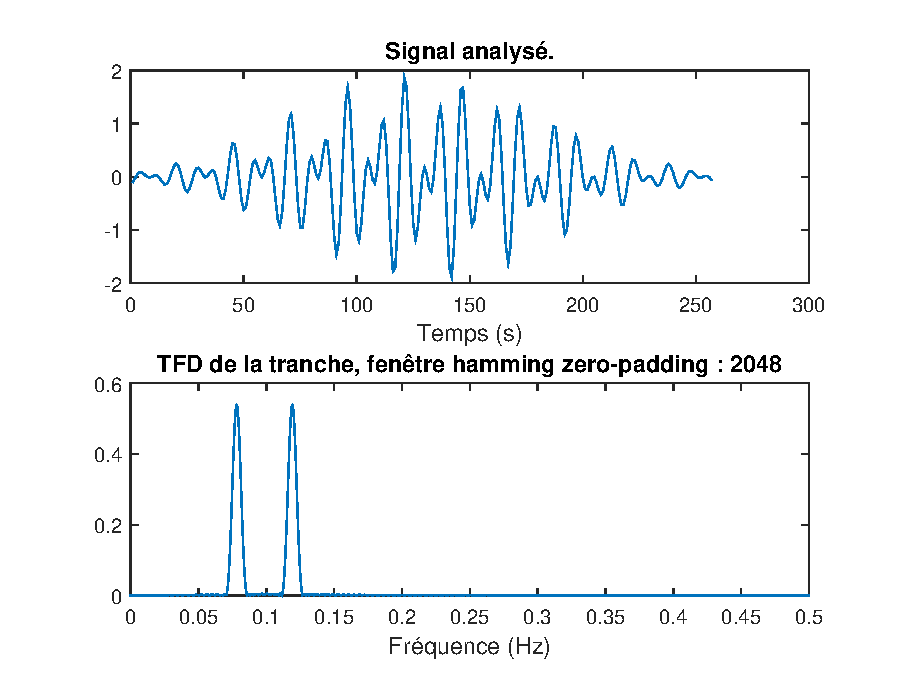
\includegraphics[width=\textwidth]{images/hamming.eps}
		% Title: glps_renderer figure
% Creator: GL2PS 1.3.8, (C) 1999-2012 C. Geuzaine
% For: Octave
% CreationDate: Wed Nov  8 10:42:42 2017
\begin{pgfpicture}
\pgfsetlinewidth{0.01pt}
\color[rgb]{1.000000,1.000000,1.000000}
\pgfpathmoveto{\pgfpoint{65.000015pt}{104.000000pt}}
\pgflineto{\pgfpoint{452.500031pt}{26.999981pt}}
\pgflineto{\pgfpoint{65.000015pt}{26.999981pt}}
\pgfpathclose
\pgfusepath{fill,stroke}
\pgfpathmoveto{\pgfpoint{65.000015pt}{104.000000pt}}
\pgflineto{\pgfpoint{452.500031pt}{104.000000pt}}
\pgflineto{\pgfpoint{452.500031pt}{26.999981pt}}
\pgfpathclose
\pgfusepath{fill,stroke}
\color[rgb]{0.000000,0.000000,0.000000}
\pgfsetlinewidth{0.500000pt}
\pgfsetdash{{16pt}{0pt}}{0pt}
\pgfpathmoveto{\pgfpoint{452.500031pt}{26.999981pt}}
\pgflineto{\pgfpoint{65.000015pt}{26.999981pt}}
\pgfusepath{stroke}
\pgfpathmoveto{\pgfpoint{452.500031pt}{104.000000pt}}
\pgflineto{\pgfpoint{65.000015pt}{104.000000pt}}
\pgfusepath{stroke}
\pgfpathmoveto{\pgfpoint{65.000015pt}{104.000000pt}}
\pgflineto{\pgfpoint{65.000015pt}{26.999981pt}}
\pgfusepath{stroke}
\pgfpathmoveto{\pgfpoint{452.500031pt}{104.000000pt}}
\pgflineto{\pgfpoint{452.500031pt}{26.999981pt}}
\pgfusepath{stroke}
\pgfsetdash{{0pt}{3pt}{1pt}{3pt}{1pt}{3pt}{1pt}{3pt}{1pt}{0pt}}{0pt}
\pgfpathmoveto{\pgfpoint{65.000015pt}{104.000000pt}}
\pgflineto{\pgfpoint{65.000015pt}{26.999981pt}}
\pgfusepath{stroke}
\pgfpathmoveto{\pgfpoint{142.500031pt}{104.000000pt}}
\pgflineto{\pgfpoint{142.500031pt}{26.999981pt}}
\pgfusepath{stroke}
\pgfpathmoveto{\pgfpoint{220.000031pt}{104.000000pt}}
\pgflineto{\pgfpoint{220.000031pt}{26.999981pt}}
\pgfusepath{stroke}
\pgfpathmoveto{\pgfpoint{297.500031pt}{104.000000pt}}
\pgflineto{\pgfpoint{297.500031pt}{26.999981pt}}
\pgfusepath{stroke}
\pgfpathmoveto{\pgfpoint{375.000061pt}{104.000000pt}}
\pgflineto{\pgfpoint{375.000061pt}{26.999981pt}}
\pgfusepath{stroke}
\pgfpathmoveto{\pgfpoint{452.500031pt}{104.000000pt}}
\pgflineto{\pgfpoint{452.500031pt}{26.999981pt}}
\pgfusepath{stroke}
\pgfsetdash{{16pt}{0pt}}{0pt}
\pgfpathmoveto{\pgfpoint{65.000015pt}{30.874983pt}}
\pgflineto{\pgfpoint{65.000015pt}{26.999981pt}}
\pgfusepath{stroke}
\pgfpathmoveto{\pgfpoint{65.000015pt}{100.125008pt}}
\pgflineto{\pgfpoint{65.000015pt}{104.000000pt}}
\pgfusepath{stroke}
\pgfpathmoveto{\pgfpoint{142.500031pt}{30.874983pt}}
\pgflineto{\pgfpoint{142.500031pt}{26.999981pt}}
\pgfusepath{stroke}
\pgfpathmoveto{\pgfpoint{142.500031pt}{100.125008pt}}
\pgflineto{\pgfpoint{142.500031pt}{104.000000pt}}
\pgfusepath{stroke}
\pgfpathmoveto{\pgfpoint{220.000031pt}{30.874983pt}}
\pgflineto{\pgfpoint{220.000031pt}{26.999981pt}}
\pgfusepath{stroke}
\pgfpathmoveto{\pgfpoint{220.000031pt}{100.125008pt}}
\pgflineto{\pgfpoint{220.000031pt}{104.000000pt}}
\pgfusepath{stroke}
\pgfpathmoveto{\pgfpoint{297.500031pt}{30.874983pt}}
\pgflineto{\pgfpoint{297.500031pt}{26.999981pt}}
\pgfusepath{stroke}
\pgfpathmoveto{\pgfpoint{297.500031pt}{100.125008pt}}
\pgflineto{\pgfpoint{297.500031pt}{104.000000pt}}
\pgfusepath{stroke}
\pgfpathmoveto{\pgfpoint{375.000061pt}{30.874983pt}}
\pgflineto{\pgfpoint{375.000061pt}{26.999981pt}}
\pgfusepath{stroke}
\pgfpathmoveto{\pgfpoint{375.000061pt}{100.125008pt}}
\pgflineto{\pgfpoint{375.000061pt}{104.000000pt}}
\pgfusepath{stroke}
\pgfpathmoveto{\pgfpoint{452.500031pt}{30.874983pt}}
\pgflineto{\pgfpoint{452.500031pt}{26.999981pt}}
\pgfusepath{stroke}
\pgfpathmoveto{\pgfpoint{452.500031pt}{100.125008pt}}
\pgflineto{\pgfpoint{452.500031pt}{104.000000pt}}
\pgfusepath{stroke}
{
\pgftransformshift{\pgfpoint{65.000015pt}{21.999977pt}}
\pgfnode{rectangle}{north}{\fontsize{10}{0}\selectfont\textcolor[rgb]{0,0,0}{{0}}}{}{\pgfusepath{discard}}}
{
\pgftransformshift{\pgfpoint{142.500015pt}{21.999977pt}}
\pgfnode{rectangle}{north}{\fontsize{10}{0}\selectfont\textcolor[rgb]{0,0,0}{{0.1}}}{}{\pgfusepath{discard}}}
{
\pgftransformshift{\pgfpoint{220.000015pt}{21.999977pt}}
\pgfnode{rectangle}{north}{\fontsize{10}{0}\selectfont\textcolor[rgb]{0,0,0}{{0.2}}}{}{\pgfusepath{discard}}}
{
\pgftransformshift{\pgfpoint{297.500031pt}{21.999977pt}}
\pgfnode{rectangle}{north}{\fontsize{10}{0}\selectfont\textcolor[rgb]{0,0,0}{{0.3}}}{}{\pgfusepath{discard}}}
{
\pgftransformshift{\pgfpoint{375.000031pt}{21.999977pt}}
\pgfnode{rectangle}{north}{\fontsize{10}{0}\selectfont\textcolor[rgb]{0,0,0}{{0.4}}}{}{\pgfusepath{discard}}}
{
\pgftransformshift{\pgfpoint{452.500031pt}{21.999977pt}}
\pgfnode{rectangle}{north}{\fontsize{10}{0}\selectfont\textcolor[rgb]{0,0,0}{{0.5}}}{}{\pgfusepath{discard}}}
\pgfsetdash{{0pt}{3pt}{1pt}{3pt}{1pt}{3pt}{1pt}{3pt}{1pt}{0pt}}{0pt}
\pgfpathmoveto{\pgfpoint{452.500031pt}{26.999981pt}}
\pgflineto{\pgfpoint{65.000015pt}{26.999981pt}}
\pgfusepath{stroke}
\pgfpathmoveto{\pgfpoint{452.500031pt}{37.999985pt}}
\pgflineto{\pgfpoint{65.000015pt}{37.999985pt}}
\pgfusepath{stroke}
\pgfpathmoveto{\pgfpoint{452.500031pt}{48.999989pt}}
\pgflineto{\pgfpoint{65.000015pt}{48.999989pt}}
\pgfusepath{stroke}
\pgfpathmoveto{\pgfpoint{452.500031pt}{59.999992pt}}
\pgflineto{\pgfpoint{65.000015pt}{59.999992pt}}
\pgfusepath{stroke}
\pgfpathmoveto{\pgfpoint{452.500031pt}{70.999992pt}}
\pgflineto{\pgfpoint{65.000015pt}{70.999992pt}}
\pgfusepath{stroke}
\pgfpathmoveto{\pgfpoint{452.500031pt}{82.000000pt}}
\pgflineto{\pgfpoint{65.000015pt}{82.000000pt}}
\pgfusepath{stroke}
\pgfpathmoveto{\pgfpoint{452.500031pt}{93.000000pt}}
\pgflineto{\pgfpoint{65.000015pt}{93.000000pt}}
\pgfusepath{stroke}
\pgfpathmoveto{\pgfpoint{452.500031pt}{104.000000pt}}
\pgflineto{\pgfpoint{65.000015pt}{104.000000pt}}
\pgfusepath{stroke}
\pgfsetdash{{16pt}{0pt}}{0pt}
\pgfpathmoveto{\pgfpoint{68.870026pt}{26.999981pt}}
\pgflineto{\pgfpoint{65.000015pt}{26.999981pt}}
\pgfusepath{stroke}
\pgfpathmoveto{\pgfpoint{448.630005pt}{26.999981pt}}
\pgflineto{\pgfpoint{452.500031pt}{26.999981pt}}
\pgfusepath{stroke}
\pgfpathmoveto{\pgfpoint{68.870026pt}{37.999985pt}}
\pgflineto{\pgfpoint{65.000015pt}{37.999985pt}}
\pgfusepath{stroke}
\pgfpathmoveto{\pgfpoint{448.630005pt}{37.999985pt}}
\pgflineto{\pgfpoint{452.500031pt}{37.999985pt}}
\pgfusepath{stroke}
\pgfpathmoveto{\pgfpoint{68.870026pt}{48.999989pt}}
\pgflineto{\pgfpoint{65.000015pt}{48.999989pt}}
\pgfusepath{stroke}
\pgfpathmoveto{\pgfpoint{448.630005pt}{48.999989pt}}
\pgflineto{\pgfpoint{452.500031pt}{48.999989pt}}
\pgfusepath{stroke}
\pgfpathmoveto{\pgfpoint{68.870026pt}{59.999992pt}}
\pgflineto{\pgfpoint{65.000015pt}{59.999992pt}}
\pgfusepath{stroke}
\pgfpathmoveto{\pgfpoint{448.630005pt}{59.999992pt}}
\pgflineto{\pgfpoint{452.500031pt}{59.999992pt}}
\pgfusepath{stroke}
\pgfpathmoveto{\pgfpoint{68.870026pt}{70.999992pt}}
\pgflineto{\pgfpoint{65.000015pt}{70.999992pt}}
\pgfusepath{stroke}
\pgfpathmoveto{\pgfpoint{448.630005pt}{70.999992pt}}
\pgflineto{\pgfpoint{452.500031pt}{70.999992pt}}
\pgfusepath{stroke}
\pgfpathmoveto{\pgfpoint{68.870026pt}{82.000000pt}}
\pgflineto{\pgfpoint{65.000015pt}{82.000000pt}}
\pgfusepath{stroke}
\pgfpathmoveto{\pgfpoint{448.630005pt}{82.000000pt}}
\pgflineto{\pgfpoint{452.500031pt}{82.000000pt}}
\pgfusepath{stroke}
\pgfpathmoveto{\pgfpoint{68.870026pt}{93.000000pt}}
\pgflineto{\pgfpoint{65.000015pt}{93.000000pt}}
\pgfusepath{stroke}
\pgfpathmoveto{\pgfpoint{448.630005pt}{93.000000pt}}
\pgflineto{\pgfpoint{452.500031pt}{93.000000pt}}
\pgfusepath{stroke}
\pgfpathmoveto{\pgfpoint{68.870026pt}{104.000000pt}}
\pgflineto{\pgfpoint{65.000015pt}{104.000000pt}}
\pgfusepath{stroke}
\pgfpathmoveto{\pgfpoint{448.630005pt}{104.000000pt}}
\pgflineto{\pgfpoint{452.500031pt}{104.000000pt}}
\pgfusepath{stroke}
{
\pgftransformshift{\pgfpoint{60.006454pt}{26.999981pt}}
\pgfnode{rectangle}{east}{\fontsize{10}{0}\selectfont\textcolor[rgb]{0,0,0}{{0}}}{}{\pgfusepath{discard}}}
{
\pgftransformshift{\pgfpoint{60.006454pt}{37.999985pt}}
\pgfnode{rectangle}{east}{\fontsize{10}{0}\selectfont\textcolor[rgb]{0,0,0}{{0.1}}}{}{\pgfusepath{discard}}}
{
\pgftransformshift{\pgfpoint{60.006454pt}{48.999989pt}}
\pgfnode{rectangle}{east}{\fontsize{10}{0}\selectfont\textcolor[rgb]{0,0,0}{{0.2}}}{}{\pgfusepath{discard}}}
{
\pgftransformshift{\pgfpoint{60.006454pt}{59.999992pt}}
\pgfnode{rectangle}{east}{\fontsize{10}{0}\selectfont\textcolor[rgb]{0,0,0}{{0.3}}}{}{\pgfusepath{discard}}}
{
\pgftransformshift{\pgfpoint{60.006454pt}{70.999992pt}}
\pgfnode{rectangle}{east}{\fontsize{10}{0}\selectfont\textcolor[rgb]{0,0,0}{{0.4}}}{}{\pgfusepath{discard}}}
{
\pgftransformshift{\pgfpoint{60.006454pt}{82.000000pt}}
\pgfnode{rectangle}{east}{\fontsize{10}{0}\selectfont\textcolor[rgb]{0,0,0}{{0.5}}}{}{\pgfusepath{discard}}}
{
\pgftransformshift{\pgfpoint{60.006454pt}{93.000000pt}}
\pgfnode{rectangle}{east}{\fontsize{10}{0}\selectfont\textcolor[rgb]{0,0,0}{{0.6}}}{}{\pgfusepath{discard}}}
{
\pgftransformshift{\pgfpoint{60.006454pt}{104.000000pt}}
\pgfnode{rectangle}{east}{\fontsize{10}{0}\selectfont\textcolor[rgb]{0,0,0}{{0.7}}}{}{\pgfusepath{discard}}}
{
\pgftransformshift{\pgfpoint{258.750031pt}{10.999977pt}}
\pgfnode{rectangle}{north}{\fontsize{10}{0}\selectfont\textcolor[rgb]{0,0,0}{{Fréquence (Hz)}}}{}{\pgfusepath{discard}}}
\color[rgb]{0.000000,0.000000,1.000000}
\pgfsetdash{}{0pt}
\pgfpathmoveto{\pgfpoint{65.189224pt}{27.101219pt}}
\pgflineto{\pgfpoint{65.000015pt}{27.102337pt}}
\pgfusepath{stroke}
\pgfpathmoveto{\pgfpoint{65.378433pt}{27.097946pt}}
\pgflineto{\pgfpoint{65.189224pt}{27.101219pt}}
\pgfusepath{stroke}
\pgfpathmoveto{\pgfpoint{65.567642pt}{27.092766pt}}
\pgflineto{\pgfpoint{65.378433pt}{27.097946pt}}
\pgfusepath{stroke}
\pgfpathmoveto{\pgfpoint{65.756836pt}{27.086094pt}}
\pgflineto{\pgfpoint{65.567642pt}{27.092766pt}}
\pgfusepath{stroke}
\pgfpathmoveto{\pgfpoint{65.946060pt}{27.078579pt}}
\pgflineto{\pgfpoint{65.756836pt}{27.086094pt}}
\pgfusepath{stroke}
\pgfpathmoveto{\pgfpoint{66.135269pt}{27.071129pt}}
\pgflineto{\pgfpoint{65.946060pt}{27.078579pt}}
\pgfusepath{stroke}
\pgfpathmoveto{\pgfpoint{66.324478pt}{27.064941pt}}
\pgflineto{\pgfpoint{66.135269pt}{27.071129pt}}
\pgfusepath{stroke}
\pgfpathmoveto{\pgfpoint{66.513687pt}{27.061359pt}}
\pgflineto{\pgfpoint{66.324478pt}{27.064941pt}}
\pgfusepath{stroke}
\pgfpathmoveto{\pgfpoint{66.702881pt}{27.061359pt}}
\pgflineto{\pgfpoint{66.513687pt}{27.061359pt}}
\pgfusepath{stroke}
\pgfpathmoveto{\pgfpoint{66.892105pt}{27.064980pt}}
\pgflineto{\pgfpoint{66.702881pt}{27.061359pt}}
\pgfusepath{stroke}
\pgfpathmoveto{\pgfpoint{67.081314pt}{27.071270pt}}
\pgflineto{\pgfpoint{66.892105pt}{27.064980pt}}
\pgfusepath{stroke}
\pgfpathmoveto{\pgfpoint{67.270523pt}{27.078899pt}}
\pgflineto{\pgfpoint{67.081314pt}{27.071270pt}}
\pgfusepath{stroke}
\pgfpathmoveto{\pgfpoint{67.459732pt}{27.086655pt}}
\pgflineto{\pgfpoint{67.270523pt}{27.078899pt}}
\pgfusepath{stroke}
\pgfpathmoveto{\pgfpoint{67.648926pt}{27.093590pt}}
\pgflineto{\pgfpoint{67.459732pt}{27.086655pt}}
\pgfusepath{stroke}
\pgfpathmoveto{\pgfpoint{67.838150pt}{27.099037pt}}
\pgflineto{\pgfpoint{67.648926pt}{27.093590pt}}
\pgfusepath{stroke}
\pgfpathmoveto{\pgfpoint{68.027359pt}{27.102531pt}}
\pgflineto{\pgfpoint{67.838150pt}{27.099037pt}}
\pgfusepath{stroke}
\pgfpathmoveto{\pgfpoint{68.216568pt}{27.103806pt}}
\pgflineto{\pgfpoint{68.027359pt}{27.102531pt}}
\pgfusepath{stroke}
\pgfpathmoveto{\pgfpoint{68.405777pt}{27.102745pt}}
\pgflineto{\pgfpoint{68.216568pt}{27.103806pt}}
\pgfusepath{stroke}
\pgfpathmoveto{\pgfpoint{68.594971pt}{27.099415pt}}
\pgflineto{\pgfpoint{68.405777pt}{27.102745pt}}
\pgfusepath{stroke}
\pgfpathmoveto{\pgfpoint{68.784195pt}{27.094032pt}}
\pgflineto{\pgfpoint{68.594971pt}{27.099415pt}}
\pgfusepath{stroke}
\pgfpathmoveto{\pgfpoint{68.973404pt}{27.087029pt}}
\pgflineto{\pgfpoint{68.784195pt}{27.094032pt}}
\pgfusepath{stroke}
\pgfpathmoveto{\pgfpoint{69.162613pt}{27.079060pt}}
\pgflineto{\pgfpoint{68.973404pt}{27.087029pt}}
\pgfusepath{stroke}
\pgfpathmoveto{\pgfpoint{69.351822pt}{27.071098pt}}
\pgflineto{\pgfpoint{69.162613pt}{27.079060pt}}
\pgfusepath{stroke}
\pgfpathmoveto{\pgfpoint{69.541016pt}{27.064472pt}}
\pgflineto{\pgfpoint{69.351822pt}{27.071098pt}}
\pgfusepath{stroke}
\pgfpathmoveto{\pgfpoint{69.730240pt}{27.060719pt}}
\pgflineto{\pgfpoint{69.541016pt}{27.064472pt}}
\pgfusepath{stroke}
\pgfpathmoveto{\pgfpoint{69.919449pt}{27.060986pt}}
\pgflineto{\pgfpoint{69.730240pt}{27.060719pt}}
\pgfusepath{stroke}
\pgfpathmoveto{\pgfpoint{70.108658pt}{27.065289pt}}
\pgflineto{\pgfpoint{69.919449pt}{27.060986pt}}
\pgfusepath{stroke}
\pgfpathmoveto{\pgfpoint{70.297867pt}{27.072487pt}}
\pgflineto{\pgfpoint{70.108658pt}{27.065289pt}}
\pgfusepath{stroke}
\pgfpathmoveto{\pgfpoint{70.487061pt}{27.081043pt}}
\pgflineto{\pgfpoint{70.297867pt}{27.072487pt}}
\pgfusepath{stroke}
\pgfpathmoveto{\pgfpoint{70.676285pt}{27.089630pt}}
\pgflineto{\pgfpoint{70.487061pt}{27.081043pt}}
\pgfusepath{stroke}
\pgfpathmoveto{\pgfpoint{70.865494pt}{27.097229pt}}
\pgflineto{\pgfpoint{70.676285pt}{27.089630pt}}
\pgfusepath{stroke}
\pgfpathmoveto{\pgfpoint{71.054703pt}{27.103123pt}}
\pgflineto{\pgfpoint{70.865494pt}{27.097229pt}}
\pgfusepath{stroke}
\pgfpathmoveto{\pgfpoint{71.243912pt}{27.106823pt}}
\pgflineto{\pgfpoint{71.054703pt}{27.103123pt}}
\pgfusepath{stroke}
\pgfpathmoveto{\pgfpoint{71.433105pt}{27.108040pt}}
\pgflineto{\pgfpoint{71.243912pt}{27.106823pt}}
\pgfusepath{stroke}
\pgfpathmoveto{\pgfpoint{71.622330pt}{27.106655pt}}
\pgflineto{\pgfpoint{71.433105pt}{27.108040pt}}
\pgfusepath{stroke}
\pgfpathmoveto{\pgfpoint{71.811539pt}{27.102730pt}}
\pgflineto{\pgfpoint{71.622330pt}{27.106655pt}}
\pgfusepath{stroke}
\pgfpathmoveto{\pgfpoint{72.000748pt}{27.096523pt}}
\pgflineto{\pgfpoint{71.811539pt}{27.102730pt}}
\pgfusepath{stroke}
\pgfpathmoveto{\pgfpoint{72.189957pt}{27.088501pt}}
\pgflineto{\pgfpoint{72.000748pt}{27.096523pt}}
\pgfusepath{stroke}
\pgfpathmoveto{\pgfpoint{72.379150pt}{27.079422pt}}
\pgflineto{\pgfpoint{72.189957pt}{27.088501pt}}
\pgfusepath{stroke}
\pgfpathmoveto{\pgfpoint{72.568375pt}{27.070442pt}}
\pgflineto{\pgfpoint{72.379150pt}{27.079422pt}}
\pgfusepath{stroke}
\pgfpathmoveto{\pgfpoint{72.757584pt}{27.063187pt}}
\pgflineto{\pgfpoint{72.568375pt}{27.070442pt}}
\pgfusepath{stroke}
\pgfpathmoveto{\pgfpoint{72.946793pt}{27.059578pt}}
\pgflineto{\pgfpoint{72.757584pt}{27.063187pt}}
\pgfusepath{stroke}
\pgfpathmoveto{\pgfpoint{73.136002pt}{27.060936pt}}
\pgflineto{\pgfpoint{72.946793pt}{27.059578pt}}
\pgfusepath{stroke}
\pgfpathmoveto{\pgfpoint{73.325195pt}{27.066944pt}}
\pgflineto{\pgfpoint{73.136002pt}{27.060936pt}}
\pgfusepath{stroke}
\pgfpathmoveto{\pgfpoint{73.514420pt}{27.075924pt}}
\pgflineto{\pgfpoint{73.325195pt}{27.066944pt}}
\pgfusepath{stroke}
\pgfpathmoveto{\pgfpoint{73.703629pt}{27.086025pt}}
\pgflineto{\pgfpoint{73.514420pt}{27.075924pt}}
\pgfusepath{stroke}
\pgfpathmoveto{\pgfpoint{73.892838pt}{27.095772pt}}
\pgflineto{\pgfpoint{73.703629pt}{27.086025pt}}
\pgfusepath{stroke}
\pgfpathmoveto{\pgfpoint{74.082047pt}{27.104115pt}}
\pgflineto{\pgfpoint{73.892838pt}{27.095772pt}}
\pgfusepath{stroke}
\pgfpathmoveto{\pgfpoint{74.271240pt}{27.110313pt}}
\pgflineto{\pgfpoint{74.082047pt}{27.104115pt}}
\pgfusepath{stroke}
\pgfpathmoveto{\pgfpoint{74.460464pt}{27.113888pt}}
\pgflineto{\pgfpoint{74.271240pt}{27.110313pt}}
\pgfusepath{stroke}
\pgfpathmoveto{\pgfpoint{74.649673pt}{27.114563pt}}
\pgflineto{\pgfpoint{74.460464pt}{27.113888pt}}
\pgfusepath{stroke}
\pgfpathmoveto{\pgfpoint{74.838882pt}{27.112247pt}}
\pgflineto{\pgfpoint{74.649673pt}{27.114563pt}}
\pgfusepath{stroke}
\pgfpathmoveto{\pgfpoint{75.028091pt}{27.107056pt}}
\pgflineto{\pgfpoint{74.838882pt}{27.112247pt}}
\pgfusepath{stroke}
\pgfpathmoveto{\pgfpoint{75.217285pt}{27.099312pt}}
\pgflineto{\pgfpoint{75.028091pt}{27.107056pt}}
\pgfusepath{stroke}
\pgfpathmoveto{\pgfpoint{75.406509pt}{27.089603pt}}
\pgflineto{\pgfpoint{75.217285pt}{27.099312pt}}
\pgfusepath{stroke}
\pgfpathmoveto{\pgfpoint{75.595718pt}{27.078884pt}}
\pgflineto{\pgfpoint{75.406509pt}{27.089603pt}}
\pgfusepath{stroke}
\pgfpathmoveto{\pgfpoint{75.784927pt}{27.068649pt}}
\pgflineto{\pgfpoint{75.595718pt}{27.078884pt}}
\pgfusepath{stroke}
\pgfpathmoveto{\pgfpoint{75.974136pt}{27.061066pt}}
\pgflineto{\pgfpoint{75.784927pt}{27.068649pt}}
\pgfusepath{stroke}
\pgfpathmoveto{\pgfpoint{76.163330pt}{27.058613pt}}
\pgflineto{\pgfpoint{75.974136pt}{27.061066pt}}
\pgfusepath{stroke}
\pgfpathmoveto{\pgfpoint{76.352554pt}{27.062450pt}}
\pgflineto{\pgfpoint{76.163330pt}{27.058613pt}}
\pgfusepath{stroke}
\pgfpathmoveto{\pgfpoint{76.541763pt}{27.071308pt}}
\pgflineto{\pgfpoint{76.352554pt}{27.062450pt}}
\pgfusepath{stroke}
\pgfpathmoveto{\pgfpoint{76.730972pt}{27.082752pt}}
\pgflineto{\pgfpoint{76.541763pt}{27.071308pt}}
\pgfusepath{stroke}
\pgfpathmoveto{\pgfpoint{76.920181pt}{27.094654pt}}
\pgflineto{\pgfpoint{76.730972pt}{27.082752pt}}
\pgfusepath{stroke}
\pgfpathmoveto{\pgfpoint{77.109375pt}{27.105518pt}}
\pgflineto{\pgfpoint{76.920181pt}{27.094654pt}}
\pgfusepath{stroke}
\pgfpathmoveto{\pgfpoint{77.298599pt}{27.114319pt}}
\pgflineto{\pgfpoint{77.109375pt}{27.105518pt}}
\pgfusepath{stroke}
\pgfpathmoveto{\pgfpoint{77.487808pt}{27.120369pt}}
\pgflineto{\pgfpoint{77.298599pt}{27.114319pt}}
\pgfusepath{stroke}
\pgfpathmoveto{\pgfpoint{77.677017pt}{27.123230pt}}
\pgflineto{\pgfpoint{77.487808pt}{27.120369pt}}
\pgfusepath{stroke}
\pgfpathmoveto{\pgfpoint{77.866226pt}{27.122677pt}}
\pgflineto{\pgfpoint{77.677017pt}{27.123230pt}}
\pgfusepath{stroke}
\pgfpathmoveto{\pgfpoint{78.055420pt}{27.118683pt}}
\pgflineto{\pgfpoint{77.866226pt}{27.122677pt}}
\pgfusepath{stroke}
\pgfpathmoveto{\pgfpoint{78.244644pt}{27.111462pt}}
\pgflineto{\pgfpoint{78.055420pt}{27.118683pt}}
\pgfusepath{stroke}
\pgfpathmoveto{\pgfpoint{78.433853pt}{27.101471pt}}
\pgflineto{\pgfpoint{78.244644pt}{27.111462pt}}
\pgfusepath{stroke}
\pgfpathmoveto{\pgfpoint{78.623062pt}{27.089500pt}}
\pgflineto{\pgfpoint{78.433853pt}{27.101471pt}}
\pgfusepath{stroke}
\pgfpathmoveto{\pgfpoint{78.812271pt}{27.076820pt}}
\pgflineto{\pgfpoint{78.623062pt}{27.089500pt}}
\pgfusepath{stroke}
\pgfpathmoveto{\pgfpoint{79.001465pt}{27.065529pt}}
\pgflineto{\pgfpoint{78.812271pt}{27.076820pt}}
\pgfusepath{stroke}
\pgfpathmoveto{\pgfpoint{79.190689pt}{27.058708pt}}
\pgflineto{\pgfpoint{79.001465pt}{27.065529pt}}
\pgfusepath{stroke}
\pgfpathmoveto{\pgfpoint{79.379898pt}{27.059280pt}}
\pgflineto{\pgfpoint{79.190689pt}{27.058708pt}}
\pgfusepath{stroke}
\pgfpathmoveto{\pgfpoint{79.569107pt}{27.067257pt}}
\pgflineto{\pgfpoint{79.379898pt}{27.059280pt}}
\pgfusepath{stroke}
\pgfpathmoveto{\pgfpoint{79.758316pt}{27.079784pt}}
\pgflineto{\pgfpoint{79.569107pt}{27.067257pt}}
\pgfusepath{stroke}
\pgfpathmoveto{\pgfpoint{79.947510pt}{27.093849pt}}
\pgflineto{\pgfpoint{79.758316pt}{27.079784pt}}
\pgfusepath{stroke}
\pgfpathmoveto{\pgfpoint{80.136734pt}{27.107349pt}}
\pgflineto{\pgfpoint{79.947510pt}{27.093849pt}}
\pgfusepath{stroke}
\pgfpathmoveto{\pgfpoint{80.325943pt}{27.118904pt}}
\pgflineto{\pgfpoint{80.136734pt}{27.107349pt}}
\pgfusepath{stroke}
\pgfpathmoveto{\pgfpoint{80.515152pt}{27.127583pt}}
\pgflineto{\pgfpoint{80.325943pt}{27.118904pt}}
\pgfusepath{stroke}
\pgfpathmoveto{\pgfpoint{80.704361pt}{27.132786pt}}
\pgflineto{\pgfpoint{80.515152pt}{27.127583pt}}
\pgfusepath{stroke}
\pgfpathmoveto{\pgfpoint{80.893570pt}{27.134148pt}}
\pgflineto{\pgfpoint{80.704361pt}{27.132786pt}}
\pgfusepath{stroke}
\pgfpathmoveto{\pgfpoint{81.082779pt}{27.131531pt}}
\pgflineto{\pgfpoint{80.893570pt}{27.134148pt}}
\pgfusepath{stroke}
\pgfpathmoveto{\pgfpoint{81.271988pt}{27.125034pt}}
\pgflineto{\pgfpoint{81.082779pt}{27.131531pt}}
\pgfusepath{stroke}
\pgfpathmoveto{\pgfpoint{81.461197pt}{27.115005pt}}
\pgflineto{\pgfpoint{81.271988pt}{27.125034pt}}
\pgfusepath{stroke}
\pgfpathmoveto{\pgfpoint{81.650406pt}{27.102104pt}}
\pgflineto{\pgfpoint{81.461197pt}{27.115005pt}}
\pgfusepath{stroke}
\pgfpathmoveto{\pgfpoint{81.839615pt}{27.087437pt}}
\pgflineto{\pgfpoint{81.650406pt}{27.102104pt}}
\pgfusepath{stroke}
\pgfpathmoveto{\pgfpoint{82.028824pt}{27.072857pt}}
\pgflineto{\pgfpoint{81.839615pt}{27.087437pt}}
\pgfusepath{stroke}
\pgfpathmoveto{\pgfpoint{82.218033pt}{27.061527pt}}
\pgflineto{\pgfpoint{82.028824pt}{27.072857pt}}
\pgfusepath{stroke}
\pgfpathmoveto{\pgfpoint{82.407242pt}{27.057777pt}}
\pgflineto{\pgfpoint{82.218033pt}{27.061527pt}}
\pgfusepath{stroke}
\pgfpathmoveto{\pgfpoint{82.596451pt}{27.063858pt}}
\pgflineto{\pgfpoint{82.407242pt}{27.057777pt}}
\pgfusepath{stroke}
\pgfpathmoveto{\pgfpoint{82.785660pt}{27.077110pt}}
\pgflineto{\pgfpoint{82.596451pt}{27.063858pt}}
\pgfusepath{stroke}
\pgfpathmoveto{\pgfpoint{82.974869pt}{27.093349pt}}
\pgflineto{\pgfpoint{82.785660pt}{27.077110pt}}
\pgfusepath{stroke}
\pgfpathmoveto{\pgfpoint{83.164078pt}{27.109634pt}}
\pgflineto{\pgfpoint{82.974869pt}{27.093349pt}}
\pgfusepath{stroke}
\pgfpathmoveto{\pgfpoint{83.353287pt}{27.124126pt}}
\pgflineto{\pgfpoint{83.164078pt}{27.109634pt}}
\pgfusepath{stroke}
\pgfpathmoveto{\pgfpoint{83.542496pt}{27.135635pt}}
\pgflineto{\pgfpoint{83.353287pt}{27.124126pt}}
\pgfusepath{stroke}
\pgfpathmoveto{\pgfpoint{83.731705pt}{27.143379pt}}
\pgflineto{\pgfpoint{83.542496pt}{27.135635pt}}
\pgfusepath{stroke}
\pgfpathmoveto{\pgfpoint{83.920914pt}{27.146839pt}}
\pgflineto{\pgfpoint{83.731705pt}{27.143379pt}}
\pgfusepath{stroke}
\pgfpathmoveto{\pgfpoint{84.110123pt}{27.145775pt}}
\pgflineto{\pgfpoint{83.920914pt}{27.146839pt}}
\pgfusepath{stroke}
\pgfpathmoveto{\pgfpoint{84.299332pt}{27.140179pt}}
\pgflineto{\pgfpoint{84.110123pt}{27.145775pt}}
\pgfusepath{stroke}
\pgfpathmoveto{\pgfpoint{84.488541pt}{27.130299pt}}
\pgflineto{\pgfpoint{84.299332pt}{27.140179pt}}
\pgfusepath{stroke}
\pgfpathmoveto{\pgfpoint{84.677750pt}{27.116699pt}}
\pgflineto{\pgfpoint{84.488541pt}{27.130299pt}}
\pgfusepath{stroke}
\pgfpathmoveto{\pgfpoint{84.866959pt}{27.100342pt}}
\pgflineto{\pgfpoint{84.677750pt}{27.116699pt}}
\pgfusepath{stroke}
\pgfpathmoveto{\pgfpoint{85.056168pt}{27.082859pt}}
\pgflineto{\pgfpoint{84.866959pt}{27.100342pt}}
\pgfusepath{stroke}
\pgfpathmoveto{\pgfpoint{85.245377pt}{27.067184pt}}
\pgflineto{\pgfpoint{85.056168pt}{27.082859pt}}
\pgfusepath{stroke}
\pgfpathmoveto{\pgfpoint{85.434586pt}{27.058346pt}}
\pgflineto{\pgfpoint{85.245377pt}{27.067184pt}}
\pgfusepath{stroke}
\pgfpathmoveto{\pgfpoint{85.623795pt}{27.061295pt}}
\pgflineto{\pgfpoint{85.434586pt}{27.058346pt}}
\pgfusepath{stroke}
\pgfpathmoveto{\pgfpoint{85.813004pt}{27.074722pt}}
\pgflineto{\pgfpoint{85.623795pt}{27.061295pt}}
\pgfusepath{stroke}
\pgfpathmoveto{\pgfpoint{86.002213pt}{27.093143pt}}
\pgflineto{\pgfpoint{85.813004pt}{27.074722pt}}
\pgfusepath{stroke}
\pgfpathmoveto{\pgfpoint{86.191422pt}{27.112404pt}}
\pgflineto{\pgfpoint{86.002213pt}{27.093143pt}}
\pgfusepath{stroke}
\pgfpathmoveto{\pgfpoint{86.380630pt}{27.130074pt}}
\pgflineto{\pgfpoint{86.191422pt}{27.112404pt}}
\pgfusepath{stroke}
\pgfpathmoveto{\pgfpoint{86.569839pt}{27.144669pt}}
\pgflineto{\pgfpoint{86.380630pt}{27.130074pt}}
\pgfusepath{stroke}
\pgfpathmoveto{\pgfpoint{86.759048pt}{27.155186pt}}
\pgflineto{\pgfpoint{86.569839pt}{27.144669pt}}
\pgfusepath{stroke}
\pgfpathmoveto{\pgfpoint{86.948257pt}{27.160976pt}}
\pgflineto{\pgfpoint{86.759048pt}{27.155186pt}}
\pgfusepath{stroke}
\pgfpathmoveto{\pgfpoint{87.137466pt}{27.161663pt}}
\pgflineto{\pgfpoint{86.948257pt}{27.160976pt}}
\pgfusepath{stroke}
\pgfpathmoveto{\pgfpoint{87.326675pt}{27.157131pt}}
\pgflineto{\pgfpoint{87.137466pt}{27.161663pt}}
\pgfusepath{stroke}
\pgfpathmoveto{\pgfpoint{87.515884pt}{27.147556pt}}
\pgflineto{\pgfpoint{87.326675pt}{27.157131pt}}
\pgfusepath{stroke}
\pgfpathmoveto{\pgfpoint{87.705093pt}{27.133411pt}}
\pgflineto{\pgfpoint{87.515884pt}{27.147556pt}}
\pgfusepath{stroke}
\pgfpathmoveto{\pgfpoint{87.894302pt}{27.115559pt}}
\pgflineto{\pgfpoint{87.705093pt}{27.133411pt}}
\pgfusepath{stroke}
\pgfpathmoveto{\pgfpoint{88.083511pt}{27.095436pt}}
\pgflineto{\pgfpoint{87.894302pt}{27.115559pt}}
\pgfusepath{stroke}
\pgfpathmoveto{\pgfpoint{88.272720pt}{27.075676pt}}
\pgflineto{\pgfpoint{88.083511pt}{27.095436pt}}
\pgfusepath{stroke}
\pgfpathmoveto{\pgfpoint{88.461929pt}{27.061348pt}}
\pgflineto{\pgfpoint{88.272720pt}{27.075676pt}}
\pgfusepath{stroke}
\pgfpathmoveto{\pgfpoint{88.651138pt}{27.059811pt}}
\pgflineto{\pgfpoint{88.461929pt}{27.061348pt}}
\pgfusepath{stroke}
\pgfpathmoveto{\pgfpoint{88.840347pt}{27.072632pt}}
\pgflineto{\pgfpoint{88.651138pt}{27.059811pt}}
\pgfusepath{stroke}
\pgfpathmoveto{\pgfpoint{89.029556pt}{27.093204pt}}
\pgflineto{\pgfpoint{88.840347pt}{27.072632pt}}
\pgfusepath{stroke}
\pgfpathmoveto{\pgfpoint{89.218765pt}{27.115685pt}}
\pgflineto{\pgfpoint{89.029556pt}{27.093204pt}}
\pgfusepath{stroke}
\pgfpathmoveto{\pgfpoint{89.407974pt}{27.136860pt}}
\pgflineto{\pgfpoint{89.218765pt}{27.115685pt}}
\pgfusepath{stroke}
\pgfpathmoveto{\pgfpoint{89.597183pt}{27.154854pt}}
\pgflineto{\pgfpoint{89.407974pt}{27.136860pt}}
\pgfusepath{stroke}
\pgfpathmoveto{\pgfpoint{89.786392pt}{27.168457pt}}
\pgflineto{\pgfpoint{89.597183pt}{27.154854pt}}
\pgfusepath{stroke}
\pgfpathmoveto{\pgfpoint{89.975601pt}{27.176842pt}}
\pgflineto{\pgfpoint{89.786392pt}{27.168457pt}}
\pgfusepath{stroke}
\pgfpathmoveto{\pgfpoint{90.164810pt}{27.179501pt}}
\pgflineto{\pgfpoint{89.975601pt}{27.176842pt}}
\pgfusepath{stroke}
\pgfpathmoveto{\pgfpoint{90.354019pt}{27.176228pt}}
\pgflineto{\pgfpoint{90.164810pt}{27.179501pt}}
\pgfusepath{stroke}
\pgfpathmoveto{\pgfpoint{90.543228pt}{27.167099pt}}
\pgflineto{\pgfpoint{90.354019pt}{27.176228pt}}
\pgfusepath{stroke}
\pgfpathmoveto{\pgfpoint{90.732437pt}{27.152515pt}}
\pgflineto{\pgfpoint{90.543228pt}{27.167099pt}}
\pgfusepath{stroke}
\pgfpathmoveto{\pgfpoint{90.921646pt}{27.133251pt}}
\pgflineto{\pgfpoint{90.732437pt}{27.152515pt}}
\pgfusepath{stroke}
\pgfpathmoveto{\pgfpoint{91.110855pt}{27.110634pt}}
\pgflineto{\pgfpoint{90.921646pt}{27.133251pt}}
\pgfusepath{stroke}
\pgfpathmoveto{\pgfpoint{91.300064pt}{27.086994pt}}
\pgflineto{\pgfpoint{91.110855pt}{27.110634pt}}
\pgfusepath{stroke}
\pgfpathmoveto{\pgfpoint{91.489273pt}{27.067070pt}}
\pgflineto{\pgfpoint{91.300064pt}{27.086994pt}}
\pgfusepath{stroke}
\pgfpathmoveto{\pgfpoint{91.678482pt}{27.059761pt}}
\pgflineto{\pgfpoint{91.489273pt}{27.067070pt}}
\pgfusepath{stroke}
\pgfpathmoveto{\pgfpoint{91.867691pt}{27.070885pt}}
\pgflineto{\pgfpoint{91.678482pt}{27.059761pt}}
\pgfusepath{stroke}
\pgfpathmoveto{\pgfpoint{92.056900pt}{27.093529pt}}
\pgflineto{\pgfpoint{91.867691pt}{27.070885pt}}
\pgfusepath{stroke}
\pgfpathmoveto{\pgfpoint{92.246109pt}{27.119534pt}}
\pgflineto{\pgfpoint{92.056900pt}{27.093529pt}}
\pgfusepath{stroke}
\pgfpathmoveto{\pgfpoint{92.435318pt}{27.144600pt}}
\pgflineto{\pgfpoint{92.246109pt}{27.119534pt}}
\pgfusepath{stroke}
\pgfpathmoveto{\pgfpoint{92.624527pt}{27.166405pt}}
\pgflineto{\pgfpoint{92.435318pt}{27.144600pt}}
\pgfusepath{stroke}
\pgfpathmoveto{\pgfpoint{92.813736pt}{27.183464pt}}
\pgflineto{\pgfpoint{92.624527pt}{27.166405pt}}
\pgfusepath{stroke}
\pgfpathmoveto{\pgfpoint{93.002945pt}{27.194786pt}}
\pgflineto{\pgfpoint{92.813736pt}{27.183464pt}}
\pgfusepath{stroke}
\pgfpathmoveto{\pgfpoint{93.192154pt}{27.199707pt}}
\pgflineto{\pgfpoint{93.002945pt}{27.194786pt}}
\pgfusepath{stroke}
\pgfpathmoveto{\pgfpoint{93.381363pt}{27.197903pt}}
\pgflineto{\pgfpoint{93.192154pt}{27.199707pt}}
\pgfusepath{stroke}
\pgfpathmoveto{\pgfpoint{93.570572pt}{27.189358pt}}
\pgflineto{\pgfpoint{93.381363pt}{27.197903pt}}
\pgfusepath{stroke}
\pgfpathmoveto{\pgfpoint{93.759781pt}{27.174408pt}}
\pgflineto{\pgfpoint{93.570572pt}{27.189358pt}}
\pgfusepath{stroke}
\pgfpathmoveto{\pgfpoint{93.948990pt}{27.153770pt}}
\pgflineto{\pgfpoint{93.759781pt}{27.174408pt}}
\pgfusepath{stroke}
\pgfpathmoveto{\pgfpoint{94.138199pt}{27.128666pt}}
\pgflineto{\pgfpoint{93.948990pt}{27.153770pt}}
\pgfusepath{stroke}
\pgfpathmoveto{\pgfpoint{94.327408pt}{27.101223pt}}
\pgflineto{\pgfpoint{94.138199pt}{27.128666pt}}
\pgfusepath{stroke}
\pgfpathmoveto{\pgfpoint{94.516617pt}{27.075710pt}}
\pgflineto{\pgfpoint{94.327408pt}{27.101223pt}}
\pgfusepath{stroke}
\pgfpathmoveto{\pgfpoint{94.705826pt}{27.061573pt}}
\pgflineto{\pgfpoint{94.516617pt}{27.075710pt}}
\pgfusepath{stroke}
\pgfpathmoveto{\pgfpoint{94.895035pt}{27.069557pt}}
\pgflineto{\pgfpoint{94.705826pt}{27.061573pt}}
\pgfusepath{stroke}
\pgfpathmoveto{\pgfpoint{95.084244pt}{27.094097pt}}
\pgflineto{\pgfpoint{94.895035pt}{27.069557pt}}
\pgfusepath{stroke}
\pgfpathmoveto{\pgfpoint{95.273453pt}{27.124001pt}}
\pgflineto{\pgfpoint{95.084244pt}{27.094097pt}}
\pgfusepath{stroke}
\pgfpathmoveto{\pgfpoint{95.462662pt}{27.153454pt}}
\pgflineto{\pgfpoint{95.273453pt}{27.124001pt}}
\pgfusepath{stroke}
\pgfpathmoveto{\pgfpoint{95.651871pt}{27.179573pt}}
\pgflineto{\pgfpoint{95.462662pt}{27.153454pt}}
\pgfusepath{stroke}
\pgfpathmoveto{\pgfpoint{95.841080pt}{27.200577pt}}
\pgflineto{\pgfpoint{95.651871pt}{27.179573pt}}
\pgfusepath{stroke}
\pgfpathmoveto{\pgfpoint{96.030289pt}{27.215244pt}}
\pgflineto{\pgfpoint{95.841080pt}{27.200577pt}}
\pgfusepath{stroke}
\pgfpathmoveto{\pgfpoint{96.219498pt}{27.222767pt}}
\pgflineto{\pgfpoint{96.030289pt}{27.215244pt}}
\pgfusepath{stroke}
\pgfpathmoveto{\pgfpoint{96.408707pt}{27.222687pt}}
\pgflineto{\pgfpoint{96.219498pt}{27.222767pt}}
\pgfusepath{stroke}
\pgfpathmoveto{\pgfpoint{96.597916pt}{27.214886pt}}
\pgflineto{\pgfpoint{96.408707pt}{27.222687pt}}
\pgfusepath{stroke}
\pgfpathmoveto{\pgfpoint{96.787125pt}{27.199635pt}}
\pgflineto{\pgfpoint{96.597916pt}{27.214886pt}}
\pgfusepath{stroke}
\pgfpathmoveto{\pgfpoint{96.976334pt}{27.177586pt}}
\pgflineto{\pgfpoint{96.787125pt}{27.199635pt}}
\pgfusepath{stroke}
\pgfpathmoveto{\pgfpoint{97.165543pt}{27.149918pt}}
\pgflineto{\pgfpoint{96.976334pt}{27.177586pt}}
\pgfusepath{stroke}
\pgfpathmoveto{\pgfpoint{97.354752pt}{27.118595pt}}
\pgflineto{\pgfpoint{97.165543pt}{27.149918pt}}
\pgfusepath{stroke}
\pgfpathmoveto{\pgfpoint{97.543961pt}{27.087467pt}}
\pgflineto{\pgfpoint{97.354752pt}{27.118595pt}}
\pgfusepath{stroke}
\pgfpathmoveto{\pgfpoint{97.733170pt}{27.065735pt}}
\pgflineto{\pgfpoint{97.543961pt}{27.087467pt}}
\pgfusepath{stroke}
\pgfpathmoveto{\pgfpoint{97.922379pt}{27.068806pt}}
\pgflineto{\pgfpoint{97.733170pt}{27.065735pt}}
\pgfusepath{stroke}
\pgfpathmoveto{\pgfpoint{98.111588pt}{27.094906pt}}
\pgflineto{\pgfpoint{97.922379pt}{27.068806pt}}
\pgfusepath{stroke}
\pgfpathmoveto{\pgfpoint{98.300797pt}{27.129150pt}}
\pgflineto{\pgfpoint{98.111588pt}{27.094906pt}}
\pgfusepath{stroke}
\pgfpathmoveto{\pgfpoint{98.490005pt}{27.163612pt}}
\pgflineto{\pgfpoint{98.300797pt}{27.129150pt}}
\pgfusepath{stroke}
\pgfpathmoveto{\pgfpoint{98.679214pt}{27.194672pt}}
\pgflineto{\pgfpoint{98.490005pt}{27.163612pt}}
\pgfusepath{stroke}
\pgfpathmoveto{\pgfpoint{98.868423pt}{27.220192pt}}
\pgflineto{\pgfpoint{98.679214pt}{27.194672pt}}
\pgfusepath{stroke}
\pgfpathmoveto{\pgfpoint{99.057632pt}{27.238728pt}}
\pgflineto{\pgfpoint{98.868423pt}{27.220192pt}}
\pgfusepath{stroke}
\pgfpathmoveto{\pgfpoint{99.246841pt}{27.249268pt}}
\pgflineto{\pgfpoint{99.057632pt}{27.238728pt}}
\pgfusepath{stroke}
\pgfpathmoveto{\pgfpoint{99.436050pt}{27.251205pt}}
\pgflineto{\pgfpoint{99.246841pt}{27.249268pt}}
\pgfusepath{stroke}
\pgfpathmoveto{\pgfpoint{99.625259pt}{27.244331pt}}
\pgflineto{\pgfpoint{99.436050pt}{27.251205pt}}
\pgfusepath{stroke}
\pgfpathmoveto{\pgfpoint{99.814468pt}{27.228813pt}}
\pgflineto{\pgfpoint{99.625259pt}{27.244331pt}}
\pgfusepath{stroke}
\pgfpathmoveto{\pgfpoint{100.003677pt}{27.205284pt}}
\pgflineto{\pgfpoint{99.814468pt}{27.228813pt}}
\pgfusepath{stroke}
\pgfpathmoveto{\pgfpoint{100.192886pt}{27.174870pt}}
\pgflineto{\pgfpoint{100.003677pt}{27.205284pt}}
\pgfusepath{stroke}
\pgfpathmoveto{\pgfpoint{100.382095pt}{27.139446pt}}
\pgflineto{\pgfpoint{100.192886pt}{27.174870pt}}
\pgfusepath{stroke}
\pgfpathmoveto{\pgfpoint{100.571304pt}{27.102547pt}}
\pgflineto{\pgfpoint{100.382095pt}{27.139446pt}}
\pgfusepath{stroke}
\pgfpathmoveto{\pgfpoint{100.760513pt}{27.072701pt}}
\pgflineto{\pgfpoint{100.571304pt}{27.102547pt}}
\pgfusepath{stroke}
\pgfpathmoveto{\pgfpoint{100.949722pt}{27.068882pt}}
\pgflineto{\pgfpoint{100.760513pt}{27.072701pt}}
\pgfusepath{stroke}
\pgfpathmoveto{\pgfpoint{101.138931pt}{27.095959pt}}
\pgflineto{\pgfpoint{100.949722pt}{27.068882pt}}
\pgfusepath{stroke}
\pgfpathmoveto{\pgfpoint{101.328140pt}{27.135075pt}}
\pgflineto{\pgfpoint{101.138931pt}{27.095959pt}}
\pgfusepath{stroke}
\pgfpathmoveto{\pgfpoint{101.517349pt}{27.175282pt}}
\pgflineto{\pgfpoint{101.328140pt}{27.135075pt}}
\pgfusepath{stroke}
\pgfpathmoveto{\pgfpoint{101.706558pt}{27.212025pt}}
\pgflineto{\pgfpoint{101.517349pt}{27.175282pt}}
\pgfusepath{stroke}
\pgfpathmoveto{\pgfpoint{101.895767pt}{27.242756pt}}
\pgflineto{\pgfpoint{101.706558pt}{27.212025pt}}
\pgfusepath{stroke}
\pgfpathmoveto{\pgfpoint{102.084976pt}{27.265751pt}}
\pgflineto{\pgfpoint{101.895767pt}{27.242756pt}}
\pgfusepath{stroke}
\pgfpathmoveto{\pgfpoint{102.274185pt}{27.279781pt}}
\pgflineto{\pgfpoint{102.084976pt}{27.265751pt}}
\pgfusepath{stroke}
\pgfpathmoveto{\pgfpoint{102.463394pt}{27.284081pt}}
\pgflineto{\pgfpoint{102.274185pt}{27.279781pt}}
\pgfusepath{stroke}
\pgfpathmoveto{\pgfpoint{102.652603pt}{27.278305pt}}
\pgflineto{\pgfpoint{102.463394pt}{27.284081pt}}
\pgfusepath{stroke}
\pgfpathmoveto{\pgfpoint{102.841812pt}{27.262550pt}}
\pgflineto{\pgfpoint{102.652603pt}{27.278305pt}}
\pgfusepath{stroke}
\pgfpathmoveto{\pgfpoint{103.031021pt}{27.237400pt}}
\pgflineto{\pgfpoint{102.841812pt}{27.262550pt}}
\pgfusepath{stroke}
\pgfpathmoveto{\pgfpoint{103.220230pt}{27.203964pt}}
\pgflineto{\pgfpoint{103.031021pt}{27.237400pt}}
\pgfusepath{stroke}
\pgfpathmoveto{\pgfpoint{103.409439pt}{27.164101pt}}
\pgflineto{\pgfpoint{103.220230pt}{27.203964pt}}
\pgfusepath{stroke}
\pgfpathmoveto{\pgfpoint{103.598648pt}{27.121101pt}}
\pgflineto{\pgfpoint{103.409439pt}{27.164101pt}}
\pgfusepath{stroke}
\pgfpathmoveto{\pgfpoint{103.787857pt}{27.082787pt}}
\pgflineto{\pgfpoint{103.598648pt}{27.121101pt}}
\pgfusepath{stroke}
\pgfpathmoveto{\pgfpoint{103.977066pt}{27.070183pt}}
\pgflineto{\pgfpoint{103.787857pt}{27.082787pt}}
\pgfusepath{stroke}
\pgfpathmoveto{\pgfpoint{104.166275pt}{27.097328pt}}
\pgflineto{\pgfpoint{103.977066pt}{27.070183pt}}
\pgfusepath{stroke}
\pgfpathmoveto{\pgfpoint{104.355484pt}{27.141869pt}}
\pgflineto{\pgfpoint{104.166275pt}{27.097328pt}}
\pgfusepath{stroke}
\pgfpathmoveto{\pgfpoint{104.544693pt}{27.188629pt}}
\pgflineto{\pgfpoint{104.355484pt}{27.141869pt}}
\pgfusepath{stroke}
\pgfpathmoveto{\pgfpoint{104.733902pt}{27.231857pt}}
\pgflineto{\pgfpoint{104.544693pt}{27.188629pt}}
\pgfusepath{stroke}
\pgfpathmoveto{\pgfpoint{104.923111pt}{27.268520pt}}
\pgflineto{\pgfpoint{104.733902pt}{27.231857pt}}
\pgfusepath{stroke}
\pgfpathmoveto{\pgfpoint{105.112320pt}{27.296574pt}}
\pgflineto{\pgfpoint{104.923111pt}{27.268520pt}}
\pgfusepath{stroke}
\pgfpathmoveto{\pgfpoint{105.301529pt}{27.314548pt}}
\pgflineto{\pgfpoint{105.112320pt}{27.296574pt}}
\pgfusepath{stroke}
\pgfpathmoveto{\pgfpoint{105.490738pt}{27.321484pt}}
\pgflineto{\pgfpoint{105.301529pt}{27.314548pt}}
\pgfusepath{stroke}
\pgfpathmoveto{\pgfpoint{105.679947pt}{27.316910pt}}
\pgflineto{\pgfpoint{105.490738pt}{27.321484pt}}
\pgfusepath{stroke}
\pgfpathmoveto{\pgfpoint{105.869156pt}{27.300842pt}}
\pgflineto{\pgfpoint{105.679947pt}{27.316910pt}}
\pgfusepath{stroke}
\pgfpathmoveto{\pgfpoint{106.058365pt}{27.273830pt}}
\pgflineto{\pgfpoint{105.869156pt}{27.300842pt}}
\pgfusepath{stroke}
\pgfpathmoveto{\pgfpoint{106.247574pt}{27.237011pt}}
\pgflineto{\pgfpoint{106.058365pt}{27.273830pt}}
\pgfusepath{stroke}
\pgfpathmoveto{\pgfpoint{106.436783pt}{27.192242pt}}
\pgflineto{\pgfpoint{106.247574pt}{27.237011pt}}
\pgfusepath{stroke}
\pgfpathmoveto{\pgfpoint{106.625992pt}{27.142754pt}}
\pgflineto{\pgfpoint{106.436783pt}{27.192242pt}}
\pgfusepath{stroke}
\pgfpathmoveto{\pgfpoint{106.815201pt}{27.095776pt}}
\pgflineto{\pgfpoint{106.625992pt}{27.142754pt}}
\pgfusepath{stroke}
\pgfpathmoveto{\pgfpoint{107.004410pt}{27.073143pt}}
\pgflineto{\pgfpoint{106.815201pt}{27.095776pt}}
\pgfusepath{stroke}
\pgfpathmoveto{\pgfpoint{107.193619pt}{27.099277pt}}
\pgflineto{\pgfpoint{107.004410pt}{27.073143pt}}
\pgfusepath{stroke}
\pgfpathmoveto{\pgfpoint{107.382828pt}{27.149666pt}}
\pgflineto{\pgfpoint{107.193619pt}{27.099277pt}}
\pgfusepath{stroke}
\pgfpathmoveto{\pgfpoint{107.572037pt}{27.203602pt}}
\pgflineto{\pgfpoint{107.382828pt}{27.149666pt}}
\pgfusepath{stroke}
\pgfpathmoveto{\pgfpoint{107.761246pt}{27.253864pt}}
\pgflineto{\pgfpoint{107.572037pt}{27.203602pt}}
\pgfusepath{stroke}
\pgfpathmoveto{\pgfpoint{107.950455pt}{27.296856pt}}
\pgflineto{\pgfpoint{107.761246pt}{27.253864pt}}
\pgfusepath{stroke}
\pgfpathmoveto{\pgfpoint{108.139664pt}{27.330193pt}}
\pgflineto{\pgfpoint{107.950455pt}{27.296856pt}}
\pgfusepath{stroke}
\pgfpathmoveto{\pgfpoint{108.328873pt}{27.352165pt}}
\pgflineto{\pgfpoint{108.139664pt}{27.330193pt}}
\pgfusepath{stroke}
\pgfpathmoveto{\pgfpoint{108.518082pt}{27.361614pt}}
\pgflineto{\pgfpoint{108.328873pt}{27.352165pt}}
\pgfusepath{stroke}
\pgfpathmoveto{\pgfpoint{108.707291pt}{27.357952pt}}
\pgflineto{\pgfpoint{108.518082pt}{27.361614pt}}
\pgfusepath{stroke}
\pgfpathmoveto{\pgfpoint{108.896500pt}{27.341145pt}}
\pgflineto{\pgfpoint{108.707291pt}{27.357952pt}}
\pgfusepath{stroke}
\pgfpathmoveto{\pgfpoint{109.085709pt}{27.311764pt}}
\pgflineto{\pgfpoint{108.896500pt}{27.341145pt}}
\pgfusepath{stroke}
\pgfpathmoveto{\pgfpoint{109.274918pt}{27.271019pt}}
\pgflineto{\pgfpoint{109.085709pt}{27.311764pt}}
\pgfusepath{stroke}
\pgfpathmoveto{\pgfpoint{109.464127pt}{27.220901pt}}
\pgflineto{\pgfpoint{109.274918pt}{27.271019pt}}
\pgfusepath{stroke}
\pgfpathmoveto{\pgfpoint{109.653336pt}{27.164726pt}}
\pgflineto{\pgfpoint{109.464127pt}{27.220901pt}}
\pgfusepath{stroke}
\pgfpathmoveto{\pgfpoint{109.842545pt}{27.109592pt}}
\pgflineto{\pgfpoint{109.653336pt}{27.164726pt}}
\pgfusepath{stroke}
\pgfpathmoveto{\pgfpoint{110.031754pt}{27.077801pt}}
\pgflineto{\pgfpoint{109.842545pt}{27.109592pt}}
\pgfusepath{stroke}
\pgfpathmoveto{\pgfpoint{110.220963pt}{27.102661pt}}
\pgflineto{\pgfpoint{110.031754pt}{27.077801pt}}
\pgfusepath{stroke}
\pgfpathmoveto{\pgfpoint{110.410172pt}{27.158619pt}}
\pgflineto{\pgfpoint{110.220963pt}{27.102661pt}}
\pgfusepath{stroke}
\pgfpathmoveto{\pgfpoint{110.599380pt}{27.219124pt}}
\pgflineto{\pgfpoint{110.410172pt}{27.158619pt}}
\pgfusepath{stroke}
\pgfpathmoveto{\pgfpoint{110.788589pt}{27.275455pt}}
\pgflineto{\pgfpoint{110.599380pt}{27.219124pt}}
\pgfusepath{stroke}
\pgfpathmoveto{\pgfpoint{110.977798pt}{27.323483pt}}
\pgflineto{\pgfpoint{110.788589pt}{27.275455pt}}
\pgfusepath{stroke}
\pgfpathmoveto{\pgfpoint{111.167007pt}{27.360508pt}}
\pgflineto{\pgfpoint{110.977798pt}{27.323483pt}}
\pgfusepath{stroke}
\pgfpathmoveto{\pgfpoint{111.356216pt}{27.384632pt}}
\pgflineto{\pgfpoint{111.167007pt}{27.360508pt}}
\pgfusepath{stroke}
\pgfpathmoveto{\pgfpoint{111.545425pt}{27.394615pt}}
\pgflineto{\pgfpoint{111.356216pt}{27.384632pt}}
\pgfusepath{stroke}
\pgfpathmoveto{\pgfpoint{111.734634pt}{27.389874pt}}
\pgflineto{\pgfpoint{111.545425pt}{27.394615pt}}
\pgfusepath{stroke}
\pgfpathmoveto{\pgfpoint{111.923843pt}{27.370480pt}}
\pgflineto{\pgfpoint{111.734634pt}{27.389874pt}}
\pgfusepath{stroke}
\pgfpathmoveto{\pgfpoint{112.113052pt}{27.337204pt}}
\pgflineto{\pgfpoint{111.923843pt}{27.370480pt}}
\pgfusepath{stroke}
\pgfpathmoveto{\pgfpoint{112.302261pt}{27.291569pt}}
\pgflineto{\pgfpoint{112.113052pt}{27.337204pt}}
\pgfusepath{stroke}
\pgfpathmoveto{\pgfpoint{112.491470pt}{27.235985pt}}
\pgflineto{\pgfpoint{112.302261pt}{27.291569pt}}
\pgfusepath{stroke}
\pgfpathmoveto{\pgfpoint{112.680679pt}{27.174358pt}}
\pgflineto{\pgfpoint{112.491470pt}{27.235985pt}}
\pgfusepath{stroke}
\pgfpathmoveto{\pgfpoint{112.869888pt}{27.114880pt}}
\pgflineto{\pgfpoint{112.680679pt}{27.174358pt}}
\pgfusepath{stroke}
\pgfpathmoveto{\pgfpoint{113.059097pt}{27.082657pt}}
\pgflineto{\pgfpoint{112.869888pt}{27.114880pt}}
\pgfusepath{stroke}
\pgfpathmoveto{\pgfpoint{113.248306pt}{27.110802pt}}
\pgflineto{\pgfpoint{113.059097pt}{27.082657pt}}
\pgfusepath{stroke}
\pgfpathmoveto{\pgfpoint{113.437515pt}{27.168922pt}}
\pgflineto{\pgfpoint{113.248306pt}{27.110802pt}}
\pgfusepath{stroke}
\pgfpathmoveto{\pgfpoint{113.626724pt}{27.229713pt}}
\pgflineto{\pgfpoint{113.437515pt}{27.168922pt}}
\pgfusepath{stroke}
\pgfpathmoveto{\pgfpoint{113.815933pt}{27.284187pt}}
\pgflineto{\pgfpoint{113.626724pt}{27.229713pt}}
\pgfusepath{stroke}
\pgfpathmoveto{\pgfpoint{114.005142pt}{27.328056pt}}
\pgflineto{\pgfpoint{113.815933pt}{27.284187pt}}
\pgfusepath{stroke}
\pgfpathmoveto{\pgfpoint{114.194351pt}{27.358643pt}}
\pgflineto{\pgfpoint{114.005142pt}{27.328056pt}}
\pgfusepath{stroke}
\pgfpathmoveto{\pgfpoint{114.383560pt}{27.374249pt}}
\pgflineto{\pgfpoint{114.194351pt}{27.358643pt}}
\pgfusepath{stroke}
\pgfpathmoveto{\pgfpoint{114.572769pt}{27.374039pt}}
\pgflineto{\pgfpoint{114.383560pt}{27.374249pt}}
\pgfusepath{stroke}
\pgfpathmoveto{\pgfpoint{114.761978pt}{27.358063pt}}
\pgflineto{\pgfpoint{114.572769pt}{27.374039pt}}
\pgfusepath{stroke}
\pgfpathmoveto{\pgfpoint{114.951187pt}{27.327255pt}}
\pgflineto{\pgfpoint{114.761978pt}{27.358063pt}}
\pgfusepath{stroke}
\pgfpathmoveto{\pgfpoint{115.140396pt}{27.283531pt}}
\pgflineto{\pgfpoint{114.951187pt}{27.327255pt}}
\pgfusepath{stroke}
\pgfpathmoveto{\pgfpoint{115.329605pt}{27.229916pt}}
\pgflineto{\pgfpoint{115.140396pt}{27.283531pt}}
\pgfusepath{stroke}
\pgfpathmoveto{\pgfpoint{115.518814pt}{27.171139pt}}
\pgflineto{\pgfpoint{115.329605pt}{27.229916pt}}
\pgfusepath{stroke}
\pgfpathmoveto{\pgfpoint{115.708023pt}{27.115948pt}}
\pgflineto{\pgfpoint{115.518814pt}{27.171139pt}}
\pgfusepath{stroke}
\pgfpathmoveto{\pgfpoint{115.897232pt}{27.085335pt}}
\pgflineto{\pgfpoint{115.708023pt}{27.115948pt}}
\pgfusepath{stroke}
\pgfpathmoveto{\pgfpoint{116.086441pt}{27.102264pt}}
\pgflineto{\pgfpoint{115.897232pt}{27.085335pt}}
\pgfusepath{stroke}
\pgfpathmoveto{\pgfpoint{116.275650pt}{27.142696pt}}
\pgflineto{\pgfpoint{116.086441pt}{27.102264pt}}
\pgfusepath{stroke}
\pgfpathmoveto{\pgfpoint{116.464859pt}{27.180820pt}}
\pgflineto{\pgfpoint{116.275650pt}{27.142696pt}}
\pgfusepath{stroke}
\pgfpathmoveto{\pgfpoint{116.654068pt}{27.206261pt}}
\pgflineto{\pgfpoint{116.464859pt}{27.180820pt}}
\pgfusepath{stroke}
\pgfpathmoveto{\pgfpoint{116.843277pt}{27.213867pt}}
\pgflineto{\pgfpoint{116.654068pt}{27.206261pt}}
\pgfusepath{stroke}
\pgfpathmoveto{\pgfpoint{117.032486pt}{27.200672pt}}
\pgflineto{\pgfpoint{116.843277pt}{27.213867pt}}
\pgfusepath{stroke}
\pgfpathmoveto{\pgfpoint{117.221695pt}{27.165279pt}}
\pgflineto{\pgfpoint{117.032486pt}{27.200672pt}}
\pgfusepath{stroke}
\pgfpathmoveto{\pgfpoint{117.410904pt}{27.107883pt}}
\pgflineto{\pgfpoint{117.221695pt}{27.165279pt}}
\pgfusepath{stroke}
\pgfpathmoveto{\pgfpoint{117.600113pt}{27.030956pt}}
\pgflineto{\pgfpoint{117.410904pt}{27.107883pt}}
\pgfusepath{stroke}
\pgfpathmoveto{\pgfpoint{117.789322pt}{27.065357pt}}
\pgflineto{\pgfpoint{117.600113pt}{27.030956pt}}
\pgfusepath{stroke}
\pgfpathmoveto{\pgfpoint{117.978531pt}{27.170902pt}}
\pgflineto{\pgfpoint{117.789322pt}{27.065357pt}}
\pgfusepath{stroke}
\pgfpathmoveto{\pgfpoint{118.167740pt}{27.280769pt}}
\pgflineto{\pgfpoint{117.978531pt}{27.170902pt}}
\pgfusepath{stroke}
\pgfpathmoveto{\pgfpoint{118.356949pt}{27.385532pt}}
\pgflineto{\pgfpoint{118.167740pt}{27.280769pt}}
\pgfusepath{stroke}
\pgfpathmoveto{\pgfpoint{118.546158pt}{27.474144pt}}
\pgflineto{\pgfpoint{118.356949pt}{27.385532pt}}
\pgfusepath{stroke}
\pgfpathmoveto{\pgfpoint{118.735367pt}{27.533867pt}}
\pgflineto{\pgfpoint{118.546158pt}{27.474144pt}}
\pgfusepath{stroke}
\pgfpathmoveto{\pgfpoint{118.924576pt}{27.550518pt}}
\pgflineto{\pgfpoint{118.735367pt}{27.533867pt}}
\pgfusepath{stroke}
\pgfpathmoveto{\pgfpoint{119.113785pt}{27.508812pt}}
\pgflineto{\pgfpoint{118.924576pt}{27.550518pt}}
\pgfusepath{stroke}
\pgfpathmoveto{\pgfpoint{119.302994pt}{27.393269pt}}
\pgflineto{\pgfpoint{119.113785pt}{27.508812pt}}
\pgfusepath{stroke}
\pgfpathmoveto{\pgfpoint{119.492203pt}{27.194618pt}}
\pgflineto{\pgfpoint{119.302994pt}{27.393269pt}}
\pgfusepath{stroke}
\pgfpathmoveto{\pgfpoint{119.681412pt}{27.176067pt}}
\pgflineto{\pgfpoint{119.492203pt}{27.194618pt}}
\pgfusepath{stroke}
\pgfpathmoveto{\pgfpoint{119.870621pt}{27.605679pt}}
\pgflineto{\pgfpoint{119.681412pt}{27.176067pt}}
\pgfusepath{stroke}
\pgfpathmoveto{\pgfpoint{120.059830pt}{28.194832pt}}
\pgflineto{\pgfpoint{119.870621pt}{27.605679pt}}
\pgfusepath{stroke}
\pgfpathmoveto{\pgfpoint{120.249039pt}{28.945415pt}}
\pgflineto{\pgfpoint{120.059830pt}{28.194832pt}}
\pgfusepath{stroke}
\pgfpathmoveto{\pgfpoint{120.438248pt}{29.869659pt}}
\pgflineto{\pgfpoint{120.249039pt}{28.945415pt}}
\pgfusepath{stroke}
\pgfpathmoveto{\pgfpoint{120.627457pt}{30.978727pt}}
\pgflineto{\pgfpoint{120.438248pt}{29.869659pt}}
\pgfusepath{stroke}
\pgfpathmoveto{\pgfpoint{120.816666pt}{32.281448pt}}
\pgflineto{\pgfpoint{120.627457pt}{30.978727pt}}
\pgfusepath{stroke}
\pgfpathmoveto{\pgfpoint{121.005875pt}{33.783707pt}}
\pgflineto{\pgfpoint{120.816666pt}{32.281448pt}}
\pgfusepath{stroke}
\pgfpathmoveto{\pgfpoint{121.195084pt}{35.488075pt}}
\pgflineto{\pgfpoint{121.005875pt}{33.783707pt}}
\pgfusepath{stroke}
\pgfpathmoveto{\pgfpoint{121.384293pt}{37.393448pt}}
\pgflineto{\pgfpoint{121.195084pt}{35.488075pt}}
\pgfusepath{stroke}
\pgfpathmoveto{\pgfpoint{121.573502pt}{39.494850pt}}
\pgflineto{\pgfpoint{121.384293pt}{37.393448pt}}
\pgfusepath{stroke}
\pgfpathmoveto{\pgfpoint{121.762711pt}{41.783234pt}}
\pgflineto{\pgfpoint{121.573502pt}{39.494850pt}}
\pgfusepath{stroke}
\pgfpathmoveto{\pgfpoint{121.951920pt}{44.245461pt}}
\pgflineto{\pgfpoint{121.762711pt}{41.783234pt}}
\pgfusepath{stroke}
\pgfpathmoveto{\pgfpoint{122.141121pt}{46.864307pt}}
\pgflineto{\pgfpoint{121.951920pt}{44.245461pt}}
\pgfusepath{stroke}
\pgfpathmoveto{\pgfpoint{122.330338pt}{49.618595pt}}
\pgflineto{\pgfpoint{122.141121pt}{46.864307pt}}
\pgfusepath{stroke}
\pgfpathmoveto{\pgfpoint{122.519554pt}{52.483437pt}}
\pgflineto{\pgfpoint{122.330338pt}{49.618595pt}}
\pgfusepath{stroke}
\pgfpathmoveto{\pgfpoint{122.708755pt}{55.430523pt}}
\pgflineto{\pgfpoint{122.519554pt}{52.483437pt}}
\pgfusepath{stroke}
\pgfpathmoveto{\pgfpoint{122.897964pt}{58.428555pt}}
\pgflineto{\pgfpoint{122.708755pt}{55.430523pt}}
\pgfusepath{stroke}
\pgfpathmoveto{\pgfpoint{123.087166pt}{61.443733pt}}
\pgflineto{\pgfpoint{122.897964pt}{58.428555pt}}
\pgfusepath{stroke}
\pgfpathmoveto{\pgfpoint{123.276382pt}{64.440315pt}}
\pgflineto{\pgfpoint{123.087166pt}{61.443733pt}}
\pgfusepath{stroke}
\pgfpathmoveto{\pgfpoint{123.465599pt}{67.381210pt}}
\pgflineto{\pgfpoint{123.276382pt}{64.440315pt}}
\pgfusepath{stroke}
\pgfpathmoveto{\pgfpoint{123.654800pt}{70.228722pt}}
\pgflineto{\pgfpoint{123.465599pt}{67.381210pt}}
\pgfusepath{stroke}
\pgfpathmoveto{\pgfpoint{123.844009pt}{72.945168pt}}
\pgflineto{\pgfpoint{123.654800pt}{70.228722pt}}
\pgfusepath{stroke}
\pgfpathmoveto{\pgfpoint{124.033211pt}{75.493652pt}}
\pgflineto{\pgfpoint{123.844009pt}{72.945168pt}}
\pgfusepath{stroke}
\pgfpathmoveto{\pgfpoint{124.222427pt}{77.838776pt}}
\pgflineto{\pgfpoint{124.033211pt}{75.493652pt}}
\pgfusepath{stroke}
\pgfpathmoveto{\pgfpoint{124.411644pt}{79.947311pt}}
\pgflineto{\pgfpoint{124.222427pt}{77.838776pt}}
\pgfusepath{stroke}
\pgfpathmoveto{\pgfpoint{124.600845pt}{81.788895pt}}
\pgflineto{\pgfpoint{124.411644pt}{79.947311pt}}
\pgfusepath{stroke}
\pgfpathmoveto{\pgfpoint{124.790054pt}{83.336632pt}}
\pgflineto{\pgfpoint{124.600845pt}{81.788895pt}}
\pgfusepath{stroke}
\pgfpathmoveto{\pgfpoint{124.979256pt}{84.567635pt}}
\pgflineto{\pgfpoint{124.790054pt}{83.336632pt}}
\pgfusepath{stroke}
\pgfpathmoveto{\pgfpoint{125.168472pt}{85.463531pt}}
\pgflineto{\pgfpoint{124.979256pt}{84.567635pt}}
\pgfusepath{stroke}
\pgfpathmoveto{\pgfpoint{125.357681pt}{86.010818pt}}
\pgflineto{\pgfpoint{125.168472pt}{85.463531pt}}
\pgfusepath{stroke}
\pgfpathmoveto{\pgfpoint{125.546890pt}{86.201134pt}}
\pgflineto{\pgfpoint{125.357681pt}{86.010818pt}}
\pgfusepath{stroke}
\pgfpathmoveto{\pgfpoint{125.736099pt}{86.031479pt}}
\pgflineto{\pgfpoint{125.546890pt}{86.201134pt}}
\pgfusepath{stroke}
\pgfpathmoveto{\pgfpoint{125.925308pt}{85.504227pt}}
\pgflineto{\pgfpoint{125.736099pt}{86.031479pt}}
\pgfusepath{stroke}
\pgfpathmoveto{\pgfpoint{126.114517pt}{84.627121pt}}
\pgflineto{\pgfpoint{125.925308pt}{85.504227pt}}
\pgfusepath{stroke}
\pgfpathmoveto{\pgfpoint{126.303726pt}{83.413086pt}}
\pgflineto{\pgfpoint{126.114517pt}{84.627121pt}}
\pgfusepath{stroke}
\pgfpathmoveto{\pgfpoint{126.492935pt}{81.879974pt}}
\pgflineto{\pgfpoint{126.303726pt}{83.413086pt}}
\pgfusepath{stroke}
\pgfpathmoveto{\pgfpoint{126.682144pt}{80.050209pt}}
\pgflineto{\pgfpoint{126.492935pt}{81.879974pt}}
\pgfusepath{stroke}
\pgfpathmoveto{\pgfpoint{126.871353pt}{77.950317pt}}
\pgflineto{\pgfpoint{126.682144pt}{80.050209pt}}
\pgfusepath{stroke}
\pgfpathmoveto{\pgfpoint{127.060562pt}{75.610374pt}}
\pgflineto{\pgfpoint{126.871353pt}{77.950317pt}}
\pgfusepath{stroke}
\pgfpathmoveto{\pgfpoint{127.249771pt}{73.063416pt}}
\pgflineto{\pgfpoint{127.060562pt}{75.610374pt}}
\pgfusepath{stroke}
\pgfpathmoveto{\pgfpoint{127.438980pt}{70.344788pt}}
\pgflineto{\pgfpoint{127.249771pt}{73.063416pt}}
\pgfusepath{stroke}
\pgfpathmoveto{\pgfpoint{127.628189pt}{67.491409pt}}
\pgflineto{\pgfpoint{127.438980pt}{70.344788pt}}
\pgfusepath{stroke}
\pgfpathmoveto{\pgfpoint{127.817398pt}{64.541100pt}}
\pgflineto{\pgfpoint{127.628189pt}{67.491409pt}}
\pgfusepath{stroke}
\pgfpathmoveto{\pgfpoint{128.006607pt}{61.531845pt}}
\pgflineto{\pgfpoint{127.817398pt}{64.541100pt}}
\pgfusepath{stroke}
\pgfpathmoveto{\pgfpoint{128.195816pt}{58.501060pt}}
\pgflineto{\pgfpoint{128.006607pt}{61.531845pt}}
\pgfusepath{stroke}
\pgfpathmoveto{\pgfpoint{128.385025pt}{55.484955pt}}
\pgflineto{\pgfpoint{128.195816pt}{58.501060pt}}
\pgfusepath{stroke}
\pgfpathmoveto{\pgfpoint{128.574234pt}{52.517860pt}}
\pgflineto{\pgfpoint{128.385025pt}{55.484955pt}}
\pgfusepath{stroke}
\pgfpathmoveto{\pgfpoint{128.763443pt}{49.631691pt}}
\pgflineto{\pgfpoint{128.574234pt}{52.517860pt}}
\pgfusepath{stroke}
\pgfpathmoveto{\pgfpoint{128.952652pt}{46.855385pt}}
\pgflineto{\pgfpoint{128.763443pt}{49.631691pt}}
\pgfusepath{stroke}
\pgfpathmoveto{\pgfpoint{129.141861pt}{44.214539pt}}
\pgflineto{\pgfpoint{128.952652pt}{46.855385pt}}
\pgfusepath{stroke}
\pgfpathmoveto{\pgfpoint{129.331070pt}{41.731026pt}}
\pgflineto{\pgfpoint{129.141861pt}{44.214539pt}}
\pgfusepath{stroke}
\pgfpathmoveto{\pgfpoint{129.520279pt}{39.422760pt}}
\pgflineto{\pgfpoint{129.331070pt}{41.731026pt}}
\pgfusepath{stroke}
\pgfpathmoveto{\pgfpoint{129.709488pt}{37.303551pt}}
\pgflineto{\pgfpoint{129.520279pt}{39.422760pt}}
\pgfusepath{stroke}
\pgfpathmoveto{\pgfpoint{129.898697pt}{35.383060pt}}
\pgflineto{\pgfpoint{129.709488pt}{37.303551pt}}
\pgfusepath{stroke}
\pgfpathmoveto{\pgfpoint{130.087906pt}{33.666840pt}}
\pgflineto{\pgfpoint{129.898697pt}{35.383060pt}}
\pgfusepath{stroke}
\pgfpathmoveto{\pgfpoint{130.277115pt}{32.156456pt}}
\pgflineto{\pgfpoint{130.087906pt}{33.666840pt}}
\pgfusepath{stroke}
\pgfpathmoveto{\pgfpoint{130.466324pt}{30.849762pt}}
\pgflineto{\pgfpoint{130.277115pt}{32.156456pt}}
\pgfusepath{stroke}
\pgfpathmoveto{\pgfpoint{130.655533pt}{29.741207pt}}
\pgflineto{\pgfpoint{130.466324pt}{30.849762pt}}
\pgfusepath{stroke}
\pgfpathmoveto{\pgfpoint{130.844742pt}{28.822330pt}}
\pgflineto{\pgfpoint{130.655533pt}{29.741207pt}}
\pgfusepath{stroke}
\pgfpathmoveto{\pgfpoint{131.033951pt}{28.082699pt}}
\pgflineto{\pgfpoint{130.844742pt}{28.822330pt}}
\pgfusepath{stroke}
\pgfpathmoveto{\pgfpoint{131.223160pt}{27.513317pt}}
\pgflineto{\pgfpoint{131.033951pt}{28.082699pt}}
\pgfusepath{stroke}
\pgfpathmoveto{\pgfpoint{131.412369pt}{27.153816pt}}
\pgflineto{\pgfpoint{131.223160pt}{27.513317pt}}
\pgfusepath{stroke}
\pgfpathmoveto{\pgfpoint{131.601578pt}{27.277893pt}}
\pgflineto{\pgfpoint{131.412369pt}{27.153816pt}}
\pgfusepath{stroke}
\pgfpathmoveto{\pgfpoint{131.790787pt}{27.449932pt}}
\pgflineto{\pgfpoint{131.601578pt}{27.277893pt}}
\pgfusepath{stroke}
\pgfpathmoveto{\pgfpoint{131.979996pt}{27.538536pt}}
\pgflineto{\pgfpoint{131.790787pt}{27.449932pt}}
\pgfusepath{stroke}
\pgfpathmoveto{\pgfpoint{132.169205pt}{27.552925pt}}
\pgflineto{\pgfpoint{131.979996pt}{27.538536pt}}
\pgfusepath{stroke}
\pgfpathmoveto{\pgfpoint{132.358414pt}{27.508827pt}}
\pgflineto{\pgfpoint{132.169205pt}{27.552925pt}}
\pgfusepath{stroke}
\pgfpathmoveto{\pgfpoint{132.547623pt}{27.422192pt}}
\pgflineto{\pgfpoint{132.358414pt}{27.508827pt}}
\pgfusepath{stroke}
\pgfpathmoveto{\pgfpoint{132.736832pt}{27.308071pt}}
\pgflineto{\pgfpoint{132.547623pt}{27.422192pt}}
\pgfusepath{stroke}
\pgfpathmoveto{\pgfpoint{132.926041pt}{27.180367pt}}
\pgflineto{\pgfpoint{132.736832pt}{27.308071pt}}
\pgfusepath{stroke}
\pgfpathmoveto{\pgfpoint{133.115250pt}{27.054878pt}}
\pgflineto{\pgfpoint{132.926041pt}{27.180367pt}}
\pgfusepath{stroke}
\pgfpathmoveto{\pgfpoint{133.304459pt}{27.081055pt}}
\pgflineto{\pgfpoint{133.115250pt}{27.054878pt}}
\pgfusepath{stroke}
\pgfpathmoveto{\pgfpoint{133.493668pt}{27.186024pt}}
\pgflineto{\pgfpoint{133.304459pt}{27.081055pt}}
\pgfusepath{stroke}
\pgfpathmoveto{\pgfpoint{133.682877pt}{27.271729pt}}
\pgflineto{\pgfpoint{133.493668pt}{27.186024pt}}
\pgfusepath{stroke}
\pgfpathmoveto{\pgfpoint{133.872086pt}{27.332443pt}}
\pgflineto{\pgfpoint{133.682877pt}{27.271729pt}}
\pgfusepath{stroke}
\pgfpathmoveto{\pgfpoint{134.061295pt}{27.365902pt}}
\pgflineto{\pgfpoint{133.872086pt}{27.332443pt}}
\pgfusepath{stroke}
\pgfpathmoveto{\pgfpoint{134.250504pt}{27.371822pt}}
\pgflineto{\pgfpoint{134.061295pt}{27.365902pt}}
\pgfusepath{stroke}
\pgfpathmoveto{\pgfpoint{134.439713pt}{27.351692pt}}
\pgflineto{\pgfpoint{134.250504pt}{27.371822pt}}
\pgfusepath{stroke}
\pgfpathmoveto{\pgfpoint{134.628922pt}{27.308689pt}}
\pgflineto{\pgfpoint{134.439713pt}{27.351692pt}}
\pgfusepath{stroke}
\pgfpathmoveto{\pgfpoint{134.818130pt}{27.248093pt}}
\pgflineto{\pgfpoint{134.628922pt}{27.308689pt}}
\pgfusepath{stroke}
\pgfpathmoveto{\pgfpoint{135.007339pt}{27.179344pt}}
\pgflineto{\pgfpoint{134.818130pt}{27.248093pt}}
\pgfusepath{stroke}
\pgfpathmoveto{\pgfpoint{135.196548pt}{27.125813pt}}
\pgflineto{\pgfpoint{135.007339pt}{27.179344pt}}
\pgfusepath{stroke}
\pgfpathmoveto{\pgfpoint{135.385757pt}{27.135727pt}}
\pgflineto{\pgfpoint{135.196548pt}{27.125813pt}}
\pgfusepath{stroke}
\pgfpathmoveto{\pgfpoint{135.574966pt}{27.204674pt}}
\pgflineto{\pgfpoint{135.385757pt}{27.135727pt}}
\pgfusepath{stroke}
\pgfpathmoveto{\pgfpoint{135.764175pt}{27.289753pt}}
\pgflineto{\pgfpoint{135.574966pt}{27.204674pt}}
\pgfusepath{stroke}
\pgfpathmoveto{\pgfpoint{135.953384pt}{27.372330pt}}
\pgflineto{\pgfpoint{135.764175pt}{27.289753pt}}
\pgfusepath{stroke}
\pgfpathmoveto{\pgfpoint{136.142593pt}{27.444305pt}}
\pgflineto{\pgfpoint{135.953384pt}{27.372330pt}}
\pgfusepath{stroke}
\pgfpathmoveto{\pgfpoint{136.331802pt}{27.500847pt}}
\pgflineto{\pgfpoint{136.142593pt}{27.444305pt}}
\pgfusepath{stroke}
\pgfpathmoveto{\pgfpoint{136.521011pt}{27.538765pt}}
\pgflineto{\pgfpoint{136.331802pt}{27.500847pt}}
\pgfusepath{stroke}
\pgfpathmoveto{\pgfpoint{136.710220pt}{27.556133pt}}
\pgflineto{\pgfpoint{136.521011pt}{27.538765pt}}
\pgfusepath{stroke}
\pgfpathmoveto{\pgfpoint{136.899429pt}{27.552120pt}}
\pgflineto{\pgfpoint{136.710220pt}{27.556133pt}}
\pgfusepath{stroke}
\pgfpathmoveto{\pgfpoint{137.088638pt}{27.526997pt}}
\pgflineto{\pgfpoint{136.899429pt}{27.552120pt}}
\pgfusepath{stroke}
\pgfpathmoveto{\pgfpoint{137.277847pt}{27.482090pt}}
\pgflineto{\pgfpoint{137.088638pt}{27.526997pt}}
\pgfusepath{stroke}
\pgfpathmoveto{\pgfpoint{137.467056pt}{27.419849pt}}
\pgflineto{\pgfpoint{137.277847pt}{27.482090pt}}
\pgfusepath{stroke}
\pgfpathmoveto{\pgfpoint{137.656265pt}{27.344112pt}}
\pgflineto{\pgfpoint{137.467056pt}{27.419849pt}}
\pgfusepath{stroke}
\pgfpathmoveto{\pgfpoint{137.845474pt}{27.261074pt}}
\pgflineto{\pgfpoint{137.656265pt}{27.344112pt}}
\pgfusepath{stroke}
\pgfpathmoveto{\pgfpoint{138.034683pt}{27.183411pt}}
\pgflineto{\pgfpoint{137.845474pt}{27.261074pt}}
\pgfusepath{stroke}
\pgfpathmoveto{\pgfpoint{138.223892pt}{27.143196pt}}
\pgflineto{\pgfpoint{138.034683pt}{27.183411pt}}
\pgfusepath{stroke}
\pgfpathmoveto{\pgfpoint{138.413101pt}{27.176327pt}}
\pgflineto{\pgfpoint{138.223892pt}{27.143196pt}}
\pgfusepath{stroke}
\pgfpathmoveto{\pgfpoint{138.602310pt}{27.253166pt}}
\pgflineto{\pgfpoint{138.413101pt}{27.176327pt}}
\pgfusepath{stroke}
\pgfpathmoveto{\pgfpoint{138.791519pt}{27.338814pt}}
\pgflineto{\pgfpoint{138.602310pt}{27.253166pt}}
\pgfusepath{stroke}
\pgfpathmoveto{\pgfpoint{138.980728pt}{27.419296pt}}
\pgflineto{\pgfpoint{138.791519pt}{27.338814pt}}
\pgfusepath{stroke}
\pgfpathmoveto{\pgfpoint{139.169937pt}{27.488068pt}}
\pgflineto{\pgfpoint{138.980728pt}{27.419296pt}}
\pgfusepath{stroke}
\pgfpathmoveto{\pgfpoint{139.359146pt}{27.541187pt}}
\pgflineto{\pgfpoint{139.169937pt}{27.488068pt}}
\pgfusepath{stroke}
\pgfpathmoveto{\pgfpoint{139.548355pt}{27.576080pt}}
\pgflineto{\pgfpoint{139.359146pt}{27.541187pt}}
\pgfusepath{stroke}
\pgfpathmoveto{\pgfpoint{139.737564pt}{27.591217pt}}
\pgflineto{\pgfpoint{139.548355pt}{27.576080pt}}
\pgfusepath{stroke}
\pgfpathmoveto{\pgfpoint{139.926773pt}{27.585991pt}}
\pgflineto{\pgfpoint{139.737564pt}{27.591217pt}}
\pgfusepath{stroke}
\pgfpathmoveto{\pgfpoint{140.115982pt}{27.560711pt}}
\pgflineto{\pgfpoint{139.926773pt}{27.585991pt}}
\pgfusepath{stroke}
\pgfpathmoveto{\pgfpoint{140.305191pt}{27.516590pt}}
\pgflineto{\pgfpoint{140.115982pt}{27.560711pt}}
\pgfusepath{stroke}
\pgfpathmoveto{\pgfpoint{140.494400pt}{27.455788pt}}
\pgflineto{\pgfpoint{140.305191pt}{27.516590pt}}
\pgfusepath{stroke}
\pgfpathmoveto{\pgfpoint{140.683609pt}{27.381615pt}}
\pgflineto{\pgfpoint{140.494400pt}{27.455788pt}}
\pgfusepath{stroke}
\pgfpathmoveto{\pgfpoint{140.872818pt}{27.299168pt}}
\pgflineto{\pgfpoint{140.683609pt}{27.381615pt}}
\pgfusepath{stroke}
\pgfpathmoveto{\pgfpoint{141.062027pt}{27.217785pt}}
\pgflineto{\pgfpoint{140.872818pt}{27.299168pt}}
\pgfusepath{stroke}
\pgfpathmoveto{\pgfpoint{141.251236pt}{27.159431pt}}
\pgflineto{\pgfpoint{141.062027pt}{27.217785pt}}
\pgfusepath{stroke}
\pgfpathmoveto{\pgfpoint{141.440445pt}{27.162899pt}}
\pgflineto{\pgfpoint{141.251236pt}{27.159431pt}}
\pgfusepath{stroke}
\pgfpathmoveto{\pgfpoint{141.629654pt}{27.224751pt}}
\pgflineto{\pgfpoint{141.440445pt}{27.162899pt}}
\pgfusepath{stroke}
\pgfpathmoveto{\pgfpoint{141.818863pt}{27.306229pt}}
\pgflineto{\pgfpoint{141.629654pt}{27.224751pt}}
\pgfusepath{stroke}
\pgfpathmoveto{\pgfpoint{142.008072pt}{27.387280pt}}
\pgflineto{\pgfpoint{141.818863pt}{27.306229pt}}
\pgfusepath{stroke}
\pgfpathmoveto{\pgfpoint{142.197281pt}{27.459290pt}}
\pgflineto{\pgfpoint{142.008072pt}{27.387280pt}}
\pgfusepath{stroke}
\pgfpathmoveto{\pgfpoint{142.386490pt}{27.517494pt}}
\pgflineto{\pgfpoint{142.197281pt}{27.459290pt}}
\pgfusepath{stroke}
\pgfpathmoveto{\pgfpoint{142.575699pt}{27.558834pt}}
\pgflineto{\pgfpoint{142.386490pt}{27.517494pt}}
\pgfusepath{stroke}
\pgfpathmoveto{\pgfpoint{142.764908pt}{27.581364pt}}
\pgflineto{\pgfpoint{142.575699pt}{27.558834pt}}
\pgfusepath{stroke}
\pgfpathmoveto{\pgfpoint{142.954117pt}{27.584080pt}}
\pgflineto{\pgfpoint{142.764908pt}{27.581364pt}}
\pgfusepath{stroke}
\pgfpathmoveto{\pgfpoint{143.143326pt}{27.566868pt}}
\pgflineto{\pgfpoint{142.954117pt}{27.584080pt}}
\pgfusepath{stroke}
\pgfpathmoveto{\pgfpoint{143.332535pt}{27.530510pt}}
\pgflineto{\pgfpoint{143.143326pt}{27.566868pt}}
\pgfusepath{stroke}
\pgfpathmoveto{\pgfpoint{143.521744pt}{27.476707pt}}
\pgflineto{\pgfpoint{143.332535pt}{27.530510pt}}
\pgfusepath{stroke}
\pgfpathmoveto{\pgfpoint{143.710953pt}{27.408203pt}}
\pgflineto{\pgfpoint{143.521744pt}{27.476707pt}}
\pgfusepath{stroke}
\pgfpathmoveto{\pgfpoint{143.900162pt}{27.329205pt}}
\pgflineto{\pgfpoint{143.710953pt}{27.408203pt}}
\pgfusepath{stroke}
\pgfpathmoveto{\pgfpoint{144.089371pt}{27.246780pt}}
\pgflineto{\pgfpoint{143.900162pt}{27.329205pt}}
\pgfusepath{stroke}
\pgfpathmoveto{\pgfpoint{144.278580pt}{27.176071pt}}
\pgflineto{\pgfpoint{144.089371pt}{27.246780pt}}
\pgfusepath{stroke}
\pgfpathmoveto{\pgfpoint{144.467789pt}{27.151093pt}}
\pgflineto{\pgfpoint{144.278580pt}{27.176071pt}}
\pgfusepath{stroke}
\pgfpathmoveto{\pgfpoint{144.656998pt}{27.193016pt}}
\pgflineto{\pgfpoint{144.467789pt}{27.151093pt}}
\pgfusepath{stroke}
\pgfpathmoveto{\pgfpoint{144.846207pt}{27.267818pt}}
\pgflineto{\pgfpoint{144.656998pt}{27.193016pt}}
\pgfusepath{stroke}
\pgfpathmoveto{\pgfpoint{145.035416pt}{27.347301pt}}
\pgflineto{\pgfpoint{144.846207pt}{27.267818pt}}
\pgfusepath{stroke}
\pgfpathmoveto{\pgfpoint{145.224625pt}{27.419621pt}}
\pgflineto{\pgfpoint{145.035416pt}{27.347301pt}}
\pgfusepath{stroke}
\pgfpathmoveto{\pgfpoint{145.413834pt}{27.478775pt}}
\pgflineto{\pgfpoint{145.224625pt}{27.419621pt}}
\pgfusepath{stroke}
\pgfpathmoveto{\pgfpoint{145.603043pt}{27.521053pt}}
\pgflineto{\pgfpoint{145.413834pt}{27.478775pt}}
\pgfusepath{stroke}
\pgfpathmoveto{\pgfpoint{145.792252pt}{27.544086pt}}
\pgflineto{\pgfpoint{145.603043pt}{27.521053pt}}
\pgfusepath{stroke}
\pgfpathmoveto{\pgfpoint{145.981461pt}{27.546589pt}}
\pgflineto{\pgfpoint{145.792252pt}{27.544086pt}}
\pgfusepath{stroke}
\pgfpathmoveto{\pgfpoint{146.170670pt}{27.528305pt}}
\pgflineto{\pgfpoint{145.981461pt}{27.546589pt}}
\pgfusepath{stroke}
\pgfpathmoveto{\pgfpoint{146.359894pt}{27.490013pt}}
\pgflineto{\pgfpoint{146.170670pt}{27.528305pt}}
\pgfusepath{stroke}
\pgfpathmoveto{\pgfpoint{146.549088pt}{27.433598pt}}
\pgflineto{\pgfpoint{146.359894pt}{27.490013pt}}
\pgfusepath{stroke}
\pgfpathmoveto{\pgfpoint{146.738297pt}{27.362186pt}}
\pgflineto{\pgfpoint{146.549088pt}{27.433598pt}}
\pgfusepath{stroke}
\pgfpathmoveto{\pgfpoint{146.927505pt}{27.280704pt}}
\pgflineto{\pgfpoint{146.738297pt}{27.362186pt}}
\pgfusepath{stroke}
\pgfpathmoveto{\pgfpoint{147.116714pt}{27.197941pt}}
\pgflineto{\pgfpoint{146.927505pt}{27.280704pt}}
\pgfusepath{stroke}
\pgfpathmoveto{\pgfpoint{147.305939pt}{27.135345pt}}
\pgflineto{\pgfpoint{147.116714pt}{27.197941pt}}
\pgfusepath{stroke}
\pgfpathmoveto{\pgfpoint{147.495132pt}{27.136600pt}}
\pgflineto{\pgfpoint{147.305939pt}{27.135345pt}}
\pgfusepath{stroke}
\pgfpathmoveto{\pgfpoint{147.684341pt}{27.196327pt}}
\pgflineto{\pgfpoint{147.495132pt}{27.136600pt}}
\pgfusepath{stroke}
\pgfpathmoveto{\pgfpoint{147.873550pt}{27.268997pt}}
\pgflineto{\pgfpoint{147.684341pt}{27.196327pt}}
\pgfusepath{stroke}
\pgfpathmoveto{\pgfpoint{148.062759pt}{27.333908pt}}
\pgflineto{\pgfpoint{147.873550pt}{27.268997pt}}
\pgfusepath{stroke}
\pgfpathmoveto{\pgfpoint{148.251984pt}{27.382042pt}}
\pgflineto{\pgfpoint{148.062759pt}{27.333908pt}}
\pgfusepath{stroke}
\pgfpathmoveto{\pgfpoint{148.441177pt}{27.408043pt}}
\pgflineto{\pgfpoint{148.251984pt}{27.382042pt}}
\pgfusepath{stroke}
\pgfpathmoveto{\pgfpoint{148.630386pt}{27.408382pt}}
\pgflineto{\pgfpoint{148.441177pt}{27.408043pt}}
\pgfusepath{stroke}
\pgfpathmoveto{\pgfpoint{148.819595pt}{27.381088pt}}
\pgflineto{\pgfpoint{148.630386pt}{27.408382pt}}
\pgfusepath{stroke}
\pgfpathmoveto{\pgfpoint{149.008804pt}{27.325752pt}}
\pgflineto{\pgfpoint{148.819595pt}{27.381088pt}}
\pgfusepath{stroke}
\pgfpathmoveto{\pgfpoint{149.198029pt}{27.243771pt}}
\pgflineto{\pgfpoint{149.008804pt}{27.325752pt}}
\pgfusepath{stroke}
\pgfpathmoveto{\pgfpoint{149.387222pt}{27.139133pt}}
\pgflineto{\pgfpoint{149.198029pt}{27.243771pt}}
\pgfusepath{stroke}
\pgfpathmoveto{\pgfpoint{149.576431pt}{27.038216pt}}
\pgflineto{\pgfpoint{149.387222pt}{27.139133pt}}
\pgfusepath{stroke}
\pgfpathmoveto{\pgfpoint{149.765640pt}{27.136505pt}}
\pgflineto{\pgfpoint{149.576431pt}{27.038216pt}}
\pgfusepath{stroke}
\pgfpathmoveto{\pgfpoint{149.954849pt}{27.277058pt}}
\pgflineto{\pgfpoint{149.765640pt}{27.136505pt}}
\pgfusepath{stroke}
\pgfpathmoveto{\pgfpoint{150.144073pt}{27.413284pt}}
\pgflineto{\pgfpoint{149.954849pt}{27.277058pt}}
\pgfusepath{stroke}
\pgfpathmoveto{\pgfpoint{150.333267pt}{27.531685pt}}
\pgflineto{\pgfpoint{150.144073pt}{27.413284pt}}
\pgfusepath{stroke}
\pgfpathmoveto{\pgfpoint{150.522476pt}{27.618347pt}}
\pgflineto{\pgfpoint{150.333267pt}{27.531685pt}}
\pgfusepath{stroke}
\pgfpathmoveto{\pgfpoint{150.711685pt}{27.658295pt}}
\pgflineto{\pgfpoint{150.522476pt}{27.618347pt}}
\pgfusepath{stroke}
\pgfpathmoveto{\pgfpoint{150.900894pt}{27.635853pt}}
\pgflineto{\pgfpoint{150.711685pt}{27.658295pt}}
\pgfusepath{stroke}
\pgfpathmoveto{\pgfpoint{151.090118pt}{27.535793pt}}
\pgflineto{\pgfpoint{150.900894pt}{27.635853pt}}
\pgfusepath{stroke}
\pgfpathmoveto{\pgfpoint{151.279312pt}{27.349102pt}}
\pgflineto{\pgfpoint{151.090118pt}{27.535793pt}}
\pgfusepath{stroke}
\pgfpathmoveto{\pgfpoint{151.468521pt}{27.170406pt}}
\pgflineto{\pgfpoint{151.279312pt}{27.349102pt}}
\pgfusepath{stroke}
\pgfpathmoveto{\pgfpoint{151.657730pt}{27.495934pt}}
\pgflineto{\pgfpoint{151.468521pt}{27.170406pt}}
\pgfusepath{stroke}
\pgfpathmoveto{\pgfpoint{151.846939pt}{28.080261pt}}
\pgflineto{\pgfpoint{151.657730pt}{27.495934pt}}
\pgfusepath{stroke}
\pgfpathmoveto{\pgfpoint{152.036163pt}{28.839306pt}}
\pgflineto{\pgfpoint{151.846939pt}{28.080261pt}}
\pgfusepath{stroke}
\pgfpathmoveto{\pgfpoint{152.225357pt}{29.777996pt}}
\pgflineto{\pgfpoint{152.036163pt}{28.839306pt}}
\pgfusepath{stroke}
\pgfpathmoveto{\pgfpoint{152.414566pt}{30.905321pt}}
\pgflineto{\pgfpoint{152.225357pt}{29.777996pt}}
\pgfusepath{stroke}
\pgfpathmoveto{\pgfpoint{152.603775pt}{32.228779pt}}
\pgflineto{\pgfpoint{152.414566pt}{30.905321pt}}
\pgfusepath{stroke}
\pgfpathmoveto{\pgfpoint{152.792984pt}{33.753174pt}}
\pgflineto{\pgfpoint{152.603775pt}{32.228779pt}}
\pgfusepath{stroke}
\pgfpathmoveto{\pgfpoint{152.982208pt}{35.480057pt}}
\pgflineto{\pgfpoint{152.792984pt}{33.753174pt}}
\pgfusepath{stroke}
\pgfpathmoveto{\pgfpoint{153.171402pt}{37.407410pt}}
\pgflineto{\pgfpoint{152.982208pt}{35.480057pt}}
\pgfusepath{stroke}
\pgfpathmoveto{\pgfpoint{153.360611pt}{39.529408pt}}
\pgflineto{\pgfpoint{153.171402pt}{37.407410pt}}
\pgfusepath{stroke}
\pgfpathmoveto{\pgfpoint{153.549820pt}{41.836269pt}}
\pgflineto{\pgfpoint{153.360611pt}{39.529408pt}}
\pgfusepath{stroke}
\pgfpathmoveto{\pgfpoint{153.739029pt}{44.314240pt}}
\pgflineto{\pgfpoint{153.549820pt}{41.836269pt}}
\pgfusepath{stroke}
\pgfpathmoveto{\pgfpoint{153.928253pt}{46.945618pt}}
\pgflineto{\pgfpoint{153.739029pt}{44.314240pt}}
\pgfusepath{stroke}
\pgfpathmoveto{\pgfpoint{154.117447pt}{49.708900pt}}
\pgflineto{\pgfpoint{153.928253pt}{46.945618pt}}
\pgfusepath{stroke}
\pgfpathmoveto{\pgfpoint{154.306656pt}{52.579018pt}}
\pgflineto{\pgfpoint{154.117447pt}{49.708900pt}}
\pgfusepath{stroke}
\pgfpathmoveto{\pgfpoint{154.495865pt}{55.527649pt}}
\pgflineto{\pgfpoint{154.306656pt}{52.579018pt}}
\pgfusepath{stroke}
\pgfpathmoveto{\pgfpoint{154.685074pt}{58.523613pt}}
\pgflineto{\pgfpoint{154.495865pt}{55.527649pt}}
\pgfusepath{stroke}
\pgfpathmoveto{\pgfpoint{154.874298pt}{61.533371pt}}
\pgflineto{\pgfpoint{154.685074pt}{58.523613pt}}
\pgfusepath{stroke}
\pgfpathmoveto{\pgfpoint{155.063492pt}{64.521530pt}}
\pgflineto{\pgfpoint{154.874298pt}{61.533371pt}}
\pgfusepath{stroke}
\pgfpathmoveto{\pgfpoint{155.252701pt}{67.451508pt}}
\pgflineto{\pgfpoint{155.063492pt}{64.521530pt}}
\pgfusepath{stroke}
\pgfpathmoveto{\pgfpoint{155.441910pt}{70.286118pt}}
\pgflineto{\pgfpoint{155.252701pt}{67.451508pt}}
\pgfusepath{stroke}
\pgfpathmoveto{\pgfpoint{155.631119pt}{72.988281pt}}
\pgflineto{\pgfpoint{155.441910pt}{70.286118pt}}
\pgfusepath{stroke}
\pgfpathmoveto{\pgfpoint{155.820343pt}{75.521713pt}}
\pgflineto{\pgfpoint{155.631119pt}{72.988281pt}}
\pgfusepath{stroke}
\pgfpathmoveto{\pgfpoint{156.009537pt}{77.851608pt}}
\pgflineto{\pgfpoint{155.820343pt}{75.521713pt}}
\pgfusepath{stroke}
\pgfpathmoveto{\pgfpoint{156.198746pt}{79.945312pt}}
\pgflineto{\pgfpoint{156.009537pt}{77.851608pt}}
\pgfusepath{stroke}
\pgfpathmoveto{\pgfpoint{156.387955pt}{81.773003pt}}
\pgflineto{\pgfpoint{156.198746pt}{79.945312pt}}
\pgfusepath{stroke}
\pgfpathmoveto{\pgfpoint{156.577164pt}{83.308228pt}}
\pgflineto{\pgfpoint{156.387955pt}{81.773003pt}}
\pgfusepath{stroke}
\pgfpathmoveto{\pgfpoint{156.766388pt}{84.528503pt}}
\pgflineto{\pgfpoint{156.577164pt}{83.308228pt}}
\pgfusepath{stroke}
\pgfpathmoveto{\pgfpoint{156.955582pt}{85.415710pt}}
\pgflineto{\pgfpoint{156.766388pt}{84.528503pt}}
\pgfusepath{stroke}
\pgfpathmoveto{\pgfpoint{157.144791pt}{85.956543pt}}
\pgflineto{\pgfpoint{156.955582pt}{85.415710pt}}
\pgfusepath{stroke}
\pgfpathmoveto{\pgfpoint{157.334000pt}{86.142715pt}}
\pgflineto{\pgfpoint{157.144791pt}{85.956543pt}}
\pgfusepath{stroke}
\pgfpathmoveto{\pgfpoint{157.523209pt}{85.971222pt}}
\pgflineto{\pgfpoint{157.334000pt}{86.142715pt}}
\pgfusepath{stroke}
\pgfpathmoveto{\pgfpoint{157.712433pt}{85.444321pt}}
\pgflineto{\pgfpoint{157.523209pt}{85.971222pt}}
\pgfusepath{stroke}
\pgfpathmoveto{\pgfpoint{157.901627pt}{84.569572pt}}
\pgflineto{\pgfpoint{157.712433pt}{85.444321pt}}
\pgfusepath{stroke}
\pgfpathmoveto{\pgfpoint{158.090836pt}{83.359665pt}}
\pgflineto{\pgfpoint{157.901627pt}{84.569572pt}}
\pgfusepath{stroke}
\pgfpathmoveto{\pgfpoint{158.280045pt}{81.832138pt}}
\pgflineto{\pgfpoint{158.090836pt}{83.359665pt}}
\pgfusepath{stroke}
\pgfpathmoveto{\pgfpoint{158.469254pt}{80.009094pt}}
\pgflineto{\pgfpoint{158.280045pt}{81.832138pt}}
\pgfusepath{stroke}
\pgfpathmoveto{\pgfpoint{158.658478pt}{77.916695pt}}
\pgflineto{\pgfpoint{158.469254pt}{80.009094pt}}
\pgfusepath{stroke}
\pgfpathmoveto{\pgfpoint{158.847672pt}{75.584671pt}}
\pgflineto{\pgfpoint{158.658478pt}{77.916695pt}}
\pgfusepath{stroke}
\pgfpathmoveto{\pgfpoint{159.036880pt}{73.045723pt}}
\pgflineto{\pgfpoint{158.847672pt}{75.584671pt}}
\pgfusepath{stroke}
\pgfpathmoveto{\pgfpoint{159.226089pt}{70.334900pt}}
\pgflineto{\pgfpoint{159.036880pt}{73.045723pt}}
\pgfusepath{stroke}
\pgfpathmoveto{\pgfpoint{159.415298pt}{67.488853pt}}
\pgflineto{\pgfpoint{159.226089pt}{70.334900pt}}
\pgfusepath{stroke}
\pgfpathmoveto{\pgfpoint{159.604523pt}{64.545204pt}}
\pgflineto{\pgfpoint{159.415298pt}{67.488853pt}}
\pgfusepath{stroke}
\pgfpathmoveto{\pgfpoint{159.793716pt}{61.541775pt}}
\pgflineto{\pgfpoint{159.604523pt}{64.545204pt}}
\pgfusepath{stroke}
\pgfpathmoveto{\pgfpoint{159.982925pt}{58.515888pt}}
\pgflineto{\pgfpoint{159.793716pt}{61.541775pt}}
\pgfusepath{stroke}
\pgfpathmoveto{\pgfpoint{160.172134pt}{55.503708pt}}
\pgflineto{\pgfpoint{159.982925pt}{58.515888pt}}
\pgfusepath{stroke}
\pgfpathmoveto{\pgfpoint{160.361343pt}{52.539597pt}}
\pgflineto{\pgfpoint{160.172134pt}{55.503708pt}}
\pgfusepath{stroke}
\pgfpathmoveto{\pgfpoint{160.550568pt}{49.655502pt}}
\pgflineto{\pgfpoint{160.361343pt}{52.539597pt}}
\pgfusepath{stroke}
\pgfpathmoveto{\pgfpoint{160.739761pt}{46.880489pt}}
\pgflineto{\pgfpoint{160.550568pt}{49.655502pt}}
\pgfusepath{stroke}
\pgfpathmoveto{\pgfpoint{160.928970pt}{44.240257pt}}
\pgflineto{\pgfpoint{160.739761pt}{46.880489pt}}
\pgfusepath{stroke}
\pgfpathmoveto{\pgfpoint{161.118179pt}{41.756828pt}}
\pgflineto{\pgfpoint{160.928970pt}{44.240257pt}}
\pgfusepath{stroke}
\pgfpathmoveto{\pgfpoint{161.307388pt}{39.448246pt}}
\pgflineto{\pgfpoint{161.118179pt}{41.756828pt}}
\pgfusepath{stroke}
\pgfpathmoveto{\pgfpoint{161.496613pt}{37.328468pt}}
\pgflineto{\pgfpoint{161.307388pt}{39.448246pt}}
\pgfusepath{stroke}
\pgfpathmoveto{\pgfpoint{161.685806pt}{35.407265pt}}
\pgflineto{\pgfpoint{161.496613pt}{37.328468pt}}
\pgfusepath{stroke}
\pgfpathmoveto{\pgfpoint{161.875015pt}{33.690254pt}}
\pgflineto{\pgfpoint{161.685806pt}{35.407265pt}}
\pgfusepath{stroke}
\pgfpathmoveto{\pgfpoint{162.064224pt}{32.179077pt}}
\pgflineto{\pgfpoint{161.875015pt}{33.690254pt}}
\pgfusepath{stroke}
\pgfpathmoveto{\pgfpoint{162.253433pt}{30.871574pt}}
\pgflineto{\pgfpoint{162.064224pt}{32.179077pt}}
\pgfusepath{stroke}
\pgfpathmoveto{\pgfpoint{162.442657pt}{29.762135pt}}
\pgflineto{\pgfpoint{162.253433pt}{30.871574pt}}
\pgfusepath{stroke}
\pgfpathmoveto{\pgfpoint{162.631851pt}{28.842155pt}}
\pgflineto{\pgfpoint{162.442657pt}{29.762135pt}}
\pgfusepath{stroke}
\pgfpathmoveto{\pgfpoint{162.821060pt}{28.100857pt}}
\pgflineto{\pgfpoint{162.631851pt}{28.842155pt}}
\pgfusepath{stroke}
\pgfpathmoveto{\pgfpoint{163.010269pt}{27.527920pt}}
\pgflineto{\pgfpoint{162.821060pt}{28.100857pt}}
\pgfusepath{stroke}
\pgfpathmoveto{\pgfpoint{163.199478pt}{27.149063pt}}
\pgflineto{\pgfpoint{163.010269pt}{27.527920pt}}
\pgfusepath{stroke}
\pgfpathmoveto{\pgfpoint{163.388702pt}{27.257198pt}}
\pgflineto{\pgfpoint{163.199478pt}{27.149063pt}}
\pgfusepath{stroke}
\pgfpathmoveto{\pgfpoint{163.577896pt}{27.433331pt}}
\pgflineto{\pgfpoint{163.388702pt}{27.257198pt}}
\pgfusepath{stroke}
\pgfpathmoveto{\pgfpoint{163.767105pt}{27.525887pt}}
\pgflineto{\pgfpoint{163.577896pt}{27.433331pt}}
\pgfusepath{stroke}
\pgfpathmoveto{\pgfpoint{163.956314pt}{27.544682pt}}
\pgflineto{\pgfpoint{163.767105pt}{27.525887pt}}
\pgfusepath{stroke}
\pgfpathmoveto{\pgfpoint{164.145523pt}{27.505657pt}}
\pgflineto{\pgfpoint{163.956314pt}{27.544682pt}}
\pgfusepath{stroke}
\pgfpathmoveto{\pgfpoint{164.334747pt}{27.424809pt}}
\pgflineto{\pgfpoint{164.145523pt}{27.505657pt}}
\pgfusepath{stroke}
\pgfpathmoveto{\pgfpoint{164.523941pt}{27.317070pt}}
\pgflineto{\pgfpoint{164.334747pt}{27.424809pt}}
\pgfusepath{stroke}
\pgfpathmoveto{\pgfpoint{164.713150pt}{27.195938pt}}
\pgflineto{\pgfpoint{164.523941pt}{27.317070pt}}
\pgfusepath{stroke}
\pgfpathmoveto{\pgfpoint{164.902359pt}{27.073650pt}}
\pgflineto{\pgfpoint{164.713150pt}{27.195938pt}}
\pgfusepath{stroke}
\pgfpathmoveto{\pgfpoint{165.091568pt}{27.045677pt}}
\pgflineto{\pgfpoint{164.902359pt}{27.073650pt}}
\pgfusepath{stroke}
\pgfpathmoveto{\pgfpoint{165.280792pt}{27.143932pt}}
\pgflineto{\pgfpoint{165.091568pt}{27.045677pt}}
\pgfusepath{stroke}
\pgfpathmoveto{\pgfpoint{165.469986pt}{27.222549pt}}
\pgflineto{\pgfpoint{165.280792pt}{27.143932pt}}
\pgfusepath{stroke}
\pgfpathmoveto{\pgfpoint{165.659195pt}{27.276695pt}}
\pgflineto{\pgfpoint{165.469986pt}{27.222549pt}}
\pgfusepath{stroke}
\pgfpathmoveto{\pgfpoint{165.848404pt}{27.304615pt}}
\pgflineto{\pgfpoint{165.659195pt}{27.276695pt}}
\pgfusepath{stroke}
\pgfpathmoveto{\pgfpoint{166.037613pt}{27.306454pt}}
\pgflineto{\pgfpoint{165.848404pt}{27.304615pt}}
\pgfusepath{stroke}
\pgfpathmoveto{\pgfpoint{166.226837pt}{27.284092pt}}
\pgflineto{\pgfpoint{166.037613pt}{27.306454pt}}
\pgfusepath{stroke}
\pgfpathmoveto{\pgfpoint{166.416031pt}{27.241211pt}}
\pgflineto{\pgfpoint{166.226837pt}{27.284092pt}}
\pgfusepath{stroke}
\pgfpathmoveto{\pgfpoint{166.605240pt}{27.184048pt}}
\pgflineto{\pgfpoint{166.416031pt}{27.241211pt}}
\pgfusepath{stroke}
\pgfpathmoveto{\pgfpoint{166.794449pt}{27.125671pt}}
\pgflineto{\pgfpoint{166.605240pt}{27.184048pt}}
\pgfusepath{stroke}
\pgfpathmoveto{\pgfpoint{166.983658pt}{27.102386pt}}
\pgflineto{\pgfpoint{166.794449pt}{27.125671pt}}
\pgfusepath{stroke}
\pgfpathmoveto{\pgfpoint{167.172882pt}{27.146809pt}}
\pgflineto{\pgfpoint{166.983658pt}{27.102386pt}}
\pgfusepath{stroke}
\pgfpathmoveto{\pgfpoint{167.362076pt}{27.221283pt}}
\pgflineto{\pgfpoint{167.172882pt}{27.146809pt}}
\pgfusepath{stroke}
\pgfpathmoveto{\pgfpoint{167.551285pt}{27.298508pt}}
\pgflineto{\pgfpoint{167.362076pt}{27.221283pt}}
\pgfusepath{stroke}
\pgfpathmoveto{\pgfpoint{167.740494pt}{27.368210pt}}
\pgflineto{\pgfpoint{167.551285pt}{27.298508pt}}
\pgfusepath{stroke}
\pgfpathmoveto{\pgfpoint{167.929703pt}{27.424881pt}}
\pgflineto{\pgfpoint{167.740494pt}{27.368210pt}}
\pgfusepath{stroke}
\pgfpathmoveto{\pgfpoint{168.118927pt}{27.464924pt}}
\pgflineto{\pgfpoint{167.929703pt}{27.424881pt}}
\pgfusepath{stroke}
\pgfpathmoveto{\pgfpoint{168.308121pt}{27.486057pt}}
\pgflineto{\pgfpoint{168.118927pt}{27.464924pt}}
\pgfusepath{stroke}
\pgfpathmoveto{\pgfpoint{168.497330pt}{27.487129pt}}
\pgflineto{\pgfpoint{168.308121pt}{27.486057pt}}
\pgfusepath{stroke}
\pgfpathmoveto{\pgfpoint{168.686539pt}{27.468079pt}}
\pgflineto{\pgfpoint{168.497330pt}{27.487129pt}}
\pgfusepath{stroke}
\pgfpathmoveto{\pgfpoint{168.875748pt}{27.429882pt}}
\pgflineto{\pgfpoint{168.686539pt}{27.468079pt}}
\pgfusepath{stroke}
\pgfpathmoveto{\pgfpoint{169.064972pt}{27.374569pt}}
\pgflineto{\pgfpoint{168.875748pt}{27.429882pt}}
\pgfusepath{stroke}
\pgfpathmoveto{\pgfpoint{169.254166pt}{27.305325pt}}
\pgflineto{\pgfpoint{169.064972pt}{27.374569pt}}
\pgfusepath{stroke}
\pgfpathmoveto{\pgfpoint{169.443375pt}{27.227100pt}}
\pgflineto{\pgfpoint{169.254166pt}{27.305325pt}}
\pgfusepath{stroke}
\pgfpathmoveto{\pgfpoint{169.632584pt}{27.149715pt}}
\pgflineto{\pgfpoint{169.443375pt}{27.227100pt}}
\pgfusepath{stroke}
\pgfpathmoveto{\pgfpoint{169.821793pt}{27.103371pt}}
\pgflineto{\pgfpoint{169.632584pt}{27.149715pt}}
\pgfusepath{stroke}
\pgfpathmoveto{\pgfpoint{170.011017pt}{27.135712pt}}
\pgflineto{\pgfpoint{169.821793pt}{27.103371pt}}
\pgfusepath{stroke}
\pgfpathmoveto{\pgfpoint{170.200211pt}{27.210823pt}}
\pgflineto{\pgfpoint{170.011017pt}{27.135712pt}}
\pgfusepath{stroke}
\pgfpathmoveto{\pgfpoint{170.389420pt}{27.290932pt}}
\pgflineto{\pgfpoint{170.200211pt}{27.210823pt}}
\pgfusepath{stroke}
\pgfpathmoveto{\pgfpoint{170.578629pt}{27.364162pt}}
\pgflineto{\pgfpoint{170.389420pt}{27.290932pt}}
\pgfusepath{stroke}
\pgfpathmoveto{\pgfpoint{170.767838pt}{27.425182pt}}
\pgflineto{\pgfpoint{170.578629pt}{27.364162pt}}
\pgfusepath{stroke}
\pgfpathmoveto{\pgfpoint{170.957062pt}{27.470722pt}}
\pgflineto{\pgfpoint{170.767838pt}{27.425182pt}}
\pgfusepath{stroke}
\pgfpathmoveto{\pgfpoint{171.146255pt}{27.498684pt}}
\pgflineto{\pgfpoint{170.957062pt}{27.470722pt}}
\pgfusepath{stroke}
\pgfpathmoveto{\pgfpoint{171.335464pt}{27.507908pt}}
\pgflineto{\pgfpoint{171.146255pt}{27.498684pt}}
\pgfusepath{stroke}
\pgfpathmoveto{\pgfpoint{171.524673pt}{27.498112pt}}
\pgflineto{\pgfpoint{171.335464pt}{27.507908pt}}
\pgfusepath{stroke}
\pgfpathmoveto{\pgfpoint{171.713882pt}{27.469868pt}}
\pgflineto{\pgfpoint{171.524673pt}{27.498112pt}}
\pgfusepath{stroke}
\pgfpathmoveto{\pgfpoint{171.903107pt}{27.424583pt}}
\pgflineto{\pgfpoint{171.713882pt}{27.469868pt}}
\pgfusepath{stroke}
\pgfpathmoveto{\pgfpoint{172.092300pt}{27.364513pt}}
\pgflineto{\pgfpoint{171.903107pt}{27.424583pt}}
\pgfusepath{stroke}
\pgfpathmoveto{\pgfpoint{172.281509pt}{27.292885pt}}
\pgflineto{\pgfpoint{172.092300pt}{27.364513pt}}
\pgfusepath{stroke}
\pgfpathmoveto{\pgfpoint{172.470718pt}{27.214554pt}}
\pgflineto{\pgfpoint{172.281509pt}{27.292885pt}}
\pgfusepath{stroke}
\pgfpathmoveto{\pgfpoint{172.659927pt}{27.139294pt}}
\pgflineto{\pgfpoint{172.470718pt}{27.214554pt}}
\pgfusepath{stroke}
\pgfpathmoveto{\pgfpoint{172.849152pt}{27.097775pt}}
\pgflineto{\pgfpoint{172.659927pt}{27.139294pt}}
\pgfusepath{stroke}
\pgfpathmoveto{\pgfpoint{173.038345pt}{27.132454pt}}
\pgflineto{\pgfpoint{172.849152pt}{27.097775pt}}
\pgfusepath{stroke}
\pgfpathmoveto{\pgfpoint{173.227554pt}{27.204136pt}}
\pgflineto{\pgfpoint{173.038345pt}{27.132454pt}}
\pgfusepath{stroke}
\pgfpathmoveto{\pgfpoint{173.416763pt}{27.279003pt}}
\pgflineto{\pgfpoint{173.227554pt}{27.204136pt}}
\pgfusepath{stroke}
\pgfpathmoveto{\pgfpoint{173.605972pt}{27.346710pt}}
\pgflineto{\pgfpoint{173.416763pt}{27.279003pt}}
\pgfusepath{stroke}
\pgfpathmoveto{\pgfpoint{173.795197pt}{27.402622pt}}
\pgflineto{\pgfpoint{173.605972pt}{27.346710pt}}
\pgfusepath{stroke}
\pgfpathmoveto{\pgfpoint{173.984390pt}{27.443920pt}}
\pgflineto{\pgfpoint{173.795197pt}{27.402622pt}}
\pgfusepath{stroke}
\pgfpathmoveto{\pgfpoint{174.173599pt}{27.468834pt}}
\pgflineto{\pgfpoint{173.984390pt}{27.443920pt}}
\pgfusepath{stroke}
\pgfpathmoveto{\pgfpoint{174.362808pt}{27.476433pt}}
\pgflineto{\pgfpoint{174.173599pt}{27.468834pt}}
\pgfusepath{stroke}
\pgfpathmoveto{\pgfpoint{174.552017pt}{27.466557pt}}
\pgflineto{\pgfpoint{174.362808pt}{27.476433pt}}
\pgfusepath{stroke}
\pgfpathmoveto{\pgfpoint{174.741241pt}{27.439812pt}}
\pgflineto{\pgfpoint{174.552017pt}{27.466557pt}}
\pgfusepath{stroke}
\pgfpathmoveto{\pgfpoint{174.930435pt}{27.397537pt}}
\pgflineto{\pgfpoint{174.741241pt}{27.439812pt}}
\pgfusepath{stroke}
\pgfpathmoveto{\pgfpoint{175.119644pt}{27.341816pt}}
\pgflineto{\pgfpoint{174.930435pt}{27.397537pt}}
\pgfusepath{stroke}
\pgfpathmoveto{\pgfpoint{175.308853pt}{27.275612pt}}
\pgflineto{\pgfpoint{175.119644pt}{27.341816pt}}
\pgfusepath{stroke}
\pgfpathmoveto{\pgfpoint{175.498062pt}{27.203323pt}}
\pgflineto{\pgfpoint{175.308853pt}{27.275612pt}}
\pgfusepath{stroke}
\pgfpathmoveto{\pgfpoint{175.687286pt}{27.133587pt}}
\pgflineto{\pgfpoint{175.498062pt}{27.203323pt}}
\pgfusepath{stroke}
\pgfpathmoveto{\pgfpoint{175.876480pt}{27.092636pt}}
\pgflineto{\pgfpoint{175.687286pt}{27.133587pt}}
\pgfusepath{stroke}
\pgfpathmoveto{\pgfpoint{176.065689pt}{27.120224pt}}
\pgflineto{\pgfpoint{175.876480pt}{27.092636pt}}
\pgfusepath{stroke}
\pgfpathmoveto{\pgfpoint{176.254898pt}{27.184647pt}}
\pgflineto{\pgfpoint{176.065689pt}{27.120224pt}}
\pgfusepath{stroke}
\pgfpathmoveto{\pgfpoint{176.444107pt}{27.253193pt}}
\pgflineto{\pgfpoint{176.254898pt}{27.184647pt}}
\pgfusepath{stroke}
\pgfpathmoveto{\pgfpoint{176.633331pt}{27.315628pt}}
\pgflineto{\pgfpoint{176.444107pt}{27.253193pt}}
\pgfusepath{stroke}
\pgfpathmoveto{\pgfpoint{176.822525pt}{27.367500pt}}
\pgflineto{\pgfpoint{176.633331pt}{27.315628pt}}
\pgfusepath{stroke}
\pgfpathmoveto{\pgfpoint{177.011734pt}{27.406155pt}}
\pgflineto{\pgfpoint{176.822525pt}{27.367500pt}}
\pgfusepath{stroke}
\pgfpathmoveto{\pgfpoint{177.200943pt}{27.429932pt}}
\pgflineto{\pgfpoint{177.011734pt}{27.406155pt}}
\pgfusepath{stroke}
\pgfpathmoveto{\pgfpoint{177.390152pt}{27.437927pt}}
\pgflineto{\pgfpoint{177.200943pt}{27.429932pt}}
\pgfusepath{stroke}
\pgfpathmoveto{\pgfpoint{177.579376pt}{27.429970pt}}
\pgflineto{\pgfpoint{177.390152pt}{27.437927pt}}
\pgfusepath{stroke}
\pgfpathmoveto{\pgfpoint{177.768570pt}{27.406555pt}}
\pgflineto{\pgfpoint{177.579376pt}{27.429970pt}}
\pgfusepath{stroke}
\pgfpathmoveto{\pgfpoint{177.957779pt}{27.368870pt}}
\pgflineto{\pgfpoint{177.768570pt}{27.406555pt}}
\pgfusepath{stroke}
\pgfpathmoveto{\pgfpoint{178.146988pt}{27.318771pt}}
\pgflineto{\pgfpoint{177.957779pt}{27.368870pt}}
\pgfusepath{stroke}
\pgfpathmoveto{\pgfpoint{178.336212pt}{27.258911pt}}
\pgflineto{\pgfpoint{178.146988pt}{27.318771pt}}
\pgfusepath{stroke}
\pgfpathmoveto{\pgfpoint{178.525421pt}{27.193207pt}}
\pgflineto{\pgfpoint{178.336212pt}{27.258911pt}}
\pgfusepath{stroke}
\pgfpathmoveto{\pgfpoint{178.714615pt}{27.129131pt}}
\pgflineto{\pgfpoint{178.525421pt}{27.193207pt}}
\pgfusepath{stroke}
\pgfpathmoveto{\pgfpoint{178.903824pt}{27.088367pt}}
\pgflineto{\pgfpoint{178.714615pt}{27.129131pt}}
\pgfusepath{stroke}
\pgfpathmoveto{\pgfpoint{179.093033pt}{27.107964pt}}
\pgflineto{\pgfpoint{178.903824pt}{27.088367pt}}
\pgfusepath{stroke}
\pgfpathmoveto{\pgfpoint{179.282257pt}{27.165024pt}}
\pgflineto{\pgfpoint{179.093033pt}{27.107964pt}}
\pgfusepath{stroke}
\pgfpathmoveto{\pgfpoint{179.471466pt}{27.227665pt}}
\pgflineto{\pgfpoint{179.282257pt}{27.165024pt}}
\pgfusepath{stroke}
\pgfpathmoveto{\pgfpoint{179.660660pt}{27.285408pt}}
\pgflineto{\pgfpoint{179.471466pt}{27.227665pt}}
\pgfusepath{stroke}
\pgfpathmoveto{\pgfpoint{179.849869pt}{27.333851pt}}
\pgflineto{\pgfpoint{179.660660pt}{27.285408pt}}
\pgfusepath{stroke}
\pgfpathmoveto{\pgfpoint{180.039078pt}{27.370426pt}}
\pgflineto{\pgfpoint{179.849869pt}{27.333851pt}}
\pgfusepath{stroke}
\pgfpathmoveto{\pgfpoint{180.228302pt}{27.393513pt}}
\pgflineto{\pgfpoint{180.039078pt}{27.370426pt}}
\pgfusepath{stroke}
\pgfpathmoveto{\pgfpoint{180.417511pt}{27.402218pt}}
\pgflineto{\pgfpoint{180.228302pt}{27.393513pt}}
\pgfusepath{stroke}
\pgfpathmoveto{\pgfpoint{180.606705pt}{27.396301pt}}
\pgflineto{\pgfpoint{180.417511pt}{27.402218pt}}
\pgfusepath{stroke}
\pgfpathmoveto{\pgfpoint{180.795914pt}{27.376160pt}}
\pgflineto{\pgfpoint{180.606705pt}{27.396301pt}}
\pgfusepath{stroke}
\pgfpathmoveto{\pgfpoint{180.985123pt}{27.342815pt}}
\pgflineto{\pgfpoint{180.795914pt}{27.376160pt}}
\pgfusepath{stroke}
\pgfpathmoveto{\pgfpoint{181.174347pt}{27.297913pt}}
\pgflineto{\pgfpoint{180.985123pt}{27.342815pt}}
\pgfusepath{stroke}
\pgfpathmoveto{\pgfpoint{181.363556pt}{27.243828pt}}
\pgflineto{\pgfpoint{181.174347pt}{27.297913pt}}
\pgfusepath{stroke}
\pgfpathmoveto{\pgfpoint{181.552750pt}{27.184048pt}}
\pgflineto{\pgfpoint{181.363556pt}{27.243828pt}}
\pgfusepath{stroke}
\pgfpathmoveto{\pgfpoint{181.741959pt}{27.125061pt}}
\pgflineto{\pgfpoint{181.552750pt}{27.184048pt}}
\pgfusepath{stroke}
\pgfpathmoveto{\pgfpoint{181.931168pt}{27.084881pt}}
\pgflineto{\pgfpoint{181.741959pt}{27.125061pt}}
\pgfusepath{stroke}
\pgfpathmoveto{\pgfpoint{182.120392pt}{27.097519pt}}
\pgflineto{\pgfpoint{181.931168pt}{27.084881pt}}
\pgfusepath{stroke}
\pgfpathmoveto{\pgfpoint{182.309601pt}{27.147942pt}}
\pgflineto{\pgfpoint{182.120392pt}{27.097519pt}}
\pgfusepath{stroke}
\pgfpathmoveto{\pgfpoint{182.498795pt}{27.205376pt}}
\pgflineto{\pgfpoint{182.309601pt}{27.147942pt}}
\pgfusepath{stroke}
\pgfpathmoveto{\pgfpoint{182.688004pt}{27.259026pt}}
\pgflineto{\pgfpoint{182.498795pt}{27.205376pt}}
\pgfusepath{stroke}
\pgfpathmoveto{\pgfpoint{182.877213pt}{27.304497pt}}
\pgflineto{\pgfpoint{182.688004pt}{27.259026pt}}
\pgfusepath{stroke}
\pgfpathmoveto{\pgfpoint{183.066437pt}{27.339275pt}}
\pgflineto{\pgfpoint{182.877213pt}{27.304497pt}}
\pgfusepath{stroke}
\pgfpathmoveto{\pgfpoint{183.255646pt}{27.361774pt}}
\pgflineto{\pgfpoint{183.066437pt}{27.339275pt}}
\pgfusepath{stroke}
\pgfpathmoveto{\pgfpoint{183.444839pt}{27.371090pt}}
\pgflineto{\pgfpoint{183.255646pt}{27.361774pt}}
\pgfusepath{stroke}
\pgfpathmoveto{\pgfpoint{183.634048pt}{27.366936pt}}
\pgflineto{\pgfpoint{183.444839pt}{27.371090pt}}
\pgfusepath{stroke}
\pgfpathmoveto{\pgfpoint{183.823257pt}{27.349609pt}}
\pgflineto{\pgfpoint{183.634048pt}{27.366936pt}}
\pgfusepath{stroke}
\pgfpathmoveto{\pgfpoint{184.012482pt}{27.319992pt}}
\pgflineto{\pgfpoint{183.823257pt}{27.349609pt}}
\pgfusepath{stroke}
\pgfpathmoveto{\pgfpoint{184.201691pt}{27.279545pt}}
\pgflineto{\pgfpoint{184.012482pt}{27.319992pt}}
\pgfusepath{stroke}
\pgfpathmoveto{\pgfpoint{184.390884pt}{27.230400pt}}
\pgflineto{\pgfpoint{184.201691pt}{27.279545pt}}
\pgfusepath{stroke}
\pgfpathmoveto{\pgfpoint{184.580093pt}{27.175705pt}}
\pgflineto{\pgfpoint{184.390884pt}{27.230400pt}}
\pgfusepath{stroke}
\pgfpathmoveto{\pgfpoint{184.769302pt}{27.121147pt}}
\pgflineto{\pgfpoint{184.580093pt}{27.175705pt}}
\pgfusepath{stroke}
\pgfpathmoveto{\pgfpoint{184.958527pt}{27.081913pt}}
\pgflineto{\pgfpoint{184.769302pt}{27.121147pt}}
\pgfusepath{stroke}
\pgfpathmoveto{\pgfpoint{185.147736pt}{27.088974pt}}
\pgflineto{\pgfpoint{184.958527pt}{27.081913pt}}
\pgfusepath{stroke}
\pgfpathmoveto{\pgfpoint{185.336929pt}{27.133633pt}}
\pgflineto{\pgfpoint{185.147736pt}{27.088974pt}}
\pgfusepath{stroke}
\pgfpathmoveto{\pgfpoint{185.526138pt}{27.186550pt}}
\pgflineto{\pgfpoint{185.336929pt}{27.133633pt}}
\pgfusepath{stroke}
\pgfpathmoveto{\pgfpoint{185.715347pt}{27.236645pt}}
\pgflineto{\pgfpoint{185.526138pt}{27.186550pt}}
\pgfusepath{stroke}
\pgfpathmoveto{\pgfpoint{185.904572pt}{27.279510pt}}
\pgflineto{\pgfpoint{185.715347pt}{27.236645pt}}
\pgfusepath{stroke}
\pgfpathmoveto{\pgfpoint{186.093765pt}{27.312683pt}}
\pgflineto{\pgfpoint{185.904572pt}{27.279510pt}}
\pgfusepath{stroke}
\pgfpathmoveto{\pgfpoint{186.282974pt}{27.334610pt}}
\pgflineto{\pgfpoint{186.093765pt}{27.312683pt}}
\pgfusepath{stroke}
\pgfpathmoveto{\pgfpoint{186.472183pt}{27.344368pt}}
\pgflineto{\pgfpoint{186.282974pt}{27.334610pt}}
\pgfusepath{stroke}
\pgfpathmoveto{\pgfpoint{186.661392pt}{27.341640pt}}
\pgflineto{\pgfpoint{186.472183pt}{27.344368pt}}
\pgfusepath{stroke}
\pgfpathmoveto{\pgfpoint{186.850616pt}{27.326641pt}}
\pgflineto{\pgfpoint{186.661392pt}{27.341640pt}}
\pgfusepath{stroke}
\pgfpathmoveto{\pgfpoint{187.039810pt}{27.300133pt}}
\pgflineto{\pgfpoint{186.850616pt}{27.326641pt}}
\pgfusepath{stroke}
\pgfpathmoveto{\pgfpoint{187.229019pt}{27.263428pt}}
\pgflineto{\pgfpoint{187.039810pt}{27.300133pt}}
\pgfusepath{stroke}
\pgfpathmoveto{\pgfpoint{187.418228pt}{27.218460pt}}
\pgflineto{\pgfpoint{187.229019pt}{27.263428pt}}
\pgfusepath{stroke}
\pgfpathmoveto{\pgfpoint{187.607437pt}{27.168076pt}}
\pgflineto{\pgfpoint{187.418228pt}{27.218460pt}}
\pgfusepath{stroke}
\pgfpathmoveto{\pgfpoint{187.796661pt}{27.117336pt}}
\pgflineto{\pgfpoint{187.607437pt}{27.168076pt}}
\pgfusepath{stroke}
\pgfpathmoveto{\pgfpoint{187.985855pt}{27.079281pt}}
\pgflineto{\pgfpoint{187.796661pt}{27.117336pt}}
\pgfusepath{stroke}
\pgfpathmoveto{\pgfpoint{188.175064pt}{27.082027pt}}
\pgflineto{\pgfpoint{187.985855pt}{27.079281pt}}
\pgfusepath{stroke}
\pgfpathmoveto{\pgfpoint{188.364273pt}{27.121750pt}}
\pgflineto{\pgfpoint{188.175064pt}{27.082027pt}}
\pgfusepath{stroke}
\pgfpathmoveto{\pgfpoint{188.553482pt}{27.170761pt}}
\pgflineto{\pgfpoint{188.364273pt}{27.121750pt}}
\pgfusepath{stroke}
\pgfpathmoveto{\pgfpoint{188.742706pt}{27.217762pt}}
\pgflineto{\pgfpoint{188.553482pt}{27.170761pt}}
\pgfusepath{stroke}
\pgfpathmoveto{\pgfpoint{188.931900pt}{27.258327pt}}
\pgflineto{\pgfpoint{188.742706pt}{27.217762pt}}
\pgfusepath{stroke}
\pgfpathmoveto{\pgfpoint{189.121109pt}{27.290047pt}}
\pgflineto{\pgfpoint{188.931900pt}{27.258327pt}}
\pgfusepath{stroke}
\pgfpathmoveto{\pgfpoint{189.310318pt}{27.311386pt}}
\pgflineto{\pgfpoint{189.121109pt}{27.290047pt}}
\pgfusepath{stroke}
\pgfpathmoveto{\pgfpoint{189.499527pt}{27.321430pt}}
\pgflineto{\pgfpoint{189.310318pt}{27.311386pt}}
\pgfusepath{stroke}
\pgfpathmoveto{\pgfpoint{189.688751pt}{27.319828pt}}
\pgflineto{\pgfpoint{189.499527pt}{27.321430pt}}
\pgfusepath{stroke}
\pgfpathmoveto{\pgfpoint{189.877945pt}{27.306732pt}}
\pgflineto{\pgfpoint{189.688751pt}{27.319828pt}}
\pgfusepath{stroke}
\pgfpathmoveto{\pgfpoint{190.067154pt}{27.282806pt}}
\pgflineto{\pgfpoint{189.877945pt}{27.306732pt}}
\pgfusepath{stroke}
\pgfpathmoveto{\pgfpoint{190.256378pt}{27.249241pt}}
\pgflineto{\pgfpoint{190.067154pt}{27.282806pt}}
\pgfusepath{stroke}
\pgfpathmoveto{\pgfpoint{190.445572pt}{27.207787pt}}
\pgflineto{\pgfpoint{190.256378pt}{27.249241pt}}
\pgfusepath{stroke}
\pgfpathmoveto{\pgfpoint{190.634796pt}{27.161064pt}}
\pgflineto{\pgfpoint{190.445572pt}{27.207787pt}}
\pgfusepath{stroke}
\pgfpathmoveto{\pgfpoint{190.823990pt}{27.113621pt}}
\pgflineto{\pgfpoint{190.634796pt}{27.161064pt}}
\pgfusepath{stroke}
\pgfpathmoveto{\pgfpoint{191.013199pt}{27.076851pt}}
\pgflineto{\pgfpoint{190.823990pt}{27.113621pt}}
\pgfusepath{stroke}
\pgfpathmoveto{\pgfpoint{191.202423pt}{27.076324pt}}
\pgflineto{\pgfpoint{191.013199pt}{27.076851pt}}
\pgfusepath{stroke}
\pgfpathmoveto{\pgfpoint{191.391617pt}{27.111866pt}}
\pgflineto{\pgfpoint{191.202423pt}{27.076324pt}}
\pgfusepath{stroke}
\pgfpathmoveto{\pgfpoint{191.580841pt}{27.157497pt}}
\pgflineto{\pgfpoint{191.391617pt}{27.111866pt}}
\pgfusepath{stroke}
\pgfpathmoveto{\pgfpoint{191.770035pt}{27.201782pt}}
\pgflineto{\pgfpoint{191.580841pt}{27.157497pt}}
\pgfusepath{stroke}
\pgfpathmoveto{\pgfpoint{191.959244pt}{27.240311pt}}
\pgflineto{\pgfpoint{191.770035pt}{27.201782pt}}
\pgfusepath{stroke}
\pgfpathmoveto{\pgfpoint{192.148468pt}{27.270699pt}}
\pgflineto{\pgfpoint{191.959244pt}{27.240311pt}}
\pgfusepath{stroke}
\pgfpathmoveto{\pgfpoint{192.337662pt}{27.291439pt}}
\pgflineto{\pgfpoint{192.148468pt}{27.270699pt}}
\pgfusepath{stroke}
\pgfpathmoveto{\pgfpoint{192.526886pt}{27.301643pt}}
\pgflineto{\pgfpoint{192.337662pt}{27.291439pt}}
\pgfusepath{stroke}
\pgfpathmoveto{\pgfpoint{192.716080pt}{27.300919pt}}
\pgflineto{\pgfpoint{192.526886pt}{27.301643pt}}
\pgfusepath{stroke}
\pgfpathmoveto{\pgfpoint{192.905289pt}{27.289375pt}}
\pgflineto{\pgfpoint{192.716080pt}{27.300919pt}}
\pgfusepath{stroke}
\pgfpathmoveto{\pgfpoint{193.094513pt}{27.267597pt}}
\pgflineto{\pgfpoint{192.905289pt}{27.289375pt}}
\pgfusepath{stroke}
\pgfpathmoveto{\pgfpoint{193.283707pt}{27.236664pt}}
\pgflineto{\pgfpoint{193.094513pt}{27.267597pt}}
\pgfusepath{stroke}
\pgfpathmoveto{\pgfpoint{193.472931pt}{27.198196pt}}
\pgflineto{\pgfpoint{193.283707pt}{27.236664pt}}
\pgfusepath{stroke}
\pgfpathmoveto{\pgfpoint{193.662125pt}{27.154594pt}}
\pgflineto{\pgfpoint{193.472931pt}{27.198196pt}}
\pgfusepath{stroke}
\pgfpathmoveto{\pgfpoint{193.851334pt}{27.110016pt}}
\pgflineto{\pgfpoint{193.662125pt}{27.154594pt}}
\pgfusepath{stroke}
\pgfpathmoveto{\pgfpoint{194.040558pt}{27.074562pt}}
\pgflineto{\pgfpoint{193.851334pt}{27.110016pt}}
\pgfusepath{stroke}
\pgfpathmoveto{\pgfpoint{194.229752pt}{27.071594pt}}
\pgflineto{\pgfpoint{194.040558pt}{27.074562pt}}
\pgfusepath{stroke}
\pgfpathmoveto{\pgfpoint{194.418976pt}{27.103592pt}}
\pgflineto{\pgfpoint{194.229752pt}{27.071594pt}}
\pgfusepath{stroke}
\pgfpathmoveto{\pgfpoint{194.608170pt}{27.146290pt}}
\pgflineto{\pgfpoint{194.418976pt}{27.103592pt}}
\pgfusepath{stroke}
\pgfpathmoveto{\pgfpoint{194.797379pt}{27.188187pt}}
\pgflineto{\pgfpoint{194.608170pt}{27.146290pt}}
\pgfusepath{stroke}
\pgfpathmoveto{\pgfpoint{194.986603pt}{27.224884pt}}
\pgflineto{\pgfpoint{194.797379pt}{27.188187pt}}
\pgfusepath{stroke}
\pgfpathmoveto{\pgfpoint{195.175797pt}{27.254044pt}}
\pgflineto{\pgfpoint{194.986603pt}{27.224884pt}}
\pgfusepath{stroke}
\pgfpathmoveto{\pgfpoint{195.365021pt}{27.274200pt}}
\pgflineto{\pgfpoint{195.175797pt}{27.254044pt}}
\pgfusepath{stroke}
\pgfpathmoveto{\pgfpoint{195.554214pt}{27.284458pt}}
\pgflineto{\pgfpoint{195.365021pt}{27.274200pt}}
\pgfusepath{stroke}
\pgfpathmoveto{\pgfpoint{195.743423pt}{27.284412pt}}
\pgflineto{\pgfpoint{195.554214pt}{27.284458pt}}
\pgfusepath{stroke}
\pgfpathmoveto{\pgfpoint{195.932648pt}{27.274136pt}}
\pgflineto{\pgfpoint{195.743423pt}{27.284412pt}}
\pgfusepath{stroke}
\pgfpathmoveto{\pgfpoint{196.121841pt}{27.254150pt}}
\pgflineto{\pgfpoint{195.932648pt}{27.274136pt}}
\pgfusepath{stroke}
\pgfpathmoveto{\pgfpoint{196.311066pt}{27.225441pt}}
\pgflineto{\pgfpoint{196.121841pt}{27.254150pt}}
\pgfusepath{stroke}
\pgfpathmoveto{\pgfpoint{196.500259pt}{27.189514pt}}
\pgflineto{\pgfpoint{196.311066pt}{27.225441pt}}
\pgfusepath{stroke}
\pgfpathmoveto{\pgfpoint{196.689468pt}{27.148605pt}}
\pgflineto{\pgfpoint{196.500259pt}{27.189514pt}}
\pgfusepath{stroke}
\pgfpathmoveto{\pgfpoint{196.878693pt}{27.106522pt}}
\pgflineto{\pgfpoint{196.689468pt}{27.148605pt}}
\pgfusepath{stroke}
\pgfpathmoveto{\pgfpoint{197.067886pt}{27.072365pt}}
\pgflineto{\pgfpoint{196.878693pt}{27.106522pt}}
\pgfusepath{stroke}
\pgfpathmoveto{\pgfpoint{197.257111pt}{27.067608pt}}
\pgflineto{\pgfpoint{197.067886pt}{27.072365pt}}
\pgfusepath{stroke}
\pgfpathmoveto{\pgfpoint{197.446304pt}{27.096619pt}}
\pgflineto{\pgfpoint{197.257111pt}{27.067608pt}}
\pgfusepath{stroke}
\pgfpathmoveto{\pgfpoint{197.635513pt}{27.136757pt}}
\pgflineto{\pgfpoint{197.446304pt}{27.096619pt}}
\pgfusepath{stroke}
\pgfpathmoveto{\pgfpoint{197.824738pt}{27.176537pt}}
\pgflineto{\pgfpoint{197.635513pt}{27.136757pt}}
\pgfusepath{stroke}
\pgfpathmoveto{\pgfpoint{198.013931pt}{27.211586pt}}
\pgflineto{\pgfpoint{197.824738pt}{27.176537pt}}
\pgfusepath{stroke}
\pgfpathmoveto{\pgfpoint{198.203156pt}{27.239616pt}}
\pgflineto{\pgfpoint{198.013931pt}{27.211586pt}}
\pgfusepath{stroke}
\pgfpathmoveto{\pgfpoint{198.392349pt}{27.259186pt}}
\pgflineto{\pgfpoint{198.203156pt}{27.239616pt}}
\pgfusepath{stroke}
\pgfpathmoveto{\pgfpoint{198.581558pt}{27.269417pt}}
\pgflineto{\pgfpoint{198.392349pt}{27.259186pt}}
\pgfusepath{stroke}
\pgfpathmoveto{\pgfpoint{198.770782pt}{27.269897pt}}
\pgflineto{\pgfpoint{198.581558pt}{27.269417pt}}
\pgfusepath{stroke}
\pgfpathmoveto{\pgfpoint{198.959976pt}{27.260662pt}}
\pgflineto{\pgfpoint{198.770782pt}{27.269897pt}}
\pgfusepath{stroke}
\pgfpathmoveto{\pgfpoint{199.149200pt}{27.242176pt}}
\pgflineto{\pgfpoint{198.959976pt}{27.260662pt}}
\pgfusepath{stroke}
\pgfpathmoveto{\pgfpoint{199.338394pt}{27.215366pt}}
\pgflineto{\pgfpoint{199.149200pt}{27.242176pt}}
\pgfusepath{stroke}
\pgfpathmoveto{\pgfpoint{199.527603pt}{27.181622pt}}
\pgflineto{\pgfpoint{199.338394pt}{27.215366pt}}
\pgfusepath{stroke}
\pgfpathmoveto{\pgfpoint{199.716827pt}{27.143036pt}}
\pgflineto{\pgfpoint{199.527603pt}{27.181622pt}}
\pgfusepath{stroke}
\pgfpathmoveto{\pgfpoint{199.906021pt}{27.103146pt}}
\pgflineto{\pgfpoint{199.716827pt}{27.143036pt}}
\pgfusepath{stroke}
\pgfpathmoveto{\pgfpoint{200.095245pt}{27.070251pt}}
\pgflineto{\pgfpoint{199.906021pt}{27.103146pt}}
\pgfusepath{stroke}
\pgfpathmoveto{\pgfpoint{200.284439pt}{27.064198pt}}
\pgflineto{\pgfpoint{200.095245pt}{27.070251pt}}
\pgfusepath{stroke}
\pgfpathmoveto{\pgfpoint{200.473648pt}{27.090691pt}}
\pgflineto{\pgfpoint{200.284439pt}{27.064198pt}}
\pgfusepath{stroke}
\pgfpathmoveto{\pgfpoint{200.662872pt}{27.128590pt}}
\pgflineto{\pgfpoint{200.473648pt}{27.090691pt}}
\pgfusepath{stroke}
\pgfpathmoveto{\pgfpoint{200.852066pt}{27.166485pt}}
\pgflineto{\pgfpoint{200.662872pt}{27.128590pt}}
\pgfusepath{stroke}
\pgfpathmoveto{\pgfpoint{201.041290pt}{27.200047pt}}
\pgflineto{\pgfpoint{200.852066pt}{27.166485pt}}
\pgfusepath{stroke}
\pgfpathmoveto{\pgfpoint{201.230484pt}{27.227024pt}}
\pgflineto{\pgfpoint{201.041290pt}{27.200047pt}}
\pgfusepath{stroke}
\pgfpathmoveto{\pgfpoint{201.419693pt}{27.246021pt}}
\pgflineto{\pgfpoint{201.230484pt}{27.227024pt}}
\pgfusepath{stroke}
\pgfpathmoveto{\pgfpoint{201.608917pt}{27.256165pt}}
\pgflineto{\pgfpoint{201.419693pt}{27.246021pt}}
\pgfusepath{stroke}
\pgfpathmoveto{\pgfpoint{201.798111pt}{27.257042pt}}
\pgflineto{\pgfpoint{201.608917pt}{27.256165pt}}
\pgfusepath{stroke}
\pgfpathmoveto{\pgfpoint{201.987335pt}{27.248657pt}}
\pgflineto{\pgfpoint{201.798111pt}{27.257042pt}}
\pgfusepath{stroke}
\pgfpathmoveto{\pgfpoint{202.176529pt}{27.231449pt}}
\pgflineto{\pgfpoint{201.987335pt}{27.248657pt}}
\pgfusepath{stroke}
\pgfpathmoveto{\pgfpoint{202.365738pt}{27.206257pt}}
\pgflineto{\pgfpoint{202.176529pt}{27.231449pt}}
\pgfusepath{stroke}
\pgfpathmoveto{\pgfpoint{202.554962pt}{27.174400pt}}
\pgflineto{\pgfpoint{202.365738pt}{27.206257pt}}
\pgfusepath{stroke}
\pgfpathmoveto{\pgfpoint{202.744156pt}{27.137844pt}}
\pgflineto{\pgfpoint{202.554962pt}{27.174400pt}}
\pgfusepath{stroke}
\pgfpathmoveto{\pgfpoint{202.933380pt}{27.099892pt}}
\pgflineto{\pgfpoint{202.744156pt}{27.137844pt}}
\pgfusepath{stroke}
\pgfpathmoveto{\pgfpoint{203.122574pt}{27.068203pt}}
\pgflineto{\pgfpoint{202.933380pt}{27.099892pt}}
\pgfusepath{stroke}
\pgfpathmoveto{\pgfpoint{203.311783pt}{27.061237pt}}
\pgflineto{\pgfpoint{203.122574pt}{27.068203pt}}
\pgfusepath{stroke}
\pgfpathmoveto{\pgfpoint{203.501007pt}{27.085617pt}}
\pgflineto{\pgfpoint{203.311783pt}{27.061237pt}}
\pgfusepath{stroke}
\pgfpathmoveto{\pgfpoint{203.690201pt}{27.121548pt}}
\pgflineto{\pgfpoint{203.501007pt}{27.085617pt}}
\pgfusepath{stroke}
\pgfpathmoveto{\pgfpoint{203.879425pt}{27.157753pt}}
\pgflineto{\pgfpoint{203.690201pt}{27.121548pt}}
\pgfusepath{stroke}
\pgfpathmoveto{\pgfpoint{204.068619pt}{27.189960pt}}
\pgflineto{\pgfpoint{203.879425pt}{27.157753pt}}
\pgfusepath{stroke}
\pgfpathmoveto{\pgfpoint{204.257828pt}{27.215961pt}}
\pgflineto{\pgfpoint{204.068619pt}{27.189960pt}}
\pgfusepath{stroke}
\pgfpathmoveto{\pgfpoint{204.447052pt}{27.234394pt}}
\pgflineto{\pgfpoint{204.257828pt}{27.215961pt}}
\pgfusepath{stroke}
\pgfpathmoveto{\pgfpoint{204.636246pt}{27.244408pt}}
\pgflineto{\pgfpoint{204.447052pt}{27.234394pt}}
\pgfusepath{stroke}
\pgfpathmoveto{\pgfpoint{204.825470pt}{27.245579pt}}
\pgflineto{\pgfpoint{204.636246pt}{27.244408pt}}
\pgfusepath{stroke}
\pgfpathmoveto{\pgfpoint{205.014664pt}{27.237904pt}}
\pgflineto{\pgfpoint{204.825470pt}{27.245579pt}}
\pgfusepath{stroke}
\pgfpathmoveto{\pgfpoint{205.203873pt}{27.221771pt}}
\pgflineto{\pgfpoint{205.014664pt}{27.237904pt}}
\pgfusepath{stroke}
\pgfpathmoveto{\pgfpoint{205.393097pt}{27.197979pt}}
\pgflineto{\pgfpoint{205.203873pt}{27.221771pt}}
\pgfusepath{stroke}
\pgfpathmoveto{\pgfpoint{205.582291pt}{27.167767pt}}
\pgflineto{\pgfpoint{205.393097pt}{27.197979pt}}
\pgfusepath{stroke}
\pgfpathmoveto{\pgfpoint{205.771515pt}{27.132992pt}}
\pgflineto{\pgfpoint{205.582291pt}{27.167767pt}}
\pgfusepath{stroke}
\pgfpathmoveto{\pgfpoint{205.960709pt}{27.096767pt}}
\pgflineto{\pgfpoint{205.771515pt}{27.132992pt}}
\pgfusepath{stroke}
\pgfpathmoveto{\pgfpoint{206.149918pt}{27.066216pt}}
\pgflineto{\pgfpoint{205.960709pt}{27.096767pt}}
\pgfusepath{stroke}
\pgfpathmoveto{\pgfpoint{206.339142pt}{27.058640pt}}
\pgflineto{\pgfpoint{206.149918pt}{27.066216pt}}
\pgfusepath{stroke}
\pgfpathmoveto{\pgfpoint{206.528336pt}{27.081245pt}}
\pgflineto{\pgfpoint{206.339142pt}{27.058640pt}}
\pgfusepath{stroke}
\pgfpathmoveto{\pgfpoint{206.717560pt}{27.115433pt}}
\pgflineto{\pgfpoint{206.528336pt}{27.081245pt}}
\pgfusepath{stroke}
\pgfpathmoveto{\pgfpoint{206.906754pt}{27.150120pt}}
\pgflineto{\pgfpoint{206.717560pt}{27.115433pt}}
\pgfusepath{stroke}
\pgfpathmoveto{\pgfpoint{207.095963pt}{27.181084pt}}
\pgflineto{\pgfpoint{206.906754pt}{27.150120pt}}
\pgfusepath{stroke}
\pgfpathmoveto{\pgfpoint{207.285187pt}{27.206181pt}}
\pgflineto{\pgfpoint{207.095963pt}{27.181084pt}}
\pgfusepath{stroke}
\pgfpathmoveto{\pgfpoint{207.474380pt}{27.224064pt}}
\pgflineto{\pgfpoint{207.285187pt}{27.206181pt}}
\pgfusepath{stroke}
\pgfpathmoveto{\pgfpoint{207.663605pt}{27.233910pt}}
\pgflineto{\pgfpoint{207.474380pt}{27.224064pt}}
\pgfusepath{stroke}
\pgfpathmoveto{\pgfpoint{207.852798pt}{27.235298pt}}
\pgflineto{\pgfpoint{207.663605pt}{27.233910pt}}
\pgfusepath{stroke}
\pgfpathmoveto{\pgfpoint{208.042007pt}{27.228207pt}}
\pgflineto{\pgfpoint{207.852798pt}{27.235298pt}}
\pgfusepath{stroke}
\pgfpathmoveto{\pgfpoint{208.231232pt}{27.212997pt}}
\pgflineto{\pgfpoint{208.042007pt}{27.228207pt}}
\pgfusepath{stroke}
\pgfpathmoveto{\pgfpoint{208.420425pt}{27.190414pt}}
\pgflineto{\pgfpoint{208.231232pt}{27.212997pt}}
\pgfusepath{stroke}
\pgfpathmoveto{\pgfpoint{208.609650pt}{27.161644pt}}
\pgflineto{\pgfpoint{208.420425pt}{27.190414pt}}
\pgfusepath{stroke}
\pgfpathmoveto{\pgfpoint{208.798843pt}{27.128441pt}}
\pgflineto{\pgfpoint{208.609650pt}{27.161644pt}}
\pgfusepath{stroke}
\pgfpathmoveto{\pgfpoint{208.988052pt}{27.093761pt}}
\pgflineto{\pgfpoint{208.798843pt}{27.128441pt}}
\pgfusepath{stroke}
\pgfpathmoveto{\pgfpoint{209.177277pt}{27.064285pt}}
\pgflineto{\pgfpoint{208.988052pt}{27.093761pt}}
\pgfusepath{stroke}
\pgfpathmoveto{\pgfpoint{209.366470pt}{27.056332pt}}
\pgflineto{\pgfpoint{209.177277pt}{27.064285pt}}
\pgfusepath{stroke}
\pgfpathmoveto{\pgfpoint{209.555695pt}{27.077446pt}}
\pgflineto{\pgfpoint{209.366470pt}{27.056332pt}}
\pgfusepath{stroke}
\pgfpathmoveto{\pgfpoint{209.744888pt}{27.110100pt}}
\pgflineto{\pgfpoint{209.555695pt}{27.077446pt}}
\pgfusepath{stroke}
\pgfpathmoveto{\pgfpoint{209.934097pt}{27.143406pt}}
\pgflineto{\pgfpoint{209.744888pt}{27.110100pt}}
\pgfusepath{stroke}
\pgfpathmoveto{\pgfpoint{210.123322pt}{27.173237pt}}
\pgflineto{\pgfpoint{209.934097pt}{27.143406pt}}
\pgfusepath{stroke}
\pgfpathmoveto{\pgfpoint{210.312515pt}{27.197475pt}}
\pgflineto{\pgfpoint{210.123322pt}{27.173237pt}}
\pgfusepath{stroke}
\pgfpathmoveto{\pgfpoint{210.501740pt}{27.214832pt}}
\pgflineto{\pgfpoint{210.312515pt}{27.197475pt}}
\pgfusepath{stroke}
\pgfpathmoveto{\pgfpoint{210.690933pt}{27.224483pt}}
\pgflineto{\pgfpoint{210.501740pt}{27.214832pt}}
\pgfusepath{stroke}
\pgfpathmoveto{\pgfpoint{210.880142pt}{27.226028pt}}
\pgflineto{\pgfpoint{210.690933pt}{27.224483pt}}
\pgfusepath{stroke}
\pgfpathmoveto{\pgfpoint{211.069366pt}{27.219414pt}}
\pgflineto{\pgfpoint{210.880142pt}{27.226028pt}}
\pgfusepath{stroke}
\pgfpathmoveto{\pgfpoint{211.258560pt}{27.204994pt}}
\pgflineto{\pgfpoint{211.069366pt}{27.219414pt}}
\pgfusepath{stroke}
\pgfpathmoveto{\pgfpoint{211.447784pt}{27.183468pt}}
\pgflineto{\pgfpoint{211.258560pt}{27.204994pt}}
\pgfusepath{stroke}
\pgfpathmoveto{\pgfpoint{211.636978pt}{27.155964pt}}
\pgflineto{\pgfpoint{211.447784pt}{27.183468pt}}
\pgfusepath{stroke}
\pgfpathmoveto{\pgfpoint{211.826187pt}{27.124165pt}}
\pgflineto{\pgfpoint{211.636978pt}{27.155964pt}}
\pgfusepath{stroke}
\pgfpathmoveto{\pgfpoint{212.015411pt}{27.090874pt}}
\pgflineto{\pgfpoint{211.826187pt}{27.124165pt}}
\pgfusepath{stroke}
\pgfpathmoveto{\pgfpoint{212.204605pt}{27.062420pt}}
\pgflineto{\pgfpoint{212.015411pt}{27.090874pt}}
\pgfusepath{stroke}
\pgfpathmoveto{\pgfpoint{212.393829pt}{27.054264pt}}
\pgflineto{\pgfpoint{212.204605pt}{27.062420pt}}
\pgfusepath{stroke}
\pgfpathmoveto{\pgfpoint{212.583023pt}{27.074135pt}}
\pgflineto{\pgfpoint{212.393829pt}{27.054264pt}}
\pgfusepath{stroke}
\pgfpathmoveto{\pgfpoint{212.772232pt}{27.105419pt}}
\pgflineto{\pgfpoint{212.583023pt}{27.074135pt}}
\pgfusepath{stroke}
\pgfpathmoveto{\pgfpoint{212.961456pt}{27.137478pt}}
\pgflineto{\pgfpoint{212.772232pt}{27.105419pt}}
\pgfusepath{stroke}
\pgfpathmoveto{\pgfpoint{213.150650pt}{27.166256pt}}
\pgflineto{\pgfpoint{212.961456pt}{27.137478pt}}
\pgfusepath{stroke}
\pgfpathmoveto{\pgfpoint{213.339874pt}{27.189697pt}}
\pgflineto{\pgfpoint{213.150650pt}{27.166256pt}}
\pgfusepath{stroke}
\pgfpathmoveto{\pgfpoint{213.529068pt}{27.206535pt}}
\pgflineto{\pgfpoint{213.339874pt}{27.189697pt}}
\pgfusepath{stroke}
\pgfpathmoveto{\pgfpoint{213.718277pt}{27.215981pt}}
\pgflineto{\pgfpoint{213.529068pt}{27.206535pt}}
\pgfusepath{stroke}
\pgfpathmoveto{\pgfpoint{213.907501pt}{27.217621pt}}
\pgflineto{\pgfpoint{213.718277pt}{27.215981pt}}
\pgfusepath{stroke}
\pgfpathmoveto{\pgfpoint{214.096695pt}{27.211411pt}}
\pgflineto{\pgfpoint{213.907501pt}{27.217621pt}}
\pgfusepath{stroke}
\pgfpathmoveto{\pgfpoint{214.285919pt}{27.197666pt}}
\pgflineto{\pgfpoint{214.096695pt}{27.211411pt}}
\pgfusepath{stroke}
\pgfpathmoveto{\pgfpoint{214.475113pt}{27.177067pt}}
\pgflineto{\pgfpoint{214.285919pt}{27.197666pt}}
\pgfusepath{stroke}
\pgfpathmoveto{\pgfpoint{214.664322pt}{27.150688pt}}
\pgflineto{\pgfpoint{214.475113pt}{27.177067pt}}
\pgfusepath{stroke}
\pgfpathmoveto{\pgfpoint{214.853546pt}{27.120132pt}}
\pgflineto{\pgfpoint{214.664322pt}{27.150688pt}}
\pgfusepath{stroke}
\pgfpathmoveto{\pgfpoint{215.042740pt}{27.088097pt}}
\pgflineto{\pgfpoint{214.853546pt}{27.120132pt}}
\pgfusepath{stroke}
\pgfpathmoveto{\pgfpoint{215.231964pt}{27.060604pt}}
\pgflineto{\pgfpoint{215.042740pt}{27.088097pt}}
\pgfusepath{stroke}
\pgfpathmoveto{\pgfpoint{215.421158pt}{27.052395pt}}
\pgflineto{\pgfpoint{215.231964pt}{27.060604pt}}
\pgfusepath{stroke}
\pgfpathmoveto{\pgfpoint{215.610367pt}{27.071232pt}}
\pgflineto{\pgfpoint{215.421158pt}{27.052395pt}}
\pgfusepath{stroke}
\pgfpathmoveto{\pgfpoint{215.799591pt}{27.101292pt}}
\pgflineto{\pgfpoint{215.610367pt}{27.071232pt}}
\pgfusepath{stroke}
\pgfpathmoveto{\pgfpoint{215.988785pt}{27.132210pt}}
\pgflineto{\pgfpoint{215.799591pt}{27.101292pt}}
\pgfusepath{stroke}
\pgfpathmoveto{\pgfpoint{216.178009pt}{27.160015pt}}
\pgflineto{\pgfpoint{215.988785pt}{27.132210pt}}
\pgfusepath{stroke}
\pgfpathmoveto{\pgfpoint{216.367203pt}{27.182705pt}}
\pgflineto{\pgfpoint{216.178009pt}{27.160015pt}}
\pgfusepath{stroke}
\pgfpathmoveto{\pgfpoint{216.556412pt}{27.199047pt}}
\pgflineto{\pgfpoint{216.367203pt}{27.182705pt}}
\pgfusepath{stroke}
\pgfpathmoveto{\pgfpoint{216.745636pt}{27.208267pt}}
\pgflineto{\pgfpoint{216.556412pt}{27.199047pt}}
\pgfusepath{stroke}
\pgfpathmoveto{\pgfpoint{216.934830pt}{27.209961pt}}
\pgflineto{\pgfpoint{216.745636pt}{27.208267pt}}
\pgfusepath{stroke}
\pgfpathmoveto{\pgfpoint{217.124054pt}{27.204082pt}}
\pgflineto{\pgfpoint{216.934830pt}{27.209961pt}}
\pgfusepath{stroke}
\pgfpathmoveto{\pgfpoint{217.313248pt}{27.190926pt}}
\pgflineto{\pgfpoint{217.124054pt}{27.204082pt}}
\pgfusepath{stroke}
\pgfpathmoveto{\pgfpoint{217.502457pt}{27.171139pt}}
\pgflineto{\pgfpoint{217.313248pt}{27.190926pt}}
\pgfusepath{stroke}
\pgfpathmoveto{\pgfpoint{217.691681pt}{27.145756pt}}
\pgflineto{\pgfpoint{217.502457pt}{27.171139pt}}
\pgfusepath{stroke}
\pgfpathmoveto{\pgfpoint{217.880875pt}{27.116325pt}}
\pgflineto{\pgfpoint{217.691681pt}{27.145756pt}}
\pgfusepath{stroke}
\pgfpathmoveto{\pgfpoint{218.070084pt}{27.085434pt}}
\pgflineto{\pgfpoint{217.880875pt}{27.116325pt}}
\pgfusepath{stroke}
\pgfpathmoveto{\pgfpoint{218.259293pt}{27.058849pt}}
\pgflineto{\pgfpoint{218.070084pt}{27.085434pt}}
\pgfusepath{stroke}
\pgfpathmoveto{\pgfpoint{218.448502pt}{27.050701pt}}
\pgflineto{\pgfpoint{218.259293pt}{27.058849pt}}
\pgfusepath{stroke}
\pgfpathmoveto{\pgfpoint{218.637726pt}{27.068668pt}}
\pgflineto{\pgfpoint{218.448502pt}{27.050701pt}}
\pgfusepath{stroke}
\pgfpathmoveto{\pgfpoint{218.826920pt}{27.097637pt}}
\pgflineto{\pgfpoint{218.637726pt}{27.068668pt}}
\pgfusepath{stroke}
\pgfpathmoveto{\pgfpoint{219.016129pt}{27.127510pt}}
\pgflineto{\pgfpoint{218.826920pt}{27.097637pt}}
\pgfusepath{stroke}
\pgfpathmoveto{\pgfpoint{219.205338pt}{27.154411pt}}
\pgflineto{\pgfpoint{219.016129pt}{27.127510pt}}
\pgfusepath{stroke}
\pgfpathmoveto{\pgfpoint{219.394547pt}{27.176395pt}}
\pgflineto{\pgfpoint{219.205338pt}{27.154411pt}}
\pgfusepath{stroke}
\pgfpathmoveto{\pgfpoint{219.583771pt}{27.192257pt}}
\pgflineto{\pgfpoint{219.394547pt}{27.176395pt}}
\pgfusepath{stroke}
\pgfpathmoveto{\pgfpoint{219.772964pt}{27.201241pt}}
\pgflineto{\pgfpoint{219.583771pt}{27.192257pt}}
\pgfusepath{stroke}
\pgfpathmoveto{\pgfpoint{219.962173pt}{27.202953pt}}
\pgflineto{\pgfpoint{219.772964pt}{27.201241pt}}
\pgfusepath{stroke}
\pgfpathmoveto{\pgfpoint{220.151382pt}{27.197346pt}}
\pgflineto{\pgfpoint{219.962173pt}{27.202953pt}}
\pgfusepath{stroke}
\pgfpathmoveto{\pgfpoint{220.340591pt}{27.184696pt}}
\pgflineto{\pgfpoint{220.151382pt}{27.197346pt}}
\pgfusepath{stroke}
\pgfpathmoveto{\pgfpoint{220.529816pt}{27.165630pt}}
\pgflineto{\pgfpoint{220.340591pt}{27.184696pt}}
\pgfusepath{stroke}
\pgfpathmoveto{\pgfpoint{220.719009pt}{27.141140pt}}
\pgflineto{\pgfpoint{220.529816pt}{27.165630pt}}
\pgfusepath{stroke}
\pgfpathmoveto{\pgfpoint{220.908218pt}{27.112724pt}}
\pgflineto{\pgfpoint{220.719009pt}{27.141140pt}}
\pgfusepath{stroke}
\pgfpathmoveto{\pgfpoint{221.097427pt}{27.082874pt}}
\pgflineto{\pgfpoint{220.908218pt}{27.112724pt}}
\pgfusepath{stroke}
\pgfpathmoveto{\pgfpoint{221.286636pt}{27.057152pt}}
\pgflineto{\pgfpoint{221.097427pt}{27.082874pt}}
\pgfusepath{stroke}
\pgfpathmoveto{\pgfpoint{221.475861pt}{27.049149pt}}
\pgflineto{\pgfpoint{221.286636pt}{27.057152pt}}
\pgfusepath{stroke}
\pgfpathmoveto{\pgfpoint{221.665054pt}{27.066402pt}}
\pgflineto{\pgfpoint{221.475861pt}{27.049149pt}}
\pgfusepath{stroke}
\pgfpathmoveto{\pgfpoint{221.854263pt}{27.094391pt}}
\pgflineto{\pgfpoint{221.665054pt}{27.066402pt}}
\pgfusepath{stroke}
\pgfpathmoveto{\pgfpoint{222.043472pt}{27.123302pt}}
\pgflineto{\pgfpoint{221.854263pt}{27.094391pt}}
\pgfusepath{stroke}
\pgfpathmoveto{\pgfpoint{222.232681pt}{27.149361pt}}
\pgflineto{\pgfpoint{222.043472pt}{27.123302pt}}
\pgfusepath{stroke}
\pgfpathmoveto{\pgfpoint{222.421906pt}{27.170673pt}}
\pgflineto{\pgfpoint{222.232681pt}{27.149361pt}}
\pgfusepath{stroke}
\pgfpathmoveto{\pgfpoint{222.611099pt}{27.186069pt}}
\pgflineto{\pgfpoint{222.421906pt}{27.170673pt}}
\pgfusepath{stroke}
\pgfpathmoveto{\pgfpoint{222.800308pt}{27.194813pt}}
\pgflineto{\pgfpoint{222.611099pt}{27.186069pt}}
\pgfusepath{stroke}
\pgfpathmoveto{\pgfpoint{222.989517pt}{27.196518pt}}
\pgflineto{\pgfpoint{222.800308pt}{27.194813pt}}
\pgfusepath{stroke}
\pgfpathmoveto{\pgfpoint{223.178726pt}{27.191132pt}}
\pgflineto{\pgfpoint{222.989517pt}{27.196518pt}}
\pgfusepath{stroke}
\pgfpathmoveto{\pgfpoint{223.367950pt}{27.178925pt}}
\pgflineto{\pgfpoint{223.178726pt}{27.191132pt}}
\pgfusepath{stroke}
\pgfpathmoveto{\pgfpoint{223.557144pt}{27.160496pt}}
\pgflineto{\pgfpoint{223.367950pt}{27.178925pt}}
\pgfusepath{stroke}
\pgfpathmoveto{\pgfpoint{223.746353pt}{27.136806pt}}
\pgflineto{\pgfpoint{223.557144pt}{27.160496pt}}
\pgfusepath{stroke}
\pgfpathmoveto{\pgfpoint{223.935562pt}{27.109306pt}}
\pgflineto{\pgfpoint{223.746353pt}{27.136806pt}}
\pgfusepath{stroke}
\pgfpathmoveto{\pgfpoint{224.124771pt}{27.080414pt}}
\pgflineto{\pgfpoint{223.935562pt}{27.109306pt}}
\pgfusepath{stroke}
\pgfpathmoveto{\pgfpoint{224.313995pt}{27.055508pt}}
\pgflineto{\pgfpoint{224.124771pt}{27.080414pt}}
\pgfusepath{stroke}
\pgfpathmoveto{\pgfpoint{224.503189pt}{27.047726pt}}
\pgflineto{\pgfpoint{224.313995pt}{27.055508pt}}
\pgfusepath{stroke}
\pgfpathmoveto{\pgfpoint{224.692398pt}{27.064392pt}}
\pgflineto{\pgfpoint{224.503189pt}{27.047726pt}}
\pgfusepath{stroke}
\pgfpathmoveto{\pgfpoint{224.881607pt}{27.091496pt}}
\pgflineto{\pgfpoint{224.692398pt}{27.064392pt}}
\pgfusepath{stroke}
\pgfpathmoveto{\pgfpoint{225.070816pt}{27.119518pt}}
\pgflineto{\pgfpoint{224.881607pt}{27.091496pt}}
\pgfusepath{stroke}
\pgfpathmoveto{\pgfpoint{225.260040pt}{27.144787pt}}
\pgflineto{\pgfpoint{225.070816pt}{27.119518pt}}
\pgfusepath{stroke}
\pgfpathmoveto{\pgfpoint{225.449234pt}{27.165466pt}}
\pgflineto{\pgfpoint{225.260040pt}{27.144787pt}}
\pgfusepath{stroke}
\pgfpathmoveto{\pgfpoint{225.638443pt}{27.180416pt}}
\pgflineto{\pgfpoint{225.449234pt}{27.165466pt}}
\pgfusepath{stroke}
\pgfpathmoveto{\pgfpoint{225.827652pt}{27.188911pt}}
\pgflineto{\pgfpoint{225.638443pt}{27.180416pt}}
\pgfusepath{stroke}
\pgfpathmoveto{\pgfpoint{226.016861pt}{27.190586pt}}
\pgflineto{\pgfpoint{225.827652pt}{27.188911pt}}
\pgfusepath{stroke}
\pgfpathmoveto{\pgfpoint{226.206085pt}{27.185375pt}}
\pgflineto{\pgfpoint{226.016861pt}{27.190586pt}}
\pgfusepath{stroke}
\pgfpathmoveto{\pgfpoint{226.395279pt}{27.173553pt}}
\pgflineto{\pgfpoint{226.206085pt}{27.185375pt}}
\pgfusepath{stroke}
\pgfpathmoveto{\pgfpoint{226.584488pt}{27.155693pt}}
\pgflineto{\pgfpoint{226.395279pt}{27.173553pt}}
\pgfusepath{stroke}
\pgfpathmoveto{\pgfpoint{226.773712pt}{27.132729pt}}
\pgflineto{\pgfpoint{226.584488pt}{27.155693pt}}
\pgfusepath{stroke}
\pgfpathmoveto{\pgfpoint{226.962906pt}{27.106060pt}}
\pgflineto{\pgfpoint{226.773712pt}{27.132729pt}}
\pgfusepath{stroke}
\pgfpathmoveto{\pgfpoint{227.152130pt}{27.078049pt}}
\pgflineto{\pgfpoint{226.962906pt}{27.106060pt}}
\pgfusepath{stroke}
\pgfpathmoveto{\pgfpoint{227.341324pt}{27.053921pt}}
\pgflineto{\pgfpoint{227.152130pt}{27.078049pt}}
\pgfusepath{stroke}
\pgfpathmoveto{\pgfpoint{227.530533pt}{27.046421pt}}
\pgflineto{\pgfpoint{227.341324pt}{27.053921pt}}
\pgfusepath{stroke}
\pgfpathmoveto{\pgfpoint{227.719757pt}{27.062599pt}}
\pgflineto{\pgfpoint{227.530533pt}{27.046421pt}}
\pgfusepath{stroke}
\pgfpathmoveto{\pgfpoint{227.908951pt}{27.088905pt}}
\pgflineto{\pgfpoint{227.719757pt}{27.062599pt}}
\pgfusepath{stroke}
\pgfpathmoveto{\pgfpoint{228.098175pt}{27.116104pt}}
\pgflineto{\pgfpoint{227.908951pt}{27.088905pt}}
\pgfusepath{stroke}
\pgfpathmoveto{\pgfpoint{228.287369pt}{27.140636pt}}
\pgflineto{\pgfpoint{228.098175pt}{27.116104pt}}
\pgfusepath{stroke}
\pgfpathmoveto{\pgfpoint{228.476578pt}{27.160713pt}}
\pgflineto{\pgfpoint{228.287369pt}{27.140636pt}}
\pgfusepath{stroke}
\pgfpathmoveto{\pgfpoint{228.665802pt}{27.175224pt}}
\pgflineto{\pgfpoint{228.476578pt}{27.160713pt}}
\pgfusepath{stroke}
\pgfpathmoveto{\pgfpoint{228.854996pt}{27.183475pt}}
\pgflineto{\pgfpoint{228.665802pt}{27.175224pt}}
\pgfusepath{stroke}
\pgfpathmoveto{\pgfpoint{229.044220pt}{27.185097pt}}
\pgflineto{\pgfpoint{228.854996pt}{27.183475pt}}
\pgfusepath{stroke}
\pgfpathmoveto{\pgfpoint{229.233414pt}{27.180035pt}}
\pgflineto{\pgfpoint{229.044220pt}{27.185097pt}}
\pgfusepath{stroke}
\pgfpathmoveto{\pgfpoint{229.422623pt}{27.168545pt}}
\pgflineto{\pgfpoint{229.233414pt}{27.180035pt}}
\pgfusepath{stroke}
\pgfpathmoveto{\pgfpoint{229.611847pt}{27.151188pt}}
\pgflineto{\pgfpoint{229.422623pt}{27.168545pt}}
\pgfusepath{stroke}
\pgfpathmoveto{\pgfpoint{229.801041pt}{27.128876pt}}
\pgflineto{\pgfpoint{229.611847pt}{27.151188pt}}
\pgfusepath{stroke}
\pgfpathmoveto{\pgfpoint{229.990265pt}{27.102974pt}}
\pgflineto{\pgfpoint{229.801041pt}{27.128876pt}}
\pgfusepath{stroke}
\pgfpathmoveto{\pgfpoint{230.179459pt}{27.075771pt}}
\pgflineto{\pgfpoint{229.990265pt}{27.102974pt}}
\pgfusepath{stroke}
\pgfpathmoveto{\pgfpoint{230.368668pt}{27.052387pt}}
\pgflineto{\pgfpoint{230.179459pt}{27.075771pt}}
\pgfusepath{stroke}
\pgfpathmoveto{\pgfpoint{230.557892pt}{27.045212pt}}
\pgflineto{\pgfpoint{230.368668pt}{27.052387pt}}
\pgfusepath{stroke}
\pgfpathmoveto{\pgfpoint{230.747086pt}{27.061005pt}}
\pgflineto{\pgfpoint{230.557892pt}{27.045212pt}}
\pgfusepath{stroke}
\pgfpathmoveto{\pgfpoint{230.936310pt}{27.086582pt}}
\pgflineto{\pgfpoint{230.747086pt}{27.061005pt}}
\pgfusepath{stroke}
\pgfpathmoveto{\pgfpoint{231.125504pt}{27.113018pt}}
\pgflineto{\pgfpoint{230.936310pt}{27.086582pt}}
\pgfusepath{stroke}
\pgfpathmoveto{\pgfpoint{231.314713pt}{27.136856pt}}
\pgflineto{\pgfpoint{231.125504pt}{27.113018pt}}
\pgfusepath{stroke}
\pgfpathmoveto{\pgfpoint{231.503937pt}{27.156357pt}}
\pgflineto{\pgfpoint{231.314713pt}{27.136856pt}}
\pgfusepath{stroke}
\pgfpathmoveto{\pgfpoint{231.693130pt}{27.170448pt}}
\pgflineto{\pgfpoint{231.503937pt}{27.156357pt}}
\pgfusepath{stroke}
\pgfpathmoveto{\pgfpoint{231.882355pt}{27.178452pt}}
\pgflineto{\pgfpoint{231.693130pt}{27.170448pt}}
\pgfusepath{stroke}
\pgfpathmoveto{\pgfpoint{232.071548pt}{27.180004pt}}
\pgflineto{\pgfpoint{231.882355pt}{27.178452pt}}
\pgfusepath{stroke}
\pgfpathmoveto{\pgfpoint{232.260757pt}{27.175056pt}}
\pgflineto{\pgfpoint{232.071548pt}{27.180004pt}}
\pgfusepath{stroke}
\pgfpathmoveto{\pgfpoint{232.449982pt}{27.163860pt}}
\pgflineto{\pgfpoint{232.260757pt}{27.175056pt}}
\pgfusepath{stroke}
\pgfpathmoveto{\pgfpoint{232.639175pt}{27.146957pt}}
\pgflineto{\pgfpoint{232.449982pt}{27.163860pt}}
\pgfusepath{stroke}
\pgfpathmoveto{\pgfpoint{232.828400pt}{27.125237pt}}
\pgflineto{\pgfpoint{232.639175pt}{27.146957pt}}
\pgfusepath{stroke}
\pgfpathmoveto{\pgfpoint{233.017593pt}{27.100025pt}}
\pgflineto{\pgfpoint{232.828400pt}{27.125237pt}}
\pgfusepath{stroke}
\pgfpathmoveto{\pgfpoint{233.206802pt}{27.073582pt}}
\pgflineto{\pgfpoint{233.017593pt}{27.100025pt}}
\pgfusepath{stroke}
\pgfpathmoveto{\pgfpoint{233.396027pt}{27.050903pt}}
\pgflineto{\pgfpoint{233.206802pt}{27.073582pt}}
\pgfusepath{stroke}
\pgfpathmoveto{\pgfpoint{233.585220pt}{27.044098pt}}
\pgflineto{\pgfpoint{233.396027pt}{27.050903pt}}
\pgfusepath{stroke}
\pgfpathmoveto{\pgfpoint{233.774445pt}{27.059578pt}}
\pgflineto{\pgfpoint{233.585220pt}{27.044098pt}}
\pgfusepath{stroke}
\pgfpathmoveto{\pgfpoint{233.963638pt}{27.084492pt}}
\pgflineto{\pgfpoint{233.774445pt}{27.059578pt}}
\pgfusepath{stroke}
\pgfpathmoveto{\pgfpoint{234.152847pt}{27.110214pt}}
\pgflineto{\pgfpoint{233.963638pt}{27.084492pt}}
\pgfusepath{stroke}
\pgfpathmoveto{\pgfpoint{234.342072pt}{27.133396pt}}
\pgflineto{\pgfpoint{234.152847pt}{27.110214pt}}
\pgfusepath{stroke}
\pgfpathmoveto{\pgfpoint{234.531265pt}{27.152355pt}}
\pgflineto{\pgfpoint{234.342072pt}{27.133396pt}}
\pgfusepath{stroke}
\pgfpathmoveto{\pgfpoint{234.720490pt}{27.166042pt}}
\pgflineto{\pgfpoint{234.531265pt}{27.152355pt}}
\pgfusepath{stroke}
\pgfpathmoveto{\pgfpoint{234.909683pt}{27.173794pt}}
\pgflineto{\pgfpoint{234.720490pt}{27.166042pt}}
\pgfusepath{stroke}
\pgfpathmoveto{\pgfpoint{235.098892pt}{27.175266pt}}
\pgflineto{\pgfpoint{234.909683pt}{27.173794pt}}
\pgfusepath{stroke}
\pgfpathmoveto{\pgfpoint{235.288116pt}{27.170410pt}}
\pgflineto{\pgfpoint{235.098892pt}{27.175266pt}}
\pgfusepath{stroke}
\pgfpathmoveto{\pgfpoint{235.477310pt}{27.159462pt}}
\pgflineto{\pgfpoint{235.288116pt}{27.170410pt}}
\pgfusepath{stroke}
\pgfpathmoveto{\pgfpoint{235.666534pt}{27.142963pt}}
\pgflineto{\pgfpoint{235.477310pt}{27.159462pt}}
\pgfusepath{stroke}
\pgfpathmoveto{\pgfpoint{235.855728pt}{27.121780pt}}
\pgflineto{\pgfpoint{235.666534pt}{27.142963pt}}
\pgfusepath{stroke}
\pgfpathmoveto{\pgfpoint{236.044937pt}{27.097218pt}}
\pgflineto{\pgfpoint{235.855728pt}{27.121780pt}}
\pgfusepath{stroke}
\pgfpathmoveto{\pgfpoint{236.234161pt}{27.071472pt}}
\pgflineto{\pgfpoint{236.044937pt}{27.097218pt}}
\pgfusepath{stroke}
\pgfpathmoveto{\pgfpoint{236.423355pt}{27.049473pt}}
\pgflineto{\pgfpoint{236.234161pt}{27.071472pt}}
\pgfusepath{stroke}
\pgfpathmoveto{\pgfpoint{236.612579pt}{27.043072pt}}
\pgflineto{\pgfpoint{236.423355pt}{27.049473pt}}
\pgfusepath{stroke}
\pgfpathmoveto{\pgfpoint{236.801773pt}{27.058304pt}}
\pgflineto{\pgfpoint{236.612579pt}{27.043072pt}}
\pgfusepath{stroke}
\pgfpathmoveto{\pgfpoint{236.990982pt}{27.082611pt}}
\pgflineto{\pgfpoint{236.801773pt}{27.058304pt}}
\pgfusepath{stroke}
\pgfpathmoveto{\pgfpoint{237.180206pt}{27.107666pt}}
\pgflineto{\pgfpoint{236.990982pt}{27.082611pt}}
\pgfusepath{stroke}
\pgfpathmoveto{\pgfpoint{237.369400pt}{27.130230pt}}
\pgflineto{\pgfpoint{237.180206pt}{27.107666pt}}
\pgfusepath{stroke}
\pgfpathmoveto{\pgfpoint{237.558624pt}{27.148670pt}}
\pgflineto{\pgfpoint{237.369400pt}{27.130230pt}}
\pgfusepath{stroke}
\pgfpathmoveto{\pgfpoint{237.747818pt}{27.161961pt}}
\pgflineto{\pgfpoint{237.558624pt}{27.148670pt}}
\pgfusepath{stroke}
\pgfpathmoveto{\pgfpoint{237.937027pt}{27.169464pt}}
\pgflineto{\pgfpoint{237.747818pt}{27.161961pt}}
\pgfusepath{stroke}
\pgfpathmoveto{\pgfpoint{238.126251pt}{27.170845pt}}
\pgflineto{\pgfpoint{237.937027pt}{27.169464pt}}
\pgfusepath{stroke}
\pgfpathmoveto{\pgfpoint{238.315445pt}{27.166054pt}}
\pgflineto{\pgfpoint{238.126251pt}{27.170845pt}}
\pgfusepath{stroke}
\pgfpathmoveto{\pgfpoint{238.504669pt}{27.155327pt}}
\pgflineto{\pgfpoint{238.315445pt}{27.166054pt}}
\pgfusepath{stroke}
\pgfpathmoveto{\pgfpoint{238.693863pt}{27.139198pt}}
\pgflineto{\pgfpoint{238.504669pt}{27.155327pt}}
\pgfusepath{stroke}
\pgfpathmoveto{\pgfpoint{238.883072pt}{27.118504pt}}
\pgflineto{\pgfpoint{238.693863pt}{27.139198pt}}
\pgfusepath{stroke}
\pgfpathmoveto{\pgfpoint{239.072296pt}{27.094528pt}}
\pgflineto{\pgfpoint{238.883072pt}{27.118504pt}}
\pgfusepath{stroke}
\pgfpathmoveto{\pgfpoint{239.261490pt}{27.069439pt}}
\pgflineto{\pgfpoint{239.072296pt}{27.094528pt}}
\pgfusepath{stroke}
\pgfpathmoveto{\pgfpoint{239.450714pt}{27.048096pt}}
\pgflineto{\pgfpoint{239.261490pt}{27.069439pt}}
\pgfusepath{stroke}
\pgfpathmoveto{\pgfpoint{239.639908pt}{27.042122pt}}
\pgflineto{\pgfpoint{239.450714pt}{27.048096pt}}
\pgfusepath{stroke}
\pgfpathmoveto{\pgfpoint{239.829117pt}{27.057159pt}}
\pgflineto{\pgfpoint{239.639908pt}{27.042122pt}}
\pgfusepath{stroke}
\pgfpathmoveto{\pgfpoint{240.018341pt}{27.080917pt}}
\pgflineto{\pgfpoint{239.829117pt}{27.057159pt}}
\pgfusepath{stroke}
\pgfpathmoveto{\pgfpoint{240.207535pt}{27.105343pt}}
\pgflineto{\pgfpoint{240.018341pt}{27.080917pt}}
\pgfusepath{stroke}
\pgfpathmoveto{\pgfpoint{240.396759pt}{27.127323pt}}
\pgflineto{\pgfpoint{240.207535pt}{27.105343pt}}
\pgfusepath{stroke}
\pgfpathmoveto{\pgfpoint{240.585953pt}{27.145264pt}}
\pgflineto{\pgfpoint{240.396759pt}{27.127323pt}}
\pgfusepath{stroke}
\pgfpathmoveto{\pgfpoint{240.775162pt}{27.158176pt}}
\pgflineto{\pgfpoint{240.585953pt}{27.145264pt}}
\pgfusepath{stroke}
\pgfpathmoveto{\pgfpoint{240.964386pt}{27.165432pt}}
\pgflineto{\pgfpoint{240.775162pt}{27.158176pt}}
\pgfusepath{stroke}
\pgfpathmoveto{\pgfpoint{241.153580pt}{27.166706pt}}
\pgflineto{\pgfpoint{240.964386pt}{27.165432pt}}
\pgfusepath{stroke}
\pgfpathmoveto{\pgfpoint{241.342804pt}{27.161964pt}}
\pgflineto{\pgfpoint{241.153580pt}{27.166706pt}}
\pgfusepath{stroke}
\pgfpathmoveto{\pgfpoint{241.531998pt}{27.151432pt}}
\pgflineto{\pgfpoint{241.342804pt}{27.161964pt}}
\pgfusepath{stroke}
\pgfpathmoveto{\pgfpoint{241.721207pt}{27.135628pt}}
\pgflineto{\pgfpoint{241.531998pt}{27.151432pt}}
\pgfusepath{stroke}
\pgfpathmoveto{\pgfpoint{241.910431pt}{27.115383pt}}
\pgflineto{\pgfpoint{241.721207pt}{27.135628pt}}
\pgfusepath{stroke}
\pgfpathmoveto{\pgfpoint{242.099625pt}{27.091953pt}}
\pgflineto{\pgfpoint{241.910431pt}{27.115383pt}}
\pgfusepath{stroke}
\pgfpathmoveto{\pgfpoint{242.288849pt}{27.067478pt}}
\pgflineto{\pgfpoint{242.099625pt}{27.091953pt}}
\pgfusepath{stroke}
\pgfpathmoveto{\pgfpoint{242.478043pt}{27.046764pt}}
\pgflineto{\pgfpoint{242.288849pt}{27.067478pt}}
\pgfusepath{stroke}
\pgfpathmoveto{\pgfpoint{242.667252pt}{27.041241pt}}
\pgflineto{\pgfpoint{242.478043pt}{27.046764pt}}
\pgfusepath{stroke}
\pgfpathmoveto{\pgfpoint{242.856476pt}{27.056137pt}}
\pgflineto{\pgfpoint{242.667252pt}{27.041241pt}}
\pgfusepath{stroke}
\pgfpathmoveto{\pgfpoint{243.045670pt}{27.079380pt}}
\pgflineto{\pgfpoint{242.856476pt}{27.056137pt}}
\pgfusepath{stroke}
\pgfpathmoveto{\pgfpoint{243.234894pt}{27.103222pt}}
\pgflineto{\pgfpoint{243.045670pt}{27.079380pt}}
\pgfusepath{stroke}
\pgfpathmoveto{\pgfpoint{243.424088pt}{27.124645pt}}
\pgflineto{\pgfpoint{243.234894pt}{27.103222pt}}
\pgfusepath{stroke}
\pgfpathmoveto{\pgfpoint{243.613297pt}{27.142109pt}}
\pgflineto{\pgfpoint{243.424088pt}{27.124645pt}}
\pgfusepath{stroke}
\pgfpathmoveto{\pgfpoint{243.802521pt}{27.154652pt}}
\pgflineto{\pgfpoint{243.613297pt}{27.142109pt}}
\pgfusepath{stroke}
\pgfpathmoveto{\pgfpoint{243.991714pt}{27.161663pt}}
\pgflineto{\pgfpoint{243.802521pt}{27.154652pt}}
\pgfusepath{stroke}
\pgfpathmoveto{\pgfpoint{244.180939pt}{27.162827pt}}
\pgflineto{\pgfpoint{243.991714pt}{27.161663pt}}
\pgfusepath{stroke}
\pgfpathmoveto{\pgfpoint{244.370132pt}{27.158115pt}}
\pgflineto{\pgfpoint{244.180939pt}{27.162827pt}}
\pgfusepath{stroke}
\pgfpathmoveto{\pgfpoint{244.559341pt}{27.147751pt}}
\pgflineto{\pgfpoint{244.370132pt}{27.158115pt}}
\pgfusepath{stroke}
\pgfpathmoveto{\pgfpoint{244.748566pt}{27.132244pt}}
\pgflineto{\pgfpoint{244.559341pt}{27.147751pt}}
\pgfusepath{stroke}
\pgfpathmoveto{\pgfpoint{244.937759pt}{27.112408pt}}
\pgflineto{\pgfpoint{244.748566pt}{27.132244pt}}
\pgfusepath{stroke}
\pgfpathmoveto{\pgfpoint{245.126984pt}{27.089489pt}}
\pgflineto{\pgfpoint{244.937759pt}{27.112408pt}}
\pgfusepath{stroke}
\pgfpathmoveto{\pgfpoint{245.316177pt}{27.065586pt}}
\pgflineto{\pgfpoint{245.126984pt}{27.089489pt}}
\pgfusepath{stroke}
\pgfpathmoveto{\pgfpoint{245.505386pt}{27.045486pt}}
\pgflineto{\pgfpoint{245.316177pt}{27.065586pt}}
\pgfusepath{stroke}
\pgfpathmoveto{\pgfpoint{245.694611pt}{27.040432pt}}
\pgflineto{\pgfpoint{245.505386pt}{27.045486pt}}
\pgfusepath{stroke}
\pgfpathmoveto{\pgfpoint{245.883804pt}{27.055225pt}}
\pgflineto{\pgfpoint{245.694611pt}{27.040432pt}}
\pgfusepath{stroke}
\pgfpathmoveto{\pgfpoint{246.073029pt}{27.077991pt}}
\pgflineto{\pgfpoint{245.883804pt}{27.055225pt}}
\pgfusepath{stroke}
\pgfpathmoveto{\pgfpoint{246.262222pt}{27.101280pt}}
\pgflineto{\pgfpoint{246.073029pt}{27.077991pt}}
\pgfusepath{stroke}
\pgfpathmoveto{\pgfpoint{246.451431pt}{27.122173pt}}
\pgflineto{\pgfpoint{246.262222pt}{27.101280pt}}
\pgfusepath{stroke}
\pgfpathmoveto{\pgfpoint{246.640656pt}{27.139179pt}}
\pgflineto{\pgfpoint{246.451431pt}{27.122173pt}}
\pgfusepath{stroke}
\pgfpathmoveto{\pgfpoint{246.829849pt}{27.151363pt}}
\pgflineto{\pgfpoint{246.640656pt}{27.139179pt}}
\pgfusepath{stroke}
\pgfpathmoveto{\pgfpoint{247.019073pt}{27.158134pt}}
\pgflineto{\pgfpoint{246.829849pt}{27.151363pt}}
\pgfusepath{stroke}
\pgfpathmoveto{\pgfpoint{247.208267pt}{27.159184pt}}
\pgflineto{\pgfpoint{247.019073pt}{27.158134pt}}
\pgfusepath{stroke}
\pgfpathmoveto{\pgfpoint{247.397476pt}{27.154488pt}}
\pgflineto{\pgfpoint{247.208267pt}{27.159184pt}}
\pgfusepath{stroke}
\pgfpathmoveto{\pgfpoint{247.586700pt}{27.144268pt}}
\pgflineto{\pgfpoint{247.397476pt}{27.154488pt}}
\pgfusepath{stroke}
\pgfpathmoveto{\pgfpoint{247.775894pt}{27.129028pt}}
\pgflineto{\pgfpoint{247.586700pt}{27.144268pt}}
\pgfusepath{stroke}
\pgfpathmoveto{\pgfpoint{247.965118pt}{27.109570pt}}
\pgflineto{\pgfpoint{247.775894pt}{27.129028pt}}
\pgfusepath{stroke}
\pgfpathmoveto{\pgfpoint{248.154312pt}{27.087120pt}}
\pgflineto{\pgfpoint{247.965118pt}{27.109570pt}}
\pgfusepath{stroke}
\pgfpathmoveto{\pgfpoint{248.343521pt}{27.063763pt}}
\pgflineto{\pgfpoint{248.154312pt}{27.087120pt}}
\pgfusepath{stroke}
\pgfpathmoveto{\pgfpoint{248.532745pt}{27.044247pt}}
\pgflineto{\pgfpoint{248.343521pt}{27.063763pt}}
\pgfusepath{stroke}
\pgfpathmoveto{\pgfpoint{248.721939pt}{27.039688pt}}
\pgflineto{\pgfpoint{248.532745pt}{27.044247pt}}
\pgfusepath{stroke}
\pgfpathmoveto{\pgfpoint{248.911163pt}{27.054409pt}}
\pgflineto{\pgfpoint{248.721939pt}{27.039688pt}}
\pgfusepath{stroke}
\pgfpathmoveto{\pgfpoint{249.100357pt}{27.076736pt}}
\pgflineto{\pgfpoint{248.911163pt}{27.054409pt}}
\pgfusepath{stroke}
\pgfpathmoveto{\pgfpoint{249.289566pt}{27.099503pt}}
\pgflineto{\pgfpoint{249.100357pt}{27.076736pt}}
\pgfusepath{stroke}
\pgfpathmoveto{\pgfpoint{249.478790pt}{27.119888pt}}
\pgflineto{\pgfpoint{249.289566pt}{27.099503pt}}
\pgfusepath{stroke}
\pgfpathmoveto{\pgfpoint{249.667984pt}{27.136459pt}}
\pgflineto{\pgfpoint{249.478790pt}{27.119888pt}}
\pgfusepath{stroke}
\pgfpathmoveto{\pgfpoint{249.857208pt}{27.148293pt}}
\pgflineto{\pgfpoint{249.667984pt}{27.136459pt}}
\pgfusepath{stroke}
\pgfpathmoveto{\pgfpoint{250.046402pt}{27.154823pt}}
\pgflineto{\pgfpoint{249.857208pt}{27.148293pt}}
\pgfusepath{stroke}
\pgfpathmoveto{\pgfpoint{250.235611pt}{27.155754pt}}
\pgflineto{\pgfpoint{250.046402pt}{27.154823pt}}
\pgfusepath{stroke}
\pgfpathmoveto{\pgfpoint{250.424835pt}{27.151054pt}}
\pgflineto{\pgfpoint{250.235611pt}{27.155754pt}}
\pgfusepath{stroke}
\pgfpathmoveto{\pgfpoint{250.614029pt}{27.140965pt}}
\pgflineto{\pgfpoint{250.424835pt}{27.151054pt}}
\pgfusepath{stroke}
\pgfpathmoveto{\pgfpoint{250.803253pt}{27.125965pt}}
\pgflineto{\pgfpoint{250.614029pt}{27.140965pt}}
\pgfusepath{stroke}
\pgfpathmoveto{\pgfpoint{250.992447pt}{27.106857pt}}
\pgflineto{\pgfpoint{250.803253pt}{27.125965pt}}
\pgfusepath{stroke}
\pgfpathmoveto{\pgfpoint{251.181656pt}{27.084846pt}}
\pgflineto{\pgfpoint{250.992447pt}{27.106857pt}}
\pgfusepath{stroke}
\pgfpathmoveto{\pgfpoint{251.370880pt}{27.061996pt}}
\pgflineto{\pgfpoint{251.181656pt}{27.084846pt}}
\pgfusepath{stroke}
\pgfpathmoveto{\pgfpoint{251.560074pt}{27.043060pt}}
\pgflineto{\pgfpoint{251.370880pt}{27.061996pt}}
\pgfusepath{stroke}
\pgfpathmoveto{\pgfpoint{251.749298pt}{27.039005pt}}
\pgflineto{\pgfpoint{251.560074pt}{27.043060pt}}
\pgfusepath{stroke}
\pgfpathmoveto{\pgfpoint{251.938492pt}{27.053684pt}}
\pgflineto{\pgfpoint{251.749298pt}{27.039005pt}}
\pgfusepath{stroke}
\pgfpathmoveto{\pgfpoint{252.127701pt}{27.075600pt}}
\pgflineto{\pgfpoint{251.938492pt}{27.053684pt}}
\pgfusepath{stroke}
\pgfpathmoveto{\pgfpoint{252.316925pt}{27.097866pt}}
\pgflineto{\pgfpoint{252.127701pt}{27.075600pt}}
\pgfusepath{stroke}
\pgfpathmoveto{\pgfpoint{252.506119pt}{27.117779pt}}
\pgflineto{\pgfpoint{252.316925pt}{27.097866pt}}
\pgfusepath{stroke}
\pgfpathmoveto{\pgfpoint{252.695343pt}{27.133919pt}}
\pgflineto{\pgfpoint{252.506119pt}{27.117779pt}}
\pgfusepath{stroke}
\pgfpathmoveto{\pgfpoint{252.884537pt}{27.145416pt}}
\pgflineto{\pgfpoint{252.695343pt}{27.133919pt}}
\pgfusepath{stroke}
\pgfpathmoveto{\pgfpoint{253.073746pt}{27.151707pt}}
\pgflineto{\pgfpoint{252.884537pt}{27.145416pt}}
\pgfusepath{stroke}
\pgfpathmoveto{\pgfpoint{253.262970pt}{27.152515pt}}
\pgflineto{\pgfpoint{253.073746pt}{27.151707pt}}
\pgfusepath{stroke}
\pgfpathmoveto{\pgfpoint{253.452164pt}{27.147812pt}}
\pgflineto{\pgfpoint{253.262970pt}{27.152515pt}}
\pgfusepath{stroke}
\pgfpathmoveto{\pgfpoint{253.641388pt}{27.137825pt}}
\pgflineto{\pgfpoint{253.452164pt}{27.147812pt}}
\pgfusepath{stroke}
\pgfpathmoveto{\pgfpoint{253.830582pt}{27.123047pt}}
\pgflineto{\pgfpoint{253.641388pt}{27.137825pt}}
\pgfusepath{stroke}
\pgfpathmoveto{\pgfpoint{254.019791pt}{27.104259pt}}
\pgflineto{\pgfpoint{253.830582pt}{27.123047pt}}
\pgfusepath{stroke}
\pgfpathmoveto{\pgfpoint{254.209015pt}{27.082657pt}}
\pgflineto{\pgfpoint{254.019791pt}{27.104259pt}}
\pgfusepath{stroke}
\pgfpathmoveto{\pgfpoint{254.398209pt}{27.060287pt}}
\pgflineto{\pgfpoint{254.209015pt}{27.082657pt}}
\pgfusepath{stroke}
\pgfpathmoveto{\pgfpoint{254.587433pt}{27.041920pt}}
\pgflineto{\pgfpoint{254.398209pt}{27.060287pt}}
\pgfusepath{stroke}
\pgfpathmoveto{\pgfpoint{254.776627pt}{27.038380pt}}
\pgflineto{\pgfpoint{254.587433pt}{27.041920pt}}
\pgfusepath{stroke}
\pgfpathmoveto{\pgfpoint{254.965836pt}{27.053036pt}}
\pgflineto{\pgfpoint{254.776627pt}{27.038380pt}}
\pgfusepath{stroke}
\pgfpathmoveto{\pgfpoint{255.155060pt}{27.074570pt}}
\pgflineto{\pgfpoint{254.965836pt}{27.053036pt}}
\pgfusepath{stroke}
\pgfpathmoveto{\pgfpoint{255.344254pt}{27.096363pt}}
\pgflineto{\pgfpoint{255.155060pt}{27.074570pt}}
\pgfusepath{stroke}
\pgfpathmoveto{\pgfpoint{255.533478pt}{27.115814pt}}
\pgflineto{\pgfpoint{255.344254pt}{27.096363pt}}
\pgfusepath{stroke}
\pgfpathmoveto{\pgfpoint{255.722672pt}{27.131550pt}}
\pgflineto{\pgfpoint{255.533478pt}{27.115814pt}}
\pgfusepath{stroke}
\pgfpathmoveto{\pgfpoint{255.911880pt}{27.142719pt}}
\pgflineto{\pgfpoint{255.722672pt}{27.131550pt}}
\pgfusepath{stroke}
\pgfpathmoveto{\pgfpoint{256.101105pt}{27.148781pt}}
\pgflineto{\pgfpoint{255.911880pt}{27.142719pt}}
\pgfusepath{stroke}
\pgfpathmoveto{\pgfpoint{256.290314pt}{27.149452pt}}
\pgflineto{\pgfpoint{256.101105pt}{27.148781pt}}
\pgfusepath{stroke}
\pgfpathmoveto{\pgfpoint{256.479523pt}{27.144733pt}}
\pgflineto{\pgfpoint{256.290314pt}{27.149452pt}}
\pgfusepath{stroke}
\pgfpathmoveto{\pgfpoint{256.668701pt}{27.134838pt}}
\pgflineto{\pgfpoint{256.479523pt}{27.144733pt}}
\pgfusepath{stroke}
\pgfpathmoveto{\pgfpoint{256.857941pt}{27.120258pt}}
\pgflineto{\pgfpoint{256.668701pt}{27.134838pt}}
\pgfusepath{stroke}
\pgfpathmoveto{\pgfpoint{257.047150pt}{27.101765pt}}
\pgflineto{\pgfpoint{256.857941pt}{27.120258pt}}
\pgfusepath{stroke}
\pgfpathmoveto{\pgfpoint{257.236359pt}{27.080547pt}}
\pgflineto{\pgfpoint{257.047150pt}{27.101765pt}}
\pgfusepath{stroke}
\pgfpathmoveto{\pgfpoint{257.425568pt}{27.058643pt}}
\pgflineto{\pgfpoint{257.236359pt}{27.080547pt}}
\pgfusepath{stroke}
\pgfpathmoveto{\pgfpoint{257.614746pt}{27.040825pt}}
\pgflineto{\pgfpoint{257.425568pt}{27.058643pt}}
\pgfusepath{stroke}
\pgfpathmoveto{\pgfpoint{257.803986pt}{27.037811pt}}
\pgflineto{\pgfpoint{257.614746pt}{27.040825pt}}
\pgfusepath{stroke}
\pgfpathmoveto{\pgfpoint{257.993195pt}{27.052464pt}}
\pgflineto{\pgfpoint{257.803986pt}{27.037811pt}}
\pgfusepath{stroke}
\pgfpathmoveto{\pgfpoint{258.182404pt}{27.073635pt}}
\pgflineto{\pgfpoint{257.993195pt}{27.052464pt}}
\pgfusepath{stroke}
\pgfpathmoveto{\pgfpoint{258.371613pt}{27.094982pt}}
\pgflineto{\pgfpoint{258.182404pt}{27.073635pt}}
\pgfusepath{stroke}
\pgfpathmoveto{\pgfpoint{258.560791pt}{27.113991pt}}
\pgflineto{\pgfpoint{258.371613pt}{27.094982pt}}
\pgfusepath{stroke}
\pgfpathmoveto{\pgfpoint{258.750031pt}{27.129337pt}}
\pgflineto{\pgfpoint{258.560791pt}{27.113991pt}}
\pgfusepath{stroke}
\pgfpathmoveto{\pgfpoint{258.939240pt}{27.140186pt}}
\pgflineto{\pgfpoint{258.750031pt}{27.129337pt}}
\pgfusepath{stroke}
\pgfpathmoveto{\pgfpoint{259.128448pt}{27.146011pt}}
\pgflineto{\pgfpoint{258.939240pt}{27.140186pt}}
\pgfusepath{stroke}
\pgfpathmoveto{\pgfpoint{259.317657pt}{27.146561pt}}
\pgflineto{\pgfpoint{259.128448pt}{27.146011pt}}
\pgfusepath{stroke}
\pgfpathmoveto{\pgfpoint{259.506836pt}{27.141808pt}}
\pgflineto{\pgfpoint{259.317657pt}{27.146561pt}}
\pgfusepath{stroke}
\pgfpathmoveto{\pgfpoint{259.696075pt}{27.131992pt}}
\pgflineto{\pgfpoint{259.506836pt}{27.141808pt}}
\pgfusepath{stroke}
\pgfpathmoveto{\pgfpoint{259.885284pt}{27.117592pt}}
\pgflineto{\pgfpoint{259.696075pt}{27.131992pt}}
\pgfusepath{stroke}
\pgfpathmoveto{\pgfpoint{260.074493pt}{27.099373pt}}
\pgflineto{\pgfpoint{259.885284pt}{27.117592pt}}
\pgfusepath{stroke}
\pgfpathmoveto{\pgfpoint{260.263702pt}{27.078514pt}}
\pgflineto{\pgfpoint{260.074493pt}{27.099373pt}}
\pgfusepath{stroke}
\pgfpathmoveto{\pgfpoint{260.452881pt}{27.057049pt}}
\pgflineto{\pgfpoint{260.263702pt}{27.078514pt}}
\pgfusepath{stroke}
\pgfpathmoveto{\pgfpoint{260.642120pt}{27.039768pt}}
\pgflineto{\pgfpoint{260.452881pt}{27.057049pt}}
\pgfusepath{stroke}
\pgfpathmoveto{\pgfpoint{260.831329pt}{27.037289pt}}
\pgflineto{\pgfpoint{260.642120pt}{27.039768pt}}
\pgfusepath{stroke}
\pgfpathmoveto{\pgfpoint{261.020538pt}{27.051956pt}}
\pgflineto{\pgfpoint{260.831329pt}{27.037289pt}}
\pgfusepath{stroke}
\pgfpathmoveto{\pgfpoint{261.209747pt}{27.072788pt}}
\pgflineto{\pgfpoint{261.020538pt}{27.051956pt}}
\pgfusepath{stroke}
\pgfpathmoveto{\pgfpoint{261.398926pt}{27.093708pt}}
\pgflineto{\pgfpoint{261.209747pt}{27.072788pt}}
\pgfusepath{stroke}
\pgfpathmoveto{\pgfpoint{261.588165pt}{27.112293pt}}
\pgflineto{\pgfpoint{261.398926pt}{27.093708pt}}
\pgfusepath{stroke}
\pgfpathmoveto{\pgfpoint{261.777374pt}{27.127262pt}}
\pgflineto{\pgfpoint{261.588165pt}{27.112293pt}}
\pgfusepath{stroke}
\pgfpathmoveto{\pgfpoint{261.966583pt}{27.137798pt}}
\pgflineto{\pgfpoint{261.777374pt}{27.127262pt}}
\pgfusepath{stroke}
\pgfpathmoveto{\pgfpoint{262.155792pt}{27.143398pt}}
\pgflineto{\pgfpoint{261.966583pt}{27.137798pt}}
\pgfusepath{stroke}
\pgfpathmoveto{\pgfpoint{262.344971pt}{27.143810pt}}
\pgflineto{\pgfpoint{262.155792pt}{27.143398pt}}
\pgfusepath{stroke}
\pgfpathmoveto{\pgfpoint{262.534210pt}{27.139027pt}}
\pgflineto{\pgfpoint{262.344971pt}{27.143810pt}}
\pgfusepath{stroke}
\pgfpathmoveto{\pgfpoint{262.723419pt}{27.129272pt}}
\pgflineto{\pgfpoint{262.534210pt}{27.139027pt}}
\pgfusepath{stroke}
\pgfpathmoveto{\pgfpoint{262.912628pt}{27.115040pt}}
\pgflineto{\pgfpoint{262.723419pt}{27.129272pt}}
\pgfusepath{stroke}
\pgfpathmoveto{\pgfpoint{263.101837pt}{27.097076pt}}
\pgflineto{\pgfpoint{262.912628pt}{27.115040pt}}
\pgfusepath{stroke}
\pgfpathmoveto{\pgfpoint{263.291016pt}{27.076550pt}}
\pgflineto{\pgfpoint{263.101837pt}{27.097076pt}}
\pgfusepath{stroke}
\pgfpathmoveto{\pgfpoint{263.480255pt}{27.055504pt}}
\pgflineto{\pgfpoint{263.291016pt}{27.076550pt}}
\pgfusepath{stroke}
\pgfpathmoveto{\pgfpoint{263.669464pt}{27.038761pt}}
\pgflineto{\pgfpoint{263.480255pt}{27.055504pt}}
\pgfusepath{stroke}
\pgfpathmoveto{\pgfpoint{263.858673pt}{27.036823pt}}
\pgflineto{\pgfpoint{263.669464pt}{27.038761pt}}
\pgfusepath{stroke}
\pgfpathmoveto{\pgfpoint{264.047882pt}{27.051514pt}}
\pgflineto{\pgfpoint{263.858673pt}{27.036823pt}}
\pgfusepath{stroke}
\pgfpathmoveto{\pgfpoint{264.237061pt}{27.072025pt}}
\pgflineto{\pgfpoint{264.047882pt}{27.051514pt}}
\pgfusepath{stroke}
\pgfpathmoveto{\pgfpoint{264.426300pt}{27.092537pt}}
\pgflineto{\pgfpoint{264.237061pt}{27.072025pt}}
\pgfusepath{stroke}
\pgfpathmoveto{\pgfpoint{264.615509pt}{27.110714pt}}
\pgflineto{\pgfpoint{264.426300pt}{27.092537pt}}
\pgfusepath{stroke}
\pgfpathmoveto{\pgfpoint{264.804718pt}{27.125313pt}}
\pgflineto{\pgfpoint{264.615509pt}{27.110714pt}}
\pgfusepath{stroke}
\pgfpathmoveto{\pgfpoint{264.993927pt}{27.135548pt}}
\pgflineto{\pgfpoint{264.804718pt}{27.125313pt}}
\pgfusepath{stroke}
\pgfpathmoveto{\pgfpoint{265.183105pt}{27.140926pt}}
\pgflineto{\pgfpoint{264.993927pt}{27.135548pt}}
\pgfusepath{stroke}
\pgfpathmoveto{\pgfpoint{265.372345pt}{27.141201pt}}
\pgflineto{\pgfpoint{265.183105pt}{27.140926pt}}
\pgfusepath{stroke}
\pgfpathmoveto{\pgfpoint{265.561554pt}{27.136375pt}}
\pgflineto{\pgfpoint{265.372345pt}{27.141201pt}}
\pgfusepath{stroke}
\pgfpathmoveto{\pgfpoint{265.750763pt}{27.126678pt}}
\pgflineto{\pgfpoint{265.561554pt}{27.136375pt}}
\pgfusepath{stroke}
\pgfpathmoveto{\pgfpoint{265.939972pt}{27.112587pt}}
\pgflineto{\pgfpoint{265.750763pt}{27.126678pt}}
\pgfusepath{stroke}
\pgfpathmoveto{\pgfpoint{266.129150pt}{27.094864pt}}
\pgflineto{\pgfpoint{265.939972pt}{27.112587pt}}
\pgfusepath{stroke}
\pgfpathmoveto{\pgfpoint{266.318390pt}{27.074654pt}}
\pgflineto{\pgfpoint{266.129150pt}{27.094864pt}}
\pgfusepath{stroke}
\pgfpathmoveto{\pgfpoint{266.507599pt}{27.054012pt}}
\pgflineto{\pgfpoint{266.318390pt}{27.074654pt}}
\pgfusepath{stroke}
\pgfpathmoveto{\pgfpoint{266.696808pt}{27.037796pt}}
\pgflineto{\pgfpoint{266.507599pt}{27.054012pt}}
\pgfusepath{stroke}
\pgfpathmoveto{\pgfpoint{266.886017pt}{27.036404pt}}
\pgflineto{\pgfpoint{266.696808pt}{27.037796pt}}
\pgfusepath{stroke}
\pgfpathmoveto{\pgfpoint{267.075195pt}{27.051121pt}}
\pgflineto{\pgfpoint{266.886017pt}{27.036404pt}}
\pgfusepath{stroke}
\pgfpathmoveto{\pgfpoint{267.264435pt}{27.071331pt}}
\pgflineto{\pgfpoint{267.075195pt}{27.051121pt}}
\pgfusepath{stroke}
\pgfpathmoveto{\pgfpoint{267.453644pt}{27.091450pt}}
\pgflineto{\pgfpoint{267.264435pt}{27.071331pt}}
\pgfusepath{stroke}
\pgfpathmoveto{\pgfpoint{267.642853pt}{27.109238pt}}
\pgflineto{\pgfpoint{267.453644pt}{27.091450pt}}
\pgfusepath{stroke}
\pgfpathmoveto{\pgfpoint{267.832062pt}{27.123486pt}}
\pgflineto{\pgfpoint{267.642853pt}{27.109238pt}}
\pgfusepath{stroke}
\pgfpathmoveto{\pgfpoint{268.021240pt}{27.133423pt}}
\pgflineto{\pgfpoint{267.832062pt}{27.123486pt}}
\pgfusepath{stroke}
\pgfpathmoveto{\pgfpoint{268.210480pt}{27.138580pt}}
\pgflineto{\pgfpoint{268.021240pt}{27.133423pt}}
\pgfusepath{stroke}
\pgfpathmoveto{\pgfpoint{268.399689pt}{27.138718pt}}
\pgflineto{\pgfpoint{268.210480pt}{27.138580pt}}
\pgfusepath{stroke}
\pgfpathmoveto{\pgfpoint{268.588898pt}{27.133846pt}}
\pgflineto{\pgfpoint{268.399689pt}{27.138718pt}}
\pgfusepath{stroke}
\pgfpathmoveto{\pgfpoint{268.778107pt}{27.124191pt}}
\pgflineto{\pgfpoint{268.588898pt}{27.133846pt}}
\pgfusepath{stroke}
\pgfpathmoveto{\pgfpoint{268.967285pt}{27.110237pt}}
\pgflineto{\pgfpoint{268.778107pt}{27.124191pt}}
\pgfusepath{stroke}
\pgfpathmoveto{\pgfpoint{269.156525pt}{27.092728pt}}
\pgflineto{\pgfpoint{268.967285pt}{27.110237pt}}
\pgfusepath{stroke}
\pgfpathmoveto{\pgfpoint{269.345734pt}{27.072823pt}}
\pgflineto{\pgfpoint{269.156525pt}{27.092728pt}}
\pgfusepath{stroke}
\pgfpathmoveto{\pgfpoint{269.534943pt}{27.052567pt}}
\pgflineto{\pgfpoint{269.345734pt}{27.072823pt}}
\pgfusepath{stroke}
\pgfpathmoveto{\pgfpoint{269.724152pt}{27.036873pt}}
\pgflineto{\pgfpoint{269.534943pt}{27.052567pt}}
\pgfusepath{stroke}
\pgfpathmoveto{\pgfpoint{269.913330pt}{27.036026pt}}
\pgflineto{\pgfpoint{269.724152pt}{27.036873pt}}
\pgfusepath{stroke}
\pgfpathmoveto{\pgfpoint{270.102570pt}{27.050785pt}}
\pgflineto{\pgfpoint{269.913330pt}{27.036026pt}}
\pgfusepath{stroke}
\pgfpathmoveto{\pgfpoint{270.291779pt}{27.070705pt}}
\pgflineto{\pgfpoint{270.102570pt}{27.050785pt}}
\pgfusepath{stroke}
\pgfpathmoveto{\pgfpoint{270.480988pt}{27.090454pt}}
\pgflineto{\pgfpoint{270.291779pt}{27.070705pt}}
\pgfusepath{stroke}
\pgfpathmoveto{\pgfpoint{270.670197pt}{27.107861pt}}
\pgflineto{\pgfpoint{270.480988pt}{27.090454pt}}
\pgfusepath{stroke}
\pgfpathmoveto{\pgfpoint{270.859375pt}{27.121769pt}}
\pgflineto{\pgfpoint{270.670197pt}{27.107861pt}}
\pgfusepath{stroke}
\pgfpathmoveto{\pgfpoint{271.048615pt}{27.131416pt}}
\pgflineto{\pgfpoint{270.859375pt}{27.121769pt}}
\pgfusepath{stroke}
\pgfpathmoveto{\pgfpoint{271.237823pt}{27.136356pt}}
\pgflineto{\pgfpoint{271.048615pt}{27.131416pt}}
\pgfusepath{stroke}
\pgfpathmoveto{\pgfpoint{271.427032pt}{27.136356pt}}
\pgflineto{\pgfpoint{271.237823pt}{27.136356pt}}
\pgfusepath{stroke}
\pgfpathmoveto{\pgfpoint{271.616241pt}{27.131428pt}}
\pgflineto{\pgfpoint{271.427032pt}{27.136356pt}}
\pgfusepath{stroke}
\pgfpathmoveto{\pgfpoint{271.805420pt}{27.121807pt}}
\pgflineto{\pgfpoint{271.616241pt}{27.131428pt}}
\pgfusepath{stroke}
\pgfpathmoveto{\pgfpoint{271.994659pt}{27.107975pt}}
\pgflineto{\pgfpoint{271.805420pt}{27.121807pt}}
\pgfusepath{stroke}
\pgfpathmoveto{\pgfpoint{272.183868pt}{27.090672pt}}
\pgflineto{\pgfpoint{271.994659pt}{27.107975pt}}
\pgfusepath{stroke}
\pgfpathmoveto{\pgfpoint{272.373077pt}{27.071053pt}}
\pgflineto{\pgfpoint{272.183868pt}{27.090672pt}}
\pgfusepath{stroke}
\pgfpathmoveto{\pgfpoint{272.562286pt}{27.051163pt}}
\pgflineto{\pgfpoint{272.373077pt}{27.071053pt}}
\pgfusepath{stroke}
\pgfpathmoveto{\pgfpoint{272.751465pt}{27.035988pt}}
\pgflineto{\pgfpoint{272.562286pt}{27.051163pt}}
\pgfusepath{stroke}
\pgfpathmoveto{\pgfpoint{272.940704pt}{27.035698pt}}
\pgflineto{\pgfpoint{272.751465pt}{27.035988pt}}
\pgfusepath{stroke}
\pgfpathmoveto{\pgfpoint{273.129913pt}{27.050499pt}}
\pgflineto{\pgfpoint{272.940704pt}{27.035698pt}}
\pgfusepath{stroke}
\pgfpathmoveto{\pgfpoint{273.319122pt}{27.070141pt}}
\pgflineto{\pgfpoint{273.129913pt}{27.050499pt}}
\pgfusepath{stroke}
\pgfpathmoveto{\pgfpoint{273.508331pt}{27.089527pt}}
\pgflineto{\pgfpoint{273.319122pt}{27.070141pt}}
\pgfusepath{stroke}
\pgfpathmoveto{\pgfpoint{273.697510pt}{27.106575pt}}
\pgflineto{\pgfpoint{273.508331pt}{27.089527pt}}
\pgfusepath{stroke}
\pgfpathmoveto{\pgfpoint{273.886749pt}{27.120148pt}}
\pgflineto{\pgfpoint{273.697510pt}{27.106575pt}}
\pgfusepath{stroke}
\pgfpathmoveto{\pgfpoint{274.075958pt}{27.129517pt}}
\pgflineto{\pgfpoint{273.886749pt}{27.120148pt}}
\pgfusepath{stroke}
\pgfpathmoveto{\pgfpoint{274.265167pt}{27.134239pt}}
\pgflineto{\pgfpoint{274.075958pt}{27.129517pt}}
\pgfusepath{stroke}
\pgfpathmoveto{\pgfpoint{274.454376pt}{27.134098pt}}
\pgflineto{\pgfpoint{274.265167pt}{27.134239pt}}
\pgfusepath{stroke}
\pgfpathmoveto{\pgfpoint{274.643555pt}{27.129112pt}}
\pgflineto{\pgfpoint{274.454376pt}{27.134098pt}}
\pgfusepath{stroke}
\pgfpathmoveto{\pgfpoint{274.832794pt}{27.119526pt}}
\pgflineto{\pgfpoint{274.643555pt}{27.129112pt}}
\pgfusepath{stroke}
\pgfpathmoveto{\pgfpoint{275.022003pt}{27.105801pt}}
\pgflineto{\pgfpoint{274.832794pt}{27.119526pt}}
\pgfusepath{stroke}
\pgfpathmoveto{\pgfpoint{275.211212pt}{27.088688pt}}
\pgflineto{\pgfpoint{275.022003pt}{27.105801pt}}
\pgfusepath{stroke}
\pgfpathmoveto{\pgfpoint{275.400421pt}{27.069332pt}}
\pgflineto{\pgfpoint{275.211212pt}{27.088688pt}}
\pgfusepath{stroke}
\pgfpathmoveto{\pgfpoint{275.589600pt}{27.049805pt}}
\pgflineto{\pgfpoint{275.400421pt}{27.069332pt}}
\pgfusepath{stroke}
\pgfpathmoveto{\pgfpoint{275.778839pt}{27.035149pt}}
\pgflineto{\pgfpoint{275.589600pt}{27.049805pt}}
\pgfusepath{stroke}
\pgfpathmoveto{\pgfpoint{275.968048pt}{27.035412pt}}
\pgflineto{\pgfpoint{275.778839pt}{27.035149pt}}
\pgfusepath{stroke}
\pgfpathmoveto{\pgfpoint{276.157257pt}{27.050255pt}}
\pgflineto{\pgfpoint{275.968048pt}{27.035412pt}}
\pgfusepath{stroke}
\pgfpathmoveto{\pgfpoint{276.346466pt}{27.069637pt}}
\pgflineto{\pgfpoint{276.157257pt}{27.050255pt}}
\pgfusepath{stroke}
\pgfpathmoveto{\pgfpoint{276.535645pt}{27.088676pt}}
\pgflineto{\pgfpoint{276.346466pt}{27.069637pt}}
\pgfusepath{stroke}
\pgfpathmoveto{\pgfpoint{276.724884pt}{27.105370pt}}
\pgflineto{\pgfpoint{276.535645pt}{27.088676pt}}
\pgfusepath{stroke}
\pgfpathmoveto{\pgfpoint{276.914093pt}{27.118618pt}}
\pgflineto{\pgfpoint{276.724884pt}{27.105370pt}}
\pgfusepath{stroke}
\pgfpathmoveto{\pgfpoint{277.103302pt}{27.127712pt}}
\pgflineto{\pgfpoint{276.914093pt}{27.118618pt}}
\pgfusepath{stroke}
\pgfpathmoveto{\pgfpoint{277.292511pt}{27.132225pt}}
\pgflineto{\pgfpoint{277.103302pt}{27.127712pt}}
\pgfusepath{stroke}
\pgfpathmoveto{\pgfpoint{277.481689pt}{27.131947pt}}
\pgflineto{\pgfpoint{277.292511pt}{27.132225pt}}
\pgfusepath{stroke}
\pgfpathmoveto{\pgfpoint{277.670929pt}{27.126900pt}}
\pgflineto{\pgfpoint{277.481689pt}{27.131947pt}}
\pgfusepath{stroke}
\pgfpathmoveto{\pgfpoint{277.860138pt}{27.117329pt}}
\pgflineto{\pgfpoint{277.670929pt}{27.126900pt}}
\pgfusepath{stroke}
\pgfpathmoveto{\pgfpoint{278.049347pt}{27.103703pt}}
\pgflineto{\pgfpoint{277.860138pt}{27.117329pt}}
\pgfusepath{stroke}
\pgfpathmoveto{\pgfpoint{278.238556pt}{27.086769pt}}
\pgflineto{\pgfpoint{278.049347pt}{27.103703pt}}
\pgfusepath{stroke}
\pgfpathmoveto{\pgfpoint{278.427734pt}{27.067669pt}}
\pgflineto{\pgfpoint{278.238556pt}{27.086769pt}}
\pgfusepath{stroke}
\pgfpathmoveto{\pgfpoint{278.616974pt}{27.048492pt}}
\pgflineto{\pgfpoint{278.427734pt}{27.067669pt}}
\pgfusepath{stroke}
\pgfpathmoveto{\pgfpoint{278.806183pt}{27.034351pt}}
\pgflineto{\pgfpoint{278.616974pt}{27.048492pt}}
\pgfusepath{stroke}
\pgfpathmoveto{\pgfpoint{278.995392pt}{27.035160pt}}
\pgflineto{\pgfpoint{278.806183pt}{27.034351pt}}
\pgfusepath{stroke}
\pgfpathmoveto{\pgfpoint{279.184601pt}{27.050053pt}}
\pgflineto{\pgfpoint{278.995392pt}{27.035160pt}}
\pgfusepath{stroke}
\pgfpathmoveto{\pgfpoint{279.373779pt}{27.069180pt}}
\pgflineto{\pgfpoint{279.184601pt}{27.050053pt}}
\pgfusepath{stroke}
\pgfpathmoveto{\pgfpoint{279.563019pt}{27.087887pt}}
\pgflineto{\pgfpoint{279.373779pt}{27.069180pt}}
\pgfusepath{stroke}
\pgfpathmoveto{\pgfpoint{279.752228pt}{27.104244pt}}
\pgflineto{\pgfpoint{279.563019pt}{27.087887pt}}
\pgfusepath{stroke}
\pgfpathmoveto{\pgfpoint{279.941437pt}{27.117176pt}}
\pgflineto{\pgfpoint{279.752228pt}{27.104244pt}}
\pgfusepath{stroke}
\pgfpathmoveto{\pgfpoint{280.130646pt}{27.126003pt}}
\pgflineto{\pgfpoint{279.941437pt}{27.117176pt}}
\pgfusepath{stroke}
\pgfpathmoveto{\pgfpoint{280.319824pt}{27.130306pt}}
\pgflineto{\pgfpoint{280.130646pt}{27.126003pt}}
\pgfusepath{stroke}
\pgfpathmoveto{\pgfpoint{280.509064pt}{27.129890pt}}
\pgflineto{\pgfpoint{280.319824pt}{27.130306pt}}
\pgfusepath{stroke}
\pgfpathmoveto{\pgfpoint{280.698273pt}{27.124775pt}}
\pgflineto{\pgfpoint{280.509064pt}{27.129890pt}}
\pgfusepath{stroke}
\pgfpathmoveto{\pgfpoint{280.887482pt}{27.115215pt}}
\pgflineto{\pgfpoint{280.698273pt}{27.124775pt}}
\pgfusepath{stroke}
\pgfpathmoveto{\pgfpoint{281.076691pt}{27.101685pt}}
\pgflineto{\pgfpoint{280.887482pt}{27.115215pt}}
\pgfusepath{stroke}
\pgfpathmoveto{\pgfpoint{281.265869pt}{27.084911pt}}
\pgflineto{\pgfpoint{281.076691pt}{27.101685pt}}
\pgfusepath{stroke}
\pgfpathmoveto{\pgfpoint{281.455109pt}{27.066055pt}}
\pgflineto{\pgfpoint{281.265869pt}{27.084911pt}}
\pgfusepath{stroke}
\pgfpathmoveto{\pgfpoint{281.644318pt}{27.047218pt}}
\pgflineto{\pgfpoint{281.455109pt}{27.066055pt}}
\pgfusepath{stroke}
\pgfpathmoveto{\pgfpoint{281.833527pt}{27.033588pt}}
\pgflineto{\pgfpoint{281.644318pt}{27.047218pt}}
\pgfusepath{stroke}
\pgfpathmoveto{\pgfpoint{282.022736pt}{27.034958pt}}
\pgflineto{\pgfpoint{281.833527pt}{27.033588pt}}
\pgfusepath{stroke}
\pgfpathmoveto{\pgfpoint{282.211914pt}{27.049892pt}}
\pgflineto{\pgfpoint{282.022736pt}{27.034958pt}}
\pgfusepath{stroke}
\pgfpathmoveto{\pgfpoint{282.401154pt}{27.068775pt}}
\pgflineto{\pgfpoint{282.211914pt}{27.049892pt}}
\pgfusepath{stroke}
\pgfpathmoveto{\pgfpoint{282.590363pt}{27.087158pt}}
\pgflineto{\pgfpoint{282.401154pt}{27.068775pt}}
\pgfusepath{stroke}
\pgfpathmoveto{\pgfpoint{282.779572pt}{27.103188pt}}
\pgflineto{\pgfpoint{282.590363pt}{27.087158pt}}
\pgfusepath{stroke}
\pgfpathmoveto{\pgfpoint{282.968781pt}{27.115814pt}}
\pgflineto{\pgfpoint{282.779572pt}{27.103188pt}}
\pgfusepath{stroke}
\pgfpathmoveto{\pgfpoint{283.157959pt}{27.124378pt}}
\pgflineto{\pgfpoint{282.968781pt}{27.115814pt}}
\pgfusepath{stroke}
\pgfpathmoveto{\pgfpoint{283.347198pt}{27.128475pt}}
\pgflineto{\pgfpoint{283.157959pt}{27.124378pt}}
\pgfusepath{stroke}
\pgfpathmoveto{\pgfpoint{283.536407pt}{27.127918pt}}
\pgflineto{\pgfpoint{283.347198pt}{27.128475pt}}
\pgfusepath{stroke}
\pgfpathmoveto{\pgfpoint{283.725616pt}{27.122734pt}}
\pgflineto{\pgfpoint{283.536407pt}{27.127918pt}}
\pgfusepath{stroke}
\pgfpathmoveto{\pgfpoint{283.914825pt}{27.113186pt}}
\pgflineto{\pgfpoint{283.725616pt}{27.122734pt}}
\pgfusepath{stroke}
\pgfpathmoveto{\pgfpoint{284.104004pt}{27.099728pt}}
\pgflineto{\pgfpoint{283.914825pt}{27.113186pt}}
\pgfusepath{stroke}
\pgfpathmoveto{\pgfpoint{284.293243pt}{27.083118pt}}
\pgflineto{\pgfpoint{284.104004pt}{27.099728pt}}
\pgfusepath{stroke}
\pgfpathmoveto{\pgfpoint{284.482452pt}{27.064491pt}}
\pgflineto{\pgfpoint{284.293243pt}{27.083118pt}}
\pgfusepath{stroke}
\pgfpathmoveto{\pgfpoint{284.671661pt}{27.045979pt}}
\pgflineto{\pgfpoint{284.482452pt}{27.064491pt}}
\pgfusepath{stroke}
\pgfpathmoveto{\pgfpoint{284.860870pt}{27.032871pt}}
\pgflineto{\pgfpoint{284.671661pt}{27.045979pt}}
\pgfusepath{stroke}
\pgfpathmoveto{\pgfpoint{285.050049pt}{27.034786pt}}
\pgflineto{\pgfpoint{284.860870pt}{27.032871pt}}
\pgfusepath{stroke}
\pgfpathmoveto{\pgfpoint{285.239288pt}{27.049763pt}}
\pgflineto{\pgfpoint{285.050049pt}{27.034786pt}}
\pgfusepath{stroke}
\pgfpathmoveto{\pgfpoint{285.428497pt}{27.068413pt}}
\pgflineto{\pgfpoint{285.239288pt}{27.049763pt}}
\pgfusepath{stroke}
\pgfpathmoveto{\pgfpoint{285.617706pt}{27.086487pt}}
\pgflineto{\pgfpoint{285.428497pt}{27.068413pt}}
\pgfusepath{stroke}
\pgfpathmoveto{\pgfpoint{285.806915pt}{27.102196pt}}
\pgflineto{\pgfpoint{285.617706pt}{27.086487pt}}
\pgfusepath{stroke}
\pgfpathmoveto{\pgfpoint{285.996094pt}{27.114525pt}}
\pgflineto{\pgfpoint{285.806915pt}{27.102196pt}}
\pgfusepath{stroke}
\pgfpathmoveto{\pgfpoint{286.185333pt}{27.122837pt}}
\pgflineto{\pgfpoint{285.996094pt}{27.114525pt}}
\pgfusepath{stroke}
\pgfpathmoveto{\pgfpoint{286.374542pt}{27.126724pt}}
\pgflineto{\pgfpoint{286.185333pt}{27.122837pt}}
\pgfusepath{stroke}
\pgfpathmoveto{\pgfpoint{286.563751pt}{27.126030pt}}
\pgflineto{\pgfpoint{286.374542pt}{27.126724pt}}
\pgfusepath{stroke}
\pgfpathmoveto{\pgfpoint{286.752960pt}{27.120777pt}}
\pgflineto{\pgfpoint{286.563751pt}{27.126030pt}}
\pgfusepath{stroke}
\pgfpathmoveto{\pgfpoint{286.942139pt}{27.111221pt}}
\pgflineto{\pgfpoint{286.752960pt}{27.120777pt}}
\pgfusepath{stroke}
\pgfpathmoveto{\pgfpoint{287.131378pt}{27.097843pt}}
\pgflineto{\pgfpoint{286.942139pt}{27.111221pt}}
\pgfusepath{stroke}
\pgfpathmoveto{\pgfpoint{287.320587pt}{27.081379pt}}
\pgflineto{\pgfpoint{287.131378pt}{27.097843pt}}
\pgfusepath{stroke}
\pgfpathmoveto{\pgfpoint{287.509796pt}{27.062973pt}}
\pgflineto{\pgfpoint{287.320587pt}{27.081379pt}}
\pgfusepath{stroke}
\pgfpathmoveto{\pgfpoint{287.699005pt}{27.044781pt}}
\pgflineto{\pgfpoint{287.509796pt}{27.062973pt}}
\pgfusepath{stroke}
\pgfpathmoveto{\pgfpoint{287.888184pt}{27.032192pt}}
\pgflineto{\pgfpoint{287.699005pt}{27.044781pt}}
\pgfusepath{stroke}
\pgfpathmoveto{\pgfpoint{288.077423pt}{27.034653pt}}
\pgflineto{\pgfpoint{287.888184pt}{27.032192pt}}
\pgfusepath{stroke}
\pgfpathmoveto{\pgfpoint{288.266632pt}{27.049667pt}}
\pgflineto{\pgfpoint{288.077423pt}{27.034653pt}}
\pgfusepath{stroke}
\pgfpathmoveto{\pgfpoint{288.455841pt}{27.068089pt}}
\pgflineto{\pgfpoint{288.266632pt}{27.049667pt}}
\pgfusepath{stroke}
\pgfpathmoveto{\pgfpoint{288.645050pt}{27.085861pt}}
\pgflineto{\pgfpoint{288.455841pt}{27.068089pt}}
\pgfusepath{stroke}
\pgfpathmoveto{\pgfpoint{288.834229pt}{27.101265pt}}
\pgflineto{\pgfpoint{288.645050pt}{27.085861pt}}
\pgfusepath{stroke}
\pgfpathmoveto{\pgfpoint{289.023468pt}{27.113308pt}}
\pgflineto{\pgfpoint{288.834229pt}{27.101265pt}}
\pgfusepath{stroke}
\pgfpathmoveto{\pgfpoint{289.212677pt}{27.121365pt}}
\pgflineto{\pgfpoint{289.023468pt}{27.113308pt}}
\pgfusepath{stroke}
\pgfpathmoveto{\pgfpoint{289.401886pt}{27.125057pt}}
\pgflineto{\pgfpoint{289.212677pt}{27.121365pt}}
\pgfusepath{stroke}
\pgfpathmoveto{\pgfpoint{289.591095pt}{27.124214pt}}
\pgflineto{\pgfpoint{289.401886pt}{27.125057pt}}
\pgfusepath{stroke}
\pgfpathmoveto{\pgfpoint{289.780273pt}{27.118893pt}}
\pgflineto{\pgfpoint{289.591095pt}{27.124214pt}}
\pgfusepath{stroke}
\pgfpathmoveto{\pgfpoint{289.969513pt}{27.109333pt}}
\pgflineto{\pgfpoint{289.780273pt}{27.118893pt}}
\pgfusepath{stroke}
\pgfpathmoveto{\pgfpoint{290.158722pt}{27.096020pt}}
\pgflineto{\pgfpoint{289.969513pt}{27.109333pt}}
\pgfusepath{stroke}
\pgfpathmoveto{\pgfpoint{290.347931pt}{27.079685pt}}
\pgflineto{\pgfpoint{290.158722pt}{27.096020pt}}
\pgfusepath{stroke}
\pgfpathmoveto{\pgfpoint{290.537140pt}{27.061493pt}}
\pgflineto{\pgfpoint{290.347931pt}{27.079685pt}}
\pgfusepath{stroke}
\pgfpathmoveto{\pgfpoint{290.726318pt}{27.043617pt}}
\pgflineto{\pgfpoint{290.537140pt}{27.061493pt}}
\pgfusepath{stroke}
\pgfpathmoveto{\pgfpoint{290.915558pt}{27.031555pt}}
\pgflineto{\pgfpoint{290.726318pt}{27.043617pt}}
\pgfusepath{stroke}
\pgfpathmoveto{\pgfpoint{291.104767pt}{27.034550pt}}
\pgflineto{\pgfpoint{290.915558pt}{27.031555pt}}
\pgfusepath{stroke}
\pgfpathmoveto{\pgfpoint{291.293976pt}{27.049606pt}}
\pgflineto{\pgfpoint{291.104767pt}{27.034550pt}}
\pgfusepath{stroke}
\pgfpathmoveto{\pgfpoint{291.483185pt}{27.067810pt}}
\pgflineto{\pgfpoint{291.293976pt}{27.049606pt}}
\pgfusepath{stroke}
\pgfpathmoveto{\pgfpoint{291.672394pt}{27.085293pt}}
\pgflineto{\pgfpoint{291.483185pt}{27.067810pt}}
\pgfusepath{stroke}
\pgfpathmoveto{\pgfpoint{291.861603pt}{27.100388pt}}
\pgflineto{\pgfpoint{291.672394pt}{27.085293pt}}
\pgfusepath{stroke}
\pgfpathmoveto{\pgfpoint{292.050812pt}{27.112148pt}}
\pgflineto{\pgfpoint{291.861603pt}{27.100388pt}}
\pgfusepath{stroke}
\pgfpathmoveto{\pgfpoint{292.240021pt}{27.119965pt}}
\pgflineto{\pgfpoint{292.050812pt}{27.112148pt}}
\pgfusepath{stroke}
\pgfpathmoveto{\pgfpoint{292.429230pt}{27.123459pt}}
\pgflineto{\pgfpoint{292.240021pt}{27.119965pt}}
\pgfusepath{stroke}
\pgfpathmoveto{\pgfpoint{292.618439pt}{27.122478pt}}
\pgflineto{\pgfpoint{292.429230pt}{27.123459pt}}
\pgfusepath{stroke}
\pgfpathmoveto{\pgfpoint{292.807648pt}{27.117073pt}}
\pgflineto{\pgfpoint{292.618439pt}{27.122478pt}}
\pgfusepath{stroke}
\pgfpathmoveto{\pgfpoint{292.996857pt}{27.107506pt}}
\pgflineto{\pgfpoint{292.807648pt}{27.117073pt}}
\pgfusepath{stroke}
\pgfpathmoveto{\pgfpoint{293.186066pt}{27.094254pt}}
\pgflineto{\pgfpoint{292.996857pt}{27.107506pt}}
\pgfusepath{stroke}
\pgfpathmoveto{\pgfpoint{293.375275pt}{27.078053pt}}
\pgflineto{\pgfpoint{293.186066pt}{27.094254pt}}
\pgfusepath{stroke}
\pgfpathmoveto{\pgfpoint{293.564484pt}{27.060059pt}}
\pgflineto{\pgfpoint{293.375275pt}{27.078053pt}}
\pgfusepath{stroke}
\pgfpathmoveto{\pgfpoint{293.753693pt}{27.042492pt}}
\pgflineto{\pgfpoint{293.564484pt}{27.060059pt}}
\pgfusepath{stroke}
\pgfpathmoveto{\pgfpoint{293.942902pt}{27.030956pt}}
\pgflineto{\pgfpoint{293.753693pt}{27.042492pt}}
\pgfusepath{stroke}
\pgfpathmoveto{\pgfpoint{294.132111pt}{27.034485pt}}
\pgflineto{\pgfpoint{293.942902pt}{27.030956pt}}
\pgfusepath{stroke}
\pgfpathmoveto{\pgfpoint{294.321320pt}{27.049576pt}}
\pgflineto{\pgfpoint{294.132111pt}{27.034485pt}}
\pgfusepath{stroke}
\pgfpathmoveto{\pgfpoint{294.510529pt}{27.067566pt}}
\pgflineto{\pgfpoint{294.321320pt}{27.049576pt}}
\pgfusepath{stroke}
\pgfpathmoveto{\pgfpoint{294.699738pt}{27.084763pt}}
\pgflineto{\pgfpoint{294.510529pt}{27.067566pt}}
\pgfusepath{stroke}
\pgfpathmoveto{\pgfpoint{294.888947pt}{27.099567pt}}
\pgflineto{\pgfpoint{294.699738pt}{27.084763pt}}
\pgfusepath{stroke}
\pgfpathmoveto{\pgfpoint{295.078156pt}{27.111053pt}}
\pgflineto{\pgfpoint{294.888947pt}{27.099567pt}}
\pgfusepath{stroke}
\pgfpathmoveto{\pgfpoint{295.267365pt}{27.118626pt}}
\pgflineto{\pgfpoint{295.078156pt}{27.111053pt}}
\pgfusepath{stroke}
\pgfpathmoveto{\pgfpoint{295.456573pt}{27.121929pt}}
\pgflineto{\pgfpoint{295.267365pt}{27.118626pt}}
\pgfusepath{stroke}
\pgfpathmoveto{\pgfpoint{295.645782pt}{27.120808pt}}
\pgflineto{\pgfpoint{295.456573pt}{27.121929pt}}
\pgfusepath{stroke}
\pgfpathmoveto{\pgfpoint{295.834991pt}{27.115322pt}}
\pgflineto{\pgfpoint{295.645782pt}{27.120808pt}}
\pgfusepath{stroke}
\pgfpathmoveto{\pgfpoint{296.024200pt}{27.105740pt}}
\pgflineto{\pgfpoint{295.834991pt}{27.115322pt}}
\pgfusepath{stroke}
\pgfpathmoveto{\pgfpoint{296.213409pt}{27.092537pt}}
\pgflineto{\pgfpoint{296.024200pt}{27.105740pt}}
\pgfusepath{stroke}
\pgfpathmoveto{\pgfpoint{296.402618pt}{27.076458pt}}
\pgflineto{\pgfpoint{296.213409pt}{27.092537pt}}
\pgfusepath{stroke}
\pgfpathmoveto{\pgfpoint{296.591827pt}{27.058662pt}}
\pgflineto{\pgfpoint{296.402618pt}{27.076458pt}}
\pgfusepath{stroke}
\pgfpathmoveto{\pgfpoint{296.781036pt}{27.041401pt}}
\pgflineto{\pgfpoint{296.591827pt}{27.058662pt}}
\pgfusepath{stroke}
\pgfpathmoveto{\pgfpoint{296.970245pt}{27.030396pt}}
\pgflineto{\pgfpoint{296.781036pt}{27.041401pt}}
\pgfusepath{stroke}
\pgfpathmoveto{\pgfpoint{297.159454pt}{27.034447pt}}
\pgflineto{\pgfpoint{296.970245pt}{27.030396pt}}
\pgfusepath{stroke}
\pgfpathmoveto{\pgfpoint{297.348663pt}{27.049568pt}}
\pgflineto{\pgfpoint{297.159454pt}{27.034447pt}}
\pgfusepath{stroke}
\pgfpathmoveto{\pgfpoint{297.537872pt}{27.067352pt}}
\pgflineto{\pgfpoint{297.348663pt}{27.049568pt}}
\pgfusepath{stroke}
\pgfpathmoveto{\pgfpoint{297.727081pt}{27.084274pt}}
\pgflineto{\pgfpoint{297.537872pt}{27.067352pt}}
\pgfusepath{stroke}
\pgfpathmoveto{\pgfpoint{297.916290pt}{27.098797pt}}
\pgflineto{\pgfpoint{297.727081pt}{27.084274pt}}
\pgfusepath{stroke}
\pgfpathmoveto{\pgfpoint{298.105499pt}{27.110016pt}}
\pgflineto{\pgfpoint{297.916290pt}{27.098797pt}}
\pgfusepath{stroke}
\pgfpathmoveto{\pgfpoint{298.294708pt}{27.117348pt}}
\pgflineto{\pgfpoint{298.105499pt}{27.110016pt}}
\pgfusepath{stroke}
\pgfpathmoveto{\pgfpoint{298.483917pt}{27.120457pt}}
\pgflineto{\pgfpoint{298.294708pt}{27.117348pt}}
\pgfusepath{stroke}
\pgfpathmoveto{\pgfpoint{298.673126pt}{27.119198pt}}
\pgflineto{\pgfpoint{298.483917pt}{27.120457pt}}
\pgfusepath{stroke}
\pgfpathmoveto{\pgfpoint{298.862335pt}{27.113636pt}}
\pgflineto{\pgfpoint{298.673126pt}{27.119198pt}}
\pgfusepath{stroke}
\pgfpathmoveto{\pgfpoint{299.051544pt}{27.104034pt}}
\pgflineto{\pgfpoint{298.862335pt}{27.113636pt}}
\pgfusepath{stroke}
\pgfpathmoveto{\pgfpoint{299.240753pt}{27.090881pt}}
\pgflineto{\pgfpoint{299.051544pt}{27.104034pt}}
\pgfusepath{stroke}
\pgfpathmoveto{\pgfpoint{299.429962pt}{27.074909pt}}
\pgflineto{\pgfpoint{299.240753pt}{27.090881pt}}
\pgfusepath{stroke}
\pgfpathmoveto{\pgfpoint{299.619171pt}{27.057301pt}}
\pgflineto{\pgfpoint{299.429962pt}{27.074909pt}}
\pgfusepath{stroke}
\pgfpathmoveto{\pgfpoint{299.808380pt}{27.040344pt}}
\pgflineto{\pgfpoint{299.619171pt}{27.057301pt}}
\pgfusepath{stroke}
\pgfpathmoveto{\pgfpoint{299.997589pt}{27.029881pt}}
\pgflineto{\pgfpoint{299.808380pt}{27.040344pt}}
\pgfusepath{stroke}
\pgfpathmoveto{\pgfpoint{300.186798pt}{27.034443pt}}
\pgflineto{\pgfpoint{299.997589pt}{27.029881pt}}
\pgfusepath{stroke}
\pgfpathmoveto{\pgfpoint{300.376007pt}{27.049587pt}}
\pgflineto{\pgfpoint{300.186798pt}{27.034443pt}}
\pgfusepath{stroke}
\pgfpathmoveto{\pgfpoint{300.565216pt}{27.067169pt}}
\pgflineto{\pgfpoint{300.376007pt}{27.049587pt}}
\pgfusepath{stroke}
\pgfpathmoveto{\pgfpoint{300.754425pt}{27.083828pt}}
\pgflineto{\pgfpoint{300.565216pt}{27.067169pt}}
\pgfusepath{stroke}
\pgfpathmoveto{\pgfpoint{300.943634pt}{27.098076pt}}
\pgflineto{\pgfpoint{300.754425pt}{27.083828pt}}
\pgfusepath{stroke}
\pgfpathmoveto{\pgfpoint{301.132843pt}{27.109028pt}}
\pgflineto{\pgfpoint{300.943634pt}{27.098076pt}}
\pgfusepath{stroke}
\pgfpathmoveto{\pgfpoint{301.322052pt}{27.116131pt}}
\pgflineto{\pgfpoint{301.132843pt}{27.109028pt}}
\pgfusepath{stroke}
\pgfpathmoveto{\pgfpoint{301.511261pt}{27.119049pt}}
\pgflineto{\pgfpoint{301.322052pt}{27.116131pt}}
\pgfusepath{stroke}
\pgfpathmoveto{\pgfpoint{301.700470pt}{27.117649pt}}
\pgflineto{\pgfpoint{301.511261pt}{27.119049pt}}
\pgfusepath{stroke}
\pgfpathmoveto{\pgfpoint{301.889679pt}{27.112003pt}}
\pgflineto{\pgfpoint{301.700470pt}{27.117649pt}}
\pgfusepath{stroke}
\pgfpathmoveto{\pgfpoint{302.078888pt}{27.102386pt}}
\pgflineto{\pgfpoint{301.889679pt}{27.112003pt}}
\pgfusepath{stroke}
\pgfpathmoveto{\pgfpoint{302.268097pt}{27.089268pt}}
\pgflineto{\pgfpoint{302.078888pt}{27.102386pt}}
\pgfusepath{stroke}
\pgfpathmoveto{\pgfpoint{302.457306pt}{27.073406pt}}
\pgflineto{\pgfpoint{302.268097pt}{27.089268pt}}
\pgfusepath{stroke}
\pgfpathmoveto{\pgfpoint{302.646515pt}{27.055977pt}}
\pgflineto{\pgfpoint{302.457306pt}{27.073406pt}}
\pgfusepath{stroke}
\pgfpathmoveto{\pgfpoint{302.835724pt}{27.039318pt}}
\pgflineto{\pgfpoint{302.646515pt}{27.055977pt}}
\pgfusepath{stroke}
\pgfpathmoveto{\pgfpoint{303.024933pt}{27.029400pt}}
\pgflineto{\pgfpoint{302.835724pt}{27.039318pt}}
\pgfusepath{stroke}
\pgfpathmoveto{\pgfpoint{303.214142pt}{27.034466pt}}
\pgflineto{\pgfpoint{303.024933pt}{27.029400pt}}
\pgfusepath{stroke}
\pgfpathmoveto{\pgfpoint{303.403351pt}{27.049629pt}}
\pgflineto{\pgfpoint{303.214142pt}{27.034466pt}}
\pgfusepath{stroke}
\pgfpathmoveto{\pgfpoint{303.592560pt}{27.067017pt}}
\pgflineto{\pgfpoint{303.403351pt}{27.049629pt}}
\pgfusepath{stroke}
\pgfpathmoveto{\pgfpoint{303.781769pt}{27.083416pt}}
\pgflineto{\pgfpoint{303.592560pt}{27.067017pt}}
\pgfusepath{stroke}
\pgfpathmoveto{\pgfpoint{303.970978pt}{27.097393pt}}
\pgflineto{\pgfpoint{303.781769pt}{27.083416pt}}
\pgfusepath{stroke}
\pgfpathmoveto{\pgfpoint{304.160187pt}{27.108093pt}}
\pgflineto{\pgfpoint{303.970978pt}{27.097393pt}}
\pgfusepath{stroke}
\pgfpathmoveto{\pgfpoint{304.349396pt}{27.114964pt}}
\pgflineto{\pgfpoint{304.160187pt}{27.108093pt}}
\pgfusepath{stroke}
\pgfpathmoveto{\pgfpoint{304.538605pt}{27.117695pt}}
\pgflineto{\pgfpoint{304.349396pt}{27.114964pt}}
\pgfusepath{stroke}
\pgfpathmoveto{\pgfpoint{304.727814pt}{27.116158pt}}
\pgflineto{\pgfpoint{304.538605pt}{27.117695pt}}
\pgfusepath{stroke}
\pgfpathmoveto{\pgfpoint{304.917023pt}{27.110428pt}}
\pgflineto{\pgfpoint{304.727814pt}{27.116158pt}}
\pgfusepath{stroke}
\pgfpathmoveto{\pgfpoint{305.106232pt}{27.100784pt}}
\pgflineto{\pgfpoint{304.917023pt}{27.110428pt}}
\pgfusepath{stroke}
\pgfpathmoveto{\pgfpoint{305.295441pt}{27.087704pt}}
\pgflineto{\pgfpoint{305.106232pt}{27.100784pt}}
\pgfusepath{stroke}
\pgfpathmoveto{\pgfpoint{305.484650pt}{27.071941pt}}
\pgflineto{\pgfpoint{305.295441pt}{27.087704pt}}
\pgfusepath{stroke}
\pgfpathmoveto{\pgfpoint{305.673859pt}{27.054691pt}}
\pgflineto{\pgfpoint{305.484650pt}{27.071941pt}}
\pgfusepath{stroke}
\pgfpathmoveto{\pgfpoint{305.863068pt}{27.038330pt}}
\pgflineto{\pgfpoint{305.673859pt}{27.054691pt}}
\pgfusepath{stroke}
\pgfpathmoveto{\pgfpoint{306.052277pt}{27.028957pt}}
\pgflineto{\pgfpoint{305.863068pt}{27.038330pt}}
\pgfusepath{stroke}
\pgfpathmoveto{\pgfpoint{306.241486pt}{27.034519pt}}
\pgflineto{\pgfpoint{306.052277pt}{27.028957pt}}
\pgfusepath{stroke}
\pgfpathmoveto{\pgfpoint{306.430695pt}{27.049698pt}}
\pgflineto{\pgfpoint{306.241486pt}{27.034519pt}}
\pgfusepath{stroke}
\pgfpathmoveto{\pgfpoint{306.619904pt}{27.066891pt}}
\pgflineto{\pgfpoint{306.430695pt}{27.049698pt}}
\pgfusepath{stroke}
\pgfpathmoveto{\pgfpoint{306.809113pt}{27.083038pt}}
\pgflineto{\pgfpoint{306.619904pt}{27.066891pt}}
\pgfusepath{stroke}
\pgfpathmoveto{\pgfpoint{306.998322pt}{27.096752pt}}
\pgflineto{\pgfpoint{306.809113pt}{27.083038pt}}
\pgfusepath{stroke}
\pgfpathmoveto{\pgfpoint{307.187531pt}{27.107197pt}}
\pgflineto{\pgfpoint{306.998322pt}{27.096752pt}}
\pgfusepath{stroke}
\pgfpathmoveto{\pgfpoint{307.376740pt}{27.113850pt}}
\pgflineto{\pgfpoint{307.187531pt}{27.107197pt}}
\pgfusepath{stroke}
\pgfpathmoveto{\pgfpoint{307.565948pt}{27.116394pt}}
\pgflineto{\pgfpoint{307.376740pt}{27.113850pt}}
\pgfusepath{stroke}
\pgfpathmoveto{\pgfpoint{307.755157pt}{27.114719pt}}
\pgflineto{\pgfpoint{307.565948pt}{27.116394pt}}
\pgfusepath{stroke}
\pgfpathmoveto{\pgfpoint{307.944366pt}{27.108906pt}}
\pgflineto{\pgfpoint{307.755157pt}{27.114719pt}}
\pgfusepath{stroke}
\pgfpathmoveto{\pgfpoint{308.133575pt}{27.099228pt}}
\pgflineto{\pgfpoint{307.944366pt}{27.108906pt}}
\pgfusepath{stroke}
\pgfpathmoveto{\pgfpoint{308.322784pt}{27.086182pt}}
\pgflineto{\pgfpoint{308.133575pt}{27.099228pt}}
\pgfusepath{stroke}
\pgfpathmoveto{\pgfpoint{308.511993pt}{27.070518pt}}
\pgflineto{\pgfpoint{308.322784pt}{27.086182pt}}
\pgfusepath{stroke}
\pgfpathmoveto{\pgfpoint{308.701202pt}{27.053436pt}}
\pgflineto{\pgfpoint{308.511993pt}{27.070518pt}}
\pgfusepath{stroke}
\pgfpathmoveto{\pgfpoint{308.890411pt}{27.037369pt}}
\pgflineto{\pgfpoint{308.701202pt}{27.053436pt}}
\pgfusepath{stroke}
\pgfpathmoveto{\pgfpoint{309.079620pt}{27.028553pt}}
\pgflineto{\pgfpoint{308.890411pt}{27.037369pt}}
\pgfusepath{stroke}
\pgfpathmoveto{\pgfpoint{309.268829pt}{27.034595pt}}
\pgflineto{\pgfpoint{309.079620pt}{27.028553pt}}
\pgfusepath{stroke}
\pgfpathmoveto{\pgfpoint{309.458038pt}{27.049786pt}}
\pgflineto{\pgfpoint{309.268829pt}{27.034595pt}}
\pgfusepath{stroke}
\pgfpathmoveto{\pgfpoint{309.647247pt}{27.066792pt}}
\pgflineto{\pgfpoint{309.458038pt}{27.049786pt}}
\pgfusepath{stroke}
\pgfpathmoveto{\pgfpoint{309.836456pt}{27.082691pt}}
\pgflineto{\pgfpoint{309.647247pt}{27.066792pt}}
\pgfusepath{stroke}
\pgfpathmoveto{\pgfpoint{310.025665pt}{27.096149pt}}
\pgflineto{\pgfpoint{309.836456pt}{27.082691pt}}
\pgfusepath{stroke}
\pgfpathmoveto{\pgfpoint{310.214874pt}{27.106354pt}}
\pgflineto{\pgfpoint{310.025665pt}{27.096149pt}}
\pgfusepath{stroke}
\pgfpathmoveto{\pgfpoint{310.404083pt}{27.112782pt}}
\pgflineto{\pgfpoint{310.214874pt}{27.106354pt}}
\pgfusepath{stroke}
\pgfpathmoveto{\pgfpoint{310.593292pt}{27.115143pt}}
\pgflineto{\pgfpoint{310.404083pt}{27.112782pt}}
\pgfusepath{stroke}
\pgfpathmoveto{\pgfpoint{310.782501pt}{27.113331pt}}
\pgflineto{\pgfpoint{310.593292pt}{27.115143pt}}
\pgfusepath{stroke}
\pgfpathmoveto{\pgfpoint{310.971710pt}{27.107430pt}}
\pgflineto{\pgfpoint{310.782501pt}{27.113331pt}}
\pgfusepath{stroke}
\pgfpathmoveto{\pgfpoint{311.160919pt}{27.097725pt}}
\pgflineto{\pgfpoint{310.971710pt}{27.107430pt}}
\pgfusepath{stroke}
\pgfpathmoveto{\pgfpoint{311.350128pt}{27.084705pt}}
\pgflineto{\pgfpoint{311.160919pt}{27.097725pt}}
\pgfusepath{stroke}
\pgfpathmoveto{\pgfpoint{311.539337pt}{27.069130pt}}
\pgflineto{\pgfpoint{311.350128pt}{27.084705pt}}
\pgfusepath{stroke}
\pgfpathmoveto{\pgfpoint{311.728546pt}{27.052212pt}}
\pgflineto{\pgfpoint{311.539337pt}{27.069130pt}}
\pgfusepath{stroke}
\pgfpathmoveto{\pgfpoint{311.917755pt}{27.036438pt}}
\pgflineto{\pgfpoint{311.728546pt}{27.052212pt}}
\pgfusepath{stroke}
\pgfpathmoveto{\pgfpoint{312.106964pt}{27.028191pt}}
\pgflineto{\pgfpoint{311.917755pt}{27.036438pt}}
\pgfusepath{stroke}
\pgfpathmoveto{\pgfpoint{312.296173pt}{27.034695pt}}
\pgflineto{\pgfpoint{312.106964pt}{27.028191pt}}
\pgfusepath{stroke}
\pgfpathmoveto{\pgfpoint{312.485382pt}{27.049892pt}}
\pgflineto{\pgfpoint{312.296173pt}{27.034695pt}}
\pgfusepath{stroke}
\pgfpathmoveto{\pgfpoint{312.674591pt}{27.066715pt}}
\pgflineto{\pgfpoint{312.485382pt}{27.049892pt}}
\pgfusepath{stroke}
\pgfpathmoveto{\pgfpoint{312.863800pt}{27.082378pt}}
\pgflineto{\pgfpoint{312.674591pt}{27.066715pt}}
\pgfusepath{stroke}
\pgfpathmoveto{\pgfpoint{313.053009pt}{27.095581pt}}
\pgflineto{\pgfpoint{312.863800pt}{27.082378pt}}
\pgfusepath{stroke}
\pgfpathmoveto{\pgfpoint{313.242218pt}{27.105545pt}}
\pgflineto{\pgfpoint{313.053009pt}{27.095581pt}}
\pgfusepath{stroke}
\pgfpathmoveto{\pgfpoint{313.431427pt}{27.111763pt}}
\pgflineto{\pgfpoint{313.242218pt}{27.105545pt}}
\pgfusepath{stroke}
\pgfpathmoveto{\pgfpoint{313.620636pt}{27.113941pt}}
\pgflineto{\pgfpoint{313.431427pt}{27.111763pt}}
\pgfusepath{stroke}
\pgfpathmoveto{\pgfpoint{313.809845pt}{27.111988pt}}
\pgflineto{\pgfpoint{313.620636pt}{27.113941pt}}
\pgfusepath{stroke}
\pgfpathmoveto{\pgfpoint{313.999054pt}{27.105999pt}}
\pgflineto{\pgfpoint{313.809845pt}{27.111988pt}}
\pgfusepath{stroke}
\pgfpathmoveto{\pgfpoint{314.188263pt}{27.096260pt}}
\pgflineto{\pgfpoint{313.999054pt}{27.105999pt}}
\pgfusepath{stroke}
\pgfpathmoveto{\pgfpoint{314.377472pt}{27.083267pt}}
\pgflineto{\pgfpoint{314.188263pt}{27.096260pt}}
\pgfusepath{stroke}
\pgfpathmoveto{\pgfpoint{314.566681pt}{27.067772pt}}
\pgflineto{\pgfpoint{314.377472pt}{27.083267pt}}
\pgfusepath{stroke}
\pgfpathmoveto{\pgfpoint{314.755890pt}{27.051018pt}}
\pgflineto{\pgfpoint{314.566681pt}{27.067772pt}}
\pgfusepath{stroke}
\pgfpathmoveto{\pgfpoint{314.945068pt}{27.035542pt}}
\pgflineto{\pgfpoint{314.755890pt}{27.051018pt}}
\pgfusepath{stroke}
\pgfpathmoveto{\pgfpoint{315.134308pt}{27.027863pt}}
\pgflineto{\pgfpoint{314.945068pt}{27.035542pt}}
\pgfusepath{stroke}
\pgfpathmoveto{\pgfpoint{315.323517pt}{27.034824pt}}
\pgflineto{\pgfpoint{315.134308pt}{27.027863pt}}
\pgfusepath{stroke}
\pgfpathmoveto{\pgfpoint{315.512726pt}{27.050022pt}}
\pgflineto{\pgfpoint{315.323517pt}{27.034824pt}}
\pgfusepath{stroke}
\pgfpathmoveto{\pgfpoint{315.701904pt}{27.066662pt}}
\pgflineto{\pgfpoint{315.512726pt}{27.050022pt}}
\pgfusepath{stroke}
\pgfpathmoveto{\pgfpoint{315.891113pt}{27.082092pt}}
\pgflineto{\pgfpoint{315.701904pt}{27.066662pt}}
\pgfusepath{stroke}
\pgfpathmoveto{\pgfpoint{316.080353pt}{27.095051pt}}
\pgflineto{\pgfpoint{315.891113pt}{27.082092pt}}
\pgfusepath{stroke}
\pgfpathmoveto{\pgfpoint{316.269562pt}{27.104774pt}}
\pgflineto{\pgfpoint{316.080353pt}{27.095051pt}}
\pgfusepath{stroke}
\pgfpathmoveto{\pgfpoint{316.458771pt}{27.110779pt}}
\pgflineto{\pgfpoint{316.269562pt}{27.104774pt}}
\pgfusepath{stroke}
\pgfpathmoveto{\pgfpoint{316.647949pt}{27.112782pt}}
\pgflineto{\pgfpoint{316.458771pt}{27.110779pt}}
\pgfusepath{stroke}
\pgfpathmoveto{\pgfpoint{316.837158pt}{27.110691pt}}
\pgflineto{\pgfpoint{316.647949pt}{27.112782pt}}
\pgfusepath{stroke}
\pgfpathmoveto{\pgfpoint{317.026398pt}{27.104614pt}}
\pgflineto{\pgfpoint{316.837158pt}{27.110691pt}}
\pgfusepath{stroke}
\pgfpathmoveto{\pgfpoint{317.215607pt}{27.094837pt}}
\pgflineto{\pgfpoint{317.026398pt}{27.104614pt}}
\pgfusepath{stroke}
\pgfpathmoveto{\pgfpoint{317.404816pt}{27.081863pt}}
\pgflineto{\pgfpoint{317.215607pt}{27.094837pt}}
\pgfusepath{stroke}
\pgfpathmoveto{\pgfpoint{317.593994pt}{27.066456pt}}
\pgflineto{\pgfpoint{317.404816pt}{27.081863pt}}
\pgfusepath{stroke}
\pgfpathmoveto{\pgfpoint{317.783203pt}{27.049854pt}}
\pgflineto{\pgfpoint{317.593994pt}{27.066456pt}}
\pgfusepath{stroke}
\pgfpathmoveto{\pgfpoint{317.972443pt}{27.034679pt}}
\pgflineto{\pgfpoint{317.783203pt}{27.049854pt}}
\pgfusepath{stroke}
\pgfpathmoveto{\pgfpoint{318.161652pt}{27.027576pt}}
\pgflineto{\pgfpoint{317.972443pt}{27.034679pt}}
\pgfusepath{stroke}
\pgfpathmoveto{\pgfpoint{318.350861pt}{27.034973pt}}
\pgflineto{\pgfpoint{318.161652pt}{27.027576pt}}
\pgfusepath{stroke}
\pgfpathmoveto{\pgfpoint{318.540039pt}{27.050163pt}}
\pgflineto{\pgfpoint{318.350861pt}{27.034973pt}}
\pgfusepath{stroke}
\pgfpathmoveto{\pgfpoint{318.729248pt}{27.066631pt}}
\pgflineto{\pgfpoint{318.540039pt}{27.050163pt}}
\pgfusepath{stroke}
\pgfpathmoveto{\pgfpoint{318.918488pt}{27.081833pt}}
\pgflineto{\pgfpoint{318.729248pt}{27.066631pt}}
\pgfusepath{stroke}
\pgfpathmoveto{\pgfpoint{319.107697pt}{27.094551pt}}
\pgflineto{\pgfpoint{318.918488pt}{27.081833pt}}
\pgfusepath{stroke}
\pgfpathmoveto{\pgfpoint{319.296906pt}{27.104042pt}}
\pgflineto{\pgfpoint{319.107697pt}{27.094551pt}}
\pgfusepath{stroke}
\pgfpathmoveto{\pgfpoint{319.486084pt}{27.109840pt}}
\pgflineto{\pgfpoint{319.296906pt}{27.104042pt}}
\pgfusepath{stroke}
\pgfpathmoveto{\pgfpoint{319.675293pt}{27.111664pt}}
\pgflineto{\pgfpoint{319.486084pt}{27.109840pt}}
\pgfusepath{stroke}
\pgfpathmoveto{\pgfpoint{319.864532pt}{27.109436pt}}
\pgflineto{\pgfpoint{319.675293pt}{27.111664pt}}
\pgfusepath{stroke}
\pgfpathmoveto{\pgfpoint{320.053741pt}{27.103271pt}}
\pgflineto{\pgfpoint{319.864532pt}{27.109436pt}}
\pgfusepath{stroke}
\pgfpathmoveto{\pgfpoint{320.242950pt}{27.093456pt}}
\pgflineto{\pgfpoint{320.053741pt}{27.103271pt}}
\pgfusepath{stroke}
\pgfpathmoveto{\pgfpoint{320.432129pt}{27.080498pt}}
\pgflineto{\pgfpoint{320.242950pt}{27.093456pt}}
\pgfusepath{stroke}
\pgfpathmoveto{\pgfpoint{320.621338pt}{27.065166pt}}
\pgflineto{\pgfpoint{320.432129pt}{27.080498pt}}
\pgfusepath{stroke}
\pgfpathmoveto{\pgfpoint{320.810577pt}{27.048717pt}}
\pgflineto{\pgfpoint{320.621338pt}{27.065166pt}}
\pgfusepath{stroke}
\pgfpathmoveto{\pgfpoint{320.999786pt}{27.033844pt}}
\pgflineto{\pgfpoint{320.810577pt}{27.048717pt}}
\pgfusepath{stroke}
\pgfpathmoveto{\pgfpoint{321.188995pt}{27.027328pt}}
\pgflineto{\pgfpoint{320.999786pt}{27.033844pt}}
\pgfusepath{stroke}
\pgfpathmoveto{\pgfpoint{321.378174pt}{27.035145pt}}
\pgflineto{\pgfpoint{321.188995pt}{27.027328pt}}
\pgfusepath{stroke}
\pgfpathmoveto{\pgfpoint{321.567383pt}{27.050327pt}}
\pgflineto{\pgfpoint{321.378174pt}{27.035145pt}}
\pgfusepath{stroke}
\pgfpathmoveto{\pgfpoint{321.756622pt}{27.066624pt}}
\pgflineto{\pgfpoint{321.567383pt}{27.050327pt}}
\pgfusepath{stroke}
\pgfpathmoveto{\pgfpoint{321.945831pt}{27.081596pt}}
\pgflineto{\pgfpoint{321.756622pt}{27.066624pt}}
\pgfusepath{stroke}
\pgfpathmoveto{\pgfpoint{322.135040pt}{27.094082pt}}
\pgflineto{\pgfpoint{321.945831pt}{27.081596pt}}
\pgfusepath{stroke}
\pgfpathmoveto{\pgfpoint{322.324219pt}{27.103344pt}}
\pgflineto{\pgfpoint{322.135040pt}{27.094082pt}}
\pgfusepath{stroke}
\pgfpathmoveto{\pgfpoint{322.513428pt}{27.108932pt}}
\pgflineto{\pgfpoint{322.324219pt}{27.103344pt}}
\pgfusepath{stroke}
\pgfpathmoveto{\pgfpoint{322.702667pt}{27.110584pt}}
\pgflineto{\pgfpoint{322.513428pt}{27.108932pt}}
\pgfusepath{stroke}
\pgfpathmoveto{\pgfpoint{322.891876pt}{27.108223pt}}
\pgflineto{\pgfpoint{322.702667pt}{27.110584pt}}
\pgfusepath{stroke}
\pgfpathmoveto{\pgfpoint{323.081085pt}{27.101963pt}}
\pgflineto{\pgfpoint{322.891876pt}{27.108223pt}}
\pgfusepath{stroke}
\pgfpathmoveto{\pgfpoint{323.270264pt}{27.092110pt}}
\pgflineto{\pgfpoint{323.081085pt}{27.101963pt}}
\pgfusepath{stroke}
\pgfpathmoveto{\pgfpoint{323.459473pt}{27.079166pt}}
\pgflineto{\pgfpoint{323.270264pt}{27.092110pt}}
\pgfusepath{stroke}
\pgfpathmoveto{\pgfpoint{323.648712pt}{27.063904pt}}
\pgflineto{\pgfpoint{323.459473pt}{27.079166pt}}
\pgfusepath{stroke}
\pgfpathmoveto{\pgfpoint{323.837921pt}{27.047607pt}}
\pgflineto{\pgfpoint{323.648712pt}{27.063904pt}}
\pgfusepath{stroke}
\pgfpathmoveto{\pgfpoint{324.027130pt}{27.033039pt}}
\pgflineto{\pgfpoint{323.837921pt}{27.047607pt}}
\pgfusepath{stroke}
\pgfpathmoveto{\pgfpoint{324.216309pt}{27.027111pt}}
\pgflineto{\pgfpoint{324.027130pt}{27.033039pt}}
\pgfusepath{stroke}
\pgfpathmoveto{\pgfpoint{324.405518pt}{27.035336pt}}
\pgflineto{\pgfpoint{324.216309pt}{27.027111pt}}
\pgfusepath{stroke}
\pgfpathmoveto{\pgfpoint{324.594757pt}{27.050503pt}}
\pgflineto{\pgfpoint{324.405518pt}{27.035336pt}}
\pgfusepath{stroke}
\pgfpathmoveto{\pgfpoint{324.783966pt}{27.066628pt}}
\pgflineto{\pgfpoint{324.594757pt}{27.050503pt}}
\pgfusepath{stroke}
\pgfpathmoveto{\pgfpoint{324.973175pt}{27.081390pt}}
\pgflineto{\pgfpoint{324.783966pt}{27.066628pt}}
\pgfusepath{stroke}
\pgfpathmoveto{\pgfpoint{325.162354pt}{27.093639pt}}
\pgflineto{\pgfpoint{324.973175pt}{27.081390pt}}
\pgfusepath{stroke}
\pgfpathmoveto{\pgfpoint{325.351562pt}{27.102684pt}}
\pgflineto{\pgfpoint{325.162354pt}{27.093639pt}}
\pgfusepath{stroke}
\pgfpathmoveto{\pgfpoint{325.540802pt}{27.108070pt}}
\pgflineto{\pgfpoint{325.351562pt}{27.102684pt}}
\pgfusepath{stroke}
\pgfpathmoveto{\pgfpoint{325.730011pt}{27.109543pt}}
\pgflineto{\pgfpoint{325.540802pt}{27.108070pt}}
\pgfusepath{stroke}
\pgfpathmoveto{\pgfpoint{325.919220pt}{27.107048pt}}
\pgflineto{\pgfpoint{325.730011pt}{27.109543pt}}
\pgfusepath{stroke}
\pgfpathmoveto{\pgfpoint{326.108398pt}{27.100697pt}}
\pgflineto{\pgfpoint{325.919220pt}{27.107048pt}}
\pgfusepath{stroke}
\pgfpathmoveto{\pgfpoint{326.297607pt}{27.090797pt}}
\pgflineto{\pgfpoint{326.108398pt}{27.100697pt}}
\pgfusepath{stroke}
\pgfpathmoveto{\pgfpoint{326.486847pt}{27.077866pt}}
\pgflineto{\pgfpoint{326.297607pt}{27.090797pt}}
\pgfusepath{stroke}
\pgfpathmoveto{\pgfpoint{326.676056pt}{27.062672pt}}
\pgflineto{\pgfpoint{326.486847pt}{27.077866pt}}
\pgfusepath{stroke}
\pgfpathmoveto{\pgfpoint{326.865265pt}{27.046528pt}}
\pgflineto{\pgfpoint{326.676056pt}{27.062672pt}}
\pgfusepath{stroke}
\pgfpathmoveto{\pgfpoint{327.054443pt}{27.032265pt}}
\pgflineto{\pgfpoint{326.865265pt}{27.046528pt}}
\pgfusepath{stroke}
\pgfpathmoveto{\pgfpoint{327.243652pt}{27.026936pt}}
\pgflineto{\pgfpoint{327.054443pt}{27.032265pt}}
\pgfusepath{stroke}
\pgfpathmoveto{\pgfpoint{327.432892pt}{27.035545pt}}
\pgflineto{\pgfpoint{327.243652pt}{27.026936pt}}
\pgfusepath{stroke}
\pgfpathmoveto{\pgfpoint{327.622101pt}{27.050697pt}}
\pgflineto{\pgfpoint{327.432892pt}{27.035545pt}}
\pgfusepath{stroke}
\pgfpathmoveto{\pgfpoint{327.811310pt}{27.066654pt}}
\pgflineto{\pgfpoint{327.622101pt}{27.050697pt}}
\pgfusepath{stroke}
\pgfpathmoveto{\pgfpoint{328.000488pt}{27.081200pt}}
\pgflineto{\pgfpoint{327.811310pt}{27.066654pt}}
\pgfusepath{stroke}
\pgfpathmoveto{\pgfpoint{328.189697pt}{27.093224pt}}
\pgflineto{\pgfpoint{328.000488pt}{27.081200pt}}
\pgfusepath{stroke}
\pgfpathmoveto{\pgfpoint{328.378937pt}{27.102051pt}}
\pgflineto{\pgfpoint{328.189697pt}{27.093224pt}}
\pgfusepath{stroke}
\pgfpathmoveto{\pgfpoint{328.568146pt}{27.107235pt}}
\pgflineto{\pgfpoint{328.378937pt}{27.102051pt}}
\pgfusepath{stroke}
\pgfpathmoveto{\pgfpoint{328.757355pt}{27.108540pt}}
\pgflineto{\pgfpoint{328.568146pt}{27.107235pt}}
\pgfusepath{stroke}
\pgfpathmoveto{\pgfpoint{328.946533pt}{27.105907pt}}
\pgflineto{\pgfpoint{328.757355pt}{27.108540pt}}
\pgfusepath{stroke}
\pgfpathmoveto{\pgfpoint{329.135742pt}{27.099468pt}}
\pgflineto{\pgfpoint{328.946533pt}{27.105907pt}}
\pgfusepath{stroke}
\pgfpathmoveto{\pgfpoint{329.324982pt}{27.089523pt}}
\pgflineto{\pgfpoint{329.135742pt}{27.099468pt}}
\pgfusepath{stroke}
\pgfpathmoveto{\pgfpoint{329.514191pt}{27.076599pt}}
\pgflineto{\pgfpoint{329.324982pt}{27.089523pt}}
\pgfusepath{stroke}
\pgfpathmoveto{\pgfpoint{329.703400pt}{27.061470pt}}
\pgflineto{\pgfpoint{329.514191pt}{27.076599pt}}
\pgfusepath{stroke}
\pgfpathmoveto{\pgfpoint{329.892578pt}{27.045475pt}}
\pgflineto{\pgfpoint{329.703400pt}{27.061470pt}}
\pgfusepath{stroke}
\pgfpathmoveto{\pgfpoint{330.081787pt}{27.031521pt}}
\pgflineto{\pgfpoint{329.892578pt}{27.045475pt}}
\pgfusepath{stroke}
\pgfpathmoveto{\pgfpoint{330.271027pt}{27.026794pt}}
\pgflineto{\pgfpoint{330.081787pt}{27.031521pt}}
\pgfusepath{stroke}
\pgfpathmoveto{\pgfpoint{330.460236pt}{27.035778pt}}
\pgflineto{\pgfpoint{330.271027pt}{27.026794pt}}
\pgfusepath{stroke}
\pgfpathmoveto{\pgfpoint{330.649445pt}{27.050903pt}}
\pgflineto{\pgfpoint{330.460236pt}{27.035778pt}}
\pgfusepath{stroke}
\pgfpathmoveto{\pgfpoint{330.838623pt}{27.066700pt}}
\pgflineto{\pgfpoint{330.649445pt}{27.050903pt}}
\pgfusepath{stroke}
\pgfpathmoveto{\pgfpoint{331.027832pt}{27.081032pt}}
\pgflineto{\pgfpoint{330.838623pt}{27.066700pt}}
\pgfusepath{stroke}
\pgfpathmoveto{\pgfpoint{331.217072pt}{27.092838pt}}
\pgflineto{\pgfpoint{331.027832pt}{27.081032pt}}
\pgfusepath{stroke}
\pgfpathmoveto{\pgfpoint{331.406281pt}{27.101444pt}}
\pgflineto{\pgfpoint{331.217072pt}{27.092838pt}}
\pgfusepath{stroke}
\pgfpathmoveto{\pgfpoint{331.595490pt}{27.106434pt}}
\pgflineto{\pgfpoint{331.406281pt}{27.101444pt}}
\pgfusepath{stroke}
\pgfpathmoveto{\pgfpoint{331.784668pt}{27.107571pt}}
\pgflineto{\pgfpoint{331.595490pt}{27.106434pt}}
\pgfusepath{stroke}
\pgfpathmoveto{\pgfpoint{331.973877pt}{27.104801pt}}
\pgflineto{\pgfpoint{331.784668pt}{27.107571pt}}
\pgfusepath{stroke}
\pgfpathmoveto{\pgfpoint{332.163116pt}{27.098267pt}}
\pgflineto{\pgfpoint{331.973877pt}{27.104801pt}}
\pgfusepath{stroke}
\pgfpathmoveto{\pgfpoint{332.352325pt}{27.088280pt}}
\pgflineto{\pgfpoint{332.163116pt}{27.098267pt}}
\pgfusepath{stroke}
\pgfpathmoveto{\pgfpoint{332.541534pt}{27.075359pt}}
\pgflineto{\pgfpoint{332.352325pt}{27.088280pt}}
\pgfusepath{stroke}
\pgfpathmoveto{\pgfpoint{332.730713pt}{27.060295pt}}
\pgflineto{\pgfpoint{332.541534pt}{27.075359pt}}
\pgfusepath{stroke}
\pgfpathmoveto{\pgfpoint{332.919922pt}{27.044441pt}}
\pgflineto{\pgfpoint{332.730713pt}{27.060295pt}}
\pgfusepath{stroke}
\pgfpathmoveto{\pgfpoint{333.109161pt}{27.030807pt}}
\pgflineto{\pgfpoint{332.919922pt}{27.044441pt}}
\pgfusepath{stroke}
\pgfpathmoveto{\pgfpoint{333.298370pt}{27.026688pt}}
\pgflineto{\pgfpoint{333.109161pt}{27.030807pt}}
\pgfusepath{stroke}
\pgfpathmoveto{\pgfpoint{333.487579pt}{27.036026pt}}
\pgflineto{\pgfpoint{333.298370pt}{27.026688pt}}
\pgfusepath{stroke}
\pgfpathmoveto{\pgfpoint{333.676758pt}{27.051125pt}}
\pgflineto{\pgfpoint{333.487579pt}{27.036026pt}}
\pgfusepath{stroke}
\pgfpathmoveto{\pgfpoint{333.865967pt}{27.066757pt}}
\pgflineto{\pgfpoint{333.676758pt}{27.051125pt}}
\pgfusepath{stroke}
\pgfpathmoveto{\pgfpoint{334.055206pt}{27.080887pt}}
\pgflineto{\pgfpoint{333.865967pt}{27.066757pt}}
\pgfusepath{stroke}
\pgfpathmoveto{\pgfpoint{334.244415pt}{27.092472pt}}
\pgflineto{\pgfpoint{334.055206pt}{27.080887pt}}
\pgfusepath{stroke}
\pgfpathmoveto{\pgfpoint{334.433624pt}{27.100868pt}}
\pgflineto{\pgfpoint{334.244415pt}{27.092472pt}}
\pgfusepath{stroke}
\pgfpathmoveto{\pgfpoint{334.622803pt}{27.105663pt}}
\pgflineto{\pgfpoint{334.433624pt}{27.100868pt}}
\pgfusepath{stroke}
\pgfpathmoveto{\pgfpoint{334.812012pt}{27.106632pt}}
\pgflineto{\pgfpoint{334.622803pt}{27.105663pt}}
\pgfusepath{stroke}
\pgfpathmoveto{\pgfpoint{335.001251pt}{27.103733pt}}
\pgflineto{\pgfpoint{334.812012pt}{27.106632pt}}
\pgfusepath{stroke}
\pgfpathmoveto{\pgfpoint{335.190460pt}{27.097103pt}}
\pgflineto{\pgfpoint{335.001251pt}{27.103733pt}}
\pgfusepath{stroke}
\pgfpathmoveto{\pgfpoint{335.379669pt}{27.087067pt}}
\pgflineto{\pgfpoint{335.190460pt}{27.097103pt}}
\pgfusepath{stroke}
\pgfpathmoveto{\pgfpoint{335.568848pt}{27.074146pt}}
\pgflineto{\pgfpoint{335.379669pt}{27.087067pt}}
\pgfusepath{stroke}
\pgfpathmoveto{\pgfpoint{335.758057pt}{27.059147pt}}
\pgflineto{\pgfpoint{335.568848pt}{27.074146pt}}
\pgfusepath{stroke}
\pgfpathmoveto{\pgfpoint{335.947296pt}{27.043434pt}}
\pgflineto{\pgfpoint{335.758057pt}{27.059147pt}}
\pgfusepath{stroke}
\pgfpathmoveto{\pgfpoint{336.136505pt}{27.030125pt}}
\pgflineto{\pgfpoint{335.947296pt}{27.043434pt}}
\pgfusepath{stroke}
\pgfpathmoveto{\pgfpoint{336.325714pt}{27.026615pt}}
\pgflineto{\pgfpoint{336.136505pt}{27.030125pt}}
\pgfusepath{stroke}
\pgfpathmoveto{\pgfpoint{336.514893pt}{27.036289pt}}
\pgflineto{\pgfpoint{336.325714pt}{27.026615pt}}
\pgfusepath{stroke}
\pgfpathmoveto{\pgfpoint{336.704102pt}{27.051361pt}}
\pgflineto{\pgfpoint{336.514893pt}{27.036289pt}}
\pgfusepath{stroke}
\pgfpathmoveto{\pgfpoint{336.893341pt}{27.066833pt}}
\pgflineto{\pgfpoint{336.704102pt}{27.051361pt}}
\pgfusepath{stroke}
\pgfpathmoveto{\pgfpoint{337.082550pt}{27.080761pt}}
\pgflineto{\pgfpoint{336.893341pt}{27.066833pt}}
\pgfusepath{stroke}
\pgfpathmoveto{\pgfpoint{337.271759pt}{27.092133pt}}
\pgflineto{\pgfpoint{337.082550pt}{27.080761pt}}
\pgfusepath{stroke}
\pgfpathmoveto{\pgfpoint{337.460938pt}{27.100323pt}}
\pgflineto{\pgfpoint{337.271759pt}{27.092133pt}}
\pgfusepath{stroke}
\pgfpathmoveto{\pgfpoint{337.650146pt}{27.104923pt}}
\pgflineto{\pgfpoint{337.460938pt}{27.100323pt}}
\pgfusepath{stroke}
\pgfpathmoveto{\pgfpoint{337.839386pt}{27.105724pt}}
\pgflineto{\pgfpoint{337.650146pt}{27.104923pt}}
\pgfusepath{stroke}
\pgfpathmoveto{\pgfpoint{338.028595pt}{27.102692pt}}
\pgflineto{\pgfpoint{337.839386pt}{27.105724pt}}
\pgfusepath{stroke}
\pgfpathmoveto{\pgfpoint{338.217804pt}{27.095970pt}}
\pgflineto{\pgfpoint{338.028595pt}{27.102692pt}}
\pgfusepath{stroke}
\pgfpathmoveto{\pgfpoint{338.406982pt}{27.085880pt}}
\pgflineto{\pgfpoint{338.217804pt}{27.095970pt}}
\pgfusepath{stroke}
\pgfpathmoveto{\pgfpoint{338.596191pt}{27.072964pt}}
\pgflineto{\pgfpoint{338.406982pt}{27.085880pt}}
\pgfusepath{stroke}
\pgfpathmoveto{\pgfpoint{338.785431pt}{27.058022pt}}
\pgflineto{\pgfpoint{338.596191pt}{27.072964pt}}
\pgfusepath{stroke}
\pgfpathmoveto{\pgfpoint{338.974640pt}{27.042454pt}}
\pgflineto{\pgfpoint{338.785431pt}{27.058022pt}}
\pgfusepath{stroke}
\pgfpathmoveto{\pgfpoint{339.163849pt}{27.029472pt}}
\pgflineto{\pgfpoint{338.974640pt}{27.042454pt}}
\pgfusepath{stroke}
\pgfpathmoveto{\pgfpoint{339.353027pt}{27.026577pt}}
\pgflineto{\pgfpoint{339.163849pt}{27.029472pt}}
\pgfusepath{stroke}
\pgfpathmoveto{\pgfpoint{339.542236pt}{27.036572pt}}
\pgflineto{\pgfpoint{339.353027pt}{27.026577pt}}
\pgfusepath{stroke}
\pgfpathmoveto{\pgfpoint{339.731476pt}{27.051605pt}}
\pgflineto{\pgfpoint{339.542236pt}{27.036572pt}}
\pgfusepath{stroke}
\pgfpathmoveto{\pgfpoint{339.920685pt}{27.066925pt}}
\pgflineto{\pgfpoint{339.731476pt}{27.051605pt}}
\pgfusepath{stroke}
\pgfpathmoveto{\pgfpoint{340.109894pt}{27.080650pt}}
\pgflineto{\pgfpoint{339.920685pt}{27.066925pt}}
\pgfusepath{stroke}
\pgfpathmoveto{\pgfpoint{340.299072pt}{27.091816pt}}
\pgflineto{\pgfpoint{340.109894pt}{27.080650pt}}
\pgfusepath{stroke}
\pgfpathmoveto{\pgfpoint{340.488281pt}{27.099796pt}}
\pgflineto{\pgfpoint{340.299072pt}{27.091816pt}}
\pgfusepath{stroke}
\pgfpathmoveto{\pgfpoint{340.677521pt}{27.104210pt}}
\pgflineto{\pgfpoint{340.488281pt}{27.099796pt}}
\pgfusepath{stroke}
\pgfpathmoveto{\pgfpoint{340.866730pt}{27.104843pt}}
\pgflineto{\pgfpoint{340.677521pt}{27.104210pt}}
\pgfusepath{stroke}
\pgfpathmoveto{\pgfpoint{341.055939pt}{27.101681pt}}
\pgflineto{\pgfpoint{340.866730pt}{27.104843pt}}
\pgfusepath{stroke}
\pgfpathmoveto{\pgfpoint{341.245117pt}{27.094864pt}}
\pgflineto{\pgfpoint{341.055939pt}{27.101681pt}}
\pgfusepath{stroke}
\pgfpathmoveto{\pgfpoint{341.434326pt}{27.084728pt}}
\pgflineto{\pgfpoint{341.245117pt}{27.094864pt}}
\pgfusepath{stroke}
\pgfpathmoveto{\pgfpoint{341.623566pt}{27.071804pt}}
\pgflineto{\pgfpoint{341.434326pt}{27.084728pt}}
\pgfusepath{stroke}
\pgfpathmoveto{\pgfpoint{341.812775pt}{27.056919pt}}
\pgflineto{\pgfpoint{341.623566pt}{27.071804pt}}
\pgfusepath{stroke}
\pgfpathmoveto{\pgfpoint{342.001984pt}{27.041492pt}}
\pgflineto{\pgfpoint{341.812775pt}{27.056919pt}}
\pgfusepath{stroke}
\pgfpathmoveto{\pgfpoint{342.191162pt}{27.028854pt}}
\pgflineto{\pgfpoint{342.001984pt}{27.041492pt}}
\pgfusepath{stroke}
\pgfpathmoveto{\pgfpoint{342.380371pt}{27.026573pt}}
\pgflineto{\pgfpoint{342.191162pt}{27.028854pt}}
\pgfusepath{stroke}
\pgfpathmoveto{\pgfpoint{342.569611pt}{27.036869pt}}
\pgflineto{\pgfpoint{342.380371pt}{27.026573pt}}
\pgfusepath{stroke}
\pgfpathmoveto{\pgfpoint{342.758820pt}{27.051861pt}}
\pgflineto{\pgfpoint{342.569611pt}{27.036869pt}}
\pgfusepath{stroke}
\pgfpathmoveto{\pgfpoint{342.948029pt}{27.067024pt}}
\pgflineto{\pgfpoint{342.758820pt}{27.051861pt}}
\pgfusepath{stroke}
\pgfpathmoveto{\pgfpoint{343.137207pt}{27.080559pt}}
\pgflineto{\pgfpoint{342.948029pt}{27.067024pt}}
\pgfusepath{stroke}
\pgfpathmoveto{\pgfpoint{343.326416pt}{27.091518pt}}
\pgflineto{\pgfpoint{343.137207pt}{27.080559pt}}
\pgfusepath{stroke}
\pgfpathmoveto{\pgfpoint{343.515656pt}{27.099297pt}}
\pgflineto{\pgfpoint{343.326416pt}{27.091518pt}}
\pgfusepath{stroke}
\pgfpathmoveto{\pgfpoint{343.704865pt}{27.103519pt}}
\pgflineto{\pgfpoint{343.515656pt}{27.099297pt}}
\pgfusepath{stroke}
\pgfpathmoveto{\pgfpoint{343.894073pt}{27.103992pt}}
\pgflineto{\pgfpoint{343.704865pt}{27.103519pt}}
\pgfusepath{stroke}
\pgfpathmoveto{\pgfpoint{344.083252pt}{27.100697pt}}
\pgflineto{\pgfpoint{343.894073pt}{27.103992pt}}
\pgfusepath{stroke}
\pgfpathmoveto{\pgfpoint{344.272461pt}{27.093788pt}}
\pgflineto{\pgfpoint{344.083252pt}{27.100697pt}}
\pgfusepath{stroke}
\pgfpathmoveto{\pgfpoint{344.461700pt}{27.083599pt}}
\pgflineto{\pgfpoint{344.272461pt}{27.093788pt}}
\pgfusepath{stroke}
\pgfpathmoveto{\pgfpoint{344.650909pt}{27.070671pt}}
\pgflineto{\pgfpoint{344.461700pt}{27.083599pt}}
\pgfusepath{stroke}
\pgfpathmoveto{\pgfpoint{344.840118pt}{27.055836pt}}
\pgflineto{\pgfpoint{344.650909pt}{27.070671pt}}
\pgfusepath{stroke}
\pgfpathmoveto{\pgfpoint{345.029297pt}{27.040558pt}}
\pgflineto{\pgfpoint{344.840118pt}{27.055836pt}}
\pgfusepath{stroke}
\pgfpathmoveto{\pgfpoint{345.218506pt}{27.028267pt}}
\pgflineto{\pgfpoint{345.029297pt}{27.040558pt}}
\pgfusepath{stroke}
\pgfpathmoveto{\pgfpoint{345.407745pt}{27.026600pt}}
\pgflineto{\pgfpoint{345.218506pt}{27.028267pt}}
\pgfusepath{stroke}
\pgfpathmoveto{\pgfpoint{345.596954pt}{27.037178pt}}
\pgflineto{\pgfpoint{345.407745pt}{27.026600pt}}
\pgfusepath{stroke}
\pgfpathmoveto{\pgfpoint{345.786163pt}{27.052132pt}}
\pgflineto{\pgfpoint{345.596954pt}{27.037178pt}}
\pgfusepath{stroke}
\pgfpathmoveto{\pgfpoint{345.975342pt}{27.067142pt}}
\pgflineto{\pgfpoint{345.786163pt}{27.052132pt}}
\pgfusepath{stroke}
\pgfpathmoveto{\pgfpoint{346.164551pt}{27.080486pt}}
\pgflineto{\pgfpoint{345.975342pt}{27.067142pt}}
\pgfusepath{stroke}
\pgfpathmoveto{\pgfpoint{346.353790pt}{27.091244pt}}
\pgflineto{\pgfpoint{346.164551pt}{27.080486pt}}
\pgfusepath{stroke}
\pgfpathmoveto{\pgfpoint{346.542999pt}{27.098824pt}}
\pgflineto{\pgfpoint{346.353790pt}{27.091244pt}}
\pgfusepath{stroke}
\pgfpathmoveto{\pgfpoint{346.732208pt}{27.102863pt}}
\pgflineto{\pgfpoint{346.542999pt}{27.098824pt}}
\pgfusepath{stroke}
\pgfpathmoveto{\pgfpoint{346.921387pt}{27.103172pt}}
\pgflineto{\pgfpoint{346.732208pt}{27.102863pt}}
\pgfusepath{stroke}
\pgfpathmoveto{\pgfpoint{347.110596pt}{27.099743pt}}
\pgflineto{\pgfpoint{346.921387pt}{27.103172pt}}
\pgfusepath{stroke}
\pgfpathmoveto{\pgfpoint{347.299835pt}{27.092735pt}}
\pgflineto{\pgfpoint{347.110596pt}{27.099743pt}}
\pgfusepath{stroke}
\pgfpathmoveto{\pgfpoint{347.489044pt}{27.082493pt}}
\pgflineto{\pgfpoint{347.299835pt}{27.092735pt}}
\pgfusepath{stroke}
\pgfpathmoveto{\pgfpoint{347.678253pt}{27.069561pt}}
\pgflineto{\pgfpoint{347.489044pt}{27.082493pt}}
\pgfusepath{stroke}
\pgfpathmoveto{\pgfpoint{347.867432pt}{27.054779pt}}
\pgflineto{\pgfpoint{347.678253pt}{27.069561pt}}
\pgfusepath{stroke}
\pgfpathmoveto{\pgfpoint{348.056641pt}{27.039639pt}}
\pgflineto{\pgfpoint{347.867432pt}{27.054779pt}}
\pgfusepath{stroke}
\pgfpathmoveto{\pgfpoint{348.245880pt}{27.027706pt}}
\pgflineto{\pgfpoint{348.056641pt}{27.039639pt}}
\pgfusepath{stroke}
\pgfpathmoveto{\pgfpoint{348.435089pt}{27.026657pt}}
\pgflineto{\pgfpoint{348.245880pt}{27.027706pt}}
\pgfusepath{stroke}
\pgfpathmoveto{\pgfpoint{348.624298pt}{27.037502pt}}
\pgflineto{\pgfpoint{348.435089pt}{27.026657pt}}
\pgfusepath{stroke}
\pgfpathmoveto{\pgfpoint{348.813477pt}{27.052414pt}}
\pgflineto{\pgfpoint{348.624298pt}{27.037502pt}}
\pgfusepath{stroke}
\pgfpathmoveto{\pgfpoint{349.002686pt}{27.067272pt}}
\pgflineto{\pgfpoint{348.813477pt}{27.052414pt}}
\pgfusepath{stroke}
\pgfpathmoveto{\pgfpoint{349.191925pt}{27.080429pt}}
\pgflineto{\pgfpoint{349.002686pt}{27.067272pt}}
\pgfusepath{stroke}
\pgfpathmoveto{\pgfpoint{349.381134pt}{27.090981pt}}
\pgflineto{\pgfpoint{349.191925pt}{27.080429pt}}
\pgfusepath{stroke}
\pgfpathmoveto{\pgfpoint{349.570343pt}{27.098370pt}}
\pgflineto{\pgfpoint{349.381134pt}{27.090981pt}}
\pgfusepath{stroke}
\pgfpathmoveto{\pgfpoint{349.759521pt}{27.102226pt}}
\pgflineto{\pgfpoint{349.570343pt}{27.098370pt}}
\pgfusepath{stroke}
\pgfpathmoveto{\pgfpoint{349.948730pt}{27.102375pt}}
\pgflineto{\pgfpoint{349.759521pt}{27.102226pt}}
\pgfusepath{stroke}
\pgfpathmoveto{\pgfpoint{350.137970pt}{27.098812pt}}
\pgflineto{\pgfpoint{349.948730pt}{27.102375pt}}
\pgfusepath{stroke}
\pgfpathmoveto{\pgfpoint{350.327179pt}{27.091713pt}}
\pgflineto{\pgfpoint{350.137970pt}{27.098812pt}}
\pgfusepath{stroke}
\pgfpathmoveto{\pgfpoint{350.516388pt}{27.081409pt}}
\pgflineto{\pgfpoint{350.327179pt}{27.091713pt}}
\pgfusepath{stroke}
\pgfpathmoveto{\pgfpoint{350.705566pt}{27.068474pt}}
\pgflineto{\pgfpoint{350.516388pt}{27.081409pt}}
\pgfusepath{stroke}
\pgfpathmoveto{\pgfpoint{350.894775pt}{27.053741pt}}
\pgflineto{\pgfpoint{350.705566pt}{27.068474pt}}
\pgfusepath{stroke}
\pgfpathmoveto{\pgfpoint{351.084015pt}{27.038750pt}}
\pgflineto{\pgfpoint{350.894775pt}{27.053741pt}}
\pgfusepath{stroke}
\pgfpathmoveto{\pgfpoint{351.273224pt}{27.027187pt}}
\pgflineto{\pgfpoint{351.084015pt}{27.038750pt}}
\pgfusepath{stroke}
\pgfpathmoveto{\pgfpoint{351.462433pt}{27.026745pt}}
\pgflineto{\pgfpoint{351.273224pt}{27.027187pt}}
\pgfusepath{stroke}
\pgfpathmoveto{\pgfpoint{351.651611pt}{27.037842pt}}
\pgflineto{\pgfpoint{351.462433pt}{27.026745pt}}
\pgfusepath{stroke}
\pgfpathmoveto{\pgfpoint{351.840820pt}{27.052704pt}}
\pgflineto{\pgfpoint{351.651611pt}{27.037842pt}}
\pgfusepath{stroke}
\pgfpathmoveto{\pgfpoint{352.030060pt}{27.067417pt}}
\pgflineto{\pgfpoint{351.840820pt}{27.052704pt}}
\pgfusepath{stroke}
\pgfpathmoveto{\pgfpoint{352.219269pt}{27.080387pt}}
\pgflineto{\pgfpoint{352.030060pt}{27.067417pt}}
\pgfusepath{stroke}
\pgfpathmoveto{\pgfpoint{352.408478pt}{27.090744pt}}
\pgflineto{\pgfpoint{352.219269pt}{27.080387pt}}
\pgfusepath{stroke}
\pgfpathmoveto{\pgfpoint{352.597656pt}{27.097935pt}}
\pgflineto{\pgfpoint{352.408478pt}{27.090744pt}}
\pgfusepath{stroke}
\pgfpathmoveto{\pgfpoint{352.786865pt}{27.101608pt}}
\pgflineto{\pgfpoint{352.597656pt}{27.097935pt}}
\pgfusepath{stroke}
\pgfpathmoveto{\pgfpoint{352.976105pt}{27.101597pt}}
\pgflineto{\pgfpoint{352.786865pt}{27.101608pt}}
\pgfusepath{stroke}
\pgfpathmoveto{\pgfpoint{353.165314pt}{27.097908pt}}
\pgflineto{\pgfpoint{352.976105pt}{27.101597pt}}
\pgfusepath{stroke}
\pgfpathmoveto{\pgfpoint{353.354523pt}{27.090710pt}}
\pgflineto{\pgfpoint{353.165314pt}{27.097908pt}}
\pgfusepath{stroke}
\pgfpathmoveto{\pgfpoint{353.543701pt}{27.080357pt}}
\pgflineto{\pgfpoint{353.354523pt}{27.090710pt}}
\pgfusepath{stroke}
\pgfpathmoveto{\pgfpoint{353.732910pt}{27.067406pt}}
\pgflineto{\pgfpoint{353.543701pt}{27.080357pt}}
\pgfusepath{stroke}
\pgfpathmoveto{\pgfpoint{353.922150pt}{27.052723pt}}
\pgflineto{\pgfpoint{353.732910pt}{27.067406pt}}
\pgfusepath{stroke}
\pgfpathmoveto{\pgfpoint{354.111359pt}{27.037876pt}}
\pgflineto{\pgfpoint{353.922150pt}{27.052723pt}}
\pgfusepath{stroke}
\pgfpathmoveto{\pgfpoint{354.300568pt}{27.026691pt}}
\pgflineto{\pgfpoint{354.111359pt}{27.037876pt}}
\pgfusepath{stroke}
\pgfpathmoveto{\pgfpoint{354.489746pt}{27.026863pt}}
\pgflineto{\pgfpoint{354.300568pt}{27.026691pt}}
\pgfusepath{stroke}
\pgfpathmoveto{\pgfpoint{354.678955pt}{27.038189pt}}
\pgflineto{\pgfpoint{354.489746pt}{27.026863pt}}
\pgfusepath{stroke}
\pgfpathmoveto{\pgfpoint{354.868195pt}{27.053001pt}}
\pgflineto{\pgfpoint{354.678955pt}{27.038189pt}}
\pgfusepath{stroke}
\pgfpathmoveto{\pgfpoint{355.057404pt}{27.067570pt}}
\pgflineto{\pgfpoint{354.868195pt}{27.053001pt}}
\pgfusepath{stroke}
\pgfpathmoveto{\pgfpoint{355.246613pt}{27.080357pt}}
\pgflineto{\pgfpoint{355.057404pt}{27.067570pt}}
\pgfusepath{stroke}
\pgfpathmoveto{\pgfpoint{355.435791pt}{27.090523pt}}
\pgflineto{\pgfpoint{355.246613pt}{27.080357pt}}
\pgfusepath{stroke}
\pgfpathmoveto{\pgfpoint{355.625000pt}{27.097523pt}}
\pgflineto{\pgfpoint{355.435791pt}{27.090523pt}}
\pgfusepath{stroke}
\pgfpathmoveto{\pgfpoint{355.814240pt}{27.101017pt}}
\pgflineto{\pgfpoint{355.625000pt}{27.097523pt}}
\pgfusepath{stroke}
\pgfpathmoveto{\pgfpoint{356.003448pt}{27.100849pt}}
\pgflineto{\pgfpoint{355.814240pt}{27.101017pt}}
\pgfusepath{stroke}
\pgfpathmoveto{\pgfpoint{356.192657pt}{27.097027pt}}
\pgflineto{\pgfpoint{356.003448pt}{27.100849pt}}
\pgfusepath{stroke}
\pgfpathmoveto{\pgfpoint{356.381836pt}{27.089729pt}}
\pgflineto{\pgfpoint{356.192657pt}{27.097027pt}}
\pgfusepath{stroke}
\pgfpathmoveto{\pgfpoint{356.571045pt}{27.079323pt}}
\pgflineto{\pgfpoint{356.381836pt}{27.089729pt}}
\pgfusepath{stroke}
\pgfpathmoveto{\pgfpoint{356.760284pt}{27.066360pt}}
\pgflineto{\pgfpoint{356.571045pt}{27.079323pt}}
\pgfusepath{stroke}
\pgfpathmoveto{\pgfpoint{356.949493pt}{27.051727pt}}
\pgflineto{\pgfpoint{356.760284pt}{27.066360pt}}
\pgfusepath{stroke}
\pgfpathmoveto{\pgfpoint{357.138702pt}{27.037029pt}}
\pgflineto{\pgfpoint{356.949493pt}{27.051727pt}}
\pgfusepath{stroke}
\pgfpathmoveto{\pgfpoint{357.327881pt}{27.026234pt}}
\pgflineto{\pgfpoint{357.138702pt}{27.037029pt}}
\pgfusepath{stroke}
\pgfpathmoveto{\pgfpoint{357.517090pt}{27.027004pt}}
\pgflineto{\pgfpoint{357.327881pt}{27.026234pt}}
\pgfusepath{stroke}
\pgfpathmoveto{\pgfpoint{357.706329pt}{27.038555pt}}
\pgflineto{\pgfpoint{357.517090pt}{27.027004pt}}
\pgfusepath{stroke}
\pgfpathmoveto{\pgfpoint{357.895538pt}{27.053314pt}}
\pgflineto{\pgfpoint{357.706329pt}{27.038555pt}}
\pgfusepath{stroke}
\pgfpathmoveto{\pgfpoint{358.084747pt}{27.067738pt}}
\pgflineto{\pgfpoint{357.895538pt}{27.053314pt}}
\pgfusepath{stroke}
\pgfpathmoveto{\pgfpoint{358.273926pt}{27.080345pt}}
\pgflineto{\pgfpoint{358.084747pt}{27.067738pt}}
\pgfusepath{stroke}
\pgfpathmoveto{\pgfpoint{358.463135pt}{27.090317pt}}
\pgflineto{\pgfpoint{358.273926pt}{27.080345pt}}
\pgfusepath{stroke}
\pgfpathmoveto{\pgfpoint{358.652374pt}{27.097130pt}}
\pgflineto{\pgfpoint{358.463135pt}{27.090317pt}}
\pgfusepath{stroke}
\pgfpathmoveto{\pgfpoint{358.841583pt}{27.100449pt}}
\pgflineto{\pgfpoint{358.652374pt}{27.097130pt}}
\pgfusepath{stroke}
\pgfpathmoveto{\pgfpoint{359.030792pt}{27.100121pt}}
\pgflineto{\pgfpoint{358.841583pt}{27.100449pt}}
\pgfusepath{stroke}
\pgfpathmoveto{\pgfpoint{359.219971pt}{27.096169pt}}
\pgflineto{\pgfpoint{359.030792pt}{27.100121pt}}
\pgfusepath{stroke}
\pgfpathmoveto{\pgfpoint{359.409180pt}{27.088776pt}}
\pgflineto{\pgfpoint{359.219971pt}{27.096169pt}}
\pgfusepath{stroke}
\pgfpathmoveto{\pgfpoint{359.598419pt}{27.078308pt}}
\pgflineto{\pgfpoint{359.409180pt}{27.088776pt}}
\pgfusepath{stroke}
\pgfpathmoveto{\pgfpoint{359.787628pt}{27.065338pt}}
\pgflineto{\pgfpoint{359.598419pt}{27.078308pt}}
\pgfusepath{stroke}
\pgfpathmoveto{\pgfpoint{359.976837pt}{27.050747pt}}
\pgflineto{\pgfpoint{359.787628pt}{27.065338pt}}
\pgfusepath{stroke}
\pgfpathmoveto{\pgfpoint{360.166016pt}{27.036201pt}}
\pgflineto{\pgfpoint{359.976837pt}{27.050747pt}}
\pgfusepath{stroke}
\pgfpathmoveto{\pgfpoint{360.355225pt}{27.025806pt}}
\pgflineto{\pgfpoint{360.166016pt}{27.036201pt}}
\pgfusepath{stroke}
\pgfpathmoveto{\pgfpoint{360.544464pt}{27.027176pt}}
\pgflineto{\pgfpoint{360.355225pt}{27.025806pt}}
\pgfusepath{stroke}
\pgfpathmoveto{\pgfpoint{360.733673pt}{27.038929pt}}
\pgflineto{\pgfpoint{360.544464pt}{27.027176pt}}
\pgfusepath{stroke}
\pgfpathmoveto{\pgfpoint{360.922882pt}{27.053631pt}}
\pgflineto{\pgfpoint{360.733673pt}{27.038929pt}}
\pgfusepath{stroke}
\pgfpathmoveto{\pgfpoint{361.112061pt}{27.067909pt}}
\pgflineto{\pgfpoint{360.922882pt}{27.053631pt}}
\pgfusepath{stroke}
\pgfpathmoveto{\pgfpoint{361.301270pt}{27.080345pt}}
\pgflineto{\pgfpoint{361.112061pt}{27.067909pt}}
\pgfusepath{stroke}
\pgfpathmoveto{\pgfpoint{361.490509pt}{27.090134pt}}
\pgflineto{\pgfpoint{361.301270pt}{27.080345pt}}
\pgfusepath{stroke}
\pgfpathmoveto{\pgfpoint{361.679718pt}{27.096756pt}}
\pgflineto{\pgfpoint{361.490509pt}{27.090134pt}}
\pgfusepath{stroke}
\pgfpathmoveto{\pgfpoint{361.868927pt}{27.099895pt}}
\pgflineto{\pgfpoint{361.679718pt}{27.096756pt}}
\pgfusepath{stroke}
\pgfpathmoveto{\pgfpoint{362.058105pt}{27.099415pt}}
\pgflineto{\pgfpoint{361.868927pt}{27.099895pt}}
\pgfusepath{stroke}
\pgfpathmoveto{\pgfpoint{362.247314pt}{27.095333pt}}
\pgflineto{\pgfpoint{362.058105pt}{27.099415pt}}
\pgfusepath{stroke}
\pgfpathmoveto{\pgfpoint{362.436554pt}{27.087841pt}}
\pgflineto{\pgfpoint{362.247314pt}{27.095333pt}}
\pgfusepath{stroke}
\pgfpathmoveto{\pgfpoint{362.625763pt}{27.077316pt}}
\pgflineto{\pgfpoint{362.436554pt}{27.087841pt}}
\pgfusepath{stroke}
\pgfpathmoveto{\pgfpoint{362.814972pt}{27.064331pt}}
\pgflineto{\pgfpoint{362.625763pt}{27.077316pt}}
\pgfusepath{stroke}
\pgfpathmoveto{\pgfpoint{363.004150pt}{27.049789pt}}
\pgflineto{\pgfpoint{362.814972pt}{27.064331pt}}
\pgfusepath{stroke}
\pgfpathmoveto{\pgfpoint{363.193359pt}{27.035397pt}}
\pgflineto{\pgfpoint{363.004150pt}{27.049789pt}}
\pgfusepath{stroke}
\pgfpathmoveto{\pgfpoint{363.382599pt}{27.025414pt}}
\pgflineto{\pgfpoint{363.193359pt}{27.035397pt}}
\pgfusepath{stroke}
\pgfpathmoveto{\pgfpoint{363.571808pt}{27.027370pt}}
\pgflineto{\pgfpoint{363.382599pt}{27.025414pt}}
\pgfusepath{stroke}
\pgfpathmoveto{\pgfpoint{363.761017pt}{27.039314pt}}
\pgflineto{\pgfpoint{363.571808pt}{27.027370pt}}
\pgfusepath{stroke}
\pgfpathmoveto{\pgfpoint{363.950195pt}{27.053963pt}}
\pgflineto{\pgfpoint{363.761017pt}{27.039314pt}}
\pgfusepath{stroke}
\pgfpathmoveto{\pgfpoint{364.139404pt}{27.068100pt}}
\pgflineto{\pgfpoint{363.950195pt}{27.053963pt}}
\pgfusepath{stroke}
\pgfpathmoveto{\pgfpoint{364.328644pt}{27.080357pt}}
\pgflineto{\pgfpoint{364.139404pt}{27.068100pt}}
\pgfusepath{stroke}
\pgfpathmoveto{\pgfpoint{364.517853pt}{27.089962pt}}
\pgflineto{\pgfpoint{364.328644pt}{27.080357pt}}
\pgfusepath{stroke}
\pgfpathmoveto{\pgfpoint{364.707062pt}{27.096397pt}}
\pgflineto{\pgfpoint{364.517853pt}{27.089962pt}}
\pgfusepath{stroke}
\pgfpathmoveto{\pgfpoint{364.896240pt}{27.099369pt}}
\pgflineto{\pgfpoint{364.707062pt}{27.096397pt}}
\pgfusepath{stroke}
\pgfpathmoveto{\pgfpoint{365.085449pt}{27.098732pt}}
\pgflineto{\pgfpoint{364.896240pt}{27.099369pt}}
\pgfusepath{stroke}
\pgfpathmoveto{\pgfpoint{365.274689pt}{27.094517pt}}
\pgflineto{\pgfpoint{365.085449pt}{27.098732pt}}
\pgfusepath{stroke}
\pgfpathmoveto{\pgfpoint{365.463898pt}{27.086929pt}}
\pgflineto{\pgfpoint{365.274689pt}{27.094517pt}}
\pgfusepath{stroke}
\pgfpathmoveto{\pgfpoint{365.653107pt}{27.076344pt}}
\pgflineto{\pgfpoint{365.463898pt}{27.086929pt}}
\pgfusepath{stroke}
\pgfpathmoveto{\pgfpoint{365.842285pt}{27.063343pt}}
\pgflineto{\pgfpoint{365.653107pt}{27.076344pt}}
\pgfusepath{stroke}
\pgfpathmoveto{\pgfpoint{366.031494pt}{27.048847pt}}
\pgflineto{\pgfpoint{365.842285pt}{27.063343pt}}
\pgfusepath{stroke}
\pgfpathmoveto{\pgfpoint{366.220734pt}{27.034611pt}}
\pgflineto{\pgfpoint{366.031494pt}{27.048847pt}}
\pgfusepath{stroke}
\pgfpathmoveto{\pgfpoint{366.409943pt}{27.025055pt}}
\pgflineto{\pgfpoint{366.220734pt}{27.034611pt}}
\pgfusepath{stroke}
\pgfpathmoveto{\pgfpoint{366.599152pt}{27.027596pt}}
\pgflineto{\pgfpoint{366.409943pt}{27.025055pt}}
\pgfusepath{stroke}
\pgfpathmoveto{\pgfpoint{366.788330pt}{27.039711pt}}
\pgflineto{\pgfpoint{366.599152pt}{27.027596pt}}
\pgfusepath{stroke}
\pgfpathmoveto{\pgfpoint{366.977539pt}{27.054298pt}}
\pgflineto{\pgfpoint{366.788330pt}{27.039711pt}}
\pgfusepath{stroke}
\pgfpathmoveto{\pgfpoint{367.166779pt}{27.068298pt}}
\pgflineto{\pgfpoint{366.977539pt}{27.054298pt}}
\pgfusepath{stroke}
\pgfpathmoveto{\pgfpoint{367.355988pt}{27.080383pt}}
\pgflineto{\pgfpoint{367.166779pt}{27.068298pt}}
\pgfusepath{stroke}
\pgfpathmoveto{\pgfpoint{367.545197pt}{27.089802pt}}
\pgflineto{\pgfpoint{367.355988pt}{27.080383pt}}
\pgfusepath{stroke}
\pgfpathmoveto{\pgfpoint{367.734375pt}{27.096058pt}}
\pgflineto{\pgfpoint{367.545197pt}{27.089802pt}}
\pgfusepath{stroke}
\pgfpathmoveto{\pgfpoint{367.923584pt}{27.098854pt}}
\pgflineto{\pgfpoint{367.734375pt}{27.096058pt}}
\pgfusepath{stroke}
\pgfpathmoveto{\pgfpoint{368.112823pt}{27.098064pt}}
\pgflineto{\pgfpoint{367.923584pt}{27.098854pt}}
\pgfusepath{stroke}
\pgfpathmoveto{\pgfpoint{368.302032pt}{27.093719pt}}
\pgflineto{\pgfpoint{368.112823pt}{27.098064pt}}
\pgfusepath{stroke}
\pgfpathmoveto{\pgfpoint{368.491241pt}{27.086037pt}}
\pgflineto{\pgfpoint{368.302032pt}{27.093719pt}}
\pgfusepath{stroke}
\pgfpathmoveto{\pgfpoint{368.680420pt}{27.075386pt}}
\pgflineto{\pgfpoint{368.491241pt}{27.086037pt}}
\pgfusepath{stroke}
\pgfpathmoveto{\pgfpoint{368.869629pt}{27.062370pt}}
\pgflineto{\pgfpoint{368.680420pt}{27.075386pt}}
\pgfusepath{stroke}
\pgfpathmoveto{\pgfpoint{369.058868pt}{27.047924pt}}
\pgflineto{\pgfpoint{368.869629pt}{27.062370pt}}
\pgfusepath{stroke}
\pgfpathmoveto{\pgfpoint{369.248077pt}{27.033848pt}}
\pgflineto{\pgfpoint{369.058868pt}{27.047924pt}}
\pgfusepath{stroke}
\pgfpathmoveto{\pgfpoint{369.437286pt}{27.024731pt}}
\pgflineto{\pgfpoint{369.248077pt}{27.033848pt}}
\pgfusepath{stroke}
\pgfpathmoveto{\pgfpoint{369.626465pt}{27.027840pt}}
\pgflineto{\pgfpoint{369.437286pt}{27.024731pt}}
\pgfusepath{stroke}
\pgfpathmoveto{\pgfpoint{369.815674pt}{27.040119pt}}
\pgflineto{\pgfpoint{369.626465pt}{27.027840pt}}
\pgfusepath{stroke}
\pgfpathmoveto{\pgfpoint{370.004913pt}{27.054646pt}}
\pgflineto{\pgfpoint{369.815674pt}{27.040119pt}}
\pgfusepath{stroke}
\pgfpathmoveto{\pgfpoint{370.194122pt}{27.068504pt}}
\pgflineto{\pgfpoint{370.004913pt}{27.054646pt}}
\pgfusepath{stroke}
\pgfpathmoveto{\pgfpoint{370.383331pt}{27.080425pt}}
\pgflineto{\pgfpoint{370.194122pt}{27.068504pt}}
\pgfusepath{stroke}
\pgfpathmoveto{\pgfpoint{370.572510pt}{27.089661pt}}
\pgflineto{\pgfpoint{370.383331pt}{27.080425pt}}
\pgfusepath{stroke}
\pgfpathmoveto{\pgfpoint{370.761719pt}{27.095734pt}}
\pgflineto{\pgfpoint{370.572510pt}{27.089661pt}}
\pgfusepath{stroke}
\pgfpathmoveto{\pgfpoint{370.950958pt}{27.098362pt}}
\pgflineto{\pgfpoint{370.761719pt}{27.095734pt}}
\pgfusepath{stroke}
\pgfpathmoveto{\pgfpoint{371.140167pt}{27.097416pt}}
\pgflineto{\pgfpoint{370.950958pt}{27.098362pt}}
\pgfusepath{stroke}
\pgfpathmoveto{\pgfpoint{371.329376pt}{27.092945pt}}
\pgflineto{\pgfpoint{371.140167pt}{27.097416pt}}
\pgfusepath{stroke}
\pgfpathmoveto{\pgfpoint{371.518555pt}{27.085163pt}}
\pgflineto{\pgfpoint{371.329376pt}{27.092945pt}}
\pgfusepath{stroke}
\pgfpathmoveto{\pgfpoint{371.707764pt}{27.074451pt}}
\pgflineto{\pgfpoint{371.518555pt}{27.085163pt}}
\pgfusepath{stroke}
\pgfpathmoveto{\pgfpoint{371.897003pt}{27.061420pt}}
\pgflineto{\pgfpoint{371.707764pt}{27.074451pt}}
\pgfusepath{stroke}
\pgfpathmoveto{\pgfpoint{372.086212pt}{27.047016pt}}
\pgflineto{\pgfpoint{371.897003pt}{27.061420pt}}
\pgfusepath{stroke}
\pgfpathmoveto{\pgfpoint{372.275421pt}{27.033100pt}}
\pgflineto{\pgfpoint{372.086212pt}{27.047016pt}}
\pgfusepath{stroke}
\pgfpathmoveto{\pgfpoint{372.464600pt}{27.024441pt}}
\pgflineto{\pgfpoint{372.275421pt}{27.033100pt}}
\pgfusepath{stroke}
\pgfpathmoveto{\pgfpoint{372.653809pt}{27.028107pt}}
\pgflineto{\pgfpoint{372.464600pt}{27.024441pt}}
\pgfusepath{stroke}
\pgfpathmoveto{\pgfpoint{372.843048pt}{27.040535pt}}
\pgflineto{\pgfpoint{372.653809pt}{27.028107pt}}
\pgfusepath{stroke}
\pgfpathmoveto{\pgfpoint{373.032257pt}{27.055000pt}}
\pgflineto{\pgfpoint{372.843048pt}{27.040535pt}}
\pgfusepath{stroke}
\pgfpathmoveto{\pgfpoint{373.221466pt}{27.068722pt}}
\pgflineto{\pgfpoint{373.032257pt}{27.055000pt}}
\pgfusepath{stroke}
\pgfpathmoveto{\pgfpoint{373.410645pt}{27.080471pt}}
\pgflineto{\pgfpoint{373.221466pt}{27.068722pt}}
\pgfusepath{stroke}
\pgfpathmoveto{\pgfpoint{373.599854pt}{27.089531pt}}
\pgflineto{\pgfpoint{373.410645pt}{27.080471pt}}
\pgfusepath{stroke}
\pgfpathmoveto{\pgfpoint{373.789093pt}{27.095428pt}}
\pgflineto{\pgfpoint{373.599854pt}{27.089531pt}}
\pgfusepath{stroke}
\pgfpathmoveto{\pgfpoint{373.978302pt}{27.097885pt}}
\pgflineto{\pgfpoint{373.789093pt}{27.095428pt}}
\pgfusepath{stroke}
\pgfpathmoveto{\pgfpoint{374.167511pt}{27.096786pt}}
\pgflineto{\pgfpoint{373.978302pt}{27.097885pt}}
\pgfusepath{stroke}
\pgfpathmoveto{\pgfpoint{374.356689pt}{27.092190pt}}
\pgflineto{\pgfpoint{374.167511pt}{27.096786pt}}
\pgfusepath{stroke}
\pgfpathmoveto{\pgfpoint{374.545898pt}{27.084305pt}}
\pgflineto{\pgfpoint{374.356689pt}{27.092190pt}}
\pgfusepath{stroke}
\pgfpathmoveto{\pgfpoint{374.735138pt}{27.073536pt}}
\pgflineto{\pgfpoint{374.545898pt}{27.084305pt}}
\pgfusepath{stroke}
\pgfpathmoveto{\pgfpoint{374.924347pt}{27.060486pt}}
\pgflineto{\pgfpoint{374.735138pt}{27.073536pt}}
\pgfusepath{stroke}
\pgfpathmoveto{\pgfpoint{375.113556pt}{27.046124pt}}
\pgflineto{\pgfpoint{374.924347pt}{27.060486pt}}
\pgfusepath{stroke}
\pgfpathmoveto{\pgfpoint{375.302734pt}{27.032379pt}}
\pgflineto{\pgfpoint{375.113556pt}{27.046124pt}}
\pgfusepath{stroke}
\pgfpathmoveto{\pgfpoint{375.491943pt}{27.024189pt}}
\pgflineto{\pgfpoint{375.302734pt}{27.032379pt}}
\pgfusepath{stroke}
\pgfpathmoveto{\pgfpoint{375.681183pt}{27.028397pt}}
\pgflineto{\pgfpoint{375.491943pt}{27.024189pt}}
\pgfusepath{stroke}
\pgfpathmoveto{\pgfpoint{375.870392pt}{27.040962pt}}
\pgflineto{\pgfpoint{375.681183pt}{27.028397pt}}
\pgfusepath{stroke}
\pgfpathmoveto{\pgfpoint{376.059601pt}{27.055359pt}}
\pgflineto{\pgfpoint{375.870392pt}{27.040962pt}}
\pgfusepath{stroke}
\pgfpathmoveto{\pgfpoint{376.248779pt}{27.068951pt}}
\pgflineto{\pgfpoint{376.059601pt}{27.055359pt}}
\pgfusepath{stroke}
\pgfpathmoveto{\pgfpoint{376.437988pt}{27.080536pt}}
\pgflineto{\pgfpoint{376.248779pt}{27.068951pt}}
\pgfusepath{stroke}
\pgfpathmoveto{\pgfpoint{376.627228pt}{27.089417pt}}
\pgflineto{\pgfpoint{376.437988pt}{27.080536pt}}
\pgfusepath{stroke}
\pgfpathmoveto{\pgfpoint{376.816437pt}{27.095139pt}}
\pgflineto{\pgfpoint{376.627228pt}{27.089417pt}}
\pgfusepath{stroke}
\pgfpathmoveto{\pgfpoint{377.005646pt}{27.097427pt}}
\pgflineto{\pgfpoint{376.816437pt}{27.095139pt}}
\pgfusepath{stroke}
\pgfpathmoveto{\pgfpoint{377.194824pt}{27.096176pt}}
\pgflineto{\pgfpoint{377.005646pt}{27.097427pt}}
\pgfusepath{stroke}
\pgfpathmoveto{\pgfpoint{377.384033pt}{27.091446pt}}
\pgflineto{\pgfpoint{377.194824pt}{27.096176pt}}
\pgfusepath{stroke}
\pgfpathmoveto{\pgfpoint{377.573273pt}{27.083469pt}}
\pgflineto{\pgfpoint{377.384033pt}{27.091446pt}}
\pgfusepath{stroke}
\pgfpathmoveto{\pgfpoint{377.762482pt}{27.072636pt}}
\pgflineto{\pgfpoint{377.573273pt}{27.083469pt}}
\pgfusepath{stroke}
\pgfpathmoveto{\pgfpoint{377.951691pt}{27.059566pt}}
\pgflineto{\pgfpoint{377.762482pt}{27.072636pt}}
\pgfusepath{stroke}
\pgfpathmoveto{\pgfpoint{378.140869pt}{27.045250pt}}
\pgflineto{\pgfpoint{377.951691pt}{27.059566pt}}
\pgfusepath{stroke}
\pgfpathmoveto{\pgfpoint{378.330078pt}{27.031677pt}}
\pgflineto{\pgfpoint{378.140869pt}{27.045250pt}}
\pgfusepath{stroke}
\pgfpathmoveto{\pgfpoint{378.519318pt}{27.023968pt}}
\pgflineto{\pgfpoint{378.330078pt}{27.031677pt}}
\pgfusepath{stroke}
\pgfpathmoveto{\pgfpoint{378.708527pt}{27.028709pt}}
\pgflineto{\pgfpoint{378.519318pt}{27.023968pt}}
\pgfusepath{stroke}
\pgfpathmoveto{\pgfpoint{378.897736pt}{27.041397pt}}
\pgflineto{\pgfpoint{378.708527pt}{27.028709pt}}
\pgfusepath{stroke}
\pgfpathmoveto{\pgfpoint{379.086914pt}{27.055729pt}}
\pgflineto{\pgfpoint{378.897736pt}{27.041397pt}}
\pgfusepath{stroke}
\pgfpathmoveto{\pgfpoint{379.276123pt}{27.069183pt}}
\pgflineto{\pgfpoint{379.086914pt}{27.055729pt}}
\pgfusepath{stroke}
\pgfpathmoveto{\pgfpoint{379.465363pt}{27.080612pt}}
\pgflineto{\pgfpoint{379.276123pt}{27.069183pt}}
\pgfusepath{stroke}
\pgfpathmoveto{\pgfpoint{379.654572pt}{27.089317pt}}
\pgflineto{\pgfpoint{379.465363pt}{27.080612pt}}
\pgfusepath{stroke}
\pgfpathmoveto{\pgfpoint{379.843781pt}{27.094864pt}}
\pgflineto{\pgfpoint{379.654572pt}{27.089317pt}}
\pgfusepath{stroke}
\pgfpathmoveto{\pgfpoint{380.032959pt}{27.096985pt}}
\pgflineto{\pgfpoint{379.843781pt}{27.094864pt}}
\pgfusepath{stroke}
\pgfpathmoveto{\pgfpoint{380.222168pt}{27.095581pt}}
\pgflineto{\pgfpoint{380.032959pt}{27.096985pt}}
\pgfusepath{stroke}
\pgfpathmoveto{\pgfpoint{380.411407pt}{27.090725pt}}
\pgflineto{\pgfpoint{380.222168pt}{27.095581pt}}
\pgfusepath{stroke}
\pgfpathmoveto{\pgfpoint{380.600616pt}{27.082645pt}}
\pgflineto{\pgfpoint{380.411407pt}{27.090725pt}}
\pgfusepath{stroke}
\pgfpathmoveto{\pgfpoint{380.789825pt}{27.071747pt}}
\pgflineto{\pgfpoint{380.600616pt}{27.082645pt}}
\pgfusepath{stroke}
\pgfpathmoveto{\pgfpoint{380.979004pt}{27.058662pt}}
\pgflineto{\pgfpoint{380.789825pt}{27.071747pt}}
\pgfusepath{stroke}
\pgfpathmoveto{\pgfpoint{381.168213pt}{27.044392pt}}
\pgflineto{\pgfpoint{380.979004pt}{27.058662pt}}
\pgfusepath{stroke}
\pgfpathmoveto{\pgfpoint{381.357452pt}{27.031002pt}}
\pgflineto{\pgfpoint{381.168213pt}{27.044392pt}}
\pgfusepath{stroke}
\pgfpathmoveto{\pgfpoint{381.546661pt}{27.023781pt}}
\pgflineto{\pgfpoint{381.357452pt}{27.031002pt}}
\pgfusepath{stroke}
\pgfpathmoveto{\pgfpoint{381.735870pt}{27.029037pt}}
\pgflineto{\pgfpoint{381.546661pt}{27.023781pt}}
\pgfusepath{stroke}
\pgfpathmoveto{\pgfpoint{381.925049pt}{27.041840pt}}
\pgflineto{\pgfpoint{381.735870pt}{27.029037pt}}
\pgfusepath{stroke}
\pgfpathmoveto{\pgfpoint{382.114258pt}{27.056110pt}}
\pgflineto{\pgfpoint{381.925049pt}{27.041840pt}}
\pgfusepath{stroke}
\pgfpathmoveto{\pgfpoint{382.303497pt}{27.069431pt}}
\pgflineto{\pgfpoint{382.114258pt}{27.056110pt}}
\pgfusepath{stroke}
\pgfpathmoveto{\pgfpoint{382.492706pt}{27.080692pt}}
\pgflineto{\pgfpoint{382.303497pt}{27.069431pt}}
\pgfusepath{stroke}
\pgfpathmoveto{\pgfpoint{382.681915pt}{27.089226pt}}
\pgflineto{\pgfpoint{382.492706pt}{27.080692pt}}
\pgfusepath{stroke}
\pgfpathmoveto{\pgfpoint{382.871094pt}{27.094601pt}}
\pgflineto{\pgfpoint{382.681915pt}{27.089226pt}}
\pgfusepath{stroke}
\pgfpathmoveto{\pgfpoint{383.060303pt}{27.096554pt}}
\pgflineto{\pgfpoint{382.871094pt}{27.094601pt}}
\pgfusepath{stroke}
\pgfpathmoveto{\pgfpoint{383.249542pt}{27.095005pt}}
\pgflineto{\pgfpoint{383.060303pt}{27.096554pt}}
\pgfusepath{stroke}
\pgfpathmoveto{\pgfpoint{383.438751pt}{27.090019pt}}
\pgflineto{\pgfpoint{383.249542pt}{27.095005pt}}
\pgfusepath{stroke}
\pgfpathmoveto{\pgfpoint{383.627960pt}{27.081841pt}}
\pgflineto{\pgfpoint{383.438751pt}{27.090019pt}}
\pgfusepath{stroke}
\pgfpathmoveto{\pgfpoint{383.817139pt}{27.070881pt}}
\pgflineto{\pgfpoint{383.627960pt}{27.081841pt}}
\pgfusepath{stroke}
\pgfpathmoveto{\pgfpoint{384.006348pt}{27.057770pt}}
\pgflineto{\pgfpoint{383.817139pt}{27.070881pt}}
\pgfusepath{stroke}
\pgfpathmoveto{\pgfpoint{384.195587pt}{27.043549pt}}
\pgflineto{\pgfpoint{384.006348pt}{27.057770pt}}
\pgfusepath{stroke}
\pgfpathmoveto{\pgfpoint{384.384796pt}{27.030346pt}}
\pgflineto{\pgfpoint{384.195587pt}{27.043549pt}}
\pgfusepath{stroke}
\pgfpathmoveto{\pgfpoint{384.574005pt}{27.023632pt}}
\pgflineto{\pgfpoint{384.384796pt}{27.030346pt}}
\pgfusepath{stroke}
\pgfpathmoveto{\pgfpoint{384.763184pt}{27.029388pt}}
\pgflineto{\pgfpoint{384.574005pt}{27.023632pt}}
\pgfusepath{stroke}
\pgfpathmoveto{\pgfpoint{384.952393pt}{27.042294pt}}
\pgflineto{\pgfpoint{384.763184pt}{27.029388pt}}
\pgfusepath{stroke}
\pgfpathmoveto{\pgfpoint{385.141632pt}{27.056492pt}}
\pgflineto{\pgfpoint{384.952393pt}{27.042294pt}}
\pgfusepath{stroke}
\pgfpathmoveto{\pgfpoint{385.330841pt}{27.069683pt}}
\pgflineto{\pgfpoint{385.141632pt}{27.056492pt}}
\pgfusepath{stroke}
\pgfpathmoveto{\pgfpoint{385.520050pt}{27.080788pt}}
\pgflineto{\pgfpoint{385.330841pt}{27.069683pt}}
\pgfusepath{stroke}
\pgfpathmoveto{\pgfpoint{385.709229pt}{27.089153pt}}
\pgflineto{\pgfpoint{385.520050pt}{27.080788pt}}
\pgfusepath{stroke}
\pgfpathmoveto{\pgfpoint{385.898438pt}{27.094353pt}}
\pgflineto{\pgfpoint{385.709229pt}{27.089153pt}}
\pgfusepath{stroke}
\pgfpathmoveto{\pgfpoint{386.087677pt}{27.096142pt}}
\pgflineto{\pgfpoint{385.898438pt}{27.094353pt}}
\pgfusepath{stroke}
\pgfpathmoveto{\pgfpoint{386.276886pt}{27.094444pt}}
\pgflineto{\pgfpoint{386.087677pt}{27.096142pt}}
\pgfusepath{stroke}
\pgfpathmoveto{\pgfpoint{386.466095pt}{27.089329pt}}
\pgflineto{\pgfpoint{386.276886pt}{27.094444pt}}
\pgfusepath{stroke}
\pgfpathmoveto{\pgfpoint{386.655273pt}{27.081051pt}}
\pgflineto{\pgfpoint{386.466095pt}{27.089329pt}}
\pgfusepath{stroke}
\pgfpathmoveto{\pgfpoint{386.844482pt}{27.070023pt}}
\pgflineto{\pgfpoint{386.655273pt}{27.081051pt}}
\pgfusepath{stroke}
\pgfpathmoveto{\pgfpoint{387.033722pt}{27.056896pt}}
\pgflineto{\pgfpoint{386.844482pt}{27.070023pt}}
\pgfusepath{stroke}
\pgfpathmoveto{\pgfpoint{387.222931pt}{27.042721pt}}
\pgflineto{\pgfpoint{387.033722pt}{27.056896pt}}
\pgfusepath{stroke}
\pgfpathmoveto{\pgfpoint{387.412140pt}{27.029709pt}}
\pgflineto{\pgfpoint{387.222931pt}{27.042721pt}}
\pgfusepath{stroke}
\pgfpathmoveto{\pgfpoint{387.601318pt}{27.023518pt}}
\pgflineto{\pgfpoint{387.412140pt}{27.029709pt}}
\pgfusepath{stroke}
\pgfpathmoveto{\pgfpoint{387.790527pt}{27.029755pt}}
\pgflineto{\pgfpoint{387.601318pt}{27.023518pt}}
\pgfusepath{stroke}
\pgfpathmoveto{\pgfpoint{387.979767pt}{27.042755pt}}
\pgflineto{\pgfpoint{387.790527pt}{27.029755pt}}
\pgfusepath{stroke}
\pgfpathmoveto{\pgfpoint{388.168976pt}{27.056885pt}}
\pgflineto{\pgfpoint{387.979767pt}{27.042755pt}}
\pgfusepath{stroke}
\pgfpathmoveto{\pgfpoint{388.358185pt}{27.069946pt}}
\pgflineto{\pgfpoint{388.168976pt}{27.056885pt}}
\pgfusepath{stroke}
\pgfpathmoveto{\pgfpoint{388.547424pt}{27.080894pt}}
\pgflineto{\pgfpoint{388.358185pt}{27.069946pt}}
\pgfusepath{stroke}
\pgfpathmoveto{\pgfpoint{388.736572pt}{27.089088pt}}
\pgflineto{\pgfpoint{388.547424pt}{27.080894pt}}
\pgfusepath{stroke}
\pgfpathmoveto{\pgfpoint{388.925812pt}{27.094120pt}}
\pgflineto{\pgfpoint{388.736572pt}{27.089088pt}}
\pgfusepath{stroke}
\pgfpathmoveto{\pgfpoint{389.115021pt}{27.095745pt}}
\pgflineto{\pgfpoint{388.925812pt}{27.094120pt}}
\pgfusepath{stroke}
\pgfpathmoveto{\pgfpoint{389.304230pt}{27.093895pt}}
\pgflineto{\pgfpoint{389.115021pt}{27.095745pt}}
\pgfusepath{stroke}
\pgfpathmoveto{\pgfpoint{389.493469pt}{27.088654pt}}
\pgflineto{\pgfpoint{389.304230pt}{27.093895pt}}
\pgfusepath{stroke}
\pgfpathmoveto{\pgfpoint{389.682617pt}{27.080276pt}}
\pgflineto{\pgfpoint{389.493469pt}{27.088654pt}}
\pgfusepath{stroke}
\pgfpathmoveto{\pgfpoint{389.871857pt}{27.069183pt}}
\pgflineto{\pgfpoint{389.682617pt}{27.080276pt}}
\pgfusepath{stroke}
\pgfpathmoveto{\pgfpoint{390.061066pt}{27.056034pt}}
\pgflineto{\pgfpoint{389.871857pt}{27.069183pt}}
\pgfusepath{stroke}
\pgfpathmoveto{\pgfpoint{390.250275pt}{27.041908pt}}
\pgflineto{\pgfpoint{390.061066pt}{27.056034pt}}
\pgfusepath{stroke}
\pgfpathmoveto{\pgfpoint{390.439514pt}{27.029099pt}}
\pgflineto{\pgfpoint{390.250275pt}{27.041908pt}}
\pgfusepath{stroke}
\pgfpathmoveto{\pgfpoint{390.628662pt}{27.023434pt}}
\pgflineto{\pgfpoint{390.439514pt}{27.029099pt}}
\pgfusepath{stroke}
\pgfpathmoveto{\pgfpoint{390.817902pt}{27.030140pt}}
\pgflineto{\pgfpoint{390.628662pt}{27.023434pt}}
\pgfusepath{stroke}
\pgfpathmoveto{\pgfpoint{391.007111pt}{27.043224pt}}
\pgflineto{\pgfpoint{390.817902pt}{27.030140pt}}
\pgfusepath{stroke}
\pgfpathmoveto{\pgfpoint{391.196320pt}{27.057281pt}}
\pgflineto{\pgfpoint{391.007111pt}{27.043224pt}}
\pgfusepath{stroke}
\pgfpathmoveto{\pgfpoint{391.385559pt}{27.070217pt}}
\pgflineto{\pgfpoint{391.196320pt}{27.057281pt}}
\pgfusepath{stroke}
\pgfpathmoveto{\pgfpoint{391.574707pt}{27.081009pt}}
\pgflineto{\pgfpoint{391.385559pt}{27.070217pt}}
\pgfusepath{stroke}
\pgfpathmoveto{\pgfpoint{391.763947pt}{27.089039pt}}
\pgflineto{\pgfpoint{391.574707pt}{27.081009pt}}
\pgfusepath{stroke}
\pgfpathmoveto{\pgfpoint{391.953156pt}{27.093899pt}}
\pgflineto{\pgfpoint{391.763947pt}{27.089039pt}}
\pgfusepath{stroke}
\pgfpathmoveto{\pgfpoint{392.142365pt}{27.095364pt}}
\pgflineto{\pgfpoint{391.953156pt}{27.093899pt}}
\pgfusepath{stroke}
\pgfpathmoveto{\pgfpoint{392.331604pt}{27.093361pt}}
\pgflineto{\pgfpoint{392.142365pt}{27.095364pt}}
\pgfusepath{stroke}
\pgfpathmoveto{\pgfpoint{392.520752pt}{27.087994pt}}
\pgflineto{\pgfpoint{392.331604pt}{27.093361pt}}
\pgfusepath{stroke}
\pgfpathmoveto{\pgfpoint{392.709991pt}{27.079514pt}}
\pgflineto{\pgfpoint{392.520752pt}{27.087994pt}}
\pgfusepath{stroke}
\pgfpathmoveto{\pgfpoint{392.899200pt}{27.068359pt}}
\pgflineto{\pgfpoint{392.709991pt}{27.079514pt}}
\pgfusepath{stroke}
\pgfpathmoveto{\pgfpoint{393.088409pt}{27.055183pt}}
\pgflineto{\pgfpoint{392.899200pt}{27.068359pt}}
\pgfusepath{stroke}
\pgfpathmoveto{\pgfpoint{393.277649pt}{27.041107pt}}
\pgflineto{\pgfpoint{393.088409pt}{27.055183pt}}
\pgfusepath{stroke}
\pgfpathmoveto{\pgfpoint{393.466797pt}{27.028507pt}}
\pgflineto{\pgfpoint{393.277649pt}{27.041107pt}}
\pgfusepath{stroke}
\pgfpathmoveto{\pgfpoint{393.656036pt}{27.023392pt}}
\pgflineto{\pgfpoint{393.466797pt}{27.028507pt}}
\pgfusepath{stroke}
\pgfpathmoveto{\pgfpoint{393.845245pt}{27.030544pt}}
\pgflineto{\pgfpoint{393.656036pt}{27.023392pt}}
\pgfusepath{stroke}
\pgfpathmoveto{\pgfpoint{394.034454pt}{27.043701pt}}
\pgflineto{\pgfpoint{393.845245pt}{27.030544pt}}
\pgfusepath{stroke}
\pgfpathmoveto{\pgfpoint{394.223694pt}{27.057690pt}}
\pgflineto{\pgfpoint{394.034454pt}{27.043701pt}}
\pgfusepath{stroke}
\pgfpathmoveto{\pgfpoint{394.412842pt}{27.070496pt}}
\pgflineto{\pgfpoint{394.223694pt}{27.057690pt}}
\pgfusepath{stroke}
\pgfpathmoveto{\pgfpoint{394.602081pt}{27.081135pt}}
\pgflineto{\pgfpoint{394.412842pt}{27.070496pt}}
\pgfusepath{stroke}
\pgfpathmoveto{\pgfpoint{394.791290pt}{27.088997pt}}
\pgflineto{\pgfpoint{394.602081pt}{27.081135pt}}
\pgfusepath{stroke}
\pgfpathmoveto{\pgfpoint{394.980499pt}{27.093689pt}}
\pgflineto{\pgfpoint{394.791290pt}{27.088997pt}}
\pgfusepath{stroke}
\pgfpathmoveto{\pgfpoint{395.169739pt}{27.094990pt}}
\pgflineto{\pgfpoint{394.980499pt}{27.093689pt}}
\pgfusepath{stroke}
\pgfpathmoveto{\pgfpoint{395.358887pt}{27.092846pt}}
\pgflineto{\pgfpoint{395.169739pt}{27.094990pt}}
\pgfusepath{stroke}
\pgfpathmoveto{\pgfpoint{395.548126pt}{27.087349pt}}
\pgflineto{\pgfpoint{395.358887pt}{27.092846pt}}
\pgfusepath{stroke}
\pgfpathmoveto{\pgfpoint{395.737335pt}{27.078770pt}}
\pgflineto{\pgfpoint{395.548126pt}{27.087349pt}}
\pgfusepath{stroke}
\pgfpathmoveto{\pgfpoint{395.926544pt}{27.067543pt}}
\pgflineto{\pgfpoint{395.737335pt}{27.078770pt}}
\pgfusepath{stroke}
\pgfpathmoveto{\pgfpoint{396.115784pt}{27.054352pt}}
\pgflineto{\pgfpoint{395.926544pt}{27.067543pt}}
\pgfusepath{stroke}
\pgfpathmoveto{\pgfpoint{396.304932pt}{27.040325pt}}
\pgflineto{\pgfpoint{396.115784pt}{27.054352pt}}
\pgfusepath{stroke}
\pgfpathmoveto{\pgfpoint{396.494171pt}{27.027943pt}}
\pgflineto{\pgfpoint{396.304932pt}{27.040325pt}}
\pgfusepath{stroke}
\pgfpathmoveto{\pgfpoint{396.683380pt}{27.023380pt}}
\pgflineto{\pgfpoint{396.494171pt}{27.027943pt}}
\pgfusepath{stroke}
\pgfpathmoveto{\pgfpoint{396.872589pt}{27.030960pt}}
\pgflineto{\pgfpoint{396.683380pt}{27.023380pt}}
\pgfusepath{stroke}
\pgfpathmoveto{\pgfpoint{397.061829pt}{27.044189pt}}
\pgflineto{\pgfpoint{396.872589pt}{27.030960pt}}
\pgfusepath{stroke}
\pgfpathmoveto{\pgfpoint{397.250977pt}{27.058102pt}}
\pgflineto{\pgfpoint{397.061829pt}{27.044189pt}}
\pgfusepath{stroke}
\pgfpathmoveto{\pgfpoint{397.440216pt}{27.070782pt}}
\pgflineto{\pgfpoint{397.250977pt}{27.058102pt}}
\pgfusepath{stroke}
\pgfpathmoveto{\pgfpoint{397.629425pt}{27.081268pt}}
\pgflineto{\pgfpoint{397.440216pt}{27.070782pt}}
\pgfusepath{stroke}
\pgfpathmoveto{\pgfpoint{397.818634pt}{27.088970pt}}
\pgflineto{\pgfpoint{397.629425pt}{27.081268pt}}
\pgfusepath{stroke}
\pgfpathmoveto{\pgfpoint{398.007874pt}{27.093494pt}}
\pgflineto{\pgfpoint{397.818634pt}{27.088970pt}}
\pgfusepath{stroke}
\pgfpathmoveto{\pgfpoint{398.197021pt}{27.094635pt}}
\pgflineto{\pgfpoint{398.007874pt}{27.093494pt}}
\pgfusepath{stroke}
\pgfpathmoveto{\pgfpoint{398.386261pt}{27.092342pt}}
\pgflineto{\pgfpoint{398.197021pt}{27.094635pt}}
\pgfusepath{stroke}
\pgfpathmoveto{\pgfpoint{398.575470pt}{27.086716pt}}
\pgflineto{\pgfpoint{398.386261pt}{27.092342pt}}
\pgfusepath{stroke}
\pgfpathmoveto{\pgfpoint{398.764679pt}{27.078037pt}}
\pgflineto{\pgfpoint{398.575470pt}{27.086716pt}}
\pgfusepath{stroke}
\pgfpathmoveto{\pgfpoint{398.953918pt}{27.066746pt}}
\pgflineto{\pgfpoint{398.764679pt}{27.078037pt}}
\pgfusepath{stroke}
\pgfpathmoveto{\pgfpoint{399.143066pt}{27.053532pt}}
\pgflineto{\pgfpoint{398.953918pt}{27.066746pt}}
\pgfusepath{stroke}
\pgfpathmoveto{\pgfpoint{399.332306pt}{27.039555pt}}
\pgflineto{\pgfpoint{399.143066pt}{27.053532pt}}
\pgfusepath{stroke}
\pgfpathmoveto{\pgfpoint{399.521515pt}{27.027401pt}}
\pgflineto{\pgfpoint{399.332306pt}{27.039555pt}}
\pgfusepath{stroke}
\pgfpathmoveto{\pgfpoint{399.710724pt}{27.023399pt}}
\pgflineto{\pgfpoint{399.521515pt}{27.027401pt}}
\pgfusepath{stroke}
\pgfpathmoveto{\pgfpoint{399.899963pt}{27.031391pt}}
\pgflineto{\pgfpoint{399.710724pt}{27.023399pt}}
\pgfusepath{stroke}
\pgfpathmoveto{\pgfpoint{400.089111pt}{27.044682pt}}
\pgflineto{\pgfpoint{399.899963pt}{27.031391pt}}
\pgfusepath{stroke}
\pgfpathmoveto{\pgfpoint{400.278351pt}{27.058521pt}}
\pgflineto{\pgfpoint{400.089111pt}{27.044682pt}}
\pgfusepath{stroke}
\pgfpathmoveto{\pgfpoint{400.467560pt}{27.071079pt}}
\pgflineto{\pgfpoint{400.278351pt}{27.058521pt}}
\pgfusepath{stroke}
\pgfpathmoveto{\pgfpoint{400.656769pt}{27.081413pt}}
\pgflineto{\pgfpoint{400.467560pt}{27.071079pt}}
\pgfusepath{stroke}
\pgfpathmoveto{\pgfpoint{400.846008pt}{27.088951pt}}
\pgflineto{\pgfpoint{400.656769pt}{27.081413pt}}
\pgfusepath{stroke}
\pgfpathmoveto{\pgfpoint{401.035156pt}{27.093311pt}}
\pgflineto{\pgfpoint{400.846008pt}{27.088951pt}}
\pgfusepath{stroke}
\pgfpathmoveto{\pgfpoint{401.224396pt}{27.094292pt}}
\pgflineto{\pgfpoint{401.035156pt}{27.093311pt}}
\pgfusepath{stroke}
\pgfpathmoveto{\pgfpoint{401.413605pt}{27.091850pt}}
\pgflineto{\pgfpoint{401.224396pt}{27.094292pt}}
\pgfusepath{stroke}
\pgfpathmoveto{\pgfpoint{401.602814pt}{27.086098pt}}
\pgflineto{\pgfpoint{401.413605pt}{27.091850pt}}
\pgfusepath{stroke}
\pgfpathmoveto{\pgfpoint{401.792053pt}{27.077316pt}}
\pgflineto{\pgfpoint{401.602814pt}{27.086098pt}}
\pgfusepath{stroke}
\pgfpathmoveto{\pgfpoint{401.981201pt}{27.065956pt}}
\pgflineto{\pgfpoint{401.792053pt}{27.077316pt}}
\pgfusepath{stroke}
\pgfpathmoveto{\pgfpoint{402.170441pt}{27.052719pt}}
\pgflineto{\pgfpoint{401.981201pt}{27.065956pt}}
\pgfusepath{stroke}
\pgfpathmoveto{\pgfpoint{402.359650pt}{27.038799pt}}
\pgflineto{\pgfpoint{402.170441pt}{27.052719pt}}
\pgfusepath{stroke}
\pgfpathmoveto{\pgfpoint{402.548859pt}{27.026886pt}}
\pgflineto{\pgfpoint{402.359650pt}{27.038799pt}}
\pgfusepath{stroke}
\pgfpathmoveto{\pgfpoint{402.738098pt}{27.023457pt}}
\pgflineto{\pgfpoint{402.548859pt}{27.026886pt}}
\pgfusepath{stroke}
\pgfpathmoveto{\pgfpoint{402.927246pt}{27.031834pt}}
\pgflineto{\pgfpoint{402.738098pt}{27.023457pt}}
\pgfusepath{stroke}
\pgfpathmoveto{\pgfpoint{403.116486pt}{27.045177pt}}
\pgflineto{\pgfpoint{402.927246pt}{27.031834pt}}
\pgfusepath{stroke}
\pgfpathmoveto{\pgfpoint{403.305695pt}{27.058952pt}}
\pgflineto{\pgfpoint{403.116486pt}{27.045177pt}}
\pgfusepath{stroke}
\pgfpathmoveto{\pgfpoint{403.494904pt}{27.071384pt}}
\pgflineto{\pgfpoint{403.305695pt}{27.058952pt}}
\pgfusepath{stroke}
\pgfpathmoveto{\pgfpoint{403.684143pt}{27.081570pt}}
\pgflineto{\pgfpoint{403.494904pt}{27.071384pt}}
\pgfusepath{stroke}
\pgfpathmoveto{\pgfpoint{403.873291pt}{27.088943pt}}
\pgflineto{\pgfpoint{403.684143pt}{27.081570pt}}
\pgfusepath{stroke}
\pgfpathmoveto{\pgfpoint{404.062531pt}{27.093140pt}}
\pgflineto{\pgfpoint{403.873291pt}{27.088943pt}}
\pgfusepath{stroke}
\pgfpathmoveto{\pgfpoint{404.251740pt}{27.093964pt}}
\pgflineto{\pgfpoint{404.062531pt}{27.093140pt}}
\pgfusepath{stroke}
\pgfpathmoveto{\pgfpoint{404.440948pt}{27.091373pt}}
\pgflineto{\pgfpoint{404.251740pt}{27.093964pt}}
\pgfusepath{stroke}
\pgfpathmoveto{\pgfpoint{404.630188pt}{27.085495pt}}
\pgflineto{\pgfpoint{404.440948pt}{27.091373pt}}
\pgfusepath{stroke}
\pgfpathmoveto{\pgfpoint{404.819336pt}{27.076611pt}}
\pgflineto{\pgfpoint{404.630188pt}{27.085495pt}}
\pgfusepath{stroke}
\pgfpathmoveto{\pgfpoint{405.008575pt}{27.065182pt}}
\pgflineto{\pgfpoint{404.819336pt}{27.076611pt}}
\pgfusepath{stroke}
\pgfpathmoveto{\pgfpoint{405.197784pt}{27.051922pt}}
\pgflineto{\pgfpoint{405.008575pt}{27.065182pt}}
\pgfusepath{stroke}
\pgfpathmoveto{\pgfpoint{405.386993pt}{27.038055pt}}
\pgflineto{\pgfpoint{405.197784pt}{27.051922pt}}
\pgfusepath{stroke}
\pgfpathmoveto{\pgfpoint{405.576233pt}{27.026394pt}}
\pgflineto{\pgfpoint{405.386993pt}{27.038055pt}}
\pgfusepath{stroke}
\pgfpathmoveto{\pgfpoint{405.765381pt}{27.023548pt}}
\pgflineto{\pgfpoint{405.576233pt}{27.026394pt}}
\pgfusepath{stroke}
\pgfpathmoveto{\pgfpoint{405.954620pt}{27.032295pt}}
\pgflineto{\pgfpoint{405.765381pt}{27.023548pt}}
\pgfusepath{stroke}
\pgfpathmoveto{\pgfpoint{406.143829pt}{27.045685pt}}
\pgflineto{\pgfpoint{405.954620pt}{27.032295pt}}
\pgfusepath{stroke}
\pgfpathmoveto{\pgfpoint{406.333038pt}{27.059383pt}}
\pgflineto{\pgfpoint{406.143829pt}{27.045685pt}}
\pgfusepath{stroke}
\pgfpathmoveto{\pgfpoint{406.522278pt}{27.071697pt}}
\pgflineto{\pgfpoint{406.333038pt}{27.059383pt}}
\pgfusepath{stroke}
\pgfpathmoveto{\pgfpoint{406.711426pt}{27.081734pt}}
\pgflineto{\pgfpoint{406.522278pt}{27.071697pt}}
\pgfusepath{stroke}
\pgfpathmoveto{\pgfpoint{406.900665pt}{27.088947pt}}
\pgflineto{\pgfpoint{406.711426pt}{27.081734pt}}
\pgfusepath{stroke}
\pgfpathmoveto{\pgfpoint{407.089874pt}{27.092983pt}}
\pgflineto{\pgfpoint{406.900665pt}{27.088947pt}}
\pgfusepath{stroke}
\pgfpathmoveto{\pgfpoint{407.279083pt}{27.093647pt}}
\pgflineto{\pgfpoint{407.089874pt}{27.092983pt}}
\pgfusepath{stroke}
\pgfpathmoveto{\pgfpoint{407.468323pt}{27.090908pt}}
\pgflineto{\pgfpoint{407.279083pt}{27.093647pt}}
\pgfusepath{stroke}
\pgfpathmoveto{\pgfpoint{407.657471pt}{27.084904pt}}
\pgflineto{\pgfpoint{407.468323pt}{27.090908pt}}
\pgfusepath{stroke}
\pgfpathmoveto{\pgfpoint{407.846710pt}{27.075912pt}}
\pgflineto{\pgfpoint{407.657471pt}{27.084904pt}}
\pgfusepath{stroke}
\pgfpathmoveto{\pgfpoint{408.035919pt}{27.064415pt}}
\pgflineto{\pgfpoint{407.846710pt}{27.075912pt}}
\pgfusepath{stroke}
\pgfpathmoveto{\pgfpoint{408.225128pt}{27.051136pt}}
\pgflineto{\pgfpoint{408.035919pt}{27.064415pt}}
\pgfusepath{stroke}
\pgfpathmoveto{\pgfpoint{408.414368pt}{27.037331pt}}
\pgflineto{\pgfpoint{408.225128pt}{27.051136pt}}
\pgfusepath{stroke}
\pgfpathmoveto{\pgfpoint{408.603516pt}{27.025928pt}}
\pgflineto{\pgfpoint{408.414368pt}{27.037331pt}}
\pgfusepath{stroke}
\pgfpathmoveto{\pgfpoint{408.792755pt}{27.023666pt}}
\pgflineto{\pgfpoint{408.603516pt}{27.025928pt}}
\pgfusepath{stroke}
\pgfpathmoveto{\pgfpoint{408.981964pt}{27.032772pt}}
\pgflineto{\pgfpoint{408.792755pt}{27.023666pt}}
\pgfusepath{stroke}
\pgfpathmoveto{\pgfpoint{409.171173pt}{27.046200pt}}
\pgflineto{\pgfpoint{408.981964pt}{27.032772pt}}
\pgfusepath{stroke}
\pgfpathmoveto{\pgfpoint{409.360413pt}{27.059826pt}}
\pgflineto{\pgfpoint{409.171173pt}{27.046200pt}}
\pgfusepath{stroke}
\pgfpathmoveto{\pgfpoint{409.549561pt}{27.072014pt}}
\pgflineto{\pgfpoint{409.360413pt}{27.059826pt}}
\pgfusepath{stroke}
\pgfpathmoveto{\pgfpoint{409.738800pt}{27.081905pt}}
\pgflineto{\pgfpoint{409.549561pt}{27.072014pt}}
\pgfusepath{stroke}
\pgfpathmoveto{\pgfpoint{409.928009pt}{27.088963pt}}
\pgflineto{\pgfpoint{409.738800pt}{27.081905pt}}
\pgfusepath{stroke}
\pgfpathmoveto{\pgfpoint{410.117218pt}{27.092834pt}}
\pgflineto{\pgfpoint{409.928009pt}{27.088963pt}}
\pgfusepath{stroke}
\pgfpathmoveto{\pgfpoint{410.306458pt}{27.093334pt}}
\pgflineto{\pgfpoint{410.117218pt}{27.092834pt}}
\pgfusepath{stroke}
\pgfpathmoveto{\pgfpoint{410.495605pt}{27.090458pt}}
\pgflineto{\pgfpoint{410.306458pt}{27.093334pt}}
\pgfusepath{stroke}
\pgfpathmoveto{\pgfpoint{410.684845pt}{27.084320pt}}
\pgflineto{\pgfpoint{410.495605pt}{27.090458pt}}
\pgfusepath{stroke}
\pgfpathmoveto{\pgfpoint{410.874054pt}{27.075230pt}}
\pgflineto{\pgfpoint{410.684845pt}{27.084320pt}}
\pgfusepath{stroke}
\pgfpathmoveto{\pgfpoint{411.063263pt}{27.063663pt}}
\pgflineto{\pgfpoint{410.874054pt}{27.075230pt}}
\pgfusepath{stroke}
\pgfpathmoveto{\pgfpoint{411.252502pt}{27.050362pt}}
\pgflineto{\pgfpoint{411.063263pt}{27.063663pt}}
\pgfusepath{stroke}
\pgfpathmoveto{\pgfpoint{411.441650pt}{27.036617pt}}
\pgflineto{\pgfpoint{411.252502pt}{27.050362pt}}
\pgfusepath{stroke}
\pgfpathmoveto{\pgfpoint{411.630890pt}{27.025486pt}}
\pgflineto{\pgfpoint{411.441650pt}{27.036617pt}}
\pgfusepath{stroke}
\pgfpathmoveto{\pgfpoint{411.820099pt}{27.023819pt}}
\pgflineto{\pgfpoint{411.630890pt}{27.025486pt}}
\pgfusepath{stroke}
\pgfpathmoveto{\pgfpoint{412.009308pt}{27.033257pt}}
\pgflineto{\pgfpoint{411.820099pt}{27.023819pt}}
\pgfusepath{stroke}
\pgfpathmoveto{\pgfpoint{412.198547pt}{27.046726pt}}
\pgflineto{\pgfpoint{412.009308pt}{27.033257pt}}
\pgfusepath{stroke}
\pgfpathmoveto{\pgfpoint{412.387695pt}{27.060272pt}}
\pgflineto{\pgfpoint{412.198547pt}{27.046726pt}}
\pgfusepath{stroke}
\pgfpathmoveto{\pgfpoint{412.576935pt}{27.072342pt}}
\pgflineto{\pgfpoint{412.387695pt}{27.060272pt}}
\pgfusepath{stroke}
\pgfpathmoveto{\pgfpoint{412.766144pt}{27.082088pt}}
\pgflineto{\pgfpoint{412.576935pt}{27.072342pt}}
\pgfusepath{stroke}
\pgfpathmoveto{\pgfpoint{412.955353pt}{27.088985pt}}
\pgflineto{\pgfpoint{412.766144pt}{27.082088pt}}
\pgfusepath{stroke}
\pgfpathmoveto{\pgfpoint{413.144592pt}{27.092697pt}}
\pgflineto{\pgfpoint{412.955353pt}{27.088985pt}}
\pgfusepath{stroke}
\pgfpathmoveto{\pgfpoint{413.333740pt}{27.093040pt}}
\pgflineto{\pgfpoint{413.144592pt}{27.092697pt}}
\pgfusepath{stroke}
\pgfpathmoveto{\pgfpoint{413.522980pt}{27.090015pt}}
\pgflineto{\pgfpoint{413.333740pt}{27.093040pt}}
\pgfusepath{stroke}
\pgfpathmoveto{\pgfpoint{413.712189pt}{27.083755pt}}
\pgflineto{\pgfpoint{413.522980pt}{27.090015pt}}
\pgfusepath{stroke}
\pgfpathmoveto{\pgfpoint{413.901398pt}{27.074562pt}}
\pgflineto{\pgfpoint{413.712189pt}{27.083755pt}}
\pgfusepath{stroke}
\pgfpathmoveto{\pgfpoint{414.090637pt}{27.062923pt}}
\pgflineto{\pgfpoint{413.901398pt}{27.074562pt}}
\pgfusepath{stroke}
\pgfpathmoveto{\pgfpoint{414.279785pt}{27.049599pt}}
\pgflineto{\pgfpoint{414.090637pt}{27.062923pt}}
\pgfusepath{stroke}
\pgfpathmoveto{\pgfpoint{414.469025pt}{27.035919pt}}
\pgflineto{\pgfpoint{414.279785pt}{27.049599pt}}
\pgfusepath{stroke}
\pgfpathmoveto{\pgfpoint{414.658234pt}{27.025074pt}}
\pgflineto{\pgfpoint{414.469025pt}{27.035919pt}}
\pgfusepath{stroke}
\pgfpathmoveto{\pgfpoint{414.847443pt}{27.024002pt}}
\pgflineto{\pgfpoint{414.658234pt}{27.025074pt}}
\pgfusepath{stroke}
\pgfpathmoveto{\pgfpoint{415.036682pt}{27.033756pt}}
\pgflineto{\pgfpoint{414.847443pt}{27.024002pt}}
\pgfusepath{stroke}
\pgfpathmoveto{\pgfpoint{415.225830pt}{27.047253pt}}
\pgflineto{\pgfpoint{415.036682pt}{27.033756pt}}
\pgfusepath{stroke}
\pgfpathmoveto{\pgfpoint{415.415070pt}{27.060730pt}}
\pgflineto{\pgfpoint{415.225830pt}{27.047253pt}}
\pgfusepath{stroke}
\pgfpathmoveto{\pgfpoint{415.604279pt}{27.072674pt}}
\pgflineto{\pgfpoint{415.415070pt}{27.060730pt}}
\pgfusepath{stroke}
\pgfpathmoveto{\pgfpoint{415.793488pt}{27.082279pt}}
\pgflineto{\pgfpoint{415.604279pt}{27.072674pt}}
\pgfusepath{stroke}
\pgfpathmoveto{\pgfpoint{415.982727pt}{27.089024pt}}
\pgflineto{\pgfpoint{415.793488pt}{27.082279pt}}
\pgfusepath{stroke}
\pgfpathmoveto{\pgfpoint{416.171875pt}{27.092567pt}}
\pgflineto{\pgfpoint{415.982727pt}{27.089024pt}}
\pgfusepath{stroke}
\pgfpathmoveto{\pgfpoint{416.361115pt}{27.092758pt}}
\pgflineto{\pgfpoint{416.171875pt}{27.092567pt}}
\pgfusepath{stroke}
\pgfpathmoveto{\pgfpoint{416.550323pt}{27.089584pt}}
\pgflineto{\pgfpoint{416.361115pt}{27.092758pt}}
\pgfusepath{stroke}
\pgfpathmoveto{\pgfpoint{416.739532pt}{27.083195pt}}
\pgflineto{\pgfpoint{416.550323pt}{27.089584pt}}
\pgfusepath{stroke}
\pgfpathmoveto{\pgfpoint{416.928772pt}{27.073898pt}}
\pgflineto{\pgfpoint{416.739532pt}{27.083195pt}}
\pgfusepath{stroke}
\pgfpathmoveto{\pgfpoint{417.117920pt}{27.062191pt}}
\pgflineto{\pgfpoint{416.928772pt}{27.073898pt}}
\pgfusepath{stroke}
\pgfpathmoveto{\pgfpoint{417.307159pt}{27.048843pt}}
\pgflineto{\pgfpoint{417.117920pt}{27.062191pt}}
\pgfusepath{stroke}
\pgfpathmoveto{\pgfpoint{417.496368pt}{27.035233pt}}
\pgflineto{\pgfpoint{417.307159pt}{27.048843pt}}
\pgfusepath{stroke}
\pgfpathmoveto{\pgfpoint{417.685577pt}{27.024689pt}}
\pgflineto{\pgfpoint{417.496368pt}{27.035233pt}}
\pgfusepath{stroke}
\pgfpathmoveto{\pgfpoint{417.874817pt}{27.024208pt}}
\pgflineto{\pgfpoint{417.685577pt}{27.024689pt}}
\pgfusepath{stroke}
\pgfpathmoveto{\pgfpoint{418.063965pt}{27.034267pt}}
\pgflineto{\pgfpoint{417.874817pt}{27.024208pt}}
\pgfusepath{stroke}
\pgfpathmoveto{\pgfpoint{418.253204pt}{27.047787pt}}
\pgflineto{\pgfpoint{418.063965pt}{27.034267pt}}
\pgfusepath{stroke}
\pgfpathmoveto{\pgfpoint{418.442413pt}{27.061192pt}}
\pgflineto{\pgfpoint{418.253204pt}{27.047787pt}}
\pgfusepath{stroke}
\pgfpathmoveto{\pgfpoint{418.631622pt}{27.073017pt}}
\pgflineto{\pgfpoint{418.442413pt}{27.061192pt}}
\pgfusepath{stroke}
\pgfpathmoveto{\pgfpoint{418.820862pt}{27.082481pt}}
\pgflineto{\pgfpoint{418.631622pt}{27.073017pt}}
\pgfusepath{stroke}
\pgfpathmoveto{\pgfpoint{419.010010pt}{27.089066pt}}
\pgflineto{\pgfpoint{418.820862pt}{27.082481pt}}
\pgfusepath{stroke}
\pgfpathmoveto{\pgfpoint{419.199249pt}{27.092453pt}}
\pgflineto{\pgfpoint{419.010010pt}{27.089066pt}}
\pgfusepath{stroke}
\pgfpathmoveto{\pgfpoint{419.388458pt}{27.092491pt}}
\pgflineto{\pgfpoint{419.199249pt}{27.092453pt}}
\pgfusepath{stroke}
\pgfpathmoveto{\pgfpoint{419.577667pt}{27.089169pt}}
\pgflineto{\pgfpoint{419.388458pt}{27.092491pt}}
\pgfusepath{stroke}
\pgfpathmoveto{\pgfpoint{419.766907pt}{27.082653pt}}
\pgflineto{\pgfpoint{419.577667pt}{27.089169pt}}
\pgfusepath{stroke}
\pgfpathmoveto{\pgfpoint{419.956055pt}{27.073250pt}}
\pgflineto{\pgfpoint{419.766907pt}{27.082653pt}}
\pgfusepath{stroke}
\pgfpathmoveto{\pgfpoint{420.145294pt}{27.061474pt}}
\pgflineto{\pgfpoint{419.956055pt}{27.073250pt}}
\pgfusepath{stroke}
\pgfpathmoveto{\pgfpoint{420.334503pt}{27.048103pt}}
\pgflineto{\pgfpoint{420.145294pt}{27.061474pt}}
\pgfusepath{stroke}
\pgfpathmoveto{\pgfpoint{420.523712pt}{27.034561pt}}
\pgflineto{\pgfpoint{420.334503pt}{27.048103pt}}
\pgfusepath{stroke}
\pgfpathmoveto{\pgfpoint{420.712952pt}{27.024334pt}}
\pgflineto{\pgfpoint{420.523712pt}{27.034561pt}}
\pgfusepath{stroke}
\pgfpathmoveto{\pgfpoint{420.902100pt}{27.024452pt}}
\pgflineto{\pgfpoint{420.712952pt}{27.024334pt}}
\pgfusepath{stroke}
\pgfpathmoveto{\pgfpoint{421.091339pt}{27.034794pt}}
\pgflineto{\pgfpoint{420.902100pt}{27.024452pt}}
\pgfusepath{stroke}
\pgfpathmoveto{\pgfpoint{421.280548pt}{27.048332pt}}
\pgflineto{\pgfpoint{421.091339pt}{27.034794pt}}
\pgfusepath{stroke}
\pgfpathmoveto{\pgfpoint{421.469757pt}{27.061657pt}}
\pgflineto{\pgfpoint{421.280548pt}{27.048332pt}}
\pgfusepath{stroke}
\pgfpathmoveto{\pgfpoint{421.658997pt}{27.073368pt}}
\pgflineto{\pgfpoint{421.469757pt}{27.061657pt}}
\pgfusepath{stroke}
\pgfpathmoveto{\pgfpoint{421.848145pt}{27.082687pt}}
\pgflineto{\pgfpoint{421.658997pt}{27.073368pt}}
\pgfusepath{stroke}
\pgfpathmoveto{\pgfpoint{422.037384pt}{27.089119pt}}
\pgflineto{\pgfpoint{421.848145pt}{27.082687pt}}
\pgfusepath{stroke}
\pgfpathmoveto{\pgfpoint{422.226593pt}{27.092350pt}}
\pgflineto{\pgfpoint{422.037384pt}{27.089119pt}}
\pgfusepath{stroke}
\pgfpathmoveto{\pgfpoint{422.415802pt}{27.092228pt}}
\pgflineto{\pgfpoint{422.226593pt}{27.092350pt}}
\pgfusepath{stroke}
\pgfpathmoveto{\pgfpoint{422.605042pt}{27.088760pt}}
\pgflineto{\pgfpoint{422.415802pt}{27.092228pt}}
\pgfusepath{stroke}
\pgfpathmoveto{\pgfpoint{422.794189pt}{27.082115pt}}
\pgflineto{\pgfpoint{422.605042pt}{27.088760pt}}
\pgfusepath{stroke}
\pgfpathmoveto{\pgfpoint{422.983429pt}{27.072609pt}}
\pgflineto{\pgfpoint{422.794189pt}{27.082115pt}}
\pgfusepath{stroke}
\pgfpathmoveto{\pgfpoint{423.172638pt}{27.060760pt}}
\pgflineto{\pgfpoint{422.983429pt}{27.072609pt}}
\pgfusepath{stroke}
\pgfpathmoveto{\pgfpoint{423.361847pt}{27.047371pt}}
\pgflineto{\pgfpoint{423.172638pt}{27.060760pt}}
\pgfusepath{stroke}
\pgfpathmoveto{\pgfpoint{423.551086pt}{27.033905pt}}
\pgflineto{\pgfpoint{423.361847pt}{27.047371pt}}
\pgfusepath{stroke}
\pgfpathmoveto{\pgfpoint{423.740234pt}{27.024010pt}}
\pgflineto{\pgfpoint{423.551086pt}{27.033905pt}}
\pgfusepath{stroke}
\pgfpathmoveto{\pgfpoint{423.929474pt}{27.024715pt}}
\pgflineto{\pgfpoint{423.740234pt}{27.024010pt}}
\pgfusepath{stroke}
\pgfpathmoveto{\pgfpoint{424.118683pt}{27.035324pt}}
\pgflineto{\pgfpoint{423.929474pt}{27.024715pt}}
\pgfusepath{stroke}
\pgfpathmoveto{\pgfpoint{424.307892pt}{27.048882pt}}
\pgflineto{\pgfpoint{424.118683pt}{27.035324pt}}
\pgfusepath{stroke}
\pgfpathmoveto{\pgfpoint{424.497131pt}{27.062134pt}}
\pgflineto{\pgfpoint{424.307892pt}{27.048882pt}}
\pgfusepath{stroke}
\pgfpathmoveto{\pgfpoint{424.686279pt}{27.073727pt}}
\pgflineto{\pgfpoint{424.497131pt}{27.062134pt}}
\pgfusepath{stroke}
\pgfpathmoveto{\pgfpoint{424.875519pt}{27.082905pt}}
\pgflineto{\pgfpoint{424.686279pt}{27.073727pt}}
\pgfusepath{stroke}
\pgfpathmoveto{\pgfpoint{425.064728pt}{27.089184pt}}
\pgflineto{\pgfpoint{424.875519pt}{27.082905pt}}
\pgfusepath{stroke}
\pgfpathmoveto{\pgfpoint{425.253937pt}{27.092255pt}}
\pgflineto{\pgfpoint{425.064728pt}{27.089184pt}}
\pgfusepath{stroke}
\pgfpathmoveto{\pgfpoint{425.443176pt}{27.091980pt}}
\pgflineto{\pgfpoint{425.253937pt}{27.092255pt}}
\pgfusepath{stroke}
\pgfpathmoveto{\pgfpoint{425.632324pt}{27.088367pt}}
\pgflineto{\pgfpoint{425.443176pt}{27.091980pt}}
\pgfusepath{stroke}
\pgfpathmoveto{\pgfpoint{425.821564pt}{27.081589pt}}
\pgflineto{\pgfpoint{425.632324pt}{27.088367pt}}
\pgfusepath{stroke}
\pgfpathmoveto{\pgfpoint{426.010773pt}{27.071983pt}}
\pgflineto{\pgfpoint{425.821564pt}{27.081589pt}}
\pgfusepath{stroke}
\pgfpathmoveto{\pgfpoint{426.199982pt}{27.060062pt}}
\pgflineto{\pgfpoint{426.010773pt}{27.071983pt}}
\pgfusepath{stroke}
\pgfpathmoveto{\pgfpoint{426.389221pt}{27.046650pt}}
\pgflineto{\pgfpoint{426.199982pt}{27.060062pt}}
\pgfusepath{stroke}
\pgfpathmoveto{\pgfpoint{426.578369pt}{27.033264pt}}
\pgflineto{\pgfpoint{426.389221pt}{27.046650pt}}
\pgfusepath{stroke}
\pgfpathmoveto{\pgfpoint{426.767609pt}{27.023712pt}}
\pgflineto{\pgfpoint{426.578369pt}{27.033264pt}}
\pgfusepath{stroke}
\pgfpathmoveto{\pgfpoint{426.956818pt}{27.025009pt}}
\pgflineto{\pgfpoint{426.767609pt}{27.023712pt}}
\pgfusepath{stroke}
\pgfpathmoveto{\pgfpoint{427.146027pt}{27.035870pt}}
\pgflineto{\pgfpoint{426.956818pt}{27.025009pt}}
\pgfusepath{stroke}
\pgfpathmoveto{\pgfpoint{427.335266pt}{27.049442pt}}
\pgflineto{\pgfpoint{427.146027pt}{27.035870pt}}
\pgfusepath{stroke}
\pgfpathmoveto{\pgfpoint{427.524414pt}{27.062618pt}}
\pgflineto{\pgfpoint{427.335266pt}{27.049442pt}}
\pgfusepath{stroke}
\pgfpathmoveto{\pgfpoint{427.713654pt}{27.074093pt}}
\pgflineto{\pgfpoint{427.524414pt}{27.062618pt}}
\pgfusepath{stroke}
\pgfpathmoveto{\pgfpoint{427.902863pt}{27.083134pt}}
\pgflineto{\pgfpoint{427.713654pt}{27.074093pt}}
\pgfusepath{stroke}
\pgfpathmoveto{\pgfpoint{428.092072pt}{27.089256pt}}
\pgflineto{\pgfpoint{427.902863pt}{27.083134pt}}
\pgfusepath{stroke}
\pgfpathmoveto{\pgfpoint{428.281311pt}{27.092171pt}}
\pgflineto{\pgfpoint{428.092072pt}{27.089256pt}}
\pgfusepath{stroke}
\pgfpathmoveto{\pgfpoint{428.470459pt}{27.091740pt}}
\pgflineto{\pgfpoint{428.281311pt}{27.092171pt}}
\pgfusepath{stroke}
\pgfpathmoveto{\pgfpoint{428.659698pt}{27.087982pt}}
\pgflineto{\pgfpoint{428.470459pt}{27.091740pt}}
\pgfusepath{stroke}
\pgfpathmoveto{\pgfpoint{428.848907pt}{27.081078pt}}
\pgflineto{\pgfpoint{428.659698pt}{27.087982pt}}
\pgfusepath{stroke}
\pgfpathmoveto{\pgfpoint{429.038116pt}{27.071362pt}}
\pgflineto{\pgfpoint{428.848907pt}{27.081078pt}}
\pgfusepath{stroke}
\pgfpathmoveto{\pgfpoint{429.227356pt}{27.059368pt}}
\pgflineto{\pgfpoint{429.038116pt}{27.071362pt}}
\pgfusepath{stroke}
\pgfpathmoveto{\pgfpoint{429.416504pt}{27.045940pt}}
\pgflineto{\pgfpoint{429.227356pt}{27.059368pt}}
\pgfusepath{stroke}
\pgfpathmoveto{\pgfpoint{429.605743pt}{27.032639pt}}
\pgflineto{\pgfpoint{429.416504pt}{27.045940pt}}
\pgfusepath{stroke}
\pgfpathmoveto{\pgfpoint{429.794952pt}{27.023445pt}}
\pgflineto{\pgfpoint{429.605743pt}{27.032639pt}}
\pgfusepath{stroke}
\pgfpathmoveto{\pgfpoint{429.984161pt}{27.025330pt}}
\pgflineto{\pgfpoint{429.794952pt}{27.023445pt}}
\pgfusepath{stroke}
\pgfpathmoveto{\pgfpoint{430.173401pt}{27.036427pt}}
\pgflineto{\pgfpoint{429.984161pt}{27.025330pt}}
\pgfusepath{stroke}
\pgfpathmoveto{\pgfpoint{430.362549pt}{27.050003pt}}
\pgflineto{\pgfpoint{430.173401pt}{27.036427pt}}
\pgfusepath{stroke}
\pgfpathmoveto{\pgfpoint{430.551788pt}{27.063107pt}}
\pgflineto{\pgfpoint{430.362549pt}{27.050003pt}}
\pgfusepath{stroke}
\pgfpathmoveto{\pgfpoint{430.740997pt}{27.074467pt}}
\pgflineto{\pgfpoint{430.551788pt}{27.063107pt}}
\pgfusepath{stroke}
\pgfpathmoveto{\pgfpoint{430.930206pt}{27.083366pt}}
\pgflineto{\pgfpoint{430.740997pt}{27.074467pt}}
\pgfusepath{stroke}
\pgfpathmoveto{\pgfpoint{431.119446pt}{27.089340pt}}
\pgflineto{\pgfpoint{430.930206pt}{27.083366pt}}
\pgfusepath{stroke}
\pgfpathmoveto{\pgfpoint{431.308594pt}{27.092094pt}}
\pgflineto{\pgfpoint{431.119446pt}{27.089340pt}}
\pgfusepath{stroke}
\pgfpathmoveto{\pgfpoint{431.497833pt}{27.091511pt}}
\pgflineto{\pgfpoint{431.308594pt}{27.092094pt}}
\pgfusepath{stroke}
\pgfpathmoveto{\pgfpoint{431.687042pt}{27.087608pt}}
\pgflineto{\pgfpoint{431.497833pt}{27.091511pt}}
\pgfusepath{stroke}
\pgfpathmoveto{\pgfpoint{431.876251pt}{27.080574pt}}
\pgflineto{\pgfpoint{431.687042pt}{27.087608pt}}
\pgfusepath{stroke}
\pgfpathmoveto{\pgfpoint{432.065491pt}{27.070755pt}}
\pgflineto{\pgfpoint{431.876251pt}{27.080574pt}}
\pgfusepath{stroke}
\pgfpathmoveto{\pgfpoint{432.254639pt}{27.058685pt}}
\pgflineto{\pgfpoint{432.065491pt}{27.070755pt}}
\pgfusepath{stroke}
\pgfpathmoveto{\pgfpoint{432.443878pt}{27.045235pt}}
\pgflineto{\pgfpoint{432.254639pt}{27.058685pt}}
\pgfusepath{stroke}
\pgfpathmoveto{\pgfpoint{432.633087pt}{27.032028pt}}
\pgflineto{\pgfpoint{432.443878pt}{27.045235pt}}
\pgfusepath{stroke}
\pgfpathmoveto{\pgfpoint{432.822296pt}{27.023212pt}}
\pgflineto{\pgfpoint{432.633087pt}{27.032028pt}}
\pgfusepath{stroke}
\pgfpathmoveto{\pgfpoint{433.011536pt}{27.025673pt}}
\pgflineto{\pgfpoint{432.822296pt}{27.023212pt}}
\pgfusepath{stroke}
\pgfpathmoveto{\pgfpoint{433.200684pt}{27.036991pt}}
\pgflineto{\pgfpoint{433.011536pt}{27.025673pt}}
\pgfusepath{stroke}
\pgfpathmoveto{\pgfpoint{433.389923pt}{27.050575pt}}
\pgflineto{\pgfpoint{433.200684pt}{27.036991pt}}
\pgfusepath{stroke}
\pgfpathmoveto{\pgfpoint{433.579132pt}{27.063602pt}}
\pgflineto{\pgfpoint{433.389923pt}{27.050575pt}}
\pgfusepath{stroke}
\pgfpathmoveto{\pgfpoint{433.768341pt}{27.074848pt}}
\pgflineto{\pgfpoint{433.579132pt}{27.063602pt}}
\pgfusepath{stroke}
\pgfpathmoveto{\pgfpoint{433.957581pt}{27.083614pt}}
\pgflineto{\pgfpoint{433.768341pt}{27.074848pt}}
\pgfusepath{stroke}
\pgfpathmoveto{\pgfpoint{434.146729pt}{27.089432pt}}
\pgflineto{\pgfpoint{433.957581pt}{27.083614pt}}
\pgfusepath{stroke}
\pgfpathmoveto{\pgfpoint{434.335968pt}{27.092033pt}}
\pgflineto{\pgfpoint{434.146729pt}{27.089432pt}}
\pgfusepath{stroke}
\pgfpathmoveto{\pgfpoint{434.525177pt}{27.091290pt}}
\pgflineto{\pgfpoint{434.335968pt}{27.092033pt}}
\pgfusepath{stroke}
\pgfpathmoveto{\pgfpoint{434.714386pt}{27.087246pt}}
\pgflineto{\pgfpoint{434.525177pt}{27.091290pt}}
\pgfusepath{stroke}
\pgfpathmoveto{\pgfpoint{434.903625pt}{27.080078pt}}
\pgflineto{\pgfpoint{434.714386pt}{27.087246pt}}
\pgfusepath{stroke}
\pgfpathmoveto{\pgfpoint{435.092773pt}{27.070152pt}}
\pgflineto{\pgfpoint{434.903625pt}{27.080078pt}}
\pgfusepath{stroke}
\pgfpathmoveto{\pgfpoint{435.282013pt}{27.058018pt}}
\pgflineto{\pgfpoint{435.092773pt}{27.070152pt}}
\pgfusepath{stroke}
\pgfpathmoveto{\pgfpoint{435.471222pt}{27.044544pt}}
\pgflineto{\pgfpoint{435.282013pt}{27.058018pt}}
\pgfusepath{stroke}
\pgfpathmoveto{\pgfpoint{435.660431pt}{27.031433pt}}
\pgflineto{\pgfpoint{435.471222pt}{27.044544pt}}
\pgfusepath{stroke}
\pgfpathmoveto{\pgfpoint{435.849670pt}{27.023010pt}}
\pgflineto{\pgfpoint{435.660431pt}{27.031433pt}}
\pgfusepath{stroke}
\pgfpathmoveto{\pgfpoint{436.038818pt}{27.026043pt}}
\pgflineto{\pgfpoint{435.849670pt}{27.023010pt}}
\pgfusepath{stroke}
\pgfpathmoveto{\pgfpoint{436.228058pt}{27.037567pt}}
\pgflineto{\pgfpoint{436.038818pt}{27.026043pt}}
\pgfusepath{stroke}
\pgfpathmoveto{\pgfpoint{436.417267pt}{27.051155pt}}
\pgflineto{\pgfpoint{436.228058pt}{27.037567pt}}
\pgfusepath{stroke}
\pgfpathmoveto{\pgfpoint{436.606476pt}{27.064102pt}}
\pgflineto{\pgfpoint{436.417267pt}{27.051155pt}}
\pgfusepath{stroke}
\pgfpathmoveto{\pgfpoint{436.795715pt}{27.075237pt}}
\pgflineto{\pgfpoint{436.606476pt}{27.064102pt}}
\pgfusepath{stroke}
\pgfpathmoveto{\pgfpoint{436.984863pt}{27.083866pt}}
\pgflineto{\pgfpoint{436.795715pt}{27.075237pt}}
\pgfusepath{stroke}
\pgfpathmoveto{\pgfpoint{437.174103pt}{27.089535pt}}
\pgflineto{\pgfpoint{436.984863pt}{27.083866pt}}
\pgfusepath{stroke}
\pgfpathmoveto{\pgfpoint{437.363312pt}{27.091980pt}}
\pgflineto{\pgfpoint{437.174103pt}{27.089535pt}}
\pgfusepath{stroke}
\pgfpathmoveto{\pgfpoint{437.552521pt}{27.091084pt}}
\pgflineto{\pgfpoint{437.363312pt}{27.091980pt}}
\pgfusepath{stroke}
\pgfpathmoveto{\pgfpoint{437.741760pt}{27.086887pt}}
\pgflineto{\pgfpoint{437.552521pt}{27.091084pt}}
\pgfusepath{stroke}
\pgfpathmoveto{\pgfpoint{437.930908pt}{27.079594pt}}
\pgflineto{\pgfpoint{437.741760pt}{27.086887pt}}
\pgfusepath{stroke}
\pgfpathmoveto{\pgfpoint{438.120148pt}{27.069561pt}}
\pgflineto{\pgfpoint{437.930908pt}{27.079594pt}}
\pgfusepath{stroke}
\pgfpathmoveto{\pgfpoint{438.309357pt}{27.057350pt}}
\pgflineto{\pgfpoint{438.120148pt}{27.069561pt}}
\pgfusepath{stroke}
\pgfpathmoveto{\pgfpoint{438.498566pt}{27.043865pt}}
\pgflineto{\pgfpoint{438.309357pt}{27.057350pt}}
\pgfusepath{stroke}
\pgfpathmoveto{\pgfpoint{438.687805pt}{27.030857pt}}
\pgflineto{\pgfpoint{438.498566pt}{27.043865pt}}
\pgfusepath{stroke}
\pgfpathmoveto{\pgfpoint{438.876953pt}{27.022842pt}}
\pgflineto{\pgfpoint{438.687805pt}{27.030857pt}}
\pgfusepath{stroke}
\pgfpathmoveto{\pgfpoint{439.066193pt}{27.026432pt}}
\pgflineto{\pgfpoint{438.876953pt}{27.022842pt}}
\pgfusepath{stroke}
\pgfpathmoveto{\pgfpoint{439.255402pt}{27.038155pt}}
\pgflineto{\pgfpoint{439.066193pt}{27.026432pt}}
\pgfusepath{stroke}
\pgfpathmoveto{\pgfpoint{439.444611pt}{27.051739pt}}
\pgflineto{\pgfpoint{439.255402pt}{27.038155pt}}
\pgfusepath{stroke}
\pgfpathmoveto{\pgfpoint{439.633850pt}{27.064613pt}}
\pgflineto{\pgfpoint{439.444611pt}{27.051739pt}}
\pgfusepath{stroke}
\pgfpathmoveto{\pgfpoint{439.822998pt}{27.075638pt}}
\pgflineto{\pgfpoint{439.633850pt}{27.064613pt}}
\pgfusepath{stroke}
\pgfpathmoveto{\pgfpoint{440.012238pt}{27.084126pt}}
\pgflineto{\pgfpoint{439.822998pt}{27.075638pt}}
\pgfusepath{stroke}
\pgfpathmoveto{\pgfpoint{440.201447pt}{27.089649pt}}
\pgflineto{\pgfpoint{440.012238pt}{27.084126pt}}
\pgfusepath{stroke}
\pgfpathmoveto{\pgfpoint{440.390656pt}{27.091934pt}}
\pgflineto{\pgfpoint{440.201447pt}{27.089649pt}}
\pgfusepath{stroke}
\pgfpathmoveto{\pgfpoint{440.579895pt}{27.090885pt}}
\pgflineto{\pgfpoint{440.390656pt}{27.091934pt}}
\pgfusepath{stroke}
\pgfpathmoveto{\pgfpoint{440.769043pt}{27.086544pt}}
\pgflineto{\pgfpoint{440.579895pt}{27.090885pt}}
\pgfusepath{stroke}
\pgfpathmoveto{\pgfpoint{440.958282pt}{27.079121pt}}
\pgflineto{\pgfpoint{440.769043pt}{27.086544pt}}
\pgfusepath{stroke}
\pgfpathmoveto{\pgfpoint{441.147491pt}{27.068981pt}}
\pgflineto{\pgfpoint{440.958282pt}{27.079121pt}}
\pgfusepath{stroke}
\pgfpathmoveto{\pgfpoint{441.336700pt}{27.056698pt}}
\pgflineto{\pgfpoint{441.147491pt}{27.068981pt}}
\pgfusepath{stroke}
\pgfpathmoveto{\pgfpoint{441.525940pt}{27.043190pt}}
\pgflineto{\pgfpoint{441.336700pt}{27.056698pt}}
\pgfusepath{stroke}
\pgfpathmoveto{\pgfpoint{441.715088pt}{27.030289pt}}
\pgflineto{\pgfpoint{441.525940pt}{27.043190pt}}
\pgfusepath{stroke}
\pgfpathmoveto{\pgfpoint{441.904327pt}{27.022705pt}}
\pgflineto{\pgfpoint{441.715088pt}{27.030289pt}}
\pgfusepath{stroke}
\pgfpathmoveto{\pgfpoint{442.093536pt}{27.026848pt}}
\pgflineto{\pgfpoint{441.904327pt}{27.022705pt}}
\pgfusepath{stroke}
\pgfpathmoveto{\pgfpoint{442.282745pt}{27.038750pt}}
\pgflineto{\pgfpoint{442.093536pt}{27.026848pt}}
\pgfusepath{stroke}
\pgfpathmoveto{\pgfpoint{442.471985pt}{27.052330pt}}
\pgflineto{\pgfpoint{442.282745pt}{27.038750pt}}
\pgfusepath{stroke}
\pgfpathmoveto{\pgfpoint{442.661133pt}{27.065132pt}}
\pgflineto{\pgfpoint{442.471985pt}{27.052330pt}}
\pgfusepath{stroke}
\pgfpathmoveto{\pgfpoint{442.850372pt}{27.076042pt}}
\pgflineto{\pgfpoint{442.661133pt}{27.065132pt}}
\pgfusepath{stroke}
\pgfpathmoveto{\pgfpoint{443.039581pt}{27.084396pt}}
\pgflineto{\pgfpoint{442.850372pt}{27.076042pt}}
\pgfusepath{stroke}
\pgfpathmoveto{\pgfpoint{443.228790pt}{27.089767pt}}
\pgflineto{\pgfpoint{443.039581pt}{27.084396pt}}
\pgfusepath{stroke}
\pgfpathmoveto{\pgfpoint{443.418030pt}{27.091900pt}}
\pgflineto{\pgfpoint{443.228790pt}{27.089767pt}}
\pgfusepath{stroke}
\pgfpathmoveto{\pgfpoint{443.607178pt}{27.090694pt}}
\pgflineto{\pgfpoint{443.418030pt}{27.091900pt}}
\pgfusepath{stroke}
\pgfpathmoveto{\pgfpoint{443.796417pt}{27.086208pt}}
\pgflineto{\pgfpoint{443.607178pt}{27.090694pt}}
\pgfusepath{stroke}
\pgfpathmoveto{\pgfpoint{443.985626pt}{27.078655pt}}
\pgflineto{\pgfpoint{443.796417pt}{27.086208pt}}
\pgfusepath{stroke}
\pgfpathmoveto{\pgfpoint{444.174835pt}{27.068405pt}}
\pgflineto{\pgfpoint{443.985626pt}{27.078655pt}}
\pgfusepath{stroke}
\pgfpathmoveto{\pgfpoint{444.364075pt}{27.056049pt}}
\pgflineto{\pgfpoint{444.174835pt}{27.068405pt}}
\pgfusepath{stroke}
\pgfpathmoveto{\pgfpoint{444.553223pt}{27.042526pt}}
\pgflineto{\pgfpoint{444.364075pt}{27.056049pt}}
\pgfusepath{stroke}
\pgfpathmoveto{\pgfpoint{444.742462pt}{27.029747pt}}
\pgflineto{\pgfpoint{444.553223pt}{27.042526pt}}
\pgfusepath{stroke}
\pgfpathmoveto{\pgfpoint{444.931671pt}{27.022602pt}}
\pgflineto{\pgfpoint{444.742462pt}{27.029747pt}}
\pgfusepath{stroke}
\pgfpathmoveto{\pgfpoint{445.120880pt}{27.027279pt}}
\pgflineto{\pgfpoint{444.931671pt}{27.022602pt}}
\pgfusepath{stroke}
\pgfpathmoveto{\pgfpoint{445.310120pt}{27.039356pt}}
\pgflineto{\pgfpoint{445.120880pt}{27.027279pt}}
\pgfusepath{stroke}
\pgfpathmoveto{\pgfpoint{445.499268pt}{27.052933pt}}
\pgflineto{\pgfpoint{445.310120pt}{27.039356pt}}
\pgfusepath{stroke}
\pgfpathmoveto{\pgfpoint{445.688507pt}{27.065662pt}}
\pgflineto{\pgfpoint{445.499268pt}{27.052933pt}}
\pgfusepath{stroke}
\pgfpathmoveto{\pgfpoint{445.877716pt}{27.076458pt}}
\pgflineto{\pgfpoint{445.688507pt}{27.065662pt}}
\pgfusepath{stroke}
\pgfpathmoveto{\pgfpoint{446.066925pt}{27.084675pt}}
\pgflineto{\pgfpoint{445.877716pt}{27.076458pt}}
\pgfusepath{stroke}
\pgfpathmoveto{\pgfpoint{446.256165pt}{27.089897pt}}
\pgflineto{\pgfpoint{446.066925pt}{27.084675pt}}
\pgfusepath{stroke}
\pgfpathmoveto{\pgfpoint{446.445312pt}{27.091877pt}}
\pgflineto{\pgfpoint{446.256165pt}{27.089897pt}}
\pgfusepath{stroke}
\pgfpathmoveto{\pgfpoint{446.634552pt}{27.090519pt}}
\pgflineto{\pgfpoint{446.445312pt}{27.091877pt}}
\pgfusepath{stroke}
\pgfpathmoveto{\pgfpoint{446.823761pt}{27.085884pt}}
\pgflineto{\pgfpoint{446.634552pt}{27.090519pt}}
\pgfusepath{stroke}
\pgfpathmoveto{\pgfpoint{447.012970pt}{27.078197pt}}
\pgflineto{\pgfpoint{446.823761pt}{27.085884pt}}
\pgfusepath{stroke}
\pgfpathmoveto{\pgfpoint{447.202209pt}{27.067841pt}}
\pgflineto{\pgfpoint{447.012970pt}{27.078197pt}}
\pgfusepath{stroke}
\pgfpathmoveto{\pgfpoint{447.391357pt}{27.055408pt}}
\pgflineto{\pgfpoint{447.202209pt}{27.067841pt}}
\pgfusepath{stroke}
\pgfpathmoveto{\pgfpoint{447.580597pt}{27.041874pt}}
\pgflineto{\pgfpoint{447.391357pt}{27.055408pt}}
\pgfusepath{stroke}
\pgfpathmoveto{\pgfpoint{447.769806pt}{27.029213pt}}
\pgflineto{\pgfpoint{447.580597pt}{27.041874pt}}
\pgfusepath{stroke}
\pgfpathmoveto{\pgfpoint{447.959015pt}{27.022537pt}}
\pgflineto{\pgfpoint{447.769806pt}{27.029213pt}}
\pgfusepath{stroke}
\pgfpathmoveto{\pgfpoint{448.148254pt}{27.027733pt}}
\pgflineto{\pgfpoint{447.959015pt}{27.022537pt}}
\pgfusepath{stroke}
\pgfpathmoveto{\pgfpoint{448.337402pt}{27.039970pt}}
\pgflineto{\pgfpoint{448.148254pt}{27.027733pt}}
\pgfusepath{stroke}
\pgfpathmoveto{\pgfpoint{448.526642pt}{27.053539pt}}
\pgflineto{\pgfpoint{448.337402pt}{27.039970pt}}
\pgfusepath{stroke}
\pgfpathmoveto{\pgfpoint{448.715851pt}{27.066193pt}}
\pgflineto{\pgfpoint{448.526642pt}{27.053539pt}}
\pgfusepath{stroke}
\pgfpathmoveto{\pgfpoint{448.905060pt}{27.076878pt}}
\pgflineto{\pgfpoint{448.715851pt}{27.066193pt}}
\pgfusepath{stroke}
\pgfpathmoveto{\pgfpoint{449.094299pt}{27.084965pt}}
\pgflineto{\pgfpoint{448.905060pt}{27.076878pt}}
\pgfusepath{stroke}
\pgfpathmoveto{\pgfpoint{449.283447pt}{27.090038pt}}
\pgflineto{\pgfpoint{449.094299pt}{27.084965pt}}
\pgfusepath{stroke}
\pgfpathmoveto{\pgfpoint{449.472687pt}{27.091862pt}}
\pgflineto{\pgfpoint{449.283447pt}{27.090038pt}}
\pgfusepath{stroke}
\pgfpathmoveto{\pgfpoint{449.661896pt}{27.090347pt}}
\pgflineto{\pgfpoint{449.472687pt}{27.091862pt}}
\pgfusepath{stroke}
\pgfpathmoveto{\pgfpoint{449.851105pt}{27.085567pt}}
\pgflineto{\pgfpoint{449.661896pt}{27.090347pt}}
\pgfusepath{stroke}
\pgfpathmoveto{\pgfpoint{450.040344pt}{27.077751pt}}
\pgflineto{\pgfpoint{449.851105pt}{27.085567pt}}
\pgfusepath{stroke}
\pgfpathmoveto{\pgfpoint{450.229492pt}{27.067280pt}}
\pgflineto{\pgfpoint{450.040344pt}{27.077751pt}}
\pgfusepath{stroke}
\pgfpathmoveto{\pgfpoint{450.418732pt}{27.054779pt}}
\pgflineto{\pgfpoint{450.229492pt}{27.067280pt}}
\pgfusepath{stroke}
\pgfpathmoveto{\pgfpoint{450.607941pt}{27.041229pt}}
\pgflineto{\pgfpoint{450.418732pt}{27.054779pt}}
\pgfusepath{stroke}
\pgfpathmoveto{\pgfpoint{450.797150pt}{27.028702pt}}
\pgflineto{\pgfpoint{450.607941pt}{27.041229pt}}
\pgfusepath{stroke}
\pgfpathmoveto{\pgfpoint{450.986389pt}{27.022499pt}}
\pgflineto{\pgfpoint{450.797150pt}{27.028702pt}}
\pgfusepath{stroke}
\pgfpathmoveto{\pgfpoint{451.175537pt}{27.028210pt}}
\pgflineto{\pgfpoint{450.986389pt}{27.022499pt}}
\pgfusepath{stroke}
\pgfpathmoveto{\pgfpoint{451.364777pt}{27.040596pt}}
\pgflineto{\pgfpoint{451.175537pt}{27.028210pt}}
\pgfusepath{stroke}
\pgfpathmoveto{\pgfpoint{451.553986pt}{27.054157pt}}
\pgflineto{\pgfpoint{451.364777pt}{27.040596pt}}
\pgfusepath{stroke}
\pgfpathmoveto{\pgfpoint{451.743195pt}{27.066734pt}}
\pgflineto{\pgfpoint{451.553986pt}{27.054157pt}}
\pgfusepath{stroke}
\pgfpathmoveto{\pgfpoint{451.932434pt}{27.077309pt}}
\pgflineto{\pgfpoint{451.743195pt}{27.066734pt}}
\pgfusepath{stroke}
\pgfpathmoveto{\pgfpoint{452.121582pt}{27.085262pt}}
\pgflineto{\pgfpoint{451.932434pt}{27.077309pt}}
\pgfusepath{stroke}
\pgfpathmoveto{\pgfpoint{452.310822pt}{27.090187pt}}
\pgflineto{\pgfpoint{452.121582pt}{27.085262pt}}
\pgfusepath{stroke}
\pgfpathmoveto{\pgfpoint{452.500031pt}{27.091858pt}}
\pgflineto{\pgfpoint{452.310822pt}{27.090187pt}}
\pgfusepath{stroke}
{
\pgftransformshift{\pgfpoint{258.750031pt}{114.000000pt}}
\pgfnode{rectangle}{south}{\fontsize{10}{0}\selectfont\textcolor[rgb]{0,0,0}{{TFD de la tranche, fenêtre hamming zero-padding : 2048}}}{}{\pgfusepath{discard}}}
\end{pgfpicture}

		\caption{Effet du fenêtrage de Hamming}
		\label{fig:fen_hamming}
	\end{minipage}
	\begin{minipage}{\textwidth}
		\centering
		% \incudegraphics[width=\textwidth]{images/blackman.eps}
		% Title: glps_renderer figure
% Creator: GL2PS 1.3.8, (C) 1999-2012 C. Geuzaine
% For: Octave
% CreationDate: Wed Nov  8 10:42:42 2017
\begin{pgfpicture}
\pgfsetlinewidth{0.01pt}
\color[rgb]{1.000000,1.000000,1.000000}
\pgfpathmoveto{\pgfpoint{65.000015pt}{104.000000pt}}
\pgflineto{\pgfpoint{452.500031pt}{26.999981pt}}
\pgflineto{\pgfpoint{65.000015pt}{26.999981pt}}
\pgfpathclose
\pgfusepath{fill,stroke}
\pgfpathmoveto{\pgfpoint{65.000015pt}{104.000000pt}}
\pgflineto{\pgfpoint{452.500031pt}{104.000000pt}}
\pgflineto{\pgfpoint{452.500031pt}{26.999981pt}}
\pgfpathclose
\pgfusepath{fill,stroke}
\color[rgb]{0.000000,0.000000,0.000000}
\pgfsetlinewidth{0.500000pt}
\pgfsetdash{{16pt}{0pt}}{0pt}
\pgfpathmoveto{\pgfpoint{452.500031pt}{26.999981pt}}
\pgflineto{\pgfpoint{65.000015pt}{26.999981pt}}
\pgfusepath{stroke}
\pgfpathmoveto{\pgfpoint{452.500031pt}{104.000000pt}}
\pgflineto{\pgfpoint{65.000015pt}{104.000000pt}}
\pgfusepath{stroke}
\pgfpathmoveto{\pgfpoint{65.000015pt}{104.000000pt}}
\pgflineto{\pgfpoint{65.000015pt}{26.999981pt}}
\pgfusepath{stroke}
\pgfpathmoveto{\pgfpoint{452.500031pt}{104.000000pt}}
\pgflineto{\pgfpoint{452.500031pt}{26.999981pt}}
\pgfusepath{stroke}
\pgfsetdash{{0pt}{3pt}{1pt}{3pt}{1pt}{3pt}{1pt}{3pt}{1pt}{0pt}}{0pt}
\pgfpathmoveto{\pgfpoint{65.000015pt}{104.000000pt}}
\pgflineto{\pgfpoint{65.000015pt}{26.999981pt}}
\pgfusepath{stroke}
\pgfpathmoveto{\pgfpoint{142.500031pt}{104.000000pt}}
\pgflineto{\pgfpoint{142.500031pt}{26.999981pt}}
\pgfusepath{stroke}
\pgfpathmoveto{\pgfpoint{220.000031pt}{104.000000pt}}
\pgflineto{\pgfpoint{220.000031pt}{26.999981pt}}
\pgfusepath{stroke}
\pgfpathmoveto{\pgfpoint{297.500031pt}{104.000000pt}}
\pgflineto{\pgfpoint{297.500031pt}{26.999981pt}}
\pgfusepath{stroke}
\pgfpathmoveto{\pgfpoint{375.000061pt}{104.000000pt}}
\pgflineto{\pgfpoint{375.000061pt}{26.999981pt}}
\pgfusepath{stroke}
\pgfpathmoveto{\pgfpoint{452.500031pt}{104.000000pt}}
\pgflineto{\pgfpoint{452.500031pt}{26.999981pt}}
\pgfusepath{stroke}
\pgfsetdash{{16pt}{0pt}}{0pt}
\pgfpathmoveto{\pgfpoint{65.000015pt}{30.874983pt}}
\pgflineto{\pgfpoint{65.000015pt}{26.999981pt}}
\pgfusepath{stroke}
\pgfpathmoveto{\pgfpoint{65.000015pt}{100.125000pt}}
\pgflineto{\pgfpoint{65.000015pt}{104.000000pt}}
\pgfusepath{stroke}
\pgfpathmoveto{\pgfpoint{142.500031pt}{30.874983pt}}
\pgflineto{\pgfpoint{142.500031pt}{26.999981pt}}
\pgfusepath{stroke}
\pgfpathmoveto{\pgfpoint{142.500031pt}{100.125000pt}}
\pgflineto{\pgfpoint{142.500031pt}{104.000000pt}}
\pgfusepath{stroke}
\pgfpathmoveto{\pgfpoint{220.000031pt}{30.874983pt}}
\pgflineto{\pgfpoint{220.000031pt}{26.999981pt}}
\pgfusepath{stroke}
\pgfpathmoveto{\pgfpoint{220.000031pt}{100.125000pt}}
\pgflineto{\pgfpoint{220.000031pt}{104.000000pt}}
\pgfusepath{stroke}
\pgfpathmoveto{\pgfpoint{297.500031pt}{30.874983pt}}
\pgflineto{\pgfpoint{297.500031pt}{26.999981pt}}
\pgfusepath{stroke}
\pgfpathmoveto{\pgfpoint{297.500031pt}{100.125000pt}}
\pgflineto{\pgfpoint{297.500031pt}{104.000000pt}}
\pgfusepath{stroke}
\pgfpathmoveto{\pgfpoint{375.000061pt}{30.874983pt}}
\pgflineto{\pgfpoint{375.000061pt}{26.999981pt}}
\pgfusepath{stroke}
\pgfpathmoveto{\pgfpoint{375.000061pt}{100.125000pt}}
\pgflineto{\pgfpoint{375.000061pt}{104.000000pt}}
\pgfusepath{stroke}
\pgfpathmoveto{\pgfpoint{452.500031pt}{30.874983pt}}
\pgflineto{\pgfpoint{452.500031pt}{26.999981pt}}
\pgfusepath{stroke}
\pgfpathmoveto{\pgfpoint{452.500031pt}{100.125000pt}}
\pgflineto{\pgfpoint{452.500031pt}{104.000000pt}}
\pgfusepath{stroke}
{
\pgftransformshift{\pgfpoint{65.000015pt}{21.999977pt}}
\pgfnode{rectangle}{north}{\fontsize{10}{0}\selectfont\textcolor[rgb]{0,0,0}{{0}}}{}{\pgfusepath{discard}}}
{
\pgftransformshift{\pgfpoint{142.500015pt}{21.999977pt}}
\pgfnode{rectangle}{north}{\fontsize{10}{0}\selectfont\textcolor[rgb]{0,0,0}{{0.1}}}{}{\pgfusepath{discard}}}
{
\pgftransformshift{\pgfpoint{220.000015pt}{21.999977pt}}
\pgfnode{rectangle}{north}{\fontsize{10}{0}\selectfont\textcolor[rgb]{0,0,0}{{0.2}}}{}{\pgfusepath{discard}}}
{
\pgftransformshift{\pgfpoint{297.500031pt}{21.999977pt}}
\pgfnode{rectangle}{north}{\fontsize{10}{0}\selectfont\textcolor[rgb]{0,0,0}{{0.3}}}{}{\pgfusepath{discard}}}
{
\pgftransformshift{\pgfpoint{375.000031pt}{21.999977pt}}
\pgfnode{rectangle}{north}{\fontsize{10}{0}\selectfont\textcolor[rgb]{0,0,0}{{0.4}}}{}{\pgfusepath{discard}}}
{
\pgftransformshift{\pgfpoint{452.500031pt}{21.999977pt}}
\pgfnode{rectangle}{north}{\fontsize{10}{0}\selectfont\textcolor[rgb]{0,0,0}{{0.5}}}{}{\pgfusepath{discard}}}
\pgfsetdash{{0pt}{3pt}{1pt}{3pt}{1pt}{3pt}{1pt}{3pt}{1pt}{0pt}}{0pt}
\pgfpathmoveto{\pgfpoint{452.500031pt}{26.999981pt}}
\pgflineto{\pgfpoint{65.000015pt}{26.999981pt}}
\pgfusepath{stroke}
\pgfpathmoveto{\pgfpoint{452.500031pt}{42.399986pt}}
\pgflineto{\pgfpoint{65.000015pt}{42.399986pt}}
\pgfusepath{stroke}
\pgfpathmoveto{\pgfpoint{452.500031pt}{57.799988pt}}
\pgflineto{\pgfpoint{65.000015pt}{57.799988pt}}
\pgfusepath{stroke}
\pgfpathmoveto{\pgfpoint{452.500031pt}{73.199997pt}}
\pgflineto{\pgfpoint{65.000015pt}{73.199997pt}}
\pgfusepath{stroke}
\pgfpathmoveto{\pgfpoint{452.500031pt}{88.599998pt}}
\pgflineto{\pgfpoint{65.000015pt}{88.599998pt}}
\pgfusepath{stroke}
\pgfpathmoveto{\pgfpoint{452.500031pt}{104.000000pt}}
\pgflineto{\pgfpoint{65.000015pt}{104.000000pt}}
\pgfusepath{stroke}
\pgfsetdash{{16pt}{0pt}}{0pt}
\pgfpathmoveto{\pgfpoint{68.870026pt}{26.999981pt}}
\pgflineto{\pgfpoint{65.000015pt}{26.999981pt}}
\pgfusepath{stroke}
\pgfpathmoveto{\pgfpoint{448.630005pt}{26.999981pt}}
\pgflineto{\pgfpoint{452.500031pt}{26.999981pt}}
\pgfusepath{stroke}
\pgfpathmoveto{\pgfpoint{68.870026pt}{42.399986pt}}
\pgflineto{\pgfpoint{65.000015pt}{42.399986pt}}
\pgfusepath{stroke}
\pgfpathmoveto{\pgfpoint{448.630005pt}{42.399986pt}}
\pgflineto{\pgfpoint{452.500031pt}{42.399986pt}}
\pgfusepath{stroke}
\pgfpathmoveto{\pgfpoint{68.870026pt}{57.799988pt}}
\pgflineto{\pgfpoint{65.000015pt}{57.799988pt}}
\pgfusepath{stroke}
\pgfpathmoveto{\pgfpoint{448.630005pt}{57.799988pt}}
\pgflineto{\pgfpoint{452.500031pt}{57.799988pt}}
\pgfusepath{stroke}
\pgfpathmoveto{\pgfpoint{68.870026pt}{73.199997pt}}
\pgflineto{\pgfpoint{65.000015pt}{73.199997pt}}
\pgfusepath{stroke}
\pgfpathmoveto{\pgfpoint{448.630005pt}{73.199997pt}}
\pgflineto{\pgfpoint{452.500031pt}{73.199997pt}}
\pgfusepath{stroke}
\pgfpathmoveto{\pgfpoint{68.870026pt}{88.599998pt}}
\pgflineto{\pgfpoint{65.000015pt}{88.599998pt}}
\pgfusepath{stroke}
\pgfpathmoveto{\pgfpoint{448.630005pt}{88.599998pt}}
\pgflineto{\pgfpoint{452.500031pt}{88.599998pt}}
\pgfusepath{stroke}
\pgfpathmoveto{\pgfpoint{68.870026pt}{104.000000pt}}
\pgflineto{\pgfpoint{65.000015pt}{104.000000pt}}
\pgfusepath{stroke}
\pgfpathmoveto{\pgfpoint{448.630005pt}{104.000000pt}}
\pgflineto{\pgfpoint{452.500031pt}{104.000000pt}}
\pgfusepath{stroke}
{
\pgftransformshift{\pgfpoint{60.006454pt}{26.999981pt}}
\pgfnode{rectangle}{east}{\fontsize{10}{0}\selectfont\textcolor[rgb]{0,0,0}{{0}}}{}{\pgfusepath{discard}}}
{
\pgftransformshift{\pgfpoint{60.006454pt}{42.399986pt}}
\pgfnode{rectangle}{east}{\fontsize{10}{0}\selectfont\textcolor[rgb]{0,0,0}{{0.1}}}{}{\pgfusepath{discard}}}
{
\pgftransformshift{\pgfpoint{60.006454pt}{57.799988pt}}
\pgfnode{rectangle}{east}{\fontsize{10}{0}\selectfont\textcolor[rgb]{0,0,0}{{0.2}}}{}{\pgfusepath{discard}}}
{
\pgftransformshift{\pgfpoint{60.006454pt}{73.199997pt}}
\pgfnode{rectangle}{east}{\fontsize{10}{0}\selectfont\textcolor[rgb]{0,0,0}{{0.3}}}{}{\pgfusepath{discard}}}
{
\pgftransformshift{\pgfpoint{60.006454pt}{88.599998pt}}
\pgfnode{rectangle}{east}{\fontsize{10}{0}\selectfont\textcolor[rgb]{0,0,0}{{0.4}}}{}{\pgfusepath{discard}}}
{
\pgftransformshift{\pgfpoint{60.006454pt}{104.000000pt}}
\pgfnode{rectangle}{east}{\fontsize{10}{0}\selectfont\textcolor[rgb]{0,0,0}{{0.5}}}{}{\pgfusepath{discard}}}
{
\pgftransformshift{\pgfpoint{258.750031pt}{10.999977pt}}
\pgfnode{rectangle}{north}{\fontsize{10}{0}\selectfont\textcolor[rgb]{0,0,0}{{Fréquence (Hz)}}}{}{\pgfusepath{discard}}}
\color[rgb]{0.000000,0.000000,1.000000}
\pgfsetdash{}{0pt}
\pgfpathmoveto{\pgfpoint{65.189224pt}{27.000584pt}}
\pgflineto{\pgfpoint{65.000015pt}{27.000576pt}}
\pgfusepath{stroke}
\pgfpathmoveto{\pgfpoint{65.378433pt}{27.000595pt}}
\pgflineto{\pgfpoint{65.189224pt}{27.000584pt}}
\pgfusepath{stroke}
\pgfpathmoveto{\pgfpoint{65.567642pt}{27.000614pt}}
\pgflineto{\pgfpoint{65.378433pt}{27.000595pt}}
\pgfusepath{stroke}
\pgfpathmoveto{\pgfpoint{65.756836pt}{27.000633pt}}
\pgflineto{\pgfpoint{65.567642pt}{27.000614pt}}
\pgfusepath{stroke}
\pgfpathmoveto{\pgfpoint{65.946060pt}{27.000648pt}}
\pgflineto{\pgfpoint{65.756836pt}{27.000633pt}}
\pgfusepath{stroke}
\pgfpathmoveto{\pgfpoint{66.135269pt}{27.000656pt}}
\pgflineto{\pgfpoint{65.946060pt}{27.000648pt}}
\pgfusepath{stroke}
\pgfpathmoveto{\pgfpoint{66.324478pt}{27.000652pt}}
\pgflineto{\pgfpoint{66.135269pt}{27.000656pt}}
\pgfusepath{stroke}
\pgfpathmoveto{\pgfpoint{66.513687pt}{27.000637pt}}
\pgflineto{\pgfpoint{66.324478pt}{27.000652pt}}
\pgfusepath{stroke}
\pgfpathmoveto{\pgfpoint{66.702881pt}{27.000610pt}}
\pgflineto{\pgfpoint{66.513687pt}{27.000637pt}}
\pgfusepath{stroke}
\pgfpathmoveto{\pgfpoint{66.892105pt}{27.000572pt}}
\pgflineto{\pgfpoint{66.702881pt}{27.000610pt}}
\pgfusepath{stroke}
\pgfpathmoveto{\pgfpoint{67.081314pt}{27.000538pt}}
\pgflineto{\pgfpoint{66.892105pt}{27.000572pt}}
\pgfusepath{stroke}
\pgfpathmoveto{\pgfpoint{67.270523pt}{27.000507pt}}
\pgflineto{\pgfpoint{67.081314pt}{27.000538pt}}
\pgfusepath{stroke}
\pgfpathmoveto{\pgfpoint{67.459732pt}{27.000492pt}}
\pgflineto{\pgfpoint{67.270523pt}{27.000507pt}}
\pgfusepath{stroke}
\pgfpathmoveto{\pgfpoint{67.648926pt}{27.000500pt}}
\pgflineto{\pgfpoint{67.459732pt}{27.000492pt}}
\pgfusepath{stroke}
\pgfpathmoveto{\pgfpoint{67.838150pt}{27.000530pt}}
\pgflineto{\pgfpoint{67.648926pt}{27.000500pt}}
\pgfusepath{stroke}
\pgfpathmoveto{\pgfpoint{68.027359pt}{27.000584pt}}
\pgflineto{\pgfpoint{67.838150pt}{27.000530pt}}
\pgfusepath{stroke}
\pgfpathmoveto{\pgfpoint{68.216568pt}{27.000645pt}}
\pgflineto{\pgfpoint{68.027359pt}{27.000584pt}}
\pgfusepath{stroke}
\pgfpathmoveto{\pgfpoint{68.405777pt}{27.000710pt}}
\pgflineto{\pgfpoint{68.216568pt}{27.000645pt}}
\pgfusepath{stroke}
\pgfpathmoveto{\pgfpoint{68.594971pt}{27.000771pt}}
\pgflineto{\pgfpoint{68.405777pt}{27.000710pt}}
\pgfusepath{stroke}
\pgfpathmoveto{\pgfpoint{68.784195pt}{27.000816pt}}
\pgflineto{\pgfpoint{68.594971pt}{27.000771pt}}
\pgfusepath{stroke}
\pgfpathmoveto{\pgfpoint{68.973404pt}{27.000839pt}}
\pgflineto{\pgfpoint{68.784195pt}{27.000816pt}}
\pgfusepath{stroke}
\pgfpathmoveto{\pgfpoint{69.162613pt}{27.000847pt}}
\pgflineto{\pgfpoint{68.973404pt}{27.000839pt}}
\pgfusepath{stroke}
\pgfpathmoveto{\pgfpoint{69.351822pt}{27.000828pt}}
\pgflineto{\pgfpoint{69.162613pt}{27.000847pt}}
\pgfusepath{stroke}
\pgfpathmoveto{\pgfpoint{69.541016pt}{27.000790pt}}
\pgflineto{\pgfpoint{69.351822pt}{27.000828pt}}
\pgfusepath{stroke}
\pgfpathmoveto{\pgfpoint{69.730240pt}{27.000725pt}}
\pgflineto{\pgfpoint{69.541016pt}{27.000790pt}}
\pgfusepath{stroke}
\pgfpathmoveto{\pgfpoint{69.919449pt}{27.000645pt}}
\pgflineto{\pgfpoint{69.730240pt}{27.000725pt}}
\pgfusepath{stroke}
\pgfpathmoveto{\pgfpoint{70.108658pt}{27.000553pt}}
\pgflineto{\pgfpoint{69.919449pt}{27.000645pt}}
\pgfusepath{stroke}
\pgfpathmoveto{\pgfpoint{70.297867pt}{27.000469pt}}
\pgflineto{\pgfpoint{70.108658pt}{27.000553pt}}
\pgfusepath{stroke}
\pgfpathmoveto{\pgfpoint{70.487061pt}{27.000416pt}}
\pgflineto{\pgfpoint{70.297867pt}{27.000469pt}}
\pgfusepath{stroke}
\pgfpathmoveto{\pgfpoint{70.676285pt}{27.000420pt}}
\pgflineto{\pgfpoint{70.487061pt}{27.000416pt}}
\pgfusepath{stroke}
\pgfpathmoveto{\pgfpoint{70.865494pt}{27.000488pt}}
\pgflineto{\pgfpoint{70.676285pt}{27.000420pt}}
\pgfusepath{stroke}
\pgfpathmoveto{\pgfpoint{71.054703pt}{27.000595pt}}
\pgflineto{\pgfpoint{70.865494pt}{27.000488pt}}
\pgfusepath{stroke}
\pgfpathmoveto{\pgfpoint{71.243912pt}{27.000717pt}}
\pgflineto{\pgfpoint{71.054703pt}{27.000595pt}}
\pgfusepath{stroke}
\pgfpathmoveto{\pgfpoint{71.433105pt}{27.000839pt}}
\pgflineto{\pgfpoint{71.243912pt}{27.000717pt}}
\pgfusepath{stroke}
\pgfpathmoveto{\pgfpoint{71.622330pt}{27.000950pt}}
\pgflineto{\pgfpoint{71.433105pt}{27.000839pt}}
\pgfusepath{stroke}
\pgfpathmoveto{\pgfpoint{71.811539pt}{27.001038pt}}
\pgflineto{\pgfpoint{71.622330pt}{27.000950pt}}
\pgfusepath{stroke}
\pgfpathmoveto{\pgfpoint{72.000748pt}{27.001095pt}}
\pgflineto{\pgfpoint{71.811539pt}{27.001038pt}}
\pgfusepath{stroke}
\pgfpathmoveto{\pgfpoint{72.189957pt}{27.001118pt}}
\pgflineto{\pgfpoint{72.000748pt}{27.001095pt}}
\pgfusepath{stroke}
\pgfpathmoveto{\pgfpoint{72.379150pt}{27.001102pt}}
\pgflineto{\pgfpoint{72.189957pt}{27.001118pt}}
\pgfusepath{stroke}
\pgfpathmoveto{\pgfpoint{72.568375pt}{27.001053pt}}
\pgflineto{\pgfpoint{72.379150pt}{27.001102pt}}
\pgfusepath{stroke}
\pgfpathmoveto{\pgfpoint{72.757584pt}{27.000969pt}}
\pgflineto{\pgfpoint{72.568375pt}{27.001053pt}}
\pgfusepath{stroke}
\pgfpathmoveto{\pgfpoint{72.946793pt}{27.000847pt}}
\pgflineto{\pgfpoint{72.757584pt}{27.000969pt}}
\pgfusepath{stroke}
\pgfpathmoveto{\pgfpoint{73.136002pt}{27.000702pt}}
\pgflineto{\pgfpoint{72.946793pt}{27.000847pt}}
\pgfusepath{stroke}
\pgfpathmoveto{\pgfpoint{73.325195pt}{27.000546pt}}
\pgflineto{\pgfpoint{73.136002pt}{27.000702pt}}
\pgfusepath{stroke}
\pgfpathmoveto{\pgfpoint{73.514420pt}{27.000412pt}}
\pgflineto{\pgfpoint{73.325195pt}{27.000546pt}}
\pgfusepath{stroke}
\pgfpathmoveto{\pgfpoint{73.703629pt}{27.000362pt}}
\pgflineto{\pgfpoint{73.514420pt}{27.000412pt}}
\pgfusepath{stroke}
\pgfpathmoveto{\pgfpoint{73.892838pt}{27.000446pt}}
\pgflineto{\pgfpoint{73.703629pt}{27.000362pt}}
\pgfusepath{stroke}
\pgfpathmoveto{\pgfpoint{74.082047pt}{27.000614pt}}
\pgflineto{\pgfpoint{73.892838pt}{27.000446pt}}
\pgfusepath{stroke}
\pgfpathmoveto{\pgfpoint{74.271240pt}{27.000809pt}}
\pgflineto{\pgfpoint{74.082047pt}{27.000614pt}}
\pgfusepath{stroke}
\pgfpathmoveto{\pgfpoint{74.460464pt}{27.000996pt}}
\pgflineto{\pgfpoint{74.271240pt}{27.000809pt}}
\pgfusepath{stroke}
\pgfpathmoveto{\pgfpoint{74.649673pt}{27.001163pt}}
\pgflineto{\pgfpoint{74.460464pt}{27.000996pt}}
\pgfusepath{stroke}
\pgfpathmoveto{\pgfpoint{74.838882pt}{27.001301pt}}
\pgflineto{\pgfpoint{74.649673pt}{27.001163pt}}
\pgfusepath{stroke}
\pgfpathmoveto{\pgfpoint{75.028091pt}{27.001400pt}}
\pgflineto{\pgfpoint{74.838882pt}{27.001301pt}}
\pgfusepath{stroke}
\pgfpathmoveto{\pgfpoint{75.217285pt}{27.001453pt}}
\pgflineto{\pgfpoint{75.028091pt}{27.001400pt}}
\pgfusepath{stroke}
\pgfpathmoveto{\pgfpoint{75.406509pt}{27.001453pt}}
\pgflineto{\pgfpoint{75.217285pt}{27.001453pt}}
\pgfusepath{stroke}
\pgfpathmoveto{\pgfpoint{75.595718pt}{27.001404pt}}
\pgflineto{\pgfpoint{75.406509pt}{27.001453pt}}
\pgfusepath{stroke}
\pgfpathmoveto{\pgfpoint{75.784927pt}{27.001301pt}}
\pgflineto{\pgfpoint{75.595718pt}{27.001404pt}}
\pgfusepath{stroke}
\pgfpathmoveto{\pgfpoint{75.974136pt}{27.001148pt}}
\pgflineto{\pgfpoint{75.784927pt}{27.001301pt}}
\pgfusepath{stroke}
\pgfpathmoveto{\pgfpoint{76.163330pt}{27.000957pt}}
\pgflineto{\pgfpoint{75.974136pt}{27.001148pt}}
\pgfusepath{stroke}
\pgfpathmoveto{\pgfpoint{76.352554pt}{27.000732pt}}
\pgflineto{\pgfpoint{76.163330pt}{27.000957pt}}
\pgfusepath{stroke}
\pgfpathmoveto{\pgfpoint{76.541763pt}{27.000507pt}}
\pgflineto{\pgfpoint{76.352554pt}{27.000732pt}}
\pgfusepath{stroke}
\pgfpathmoveto{\pgfpoint{76.730972pt}{27.000347pt}}
\pgflineto{\pgfpoint{76.541763pt}{27.000507pt}}
\pgfusepath{stroke}
\pgfpathmoveto{\pgfpoint{76.920181pt}{27.000416pt}}
\pgflineto{\pgfpoint{76.730972pt}{27.000347pt}}
\pgfusepath{stroke}
\pgfpathmoveto{\pgfpoint{77.109375pt}{27.000648pt}}
\pgflineto{\pgfpoint{76.920181pt}{27.000416pt}}
\pgfusepath{stroke}
\pgfpathmoveto{\pgfpoint{77.298599pt}{27.000919pt}}
\pgflineto{\pgfpoint{77.109375pt}{27.000648pt}}
\pgfusepath{stroke}
\pgfpathmoveto{\pgfpoint{77.487808pt}{27.001186pt}}
\pgflineto{\pgfpoint{77.298599pt}{27.000919pt}}
\pgfusepath{stroke}
\pgfpathmoveto{\pgfpoint{77.677017pt}{27.001431pt}}
\pgflineto{\pgfpoint{77.487808pt}{27.001186pt}}
\pgfusepath{stroke}
\pgfpathmoveto{\pgfpoint{77.866226pt}{27.001625pt}}
\pgflineto{\pgfpoint{77.677017pt}{27.001431pt}}
\pgfusepath{stroke}
\pgfpathmoveto{\pgfpoint{78.055420pt}{27.001778pt}}
\pgflineto{\pgfpoint{77.866226pt}{27.001625pt}}
\pgfusepath{stroke}
\pgfpathmoveto{\pgfpoint{78.244644pt}{27.001865pt}}
\pgflineto{\pgfpoint{78.055420pt}{27.001778pt}}
\pgfusepath{stroke}
\pgfpathmoveto{\pgfpoint{78.433853pt}{27.001888pt}}
\pgflineto{\pgfpoint{78.244644pt}{27.001865pt}}
\pgfusepath{stroke}
\pgfpathmoveto{\pgfpoint{78.623062pt}{27.001839pt}}
\pgflineto{\pgfpoint{78.433853pt}{27.001888pt}}
\pgfusepath{stroke}
\pgfpathmoveto{\pgfpoint{78.812271pt}{27.001724pt}}
\pgflineto{\pgfpoint{78.623062pt}{27.001839pt}}
\pgfusepath{stroke}
\pgfpathmoveto{\pgfpoint{79.001465pt}{27.001541pt}}
\pgflineto{\pgfpoint{78.812271pt}{27.001724pt}}
\pgfusepath{stroke}
\pgfpathmoveto{\pgfpoint{79.190689pt}{27.001301pt}}
\pgflineto{\pgfpoint{79.001465pt}{27.001541pt}}
\pgfusepath{stroke}
\pgfpathmoveto{\pgfpoint{79.379898pt}{27.001007pt}}
\pgflineto{\pgfpoint{79.190689pt}{27.001301pt}}
\pgfusepath{stroke}
\pgfpathmoveto{\pgfpoint{79.569107pt}{27.000687pt}}
\pgflineto{\pgfpoint{79.379898pt}{27.001007pt}}
\pgfusepath{stroke}
\pgfpathmoveto{\pgfpoint{79.758316pt}{27.000401pt}}
\pgflineto{\pgfpoint{79.569107pt}{27.000687pt}}
\pgfusepath{stroke}
\pgfpathmoveto{\pgfpoint{79.947510pt}{27.000389pt}}
\pgflineto{\pgfpoint{79.758316pt}{27.000401pt}}
\pgfusepath{stroke}
\pgfpathmoveto{\pgfpoint{80.136734pt}{27.000683pt}}
\pgflineto{\pgfpoint{79.947510pt}{27.000389pt}}
\pgfusepath{stroke}
\pgfpathmoveto{\pgfpoint{80.325943pt}{27.001053pt}}
\pgflineto{\pgfpoint{80.136734pt}{27.000683pt}}
\pgfusepath{stroke}
\pgfpathmoveto{\pgfpoint{80.515152pt}{27.001419pt}}
\pgflineto{\pgfpoint{80.325943pt}{27.001053pt}}
\pgfusepath{stroke}
\pgfpathmoveto{\pgfpoint{80.704361pt}{27.001751pt}}
\pgflineto{\pgfpoint{80.515152pt}{27.001419pt}}
\pgfusepath{stroke}
\pgfpathmoveto{\pgfpoint{80.893570pt}{27.002029pt}}
\pgflineto{\pgfpoint{80.704361pt}{27.001751pt}}
\pgfusepath{stroke}
\pgfpathmoveto{\pgfpoint{81.082779pt}{27.002243pt}}
\pgflineto{\pgfpoint{80.893570pt}{27.002029pt}}
\pgfusepath{stroke}
\pgfpathmoveto{\pgfpoint{81.271988pt}{27.002380pt}}
\pgflineto{\pgfpoint{81.082779pt}{27.002243pt}}
\pgfusepath{stroke}
\pgfpathmoveto{\pgfpoint{81.461197pt}{27.002430pt}}
\pgflineto{\pgfpoint{81.271988pt}{27.002380pt}}
\pgfusepath{stroke}
\pgfpathmoveto{\pgfpoint{81.650406pt}{27.002392pt}}
\pgflineto{\pgfpoint{81.461197pt}{27.002430pt}}
\pgfusepath{stroke}
\pgfpathmoveto{\pgfpoint{81.839615pt}{27.002262pt}}
\pgflineto{\pgfpoint{81.650406pt}{27.002392pt}}
\pgfusepath{stroke}
\pgfpathmoveto{\pgfpoint{82.028824pt}{27.002045pt}}
\pgflineto{\pgfpoint{81.839615pt}{27.002262pt}}
\pgfusepath{stroke}
\pgfpathmoveto{\pgfpoint{82.218033pt}{27.001747pt}}
\pgflineto{\pgfpoint{82.028824pt}{27.002045pt}}
\pgfusepath{stroke}
\pgfpathmoveto{\pgfpoint{82.407242pt}{27.001373pt}}
\pgflineto{\pgfpoint{82.218033pt}{27.001747pt}}
\pgfusepath{stroke}
\pgfpathmoveto{\pgfpoint{82.596451pt}{27.000954pt}}
\pgflineto{\pgfpoint{82.407242pt}{27.001373pt}}
\pgfusepath{stroke}
\pgfpathmoveto{\pgfpoint{82.785660pt}{27.000530pt}}
\pgflineto{\pgfpoint{82.596451pt}{27.000954pt}}
\pgfusepath{stroke}
\pgfpathmoveto{\pgfpoint{82.974869pt}{27.000374pt}}
\pgflineto{\pgfpoint{82.785660pt}{27.000530pt}}
\pgfusepath{stroke}
\pgfpathmoveto{\pgfpoint{83.164078pt}{27.000736pt}}
\pgflineto{\pgfpoint{82.974869pt}{27.000374pt}}
\pgfusepath{stroke}
\pgfpathmoveto{\pgfpoint{83.353287pt}{27.001225pt}}
\pgflineto{\pgfpoint{83.164078pt}{27.000736pt}}
\pgfusepath{stroke}
\pgfpathmoveto{\pgfpoint{83.542496pt}{27.001709pt}}
\pgflineto{\pgfpoint{83.353287pt}{27.001225pt}}
\pgfusepath{stroke}
\pgfpathmoveto{\pgfpoint{83.731705pt}{27.002151pt}}
\pgflineto{\pgfpoint{83.542496pt}{27.001709pt}}
\pgfusepath{stroke}
\pgfpathmoveto{\pgfpoint{83.920914pt}{27.002533pt}}
\pgflineto{\pgfpoint{83.731705pt}{27.002151pt}}
\pgfusepath{stroke}
\pgfpathmoveto{\pgfpoint{84.110123pt}{27.002831pt}}
\pgflineto{\pgfpoint{83.920914pt}{27.002533pt}}
\pgfusepath{stroke}
\pgfpathmoveto{\pgfpoint{84.299332pt}{27.003033pt}}
\pgflineto{\pgfpoint{84.110123pt}{27.002831pt}}
\pgfusepath{stroke}
\pgfpathmoveto{\pgfpoint{84.488541pt}{27.003120pt}}
\pgflineto{\pgfpoint{84.299332pt}{27.003033pt}}
\pgfusepath{stroke}
\pgfpathmoveto{\pgfpoint{84.677750pt}{27.003098pt}}
\pgflineto{\pgfpoint{84.488541pt}{27.003120pt}}
\pgfusepath{stroke}
\pgfpathmoveto{\pgfpoint{84.866959pt}{27.002953pt}}
\pgflineto{\pgfpoint{84.677750pt}{27.003098pt}}
\pgfusepath{stroke}
\pgfpathmoveto{\pgfpoint{85.056168pt}{27.002697pt}}
\pgflineto{\pgfpoint{84.866959pt}{27.002953pt}}
\pgfusepath{stroke}
\pgfpathmoveto{\pgfpoint{85.245377pt}{27.002327pt}}
\pgflineto{\pgfpoint{85.056168pt}{27.002697pt}}
\pgfusepath{stroke}
\pgfpathmoveto{\pgfpoint{85.434586pt}{27.001862pt}}
\pgflineto{\pgfpoint{85.245377pt}{27.002327pt}}
\pgfusepath{stroke}
\pgfpathmoveto{\pgfpoint{85.623795pt}{27.001316pt}}
\pgflineto{\pgfpoint{85.434586pt}{27.001862pt}}
\pgfusepath{stroke}
\pgfpathmoveto{\pgfpoint{85.813004pt}{27.000744pt}}
\pgflineto{\pgfpoint{85.623795pt}{27.001316pt}}
\pgfusepath{stroke}
\pgfpathmoveto{\pgfpoint{86.002213pt}{27.000381pt}}
\pgflineto{\pgfpoint{85.813004pt}{27.000744pt}}
\pgfusepath{stroke}
\pgfpathmoveto{\pgfpoint{86.191422pt}{27.000805pt}}
\pgflineto{\pgfpoint{86.002213pt}{27.000381pt}}
\pgfusepath{stroke}
\pgfpathmoveto{\pgfpoint{86.380630pt}{27.001446pt}}
\pgflineto{\pgfpoint{86.191422pt}{27.000805pt}}
\pgfusepath{stroke}
\pgfpathmoveto{\pgfpoint{86.569839pt}{27.002087pt}}
\pgflineto{\pgfpoint{86.380630pt}{27.001446pt}}
\pgfusepath{stroke}
\pgfpathmoveto{\pgfpoint{86.759048pt}{27.002678pt}}
\pgflineto{\pgfpoint{86.569839pt}{27.002087pt}}
\pgfusepath{stroke}
\pgfpathmoveto{\pgfpoint{86.948257pt}{27.003189pt}}
\pgflineto{\pgfpoint{86.759048pt}{27.002678pt}}
\pgfusepath{stroke}
\pgfpathmoveto{\pgfpoint{87.137466pt}{27.003597pt}}
\pgflineto{\pgfpoint{86.948257pt}{27.003189pt}}
\pgfusepath{stroke}
\pgfpathmoveto{\pgfpoint{87.326675pt}{27.003880pt}}
\pgflineto{\pgfpoint{87.137466pt}{27.003597pt}}
\pgfusepath{stroke}
\pgfpathmoveto{\pgfpoint{87.515884pt}{27.004025pt}}
\pgflineto{\pgfpoint{87.326675pt}{27.003880pt}}
\pgfusepath{stroke}
\pgfpathmoveto{\pgfpoint{87.705093pt}{27.004021pt}}
\pgflineto{\pgfpoint{87.515884pt}{27.004025pt}}
\pgfusepath{stroke}
\pgfpathmoveto{\pgfpoint{87.894302pt}{27.003864pt}}
\pgflineto{\pgfpoint{87.705093pt}{27.004021pt}}
\pgfusepath{stroke}
\pgfpathmoveto{\pgfpoint{88.083511pt}{27.003555pt}}
\pgflineto{\pgfpoint{87.894302pt}{27.003864pt}}
\pgfusepath{stroke}
\pgfpathmoveto{\pgfpoint{88.272720pt}{27.003098pt}}
\pgflineto{\pgfpoint{88.083511pt}{27.003555pt}}
\pgfusepath{stroke}
\pgfpathmoveto{\pgfpoint{88.461929pt}{27.002514pt}}
\pgflineto{\pgfpoint{88.272720pt}{27.003098pt}}
\pgfusepath{stroke}
\pgfpathmoveto{\pgfpoint{88.651138pt}{27.001816pt}}
\pgflineto{\pgfpoint{88.461929pt}{27.002514pt}}
\pgfusepath{stroke}
\pgfpathmoveto{\pgfpoint{88.840347pt}{27.001053pt}}
\pgflineto{\pgfpoint{88.651138pt}{27.001816pt}}
\pgfusepath{stroke}
\pgfpathmoveto{\pgfpoint{89.029556pt}{27.000431pt}}
\pgflineto{\pgfpoint{88.840347pt}{27.001053pt}}
\pgfusepath{stroke}
\pgfpathmoveto{\pgfpoint{89.218765pt}{27.000885pt}}
\pgflineto{\pgfpoint{89.029556pt}{27.000431pt}}
\pgfusepath{stroke}
\pgfpathmoveto{\pgfpoint{89.407974pt}{27.001732pt}}
\pgflineto{\pgfpoint{89.218765pt}{27.000885pt}}
\pgfusepath{stroke}
\pgfpathmoveto{\pgfpoint{89.597183pt}{27.002575pt}}
\pgflineto{\pgfpoint{89.407974pt}{27.001732pt}}
\pgfusepath{stroke}
\pgfpathmoveto{\pgfpoint{89.786392pt}{27.003368pt}}
\pgflineto{\pgfpoint{89.597183pt}{27.002575pt}}
\pgfusepath{stroke}
\pgfpathmoveto{\pgfpoint{89.975601pt}{27.004059pt}}
\pgflineto{\pgfpoint{89.786392pt}{27.003368pt}}
\pgfusepath{stroke}
\pgfpathmoveto{\pgfpoint{90.164810pt}{27.004620pt}}
\pgflineto{\pgfpoint{89.975601pt}{27.004059pt}}
\pgfusepath{stroke}
\pgfpathmoveto{\pgfpoint{90.354019pt}{27.005020pt}}
\pgflineto{\pgfpoint{90.164810pt}{27.004620pt}}
\pgfusepath{stroke}
\pgfpathmoveto{\pgfpoint{90.543228pt}{27.005245pt}}
\pgflineto{\pgfpoint{90.354019pt}{27.005020pt}}
\pgfusepath{stroke}
\pgfpathmoveto{\pgfpoint{90.732437pt}{27.005276pt}}
\pgflineto{\pgfpoint{90.543228pt}{27.005245pt}}
\pgfusepath{stroke}
\pgfpathmoveto{\pgfpoint{90.921646pt}{27.005100pt}}
\pgflineto{\pgfpoint{90.732437pt}{27.005276pt}}
\pgfusepath{stroke}
\pgfpathmoveto{\pgfpoint{91.110855pt}{27.004723pt}}
\pgflineto{\pgfpoint{90.921646pt}{27.005100pt}}
\pgfusepath{stroke}
\pgfpathmoveto{\pgfpoint{91.300064pt}{27.004154pt}}
\pgflineto{\pgfpoint{91.110855pt}{27.004723pt}}
\pgfusepath{stroke}
\pgfpathmoveto{\pgfpoint{91.489273pt}{27.003407pt}}
\pgflineto{\pgfpoint{91.300064pt}{27.004154pt}}
\pgfusepath{stroke}
\pgfpathmoveto{\pgfpoint{91.678482pt}{27.002506pt}}
\pgflineto{\pgfpoint{91.489273pt}{27.003407pt}}
\pgfusepath{stroke}
\pgfpathmoveto{\pgfpoint{91.867691pt}{27.001499pt}}
\pgflineto{\pgfpoint{91.678482pt}{27.002506pt}}
\pgfusepath{stroke}
\pgfpathmoveto{\pgfpoint{92.056900pt}{27.000557pt}}
\pgflineto{\pgfpoint{91.867691pt}{27.001499pt}}
\pgfusepath{stroke}
\pgfpathmoveto{\pgfpoint{92.246109pt}{27.000984pt}}
\pgflineto{\pgfpoint{92.056900pt}{27.000557pt}}
\pgfusepath{stroke}
\pgfpathmoveto{\pgfpoint{92.435318pt}{27.002110pt}}
\pgflineto{\pgfpoint{92.246109pt}{27.000984pt}}
\pgfusepath{stroke}
\pgfpathmoveto{\pgfpoint{92.624527pt}{27.003242pt}}
\pgflineto{\pgfpoint{92.435318pt}{27.002110pt}}
\pgfusepath{stroke}
\pgfpathmoveto{\pgfpoint{92.813736pt}{27.004311pt}}
\pgflineto{\pgfpoint{92.624527pt}{27.003242pt}}
\pgfusepath{stroke}
\pgfpathmoveto{\pgfpoint{93.002945pt}{27.005249pt}}
\pgflineto{\pgfpoint{92.813736pt}{27.004311pt}}
\pgfusepath{stroke}
\pgfpathmoveto{\pgfpoint{93.192154pt}{27.006023pt}}
\pgflineto{\pgfpoint{93.002945pt}{27.005249pt}}
\pgfusepath{stroke}
\pgfpathmoveto{\pgfpoint{93.381363pt}{27.006588pt}}
\pgflineto{\pgfpoint{93.192154pt}{27.006023pt}}
\pgfusepath{stroke}
\pgfpathmoveto{\pgfpoint{93.570572pt}{27.006924pt}}
\pgflineto{\pgfpoint{93.381363pt}{27.006588pt}}
\pgfusepath{stroke}
\pgfpathmoveto{\pgfpoint{93.759781pt}{27.007008pt}}
\pgflineto{\pgfpoint{93.570572pt}{27.006924pt}}
\pgfusepath{stroke}
\pgfpathmoveto{\pgfpoint{93.948990pt}{27.006817pt}}
\pgflineto{\pgfpoint{93.759781pt}{27.007008pt}}
\pgfusepath{stroke}
\pgfpathmoveto{\pgfpoint{94.138199pt}{27.006355pt}}
\pgflineto{\pgfpoint{93.948990pt}{27.006817pt}}
\pgfusepath{stroke}
\pgfpathmoveto{\pgfpoint{94.327408pt}{27.005634pt}}
\pgflineto{\pgfpoint{94.138199pt}{27.006355pt}}
\pgfusepath{stroke}
\pgfpathmoveto{\pgfpoint{94.516617pt}{27.004665pt}}
\pgflineto{\pgfpoint{94.327408pt}{27.005634pt}}
\pgfusepath{stroke}
\pgfpathmoveto{\pgfpoint{94.705826pt}{27.003490pt}}
\pgflineto{\pgfpoint{94.516617pt}{27.004665pt}}
\pgfusepath{stroke}
\pgfpathmoveto{\pgfpoint{94.895035pt}{27.002148pt}}
\pgflineto{\pgfpoint{94.705826pt}{27.003490pt}}
\pgfusepath{stroke}
\pgfpathmoveto{\pgfpoint{95.084244pt}{27.000793pt}}
\pgflineto{\pgfpoint{94.895035pt}{27.002148pt}}
\pgfusepath{stroke}
\pgfpathmoveto{\pgfpoint{95.273453pt}{27.001110pt}}
\pgflineto{\pgfpoint{95.084244pt}{27.000793pt}}
\pgfusepath{stroke}
\pgfpathmoveto{\pgfpoint{95.462662pt}{27.002628pt}}
\pgflineto{\pgfpoint{95.273453pt}{27.001110pt}}
\pgfusepath{stroke}
\pgfpathmoveto{\pgfpoint{95.651871pt}{27.004173pt}}
\pgflineto{\pgfpoint{95.462662pt}{27.002628pt}}
\pgfusepath{stroke}
\pgfpathmoveto{\pgfpoint{95.841080pt}{27.005627pt}}
\pgflineto{\pgfpoint{95.651871pt}{27.004173pt}}
\pgfusepath{stroke}
\pgfpathmoveto{\pgfpoint{96.030289pt}{27.006927pt}}
\pgflineto{\pgfpoint{95.841080pt}{27.005627pt}}
\pgfusepath{stroke}
\pgfpathmoveto{\pgfpoint{96.219498pt}{27.008007pt}}
\pgflineto{\pgfpoint{96.030289pt}{27.006927pt}}
\pgfusepath{stroke}
\pgfpathmoveto{\pgfpoint{96.408707pt}{27.008823pt}}
\pgflineto{\pgfpoint{96.219498pt}{27.008007pt}}
\pgfusepath{stroke}
\pgfpathmoveto{\pgfpoint{96.597916pt}{27.009327pt}}
\pgflineto{\pgfpoint{96.408707pt}{27.008823pt}}
\pgfusepath{stroke}
\pgfpathmoveto{\pgfpoint{96.787125pt}{27.009487pt}}
\pgflineto{\pgfpoint{96.597916pt}{27.009327pt}}
\pgfusepath{stroke}
\pgfpathmoveto{\pgfpoint{96.976334pt}{27.009285pt}}
\pgflineto{\pgfpoint{96.787125pt}{27.009487pt}}
\pgfusepath{stroke}
\pgfpathmoveto{\pgfpoint{97.165543pt}{27.008717pt}}
\pgflineto{\pgfpoint{96.976334pt}{27.009285pt}}
\pgfusepath{stroke}
\pgfpathmoveto{\pgfpoint{97.354752pt}{27.007782pt}}
\pgflineto{\pgfpoint{97.165543pt}{27.008717pt}}
\pgfusepath{stroke}
\pgfpathmoveto{\pgfpoint{97.543961pt}{27.006512pt}}
\pgflineto{\pgfpoint{97.354752pt}{27.007782pt}}
\pgfusepath{stroke}
\pgfpathmoveto{\pgfpoint{97.733170pt}{27.004940pt}}
\pgflineto{\pgfpoint{97.543961pt}{27.006512pt}}
\pgfusepath{stroke}
\pgfpathmoveto{\pgfpoint{97.922379pt}{27.003120pt}}
\pgflineto{\pgfpoint{97.733170pt}{27.004940pt}}
\pgfusepath{stroke}
\pgfpathmoveto{\pgfpoint{98.111588pt}{27.001198pt}}
\pgflineto{\pgfpoint{97.922379pt}{27.003120pt}}
\pgfusepath{stroke}
\pgfpathmoveto{\pgfpoint{98.300797pt}{27.001266pt}}
\pgflineto{\pgfpoint{98.111588pt}{27.001198pt}}
\pgfusepath{stroke}
\pgfpathmoveto{\pgfpoint{98.490005pt}{27.003365pt}}
\pgflineto{\pgfpoint{98.300797pt}{27.001266pt}}
\pgfusepath{stroke}
\pgfpathmoveto{\pgfpoint{98.679214pt}{27.005512pt}}
\pgflineto{\pgfpoint{98.490005pt}{27.003365pt}}
\pgfusepath{stroke}
\pgfpathmoveto{\pgfpoint{98.868423pt}{27.007545pt}}
\pgflineto{\pgfpoint{98.679214pt}{27.005512pt}}
\pgfusepath{stroke}
\pgfpathmoveto{\pgfpoint{99.057632pt}{27.009384pt}}
\pgflineto{\pgfpoint{98.868423pt}{27.007545pt}}
\pgfusepath{stroke}
\pgfpathmoveto{\pgfpoint{99.246841pt}{27.010929pt}}
\pgflineto{\pgfpoint{99.057632pt}{27.009384pt}}
\pgfusepath{stroke}
\pgfpathmoveto{\pgfpoint{99.436050pt}{27.012115pt}}
\pgflineto{\pgfpoint{99.246841pt}{27.010929pt}}
\pgfusepath{stroke}
\pgfpathmoveto{\pgfpoint{99.625259pt}{27.012882pt}}
\pgflineto{\pgfpoint{99.436050pt}{27.012115pt}}
\pgfusepath{stroke}
\pgfpathmoveto{\pgfpoint{99.814468pt}{27.013180pt}}
\pgflineto{\pgfpoint{99.625259pt}{27.012882pt}}
\pgfusepath{stroke}
\pgfpathmoveto{\pgfpoint{100.003677pt}{27.012974pt}}
\pgflineto{\pgfpoint{99.814468pt}{27.013180pt}}
\pgfusepath{stroke}
\pgfpathmoveto{\pgfpoint{100.192886pt}{27.012253pt}}
\pgflineto{\pgfpoint{100.003677pt}{27.012974pt}}
\pgfusepath{stroke}
\pgfpathmoveto{\pgfpoint{100.382095pt}{27.011017pt}}
\pgflineto{\pgfpoint{100.192886pt}{27.012253pt}}
\pgfusepath{stroke}
\pgfpathmoveto{\pgfpoint{100.571304pt}{27.009296pt}}
\pgflineto{\pgfpoint{100.382095pt}{27.011017pt}}
\pgfusepath{stroke}
\pgfpathmoveto{\pgfpoint{100.760513pt}{27.007145pt}}
\pgflineto{\pgfpoint{100.571304pt}{27.009296pt}}
\pgfusepath{stroke}
\pgfpathmoveto{\pgfpoint{100.949722pt}{27.004627pt}}
\pgflineto{\pgfpoint{100.760513pt}{27.007145pt}}
\pgfusepath{stroke}
\pgfpathmoveto{\pgfpoint{101.138931pt}{27.001881pt}}
\pgflineto{\pgfpoint{100.949722pt}{27.004627pt}}
\pgfusepath{stroke}
\pgfpathmoveto{\pgfpoint{101.328140pt}{27.001457pt}}
\pgflineto{\pgfpoint{101.138931pt}{27.001881pt}}
\pgfusepath{stroke}
\pgfpathmoveto{\pgfpoint{101.517349pt}{27.004444pt}}
\pgflineto{\pgfpoint{101.328140pt}{27.001457pt}}
\pgfusepath{stroke}
\pgfpathmoveto{\pgfpoint{101.706558pt}{27.007511pt}}
\pgflineto{\pgfpoint{101.517349pt}{27.004444pt}}
\pgfusepath{stroke}
\pgfpathmoveto{\pgfpoint{101.895767pt}{27.010445pt}}
\pgflineto{\pgfpoint{101.706558pt}{27.007511pt}}
\pgfusepath{stroke}
\pgfpathmoveto{\pgfpoint{102.084976pt}{27.013107pt}}
\pgflineto{\pgfpoint{101.895767pt}{27.010445pt}}
\pgfusepath{stroke}
\pgfpathmoveto{\pgfpoint{102.274185pt}{27.015385pt}}
\pgflineto{\pgfpoint{102.084976pt}{27.013107pt}}
\pgfusepath{stroke}
\pgfpathmoveto{\pgfpoint{102.463394pt}{27.017170pt}}
\pgflineto{\pgfpoint{102.274185pt}{27.015385pt}}
\pgfusepath{stroke}
\pgfpathmoveto{\pgfpoint{102.652603pt}{27.018360pt}}
\pgflineto{\pgfpoint{102.463394pt}{27.017170pt}}
\pgfusepath{stroke}
\pgfpathmoveto{\pgfpoint{102.841812pt}{27.018890pt}}
\pgflineto{\pgfpoint{102.652603pt}{27.018360pt}}
\pgfusepath{stroke}
\pgfpathmoveto{\pgfpoint{103.031021pt}{27.018700pt}}
\pgflineto{\pgfpoint{102.841812pt}{27.018890pt}}
\pgfusepath{stroke}
\pgfpathmoveto{\pgfpoint{103.220230pt}{27.017765pt}}
\pgflineto{\pgfpoint{103.031021pt}{27.018700pt}}
\pgfusepath{stroke}
\pgfpathmoveto{\pgfpoint{103.409439pt}{27.016087pt}}
\pgflineto{\pgfpoint{103.220230pt}{27.017765pt}}
\pgfusepath{stroke}
\pgfpathmoveto{\pgfpoint{103.598648pt}{27.013695pt}}
\pgflineto{\pgfpoint{103.409439pt}{27.016087pt}}
\pgfusepath{stroke}
\pgfpathmoveto{\pgfpoint{103.787857pt}{27.010647pt}}
\pgflineto{\pgfpoint{103.598648pt}{27.013695pt}}
\pgfusepath{stroke}
\pgfpathmoveto{\pgfpoint{103.977066pt}{27.007038pt}}
\pgflineto{\pgfpoint{103.787857pt}{27.010647pt}}
\pgfusepath{stroke}
\pgfpathmoveto{\pgfpoint{104.166275pt}{27.003025pt}}
\pgflineto{\pgfpoint{103.977066pt}{27.007038pt}}
\pgfusepath{stroke}
\pgfpathmoveto{\pgfpoint{104.355484pt}{27.001698pt}}
\pgflineto{\pgfpoint{104.166275pt}{27.003025pt}}
\pgfusepath{stroke}
\pgfpathmoveto{\pgfpoint{104.544693pt}{27.006096pt}}
\pgflineto{\pgfpoint{104.355484pt}{27.001698pt}}
\pgfusepath{stroke}
\pgfpathmoveto{\pgfpoint{104.733902pt}{27.010639pt}}
\pgflineto{\pgfpoint{104.544693pt}{27.006096pt}}
\pgfusepath{stroke}
\pgfpathmoveto{\pgfpoint{104.923111pt}{27.015011pt}}
\pgflineto{\pgfpoint{104.733902pt}{27.010639pt}}
\pgfusepath{stroke}
\pgfpathmoveto{\pgfpoint{105.112320pt}{27.019020pt}}
\pgflineto{\pgfpoint{104.923111pt}{27.015011pt}}
\pgfusepath{stroke}
\pgfpathmoveto{\pgfpoint{105.301529pt}{27.022491pt}}
\pgflineto{\pgfpoint{105.112320pt}{27.019020pt}}
\pgfusepath{stroke}
\pgfpathmoveto{\pgfpoint{105.490738pt}{27.025257pt}}
\pgflineto{\pgfpoint{105.301529pt}{27.022491pt}}
\pgfusepath{stroke}
\pgfpathmoveto{\pgfpoint{105.679947pt}{27.027168pt}}
\pgflineto{\pgfpoint{105.490738pt}{27.025257pt}}
\pgfusepath{stroke}
\pgfpathmoveto{\pgfpoint{105.869156pt}{27.028107pt}}
\pgflineto{\pgfpoint{105.679947pt}{27.027168pt}}
\pgfusepath{stroke}
\pgfpathmoveto{\pgfpoint{106.058365pt}{27.027985pt}}
\pgflineto{\pgfpoint{105.869156pt}{27.028107pt}}
\pgfusepath{stroke}
\pgfpathmoveto{\pgfpoint{106.247574pt}{27.026741pt}}
\pgflineto{\pgfpoint{106.058365pt}{27.027985pt}}
\pgfusepath{stroke}
\pgfpathmoveto{\pgfpoint{106.436783pt}{27.024376pt}}
\pgflineto{\pgfpoint{106.247574pt}{27.026741pt}}
\pgfusepath{stroke}
\pgfpathmoveto{\pgfpoint{106.625992pt}{27.020916pt}}
\pgflineto{\pgfpoint{106.436783pt}{27.024376pt}}
\pgfusepath{stroke}
\pgfpathmoveto{\pgfpoint{106.815201pt}{27.016434pt}}
\pgflineto{\pgfpoint{106.625992pt}{27.020916pt}}
\pgfusepath{stroke}
\pgfpathmoveto{\pgfpoint{107.004410pt}{27.011066pt}}
\pgflineto{\pgfpoint{106.815201pt}{27.016434pt}}
\pgfusepath{stroke}
\pgfpathmoveto{\pgfpoint{107.193619pt}{27.005001pt}}
\pgflineto{\pgfpoint{107.004410pt}{27.011066pt}}
\pgfusepath{stroke}
\pgfpathmoveto{\pgfpoint{107.382828pt}{27.001999pt}}
\pgflineto{\pgfpoint{107.193619pt}{27.005001pt}}
\pgfusepath{stroke}
\pgfpathmoveto{\pgfpoint{107.572037pt}{27.008747pt}}
\pgflineto{\pgfpoint{107.382828pt}{27.001999pt}}
\pgfusepath{stroke}
\pgfpathmoveto{\pgfpoint{107.761246pt}{27.015736pt}}
\pgflineto{\pgfpoint{107.572037pt}{27.008747pt}}
\pgfusepath{stroke}
\pgfpathmoveto{\pgfpoint{107.950455pt}{27.022507pt}}
\pgflineto{\pgfpoint{107.761246pt}{27.015736pt}}
\pgfusepath{stroke}
\pgfpathmoveto{\pgfpoint{108.139664pt}{27.028778pt}}
\pgflineto{\pgfpoint{107.950455pt}{27.022507pt}}
\pgfusepath{stroke}
\pgfpathmoveto{\pgfpoint{108.328873pt}{27.034264pt}}
\pgflineto{\pgfpoint{108.139664pt}{27.028778pt}}
\pgfusepath{stroke}
\pgfpathmoveto{\pgfpoint{108.518082pt}{27.038696pt}}
\pgflineto{\pgfpoint{108.328873pt}{27.034264pt}}
\pgfusepath{stroke}
\pgfpathmoveto{\pgfpoint{108.707291pt}{27.041843pt}}
\pgflineto{\pgfpoint{108.518082pt}{27.038696pt}}
\pgfusepath{stroke}
\pgfpathmoveto{\pgfpoint{108.896500pt}{27.043507pt}}
\pgflineto{\pgfpoint{108.707291pt}{27.041843pt}}
\pgfusepath{stroke}
\pgfpathmoveto{\pgfpoint{109.085709pt}{27.043526pt}}
\pgflineto{\pgfpoint{108.896500pt}{27.043507pt}}
\pgfusepath{stroke}
\pgfpathmoveto{\pgfpoint{109.274918pt}{27.041805pt}}
\pgflineto{\pgfpoint{109.085709pt}{27.043526pt}}
\pgfusepath{stroke}
\pgfpathmoveto{\pgfpoint{109.464127pt}{27.038315pt}}
\pgflineto{\pgfpoint{109.274918pt}{27.041805pt}}
\pgfusepath{stroke}
\pgfpathmoveto{\pgfpoint{109.653336pt}{27.033085pt}}
\pgflineto{\pgfpoint{109.464127pt}{27.038315pt}}
\pgfusepath{stroke}
\pgfpathmoveto{\pgfpoint{109.842545pt}{27.026222pt}}
\pgflineto{\pgfpoint{109.653336pt}{27.033085pt}}
\pgfusepath{stroke}
\pgfpathmoveto{\pgfpoint{110.031754pt}{27.017910pt}}
\pgflineto{\pgfpoint{109.842545pt}{27.026222pt}}
\pgfusepath{stroke}
\pgfpathmoveto{\pgfpoint{110.220963pt}{27.008427pt}}
\pgflineto{\pgfpoint{110.031754pt}{27.017910pt}}
\pgfusepath{stroke}
\pgfpathmoveto{\pgfpoint{110.410172pt}{27.002388pt}}
\pgflineto{\pgfpoint{110.220963pt}{27.008427pt}}
\pgfusepath{stroke}
\pgfpathmoveto{\pgfpoint{110.599380pt}{27.013065pt}}
\pgflineto{\pgfpoint{110.410172pt}{27.002388pt}}
\pgfusepath{stroke}
\pgfpathmoveto{\pgfpoint{110.788589pt}{27.024117pt}}
\pgflineto{\pgfpoint{110.599380pt}{27.013065pt}}
\pgfusepath{stroke}
\pgfpathmoveto{\pgfpoint{110.977798pt}{27.034855pt}}
\pgflineto{\pgfpoint{110.788589pt}{27.024117pt}}
\pgfusepath{stroke}
\pgfpathmoveto{\pgfpoint{111.167007pt}{27.044819pt}}
\pgflineto{\pgfpoint{110.977798pt}{27.034855pt}}
\pgfusepath{stroke}
\pgfpathmoveto{\pgfpoint{111.356216pt}{27.053547pt}}
\pgflineto{\pgfpoint{111.167007pt}{27.044819pt}}
\pgfusepath{stroke}
\pgfpathmoveto{\pgfpoint{111.545425pt}{27.060608pt}}
\pgflineto{\pgfpoint{111.356216pt}{27.053547pt}}
\pgfusepath{stroke}
\pgfpathmoveto{\pgfpoint{111.734634pt}{27.065620pt}}
\pgflineto{\pgfpoint{111.545425pt}{27.060608pt}}
\pgfusepath{stroke}
\pgfpathmoveto{\pgfpoint{111.923843pt}{27.068245pt}}
\pgflineto{\pgfpoint{111.734634pt}{27.065620pt}}
\pgfusepath{stroke}
\pgfpathmoveto{\pgfpoint{112.113052pt}{27.068245pt}}
\pgflineto{\pgfpoint{111.923843pt}{27.068245pt}}
\pgfusepath{stroke}
\pgfpathmoveto{\pgfpoint{112.302261pt}{27.065479pt}}
\pgflineto{\pgfpoint{112.113052pt}{27.068245pt}}
\pgfusepath{stroke}
\pgfpathmoveto{\pgfpoint{112.491470pt}{27.059898pt}}
\pgflineto{\pgfpoint{112.302261pt}{27.065479pt}}
\pgfusepath{stroke}
\pgfpathmoveto{\pgfpoint{112.680679pt}{27.051601pt}}
\pgflineto{\pgfpoint{112.491470pt}{27.059898pt}}
\pgfusepath{stroke}
\pgfpathmoveto{\pgfpoint{112.869888pt}{27.040810pt}}
\pgflineto{\pgfpoint{112.680679pt}{27.051601pt}}
\pgfusepath{stroke}
\pgfpathmoveto{\pgfpoint{113.059097pt}{27.027866pt}}
\pgflineto{\pgfpoint{112.869888pt}{27.040810pt}}
\pgfusepath{stroke}
\pgfpathmoveto{\pgfpoint{113.248306pt}{27.013283pt}}
\pgflineto{\pgfpoint{113.059097pt}{27.027866pt}}
\pgfusepath{stroke}
\pgfpathmoveto{\pgfpoint{113.437515pt}{27.002892pt}}
\pgflineto{\pgfpoint{113.248306pt}{27.013283pt}}
\pgfusepath{stroke}
\pgfpathmoveto{\pgfpoint{113.626724pt}{27.018654pt}}
\pgflineto{\pgfpoint{113.437515pt}{27.002892pt}}
\pgfusepath{stroke}
\pgfpathmoveto{\pgfpoint{113.815933pt}{27.034382pt}}
\pgflineto{\pgfpoint{113.626724pt}{27.018654pt}}
\pgfusepath{stroke}
\pgfpathmoveto{\pgfpoint{114.005142pt}{27.048973pt}}
\pgflineto{\pgfpoint{113.815933pt}{27.034382pt}}
\pgfusepath{stroke}
\pgfpathmoveto{\pgfpoint{114.194351pt}{27.061596pt}}
\pgflineto{\pgfpoint{114.005142pt}{27.048973pt}}
\pgfusepath{stroke}
\pgfpathmoveto{\pgfpoint{114.383560pt}{27.071507pt}}
\pgflineto{\pgfpoint{114.194351pt}{27.061596pt}}
\pgfusepath{stroke}
\pgfpathmoveto{\pgfpoint{114.572769pt}{27.078026pt}}
\pgflineto{\pgfpoint{114.383560pt}{27.071507pt}}
\pgfusepath{stroke}
\pgfpathmoveto{\pgfpoint{114.761978pt}{27.080639pt}}
\pgflineto{\pgfpoint{114.572769pt}{27.078026pt}}
\pgfusepath{stroke}
\pgfpathmoveto{\pgfpoint{114.951187pt}{27.079052pt}}
\pgflineto{\pgfpoint{114.761978pt}{27.080639pt}}
\pgfusepath{stroke}
\pgfpathmoveto{\pgfpoint{115.140396pt}{27.073231pt}}
\pgflineto{\pgfpoint{114.951187pt}{27.079052pt}}
\pgfusepath{stroke}
\pgfpathmoveto{\pgfpoint{115.329605pt}{27.063473pt}}
\pgflineto{\pgfpoint{115.140396pt}{27.073231pt}}
\pgfusepath{stroke}
\pgfpathmoveto{\pgfpoint{115.518814pt}{27.050491pt}}
\pgflineto{\pgfpoint{115.329605pt}{27.063473pt}}
\pgfusepath{stroke}
\pgfpathmoveto{\pgfpoint{115.708023pt}{27.035450pt}}
\pgflineto{\pgfpoint{115.518814pt}{27.050491pt}}
\pgfusepath{stroke}
\pgfpathmoveto{\pgfpoint{115.897232pt}{27.020046pt}}
\pgflineto{\pgfpoint{115.708023pt}{27.035450pt}}
\pgfusepath{stroke}
\pgfpathmoveto{\pgfpoint{116.086441pt}{27.006634pt}}
\pgflineto{\pgfpoint{115.897232pt}{27.020046pt}}
\pgfusepath{stroke}
\pgfpathmoveto{\pgfpoint{116.275650pt}{27.002995pt}}
\pgflineto{\pgfpoint{116.086441pt}{27.006634pt}}
\pgfusepath{stroke}
\pgfpathmoveto{\pgfpoint{116.464859pt}{27.003548pt}}
\pgflineto{\pgfpoint{116.275650pt}{27.002995pt}}
\pgfusepath{stroke}
\pgfpathmoveto{\pgfpoint{116.654068pt}{27.008842pt}}
\pgflineto{\pgfpoint{116.464859pt}{27.003548pt}}
\pgfusepath{stroke}
\pgfpathmoveto{\pgfpoint{116.843277pt}{27.037632pt}}
\pgflineto{\pgfpoint{116.654068pt}{27.008842pt}}
\pgfusepath{stroke}
\pgfpathmoveto{\pgfpoint{117.032486pt}{27.089230pt}}
\pgflineto{\pgfpoint{116.843277pt}{27.037632pt}}
\pgfusepath{stroke}
\pgfpathmoveto{\pgfpoint{117.221695pt}{27.169651pt}}
\pgflineto{\pgfpoint{117.032486pt}{27.089230pt}}
\pgfusepath{stroke}
\pgfpathmoveto{\pgfpoint{117.410904pt}{27.285606pt}}
\pgflineto{\pgfpoint{117.221695pt}{27.169651pt}}
\pgfusepath{stroke}
\pgfpathmoveto{\pgfpoint{117.600113pt}{27.444340pt}}
\pgflineto{\pgfpoint{117.410904pt}{27.285606pt}}
\pgfusepath{stroke}
\pgfpathmoveto{\pgfpoint{117.789322pt}{27.653572pt}}
\pgflineto{\pgfpoint{117.600113pt}{27.444340pt}}
\pgfusepath{stroke}
\pgfpathmoveto{\pgfpoint{117.978531pt}{27.921379pt}}
\pgflineto{\pgfpoint{117.789322pt}{27.653572pt}}
\pgfusepath{stroke}
\pgfpathmoveto{\pgfpoint{118.167740pt}{28.256104pt}}
\pgflineto{\pgfpoint{117.978531pt}{27.921379pt}}
\pgfusepath{stroke}
\pgfpathmoveto{\pgfpoint{118.356949pt}{28.666218pt}}
\pgflineto{\pgfpoint{118.167740pt}{28.256104pt}}
\pgfusepath{stroke}
\pgfpathmoveto{\pgfpoint{118.546158pt}{29.160187pt}}
\pgflineto{\pgfpoint{118.356949pt}{28.666218pt}}
\pgfusepath{stroke}
\pgfpathmoveto{\pgfpoint{118.735367pt}{29.746319pt}}
\pgflineto{\pgfpoint{118.546158pt}{29.160187pt}}
\pgfusepath{stroke}
\pgfpathmoveto{\pgfpoint{118.924576pt}{30.432602pt}}
\pgflineto{\pgfpoint{118.735367pt}{29.746319pt}}
\pgfusepath{stroke}
\pgfpathmoveto{\pgfpoint{119.113785pt}{31.226522pt}}
\pgflineto{\pgfpoint{118.924576pt}{30.432602pt}}
\pgfusepath{stroke}
\pgfpathmoveto{\pgfpoint{119.302994pt}{32.134922pt}}
\pgflineto{\pgfpoint{119.113785pt}{31.226522pt}}
\pgfusepath{stroke}
\pgfpathmoveto{\pgfpoint{119.492203pt}{33.163795pt}}
\pgflineto{\pgfpoint{119.302994pt}{32.134922pt}}
\pgfusepath{stroke}
\pgfpathmoveto{\pgfpoint{119.681412pt}{34.318123pt}}
\pgflineto{\pgfpoint{119.492203pt}{33.163795pt}}
\pgfusepath{stroke}
\pgfpathmoveto{\pgfpoint{119.870621pt}{35.601730pt}}
\pgflineto{\pgfpoint{119.681412pt}{34.318123pt}}
\pgfusepath{stroke}
\pgfpathmoveto{\pgfpoint{120.059830pt}{37.017086pt}}
\pgflineto{\pgfpoint{119.870621pt}{35.601730pt}}
\pgfusepath{stroke}
\pgfpathmoveto{\pgfpoint{120.249039pt}{38.565208pt}}
\pgflineto{\pgfpoint{120.059830pt}{37.017086pt}}
\pgfusepath{stroke}
\pgfpathmoveto{\pgfpoint{120.438248pt}{40.245510pt}}
\pgflineto{\pgfpoint{120.249039pt}{38.565208pt}}
\pgfusepath{stroke}
\pgfpathmoveto{\pgfpoint{120.627457pt}{42.055687pt}}
\pgflineto{\pgfpoint{120.438248pt}{40.245510pt}}
\pgfusepath{stroke}
\pgfpathmoveto{\pgfpoint{120.816666pt}{43.991669pt}}
\pgflineto{\pgfpoint{120.627457pt}{42.055687pt}}
\pgfusepath{stroke}
\pgfpathmoveto{\pgfpoint{121.005875pt}{46.047523pt}}
\pgflineto{\pgfpoint{120.816666pt}{43.991669pt}}
\pgfusepath{stroke}
\pgfpathmoveto{\pgfpoint{121.195084pt}{48.215443pt}}
\pgflineto{\pgfpoint{121.005875pt}{46.047523pt}}
\pgfusepath{stroke}
\pgfpathmoveto{\pgfpoint{121.384293pt}{50.485764pt}}
\pgflineto{\pgfpoint{121.195084pt}{48.215443pt}}
\pgfusepath{stroke}
\pgfpathmoveto{\pgfpoint{121.573502pt}{52.846966pt}}
\pgflineto{\pgfpoint{121.384293pt}{50.485764pt}}
\pgfusepath{stroke}
\pgfpathmoveto{\pgfpoint{121.762711pt}{55.285759pt}}
\pgflineto{\pgfpoint{121.573502pt}{52.846966pt}}
\pgfusepath{stroke}
\pgfpathmoveto{\pgfpoint{121.951920pt}{57.787178pt}}
\pgflineto{\pgfpoint{121.762711pt}{55.285759pt}}
\pgfusepath{stroke}
\pgfpathmoveto{\pgfpoint{122.141121pt}{60.334690pt}}
\pgflineto{\pgfpoint{121.951920pt}{57.787178pt}}
\pgfusepath{stroke}
\pgfpathmoveto{\pgfpoint{122.330338pt}{62.910389pt}}
\pgflineto{\pgfpoint{122.141121pt}{60.334690pt}}
\pgfusepath{stroke}
\pgfpathmoveto{\pgfpoint{122.519554pt}{65.495148pt}}
\pgflineto{\pgfpoint{122.330338pt}{62.910389pt}}
\pgfusepath{stroke}
\pgfpathmoveto{\pgfpoint{122.708755pt}{68.068855pt}}
\pgflineto{\pgfpoint{122.519554pt}{65.495148pt}}
\pgfusepath{stroke}
\pgfpathmoveto{\pgfpoint{122.897964pt}{70.610634pt}}
\pgflineto{\pgfpoint{122.708755pt}{68.068855pt}}
\pgfusepath{stroke}
\pgfpathmoveto{\pgfpoint{123.087166pt}{73.099113pt}}
\pgflineto{\pgfpoint{122.897964pt}{70.610634pt}}
\pgfusepath{stroke}
\pgfpathmoveto{\pgfpoint{123.276382pt}{75.512680pt}}
\pgflineto{\pgfpoint{123.087166pt}{73.099113pt}}
\pgfusepath{stroke}
\pgfpathmoveto{\pgfpoint{123.465599pt}{77.829788pt}}
\pgflineto{\pgfpoint{123.276382pt}{75.512680pt}}
\pgfusepath{stroke}
\pgfpathmoveto{\pgfpoint{123.654800pt}{80.029228pt}}
\pgflineto{\pgfpoint{123.465599pt}{77.829788pt}}
\pgfusepath{stroke}
\pgfpathmoveto{\pgfpoint{123.844009pt}{82.090424pt}}
\pgflineto{\pgfpoint{123.654800pt}{80.029228pt}}
\pgfusepath{stroke}
\pgfpathmoveto{\pgfpoint{124.033211pt}{83.993713pt}}
\pgflineto{\pgfpoint{123.844009pt}{82.090424pt}}
\pgfusepath{stroke}
\pgfpathmoveto{\pgfpoint{124.222427pt}{85.720650pt}}
\pgflineto{\pgfpoint{124.033211pt}{83.993713pt}}
\pgfusepath{stroke}
\pgfpathmoveto{\pgfpoint{124.411644pt}{87.254250pt}}
\pgflineto{\pgfpoint{124.222427pt}{85.720650pt}}
\pgfusepath{stroke}
\pgfpathmoveto{\pgfpoint{124.600845pt}{88.579224pt}}
\pgflineto{\pgfpoint{124.411644pt}{87.254250pt}}
\pgfusepath{stroke}
\pgfpathmoveto{\pgfpoint{124.790054pt}{89.682259pt}}
\pgflineto{\pgfpoint{124.600845pt}{88.579224pt}}
\pgfusepath{stroke}
\pgfpathmoveto{\pgfpoint{124.979256pt}{90.552139pt}}
\pgflineto{\pgfpoint{124.790054pt}{89.682259pt}}
\pgfusepath{stroke}
\pgfpathmoveto{\pgfpoint{125.168472pt}{91.179993pt}}
\pgflineto{\pgfpoint{124.979256pt}{90.552139pt}}
\pgfusepath{stroke}
\pgfpathmoveto{\pgfpoint{125.357681pt}{91.559334pt}}
\pgflineto{\pgfpoint{125.168472pt}{91.179993pt}}
\pgfusepath{stroke}
\pgfpathmoveto{\pgfpoint{125.546890pt}{91.686287pt}}
\pgflineto{\pgfpoint{125.357681pt}{91.559334pt}}
\pgfusepath{stroke}
\pgfpathmoveto{\pgfpoint{125.736099pt}{91.559509pt}}
\pgflineto{\pgfpoint{125.546890pt}{91.686287pt}}
\pgfusepath{stroke}
\pgfpathmoveto{\pgfpoint{125.925308pt}{91.180298pt}}
\pgflineto{\pgfpoint{125.736099pt}{91.559509pt}}
\pgfusepath{stroke}
\pgfpathmoveto{\pgfpoint{126.114517pt}{90.552544pt}}
\pgflineto{\pgfpoint{125.925308pt}{91.180298pt}}
\pgfusepath{stroke}
\pgfpathmoveto{\pgfpoint{126.303726pt}{89.682709pt}}
\pgflineto{\pgfpoint{126.114517pt}{90.552544pt}}
\pgfusepath{stroke}
\pgfpathmoveto{\pgfpoint{126.492935pt}{88.579636pt}}
\pgflineto{\pgfpoint{126.303726pt}{89.682709pt}}
\pgfusepath{stroke}
\pgfpathmoveto{\pgfpoint{126.682144pt}{87.254532pt}}
\pgflineto{\pgfpoint{126.492935pt}{88.579636pt}}
\pgfusepath{stroke}
\pgfpathmoveto{\pgfpoint{126.871353pt}{85.720718pt}}
\pgflineto{\pgfpoint{126.682144pt}{87.254532pt}}
\pgfusepath{stroke}
\pgfpathmoveto{\pgfpoint{127.060562pt}{83.993484pt}}
\pgflineto{\pgfpoint{126.871353pt}{85.720718pt}}
\pgfusepath{stroke}
\pgfpathmoveto{\pgfpoint{127.249771pt}{82.089813pt}}
\pgflineto{\pgfpoint{127.060562pt}{83.993484pt}}
\pgfusepath{stroke}
\pgfpathmoveto{\pgfpoint{127.438980pt}{80.028183pt}}
\pgflineto{\pgfpoint{127.249771pt}{82.089813pt}}
\pgfusepath{stroke}
\pgfpathmoveto{\pgfpoint{127.628189pt}{77.828262pt}}
\pgflineto{\pgfpoint{127.438980pt}{80.028183pt}}
\pgfusepath{stroke}
\pgfpathmoveto{\pgfpoint{127.817398pt}{75.510666pt}}
\pgflineto{\pgfpoint{127.628189pt}{77.828262pt}}
\pgfusepath{stroke}
\pgfpathmoveto{\pgfpoint{128.006607pt}{73.096619pt}}
\pgflineto{\pgfpoint{127.817398pt}{75.510666pt}}
\pgfusepath{stroke}
\pgfpathmoveto{\pgfpoint{128.195816pt}{70.607704pt}}
\pgflineto{\pgfpoint{128.006607pt}{73.096619pt}}
\pgfusepath{stroke}
\pgfpathmoveto{\pgfpoint{128.385025pt}{68.065575pt}}
\pgflineto{\pgfpoint{128.195816pt}{70.607704pt}}
\pgfusepath{stroke}
\pgfpathmoveto{\pgfpoint{128.574234pt}{65.491615pt}}
\pgflineto{\pgfpoint{128.385025pt}{68.065575pt}}
\pgfusepath{stroke}
\pgfpathmoveto{\pgfpoint{128.763443pt}{62.906738pt}}
\pgflineto{\pgfpoint{128.574234pt}{65.491615pt}}
\pgfusepath{stroke}
\pgfpathmoveto{\pgfpoint{128.952652pt}{60.331081pt}}
\pgflineto{\pgfpoint{128.763443pt}{62.906738pt}}
\pgfusepath{stroke}
\pgfpathmoveto{\pgfpoint{129.141861pt}{57.783772pt}}
\pgflineto{\pgfpoint{128.952652pt}{60.331081pt}}
\pgfusepath{stroke}
\pgfpathmoveto{\pgfpoint{129.331070pt}{55.282749pt}}
\pgflineto{\pgfpoint{129.141861pt}{57.783772pt}}
\pgfusepath{stroke}
\pgfpathmoveto{\pgfpoint{129.520279pt}{52.844528pt}}
\pgflineto{\pgfpoint{129.331070pt}{55.282749pt}}
\pgfusepath{stroke}
\pgfpathmoveto{\pgfpoint{129.709488pt}{50.484070pt}}
\pgflineto{\pgfpoint{129.520279pt}{52.844528pt}}
\pgfusepath{stroke}
\pgfpathmoveto{\pgfpoint{129.898697pt}{48.214649pt}}
\pgflineto{\pgfpoint{129.709488pt}{50.484070pt}}
\pgfusepath{stroke}
\pgfpathmoveto{\pgfpoint{130.087906pt}{46.047752pt}}
\pgflineto{\pgfpoint{129.898697pt}{48.214649pt}}
\pgfusepath{stroke}
\pgfpathmoveto{\pgfpoint{130.277115pt}{43.993019pt}}
\pgflineto{\pgfpoint{130.087906pt}{46.047752pt}}
\pgfusepath{stroke}
\pgfpathmoveto{\pgfpoint{130.466324pt}{42.058205pt}}
\pgflineto{\pgfpoint{130.277115pt}{43.993019pt}}
\pgfusepath{stroke}
\pgfpathmoveto{\pgfpoint{130.655533pt}{40.249187pt}}
\pgflineto{\pgfpoint{130.466324pt}{42.058205pt}}
\pgfusepath{stroke}
\pgfpathmoveto{\pgfpoint{130.844742pt}{38.570004pt}}
\pgflineto{\pgfpoint{130.655533pt}{40.249187pt}}
\pgfusepath{stroke}
\pgfpathmoveto{\pgfpoint{131.033951pt}{37.022888pt}}
\pgflineto{\pgfpoint{130.844742pt}{38.570004pt}}
\pgfusepath{stroke}
\pgfpathmoveto{\pgfpoint{131.223160pt}{35.608383pt}}
\pgflineto{\pgfpoint{131.033951pt}{37.022888pt}}
\pgfusepath{stroke}
\pgfpathmoveto{\pgfpoint{131.412369pt}{34.325420pt}}
\pgflineto{\pgfpoint{131.223160pt}{35.608383pt}}
\pgfusepath{stroke}
\pgfpathmoveto{\pgfpoint{131.601578pt}{33.171478pt}}
\pgflineto{\pgfpoint{131.412369pt}{34.325420pt}}
\pgfusepath{stroke}
\pgfpathmoveto{\pgfpoint{131.790787pt}{32.142708pt}}
\pgflineto{\pgfpoint{131.601578pt}{33.171478pt}}
\pgfusepath{stroke}
\pgfpathmoveto{\pgfpoint{131.979996pt}{31.234093pt}}
\pgflineto{\pgfpoint{131.790787pt}{32.142708pt}}
\pgfusepath{stroke}
\pgfpathmoveto{\pgfpoint{132.169205pt}{30.439617pt}}
\pgflineto{\pgfpoint{131.979996pt}{31.234093pt}}
\pgfusepath{stroke}
\pgfpathmoveto{\pgfpoint{132.358414pt}{29.752460pt}}
\pgflineto{\pgfpoint{132.169205pt}{30.439617pt}}
\pgfusepath{stroke}
\pgfpathmoveto{\pgfpoint{132.547623pt}{29.165127pt}}
\pgflineto{\pgfpoint{132.358414pt}{29.752460pt}}
\pgfusepath{stroke}
\pgfpathmoveto{\pgfpoint{132.736832pt}{28.669662pt}}
\pgflineto{\pgfpoint{132.547623pt}{29.165127pt}}
\pgfusepath{stroke}
\pgfpathmoveto{\pgfpoint{132.926041pt}{28.257805pt}}
\pgflineto{\pgfpoint{132.736832pt}{28.669662pt}}
\pgfusepath{stroke}
\pgfpathmoveto{\pgfpoint{133.115250pt}{27.921143pt}}
\pgflineto{\pgfpoint{132.926041pt}{28.257805pt}}
\pgfusepath{stroke}
\pgfpathmoveto{\pgfpoint{133.304459pt}{27.651279pt}}
\pgflineto{\pgfpoint{133.115250pt}{27.921143pt}}
\pgfusepath{stroke}
\pgfpathmoveto{\pgfpoint{133.493668pt}{27.439953pt}}
\pgflineto{\pgfpoint{133.304459pt}{27.651279pt}}
\pgfusepath{stroke}
\pgfpathmoveto{\pgfpoint{133.682877pt}{27.279175pt}}
\pgflineto{\pgfpoint{133.493668pt}{27.439953pt}}
\pgfusepath{stroke}
\pgfpathmoveto{\pgfpoint{133.872086pt}{27.161358pt}}
\pgflineto{\pgfpoint{133.682877pt}{27.279175pt}}
\pgfusepath{stroke}
\pgfpathmoveto{\pgfpoint{134.061295pt}{27.079441pt}}
\pgflineto{\pgfpoint{133.872086pt}{27.161358pt}}
\pgfusepath{stroke}
\pgfpathmoveto{\pgfpoint{134.250504pt}{27.027466pt}}
\pgflineto{\pgfpoint{134.061295pt}{27.079441pt}}
\pgfusepath{stroke}
\pgfpathmoveto{\pgfpoint{134.439713pt}{27.010395pt}}
\pgflineto{\pgfpoint{134.250504pt}{27.027466pt}}
\pgfusepath{stroke}
\pgfpathmoveto{\pgfpoint{134.628922pt}{27.019150pt}}
\pgflineto{\pgfpoint{134.439713pt}{27.010395pt}}
\pgfusepath{stroke}
\pgfpathmoveto{\pgfpoint{134.818130pt}{27.018723pt}}
\pgflineto{\pgfpoint{134.628922pt}{27.019150pt}}
\pgfusepath{stroke}
\pgfpathmoveto{\pgfpoint{135.007339pt}{27.011665pt}}
\pgflineto{\pgfpoint{134.818130pt}{27.018723pt}}
\pgfusepath{stroke}
\pgfpathmoveto{\pgfpoint{135.196548pt}{27.011967pt}}
\pgflineto{\pgfpoint{135.007339pt}{27.011665pt}}
\pgfusepath{stroke}
\pgfpathmoveto{\pgfpoint{135.385757pt}{27.026131pt}}
\pgflineto{\pgfpoint{135.196548pt}{27.011967pt}}
\pgfusepath{stroke}
\pgfpathmoveto{\pgfpoint{135.574966pt}{27.042515pt}}
\pgflineto{\pgfpoint{135.385757pt}{27.026131pt}}
\pgfusepath{stroke}
\pgfpathmoveto{\pgfpoint{135.764175pt}{27.057732pt}}
\pgflineto{\pgfpoint{135.574966pt}{27.042515pt}}
\pgfusepath{stroke}
\pgfpathmoveto{\pgfpoint{135.953384pt}{27.070282pt}}
\pgflineto{\pgfpoint{135.764175pt}{27.057732pt}}
\pgfusepath{stroke}
\pgfpathmoveto{\pgfpoint{136.142593pt}{27.079292pt}}
\pgflineto{\pgfpoint{135.953384pt}{27.070282pt}}
\pgfusepath{stroke}
\pgfpathmoveto{\pgfpoint{136.331802pt}{27.084332pt}}
\pgflineto{\pgfpoint{136.142593pt}{27.079292pt}}
\pgfusepath{stroke}
\pgfpathmoveto{\pgfpoint{136.521011pt}{27.085300pt}}
\pgflineto{\pgfpoint{136.331802pt}{27.084332pt}}
\pgfusepath{stroke}
\pgfpathmoveto{\pgfpoint{136.710220pt}{27.082371pt}}
\pgflineto{\pgfpoint{136.521011pt}{27.085300pt}}
\pgfusepath{stroke}
\pgfpathmoveto{\pgfpoint{136.899429pt}{27.075935pt}}
\pgflineto{\pgfpoint{136.710220pt}{27.082371pt}}
\pgfusepath{stroke}
\pgfpathmoveto{\pgfpoint{137.088638pt}{27.066540pt}}
\pgflineto{\pgfpoint{136.899429pt}{27.075935pt}}
\pgfusepath{stroke}
\pgfpathmoveto{\pgfpoint{137.277847pt}{27.054867pt}}
\pgflineto{\pgfpoint{137.088638pt}{27.066540pt}}
\pgfusepath{stroke}
\pgfpathmoveto{\pgfpoint{137.467056pt}{27.041756pt}}
\pgflineto{\pgfpoint{137.277847pt}{27.054867pt}}
\pgfusepath{stroke}
\pgfpathmoveto{\pgfpoint{137.656265pt}{27.028347pt}}
\pgflineto{\pgfpoint{137.467056pt}{27.041756pt}}
\pgfusepath{stroke}
\pgfpathmoveto{\pgfpoint{137.845474pt}{27.017239pt}}
\pgflineto{\pgfpoint{137.656265pt}{27.028347pt}}
\pgfusepath{stroke}
\pgfpathmoveto{\pgfpoint{138.034683pt}{27.015892pt}}
\pgflineto{\pgfpoint{137.845474pt}{27.017239pt}}
\pgfusepath{stroke}
\pgfpathmoveto{\pgfpoint{138.223892pt}{27.025040pt}}
\pgflineto{\pgfpoint{138.034683pt}{27.015892pt}}
\pgfusepath{stroke}
\pgfpathmoveto{\pgfpoint{138.413101pt}{27.036385pt}}
\pgflineto{\pgfpoint{138.223892pt}{27.025040pt}}
\pgfusepath{stroke}
\pgfpathmoveto{\pgfpoint{138.602310pt}{27.047039pt}}
\pgflineto{\pgfpoint{138.413101pt}{27.036385pt}}
\pgfusepath{stroke}
\pgfpathmoveto{\pgfpoint{138.791519pt}{27.056149pt}}
\pgflineto{\pgfpoint{138.602310pt}{27.047039pt}}
\pgfusepath{stroke}
\pgfpathmoveto{\pgfpoint{138.980728pt}{27.063358pt}}
\pgflineto{\pgfpoint{138.791519pt}{27.056149pt}}
\pgfusepath{stroke}
\pgfpathmoveto{\pgfpoint{139.169937pt}{27.068493pt}}
\pgflineto{\pgfpoint{138.980728pt}{27.063358pt}}
\pgfusepath{stroke}
\pgfpathmoveto{\pgfpoint{139.359146pt}{27.071507pt}}
\pgflineto{\pgfpoint{139.169937pt}{27.068493pt}}
\pgfusepath{stroke}
\pgfpathmoveto{\pgfpoint{139.548355pt}{27.072441pt}}
\pgflineto{\pgfpoint{139.359146pt}{27.071507pt}}
\pgfusepath{stroke}
\pgfpathmoveto{\pgfpoint{139.737564pt}{27.071407pt}}
\pgflineto{\pgfpoint{139.548355pt}{27.072441pt}}
\pgfusepath{stroke}
\pgfpathmoveto{\pgfpoint{139.926773pt}{27.068569pt}}
\pgflineto{\pgfpoint{139.737564pt}{27.071407pt}}
\pgfusepath{stroke}
\pgfpathmoveto{\pgfpoint{140.115982pt}{27.064129pt}}
\pgflineto{\pgfpoint{139.926773pt}{27.068569pt}}
\pgfusepath{stroke}
\pgfpathmoveto{\pgfpoint{140.305191pt}{27.058323pt}}
\pgflineto{\pgfpoint{140.115982pt}{27.064129pt}}
\pgfusepath{stroke}
\pgfpathmoveto{\pgfpoint{140.494400pt}{27.051418pt}}
\pgflineto{\pgfpoint{140.305191pt}{27.058323pt}}
\pgfusepath{stroke}
\pgfpathmoveto{\pgfpoint{140.683609pt}{27.043728pt}}
\pgflineto{\pgfpoint{140.494400pt}{27.051418pt}}
\pgfusepath{stroke}
\pgfpathmoveto{\pgfpoint{140.872818pt}{27.035656pt}}
\pgflineto{\pgfpoint{140.683609pt}{27.043728pt}}
\pgfusepath{stroke}
\pgfpathmoveto{\pgfpoint{141.062027pt}{27.027836pt}}
\pgflineto{\pgfpoint{140.872818pt}{27.035656pt}}
\pgfusepath{stroke}
\pgfpathmoveto{\pgfpoint{141.251236pt}{27.021477pt}}
\pgflineto{\pgfpoint{141.062027pt}{27.027836pt}}
\pgfusepath{stroke}
\pgfpathmoveto{\pgfpoint{141.440445pt}{27.018822pt}}
\pgflineto{\pgfpoint{141.251236pt}{27.021477pt}}
\pgfusepath{stroke}
\pgfpathmoveto{\pgfpoint{141.629654pt}{27.021500pt}}
\pgflineto{\pgfpoint{141.440445pt}{27.018822pt}}
\pgfusepath{stroke}
\pgfpathmoveto{\pgfpoint{141.818863pt}{27.027870pt}}
\pgflineto{\pgfpoint{141.629654pt}{27.021500pt}}
\pgfusepath{stroke}
\pgfpathmoveto{\pgfpoint{142.008072pt}{27.035694pt}}
\pgflineto{\pgfpoint{141.818863pt}{27.027870pt}}
\pgfusepath{stroke}
\pgfpathmoveto{\pgfpoint{142.197281pt}{27.043758pt}}
\pgflineto{\pgfpoint{142.008072pt}{27.035694pt}}
\pgfusepath{stroke}
\pgfpathmoveto{\pgfpoint{142.386490pt}{27.051445pt}}
\pgflineto{\pgfpoint{142.197281pt}{27.043758pt}}
\pgfusepath{stroke}
\pgfpathmoveto{\pgfpoint{142.575699pt}{27.058342pt}}
\pgflineto{\pgfpoint{142.386490pt}{27.051445pt}}
\pgfusepath{stroke}
\pgfpathmoveto{\pgfpoint{142.764908pt}{27.064137pt}}
\pgflineto{\pgfpoint{142.575699pt}{27.058342pt}}
\pgfusepath{stroke}
\pgfpathmoveto{\pgfpoint{142.954117pt}{27.068565pt}}
\pgflineto{\pgfpoint{142.764908pt}{27.064137pt}}
\pgfusepath{stroke}
\pgfpathmoveto{\pgfpoint{143.143326pt}{27.071396pt}}
\pgflineto{\pgfpoint{142.954117pt}{27.068565pt}}
\pgfusepath{stroke}
\pgfpathmoveto{\pgfpoint{143.332535pt}{27.072414pt}}
\pgflineto{\pgfpoint{143.143326pt}{27.071396pt}}
\pgfusepath{stroke}
\pgfpathmoveto{\pgfpoint{143.521744pt}{27.071472pt}}
\pgflineto{\pgfpoint{143.332535pt}{27.072414pt}}
\pgfusepath{stroke}
\pgfpathmoveto{\pgfpoint{143.710953pt}{27.068451pt}}
\pgflineto{\pgfpoint{143.521744pt}{27.071472pt}}
\pgfusepath{stroke}
\pgfpathmoveto{\pgfpoint{143.900162pt}{27.063309pt}}
\pgflineto{\pgfpoint{143.710953pt}{27.068451pt}}
\pgfusepath{stroke}
\pgfpathmoveto{\pgfpoint{144.089371pt}{27.056103pt}}
\pgflineto{\pgfpoint{143.900162pt}{27.063309pt}}
\pgfusepath{stroke}
\pgfpathmoveto{\pgfpoint{144.278580pt}{27.046989pt}}
\pgflineto{\pgfpoint{144.089371pt}{27.056103pt}}
\pgfusepath{stroke}
\pgfpathmoveto{\pgfpoint{144.467789pt}{27.036339pt}}
\pgflineto{\pgfpoint{144.278580pt}{27.046989pt}}
\pgfusepath{stroke}
\pgfpathmoveto{\pgfpoint{144.656998pt}{27.025002pt}}
\pgflineto{\pgfpoint{144.467789pt}{27.036339pt}}
\pgfusepath{stroke}
\pgfpathmoveto{\pgfpoint{144.846207pt}{27.015881pt}}
\pgflineto{\pgfpoint{144.656998pt}{27.025002pt}}
\pgfusepath{stroke}
\pgfpathmoveto{\pgfpoint{145.035416pt}{27.017262pt}}
\pgflineto{\pgfpoint{144.846207pt}{27.015881pt}}
\pgfusepath{stroke}
\pgfpathmoveto{\pgfpoint{145.224625pt}{27.028370pt}}
\pgflineto{\pgfpoint{145.035416pt}{27.017262pt}}
\pgfusepath{stroke}
\pgfpathmoveto{\pgfpoint{145.413834pt}{27.041775pt}}
\pgflineto{\pgfpoint{145.224625pt}{27.028370pt}}
\pgfusepath{stroke}
\pgfpathmoveto{\pgfpoint{145.603043pt}{27.054874pt}}
\pgflineto{\pgfpoint{145.413834pt}{27.041775pt}}
\pgfusepath{stroke}
\pgfpathmoveto{\pgfpoint{145.792252pt}{27.066536pt}}
\pgflineto{\pgfpoint{145.603043pt}{27.054874pt}}
\pgfusepath{stroke}
\pgfpathmoveto{\pgfpoint{145.981461pt}{27.075920pt}}
\pgflineto{\pgfpoint{145.792252pt}{27.066536pt}}
\pgfusepath{stroke}
\pgfpathmoveto{\pgfpoint{146.170670pt}{27.082348pt}}
\pgflineto{\pgfpoint{145.981461pt}{27.075920pt}}
\pgfusepath{stroke}
\pgfpathmoveto{\pgfpoint{146.359894pt}{27.085266pt}}
\pgflineto{\pgfpoint{146.170670pt}{27.082348pt}}
\pgfusepath{stroke}
\pgfpathmoveto{\pgfpoint{146.549088pt}{27.084290pt}}
\pgflineto{\pgfpoint{146.359894pt}{27.085266pt}}
\pgfusepath{stroke}
\pgfpathmoveto{\pgfpoint{146.738297pt}{27.079243pt}}
\pgflineto{\pgfpoint{146.549088pt}{27.084290pt}}
\pgfusepath{stroke}
\pgfpathmoveto{\pgfpoint{146.927505pt}{27.070229pt}}
\pgflineto{\pgfpoint{146.738297pt}{27.079243pt}}
\pgfusepath{stroke}
\pgfpathmoveto{\pgfpoint{147.116714pt}{27.057678pt}}
\pgflineto{\pgfpoint{146.927505pt}{27.070229pt}}
\pgfusepath{stroke}
\pgfpathmoveto{\pgfpoint{147.305939pt}{27.042465pt}}
\pgflineto{\pgfpoint{147.116714pt}{27.057678pt}}
\pgfusepath{stroke}
\pgfpathmoveto{\pgfpoint{147.495132pt}{27.026089pt}}
\pgflineto{\pgfpoint{147.305939pt}{27.042465pt}}
\pgfusepath{stroke}
\pgfpathmoveto{\pgfpoint{147.684341pt}{27.011951pt}}
\pgflineto{\pgfpoint{147.495132pt}{27.026089pt}}
\pgfusepath{stroke}
\pgfpathmoveto{\pgfpoint{147.873550pt}{27.011700pt}}
\pgflineto{\pgfpoint{147.684341pt}{27.011951pt}}
\pgfusepath{stroke}
\pgfpathmoveto{\pgfpoint{148.062759pt}{27.018753pt}}
\pgflineto{\pgfpoint{147.873550pt}{27.011700pt}}
\pgfusepath{stroke}
\pgfpathmoveto{\pgfpoint{148.251984pt}{27.019169pt}}
\pgflineto{\pgfpoint{148.062759pt}{27.018753pt}}
\pgfusepath{stroke}
\pgfpathmoveto{\pgfpoint{148.441177pt}{27.010391pt}}
\pgflineto{\pgfpoint{148.251984pt}{27.019169pt}}
\pgfusepath{stroke}
\pgfpathmoveto{\pgfpoint{148.630386pt}{27.027458pt}}
\pgflineto{\pgfpoint{148.441177pt}{27.010391pt}}
\pgfusepath{stroke}
\pgfpathmoveto{\pgfpoint{148.819595pt}{27.079449pt}}
\pgflineto{\pgfpoint{148.630386pt}{27.027458pt}}
\pgfusepath{stroke}
\pgfpathmoveto{\pgfpoint{149.008804pt}{27.161373pt}}
\pgflineto{\pgfpoint{148.819595pt}{27.079449pt}}
\pgfusepath{stroke}
\pgfpathmoveto{\pgfpoint{149.198029pt}{27.279209pt}}
\pgflineto{\pgfpoint{149.008804pt}{27.161373pt}}
\pgfusepath{stroke}
\pgfpathmoveto{\pgfpoint{149.387222pt}{27.439995pt}}
\pgflineto{\pgfpoint{149.198029pt}{27.279209pt}}
\pgfusepath{stroke}
\pgfpathmoveto{\pgfpoint{149.576431pt}{27.651333pt}}
\pgflineto{\pgfpoint{149.387222pt}{27.439995pt}}
\pgfusepath{stroke}
\pgfpathmoveto{\pgfpoint{149.765640pt}{27.921204pt}}
\pgflineto{\pgfpoint{149.576431pt}{27.651333pt}}
\pgfusepath{stroke}
\pgfpathmoveto{\pgfpoint{149.954849pt}{28.257866pt}}
\pgflineto{\pgfpoint{149.765640pt}{27.921204pt}}
\pgfusepath{stroke}
\pgfpathmoveto{\pgfpoint{150.144073pt}{28.669724pt}}
\pgflineto{\pgfpoint{149.954849pt}{28.257866pt}}
\pgfusepath{stroke}
\pgfpathmoveto{\pgfpoint{150.333267pt}{29.165188pt}}
\pgflineto{\pgfpoint{150.144073pt}{28.669724pt}}
\pgfusepath{stroke}
\pgfpathmoveto{\pgfpoint{150.522476pt}{29.752514pt}}
\pgflineto{\pgfpoint{150.333267pt}{29.165188pt}}
\pgfusepath{stroke}
\pgfpathmoveto{\pgfpoint{150.711685pt}{30.439667pt}}
\pgflineto{\pgfpoint{150.522476pt}{29.752514pt}}
\pgfusepath{stroke}
\pgfpathmoveto{\pgfpoint{150.900894pt}{31.234131pt}}
\pgflineto{\pgfpoint{150.711685pt}{30.439667pt}}
\pgfusepath{stroke}
\pgfpathmoveto{\pgfpoint{151.090118pt}{32.142738pt}}
\pgflineto{\pgfpoint{150.900894pt}{31.234131pt}}
\pgfusepath{stroke}
\pgfpathmoveto{\pgfpoint{151.279312pt}{33.171497pt}}
\pgflineto{\pgfpoint{151.090118pt}{32.142738pt}}
\pgfusepath{stroke}
\pgfpathmoveto{\pgfpoint{151.468521pt}{34.325424pt}}
\pgflineto{\pgfpoint{151.279312pt}{33.171497pt}}
\pgfusepath{stroke}
\pgfpathmoveto{\pgfpoint{151.657730pt}{35.608376pt}}
\pgflineto{\pgfpoint{151.468521pt}{34.325424pt}}
\pgfusepath{stroke}
\pgfpathmoveto{\pgfpoint{151.846939pt}{37.022865pt}}
\pgflineto{\pgfpoint{151.657730pt}{35.608376pt}}
\pgfusepath{stroke}
\pgfpathmoveto{\pgfpoint{152.036163pt}{38.569969pt}}
\pgflineto{\pgfpoint{151.846939pt}{37.022865pt}}
\pgfusepath{stroke}
\pgfpathmoveto{\pgfpoint{152.225357pt}{40.249146pt}}
\pgflineto{\pgfpoint{152.036163pt}{38.569969pt}}
\pgfusepath{stroke}
\pgfpathmoveto{\pgfpoint{152.414566pt}{42.058147pt}}
\pgflineto{\pgfpoint{152.225357pt}{40.249146pt}}
\pgfusepath{stroke}
\pgfpathmoveto{\pgfpoint{152.603775pt}{43.992954pt}}
\pgflineto{\pgfpoint{152.414566pt}{42.058147pt}}
\pgfusepath{stroke}
\pgfpathmoveto{\pgfpoint{152.792984pt}{46.047684pt}}
\pgflineto{\pgfpoint{152.603775pt}{43.992954pt}}
\pgfusepath{stroke}
\pgfpathmoveto{\pgfpoint{152.982208pt}{48.214581pt}}
\pgflineto{\pgfpoint{152.792984pt}{46.047684pt}}
\pgfusepath{stroke}
\pgfpathmoveto{\pgfpoint{153.171402pt}{50.484001pt}}
\pgflineto{\pgfpoint{152.982208pt}{48.214581pt}}
\pgfusepath{stroke}
\pgfpathmoveto{\pgfpoint{153.360611pt}{52.844463pt}}
\pgflineto{\pgfpoint{153.171402pt}{50.484001pt}}
\pgfusepath{stroke}
\pgfpathmoveto{\pgfpoint{153.549820pt}{55.282692pt}}
\pgflineto{\pgfpoint{153.360611pt}{52.844463pt}}
\pgfusepath{stroke}
\pgfpathmoveto{\pgfpoint{153.739029pt}{57.783726pt}}
\pgflineto{\pgfpoint{153.549820pt}{55.282692pt}}
\pgfusepath{stroke}
\pgfpathmoveto{\pgfpoint{153.928253pt}{60.331043pt}}
\pgflineto{\pgfpoint{153.739029pt}{57.783726pt}}
\pgfusepath{stroke}
\pgfpathmoveto{\pgfpoint{154.117447pt}{62.906715pt}}
\pgflineto{\pgfpoint{153.928253pt}{60.331043pt}}
\pgfusepath{stroke}
\pgfpathmoveto{\pgfpoint{154.306656pt}{65.491608pt}}
\pgflineto{\pgfpoint{154.117447pt}{62.906715pt}}
\pgfusepath{stroke}
\pgfpathmoveto{\pgfpoint{154.495865pt}{68.065575pt}}
\pgflineto{\pgfpoint{154.306656pt}{65.491608pt}}
\pgfusepath{stroke}
\pgfpathmoveto{\pgfpoint{154.685074pt}{70.607727pt}}
\pgflineto{\pgfpoint{154.495865pt}{68.065575pt}}
\pgfusepath{stroke}
\pgfpathmoveto{\pgfpoint{154.874298pt}{73.096649pt}}
\pgflineto{\pgfpoint{154.685074pt}{70.607727pt}}
\pgfusepath{stroke}
\pgfpathmoveto{\pgfpoint{155.063492pt}{75.510712pt}}
\pgflineto{\pgfpoint{154.874298pt}{73.096649pt}}
\pgfusepath{stroke}
\pgfpathmoveto{\pgfpoint{155.252701pt}{77.828323pt}}
\pgflineto{\pgfpoint{155.063492pt}{75.510712pt}}
\pgfusepath{stroke}
\pgfpathmoveto{\pgfpoint{155.441910pt}{80.028252pt}}
\pgflineto{\pgfpoint{155.252701pt}{77.828323pt}}
\pgfusepath{stroke}
\pgfpathmoveto{\pgfpoint{155.631119pt}{82.089890pt}}
\pgflineto{\pgfpoint{155.441910pt}{80.028252pt}}
\pgfusepath{stroke}
\pgfpathmoveto{\pgfpoint{155.820343pt}{83.993561pt}}
\pgflineto{\pgfpoint{155.631119pt}{82.089890pt}}
\pgfusepath{stroke}
\pgfpathmoveto{\pgfpoint{156.009537pt}{85.720802pt}}
\pgflineto{\pgfpoint{155.820343pt}{83.993561pt}}
\pgfusepath{stroke}
\pgfpathmoveto{\pgfpoint{156.198746pt}{87.254601pt}}
\pgflineto{\pgfpoint{156.009537pt}{85.720802pt}}
\pgfusepath{stroke}
\pgfpathmoveto{\pgfpoint{156.387955pt}{88.579704pt}}
\pgflineto{\pgfpoint{156.198746pt}{87.254601pt}}
\pgfusepath{stroke}
\pgfpathmoveto{\pgfpoint{156.577164pt}{89.682770pt}}
\pgflineto{\pgfpoint{156.387955pt}{88.579704pt}}
\pgfusepath{stroke}
\pgfpathmoveto{\pgfpoint{156.766388pt}{90.552589pt}}
\pgflineto{\pgfpoint{156.577164pt}{89.682770pt}}
\pgfusepath{stroke}
\pgfpathmoveto{\pgfpoint{156.955582pt}{91.180328pt}}
\pgflineto{\pgfpoint{156.766388pt}{90.552589pt}}
\pgfusepath{stroke}
\pgfpathmoveto{\pgfpoint{157.144791pt}{91.559525pt}}
\pgflineto{\pgfpoint{156.955582pt}{91.180328pt}}
\pgfusepath{stroke}
\pgfpathmoveto{\pgfpoint{157.334000pt}{91.686287pt}}
\pgflineto{\pgfpoint{157.144791pt}{91.559525pt}}
\pgfusepath{stroke}
\pgfpathmoveto{\pgfpoint{157.523209pt}{91.559319pt}}
\pgflineto{\pgfpoint{157.334000pt}{91.686287pt}}
\pgfusepath{stroke}
\pgfpathmoveto{\pgfpoint{157.712433pt}{91.179955pt}}
\pgflineto{\pgfpoint{157.523209pt}{91.559319pt}}
\pgfusepath{stroke}
\pgfpathmoveto{\pgfpoint{157.901627pt}{90.552094pt}}
\pgflineto{\pgfpoint{157.712433pt}{91.179955pt}}
\pgfusepath{stroke}
\pgfpathmoveto{\pgfpoint{158.090836pt}{89.682198pt}}
\pgflineto{\pgfpoint{157.901627pt}{90.552094pt}}
\pgfusepath{stroke}
\pgfpathmoveto{\pgfpoint{158.280045pt}{88.579147pt}}
\pgflineto{\pgfpoint{158.090836pt}{89.682198pt}}
\pgfusepath{stroke}
\pgfpathmoveto{\pgfpoint{158.469254pt}{87.254166pt}}
\pgflineto{\pgfpoint{158.280045pt}{88.579147pt}}
\pgfusepath{stroke}
\pgfpathmoveto{\pgfpoint{158.658478pt}{85.720566pt}}
\pgflineto{\pgfpoint{158.469254pt}{87.254166pt}}
\pgfusepath{stroke}
\pgfpathmoveto{\pgfpoint{158.847672pt}{83.993629pt}}
\pgflineto{\pgfpoint{158.658478pt}{85.720566pt}}
\pgfusepath{stroke}
\pgfpathmoveto{\pgfpoint{159.036880pt}{82.090332pt}}
\pgflineto{\pgfpoint{158.847672pt}{83.993629pt}}
\pgfusepath{stroke}
\pgfpathmoveto{\pgfpoint{159.226089pt}{80.029144pt}}
\pgflineto{\pgfpoint{159.036880pt}{82.090332pt}}
\pgfusepath{stroke}
\pgfpathmoveto{\pgfpoint{159.415298pt}{77.829720pt}}
\pgflineto{\pgfpoint{159.226089pt}{80.029144pt}}
\pgfusepath{stroke}
\pgfpathmoveto{\pgfpoint{159.604523pt}{75.512619pt}}
\pgflineto{\pgfpoint{159.415298pt}{77.829720pt}}
\pgfusepath{stroke}
\pgfpathmoveto{\pgfpoint{159.793716pt}{73.099068pt}}
\pgflineto{\pgfpoint{159.604523pt}{75.512619pt}}
\pgfusepath{stroke}
\pgfpathmoveto{\pgfpoint{159.982925pt}{70.610611pt}}
\pgflineto{\pgfpoint{159.793716pt}{73.099068pt}}
\pgfusepath{stroke}
\pgfpathmoveto{\pgfpoint{160.172134pt}{68.068848pt}}
\pgflineto{\pgfpoint{159.982925pt}{70.610611pt}}
\pgfusepath{stroke}
\pgfpathmoveto{\pgfpoint{160.361343pt}{65.495163pt}}
\pgflineto{\pgfpoint{160.172134pt}{68.068848pt}}
\pgfusepath{stroke}
\pgfpathmoveto{\pgfpoint{160.550568pt}{62.910416pt}}
\pgflineto{\pgfpoint{160.361343pt}{65.495163pt}}
\pgfusepath{stroke}
\pgfpathmoveto{\pgfpoint{160.739761pt}{60.334736pt}}
\pgflineto{\pgfpoint{160.550568pt}{62.910416pt}}
\pgfusepath{stroke}
\pgfpathmoveto{\pgfpoint{160.928970pt}{57.787235pt}}
\pgflineto{\pgfpoint{160.739761pt}{60.334736pt}}
\pgfusepath{stroke}
\pgfpathmoveto{\pgfpoint{161.118179pt}{55.285835pt}}
\pgflineto{\pgfpoint{160.928970pt}{57.787235pt}}
\pgfusepath{stroke}
\pgfpathmoveto{\pgfpoint{161.307388pt}{52.847050pt}}
\pgflineto{\pgfpoint{161.118179pt}{55.285835pt}}
\pgfusepath{stroke}
\pgfpathmoveto{\pgfpoint{161.496613pt}{50.485855pt}}
\pgflineto{\pgfpoint{161.307388pt}{52.847050pt}}
\pgfusepath{stroke}
\pgfpathmoveto{\pgfpoint{161.685806pt}{48.215538pt}}
\pgflineto{\pgfpoint{161.496613pt}{50.485855pt}}
\pgfusepath{stroke}
\pgfpathmoveto{\pgfpoint{161.875015pt}{46.047619pt}}
\pgflineto{\pgfpoint{161.685806pt}{48.215538pt}}
\pgfusepath{stroke}
\pgfpathmoveto{\pgfpoint{162.064224pt}{43.991764pt}}
\pgflineto{\pgfpoint{161.875015pt}{46.047619pt}}
\pgfusepath{stroke}
\pgfpathmoveto{\pgfpoint{162.253433pt}{42.055779pt}}
\pgflineto{\pgfpoint{162.064224pt}{43.991764pt}}
\pgfusepath{stroke}
\pgfpathmoveto{\pgfpoint{162.442657pt}{40.245583pt}}
\pgflineto{\pgfpoint{162.253433pt}{42.055779pt}}
\pgfusepath{stroke}
\pgfpathmoveto{\pgfpoint{162.631851pt}{38.565269pt}}
\pgflineto{\pgfpoint{162.442657pt}{40.245583pt}}
\pgfusepath{stroke}
\pgfpathmoveto{\pgfpoint{162.821060pt}{37.017128pt}}
\pgflineto{\pgfpoint{162.631851pt}{38.565269pt}}
\pgfusepath{stroke}
\pgfpathmoveto{\pgfpoint{163.010269pt}{35.601753pt}}
\pgflineto{\pgfpoint{162.821060pt}{37.017128pt}}
\pgfusepath{stroke}
\pgfpathmoveto{\pgfpoint{163.199478pt}{34.318130pt}}
\pgflineto{\pgfpoint{163.010269pt}{35.601753pt}}
\pgfusepath{stroke}
\pgfpathmoveto{\pgfpoint{163.388702pt}{33.163780pt}}
\pgflineto{\pgfpoint{163.199478pt}{34.318130pt}}
\pgfusepath{stroke}
\pgfpathmoveto{\pgfpoint{163.577896pt}{32.134888pt}}
\pgflineto{\pgfpoint{163.388702pt}{33.163780pt}}
\pgfusepath{stroke}
\pgfpathmoveto{\pgfpoint{163.767105pt}{31.226467pt}}
\pgflineto{\pgfpoint{163.577896pt}{32.134888pt}}
\pgfusepath{stroke}
\pgfpathmoveto{\pgfpoint{163.956314pt}{30.432526pt}}
\pgflineto{\pgfpoint{163.767105pt}{31.226467pt}}
\pgfusepath{stroke}
\pgfpathmoveto{\pgfpoint{164.145523pt}{29.746235pt}}
\pgflineto{\pgfpoint{163.956314pt}{30.432526pt}}
\pgfusepath{stroke}
\pgfpathmoveto{\pgfpoint{164.334747pt}{29.160091pt}}
\pgflineto{\pgfpoint{164.145523pt}{29.746235pt}}
\pgfusepath{stroke}
\pgfpathmoveto{\pgfpoint{164.523941pt}{28.666111pt}}
\pgflineto{\pgfpoint{164.334747pt}{29.160091pt}}
\pgfusepath{stroke}
\pgfpathmoveto{\pgfpoint{164.713150pt}{28.255993pt}}
\pgflineto{\pgfpoint{164.523941pt}{28.666111pt}}
\pgfusepath{stroke}
\pgfpathmoveto{\pgfpoint{164.902359pt}{27.921272pt}}
\pgflineto{\pgfpoint{164.713150pt}{28.255993pt}}
\pgfusepath{stroke}
\pgfpathmoveto{\pgfpoint{165.091568pt}{27.653465pt}}
\pgflineto{\pgfpoint{164.902359pt}{27.921272pt}}
\pgfusepath{stroke}
\pgfpathmoveto{\pgfpoint{165.280792pt}{27.444248pt}}
\pgflineto{\pgfpoint{165.091568pt}{27.653465pt}}
\pgfusepath{stroke}
\pgfpathmoveto{\pgfpoint{165.469986pt}{27.285526pt}}
\pgflineto{\pgfpoint{165.280792pt}{27.444248pt}}
\pgfusepath{stroke}
\pgfpathmoveto{\pgfpoint{165.659195pt}{27.169590pt}}
\pgflineto{\pgfpoint{165.469986pt}{27.285526pt}}
\pgfusepath{stroke}
\pgfpathmoveto{\pgfpoint{165.848404pt}{27.089188pt}}
\pgflineto{\pgfpoint{165.659195pt}{27.169590pt}}
\pgfusepath{stroke}
\pgfpathmoveto{\pgfpoint{166.037613pt}{27.037613pt}}
\pgflineto{\pgfpoint{165.848404pt}{27.089188pt}}
\pgfusepath{stroke}
\pgfpathmoveto{\pgfpoint{166.226837pt}{27.008846pt}}
\pgflineto{\pgfpoint{166.037613pt}{27.037613pt}}
\pgfusepath{stroke}
\pgfpathmoveto{\pgfpoint{166.416031pt}{27.003525pt}}
\pgflineto{\pgfpoint{166.226837pt}{27.008846pt}}
\pgfusepath{stroke}
\pgfpathmoveto{\pgfpoint{166.605240pt}{27.002945pt}}
\pgflineto{\pgfpoint{166.416031pt}{27.003525pt}}
\pgfusepath{stroke}
\pgfpathmoveto{\pgfpoint{166.794449pt}{27.006691pt}}
\pgflineto{\pgfpoint{166.605240pt}{27.002945pt}}
\pgfusepath{stroke}
\pgfpathmoveto{\pgfpoint{166.983658pt}{27.020130pt}}
\pgflineto{\pgfpoint{166.794449pt}{27.006691pt}}
\pgfusepath{stroke}
\pgfpathmoveto{\pgfpoint{167.172882pt}{27.035549pt}}
\pgflineto{\pgfpoint{166.983658pt}{27.020130pt}}
\pgfusepath{stroke}
\pgfpathmoveto{\pgfpoint{167.362076pt}{27.050602pt}}
\pgflineto{\pgfpoint{167.172882pt}{27.035549pt}}
\pgfusepath{stroke}
\pgfpathmoveto{\pgfpoint{167.551285pt}{27.063595pt}}
\pgflineto{\pgfpoint{167.362076pt}{27.050602pt}}
\pgfusepath{stroke}
\pgfpathmoveto{\pgfpoint{167.740494pt}{27.073353pt}}
\pgflineto{\pgfpoint{167.551285pt}{27.063595pt}}
\pgfusepath{stroke}
\pgfpathmoveto{\pgfpoint{167.929703pt}{27.079178pt}}
\pgflineto{\pgfpoint{167.740494pt}{27.073353pt}}
\pgfusepath{stroke}
\pgfpathmoveto{\pgfpoint{168.118927pt}{27.080757pt}}
\pgflineto{\pgfpoint{167.929703pt}{27.079178pt}}
\pgfusepath{stroke}
\pgfpathmoveto{\pgfpoint{168.308121pt}{27.078129pt}}
\pgflineto{\pgfpoint{168.118927pt}{27.080757pt}}
\pgfusepath{stroke}
\pgfpathmoveto{\pgfpoint{168.497330pt}{27.071590pt}}
\pgflineto{\pgfpoint{168.308121pt}{27.078129pt}}
\pgfusepath{stroke}
\pgfpathmoveto{\pgfpoint{168.686539pt}{27.061668pt}}
\pgflineto{\pgfpoint{168.497330pt}{27.071590pt}}
\pgfusepath{stroke}
\pgfpathmoveto{\pgfpoint{168.875748pt}{27.049015pt}}
\pgflineto{\pgfpoint{168.686539pt}{27.061668pt}}
\pgfusepath{stroke}
\pgfpathmoveto{\pgfpoint{169.064972pt}{27.034405pt}}
\pgflineto{\pgfpoint{168.875748pt}{27.049015pt}}
\pgfusepath{stroke}
\pgfpathmoveto{\pgfpoint{169.254166pt}{27.018646pt}}
\pgflineto{\pgfpoint{169.064972pt}{27.034405pt}}
\pgfusepath{stroke}
\pgfpathmoveto{\pgfpoint{169.443375pt}{27.002857pt}}
\pgflineto{\pgfpoint{169.254166pt}{27.018646pt}}
\pgfusepath{stroke}
\pgfpathmoveto{\pgfpoint{169.632584pt}{27.013340pt}}
\pgflineto{\pgfpoint{169.443375pt}{27.002857pt}}
\pgfusepath{stroke}
\pgfpathmoveto{\pgfpoint{169.821793pt}{27.027950pt}}
\pgflineto{\pgfpoint{169.632584pt}{27.013340pt}}
\pgfusepath{stroke}
\pgfpathmoveto{\pgfpoint{170.011017pt}{27.040909pt}}
\pgflineto{\pgfpoint{169.821793pt}{27.027950pt}}
\pgfusepath{stroke}
\pgfpathmoveto{\pgfpoint{170.200211pt}{27.051720pt}}
\pgflineto{\pgfpoint{170.011017pt}{27.040909pt}}
\pgfusepath{stroke}
\pgfpathmoveto{\pgfpoint{170.389420pt}{27.060028pt}}
\pgflineto{\pgfpoint{170.200211pt}{27.051720pt}}
\pgfusepath{stroke}
\pgfpathmoveto{\pgfpoint{170.578629pt}{27.065617pt}}
\pgflineto{\pgfpoint{170.389420pt}{27.060028pt}}
\pgfusepath{stroke}
\pgfpathmoveto{\pgfpoint{170.767838pt}{27.068386pt}}
\pgflineto{\pgfpoint{170.578629pt}{27.065617pt}}
\pgfusepath{stroke}
\pgfpathmoveto{\pgfpoint{170.957062pt}{27.068382pt}}
\pgflineto{\pgfpoint{170.767838pt}{27.068386pt}}
\pgfusepath{stroke}
\pgfpathmoveto{\pgfpoint{171.146255pt}{27.065746pt}}
\pgflineto{\pgfpoint{170.957062pt}{27.068382pt}}
\pgfusepath{stroke}
\pgfpathmoveto{\pgfpoint{171.335464pt}{27.060726pt}}
\pgflineto{\pgfpoint{171.146255pt}{27.065746pt}}
\pgfusepath{stroke}
\pgfpathmoveto{\pgfpoint{171.524673pt}{27.053642pt}}
\pgflineto{\pgfpoint{171.335464pt}{27.060726pt}}
\pgfusepath{stroke}
\pgfpathmoveto{\pgfpoint{171.713882pt}{27.044888pt}}
\pgflineto{\pgfpoint{171.524673pt}{27.053642pt}}
\pgfusepath{stroke}
\pgfpathmoveto{\pgfpoint{171.903107pt}{27.034901pt}}
\pgflineto{\pgfpoint{171.713882pt}{27.044888pt}}
\pgfusepath{stroke}
\pgfpathmoveto{\pgfpoint{172.092300pt}{27.024136pt}}
\pgflineto{\pgfpoint{171.903107pt}{27.034901pt}}
\pgfusepath{stroke}
\pgfpathmoveto{\pgfpoint{172.281509pt}{27.013058pt}}
\pgflineto{\pgfpoint{172.092300pt}{27.024136pt}}
\pgfusepath{stroke}
\pgfpathmoveto{\pgfpoint{172.470718pt}{27.002350pt}}
\pgflineto{\pgfpoint{172.281509pt}{27.013058pt}}
\pgfusepath{stroke}
\pgfpathmoveto{\pgfpoint{172.659927pt}{27.008492pt}}
\pgflineto{\pgfpoint{172.470718pt}{27.002350pt}}
\pgfusepath{stroke}
\pgfpathmoveto{\pgfpoint{172.849152pt}{27.018002pt}}
\pgflineto{\pgfpoint{172.659927pt}{27.008492pt}}
\pgfusepath{stroke}
\pgfpathmoveto{\pgfpoint{173.038345pt}{27.026337pt}}
\pgflineto{\pgfpoint{172.849152pt}{27.018002pt}}
\pgfusepath{stroke}
\pgfpathmoveto{\pgfpoint{173.227554pt}{27.033218pt}}
\pgflineto{\pgfpoint{173.038345pt}{27.026337pt}}
\pgfusepath{stroke}
\pgfpathmoveto{\pgfpoint{173.416763pt}{27.038460pt}}
\pgflineto{\pgfpoint{173.227554pt}{27.033218pt}}
\pgfusepath{stroke}
\pgfpathmoveto{\pgfpoint{173.605972pt}{27.041962pt}}
\pgflineto{\pgfpoint{173.416763pt}{27.038460pt}}
\pgfusepath{stroke}
\pgfpathmoveto{\pgfpoint{173.795197pt}{27.043682pt}}
\pgflineto{\pgfpoint{173.605972pt}{27.041962pt}}
\pgfusepath{stroke}
\pgfpathmoveto{\pgfpoint{173.984390pt}{27.043659pt}}
\pgflineto{\pgfpoint{173.795197pt}{27.043682pt}}
\pgfusepath{stroke}
\pgfpathmoveto{\pgfpoint{174.173599pt}{27.041988pt}}
\pgflineto{\pgfpoint{173.984390pt}{27.043659pt}}
\pgfusepath{stroke}
\pgfpathmoveto{\pgfpoint{174.362808pt}{27.038822pt}}
\pgflineto{\pgfpoint{174.173599pt}{27.041988pt}}
\pgfusepath{stroke}
\pgfpathmoveto{\pgfpoint{174.552017pt}{27.034363pt}}
\pgflineto{\pgfpoint{174.362808pt}{27.038822pt}}
\pgfusepath{stroke}
\pgfpathmoveto{\pgfpoint{174.741241pt}{27.028854pt}}
\pgflineto{\pgfpoint{174.552017pt}{27.034363pt}}
\pgfusepath{stroke}
\pgfpathmoveto{\pgfpoint{174.930435pt}{27.022556pt}}
\pgflineto{\pgfpoint{174.741241pt}{27.028854pt}}
\pgfusepath{stroke}
\pgfpathmoveto{\pgfpoint{175.119644pt}{27.015751pt}}
\pgflineto{\pgfpoint{174.930435pt}{27.022556pt}}
\pgfusepath{stroke}
\pgfpathmoveto{\pgfpoint{175.308853pt}{27.008732pt}}
\pgflineto{\pgfpoint{175.119644pt}{27.015751pt}}
\pgfusepath{stroke}
\pgfpathmoveto{\pgfpoint{175.498062pt}{27.001949pt}}
\pgflineto{\pgfpoint{175.308853pt}{27.008732pt}}
\pgfusepath{stroke}
\pgfpathmoveto{\pgfpoint{175.687286pt}{27.005077pt}}
\pgflineto{\pgfpoint{175.498062pt}{27.001949pt}}
\pgfusepath{stroke}
\pgfpathmoveto{\pgfpoint{175.876480pt}{27.011173pt}}
\pgflineto{\pgfpoint{175.687286pt}{27.005077pt}}
\pgfusepath{stroke}
\pgfpathmoveto{\pgfpoint{176.065689pt}{27.016567pt}}
\pgflineto{\pgfpoint{175.876480pt}{27.011173pt}}
\pgfusepath{stroke}
\pgfpathmoveto{\pgfpoint{176.254898pt}{27.021065pt}}
\pgflineto{\pgfpoint{176.065689pt}{27.016567pt}}
\pgfusepath{stroke}
\pgfpathmoveto{\pgfpoint{176.444107pt}{27.024540pt}}
\pgflineto{\pgfpoint{176.254898pt}{27.021065pt}}
\pgfusepath{stroke}
\pgfpathmoveto{\pgfpoint{176.633331pt}{27.026917pt}}
\pgflineto{\pgfpoint{176.444107pt}{27.024540pt}}
\pgfusepath{stroke}
\pgfpathmoveto{\pgfpoint{176.822525pt}{27.028160pt}}
\pgflineto{\pgfpoint{176.633331pt}{27.026917pt}}
\pgfusepath{stroke}
\pgfpathmoveto{\pgfpoint{177.011734pt}{27.028278pt}}
\pgflineto{\pgfpoint{176.822525pt}{27.028160pt}}
\pgfusepath{stroke}
\pgfpathmoveto{\pgfpoint{177.200943pt}{27.027325pt}}
\pgflineto{\pgfpoint{177.011734pt}{27.028278pt}}
\pgfusepath{stroke}
\pgfpathmoveto{\pgfpoint{177.390152pt}{27.025394pt}}
\pgflineto{\pgfpoint{177.200943pt}{27.027325pt}}
\pgfusepath{stroke}
\pgfpathmoveto{\pgfpoint{177.579376pt}{27.022606pt}}
\pgflineto{\pgfpoint{177.390152pt}{27.025394pt}}
\pgfusepath{stroke}
\pgfpathmoveto{\pgfpoint{177.768570pt}{27.019104pt}}
\pgflineto{\pgfpoint{177.579376pt}{27.022606pt}}
\pgfusepath{stroke}
\pgfpathmoveto{\pgfpoint{177.957779pt}{27.015060pt}}
\pgflineto{\pgfpoint{177.768570pt}{27.019104pt}}
\pgfusepath{stroke}
\pgfpathmoveto{\pgfpoint{178.146988pt}{27.010654pt}}
\pgflineto{\pgfpoint{177.957779pt}{27.015060pt}}
\pgfusepath{stroke}
\pgfpathmoveto{\pgfpoint{178.336212pt}{27.006073pt}}
\pgflineto{\pgfpoint{178.146988pt}{27.010654pt}}
\pgfusepath{stroke}
\pgfpathmoveto{\pgfpoint{178.525421pt}{27.001640pt}}
\pgflineto{\pgfpoint{178.336212pt}{27.006073pt}}
\pgfusepath{stroke}
\pgfpathmoveto{\pgfpoint{178.714615pt}{27.003109pt}}
\pgflineto{\pgfpoint{178.525421pt}{27.001640pt}}
\pgfusepath{stroke}
\pgfpathmoveto{\pgfpoint{178.903824pt}{27.007160pt}}
\pgflineto{\pgfpoint{178.714615pt}{27.003109pt}}
\pgfusepath{stroke}
\pgfpathmoveto{\pgfpoint{179.093033pt}{27.010796pt}}
\pgflineto{\pgfpoint{178.903824pt}{27.007160pt}}
\pgfusepath{stroke}
\pgfpathmoveto{\pgfpoint{179.282257pt}{27.013863pt}}
\pgflineto{\pgfpoint{179.093033pt}{27.010796pt}}
\pgfusepath{stroke}
\pgfpathmoveto{\pgfpoint{179.471466pt}{27.016273pt}}
\pgflineto{\pgfpoint{179.282257pt}{27.013863pt}}
\pgfusepath{stroke}
\pgfpathmoveto{\pgfpoint{179.660660pt}{27.017960pt}}
\pgflineto{\pgfpoint{179.471466pt}{27.016273pt}}
\pgfusepath{stroke}
\pgfpathmoveto{\pgfpoint{179.849869pt}{27.018894pt}}
\pgflineto{\pgfpoint{179.660660pt}{27.017960pt}}
\pgfusepath{stroke}
\pgfpathmoveto{\pgfpoint{180.039078pt}{27.019077pt}}
\pgflineto{\pgfpoint{179.849869pt}{27.018894pt}}
\pgfusepath{stroke}
\pgfpathmoveto{\pgfpoint{180.228302pt}{27.018536pt}}
\pgflineto{\pgfpoint{180.039078pt}{27.019077pt}}
\pgfusepath{stroke}
\pgfpathmoveto{\pgfpoint{180.417511pt}{27.017323pt}}
\pgflineto{\pgfpoint{180.228302pt}{27.018536pt}}
\pgfusepath{stroke}
\pgfpathmoveto{\pgfpoint{180.606705pt}{27.015511pt}}
\pgflineto{\pgfpoint{180.417511pt}{27.017323pt}}
\pgfusepath{stroke}
\pgfpathmoveto{\pgfpoint{180.795914pt}{27.013203pt}}
\pgflineto{\pgfpoint{180.606705pt}{27.015511pt}}
\pgfusepath{stroke}
\pgfpathmoveto{\pgfpoint{180.985123pt}{27.010502pt}}
\pgflineto{\pgfpoint{180.795914pt}{27.013203pt}}
\pgfusepath{stroke}
\pgfpathmoveto{\pgfpoint{181.174347pt}{27.007526pt}}
\pgflineto{\pgfpoint{180.985123pt}{27.010502pt}}
\pgfusepath{stroke}
\pgfpathmoveto{\pgfpoint{181.363556pt}{27.004417pt}}
\pgflineto{\pgfpoint{181.174347pt}{27.007526pt}}
\pgfusepath{stroke}
\pgfpathmoveto{\pgfpoint{181.552750pt}{27.001392pt}}
\pgflineto{\pgfpoint{181.363556pt}{27.004417pt}}
\pgfusepath{stroke}
\pgfpathmoveto{\pgfpoint{181.741959pt}{27.001968pt}}
\pgflineto{\pgfpoint{181.552750pt}{27.001392pt}}
\pgfusepath{stroke}
\pgfpathmoveto{\pgfpoint{181.931168pt}{27.004761pt}}
\pgflineto{\pgfpoint{181.741959pt}{27.001968pt}}
\pgfusepath{stroke}
\pgfpathmoveto{\pgfpoint{182.120392pt}{27.007313pt}}
\pgflineto{\pgfpoint{181.931168pt}{27.004761pt}}
\pgfusepath{stroke}
\pgfpathmoveto{\pgfpoint{182.309601pt}{27.009491pt}}
\pgflineto{\pgfpoint{182.120392pt}{27.007313pt}}
\pgfusepath{stroke}
\pgfpathmoveto{\pgfpoint{182.498795pt}{27.011223pt}}
\pgflineto{\pgfpoint{182.309601pt}{27.009491pt}}
\pgfusepath{stroke}
\pgfpathmoveto{\pgfpoint{182.688004pt}{27.012466pt}}
\pgflineto{\pgfpoint{182.498795pt}{27.011223pt}}
\pgfusepath{stroke}
\pgfpathmoveto{\pgfpoint{182.877213pt}{27.013191pt}}
\pgflineto{\pgfpoint{182.688004pt}{27.012466pt}}
\pgfusepath{stroke}
\pgfpathmoveto{\pgfpoint{183.066437pt}{27.013386pt}}
\pgflineto{\pgfpoint{182.877213pt}{27.013191pt}}
\pgfusepath{stroke}
\pgfpathmoveto{\pgfpoint{183.255646pt}{27.013077pt}}
\pgflineto{\pgfpoint{183.066437pt}{27.013386pt}}
\pgfusepath{stroke}
\pgfpathmoveto{\pgfpoint{183.444839pt}{27.012287pt}}
\pgflineto{\pgfpoint{183.255646pt}{27.013077pt}}
\pgfusepath{stroke}
\pgfpathmoveto{\pgfpoint{183.634048pt}{27.011066pt}}
\pgflineto{\pgfpoint{183.444839pt}{27.012287pt}}
\pgfusepath{stroke}
\pgfpathmoveto{\pgfpoint{183.823257pt}{27.009483pt}}
\pgflineto{\pgfpoint{183.634048pt}{27.011066pt}}
\pgfusepath{stroke}
\pgfpathmoveto{\pgfpoint{184.012482pt}{27.007610pt}}
\pgflineto{\pgfpoint{183.823257pt}{27.009483pt}}
\pgfusepath{stroke}
\pgfpathmoveto{\pgfpoint{184.201691pt}{27.005527pt}}
\pgflineto{\pgfpoint{184.012482pt}{27.007610pt}}
\pgfusepath{stroke}
\pgfpathmoveto{\pgfpoint{184.390884pt}{27.003334pt}}
\pgflineto{\pgfpoint{184.201691pt}{27.005527pt}}
\pgfusepath{stroke}
\pgfpathmoveto{\pgfpoint{184.580093pt}{27.001190pt}}
\pgflineto{\pgfpoint{184.390884pt}{27.003334pt}}
\pgfusepath{stroke}
\pgfpathmoveto{\pgfpoint{184.769302pt}{27.001293pt}}
\pgflineto{\pgfpoint{184.580093pt}{27.001190pt}}
\pgfusepath{stroke}
\pgfpathmoveto{\pgfpoint{184.958527pt}{27.003269pt}}
\pgflineto{\pgfpoint{184.769302pt}{27.001293pt}}
\pgfusepath{stroke}
\pgfpathmoveto{\pgfpoint{185.147736pt}{27.005123pt}}
\pgflineto{\pgfpoint{184.958527pt}{27.003269pt}}
\pgfusepath{stroke}
\pgfpathmoveto{\pgfpoint{185.336929pt}{27.006721pt}}
\pgflineto{\pgfpoint{185.147736pt}{27.005123pt}}
\pgfusepath{stroke}
\pgfpathmoveto{\pgfpoint{185.526138pt}{27.008015pt}}
\pgflineto{\pgfpoint{185.336929pt}{27.006721pt}}
\pgfusepath{stroke}
\pgfpathmoveto{\pgfpoint{185.715347pt}{27.008957pt}}
\pgflineto{\pgfpoint{185.526138pt}{27.008015pt}}
\pgfusepath{stroke}
\pgfpathmoveto{\pgfpoint{185.904572pt}{27.009529pt}}
\pgflineto{\pgfpoint{185.715347pt}{27.008957pt}}
\pgfusepath{stroke}
\pgfpathmoveto{\pgfpoint{186.093765pt}{27.009724pt}}
\pgflineto{\pgfpoint{185.904572pt}{27.009529pt}}
\pgfusepath{stroke}
\pgfpathmoveto{\pgfpoint{186.282974pt}{27.009544pt}}
\pgflineto{\pgfpoint{186.093765pt}{27.009724pt}}
\pgfusepath{stroke}
\pgfpathmoveto{\pgfpoint{186.472183pt}{27.009014pt}}
\pgflineto{\pgfpoint{186.282974pt}{27.009544pt}}
\pgfusepath{stroke}
\pgfpathmoveto{\pgfpoint{186.661392pt}{27.008163pt}}
\pgflineto{\pgfpoint{186.472183pt}{27.009014pt}}
\pgfusepath{stroke}
\pgfpathmoveto{\pgfpoint{186.850616pt}{27.007038pt}}
\pgflineto{\pgfpoint{186.661392pt}{27.008163pt}}
\pgfusepath{stroke}
\pgfpathmoveto{\pgfpoint{187.039810pt}{27.005695pt}}
\pgflineto{\pgfpoint{186.850616pt}{27.007038pt}}
\pgfusepath{stroke}
\pgfpathmoveto{\pgfpoint{187.229019pt}{27.004189pt}}
\pgflineto{\pgfpoint{187.039810pt}{27.005695pt}}
\pgfusepath{stroke}
\pgfpathmoveto{\pgfpoint{187.418228pt}{27.002590pt}}
\pgflineto{\pgfpoint{187.229019pt}{27.004189pt}}
\pgfusepath{stroke}
\pgfpathmoveto{\pgfpoint{187.607437pt}{27.001026pt}}
\pgflineto{\pgfpoint{187.418228pt}{27.002590pt}}
\pgfusepath{stroke}
\pgfpathmoveto{\pgfpoint{187.796661pt}{27.000877pt}}
\pgflineto{\pgfpoint{187.607437pt}{27.001026pt}}
\pgfusepath{stroke}
\pgfpathmoveto{\pgfpoint{187.985855pt}{27.002312pt}}
\pgflineto{\pgfpoint{187.796661pt}{27.000877pt}}
\pgfusepath{stroke}
\pgfpathmoveto{\pgfpoint{188.175064pt}{27.003693pt}}
\pgflineto{\pgfpoint{187.985855pt}{27.002312pt}}
\pgfusepath{stroke}
\pgfpathmoveto{\pgfpoint{188.364273pt}{27.004906pt}}
\pgflineto{\pgfpoint{188.175064pt}{27.003693pt}}
\pgfusepath{stroke}
\pgfpathmoveto{\pgfpoint{188.553482pt}{27.005894pt}}
\pgflineto{\pgfpoint{188.364273pt}{27.004906pt}}
\pgfusepath{stroke}
\pgfpathmoveto{\pgfpoint{188.742706pt}{27.006626pt}}
\pgflineto{\pgfpoint{188.553482pt}{27.005894pt}}
\pgfusepath{stroke}
\pgfpathmoveto{\pgfpoint{188.931900pt}{27.007088pt}}
\pgflineto{\pgfpoint{188.742706pt}{27.006626pt}}
\pgfusepath{stroke}
\pgfpathmoveto{\pgfpoint{189.121109pt}{27.007267pt}}
\pgflineto{\pgfpoint{188.931900pt}{27.007088pt}}
\pgfusepath{stroke}
\pgfpathmoveto{\pgfpoint{189.310318pt}{27.007168pt}}
\pgflineto{\pgfpoint{189.121109pt}{27.007267pt}}
\pgfusepath{stroke}
\pgfpathmoveto{\pgfpoint{189.499527pt}{27.006802pt}}
\pgflineto{\pgfpoint{189.310318pt}{27.007168pt}}
\pgfusepath{stroke}
\pgfpathmoveto{\pgfpoint{189.688751pt}{27.006195pt}}
\pgflineto{\pgfpoint{189.499527pt}{27.006802pt}}
\pgfusepath{stroke}
\pgfpathmoveto{\pgfpoint{189.877945pt}{27.005375pt}}
\pgflineto{\pgfpoint{189.688751pt}{27.006195pt}}
\pgfusepath{stroke}
\pgfpathmoveto{\pgfpoint{190.067154pt}{27.004383pt}}
\pgflineto{\pgfpoint{189.877945pt}{27.005375pt}}
\pgfusepath{stroke}
\pgfpathmoveto{\pgfpoint{190.256378pt}{27.003262pt}}
\pgflineto{\pgfpoint{190.067154pt}{27.004383pt}}
\pgfusepath{stroke}
\pgfpathmoveto{\pgfpoint{190.445572pt}{27.002071pt}}
\pgflineto{\pgfpoint{190.256378pt}{27.003262pt}}
\pgfusepath{stroke}
\pgfpathmoveto{\pgfpoint{190.634796pt}{27.000889pt}}
\pgflineto{\pgfpoint{190.445572pt}{27.002071pt}}
\pgfusepath{stroke}
\pgfpathmoveto{\pgfpoint{190.823990pt}{27.000622pt}}
\pgflineto{\pgfpoint{190.634796pt}{27.000889pt}}
\pgfusepath{stroke}
\pgfpathmoveto{\pgfpoint{191.013199pt}{27.001675pt}}
\pgflineto{\pgfpoint{190.823990pt}{27.000622pt}}
\pgfusepath{stroke}
\pgfpathmoveto{\pgfpoint{191.202423pt}{27.002731pt}}
\pgflineto{\pgfpoint{191.013199pt}{27.001675pt}}
\pgfusepath{stroke}
\pgfpathmoveto{\pgfpoint{191.391617pt}{27.003670pt}}
\pgflineto{\pgfpoint{191.202423pt}{27.002731pt}}
\pgfusepath{stroke}
\pgfpathmoveto{\pgfpoint{191.580841pt}{27.004440pt}}
\pgflineto{\pgfpoint{191.391617pt}{27.003670pt}}
\pgfusepath{stroke}
\pgfpathmoveto{\pgfpoint{191.770035pt}{27.005024pt}}
\pgflineto{\pgfpoint{191.580841pt}{27.004440pt}}
\pgfusepath{stroke}
\pgfpathmoveto{\pgfpoint{191.959244pt}{27.005402pt}}
\pgflineto{\pgfpoint{191.770035pt}{27.005024pt}}
\pgfusepath{stroke}
\pgfpathmoveto{\pgfpoint{192.148468pt}{27.005566pt}}
\pgflineto{\pgfpoint{191.959244pt}{27.005402pt}}
\pgfusepath{stroke}
\pgfpathmoveto{\pgfpoint{192.337662pt}{27.005512pt}}
\pgflineto{\pgfpoint{192.148468pt}{27.005566pt}}
\pgfusepath{stroke}
\pgfpathmoveto{\pgfpoint{192.526886pt}{27.005257pt}}
\pgflineto{\pgfpoint{192.337662pt}{27.005512pt}}
\pgfusepath{stroke}
\pgfpathmoveto{\pgfpoint{192.716080pt}{27.004810pt}}
\pgflineto{\pgfpoint{192.526886pt}{27.005257pt}}
\pgfusepath{stroke}
\pgfpathmoveto{\pgfpoint{192.905289pt}{27.004200pt}}
\pgflineto{\pgfpoint{192.716080pt}{27.004810pt}}
\pgfusepath{stroke}
\pgfpathmoveto{\pgfpoint{193.094513pt}{27.003448pt}}
\pgflineto{\pgfpoint{192.905289pt}{27.004200pt}}
\pgfusepath{stroke}
\pgfpathmoveto{\pgfpoint{193.283707pt}{27.002598pt}}
\pgflineto{\pgfpoint{193.094513pt}{27.003448pt}}
\pgfusepath{stroke}
\pgfpathmoveto{\pgfpoint{193.472931pt}{27.001682pt}}
\pgflineto{\pgfpoint{193.283707pt}{27.002598pt}}
\pgfusepath{stroke}
\pgfpathmoveto{\pgfpoint{193.662125pt}{27.000778pt}}
\pgflineto{\pgfpoint{193.472931pt}{27.001682pt}}
\pgfusepath{stroke}
\pgfpathmoveto{\pgfpoint{193.851334pt}{27.000462pt}}
\pgflineto{\pgfpoint{193.662125pt}{27.000778pt}}
\pgfusepath{stroke}
\pgfpathmoveto{\pgfpoint{194.040558pt}{27.001240pt}}
\pgflineto{\pgfpoint{193.851334pt}{27.000462pt}}
\pgfusepath{stroke}
\pgfpathmoveto{\pgfpoint{194.229752pt}{27.002064pt}}
\pgflineto{\pgfpoint{194.040558pt}{27.001240pt}}
\pgfusepath{stroke}
\pgfpathmoveto{\pgfpoint{194.418976pt}{27.002800pt}}
\pgflineto{\pgfpoint{194.229752pt}{27.002064pt}}
\pgfusepath{stroke}
\pgfpathmoveto{\pgfpoint{194.608170pt}{27.003418pt}}
\pgflineto{\pgfpoint{194.418976pt}{27.002800pt}}
\pgfusepath{stroke}
\pgfpathmoveto{\pgfpoint{194.797379pt}{27.003891pt}}
\pgflineto{\pgfpoint{194.608170pt}{27.003418pt}}
\pgfusepath{stroke}
\pgfpathmoveto{\pgfpoint{194.986603pt}{27.004204pt}}
\pgflineto{\pgfpoint{194.797379pt}{27.003891pt}}
\pgfusepath{stroke}
\pgfpathmoveto{\pgfpoint{195.175797pt}{27.004349pt}}
\pgflineto{\pgfpoint{194.986603pt}{27.004204pt}}
\pgfusepath{stroke}
\pgfpathmoveto{\pgfpoint{195.365021pt}{27.004326pt}}
\pgflineto{\pgfpoint{195.175797pt}{27.004349pt}}
\pgfusepath{stroke}
\pgfpathmoveto{\pgfpoint{195.554214pt}{27.004147pt}}
\pgflineto{\pgfpoint{195.365021pt}{27.004326pt}}
\pgfusepath{stroke}
\pgfpathmoveto{\pgfpoint{195.743423pt}{27.003815pt}}
\pgflineto{\pgfpoint{195.554214pt}{27.004147pt}}
\pgfusepath{stroke}
\pgfpathmoveto{\pgfpoint{195.932648pt}{27.003349pt}}
\pgflineto{\pgfpoint{195.743423pt}{27.003815pt}}
\pgfusepath{stroke}
\pgfpathmoveto{\pgfpoint{196.121841pt}{27.002769pt}}
\pgflineto{\pgfpoint{195.932648pt}{27.003349pt}}
\pgfusepath{stroke}
\pgfpathmoveto{\pgfpoint{196.311066pt}{27.002106pt}}
\pgflineto{\pgfpoint{196.121841pt}{27.002769pt}}
\pgfusepath{stroke}
\pgfpathmoveto{\pgfpoint{196.500259pt}{27.001392pt}}
\pgflineto{\pgfpoint{196.311066pt}{27.002106pt}}
\pgfusepath{stroke}
\pgfpathmoveto{\pgfpoint{196.689468pt}{27.000679pt}}
\pgflineto{\pgfpoint{196.500259pt}{27.001392pt}}
\pgfusepath{stroke}
\pgfpathmoveto{\pgfpoint{196.878693pt}{27.000359pt}}
\pgflineto{\pgfpoint{196.689468pt}{27.000679pt}}
\pgfusepath{stroke}
\pgfpathmoveto{\pgfpoint{197.067886pt}{27.000935pt}}
\pgflineto{\pgfpoint{196.878693pt}{27.000359pt}}
\pgfusepath{stroke}
\pgfpathmoveto{\pgfpoint{197.257111pt}{27.001587pt}}
\pgflineto{\pgfpoint{197.067886pt}{27.000935pt}}
\pgfusepath{stroke}
\pgfpathmoveto{\pgfpoint{197.446304pt}{27.002178pt}}
\pgflineto{\pgfpoint{197.257111pt}{27.001587pt}}
\pgfusepath{stroke}
\pgfpathmoveto{\pgfpoint{197.635513pt}{27.002678pt}}
\pgflineto{\pgfpoint{197.446304pt}{27.002178pt}}
\pgfusepath{stroke}
\pgfpathmoveto{\pgfpoint{197.824738pt}{27.003067pt}}
\pgflineto{\pgfpoint{197.635513pt}{27.002678pt}}
\pgfusepath{stroke}
\pgfpathmoveto{\pgfpoint{198.013931pt}{27.003330pt}}
\pgflineto{\pgfpoint{197.824738pt}{27.003067pt}}
\pgfusepath{stroke}
\pgfpathmoveto{\pgfpoint{198.203156pt}{27.003460pt}}
\pgflineto{\pgfpoint{198.013931pt}{27.003330pt}}
\pgfusepath{stroke}
\pgfpathmoveto{\pgfpoint{198.392349pt}{27.003460pt}}
\pgflineto{\pgfpoint{198.203156pt}{27.003460pt}}
\pgfusepath{stroke}
\pgfpathmoveto{\pgfpoint{198.581558pt}{27.003326pt}}
\pgflineto{\pgfpoint{198.392349pt}{27.003460pt}}
\pgfusepath{stroke}
\pgfpathmoveto{\pgfpoint{198.770782pt}{27.003071pt}}
\pgflineto{\pgfpoint{198.581558pt}{27.003326pt}}
\pgfusepath{stroke}
\pgfpathmoveto{\pgfpoint{198.959976pt}{27.002712pt}}
\pgflineto{\pgfpoint{198.770782pt}{27.003071pt}}
\pgfusepath{stroke}
\pgfpathmoveto{\pgfpoint{199.149200pt}{27.002258pt}}
\pgflineto{\pgfpoint{198.959976pt}{27.002712pt}}
\pgfusepath{stroke}
\pgfpathmoveto{\pgfpoint{199.338394pt}{27.001740pt}}
\pgflineto{\pgfpoint{199.149200pt}{27.002258pt}}
\pgfusepath{stroke}
\pgfpathmoveto{\pgfpoint{199.527603pt}{27.001167pt}}
\pgflineto{\pgfpoint{199.338394pt}{27.001740pt}}
\pgfusepath{stroke}
\pgfpathmoveto{\pgfpoint{199.716827pt}{27.000603pt}}
\pgflineto{\pgfpoint{199.527603pt}{27.001167pt}}
\pgfusepath{stroke}
\pgfpathmoveto{\pgfpoint{199.906021pt}{27.000294pt}}
\pgflineto{\pgfpoint{199.716827pt}{27.000603pt}}
\pgfusepath{stroke}
\pgfpathmoveto{\pgfpoint{200.095245pt}{27.000713pt}}
\pgflineto{\pgfpoint{199.906021pt}{27.000294pt}}
\pgfusepath{stroke}
\pgfpathmoveto{\pgfpoint{200.284439pt}{27.001240pt}}
\pgflineto{\pgfpoint{200.095245pt}{27.000713pt}}
\pgfusepath{stroke}
\pgfpathmoveto{\pgfpoint{200.473648pt}{27.001720pt}}
\pgflineto{\pgfpoint{200.284439pt}{27.001240pt}}
\pgfusepath{stroke}
\pgfpathmoveto{\pgfpoint{200.662872pt}{27.002132pt}}
\pgflineto{\pgfpoint{200.473648pt}{27.001720pt}}
\pgfusepath{stroke}
\pgfpathmoveto{\pgfpoint{200.852066pt}{27.002453pt}}
\pgflineto{\pgfpoint{200.662872pt}{27.002132pt}}
\pgfusepath{stroke}
\pgfpathmoveto{\pgfpoint{201.041290pt}{27.002678pt}}
\pgflineto{\pgfpoint{200.852066pt}{27.002453pt}}
\pgfusepath{stroke}
\pgfpathmoveto{\pgfpoint{201.230484pt}{27.002796pt}}
\pgflineto{\pgfpoint{201.041290pt}{27.002678pt}}
\pgfusepath{stroke}
\pgfpathmoveto{\pgfpoint{201.419693pt}{27.002808pt}}
\pgflineto{\pgfpoint{201.230484pt}{27.002796pt}}
\pgfusepath{stroke}
\pgfpathmoveto{\pgfpoint{201.608917pt}{27.002712pt}}
\pgflineto{\pgfpoint{201.419693pt}{27.002808pt}}
\pgfusepath{stroke}
\pgfpathmoveto{\pgfpoint{201.798111pt}{27.002514pt}}
\pgflineto{\pgfpoint{201.608917pt}{27.002712pt}}
\pgfusepath{stroke}
\pgfpathmoveto{\pgfpoint{201.987335pt}{27.002232pt}}
\pgflineto{\pgfpoint{201.798111pt}{27.002514pt}}
\pgfusepath{stroke}
\pgfpathmoveto{\pgfpoint{202.176529pt}{27.001869pt}}
\pgflineto{\pgfpoint{201.987335pt}{27.002232pt}}
\pgfusepath{stroke}
\pgfpathmoveto{\pgfpoint{202.365738pt}{27.001453pt}}
\pgflineto{\pgfpoint{202.176529pt}{27.001869pt}}
\pgfusepath{stroke}
\pgfpathmoveto{\pgfpoint{202.554962pt}{27.000992pt}}
\pgflineto{\pgfpoint{202.365738pt}{27.001453pt}}
\pgfusepath{stroke}
\pgfpathmoveto{\pgfpoint{202.744156pt}{27.000534pt}}
\pgflineto{\pgfpoint{202.554962pt}{27.000992pt}}
\pgfusepath{stroke}
\pgfpathmoveto{\pgfpoint{202.933380pt}{27.000252pt}}
\pgflineto{\pgfpoint{202.744156pt}{27.000534pt}}
\pgfusepath{stroke}
\pgfpathmoveto{\pgfpoint{203.122574pt}{27.000553pt}}
\pgflineto{\pgfpoint{202.933380pt}{27.000252pt}}
\pgfusepath{stroke}
\pgfpathmoveto{\pgfpoint{203.311783pt}{27.000980pt}}
\pgflineto{\pgfpoint{203.122574pt}{27.000553pt}}
\pgfusepath{stroke}
\pgfpathmoveto{\pgfpoint{203.501007pt}{27.001377pt}}
\pgflineto{\pgfpoint{203.311783pt}{27.000980pt}}
\pgfusepath{stroke}
\pgfpathmoveto{\pgfpoint{203.690201pt}{27.001720pt}}
\pgflineto{\pgfpoint{203.501007pt}{27.001377pt}}
\pgfusepath{stroke}
\pgfpathmoveto{\pgfpoint{203.879425pt}{27.001991pt}}
\pgflineto{\pgfpoint{203.690201pt}{27.001720pt}}
\pgfusepath{stroke}
\pgfpathmoveto{\pgfpoint{204.068619pt}{27.002186pt}}
\pgflineto{\pgfpoint{203.879425pt}{27.001991pt}}
\pgfusepath{stroke}
\pgfpathmoveto{\pgfpoint{204.257828pt}{27.002289pt}}
\pgflineto{\pgfpoint{204.068619pt}{27.002186pt}}
\pgfusepath{stroke}
\pgfpathmoveto{\pgfpoint{204.447052pt}{27.002304pt}}
\pgflineto{\pgfpoint{204.257828pt}{27.002289pt}}
\pgfusepath{stroke}
\pgfpathmoveto{\pgfpoint{204.636246pt}{27.002239pt}}
\pgflineto{\pgfpoint{204.447052pt}{27.002304pt}}
\pgfusepath{stroke}
\pgfpathmoveto{\pgfpoint{204.825470pt}{27.002087pt}}
\pgflineto{\pgfpoint{204.636246pt}{27.002239pt}}
\pgfusepath{stroke}
\pgfpathmoveto{\pgfpoint{205.014664pt}{27.001858pt}}
\pgflineto{\pgfpoint{204.825470pt}{27.002087pt}}
\pgfusepath{stroke}
\pgfpathmoveto{\pgfpoint{205.203873pt}{27.001568pt}}
\pgflineto{\pgfpoint{205.014664pt}{27.001858pt}}
\pgfusepath{stroke}
\pgfpathmoveto{\pgfpoint{205.393097pt}{27.001228pt}}
\pgflineto{\pgfpoint{205.203873pt}{27.001568pt}}
\pgfusepath{stroke}
\pgfpathmoveto{\pgfpoint{205.582291pt}{27.000851pt}}
\pgflineto{\pgfpoint{205.393097pt}{27.001228pt}}
\pgfusepath{stroke}
\pgfpathmoveto{\pgfpoint{205.771515pt}{27.000477pt}}
\pgflineto{\pgfpoint{205.582291pt}{27.000851pt}}
\pgfusepath{stroke}
\pgfpathmoveto{\pgfpoint{205.960709pt}{27.000221pt}}
\pgflineto{\pgfpoint{205.771515pt}{27.000477pt}}
\pgfusepath{stroke}
\pgfpathmoveto{\pgfpoint{206.149918pt}{27.000435pt}}
\pgflineto{\pgfpoint{205.960709pt}{27.000221pt}}
\pgfusepath{stroke}
\pgfpathmoveto{\pgfpoint{206.339142pt}{27.000786pt}}
\pgflineto{\pgfpoint{206.149918pt}{27.000435pt}}
\pgfusepath{stroke}
\pgfpathmoveto{\pgfpoint{206.528336pt}{27.001118pt}}
\pgflineto{\pgfpoint{206.339142pt}{27.000786pt}}
\pgfusepath{stroke}
\pgfpathmoveto{\pgfpoint{206.717560pt}{27.001408pt}}
\pgflineto{\pgfpoint{206.528336pt}{27.001118pt}}
\pgfusepath{stroke}
\pgfpathmoveto{\pgfpoint{206.906754pt}{27.001637pt}}
\pgflineto{\pgfpoint{206.717560pt}{27.001408pt}}
\pgfusepath{stroke}
\pgfpathmoveto{\pgfpoint{207.095963pt}{27.001801pt}}
\pgflineto{\pgfpoint{206.906754pt}{27.001637pt}}
\pgfusepath{stroke}
\pgfpathmoveto{\pgfpoint{207.285187pt}{27.001900pt}}
\pgflineto{\pgfpoint{207.095963pt}{27.001801pt}}
\pgfusepath{stroke}
\pgfpathmoveto{\pgfpoint{207.474380pt}{27.001919pt}}
\pgflineto{\pgfpoint{207.285187pt}{27.001900pt}}
\pgfusepath{stroke}
\pgfpathmoveto{\pgfpoint{207.663605pt}{27.001869pt}}
\pgflineto{\pgfpoint{207.474380pt}{27.001919pt}}
\pgfusepath{stroke}
\pgfpathmoveto{\pgfpoint{207.852798pt}{27.001747pt}}
\pgflineto{\pgfpoint{207.663605pt}{27.001869pt}}
\pgfusepath{stroke}
\pgfpathmoveto{\pgfpoint{208.042007pt}{27.001564pt}}
\pgflineto{\pgfpoint{207.852798pt}{27.001747pt}}
\pgfusepath{stroke}
\pgfpathmoveto{\pgfpoint{208.231232pt}{27.001328pt}}
\pgflineto{\pgfpoint{208.042007pt}{27.001564pt}}
\pgfusepath{stroke}
\pgfpathmoveto{\pgfpoint{208.420425pt}{27.001045pt}}
\pgflineto{\pgfpoint{208.231232pt}{27.001328pt}}
\pgfusepath{stroke}
\pgfpathmoveto{\pgfpoint{208.609650pt}{27.000740pt}}
\pgflineto{\pgfpoint{208.420425pt}{27.001045pt}}
\pgfusepath{stroke}
\pgfpathmoveto{\pgfpoint{208.798843pt}{27.000423pt}}
\pgflineto{\pgfpoint{208.609650pt}{27.000740pt}}
\pgfusepath{stroke}
\pgfpathmoveto{\pgfpoint{208.988052pt}{27.000198pt}}
\pgflineto{\pgfpoint{208.798843pt}{27.000423pt}}
\pgfusepath{stroke}
\pgfpathmoveto{\pgfpoint{209.177277pt}{27.000347pt}}
\pgflineto{\pgfpoint{208.988052pt}{27.000198pt}}
\pgfusepath{stroke}
\pgfpathmoveto{\pgfpoint{209.366470pt}{27.000637pt}}
\pgflineto{\pgfpoint{209.177277pt}{27.000347pt}}
\pgfusepath{stroke}
\pgfpathmoveto{\pgfpoint{209.555695pt}{27.000916pt}}
\pgflineto{\pgfpoint{209.366470pt}{27.000637pt}}
\pgfusepath{stroke}
\pgfpathmoveto{\pgfpoint{209.744888pt}{27.001160pt}}
\pgflineto{\pgfpoint{209.555695pt}{27.000916pt}}
\pgfusepath{stroke}
\pgfpathmoveto{\pgfpoint{209.934097pt}{27.001358pt}}
\pgflineto{\pgfpoint{209.744888pt}{27.001160pt}}
\pgfusepath{stroke}
\pgfpathmoveto{\pgfpoint{210.123322pt}{27.001503pt}}
\pgflineto{\pgfpoint{209.934097pt}{27.001358pt}}
\pgfusepath{stroke}
\pgfpathmoveto{\pgfpoint{210.312515pt}{27.001591pt}}
\pgflineto{\pgfpoint{210.123322pt}{27.001503pt}}
\pgfusepath{stroke}
\pgfpathmoveto{\pgfpoint{210.501740pt}{27.001614pt}}
\pgflineto{\pgfpoint{210.312515pt}{27.001591pt}}
\pgfusepath{stroke}
\pgfpathmoveto{\pgfpoint{210.690933pt}{27.001575pt}}
\pgflineto{\pgfpoint{210.501740pt}{27.001614pt}}
\pgfusepath{stroke}
\pgfpathmoveto{\pgfpoint{210.880142pt}{27.001476pt}}
\pgflineto{\pgfpoint{210.690933pt}{27.001575pt}}
\pgfusepath{stroke}
\pgfpathmoveto{\pgfpoint{211.069366pt}{27.001328pt}}
\pgflineto{\pgfpoint{210.880142pt}{27.001476pt}}
\pgfusepath{stroke}
\pgfpathmoveto{\pgfpoint{211.258560pt}{27.001137pt}}
\pgflineto{\pgfpoint{211.069366pt}{27.001328pt}}
\pgfusepath{stroke}
\pgfpathmoveto{\pgfpoint{211.447784pt}{27.000900pt}}
\pgflineto{\pgfpoint{211.258560pt}{27.001137pt}}
\pgfusepath{stroke}
\pgfpathmoveto{\pgfpoint{211.636978pt}{27.000645pt}}
\pgflineto{\pgfpoint{211.447784pt}{27.000900pt}}
\pgfusepath{stroke}
\pgfpathmoveto{\pgfpoint{211.826187pt}{27.000381pt}}
\pgflineto{\pgfpoint{211.636978pt}{27.000645pt}}
\pgfusepath{stroke}
\pgfpathmoveto{\pgfpoint{212.015411pt}{27.000183pt}}
\pgflineto{\pgfpoint{211.826187pt}{27.000381pt}}
\pgfusepath{stroke}
\pgfpathmoveto{\pgfpoint{212.204605pt}{27.000278pt}}
\pgflineto{\pgfpoint{212.015411pt}{27.000183pt}}
\pgfusepath{stroke}
\pgfpathmoveto{\pgfpoint{212.393829pt}{27.000515pt}}
\pgflineto{\pgfpoint{212.204605pt}{27.000278pt}}
\pgfusepath{stroke}
\pgfpathmoveto{\pgfpoint{212.583023pt}{27.000755pt}}
\pgflineto{\pgfpoint{212.393829pt}{27.000515pt}}
\pgfusepath{stroke}
\pgfpathmoveto{\pgfpoint{212.772232pt}{27.000969pt}}
\pgflineto{\pgfpoint{212.583023pt}{27.000755pt}}
\pgfusepath{stroke}
\pgfpathmoveto{\pgfpoint{212.961456pt}{27.001141pt}}
\pgflineto{\pgfpoint{212.772232pt}{27.000969pt}}
\pgfusepath{stroke}
\pgfpathmoveto{\pgfpoint{213.150650pt}{27.001266pt}}
\pgflineto{\pgfpoint{212.961456pt}{27.001141pt}}
\pgfusepath{stroke}
\pgfpathmoveto{\pgfpoint{213.339874pt}{27.001339pt}}
\pgflineto{\pgfpoint{213.150650pt}{27.001266pt}}
\pgfusepath{stroke}
\pgfpathmoveto{\pgfpoint{213.529068pt}{27.001366pt}}
\pgflineto{\pgfpoint{213.339874pt}{27.001339pt}}
\pgfusepath{stroke}
\pgfpathmoveto{\pgfpoint{213.718277pt}{27.001339pt}}
\pgflineto{\pgfpoint{213.529068pt}{27.001366pt}}
\pgfusepath{stroke}
\pgfpathmoveto{\pgfpoint{213.907501pt}{27.001263pt}}
\pgflineto{\pgfpoint{213.718277pt}{27.001339pt}}
\pgfusepath{stroke}
\pgfpathmoveto{\pgfpoint{214.096695pt}{27.001141pt}}
\pgflineto{\pgfpoint{213.907501pt}{27.001263pt}}
\pgfusepath{stroke}
\pgfpathmoveto{\pgfpoint{214.285919pt}{27.000980pt}}
\pgflineto{\pgfpoint{214.096695pt}{27.001141pt}}
\pgfusepath{stroke}
\pgfpathmoveto{\pgfpoint{214.475113pt}{27.000786pt}}
\pgflineto{\pgfpoint{214.285919pt}{27.000980pt}}
\pgfusepath{stroke}
\pgfpathmoveto{\pgfpoint{214.664322pt}{27.000565pt}}
\pgflineto{\pgfpoint{214.475113pt}{27.000786pt}}
\pgfusepath{stroke}
\pgfpathmoveto{\pgfpoint{214.853546pt}{27.000343pt}}
\pgflineto{\pgfpoint{214.664322pt}{27.000565pt}}
\pgfusepath{stroke}
\pgfpathmoveto{\pgfpoint{215.042740pt}{27.000168pt}}
\pgflineto{\pgfpoint{214.853546pt}{27.000343pt}}
\pgfusepath{stroke}
\pgfpathmoveto{\pgfpoint{215.231964pt}{27.000225pt}}
\pgflineto{\pgfpoint{215.042740pt}{27.000168pt}}
\pgfusepath{stroke}
\pgfpathmoveto{\pgfpoint{215.421158pt}{27.000427pt}}
\pgflineto{\pgfpoint{215.231964pt}{27.000225pt}}
\pgfusepath{stroke}
\pgfpathmoveto{\pgfpoint{215.610367pt}{27.000629pt}}
\pgflineto{\pgfpoint{215.421158pt}{27.000427pt}}
\pgfusepath{stroke}
\pgfpathmoveto{\pgfpoint{215.799591pt}{27.000813pt}}
\pgflineto{\pgfpoint{215.610367pt}{27.000629pt}}
\pgfusepath{stroke}
\pgfpathmoveto{\pgfpoint{215.988785pt}{27.000961pt}}
\pgflineto{\pgfpoint{215.799591pt}{27.000813pt}}
\pgfusepath{stroke}
\pgfpathmoveto{\pgfpoint{216.178009pt}{27.001072pt}}
\pgflineto{\pgfpoint{215.988785pt}{27.000961pt}}
\pgfusepath{stroke}
\pgfpathmoveto{\pgfpoint{216.367203pt}{27.001144pt}}
\pgflineto{\pgfpoint{216.178009pt}{27.001072pt}}
\pgfusepath{stroke}
\pgfpathmoveto{\pgfpoint{216.556412pt}{27.001167pt}}
\pgflineto{\pgfpoint{216.367203pt}{27.001144pt}}
\pgfusepath{stroke}
\pgfpathmoveto{\pgfpoint{216.745636pt}{27.001148pt}}
\pgflineto{\pgfpoint{216.556412pt}{27.001167pt}}
\pgfusepath{stroke}
\pgfpathmoveto{\pgfpoint{216.934830pt}{27.001087pt}}
\pgflineto{\pgfpoint{216.745636pt}{27.001148pt}}
\pgfusepath{stroke}
\pgfpathmoveto{\pgfpoint{217.124054pt}{27.000984pt}}
\pgflineto{\pgfpoint{216.934830pt}{27.001087pt}}
\pgfusepath{stroke}
\pgfpathmoveto{\pgfpoint{217.313248pt}{27.000847pt}}
\pgflineto{\pgfpoint{217.124054pt}{27.000984pt}}
\pgfusepath{stroke}
\pgfpathmoveto{\pgfpoint{217.502457pt}{27.000683pt}}
\pgflineto{\pgfpoint{217.313248pt}{27.000847pt}}
\pgfusepath{stroke}
\pgfpathmoveto{\pgfpoint{217.691681pt}{27.000504pt}}
\pgflineto{\pgfpoint{217.502457pt}{27.000683pt}}
\pgfusepath{stroke}
\pgfpathmoveto{\pgfpoint{217.880875pt}{27.000309pt}}
\pgflineto{\pgfpoint{217.691681pt}{27.000504pt}}
\pgfusepath{stroke}
\pgfpathmoveto{\pgfpoint{218.070084pt}{27.000156pt}}
\pgflineto{\pgfpoint{217.880875pt}{27.000309pt}}
\pgfusepath{stroke}
\pgfpathmoveto{\pgfpoint{218.259293pt}{27.000191pt}}
\pgflineto{\pgfpoint{218.070084pt}{27.000156pt}}
\pgfusepath{stroke}
\pgfpathmoveto{\pgfpoint{218.448502pt}{27.000351pt}}
\pgflineto{\pgfpoint{218.259293pt}{27.000191pt}}
\pgfusepath{stroke}
\pgfpathmoveto{\pgfpoint{218.637726pt}{27.000526pt}}
\pgflineto{\pgfpoint{218.448502pt}{27.000351pt}}
\pgfusepath{stroke}
\pgfpathmoveto{\pgfpoint{218.826920pt}{27.000687pt}}
\pgflineto{\pgfpoint{218.637726pt}{27.000526pt}}
\pgfusepath{stroke}
\pgfpathmoveto{\pgfpoint{219.016129pt}{27.000820pt}}
\pgflineto{\pgfpoint{218.826920pt}{27.000687pt}}
\pgfusepath{stroke}
\pgfpathmoveto{\pgfpoint{219.205338pt}{27.000919pt}}
\pgflineto{\pgfpoint{219.016129pt}{27.000820pt}}
\pgfusepath{stroke}
\pgfpathmoveto{\pgfpoint{219.394547pt}{27.000984pt}}
\pgflineto{\pgfpoint{219.205338pt}{27.000919pt}}
\pgfusepath{stroke}
\pgfpathmoveto{\pgfpoint{219.583771pt}{27.001003pt}}
\pgflineto{\pgfpoint{219.394547pt}{27.000984pt}}
\pgfusepath{stroke}
\pgfpathmoveto{\pgfpoint{219.772964pt}{27.000992pt}}
\pgflineto{\pgfpoint{219.583771pt}{27.001003pt}}
\pgfusepath{stroke}
\pgfpathmoveto{\pgfpoint{219.962173pt}{27.000942pt}}
\pgflineto{\pgfpoint{219.772964pt}{27.000992pt}}
\pgfusepath{stroke}
\pgfpathmoveto{\pgfpoint{220.151382pt}{27.000854pt}}
\pgflineto{\pgfpoint{219.962173pt}{27.000942pt}}
\pgfusepath{stroke}
\pgfpathmoveto{\pgfpoint{220.340591pt}{27.000744pt}}
\pgflineto{\pgfpoint{220.151382pt}{27.000854pt}}
\pgfusepath{stroke}
\pgfpathmoveto{\pgfpoint{220.529816pt}{27.000603pt}}
\pgflineto{\pgfpoint{220.340591pt}{27.000744pt}}
\pgfusepath{stroke}
\pgfpathmoveto{\pgfpoint{220.719009pt}{27.000446pt}}
\pgflineto{\pgfpoint{220.529816pt}{27.000603pt}}
\pgfusepath{stroke}
\pgfpathmoveto{\pgfpoint{220.908218pt}{27.000282pt}}
\pgflineto{\pgfpoint{220.719009pt}{27.000446pt}}
\pgfusepath{stroke}
\pgfpathmoveto{\pgfpoint{221.097427pt}{27.000145pt}}
\pgflineto{\pgfpoint{220.908218pt}{27.000282pt}}
\pgfusepath{stroke}
\pgfpathmoveto{\pgfpoint{221.286636pt}{27.000156pt}}
\pgflineto{\pgfpoint{221.097427pt}{27.000145pt}}
\pgfusepath{stroke}
\pgfpathmoveto{\pgfpoint{221.475861pt}{27.000294pt}}
\pgflineto{\pgfpoint{221.286636pt}{27.000156pt}}
\pgfusepath{stroke}
\pgfpathmoveto{\pgfpoint{221.665054pt}{27.000446pt}}
\pgflineto{\pgfpoint{221.475861pt}{27.000294pt}}
\pgfusepath{stroke}
\pgfpathmoveto{\pgfpoint{221.854263pt}{27.000584pt}}
\pgflineto{\pgfpoint{221.665054pt}{27.000446pt}}
\pgfusepath{stroke}
\pgfpathmoveto{\pgfpoint{222.043472pt}{27.000698pt}}
\pgflineto{\pgfpoint{221.854263pt}{27.000584pt}}
\pgfusepath{stroke}
\pgfpathmoveto{\pgfpoint{222.232681pt}{27.000790pt}}
\pgflineto{\pgfpoint{222.043472pt}{27.000698pt}}
\pgfusepath{stroke}
\pgfpathmoveto{\pgfpoint{222.421906pt}{27.000847pt}}
\pgflineto{\pgfpoint{222.232681pt}{27.000790pt}}
\pgfusepath{stroke}
\pgfpathmoveto{\pgfpoint{222.611099pt}{27.000870pt}}
\pgflineto{\pgfpoint{222.421906pt}{27.000847pt}}
\pgfusepath{stroke}
\pgfpathmoveto{\pgfpoint{222.800308pt}{27.000862pt}}
\pgflineto{\pgfpoint{222.611099pt}{27.000870pt}}
\pgfusepath{stroke}
\pgfpathmoveto{\pgfpoint{222.989517pt}{27.000824pt}}
\pgflineto{\pgfpoint{222.800308pt}{27.000862pt}}
\pgfusepath{stroke}
\pgfpathmoveto{\pgfpoint{223.178726pt}{27.000751pt}}
\pgflineto{\pgfpoint{222.989517pt}{27.000824pt}}
\pgfusepath{stroke}
\pgfpathmoveto{\pgfpoint{223.367950pt}{27.000652pt}}
\pgflineto{\pgfpoint{223.178726pt}{27.000751pt}}
\pgfusepath{stroke}
\pgfpathmoveto{\pgfpoint{223.557144pt}{27.000530pt}}
\pgflineto{\pgfpoint{223.367950pt}{27.000652pt}}
\pgfusepath{stroke}
\pgfpathmoveto{\pgfpoint{223.746353pt}{27.000397pt}}
\pgflineto{\pgfpoint{223.557144pt}{27.000530pt}}
\pgfusepath{stroke}
\pgfpathmoveto{\pgfpoint{223.935562pt}{27.000256pt}}
\pgflineto{\pgfpoint{223.746353pt}{27.000397pt}}
\pgfusepath{stroke}
\pgfpathmoveto{\pgfpoint{224.124771pt}{27.000134pt}}
\pgflineto{\pgfpoint{223.935562pt}{27.000256pt}}
\pgfusepath{stroke}
\pgfpathmoveto{\pgfpoint{224.313995pt}{27.000130pt}}
\pgflineto{\pgfpoint{224.124771pt}{27.000134pt}}
\pgfusepath{stroke}
\pgfpathmoveto{\pgfpoint{224.503189pt}{27.000248pt}}
\pgflineto{\pgfpoint{224.313995pt}{27.000130pt}}
\pgfusepath{stroke}
\pgfpathmoveto{\pgfpoint{224.692398pt}{27.000378pt}}
\pgflineto{\pgfpoint{224.503189pt}{27.000248pt}}
\pgfusepath{stroke}
\pgfpathmoveto{\pgfpoint{224.881607pt}{27.000504pt}}
\pgflineto{\pgfpoint{224.692398pt}{27.000378pt}}
\pgfusepath{stroke}
\pgfpathmoveto{\pgfpoint{225.070816pt}{27.000603pt}}
\pgflineto{\pgfpoint{224.881607pt}{27.000504pt}}
\pgfusepath{stroke}
\pgfpathmoveto{\pgfpoint{225.260040pt}{27.000683pt}}
\pgflineto{\pgfpoint{225.070816pt}{27.000603pt}}
\pgfusepath{stroke}
\pgfpathmoveto{\pgfpoint{225.449234pt}{27.000736pt}}
\pgflineto{\pgfpoint{225.260040pt}{27.000683pt}}
\pgfusepath{stroke}
\pgfpathmoveto{\pgfpoint{225.638443pt}{27.000759pt}}
\pgflineto{\pgfpoint{225.449234pt}{27.000736pt}}
\pgfusepath{stroke}
\pgfpathmoveto{\pgfpoint{225.827652pt}{27.000755pt}}
\pgflineto{\pgfpoint{225.638443pt}{27.000759pt}}
\pgfusepath{stroke}
\pgfpathmoveto{\pgfpoint{226.016861pt}{27.000721pt}}
\pgflineto{\pgfpoint{225.827652pt}{27.000755pt}}
\pgfusepath{stroke}
\pgfpathmoveto{\pgfpoint{226.206085pt}{27.000664pt}}
\pgflineto{\pgfpoint{226.016861pt}{27.000721pt}}
\pgfusepath{stroke}
\pgfpathmoveto{\pgfpoint{226.395279pt}{27.000576pt}}
\pgflineto{\pgfpoint{226.206085pt}{27.000664pt}}
\pgfusepath{stroke}
\pgfpathmoveto{\pgfpoint{226.584488pt}{27.000473pt}}
\pgflineto{\pgfpoint{226.395279pt}{27.000576pt}}
\pgfusepath{stroke}
\pgfpathmoveto{\pgfpoint{226.773712pt}{27.000355pt}}
\pgflineto{\pgfpoint{226.584488pt}{27.000473pt}}
\pgfusepath{stroke}
\pgfpathmoveto{\pgfpoint{226.962906pt}{27.000229pt}}
\pgflineto{\pgfpoint{226.773712pt}{27.000355pt}}
\pgfusepath{stroke}
\pgfpathmoveto{\pgfpoint{227.152130pt}{27.000122pt}}
\pgflineto{\pgfpoint{226.962906pt}{27.000229pt}}
\pgfusepath{stroke}
\pgfpathmoveto{\pgfpoint{227.341324pt}{27.000111pt}}
\pgflineto{\pgfpoint{227.152130pt}{27.000122pt}}
\pgfusepath{stroke}
\pgfpathmoveto{\pgfpoint{227.530533pt}{27.000206pt}}
\pgflineto{\pgfpoint{227.341324pt}{27.000111pt}}
\pgfusepath{stroke}
\pgfpathmoveto{\pgfpoint{227.719757pt}{27.000324pt}}
\pgflineto{\pgfpoint{227.530533pt}{27.000206pt}}
\pgfusepath{stroke}
\pgfpathmoveto{\pgfpoint{227.908951pt}{27.000431pt}}
\pgflineto{\pgfpoint{227.719757pt}{27.000324pt}}
\pgfusepath{stroke}
\pgfpathmoveto{\pgfpoint{228.098175pt}{27.000523pt}}
\pgflineto{\pgfpoint{227.908951pt}{27.000431pt}}
\pgfusepath{stroke}
\pgfpathmoveto{\pgfpoint{228.287369pt}{27.000595pt}}
\pgflineto{\pgfpoint{228.098175pt}{27.000523pt}}
\pgfusepath{stroke}
\pgfpathmoveto{\pgfpoint{228.476578pt}{27.000645pt}}
\pgflineto{\pgfpoint{228.287369pt}{27.000595pt}}
\pgfusepath{stroke}
\pgfpathmoveto{\pgfpoint{228.665802pt}{27.000664pt}}
\pgflineto{\pgfpoint{228.476578pt}{27.000645pt}}
\pgfusepath{stroke}
\pgfpathmoveto{\pgfpoint{228.854996pt}{27.000664pt}}
\pgflineto{\pgfpoint{228.665802pt}{27.000664pt}}
\pgfusepath{stroke}
\pgfpathmoveto{\pgfpoint{229.044220pt}{27.000637pt}}
\pgflineto{\pgfpoint{228.854996pt}{27.000664pt}}
\pgfusepath{stroke}
\pgfpathmoveto{\pgfpoint{229.233414pt}{27.000584pt}}
\pgflineto{\pgfpoint{229.044220pt}{27.000637pt}}
\pgfusepath{stroke}
\pgfpathmoveto{\pgfpoint{229.422623pt}{27.000511pt}}
\pgflineto{\pgfpoint{229.233414pt}{27.000584pt}}
\pgfusepath{stroke}
\pgfpathmoveto{\pgfpoint{229.611847pt}{27.000423pt}}
\pgflineto{\pgfpoint{229.422623pt}{27.000511pt}}
\pgfusepath{stroke}
\pgfpathmoveto{\pgfpoint{229.801041pt}{27.000320pt}}
\pgflineto{\pgfpoint{229.611847pt}{27.000423pt}}
\pgfusepath{stroke}
\pgfpathmoveto{\pgfpoint{229.990265pt}{27.000210pt}}
\pgflineto{\pgfpoint{229.801041pt}{27.000320pt}}
\pgfusepath{stroke}
\pgfpathmoveto{\pgfpoint{230.179459pt}{27.000114pt}}
\pgflineto{\pgfpoint{229.990265pt}{27.000210pt}}
\pgfusepath{stroke}
\pgfpathmoveto{\pgfpoint{230.368668pt}{27.000095pt}}
\pgflineto{\pgfpoint{230.179459pt}{27.000114pt}}
\pgfusepath{stroke}
\pgfpathmoveto{\pgfpoint{230.557892pt}{27.000179pt}}
\pgflineto{\pgfpoint{230.368668pt}{27.000095pt}}
\pgfusepath{stroke}
\pgfpathmoveto{\pgfpoint{230.747086pt}{27.000278pt}}
\pgflineto{\pgfpoint{230.557892pt}{27.000179pt}}
\pgfusepath{stroke}
\pgfpathmoveto{\pgfpoint{230.936310pt}{27.000374pt}}
\pgflineto{\pgfpoint{230.747086pt}{27.000278pt}}
\pgfusepath{stroke}
\pgfpathmoveto{\pgfpoint{231.125504pt}{27.000458pt}}
\pgflineto{\pgfpoint{230.936310pt}{27.000374pt}}
\pgfusepath{stroke}
\pgfpathmoveto{\pgfpoint{231.314713pt}{27.000519pt}}
\pgflineto{\pgfpoint{231.125504pt}{27.000458pt}}
\pgfusepath{stroke}
\pgfpathmoveto{\pgfpoint{231.503937pt}{27.000565pt}}
\pgflineto{\pgfpoint{231.314713pt}{27.000519pt}}
\pgfusepath{stroke}
\pgfpathmoveto{\pgfpoint{231.693130pt}{27.000587pt}}
\pgflineto{\pgfpoint{231.503937pt}{27.000565pt}}
\pgfusepath{stroke}
\pgfpathmoveto{\pgfpoint{231.882355pt}{27.000587pt}}
\pgflineto{\pgfpoint{231.693130pt}{27.000587pt}}
\pgfusepath{stroke}
\pgfpathmoveto{\pgfpoint{232.071548pt}{27.000565pt}}
\pgflineto{\pgfpoint{231.882355pt}{27.000587pt}}
\pgfusepath{stroke}
\pgfpathmoveto{\pgfpoint{232.260757pt}{27.000519pt}}
\pgflineto{\pgfpoint{232.071548pt}{27.000565pt}}
\pgfusepath{stroke}
\pgfpathmoveto{\pgfpoint{232.449982pt}{27.000458pt}}
\pgflineto{\pgfpoint{232.260757pt}{27.000519pt}}
\pgfusepath{stroke}
\pgfpathmoveto{\pgfpoint{232.639175pt}{27.000378pt}}
\pgflineto{\pgfpoint{232.449982pt}{27.000458pt}}
\pgfusepath{stroke}
\pgfpathmoveto{\pgfpoint{232.828400pt}{27.000290pt}}
\pgflineto{\pgfpoint{232.639175pt}{27.000378pt}}
\pgfusepath{stroke}
\pgfpathmoveto{\pgfpoint{233.017593pt}{27.000191pt}}
\pgflineto{\pgfpoint{232.828400pt}{27.000290pt}}
\pgfusepath{stroke}
\pgfpathmoveto{\pgfpoint{233.206802pt}{27.000107pt}}
\pgflineto{\pgfpoint{233.017593pt}{27.000191pt}}
\pgfusepath{stroke}
\pgfpathmoveto{\pgfpoint{233.396027pt}{27.000084pt}}
\pgflineto{\pgfpoint{233.206802pt}{27.000107pt}}
\pgfusepath{stroke}
\pgfpathmoveto{\pgfpoint{233.585220pt}{27.000153pt}}
\pgflineto{\pgfpoint{233.396027pt}{27.000084pt}}
\pgfusepath{stroke}
\pgfpathmoveto{\pgfpoint{233.774445pt}{27.000240pt}}
\pgflineto{\pgfpoint{233.585220pt}{27.000153pt}}
\pgfusepath{stroke}
\pgfpathmoveto{\pgfpoint{233.963638pt}{27.000328pt}}
\pgflineto{\pgfpoint{233.774445pt}{27.000240pt}}
\pgfusepath{stroke}
\pgfpathmoveto{\pgfpoint{234.152847pt}{27.000397pt}}
\pgflineto{\pgfpoint{233.963638pt}{27.000328pt}}
\pgfusepath{stroke}
\pgfpathmoveto{\pgfpoint{234.342072pt}{27.000458pt}}
\pgflineto{\pgfpoint{234.152847pt}{27.000397pt}}
\pgfusepath{stroke}
\pgfpathmoveto{\pgfpoint{234.531265pt}{27.000500pt}}
\pgflineto{\pgfpoint{234.342072pt}{27.000458pt}}
\pgfusepath{stroke}
\pgfpathmoveto{\pgfpoint{234.720490pt}{27.000519pt}}
\pgflineto{\pgfpoint{234.531265pt}{27.000500pt}}
\pgfusepath{stroke}
\pgfpathmoveto{\pgfpoint{234.909683pt}{27.000519pt}}
\pgflineto{\pgfpoint{234.720490pt}{27.000519pt}}
\pgfusepath{stroke}
\pgfpathmoveto{\pgfpoint{235.098892pt}{27.000504pt}}
\pgflineto{\pgfpoint{234.909683pt}{27.000519pt}}
\pgfusepath{stroke}
\pgfpathmoveto{\pgfpoint{235.288116pt}{27.000465pt}}
\pgflineto{\pgfpoint{235.098892pt}{27.000504pt}}
\pgfusepath{stroke}
\pgfpathmoveto{\pgfpoint{235.477310pt}{27.000408pt}}
\pgflineto{\pgfpoint{235.288116pt}{27.000465pt}}
\pgfusepath{stroke}
\pgfpathmoveto{\pgfpoint{235.666534pt}{27.000343pt}}
\pgflineto{\pgfpoint{235.477310pt}{27.000408pt}}
\pgfusepath{stroke}
\pgfpathmoveto{\pgfpoint{235.855728pt}{27.000259pt}}
\pgflineto{\pgfpoint{235.666534pt}{27.000343pt}}
\pgfusepath{stroke}
\pgfpathmoveto{\pgfpoint{236.044937pt}{27.000179pt}}
\pgflineto{\pgfpoint{235.855728pt}{27.000259pt}}
\pgfusepath{stroke}
\pgfpathmoveto{\pgfpoint{236.234161pt}{27.000099pt}}
\pgflineto{\pgfpoint{236.044937pt}{27.000179pt}}
\pgfusepath{stroke}
\pgfpathmoveto{\pgfpoint{236.423355pt}{27.000072pt}}
\pgflineto{\pgfpoint{236.234161pt}{27.000099pt}}
\pgfusepath{stroke}
\pgfpathmoveto{\pgfpoint{236.612579pt}{27.000130pt}}
\pgflineto{\pgfpoint{236.423355pt}{27.000072pt}}
\pgfusepath{stroke}
\pgfpathmoveto{\pgfpoint{236.801773pt}{27.000206pt}}
\pgflineto{\pgfpoint{236.612579pt}{27.000130pt}}
\pgfusepath{stroke}
\pgfpathmoveto{\pgfpoint{236.990982pt}{27.000282pt}}
\pgflineto{\pgfpoint{236.801773pt}{27.000206pt}}
\pgfusepath{stroke}
\pgfpathmoveto{\pgfpoint{237.180206pt}{27.000347pt}}
\pgflineto{\pgfpoint{236.990982pt}{27.000282pt}}
\pgfusepath{stroke}
\pgfpathmoveto{\pgfpoint{237.369400pt}{27.000404pt}}
\pgflineto{\pgfpoint{237.180206pt}{27.000347pt}}
\pgfusepath{stroke}
\pgfpathmoveto{\pgfpoint{237.558624pt}{27.000443pt}}
\pgflineto{\pgfpoint{237.369400pt}{27.000404pt}}
\pgfusepath{stroke}
\pgfpathmoveto{\pgfpoint{237.747818pt}{27.000462pt}}
\pgflineto{\pgfpoint{237.558624pt}{27.000443pt}}
\pgfusepath{stroke}
\pgfpathmoveto{\pgfpoint{237.937027pt}{27.000465pt}}
\pgflineto{\pgfpoint{237.747818pt}{27.000462pt}}
\pgfusepath{stroke}
\pgfpathmoveto{\pgfpoint{238.126251pt}{27.000450pt}}
\pgflineto{\pgfpoint{237.937027pt}{27.000465pt}}
\pgfusepath{stroke}
\pgfpathmoveto{\pgfpoint{238.315445pt}{27.000416pt}}
\pgflineto{\pgfpoint{238.126251pt}{27.000450pt}}
\pgfusepath{stroke}
\pgfpathmoveto{\pgfpoint{238.504669pt}{27.000366pt}}
\pgflineto{\pgfpoint{238.315445pt}{27.000416pt}}
\pgfusepath{stroke}
\pgfpathmoveto{\pgfpoint{238.693863pt}{27.000309pt}}
\pgflineto{\pgfpoint{238.504669pt}{27.000366pt}}
\pgfusepath{stroke}
\pgfpathmoveto{\pgfpoint{238.883072pt}{27.000237pt}}
\pgflineto{\pgfpoint{238.693863pt}{27.000309pt}}
\pgfusepath{stroke}
\pgfpathmoveto{\pgfpoint{239.072296pt}{27.000164pt}}
\pgflineto{\pgfpoint{238.883072pt}{27.000237pt}}
\pgfusepath{stroke}
\pgfpathmoveto{\pgfpoint{239.261490pt}{27.000092pt}}
\pgflineto{\pgfpoint{239.072296pt}{27.000164pt}}
\pgfusepath{stroke}
\pgfpathmoveto{\pgfpoint{239.450714pt}{27.000061pt}}
\pgflineto{\pgfpoint{239.261490pt}{27.000092pt}}
\pgfusepath{stroke}
\pgfpathmoveto{\pgfpoint{239.639908pt}{27.000111pt}}
\pgflineto{\pgfpoint{239.450714pt}{27.000061pt}}
\pgfusepath{stroke}
\pgfpathmoveto{\pgfpoint{239.829117pt}{27.000183pt}}
\pgflineto{\pgfpoint{239.639908pt}{27.000111pt}}
\pgfusepath{stroke}
\pgfpathmoveto{\pgfpoint{240.018341pt}{27.000248pt}}
\pgflineto{\pgfpoint{239.829117pt}{27.000183pt}}
\pgfusepath{stroke}
\pgfpathmoveto{\pgfpoint{240.207535pt}{27.000309pt}}
\pgflineto{\pgfpoint{240.018341pt}{27.000248pt}}
\pgfusepath{stroke}
\pgfpathmoveto{\pgfpoint{240.396759pt}{27.000355pt}}
\pgflineto{\pgfpoint{240.207535pt}{27.000309pt}}
\pgfusepath{stroke}
\pgfpathmoveto{\pgfpoint{240.585953pt}{27.000393pt}}
\pgflineto{\pgfpoint{240.396759pt}{27.000355pt}}
\pgfusepath{stroke}
\pgfpathmoveto{\pgfpoint{240.775162pt}{27.000412pt}}
\pgflineto{\pgfpoint{240.585953pt}{27.000393pt}}
\pgfusepath{stroke}
\pgfpathmoveto{\pgfpoint{240.964386pt}{27.000416pt}}
\pgflineto{\pgfpoint{240.775162pt}{27.000412pt}}
\pgfusepath{stroke}
\pgfpathmoveto{\pgfpoint{241.153580pt}{27.000401pt}}
\pgflineto{\pgfpoint{240.964386pt}{27.000416pt}}
\pgfusepath{stroke}
\pgfpathmoveto{\pgfpoint{241.342804pt}{27.000374pt}}
\pgflineto{\pgfpoint{241.153580pt}{27.000401pt}}
\pgfusepath{stroke}
\pgfpathmoveto{\pgfpoint{241.531998pt}{27.000332pt}}
\pgflineto{\pgfpoint{241.342804pt}{27.000374pt}}
\pgfusepath{stroke}
\pgfpathmoveto{\pgfpoint{241.721207pt}{27.000278pt}}
\pgflineto{\pgfpoint{241.531998pt}{27.000332pt}}
\pgfusepath{stroke}
\pgfpathmoveto{\pgfpoint{241.910431pt}{27.000214pt}}
\pgflineto{\pgfpoint{241.721207pt}{27.000278pt}}
\pgfusepath{stroke}
\pgfpathmoveto{\pgfpoint{242.099625pt}{27.000149pt}}
\pgflineto{\pgfpoint{241.910431pt}{27.000214pt}}
\pgfusepath{stroke}
\pgfpathmoveto{\pgfpoint{242.288849pt}{27.000084pt}}
\pgflineto{\pgfpoint{242.099625pt}{27.000149pt}}
\pgfusepath{stroke}
\pgfpathmoveto{\pgfpoint{242.478043pt}{27.000053pt}}
\pgflineto{\pgfpoint{242.288849pt}{27.000084pt}}
\pgfusepath{stroke}
\pgfpathmoveto{\pgfpoint{242.667252pt}{27.000095pt}}
\pgflineto{\pgfpoint{242.478043pt}{27.000053pt}}
\pgfusepath{stroke}
\pgfpathmoveto{\pgfpoint{242.856476pt}{27.000156pt}}
\pgflineto{\pgfpoint{242.667252pt}{27.000095pt}}
\pgfusepath{stroke}
\pgfpathmoveto{\pgfpoint{243.045670pt}{27.000217pt}}
\pgflineto{\pgfpoint{242.856476pt}{27.000156pt}}
\pgfusepath{stroke}
\pgfpathmoveto{\pgfpoint{243.234894pt}{27.000275pt}}
\pgflineto{\pgfpoint{243.045670pt}{27.000217pt}}
\pgfusepath{stroke}
\pgfpathmoveto{\pgfpoint{243.424088pt}{27.000320pt}}
\pgflineto{\pgfpoint{243.234894pt}{27.000275pt}}
\pgfusepath{stroke}
\pgfpathmoveto{\pgfpoint{243.613297pt}{27.000347pt}}
\pgflineto{\pgfpoint{243.424088pt}{27.000320pt}}
\pgfusepath{stroke}
\pgfpathmoveto{\pgfpoint{243.802521pt}{27.000366pt}}
\pgflineto{\pgfpoint{243.613297pt}{27.000347pt}}
\pgfusepath{stroke}
\pgfpathmoveto{\pgfpoint{243.991714pt}{27.000370pt}}
\pgflineto{\pgfpoint{243.802521pt}{27.000366pt}}
\pgfusepath{stroke}
\pgfpathmoveto{\pgfpoint{244.180939pt}{27.000359pt}}
\pgflineto{\pgfpoint{243.991714pt}{27.000370pt}}
\pgfusepath{stroke}
\pgfpathmoveto{\pgfpoint{244.370132pt}{27.000340pt}}
\pgflineto{\pgfpoint{244.180939pt}{27.000359pt}}
\pgfusepath{stroke}
\pgfpathmoveto{\pgfpoint{244.559341pt}{27.000301pt}}
\pgflineto{\pgfpoint{244.370132pt}{27.000340pt}}
\pgfusepath{stroke}
\pgfpathmoveto{\pgfpoint{244.748566pt}{27.000252pt}}
\pgflineto{\pgfpoint{244.559341pt}{27.000301pt}}
\pgfusepath{stroke}
\pgfpathmoveto{\pgfpoint{244.937759pt}{27.000195pt}}
\pgflineto{\pgfpoint{244.748566pt}{27.000252pt}}
\pgfusepath{stroke}
\pgfpathmoveto{\pgfpoint{245.126984pt}{27.000137pt}}
\pgflineto{\pgfpoint{244.937759pt}{27.000195pt}}
\pgfusepath{stroke}
\pgfpathmoveto{\pgfpoint{245.316177pt}{27.000076pt}}
\pgflineto{\pgfpoint{245.126984pt}{27.000137pt}}
\pgfusepath{stroke}
\pgfpathmoveto{\pgfpoint{245.505386pt}{27.000050pt}}
\pgflineto{\pgfpoint{245.316177pt}{27.000076pt}}
\pgfusepath{stroke}
\pgfpathmoveto{\pgfpoint{245.694611pt}{27.000080pt}}
\pgflineto{\pgfpoint{245.505386pt}{27.000050pt}}
\pgfusepath{stroke}
\pgfpathmoveto{\pgfpoint{245.883804pt}{27.000137pt}}
\pgflineto{\pgfpoint{245.694611pt}{27.000080pt}}
\pgfusepath{stroke}
\pgfpathmoveto{\pgfpoint{246.073029pt}{27.000191pt}}
\pgflineto{\pgfpoint{245.883804pt}{27.000137pt}}
\pgfusepath{stroke}
\pgfpathmoveto{\pgfpoint{246.262222pt}{27.000240pt}}
\pgflineto{\pgfpoint{246.073029pt}{27.000191pt}}
\pgfusepath{stroke}
\pgfpathmoveto{\pgfpoint{246.451431pt}{27.000282pt}}
\pgflineto{\pgfpoint{246.262222pt}{27.000240pt}}
\pgfusepath{stroke}
\pgfpathmoveto{\pgfpoint{246.640656pt}{27.000313pt}}
\pgflineto{\pgfpoint{246.451431pt}{27.000282pt}}
\pgfusepath{stroke}
\pgfpathmoveto{\pgfpoint{246.829849pt}{27.000332pt}}
\pgflineto{\pgfpoint{246.640656pt}{27.000313pt}}
\pgfusepath{stroke}
\pgfpathmoveto{\pgfpoint{247.019073pt}{27.000336pt}}
\pgflineto{\pgfpoint{246.829849pt}{27.000332pt}}
\pgfusepath{stroke}
\pgfpathmoveto{\pgfpoint{247.208267pt}{27.000328pt}}
\pgflineto{\pgfpoint{247.019073pt}{27.000336pt}}
\pgfusepath{stroke}
\pgfpathmoveto{\pgfpoint{247.397476pt}{27.000305pt}}
\pgflineto{\pgfpoint{247.208267pt}{27.000328pt}}
\pgfusepath{stroke}
\pgfpathmoveto{\pgfpoint{247.586700pt}{27.000271pt}}
\pgflineto{\pgfpoint{247.397476pt}{27.000305pt}}
\pgfusepath{stroke}
\pgfpathmoveto{\pgfpoint{247.775894pt}{27.000229pt}}
\pgflineto{\pgfpoint{247.586700pt}{27.000271pt}}
\pgfusepath{stroke}
\pgfpathmoveto{\pgfpoint{247.965118pt}{27.000183pt}}
\pgflineto{\pgfpoint{247.775894pt}{27.000229pt}}
\pgfusepath{stroke}
\pgfpathmoveto{\pgfpoint{248.154312pt}{27.000126pt}}
\pgflineto{\pgfpoint{247.965118pt}{27.000183pt}}
\pgfusepath{stroke}
\pgfpathmoveto{\pgfpoint{248.343521pt}{27.000072pt}}
\pgflineto{\pgfpoint{248.154312pt}{27.000126pt}}
\pgfusepath{stroke}
\pgfpathmoveto{\pgfpoint{248.532745pt}{27.000042pt}}
\pgflineto{\pgfpoint{248.343521pt}{27.000072pt}}
\pgfusepath{stroke}
\pgfpathmoveto{\pgfpoint{248.721939pt}{27.000069pt}}
\pgflineto{\pgfpoint{248.532745pt}{27.000042pt}}
\pgfusepath{stroke}
\pgfpathmoveto{\pgfpoint{248.911163pt}{27.000118pt}}
\pgflineto{\pgfpoint{248.721939pt}{27.000069pt}}
\pgfusepath{stroke}
\pgfpathmoveto{\pgfpoint{249.100357pt}{27.000172pt}}
\pgflineto{\pgfpoint{248.911163pt}{27.000118pt}}
\pgfusepath{stroke}
\pgfpathmoveto{\pgfpoint{249.289566pt}{27.000214pt}}
\pgflineto{\pgfpoint{249.100357pt}{27.000172pt}}
\pgfusepath{stroke}
\pgfpathmoveto{\pgfpoint{249.478790pt}{27.000252pt}}
\pgflineto{\pgfpoint{249.289566pt}{27.000214pt}}
\pgfusepath{stroke}
\pgfpathmoveto{\pgfpoint{249.667984pt}{27.000282pt}}
\pgflineto{\pgfpoint{249.478790pt}{27.000252pt}}
\pgfusepath{stroke}
\pgfpathmoveto{\pgfpoint{249.857208pt}{27.000298pt}}
\pgflineto{\pgfpoint{249.667984pt}{27.000282pt}}
\pgfusepath{stroke}
\pgfpathmoveto{\pgfpoint{250.046402pt}{27.000301pt}}
\pgflineto{\pgfpoint{249.857208pt}{27.000298pt}}
\pgfusepath{stroke}
\pgfpathmoveto{\pgfpoint{250.235611pt}{27.000294pt}}
\pgflineto{\pgfpoint{250.046402pt}{27.000301pt}}
\pgfusepath{stroke}
\pgfpathmoveto{\pgfpoint{250.424835pt}{27.000278pt}}
\pgflineto{\pgfpoint{250.235611pt}{27.000294pt}}
\pgfusepath{stroke}
\pgfpathmoveto{\pgfpoint{250.614029pt}{27.000248pt}}
\pgflineto{\pgfpoint{250.424835pt}{27.000278pt}}
\pgfusepath{stroke}
\pgfpathmoveto{\pgfpoint{250.803253pt}{27.000210pt}}
\pgflineto{\pgfpoint{250.614029pt}{27.000248pt}}
\pgfusepath{stroke}
\pgfpathmoveto{\pgfpoint{250.992447pt}{27.000164pt}}
\pgflineto{\pgfpoint{250.803253pt}{27.000210pt}}
\pgfusepath{stroke}
\pgfpathmoveto{\pgfpoint{251.181656pt}{27.000114pt}}
\pgflineto{\pgfpoint{250.992447pt}{27.000164pt}}
\pgfusepath{stroke}
\pgfpathmoveto{\pgfpoint{251.370880pt}{27.000069pt}}
\pgflineto{\pgfpoint{251.181656pt}{27.000114pt}}
\pgfusepath{stroke}
\pgfpathmoveto{\pgfpoint{251.560074pt}{27.000038pt}}
\pgflineto{\pgfpoint{251.370880pt}{27.000069pt}}
\pgfusepath{stroke}
\pgfpathmoveto{\pgfpoint{251.749298pt}{27.000057pt}}
\pgflineto{\pgfpoint{251.560074pt}{27.000038pt}}
\pgfusepath{stroke}
\pgfpathmoveto{\pgfpoint{251.938492pt}{27.000103pt}}
\pgflineto{\pgfpoint{251.749298pt}{27.000057pt}}
\pgfusepath{stroke}
\pgfpathmoveto{\pgfpoint{252.127701pt}{27.000153pt}}
\pgflineto{\pgfpoint{251.938492pt}{27.000103pt}}
\pgfusepath{stroke}
\pgfpathmoveto{\pgfpoint{252.316925pt}{27.000191pt}}
\pgflineto{\pgfpoint{252.127701pt}{27.000153pt}}
\pgfusepath{stroke}
\pgfpathmoveto{\pgfpoint{252.506119pt}{27.000225pt}}
\pgflineto{\pgfpoint{252.316925pt}{27.000191pt}}
\pgfusepath{stroke}
\pgfpathmoveto{\pgfpoint{252.695343pt}{27.000252pt}}
\pgflineto{\pgfpoint{252.506119pt}{27.000225pt}}
\pgfusepath{stroke}
\pgfpathmoveto{\pgfpoint{252.884537pt}{27.000267pt}}
\pgflineto{\pgfpoint{252.695343pt}{27.000252pt}}
\pgfusepath{stroke}
\pgfpathmoveto{\pgfpoint{253.073746pt}{27.000275pt}}
\pgflineto{\pgfpoint{252.884537pt}{27.000267pt}}
\pgfusepath{stroke}
\pgfpathmoveto{\pgfpoint{253.262970pt}{27.000267pt}}
\pgflineto{\pgfpoint{253.073746pt}{27.000275pt}}
\pgfusepath{stroke}
\pgfpathmoveto{\pgfpoint{253.452164pt}{27.000252pt}}
\pgflineto{\pgfpoint{253.262970pt}{27.000267pt}}
\pgfusepath{stroke}
\pgfpathmoveto{\pgfpoint{253.641388pt}{27.000225pt}}
\pgflineto{\pgfpoint{253.452164pt}{27.000252pt}}
\pgfusepath{stroke}
\pgfpathmoveto{\pgfpoint{253.830582pt}{27.000191pt}}
\pgflineto{\pgfpoint{253.641388pt}{27.000225pt}}
\pgfusepath{stroke}
\pgfpathmoveto{\pgfpoint{254.019791pt}{27.000153pt}}
\pgflineto{\pgfpoint{253.830582pt}{27.000191pt}}
\pgfusepath{stroke}
\pgfpathmoveto{\pgfpoint{254.209015pt}{27.000107pt}}
\pgflineto{\pgfpoint{254.019791pt}{27.000153pt}}
\pgfusepath{stroke}
\pgfpathmoveto{\pgfpoint{254.398209pt}{27.000061pt}}
\pgflineto{\pgfpoint{254.209015pt}{27.000107pt}}
\pgfusepath{stroke}
\pgfpathmoveto{\pgfpoint{254.587433pt}{27.000034pt}}
\pgflineto{\pgfpoint{254.398209pt}{27.000061pt}}
\pgfusepath{stroke}
\pgfpathmoveto{\pgfpoint{254.776627pt}{27.000050pt}}
\pgflineto{\pgfpoint{254.587433pt}{27.000034pt}}
\pgfusepath{stroke}
\pgfpathmoveto{\pgfpoint{254.965836pt}{27.000092pt}}
\pgflineto{\pgfpoint{254.776627pt}{27.000050pt}}
\pgfusepath{stroke}
\pgfpathmoveto{\pgfpoint{255.155060pt}{27.000134pt}}
\pgflineto{\pgfpoint{254.965836pt}{27.000092pt}}
\pgfusepath{stroke}
\pgfpathmoveto{\pgfpoint{255.344254pt}{27.000175pt}}
\pgflineto{\pgfpoint{255.155060pt}{27.000134pt}}
\pgfusepath{stroke}
\pgfpathmoveto{\pgfpoint{255.533478pt}{27.000202pt}}
\pgflineto{\pgfpoint{255.344254pt}{27.000175pt}}
\pgfusepath{stroke}
\pgfpathmoveto{\pgfpoint{255.722672pt}{27.000229pt}}
\pgflineto{\pgfpoint{255.533478pt}{27.000202pt}}
\pgfusepath{stroke}
\pgfpathmoveto{\pgfpoint{255.911880pt}{27.000244pt}}
\pgflineto{\pgfpoint{255.722672pt}{27.000229pt}}
\pgfusepath{stroke}
\pgfpathmoveto{\pgfpoint{256.101105pt}{27.000248pt}}
\pgflineto{\pgfpoint{255.911880pt}{27.000244pt}}
\pgfusepath{stroke}
\pgfpathmoveto{\pgfpoint{256.290314pt}{27.000244pt}}
\pgflineto{\pgfpoint{256.101105pt}{27.000248pt}}
\pgfusepath{stroke}
\pgfpathmoveto{\pgfpoint{256.479523pt}{27.000229pt}}
\pgflineto{\pgfpoint{256.290314pt}{27.000244pt}}
\pgfusepath{stroke}
\pgfpathmoveto{\pgfpoint{256.668701pt}{27.000206pt}}
\pgflineto{\pgfpoint{256.479523pt}{27.000229pt}}
\pgfusepath{stroke}
\pgfpathmoveto{\pgfpoint{256.857941pt}{27.000175pt}}
\pgflineto{\pgfpoint{256.668701pt}{27.000206pt}}
\pgfusepath{stroke}
\pgfpathmoveto{\pgfpoint{257.047150pt}{27.000137pt}}
\pgflineto{\pgfpoint{256.857941pt}{27.000175pt}}
\pgfusepath{stroke}
\pgfpathmoveto{\pgfpoint{257.236359pt}{27.000099pt}}
\pgflineto{\pgfpoint{257.047150pt}{27.000137pt}}
\pgfusepath{stroke}
\pgfpathmoveto{\pgfpoint{257.425568pt}{27.000057pt}}
\pgflineto{\pgfpoint{257.236359pt}{27.000099pt}}
\pgfusepath{stroke}
\pgfpathmoveto{\pgfpoint{257.614746pt}{27.000031pt}}
\pgflineto{\pgfpoint{257.425568pt}{27.000057pt}}
\pgfusepath{stroke}
\pgfpathmoveto{\pgfpoint{257.803986pt}{27.000042pt}}
\pgflineto{\pgfpoint{257.614746pt}{27.000031pt}}
\pgfusepath{stroke}
\pgfpathmoveto{\pgfpoint{257.993195pt}{27.000080pt}}
\pgflineto{\pgfpoint{257.803986pt}{27.000042pt}}
\pgfusepath{stroke}
\pgfpathmoveto{\pgfpoint{258.182404pt}{27.000118pt}}
\pgflineto{\pgfpoint{257.993195pt}{27.000080pt}}
\pgfusepath{stroke}
\pgfpathmoveto{\pgfpoint{258.371613pt}{27.000156pt}}
\pgflineto{\pgfpoint{258.182404pt}{27.000118pt}}
\pgfusepath{stroke}
\pgfpathmoveto{\pgfpoint{258.560791pt}{27.000187pt}}
\pgflineto{\pgfpoint{258.371613pt}{27.000156pt}}
\pgfusepath{stroke}
\pgfpathmoveto{\pgfpoint{258.750031pt}{27.000206pt}}
\pgflineto{\pgfpoint{258.560791pt}{27.000187pt}}
\pgfusepath{stroke}
\pgfpathmoveto{\pgfpoint{258.939240pt}{27.000217pt}}
\pgflineto{\pgfpoint{258.750031pt}{27.000206pt}}
\pgfusepath{stroke}
\pgfpathmoveto{\pgfpoint{259.128448pt}{27.000225pt}}
\pgflineto{\pgfpoint{258.939240pt}{27.000217pt}}
\pgfusepath{stroke}
\pgfpathmoveto{\pgfpoint{259.317657pt}{27.000221pt}}
\pgflineto{\pgfpoint{259.128448pt}{27.000225pt}}
\pgfusepath{stroke}
\pgfpathmoveto{\pgfpoint{259.506836pt}{27.000206pt}}
\pgflineto{\pgfpoint{259.317657pt}{27.000221pt}}
\pgfusepath{stroke}
\pgfpathmoveto{\pgfpoint{259.696075pt}{27.000191pt}}
\pgflineto{\pgfpoint{259.506836pt}{27.000206pt}}
\pgfusepath{stroke}
\pgfpathmoveto{\pgfpoint{259.885284pt}{27.000160pt}}
\pgflineto{\pgfpoint{259.696075pt}{27.000191pt}}
\pgfusepath{stroke}
\pgfpathmoveto{\pgfpoint{260.074493pt}{27.000126pt}}
\pgflineto{\pgfpoint{259.885284pt}{27.000160pt}}
\pgfusepath{stroke}
\pgfpathmoveto{\pgfpoint{260.263702pt}{27.000092pt}}
\pgflineto{\pgfpoint{260.074493pt}{27.000126pt}}
\pgfusepath{stroke}
\pgfpathmoveto{\pgfpoint{260.452881pt}{27.000053pt}}
\pgflineto{\pgfpoint{260.263702pt}{27.000092pt}}
\pgfusepath{stroke}
\pgfpathmoveto{\pgfpoint{260.642120pt}{27.000031pt}}
\pgflineto{\pgfpoint{260.452881pt}{27.000053pt}}
\pgfusepath{stroke}
\pgfpathmoveto{\pgfpoint{260.831329pt}{27.000038pt}}
\pgflineto{\pgfpoint{260.642120pt}{27.000031pt}}
\pgfusepath{stroke}
\pgfpathmoveto{\pgfpoint{261.020538pt}{27.000069pt}}
\pgflineto{\pgfpoint{260.831329pt}{27.000038pt}}
\pgfusepath{stroke}
\pgfpathmoveto{\pgfpoint{261.209747pt}{27.000107pt}}
\pgflineto{\pgfpoint{261.020538pt}{27.000069pt}}
\pgfusepath{stroke}
\pgfpathmoveto{\pgfpoint{261.398926pt}{27.000137pt}}
\pgflineto{\pgfpoint{261.209747pt}{27.000107pt}}
\pgfusepath{stroke}
\pgfpathmoveto{\pgfpoint{261.588165pt}{27.000168pt}}
\pgflineto{\pgfpoint{261.398926pt}{27.000137pt}}
\pgfusepath{stroke}
\pgfpathmoveto{\pgfpoint{261.777374pt}{27.000187pt}}
\pgflineto{\pgfpoint{261.588165pt}{27.000168pt}}
\pgfusepath{stroke}
\pgfpathmoveto{\pgfpoint{261.966583pt}{27.000198pt}}
\pgflineto{\pgfpoint{261.777374pt}{27.000187pt}}
\pgfusepath{stroke}
\pgfpathmoveto{\pgfpoint{262.155792pt}{27.000202pt}}
\pgflineto{\pgfpoint{261.966583pt}{27.000198pt}}
\pgfusepath{stroke}
\pgfpathmoveto{\pgfpoint{262.344971pt}{27.000202pt}}
\pgflineto{\pgfpoint{262.155792pt}{27.000202pt}}
\pgfusepath{stroke}
\pgfpathmoveto{\pgfpoint{262.534210pt}{27.000191pt}}
\pgflineto{\pgfpoint{262.344971pt}{27.000202pt}}
\pgfusepath{stroke}
\pgfpathmoveto{\pgfpoint{262.723419pt}{27.000175pt}}
\pgflineto{\pgfpoint{262.534210pt}{27.000191pt}}
\pgfusepath{stroke}
\pgfpathmoveto{\pgfpoint{262.912628pt}{27.000149pt}}
\pgflineto{\pgfpoint{262.723419pt}{27.000175pt}}
\pgfusepath{stroke}
\pgfpathmoveto{\pgfpoint{263.101837pt}{27.000118pt}}
\pgflineto{\pgfpoint{262.912628pt}{27.000149pt}}
\pgfusepath{stroke}
\pgfpathmoveto{\pgfpoint{263.291016pt}{27.000084pt}}
\pgflineto{\pgfpoint{263.101837pt}{27.000118pt}}
\pgfusepath{stroke}
\pgfpathmoveto{\pgfpoint{263.480255pt}{27.000050pt}}
\pgflineto{\pgfpoint{263.291016pt}{27.000084pt}}
\pgfusepath{stroke}
\pgfpathmoveto{\pgfpoint{263.669464pt}{27.000027pt}}
\pgflineto{\pgfpoint{263.480255pt}{27.000050pt}}
\pgfusepath{stroke}
\pgfpathmoveto{\pgfpoint{263.858673pt}{27.000031pt}}
\pgflineto{\pgfpoint{263.669464pt}{27.000027pt}}
\pgfusepath{stroke}
\pgfpathmoveto{\pgfpoint{264.047882pt}{27.000061pt}}
\pgflineto{\pgfpoint{263.858673pt}{27.000031pt}}
\pgfusepath{stroke}
\pgfpathmoveto{\pgfpoint{264.237061pt}{27.000095pt}}
\pgflineto{\pgfpoint{264.047882pt}{27.000061pt}}
\pgfusepath{stroke}
\pgfpathmoveto{\pgfpoint{264.426300pt}{27.000126pt}}
\pgflineto{\pgfpoint{264.237061pt}{27.000095pt}}
\pgfusepath{stroke}
\pgfpathmoveto{\pgfpoint{264.615509pt}{27.000153pt}}
\pgflineto{\pgfpoint{264.426300pt}{27.000126pt}}
\pgfusepath{stroke}
\pgfpathmoveto{\pgfpoint{264.804718pt}{27.000172pt}}
\pgflineto{\pgfpoint{264.615509pt}{27.000153pt}}
\pgfusepath{stroke}
\pgfpathmoveto{\pgfpoint{264.993927pt}{27.000183pt}}
\pgflineto{\pgfpoint{264.804718pt}{27.000172pt}}
\pgfusepath{stroke}
\pgfpathmoveto{\pgfpoint{265.183105pt}{27.000191pt}}
\pgflineto{\pgfpoint{264.993927pt}{27.000183pt}}
\pgfusepath{stroke}
\pgfpathmoveto{\pgfpoint{265.372345pt}{27.000187pt}}
\pgflineto{\pgfpoint{265.183105pt}{27.000191pt}}
\pgfusepath{stroke}
\pgfpathmoveto{\pgfpoint{265.561554pt}{27.000175pt}}
\pgflineto{\pgfpoint{265.372345pt}{27.000187pt}}
\pgfusepath{stroke}
\pgfpathmoveto{\pgfpoint{265.750763pt}{27.000160pt}}
\pgflineto{\pgfpoint{265.561554pt}{27.000175pt}}
\pgfusepath{stroke}
\pgfpathmoveto{\pgfpoint{265.939972pt}{27.000137pt}}
\pgflineto{\pgfpoint{265.750763pt}{27.000160pt}}
\pgfusepath{stroke}
\pgfpathmoveto{\pgfpoint{266.129150pt}{27.000107pt}}
\pgflineto{\pgfpoint{265.939972pt}{27.000137pt}}
\pgfusepath{stroke}
\pgfpathmoveto{\pgfpoint{266.318390pt}{27.000076pt}}
\pgflineto{\pgfpoint{266.129150pt}{27.000107pt}}
\pgfusepath{stroke}
\pgfpathmoveto{\pgfpoint{266.507599pt}{27.000046pt}}
\pgflineto{\pgfpoint{266.318390pt}{27.000076pt}}
\pgfusepath{stroke}
\pgfpathmoveto{\pgfpoint{266.696808pt}{27.000027pt}}
\pgflineto{\pgfpoint{266.507599pt}{27.000046pt}}
\pgfusepath{stroke}
\pgfpathmoveto{\pgfpoint{266.886017pt}{27.000031pt}}
\pgflineto{\pgfpoint{266.696808pt}{27.000027pt}}
\pgfusepath{stroke}
\pgfpathmoveto{\pgfpoint{267.075195pt}{27.000053pt}}
\pgflineto{\pgfpoint{266.886017pt}{27.000031pt}}
\pgfusepath{stroke}
\pgfpathmoveto{\pgfpoint{267.264435pt}{27.000084pt}}
\pgflineto{\pgfpoint{267.075195pt}{27.000053pt}}
\pgfusepath{stroke}
\pgfpathmoveto{\pgfpoint{267.453644pt}{27.000111pt}}
\pgflineto{\pgfpoint{267.264435pt}{27.000084pt}}
\pgfusepath{stroke}
\pgfpathmoveto{\pgfpoint{267.642853pt}{27.000137pt}}
\pgflineto{\pgfpoint{267.453644pt}{27.000111pt}}
\pgfusepath{stroke}
\pgfpathmoveto{\pgfpoint{267.832062pt}{27.000156pt}}
\pgflineto{\pgfpoint{267.642853pt}{27.000137pt}}
\pgfusepath{stroke}
\pgfpathmoveto{\pgfpoint{268.021240pt}{27.000168pt}}
\pgflineto{\pgfpoint{267.832062pt}{27.000156pt}}
\pgfusepath{stroke}
\pgfpathmoveto{\pgfpoint{268.210480pt}{27.000172pt}}
\pgflineto{\pgfpoint{268.021240pt}{27.000168pt}}
\pgfusepath{stroke}
\pgfpathmoveto{\pgfpoint{268.399689pt}{27.000172pt}}
\pgflineto{\pgfpoint{268.210480pt}{27.000172pt}}
\pgfusepath{stroke}
\pgfpathmoveto{\pgfpoint{268.588898pt}{27.000160pt}}
\pgflineto{\pgfpoint{268.399689pt}{27.000172pt}}
\pgfusepath{stroke}
\pgfpathmoveto{\pgfpoint{268.778107pt}{27.000145pt}}
\pgflineto{\pgfpoint{268.588898pt}{27.000160pt}}
\pgfusepath{stroke}
\pgfpathmoveto{\pgfpoint{268.967285pt}{27.000126pt}}
\pgflineto{\pgfpoint{268.778107pt}{27.000145pt}}
\pgfusepath{stroke}
\pgfpathmoveto{\pgfpoint{269.156525pt}{27.000099pt}}
\pgflineto{\pgfpoint{268.967285pt}{27.000126pt}}
\pgfusepath{stroke}
\pgfpathmoveto{\pgfpoint{269.345734pt}{27.000069pt}}
\pgflineto{\pgfpoint{269.156525pt}{27.000099pt}}
\pgfusepath{stroke}
\pgfpathmoveto{\pgfpoint{269.534943pt}{27.000042pt}}
\pgflineto{\pgfpoint{269.345734pt}{27.000069pt}}
\pgfusepath{stroke}
\pgfpathmoveto{\pgfpoint{269.724152pt}{27.000023pt}}
\pgflineto{\pgfpoint{269.534943pt}{27.000042pt}}
\pgfusepath{stroke}
\pgfpathmoveto{\pgfpoint{269.913330pt}{27.000027pt}}
\pgflineto{\pgfpoint{269.724152pt}{27.000023pt}}
\pgfusepath{stroke}
\pgfpathmoveto{\pgfpoint{270.102570pt}{27.000046pt}}
\pgflineto{\pgfpoint{269.913330pt}{27.000027pt}}
\pgfusepath{stroke}
\pgfpathmoveto{\pgfpoint{270.291779pt}{27.000072pt}}
\pgflineto{\pgfpoint{270.102570pt}{27.000046pt}}
\pgfusepath{stroke}
\pgfpathmoveto{\pgfpoint{270.480988pt}{27.000099pt}}
\pgflineto{\pgfpoint{270.291779pt}{27.000072pt}}
\pgfusepath{stroke}
\pgfpathmoveto{\pgfpoint{270.670197pt}{27.000122pt}}
\pgflineto{\pgfpoint{270.480988pt}{27.000099pt}}
\pgfusepath{stroke}
\pgfpathmoveto{\pgfpoint{270.859375pt}{27.000141pt}}
\pgflineto{\pgfpoint{270.670197pt}{27.000122pt}}
\pgfusepath{stroke}
\pgfpathmoveto{\pgfpoint{271.048615pt}{27.000153pt}}
\pgflineto{\pgfpoint{270.859375pt}{27.000141pt}}
\pgfusepath{stroke}
\pgfpathmoveto{\pgfpoint{271.237823pt}{27.000156pt}}
\pgflineto{\pgfpoint{271.048615pt}{27.000153pt}}
\pgfusepath{stroke}
\pgfpathmoveto{\pgfpoint{271.427032pt}{27.000156pt}}
\pgflineto{\pgfpoint{271.237823pt}{27.000156pt}}
\pgfusepath{stroke}
\pgfpathmoveto{\pgfpoint{271.616241pt}{27.000149pt}}
\pgflineto{\pgfpoint{271.427032pt}{27.000156pt}}
\pgfusepath{stroke}
\pgfpathmoveto{\pgfpoint{271.805420pt}{27.000134pt}}
\pgflineto{\pgfpoint{271.616241pt}{27.000149pt}}
\pgfusepath{stroke}
\pgfpathmoveto{\pgfpoint{271.994659pt}{27.000114pt}}
\pgflineto{\pgfpoint{271.805420pt}{27.000134pt}}
\pgfusepath{stroke}
\pgfpathmoveto{\pgfpoint{272.183868pt}{27.000092pt}}
\pgflineto{\pgfpoint{271.994659pt}{27.000114pt}}
\pgfusepath{stroke}
\pgfpathmoveto{\pgfpoint{272.373077pt}{27.000065pt}}
\pgflineto{\pgfpoint{272.183868pt}{27.000092pt}}
\pgfusepath{stroke}
\pgfpathmoveto{\pgfpoint{272.562286pt}{27.000038pt}}
\pgflineto{\pgfpoint{272.373077pt}{27.000065pt}}
\pgfusepath{stroke}
\pgfpathmoveto{\pgfpoint{272.751465pt}{27.000023pt}}
\pgflineto{\pgfpoint{272.562286pt}{27.000038pt}}
\pgfusepath{stroke}
\pgfpathmoveto{\pgfpoint{272.940704pt}{27.000023pt}}
\pgflineto{\pgfpoint{272.751465pt}{27.000023pt}}
\pgfusepath{stroke}
\pgfpathmoveto{\pgfpoint{273.129913pt}{27.000038pt}}
\pgflineto{\pgfpoint{272.940704pt}{27.000023pt}}
\pgfusepath{stroke}
\pgfpathmoveto{\pgfpoint{273.319122pt}{27.000065pt}}
\pgflineto{\pgfpoint{273.129913pt}{27.000038pt}}
\pgfusepath{stroke}
\pgfpathmoveto{\pgfpoint{273.508331pt}{27.000092pt}}
\pgflineto{\pgfpoint{273.319122pt}{27.000065pt}}
\pgfusepath{stroke}
\pgfpathmoveto{\pgfpoint{273.697510pt}{27.000111pt}}
\pgflineto{\pgfpoint{273.508331pt}{27.000092pt}}
\pgfusepath{stroke}
\pgfpathmoveto{\pgfpoint{273.886749pt}{27.000130pt}}
\pgflineto{\pgfpoint{273.697510pt}{27.000111pt}}
\pgfusepath{stroke}
\pgfpathmoveto{\pgfpoint{274.075958pt}{27.000141pt}}
\pgflineto{\pgfpoint{273.886749pt}{27.000130pt}}
\pgfusepath{stroke}
\pgfpathmoveto{\pgfpoint{274.265167pt}{27.000145pt}}
\pgflineto{\pgfpoint{274.075958pt}{27.000141pt}}
\pgfusepath{stroke}
\pgfpathmoveto{\pgfpoint{274.454376pt}{27.000145pt}}
\pgflineto{\pgfpoint{274.265167pt}{27.000145pt}}
\pgfusepath{stroke}
\pgfpathmoveto{\pgfpoint{274.643555pt}{27.000137pt}}
\pgflineto{\pgfpoint{274.454376pt}{27.000145pt}}
\pgfusepath{stroke}
\pgfpathmoveto{\pgfpoint{274.832794pt}{27.000126pt}}
\pgflineto{\pgfpoint{274.643555pt}{27.000137pt}}
\pgfusepath{stroke}
\pgfpathmoveto{\pgfpoint{275.022003pt}{27.000107pt}}
\pgflineto{\pgfpoint{274.832794pt}{27.000126pt}}
\pgfusepath{stroke}
\pgfpathmoveto{\pgfpoint{275.211212pt}{27.000084pt}}
\pgflineto{\pgfpoint{275.022003pt}{27.000107pt}}
\pgfusepath{stroke}
\pgfpathmoveto{\pgfpoint{275.400421pt}{27.000061pt}}
\pgflineto{\pgfpoint{275.211212pt}{27.000084pt}}
\pgfusepath{stroke}
\pgfpathmoveto{\pgfpoint{275.589600pt}{27.000034pt}}
\pgflineto{\pgfpoint{275.400421pt}{27.000061pt}}
\pgfusepath{stroke}
\pgfpathmoveto{\pgfpoint{275.778839pt}{27.000019pt}}
\pgflineto{\pgfpoint{275.589600pt}{27.000034pt}}
\pgfusepath{stroke}
\pgfpathmoveto{\pgfpoint{275.968048pt}{27.000019pt}}
\pgflineto{\pgfpoint{275.778839pt}{27.000019pt}}
\pgfusepath{stroke}
\pgfpathmoveto{\pgfpoint{276.157257pt}{27.000034pt}}
\pgflineto{\pgfpoint{275.968048pt}{27.000019pt}}
\pgfusepath{stroke}
\pgfpathmoveto{\pgfpoint{276.346466pt}{27.000057pt}}
\pgflineto{\pgfpoint{276.157257pt}{27.000034pt}}
\pgfusepath{stroke}
\pgfpathmoveto{\pgfpoint{276.535645pt}{27.000080pt}}
\pgflineto{\pgfpoint{276.346466pt}{27.000057pt}}
\pgfusepath{stroke}
\pgfpathmoveto{\pgfpoint{276.724884pt}{27.000103pt}}
\pgflineto{\pgfpoint{276.535645pt}{27.000080pt}}
\pgfusepath{stroke}
\pgfpathmoveto{\pgfpoint{276.914093pt}{27.000118pt}}
\pgflineto{\pgfpoint{276.724884pt}{27.000103pt}}
\pgfusepath{stroke}
\pgfpathmoveto{\pgfpoint{277.103302pt}{27.000126pt}}
\pgflineto{\pgfpoint{276.914093pt}{27.000118pt}}
\pgfusepath{stroke}
\pgfpathmoveto{\pgfpoint{277.292511pt}{27.000134pt}}
\pgflineto{\pgfpoint{277.103302pt}{27.000126pt}}
\pgfusepath{stroke}
\pgfpathmoveto{\pgfpoint{277.481689pt}{27.000134pt}}
\pgflineto{\pgfpoint{277.292511pt}{27.000134pt}}
\pgfusepath{stroke}
\pgfpathmoveto{\pgfpoint{277.670929pt}{27.000126pt}}
\pgflineto{\pgfpoint{277.481689pt}{27.000134pt}}
\pgfusepath{stroke}
\pgfpathmoveto{\pgfpoint{277.860138pt}{27.000114pt}}
\pgflineto{\pgfpoint{277.670929pt}{27.000126pt}}
\pgfusepath{stroke}
\pgfpathmoveto{\pgfpoint{278.049347pt}{27.000099pt}}
\pgflineto{\pgfpoint{277.860138pt}{27.000114pt}}
\pgfusepath{stroke}
\pgfpathmoveto{\pgfpoint{278.238556pt}{27.000076pt}}
\pgflineto{\pgfpoint{278.049347pt}{27.000099pt}}
\pgfusepath{stroke}
\pgfpathmoveto{\pgfpoint{278.427734pt}{27.000053pt}}
\pgflineto{\pgfpoint{278.238556pt}{27.000076pt}}
\pgfusepath{stroke}
\pgfpathmoveto{\pgfpoint{278.616974pt}{27.000031pt}}
\pgflineto{\pgfpoint{278.427734pt}{27.000053pt}}
\pgfusepath{stroke}
\pgfpathmoveto{\pgfpoint{278.806183pt}{27.000019pt}}
\pgflineto{\pgfpoint{278.616974pt}{27.000031pt}}
\pgfusepath{stroke}
\pgfpathmoveto{\pgfpoint{278.995392pt}{27.000015pt}}
\pgflineto{\pgfpoint{278.806183pt}{27.000019pt}}
\pgfusepath{stroke}
\pgfpathmoveto{\pgfpoint{279.184601pt}{27.000031pt}}
\pgflineto{\pgfpoint{278.995392pt}{27.000015pt}}
\pgfusepath{stroke}
\pgfpathmoveto{\pgfpoint{279.373779pt}{27.000053pt}}
\pgflineto{\pgfpoint{279.184601pt}{27.000031pt}}
\pgfusepath{stroke}
\pgfpathmoveto{\pgfpoint{279.563019pt}{27.000072pt}}
\pgflineto{\pgfpoint{279.373779pt}{27.000053pt}}
\pgfusepath{stroke}
\pgfpathmoveto{\pgfpoint{279.752228pt}{27.000092pt}}
\pgflineto{\pgfpoint{279.563019pt}{27.000072pt}}
\pgfusepath{stroke}
\pgfpathmoveto{\pgfpoint{279.941437pt}{27.000107pt}}
\pgflineto{\pgfpoint{279.752228pt}{27.000092pt}}
\pgfusepath{stroke}
\pgfpathmoveto{\pgfpoint{280.130646pt}{27.000118pt}}
\pgflineto{\pgfpoint{279.941437pt}{27.000107pt}}
\pgfusepath{stroke}
\pgfpathmoveto{\pgfpoint{280.319824pt}{27.000122pt}}
\pgflineto{\pgfpoint{280.130646pt}{27.000118pt}}
\pgfusepath{stroke}
\pgfpathmoveto{\pgfpoint{280.509064pt}{27.000122pt}}
\pgflineto{\pgfpoint{280.319824pt}{27.000122pt}}
\pgfusepath{stroke}
\pgfpathmoveto{\pgfpoint{280.698273pt}{27.000114pt}}
\pgflineto{\pgfpoint{280.509064pt}{27.000122pt}}
\pgfusepath{stroke}
\pgfpathmoveto{\pgfpoint{280.887482pt}{27.000107pt}}
\pgflineto{\pgfpoint{280.698273pt}{27.000114pt}}
\pgfusepath{stroke}
\pgfpathmoveto{\pgfpoint{281.076691pt}{27.000092pt}}
\pgflineto{\pgfpoint{280.887482pt}{27.000107pt}}
\pgfusepath{stroke}
\pgfpathmoveto{\pgfpoint{281.265869pt}{27.000072pt}}
\pgflineto{\pgfpoint{281.076691pt}{27.000092pt}}
\pgfusepath{stroke}
\pgfpathmoveto{\pgfpoint{281.455109pt}{27.000050pt}}
\pgflineto{\pgfpoint{281.265869pt}{27.000072pt}}
\pgfusepath{stroke}
\pgfpathmoveto{\pgfpoint{281.644318pt}{27.000031pt}}
\pgflineto{\pgfpoint{281.455109pt}{27.000050pt}}
\pgfusepath{stroke}
\pgfpathmoveto{\pgfpoint{281.833527pt}{27.000015pt}}
\pgflineto{\pgfpoint{281.644318pt}{27.000031pt}}
\pgfusepath{stroke}
\pgfpathmoveto{\pgfpoint{282.022736pt}{27.000015pt}}
\pgflineto{\pgfpoint{281.833527pt}{27.000015pt}}
\pgfusepath{stroke}
\pgfpathmoveto{\pgfpoint{282.211914pt}{27.000031pt}}
\pgflineto{\pgfpoint{282.022736pt}{27.000015pt}}
\pgfusepath{stroke}
\pgfpathmoveto{\pgfpoint{282.401154pt}{27.000046pt}}
\pgflineto{\pgfpoint{282.211914pt}{27.000031pt}}
\pgfusepath{stroke}
\pgfpathmoveto{\pgfpoint{282.590363pt}{27.000065pt}}
\pgflineto{\pgfpoint{282.401154pt}{27.000046pt}}
\pgfusepath{stroke}
\pgfpathmoveto{\pgfpoint{282.779572pt}{27.000084pt}}
\pgflineto{\pgfpoint{282.590363pt}{27.000065pt}}
\pgfusepath{stroke}
\pgfpathmoveto{\pgfpoint{282.968781pt}{27.000099pt}}
\pgflineto{\pgfpoint{282.779572pt}{27.000084pt}}
\pgfusepath{stroke}
\pgfpathmoveto{\pgfpoint{283.157959pt}{27.000107pt}}
\pgflineto{\pgfpoint{282.968781pt}{27.000099pt}}
\pgfusepath{stroke}
\pgfpathmoveto{\pgfpoint{283.347198pt}{27.000111pt}}
\pgflineto{\pgfpoint{283.157959pt}{27.000107pt}}
\pgfusepath{stroke}
\pgfpathmoveto{\pgfpoint{283.536407pt}{27.000111pt}}
\pgflineto{\pgfpoint{283.347198pt}{27.000111pt}}
\pgfusepath{stroke}
\pgfpathmoveto{\pgfpoint{283.725616pt}{27.000107pt}}
\pgflineto{\pgfpoint{283.536407pt}{27.000111pt}}
\pgfusepath{stroke}
\pgfpathmoveto{\pgfpoint{283.914825pt}{27.000095pt}}
\pgflineto{\pgfpoint{283.725616pt}{27.000107pt}}
\pgfusepath{stroke}
\pgfpathmoveto{\pgfpoint{284.104004pt}{27.000084pt}}
\pgflineto{\pgfpoint{283.914825pt}{27.000095pt}}
\pgfusepath{stroke}
\pgfpathmoveto{\pgfpoint{284.293243pt}{27.000065pt}}
\pgflineto{\pgfpoint{284.104004pt}{27.000084pt}}
\pgfusepath{stroke}
\pgfpathmoveto{\pgfpoint{284.482452pt}{27.000046pt}}
\pgflineto{\pgfpoint{284.293243pt}{27.000065pt}}
\pgfusepath{stroke}
\pgfpathmoveto{\pgfpoint{284.671661pt}{27.000031pt}}
\pgflineto{\pgfpoint{284.482452pt}{27.000046pt}}
\pgfusepath{stroke}
\pgfpathmoveto{\pgfpoint{284.860870pt}{27.000015pt}}
\pgflineto{\pgfpoint{284.671661pt}{27.000031pt}}
\pgfusepath{stroke}
\pgfpathmoveto{\pgfpoint{285.050049pt}{27.000011pt}}
\pgflineto{\pgfpoint{284.860870pt}{27.000015pt}}
\pgfusepath{stroke}
\pgfpathmoveto{\pgfpoint{285.239288pt}{27.000027pt}}
\pgflineto{\pgfpoint{285.050049pt}{27.000011pt}}
\pgfusepath{stroke}
\pgfpathmoveto{\pgfpoint{285.428497pt}{27.000042pt}}
\pgflineto{\pgfpoint{285.239288pt}{27.000027pt}}
\pgfusepath{stroke}
\pgfpathmoveto{\pgfpoint{285.617706pt}{27.000061pt}}
\pgflineto{\pgfpoint{285.428497pt}{27.000042pt}}
\pgfusepath{stroke}
\pgfpathmoveto{\pgfpoint{285.806915pt}{27.000076pt}}
\pgflineto{\pgfpoint{285.617706pt}{27.000061pt}}
\pgfusepath{stroke}
\pgfpathmoveto{\pgfpoint{285.996094pt}{27.000088pt}}
\pgflineto{\pgfpoint{285.806915pt}{27.000076pt}}
\pgfusepath{stroke}
\pgfpathmoveto{\pgfpoint{286.185333pt}{27.000099pt}}
\pgflineto{\pgfpoint{285.996094pt}{27.000088pt}}
\pgfusepath{stroke}
\pgfpathmoveto{\pgfpoint{286.374542pt}{27.000103pt}}
\pgflineto{\pgfpoint{286.185333pt}{27.000099pt}}
\pgfusepath{stroke}
\pgfpathmoveto{\pgfpoint{286.563751pt}{27.000103pt}}
\pgflineto{\pgfpoint{286.374542pt}{27.000103pt}}
\pgfusepath{stroke}
\pgfpathmoveto{\pgfpoint{286.752960pt}{27.000099pt}}
\pgflineto{\pgfpoint{286.563751pt}{27.000103pt}}
\pgfusepath{stroke}
\pgfpathmoveto{\pgfpoint{286.942139pt}{27.000088pt}}
\pgflineto{\pgfpoint{286.752960pt}{27.000099pt}}
\pgfusepath{stroke}
\pgfpathmoveto{\pgfpoint{287.131378pt}{27.000076pt}}
\pgflineto{\pgfpoint{286.942139pt}{27.000088pt}}
\pgfusepath{stroke}
\pgfpathmoveto{\pgfpoint{287.320587pt}{27.000061pt}}
\pgflineto{\pgfpoint{287.131378pt}{27.000076pt}}
\pgfusepath{stroke}
\pgfpathmoveto{\pgfpoint{287.509796pt}{27.000042pt}}
\pgflineto{\pgfpoint{287.320587pt}{27.000061pt}}
\pgfusepath{stroke}
\pgfpathmoveto{\pgfpoint{287.699005pt}{27.000027pt}}
\pgflineto{\pgfpoint{287.509796pt}{27.000042pt}}
\pgfusepath{stroke}
\pgfpathmoveto{\pgfpoint{287.888184pt}{27.000011pt}}
\pgflineto{\pgfpoint{287.699005pt}{27.000027pt}}
\pgfusepath{stroke}
\pgfpathmoveto{\pgfpoint{288.077423pt}{27.000008pt}}
\pgflineto{\pgfpoint{287.888184pt}{27.000011pt}}
\pgfusepath{stroke}
\pgfpathmoveto{\pgfpoint{288.266632pt}{27.000023pt}}
\pgflineto{\pgfpoint{288.077423pt}{27.000008pt}}
\pgfusepath{stroke}
\pgfpathmoveto{\pgfpoint{288.455841pt}{27.000034pt}}
\pgflineto{\pgfpoint{288.266632pt}{27.000023pt}}
\pgfusepath{stroke}
\pgfpathmoveto{\pgfpoint{288.645050pt}{27.000053pt}}
\pgflineto{\pgfpoint{288.455841pt}{27.000034pt}}
\pgfusepath{stroke}
\pgfpathmoveto{\pgfpoint{288.834229pt}{27.000069pt}}
\pgflineto{\pgfpoint{288.645050pt}{27.000053pt}}
\pgfusepath{stroke}
\pgfpathmoveto{\pgfpoint{289.023468pt}{27.000080pt}}
\pgflineto{\pgfpoint{288.834229pt}{27.000069pt}}
\pgfusepath{stroke}
\pgfpathmoveto{\pgfpoint{289.212677pt}{27.000092pt}}
\pgflineto{\pgfpoint{289.023468pt}{27.000080pt}}
\pgfusepath{stroke}
\pgfpathmoveto{\pgfpoint{289.401886pt}{27.000095pt}}
\pgflineto{\pgfpoint{289.212677pt}{27.000092pt}}
\pgfusepath{stroke}
\pgfpathmoveto{\pgfpoint{289.591095pt}{27.000095pt}}
\pgflineto{\pgfpoint{289.401886pt}{27.000095pt}}
\pgfusepath{stroke}
\pgfpathmoveto{\pgfpoint{289.780273pt}{27.000092pt}}
\pgflineto{\pgfpoint{289.591095pt}{27.000095pt}}
\pgfusepath{stroke}
\pgfpathmoveto{\pgfpoint{289.969513pt}{27.000084pt}}
\pgflineto{\pgfpoint{289.780273pt}{27.000092pt}}
\pgfusepath{stroke}
\pgfpathmoveto{\pgfpoint{290.158722pt}{27.000072pt}}
\pgflineto{\pgfpoint{289.969513pt}{27.000084pt}}
\pgfusepath{stroke}
\pgfpathmoveto{\pgfpoint{290.347931pt}{27.000057pt}}
\pgflineto{\pgfpoint{290.158722pt}{27.000072pt}}
\pgfusepath{stroke}
\pgfpathmoveto{\pgfpoint{290.537140pt}{27.000038pt}}
\pgflineto{\pgfpoint{290.347931pt}{27.000057pt}}
\pgfusepath{stroke}
\pgfpathmoveto{\pgfpoint{290.726318pt}{27.000027pt}}
\pgflineto{\pgfpoint{290.537140pt}{27.000038pt}}
\pgfusepath{stroke}
\pgfpathmoveto{\pgfpoint{290.915558pt}{27.000011pt}}
\pgflineto{\pgfpoint{290.726318pt}{27.000027pt}}
\pgfusepath{stroke}
\pgfpathmoveto{\pgfpoint{291.104767pt}{27.000008pt}}
\pgflineto{\pgfpoint{290.915558pt}{27.000011pt}}
\pgfusepath{stroke}
\pgfpathmoveto{\pgfpoint{291.293976pt}{27.000019pt}}
\pgflineto{\pgfpoint{291.104767pt}{27.000008pt}}
\pgfusepath{stroke}
\pgfpathmoveto{\pgfpoint{291.483185pt}{27.000031pt}}
\pgflineto{\pgfpoint{291.293976pt}{27.000019pt}}
\pgfusepath{stroke}
\pgfpathmoveto{\pgfpoint{291.672394pt}{27.000050pt}}
\pgflineto{\pgfpoint{291.483185pt}{27.000031pt}}
\pgfusepath{stroke}
\pgfpathmoveto{\pgfpoint{291.861603pt}{27.000061pt}}
\pgflineto{\pgfpoint{291.672394pt}{27.000050pt}}
\pgfusepath{stroke}
\pgfpathmoveto{\pgfpoint{292.050812pt}{27.000072pt}}
\pgflineto{\pgfpoint{291.861603pt}{27.000061pt}}
\pgfusepath{stroke}
\pgfpathmoveto{\pgfpoint{292.240021pt}{27.000084pt}}
\pgflineto{\pgfpoint{292.050812pt}{27.000072pt}}
\pgfusepath{stroke}
\pgfpathmoveto{\pgfpoint{292.429230pt}{27.000088pt}}
\pgflineto{\pgfpoint{292.240021pt}{27.000084pt}}
\pgfusepath{stroke}
\pgfpathmoveto{\pgfpoint{292.618439pt}{27.000088pt}}
\pgflineto{\pgfpoint{292.429230pt}{27.000088pt}}
\pgfusepath{stroke}
\pgfpathmoveto{\pgfpoint{292.807648pt}{27.000084pt}}
\pgflineto{\pgfpoint{292.618439pt}{27.000088pt}}
\pgfusepath{stroke}
\pgfpathmoveto{\pgfpoint{292.996857pt}{27.000076pt}}
\pgflineto{\pgfpoint{292.807648pt}{27.000084pt}}
\pgfusepath{stroke}
\pgfpathmoveto{\pgfpoint{293.186066pt}{27.000065pt}}
\pgflineto{\pgfpoint{292.996857pt}{27.000076pt}}
\pgfusepath{stroke}
\pgfpathmoveto{\pgfpoint{293.375275pt}{27.000053pt}}
\pgflineto{\pgfpoint{293.186066pt}{27.000065pt}}
\pgfusepath{stroke}
\pgfpathmoveto{\pgfpoint{293.564484pt}{27.000034pt}}
\pgflineto{\pgfpoint{293.375275pt}{27.000053pt}}
\pgfusepath{stroke}
\pgfpathmoveto{\pgfpoint{293.753693pt}{27.000023pt}}
\pgflineto{\pgfpoint{293.564484pt}{27.000034pt}}
\pgfusepath{stroke}
\pgfpathmoveto{\pgfpoint{293.942902pt}{27.000008pt}}
\pgflineto{\pgfpoint{293.753693pt}{27.000023pt}}
\pgfusepath{stroke}
\pgfpathmoveto{\pgfpoint{294.132111pt}{27.000008pt}}
\pgflineto{\pgfpoint{293.942902pt}{27.000008pt}}
\pgfusepath{stroke}
\pgfpathmoveto{\pgfpoint{294.321320pt}{27.000015pt}}
\pgflineto{\pgfpoint{294.132111pt}{27.000008pt}}
\pgfusepath{stroke}
\pgfpathmoveto{\pgfpoint{294.510529pt}{27.000031pt}}
\pgflineto{\pgfpoint{294.321320pt}{27.000015pt}}
\pgfusepath{stroke}
\pgfpathmoveto{\pgfpoint{294.699738pt}{27.000042pt}}
\pgflineto{\pgfpoint{294.510529pt}{27.000031pt}}
\pgfusepath{stroke}
\pgfpathmoveto{\pgfpoint{294.888947pt}{27.000057pt}}
\pgflineto{\pgfpoint{294.699738pt}{27.000042pt}}
\pgfusepath{stroke}
\pgfpathmoveto{\pgfpoint{295.078156pt}{27.000069pt}}
\pgflineto{\pgfpoint{294.888947pt}{27.000057pt}}
\pgfusepath{stroke}
\pgfpathmoveto{\pgfpoint{295.267365pt}{27.000076pt}}
\pgflineto{\pgfpoint{295.078156pt}{27.000069pt}}
\pgfusepath{stroke}
\pgfpathmoveto{\pgfpoint{295.456573pt}{27.000080pt}}
\pgflineto{\pgfpoint{295.267365pt}{27.000076pt}}
\pgfusepath{stroke}
\pgfpathmoveto{\pgfpoint{295.645782pt}{27.000080pt}}
\pgflineto{\pgfpoint{295.456573pt}{27.000080pt}}
\pgfusepath{stroke}
\pgfpathmoveto{\pgfpoint{295.834991pt}{27.000076pt}}
\pgflineto{\pgfpoint{295.645782pt}{27.000080pt}}
\pgfusepath{stroke}
\pgfpathmoveto{\pgfpoint{296.024200pt}{27.000069pt}}
\pgflineto{\pgfpoint{295.834991pt}{27.000076pt}}
\pgfusepath{stroke}
\pgfpathmoveto{\pgfpoint{296.213409pt}{27.000061pt}}
\pgflineto{\pgfpoint{296.024200pt}{27.000069pt}}
\pgfusepath{stroke}
\pgfpathmoveto{\pgfpoint{296.402618pt}{27.000050pt}}
\pgflineto{\pgfpoint{296.213409pt}{27.000061pt}}
\pgfusepath{stroke}
\pgfpathmoveto{\pgfpoint{296.591827pt}{27.000034pt}}
\pgflineto{\pgfpoint{296.402618pt}{27.000050pt}}
\pgfusepath{stroke}
\pgfpathmoveto{\pgfpoint{296.781036pt}{27.000023pt}}
\pgflineto{\pgfpoint{296.591827pt}{27.000034pt}}
\pgfusepath{stroke}
\pgfpathmoveto{\pgfpoint{296.970245pt}{27.000008pt}}
\pgflineto{\pgfpoint{296.781036pt}{27.000023pt}}
\pgfusepath{stroke}
\pgfpathmoveto{\pgfpoint{297.159454pt}{27.000004pt}}
\pgflineto{\pgfpoint{296.970245pt}{27.000008pt}}
\pgfusepath{stroke}
\pgfpathmoveto{\pgfpoint{297.348663pt}{27.000015pt}}
\pgflineto{\pgfpoint{297.159454pt}{27.000004pt}}
\pgfusepath{stroke}
\pgfpathmoveto{\pgfpoint{297.537872pt}{27.000027pt}}
\pgflineto{\pgfpoint{297.348663pt}{27.000015pt}}
\pgfusepath{stroke}
\pgfpathmoveto{\pgfpoint{297.727081pt}{27.000038pt}}
\pgflineto{\pgfpoint{297.537872pt}{27.000027pt}}
\pgfusepath{stroke}
\pgfpathmoveto{\pgfpoint{297.916290pt}{27.000053pt}}
\pgflineto{\pgfpoint{297.727081pt}{27.000038pt}}
\pgfusepath{stroke}
\pgfpathmoveto{\pgfpoint{298.105499pt}{27.000061pt}}
\pgflineto{\pgfpoint{297.916290pt}{27.000053pt}}
\pgfusepath{stroke}
\pgfpathmoveto{\pgfpoint{298.294708pt}{27.000069pt}}
\pgflineto{\pgfpoint{298.105499pt}{27.000061pt}}
\pgfusepath{stroke}
\pgfpathmoveto{\pgfpoint{298.483917pt}{27.000072pt}}
\pgflineto{\pgfpoint{298.294708pt}{27.000069pt}}
\pgfusepath{stroke}
\pgfpathmoveto{\pgfpoint{298.673126pt}{27.000072pt}}
\pgflineto{\pgfpoint{298.483917pt}{27.000072pt}}
\pgfusepath{stroke}
\pgfpathmoveto{\pgfpoint{298.862335pt}{27.000072pt}}
\pgflineto{\pgfpoint{298.673126pt}{27.000072pt}}
\pgfusepath{stroke}
\pgfpathmoveto{\pgfpoint{299.051544pt}{27.000065pt}}
\pgflineto{\pgfpoint{298.862335pt}{27.000072pt}}
\pgfusepath{stroke}
\pgfpathmoveto{\pgfpoint{299.240753pt}{27.000057pt}}
\pgflineto{\pgfpoint{299.051544pt}{27.000065pt}}
\pgfusepath{stroke}
\pgfpathmoveto{\pgfpoint{299.429962pt}{27.000042pt}}
\pgflineto{\pgfpoint{299.240753pt}{27.000057pt}}
\pgfusepath{stroke}
\pgfpathmoveto{\pgfpoint{299.619171pt}{27.000031pt}}
\pgflineto{\pgfpoint{299.429962pt}{27.000042pt}}
\pgfusepath{stroke}
\pgfpathmoveto{\pgfpoint{299.808380pt}{27.000019pt}}
\pgflineto{\pgfpoint{299.619171pt}{27.000031pt}}
\pgfusepath{stroke}
\pgfpathmoveto{\pgfpoint{299.997589pt}{27.000008pt}}
\pgflineto{\pgfpoint{299.808380pt}{27.000019pt}}
\pgfusepath{stroke}
\pgfpathmoveto{\pgfpoint{300.186798pt}{27.000004pt}}
\pgflineto{\pgfpoint{299.997589pt}{27.000008pt}}
\pgfusepath{stroke}
\pgfpathmoveto{\pgfpoint{300.376007pt}{27.000011pt}}
\pgflineto{\pgfpoint{300.186798pt}{27.000004pt}}
\pgfusepath{stroke}
\pgfpathmoveto{\pgfpoint{300.565216pt}{27.000027pt}}
\pgflineto{\pgfpoint{300.376007pt}{27.000011pt}}
\pgfusepath{stroke}
\pgfpathmoveto{\pgfpoint{300.754425pt}{27.000034pt}}
\pgflineto{\pgfpoint{300.565216pt}{27.000027pt}}
\pgfusepath{stroke}
\pgfpathmoveto{\pgfpoint{300.943634pt}{27.000046pt}}
\pgflineto{\pgfpoint{300.754425pt}{27.000034pt}}
\pgfusepath{stroke}
\pgfpathmoveto{\pgfpoint{301.132843pt}{27.000057pt}}
\pgflineto{\pgfpoint{300.943634pt}{27.000046pt}}
\pgfusepath{stroke}
\pgfpathmoveto{\pgfpoint{301.322052pt}{27.000065pt}}
\pgflineto{\pgfpoint{301.132843pt}{27.000057pt}}
\pgfusepath{stroke}
\pgfpathmoveto{\pgfpoint{301.511261pt}{27.000069pt}}
\pgflineto{\pgfpoint{301.322052pt}{27.000065pt}}
\pgfusepath{stroke}
\pgfpathmoveto{\pgfpoint{301.700470pt}{27.000069pt}}
\pgflineto{\pgfpoint{301.511261pt}{27.000069pt}}
\pgfusepath{stroke}
\pgfpathmoveto{\pgfpoint{301.889679pt}{27.000065pt}}
\pgflineto{\pgfpoint{301.700470pt}{27.000069pt}}
\pgfusepath{stroke}
\pgfpathmoveto{\pgfpoint{302.078888pt}{27.000061pt}}
\pgflineto{\pgfpoint{301.889679pt}{27.000065pt}}
\pgfusepath{stroke}
\pgfpathmoveto{\pgfpoint{302.268097pt}{27.000050pt}}
\pgflineto{\pgfpoint{302.078888pt}{27.000061pt}}
\pgfusepath{stroke}
\pgfpathmoveto{\pgfpoint{302.457306pt}{27.000042pt}}
\pgflineto{\pgfpoint{302.268097pt}{27.000050pt}}
\pgfusepath{stroke}
\pgfpathmoveto{\pgfpoint{302.646515pt}{27.000031pt}}
\pgflineto{\pgfpoint{302.457306pt}{27.000042pt}}
\pgfusepath{stroke}
\pgfpathmoveto{\pgfpoint{302.835724pt}{27.000019pt}}
\pgflineto{\pgfpoint{302.646515pt}{27.000031pt}}
\pgfusepath{stroke}
\pgfpathmoveto{\pgfpoint{303.024933pt}{27.000004pt}}
\pgflineto{\pgfpoint{302.835724pt}{27.000019pt}}
\pgfusepath{stroke}
\pgfpathmoveto{\pgfpoint{303.214142pt}{27.000000pt}}
\pgflineto{\pgfpoint{303.024933pt}{27.000004pt}}
\pgfusepath{stroke}
\pgfpathmoveto{\pgfpoint{303.403351pt}{27.000008pt}}
\pgflineto{\pgfpoint{303.214142pt}{27.000000pt}}
\pgfusepath{stroke}
\pgfpathmoveto{\pgfpoint{303.592560pt}{27.000023pt}}
\pgflineto{\pgfpoint{303.403351pt}{27.000008pt}}
\pgfusepath{stroke}
\pgfpathmoveto{\pgfpoint{303.781769pt}{27.000031pt}}
\pgflineto{\pgfpoint{303.592560pt}{27.000023pt}}
\pgfusepath{stroke}
\pgfpathmoveto{\pgfpoint{303.970978pt}{27.000042pt}}
\pgflineto{\pgfpoint{303.781769pt}{27.000031pt}}
\pgfusepath{stroke}
\pgfpathmoveto{\pgfpoint{304.160187pt}{27.000053pt}}
\pgflineto{\pgfpoint{303.970978pt}{27.000042pt}}
\pgfusepath{stroke}
\pgfpathmoveto{\pgfpoint{304.349396pt}{27.000057pt}}
\pgflineto{\pgfpoint{304.160187pt}{27.000053pt}}
\pgfusepath{stroke}
\pgfpathmoveto{\pgfpoint{304.538605pt}{27.000061pt}}
\pgflineto{\pgfpoint{304.349396pt}{27.000057pt}}
\pgfusepath{stroke}
\pgfpathmoveto{\pgfpoint{304.727814pt}{27.000065pt}}
\pgflineto{\pgfpoint{304.538605pt}{27.000061pt}}
\pgfusepath{stroke}
\pgfpathmoveto{\pgfpoint{304.917023pt}{27.000061pt}}
\pgflineto{\pgfpoint{304.727814pt}{27.000065pt}}
\pgfusepath{stroke}
\pgfpathmoveto{\pgfpoint{305.106232pt}{27.000057pt}}
\pgflineto{\pgfpoint{304.917023pt}{27.000061pt}}
\pgfusepath{stroke}
\pgfpathmoveto{\pgfpoint{305.295441pt}{27.000046pt}}
\pgflineto{\pgfpoint{305.106232pt}{27.000057pt}}
\pgfusepath{stroke}
\pgfpathmoveto{\pgfpoint{305.484650pt}{27.000038pt}}
\pgflineto{\pgfpoint{305.295441pt}{27.000046pt}}
\pgfusepath{stroke}
\pgfpathmoveto{\pgfpoint{305.673859pt}{27.000031pt}}
\pgflineto{\pgfpoint{305.484650pt}{27.000038pt}}
\pgfusepath{stroke}
\pgfpathmoveto{\pgfpoint{305.863068pt}{27.000015pt}}
\pgflineto{\pgfpoint{305.673859pt}{27.000031pt}}
\pgfusepath{stroke}
\pgfpathmoveto{\pgfpoint{306.052277pt}{27.000004pt}}
\pgflineto{\pgfpoint{305.863068pt}{27.000015pt}}
\pgfusepath{stroke}
\pgfpathmoveto{\pgfpoint{306.241486pt}{27.000000pt}}
\pgflineto{\pgfpoint{306.052277pt}{27.000004pt}}
\pgfusepath{stroke}
\pgfpathmoveto{\pgfpoint{306.430695pt}{27.000008pt}}
\pgflineto{\pgfpoint{306.241486pt}{27.000000pt}}
\pgfusepath{stroke}
\pgfpathmoveto{\pgfpoint{306.619904pt}{27.000019pt}}
\pgflineto{\pgfpoint{306.430695pt}{27.000008pt}}
\pgfusepath{stroke}
\pgfpathmoveto{\pgfpoint{306.809113pt}{27.000031pt}}
\pgflineto{\pgfpoint{306.619904pt}{27.000019pt}}
\pgfusepath{stroke}
\pgfpathmoveto{\pgfpoint{306.998322pt}{27.000038pt}}
\pgflineto{\pgfpoint{306.809113pt}{27.000031pt}}
\pgfusepath{stroke}
\pgfpathmoveto{\pgfpoint{307.187531pt}{27.000046pt}}
\pgflineto{\pgfpoint{306.998322pt}{27.000038pt}}
\pgfusepath{stroke}
\pgfpathmoveto{\pgfpoint{307.376740pt}{27.000053pt}}
\pgflineto{\pgfpoint{307.187531pt}{27.000046pt}}
\pgfusepath{stroke}
\pgfpathmoveto{\pgfpoint{307.565948pt}{27.000057pt}}
\pgflineto{\pgfpoint{307.376740pt}{27.000053pt}}
\pgfusepath{stroke}
\pgfpathmoveto{\pgfpoint{307.755157pt}{27.000057pt}}
\pgflineto{\pgfpoint{307.565948pt}{27.000057pt}}
\pgfusepath{stroke}
\pgfpathmoveto{\pgfpoint{307.944366pt}{27.000057pt}}
\pgflineto{\pgfpoint{307.755157pt}{27.000057pt}}
\pgfusepath{stroke}
\pgfpathmoveto{\pgfpoint{308.133575pt}{27.000050pt}}
\pgflineto{\pgfpoint{307.944366pt}{27.000057pt}}
\pgfusepath{stroke}
\pgfpathmoveto{\pgfpoint{308.322784pt}{27.000042pt}}
\pgflineto{\pgfpoint{308.133575pt}{27.000050pt}}
\pgfusepath{stroke}
\pgfpathmoveto{\pgfpoint{308.511993pt}{27.000034pt}}
\pgflineto{\pgfpoint{308.322784pt}{27.000042pt}}
\pgfusepath{stroke}
\pgfpathmoveto{\pgfpoint{308.701202pt}{27.000027pt}}
\pgflineto{\pgfpoint{308.511993pt}{27.000034pt}}
\pgfusepath{stroke}
\pgfpathmoveto{\pgfpoint{308.890411pt}{27.000015pt}}
\pgflineto{\pgfpoint{308.701202pt}{27.000027pt}}
\pgfusepath{stroke}
\pgfpathmoveto{\pgfpoint{309.079620pt}{27.000004pt}}
\pgflineto{\pgfpoint{308.890411pt}{27.000015pt}}
\pgfusepath{stroke}
\pgfpathmoveto{\pgfpoint{309.268829pt}{27.000000pt}}
\pgflineto{\pgfpoint{309.079620pt}{27.000004pt}}
\pgfusepath{stroke}
\pgfpathmoveto{\pgfpoint{309.458038pt}{27.000008pt}}
\pgflineto{\pgfpoint{309.268829pt}{27.000000pt}}
\pgfusepath{stroke}
\pgfpathmoveto{\pgfpoint{309.647247pt}{27.000015pt}}
\pgflineto{\pgfpoint{309.458038pt}{27.000008pt}}
\pgfusepath{stroke}
\pgfpathmoveto{\pgfpoint{309.836456pt}{27.000027pt}}
\pgflineto{\pgfpoint{309.647247pt}{27.000015pt}}
\pgfusepath{stroke}
\pgfpathmoveto{\pgfpoint{310.025665pt}{27.000034pt}}
\pgflineto{\pgfpoint{309.836456pt}{27.000027pt}}
\pgfusepath{stroke}
\pgfpathmoveto{\pgfpoint{310.214874pt}{27.000042pt}}
\pgflineto{\pgfpoint{310.025665pt}{27.000034pt}}
\pgfusepath{stroke}
\pgfpathmoveto{\pgfpoint{310.404083pt}{27.000050pt}}
\pgflineto{\pgfpoint{310.214874pt}{27.000042pt}}
\pgfusepath{stroke}
\pgfpathmoveto{\pgfpoint{310.593292pt}{27.000053pt}}
\pgflineto{\pgfpoint{310.404083pt}{27.000050pt}}
\pgfusepath{stroke}
\pgfpathmoveto{\pgfpoint{310.782501pt}{27.000053pt}}
\pgflineto{\pgfpoint{310.593292pt}{27.000053pt}}
\pgfusepath{stroke}
\pgfpathmoveto{\pgfpoint{310.971710pt}{27.000053pt}}
\pgflineto{\pgfpoint{310.782501pt}{27.000053pt}}
\pgfusepath{stroke}
\pgfpathmoveto{\pgfpoint{311.160919pt}{27.000046pt}}
\pgflineto{\pgfpoint{310.971710pt}{27.000053pt}}
\pgfusepath{stroke}
\pgfpathmoveto{\pgfpoint{311.350128pt}{27.000042pt}}
\pgflineto{\pgfpoint{311.160919pt}{27.000046pt}}
\pgfusepath{stroke}
\pgfpathmoveto{\pgfpoint{311.539337pt}{27.000031pt}}
\pgflineto{\pgfpoint{311.350128pt}{27.000042pt}}
\pgfusepath{stroke}
\pgfpathmoveto{\pgfpoint{311.728546pt}{27.000023pt}}
\pgflineto{\pgfpoint{311.539337pt}{27.000031pt}}
\pgfusepath{stroke}
\pgfpathmoveto{\pgfpoint{311.917755pt}{27.000011pt}}
\pgflineto{\pgfpoint{311.728546pt}{27.000023pt}}
\pgfusepath{stroke}
\pgfpathmoveto{\pgfpoint{312.106964pt}{27.000004pt}}
\pgflineto{\pgfpoint{311.917755pt}{27.000011pt}}
\pgfusepath{stroke}
\pgfpathmoveto{\pgfpoint{312.296173pt}{27.000000pt}}
\pgflineto{\pgfpoint{312.106964pt}{27.000004pt}}
\pgfusepath{stroke}
\pgfpathmoveto{\pgfpoint{312.485382pt}{27.000004pt}}
\pgflineto{\pgfpoint{312.296173pt}{27.000000pt}}
\pgfusepath{stroke}
\pgfpathmoveto{\pgfpoint{312.674591pt}{27.000015pt}}
\pgflineto{\pgfpoint{312.485382pt}{27.000004pt}}
\pgfusepath{stroke}
\pgfpathmoveto{\pgfpoint{312.863800pt}{27.000027pt}}
\pgflineto{\pgfpoint{312.674591pt}{27.000015pt}}
\pgfusepath{stroke}
\pgfpathmoveto{\pgfpoint{313.053009pt}{27.000031pt}}
\pgflineto{\pgfpoint{312.863800pt}{27.000027pt}}
\pgfusepath{stroke}
\pgfpathmoveto{\pgfpoint{313.242218pt}{27.000038pt}}
\pgflineto{\pgfpoint{313.053009pt}{27.000031pt}}
\pgfusepath{stroke}
\pgfpathmoveto{\pgfpoint{313.431427pt}{27.000046pt}}
\pgflineto{\pgfpoint{313.242218pt}{27.000038pt}}
\pgfusepath{stroke}
\pgfpathmoveto{\pgfpoint{313.620636pt}{27.000050pt}}
\pgflineto{\pgfpoint{313.431427pt}{27.000046pt}}
\pgfusepath{stroke}
\pgfpathmoveto{\pgfpoint{313.809845pt}{27.000050pt}}
\pgflineto{\pgfpoint{313.620636pt}{27.000050pt}}
\pgfusepath{stroke}
\pgfpathmoveto{\pgfpoint{313.999054pt}{27.000050pt}}
\pgflineto{\pgfpoint{313.809845pt}{27.000050pt}}
\pgfusepath{stroke}
\pgfpathmoveto{\pgfpoint{314.188263pt}{27.000042pt}}
\pgflineto{\pgfpoint{313.999054pt}{27.000050pt}}
\pgfusepath{stroke}
\pgfpathmoveto{\pgfpoint{314.377472pt}{27.000038pt}}
\pgflineto{\pgfpoint{314.188263pt}{27.000042pt}}
\pgfusepath{stroke}
\pgfpathmoveto{\pgfpoint{314.566681pt}{27.000031pt}}
\pgflineto{\pgfpoint{314.377472pt}{27.000038pt}}
\pgfusepath{stroke}
\pgfpathmoveto{\pgfpoint{314.755890pt}{27.000023pt}}
\pgflineto{\pgfpoint{314.566681pt}{27.000031pt}}
\pgfusepath{stroke}
\pgfpathmoveto{\pgfpoint{314.945068pt}{27.000011pt}}
\pgflineto{\pgfpoint{314.755890pt}{27.000023pt}}
\pgfusepath{stroke}
\pgfpathmoveto{\pgfpoint{315.134308pt}{27.000000pt}}
\pgflineto{\pgfpoint{314.945068pt}{27.000011pt}}
\pgfusepath{stroke}
\pgfpathmoveto{\pgfpoint{315.323517pt}{26.999996pt}}
\pgflineto{\pgfpoint{315.134308pt}{27.000000pt}}
\pgfusepath{stroke}
\pgfpathmoveto{\pgfpoint{315.512726pt}{27.000004pt}}
\pgflineto{\pgfpoint{315.323517pt}{26.999996pt}}
\pgfusepath{stroke}
\pgfpathmoveto{\pgfpoint{315.701904pt}{27.000011pt}}
\pgflineto{\pgfpoint{315.512726pt}{27.000004pt}}
\pgfusepath{stroke}
\pgfpathmoveto{\pgfpoint{315.891113pt}{27.000023pt}}
\pgflineto{\pgfpoint{315.701904pt}{27.000011pt}}
\pgfusepath{stroke}
\pgfpathmoveto{\pgfpoint{316.080353pt}{27.000031pt}}
\pgflineto{\pgfpoint{315.891113pt}{27.000023pt}}
\pgfusepath{stroke}
\pgfpathmoveto{\pgfpoint{316.269562pt}{27.000034pt}}
\pgflineto{\pgfpoint{316.080353pt}{27.000031pt}}
\pgfusepath{stroke}
\pgfpathmoveto{\pgfpoint{316.458771pt}{27.000042pt}}
\pgflineto{\pgfpoint{316.269562pt}{27.000034pt}}
\pgfusepath{stroke}
\pgfpathmoveto{\pgfpoint{316.647949pt}{27.000046pt}}
\pgflineto{\pgfpoint{316.458771pt}{27.000042pt}}
\pgfusepath{stroke}
\pgfpathmoveto{\pgfpoint{316.837158pt}{27.000046pt}}
\pgflineto{\pgfpoint{316.647949pt}{27.000046pt}}
\pgfusepath{stroke}
\pgfpathmoveto{\pgfpoint{317.026398pt}{27.000046pt}}
\pgflineto{\pgfpoint{316.837158pt}{27.000046pt}}
\pgfusepath{stroke}
\pgfpathmoveto{\pgfpoint{317.215607pt}{27.000038pt}}
\pgflineto{\pgfpoint{317.026398pt}{27.000046pt}}
\pgfusepath{stroke}
\pgfpathmoveto{\pgfpoint{317.404816pt}{27.000034pt}}
\pgflineto{\pgfpoint{317.215607pt}{27.000038pt}}
\pgfusepath{stroke}
\pgfpathmoveto{\pgfpoint{317.593994pt}{27.000031pt}}
\pgflineto{\pgfpoint{317.404816pt}{27.000034pt}}
\pgfusepath{stroke}
\pgfpathmoveto{\pgfpoint{317.783203pt}{27.000019pt}}
\pgflineto{\pgfpoint{317.593994pt}{27.000031pt}}
\pgfusepath{stroke}
\pgfpathmoveto{\pgfpoint{317.972443pt}{27.000011pt}}
\pgflineto{\pgfpoint{317.783203pt}{27.000019pt}}
\pgfusepath{stroke}
\pgfpathmoveto{\pgfpoint{318.161652pt}{27.000000pt}}
\pgflineto{\pgfpoint{317.972443pt}{27.000011pt}}
\pgfusepath{stroke}
\pgfpathmoveto{\pgfpoint{318.350861pt}{26.999996pt}}
\pgflineto{\pgfpoint{318.161652pt}{27.000000pt}}
\pgfusepath{stroke}
\pgfpathmoveto{\pgfpoint{318.540039pt}{27.000000pt}}
\pgflineto{\pgfpoint{318.350861pt}{26.999996pt}}
\pgfusepath{stroke}
\pgfpathmoveto{\pgfpoint{318.729248pt}{27.000011pt}}
\pgflineto{\pgfpoint{318.540039pt}{27.000000pt}}
\pgfusepath{stroke}
\pgfpathmoveto{\pgfpoint{318.918488pt}{27.000019pt}}
\pgflineto{\pgfpoint{318.729248pt}{27.000011pt}}
\pgfusepath{stroke}
\pgfpathmoveto{\pgfpoint{319.107697pt}{27.000031pt}}
\pgflineto{\pgfpoint{318.918488pt}{27.000019pt}}
\pgfusepath{stroke}
\pgfpathmoveto{\pgfpoint{319.296906pt}{27.000034pt}}
\pgflineto{\pgfpoint{319.107697pt}{27.000031pt}}
\pgfusepath{stroke}
\pgfpathmoveto{\pgfpoint{319.486084pt}{27.000038pt}}
\pgflineto{\pgfpoint{319.296906pt}{27.000034pt}}
\pgfusepath{stroke}
\pgfpathmoveto{\pgfpoint{319.675293pt}{27.000042pt}}
\pgflineto{\pgfpoint{319.486084pt}{27.000038pt}}
\pgfusepath{stroke}
\pgfpathmoveto{\pgfpoint{319.864532pt}{27.000042pt}}
\pgflineto{\pgfpoint{319.675293pt}{27.000042pt}}
\pgfusepath{stroke}
\pgfpathmoveto{\pgfpoint{320.053741pt}{27.000042pt}}
\pgflineto{\pgfpoint{319.864532pt}{27.000042pt}}
\pgfusepath{stroke}
\pgfpathmoveto{\pgfpoint{320.242950pt}{27.000038pt}}
\pgflineto{\pgfpoint{320.053741pt}{27.000042pt}}
\pgfusepath{stroke}
\pgfpathmoveto{\pgfpoint{320.432129pt}{27.000031pt}}
\pgflineto{\pgfpoint{320.242950pt}{27.000038pt}}
\pgfusepath{stroke}
\pgfpathmoveto{\pgfpoint{320.621338pt}{27.000027pt}}
\pgflineto{\pgfpoint{320.432129pt}{27.000031pt}}
\pgfusepath{stroke}
\pgfpathmoveto{\pgfpoint{320.810577pt}{27.000019pt}}
\pgflineto{\pgfpoint{320.621338pt}{27.000027pt}}
\pgfusepath{stroke}
\pgfpathmoveto{\pgfpoint{320.999786pt}{27.000008pt}}
\pgflineto{\pgfpoint{320.810577pt}{27.000019pt}}
\pgfusepath{stroke}
\pgfpathmoveto{\pgfpoint{321.188995pt}{27.000000pt}}
\pgflineto{\pgfpoint{320.999786pt}{27.000008pt}}
\pgfusepath{stroke}
\pgfpathmoveto{\pgfpoint{321.378174pt}{26.999996pt}}
\pgflineto{\pgfpoint{321.188995pt}{27.000000pt}}
\pgfusepath{stroke}
\pgfpathmoveto{\pgfpoint{321.567383pt}{27.000000pt}}
\pgflineto{\pgfpoint{321.378174pt}{26.999996pt}}
\pgfusepath{stroke}
\pgfpathmoveto{\pgfpoint{321.756622pt}{27.000008pt}}
\pgflineto{\pgfpoint{321.567383pt}{27.000000pt}}
\pgfusepath{stroke}
\pgfpathmoveto{\pgfpoint{321.945831pt}{27.000019pt}}
\pgflineto{\pgfpoint{321.756622pt}{27.000008pt}}
\pgfusepath{stroke}
\pgfpathmoveto{\pgfpoint{322.135040pt}{27.000027pt}}
\pgflineto{\pgfpoint{321.945831pt}{27.000019pt}}
\pgfusepath{stroke}
\pgfpathmoveto{\pgfpoint{322.324219pt}{27.000031pt}}
\pgflineto{\pgfpoint{322.135040pt}{27.000027pt}}
\pgfusepath{stroke}
\pgfpathmoveto{\pgfpoint{322.513428pt}{27.000034pt}}
\pgflineto{\pgfpoint{322.324219pt}{27.000031pt}}
\pgfusepath{stroke}
\pgfpathmoveto{\pgfpoint{322.702667pt}{27.000038pt}}
\pgflineto{\pgfpoint{322.513428pt}{27.000034pt}}
\pgfusepath{stroke}
\pgfpathmoveto{\pgfpoint{322.891876pt}{27.000038pt}}
\pgflineto{\pgfpoint{322.702667pt}{27.000038pt}}
\pgfusepath{stroke}
\pgfpathmoveto{\pgfpoint{323.081085pt}{27.000038pt}}
\pgflineto{\pgfpoint{322.891876pt}{27.000038pt}}
\pgfusepath{stroke}
\pgfpathmoveto{\pgfpoint{323.270264pt}{27.000034pt}}
\pgflineto{\pgfpoint{323.081085pt}{27.000038pt}}
\pgfusepath{stroke}
\pgfpathmoveto{\pgfpoint{323.459473pt}{27.000031pt}}
\pgflineto{\pgfpoint{323.270264pt}{27.000034pt}}
\pgfusepath{stroke}
\pgfpathmoveto{\pgfpoint{323.648712pt}{27.000027pt}}
\pgflineto{\pgfpoint{323.459473pt}{27.000031pt}}
\pgfusepath{stroke}
\pgfpathmoveto{\pgfpoint{323.837921pt}{27.000015pt}}
\pgflineto{\pgfpoint{323.648712pt}{27.000027pt}}
\pgfusepath{stroke}
\pgfpathmoveto{\pgfpoint{324.027130pt}{27.000008pt}}
\pgflineto{\pgfpoint{323.837921pt}{27.000015pt}}
\pgfusepath{stroke}
\pgfpathmoveto{\pgfpoint{324.216309pt}{27.000000pt}}
\pgflineto{\pgfpoint{324.027130pt}{27.000008pt}}
\pgfusepath{stroke}
\pgfpathmoveto{\pgfpoint{324.405518pt}{26.999996pt}}
\pgflineto{\pgfpoint{324.216309pt}{27.000000pt}}
\pgfusepath{stroke}
\pgfpathmoveto{\pgfpoint{324.594757pt}{27.000000pt}}
\pgflineto{\pgfpoint{324.405518pt}{26.999996pt}}
\pgfusepath{stroke}
\pgfpathmoveto{\pgfpoint{324.783966pt}{27.000008pt}}
\pgflineto{\pgfpoint{324.594757pt}{27.000000pt}}
\pgfusepath{stroke}
\pgfpathmoveto{\pgfpoint{324.973175pt}{27.000015pt}}
\pgflineto{\pgfpoint{324.783966pt}{27.000008pt}}
\pgfusepath{stroke}
\pgfpathmoveto{\pgfpoint{325.162354pt}{27.000023pt}}
\pgflineto{\pgfpoint{324.973175pt}{27.000015pt}}
\pgfusepath{stroke}
\pgfpathmoveto{\pgfpoint{325.351562pt}{27.000031pt}}
\pgflineto{\pgfpoint{325.162354pt}{27.000023pt}}
\pgfusepath{stroke}
\pgfpathmoveto{\pgfpoint{325.540802pt}{27.000031pt}}
\pgflineto{\pgfpoint{325.351562pt}{27.000031pt}}
\pgfusepath{stroke}
\pgfpathmoveto{\pgfpoint{325.730011pt}{27.000034pt}}
\pgflineto{\pgfpoint{325.540802pt}{27.000031pt}}
\pgfusepath{stroke}
\pgfpathmoveto{\pgfpoint{325.919220pt}{27.000034pt}}
\pgflineto{\pgfpoint{325.730011pt}{27.000034pt}}
\pgfusepath{stroke}
\pgfpathmoveto{\pgfpoint{326.108398pt}{27.000034pt}}
\pgflineto{\pgfpoint{325.919220pt}{27.000034pt}}
\pgfusepath{stroke}
\pgfpathmoveto{\pgfpoint{326.297607pt}{27.000031pt}}
\pgflineto{\pgfpoint{326.108398pt}{27.000034pt}}
\pgfusepath{stroke}
\pgfpathmoveto{\pgfpoint{326.486847pt}{27.000031pt}}
\pgflineto{\pgfpoint{326.297607pt}{27.000031pt}}
\pgfusepath{stroke}
\pgfpathmoveto{\pgfpoint{326.676056pt}{27.000023pt}}
\pgflineto{\pgfpoint{326.486847pt}{27.000031pt}}
\pgfusepath{stroke}
\pgfpathmoveto{\pgfpoint{326.865265pt}{27.000015pt}}
\pgflineto{\pgfpoint{326.676056pt}{27.000023pt}}
\pgfusepath{stroke}
\pgfpathmoveto{\pgfpoint{327.054443pt}{27.000008pt}}
\pgflineto{\pgfpoint{326.865265pt}{27.000015pt}}
\pgfusepath{stroke}
\pgfpathmoveto{\pgfpoint{327.243652pt}{26.999996pt}}
\pgflineto{\pgfpoint{327.054443pt}{27.000008pt}}
\pgfusepath{stroke}
\pgfpathmoveto{\pgfpoint{327.432892pt}{26.999996pt}}
\pgflineto{\pgfpoint{327.243652pt}{26.999996pt}}
\pgfusepath{stroke}
\pgfpathmoveto{\pgfpoint{327.622101pt}{27.000000pt}}
\pgflineto{\pgfpoint{327.432892pt}{26.999996pt}}
\pgfusepath{stroke}
\pgfpathmoveto{\pgfpoint{327.811310pt}{27.000008pt}}
\pgflineto{\pgfpoint{327.622101pt}{27.000000pt}}
\pgfusepath{stroke}
\pgfpathmoveto{\pgfpoint{328.000488pt}{27.000015pt}}
\pgflineto{\pgfpoint{327.811310pt}{27.000008pt}}
\pgfusepath{stroke}
\pgfpathmoveto{\pgfpoint{328.189697pt}{27.000023pt}}
\pgflineto{\pgfpoint{328.000488pt}{27.000015pt}}
\pgfusepath{stroke}
\pgfpathmoveto{\pgfpoint{328.378937pt}{27.000027pt}}
\pgflineto{\pgfpoint{328.189697pt}{27.000023pt}}
\pgfusepath{stroke}
\pgfpathmoveto{\pgfpoint{328.568146pt}{27.000031pt}}
\pgflineto{\pgfpoint{328.378937pt}{27.000027pt}}
\pgfusepath{stroke}
\pgfpathmoveto{\pgfpoint{328.757355pt}{27.000031pt}}
\pgflineto{\pgfpoint{328.568146pt}{27.000031pt}}
\pgfusepath{stroke}
\pgfpathmoveto{\pgfpoint{328.946533pt}{27.000034pt}}
\pgflineto{\pgfpoint{328.757355pt}{27.000031pt}}
\pgfusepath{stroke}
\pgfpathmoveto{\pgfpoint{329.135742pt}{27.000031pt}}
\pgflineto{\pgfpoint{328.946533pt}{27.000034pt}}
\pgfusepath{stroke}
\pgfpathmoveto{\pgfpoint{329.324982pt}{27.000031pt}}
\pgflineto{\pgfpoint{329.135742pt}{27.000031pt}}
\pgfusepath{stroke}
\pgfpathmoveto{\pgfpoint{329.514191pt}{27.000027pt}}
\pgflineto{\pgfpoint{329.324982pt}{27.000031pt}}
\pgfusepath{stroke}
\pgfpathmoveto{\pgfpoint{329.703400pt}{27.000019pt}}
\pgflineto{\pgfpoint{329.514191pt}{27.000027pt}}
\pgfusepath{stroke}
\pgfpathmoveto{\pgfpoint{329.892578pt}{27.000011pt}}
\pgflineto{\pgfpoint{329.703400pt}{27.000019pt}}
\pgfusepath{stroke}
\pgfpathmoveto{\pgfpoint{330.081787pt}{27.000004pt}}
\pgflineto{\pgfpoint{329.892578pt}{27.000011pt}}
\pgfusepath{stroke}
\pgfpathmoveto{\pgfpoint{330.271027pt}{26.999996pt}}
\pgflineto{\pgfpoint{330.081787pt}{27.000004pt}}
\pgfusepath{stroke}
\pgfpathmoveto{\pgfpoint{330.460236pt}{26.999992pt}}
\pgflineto{\pgfpoint{330.271027pt}{26.999996pt}}
\pgfusepath{stroke}
\pgfpathmoveto{\pgfpoint{330.649445pt}{26.999996pt}}
\pgflineto{\pgfpoint{330.460236pt}{26.999992pt}}
\pgfusepath{stroke}
\pgfpathmoveto{\pgfpoint{330.838623pt}{27.000004pt}}
\pgflineto{\pgfpoint{330.649445pt}{26.999996pt}}
\pgfusepath{stroke}
\pgfpathmoveto{\pgfpoint{331.027832pt}{27.000011pt}}
\pgflineto{\pgfpoint{330.838623pt}{27.000004pt}}
\pgfusepath{stroke}
\pgfpathmoveto{\pgfpoint{331.217072pt}{27.000019pt}}
\pgflineto{\pgfpoint{331.027832pt}{27.000011pt}}
\pgfusepath{stroke}
\pgfpathmoveto{\pgfpoint{331.406281pt}{27.000027pt}}
\pgflineto{\pgfpoint{331.217072pt}{27.000019pt}}
\pgfusepath{stroke}
\pgfpathmoveto{\pgfpoint{331.595490pt}{27.000031pt}}
\pgflineto{\pgfpoint{331.406281pt}{27.000027pt}}
\pgfusepath{stroke}
\pgfpathmoveto{\pgfpoint{331.784668pt}{27.000031pt}}
\pgflineto{\pgfpoint{331.595490pt}{27.000031pt}}
\pgfusepath{stroke}
\pgfpathmoveto{\pgfpoint{331.973877pt}{27.000031pt}}
\pgflineto{\pgfpoint{331.784668pt}{27.000031pt}}
\pgfusepath{stroke}
\pgfpathmoveto{\pgfpoint{332.163116pt}{27.000031pt}}
\pgflineto{\pgfpoint{331.973877pt}{27.000031pt}}
\pgfusepath{stroke}
\pgfpathmoveto{\pgfpoint{332.352325pt}{27.000031pt}}
\pgflineto{\pgfpoint{332.163116pt}{27.000031pt}}
\pgfusepath{stroke}
\pgfpathmoveto{\pgfpoint{332.541534pt}{27.000027pt}}
\pgflineto{\pgfpoint{332.352325pt}{27.000031pt}}
\pgfusepath{stroke}
\pgfpathmoveto{\pgfpoint{332.730713pt}{27.000019pt}}
\pgflineto{\pgfpoint{332.541534pt}{27.000027pt}}
\pgfusepath{stroke}
\pgfpathmoveto{\pgfpoint{332.919922pt}{27.000011pt}}
\pgflineto{\pgfpoint{332.730713pt}{27.000019pt}}
\pgfusepath{stroke}
\pgfpathmoveto{\pgfpoint{333.109161pt}{27.000004pt}}
\pgflineto{\pgfpoint{332.919922pt}{27.000011pt}}
\pgfusepath{stroke}
\pgfpathmoveto{\pgfpoint{333.298370pt}{26.999996pt}}
\pgflineto{\pgfpoint{333.109161pt}{27.000004pt}}
\pgfusepath{stroke}
\pgfpathmoveto{\pgfpoint{333.487579pt}{26.999992pt}}
\pgflineto{\pgfpoint{333.298370pt}{26.999996pt}}
\pgfusepath{stroke}
\pgfpathmoveto{\pgfpoint{333.676758pt}{26.999996pt}}
\pgflineto{\pgfpoint{333.487579pt}{26.999992pt}}
\pgfusepath{stroke}
\pgfpathmoveto{\pgfpoint{333.865967pt}{27.000004pt}}
\pgflineto{\pgfpoint{333.676758pt}{26.999996pt}}
\pgfusepath{stroke}
\pgfpathmoveto{\pgfpoint{334.055206pt}{27.000011pt}}
\pgflineto{\pgfpoint{333.865967pt}{27.000004pt}}
\pgfusepath{stroke}
\pgfpathmoveto{\pgfpoint{334.244415pt}{27.000019pt}}
\pgflineto{\pgfpoint{334.055206pt}{27.000011pt}}
\pgfusepath{stroke}
\pgfpathmoveto{\pgfpoint{334.433624pt}{27.000023pt}}
\pgflineto{\pgfpoint{334.244415pt}{27.000019pt}}
\pgfusepath{stroke}
\pgfpathmoveto{\pgfpoint{334.622803pt}{27.000027pt}}
\pgflineto{\pgfpoint{334.433624pt}{27.000023pt}}
\pgfusepath{stroke}
\pgfpathmoveto{\pgfpoint{334.812012pt}{27.000031pt}}
\pgflineto{\pgfpoint{334.622803pt}{27.000027pt}}
\pgfusepath{stroke}
\pgfpathmoveto{\pgfpoint{335.001251pt}{27.000031pt}}
\pgflineto{\pgfpoint{334.812012pt}{27.000031pt}}
\pgfusepath{stroke}
\pgfpathmoveto{\pgfpoint{335.190460pt}{27.000031pt}}
\pgflineto{\pgfpoint{335.001251pt}{27.000031pt}}
\pgfusepath{stroke}
\pgfpathmoveto{\pgfpoint{335.379669pt}{27.000027pt}}
\pgflineto{\pgfpoint{335.190460pt}{27.000031pt}}
\pgfusepath{stroke}
\pgfpathmoveto{\pgfpoint{335.568848pt}{27.000023pt}}
\pgflineto{\pgfpoint{335.379669pt}{27.000027pt}}
\pgfusepath{stroke}
\pgfpathmoveto{\pgfpoint{335.758057pt}{27.000015pt}}
\pgflineto{\pgfpoint{335.568848pt}{27.000023pt}}
\pgfusepath{stroke}
\pgfpathmoveto{\pgfpoint{335.947296pt}{27.000011pt}}
\pgflineto{\pgfpoint{335.758057pt}{27.000015pt}}
\pgfusepath{stroke}
\pgfpathmoveto{\pgfpoint{336.136505pt}{27.000004pt}}
\pgflineto{\pgfpoint{335.947296pt}{27.000011pt}}
\pgfusepath{stroke}
\pgfpathmoveto{\pgfpoint{336.325714pt}{26.999996pt}}
\pgflineto{\pgfpoint{336.136505pt}{27.000004pt}}
\pgfusepath{stroke}
\pgfpathmoveto{\pgfpoint{336.514893pt}{26.999992pt}}
\pgflineto{\pgfpoint{336.325714pt}{26.999996pt}}
\pgfusepath{stroke}
\pgfpathmoveto{\pgfpoint{336.704102pt}{26.999996pt}}
\pgflineto{\pgfpoint{336.514893pt}{26.999992pt}}
\pgfusepath{stroke}
\pgfpathmoveto{\pgfpoint{336.893341pt}{27.000004pt}}
\pgflineto{\pgfpoint{336.704102pt}{26.999996pt}}
\pgfusepath{stroke}
\pgfpathmoveto{\pgfpoint{337.082550pt}{27.000008pt}}
\pgflineto{\pgfpoint{336.893341pt}{27.000004pt}}
\pgfusepath{stroke}
\pgfpathmoveto{\pgfpoint{337.271759pt}{27.000015pt}}
\pgflineto{\pgfpoint{337.082550pt}{27.000008pt}}
\pgfusepath{stroke}
\pgfpathmoveto{\pgfpoint{337.460938pt}{27.000023pt}}
\pgflineto{\pgfpoint{337.271759pt}{27.000015pt}}
\pgfusepath{stroke}
\pgfpathmoveto{\pgfpoint{337.650146pt}{27.000027pt}}
\pgflineto{\pgfpoint{337.460938pt}{27.000023pt}}
\pgfusepath{stroke}
\pgfpathmoveto{\pgfpoint{337.839386pt}{27.000027pt}}
\pgflineto{\pgfpoint{337.650146pt}{27.000027pt}}
\pgfusepath{stroke}
\pgfpathmoveto{\pgfpoint{338.028595pt}{27.000031pt}}
\pgflineto{\pgfpoint{337.839386pt}{27.000027pt}}
\pgfusepath{stroke}
\pgfpathmoveto{\pgfpoint{338.217804pt}{27.000027pt}}
\pgflineto{\pgfpoint{338.028595pt}{27.000031pt}}
\pgfusepath{stroke}
\pgfpathmoveto{\pgfpoint{338.406982pt}{27.000027pt}}
\pgflineto{\pgfpoint{338.217804pt}{27.000027pt}}
\pgfusepath{stroke}
\pgfpathmoveto{\pgfpoint{338.596191pt}{27.000019pt}}
\pgflineto{\pgfpoint{338.406982pt}{27.000027pt}}
\pgfusepath{stroke}
\pgfpathmoveto{\pgfpoint{338.785431pt}{27.000015pt}}
\pgflineto{\pgfpoint{338.596191pt}{27.000019pt}}
\pgfusepath{stroke}
\pgfpathmoveto{\pgfpoint{338.974640pt}{27.000008pt}}
\pgflineto{\pgfpoint{338.785431pt}{27.000015pt}}
\pgfusepath{stroke}
\pgfpathmoveto{\pgfpoint{339.163849pt}{27.000000pt}}
\pgflineto{\pgfpoint{338.974640pt}{27.000008pt}}
\pgfusepath{stroke}
\pgfpathmoveto{\pgfpoint{339.353027pt}{26.999996pt}}
\pgflineto{\pgfpoint{339.163849pt}{27.000000pt}}
\pgfusepath{stroke}
\pgfpathmoveto{\pgfpoint{339.542236pt}{26.999992pt}}
\pgflineto{\pgfpoint{339.353027pt}{26.999996pt}}
\pgfusepath{stroke}
\pgfpathmoveto{\pgfpoint{339.731476pt}{26.999996pt}}
\pgflineto{\pgfpoint{339.542236pt}{26.999992pt}}
\pgfusepath{stroke}
\pgfpathmoveto{\pgfpoint{339.920685pt}{27.000000pt}}
\pgflineto{\pgfpoint{339.731476pt}{26.999996pt}}
\pgfusepath{stroke}
\pgfpathmoveto{\pgfpoint{340.109894pt}{27.000008pt}}
\pgflineto{\pgfpoint{339.920685pt}{27.000000pt}}
\pgfusepath{stroke}
\pgfpathmoveto{\pgfpoint{340.299072pt}{27.000015pt}}
\pgflineto{\pgfpoint{340.109894pt}{27.000008pt}}
\pgfusepath{stroke}
\pgfpathmoveto{\pgfpoint{340.488281pt}{27.000019pt}}
\pgflineto{\pgfpoint{340.299072pt}{27.000015pt}}
\pgfusepath{stroke}
\pgfpathmoveto{\pgfpoint{340.677521pt}{27.000023pt}}
\pgflineto{\pgfpoint{340.488281pt}{27.000019pt}}
\pgfusepath{stroke}
\pgfpathmoveto{\pgfpoint{340.866730pt}{27.000027pt}}
\pgflineto{\pgfpoint{340.677521pt}{27.000023pt}}
\pgfusepath{stroke}
\pgfpathmoveto{\pgfpoint{341.055939pt}{27.000027pt}}
\pgflineto{\pgfpoint{340.866730pt}{27.000027pt}}
\pgfusepath{stroke}
\pgfpathmoveto{\pgfpoint{341.245117pt}{27.000027pt}}
\pgflineto{\pgfpoint{341.055939pt}{27.000027pt}}
\pgfusepath{stroke}
\pgfpathmoveto{\pgfpoint{341.434326pt}{27.000023pt}}
\pgflineto{\pgfpoint{341.245117pt}{27.000027pt}}
\pgfusepath{stroke}
\pgfpathmoveto{\pgfpoint{341.623566pt}{27.000019pt}}
\pgflineto{\pgfpoint{341.434326pt}{27.000023pt}}
\pgfusepath{stroke}
\pgfpathmoveto{\pgfpoint{341.812775pt}{27.000015pt}}
\pgflineto{\pgfpoint{341.623566pt}{27.000019pt}}
\pgfusepath{stroke}
\pgfpathmoveto{\pgfpoint{342.001984pt}{27.000008pt}}
\pgflineto{\pgfpoint{341.812775pt}{27.000015pt}}
\pgfusepath{stroke}
\pgfpathmoveto{\pgfpoint{342.191162pt}{27.000000pt}}
\pgflineto{\pgfpoint{342.001984pt}{27.000008pt}}
\pgfusepath{stroke}
\pgfpathmoveto{\pgfpoint{342.380371pt}{26.999996pt}}
\pgflineto{\pgfpoint{342.191162pt}{27.000000pt}}
\pgfusepath{stroke}
\pgfpathmoveto{\pgfpoint{342.569611pt}{26.999992pt}}
\pgflineto{\pgfpoint{342.380371pt}{26.999996pt}}
\pgfusepath{stroke}
\pgfpathmoveto{\pgfpoint{342.758820pt}{26.999992pt}}
\pgflineto{\pgfpoint{342.569611pt}{26.999992pt}}
\pgfusepath{stroke}
\pgfpathmoveto{\pgfpoint{342.948029pt}{27.000000pt}}
\pgflineto{\pgfpoint{342.758820pt}{26.999992pt}}
\pgfusepath{stroke}
\pgfpathmoveto{\pgfpoint{343.137207pt}{27.000008pt}}
\pgflineto{\pgfpoint{342.948029pt}{27.000000pt}}
\pgfusepath{stroke}
\pgfpathmoveto{\pgfpoint{343.326416pt}{27.000011pt}}
\pgflineto{\pgfpoint{343.137207pt}{27.000008pt}}
\pgfusepath{stroke}
\pgfpathmoveto{\pgfpoint{343.515656pt}{27.000019pt}}
\pgflineto{\pgfpoint{343.326416pt}{27.000011pt}}
\pgfusepath{stroke}
\pgfpathmoveto{\pgfpoint{343.704865pt}{27.000023pt}}
\pgflineto{\pgfpoint{343.515656pt}{27.000019pt}}
\pgfusepath{stroke}
\pgfpathmoveto{\pgfpoint{343.894073pt}{27.000023pt}}
\pgflineto{\pgfpoint{343.704865pt}{27.000023pt}}
\pgfusepath{stroke}
\pgfpathmoveto{\pgfpoint{344.083252pt}{27.000023pt}}
\pgflineto{\pgfpoint{343.894073pt}{27.000023pt}}
\pgfusepath{stroke}
\pgfpathmoveto{\pgfpoint{344.272461pt}{27.000023pt}}
\pgflineto{\pgfpoint{344.083252pt}{27.000023pt}}
\pgfusepath{stroke}
\pgfpathmoveto{\pgfpoint{344.461700pt}{27.000023pt}}
\pgflineto{\pgfpoint{344.272461pt}{27.000023pt}}
\pgfusepath{stroke}
\pgfpathmoveto{\pgfpoint{344.650909pt}{27.000019pt}}
\pgflineto{\pgfpoint{344.461700pt}{27.000023pt}}
\pgfusepath{stroke}
\pgfpathmoveto{\pgfpoint{344.840118pt}{27.000011pt}}
\pgflineto{\pgfpoint{344.650909pt}{27.000019pt}}
\pgfusepath{stroke}
\pgfpathmoveto{\pgfpoint{345.029297pt}{27.000008pt}}
\pgflineto{\pgfpoint{344.840118pt}{27.000011pt}}
\pgfusepath{stroke}
\pgfpathmoveto{\pgfpoint{345.218506pt}{27.000000pt}}
\pgflineto{\pgfpoint{345.029297pt}{27.000008pt}}
\pgfusepath{stroke}
\pgfpathmoveto{\pgfpoint{345.407745pt}{26.999992pt}}
\pgflineto{\pgfpoint{345.218506pt}{27.000000pt}}
\pgfusepath{stroke}
\pgfpathmoveto{\pgfpoint{345.596954pt}{26.999992pt}}
\pgflineto{\pgfpoint{345.407745pt}{26.999992pt}}
\pgfusepath{stroke}
\pgfpathmoveto{\pgfpoint{345.786163pt}{26.999992pt}}
\pgflineto{\pgfpoint{345.596954pt}{26.999992pt}}
\pgfusepath{stroke}
\pgfpathmoveto{\pgfpoint{345.975342pt}{27.000000pt}}
\pgflineto{\pgfpoint{345.786163pt}{26.999992pt}}
\pgfusepath{stroke}
\pgfpathmoveto{\pgfpoint{346.164551pt}{27.000004pt}}
\pgflineto{\pgfpoint{345.975342pt}{27.000000pt}}
\pgfusepath{stroke}
\pgfpathmoveto{\pgfpoint{346.353790pt}{27.000011pt}}
\pgflineto{\pgfpoint{346.164551pt}{27.000004pt}}
\pgfusepath{stroke}
\pgfpathmoveto{\pgfpoint{346.542999pt}{27.000015pt}}
\pgflineto{\pgfpoint{346.353790pt}{27.000011pt}}
\pgfusepath{stroke}
\pgfpathmoveto{\pgfpoint{346.732208pt}{27.000019pt}}
\pgflineto{\pgfpoint{346.542999pt}{27.000015pt}}
\pgfusepath{stroke}
\pgfpathmoveto{\pgfpoint{346.921387pt}{27.000023pt}}
\pgflineto{\pgfpoint{346.732208pt}{27.000019pt}}
\pgfusepath{stroke}
\pgfpathmoveto{\pgfpoint{347.110596pt}{27.000023pt}}
\pgflineto{\pgfpoint{346.921387pt}{27.000023pt}}
\pgfusepath{stroke}
\pgfpathmoveto{\pgfpoint{347.299835pt}{27.000023pt}}
\pgflineto{\pgfpoint{347.110596pt}{27.000023pt}}
\pgfusepath{stroke}
\pgfpathmoveto{\pgfpoint{347.489044pt}{27.000019pt}}
\pgflineto{\pgfpoint{347.299835pt}{27.000023pt}}
\pgfusepath{stroke}
\pgfpathmoveto{\pgfpoint{347.678253pt}{27.000015pt}}
\pgflineto{\pgfpoint{347.489044pt}{27.000019pt}}
\pgfusepath{stroke}
\pgfpathmoveto{\pgfpoint{347.867432pt}{27.000011pt}}
\pgflineto{\pgfpoint{347.678253pt}{27.000015pt}}
\pgfusepath{stroke}
\pgfpathmoveto{\pgfpoint{348.056641pt}{27.000004pt}}
\pgflineto{\pgfpoint{347.867432pt}{27.000011pt}}
\pgfusepath{stroke}
\pgfpathmoveto{\pgfpoint{348.245880pt}{27.000000pt}}
\pgflineto{\pgfpoint{348.056641pt}{27.000004pt}}
\pgfusepath{stroke}
\pgfpathmoveto{\pgfpoint{348.435089pt}{26.999992pt}}
\pgflineto{\pgfpoint{348.245880pt}{27.000000pt}}
\pgfusepath{stroke}
\pgfpathmoveto{\pgfpoint{348.624298pt}{26.999989pt}}
\pgflineto{\pgfpoint{348.435089pt}{26.999992pt}}
\pgfusepath{stroke}
\pgfpathmoveto{\pgfpoint{348.813477pt}{26.999992pt}}
\pgflineto{\pgfpoint{348.624298pt}{26.999989pt}}
\pgfusepath{stroke}
\pgfpathmoveto{\pgfpoint{349.002686pt}{27.000000pt}}
\pgflineto{\pgfpoint{348.813477pt}{26.999992pt}}
\pgfusepath{stroke}
\pgfpathmoveto{\pgfpoint{349.191925pt}{27.000004pt}}
\pgflineto{\pgfpoint{349.002686pt}{27.000000pt}}
\pgfusepath{stroke}
\pgfpathmoveto{\pgfpoint{349.381134pt}{27.000011pt}}
\pgflineto{\pgfpoint{349.191925pt}{27.000004pt}}
\pgfusepath{stroke}
\pgfpathmoveto{\pgfpoint{349.570343pt}{27.000015pt}}
\pgflineto{\pgfpoint{349.381134pt}{27.000011pt}}
\pgfusepath{stroke}
\pgfpathmoveto{\pgfpoint{349.759521pt}{27.000019pt}}
\pgflineto{\pgfpoint{349.570343pt}{27.000015pt}}
\pgfusepath{stroke}
\pgfpathmoveto{\pgfpoint{349.948730pt}{27.000019pt}}
\pgflineto{\pgfpoint{349.759521pt}{27.000019pt}}
\pgfusepath{stroke}
\pgfpathmoveto{\pgfpoint{350.137970pt}{27.000019pt}}
\pgflineto{\pgfpoint{349.948730pt}{27.000019pt}}
\pgfusepath{stroke}
\pgfpathmoveto{\pgfpoint{350.327179pt}{27.000019pt}}
\pgflineto{\pgfpoint{350.137970pt}{27.000019pt}}
\pgfusepath{stroke}
\pgfpathmoveto{\pgfpoint{350.516388pt}{27.000019pt}}
\pgflineto{\pgfpoint{350.327179pt}{27.000019pt}}
\pgfusepath{stroke}
\pgfpathmoveto{\pgfpoint{350.705566pt}{27.000015pt}}
\pgflineto{\pgfpoint{350.516388pt}{27.000019pt}}
\pgfusepath{stroke}
\pgfpathmoveto{\pgfpoint{350.894775pt}{27.000008pt}}
\pgflineto{\pgfpoint{350.705566pt}{27.000015pt}}
\pgfusepath{stroke}
\pgfpathmoveto{\pgfpoint{351.084015pt}{27.000004pt}}
\pgflineto{\pgfpoint{350.894775pt}{27.000008pt}}
\pgfusepath{stroke}
\pgfpathmoveto{\pgfpoint{351.273224pt}{26.999996pt}}
\pgflineto{\pgfpoint{351.084015pt}{27.000004pt}}
\pgfusepath{stroke}
\pgfpathmoveto{\pgfpoint{351.462433pt}{26.999992pt}}
\pgflineto{\pgfpoint{351.273224pt}{26.999996pt}}
\pgfusepath{stroke}
\pgfpathmoveto{\pgfpoint{351.651611pt}{26.999989pt}}
\pgflineto{\pgfpoint{351.462433pt}{26.999992pt}}
\pgfusepath{stroke}
\pgfpathmoveto{\pgfpoint{351.840820pt}{26.999992pt}}
\pgflineto{\pgfpoint{351.651611pt}{26.999989pt}}
\pgfusepath{stroke}
\pgfpathmoveto{\pgfpoint{352.030060pt}{26.999996pt}}
\pgflineto{\pgfpoint{351.840820pt}{26.999992pt}}
\pgfusepath{stroke}
\pgfpathmoveto{\pgfpoint{352.219269pt}{27.000004pt}}
\pgflineto{\pgfpoint{352.030060pt}{26.999996pt}}
\pgfusepath{stroke}
\pgfpathmoveto{\pgfpoint{352.408478pt}{27.000008pt}}
\pgflineto{\pgfpoint{352.219269pt}{27.000004pt}}
\pgfusepath{stroke}
\pgfpathmoveto{\pgfpoint{352.597656pt}{27.000011pt}}
\pgflineto{\pgfpoint{352.408478pt}{27.000008pt}}
\pgfusepath{stroke}
\pgfpathmoveto{\pgfpoint{352.786865pt}{27.000015pt}}
\pgflineto{\pgfpoint{352.597656pt}{27.000011pt}}
\pgfusepath{stroke}
\pgfpathmoveto{\pgfpoint{352.976105pt}{27.000019pt}}
\pgflineto{\pgfpoint{352.786865pt}{27.000015pt}}
\pgfusepath{stroke}
\pgfpathmoveto{\pgfpoint{353.165314pt}{27.000019pt}}
\pgflineto{\pgfpoint{352.976105pt}{27.000019pt}}
\pgfusepath{stroke}
\pgfpathmoveto{\pgfpoint{353.354523pt}{27.000019pt}}
\pgflineto{\pgfpoint{353.165314pt}{27.000019pt}}
\pgfusepath{stroke}
\pgfpathmoveto{\pgfpoint{353.543701pt}{27.000015pt}}
\pgflineto{\pgfpoint{353.354523pt}{27.000019pt}}
\pgfusepath{stroke}
\pgfpathmoveto{\pgfpoint{353.732910pt}{27.000011pt}}
\pgflineto{\pgfpoint{353.543701pt}{27.000015pt}}
\pgfusepath{stroke}
\pgfpathmoveto{\pgfpoint{353.922150pt}{27.000008pt}}
\pgflineto{\pgfpoint{353.732910pt}{27.000011pt}}
\pgfusepath{stroke}
\pgfpathmoveto{\pgfpoint{354.111359pt}{27.000004pt}}
\pgflineto{\pgfpoint{353.922150pt}{27.000008pt}}
\pgfusepath{stroke}
\pgfpathmoveto{\pgfpoint{354.300568pt}{26.999996pt}}
\pgflineto{\pgfpoint{354.111359pt}{27.000004pt}}
\pgfusepath{stroke}
\pgfpathmoveto{\pgfpoint{354.489746pt}{26.999992pt}}
\pgflineto{\pgfpoint{354.300568pt}{26.999996pt}}
\pgfusepath{stroke}
\pgfpathmoveto{\pgfpoint{354.678955pt}{26.999989pt}}
\pgflineto{\pgfpoint{354.489746pt}{26.999992pt}}
\pgfusepath{stroke}
\pgfpathmoveto{\pgfpoint{354.868195pt}{26.999992pt}}
\pgflineto{\pgfpoint{354.678955pt}{26.999989pt}}
\pgfusepath{stroke}
\pgfpathmoveto{\pgfpoint{355.057404pt}{26.999996pt}}
\pgflineto{\pgfpoint{354.868195pt}{26.999992pt}}
\pgfusepath{stroke}
\pgfpathmoveto{\pgfpoint{355.246613pt}{27.000004pt}}
\pgflineto{\pgfpoint{355.057404pt}{26.999996pt}}
\pgfusepath{stroke}
\pgfpathmoveto{\pgfpoint{355.435791pt}{27.000008pt}}
\pgflineto{\pgfpoint{355.246613pt}{27.000004pt}}
\pgfusepath{stroke}
\pgfpathmoveto{\pgfpoint{355.625000pt}{27.000011pt}}
\pgflineto{\pgfpoint{355.435791pt}{27.000008pt}}
\pgfusepath{stroke}
\pgfpathmoveto{\pgfpoint{355.814240pt}{27.000015pt}}
\pgflineto{\pgfpoint{355.625000pt}{27.000011pt}}
\pgfusepath{stroke}
\pgfpathmoveto{\pgfpoint{356.003448pt}{27.000015pt}}
\pgflineto{\pgfpoint{355.814240pt}{27.000015pt}}
\pgfusepath{stroke}
\pgfpathmoveto{\pgfpoint{356.192657pt}{27.000015pt}}
\pgflineto{\pgfpoint{356.003448pt}{27.000015pt}}
\pgfusepath{stroke}
\pgfpathmoveto{\pgfpoint{356.381836pt}{27.000015pt}}
\pgflineto{\pgfpoint{356.192657pt}{27.000015pt}}
\pgfusepath{stroke}
\pgfpathmoveto{\pgfpoint{356.571045pt}{27.000015pt}}
\pgflineto{\pgfpoint{356.381836pt}{27.000015pt}}
\pgfusepath{stroke}
\pgfpathmoveto{\pgfpoint{356.760284pt}{27.000011pt}}
\pgflineto{\pgfpoint{356.571045pt}{27.000015pt}}
\pgfusepath{stroke}
\pgfpathmoveto{\pgfpoint{356.949493pt}{27.000008pt}}
\pgflineto{\pgfpoint{356.760284pt}{27.000011pt}}
\pgfusepath{stroke}
\pgfpathmoveto{\pgfpoint{357.138702pt}{27.000000pt}}
\pgflineto{\pgfpoint{356.949493pt}{27.000008pt}}
\pgfusepath{stroke}
\pgfpathmoveto{\pgfpoint{357.327881pt}{26.999996pt}}
\pgflineto{\pgfpoint{357.138702pt}{27.000000pt}}
\pgfusepath{stroke}
\pgfpathmoveto{\pgfpoint{357.517090pt}{26.999992pt}}
\pgflineto{\pgfpoint{357.327881pt}{26.999996pt}}
\pgfusepath{stroke}
\pgfpathmoveto{\pgfpoint{357.706329pt}{26.999989pt}}
\pgflineto{\pgfpoint{357.517090pt}{26.999992pt}}
\pgfusepath{stroke}
\pgfpathmoveto{\pgfpoint{357.895538pt}{26.999992pt}}
\pgflineto{\pgfpoint{357.706329pt}{26.999989pt}}
\pgfusepath{stroke}
\pgfpathmoveto{\pgfpoint{358.084747pt}{26.999996pt}}
\pgflineto{\pgfpoint{357.895538pt}{26.999992pt}}
\pgfusepath{stroke}
\pgfpathmoveto{\pgfpoint{358.273926pt}{27.000000pt}}
\pgflineto{\pgfpoint{358.084747pt}{26.999996pt}}
\pgfusepath{stroke}
\pgfpathmoveto{\pgfpoint{358.463135pt}{27.000008pt}}
\pgflineto{\pgfpoint{358.273926pt}{27.000000pt}}
\pgfusepath{stroke}
\pgfpathmoveto{\pgfpoint{358.652374pt}{27.000011pt}}
\pgflineto{\pgfpoint{358.463135pt}{27.000008pt}}
\pgfusepath{stroke}
\pgfpathmoveto{\pgfpoint{358.841583pt}{27.000011pt}}
\pgflineto{\pgfpoint{358.652374pt}{27.000011pt}}
\pgfusepath{stroke}
\pgfpathmoveto{\pgfpoint{359.030792pt}{27.000015pt}}
\pgflineto{\pgfpoint{358.841583pt}{27.000011pt}}
\pgfusepath{stroke}
\pgfpathmoveto{\pgfpoint{359.219971pt}{27.000015pt}}
\pgflineto{\pgfpoint{359.030792pt}{27.000015pt}}
\pgfusepath{stroke}
\pgfpathmoveto{\pgfpoint{359.409180pt}{27.000015pt}}
\pgflineto{\pgfpoint{359.219971pt}{27.000015pt}}
\pgfusepath{stroke}
\pgfpathmoveto{\pgfpoint{359.598419pt}{27.000011pt}}
\pgflineto{\pgfpoint{359.409180pt}{27.000015pt}}
\pgfusepath{stroke}
\pgfpathmoveto{\pgfpoint{359.787628pt}{27.000011pt}}
\pgflineto{\pgfpoint{359.598419pt}{27.000011pt}}
\pgfusepath{stroke}
\pgfpathmoveto{\pgfpoint{359.976837pt}{27.000004pt}}
\pgflineto{\pgfpoint{359.787628pt}{27.000011pt}}
\pgfusepath{stroke}
\pgfpathmoveto{\pgfpoint{360.166016pt}{27.000000pt}}
\pgflineto{\pgfpoint{359.976837pt}{27.000004pt}}
\pgfusepath{stroke}
\pgfpathmoveto{\pgfpoint{360.355225pt}{26.999996pt}}
\pgflineto{\pgfpoint{360.166016pt}{27.000000pt}}
\pgfusepath{stroke}
\pgfpathmoveto{\pgfpoint{360.544464pt}{26.999992pt}}
\pgflineto{\pgfpoint{360.355225pt}{26.999996pt}}
\pgfusepath{stroke}
\pgfpathmoveto{\pgfpoint{360.733673pt}{26.999989pt}}
\pgflineto{\pgfpoint{360.544464pt}{26.999992pt}}
\pgfusepath{stroke}
\pgfpathmoveto{\pgfpoint{360.922882pt}{26.999992pt}}
\pgflineto{\pgfpoint{360.733673pt}{26.999989pt}}
\pgfusepath{stroke}
\pgfpathmoveto{\pgfpoint{361.112061pt}{26.999996pt}}
\pgflineto{\pgfpoint{360.922882pt}{26.999992pt}}
\pgfusepath{stroke}
\pgfpathmoveto{\pgfpoint{361.301270pt}{27.000000pt}}
\pgflineto{\pgfpoint{361.112061pt}{26.999996pt}}
\pgfusepath{stroke}
\pgfpathmoveto{\pgfpoint{361.490509pt}{27.000004pt}}
\pgflineto{\pgfpoint{361.301270pt}{27.000000pt}}
\pgfusepath{stroke}
\pgfpathmoveto{\pgfpoint{361.679718pt}{27.000008pt}}
\pgflineto{\pgfpoint{361.490509pt}{27.000004pt}}
\pgfusepath{stroke}
\pgfpathmoveto{\pgfpoint{361.868927pt}{27.000011pt}}
\pgflineto{\pgfpoint{361.679718pt}{27.000008pt}}
\pgfusepath{stroke}
\pgfpathmoveto{\pgfpoint{362.058105pt}{27.000015pt}}
\pgflineto{\pgfpoint{361.868927pt}{27.000011pt}}
\pgfusepath{stroke}
\pgfpathmoveto{\pgfpoint{362.247314pt}{27.000015pt}}
\pgflineto{\pgfpoint{362.058105pt}{27.000015pt}}
\pgfusepath{stroke}
\pgfpathmoveto{\pgfpoint{362.436554pt}{27.000011pt}}
\pgflineto{\pgfpoint{362.247314pt}{27.000015pt}}
\pgfusepath{stroke}
\pgfpathmoveto{\pgfpoint{362.625763pt}{27.000011pt}}
\pgflineto{\pgfpoint{362.436554pt}{27.000011pt}}
\pgfusepath{stroke}
\pgfpathmoveto{\pgfpoint{362.814972pt}{27.000008pt}}
\pgflineto{\pgfpoint{362.625763pt}{27.000011pt}}
\pgfusepath{stroke}
\pgfpathmoveto{\pgfpoint{363.004150pt}{27.000004pt}}
\pgflineto{\pgfpoint{362.814972pt}{27.000008pt}}
\pgfusepath{stroke}
\pgfpathmoveto{\pgfpoint{363.193359pt}{27.000000pt}}
\pgflineto{\pgfpoint{363.004150pt}{27.000004pt}}
\pgfusepath{stroke}
\pgfpathmoveto{\pgfpoint{363.382599pt}{26.999996pt}}
\pgflineto{\pgfpoint{363.193359pt}{27.000000pt}}
\pgfusepath{stroke}
\pgfpathmoveto{\pgfpoint{363.571808pt}{26.999989pt}}
\pgflineto{\pgfpoint{363.382599pt}{26.999996pt}}
\pgfusepath{stroke}
\pgfpathmoveto{\pgfpoint{363.761017pt}{26.999989pt}}
\pgflineto{\pgfpoint{363.571808pt}{26.999989pt}}
\pgfusepath{stroke}
\pgfpathmoveto{\pgfpoint{363.950195pt}{26.999992pt}}
\pgflineto{\pgfpoint{363.761017pt}{26.999989pt}}
\pgfusepath{stroke}
\pgfpathmoveto{\pgfpoint{364.139404pt}{26.999996pt}}
\pgflineto{\pgfpoint{363.950195pt}{26.999992pt}}
\pgfusepath{stroke}
\pgfpathmoveto{\pgfpoint{364.328644pt}{27.000000pt}}
\pgflineto{\pgfpoint{364.139404pt}{26.999996pt}}
\pgfusepath{stroke}
\pgfpathmoveto{\pgfpoint{364.517853pt}{27.000004pt}}
\pgflineto{\pgfpoint{364.328644pt}{27.000000pt}}
\pgfusepath{stroke}
\pgfpathmoveto{\pgfpoint{364.707062pt}{27.000008pt}}
\pgflineto{\pgfpoint{364.517853pt}{27.000004pt}}
\pgfusepath{stroke}
\pgfpathmoveto{\pgfpoint{364.896240pt}{27.000011pt}}
\pgflineto{\pgfpoint{364.707062pt}{27.000008pt}}
\pgfusepath{stroke}
\pgfpathmoveto{\pgfpoint{365.085449pt}{27.000011pt}}
\pgflineto{\pgfpoint{364.896240pt}{27.000011pt}}
\pgfusepath{stroke}
\pgfpathmoveto{\pgfpoint{365.274689pt}{27.000011pt}}
\pgflineto{\pgfpoint{365.085449pt}{27.000011pt}}
\pgfusepath{stroke}
\pgfpathmoveto{\pgfpoint{365.463898pt}{27.000011pt}}
\pgflineto{\pgfpoint{365.274689pt}{27.000011pt}}
\pgfusepath{stroke}
\pgfpathmoveto{\pgfpoint{365.653107pt}{27.000011pt}}
\pgflineto{\pgfpoint{365.463898pt}{27.000011pt}}
\pgfusepath{stroke}
\pgfpathmoveto{\pgfpoint{365.842285pt}{27.000008pt}}
\pgflineto{\pgfpoint{365.653107pt}{27.000011pt}}
\pgfusepath{stroke}
\pgfpathmoveto{\pgfpoint{366.031494pt}{27.000004pt}}
\pgflineto{\pgfpoint{365.842285pt}{27.000008pt}}
\pgfusepath{stroke}
\pgfpathmoveto{\pgfpoint{366.220734pt}{27.000000pt}}
\pgflineto{\pgfpoint{366.031494pt}{27.000004pt}}
\pgfusepath{stroke}
\pgfpathmoveto{\pgfpoint{366.409943pt}{26.999992pt}}
\pgflineto{\pgfpoint{366.220734pt}{27.000000pt}}
\pgfusepath{stroke}
\pgfpathmoveto{\pgfpoint{366.599152pt}{26.999989pt}}
\pgflineto{\pgfpoint{366.409943pt}{26.999992pt}}
\pgfusepath{stroke}
\pgfpathmoveto{\pgfpoint{366.788330pt}{26.999989pt}}
\pgflineto{\pgfpoint{366.599152pt}{26.999989pt}}
\pgfusepath{stroke}
\pgfpathmoveto{\pgfpoint{366.977539pt}{26.999992pt}}
\pgflineto{\pgfpoint{366.788330pt}{26.999989pt}}
\pgfusepath{stroke}
\pgfpathmoveto{\pgfpoint{367.166779pt}{26.999996pt}}
\pgflineto{\pgfpoint{366.977539pt}{26.999992pt}}
\pgfusepath{stroke}
\pgfpathmoveto{\pgfpoint{367.355988pt}{27.000000pt}}
\pgflineto{\pgfpoint{367.166779pt}{26.999996pt}}
\pgfusepath{stroke}
\pgfpathmoveto{\pgfpoint{367.545197pt}{27.000004pt}}
\pgflineto{\pgfpoint{367.355988pt}{27.000000pt}}
\pgfusepath{stroke}
\pgfpathmoveto{\pgfpoint{367.734375pt}{27.000008pt}}
\pgflineto{\pgfpoint{367.545197pt}{27.000004pt}}
\pgfusepath{stroke}
\pgfpathmoveto{\pgfpoint{367.923584pt}{27.000011pt}}
\pgflineto{\pgfpoint{367.734375pt}{27.000008pt}}
\pgfusepath{stroke}
\pgfpathmoveto{\pgfpoint{368.112823pt}{27.000011pt}}
\pgflineto{\pgfpoint{367.923584pt}{27.000011pt}}
\pgfusepath{stroke}
\pgfpathmoveto{\pgfpoint{368.302032pt}{27.000011pt}}
\pgflineto{\pgfpoint{368.112823pt}{27.000011pt}}
\pgfusepath{stroke}
\pgfpathmoveto{\pgfpoint{368.491241pt}{27.000011pt}}
\pgflineto{\pgfpoint{368.302032pt}{27.000011pt}}
\pgfusepath{stroke}
\pgfpathmoveto{\pgfpoint{368.680420pt}{27.000008pt}}
\pgflineto{\pgfpoint{368.491241pt}{27.000011pt}}
\pgfusepath{stroke}
\pgfpathmoveto{\pgfpoint{368.869629pt}{27.000008pt}}
\pgflineto{\pgfpoint{368.680420pt}{27.000008pt}}
\pgfusepath{stroke}
\pgfpathmoveto{\pgfpoint{369.058868pt}{27.000004pt}}
\pgflineto{\pgfpoint{368.869629pt}{27.000008pt}}
\pgfusepath{stroke}
\pgfpathmoveto{\pgfpoint{369.248077pt}{26.999996pt}}
\pgflineto{\pgfpoint{369.058868pt}{27.000004pt}}
\pgfusepath{stroke}
\pgfpathmoveto{\pgfpoint{369.437286pt}{26.999992pt}}
\pgflineto{\pgfpoint{369.248077pt}{26.999996pt}}
\pgfusepath{stroke}
\pgfpathmoveto{\pgfpoint{369.626465pt}{26.999989pt}}
\pgflineto{\pgfpoint{369.437286pt}{26.999992pt}}
\pgfusepath{stroke}
\pgfpathmoveto{\pgfpoint{369.815674pt}{26.999989pt}}
\pgflineto{\pgfpoint{369.626465pt}{26.999989pt}}
\pgfusepath{stroke}
\pgfpathmoveto{\pgfpoint{370.004913pt}{26.999989pt}}
\pgflineto{\pgfpoint{369.815674pt}{26.999989pt}}
\pgfusepath{stroke}
\pgfpathmoveto{\pgfpoint{370.194122pt}{26.999996pt}}
\pgflineto{\pgfpoint{370.004913pt}{26.999989pt}}
\pgfusepath{stroke}
\pgfpathmoveto{\pgfpoint{370.383331pt}{27.000000pt}}
\pgflineto{\pgfpoint{370.194122pt}{26.999996pt}}
\pgfusepath{stroke}
\pgfpathmoveto{\pgfpoint{370.572510pt}{27.000004pt}}
\pgflineto{\pgfpoint{370.383331pt}{27.000000pt}}
\pgfusepath{stroke}
\pgfpathmoveto{\pgfpoint{370.761719pt}{27.000008pt}}
\pgflineto{\pgfpoint{370.572510pt}{27.000004pt}}
\pgfusepath{stroke}
\pgfpathmoveto{\pgfpoint{370.950958pt}{27.000008pt}}
\pgflineto{\pgfpoint{370.761719pt}{27.000008pt}}
\pgfusepath{stroke}
\pgfpathmoveto{\pgfpoint{371.140167pt}{27.000011pt}}
\pgflineto{\pgfpoint{370.950958pt}{27.000008pt}}
\pgfusepath{stroke}
\pgfpathmoveto{\pgfpoint{371.329376pt}{27.000011pt}}
\pgflineto{\pgfpoint{371.140167pt}{27.000011pt}}
\pgfusepath{stroke}
\pgfpathmoveto{\pgfpoint{371.518555pt}{27.000008pt}}
\pgflineto{\pgfpoint{371.329376pt}{27.000011pt}}
\pgfusepath{stroke}
\pgfpathmoveto{\pgfpoint{371.707764pt}{27.000008pt}}
\pgflineto{\pgfpoint{371.518555pt}{27.000008pt}}
\pgfusepath{stroke}
\pgfpathmoveto{\pgfpoint{371.897003pt}{27.000004pt}}
\pgflineto{\pgfpoint{371.707764pt}{27.000008pt}}
\pgfusepath{stroke}
\pgfpathmoveto{\pgfpoint{372.086212pt}{27.000000pt}}
\pgflineto{\pgfpoint{371.897003pt}{27.000004pt}}
\pgfusepath{stroke}
\pgfpathmoveto{\pgfpoint{372.275421pt}{26.999996pt}}
\pgflineto{\pgfpoint{372.086212pt}{27.000000pt}}
\pgfusepath{stroke}
\pgfpathmoveto{\pgfpoint{372.464600pt}{26.999992pt}}
\pgflineto{\pgfpoint{372.275421pt}{26.999996pt}}
\pgfusepath{stroke}
\pgfpathmoveto{\pgfpoint{372.653809pt}{26.999989pt}}
\pgflineto{\pgfpoint{372.464600pt}{26.999992pt}}
\pgfusepath{stroke}
\pgfpathmoveto{\pgfpoint{372.843048pt}{26.999989pt}}
\pgflineto{\pgfpoint{372.653809pt}{26.999989pt}}
\pgfusepath{stroke}
\pgfpathmoveto{\pgfpoint{373.032257pt}{26.999989pt}}
\pgflineto{\pgfpoint{372.843048pt}{26.999989pt}}
\pgfusepath{stroke}
\pgfpathmoveto{\pgfpoint{373.221466pt}{26.999992pt}}
\pgflineto{\pgfpoint{373.032257pt}{26.999989pt}}
\pgfusepath{stroke}
\pgfpathmoveto{\pgfpoint{373.410645pt}{27.000000pt}}
\pgflineto{\pgfpoint{373.221466pt}{26.999992pt}}
\pgfusepath{stroke}
\pgfpathmoveto{\pgfpoint{373.599854pt}{27.000004pt}}
\pgflineto{\pgfpoint{373.410645pt}{27.000000pt}}
\pgfusepath{stroke}
\pgfpathmoveto{\pgfpoint{373.789093pt}{27.000004pt}}
\pgflineto{\pgfpoint{373.599854pt}{27.000004pt}}
\pgfusepath{stroke}
\pgfpathmoveto{\pgfpoint{373.978302pt}{27.000008pt}}
\pgflineto{\pgfpoint{373.789093pt}{27.000004pt}}
\pgfusepath{stroke}
\pgfpathmoveto{\pgfpoint{374.167511pt}{27.000008pt}}
\pgflineto{\pgfpoint{373.978302pt}{27.000008pt}}
\pgfusepath{stroke}
\pgfpathmoveto{\pgfpoint{374.356689pt}{27.000008pt}}
\pgflineto{\pgfpoint{374.167511pt}{27.000008pt}}
\pgfusepath{stroke}
\pgfpathmoveto{\pgfpoint{374.545898pt}{27.000008pt}}
\pgflineto{\pgfpoint{374.356689pt}{27.000008pt}}
\pgfusepath{stroke}
\pgfpathmoveto{\pgfpoint{374.735138pt}{27.000008pt}}
\pgflineto{\pgfpoint{374.545898pt}{27.000008pt}}
\pgfusepath{stroke}
\pgfpathmoveto{\pgfpoint{374.924347pt}{27.000004pt}}
\pgflineto{\pgfpoint{374.735138pt}{27.000008pt}}
\pgfusepath{stroke}
\pgfpathmoveto{\pgfpoint{375.113556pt}{27.000000pt}}
\pgflineto{\pgfpoint{374.924347pt}{27.000004pt}}
\pgfusepath{stroke}
\pgfpathmoveto{\pgfpoint{375.302734pt}{26.999996pt}}
\pgflineto{\pgfpoint{375.113556pt}{27.000000pt}}
\pgfusepath{stroke}
\pgfpathmoveto{\pgfpoint{375.491943pt}{26.999992pt}}
\pgflineto{\pgfpoint{375.302734pt}{26.999996pt}}
\pgfusepath{stroke}
\pgfpathmoveto{\pgfpoint{375.681183pt}{26.999989pt}}
\pgflineto{\pgfpoint{375.491943pt}{26.999992pt}}
\pgfusepath{stroke}
\pgfpathmoveto{\pgfpoint{375.870392pt}{26.999989pt}}
\pgflineto{\pgfpoint{375.681183pt}{26.999989pt}}
\pgfusepath{stroke}
\pgfpathmoveto{\pgfpoint{376.059601pt}{26.999989pt}}
\pgflineto{\pgfpoint{375.870392pt}{26.999989pt}}
\pgfusepath{stroke}
\pgfpathmoveto{\pgfpoint{376.248779pt}{26.999992pt}}
\pgflineto{\pgfpoint{376.059601pt}{26.999989pt}}
\pgfusepath{stroke}
\pgfpathmoveto{\pgfpoint{376.437988pt}{26.999996pt}}
\pgflineto{\pgfpoint{376.248779pt}{26.999992pt}}
\pgfusepath{stroke}
\pgfpathmoveto{\pgfpoint{376.627228pt}{27.000000pt}}
\pgflineto{\pgfpoint{376.437988pt}{26.999996pt}}
\pgfusepath{stroke}
\pgfpathmoveto{\pgfpoint{376.816437pt}{27.000004pt}}
\pgflineto{\pgfpoint{376.627228pt}{27.000000pt}}
\pgfusepath{stroke}
\pgfpathmoveto{\pgfpoint{377.005646pt}{27.000008pt}}
\pgflineto{\pgfpoint{376.816437pt}{27.000004pt}}
\pgfusepath{stroke}
\pgfpathmoveto{\pgfpoint{377.194824pt}{27.000008pt}}
\pgflineto{\pgfpoint{377.005646pt}{27.000008pt}}
\pgfusepath{stroke}
\pgfpathmoveto{\pgfpoint{377.384033pt}{27.000008pt}}
\pgflineto{\pgfpoint{377.194824pt}{27.000008pt}}
\pgfusepath{stroke}
\pgfpathmoveto{\pgfpoint{377.573273pt}{27.000008pt}}
\pgflineto{\pgfpoint{377.384033pt}{27.000008pt}}
\pgfusepath{stroke}
\pgfpathmoveto{\pgfpoint{377.762482pt}{27.000004pt}}
\pgflineto{\pgfpoint{377.573273pt}{27.000008pt}}
\pgfusepath{stroke}
\pgfpathmoveto{\pgfpoint{377.951691pt}{27.000004pt}}
\pgflineto{\pgfpoint{377.762482pt}{27.000004pt}}
\pgfusepath{stroke}
\pgfpathmoveto{\pgfpoint{378.140869pt}{27.000000pt}}
\pgflineto{\pgfpoint{377.951691pt}{27.000004pt}}
\pgfusepath{stroke}
\pgfpathmoveto{\pgfpoint{378.330078pt}{26.999996pt}}
\pgflineto{\pgfpoint{378.140869pt}{27.000000pt}}
\pgfusepath{stroke}
\pgfpathmoveto{\pgfpoint{378.519318pt}{26.999992pt}}
\pgflineto{\pgfpoint{378.330078pt}{26.999996pt}}
\pgfusepath{stroke}
\pgfpathmoveto{\pgfpoint{378.708527pt}{26.999989pt}}
\pgflineto{\pgfpoint{378.519318pt}{26.999992pt}}
\pgfusepath{stroke}
\pgfpathmoveto{\pgfpoint{378.897736pt}{26.999989pt}}
\pgflineto{\pgfpoint{378.708527pt}{26.999989pt}}
\pgfusepath{stroke}
\pgfpathmoveto{\pgfpoint{379.086914pt}{26.999989pt}}
\pgflineto{\pgfpoint{378.897736pt}{26.999989pt}}
\pgfusepath{stroke}
\pgfpathmoveto{\pgfpoint{379.276123pt}{26.999992pt}}
\pgflineto{\pgfpoint{379.086914pt}{26.999989pt}}
\pgfusepath{stroke}
\pgfpathmoveto{\pgfpoint{379.465363pt}{26.999996pt}}
\pgflineto{\pgfpoint{379.276123pt}{26.999992pt}}
\pgfusepath{stroke}
\pgfpathmoveto{\pgfpoint{379.654572pt}{27.000000pt}}
\pgflineto{\pgfpoint{379.465363pt}{26.999996pt}}
\pgfusepath{stroke}
\pgfpathmoveto{\pgfpoint{379.843781pt}{27.000004pt}}
\pgflineto{\pgfpoint{379.654572pt}{27.000000pt}}
\pgfusepath{stroke}
\pgfpathmoveto{\pgfpoint{380.032959pt}{27.000004pt}}
\pgflineto{\pgfpoint{379.843781pt}{27.000004pt}}
\pgfusepath{stroke}
\pgfpathmoveto{\pgfpoint{380.222168pt}{27.000008pt}}
\pgflineto{\pgfpoint{380.032959pt}{27.000004pt}}
\pgfusepath{stroke}
\pgfpathmoveto{\pgfpoint{380.411407pt}{27.000008pt}}
\pgflineto{\pgfpoint{380.222168pt}{27.000008pt}}
\pgfusepath{stroke}
\pgfpathmoveto{\pgfpoint{380.600616pt}{27.000008pt}}
\pgflineto{\pgfpoint{380.411407pt}{27.000008pt}}
\pgfusepath{stroke}
\pgfpathmoveto{\pgfpoint{380.789825pt}{27.000004pt}}
\pgflineto{\pgfpoint{380.600616pt}{27.000008pt}}
\pgfusepath{stroke}
\pgfpathmoveto{\pgfpoint{380.979004pt}{27.000000pt}}
\pgflineto{\pgfpoint{380.789825pt}{27.000004pt}}
\pgfusepath{stroke}
\pgfpathmoveto{\pgfpoint{381.168213pt}{27.000000pt}}
\pgflineto{\pgfpoint{380.979004pt}{27.000000pt}}
\pgfusepath{stroke}
\pgfpathmoveto{\pgfpoint{381.357452pt}{26.999996pt}}
\pgflineto{\pgfpoint{381.168213pt}{27.000000pt}}
\pgfusepath{stroke}
\pgfpathmoveto{\pgfpoint{381.546661pt}{26.999992pt}}
\pgflineto{\pgfpoint{381.357452pt}{26.999996pt}}
\pgfusepath{stroke}
\pgfpathmoveto{\pgfpoint{381.735870pt}{26.999989pt}}
\pgflineto{\pgfpoint{381.546661pt}{26.999992pt}}
\pgfusepath{stroke}
\pgfpathmoveto{\pgfpoint{381.925049pt}{26.999989pt}}
\pgflineto{\pgfpoint{381.735870pt}{26.999989pt}}
\pgfusepath{stroke}
\pgfpathmoveto{\pgfpoint{382.114258pt}{26.999989pt}}
\pgflineto{\pgfpoint{381.925049pt}{26.999989pt}}
\pgfusepath{stroke}
\pgfpathmoveto{\pgfpoint{382.303497pt}{26.999992pt}}
\pgflineto{\pgfpoint{382.114258pt}{26.999989pt}}
\pgfusepath{stroke}
\pgfpathmoveto{\pgfpoint{382.492706pt}{26.999996pt}}
\pgflineto{\pgfpoint{382.303497pt}{26.999992pt}}
\pgfusepath{stroke}
\pgfpathmoveto{\pgfpoint{382.681915pt}{27.000000pt}}
\pgflineto{\pgfpoint{382.492706pt}{26.999996pt}}
\pgfusepath{stroke}
\pgfpathmoveto{\pgfpoint{382.871094pt}{27.000004pt}}
\pgflineto{\pgfpoint{382.681915pt}{27.000000pt}}
\pgfusepath{stroke}
\pgfpathmoveto{\pgfpoint{383.060303pt}{27.000004pt}}
\pgflineto{\pgfpoint{382.871094pt}{27.000004pt}}
\pgfusepath{stroke}
\pgfpathmoveto{\pgfpoint{383.249542pt}{27.000004pt}}
\pgflineto{\pgfpoint{383.060303pt}{27.000004pt}}
\pgfusepath{stroke}
\pgfpathmoveto{\pgfpoint{383.438751pt}{27.000008pt}}
\pgflineto{\pgfpoint{383.249542pt}{27.000004pt}}
\pgfusepath{stroke}
\pgfpathmoveto{\pgfpoint{383.627960pt}{27.000004pt}}
\pgflineto{\pgfpoint{383.438751pt}{27.000008pt}}
\pgfusepath{stroke}
\pgfpathmoveto{\pgfpoint{383.817139pt}{27.000004pt}}
\pgflineto{\pgfpoint{383.627960pt}{27.000004pt}}
\pgfusepath{stroke}
\pgfpathmoveto{\pgfpoint{384.006348pt}{27.000000pt}}
\pgflineto{\pgfpoint{383.817139pt}{27.000004pt}}
\pgfusepath{stroke}
\pgfpathmoveto{\pgfpoint{384.195587pt}{26.999996pt}}
\pgflineto{\pgfpoint{384.006348pt}{27.000000pt}}
\pgfusepath{stroke}
\pgfpathmoveto{\pgfpoint{384.384796pt}{26.999992pt}}
\pgflineto{\pgfpoint{384.195587pt}{26.999996pt}}
\pgfusepath{stroke}
\pgfpathmoveto{\pgfpoint{384.574005pt}{26.999989pt}}
\pgflineto{\pgfpoint{384.384796pt}{26.999992pt}}
\pgfusepath{stroke}
\pgfpathmoveto{\pgfpoint{384.763184pt}{26.999989pt}}
\pgflineto{\pgfpoint{384.574005pt}{26.999989pt}}
\pgfusepath{stroke}
\pgfpathmoveto{\pgfpoint{384.952393pt}{26.999985pt}}
\pgflineto{\pgfpoint{384.763184pt}{26.999989pt}}
\pgfusepath{stroke}
\pgfpathmoveto{\pgfpoint{385.141632pt}{26.999989pt}}
\pgflineto{\pgfpoint{384.952393pt}{26.999985pt}}
\pgfusepath{stroke}
\pgfpathmoveto{\pgfpoint{385.330841pt}{26.999992pt}}
\pgflineto{\pgfpoint{385.141632pt}{26.999989pt}}
\pgfusepath{stroke}
\pgfpathmoveto{\pgfpoint{385.520050pt}{26.999996pt}}
\pgflineto{\pgfpoint{385.330841pt}{26.999992pt}}
\pgfusepath{stroke}
\pgfpathmoveto{\pgfpoint{385.709229pt}{27.000000pt}}
\pgflineto{\pgfpoint{385.520050pt}{26.999996pt}}
\pgfusepath{stroke}
\pgfpathmoveto{\pgfpoint{385.898438pt}{27.000004pt}}
\pgflineto{\pgfpoint{385.709229pt}{27.000000pt}}
\pgfusepath{stroke}
\pgfpathmoveto{\pgfpoint{386.087677pt}{27.000004pt}}
\pgflineto{\pgfpoint{385.898438pt}{27.000004pt}}
\pgfusepath{stroke}
\pgfpathmoveto{\pgfpoint{386.276886pt}{27.000004pt}}
\pgflineto{\pgfpoint{386.087677pt}{27.000004pt}}
\pgfusepath{stroke}
\pgfpathmoveto{\pgfpoint{386.466095pt}{27.000004pt}}
\pgflineto{\pgfpoint{386.276886pt}{27.000004pt}}
\pgfusepath{stroke}
\pgfpathmoveto{\pgfpoint{386.655273pt}{27.000004pt}}
\pgflineto{\pgfpoint{386.466095pt}{27.000004pt}}
\pgfusepath{stroke}
\pgfpathmoveto{\pgfpoint{386.844482pt}{27.000004pt}}
\pgflineto{\pgfpoint{386.655273pt}{27.000004pt}}
\pgfusepath{stroke}
\pgfpathmoveto{\pgfpoint{387.033722pt}{27.000000pt}}
\pgflineto{\pgfpoint{386.844482pt}{27.000004pt}}
\pgfusepath{stroke}
\pgfpathmoveto{\pgfpoint{387.222931pt}{26.999996pt}}
\pgflineto{\pgfpoint{387.033722pt}{27.000000pt}}
\pgfusepath{stroke}
\pgfpathmoveto{\pgfpoint{387.412140pt}{26.999992pt}}
\pgflineto{\pgfpoint{387.222931pt}{26.999996pt}}
\pgfusepath{stroke}
\pgfpathmoveto{\pgfpoint{387.601318pt}{26.999989pt}}
\pgflineto{\pgfpoint{387.412140pt}{26.999992pt}}
\pgfusepath{stroke}
\pgfpathmoveto{\pgfpoint{387.790527pt}{26.999989pt}}
\pgflineto{\pgfpoint{387.601318pt}{26.999989pt}}
\pgfusepath{stroke}
\pgfpathmoveto{\pgfpoint{387.979767pt}{26.999985pt}}
\pgflineto{\pgfpoint{387.790527pt}{26.999989pt}}
\pgfusepath{stroke}
\pgfpathmoveto{\pgfpoint{388.168976pt}{26.999989pt}}
\pgflineto{\pgfpoint{387.979767pt}{26.999985pt}}
\pgfusepath{stroke}
\pgfpathmoveto{\pgfpoint{388.358185pt}{26.999992pt}}
\pgflineto{\pgfpoint{388.168976pt}{26.999989pt}}
\pgfusepath{stroke}
\pgfpathmoveto{\pgfpoint{388.547424pt}{26.999996pt}}
\pgflineto{\pgfpoint{388.358185pt}{26.999992pt}}
\pgfusepath{stroke}
\pgfpathmoveto{\pgfpoint{388.736572pt}{27.000000pt}}
\pgflineto{\pgfpoint{388.547424pt}{26.999996pt}}
\pgfusepath{stroke}
\pgfpathmoveto{\pgfpoint{388.925812pt}{27.000000pt}}
\pgflineto{\pgfpoint{388.736572pt}{27.000000pt}}
\pgfusepath{stroke}
\pgfpathmoveto{\pgfpoint{389.115021pt}{27.000004pt}}
\pgflineto{\pgfpoint{388.925812pt}{27.000000pt}}
\pgfusepath{stroke}
\pgfpathmoveto{\pgfpoint{389.304230pt}{27.000004pt}}
\pgflineto{\pgfpoint{389.115021pt}{27.000004pt}}
\pgfusepath{stroke}
\pgfpathmoveto{\pgfpoint{389.493469pt}{27.000004pt}}
\pgflineto{\pgfpoint{389.304230pt}{27.000004pt}}
\pgfusepath{stroke}
\pgfpathmoveto{\pgfpoint{389.682617pt}{27.000004pt}}
\pgflineto{\pgfpoint{389.493469pt}{27.000004pt}}
\pgfusepath{stroke}
\pgfpathmoveto{\pgfpoint{389.871857pt}{27.000000pt}}
\pgflineto{\pgfpoint{389.682617pt}{27.000004pt}}
\pgfusepath{stroke}
\pgfpathmoveto{\pgfpoint{390.061066pt}{27.000000pt}}
\pgflineto{\pgfpoint{389.871857pt}{27.000000pt}}
\pgfusepath{stroke}
\pgfpathmoveto{\pgfpoint{390.250275pt}{26.999996pt}}
\pgflineto{\pgfpoint{390.061066pt}{27.000000pt}}
\pgfusepath{stroke}
\pgfpathmoveto{\pgfpoint{390.439514pt}{26.999992pt}}
\pgflineto{\pgfpoint{390.250275pt}{26.999996pt}}
\pgfusepath{stroke}
\pgfpathmoveto{\pgfpoint{390.628662pt}{26.999989pt}}
\pgflineto{\pgfpoint{390.439514pt}{26.999992pt}}
\pgfusepath{stroke}
\pgfpathmoveto{\pgfpoint{390.817902pt}{26.999985pt}}
\pgflineto{\pgfpoint{390.628662pt}{26.999989pt}}
\pgfusepath{stroke}
\pgfpathmoveto{\pgfpoint{391.007111pt}{26.999985pt}}
\pgflineto{\pgfpoint{390.817902pt}{26.999985pt}}
\pgfusepath{stroke}
\pgfpathmoveto{\pgfpoint{391.196320pt}{26.999989pt}}
\pgflineto{\pgfpoint{391.007111pt}{26.999985pt}}
\pgfusepath{stroke}
\pgfpathmoveto{\pgfpoint{391.385559pt}{26.999992pt}}
\pgflineto{\pgfpoint{391.196320pt}{26.999989pt}}
\pgfusepath{stroke}
\pgfpathmoveto{\pgfpoint{391.574707pt}{26.999996pt}}
\pgflineto{\pgfpoint{391.385559pt}{26.999992pt}}
\pgfusepath{stroke}
\pgfpathmoveto{\pgfpoint{391.763947pt}{27.000000pt}}
\pgflineto{\pgfpoint{391.574707pt}{26.999996pt}}
\pgfusepath{stroke}
\pgfpathmoveto{\pgfpoint{391.953156pt}{27.000000pt}}
\pgflineto{\pgfpoint{391.763947pt}{27.000000pt}}
\pgfusepath{stroke}
\pgfpathmoveto{\pgfpoint{392.142365pt}{27.000004pt}}
\pgflineto{\pgfpoint{391.953156pt}{27.000000pt}}
\pgfusepath{stroke}
\pgfpathmoveto{\pgfpoint{392.331604pt}{27.000004pt}}
\pgflineto{\pgfpoint{392.142365pt}{27.000004pt}}
\pgfusepath{stroke}
\pgfpathmoveto{\pgfpoint{392.520752pt}{27.000004pt}}
\pgflineto{\pgfpoint{392.331604pt}{27.000004pt}}
\pgfusepath{stroke}
\pgfpathmoveto{\pgfpoint{392.709991pt}{27.000004pt}}
\pgflineto{\pgfpoint{392.520752pt}{27.000004pt}}
\pgfusepath{stroke}
\pgfpathmoveto{\pgfpoint{392.899200pt}{27.000000pt}}
\pgflineto{\pgfpoint{392.709991pt}{27.000004pt}}
\pgfusepath{stroke}
\pgfpathmoveto{\pgfpoint{393.088409pt}{27.000000pt}}
\pgflineto{\pgfpoint{392.899200pt}{27.000000pt}}
\pgfusepath{stroke}
\pgfpathmoveto{\pgfpoint{393.277649pt}{26.999996pt}}
\pgflineto{\pgfpoint{393.088409pt}{27.000000pt}}
\pgfusepath{stroke}
\pgfpathmoveto{\pgfpoint{393.466797pt}{26.999992pt}}
\pgflineto{\pgfpoint{393.277649pt}{26.999996pt}}
\pgfusepath{stroke}
\pgfpathmoveto{\pgfpoint{393.656036pt}{26.999989pt}}
\pgflineto{\pgfpoint{393.466797pt}{26.999992pt}}
\pgfusepath{stroke}
\pgfpathmoveto{\pgfpoint{393.845245pt}{26.999985pt}}
\pgflineto{\pgfpoint{393.656036pt}{26.999989pt}}
\pgfusepath{stroke}
\pgfpathmoveto{\pgfpoint{394.034454pt}{26.999985pt}}
\pgflineto{\pgfpoint{393.845245pt}{26.999985pt}}
\pgfusepath{stroke}
\pgfpathmoveto{\pgfpoint{394.223694pt}{26.999989pt}}
\pgflineto{\pgfpoint{394.034454pt}{26.999985pt}}
\pgfusepath{stroke}
\pgfpathmoveto{\pgfpoint{394.412842pt}{26.999992pt}}
\pgflineto{\pgfpoint{394.223694pt}{26.999989pt}}
\pgfusepath{stroke}
\pgfpathmoveto{\pgfpoint{394.602081pt}{26.999996pt}}
\pgflineto{\pgfpoint{394.412842pt}{26.999992pt}}
\pgfusepath{stroke}
\pgfpathmoveto{\pgfpoint{394.791290pt}{27.000000pt}}
\pgflineto{\pgfpoint{394.602081pt}{26.999996pt}}
\pgfusepath{stroke}
\pgfpathmoveto{\pgfpoint{394.980499pt}{27.000000pt}}
\pgflineto{\pgfpoint{394.791290pt}{27.000000pt}}
\pgfusepath{stroke}
\pgfpathmoveto{\pgfpoint{395.169739pt}{27.000000pt}}
\pgflineto{\pgfpoint{394.980499pt}{27.000000pt}}
\pgfusepath{stroke}
\pgfpathmoveto{\pgfpoint{395.358887pt}{27.000004pt}}
\pgflineto{\pgfpoint{395.169739pt}{27.000000pt}}
\pgfusepath{stroke}
\pgfpathmoveto{\pgfpoint{395.548126pt}{27.000004pt}}
\pgflineto{\pgfpoint{395.358887pt}{27.000004pt}}
\pgfusepath{stroke}
\pgfpathmoveto{\pgfpoint{395.737335pt}{27.000000pt}}
\pgflineto{\pgfpoint{395.548126pt}{27.000004pt}}
\pgfusepath{stroke}
\pgfpathmoveto{\pgfpoint{395.926544pt}{27.000000pt}}
\pgflineto{\pgfpoint{395.737335pt}{27.000000pt}}
\pgfusepath{stroke}
\pgfpathmoveto{\pgfpoint{396.115784pt}{26.999996pt}}
\pgflineto{\pgfpoint{395.926544pt}{27.000000pt}}
\pgfusepath{stroke}
\pgfpathmoveto{\pgfpoint{396.304932pt}{26.999996pt}}
\pgflineto{\pgfpoint{396.115784pt}{26.999996pt}}
\pgfusepath{stroke}
\pgfpathmoveto{\pgfpoint{396.494171pt}{26.999992pt}}
\pgflineto{\pgfpoint{396.304932pt}{26.999996pt}}
\pgfusepath{stroke}
\pgfpathmoveto{\pgfpoint{396.683380pt}{26.999989pt}}
\pgflineto{\pgfpoint{396.494171pt}{26.999992pt}}
\pgfusepath{stroke}
\pgfpathmoveto{\pgfpoint{396.872589pt}{26.999985pt}}
\pgflineto{\pgfpoint{396.683380pt}{26.999989pt}}
\pgfusepath{stroke}
\pgfpathmoveto{\pgfpoint{397.061829pt}{26.999985pt}}
\pgflineto{\pgfpoint{396.872589pt}{26.999985pt}}
\pgfusepath{stroke}
\pgfpathmoveto{\pgfpoint{397.250977pt}{26.999989pt}}
\pgflineto{\pgfpoint{397.061829pt}{26.999985pt}}
\pgfusepath{stroke}
\pgfpathmoveto{\pgfpoint{397.440216pt}{26.999992pt}}
\pgflineto{\pgfpoint{397.250977pt}{26.999989pt}}
\pgfusepath{stroke}
\pgfpathmoveto{\pgfpoint{397.629425pt}{26.999996pt}}
\pgflineto{\pgfpoint{397.440216pt}{26.999992pt}}
\pgfusepath{stroke}
\pgfpathmoveto{\pgfpoint{397.818634pt}{26.999996pt}}
\pgflineto{\pgfpoint{397.629425pt}{26.999996pt}}
\pgfusepath{stroke}
\pgfpathmoveto{\pgfpoint{398.007874pt}{27.000000pt}}
\pgflineto{\pgfpoint{397.818634pt}{26.999996pt}}
\pgfusepath{stroke}
\pgfpathmoveto{\pgfpoint{398.197021pt}{27.000000pt}}
\pgflineto{\pgfpoint{398.007874pt}{27.000000pt}}
\pgfusepath{stroke}
\pgfpathmoveto{\pgfpoint{398.386261pt}{27.000000pt}}
\pgflineto{\pgfpoint{398.197021pt}{27.000000pt}}
\pgfusepath{stroke}
\pgfpathmoveto{\pgfpoint{398.575470pt}{27.000000pt}}
\pgflineto{\pgfpoint{398.386261pt}{27.000000pt}}
\pgfusepath{stroke}
\pgfpathmoveto{\pgfpoint{398.764679pt}{27.000000pt}}
\pgflineto{\pgfpoint{398.575470pt}{27.000000pt}}
\pgfusepath{stroke}
\pgfpathmoveto{\pgfpoint{398.953918pt}{27.000000pt}}
\pgflineto{\pgfpoint{398.764679pt}{27.000000pt}}
\pgfusepath{stroke}
\pgfpathmoveto{\pgfpoint{399.143066pt}{26.999996pt}}
\pgflineto{\pgfpoint{398.953918pt}{27.000000pt}}
\pgfusepath{stroke}
\pgfpathmoveto{\pgfpoint{399.332306pt}{26.999992pt}}
\pgflineto{\pgfpoint{399.143066pt}{26.999996pt}}
\pgfusepath{stroke}
\pgfpathmoveto{\pgfpoint{399.521515pt}{26.999992pt}}
\pgflineto{\pgfpoint{399.332306pt}{26.999992pt}}
\pgfusepath{stroke}
\pgfpathmoveto{\pgfpoint{399.710724pt}{26.999989pt}}
\pgflineto{\pgfpoint{399.521515pt}{26.999992pt}}
\pgfusepath{stroke}
\pgfpathmoveto{\pgfpoint{399.899963pt}{26.999985pt}}
\pgflineto{\pgfpoint{399.710724pt}{26.999989pt}}
\pgfusepath{stroke}
\pgfpathmoveto{\pgfpoint{400.089111pt}{26.999985pt}}
\pgflineto{\pgfpoint{399.899963pt}{26.999985pt}}
\pgfusepath{stroke}
\pgfpathmoveto{\pgfpoint{400.278351pt}{26.999989pt}}
\pgflineto{\pgfpoint{400.089111pt}{26.999985pt}}
\pgfusepath{stroke}
\pgfpathmoveto{\pgfpoint{400.467560pt}{26.999992pt}}
\pgflineto{\pgfpoint{400.278351pt}{26.999989pt}}
\pgfusepath{stroke}
\pgfpathmoveto{\pgfpoint{400.656769pt}{26.999996pt}}
\pgflineto{\pgfpoint{400.467560pt}{26.999992pt}}
\pgfusepath{stroke}
\pgfpathmoveto{\pgfpoint{400.846008pt}{26.999996pt}}
\pgflineto{\pgfpoint{400.656769pt}{26.999996pt}}
\pgfusepath{stroke}
\pgfpathmoveto{\pgfpoint{401.035156pt}{27.000000pt}}
\pgflineto{\pgfpoint{400.846008pt}{26.999996pt}}
\pgfusepath{stroke}
\pgfpathmoveto{\pgfpoint{401.224396pt}{27.000000pt}}
\pgflineto{\pgfpoint{401.035156pt}{27.000000pt}}
\pgfusepath{stroke}
\pgfpathmoveto{\pgfpoint{401.413605pt}{27.000000pt}}
\pgflineto{\pgfpoint{401.224396pt}{27.000000pt}}
\pgfusepath{stroke}
\pgfpathmoveto{\pgfpoint{401.602814pt}{27.000000pt}}
\pgflineto{\pgfpoint{401.413605pt}{27.000000pt}}
\pgfusepath{stroke}
\pgfpathmoveto{\pgfpoint{401.792053pt}{27.000000pt}}
\pgflineto{\pgfpoint{401.602814pt}{27.000000pt}}
\pgfusepath{stroke}
\pgfpathmoveto{\pgfpoint{401.981201pt}{27.000000pt}}
\pgflineto{\pgfpoint{401.792053pt}{27.000000pt}}
\pgfusepath{stroke}
\pgfpathmoveto{\pgfpoint{402.170441pt}{26.999996pt}}
\pgflineto{\pgfpoint{401.981201pt}{27.000000pt}}
\pgfusepath{stroke}
\pgfpathmoveto{\pgfpoint{402.359650pt}{26.999992pt}}
\pgflineto{\pgfpoint{402.170441pt}{26.999996pt}}
\pgfusepath{stroke}
\pgfpathmoveto{\pgfpoint{402.548859pt}{26.999989pt}}
\pgflineto{\pgfpoint{402.359650pt}{26.999992pt}}
\pgfusepath{stroke}
\pgfpathmoveto{\pgfpoint{402.738098pt}{26.999989pt}}
\pgflineto{\pgfpoint{402.548859pt}{26.999989pt}}
\pgfusepath{stroke}
\pgfpathmoveto{\pgfpoint{402.927246pt}{26.999985pt}}
\pgflineto{\pgfpoint{402.738098pt}{26.999989pt}}
\pgfusepath{stroke}
\pgfpathmoveto{\pgfpoint{403.116486pt}{26.999985pt}}
\pgflineto{\pgfpoint{402.927246pt}{26.999985pt}}
\pgfusepath{stroke}
\pgfpathmoveto{\pgfpoint{403.305695pt}{26.999989pt}}
\pgflineto{\pgfpoint{403.116486pt}{26.999985pt}}
\pgfusepath{stroke}
\pgfpathmoveto{\pgfpoint{403.494904pt}{26.999992pt}}
\pgflineto{\pgfpoint{403.305695pt}{26.999989pt}}
\pgfusepath{stroke}
\pgfpathmoveto{\pgfpoint{403.684143pt}{26.999996pt}}
\pgflineto{\pgfpoint{403.494904pt}{26.999992pt}}
\pgfusepath{stroke}
\pgfpathmoveto{\pgfpoint{403.873291pt}{26.999996pt}}
\pgflineto{\pgfpoint{403.684143pt}{26.999996pt}}
\pgfusepath{stroke}
\pgfpathmoveto{\pgfpoint{404.062531pt}{27.000000pt}}
\pgflineto{\pgfpoint{403.873291pt}{26.999996pt}}
\pgfusepath{stroke}
\pgfpathmoveto{\pgfpoint{404.251740pt}{27.000000pt}}
\pgflineto{\pgfpoint{404.062531pt}{27.000000pt}}
\pgfusepath{stroke}
\pgfpathmoveto{\pgfpoint{404.440948pt}{27.000000pt}}
\pgflineto{\pgfpoint{404.251740pt}{27.000000pt}}
\pgfusepath{stroke}
\pgfpathmoveto{\pgfpoint{404.630188pt}{27.000000pt}}
\pgflineto{\pgfpoint{404.440948pt}{27.000000pt}}
\pgfusepath{stroke}
\pgfpathmoveto{\pgfpoint{404.819336pt}{27.000000pt}}
\pgflineto{\pgfpoint{404.630188pt}{27.000000pt}}
\pgfusepath{stroke}
\pgfpathmoveto{\pgfpoint{405.008575pt}{26.999996pt}}
\pgflineto{\pgfpoint{404.819336pt}{27.000000pt}}
\pgfusepath{stroke}
\pgfpathmoveto{\pgfpoint{405.197784pt}{26.999996pt}}
\pgflineto{\pgfpoint{405.008575pt}{26.999996pt}}
\pgfusepath{stroke}
\pgfpathmoveto{\pgfpoint{405.386993pt}{26.999992pt}}
\pgflineto{\pgfpoint{405.197784pt}{26.999996pt}}
\pgfusepath{stroke}
\pgfpathmoveto{\pgfpoint{405.576233pt}{26.999989pt}}
\pgflineto{\pgfpoint{405.386993pt}{26.999992pt}}
\pgfusepath{stroke}
\pgfpathmoveto{\pgfpoint{405.765381pt}{26.999989pt}}
\pgflineto{\pgfpoint{405.576233pt}{26.999989pt}}
\pgfusepath{stroke}
\pgfpathmoveto{\pgfpoint{405.954620pt}{26.999985pt}}
\pgflineto{\pgfpoint{405.765381pt}{26.999989pt}}
\pgfusepath{stroke}
\pgfpathmoveto{\pgfpoint{406.143829pt}{26.999985pt}}
\pgflineto{\pgfpoint{405.954620pt}{26.999985pt}}
\pgfusepath{stroke}
\pgfpathmoveto{\pgfpoint{406.333038pt}{26.999989pt}}
\pgflineto{\pgfpoint{406.143829pt}{26.999985pt}}
\pgfusepath{stroke}
\pgfpathmoveto{\pgfpoint{406.522278pt}{26.999992pt}}
\pgflineto{\pgfpoint{406.333038pt}{26.999989pt}}
\pgfusepath{stroke}
\pgfpathmoveto{\pgfpoint{406.711426pt}{26.999996pt}}
\pgflineto{\pgfpoint{406.522278pt}{26.999992pt}}
\pgfusepath{stroke}
\pgfpathmoveto{\pgfpoint{406.900665pt}{26.999996pt}}
\pgflineto{\pgfpoint{406.711426pt}{26.999996pt}}
\pgfusepath{stroke}
\pgfpathmoveto{\pgfpoint{407.089874pt}{27.000000pt}}
\pgflineto{\pgfpoint{406.900665pt}{26.999996pt}}
\pgfusepath{stroke}
\pgfpathmoveto{\pgfpoint{407.279083pt}{27.000000pt}}
\pgflineto{\pgfpoint{407.089874pt}{27.000000pt}}
\pgfusepath{stroke}
\pgfpathmoveto{\pgfpoint{407.468323pt}{27.000000pt}}
\pgflineto{\pgfpoint{407.279083pt}{27.000000pt}}
\pgfusepath{stroke}
\pgfpathmoveto{\pgfpoint{407.657471pt}{27.000000pt}}
\pgflineto{\pgfpoint{407.468323pt}{27.000000pt}}
\pgfusepath{stroke}
\pgfpathmoveto{\pgfpoint{407.846710pt}{27.000000pt}}
\pgflineto{\pgfpoint{407.657471pt}{27.000000pt}}
\pgfusepath{stroke}
\pgfpathmoveto{\pgfpoint{408.035919pt}{26.999996pt}}
\pgflineto{\pgfpoint{407.846710pt}{27.000000pt}}
\pgfusepath{stroke}
\pgfpathmoveto{\pgfpoint{408.225128pt}{26.999996pt}}
\pgflineto{\pgfpoint{408.035919pt}{26.999996pt}}
\pgfusepath{stroke}
\pgfpathmoveto{\pgfpoint{408.414368pt}{26.999992pt}}
\pgflineto{\pgfpoint{408.225128pt}{26.999996pt}}
\pgfusepath{stroke}
\pgfpathmoveto{\pgfpoint{408.603516pt}{26.999989pt}}
\pgflineto{\pgfpoint{408.414368pt}{26.999992pt}}
\pgfusepath{stroke}
\pgfpathmoveto{\pgfpoint{408.792755pt}{26.999985pt}}
\pgflineto{\pgfpoint{408.603516pt}{26.999989pt}}
\pgfusepath{stroke}
\pgfpathmoveto{\pgfpoint{408.981964pt}{26.999985pt}}
\pgflineto{\pgfpoint{408.792755pt}{26.999985pt}}
\pgfusepath{stroke}
\pgfpathmoveto{\pgfpoint{409.171173pt}{26.999985pt}}
\pgflineto{\pgfpoint{408.981964pt}{26.999985pt}}
\pgfusepath{stroke}
\pgfpathmoveto{\pgfpoint{409.360413pt}{26.999989pt}}
\pgflineto{\pgfpoint{409.171173pt}{26.999985pt}}
\pgfusepath{stroke}
\pgfpathmoveto{\pgfpoint{409.549561pt}{26.999992pt}}
\pgflineto{\pgfpoint{409.360413pt}{26.999989pt}}
\pgfusepath{stroke}
\pgfpathmoveto{\pgfpoint{409.738800pt}{26.999992pt}}
\pgflineto{\pgfpoint{409.549561pt}{26.999992pt}}
\pgfusepath{stroke}
\pgfpathmoveto{\pgfpoint{409.928009pt}{26.999996pt}}
\pgflineto{\pgfpoint{409.738800pt}{26.999992pt}}
\pgfusepath{stroke}
\pgfpathmoveto{\pgfpoint{410.117218pt}{26.999996pt}}
\pgflineto{\pgfpoint{409.928009pt}{26.999996pt}}
\pgfusepath{stroke}
\pgfpathmoveto{\pgfpoint{410.306458pt}{27.000000pt}}
\pgflineto{\pgfpoint{410.117218pt}{26.999996pt}}
\pgfusepath{stroke}
\pgfpathmoveto{\pgfpoint{410.495605pt}{27.000000pt}}
\pgflineto{\pgfpoint{410.306458pt}{27.000000pt}}
\pgfusepath{stroke}
\pgfpathmoveto{\pgfpoint{410.684845pt}{27.000000pt}}
\pgflineto{\pgfpoint{410.495605pt}{27.000000pt}}
\pgfusepath{stroke}
\pgfpathmoveto{\pgfpoint{410.874054pt}{26.999996pt}}
\pgflineto{\pgfpoint{410.684845pt}{27.000000pt}}
\pgfusepath{stroke}
\pgfpathmoveto{\pgfpoint{411.063263pt}{26.999996pt}}
\pgflineto{\pgfpoint{410.874054pt}{26.999996pt}}
\pgfusepath{stroke}
\pgfpathmoveto{\pgfpoint{411.252502pt}{26.999992pt}}
\pgflineto{\pgfpoint{411.063263pt}{26.999996pt}}
\pgfusepath{stroke}
\pgfpathmoveto{\pgfpoint{411.441650pt}{26.999992pt}}
\pgflineto{\pgfpoint{411.252502pt}{26.999992pt}}
\pgfusepath{stroke}
\pgfpathmoveto{\pgfpoint{411.630890pt}{26.999989pt}}
\pgflineto{\pgfpoint{411.441650pt}{26.999992pt}}
\pgfusepath{stroke}
\pgfpathmoveto{\pgfpoint{411.820099pt}{26.999985pt}}
\pgflineto{\pgfpoint{411.630890pt}{26.999989pt}}
\pgfusepath{stroke}
\pgfpathmoveto{\pgfpoint{412.009308pt}{26.999985pt}}
\pgflineto{\pgfpoint{411.820099pt}{26.999985pt}}
\pgfusepath{stroke}
\pgfpathmoveto{\pgfpoint{412.198547pt}{26.999985pt}}
\pgflineto{\pgfpoint{412.009308pt}{26.999985pt}}
\pgfusepath{stroke}
\pgfpathmoveto{\pgfpoint{412.387695pt}{26.999989pt}}
\pgflineto{\pgfpoint{412.198547pt}{26.999985pt}}
\pgfusepath{stroke}
\pgfpathmoveto{\pgfpoint{412.576935pt}{26.999992pt}}
\pgflineto{\pgfpoint{412.387695pt}{26.999989pt}}
\pgfusepath{stroke}
\pgfpathmoveto{\pgfpoint{412.766144pt}{26.999992pt}}
\pgflineto{\pgfpoint{412.576935pt}{26.999992pt}}
\pgfusepath{stroke}
\pgfpathmoveto{\pgfpoint{412.955353pt}{26.999996pt}}
\pgflineto{\pgfpoint{412.766144pt}{26.999992pt}}
\pgfusepath{stroke}
\pgfpathmoveto{\pgfpoint{413.144592pt}{26.999996pt}}
\pgflineto{\pgfpoint{412.955353pt}{26.999996pt}}
\pgfusepath{stroke}
\pgfpathmoveto{\pgfpoint{413.333740pt}{27.000000pt}}
\pgflineto{\pgfpoint{413.144592pt}{26.999996pt}}
\pgfusepath{stroke}
\pgfpathmoveto{\pgfpoint{413.522980pt}{27.000000pt}}
\pgflineto{\pgfpoint{413.333740pt}{27.000000pt}}
\pgfusepath{stroke}
\pgfpathmoveto{\pgfpoint{413.712189pt}{27.000000pt}}
\pgflineto{\pgfpoint{413.522980pt}{27.000000pt}}
\pgfusepath{stroke}
\pgfpathmoveto{\pgfpoint{413.901398pt}{26.999996pt}}
\pgflineto{\pgfpoint{413.712189pt}{27.000000pt}}
\pgfusepath{stroke}
\pgfpathmoveto{\pgfpoint{414.090637pt}{26.999996pt}}
\pgflineto{\pgfpoint{413.901398pt}{26.999996pt}}
\pgfusepath{stroke}
\pgfpathmoveto{\pgfpoint{414.279785pt}{26.999992pt}}
\pgflineto{\pgfpoint{414.090637pt}{26.999996pt}}
\pgfusepath{stroke}
\pgfpathmoveto{\pgfpoint{414.469025pt}{26.999992pt}}
\pgflineto{\pgfpoint{414.279785pt}{26.999992pt}}
\pgfusepath{stroke}
\pgfpathmoveto{\pgfpoint{414.658234pt}{26.999989pt}}
\pgflineto{\pgfpoint{414.469025pt}{26.999992pt}}
\pgfusepath{stroke}
\pgfpathmoveto{\pgfpoint{414.847443pt}{26.999985pt}}
\pgflineto{\pgfpoint{414.658234pt}{26.999989pt}}
\pgfusepath{stroke}
\pgfpathmoveto{\pgfpoint{415.036682pt}{26.999985pt}}
\pgflineto{\pgfpoint{414.847443pt}{26.999985pt}}
\pgfusepath{stroke}
\pgfpathmoveto{\pgfpoint{415.225830pt}{26.999985pt}}
\pgflineto{\pgfpoint{415.036682pt}{26.999985pt}}
\pgfusepath{stroke}
\pgfpathmoveto{\pgfpoint{415.415070pt}{26.999989pt}}
\pgflineto{\pgfpoint{415.225830pt}{26.999985pt}}
\pgfusepath{stroke}
\pgfpathmoveto{\pgfpoint{415.604279pt}{26.999992pt}}
\pgflineto{\pgfpoint{415.415070pt}{26.999989pt}}
\pgfusepath{stroke}
\pgfpathmoveto{\pgfpoint{415.793488pt}{26.999992pt}}
\pgflineto{\pgfpoint{415.604279pt}{26.999992pt}}
\pgfusepath{stroke}
\pgfpathmoveto{\pgfpoint{415.982727pt}{26.999996pt}}
\pgflineto{\pgfpoint{415.793488pt}{26.999992pt}}
\pgfusepath{stroke}
\pgfpathmoveto{\pgfpoint{416.171875pt}{26.999996pt}}
\pgflineto{\pgfpoint{415.982727pt}{26.999996pt}}
\pgfusepath{stroke}
\pgfpathmoveto{\pgfpoint{416.361115pt}{27.000000pt}}
\pgflineto{\pgfpoint{416.171875pt}{26.999996pt}}
\pgfusepath{stroke}
\pgfpathmoveto{\pgfpoint{416.550323pt}{27.000000pt}}
\pgflineto{\pgfpoint{416.361115pt}{27.000000pt}}
\pgfusepath{stroke}
\pgfpathmoveto{\pgfpoint{416.739532pt}{26.999996pt}}
\pgflineto{\pgfpoint{416.550323pt}{27.000000pt}}
\pgfusepath{stroke}
\pgfpathmoveto{\pgfpoint{416.928772pt}{26.999996pt}}
\pgflineto{\pgfpoint{416.739532pt}{26.999996pt}}
\pgfusepath{stroke}
\pgfpathmoveto{\pgfpoint{417.117920pt}{26.999996pt}}
\pgflineto{\pgfpoint{416.928772pt}{26.999996pt}}
\pgfusepath{stroke}
\pgfpathmoveto{\pgfpoint{417.307159pt}{26.999992pt}}
\pgflineto{\pgfpoint{417.117920pt}{26.999996pt}}
\pgfusepath{stroke}
\pgfpathmoveto{\pgfpoint{417.496368pt}{26.999989pt}}
\pgflineto{\pgfpoint{417.307159pt}{26.999992pt}}
\pgfusepath{stroke}
\pgfpathmoveto{\pgfpoint{417.685577pt}{26.999989pt}}
\pgflineto{\pgfpoint{417.496368pt}{26.999989pt}}
\pgfusepath{stroke}
\pgfpathmoveto{\pgfpoint{417.874817pt}{26.999985pt}}
\pgflineto{\pgfpoint{417.685577pt}{26.999989pt}}
\pgfusepath{stroke}
\pgfpathmoveto{\pgfpoint{418.063965pt}{26.999985pt}}
\pgflineto{\pgfpoint{417.874817pt}{26.999985pt}}
\pgfusepath{stroke}
\pgfpathmoveto{\pgfpoint{418.253204pt}{26.999985pt}}
\pgflineto{\pgfpoint{418.063965pt}{26.999985pt}}
\pgfusepath{stroke}
\pgfpathmoveto{\pgfpoint{418.442413pt}{26.999989pt}}
\pgflineto{\pgfpoint{418.253204pt}{26.999985pt}}
\pgfusepath{stroke}
\pgfpathmoveto{\pgfpoint{418.631622pt}{26.999992pt}}
\pgflineto{\pgfpoint{418.442413pt}{26.999989pt}}
\pgfusepath{stroke}
\pgfpathmoveto{\pgfpoint{418.820862pt}{26.999992pt}}
\pgflineto{\pgfpoint{418.631622pt}{26.999992pt}}
\pgfusepath{stroke}
\pgfpathmoveto{\pgfpoint{419.010010pt}{26.999996pt}}
\pgflineto{\pgfpoint{418.820862pt}{26.999992pt}}
\pgfusepath{stroke}
\pgfpathmoveto{\pgfpoint{419.199249pt}{26.999996pt}}
\pgflineto{\pgfpoint{419.010010pt}{26.999996pt}}
\pgfusepath{stroke}
\pgfpathmoveto{\pgfpoint{419.388458pt}{26.999996pt}}
\pgflineto{\pgfpoint{419.199249pt}{26.999996pt}}
\pgfusepath{stroke}
\pgfpathmoveto{\pgfpoint{419.577667pt}{26.999996pt}}
\pgflineto{\pgfpoint{419.388458pt}{26.999996pt}}
\pgfusepath{stroke}
\pgfpathmoveto{\pgfpoint{419.766907pt}{26.999996pt}}
\pgflineto{\pgfpoint{419.577667pt}{26.999996pt}}
\pgfusepath{stroke}
\pgfpathmoveto{\pgfpoint{419.956055pt}{26.999996pt}}
\pgflineto{\pgfpoint{419.766907pt}{26.999996pt}}
\pgfusepath{stroke}
\pgfpathmoveto{\pgfpoint{420.145294pt}{26.999996pt}}
\pgflineto{\pgfpoint{419.956055pt}{26.999996pt}}
\pgfusepath{stroke}
\pgfpathmoveto{\pgfpoint{420.334503pt}{26.999992pt}}
\pgflineto{\pgfpoint{420.145294pt}{26.999996pt}}
\pgfusepath{stroke}
\pgfpathmoveto{\pgfpoint{420.523712pt}{26.999989pt}}
\pgflineto{\pgfpoint{420.334503pt}{26.999992pt}}
\pgfusepath{stroke}
\pgfpathmoveto{\pgfpoint{420.712952pt}{26.999989pt}}
\pgflineto{\pgfpoint{420.523712pt}{26.999989pt}}
\pgfusepath{stroke}
\pgfpathmoveto{\pgfpoint{420.902100pt}{26.999985pt}}
\pgflineto{\pgfpoint{420.712952pt}{26.999989pt}}
\pgfusepath{stroke}
\pgfpathmoveto{\pgfpoint{421.091339pt}{26.999985pt}}
\pgflineto{\pgfpoint{420.902100pt}{26.999985pt}}
\pgfusepath{stroke}
\pgfpathmoveto{\pgfpoint{421.280548pt}{26.999985pt}}
\pgflineto{\pgfpoint{421.091339pt}{26.999985pt}}
\pgfusepath{stroke}
\pgfpathmoveto{\pgfpoint{421.469757pt}{26.999989pt}}
\pgflineto{\pgfpoint{421.280548pt}{26.999985pt}}
\pgfusepath{stroke}
\pgfpathmoveto{\pgfpoint{421.658997pt}{26.999992pt}}
\pgflineto{\pgfpoint{421.469757pt}{26.999989pt}}
\pgfusepath{stroke}
\pgfpathmoveto{\pgfpoint{421.848145pt}{26.999992pt}}
\pgflineto{\pgfpoint{421.658997pt}{26.999992pt}}
\pgfusepath{stroke}
\pgfpathmoveto{\pgfpoint{422.037384pt}{26.999996pt}}
\pgflineto{\pgfpoint{421.848145pt}{26.999992pt}}
\pgfusepath{stroke}
\pgfpathmoveto{\pgfpoint{422.226593pt}{26.999996pt}}
\pgflineto{\pgfpoint{422.037384pt}{26.999996pt}}
\pgfusepath{stroke}
\pgfpathmoveto{\pgfpoint{422.415802pt}{26.999996pt}}
\pgflineto{\pgfpoint{422.226593pt}{26.999996pt}}
\pgfusepath{stroke}
\pgfpathmoveto{\pgfpoint{422.605042pt}{26.999996pt}}
\pgflineto{\pgfpoint{422.415802pt}{26.999996pt}}
\pgfusepath{stroke}
\pgfpathmoveto{\pgfpoint{422.794189pt}{26.999996pt}}
\pgflineto{\pgfpoint{422.605042pt}{26.999996pt}}
\pgfusepath{stroke}
\pgfpathmoveto{\pgfpoint{422.983429pt}{26.999996pt}}
\pgflineto{\pgfpoint{422.794189pt}{26.999996pt}}
\pgfusepath{stroke}
\pgfpathmoveto{\pgfpoint{423.172638pt}{26.999992pt}}
\pgflineto{\pgfpoint{422.983429pt}{26.999996pt}}
\pgfusepath{stroke}
\pgfpathmoveto{\pgfpoint{423.361847pt}{26.999992pt}}
\pgflineto{\pgfpoint{423.172638pt}{26.999992pt}}
\pgfusepath{stroke}
\pgfpathmoveto{\pgfpoint{423.551086pt}{26.999989pt}}
\pgflineto{\pgfpoint{423.361847pt}{26.999992pt}}
\pgfusepath{stroke}
\pgfpathmoveto{\pgfpoint{423.740234pt}{26.999985pt}}
\pgflineto{\pgfpoint{423.551086pt}{26.999989pt}}
\pgfusepath{stroke}
\pgfpathmoveto{\pgfpoint{423.929474pt}{26.999985pt}}
\pgflineto{\pgfpoint{423.740234pt}{26.999985pt}}
\pgfusepath{stroke}
\pgfpathmoveto{\pgfpoint{424.118683pt}{26.999985pt}}
\pgflineto{\pgfpoint{423.929474pt}{26.999985pt}}
\pgfusepath{stroke}
\pgfpathmoveto{\pgfpoint{424.307892pt}{26.999989pt}}
\pgflineto{\pgfpoint{424.118683pt}{26.999985pt}}
\pgfusepath{stroke}
\pgfpathmoveto{\pgfpoint{424.497131pt}{26.999989pt}}
\pgflineto{\pgfpoint{424.307892pt}{26.999989pt}}
\pgfusepath{stroke}
\pgfpathmoveto{\pgfpoint{424.686279pt}{26.999992pt}}
\pgflineto{\pgfpoint{424.497131pt}{26.999989pt}}
\pgfusepath{stroke}
\pgfpathmoveto{\pgfpoint{424.875519pt}{26.999992pt}}
\pgflineto{\pgfpoint{424.686279pt}{26.999992pt}}
\pgfusepath{stroke}
\pgfpathmoveto{\pgfpoint{425.064728pt}{26.999996pt}}
\pgflineto{\pgfpoint{424.875519pt}{26.999992pt}}
\pgfusepath{stroke}
\pgfpathmoveto{\pgfpoint{425.253937pt}{26.999996pt}}
\pgflineto{\pgfpoint{425.064728pt}{26.999996pt}}
\pgfusepath{stroke}
\pgfpathmoveto{\pgfpoint{425.443176pt}{26.999996pt}}
\pgflineto{\pgfpoint{425.253937pt}{26.999996pt}}
\pgfusepath{stroke}
\pgfpathmoveto{\pgfpoint{425.632324pt}{26.999996pt}}
\pgflineto{\pgfpoint{425.443176pt}{26.999996pt}}
\pgfusepath{stroke}
\pgfpathmoveto{\pgfpoint{425.821564pt}{26.999996pt}}
\pgflineto{\pgfpoint{425.632324pt}{26.999996pt}}
\pgfusepath{stroke}
\pgfpathmoveto{\pgfpoint{426.010773pt}{26.999996pt}}
\pgflineto{\pgfpoint{425.821564pt}{26.999996pt}}
\pgfusepath{stroke}
\pgfpathmoveto{\pgfpoint{426.199982pt}{26.999992pt}}
\pgflineto{\pgfpoint{426.010773pt}{26.999996pt}}
\pgfusepath{stroke}
\pgfpathmoveto{\pgfpoint{426.389221pt}{26.999992pt}}
\pgflineto{\pgfpoint{426.199982pt}{26.999992pt}}
\pgfusepath{stroke}
\pgfpathmoveto{\pgfpoint{426.578369pt}{26.999989pt}}
\pgflineto{\pgfpoint{426.389221pt}{26.999992pt}}
\pgfusepath{stroke}
\pgfpathmoveto{\pgfpoint{426.767609pt}{26.999985pt}}
\pgflineto{\pgfpoint{426.578369pt}{26.999989pt}}
\pgfusepath{stroke}
\pgfpathmoveto{\pgfpoint{426.956818pt}{26.999985pt}}
\pgflineto{\pgfpoint{426.767609pt}{26.999985pt}}
\pgfusepath{stroke}
\pgfpathmoveto{\pgfpoint{427.146027pt}{26.999985pt}}
\pgflineto{\pgfpoint{426.956818pt}{26.999985pt}}
\pgfusepath{stroke}
\pgfpathmoveto{\pgfpoint{427.335266pt}{26.999989pt}}
\pgflineto{\pgfpoint{427.146027pt}{26.999985pt}}
\pgfusepath{stroke}
\pgfpathmoveto{\pgfpoint{427.524414pt}{26.999989pt}}
\pgflineto{\pgfpoint{427.335266pt}{26.999989pt}}
\pgfusepath{stroke}
\pgfpathmoveto{\pgfpoint{427.713654pt}{26.999992pt}}
\pgflineto{\pgfpoint{427.524414pt}{26.999989pt}}
\pgfusepath{stroke}
\pgfpathmoveto{\pgfpoint{427.902863pt}{26.999992pt}}
\pgflineto{\pgfpoint{427.713654pt}{26.999992pt}}
\pgfusepath{stroke}
\pgfpathmoveto{\pgfpoint{428.092072pt}{26.999996pt}}
\pgflineto{\pgfpoint{427.902863pt}{26.999992pt}}
\pgfusepath{stroke}
\pgfpathmoveto{\pgfpoint{428.281311pt}{26.999996pt}}
\pgflineto{\pgfpoint{428.092072pt}{26.999996pt}}
\pgfusepath{stroke}
\pgfpathmoveto{\pgfpoint{428.470459pt}{26.999996pt}}
\pgflineto{\pgfpoint{428.281311pt}{26.999996pt}}
\pgfusepath{stroke}
\pgfpathmoveto{\pgfpoint{428.659698pt}{26.999996pt}}
\pgflineto{\pgfpoint{428.470459pt}{26.999996pt}}
\pgfusepath{stroke}
\pgfpathmoveto{\pgfpoint{428.848907pt}{26.999996pt}}
\pgflineto{\pgfpoint{428.659698pt}{26.999996pt}}
\pgfusepath{stroke}
\pgfpathmoveto{\pgfpoint{429.038116pt}{26.999996pt}}
\pgflineto{\pgfpoint{428.848907pt}{26.999996pt}}
\pgfusepath{stroke}
\pgfpathmoveto{\pgfpoint{429.227356pt}{26.999992pt}}
\pgflineto{\pgfpoint{429.038116pt}{26.999996pt}}
\pgfusepath{stroke}
\pgfpathmoveto{\pgfpoint{429.416504pt}{26.999992pt}}
\pgflineto{\pgfpoint{429.227356pt}{26.999992pt}}
\pgfusepath{stroke}
\pgfpathmoveto{\pgfpoint{429.605743pt}{26.999989pt}}
\pgflineto{\pgfpoint{429.416504pt}{26.999992pt}}
\pgfusepath{stroke}
\pgfpathmoveto{\pgfpoint{429.794952pt}{26.999985pt}}
\pgflineto{\pgfpoint{429.605743pt}{26.999989pt}}
\pgfusepath{stroke}
\pgfpathmoveto{\pgfpoint{429.984161pt}{26.999985pt}}
\pgflineto{\pgfpoint{429.794952pt}{26.999985pt}}
\pgfusepath{stroke}
\pgfpathmoveto{\pgfpoint{430.173401pt}{26.999985pt}}
\pgflineto{\pgfpoint{429.984161pt}{26.999985pt}}
\pgfusepath{stroke}
\pgfpathmoveto{\pgfpoint{430.362549pt}{26.999989pt}}
\pgflineto{\pgfpoint{430.173401pt}{26.999985pt}}
\pgfusepath{stroke}
\pgfpathmoveto{\pgfpoint{430.551788pt}{26.999989pt}}
\pgflineto{\pgfpoint{430.362549pt}{26.999989pt}}
\pgfusepath{stroke}
\pgfpathmoveto{\pgfpoint{430.740997pt}{26.999992pt}}
\pgflineto{\pgfpoint{430.551788pt}{26.999989pt}}
\pgfusepath{stroke}
\pgfpathmoveto{\pgfpoint{430.930206pt}{26.999992pt}}
\pgflineto{\pgfpoint{430.740997pt}{26.999992pt}}
\pgfusepath{stroke}
\pgfpathmoveto{\pgfpoint{431.119446pt}{26.999996pt}}
\pgflineto{\pgfpoint{430.930206pt}{26.999992pt}}
\pgfusepath{stroke}
\pgfpathmoveto{\pgfpoint{431.308594pt}{26.999996pt}}
\pgflineto{\pgfpoint{431.119446pt}{26.999996pt}}
\pgfusepath{stroke}
\pgfpathmoveto{\pgfpoint{431.497833pt}{26.999996pt}}
\pgflineto{\pgfpoint{431.308594pt}{26.999996pt}}
\pgfusepath{stroke}
\pgfpathmoveto{\pgfpoint{431.687042pt}{26.999996pt}}
\pgflineto{\pgfpoint{431.497833pt}{26.999996pt}}
\pgfusepath{stroke}
\pgfpathmoveto{\pgfpoint{431.876251pt}{26.999996pt}}
\pgflineto{\pgfpoint{431.687042pt}{26.999996pt}}
\pgfusepath{stroke}
\pgfpathmoveto{\pgfpoint{432.065491pt}{26.999992pt}}
\pgflineto{\pgfpoint{431.876251pt}{26.999996pt}}
\pgfusepath{stroke}
\pgfpathmoveto{\pgfpoint{432.254639pt}{26.999992pt}}
\pgflineto{\pgfpoint{432.065491pt}{26.999992pt}}
\pgfusepath{stroke}
\pgfpathmoveto{\pgfpoint{432.443878pt}{26.999989pt}}
\pgflineto{\pgfpoint{432.254639pt}{26.999992pt}}
\pgfusepath{stroke}
\pgfpathmoveto{\pgfpoint{432.633087pt}{26.999989pt}}
\pgflineto{\pgfpoint{432.443878pt}{26.999989pt}}
\pgfusepath{stroke}
\pgfpathmoveto{\pgfpoint{432.822296pt}{26.999985pt}}
\pgflineto{\pgfpoint{432.633087pt}{26.999989pt}}
\pgfusepath{stroke}
\pgfpathmoveto{\pgfpoint{433.011536pt}{26.999985pt}}
\pgflineto{\pgfpoint{432.822296pt}{26.999985pt}}
\pgfusepath{stroke}
\pgfpathmoveto{\pgfpoint{433.200684pt}{26.999985pt}}
\pgflineto{\pgfpoint{433.011536pt}{26.999985pt}}
\pgfusepath{stroke}
\pgfpathmoveto{\pgfpoint{433.389923pt}{26.999989pt}}
\pgflineto{\pgfpoint{433.200684pt}{26.999985pt}}
\pgfusepath{stroke}
\pgfpathmoveto{\pgfpoint{433.579132pt}{26.999989pt}}
\pgflineto{\pgfpoint{433.389923pt}{26.999989pt}}
\pgfusepath{stroke}
\pgfpathmoveto{\pgfpoint{433.768341pt}{26.999992pt}}
\pgflineto{\pgfpoint{433.579132pt}{26.999989pt}}
\pgfusepath{stroke}
\pgfpathmoveto{\pgfpoint{433.957581pt}{26.999992pt}}
\pgflineto{\pgfpoint{433.768341pt}{26.999992pt}}
\pgfusepath{stroke}
\pgfpathmoveto{\pgfpoint{434.146729pt}{26.999996pt}}
\pgflineto{\pgfpoint{433.957581pt}{26.999992pt}}
\pgfusepath{stroke}
\pgfpathmoveto{\pgfpoint{434.335968pt}{26.999996pt}}
\pgflineto{\pgfpoint{434.146729pt}{26.999996pt}}
\pgfusepath{stroke}
\pgfpathmoveto{\pgfpoint{434.525177pt}{26.999996pt}}
\pgflineto{\pgfpoint{434.335968pt}{26.999996pt}}
\pgfusepath{stroke}
\pgfpathmoveto{\pgfpoint{434.714386pt}{26.999996pt}}
\pgflineto{\pgfpoint{434.525177pt}{26.999996pt}}
\pgfusepath{stroke}
\pgfpathmoveto{\pgfpoint{434.903625pt}{26.999996pt}}
\pgflineto{\pgfpoint{434.714386pt}{26.999996pt}}
\pgfusepath{stroke}
\pgfpathmoveto{\pgfpoint{435.092773pt}{26.999992pt}}
\pgflineto{\pgfpoint{434.903625pt}{26.999996pt}}
\pgfusepath{stroke}
\pgfpathmoveto{\pgfpoint{435.282013pt}{26.999992pt}}
\pgflineto{\pgfpoint{435.092773pt}{26.999992pt}}
\pgfusepath{stroke}
\pgfpathmoveto{\pgfpoint{435.471222pt}{26.999989pt}}
\pgflineto{\pgfpoint{435.282013pt}{26.999992pt}}
\pgfusepath{stroke}
\pgfpathmoveto{\pgfpoint{435.660431pt}{26.999989pt}}
\pgflineto{\pgfpoint{435.471222pt}{26.999989pt}}
\pgfusepath{stroke}
\pgfpathmoveto{\pgfpoint{435.849670pt}{26.999985pt}}
\pgflineto{\pgfpoint{435.660431pt}{26.999989pt}}
\pgfusepath{stroke}
\pgfpathmoveto{\pgfpoint{436.038818pt}{26.999985pt}}
\pgflineto{\pgfpoint{435.849670pt}{26.999985pt}}
\pgfusepath{stroke}
\pgfpathmoveto{\pgfpoint{436.228058pt}{26.999985pt}}
\pgflineto{\pgfpoint{436.038818pt}{26.999985pt}}
\pgfusepath{stroke}
\pgfpathmoveto{\pgfpoint{436.417267pt}{26.999989pt}}
\pgflineto{\pgfpoint{436.228058pt}{26.999985pt}}
\pgfusepath{stroke}
\pgfpathmoveto{\pgfpoint{436.606476pt}{26.999989pt}}
\pgflineto{\pgfpoint{436.417267pt}{26.999989pt}}
\pgfusepath{stroke}
\pgfpathmoveto{\pgfpoint{436.795715pt}{26.999992pt}}
\pgflineto{\pgfpoint{436.606476pt}{26.999989pt}}
\pgfusepath{stroke}
\pgfpathmoveto{\pgfpoint{436.984863pt}{26.999992pt}}
\pgflineto{\pgfpoint{436.795715pt}{26.999992pt}}
\pgfusepath{stroke}
\pgfpathmoveto{\pgfpoint{437.174103pt}{26.999996pt}}
\pgflineto{\pgfpoint{436.984863pt}{26.999992pt}}
\pgfusepath{stroke}
\pgfpathmoveto{\pgfpoint{437.363312pt}{26.999996pt}}
\pgflineto{\pgfpoint{437.174103pt}{26.999996pt}}
\pgfusepath{stroke}
\pgfpathmoveto{\pgfpoint{437.552521pt}{26.999996pt}}
\pgflineto{\pgfpoint{437.363312pt}{26.999996pt}}
\pgfusepath{stroke}
\pgfpathmoveto{\pgfpoint{437.741760pt}{26.999996pt}}
\pgflineto{\pgfpoint{437.552521pt}{26.999996pt}}
\pgfusepath{stroke}
\pgfpathmoveto{\pgfpoint{437.930908pt}{26.999996pt}}
\pgflineto{\pgfpoint{437.741760pt}{26.999996pt}}
\pgfusepath{stroke}
\pgfpathmoveto{\pgfpoint{438.120148pt}{26.999992pt}}
\pgflineto{\pgfpoint{437.930908pt}{26.999996pt}}
\pgfusepath{stroke}
\pgfpathmoveto{\pgfpoint{438.309357pt}{26.999992pt}}
\pgflineto{\pgfpoint{438.120148pt}{26.999992pt}}
\pgfusepath{stroke}
\pgfpathmoveto{\pgfpoint{438.498566pt}{26.999989pt}}
\pgflineto{\pgfpoint{438.309357pt}{26.999992pt}}
\pgfusepath{stroke}
\pgfpathmoveto{\pgfpoint{438.687805pt}{26.999985pt}}
\pgflineto{\pgfpoint{438.498566pt}{26.999989pt}}
\pgfusepath{stroke}
\pgfpathmoveto{\pgfpoint{438.876953pt}{26.999985pt}}
\pgflineto{\pgfpoint{438.687805pt}{26.999985pt}}
\pgfusepath{stroke}
\pgfpathmoveto{\pgfpoint{439.066193pt}{26.999985pt}}
\pgflineto{\pgfpoint{438.876953pt}{26.999985pt}}
\pgfusepath{stroke}
\pgfpathmoveto{\pgfpoint{439.255402pt}{26.999985pt}}
\pgflineto{\pgfpoint{439.066193pt}{26.999985pt}}
\pgfusepath{stroke}
\pgfpathmoveto{\pgfpoint{439.444611pt}{26.999989pt}}
\pgflineto{\pgfpoint{439.255402pt}{26.999985pt}}
\pgfusepath{stroke}
\pgfpathmoveto{\pgfpoint{439.633850pt}{26.999989pt}}
\pgflineto{\pgfpoint{439.444611pt}{26.999989pt}}
\pgfusepath{stroke}
\pgfpathmoveto{\pgfpoint{439.822998pt}{26.999992pt}}
\pgflineto{\pgfpoint{439.633850pt}{26.999989pt}}
\pgfusepath{stroke}
\pgfpathmoveto{\pgfpoint{440.012238pt}{26.999992pt}}
\pgflineto{\pgfpoint{439.822998pt}{26.999992pt}}
\pgfusepath{stroke}
\pgfpathmoveto{\pgfpoint{440.201447pt}{26.999996pt}}
\pgflineto{\pgfpoint{440.012238pt}{26.999992pt}}
\pgfusepath{stroke}
\pgfpathmoveto{\pgfpoint{440.390656pt}{26.999996pt}}
\pgflineto{\pgfpoint{440.201447pt}{26.999996pt}}
\pgfusepath{stroke}
\pgfpathmoveto{\pgfpoint{440.579895pt}{26.999996pt}}
\pgflineto{\pgfpoint{440.390656pt}{26.999996pt}}
\pgfusepath{stroke}
\pgfpathmoveto{\pgfpoint{440.769043pt}{26.999996pt}}
\pgflineto{\pgfpoint{440.579895pt}{26.999996pt}}
\pgfusepath{stroke}
\pgfpathmoveto{\pgfpoint{440.958282pt}{26.999996pt}}
\pgflineto{\pgfpoint{440.769043pt}{26.999996pt}}
\pgfusepath{stroke}
\pgfpathmoveto{\pgfpoint{441.147491pt}{26.999992pt}}
\pgflineto{\pgfpoint{440.958282pt}{26.999996pt}}
\pgfusepath{stroke}
\pgfpathmoveto{\pgfpoint{441.336700pt}{26.999992pt}}
\pgflineto{\pgfpoint{441.147491pt}{26.999992pt}}
\pgfusepath{stroke}
\pgfpathmoveto{\pgfpoint{441.525940pt}{26.999989pt}}
\pgflineto{\pgfpoint{441.336700pt}{26.999992pt}}
\pgfusepath{stroke}
\pgfpathmoveto{\pgfpoint{441.715088pt}{26.999985pt}}
\pgflineto{\pgfpoint{441.525940pt}{26.999989pt}}
\pgfusepath{stroke}
\pgfpathmoveto{\pgfpoint{441.904327pt}{26.999985pt}}
\pgflineto{\pgfpoint{441.715088pt}{26.999985pt}}
\pgfusepath{stroke}
\pgfpathmoveto{\pgfpoint{442.093536pt}{26.999985pt}}
\pgflineto{\pgfpoint{441.904327pt}{26.999985pt}}
\pgfusepath{stroke}
\pgfpathmoveto{\pgfpoint{442.282745pt}{26.999985pt}}
\pgflineto{\pgfpoint{442.093536pt}{26.999985pt}}
\pgfusepath{stroke}
\pgfpathmoveto{\pgfpoint{442.471985pt}{26.999989pt}}
\pgflineto{\pgfpoint{442.282745pt}{26.999985pt}}
\pgfusepath{stroke}
\pgfpathmoveto{\pgfpoint{442.661133pt}{26.999992pt}}
\pgflineto{\pgfpoint{442.471985pt}{26.999989pt}}
\pgfusepath{stroke}
\pgfpathmoveto{\pgfpoint{442.850372pt}{26.999992pt}}
\pgflineto{\pgfpoint{442.661133pt}{26.999992pt}}
\pgfusepath{stroke}
\pgfpathmoveto{\pgfpoint{443.039581pt}{26.999992pt}}
\pgflineto{\pgfpoint{442.850372pt}{26.999992pt}}
\pgfusepath{stroke}
\pgfpathmoveto{\pgfpoint{443.228790pt}{26.999996pt}}
\pgflineto{\pgfpoint{443.039581pt}{26.999992pt}}
\pgfusepath{stroke}
\pgfpathmoveto{\pgfpoint{443.418030pt}{26.999996pt}}
\pgflineto{\pgfpoint{443.228790pt}{26.999996pt}}
\pgfusepath{stroke}
\pgfpathmoveto{\pgfpoint{443.607178pt}{26.999996pt}}
\pgflineto{\pgfpoint{443.418030pt}{26.999996pt}}
\pgfusepath{stroke}
\pgfpathmoveto{\pgfpoint{443.796417pt}{26.999996pt}}
\pgflineto{\pgfpoint{443.607178pt}{26.999996pt}}
\pgfusepath{stroke}
\pgfpathmoveto{\pgfpoint{443.985626pt}{26.999992pt}}
\pgflineto{\pgfpoint{443.796417pt}{26.999996pt}}
\pgfusepath{stroke}
\pgfpathmoveto{\pgfpoint{444.174835pt}{26.999992pt}}
\pgflineto{\pgfpoint{443.985626pt}{26.999992pt}}
\pgfusepath{stroke}
\pgfpathmoveto{\pgfpoint{444.364075pt}{26.999989pt}}
\pgflineto{\pgfpoint{444.174835pt}{26.999992pt}}
\pgfusepath{stroke}
\pgfpathmoveto{\pgfpoint{444.553223pt}{26.999989pt}}
\pgflineto{\pgfpoint{444.364075pt}{26.999989pt}}
\pgfusepath{stroke}
\pgfpathmoveto{\pgfpoint{444.742462pt}{26.999985pt}}
\pgflineto{\pgfpoint{444.553223pt}{26.999989pt}}
\pgfusepath{stroke}
\pgfpathmoveto{\pgfpoint{444.931671pt}{26.999985pt}}
\pgflineto{\pgfpoint{444.742462pt}{26.999985pt}}
\pgfusepath{stroke}
\pgfpathmoveto{\pgfpoint{445.120880pt}{26.999985pt}}
\pgflineto{\pgfpoint{444.931671pt}{26.999985pt}}
\pgfusepath{stroke}
\pgfpathmoveto{\pgfpoint{445.310120pt}{26.999985pt}}
\pgflineto{\pgfpoint{445.120880pt}{26.999985pt}}
\pgfusepath{stroke}
\pgfpathmoveto{\pgfpoint{445.499268pt}{26.999989pt}}
\pgflineto{\pgfpoint{445.310120pt}{26.999985pt}}
\pgfusepath{stroke}
\pgfpathmoveto{\pgfpoint{445.688507pt}{26.999992pt}}
\pgflineto{\pgfpoint{445.499268pt}{26.999989pt}}
\pgfusepath{stroke}
\pgfpathmoveto{\pgfpoint{445.877716pt}{26.999992pt}}
\pgflineto{\pgfpoint{445.688507pt}{26.999992pt}}
\pgfusepath{stroke}
\pgfpathmoveto{\pgfpoint{446.066925pt}{26.999992pt}}
\pgflineto{\pgfpoint{445.877716pt}{26.999992pt}}
\pgfusepath{stroke}
\pgfpathmoveto{\pgfpoint{446.256165pt}{26.999996pt}}
\pgflineto{\pgfpoint{446.066925pt}{26.999992pt}}
\pgfusepath{stroke}
\pgfpathmoveto{\pgfpoint{446.445312pt}{26.999996pt}}
\pgflineto{\pgfpoint{446.256165pt}{26.999996pt}}
\pgfusepath{stroke}
\pgfpathmoveto{\pgfpoint{446.634552pt}{26.999996pt}}
\pgflineto{\pgfpoint{446.445312pt}{26.999996pt}}
\pgfusepath{stroke}
\pgfpathmoveto{\pgfpoint{446.823761pt}{26.999996pt}}
\pgflineto{\pgfpoint{446.634552pt}{26.999996pt}}
\pgfusepath{stroke}
\pgfpathmoveto{\pgfpoint{447.012970pt}{26.999992pt}}
\pgflineto{\pgfpoint{446.823761pt}{26.999996pt}}
\pgfusepath{stroke}
\pgfpathmoveto{\pgfpoint{447.202209pt}{26.999992pt}}
\pgflineto{\pgfpoint{447.012970pt}{26.999992pt}}
\pgfusepath{stroke}
\pgfpathmoveto{\pgfpoint{447.391357pt}{26.999989pt}}
\pgflineto{\pgfpoint{447.202209pt}{26.999992pt}}
\pgfusepath{stroke}
\pgfpathmoveto{\pgfpoint{447.580597pt}{26.999989pt}}
\pgflineto{\pgfpoint{447.391357pt}{26.999989pt}}
\pgfusepath{stroke}
\pgfpathmoveto{\pgfpoint{447.769806pt}{26.999985pt}}
\pgflineto{\pgfpoint{447.580597pt}{26.999989pt}}
\pgfusepath{stroke}
\pgfpathmoveto{\pgfpoint{447.959015pt}{26.999985pt}}
\pgflineto{\pgfpoint{447.769806pt}{26.999985pt}}
\pgfusepath{stroke}
\pgfpathmoveto{\pgfpoint{448.148254pt}{26.999985pt}}
\pgflineto{\pgfpoint{447.959015pt}{26.999985pt}}
\pgfusepath{stroke}
\pgfpathmoveto{\pgfpoint{448.337402pt}{26.999985pt}}
\pgflineto{\pgfpoint{448.148254pt}{26.999985pt}}
\pgfusepath{stroke}
\pgfpathmoveto{\pgfpoint{448.526642pt}{26.999989pt}}
\pgflineto{\pgfpoint{448.337402pt}{26.999985pt}}
\pgfusepath{stroke}
\pgfpathmoveto{\pgfpoint{448.715851pt}{26.999992pt}}
\pgflineto{\pgfpoint{448.526642pt}{26.999989pt}}
\pgfusepath{stroke}
\pgfpathmoveto{\pgfpoint{448.905060pt}{26.999992pt}}
\pgflineto{\pgfpoint{448.715851pt}{26.999992pt}}
\pgfusepath{stroke}
\pgfpathmoveto{\pgfpoint{449.094299pt}{26.999996pt}}
\pgflineto{\pgfpoint{448.905060pt}{26.999992pt}}
\pgfusepath{stroke}
\pgfpathmoveto{\pgfpoint{449.283447pt}{26.999996pt}}
\pgflineto{\pgfpoint{449.094299pt}{26.999996pt}}
\pgfusepath{stroke}
\pgfpathmoveto{\pgfpoint{449.472687pt}{26.999996pt}}
\pgflineto{\pgfpoint{449.283447pt}{26.999996pt}}
\pgfusepath{stroke}
\pgfpathmoveto{\pgfpoint{449.661896pt}{26.999996pt}}
\pgflineto{\pgfpoint{449.472687pt}{26.999996pt}}
\pgfusepath{stroke}
\pgfpathmoveto{\pgfpoint{449.851105pt}{26.999996pt}}
\pgflineto{\pgfpoint{449.661896pt}{26.999996pt}}
\pgfusepath{stroke}
\pgfpathmoveto{\pgfpoint{450.040344pt}{26.999992pt}}
\pgflineto{\pgfpoint{449.851105pt}{26.999996pt}}
\pgfusepath{stroke}
\pgfpathmoveto{\pgfpoint{450.229492pt}{26.999992pt}}
\pgflineto{\pgfpoint{450.040344pt}{26.999992pt}}
\pgfusepath{stroke}
\pgfpathmoveto{\pgfpoint{450.418732pt}{26.999989pt}}
\pgflineto{\pgfpoint{450.229492pt}{26.999992pt}}
\pgfusepath{stroke}
\pgfpathmoveto{\pgfpoint{450.607941pt}{26.999989pt}}
\pgflineto{\pgfpoint{450.418732pt}{26.999989pt}}
\pgfusepath{stroke}
\pgfpathmoveto{\pgfpoint{450.797150pt}{26.999985pt}}
\pgflineto{\pgfpoint{450.607941pt}{26.999989pt}}
\pgfusepath{stroke}
\pgfpathmoveto{\pgfpoint{450.986389pt}{26.999985pt}}
\pgflineto{\pgfpoint{450.797150pt}{26.999985pt}}
\pgfusepath{stroke}
\pgfpathmoveto{\pgfpoint{451.175537pt}{26.999985pt}}
\pgflineto{\pgfpoint{450.986389pt}{26.999985pt}}
\pgfusepath{stroke}
\pgfpathmoveto{\pgfpoint{451.364777pt}{26.999989pt}}
\pgflineto{\pgfpoint{451.175537pt}{26.999985pt}}
\pgfusepath{stroke}
\pgfpathmoveto{\pgfpoint{451.553986pt}{26.999989pt}}
\pgflineto{\pgfpoint{451.364777pt}{26.999989pt}}
\pgfusepath{stroke}
\pgfpathmoveto{\pgfpoint{451.743195pt}{26.999992pt}}
\pgflineto{\pgfpoint{451.553986pt}{26.999989pt}}
\pgfusepath{stroke}
\pgfpathmoveto{\pgfpoint{451.932434pt}{26.999992pt}}
\pgflineto{\pgfpoint{451.743195pt}{26.999992pt}}
\pgfusepath{stroke}
\pgfpathmoveto{\pgfpoint{452.121582pt}{26.999996pt}}
\pgflineto{\pgfpoint{451.932434pt}{26.999992pt}}
\pgfusepath{stroke}
\pgfpathmoveto{\pgfpoint{452.310822pt}{26.999996pt}}
\pgflineto{\pgfpoint{452.121582pt}{26.999996pt}}
\pgfusepath{stroke}
\pgfpathmoveto{\pgfpoint{452.500031pt}{26.999996pt}}
\pgflineto{\pgfpoint{452.310822pt}{26.999996pt}}
\pgfusepath{stroke}
{
\pgftransformshift{\pgfpoint{258.750031pt}{114.000000pt}}
\pgfnode{rectangle}{south}{\fontsize{10}{0}\selectfont\textcolor[rgb]{0,0,0}{{TFD de la tranche, fenêtre blackman zero-padding : 2048}}}{}{\pgfusepath{discard}}}
\end{pgfpicture}

		\caption{Effet du fenêtrage de Blackman}
		\label{fig:fen_blackman}
	\end{minipage}
\end{figure}

On remarque que le fenêtrage rectanglaire (figure \ref{fig:fen_rectangle}), s'il produit des pics de faible largeure devant ceux des autres fenêtres produit des lobes secondaires de hauteur importante. Les fenêtres de Hanning (figure \ref{fig:fen_hanning}), puis de Hamming (figure \ref{fig:fen_hamming}) et de Blackman (figure \ref{fig:fen_blackman}) produisent des lobes secondaires de hauteur de plus en plus faibles, mais au détriment de la largeure du lobe principal.

\FloatBarrier
\clearpage
\part{Application : détection de pitch}

Le but de cette partie est de réaliser une fonction capable de détecter la note jouée lors d'un enregistrement sonore. Pour cela on va découper le signal en tranches réparties régulièrement sur toute la durée de l'enregistrement.

\section{Détection de signal voisé}

Dans un premier temps il est nécessaire de pouvoir différencier une tranche de signal voisée d'une tranche non voisée. Nous avons vu dans la section \ref{sect:autocorr_voise} que nous pouvons classifier le signal en utilisant l'autocorrélation. On remarque qu'un signal périodique que l'on pondère par une fenêtre rectangulaire de largeure $T$ possède une autocorrélation comprise dans une enveloppe triangulaire telle que décrite par la figure \ref{fig:enveloppe}.

\begin{figure}[h!]
	\centering
	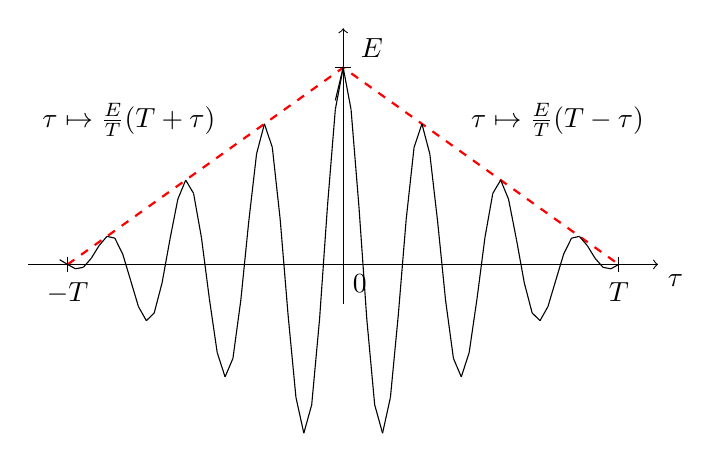
\begin{tikzpicture}
	\draw[->] (-4,0) -- (0,0) node[anchor=north west]{0} -- (4,0) node[anchor=north west] {$\tau$};
	\draw[->] (0,-0.5) -- (0,3);% node[anchor=south]{Enveloppe};
	
	\draw[red,thick,dashed] (-3.5,0)  -- (0,2.5) -- (3.5, 0);
	
	\draw (-3.5,0.1) -- (-3.5,-0.1) node[anchor=north]{$-T$};
	\draw (3.5,0.1) -- (3.5,-0.1) node[anchor=north]{$T$};
	\draw (-0.1,2.5) -- (0.1, 2.5) node[anchor=south west]{$E$};
	
	\draw (1.5,1.5) node[anchor=south west]{$\tau \mapsto \frac{E}{T}(T - \tau)$};
	\draw (-1.5,1.5) node[anchor=south east]{$\tau \mapsto \frac{E}{T}(T + \tau )$};
	
	\foreach \x in {-35,-34,...,0}{
		\draw ({(\x-1)/10},{(2.5/3.5*(3.5+(\x-1)/10))*cos(2*pi*200/3.5*(\x-1)/10)}) -- ({\x/10},{(2.5/3.5*(3.5+\x/10))*cos(2*pi*200/3.5*\x/10)});
	}
	\foreach \x in {0,1,...,35}{
		\draw ({(\x-1)/10},{(2.5/3.5*(3.5-(\x-1)/10))*cos(2*pi*200/3.5*(\x-1)/10)}) -- ({\x/10},{(2.5/3.5*(3.5-\x/10))*cos(2*pi*200/3.5*\x/10)});
	}
	
	\end{tikzpicture}
	\caption[Enveloppe de l'autocorrélation]{Enveloppe du signal de l'autocorrélation pour un signal périodique pondéré par une fenêtre rectangulaire de largeure T}
	\label{fig:enveloppe}
\end{figure}

Afin de détecter la pseudo-périodicité dans l'autocorrélation, et donc la nature voisée du signal, on va chercher des maximums locaux dont la distance au triangle est faible. De plus ces maximums devront satisfaire un critère de périodicité, c'est à dire que si $k$ est l'indice d'un tel maximum local, l'ensemble des $\{nk, nk \leq T\}$ doivent également correspondre à des points de l'autocorrélation proches du triangle. Enfin, l'autocorrélation étant paire, on ne regardera que les $k$ positifs.

\section{Mesure du pitch}

La mesure du pitch est nécessaire à la détermination de la note. Cela se fait également sur l'autocorrélation, en mesurant la période des maximums locaux qui déterminent si le signal est voisé. On modifie donc la fonction écrite dans la section précédente afin de prendre en argument la plage de recherche du pitch (ce qui va également accélérer l'exécution de la fonction). 

On renvoie un booléen, qui indique si le signal est voisé, et l'indice du maximum qui a permis de déterminer ce résultat. Si on appelle $k$ l'indice ainsi obtenu, l'utilisateur peut déterminer la fréquence du fondamental $f$ avec $f = \frac{f_e}{k}$ où $f_e$ est la fréquence d'échantillonage du signal.

\section{Détection de la note}

La formule donnée par le sujet du TL relie le numéro de la note à la fréquence du fondamental associé.

\begin{equation}
f = 440 \times 2 ^{\frac{n - 69}{12}}
\label{eq:freq_note}
\end{equation}

Il suffit donc d'inverser l'équation \ref{eq:freq_note} pour obtenir le numéro de la note en fonction de la fréquence mesurée sur le signal. La note obtenue n'étant pas forcément juste, il faut adapter un peu pour obtenir un nombre entier à coup sûr.

\begin{equation}
n = \lfloor 12 \times \log_2\left(\frac{f}{440}\right) + 69 \rfloor
\end{equation}

\paragraph{Remarque :} L'utilisation de la partie entière n'est ici pas forcément judicieuse. En effet si l'enregistrement joue une note de fréquence $f_0 - \epsilon$ au lieu de $f_0$, alors la note détectée sera la note $n-1$ au lieu de $n$. Pour corriger cela on peut modifier la manière de passer à l'entier en utilisant la fonction \texttt{round} de MATLAB.

\section{Détection de la partion de musique}

En utilisant les fonctions écrites précédemment, on peut écrire une fonction qui détecte la partition jouée dans un enregistrement. Pour cela on mesure la fréquence du fondamental sur chacune des tranches comportant un signal voisé, puis on fait correspondre la note MIDI associée. Pour lisser le résultat obtenu, on impose une durée minimale aux notes jouées, c'est à dire qu'une note de longueur inférieure ne sera pas détectée. En sortie on donne une matrice à 3 colonnes avec la date de début de la note, la fréquence mesurée et le numéro de la note. On remarque que la durée de la note n'est pas spécifiée. En effet on choisit de ne stocker que des notes de durée $T_{min}$, où $T_{min}$ est la durée minimale d'une note. Ainsi si l'enregistrement comporte une note de durée $2.5\times T_{min}$ de fréquence $f$, alors on stocke 2 notes successives de fréquence $f$.

\section

\end{document}
